\documentclass[twoside]{book}

% Packages required by doxygen
\usepackage{calc}
\usepackage{doxygen}
\usepackage{graphicx}
\usepackage[utf8]{inputenc}
\usepackage{makeidx}
\usepackage{multicol}
\usepackage{multirow}
\usepackage{fixltx2e}
\PassOptionsToPackage{warn}{textcomp}
\usepackage{textcomp}
\usepackage[nointegrals]{wasysym}
\usepackage[table]{xcolor}

% NLS support packages
\usepackage[french]{babel}

% Font selection
\usepackage[T1]{fontenc}
\usepackage{mathptmx}
\usepackage[scaled=.90]{helvet}
\usepackage{courier}
\usepackage{amssymb}
\usepackage{sectsty}
\renewcommand{\familydefault}{\sfdefault}
\allsectionsfont{%
  \fontseries{bc}\selectfont%
  \color{darkgray}%
}
\renewcommand{\DoxyLabelFont}{%
  \fontseries{bc}\selectfont%
  \color{darkgray}%
}
\newcommand{\+}{\discretionary{\mbox{\scriptsize$\hookleftarrow$}}{}{}}

% Page & text layout
\usepackage{geometry}
\geometry{%
  a4paper,%
  top=2.5cm,%
  bottom=2.5cm,%
  left=2.5cm,%
  right=2.5cm%
}
\tolerance=750
\hfuzz=15pt
\hbadness=750
\setlength{\emergencystretch}{15pt}
\setlength{\parindent}{0cm}
\setlength{\parskip}{0.2cm}
\makeatletter
\renewcommand{\paragraph}{%
  \@startsection{paragraph}{4}{0ex}{-1.0ex}{1.0ex}{%
    \normalfont\normalsize\bfseries\SS@parafont%
  }%
}
\renewcommand{\subparagraph}{%
  \@startsection{subparagraph}{5}{0ex}{-1.0ex}{1.0ex}{%
    \normalfont\normalsize\bfseries\SS@subparafont%
  }%
}
\makeatother

% Headers & footers
\usepackage{fancyhdr}
\pagestyle{fancyplain}
\fancyhead[LE]{\fancyplain{}{\bfseries\thepage}}
\fancyhead[CE]{\fancyplain{}{}}
\fancyhead[RE]{\fancyplain{}{\bfseries\leftmark}}
\fancyhead[LO]{\fancyplain{}{\bfseries\rightmark}}
\fancyhead[CO]{\fancyplain{}{}}
\fancyhead[RO]{\fancyplain{}{\bfseries\thepage}}
\fancyfoot[LE]{\fancyplain{}{}}
\fancyfoot[CE]{\fancyplain{}{}}
\fancyfoot[RE]{\fancyplain{}{\bfseries\scriptsize Généré le Lundi 23 Juin 2014 12\+:04\+:29 pour Whitecat\+A\+P\+I par Doxygen }}
\fancyfoot[LO]{\fancyplain{}{\bfseries\scriptsize Généré le Lundi 23 Juin 2014 12\+:04\+:29 pour Whitecat\+A\+P\+I par Doxygen }}
\fancyfoot[CO]{\fancyplain{}{}}
\fancyfoot[RO]{\fancyplain{}{}}
\renewcommand{\footrulewidth}{0.4pt}
\renewcommand{\chaptermark}[1]{%
  \markboth{#1}{}%
}
\renewcommand{\sectionmark}[1]{%
  \markright{\thesection\ #1}%
}

% Indices & bibliography
\usepackage{natbib}
\usepackage[titles]{tocloft}
\setcounter{tocdepth}{3}
\setcounter{secnumdepth}{5}
\makeindex

% Hyperlinks (required, but should be loaded last)
\usepackage{ifpdf}
\ifpdf
  \usepackage[pdftex,pagebackref=true]{hyperref}
\else
  \usepackage[ps2pdf,pagebackref=true]{hyperref}
\fi
\hypersetup{%
  colorlinks=true,%
  linkcolor=blue,%
  citecolor=blue,%
  unicode%
}

% Custom commands
\newcommand{\clearemptydoublepage}{%
  \newpage{\pagestyle{empty}\cleardoublepage}%
}


%===== C O N T E N T S =====

\begin{document}

% Titlepage & ToC
\hypersetup{pageanchor=false,
             bookmarks=true,
             bookmarksnumbered=true,
             pdfencoding=unicode
            }
\pagenumbering{roman}
\begin{titlepage}
\vspace*{7cm}
\begin{center}%
{\Large Whitecat\+A\+P\+I \\[1ex]\large 0.\+8.\+5.\+8 }\\
\vspace*{1cm}
{\large Généré par Doxygen 1.8.7}\\
\vspace*{0.5cm}
{\small Lundi 23 Juin 2014 12:04:29}\\
\end{center}
\end{titlepage}
\clearemptydoublepage
\tableofcontents
\clearemptydoublepage
\pagenumbering{arabic}
\hypersetup{pageanchor=true}

%--- Begin generated contents ---
\chapter{R\+E\+A\+D\+M\+E}
\label{md__r_e_a_d_m_e}
\hypertarget{md__r_e_a_d_m_e}{}
White\+Cat Lighting Board isa free lighting desk for windows, based on G\+P\+L v2 or after.

First release open source ! version 0.\+8.\+4.

To install and compile\+: Download (\href{https://github.com/ChristophGuillermet/whitecat_crossplateform}{\tt https\+://github.\+com/\+Christoph\+Guillermet/whitecat\+\_\+crossplateform}) and clone it somewhere

inspire from B\+U\+I\+L\+D\+\_\+\+L\+I\+B\+R\+A\+R\+I\+E\+S\+\_\+\+I\+N\+S\+T\+R\+U\+C\+T\+I\+O\+N\+S\+\_\+for\+\_\+\+Min\+G\+W.\+txt if you want build yourself the librarie

or follow the P\+R\+E\+B\+U\+I\+L\+D\+\_\+\+I\+N\+S\+T\+A\+L\+L\+\_\+\+W\+I\+T\+H\+\_\+\+C\+O\+D\+E\+B\+L\+O\+C\+K\+S\+\_\+\+A\+N\+D\+\_\+\+M\+I\+N\+G\+W4.\+8.\+1.\+txt

\section*{your exe will be in whitecat\+\_\+crossplateform/whitecatbuild/build/white\+\_\+cat\+\_\+for\+\_\+mingw/\+Whitecat\+\_\+\+Crossplatform.\+exe }
\chapter{Index des classes}
\section{Liste des classes}
Liste des classes, structures, unions et interfaces avec une brève description \+:\begin{DoxyCompactList}
\item\contentsline{section}{\hyperlink{classcurve__node}{curve\+\_\+node} \\*Implements one node of a spline curve }{\pageref{classcurve__node}}{}
\item\contentsline{section}{\hyperlink{struct_d_m_x_u_s_b_p_r_o_params_type}{D\+M\+X\+U\+S\+B\+P\+R\+O\+Params\+Type} }{\pageref{struct_d_m_x_u_s_b_p_r_o_params_type}}{}
\item\contentsline{section}{\hyperlink{struct_d_m_x_u_s_b_p_r_o_set_params_type}{D\+M\+X\+U\+S\+B\+P\+R\+O\+Set\+Params\+Type} }{\pageref{struct_d_m_x_u_s_b_p_r_o_set_params_type}}{}
\item\contentsline{section}{\hyperlink{classgraphic__context}{graphic\+\_\+context} \\*This class may be provisory }{\pageref{classgraphic__context}}{}
\item\contentsline{section}{\hyperlink{struct_n_o_d_e}{N\+O\+D\+E} }{\pageref{struct_n_o_d_e}}{}
\item\contentsline{section}{\hyperlink{struct_received_dmx_cos_struct}{Received\+Dmx\+Cos\+Struct} }{\pageref{struct_received_dmx_cos_struct}}{}
\end{DoxyCompactList}

\chapter{Index des fichiers}
\section{Liste des fichiers}
Liste de tous les fichiers avec une brève description \+:\begin{DoxyCompactList}
\item\contentsline{section}{\hyperlink{arduino__6___u_n_o_8cpp}{arduino\+\_\+6\+\_\+\+U\+N\+O.\+cpp} \\*\{arduino G\+U\+I fonctions\} }{\pageref{arduino__6___u_n_o_8cpp}}{}
\item\contentsline{section}{\hyperlink{arduino__core__6___u_n_o_8cpp}{arduino\+\_\+core\+\_\+6\+\_\+\+U\+N\+O.\+cpp} \\*\{arduino fonctions\} }{\pageref{arduino__core__6___u_n_o_8cpp}}{}
\item\contentsline{section}{\hyperlink{arduino__device__core_8cpp}{arduino\+\_\+device\+\_\+core.\+cpp} \\*\{arduino serial open close fonction\} }{\pageref{arduino__device__core_8cpp}}{}
\item\contentsline{section}{\hyperlink{audio__core5_8cpp}{audio\+\_\+core5.\+cpp} \\*\{Audio fonctions\} }{\pageref{audio__core5_8cpp}}{}
\item\contentsline{section}{\hyperlink{audio__visu4_8cpp}{audio\+\_\+visu4.\+cpp} \\*\{Audio G\+U\+I fonctions\} }{\pageref{audio__visu4_8cpp}}{}
\item\contentsline{section}{\hyperlink{banger__core__8_8cpp}{banger\+\_\+core\+\_\+8.\+cpp} \\*\{Bangers fonctions\} }{\pageref{banger__core__8_8cpp}}{}
\item\contentsline{section}{\hyperlink{banger__visu__8_8cpp}{banger\+\_\+visu\+\_\+8.\+cpp} \\*\{Bangers G\+U\+I fonctions\} }{\pageref{banger__visu__8_8cpp}}{}
\item\contentsline{section}{\hyperlink{_call__everybody__5_8cpp}{Call\+\_\+everybody\+\_\+5.\+cpp} \\*\{no idea\} }{\pageref{_call__everybody__5_8cpp}}{}
\item\contentsline{section}{\hyperlink{_c_f_g__config__panel__8_8cpp}{C\+F\+G\+\_\+config\+\_\+panel\+\_\+8.\+cpp} \\*\{config core file\} }{\pageref{_c_f_g__config__panel__8_8cpp}}{}
\item\contentsline{section}{\hyperlink{_c_f_g__screen_8cpp}{C\+F\+G\+\_\+screen.\+cpp} \\*\{config G\+U\+I file\} }{\pageref{_c_f_g__screen_8cpp}}{}
\item\contentsline{section}{\hyperlink{channels__10__visu_8cpp}{channels\+\_\+10\+\_\+visu.\+cpp} \\*\{G\+U\+I file for the dmx channels\} }{\pageref{channels__10__visu_8cpp}}{}
\item\contentsline{section}{\hyperlink{channels__9__core_8cpp}{channels\+\_\+9\+\_\+core.\+cpp} \\*\{file for the core of dmx channels\} }{\pageref{channels__9__core_8cpp}}{}
\item\contentsline{section}{\hyperlink{chasers__core__5_8cpp}{chasers\+\_\+core\+\_\+5.\+cpp} \\*\{file for the core of the chasers\} }{\pageref{chasers__core__5_8cpp}}{}
\item\contentsline{section}{\hyperlink{chasers__visu_8cpp}{chasers\+\_\+visu.\+cpp} \\*\{file for the G\+U\+I window of the chasers\} }{\pageref{chasers__visu_8cpp}}{}
\item\contentsline{section}{\hyperlink{colors__fonts_8h}{colors\+\_\+fonts.\+h} }{\pageref{colors__fonts_8h}}{}
\item\contentsline{section}{\hyperlink{_c_o_r_e__6_8cpp}{C\+O\+R\+E\+\_\+6.\+cpp} }{\pageref{_c_o_r_e__6_8cpp}}{}
\item\contentsline{section}{\hyperlink{_crossplateform_8h}{Crossplateform.\+h} \\*\{header file for the specifique crossplateform fonction of whitecat\} }{\pageref{_crossplateform_8h}}{}
\item\contentsline{section}{\hyperlink{dmx__enttec__pro_8cpp}{dmx\+\_\+enttec\+\_\+pro.\+cpp} \\*\{send dmx fonctions to the enttec usb pro\} }{\pageref{dmx__enttec__pro_8cpp}}{}
\item\contentsline{section}{\hyperlink{dmx__enttec__pro___f_t_d_i_8cpp}{dmx\+\_\+enttec\+\_\+pro\+\_\+\+F\+T\+D\+I.\+cpp} \\*\{send dmx fonctions to the enttec usb pro via the fdtdi D2xx drivers\} }{\pageref{dmx__enttec__pro___f_t_d_i_8cpp}}{}
\item\contentsline{section}{\hyperlink{dmx__ftdi___i_n__test__enttec__pro_8cpp}{dmx\+\_\+ftdi\+\_\+\+I\+N\+\_\+test\+\_\+enttec\+\_\+pro.\+cpp} \\*\{test to get the dmx in from enttec usb pro\} }{\pageref{dmx__ftdi___i_n__test__enttec__pro_8cpp}}{}
\item\contentsline{section}{\hyperlink{dmx__functions__13_8cpp}{dmx\+\_\+functions\+\_\+13.\+cpp} \\*\{global fonctions for all interfaces and artnet\} }{\pageref{dmx__functions__13_8cpp}}{}
\item\contentsline{section}{\hyperlink{dmx__sunlite_8cpp}{dmx\+\_\+sunlite.\+cpp} \\*\{fonctions for the sunlite dmx interfaces\} }{\pageref{dmx__sunlite_8cpp}}{}
\item\contentsline{section}{\hyperlink{_draw3_8cpp}{Draw3.\+cpp} \\*\{fonctions for the draw module\} }{\pageref{_draw3_8cpp}}{}
\item\contentsline{section}{\hyperlink{echo3_8cpp}{echo3.\+cpp} \\*\{fonctions for the draw module\} }{\pageref{echo3_8cpp}}{}
\item\contentsline{section}{\hyperlink{faders__core__24_8cpp}{faders\+\_\+core\+\_\+24.\+cpp} \\*\{Core fonctions for the faders\} }{\pageref{faders__core__24_8cpp}}{}
\item\contentsline{section}{\hyperlink{faders__operations_8cpp}{faders\+\_\+operations.\+cpp} \\*\{fonctions to assign dock and fonctions for the faders\} }{\pageref{faders__operations_8cpp}}{}
\item\contentsline{section}{\hyperlink{faders__visuels__26_8cpp}{faders\+\_\+visuels\+\_\+26.\+cpp} \\*\{G\+U\+I fonctions for the faders\} }{\pageref{faders__visuels__26_8cpp}}{}
\item\contentsline{section}{\hyperlink{generate__strings__arrays_8cpp}{generate\+\_\+strings\+\_\+arrays.\+cpp} \\*\{fonctions to create strings array\} }{\pageref{generate__strings__arrays_8cpp}}{}
\item\contentsline{section}{\hyperlink{gestionaire__fenetres2_8cpp}{gestionaire\+\_\+fenetres2.\+cpp} \\*\{G\+U\+I fonctions to manage windows in whitecat\} }{\pageref{gestionaire__fenetres2_8cpp}}{}
\item\contentsline{section}{\hyperlink{grand__master_8cpp}{grand\+\_\+master.\+cpp} \\*\{draw the grand master\} }{\pageref{grand__master_8cpp}}{}
\item\contentsline{section}{\hyperlink{graphic__context_8h}{graphic\+\_\+context.\+h} \\*Elements of the graphic context, }{\pageref{graphic__context_8h}}{}
\item\contentsline{section}{\hyperlink{graphics__rebuild1_8cpp}{graphics\+\_\+rebuild1.\+cpp} \\*\{G\+U\+I fonctions to redraw graphics\} }{\pageref{graphics__rebuild1_8cpp}}{}
\item\contentsline{section}{\hyperlink{grider8_8cpp}{grider8.\+cpp} \\*\{G\+U\+I fonctions for grid players\} }{\pageref{grider8_8cpp}}{}
\item\contentsline{section}{\hyperlink{grider__calculs8_8cpp}{grider\+\_\+calculs8.\+cpp} \\*\{calcul fonctions for grid players\} }{\pageref{grider__calculs8_8cpp}}{}
\item\contentsline{section}{\hyperlink{grider__core8_8cpp}{grider\+\_\+core8.\+cpp} \\*\{Core fonctions for grid players\} }{\pageref{grider__core8_8cpp}}{}
\item\contentsline{section}{\hyperlink{gui__boutons__rebuild1_8cpp}{gui\+\_\+boutons\+\_\+rebuild1.\+cpp} \\*\{G\+U\+I fonctions to redraw buttons\} }{\pageref{gui__boutons__rebuild1_8cpp}}{}
\item\contentsline{section}{\hyperlink{help__2_8cpp}{help\+\_\+2.\+cpp} \\*\{G\+U\+I fonctions for the help window\} }{\pageref{help__2_8cpp}}{}
\item\contentsline{section}{\hyperlink{i_cat14_8cpp}{i\+Cat14.\+cpp} \\*\{G\+U\+I fonctions for i\+C\+A\+T\} }{\pageref{i_cat14_8cpp}}{}
\item\contentsline{section}{\hyperlink{icat__core14_8cpp}{icat\+\_\+core14.\+cpp} \\*\{Core fonctions for i\+C\+A\+T\} }{\pageref{icat__core14_8cpp}}{}
\item\contentsline{section}{\hyperlink{keyboard__functions2_8cpp}{keyboard\+\_\+functions2.\+cpp} \\*\{Core fonctions for keyboard entry\} }{\pageref{keyboard__functions2_8cpp}}{}
\item\contentsline{section}{\hyperlink{keyboard__routines2_8cpp}{keyboard\+\_\+routines2.\+cpp} \\*\{keyboard shortcut\} }{\pageref{keyboard__routines2_8cpp}}{}
\item\contentsline{section}{\hyperlink{list__proj__core_8cpp}{list\+\_\+proj\+\_\+core.\+cpp} \\*\{spot list and channels macro core\} }{\pageref{list__proj__core_8cpp}}{}
\item\contentsline{section}{\hyperlink{list__proj__visu_8cpp}{list\+\_\+proj\+\_\+visu.\+cpp} \\*\{spot list and channels macro G\+U\+I\} }{\pageref{list__proj__visu_8cpp}}{}
\item\contentsline{section}{\hyperlink{logicals__intres_8cpp}{logicals\+\_\+intres.\+cpp} \\*\{fonction logique\} }{\pageref{logicals__intres_8cpp}}{}
\item\contentsline{section}{\hyperlink{_m_a_i_n__avec__objets_8cpp}{M\+A\+I\+N\+\_\+avec\+\_\+objets.\+cpp} }{\pageref{_m_a_i_n__avec__objets_8cpp}}{}
\item\contentsline{section}{\hyperlink{_m_a_i_n__febrier__2014_8cpp}{M\+A\+I\+N\+\_\+febrier\+\_\+2014.\+cpp} }{\pageref{_m_a_i_n__febrier__2014_8cpp}}{}
\item\contentsline{section}{\hyperlink{_m_a_i_n__fevrier__2014_8cpp}{M\+A\+I\+N\+\_\+fevrier\+\_\+2014.\+cpp} }{\pageref{_m_a_i_n__fevrier__2014_8cpp}}{}
\item\contentsline{section}{\hyperlink{_m_a_i_n__janv__2014__opensource__kbd_8cpp}{M\+A\+I\+N\+\_\+janv\+\_\+2014\+\_\+opensource\+\_\+kbd.\+cpp} \\*\{main loop\} }{\pageref{_m_a_i_n__janv__2014__opensource__kbd_8cpp}}{}
\item\contentsline{section}{\hyperlink{midi__13_8cpp}{midi\+\_\+13.\+cpp} \\*\{midi G\+U\+I\} }{\pageref{midi__13_8cpp}}{}
\item\contentsline{section}{\hyperlink{midi___c_o_r_e_8cpp}{midi\+\_\+\+C\+O\+R\+E.\+cpp} \\*\{midi Core\} }{\pageref{midi___c_o_r_e_8cpp}}{}
\item\contentsline{section}{\hyperlink{midi__launchpad_8cpp}{midi\+\_\+launchpad.\+cpp} \\*\{midi launchpad send info\} }{\pageref{midi__launchpad_8cpp}}{}
\item\contentsline{section}{\hyperlink{minifaders__core_8cpp}{minifaders\+\_\+core.\+cpp} \\*\{minifaders Core\} }{\pageref{minifaders__core_8cpp}}{}
\item\contentsline{section}{\hyperlink{minifaders__visu_8cpp}{minifaders\+\_\+visu.\+cpp} \\*\{minifaders G\+U\+I\} }{\pageref{minifaders__visu_8cpp}}{}
\item\contentsline{section}{\hyperlink{mover__2013_8cpp}{mover\+\_\+2013.\+cpp} \\*\{pan and tilt for motor spot\} }{\pageref{mover__2013_8cpp}}{}
\item\contentsline{section}{\hyperlink{mover__spline6_8cpp}{mover\+\_\+spline6.\+cpp} \\*\{trajectory fonctions for motor spot\} }{\pageref{mover__spline6_8cpp}}{}
\item\contentsline{section}{\hyperlink{my__window__file__sample_8cpp}{my\+\_\+window\+\_\+file\+\_\+sample.\+cpp} \\*\{exemple to create a new module window\} }{\pageref{my__window__file__sample_8cpp}}{}
\item\contentsline{section}{\hyperlink{my__window__file__sample_8h}{my\+\_\+window\+\_\+file\+\_\+sample.\+h} \\*\{header file for exemple to create a new module window\} }{\pageref{my__window__file__sample_8h}}{}
\item\contentsline{section}{\hyperlink{network__artnet__3_8cpp}{network\+\_\+artnet\+\_\+3.\+cpp} \\*\{artnet fonctions to send dmx via U\+D\+P protocool\} }{\pageref{network__artnet__3_8cpp}}{}
\item\contentsline{section}{\hyperlink{network___m_a_c__adress__3_8cpp}{network\+\_\+\+M\+A\+C\+\_\+adress\+\_\+3.\+cpp} \\*\{M\+A\+C Adress of all the network interfaces of the computer\} }{\pageref{network___m_a_c__adress__3_8cpp}}{}
\item\contentsline{section}{\hyperlink{numpad__core_8cpp}{numpad\+\_\+core.\+cpp} \\*\{Core fonction for the numerical pad window\} }{\pageref{numpad__core_8cpp}}{}
\item\contentsline{section}{\hyperlink{numpad__visuel_8cpp}{numpad\+\_\+visuel.\+cpp} \\*\{G\+U\+I fonction for the numerical pad window\} }{\pageref{numpad__visuel_8cpp}}{}
\item\contentsline{section}{\hyperlink{patch__core_8cpp}{patch\+\_\+core.\+cpp} \\*\{D\+M\+X patch core\} }{\pageref{patch__core_8cpp}}{}
\item\contentsline{section}{\hyperlink{patch__splines__2_8cpp}{patch\+\_\+splines\+\_\+2.\+cpp} \\*Curves calcul for each canal in the patch }{\pageref{patch__splines__2_8cpp}}{}
\item\contentsline{section}{\hyperlink{patch__splines__2_8h}{patch\+\_\+splines\+\_\+2.\+h} \\*Functions for each channel in the dmx patch }{\pageref{patch__splines__2_8h}}{}
\item\contentsline{section}{\hyperlink{patch__visu_8cpp}{patch\+\_\+visu.\+cpp} \\*\{D\+M\+X patch G\+U\+I\} }{\pageref{patch__visu_8cpp}}{}
\item\contentsline{section}{\hyperlink{plot_8cpp}{plot.\+cpp} \\*\{Plot global and import export fonctions\} }{\pageref{plot_8cpp}}{}
\item\contentsline{section}{\hyperlink{plot9_8cpp}{plot9.\+cpp} \\*\{Plot G\+U\+I fonctions\} }{\pageref{plot9_8cpp}}{}
\item\contentsline{section}{\hyperlink{plot__core9_8cpp}{plot\+\_\+core9.\+cpp} \\*\{Plot Core fonctions\} }{\pageref{plot__core9_8cpp}}{}
\item\contentsline{section}{\hyperlink{procs__visuels__rebuild1_8cpp}{procs\+\_\+visuels\+\_\+rebuild1.\+cpp} \\*\{Redraw fonctions\} }{\pageref{procs__visuels__rebuild1_8cpp}}{}
\item\contentsline{section}{\hyperlink{save__show__13_8cpp}{save\+\_\+show\+\_\+13.\+cpp} \\*\{save and load fonctions\} }{\pageref{save__show__13_8cpp}}{}
\item\contentsline{section}{\hyperlink{saves__export__import_8cpp}{saves\+\_\+export\+\_\+import.\+cpp} \\*\{import and export the show in A\+S\+C\+I\+I\} }{\pageref{saves__export__import_8cpp}}{}
\item\contentsline{section}{\hyperlink{saves__export__pdf2_8cpp}{saves\+\_\+export\+\_\+pdf2.\+cpp} \\*\{import and export the show in P\+D\+F\} }{\pageref{saves__export__pdf2_8cpp}}{}
\item\contentsline{section}{\hyperlink{saves__menu__8_8cpp}{saves\+\_\+menu\+\_\+8.\+cpp} \\*\{G\+U\+I window of save and load menu\} }{\pageref{saves__menu__8_8cpp}}{}
\item\contentsline{section}{\hyperlink{sequentiel__6__core_8cpp}{sequentiel\+\_\+6\+\_\+core.\+cpp} \\*\{Core fonctions for the cuelist\} }{\pageref{sequentiel__6__core_8cpp}}{}
\item\contentsline{section}{\hyperlink{sequentiel__7__visu_8cpp}{sequentiel\+\_\+7\+\_\+visu.\+cpp} \\*\{G\+U\+I fonctions for the cuelist\} }{\pageref{sequentiel__7__visu_8cpp}}{}
\item\contentsline{section}{\hyperlink{time__core__3_8cpp}{time\+\_\+core\+\_\+3.\+cpp} \\*\{Core fonctions for the time window\} }{\pageref{time__core__3_8cpp}}{}
\item\contentsline{section}{\hyperlink{time__visu__3_8cpp}{time\+\_\+visu\+\_\+3.\+cpp} \\*\{G\+U\+I fonctions for the time window\} }{\pageref{time__visu__3_8cpp}}{}
\item\contentsline{section}{\hyperlink{tracker__main14nov_8cpp}{tracker\+\_\+main14nov.\+cpp} \\*\{I don't know what is the tracker in whitecat\} }{\pageref{tracker__main14nov_8cpp}}{}
\item\contentsline{section}{\hyperlink{trichro__core2_8cpp}{trichro\+\_\+core2.\+cpp} \\*\{Core fonctions for the color whell\} }{\pageref{trichro__core2_8cpp}}{}
\item\contentsline{section}{\hyperlink{trichro__visu2_8cpp}{trichro\+\_\+visu2.\+cpp} \\*\{G\+U\+I fonctions for the color whell\} }{\pageref{trichro__visu2_8cpp}}{}
\item\contentsline{section}{\hyperlink{video__tracking__core_8cpp}{video\+\_\+tracking\+\_\+core.\+cpp} \\*\{Core fonctions for the tracking video\} }{\pageref{video__tracking__core_8cpp}}{}
\item\contentsline{section}{\hyperlink{video__tracking__visu_8cpp}{video\+\_\+tracking\+\_\+visu.\+cpp} \\*\{G\+U\+I fonctions for the tracking video\} }{\pageref{video__tracking__visu_8cpp}}{}
\item\contentsline{section}{\hyperlink{whitecat_8h}{whitecat.\+h} \\*\{header file for all the global variable in whitecat\} }{\pageref{whitecat_8h}}{}
\item\contentsline{section}{\hyperlink{_white_cat__private_8h}{White\+Cat\+\_\+private.\+h} \\*\{number of version and details\} }{\pageref{_white_cat__private_8h}}{}
\item\contentsline{section}{\hyperlink{wizard_8cpp}{wizard.\+cpp} \\*\{G\+U\+I fonctions for wizard \} }{\pageref{wizard_8cpp}}{}
\item\contentsline{section}{\hyperlink{wizard__operations_8cpp}{wizard\+\_\+operations.\+cpp} \\*\{G\+U\+I fonctions for wizard \} }{\pageref{wizard__operations_8cpp}}{}
\end{DoxyCompactList}

\chapter{Documentation des classes}
\hypertarget{classcurve__node}{\section{Référence de la classe curve\+\_\+node}
\label{classcurve__node}\index{curve\+\_\+node@{curve\+\_\+node}}
}


{\ttfamily \#include $<$patch\+\_\+splines\+\_\+2.\+h$>$}



Graphe de collaboration de curve\+\_\+node\+:
\nopagebreak
\begin{figure}[H]
\begin{center}
\leavevmode
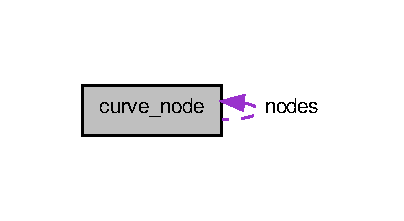
\includegraphics[width=194pt]{classcurve__node__coll__graph}
\end{center}
\end{figure}
\subsection*{Fonctions membres publiques}
\begin{DoxyCompactItemize}
\item 
\hyperlink{classcurve__node_add0d28f291f1cfe22e11f5436a8ba161}{curve\+\_\+node} (int ax, int ay, fixed atangent)
\item 
fixed \hyperlink{classcurve__node_a1146c27b9e6c0b3a5f6fb3faced5cea2}{dist} (const \hyperlink{classcurve__node}{curve\+\_\+node} \&other)
\item 
\hyperlink{classcurve__node}{curve\+\_\+node} \& \hyperlink{classcurve__node_a55e51b51f9b6ede537c5e11b7f234188}{dummy} (const \hyperlink{classcurve__node}{curve\+\_\+node} \&prev)
\item 
void \hyperlink{classcurve__node_a22f8acf6b081673429257867a4115c57}{calc\+\_\+tangents} (void)
\item 
void \hyperlink{classcurve__node_a14aba313f46315faae44bcca011136a9}{get\+\_\+control\+\_\+points} (const \hyperlink{classcurve__node}{curve\+\_\+node} \&other, int points\mbox{[}8\mbox{]})
\item 
int \hyperlink{classcurve__node_abc1a06d649c6dce22334da762f2955b8}{write\+\_\+curve} (const \hyperlink{classgraphic__context}{graphic\+\_\+context} \&gc)
\item 
int \hyperlink{classcurve__node_ab1db9f4ea1c53ab2eab6072b2cdc90eb}{draw} (int n, const \hyperlink{classgraphic__context}{graphic\+\_\+context} \&gc)
\item 
int \hyperlink{classcurve__node_aace217c0200a043c2d2f5f071fde8e56}{draw\+\_\+splines} (const \hyperlink{classgraphic__context}{graphic\+\_\+context} \&gc)
\item 
int \hyperlink{classcurve__node_a5c54a9611e91814177cf901636d4e8e5}{view\+\_\+after\+\_\+draw} (const \hyperlink{classgraphic__context}{graphic\+\_\+context} \&gc)
\item 
int \hyperlink{classcurve__node_afb8f3c6e6a53e062f5c2fb1cf7243969}{Spline\+Curve} (const \hyperlink{classgraphic__context}{graphic\+\_\+context} \&gc)
\item 
int \hyperlink{classcurve__node_ac1e52fe7e8f762074b804b88a1b420cf}{build\+\_\+square} (int curve, const \hyperlink{classgraphic__context}{graphic\+\_\+context} \&gc)
\item 
int \hyperlink{classcurve__node_a51a7bb24aa5832b54ec61507a556dda9}{build\+\_\+fluo} (int curve, const \hyperlink{classgraphic__context}{graphic\+\_\+context} \&gc)
\item 
int \hyperlink{classcurve__node_a6338ccf647d5f510c47702f613a3d9d2}{build\+\_\+preheat} (int curve, const \hyperlink{classgraphic__context}{graphic\+\_\+context} \&gc)
\item 
int \hyperlink{classcurve__node_a787cd6340d6b9e15da5723ed25eb18ff}{build\+\_\+inverse} (int curve, const \hyperlink{classgraphic__context}{graphic\+\_\+context} \&gc)
\end{DoxyCompactItemize}
\subsection*{Attributs publics}
\begin{DoxyCompactItemize}
\item 
int \hyperlink{classcurve__node_aa7ae8f2ee3bbd3e6194785c392751cdb}{x}
\item 
int \hyperlink{classcurve__node_afc1f4f007a920aa79c1f1f0ff0b49465}{y}
\item 
fixed \hyperlink{classcurve__node_a31ea7469070f7bb90ceae073d1d075a6}{tangent}
\end{DoxyCompactItemize}
\subsection*{Attributs publics statiques}
\begin{DoxyCompactItemize}
\item 
static bool \hyperlink{classcurve__node_ae995b9ef63ae5b880d6006083acaf6d3}{index\+\_\+writing} =0
\item 
static float \hyperlink{classcurve__node_a16c72a6637b3b68983b5ce55b90665bf}{spline\+\_\+level} =0.\+0
\item 
static int \hyperlink{classcurve__node_abe017d998cde30d2ca5f7c8ea68ba3da}{selected} =0
\item 
static int \hyperlink{classcurve__node_a62eb9b6b3a24274664775a07c565d39c}{the\+\_\+spline\+\_\+level} \mbox{[}16\mbox{]}
\item 
static int \hyperlink{classcurve__node_a348cce4dfe54130e8b8b2fb218baedfb}{report} \mbox{[}16\mbox{]}\mbox{[}256\mbox{]}
\item 
static int \hyperlink{classcurve__node_af9c0c53bc02942259c36c753232326aa}{index\+\_\+spline\+\_\+level} =0
\item 
static bool \hyperlink{classcurve__node_a4479fff7bfc410d6f6d1df9975261aa8}{index\+\_\+enable\+\_\+editing} =0
\item 
static int \hyperlink{classcurve__node_a0aebfec8e10d7fc02442cd5326433c93}{curves} \mbox{[}514\mbox{]}
\item 
static int \hyperlink{classcurve__node_ab7280e17d47152797e10e5992791ee9b}{ctrl\+\_\+pt} \mbox{[}16\mbox{]}\mbox{[}8\mbox{]}\mbox{[}2\mbox{]}
\item 
static int \hyperlink{classcurve__node_aab45660e4c1077f8742b151fcb0cdcad}{diam} =10
\item 
static \hyperlink{classcurve__node}{curve\+\_\+node} \hyperlink{classcurve__node_affd9362e19ab4c4a70164622a7aebb61}{nodes} \mbox{[}\hyperlink{patch__splines__2_8h_abd21c950f8371229cfca1c4f98c9750f}{M\+A\+X\+\_\+\+C\+N\+O\+D\+E\+S}\mbox{]}
\item 
static int \hyperlink{classcurve__node_a09d4ec4d9b46abddbcec3e0c46f53d3f}{node\+\_\+count} =0
\item 
static fixed \hyperlink{classcurve__node_a46e1f23c6d19a1ca915697c80ed72a84}{curviness}
\end{DoxyCompactItemize}


\subsection{Documentation des constructeurs et destructeur}
\hypertarget{classcurve__node_add0d28f291f1cfe22e11f5436a8ba161}{\index{curve\+\_\+node@{curve\+\_\+node}!curve\+\_\+node@{curve\+\_\+node}}
\index{curve\+\_\+node@{curve\+\_\+node}!curve\+\_\+node@{curve\+\_\+node}}
\subsubsection[{curve\+\_\+node}]{\setlength{\rightskip}{0pt plus 5cm}curve\+\_\+node\+::curve\+\_\+node (
\begin{DoxyParamCaption}
\item[{int}]{ax, }
\item[{int}]{ay, }
\item[{fixed}]{atangent}
\end{DoxyParamCaption}
)}}\label{classcurve__node_add0d28f291f1cfe22e11f5436a8ba161}
The constructor 
\begin{DoxyParams}{Paramètres}
{\em ax} & abscissa \\
\hline
{\em ay} & ordinate \\
\hline
{\em atangent} & slope \\
\hline
\end{DoxyParams}


Voici le graphe des appelants de cette fonction \+:
\nopagebreak
\begin{figure}[H]
\begin{center}
\leavevmode
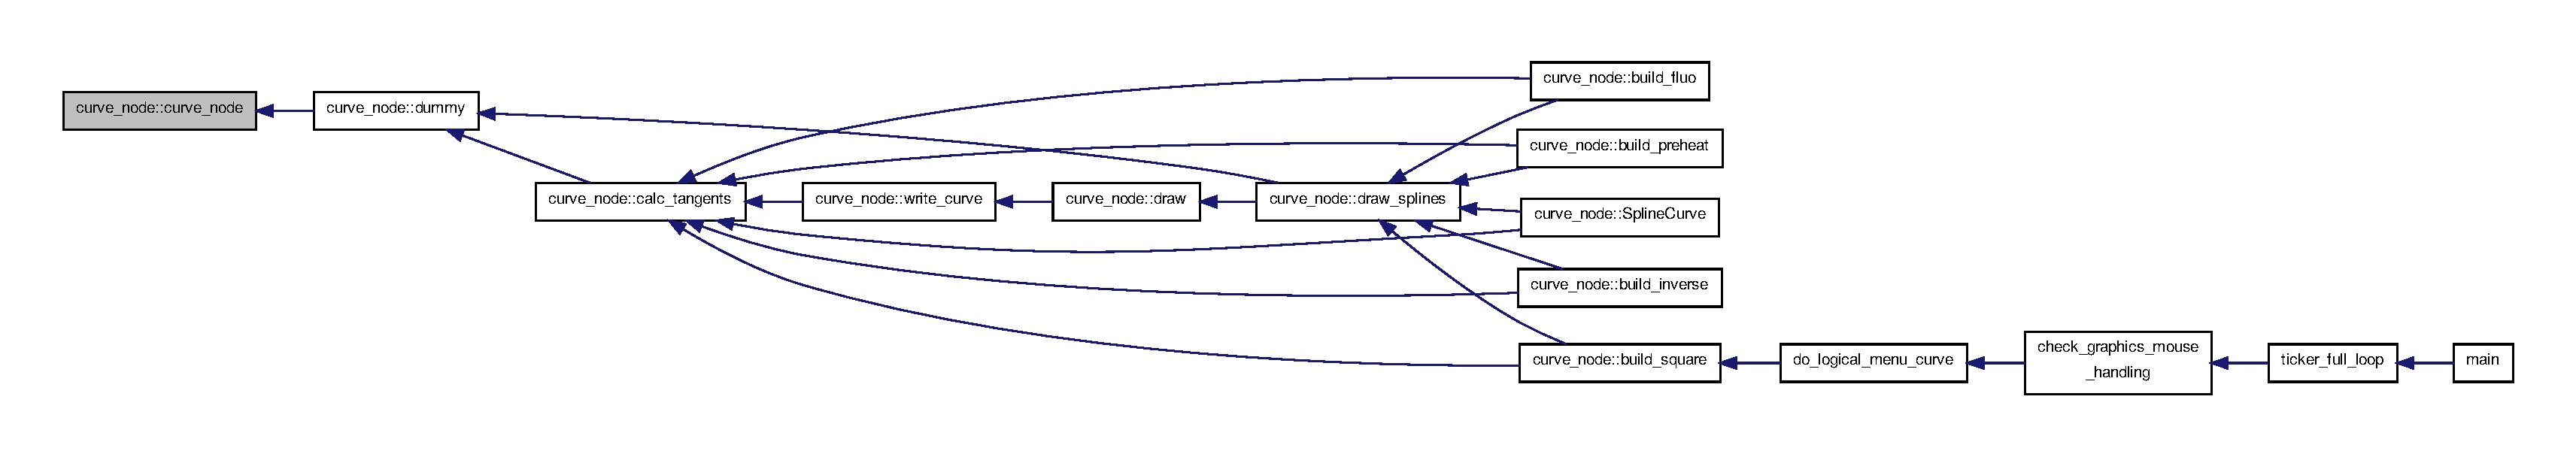
\includegraphics[width=350pt]{classcurve__node_add0d28f291f1cfe22e11f5436a8ba161_icgraph}
\end{center}
\end{figure}




\subsection{Documentation des fonctions membres}
\hypertarget{classcurve__node_a51a7bb24aa5832b54ec61507a556dda9}{\index{curve\+\_\+node@{curve\+\_\+node}!build\+\_\+fluo@{build\+\_\+fluo}}
\index{build\+\_\+fluo@{build\+\_\+fluo}!curve\+\_\+node@{curve\+\_\+node}}
\subsubsection[{build\+\_\+fluo}]{\setlength{\rightskip}{0pt plus 5cm}int curve\+\_\+node\+::build\+\_\+fluo (
\begin{DoxyParamCaption}
\item[{int}]{curve, }
\item[{const {\bf graphic\+\_\+context} \&}]{gc}
\end{DoxyParamCaption}
)}}\label{classcurve__node_a51a7bb24aa5832b54ec61507a556dda9}
Function to do something 
\begin{DoxyParams}{Paramètres}
{\em curve} & index of the chosen curve (0..15) \\
\hline
{\em gc} & graphic context \\
\hline
\end{DoxyParams}


Voici le graphe d'appel pour cette fonction \+:
\nopagebreak
\begin{figure}[H]
\begin{center}
\leavevmode
\includegraphics[width=350pt]{classcurve__node_a51a7bb24aa5832b54ec61507a556dda9_cgraph}
\end{center}
\end{figure}


\hypertarget{classcurve__node_a787cd6340d6b9e15da5723ed25eb18ff}{\index{curve\+\_\+node@{curve\+\_\+node}!build\+\_\+inverse@{build\+\_\+inverse}}
\index{build\+\_\+inverse@{build\+\_\+inverse}!curve\+\_\+node@{curve\+\_\+node}}
\subsubsection[{build\+\_\+inverse}]{\setlength{\rightskip}{0pt plus 5cm}int curve\+\_\+node\+::build\+\_\+inverse (
\begin{DoxyParamCaption}
\item[{int}]{curve, }
\item[{const {\bf graphic\+\_\+context} \&}]{gc}
\end{DoxyParamCaption}
)}}\label{classcurve__node_a787cd6340d6b9e15da5723ed25eb18ff}
Function to do something 
\begin{DoxyParams}{Paramètres}
{\em curve} & index of the chosen curve (0..15) \\
\hline
{\em gc} & graphic context \\
\hline
\end{DoxyParams}


Voici le graphe d'appel pour cette fonction \+:
\nopagebreak
\begin{figure}[H]
\begin{center}
\leavevmode
\includegraphics[width=350pt]{classcurve__node_a787cd6340d6b9e15da5723ed25eb18ff_cgraph}
\end{center}
\end{figure}


\hypertarget{classcurve__node_a6338ccf647d5f510c47702f613a3d9d2}{\index{curve\+\_\+node@{curve\+\_\+node}!build\+\_\+preheat@{build\+\_\+preheat}}
\index{build\+\_\+preheat@{build\+\_\+preheat}!curve\+\_\+node@{curve\+\_\+node}}
\subsubsection[{build\+\_\+preheat}]{\setlength{\rightskip}{0pt plus 5cm}int curve\+\_\+node\+::build\+\_\+preheat (
\begin{DoxyParamCaption}
\item[{int}]{curve, }
\item[{const {\bf graphic\+\_\+context} \&}]{gc}
\end{DoxyParamCaption}
)}}\label{classcurve__node_a6338ccf647d5f510c47702f613a3d9d2}
Function to do something 
\begin{DoxyParams}{Paramètres}
{\em curve} & index of the chosen curve (0..15) \\
\hline
{\em gc} & graphic context \\
\hline
\end{DoxyParams}


Voici le graphe d'appel pour cette fonction \+:
\nopagebreak
\begin{figure}[H]
\begin{center}
\leavevmode
\includegraphics[width=350pt]{classcurve__node_a6338ccf647d5f510c47702f613a3d9d2_cgraph}
\end{center}
\end{figure}


\hypertarget{classcurve__node_ac1e52fe7e8f762074b804b88a1b420cf}{\index{curve\+\_\+node@{curve\+\_\+node}!build\+\_\+square@{build\+\_\+square}}
\index{build\+\_\+square@{build\+\_\+square}!curve\+\_\+node@{curve\+\_\+node}}
\subsubsection[{build\+\_\+square}]{\setlength{\rightskip}{0pt plus 5cm}int curve\+\_\+node\+::build\+\_\+square (
\begin{DoxyParamCaption}
\item[{int}]{curve, }
\item[{const {\bf graphic\+\_\+context} \&}]{gc}
\end{DoxyParamCaption}
)}}\label{classcurve__node_ac1e52fe7e8f762074b804b88a1b420cf}
Function to do something 
\begin{DoxyParams}{Paramètres}
{\em curve} & index of the chosen curve (0..15) \\
\hline
{\em gc} & graphic context \\
\hline
\end{DoxyParams}


Voici le graphe d'appel pour cette fonction \+:
\nopagebreak
\begin{figure}[H]
\begin{center}
\leavevmode
\includegraphics[width=350pt]{classcurve__node_ac1e52fe7e8f762074b804b88a1b420cf_cgraph}
\end{center}
\end{figure}




Voici le graphe des appelants de cette fonction \+:
\nopagebreak
\begin{figure}[H]
\begin{center}
\leavevmode
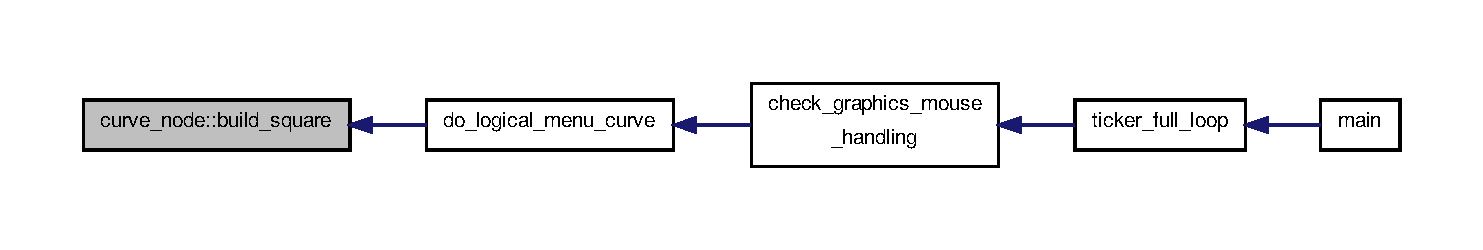
\includegraphics[width=350pt]{classcurve__node_ac1e52fe7e8f762074b804b88a1b420cf_icgraph}
\end{center}
\end{figure}


\hypertarget{classcurve__node_a22f8acf6b081673429257867a4115c57}{\index{curve\+\_\+node@{curve\+\_\+node}!calc\+\_\+tangents@{calc\+\_\+tangents}}
\index{calc\+\_\+tangents@{calc\+\_\+tangents}!curve\+\_\+node@{curve\+\_\+node}}
\subsubsection[{calc\+\_\+tangents}]{\setlength{\rightskip}{0pt plus 5cm}void curve\+\_\+node\+::calc\+\_\+tangents (
\begin{DoxyParamCaption}
\item[{void}]{}
\end{DoxyParamCaption}
)}}\label{classcurve__node_a22f8acf6b081673429257867a4115c57}


Voici le graphe d'appel pour cette fonction \+:
\nopagebreak
\begin{figure}[H]
\begin{center}
\leavevmode
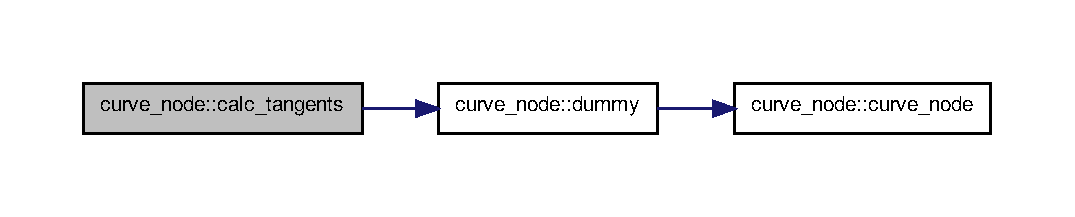
\includegraphics[width=350pt]{classcurve__node_a22f8acf6b081673429257867a4115c57_cgraph}
\end{center}
\end{figure}




Voici le graphe des appelants de cette fonction \+:
\nopagebreak
\begin{figure}[H]
\begin{center}
\leavevmode
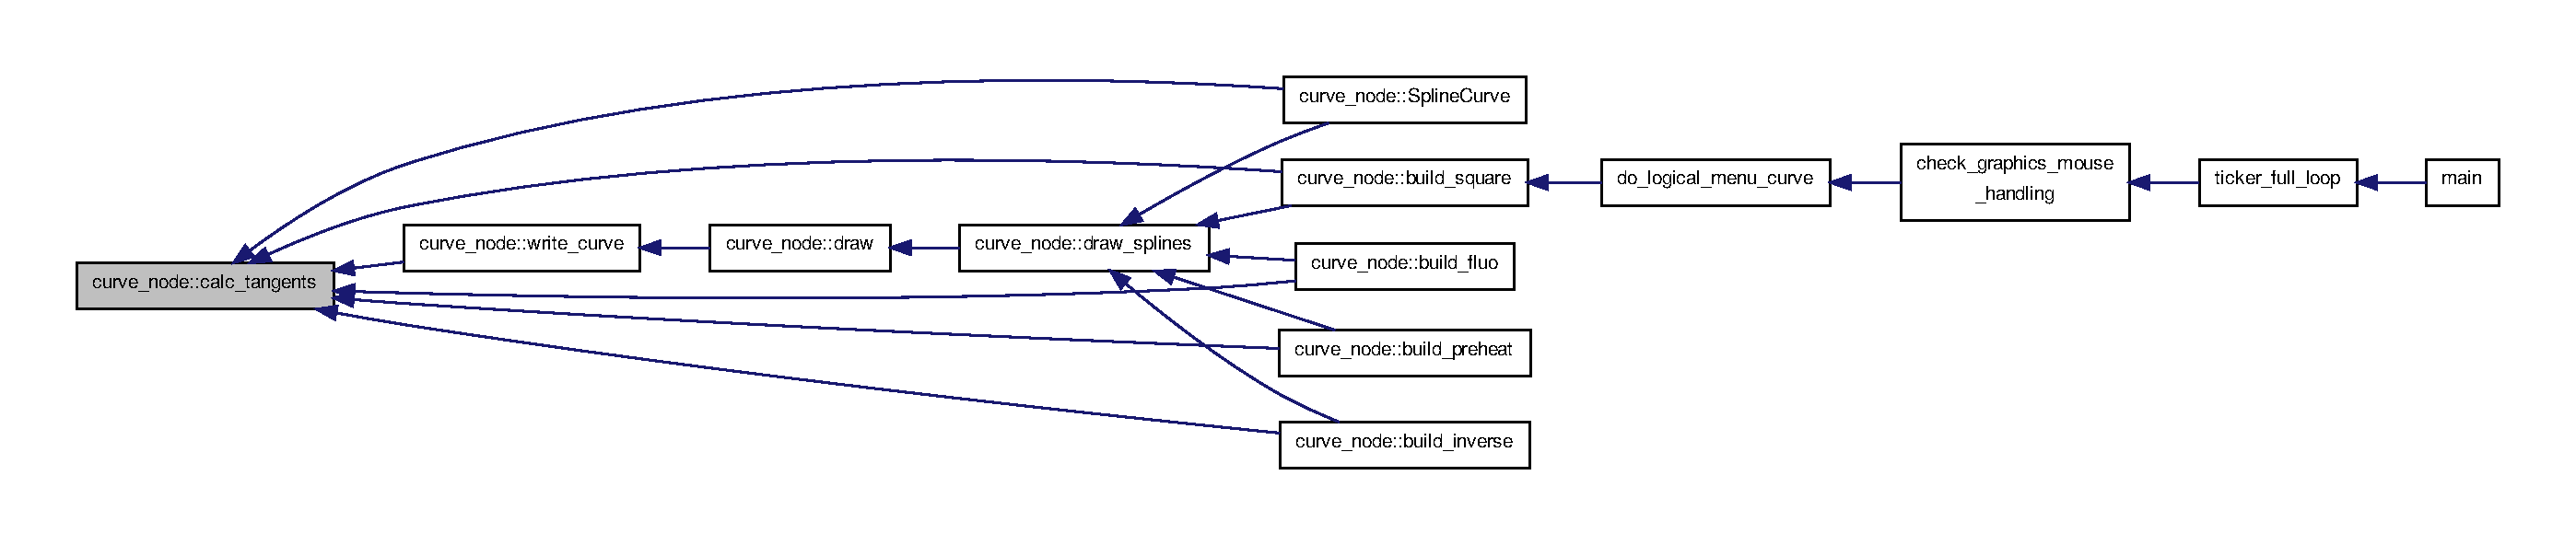
\includegraphics[width=350pt]{classcurve__node_a22f8acf6b081673429257867a4115c57_icgraph}
\end{center}
\end{figure}


\hypertarget{classcurve__node_a1146c27b9e6c0b3a5f6fb3faced5cea2}{\index{curve\+\_\+node@{curve\+\_\+node}!dist@{dist}}
\index{dist@{dist}!curve\+\_\+node@{curve\+\_\+node}}
\subsubsection[{dist}]{\setlength{\rightskip}{0pt plus 5cm}fixed curve\+\_\+node\+::dist (
\begin{DoxyParamCaption}
\item[{const {\bf curve\+\_\+node} \&}]{other}
\end{DoxyParamCaption}
)}}\label{classcurve__node_a1146c27b9e6c0b3a5f6fb3faced5cea2}
calculates the distance between this and another \hyperlink{classcurve__node}{curve\+\_\+node} 
\begin{DoxyParams}{Paramètres}
{\em other} & second node \\
\hline
\end{DoxyParams}
\begin{DoxyReturn}{Renvoie}
the distance from this to the other 
\end{DoxyReturn}


Voici le graphe des appelants de cette fonction \+:
\nopagebreak
\begin{figure}[H]
\begin{center}
\leavevmode
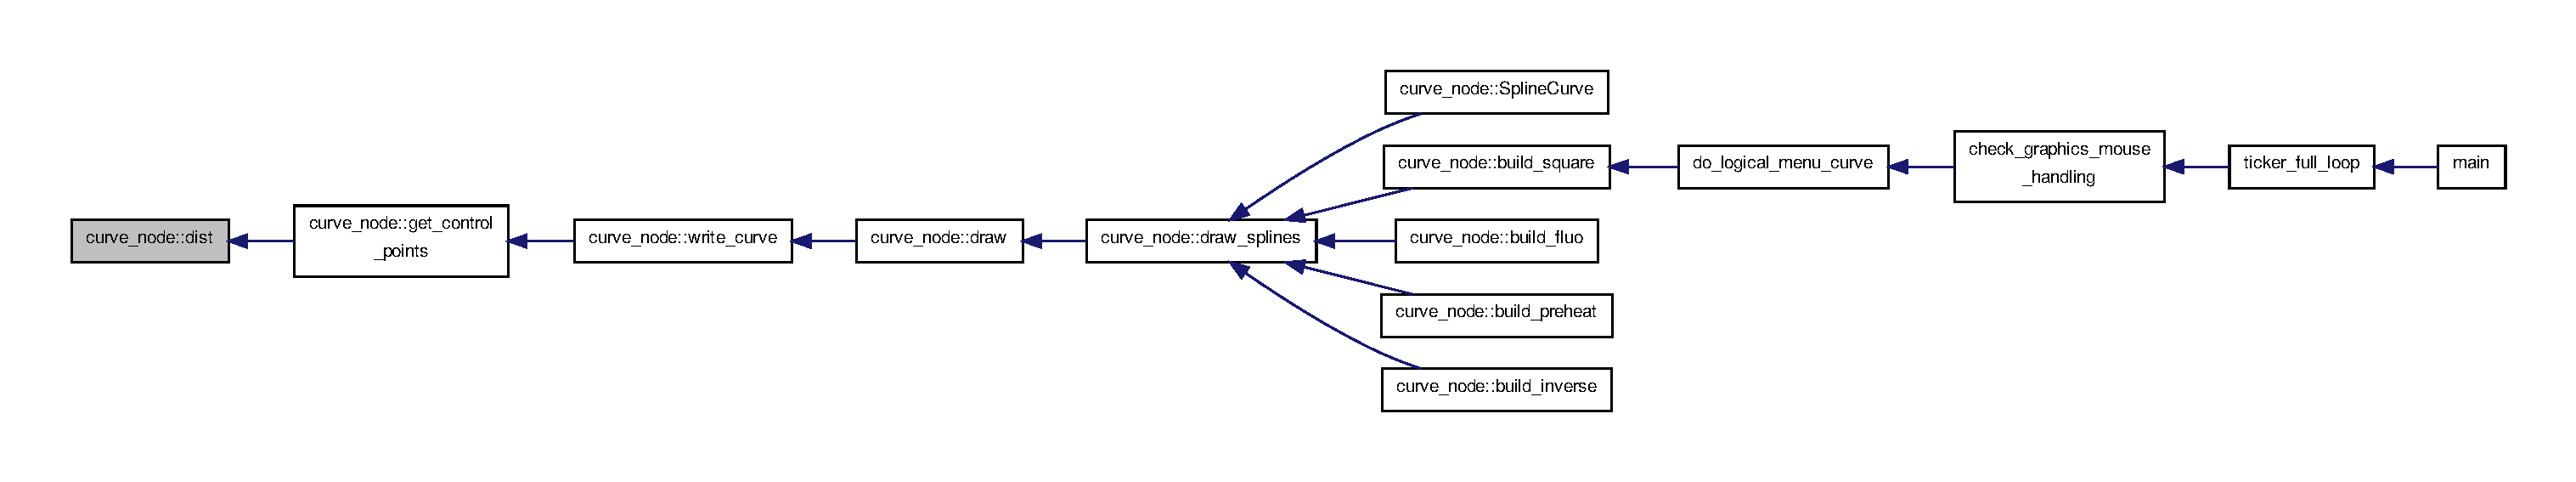
\includegraphics[width=350pt]{classcurve__node_a1146c27b9e6c0b3a5f6fb3faced5cea2_icgraph}
\end{center}
\end{figure}


\hypertarget{classcurve__node_ab1db9f4ea1c53ab2eab6072b2cdc90eb}{\index{curve\+\_\+node@{curve\+\_\+node}!draw@{draw}}
\index{draw@{draw}!curve\+\_\+node@{curve\+\_\+node}}
\subsubsection[{draw}]{\setlength{\rightskip}{0pt plus 5cm}int curve\+\_\+node\+::draw (
\begin{DoxyParamCaption}
\item[{int}]{n, }
\item[{const {\bf graphic\+\_\+context} \&}]{gc}
\end{DoxyParamCaption}
)}}\label{classcurve__node_ab1db9f4ea1c53ab2eab6072b2cdc90eb}
Function to do something 
\begin{DoxyParams}{Paramètres}
{\em n} & value meaning something \\
\hline
{\em gc} & graphic context \\
\hline
\end{DoxyParams}


Voici le graphe d'appel pour cette fonction \+:
\nopagebreak
\begin{figure}[H]
\begin{center}
\leavevmode
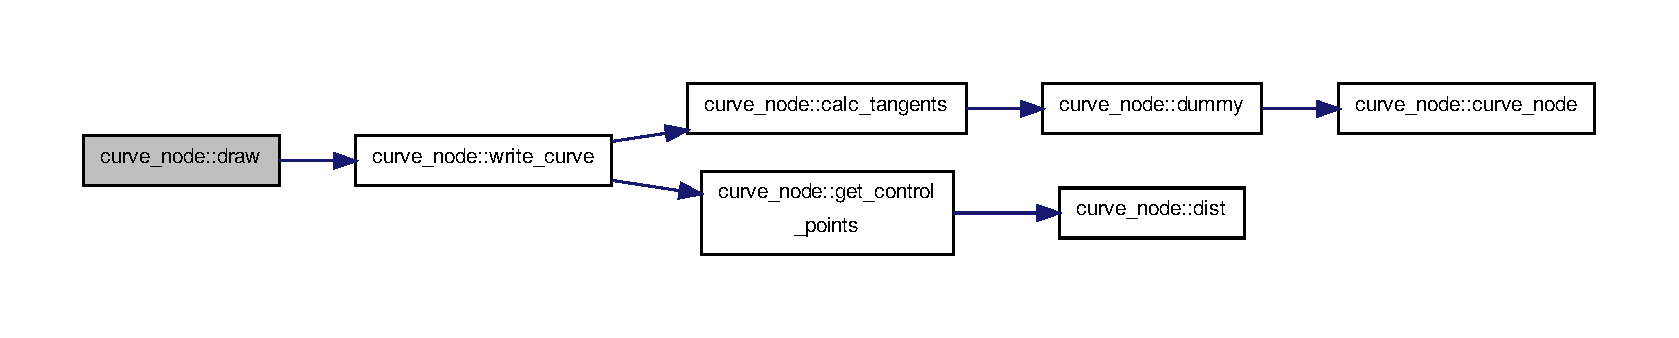
\includegraphics[width=350pt]{classcurve__node_ab1db9f4ea1c53ab2eab6072b2cdc90eb_cgraph}
\end{center}
\end{figure}




Voici le graphe des appelants de cette fonction \+:
\nopagebreak
\begin{figure}[H]
\begin{center}
\leavevmode
\includegraphics[width=350pt]{classcurve__node_ab1db9f4ea1c53ab2eab6072b2cdc90eb_icgraph}
\end{center}
\end{figure}


\hypertarget{classcurve__node_aace217c0200a043c2d2f5f071fde8e56}{\index{curve\+\_\+node@{curve\+\_\+node}!draw\+\_\+splines@{draw\+\_\+splines}}
\index{draw\+\_\+splines@{draw\+\_\+splines}!curve\+\_\+node@{curve\+\_\+node}}
\subsubsection[{draw\+\_\+splines}]{\setlength{\rightskip}{0pt plus 5cm}int curve\+\_\+node\+::draw\+\_\+splines (
\begin{DoxyParamCaption}
\item[{const {\bf graphic\+\_\+context} \&}]{gc}
\end{DoxyParamCaption}
)}}\label{classcurve__node_aace217c0200a043c2d2f5f071fde8e56}
draws the spline paths 
\begin{DoxyParams}{Paramètres}
{\em gc} & graphic context \\
\hline
\end{DoxyParams}


Voici le graphe d'appel pour cette fonction \+:
\nopagebreak
\begin{figure}[H]
\begin{center}
\leavevmode
\includegraphics[width=350pt]{classcurve__node_aace217c0200a043c2d2f5f071fde8e56_cgraph}
\end{center}
\end{figure}




Voici le graphe des appelants de cette fonction \+:
\nopagebreak
\begin{figure}[H]
\begin{center}
\leavevmode
\includegraphics[width=350pt]{classcurve__node_aace217c0200a043c2d2f5f071fde8e56_icgraph}
\end{center}
\end{figure}


\hypertarget{classcurve__node_a55e51b51f9b6ede537c5e11b7f234188}{\index{curve\+\_\+node@{curve\+\_\+node}!dummy@{dummy}}
\index{dummy@{dummy}!curve\+\_\+node@{curve\+\_\+node}}
\subsubsection[{dummy}]{\setlength{\rightskip}{0pt plus 5cm}{\bf curve\+\_\+node} \& curve\+\_\+node\+::dummy (
\begin{DoxyParamCaption}
\item[{const {\bf curve\+\_\+node} \&}]{prev}
\end{DoxyParamCaption}
)}}\label{classcurve__node_a55e51b51f9b6ede537c5e11b7f234188}


Voici le graphe d'appel pour cette fonction \+:
\nopagebreak
\begin{figure}[H]
\begin{center}
\leavevmode
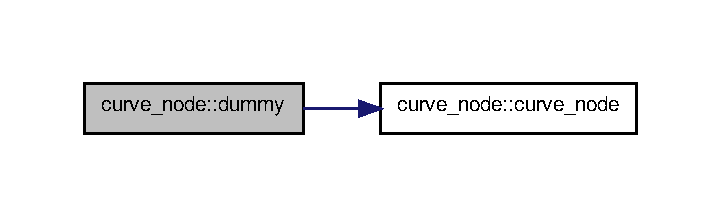
\includegraphics[width=346pt]{classcurve__node_a55e51b51f9b6ede537c5e11b7f234188_cgraph}
\end{center}
\end{figure}




Voici le graphe des appelants de cette fonction \+:
\nopagebreak
\begin{figure}[H]
\begin{center}
\leavevmode
\includegraphics[width=350pt]{classcurve__node_a55e51b51f9b6ede537c5e11b7f234188_icgraph}
\end{center}
\end{figure}


\hypertarget{classcurve__node_a14aba313f46315faae44bcca011136a9}{\index{curve\+\_\+node@{curve\+\_\+node}!get\+\_\+control\+\_\+points@{get\+\_\+control\+\_\+points}}
\index{get\+\_\+control\+\_\+points@{get\+\_\+control\+\_\+points}!curve\+\_\+node@{curve\+\_\+node}}
\subsubsection[{get\+\_\+control\+\_\+points}]{\setlength{\rightskip}{0pt plus 5cm}void curve\+\_\+node\+::get\+\_\+control\+\_\+points (
\begin{DoxyParamCaption}
\item[{const {\bf curve\+\_\+node} \&}]{other, }
\item[{int}]{points\mbox{[}8\mbox{]}}
\end{DoxyParamCaption}
)}}\label{classcurve__node_a14aba313f46315faae44bcca011136a9}
calculates the control points for a spline segment 
\begin{DoxyParams}{Paramètres}
{\em other} & the second point of the segment ('this' is the first one) \\
\hline
{\em points} & (output parameter) a table of 8 integers \\
\hline
\end{DoxyParams}


Voici le graphe d'appel pour cette fonction \+:
\nopagebreak
\begin{figure}[H]
\begin{center}
\leavevmode
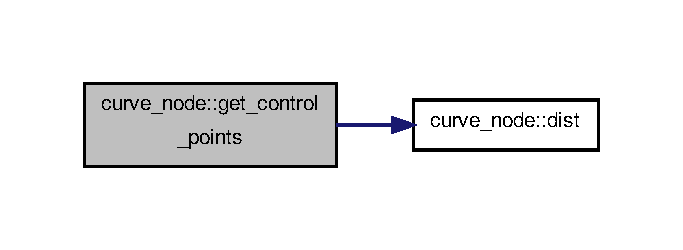
\includegraphics[width=328pt]{classcurve__node_a14aba313f46315faae44bcca011136a9_cgraph}
\end{center}
\end{figure}




Voici le graphe des appelants de cette fonction \+:
\nopagebreak
\begin{figure}[H]
\begin{center}
\leavevmode
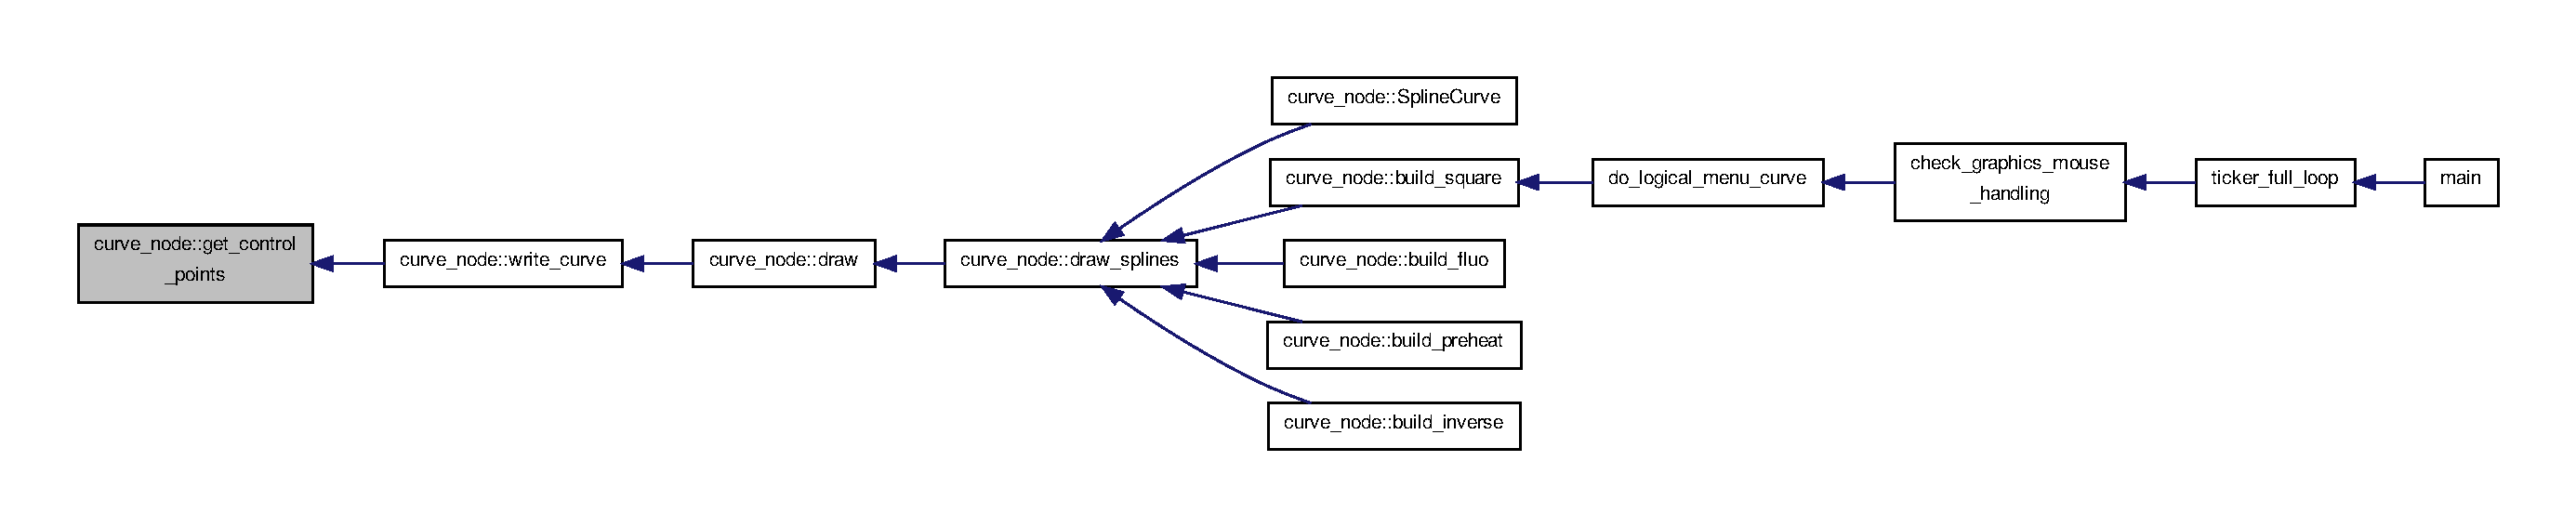
\includegraphics[width=350pt]{classcurve__node_a14aba313f46315faae44bcca011136a9_icgraph}
\end{center}
\end{figure}


\hypertarget{classcurve__node_afb8f3c6e6a53e062f5c2fb1cf7243969}{\index{curve\+\_\+node@{curve\+\_\+node}!Spline\+Curve@{Spline\+Curve}}
\index{Spline\+Curve@{Spline\+Curve}!curve\+\_\+node@{curve\+\_\+node}}
\subsubsection[{Spline\+Curve}]{\setlength{\rightskip}{0pt plus 5cm}int curve\+\_\+node\+::\+Spline\+Curve (
\begin{DoxyParamCaption}
\item[{const {\bf graphic\+\_\+context} \&}]{gc}
\end{DoxyParamCaption}
)}}\label{classcurve__node_afb8f3c6e6a53e062f5c2fb1cf7243969}
draws the spline paths ... 
\begin{DoxyParams}{Paramètres}
{\em gc} & graphic context \\
\hline
\end{DoxyParams}


Voici le graphe d'appel pour cette fonction \+:
\nopagebreak
\begin{figure}[H]
\begin{center}
\leavevmode
\includegraphics[width=350pt]{classcurve__node_afb8f3c6e6a53e062f5c2fb1cf7243969_cgraph}
\end{center}
\end{figure}


\hypertarget{classcurve__node_a5c54a9611e91814177cf901636d4e8e5}{\index{curve\+\_\+node@{curve\+\_\+node}!view\+\_\+after\+\_\+draw@{view\+\_\+after\+\_\+draw}}
\index{view\+\_\+after\+\_\+draw@{view\+\_\+after\+\_\+draw}!curve\+\_\+node@{curve\+\_\+node}}
\subsubsection[{view\+\_\+after\+\_\+draw}]{\setlength{\rightskip}{0pt plus 5cm}int curve\+\_\+node\+::view\+\_\+after\+\_\+draw (
\begin{DoxyParamCaption}
\item[{const {\bf graphic\+\_\+context} \&}]{gc}
\end{DoxyParamCaption}
)}}\label{classcurve__node_a5c54a9611e91814177cf901636d4e8e5}
Function to do something 
\begin{DoxyParams}{Paramètres}
{\em gc} & graphic context \\
\hline
\end{DoxyParams}


Voici le graphe des appelants de cette fonction \+:
\nopagebreak
\begin{figure}[H]
\begin{center}
\leavevmode
\includegraphics[width=350pt]{classcurve__node_a5c54a9611e91814177cf901636d4e8e5_icgraph}
\end{center}
\end{figure}


\hypertarget{classcurve__node_abc1a06d649c6dce22334da762f2955b8}{\index{curve\+\_\+node@{curve\+\_\+node}!write\+\_\+curve@{write\+\_\+curve}}
\index{write\+\_\+curve@{write\+\_\+curve}!curve\+\_\+node@{curve\+\_\+node}}
\subsubsection[{write\+\_\+curve}]{\setlength{\rightskip}{0pt plus 5cm}int curve\+\_\+node\+::write\+\_\+curve (
\begin{DoxyParamCaption}
\item[{const {\bf graphic\+\_\+context} \&}]{gc}
\end{DoxyParamCaption}
)}}\label{classcurve__node_abc1a06d649c6dce22334da762f2955b8}
function to do something 
\begin{DoxyParams}{Paramètres}
{\em gc} & graphic context \\
\hline
\end{DoxyParams}


Voici le graphe d'appel pour cette fonction \+:
\nopagebreak
\begin{figure}[H]
\begin{center}
\leavevmode
\includegraphics[width=350pt]{classcurve__node_abc1a06d649c6dce22334da762f2955b8_cgraph}
\end{center}
\end{figure}




Voici le graphe des appelants de cette fonction \+:
\nopagebreak
\begin{figure}[H]
\begin{center}
\leavevmode
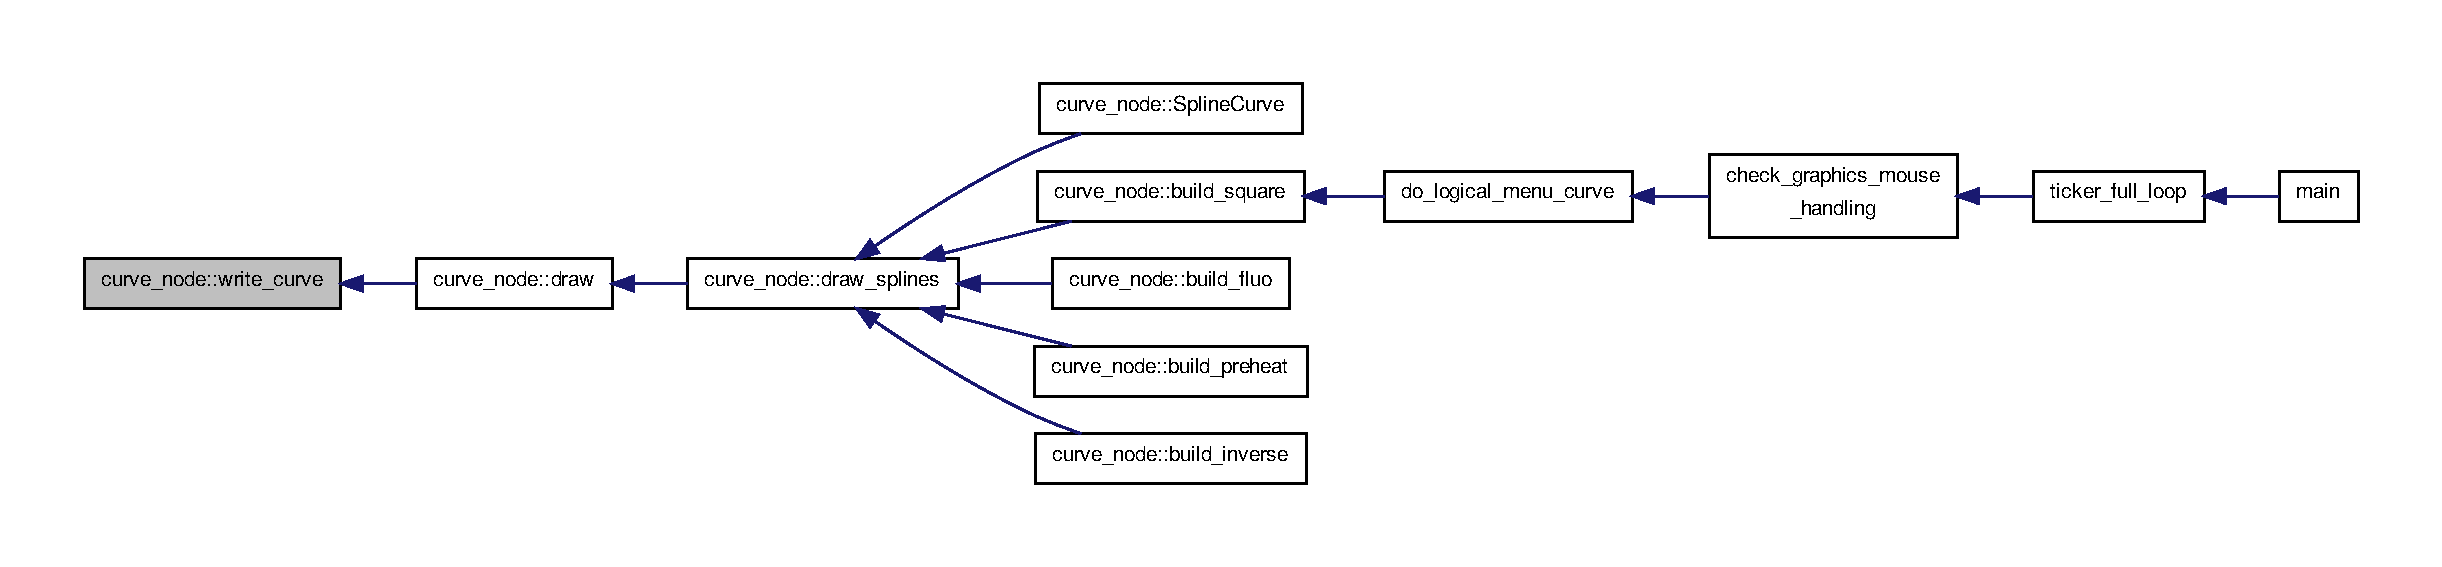
\includegraphics[width=350pt]{classcurve__node_abc1a06d649c6dce22334da762f2955b8_icgraph}
\end{center}
\end{figure}




\subsection{Documentation des données membres}
\hypertarget{classcurve__node_ab7280e17d47152797e10e5992791ee9b}{\index{curve\+\_\+node@{curve\+\_\+node}!ctrl\+\_\+pt@{ctrl\+\_\+pt}}
\index{ctrl\+\_\+pt@{ctrl\+\_\+pt}!curve\+\_\+node@{curve\+\_\+node}}
\subsubsection[{ctrl\+\_\+pt}]{\setlength{\rightskip}{0pt plus 5cm}int curve\+\_\+node\+::ctrl\+\_\+pt\mbox{[}16\mbox{]}\mbox{[}8\mbox{]}\mbox{[}2\mbox{]}\hspace{0.3cm}{\ttfamily [static]}}}\label{classcurve__node_ab7280e17d47152797e10e5992791ee9b}
\hypertarget{classcurve__node_a0aebfec8e10d7fc02442cd5326433c93}{\index{curve\+\_\+node@{curve\+\_\+node}!curves@{curves}}
\index{curves@{curves}!curve\+\_\+node@{curve\+\_\+node}}
\subsubsection[{curves}]{\setlength{\rightskip}{0pt plus 5cm}int curve\+\_\+node\+::curves\mbox{[}514\mbox{]}\hspace{0.3cm}{\ttfamily [static]}}}\label{classcurve__node_a0aebfec8e10d7fc02442cd5326433c93}
\hypertarget{classcurve__node_a46e1f23c6d19a1ca915697c80ed72a84}{\index{curve\+\_\+node@{curve\+\_\+node}!curviness@{curviness}}
\index{curviness@{curviness}!curve\+\_\+node@{curve\+\_\+node}}
\subsubsection[{curviness}]{\setlength{\rightskip}{0pt plus 5cm}fixed curve\+\_\+node\+::curviness\hspace{0.3cm}{\ttfamily [static]}}}\label{classcurve__node_a46e1f23c6d19a1ca915697c80ed72a84}
\hypertarget{classcurve__node_aab45660e4c1077f8742b151fcb0cdcad}{\index{curve\+\_\+node@{curve\+\_\+node}!diam@{diam}}
\index{diam@{diam}!curve\+\_\+node@{curve\+\_\+node}}
\subsubsection[{diam}]{\setlength{\rightskip}{0pt plus 5cm}int curve\+\_\+node\+::diam =10\hspace{0.3cm}{\ttfamily [static]}}}\label{classcurve__node_aab45660e4c1077f8742b151fcb0cdcad}
\hypertarget{classcurve__node_a4479fff7bfc410d6f6d1df9975261aa8}{\index{curve\+\_\+node@{curve\+\_\+node}!index\+\_\+enable\+\_\+editing@{index\+\_\+enable\+\_\+editing}}
\index{index\+\_\+enable\+\_\+editing@{index\+\_\+enable\+\_\+editing}!curve\+\_\+node@{curve\+\_\+node}}
\subsubsection[{index\+\_\+enable\+\_\+editing}]{\setlength{\rightskip}{0pt plus 5cm}bool curve\+\_\+node\+::index\+\_\+enable\+\_\+editing =0\hspace{0.3cm}{\ttfamily [static]}}}\label{classcurve__node_a4479fff7bfc410d6f6d1df9975261aa8}
\hypertarget{classcurve__node_af9c0c53bc02942259c36c753232326aa}{\index{curve\+\_\+node@{curve\+\_\+node}!index\+\_\+spline\+\_\+level@{index\+\_\+spline\+\_\+level}}
\index{index\+\_\+spline\+\_\+level@{index\+\_\+spline\+\_\+level}!curve\+\_\+node@{curve\+\_\+node}}
\subsubsection[{index\+\_\+spline\+\_\+level}]{\setlength{\rightskip}{0pt plus 5cm}int curve\+\_\+node\+::index\+\_\+spline\+\_\+level =0\hspace{0.3cm}{\ttfamily [static]}}}\label{classcurve__node_af9c0c53bc02942259c36c753232326aa}
\hypertarget{classcurve__node_ae995b9ef63ae5b880d6006083acaf6d3}{\index{curve\+\_\+node@{curve\+\_\+node}!index\+\_\+writing@{index\+\_\+writing}}
\index{index\+\_\+writing@{index\+\_\+writing}!curve\+\_\+node@{curve\+\_\+node}}
\subsubsection[{index\+\_\+writing}]{\setlength{\rightskip}{0pt plus 5cm}bool curve\+\_\+node\+::index\+\_\+writing =0\hspace{0.3cm}{\ttfamily [static]}}}\label{classcurve__node_ae995b9ef63ae5b880d6006083acaf6d3}
\hypertarget{classcurve__node_a09d4ec4d9b46abddbcec3e0c46f53d3f}{\index{curve\+\_\+node@{curve\+\_\+node}!node\+\_\+count@{node\+\_\+count}}
\index{node\+\_\+count@{node\+\_\+count}!curve\+\_\+node@{curve\+\_\+node}}
\subsubsection[{node\+\_\+count}]{\setlength{\rightskip}{0pt plus 5cm}int curve\+\_\+node\+::node\+\_\+count =0\hspace{0.3cm}{\ttfamily [static]}}}\label{classcurve__node_a09d4ec4d9b46abddbcec3e0c46f53d3f}
\hypertarget{classcurve__node_affd9362e19ab4c4a70164622a7aebb61}{\index{curve\+\_\+node@{curve\+\_\+node}!nodes@{nodes}}
\index{nodes@{nodes}!curve\+\_\+node@{curve\+\_\+node}}
\subsubsection[{nodes}]{\setlength{\rightskip}{0pt plus 5cm}{\bf curve\+\_\+node} curve\+\_\+node\+::nodes\mbox{[}{\bf M\+A\+X\+\_\+\+C\+N\+O\+D\+E\+S}\mbox{]}\hspace{0.3cm}{\ttfamily [static]}}}\label{classcurve__node_affd9362e19ab4c4a70164622a7aebb61}
\hypertarget{classcurve__node_a348cce4dfe54130e8b8b2fb218baedfb}{\index{curve\+\_\+node@{curve\+\_\+node}!report@{report}}
\index{report@{report}!curve\+\_\+node@{curve\+\_\+node}}
\subsubsection[{report}]{\setlength{\rightskip}{0pt plus 5cm}int curve\+\_\+node\+::report\mbox{[}16\mbox{]}\mbox{[}256\mbox{]}\hspace{0.3cm}{\ttfamily [static]}}}\label{classcurve__node_a348cce4dfe54130e8b8b2fb218baedfb}
\hypertarget{classcurve__node_abe017d998cde30d2ca5f7c8ea68ba3da}{\index{curve\+\_\+node@{curve\+\_\+node}!selected@{selected}}
\index{selected@{selected}!curve\+\_\+node@{curve\+\_\+node}}
\subsubsection[{selected}]{\setlength{\rightskip}{0pt plus 5cm}int curve\+\_\+node\+::selected =0\hspace{0.3cm}{\ttfamily [static]}}}\label{classcurve__node_abe017d998cde30d2ca5f7c8ea68ba3da}
\hypertarget{classcurve__node_a16c72a6637b3b68983b5ce55b90665bf}{\index{curve\+\_\+node@{curve\+\_\+node}!spline\+\_\+level@{spline\+\_\+level}}
\index{spline\+\_\+level@{spline\+\_\+level}!curve\+\_\+node@{curve\+\_\+node}}
\subsubsection[{spline\+\_\+level}]{\setlength{\rightskip}{0pt plus 5cm}float curve\+\_\+node\+::spline\+\_\+level =0.\+0\hspace{0.3cm}{\ttfamily [static]}}}\label{classcurve__node_a16c72a6637b3b68983b5ce55b90665bf}
\hypertarget{classcurve__node_a31ea7469070f7bb90ceae073d1d075a6}{\index{curve\+\_\+node@{curve\+\_\+node}!tangent@{tangent}}
\index{tangent@{tangent}!curve\+\_\+node@{curve\+\_\+node}}
\subsubsection[{tangent}]{\setlength{\rightskip}{0pt plus 5cm}fixed curve\+\_\+node\+::tangent}}\label{classcurve__node_a31ea7469070f7bb90ceae073d1d075a6}
\hypertarget{classcurve__node_a62eb9b6b3a24274664775a07c565d39c}{\index{curve\+\_\+node@{curve\+\_\+node}!the\+\_\+spline\+\_\+level@{the\+\_\+spline\+\_\+level}}
\index{the\+\_\+spline\+\_\+level@{the\+\_\+spline\+\_\+level}!curve\+\_\+node@{curve\+\_\+node}}
\subsubsection[{the\+\_\+spline\+\_\+level}]{\setlength{\rightskip}{0pt plus 5cm}int curve\+\_\+node\+::the\+\_\+spline\+\_\+level\mbox{[}16\mbox{]}\hspace{0.3cm}{\ttfamily [static]}}}\label{classcurve__node_a62eb9b6b3a24274664775a07c565d39c}
\hypertarget{classcurve__node_aa7ae8f2ee3bbd3e6194785c392751cdb}{\index{curve\+\_\+node@{curve\+\_\+node}!x@{x}}
\index{x@{x}!curve\+\_\+node@{curve\+\_\+node}}
\subsubsection[{x}]{\setlength{\rightskip}{0pt plus 5cm}int curve\+\_\+node\+::x}}\label{classcurve__node_aa7ae8f2ee3bbd3e6194785c392751cdb}
\hypertarget{classcurve__node_afc1f4f007a920aa79c1f1f0ff0b49465}{\index{curve\+\_\+node@{curve\+\_\+node}!y@{y}}
\index{y@{y}!curve\+\_\+node@{curve\+\_\+node}}
\subsubsection[{y}]{\setlength{\rightskip}{0pt plus 5cm}int curve\+\_\+node\+::y}}\label{classcurve__node_afc1f4f007a920aa79c1f1f0ff0b49465}


La documentation de cette classe a été générée à partir des fichiers suivants \+:\begin{DoxyCompactItemize}
\item 
\hyperlink{patch__splines__2_8h}{patch\+\_\+splines\+\_\+2.\+h}\item 
\hyperlink{_m_a_i_n__avec__objets_8cpp}{M\+A\+I\+N\+\_\+avec\+\_\+objets.\+cpp}\item 
\hyperlink{patch__splines__2_8cpp}{patch\+\_\+splines\+\_\+2.\+cpp}\end{DoxyCompactItemize}

\hypertarget{struct_d_m_x_u_s_b_p_r_o_params_type}{\section{Référence de la structure D\+M\+X\+U\+S\+B\+P\+R\+O\+Params\+Type}
\label{struct_d_m_x_u_s_b_p_r_o_params_type}\index{D\+M\+X\+U\+S\+B\+P\+R\+O\+Params\+Type@{D\+M\+X\+U\+S\+B\+P\+R\+O\+Params\+Type}}
}
\subsection*{Attributs publics}
\begin{DoxyCompactItemize}
\item 
unsigned char \hyperlink{struct_d_m_x_u_s_b_p_r_o_params_type_aafb2113e09068d2c2d90d4254e57e580}{Firmware\+L\+S\+B}
\item 
unsigned char \hyperlink{struct_d_m_x_u_s_b_p_r_o_params_type_a545afd72b346f85996c1ae3d0b35a0ef}{Firmware\+M\+S\+B}
\item 
unsigned char \hyperlink{struct_d_m_x_u_s_b_p_r_o_params_type_a86773af46c2e39c7b260ce1f09ca0a36}{Break\+Time}
\item 
unsigned char \hyperlink{struct_d_m_x_u_s_b_p_r_o_params_type_a1ab62801637fe44bba062f2bfa54e38e}{Ma\+B\+Time}
\item 
unsigned char \hyperlink{struct_d_m_x_u_s_b_p_r_o_params_type_a6258e9923d9bc0725d4b2cc0be515d70}{Refresh\+Rate}
\end{DoxyCompactItemize}


\subsection{Documentation des données membres}
\hypertarget{struct_d_m_x_u_s_b_p_r_o_params_type_a86773af46c2e39c7b260ce1f09ca0a36}{\index{D\+M\+X\+U\+S\+B\+P\+R\+O\+Params\+Type@{D\+M\+X\+U\+S\+B\+P\+R\+O\+Params\+Type}!Break\+Time@{Break\+Time}}
\index{Break\+Time@{Break\+Time}!D\+M\+X\+U\+S\+B\+P\+R\+O\+Params\+Type@{D\+M\+X\+U\+S\+B\+P\+R\+O\+Params\+Type}}
\subsubsection[{Break\+Time}]{\setlength{\rightskip}{0pt plus 5cm}unsigned char D\+M\+X\+U\+S\+B\+P\+R\+O\+Params\+Type\+::\+Break\+Time}}\label{struct_d_m_x_u_s_b_p_r_o_params_type_a86773af46c2e39c7b260ce1f09ca0a36}
\hypertarget{struct_d_m_x_u_s_b_p_r_o_params_type_aafb2113e09068d2c2d90d4254e57e580}{\index{D\+M\+X\+U\+S\+B\+P\+R\+O\+Params\+Type@{D\+M\+X\+U\+S\+B\+P\+R\+O\+Params\+Type}!Firmware\+L\+S\+B@{Firmware\+L\+S\+B}}
\index{Firmware\+L\+S\+B@{Firmware\+L\+S\+B}!D\+M\+X\+U\+S\+B\+P\+R\+O\+Params\+Type@{D\+M\+X\+U\+S\+B\+P\+R\+O\+Params\+Type}}
\subsubsection[{Firmware\+L\+S\+B}]{\setlength{\rightskip}{0pt plus 5cm}unsigned char D\+M\+X\+U\+S\+B\+P\+R\+O\+Params\+Type\+::\+Firmware\+L\+S\+B}}\label{struct_d_m_x_u_s_b_p_r_o_params_type_aafb2113e09068d2c2d90d4254e57e580}
\hypertarget{struct_d_m_x_u_s_b_p_r_o_params_type_a545afd72b346f85996c1ae3d0b35a0ef}{\index{D\+M\+X\+U\+S\+B\+P\+R\+O\+Params\+Type@{D\+M\+X\+U\+S\+B\+P\+R\+O\+Params\+Type}!Firmware\+M\+S\+B@{Firmware\+M\+S\+B}}
\index{Firmware\+M\+S\+B@{Firmware\+M\+S\+B}!D\+M\+X\+U\+S\+B\+P\+R\+O\+Params\+Type@{D\+M\+X\+U\+S\+B\+P\+R\+O\+Params\+Type}}
\subsubsection[{Firmware\+M\+S\+B}]{\setlength{\rightskip}{0pt plus 5cm}unsigned char D\+M\+X\+U\+S\+B\+P\+R\+O\+Params\+Type\+::\+Firmware\+M\+S\+B}}\label{struct_d_m_x_u_s_b_p_r_o_params_type_a545afd72b346f85996c1ae3d0b35a0ef}
\hypertarget{struct_d_m_x_u_s_b_p_r_o_params_type_a1ab62801637fe44bba062f2bfa54e38e}{\index{D\+M\+X\+U\+S\+B\+P\+R\+O\+Params\+Type@{D\+M\+X\+U\+S\+B\+P\+R\+O\+Params\+Type}!Ma\+B\+Time@{Ma\+B\+Time}}
\index{Ma\+B\+Time@{Ma\+B\+Time}!D\+M\+X\+U\+S\+B\+P\+R\+O\+Params\+Type@{D\+M\+X\+U\+S\+B\+P\+R\+O\+Params\+Type}}
\subsubsection[{Ma\+B\+Time}]{\setlength{\rightskip}{0pt plus 5cm}unsigned char D\+M\+X\+U\+S\+B\+P\+R\+O\+Params\+Type\+::\+Ma\+B\+Time}}\label{struct_d_m_x_u_s_b_p_r_o_params_type_a1ab62801637fe44bba062f2bfa54e38e}
\hypertarget{struct_d_m_x_u_s_b_p_r_o_params_type_a6258e9923d9bc0725d4b2cc0be515d70}{\index{D\+M\+X\+U\+S\+B\+P\+R\+O\+Params\+Type@{D\+M\+X\+U\+S\+B\+P\+R\+O\+Params\+Type}!Refresh\+Rate@{Refresh\+Rate}}
\index{Refresh\+Rate@{Refresh\+Rate}!D\+M\+X\+U\+S\+B\+P\+R\+O\+Params\+Type@{D\+M\+X\+U\+S\+B\+P\+R\+O\+Params\+Type}}
\subsubsection[{Refresh\+Rate}]{\setlength{\rightskip}{0pt plus 5cm}unsigned char D\+M\+X\+U\+S\+B\+P\+R\+O\+Params\+Type\+::\+Refresh\+Rate}}\label{struct_d_m_x_u_s_b_p_r_o_params_type_a6258e9923d9bc0725d4b2cc0be515d70}


La documentation de cette structure a été générée à partir du fichier suivant \+:\begin{DoxyCompactItemize}
\item 
\hyperlink{dmx__enttec__pro_8cpp}{dmx\+\_\+enttec\+\_\+pro.\+cpp}\end{DoxyCompactItemize}

\hypertarget{struct_d_m_x_u_s_b_p_r_o_set_params_type}{\section{Référence de la structure D\+M\+X\+U\+S\+B\+P\+R\+O\+Set\+Params\+Type}
\label{struct_d_m_x_u_s_b_p_r_o_set_params_type}\index{D\+M\+X\+U\+S\+B\+P\+R\+O\+Set\+Params\+Type@{D\+M\+X\+U\+S\+B\+P\+R\+O\+Set\+Params\+Type}}
}
\subsection*{Attributs publics}
\begin{DoxyCompactItemize}
\item 
unsigned char \hyperlink{struct_d_m_x_u_s_b_p_r_o_set_params_type_a849e4ebeb6ebb38a6b2fc53c32d4456d}{User\+Size\+L\+S\+B}
\item 
unsigned char \hyperlink{struct_d_m_x_u_s_b_p_r_o_set_params_type_adae7671559ec6924d03fd27f50d6fda0}{User\+Size\+M\+S\+B}
\item 
unsigned char \hyperlink{struct_d_m_x_u_s_b_p_r_o_set_params_type_ad5a0ccbc024303300f2933f16046abd4}{Break\+Time}
\item 
unsigned char \hyperlink{struct_d_m_x_u_s_b_p_r_o_set_params_type_a766ed7ac1cd093a822fa905f43f81129}{Ma\+B\+Time}
\item 
unsigned char \hyperlink{struct_d_m_x_u_s_b_p_r_o_set_params_type_a1e0b6924aa027f23f1bbd5606cbe09e7}{Refresh\+Rate}
\end{DoxyCompactItemize}


\subsection{Documentation des données membres}
\hypertarget{struct_d_m_x_u_s_b_p_r_o_set_params_type_ad5a0ccbc024303300f2933f16046abd4}{\index{D\+M\+X\+U\+S\+B\+P\+R\+O\+Set\+Params\+Type@{D\+M\+X\+U\+S\+B\+P\+R\+O\+Set\+Params\+Type}!Break\+Time@{Break\+Time}}
\index{Break\+Time@{Break\+Time}!D\+M\+X\+U\+S\+B\+P\+R\+O\+Set\+Params\+Type@{D\+M\+X\+U\+S\+B\+P\+R\+O\+Set\+Params\+Type}}
\subsubsection[{Break\+Time}]{\setlength{\rightskip}{0pt plus 5cm}unsigned char D\+M\+X\+U\+S\+B\+P\+R\+O\+Set\+Params\+Type\+::\+Break\+Time}}\label{struct_d_m_x_u_s_b_p_r_o_set_params_type_ad5a0ccbc024303300f2933f16046abd4}
\hypertarget{struct_d_m_x_u_s_b_p_r_o_set_params_type_a766ed7ac1cd093a822fa905f43f81129}{\index{D\+M\+X\+U\+S\+B\+P\+R\+O\+Set\+Params\+Type@{D\+M\+X\+U\+S\+B\+P\+R\+O\+Set\+Params\+Type}!Ma\+B\+Time@{Ma\+B\+Time}}
\index{Ma\+B\+Time@{Ma\+B\+Time}!D\+M\+X\+U\+S\+B\+P\+R\+O\+Set\+Params\+Type@{D\+M\+X\+U\+S\+B\+P\+R\+O\+Set\+Params\+Type}}
\subsubsection[{Ma\+B\+Time}]{\setlength{\rightskip}{0pt plus 5cm}unsigned char D\+M\+X\+U\+S\+B\+P\+R\+O\+Set\+Params\+Type\+::\+Ma\+B\+Time}}\label{struct_d_m_x_u_s_b_p_r_o_set_params_type_a766ed7ac1cd093a822fa905f43f81129}
\hypertarget{struct_d_m_x_u_s_b_p_r_o_set_params_type_a1e0b6924aa027f23f1bbd5606cbe09e7}{\index{D\+M\+X\+U\+S\+B\+P\+R\+O\+Set\+Params\+Type@{D\+M\+X\+U\+S\+B\+P\+R\+O\+Set\+Params\+Type}!Refresh\+Rate@{Refresh\+Rate}}
\index{Refresh\+Rate@{Refresh\+Rate}!D\+M\+X\+U\+S\+B\+P\+R\+O\+Set\+Params\+Type@{D\+M\+X\+U\+S\+B\+P\+R\+O\+Set\+Params\+Type}}
\subsubsection[{Refresh\+Rate}]{\setlength{\rightskip}{0pt plus 5cm}unsigned char D\+M\+X\+U\+S\+B\+P\+R\+O\+Set\+Params\+Type\+::\+Refresh\+Rate}}\label{struct_d_m_x_u_s_b_p_r_o_set_params_type_a1e0b6924aa027f23f1bbd5606cbe09e7}
\hypertarget{struct_d_m_x_u_s_b_p_r_o_set_params_type_a849e4ebeb6ebb38a6b2fc53c32d4456d}{\index{D\+M\+X\+U\+S\+B\+P\+R\+O\+Set\+Params\+Type@{D\+M\+X\+U\+S\+B\+P\+R\+O\+Set\+Params\+Type}!User\+Size\+L\+S\+B@{User\+Size\+L\+S\+B}}
\index{User\+Size\+L\+S\+B@{User\+Size\+L\+S\+B}!D\+M\+X\+U\+S\+B\+P\+R\+O\+Set\+Params\+Type@{D\+M\+X\+U\+S\+B\+P\+R\+O\+Set\+Params\+Type}}
\subsubsection[{User\+Size\+L\+S\+B}]{\setlength{\rightskip}{0pt plus 5cm}unsigned char D\+M\+X\+U\+S\+B\+P\+R\+O\+Set\+Params\+Type\+::\+User\+Size\+L\+S\+B}}\label{struct_d_m_x_u_s_b_p_r_o_set_params_type_a849e4ebeb6ebb38a6b2fc53c32d4456d}
\hypertarget{struct_d_m_x_u_s_b_p_r_o_set_params_type_adae7671559ec6924d03fd27f50d6fda0}{\index{D\+M\+X\+U\+S\+B\+P\+R\+O\+Set\+Params\+Type@{D\+M\+X\+U\+S\+B\+P\+R\+O\+Set\+Params\+Type}!User\+Size\+M\+S\+B@{User\+Size\+M\+S\+B}}
\index{User\+Size\+M\+S\+B@{User\+Size\+M\+S\+B}!D\+M\+X\+U\+S\+B\+P\+R\+O\+Set\+Params\+Type@{D\+M\+X\+U\+S\+B\+P\+R\+O\+Set\+Params\+Type}}
\subsubsection[{User\+Size\+M\+S\+B}]{\setlength{\rightskip}{0pt plus 5cm}unsigned char D\+M\+X\+U\+S\+B\+P\+R\+O\+Set\+Params\+Type\+::\+User\+Size\+M\+S\+B}}\label{struct_d_m_x_u_s_b_p_r_o_set_params_type_adae7671559ec6924d03fd27f50d6fda0}


La documentation de cette structure a été générée à partir du fichier suivant \+:\begin{DoxyCompactItemize}
\item 
\hyperlink{dmx__enttec__pro_8cpp}{dmx\+\_\+enttec\+\_\+pro.\+cpp}\end{DoxyCompactItemize}

\hypertarget{classgraphic__context}{\section{Référence de la classe graphic\+\_\+context}
\label{classgraphic__context}\index{graphic\+\_\+context@{graphic\+\_\+context}}
}


{\ttfamily \#include $<$patch\+\_\+splines\+\_\+2.\+h$>$}

\subsection*{Fonctions membres publiques}
\begin{DoxyCompactItemize}
\item 
\hyperlink{classgraphic__context_ac81331f894194151dc9f2f20f6eb86e6}{graphic\+\_\+context} (int \hyperlink{classgraphic__context_afb842574bef9200a343eae5ed25b6aea}{window\+\_\+focus\+\_\+id}, int \hyperlink{classgraphic__context_af8795c6d73bb4076febf90a4bed34cd7}{W\+\_\+\+P\+A\+T\+C\+H}, int \hyperlink{classgraphic__context_af9aa907f4c540927888920111f2a3890}{mouse\+\_\+x}, int \hyperlink{classgraphic__context_a72195ff30744dcb9c467cad5bda4e602}{mouse\+\_\+y}, int \hyperlink{classgraphic__context_a57a5bcca338d0b27c5014b9bde3f6e99}{xpatch\+\_\+window}, int \hyperlink{classgraphic__context_ae902bd96df3912441f3f5e99cd802fbf}{ypatch\+\_\+window}, int \hyperlink{classgraphic__context_abeabd1716cb7451605935b9191be65fb}{dmx\+\_\+view})
\end{DoxyCompactItemize}
\subsection*{Attributs publics}
\begin{DoxyCompactItemize}
\item 
int \hyperlink{classgraphic__context_afb842574bef9200a343eae5ed25b6aea}{window\+\_\+focus\+\_\+id}
\item 
int \hyperlink{classgraphic__context_af8795c6d73bb4076febf90a4bed34cd7}{W\+\_\+\+P\+A\+T\+C\+H}
\item 
int \hyperlink{classgraphic__context_af9aa907f4c540927888920111f2a3890}{mouse\+\_\+x}
\item 
int \hyperlink{classgraphic__context_a72195ff30744dcb9c467cad5bda4e602}{mouse\+\_\+y}
\item 
int \hyperlink{classgraphic__context_a57a5bcca338d0b27c5014b9bde3f6e99}{xpatch\+\_\+window}
\item 
int \hyperlink{classgraphic__context_ae902bd96df3912441f3f5e99cd802fbf}{ypatch\+\_\+window}
\item 
int \hyperlink{classgraphic__context_abeabd1716cb7451605935b9191be65fb}{dmx\+\_\+view}
\end{DoxyCompactItemize}


\subsection{Documentation des constructeurs et destructeur}
\hypertarget{classgraphic__context_ac81331f894194151dc9f2f20f6eb86e6}{\index{graphic\+\_\+context@{graphic\+\_\+context}!graphic\+\_\+context@{graphic\+\_\+context}}
\index{graphic\+\_\+context@{graphic\+\_\+context}!graphic\+\_\+context@{graphic\+\_\+context}}
\subsubsection[{graphic\+\_\+context}]{\setlength{\rightskip}{0pt plus 5cm}graphic\+\_\+context\+::graphic\+\_\+context (
\begin{DoxyParamCaption}
\item[{int}]{window\+\_\+focus\+\_\+id, }
\item[{int}]{W\+\_\+\+P\+A\+T\+C\+H, }
\item[{int}]{mouse\+\_\+x, }
\item[{int}]{mouse\+\_\+y, }
\item[{int}]{xpatch\+\_\+window, }
\item[{int}]{ypatch\+\_\+window, }
\item[{int}]{dmx\+\_\+view}
\end{DoxyParamCaption}
)\hspace{0.3cm}{\ttfamily [inline]}}}\label{classgraphic__context_ac81331f894194151dc9f2f20f6eb86e6}
The constructor of a graphic context 
\begin{DoxyParams}{Paramètres}
{\em window\+\_\+focus\+\_\+id} & identifier of the windows owning the focus \\
\hline
{\em W\+\_\+\+P\+A\+T\+C\+H} & identifier of a particular window \\
\hline
{\em mouse\+\_\+x} & abscissa of the mouse cursor \\
\hline
{\em mouse\+\_\+y} & ordinate of the mouse cursor \\
\hline
{\em xpatch\+\_\+window} & abscissa of the patch window \\
\hline
{\em ypatch\+\_\+window} & ordinate of the patch window \\
\hline
{\em dmx\+\_\+view} & an integer code to define the view mode of D\+M\+X\+: 0 means percentage of intensity, 1 means D\+M\+X unity (0..255) \\
\hline
\end{DoxyParams}


\subsection{Documentation des données membres}
\hypertarget{classgraphic__context_abeabd1716cb7451605935b9191be65fb}{\index{graphic\+\_\+context@{graphic\+\_\+context}!dmx\+\_\+view@{dmx\+\_\+view}}
\index{dmx\+\_\+view@{dmx\+\_\+view}!graphic\+\_\+context@{graphic\+\_\+context}}
\subsubsection[{dmx\+\_\+view}]{\setlength{\rightskip}{0pt plus 5cm}int graphic\+\_\+context\+::dmx\+\_\+view}}\label{classgraphic__context_abeabd1716cb7451605935b9191be65fb}
\hypertarget{classgraphic__context_af9aa907f4c540927888920111f2a3890}{\index{graphic\+\_\+context@{graphic\+\_\+context}!mouse\+\_\+x@{mouse\+\_\+x}}
\index{mouse\+\_\+x@{mouse\+\_\+x}!graphic\+\_\+context@{graphic\+\_\+context}}
\subsubsection[{mouse\+\_\+x}]{\setlength{\rightskip}{0pt plus 5cm}int graphic\+\_\+context\+::mouse\+\_\+x}}\label{classgraphic__context_af9aa907f4c540927888920111f2a3890}
\hypertarget{classgraphic__context_a72195ff30744dcb9c467cad5bda4e602}{\index{graphic\+\_\+context@{graphic\+\_\+context}!mouse\+\_\+y@{mouse\+\_\+y}}
\index{mouse\+\_\+y@{mouse\+\_\+y}!graphic\+\_\+context@{graphic\+\_\+context}}
\subsubsection[{mouse\+\_\+y}]{\setlength{\rightskip}{0pt plus 5cm}int graphic\+\_\+context\+::mouse\+\_\+y}}\label{classgraphic__context_a72195ff30744dcb9c467cad5bda4e602}
\hypertarget{classgraphic__context_af8795c6d73bb4076febf90a4bed34cd7}{\index{graphic\+\_\+context@{graphic\+\_\+context}!W\+\_\+\+P\+A\+T\+C\+H@{W\+\_\+\+P\+A\+T\+C\+H}}
\index{W\+\_\+\+P\+A\+T\+C\+H@{W\+\_\+\+P\+A\+T\+C\+H}!graphic\+\_\+context@{graphic\+\_\+context}}
\subsubsection[{W\+\_\+\+P\+A\+T\+C\+H}]{\setlength{\rightskip}{0pt plus 5cm}int graphic\+\_\+context\+::\+W\+\_\+\+P\+A\+T\+C\+H}}\label{classgraphic__context_af8795c6d73bb4076febf90a4bed34cd7}
\hypertarget{classgraphic__context_afb842574bef9200a343eae5ed25b6aea}{\index{graphic\+\_\+context@{graphic\+\_\+context}!window\+\_\+focus\+\_\+id@{window\+\_\+focus\+\_\+id}}
\index{window\+\_\+focus\+\_\+id@{window\+\_\+focus\+\_\+id}!graphic\+\_\+context@{graphic\+\_\+context}}
\subsubsection[{window\+\_\+focus\+\_\+id}]{\setlength{\rightskip}{0pt plus 5cm}int graphic\+\_\+context\+::window\+\_\+focus\+\_\+id}}\label{classgraphic__context_afb842574bef9200a343eae5ed25b6aea}
\hypertarget{classgraphic__context_a57a5bcca338d0b27c5014b9bde3f6e99}{\index{graphic\+\_\+context@{graphic\+\_\+context}!xpatch\+\_\+window@{xpatch\+\_\+window}}
\index{xpatch\+\_\+window@{xpatch\+\_\+window}!graphic\+\_\+context@{graphic\+\_\+context}}
\subsubsection[{xpatch\+\_\+window}]{\setlength{\rightskip}{0pt plus 5cm}int graphic\+\_\+context\+::xpatch\+\_\+window}}\label{classgraphic__context_a57a5bcca338d0b27c5014b9bde3f6e99}
\hypertarget{classgraphic__context_ae902bd96df3912441f3f5e99cd802fbf}{\index{graphic\+\_\+context@{graphic\+\_\+context}!ypatch\+\_\+window@{ypatch\+\_\+window}}
\index{ypatch\+\_\+window@{ypatch\+\_\+window}!graphic\+\_\+context@{graphic\+\_\+context}}
\subsubsection[{ypatch\+\_\+window}]{\setlength{\rightskip}{0pt plus 5cm}int graphic\+\_\+context\+::ypatch\+\_\+window}}\label{classgraphic__context_ae902bd96df3912441f3f5e99cd802fbf}


La documentation de cette classe a été générée à partir du fichier suivant \+:\begin{DoxyCompactItemize}
\item 
\hyperlink{patch__splines__2_8h}{patch\+\_\+splines\+\_\+2.\+h}\end{DoxyCompactItemize}

\hypertarget{struct_n_o_d_e}{\section{Référence de la structure N\+O\+D\+E}
\label{struct_n_o_d_e}\index{N\+O\+D\+E@{N\+O\+D\+E}}
}


{\ttfamily \#include $<$whitecat.\+h$>$}

\subsection*{Attributs publics}
\begin{DoxyCompactItemize}
\item 
int \hyperlink{struct_n_o_d_e_ae491648fdefa758c04fd1b39997dfe44}{x}
\item 
int \hyperlink{struct_n_o_d_e_a1c83ccf922c1655a4f4cc90fb7455670}{y}
\item 
fixed \hyperlink{struct_n_o_d_e_ab9675cd84cb7ccf6e2506c7ee233fa2c}{tangent}
\end{DoxyCompactItemize}


\subsection{Documentation des données membres}
\hypertarget{struct_n_o_d_e_ab9675cd84cb7ccf6e2506c7ee233fa2c}{\index{N\+O\+D\+E@{N\+O\+D\+E}!tangent@{tangent}}
\index{tangent@{tangent}!N\+O\+D\+E@{N\+O\+D\+E}}
\subsubsection[{tangent}]{\setlength{\rightskip}{0pt plus 5cm}fixed N\+O\+D\+E\+::tangent}}\label{struct_n_o_d_e_ab9675cd84cb7ccf6e2506c7ee233fa2c}
\hypertarget{struct_n_o_d_e_ae491648fdefa758c04fd1b39997dfe44}{\index{N\+O\+D\+E@{N\+O\+D\+E}!x@{x}}
\index{x@{x}!N\+O\+D\+E@{N\+O\+D\+E}}
\subsubsection[{x}]{\setlength{\rightskip}{0pt plus 5cm}int N\+O\+D\+E\+::x}}\label{struct_n_o_d_e_ae491648fdefa758c04fd1b39997dfe44}
\hypertarget{struct_n_o_d_e_a1c83ccf922c1655a4f4cc90fb7455670}{\index{N\+O\+D\+E@{N\+O\+D\+E}!y@{y}}
\index{y@{y}!N\+O\+D\+E@{N\+O\+D\+E}}
\subsubsection[{y}]{\setlength{\rightskip}{0pt plus 5cm}int N\+O\+D\+E\+::y}}\label{struct_n_o_d_e_a1c83ccf922c1655a4f4cc90fb7455670}


La documentation de cette structure a été générée à partir du fichier suivant \+:\begin{DoxyCompactItemize}
\item 
\hyperlink{whitecat_8h}{whitecat.\+h}\end{DoxyCompactItemize}

\hypertarget{struct_received_dmx_cos_struct}{\section{Référence de la structure Received\+Dmx\+Cos\+Struct}
\label{struct_received_dmx_cos_struct}\index{Received\+Dmx\+Cos\+Struct@{Received\+Dmx\+Cos\+Struct}}
}
\subsection*{Attributs publics}
\begin{DoxyCompactItemize}
\item 
unsigned char \hyperlink{struct_received_dmx_cos_struct_a4cf39b60236997522f11155b63b2f090}{start\+\_\+changed\+\_\+byte\+\_\+number}
\item 
unsigned char \hyperlink{struct_received_dmx_cos_struct_a863941290eeb0f634dd83aa8a2389718}{changed\+\_\+byte\+\_\+array} \mbox{[}5\mbox{]}
\item 
unsigned char \hyperlink{struct_received_dmx_cos_struct_aa3984590d4af300c37c465375dd7ba0f}{changed\+\_\+byte\+\_\+data} \mbox{[}40\mbox{]}
\end{DoxyCompactItemize}


\subsection{Documentation des données membres}
\hypertarget{struct_received_dmx_cos_struct_a863941290eeb0f634dd83aa8a2389718}{\index{Received\+Dmx\+Cos\+Struct@{Received\+Dmx\+Cos\+Struct}!changed\+\_\+byte\+\_\+array@{changed\+\_\+byte\+\_\+array}}
\index{changed\+\_\+byte\+\_\+array@{changed\+\_\+byte\+\_\+array}!Received\+Dmx\+Cos\+Struct@{Received\+Dmx\+Cos\+Struct}}
\subsubsection[{changed\+\_\+byte\+\_\+array}]{\setlength{\rightskip}{0pt plus 5cm}unsigned char Received\+Dmx\+Cos\+Struct\+::changed\+\_\+byte\+\_\+array\mbox{[}5\mbox{]}}}\label{struct_received_dmx_cos_struct_a863941290eeb0f634dd83aa8a2389718}
\hypertarget{struct_received_dmx_cos_struct_aa3984590d4af300c37c465375dd7ba0f}{\index{Received\+Dmx\+Cos\+Struct@{Received\+Dmx\+Cos\+Struct}!changed\+\_\+byte\+\_\+data@{changed\+\_\+byte\+\_\+data}}
\index{changed\+\_\+byte\+\_\+data@{changed\+\_\+byte\+\_\+data}!Received\+Dmx\+Cos\+Struct@{Received\+Dmx\+Cos\+Struct}}
\subsubsection[{changed\+\_\+byte\+\_\+data}]{\setlength{\rightskip}{0pt plus 5cm}unsigned char Received\+Dmx\+Cos\+Struct\+::changed\+\_\+byte\+\_\+data\mbox{[}40\mbox{]}}}\label{struct_received_dmx_cos_struct_aa3984590d4af300c37c465375dd7ba0f}
\hypertarget{struct_received_dmx_cos_struct_a4cf39b60236997522f11155b63b2f090}{\index{Received\+Dmx\+Cos\+Struct@{Received\+Dmx\+Cos\+Struct}!start\+\_\+changed\+\_\+byte\+\_\+number@{start\+\_\+changed\+\_\+byte\+\_\+number}}
\index{start\+\_\+changed\+\_\+byte\+\_\+number@{start\+\_\+changed\+\_\+byte\+\_\+number}!Received\+Dmx\+Cos\+Struct@{Received\+Dmx\+Cos\+Struct}}
\subsubsection[{start\+\_\+changed\+\_\+byte\+\_\+number}]{\setlength{\rightskip}{0pt plus 5cm}unsigned char Received\+Dmx\+Cos\+Struct\+::start\+\_\+changed\+\_\+byte\+\_\+number}}\label{struct_received_dmx_cos_struct_a4cf39b60236997522f11155b63b2f090}


La documentation de cette structure a été générée à partir du fichier suivant \+:\begin{DoxyCompactItemize}
\item 
\hyperlink{dmx__enttec__pro_8cpp}{dmx\+\_\+enttec\+\_\+pro.\+cpp}\end{DoxyCompactItemize}

\chapter{Documentation des fichiers}
\hypertarget{arduino__6___u_n_o_8cpp}{\section{Référence du fichier arduino\+\_\+6\+\_\+\+U\+N\+O.\+cpp}
\label{arduino__6___u_n_o_8cpp}\index{arduino\+\_\+6\+\_\+\+U\+N\+O.\+cpp@{arduino\+\_\+6\+\_\+\+U\+N\+O.\+cpp}}
}


\{arduino G\+U\+I fonctions\}  


Ce graphe montre quels fichiers incluent directement ou indirectement ce fichier \+:
\nopagebreak
\begin{figure}[H]
\begin{center}
\leavevmode
\includegraphics[width=350pt]{arduino__6___u_n_o_8cpp__dep__incl}
\end{center}
\end{figure}
\subsection*{Fonctions}
\begin{DoxyCompactItemize}
\item 
int \hyperlink{arduino__6___u_n_o_8cpp_a48019987fa34c7983be2f709ea7078da}{arduino\+\_\+decode\+\_\+array\+\_\+method} (char $\ast$tmp\+\_\+ard)
\item 
int \hyperlink{arduino__6___u_n_o_8cpp_a78f5530dcdcb456d089828f1696d5db2}{read\+\_\+arduino\+\_\+data} (int \hyperlink{whitecat_8h_a4fda30c89f2eb5ea6e500dbd94ef4eff}{device})
\item 
int \hyperlink{arduino__6___u_n_o_8cpp_ae56d0c5a7e54f2b4a377da1936e0def5}{arduino\+\_\+read} ()
\item 
int \hyperlink{arduino__6___u_n_o_8cpp_a38905c45209df5be7f35a35d9a4f96db}{do\+\_\+arduino\+\_\+config} (int cfg\+\_\+\+X, int cfg\+\_\+\+Y)
\end{DoxyCompactItemize}


\subsection{Description détaillée}
\{arduino G\+U\+I fonctions\} 

\begin{DoxyAuthor}{Auteur}
Christoph Guillermet, Anton Langhoff 
\end{DoxyAuthor}
\begin{DoxyVersion}{Version}
\{0.\+8.\+6\} 
\end{DoxyVersion}
\begin{DoxyDate}{Date}
\{28/04/2014\}
\end{DoxyDate}
White Cat \{-\/ categorie\} \{-\/ sous categorie \{-\/ sous categorie\}\}

Création de la fenêtre Arduino dans le config menu et des différentes fonctions

Create the Arduino windows in the config menu 

\subsection{Documentation des fonctions}
\hypertarget{arduino__6___u_n_o_8cpp_a48019987fa34c7983be2f709ea7078da}{\index{arduino\+\_\+6\+\_\+\+U\+N\+O.\+cpp@{arduino\+\_\+6\+\_\+\+U\+N\+O.\+cpp}!arduino\+\_\+decode\+\_\+array\+\_\+method@{arduino\+\_\+decode\+\_\+array\+\_\+method}}
\index{arduino\+\_\+decode\+\_\+array\+\_\+method@{arduino\+\_\+decode\+\_\+array\+\_\+method}!arduino\+\_\+6\+\_\+\+U\+N\+O.\+cpp@{arduino\+\_\+6\+\_\+\+U\+N\+O.\+cpp}}
\subsubsection[{arduino\+\_\+decode\+\_\+array\+\_\+method}]{\setlength{\rightskip}{0pt plus 5cm}int arduino\+\_\+decode\+\_\+array\+\_\+method (
\begin{DoxyParamCaption}
\item[{char $\ast$}]{tmp\+\_\+ard}
\end{DoxyParamCaption}
)}}\label{arduino__6___u_n_o_8cpp_a48019987fa34c7983be2f709ea7078da}


Voici le graphe des appelants de cette fonction \+:
\nopagebreak
\begin{figure}[H]
\begin{center}
\leavevmode
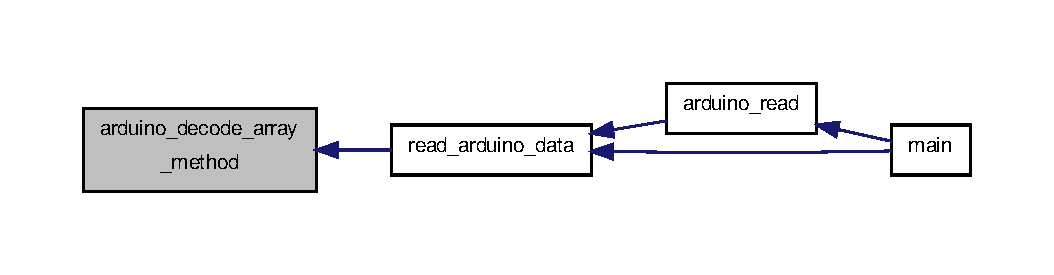
\includegraphics[width=350pt]{arduino__6___u_n_o_8cpp_a48019987fa34c7983be2f709ea7078da_icgraph}
\end{center}
\end{figure}


\hypertarget{arduino__6___u_n_o_8cpp_ae56d0c5a7e54f2b4a377da1936e0def5}{\index{arduino\+\_\+6\+\_\+\+U\+N\+O.\+cpp@{arduino\+\_\+6\+\_\+\+U\+N\+O.\+cpp}!arduino\+\_\+read@{arduino\+\_\+read}}
\index{arduino\+\_\+read@{arduino\+\_\+read}!arduino\+\_\+6\+\_\+\+U\+N\+O.\+cpp@{arduino\+\_\+6\+\_\+\+U\+N\+O.\+cpp}}
\subsubsection[{arduino\+\_\+read}]{\setlength{\rightskip}{0pt plus 5cm}int arduino\+\_\+read (
\begin{DoxyParamCaption}
{}
\end{DoxyParamCaption}
)}}\label{arduino__6___u_n_o_8cpp_ae56d0c5a7e54f2b4a377da1936e0def5}


Voici le graphe d'appel pour cette fonction \+:
\nopagebreak
\begin{figure}[H]
\begin{center}
\leavevmode
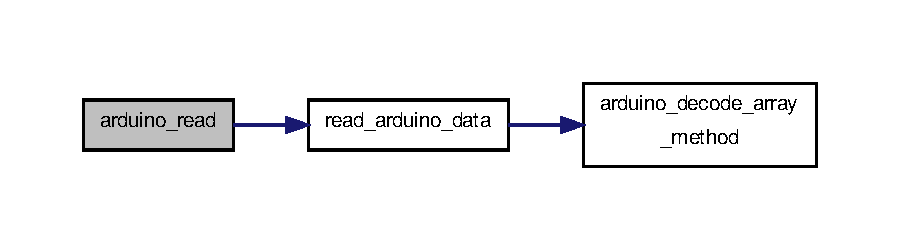
\includegraphics[width=350pt]{arduino__6___u_n_o_8cpp_ae56d0c5a7e54f2b4a377da1936e0def5_cgraph}
\end{center}
\end{figure}




Voici le graphe des appelants de cette fonction \+:
\nopagebreak
\begin{figure}[H]
\begin{center}
\leavevmode
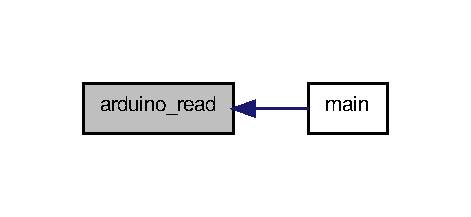
\includegraphics[width=226pt]{arduino__6___u_n_o_8cpp_ae56d0c5a7e54f2b4a377da1936e0def5_icgraph}
\end{center}
\end{figure}


\hypertarget{arduino__6___u_n_o_8cpp_a38905c45209df5be7f35a35d9a4f96db}{\index{arduino\+\_\+6\+\_\+\+U\+N\+O.\+cpp@{arduino\+\_\+6\+\_\+\+U\+N\+O.\+cpp}!do\+\_\+arduino\+\_\+config@{do\+\_\+arduino\+\_\+config}}
\index{do\+\_\+arduino\+\_\+config@{do\+\_\+arduino\+\_\+config}!arduino\+\_\+6\+\_\+\+U\+N\+O.\+cpp@{arduino\+\_\+6\+\_\+\+U\+N\+O.\+cpp}}
\subsubsection[{do\+\_\+arduino\+\_\+config}]{\setlength{\rightskip}{0pt plus 5cm}int do\+\_\+arduino\+\_\+config (
\begin{DoxyParamCaption}
\item[{int}]{cfg\+\_\+\+X, }
\item[{int}]{cfg\+\_\+\+Y}
\end{DoxyParamCaption}
)}}\label{arduino__6___u_n_o_8cpp_a38905c45209df5be7f35a35d9a4f96db}


Voici le graphe d'appel pour cette fonction \+:
\nopagebreak
\begin{figure}[H]
\begin{center}
\leavevmode
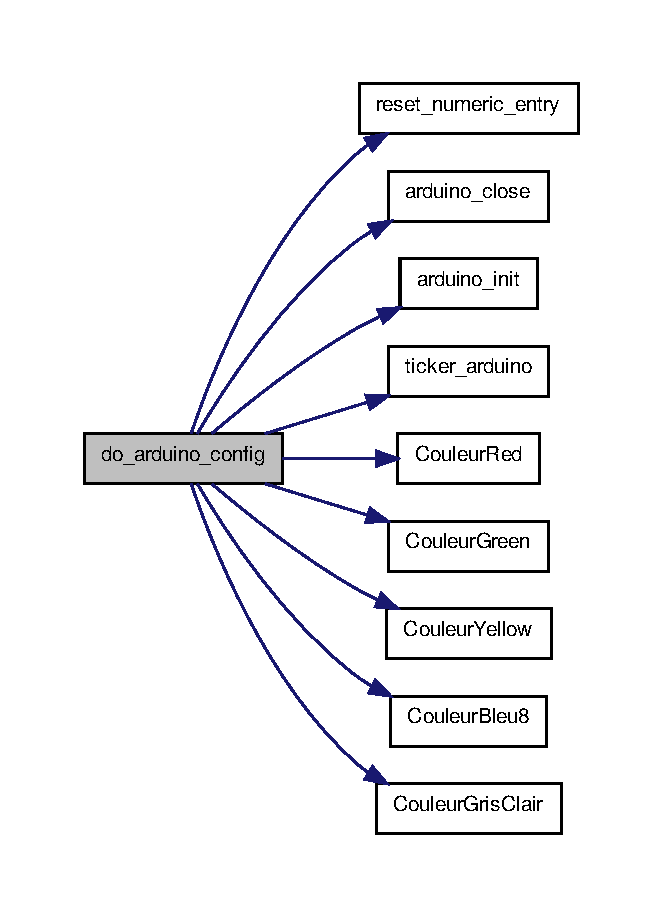
\includegraphics[width=318pt]{arduino__6___u_n_o_8cpp_a38905c45209df5be7f35a35d9a4f96db_cgraph}
\end{center}
\end{figure}




Voici le graphe des appelants de cette fonction \+:
\nopagebreak
\begin{figure}[H]
\begin{center}
\leavevmode
\includegraphics[width=350pt]{arduino__6___u_n_o_8cpp_a38905c45209df5be7f35a35d9a4f96db_icgraph}
\end{center}
\end{figure}


\hypertarget{arduino__6___u_n_o_8cpp_a78f5530dcdcb456d089828f1696d5db2}{\index{arduino\+\_\+6\+\_\+\+U\+N\+O.\+cpp@{arduino\+\_\+6\+\_\+\+U\+N\+O.\+cpp}!read\+\_\+arduino\+\_\+data@{read\+\_\+arduino\+\_\+data}}
\index{read\+\_\+arduino\+\_\+data@{read\+\_\+arduino\+\_\+data}!arduino\+\_\+6\+\_\+\+U\+N\+O.\+cpp@{arduino\+\_\+6\+\_\+\+U\+N\+O.\+cpp}}
\subsubsection[{read\+\_\+arduino\+\_\+data}]{\setlength{\rightskip}{0pt plus 5cm}int read\+\_\+arduino\+\_\+data (
\begin{DoxyParamCaption}
\item[{int}]{device}
\end{DoxyParamCaption}
)}}\label{arduino__6___u_n_o_8cpp_a78f5530dcdcb456d089828f1696d5db2}


Voici le graphe d'appel pour cette fonction \+:
\nopagebreak
\begin{figure}[H]
\begin{center}
\leavevmode
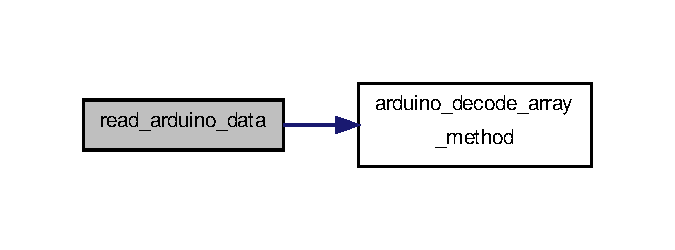
\includegraphics[width=324pt]{arduino__6___u_n_o_8cpp_a78f5530dcdcb456d089828f1696d5db2_cgraph}
\end{center}
\end{figure}




Voici le graphe des appelants de cette fonction \+:
\nopagebreak
\begin{figure}[H]
\begin{center}
\leavevmode
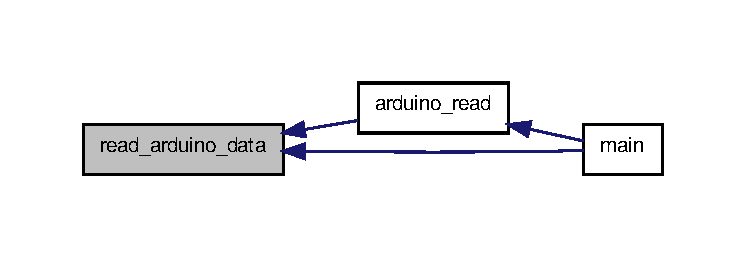
\includegraphics[width=350pt]{arduino__6___u_n_o_8cpp_a78f5530dcdcb456d089828f1696d5db2_icgraph}
\end{center}
\end{figure}



\hypertarget{arduino__core__6___u_n_o_8cpp}{\section{Référence du fichier arduino\+\_\+core\+\_\+6\+\_\+\+U\+N\+O.\+cpp}
\label{arduino__core__6___u_n_o_8cpp}\index{arduino\+\_\+core\+\_\+6\+\_\+\+U\+N\+O.\+cpp@{arduino\+\_\+core\+\_\+6\+\_\+\+U\+N\+O.\+cpp}}
}


\{arduino fonctions\}  


Ce graphe montre quels fichiers incluent directement ou indirectement ce fichier \+:\nopagebreak
\begin{figure}[H]
\begin{center}
\leavevmode
\includegraphics[width=350pt]{arduino__core__6___u_n_o_8cpp__dep__incl}
\end{center}
\end{figure}
\subsection*{Fonctions}
\begin{DoxyCompactItemize}
\item 
void \hyperlink{arduino__core__6___u_n_o_8cpp_a795582d28f2e6944c4c4af55c9a00776}{ticker\+\_\+arduino} ()
\item 
\hyperlink{arduino__core__6___u_n_o_8cpp_ab53dc4bbf9dc5341ca8ff2ef44735beb}{E\+N\+D\+\_\+\+O\+F\+\_\+\+F\+U\+N\+C\+T\+I\+O\+N} (\hyperlink{arduino__core__6___u_n_o_8cpp_a795582d28f2e6944c4c4af55c9a00776}{ticker\+\_\+arduino})
\item 
int \hyperlink{arduino__core__6___u_n_o_8cpp_ae72d1a8d74d9ab5515962e03e7e664d6}{arduino\+\_\+do\+\_\+analog\+\_\+in\+\_\+whitecat} ()
\item 
int \hyperlink{arduino__core__6___u_n_o_8cpp_a219226c1cd6cc17c78e62fd4445bb445}{arduino\+\_\+do\+\_\+digital\+\_\+in\+\_\+whitecat} ()
\item 
int \hyperlink{arduino__core__6___u_n_o_8cpp_aedab05c973a0c437cdce62e3cf65c25c}{arduino\+\_\+do\+\_\+pwm\+\_\+out\+\_\+whitecat} ()
\item 
int \hyperlink{arduino__core__6___u_n_o_8cpp_aea3d65694a3217c452205920f120d1d3}{arduino\+\_\+do\+\_\+digital\+\_\+out\+\_\+whitecat} ()
\item 
int \hyperlink{arduino__core__6___u_n_o_8cpp_ac476a91ba6fb81e7c7e68fc68e59fef4}{arduino\+\_\+\+\_\+send\+\_\+config} ()
\end{DoxyCompactItemize}
\subsection*{Variables}
\begin{DoxyCompactItemize}
\item 
volatile int \hyperlink{arduino__core__6___u_n_o_8cpp_aa51f09a1d02f4c0ac4fe193f86ead0c4}{ticks\+\_\+arduino} =0
\item 
int \hyperlink{arduino__core__6___u_n_o_8cpp_a2e0d87a66de28332b21590d0cecc6235}{old\+\_\+ticks\+\_\+arduino} =0
\end{DoxyCompactItemize}


\subsection{Description détaillée}
\{arduino fonctions\} 

\begin{DoxyAuthor}{Auteur}
Christoph Guillermet, Anton Langhoff 
\end{DoxyAuthor}
\begin{DoxyVersion}{Version}
\{0.\+8.\+6\} 
\end{DoxyVersion}
\begin{DoxyDate}{Date}
\{28/04/2014\}
\end{DoxyDate}
White Cat \{-\/ categorie\} \{-\/ sous categorie \{-\/ sous categorie\}\}

Gestion des fonctions Arduino. recevoir les infos digital de l'arduino recevoir les infos analogue de l'arduino envoyer les infos de sortie P\+W\+M vers l'arduino envoyer les infos de sortie digital vers l'arduino configurer l'arduino automatiquement depuis whitecat avec le sketch arduino whitekitten

Arduino communication fonctions to get digital data in from arduino, get analog data in from arduino, send P\+W\+M output data to the arduino send digital output data to the arduino or configure the arduino in a automatic way from whitecat with the arduino sketch whitekitten 

\subsection{Documentation des fonctions}
\hypertarget{arduino__core__6___u_n_o_8cpp_ac476a91ba6fb81e7c7e68fc68e59fef4}{\index{arduino\+\_\+core\+\_\+6\+\_\+\+U\+N\+O.\+cpp@{arduino\+\_\+core\+\_\+6\+\_\+\+U\+N\+O.\+cpp}!arduino\+\_\+\+\_\+send\+\_\+config@{arduino\+\_\+\+\_\+send\+\_\+config}}
\index{arduino\+\_\+\+\_\+send\+\_\+config@{arduino\+\_\+\+\_\+send\+\_\+config}!arduino\+\_\+core\+\_\+6\+\_\+\+U\+N\+O.\+cpp@{arduino\+\_\+core\+\_\+6\+\_\+\+U\+N\+O.\+cpp}}
\subsubsection[{arduino\+\_\+\+\_\+send\+\_\+config}]{\setlength{\rightskip}{0pt plus 5cm}int arduino\+\_\+\+\_\+send\+\_\+config (
\begin{DoxyParamCaption}
{}
\end{DoxyParamCaption}
)}}\label{arduino__core__6___u_n_o_8cpp_ac476a91ba6fb81e7c7e68fc68e59fef4}


Voici le graphe des appelants de cette fonction \+:\nopagebreak
\begin{figure}[H]
\begin{center}
\leavevmode
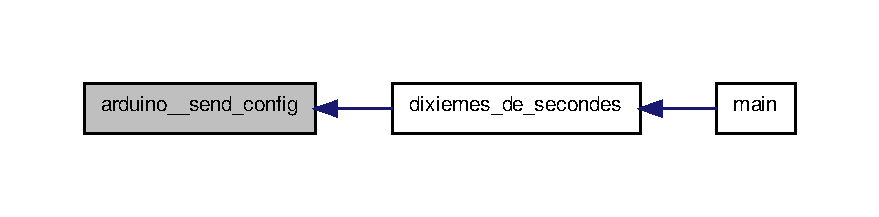
\includegraphics[width=350pt]{arduino__core__6___u_n_o_8cpp_ac476a91ba6fb81e7c7e68fc68e59fef4_icgraph}
\end{center}
\end{figure}


\hypertarget{arduino__core__6___u_n_o_8cpp_ae72d1a8d74d9ab5515962e03e7e664d6}{\index{arduino\+\_\+core\+\_\+6\+\_\+\+U\+N\+O.\+cpp@{arduino\+\_\+core\+\_\+6\+\_\+\+U\+N\+O.\+cpp}!arduino\+\_\+do\+\_\+analog\+\_\+in\+\_\+whitecat@{arduino\+\_\+do\+\_\+analog\+\_\+in\+\_\+whitecat}}
\index{arduino\+\_\+do\+\_\+analog\+\_\+in\+\_\+whitecat@{arduino\+\_\+do\+\_\+analog\+\_\+in\+\_\+whitecat}!arduino\+\_\+core\+\_\+6\+\_\+\+U\+N\+O.\+cpp@{arduino\+\_\+core\+\_\+6\+\_\+\+U\+N\+O.\+cpp}}
\subsubsection[{arduino\+\_\+do\+\_\+analog\+\_\+in\+\_\+whitecat}]{\setlength{\rightskip}{0pt plus 5cm}int arduino\+\_\+do\+\_\+analog\+\_\+in\+\_\+whitecat (
\begin{DoxyParamCaption}
{}
\end{DoxyParamCaption}
)}}\label{arduino__core__6___u_n_o_8cpp_ae72d1a8d74d9ab5515962e03e7e664d6}


Voici le graphe d'appel pour cette fonction \+:\nopagebreak
\begin{figure}[H]
\begin{center}
\leavevmode
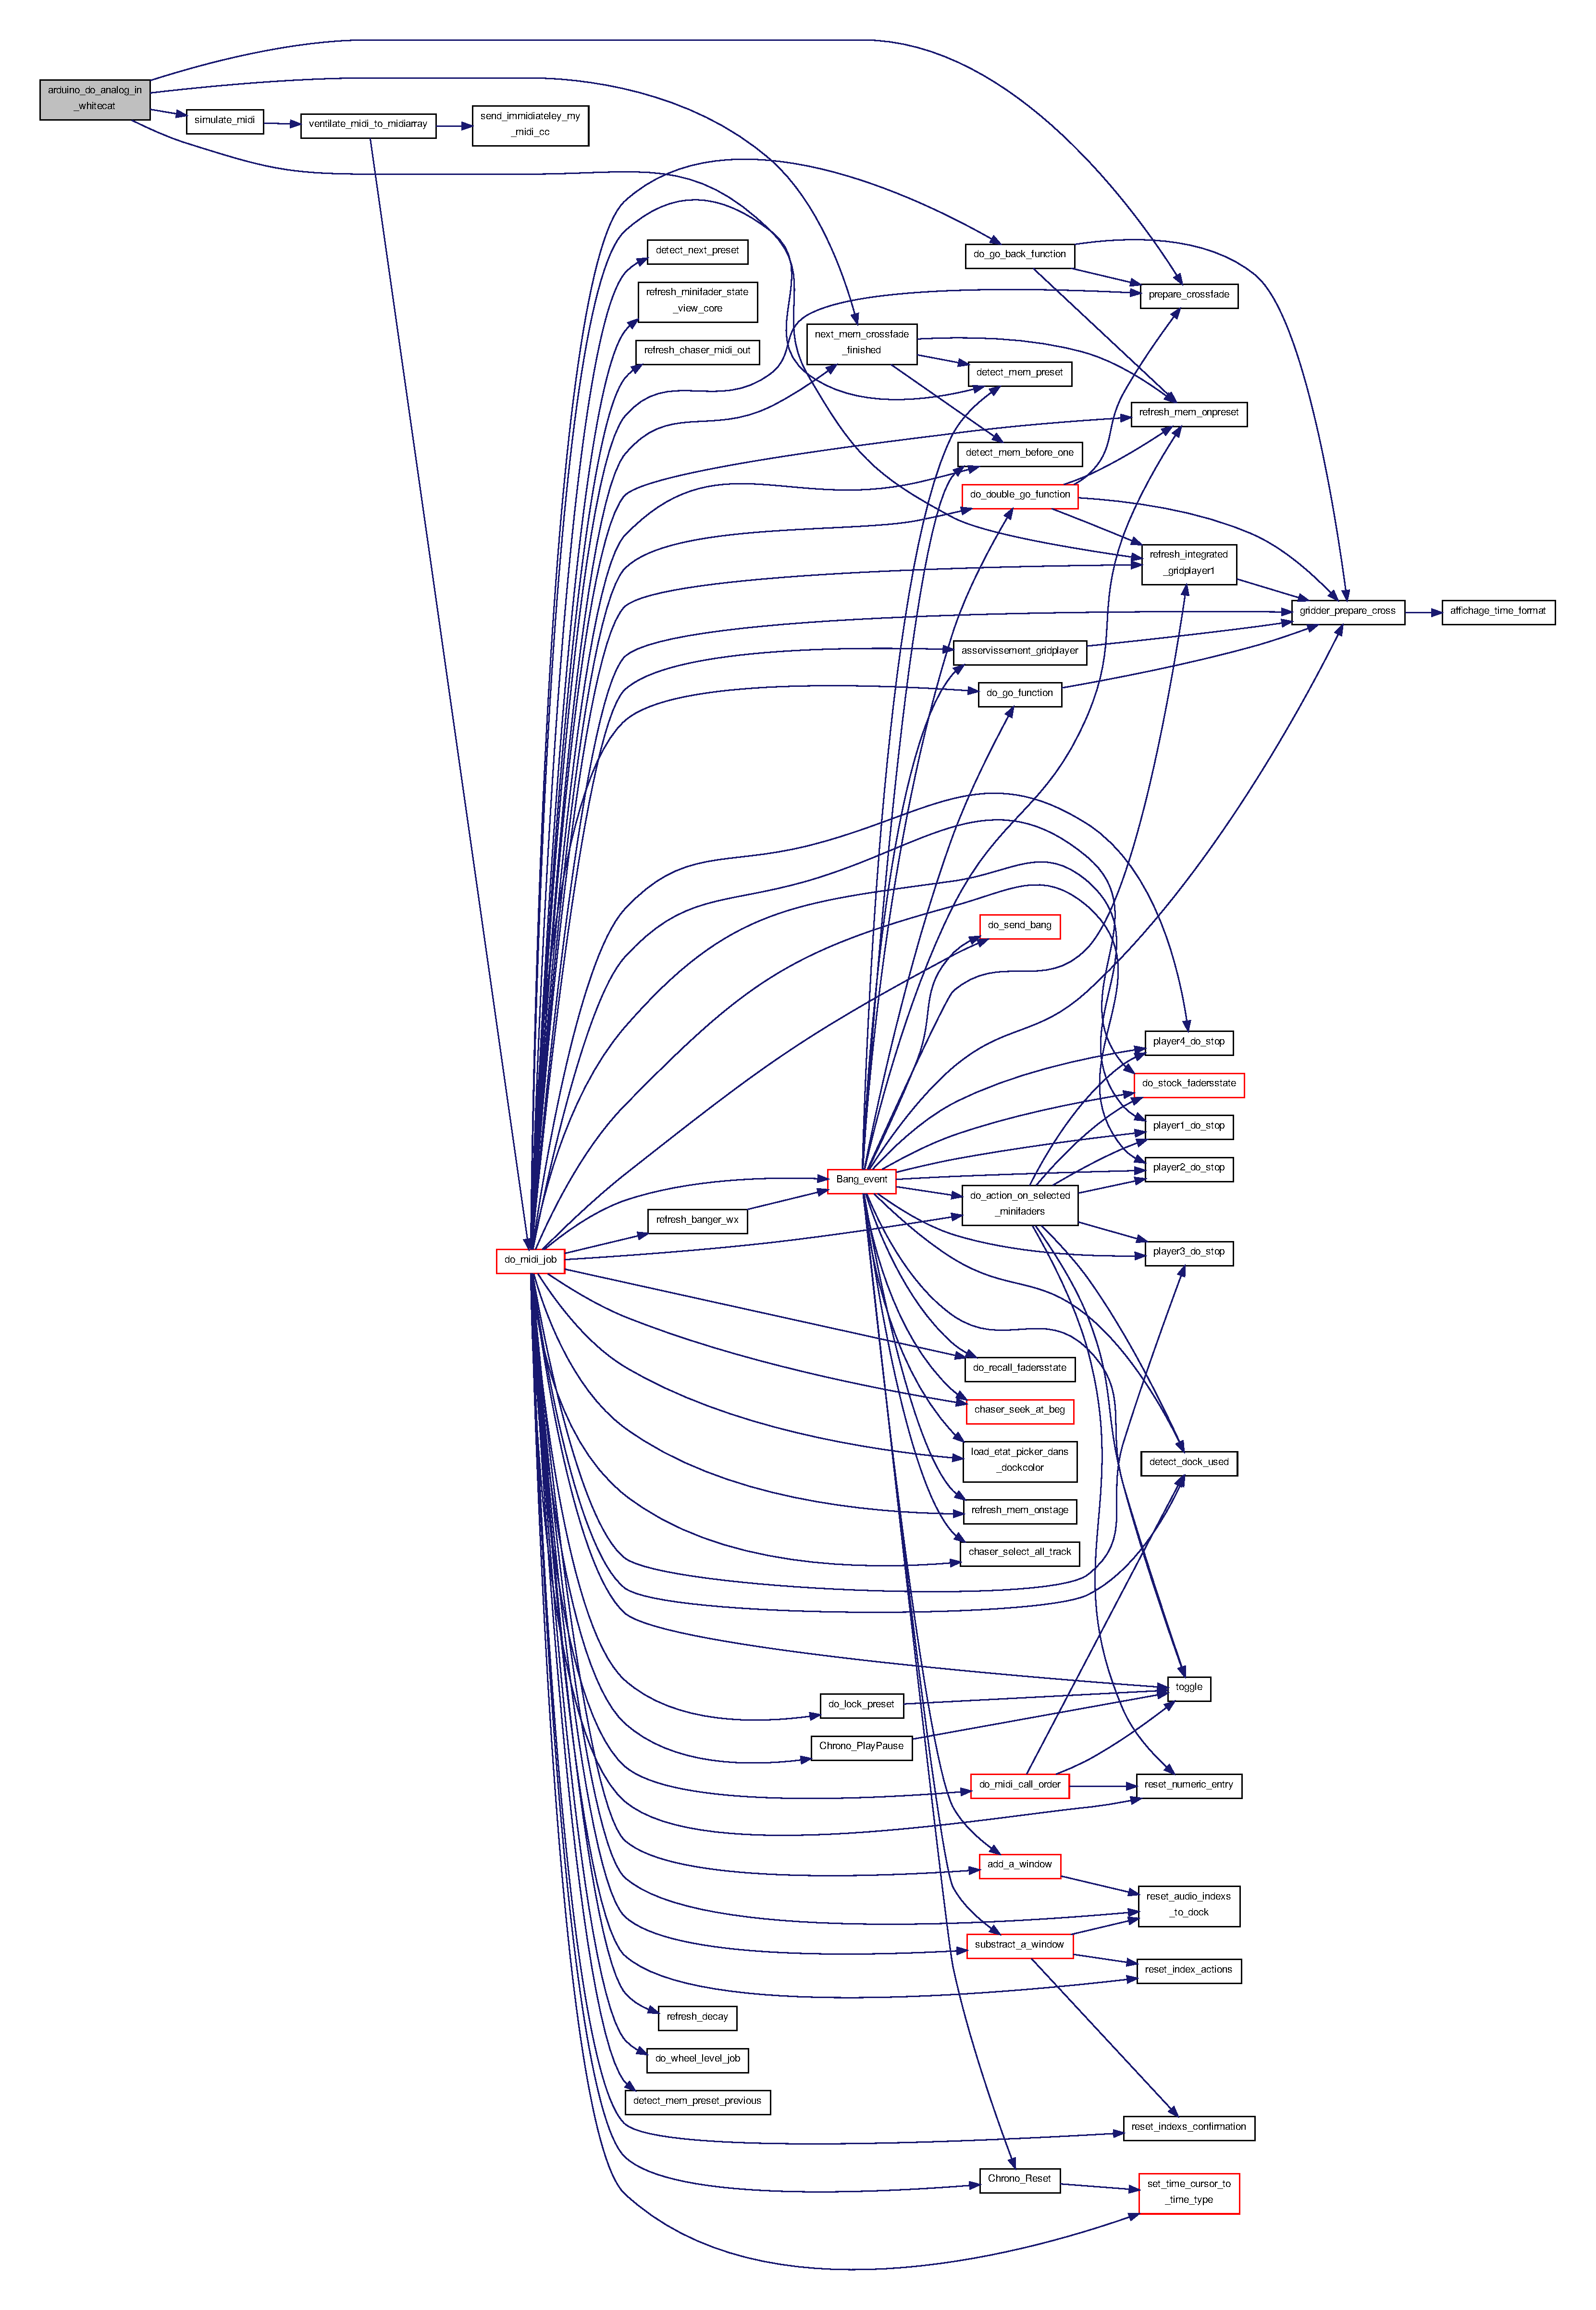
\includegraphics[width=350pt]{arduino__core__6___u_n_o_8cpp_ae72d1a8d74d9ab5515962e03e7e664d6_cgraph}
\end{center}
\end{figure}




Voici le graphe des appelants de cette fonction \+:\nopagebreak
\begin{figure}[H]
\begin{center}
\leavevmode
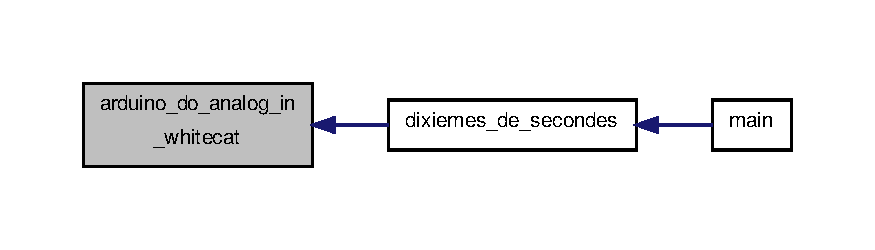
\includegraphics[width=350pt]{arduino__core__6___u_n_o_8cpp_ae72d1a8d74d9ab5515962e03e7e664d6_icgraph}
\end{center}
\end{figure}


\hypertarget{arduino__core__6___u_n_o_8cpp_a219226c1cd6cc17c78e62fd4445bb445}{\index{arduino\+\_\+core\+\_\+6\+\_\+\+U\+N\+O.\+cpp@{arduino\+\_\+core\+\_\+6\+\_\+\+U\+N\+O.\+cpp}!arduino\+\_\+do\+\_\+digital\+\_\+in\+\_\+whitecat@{arduino\+\_\+do\+\_\+digital\+\_\+in\+\_\+whitecat}}
\index{arduino\+\_\+do\+\_\+digital\+\_\+in\+\_\+whitecat@{arduino\+\_\+do\+\_\+digital\+\_\+in\+\_\+whitecat}!arduino\+\_\+core\+\_\+6\+\_\+\+U\+N\+O.\+cpp@{arduino\+\_\+core\+\_\+6\+\_\+\+U\+N\+O.\+cpp}}
\subsubsection[{arduino\+\_\+do\+\_\+digital\+\_\+in\+\_\+whitecat}]{\setlength{\rightskip}{0pt plus 5cm}int arduino\+\_\+do\+\_\+digital\+\_\+in\+\_\+whitecat (
\begin{DoxyParamCaption}
{}
\end{DoxyParamCaption}
)}}\label{arduino__core__6___u_n_o_8cpp_a219226c1cd6cc17c78e62fd4445bb445}


Voici le graphe d'appel pour cette fonction \+:\nopagebreak
\begin{figure}[H]
\begin{center}
\leavevmode
\includegraphics[width=350pt]{arduino__core__6___u_n_o_8cpp_a219226c1cd6cc17c78e62fd4445bb445_cgraph}
\end{center}
\end{figure}




Voici le graphe des appelants de cette fonction \+:\nopagebreak
\begin{figure}[H]
\begin{center}
\leavevmode
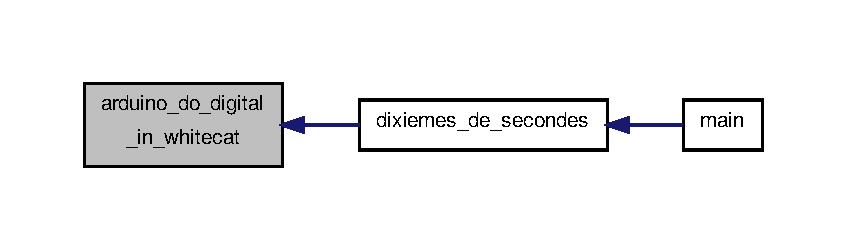
\includegraphics[width=350pt]{arduino__core__6___u_n_o_8cpp_a219226c1cd6cc17c78e62fd4445bb445_icgraph}
\end{center}
\end{figure}


\hypertarget{arduino__core__6___u_n_o_8cpp_aea3d65694a3217c452205920f120d1d3}{\index{arduino\+\_\+core\+\_\+6\+\_\+\+U\+N\+O.\+cpp@{arduino\+\_\+core\+\_\+6\+\_\+\+U\+N\+O.\+cpp}!arduino\+\_\+do\+\_\+digital\+\_\+out\+\_\+whitecat@{arduino\+\_\+do\+\_\+digital\+\_\+out\+\_\+whitecat}}
\index{arduino\+\_\+do\+\_\+digital\+\_\+out\+\_\+whitecat@{arduino\+\_\+do\+\_\+digital\+\_\+out\+\_\+whitecat}!arduino\+\_\+core\+\_\+6\+\_\+\+U\+N\+O.\+cpp@{arduino\+\_\+core\+\_\+6\+\_\+\+U\+N\+O.\+cpp}}
\subsubsection[{arduino\+\_\+do\+\_\+digital\+\_\+out\+\_\+whitecat}]{\setlength{\rightskip}{0pt plus 5cm}int arduino\+\_\+do\+\_\+digital\+\_\+out\+\_\+whitecat (
\begin{DoxyParamCaption}
{}
\end{DoxyParamCaption}
)}}\label{arduino__core__6___u_n_o_8cpp_aea3d65694a3217c452205920f120d1d3}


Voici le graphe des appelants de cette fonction \+:\nopagebreak
\begin{figure}[H]
\begin{center}
\leavevmode
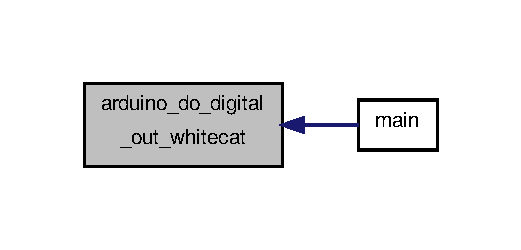
\includegraphics[width=250pt]{arduino__core__6___u_n_o_8cpp_aea3d65694a3217c452205920f120d1d3_icgraph}
\end{center}
\end{figure}


\hypertarget{arduino__core__6___u_n_o_8cpp_aedab05c973a0c437cdce62e3cf65c25c}{\index{arduino\+\_\+core\+\_\+6\+\_\+\+U\+N\+O.\+cpp@{arduino\+\_\+core\+\_\+6\+\_\+\+U\+N\+O.\+cpp}!arduino\+\_\+do\+\_\+pwm\+\_\+out\+\_\+whitecat@{arduino\+\_\+do\+\_\+pwm\+\_\+out\+\_\+whitecat}}
\index{arduino\+\_\+do\+\_\+pwm\+\_\+out\+\_\+whitecat@{arduino\+\_\+do\+\_\+pwm\+\_\+out\+\_\+whitecat}!arduino\+\_\+core\+\_\+6\+\_\+\+U\+N\+O.\+cpp@{arduino\+\_\+core\+\_\+6\+\_\+\+U\+N\+O.\+cpp}}
\subsubsection[{arduino\+\_\+do\+\_\+pwm\+\_\+out\+\_\+whitecat}]{\setlength{\rightskip}{0pt plus 5cm}int arduino\+\_\+do\+\_\+pwm\+\_\+out\+\_\+whitecat (
\begin{DoxyParamCaption}
{}
\end{DoxyParamCaption}
)}}\label{arduino__core__6___u_n_o_8cpp_aedab05c973a0c437cdce62e3cf65c25c}


Voici le graphe des appelants de cette fonction \+:\nopagebreak
\begin{figure}[H]
\begin{center}
\leavevmode
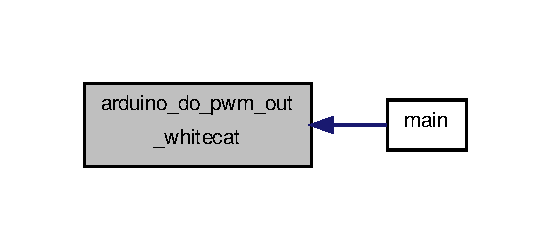
\includegraphics[width=264pt]{arduino__core__6___u_n_o_8cpp_aedab05c973a0c437cdce62e3cf65c25c_icgraph}
\end{center}
\end{figure}


\hypertarget{arduino__core__6___u_n_o_8cpp_ab53dc4bbf9dc5341ca8ff2ef44735beb}{\index{arduino\+\_\+core\+\_\+6\+\_\+\+U\+N\+O.\+cpp@{arduino\+\_\+core\+\_\+6\+\_\+\+U\+N\+O.\+cpp}!E\+N\+D\+\_\+\+O\+F\+\_\+\+F\+U\+N\+C\+T\+I\+O\+N@{E\+N\+D\+\_\+\+O\+F\+\_\+\+F\+U\+N\+C\+T\+I\+O\+N}}
\index{E\+N\+D\+\_\+\+O\+F\+\_\+\+F\+U\+N\+C\+T\+I\+O\+N@{E\+N\+D\+\_\+\+O\+F\+\_\+\+F\+U\+N\+C\+T\+I\+O\+N}!arduino\+\_\+core\+\_\+6\+\_\+\+U\+N\+O.\+cpp@{arduino\+\_\+core\+\_\+6\+\_\+\+U\+N\+O.\+cpp}}
\subsubsection[{E\+N\+D\+\_\+\+O\+F\+\_\+\+F\+U\+N\+C\+T\+I\+O\+N}]{\setlength{\rightskip}{0pt plus 5cm}E\+N\+D\+\_\+\+O\+F\+\_\+\+F\+U\+N\+C\+T\+I\+O\+N (
\begin{DoxyParamCaption}
\item[{{\bf ticker\+\_\+arduino}}]{}
\end{DoxyParamCaption}
)}}\label{arduino__core__6___u_n_o_8cpp_ab53dc4bbf9dc5341ca8ff2ef44735beb}
\hypertarget{arduino__core__6___u_n_o_8cpp_a795582d28f2e6944c4c4af55c9a00776}{\index{arduino\+\_\+core\+\_\+6\+\_\+\+U\+N\+O.\+cpp@{arduino\+\_\+core\+\_\+6\+\_\+\+U\+N\+O.\+cpp}!ticker\+\_\+arduino@{ticker\+\_\+arduino}}
\index{ticker\+\_\+arduino@{ticker\+\_\+arduino}!arduino\+\_\+core\+\_\+6\+\_\+\+U\+N\+O.\+cpp@{arduino\+\_\+core\+\_\+6\+\_\+\+U\+N\+O.\+cpp}}
\subsubsection[{ticker\+\_\+arduino}]{\setlength{\rightskip}{0pt plus 5cm}void ticker\+\_\+arduino (
\begin{DoxyParamCaption}
{}
\end{DoxyParamCaption}
)}}\label{arduino__core__6___u_n_o_8cpp_a795582d28f2e6944c4c4af55c9a00776}


Voici le graphe des appelants de cette fonction \+:\nopagebreak
\begin{figure}[H]
\begin{center}
\leavevmode
\includegraphics[width=350pt]{arduino__core__6___u_n_o_8cpp_a795582d28f2e6944c4c4af55c9a00776_icgraph}
\end{center}
\end{figure}




\subsection{Documentation des variables}
\hypertarget{arduino__core__6___u_n_o_8cpp_a2e0d87a66de28332b21590d0cecc6235}{\index{arduino\+\_\+core\+\_\+6\+\_\+\+U\+N\+O.\+cpp@{arduino\+\_\+core\+\_\+6\+\_\+\+U\+N\+O.\+cpp}!old\+\_\+ticks\+\_\+arduino@{old\+\_\+ticks\+\_\+arduino}}
\index{old\+\_\+ticks\+\_\+arduino@{old\+\_\+ticks\+\_\+arduino}!arduino\+\_\+core\+\_\+6\+\_\+\+U\+N\+O.\+cpp@{arduino\+\_\+core\+\_\+6\+\_\+\+U\+N\+O.\+cpp}}
\subsubsection[{old\+\_\+ticks\+\_\+arduino}]{\setlength{\rightskip}{0pt plus 5cm}int old\+\_\+ticks\+\_\+arduino =0}}\label{arduino__core__6___u_n_o_8cpp_a2e0d87a66de28332b21590d0cecc6235}
\hypertarget{arduino__core__6___u_n_o_8cpp_aa51f09a1d02f4c0ac4fe193f86ead0c4}{\index{arduino\+\_\+core\+\_\+6\+\_\+\+U\+N\+O.\+cpp@{arduino\+\_\+core\+\_\+6\+\_\+\+U\+N\+O.\+cpp}!ticks\+\_\+arduino@{ticks\+\_\+arduino}}
\index{ticks\+\_\+arduino@{ticks\+\_\+arduino}!arduino\+\_\+core\+\_\+6\+\_\+\+U\+N\+O.\+cpp@{arduino\+\_\+core\+\_\+6\+\_\+\+U\+N\+O.\+cpp}}
\subsubsection[{ticks\+\_\+arduino}]{\setlength{\rightskip}{0pt plus 5cm}volatile int ticks\+\_\+arduino =0}}\label{arduino__core__6___u_n_o_8cpp_aa51f09a1d02f4c0ac4fe193f86ead0c4}

\hypertarget{arduino__device__core_8cpp}{\section{Référence du fichier arduino\+\_\+device\+\_\+core.\+cpp}
\label{arduino__device__core_8cpp}\index{arduino\+\_\+device\+\_\+core.\+cpp@{arduino\+\_\+device\+\_\+core.\+cpp}}
}


\{arduino serial open close fonction\}  


{\ttfamily \#include \char`\"{}serial.\+cpp\char`\"{}}\\*
Graphe des dépendances par inclusion de arduino\+\_\+device\+\_\+core.\+cpp\+:
\nopagebreak
\begin{figure}[H]
\begin{center}
\leavevmode
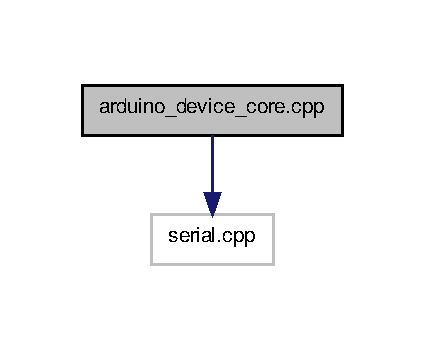
\includegraphics[width=204pt]{arduino__device__core_8cpp__incl}
\end{center}
\end{figure}
Ce graphe montre quels fichiers incluent directement ou indirectement ce fichier \+:
\nopagebreak
\begin{figure}[H]
\begin{center}
\leavevmode
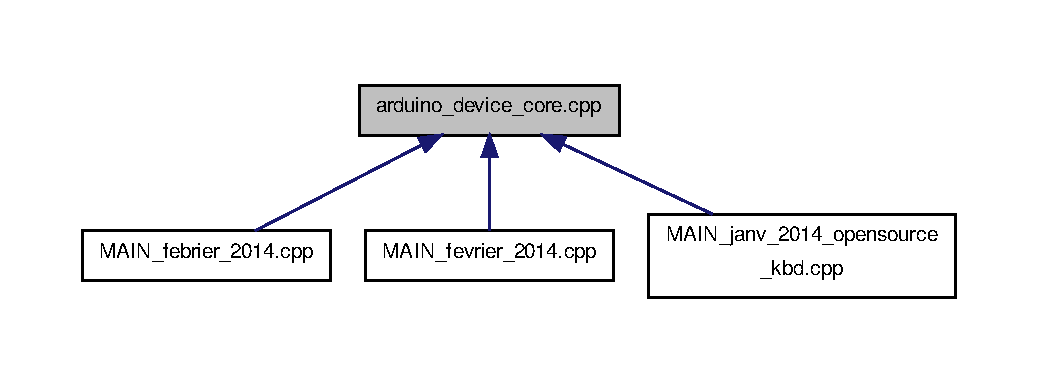
\includegraphics[width=350pt]{arduino__device__core_8cpp__dep__incl}
\end{center}
\end{figure}
\subsection*{Fonctions}
\begin{DoxyCompactItemize}
\item 
int \hyperlink{arduino__device__core_8cpp_adff1caa3b04b7a4e541b2b2624b91d5d}{arduino\+\_\+init} (int \hyperlink{whitecat_8h_a4fda30c89f2eb5ea6e500dbd94ef4eff}{device})
\item 
int \hyperlink{arduino__device__core_8cpp_a61195897dc34314cdf3bf254273460a8}{arduino\+\_\+close} (int \hyperlink{whitecat_8h_a4fda30c89f2eb5ea6e500dbd94ef4eff}{device})
\end{DoxyCompactItemize}
\subsection*{Variables}
\begin{DoxyCompactItemize}
\item 
C\+Serial \hyperlink{arduino__device__core_8cpp_a544d8ec833d2346d2b5223de3cecc901}{serial0}
\end{DoxyCompactItemize}


\subsection{Description détaillée}
\{arduino serial open close fonction\} 

\begin{DoxyAuthor}{Auteur}
Christoph Guillermet, Anton Langhoff 
\end{DoxyAuthor}
\begin{DoxyVersion}{Version}
\{0.\+8.\+5.\+2\} 
\end{DoxyVersion}
\begin{DoxyDate}{Date}
\{19/02/2014\}
\end{DoxyDate}
White Cat \{-\/ categorie\} \{-\/ sous categorie \{-\/ sous categorie\}\}

Gestion des fonctions arduino sur le port série V\+C\+O\+M à travers l'usb pour l'ouverture l'initialistaion et la fermeture du port V\+C\+O\+M

Arduino transfert fonctions to usb via the serial V\+C\+O\+M P\+O\+R\+T for opening the port, close it or initialise it. 

\subsection{Documentation des fonctions}
\hypertarget{arduino__device__core_8cpp_a61195897dc34314cdf3bf254273460a8}{\index{arduino\+\_\+device\+\_\+core.\+cpp@{arduino\+\_\+device\+\_\+core.\+cpp}!arduino\+\_\+close@{arduino\+\_\+close}}
\index{arduino\+\_\+close@{arduino\+\_\+close}!arduino\+\_\+device\+\_\+core.\+cpp@{arduino\+\_\+device\+\_\+core.\+cpp}}
\subsubsection[{arduino\+\_\+close}]{\setlength{\rightskip}{0pt plus 5cm}int arduino\+\_\+close (
\begin{DoxyParamCaption}
\item[{int}]{device}
\end{DoxyParamCaption}
)}}\label{arduino__device__core_8cpp_a61195897dc34314cdf3bf254273460a8}


Voici le graphe des appelants de cette fonction \+:
\nopagebreak
\begin{figure}[H]
\begin{center}
\leavevmode
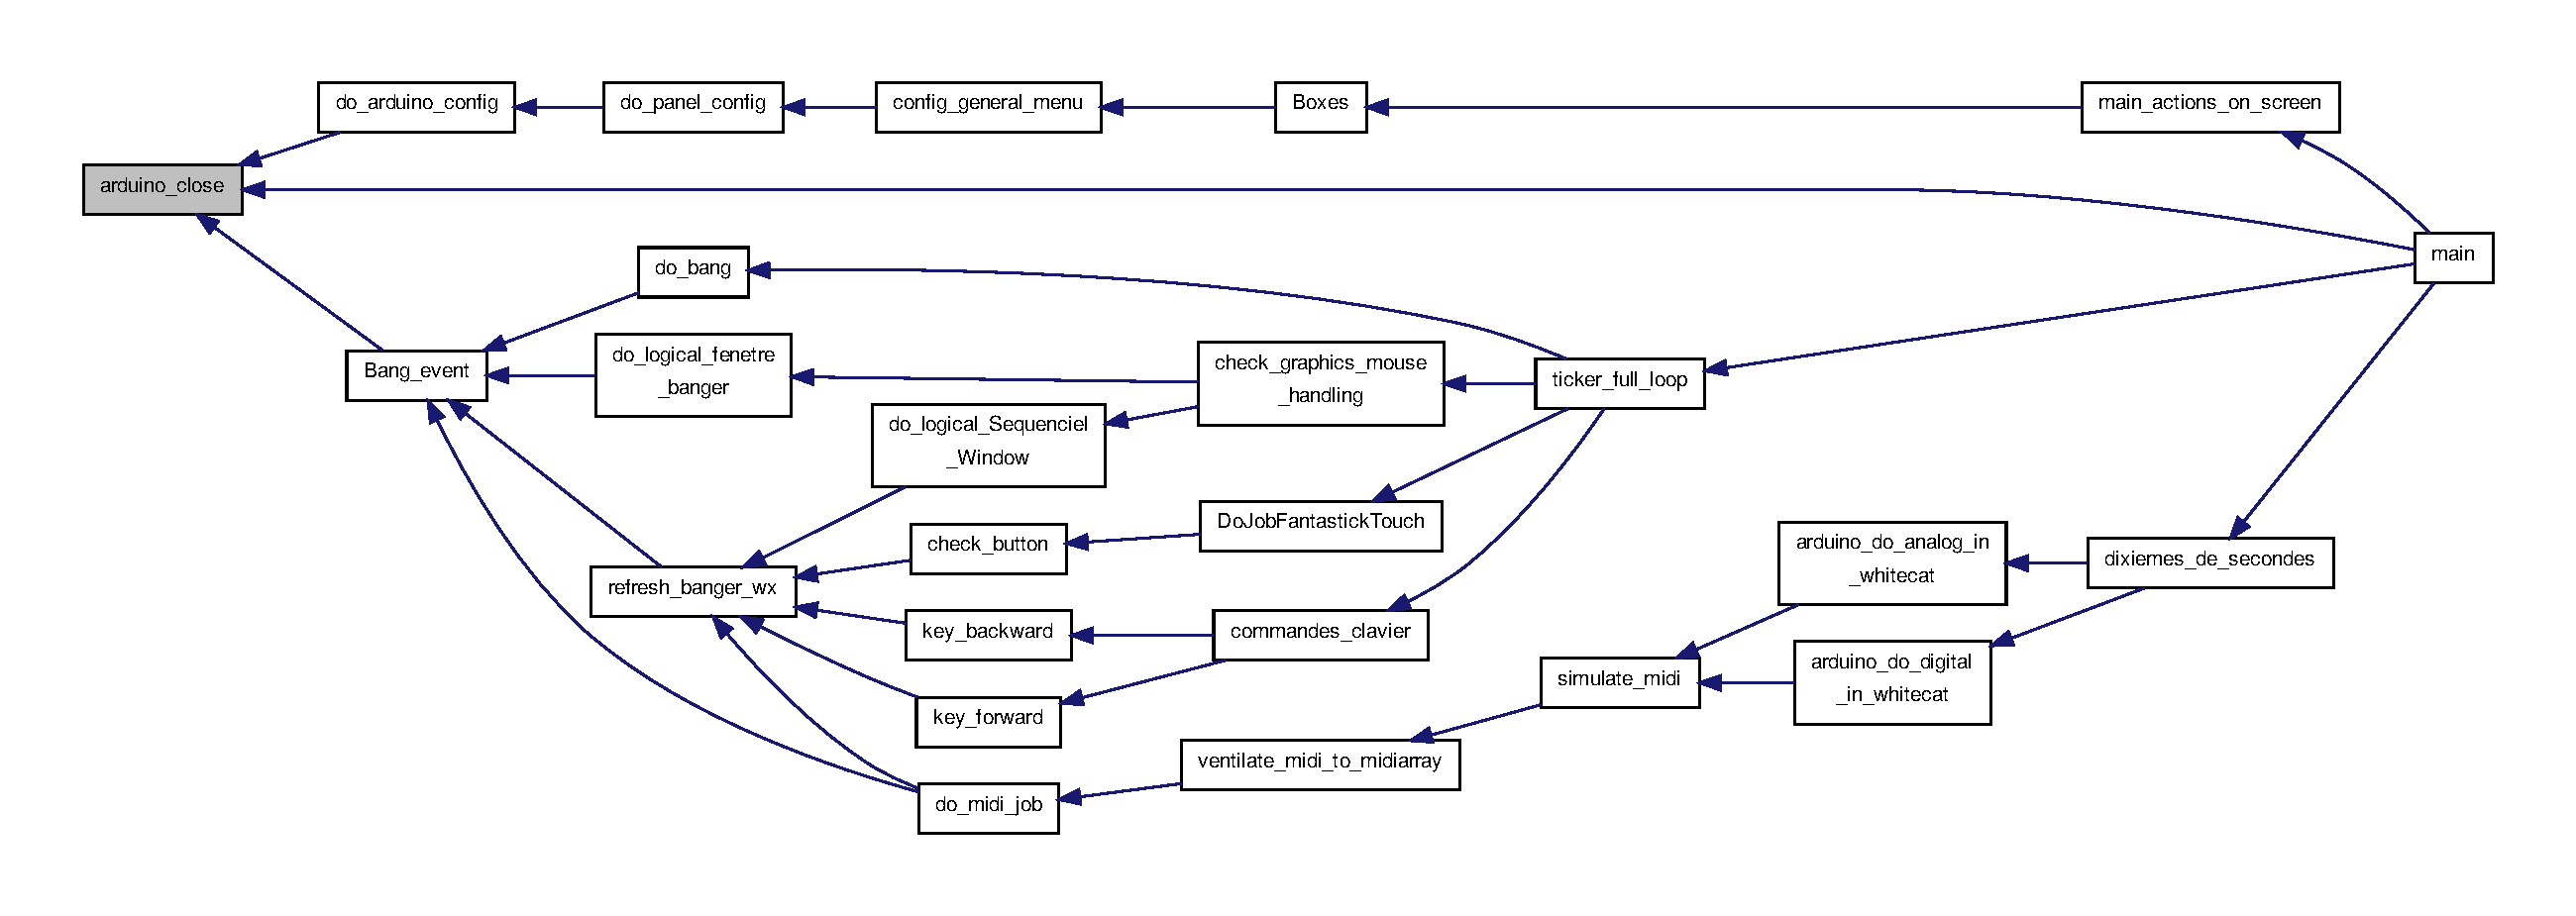
\includegraphics[width=350pt]{arduino__device__core_8cpp_a61195897dc34314cdf3bf254273460a8_icgraph}
\end{center}
\end{figure}


\hypertarget{arduino__device__core_8cpp_adff1caa3b04b7a4e541b2b2624b91d5d}{\index{arduino\+\_\+device\+\_\+core.\+cpp@{arduino\+\_\+device\+\_\+core.\+cpp}!arduino\+\_\+init@{arduino\+\_\+init}}
\index{arduino\+\_\+init@{arduino\+\_\+init}!arduino\+\_\+device\+\_\+core.\+cpp@{arduino\+\_\+device\+\_\+core.\+cpp}}
\subsubsection[{arduino\+\_\+init}]{\setlength{\rightskip}{0pt plus 5cm}int arduino\+\_\+init (
\begin{DoxyParamCaption}
\item[{int}]{device}
\end{DoxyParamCaption}
)}}\label{arduino__device__core_8cpp_adff1caa3b04b7a4e541b2b2624b91d5d}


Voici le graphe des appelants de cette fonction \+:
\nopagebreak
\begin{figure}[H]
\begin{center}
\leavevmode
\includegraphics[width=350pt]{arduino__device__core_8cpp_adff1caa3b04b7a4e541b2b2624b91d5d_icgraph}
\end{center}
\end{figure}




\subsection{Documentation des variables}
\hypertarget{arduino__device__core_8cpp_a544d8ec833d2346d2b5223de3cecc901}{\index{arduino\+\_\+device\+\_\+core.\+cpp@{arduino\+\_\+device\+\_\+core.\+cpp}!serial0@{serial0}}
\index{serial0@{serial0}!arduino\+\_\+device\+\_\+core.\+cpp@{arduino\+\_\+device\+\_\+core.\+cpp}}
\subsubsection[{serial0}]{\setlength{\rightskip}{0pt plus 5cm}C\+Serial serial0}}\label{arduino__device__core_8cpp_a544d8ec833d2346d2b5223de3cecc901}

\hypertarget{audio__core5_8cpp}{\section{Référence du fichier audio\+\_\+core5.\+cpp}
\label{audio__core5_8cpp}\index{audio\+\_\+core5.\+cpp@{audio\+\_\+core5.\+cpp}}
}


\{Audio fonctions\}  


Ce graphe montre quels fichiers incluent directement ou indirectement ce fichier \+:
\nopagebreak
\begin{figure}[H]
\begin{center}
\leavevmode
\includegraphics[width=350pt]{audio__core5_8cpp__dep__incl}
\end{center}
\end{figure}
\subsection*{Fonctions}
\begin{DoxyCompactItemize}
\item 
int \hyperlink{audio__core5_8cpp_a686da0cc1576b2786c51a621d5de86f5}{Load\+\_\+audiofiles\+\_\+cues} ()
\item 
int \hyperlink{audio__core5_8cpp_a441637bcca17a3226a6b3aadea1defe9}{Affect\+Sound\+File} (int player)
\item 
int \hyperlink{audio__core5_8cpp_ae6f8dd1f3de99ac54980667b9baf9ad1}{do\+\_\+audio\+\_\+midi\+\_\+function\+\_\+next\+\_\+prev\+\_\+track} ()
\item 
int \hyperlink{audio__core5_8cpp_a13f7e158754259cb905ce151d53b5d70}{sound\+\_\+core\+\_\+processing} ()
\item 
int \hyperlink{audio__core5_8cpp_a7a2fe6aee0064f868114dc5c2d58df9f}{Control\+\_\+\+Audio\+\_\+thruth\+\_\+faders} (int ff, int dd, int \hyperlink{whitecat_8h_a0dcc0dcc5e66f42b54bc7fa3d59aceec}{typ})
\item 
void \hyperlink{audio__core5_8cpp_a3c08e8ced90a977e4d18c56ec842fe11}{Show\+Supported\+Audio\+Devices} ()
\item 
int \hyperlink{audio__core5_8cpp_a05d0ff746200f59b25fb77e50e7c081f}{Init\+Sound} ()
\item 
int \hyperlink{audio__core5_8cpp_a8b31946eb761c7f981bb92526a3f065a}{do\+\_\+logical\+\_\+fader\+\_\+niveau\+\_\+son} (int xp, int yp, int numero)
\item 
int \hyperlink{audio__core5_8cpp_a657e082e79a514893ab79a019dfa5e5a}{do\+\_\+logical\+\_\+lecteur\+\_\+audio} (int xp, int yp, int numero)
\item 
int \hyperlink{audio__core5_8cpp_a58dbea0caa9eacea9a92dace23de4e32}{do\+\_\+logical\+\_\+fenetre\+\_\+audio} (int xb, int yb)
\end{DoxyCompactItemize}


\subsection{Description détaillée}
\{Audio fonctions\} 

\begin{DoxyAuthor}{Auteur}
Christoph Guillermet 
\end{DoxyAuthor}
\begin{DoxyVersion}{Version}
\{0.\+8.\+6\} 
\end{DoxyVersion}
\begin{DoxyDate}{Date}
\{28/04/2014\}
\end{DoxyDate}
White Cat \{-\/ categorie\} \{-\/ sous categorie \{-\/ sous categorie\}\}

Gestion des fonctions Audio

Audio core fonctions 

\subsection{Documentation des fonctions}
\hypertarget{audio__core5_8cpp_a441637bcca17a3226a6b3aadea1defe9}{\index{audio\+\_\+core5.\+cpp@{audio\+\_\+core5.\+cpp}!Affect\+Sound\+File@{Affect\+Sound\+File}}
\index{Affect\+Sound\+File@{Affect\+Sound\+File}!audio\+\_\+core5.\+cpp@{audio\+\_\+core5.\+cpp}}
\subsubsection[{Affect\+Sound\+File}]{\setlength{\rightskip}{0pt plus 5cm}int Affect\+Sound\+File (
\begin{DoxyParamCaption}
\item[{int}]{player}
\end{DoxyParamCaption}
)}}\label{audio__core5_8cpp_a441637bcca17a3226a6b3aadea1defe9}


Voici le graphe d'appel pour cette fonction \+:
\nopagebreak
\begin{figure}[H]
\begin{center}
\leavevmode
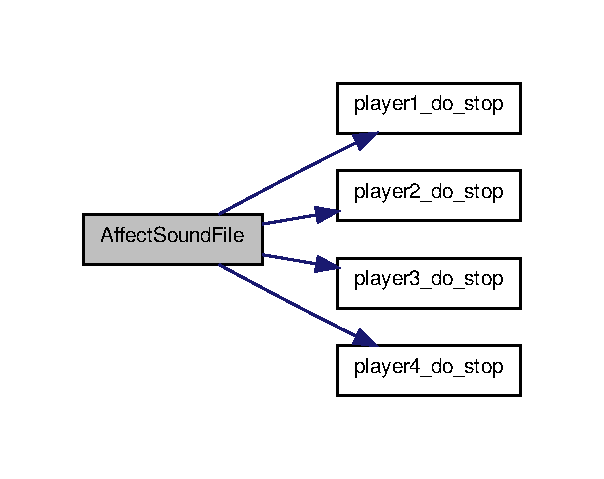
\includegraphics[width=290pt]{audio__core5_8cpp_a441637bcca17a3226a6b3aadea1defe9_cgraph}
\end{center}
\end{figure}




Voici le graphe des appelants de cette fonction \+:
\nopagebreak
\begin{figure}[H]
\begin{center}
\leavevmode
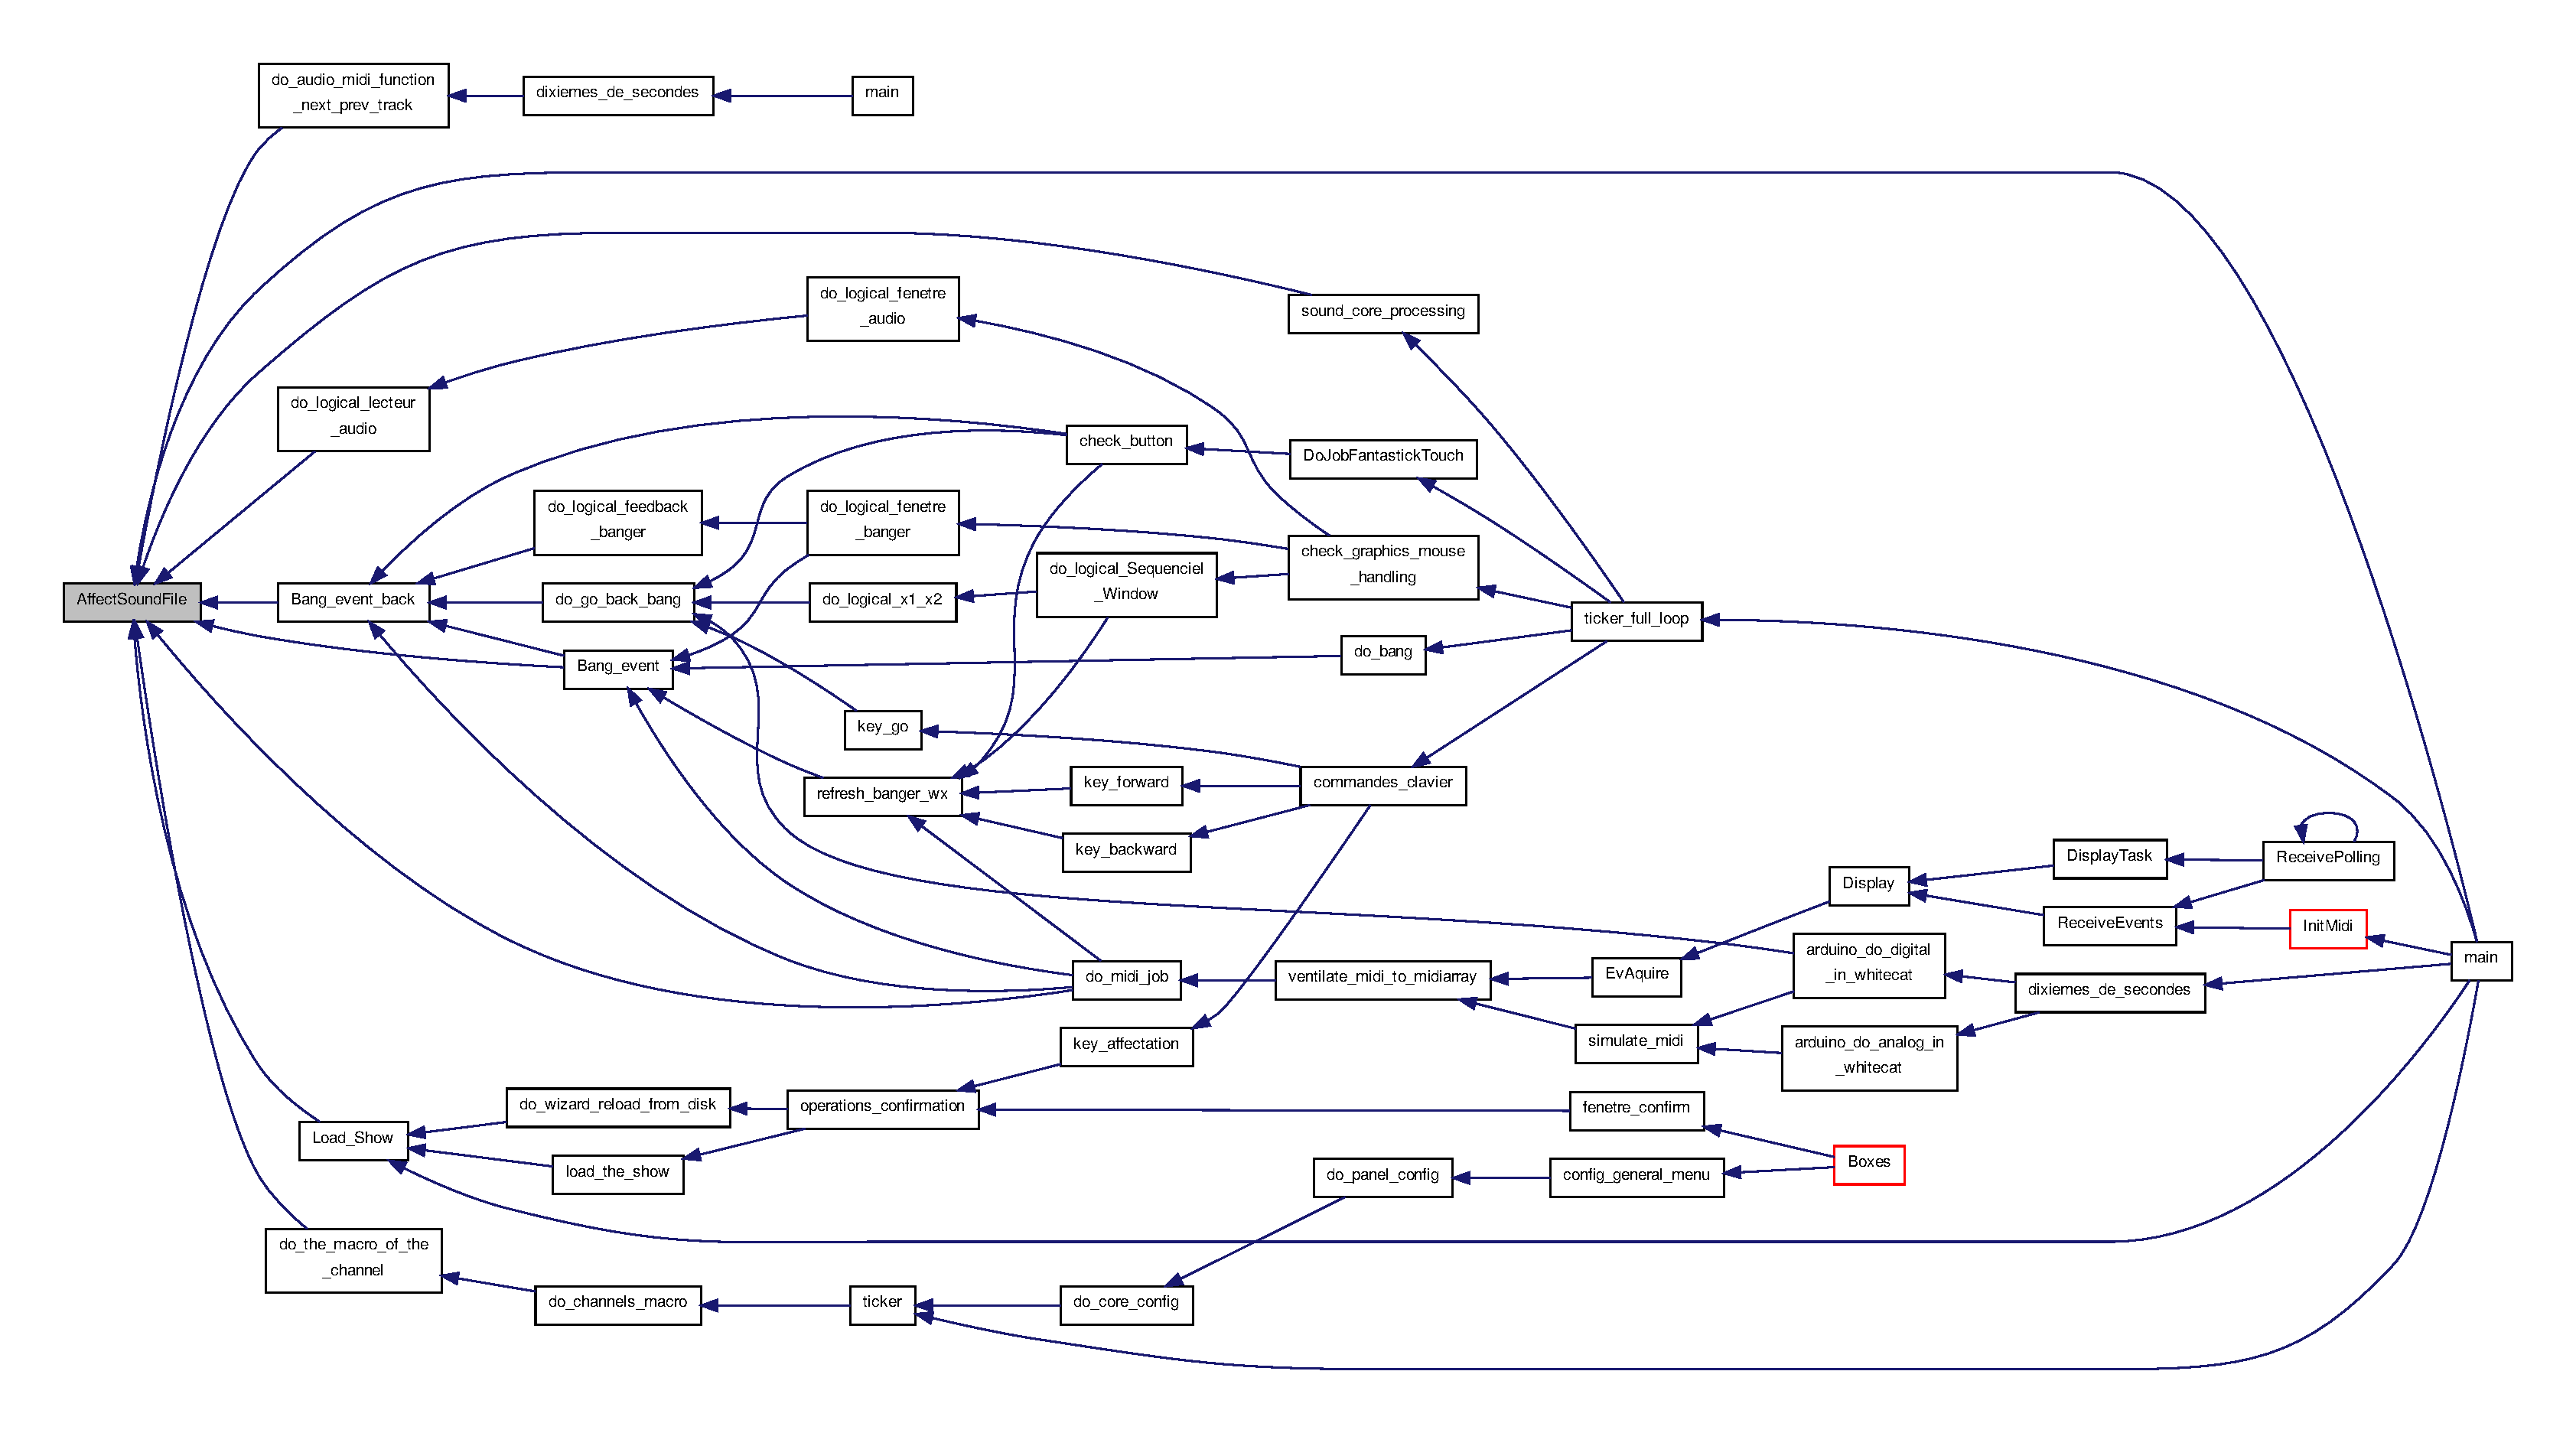
\includegraphics[width=350pt]{audio__core5_8cpp_a441637bcca17a3226a6b3aadea1defe9_icgraph}
\end{center}
\end{figure}


\hypertarget{audio__core5_8cpp_a7a2fe6aee0064f868114dc5c2d58df9f}{\index{audio\+\_\+core5.\+cpp@{audio\+\_\+core5.\+cpp}!Control\+\_\+\+Audio\+\_\+thruth\+\_\+faders@{Control\+\_\+\+Audio\+\_\+thruth\+\_\+faders}}
\index{Control\+\_\+\+Audio\+\_\+thruth\+\_\+faders@{Control\+\_\+\+Audio\+\_\+thruth\+\_\+faders}!audio\+\_\+core5.\+cpp@{audio\+\_\+core5.\+cpp}}
\subsubsection[{Control\+\_\+\+Audio\+\_\+thruth\+\_\+faders}]{\setlength{\rightskip}{0pt plus 5cm}int Control\+\_\+\+Audio\+\_\+thruth\+\_\+faders (
\begin{DoxyParamCaption}
\item[{int}]{ff, }
\item[{int}]{dd, }
\item[{int}]{typ}
\end{DoxyParamCaption}
)}}\label{audio__core5_8cpp_a7a2fe6aee0064f868114dc5c2d58df9f}


Voici le graphe des appelants de cette fonction \+:
\nopagebreak
\begin{figure}[H]
\begin{center}
\leavevmode
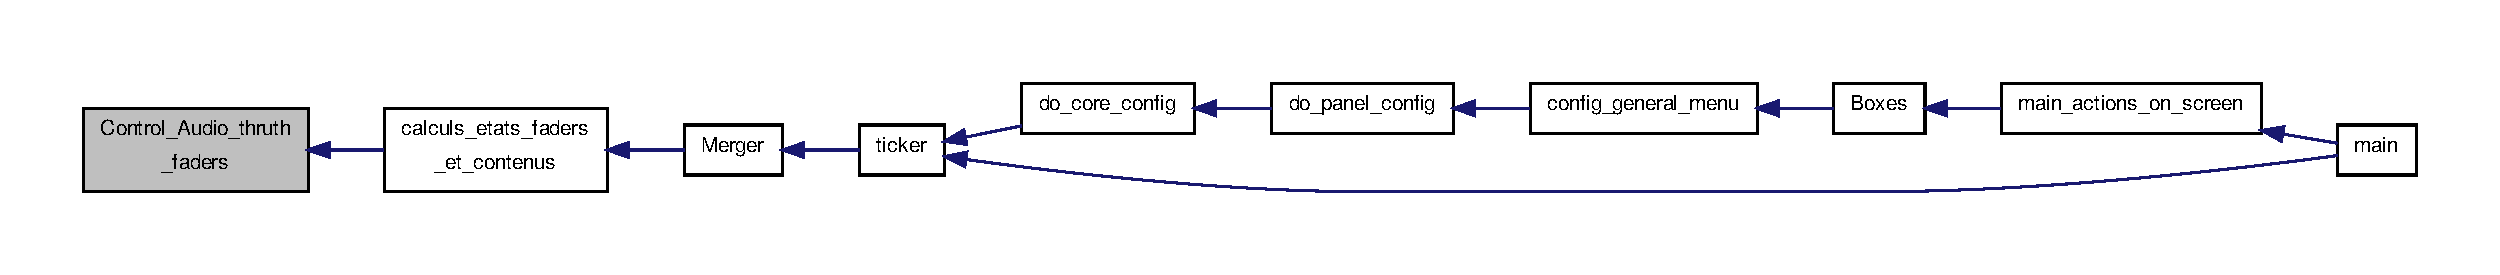
\includegraphics[width=350pt]{audio__core5_8cpp_a7a2fe6aee0064f868114dc5c2d58df9f_icgraph}
\end{center}
\end{figure}


\hypertarget{audio__core5_8cpp_ae6f8dd1f3de99ac54980667b9baf9ad1}{\index{audio\+\_\+core5.\+cpp@{audio\+\_\+core5.\+cpp}!do\+\_\+audio\+\_\+midi\+\_\+function\+\_\+next\+\_\+prev\+\_\+track@{do\+\_\+audio\+\_\+midi\+\_\+function\+\_\+next\+\_\+prev\+\_\+track}}
\index{do\+\_\+audio\+\_\+midi\+\_\+function\+\_\+next\+\_\+prev\+\_\+track@{do\+\_\+audio\+\_\+midi\+\_\+function\+\_\+next\+\_\+prev\+\_\+track}!audio\+\_\+core5.\+cpp@{audio\+\_\+core5.\+cpp}}
\subsubsection[{do\+\_\+audio\+\_\+midi\+\_\+function\+\_\+next\+\_\+prev\+\_\+track}]{\setlength{\rightskip}{0pt plus 5cm}int do\+\_\+audio\+\_\+midi\+\_\+function\+\_\+next\+\_\+prev\+\_\+track (
\begin{DoxyParamCaption}
{}
\end{DoxyParamCaption}
)}}\label{audio__core5_8cpp_ae6f8dd1f3de99ac54980667b9baf9ad1}


Voici le graphe d'appel pour cette fonction \+:
\nopagebreak
\begin{figure}[H]
\begin{center}
\leavevmode
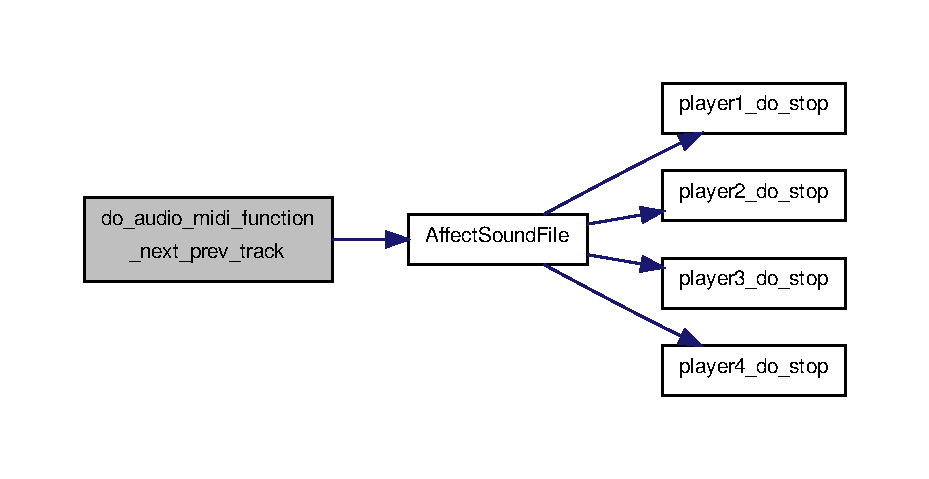
\includegraphics[width=350pt]{audio__core5_8cpp_ae6f8dd1f3de99ac54980667b9baf9ad1_cgraph}
\end{center}
\end{figure}




Voici le graphe des appelants de cette fonction \+:
\nopagebreak
\begin{figure}[H]
\begin{center}
\leavevmode
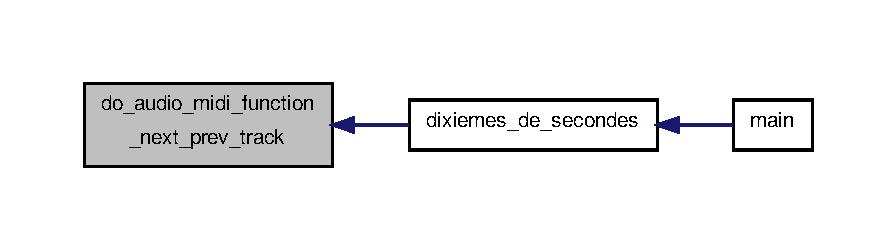
\includegraphics[width=350pt]{audio__core5_8cpp_ae6f8dd1f3de99ac54980667b9baf9ad1_icgraph}
\end{center}
\end{figure}


\hypertarget{audio__core5_8cpp_a8b31946eb761c7f981bb92526a3f065a}{\index{audio\+\_\+core5.\+cpp@{audio\+\_\+core5.\+cpp}!do\+\_\+logical\+\_\+fader\+\_\+niveau\+\_\+son@{do\+\_\+logical\+\_\+fader\+\_\+niveau\+\_\+son}}
\index{do\+\_\+logical\+\_\+fader\+\_\+niveau\+\_\+son@{do\+\_\+logical\+\_\+fader\+\_\+niveau\+\_\+son}!audio\+\_\+core5.\+cpp@{audio\+\_\+core5.\+cpp}}
\subsubsection[{do\+\_\+logical\+\_\+fader\+\_\+niveau\+\_\+son}]{\setlength{\rightskip}{0pt plus 5cm}int do\+\_\+logical\+\_\+fader\+\_\+niveau\+\_\+son (
\begin{DoxyParamCaption}
\item[{int}]{xp, }
\item[{int}]{yp, }
\item[{int}]{numero}
\end{DoxyParamCaption}
)}}\label{audio__core5_8cpp_a8b31946eb761c7f981bb92526a3f065a}


Voici le graphe d'appel pour cette fonction \+:
\nopagebreak
\begin{figure}[H]
\begin{center}
\leavevmode
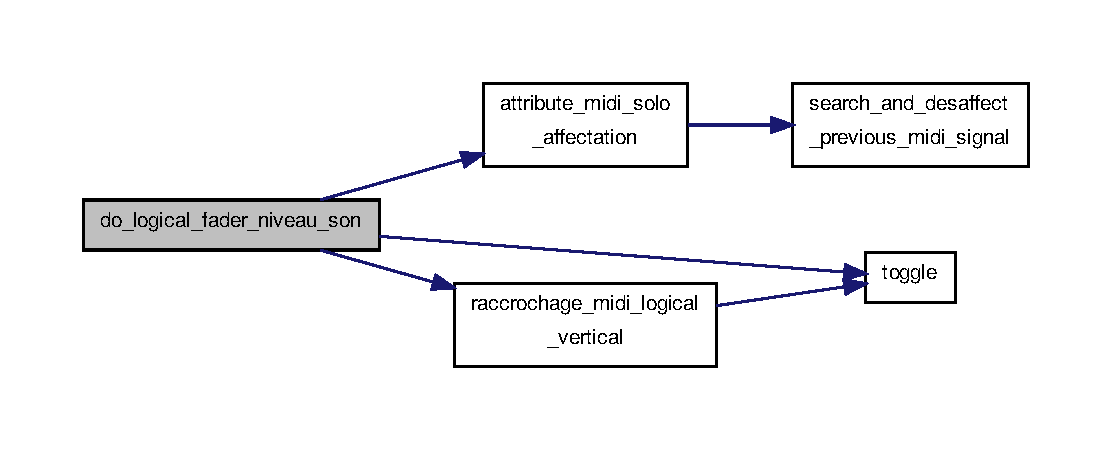
\includegraphics[width=350pt]{audio__core5_8cpp_a8b31946eb761c7f981bb92526a3f065a_cgraph}
\end{center}
\end{figure}




Voici le graphe des appelants de cette fonction \+:
\nopagebreak
\begin{figure}[H]
\begin{center}
\leavevmode
\includegraphics[width=350pt]{audio__core5_8cpp_a8b31946eb761c7f981bb92526a3f065a_icgraph}
\end{center}
\end{figure}


\hypertarget{audio__core5_8cpp_a58dbea0caa9eacea9a92dace23de4e32}{\index{audio\+\_\+core5.\+cpp@{audio\+\_\+core5.\+cpp}!do\+\_\+logical\+\_\+fenetre\+\_\+audio@{do\+\_\+logical\+\_\+fenetre\+\_\+audio}}
\index{do\+\_\+logical\+\_\+fenetre\+\_\+audio@{do\+\_\+logical\+\_\+fenetre\+\_\+audio}!audio\+\_\+core5.\+cpp@{audio\+\_\+core5.\+cpp}}
\subsubsection[{do\+\_\+logical\+\_\+fenetre\+\_\+audio}]{\setlength{\rightskip}{0pt plus 5cm}int do\+\_\+logical\+\_\+fenetre\+\_\+audio (
\begin{DoxyParamCaption}
\item[{int}]{xb, }
\item[{int}]{yb}
\end{DoxyParamCaption}
)}}\label{audio__core5_8cpp_a58dbea0caa9eacea9a92dace23de4e32}


Voici le graphe d'appel pour cette fonction \+:
\nopagebreak
\begin{figure}[H]
\begin{center}
\leavevmode
\includegraphics[width=350pt]{audio__core5_8cpp_a58dbea0caa9eacea9a92dace23de4e32_cgraph}
\end{center}
\end{figure}




Voici le graphe des appelants de cette fonction \+:
\nopagebreak
\begin{figure}[H]
\begin{center}
\leavevmode
\includegraphics[width=350pt]{audio__core5_8cpp_a58dbea0caa9eacea9a92dace23de4e32_icgraph}
\end{center}
\end{figure}


\hypertarget{audio__core5_8cpp_a657e082e79a514893ab79a019dfa5e5a}{\index{audio\+\_\+core5.\+cpp@{audio\+\_\+core5.\+cpp}!do\+\_\+logical\+\_\+lecteur\+\_\+audio@{do\+\_\+logical\+\_\+lecteur\+\_\+audio}}
\index{do\+\_\+logical\+\_\+lecteur\+\_\+audio@{do\+\_\+logical\+\_\+lecteur\+\_\+audio}!audio\+\_\+core5.\+cpp@{audio\+\_\+core5.\+cpp}}
\subsubsection[{do\+\_\+logical\+\_\+lecteur\+\_\+audio}]{\setlength{\rightskip}{0pt plus 5cm}int do\+\_\+logical\+\_\+lecteur\+\_\+audio (
\begin{DoxyParamCaption}
\item[{int}]{xp, }
\item[{int}]{yp, }
\item[{int}]{numero}
\end{DoxyParamCaption}
)}}\label{audio__core5_8cpp_a657e082e79a514893ab79a019dfa5e5a}
seek to end 

Voici le graphe d'appel pour cette fonction \+:
\nopagebreak
\begin{figure}[H]
\begin{center}
\leavevmode
\includegraphics[width=350pt]{audio__core5_8cpp_a657e082e79a514893ab79a019dfa5e5a_cgraph}
\end{center}
\end{figure}




Voici le graphe des appelants de cette fonction \+:
\nopagebreak
\begin{figure}[H]
\begin{center}
\leavevmode
\includegraphics[width=350pt]{audio__core5_8cpp_a657e082e79a514893ab79a019dfa5e5a_icgraph}
\end{center}
\end{figure}


\hypertarget{audio__core5_8cpp_a05d0ff746200f59b25fb77e50e7c081f}{\index{audio\+\_\+core5.\+cpp@{audio\+\_\+core5.\+cpp}!Init\+Sound@{Init\+Sound}}
\index{Init\+Sound@{Init\+Sound}!audio\+\_\+core5.\+cpp@{audio\+\_\+core5.\+cpp}}
\subsubsection[{Init\+Sound}]{\setlength{\rightskip}{0pt plus 5cm}int Init\+Sound (
\begin{DoxyParamCaption}
{}
\end{DoxyParamCaption}
)}}\label{audio__core5_8cpp_a05d0ff746200f59b25fb77e50e7c081f}


Voici le graphe d'appel pour cette fonction \+:
\nopagebreak
\begin{figure}[H]
\begin{center}
\leavevmode
\includegraphics[width=320pt]{audio__core5_8cpp_a05d0ff746200f59b25fb77e50e7c081f_cgraph}
\end{center}
\end{figure}




Voici le graphe des appelants de cette fonction \+:
\nopagebreak
\begin{figure}[H]
\begin{center}
\leavevmode
\includegraphics[width=212pt]{audio__core5_8cpp_a05d0ff746200f59b25fb77e50e7c081f_icgraph}
\end{center}
\end{figure}


\hypertarget{audio__core5_8cpp_a686da0cc1576b2786c51a621d5de86f5}{\index{audio\+\_\+core5.\+cpp@{audio\+\_\+core5.\+cpp}!Load\+\_\+audiofiles\+\_\+cues@{Load\+\_\+audiofiles\+\_\+cues}}
\index{Load\+\_\+audiofiles\+\_\+cues@{Load\+\_\+audiofiles\+\_\+cues}!audio\+\_\+core5.\+cpp@{audio\+\_\+core5.\+cpp}}
\subsubsection[{Load\+\_\+audiofiles\+\_\+cues}]{\setlength{\rightskip}{0pt plus 5cm}int Load\+\_\+audiofiles\+\_\+cues (
\begin{DoxyParamCaption}
{}
\end{DoxyParamCaption}
)}}\label{audio__core5_8cpp_a686da0cc1576b2786c51a621d5de86f5}


Voici le graphe des appelants de cette fonction \+:
\nopagebreak
\begin{figure}[H]
\begin{center}
\leavevmode
\includegraphics[width=350pt]{audio__core5_8cpp_a686da0cc1576b2786c51a621d5de86f5_icgraph}
\end{center}
\end{figure}


\hypertarget{audio__core5_8cpp_a3c08e8ced90a977e4d18c56ec842fe11}{\index{audio\+\_\+core5.\+cpp@{audio\+\_\+core5.\+cpp}!Show\+Supported\+Audio\+Devices@{Show\+Supported\+Audio\+Devices}}
\index{Show\+Supported\+Audio\+Devices@{Show\+Supported\+Audio\+Devices}!audio\+\_\+core5.\+cpp@{audio\+\_\+core5.\+cpp}}
\subsubsection[{Show\+Supported\+Audio\+Devices}]{\setlength{\rightskip}{0pt plus 5cm}void Show\+Supported\+Audio\+Devices (
\begin{DoxyParamCaption}
{}
\end{DoxyParamCaption}
)}}\label{audio__core5_8cpp_a3c08e8ced90a977e4d18c56ec842fe11}


Voici le graphe des appelants de cette fonction \+:
\nopagebreak
\begin{figure}[H]
\begin{center}
\leavevmode
\includegraphics[width=350pt]{audio__core5_8cpp_a3c08e8ced90a977e4d18c56ec842fe11_icgraph}
\end{center}
\end{figure}


\hypertarget{audio__core5_8cpp_a13f7e158754259cb905ce151d53b5d70}{\index{audio\+\_\+core5.\+cpp@{audio\+\_\+core5.\+cpp}!sound\+\_\+core\+\_\+processing@{sound\+\_\+core\+\_\+processing}}
\index{sound\+\_\+core\+\_\+processing@{sound\+\_\+core\+\_\+processing}!audio\+\_\+core5.\+cpp@{audio\+\_\+core5.\+cpp}}
\subsubsection[{sound\+\_\+core\+\_\+processing}]{\setlength{\rightskip}{0pt plus 5cm}int sound\+\_\+core\+\_\+processing (
\begin{DoxyParamCaption}
{}
\end{DoxyParamCaption}
)}}\label{audio__core5_8cpp_a13f7e158754259cb905ce151d53b5d70}


Voici le graphe d'appel pour cette fonction \+:
\nopagebreak
\begin{figure}[H]
\begin{center}
\leavevmode
\includegraphics[width=350pt]{audio__core5_8cpp_a13f7e158754259cb905ce151d53b5d70_cgraph}
\end{center}
\end{figure}




Voici le graphe des appelants de cette fonction \+:
\nopagebreak
\begin{figure}[H]
\begin{center}
\leavevmode
\includegraphics[width=350pt]{audio__core5_8cpp_a13f7e158754259cb905ce151d53b5d70_icgraph}
\end{center}
\end{figure}



\hypertarget{audio__visu4_8cpp}{\section{Référence du fichier audio\+\_\+visu4.\+cpp}
\label{audio__visu4_8cpp}\index{audio\+\_\+visu4.\+cpp@{audio\+\_\+visu4.\+cpp}}
}


\{Audio G\+U\+I fonctions\}  


Ce graphe montre quels fichiers incluent directement ou indirectement ce fichier \+:
\nopagebreak
\begin{figure}[H]
\begin{center}
\leavevmode
\includegraphics[width=350pt]{audio__visu4_8cpp__dep__incl}
\end{center}
\end{figure}
\subsection*{Fonctions}
\begin{DoxyCompactItemize}
\item 
int \hyperlink{audio__visu4_8cpp_a0b5439162e79825e703858743cab3d1d}{fader\+\_\+niveau\+\_\+son} (int xp, int yp, int numero)
\item 
int \hyperlink{audio__visu4_8cpp_af23f016b2fea8ee1404ad97bbda9853c}{lecteur\+\_\+audio} (int xp, int yp, int numero)
\item 
int \hyperlink{audio__visu4_8cpp_a839f8a050c93200c75b01047fd4f6d09}{fenetre\+\_\+audio} (int xb, int yb)
\end{DoxyCompactItemize}


\subsection{Description détaillée}
\{Audio G\+U\+I fonctions\} 

\begin{DoxyAuthor}{Auteur}
Christoph Guillermet 
\end{DoxyAuthor}
\begin{DoxyVersion}{Version}
\{0.\+8.\+6\} 
\end{DoxyVersion}
\begin{DoxyDate}{Date}
\{28/04/2014\}
\end{DoxyDate}
White Cat \{-\/ categorie\} \{-\/ sous categorie \{-\/ sous categorie\}\}

Gestion des fonctions de la fenetre Audio

Audio G\+U\+I fonctions 

\subsection{Documentation des fonctions}
\hypertarget{audio__visu4_8cpp_a0b5439162e79825e703858743cab3d1d}{\index{audio\+\_\+visu4.\+cpp@{audio\+\_\+visu4.\+cpp}!fader\+\_\+niveau\+\_\+son@{fader\+\_\+niveau\+\_\+son}}
\index{fader\+\_\+niveau\+\_\+son@{fader\+\_\+niveau\+\_\+son}!audio\+\_\+visu4.\+cpp@{audio\+\_\+visu4.\+cpp}}
\subsubsection[{fader\+\_\+niveau\+\_\+son}]{\setlength{\rightskip}{0pt plus 5cm}int fader\+\_\+niveau\+\_\+son (
\begin{DoxyParamCaption}
\item[{int}]{xp, }
\item[{int}]{yp, }
\item[{int}]{numero}
\end{DoxyParamCaption}
)}}\label{audio__visu4_8cpp_a0b5439162e79825e703858743cab3d1d}


Voici le graphe d'appel pour cette fonction \+:
\nopagebreak
\begin{figure}[H]
\begin{center}
\leavevmode
\includegraphics[width=334pt]{audio__visu4_8cpp_a0b5439162e79825e703858743cab3d1d_cgraph}
\end{center}
\end{figure}




Voici le graphe des appelants de cette fonction \+:
\nopagebreak
\begin{figure}[H]
\begin{center}
\leavevmode
\includegraphics[width=350pt]{audio__visu4_8cpp_a0b5439162e79825e703858743cab3d1d_icgraph}
\end{center}
\end{figure}


\hypertarget{audio__visu4_8cpp_a839f8a050c93200c75b01047fd4f6d09}{\index{audio\+\_\+visu4.\+cpp@{audio\+\_\+visu4.\+cpp}!fenetre\+\_\+audio@{fenetre\+\_\+audio}}
\index{fenetre\+\_\+audio@{fenetre\+\_\+audio}!audio\+\_\+visu4.\+cpp@{audio\+\_\+visu4.\+cpp}}
\subsubsection[{fenetre\+\_\+audio}]{\setlength{\rightskip}{0pt plus 5cm}int fenetre\+\_\+audio (
\begin{DoxyParamCaption}
\item[{int}]{xb, }
\item[{int}]{yb}
\end{DoxyParamCaption}
)}}\label{audio__visu4_8cpp_a839f8a050c93200c75b01047fd4f6d09}


Voici le graphe d'appel pour cette fonction \+:
\nopagebreak
\begin{figure}[H]
\begin{center}
\leavevmode
\includegraphics[width=350pt]{audio__visu4_8cpp_a839f8a050c93200c75b01047fd4f6d09_cgraph}
\end{center}
\end{figure}




Voici le graphe des appelants de cette fonction \+:
\nopagebreak
\begin{figure}[H]
\begin{center}
\leavevmode
\includegraphics[width=350pt]{audio__visu4_8cpp_a839f8a050c93200c75b01047fd4f6d09_icgraph}
\end{center}
\end{figure}


\hypertarget{audio__visu4_8cpp_af23f016b2fea8ee1404ad97bbda9853c}{\index{audio\+\_\+visu4.\+cpp@{audio\+\_\+visu4.\+cpp}!lecteur\+\_\+audio@{lecteur\+\_\+audio}}
\index{lecteur\+\_\+audio@{lecteur\+\_\+audio}!audio\+\_\+visu4.\+cpp@{audio\+\_\+visu4.\+cpp}}
\subsubsection[{lecteur\+\_\+audio}]{\setlength{\rightskip}{0pt plus 5cm}int lecteur\+\_\+audio (
\begin{DoxyParamCaption}
\item[{int}]{xp, }
\item[{int}]{yp, }
\item[{int}]{numero}
\end{DoxyParamCaption}
)}}\label{audio__visu4_8cpp_af23f016b2fea8ee1404ad97bbda9853c}


Voici le graphe d'appel pour cette fonction \+:
\nopagebreak
\begin{figure}[H]
\begin{center}
\leavevmode
\includegraphics[width=350pt]{audio__visu4_8cpp_af23f016b2fea8ee1404ad97bbda9853c_cgraph}
\end{center}
\end{figure}




Voici le graphe des appelants de cette fonction \+:
\nopagebreak
\begin{figure}[H]
\begin{center}
\leavevmode
\includegraphics[width=350pt]{audio__visu4_8cpp_af23f016b2fea8ee1404ad97bbda9853c_icgraph}
\end{center}
\end{figure}



\hypertarget{banger__core__8_8cpp}{\section{Référence du fichier banger\+\_\+core\+\_\+8.\+cpp}
\label{banger__core__8_8cpp}\index{banger\+\_\+core\+\_\+8.\+cpp@{banger\+\_\+core\+\_\+8.\+cpp}}
}


\{Bangers fonctions\}  


Ce graphe montre quels fichiers incluent directement ou indirectement ce fichier \+:\nopagebreak
\begin{figure}[H]
\begin{center}
\leavevmode
\includegraphics[width=350pt]{banger__core__8_8cpp__dep__incl}
\end{center}
\end{figure}
\subsection*{Fonctions}
\begin{DoxyCompactItemize}
\item 
int \hyperlink{banger__core__8_8cpp_a9615c6c17d4bd54d959e0d9b85a0ff77}{Chrono\+\_\+\+Reset} ()
\item 
int \hyperlink{banger__core__8_8cpp_ab6ed5760e29b7576e9acfbc4cb3da75e}{store\+\_\+state\+\_\+of\+\_\+fader\+\_\+before\+\_\+bang} (int fader\+\_\+num)
\item 
int \hyperlink{banger__core__8_8cpp_a3226c56ba60abafd10eb8dc5ef8200e7}{restore\+\_\+state\+\_\+of\+\_\+fader\+\_\+before\+\_\+bang} (int fader\+\_\+num)
\item 
int \hyperlink{banger__core__8_8cpp_a29583c84f980616502ac7c4f99e1bc29}{Bang\+\_\+event\+\_\+back} (int banger\+\_\+num, int event\+\_\+num)
\item 
int \hyperlink{banger__core__8_8cpp_ae0c6d738503a7f8bea4a0881fd15e7fb}{back\+\_\+up\+\_\+fader\+\_\+if\+\_\+a\+\_\+fader\+\_\+inside} (int banger\+\_\+num)
\item 
int \hyperlink{banger__core__8_8cpp_afa98bbdb588f29b8fc94df9f7754f05f}{do\+\_\+send\+\_\+bang} ()
\item 
int \hyperlink{banger__core__8_8cpp_ae4008269e0575da11cc90e812961ef6f}{Bang\+\_\+event} (int banger\+\_\+num, int event\+\_\+num)
\item 
int \hyperlink{banger__core__8_8cpp_a96e373fcf4106adeef778f40ea6c5ebc}{do\+\_\+loop\+\_\+bang} (int banger\+\_\+is)
\item 
int \hyperlink{banger__core__8_8cpp_a4003a08a1620546de77b118c91d2fd9d}{do\+\_\+bang} (int banger\+\_\+is)
\item 
int \hyperlink{banger__core__8_8cpp_a790bd34b44c1055de586eb9f279b3b3e}{do\+\_\+go\+\_\+back\+\_\+bang} (int banger\+\_\+is)
\item 
int \hyperlink{banger__core__8_8cpp_af7d3486500e160cd24bc1d25fc8cfdae}{do\+\_\+logical\+\_\+feedback\+\_\+banger} (int xvis, int yvis)
\item 
int \hyperlink{banger__core__8_8cpp_a4fe16ad483c0c1609d97aeb9a23c74ee}{do\+\_\+logical\+\_\+fenetre\+\_\+banger} (int xb, int yb)
\item 
int \hyperlink{banger__core__8_8cpp_ab405ab53ea444b049e5ffa258498fcb6}{refresh\+\_\+banger\+\_\+wx} ()
\end{DoxyCompactItemize}


\subsection{Description détaillée}
\{Bangers fonctions\} 

\begin{DoxyAuthor}{Auteur}
Christoph Guillermet 
\end{DoxyAuthor}
\begin{DoxyVersion}{Version}
\{0.\+8.\+6\} 
\end{DoxyVersion}
\begin{DoxyDate}{Date}
\{28/04/2014\}
\end{DoxyDate}
White Cat \{-\/ categorie\} \{-\/ sous categorie \{-\/ sous categorie\}\}

Gestion des fonctions des banger

Bangers Core fonctions 

\subsection{Documentation des fonctions}
\hypertarget{banger__core__8_8cpp_ae0c6d738503a7f8bea4a0881fd15e7fb}{\index{banger\+\_\+core\+\_\+8.\+cpp@{banger\+\_\+core\+\_\+8.\+cpp}!back\+\_\+up\+\_\+fader\+\_\+if\+\_\+a\+\_\+fader\+\_\+inside@{back\+\_\+up\+\_\+fader\+\_\+if\+\_\+a\+\_\+fader\+\_\+inside}}
\index{back\+\_\+up\+\_\+fader\+\_\+if\+\_\+a\+\_\+fader\+\_\+inside@{back\+\_\+up\+\_\+fader\+\_\+if\+\_\+a\+\_\+fader\+\_\+inside}!banger\+\_\+core\+\_\+8.\+cpp@{banger\+\_\+core\+\_\+8.\+cpp}}
\subsubsection[{back\+\_\+up\+\_\+fader\+\_\+if\+\_\+a\+\_\+fader\+\_\+inside}]{\setlength{\rightskip}{0pt plus 5cm}int back\+\_\+up\+\_\+fader\+\_\+if\+\_\+a\+\_\+fader\+\_\+inside (
\begin{DoxyParamCaption}
\item[{int}]{banger\+\_\+num}
\end{DoxyParamCaption}
)}}\label{banger__core__8_8cpp_ae0c6d738503a7f8bea4a0881fd15e7fb}


Voici le graphe d'appel pour cette fonction \+:\nopagebreak
\begin{figure}[H]
\begin{center}
\leavevmode
\includegraphics[width=350pt]{banger__core__8_8cpp_ae0c6d738503a7f8bea4a0881fd15e7fb_cgraph}
\end{center}
\end{figure}




Voici le graphe des appelants de cette fonction \+:\nopagebreak
\begin{figure}[H]
\begin{center}
\leavevmode
\includegraphics[width=350pt]{banger__core__8_8cpp_ae0c6d738503a7f8bea4a0881fd15e7fb_icgraph}
\end{center}
\end{figure}


\hypertarget{banger__core__8_8cpp_ae4008269e0575da11cc90e812961ef6f}{\index{banger\+\_\+core\+\_\+8.\+cpp@{banger\+\_\+core\+\_\+8.\+cpp}!Bang\+\_\+event@{Bang\+\_\+event}}
\index{Bang\+\_\+event@{Bang\+\_\+event}!banger\+\_\+core\+\_\+8.\+cpp@{banger\+\_\+core\+\_\+8.\+cpp}}
\subsubsection[{Bang\+\_\+event}]{\setlength{\rightskip}{0pt plus 5cm}int Bang\+\_\+event (
\begin{DoxyParamCaption}
\item[{int}]{banger\+\_\+num, }
\item[{int}]{event\+\_\+num}
\end{DoxyParamCaption}
)}}\label{banger__core__8_8cpp_ae4008269e0575da11cc90e812961ef6f}


Voici le graphe des appelants de cette fonction \+:\nopagebreak
\begin{figure}[H]
\begin{center}
\leavevmode
\includegraphics[width=350pt]{banger__core__8_8cpp_ae4008269e0575da11cc90e812961ef6f_icgraph}
\end{center}
\end{figure}


\hypertarget{banger__core__8_8cpp_a29583c84f980616502ac7c4f99e1bc29}{\index{banger\+\_\+core\+\_\+8.\+cpp@{banger\+\_\+core\+\_\+8.\+cpp}!Bang\+\_\+event\+\_\+back@{Bang\+\_\+event\+\_\+back}}
\index{Bang\+\_\+event\+\_\+back@{Bang\+\_\+event\+\_\+back}!banger\+\_\+core\+\_\+8.\+cpp@{banger\+\_\+core\+\_\+8.\+cpp}}
\subsubsection[{Bang\+\_\+event\+\_\+back}]{\setlength{\rightskip}{0pt plus 5cm}int Bang\+\_\+event\+\_\+back (
\begin{DoxyParamCaption}
\item[{int}]{banger\+\_\+num, }
\item[{int}]{event\+\_\+num}
\end{DoxyParamCaption}
)}}\label{banger__core__8_8cpp_a29583c84f980616502ac7c4f99e1bc29}


Voici le graphe d'appel pour cette fonction \+:\nopagebreak
\begin{figure}[H]
\begin{center}
\leavevmode
\includegraphics[width=350pt]{banger__core__8_8cpp_a29583c84f980616502ac7c4f99e1bc29_cgraph}
\end{center}
\end{figure}




Voici le graphe des appelants de cette fonction \+:\nopagebreak
\begin{figure}[H]
\begin{center}
\leavevmode
\includegraphics[width=350pt]{banger__core__8_8cpp_a29583c84f980616502ac7c4f99e1bc29_icgraph}
\end{center}
\end{figure}


\hypertarget{banger__core__8_8cpp_a9615c6c17d4bd54d959e0d9b85a0ff77}{\index{banger\+\_\+core\+\_\+8.\+cpp@{banger\+\_\+core\+\_\+8.\+cpp}!Chrono\+\_\+\+Reset@{Chrono\+\_\+\+Reset}}
\index{Chrono\+\_\+\+Reset@{Chrono\+\_\+\+Reset}!banger\+\_\+core\+\_\+8.\+cpp@{banger\+\_\+core\+\_\+8.\+cpp}}
\subsubsection[{Chrono\+\_\+\+Reset}]{\setlength{\rightskip}{0pt plus 5cm}int Chrono\+\_\+\+Reset (
\begin{DoxyParamCaption}
{}
\end{DoxyParamCaption}
)}}\label{banger__core__8_8cpp_a9615c6c17d4bd54d959e0d9b85a0ff77}


Voici le graphe d'appel pour cette fonction \+:\nopagebreak
\begin{figure}[H]
\begin{center}
\leavevmode
\includegraphics[width=350pt]{banger__core__8_8cpp_a9615c6c17d4bd54d959e0d9b85a0ff77_cgraph}
\end{center}
\end{figure}




Voici le graphe des appelants de cette fonction \+:\nopagebreak
\begin{figure}[H]
\begin{center}
\leavevmode
\includegraphics[width=350pt]{banger__core__8_8cpp_a9615c6c17d4bd54d959e0d9b85a0ff77_icgraph}
\end{center}
\end{figure}


\hypertarget{banger__core__8_8cpp_a4003a08a1620546de77b118c91d2fd9d}{\index{banger\+\_\+core\+\_\+8.\+cpp@{banger\+\_\+core\+\_\+8.\+cpp}!do\+\_\+bang@{do\+\_\+bang}}
\index{do\+\_\+bang@{do\+\_\+bang}!banger\+\_\+core\+\_\+8.\+cpp@{banger\+\_\+core\+\_\+8.\+cpp}}
\subsubsection[{do\+\_\+bang}]{\setlength{\rightskip}{0pt plus 5cm}int do\+\_\+bang (
\begin{DoxyParamCaption}
\item[{int}]{banger\+\_\+is}
\end{DoxyParamCaption}
)}}\label{banger__core__8_8cpp_a4003a08a1620546de77b118c91d2fd9d}


Voici le graphe d'appel pour cette fonction \+:\nopagebreak
\begin{figure}[H]
\begin{center}
\leavevmode
\includegraphics[height=550pt]{banger__core__8_8cpp_a4003a08a1620546de77b118c91d2fd9d_cgraph}
\end{center}
\end{figure}




Voici le graphe des appelants de cette fonction \+:\nopagebreak
\begin{figure}[H]
\begin{center}
\leavevmode
\includegraphics[width=326pt]{banger__core__8_8cpp_a4003a08a1620546de77b118c91d2fd9d_icgraph}
\end{center}
\end{figure}


\hypertarget{banger__core__8_8cpp_a790bd34b44c1055de586eb9f279b3b3e}{\index{banger\+\_\+core\+\_\+8.\+cpp@{banger\+\_\+core\+\_\+8.\+cpp}!do\+\_\+go\+\_\+back\+\_\+bang@{do\+\_\+go\+\_\+back\+\_\+bang}}
\index{do\+\_\+go\+\_\+back\+\_\+bang@{do\+\_\+go\+\_\+back\+\_\+bang}!banger\+\_\+core\+\_\+8.\+cpp@{banger\+\_\+core\+\_\+8.\+cpp}}
\subsubsection[{do\+\_\+go\+\_\+back\+\_\+bang}]{\setlength{\rightskip}{0pt plus 5cm}int do\+\_\+go\+\_\+back\+\_\+bang (
\begin{DoxyParamCaption}
\item[{int}]{banger\+\_\+is}
\end{DoxyParamCaption}
)}}\label{banger__core__8_8cpp_a790bd34b44c1055de586eb9f279b3b3e}


Voici le graphe d'appel pour cette fonction \+:\nopagebreak
\begin{figure}[H]
\begin{center}
\leavevmode
\includegraphics[width=350pt]{banger__core__8_8cpp_a790bd34b44c1055de586eb9f279b3b3e_cgraph}
\end{center}
\end{figure}




Voici le graphe des appelants de cette fonction \+:\nopagebreak
\begin{figure}[H]
\begin{center}
\leavevmode
\includegraphics[width=350pt]{banger__core__8_8cpp_a790bd34b44c1055de586eb9f279b3b3e_icgraph}
\end{center}
\end{figure}


\hypertarget{banger__core__8_8cpp_af7d3486500e160cd24bc1d25fc8cfdae}{\index{banger\+\_\+core\+\_\+8.\+cpp@{banger\+\_\+core\+\_\+8.\+cpp}!do\+\_\+logical\+\_\+feedback\+\_\+banger@{do\+\_\+logical\+\_\+feedback\+\_\+banger}}
\index{do\+\_\+logical\+\_\+feedback\+\_\+banger@{do\+\_\+logical\+\_\+feedback\+\_\+banger}!banger\+\_\+core\+\_\+8.\+cpp@{banger\+\_\+core\+\_\+8.\+cpp}}
\subsubsection[{do\+\_\+logical\+\_\+feedback\+\_\+banger}]{\setlength{\rightskip}{0pt plus 5cm}int do\+\_\+logical\+\_\+feedback\+\_\+banger (
\begin{DoxyParamCaption}
\item[{int}]{xvis, }
\item[{int}]{yvis}
\end{DoxyParamCaption}
)}}\label{banger__core__8_8cpp_af7d3486500e160cd24bc1d25fc8cfdae}


Voici le graphe d'appel pour cette fonction \+:\nopagebreak
\begin{figure}[H]
\begin{center}
\leavevmode
\includegraphics[width=350pt]{banger__core__8_8cpp_af7d3486500e160cd24bc1d25fc8cfdae_cgraph}
\end{center}
\end{figure}




Voici le graphe des appelants de cette fonction \+:\nopagebreak
\begin{figure}[H]
\begin{center}
\leavevmode
\includegraphics[width=350pt]{banger__core__8_8cpp_af7d3486500e160cd24bc1d25fc8cfdae_icgraph}
\end{center}
\end{figure}


\hypertarget{banger__core__8_8cpp_a4fe16ad483c0c1609d97aeb9a23c74ee}{\index{banger\+\_\+core\+\_\+8.\+cpp@{banger\+\_\+core\+\_\+8.\+cpp}!do\+\_\+logical\+\_\+fenetre\+\_\+banger@{do\+\_\+logical\+\_\+fenetre\+\_\+banger}}
\index{do\+\_\+logical\+\_\+fenetre\+\_\+banger@{do\+\_\+logical\+\_\+fenetre\+\_\+banger}!banger\+\_\+core\+\_\+8.\+cpp@{banger\+\_\+core\+\_\+8.\+cpp}}
\subsubsection[{do\+\_\+logical\+\_\+fenetre\+\_\+banger}]{\setlength{\rightskip}{0pt plus 5cm}int do\+\_\+logical\+\_\+fenetre\+\_\+banger (
\begin{DoxyParamCaption}
\item[{int}]{xb, }
\item[{int}]{yb}
\end{DoxyParamCaption}
)}}\label{banger__core__8_8cpp_a4fe16ad483c0c1609d97aeb9a23c74ee}


Voici le graphe d'appel pour cette fonction \+:\nopagebreak
\begin{figure}[H]
\begin{center}
\leavevmode
\includegraphics[height=550pt]{banger__core__8_8cpp_a4fe16ad483c0c1609d97aeb9a23c74ee_cgraph}
\end{center}
\end{figure}




Voici le graphe des appelants de cette fonction \+:\nopagebreak
\begin{figure}[H]
\begin{center}
\leavevmode
\includegraphics[width=350pt]{banger__core__8_8cpp_a4fe16ad483c0c1609d97aeb9a23c74ee_icgraph}
\end{center}
\end{figure}


\hypertarget{banger__core__8_8cpp_a96e373fcf4106adeef778f40ea6c5ebc}{\index{banger\+\_\+core\+\_\+8.\+cpp@{banger\+\_\+core\+\_\+8.\+cpp}!do\+\_\+loop\+\_\+bang@{do\+\_\+loop\+\_\+bang}}
\index{do\+\_\+loop\+\_\+bang@{do\+\_\+loop\+\_\+bang}!banger\+\_\+core\+\_\+8.\+cpp@{banger\+\_\+core\+\_\+8.\+cpp}}
\subsubsection[{do\+\_\+loop\+\_\+bang}]{\setlength{\rightskip}{0pt plus 5cm}int do\+\_\+loop\+\_\+bang (
\begin{DoxyParamCaption}
\item[{int}]{banger\+\_\+is}
\end{DoxyParamCaption}
)}}\label{banger__core__8_8cpp_a96e373fcf4106adeef778f40ea6c5ebc}


Voici le graphe des appelants de cette fonction \+:\nopagebreak
\begin{figure}[H]
\begin{center}
\leavevmode
\includegraphics[width=350pt]{banger__core__8_8cpp_a96e373fcf4106adeef778f40ea6c5ebc_icgraph}
\end{center}
\end{figure}


\hypertarget{banger__core__8_8cpp_afa98bbdb588f29b8fc94df9f7754f05f}{\index{banger\+\_\+core\+\_\+8.\+cpp@{banger\+\_\+core\+\_\+8.\+cpp}!do\+\_\+send\+\_\+bang@{do\+\_\+send\+\_\+bang}}
\index{do\+\_\+send\+\_\+bang@{do\+\_\+send\+\_\+bang}!banger\+\_\+core\+\_\+8.\+cpp@{banger\+\_\+core\+\_\+8.\+cpp}}
\subsubsection[{do\+\_\+send\+\_\+bang}]{\setlength{\rightskip}{0pt plus 5cm}int do\+\_\+send\+\_\+bang (
\begin{DoxyParamCaption}
{}
\end{DoxyParamCaption}
)}}\label{banger__core__8_8cpp_afa98bbdb588f29b8fc94df9f7754f05f}


Voici le graphe d'appel pour cette fonction \+:\nopagebreak
\begin{figure}[H]
\begin{center}
\leavevmode
\includegraphics[width=350pt]{banger__core__8_8cpp_afa98bbdb588f29b8fc94df9f7754f05f_cgraph}
\end{center}
\end{figure}




Voici le graphe des appelants de cette fonction \+:\nopagebreak
\begin{figure}[H]
\begin{center}
\leavevmode
\includegraphics[width=350pt]{banger__core__8_8cpp_afa98bbdb588f29b8fc94df9f7754f05f_icgraph}
\end{center}
\end{figure}


\hypertarget{banger__core__8_8cpp_ab405ab53ea444b049e5ffa258498fcb6}{\index{banger\+\_\+core\+\_\+8.\+cpp@{banger\+\_\+core\+\_\+8.\+cpp}!refresh\+\_\+banger\+\_\+wx@{refresh\+\_\+banger\+\_\+wx}}
\index{refresh\+\_\+banger\+\_\+wx@{refresh\+\_\+banger\+\_\+wx}!banger\+\_\+core\+\_\+8.\+cpp@{banger\+\_\+core\+\_\+8.\+cpp}}
\subsubsection[{refresh\+\_\+banger\+\_\+wx}]{\setlength{\rightskip}{0pt plus 5cm}int refresh\+\_\+banger\+\_\+wx (
\begin{DoxyParamCaption}
{}
\end{DoxyParamCaption}
)}}\label{banger__core__8_8cpp_ab405ab53ea444b049e5ffa258498fcb6}


Voici le graphe d'appel pour cette fonction \+:\nopagebreak
\begin{figure}[H]
\begin{center}
\leavevmode
\includegraphics[height=550pt]{banger__core__8_8cpp_ab405ab53ea444b049e5ffa258498fcb6_cgraph}
\end{center}
\end{figure}




Voici le graphe des appelants de cette fonction \+:\nopagebreak
\begin{figure}[H]
\begin{center}
\leavevmode
\includegraphics[width=350pt]{banger__core__8_8cpp_ab405ab53ea444b049e5ffa258498fcb6_icgraph}
\end{center}
\end{figure}


\hypertarget{banger__core__8_8cpp_a3226c56ba60abafd10eb8dc5ef8200e7}{\index{banger\+\_\+core\+\_\+8.\+cpp@{banger\+\_\+core\+\_\+8.\+cpp}!restore\+\_\+state\+\_\+of\+\_\+fader\+\_\+before\+\_\+bang@{restore\+\_\+state\+\_\+of\+\_\+fader\+\_\+before\+\_\+bang}}
\index{restore\+\_\+state\+\_\+of\+\_\+fader\+\_\+before\+\_\+bang@{restore\+\_\+state\+\_\+of\+\_\+fader\+\_\+before\+\_\+bang}!banger\+\_\+core\+\_\+8.\+cpp@{banger\+\_\+core\+\_\+8.\+cpp}}
\subsubsection[{restore\+\_\+state\+\_\+of\+\_\+fader\+\_\+before\+\_\+bang}]{\setlength{\rightskip}{0pt plus 5cm}int restore\+\_\+state\+\_\+of\+\_\+fader\+\_\+before\+\_\+bang (
\begin{DoxyParamCaption}
\item[{int}]{fader\+\_\+num}
\end{DoxyParamCaption}
)}}\label{banger__core__8_8cpp_a3226c56ba60abafd10eb8dc5ef8200e7}
\hypertarget{banger__core__8_8cpp_ab6ed5760e29b7576e9acfbc4cb3da75e}{\index{banger\+\_\+core\+\_\+8.\+cpp@{banger\+\_\+core\+\_\+8.\+cpp}!store\+\_\+state\+\_\+of\+\_\+fader\+\_\+before\+\_\+bang@{store\+\_\+state\+\_\+of\+\_\+fader\+\_\+before\+\_\+bang}}
\index{store\+\_\+state\+\_\+of\+\_\+fader\+\_\+before\+\_\+bang@{store\+\_\+state\+\_\+of\+\_\+fader\+\_\+before\+\_\+bang}!banger\+\_\+core\+\_\+8.\+cpp@{banger\+\_\+core\+\_\+8.\+cpp}}
\subsubsection[{store\+\_\+state\+\_\+of\+\_\+fader\+\_\+before\+\_\+bang}]{\setlength{\rightskip}{0pt plus 5cm}int store\+\_\+state\+\_\+of\+\_\+fader\+\_\+before\+\_\+bang (
\begin{DoxyParamCaption}
\item[{int}]{fader\+\_\+num}
\end{DoxyParamCaption}
)}}\label{banger__core__8_8cpp_ab6ed5760e29b7576e9acfbc4cb3da75e}


Voici le graphe d'appel pour cette fonction \+:\nopagebreak
\begin{figure}[H]
\begin{center}
\leavevmode
\includegraphics[width=318pt]{banger__core__8_8cpp_ab6ed5760e29b7576e9acfbc4cb3da75e_cgraph}
\end{center}
\end{figure}




Voici le graphe des appelants de cette fonction \+:\nopagebreak
\begin{figure}[H]
\begin{center}
\leavevmode
\includegraphics[width=350pt]{banger__core__8_8cpp_ab6ed5760e29b7576e9acfbc4cb3da75e_icgraph}
\end{center}
\end{figure}



\hypertarget{banger__visu__8_8cpp}{\section{Référence du fichier banger\+\_\+visu\+\_\+8.\+cpp}
\label{banger__visu__8_8cpp}\index{banger\+\_\+visu\+\_\+8.\+cpp@{banger\+\_\+visu\+\_\+8.\+cpp}}
}


\{Bangers G\+U\+I fonctions\}  


Ce graphe montre quels fichiers incluent directement ou indirectement ce fichier \+:
\nopagebreak
\begin{figure}[H]
\begin{center}
\leavevmode
\includegraphics[width=350pt]{banger__visu__8_8cpp__dep__incl}
\end{center}
\end{figure}
\subsection*{Fonctions}
\begin{DoxyCompactItemize}
\item 
int \hyperlink{banger__visu__8_8cpp_a9bf81648891db874b4b15d8aed677a62}{alarm\+\_\+window} ()
\item 
int \hyperlink{banger__visu__8_8cpp_a6e14bd4c4187451197497d56125bba7d}{feedback\+\_\+banger} (int xvis, int yvis)
\item 
int \hyperlink{banger__visu__8_8cpp_a48fb13f28b925cd6737cfe8e583bcbd8}{fenetre\+\_\+banger} (int xb, int yb)
\end{DoxyCompactItemize}


\subsection{Description détaillée}
\{Bangers G\+U\+I fonctions\} 

\begin{DoxyAuthor}{Auteur}
Christoph Guillermet 
\end{DoxyAuthor}
\begin{DoxyVersion}{Version}
\{0.\+8.\+6\} 
\end{DoxyVersion}
\begin{DoxyDate}{Date}
\{28/04/2014\}
\end{DoxyDate}
White Cat \{-\/ categorie\} \{-\/ sous categorie \{-\/ sous categorie\}\}

Gestion des fonctions de la fenetre des banger

Bangers G\+U\+I fonctions 

\subsection{Documentation des fonctions}
\hypertarget{banger__visu__8_8cpp_a9bf81648891db874b4b15d8aed677a62}{\index{banger\+\_\+visu\+\_\+8.\+cpp@{banger\+\_\+visu\+\_\+8.\+cpp}!alarm\+\_\+window@{alarm\+\_\+window}}
\index{alarm\+\_\+window@{alarm\+\_\+window}!banger\+\_\+visu\+\_\+8.\+cpp@{banger\+\_\+visu\+\_\+8.\+cpp}}
\subsubsection[{alarm\+\_\+window}]{\setlength{\rightskip}{0pt plus 5cm}int alarm\+\_\+window (
\begin{DoxyParamCaption}
{}
\end{DoxyParamCaption}
)}}\label{banger__visu__8_8cpp_a9bf81648891db874b4b15d8aed677a62}


Voici le graphe des appelants de cette fonction \+:
\nopagebreak
\begin{figure}[H]
\begin{center}
\leavevmode
\includegraphics[width=350pt]{banger__visu__8_8cpp_a9bf81648891db874b4b15d8aed677a62_icgraph}
\end{center}
\end{figure}


\hypertarget{banger__visu__8_8cpp_a6e14bd4c4187451197497d56125bba7d}{\index{banger\+\_\+visu\+\_\+8.\+cpp@{banger\+\_\+visu\+\_\+8.\+cpp}!feedback\+\_\+banger@{feedback\+\_\+banger}}
\index{feedback\+\_\+banger@{feedback\+\_\+banger}!banger\+\_\+visu\+\_\+8.\+cpp@{banger\+\_\+visu\+\_\+8.\+cpp}}
\subsubsection[{feedback\+\_\+banger}]{\setlength{\rightskip}{0pt plus 5cm}int feedback\+\_\+banger (
\begin{DoxyParamCaption}
\item[{int}]{xvis, }
\item[{int}]{yvis}
\end{DoxyParamCaption}
)}}\label{banger__visu__8_8cpp_a6e14bd4c4187451197497d56125bba7d}


Voici le graphe d'appel pour cette fonction \+:
\nopagebreak
\begin{figure}[H]
\begin{center}
\leavevmode
\includegraphics[width=296pt]{banger__visu__8_8cpp_a6e14bd4c4187451197497d56125bba7d_cgraph}
\end{center}
\end{figure}




Voici le graphe des appelants de cette fonction \+:
\nopagebreak
\begin{figure}[H]
\begin{center}
\leavevmode
\includegraphics[width=350pt]{banger__visu__8_8cpp_a6e14bd4c4187451197497d56125bba7d_icgraph}
\end{center}
\end{figure}


\hypertarget{banger__visu__8_8cpp_a48fb13f28b925cd6737cfe8e583bcbd8}{\index{banger\+\_\+visu\+\_\+8.\+cpp@{banger\+\_\+visu\+\_\+8.\+cpp}!fenetre\+\_\+banger@{fenetre\+\_\+banger}}
\index{fenetre\+\_\+banger@{fenetre\+\_\+banger}!banger\+\_\+visu\+\_\+8.\+cpp@{banger\+\_\+visu\+\_\+8.\+cpp}}
\subsubsection[{fenetre\+\_\+banger}]{\setlength{\rightskip}{0pt plus 5cm}int fenetre\+\_\+banger (
\begin{DoxyParamCaption}
\item[{int}]{xb, }
\item[{int}]{yb}
\end{DoxyParamCaption}
)}}\label{banger__visu__8_8cpp_a48fb13f28b925cd6737cfe8e583bcbd8}


Voici le graphe d'appel pour cette fonction \+:
\nopagebreak
\begin{figure}[H]
\begin{center}
\leavevmode
\includegraphics[width=350pt]{banger__visu__8_8cpp_a48fb13f28b925cd6737cfe8e583bcbd8_cgraph}
\end{center}
\end{figure}




Voici le graphe des appelants de cette fonction \+:
\nopagebreak
\begin{figure}[H]
\begin{center}
\leavevmode
\includegraphics[width=350pt]{banger__visu__8_8cpp_a48fb13f28b925cd6737cfe8e583bcbd8_icgraph}
\end{center}
\end{figure}



\hypertarget{_call__everybody__5_8cpp}{\section{Référence du fichier Call\+\_\+everybody\+\_\+5.\+cpp}
\label{_call__everybody__5_8cpp}\index{Call\+\_\+everybody\+\_\+5.\+cpp@{Call\+\_\+everybody\+\_\+5.\+cpp}}
}


\{no idea\}  


Ce graphe montre quels fichiers incluent directement ou indirectement ce fichier \+:
\nopagebreak
\begin{figure}[H]
\begin{center}
\leavevmode
\includegraphics[width=350pt]{_call__everybody__5_8cpp__dep__incl}
\end{center}
\end{figure}
\subsection*{Fonctions}
\begin{DoxyCompactItemize}
\item 
int \hyperlink{_call__everybody__5_8cpp_a2f0181692079cef87c68e0583788e266}{reset\+\_\+other\+\_\+index\+\_\+cfg} ()
\item 
int \hyperlink{_call__everybody__5_8cpp_af326410369b61f889c2c6068a6d67f60}{do\+\_\+logical\+\_\+\+Function\+Box\+Channel} (int fx, int fy, int flarg, int fhaut, int space)
\item 
int \hyperlink{_call__everybody__5_8cpp_ab110000f7f58f4f84a5bfbb5606ab6fc}{Function\+Box\+Channel} (int fx, int fy, int flarg, int fhaut, int space)
\item 
int \hyperlink{_call__everybody__5_8cpp_a2dd0863a83ba143f1e3ab3617ef3946b}{do\+\_\+logical\+\_\+\+Menus} (int xmenu, int ymenu)
\item 
int \hyperlink{_call__everybody__5_8cpp_a09c0927b3b3a951ee4fc6accdbc2dc34}{Menus} (int xmenu, int ymenu)
\end{DoxyCompactItemize}


\subsection{Description détaillée}
\{no idea\} 

\begin{DoxyAuthor}{Auteur}
Christoph Guillermet 
\end{DoxyAuthor}
\begin{DoxyVersion}{Version}
\{0.\+8.\+6\} 
\end{DoxyVersion}
\begin{DoxyDate}{Date}
\{28/04/2014\}
\end{DoxyDate}
White Cat \{-\/ categorie\} \{-\/ sous categorie \{-\/ sous categorie\}\}

Aucune idée à quoi sert ce fichier

No idea what it does 

\subsection{Documentation des fonctions}
\hypertarget{_call__everybody__5_8cpp_af326410369b61f889c2c6068a6d67f60}{\index{Call\+\_\+everybody\+\_\+5.\+cpp@{Call\+\_\+everybody\+\_\+5.\+cpp}!do\+\_\+logical\+\_\+\+Function\+Box\+Channel@{do\+\_\+logical\+\_\+\+Function\+Box\+Channel}}
\index{do\+\_\+logical\+\_\+\+Function\+Box\+Channel@{do\+\_\+logical\+\_\+\+Function\+Box\+Channel}!Call\+\_\+everybody\+\_\+5.\+cpp@{Call\+\_\+everybody\+\_\+5.\+cpp}}
\subsubsection[{do\+\_\+logical\+\_\+\+Function\+Box\+Channel}]{\setlength{\rightskip}{0pt plus 5cm}int do\+\_\+logical\+\_\+\+Function\+Box\+Channel (
\begin{DoxyParamCaption}
\item[{int}]{fx, }
\item[{int}]{fy, }
\item[{int}]{flarg, }
\item[{int}]{fhaut, }
\item[{int}]{space}
\end{DoxyParamCaption}
)}}\label{_call__everybody__5_8cpp_af326410369b61f889c2c6068a6d67f60}


Voici le graphe d'appel pour cette fonction \+:
\nopagebreak
\begin{figure}[H]
\begin{center}
\leavevmode
\includegraphics[width=350pt]{_call__everybody__5_8cpp_af326410369b61f889c2c6068a6d67f60_cgraph}
\end{center}
\end{figure}




Voici le graphe des appelants de cette fonction \+:
\nopagebreak
\begin{figure}[H]
\begin{center}
\leavevmode
\includegraphics[width=350pt]{_call__everybody__5_8cpp_af326410369b61f889c2c6068a6d67f60_icgraph}
\end{center}
\end{figure}


\hypertarget{_call__everybody__5_8cpp_a2dd0863a83ba143f1e3ab3617ef3946b}{\index{Call\+\_\+everybody\+\_\+5.\+cpp@{Call\+\_\+everybody\+\_\+5.\+cpp}!do\+\_\+logical\+\_\+\+Menus@{do\+\_\+logical\+\_\+\+Menus}}
\index{do\+\_\+logical\+\_\+\+Menus@{do\+\_\+logical\+\_\+\+Menus}!Call\+\_\+everybody\+\_\+5.\+cpp@{Call\+\_\+everybody\+\_\+5.\+cpp}}
\subsubsection[{do\+\_\+logical\+\_\+\+Menus}]{\setlength{\rightskip}{0pt plus 5cm}int do\+\_\+logical\+\_\+\+Menus (
\begin{DoxyParamCaption}
\item[{int}]{xmenu, }
\item[{int}]{ymenu}
\end{DoxyParamCaption}
)}}\label{_call__everybody__5_8cpp_a2dd0863a83ba143f1e3ab3617ef3946b}


Voici le graphe d'appel pour cette fonction \+:
\nopagebreak
\begin{figure}[H]
\begin{center}
\leavevmode
\includegraphics[width=350pt]{_call__everybody__5_8cpp_a2dd0863a83ba143f1e3ab3617ef3946b_cgraph}
\end{center}
\end{figure}




Voici le graphe des appelants de cette fonction \+:
\nopagebreak
\begin{figure}[H]
\begin{center}
\leavevmode
\includegraphics[width=350pt]{_call__everybody__5_8cpp_a2dd0863a83ba143f1e3ab3617ef3946b_icgraph}
\end{center}
\end{figure}


\hypertarget{_call__everybody__5_8cpp_ab110000f7f58f4f84a5bfbb5606ab6fc}{\index{Call\+\_\+everybody\+\_\+5.\+cpp@{Call\+\_\+everybody\+\_\+5.\+cpp}!Function\+Box\+Channel@{Function\+Box\+Channel}}
\index{Function\+Box\+Channel@{Function\+Box\+Channel}!Call\+\_\+everybody\+\_\+5.\+cpp@{Call\+\_\+everybody\+\_\+5.\+cpp}}
\subsubsection[{Function\+Box\+Channel}]{\setlength{\rightskip}{0pt plus 5cm}int Function\+Box\+Channel (
\begin{DoxyParamCaption}
\item[{int}]{fx, }
\item[{int}]{fy, }
\item[{int}]{flarg, }
\item[{int}]{fhaut, }
\item[{int}]{space}
\end{DoxyParamCaption}
)}}\label{_call__everybody__5_8cpp_ab110000f7f58f4f84a5bfbb5606ab6fc}


Voici le graphe des appelants de cette fonction \+:
\nopagebreak
\begin{figure}[H]
\begin{center}
\leavevmode
\includegraphics[width=350pt]{_call__everybody__5_8cpp_ab110000f7f58f4f84a5bfbb5606ab6fc_icgraph}
\end{center}
\end{figure}


\hypertarget{_call__everybody__5_8cpp_a09c0927b3b3a951ee4fc6accdbc2dc34}{\index{Call\+\_\+everybody\+\_\+5.\+cpp@{Call\+\_\+everybody\+\_\+5.\+cpp}!Menus@{Menus}}
\index{Menus@{Menus}!Call\+\_\+everybody\+\_\+5.\+cpp@{Call\+\_\+everybody\+\_\+5.\+cpp}}
\subsubsection[{Menus}]{\setlength{\rightskip}{0pt plus 5cm}int Menus (
\begin{DoxyParamCaption}
\item[{int}]{xmenu, }
\item[{int}]{ymenu}
\end{DoxyParamCaption}
)}}\label{_call__everybody__5_8cpp_a09c0927b3b3a951ee4fc6accdbc2dc34}


Voici le graphe d'appel pour cette fonction \+:
\nopagebreak
\begin{figure}[H]
\begin{center}
\leavevmode
\includegraphics[width=350pt]{_call__everybody__5_8cpp_a09c0927b3b3a951ee4fc6accdbc2dc34_cgraph}
\end{center}
\end{figure}




Voici le graphe des appelants de cette fonction \+:
\nopagebreak
\begin{figure}[H]
\begin{center}
\leavevmode
\includegraphics[width=350pt]{_call__everybody__5_8cpp_a09c0927b3b3a951ee4fc6accdbc2dc34_icgraph}
\end{center}
\end{figure}


\hypertarget{_call__everybody__5_8cpp_a2f0181692079cef87c68e0583788e266}{\index{Call\+\_\+everybody\+\_\+5.\+cpp@{Call\+\_\+everybody\+\_\+5.\+cpp}!reset\+\_\+other\+\_\+index\+\_\+cfg@{reset\+\_\+other\+\_\+index\+\_\+cfg}}
\index{reset\+\_\+other\+\_\+index\+\_\+cfg@{reset\+\_\+other\+\_\+index\+\_\+cfg}!Call\+\_\+everybody\+\_\+5.\+cpp@{Call\+\_\+everybody\+\_\+5.\+cpp}}
\subsubsection[{reset\+\_\+other\+\_\+index\+\_\+cfg}]{\setlength{\rightskip}{0pt plus 5cm}int reset\+\_\+other\+\_\+index\+\_\+cfg (
\begin{DoxyParamCaption}
{}
\end{DoxyParamCaption}
)}}\label{_call__everybody__5_8cpp_a2f0181692079cef87c68e0583788e266}

\hypertarget{_c_f_g__config__panel__8_8cpp}{\section{Référence du fichier C\+F\+G\+\_\+config\+\_\+panel\+\_\+8.\+cpp}
\label{_c_f_g__config__panel__8_8cpp}\index{C\+F\+G\+\_\+config\+\_\+panel\+\_\+8.\+cpp@{C\+F\+G\+\_\+config\+\_\+panel\+\_\+8.\+cpp}}
}


\{config core file\}  


Ce graphe montre quels fichiers incluent directement ou indirectement ce fichier \+:
\nopagebreak
\begin{figure}[H]
\begin{center}
\leavevmode
\includegraphics[width=350pt]{_c_f_g__config__panel__8_8cpp__dep__incl}
\end{center}
\end{figure}
\subsection*{Fonctions}
\begin{DoxyCompactItemize}
\item 
int \hyperlink{_c_f_g__config__panel__8_8cpp_a9b802edcd98624fa9c640ed231cafe65}{init\+\_\+kbd\+\_\+custom} ()
\item 
int \hyperlink{_c_f_g__config__panel__8_8cpp_abfe4cadb4f29198e6bc66cf29e83791e}{do\+\_\+keyboard\+\_\+config} (int x\+\_\+cfg, int y\+\_\+cfg, int largeur\+\_\+cfg, int hauteur\+\_\+cfg)
\item 
int \hyperlink{_c_f_g__config__panel__8_8cpp_a098582106f0cba683d2f1161873250b4}{do\+\_\+keyboard\+\_\+conf} (int cfgnetw\+\_\+\+X, int cfgnetw\+\_\+\+Y)
\item 
int \hyperlink{_c_f_g__config__panel__8_8cpp_aff76db94408106be22f658a05f17831a}{do\+\_\+core\+\_\+config} (int x\+\_\+cfg\+\_\+sc, int y\+\_\+cfg\+\_\+sc, int largeur\+\_\+cfg\+\_\+sc, int hauteur\+\_\+cfg\+\_\+sc)
\item 
int \hyperlink{_c_f_g__config__panel__8_8cpp_a135e0098047da37f73e154c4976bc518}{Box\+\_\+artnet\+\_\+udpport} (int macx, int macy)
\item 
int \hyperlink{_c_f_g__config__panel__8_8cpp_abeed1d561a8752f4dcf1f8e84086660e}{do\+\_\+network\+\_\+config} (int x\+\_\+cfg\+\_\+sc, int y\+\_\+cfg\+\_\+sc, int largeur\+\_\+cfg\+\_\+sc, int hauteur\+\_\+cfg\+\_\+sc)
\item 
int \hyperlink{_c_f_g__config__panel__8_8cpp_a9fd7486fbbd4cf618401bc4d28b222f8}{do\+\_\+main\+\_\+config} (int cfgnetw\+\_\+\+X, int cfgnetw\+\_\+\+Y, int largeur\+C\+F\+Gdmxwindow, int hauteur\+C\+F\+Gdmxwindow)
\item 
int \hyperlink{_c_f_g__config__panel__8_8cpp_ab6b381db258889ff1d6e45119c1b24fc}{Select\+Dmx\+Device} (int interfacedmx)
\item 
int \hyperlink{_c_f_g__config__panel__8_8cpp_a50e6495c35f5f9f7d1943fe17da354bd}{affect\+\_\+dmx\+\_\+in} (int callb\+\_\+x, int callb\+\_\+y)
\item 
int \hyperlink{_c_f_g__config__panel__8_8cpp_af492ee2130c3aed1b5f2ee4ff61a4416}{do\+\_\+dmx\+\_\+config} (int cfgdmx\+\_\+\+X, int cfgdmx\+\_\+\+Y, int largeur\+C\+F\+Gdmxwindow, int hauteur\+C\+F\+Gdmxwindow)
\item 
int \hyperlink{_c_f_g__config__panel__8_8cpp_a5800f09d584edc36ad782321bcfeebb3}{save\+\_\+network\+\_\+settings} ()
\item 
int \hyperlink{_c_f_g__config__panel__8_8cpp_af50204ecc3c054e7fbc5ae643d0b14ed}{load\+\_\+network\+\_\+conf} ()
\item 
int \hyperlink{_c_f_g__config__panel__8_8cpp_ad39c46e2fb3a3ba7ea0460140ead4f96}{do\+\_\+panel\+\_\+config} (int cfg\+\_\+\+X, int cfg\+\_\+\+Y)
\item 
int \hyperlink{_c_f_g__config__panel__8_8cpp_a7968da66bccdba8b864caf6c8435f68e}{config\+\_\+general\+\_\+menu} ()
\end{DoxyCompactItemize}


\subsection{Description détaillée}
\{config core file\} 

\begin{DoxyAuthor}{Auteur}
Christoph Guillermet 
\end{DoxyAuthor}
\begin{DoxyVersion}{Version}
\{0.\+8.\+6\} 
\end{DoxyVersion}
\begin{DoxyDate}{Date}
\{28/04/2014\}
\end{DoxyDate}
White Cat \{-\/ categorie\} \{-\/ sous categorie \{-\/ sous categorie\}\}

Gère les fonction de configuration de whitecat

Configuration core fonction of whitecat 

\subsection{Documentation des fonctions}
\hypertarget{_c_f_g__config__panel__8_8cpp_a50e6495c35f5f9f7d1943fe17da354bd}{\index{C\+F\+G\+\_\+config\+\_\+panel\+\_\+8.\+cpp@{C\+F\+G\+\_\+config\+\_\+panel\+\_\+8.\+cpp}!affect\+\_\+dmx\+\_\+in@{affect\+\_\+dmx\+\_\+in}}
\index{affect\+\_\+dmx\+\_\+in@{affect\+\_\+dmx\+\_\+in}!C\+F\+G\+\_\+config\+\_\+panel\+\_\+8.\+cpp@{C\+F\+G\+\_\+config\+\_\+panel\+\_\+8.\+cpp}}
\subsubsection[{affect\+\_\+dmx\+\_\+in}]{\setlength{\rightskip}{0pt plus 5cm}int affect\+\_\+dmx\+\_\+in (
\begin{DoxyParamCaption}
\item[{int}]{callb\+\_\+x, }
\item[{int}]{callb\+\_\+y}
\end{DoxyParamCaption}
)}}\label{_c_f_g__config__panel__8_8cpp_a50e6495c35f5f9f7d1943fe17da354bd}


Voici le graphe d'appel pour cette fonction \+:
\nopagebreak
\begin{figure}[H]
\begin{center}
\leavevmode
\includegraphics[width=326pt]{_c_f_g__config__panel__8_8cpp_a50e6495c35f5f9f7d1943fe17da354bd_cgraph}
\end{center}
\end{figure}




Voici le graphe des appelants de cette fonction \+:
\nopagebreak
\begin{figure}[H]
\begin{center}
\leavevmode
\includegraphics[width=350pt]{_c_f_g__config__panel__8_8cpp_a50e6495c35f5f9f7d1943fe17da354bd_icgraph}
\end{center}
\end{figure}


\hypertarget{_c_f_g__config__panel__8_8cpp_a135e0098047da37f73e154c4976bc518}{\index{C\+F\+G\+\_\+config\+\_\+panel\+\_\+8.\+cpp@{C\+F\+G\+\_\+config\+\_\+panel\+\_\+8.\+cpp}!Box\+\_\+artnet\+\_\+udpport@{Box\+\_\+artnet\+\_\+udpport}}
\index{Box\+\_\+artnet\+\_\+udpport@{Box\+\_\+artnet\+\_\+udpport}!C\+F\+G\+\_\+config\+\_\+panel\+\_\+8.\+cpp@{C\+F\+G\+\_\+config\+\_\+panel\+\_\+8.\+cpp}}
\subsubsection[{Box\+\_\+artnet\+\_\+udpport}]{\setlength{\rightskip}{0pt plus 5cm}int Box\+\_\+artnet\+\_\+udpport (
\begin{DoxyParamCaption}
\item[{int}]{macx, }
\item[{int}]{macy}
\end{DoxyParamCaption}
)}}\label{_c_f_g__config__panel__8_8cpp_a135e0098047da37f73e154c4976bc518}


Voici le graphe d'appel pour cette fonction \+:
\nopagebreak
\begin{figure}[H]
\begin{center}
\leavevmode
\includegraphics[width=324pt]{_c_f_g__config__panel__8_8cpp_a135e0098047da37f73e154c4976bc518_cgraph}
\end{center}
\end{figure}




Voici le graphe des appelants de cette fonction \+:
\nopagebreak
\begin{figure}[H]
\begin{center}
\leavevmode
\includegraphics[width=350pt]{_c_f_g__config__panel__8_8cpp_a135e0098047da37f73e154c4976bc518_icgraph}
\end{center}
\end{figure}


\hypertarget{_c_f_g__config__panel__8_8cpp_a7968da66bccdba8b864caf6c8435f68e}{\index{C\+F\+G\+\_\+config\+\_\+panel\+\_\+8.\+cpp@{C\+F\+G\+\_\+config\+\_\+panel\+\_\+8.\+cpp}!config\+\_\+general\+\_\+menu@{config\+\_\+general\+\_\+menu}}
\index{config\+\_\+general\+\_\+menu@{config\+\_\+general\+\_\+menu}!C\+F\+G\+\_\+config\+\_\+panel\+\_\+8.\+cpp@{C\+F\+G\+\_\+config\+\_\+panel\+\_\+8.\+cpp}}
\subsubsection[{config\+\_\+general\+\_\+menu}]{\setlength{\rightskip}{0pt plus 5cm}int config\+\_\+general\+\_\+menu (
\begin{DoxyParamCaption}
{}
\end{DoxyParamCaption}
)}}\label{_c_f_g__config__panel__8_8cpp_a7968da66bccdba8b864caf6c8435f68e}


Voici le graphe d'appel pour cette fonction \+:
\nopagebreak
\begin{figure}[H]
\begin{center}
\leavevmode
\includegraphics[width=350pt]{_c_f_g__config__panel__8_8cpp_a7968da66bccdba8b864caf6c8435f68e_cgraph}
\end{center}
\end{figure}




Voici le graphe des appelants de cette fonction \+:
\nopagebreak
\begin{figure}[H]
\begin{center}
\leavevmode
\includegraphics[width=350pt]{_c_f_g__config__panel__8_8cpp_a7968da66bccdba8b864caf6c8435f68e_icgraph}
\end{center}
\end{figure}


\hypertarget{_c_f_g__config__panel__8_8cpp_aff76db94408106be22f658a05f17831a}{\index{C\+F\+G\+\_\+config\+\_\+panel\+\_\+8.\+cpp@{C\+F\+G\+\_\+config\+\_\+panel\+\_\+8.\+cpp}!do\+\_\+core\+\_\+config@{do\+\_\+core\+\_\+config}}
\index{do\+\_\+core\+\_\+config@{do\+\_\+core\+\_\+config}!C\+F\+G\+\_\+config\+\_\+panel\+\_\+8.\+cpp@{C\+F\+G\+\_\+config\+\_\+panel\+\_\+8.\+cpp}}
\subsubsection[{do\+\_\+core\+\_\+config}]{\setlength{\rightskip}{0pt plus 5cm}int do\+\_\+core\+\_\+config (
\begin{DoxyParamCaption}
\item[{int}]{x\+\_\+cfg\+\_\+sc, }
\item[{int}]{y\+\_\+cfg\+\_\+sc, }
\item[{int}]{largeur\+\_\+cfg\+\_\+sc, }
\item[{int}]{hauteur\+\_\+cfg\+\_\+sc}
\end{DoxyParamCaption}
)}}\label{_c_f_g__config__panel__8_8cpp_aff76db94408106be22f658a05f17831a}


Voici le graphe d'appel pour cette fonction \+:
\nopagebreak
\begin{figure}[H]
\begin{center}
\leavevmode
\includegraphics[height=550pt]{_c_f_g__config__panel__8_8cpp_aff76db94408106be22f658a05f17831a_cgraph}
\end{center}
\end{figure}




Voici le graphe des appelants de cette fonction \+:
\nopagebreak
\begin{figure}[H]
\begin{center}
\leavevmode
\includegraphics[width=350pt]{_c_f_g__config__panel__8_8cpp_aff76db94408106be22f658a05f17831a_icgraph}
\end{center}
\end{figure}


\hypertarget{_c_f_g__config__panel__8_8cpp_af492ee2130c3aed1b5f2ee4ff61a4416}{\index{C\+F\+G\+\_\+config\+\_\+panel\+\_\+8.\+cpp@{C\+F\+G\+\_\+config\+\_\+panel\+\_\+8.\+cpp}!do\+\_\+dmx\+\_\+config@{do\+\_\+dmx\+\_\+config}}
\index{do\+\_\+dmx\+\_\+config@{do\+\_\+dmx\+\_\+config}!C\+F\+G\+\_\+config\+\_\+panel\+\_\+8.\+cpp@{C\+F\+G\+\_\+config\+\_\+panel\+\_\+8.\+cpp}}
\subsubsection[{do\+\_\+dmx\+\_\+config}]{\setlength{\rightskip}{0pt plus 5cm}int do\+\_\+dmx\+\_\+config (
\begin{DoxyParamCaption}
\item[{int}]{cfgdmx\+\_\+\+X, }
\item[{int}]{cfgdmx\+\_\+\+Y, }
\item[{int}]{largeur\+C\+F\+Gdmxwindow, }
\item[{int}]{hauteur\+C\+F\+Gdmxwindow}
\end{DoxyParamCaption}
)}}\label{_c_f_g__config__panel__8_8cpp_af492ee2130c3aed1b5f2ee4ff61a4416}


Voici le graphe d'appel pour cette fonction \+:
\nopagebreak
\begin{figure}[H]
\begin{center}
\leavevmode
\includegraphics[width=350pt]{_c_f_g__config__panel__8_8cpp_af492ee2130c3aed1b5f2ee4ff61a4416_cgraph}
\end{center}
\end{figure}




Voici le graphe des appelants de cette fonction \+:
\nopagebreak
\begin{figure}[H]
\begin{center}
\leavevmode
\includegraphics[width=350pt]{_c_f_g__config__panel__8_8cpp_af492ee2130c3aed1b5f2ee4ff61a4416_icgraph}
\end{center}
\end{figure}


\hypertarget{_c_f_g__config__panel__8_8cpp_a098582106f0cba683d2f1161873250b4}{\index{C\+F\+G\+\_\+config\+\_\+panel\+\_\+8.\+cpp@{C\+F\+G\+\_\+config\+\_\+panel\+\_\+8.\+cpp}!do\+\_\+keyboard\+\_\+conf@{do\+\_\+keyboard\+\_\+conf}}
\index{do\+\_\+keyboard\+\_\+conf@{do\+\_\+keyboard\+\_\+conf}!C\+F\+G\+\_\+config\+\_\+panel\+\_\+8.\+cpp@{C\+F\+G\+\_\+config\+\_\+panel\+\_\+8.\+cpp}}
\subsubsection[{do\+\_\+keyboard\+\_\+conf}]{\setlength{\rightskip}{0pt plus 5cm}int do\+\_\+keyboard\+\_\+conf (
\begin{DoxyParamCaption}
\item[{int}]{cfgnetw\+\_\+\+X, }
\item[{int}]{cfgnetw\+\_\+\+Y}
\end{DoxyParamCaption}
)}}\label{_c_f_g__config__panel__8_8cpp_a098582106f0cba683d2f1161873250b4}


Voici le graphe d'appel pour cette fonction \+:
\nopagebreak
\begin{figure}[H]
\begin{center}
\leavevmode
\includegraphics[width=318pt]{_c_f_g__config__panel__8_8cpp_a098582106f0cba683d2f1161873250b4_cgraph}
\end{center}
\end{figure}




Voici le graphe des appelants de cette fonction \+:
\nopagebreak
\begin{figure}[H]
\begin{center}
\leavevmode
\includegraphics[width=350pt]{_c_f_g__config__panel__8_8cpp_a098582106f0cba683d2f1161873250b4_icgraph}
\end{center}
\end{figure}


\hypertarget{_c_f_g__config__panel__8_8cpp_abfe4cadb4f29198e6bc66cf29e83791e}{\index{C\+F\+G\+\_\+config\+\_\+panel\+\_\+8.\+cpp@{C\+F\+G\+\_\+config\+\_\+panel\+\_\+8.\+cpp}!do\+\_\+keyboard\+\_\+config@{do\+\_\+keyboard\+\_\+config}}
\index{do\+\_\+keyboard\+\_\+config@{do\+\_\+keyboard\+\_\+config}!C\+F\+G\+\_\+config\+\_\+panel\+\_\+8.\+cpp@{C\+F\+G\+\_\+config\+\_\+panel\+\_\+8.\+cpp}}
\subsubsection[{do\+\_\+keyboard\+\_\+config}]{\setlength{\rightskip}{0pt plus 5cm}int do\+\_\+keyboard\+\_\+config (
\begin{DoxyParamCaption}
\item[{int}]{x\+\_\+cfg, }
\item[{int}]{y\+\_\+cfg, }
\item[{int}]{largeur\+\_\+cfg, }
\item[{int}]{hauteur\+\_\+cfg}
\end{DoxyParamCaption}
)}}\label{_c_f_g__config__panel__8_8cpp_abfe4cadb4f29198e6bc66cf29e83791e}


Voici le graphe d'appel pour cette fonction \+:
\nopagebreak
\begin{figure}[H]
\begin{center}
\leavevmode
\includegraphics[width=298pt]{_c_f_g__config__panel__8_8cpp_abfe4cadb4f29198e6bc66cf29e83791e_cgraph}
\end{center}
\end{figure}




Voici le graphe des appelants de cette fonction \+:
\nopagebreak
\begin{figure}[H]
\begin{center}
\leavevmode
\includegraphics[width=350pt]{_c_f_g__config__panel__8_8cpp_abfe4cadb4f29198e6bc66cf29e83791e_icgraph}
\end{center}
\end{figure}


\hypertarget{_c_f_g__config__panel__8_8cpp_a9fd7486fbbd4cf618401bc4d28b222f8}{\index{C\+F\+G\+\_\+config\+\_\+panel\+\_\+8.\+cpp@{C\+F\+G\+\_\+config\+\_\+panel\+\_\+8.\+cpp}!do\+\_\+main\+\_\+config@{do\+\_\+main\+\_\+config}}
\index{do\+\_\+main\+\_\+config@{do\+\_\+main\+\_\+config}!C\+F\+G\+\_\+config\+\_\+panel\+\_\+8.\+cpp@{C\+F\+G\+\_\+config\+\_\+panel\+\_\+8.\+cpp}}
\subsubsection[{do\+\_\+main\+\_\+config}]{\setlength{\rightskip}{0pt plus 5cm}int do\+\_\+main\+\_\+config (
\begin{DoxyParamCaption}
\item[{int}]{cfgnetw\+\_\+\+X, }
\item[{int}]{cfgnetw\+\_\+\+Y, }
\item[{int}]{largeur\+C\+F\+Gdmxwindow, }
\item[{int}]{hauteur\+C\+F\+Gdmxwindow}
\end{DoxyParamCaption}
)}}\label{_c_f_g__config__panel__8_8cpp_a9fd7486fbbd4cf618401bc4d28b222f8}


Voici le graphe d'appel pour cette fonction \+:
\nopagebreak
\begin{figure}[H]
\begin{center}
\leavevmode
\includegraphics[width=350pt]{_c_f_g__config__panel__8_8cpp_a9fd7486fbbd4cf618401bc4d28b222f8_cgraph}
\end{center}
\end{figure}




Voici le graphe des appelants de cette fonction \+:
\nopagebreak
\begin{figure}[H]
\begin{center}
\leavevmode
\includegraphics[width=350pt]{_c_f_g__config__panel__8_8cpp_a9fd7486fbbd4cf618401bc4d28b222f8_icgraph}
\end{center}
\end{figure}


\hypertarget{_c_f_g__config__panel__8_8cpp_abeed1d561a8752f4dcf1f8e84086660e}{\index{C\+F\+G\+\_\+config\+\_\+panel\+\_\+8.\+cpp@{C\+F\+G\+\_\+config\+\_\+panel\+\_\+8.\+cpp}!do\+\_\+network\+\_\+config@{do\+\_\+network\+\_\+config}}
\index{do\+\_\+network\+\_\+config@{do\+\_\+network\+\_\+config}!C\+F\+G\+\_\+config\+\_\+panel\+\_\+8.\+cpp@{C\+F\+G\+\_\+config\+\_\+panel\+\_\+8.\+cpp}}
\subsubsection[{do\+\_\+network\+\_\+config}]{\setlength{\rightskip}{0pt plus 5cm}int do\+\_\+network\+\_\+config (
\begin{DoxyParamCaption}
\item[{int}]{x\+\_\+cfg\+\_\+sc, }
\item[{int}]{y\+\_\+cfg\+\_\+sc, }
\item[{int}]{largeur\+\_\+cfg\+\_\+sc, }
\item[{int}]{hauteur\+\_\+cfg\+\_\+sc}
\end{DoxyParamCaption}
)}}\label{_c_f_g__config__panel__8_8cpp_abeed1d561a8752f4dcf1f8e84086660e}


Voici le graphe d'appel pour cette fonction \+:
\nopagebreak
\begin{figure}[H]
\begin{center}
\leavevmode
\includegraphics[width=350pt]{_c_f_g__config__panel__8_8cpp_abeed1d561a8752f4dcf1f8e84086660e_cgraph}
\end{center}
\end{figure}




Voici le graphe des appelants de cette fonction \+:
\nopagebreak
\begin{figure}[H]
\begin{center}
\leavevmode
\includegraphics[width=350pt]{_c_f_g__config__panel__8_8cpp_abeed1d561a8752f4dcf1f8e84086660e_icgraph}
\end{center}
\end{figure}


\hypertarget{_c_f_g__config__panel__8_8cpp_ad39c46e2fb3a3ba7ea0460140ead4f96}{\index{C\+F\+G\+\_\+config\+\_\+panel\+\_\+8.\+cpp@{C\+F\+G\+\_\+config\+\_\+panel\+\_\+8.\+cpp}!do\+\_\+panel\+\_\+config@{do\+\_\+panel\+\_\+config}}
\index{do\+\_\+panel\+\_\+config@{do\+\_\+panel\+\_\+config}!C\+F\+G\+\_\+config\+\_\+panel\+\_\+8.\+cpp@{C\+F\+G\+\_\+config\+\_\+panel\+\_\+8.\+cpp}}
\subsubsection[{do\+\_\+panel\+\_\+config}]{\setlength{\rightskip}{0pt plus 5cm}int do\+\_\+panel\+\_\+config (
\begin{DoxyParamCaption}
\item[{int}]{cfg\+\_\+\+X, }
\item[{int}]{cfg\+\_\+\+Y}
\end{DoxyParamCaption}
)}}\label{_c_f_g__config__panel__8_8cpp_ad39c46e2fb3a3ba7ea0460140ead4f96}


Voici le graphe d'appel pour cette fonction \+:
\nopagebreak
\begin{figure}[H]
\begin{center}
\leavevmode
\includegraphics[height=550pt]{_c_f_g__config__panel__8_8cpp_ad39c46e2fb3a3ba7ea0460140ead4f96_cgraph}
\end{center}
\end{figure}




Voici le graphe des appelants de cette fonction \+:
\nopagebreak
\begin{figure}[H]
\begin{center}
\leavevmode
\includegraphics[width=350pt]{_c_f_g__config__panel__8_8cpp_ad39c46e2fb3a3ba7ea0460140ead4f96_icgraph}
\end{center}
\end{figure}


\hypertarget{_c_f_g__config__panel__8_8cpp_a9b802edcd98624fa9c640ed231cafe65}{\index{C\+F\+G\+\_\+config\+\_\+panel\+\_\+8.\+cpp@{C\+F\+G\+\_\+config\+\_\+panel\+\_\+8.\+cpp}!init\+\_\+kbd\+\_\+custom@{init\+\_\+kbd\+\_\+custom}}
\index{init\+\_\+kbd\+\_\+custom@{init\+\_\+kbd\+\_\+custom}!C\+F\+G\+\_\+config\+\_\+panel\+\_\+8.\+cpp@{C\+F\+G\+\_\+config\+\_\+panel\+\_\+8.\+cpp}}
\subsubsection[{init\+\_\+kbd\+\_\+custom}]{\setlength{\rightskip}{0pt plus 5cm}int init\+\_\+kbd\+\_\+custom (
\begin{DoxyParamCaption}
{}
\end{DoxyParamCaption}
)}}\label{_c_f_g__config__panel__8_8cpp_a9b802edcd98624fa9c640ed231cafe65}


Voici le graphe des appelants de cette fonction \+:
\nopagebreak
\begin{figure}[H]
\begin{center}
\leavevmode
\includegraphics[width=242pt]{_c_f_g__config__panel__8_8cpp_a9b802edcd98624fa9c640ed231cafe65_icgraph}
\end{center}
\end{figure}


\hypertarget{_c_f_g__config__panel__8_8cpp_af50204ecc3c054e7fbc5ae643d0b14ed}{\index{C\+F\+G\+\_\+config\+\_\+panel\+\_\+8.\+cpp@{C\+F\+G\+\_\+config\+\_\+panel\+\_\+8.\+cpp}!load\+\_\+network\+\_\+conf@{load\+\_\+network\+\_\+conf}}
\index{load\+\_\+network\+\_\+conf@{load\+\_\+network\+\_\+conf}!C\+F\+G\+\_\+config\+\_\+panel\+\_\+8.\+cpp@{C\+F\+G\+\_\+config\+\_\+panel\+\_\+8.\+cpp}}
\subsubsection[{load\+\_\+network\+\_\+conf}]{\setlength{\rightskip}{0pt plus 5cm}int load\+\_\+network\+\_\+conf (
\begin{DoxyParamCaption}
{}
\end{DoxyParamCaption}
)}}\label{_c_f_g__config__panel__8_8cpp_af50204ecc3c054e7fbc5ae643d0b14ed}


Voici le graphe des appelants de cette fonction \+:
\nopagebreak
\begin{figure}[H]
\begin{center}
\leavevmode
\includegraphics[width=252pt]{_c_f_g__config__panel__8_8cpp_af50204ecc3c054e7fbc5ae643d0b14ed_icgraph}
\end{center}
\end{figure}


\hypertarget{_c_f_g__config__panel__8_8cpp_a5800f09d584edc36ad782321bcfeebb3}{\index{C\+F\+G\+\_\+config\+\_\+panel\+\_\+8.\+cpp@{C\+F\+G\+\_\+config\+\_\+panel\+\_\+8.\+cpp}!save\+\_\+network\+\_\+settings@{save\+\_\+network\+\_\+settings}}
\index{save\+\_\+network\+\_\+settings@{save\+\_\+network\+\_\+settings}!C\+F\+G\+\_\+config\+\_\+panel\+\_\+8.\+cpp@{C\+F\+G\+\_\+config\+\_\+panel\+\_\+8.\+cpp}}
\subsubsection[{save\+\_\+network\+\_\+settings}]{\setlength{\rightskip}{0pt plus 5cm}int save\+\_\+network\+\_\+settings (
\begin{DoxyParamCaption}
{}
\end{DoxyParamCaption}
)}}\label{_c_f_g__config__panel__8_8cpp_a5800f09d584edc36ad782321bcfeebb3}


Voici le graphe des appelants de cette fonction \+:
\nopagebreak
\begin{figure}[H]
\begin{center}
\leavevmode
\includegraphics[width=350pt]{_c_f_g__config__panel__8_8cpp_a5800f09d584edc36ad782321bcfeebb3_icgraph}
\end{center}
\end{figure}


\hypertarget{_c_f_g__config__panel__8_8cpp_ab6b381db258889ff1d6e45119c1b24fc}{\index{C\+F\+G\+\_\+config\+\_\+panel\+\_\+8.\+cpp@{C\+F\+G\+\_\+config\+\_\+panel\+\_\+8.\+cpp}!Select\+Dmx\+Device@{Select\+Dmx\+Device}}
\index{Select\+Dmx\+Device@{Select\+Dmx\+Device}!C\+F\+G\+\_\+config\+\_\+panel\+\_\+8.\+cpp@{C\+F\+G\+\_\+config\+\_\+panel\+\_\+8.\+cpp}}
\subsubsection[{Select\+Dmx\+Device}]{\setlength{\rightskip}{0pt plus 5cm}int Select\+Dmx\+Device (
\begin{DoxyParamCaption}
\item[{int}]{interfacedmx}
\end{DoxyParamCaption}
)}}\label{_c_f_g__config__panel__8_8cpp_ab6b381db258889ff1d6e45119c1b24fc}


Voici le graphe d'appel pour cette fonction \+:
\nopagebreak
\begin{figure}[H]
\begin{center}
\leavevmode
\includegraphics[width=350pt]{_c_f_g__config__panel__8_8cpp_ab6b381db258889ff1d6e45119c1b24fc_cgraph}
\end{center}
\end{figure}




Voici le graphe des appelants de cette fonction \+:
\nopagebreak
\begin{figure}[H]
\begin{center}
\leavevmode
\includegraphics[width=350pt]{_c_f_g__config__panel__8_8cpp_ab6b381db258889ff1d6e45119c1b24fc_icgraph}
\end{center}
\end{figure}



\hypertarget{_c_f_g__screen_8cpp}{\section{Référence du fichier C\+F\+G\+\_\+screen.\+cpp}
\label{_c_f_g__screen_8cpp}\index{C\+F\+G\+\_\+screen.\+cpp@{C\+F\+G\+\_\+screen.\+cpp}}
}


\{config G\+U\+I file\}  


Ce graphe montre quels fichiers incluent directement ou indirectement ce fichier \+:\nopagebreak
\begin{figure}[H]
\begin{center}
\leavevmode
\includegraphics[width=350pt]{_c_f_g__screen_8cpp__dep__incl}
\end{center}
\end{figure}
\subsection*{Fonctions}
\begin{DoxyCompactItemize}
\item 
int \hyperlink{_c_f_g__screen_8cpp_ae69cbad138c5afc8b94f25aff31d054e}{reload\+\_\+window\+\_\+positions} ()
\item 
int \hyperlink{_c_f_g__screen_8cpp_a097462e654b98502f2256ec7156f1ff5}{store\+\_\+window\+\_\+positions} ()
\item 
int \hyperlink{_c_f_g__screen_8cpp_ac3bf4b5c2955a4f8d1f21437308ead37}{do\+\_\+screen\+\_\+config} (int x\+\_\+cfg\+\_\+sc, int y\+\_\+cfg\+\_\+sc, int largeur\+\_\+cfg\+\_\+sc, int hauteur\+\_\+cfg\+\_\+sc)
\end{DoxyCompactItemize}


\subsection{Description détaillée}
\{config G\+U\+I file\} 

\begin{DoxyAuthor}{Auteur}
Christoph Guillermet 
\end{DoxyAuthor}
\begin{DoxyVersion}{Version}
\{0.\+8.\+6\} 
\end{DoxyVersion}
\begin{DoxyDate}{Date}
\{28/04/2014\} White Cat \{-\/ categorie\} \{-\/ sous categorie \{-\/ sous categorie\}\}
\end{DoxyDate}
Gère les fonction de la fenetre cfg menu

G\+U\+I fonction of the windows cfg menu 

\subsection{Documentation des fonctions}
\hypertarget{_c_f_g__screen_8cpp_ac3bf4b5c2955a4f8d1f21437308ead37}{\index{C\+F\+G\+\_\+screen.\+cpp@{C\+F\+G\+\_\+screen.\+cpp}!do\+\_\+screen\+\_\+config@{do\+\_\+screen\+\_\+config}}
\index{do\+\_\+screen\+\_\+config@{do\+\_\+screen\+\_\+config}!C\+F\+G\+\_\+screen.\+cpp@{C\+F\+G\+\_\+screen.\+cpp}}
\subsubsection[{do\+\_\+screen\+\_\+config}]{\setlength{\rightskip}{0pt plus 5cm}int do\+\_\+screen\+\_\+config (
\begin{DoxyParamCaption}
\item[{int}]{x\+\_\+cfg\+\_\+sc, }
\item[{int}]{y\+\_\+cfg\+\_\+sc, }
\item[{int}]{largeur\+\_\+cfg\+\_\+sc, }
\item[{int}]{hauteur\+\_\+cfg\+\_\+sc}
\end{DoxyParamCaption}
)}}\label{_c_f_g__screen_8cpp_ac3bf4b5c2955a4f8d1f21437308ead37}


Voici le graphe d'appel pour cette fonction \+:\nopagebreak
\begin{figure}[H]
\begin{center}
\leavevmode
\includegraphics[height=550pt]{_c_f_g__screen_8cpp_ac3bf4b5c2955a4f8d1f21437308ead37_cgraph}
\end{center}
\end{figure}




Voici le graphe des appelants de cette fonction \+:\nopagebreak
\begin{figure}[H]
\begin{center}
\leavevmode
\includegraphics[width=350pt]{_c_f_g__screen_8cpp_ac3bf4b5c2955a4f8d1f21437308ead37_icgraph}
\end{center}
\end{figure}


\hypertarget{_c_f_g__screen_8cpp_ae69cbad138c5afc8b94f25aff31d054e}{\index{C\+F\+G\+\_\+screen.\+cpp@{C\+F\+G\+\_\+screen.\+cpp}!reload\+\_\+window\+\_\+positions@{reload\+\_\+window\+\_\+positions}}
\index{reload\+\_\+window\+\_\+positions@{reload\+\_\+window\+\_\+positions}!C\+F\+G\+\_\+screen.\+cpp@{C\+F\+G\+\_\+screen.\+cpp}}
\subsubsection[{reload\+\_\+window\+\_\+positions}]{\setlength{\rightskip}{0pt plus 5cm}int reload\+\_\+window\+\_\+positions (
\begin{DoxyParamCaption}
{}
\end{DoxyParamCaption}
)}}\label{_c_f_g__screen_8cpp_ae69cbad138c5afc8b94f25aff31d054e}


Voici le graphe des appelants de cette fonction \+:\nopagebreak
\begin{figure}[H]
\begin{center}
\leavevmode
\includegraphics[width=350pt]{_c_f_g__screen_8cpp_ae69cbad138c5afc8b94f25aff31d054e_icgraph}
\end{center}
\end{figure}


\hypertarget{_c_f_g__screen_8cpp_a097462e654b98502f2256ec7156f1ff5}{\index{C\+F\+G\+\_\+screen.\+cpp@{C\+F\+G\+\_\+screen.\+cpp}!store\+\_\+window\+\_\+positions@{store\+\_\+window\+\_\+positions}}
\index{store\+\_\+window\+\_\+positions@{store\+\_\+window\+\_\+positions}!C\+F\+G\+\_\+screen.\+cpp@{C\+F\+G\+\_\+screen.\+cpp}}
\subsubsection[{store\+\_\+window\+\_\+positions}]{\setlength{\rightskip}{0pt plus 5cm}int store\+\_\+window\+\_\+positions (
\begin{DoxyParamCaption}
{}
\end{DoxyParamCaption}
)}}\label{_c_f_g__screen_8cpp_a097462e654b98502f2256ec7156f1ff5}


Voici le graphe des appelants de cette fonction \+:\nopagebreak
\begin{figure}[H]
\begin{center}
\leavevmode
\includegraphics[width=350pt]{_c_f_g__screen_8cpp_a097462e654b98502f2256ec7156f1ff5_icgraph}
\end{center}
\end{figure}



\hypertarget{channels__10__visu_8cpp}{\section{Référence du fichier channels\+\_\+10\+\_\+visu.\+cpp}
\label{channels__10__visu_8cpp}\index{channels\+\_\+10\+\_\+visu.\+cpp@{channels\+\_\+10\+\_\+visu.\+cpp}}
}


\{G\+U\+I file for the dmx channels\}  


Ce graphe montre quels fichiers incluent directement ou indirectement ce fichier \+:\nopagebreak
\begin{figure}[H]
\begin{center}
\leavevmode
\includegraphics[width=350pt]{channels__10__visu_8cpp__dep__incl}
\end{center}
\end{figure}
\subsection*{Fonctions}
\begin{DoxyCompactItemize}
\item 
int \hyperlink{channels__10__visu_8cpp_a0e45f80e8a6b0fd6821ff9c3d7657e25}{Channel\+Scroller} (int Scroll\+X, int Scroll\+Y)
\item 
int \hyperlink{channels__10__visu_8cpp_a4db85cfe81cd5f91be5c54593d93c908}{Classical\+Channel\+Space} (int xchan, int ychan, int scroll)
\item 
int \hyperlink{channels__10__visu_8cpp_af56bfa62ab35533c8a349ecc124f6311}{Draw\+\_\+\+Channel\+\_\+\+Preset\+\_\+\+Title} (int xchan, int ychan, int prst\+\_\+v)
\item 
int \hyperlink{channels__10__visu_8cpp_a1b490fcdc049aa2ff24f7ef9126d357a}{Draw\+\_\+\+Channel\+\_\+\+Preset\+\_\+\+View} (int xchan, int ychan, int prst\+\_\+v)
\item 
int \hyperlink{channels__10__visu_8cpp_a67556f89d90da34b11399d5143a166f6}{Channels\+Menu\+Selection} (int chx, int chy)
\end{DoxyCompactItemize}


\subsection{Description détaillée}
\{G\+U\+I file for the dmx channels\} 

\begin{DoxyAuthor}{Auteur}
Christoph Guillermet 
\end{DoxyAuthor}
\begin{DoxyVersion}{Version}
\{0.\+8.\+6\} 
\end{DoxyVersion}
\begin{DoxyDate}{Date}
\{28/04/2014\}
\end{DoxyDate}
White Cat \{-\/ categorie\} \{-\/ sous categorie \{-\/ sous categorie\}\}

G�re les fonction G\+U\+I de l'affichage des channels dmx

G\+U\+I fonctions for the dmx channels 

\subsection{Documentation des fonctions}
\hypertarget{channels__10__visu_8cpp_a0e45f80e8a6b0fd6821ff9c3d7657e25}{\index{channels\+\_\+10\+\_\+visu.\+cpp@{channels\+\_\+10\+\_\+visu.\+cpp}!Channel\+Scroller@{Channel\+Scroller}}
\index{Channel\+Scroller@{Channel\+Scroller}!channels\+\_\+10\+\_\+visu.\+cpp@{channels\+\_\+10\+\_\+visu.\+cpp}}
\subsubsection[{Channel\+Scroller}]{\setlength{\rightskip}{0pt plus 5cm}int Channel\+Scroller (
\begin{DoxyParamCaption}
\item[{int}]{Scroll\+X, }
\item[{int}]{Scroll\+Y}
\end{DoxyParamCaption}
)}}\label{channels__10__visu_8cpp_a0e45f80e8a6b0fd6821ff9c3d7657e25}


Voici le graphe d'appel pour cette fonction \+:\nopagebreak
\begin{figure}[H]
\begin{center}
\leavevmode
\includegraphics[width=326pt]{channels__10__visu_8cpp_a0e45f80e8a6b0fd6821ff9c3d7657e25_cgraph}
\end{center}
\end{figure}




Voici le graphe des appelants de cette fonction \+:\nopagebreak
\begin{figure}[H]
\begin{center}
\leavevmode
\includegraphics[width=350pt]{channels__10__visu_8cpp_a0e45f80e8a6b0fd6821ff9c3d7657e25_icgraph}
\end{center}
\end{figure}


\hypertarget{channels__10__visu_8cpp_a67556f89d90da34b11399d5143a166f6}{\index{channels\+\_\+10\+\_\+visu.\+cpp@{channels\+\_\+10\+\_\+visu.\+cpp}!Channels\+Menu\+Selection@{Channels\+Menu\+Selection}}
\index{Channels\+Menu\+Selection@{Channels\+Menu\+Selection}!channels\+\_\+10\+\_\+visu.\+cpp@{channels\+\_\+10\+\_\+visu.\+cpp}}
\subsubsection[{Channels\+Menu\+Selection}]{\setlength{\rightskip}{0pt plus 5cm}int Channels\+Menu\+Selection (
\begin{DoxyParamCaption}
\item[{int}]{chx, }
\item[{int}]{chy}
\end{DoxyParamCaption}
)}}\label{channels__10__visu_8cpp_a67556f89d90da34b11399d5143a166f6}


Voici le graphe d'appel pour cette fonction \+:\nopagebreak
\begin{figure}[H]
\begin{center}
\leavevmode
\includegraphics[width=350pt]{channels__10__visu_8cpp_a67556f89d90da34b11399d5143a166f6_cgraph}
\end{center}
\end{figure}




Voici le graphe des appelants de cette fonction \+:\nopagebreak
\begin{figure}[H]
\begin{center}
\leavevmode
\includegraphics[width=350pt]{channels__10__visu_8cpp_a67556f89d90da34b11399d5143a166f6_icgraph}
\end{center}
\end{figure}


\hypertarget{channels__10__visu_8cpp_a4db85cfe81cd5f91be5c54593d93c908}{\index{channels\+\_\+10\+\_\+visu.\+cpp@{channels\+\_\+10\+\_\+visu.\+cpp}!Classical\+Channel\+Space@{Classical\+Channel\+Space}}
\index{Classical\+Channel\+Space@{Classical\+Channel\+Space}!channels\+\_\+10\+\_\+visu.\+cpp@{channels\+\_\+10\+\_\+visu.\+cpp}}
\subsubsection[{Classical\+Channel\+Space}]{\setlength{\rightskip}{0pt plus 5cm}int Classical\+Channel\+Space (
\begin{DoxyParamCaption}
\item[{int}]{xchan, }
\item[{int}]{ychan, }
\item[{int}]{scroll}
\end{DoxyParamCaption}
)}}\label{channels__10__visu_8cpp_a4db85cfe81cd5f91be5c54593d93c908}


Voici le graphe d'appel pour cette fonction \+:\nopagebreak
\begin{figure}[H]
\begin{center}
\leavevmode
\includegraphics[width=332pt]{channels__10__visu_8cpp_a4db85cfe81cd5f91be5c54593d93c908_cgraph}
\end{center}
\end{figure}




Voici le graphe des appelants de cette fonction \+:\nopagebreak
\begin{figure}[H]
\begin{center}
\leavevmode
\includegraphics[width=350pt]{channels__10__visu_8cpp_a4db85cfe81cd5f91be5c54593d93c908_icgraph}
\end{center}
\end{figure}


\hypertarget{channels__10__visu_8cpp_af56bfa62ab35533c8a349ecc124f6311}{\index{channels\+\_\+10\+\_\+visu.\+cpp@{channels\+\_\+10\+\_\+visu.\+cpp}!Draw\+\_\+\+Channel\+\_\+\+Preset\+\_\+\+Title@{Draw\+\_\+\+Channel\+\_\+\+Preset\+\_\+\+Title}}
\index{Draw\+\_\+\+Channel\+\_\+\+Preset\+\_\+\+Title@{Draw\+\_\+\+Channel\+\_\+\+Preset\+\_\+\+Title}!channels\+\_\+10\+\_\+visu.\+cpp@{channels\+\_\+10\+\_\+visu.\+cpp}}
\subsubsection[{Draw\+\_\+\+Channel\+\_\+\+Preset\+\_\+\+Title}]{\setlength{\rightskip}{0pt plus 5cm}int Draw\+\_\+\+Channel\+\_\+\+Preset\+\_\+\+Title (
\begin{DoxyParamCaption}
\item[{int}]{xchan, }
\item[{int}]{ychan, }
\item[{int}]{prst\+\_\+v}
\end{DoxyParamCaption}
)}}\label{channels__10__visu_8cpp_af56bfa62ab35533c8a349ecc124f6311}


Voici le graphe des appelants de cette fonction \+:\nopagebreak
\begin{figure}[H]
\begin{center}
\leavevmode
\includegraphics[width=350pt]{channels__10__visu_8cpp_af56bfa62ab35533c8a349ecc124f6311_icgraph}
\end{center}
\end{figure}


\hypertarget{channels__10__visu_8cpp_a1b490fcdc049aa2ff24f7ef9126d357a}{\index{channels\+\_\+10\+\_\+visu.\+cpp@{channels\+\_\+10\+\_\+visu.\+cpp}!Draw\+\_\+\+Channel\+\_\+\+Preset\+\_\+\+View@{Draw\+\_\+\+Channel\+\_\+\+Preset\+\_\+\+View}}
\index{Draw\+\_\+\+Channel\+\_\+\+Preset\+\_\+\+View@{Draw\+\_\+\+Channel\+\_\+\+Preset\+\_\+\+View}!channels\+\_\+10\+\_\+visu.\+cpp@{channels\+\_\+10\+\_\+visu.\+cpp}}
\subsubsection[{Draw\+\_\+\+Channel\+\_\+\+Preset\+\_\+\+View}]{\setlength{\rightskip}{0pt plus 5cm}int Draw\+\_\+\+Channel\+\_\+\+Preset\+\_\+\+View (
\begin{DoxyParamCaption}
\item[{int}]{xchan, }
\item[{int}]{ychan, }
\item[{int}]{prst\+\_\+v}
\end{DoxyParamCaption}
)}}\label{channels__10__visu_8cpp_a1b490fcdc049aa2ff24f7ef9126d357a}


Voici le graphe d'appel pour cette fonction \+:\nopagebreak
\begin{figure}[H]
\begin{center}
\leavevmode
\includegraphics[width=350pt]{channels__10__visu_8cpp_a1b490fcdc049aa2ff24f7ef9126d357a_cgraph}
\end{center}
\end{figure}




Voici le graphe des appelants de cette fonction \+:\nopagebreak
\begin{figure}[H]
\begin{center}
\leavevmode
\includegraphics[width=350pt]{channels__10__visu_8cpp_a1b490fcdc049aa2ff24f7ef9126d357a_icgraph}
\end{center}
\end{figure}



\hypertarget{channels__9__core_8cpp}{\section{Référence du fichier channels\+\_\+9\+\_\+core.\+cpp}
\label{channels__9__core_8cpp}\index{channels\+\_\+9\+\_\+core.\+cpp@{channels\+\_\+9\+\_\+core.\+cpp}}
}


\{file for the core of dmx channels\}  


{\ttfamily \#include $<$allegro.\+h$>$}\\*
{\ttfamily \#include $<$Open\+Layer.\+hpp$>$}\\*
Graphe des dépendances par inclusion de channels\+\_\+9\+\_\+core.\+cpp\+:\nopagebreak
\begin{figure}[H]
\begin{center}
\leavevmode
\includegraphics[width=232pt]{channels__9__core_8cpp__incl}
\end{center}
\end{figure}
Ce graphe montre quels fichiers incluent directement ou indirectement ce fichier \+:\nopagebreak
\begin{figure}[H]
\begin{center}
\leavevmode
\includegraphics[width=350pt]{channels__9__core_8cpp__dep__incl}
\end{center}
\end{figure}
\subsection*{Fonctions}
\begin{DoxyCompactItemize}
\item 
int \hyperlink{channels__9__core_8cpp_a216a789ae28462937ca80e7d11451844}{snap\+\_\+channels\+\_\+selection\+\_\+array} ()
\item 
int \hyperlink{channels__9__core_8cpp_a6339d05fc2a9d7a1dea0adf2ee99bcfc}{channel\+\_\+copy} ()
\item 
int \hyperlink{channels__9__core_8cpp_a4785fc847415f99f00c58b7a01ded1d2}{channel\+\_\+paste} ()
\item 
int \hyperlink{channels__9__core_8cpp_a5b1e57f3ee183a59191bf1bbdeaa9596}{reset\+\_\+blind} ()
\item 
int \hyperlink{channels__9__core_8cpp_af6b8882c393bf5e012be937cd8dffaeb}{Channel\+\_\+select\+\_\+all} ()
\item 
int \hyperlink{channels__9__core_8cpp_a45a350abbb700bd7a999630c06832d59}{Channel\+\_\+select\+\_\+inv} ()
\item 
int \hyperlink{channels__9__core_8cpp_af4d75c8ca15be28bf4c38e732b739d70}{Channel\+\_\+select\+\_\+thruth} (int fromch, int toch)
\item 
int \hyperlink{channels__9__core_8cpp_a707100a67b09cb9e4e05dbb8d83a298b}{Channel\+\_\+at\+\_\+level} ()
\item 
int \hyperlink{channels__9__core_8cpp_ada89cad04a6ec0acd702cc5052bb7e93}{Do\+Mouse\+Level} ()
\item 
int \hyperlink{channels__9__core_8cpp_a4626fb19f756ac5c8a70a73825f1ac64}{do\+\_\+logical\+\_\+\+Channel\+Scroller} (int Scroll\+X, int Scroll\+Y)
\item 
int \hyperlink{channels__9__core_8cpp_a09d040accbbdb21abd07c17fa86329d2}{do\+\_\+logical\+\_\+\+Draw\+\_\+\+Channel\+\_\+\+Preset\+\_\+\+View} (int xchan, int ychan, int prst\+\_\+v)
\item 
int \hyperlink{channels__9__core_8cpp_a8e8984f57852f436fbcd9f75715d190d}{do\+\_\+logical\+\_\+\+Draw\+\_\+\+Channel\+\_\+\+Preset\+\_\+\+Title} (int xchan, int ychan, int prst\+\_\+v)
\item 
int \hyperlink{channels__9__core_8cpp_a4d0180478d0c1b3aa508163de8d99966}{do\+\_\+logical\+\_\+\+Classical\+Channel\+Space} (int xchan, int ychan, int scroll)
\item 
int \hyperlink{channels__9__core_8cpp_ac3eacf30cb3c4fa10002dbcefe635803}{do\+\_\+logical\+\_\+\+Channels\+Menu\+Selection} (int chx, int chy)
\end{DoxyCompactItemize}


\subsection{Description détaillée}
\{file for the core of dmx channels\} 

\begin{DoxyAuthor}{Auteur}
Christoph Guillermet 
\end{DoxyAuthor}
\begin{DoxyVersion}{Version}
\{0.\+8.\+6\} 
\end{DoxyVersion}
\begin{DoxyDate}{Date}
\{28/04/2014\}
\end{DoxyDate}
White Cat \{-\/ categorie\} \{-\/ sous categorie \{-\/ sous categorie\}\}

Gère les fonction core des channels dmx

Core fonctions for the dmx channels 

\subsection{Documentation des fonctions}
\hypertarget{channels__9__core_8cpp_a707100a67b09cb9e4e05dbb8d83a298b}{\index{channels\+\_\+9\+\_\+core.\+cpp@{channels\+\_\+9\+\_\+core.\+cpp}!Channel\+\_\+at\+\_\+level@{Channel\+\_\+at\+\_\+level}}
\index{Channel\+\_\+at\+\_\+level@{Channel\+\_\+at\+\_\+level}!channels\+\_\+9\+\_\+core.\+cpp@{channels\+\_\+9\+\_\+core.\+cpp}}
\subsubsection[{Channel\+\_\+at\+\_\+level}]{\setlength{\rightskip}{0pt plus 5cm}int Channel\+\_\+at\+\_\+level (
\begin{DoxyParamCaption}
{}
\end{DoxyParamCaption}
)}}\label{channels__9__core_8cpp_a707100a67b09cb9e4e05dbb8d83a298b}
\hypertarget{channels__9__core_8cpp_a6339d05fc2a9d7a1dea0adf2ee99bcfc}{\index{channels\+\_\+9\+\_\+core.\+cpp@{channels\+\_\+9\+\_\+core.\+cpp}!channel\+\_\+copy@{channel\+\_\+copy}}
\index{channel\+\_\+copy@{channel\+\_\+copy}!channels\+\_\+9\+\_\+core.\+cpp@{channels\+\_\+9\+\_\+core.\+cpp}}
\subsubsection[{channel\+\_\+copy}]{\setlength{\rightskip}{0pt plus 5cm}int channel\+\_\+copy (
\begin{DoxyParamCaption}
{}
\end{DoxyParamCaption}
)}}\label{channels__9__core_8cpp_a6339d05fc2a9d7a1dea0adf2ee99bcfc}


Voici le graphe d'appel pour cette fonction \+:\nopagebreak
\begin{figure}[H]
\begin{center}
\leavevmode
\includegraphics[width=236pt]{channels__9__core_8cpp_a6339d05fc2a9d7a1dea0adf2ee99bcfc_cgraph}
\end{center}
\end{figure}




Voici le graphe des appelants de cette fonction \+:\nopagebreak
\begin{figure}[H]
\begin{center}
\leavevmode
\includegraphics[width=350pt]{channels__9__core_8cpp_a6339d05fc2a9d7a1dea0adf2ee99bcfc_icgraph}
\end{center}
\end{figure}


\hypertarget{channels__9__core_8cpp_a4785fc847415f99f00c58b7a01ded1d2}{\index{channels\+\_\+9\+\_\+core.\+cpp@{channels\+\_\+9\+\_\+core.\+cpp}!channel\+\_\+paste@{channel\+\_\+paste}}
\index{channel\+\_\+paste@{channel\+\_\+paste}!channels\+\_\+9\+\_\+core.\+cpp@{channels\+\_\+9\+\_\+core.\+cpp}}
\subsubsection[{channel\+\_\+paste}]{\setlength{\rightskip}{0pt plus 5cm}int channel\+\_\+paste (
\begin{DoxyParamCaption}
{}
\end{DoxyParamCaption}
)}}\label{channels__9__core_8cpp_a4785fc847415f99f00c58b7a01ded1d2}


Voici le graphe des appelants de cette fonction \+:\nopagebreak
\begin{figure}[H]
\begin{center}
\leavevmode
\includegraphics[width=350pt]{channels__9__core_8cpp_a4785fc847415f99f00c58b7a01ded1d2_icgraph}
\end{center}
\end{figure}


\hypertarget{channels__9__core_8cpp_af6b8882c393bf5e012be937cd8dffaeb}{\index{channels\+\_\+9\+\_\+core.\+cpp@{channels\+\_\+9\+\_\+core.\+cpp}!Channel\+\_\+select\+\_\+all@{Channel\+\_\+select\+\_\+all}}
\index{Channel\+\_\+select\+\_\+all@{Channel\+\_\+select\+\_\+all}!channels\+\_\+9\+\_\+core.\+cpp@{channels\+\_\+9\+\_\+core.\+cpp}}
\subsubsection[{Channel\+\_\+select\+\_\+all}]{\setlength{\rightskip}{0pt plus 5cm}int Channel\+\_\+select\+\_\+all (
\begin{DoxyParamCaption}
{}
\end{DoxyParamCaption}
)}}\label{channels__9__core_8cpp_af6b8882c393bf5e012be937cd8dffaeb}
\hypertarget{channels__9__core_8cpp_a45a350abbb700bd7a999630c06832d59}{\index{channels\+\_\+9\+\_\+core.\+cpp@{channels\+\_\+9\+\_\+core.\+cpp}!Channel\+\_\+select\+\_\+inv@{Channel\+\_\+select\+\_\+inv}}
\index{Channel\+\_\+select\+\_\+inv@{Channel\+\_\+select\+\_\+inv}!channels\+\_\+9\+\_\+core.\+cpp@{channels\+\_\+9\+\_\+core.\+cpp}}
\subsubsection[{Channel\+\_\+select\+\_\+inv}]{\setlength{\rightskip}{0pt plus 5cm}int Channel\+\_\+select\+\_\+inv (
\begin{DoxyParamCaption}
{}
\end{DoxyParamCaption}
)}}\label{channels__9__core_8cpp_a45a350abbb700bd7a999630c06832d59}
\hypertarget{channels__9__core_8cpp_af4d75c8ca15be28bf4c38e732b739d70}{\index{channels\+\_\+9\+\_\+core.\+cpp@{channels\+\_\+9\+\_\+core.\+cpp}!Channel\+\_\+select\+\_\+thruth@{Channel\+\_\+select\+\_\+thruth}}
\index{Channel\+\_\+select\+\_\+thruth@{Channel\+\_\+select\+\_\+thruth}!channels\+\_\+9\+\_\+core.\+cpp@{channels\+\_\+9\+\_\+core.\+cpp}}
\subsubsection[{Channel\+\_\+select\+\_\+thruth}]{\setlength{\rightskip}{0pt plus 5cm}int Channel\+\_\+select\+\_\+thruth (
\begin{DoxyParamCaption}
\item[{int}]{fromch, }
\item[{int}]{toch}
\end{DoxyParamCaption}
)}}\label{channels__9__core_8cpp_af4d75c8ca15be28bf4c38e732b739d70}


Voici le graphe des appelants de cette fonction \+:\nopagebreak
\begin{figure}[H]
\begin{center}
\leavevmode
\includegraphics[width=350pt]{channels__9__core_8cpp_af4d75c8ca15be28bf4c38e732b739d70_icgraph}
\end{center}
\end{figure}


\hypertarget{channels__9__core_8cpp_a4626fb19f756ac5c8a70a73825f1ac64}{\index{channels\+\_\+9\+\_\+core.\+cpp@{channels\+\_\+9\+\_\+core.\+cpp}!do\+\_\+logical\+\_\+\+Channel\+Scroller@{do\+\_\+logical\+\_\+\+Channel\+Scroller}}
\index{do\+\_\+logical\+\_\+\+Channel\+Scroller@{do\+\_\+logical\+\_\+\+Channel\+Scroller}!channels\+\_\+9\+\_\+core.\+cpp@{channels\+\_\+9\+\_\+core.\+cpp}}
\subsubsection[{do\+\_\+logical\+\_\+\+Channel\+Scroller}]{\setlength{\rightskip}{0pt plus 5cm}int do\+\_\+logical\+\_\+\+Channel\+Scroller (
\begin{DoxyParamCaption}
\item[{int}]{Scroll\+X, }
\item[{int}]{Scroll\+Y}
\end{DoxyParamCaption}
)}}\label{channels__9__core_8cpp_a4626fb19f756ac5c8a70a73825f1ac64}


Voici le graphe d'appel pour cette fonction \+:\nopagebreak
\begin{figure}[H]
\begin{center}
\leavevmode
\includegraphics[width=350pt]{channels__9__core_8cpp_a4626fb19f756ac5c8a70a73825f1ac64_cgraph}
\end{center}
\end{figure}




Voici le graphe des appelants de cette fonction \+:\nopagebreak
\begin{figure}[H]
\begin{center}
\leavevmode
\includegraphics[width=350pt]{channels__9__core_8cpp_a4626fb19f756ac5c8a70a73825f1ac64_icgraph}
\end{center}
\end{figure}


\hypertarget{channels__9__core_8cpp_ac3eacf30cb3c4fa10002dbcefe635803}{\index{channels\+\_\+9\+\_\+core.\+cpp@{channels\+\_\+9\+\_\+core.\+cpp}!do\+\_\+logical\+\_\+\+Channels\+Menu\+Selection@{do\+\_\+logical\+\_\+\+Channels\+Menu\+Selection}}
\index{do\+\_\+logical\+\_\+\+Channels\+Menu\+Selection@{do\+\_\+logical\+\_\+\+Channels\+Menu\+Selection}!channels\+\_\+9\+\_\+core.\+cpp@{channels\+\_\+9\+\_\+core.\+cpp}}
\subsubsection[{do\+\_\+logical\+\_\+\+Channels\+Menu\+Selection}]{\setlength{\rightskip}{0pt plus 5cm}int do\+\_\+logical\+\_\+\+Channels\+Menu\+Selection (
\begin{DoxyParamCaption}
\item[{int}]{chx, }
\item[{int}]{chy}
\end{DoxyParamCaption}
)}}\label{channels__9__core_8cpp_ac3eacf30cb3c4fa10002dbcefe635803}


Voici le graphe d'appel pour cette fonction \+:\nopagebreak
\begin{figure}[H]
\begin{center}
\leavevmode
\includegraphics[width=350pt]{channels__9__core_8cpp_ac3eacf30cb3c4fa10002dbcefe635803_cgraph}
\end{center}
\end{figure}




Voici le graphe des appelants de cette fonction \+:\nopagebreak
\begin{figure}[H]
\begin{center}
\leavevmode
\includegraphics[width=350pt]{channels__9__core_8cpp_ac3eacf30cb3c4fa10002dbcefe635803_icgraph}
\end{center}
\end{figure}


\hypertarget{channels__9__core_8cpp_a4d0180478d0c1b3aa508163de8d99966}{\index{channels\+\_\+9\+\_\+core.\+cpp@{channels\+\_\+9\+\_\+core.\+cpp}!do\+\_\+logical\+\_\+\+Classical\+Channel\+Space@{do\+\_\+logical\+\_\+\+Classical\+Channel\+Space}}
\index{do\+\_\+logical\+\_\+\+Classical\+Channel\+Space@{do\+\_\+logical\+\_\+\+Classical\+Channel\+Space}!channels\+\_\+9\+\_\+core.\+cpp@{channels\+\_\+9\+\_\+core.\+cpp}}
\subsubsection[{do\+\_\+logical\+\_\+\+Classical\+Channel\+Space}]{\setlength{\rightskip}{0pt plus 5cm}int do\+\_\+logical\+\_\+\+Classical\+Channel\+Space (
\begin{DoxyParamCaption}
\item[{int}]{xchan, }
\item[{int}]{ychan, }
\item[{int}]{scroll}
\end{DoxyParamCaption}
)}}\label{channels__9__core_8cpp_a4d0180478d0c1b3aa508163de8d99966}


Voici le graphe d'appel pour cette fonction \+:\nopagebreak
\begin{figure}[H]
\begin{center}
\leavevmode
\includegraphics[width=350pt]{channels__9__core_8cpp_a4d0180478d0c1b3aa508163de8d99966_cgraph}
\end{center}
\end{figure}




Voici le graphe des appelants de cette fonction \+:\nopagebreak
\begin{figure}[H]
\begin{center}
\leavevmode
\includegraphics[width=350pt]{channels__9__core_8cpp_a4d0180478d0c1b3aa508163de8d99966_icgraph}
\end{center}
\end{figure}


\hypertarget{channels__9__core_8cpp_a8e8984f57852f436fbcd9f75715d190d}{\index{channels\+\_\+9\+\_\+core.\+cpp@{channels\+\_\+9\+\_\+core.\+cpp}!do\+\_\+logical\+\_\+\+Draw\+\_\+\+Channel\+\_\+\+Preset\+\_\+\+Title@{do\+\_\+logical\+\_\+\+Draw\+\_\+\+Channel\+\_\+\+Preset\+\_\+\+Title}}
\index{do\+\_\+logical\+\_\+\+Draw\+\_\+\+Channel\+\_\+\+Preset\+\_\+\+Title@{do\+\_\+logical\+\_\+\+Draw\+\_\+\+Channel\+\_\+\+Preset\+\_\+\+Title}!channels\+\_\+9\+\_\+core.\+cpp@{channels\+\_\+9\+\_\+core.\+cpp}}
\subsubsection[{do\+\_\+logical\+\_\+\+Draw\+\_\+\+Channel\+\_\+\+Preset\+\_\+\+Title}]{\setlength{\rightskip}{0pt plus 5cm}int do\+\_\+logical\+\_\+\+Draw\+\_\+\+Channel\+\_\+\+Preset\+\_\+\+Title (
\begin{DoxyParamCaption}
\item[{int}]{xchan, }
\item[{int}]{ychan, }
\item[{int}]{prst\+\_\+v}
\end{DoxyParamCaption}
)}}\label{channels__9__core_8cpp_a8e8984f57852f436fbcd9f75715d190d}


Voici le graphe d'appel pour cette fonction \+:\nopagebreak
\begin{figure}[H]
\begin{center}
\leavevmode
\includegraphics[width=350pt]{channels__9__core_8cpp_a8e8984f57852f436fbcd9f75715d190d_cgraph}
\end{center}
\end{figure}




Voici le graphe des appelants de cette fonction \+:\nopagebreak
\begin{figure}[H]
\begin{center}
\leavevmode
\includegraphics[width=350pt]{channels__9__core_8cpp_a8e8984f57852f436fbcd9f75715d190d_icgraph}
\end{center}
\end{figure}


\hypertarget{channels__9__core_8cpp_a09d040accbbdb21abd07c17fa86329d2}{\index{channels\+\_\+9\+\_\+core.\+cpp@{channels\+\_\+9\+\_\+core.\+cpp}!do\+\_\+logical\+\_\+\+Draw\+\_\+\+Channel\+\_\+\+Preset\+\_\+\+View@{do\+\_\+logical\+\_\+\+Draw\+\_\+\+Channel\+\_\+\+Preset\+\_\+\+View}}
\index{do\+\_\+logical\+\_\+\+Draw\+\_\+\+Channel\+\_\+\+Preset\+\_\+\+View@{do\+\_\+logical\+\_\+\+Draw\+\_\+\+Channel\+\_\+\+Preset\+\_\+\+View}!channels\+\_\+9\+\_\+core.\+cpp@{channels\+\_\+9\+\_\+core.\+cpp}}
\subsubsection[{do\+\_\+logical\+\_\+\+Draw\+\_\+\+Channel\+\_\+\+Preset\+\_\+\+View}]{\setlength{\rightskip}{0pt plus 5cm}int do\+\_\+logical\+\_\+\+Draw\+\_\+\+Channel\+\_\+\+Preset\+\_\+\+View (
\begin{DoxyParamCaption}
\item[{int}]{xchan, }
\item[{int}]{ychan, }
\item[{int}]{prst\+\_\+v}
\end{DoxyParamCaption}
)}}\label{channels__9__core_8cpp_a09d040accbbdb21abd07c17fa86329d2}


Voici le graphe d'appel pour cette fonction \+:\nopagebreak
\begin{figure}[H]
\begin{center}
\leavevmode
\includegraphics[width=350pt]{channels__9__core_8cpp_a09d040accbbdb21abd07c17fa86329d2_cgraph}
\end{center}
\end{figure}




Voici le graphe des appelants de cette fonction \+:\nopagebreak
\begin{figure}[H]
\begin{center}
\leavevmode
\includegraphics[width=350pt]{channels__9__core_8cpp_a09d040accbbdb21abd07c17fa86329d2_icgraph}
\end{center}
\end{figure}


\hypertarget{channels__9__core_8cpp_ada89cad04a6ec0acd702cc5052bb7e93}{\index{channels\+\_\+9\+\_\+core.\+cpp@{channels\+\_\+9\+\_\+core.\+cpp}!Do\+Mouse\+Level@{Do\+Mouse\+Level}}
\index{Do\+Mouse\+Level@{Do\+Mouse\+Level}!channels\+\_\+9\+\_\+core.\+cpp@{channels\+\_\+9\+\_\+core.\+cpp}}
\subsubsection[{Do\+Mouse\+Level}]{\setlength{\rightskip}{0pt plus 5cm}int Do\+Mouse\+Level (
\begin{DoxyParamCaption}
{}
\end{DoxyParamCaption}
)}}\label{channels__9__core_8cpp_ada89cad04a6ec0acd702cc5052bb7e93}


Voici le graphe d'appel pour cette fonction \+:\nopagebreak
\begin{figure}[H]
\begin{center}
\leavevmode
\includegraphics[width=350pt]{channels__9__core_8cpp_ada89cad04a6ec0acd702cc5052bb7e93_cgraph}
\end{center}
\end{figure}




Voici le graphe des appelants de cette fonction \+:\nopagebreak
\begin{figure}[H]
\begin{center}
\leavevmode
\includegraphics[width=350pt]{channels__9__core_8cpp_ada89cad04a6ec0acd702cc5052bb7e93_icgraph}
\end{center}
\end{figure}


\hypertarget{channels__9__core_8cpp_a5b1e57f3ee183a59191bf1bbdeaa9596}{\index{channels\+\_\+9\+\_\+core.\+cpp@{channels\+\_\+9\+\_\+core.\+cpp}!reset\+\_\+blind@{reset\+\_\+blind}}
\index{reset\+\_\+blind@{reset\+\_\+blind}!channels\+\_\+9\+\_\+core.\+cpp@{channels\+\_\+9\+\_\+core.\+cpp}}
\subsubsection[{reset\+\_\+blind}]{\setlength{\rightskip}{0pt plus 5cm}int reset\+\_\+blind (
\begin{DoxyParamCaption}
{}
\end{DoxyParamCaption}
)}}\label{channels__9__core_8cpp_a5b1e57f3ee183a59191bf1bbdeaa9596}
\hypertarget{channels__9__core_8cpp_a216a789ae28462937ca80e7d11451844}{\index{channels\+\_\+9\+\_\+core.\+cpp@{channels\+\_\+9\+\_\+core.\+cpp}!snap\+\_\+channels\+\_\+selection\+\_\+array@{snap\+\_\+channels\+\_\+selection\+\_\+array}}
\index{snap\+\_\+channels\+\_\+selection\+\_\+array@{snap\+\_\+channels\+\_\+selection\+\_\+array}!channels\+\_\+9\+\_\+core.\+cpp@{channels\+\_\+9\+\_\+core.\+cpp}}
\subsubsection[{snap\+\_\+channels\+\_\+selection\+\_\+array}]{\setlength{\rightskip}{0pt plus 5cm}int snap\+\_\+channels\+\_\+selection\+\_\+array (
\begin{DoxyParamCaption}
{}
\end{DoxyParamCaption}
)}}\label{channels__9__core_8cpp_a216a789ae28462937ca80e7d11451844}


Voici le graphe des appelants de cette fonction \+:\nopagebreak
\begin{figure}[H]
\begin{center}
\leavevmode
\includegraphics[width=350pt]{channels__9__core_8cpp_a216a789ae28462937ca80e7d11451844_icgraph}
\end{center}
\end{figure}



\hypertarget{chasers__core__5_8cpp}{\section{Référence du fichier chasers\+\_\+core\+\_\+5.\+cpp}
\label{chasers__core__5_8cpp}\index{chasers\+\_\+core\+\_\+5.\+cpp@{chasers\+\_\+core\+\_\+5.\+cpp}}
}


\{file for the core of the chasers\}  


Ce graphe montre quels fichiers incluent directement ou indirectement ce fichier \+:
\nopagebreak
\begin{figure}[H]
\begin{center}
\leavevmode
\includegraphics[width=350pt]{chasers__core__5_8cpp__dep__incl}
\end{center}
\end{figure}
\subsection*{Fonctions}
\begin{DoxyCompactItemize}
\item 
int \hyperlink{chasers__core__5_8cpp_a518bc9c862f014c636af2ed51508cce7}{refresh\+\_\+chaser\+\_\+midi\+\_\+out} ()
\item 
int \hyperlink{chasers__core__5_8cpp_accade0c1dd479872b2a7af6a904e0da6}{set\+\_\+refresh\+\_\+mode\+\_\+for\+\_\+chaser} (bool value)
\item 
int \hyperlink{chasers__core__5_8cpp_a91fb9c1ef62ff51adbf81dfdc900fb04}{refresh\+\_\+launchpad\+\_\+on\+\_\+chaser} ()
\item 
int \hyperlink{chasers__core__5_8cpp_afaeffdf5e70f64260ab334beb4f46c04}{chaser\+\_\+calcul\+\_\+time\+\_\+joint} (int numchaser)
\item 
int \hyperlink{chasers__core__5_8cpp_abb6ff444898fcb4ad35f303696f41ea2}{chaser\+\_\+calcul\+\_\+step} (int numchaser, float ratio\+\_\+for\+\_\+no\+\_\+reset)
\item 
int \hyperlink{chasers__core__5_8cpp_a1d95361a5140157ac0aae6fa94b09cbe}{do\+\_\+chaser} ()
\item 
int \hyperlink{chasers__core__5_8cpp_afd81efcd8562e7615f997815ff34466d}{chaser\+\_\+clear\+\_\+preset} (int numchaser, int presettrk)
\item 
int \hyperlink{chasers__core__5_8cpp_adb2232a8386333f04c52cb9d4fe55a0c}{Do\+Clear\+Chaser\+Track} (int numchaser, int numtrack)
\item 
int \hyperlink{chasers__core__5_8cpp_adb2744ecbb37dc6a578844bc83dbd0dd}{Do\+Clear\+A\+Chaser} (int numchaser)
\item 
int \hyperlink{chasers__core__5_8cpp_a25a1af02436fdf74a4d0ea2129013595}{Do\+Dock\+Chaser\+Track} (int numchaser, int numtrack)
\item 
int \hyperlink{chasers__core__5_8cpp_ad7eda78647195e87d7b7f1f9e8dd08b5}{chaser\+\_\+load\+\_\+from\+\_\+preset} (int numchaser, int presettrk)
\item 
int \hyperlink{chasers__core__5_8cpp_a1dab1ca8a11da2a65d202c12ba53d2c8}{chaser\+\_\+store\+\_\+in\+\_\+preset} (int numchaser, int presettrk)
\item 
int \hyperlink{chasers__core__5_8cpp_abceb58bba84862f2a5ac36f791cffbe8}{Do\+Modify\+Chaser\+Track} (int numchaser, int numtrack)
\item 
int \hyperlink{chasers__core__5_8cpp_ad535b49a19d531ded8931cf0d7405239}{Do\+Report\+Chaser\+Track} (int numchaser, int numtrack)
\item 
int \hyperlink{chasers__core__5_8cpp_a128576bedb198e99fd9ca3dace3304d1}{chaser\+\_\+seek\+\_\+at\+\_\+beg} (int numchase)
\item 
int \hyperlink{chasers__core__5_8cpp_a31edc4f3107d172fb0b8666eb8d94478}{chaser\+\_\+select\+\_\+all\+\_\+track} (int numchase)
\item 
int \hyperlink{chasers__core__5_8cpp_a0f7608d86c31d28c7d759984120c7e4b}{chaser\+\_\+select\+\_\+off\+\_\+all\+\_\+track} (int numchase)
\item 
int \hyperlink{chasers__core__5_8cpp_a7fa6ceb1bfc08733e47abe303b3d4a5d}{chaser\+\_\+select\+\_\+inv\+\_\+track} (int numchase)
\item 
int \hyperlink{chasers__core__5_8cpp_ad484bc481bb83940942e45c9a9df4d4e}{chaser\+\_\+select\+\_\+no\+\_\+track} (int numchase)
\item 
int \hyperlink{chasers__core__5_8cpp_a9ef4033a9905a9a671f6f1e10d01847d}{bouton\+\_\+view\+\_\+track\+\_\+downup\+\_\+core} (int xcha, int ycha, bool state)
\item 
int \hyperlink{chasers__core__5_8cpp_ac0937d092e3181686c614d1d3efb9d75}{bouton\+\_\+view\+\_\+launchpad\+\_\+pos\+\_\+core} (int xcha, int ycha, bool state)
\item 
int \hyperlink{chasers__core__5_8cpp_adfa2bcc02958cf7ca155435eb82bb84c}{Track\+\_\+draw\+\_\+logical} (int xp, int yp, int num\+\_\+track)
\item 
int \hyperlink{chasers__core__5_8cpp_a965f16d10083f733b1cfda05f4342212}{do\+\_\+logical\+\_\+fenetre\+\_\+chasers} (int xcha, int ycha)
\item 
int \hyperlink{chasers__core__5_8cpp_ae2b4b1de6181d516a8ae0b71b7a37838}{set\+\_\+chaser\+\_\+tempo\+\_\+unit} (int the\+\_\+chas)
\item 
int \hyperlink{chasers__core__5_8cpp_a8f3e3d1bf89886d68b2f81a669d31874}{do\+\_\+autolaunch} ()
\item 
int \hyperlink{chasers__core__5_8cpp_a36ebf6e3d4378541f968c46f2cec6125}{refresh\+\_\+chaser\+\_\+window\+\_\+timeline\+\_\+for\+\_\+midi\+\_\+out} ()
\end{DoxyCompactItemize}


\subsection{Description détaillée}
\{file for the core of the chasers\} 

\begin{DoxyAuthor}{Auteur}
Christoph Guillermet 
\end{DoxyAuthor}
\begin{DoxyVersion}{Version}
\{0.\+8.\+6\} 
\end{DoxyVersion}
\begin{DoxyDate}{Date}
\{28/04/2014\}
\end{DoxyDate}
White Cat \{-\/ categorie\} \{-\/ sous categorie \{-\/ sous categorie\}\}

Gère les fonction core des chenillards

Core fonctions for the chasers 

\subsection{Documentation des fonctions}
\hypertarget{chasers__core__5_8cpp_ac0937d092e3181686c614d1d3efb9d75}{\index{chasers\+\_\+core\+\_\+5.\+cpp@{chasers\+\_\+core\+\_\+5.\+cpp}!bouton\+\_\+view\+\_\+launchpad\+\_\+pos\+\_\+core@{bouton\+\_\+view\+\_\+launchpad\+\_\+pos\+\_\+core}}
\index{bouton\+\_\+view\+\_\+launchpad\+\_\+pos\+\_\+core@{bouton\+\_\+view\+\_\+launchpad\+\_\+pos\+\_\+core}!chasers\+\_\+core\+\_\+5.\+cpp@{chasers\+\_\+core\+\_\+5.\+cpp}}
\subsubsection[{bouton\+\_\+view\+\_\+launchpad\+\_\+pos\+\_\+core}]{\setlength{\rightskip}{0pt plus 5cm}int bouton\+\_\+view\+\_\+launchpad\+\_\+pos\+\_\+core (
\begin{DoxyParamCaption}
\item[{int}]{xcha, }
\item[{int}]{ycha, }
\item[{bool}]{state}
\end{DoxyParamCaption}
)}}\label{chasers__core__5_8cpp_ac0937d092e3181686c614d1d3efb9d75}


Voici le graphe d'appel pour cette fonction \+:
\nopagebreak
\begin{figure}[H]
\begin{center}
\leavevmode
\includegraphics[width=350pt]{chasers__core__5_8cpp_ac0937d092e3181686c614d1d3efb9d75_cgraph}
\end{center}
\end{figure}




Voici le graphe des appelants de cette fonction \+:
\nopagebreak
\begin{figure}[H]
\begin{center}
\leavevmode
\includegraphics[width=350pt]{chasers__core__5_8cpp_ac0937d092e3181686c614d1d3efb9d75_icgraph}
\end{center}
\end{figure}


\hypertarget{chasers__core__5_8cpp_a9ef4033a9905a9a671f6f1e10d01847d}{\index{chasers\+\_\+core\+\_\+5.\+cpp@{chasers\+\_\+core\+\_\+5.\+cpp}!bouton\+\_\+view\+\_\+track\+\_\+downup\+\_\+core@{bouton\+\_\+view\+\_\+track\+\_\+downup\+\_\+core}}
\index{bouton\+\_\+view\+\_\+track\+\_\+downup\+\_\+core@{bouton\+\_\+view\+\_\+track\+\_\+downup\+\_\+core}!chasers\+\_\+core\+\_\+5.\+cpp@{chasers\+\_\+core\+\_\+5.\+cpp}}
\subsubsection[{bouton\+\_\+view\+\_\+track\+\_\+downup\+\_\+core}]{\setlength{\rightskip}{0pt plus 5cm}int bouton\+\_\+view\+\_\+track\+\_\+downup\+\_\+core (
\begin{DoxyParamCaption}
\item[{int}]{xcha, }
\item[{int}]{ycha, }
\item[{bool}]{state}
\end{DoxyParamCaption}
)}}\label{chasers__core__5_8cpp_a9ef4033a9905a9a671f6f1e10d01847d}


Voici le graphe d'appel pour cette fonction \+:
\nopagebreak
\begin{figure}[H]
\begin{center}
\leavevmode
\includegraphics[width=350pt]{chasers__core__5_8cpp_a9ef4033a9905a9a671f6f1e10d01847d_cgraph}
\end{center}
\end{figure}




Voici le graphe des appelants de cette fonction \+:
\nopagebreak
\begin{figure}[H]
\begin{center}
\leavevmode
\includegraphics[width=350pt]{chasers__core__5_8cpp_a9ef4033a9905a9a671f6f1e10d01847d_icgraph}
\end{center}
\end{figure}


\hypertarget{chasers__core__5_8cpp_abb6ff444898fcb4ad35f303696f41ea2}{\index{chasers\+\_\+core\+\_\+5.\+cpp@{chasers\+\_\+core\+\_\+5.\+cpp}!chaser\+\_\+calcul\+\_\+step@{chaser\+\_\+calcul\+\_\+step}}
\index{chaser\+\_\+calcul\+\_\+step@{chaser\+\_\+calcul\+\_\+step}!chasers\+\_\+core\+\_\+5.\+cpp@{chasers\+\_\+core\+\_\+5.\+cpp}}
\subsubsection[{chaser\+\_\+calcul\+\_\+step}]{\setlength{\rightskip}{0pt plus 5cm}int chaser\+\_\+calcul\+\_\+step (
\begin{DoxyParamCaption}
\item[{int}]{numchaser, }
\item[{float}]{ratio\+\_\+for\+\_\+no\+\_\+reset}
\end{DoxyParamCaption}
)}}\label{chasers__core__5_8cpp_abb6ff444898fcb4ad35f303696f41ea2}


Voici le graphe d'appel pour cette fonction \+:
\nopagebreak
\begin{figure}[H]
\begin{center}
\leavevmode
\includegraphics[width=330pt]{chasers__core__5_8cpp_abb6ff444898fcb4ad35f303696f41ea2_cgraph}
\end{center}
\end{figure}




Voici le graphe des appelants de cette fonction \+:
\nopagebreak
\begin{figure}[H]
\begin{center}
\leavevmode
\includegraphics[width=350pt]{chasers__core__5_8cpp_abb6ff444898fcb4ad35f303696f41ea2_icgraph}
\end{center}
\end{figure}


\hypertarget{chasers__core__5_8cpp_afaeffdf5e70f64260ab334beb4f46c04}{\index{chasers\+\_\+core\+\_\+5.\+cpp@{chasers\+\_\+core\+\_\+5.\+cpp}!chaser\+\_\+calcul\+\_\+time\+\_\+joint@{chaser\+\_\+calcul\+\_\+time\+\_\+joint}}
\index{chaser\+\_\+calcul\+\_\+time\+\_\+joint@{chaser\+\_\+calcul\+\_\+time\+\_\+joint}!chasers\+\_\+core\+\_\+5.\+cpp@{chasers\+\_\+core\+\_\+5.\+cpp}}
\subsubsection[{chaser\+\_\+calcul\+\_\+time\+\_\+joint}]{\setlength{\rightskip}{0pt plus 5cm}int chaser\+\_\+calcul\+\_\+time\+\_\+joint (
\begin{DoxyParamCaption}
\item[{int}]{numchaser}
\end{DoxyParamCaption}
)}}\label{chasers__core__5_8cpp_afaeffdf5e70f64260ab334beb4f46c04}


Voici le graphe des appelants de cette fonction \+:
\nopagebreak
\begin{figure}[H]
\begin{center}
\leavevmode
\includegraphics[width=350pt]{chasers__core__5_8cpp_afaeffdf5e70f64260ab334beb4f46c04_icgraph}
\end{center}
\end{figure}


\hypertarget{chasers__core__5_8cpp_afd81efcd8562e7615f997815ff34466d}{\index{chasers\+\_\+core\+\_\+5.\+cpp@{chasers\+\_\+core\+\_\+5.\+cpp}!chaser\+\_\+clear\+\_\+preset@{chaser\+\_\+clear\+\_\+preset}}
\index{chaser\+\_\+clear\+\_\+preset@{chaser\+\_\+clear\+\_\+preset}!chasers\+\_\+core\+\_\+5.\+cpp@{chasers\+\_\+core\+\_\+5.\+cpp}}
\subsubsection[{chaser\+\_\+clear\+\_\+preset}]{\setlength{\rightskip}{0pt plus 5cm}int chaser\+\_\+clear\+\_\+preset (
\begin{DoxyParamCaption}
\item[{int}]{numchaser, }
\item[{int}]{presettrk}
\end{DoxyParamCaption}
)}}\label{chasers__core__5_8cpp_afd81efcd8562e7615f997815ff34466d}


Voici le graphe des appelants de cette fonction \+:
\nopagebreak
\begin{figure}[H]
\begin{center}
\leavevmode
\includegraphics[width=350pt]{chasers__core__5_8cpp_afd81efcd8562e7615f997815ff34466d_icgraph}
\end{center}
\end{figure}


\hypertarget{chasers__core__5_8cpp_ad7eda78647195e87d7b7f1f9e8dd08b5}{\index{chasers\+\_\+core\+\_\+5.\+cpp@{chasers\+\_\+core\+\_\+5.\+cpp}!chaser\+\_\+load\+\_\+from\+\_\+preset@{chaser\+\_\+load\+\_\+from\+\_\+preset}}
\index{chaser\+\_\+load\+\_\+from\+\_\+preset@{chaser\+\_\+load\+\_\+from\+\_\+preset}!chasers\+\_\+core\+\_\+5.\+cpp@{chasers\+\_\+core\+\_\+5.\+cpp}}
\subsubsection[{chaser\+\_\+load\+\_\+from\+\_\+preset}]{\setlength{\rightskip}{0pt plus 5cm}int chaser\+\_\+load\+\_\+from\+\_\+preset (
\begin{DoxyParamCaption}
\item[{int}]{numchaser, }
\item[{int}]{presettrk}
\end{DoxyParamCaption}
)}}\label{chasers__core__5_8cpp_ad7eda78647195e87d7b7f1f9e8dd08b5}


Voici le graphe des appelants de cette fonction \+:
\nopagebreak
\begin{figure}[H]
\begin{center}
\leavevmode
\includegraphics[width=350pt]{chasers__core__5_8cpp_ad7eda78647195e87d7b7f1f9e8dd08b5_icgraph}
\end{center}
\end{figure}


\hypertarget{chasers__core__5_8cpp_a128576bedb198e99fd9ca3dace3304d1}{\index{chasers\+\_\+core\+\_\+5.\+cpp@{chasers\+\_\+core\+\_\+5.\+cpp}!chaser\+\_\+seek\+\_\+at\+\_\+beg@{chaser\+\_\+seek\+\_\+at\+\_\+beg}}
\index{chaser\+\_\+seek\+\_\+at\+\_\+beg@{chaser\+\_\+seek\+\_\+at\+\_\+beg}!chasers\+\_\+core\+\_\+5.\+cpp@{chasers\+\_\+core\+\_\+5.\+cpp}}
\subsubsection[{chaser\+\_\+seek\+\_\+at\+\_\+beg}]{\setlength{\rightskip}{0pt plus 5cm}int chaser\+\_\+seek\+\_\+at\+\_\+beg (
\begin{DoxyParamCaption}
\item[{int}]{numchase}
\end{DoxyParamCaption}
)}}\label{chasers__core__5_8cpp_a128576bedb198e99fd9ca3dace3304d1}


Voici le graphe d'appel pour cette fonction \+:
\nopagebreak
\begin{figure}[H]
\begin{center}
\leavevmode
\includegraphics[width=350pt]{chasers__core__5_8cpp_a128576bedb198e99fd9ca3dace3304d1_cgraph}
\end{center}
\end{figure}




Voici le graphe des appelants de cette fonction \+:
\nopagebreak
\begin{figure}[H]
\begin{center}
\leavevmode
\includegraphics[width=350pt]{chasers__core__5_8cpp_a128576bedb198e99fd9ca3dace3304d1_icgraph}
\end{center}
\end{figure}


\hypertarget{chasers__core__5_8cpp_a31edc4f3107d172fb0b8666eb8d94478}{\index{chasers\+\_\+core\+\_\+5.\+cpp@{chasers\+\_\+core\+\_\+5.\+cpp}!chaser\+\_\+select\+\_\+all\+\_\+track@{chaser\+\_\+select\+\_\+all\+\_\+track}}
\index{chaser\+\_\+select\+\_\+all\+\_\+track@{chaser\+\_\+select\+\_\+all\+\_\+track}!chasers\+\_\+core\+\_\+5.\+cpp@{chasers\+\_\+core\+\_\+5.\+cpp}}
\subsubsection[{chaser\+\_\+select\+\_\+all\+\_\+track}]{\setlength{\rightskip}{0pt plus 5cm}int chaser\+\_\+select\+\_\+all\+\_\+track (
\begin{DoxyParamCaption}
\item[{int}]{numchase}
\end{DoxyParamCaption}
)}}\label{chasers__core__5_8cpp_a31edc4f3107d172fb0b8666eb8d94478}


Voici le graphe des appelants de cette fonction \+:
\nopagebreak
\begin{figure}[H]
\begin{center}
\leavevmode
\includegraphics[width=350pt]{chasers__core__5_8cpp_a31edc4f3107d172fb0b8666eb8d94478_icgraph}
\end{center}
\end{figure}


\hypertarget{chasers__core__5_8cpp_a7fa6ceb1bfc08733e47abe303b3d4a5d}{\index{chasers\+\_\+core\+\_\+5.\+cpp@{chasers\+\_\+core\+\_\+5.\+cpp}!chaser\+\_\+select\+\_\+inv\+\_\+track@{chaser\+\_\+select\+\_\+inv\+\_\+track}}
\index{chaser\+\_\+select\+\_\+inv\+\_\+track@{chaser\+\_\+select\+\_\+inv\+\_\+track}!chasers\+\_\+core\+\_\+5.\+cpp@{chasers\+\_\+core\+\_\+5.\+cpp}}
\subsubsection[{chaser\+\_\+select\+\_\+inv\+\_\+track}]{\setlength{\rightskip}{0pt plus 5cm}int chaser\+\_\+select\+\_\+inv\+\_\+track (
\begin{DoxyParamCaption}
\item[{int}]{numchase}
\end{DoxyParamCaption}
)}}\label{chasers__core__5_8cpp_a7fa6ceb1bfc08733e47abe303b3d4a5d}


Voici le graphe d'appel pour cette fonction \+:
\nopagebreak
\begin{figure}[H]
\begin{center}
\leavevmode
\includegraphics[width=282pt]{chasers__core__5_8cpp_a7fa6ceb1bfc08733e47abe303b3d4a5d_cgraph}
\end{center}
\end{figure}




Voici le graphe des appelants de cette fonction \+:
\nopagebreak
\begin{figure}[H]
\begin{center}
\leavevmode
\includegraphics[width=350pt]{chasers__core__5_8cpp_a7fa6ceb1bfc08733e47abe303b3d4a5d_icgraph}
\end{center}
\end{figure}


\hypertarget{chasers__core__5_8cpp_ad484bc481bb83940942e45c9a9df4d4e}{\index{chasers\+\_\+core\+\_\+5.\+cpp@{chasers\+\_\+core\+\_\+5.\+cpp}!chaser\+\_\+select\+\_\+no\+\_\+track@{chaser\+\_\+select\+\_\+no\+\_\+track}}
\index{chaser\+\_\+select\+\_\+no\+\_\+track@{chaser\+\_\+select\+\_\+no\+\_\+track}!chasers\+\_\+core\+\_\+5.\+cpp@{chasers\+\_\+core\+\_\+5.\+cpp}}
\subsubsection[{chaser\+\_\+select\+\_\+no\+\_\+track}]{\setlength{\rightskip}{0pt plus 5cm}int chaser\+\_\+select\+\_\+no\+\_\+track (
\begin{DoxyParamCaption}
\item[{int}]{numchase}
\end{DoxyParamCaption}
)}}\label{chasers__core__5_8cpp_ad484bc481bb83940942e45c9a9df4d4e}
\hypertarget{chasers__core__5_8cpp_a0f7608d86c31d28c7d759984120c7e4b}{\index{chasers\+\_\+core\+\_\+5.\+cpp@{chasers\+\_\+core\+\_\+5.\+cpp}!chaser\+\_\+select\+\_\+off\+\_\+all\+\_\+track@{chaser\+\_\+select\+\_\+off\+\_\+all\+\_\+track}}
\index{chaser\+\_\+select\+\_\+off\+\_\+all\+\_\+track@{chaser\+\_\+select\+\_\+off\+\_\+all\+\_\+track}!chasers\+\_\+core\+\_\+5.\+cpp@{chasers\+\_\+core\+\_\+5.\+cpp}}
\subsubsection[{chaser\+\_\+select\+\_\+off\+\_\+all\+\_\+track}]{\setlength{\rightskip}{0pt plus 5cm}int chaser\+\_\+select\+\_\+off\+\_\+all\+\_\+track (
\begin{DoxyParamCaption}
\item[{int}]{numchase}
\end{DoxyParamCaption}
)}}\label{chasers__core__5_8cpp_a0f7608d86c31d28c7d759984120c7e4b}


Voici le graphe des appelants de cette fonction \+:
\nopagebreak
\begin{figure}[H]
\begin{center}
\leavevmode
\includegraphics[width=350pt]{chasers__core__5_8cpp_a0f7608d86c31d28c7d759984120c7e4b_icgraph}
\end{center}
\end{figure}


\hypertarget{chasers__core__5_8cpp_a1dab1ca8a11da2a65d202c12ba53d2c8}{\index{chasers\+\_\+core\+\_\+5.\+cpp@{chasers\+\_\+core\+\_\+5.\+cpp}!chaser\+\_\+store\+\_\+in\+\_\+preset@{chaser\+\_\+store\+\_\+in\+\_\+preset}}
\index{chaser\+\_\+store\+\_\+in\+\_\+preset@{chaser\+\_\+store\+\_\+in\+\_\+preset}!chasers\+\_\+core\+\_\+5.\+cpp@{chasers\+\_\+core\+\_\+5.\+cpp}}
\subsubsection[{chaser\+\_\+store\+\_\+in\+\_\+preset}]{\setlength{\rightskip}{0pt plus 5cm}int chaser\+\_\+store\+\_\+in\+\_\+preset (
\begin{DoxyParamCaption}
\item[{int}]{numchaser, }
\item[{int}]{presettrk}
\end{DoxyParamCaption}
)}}\label{chasers__core__5_8cpp_a1dab1ca8a11da2a65d202c12ba53d2c8}


Voici le graphe des appelants de cette fonction \+:
\nopagebreak
\begin{figure}[H]
\begin{center}
\leavevmode
\includegraphics[width=350pt]{chasers__core__5_8cpp_a1dab1ca8a11da2a65d202c12ba53d2c8_icgraph}
\end{center}
\end{figure}


\hypertarget{chasers__core__5_8cpp_a8f3e3d1bf89886d68b2f81a669d31874}{\index{chasers\+\_\+core\+\_\+5.\+cpp@{chasers\+\_\+core\+\_\+5.\+cpp}!do\+\_\+autolaunch@{do\+\_\+autolaunch}}
\index{do\+\_\+autolaunch@{do\+\_\+autolaunch}!chasers\+\_\+core\+\_\+5.\+cpp@{chasers\+\_\+core\+\_\+5.\+cpp}}
\subsubsection[{do\+\_\+autolaunch}]{\setlength{\rightskip}{0pt plus 5cm}int do\+\_\+autolaunch (
\begin{DoxyParamCaption}
{}
\end{DoxyParamCaption}
)}}\label{chasers__core__5_8cpp_a8f3e3d1bf89886d68b2f81a669d31874}


Voici le graphe d'appel pour cette fonction \+:
\nopagebreak
\begin{figure}[H]
\begin{center}
\leavevmode
\includegraphics[width=350pt]{chasers__core__5_8cpp_a8f3e3d1bf89886d68b2f81a669d31874_cgraph}
\end{center}
\end{figure}




Voici le graphe des appelants de cette fonction \+:
\nopagebreak
\begin{figure}[H]
\begin{center}
\leavevmode
\includegraphics[width=350pt]{chasers__core__5_8cpp_a8f3e3d1bf89886d68b2f81a669d31874_icgraph}
\end{center}
\end{figure}


\hypertarget{chasers__core__5_8cpp_a1d95361a5140157ac0aae6fa94b09cbe}{\index{chasers\+\_\+core\+\_\+5.\+cpp@{chasers\+\_\+core\+\_\+5.\+cpp}!do\+\_\+chaser@{do\+\_\+chaser}}
\index{do\+\_\+chaser@{do\+\_\+chaser}!chasers\+\_\+core\+\_\+5.\+cpp@{chasers\+\_\+core\+\_\+5.\+cpp}}
\subsubsection[{do\+\_\+chaser}]{\setlength{\rightskip}{0pt plus 5cm}int do\+\_\+chaser (
\begin{DoxyParamCaption}
{}
\end{DoxyParamCaption}
)}}\label{chasers__core__5_8cpp_a1d95361a5140157ac0aae6fa94b09cbe}


Voici le graphe d'appel pour cette fonction \+:
\nopagebreak
\begin{figure}[H]
\begin{center}
\leavevmode
\includegraphics[width=350pt]{chasers__core__5_8cpp_a1d95361a5140157ac0aae6fa94b09cbe_cgraph}
\end{center}
\end{figure}




Voici le graphe des appelants de cette fonction \+:
\nopagebreak
\begin{figure}[H]
\begin{center}
\leavevmode
\includegraphics[width=350pt]{chasers__core__5_8cpp_a1d95361a5140157ac0aae6fa94b09cbe_icgraph}
\end{center}
\end{figure}


\hypertarget{chasers__core__5_8cpp_a965f16d10083f733b1cfda05f4342212}{\index{chasers\+\_\+core\+\_\+5.\+cpp@{chasers\+\_\+core\+\_\+5.\+cpp}!do\+\_\+logical\+\_\+fenetre\+\_\+chasers@{do\+\_\+logical\+\_\+fenetre\+\_\+chasers}}
\index{do\+\_\+logical\+\_\+fenetre\+\_\+chasers@{do\+\_\+logical\+\_\+fenetre\+\_\+chasers}!chasers\+\_\+core\+\_\+5.\+cpp@{chasers\+\_\+core\+\_\+5.\+cpp}}
\subsubsection[{do\+\_\+logical\+\_\+fenetre\+\_\+chasers}]{\setlength{\rightskip}{0pt plus 5cm}int do\+\_\+logical\+\_\+fenetre\+\_\+chasers (
\begin{DoxyParamCaption}
\item[{int}]{xcha, }
\item[{int}]{ycha}
\end{DoxyParamCaption}
)}}\label{chasers__core__5_8cpp_a965f16d10083f733b1cfda05f4342212}
T\+I\+M\+E\+L\+I\+N\+E 

Voici le graphe d'appel pour cette fonction \+:
\nopagebreak
\begin{figure}[H]
\begin{center}
\leavevmode
\includegraphics[width=350pt]{chasers__core__5_8cpp_a965f16d10083f733b1cfda05f4342212_cgraph}
\end{center}
\end{figure}




Voici le graphe des appelants de cette fonction \+:
\nopagebreak
\begin{figure}[H]
\begin{center}
\leavevmode
\includegraphics[width=350pt]{chasers__core__5_8cpp_a965f16d10083f733b1cfda05f4342212_icgraph}
\end{center}
\end{figure}


\hypertarget{chasers__core__5_8cpp_adb2744ecbb37dc6a578844bc83dbd0dd}{\index{chasers\+\_\+core\+\_\+5.\+cpp@{chasers\+\_\+core\+\_\+5.\+cpp}!Do\+Clear\+A\+Chaser@{Do\+Clear\+A\+Chaser}}
\index{Do\+Clear\+A\+Chaser@{Do\+Clear\+A\+Chaser}!chasers\+\_\+core\+\_\+5.\+cpp@{chasers\+\_\+core\+\_\+5.\+cpp}}
\subsubsection[{Do\+Clear\+A\+Chaser}]{\setlength{\rightskip}{0pt plus 5cm}int Do\+Clear\+A\+Chaser (
\begin{DoxyParamCaption}
\item[{int}]{numchaser}
\end{DoxyParamCaption}
)}}\label{chasers__core__5_8cpp_adb2744ecbb37dc6a578844bc83dbd0dd}


Voici le graphe d'appel pour cette fonction \+:
\nopagebreak
\begin{figure}[H]
\begin{center}
\leavevmode
\includegraphics[width=316pt]{chasers__core__5_8cpp_adb2744ecbb37dc6a578844bc83dbd0dd_cgraph}
\end{center}
\end{figure}




Voici le graphe des appelants de cette fonction \+:
\nopagebreak
\begin{figure}[H]
\begin{center}
\leavevmode
\includegraphics[width=350pt]{chasers__core__5_8cpp_adb2744ecbb37dc6a578844bc83dbd0dd_icgraph}
\end{center}
\end{figure}


\hypertarget{chasers__core__5_8cpp_adb2232a8386333f04c52cb9d4fe55a0c}{\index{chasers\+\_\+core\+\_\+5.\+cpp@{chasers\+\_\+core\+\_\+5.\+cpp}!Do\+Clear\+Chaser\+Track@{Do\+Clear\+Chaser\+Track}}
\index{Do\+Clear\+Chaser\+Track@{Do\+Clear\+Chaser\+Track}!chasers\+\_\+core\+\_\+5.\+cpp@{chasers\+\_\+core\+\_\+5.\+cpp}}
\subsubsection[{Do\+Clear\+Chaser\+Track}]{\setlength{\rightskip}{0pt plus 5cm}int Do\+Clear\+Chaser\+Track (
\begin{DoxyParamCaption}
\item[{int}]{numchaser, }
\item[{int}]{numtrack}
\end{DoxyParamCaption}
)}}\label{chasers__core__5_8cpp_adb2232a8386333f04c52cb9d4fe55a0c}


Voici le graphe des appelants de cette fonction \+:
\nopagebreak
\begin{figure}[H]
\begin{center}
\leavevmode
\includegraphics[width=350pt]{chasers__core__5_8cpp_adb2232a8386333f04c52cb9d4fe55a0c_icgraph}
\end{center}
\end{figure}


\hypertarget{chasers__core__5_8cpp_a25a1af02436fdf74a4d0ea2129013595}{\index{chasers\+\_\+core\+\_\+5.\+cpp@{chasers\+\_\+core\+\_\+5.\+cpp}!Do\+Dock\+Chaser\+Track@{Do\+Dock\+Chaser\+Track}}
\index{Do\+Dock\+Chaser\+Track@{Do\+Dock\+Chaser\+Track}!chasers\+\_\+core\+\_\+5.\+cpp@{chasers\+\_\+core\+\_\+5.\+cpp}}
\subsubsection[{Do\+Dock\+Chaser\+Track}]{\setlength{\rightskip}{0pt plus 5cm}int Do\+Dock\+Chaser\+Track (
\begin{DoxyParamCaption}
\item[{int}]{numchaser, }
\item[{int}]{numtrack}
\end{DoxyParamCaption}
)}}\label{chasers__core__5_8cpp_a25a1af02436fdf74a4d0ea2129013595}


Voici le graphe d'appel pour cette fonction \+:
\nopagebreak
\begin{figure}[H]
\begin{center}
\leavevmode
\includegraphics[width=332pt]{chasers__core__5_8cpp_a25a1af02436fdf74a4d0ea2129013595_cgraph}
\end{center}
\end{figure}




Voici le graphe des appelants de cette fonction \+:
\nopagebreak
\begin{figure}[H]
\begin{center}
\leavevmode
\includegraphics[width=350pt]{chasers__core__5_8cpp_a25a1af02436fdf74a4d0ea2129013595_icgraph}
\end{center}
\end{figure}


\hypertarget{chasers__core__5_8cpp_abceb58bba84862f2a5ac36f791cffbe8}{\index{chasers\+\_\+core\+\_\+5.\+cpp@{chasers\+\_\+core\+\_\+5.\+cpp}!Do\+Modify\+Chaser\+Track@{Do\+Modify\+Chaser\+Track}}
\index{Do\+Modify\+Chaser\+Track@{Do\+Modify\+Chaser\+Track}!chasers\+\_\+core\+\_\+5.\+cpp@{chasers\+\_\+core\+\_\+5.\+cpp}}
\subsubsection[{Do\+Modify\+Chaser\+Track}]{\setlength{\rightskip}{0pt plus 5cm}int Do\+Modify\+Chaser\+Track (
\begin{DoxyParamCaption}
\item[{int}]{numchaser, }
\item[{int}]{numtrack}
\end{DoxyParamCaption}
)}}\label{chasers__core__5_8cpp_abceb58bba84862f2a5ac36f791cffbe8}


Voici le graphe des appelants de cette fonction \+:
\nopagebreak
\begin{figure}[H]
\begin{center}
\leavevmode
\includegraphics[width=350pt]{chasers__core__5_8cpp_abceb58bba84862f2a5ac36f791cffbe8_icgraph}
\end{center}
\end{figure}


\hypertarget{chasers__core__5_8cpp_ad535b49a19d531ded8931cf0d7405239}{\index{chasers\+\_\+core\+\_\+5.\+cpp@{chasers\+\_\+core\+\_\+5.\+cpp}!Do\+Report\+Chaser\+Track@{Do\+Report\+Chaser\+Track}}
\index{Do\+Report\+Chaser\+Track@{Do\+Report\+Chaser\+Track}!chasers\+\_\+core\+\_\+5.\+cpp@{chasers\+\_\+core\+\_\+5.\+cpp}}
\subsubsection[{Do\+Report\+Chaser\+Track}]{\setlength{\rightskip}{0pt plus 5cm}int Do\+Report\+Chaser\+Track (
\begin{DoxyParamCaption}
\item[{int}]{numchaser, }
\item[{int}]{numtrack}
\end{DoxyParamCaption}
)}}\label{chasers__core__5_8cpp_ad535b49a19d531ded8931cf0d7405239}


Voici le graphe des appelants de cette fonction \+:
\nopagebreak
\begin{figure}[H]
\begin{center}
\leavevmode
\includegraphics[width=350pt]{chasers__core__5_8cpp_ad535b49a19d531ded8931cf0d7405239_icgraph}
\end{center}
\end{figure}


\hypertarget{chasers__core__5_8cpp_a518bc9c862f014c636af2ed51508cce7}{\index{chasers\+\_\+core\+\_\+5.\+cpp@{chasers\+\_\+core\+\_\+5.\+cpp}!refresh\+\_\+chaser\+\_\+midi\+\_\+out@{refresh\+\_\+chaser\+\_\+midi\+\_\+out}}
\index{refresh\+\_\+chaser\+\_\+midi\+\_\+out@{refresh\+\_\+chaser\+\_\+midi\+\_\+out}!chasers\+\_\+core\+\_\+5.\+cpp@{chasers\+\_\+core\+\_\+5.\+cpp}}
\subsubsection[{refresh\+\_\+chaser\+\_\+midi\+\_\+out}]{\setlength{\rightskip}{0pt plus 5cm}int refresh\+\_\+chaser\+\_\+midi\+\_\+out (
\begin{DoxyParamCaption}
{}
\end{DoxyParamCaption}
)}}\label{chasers__core__5_8cpp_a518bc9c862f014c636af2ed51508cce7}


Voici le graphe des appelants de cette fonction \+:
\nopagebreak
\begin{figure}[H]
\begin{center}
\leavevmode
\includegraphics[width=350pt]{chasers__core__5_8cpp_a518bc9c862f014c636af2ed51508cce7_icgraph}
\end{center}
\end{figure}


\hypertarget{chasers__core__5_8cpp_a36ebf6e3d4378541f968c46f2cec6125}{\index{chasers\+\_\+core\+\_\+5.\+cpp@{chasers\+\_\+core\+\_\+5.\+cpp}!refresh\+\_\+chaser\+\_\+window\+\_\+timeline\+\_\+for\+\_\+midi\+\_\+out@{refresh\+\_\+chaser\+\_\+window\+\_\+timeline\+\_\+for\+\_\+midi\+\_\+out}}
\index{refresh\+\_\+chaser\+\_\+window\+\_\+timeline\+\_\+for\+\_\+midi\+\_\+out@{refresh\+\_\+chaser\+\_\+window\+\_\+timeline\+\_\+for\+\_\+midi\+\_\+out}!chasers\+\_\+core\+\_\+5.\+cpp@{chasers\+\_\+core\+\_\+5.\+cpp}}
\subsubsection[{refresh\+\_\+chaser\+\_\+window\+\_\+timeline\+\_\+for\+\_\+midi\+\_\+out}]{\setlength{\rightskip}{0pt plus 5cm}int refresh\+\_\+chaser\+\_\+window\+\_\+timeline\+\_\+for\+\_\+midi\+\_\+out (
\begin{DoxyParamCaption}
{}
\end{DoxyParamCaption}
)}}\label{chasers__core__5_8cpp_a36ebf6e3d4378541f968c46f2cec6125}


Voici le graphe des appelants de cette fonction \+:
\nopagebreak
\begin{figure}[H]
\begin{center}
\leavevmode
\includegraphics[width=350pt]{chasers__core__5_8cpp_a36ebf6e3d4378541f968c46f2cec6125_icgraph}
\end{center}
\end{figure}


\hypertarget{chasers__core__5_8cpp_a91fb9c1ef62ff51adbf81dfdc900fb04}{\index{chasers\+\_\+core\+\_\+5.\+cpp@{chasers\+\_\+core\+\_\+5.\+cpp}!refresh\+\_\+launchpad\+\_\+on\+\_\+chaser@{refresh\+\_\+launchpad\+\_\+on\+\_\+chaser}}
\index{refresh\+\_\+launchpad\+\_\+on\+\_\+chaser@{refresh\+\_\+launchpad\+\_\+on\+\_\+chaser}!chasers\+\_\+core\+\_\+5.\+cpp@{chasers\+\_\+core\+\_\+5.\+cpp}}
\subsubsection[{refresh\+\_\+launchpad\+\_\+on\+\_\+chaser}]{\setlength{\rightskip}{0pt plus 5cm}int refresh\+\_\+launchpad\+\_\+on\+\_\+chaser (
\begin{DoxyParamCaption}
{}
\end{DoxyParamCaption}
)}}\label{chasers__core__5_8cpp_a91fb9c1ef62ff51adbf81dfdc900fb04}


Voici le graphe des appelants de cette fonction \+:
\nopagebreak
\begin{figure}[H]
\begin{center}
\leavevmode
\includegraphics[width=350pt]{chasers__core__5_8cpp_a91fb9c1ef62ff51adbf81dfdc900fb04_icgraph}
\end{center}
\end{figure}


\hypertarget{chasers__core__5_8cpp_ae2b4b1de6181d516a8ae0b71b7a37838}{\index{chasers\+\_\+core\+\_\+5.\+cpp@{chasers\+\_\+core\+\_\+5.\+cpp}!set\+\_\+chaser\+\_\+tempo\+\_\+unit@{set\+\_\+chaser\+\_\+tempo\+\_\+unit}}
\index{set\+\_\+chaser\+\_\+tempo\+\_\+unit@{set\+\_\+chaser\+\_\+tempo\+\_\+unit}!chasers\+\_\+core\+\_\+5.\+cpp@{chasers\+\_\+core\+\_\+5.\+cpp}}
\subsubsection[{set\+\_\+chaser\+\_\+tempo\+\_\+unit}]{\setlength{\rightskip}{0pt plus 5cm}int set\+\_\+chaser\+\_\+tempo\+\_\+unit (
\begin{DoxyParamCaption}
\item[{int}]{the\+\_\+chas}
\end{DoxyParamCaption}
)}}\label{chasers__core__5_8cpp_ae2b4b1de6181d516a8ae0b71b7a37838}


Voici le graphe des appelants de cette fonction \+:
\nopagebreak
\begin{figure}[H]
\begin{center}
\leavevmode
\includegraphics[width=350pt]{chasers__core__5_8cpp_ae2b4b1de6181d516a8ae0b71b7a37838_icgraph}
\end{center}
\end{figure}


\hypertarget{chasers__core__5_8cpp_accade0c1dd479872b2a7af6a904e0da6}{\index{chasers\+\_\+core\+\_\+5.\+cpp@{chasers\+\_\+core\+\_\+5.\+cpp}!set\+\_\+refresh\+\_\+mode\+\_\+for\+\_\+chaser@{set\+\_\+refresh\+\_\+mode\+\_\+for\+\_\+chaser}}
\index{set\+\_\+refresh\+\_\+mode\+\_\+for\+\_\+chaser@{set\+\_\+refresh\+\_\+mode\+\_\+for\+\_\+chaser}!chasers\+\_\+core\+\_\+5.\+cpp@{chasers\+\_\+core\+\_\+5.\+cpp}}
\subsubsection[{set\+\_\+refresh\+\_\+mode\+\_\+for\+\_\+chaser}]{\setlength{\rightskip}{0pt plus 5cm}int set\+\_\+refresh\+\_\+mode\+\_\+for\+\_\+chaser (
\begin{DoxyParamCaption}
\item[{bool}]{value}
\end{DoxyParamCaption}
)}}\label{chasers__core__5_8cpp_accade0c1dd479872b2a7af6a904e0da6}


Voici le graphe des appelants de cette fonction \+:
\nopagebreak
\begin{figure}[H]
\begin{center}
\leavevmode
\includegraphics[width=350pt]{chasers__core__5_8cpp_accade0c1dd479872b2a7af6a904e0da6_icgraph}
\end{center}
\end{figure}


\hypertarget{chasers__core__5_8cpp_adfa2bcc02958cf7ca155435eb82bb84c}{\index{chasers\+\_\+core\+\_\+5.\+cpp@{chasers\+\_\+core\+\_\+5.\+cpp}!Track\+\_\+draw\+\_\+logical@{Track\+\_\+draw\+\_\+logical}}
\index{Track\+\_\+draw\+\_\+logical@{Track\+\_\+draw\+\_\+logical}!chasers\+\_\+core\+\_\+5.\+cpp@{chasers\+\_\+core\+\_\+5.\+cpp}}
\subsubsection[{Track\+\_\+draw\+\_\+logical}]{\setlength{\rightskip}{0pt plus 5cm}int Track\+\_\+draw\+\_\+logical (
\begin{DoxyParamCaption}
\item[{int}]{xp, }
\item[{int}]{yp, }
\item[{int}]{num\+\_\+track}
\end{DoxyParamCaption}
)}}\label{chasers__core__5_8cpp_adfa2bcc02958cf7ca155435eb82bb84c}


Voici le graphe d'appel pour cette fonction \+:
\nopagebreak
\begin{figure}[H]
\begin{center}
\leavevmode
\includegraphics[width=350pt]{chasers__core__5_8cpp_adfa2bcc02958cf7ca155435eb82bb84c_cgraph}
\end{center}
\end{figure}




Voici le graphe des appelants de cette fonction \+:
\nopagebreak
\begin{figure}[H]
\begin{center}
\leavevmode
\includegraphics[width=350pt]{chasers__core__5_8cpp_adfa2bcc02958cf7ca155435eb82bb84c_icgraph}
\end{center}
\end{figure}



\hypertarget{chasers__visu_8cpp}{\section{Référence du fichier chasers\+\_\+visu.\+cpp}
\label{chasers__visu_8cpp}\index{chasers\+\_\+visu.\+cpp@{chasers\+\_\+visu.\+cpp}}
}


\{file for the G\+U\+I window of the chasers\}  


Ce graphe montre quels fichiers incluent directement ou indirectement ce fichier \+:\nopagebreak
\begin{figure}[H]
\begin{center}
\leavevmode
\includegraphics[width=350pt]{chasers__visu_8cpp__dep__incl}
\end{center}
\end{figure}
\subsection*{Fonctions}
\begin{DoxyCompactItemize}
\item 
int \hyperlink{chasers__visu_8cpp_a78eabd83c35245c2152283370471ce00}{set\+\_\+cue\+\_\+in\+\_\+view} (int xp, int yp, bool state)
\item 
int \hyperlink{chasers__visu_8cpp_a0a1709975ac8ed41f3140e5f77df8659}{set\+\_\+cue\+\_\+out\+\_\+view} (int xp, int yp, bool state)
\item 
int \hyperlink{chasers__visu_8cpp_a7f943199c12b768eced84922f302de2d}{seek\+\_\+cue\+\_\+in\+\_\+view} (int xp, int yp, bool state)
\item 
int \hyperlink{chasers__visu_8cpp_a63088426140551b1880fb56bc804217e}{set\+\_\+forward\+\_\+sens\+\_\+view} (int xp, int yp, bool state)
\item 
int \hyperlink{chasers__visu_8cpp_aa37e9108c495e87a489bc28084ec1da3}{set\+\_\+backward\+\_\+sens\+\_\+view} (int xp, int yp, bool state)
\item 
int \hyperlink{chasers__visu_8cpp_a9c0b8c32a99ccc1db3a3f0f0ba7b22a4}{set\+\_\+back\+\_\+and\+\_\+forward\+\_\+sens\+\_\+view} (int xp, int yp, bool state)
\item 
int \hyperlink{chasers__visu_8cpp_a36284021901e71ad6453edb04bd753e1}{bouton\+\_\+track\+\_\+up} (int xp, int yp, bool state)
\item 
int \hyperlink{chasers__visu_8cpp_a150cd505d4b86a0c82996a606057b8ea}{bouton\+\_\+track\+\_\+stay} (int xp, int yp, bool state)
\item 
int \hyperlink{chasers__visu_8cpp_a1c12f1d81b7576a46bb86feb092ca229}{bouton\+\_\+track\+\_\+down} (int xp, int yp, bool state)
\item 
int \hyperlink{chasers__visu_8cpp_ab0a3e125f61ec9d2c30206b3f2bb746f}{bouton\+\_\+view\+\_\+track\+\_\+downup} (int xcha, int ycha, bool state)
\item 
int \hyperlink{chasers__visu_8cpp_a12c2e9744619274dab105ecd3b3567c1}{bouton\+\_\+view\+\_\+launchpad\+\_\+pos} (int xcha, int ycha, bool state)
\item 
int \hyperlink{chasers__visu_8cpp_a43a9e4108fdd08f8dadd508772bb132d}{Track\+\_\+draw} (int xp, int yp, int num\+\_\+track)
\item 
int \hyperlink{chasers__visu_8cpp_a2f0171d61c60162a160b9396702058d9}{chaser\+\_\+window} (int xcha, int ycha)
\end{DoxyCompactItemize}


\subsection{Description détaillée}
\{file for the G\+U\+I window of the chasers\} 

\begin{DoxyAuthor}{Auteur}
Christoph Guillermet 
\end{DoxyAuthor}
\begin{DoxyVersion}{Version}
\{0.\+8.\+6\} 
\end{DoxyVersion}
\begin{DoxyDate}{Date}
\{28/04/2014\}
\end{DoxyDate}
White Cat \{-\/ categorie\} \{-\/ sous categorie \{-\/ sous categorie\}\}

G�re les fonction G\+U\+I de la fen�tre des chenillards

G\+U\+I fonctions for the chasers 

\subsection{Documentation des fonctions}
\hypertarget{chasers__visu_8cpp_a1c12f1d81b7576a46bb86feb092ca229}{\index{chasers\+\_\+visu.\+cpp@{chasers\+\_\+visu.\+cpp}!bouton\+\_\+track\+\_\+down@{bouton\+\_\+track\+\_\+down}}
\index{bouton\+\_\+track\+\_\+down@{bouton\+\_\+track\+\_\+down}!chasers\+\_\+visu.\+cpp@{chasers\+\_\+visu.\+cpp}}
\subsubsection[{bouton\+\_\+track\+\_\+down}]{\setlength{\rightskip}{0pt plus 5cm}int bouton\+\_\+track\+\_\+down (
\begin{DoxyParamCaption}
\item[{int}]{xp, }
\item[{int}]{yp, }
\item[{bool}]{state}
\end{DoxyParamCaption}
)}}\label{chasers__visu_8cpp_a1c12f1d81b7576a46bb86feb092ca229}


Voici le graphe d'appel pour cette fonction \+:\nopagebreak
\begin{figure}[H]
\begin{center}
\leavevmode
\includegraphics[width=286pt]{chasers__visu_8cpp_a1c12f1d81b7576a46bb86feb092ca229_cgraph}
\end{center}
\end{figure}




Voici le graphe des appelants de cette fonction \+:\nopagebreak
\begin{figure}[H]
\begin{center}
\leavevmode
\includegraphics[width=350pt]{chasers__visu_8cpp_a1c12f1d81b7576a46bb86feb092ca229_icgraph}
\end{center}
\end{figure}


\hypertarget{chasers__visu_8cpp_a150cd505d4b86a0c82996a606057b8ea}{\index{chasers\+\_\+visu.\+cpp@{chasers\+\_\+visu.\+cpp}!bouton\+\_\+track\+\_\+stay@{bouton\+\_\+track\+\_\+stay}}
\index{bouton\+\_\+track\+\_\+stay@{bouton\+\_\+track\+\_\+stay}!chasers\+\_\+visu.\+cpp@{chasers\+\_\+visu.\+cpp}}
\subsubsection[{bouton\+\_\+track\+\_\+stay}]{\setlength{\rightskip}{0pt plus 5cm}int bouton\+\_\+track\+\_\+stay (
\begin{DoxyParamCaption}
\item[{int}]{xp, }
\item[{int}]{yp, }
\item[{bool}]{state}
\end{DoxyParamCaption}
)}}\label{chasers__visu_8cpp_a150cd505d4b86a0c82996a606057b8ea}


Voici le graphe d'appel pour cette fonction \+:\nopagebreak
\begin{figure}[H]
\begin{center}
\leavevmode
\includegraphics[width=292pt]{chasers__visu_8cpp_a150cd505d4b86a0c82996a606057b8ea_cgraph}
\end{center}
\end{figure}




Voici le graphe des appelants de cette fonction \+:\nopagebreak
\begin{figure}[H]
\begin{center}
\leavevmode
\includegraphics[width=350pt]{chasers__visu_8cpp_a150cd505d4b86a0c82996a606057b8ea_icgraph}
\end{center}
\end{figure}


\hypertarget{chasers__visu_8cpp_a36284021901e71ad6453edb04bd753e1}{\index{chasers\+\_\+visu.\+cpp@{chasers\+\_\+visu.\+cpp}!bouton\+\_\+track\+\_\+up@{bouton\+\_\+track\+\_\+up}}
\index{bouton\+\_\+track\+\_\+up@{bouton\+\_\+track\+\_\+up}!chasers\+\_\+visu.\+cpp@{chasers\+\_\+visu.\+cpp}}
\subsubsection[{bouton\+\_\+track\+\_\+up}]{\setlength{\rightskip}{0pt plus 5cm}int bouton\+\_\+track\+\_\+up (
\begin{DoxyParamCaption}
\item[{int}]{xp, }
\item[{int}]{yp, }
\item[{bool}]{state}
\end{DoxyParamCaption}
)}}\label{chasers__visu_8cpp_a36284021901e71ad6453edb04bd753e1}


Voici le graphe des appelants de cette fonction \+:\nopagebreak
\begin{figure}[H]
\begin{center}
\leavevmode
\includegraphics[width=350pt]{chasers__visu_8cpp_a36284021901e71ad6453edb04bd753e1_icgraph}
\end{center}
\end{figure}


\hypertarget{chasers__visu_8cpp_a12c2e9744619274dab105ecd3b3567c1}{\index{chasers\+\_\+visu.\+cpp@{chasers\+\_\+visu.\+cpp}!bouton\+\_\+view\+\_\+launchpad\+\_\+pos@{bouton\+\_\+view\+\_\+launchpad\+\_\+pos}}
\index{bouton\+\_\+view\+\_\+launchpad\+\_\+pos@{bouton\+\_\+view\+\_\+launchpad\+\_\+pos}!chasers\+\_\+visu.\+cpp@{chasers\+\_\+visu.\+cpp}}
\subsubsection[{bouton\+\_\+view\+\_\+launchpad\+\_\+pos}]{\setlength{\rightskip}{0pt plus 5cm}int bouton\+\_\+view\+\_\+launchpad\+\_\+pos (
\begin{DoxyParamCaption}
\item[{int}]{xcha, }
\item[{int}]{ycha, }
\item[{bool}]{state}
\end{DoxyParamCaption}
)}}\label{chasers__visu_8cpp_a12c2e9744619274dab105ecd3b3567c1}


Voici le graphe des appelants de cette fonction \+:\nopagebreak
\begin{figure}[H]
\begin{center}
\leavevmode
\includegraphics[width=350pt]{chasers__visu_8cpp_a12c2e9744619274dab105ecd3b3567c1_icgraph}
\end{center}
\end{figure}


\hypertarget{chasers__visu_8cpp_ab0a3e125f61ec9d2c30206b3f2bb746f}{\index{chasers\+\_\+visu.\+cpp@{chasers\+\_\+visu.\+cpp}!bouton\+\_\+view\+\_\+track\+\_\+downup@{bouton\+\_\+view\+\_\+track\+\_\+downup}}
\index{bouton\+\_\+view\+\_\+track\+\_\+downup@{bouton\+\_\+view\+\_\+track\+\_\+downup}!chasers\+\_\+visu.\+cpp@{chasers\+\_\+visu.\+cpp}}
\subsubsection[{bouton\+\_\+view\+\_\+track\+\_\+downup}]{\setlength{\rightskip}{0pt plus 5cm}int bouton\+\_\+view\+\_\+track\+\_\+downup (
\begin{DoxyParamCaption}
\item[{int}]{xcha, }
\item[{int}]{ycha, }
\item[{bool}]{state}
\end{DoxyParamCaption}
)}}\label{chasers__visu_8cpp_ab0a3e125f61ec9d2c30206b3f2bb746f}


Voici le graphe des appelants de cette fonction \+:\nopagebreak
\begin{figure}[H]
\begin{center}
\leavevmode
\includegraphics[width=350pt]{chasers__visu_8cpp_ab0a3e125f61ec9d2c30206b3f2bb746f_icgraph}
\end{center}
\end{figure}


\hypertarget{chasers__visu_8cpp_a2f0171d61c60162a160b9396702058d9}{\index{chasers\+\_\+visu.\+cpp@{chasers\+\_\+visu.\+cpp}!chaser\+\_\+window@{chaser\+\_\+window}}
\index{chaser\+\_\+window@{chaser\+\_\+window}!chasers\+\_\+visu.\+cpp@{chasers\+\_\+visu.\+cpp}}
\subsubsection[{chaser\+\_\+window}]{\setlength{\rightskip}{0pt plus 5cm}int chaser\+\_\+window (
\begin{DoxyParamCaption}
\item[{int}]{xcha, }
\item[{int}]{ycha}
\end{DoxyParamCaption}
)}}\label{chasers__visu_8cpp_a2f0171d61c60162a160b9396702058d9}
A\+F\+F\+E\+C\+T T\+O D\+O\+C\+K/////////////////////////////////////////////////////

time joint mode////////////////////////////////////////////////////// 

Voici le graphe d'appel pour cette fonction \+:\nopagebreak
\begin{figure}[H]
\begin{center}
\leavevmode
\includegraphics[width=350pt]{chasers__visu_8cpp_a2f0171d61c60162a160b9396702058d9_cgraph}
\end{center}
\end{figure}




Voici le graphe des appelants de cette fonction \+:\nopagebreak
\begin{figure}[H]
\begin{center}
\leavevmode
\includegraphics[width=350pt]{chasers__visu_8cpp_a2f0171d61c60162a160b9396702058d9_icgraph}
\end{center}
\end{figure}


\hypertarget{chasers__visu_8cpp_a7f943199c12b768eced84922f302de2d}{\index{chasers\+\_\+visu.\+cpp@{chasers\+\_\+visu.\+cpp}!seek\+\_\+cue\+\_\+in\+\_\+view@{seek\+\_\+cue\+\_\+in\+\_\+view}}
\index{seek\+\_\+cue\+\_\+in\+\_\+view@{seek\+\_\+cue\+\_\+in\+\_\+view}!chasers\+\_\+visu.\+cpp@{chasers\+\_\+visu.\+cpp}}
\subsubsection[{seek\+\_\+cue\+\_\+in\+\_\+view}]{\setlength{\rightskip}{0pt plus 5cm}int seek\+\_\+cue\+\_\+in\+\_\+view (
\begin{DoxyParamCaption}
\item[{int}]{xp, }
\item[{int}]{yp, }
\item[{bool}]{state}
\end{DoxyParamCaption}
)}}\label{chasers__visu_8cpp_a7f943199c12b768eced84922f302de2d}
\hypertarget{chasers__visu_8cpp_a9c0b8c32a99ccc1db3a3f0f0ba7b22a4}{\index{chasers\+\_\+visu.\+cpp@{chasers\+\_\+visu.\+cpp}!set\+\_\+back\+\_\+and\+\_\+forward\+\_\+sens\+\_\+view@{set\+\_\+back\+\_\+and\+\_\+forward\+\_\+sens\+\_\+view}}
\index{set\+\_\+back\+\_\+and\+\_\+forward\+\_\+sens\+\_\+view@{set\+\_\+back\+\_\+and\+\_\+forward\+\_\+sens\+\_\+view}!chasers\+\_\+visu.\+cpp@{chasers\+\_\+visu.\+cpp}}
\subsubsection[{set\+\_\+back\+\_\+and\+\_\+forward\+\_\+sens\+\_\+view}]{\setlength{\rightskip}{0pt plus 5cm}int set\+\_\+back\+\_\+and\+\_\+forward\+\_\+sens\+\_\+view (
\begin{DoxyParamCaption}
\item[{int}]{xp, }
\item[{int}]{yp, }
\item[{bool}]{state}
\end{DoxyParamCaption}
)}}\label{chasers__visu_8cpp_a9c0b8c32a99ccc1db3a3f0f0ba7b22a4}


Voici le graphe des appelants de cette fonction \+:\nopagebreak
\begin{figure}[H]
\begin{center}
\leavevmode
\includegraphics[width=350pt]{chasers__visu_8cpp_a9c0b8c32a99ccc1db3a3f0f0ba7b22a4_icgraph}
\end{center}
\end{figure}


\hypertarget{chasers__visu_8cpp_aa37e9108c495e87a489bc28084ec1da3}{\index{chasers\+\_\+visu.\+cpp@{chasers\+\_\+visu.\+cpp}!set\+\_\+backward\+\_\+sens\+\_\+view@{set\+\_\+backward\+\_\+sens\+\_\+view}}
\index{set\+\_\+backward\+\_\+sens\+\_\+view@{set\+\_\+backward\+\_\+sens\+\_\+view}!chasers\+\_\+visu.\+cpp@{chasers\+\_\+visu.\+cpp}}
\subsubsection[{set\+\_\+backward\+\_\+sens\+\_\+view}]{\setlength{\rightskip}{0pt plus 5cm}int set\+\_\+backward\+\_\+sens\+\_\+view (
\begin{DoxyParamCaption}
\item[{int}]{xp, }
\item[{int}]{yp, }
\item[{bool}]{state}
\end{DoxyParamCaption}
)}}\label{chasers__visu_8cpp_aa37e9108c495e87a489bc28084ec1da3}


Voici le graphe des appelants de cette fonction \+:\nopagebreak
\begin{figure}[H]
\begin{center}
\leavevmode
\includegraphics[width=350pt]{chasers__visu_8cpp_aa37e9108c495e87a489bc28084ec1da3_icgraph}
\end{center}
\end{figure}


\hypertarget{chasers__visu_8cpp_a78eabd83c35245c2152283370471ce00}{\index{chasers\+\_\+visu.\+cpp@{chasers\+\_\+visu.\+cpp}!set\+\_\+cue\+\_\+in\+\_\+view@{set\+\_\+cue\+\_\+in\+\_\+view}}
\index{set\+\_\+cue\+\_\+in\+\_\+view@{set\+\_\+cue\+\_\+in\+\_\+view}!chasers\+\_\+visu.\+cpp@{chasers\+\_\+visu.\+cpp}}
\subsubsection[{set\+\_\+cue\+\_\+in\+\_\+view}]{\setlength{\rightskip}{0pt plus 5cm}int set\+\_\+cue\+\_\+in\+\_\+view (
\begin{DoxyParamCaption}
\item[{int}]{xp, }
\item[{int}]{yp, }
\item[{bool}]{state}
\end{DoxyParamCaption}
)}}\label{chasers__visu_8cpp_a78eabd83c35245c2152283370471ce00}
\hypertarget{chasers__visu_8cpp_a0a1709975ac8ed41f3140e5f77df8659}{\index{chasers\+\_\+visu.\+cpp@{chasers\+\_\+visu.\+cpp}!set\+\_\+cue\+\_\+out\+\_\+view@{set\+\_\+cue\+\_\+out\+\_\+view}}
\index{set\+\_\+cue\+\_\+out\+\_\+view@{set\+\_\+cue\+\_\+out\+\_\+view}!chasers\+\_\+visu.\+cpp@{chasers\+\_\+visu.\+cpp}}
\subsubsection[{set\+\_\+cue\+\_\+out\+\_\+view}]{\setlength{\rightskip}{0pt plus 5cm}int set\+\_\+cue\+\_\+out\+\_\+view (
\begin{DoxyParamCaption}
\item[{int}]{xp, }
\item[{int}]{yp, }
\item[{bool}]{state}
\end{DoxyParamCaption}
)}}\label{chasers__visu_8cpp_a0a1709975ac8ed41f3140e5f77df8659}
\hypertarget{chasers__visu_8cpp_a63088426140551b1880fb56bc804217e}{\index{chasers\+\_\+visu.\+cpp@{chasers\+\_\+visu.\+cpp}!set\+\_\+forward\+\_\+sens\+\_\+view@{set\+\_\+forward\+\_\+sens\+\_\+view}}
\index{set\+\_\+forward\+\_\+sens\+\_\+view@{set\+\_\+forward\+\_\+sens\+\_\+view}!chasers\+\_\+visu.\+cpp@{chasers\+\_\+visu.\+cpp}}
\subsubsection[{set\+\_\+forward\+\_\+sens\+\_\+view}]{\setlength{\rightskip}{0pt plus 5cm}int set\+\_\+forward\+\_\+sens\+\_\+view (
\begin{DoxyParamCaption}
\item[{int}]{xp, }
\item[{int}]{yp, }
\item[{bool}]{state}
\end{DoxyParamCaption}
)}}\label{chasers__visu_8cpp_a63088426140551b1880fb56bc804217e}


Voici le graphe des appelants de cette fonction \+:\nopagebreak
\begin{figure}[H]
\begin{center}
\leavevmode
\includegraphics[width=350pt]{chasers__visu_8cpp_a63088426140551b1880fb56bc804217e_icgraph}
\end{center}
\end{figure}


\hypertarget{chasers__visu_8cpp_a43a9e4108fdd08f8dadd508772bb132d}{\index{chasers\+\_\+visu.\+cpp@{chasers\+\_\+visu.\+cpp}!Track\+\_\+draw@{Track\+\_\+draw}}
\index{Track\+\_\+draw@{Track\+\_\+draw}!chasers\+\_\+visu.\+cpp@{chasers\+\_\+visu.\+cpp}}
\subsubsection[{Track\+\_\+draw}]{\setlength{\rightskip}{0pt plus 5cm}int Track\+\_\+draw (
\begin{DoxyParamCaption}
\item[{int}]{xp, }
\item[{int}]{yp, }
\item[{int}]{num\+\_\+track}
\end{DoxyParamCaption}
)}}\label{chasers__visu_8cpp_a43a9e4108fdd08f8dadd508772bb132d}


Voici le graphe d'appel pour cette fonction \+:\nopagebreak
\begin{figure}[H]
\begin{center}
\leavevmode
\includegraphics[width=308pt]{chasers__visu_8cpp_a43a9e4108fdd08f8dadd508772bb132d_cgraph}
\end{center}
\end{figure}




Voici le graphe des appelants de cette fonction \+:\nopagebreak
\begin{figure}[H]
\begin{center}
\leavevmode
\includegraphics[width=350pt]{chasers__visu_8cpp_a43a9e4108fdd08f8dadd508772bb132d_icgraph}
\end{center}
\end{figure}



\hypertarget{colors__fonts_8h}{\section{Référence du fichier colors\+\_\+fonts.\+h}
\label{colors__fonts_8h}\index{colors\+\_\+fonts.\+h@{colors\+\_\+fonts.\+h}}
}
Ce graphe montre quels fichiers incluent directement ou indirectement ce fichier \+:
\nopagebreak
\begin{figure}[H]
\begin{center}
\leavevmode
\includegraphics[width=350pt]{colors__fonts_8h__dep__incl}
\end{center}
\end{figure}
\subsection*{Fonctions}
\begin{DoxyCompactItemize}
\item 
Rgba \hyperlink{colors__fonts_8h_a2907c9cae585224ac5e56bc4baad9970}{Couleur\+Yellow} (0.\+6, 0.\+6, 0.\+0)
\item 
Rgba \hyperlink{colors__fonts_8h_a5427dd0a5a11091bc410f7eed5d2657f}{Couleur\+Yellow\+Fgroup} (1.\+0, 0.\+7, 0.\+0)
\item 
Rgba \hyperlink{colors__fonts_8h_ae9274ddf03277718b9234207fe9a3d3a}{Couleur\+Green} (0.\+0, 0.\+6, 0.\+0)
\item 
Rgba \hyperlink{colors__fonts_8h_a9f46ddd6a2c54abab874ea891efa4750}{Couleur\+Red} (0.\+6, 0.\+0, 0.\+0)
\item 
Rgba \hyperlink{colors__fonts_8h_a0681e6c857773e39158b582969b6934b}{Couleur\+Rouge\+Pur} (1.\+0, 0.\+0, 0.\+0)
\item 
Rgba \hyperlink{colors__fonts_8h_a56b207337c79233be26e693530da65e2}{Couleur\+Fond\+Defaut} (0.\+0, 0.\+0, 0.\+0)
\item 
Rgba \hyperlink{colors__fonts_8h_ae99bc6c691c87267c033c3b2ffacc476}{Couleur\+Ligne\+Defaut} (1.\+0, 1.\+0, 1.\+0)
\item 
Rgba \hyperlink{colors__fonts_8h_a1b703138a4385a165804320cc64ec895}{Couleur\+Fader\+Defaut} (1.\+0, 0.\+4, 0.\+0)
\item 
Rgba \hyperlink{colors__fonts_8h_adf5f11e2e6c252f0a0bcd9690ba1b35e}{Couleur\+Patch\+Defaut} (1.\+0, 0.\+2, 0.\+0)
\item 
Rgba \hyperlink{colors__fonts_8h_a24aa13cd453f6036d74557761bd2d428}{Couleur\+Survol\+Defaut} (0.\+8, 0.\+0, 0.\+0)
\item 
Rgba \hyperlink{colors__fonts_8h_a6bf8f7b59c160460fc6a7a8b87aac96b}{Couleur\+Level\+Defaut} (0.\+5, 0.\+7, 0.\+6)
\item 
Rgba \hyperlink{colors__fonts_8h_a8d7dbe1d33388cb7ace7a55efe02b52d}{Couleur\+Selection\+Defaut} (0.\+5, 0.\+0, 0.\+7)
\item 
Rgba \hyperlink{colors__fonts_8h_a773d7a9149463abfbc7e78d54ac6e02c}{Couleur\+Niveau\+Defaut} (0.\+1, 0.\+0, 0.\+7)
\item 
Rgba \hyperlink{colors__fonts_8h_a3d1b034aeb5533e1fea7a051ee3fee4b}{Couleur\+Blind\+Defaut} (1.\+0, 0.\+0, 0.\+0)
\item 
Rgba \hyperlink{colors__fonts_8h_adf3a6fb43a7f54bbbfaefee4da14171f}{Couleur\+Lock\+Defaut} (0.\+0, 0.\+4, 0.\+2)
\item 
Rgba \hyperlink{colors__fonts_8h_ab9da5b552e510f2345cc730e3840efa9}{Couleur\+Config\+Defaut} (0.\+1, 0.\+1, 0.\+3)
\item 
Rgba \hyperlink{colors__fonts_8h_aa5cfee44201c8607ff977e024fdf0d3b}{Couleur\+Bleu\+Procedure\+Defaut} (0.\+0, 0.\+2, 0.\+5)
\item 
Rgba \hyperlink{colors__fonts_8h_ad71b50b4541cd718bfb2918f0bb2dd8f}{Couleur\+Blanc} (1.\+0, 1.\+0, 1.\+0)
\item 
Rgba \hyperlink{colors__fonts_8h_a1bfaa7dd12400d888ac9398fed6ea774}{Couleur\+Gris\+Tres\+Clair} (0.\+8, 0.\+8, 0.\+8)
\item 
Rgba \hyperlink{colors__fonts_8h_a6dcb064f958b5a0184ad6eb768852621}{Couleur\+Gris\+Clair} (0.\+6, 0.\+6, 0.\+6)
\item 
Rgba \hyperlink{colors__fonts_8h_ae86cd6c0de005129d702f0c4352b2a24}{Couleur\+Gris\+Moyen} (0.\+4, 0.\+4, 0.\+4)
\item 
Rgba \hyperlink{colors__fonts_8h_ab65bd319db91abdfc062b4e3b720902e}{Couleur\+Gris\+Anthracite} (0.\+2, 0.\+2, 0.\+2)
\item 
Rgba \hyperlink{colors__fonts_8h_a432c8c850a2a3ffc16f0030931d99475}{Couleur\+Noir} (0.\+0, 0.\+0, 0.\+0)
\item 
Rgba \hyperlink{colors__fonts_8h_ac4a2205b105750bafa100b610ea72db3}{Couleur\+Bleu10} (0.\+1, 0.\+1, 1.\+0)
\item 
Rgba \hyperlink{colors__fonts_8h_a0b3dc8d74a837db49b6634415bfd63f7}{Couleur\+Bleu8} (0.\+1, 0.\+1, 0.\+8)
\item 
Rgba \hyperlink{colors__fonts_8h_a1c1bdc06fa0e97af5c84ea85fd1bcc5f}{Couleur\+Bleu6} (0.\+1, 0.\+1, 0.\+6)
\item 
Rgba \hyperlink{colors__fonts_8h_aa5fe12fb8a2da77b1a3fb6b28c76deea}{Couleur\+Bleu4} (0.\+1, 0.\+1, 0.\+4)
\item 
Rgba \hyperlink{colors__fonts_8h_a1ebb31875483506d4af7cbbc78ba9779}{Couleur\+Bleu2} (0.\+1, 0.\+1, 0.\+2)
\item 
Rgba \hyperlink{colors__fonts_8h_afe8ced3c85a7fc3b8d0ccdcdf243eb47}{Couleur\+Bleu1} (0.\+0, 0.\+0, 0.\+1)
\item 
Rgba \hyperlink{colors__fonts_8h_ab9339f72af5e78d446210e5ef2c7b89d}{Discrete1} (0.\+023529, 0.\+023529, 0.\+082353)
\item 
Rgba \hyperlink{colors__fonts_8h_ae9be49e36dd551563724b7b6f799214f}{Discrete2} (0.\+2, 0.\+2, 0.\+4)
\item 
Rgba \hyperlink{colors__fonts_8h_a98ac16ec3ba1b96206ac4382d8e93a6c}{Discrete3} (0.\+6, 0.\+6, 0.\+7)
\item 
Rgba \hyperlink{colors__fonts_8h_a98779fb733557a5d1359f4ea78070c32}{Discrete4} (0.\+6, 0.\+8, 0.\+7)
\item 
Rgba \hyperlink{colors__fonts_8h_a3e9200d517d472f442bd8eafa2fc1bae}{Discrete5} (0.\+7, 0.\+3, 0.\+4)
\item 
Rgba \hyperlink{colors__fonts_8h_a0b3e679334d456b926bce64431f18e5b}{Discrete6} (0.\+9, 0.\+0, 0.\+0)
\item 
Rgba \hyperlink{colors__fonts_8h_a82fd325e9b1bd8a288f161de5bf32314}{Discrete7} (0.\+1, 0.\+8, 0.\+0)
\item 
Rgba \hyperlink{colors__fonts_8h_a1f7c9a56f1b079299541dfbd31a981ba}{Discrete8} (0.\+2, 0.\+4, 0.\+8)
\item 
Rgba \hyperlink{colors__fonts_8h_a9e190227b94ba52df03b8cbb1f49aee6}{Discrete9} (0.\+2, 0.\+2, 0.\+3)
\item 
Rgba \hyperlink{colors__fonts_8h_abe7a7fa1c1d1966ff49fb5287b7bb167}{Discrete10} (0.\+8, 0.\+7, 0.\+7)
\item 
Rgba \hyperlink{colors__fonts_8h_a5452f62acb7d2cef062302d6ac84f3e5}{Discrete11} (0.\+9, 0.\+0, 0.\+8)
\item 
Rgba \hyperlink{colors__fonts_8h_a79b0a28801f4cbbc8244e5dc0436c5e8}{Discrete12} (0.\+2, 0.\+3, 0.\+2)
\item 
Rgba \hyperlink{colors__fonts_8h_a416a75b372e5de425111d6790f997c87}{Matrix1} (0.\+0, 0.\+1, 0.\+0)
\item 
Rgba \hyperlink{colors__fonts_8h_aa813415a8101699673435b09d105fc3e}{Matrix2} (0.\+0, 1.\+0, 0.\+0)
\item 
Rgba \hyperlink{colors__fonts_8h_a1756c196d9e7ce7224d0d104c6eebcb4}{Matrix3} (0.\+0, 0.\+8, 0.\+0)
\item 
Rgba \hyperlink{colors__fonts_8h_a8484b562f59a9db155152a096a5b2246}{Matrix4} (0.\+0, 0.\+2, 0.\+0)
\item 
Rgba \hyperlink{colors__fonts_8h_a12a0e1e0c25047a5a2cddb2e97ea8982}{Matrix5} (0.\+0, 0.\+9, 0.\+0)
\item 
Rgba \hyperlink{colors__fonts_8h_a9a96cd1000443eaa0bcae1cad652e087}{Matrix6} (0.\+0, 1.\+0, 0.\+0)
\item 
Rgba \hyperlink{colors__fonts_8h_a99bfb8fb66e3ac7d278141b5a0c12e9f}{Matrix7} (0.\+0, 0.\+9, 0.\+0)
\item 
Rgba \hyperlink{colors__fonts_8h_abccc85b8a9224e40a99b2a0ddc4ee9d1}{Matrix8} (0.\+0, 1.\+0, 0.\+0)
\item 
Rgba \hyperlink{colors__fonts_8h_a0d5abc48b14e974d8afc9df855fc959b}{Matrix9} (0.\+0, 0.\+2, 0.\+0)
\item 
Rgba \hyperlink{colors__fonts_8h_a4be6c160c53dce2aed6781f27e6eded6}{Matrix10} (0.\+0, 0.\+3, 0.\+0)
\item 
Rgba \hyperlink{colors__fonts_8h_ae562a9058982e5697f8477a8144a9e64}{Matrix11} (0.\+6, 0.\+9, 0.\+0)
\item 
Rgba \hyperlink{colors__fonts_8h_aa184789357ed7a2313a79ed9a121eecf}{Matrix12} (0.\+2, 0.\+7, 0.\+2)
\end{DoxyCompactItemize}
\subsection*{Variables}
\begin{DoxyCompactItemize}
\item 
Rgba \hyperlink{colors__fonts_8h_adfcc3526181502da1a8ff1042decf24a}{Couleur\+Fond}
\item 
Rgba \hyperlink{colors__fonts_8h_a13634a163205befdb126d7c93d62444f}{Couleur\+Ligne}
\item 
Rgba \hyperlink{colors__fonts_8h_a0212d2da971d5e736481179e1d74a208}{Couleur\+Fader}
\item 
Rgba \hyperlink{colors__fonts_8h_a125d065c51cfb6718c22d4d0c78871ae}{Couleur\+Patch}
\item 
Rgba \hyperlink{colors__fonts_8h_a0adcc58ffd36f23b946fd330f881aee3}{Couleur\+Survol}
\item 
Rgba \hyperlink{colors__fonts_8h_a0efc9f7d49f012395440022592ae9777}{Couleur\+Level}
\item 
Rgba \hyperlink{colors__fonts_8h_aacc6dbbfddaf62612b384a48726581a7}{Couleur\+Selection}
\item 
Rgba \hyperlink{colors__fonts_8h_a5485211aa86e3089b015604b015e9168}{Couleur\+Niveau}
\item 
Rgba \hyperlink{colors__fonts_8h_a7aa65853583b760dde3a38c8eb165c4c}{Couleur\+Blind}
\item 
Rgba \hyperlink{colors__fonts_8h_aa58dc294eb82ddb45c1a24c5d482a233}{Couleur\+Lock}
\item 
Rgba \hyperlink{colors__fonts_8h_a08a3800c22f34f905553c13b6eaea1f4}{Couleur\+Config}
\item 
Rgba \hyperlink{colors__fonts_8h_ac2c3aadc93aa5e8192c9fc86880b1c0d}{Couleur\+Bleu\+Procedure}
\item 
Rgba \hyperlink{colors__fonts_8h_a6add92119b0e7f8ca4f0b532c051ac9e}{Couleur\+User\+Loop}
\item 
Rgba \hyperlink{colors__fonts_8h_abd7aa109b95c3484a04877b8ec2b2de5}{Couleur\+User1}
\item 
Rgba \hyperlink{colors__fonts_8h_abedb11cb719af2fac82d7c48d337e92a}{Couleur\+User2}
\item 
Rgba \hyperlink{colors__fonts_8h_a574d00ed3bdac38bebdb9b5a391dca19}{Couleur\+User3}
\item 
Rgba \hyperlink{colors__fonts_8h_a2202a062a6f3cac0dfbae53a1ade10f6}{Couleur\+User4}
\item 
Rgba \hyperlink{colors__fonts_8h_a90f26938d39df91830f84c730f698c6b}{Couleur\+User5}
\item 
Rgba \hyperlink{colors__fonts_8h_a102572e81e482a8bb07920e19acf50bb}{Couleur\+User6}
\item 
Rgba \hyperlink{colors__fonts_8h_a3165f8bcbec1e4aa096df7ea19cf0a6a}{Couleur\+User7}
\item 
Rgba \hyperlink{colors__fonts_8h_ac548e7ee65026518101c3329c4bb47de}{Couleur\+User8}
\item 
Rgba \hyperlink{colors__fonts_8h_a030c8774e129a77a4ede05e720387614}{Couleur\+User9}
\item 
Rgba \hyperlink{colors__fonts_8h_af696fabd7e0034f8af7bcaa51de792f6}{Couleur\+User10}
\item 
Rgba \hyperlink{colors__fonts_8h_a55da3fcc18bf23e5c64bbb9a3119243b}{Couleur\+User11}
\item 
Rgba \hyperlink{colors__fonts_8h_a306c4d345db720ccc6d44eadf295c927}{Couleur\+User12}
\item 
Rgba \hyperlink{colors__fonts_8h_a04f39411e2c3898e391bca3cda79b28d}{Couleur\+Preview\+Hue}
\item 
Rgba \hyperlink{colors__fonts_8h_a86d7c2106cf30aabe9a6bab3f6e9d6ed}{Couleur\+Preview\+Chroma}
\item 
Text\+Renderer \hyperlink{colors__fonts_8h_ae96e723e9e712f09908cc90f2cea208e}{axaxax12}
\item 
Text\+Renderer \hyperlink{colors__fonts_8h_a0cbe4232275ab30c93b5ee985b5c4e67}{doom}
\item 
Text\+Renderer \hyperlink{colors__fonts_8h_aa0dfe2840e0235d364823017f0bd2597}{doomblanc}
\item 
Text\+Renderer \hyperlink{colors__fonts_8h_a2c48477a755517bb9c2969248c8ddb6b}{petitdoomblanc}
\item 
Text\+Renderer \hyperlink{colors__fonts_8h_ad59e4611e72e694cabcd886f7d911dce}{minidoomblanc}
\item 
Text\+Renderer \hyperlink{colors__fonts_8h_a27c98519c525fd509242d409d967935a}{doomrouge}
\item 
Text\+Renderer \hyperlink{colors__fonts_8h_a54139c7545e4823122d9d2c842c87dc1}{neuro}
\item 
Text\+Renderer \hyperlink{colors__fonts_8h_aecb93b81f17d29a713422b6d9f556cb1}{neuromoyen}
\item 
Text\+Renderer \hyperlink{colors__fonts_8h_a502b0229281fd20afa659c6355c68cde}{petitchiffre}
\item 
Text\+Renderer \hyperlink{colors__fonts_8h_a1502d946795653cb8b09563e0c240728}{circuitlevel}
\item 
Text\+Renderer \hyperlink{colors__fonts_8h_aa2871ef510c78a9b0b60c160d7bae5eb}{circuitfaderlevel}
\item 
Text\+Renderer \hyperlink{colors__fonts_8h_a67d6f0aba15d019b595bc25784fc63ef}{circuitblindlevel}
\item 
Text\+Renderer \hyperlink{colors__fonts_8h_aad2f35cb8d2bb081b6300976c47df6c8}{petitpetitchiffre}
\item 
Text\+Renderer \hyperlink{colors__fonts_8h_ae97b8b7a8f3f6a414ecf241091ba26c9}{petitpetitchiffregris}
\item 
Text\+Renderer \hyperlink{colors__fonts_8h_a624cb0be19e5dbf397d9bc8935ef4e50}{petitpetitchiffrerouge}
\item 
Text\+Renderer \hyperlink{colors__fonts_8h_ae9ec7ba79936693cd87c836aa991e54e}{petitchiffrerouge}
\item 
Text\+Renderer \hyperlink{colors__fonts_8h_a74850347656ca9b3098c70f4324f3f76}{petitchiffrenoir}
\item 
Text\+Renderer \hyperlink{colors__fonts_8h_adc5d61f83ec7b164cd97f9d8373a8323}{petitdoom\+Inspekt}
\item 
Text\+Renderer \hyperlink{colors__fonts_8h_a9b8136dde0c4bf76ca6ba77ea1517dfe}{petitdoomrouge}
\item 
Text\+Renderer \hyperlink{colors__fonts_8h_a7a7cd29e4f4e9396d80901a5151e01d6}{neuro\+Title}
\item 
Text\+Renderer \hyperlink{colors__fonts_8h_ad5ad7b93d507fac4f13bb666c7e3b2cb}{minichiffre}
\item 
Text\+Renderer \hyperlink{colors__fonts_8h_ae0db494e54e707b26d6922ea4c79af10}{minichiffregris}
\item 
Text\+Renderer \hyperlink{colors__fonts_8h_a353f2aea0ffb3c7c1cabf1b03f290ebd}{minichiffrerouge}
\item 
Text\+Renderer \hyperlink{colors__fonts_8h_a3506faab8b41d7b989a32c41670f5e56}{minichiffrenoir}
\end{DoxyCompactItemize}


\subsection{Documentation des fonctions}
\hypertarget{colors__fonts_8h_ad71b50b4541cd718bfb2918f0bb2dd8f}{\index{colors\+\_\+fonts.\+h@{colors\+\_\+fonts.\+h}!Couleur\+Blanc@{Couleur\+Blanc}}
\index{Couleur\+Blanc@{Couleur\+Blanc}!colors\+\_\+fonts.\+h@{colors\+\_\+fonts.\+h}}
\subsubsection[{Couleur\+Blanc}]{\setlength{\rightskip}{0pt plus 5cm}Rgba Couleur\+Blanc (
\begin{DoxyParamCaption}
\item[{1.}]{0, }
\item[{1.}]{0, }
\item[{1.}]{0}
\end{DoxyParamCaption}
)}}\label{colors__fonts_8h_ad71b50b4541cd718bfb2918f0bb2dd8f}


Voici le graphe des appelants de cette fonction \+:
\nopagebreak
\begin{figure}[H]
\begin{center}
\leavevmode
\includegraphics[width=350pt]{colors__fonts_8h_ad71b50b4541cd718bfb2918f0bb2dd8f_icgraph}
\end{center}
\end{figure}


\hypertarget{colors__fonts_8h_afe8ced3c85a7fc3b8d0ccdcdf243eb47}{\index{colors\+\_\+fonts.\+h@{colors\+\_\+fonts.\+h}!Couleur\+Bleu1@{Couleur\+Bleu1}}
\index{Couleur\+Bleu1@{Couleur\+Bleu1}!colors\+\_\+fonts.\+h@{colors\+\_\+fonts.\+h}}
\subsubsection[{Couleur\+Bleu1}]{\setlength{\rightskip}{0pt plus 5cm}Rgba Couleur\+Bleu1 (
\begin{DoxyParamCaption}
\item[{0.}]{0, }
\item[{0.}]{0, }
\item[{0.}]{1}
\end{DoxyParamCaption}
)}}\label{colors__fonts_8h_afe8ced3c85a7fc3b8d0ccdcdf243eb47}


Voici le graphe des appelants de cette fonction \+:
\nopagebreak
\begin{figure}[H]
\begin{center}
\leavevmode
\includegraphics[width=350pt]{colors__fonts_8h_afe8ced3c85a7fc3b8d0ccdcdf243eb47_icgraph}
\end{center}
\end{figure}


\hypertarget{colors__fonts_8h_ac4a2205b105750bafa100b610ea72db3}{\index{colors\+\_\+fonts.\+h@{colors\+\_\+fonts.\+h}!Couleur\+Bleu10@{Couleur\+Bleu10}}
\index{Couleur\+Bleu10@{Couleur\+Bleu10}!colors\+\_\+fonts.\+h@{colors\+\_\+fonts.\+h}}
\subsubsection[{Couleur\+Bleu10}]{\setlength{\rightskip}{0pt plus 5cm}Rgba Couleur\+Bleu10 (
\begin{DoxyParamCaption}
\item[{0.}]{1, }
\item[{0.}]{1, }
\item[{1.}]{0}
\end{DoxyParamCaption}
)}}\label{colors__fonts_8h_ac4a2205b105750bafa100b610ea72db3}
\hypertarget{colors__fonts_8h_a1ebb31875483506d4af7cbbc78ba9779}{\index{colors\+\_\+fonts.\+h@{colors\+\_\+fonts.\+h}!Couleur\+Bleu2@{Couleur\+Bleu2}}
\index{Couleur\+Bleu2@{Couleur\+Bleu2}!colors\+\_\+fonts.\+h@{colors\+\_\+fonts.\+h}}
\subsubsection[{Couleur\+Bleu2}]{\setlength{\rightskip}{0pt plus 5cm}Rgba Couleur\+Bleu2 (
\begin{DoxyParamCaption}
\item[{0.}]{1, }
\item[{0.}]{1, }
\item[{0.}]{2}
\end{DoxyParamCaption}
)}}\label{colors__fonts_8h_a1ebb31875483506d4af7cbbc78ba9779}


Voici le graphe des appelants de cette fonction \+:
\nopagebreak
\begin{figure}[H]
\begin{center}
\leavevmode
\includegraphics[width=350pt]{colors__fonts_8h_a1ebb31875483506d4af7cbbc78ba9779_icgraph}
\end{center}
\end{figure}


\hypertarget{colors__fonts_8h_aa5fe12fb8a2da77b1a3fb6b28c76deea}{\index{colors\+\_\+fonts.\+h@{colors\+\_\+fonts.\+h}!Couleur\+Bleu4@{Couleur\+Bleu4}}
\index{Couleur\+Bleu4@{Couleur\+Bleu4}!colors\+\_\+fonts.\+h@{colors\+\_\+fonts.\+h}}
\subsubsection[{Couleur\+Bleu4}]{\setlength{\rightskip}{0pt plus 5cm}Rgba Couleur\+Bleu4 (
\begin{DoxyParamCaption}
\item[{0.}]{1, }
\item[{0.}]{1, }
\item[{0.}]{4}
\end{DoxyParamCaption}
)}}\label{colors__fonts_8h_aa5fe12fb8a2da77b1a3fb6b28c76deea}


Voici le graphe des appelants de cette fonction \+:
\nopagebreak
\begin{figure}[H]
\begin{center}
\leavevmode
\includegraphics[width=350pt]{colors__fonts_8h_aa5fe12fb8a2da77b1a3fb6b28c76deea_icgraph}
\end{center}
\end{figure}


\hypertarget{colors__fonts_8h_a1c1bdc06fa0e97af5c84ea85fd1bcc5f}{\index{colors\+\_\+fonts.\+h@{colors\+\_\+fonts.\+h}!Couleur\+Bleu6@{Couleur\+Bleu6}}
\index{Couleur\+Bleu6@{Couleur\+Bleu6}!colors\+\_\+fonts.\+h@{colors\+\_\+fonts.\+h}}
\subsubsection[{Couleur\+Bleu6}]{\setlength{\rightskip}{0pt plus 5cm}Rgba Couleur\+Bleu6 (
\begin{DoxyParamCaption}
\item[{0.}]{1, }
\item[{0.}]{1, }
\item[{0.}]{6}
\end{DoxyParamCaption}
)}}\label{colors__fonts_8h_a1c1bdc06fa0e97af5c84ea85fd1bcc5f}


Voici le graphe des appelants de cette fonction \+:
\nopagebreak
\begin{figure}[H]
\begin{center}
\leavevmode
\includegraphics[width=350pt]{colors__fonts_8h_a1c1bdc06fa0e97af5c84ea85fd1bcc5f_icgraph}
\end{center}
\end{figure}


\hypertarget{colors__fonts_8h_a0b3dc8d74a837db49b6634415bfd63f7}{\index{colors\+\_\+fonts.\+h@{colors\+\_\+fonts.\+h}!Couleur\+Bleu8@{Couleur\+Bleu8}}
\index{Couleur\+Bleu8@{Couleur\+Bleu8}!colors\+\_\+fonts.\+h@{colors\+\_\+fonts.\+h}}
\subsubsection[{Couleur\+Bleu8}]{\setlength{\rightskip}{0pt plus 5cm}Rgba Couleur\+Bleu8 (
\begin{DoxyParamCaption}
\item[{0.}]{1, }
\item[{0.}]{1, }
\item[{0.}]{8}
\end{DoxyParamCaption}
)}}\label{colors__fonts_8h_a0b3dc8d74a837db49b6634415bfd63f7}


Voici le graphe des appelants de cette fonction \+:
\nopagebreak
\begin{figure}[H]
\begin{center}
\leavevmode
\includegraphics[width=350pt]{colors__fonts_8h_a0b3dc8d74a837db49b6634415bfd63f7_icgraph}
\end{center}
\end{figure}


\hypertarget{colors__fonts_8h_aa5cfee44201c8607ff977e024fdf0d3b}{\index{colors\+\_\+fonts.\+h@{colors\+\_\+fonts.\+h}!Couleur\+Bleu\+Procedure\+Defaut@{Couleur\+Bleu\+Procedure\+Defaut}}
\index{Couleur\+Bleu\+Procedure\+Defaut@{Couleur\+Bleu\+Procedure\+Defaut}!colors\+\_\+fonts.\+h@{colors\+\_\+fonts.\+h}}
\subsubsection[{Couleur\+Bleu\+Procedure\+Defaut}]{\setlength{\rightskip}{0pt plus 5cm}Rgba Couleur\+Bleu\+Procedure\+Defaut (
\begin{DoxyParamCaption}
\item[{0.}]{0, }
\item[{0.}]{2, }
\item[{0.}]{5}
\end{DoxyParamCaption}
)}}\label{colors__fonts_8h_aa5cfee44201c8607ff977e024fdf0d3b}


Voici le graphe des appelants de cette fonction \+:
\nopagebreak
\begin{figure}[H]
\begin{center}
\leavevmode
\includegraphics[width=350pt]{colors__fonts_8h_aa5cfee44201c8607ff977e024fdf0d3b_icgraph}
\end{center}
\end{figure}


\hypertarget{colors__fonts_8h_a3d1b034aeb5533e1fea7a051ee3fee4b}{\index{colors\+\_\+fonts.\+h@{colors\+\_\+fonts.\+h}!Couleur\+Blind\+Defaut@{Couleur\+Blind\+Defaut}}
\index{Couleur\+Blind\+Defaut@{Couleur\+Blind\+Defaut}!colors\+\_\+fonts.\+h@{colors\+\_\+fonts.\+h}}
\subsubsection[{Couleur\+Blind\+Defaut}]{\setlength{\rightskip}{0pt plus 5cm}Rgba Couleur\+Blind\+Defaut (
\begin{DoxyParamCaption}
\item[{1.}]{0, }
\item[{0.}]{0, }
\item[{0.}]{0}
\end{DoxyParamCaption}
)}}\label{colors__fonts_8h_a3d1b034aeb5533e1fea7a051ee3fee4b}


Voici le graphe des appelants de cette fonction \+:
\nopagebreak
\begin{figure}[H]
\begin{center}
\leavevmode
\includegraphics[width=350pt]{colors__fonts_8h_a3d1b034aeb5533e1fea7a051ee3fee4b_icgraph}
\end{center}
\end{figure}


\hypertarget{colors__fonts_8h_ab9da5b552e510f2345cc730e3840efa9}{\index{colors\+\_\+fonts.\+h@{colors\+\_\+fonts.\+h}!Couleur\+Config\+Defaut@{Couleur\+Config\+Defaut}}
\index{Couleur\+Config\+Defaut@{Couleur\+Config\+Defaut}!colors\+\_\+fonts.\+h@{colors\+\_\+fonts.\+h}}
\subsubsection[{Couleur\+Config\+Defaut}]{\setlength{\rightskip}{0pt plus 5cm}Rgba Couleur\+Config\+Defaut (
\begin{DoxyParamCaption}
\item[{0.}]{1, }
\item[{0.}]{1, }
\item[{0.}]{3}
\end{DoxyParamCaption}
)}}\label{colors__fonts_8h_ab9da5b552e510f2345cc730e3840efa9}


Voici le graphe des appelants de cette fonction \+:
\nopagebreak
\begin{figure}[H]
\begin{center}
\leavevmode
\includegraphics[width=350pt]{colors__fonts_8h_ab9da5b552e510f2345cc730e3840efa9_icgraph}
\end{center}
\end{figure}


\hypertarget{colors__fonts_8h_a1b703138a4385a165804320cc64ec895}{\index{colors\+\_\+fonts.\+h@{colors\+\_\+fonts.\+h}!Couleur\+Fader\+Defaut@{Couleur\+Fader\+Defaut}}
\index{Couleur\+Fader\+Defaut@{Couleur\+Fader\+Defaut}!colors\+\_\+fonts.\+h@{colors\+\_\+fonts.\+h}}
\subsubsection[{Couleur\+Fader\+Defaut}]{\setlength{\rightskip}{0pt plus 5cm}Rgba Couleur\+Fader\+Defaut (
\begin{DoxyParamCaption}
\item[{1.}]{0, }
\item[{0.}]{4, }
\item[{0.}]{0}
\end{DoxyParamCaption}
)}}\label{colors__fonts_8h_a1b703138a4385a165804320cc64ec895}


Voici le graphe des appelants de cette fonction \+:
\nopagebreak
\begin{figure}[H]
\begin{center}
\leavevmode
\includegraphics[width=350pt]{colors__fonts_8h_a1b703138a4385a165804320cc64ec895_icgraph}
\end{center}
\end{figure}


\hypertarget{colors__fonts_8h_a56b207337c79233be26e693530da65e2}{\index{colors\+\_\+fonts.\+h@{colors\+\_\+fonts.\+h}!Couleur\+Fond\+Defaut@{Couleur\+Fond\+Defaut}}
\index{Couleur\+Fond\+Defaut@{Couleur\+Fond\+Defaut}!colors\+\_\+fonts.\+h@{colors\+\_\+fonts.\+h}}
\subsubsection[{Couleur\+Fond\+Defaut}]{\setlength{\rightskip}{0pt plus 5cm}Rgba Couleur\+Fond\+Defaut (
\begin{DoxyParamCaption}
\item[{0.}]{0, }
\item[{0.}]{0, }
\item[{0.}]{0}
\end{DoxyParamCaption}
)}}\label{colors__fonts_8h_a56b207337c79233be26e693530da65e2}


Voici le graphe des appelants de cette fonction \+:
\nopagebreak
\begin{figure}[H]
\begin{center}
\leavevmode
\includegraphics[width=350pt]{colors__fonts_8h_a56b207337c79233be26e693530da65e2_icgraph}
\end{center}
\end{figure}


\hypertarget{colors__fonts_8h_ae9274ddf03277718b9234207fe9a3d3a}{\index{colors\+\_\+fonts.\+h@{colors\+\_\+fonts.\+h}!Couleur\+Green@{Couleur\+Green}}
\index{Couleur\+Green@{Couleur\+Green}!colors\+\_\+fonts.\+h@{colors\+\_\+fonts.\+h}}
\subsubsection[{Couleur\+Green}]{\setlength{\rightskip}{0pt plus 5cm}Rgba Couleur\+Green (
\begin{DoxyParamCaption}
\item[{0.}]{0, }
\item[{0.}]{6, }
\item[{0.}]{0}
\end{DoxyParamCaption}
)}}\label{colors__fonts_8h_ae9274ddf03277718b9234207fe9a3d3a}


Voici le graphe des appelants de cette fonction \+:
\nopagebreak
\begin{figure}[H]
\begin{center}
\leavevmode
\includegraphics[width=350pt]{colors__fonts_8h_ae9274ddf03277718b9234207fe9a3d3a_icgraph}
\end{center}
\end{figure}


\hypertarget{colors__fonts_8h_ab65bd319db91abdfc062b4e3b720902e}{\index{colors\+\_\+fonts.\+h@{colors\+\_\+fonts.\+h}!Couleur\+Gris\+Anthracite@{Couleur\+Gris\+Anthracite}}
\index{Couleur\+Gris\+Anthracite@{Couleur\+Gris\+Anthracite}!colors\+\_\+fonts.\+h@{colors\+\_\+fonts.\+h}}
\subsubsection[{Couleur\+Gris\+Anthracite}]{\setlength{\rightskip}{0pt plus 5cm}Rgba Couleur\+Gris\+Anthracite (
\begin{DoxyParamCaption}
\item[{0.}]{2, }
\item[{0.}]{2, }
\item[{0.}]{2}
\end{DoxyParamCaption}
)}}\label{colors__fonts_8h_ab65bd319db91abdfc062b4e3b720902e}


Voici le graphe des appelants de cette fonction \+:
\nopagebreak
\begin{figure}[H]
\begin{center}
\leavevmode
\includegraphics[width=350pt]{colors__fonts_8h_ab65bd319db91abdfc062b4e3b720902e_icgraph}
\end{center}
\end{figure}


\hypertarget{colors__fonts_8h_a6dcb064f958b5a0184ad6eb768852621}{\index{colors\+\_\+fonts.\+h@{colors\+\_\+fonts.\+h}!Couleur\+Gris\+Clair@{Couleur\+Gris\+Clair}}
\index{Couleur\+Gris\+Clair@{Couleur\+Gris\+Clair}!colors\+\_\+fonts.\+h@{colors\+\_\+fonts.\+h}}
\subsubsection[{Couleur\+Gris\+Clair}]{\setlength{\rightskip}{0pt plus 5cm}Rgba Couleur\+Gris\+Clair (
\begin{DoxyParamCaption}
\item[{0.}]{6, }
\item[{0.}]{6, }
\item[{0.}]{6}
\end{DoxyParamCaption}
)}}\label{colors__fonts_8h_a6dcb064f958b5a0184ad6eb768852621}


Voici le graphe des appelants de cette fonction \+:
\nopagebreak
\begin{figure}[H]
\begin{center}
\leavevmode
\includegraphics[width=350pt]{colors__fonts_8h_a6dcb064f958b5a0184ad6eb768852621_icgraph}
\end{center}
\end{figure}


\hypertarget{colors__fonts_8h_ae86cd6c0de005129d702f0c4352b2a24}{\index{colors\+\_\+fonts.\+h@{colors\+\_\+fonts.\+h}!Couleur\+Gris\+Moyen@{Couleur\+Gris\+Moyen}}
\index{Couleur\+Gris\+Moyen@{Couleur\+Gris\+Moyen}!colors\+\_\+fonts.\+h@{colors\+\_\+fonts.\+h}}
\subsubsection[{Couleur\+Gris\+Moyen}]{\setlength{\rightskip}{0pt plus 5cm}Rgba Couleur\+Gris\+Moyen (
\begin{DoxyParamCaption}
\item[{0.}]{4, }
\item[{0.}]{4, }
\item[{0.}]{4}
\end{DoxyParamCaption}
)}}\label{colors__fonts_8h_ae86cd6c0de005129d702f0c4352b2a24}


Voici le graphe des appelants de cette fonction \+:
\nopagebreak
\begin{figure}[H]
\begin{center}
\leavevmode
\includegraphics[width=350pt]{colors__fonts_8h_ae86cd6c0de005129d702f0c4352b2a24_icgraph}
\end{center}
\end{figure}


\hypertarget{colors__fonts_8h_a1bfaa7dd12400d888ac9398fed6ea774}{\index{colors\+\_\+fonts.\+h@{colors\+\_\+fonts.\+h}!Couleur\+Gris\+Tres\+Clair@{Couleur\+Gris\+Tres\+Clair}}
\index{Couleur\+Gris\+Tres\+Clair@{Couleur\+Gris\+Tres\+Clair}!colors\+\_\+fonts.\+h@{colors\+\_\+fonts.\+h}}
\subsubsection[{Couleur\+Gris\+Tres\+Clair}]{\setlength{\rightskip}{0pt plus 5cm}Rgba Couleur\+Gris\+Tres\+Clair (
\begin{DoxyParamCaption}
\item[{0.}]{8, }
\item[{0.}]{8, }
\item[{0.}]{8}
\end{DoxyParamCaption}
)}}\label{colors__fonts_8h_a1bfaa7dd12400d888ac9398fed6ea774}
\hypertarget{colors__fonts_8h_a6bf8f7b59c160460fc6a7a8b87aac96b}{\index{colors\+\_\+fonts.\+h@{colors\+\_\+fonts.\+h}!Couleur\+Level\+Defaut@{Couleur\+Level\+Defaut}}
\index{Couleur\+Level\+Defaut@{Couleur\+Level\+Defaut}!colors\+\_\+fonts.\+h@{colors\+\_\+fonts.\+h}}
\subsubsection[{Couleur\+Level\+Defaut}]{\setlength{\rightskip}{0pt plus 5cm}Rgba Couleur\+Level\+Defaut (
\begin{DoxyParamCaption}
\item[{0.}]{5, }
\item[{0.}]{7, }
\item[{0.}]{6}
\end{DoxyParamCaption}
)}}\label{colors__fonts_8h_a6bf8f7b59c160460fc6a7a8b87aac96b}


Voici le graphe des appelants de cette fonction \+:
\nopagebreak
\begin{figure}[H]
\begin{center}
\leavevmode
\includegraphics[width=350pt]{colors__fonts_8h_a6bf8f7b59c160460fc6a7a8b87aac96b_icgraph}
\end{center}
\end{figure}


\hypertarget{colors__fonts_8h_ae99bc6c691c87267c033c3b2ffacc476}{\index{colors\+\_\+fonts.\+h@{colors\+\_\+fonts.\+h}!Couleur\+Ligne\+Defaut@{Couleur\+Ligne\+Defaut}}
\index{Couleur\+Ligne\+Defaut@{Couleur\+Ligne\+Defaut}!colors\+\_\+fonts.\+h@{colors\+\_\+fonts.\+h}}
\subsubsection[{Couleur\+Ligne\+Defaut}]{\setlength{\rightskip}{0pt plus 5cm}Rgba Couleur\+Ligne\+Defaut (
\begin{DoxyParamCaption}
\item[{1.}]{0, }
\item[{1.}]{0, }
\item[{1.}]{0}
\end{DoxyParamCaption}
)}}\label{colors__fonts_8h_ae99bc6c691c87267c033c3b2ffacc476}


Voici le graphe des appelants de cette fonction \+:
\nopagebreak
\begin{figure}[H]
\begin{center}
\leavevmode
\includegraphics[width=350pt]{colors__fonts_8h_ae99bc6c691c87267c033c3b2ffacc476_icgraph}
\end{center}
\end{figure}


\hypertarget{colors__fonts_8h_adf3a6fb43a7f54bbbfaefee4da14171f}{\index{colors\+\_\+fonts.\+h@{colors\+\_\+fonts.\+h}!Couleur\+Lock\+Defaut@{Couleur\+Lock\+Defaut}}
\index{Couleur\+Lock\+Defaut@{Couleur\+Lock\+Defaut}!colors\+\_\+fonts.\+h@{colors\+\_\+fonts.\+h}}
\subsubsection[{Couleur\+Lock\+Defaut}]{\setlength{\rightskip}{0pt plus 5cm}Rgba Couleur\+Lock\+Defaut (
\begin{DoxyParamCaption}
\item[{0.}]{0, }
\item[{0.}]{4, }
\item[{0.}]{2}
\end{DoxyParamCaption}
)}}\label{colors__fonts_8h_adf3a6fb43a7f54bbbfaefee4da14171f}


Voici le graphe des appelants de cette fonction \+:
\nopagebreak
\begin{figure}[H]
\begin{center}
\leavevmode
\includegraphics[width=350pt]{colors__fonts_8h_adf3a6fb43a7f54bbbfaefee4da14171f_icgraph}
\end{center}
\end{figure}


\hypertarget{colors__fonts_8h_a773d7a9149463abfbc7e78d54ac6e02c}{\index{colors\+\_\+fonts.\+h@{colors\+\_\+fonts.\+h}!Couleur\+Niveau\+Defaut@{Couleur\+Niveau\+Defaut}}
\index{Couleur\+Niveau\+Defaut@{Couleur\+Niveau\+Defaut}!colors\+\_\+fonts.\+h@{colors\+\_\+fonts.\+h}}
\subsubsection[{Couleur\+Niveau\+Defaut}]{\setlength{\rightskip}{0pt plus 5cm}Rgba Couleur\+Niveau\+Defaut (
\begin{DoxyParamCaption}
\item[{0.}]{1, }
\item[{0.}]{0, }
\item[{0.}]{7}
\end{DoxyParamCaption}
)}}\label{colors__fonts_8h_a773d7a9149463abfbc7e78d54ac6e02c}


Voici le graphe des appelants de cette fonction \+:
\nopagebreak
\begin{figure}[H]
\begin{center}
\leavevmode
\includegraphics[width=350pt]{colors__fonts_8h_a773d7a9149463abfbc7e78d54ac6e02c_icgraph}
\end{center}
\end{figure}


\hypertarget{colors__fonts_8h_a432c8c850a2a3ffc16f0030931d99475}{\index{colors\+\_\+fonts.\+h@{colors\+\_\+fonts.\+h}!Couleur\+Noir@{Couleur\+Noir}}
\index{Couleur\+Noir@{Couleur\+Noir}!colors\+\_\+fonts.\+h@{colors\+\_\+fonts.\+h}}
\subsubsection[{Couleur\+Noir}]{\setlength{\rightskip}{0pt plus 5cm}Rgba Couleur\+Noir (
\begin{DoxyParamCaption}
\item[{0.}]{0, }
\item[{0.}]{0, }
\item[{0.}]{0}
\end{DoxyParamCaption}
)}}\label{colors__fonts_8h_a432c8c850a2a3ffc16f0030931d99475}


Voici le graphe des appelants de cette fonction \+:
\nopagebreak
\begin{figure}[H]
\begin{center}
\leavevmode
\includegraphics[width=350pt]{colors__fonts_8h_a432c8c850a2a3ffc16f0030931d99475_icgraph}
\end{center}
\end{figure}


\hypertarget{colors__fonts_8h_adf5f11e2e6c252f0a0bcd9690ba1b35e}{\index{colors\+\_\+fonts.\+h@{colors\+\_\+fonts.\+h}!Couleur\+Patch\+Defaut@{Couleur\+Patch\+Defaut}}
\index{Couleur\+Patch\+Defaut@{Couleur\+Patch\+Defaut}!colors\+\_\+fonts.\+h@{colors\+\_\+fonts.\+h}}
\subsubsection[{Couleur\+Patch\+Defaut}]{\setlength{\rightskip}{0pt plus 5cm}Rgba Couleur\+Patch\+Defaut (
\begin{DoxyParamCaption}
\item[{1.}]{0, }
\item[{0.}]{2, }
\item[{0.}]{0}
\end{DoxyParamCaption}
)}}\label{colors__fonts_8h_adf5f11e2e6c252f0a0bcd9690ba1b35e}


Voici le graphe des appelants de cette fonction \+:
\nopagebreak
\begin{figure}[H]
\begin{center}
\leavevmode
\includegraphics[width=350pt]{colors__fonts_8h_adf5f11e2e6c252f0a0bcd9690ba1b35e_icgraph}
\end{center}
\end{figure}


\hypertarget{colors__fonts_8h_a9f46ddd6a2c54abab874ea891efa4750}{\index{colors\+\_\+fonts.\+h@{colors\+\_\+fonts.\+h}!Couleur\+Red@{Couleur\+Red}}
\index{Couleur\+Red@{Couleur\+Red}!colors\+\_\+fonts.\+h@{colors\+\_\+fonts.\+h}}
\subsubsection[{Couleur\+Red}]{\setlength{\rightskip}{0pt plus 5cm}Rgba Couleur\+Red (
\begin{DoxyParamCaption}
\item[{0.}]{6, }
\item[{0.}]{0, }
\item[{0.}]{0}
\end{DoxyParamCaption}
)}}\label{colors__fonts_8h_a9f46ddd6a2c54abab874ea891efa4750}


Voici le graphe des appelants de cette fonction \+:
\nopagebreak
\begin{figure}[H]
\begin{center}
\leavevmode
\includegraphics[width=350pt]{colors__fonts_8h_a9f46ddd6a2c54abab874ea891efa4750_icgraph}
\end{center}
\end{figure}


\hypertarget{colors__fonts_8h_a0681e6c857773e39158b582969b6934b}{\index{colors\+\_\+fonts.\+h@{colors\+\_\+fonts.\+h}!Couleur\+Rouge\+Pur@{Couleur\+Rouge\+Pur}}
\index{Couleur\+Rouge\+Pur@{Couleur\+Rouge\+Pur}!colors\+\_\+fonts.\+h@{colors\+\_\+fonts.\+h}}
\subsubsection[{Couleur\+Rouge\+Pur}]{\setlength{\rightskip}{0pt plus 5cm}Rgba Couleur\+Rouge\+Pur (
\begin{DoxyParamCaption}
\item[{1.}]{0, }
\item[{0.}]{0, }
\item[{0.}]{0}
\end{DoxyParamCaption}
)}}\label{colors__fonts_8h_a0681e6c857773e39158b582969b6934b}


Voici le graphe des appelants de cette fonction \+:
\nopagebreak
\begin{figure}[H]
\begin{center}
\leavevmode
\includegraphics[width=350pt]{colors__fonts_8h_a0681e6c857773e39158b582969b6934b_icgraph}
\end{center}
\end{figure}


\hypertarget{colors__fonts_8h_a8d7dbe1d33388cb7ace7a55efe02b52d}{\index{colors\+\_\+fonts.\+h@{colors\+\_\+fonts.\+h}!Couleur\+Selection\+Defaut@{Couleur\+Selection\+Defaut}}
\index{Couleur\+Selection\+Defaut@{Couleur\+Selection\+Defaut}!colors\+\_\+fonts.\+h@{colors\+\_\+fonts.\+h}}
\subsubsection[{Couleur\+Selection\+Defaut}]{\setlength{\rightskip}{0pt plus 5cm}Rgba Couleur\+Selection\+Defaut (
\begin{DoxyParamCaption}
\item[{0.}]{5, }
\item[{0.}]{0, }
\item[{0.}]{7}
\end{DoxyParamCaption}
)}}\label{colors__fonts_8h_a8d7dbe1d33388cb7ace7a55efe02b52d}


Voici le graphe des appelants de cette fonction \+:
\nopagebreak
\begin{figure}[H]
\begin{center}
\leavevmode
\includegraphics[width=350pt]{colors__fonts_8h_a8d7dbe1d33388cb7ace7a55efe02b52d_icgraph}
\end{center}
\end{figure}


\hypertarget{colors__fonts_8h_a24aa13cd453f6036d74557761bd2d428}{\index{colors\+\_\+fonts.\+h@{colors\+\_\+fonts.\+h}!Couleur\+Survol\+Defaut@{Couleur\+Survol\+Defaut}}
\index{Couleur\+Survol\+Defaut@{Couleur\+Survol\+Defaut}!colors\+\_\+fonts.\+h@{colors\+\_\+fonts.\+h}}
\subsubsection[{Couleur\+Survol\+Defaut}]{\setlength{\rightskip}{0pt plus 5cm}Rgba Couleur\+Survol\+Defaut (
\begin{DoxyParamCaption}
\item[{0.}]{8, }
\item[{0.}]{0, }
\item[{0.}]{0}
\end{DoxyParamCaption}
)}}\label{colors__fonts_8h_a24aa13cd453f6036d74557761bd2d428}


Voici le graphe des appelants de cette fonction \+:
\nopagebreak
\begin{figure}[H]
\begin{center}
\leavevmode
\includegraphics[width=350pt]{colors__fonts_8h_a24aa13cd453f6036d74557761bd2d428_icgraph}
\end{center}
\end{figure}


\hypertarget{colors__fonts_8h_a2907c9cae585224ac5e56bc4baad9970}{\index{colors\+\_\+fonts.\+h@{colors\+\_\+fonts.\+h}!Couleur\+Yellow@{Couleur\+Yellow}}
\index{Couleur\+Yellow@{Couleur\+Yellow}!colors\+\_\+fonts.\+h@{colors\+\_\+fonts.\+h}}
\subsubsection[{Couleur\+Yellow}]{\setlength{\rightskip}{0pt plus 5cm}Rgba Couleur\+Yellow (
\begin{DoxyParamCaption}
\item[{0.}]{6, }
\item[{0.}]{6, }
\item[{0.}]{0}
\end{DoxyParamCaption}
)}}\label{colors__fonts_8h_a2907c9cae585224ac5e56bc4baad9970}


Voici le graphe des appelants de cette fonction \+:
\nopagebreak
\begin{figure}[H]
\begin{center}
\leavevmode
\includegraphics[width=350pt]{colors__fonts_8h_a2907c9cae585224ac5e56bc4baad9970_icgraph}
\end{center}
\end{figure}


\hypertarget{colors__fonts_8h_a5427dd0a5a11091bc410f7eed5d2657f}{\index{colors\+\_\+fonts.\+h@{colors\+\_\+fonts.\+h}!Couleur\+Yellow\+Fgroup@{Couleur\+Yellow\+Fgroup}}
\index{Couleur\+Yellow\+Fgroup@{Couleur\+Yellow\+Fgroup}!colors\+\_\+fonts.\+h@{colors\+\_\+fonts.\+h}}
\subsubsection[{Couleur\+Yellow\+Fgroup}]{\setlength{\rightskip}{0pt plus 5cm}Rgba Couleur\+Yellow\+Fgroup (
\begin{DoxyParamCaption}
\item[{1.}]{0, }
\item[{0.}]{7, }
\item[{0.}]{0}
\end{DoxyParamCaption}
)}}\label{colors__fonts_8h_a5427dd0a5a11091bc410f7eed5d2657f}


Voici le graphe des appelants de cette fonction \+:
\nopagebreak
\begin{figure}[H]
\begin{center}
\leavevmode
\includegraphics[width=350pt]{colors__fonts_8h_a5427dd0a5a11091bc410f7eed5d2657f_icgraph}
\end{center}
\end{figure}


\hypertarget{colors__fonts_8h_ab9339f72af5e78d446210e5ef2c7b89d}{\index{colors\+\_\+fonts.\+h@{colors\+\_\+fonts.\+h}!Discrete1@{Discrete1}}
\index{Discrete1@{Discrete1}!colors\+\_\+fonts.\+h@{colors\+\_\+fonts.\+h}}
\subsubsection[{Discrete1}]{\setlength{\rightskip}{0pt plus 5cm}Rgba Discrete1 (
\begin{DoxyParamCaption}
\item[{0.}]{023529, }
\item[{0.}]{023529, }
\item[{0.}]{082353}
\end{DoxyParamCaption}
)}}\label{colors__fonts_8h_ab9339f72af5e78d446210e5ef2c7b89d}


Voici le graphe des appelants de cette fonction \+:
\nopagebreak
\begin{figure}[H]
\begin{center}
\leavevmode
\includegraphics[width=350pt]{colors__fonts_8h_ab9339f72af5e78d446210e5ef2c7b89d_icgraph}
\end{center}
\end{figure}


\hypertarget{colors__fonts_8h_abe7a7fa1c1d1966ff49fb5287b7bb167}{\index{colors\+\_\+fonts.\+h@{colors\+\_\+fonts.\+h}!Discrete10@{Discrete10}}
\index{Discrete10@{Discrete10}!colors\+\_\+fonts.\+h@{colors\+\_\+fonts.\+h}}
\subsubsection[{Discrete10}]{\setlength{\rightskip}{0pt plus 5cm}Rgba Discrete10 (
\begin{DoxyParamCaption}
\item[{0.}]{8, }
\item[{0.}]{7, }
\item[{0.}]{7}
\end{DoxyParamCaption}
)}}\label{colors__fonts_8h_abe7a7fa1c1d1966ff49fb5287b7bb167}


Voici le graphe des appelants de cette fonction \+:
\nopagebreak
\begin{figure}[H]
\begin{center}
\leavevmode
\includegraphics[width=350pt]{colors__fonts_8h_abe7a7fa1c1d1966ff49fb5287b7bb167_icgraph}
\end{center}
\end{figure}


\hypertarget{colors__fonts_8h_a5452f62acb7d2cef062302d6ac84f3e5}{\index{colors\+\_\+fonts.\+h@{colors\+\_\+fonts.\+h}!Discrete11@{Discrete11}}
\index{Discrete11@{Discrete11}!colors\+\_\+fonts.\+h@{colors\+\_\+fonts.\+h}}
\subsubsection[{Discrete11}]{\setlength{\rightskip}{0pt plus 5cm}Rgba Discrete11 (
\begin{DoxyParamCaption}
\item[{0.}]{9, }
\item[{0.}]{0, }
\item[{0.}]{8}
\end{DoxyParamCaption}
)}}\label{colors__fonts_8h_a5452f62acb7d2cef062302d6ac84f3e5}


Voici le graphe des appelants de cette fonction \+:
\nopagebreak
\begin{figure}[H]
\begin{center}
\leavevmode
\includegraphics[width=350pt]{colors__fonts_8h_a5452f62acb7d2cef062302d6ac84f3e5_icgraph}
\end{center}
\end{figure}


\hypertarget{colors__fonts_8h_a79b0a28801f4cbbc8244e5dc0436c5e8}{\index{colors\+\_\+fonts.\+h@{colors\+\_\+fonts.\+h}!Discrete12@{Discrete12}}
\index{Discrete12@{Discrete12}!colors\+\_\+fonts.\+h@{colors\+\_\+fonts.\+h}}
\subsubsection[{Discrete12}]{\setlength{\rightskip}{0pt plus 5cm}Rgba Discrete12 (
\begin{DoxyParamCaption}
\item[{0.}]{2, }
\item[{0.}]{3, }
\item[{0.}]{2}
\end{DoxyParamCaption}
)}}\label{colors__fonts_8h_a79b0a28801f4cbbc8244e5dc0436c5e8}


Voici le graphe des appelants de cette fonction \+:
\nopagebreak
\begin{figure}[H]
\begin{center}
\leavevmode
\includegraphics[width=350pt]{colors__fonts_8h_a79b0a28801f4cbbc8244e5dc0436c5e8_icgraph}
\end{center}
\end{figure}


\hypertarget{colors__fonts_8h_ae9be49e36dd551563724b7b6f799214f}{\index{colors\+\_\+fonts.\+h@{colors\+\_\+fonts.\+h}!Discrete2@{Discrete2}}
\index{Discrete2@{Discrete2}!colors\+\_\+fonts.\+h@{colors\+\_\+fonts.\+h}}
\subsubsection[{Discrete2}]{\setlength{\rightskip}{0pt plus 5cm}Rgba Discrete2 (
\begin{DoxyParamCaption}
\item[{0.}]{2, }
\item[{0.}]{2, }
\item[{0.}]{4}
\end{DoxyParamCaption}
)}}\label{colors__fonts_8h_ae9be49e36dd551563724b7b6f799214f}


Voici le graphe des appelants de cette fonction \+:
\nopagebreak
\begin{figure}[H]
\begin{center}
\leavevmode
\includegraphics[width=350pt]{colors__fonts_8h_ae9be49e36dd551563724b7b6f799214f_icgraph}
\end{center}
\end{figure}


\hypertarget{colors__fonts_8h_a98ac16ec3ba1b96206ac4382d8e93a6c}{\index{colors\+\_\+fonts.\+h@{colors\+\_\+fonts.\+h}!Discrete3@{Discrete3}}
\index{Discrete3@{Discrete3}!colors\+\_\+fonts.\+h@{colors\+\_\+fonts.\+h}}
\subsubsection[{Discrete3}]{\setlength{\rightskip}{0pt plus 5cm}Rgba Discrete3 (
\begin{DoxyParamCaption}
\item[{0.}]{6, }
\item[{0.}]{6, }
\item[{0.}]{7}
\end{DoxyParamCaption}
)}}\label{colors__fonts_8h_a98ac16ec3ba1b96206ac4382d8e93a6c}


Voici le graphe des appelants de cette fonction \+:
\nopagebreak
\begin{figure}[H]
\begin{center}
\leavevmode
\includegraphics[width=350pt]{colors__fonts_8h_a98ac16ec3ba1b96206ac4382d8e93a6c_icgraph}
\end{center}
\end{figure}


\hypertarget{colors__fonts_8h_a98779fb733557a5d1359f4ea78070c32}{\index{colors\+\_\+fonts.\+h@{colors\+\_\+fonts.\+h}!Discrete4@{Discrete4}}
\index{Discrete4@{Discrete4}!colors\+\_\+fonts.\+h@{colors\+\_\+fonts.\+h}}
\subsubsection[{Discrete4}]{\setlength{\rightskip}{0pt plus 5cm}Rgba Discrete4 (
\begin{DoxyParamCaption}
\item[{0.}]{6, }
\item[{0.}]{8, }
\item[{0.}]{7}
\end{DoxyParamCaption}
)}}\label{colors__fonts_8h_a98779fb733557a5d1359f4ea78070c32}


Voici le graphe des appelants de cette fonction \+:
\nopagebreak
\begin{figure}[H]
\begin{center}
\leavevmode
\includegraphics[width=350pt]{colors__fonts_8h_a98779fb733557a5d1359f4ea78070c32_icgraph}
\end{center}
\end{figure}


\hypertarget{colors__fonts_8h_a3e9200d517d472f442bd8eafa2fc1bae}{\index{colors\+\_\+fonts.\+h@{colors\+\_\+fonts.\+h}!Discrete5@{Discrete5}}
\index{Discrete5@{Discrete5}!colors\+\_\+fonts.\+h@{colors\+\_\+fonts.\+h}}
\subsubsection[{Discrete5}]{\setlength{\rightskip}{0pt plus 5cm}Rgba Discrete5 (
\begin{DoxyParamCaption}
\item[{0.}]{7, }
\item[{0.}]{3, }
\item[{0.}]{4}
\end{DoxyParamCaption}
)}}\label{colors__fonts_8h_a3e9200d517d472f442bd8eafa2fc1bae}


Voici le graphe des appelants de cette fonction \+:
\nopagebreak
\begin{figure}[H]
\begin{center}
\leavevmode
\includegraphics[width=350pt]{colors__fonts_8h_a3e9200d517d472f442bd8eafa2fc1bae_icgraph}
\end{center}
\end{figure}


\hypertarget{colors__fonts_8h_a0b3e679334d456b926bce64431f18e5b}{\index{colors\+\_\+fonts.\+h@{colors\+\_\+fonts.\+h}!Discrete6@{Discrete6}}
\index{Discrete6@{Discrete6}!colors\+\_\+fonts.\+h@{colors\+\_\+fonts.\+h}}
\subsubsection[{Discrete6}]{\setlength{\rightskip}{0pt plus 5cm}Rgba Discrete6 (
\begin{DoxyParamCaption}
\item[{0.}]{9, }
\item[{0.}]{0, }
\item[{0.}]{0}
\end{DoxyParamCaption}
)}}\label{colors__fonts_8h_a0b3e679334d456b926bce64431f18e5b}


Voici le graphe des appelants de cette fonction \+:
\nopagebreak
\begin{figure}[H]
\begin{center}
\leavevmode
\includegraphics[width=350pt]{colors__fonts_8h_a0b3e679334d456b926bce64431f18e5b_icgraph}
\end{center}
\end{figure}


\hypertarget{colors__fonts_8h_a82fd325e9b1bd8a288f161de5bf32314}{\index{colors\+\_\+fonts.\+h@{colors\+\_\+fonts.\+h}!Discrete7@{Discrete7}}
\index{Discrete7@{Discrete7}!colors\+\_\+fonts.\+h@{colors\+\_\+fonts.\+h}}
\subsubsection[{Discrete7}]{\setlength{\rightskip}{0pt plus 5cm}Rgba Discrete7 (
\begin{DoxyParamCaption}
\item[{0.}]{1, }
\item[{0.}]{8, }
\item[{0.}]{0}
\end{DoxyParamCaption}
)}}\label{colors__fonts_8h_a82fd325e9b1bd8a288f161de5bf32314}


Voici le graphe des appelants de cette fonction \+:
\nopagebreak
\begin{figure}[H]
\begin{center}
\leavevmode
\includegraphics[width=350pt]{colors__fonts_8h_a82fd325e9b1bd8a288f161de5bf32314_icgraph}
\end{center}
\end{figure}


\hypertarget{colors__fonts_8h_a1f7c9a56f1b079299541dfbd31a981ba}{\index{colors\+\_\+fonts.\+h@{colors\+\_\+fonts.\+h}!Discrete8@{Discrete8}}
\index{Discrete8@{Discrete8}!colors\+\_\+fonts.\+h@{colors\+\_\+fonts.\+h}}
\subsubsection[{Discrete8}]{\setlength{\rightskip}{0pt plus 5cm}Rgba Discrete8 (
\begin{DoxyParamCaption}
\item[{0.}]{2, }
\item[{0.}]{4, }
\item[{0.}]{8}
\end{DoxyParamCaption}
)}}\label{colors__fonts_8h_a1f7c9a56f1b079299541dfbd31a981ba}


Voici le graphe des appelants de cette fonction \+:
\nopagebreak
\begin{figure}[H]
\begin{center}
\leavevmode
\includegraphics[width=350pt]{colors__fonts_8h_a1f7c9a56f1b079299541dfbd31a981ba_icgraph}
\end{center}
\end{figure}


\hypertarget{colors__fonts_8h_a9e190227b94ba52df03b8cbb1f49aee6}{\index{colors\+\_\+fonts.\+h@{colors\+\_\+fonts.\+h}!Discrete9@{Discrete9}}
\index{Discrete9@{Discrete9}!colors\+\_\+fonts.\+h@{colors\+\_\+fonts.\+h}}
\subsubsection[{Discrete9}]{\setlength{\rightskip}{0pt plus 5cm}Rgba Discrete9 (
\begin{DoxyParamCaption}
\item[{0.}]{2, }
\item[{0.}]{2, }
\item[{0.}]{3}
\end{DoxyParamCaption}
)}}\label{colors__fonts_8h_a9e190227b94ba52df03b8cbb1f49aee6}


Voici le graphe des appelants de cette fonction \+:
\nopagebreak
\begin{figure}[H]
\begin{center}
\leavevmode
\includegraphics[width=350pt]{colors__fonts_8h_a9e190227b94ba52df03b8cbb1f49aee6_icgraph}
\end{center}
\end{figure}


\hypertarget{colors__fonts_8h_a416a75b372e5de425111d6790f997c87}{\index{colors\+\_\+fonts.\+h@{colors\+\_\+fonts.\+h}!Matrix1@{Matrix1}}
\index{Matrix1@{Matrix1}!colors\+\_\+fonts.\+h@{colors\+\_\+fonts.\+h}}
\subsubsection[{Matrix1}]{\setlength{\rightskip}{0pt plus 5cm}Rgba Matrix1 (
\begin{DoxyParamCaption}
\item[{0.}]{0, }
\item[{0.}]{1, }
\item[{0.}]{0}
\end{DoxyParamCaption}
)}}\label{colors__fonts_8h_a416a75b372e5de425111d6790f997c87}


Voici le graphe des appelants de cette fonction \+:
\nopagebreak
\begin{figure}[H]
\begin{center}
\leavevmode
\includegraphics[width=350pt]{colors__fonts_8h_a416a75b372e5de425111d6790f997c87_icgraph}
\end{center}
\end{figure}


\hypertarget{colors__fonts_8h_a4be6c160c53dce2aed6781f27e6eded6}{\index{colors\+\_\+fonts.\+h@{colors\+\_\+fonts.\+h}!Matrix10@{Matrix10}}
\index{Matrix10@{Matrix10}!colors\+\_\+fonts.\+h@{colors\+\_\+fonts.\+h}}
\subsubsection[{Matrix10}]{\setlength{\rightskip}{0pt plus 5cm}Rgba Matrix10 (
\begin{DoxyParamCaption}
\item[{0.}]{0, }
\item[{0.}]{3, }
\item[{0.}]{0}
\end{DoxyParamCaption}
)}}\label{colors__fonts_8h_a4be6c160c53dce2aed6781f27e6eded6}


Voici le graphe des appelants de cette fonction \+:
\nopagebreak
\begin{figure}[H]
\begin{center}
\leavevmode
\includegraphics[width=350pt]{colors__fonts_8h_a4be6c160c53dce2aed6781f27e6eded6_icgraph}
\end{center}
\end{figure}


\hypertarget{colors__fonts_8h_ae562a9058982e5697f8477a8144a9e64}{\index{colors\+\_\+fonts.\+h@{colors\+\_\+fonts.\+h}!Matrix11@{Matrix11}}
\index{Matrix11@{Matrix11}!colors\+\_\+fonts.\+h@{colors\+\_\+fonts.\+h}}
\subsubsection[{Matrix11}]{\setlength{\rightskip}{0pt plus 5cm}Rgba Matrix11 (
\begin{DoxyParamCaption}
\item[{0.}]{6, }
\item[{0.}]{9, }
\item[{0.}]{0}
\end{DoxyParamCaption}
)}}\label{colors__fonts_8h_ae562a9058982e5697f8477a8144a9e64}


Voici le graphe des appelants de cette fonction \+:
\nopagebreak
\begin{figure}[H]
\begin{center}
\leavevmode
\includegraphics[width=350pt]{colors__fonts_8h_ae562a9058982e5697f8477a8144a9e64_icgraph}
\end{center}
\end{figure}


\hypertarget{colors__fonts_8h_aa184789357ed7a2313a79ed9a121eecf}{\index{colors\+\_\+fonts.\+h@{colors\+\_\+fonts.\+h}!Matrix12@{Matrix12}}
\index{Matrix12@{Matrix12}!colors\+\_\+fonts.\+h@{colors\+\_\+fonts.\+h}}
\subsubsection[{Matrix12}]{\setlength{\rightskip}{0pt plus 5cm}Rgba Matrix12 (
\begin{DoxyParamCaption}
\item[{0.}]{2, }
\item[{0.}]{7, }
\item[{0.}]{2}
\end{DoxyParamCaption}
)}}\label{colors__fonts_8h_aa184789357ed7a2313a79ed9a121eecf}


Voici le graphe des appelants de cette fonction \+:
\nopagebreak
\begin{figure}[H]
\begin{center}
\leavevmode
\includegraphics[width=350pt]{colors__fonts_8h_aa184789357ed7a2313a79ed9a121eecf_icgraph}
\end{center}
\end{figure}


\hypertarget{colors__fonts_8h_aa813415a8101699673435b09d105fc3e}{\index{colors\+\_\+fonts.\+h@{colors\+\_\+fonts.\+h}!Matrix2@{Matrix2}}
\index{Matrix2@{Matrix2}!colors\+\_\+fonts.\+h@{colors\+\_\+fonts.\+h}}
\subsubsection[{Matrix2}]{\setlength{\rightskip}{0pt plus 5cm}Rgba Matrix2 (
\begin{DoxyParamCaption}
\item[{0.}]{0, }
\item[{1.}]{0, }
\item[{0.}]{0}
\end{DoxyParamCaption}
)}}\label{colors__fonts_8h_aa813415a8101699673435b09d105fc3e}


Voici le graphe des appelants de cette fonction \+:
\nopagebreak
\begin{figure}[H]
\begin{center}
\leavevmode
\includegraphics[width=350pt]{colors__fonts_8h_aa813415a8101699673435b09d105fc3e_icgraph}
\end{center}
\end{figure}


\hypertarget{colors__fonts_8h_a1756c196d9e7ce7224d0d104c6eebcb4}{\index{colors\+\_\+fonts.\+h@{colors\+\_\+fonts.\+h}!Matrix3@{Matrix3}}
\index{Matrix3@{Matrix3}!colors\+\_\+fonts.\+h@{colors\+\_\+fonts.\+h}}
\subsubsection[{Matrix3}]{\setlength{\rightskip}{0pt plus 5cm}Rgba Matrix3 (
\begin{DoxyParamCaption}
\item[{0.}]{0, }
\item[{0.}]{8, }
\item[{0.}]{0}
\end{DoxyParamCaption}
)}}\label{colors__fonts_8h_a1756c196d9e7ce7224d0d104c6eebcb4}


Voici le graphe des appelants de cette fonction \+:
\nopagebreak
\begin{figure}[H]
\begin{center}
\leavevmode
\includegraphics[width=350pt]{colors__fonts_8h_a1756c196d9e7ce7224d0d104c6eebcb4_icgraph}
\end{center}
\end{figure}


\hypertarget{colors__fonts_8h_a8484b562f59a9db155152a096a5b2246}{\index{colors\+\_\+fonts.\+h@{colors\+\_\+fonts.\+h}!Matrix4@{Matrix4}}
\index{Matrix4@{Matrix4}!colors\+\_\+fonts.\+h@{colors\+\_\+fonts.\+h}}
\subsubsection[{Matrix4}]{\setlength{\rightskip}{0pt plus 5cm}Rgba Matrix4 (
\begin{DoxyParamCaption}
\item[{0.}]{0, }
\item[{0.}]{2, }
\item[{0.}]{0}
\end{DoxyParamCaption}
)}}\label{colors__fonts_8h_a8484b562f59a9db155152a096a5b2246}


Voici le graphe des appelants de cette fonction \+:
\nopagebreak
\begin{figure}[H]
\begin{center}
\leavevmode
\includegraphics[width=350pt]{colors__fonts_8h_a8484b562f59a9db155152a096a5b2246_icgraph}
\end{center}
\end{figure}


\hypertarget{colors__fonts_8h_a12a0e1e0c25047a5a2cddb2e97ea8982}{\index{colors\+\_\+fonts.\+h@{colors\+\_\+fonts.\+h}!Matrix5@{Matrix5}}
\index{Matrix5@{Matrix5}!colors\+\_\+fonts.\+h@{colors\+\_\+fonts.\+h}}
\subsubsection[{Matrix5}]{\setlength{\rightskip}{0pt plus 5cm}Rgba Matrix5 (
\begin{DoxyParamCaption}
\item[{0.}]{0, }
\item[{0.}]{9, }
\item[{0.}]{0}
\end{DoxyParamCaption}
)}}\label{colors__fonts_8h_a12a0e1e0c25047a5a2cddb2e97ea8982}


Voici le graphe des appelants de cette fonction \+:
\nopagebreak
\begin{figure}[H]
\begin{center}
\leavevmode
\includegraphics[width=350pt]{colors__fonts_8h_a12a0e1e0c25047a5a2cddb2e97ea8982_icgraph}
\end{center}
\end{figure}


\hypertarget{colors__fonts_8h_a9a96cd1000443eaa0bcae1cad652e087}{\index{colors\+\_\+fonts.\+h@{colors\+\_\+fonts.\+h}!Matrix6@{Matrix6}}
\index{Matrix6@{Matrix6}!colors\+\_\+fonts.\+h@{colors\+\_\+fonts.\+h}}
\subsubsection[{Matrix6}]{\setlength{\rightskip}{0pt plus 5cm}Rgba Matrix6 (
\begin{DoxyParamCaption}
\item[{0.}]{0, }
\item[{1.}]{0, }
\item[{0.}]{0}
\end{DoxyParamCaption}
)}}\label{colors__fonts_8h_a9a96cd1000443eaa0bcae1cad652e087}


Voici le graphe des appelants de cette fonction \+:
\nopagebreak
\begin{figure}[H]
\begin{center}
\leavevmode
\includegraphics[width=350pt]{colors__fonts_8h_a9a96cd1000443eaa0bcae1cad652e087_icgraph}
\end{center}
\end{figure}


\hypertarget{colors__fonts_8h_a99bfb8fb66e3ac7d278141b5a0c12e9f}{\index{colors\+\_\+fonts.\+h@{colors\+\_\+fonts.\+h}!Matrix7@{Matrix7}}
\index{Matrix7@{Matrix7}!colors\+\_\+fonts.\+h@{colors\+\_\+fonts.\+h}}
\subsubsection[{Matrix7}]{\setlength{\rightskip}{0pt plus 5cm}Rgba Matrix7 (
\begin{DoxyParamCaption}
\item[{0.}]{0, }
\item[{0.}]{9, }
\item[{0.}]{0}
\end{DoxyParamCaption}
)}}\label{colors__fonts_8h_a99bfb8fb66e3ac7d278141b5a0c12e9f}


Voici le graphe des appelants de cette fonction \+:
\nopagebreak
\begin{figure}[H]
\begin{center}
\leavevmode
\includegraphics[width=350pt]{colors__fonts_8h_a99bfb8fb66e3ac7d278141b5a0c12e9f_icgraph}
\end{center}
\end{figure}


\hypertarget{colors__fonts_8h_abccc85b8a9224e40a99b2a0ddc4ee9d1}{\index{colors\+\_\+fonts.\+h@{colors\+\_\+fonts.\+h}!Matrix8@{Matrix8}}
\index{Matrix8@{Matrix8}!colors\+\_\+fonts.\+h@{colors\+\_\+fonts.\+h}}
\subsubsection[{Matrix8}]{\setlength{\rightskip}{0pt plus 5cm}Rgba Matrix8 (
\begin{DoxyParamCaption}
\item[{0.}]{0, }
\item[{1.}]{0, }
\item[{0.}]{0}
\end{DoxyParamCaption}
)}}\label{colors__fonts_8h_abccc85b8a9224e40a99b2a0ddc4ee9d1}


Voici le graphe des appelants de cette fonction \+:
\nopagebreak
\begin{figure}[H]
\begin{center}
\leavevmode
\includegraphics[width=350pt]{colors__fonts_8h_abccc85b8a9224e40a99b2a0ddc4ee9d1_icgraph}
\end{center}
\end{figure}


\hypertarget{colors__fonts_8h_a0d5abc48b14e974d8afc9df855fc959b}{\index{colors\+\_\+fonts.\+h@{colors\+\_\+fonts.\+h}!Matrix9@{Matrix9}}
\index{Matrix9@{Matrix9}!colors\+\_\+fonts.\+h@{colors\+\_\+fonts.\+h}}
\subsubsection[{Matrix9}]{\setlength{\rightskip}{0pt plus 5cm}Rgba Matrix9 (
\begin{DoxyParamCaption}
\item[{0.}]{0, }
\item[{0.}]{2, }
\item[{0.}]{0}
\end{DoxyParamCaption}
)}}\label{colors__fonts_8h_a0d5abc48b14e974d8afc9df855fc959b}


Voici le graphe des appelants de cette fonction \+:
\nopagebreak
\begin{figure}[H]
\begin{center}
\leavevmode
\includegraphics[width=350pt]{colors__fonts_8h_a0d5abc48b14e974d8afc9df855fc959b_icgraph}
\end{center}
\end{figure}




\subsection{Documentation des variables}
\hypertarget{colors__fonts_8h_ae96e723e9e712f09908cc90f2cea208e}{\index{colors\+\_\+fonts.\+h@{colors\+\_\+fonts.\+h}!axaxax12@{axaxax12}}
\index{axaxax12@{axaxax12}!colors\+\_\+fonts.\+h@{colors\+\_\+fonts.\+h}}
\subsubsection[{axaxax12}]{\setlength{\rightskip}{0pt plus 5cm}Text\+Renderer axaxax12}}\label{colors__fonts_8h_ae96e723e9e712f09908cc90f2cea208e}
\hypertarget{colors__fonts_8h_a67d6f0aba15d019b595bc25784fc63ef}{\index{colors\+\_\+fonts.\+h@{colors\+\_\+fonts.\+h}!circuitblindlevel@{circuitblindlevel}}
\index{circuitblindlevel@{circuitblindlevel}!colors\+\_\+fonts.\+h@{colors\+\_\+fonts.\+h}}
\subsubsection[{circuitblindlevel}]{\setlength{\rightskip}{0pt plus 5cm}Text\+Renderer circuitblindlevel}}\label{colors__fonts_8h_a67d6f0aba15d019b595bc25784fc63ef}
\hypertarget{colors__fonts_8h_aa2871ef510c78a9b0b60c160d7bae5eb}{\index{colors\+\_\+fonts.\+h@{colors\+\_\+fonts.\+h}!circuitfaderlevel@{circuitfaderlevel}}
\index{circuitfaderlevel@{circuitfaderlevel}!colors\+\_\+fonts.\+h@{colors\+\_\+fonts.\+h}}
\subsubsection[{circuitfaderlevel}]{\setlength{\rightskip}{0pt plus 5cm}Text\+Renderer circuitfaderlevel}}\label{colors__fonts_8h_aa2871ef510c78a9b0b60c160d7bae5eb}
\hypertarget{colors__fonts_8h_a1502d946795653cb8b09563e0c240728}{\index{colors\+\_\+fonts.\+h@{colors\+\_\+fonts.\+h}!circuitlevel@{circuitlevel}}
\index{circuitlevel@{circuitlevel}!colors\+\_\+fonts.\+h@{colors\+\_\+fonts.\+h}}
\subsubsection[{circuitlevel}]{\setlength{\rightskip}{0pt plus 5cm}Text\+Renderer circuitlevel}}\label{colors__fonts_8h_a1502d946795653cb8b09563e0c240728}
\hypertarget{colors__fonts_8h_ac2c3aadc93aa5e8192c9fc86880b1c0d}{\index{colors\+\_\+fonts.\+h@{colors\+\_\+fonts.\+h}!Couleur\+Bleu\+Procedure@{Couleur\+Bleu\+Procedure}}
\index{Couleur\+Bleu\+Procedure@{Couleur\+Bleu\+Procedure}!colors\+\_\+fonts.\+h@{colors\+\_\+fonts.\+h}}
\subsubsection[{Couleur\+Bleu\+Procedure}]{\setlength{\rightskip}{0pt plus 5cm}Rgba Couleur\+Bleu\+Procedure}}\label{colors__fonts_8h_ac2c3aadc93aa5e8192c9fc86880b1c0d}
\hypertarget{colors__fonts_8h_a7aa65853583b760dde3a38c8eb165c4c}{\index{colors\+\_\+fonts.\+h@{colors\+\_\+fonts.\+h}!Couleur\+Blind@{Couleur\+Blind}}
\index{Couleur\+Blind@{Couleur\+Blind}!colors\+\_\+fonts.\+h@{colors\+\_\+fonts.\+h}}
\subsubsection[{Couleur\+Blind}]{\setlength{\rightskip}{0pt plus 5cm}Rgba Couleur\+Blind}}\label{colors__fonts_8h_a7aa65853583b760dde3a38c8eb165c4c}
\hypertarget{colors__fonts_8h_a08a3800c22f34f905553c13b6eaea1f4}{\index{colors\+\_\+fonts.\+h@{colors\+\_\+fonts.\+h}!Couleur\+Config@{Couleur\+Config}}
\index{Couleur\+Config@{Couleur\+Config}!colors\+\_\+fonts.\+h@{colors\+\_\+fonts.\+h}}
\subsubsection[{Couleur\+Config}]{\setlength{\rightskip}{0pt plus 5cm}Rgba Couleur\+Config}}\label{colors__fonts_8h_a08a3800c22f34f905553c13b6eaea1f4}
\hypertarget{colors__fonts_8h_a0212d2da971d5e736481179e1d74a208}{\index{colors\+\_\+fonts.\+h@{colors\+\_\+fonts.\+h}!Couleur\+Fader@{Couleur\+Fader}}
\index{Couleur\+Fader@{Couleur\+Fader}!colors\+\_\+fonts.\+h@{colors\+\_\+fonts.\+h}}
\subsubsection[{Couleur\+Fader}]{\setlength{\rightskip}{0pt plus 5cm}Rgba Couleur\+Fader}}\label{colors__fonts_8h_a0212d2da971d5e736481179e1d74a208}
\hypertarget{colors__fonts_8h_adfcc3526181502da1a8ff1042decf24a}{\index{colors\+\_\+fonts.\+h@{colors\+\_\+fonts.\+h}!Couleur\+Fond@{Couleur\+Fond}}
\index{Couleur\+Fond@{Couleur\+Fond}!colors\+\_\+fonts.\+h@{colors\+\_\+fonts.\+h}}
\subsubsection[{Couleur\+Fond}]{\setlength{\rightskip}{0pt plus 5cm}Rgba Couleur\+Fond}}\label{colors__fonts_8h_adfcc3526181502da1a8ff1042decf24a}
\hypertarget{colors__fonts_8h_a0efc9f7d49f012395440022592ae9777}{\index{colors\+\_\+fonts.\+h@{colors\+\_\+fonts.\+h}!Couleur\+Level@{Couleur\+Level}}
\index{Couleur\+Level@{Couleur\+Level}!colors\+\_\+fonts.\+h@{colors\+\_\+fonts.\+h}}
\subsubsection[{Couleur\+Level}]{\setlength{\rightskip}{0pt plus 5cm}Rgba Couleur\+Level}}\label{colors__fonts_8h_a0efc9f7d49f012395440022592ae9777}
\hypertarget{colors__fonts_8h_a13634a163205befdb126d7c93d62444f}{\index{colors\+\_\+fonts.\+h@{colors\+\_\+fonts.\+h}!Couleur\+Ligne@{Couleur\+Ligne}}
\index{Couleur\+Ligne@{Couleur\+Ligne}!colors\+\_\+fonts.\+h@{colors\+\_\+fonts.\+h}}
\subsubsection[{Couleur\+Ligne}]{\setlength{\rightskip}{0pt plus 5cm}Rgba Couleur\+Ligne}}\label{colors__fonts_8h_a13634a163205befdb126d7c93d62444f}
\hypertarget{colors__fonts_8h_aa58dc294eb82ddb45c1a24c5d482a233}{\index{colors\+\_\+fonts.\+h@{colors\+\_\+fonts.\+h}!Couleur\+Lock@{Couleur\+Lock}}
\index{Couleur\+Lock@{Couleur\+Lock}!colors\+\_\+fonts.\+h@{colors\+\_\+fonts.\+h}}
\subsubsection[{Couleur\+Lock}]{\setlength{\rightskip}{0pt plus 5cm}Rgba Couleur\+Lock}}\label{colors__fonts_8h_aa58dc294eb82ddb45c1a24c5d482a233}
\hypertarget{colors__fonts_8h_a5485211aa86e3089b015604b015e9168}{\index{colors\+\_\+fonts.\+h@{colors\+\_\+fonts.\+h}!Couleur\+Niveau@{Couleur\+Niveau}}
\index{Couleur\+Niveau@{Couleur\+Niveau}!colors\+\_\+fonts.\+h@{colors\+\_\+fonts.\+h}}
\subsubsection[{Couleur\+Niveau}]{\setlength{\rightskip}{0pt plus 5cm}Rgba Couleur\+Niveau}}\label{colors__fonts_8h_a5485211aa86e3089b015604b015e9168}
\hypertarget{colors__fonts_8h_a125d065c51cfb6718c22d4d0c78871ae}{\index{colors\+\_\+fonts.\+h@{colors\+\_\+fonts.\+h}!Couleur\+Patch@{Couleur\+Patch}}
\index{Couleur\+Patch@{Couleur\+Patch}!colors\+\_\+fonts.\+h@{colors\+\_\+fonts.\+h}}
\subsubsection[{Couleur\+Patch}]{\setlength{\rightskip}{0pt plus 5cm}Rgba Couleur\+Patch}}\label{colors__fonts_8h_a125d065c51cfb6718c22d4d0c78871ae}
\hypertarget{colors__fonts_8h_a86d7c2106cf30aabe9a6bab3f6e9d6ed}{\index{colors\+\_\+fonts.\+h@{colors\+\_\+fonts.\+h}!Couleur\+Preview\+Chroma@{Couleur\+Preview\+Chroma}}
\index{Couleur\+Preview\+Chroma@{Couleur\+Preview\+Chroma}!colors\+\_\+fonts.\+h@{colors\+\_\+fonts.\+h}}
\subsubsection[{Couleur\+Preview\+Chroma}]{\setlength{\rightskip}{0pt plus 5cm}Rgba Couleur\+Preview\+Chroma}}\label{colors__fonts_8h_a86d7c2106cf30aabe9a6bab3f6e9d6ed}
\hypertarget{colors__fonts_8h_a04f39411e2c3898e391bca3cda79b28d}{\index{colors\+\_\+fonts.\+h@{colors\+\_\+fonts.\+h}!Couleur\+Preview\+Hue@{Couleur\+Preview\+Hue}}
\index{Couleur\+Preview\+Hue@{Couleur\+Preview\+Hue}!colors\+\_\+fonts.\+h@{colors\+\_\+fonts.\+h}}
\subsubsection[{Couleur\+Preview\+Hue}]{\setlength{\rightskip}{0pt plus 5cm}Rgba Couleur\+Preview\+Hue}}\label{colors__fonts_8h_a04f39411e2c3898e391bca3cda79b28d}
\hypertarget{colors__fonts_8h_aacc6dbbfddaf62612b384a48726581a7}{\index{colors\+\_\+fonts.\+h@{colors\+\_\+fonts.\+h}!Couleur\+Selection@{Couleur\+Selection}}
\index{Couleur\+Selection@{Couleur\+Selection}!colors\+\_\+fonts.\+h@{colors\+\_\+fonts.\+h}}
\subsubsection[{Couleur\+Selection}]{\setlength{\rightskip}{0pt plus 5cm}Rgba Couleur\+Selection}}\label{colors__fonts_8h_aacc6dbbfddaf62612b384a48726581a7}
\hypertarget{colors__fonts_8h_a0adcc58ffd36f23b946fd330f881aee3}{\index{colors\+\_\+fonts.\+h@{colors\+\_\+fonts.\+h}!Couleur\+Survol@{Couleur\+Survol}}
\index{Couleur\+Survol@{Couleur\+Survol}!colors\+\_\+fonts.\+h@{colors\+\_\+fonts.\+h}}
\subsubsection[{Couleur\+Survol}]{\setlength{\rightskip}{0pt plus 5cm}Rgba Couleur\+Survol}}\label{colors__fonts_8h_a0adcc58ffd36f23b946fd330f881aee3}
\hypertarget{colors__fonts_8h_abd7aa109b95c3484a04877b8ec2b2de5}{\index{colors\+\_\+fonts.\+h@{colors\+\_\+fonts.\+h}!Couleur\+User1@{Couleur\+User1}}
\index{Couleur\+User1@{Couleur\+User1}!colors\+\_\+fonts.\+h@{colors\+\_\+fonts.\+h}}
\subsubsection[{Couleur\+User1}]{\setlength{\rightskip}{0pt plus 5cm}Rgba Couleur\+User1}}\label{colors__fonts_8h_abd7aa109b95c3484a04877b8ec2b2de5}
\hypertarget{colors__fonts_8h_af696fabd7e0034f8af7bcaa51de792f6}{\index{colors\+\_\+fonts.\+h@{colors\+\_\+fonts.\+h}!Couleur\+User10@{Couleur\+User10}}
\index{Couleur\+User10@{Couleur\+User10}!colors\+\_\+fonts.\+h@{colors\+\_\+fonts.\+h}}
\subsubsection[{Couleur\+User10}]{\setlength{\rightskip}{0pt plus 5cm}Rgba Couleur\+User10}}\label{colors__fonts_8h_af696fabd7e0034f8af7bcaa51de792f6}
\hypertarget{colors__fonts_8h_a55da3fcc18bf23e5c64bbb9a3119243b}{\index{colors\+\_\+fonts.\+h@{colors\+\_\+fonts.\+h}!Couleur\+User11@{Couleur\+User11}}
\index{Couleur\+User11@{Couleur\+User11}!colors\+\_\+fonts.\+h@{colors\+\_\+fonts.\+h}}
\subsubsection[{Couleur\+User11}]{\setlength{\rightskip}{0pt plus 5cm}Rgba Couleur\+User11}}\label{colors__fonts_8h_a55da3fcc18bf23e5c64bbb9a3119243b}
\hypertarget{colors__fonts_8h_a306c4d345db720ccc6d44eadf295c927}{\index{colors\+\_\+fonts.\+h@{colors\+\_\+fonts.\+h}!Couleur\+User12@{Couleur\+User12}}
\index{Couleur\+User12@{Couleur\+User12}!colors\+\_\+fonts.\+h@{colors\+\_\+fonts.\+h}}
\subsubsection[{Couleur\+User12}]{\setlength{\rightskip}{0pt plus 5cm}Rgba Couleur\+User12}}\label{colors__fonts_8h_a306c4d345db720ccc6d44eadf295c927}
\hypertarget{colors__fonts_8h_abedb11cb719af2fac82d7c48d337e92a}{\index{colors\+\_\+fonts.\+h@{colors\+\_\+fonts.\+h}!Couleur\+User2@{Couleur\+User2}}
\index{Couleur\+User2@{Couleur\+User2}!colors\+\_\+fonts.\+h@{colors\+\_\+fonts.\+h}}
\subsubsection[{Couleur\+User2}]{\setlength{\rightskip}{0pt plus 5cm}Rgba Couleur\+User2}}\label{colors__fonts_8h_abedb11cb719af2fac82d7c48d337e92a}
\hypertarget{colors__fonts_8h_a574d00ed3bdac38bebdb9b5a391dca19}{\index{colors\+\_\+fonts.\+h@{colors\+\_\+fonts.\+h}!Couleur\+User3@{Couleur\+User3}}
\index{Couleur\+User3@{Couleur\+User3}!colors\+\_\+fonts.\+h@{colors\+\_\+fonts.\+h}}
\subsubsection[{Couleur\+User3}]{\setlength{\rightskip}{0pt plus 5cm}Rgba Couleur\+User3}}\label{colors__fonts_8h_a574d00ed3bdac38bebdb9b5a391dca19}
\hypertarget{colors__fonts_8h_a2202a062a6f3cac0dfbae53a1ade10f6}{\index{colors\+\_\+fonts.\+h@{colors\+\_\+fonts.\+h}!Couleur\+User4@{Couleur\+User4}}
\index{Couleur\+User4@{Couleur\+User4}!colors\+\_\+fonts.\+h@{colors\+\_\+fonts.\+h}}
\subsubsection[{Couleur\+User4}]{\setlength{\rightskip}{0pt plus 5cm}Rgba Couleur\+User4}}\label{colors__fonts_8h_a2202a062a6f3cac0dfbae53a1ade10f6}
\hypertarget{colors__fonts_8h_a90f26938d39df91830f84c730f698c6b}{\index{colors\+\_\+fonts.\+h@{colors\+\_\+fonts.\+h}!Couleur\+User5@{Couleur\+User5}}
\index{Couleur\+User5@{Couleur\+User5}!colors\+\_\+fonts.\+h@{colors\+\_\+fonts.\+h}}
\subsubsection[{Couleur\+User5}]{\setlength{\rightskip}{0pt plus 5cm}Rgba Couleur\+User5}}\label{colors__fonts_8h_a90f26938d39df91830f84c730f698c6b}
\hypertarget{colors__fonts_8h_a102572e81e482a8bb07920e19acf50bb}{\index{colors\+\_\+fonts.\+h@{colors\+\_\+fonts.\+h}!Couleur\+User6@{Couleur\+User6}}
\index{Couleur\+User6@{Couleur\+User6}!colors\+\_\+fonts.\+h@{colors\+\_\+fonts.\+h}}
\subsubsection[{Couleur\+User6}]{\setlength{\rightskip}{0pt plus 5cm}Rgba Couleur\+User6}}\label{colors__fonts_8h_a102572e81e482a8bb07920e19acf50bb}
\hypertarget{colors__fonts_8h_a3165f8bcbec1e4aa096df7ea19cf0a6a}{\index{colors\+\_\+fonts.\+h@{colors\+\_\+fonts.\+h}!Couleur\+User7@{Couleur\+User7}}
\index{Couleur\+User7@{Couleur\+User7}!colors\+\_\+fonts.\+h@{colors\+\_\+fonts.\+h}}
\subsubsection[{Couleur\+User7}]{\setlength{\rightskip}{0pt plus 5cm}Rgba Couleur\+User7}}\label{colors__fonts_8h_a3165f8bcbec1e4aa096df7ea19cf0a6a}
\hypertarget{colors__fonts_8h_ac548e7ee65026518101c3329c4bb47de}{\index{colors\+\_\+fonts.\+h@{colors\+\_\+fonts.\+h}!Couleur\+User8@{Couleur\+User8}}
\index{Couleur\+User8@{Couleur\+User8}!colors\+\_\+fonts.\+h@{colors\+\_\+fonts.\+h}}
\subsubsection[{Couleur\+User8}]{\setlength{\rightskip}{0pt plus 5cm}Rgba Couleur\+User8}}\label{colors__fonts_8h_ac548e7ee65026518101c3329c4bb47de}
\hypertarget{colors__fonts_8h_a030c8774e129a77a4ede05e720387614}{\index{colors\+\_\+fonts.\+h@{colors\+\_\+fonts.\+h}!Couleur\+User9@{Couleur\+User9}}
\index{Couleur\+User9@{Couleur\+User9}!colors\+\_\+fonts.\+h@{colors\+\_\+fonts.\+h}}
\subsubsection[{Couleur\+User9}]{\setlength{\rightskip}{0pt plus 5cm}Rgba Couleur\+User9}}\label{colors__fonts_8h_a030c8774e129a77a4ede05e720387614}
\hypertarget{colors__fonts_8h_a6add92119b0e7f8ca4f0b532c051ac9e}{\index{colors\+\_\+fonts.\+h@{colors\+\_\+fonts.\+h}!Couleur\+User\+Loop@{Couleur\+User\+Loop}}
\index{Couleur\+User\+Loop@{Couleur\+User\+Loop}!colors\+\_\+fonts.\+h@{colors\+\_\+fonts.\+h}}
\subsubsection[{Couleur\+User\+Loop}]{\setlength{\rightskip}{0pt plus 5cm}Rgba Couleur\+User\+Loop}}\label{colors__fonts_8h_a6add92119b0e7f8ca4f0b532c051ac9e}
\hypertarget{colors__fonts_8h_a0cbe4232275ab30c93b5ee985b5c4e67}{\index{colors\+\_\+fonts.\+h@{colors\+\_\+fonts.\+h}!doom@{doom}}
\index{doom@{doom}!colors\+\_\+fonts.\+h@{colors\+\_\+fonts.\+h}}
\subsubsection[{doom}]{\setlength{\rightskip}{0pt plus 5cm}Text\+Renderer doom}}\label{colors__fonts_8h_a0cbe4232275ab30c93b5ee985b5c4e67}
\hypertarget{colors__fonts_8h_aa0dfe2840e0235d364823017f0bd2597}{\index{colors\+\_\+fonts.\+h@{colors\+\_\+fonts.\+h}!doomblanc@{doomblanc}}
\index{doomblanc@{doomblanc}!colors\+\_\+fonts.\+h@{colors\+\_\+fonts.\+h}}
\subsubsection[{doomblanc}]{\setlength{\rightskip}{0pt plus 5cm}Text\+Renderer doomblanc}}\label{colors__fonts_8h_aa0dfe2840e0235d364823017f0bd2597}
\hypertarget{colors__fonts_8h_a27c98519c525fd509242d409d967935a}{\index{colors\+\_\+fonts.\+h@{colors\+\_\+fonts.\+h}!doomrouge@{doomrouge}}
\index{doomrouge@{doomrouge}!colors\+\_\+fonts.\+h@{colors\+\_\+fonts.\+h}}
\subsubsection[{doomrouge}]{\setlength{\rightskip}{0pt plus 5cm}Text\+Renderer doomrouge}}\label{colors__fonts_8h_a27c98519c525fd509242d409d967935a}
\hypertarget{colors__fonts_8h_ad5ad7b93d507fac4f13bb666c7e3b2cb}{\index{colors\+\_\+fonts.\+h@{colors\+\_\+fonts.\+h}!minichiffre@{minichiffre}}
\index{minichiffre@{minichiffre}!colors\+\_\+fonts.\+h@{colors\+\_\+fonts.\+h}}
\subsubsection[{minichiffre}]{\setlength{\rightskip}{0pt plus 5cm}Text\+Renderer minichiffre}}\label{colors__fonts_8h_ad5ad7b93d507fac4f13bb666c7e3b2cb}
\hypertarget{colors__fonts_8h_ae0db494e54e707b26d6922ea4c79af10}{\index{colors\+\_\+fonts.\+h@{colors\+\_\+fonts.\+h}!minichiffregris@{minichiffregris}}
\index{minichiffregris@{minichiffregris}!colors\+\_\+fonts.\+h@{colors\+\_\+fonts.\+h}}
\subsubsection[{minichiffregris}]{\setlength{\rightskip}{0pt plus 5cm}Text\+Renderer minichiffregris}}\label{colors__fonts_8h_ae0db494e54e707b26d6922ea4c79af10}
\hypertarget{colors__fonts_8h_a3506faab8b41d7b989a32c41670f5e56}{\index{colors\+\_\+fonts.\+h@{colors\+\_\+fonts.\+h}!minichiffrenoir@{minichiffrenoir}}
\index{minichiffrenoir@{minichiffrenoir}!colors\+\_\+fonts.\+h@{colors\+\_\+fonts.\+h}}
\subsubsection[{minichiffrenoir}]{\setlength{\rightskip}{0pt plus 5cm}Text\+Renderer minichiffrenoir}}\label{colors__fonts_8h_a3506faab8b41d7b989a32c41670f5e56}
\hypertarget{colors__fonts_8h_a353f2aea0ffb3c7c1cabf1b03f290ebd}{\index{colors\+\_\+fonts.\+h@{colors\+\_\+fonts.\+h}!minichiffrerouge@{minichiffrerouge}}
\index{minichiffrerouge@{minichiffrerouge}!colors\+\_\+fonts.\+h@{colors\+\_\+fonts.\+h}}
\subsubsection[{minichiffrerouge}]{\setlength{\rightskip}{0pt plus 5cm}Text\+Renderer minichiffrerouge}}\label{colors__fonts_8h_a353f2aea0ffb3c7c1cabf1b03f290ebd}
\hypertarget{colors__fonts_8h_ad59e4611e72e694cabcd886f7d911dce}{\index{colors\+\_\+fonts.\+h@{colors\+\_\+fonts.\+h}!minidoomblanc@{minidoomblanc}}
\index{minidoomblanc@{minidoomblanc}!colors\+\_\+fonts.\+h@{colors\+\_\+fonts.\+h}}
\subsubsection[{minidoomblanc}]{\setlength{\rightskip}{0pt plus 5cm}Text\+Renderer minidoomblanc}}\label{colors__fonts_8h_ad59e4611e72e694cabcd886f7d911dce}
\hypertarget{colors__fonts_8h_a54139c7545e4823122d9d2c842c87dc1}{\index{colors\+\_\+fonts.\+h@{colors\+\_\+fonts.\+h}!neuro@{neuro}}
\index{neuro@{neuro}!colors\+\_\+fonts.\+h@{colors\+\_\+fonts.\+h}}
\subsubsection[{neuro}]{\setlength{\rightskip}{0pt plus 5cm}Text\+Renderer neuro}}\label{colors__fonts_8h_a54139c7545e4823122d9d2c842c87dc1}
\hypertarget{colors__fonts_8h_aecb93b81f17d29a713422b6d9f556cb1}{\index{colors\+\_\+fonts.\+h@{colors\+\_\+fonts.\+h}!neuromoyen@{neuromoyen}}
\index{neuromoyen@{neuromoyen}!colors\+\_\+fonts.\+h@{colors\+\_\+fonts.\+h}}
\subsubsection[{neuromoyen}]{\setlength{\rightskip}{0pt plus 5cm}Text\+Renderer neuromoyen}}\label{colors__fonts_8h_aecb93b81f17d29a713422b6d9f556cb1}
\hypertarget{colors__fonts_8h_a7a7cd29e4f4e9396d80901a5151e01d6}{\index{colors\+\_\+fonts.\+h@{colors\+\_\+fonts.\+h}!neuro\+Title@{neuro\+Title}}
\index{neuro\+Title@{neuro\+Title}!colors\+\_\+fonts.\+h@{colors\+\_\+fonts.\+h}}
\subsubsection[{neuro\+Title}]{\setlength{\rightskip}{0pt plus 5cm}Text\+Renderer neuro\+Title}}\label{colors__fonts_8h_a7a7cd29e4f4e9396d80901a5151e01d6}
\hypertarget{colors__fonts_8h_a502b0229281fd20afa659c6355c68cde}{\index{colors\+\_\+fonts.\+h@{colors\+\_\+fonts.\+h}!petitchiffre@{petitchiffre}}
\index{petitchiffre@{petitchiffre}!colors\+\_\+fonts.\+h@{colors\+\_\+fonts.\+h}}
\subsubsection[{petitchiffre}]{\setlength{\rightskip}{0pt plus 5cm}Text\+Renderer petitchiffre}}\label{colors__fonts_8h_a502b0229281fd20afa659c6355c68cde}
\hypertarget{colors__fonts_8h_a74850347656ca9b3098c70f4324f3f76}{\index{colors\+\_\+fonts.\+h@{colors\+\_\+fonts.\+h}!petitchiffrenoir@{petitchiffrenoir}}
\index{petitchiffrenoir@{petitchiffrenoir}!colors\+\_\+fonts.\+h@{colors\+\_\+fonts.\+h}}
\subsubsection[{petitchiffrenoir}]{\setlength{\rightskip}{0pt plus 5cm}Text\+Renderer petitchiffrenoir}}\label{colors__fonts_8h_a74850347656ca9b3098c70f4324f3f76}
\hypertarget{colors__fonts_8h_ae9ec7ba79936693cd87c836aa991e54e}{\index{colors\+\_\+fonts.\+h@{colors\+\_\+fonts.\+h}!petitchiffrerouge@{petitchiffrerouge}}
\index{petitchiffrerouge@{petitchiffrerouge}!colors\+\_\+fonts.\+h@{colors\+\_\+fonts.\+h}}
\subsubsection[{petitchiffrerouge}]{\setlength{\rightskip}{0pt plus 5cm}Text\+Renderer petitchiffrerouge}}\label{colors__fonts_8h_ae9ec7ba79936693cd87c836aa991e54e}
\hypertarget{colors__fonts_8h_a2c48477a755517bb9c2969248c8ddb6b}{\index{colors\+\_\+fonts.\+h@{colors\+\_\+fonts.\+h}!petitdoomblanc@{petitdoomblanc}}
\index{petitdoomblanc@{petitdoomblanc}!colors\+\_\+fonts.\+h@{colors\+\_\+fonts.\+h}}
\subsubsection[{petitdoomblanc}]{\setlength{\rightskip}{0pt plus 5cm}Text\+Renderer petitdoomblanc}}\label{colors__fonts_8h_a2c48477a755517bb9c2969248c8ddb6b}
\hypertarget{colors__fonts_8h_adc5d61f83ec7b164cd97f9d8373a8323}{\index{colors\+\_\+fonts.\+h@{colors\+\_\+fonts.\+h}!petitdoom\+Inspekt@{petitdoom\+Inspekt}}
\index{petitdoom\+Inspekt@{petitdoom\+Inspekt}!colors\+\_\+fonts.\+h@{colors\+\_\+fonts.\+h}}
\subsubsection[{petitdoom\+Inspekt}]{\setlength{\rightskip}{0pt plus 5cm}Text\+Renderer petitdoom\+Inspekt}}\label{colors__fonts_8h_adc5d61f83ec7b164cd97f9d8373a8323}
\hypertarget{colors__fonts_8h_a9b8136dde0c4bf76ca6ba77ea1517dfe}{\index{colors\+\_\+fonts.\+h@{colors\+\_\+fonts.\+h}!petitdoomrouge@{petitdoomrouge}}
\index{petitdoomrouge@{petitdoomrouge}!colors\+\_\+fonts.\+h@{colors\+\_\+fonts.\+h}}
\subsubsection[{petitdoomrouge}]{\setlength{\rightskip}{0pt plus 5cm}Text\+Renderer petitdoomrouge}}\label{colors__fonts_8h_a9b8136dde0c4bf76ca6ba77ea1517dfe}
\hypertarget{colors__fonts_8h_aad2f35cb8d2bb081b6300976c47df6c8}{\index{colors\+\_\+fonts.\+h@{colors\+\_\+fonts.\+h}!petitpetitchiffre@{petitpetitchiffre}}
\index{petitpetitchiffre@{petitpetitchiffre}!colors\+\_\+fonts.\+h@{colors\+\_\+fonts.\+h}}
\subsubsection[{petitpetitchiffre}]{\setlength{\rightskip}{0pt plus 5cm}Text\+Renderer petitpetitchiffre}}\label{colors__fonts_8h_aad2f35cb8d2bb081b6300976c47df6c8}
\hypertarget{colors__fonts_8h_ae97b8b7a8f3f6a414ecf241091ba26c9}{\index{colors\+\_\+fonts.\+h@{colors\+\_\+fonts.\+h}!petitpetitchiffregris@{petitpetitchiffregris}}
\index{petitpetitchiffregris@{petitpetitchiffregris}!colors\+\_\+fonts.\+h@{colors\+\_\+fonts.\+h}}
\subsubsection[{petitpetitchiffregris}]{\setlength{\rightskip}{0pt plus 5cm}Text\+Renderer petitpetitchiffregris}}\label{colors__fonts_8h_ae97b8b7a8f3f6a414ecf241091ba26c9}
\hypertarget{colors__fonts_8h_a624cb0be19e5dbf397d9bc8935ef4e50}{\index{colors\+\_\+fonts.\+h@{colors\+\_\+fonts.\+h}!petitpetitchiffrerouge@{petitpetitchiffrerouge}}
\index{petitpetitchiffrerouge@{petitpetitchiffrerouge}!colors\+\_\+fonts.\+h@{colors\+\_\+fonts.\+h}}
\subsubsection[{petitpetitchiffrerouge}]{\setlength{\rightskip}{0pt plus 5cm}Text\+Renderer petitpetitchiffrerouge}}\label{colors__fonts_8h_a624cb0be19e5dbf397d9bc8935ef4e50}

\hypertarget{_c_o_r_e__6_8cpp}{\section{Référence du fichier C\+O\+R\+E\+\_\+6.\+cpp}
\label{_c_o_r_e__6_8cpp}\index{C\+O\+R\+E\+\_\+6.\+cpp@{C\+O\+R\+E\+\_\+6.\+cpp}}
}
Ce graphe montre quels fichiers incluent directement ou indirectement ce fichier \+:
\nopagebreak
\begin{figure}[H]
\begin{center}
\leavevmode
\includegraphics[width=350pt]{_c_o_r_e__6_8cpp__dep__incl}
\end{center}
\end{figure}
\subsection*{Fonctions}
\begin{DoxyCompactItemize}
\item 
int \hyperlink{_c_o_r_e__6_8cpp_a852678868d2a66db68f4a2c9eacfcc78}{reset\+\_\+numeric\+\_\+entry} ()
\item 
int \hyperlink{_c_o_r_e__6_8cpp_a7949412d847774cd29d24015ad877eee}{return\+\_\+lowest} (int data1, int data2)
\item 
int \hyperlink{_c_o_r_e__6_8cpp_abf3905741fad82c878a1c2b5a64e78b1}{return\+\_\+highest} (int data1, int data2)
\item 
int \hyperlink{_c_o_r_e__6_8cpp_aef30e64107a2c00a305094e218631bcd}{constrain\+\_\+data\+\_\+to\+\_\+dmx\+\_\+range} (int valeur)
\item 
int \hyperlink{_c_o_r_e__6_8cpp_ab5d29b9ad8d00204a0d8d4ed77e7caec}{constrain\+\_\+data\+\_\+to\+\_\+midi\+\_\+range} (int valeur)
\item 
int \hyperlink{_c_o_r_e__6_8cpp_a23423256688613149926c4984ff25f79}{player1\+\_\+do\+\_\+stop} ()
\item 
int \hyperlink{_c_o_r_e__6_8cpp_a6c41d19d859a2e1292ad64ef915e265f}{player2\+\_\+do\+\_\+stop} ()
\item 
int \hyperlink{_c_o_r_e__6_8cpp_a494249193c56b13a4e1eac04c6dd2d0b}{player3\+\_\+do\+\_\+stop} ()
\item 
int \hyperlink{_c_o_r_e__6_8cpp_afbcf17b50787fb3b8360659f6ce9b193}{player4\+\_\+do\+\_\+stop} ()
\item 
bool \hyperlink{_c_o_r_e__6_8cpp_a89d6105f1aed06e039972b92c153fa9e}{check\+\_\+channel\+\_\+is\+\_\+patched} (int ch)
\item 
int \hyperlink{_c_o_r_e__6_8cpp_a5615f7c8a54ba9a586dd910ec1ae5e43}{constrain\+\_\+int\+\_\+data\+\_\+to\+\_\+this\+\_\+range} (int data, int min, int max)
\item 
int \hyperlink{_c_o_r_e__6_8cpp_abae23071f7a54b3fc737a0802cd158aa}{check\+\_\+echo\+\_\+bounce\+\_\+done} (int ech)
\item 
int \hyperlink{_c_o_r_e__6_8cpp_a02c0482cf9631910ebc1d59614215ecd}{prepare\+\_\+bounce} (int ech)
\item 
int \hyperlink{_c_o_r_e__6_8cpp_acb60b88f155e303f382267840df74671}{recall\+\_\+channel\+\_\+state\+\_\+in\+\_\+an\+\_\+echo} (int ech)
\item 
int \hyperlink{_c_o_r_e__6_8cpp_ae46ccc9515b4dfbae80f22ad0d12d970}{snap\+\_\+fader\+\_\+state} (int echo, int f)
\item 
int \hyperlink{_c_o_r_e__6_8cpp_ace96027c239724d93e5b27365ce0eea9}{snap\+\_\+kill\+\_\+and\+\_\+bounce} (int echo, int f)
\item 
int \hyperlink{_c_o_r_e__6_8cpp_abbe1dbb26f5bf5fd7c9411e15817ca37}{record\+\_\+channel\+\_\+ch\+\_\+state\+\_\+in\+\_\+an\+\_\+echo} (int ech, int cha)
\item 
int \hyperlink{_c_o_r_e__6_8cpp_a221d320e627331cabdb8a9a90187dbb6}{record\+\_\+channel\+\_\+state\+\_\+in\+\_\+an\+\_\+echo} (int ech)
\item 
int \hyperlink{_c_o_r_e__6_8cpp_a9fce0ccbb1622aa1dd15cde56c052b14}{clear\+\_\+banger} (int bg)
\item 
int \hyperlink{_c_o_r_e__6_8cpp_a92972cb220bff54c3b0678a13710da1c}{recall\+\_\+fader\+\_\+state\+\_\+echo} (int f)
\item 
int \hyperlink{_c_o_r_e__6_8cpp_a97b36de7f5074b4fd47b66be07e6061d}{clear\+\_\+echo\+\_\+levels} (int ech)
\item 
int \hyperlink{_c_o_r_e__6_8cpp_a124c49947ef1a65abaefad3f880f99f9}{clear\+\_\+ground\+\_\+levels} (int ech)
\item 
int \hyperlink{_c_o_r_e__6_8cpp_ac7a518e8f40b6ad026e18788a5788a1c}{clear\+\_\+echo\+\_\+preset} (int ech)
\item 
int \hyperlink{_c_o_r_e__6_8cpp_a6d513b9eb6707de11e0d82ed79097b19}{Draw\+\_\+point\+\_\+and\+\_\+perform\+\_\+level\+\_\+on\+\_\+area\+\_\+\+N\+E\+W} (int pr, int position\+\_\+x, int position\+\_\+y)
\item 
int \hyperlink{_c_o_r_e__6_8cpp_a8e3eb77361170284ee5e93f17c56eb19}{recalculate\+\_\+draw\+\_\+sizes} (int preset)
\item 
int \hyperlink{_c_o_r_e__6_8cpp_afc1629fd01e60caf9e9d51f8a0f00093}{draw\+\_\+erase\+\_\+drawing} (int p)
\item 
int \hyperlink{_c_o_r_e__6_8cpp_a474e34c7f4bef1c364e2d4d94712864c}{clear\+\_\+draw\+\_\+preset} (int p)
\item 
int \hyperlink{_c_o_r_e__6_8cpp_ae300b1602d058c53587fd47fcf4a2d11}{copy\+\_\+banger} (int source, int dest)
\item 
int \hyperlink{_c_o_r_e__6_8cpp_a934d136a7c8a752109bc4b160717ee36}{reset\+\_\+index\+\_\+actions} ()
\item 
int \hyperlink{_c_o_r_e__6_8cpp_afb9b54a7bc4ccbba5ddcdc2097550188}{reset\+\_\+indexs\+\_\+confirmation} ()
\item 
int \hyperlink{_c_o_r_e__6_8cpp_a028a0b0eaaf0423183a1cd4d90f76be1}{reset\+\_\+channel\+\_\+first\+\_\+dimmer\+\_\+list} ()
\item 
int \hyperlink{_c_o_r_e__6_8cpp_ae6b6dda74fceff6db90d029785454a0b}{generate\+\_\+channel\+\_\+preview\+\_\+patch\+\_\+list} ()
\item 
int \hyperlink{_c_o_r_e__6_8cpp_a7cadb552191a09a09e8844e4c1099b61}{check\+\_\+presence\+\_\+of\+\_\+a\+\_\+channel\+\_\+in\+\_\+views} (int idch)
\item 
int \hyperlink{_c_o_r_e__6_8cpp_a98e71a49462cd163ce5236edcf7d3a7d}{check\+\_\+wich\+\_\+channel\+\_\+is\+\_\+in\+\_\+view} (int idch)
\item 
int \hyperlink{_c_o_r_e__6_8cpp_aa0329053411635ed42b29bcdb7287acf}{check\+\_\+presence\+\_\+of\+\_\+any\+\_\+channel\+\_\+in\+\_\+\+A\+\_\+view} (int v)
\item 
int \hyperlink{_c_o_r_e__6_8cpp_a465203d842189d47617b0205ad3b79de}{check\+\_\+presence\+\_\+of\+\_\+\+A\+\_\+channel\+\_\+in\+\_\+\+A\+\_\+view} (int v, int ch)
\item 
int \hyperlink{_c_o_r_e__6_8cpp_abe9a3b526c970e74827588b9e7dac195}{detect\+\_\+last\+\_\+activ\+\_\+channel\+\_\+in\+\_\+activ\+\_\+view} (int v)
\item 
int \hyperlink{_c_o_r_e__6_8cpp_a9574e0b790211959c7398e42468410d8}{toggle} (int index\+\_\+to\+\_\+toggle)
\item 
int \hyperlink{_c_o_r_e__6_8cpp_a4b0f1aba504cdfe03c231a0d30b67f67}{bounce} (int b)
\item 
int \hyperlink{_c_o_r_e__6_8cpp_a39a8fa0905933794d58438ac52b93a76}{count\+\_\+number\+\_\+of\+\_\+channels\+\_\+in\+\_\+view} (int view\+\_\+is)
\item 
int \hyperlink{_c_o_r_e__6_8cpp_ac563f0d6b74ce5e79c7f6ae09591de85}{refresh\+\_\+positions\+\_\+preset\+\_\+view\+\_\+poignee} ()
\item 
int \hyperlink{_c_o_r_e__6_8cpp_ab88648bb253532281d1c58fb9647290a}{clear\+\_\+selection\+\_\+in} (int view\+\_\+is)
\item 
int \hyperlink{_c_o_r_e__6_8cpp_aac6e4d64ae1090f76500b3b84fc74907}{build\+\_\+preset\+\_\+view\+\_\+from\+\_\+mem} (int me, int view\+\_\+is)
\item 
int \hyperlink{_c_o_r_e__6_8cpp_a64f52fb60631a515e9ad462e7399fded}{build\+\_\+preset\+\_\+view\+\_\+from\+\_\+fader} (int f, int view\+\_\+is)
\item 
int \hyperlink{_c_o_r_e__6_8cpp_a8ba74bfea445389fb44b94246338b465}{reorder\+\_\+channel\+\_\+view\+\_\+list\+\_\+of\+\_\+channels} (int view\+\_\+is)
\item 
int \hyperlink{_c_o_r_e__6_8cpp_ae9f2683871f0b160b199ca671e83e9be}{build\+\_\+preset\+\_\+view\+\_\+from\+\_\+all\+\_\+existing\+\_\+mems} (int view\+\_\+is)
\item 
int \hyperlink{_c_o_r_e__6_8cpp_af84961c97ca774b6ba366722e8fb5b19}{build\+\_\+preset\+\_\+view\+\_\+from\+\_\+all\+\_\+faders} (int view\+\_\+is)
\item 
int \hyperlink{_c_o_r_e__6_8cpp_a44652f47d9b88065a600b65b8e566c7b}{build\+\_\+preset\+\_\+view\+\_\+from\+\_\+all\+\_\+existing\+\_\+mems\+\_\+and\+\_\+faders} (int view\+\_\+is)
\item 
int \hyperlink{_c_o_r_e__6_8cpp_a3d3fc2a953ca3a12c822c8d0ea01273d}{report\+\_\+selection\+\_\+in} (int view\+\_\+is)
\item 
int \hyperlink{_c_o_r_e__6_8cpp_a32dc90bc691784f4e2e205c69a9e0a9d}{generate\+\_\+channel\+\_\+view\+\_\+list\+\_\+from\+\_\+patched\+\_\+circuits} ()
\item 
int \hyperlink{_c_o_r_e__6_8cpp_adb56537e696a4432b82b53f51263578b}{record\+\_\+selection\+\_\+in} (int view\+\_\+is)
\item 
int \hyperlink{_c_o_r_e__6_8cpp_a2c11a60360d4777eb77eb5e02b87b83b}{modify\+\_\+selection\+\_\+in} (int view\+\_\+is)
\item 
int \hyperlink{_c_o_r_e__6_8cpp_a06c9691d12056700a3edff188be2e5a1}{clear\+\_\+plot\+\_\+legend} ()
\item 
int \hyperlink{_c_o_r_e__6_8cpp_a4e138f36f3fdb74fdd5ed8f7c4a7b71c}{affect\+\_\+mover\+\_\+to\+\_\+fader} (int thefader, int thedock)
\item 
int \hyperlink{_c_o_r_e__6_8cpp_ae39581ed29a3e6b280e3e6ca1adc0a07}{reset\+\_\+error\+\_\+on\+\_\+save\+\_\+load} ()
\item 
int \hyperlink{_c_o_r_e__6_8cpp_a6f4f1f9ffb007d053e1d4560750a5b69}{detect\+\_\+error\+\_\+on\+\_\+save\+\_\+load} ()
\item 
int \hyperlink{_c_o_r_e__6_8cpp_a75676000bd6539f15b0e057e4d2bd1fc}{clear\+\_\+report\+\_\+string} ()
\item 
int \hyperlink{_c_o_r_e__6_8cpp_addbf8c9f1faeaa16cd2ff77bf9e9813a}{clear\+\_\+xyrelativ\+\_\+preset} (int pr)
\item 
int \hyperlink{_c_o_r_e__6_8cpp_a6f00710f95d5788df080b433035d19f1}{affect\+\_\+preset\+\_\+xy\+\_\+to\+\_\+symbols} (int pr)
\item 
int \hyperlink{_c_o_r_e__6_8cpp_abe3367e4eee5650166c62e0f881095ae}{record\+\_\+preset\+\_\+xy\+\_\+from\+\_\+symbol} (int pr)
\item 
int \hyperlink{_c_o_r_e__6_8cpp_ac0bc86e0cf6353104b943c18cfe9974c}{clear\+\_\+completely\+\_\+the\+\_\+patch} ()
\item 
int \hyperlink{_c_o_r_e__6_8cpp_af166a225e96cceccb765c0be242c6138}{show\+\_\+title} ()
\item 
int \hyperlink{_c_o_r_e__6_8cpp_a600e49b1b42c7d702098b3f0a0969d9d}{load\+\_\+plan\+\_\+of\+\_\+theatre} (char name\+\_\+of\+\_\+plan\mbox{[}256\mbox{]}, bool rescan\+\_\+width\+\_\+eight)
\item 
int \hyperlink{_c_o_r_e__6_8cpp_a9810ddc7657f7ab70b4f50f22419814b}{set\+\_\+plot\+\_\+background\+\_\+to\+\_\+default} ()
\item 
int \hyperlink{_c_o_r_e__6_8cpp_aa8157e82745eb3ac355d8f443b19955f}{refresh\+\_\+shape\+\_\+factors} (int shapetype)
\item 
int \hyperlink{_c_o_r_e__6_8cpp_a2cf463855067ae39a14a39c0ca28e632}{set\+\_\+all\+\_\+faders\+\_\+midi\+\_\+out} (bool state)
\item 
int \hyperlink{_c_o_r_e__6_8cpp_ada2d50290e0d4a4f2653a671e7df2401}{reset\+\_\+window\+\_\+opened\+\_\+indexes} ()
\item 
int \hyperlink{_c_o_r_e__6_8cpp_a9b6c89ed4df9bd1c3f2853f3b4d533e5}{constrain\+\_\+banger\+\_\+type} (int lp)
\item 
int \hyperlink{_c_o_r_e__6_8cpp_a287903f3136c9d77652ef7037d1ad10e}{constrain\+\_\+banger\+\_\+param} (int lp)
\item 
int \hyperlink{_c_o_r_e__6_8cpp_afe2b6be73179148397040e0f23f2c459}{reset\+\_\+banger\+\_\+params} (int banger\+\_\+selected, int event)
\item 
int \hyperlink{_c_o_r_e__6_8cpp_af44ca3f5c38f25a1c6dec1b57fae4773}{reset\+\_\+banger\+\_\+event} (int banger\+\_\+selected, int event)
\item 
int \hyperlink{_c_o_r_e__6_8cpp_a91e4f7146fd4a20828a9bd7ac93c0baa}{reset\+\_\+audio\+\_\+indexs\+\_\+to\+\_\+dock} ()
\item 
bool \hyperlink{_c_o_r_e__6_8cpp_ac87e78f4784116c0fa1397140362febe}{set\+\_\+all\+\_\+saves\+\_\+indexes\+\_\+at} (bool val)
\item 
int \hyperlink{_c_o_r_e__6_8cpp_a30cbf636d9bf3de2518c9f2da7252d7c}{reset\+\_\+modified\+\_\+levels\+\_\+in\+\_\+crossfade} ()
\item 
int \hyperlink{_c_o_r_e__6_8cpp_ad6f4a21753b3461e5d03d0b520c9532b}{exclude\+\_\+reinclude\+\_\+channels\+\_\+from\+\_\+grand\+\_\+master\+\_\+action} ()
\item 
int \hyperlink{_c_o_r_e__6_8cpp_a18d9930e99d784f37bcf4427b9bb616f}{set\+\_\+new\+\_\+time\+\_\+in\+\_\+tap\+\_\+tempo} ()
\item 
int \hyperlink{_c_o_r_e__6_8cpp_a37a0af1e3344de7d352aada6d9a612a3}{refresh\+\_\+hauteur\+\_\+fenetre\+\_\+grider} ()
\item 
int \hyperlink{_c_o_r_e__6_8cpp_ac35c1426f741de67edbc3131f4557ed1}{reset\+\_\+window\+\_\+positions} ()
\item 
int \hyperlink{_c_o_r_e__6_8cpp_a48255fa73cd95dc7a7fcd628f0e35f2e}{Get\+\_\+channels\+\_\+from\+\_\+memory} (int the\+\_\+mem)
\item 
int \hyperlink{_c_o_r_e__6_8cpp_aa6f6d52757e4af2364c17c3e9dee8095}{search\+\_\+and\+\_\+desaffect\+\_\+previous\+\_\+midi\+\_\+signal} (int typaction)
\item 
int \hyperlink{_c_o_r_e__6_8cpp_a0680ece0d847c84e5ca5a320688411db}{reset\+\_\+index\+\_\+affect\+\_\+midi} ()
\item 
void \hyperlink{_c_o_r_e__6_8cpp_a3680de15f6ccf838397bde99d246125a}{show\+\_\+type\+\_\+midi} (int control, const std\+::string command)
\item 
int \hyperlink{_c_o_r_e__6_8cpp_a1dbe2a93b1ce714d4d4bebfddbb276cd}{attribute\+\_\+midi\+\_\+to\+\_\+control} (int faderis, int typaction, int modeaction)
\item 
int \hyperlink{_c_o_r_e__6_8cpp_ad7187a2df52460607db81f8bf0500953}{attribute\+\_\+midi\+\_\+solo\+\_\+affectation} (int faderis, int modeaction)
\item 
int \hyperlink{_c_o_r_e__6_8cpp_a59952bb26d771ba2c70eff1580c0bac2}{process\+\_\+assign\+\_\+to\+\_\+core} (int coreis)
\item 
int \hyperlink{_c_o_r_e__6_8cpp_a2308e1bd8c2fe3fbd4684ffcfa41b54b}{reset\+\_\+and\+\_\+recall\+\_\+i\+Cat\+\_\+images} ()
\item 
int \hyperlink{_c_o_r_e__6_8cpp_af759353982b8ec604063d7515b228068}{copy\+\_\+i\+Cat\+Page} (int pagesource, int pagedest)
\item 
int \hyperlink{_c_o_r_e__6_8cpp_ab76cc0e10c97aa65cda0fbb4d385a975}{clear\+\_\+i\+Cat\+\_\+sliders} (int preset\+\_\+page\+\_\+i\+Cat)
\item 
int \hyperlink{_c_o_r_e__6_8cpp_a705c10f727b06165d0c086b22a6694ae}{clear\+\_\+i\+Cat\+\_\+buttons} (int preset\+\_\+page\+\_\+i\+Cat)
\item 
int \hyperlink{_c_o_r_e__6_8cpp_a92c138dd5f4b957bc50eea51758d14d9}{clear\+\_\+i\+Cat\+\_\+strings} (int preset\+\_\+page\+\_\+i\+Cat)
\item 
int \hyperlink{_c_o_r_e__6_8cpp_aecae41209418bf6454a8e10f24b74922}{clear\+\_\+i\+Cat\+\_\+trackingzone} (int preset\+\_\+page\+\_\+i\+Cat)
\item 
int \hyperlink{_c_o_r_e__6_8cpp_abf5e6474418e358207296e79c1047a98}{clear\+\_\+i\+Cat\+\_\+page} (int preset\+\_\+page\+\_\+i\+Cat)
\item 
int \hyperlink{_c_o_r_e__6_8cpp_ac9596b6b33071db6c7bccd3999afce05}{detect\+\_\+actual\+\_\+master\+\_\+lock\+\_\+is} ()
\item 
void \hyperlink{_c_o_r_e__6_8cpp_a7ffa1025184678936494e68a31f35042}{save\+\_\+load\+\_\+print\+\_\+to\+\_\+screen} (const std\+::string label)
\item 
int \hyperlink{_c_o_r_e__6_8cpp_ad2b888928cf5cee88a6be48ee89a8b32}{minifader\+\_\+selection\+\_\+record} (int mf\+\_\+preset\+\_\+is)
\item 
int \hyperlink{_c_o_r_e__6_8cpp_a1a8ed3ddb8cd4df022cbc0abd7aa848a}{minifader\+\_\+selection\+\_\+clear} (int mf\+\_\+preset\+\_\+is)
\item 
int \hyperlink{_c_o_r_e__6_8cpp_a598ec964f53a29d06407853b04805563}{minifader\+\_\+lockselection\+\_\+record} (int mf\+\_\+preset\+\_\+is)
\item 
int \hyperlink{_c_o_r_e__6_8cpp_ad86a4e2003a666b78ac6dc97ff7feb16}{refresh\+\_\+stage} ()
\item 
int \hyperlink{_c_o_r_e__6_8cpp_a1a6c4978253c4f4ceaa4a4aa90a1eadb}{reset\+\_\+indexes\+\_\+conf} ()
\item 
int \hyperlink{_c_o_r_e__6_8cpp_a258baf5cfe97f8043dec96ce785fcb34}{button\+\_\+midi\+\_\+out\+\_\+core} (int xmi, int ymi, int control)
\item 
int \hyperlink{_c_o_r_e__6_8cpp_aefb281320940ce420a4285b5d874ae38}{button\+\_\+midi\+\_\+out\+\_\+visu} (int xmi, int ymi, int control)
\item 
int \hyperlink{_c_o_r_e__6_8cpp_a7323ff870691e50a22fe13a920fed4a8}{show\+\_\+who\+\_\+is\+\_\+in\+\_\+dock} (int fader, int thedokis)
\item 
int \hyperlink{_c_o_r_e__6_8cpp_a492a9badab85a9e07b0200f4e34b607f}{reset\+\_\+check\+\_\+grada\+\_\+overide\+\_\+dimmers} ()
\item 
int \hyperlink{_c_o_r_e__6_8cpp_a7c23b9c281ec5fb94bbeb6390fbf4252}{reset\+\_\+all\+\_\+bangers} ()
\item 
int \hyperlink{_c_o_r_e__6_8cpp_a5250ac8ce63382612c32685c7159ef6f}{reset\+\_\+save\+\_\+load\+\_\+report\+\_\+string} ()
\item 
int \hyperlink{_c_o_r_e__6_8cpp_aaeed8d0bce556dd70a3865378bfa6f0a}{scan\+\_\+audiofolder} ()
\item 
int \hyperlink{_c_o_r_e__6_8cpp_addd538e55c30edb83bd3eae7f5342a0c}{snapshot\+\_\+windows} ()
\item 
int \hyperlink{_c_o_r_e__6_8cpp_ad1fdcc6a57eee30071023de7d67461f4}{close\+\_\+all\+\_\+windows} ()
\item 
int \hyperlink{_c_o_r_e__6_8cpp_a03f118b2d12fcfe87b0a0d09b8636d37}{write\+\_\+window\+\_\+indexes\+\_\+from\+\_\+list\+\_\+of\+\_\+windows} ()
\item 
int \hyperlink{_c_o_r_e__6_8cpp_ad725aa19e941c39324026fcdee6afb3c}{recall\+\_\+windows} ()
\item 
int \hyperlink{_c_o_r_e__6_8cpp_a23e8581e0717573c80f8fc12ea8606bd}{refresh\+\_\+time\+\_\+cursor} ()
\item 
int \hyperlink{_c_o_r_e__6_8cpp_ac4236bb4164b6b65e8ff01c0549d47a9}{set\+\_\+time\+\_\+cursor\+\_\+to\+\_\+time\+\_\+type} (int the\+\_\+time\+\_\+wheel\+\_\+datatype)
\item 
int \hyperlink{_c_o_r_e__6_8cpp_aa69691836c246e071f3c9a5a9c6f5f55}{read\+\_\+time\+\_\+string\+\_\+entry} ()
\item 
int \hyperlink{_c_o_r_e__6_8cpp_aabfc6329cc79d8e58d47c5014c063be7}{reset\+\_\+midi\+\_\+receiver\+\_\+array} ()
\item 
int \hyperlink{_c_o_r_e__6_8cpp_a4aa64d5ab2f015ed44d0084ee2dff77d}{detect\+\_\+master\+\_\+lock} (int mo)
\item 
int \hyperlink{_c_o_r_e__6_8cpp_aa16450d858e0f6dfaa0be7a31adf4d15}{do\+\_\+lock\+\_\+preset} (int num\+\_\+preset)
\item 
int \hyperlink{_c_o_r_e__6_8cpp_a4d7cd484d9fdf2b20c72dbda8c29f77b}{do\+\_\+stock\+\_\+fadersstate} (bool fads, bool speeds, bool locks, bool lfos, bool loops)
\item 
int \hyperlink{_c_o_r_e__6_8cpp_a66525c797b7c3a7c5359c87f0094876c}{do\+\_\+recall\+\_\+fadersstate} (bool fads, bool speeds, bool locks, bool lfos, bool loops)
\item 
int \hyperlink{_c_o_r_e__6_8cpp_a777e7b1c3fb576962105247199bfeb50}{dessafect\+\_\+index\+\_\+curves} ()
\item 
int \hyperlink{_c_o_r_e__6_8cpp_a4c85f2143a3ecf799c3fbfe6e0d0d62a}{reconstruct\+\_\+plot\+\_\+dimmer\+\_\+list\+\_\+from\+\_\+patch} ()
\item 
int \hyperlink{_c_o_r_e__6_8cpp_a77c8abece336fca391a4cbcb400045ff}{patch\+\_\+straight} ()
\item 
int \hyperlink{_c_o_r_e__6_8cpp_af8f38931041dedab6c0958d96918ca03}{patch\+\_\+select\+\_\+all\+\_\+dimmers} ()
\item 
int \hyperlink{_c_o_r_e__6_8cpp_a77c4e71e4ffb054498925a12dfacb643}{patch\+\_\+clear\+\_\+selected} ()
\item 
int \hyperlink{_c_o_r_e__6_8cpp_aa788448f95d9a014495e26c5ea74d944}{patch\+\_\+to\+\_\+default\+\_\+selected} ()
\item 
int \hyperlink{_c_o_r_e__6_8cpp_a08d71e04855f7642fff10b3d45f7b39e}{set\+\_\+channel\+\_\+scroll} (int ch)
\item 
int \hyperlink{_c_o_r_e__6_8cpp_a7a305990bfcccbbd39386b5d4e5d40b9}{set\+\_\+patch\+\_\+scroll} (int dim)
\item 
int \hyperlink{_c_o_r_e__6_8cpp_af9841feb592f5f7cd44d0f89d7f4686c}{load\+\_\+\+Fader\+\_\+state\+\_\+to\+\_\+midi\+\_\+array} ()
\item 
int \hyperlink{_c_o_r_e__6_8cpp_ad598ada3395937db3457ab6ee10dcdb7}{send\+\_\+my\+\_\+midi\+\_\+note} (int letype, int lechannel, int lanote, int lavelocite, int laduree)
\item 
int \hyperlink{_c_o_r_e__6_8cpp_afba5d73bd277858cb503c6bb4ae4634c}{send\+\_\+my\+\_\+midi\+\_\+note\+\_\+delayed} (int letype, int lechannel, int lanote, int lavelocite, int laduree, int delay)
\item 
int \hyperlink{_c_o_r_e__6_8cpp_a508dbd6f669f4288435f15723ee22a24}{send\+\_\+immidiateley\+\_\+my\+\_\+midi\+\_\+cc} (int letype, int lechannel, int lanote, int lavelocite)
\item 
int \hyperlink{_c_o_r_e__6_8cpp_a74b930d30b0187b1de40d1bfc75738ea}{emit\+\_\+midi\+\_\+out} ()
\item 
int \hyperlink{_c_o_r_e__6_8cpp_a52e7364ba887cabb040c29b592557b6c}{load\+\_\+etat\+\_\+picker\+\_\+dans\+\_\+dockcolor} (int dcolor\+\_\+selected)
\item 
int \hyperlink{_c_o_r_e__6_8cpp_aef793ce0ef44f4f0dcb3ee0a5af04073}{refresh\+\_\+ocv\+\_\+settings} ()
\item 
int \hyperlink{_c_o_r_e__6_8cpp_ae128452d6884960c1b69f7217cbbf577}{refresh\+\_\+decay} ()
\item 
int \hyperlink{_c_o_r_e__6_8cpp_a3151aaac61e3f1704869ba4e3ea06226}{Load\+White\+Cat\+Color\+Profil} ()
\item 
int \hyperlink{_c_o_r_e__6_8cpp_a9f674f03a62e201317706b5a49feba93}{record\+\_\+memory} (int mem\+\_\+is)
\item 
int \hyperlink{_c_o_r_e__6_8cpp_a093838a2bc2e21bee8f86645c60a0036}{refresh\+\_\+mem\+\_\+onstage} (int mem\+\_\+is)
\item 
int \hyperlink{_c_o_r_e__6_8cpp_a4821d8a48532bbf682bbb4c8f2054282}{record\+\_\+memory\+\_\+plus\+\_\+faders} (int mem\+\_\+is)
\item 
int \hyperlink{_c_o_r_e__6_8cpp_a0e02e19350b6bda9453fac3ffcfe4214}{overrecord\+\_\+memory\+\_\+plus\+\_\+faders} (int mem\+\_\+is)
\item 
int \hyperlink{_c_o_r_e__6_8cpp_a037cdcc49345e934509d426621f767e3}{snap\+\_\+mem\+\_\+to\+\_\+copy} ()
\item 
int \hyperlink{_c_o_r_e__6_8cpp_ac8144004a44dd5c38ab54eed79889646}{copy\+\_\+mem\+\_\+in} (int mem\+\_\+n)
\item 
int \hyperlink{_c_o_r_e__6_8cpp_a5c17b7c708caee1d7ff53ba997ad0d83}{prepare\+\_\+crossfade} ()
\item 
int \hyperlink{_c_o_r_e__6_8cpp_adaf2ef6007ed8bd2568485df95ca65b8}{detect\+\_\+mem\+\_\+before\+\_\+one} ()
\item 
int \hyperlink{_c_o_r_e__6_8cpp_ae7696959678ab167800352830bf81766}{detect\+\_\+mem\+\_\+preset} ()
\item 
int \hyperlink{_c_o_r_e__6_8cpp_a882c78b0aeb9c8fe4e35d4df2488b0aa}{detect\+\_\+mem\+\_\+preset\+\_\+previous} ()
\item 
int \hyperlink{_c_o_r_e__6_8cpp_a7f4fc24ec9df9dc33e77bde3d91702f1}{detect\+\_\+next\+\_\+preset} ()
\item 
int \hyperlink{_c_o_r_e__6_8cpp_a68c3767f8e350737e991a726e0ef1438}{refresh\+\_\+mem\+\_\+onpreset} (int mem\+\_\+is)
\item 
int \hyperlink{_c_o_r_e__6_8cpp_a2e408e732783fe5b0c91875315481a36}{create\+\_\+memory} (int mem\+\_\+to\+\_\+create)
\item 
int \hyperlink{_c_o_r_e__6_8cpp_ac8c27e4c58c49e4a7805cafc50b62cd6}{create\+\_\+memory\+\_\+plus\+\_\+faders} (int mem\+\_\+to\+\_\+create)
\item 
int \hyperlink{_c_o_r_e__6_8cpp_a786f477b73d923be4f5efc89f6c9febd}{delete\+\_\+memory} (int mem\+\_\+to\+\_\+delete)
\item 
int \hyperlink{_c_o_r_e__6_8cpp_a68896df3fd9c10332440a34a96dfbc68}{refresh\+\_\+integrated\+\_\+gridplayer1} ()
\item 
int \hyperlink{_c_o_r_e__6_8cpp_a8a481312c2ec30df41a320416102a7e2}{do\+\_\+load\+\_\+mem\+\_\+preset\+\_\+while\+\_\+crossfade} (int mem\+\_\+is)
\item 
int \hyperlink{_c_o_r_e__6_8cpp_a3f79baaac498a118cee794775ff1781e}{do\+\_\+double\+\_\+go\+\_\+function} ()
\item 
int \hyperlink{_c_o_r_e__6_8cpp_a727c508c955b8c290ab136ab41e97d2c}{do\+\_\+go\+\_\+back\+\_\+function} ()
\item 
int \hyperlink{_c_o_r_e__6_8cpp_a725f41ccb23fb27040531d4bf9966f0a}{do\+\_\+go\+\_\+function} ()
\item 
int \hyperlink{_c_o_r_e__6_8cpp_a894b338494d0bdd820df2944b628e2de}{patch\+\_\+unselect\+\_\+all\+\_\+dimmers} ()
\item 
int \hyperlink{_c_o_r_e__6_8cpp_a0cfe114d9d46419bf5269f7bfbb00107}{build\+\_\+default\+\_\+curve} (int curve)
\item 
int \hyperlink{_c_o_r_e__6_8cpp_a7685f3e7fac9e79df1b4e4e3b8b7f945}{set\+\_\+to\+\_\+default\+\_\+my\+\_\+roi} (int dkprpreset, int dkpr)
\item 
int \hyperlink{_c_o_r_e__6_8cpp_acce39800f06fc71c40e61b6616b120c7}{set\+\_\+to\+\_\+default\+\_\+my\+\_\+trackers} ()
\item 
int \hyperlink{_c_o_r_e__6_8cpp_ac213523db01c42c66b07a4bbb6f7f596}{set\+\_\+to\+\_\+default\+\_\+this\+\_\+tracker} (int Tcker)
\item 
int \hyperlink{_c_o_r_e__6_8cpp_aeb5185db4ec05f1a5b81fd5e86801b68}{write\+\_\+show\+\_\+coming\+\_\+from} ()
\item 
int \hyperlink{_c_o_r_e__6_8cpp_a54a6359c50e0756bd269aa6b9b7e8ef4}{scan\+\_\+for\+\_\+free\+\_\+dock} ()
\item 
int \hyperlink{_c_o_r_e__6_8cpp_a1d69e941ecabe5dd73d0b108627b21d6}{detect\+\_\+dock\+\_\+used} (int numfad)
\item 
int \hyperlink{_c_o_r_e__6_8cpp_a96f5b79e5245edced1e6006716227a94}{refresh\+\_\+minifader\+\_\+state\+\_\+view\+\_\+core} (int cmptfader)
\item 
int \hyperlink{_c_o_r_e__6_8cpp_ad5d62bd83cd9b293bfcd326a9c77537d}{do\+\_\+action\+\_\+on\+\_\+selected\+\_\+minifaders} (int action)
\item 
int \hyperlink{_c_o_r_e__6_8cpp_a762dbf080c134ba8d258210868844eec}{match\+\_\+minifaders} ()
\item 
int \hyperlink{_c_o_r_e__6_8cpp_ab9c7e597403ca52d62be2f0431164881}{affect\+\_\+time\+\_\+entry\+\_\+to\+\_\+mem} (int index\+\_\+t, int mem\+\_\+set\+\_\+to\+\_\+time)
\item 
int \hyperlink{_c_o_r_e__6_8cpp_a7c9fe80d9761a2a3a05fb1fcd8770d13}{do\+\_\+sprintf\+\_\+job} ()
\item 
int \hyperlink{_c_o_r_e__6_8cpp_abfbdb9056b43d4acfaf3f39122911bad}{remember\+\_\+config\+\_\+page} ()
\item 
int \hyperlink{_c_o_r_e__6_8cpp_a13f9ad23338bcea28fe2d01eb77293cc}{window\+\_\+who\+\_\+is\+\_\+on\+\_\+top} ()
\item 
int \hyperlink{_c_o_r_e__6_8cpp_ad0ba084ac976c6a4d32088e939ee0dbc}{substract\+\_\+a\+\_\+window} (int id)
\item 
int \hyperlink{_c_o_r_e__6_8cpp_a5e53dc8ef589fe38b9d40e3497ac3f13}{Glob\+Init} ()
\item 
int \hyperlink{_c_o_r_e__6_8cpp_a29400ad92b676ecb7743384700af5560}{reset\+\_\+show} ()
\end{DoxyCompactItemize}


\subsection{Documentation des fonctions}
\hypertarget{_c_o_r_e__6_8cpp_a4e138f36f3fdb74fdd5ed8f7c4a7b71c}{\index{C\+O\+R\+E\+\_\+6.\+cpp@{C\+O\+R\+E\+\_\+6.\+cpp}!affect\+\_\+mover\+\_\+to\+\_\+fader@{affect\+\_\+mover\+\_\+to\+\_\+fader}}
\index{affect\+\_\+mover\+\_\+to\+\_\+fader@{affect\+\_\+mover\+\_\+to\+\_\+fader}!C\+O\+R\+E\+\_\+6.\+cpp@{C\+O\+R\+E\+\_\+6.\+cpp}}
\subsubsection[{affect\+\_\+mover\+\_\+to\+\_\+fader}]{\setlength{\rightskip}{0pt plus 5cm}int affect\+\_\+mover\+\_\+to\+\_\+fader (
\begin{DoxyParamCaption}
\item[{int}]{thefader, }
\item[{int}]{thedock}
\end{DoxyParamCaption}
)}}\label{_c_o_r_e__6_8cpp_a4e138f36f3fdb74fdd5ed8f7c4a7b71c}


Voici le graphe des appelants de cette fonction \+:
\nopagebreak
\begin{figure}[H]
\begin{center}
\leavevmode
\includegraphics[width=350pt]{_c_o_r_e__6_8cpp_a4e138f36f3fdb74fdd5ed8f7c4a7b71c_icgraph}
\end{center}
\end{figure}


\hypertarget{_c_o_r_e__6_8cpp_a6f00710f95d5788df080b433035d19f1}{\index{C\+O\+R\+E\+\_\+6.\+cpp@{C\+O\+R\+E\+\_\+6.\+cpp}!affect\+\_\+preset\+\_\+xy\+\_\+to\+\_\+symbols@{affect\+\_\+preset\+\_\+xy\+\_\+to\+\_\+symbols}}
\index{affect\+\_\+preset\+\_\+xy\+\_\+to\+\_\+symbols@{affect\+\_\+preset\+\_\+xy\+\_\+to\+\_\+symbols}!C\+O\+R\+E\+\_\+6.\+cpp@{C\+O\+R\+E\+\_\+6.\+cpp}}
\subsubsection[{affect\+\_\+preset\+\_\+xy\+\_\+to\+\_\+symbols}]{\setlength{\rightskip}{0pt plus 5cm}int affect\+\_\+preset\+\_\+xy\+\_\+to\+\_\+symbols (
\begin{DoxyParamCaption}
\item[{int}]{pr}
\end{DoxyParamCaption}
)}}\label{_c_o_r_e__6_8cpp_a6f00710f95d5788df080b433035d19f1}


Voici le graphe des appelants de cette fonction \+:
\nopagebreak
\begin{figure}[H]
\begin{center}
\leavevmode
\includegraphics[width=350pt]{_c_o_r_e__6_8cpp_a6f00710f95d5788df080b433035d19f1_icgraph}
\end{center}
\end{figure}


\hypertarget{_c_o_r_e__6_8cpp_ab9c7e597403ca52d62be2f0431164881}{\index{C\+O\+R\+E\+\_\+6.\+cpp@{C\+O\+R\+E\+\_\+6.\+cpp}!affect\+\_\+time\+\_\+entry\+\_\+to\+\_\+mem@{affect\+\_\+time\+\_\+entry\+\_\+to\+\_\+mem}}
\index{affect\+\_\+time\+\_\+entry\+\_\+to\+\_\+mem@{affect\+\_\+time\+\_\+entry\+\_\+to\+\_\+mem}!C\+O\+R\+E\+\_\+6.\+cpp@{C\+O\+R\+E\+\_\+6.\+cpp}}
\subsubsection[{affect\+\_\+time\+\_\+entry\+\_\+to\+\_\+mem}]{\setlength{\rightskip}{0pt plus 5cm}int affect\+\_\+time\+\_\+entry\+\_\+to\+\_\+mem (
\begin{DoxyParamCaption}
\item[{int}]{index\+\_\+t, }
\item[{int}]{mem\+\_\+set\+\_\+to\+\_\+time}
\end{DoxyParamCaption}
)}}\label{_c_o_r_e__6_8cpp_ab9c7e597403ca52d62be2f0431164881}


Voici le graphe d'appel pour cette fonction \+:
\nopagebreak
\begin{figure}[H]
\begin{center}
\leavevmode
\includegraphics[width=350pt]{_c_o_r_e__6_8cpp_ab9c7e597403ca52d62be2f0431164881_cgraph}
\end{center}
\end{figure}




Voici le graphe des appelants de cette fonction \+:
\nopagebreak
\begin{figure}[H]
\begin{center}
\leavevmode
\includegraphics[width=350pt]{_c_o_r_e__6_8cpp_ab9c7e597403ca52d62be2f0431164881_icgraph}
\end{center}
\end{figure}


\hypertarget{_c_o_r_e__6_8cpp_ad7187a2df52460607db81f8bf0500953}{\index{C\+O\+R\+E\+\_\+6.\+cpp@{C\+O\+R\+E\+\_\+6.\+cpp}!attribute\+\_\+midi\+\_\+solo\+\_\+affectation@{attribute\+\_\+midi\+\_\+solo\+\_\+affectation}}
\index{attribute\+\_\+midi\+\_\+solo\+\_\+affectation@{attribute\+\_\+midi\+\_\+solo\+\_\+affectation}!C\+O\+R\+E\+\_\+6.\+cpp@{C\+O\+R\+E\+\_\+6.\+cpp}}
\subsubsection[{attribute\+\_\+midi\+\_\+solo\+\_\+affectation}]{\setlength{\rightskip}{0pt plus 5cm}int attribute\+\_\+midi\+\_\+solo\+\_\+affectation (
\begin{DoxyParamCaption}
\item[{int}]{faderis, }
\item[{int}]{modeaction}
\end{DoxyParamCaption}
)}}\label{_c_o_r_e__6_8cpp_ad7187a2df52460607db81f8bf0500953}


Voici le graphe d'appel pour cette fonction \+:
\nopagebreak
\begin{figure}[H]
\begin{center}
\leavevmode
\includegraphics[width=328pt]{_c_o_r_e__6_8cpp_ad7187a2df52460607db81f8bf0500953_cgraph}
\end{center}
\end{figure}




Voici le graphe des appelants de cette fonction \+:
\nopagebreak
\begin{figure}[H]
\begin{center}
\leavevmode
\includegraphics[width=350pt]{_c_o_r_e__6_8cpp_ad7187a2df52460607db81f8bf0500953_icgraph}
\end{center}
\end{figure}


\hypertarget{_c_o_r_e__6_8cpp_a1dbe2a93b1ce714d4d4bebfddbb276cd}{\index{C\+O\+R\+E\+\_\+6.\+cpp@{C\+O\+R\+E\+\_\+6.\+cpp}!attribute\+\_\+midi\+\_\+to\+\_\+control@{attribute\+\_\+midi\+\_\+to\+\_\+control}}
\index{attribute\+\_\+midi\+\_\+to\+\_\+control@{attribute\+\_\+midi\+\_\+to\+\_\+control}!C\+O\+R\+E\+\_\+6.\+cpp@{C\+O\+R\+E\+\_\+6.\+cpp}}
\subsubsection[{attribute\+\_\+midi\+\_\+to\+\_\+control}]{\setlength{\rightskip}{0pt plus 5cm}int attribute\+\_\+midi\+\_\+to\+\_\+control (
\begin{DoxyParamCaption}
\item[{int}]{faderis, }
\item[{int}]{typaction, }
\item[{int}]{modeaction}
\end{DoxyParamCaption}
)}}\label{_c_o_r_e__6_8cpp_a1dbe2a93b1ce714d4d4bebfddbb276cd}


Voici le graphe d'appel pour cette fonction \+:
\nopagebreak
\begin{figure}[H]
\begin{center}
\leavevmode
\includegraphics[width=350pt]{_c_o_r_e__6_8cpp_a1dbe2a93b1ce714d4d4bebfddbb276cd_cgraph}
\end{center}
\end{figure}




Voici le graphe des appelants de cette fonction \+:
\nopagebreak
\begin{figure}[H]
\begin{center}
\leavevmode
\includegraphics[width=350pt]{_c_o_r_e__6_8cpp_a1dbe2a93b1ce714d4d4bebfddbb276cd_icgraph}
\end{center}
\end{figure}


\hypertarget{_c_o_r_e__6_8cpp_a4b0f1aba504cdfe03c231a0d30b67f67}{\index{C\+O\+R\+E\+\_\+6.\+cpp@{C\+O\+R\+E\+\_\+6.\+cpp}!bounce@{bounce}}
\index{bounce@{bounce}!C\+O\+R\+E\+\_\+6.\+cpp@{C\+O\+R\+E\+\_\+6.\+cpp}}
\subsubsection[{bounce}]{\setlength{\rightskip}{0pt plus 5cm}int bounce (
\begin{DoxyParamCaption}
\item[{int}]{b}
\end{DoxyParamCaption}
)}}\label{_c_o_r_e__6_8cpp_a4b0f1aba504cdfe03c231a0d30b67f67}


Voici le graphe d'appel pour cette fonction \+:
\nopagebreak
\begin{figure}[H]
\begin{center}
\leavevmode
\includegraphics[width=350pt]{_c_o_r_e__6_8cpp_a4b0f1aba504cdfe03c231a0d30b67f67_cgraph}
\end{center}
\end{figure}




Voici le graphe des appelants de cette fonction \+:
\nopagebreak
\begin{figure}[H]
\begin{center}
\leavevmode
\includegraphics[width=350pt]{_c_o_r_e__6_8cpp_a4b0f1aba504cdfe03c231a0d30b67f67_icgraph}
\end{center}
\end{figure}


\hypertarget{_c_o_r_e__6_8cpp_a0cfe114d9d46419bf5269f7bfbb00107}{\index{C\+O\+R\+E\+\_\+6.\+cpp@{C\+O\+R\+E\+\_\+6.\+cpp}!build\+\_\+default\+\_\+curve@{build\+\_\+default\+\_\+curve}}
\index{build\+\_\+default\+\_\+curve@{build\+\_\+default\+\_\+curve}!C\+O\+R\+E\+\_\+6.\+cpp@{C\+O\+R\+E\+\_\+6.\+cpp}}
\subsubsection[{build\+\_\+default\+\_\+curve}]{\setlength{\rightskip}{0pt plus 5cm}int build\+\_\+default\+\_\+curve (
\begin{DoxyParamCaption}
\item[{int}]{curve}
\end{DoxyParamCaption}
)}}\label{_c_o_r_e__6_8cpp_a0cfe114d9d46419bf5269f7bfbb00107}


Voici le graphe des appelants de cette fonction \+:
\nopagebreak
\begin{figure}[H]
\begin{center}
\leavevmode
\includegraphics[width=350pt]{_c_o_r_e__6_8cpp_a0cfe114d9d46419bf5269f7bfbb00107_icgraph}
\end{center}
\end{figure}


\hypertarget{_c_o_r_e__6_8cpp_ae9f2683871f0b160b199ca671e83e9be}{\index{C\+O\+R\+E\+\_\+6.\+cpp@{C\+O\+R\+E\+\_\+6.\+cpp}!build\+\_\+preset\+\_\+view\+\_\+from\+\_\+all\+\_\+existing\+\_\+mems@{build\+\_\+preset\+\_\+view\+\_\+from\+\_\+all\+\_\+existing\+\_\+mems}}
\index{build\+\_\+preset\+\_\+view\+\_\+from\+\_\+all\+\_\+existing\+\_\+mems@{build\+\_\+preset\+\_\+view\+\_\+from\+\_\+all\+\_\+existing\+\_\+mems}!C\+O\+R\+E\+\_\+6.\+cpp@{C\+O\+R\+E\+\_\+6.\+cpp}}
\subsubsection[{build\+\_\+preset\+\_\+view\+\_\+from\+\_\+all\+\_\+existing\+\_\+mems}]{\setlength{\rightskip}{0pt plus 5cm}int build\+\_\+preset\+\_\+view\+\_\+from\+\_\+all\+\_\+existing\+\_\+mems (
\begin{DoxyParamCaption}
\item[{int}]{view\+\_\+is}
\end{DoxyParamCaption}
)}}\label{_c_o_r_e__6_8cpp_ae9f2683871f0b160b199ca671e83e9be}


Voici le graphe d'appel pour cette fonction \+:
\nopagebreak
\begin{figure}[H]
\begin{center}
\leavevmode
\includegraphics[width=350pt]{_c_o_r_e__6_8cpp_ae9f2683871f0b160b199ca671e83e9be_cgraph}
\end{center}
\end{figure}




Voici le graphe des appelants de cette fonction \+:
\nopagebreak
\begin{figure}[H]
\begin{center}
\leavevmode
\includegraphics[width=350pt]{_c_o_r_e__6_8cpp_ae9f2683871f0b160b199ca671e83e9be_icgraph}
\end{center}
\end{figure}


\hypertarget{_c_o_r_e__6_8cpp_a44652f47d9b88065a600b65b8e566c7b}{\index{C\+O\+R\+E\+\_\+6.\+cpp@{C\+O\+R\+E\+\_\+6.\+cpp}!build\+\_\+preset\+\_\+view\+\_\+from\+\_\+all\+\_\+existing\+\_\+mems\+\_\+and\+\_\+faders@{build\+\_\+preset\+\_\+view\+\_\+from\+\_\+all\+\_\+existing\+\_\+mems\+\_\+and\+\_\+faders}}
\index{build\+\_\+preset\+\_\+view\+\_\+from\+\_\+all\+\_\+existing\+\_\+mems\+\_\+and\+\_\+faders@{build\+\_\+preset\+\_\+view\+\_\+from\+\_\+all\+\_\+existing\+\_\+mems\+\_\+and\+\_\+faders}!C\+O\+R\+E\+\_\+6.\+cpp@{C\+O\+R\+E\+\_\+6.\+cpp}}
\subsubsection[{build\+\_\+preset\+\_\+view\+\_\+from\+\_\+all\+\_\+existing\+\_\+mems\+\_\+and\+\_\+faders}]{\setlength{\rightskip}{0pt plus 5cm}int build\+\_\+preset\+\_\+view\+\_\+from\+\_\+all\+\_\+existing\+\_\+mems\+\_\+and\+\_\+faders (
\begin{DoxyParamCaption}
\item[{int}]{view\+\_\+is}
\end{DoxyParamCaption}
)}}\label{_c_o_r_e__6_8cpp_a44652f47d9b88065a600b65b8e566c7b}


Voici le graphe d'appel pour cette fonction \+:
\nopagebreak
\begin{figure}[H]
\begin{center}
\leavevmode
\includegraphics[width=350pt]{_c_o_r_e__6_8cpp_a44652f47d9b88065a600b65b8e566c7b_cgraph}
\end{center}
\end{figure}




Voici le graphe des appelants de cette fonction \+:
\nopagebreak
\begin{figure}[H]
\begin{center}
\leavevmode
\includegraphics[width=350pt]{_c_o_r_e__6_8cpp_a44652f47d9b88065a600b65b8e566c7b_icgraph}
\end{center}
\end{figure}


\hypertarget{_c_o_r_e__6_8cpp_af84961c97ca774b6ba366722e8fb5b19}{\index{C\+O\+R\+E\+\_\+6.\+cpp@{C\+O\+R\+E\+\_\+6.\+cpp}!build\+\_\+preset\+\_\+view\+\_\+from\+\_\+all\+\_\+faders@{build\+\_\+preset\+\_\+view\+\_\+from\+\_\+all\+\_\+faders}}
\index{build\+\_\+preset\+\_\+view\+\_\+from\+\_\+all\+\_\+faders@{build\+\_\+preset\+\_\+view\+\_\+from\+\_\+all\+\_\+faders}!C\+O\+R\+E\+\_\+6.\+cpp@{C\+O\+R\+E\+\_\+6.\+cpp}}
\subsubsection[{build\+\_\+preset\+\_\+view\+\_\+from\+\_\+all\+\_\+faders}]{\setlength{\rightskip}{0pt plus 5cm}int build\+\_\+preset\+\_\+view\+\_\+from\+\_\+all\+\_\+faders (
\begin{DoxyParamCaption}
\item[{int}]{view\+\_\+is}
\end{DoxyParamCaption}
)}}\label{_c_o_r_e__6_8cpp_af84961c97ca774b6ba366722e8fb5b19}


Voici le graphe d'appel pour cette fonction \+:
\nopagebreak
\begin{figure}[H]
\begin{center}
\leavevmode
\includegraphics[width=350pt]{_c_o_r_e__6_8cpp_af84961c97ca774b6ba366722e8fb5b19_cgraph}
\end{center}
\end{figure}




Voici le graphe des appelants de cette fonction \+:
\nopagebreak
\begin{figure}[H]
\begin{center}
\leavevmode
\includegraphics[width=350pt]{_c_o_r_e__6_8cpp_af84961c97ca774b6ba366722e8fb5b19_icgraph}
\end{center}
\end{figure}


\hypertarget{_c_o_r_e__6_8cpp_a64f52fb60631a515e9ad462e7399fded}{\index{C\+O\+R\+E\+\_\+6.\+cpp@{C\+O\+R\+E\+\_\+6.\+cpp}!build\+\_\+preset\+\_\+view\+\_\+from\+\_\+fader@{build\+\_\+preset\+\_\+view\+\_\+from\+\_\+fader}}
\index{build\+\_\+preset\+\_\+view\+\_\+from\+\_\+fader@{build\+\_\+preset\+\_\+view\+\_\+from\+\_\+fader}!C\+O\+R\+E\+\_\+6.\+cpp@{C\+O\+R\+E\+\_\+6.\+cpp}}
\subsubsection[{build\+\_\+preset\+\_\+view\+\_\+from\+\_\+fader}]{\setlength{\rightskip}{0pt plus 5cm}int build\+\_\+preset\+\_\+view\+\_\+from\+\_\+fader (
\begin{DoxyParamCaption}
\item[{int}]{f, }
\item[{int}]{view\+\_\+is}
\end{DoxyParamCaption}
)}}\label{_c_o_r_e__6_8cpp_a64f52fb60631a515e9ad462e7399fded}


Voici le graphe d'appel pour cette fonction \+:
\nopagebreak
\begin{figure}[H]
\begin{center}
\leavevmode
\includegraphics[width=350pt]{_c_o_r_e__6_8cpp_a64f52fb60631a515e9ad462e7399fded_cgraph}
\end{center}
\end{figure}




Voici le graphe des appelants de cette fonction \+:
\nopagebreak
\begin{figure}[H]
\begin{center}
\leavevmode
\includegraphics[width=350pt]{_c_o_r_e__6_8cpp_a64f52fb60631a515e9ad462e7399fded_icgraph}
\end{center}
\end{figure}


\hypertarget{_c_o_r_e__6_8cpp_aac6e4d64ae1090f76500b3b84fc74907}{\index{C\+O\+R\+E\+\_\+6.\+cpp@{C\+O\+R\+E\+\_\+6.\+cpp}!build\+\_\+preset\+\_\+view\+\_\+from\+\_\+mem@{build\+\_\+preset\+\_\+view\+\_\+from\+\_\+mem}}
\index{build\+\_\+preset\+\_\+view\+\_\+from\+\_\+mem@{build\+\_\+preset\+\_\+view\+\_\+from\+\_\+mem}!C\+O\+R\+E\+\_\+6.\+cpp@{C\+O\+R\+E\+\_\+6.\+cpp}}
\subsubsection[{build\+\_\+preset\+\_\+view\+\_\+from\+\_\+mem}]{\setlength{\rightskip}{0pt plus 5cm}int build\+\_\+preset\+\_\+view\+\_\+from\+\_\+mem (
\begin{DoxyParamCaption}
\item[{int}]{me, }
\item[{int}]{view\+\_\+is}
\end{DoxyParamCaption}
)}}\label{_c_o_r_e__6_8cpp_aac6e4d64ae1090f76500b3b84fc74907}


Voici le graphe d'appel pour cette fonction \+:
\nopagebreak
\begin{figure}[H]
\begin{center}
\leavevmode
\includegraphics[width=350pt]{_c_o_r_e__6_8cpp_aac6e4d64ae1090f76500b3b84fc74907_cgraph}
\end{center}
\end{figure}




Voici le graphe des appelants de cette fonction \+:
\nopagebreak
\begin{figure}[H]
\begin{center}
\leavevmode
\includegraphics[width=350pt]{_c_o_r_e__6_8cpp_aac6e4d64ae1090f76500b3b84fc74907_icgraph}
\end{center}
\end{figure}


\hypertarget{_c_o_r_e__6_8cpp_a258baf5cfe97f8043dec96ce785fcb34}{\index{C\+O\+R\+E\+\_\+6.\+cpp@{C\+O\+R\+E\+\_\+6.\+cpp}!button\+\_\+midi\+\_\+out\+\_\+core@{button\+\_\+midi\+\_\+out\+\_\+core}}
\index{button\+\_\+midi\+\_\+out\+\_\+core@{button\+\_\+midi\+\_\+out\+\_\+core}!C\+O\+R\+E\+\_\+6.\+cpp@{C\+O\+R\+E\+\_\+6.\+cpp}}
\subsubsection[{button\+\_\+midi\+\_\+out\+\_\+core}]{\setlength{\rightskip}{0pt plus 5cm}int button\+\_\+midi\+\_\+out\+\_\+core (
\begin{DoxyParamCaption}
\item[{int}]{xmi, }
\item[{int}]{ymi, }
\item[{int}]{control}
\end{DoxyParamCaption}
)}}\label{_c_o_r_e__6_8cpp_a258baf5cfe97f8043dec96ce785fcb34}


Voici le graphe d'appel pour cette fonction \+:
\nopagebreak
\begin{figure}[H]
\begin{center}
\leavevmode
\includegraphics[width=270pt]{_c_o_r_e__6_8cpp_a258baf5cfe97f8043dec96ce785fcb34_cgraph}
\end{center}
\end{figure}




Voici le graphe des appelants de cette fonction \+:
\nopagebreak
\begin{figure}[H]
\begin{center}
\leavevmode
\includegraphics[width=350pt]{_c_o_r_e__6_8cpp_a258baf5cfe97f8043dec96ce785fcb34_icgraph}
\end{center}
\end{figure}


\hypertarget{_c_o_r_e__6_8cpp_aefb281320940ce420a4285b5d874ae38}{\index{C\+O\+R\+E\+\_\+6.\+cpp@{C\+O\+R\+E\+\_\+6.\+cpp}!button\+\_\+midi\+\_\+out\+\_\+visu@{button\+\_\+midi\+\_\+out\+\_\+visu}}
\index{button\+\_\+midi\+\_\+out\+\_\+visu@{button\+\_\+midi\+\_\+out\+\_\+visu}!C\+O\+R\+E\+\_\+6.\+cpp@{C\+O\+R\+E\+\_\+6.\+cpp}}
\subsubsection[{button\+\_\+midi\+\_\+out\+\_\+visu}]{\setlength{\rightskip}{0pt plus 5cm}int button\+\_\+midi\+\_\+out\+\_\+visu (
\begin{DoxyParamCaption}
\item[{int}]{xmi, }
\item[{int}]{ymi, }
\item[{int}]{control}
\end{DoxyParamCaption}
)}}\label{_c_o_r_e__6_8cpp_aefb281320940ce420a4285b5d874ae38}


Voici le graphe des appelants de cette fonction \+:
\nopagebreak
\begin{figure}[H]
\begin{center}
\leavevmode
\includegraphics[width=350pt]{_c_o_r_e__6_8cpp_aefb281320940ce420a4285b5d874ae38_icgraph}
\end{center}
\end{figure}


\hypertarget{_c_o_r_e__6_8cpp_a89d6105f1aed06e039972b92c153fa9e}{\index{C\+O\+R\+E\+\_\+6.\+cpp@{C\+O\+R\+E\+\_\+6.\+cpp}!check\+\_\+channel\+\_\+is\+\_\+patched@{check\+\_\+channel\+\_\+is\+\_\+patched}}
\index{check\+\_\+channel\+\_\+is\+\_\+patched@{check\+\_\+channel\+\_\+is\+\_\+patched}!C\+O\+R\+E\+\_\+6.\+cpp@{C\+O\+R\+E\+\_\+6.\+cpp}}
\subsubsection[{check\+\_\+channel\+\_\+is\+\_\+patched}]{\setlength{\rightskip}{0pt plus 5cm}bool check\+\_\+channel\+\_\+is\+\_\+patched (
\begin{DoxyParamCaption}
\item[{int}]{ch}
\end{DoxyParamCaption}
)}}\label{_c_o_r_e__6_8cpp_a89d6105f1aed06e039972b92c153fa9e}


Voici le graphe des appelants de cette fonction \+:
\nopagebreak
\begin{figure}[H]
\begin{center}
\leavevmode
\includegraphics[width=350pt]{_c_o_r_e__6_8cpp_a89d6105f1aed06e039972b92c153fa9e_icgraph}
\end{center}
\end{figure}


\hypertarget{_c_o_r_e__6_8cpp_abae23071f7a54b3fc737a0802cd158aa}{\index{C\+O\+R\+E\+\_\+6.\+cpp@{C\+O\+R\+E\+\_\+6.\+cpp}!check\+\_\+echo\+\_\+bounce\+\_\+done@{check\+\_\+echo\+\_\+bounce\+\_\+done}}
\index{check\+\_\+echo\+\_\+bounce\+\_\+done@{check\+\_\+echo\+\_\+bounce\+\_\+done}!C\+O\+R\+E\+\_\+6.\+cpp@{C\+O\+R\+E\+\_\+6.\+cpp}}
\subsubsection[{check\+\_\+echo\+\_\+bounce\+\_\+done}]{\setlength{\rightskip}{0pt plus 5cm}int check\+\_\+echo\+\_\+bounce\+\_\+done (
\begin{DoxyParamCaption}
\item[{int}]{ech}
\end{DoxyParamCaption}
)}}\label{_c_o_r_e__6_8cpp_abae23071f7a54b3fc737a0802cd158aa}


Voici le graphe des appelants de cette fonction \+:
\nopagebreak
\begin{figure}[H]
\begin{center}
\leavevmode
\includegraphics[width=350pt]{_c_o_r_e__6_8cpp_abae23071f7a54b3fc737a0802cd158aa_icgraph}
\end{center}
\end{figure}


\hypertarget{_c_o_r_e__6_8cpp_a465203d842189d47617b0205ad3b79de}{\index{C\+O\+R\+E\+\_\+6.\+cpp@{C\+O\+R\+E\+\_\+6.\+cpp}!check\+\_\+presence\+\_\+of\+\_\+\+A\+\_\+channel\+\_\+in\+\_\+\+A\+\_\+view@{check\+\_\+presence\+\_\+of\+\_\+\+A\+\_\+channel\+\_\+in\+\_\+\+A\+\_\+view}}
\index{check\+\_\+presence\+\_\+of\+\_\+\+A\+\_\+channel\+\_\+in\+\_\+\+A\+\_\+view@{check\+\_\+presence\+\_\+of\+\_\+\+A\+\_\+channel\+\_\+in\+\_\+\+A\+\_\+view}!C\+O\+R\+E\+\_\+6.\+cpp@{C\+O\+R\+E\+\_\+6.\+cpp}}
\subsubsection[{check\+\_\+presence\+\_\+of\+\_\+\+A\+\_\+channel\+\_\+in\+\_\+\+A\+\_\+view}]{\setlength{\rightskip}{0pt plus 5cm}int check\+\_\+presence\+\_\+of\+\_\+\+A\+\_\+channel\+\_\+in\+\_\+\+A\+\_\+view (
\begin{DoxyParamCaption}
\item[{int}]{v, }
\item[{int}]{ch}
\end{DoxyParamCaption}
)}}\label{_c_o_r_e__6_8cpp_a465203d842189d47617b0205ad3b79de}


Voici le graphe des appelants de cette fonction \+:
\nopagebreak
\begin{figure}[H]
\begin{center}
\leavevmode
\includegraphics[width=350pt]{_c_o_r_e__6_8cpp_a465203d842189d47617b0205ad3b79de_icgraph}
\end{center}
\end{figure}


\hypertarget{_c_o_r_e__6_8cpp_a7cadb552191a09a09e8844e4c1099b61}{\index{C\+O\+R\+E\+\_\+6.\+cpp@{C\+O\+R\+E\+\_\+6.\+cpp}!check\+\_\+presence\+\_\+of\+\_\+a\+\_\+channel\+\_\+in\+\_\+views@{check\+\_\+presence\+\_\+of\+\_\+a\+\_\+channel\+\_\+in\+\_\+views}}
\index{check\+\_\+presence\+\_\+of\+\_\+a\+\_\+channel\+\_\+in\+\_\+views@{check\+\_\+presence\+\_\+of\+\_\+a\+\_\+channel\+\_\+in\+\_\+views}!C\+O\+R\+E\+\_\+6.\+cpp@{C\+O\+R\+E\+\_\+6.\+cpp}}
\subsubsection[{check\+\_\+presence\+\_\+of\+\_\+a\+\_\+channel\+\_\+in\+\_\+views}]{\setlength{\rightskip}{0pt plus 5cm}int check\+\_\+presence\+\_\+of\+\_\+a\+\_\+channel\+\_\+in\+\_\+views (
\begin{DoxyParamCaption}
\item[{int}]{idch}
\end{DoxyParamCaption}
)}}\label{_c_o_r_e__6_8cpp_a7cadb552191a09a09e8844e4c1099b61}


Voici le graphe des appelants de cette fonction \+:
\nopagebreak
\begin{figure}[H]
\begin{center}
\leavevmode
\includegraphics[width=350pt]{_c_o_r_e__6_8cpp_a7cadb552191a09a09e8844e4c1099b61_icgraph}
\end{center}
\end{figure}


\hypertarget{_c_o_r_e__6_8cpp_aa0329053411635ed42b29bcdb7287acf}{\index{C\+O\+R\+E\+\_\+6.\+cpp@{C\+O\+R\+E\+\_\+6.\+cpp}!check\+\_\+presence\+\_\+of\+\_\+any\+\_\+channel\+\_\+in\+\_\+\+A\+\_\+view@{check\+\_\+presence\+\_\+of\+\_\+any\+\_\+channel\+\_\+in\+\_\+\+A\+\_\+view}}
\index{check\+\_\+presence\+\_\+of\+\_\+any\+\_\+channel\+\_\+in\+\_\+\+A\+\_\+view@{check\+\_\+presence\+\_\+of\+\_\+any\+\_\+channel\+\_\+in\+\_\+\+A\+\_\+view}!C\+O\+R\+E\+\_\+6.\+cpp@{C\+O\+R\+E\+\_\+6.\+cpp}}
\subsubsection[{check\+\_\+presence\+\_\+of\+\_\+any\+\_\+channel\+\_\+in\+\_\+\+A\+\_\+view}]{\setlength{\rightskip}{0pt plus 5cm}int check\+\_\+presence\+\_\+of\+\_\+any\+\_\+channel\+\_\+in\+\_\+\+A\+\_\+view (
\begin{DoxyParamCaption}
\item[{int}]{v}
\end{DoxyParamCaption}
)}}\label{_c_o_r_e__6_8cpp_aa0329053411635ed42b29bcdb7287acf}


Voici le graphe des appelants de cette fonction \+:
\nopagebreak
\begin{figure}[H]
\begin{center}
\leavevmode
\includegraphics[width=350pt]{_c_o_r_e__6_8cpp_aa0329053411635ed42b29bcdb7287acf_icgraph}
\end{center}
\end{figure}


\hypertarget{_c_o_r_e__6_8cpp_a98e71a49462cd163ce5236edcf7d3a7d}{\index{C\+O\+R\+E\+\_\+6.\+cpp@{C\+O\+R\+E\+\_\+6.\+cpp}!check\+\_\+wich\+\_\+channel\+\_\+is\+\_\+in\+\_\+view@{check\+\_\+wich\+\_\+channel\+\_\+is\+\_\+in\+\_\+view}}
\index{check\+\_\+wich\+\_\+channel\+\_\+is\+\_\+in\+\_\+view@{check\+\_\+wich\+\_\+channel\+\_\+is\+\_\+in\+\_\+view}!C\+O\+R\+E\+\_\+6.\+cpp@{C\+O\+R\+E\+\_\+6.\+cpp}}
\subsubsection[{check\+\_\+wich\+\_\+channel\+\_\+is\+\_\+in\+\_\+view}]{\setlength{\rightskip}{0pt plus 5cm}int check\+\_\+wich\+\_\+channel\+\_\+is\+\_\+in\+\_\+view (
\begin{DoxyParamCaption}
\item[{int}]{idch}
\end{DoxyParamCaption}
)}}\label{_c_o_r_e__6_8cpp_a98e71a49462cd163ce5236edcf7d3a7d}


Voici le graphe des appelants de cette fonction \+:
\nopagebreak
\begin{figure}[H]
\begin{center}
\leavevmode
\includegraphics[width=350pt]{_c_o_r_e__6_8cpp_a98e71a49462cd163ce5236edcf7d3a7d_icgraph}
\end{center}
\end{figure}


\hypertarget{_c_o_r_e__6_8cpp_a9fce0ccbb1622aa1dd15cde56c052b14}{\index{C\+O\+R\+E\+\_\+6.\+cpp@{C\+O\+R\+E\+\_\+6.\+cpp}!clear\+\_\+banger@{clear\+\_\+banger}}
\index{clear\+\_\+banger@{clear\+\_\+banger}!C\+O\+R\+E\+\_\+6.\+cpp@{C\+O\+R\+E\+\_\+6.\+cpp}}
\subsubsection[{clear\+\_\+banger}]{\setlength{\rightskip}{0pt plus 5cm}int clear\+\_\+banger (
\begin{DoxyParamCaption}
\item[{int}]{bg}
\end{DoxyParamCaption}
)}}\label{_c_o_r_e__6_8cpp_a9fce0ccbb1622aa1dd15cde56c052b14}


Voici le graphe des appelants de cette fonction \+:
\nopagebreak
\begin{figure}[H]
\begin{center}
\leavevmode
\includegraphics[width=350pt]{_c_o_r_e__6_8cpp_a9fce0ccbb1622aa1dd15cde56c052b14_icgraph}
\end{center}
\end{figure}


\hypertarget{_c_o_r_e__6_8cpp_ac0bc86e0cf6353104b943c18cfe9974c}{\index{C\+O\+R\+E\+\_\+6.\+cpp@{C\+O\+R\+E\+\_\+6.\+cpp}!clear\+\_\+completely\+\_\+the\+\_\+patch@{clear\+\_\+completely\+\_\+the\+\_\+patch}}
\index{clear\+\_\+completely\+\_\+the\+\_\+patch@{clear\+\_\+completely\+\_\+the\+\_\+patch}!C\+O\+R\+E\+\_\+6.\+cpp@{C\+O\+R\+E\+\_\+6.\+cpp}}
\subsubsection[{clear\+\_\+completely\+\_\+the\+\_\+patch}]{\setlength{\rightskip}{0pt plus 5cm}int clear\+\_\+completely\+\_\+the\+\_\+patch (
\begin{DoxyParamCaption}
{}
\end{DoxyParamCaption}
)}}\label{_c_o_r_e__6_8cpp_ac0bc86e0cf6353104b943c18cfe9974c}


Voici le graphe des appelants de cette fonction \+:
\nopagebreak
\begin{figure}[H]
\begin{center}
\leavevmode
\includegraphics[width=350pt]{_c_o_r_e__6_8cpp_ac0bc86e0cf6353104b943c18cfe9974c_icgraph}
\end{center}
\end{figure}


\hypertarget{_c_o_r_e__6_8cpp_a474e34c7f4bef1c364e2d4d94712864c}{\index{C\+O\+R\+E\+\_\+6.\+cpp@{C\+O\+R\+E\+\_\+6.\+cpp}!clear\+\_\+draw\+\_\+preset@{clear\+\_\+draw\+\_\+preset}}
\index{clear\+\_\+draw\+\_\+preset@{clear\+\_\+draw\+\_\+preset}!C\+O\+R\+E\+\_\+6.\+cpp@{C\+O\+R\+E\+\_\+6.\+cpp}}
\subsubsection[{clear\+\_\+draw\+\_\+preset}]{\setlength{\rightskip}{0pt plus 5cm}int clear\+\_\+draw\+\_\+preset (
\begin{DoxyParamCaption}
\item[{int}]{p}
\end{DoxyParamCaption}
)}}\label{_c_o_r_e__6_8cpp_a474e34c7f4bef1c364e2d4d94712864c}


Voici le graphe d'appel pour cette fonction \+:
\nopagebreak
\begin{figure}[H]
\begin{center}
\leavevmode
\includegraphics[width=332pt]{_c_o_r_e__6_8cpp_a474e34c7f4bef1c364e2d4d94712864c_cgraph}
\end{center}
\end{figure}




Voici le graphe des appelants de cette fonction \+:
\nopagebreak
\begin{figure}[H]
\begin{center}
\leavevmode
\includegraphics[width=350pt]{_c_o_r_e__6_8cpp_a474e34c7f4bef1c364e2d4d94712864c_icgraph}
\end{center}
\end{figure}


\hypertarget{_c_o_r_e__6_8cpp_a97b36de7f5074b4fd47b66be07e6061d}{\index{C\+O\+R\+E\+\_\+6.\+cpp@{C\+O\+R\+E\+\_\+6.\+cpp}!clear\+\_\+echo\+\_\+levels@{clear\+\_\+echo\+\_\+levels}}
\index{clear\+\_\+echo\+\_\+levels@{clear\+\_\+echo\+\_\+levels}!C\+O\+R\+E\+\_\+6.\+cpp@{C\+O\+R\+E\+\_\+6.\+cpp}}
\subsubsection[{clear\+\_\+echo\+\_\+levels}]{\setlength{\rightskip}{0pt plus 5cm}int clear\+\_\+echo\+\_\+levels (
\begin{DoxyParamCaption}
\item[{int}]{ech}
\end{DoxyParamCaption}
)}}\label{_c_o_r_e__6_8cpp_a97b36de7f5074b4fd47b66be07e6061d}


Voici le graphe des appelants de cette fonction \+:
\nopagebreak
\begin{figure}[H]
\begin{center}
\leavevmode
\includegraphics[width=350pt]{_c_o_r_e__6_8cpp_a97b36de7f5074b4fd47b66be07e6061d_icgraph}
\end{center}
\end{figure}


\hypertarget{_c_o_r_e__6_8cpp_ac7a518e8f40b6ad026e18788a5788a1c}{\index{C\+O\+R\+E\+\_\+6.\+cpp@{C\+O\+R\+E\+\_\+6.\+cpp}!clear\+\_\+echo\+\_\+preset@{clear\+\_\+echo\+\_\+preset}}
\index{clear\+\_\+echo\+\_\+preset@{clear\+\_\+echo\+\_\+preset}!C\+O\+R\+E\+\_\+6.\+cpp@{C\+O\+R\+E\+\_\+6.\+cpp}}
\subsubsection[{clear\+\_\+echo\+\_\+preset}]{\setlength{\rightskip}{0pt plus 5cm}int clear\+\_\+echo\+\_\+preset (
\begin{DoxyParamCaption}
\item[{int}]{ech}
\end{DoxyParamCaption}
)}}\label{_c_o_r_e__6_8cpp_ac7a518e8f40b6ad026e18788a5788a1c}


Voici le graphe des appelants de cette fonction \+:
\nopagebreak
\begin{figure}[H]
\begin{center}
\leavevmode
\includegraphics[width=350pt]{_c_o_r_e__6_8cpp_ac7a518e8f40b6ad026e18788a5788a1c_icgraph}
\end{center}
\end{figure}


\hypertarget{_c_o_r_e__6_8cpp_a124c49947ef1a65abaefad3f880f99f9}{\index{C\+O\+R\+E\+\_\+6.\+cpp@{C\+O\+R\+E\+\_\+6.\+cpp}!clear\+\_\+ground\+\_\+levels@{clear\+\_\+ground\+\_\+levels}}
\index{clear\+\_\+ground\+\_\+levels@{clear\+\_\+ground\+\_\+levels}!C\+O\+R\+E\+\_\+6.\+cpp@{C\+O\+R\+E\+\_\+6.\+cpp}}
\subsubsection[{clear\+\_\+ground\+\_\+levels}]{\setlength{\rightskip}{0pt plus 5cm}int clear\+\_\+ground\+\_\+levels (
\begin{DoxyParamCaption}
\item[{int}]{ech}
\end{DoxyParamCaption}
)}}\label{_c_o_r_e__6_8cpp_a124c49947ef1a65abaefad3f880f99f9}


Voici le graphe des appelants de cette fonction \+:
\nopagebreak
\begin{figure}[H]
\begin{center}
\leavevmode
\includegraphics[width=350pt]{_c_o_r_e__6_8cpp_a124c49947ef1a65abaefad3f880f99f9_icgraph}
\end{center}
\end{figure}


\hypertarget{_c_o_r_e__6_8cpp_a705c10f727b06165d0c086b22a6694ae}{\index{C\+O\+R\+E\+\_\+6.\+cpp@{C\+O\+R\+E\+\_\+6.\+cpp}!clear\+\_\+i\+Cat\+\_\+buttons@{clear\+\_\+i\+Cat\+\_\+buttons}}
\index{clear\+\_\+i\+Cat\+\_\+buttons@{clear\+\_\+i\+Cat\+\_\+buttons}!C\+O\+R\+E\+\_\+6.\+cpp@{C\+O\+R\+E\+\_\+6.\+cpp}}
\subsubsection[{clear\+\_\+i\+Cat\+\_\+buttons}]{\setlength{\rightskip}{0pt plus 5cm}int clear\+\_\+i\+Cat\+\_\+buttons (
\begin{DoxyParamCaption}
\item[{int}]{preset\+\_\+page\+\_\+i\+Cat}
\end{DoxyParamCaption}
)}}\label{_c_o_r_e__6_8cpp_a705c10f727b06165d0c086b22a6694ae}


Voici le graphe des appelants de cette fonction \+:
\nopagebreak
\begin{figure}[H]
\begin{center}
\leavevmode
\includegraphics[width=350pt]{_c_o_r_e__6_8cpp_a705c10f727b06165d0c086b22a6694ae_icgraph}
\end{center}
\end{figure}


\hypertarget{_c_o_r_e__6_8cpp_abf5e6474418e358207296e79c1047a98}{\index{C\+O\+R\+E\+\_\+6.\+cpp@{C\+O\+R\+E\+\_\+6.\+cpp}!clear\+\_\+i\+Cat\+\_\+page@{clear\+\_\+i\+Cat\+\_\+page}}
\index{clear\+\_\+i\+Cat\+\_\+page@{clear\+\_\+i\+Cat\+\_\+page}!C\+O\+R\+E\+\_\+6.\+cpp@{C\+O\+R\+E\+\_\+6.\+cpp}}
\subsubsection[{clear\+\_\+i\+Cat\+\_\+page}]{\setlength{\rightskip}{0pt plus 5cm}int clear\+\_\+i\+Cat\+\_\+page (
\begin{DoxyParamCaption}
\item[{int}]{preset\+\_\+page\+\_\+i\+Cat}
\end{DoxyParamCaption}
)}}\label{_c_o_r_e__6_8cpp_abf5e6474418e358207296e79c1047a98}


Voici le graphe d'appel pour cette fonction \+:
\nopagebreak
\begin{figure}[H]
\begin{center}
\leavevmode
\includegraphics[width=326pt]{_c_o_r_e__6_8cpp_abf5e6474418e358207296e79c1047a98_cgraph}
\end{center}
\end{figure}




Voici le graphe des appelants de cette fonction \+:
\nopagebreak
\begin{figure}[H]
\begin{center}
\leavevmode
\includegraphics[width=350pt]{_c_o_r_e__6_8cpp_abf5e6474418e358207296e79c1047a98_icgraph}
\end{center}
\end{figure}


\hypertarget{_c_o_r_e__6_8cpp_ab76cc0e10c97aa65cda0fbb4d385a975}{\index{C\+O\+R\+E\+\_\+6.\+cpp@{C\+O\+R\+E\+\_\+6.\+cpp}!clear\+\_\+i\+Cat\+\_\+sliders@{clear\+\_\+i\+Cat\+\_\+sliders}}
\index{clear\+\_\+i\+Cat\+\_\+sliders@{clear\+\_\+i\+Cat\+\_\+sliders}!C\+O\+R\+E\+\_\+6.\+cpp@{C\+O\+R\+E\+\_\+6.\+cpp}}
\subsubsection[{clear\+\_\+i\+Cat\+\_\+sliders}]{\setlength{\rightskip}{0pt plus 5cm}int clear\+\_\+i\+Cat\+\_\+sliders (
\begin{DoxyParamCaption}
\item[{int}]{preset\+\_\+page\+\_\+i\+Cat}
\end{DoxyParamCaption}
)}}\label{_c_o_r_e__6_8cpp_ab76cc0e10c97aa65cda0fbb4d385a975}


Voici le graphe des appelants de cette fonction \+:
\nopagebreak
\begin{figure}[H]
\begin{center}
\leavevmode
\includegraphics[width=350pt]{_c_o_r_e__6_8cpp_ab76cc0e10c97aa65cda0fbb4d385a975_icgraph}
\end{center}
\end{figure}


\hypertarget{_c_o_r_e__6_8cpp_a92c138dd5f4b957bc50eea51758d14d9}{\index{C\+O\+R\+E\+\_\+6.\+cpp@{C\+O\+R\+E\+\_\+6.\+cpp}!clear\+\_\+i\+Cat\+\_\+strings@{clear\+\_\+i\+Cat\+\_\+strings}}
\index{clear\+\_\+i\+Cat\+\_\+strings@{clear\+\_\+i\+Cat\+\_\+strings}!C\+O\+R\+E\+\_\+6.\+cpp@{C\+O\+R\+E\+\_\+6.\+cpp}}
\subsubsection[{clear\+\_\+i\+Cat\+\_\+strings}]{\setlength{\rightskip}{0pt plus 5cm}int clear\+\_\+i\+Cat\+\_\+strings (
\begin{DoxyParamCaption}
\item[{int}]{preset\+\_\+page\+\_\+i\+Cat}
\end{DoxyParamCaption}
)}}\label{_c_o_r_e__6_8cpp_a92c138dd5f4b957bc50eea51758d14d9}


Voici le graphe des appelants de cette fonction \+:
\nopagebreak
\begin{figure}[H]
\begin{center}
\leavevmode
\includegraphics[width=350pt]{_c_o_r_e__6_8cpp_a92c138dd5f4b957bc50eea51758d14d9_icgraph}
\end{center}
\end{figure}


\hypertarget{_c_o_r_e__6_8cpp_aecae41209418bf6454a8e10f24b74922}{\index{C\+O\+R\+E\+\_\+6.\+cpp@{C\+O\+R\+E\+\_\+6.\+cpp}!clear\+\_\+i\+Cat\+\_\+trackingzone@{clear\+\_\+i\+Cat\+\_\+trackingzone}}
\index{clear\+\_\+i\+Cat\+\_\+trackingzone@{clear\+\_\+i\+Cat\+\_\+trackingzone}!C\+O\+R\+E\+\_\+6.\+cpp@{C\+O\+R\+E\+\_\+6.\+cpp}}
\subsubsection[{clear\+\_\+i\+Cat\+\_\+trackingzone}]{\setlength{\rightskip}{0pt plus 5cm}int clear\+\_\+i\+Cat\+\_\+trackingzone (
\begin{DoxyParamCaption}
\item[{int}]{preset\+\_\+page\+\_\+i\+Cat}
\end{DoxyParamCaption}
)}}\label{_c_o_r_e__6_8cpp_aecae41209418bf6454a8e10f24b74922}


Voici le graphe des appelants de cette fonction \+:
\nopagebreak
\begin{figure}[H]
\begin{center}
\leavevmode
\includegraphics[width=350pt]{_c_o_r_e__6_8cpp_aecae41209418bf6454a8e10f24b74922_icgraph}
\end{center}
\end{figure}


\hypertarget{_c_o_r_e__6_8cpp_a06c9691d12056700a3edff188be2e5a1}{\index{C\+O\+R\+E\+\_\+6.\+cpp@{C\+O\+R\+E\+\_\+6.\+cpp}!clear\+\_\+plot\+\_\+legend@{clear\+\_\+plot\+\_\+legend}}
\index{clear\+\_\+plot\+\_\+legend@{clear\+\_\+plot\+\_\+legend}!C\+O\+R\+E\+\_\+6.\+cpp@{C\+O\+R\+E\+\_\+6.\+cpp}}
\subsubsection[{clear\+\_\+plot\+\_\+legend}]{\setlength{\rightskip}{0pt plus 5cm}int clear\+\_\+plot\+\_\+legend (
\begin{DoxyParamCaption}
{}
\end{DoxyParamCaption}
)}}\label{_c_o_r_e__6_8cpp_a06c9691d12056700a3edff188be2e5a1}


Voici le graphe des appelants de cette fonction \+:
\nopagebreak
\begin{figure}[H]
\begin{center}
\leavevmode
\includegraphics[width=350pt]{_c_o_r_e__6_8cpp_a06c9691d12056700a3edff188be2e5a1_icgraph}
\end{center}
\end{figure}


\hypertarget{_c_o_r_e__6_8cpp_a75676000bd6539f15b0e057e4d2bd1fc}{\index{C\+O\+R\+E\+\_\+6.\+cpp@{C\+O\+R\+E\+\_\+6.\+cpp}!clear\+\_\+report\+\_\+string@{clear\+\_\+report\+\_\+string}}
\index{clear\+\_\+report\+\_\+string@{clear\+\_\+report\+\_\+string}!C\+O\+R\+E\+\_\+6.\+cpp@{C\+O\+R\+E\+\_\+6.\+cpp}}
\subsubsection[{clear\+\_\+report\+\_\+string}]{\setlength{\rightskip}{0pt plus 5cm}int clear\+\_\+report\+\_\+string (
\begin{DoxyParamCaption}
{}
\end{DoxyParamCaption}
)}}\label{_c_o_r_e__6_8cpp_a75676000bd6539f15b0e057e4d2bd1fc}


Voici le graphe d'appel pour cette fonction \+:
\nopagebreak
\begin{figure}[H]
\begin{center}
\leavevmode
\includegraphics[width=342pt]{_c_o_r_e__6_8cpp_a75676000bd6539f15b0e057e4d2bd1fc_cgraph}
\end{center}
\end{figure}




Voici le graphe des appelants de cette fonction \+:
\nopagebreak
\begin{figure}[H]
\begin{center}
\leavevmode
\includegraphics[width=350pt]{_c_o_r_e__6_8cpp_a75676000bd6539f15b0e057e4d2bd1fc_icgraph}
\end{center}
\end{figure}


\hypertarget{_c_o_r_e__6_8cpp_ab88648bb253532281d1c58fb9647290a}{\index{C\+O\+R\+E\+\_\+6.\+cpp@{C\+O\+R\+E\+\_\+6.\+cpp}!clear\+\_\+selection\+\_\+in@{clear\+\_\+selection\+\_\+in}}
\index{clear\+\_\+selection\+\_\+in@{clear\+\_\+selection\+\_\+in}!C\+O\+R\+E\+\_\+6.\+cpp@{C\+O\+R\+E\+\_\+6.\+cpp}}
\subsubsection[{clear\+\_\+selection\+\_\+in}]{\setlength{\rightskip}{0pt plus 5cm}int clear\+\_\+selection\+\_\+in (
\begin{DoxyParamCaption}
\item[{int}]{view\+\_\+is}
\end{DoxyParamCaption}
)}}\label{_c_o_r_e__6_8cpp_ab88648bb253532281d1c58fb9647290a}


Voici le graphe d'appel pour cette fonction \+:
\nopagebreak
\begin{figure}[H]
\begin{center}
\leavevmode
\includegraphics[width=348pt]{_c_o_r_e__6_8cpp_ab88648bb253532281d1c58fb9647290a_cgraph}
\end{center}
\end{figure}




Voici le graphe des appelants de cette fonction \+:
\nopagebreak
\begin{figure}[H]
\begin{center}
\leavevmode
\includegraphics[width=350pt]{_c_o_r_e__6_8cpp_ab88648bb253532281d1c58fb9647290a_icgraph}
\end{center}
\end{figure}


\hypertarget{_c_o_r_e__6_8cpp_addbf8c9f1faeaa16cd2ff77bf9e9813a}{\index{C\+O\+R\+E\+\_\+6.\+cpp@{C\+O\+R\+E\+\_\+6.\+cpp}!clear\+\_\+xyrelativ\+\_\+preset@{clear\+\_\+xyrelativ\+\_\+preset}}
\index{clear\+\_\+xyrelativ\+\_\+preset@{clear\+\_\+xyrelativ\+\_\+preset}!C\+O\+R\+E\+\_\+6.\+cpp@{C\+O\+R\+E\+\_\+6.\+cpp}}
\subsubsection[{clear\+\_\+xyrelativ\+\_\+preset}]{\setlength{\rightskip}{0pt plus 5cm}int clear\+\_\+xyrelativ\+\_\+preset (
\begin{DoxyParamCaption}
\item[{int}]{pr}
\end{DoxyParamCaption}
)}}\label{_c_o_r_e__6_8cpp_addbf8c9f1faeaa16cd2ff77bf9e9813a}


Voici le graphe des appelants de cette fonction \+:
\nopagebreak
\begin{figure}[H]
\begin{center}
\leavevmode
\includegraphics[width=350pt]{_c_o_r_e__6_8cpp_addbf8c9f1faeaa16cd2ff77bf9e9813a_icgraph}
\end{center}
\end{figure}


\hypertarget{_c_o_r_e__6_8cpp_ad1fdcc6a57eee30071023de7d67461f4}{\index{C\+O\+R\+E\+\_\+6.\+cpp@{C\+O\+R\+E\+\_\+6.\+cpp}!close\+\_\+all\+\_\+windows@{close\+\_\+all\+\_\+windows}}
\index{close\+\_\+all\+\_\+windows@{close\+\_\+all\+\_\+windows}!C\+O\+R\+E\+\_\+6.\+cpp@{C\+O\+R\+E\+\_\+6.\+cpp}}
\subsubsection[{close\+\_\+all\+\_\+windows}]{\setlength{\rightskip}{0pt plus 5cm}int close\+\_\+all\+\_\+windows (
\begin{DoxyParamCaption}
{}
\end{DoxyParamCaption}
)}}\label{_c_o_r_e__6_8cpp_ad1fdcc6a57eee30071023de7d67461f4}


Voici le graphe des appelants de cette fonction \+:
\nopagebreak
\begin{figure}[H]
\begin{center}
\leavevmode
\includegraphics[width=350pt]{_c_o_r_e__6_8cpp_ad1fdcc6a57eee30071023de7d67461f4_icgraph}
\end{center}
\end{figure}


\hypertarget{_c_o_r_e__6_8cpp_a287903f3136c9d77652ef7037d1ad10e}{\index{C\+O\+R\+E\+\_\+6.\+cpp@{C\+O\+R\+E\+\_\+6.\+cpp}!constrain\+\_\+banger\+\_\+param@{constrain\+\_\+banger\+\_\+param}}
\index{constrain\+\_\+banger\+\_\+param@{constrain\+\_\+banger\+\_\+param}!C\+O\+R\+E\+\_\+6.\+cpp@{C\+O\+R\+E\+\_\+6.\+cpp}}
\subsubsection[{constrain\+\_\+banger\+\_\+param}]{\setlength{\rightskip}{0pt plus 5cm}int constrain\+\_\+banger\+\_\+param (
\begin{DoxyParamCaption}
\item[{int}]{lp}
\end{DoxyParamCaption}
)}}\label{_c_o_r_e__6_8cpp_a287903f3136c9d77652ef7037d1ad10e}


Voici le graphe d'appel pour cette fonction \+:
\nopagebreak
\begin{figure}[H]
\begin{center}
\leavevmode
\includegraphics[width=346pt]{_c_o_r_e__6_8cpp_a287903f3136c9d77652ef7037d1ad10e_cgraph}
\end{center}
\end{figure}




Voici le graphe des appelants de cette fonction \+:
\nopagebreak
\begin{figure}[H]
\begin{center}
\leavevmode
\includegraphics[width=350pt]{_c_o_r_e__6_8cpp_a287903f3136c9d77652ef7037d1ad10e_icgraph}
\end{center}
\end{figure}


\hypertarget{_c_o_r_e__6_8cpp_a9b6c89ed4df9bd1c3f2853f3b4d533e5}{\index{C\+O\+R\+E\+\_\+6.\+cpp@{C\+O\+R\+E\+\_\+6.\+cpp}!constrain\+\_\+banger\+\_\+type@{constrain\+\_\+banger\+\_\+type}}
\index{constrain\+\_\+banger\+\_\+type@{constrain\+\_\+banger\+\_\+type}!C\+O\+R\+E\+\_\+6.\+cpp@{C\+O\+R\+E\+\_\+6.\+cpp}}
\subsubsection[{constrain\+\_\+banger\+\_\+type}]{\setlength{\rightskip}{0pt plus 5cm}int constrain\+\_\+banger\+\_\+type (
\begin{DoxyParamCaption}
\item[{int}]{lp}
\end{DoxyParamCaption}
)}}\label{_c_o_r_e__6_8cpp_a9b6c89ed4df9bd1c3f2853f3b4d533e5}


Voici le graphe des appelants de cette fonction \+:
\nopagebreak
\begin{figure}[H]
\begin{center}
\leavevmode
\includegraphics[width=350pt]{_c_o_r_e__6_8cpp_a9b6c89ed4df9bd1c3f2853f3b4d533e5_icgraph}
\end{center}
\end{figure}


\hypertarget{_c_o_r_e__6_8cpp_aef30e64107a2c00a305094e218631bcd}{\index{C\+O\+R\+E\+\_\+6.\+cpp@{C\+O\+R\+E\+\_\+6.\+cpp}!constrain\+\_\+data\+\_\+to\+\_\+dmx\+\_\+range@{constrain\+\_\+data\+\_\+to\+\_\+dmx\+\_\+range}}
\index{constrain\+\_\+data\+\_\+to\+\_\+dmx\+\_\+range@{constrain\+\_\+data\+\_\+to\+\_\+dmx\+\_\+range}!C\+O\+R\+E\+\_\+6.\+cpp@{C\+O\+R\+E\+\_\+6.\+cpp}}
\subsubsection[{constrain\+\_\+data\+\_\+to\+\_\+dmx\+\_\+range}]{\setlength{\rightskip}{0pt plus 5cm}int constrain\+\_\+data\+\_\+to\+\_\+dmx\+\_\+range (
\begin{DoxyParamCaption}
\item[{int}]{valeur}
\end{DoxyParamCaption}
)}}\label{_c_o_r_e__6_8cpp_aef30e64107a2c00a305094e218631bcd}


Voici le graphe des appelants de cette fonction \+:
\nopagebreak
\begin{figure}[H]
\begin{center}
\leavevmode
\includegraphics[width=350pt]{_c_o_r_e__6_8cpp_aef30e64107a2c00a305094e218631bcd_icgraph}
\end{center}
\end{figure}


\hypertarget{_c_o_r_e__6_8cpp_ab5d29b9ad8d00204a0d8d4ed77e7caec}{\index{C\+O\+R\+E\+\_\+6.\+cpp@{C\+O\+R\+E\+\_\+6.\+cpp}!constrain\+\_\+data\+\_\+to\+\_\+midi\+\_\+range@{constrain\+\_\+data\+\_\+to\+\_\+midi\+\_\+range}}
\index{constrain\+\_\+data\+\_\+to\+\_\+midi\+\_\+range@{constrain\+\_\+data\+\_\+to\+\_\+midi\+\_\+range}!C\+O\+R\+E\+\_\+6.\+cpp@{C\+O\+R\+E\+\_\+6.\+cpp}}
\subsubsection[{constrain\+\_\+data\+\_\+to\+\_\+midi\+\_\+range}]{\setlength{\rightskip}{0pt plus 5cm}int constrain\+\_\+data\+\_\+to\+\_\+midi\+\_\+range (
\begin{DoxyParamCaption}
\item[{int}]{valeur}
\end{DoxyParamCaption}
)}}\label{_c_o_r_e__6_8cpp_ab5d29b9ad8d00204a0d8d4ed77e7caec}


Voici le graphe des appelants de cette fonction \+:
\nopagebreak
\begin{figure}[H]
\begin{center}
\leavevmode
\includegraphics[width=350pt]{_c_o_r_e__6_8cpp_ab5d29b9ad8d00204a0d8d4ed77e7caec_icgraph}
\end{center}
\end{figure}


\hypertarget{_c_o_r_e__6_8cpp_a5615f7c8a54ba9a586dd910ec1ae5e43}{\index{C\+O\+R\+E\+\_\+6.\+cpp@{C\+O\+R\+E\+\_\+6.\+cpp}!constrain\+\_\+int\+\_\+data\+\_\+to\+\_\+this\+\_\+range@{constrain\+\_\+int\+\_\+data\+\_\+to\+\_\+this\+\_\+range}}
\index{constrain\+\_\+int\+\_\+data\+\_\+to\+\_\+this\+\_\+range@{constrain\+\_\+int\+\_\+data\+\_\+to\+\_\+this\+\_\+range}!C\+O\+R\+E\+\_\+6.\+cpp@{C\+O\+R\+E\+\_\+6.\+cpp}}
\subsubsection[{constrain\+\_\+int\+\_\+data\+\_\+to\+\_\+this\+\_\+range}]{\setlength{\rightskip}{0pt plus 5cm}int constrain\+\_\+int\+\_\+data\+\_\+to\+\_\+this\+\_\+range (
\begin{DoxyParamCaption}
\item[{int}]{data, }
\item[{int}]{min, }
\item[{int}]{max}
\end{DoxyParamCaption}
)}}\label{_c_o_r_e__6_8cpp_a5615f7c8a54ba9a586dd910ec1ae5e43}


Voici le graphe des appelants de cette fonction \+:
\nopagebreak
\begin{figure}[H]
\begin{center}
\leavevmode
\includegraphics[width=350pt]{_c_o_r_e__6_8cpp_a5615f7c8a54ba9a586dd910ec1ae5e43_icgraph}
\end{center}
\end{figure}


\hypertarget{_c_o_r_e__6_8cpp_ae300b1602d058c53587fd47fcf4a2d11}{\index{C\+O\+R\+E\+\_\+6.\+cpp@{C\+O\+R\+E\+\_\+6.\+cpp}!copy\+\_\+banger@{copy\+\_\+banger}}
\index{copy\+\_\+banger@{copy\+\_\+banger}!C\+O\+R\+E\+\_\+6.\+cpp@{C\+O\+R\+E\+\_\+6.\+cpp}}
\subsubsection[{copy\+\_\+banger}]{\setlength{\rightskip}{0pt plus 5cm}int copy\+\_\+banger (
\begin{DoxyParamCaption}
\item[{int}]{source, }
\item[{int}]{dest}
\end{DoxyParamCaption}
)}}\label{_c_o_r_e__6_8cpp_ae300b1602d058c53587fd47fcf4a2d11}


Voici le graphe des appelants de cette fonction \+:
\nopagebreak
\begin{figure}[H]
\begin{center}
\leavevmode
\includegraphics[width=350pt]{_c_o_r_e__6_8cpp_ae300b1602d058c53587fd47fcf4a2d11_icgraph}
\end{center}
\end{figure}


\hypertarget{_c_o_r_e__6_8cpp_af759353982b8ec604063d7515b228068}{\index{C\+O\+R\+E\+\_\+6.\+cpp@{C\+O\+R\+E\+\_\+6.\+cpp}!copy\+\_\+i\+Cat\+Page@{copy\+\_\+i\+Cat\+Page}}
\index{copy\+\_\+i\+Cat\+Page@{copy\+\_\+i\+Cat\+Page}!C\+O\+R\+E\+\_\+6.\+cpp@{C\+O\+R\+E\+\_\+6.\+cpp}}
\subsubsection[{copy\+\_\+i\+Cat\+Page}]{\setlength{\rightskip}{0pt plus 5cm}int copy\+\_\+i\+Cat\+Page (
\begin{DoxyParamCaption}
\item[{int}]{pagesource, }
\item[{int}]{pagedest}
\end{DoxyParamCaption}
)}}\label{_c_o_r_e__6_8cpp_af759353982b8ec604063d7515b228068}


Voici le graphe des appelants de cette fonction \+:
\nopagebreak
\begin{figure}[H]
\begin{center}
\leavevmode
\includegraphics[width=350pt]{_c_o_r_e__6_8cpp_af759353982b8ec604063d7515b228068_icgraph}
\end{center}
\end{figure}


\hypertarget{_c_o_r_e__6_8cpp_ac8144004a44dd5c38ab54eed79889646}{\index{C\+O\+R\+E\+\_\+6.\+cpp@{C\+O\+R\+E\+\_\+6.\+cpp}!copy\+\_\+mem\+\_\+in@{copy\+\_\+mem\+\_\+in}}
\index{copy\+\_\+mem\+\_\+in@{copy\+\_\+mem\+\_\+in}!C\+O\+R\+E\+\_\+6.\+cpp@{C\+O\+R\+E\+\_\+6.\+cpp}}
\subsubsection[{copy\+\_\+mem\+\_\+in}]{\setlength{\rightskip}{0pt plus 5cm}int copy\+\_\+mem\+\_\+in (
\begin{DoxyParamCaption}
\item[{int}]{mem\+\_\+n}
\end{DoxyParamCaption}
)}}\label{_c_o_r_e__6_8cpp_ac8144004a44dd5c38ab54eed79889646}


Voici le graphe des appelants de cette fonction \+:
\nopagebreak
\begin{figure}[H]
\begin{center}
\leavevmode
\includegraphics[width=350pt]{_c_o_r_e__6_8cpp_ac8144004a44dd5c38ab54eed79889646_icgraph}
\end{center}
\end{figure}


\hypertarget{_c_o_r_e__6_8cpp_a39a8fa0905933794d58438ac52b93a76}{\index{C\+O\+R\+E\+\_\+6.\+cpp@{C\+O\+R\+E\+\_\+6.\+cpp}!count\+\_\+number\+\_\+of\+\_\+channels\+\_\+in\+\_\+view@{count\+\_\+number\+\_\+of\+\_\+channels\+\_\+in\+\_\+view}}
\index{count\+\_\+number\+\_\+of\+\_\+channels\+\_\+in\+\_\+view@{count\+\_\+number\+\_\+of\+\_\+channels\+\_\+in\+\_\+view}!C\+O\+R\+E\+\_\+6.\+cpp@{C\+O\+R\+E\+\_\+6.\+cpp}}
\subsubsection[{count\+\_\+number\+\_\+of\+\_\+channels\+\_\+in\+\_\+view}]{\setlength{\rightskip}{0pt plus 5cm}int count\+\_\+number\+\_\+of\+\_\+channels\+\_\+in\+\_\+view (
\begin{DoxyParamCaption}
\item[{int}]{view\+\_\+is}
\end{DoxyParamCaption}
)}}\label{_c_o_r_e__6_8cpp_a39a8fa0905933794d58438ac52b93a76}


Voici le graphe des appelants de cette fonction \+:
\nopagebreak
\begin{figure}[H]
\begin{center}
\leavevmode
\includegraphics[width=350pt]{_c_o_r_e__6_8cpp_a39a8fa0905933794d58438ac52b93a76_icgraph}
\end{center}
\end{figure}


\hypertarget{_c_o_r_e__6_8cpp_a2e408e732783fe5b0c91875315481a36}{\index{C\+O\+R\+E\+\_\+6.\+cpp@{C\+O\+R\+E\+\_\+6.\+cpp}!create\+\_\+memory@{create\+\_\+memory}}
\index{create\+\_\+memory@{create\+\_\+memory}!C\+O\+R\+E\+\_\+6.\+cpp@{C\+O\+R\+E\+\_\+6.\+cpp}}
\subsubsection[{create\+\_\+memory}]{\setlength{\rightskip}{0pt plus 5cm}int create\+\_\+memory (
\begin{DoxyParamCaption}
\item[{int}]{mem\+\_\+to\+\_\+create}
\end{DoxyParamCaption}
)}}\label{_c_o_r_e__6_8cpp_a2e408e732783fe5b0c91875315481a36}


Voici le graphe d'appel pour cette fonction \+:
\nopagebreak
\begin{figure}[H]
\begin{center}
\leavevmode
\includegraphics[width=324pt]{_c_o_r_e__6_8cpp_a2e408e732783fe5b0c91875315481a36_cgraph}
\end{center}
\end{figure}




Voici le graphe des appelants de cette fonction \+:
\nopagebreak
\begin{figure}[H]
\begin{center}
\leavevmode
\includegraphics[width=350pt]{_c_o_r_e__6_8cpp_a2e408e732783fe5b0c91875315481a36_icgraph}
\end{center}
\end{figure}


\hypertarget{_c_o_r_e__6_8cpp_ac8c27e4c58c49e4a7805cafc50b62cd6}{\index{C\+O\+R\+E\+\_\+6.\+cpp@{C\+O\+R\+E\+\_\+6.\+cpp}!create\+\_\+memory\+\_\+plus\+\_\+faders@{create\+\_\+memory\+\_\+plus\+\_\+faders}}
\index{create\+\_\+memory\+\_\+plus\+\_\+faders@{create\+\_\+memory\+\_\+plus\+\_\+faders}!C\+O\+R\+E\+\_\+6.\+cpp@{C\+O\+R\+E\+\_\+6.\+cpp}}
\subsubsection[{create\+\_\+memory\+\_\+plus\+\_\+faders}]{\setlength{\rightskip}{0pt plus 5cm}int create\+\_\+memory\+\_\+plus\+\_\+faders (
\begin{DoxyParamCaption}
\item[{int}]{mem\+\_\+to\+\_\+create}
\end{DoxyParamCaption}
)}}\label{_c_o_r_e__6_8cpp_ac8c27e4c58c49e4a7805cafc50b62cd6}


Voici le graphe d'appel pour cette fonction \+:
\nopagebreak
\begin{figure}[H]
\begin{center}
\leavevmode
\includegraphics[width=350pt]{_c_o_r_e__6_8cpp_ac8c27e4c58c49e4a7805cafc50b62cd6_cgraph}
\end{center}
\end{figure}




Voici le graphe des appelants de cette fonction \+:
\nopagebreak
\begin{figure}[H]
\begin{center}
\leavevmode
\includegraphics[width=350pt]{_c_o_r_e__6_8cpp_ac8c27e4c58c49e4a7805cafc50b62cd6_icgraph}
\end{center}
\end{figure}


\hypertarget{_c_o_r_e__6_8cpp_a786f477b73d923be4f5efc89f6c9febd}{\index{C\+O\+R\+E\+\_\+6.\+cpp@{C\+O\+R\+E\+\_\+6.\+cpp}!delete\+\_\+memory@{delete\+\_\+memory}}
\index{delete\+\_\+memory@{delete\+\_\+memory}!C\+O\+R\+E\+\_\+6.\+cpp@{C\+O\+R\+E\+\_\+6.\+cpp}}
\subsubsection[{delete\+\_\+memory}]{\setlength{\rightskip}{0pt plus 5cm}int delete\+\_\+memory (
\begin{DoxyParamCaption}
\item[{int}]{mem\+\_\+to\+\_\+delete}
\end{DoxyParamCaption}
)}}\label{_c_o_r_e__6_8cpp_a786f477b73d923be4f5efc89f6c9febd}


Voici le graphe des appelants de cette fonction \+:
\nopagebreak
\begin{figure}[H]
\begin{center}
\leavevmode
\includegraphics[width=350pt]{_c_o_r_e__6_8cpp_a786f477b73d923be4f5efc89f6c9febd_icgraph}
\end{center}
\end{figure}


\hypertarget{_c_o_r_e__6_8cpp_a777e7b1c3fb576962105247199bfeb50}{\index{C\+O\+R\+E\+\_\+6.\+cpp@{C\+O\+R\+E\+\_\+6.\+cpp}!dessafect\+\_\+index\+\_\+curves@{dessafect\+\_\+index\+\_\+curves}}
\index{dessafect\+\_\+index\+\_\+curves@{dessafect\+\_\+index\+\_\+curves}!C\+O\+R\+E\+\_\+6.\+cpp@{C\+O\+R\+E\+\_\+6.\+cpp}}
\subsubsection[{dessafect\+\_\+index\+\_\+curves}]{\setlength{\rightskip}{0pt plus 5cm}int dessafect\+\_\+index\+\_\+curves (
\begin{DoxyParamCaption}
{}
\end{DoxyParamCaption}
)}}\label{_c_o_r_e__6_8cpp_a777e7b1c3fb576962105247199bfeb50}


Voici le graphe des appelants de cette fonction \+:
\nopagebreak
\begin{figure}[H]
\begin{center}
\leavevmode
\includegraphics[width=350pt]{_c_o_r_e__6_8cpp_a777e7b1c3fb576962105247199bfeb50_icgraph}
\end{center}
\end{figure}


\hypertarget{_c_o_r_e__6_8cpp_ac9596b6b33071db6c7bccd3999afce05}{\index{C\+O\+R\+E\+\_\+6.\+cpp@{C\+O\+R\+E\+\_\+6.\+cpp}!detect\+\_\+actual\+\_\+master\+\_\+lock\+\_\+is@{detect\+\_\+actual\+\_\+master\+\_\+lock\+\_\+is}}
\index{detect\+\_\+actual\+\_\+master\+\_\+lock\+\_\+is@{detect\+\_\+actual\+\_\+master\+\_\+lock\+\_\+is}!C\+O\+R\+E\+\_\+6.\+cpp@{C\+O\+R\+E\+\_\+6.\+cpp}}
\subsubsection[{detect\+\_\+actual\+\_\+master\+\_\+lock\+\_\+is}]{\setlength{\rightskip}{0pt plus 5cm}int detect\+\_\+actual\+\_\+master\+\_\+lock\+\_\+is (
\begin{DoxyParamCaption}
{}
\end{DoxyParamCaption}
)}}\label{_c_o_r_e__6_8cpp_ac9596b6b33071db6c7bccd3999afce05}


Voici le graphe des appelants de cette fonction \+:
\nopagebreak
\begin{figure}[H]
\begin{center}
\leavevmode
\includegraphics[width=350pt]{_c_o_r_e__6_8cpp_ac9596b6b33071db6c7bccd3999afce05_icgraph}
\end{center}
\end{figure}


\hypertarget{_c_o_r_e__6_8cpp_a1d69e941ecabe5dd73d0b108627b21d6}{\index{C\+O\+R\+E\+\_\+6.\+cpp@{C\+O\+R\+E\+\_\+6.\+cpp}!detect\+\_\+dock\+\_\+used@{detect\+\_\+dock\+\_\+used}}
\index{detect\+\_\+dock\+\_\+used@{detect\+\_\+dock\+\_\+used}!C\+O\+R\+E\+\_\+6.\+cpp@{C\+O\+R\+E\+\_\+6.\+cpp}}
\subsubsection[{detect\+\_\+dock\+\_\+used}]{\setlength{\rightskip}{0pt plus 5cm}int detect\+\_\+dock\+\_\+used (
\begin{DoxyParamCaption}
\item[{int}]{numfad}
\end{DoxyParamCaption}
)}}\label{_c_o_r_e__6_8cpp_a1d69e941ecabe5dd73d0b108627b21d6}


Voici le graphe des appelants de cette fonction \+:
\nopagebreak
\begin{figure}[H]
\begin{center}
\leavevmode
\includegraphics[width=350pt]{_c_o_r_e__6_8cpp_a1d69e941ecabe5dd73d0b108627b21d6_icgraph}
\end{center}
\end{figure}


\hypertarget{_c_o_r_e__6_8cpp_a6f4f1f9ffb007d053e1d4560750a5b69}{\index{C\+O\+R\+E\+\_\+6.\+cpp@{C\+O\+R\+E\+\_\+6.\+cpp}!detect\+\_\+error\+\_\+on\+\_\+save\+\_\+load@{detect\+\_\+error\+\_\+on\+\_\+save\+\_\+load}}
\index{detect\+\_\+error\+\_\+on\+\_\+save\+\_\+load@{detect\+\_\+error\+\_\+on\+\_\+save\+\_\+load}!C\+O\+R\+E\+\_\+6.\+cpp@{C\+O\+R\+E\+\_\+6.\+cpp}}
\subsubsection[{detect\+\_\+error\+\_\+on\+\_\+save\+\_\+load}]{\setlength{\rightskip}{0pt plus 5cm}int detect\+\_\+error\+\_\+on\+\_\+save\+\_\+load (
\begin{DoxyParamCaption}
{}
\end{DoxyParamCaption}
)}}\label{_c_o_r_e__6_8cpp_a6f4f1f9ffb007d053e1d4560750a5b69}


Voici le graphe des appelants de cette fonction \+:
\nopagebreak
\begin{figure}[H]
\begin{center}
\leavevmode
\includegraphics[width=350pt]{_c_o_r_e__6_8cpp_a6f4f1f9ffb007d053e1d4560750a5b69_icgraph}
\end{center}
\end{figure}


\hypertarget{_c_o_r_e__6_8cpp_abe9a3b526c970e74827588b9e7dac195}{\index{C\+O\+R\+E\+\_\+6.\+cpp@{C\+O\+R\+E\+\_\+6.\+cpp}!detect\+\_\+last\+\_\+activ\+\_\+channel\+\_\+in\+\_\+activ\+\_\+view@{detect\+\_\+last\+\_\+activ\+\_\+channel\+\_\+in\+\_\+activ\+\_\+view}}
\index{detect\+\_\+last\+\_\+activ\+\_\+channel\+\_\+in\+\_\+activ\+\_\+view@{detect\+\_\+last\+\_\+activ\+\_\+channel\+\_\+in\+\_\+activ\+\_\+view}!C\+O\+R\+E\+\_\+6.\+cpp@{C\+O\+R\+E\+\_\+6.\+cpp}}
\subsubsection[{detect\+\_\+last\+\_\+activ\+\_\+channel\+\_\+in\+\_\+activ\+\_\+view}]{\setlength{\rightskip}{0pt plus 5cm}int detect\+\_\+last\+\_\+activ\+\_\+channel\+\_\+in\+\_\+activ\+\_\+view (
\begin{DoxyParamCaption}
\item[{int}]{v}
\end{DoxyParamCaption}
)}}\label{_c_o_r_e__6_8cpp_abe9a3b526c970e74827588b9e7dac195}


Voici le graphe des appelants de cette fonction \+:
\nopagebreak
\begin{figure}[H]
\begin{center}
\leavevmode
\includegraphics[width=350pt]{_c_o_r_e__6_8cpp_abe9a3b526c970e74827588b9e7dac195_icgraph}
\end{center}
\end{figure}


\hypertarget{_c_o_r_e__6_8cpp_a4aa64d5ab2f015ed44d0084ee2dff77d}{\index{C\+O\+R\+E\+\_\+6.\+cpp@{C\+O\+R\+E\+\_\+6.\+cpp}!detect\+\_\+master\+\_\+lock@{detect\+\_\+master\+\_\+lock}}
\index{detect\+\_\+master\+\_\+lock@{detect\+\_\+master\+\_\+lock}!C\+O\+R\+E\+\_\+6.\+cpp@{C\+O\+R\+E\+\_\+6.\+cpp}}
\subsubsection[{detect\+\_\+master\+\_\+lock}]{\setlength{\rightskip}{0pt plus 5cm}int detect\+\_\+master\+\_\+lock (
\begin{DoxyParamCaption}
\item[{int}]{mo}
\end{DoxyParamCaption}
)}}\label{_c_o_r_e__6_8cpp_a4aa64d5ab2f015ed44d0084ee2dff77d}


Voici le graphe des appelants de cette fonction \+:
\nopagebreak
\begin{figure}[H]
\begin{center}
\leavevmode
\includegraphics[width=350pt]{_c_o_r_e__6_8cpp_a4aa64d5ab2f015ed44d0084ee2dff77d_icgraph}
\end{center}
\end{figure}


\hypertarget{_c_o_r_e__6_8cpp_adaf2ef6007ed8bd2568485df95ca65b8}{\index{C\+O\+R\+E\+\_\+6.\+cpp@{C\+O\+R\+E\+\_\+6.\+cpp}!detect\+\_\+mem\+\_\+before\+\_\+one@{detect\+\_\+mem\+\_\+before\+\_\+one}}
\index{detect\+\_\+mem\+\_\+before\+\_\+one@{detect\+\_\+mem\+\_\+before\+\_\+one}!C\+O\+R\+E\+\_\+6.\+cpp@{C\+O\+R\+E\+\_\+6.\+cpp}}
\subsubsection[{detect\+\_\+mem\+\_\+before\+\_\+one}]{\setlength{\rightskip}{0pt plus 5cm}int detect\+\_\+mem\+\_\+before\+\_\+one (
\begin{DoxyParamCaption}
{}
\end{DoxyParamCaption}
)}}\label{_c_o_r_e__6_8cpp_adaf2ef6007ed8bd2568485df95ca65b8}


Voici le graphe des appelants de cette fonction \+:
\nopagebreak
\begin{figure}[H]
\begin{center}
\leavevmode
\includegraphics[width=350pt]{_c_o_r_e__6_8cpp_adaf2ef6007ed8bd2568485df95ca65b8_icgraph}
\end{center}
\end{figure}


\hypertarget{_c_o_r_e__6_8cpp_ae7696959678ab167800352830bf81766}{\index{C\+O\+R\+E\+\_\+6.\+cpp@{C\+O\+R\+E\+\_\+6.\+cpp}!detect\+\_\+mem\+\_\+preset@{detect\+\_\+mem\+\_\+preset}}
\index{detect\+\_\+mem\+\_\+preset@{detect\+\_\+mem\+\_\+preset}!C\+O\+R\+E\+\_\+6.\+cpp@{C\+O\+R\+E\+\_\+6.\+cpp}}
\subsubsection[{detect\+\_\+mem\+\_\+preset}]{\setlength{\rightskip}{0pt plus 5cm}int detect\+\_\+mem\+\_\+preset (
\begin{DoxyParamCaption}
{}
\end{DoxyParamCaption}
)}}\label{_c_o_r_e__6_8cpp_ae7696959678ab167800352830bf81766}


Voici le graphe des appelants de cette fonction \+:
\nopagebreak
\begin{figure}[H]
\begin{center}
\leavevmode
\includegraphics[width=350pt]{_c_o_r_e__6_8cpp_ae7696959678ab167800352830bf81766_icgraph}
\end{center}
\end{figure}


\hypertarget{_c_o_r_e__6_8cpp_a882c78b0aeb9c8fe4e35d4df2488b0aa}{\index{C\+O\+R\+E\+\_\+6.\+cpp@{C\+O\+R\+E\+\_\+6.\+cpp}!detect\+\_\+mem\+\_\+preset\+\_\+previous@{detect\+\_\+mem\+\_\+preset\+\_\+previous}}
\index{detect\+\_\+mem\+\_\+preset\+\_\+previous@{detect\+\_\+mem\+\_\+preset\+\_\+previous}!C\+O\+R\+E\+\_\+6.\+cpp@{C\+O\+R\+E\+\_\+6.\+cpp}}
\subsubsection[{detect\+\_\+mem\+\_\+preset\+\_\+previous}]{\setlength{\rightskip}{0pt plus 5cm}int detect\+\_\+mem\+\_\+preset\+\_\+previous (
\begin{DoxyParamCaption}
{}
\end{DoxyParamCaption}
)}}\label{_c_o_r_e__6_8cpp_a882c78b0aeb9c8fe4e35d4df2488b0aa}


Voici le graphe des appelants de cette fonction \+:
\nopagebreak
\begin{figure}[H]
\begin{center}
\leavevmode
\includegraphics[width=350pt]{_c_o_r_e__6_8cpp_a882c78b0aeb9c8fe4e35d4df2488b0aa_icgraph}
\end{center}
\end{figure}


\hypertarget{_c_o_r_e__6_8cpp_a7f4fc24ec9df9dc33e77bde3d91702f1}{\index{C\+O\+R\+E\+\_\+6.\+cpp@{C\+O\+R\+E\+\_\+6.\+cpp}!detect\+\_\+next\+\_\+preset@{detect\+\_\+next\+\_\+preset}}
\index{detect\+\_\+next\+\_\+preset@{detect\+\_\+next\+\_\+preset}!C\+O\+R\+E\+\_\+6.\+cpp@{C\+O\+R\+E\+\_\+6.\+cpp}}
\subsubsection[{detect\+\_\+next\+\_\+preset}]{\setlength{\rightskip}{0pt plus 5cm}int detect\+\_\+next\+\_\+preset (
\begin{DoxyParamCaption}
{}
\end{DoxyParamCaption}
)}}\label{_c_o_r_e__6_8cpp_a7f4fc24ec9df9dc33e77bde3d91702f1}


Voici le graphe des appelants de cette fonction \+:
\nopagebreak
\begin{figure}[H]
\begin{center}
\leavevmode
\includegraphics[width=350pt]{_c_o_r_e__6_8cpp_a7f4fc24ec9df9dc33e77bde3d91702f1_icgraph}
\end{center}
\end{figure}


\hypertarget{_c_o_r_e__6_8cpp_ad5d62bd83cd9b293bfcd326a9c77537d}{\index{C\+O\+R\+E\+\_\+6.\+cpp@{C\+O\+R\+E\+\_\+6.\+cpp}!do\+\_\+action\+\_\+on\+\_\+selected\+\_\+minifaders@{do\+\_\+action\+\_\+on\+\_\+selected\+\_\+minifaders}}
\index{do\+\_\+action\+\_\+on\+\_\+selected\+\_\+minifaders@{do\+\_\+action\+\_\+on\+\_\+selected\+\_\+minifaders}!C\+O\+R\+E\+\_\+6.\+cpp@{C\+O\+R\+E\+\_\+6.\+cpp}}
\subsubsection[{do\+\_\+action\+\_\+on\+\_\+selected\+\_\+minifaders}]{\setlength{\rightskip}{0pt plus 5cm}int do\+\_\+action\+\_\+on\+\_\+selected\+\_\+minifaders (
\begin{DoxyParamCaption}
\item[{int}]{action}
\end{DoxyParamCaption}
)}}\label{_c_o_r_e__6_8cpp_ad5d62bd83cd9b293bfcd326a9c77537d}


Voici le graphe d'appel pour cette fonction \+:
\nopagebreak
\begin{figure}[H]
\begin{center}
\leavevmode
\includegraphics[width=350pt]{_c_o_r_e__6_8cpp_ad5d62bd83cd9b293bfcd326a9c77537d_cgraph}
\end{center}
\end{figure}




Voici le graphe des appelants de cette fonction \+:
\nopagebreak
\begin{figure}[H]
\begin{center}
\leavevmode
\includegraphics[width=350pt]{_c_o_r_e__6_8cpp_ad5d62bd83cd9b293bfcd326a9c77537d_icgraph}
\end{center}
\end{figure}


\hypertarget{_c_o_r_e__6_8cpp_a3f79baaac498a118cee794775ff1781e}{\index{C\+O\+R\+E\+\_\+6.\+cpp@{C\+O\+R\+E\+\_\+6.\+cpp}!do\+\_\+double\+\_\+go\+\_\+function@{do\+\_\+double\+\_\+go\+\_\+function}}
\index{do\+\_\+double\+\_\+go\+\_\+function@{do\+\_\+double\+\_\+go\+\_\+function}!C\+O\+R\+E\+\_\+6.\+cpp@{C\+O\+R\+E\+\_\+6.\+cpp}}
\subsubsection[{do\+\_\+double\+\_\+go\+\_\+function}]{\setlength{\rightskip}{0pt plus 5cm}int do\+\_\+double\+\_\+go\+\_\+function (
\begin{DoxyParamCaption}
{}
\end{DoxyParamCaption}
)}}\label{_c_o_r_e__6_8cpp_a3f79baaac498a118cee794775ff1781e}


Voici le graphe d'appel pour cette fonction \+:
\nopagebreak
\begin{figure}[H]
\begin{center}
\leavevmode
\includegraphics[width=350pt]{_c_o_r_e__6_8cpp_a3f79baaac498a118cee794775ff1781e_cgraph}
\end{center}
\end{figure}




Voici le graphe des appelants de cette fonction \+:
\nopagebreak
\begin{figure}[H]
\begin{center}
\leavevmode
\includegraphics[width=350pt]{_c_o_r_e__6_8cpp_a3f79baaac498a118cee794775ff1781e_icgraph}
\end{center}
\end{figure}


\hypertarget{_c_o_r_e__6_8cpp_a727c508c955b8c290ab136ab41e97d2c}{\index{C\+O\+R\+E\+\_\+6.\+cpp@{C\+O\+R\+E\+\_\+6.\+cpp}!do\+\_\+go\+\_\+back\+\_\+function@{do\+\_\+go\+\_\+back\+\_\+function}}
\index{do\+\_\+go\+\_\+back\+\_\+function@{do\+\_\+go\+\_\+back\+\_\+function}!C\+O\+R\+E\+\_\+6.\+cpp@{C\+O\+R\+E\+\_\+6.\+cpp}}
\subsubsection[{do\+\_\+go\+\_\+back\+\_\+function}]{\setlength{\rightskip}{0pt plus 5cm}int do\+\_\+go\+\_\+back\+\_\+function (
\begin{DoxyParamCaption}
{}
\end{DoxyParamCaption}
)}}\label{_c_o_r_e__6_8cpp_a727c508c955b8c290ab136ab41e97d2c}


Voici le graphe d'appel pour cette fonction \+:
\nopagebreak
\begin{figure}[H]
\begin{center}
\leavevmode
\includegraphics[width=350pt]{_c_o_r_e__6_8cpp_a727c508c955b8c290ab136ab41e97d2c_cgraph}
\end{center}
\end{figure}




Voici le graphe des appelants de cette fonction \+:
\nopagebreak
\begin{figure}[H]
\begin{center}
\leavevmode
\includegraphics[width=350pt]{_c_o_r_e__6_8cpp_a727c508c955b8c290ab136ab41e97d2c_icgraph}
\end{center}
\end{figure}


\hypertarget{_c_o_r_e__6_8cpp_a725f41ccb23fb27040531d4bf9966f0a}{\index{C\+O\+R\+E\+\_\+6.\+cpp@{C\+O\+R\+E\+\_\+6.\+cpp}!do\+\_\+go\+\_\+function@{do\+\_\+go\+\_\+function}}
\index{do\+\_\+go\+\_\+function@{do\+\_\+go\+\_\+function}!C\+O\+R\+E\+\_\+6.\+cpp@{C\+O\+R\+E\+\_\+6.\+cpp}}
\subsubsection[{do\+\_\+go\+\_\+function}]{\setlength{\rightskip}{0pt plus 5cm}int do\+\_\+go\+\_\+function (
\begin{DoxyParamCaption}
{}
\end{DoxyParamCaption}
)}}\label{_c_o_r_e__6_8cpp_a725f41ccb23fb27040531d4bf9966f0a}


Voici le graphe d'appel pour cette fonction \+:
\nopagebreak
\begin{figure}[H]
\begin{center}
\leavevmode
\includegraphics[width=350pt]{_c_o_r_e__6_8cpp_a725f41ccb23fb27040531d4bf9966f0a_cgraph}
\end{center}
\end{figure}




Voici le graphe des appelants de cette fonction \+:
\nopagebreak
\begin{figure}[H]
\begin{center}
\leavevmode
\includegraphics[width=350pt]{_c_o_r_e__6_8cpp_a725f41ccb23fb27040531d4bf9966f0a_icgraph}
\end{center}
\end{figure}


\hypertarget{_c_o_r_e__6_8cpp_a8a481312c2ec30df41a320416102a7e2}{\index{C\+O\+R\+E\+\_\+6.\+cpp@{C\+O\+R\+E\+\_\+6.\+cpp}!do\+\_\+load\+\_\+mem\+\_\+preset\+\_\+while\+\_\+crossfade@{do\+\_\+load\+\_\+mem\+\_\+preset\+\_\+while\+\_\+crossfade}}
\index{do\+\_\+load\+\_\+mem\+\_\+preset\+\_\+while\+\_\+crossfade@{do\+\_\+load\+\_\+mem\+\_\+preset\+\_\+while\+\_\+crossfade}!C\+O\+R\+E\+\_\+6.\+cpp@{C\+O\+R\+E\+\_\+6.\+cpp}}
\subsubsection[{do\+\_\+load\+\_\+mem\+\_\+preset\+\_\+while\+\_\+crossfade}]{\setlength{\rightskip}{0pt plus 5cm}int do\+\_\+load\+\_\+mem\+\_\+preset\+\_\+while\+\_\+crossfade (
\begin{DoxyParamCaption}
\item[{int}]{mem\+\_\+is}
\end{DoxyParamCaption}
)}}\label{_c_o_r_e__6_8cpp_a8a481312c2ec30df41a320416102a7e2}


Voici le graphe d'appel pour cette fonction \+:
\nopagebreak
\begin{figure}[H]
\begin{center}
\leavevmode
\includegraphics[width=350pt]{_c_o_r_e__6_8cpp_a8a481312c2ec30df41a320416102a7e2_cgraph}
\end{center}
\end{figure}




Voici le graphe des appelants de cette fonction \+:
\nopagebreak
\begin{figure}[H]
\begin{center}
\leavevmode
\includegraphics[width=350pt]{_c_o_r_e__6_8cpp_a8a481312c2ec30df41a320416102a7e2_icgraph}
\end{center}
\end{figure}


\hypertarget{_c_o_r_e__6_8cpp_aa16450d858e0f6dfaa0be7a31adf4d15}{\index{C\+O\+R\+E\+\_\+6.\+cpp@{C\+O\+R\+E\+\_\+6.\+cpp}!do\+\_\+lock\+\_\+preset@{do\+\_\+lock\+\_\+preset}}
\index{do\+\_\+lock\+\_\+preset@{do\+\_\+lock\+\_\+preset}!C\+O\+R\+E\+\_\+6.\+cpp@{C\+O\+R\+E\+\_\+6.\+cpp}}
\subsubsection[{do\+\_\+lock\+\_\+preset}]{\setlength{\rightskip}{0pt plus 5cm}int do\+\_\+lock\+\_\+preset (
\begin{DoxyParamCaption}
\item[{int}]{num\+\_\+preset}
\end{DoxyParamCaption}
)}}\label{_c_o_r_e__6_8cpp_aa16450d858e0f6dfaa0be7a31adf4d15}


Voici le graphe d'appel pour cette fonction \+:
\nopagebreak
\begin{figure}[H]
\begin{center}
\leavevmode
\includegraphics[width=244pt]{_c_o_r_e__6_8cpp_aa16450d858e0f6dfaa0be7a31adf4d15_cgraph}
\end{center}
\end{figure}




Voici le graphe des appelants de cette fonction \+:
\nopagebreak
\begin{figure}[H]
\begin{center}
\leavevmode
\includegraphics[width=350pt]{_c_o_r_e__6_8cpp_aa16450d858e0f6dfaa0be7a31adf4d15_icgraph}
\end{center}
\end{figure}


\hypertarget{_c_o_r_e__6_8cpp_a66525c797b7c3a7c5359c87f0094876c}{\index{C\+O\+R\+E\+\_\+6.\+cpp@{C\+O\+R\+E\+\_\+6.\+cpp}!do\+\_\+recall\+\_\+fadersstate@{do\+\_\+recall\+\_\+fadersstate}}
\index{do\+\_\+recall\+\_\+fadersstate@{do\+\_\+recall\+\_\+fadersstate}!C\+O\+R\+E\+\_\+6.\+cpp@{C\+O\+R\+E\+\_\+6.\+cpp}}
\subsubsection[{do\+\_\+recall\+\_\+fadersstate}]{\setlength{\rightskip}{0pt plus 5cm}int do\+\_\+recall\+\_\+fadersstate (
\begin{DoxyParamCaption}
\item[{bool}]{fads, }
\item[{bool}]{speeds, }
\item[{bool}]{locks, }
\item[{bool}]{lfos, }
\item[{bool}]{loops}
\end{DoxyParamCaption}
)}}\label{_c_o_r_e__6_8cpp_a66525c797b7c3a7c5359c87f0094876c}


Voici le graphe des appelants de cette fonction \+:
\nopagebreak
\begin{figure}[H]
\begin{center}
\leavevmode
\includegraphics[width=350pt]{_c_o_r_e__6_8cpp_a66525c797b7c3a7c5359c87f0094876c_icgraph}
\end{center}
\end{figure}


\hypertarget{_c_o_r_e__6_8cpp_a7c9fe80d9761a2a3a05fb1fcd8770d13}{\index{C\+O\+R\+E\+\_\+6.\+cpp@{C\+O\+R\+E\+\_\+6.\+cpp}!do\+\_\+sprintf\+\_\+job@{do\+\_\+sprintf\+\_\+job}}
\index{do\+\_\+sprintf\+\_\+job@{do\+\_\+sprintf\+\_\+job}!C\+O\+R\+E\+\_\+6.\+cpp@{C\+O\+R\+E\+\_\+6.\+cpp}}
\subsubsection[{do\+\_\+sprintf\+\_\+job}]{\setlength{\rightskip}{0pt plus 5cm}int do\+\_\+sprintf\+\_\+job (
\begin{DoxyParamCaption}
{}
\end{DoxyParamCaption}
)}}\label{_c_o_r_e__6_8cpp_a7c9fe80d9761a2a3a05fb1fcd8770d13}


Voici le graphe d'appel pour cette fonction \+:
\nopagebreak
\begin{figure}[H]
\begin{center}
\leavevmode
\includegraphics[width=308pt]{_c_o_r_e__6_8cpp_a7c9fe80d9761a2a3a05fb1fcd8770d13_cgraph}
\end{center}
\end{figure}




Voici le graphe des appelants de cette fonction \+:
\nopagebreak
\begin{figure}[H]
\begin{center}
\leavevmode
\includegraphics[width=350pt]{_c_o_r_e__6_8cpp_a7c9fe80d9761a2a3a05fb1fcd8770d13_icgraph}
\end{center}
\end{figure}


\hypertarget{_c_o_r_e__6_8cpp_a4d7cd484d9fdf2b20c72dbda8c29f77b}{\index{C\+O\+R\+E\+\_\+6.\+cpp@{C\+O\+R\+E\+\_\+6.\+cpp}!do\+\_\+stock\+\_\+fadersstate@{do\+\_\+stock\+\_\+fadersstate}}
\index{do\+\_\+stock\+\_\+fadersstate@{do\+\_\+stock\+\_\+fadersstate}!C\+O\+R\+E\+\_\+6.\+cpp@{C\+O\+R\+E\+\_\+6.\+cpp}}
\subsubsection[{do\+\_\+stock\+\_\+fadersstate}]{\setlength{\rightskip}{0pt plus 5cm}int do\+\_\+stock\+\_\+fadersstate (
\begin{DoxyParamCaption}
\item[{bool}]{fads, }
\item[{bool}]{speeds, }
\item[{bool}]{locks, }
\item[{bool}]{lfos, }
\item[{bool}]{loops}
\end{DoxyParamCaption}
)}}\label{_c_o_r_e__6_8cpp_a4d7cd484d9fdf2b20c72dbda8c29f77b}


Voici le graphe d'appel pour cette fonction \+:
\nopagebreak
\begin{figure}[H]
\begin{center}
\leavevmode
\includegraphics[width=328pt]{_c_o_r_e__6_8cpp_a4d7cd484d9fdf2b20c72dbda8c29f77b_cgraph}
\end{center}
\end{figure}




Voici le graphe des appelants de cette fonction \+:
\nopagebreak
\begin{figure}[H]
\begin{center}
\leavevmode
\includegraphics[width=350pt]{_c_o_r_e__6_8cpp_a4d7cd484d9fdf2b20c72dbda8c29f77b_icgraph}
\end{center}
\end{figure}


\hypertarget{_c_o_r_e__6_8cpp_afc1629fd01e60caf9e9d51f8a0f00093}{\index{C\+O\+R\+E\+\_\+6.\+cpp@{C\+O\+R\+E\+\_\+6.\+cpp}!draw\+\_\+erase\+\_\+drawing@{draw\+\_\+erase\+\_\+drawing}}
\index{draw\+\_\+erase\+\_\+drawing@{draw\+\_\+erase\+\_\+drawing}!C\+O\+R\+E\+\_\+6.\+cpp@{C\+O\+R\+E\+\_\+6.\+cpp}}
\subsubsection[{draw\+\_\+erase\+\_\+drawing}]{\setlength{\rightskip}{0pt plus 5cm}int draw\+\_\+erase\+\_\+drawing (
\begin{DoxyParamCaption}
\item[{int}]{p}
\end{DoxyParamCaption}
)}}\label{_c_o_r_e__6_8cpp_afc1629fd01e60caf9e9d51f8a0f00093}


Voici le graphe des appelants de cette fonction \+:
\nopagebreak
\begin{figure}[H]
\begin{center}
\leavevmode
\includegraphics[width=350pt]{_c_o_r_e__6_8cpp_afc1629fd01e60caf9e9d51f8a0f00093_icgraph}
\end{center}
\end{figure}


\hypertarget{_c_o_r_e__6_8cpp_a6d513b9eb6707de11e0d82ed79097b19}{\index{C\+O\+R\+E\+\_\+6.\+cpp@{C\+O\+R\+E\+\_\+6.\+cpp}!Draw\+\_\+point\+\_\+and\+\_\+perform\+\_\+level\+\_\+on\+\_\+area\+\_\+\+N\+E\+W@{Draw\+\_\+point\+\_\+and\+\_\+perform\+\_\+level\+\_\+on\+\_\+area\+\_\+\+N\+E\+W}}
\index{Draw\+\_\+point\+\_\+and\+\_\+perform\+\_\+level\+\_\+on\+\_\+area\+\_\+\+N\+E\+W@{Draw\+\_\+point\+\_\+and\+\_\+perform\+\_\+level\+\_\+on\+\_\+area\+\_\+\+N\+E\+W}!C\+O\+R\+E\+\_\+6.\+cpp@{C\+O\+R\+E\+\_\+6.\+cpp}}
\subsubsection[{Draw\+\_\+point\+\_\+and\+\_\+perform\+\_\+level\+\_\+on\+\_\+area\+\_\+\+N\+E\+W}]{\setlength{\rightskip}{0pt plus 5cm}int Draw\+\_\+point\+\_\+and\+\_\+perform\+\_\+level\+\_\+on\+\_\+area\+\_\+\+N\+E\+W (
\begin{DoxyParamCaption}
\item[{int}]{pr, }
\item[{int}]{position\+\_\+x, }
\item[{int}]{position\+\_\+y}
\end{DoxyParamCaption}
)}}\label{_c_o_r_e__6_8cpp_a6d513b9eb6707de11e0d82ed79097b19}


Voici le graphe d'appel pour cette fonction \+:
\nopagebreak
\begin{figure}[H]
\begin{center}
\leavevmode
\includegraphics[width=348pt]{_c_o_r_e__6_8cpp_a6d513b9eb6707de11e0d82ed79097b19_cgraph}
\end{center}
\end{figure}




Voici le graphe des appelants de cette fonction \+:
\nopagebreak
\begin{figure}[H]
\begin{center}
\leavevmode
\includegraphics[width=350pt]{_c_o_r_e__6_8cpp_a6d513b9eb6707de11e0d82ed79097b19_icgraph}
\end{center}
\end{figure}


\hypertarget{_c_o_r_e__6_8cpp_a74b930d30b0187b1de40d1bfc75738ea}{\index{C\+O\+R\+E\+\_\+6.\+cpp@{C\+O\+R\+E\+\_\+6.\+cpp}!emit\+\_\+midi\+\_\+out@{emit\+\_\+midi\+\_\+out}}
\index{emit\+\_\+midi\+\_\+out@{emit\+\_\+midi\+\_\+out}!C\+O\+R\+E\+\_\+6.\+cpp@{C\+O\+R\+E\+\_\+6.\+cpp}}
\subsubsection[{emit\+\_\+midi\+\_\+out}]{\setlength{\rightskip}{0pt plus 5cm}int emit\+\_\+midi\+\_\+out (
\begin{DoxyParamCaption}
{}
\end{DoxyParamCaption}
)}}\label{_c_o_r_e__6_8cpp_a74b930d30b0187b1de40d1bfc75738ea}


Voici le graphe d'appel pour cette fonction \+:
\nopagebreak
\begin{figure}[H]
\begin{center}
\leavevmode
\includegraphics[width=310pt]{_c_o_r_e__6_8cpp_a74b930d30b0187b1de40d1bfc75738ea_cgraph}
\end{center}
\end{figure}




Voici le graphe des appelants de cette fonction \+:
\nopagebreak
\begin{figure}[H]
\begin{center}
\leavevmode
\includegraphics[width=350pt]{_c_o_r_e__6_8cpp_a74b930d30b0187b1de40d1bfc75738ea_icgraph}
\end{center}
\end{figure}


\hypertarget{_c_o_r_e__6_8cpp_ad6f4a21753b3461e5d03d0b520c9532b}{\index{C\+O\+R\+E\+\_\+6.\+cpp@{C\+O\+R\+E\+\_\+6.\+cpp}!exclude\+\_\+reinclude\+\_\+channels\+\_\+from\+\_\+grand\+\_\+master\+\_\+action@{exclude\+\_\+reinclude\+\_\+channels\+\_\+from\+\_\+grand\+\_\+master\+\_\+action}}
\index{exclude\+\_\+reinclude\+\_\+channels\+\_\+from\+\_\+grand\+\_\+master\+\_\+action@{exclude\+\_\+reinclude\+\_\+channels\+\_\+from\+\_\+grand\+\_\+master\+\_\+action}!C\+O\+R\+E\+\_\+6.\+cpp@{C\+O\+R\+E\+\_\+6.\+cpp}}
\subsubsection[{exclude\+\_\+reinclude\+\_\+channels\+\_\+from\+\_\+grand\+\_\+master\+\_\+action}]{\setlength{\rightskip}{0pt plus 5cm}int exclude\+\_\+reinclude\+\_\+channels\+\_\+from\+\_\+grand\+\_\+master\+\_\+action (
\begin{DoxyParamCaption}
{}
\end{DoxyParamCaption}
)}}\label{_c_o_r_e__6_8cpp_ad6f4a21753b3461e5d03d0b520c9532b}


Voici le graphe d'appel pour cette fonction \+:
\nopagebreak
\begin{figure}[H]
\begin{center}
\leavevmode
\includegraphics[width=300pt]{_c_o_r_e__6_8cpp_ad6f4a21753b3461e5d03d0b520c9532b_cgraph}
\end{center}
\end{figure}




Voici le graphe des appelants de cette fonction \+:
\nopagebreak
\begin{figure}[H]
\begin{center}
\leavevmode
\includegraphics[width=350pt]{_c_o_r_e__6_8cpp_ad6f4a21753b3461e5d03d0b520c9532b_icgraph}
\end{center}
\end{figure}


\hypertarget{_c_o_r_e__6_8cpp_ae6b6dda74fceff6db90d029785454a0b}{\index{C\+O\+R\+E\+\_\+6.\+cpp@{C\+O\+R\+E\+\_\+6.\+cpp}!generate\+\_\+channel\+\_\+preview\+\_\+patch\+\_\+list@{generate\+\_\+channel\+\_\+preview\+\_\+patch\+\_\+list}}
\index{generate\+\_\+channel\+\_\+preview\+\_\+patch\+\_\+list@{generate\+\_\+channel\+\_\+preview\+\_\+patch\+\_\+list}!C\+O\+R\+E\+\_\+6.\+cpp@{C\+O\+R\+E\+\_\+6.\+cpp}}
\subsubsection[{generate\+\_\+channel\+\_\+preview\+\_\+patch\+\_\+list}]{\setlength{\rightskip}{0pt plus 5cm}int generate\+\_\+channel\+\_\+preview\+\_\+patch\+\_\+list (
\begin{DoxyParamCaption}
{}
\end{DoxyParamCaption}
)}}\label{_c_o_r_e__6_8cpp_ae6b6dda74fceff6db90d029785454a0b}


Voici le graphe d'appel pour cette fonction \+:
\nopagebreak
\begin{figure}[H]
\begin{center}
\leavevmode
\includegraphics[width=348pt]{_c_o_r_e__6_8cpp_ae6b6dda74fceff6db90d029785454a0b_cgraph}
\end{center}
\end{figure}




Voici le graphe des appelants de cette fonction \+:
\nopagebreak
\begin{figure}[H]
\begin{center}
\leavevmode
\includegraphics[width=350pt]{_c_o_r_e__6_8cpp_ae6b6dda74fceff6db90d029785454a0b_icgraph}
\end{center}
\end{figure}


\hypertarget{_c_o_r_e__6_8cpp_a32dc90bc691784f4e2e205c69a9e0a9d}{\index{C\+O\+R\+E\+\_\+6.\+cpp@{C\+O\+R\+E\+\_\+6.\+cpp}!generate\+\_\+channel\+\_\+view\+\_\+list\+\_\+from\+\_\+patched\+\_\+circuits@{generate\+\_\+channel\+\_\+view\+\_\+list\+\_\+from\+\_\+patched\+\_\+circuits}}
\index{generate\+\_\+channel\+\_\+view\+\_\+list\+\_\+from\+\_\+patched\+\_\+circuits@{generate\+\_\+channel\+\_\+view\+\_\+list\+\_\+from\+\_\+patched\+\_\+circuits}!C\+O\+R\+E\+\_\+6.\+cpp@{C\+O\+R\+E\+\_\+6.\+cpp}}
\subsubsection[{generate\+\_\+channel\+\_\+view\+\_\+list\+\_\+from\+\_\+patched\+\_\+circuits}]{\setlength{\rightskip}{0pt plus 5cm}int generate\+\_\+channel\+\_\+view\+\_\+list\+\_\+from\+\_\+patched\+\_\+circuits (
\begin{DoxyParamCaption}
{}
\end{DoxyParamCaption}
)}}\label{_c_o_r_e__6_8cpp_a32dc90bc691784f4e2e205c69a9e0a9d}


Voici le graphe d'appel pour cette fonction \+:
\nopagebreak
\begin{figure}[H]
\begin{center}
\leavevmode
\includegraphics[width=350pt]{_c_o_r_e__6_8cpp_a32dc90bc691784f4e2e205c69a9e0a9d_cgraph}
\end{center}
\end{figure}




Voici le graphe des appelants de cette fonction \+:
\nopagebreak
\begin{figure}[H]
\begin{center}
\leavevmode
\includegraphics[width=350pt]{_c_o_r_e__6_8cpp_a32dc90bc691784f4e2e205c69a9e0a9d_icgraph}
\end{center}
\end{figure}


\hypertarget{_c_o_r_e__6_8cpp_a48255fa73cd95dc7a7fcd628f0e35f2e}{\index{C\+O\+R\+E\+\_\+6.\+cpp@{C\+O\+R\+E\+\_\+6.\+cpp}!Get\+\_\+channels\+\_\+from\+\_\+memory@{Get\+\_\+channels\+\_\+from\+\_\+memory}}
\index{Get\+\_\+channels\+\_\+from\+\_\+memory@{Get\+\_\+channels\+\_\+from\+\_\+memory}!C\+O\+R\+E\+\_\+6.\+cpp@{C\+O\+R\+E\+\_\+6.\+cpp}}
\subsubsection[{Get\+\_\+channels\+\_\+from\+\_\+memory}]{\setlength{\rightskip}{0pt plus 5cm}int Get\+\_\+channels\+\_\+from\+\_\+memory (
\begin{DoxyParamCaption}
\item[{int}]{the\+\_\+mem}
\end{DoxyParamCaption}
)}}\label{_c_o_r_e__6_8cpp_a48255fa73cd95dc7a7fcd628f0e35f2e}


Voici le graphe des appelants de cette fonction \+:
\nopagebreak
\begin{figure}[H]
\begin{center}
\leavevmode
\includegraphics[width=350pt]{_c_o_r_e__6_8cpp_a48255fa73cd95dc7a7fcd628f0e35f2e_icgraph}
\end{center}
\end{figure}


\hypertarget{_c_o_r_e__6_8cpp_a5e53dc8ef589fe38b9d40e3497ac3f13}{\index{C\+O\+R\+E\+\_\+6.\+cpp@{C\+O\+R\+E\+\_\+6.\+cpp}!Glob\+Init@{Glob\+Init}}
\index{Glob\+Init@{Glob\+Init}!C\+O\+R\+E\+\_\+6.\+cpp@{C\+O\+R\+E\+\_\+6.\+cpp}}
\subsubsection[{Glob\+Init}]{\setlength{\rightskip}{0pt plus 5cm}int Glob\+Init (
\begin{DoxyParamCaption}
{}
\end{DoxyParamCaption}
)}}\label{_c_o_r_e__6_8cpp_a5e53dc8ef589fe38b9d40e3497ac3f13}
banger//////////////////////////////////// 

Voici le graphe d'appel pour cette fonction \+:
\nopagebreak
\begin{figure}[H]
\begin{center}
\leavevmode
\includegraphics[height=550pt]{_c_o_r_e__6_8cpp_a5e53dc8ef589fe38b9d40e3497ac3f13_cgraph}
\end{center}
\end{figure}




Voici le graphe des appelants de cette fonction \+:
\nopagebreak
\begin{figure}[H]
\begin{center}
\leavevmode
\includegraphics[width=350pt]{_c_o_r_e__6_8cpp_a5e53dc8ef589fe38b9d40e3497ac3f13_icgraph}
\end{center}
\end{figure}


\hypertarget{_c_o_r_e__6_8cpp_a52e7364ba887cabb040c29b592557b6c}{\index{C\+O\+R\+E\+\_\+6.\+cpp@{C\+O\+R\+E\+\_\+6.\+cpp}!load\+\_\+etat\+\_\+picker\+\_\+dans\+\_\+dockcolor@{load\+\_\+etat\+\_\+picker\+\_\+dans\+\_\+dockcolor}}
\index{load\+\_\+etat\+\_\+picker\+\_\+dans\+\_\+dockcolor@{load\+\_\+etat\+\_\+picker\+\_\+dans\+\_\+dockcolor}!C\+O\+R\+E\+\_\+6.\+cpp@{C\+O\+R\+E\+\_\+6.\+cpp}}
\subsubsection[{load\+\_\+etat\+\_\+picker\+\_\+dans\+\_\+dockcolor}]{\setlength{\rightskip}{0pt plus 5cm}int load\+\_\+etat\+\_\+picker\+\_\+dans\+\_\+dockcolor (
\begin{DoxyParamCaption}
\item[{int}]{dcolor\+\_\+selected}
\end{DoxyParamCaption}
)}}\label{_c_o_r_e__6_8cpp_a52e7364ba887cabb040c29b592557b6c}


Voici le graphe des appelants de cette fonction \+:
\nopagebreak
\begin{figure}[H]
\begin{center}
\leavevmode
\includegraphics[width=350pt]{_c_o_r_e__6_8cpp_a52e7364ba887cabb040c29b592557b6c_icgraph}
\end{center}
\end{figure}


\hypertarget{_c_o_r_e__6_8cpp_af9841feb592f5f7cd44d0f89d7f4686c}{\index{C\+O\+R\+E\+\_\+6.\+cpp@{C\+O\+R\+E\+\_\+6.\+cpp}!load\+\_\+\+Fader\+\_\+state\+\_\+to\+\_\+midi\+\_\+array@{load\+\_\+\+Fader\+\_\+state\+\_\+to\+\_\+midi\+\_\+array}}
\index{load\+\_\+\+Fader\+\_\+state\+\_\+to\+\_\+midi\+\_\+array@{load\+\_\+\+Fader\+\_\+state\+\_\+to\+\_\+midi\+\_\+array}!C\+O\+R\+E\+\_\+6.\+cpp@{C\+O\+R\+E\+\_\+6.\+cpp}}
\subsubsection[{load\+\_\+\+Fader\+\_\+state\+\_\+to\+\_\+midi\+\_\+array}]{\setlength{\rightskip}{0pt plus 5cm}int load\+\_\+\+Fader\+\_\+state\+\_\+to\+\_\+midi\+\_\+array (
\begin{DoxyParamCaption}
{}
\end{DoxyParamCaption}
)}}\label{_c_o_r_e__6_8cpp_af9841feb592f5f7cd44d0f89d7f4686c}


Voici le graphe des appelants de cette fonction \+:
\nopagebreak
\begin{figure}[H]
\begin{center}
\leavevmode
\includegraphics[width=350pt]{_c_o_r_e__6_8cpp_af9841feb592f5f7cd44d0f89d7f4686c_icgraph}
\end{center}
\end{figure}


\hypertarget{_c_o_r_e__6_8cpp_a600e49b1b42c7d702098b3f0a0969d9d}{\index{C\+O\+R\+E\+\_\+6.\+cpp@{C\+O\+R\+E\+\_\+6.\+cpp}!load\+\_\+plan\+\_\+of\+\_\+theatre@{load\+\_\+plan\+\_\+of\+\_\+theatre}}
\index{load\+\_\+plan\+\_\+of\+\_\+theatre@{load\+\_\+plan\+\_\+of\+\_\+theatre}!C\+O\+R\+E\+\_\+6.\+cpp@{C\+O\+R\+E\+\_\+6.\+cpp}}
\subsubsection[{load\+\_\+plan\+\_\+of\+\_\+theatre}]{\setlength{\rightskip}{0pt plus 5cm}int load\+\_\+plan\+\_\+of\+\_\+theatre (
\begin{DoxyParamCaption}
\item[{char}]{name\+\_\+of\+\_\+plan\mbox{[}256\mbox{]}, }
\item[{bool}]{rescan\+\_\+width\+\_\+eight}
\end{DoxyParamCaption}
)}}\label{_c_o_r_e__6_8cpp_a600e49b1b42c7d702098b3f0a0969d9d}


Voici le graphe des appelants de cette fonction \+:
\nopagebreak
\begin{figure}[H]
\begin{center}
\leavevmode
\includegraphics[width=350pt]{_c_o_r_e__6_8cpp_a600e49b1b42c7d702098b3f0a0969d9d_icgraph}
\end{center}
\end{figure}


\hypertarget{_c_o_r_e__6_8cpp_a3151aaac61e3f1704869ba4e3ea06226}{\index{C\+O\+R\+E\+\_\+6.\+cpp@{C\+O\+R\+E\+\_\+6.\+cpp}!Load\+White\+Cat\+Color\+Profil@{Load\+White\+Cat\+Color\+Profil}}
\index{Load\+White\+Cat\+Color\+Profil@{Load\+White\+Cat\+Color\+Profil}!C\+O\+R\+E\+\_\+6.\+cpp@{C\+O\+R\+E\+\_\+6.\+cpp}}
\subsubsection[{Load\+White\+Cat\+Color\+Profil}]{\setlength{\rightskip}{0pt plus 5cm}int Load\+White\+Cat\+Color\+Profil (
\begin{DoxyParamCaption}
{}
\end{DoxyParamCaption}
)}}\label{_c_o_r_e__6_8cpp_a3151aaac61e3f1704869ba4e3ea06226}


Voici le graphe d'appel pour cette fonction \+:
\nopagebreak
\begin{figure}[H]
\begin{center}
\leavevmode
\includegraphics[height=550pt]{_c_o_r_e__6_8cpp_a3151aaac61e3f1704869ba4e3ea06226_cgraph}
\end{center}
\end{figure}




Voici le graphe des appelants de cette fonction \+:
\nopagebreak
\begin{figure}[H]
\begin{center}
\leavevmode
\includegraphics[width=350pt]{_c_o_r_e__6_8cpp_a3151aaac61e3f1704869ba4e3ea06226_icgraph}
\end{center}
\end{figure}


\hypertarget{_c_o_r_e__6_8cpp_a762dbf080c134ba8d258210868844eec}{\index{C\+O\+R\+E\+\_\+6.\+cpp@{C\+O\+R\+E\+\_\+6.\+cpp}!match\+\_\+minifaders@{match\+\_\+minifaders}}
\index{match\+\_\+minifaders@{match\+\_\+minifaders}!C\+O\+R\+E\+\_\+6.\+cpp@{C\+O\+R\+E\+\_\+6.\+cpp}}
\subsubsection[{match\+\_\+minifaders}]{\setlength{\rightskip}{0pt plus 5cm}int match\+\_\+minifaders (
\begin{DoxyParamCaption}
{}
\end{DoxyParamCaption}
)}}\label{_c_o_r_e__6_8cpp_a762dbf080c134ba8d258210868844eec}


Voici le graphe des appelants de cette fonction \+:
\nopagebreak
\begin{figure}[H]
\begin{center}
\leavevmode
\includegraphics[width=350pt]{_c_o_r_e__6_8cpp_a762dbf080c134ba8d258210868844eec_icgraph}
\end{center}
\end{figure}


\hypertarget{_c_o_r_e__6_8cpp_a598ec964f53a29d06407853b04805563}{\index{C\+O\+R\+E\+\_\+6.\+cpp@{C\+O\+R\+E\+\_\+6.\+cpp}!minifader\+\_\+lockselection\+\_\+record@{minifader\+\_\+lockselection\+\_\+record}}
\index{minifader\+\_\+lockselection\+\_\+record@{minifader\+\_\+lockselection\+\_\+record}!C\+O\+R\+E\+\_\+6.\+cpp@{C\+O\+R\+E\+\_\+6.\+cpp}}
\subsubsection[{minifader\+\_\+lockselection\+\_\+record}]{\setlength{\rightskip}{0pt plus 5cm}int minifader\+\_\+lockselection\+\_\+record (
\begin{DoxyParamCaption}
\item[{int}]{mf\+\_\+preset\+\_\+is}
\end{DoxyParamCaption}
)}}\label{_c_o_r_e__6_8cpp_a598ec964f53a29d06407853b04805563}


Voici le graphe des appelants de cette fonction \+:
\nopagebreak
\begin{figure}[H]
\begin{center}
\leavevmode
\includegraphics[width=350pt]{_c_o_r_e__6_8cpp_a598ec964f53a29d06407853b04805563_icgraph}
\end{center}
\end{figure}


\hypertarget{_c_o_r_e__6_8cpp_a1a8ed3ddb8cd4df022cbc0abd7aa848a}{\index{C\+O\+R\+E\+\_\+6.\+cpp@{C\+O\+R\+E\+\_\+6.\+cpp}!minifader\+\_\+selection\+\_\+clear@{minifader\+\_\+selection\+\_\+clear}}
\index{minifader\+\_\+selection\+\_\+clear@{minifader\+\_\+selection\+\_\+clear}!C\+O\+R\+E\+\_\+6.\+cpp@{C\+O\+R\+E\+\_\+6.\+cpp}}
\subsubsection[{minifader\+\_\+selection\+\_\+clear}]{\setlength{\rightskip}{0pt plus 5cm}int minifader\+\_\+selection\+\_\+clear (
\begin{DoxyParamCaption}
\item[{int}]{mf\+\_\+preset\+\_\+is}
\end{DoxyParamCaption}
)}}\label{_c_o_r_e__6_8cpp_a1a8ed3ddb8cd4df022cbc0abd7aa848a}


Voici le graphe des appelants de cette fonction \+:
\nopagebreak
\begin{figure}[H]
\begin{center}
\leavevmode
\includegraphics[width=350pt]{_c_o_r_e__6_8cpp_a1a8ed3ddb8cd4df022cbc0abd7aa848a_icgraph}
\end{center}
\end{figure}


\hypertarget{_c_o_r_e__6_8cpp_ad2b888928cf5cee88a6be48ee89a8b32}{\index{C\+O\+R\+E\+\_\+6.\+cpp@{C\+O\+R\+E\+\_\+6.\+cpp}!minifader\+\_\+selection\+\_\+record@{minifader\+\_\+selection\+\_\+record}}
\index{minifader\+\_\+selection\+\_\+record@{minifader\+\_\+selection\+\_\+record}!C\+O\+R\+E\+\_\+6.\+cpp@{C\+O\+R\+E\+\_\+6.\+cpp}}
\subsubsection[{minifader\+\_\+selection\+\_\+record}]{\setlength{\rightskip}{0pt plus 5cm}int minifader\+\_\+selection\+\_\+record (
\begin{DoxyParamCaption}
\item[{int}]{mf\+\_\+preset\+\_\+is}
\end{DoxyParamCaption}
)}}\label{_c_o_r_e__6_8cpp_ad2b888928cf5cee88a6be48ee89a8b32}


Voici le graphe des appelants de cette fonction \+:
\nopagebreak
\begin{figure}[H]
\begin{center}
\leavevmode
\includegraphics[width=350pt]{_c_o_r_e__6_8cpp_ad2b888928cf5cee88a6be48ee89a8b32_icgraph}
\end{center}
\end{figure}


\hypertarget{_c_o_r_e__6_8cpp_a2c11a60360d4777eb77eb5e02b87b83b}{\index{C\+O\+R\+E\+\_\+6.\+cpp@{C\+O\+R\+E\+\_\+6.\+cpp}!modify\+\_\+selection\+\_\+in@{modify\+\_\+selection\+\_\+in}}
\index{modify\+\_\+selection\+\_\+in@{modify\+\_\+selection\+\_\+in}!C\+O\+R\+E\+\_\+6.\+cpp@{C\+O\+R\+E\+\_\+6.\+cpp}}
\subsubsection[{modify\+\_\+selection\+\_\+in}]{\setlength{\rightskip}{0pt plus 5cm}int modify\+\_\+selection\+\_\+in (
\begin{DoxyParamCaption}
\item[{int}]{view\+\_\+is}
\end{DoxyParamCaption}
)}}\label{_c_o_r_e__6_8cpp_a2c11a60360d4777eb77eb5e02b87b83b}


Voici le graphe d'appel pour cette fonction \+:
\nopagebreak
\begin{figure}[H]
\begin{center}
\leavevmode
\includegraphics[width=350pt]{_c_o_r_e__6_8cpp_a2c11a60360d4777eb77eb5e02b87b83b_cgraph}
\end{center}
\end{figure}




Voici le graphe des appelants de cette fonction \+:
\nopagebreak
\begin{figure}[H]
\begin{center}
\leavevmode
\includegraphics[width=350pt]{_c_o_r_e__6_8cpp_a2c11a60360d4777eb77eb5e02b87b83b_icgraph}
\end{center}
\end{figure}


\hypertarget{_c_o_r_e__6_8cpp_a0e02e19350b6bda9453fac3ffcfe4214}{\index{C\+O\+R\+E\+\_\+6.\+cpp@{C\+O\+R\+E\+\_\+6.\+cpp}!overrecord\+\_\+memory\+\_\+plus\+\_\+faders@{overrecord\+\_\+memory\+\_\+plus\+\_\+faders}}
\index{overrecord\+\_\+memory\+\_\+plus\+\_\+faders@{overrecord\+\_\+memory\+\_\+plus\+\_\+faders}!C\+O\+R\+E\+\_\+6.\+cpp@{C\+O\+R\+E\+\_\+6.\+cpp}}
\subsubsection[{overrecord\+\_\+memory\+\_\+plus\+\_\+faders}]{\setlength{\rightskip}{0pt plus 5cm}int overrecord\+\_\+memory\+\_\+plus\+\_\+faders (
\begin{DoxyParamCaption}
\item[{int}]{mem\+\_\+is}
\end{DoxyParamCaption}
)}}\label{_c_o_r_e__6_8cpp_a0e02e19350b6bda9453fac3ffcfe4214}


Voici le graphe d'appel pour cette fonction \+:
\nopagebreak
\begin{figure}[H]
\begin{center}
\leavevmode
\includegraphics[width=350pt]{_c_o_r_e__6_8cpp_a0e02e19350b6bda9453fac3ffcfe4214_cgraph}
\end{center}
\end{figure}




Voici le graphe des appelants de cette fonction \+:
\nopagebreak
\begin{figure}[H]
\begin{center}
\leavevmode
\includegraphics[width=350pt]{_c_o_r_e__6_8cpp_a0e02e19350b6bda9453fac3ffcfe4214_icgraph}
\end{center}
\end{figure}


\hypertarget{_c_o_r_e__6_8cpp_a77c4e71e4ffb054498925a12dfacb643}{\index{C\+O\+R\+E\+\_\+6.\+cpp@{C\+O\+R\+E\+\_\+6.\+cpp}!patch\+\_\+clear\+\_\+selected@{patch\+\_\+clear\+\_\+selected}}
\index{patch\+\_\+clear\+\_\+selected@{patch\+\_\+clear\+\_\+selected}!C\+O\+R\+E\+\_\+6.\+cpp@{C\+O\+R\+E\+\_\+6.\+cpp}}
\subsubsection[{patch\+\_\+clear\+\_\+selected}]{\setlength{\rightskip}{0pt plus 5cm}int patch\+\_\+clear\+\_\+selected (
\begin{DoxyParamCaption}
{}
\end{DoxyParamCaption}
)}}\label{_c_o_r_e__6_8cpp_a77c4e71e4ffb054498925a12dfacb643}


Voici le graphe des appelants de cette fonction \+:
\nopagebreak
\begin{figure}[H]
\begin{center}
\leavevmode
\includegraphics[width=350pt]{_c_o_r_e__6_8cpp_a77c4e71e4ffb054498925a12dfacb643_icgraph}
\end{center}
\end{figure}


\hypertarget{_c_o_r_e__6_8cpp_af8f38931041dedab6c0958d96918ca03}{\index{C\+O\+R\+E\+\_\+6.\+cpp@{C\+O\+R\+E\+\_\+6.\+cpp}!patch\+\_\+select\+\_\+all\+\_\+dimmers@{patch\+\_\+select\+\_\+all\+\_\+dimmers}}
\index{patch\+\_\+select\+\_\+all\+\_\+dimmers@{patch\+\_\+select\+\_\+all\+\_\+dimmers}!C\+O\+R\+E\+\_\+6.\+cpp@{C\+O\+R\+E\+\_\+6.\+cpp}}
\subsubsection[{patch\+\_\+select\+\_\+all\+\_\+dimmers}]{\setlength{\rightskip}{0pt plus 5cm}int patch\+\_\+select\+\_\+all\+\_\+dimmers (
\begin{DoxyParamCaption}
{}
\end{DoxyParamCaption}
)}}\label{_c_o_r_e__6_8cpp_af8f38931041dedab6c0958d96918ca03}


Voici le graphe des appelants de cette fonction \+:
\nopagebreak
\begin{figure}[H]
\begin{center}
\leavevmode
\includegraphics[width=350pt]{_c_o_r_e__6_8cpp_af8f38931041dedab6c0958d96918ca03_icgraph}
\end{center}
\end{figure}


\hypertarget{_c_o_r_e__6_8cpp_a77c8abece336fca391a4cbcb400045ff}{\index{C\+O\+R\+E\+\_\+6.\+cpp@{C\+O\+R\+E\+\_\+6.\+cpp}!patch\+\_\+straight@{patch\+\_\+straight}}
\index{patch\+\_\+straight@{patch\+\_\+straight}!C\+O\+R\+E\+\_\+6.\+cpp@{C\+O\+R\+E\+\_\+6.\+cpp}}
\subsubsection[{patch\+\_\+straight}]{\setlength{\rightskip}{0pt plus 5cm}int patch\+\_\+straight (
\begin{DoxyParamCaption}
{}
\end{DoxyParamCaption}
)}}\label{_c_o_r_e__6_8cpp_a77c8abece336fca391a4cbcb400045ff}


Voici le graphe d'appel pour cette fonction \+:
\nopagebreak
\begin{figure}[H]
\begin{center}
\leavevmode
\includegraphics[width=318pt]{_c_o_r_e__6_8cpp_a77c8abece336fca391a4cbcb400045ff_cgraph}
\end{center}
\end{figure}


\hypertarget{_c_o_r_e__6_8cpp_aa788448f95d9a014495e26c5ea74d944}{\index{C\+O\+R\+E\+\_\+6.\+cpp@{C\+O\+R\+E\+\_\+6.\+cpp}!patch\+\_\+to\+\_\+default\+\_\+selected@{patch\+\_\+to\+\_\+default\+\_\+selected}}
\index{patch\+\_\+to\+\_\+default\+\_\+selected@{patch\+\_\+to\+\_\+default\+\_\+selected}!C\+O\+R\+E\+\_\+6.\+cpp@{C\+O\+R\+E\+\_\+6.\+cpp}}
\subsubsection[{patch\+\_\+to\+\_\+default\+\_\+selected}]{\setlength{\rightskip}{0pt plus 5cm}int patch\+\_\+to\+\_\+default\+\_\+selected (
\begin{DoxyParamCaption}
{}
\end{DoxyParamCaption}
)}}\label{_c_o_r_e__6_8cpp_aa788448f95d9a014495e26c5ea74d944}


Voici le graphe d'appel pour cette fonction \+:
\nopagebreak
\begin{figure}[H]
\begin{center}
\leavevmode
\includegraphics[width=350pt]{_c_o_r_e__6_8cpp_aa788448f95d9a014495e26c5ea74d944_cgraph}
\end{center}
\end{figure}




Voici le graphe des appelants de cette fonction \+:
\nopagebreak
\begin{figure}[H]
\begin{center}
\leavevmode
\includegraphics[width=350pt]{_c_o_r_e__6_8cpp_aa788448f95d9a014495e26c5ea74d944_icgraph}
\end{center}
\end{figure}


\hypertarget{_c_o_r_e__6_8cpp_a894b338494d0bdd820df2944b628e2de}{\index{C\+O\+R\+E\+\_\+6.\+cpp@{C\+O\+R\+E\+\_\+6.\+cpp}!patch\+\_\+unselect\+\_\+all\+\_\+dimmers@{patch\+\_\+unselect\+\_\+all\+\_\+dimmers}}
\index{patch\+\_\+unselect\+\_\+all\+\_\+dimmers@{patch\+\_\+unselect\+\_\+all\+\_\+dimmers}!C\+O\+R\+E\+\_\+6.\+cpp@{C\+O\+R\+E\+\_\+6.\+cpp}}
\subsubsection[{patch\+\_\+unselect\+\_\+all\+\_\+dimmers}]{\setlength{\rightskip}{0pt plus 5cm}int patch\+\_\+unselect\+\_\+all\+\_\+dimmers (
\begin{DoxyParamCaption}
{}
\end{DoxyParamCaption}
)}}\label{_c_o_r_e__6_8cpp_a894b338494d0bdd820df2944b628e2de}


Voici le graphe des appelants de cette fonction \+:
\nopagebreak
\begin{figure}[H]
\begin{center}
\leavevmode
\includegraphics[width=350pt]{_c_o_r_e__6_8cpp_a894b338494d0bdd820df2944b628e2de_icgraph}
\end{center}
\end{figure}


\hypertarget{_c_o_r_e__6_8cpp_a23423256688613149926c4984ff25f79}{\index{C\+O\+R\+E\+\_\+6.\+cpp@{C\+O\+R\+E\+\_\+6.\+cpp}!player1\+\_\+do\+\_\+stop@{player1\+\_\+do\+\_\+stop}}
\index{player1\+\_\+do\+\_\+stop@{player1\+\_\+do\+\_\+stop}!C\+O\+R\+E\+\_\+6.\+cpp@{C\+O\+R\+E\+\_\+6.\+cpp}}
\subsubsection[{player1\+\_\+do\+\_\+stop}]{\setlength{\rightskip}{0pt plus 5cm}int player1\+\_\+do\+\_\+stop (
\begin{DoxyParamCaption}
{}
\end{DoxyParamCaption}
)}}\label{_c_o_r_e__6_8cpp_a23423256688613149926c4984ff25f79}


Voici le graphe des appelants de cette fonction \+:
\nopagebreak
\begin{figure}[H]
\begin{center}
\leavevmode
\includegraphics[width=350pt]{_c_o_r_e__6_8cpp_a23423256688613149926c4984ff25f79_icgraph}
\end{center}
\end{figure}


\hypertarget{_c_o_r_e__6_8cpp_a6c41d19d859a2e1292ad64ef915e265f}{\index{C\+O\+R\+E\+\_\+6.\+cpp@{C\+O\+R\+E\+\_\+6.\+cpp}!player2\+\_\+do\+\_\+stop@{player2\+\_\+do\+\_\+stop}}
\index{player2\+\_\+do\+\_\+stop@{player2\+\_\+do\+\_\+stop}!C\+O\+R\+E\+\_\+6.\+cpp@{C\+O\+R\+E\+\_\+6.\+cpp}}
\subsubsection[{player2\+\_\+do\+\_\+stop}]{\setlength{\rightskip}{0pt plus 5cm}int player2\+\_\+do\+\_\+stop (
\begin{DoxyParamCaption}
{}
\end{DoxyParamCaption}
)}}\label{_c_o_r_e__6_8cpp_a6c41d19d859a2e1292ad64ef915e265f}


Voici le graphe des appelants de cette fonction \+:
\nopagebreak
\begin{figure}[H]
\begin{center}
\leavevmode
\includegraphics[width=350pt]{_c_o_r_e__6_8cpp_a6c41d19d859a2e1292ad64ef915e265f_icgraph}
\end{center}
\end{figure}


\hypertarget{_c_o_r_e__6_8cpp_a494249193c56b13a4e1eac04c6dd2d0b}{\index{C\+O\+R\+E\+\_\+6.\+cpp@{C\+O\+R\+E\+\_\+6.\+cpp}!player3\+\_\+do\+\_\+stop@{player3\+\_\+do\+\_\+stop}}
\index{player3\+\_\+do\+\_\+stop@{player3\+\_\+do\+\_\+stop}!C\+O\+R\+E\+\_\+6.\+cpp@{C\+O\+R\+E\+\_\+6.\+cpp}}
\subsubsection[{player3\+\_\+do\+\_\+stop}]{\setlength{\rightskip}{0pt plus 5cm}int player3\+\_\+do\+\_\+stop (
\begin{DoxyParamCaption}
{}
\end{DoxyParamCaption}
)}}\label{_c_o_r_e__6_8cpp_a494249193c56b13a4e1eac04c6dd2d0b}


Voici le graphe des appelants de cette fonction \+:
\nopagebreak
\begin{figure}[H]
\begin{center}
\leavevmode
\includegraphics[width=350pt]{_c_o_r_e__6_8cpp_a494249193c56b13a4e1eac04c6dd2d0b_icgraph}
\end{center}
\end{figure}


\hypertarget{_c_o_r_e__6_8cpp_afbcf17b50787fb3b8360659f6ce9b193}{\index{C\+O\+R\+E\+\_\+6.\+cpp@{C\+O\+R\+E\+\_\+6.\+cpp}!player4\+\_\+do\+\_\+stop@{player4\+\_\+do\+\_\+stop}}
\index{player4\+\_\+do\+\_\+stop@{player4\+\_\+do\+\_\+stop}!C\+O\+R\+E\+\_\+6.\+cpp@{C\+O\+R\+E\+\_\+6.\+cpp}}
\subsubsection[{player4\+\_\+do\+\_\+stop}]{\setlength{\rightskip}{0pt plus 5cm}int player4\+\_\+do\+\_\+stop (
\begin{DoxyParamCaption}
{}
\end{DoxyParamCaption}
)}}\label{_c_o_r_e__6_8cpp_afbcf17b50787fb3b8360659f6ce9b193}


Voici le graphe des appelants de cette fonction \+:
\nopagebreak
\begin{figure}[H]
\begin{center}
\leavevmode
\includegraphics[width=350pt]{_c_o_r_e__6_8cpp_afbcf17b50787fb3b8360659f6ce9b193_icgraph}
\end{center}
\end{figure}


\hypertarget{_c_o_r_e__6_8cpp_a02c0482cf9631910ebc1d59614215ecd}{\index{C\+O\+R\+E\+\_\+6.\+cpp@{C\+O\+R\+E\+\_\+6.\+cpp}!prepare\+\_\+bounce@{prepare\+\_\+bounce}}
\index{prepare\+\_\+bounce@{prepare\+\_\+bounce}!C\+O\+R\+E\+\_\+6.\+cpp@{C\+O\+R\+E\+\_\+6.\+cpp}}
\subsubsection[{prepare\+\_\+bounce}]{\setlength{\rightskip}{0pt plus 5cm}int prepare\+\_\+bounce (
\begin{DoxyParamCaption}
\item[{int}]{ech}
\end{DoxyParamCaption}
)}}\label{_c_o_r_e__6_8cpp_a02c0482cf9631910ebc1d59614215ecd}


Voici le graphe des appelants de cette fonction \+:
\nopagebreak
\begin{figure}[H]
\begin{center}
\leavevmode
\includegraphics[width=350pt]{_c_o_r_e__6_8cpp_a02c0482cf9631910ebc1d59614215ecd_icgraph}
\end{center}
\end{figure}


\hypertarget{_c_o_r_e__6_8cpp_a5c17b7c708caee1d7ff53ba997ad0d83}{\index{C\+O\+R\+E\+\_\+6.\+cpp@{C\+O\+R\+E\+\_\+6.\+cpp}!prepare\+\_\+crossfade@{prepare\+\_\+crossfade}}
\index{prepare\+\_\+crossfade@{prepare\+\_\+crossfade}!C\+O\+R\+E\+\_\+6.\+cpp@{C\+O\+R\+E\+\_\+6.\+cpp}}
\subsubsection[{prepare\+\_\+crossfade}]{\setlength{\rightskip}{0pt plus 5cm}int prepare\+\_\+crossfade (
\begin{DoxyParamCaption}
{}
\end{DoxyParamCaption}
)}}\label{_c_o_r_e__6_8cpp_a5c17b7c708caee1d7ff53ba997ad0d83}


Voici le graphe des appelants de cette fonction \+:
\nopagebreak
\begin{figure}[H]
\begin{center}
\leavevmode
\includegraphics[width=350pt]{_c_o_r_e__6_8cpp_a5c17b7c708caee1d7ff53ba997ad0d83_icgraph}
\end{center}
\end{figure}


\hypertarget{_c_o_r_e__6_8cpp_a59952bb26d771ba2c70eff1580c0bac2}{\index{C\+O\+R\+E\+\_\+6.\+cpp@{C\+O\+R\+E\+\_\+6.\+cpp}!process\+\_\+assign\+\_\+to\+\_\+core@{process\+\_\+assign\+\_\+to\+\_\+core}}
\index{process\+\_\+assign\+\_\+to\+\_\+core@{process\+\_\+assign\+\_\+to\+\_\+core}!C\+O\+R\+E\+\_\+6.\+cpp@{C\+O\+R\+E\+\_\+6.\+cpp}}
\subsubsection[{process\+\_\+assign\+\_\+to\+\_\+core}]{\setlength{\rightskip}{0pt plus 5cm}int process\+\_\+assign\+\_\+to\+\_\+core (
\begin{DoxyParamCaption}
\item[{int}]{coreis}
\end{DoxyParamCaption}
)}}\label{_c_o_r_e__6_8cpp_a59952bb26d771ba2c70eff1580c0bac2}


Voici le graphe des appelants de cette fonction \+:
\nopagebreak
\begin{figure}[H]
\begin{center}
\leavevmode
\includegraphics[width=350pt]{_c_o_r_e__6_8cpp_a59952bb26d771ba2c70eff1580c0bac2_icgraph}
\end{center}
\end{figure}


\hypertarget{_c_o_r_e__6_8cpp_aa69691836c246e071f3c9a5a9c6f5f55}{\index{C\+O\+R\+E\+\_\+6.\+cpp@{C\+O\+R\+E\+\_\+6.\+cpp}!read\+\_\+time\+\_\+string\+\_\+entry@{read\+\_\+time\+\_\+string\+\_\+entry}}
\index{read\+\_\+time\+\_\+string\+\_\+entry@{read\+\_\+time\+\_\+string\+\_\+entry}!C\+O\+R\+E\+\_\+6.\+cpp@{C\+O\+R\+E\+\_\+6.\+cpp}}
\subsubsection[{read\+\_\+time\+\_\+string\+\_\+entry}]{\setlength{\rightskip}{0pt plus 5cm}int read\+\_\+time\+\_\+string\+\_\+entry (
\begin{DoxyParamCaption}
{}
\end{DoxyParamCaption}
)}}\label{_c_o_r_e__6_8cpp_aa69691836c246e071f3c9a5a9c6f5f55}


Voici le graphe d'appel pour cette fonction \+:
\nopagebreak
\begin{figure}[H]
\begin{center}
\leavevmode
\includegraphics[width=350pt]{_c_o_r_e__6_8cpp_aa69691836c246e071f3c9a5a9c6f5f55_cgraph}
\end{center}
\end{figure}




Voici le graphe des appelants de cette fonction \+:
\nopagebreak
\begin{figure}[H]
\begin{center}
\leavevmode
\includegraphics[width=350pt]{_c_o_r_e__6_8cpp_aa69691836c246e071f3c9a5a9c6f5f55_icgraph}
\end{center}
\end{figure}


\hypertarget{_c_o_r_e__6_8cpp_a8e3eb77361170284ee5e93f17c56eb19}{\index{C\+O\+R\+E\+\_\+6.\+cpp@{C\+O\+R\+E\+\_\+6.\+cpp}!recalculate\+\_\+draw\+\_\+sizes@{recalculate\+\_\+draw\+\_\+sizes}}
\index{recalculate\+\_\+draw\+\_\+sizes@{recalculate\+\_\+draw\+\_\+sizes}!C\+O\+R\+E\+\_\+6.\+cpp@{C\+O\+R\+E\+\_\+6.\+cpp}}
\subsubsection[{recalculate\+\_\+draw\+\_\+sizes}]{\setlength{\rightskip}{0pt plus 5cm}int recalculate\+\_\+draw\+\_\+sizes (
\begin{DoxyParamCaption}
\item[{int}]{preset}
\end{DoxyParamCaption}
)}}\label{_c_o_r_e__6_8cpp_a8e3eb77361170284ee5e93f17c56eb19}


Voici le graphe des appelants de cette fonction \+:
\nopagebreak
\begin{figure}[H]
\begin{center}
\leavevmode
\includegraphics[width=350pt]{_c_o_r_e__6_8cpp_a8e3eb77361170284ee5e93f17c56eb19_icgraph}
\end{center}
\end{figure}


\hypertarget{_c_o_r_e__6_8cpp_acb60b88f155e303f382267840df74671}{\index{C\+O\+R\+E\+\_\+6.\+cpp@{C\+O\+R\+E\+\_\+6.\+cpp}!recall\+\_\+channel\+\_\+state\+\_\+in\+\_\+an\+\_\+echo@{recall\+\_\+channel\+\_\+state\+\_\+in\+\_\+an\+\_\+echo}}
\index{recall\+\_\+channel\+\_\+state\+\_\+in\+\_\+an\+\_\+echo@{recall\+\_\+channel\+\_\+state\+\_\+in\+\_\+an\+\_\+echo}!C\+O\+R\+E\+\_\+6.\+cpp@{C\+O\+R\+E\+\_\+6.\+cpp}}
\subsubsection[{recall\+\_\+channel\+\_\+state\+\_\+in\+\_\+an\+\_\+echo}]{\setlength{\rightskip}{0pt plus 5cm}int recall\+\_\+channel\+\_\+state\+\_\+in\+\_\+an\+\_\+echo (
\begin{DoxyParamCaption}
\item[{int}]{ech}
\end{DoxyParamCaption}
)}}\label{_c_o_r_e__6_8cpp_acb60b88f155e303f382267840df74671}


Voici le graphe d'appel pour cette fonction \+:
\nopagebreak
\begin{figure}[H]
\begin{center}
\leavevmode
\includegraphics[width=308pt]{_c_o_r_e__6_8cpp_acb60b88f155e303f382267840df74671_cgraph}
\end{center}
\end{figure}




Voici le graphe des appelants de cette fonction \+:
\nopagebreak
\begin{figure}[H]
\begin{center}
\leavevmode
\includegraphics[width=350pt]{_c_o_r_e__6_8cpp_acb60b88f155e303f382267840df74671_icgraph}
\end{center}
\end{figure}


\hypertarget{_c_o_r_e__6_8cpp_a92972cb220bff54c3b0678a13710da1c}{\index{C\+O\+R\+E\+\_\+6.\+cpp@{C\+O\+R\+E\+\_\+6.\+cpp}!recall\+\_\+fader\+\_\+state\+\_\+echo@{recall\+\_\+fader\+\_\+state\+\_\+echo}}
\index{recall\+\_\+fader\+\_\+state\+\_\+echo@{recall\+\_\+fader\+\_\+state\+\_\+echo}!C\+O\+R\+E\+\_\+6.\+cpp@{C\+O\+R\+E\+\_\+6.\+cpp}}
\subsubsection[{recall\+\_\+fader\+\_\+state\+\_\+echo}]{\setlength{\rightskip}{0pt plus 5cm}int recall\+\_\+fader\+\_\+state\+\_\+echo (
\begin{DoxyParamCaption}
\item[{int}]{f}
\end{DoxyParamCaption}
)}}\label{_c_o_r_e__6_8cpp_a92972cb220bff54c3b0678a13710da1c}


Voici le graphe des appelants de cette fonction \+:
\nopagebreak
\begin{figure}[H]
\begin{center}
\leavevmode
\includegraphics[width=350pt]{_c_o_r_e__6_8cpp_a92972cb220bff54c3b0678a13710da1c_icgraph}
\end{center}
\end{figure}


\hypertarget{_c_o_r_e__6_8cpp_ad725aa19e941c39324026fcdee6afb3c}{\index{C\+O\+R\+E\+\_\+6.\+cpp@{C\+O\+R\+E\+\_\+6.\+cpp}!recall\+\_\+windows@{recall\+\_\+windows}}
\index{recall\+\_\+windows@{recall\+\_\+windows}!C\+O\+R\+E\+\_\+6.\+cpp@{C\+O\+R\+E\+\_\+6.\+cpp}}
\subsubsection[{recall\+\_\+windows}]{\setlength{\rightskip}{0pt plus 5cm}int recall\+\_\+windows (
\begin{DoxyParamCaption}
{}
\end{DoxyParamCaption}
)}}\label{_c_o_r_e__6_8cpp_ad725aa19e941c39324026fcdee6afb3c}


Voici le graphe des appelants de cette fonction \+:
\nopagebreak
\begin{figure}[H]
\begin{center}
\leavevmode
\includegraphics[width=350pt]{_c_o_r_e__6_8cpp_ad725aa19e941c39324026fcdee6afb3c_icgraph}
\end{center}
\end{figure}


\hypertarget{_c_o_r_e__6_8cpp_a4c85f2143a3ecf799c3fbfe6e0d0d62a}{\index{C\+O\+R\+E\+\_\+6.\+cpp@{C\+O\+R\+E\+\_\+6.\+cpp}!reconstruct\+\_\+plot\+\_\+dimmer\+\_\+list\+\_\+from\+\_\+patch@{reconstruct\+\_\+plot\+\_\+dimmer\+\_\+list\+\_\+from\+\_\+patch}}
\index{reconstruct\+\_\+plot\+\_\+dimmer\+\_\+list\+\_\+from\+\_\+patch@{reconstruct\+\_\+plot\+\_\+dimmer\+\_\+list\+\_\+from\+\_\+patch}!C\+O\+R\+E\+\_\+6.\+cpp@{C\+O\+R\+E\+\_\+6.\+cpp}}
\subsubsection[{reconstruct\+\_\+plot\+\_\+dimmer\+\_\+list\+\_\+from\+\_\+patch}]{\setlength{\rightskip}{0pt plus 5cm}int reconstruct\+\_\+plot\+\_\+dimmer\+\_\+list\+\_\+from\+\_\+patch (
\begin{DoxyParamCaption}
{}
\end{DoxyParamCaption}
)}}\label{_c_o_r_e__6_8cpp_a4c85f2143a3ecf799c3fbfe6e0d0d62a}


Voici le graphe des appelants de cette fonction \+:
\nopagebreak
\begin{figure}[H]
\begin{center}
\leavevmode
\includegraphics[width=350pt]{_c_o_r_e__6_8cpp_a4c85f2143a3ecf799c3fbfe6e0d0d62a_icgraph}
\end{center}
\end{figure}


\hypertarget{_c_o_r_e__6_8cpp_abbe1dbb26f5bf5fd7c9411e15817ca37}{\index{C\+O\+R\+E\+\_\+6.\+cpp@{C\+O\+R\+E\+\_\+6.\+cpp}!record\+\_\+channel\+\_\+ch\+\_\+state\+\_\+in\+\_\+an\+\_\+echo@{record\+\_\+channel\+\_\+ch\+\_\+state\+\_\+in\+\_\+an\+\_\+echo}}
\index{record\+\_\+channel\+\_\+ch\+\_\+state\+\_\+in\+\_\+an\+\_\+echo@{record\+\_\+channel\+\_\+ch\+\_\+state\+\_\+in\+\_\+an\+\_\+echo}!C\+O\+R\+E\+\_\+6.\+cpp@{C\+O\+R\+E\+\_\+6.\+cpp}}
\subsubsection[{record\+\_\+channel\+\_\+ch\+\_\+state\+\_\+in\+\_\+an\+\_\+echo}]{\setlength{\rightskip}{0pt plus 5cm}int record\+\_\+channel\+\_\+ch\+\_\+state\+\_\+in\+\_\+an\+\_\+echo (
\begin{DoxyParamCaption}
\item[{int}]{ech, }
\item[{int}]{cha}
\end{DoxyParamCaption}
)}}\label{_c_o_r_e__6_8cpp_abbe1dbb26f5bf5fd7c9411e15817ca37}


Voici le graphe des appelants de cette fonction \+:
\nopagebreak
\begin{figure}[H]
\begin{center}
\leavevmode
\includegraphics[width=350pt]{_c_o_r_e__6_8cpp_abbe1dbb26f5bf5fd7c9411e15817ca37_icgraph}
\end{center}
\end{figure}


\hypertarget{_c_o_r_e__6_8cpp_a221d320e627331cabdb8a9a90187dbb6}{\index{C\+O\+R\+E\+\_\+6.\+cpp@{C\+O\+R\+E\+\_\+6.\+cpp}!record\+\_\+channel\+\_\+state\+\_\+in\+\_\+an\+\_\+echo@{record\+\_\+channel\+\_\+state\+\_\+in\+\_\+an\+\_\+echo}}
\index{record\+\_\+channel\+\_\+state\+\_\+in\+\_\+an\+\_\+echo@{record\+\_\+channel\+\_\+state\+\_\+in\+\_\+an\+\_\+echo}!C\+O\+R\+E\+\_\+6.\+cpp@{C\+O\+R\+E\+\_\+6.\+cpp}}
\subsubsection[{record\+\_\+channel\+\_\+state\+\_\+in\+\_\+an\+\_\+echo}]{\setlength{\rightskip}{0pt plus 5cm}int record\+\_\+channel\+\_\+state\+\_\+in\+\_\+an\+\_\+echo (
\begin{DoxyParamCaption}
\item[{int}]{ech}
\end{DoxyParamCaption}
)}}\label{_c_o_r_e__6_8cpp_a221d320e627331cabdb8a9a90187dbb6}
\hypertarget{_c_o_r_e__6_8cpp_a9f674f03a62e201317706b5a49feba93}{\index{C\+O\+R\+E\+\_\+6.\+cpp@{C\+O\+R\+E\+\_\+6.\+cpp}!record\+\_\+memory@{record\+\_\+memory}}
\index{record\+\_\+memory@{record\+\_\+memory}!C\+O\+R\+E\+\_\+6.\+cpp@{C\+O\+R\+E\+\_\+6.\+cpp}}
\subsubsection[{record\+\_\+memory}]{\setlength{\rightskip}{0pt plus 5cm}int record\+\_\+memory (
\begin{DoxyParamCaption}
\item[{int}]{mem\+\_\+is}
\end{DoxyParamCaption}
)}}\label{_c_o_r_e__6_8cpp_a9f674f03a62e201317706b5a49feba93}


Voici le graphe des appelants de cette fonction \+:
\nopagebreak
\begin{figure}[H]
\begin{center}
\leavevmode
\includegraphics[width=350pt]{_c_o_r_e__6_8cpp_a9f674f03a62e201317706b5a49feba93_icgraph}
\end{center}
\end{figure}


\hypertarget{_c_o_r_e__6_8cpp_a4821d8a48532bbf682bbb4c8f2054282}{\index{C\+O\+R\+E\+\_\+6.\+cpp@{C\+O\+R\+E\+\_\+6.\+cpp}!record\+\_\+memory\+\_\+plus\+\_\+faders@{record\+\_\+memory\+\_\+plus\+\_\+faders}}
\index{record\+\_\+memory\+\_\+plus\+\_\+faders@{record\+\_\+memory\+\_\+plus\+\_\+faders}!C\+O\+R\+E\+\_\+6.\+cpp@{C\+O\+R\+E\+\_\+6.\+cpp}}
\subsubsection[{record\+\_\+memory\+\_\+plus\+\_\+faders}]{\setlength{\rightskip}{0pt plus 5cm}int record\+\_\+memory\+\_\+plus\+\_\+faders (
\begin{DoxyParamCaption}
\item[{int}]{mem\+\_\+is}
\end{DoxyParamCaption}
)}}\label{_c_o_r_e__6_8cpp_a4821d8a48532bbf682bbb4c8f2054282}


Voici le graphe d'appel pour cette fonction \+:
\nopagebreak
\begin{figure}[H]
\begin{center}
\leavevmode
\includegraphics[width=338pt]{_c_o_r_e__6_8cpp_a4821d8a48532bbf682bbb4c8f2054282_cgraph}
\end{center}
\end{figure}




Voici le graphe des appelants de cette fonction \+:
\nopagebreak
\begin{figure}[H]
\begin{center}
\leavevmode
\includegraphics[width=350pt]{_c_o_r_e__6_8cpp_a4821d8a48532bbf682bbb4c8f2054282_icgraph}
\end{center}
\end{figure}


\hypertarget{_c_o_r_e__6_8cpp_abe3367e4eee5650166c62e0f881095ae}{\index{C\+O\+R\+E\+\_\+6.\+cpp@{C\+O\+R\+E\+\_\+6.\+cpp}!record\+\_\+preset\+\_\+xy\+\_\+from\+\_\+symbol@{record\+\_\+preset\+\_\+xy\+\_\+from\+\_\+symbol}}
\index{record\+\_\+preset\+\_\+xy\+\_\+from\+\_\+symbol@{record\+\_\+preset\+\_\+xy\+\_\+from\+\_\+symbol}!C\+O\+R\+E\+\_\+6.\+cpp@{C\+O\+R\+E\+\_\+6.\+cpp}}
\subsubsection[{record\+\_\+preset\+\_\+xy\+\_\+from\+\_\+symbol}]{\setlength{\rightskip}{0pt plus 5cm}int record\+\_\+preset\+\_\+xy\+\_\+from\+\_\+symbol (
\begin{DoxyParamCaption}
\item[{int}]{pr}
\end{DoxyParamCaption}
)}}\label{_c_o_r_e__6_8cpp_abe3367e4eee5650166c62e0f881095ae}


Voici le graphe des appelants de cette fonction \+:
\nopagebreak
\begin{figure}[H]
\begin{center}
\leavevmode
\includegraphics[width=350pt]{_c_o_r_e__6_8cpp_abe3367e4eee5650166c62e0f881095ae_icgraph}
\end{center}
\end{figure}


\hypertarget{_c_o_r_e__6_8cpp_adb56537e696a4432b82b53f51263578b}{\index{C\+O\+R\+E\+\_\+6.\+cpp@{C\+O\+R\+E\+\_\+6.\+cpp}!record\+\_\+selection\+\_\+in@{record\+\_\+selection\+\_\+in}}
\index{record\+\_\+selection\+\_\+in@{record\+\_\+selection\+\_\+in}!C\+O\+R\+E\+\_\+6.\+cpp@{C\+O\+R\+E\+\_\+6.\+cpp}}
\subsubsection[{record\+\_\+selection\+\_\+in}]{\setlength{\rightskip}{0pt plus 5cm}int record\+\_\+selection\+\_\+in (
\begin{DoxyParamCaption}
\item[{int}]{view\+\_\+is}
\end{DoxyParamCaption}
)}}\label{_c_o_r_e__6_8cpp_adb56537e696a4432b82b53f51263578b}


Voici le graphe d'appel pour cette fonction \+:
\nopagebreak
\begin{figure}[H]
\begin{center}
\leavevmode
\includegraphics[width=350pt]{_c_o_r_e__6_8cpp_adb56537e696a4432b82b53f51263578b_cgraph}
\end{center}
\end{figure}




Voici le graphe des appelants de cette fonction \+:
\nopagebreak
\begin{figure}[H]
\begin{center}
\leavevmode
\includegraphics[width=350pt]{_c_o_r_e__6_8cpp_adb56537e696a4432b82b53f51263578b_icgraph}
\end{center}
\end{figure}


\hypertarget{_c_o_r_e__6_8cpp_ae128452d6884960c1b69f7217cbbf577}{\index{C\+O\+R\+E\+\_\+6.\+cpp@{C\+O\+R\+E\+\_\+6.\+cpp}!refresh\+\_\+decay@{refresh\+\_\+decay}}
\index{refresh\+\_\+decay@{refresh\+\_\+decay}!C\+O\+R\+E\+\_\+6.\+cpp@{C\+O\+R\+E\+\_\+6.\+cpp}}
\subsubsection[{refresh\+\_\+decay}]{\setlength{\rightskip}{0pt plus 5cm}int refresh\+\_\+decay (
\begin{DoxyParamCaption}
{}
\end{DoxyParamCaption}
)}}\label{_c_o_r_e__6_8cpp_ae128452d6884960c1b69f7217cbbf577}


Voici le graphe des appelants de cette fonction \+:
\nopagebreak
\begin{figure}[H]
\begin{center}
\leavevmode
\includegraphics[width=350pt]{_c_o_r_e__6_8cpp_ae128452d6884960c1b69f7217cbbf577_icgraph}
\end{center}
\end{figure}


\hypertarget{_c_o_r_e__6_8cpp_a37a0af1e3344de7d352aada6d9a612a3}{\index{C\+O\+R\+E\+\_\+6.\+cpp@{C\+O\+R\+E\+\_\+6.\+cpp}!refresh\+\_\+hauteur\+\_\+fenetre\+\_\+grider@{refresh\+\_\+hauteur\+\_\+fenetre\+\_\+grider}}
\index{refresh\+\_\+hauteur\+\_\+fenetre\+\_\+grider@{refresh\+\_\+hauteur\+\_\+fenetre\+\_\+grider}!C\+O\+R\+E\+\_\+6.\+cpp@{C\+O\+R\+E\+\_\+6.\+cpp}}
\subsubsection[{refresh\+\_\+hauteur\+\_\+fenetre\+\_\+grider}]{\setlength{\rightskip}{0pt plus 5cm}int refresh\+\_\+hauteur\+\_\+fenetre\+\_\+grider (
\begin{DoxyParamCaption}
{}
\end{DoxyParamCaption}
)}}\label{_c_o_r_e__6_8cpp_a37a0af1e3344de7d352aada6d9a612a3}


Voici le graphe des appelants de cette fonction \+:
\nopagebreak
\begin{figure}[H]
\begin{center}
\leavevmode
\includegraphics[width=350pt]{_c_o_r_e__6_8cpp_a37a0af1e3344de7d352aada6d9a612a3_icgraph}
\end{center}
\end{figure}


\hypertarget{_c_o_r_e__6_8cpp_a68896df3fd9c10332440a34a96dfbc68}{\index{C\+O\+R\+E\+\_\+6.\+cpp@{C\+O\+R\+E\+\_\+6.\+cpp}!refresh\+\_\+integrated\+\_\+gridplayer1@{refresh\+\_\+integrated\+\_\+gridplayer1}}
\index{refresh\+\_\+integrated\+\_\+gridplayer1@{refresh\+\_\+integrated\+\_\+gridplayer1}!C\+O\+R\+E\+\_\+6.\+cpp@{C\+O\+R\+E\+\_\+6.\+cpp}}
\subsubsection[{refresh\+\_\+integrated\+\_\+gridplayer1}]{\setlength{\rightskip}{0pt plus 5cm}int refresh\+\_\+integrated\+\_\+gridplayer1 (
\begin{DoxyParamCaption}
{}
\end{DoxyParamCaption}
)}}\label{_c_o_r_e__6_8cpp_a68896df3fd9c10332440a34a96dfbc68}


Voici le graphe d'appel pour cette fonction \+:
\nopagebreak
\begin{figure}[H]
\begin{center}
\leavevmode
\includegraphics[width=350pt]{_c_o_r_e__6_8cpp_a68896df3fd9c10332440a34a96dfbc68_cgraph}
\end{center}
\end{figure}




Voici le graphe des appelants de cette fonction \+:
\nopagebreak
\begin{figure}[H]
\begin{center}
\leavevmode
\includegraphics[width=350pt]{_c_o_r_e__6_8cpp_a68896df3fd9c10332440a34a96dfbc68_icgraph}
\end{center}
\end{figure}


\hypertarget{_c_o_r_e__6_8cpp_a68c3767f8e350737e991a726e0ef1438}{\index{C\+O\+R\+E\+\_\+6.\+cpp@{C\+O\+R\+E\+\_\+6.\+cpp}!refresh\+\_\+mem\+\_\+onpreset@{refresh\+\_\+mem\+\_\+onpreset}}
\index{refresh\+\_\+mem\+\_\+onpreset@{refresh\+\_\+mem\+\_\+onpreset}!C\+O\+R\+E\+\_\+6.\+cpp@{C\+O\+R\+E\+\_\+6.\+cpp}}
\subsubsection[{refresh\+\_\+mem\+\_\+onpreset}]{\setlength{\rightskip}{0pt plus 5cm}int refresh\+\_\+mem\+\_\+onpreset (
\begin{DoxyParamCaption}
\item[{int}]{mem\+\_\+is}
\end{DoxyParamCaption}
)}}\label{_c_o_r_e__6_8cpp_a68c3767f8e350737e991a726e0ef1438}


Voici le graphe des appelants de cette fonction \+:
\nopagebreak
\begin{figure}[H]
\begin{center}
\leavevmode
\includegraphics[width=350pt]{_c_o_r_e__6_8cpp_a68c3767f8e350737e991a726e0ef1438_icgraph}
\end{center}
\end{figure}


\hypertarget{_c_o_r_e__6_8cpp_a093838a2bc2e21bee8f86645c60a0036}{\index{C\+O\+R\+E\+\_\+6.\+cpp@{C\+O\+R\+E\+\_\+6.\+cpp}!refresh\+\_\+mem\+\_\+onstage@{refresh\+\_\+mem\+\_\+onstage}}
\index{refresh\+\_\+mem\+\_\+onstage@{refresh\+\_\+mem\+\_\+onstage}!C\+O\+R\+E\+\_\+6.\+cpp@{C\+O\+R\+E\+\_\+6.\+cpp}}
\subsubsection[{refresh\+\_\+mem\+\_\+onstage}]{\setlength{\rightskip}{0pt plus 5cm}int refresh\+\_\+mem\+\_\+onstage (
\begin{DoxyParamCaption}
\item[{int}]{mem\+\_\+is}
\end{DoxyParamCaption}
)}}\label{_c_o_r_e__6_8cpp_a093838a2bc2e21bee8f86645c60a0036}


Voici le graphe des appelants de cette fonction \+:
\nopagebreak
\begin{figure}[H]
\begin{center}
\leavevmode
\includegraphics[width=350pt]{_c_o_r_e__6_8cpp_a093838a2bc2e21bee8f86645c60a0036_icgraph}
\end{center}
\end{figure}


\hypertarget{_c_o_r_e__6_8cpp_a96f5b79e5245edced1e6006716227a94}{\index{C\+O\+R\+E\+\_\+6.\+cpp@{C\+O\+R\+E\+\_\+6.\+cpp}!refresh\+\_\+minifader\+\_\+state\+\_\+view\+\_\+core@{refresh\+\_\+minifader\+\_\+state\+\_\+view\+\_\+core}}
\index{refresh\+\_\+minifader\+\_\+state\+\_\+view\+\_\+core@{refresh\+\_\+minifader\+\_\+state\+\_\+view\+\_\+core}!C\+O\+R\+E\+\_\+6.\+cpp@{C\+O\+R\+E\+\_\+6.\+cpp}}
\subsubsection[{refresh\+\_\+minifader\+\_\+state\+\_\+view\+\_\+core}]{\setlength{\rightskip}{0pt plus 5cm}int refresh\+\_\+minifader\+\_\+state\+\_\+view\+\_\+core (
\begin{DoxyParamCaption}
\item[{int}]{cmptfader}
\end{DoxyParamCaption}
)}}\label{_c_o_r_e__6_8cpp_a96f5b79e5245edced1e6006716227a94}


Voici le graphe des appelants de cette fonction \+:
\nopagebreak
\begin{figure}[H]
\begin{center}
\leavevmode
\includegraphics[width=350pt]{_c_o_r_e__6_8cpp_a96f5b79e5245edced1e6006716227a94_icgraph}
\end{center}
\end{figure}


\hypertarget{_c_o_r_e__6_8cpp_aef793ce0ef44f4f0dcb3ee0a5af04073}{\index{C\+O\+R\+E\+\_\+6.\+cpp@{C\+O\+R\+E\+\_\+6.\+cpp}!refresh\+\_\+ocv\+\_\+settings@{refresh\+\_\+ocv\+\_\+settings}}
\index{refresh\+\_\+ocv\+\_\+settings@{refresh\+\_\+ocv\+\_\+settings}!C\+O\+R\+E\+\_\+6.\+cpp@{C\+O\+R\+E\+\_\+6.\+cpp}}
\subsubsection[{refresh\+\_\+ocv\+\_\+settings}]{\setlength{\rightskip}{0pt plus 5cm}int refresh\+\_\+ocv\+\_\+settings (
\begin{DoxyParamCaption}
{}
\end{DoxyParamCaption}
)}}\label{_c_o_r_e__6_8cpp_aef793ce0ef44f4f0dcb3ee0a5af04073}


Voici le graphe des appelants de cette fonction \+:
\nopagebreak
\begin{figure}[H]
\begin{center}
\leavevmode
\includegraphics[width=350pt]{_c_o_r_e__6_8cpp_aef793ce0ef44f4f0dcb3ee0a5af04073_icgraph}
\end{center}
\end{figure}


\hypertarget{_c_o_r_e__6_8cpp_ac563f0d6b74ce5e79c7f6ae09591de85}{\index{C\+O\+R\+E\+\_\+6.\+cpp@{C\+O\+R\+E\+\_\+6.\+cpp}!refresh\+\_\+positions\+\_\+preset\+\_\+view\+\_\+poignee@{refresh\+\_\+positions\+\_\+preset\+\_\+view\+\_\+poignee}}
\index{refresh\+\_\+positions\+\_\+preset\+\_\+view\+\_\+poignee@{refresh\+\_\+positions\+\_\+preset\+\_\+view\+\_\+poignee}!C\+O\+R\+E\+\_\+6.\+cpp@{C\+O\+R\+E\+\_\+6.\+cpp}}
\subsubsection[{refresh\+\_\+positions\+\_\+preset\+\_\+view\+\_\+poignee}]{\setlength{\rightskip}{0pt plus 5cm}int refresh\+\_\+positions\+\_\+preset\+\_\+view\+\_\+poignee (
\begin{DoxyParamCaption}
{}
\end{DoxyParamCaption}
)}}\label{_c_o_r_e__6_8cpp_ac563f0d6b74ce5e79c7f6ae09591de85}


Voici le graphe des appelants de cette fonction \+:
\nopagebreak
\begin{figure}[H]
\begin{center}
\leavevmode
\includegraphics[width=350pt]{_c_o_r_e__6_8cpp_ac563f0d6b74ce5e79c7f6ae09591de85_icgraph}
\end{center}
\end{figure}


\hypertarget{_c_o_r_e__6_8cpp_aa8157e82745eb3ac355d8f443b19955f}{\index{C\+O\+R\+E\+\_\+6.\+cpp@{C\+O\+R\+E\+\_\+6.\+cpp}!refresh\+\_\+shape\+\_\+factors@{refresh\+\_\+shape\+\_\+factors}}
\index{refresh\+\_\+shape\+\_\+factors@{refresh\+\_\+shape\+\_\+factors}!C\+O\+R\+E\+\_\+6.\+cpp@{C\+O\+R\+E\+\_\+6.\+cpp}}
\subsubsection[{refresh\+\_\+shape\+\_\+factors}]{\setlength{\rightskip}{0pt plus 5cm}int refresh\+\_\+shape\+\_\+factors (
\begin{DoxyParamCaption}
\item[{int}]{shapetype}
\end{DoxyParamCaption}
)}}\label{_c_o_r_e__6_8cpp_aa8157e82745eb3ac355d8f443b19955f}


Voici le graphe des appelants de cette fonction \+:
\nopagebreak
\begin{figure}[H]
\begin{center}
\leavevmode
\includegraphics[width=350pt]{_c_o_r_e__6_8cpp_aa8157e82745eb3ac355d8f443b19955f_icgraph}
\end{center}
\end{figure}


\hypertarget{_c_o_r_e__6_8cpp_ad86a4e2003a666b78ac6dc97ff7feb16}{\index{C\+O\+R\+E\+\_\+6.\+cpp@{C\+O\+R\+E\+\_\+6.\+cpp}!refresh\+\_\+stage@{refresh\+\_\+stage}}
\index{refresh\+\_\+stage@{refresh\+\_\+stage}!C\+O\+R\+E\+\_\+6.\+cpp@{C\+O\+R\+E\+\_\+6.\+cpp}}
\subsubsection[{refresh\+\_\+stage}]{\setlength{\rightskip}{0pt plus 5cm}int refresh\+\_\+stage (
\begin{DoxyParamCaption}
{}
\end{DoxyParamCaption}
)}}\label{_c_o_r_e__6_8cpp_ad86a4e2003a666b78ac6dc97ff7feb16}


Voici le graphe des appelants de cette fonction \+:
\nopagebreak
\begin{figure}[H]
\begin{center}
\leavevmode
\includegraphics[width=350pt]{_c_o_r_e__6_8cpp_ad86a4e2003a666b78ac6dc97ff7feb16_icgraph}
\end{center}
\end{figure}


\hypertarget{_c_o_r_e__6_8cpp_a23e8581e0717573c80f8fc12ea8606bd}{\index{C\+O\+R\+E\+\_\+6.\+cpp@{C\+O\+R\+E\+\_\+6.\+cpp}!refresh\+\_\+time\+\_\+cursor@{refresh\+\_\+time\+\_\+cursor}}
\index{refresh\+\_\+time\+\_\+cursor@{refresh\+\_\+time\+\_\+cursor}!C\+O\+R\+E\+\_\+6.\+cpp@{C\+O\+R\+E\+\_\+6.\+cpp}}
\subsubsection[{refresh\+\_\+time\+\_\+cursor}]{\setlength{\rightskip}{0pt plus 5cm}int refresh\+\_\+time\+\_\+cursor (
\begin{DoxyParamCaption}
{}
\end{DoxyParamCaption}
)}}\label{_c_o_r_e__6_8cpp_a23e8581e0717573c80f8fc12ea8606bd}


Voici le graphe des appelants de cette fonction \+:
\nopagebreak
\begin{figure}[H]
\begin{center}
\leavevmode
\includegraphics[width=350pt]{_c_o_r_e__6_8cpp_a23e8581e0717573c80f8fc12ea8606bd_icgraph}
\end{center}
\end{figure}


\hypertarget{_c_o_r_e__6_8cpp_abfbdb9056b43d4acfaf3f39122911bad}{\index{C\+O\+R\+E\+\_\+6.\+cpp@{C\+O\+R\+E\+\_\+6.\+cpp}!remember\+\_\+config\+\_\+page@{remember\+\_\+config\+\_\+page}}
\index{remember\+\_\+config\+\_\+page@{remember\+\_\+config\+\_\+page}!C\+O\+R\+E\+\_\+6.\+cpp@{C\+O\+R\+E\+\_\+6.\+cpp}}
\subsubsection[{remember\+\_\+config\+\_\+page}]{\setlength{\rightskip}{0pt plus 5cm}int remember\+\_\+config\+\_\+page (
\begin{DoxyParamCaption}
{}
\end{DoxyParamCaption}
)}}\label{_c_o_r_e__6_8cpp_abfbdb9056b43d4acfaf3f39122911bad}


Voici le graphe des appelants de cette fonction \+:
\nopagebreak
\begin{figure}[H]
\begin{center}
\leavevmode
\includegraphics[width=350pt]{_c_o_r_e__6_8cpp_abfbdb9056b43d4acfaf3f39122911bad_icgraph}
\end{center}
\end{figure}


\hypertarget{_c_o_r_e__6_8cpp_a8ba74bfea445389fb44b94246338b465}{\index{C\+O\+R\+E\+\_\+6.\+cpp@{C\+O\+R\+E\+\_\+6.\+cpp}!reorder\+\_\+channel\+\_\+view\+\_\+list\+\_\+of\+\_\+channels@{reorder\+\_\+channel\+\_\+view\+\_\+list\+\_\+of\+\_\+channels}}
\index{reorder\+\_\+channel\+\_\+view\+\_\+list\+\_\+of\+\_\+channels@{reorder\+\_\+channel\+\_\+view\+\_\+list\+\_\+of\+\_\+channels}!C\+O\+R\+E\+\_\+6.\+cpp@{C\+O\+R\+E\+\_\+6.\+cpp}}
\subsubsection[{reorder\+\_\+channel\+\_\+view\+\_\+list\+\_\+of\+\_\+channels}]{\setlength{\rightskip}{0pt plus 5cm}int reorder\+\_\+channel\+\_\+view\+\_\+list\+\_\+of\+\_\+channels (
\begin{DoxyParamCaption}
\item[{int}]{view\+\_\+is}
\end{DoxyParamCaption}
)}}\label{_c_o_r_e__6_8cpp_a8ba74bfea445389fb44b94246338b465}


Voici le graphe des appelants de cette fonction \+:
\nopagebreak
\begin{figure}[H]
\begin{center}
\leavevmode
\includegraphics[width=350pt]{_c_o_r_e__6_8cpp_a8ba74bfea445389fb44b94246338b465_icgraph}
\end{center}
\end{figure}


\hypertarget{_c_o_r_e__6_8cpp_a3d3fc2a953ca3a12c822c8d0ea01273d}{\index{C\+O\+R\+E\+\_\+6.\+cpp@{C\+O\+R\+E\+\_\+6.\+cpp}!report\+\_\+selection\+\_\+in@{report\+\_\+selection\+\_\+in}}
\index{report\+\_\+selection\+\_\+in@{report\+\_\+selection\+\_\+in}!C\+O\+R\+E\+\_\+6.\+cpp@{C\+O\+R\+E\+\_\+6.\+cpp}}
\subsubsection[{report\+\_\+selection\+\_\+in}]{\setlength{\rightskip}{0pt plus 5cm}int report\+\_\+selection\+\_\+in (
\begin{DoxyParamCaption}
\item[{int}]{view\+\_\+is}
\end{DoxyParamCaption}
)}}\label{_c_o_r_e__6_8cpp_a3d3fc2a953ca3a12c822c8d0ea01273d}


Voici le graphe d'appel pour cette fonction \+:
\nopagebreak
\begin{figure}[H]
\begin{center}
\leavevmode
\includegraphics[width=350pt]{_c_o_r_e__6_8cpp_a3d3fc2a953ca3a12c822c8d0ea01273d_cgraph}
\end{center}
\end{figure}




Voici le graphe des appelants de cette fonction \+:
\nopagebreak
\begin{figure}[H]
\begin{center}
\leavevmode
\includegraphics[width=350pt]{_c_o_r_e__6_8cpp_a3d3fc2a953ca3a12c822c8d0ea01273d_icgraph}
\end{center}
\end{figure}


\hypertarget{_c_o_r_e__6_8cpp_a7c23b9c281ec5fb94bbeb6390fbf4252}{\index{C\+O\+R\+E\+\_\+6.\+cpp@{C\+O\+R\+E\+\_\+6.\+cpp}!reset\+\_\+all\+\_\+bangers@{reset\+\_\+all\+\_\+bangers}}
\index{reset\+\_\+all\+\_\+bangers@{reset\+\_\+all\+\_\+bangers}!C\+O\+R\+E\+\_\+6.\+cpp@{C\+O\+R\+E\+\_\+6.\+cpp}}
\subsubsection[{reset\+\_\+all\+\_\+bangers}]{\setlength{\rightskip}{0pt plus 5cm}int reset\+\_\+all\+\_\+bangers (
\begin{DoxyParamCaption}
{}
\end{DoxyParamCaption}
)}}\label{_c_o_r_e__6_8cpp_a7c23b9c281ec5fb94bbeb6390fbf4252}


Voici le graphe des appelants de cette fonction \+:
\nopagebreak
\begin{figure}[H]
\begin{center}
\leavevmode
\includegraphics[width=350pt]{_c_o_r_e__6_8cpp_a7c23b9c281ec5fb94bbeb6390fbf4252_icgraph}
\end{center}
\end{figure}


\hypertarget{_c_o_r_e__6_8cpp_a2308e1bd8c2fe3fbd4684ffcfa41b54b}{\index{C\+O\+R\+E\+\_\+6.\+cpp@{C\+O\+R\+E\+\_\+6.\+cpp}!reset\+\_\+and\+\_\+recall\+\_\+i\+Cat\+\_\+images@{reset\+\_\+and\+\_\+recall\+\_\+i\+Cat\+\_\+images}}
\index{reset\+\_\+and\+\_\+recall\+\_\+i\+Cat\+\_\+images@{reset\+\_\+and\+\_\+recall\+\_\+i\+Cat\+\_\+images}!C\+O\+R\+E\+\_\+6.\+cpp@{C\+O\+R\+E\+\_\+6.\+cpp}}
\subsubsection[{reset\+\_\+and\+\_\+recall\+\_\+i\+Cat\+\_\+images}]{\setlength{\rightskip}{0pt plus 5cm}int reset\+\_\+and\+\_\+recall\+\_\+i\+Cat\+\_\+images (
\begin{DoxyParamCaption}
{}
\end{DoxyParamCaption}
)}}\label{_c_o_r_e__6_8cpp_a2308e1bd8c2fe3fbd4684ffcfa41b54b}


Voici le graphe des appelants de cette fonction \+:
\nopagebreak
\begin{figure}[H]
\begin{center}
\leavevmode
\includegraphics[width=350pt]{_c_o_r_e__6_8cpp_a2308e1bd8c2fe3fbd4684ffcfa41b54b_icgraph}
\end{center}
\end{figure}


\hypertarget{_c_o_r_e__6_8cpp_a91e4f7146fd4a20828a9bd7ac93c0baa}{\index{C\+O\+R\+E\+\_\+6.\+cpp@{C\+O\+R\+E\+\_\+6.\+cpp}!reset\+\_\+audio\+\_\+indexs\+\_\+to\+\_\+dock@{reset\+\_\+audio\+\_\+indexs\+\_\+to\+\_\+dock}}
\index{reset\+\_\+audio\+\_\+indexs\+\_\+to\+\_\+dock@{reset\+\_\+audio\+\_\+indexs\+\_\+to\+\_\+dock}!C\+O\+R\+E\+\_\+6.\+cpp@{C\+O\+R\+E\+\_\+6.\+cpp}}
\subsubsection[{reset\+\_\+audio\+\_\+indexs\+\_\+to\+\_\+dock}]{\setlength{\rightskip}{0pt plus 5cm}int reset\+\_\+audio\+\_\+indexs\+\_\+to\+\_\+dock (
\begin{DoxyParamCaption}
{}
\end{DoxyParamCaption}
)}}\label{_c_o_r_e__6_8cpp_a91e4f7146fd4a20828a9bd7ac93c0baa}


Voici le graphe des appelants de cette fonction \+:
\nopagebreak
\begin{figure}[H]
\begin{center}
\leavevmode
\includegraphics[width=350pt]{_c_o_r_e__6_8cpp_a91e4f7146fd4a20828a9bd7ac93c0baa_icgraph}
\end{center}
\end{figure}


\hypertarget{_c_o_r_e__6_8cpp_af44ca3f5c38f25a1c6dec1b57fae4773}{\index{C\+O\+R\+E\+\_\+6.\+cpp@{C\+O\+R\+E\+\_\+6.\+cpp}!reset\+\_\+banger\+\_\+event@{reset\+\_\+banger\+\_\+event}}
\index{reset\+\_\+banger\+\_\+event@{reset\+\_\+banger\+\_\+event}!C\+O\+R\+E\+\_\+6.\+cpp@{C\+O\+R\+E\+\_\+6.\+cpp}}
\subsubsection[{reset\+\_\+banger\+\_\+event}]{\setlength{\rightskip}{0pt plus 5cm}int reset\+\_\+banger\+\_\+event (
\begin{DoxyParamCaption}
\item[{int}]{banger\+\_\+selected, }
\item[{int}]{event}
\end{DoxyParamCaption}
)}}\label{_c_o_r_e__6_8cpp_af44ca3f5c38f25a1c6dec1b57fae4773}


Voici le graphe d'appel pour cette fonction \+:
\nopagebreak
\begin{figure}[H]
\begin{center}
\leavevmode
\includegraphics[width=328pt]{_c_o_r_e__6_8cpp_af44ca3f5c38f25a1c6dec1b57fae4773_cgraph}
\end{center}
\end{figure}




Voici le graphe des appelants de cette fonction \+:
\nopagebreak
\begin{figure}[H]
\begin{center}
\leavevmode
\includegraphics[width=350pt]{_c_o_r_e__6_8cpp_af44ca3f5c38f25a1c6dec1b57fae4773_icgraph}
\end{center}
\end{figure}


\hypertarget{_c_o_r_e__6_8cpp_afe2b6be73179148397040e0f23f2c459}{\index{C\+O\+R\+E\+\_\+6.\+cpp@{C\+O\+R\+E\+\_\+6.\+cpp}!reset\+\_\+banger\+\_\+params@{reset\+\_\+banger\+\_\+params}}
\index{reset\+\_\+banger\+\_\+params@{reset\+\_\+banger\+\_\+params}!C\+O\+R\+E\+\_\+6.\+cpp@{C\+O\+R\+E\+\_\+6.\+cpp}}
\subsubsection[{reset\+\_\+banger\+\_\+params}]{\setlength{\rightskip}{0pt plus 5cm}int reset\+\_\+banger\+\_\+params (
\begin{DoxyParamCaption}
\item[{int}]{banger\+\_\+selected, }
\item[{int}]{event}
\end{DoxyParamCaption}
)}}\label{_c_o_r_e__6_8cpp_afe2b6be73179148397040e0f23f2c459}


Voici le graphe des appelants de cette fonction \+:
\nopagebreak
\begin{figure}[H]
\begin{center}
\leavevmode
\includegraphics[width=350pt]{_c_o_r_e__6_8cpp_afe2b6be73179148397040e0f23f2c459_icgraph}
\end{center}
\end{figure}


\hypertarget{_c_o_r_e__6_8cpp_a028a0b0eaaf0423183a1cd4d90f76be1}{\index{C\+O\+R\+E\+\_\+6.\+cpp@{C\+O\+R\+E\+\_\+6.\+cpp}!reset\+\_\+channel\+\_\+first\+\_\+dimmer\+\_\+list@{reset\+\_\+channel\+\_\+first\+\_\+dimmer\+\_\+list}}
\index{reset\+\_\+channel\+\_\+first\+\_\+dimmer\+\_\+list@{reset\+\_\+channel\+\_\+first\+\_\+dimmer\+\_\+list}!C\+O\+R\+E\+\_\+6.\+cpp@{C\+O\+R\+E\+\_\+6.\+cpp}}
\subsubsection[{reset\+\_\+channel\+\_\+first\+\_\+dimmer\+\_\+list}]{\setlength{\rightskip}{0pt plus 5cm}int reset\+\_\+channel\+\_\+first\+\_\+dimmer\+\_\+list (
\begin{DoxyParamCaption}
{}
\end{DoxyParamCaption}
)}}\label{_c_o_r_e__6_8cpp_a028a0b0eaaf0423183a1cd4d90f76be1}


Voici le graphe des appelants de cette fonction \+:
\nopagebreak
\begin{figure}[H]
\begin{center}
\leavevmode
\includegraphics[width=350pt]{_c_o_r_e__6_8cpp_a028a0b0eaaf0423183a1cd4d90f76be1_icgraph}
\end{center}
\end{figure}


\hypertarget{_c_o_r_e__6_8cpp_a492a9badab85a9e07b0200f4e34b607f}{\index{C\+O\+R\+E\+\_\+6.\+cpp@{C\+O\+R\+E\+\_\+6.\+cpp}!reset\+\_\+check\+\_\+grada\+\_\+overide\+\_\+dimmers@{reset\+\_\+check\+\_\+grada\+\_\+overide\+\_\+dimmers}}
\index{reset\+\_\+check\+\_\+grada\+\_\+overide\+\_\+dimmers@{reset\+\_\+check\+\_\+grada\+\_\+overide\+\_\+dimmers}!C\+O\+R\+E\+\_\+6.\+cpp@{C\+O\+R\+E\+\_\+6.\+cpp}}
\subsubsection[{reset\+\_\+check\+\_\+grada\+\_\+overide\+\_\+dimmers}]{\setlength{\rightskip}{0pt plus 5cm}int reset\+\_\+check\+\_\+grada\+\_\+overide\+\_\+dimmers (
\begin{DoxyParamCaption}
{}
\end{DoxyParamCaption}
)}}\label{_c_o_r_e__6_8cpp_a492a9badab85a9e07b0200f4e34b607f}


Voici le graphe des appelants de cette fonction \+:
\nopagebreak
\begin{figure}[H]
\begin{center}
\leavevmode
\includegraphics[width=350pt]{_c_o_r_e__6_8cpp_a492a9badab85a9e07b0200f4e34b607f_icgraph}
\end{center}
\end{figure}


\hypertarget{_c_o_r_e__6_8cpp_ae39581ed29a3e6b280e3e6ca1adc0a07}{\index{C\+O\+R\+E\+\_\+6.\+cpp@{C\+O\+R\+E\+\_\+6.\+cpp}!reset\+\_\+error\+\_\+on\+\_\+save\+\_\+load@{reset\+\_\+error\+\_\+on\+\_\+save\+\_\+load}}
\index{reset\+\_\+error\+\_\+on\+\_\+save\+\_\+load@{reset\+\_\+error\+\_\+on\+\_\+save\+\_\+load}!C\+O\+R\+E\+\_\+6.\+cpp@{C\+O\+R\+E\+\_\+6.\+cpp}}
\subsubsection[{reset\+\_\+error\+\_\+on\+\_\+save\+\_\+load}]{\setlength{\rightskip}{0pt plus 5cm}int reset\+\_\+error\+\_\+on\+\_\+save\+\_\+load (
\begin{DoxyParamCaption}
{}
\end{DoxyParamCaption}
)}}\label{_c_o_r_e__6_8cpp_ae39581ed29a3e6b280e3e6ca1adc0a07}


Voici le graphe des appelants de cette fonction \+:
\nopagebreak
\begin{figure}[H]
\begin{center}
\leavevmode
\includegraphics[width=350pt]{_c_o_r_e__6_8cpp_ae39581ed29a3e6b280e3e6ca1adc0a07_icgraph}
\end{center}
\end{figure}


\hypertarget{_c_o_r_e__6_8cpp_a934d136a7c8a752109bc4b160717ee36}{\index{C\+O\+R\+E\+\_\+6.\+cpp@{C\+O\+R\+E\+\_\+6.\+cpp}!reset\+\_\+index\+\_\+actions@{reset\+\_\+index\+\_\+actions}}
\index{reset\+\_\+index\+\_\+actions@{reset\+\_\+index\+\_\+actions}!C\+O\+R\+E\+\_\+6.\+cpp@{C\+O\+R\+E\+\_\+6.\+cpp}}
\subsubsection[{reset\+\_\+index\+\_\+actions}]{\setlength{\rightskip}{0pt plus 5cm}int reset\+\_\+index\+\_\+actions (
\begin{DoxyParamCaption}
{}
\end{DoxyParamCaption}
)}}\label{_c_o_r_e__6_8cpp_a934d136a7c8a752109bc4b160717ee36}


Voici le graphe des appelants de cette fonction \+:
\nopagebreak
\begin{figure}[H]
\begin{center}
\leavevmode
\includegraphics[width=350pt]{_c_o_r_e__6_8cpp_a934d136a7c8a752109bc4b160717ee36_icgraph}
\end{center}
\end{figure}


\hypertarget{_c_o_r_e__6_8cpp_a0680ece0d847c84e5ca5a320688411db}{\index{C\+O\+R\+E\+\_\+6.\+cpp@{C\+O\+R\+E\+\_\+6.\+cpp}!reset\+\_\+index\+\_\+affect\+\_\+midi@{reset\+\_\+index\+\_\+affect\+\_\+midi}}
\index{reset\+\_\+index\+\_\+affect\+\_\+midi@{reset\+\_\+index\+\_\+affect\+\_\+midi}!C\+O\+R\+E\+\_\+6.\+cpp@{C\+O\+R\+E\+\_\+6.\+cpp}}
\subsubsection[{reset\+\_\+index\+\_\+affect\+\_\+midi}]{\setlength{\rightskip}{0pt plus 5cm}int reset\+\_\+index\+\_\+affect\+\_\+midi (
\begin{DoxyParamCaption}
{}
\end{DoxyParamCaption}
)}}\label{_c_o_r_e__6_8cpp_a0680ece0d847c84e5ca5a320688411db}
\hypertarget{_c_o_r_e__6_8cpp_a1a6c4978253c4f4ceaa4a4aa90a1eadb}{\index{C\+O\+R\+E\+\_\+6.\+cpp@{C\+O\+R\+E\+\_\+6.\+cpp}!reset\+\_\+indexes\+\_\+conf@{reset\+\_\+indexes\+\_\+conf}}
\index{reset\+\_\+indexes\+\_\+conf@{reset\+\_\+indexes\+\_\+conf}!C\+O\+R\+E\+\_\+6.\+cpp@{C\+O\+R\+E\+\_\+6.\+cpp}}
\subsubsection[{reset\+\_\+indexes\+\_\+conf}]{\setlength{\rightskip}{0pt plus 5cm}int reset\+\_\+indexes\+\_\+conf (
\begin{DoxyParamCaption}
{}
\end{DoxyParamCaption}
)}}\label{_c_o_r_e__6_8cpp_a1a6c4978253c4f4ceaa4a4aa90a1eadb}


Voici le graphe des appelants de cette fonction \+:
\nopagebreak
\begin{figure}[H]
\begin{center}
\leavevmode
\includegraphics[width=350pt]{_c_o_r_e__6_8cpp_a1a6c4978253c4f4ceaa4a4aa90a1eadb_icgraph}
\end{center}
\end{figure}


\hypertarget{_c_o_r_e__6_8cpp_afb9b54a7bc4ccbba5ddcdc2097550188}{\index{C\+O\+R\+E\+\_\+6.\+cpp@{C\+O\+R\+E\+\_\+6.\+cpp}!reset\+\_\+indexs\+\_\+confirmation@{reset\+\_\+indexs\+\_\+confirmation}}
\index{reset\+\_\+indexs\+\_\+confirmation@{reset\+\_\+indexs\+\_\+confirmation}!C\+O\+R\+E\+\_\+6.\+cpp@{C\+O\+R\+E\+\_\+6.\+cpp}}
\subsubsection[{reset\+\_\+indexs\+\_\+confirmation}]{\setlength{\rightskip}{0pt plus 5cm}int reset\+\_\+indexs\+\_\+confirmation (
\begin{DoxyParamCaption}
{}
\end{DoxyParamCaption}
)}}\label{_c_o_r_e__6_8cpp_afb9b54a7bc4ccbba5ddcdc2097550188}


Voici le graphe des appelants de cette fonction \+:
\nopagebreak
\begin{figure}[H]
\begin{center}
\leavevmode
\includegraphics[width=350pt]{_c_o_r_e__6_8cpp_afb9b54a7bc4ccbba5ddcdc2097550188_icgraph}
\end{center}
\end{figure}


\hypertarget{_c_o_r_e__6_8cpp_aabfc6329cc79d8e58d47c5014c063be7}{\index{C\+O\+R\+E\+\_\+6.\+cpp@{C\+O\+R\+E\+\_\+6.\+cpp}!reset\+\_\+midi\+\_\+receiver\+\_\+array@{reset\+\_\+midi\+\_\+receiver\+\_\+array}}
\index{reset\+\_\+midi\+\_\+receiver\+\_\+array@{reset\+\_\+midi\+\_\+receiver\+\_\+array}!C\+O\+R\+E\+\_\+6.\+cpp@{C\+O\+R\+E\+\_\+6.\+cpp}}
\subsubsection[{reset\+\_\+midi\+\_\+receiver\+\_\+array}]{\setlength{\rightskip}{0pt plus 5cm}int reset\+\_\+midi\+\_\+receiver\+\_\+array (
\begin{DoxyParamCaption}
{}
\end{DoxyParamCaption}
)}}\label{_c_o_r_e__6_8cpp_aabfc6329cc79d8e58d47c5014c063be7}


Voici le graphe des appelants de cette fonction \+:
\nopagebreak
\begin{figure}[H]
\begin{center}
\leavevmode
\includegraphics[width=350pt]{_c_o_r_e__6_8cpp_aabfc6329cc79d8e58d47c5014c063be7_icgraph}
\end{center}
\end{figure}


\hypertarget{_c_o_r_e__6_8cpp_a30cbf636d9bf3de2518c9f2da7252d7c}{\index{C\+O\+R\+E\+\_\+6.\+cpp@{C\+O\+R\+E\+\_\+6.\+cpp}!reset\+\_\+modified\+\_\+levels\+\_\+in\+\_\+crossfade@{reset\+\_\+modified\+\_\+levels\+\_\+in\+\_\+crossfade}}
\index{reset\+\_\+modified\+\_\+levels\+\_\+in\+\_\+crossfade@{reset\+\_\+modified\+\_\+levels\+\_\+in\+\_\+crossfade}!C\+O\+R\+E\+\_\+6.\+cpp@{C\+O\+R\+E\+\_\+6.\+cpp}}
\subsubsection[{reset\+\_\+modified\+\_\+levels\+\_\+in\+\_\+crossfade}]{\setlength{\rightskip}{0pt plus 5cm}int reset\+\_\+modified\+\_\+levels\+\_\+in\+\_\+crossfade (
\begin{DoxyParamCaption}
{}
\end{DoxyParamCaption}
)}}\label{_c_o_r_e__6_8cpp_a30cbf636d9bf3de2518c9f2da7252d7c}


Voici le graphe des appelants de cette fonction \+:
\nopagebreak
\begin{figure}[H]
\begin{center}
\leavevmode
\includegraphics[width=350pt]{_c_o_r_e__6_8cpp_a30cbf636d9bf3de2518c9f2da7252d7c_icgraph}
\end{center}
\end{figure}


\hypertarget{_c_o_r_e__6_8cpp_a852678868d2a66db68f4a2c9eacfcc78}{\index{C\+O\+R\+E\+\_\+6.\+cpp@{C\+O\+R\+E\+\_\+6.\+cpp}!reset\+\_\+numeric\+\_\+entry@{reset\+\_\+numeric\+\_\+entry}}
\index{reset\+\_\+numeric\+\_\+entry@{reset\+\_\+numeric\+\_\+entry}!C\+O\+R\+E\+\_\+6.\+cpp@{C\+O\+R\+E\+\_\+6.\+cpp}}
\subsubsection[{reset\+\_\+numeric\+\_\+entry}]{\setlength{\rightskip}{0pt plus 5cm}int reset\+\_\+numeric\+\_\+entry (
\begin{DoxyParamCaption}
{}
\end{DoxyParamCaption}
)}}\label{_c_o_r_e__6_8cpp_a852678868d2a66db68f4a2c9eacfcc78}
\hypertarget{_c_o_r_e__6_8cpp_a5250ac8ce63382612c32685c7159ef6f}{\index{C\+O\+R\+E\+\_\+6.\+cpp@{C\+O\+R\+E\+\_\+6.\+cpp}!reset\+\_\+save\+\_\+load\+\_\+report\+\_\+string@{reset\+\_\+save\+\_\+load\+\_\+report\+\_\+string}}
\index{reset\+\_\+save\+\_\+load\+\_\+report\+\_\+string@{reset\+\_\+save\+\_\+load\+\_\+report\+\_\+string}!C\+O\+R\+E\+\_\+6.\+cpp@{C\+O\+R\+E\+\_\+6.\+cpp}}
\subsubsection[{reset\+\_\+save\+\_\+load\+\_\+report\+\_\+string}]{\setlength{\rightskip}{0pt plus 5cm}int reset\+\_\+save\+\_\+load\+\_\+report\+\_\+string (
\begin{DoxyParamCaption}
{}
\end{DoxyParamCaption}
)}}\label{_c_o_r_e__6_8cpp_a5250ac8ce63382612c32685c7159ef6f}


Voici le graphe des appelants de cette fonction \+:
\nopagebreak
\begin{figure}[H]
\begin{center}
\leavevmode
\includegraphics[width=350pt]{_c_o_r_e__6_8cpp_a5250ac8ce63382612c32685c7159ef6f_icgraph}
\end{center}
\end{figure}


\hypertarget{_c_o_r_e__6_8cpp_a29400ad92b676ecb7743384700af5560}{\index{C\+O\+R\+E\+\_\+6.\+cpp@{C\+O\+R\+E\+\_\+6.\+cpp}!reset\+\_\+show@{reset\+\_\+show}}
\index{reset\+\_\+show@{reset\+\_\+show}!C\+O\+R\+E\+\_\+6.\+cpp@{C\+O\+R\+E\+\_\+6.\+cpp}}
\subsubsection[{reset\+\_\+show}]{\setlength{\rightskip}{0pt plus 5cm}int reset\+\_\+show (
\begin{DoxyParamCaption}
{}
\end{DoxyParamCaption}
)}}\label{_c_o_r_e__6_8cpp_a29400ad92b676ecb7743384700af5560}


Voici le graphe d'appel pour cette fonction \+:
\nopagebreak
\begin{figure}[H]
\begin{center}
\leavevmode
\includegraphics[height=550pt]{_c_o_r_e__6_8cpp_a29400ad92b676ecb7743384700af5560_cgraph}
\end{center}
\end{figure}




Voici le graphe des appelants de cette fonction \+:
\nopagebreak
\begin{figure}[H]
\begin{center}
\leavevmode
\includegraphics[width=350pt]{_c_o_r_e__6_8cpp_a29400ad92b676ecb7743384700af5560_icgraph}
\end{center}
\end{figure}


\hypertarget{_c_o_r_e__6_8cpp_ada2d50290e0d4a4f2653a671e7df2401}{\index{C\+O\+R\+E\+\_\+6.\+cpp@{C\+O\+R\+E\+\_\+6.\+cpp}!reset\+\_\+window\+\_\+opened\+\_\+indexes@{reset\+\_\+window\+\_\+opened\+\_\+indexes}}
\index{reset\+\_\+window\+\_\+opened\+\_\+indexes@{reset\+\_\+window\+\_\+opened\+\_\+indexes}!C\+O\+R\+E\+\_\+6.\+cpp@{C\+O\+R\+E\+\_\+6.\+cpp}}
\subsubsection[{reset\+\_\+window\+\_\+opened\+\_\+indexes}]{\setlength{\rightskip}{0pt plus 5cm}int reset\+\_\+window\+\_\+opened\+\_\+indexes (
\begin{DoxyParamCaption}
{}
\end{DoxyParamCaption}
)}}\label{_c_o_r_e__6_8cpp_ada2d50290e0d4a4f2653a671e7df2401}


Voici le graphe des appelants de cette fonction \+:
\nopagebreak
\begin{figure}[H]
\begin{center}
\leavevmode
\includegraphics[width=350pt]{_c_o_r_e__6_8cpp_ada2d50290e0d4a4f2653a671e7df2401_icgraph}
\end{center}
\end{figure}


\hypertarget{_c_o_r_e__6_8cpp_ac35c1426f741de67edbc3131f4557ed1}{\index{C\+O\+R\+E\+\_\+6.\+cpp@{C\+O\+R\+E\+\_\+6.\+cpp}!reset\+\_\+window\+\_\+positions@{reset\+\_\+window\+\_\+positions}}
\index{reset\+\_\+window\+\_\+positions@{reset\+\_\+window\+\_\+positions}!C\+O\+R\+E\+\_\+6.\+cpp@{C\+O\+R\+E\+\_\+6.\+cpp}}
\subsubsection[{reset\+\_\+window\+\_\+positions}]{\setlength{\rightskip}{0pt plus 5cm}int reset\+\_\+window\+\_\+positions (
\begin{DoxyParamCaption}
{}
\end{DoxyParamCaption}
)}}\label{_c_o_r_e__6_8cpp_ac35c1426f741de67edbc3131f4557ed1}


Voici le graphe des appelants de cette fonction \+:
\nopagebreak
\begin{figure}[H]
\begin{center}
\leavevmode
\includegraphics[width=350pt]{_c_o_r_e__6_8cpp_ac35c1426f741de67edbc3131f4557ed1_icgraph}
\end{center}
\end{figure}


\hypertarget{_c_o_r_e__6_8cpp_abf3905741fad82c878a1c2b5a64e78b1}{\index{C\+O\+R\+E\+\_\+6.\+cpp@{C\+O\+R\+E\+\_\+6.\+cpp}!return\+\_\+highest@{return\+\_\+highest}}
\index{return\+\_\+highest@{return\+\_\+highest}!C\+O\+R\+E\+\_\+6.\+cpp@{C\+O\+R\+E\+\_\+6.\+cpp}}
\subsubsection[{return\+\_\+highest}]{\setlength{\rightskip}{0pt plus 5cm}int return\+\_\+highest (
\begin{DoxyParamCaption}
\item[{int}]{data1, }
\item[{int}]{data2}
\end{DoxyParamCaption}
)}}\label{_c_o_r_e__6_8cpp_abf3905741fad82c878a1c2b5a64e78b1}


Voici le graphe des appelants de cette fonction \+:
\nopagebreak
\begin{figure}[H]
\begin{center}
\leavevmode
\includegraphics[width=350pt]{_c_o_r_e__6_8cpp_abf3905741fad82c878a1c2b5a64e78b1_icgraph}
\end{center}
\end{figure}


\hypertarget{_c_o_r_e__6_8cpp_a7949412d847774cd29d24015ad877eee}{\index{C\+O\+R\+E\+\_\+6.\+cpp@{C\+O\+R\+E\+\_\+6.\+cpp}!return\+\_\+lowest@{return\+\_\+lowest}}
\index{return\+\_\+lowest@{return\+\_\+lowest}!C\+O\+R\+E\+\_\+6.\+cpp@{C\+O\+R\+E\+\_\+6.\+cpp}}
\subsubsection[{return\+\_\+lowest}]{\setlength{\rightskip}{0pt plus 5cm}int return\+\_\+lowest (
\begin{DoxyParamCaption}
\item[{int}]{data1, }
\item[{int}]{data2}
\end{DoxyParamCaption}
)}}\label{_c_o_r_e__6_8cpp_a7949412d847774cd29d24015ad877eee}


Voici le graphe des appelants de cette fonction \+:
\nopagebreak
\begin{figure}[H]
\begin{center}
\leavevmode
\includegraphics[width=350pt]{_c_o_r_e__6_8cpp_a7949412d847774cd29d24015ad877eee_icgraph}
\end{center}
\end{figure}


\hypertarget{_c_o_r_e__6_8cpp_a7ffa1025184678936494e68a31f35042}{\index{C\+O\+R\+E\+\_\+6.\+cpp@{C\+O\+R\+E\+\_\+6.\+cpp}!save\+\_\+load\+\_\+print\+\_\+to\+\_\+screen@{save\+\_\+load\+\_\+print\+\_\+to\+\_\+screen}}
\index{save\+\_\+load\+\_\+print\+\_\+to\+\_\+screen@{save\+\_\+load\+\_\+print\+\_\+to\+\_\+screen}!C\+O\+R\+E\+\_\+6.\+cpp@{C\+O\+R\+E\+\_\+6.\+cpp}}
\subsubsection[{save\+\_\+load\+\_\+print\+\_\+to\+\_\+screen}]{\setlength{\rightskip}{0pt plus 5cm}void save\+\_\+load\+\_\+print\+\_\+to\+\_\+screen (
\begin{DoxyParamCaption}
\item[{const std\+::string}]{label}
\end{DoxyParamCaption}
)}}\label{_c_o_r_e__6_8cpp_a7ffa1025184678936494e68a31f35042}


Voici le graphe d'appel pour cette fonction \+:
\nopagebreak
\begin{figure}[H]
\begin{center}
\leavevmode
\includegraphics[width=276pt]{_c_o_r_e__6_8cpp_a7ffa1025184678936494e68a31f35042_cgraph}
\end{center}
\end{figure}




Voici le graphe des appelants de cette fonction \+:
\nopagebreak
\begin{figure}[H]
\begin{center}
\leavevmode
\includegraphics[width=350pt]{_c_o_r_e__6_8cpp_a7ffa1025184678936494e68a31f35042_icgraph}
\end{center}
\end{figure}


\hypertarget{_c_o_r_e__6_8cpp_aaeed8d0bce556dd70a3865378bfa6f0a}{\index{C\+O\+R\+E\+\_\+6.\+cpp@{C\+O\+R\+E\+\_\+6.\+cpp}!scan\+\_\+audiofolder@{scan\+\_\+audiofolder}}
\index{scan\+\_\+audiofolder@{scan\+\_\+audiofolder}!C\+O\+R\+E\+\_\+6.\+cpp@{C\+O\+R\+E\+\_\+6.\+cpp}}
\subsubsection[{scan\+\_\+audiofolder}]{\setlength{\rightskip}{0pt plus 5cm}int scan\+\_\+audiofolder (
\begin{DoxyParamCaption}
{}
\end{DoxyParamCaption}
)}}\label{_c_o_r_e__6_8cpp_aaeed8d0bce556dd70a3865378bfa6f0a}


Voici le graphe des appelants de cette fonction \+:
\nopagebreak
\begin{figure}[H]
\begin{center}
\leavevmode
\includegraphics[width=350pt]{_c_o_r_e__6_8cpp_aaeed8d0bce556dd70a3865378bfa6f0a_icgraph}
\end{center}
\end{figure}


\hypertarget{_c_o_r_e__6_8cpp_a54a6359c50e0756bd269aa6b9b7e8ef4}{\index{C\+O\+R\+E\+\_\+6.\+cpp@{C\+O\+R\+E\+\_\+6.\+cpp}!scan\+\_\+for\+\_\+free\+\_\+dock@{scan\+\_\+for\+\_\+free\+\_\+dock}}
\index{scan\+\_\+for\+\_\+free\+\_\+dock@{scan\+\_\+for\+\_\+free\+\_\+dock}!C\+O\+R\+E\+\_\+6.\+cpp@{C\+O\+R\+E\+\_\+6.\+cpp}}
\subsubsection[{scan\+\_\+for\+\_\+free\+\_\+dock}]{\setlength{\rightskip}{0pt plus 5cm}int scan\+\_\+for\+\_\+free\+\_\+dock (
\begin{DoxyParamCaption}
{}
\end{DoxyParamCaption}
)}}\label{_c_o_r_e__6_8cpp_a54a6359c50e0756bd269aa6b9b7e8ef4}


Voici le graphe des appelants de cette fonction \+:
\nopagebreak
\begin{figure}[H]
\begin{center}
\leavevmode
\includegraphics[width=350pt]{_c_o_r_e__6_8cpp_a54a6359c50e0756bd269aa6b9b7e8ef4_icgraph}
\end{center}
\end{figure}


\hypertarget{_c_o_r_e__6_8cpp_aa6f6d52757e4af2364c17c3e9dee8095}{\index{C\+O\+R\+E\+\_\+6.\+cpp@{C\+O\+R\+E\+\_\+6.\+cpp}!search\+\_\+and\+\_\+desaffect\+\_\+previous\+\_\+midi\+\_\+signal@{search\+\_\+and\+\_\+desaffect\+\_\+previous\+\_\+midi\+\_\+signal}}
\index{search\+\_\+and\+\_\+desaffect\+\_\+previous\+\_\+midi\+\_\+signal@{search\+\_\+and\+\_\+desaffect\+\_\+previous\+\_\+midi\+\_\+signal}!C\+O\+R\+E\+\_\+6.\+cpp@{C\+O\+R\+E\+\_\+6.\+cpp}}
\subsubsection[{search\+\_\+and\+\_\+desaffect\+\_\+previous\+\_\+midi\+\_\+signal}]{\setlength{\rightskip}{0pt plus 5cm}int search\+\_\+and\+\_\+desaffect\+\_\+previous\+\_\+midi\+\_\+signal (
\begin{DoxyParamCaption}
\item[{int}]{typaction}
\end{DoxyParamCaption}
)}}\label{_c_o_r_e__6_8cpp_aa6f6d52757e4af2364c17c3e9dee8095}


Voici le graphe des appelants de cette fonction \+:
\nopagebreak
\begin{figure}[H]
\begin{center}
\leavevmode
\includegraphics[height=550pt]{_c_o_r_e__6_8cpp_aa6f6d52757e4af2364c17c3e9dee8095_icgraph}
\end{center}
\end{figure}


\hypertarget{_c_o_r_e__6_8cpp_a508dbd6f669f4288435f15723ee22a24}{\index{C\+O\+R\+E\+\_\+6.\+cpp@{C\+O\+R\+E\+\_\+6.\+cpp}!send\+\_\+immidiateley\+\_\+my\+\_\+midi\+\_\+cc@{send\+\_\+immidiateley\+\_\+my\+\_\+midi\+\_\+cc}}
\index{send\+\_\+immidiateley\+\_\+my\+\_\+midi\+\_\+cc@{send\+\_\+immidiateley\+\_\+my\+\_\+midi\+\_\+cc}!C\+O\+R\+E\+\_\+6.\+cpp@{C\+O\+R\+E\+\_\+6.\+cpp}}
\subsubsection[{send\+\_\+immidiateley\+\_\+my\+\_\+midi\+\_\+cc}]{\setlength{\rightskip}{0pt plus 5cm}int send\+\_\+immidiateley\+\_\+my\+\_\+midi\+\_\+cc (
\begin{DoxyParamCaption}
\item[{int}]{letype, }
\item[{int}]{lechannel, }
\item[{int}]{lanote, }
\item[{int}]{lavelocite}
\end{DoxyParamCaption}
)}}\label{_c_o_r_e__6_8cpp_a508dbd6f669f4288435f15723ee22a24}


Voici le graphe des appelants de cette fonction \+:
\nopagebreak
\begin{figure}[H]
\begin{center}
\leavevmode
\includegraphics[width=350pt]{_c_o_r_e__6_8cpp_a508dbd6f669f4288435f15723ee22a24_icgraph}
\end{center}
\end{figure}


\hypertarget{_c_o_r_e__6_8cpp_ad598ada3395937db3457ab6ee10dcdb7}{\index{C\+O\+R\+E\+\_\+6.\+cpp@{C\+O\+R\+E\+\_\+6.\+cpp}!send\+\_\+my\+\_\+midi\+\_\+note@{send\+\_\+my\+\_\+midi\+\_\+note}}
\index{send\+\_\+my\+\_\+midi\+\_\+note@{send\+\_\+my\+\_\+midi\+\_\+note}!C\+O\+R\+E\+\_\+6.\+cpp@{C\+O\+R\+E\+\_\+6.\+cpp}}
\subsubsection[{send\+\_\+my\+\_\+midi\+\_\+note}]{\setlength{\rightskip}{0pt plus 5cm}int send\+\_\+my\+\_\+midi\+\_\+note (
\begin{DoxyParamCaption}
\item[{int}]{letype, }
\item[{int}]{lechannel, }
\item[{int}]{lanote, }
\item[{int}]{lavelocite, }
\item[{int}]{laduree}
\end{DoxyParamCaption}
)}}\label{_c_o_r_e__6_8cpp_ad598ada3395937db3457ab6ee10dcdb7}


Voici le graphe des appelants de cette fonction \+:
\nopagebreak
\begin{figure}[H]
\begin{center}
\leavevmode
\includegraphics[width=350pt]{_c_o_r_e__6_8cpp_ad598ada3395937db3457ab6ee10dcdb7_icgraph}
\end{center}
\end{figure}


\hypertarget{_c_o_r_e__6_8cpp_afba5d73bd277858cb503c6bb4ae4634c}{\index{C\+O\+R\+E\+\_\+6.\+cpp@{C\+O\+R\+E\+\_\+6.\+cpp}!send\+\_\+my\+\_\+midi\+\_\+note\+\_\+delayed@{send\+\_\+my\+\_\+midi\+\_\+note\+\_\+delayed}}
\index{send\+\_\+my\+\_\+midi\+\_\+note\+\_\+delayed@{send\+\_\+my\+\_\+midi\+\_\+note\+\_\+delayed}!C\+O\+R\+E\+\_\+6.\+cpp@{C\+O\+R\+E\+\_\+6.\+cpp}}
\subsubsection[{send\+\_\+my\+\_\+midi\+\_\+note\+\_\+delayed}]{\setlength{\rightskip}{0pt plus 5cm}int send\+\_\+my\+\_\+midi\+\_\+note\+\_\+delayed (
\begin{DoxyParamCaption}
\item[{int}]{letype, }
\item[{int}]{lechannel, }
\item[{int}]{lanote, }
\item[{int}]{lavelocite, }
\item[{int}]{laduree, }
\item[{int}]{delay}
\end{DoxyParamCaption}
)}}\label{_c_o_r_e__6_8cpp_afba5d73bd277858cb503c6bb4ae4634c}


Voici le graphe des appelants de cette fonction \+:
\nopagebreak
\begin{figure}[H]
\begin{center}
\leavevmode
\includegraphics[width=350pt]{_c_o_r_e__6_8cpp_afba5d73bd277858cb503c6bb4ae4634c_icgraph}
\end{center}
\end{figure}


\hypertarget{_c_o_r_e__6_8cpp_a2cf463855067ae39a14a39c0ca28e632}{\index{C\+O\+R\+E\+\_\+6.\+cpp@{C\+O\+R\+E\+\_\+6.\+cpp}!set\+\_\+all\+\_\+faders\+\_\+midi\+\_\+out@{set\+\_\+all\+\_\+faders\+\_\+midi\+\_\+out}}
\index{set\+\_\+all\+\_\+faders\+\_\+midi\+\_\+out@{set\+\_\+all\+\_\+faders\+\_\+midi\+\_\+out}!C\+O\+R\+E\+\_\+6.\+cpp@{C\+O\+R\+E\+\_\+6.\+cpp}}
\subsubsection[{set\+\_\+all\+\_\+faders\+\_\+midi\+\_\+out}]{\setlength{\rightskip}{0pt plus 5cm}int set\+\_\+all\+\_\+faders\+\_\+midi\+\_\+out (
\begin{DoxyParamCaption}
\item[{bool}]{state}
\end{DoxyParamCaption}
)}}\label{_c_o_r_e__6_8cpp_a2cf463855067ae39a14a39c0ca28e632}


Voici le graphe des appelants de cette fonction \+:
\nopagebreak
\begin{figure}[H]
\begin{center}
\leavevmode
\includegraphics[width=350pt]{_c_o_r_e__6_8cpp_a2cf463855067ae39a14a39c0ca28e632_icgraph}
\end{center}
\end{figure}


\hypertarget{_c_o_r_e__6_8cpp_ac87e78f4784116c0fa1397140362febe}{\index{C\+O\+R\+E\+\_\+6.\+cpp@{C\+O\+R\+E\+\_\+6.\+cpp}!set\+\_\+all\+\_\+saves\+\_\+indexes\+\_\+at@{set\+\_\+all\+\_\+saves\+\_\+indexes\+\_\+at}}
\index{set\+\_\+all\+\_\+saves\+\_\+indexes\+\_\+at@{set\+\_\+all\+\_\+saves\+\_\+indexes\+\_\+at}!C\+O\+R\+E\+\_\+6.\+cpp@{C\+O\+R\+E\+\_\+6.\+cpp}}
\subsubsection[{set\+\_\+all\+\_\+saves\+\_\+indexes\+\_\+at}]{\setlength{\rightskip}{0pt plus 5cm}bool set\+\_\+all\+\_\+saves\+\_\+indexes\+\_\+at (
\begin{DoxyParamCaption}
\item[{bool}]{val}
\end{DoxyParamCaption}
)}}\label{_c_o_r_e__6_8cpp_ac87e78f4784116c0fa1397140362febe}


Voici le graphe des appelants de cette fonction \+:
\nopagebreak
\begin{figure}[H]
\begin{center}
\leavevmode
\includegraphics[width=350pt]{_c_o_r_e__6_8cpp_ac87e78f4784116c0fa1397140362febe_icgraph}
\end{center}
\end{figure}


\hypertarget{_c_o_r_e__6_8cpp_a08d71e04855f7642fff10b3d45f7b39e}{\index{C\+O\+R\+E\+\_\+6.\+cpp@{C\+O\+R\+E\+\_\+6.\+cpp}!set\+\_\+channel\+\_\+scroll@{set\+\_\+channel\+\_\+scroll}}
\index{set\+\_\+channel\+\_\+scroll@{set\+\_\+channel\+\_\+scroll}!C\+O\+R\+E\+\_\+6.\+cpp@{C\+O\+R\+E\+\_\+6.\+cpp}}
\subsubsection[{set\+\_\+channel\+\_\+scroll}]{\setlength{\rightskip}{0pt plus 5cm}int set\+\_\+channel\+\_\+scroll (
\begin{DoxyParamCaption}
\item[{int}]{ch}
\end{DoxyParamCaption}
)}}\label{_c_o_r_e__6_8cpp_a08d71e04855f7642fff10b3d45f7b39e}


Voici le graphe d'appel pour cette fonction \+:
\nopagebreak
\begin{figure}[H]
\begin{center}
\leavevmode
\includegraphics[width=322pt]{_c_o_r_e__6_8cpp_a08d71e04855f7642fff10b3d45f7b39e_cgraph}
\end{center}
\end{figure}




Voici le graphe des appelants de cette fonction \+:
\nopagebreak
\begin{figure}[H]
\begin{center}
\leavevmode
\includegraphics[width=350pt]{_c_o_r_e__6_8cpp_a08d71e04855f7642fff10b3d45f7b39e_icgraph}
\end{center}
\end{figure}


\hypertarget{_c_o_r_e__6_8cpp_a18d9930e99d784f37bcf4427b9bb616f}{\index{C\+O\+R\+E\+\_\+6.\+cpp@{C\+O\+R\+E\+\_\+6.\+cpp}!set\+\_\+new\+\_\+time\+\_\+in\+\_\+tap\+\_\+tempo@{set\+\_\+new\+\_\+time\+\_\+in\+\_\+tap\+\_\+tempo}}
\index{set\+\_\+new\+\_\+time\+\_\+in\+\_\+tap\+\_\+tempo@{set\+\_\+new\+\_\+time\+\_\+in\+\_\+tap\+\_\+tempo}!C\+O\+R\+E\+\_\+6.\+cpp@{C\+O\+R\+E\+\_\+6.\+cpp}}
\subsubsection[{set\+\_\+new\+\_\+time\+\_\+in\+\_\+tap\+\_\+tempo}]{\setlength{\rightskip}{0pt plus 5cm}int set\+\_\+new\+\_\+time\+\_\+in\+\_\+tap\+\_\+tempo (
\begin{DoxyParamCaption}
{}
\end{DoxyParamCaption}
)}}\label{_c_o_r_e__6_8cpp_a18d9930e99d784f37bcf4427b9bb616f}


Voici le graphe des appelants de cette fonction \+:
\nopagebreak
\begin{figure}[H]
\begin{center}
\leavevmode
\includegraphics[width=350pt]{_c_o_r_e__6_8cpp_a18d9930e99d784f37bcf4427b9bb616f_icgraph}
\end{center}
\end{figure}


\hypertarget{_c_o_r_e__6_8cpp_a7a305990bfcccbbd39386b5d4e5d40b9}{\index{C\+O\+R\+E\+\_\+6.\+cpp@{C\+O\+R\+E\+\_\+6.\+cpp}!set\+\_\+patch\+\_\+scroll@{set\+\_\+patch\+\_\+scroll}}
\index{set\+\_\+patch\+\_\+scroll@{set\+\_\+patch\+\_\+scroll}!C\+O\+R\+E\+\_\+6.\+cpp@{C\+O\+R\+E\+\_\+6.\+cpp}}
\subsubsection[{set\+\_\+patch\+\_\+scroll}]{\setlength{\rightskip}{0pt plus 5cm}int set\+\_\+patch\+\_\+scroll (
\begin{DoxyParamCaption}
\item[{int}]{dim}
\end{DoxyParamCaption}
)}}\label{_c_o_r_e__6_8cpp_a7a305990bfcccbbd39386b5d4e5d40b9}


Voici le graphe des appelants de cette fonction \+:
\nopagebreak
\begin{figure}[H]
\begin{center}
\leavevmode
\includegraphics[width=350pt]{_c_o_r_e__6_8cpp_a7a305990bfcccbbd39386b5d4e5d40b9_icgraph}
\end{center}
\end{figure}


\hypertarget{_c_o_r_e__6_8cpp_a9810ddc7657f7ab70b4f50f22419814b}{\index{C\+O\+R\+E\+\_\+6.\+cpp@{C\+O\+R\+E\+\_\+6.\+cpp}!set\+\_\+plot\+\_\+background\+\_\+to\+\_\+default@{set\+\_\+plot\+\_\+background\+\_\+to\+\_\+default}}
\index{set\+\_\+plot\+\_\+background\+\_\+to\+\_\+default@{set\+\_\+plot\+\_\+background\+\_\+to\+\_\+default}!C\+O\+R\+E\+\_\+6.\+cpp@{C\+O\+R\+E\+\_\+6.\+cpp}}
\subsubsection[{set\+\_\+plot\+\_\+background\+\_\+to\+\_\+default}]{\setlength{\rightskip}{0pt plus 5cm}int set\+\_\+plot\+\_\+background\+\_\+to\+\_\+default (
\begin{DoxyParamCaption}
{}
\end{DoxyParamCaption}
)}}\label{_c_o_r_e__6_8cpp_a9810ddc7657f7ab70b4f50f22419814b}


Voici le graphe d'appel pour cette fonction \+:
\nopagebreak
\begin{figure}[H]
\begin{center}
\leavevmode
\includegraphics[width=332pt]{_c_o_r_e__6_8cpp_a9810ddc7657f7ab70b4f50f22419814b_cgraph}
\end{center}
\end{figure}




Voici le graphe des appelants de cette fonction \+:
\nopagebreak
\begin{figure}[H]
\begin{center}
\leavevmode
\includegraphics[width=350pt]{_c_o_r_e__6_8cpp_a9810ddc7657f7ab70b4f50f22419814b_icgraph}
\end{center}
\end{figure}


\hypertarget{_c_o_r_e__6_8cpp_ac4236bb4164b6b65e8ff01c0549d47a9}{\index{C\+O\+R\+E\+\_\+6.\+cpp@{C\+O\+R\+E\+\_\+6.\+cpp}!set\+\_\+time\+\_\+cursor\+\_\+to\+\_\+time\+\_\+type@{set\+\_\+time\+\_\+cursor\+\_\+to\+\_\+time\+\_\+type}}
\index{set\+\_\+time\+\_\+cursor\+\_\+to\+\_\+time\+\_\+type@{set\+\_\+time\+\_\+cursor\+\_\+to\+\_\+time\+\_\+type}!C\+O\+R\+E\+\_\+6.\+cpp@{C\+O\+R\+E\+\_\+6.\+cpp}}
\subsubsection[{set\+\_\+time\+\_\+cursor\+\_\+to\+\_\+time\+\_\+type}]{\setlength{\rightskip}{0pt plus 5cm}int set\+\_\+time\+\_\+cursor\+\_\+to\+\_\+time\+\_\+type (
\begin{DoxyParamCaption}
\item[{int}]{the\+\_\+time\+\_\+wheel\+\_\+datatype}
\end{DoxyParamCaption}
)}}\label{_c_o_r_e__6_8cpp_ac4236bb4164b6b65e8ff01c0549d47a9}


Voici le graphe d'appel pour cette fonction \+:
\nopagebreak
\begin{figure}[H]
\begin{center}
\leavevmode
\includegraphics[width=320pt]{_c_o_r_e__6_8cpp_ac4236bb4164b6b65e8ff01c0549d47a9_cgraph}
\end{center}
\end{figure}




Voici le graphe des appelants de cette fonction \+:
\nopagebreak
\begin{figure}[H]
\begin{center}
\leavevmode
\includegraphics[width=350pt]{_c_o_r_e__6_8cpp_ac4236bb4164b6b65e8ff01c0549d47a9_icgraph}
\end{center}
\end{figure}


\hypertarget{_c_o_r_e__6_8cpp_a7685f3e7fac9e79df1b4e4e3b8b7f945}{\index{C\+O\+R\+E\+\_\+6.\+cpp@{C\+O\+R\+E\+\_\+6.\+cpp}!set\+\_\+to\+\_\+default\+\_\+my\+\_\+roi@{set\+\_\+to\+\_\+default\+\_\+my\+\_\+roi}}
\index{set\+\_\+to\+\_\+default\+\_\+my\+\_\+roi@{set\+\_\+to\+\_\+default\+\_\+my\+\_\+roi}!C\+O\+R\+E\+\_\+6.\+cpp@{C\+O\+R\+E\+\_\+6.\+cpp}}
\subsubsection[{set\+\_\+to\+\_\+default\+\_\+my\+\_\+roi}]{\setlength{\rightskip}{0pt plus 5cm}int set\+\_\+to\+\_\+default\+\_\+my\+\_\+roi (
\begin{DoxyParamCaption}
\item[{int}]{dkprpreset, }
\item[{int}]{dkpr}
\end{DoxyParamCaption}
)}}\label{_c_o_r_e__6_8cpp_a7685f3e7fac9e79df1b4e4e3b8b7f945}


Voici le graphe des appelants de cette fonction \+:
\nopagebreak
\begin{figure}[H]
\begin{center}
\leavevmode
\includegraphics[width=350pt]{_c_o_r_e__6_8cpp_a7685f3e7fac9e79df1b4e4e3b8b7f945_icgraph}
\end{center}
\end{figure}


\hypertarget{_c_o_r_e__6_8cpp_acce39800f06fc71c40e61b6616b120c7}{\index{C\+O\+R\+E\+\_\+6.\+cpp@{C\+O\+R\+E\+\_\+6.\+cpp}!set\+\_\+to\+\_\+default\+\_\+my\+\_\+trackers@{set\+\_\+to\+\_\+default\+\_\+my\+\_\+trackers}}
\index{set\+\_\+to\+\_\+default\+\_\+my\+\_\+trackers@{set\+\_\+to\+\_\+default\+\_\+my\+\_\+trackers}!C\+O\+R\+E\+\_\+6.\+cpp@{C\+O\+R\+E\+\_\+6.\+cpp}}
\subsubsection[{set\+\_\+to\+\_\+default\+\_\+my\+\_\+trackers}]{\setlength{\rightskip}{0pt plus 5cm}int set\+\_\+to\+\_\+default\+\_\+my\+\_\+trackers (
\begin{DoxyParamCaption}
{}
\end{DoxyParamCaption}
)}}\label{_c_o_r_e__6_8cpp_acce39800f06fc71c40e61b6616b120c7}


Voici le graphe d'appel pour cette fonction \+:
\nopagebreak
\begin{figure}[H]
\begin{center}
\leavevmode
\includegraphics[width=350pt]{_c_o_r_e__6_8cpp_acce39800f06fc71c40e61b6616b120c7_cgraph}
\end{center}
\end{figure}


\hypertarget{_c_o_r_e__6_8cpp_ac213523db01c42c66b07a4bbb6f7f596}{\index{C\+O\+R\+E\+\_\+6.\+cpp@{C\+O\+R\+E\+\_\+6.\+cpp}!set\+\_\+to\+\_\+default\+\_\+this\+\_\+tracker@{set\+\_\+to\+\_\+default\+\_\+this\+\_\+tracker}}
\index{set\+\_\+to\+\_\+default\+\_\+this\+\_\+tracker@{set\+\_\+to\+\_\+default\+\_\+this\+\_\+tracker}!C\+O\+R\+E\+\_\+6.\+cpp@{C\+O\+R\+E\+\_\+6.\+cpp}}
\subsubsection[{set\+\_\+to\+\_\+default\+\_\+this\+\_\+tracker}]{\setlength{\rightskip}{0pt plus 5cm}int set\+\_\+to\+\_\+default\+\_\+this\+\_\+tracker (
\begin{DoxyParamCaption}
\item[{int}]{Tcker}
\end{DoxyParamCaption}
)}}\label{_c_o_r_e__6_8cpp_ac213523db01c42c66b07a4bbb6f7f596}


Voici le graphe d'appel pour cette fonction \+:
\nopagebreak
\begin{figure}[H]
\begin{center}
\leavevmode
\includegraphics[width=330pt]{_c_o_r_e__6_8cpp_ac213523db01c42c66b07a4bbb6f7f596_cgraph}
\end{center}
\end{figure}




Voici le graphe des appelants de cette fonction \+:
\nopagebreak
\begin{figure}[H]
\begin{center}
\leavevmode
\includegraphics[width=350pt]{_c_o_r_e__6_8cpp_ac213523db01c42c66b07a4bbb6f7f596_icgraph}
\end{center}
\end{figure}


\hypertarget{_c_o_r_e__6_8cpp_af166a225e96cceccb765c0be242c6138}{\index{C\+O\+R\+E\+\_\+6.\+cpp@{C\+O\+R\+E\+\_\+6.\+cpp}!show\+\_\+title@{show\+\_\+title}}
\index{show\+\_\+title@{show\+\_\+title}!C\+O\+R\+E\+\_\+6.\+cpp@{C\+O\+R\+E\+\_\+6.\+cpp}}
\subsubsection[{show\+\_\+title}]{\setlength{\rightskip}{0pt plus 5cm}int show\+\_\+title (
\begin{DoxyParamCaption}
{}
\end{DoxyParamCaption}
)}}\label{_c_o_r_e__6_8cpp_af166a225e96cceccb765c0be242c6138}


Voici le graphe des appelants de cette fonction \+:
\nopagebreak
\begin{figure}[H]
\begin{center}
\leavevmode
\includegraphics[width=350pt]{_c_o_r_e__6_8cpp_af166a225e96cceccb765c0be242c6138_icgraph}
\end{center}
\end{figure}


\hypertarget{_c_o_r_e__6_8cpp_a3680de15f6ccf838397bde99d246125a}{\index{C\+O\+R\+E\+\_\+6.\+cpp@{C\+O\+R\+E\+\_\+6.\+cpp}!show\+\_\+type\+\_\+midi@{show\+\_\+type\+\_\+midi}}
\index{show\+\_\+type\+\_\+midi@{show\+\_\+type\+\_\+midi}!C\+O\+R\+E\+\_\+6.\+cpp@{C\+O\+R\+E\+\_\+6.\+cpp}}
\subsubsection[{show\+\_\+type\+\_\+midi}]{\setlength{\rightskip}{0pt plus 5cm}void show\+\_\+type\+\_\+midi (
\begin{DoxyParamCaption}
\item[{int}]{control, }
\item[{const std\+::string}]{command}
\end{DoxyParamCaption}
)}}\label{_c_o_r_e__6_8cpp_a3680de15f6ccf838397bde99d246125a}


Voici le graphe des appelants de cette fonction \+:
\nopagebreak
\begin{figure}[H]
\begin{center}
\leavevmode
\includegraphics[width=350pt]{_c_o_r_e__6_8cpp_a3680de15f6ccf838397bde99d246125a_icgraph}
\end{center}
\end{figure}


\hypertarget{_c_o_r_e__6_8cpp_a7323ff870691e50a22fe13a920fed4a8}{\index{C\+O\+R\+E\+\_\+6.\+cpp@{C\+O\+R\+E\+\_\+6.\+cpp}!show\+\_\+who\+\_\+is\+\_\+in\+\_\+dock@{show\+\_\+who\+\_\+is\+\_\+in\+\_\+dock}}
\index{show\+\_\+who\+\_\+is\+\_\+in\+\_\+dock@{show\+\_\+who\+\_\+is\+\_\+in\+\_\+dock}!C\+O\+R\+E\+\_\+6.\+cpp@{C\+O\+R\+E\+\_\+6.\+cpp}}
\subsubsection[{show\+\_\+who\+\_\+is\+\_\+in\+\_\+dock}]{\setlength{\rightskip}{0pt plus 5cm}int show\+\_\+who\+\_\+is\+\_\+in\+\_\+dock (
\begin{DoxyParamCaption}
\item[{int}]{fader, }
\item[{int}]{thedokis}
\end{DoxyParamCaption}
)}}\label{_c_o_r_e__6_8cpp_a7323ff870691e50a22fe13a920fed4a8}


Voici le graphe des appelants de cette fonction \+:
\nopagebreak
\begin{figure}[H]
\begin{center}
\leavevmode
\includegraphics[width=350pt]{_c_o_r_e__6_8cpp_a7323ff870691e50a22fe13a920fed4a8_icgraph}
\end{center}
\end{figure}


\hypertarget{_c_o_r_e__6_8cpp_ae46ccc9515b4dfbae80f22ad0d12d970}{\index{C\+O\+R\+E\+\_\+6.\+cpp@{C\+O\+R\+E\+\_\+6.\+cpp}!snap\+\_\+fader\+\_\+state@{snap\+\_\+fader\+\_\+state}}
\index{snap\+\_\+fader\+\_\+state@{snap\+\_\+fader\+\_\+state}!C\+O\+R\+E\+\_\+6.\+cpp@{C\+O\+R\+E\+\_\+6.\+cpp}}
\subsubsection[{snap\+\_\+fader\+\_\+state}]{\setlength{\rightskip}{0pt plus 5cm}int snap\+\_\+fader\+\_\+state (
\begin{DoxyParamCaption}
\item[{int}]{echo, }
\item[{int}]{f}
\end{DoxyParamCaption}
)}}\label{_c_o_r_e__6_8cpp_ae46ccc9515b4dfbae80f22ad0d12d970}


Voici le graphe d'appel pour cette fonction \+:
\nopagebreak
\begin{figure}[H]
\begin{center}
\leavevmode
\includegraphics[width=350pt]{_c_o_r_e__6_8cpp_ae46ccc9515b4dfbae80f22ad0d12d970_cgraph}
\end{center}
\end{figure}




Voici le graphe des appelants de cette fonction \+:
\nopagebreak
\begin{figure}[H]
\begin{center}
\leavevmode
\includegraphics[width=350pt]{_c_o_r_e__6_8cpp_ae46ccc9515b4dfbae80f22ad0d12d970_icgraph}
\end{center}
\end{figure}


\hypertarget{_c_o_r_e__6_8cpp_ace96027c239724d93e5b27365ce0eea9}{\index{C\+O\+R\+E\+\_\+6.\+cpp@{C\+O\+R\+E\+\_\+6.\+cpp}!snap\+\_\+kill\+\_\+and\+\_\+bounce@{snap\+\_\+kill\+\_\+and\+\_\+bounce}}
\index{snap\+\_\+kill\+\_\+and\+\_\+bounce@{snap\+\_\+kill\+\_\+and\+\_\+bounce}!C\+O\+R\+E\+\_\+6.\+cpp@{C\+O\+R\+E\+\_\+6.\+cpp}}
\subsubsection[{snap\+\_\+kill\+\_\+and\+\_\+bounce}]{\setlength{\rightskip}{0pt plus 5cm}int snap\+\_\+kill\+\_\+and\+\_\+bounce (
\begin{DoxyParamCaption}
\item[{int}]{echo, }
\item[{int}]{f}
\end{DoxyParamCaption}
)}}\label{_c_o_r_e__6_8cpp_ace96027c239724d93e5b27365ce0eea9}


Voici le graphe d'appel pour cette fonction \+:
\nopagebreak
\begin{figure}[H]
\begin{center}
\leavevmode
\includegraphics[width=350pt]{_c_o_r_e__6_8cpp_ace96027c239724d93e5b27365ce0eea9_cgraph}
\end{center}
\end{figure}




Voici le graphe des appelants de cette fonction \+:
\nopagebreak
\begin{figure}[H]
\begin{center}
\leavevmode
\includegraphics[width=350pt]{_c_o_r_e__6_8cpp_ace96027c239724d93e5b27365ce0eea9_icgraph}
\end{center}
\end{figure}


\hypertarget{_c_o_r_e__6_8cpp_a037cdcc49345e934509d426621f767e3}{\index{C\+O\+R\+E\+\_\+6.\+cpp@{C\+O\+R\+E\+\_\+6.\+cpp}!snap\+\_\+mem\+\_\+to\+\_\+copy@{snap\+\_\+mem\+\_\+to\+\_\+copy}}
\index{snap\+\_\+mem\+\_\+to\+\_\+copy@{snap\+\_\+mem\+\_\+to\+\_\+copy}!C\+O\+R\+E\+\_\+6.\+cpp@{C\+O\+R\+E\+\_\+6.\+cpp}}
\subsubsection[{snap\+\_\+mem\+\_\+to\+\_\+copy}]{\setlength{\rightskip}{0pt plus 5cm}int snap\+\_\+mem\+\_\+to\+\_\+copy (
\begin{DoxyParamCaption}
{}
\end{DoxyParamCaption}
)}}\label{_c_o_r_e__6_8cpp_a037cdcc49345e934509d426621f767e3}


Voici le graphe d'appel pour cette fonction \+:
\nopagebreak
\begin{figure}[H]
\begin{center}
\leavevmode
\includegraphics[width=326pt]{_c_o_r_e__6_8cpp_a037cdcc49345e934509d426621f767e3_cgraph}
\end{center}
\end{figure}




Voici le graphe des appelants de cette fonction \+:
\nopagebreak
\begin{figure}[H]
\begin{center}
\leavevmode
\includegraphics[width=350pt]{_c_o_r_e__6_8cpp_a037cdcc49345e934509d426621f767e3_icgraph}
\end{center}
\end{figure}


\hypertarget{_c_o_r_e__6_8cpp_addd538e55c30edb83bd3eae7f5342a0c}{\index{C\+O\+R\+E\+\_\+6.\+cpp@{C\+O\+R\+E\+\_\+6.\+cpp}!snapshot\+\_\+windows@{snapshot\+\_\+windows}}
\index{snapshot\+\_\+windows@{snapshot\+\_\+windows}!C\+O\+R\+E\+\_\+6.\+cpp@{C\+O\+R\+E\+\_\+6.\+cpp}}
\subsubsection[{snapshot\+\_\+windows}]{\setlength{\rightskip}{0pt plus 5cm}int snapshot\+\_\+windows (
\begin{DoxyParamCaption}
{}
\end{DoxyParamCaption}
)}}\label{_c_o_r_e__6_8cpp_addd538e55c30edb83bd3eae7f5342a0c}


Voici le graphe des appelants de cette fonction \+:
\nopagebreak
\begin{figure}[H]
\begin{center}
\leavevmode
\includegraphics[width=350pt]{_c_o_r_e__6_8cpp_addd538e55c30edb83bd3eae7f5342a0c_icgraph}
\end{center}
\end{figure}


\hypertarget{_c_o_r_e__6_8cpp_ad0ba084ac976c6a4d32088e939ee0dbc}{\index{C\+O\+R\+E\+\_\+6.\+cpp@{C\+O\+R\+E\+\_\+6.\+cpp}!substract\+\_\+a\+\_\+window@{substract\+\_\+a\+\_\+window}}
\index{substract\+\_\+a\+\_\+window@{substract\+\_\+a\+\_\+window}!C\+O\+R\+E\+\_\+6.\+cpp@{C\+O\+R\+E\+\_\+6.\+cpp}}
\subsubsection[{substract\+\_\+a\+\_\+window}]{\setlength{\rightskip}{0pt plus 5cm}int substract\+\_\+a\+\_\+window (
\begin{DoxyParamCaption}
\item[{int}]{id}
\end{DoxyParamCaption}
)}}\label{_c_o_r_e__6_8cpp_ad0ba084ac976c6a4d32088e939ee0dbc}


Voici le graphe d'appel pour cette fonction \+:
\nopagebreak
\begin{figure}[H]
\begin{center}
\leavevmode
\includegraphics[width=350pt]{_c_o_r_e__6_8cpp_ad0ba084ac976c6a4d32088e939ee0dbc_cgraph}
\end{center}
\end{figure}




Voici le graphe des appelants de cette fonction \+:
\nopagebreak
\begin{figure}[H]
\begin{center}
\leavevmode
\includegraphics[width=350pt]{_c_o_r_e__6_8cpp_ad0ba084ac976c6a4d32088e939ee0dbc_icgraph}
\end{center}
\end{figure}


\hypertarget{_c_o_r_e__6_8cpp_a9574e0b790211959c7398e42468410d8}{\index{C\+O\+R\+E\+\_\+6.\+cpp@{C\+O\+R\+E\+\_\+6.\+cpp}!toggle@{toggle}}
\index{toggle@{toggle}!C\+O\+R\+E\+\_\+6.\+cpp@{C\+O\+R\+E\+\_\+6.\+cpp}}
\subsubsection[{toggle}]{\setlength{\rightskip}{0pt plus 5cm}int toggle (
\begin{DoxyParamCaption}
\item[{int}]{index\+\_\+to\+\_\+toggle}
\end{DoxyParamCaption}
)}}\label{_c_o_r_e__6_8cpp_a9574e0b790211959c7398e42468410d8}
\hypertarget{_c_o_r_e__6_8cpp_a13f9ad23338bcea28fe2d01eb77293cc}{\index{C\+O\+R\+E\+\_\+6.\+cpp@{C\+O\+R\+E\+\_\+6.\+cpp}!window\+\_\+who\+\_\+is\+\_\+on\+\_\+top@{window\+\_\+who\+\_\+is\+\_\+on\+\_\+top}}
\index{window\+\_\+who\+\_\+is\+\_\+on\+\_\+top@{window\+\_\+who\+\_\+is\+\_\+on\+\_\+top}!C\+O\+R\+E\+\_\+6.\+cpp@{C\+O\+R\+E\+\_\+6.\+cpp}}
\subsubsection[{window\+\_\+who\+\_\+is\+\_\+on\+\_\+top}]{\setlength{\rightskip}{0pt plus 5cm}int window\+\_\+who\+\_\+is\+\_\+on\+\_\+top (
\begin{DoxyParamCaption}
{}
\end{DoxyParamCaption}
)}}\label{_c_o_r_e__6_8cpp_a13f9ad23338bcea28fe2d01eb77293cc}


Voici le graphe des appelants de cette fonction \+:
\nopagebreak
\begin{figure}[H]
\begin{center}
\leavevmode
\includegraphics[width=274pt]{_c_o_r_e__6_8cpp_a13f9ad23338bcea28fe2d01eb77293cc_icgraph}
\end{center}
\end{figure}


\hypertarget{_c_o_r_e__6_8cpp_aeb5185db4ec05f1a5b81fd5e86801b68}{\index{C\+O\+R\+E\+\_\+6.\+cpp@{C\+O\+R\+E\+\_\+6.\+cpp}!write\+\_\+show\+\_\+coming\+\_\+from@{write\+\_\+show\+\_\+coming\+\_\+from}}
\index{write\+\_\+show\+\_\+coming\+\_\+from@{write\+\_\+show\+\_\+coming\+\_\+from}!C\+O\+R\+E\+\_\+6.\+cpp@{C\+O\+R\+E\+\_\+6.\+cpp}}
\subsubsection[{write\+\_\+show\+\_\+coming\+\_\+from}]{\setlength{\rightskip}{0pt plus 5cm}int write\+\_\+show\+\_\+coming\+\_\+from (
\begin{DoxyParamCaption}
{}
\end{DoxyParamCaption}
)}}\label{_c_o_r_e__6_8cpp_aeb5185db4ec05f1a5b81fd5e86801b68}


Voici le graphe des appelants de cette fonction \+:
\nopagebreak
\begin{figure}[H]
\begin{center}
\leavevmode
\includegraphics[width=350pt]{_c_o_r_e__6_8cpp_aeb5185db4ec05f1a5b81fd5e86801b68_icgraph}
\end{center}
\end{figure}


\hypertarget{_c_o_r_e__6_8cpp_a03f118b2d12fcfe87b0a0d09b8636d37}{\index{C\+O\+R\+E\+\_\+6.\+cpp@{C\+O\+R\+E\+\_\+6.\+cpp}!write\+\_\+window\+\_\+indexes\+\_\+from\+\_\+list\+\_\+of\+\_\+windows@{write\+\_\+window\+\_\+indexes\+\_\+from\+\_\+list\+\_\+of\+\_\+windows}}
\index{write\+\_\+window\+\_\+indexes\+\_\+from\+\_\+list\+\_\+of\+\_\+windows@{write\+\_\+window\+\_\+indexes\+\_\+from\+\_\+list\+\_\+of\+\_\+windows}!C\+O\+R\+E\+\_\+6.\+cpp@{C\+O\+R\+E\+\_\+6.\+cpp}}
\subsubsection[{write\+\_\+window\+\_\+indexes\+\_\+from\+\_\+list\+\_\+of\+\_\+windows}]{\setlength{\rightskip}{0pt plus 5cm}int write\+\_\+window\+\_\+indexes\+\_\+from\+\_\+list\+\_\+of\+\_\+windows (
\begin{DoxyParamCaption}
{}
\end{DoxyParamCaption}
)}}\label{_c_o_r_e__6_8cpp_a03f118b2d12fcfe87b0a0d09b8636d37}


Voici le graphe d'appel pour cette fonction \+:
\nopagebreak
\begin{figure}[H]
\begin{center}
\leavevmode
\includegraphics[width=330pt]{_c_o_r_e__6_8cpp_a03f118b2d12fcfe87b0a0d09b8636d37_cgraph}
\end{center}
\end{figure}




Voici le graphe des appelants de cette fonction \+:
\nopagebreak
\begin{figure}[H]
\begin{center}
\leavevmode
\includegraphics[width=350pt]{_c_o_r_e__6_8cpp_a03f118b2d12fcfe87b0a0d09b8636d37_icgraph}
\end{center}
\end{figure}



\hypertarget{_crossplateform_8h}{\section{Référence du fichier Crossplateform.\+h}
\label{_crossplateform_8h}\index{Crossplateform.\+h@{Crossplateform.\+h}}
}


\{header file for the specifique crossplateform fonction of whitecat\}  


Ce graphe montre quels fichiers incluent directement ou indirectement ce fichier \+:
\nopagebreak
\begin{figure}[H]
\begin{center}
\leavevmode
\includegraphics[width=350pt]{_crossplateform_8h__dep__incl}
\end{center}
\end{figure}
\subsection*{Macros}
\begin{DoxyCompactItemize}
\item 
\#define \hyperlink{_crossplateform_8h_a97b66f1468ddd4c67934e4dc1bb64bf4}{White\+Microsoft}
\end{DoxyCompactItemize}


\subsection{Description détaillée}
\{header file for the specifique crossplateform fonction of whitecat\} 

\begin{DoxyAuthor}{Auteur}
Christoph G 
\end{DoxyAuthor}
\begin{DoxyVersion}{Version}
\{0.\+8.\+6\} 
\end{DoxyVersion}
\begin{DoxyDate}{Date}
\{28/04/2014\}
\end{DoxyDate}
White Cat \{-\/ categorie\} \{-\/ sous categorie \{-\/ sous categorie\}\}

Header qui contient toutes les D\+E\+F\+I\+N\+E, variables globales et fonctions permettant le crossplateform pour whitecat

Header for all the D\+E\+F\+I\+N\+E and global variables and fonctions used for cross compilation 

\subsection{Documentation des macros}
\hypertarget{_crossplateform_8h_a97b66f1468ddd4c67934e4dc1bb64bf4}{\index{Crossplateform.\+h@{Crossplateform.\+h}!White\+Microsoft@{White\+Microsoft}}
\index{White\+Microsoft@{White\+Microsoft}!Crossplateform.\+h@{Crossplateform.\+h}}
\subsubsection[{White\+Microsoft}]{\setlength{\rightskip}{0pt plus 5cm}\#define White\+Microsoft}}\label{_crossplateform_8h_a97b66f1468ddd4c67934e4dc1bb64bf4}
uncomment if whitecat is compilled for windows with Min\+G\+W else comment it and uncomment an other White define ex White\+P\+O\+S\+I\+X 
\hypertarget{dmx__enttec__pro_8cpp}{\section{Référence du fichier dmx\+\_\+enttec\+\_\+pro.\+cpp}
\label{dmx__enttec__pro_8cpp}\index{dmx\+\_\+enttec\+\_\+pro.\+cpp@{dmx\+\_\+enttec\+\_\+pro.\+cpp}}
}


\{send dmx fonctions to the enttec usb pro\}  


{\ttfamily \#include $<$process.\+h$>$}\\*
{\ttfamily \#include $<$assert.\+h$>$}\\*
{\ttfamily \#include $<$tchar.\+h$>$}\\*
Graphe des dépendances par inclusion de dmx\+\_\+enttec\+\_\+pro.\+cpp\+:
\nopagebreak
\begin{figure}[H]
\begin{center}
\leavevmode
\includegraphics[width=272pt]{dmx__enttec__pro_8cpp__incl}
\end{center}
\end{figure}
Ce graphe montre quels fichiers incluent directement ou indirectement ce fichier \+:
\nopagebreak
\begin{figure}[H]
\begin{center}
\leavevmode
\includegraphics[width=350pt]{dmx__enttec__pro_8cpp__dep__incl}
\end{center}
\end{figure}
\subsection*{Classes}
\begin{DoxyCompactItemize}
\item 
struct \hyperlink{struct_d_m_x_u_s_b_p_r_o_params_type}{D\+M\+X\+U\+S\+B\+P\+R\+O\+Params\+Type}
\item 
struct \hyperlink{struct_d_m_x_u_s_b_p_r_o_set_params_type}{D\+M\+X\+U\+S\+B\+P\+R\+O\+Set\+Params\+Type}
\item 
struct \hyperlink{struct_received_dmx_cos_struct}{Received\+Dmx\+Cos\+Struct}
\end{DoxyCompactItemize}
\subsection*{Macros}
\begin{DoxyCompactItemize}
\item 
\#define \hyperlink{dmx__enttec__pro_8cpp_adc973a87b528b3a041fec596cd85f39f}{G\+E\+T\+\_\+\+W\+I\+D\+G\+E\+T\+\_\+\+P\+A\+R\+A\+M\+S}~3
\item 
\#define \hyperlink{dmx__enttec__pro_8cpp_adf085fd749a7467872c108961b662615}{G\+E\+T\+\_\+\+W\+I\+D\+G\+E\+T\+\_\+\+P\+A\+R\+A\+M\+S\+\_\+\+R\+E\+P\+L\+Y}~3
\item 
\#define \hyperlink{dmx__enttec__pro_8cpp_a7376941ce838258b27dd1da009dee912}{S\+E\+T\+\_\+\+W\+I\+D\+G\+E\+T\+\_\+\+P\+A\+R\+A\+M\+S}~4
\item 
\#define \hyperlink{dmx__enttec__pro_8cpp_ac91a65fdcd95cda8840c88dffd733cf2}{S\+E\+T\+\_\+\+D\+M\+X\+\_\+\+R\+X\+\_\+\+M\+O\+D\+E}~5
\item 
\#define \hyperlink{dmx__enttec__pro_8cpp_ab886ac5917bcb504c82824a52bcf8b27}{S\+E\+T\+\_\+\+D\+M\+X\+\_\+\+T\+X\+\_\+\+M\+O\+D\+E}~6
\item 
\#define \hyperlink{dmx__enttec__pro_8cpp_aa38b515694c89351cd69e1596e6f0fe9}{S\+E\+N\+D\+\_\+\+D\+M\+X\+\_\+\+R\+D\+M\+\_\+\+T\+X}~7
\item 
\#define \hyperlink{dmx__enttec__pro_8cpp_a9dbc46fd6705846497a59f4717c2a612}{R\+E\+C\+E\+I\+V\+E\+\_\+\+D\+M\+X\+\_\+\+O\+N\+\_\+\+C\+H\+A\+N\+G\+E}~8
\item 
\#define \hyperlink{dmx__enttec__pro_8cpp_afcf7a892f1028831b750137f57fab1d9}{R\+E\+C\+E\+I\+V\+E\+D\+\_\+\+D\+M\+X\+\_\+\+C\+O\+S\+\_\+\+T\+Y\+P\+E}~9
\item 
\#define \hyperlink{dmx__enttec__pro_8cpp_a0cb183337ce88373f8f4a685c606bbe4}{S\+E\+N\+D\+\_\+\+O\+N\+\_\+\+C\+H\+A\+N\+G\+E\+\_\+\+M\+O\+D\+E}
\item 
\#define \hyperlink{dmx__enttec__pro_8cpp_a05f535c4d431cda9d73c8a86449fd610}{R\+E\+A\+D\+\_\+\+O\+N\+E\+\_\+\+B\+Y\+T\+E}(handle, \hyperlink{whitecat_8h_a2b7e7856b48ec3327148ac994ad95cd5}{byte}, bytes\+\_\+read, overlapped\+\_\+struct)~Read\+File(handle,\hyperlink{whitecat_8h_a2b7e7856b48ec3327148ac994ad95cd5}{byte},1,bytes\+\_\+read,overlapped\+\_\+struct)
\end{DoxyCompactItemize}
\subsection*{Fonctions}
\begin{DoxyCompactItemize}
\item 
int \hyperlink{dmx__enttec__pro_8cpp_ae444f20d2cc7a88e989ff0681053204f}{Enttec\+\_\+\+Pro\+\_\+\+Set\+Comm\+Params} ()
\item 
int \hyperlink{dmx__enttec__pro_8cpp_a6a5a2ed5121b0102514b55519f421807}{Enttec\+\_\+\+Pro\+\_\+\+Send\+Data} (int label, unsigned char $\ast$data, unsigned int \hyperlink{dmx__enttec__pro___f_t_d_i_8cpp_aebb70c2aab3407a9f05334c47131a43b}{length}, L\+P\+O\+V\+E\+R\+L\+A\+P\+P\+E\+D lp\+Overlapped)
\item 
int \hyperlink{dmx__enttec__pro_8cpp_a237a7a270b1965c63ef1d27ccfda8b78}{Enttec\+\_\+\+Pro\+\_\+\+Set\+Comm\+Params\+I\+N} ()
\item 
uint16\+\_\+t \hyperlink{dmx__enttec__pro_8cpp_a29568351e92472b4d93aacdf7a4d6d0a}{Enttec\+\_\+\+Pro\+\_\+\+Receive\+Data} (uint16\+\_\+t label, uint8\+\_\+t $\ast$data, uint32\+\_\+t expected\+\_\+length)
\item 
int \hyperlink{dmx__enttec__pro_8cpp_a33e896c3cd1bb33a086b10cbe0ac694e}{Detect\+\_\+\+Enttec\+Pro\+Out} ()
\item 
int \hyperlink{dmx__enttec__pro_8cpp_ad6b2fce0a38f51413e2141e6ca8c23dc}{Open\+\_\+\+Enttec\+Pro\+Out} ()
\item 
int \hyperlink{dmx__enttec__pro_8cpp_afd3b4262aa6848e2e9baa97f633b94ce}{Close\+\_\+\+Enttec\+Pro\+Out} ()
\item 
int \hyperlink{dmx__enttec__pro_8cpp_a99cd8610d4ea2b4275c5b0ef7c9593dc}{Detect\+\_\+\+Enttec\+Pro\+In} ()
\item 
int \hyperlink{dmx__enttec__pro_8cpp_a8cee234b25cc0342fb3cac020ef2701f}{Open\+\_\+\+Pro\+In} ()
\item 
int \hyperlink{dmx__enttec__pro_8cpp_aa2acf81ae67bb8af4e9fc88bf617a8bc}{Close\+\_\+\+Pro\+In} ()
\end{DoxyCompactItemize}
\subsection*{Variables}
\begin{DoxyCompactItemize}
\item 
uint8\+\_\+t \hyperlink{dmx__enttec__pro_8cpp_a7fc559ab2f901a17a610a93c16e2bfd6}{Num\+\_\+\+Devices} =0
\item 
B\+O\+O\+L \hyperlink{dmx__enttec__pro_8cpp_ac298f45e040bd0af6322af27ca4b903e}{res} = false
\item 
B\+O\+O\+L \hyperlink{dmx__enttec__pro_8cpp_a5eee5264b93773b42f2027d4ea34cc5b}{res\+In} = false
\item 
unsigned char \hyperlink{dmx__enttec__pro_8cpp_a6748e74bcd4e4148a9467de616ce8bc3}{Device\+Name} \mbox{[}256\mbox{]}
\item 
unsigned char \hyperlink{dmx__enttec__pro_8cpp_a039c037893393f5381e50c1aea353d67}{Device\+Name\+I\+N} \mbox{[}256\mbox{]}
\item 
H\+A\+N\+D\+L\+E \hyperlink{dmx__enttec__pro_8cpp_a3cc2b125a87e0df1e7f2a0bbe1633a0d}{com\+\_\+handle\+\_\+} = N\+U\+L\+L
\item 
H\+A\+N\+D\+L\+E \hyperlink{dmx__enttec__pro_8cpp_a519c6a3da1a13e260e79d8c3b4fbb254}{com\+\_\+handle\+\_\+\+I\+N} = N\+U\+L\+L
\item 
unsigned char \hyperlink{dmx__enttec__pro_8cpp_a8ff5896c00eda7795d0dd07b2a6079e4}{D\+M\+X\+Data\+\_\+frame1\+\_\+} \mbox{[}512\mbox{]}
\item 
\hyperlink{struct_d_m_x_u_s_b_p_r_o_params_type}{D\+M\+X\+U\+S\+B\+P\+R\+O\+Params\+Type} \hyperlink{dmx__enttec__pro_8cpp_a7bf514b39c57950fb73dc513b8506359}{params\+\_\+}
\end{DoxyCompactItemize}


\subsection{Description détaillée}
\{send dmx fonctions to the enttec usb pro\} 

\begin{DoxyAuthor}{Auteur}
Christoph Guillermet 
\end{DoxyAuthor}
\begin{DoxyVersion}{Version}
\{0.\+8.\+6\} 
\end{DoxyVersion}
\begin{DoxyDate}{Date}
\{28/04/2014\}
\end{DoxyDate}
White Cat \{-\/ categorie\} \{-\/ sous categorie \{-\/ sous categorie\}\}

Gère les envoie du data dmx et autre fonction vers l'enttec usb pro, specifique pour windows

send dmx data and other fonctions to the enttec usb pro, only for windows 

\subsection{Documentation des macros}
\hypertarget{dmx__enttec__pro_8cpp_adc973a87b528b3a041fec596cd85f39f}{\index{dmx\+\_\+enttec\+\_\+pro.\+cpp@{dmx\+\_\+enttec\+\_\+pro.\+cpp}!G\+E\+T\+\_\+\+W\+I\+D\+G\+E\+T\+\_\+\+P\+A\+R\+A\+M\+S@{G\+E\+T\+\_\+\+W\+I\+D\+G\+E\+T\+\_\+\+P\+A\+R\+A\+M\+S}}
\index{G\+E\+T\+\_\+\+W\+I\+D\+G\+E\+T\+\_\+\+P\+A\+R\+A\+M\+S@{G\+E\+T\+\_\+\+W\+I\+D\+G\+E\+T\+\_\+\+P\+A\+R\+A\+M\+S}!dmx\+\_\+enttec\+\_\+pro.\+cpp@{dmx\+\_\+enttec\+\_\+pro.\+cpp}}
\subsubsection[{G\+E\+T\+\_\+\+W\+I\+D\+G\+E\+T\+\_\+\+P\+A\+R\+A\+M\+S}]{\setlength{\rightskip}{0pt plus 5cm}\#define G\+E\+T\+\_\+\+W\+I\+D\+G\+E\+T\+\_\+\+P\+A\+R\+A\+M\+S~3}}\label{dmx__enttec__pro_8cpp_adc973a87b528b3a041fec596cd85f39f}
\hypertarget{dmx__enttec__pro_8cpp_adf085fd749a7467872c108961b662615}{\index{dmx\+\_\+enttec\+\_\+pro.\+cpp@{dmx\+\_\+enttec\+\_\+pro.\+cpp}!G\+E\+T\+\_\+\+W\+I\+D\+G\+E\+T\+\_\+\+P\+A\+R\+A\+M\+S\+\_\+\+R\+E\+P\+L\+Y@{G\+E\+T\+\_\+\+W\+I\+D\+G\+E\+T\+\_\+\+P\+A\+R\+A\+M\+S\+\_\+\+R\+E\+P\+L\+Y}}
\index{G\+E\+T\+\_\+\+W\+I\+D\+G\+E\+T\+\_\+\+P\+A\+R\+A\+M\+S\+\_\+\+R\+E\+P\+L\+Y@{G\+E\+T\+\_\+\+W\+I\+D\+G\+E\+T\+\_\+\+P\+A\+R\+A\+M\+S\+\_\+\+R\+E\+P\+L\+Y}!dmx\+\_\+enttec\+\_\+pro.\+cpp@{dmx\+\_\+enttec\+\_\+pro.\+cpp}}
\subsubsection[{G\+E\+T\+\_\+\+W\+I\+D\+G\+E\+T\+\_\+\+P\+A\+R\+A\+M\+S\+\_\+\+R\+E\+P\+L\+Y}]{\setlength{\rightskip}{0pt plus 5cm}\#define G\+E\+T\+\_\+\+W\+I\+D\+G\+E\+T\+\_\+\+P\+A\+R\+A\+M\+S\+\_\+\+R\+E\+P\+L\+Y~3}}\label{dmx__enttec__pro_8cpp_adf085fd749a7467872c108961b662615}
\hypertarget{dmx__enttec__pro_8cpp_a05f535c4d431cda9d73c8a86449fd610}{\index{dmx\+\_\+enttec\+\_\+pro.\+cpp@{dmx\+\_\+enttec\+\_\+pro.\+cpp}!R\+E\+A\+D\+\_\+\+O\+N\+E\+\_\+\+B\+Y\+T\+E@{R\+E\+A\+D\+\_\+\+O\+N\+E\+\_\+\+B\+Y\+T\+E}}
\index{R\+E\+A\+D\+\_\+\+O\+N\+E\+\_\+\+B\+Y\+T\+E@{R\+E\+A\+D\+\_\+\+O\+N\+E\+\_\+\+B\+Y\+T\+E}!dmx\+\_\+enttec\+\_\+pro.\+cpp@{dmx\+\_\+enttec\+\_\+pro.\+cpp}}
\subsubsection[{R\+E\+A\+D\+\_\+\+O\+N\+E\+\_\+\+B\+Y\+T\+E}]{\setlength{\rightskip}{0pt plus 5cm}\#define R\+E\+A\+D\+\_\+\+O\+N\+E\+\_\+\+B\+Y\+T\+E(
\begin{DoxyParamCaption}
\item[{}]{handle, }
\item[{}]{{\bf byte}, }
\item[{}]{bytes\+\_\+read, }
\item[{}]{overlapped\+\_\+struct}
\end{DoxyParamCaption}
)~Read\+File(handle,{\bf byte},1,bytes\+\_\+read,overlapped\+\_\+struct)}}\label{dmx__enttec__pro_8cpp_a05f535c4d431cda9d73c8a86449fd610}
\hypertarget{dmx__enttec__pro_8cpp_a9dbc46fd6705846497a59f4717c2a612}{\index{dmx\+\_\+enttec\+\_\+pro.\+cpp@{dmx\+\_\+enttec\+\_\+pro.\+cpp}!R\+E\+C\+E\+I\+V\+E\+\_\+\+D\+M\+X\+\_\+\+O\+N\+\_\+\+C\+H\+A\+N\+G\+E@{R\+E\+C\+E\+I\+V\+E\+\_\+\+D\+M\+X\+\_\+\+O\+N\+\_\+\+C\+H\+A\+N\+G\+E}}
\index{R\+E\+C\+E\+I\+V\+E\+\_\+\+D\+M\+X\+\_\+\+O\+N\+\_\+\+C\+H\+A\+N\+G\+E@{R\+E\+C\+E\+I\+V\+E\+\_\+\+D\+M\+X\+\_\+\+O\+N\+\_\+\+C\+H\+A\+N\+G\+E}!dmx\+\_\+enttec\+\_\+pro.\+cpp@{dmx\+\_\+enttec\+\_\+pro.\+cpp}}
\subsubsection[{R\+E\+C\+E\+I\+V\+E\+\_\+\+D\+M\+X\+\_\+\+O\+N\+\_\+\+C\+H\+A\+N\+G\+E}]{\setlength{\rightskip}{0pt plus 5cm}\#define R\+E\+C\+E\+I\+V\+E\+\_\+\+D\+M\+X\+\_\+\+O\+N\+\_\+\+C\+H\+A\+N\+G\+E~8}}\label{dmx__enttec__pro_8cpp_a9dbc46fd6705846497a59f4717c2a612}
\hypertarget{dmx__enttec__pro_8cpp_afcf7a892f1028831b750137f57fab1d9}{\index{dmx\+\_\+enttec\+\_\+pro.\+cpp@{dmx\+\_\+enttec\+\_\+pro.\+cpp}!R\+E\+C\+E\+I\+V\+E\+D\+\_\+\+D\+M\+X\+\_\+\+C\+O\+S\+\_\+\+T\+Y\+P\+E@{R\+E\+C\+E\+I\+V\+E\+D\+\_\+\+D\+M\+X\+\_\+\+C\+O\+S\+\_\+\+T\+Y\+P\+E}}
\index{R\+E\+C\+E\+I\+V\+E\+D\+\_\+\+D\+M\+X\+\_\+\+C\+O\+S\+\_\+\+T\+Y\+P\+E@{R\+E\+C\+E\+I\+V\+E\+D\+\_\+\+D\+M\+X\+\_\+\+C\+O\+S\+\_\+\+T\+Y\+P\+E}!dmx\+\_\+enttec\+\_\+pro.\+cpp@{dmx\+\_\+enttec\+\_\+pro.\+cpp}}
\subsubsection[{R\+E\+C\+E\+I\+V\+E\+D\+\_\+\+D\+M\+X\+\_\+\+C\+O\+S\+\_\+\+T\+Y\+P\+E}]{\setlength{\rightskip}{0pt plus 5cm}\#define R\+E\+C\+E\+I\+V\+E\+D\+\_\+\+D\+M\+X\+\_\+\+C\+O\+S\+\_\+\+T\+Y\+P\+E~9}}\label{dmx__enttec__pro_8cpp_afcf7a892f1028831b750137f57fab1d9}
\hypertarget{dmx__enttec__pro_8cpp_aa38b515694c89351cd69e1596e6f0fe9}{\index{dmx\+\_\+enttec\+\_\+pro.\+cpp@{dmx\+\_\+enttec\+\_\+pro.\+cpp}!S\+E\+N\+D\+\_\+\+D\+M\+X\+\_\+\+R\+D\+M\+\_\+\+T\+X@{S\+E\+N\+D\+\_\+\+D\+M\+X\+\_\+\+R\+D\+M\+\_\+\+T\+X}}
\index{S\+E\+N\+D\+\_\+\+D\+M\+X\+\_\+\+R\+D\+M\+\_\+\+T\+X@{S\+E\+N\+D\+\_\+\+D\+M\+X\+\_\+\+R\+D\+M\+\_\+\+T\+X}!dmx\+\_\+enttec\+\_\+pro.\+cpp@{dmx\+\_\+enttec\+\_\+pro.\+cpp}}
\subsubsection[{S\+E\+N\+D\+\_\+\+D\+M\+X\+\_\+\+R\+D\+M\+\_\+\+T\+X}]{\setlength{\rightskip}{0pt plus 5cm}\#define S\+E\+N\+D\+\_\+\+D\+M\+X\+\_\+\+R\+D\+M\+\_\+\+T\+X~7}}\label{dmx__enttec__pro_8cpp_aa38b515694c89351cd69e1596e6f0fe9}
\hypertarget{dmx__enttec__pro_8cpp_a0cb183337ce88373f8f4a685c606bbe4}{\index{dmx\+\_\+enttec\+\_\+pro.\+cpp@{dmx\+\_\+enttec\+\_\+pro.\+cpp}!S\+E\+N\+D\+\_\+\+O\+N\+\_\+\+C\+H\+A\+N\+G\+E\+\_\+\+M\+O\+D\+E@{S\+E\+N\+D\+\_\+\+O\+N\+\_\+\+C\+H\+A\+N\+G\+E\+\_\+\+M\+O\+D\+E}}
\index{S\+E\+N\+D\+\_\+\+O\+N\+\_\+\+C\+H\+A\+N\+G\+E\+\_\+\+M\+O\+D\+E@{S\+E\+N\+D\+\_\+\+O\+N\+\_\+\+C\+H\+A\+N\+G\+E\+\_\+\+M\+O\+D\+E}!dmx\+\_\+enttec\+\_\+pro.\+cpp@{dmx\+\_\+enttec\+\_\+pro.\+cpp}}
\subsubsection[{S\+E\+N\+D\+\_\+\+O\+N\+\_\+\+C\+H\+A\+N\+G\+E\+\_\+\+M\+O\+D\+E}]{\setlength{\rightskip}{0pt plus 5cm}\#define S\+E\+N\+D\+\_\+\+O\+N\+\_\+\+C\+H\+A\+N\+G\+E\+\_\+\+M\+O\+D\+E}}\label{dmx__enttec__pro_8cpp_a0cb183337ce88373f8f4a685c606bbe4}
\hypertarget{dmx__enttec__pro_8cpp_ac91a65fdcd95cda8840c88dffd733cf2}{\index{dmx\+\_\+enttec\+\_\+pro.\+cpp@{dmx\+\_\+enttec\+\_\+pro.\+cpp}!S\+E\+T\+\_\+\+D\+M\+X\+\_\+\+R\+X\+\_\+\+M\+O\+D\+E@{S\+E\+T\+\_\+\+D\+M\+X\+\_\+\+R\+X\+\_\+\+M\+O\+D\+E}}
\index{S\+E\+T\+\_\+\+D\+M\+X\+\_\+\+R\+X\+\_\+\+M\+O\+D\+E@{S\+E\+T\+\_\+\+D\+M\+X\+\_\+\+R\+X\+\_\+\+M\+O\+D\+E}!dmx\+\_\+enttec\+\_\+pro.\+cpp@{dmx\+\_\+enttec\+\_\+pro.\+cpp}}
\subsubsection[{S\+E\+T\+\_\+\+D\+M\+X\+\_\+\+R\+X\+\_\+\+M\+O\+D\+E}]{\setlength{\rightskip}{0pt plus 5cm}\#define S\+E\+T\+\_\+\+D\+M\+X\+\_\+\+R\+X\+\_\+\+M\+O\+D\+E~5}}\label{dmx__enttec__pro_8cpp_ac91a65fdcd95cda8840c88dffd733cf2}
\hypertarget{dmx__enttec__pro_8cpp_ab886ac5917bcb504c82824a52bcf8b27}{\index{dmx\+\_\+enttec\+\_\+pro.\+cpp@{dmx\+\_\+enttec\+\_\+pro.\+cpp}!S\+E\+T\+\_\+\+D\+M\+X\+\_\+\+T\+X\+\_\+\+M\+O\+D\+E@{S\+E\+T\+\_\+\+D\+M\+X\+\_\+\+T\+X\+\_\+\+M\+O\+D\+E}}
\index{S\+E\+T\+\_\+\+D\+M\+X\+\_\+\+T\+X\+\_\+\+M\+O\+D\+E@{S\+E\+T\+\_\+\+D\+M\+X\+\_\+\+T\+X\+\_\+\+M\+O\+D\+E}!dmx\+\_\+enttec\+\_\+pro.\+cpp@{dmx\+\_\+enttec\+\_\+pro.\+cpp}}
\subsubsection[{S\+E\+T\+\_\+\+D\+M\+X\+\_\+\+T\+X\+\_\+\+M\+O\+D\+E}]{\setlength{\rightskip}{0pt plus 5cm}\#define S\+E\+T\+\_\+\+D\+M\+X\+\_\+\+T\+X\+\_\+\+M\+O\+D\+E~6}}\label{dmx__enttec__pro_8cpp_ab886ac5917bcb504c82824a52bcf8b27}
\hypertarget{dmx__enttec__pro_8cpp_a7376941ce838258b27dd1da009dee912}{\index{dmx\+\_\+enttec\+\_\+pro.\+cpp@{dmx\+\_\+enttec\+\_\+pro.\+cpp}!S\+E\+T\+\_\+\+W\+I\+D\+G\+E\+T\+\_\+\+P\+A\+R\+A\+M\+S@{S\+E\+T\+\_\+\+W\+I\+D\+G\+E\+T\+\_\+\+P\+A\+R\+A\+M\+S}}
\index{S\+E\+T\+\_\+\+W\+I\+D\+G\+E\+T\+\_\+\+P\+A\+R\+A\+M\+S@{S\+E\+T\+\_\+\+W\+I\+D\+G\+E\+T\+\_\+\+P\+A\+R\+A\+M\+S}!dmx\+\_\+enttec\+\_\+pro.\+cpp@{dmx\+\_\+enttec\+\_\+pro.\+cpp}}
\subsubsection[{S\+E\+T\+\_\+\+W\+I\+D\+G\+E\+T\+\_\+\+P\+A\+R\+A\+M\+S}]{\setlength{\rightskip}{0pt plus 5cm}\#define S\+E\+T\+\_\+\+W\+I\+D\+G\+E\+T\+\_\+\+P\+A\+R\+A\+M\+S~4}}\label{dmx__enttec__pro_8cpp_a7376941ce838258b27dd1da009dee912}


\subsection{Documentation des fonctions}
\hypertarget{dmx__enttec__pro_8cpp_afd3b4262aa6848e2e9baa97f633b94ce}{\index{dmx\+\_\+enttec\+\_\+pro.\+cpp@{dmx\+\_\+enttec\+\_\+pro.\+cpp}!Close\+\_\+\+Enttec\+Pro\+Out@{Close\+\_\+\+Enttec\+Pro\+Out}}
\index{Close\+\_\+\+Enttec\+Pro\+Out@{Close\+\_\+\+Enttec\+Pro\+Out}!dmx\+\_\+enttec\+\_\+pro.\+cpp@{dmx\+\_\+enttec\+\_\+pro.\+cpp}}
\subsubsection[{Close\+\_\+\+Enttec\+Pro\+Out}]{\setlength{\rightskip}{0pt plus 5cm}int Close\+\_\+\+Enttec\+Pro\+Out (
\begin{DoxyParamCaption}
{}
\end{DoxyParamCaption}
)}}\label{dmx__enttec__pro_8cpp_afd3b4262aa6848e2e9baa97f633b94ce}


Voici le graphe des appelants de cette fonction \+:
\nopagebreak
\begin{figure}[H]
\begin{center}
\leavevmode
\includegraphics[width=350pt]{dmx__enttec__pro_8cpp_afd3b4262aa6848e2e9baa97f633b94ce_icgraph}
\end{center}
\end{figure}


\hypertarget{dmx__enttec__pro_8cpp_aa2acf81ae67bb8af4e9fc88bf617a8bc}{\index{dmx\+\_\+enttec\+\_\+pro.\+cpp@{dmx\+\_\+enttec\+\_\+pro.\+cpp}!Close\+\_\+\+Pro\+In@{Close\+\_\+\+Pro\+In}}
\index{Close\+\_\+\+Pro\+In@{Close\+\_\+\+Pro\+In}!dmx\+\_\+enttec\+\_\+pro.\+cpp@{dmx\+\_\+enttec\+\_\+pro.\+cpp}}
\subsubsection[{Close\+\_\+\+Pro\+In}]{\setlength{\rightskip}{0pt plus 5cm}int Close\+\_\+\+Pro\+In (
\begin{DoxyParamCaption}
{}
\end{DoxyParamCaption}
)}}\label{dmx__enttec__pro_8cpp_aa2acf81ae67bb8af4e9fc88bf617a8bc}


Voici le graphe des appelants de cette fonction \+:
\nopagebreak
\begin{figure}[H]
\begin{center}
\leavevmode
\includegraphics[width=350pt]{dmx__enttec__pro_8cpp_aa2acf81ae67bb8af4e9fc88bf617a8bc_icgraph}
\end{center}
\end{figure}


\hypertarget{dmx__enttec__pro_8cpp_a99cd8610d4ea2b4275c5b0ef7c9593dc}{\index{dmx\+\_\+enttec\+\_\+pro.\+cpp@{dmx\+\_\+enttec\+\_\+pro.\+cpp}!Detect\+\_\+\+Enttec\+Pro\+In@{Detect\+\_\+\+Enttec\+Pro\+In}}
\index{Detect\+\_\+\+Enttec\+Pro\+In@{Detect\+\_\+\+Enttec\+Pro\+In}!dmx\+\_\+enttec\+\_\+pro.\+cpp@{dmx\+\_\+enttec\+\_\+pro.\+cpp}}
\subsubsection[{Detect\+\_\+\+Enttec\+Pro\+In}]{\setlength{\rightskip}{0pt plus 5cm}int Detect\+\_\+\+Enttec\+Pro\+In (
\begin{DoxyParamCaption}
{}
\end{DoxyParamCaption}
)}}\label{dmx__enttec__pro_8cpp_a99cd8610d4ea2b4275c5b0ef7c9593dc}


Voici le graphe des appelants de cette fonction \+:
\nopagebreak
\begin{figure}[H]
\begin{center}
\leavevmode
\includegraphics[width=350pt]{dmx__enttec__pro_8cpp_a99cd8610d4ea2b4275c5b0ef7c9593dc_icgraph}
\end{center}
\end{figure}


\hypertarget{dmx__enttec__pro_8cpp_a33e896c3cd1bb33a086b10cbe0ac694e}{\index{dmx\+\_\+enttec\+\_\+pro.\+cpp@{dmx\+\_\+enttec\+\_\+pro.\+cpp}!Detect\+\_\+\+Enttec\+Pro\+Out@{Detect\+\_\+\+Enttec\+Pro\+Out}}
\index{Detect\+\_\+\+Enttec\+Pro\+Out@{Detect\+\_\+\+Enttec\+Pro\+Out}!dmx\+\_\+enttec\+\_\+pro.\+cpp@{dmx\+\_\+enttec\+\_\+pro.\+cpp}}
\subsubsection[{Detect\+\_\+\+Enttec\+Pro\+Out}]{\setlength{\rightskip}{0pt plus 5cm}int Detect\+\_\+\+Enttec\+Pro\+Out (
\begin{DoxyParamCaption}
{}
\end{DoxyParamCaption}
)}}\label{dmx__enttec__pro_8cpp_a33e896c3cd1bb33a086b10cbe0ac694e}


Voici le graphe des appelants de cette fonction \+:
\nopagebreak
\begin{figure}[H]
\begin{center}
\leavevmode
\includegraphics[width=350pt]{dmx__enttec__pro_8cpp_a33e896c3cd1bb33a086b10cbe0ac694e_icgraph}
\end{center}
\end{figure}


\hypertarget{dmx__enttec__pro_8cpp_a29568351e92472b4d93aacdf7a4d6d0a}{\index{dmx\+\_\+enttec\+\_\+pro.\+cpp@{dmx\+\_\+enttec\+\_\+pro.\+cpp}!Enttec\+\_\+\+Pro\+\_\+\+Receive\+Data@{Enttec\+\_\+\+Pro\+\_\+\+Receive\+Data}}
\index{Enttec\+\_\+\+Pro\+\_\+\+Receive\+Data@{Enttec\+\_\+\+Pro\+\_\+\+Receive\+Data}!dmx\+\_\+enttec\+\_\+pro.\+cpp@{dmx\+\_\+enttec\+\_\+pro.\+cpp}}
\subsubsection[{Enttec\+\_\+\+Pro\+\_\+\+Receive\+Data}]{\setlength{\rightskip}{0pt plus 5cm}uint16\+\_\+t Enttec\+\_\+\+Pro\+\_\+\+Receive\+Data (
\begin{DoxyParamCaption}
\item[{uint16\+\_\+t}]{label, }
\item[{uint8\+\_\+t $\ast$}]{data, }
\item[{uint32\+\_\+t}]{expected\+\_\+length}
\end{DoxyParamCaption}
)}}\label{dmx__enttec__pro_8cpp_a29568351e92472b4d93aacdf7a4d6d0a}


Voici le graphe des appelants de cette fonction \+:
\nopagebreak
\begin{figure}[H]
\begin{center}
\leavevmode
\includegraphics[width=350pt]{dmx__enttec__pro_8cpp_a29568351e92472b4d93aacdf7a4d6d0a_icgraph}
\end{center}
\end{figure}


\hypertarget{dmx__enttec__pro_8cpp_a6a5a2ed5121b0102514b55519f421807}{\index{dmx\+\_\+enttec\+\_\+pro.\+cpp@{dmx\+\_\+enttec\+\_\+pro.\+cpp}!Enttec\+\_\+\+Pro\+\_\+\+Send\+Data@{Enttec\+\_\+\+Pro\+\_\+\+Send\+Data}}
\index{Enttec\+\_\+\+Pro\+\_\+\+Send\+Data@{Enttec\+\_\+\+Pro\+\_\+\+Send\+Data}!dmx\+\_\+enttec\+\_\+pro.\+cpp@{dmx\+\_\+enttec\+\_\+pro.\+cpp}}
\subsubsection[{Enttec\+\_\+\+Pro\+\_\+\+Send\+Data}]{\setlength{\rightskip}{0pt plus 5cm}int Enttec\+\_\+\+Pro\+\_\+\+Send\+Data (
\begin{DoxyParamCaption}
\item[{int}]{label, }
\item[{unsigned char $\ast$}]{data, }
\item[{unsigned int}]{length, }
\item[{L\+P\+O\+V\+E\+R\+L\+A\+P\+P\+E\+D}]{lp\+Overlapped}
\end{DoxyParamCaption}
)}}\label{dmx__enttec__pro_8cpp_a6a5a2ed5121b0102514b55519f421807}


Voici le graphe des appelants de cette fonction \+:
\nopagebreak
\begin{figure}[H]
\begin{center}
\leavevmode
\includegraphics[width=350pt]{dmx__enttec__pro_8cpp_a6a5a2ed5121b0102514b55519f421807_icgraph}
\end{center}
\end{figure}


\hypertarget{dmx__enttec__pro_8cpp_ae444f20d2cc7a88e989ff0681053204f}{\index{dmx\+\_\+enttec\+\_\+pro.\+cpp@{dmx\+\_\+enttec\+\_\+pro.\+cpp}!Enttec\+\_\+\+Pro\+\_\+\+Set\+Comm\+Params@{Enttec\+\_\+\+Pro\+\_\+\+Set\+Comm\+Params}}
\index{Enttec\+\_\+\+Pro\+\_\+\+Set\+Comm\+Params@{Enttec\+\_\+\+Pro\+\_\+\+Set\+Comm\+Params}!dmx\+\_\+enttec\+\_\+pro.\+cpp@{dmx\+\_\+enttec\+\_\+pro.\+cpp}}
\subsubsection[{Enttec\+\_\+\+Pro\+\_\+\+Set\+Comm\+Params}]{\setlength{\rightskip}{0pt plus 5cm}int Enttec\+\_\+\+Pro\+\_\+\+Set\+Comm\+Params (
\begin{DoxyParamCaption}
{}
\end{DoxyParamCaption}
)}}\label{dmx__enttec__pro_8cpp_ae444f20d2cc7a88e989ff0681053204f}


Voici le graphe des appelants de cette fonction \+:
\nopagebreak
\begin{figure}[H]
\begin{center}
\leavevmode
\includegraphics[width=350pt]{dmx__enttec__pro_8cpp_ae444f20d2cc7a88e989ff0681053204f_icgraph}
\end{center}
\end{figure}


\hypertarget{dmx__enttec__pro_8cpp_a237a7a270b1965c63ef1d27ccfda8b78}{\index{dmx\+\_\+enttec\+\_\+pro.\+cpp@{dmx\+\_\+enttec\+\_\+pro.\+cpp}!Enttec\+\_\+\+Pro\+\_\+\+Set\+Comm\+Params\+I\+N@{Enttec\+\_\+\+Pro\+\_\+\+Set\+Comm\+Params\+I\+N}}
\index{Enttec\+\_\+\+Pro\+\_\+\+Set\+Comm\+Params\+I\+N@{Enttec\+\_\+\+Pro\+\_\+\+Set\+Comm\+Params\+I\+N}!dmx\+\_\+enttec\+\_\+pro.\+cpp@{dmx\+\_\+enttec\+\_\+pro.\+cpp}}
\subsubsection[{Enttec\+\_\+\+Pro\+\_\+\+Set\+Comm\+Params\+I\+N}]{\setlength{\rightskip}{0pt plus 5cm}int Enttec\+\_\+\+Pro\+\_\+\+Set\+Comm\+Params\+I\+N (
\begin{DoxyParamCaption}
{}
\end{DoxyParamCaption}
)}}\label{dmx__enttec__pro_8cpp_a237a7a270b1965c63ef1d27ccfda8b78}


Voici le graphe des appelants de cette fonction \+:
\nopagebreak
\begin{figure}[H]
\begin{center}
\leavevmode
\includegraphics[width=350pt]{dmx__enttec__pro_8cpp_a237a7a270b1965c63ef1d27ccfda8b78_icgraph}
\end{center}
\end{figure}


\hypertarget{dmx__enttec__pro_8cpp_ad6b2fce0a38f51413e2141e6ca8c23dc}{\index{dmx\+\_\+enttec\+\_\+pro.\+cpp@{dmx\+\_\+enttec\+\_\+pro.\+cpp}!Open\+\_\+\+Enttec\+Pro\+Out@{Open\+\_\+\+Enttec\+Pro\+Out}}
\index{Open\+\_\+\+Enttec\+Pro\+Out@{Open\+\_\+\+Enttec\+Pro\+Out}!dmx\+\_\+enttec\+\_\+pro.\+cpp@{dmx\+\_\+enttec\+\_\+pro.\+cpp}}
\subsubsection[{Open\+\_\+\+Enttec\+Pro\+Out}]{\setlength{\rightskip}{0pt plus 5cm}int Open\+\_\+\+Enttec\+Pro\+Out (
\begin{DoxyParamCaption}
{}
\end{DoxyParamCaption}
)}}\label{dmx__enttec__pro_8cpp_ad6b2fce0a38f51413e2141e6ca8c23dc}


Voici le graphe d'appel pour cette fonction \+:
\nopagebreak
\begin{figure}[H]
\begin{center}
\leavevmode
\includegraphics[width=350pt]{dmx__enttec__pro_8cpp_ad6b2fce0a38f51413e2141e6ca8c23dc_cgraph}
\end{center}
\end{figure}




Voici le graphe des appelants de cette fonction \+:
\nopagebreak
\begin{figure}[H]
\begin{center}
\leavevmode
\includegraphics[width=350pt]{dmx__enttec__pro_8cpp_ad6b2fce0a38f51413e2141e6ca8c23dc_icgraph}
\end{center}
\end{figure}


\hypertarget{dmx__enttec__pro_8cpp_a8cee234b25cc0342fb3cac020ef2701f}{\index{dmx\+\_\+enttec\+\_\+pro.\+cpp@{dmx\+\_\+enttec\+\_\+pro.\+cpp}!Open\+\_\+\+Pro\+In@{Open\+\_\+\+Pro\+In}}
\index{Open\+\_\+\+Pro\+In@{Open\+\_\+\+Pro\+In}!dmx\+\_\+enttec\+\_\+pro.\+cpp@{dmx\+\_\+enttec\+\_\+pro.\+cpp}}
\subsubsection[{Open\+\_\+\+Pro\+In}]{\setlength{\rightskip}{0pt plus 5cm}int Open\+\_\+\+Pro\+In (
\begin{DoxyParamCaption}
{}
\end{DoxyParamCaption}
)}}\label{dmx__enttec__pro_8cpp_a8cee234b25cc0342fb3cac020ef2701f}


Voici le graphe d'appel pour cette fonction \+:
\nopagebreak
\begin{figure}[H]
\begin{center}
\leavevmode
\includegraphics[width=344pt]{dmx__enttec__pro_8cpp_a8cee234b25cc0342fb3cac020ef2701f_cgraph}
\end{center}
\end{figure}




Voici le graphe des appelants de cette fonction \+:
\nopagebreak
\begin{figure}[H]
\begin{center}
\leavevmode
\includegraphics[width=350pt]{dmx__enttec__pro_8cpp_a8cee234b25cc0342fb3cac020ef2701f_icgraph}
\end{center}
\end{figure}




\subsection{Documentation des variables}
\hypertarget{dmx__enttec__pro_8cpp_a3cc2b125a87e0df1e7f2a0bbe1633a0d}{\index{dmx\+\_\+enttec\+\_\+pro.\+cpp@{dmx\+\_\+enttec\+\_\+pro.\+cpp}!com\+\_\+handle\+\_\+@{com\+\_\+handle\+\_\+}}
\index{com\+\_\+handle\+\_\+@{com\+\_\+handle\+\_\+}!dmx\+\_\+enttec\+\_\+pro.\+cpp@{dmx\+\_\+enttec\+\_\+pro.\+cpp}}
\subsubsection[{com\+\_\+handle\+\_\+}]{\setlength{\rightskip}{0pt plus 5cm}H\+A\+N\+D\+L\+E com\+\_\+handle\+\_\+ = N\+U\+L\+L}}\label{dmx__enttec__pro_8cpp_a3cc2b125a87e0df1e7f2a0bbe1633a0d}
\hypertarget{dmx__enttec__pro_8cpp_a519c6a3da1a13e260e79d8c3b4fbb254}{\index{dmx\+\_\+enttec\+\_\+pro.\+cpp@{dmx\+\_\+enttec\+\_\+pro.\+cpp}!com\+\_\+handle\+\_\+\+I\+N@{com\+\_\+handle\+\_\+\+I\+N}}
\index{com\+\_\+handle\+\_\+\+I\+N@{com\+\_\+handle\+\_\+\+I\+N}!dmx\+\_\+enttec\+\_\+pro.\+cpp@{dmx\+\_\+enttec\+\_\+pro.\+cpp}}
\subsubsection[{com\+\_\+handle\+\_\+\+I\+N}]{\setlength{\rightskip}{0pt plus 5cm}H\+A\+N\+D\+L\+E com\+\_\+handle\+\_\+\+I\+N = N\+U\+L\+L}}\label{dmx__enttec__pro_8cpp_a519c6a3da1a13e260e79d8c3b4fbb254}
\hypertarget{dmx__enttec__pro_8cpp_a6748e74bcd4e4148a9467de616ce8bc3}{\index{dmx\+\_\+enttec\+\_\+pro.\+cpp@{dmx\+\_\+enttec\+\_\+pro.\+cpp}!Device\+Name@{Device\+Name}}
\index{Device\+Name@{Device\+Name}!dmx\+\_\+enttec\+\_\+pro.\+cpp@{dmx\+\_\+enttec\+\_\+pro.\+cpp}}
\subsubsection[{Device\+Name}]{\setlength{\rightskip}{0pt plus 5cm}unsigned char Device\+Name\mbox{[}256\mbox{]}}}\label{dmx__enttec__pro_8cpp_a6748e74bcd4e4148a9467de616ce8bc3}
\hypertarget{dmx__enttec__pro_8cpp_a039c037893393f5381e50c1aea353d67}{\index{dmx\+\_\+enttec\+\_\+pro.\+cpp@{dmx\+\_\+enttec\+\_\+pro.\+cpp}!Device\+Name\+I\+N@{Device\+Name\+I\+N}}
\index{Device\+Name\+I\+N@{Device\+Name\+I\+N}!dmx\+\_\+enttec\+\_\+pro.\+cpp@{dmx\+\_\+enttec\+\_\+pro.\+cpp}}
\subsubsection[{Device\+Name\+I\+N}]{\setlength{\rightskip}{0pt plus 5cm}unsigned char Device\+Name\+I\+N\mbox{[}256\mbox{]}}}\label{dmx__enttec__pro_8cpp_a039c037893393f5381e50c1aea353d67}
\hypertarget{dmx__enttec__pro_8cpp_a8ff5896c00eda7795d0dd07b2a6079e4}{\index{dmx\+\_\+enttec\+\_\+pro.\+cpp@{dmx\+\_\+enttec\+\_\+pro.\+cpp}!D\+M\+X\+Data\+\_\+frame1\+\_\+@{D\+M\+X\+Data\+\_\+frame1\+\_\+}}
\index{D\+M\+X\+Data\+\_\+frame1\+\_\+@{D\+M\+X\+Data\+\_\+frame1\+\_\+}!dmx\+\_\+enttec\+\_\+pro.\+cpp@{dmx\+\_\+enttec\+\_\+pro.\+cpp}}
\subsubsection[{D\+M\+X\+Data\+\_\+frame1\+\_\+}]{\setlength{\rightskip}{0pt plus 5cm}unsigned char D\+M\+X\+Data\+\_\+frame1\+\_\+\mbox{[}512\mbox{]}}}\label{dmx__enttec__pro_8cpp_a8ff5896c00eda7795d0dd07b2a6079e4}
\hypertarget{dmx__enttec__pro_8cpp_a7fc559ab2f901a17a610a93c16e2bfd6}{\index{dmx\+\_\+enttec\+\_\+pro.\+cpp@{dmx\+\_\+enttec\+\_\+pro.\+cpp}!Num\+\_\+\+Devices@{Num\+\_\+\+Devices}}
\index{Num\+\_\+\+Devices@{Num\+\_\+\+Devices}!dmx\+\_\+enttec\+\_\+pro.\+cpp@{dmx\+\_\+enttec\+\_\+pro.\+cpp}}
\subsubsection[{Num\+\_\+\+Devices}]{\setlength{\rightskip}{0pt plus 5cm}uint8\+\_\+t Num\+\_\+\+Devices =0}}\label{dmx__enttec__pro_8cpp_a7fc559ab2f901a17a610a93c16e2bfd6}
\hypertarget{dmx__enttec__pro_8cpp_a7bf514b39c57950fb73dc513b8506359}{\index{dmx\+\_\+enttec\+\_\+pro.\+cpp@{dmx\+\_\+enttec\+\_\+pro.\+cpp}!params\+\_\+@{params\+\_\+}}
\index{params\+\_\+@{params\+\_\+}!dmx\+\_\+enttec\+\_\+pro.\+cpp@{dmx\+\_\+enttec\+\_\+pro.\+cpp}}
\subsubsection[{params\+\_\+}]{\setlength{\rightskip}{0pt plus 5cm}{\bf D\+M\+X\+U\+S\+B\+P\+R\+O\+Params\+Type} params\+\_\+}}\label{dmx__enttec__pro_8cpp_a7bf514b39c57950fb73dc513b8506359}
\hypertarget{dmx__enttec__pro_8cpp_ac298f45e040bd0af6322af27ca4b903e}{\index{dmx\+\_\+enttec\+\_\+pro.\+cpp@{dmx\+\_\+enttec\+\_\+pro.\+cpp}!res@{res}}
\index{res@{res}!dmx\+\_\+enttec\+\_\+pro.\+cpp@{dmx\+\_\+enttec\+\_\+pro.\+cpp}}
\subsubsection[{res}]{\setlength{\rightskip}{0pt plus 5cm}B\+O\+O\+L res = false}}\label{dmx__enttec__pro_8cpp_ac298f45e040bd0af6322af27ca4b903e}
\hypertarget{dmx__enttec__pro_8cpp_a5eee5264b93773b42f2027d4ea34cc5b}{\index{dmx\+\_\+enttec\+\_\+pro.\+cpp@{dmx\+\_\+enttec\+\_\+pro.\+cpp}!res\+In@{res\+In}}
\index{res\+In@{res\+In}!dmx\+\_\+enttec\+\_\+pro.\+cpp@{dmx\+\_\+enttec\+\_\+pro.\+cpp}}
\subsubsection[{res\+In}]{\setlength{\rightskip}{0pt plus 5cm}B\+O\+O\+L res\+In = false}}\label{dmx__enttec__pro_8cpp_a5eee5264b93773b42f2027d4ea34cc5b}

\hypertarget{dmx__enttec__pro___f_t_d_i_8cpp}{\section{Référence du fichier dmx\+\_\+enttec\+\_\+pro\+\_\+\+F\+T\+D\+I.\+cpp}
\label{dmx__enttec__pro___f_t_d_i_8cpp}\index{dmx\+\_\+enttec\+\_\+pro\+\_\+\+F\+T\+D\+I.\+cpp@{dmx\+\_\+enttec\+\_\+pro\+\_\+\+F\+T\+D\+I.\+cpp}}
}


\{send dmx fonctions to the enttec usb pro via the fdtdi D2xx drivers\}  


{\ttfamily \#include \char`\"{}pro\+\_\+driver\+\_\+pro.\+h\char`\"{}}\\*
Graphe des dépendances par inclusion de dmx\+\_\+enttec\+\_\+pro\+\_\+\+F\+T\+D\+I.\+cpp\+:\nopagebreak
\begin{figure}[H]
\begin{center}
\leavevmode
\includegraphics[width=212pt]{dmx__enttec__pro___f_t_d_i_8cpp__incl}
\end{center}
\end{figure}
\subsection*{Macros}
\begin{DoxyCompactItemize}
\item 
\#define \hyperlink{dmx__enttec__pro___f_t_d_i_8cpp_abe5cd1c816adda93c9bdfb7b8688dd37}{D\+M\+X\+\_\+\+D\+A\+T\+A\+\_\+\+L\+E\+N\+G\+T\+H}~513
\end{DoxyCompactItemize}
\subsection*{Fonctions}
\begin{DoxyCompactItemize}
\item 
void \hyperlink{dmx__enttec__pro___f_t_d_i_8cpp_af5ae1961488636f4b852b6e56ba19334}{F\+T\+D\+I\+\_\+\+Close\+Port} ()
\item 
int \hyperlink{dmx__enttec__pro___f_t_d_i_8cpp_a241f22946adb618347cbf5c9b1ee639b}{F\+T\+D\+I\+\_\+\+List\+Devices} ()
\item 
int \hyperlink{dmx__enttec__pro___f_t_d_i_8cpp_a431795e4eccfcc491c8687f345cf8846}{F\+T\+D\+I\+\_\+\+Send\+Data} (int label, unsigned char $\ast$data, int \hyperlink{dmx__enttec__pro___f_t_d_i_8cpp_aebb70c2aab3407a9f05334c47131a43b}{length})
\item 
int \hyperlink{dmx__enttec__pro___f_t_d_i_8cpp_a33e9733d7b3871ec0299253f3b414e5d}{F\+T\+D\+I\+\_\+\+Receive\+Data} (int label, unsigned char $\ast$data, unsigned int expected\+\_\+length)
\item 
void \hyperlink{dmx__enttec__pro___f_t_d_i_8cpp_abe41e7e92fc3775e880ac202a3734c27}{F\+T\+D\+I\+\_\+\+Purge\+Buffer} ()
\item 
uint16\+\_\+t \hyperlink{dmx__enttec__pro___f_t_d_i_8cpp_a53d98bee2da496d33886a775364ecb43}{F\+T\+D\+I\+\_\+\+Open\+Device} (int \hyperlink{dmx__enttec__pro___f_t_d_i_8cpp_abbbec5e6379740a1834830e8135599a4}{device\+\_\+num})
\item 
uint8\+\_\+t \hyperlink{dmx__enttec__pro___f_t_d_i_8cpp_a594dcd5a69b921e071b4d9b1f7b49b41}{F\+T\+D\+I\+\_\+\+Rx\+D\+M\+X} (uint8\+\_\+t label, unsigned char $\ast$data, uint32\+\_\+t $\ast$expected\+\_\+length)
\end{DoxyCompactItemize}
\subsection*{Variables}
\begin{DoxyCompactItemize}
\item 
\hyperlink{struct_d_m_x_u_s_b_p_r_o_params_type}{D\+M\+X\+U\+S\+B\+P\+R\+O\+Params\+Type} \hyperlink{dmx__enttec__pro___f_t_d_i_8cpp_a1c7f4490655b3ed0a23cc1b0b2aa0c0c}{P\+R\+O\+\_\+\+Params}
\item 
F\+T\+\_\+\+H\+A\+N\+D\+L\+E \hyperlink{dmx__enttec__pro___f_t_d_i_8cpp_af6499b4ec9b37568dd37d616cc994b56}{device\+\_\+handle} = N\+U\+L\+L
\item 
W\+O\+R\+D \hyperlink{dmx__enttec__pro___f_t_d_i_8cpp_adc000c09244e357cb0054f5a5f4b5c23}{w\+V\+I\+D} = 0x0403
\item 
W\+O\+R\+D \hyperlink{dmx__enttec__pro___f_t_d_i_8cpp_ad474a16b78f66e3e02ef6ac9cfdf7151}{w\+P\+I\+D} = 0x6001
\item 
uint8\+\_\+t \hyperlink{dmx__enttec__pro___f_t_d_i_8cpp_a7fc559ab2f901a17a610a93c16e2bfd6}{Num\+\_\+\+Devices} =0
\item 
uint16\+\_\+t \hyperlink{dmx__enttec__pro___f_t_d_i_8cpp_ad4409ce328a3f6b6f226be02e2301825}{device\+\_\+connected} =0
\item 
uint32\+\_\+t \hyperlink{dmx__enttec__pro___f_t_d_i_8cpp_aebb70c2aab3407a9f05334c47131a43b}{length} =\hyperlink{dmx__ftdi___i_n__test__enttec__pro_8cpp_abe5cd1c816adda93c9bdfb7b8688dd37}{D\+M\+X\+\_\+\+D\+A\+T\+A\+\_\+\+L\+E\+N\+G\+T\+H}
\item 
int \hyperlink{dmx__enttec__pro___f_t_d_i_8cpp_acb559820d9ca11295b4500f179ef6392}{i} =0
\item 
int \hyperlink{dmx__enttec__pro___f_t_d_i_8cpp_abbbec5e6379740a1834830e8135599a4}{device\+\_\+num} =0
\item 
B\+O\+O\+L \hyperlink{dmx__enttec__pro___f_t_d_i_8cpp_a02f96ceba37a7683ca8d4b7821768b21}{res\+Enttec\+Pro} = 0
\end{DoxyCompactItemize}


\subsection{Description détaillée}
\{send dmx fonctions to the enttec usb pro via the fdtdi D2xx drivers\} 

\begin{DoxyAuthor}{Auteur}
Christoph Guillermet 
\end{DoxyAuthor}
\begin{DoxyVersion}{Version}
\{0.\+8.\+6\} 
\end{DoxyVersion}
\begin{DoxyDate}{Date}
\{28/04/2014\}
\end{DoxyDate}
White Cat \{-\/ categorie\} \{-\/ sous categorie \{-\/ sous categorie\}\}

G�re les envois de config du port V\+C\+O\+M et autres fonctions pour l'enttec usb pro, specifique pour windows

Config the V\+C\+O\+M port and other fonctions for the enttec usb pro, only for windows 

\subsection{Documentation des macros}
\hypertarget{dmx__enttec__pro___f_t_d_i_8cpp_abe5cd1c816adda93c9bdfb7b8688dd37}{\index{dmx\+\_\+enttec\+\_\+pro\+\_\+\+F\+T\+D\+I.\+cpp@{dmx\+\_\+enttec\+\_\+pro\+\_\+\+F\+T\+D\+I.\+cpp}!D\+M\+X\+\_\+\+D\+A\+T\+A\+\_\+\+L\+E\+N\+G\+T\+H@{D\+M\+X\+\_\+\+D\+A\+T\+A\+\_\+\+L\+E\+N\+G\+T\+H}}
\index{D\+M\+X\+\_\+\+D\+A\+T\+A\+\_\+\+L\+E\+N\+G\+T\+H@{D\+M\+X\+\_\+\+D\+A\+T\+A\+\_\+\+L\+E\+N\+G\+T\+H}!dmx\+\_\+enttec\+\_\+pro\+\_\+\+F\+T\+D\+I.\+cpp@{dmx\+\_\+enttec\+\_\+pro\+\_\+\+F\+T\+D\+I.\+cpp}}
\subsubsection[{D\+M\+X\+\_\+\+D\+A\+T\+A\+\_\+\+L\+E\+N\+G\+T\+H}]{\setlength{\rightskip}{0pt plus 5cm}\#define D\+M\+X\+\_\+\+D\+A\+T\+A\+\_\+\+L\+E\+N\+G\+T\+H~513}}\label{dmx__enttec__pro___f_t_d_i_8cpp_abe5cd1c816adda93c9bdfb7b8688dd37}


\subsection{Documentation des fonctions}
\hypertarget{dmx__enttec__pro___f_t_d_i_8cpp_af5ae1961488636f4b852b6e56ba19334}{\index{dmx\+\_\+enttec\+\_\+pro\+\_\+\+F\+T\+D\+I.\+cpp@{dmx\+\_\+enttec\+\_\+pro\+\_\+\+F\+T\+D\+I.\+cpp}!F\+T\+D\+I\+\_\+\+Close\+Port@{F\+T\+D\+I\+\_\+\+Close\+Port}}
\index{F\+T\+D\+I\+\_\+\+Close\+Port@{F\+T\+D\+I\+\_\+\+Close\+Port}!dmx\+\_\+enttec\+\_\+pro\+\_\+\+F\+T\+D\+I.\+cpp@{dmx\+\_\+enttec\+\_\+pro\+\_\+\+F\+T\+D\+I.\+cpp}}
\subsubsection[{F\+T\+D\+I\+\_\+\+Close\+Port}]{\setlength{\rightskip}{0pt plus 5cm}void F\+T\+D\+I\+\_\+\+Close\+Port (
\begin{DoxyParamCaption}
{}
\end{DoxyParamCaption}
)}}\label{dmx__enttec__pro___f_t_d_i_8cpp_af5ae1961488636f4b852b6e56ba19334}


Voici le graphe des appelants de cette fonction \+:\nopagebreak
\begin{figure}[H]
\begin{center}
\leavevmode
\includegraphics[width=302pt]{dmx__enttec__pro___f_t_d_i_8cpp_af5ae1961488636f4b852b6e56ba19334_icgraph}
\end{center}
\end{figure}


\hypertarget{dmx__enttec__pro___f_t_d_i_8cpp_a241f22946adb618347cbf5c9b1ee639b}{\index{dmx\+\_\+enttec\+\_\+pro\+\_\+\+F\+T\+D\+I.\+cpp@{dmx\+\_\+enttec\+\_\+pro\+\_\+\+F\+T\+D\+I.\+cpp}!F\+T\+D\+I\+\_\+\+List\+Devices@{F\+T\+D\+I\+\_\+\+List\+Devices}}
\index{F\+T\+D\+I\+\_\+\+List\+Devices@{F\+T\+D\+I\+\_\+\+List\+Devices}!dmx\+\_\+enttec\+\_\+pro\+\_\+\+F\+T\+D\+I.\+cpp@{dmx\+\_\+enttec\+\_\+pro\+\_\+\+F\+T\+D\+I.\+cpp}}
\subsubsection[{F\+T\+D\+I\+\_\+\+List\+Devices}]{\setlength{\rightskip}{0pt plus 5cm}int F\+T\+D\+I\+\_\+\+List\+Devices (
\begin{DoxyParamCaption}
{}
\end{DoxyParamCaption}
)}}\label{dmx__enttec__pro___f_t_d_i_8cpp_a241f22946adb618347cbf5c9b1ee639b}
\hypertarget{dmx__enttec__pro___f_t_d_i_8cpp_a53d98bee2da496d33886a775364ecb43}{\index{dmx\+\_\+enttec\+\_\+pro\+\_\+\+F\+T\+D\+I.\+cpp@{dmx\+\_\+enttec\+\_\+pro\+\_\+\+F\+T\+D\+I.\+cpp}!F\+T\+D\+I\+\_\+\+Open\+Device@{F\+T\+D\+I\+\_\+\+Open\+Device}}
\index{F\+T\+D\+I\+\_\+\+Open\+Device@{F\+T\+D\+I\+\_\+\+Open\+Device}!dmx\+\_\+enttec\+\_\+pro\+\_\+\+F\+T\+D\+I.\+cpp@{dmx\+\_\+enttec\+\_\+pro\+\_\+\+F\+T\+D\+I.\+cpp}}
\subsubsection[{F\+T\+D\+I\+\_\+\+Open\+Device}]{\setlength{\rightskip}{0pt plus 5cm}uint16\+\_\+t F\+T\+D\+I\+\_\+\+Open\+Device (
\begin{DoxyParamCaption}
\item[{int}]{device\+\_\+num}
\end{DoxyParamCaption}
)}}\label{dmx__enttec__pro___f_t_d_i_8cpp_a53d98bee2da496d33886a775364ecb43}


Voici le graphe d'appel pour cette fonction \+:\nopagebreak
\begin{figure}[H]
\begin{center}
\leavevmode
\includegraphics[width=316pt]{dmx__enttec__pro___f_t_d_i_8cpp_a53d98bee2da496d33886a775364ecb43_cgraph}
\end{center}
\end{figure}


\hypertarget{dmx__enttec__pro___f_t_d_i_8cpp_abe41e7e92fc3775e880ac202a3734c27}{\index{dmx\+\_\+enttec\+\_\+pro\+\_\+\+F\+T\+D\+I.\+cpp@{dmx\+\_\+enttec\+\_\+pro\+\_\+\+F\+T\+D\+I.\+cpp}!F\+T\+D\+I\+\_\+\+Purge\+Buffer@{F\+T\+D\+I\+\_\+\+Purge\+Buffer}}
\index{F\+T\+D\+I\+\_\+\+Purge\+Buffer@{F\+T\+D\+I\+\_\+\+Purge\+Buffer}!dmx\+\_\+enttec\+\_\+pro\+\_\+\+F\+T\+D\+I.\+cpp@{dmx\+\_\+enttec\+\_\+pro\+\_\+\+F\+T\+D\+I.\+cpp}}
\subsubsection[{F\+T\+D\+I\+\_\+\+Purge\+Buffer}]{\setlength{\rightskip}{0pt plus 5cm}void F\+T\+D\+I\+\_\+\+Purge\+Buffer (
\begin{DoxyParamCaption}
{}
\end{DoxyParamCaption}
)}}\label{dmx__enttec__pro___f_t_d_i_8cpp_abe41e7e92fc3775e880ac202a3734c27}
\hypertarget{dmx__enttec__pro___f_t_d_i_8cpp_a33e9733d7b3871ec0299253f3b414e5d}{\index{dmx\+\_\+enttec\+\_\+pro\+\_\+\+F\+T\+D\+I.\+cpp@{dmx\+\_\+enttec\+\_\+pro\+\_\+\+F\+T\+D\+I.\+cpp}!F\+T\+D\+I\+\_\+\+Receive\+Data@{F\+T\+D\+I\+\_\+\+Receive\+Data}}
\index{F\+T\+D\+I\+\_\+\+Receive\+Data@{F\+T\+D\+I\+\_\+\+Receive\+Data}!dmx\+\_\+enttec\+\_\+pro\+\_\+\+F\+T\+D\+I.\+cpp@{dmx\+\_\+enttec\+\_\+pro\+\_\+\+F\+T\+D\+I.\+cpp}}
\subsubsection[{F\+T\+D\+I\+\_\+\+Receive\+Data}]{\setlength{\rightskip}{0pt plus 5cm}int F\+T\+D\+I\+\_\+\+Receive\+Data (
\begin{DoxyParamCaption}
\item[{int}]{label, }
\item[{unsigned char $\ast$}]{data, }
\item[{unsigned int}]{expected\+\_\+length}
\end{DoxyParamCaption}
)}}\label{dmx__enttec__pro___f_t_d_i_8cpp_a33e9733d7b3871ec0299253f3b414e5d}


Voici le graphe des appelants de cette fonction \+:\nopagebreak
\begin{figure}[H]
\begin{center}
\leavevmode
\includegraphics[width=316pt]{dmx__enttec__pro___f_t_d_i_8cpp_a33e9733d7b3871ec0299253f3b414e5d_icgraph}
\end{center}
\end{figure}


\hypertarget{dmx__enttec__pro___f_t_d_i_8cpp_a594dcd5a69b921e071b4d9b1f7b49b41}{\index{dmx\+\_\+enttec\+\_\+pro\+\_\+\+F\+T\+D\+I.\+cpp@{dmx\+\_\+enttec\+\_\+pro\+\_\+\+F\+T\+D\+I.\+cpp}!F\+T\+D\+I\+\_\+\+Rx\+D\+M\+X@{F\+T\+D\+I\+\_\+\+Rx\+D\+M\+X}}
\index{F\+T\+D\+I\+\_\+\+Rx\+D\+M\+X@{F\+T\+D\+I\+\_\+\+Rx\+D\+M\+X}!dmx\+\_\+enttec\+\_\+pro\+\_\+\+F\+T\+D\+I.\+cpp@{dmx\+\_\+enttec\+\_\+pro\+\_\+\+F\+T\+D\+I.\+cpp}}
\subsubsection[{F\+T\+D\+I\+\_\+\+Rx\+D\+M\+X}]{\setlength{\rightskip}{0pt plus 5cm}uint8\+\_\+t F\+T\+D\+I\+\_\+\+Rx\+D\+M\+X (
\begin{DoxyParamCaption}
\item[{uint8\+\_\+t}]{label, }
\item[{unsigned char $\ast$}]{data, }
\item[{uint32\+\_\+t $\ast$}]{expected\+\_\+length}
\end{DoxyParamCaption}
)}}\label{dmx__enttec__pro___f_t_d_i_8cpp_a594dcd5a69b921e071b4d9b1f7b49b41}
\hypertarget{dmx__enttec__pro___f_t_d_i_8cpp_a431795e4eccfcc491c8687f345cf8846}{\index{dmx\+\_\+enttec\+\_\+pro\+\_\+\+F\+T\+D\+I.\+cpp@{dmx\+\_\+enttec\+\_\+pro\+\_\+\+F\+T\+D\+I.\+cpp}!F\+T\+D\+I\+\_\+\+Send\+Data@{F\+T\+D\+I\+\_\+\+Send\+Data}}
\index{F\+T\+D\+I\+\_\+\+Send\+Data@{F\+T\+D\+I\+\_\+\+Send\+Data}!dmx\+\_\+enttec\+\_\+pro\+\_\+\+F\+T\+D\+I.\+cpp@{dmx\+\_\+enttec\+\_\+pro\+\_\+\+F\+T\+D\+I.\+cpp}}
\subsubsection[{F\+T\+D\+I\+\_\+\+Send\+Data}]{\setlength{\rightskip}{0pt plus 5cm}int F\+T\+D\+I\+\_\+\+Send\+Data (
\begin{DoxyParamCaption}
\item[{int}]{label, }
\item[{unsigned char $\ast$}]{data, }
\item[{int}]{length}
\end{DoxyParamCaption}
)}}\label{dmx__enttec__pro___f_t_d_i_8cpp_a431795e4eccfcc491c8687f345cf8846}


Voici le graphe des appelants de cette fonction \+:\nopagebreak
\begin{figure}[H]
\begin{center}
\leavevmode
\includegraphics[width=302pt]{dmx__enttec__pro___f_t_d_i_8cpp_a431795e4eccfcc491c8687f345cf8846_icgraph}
\end{center}
\end{figure}




\subsection{Documentation des variables}
\hypertarget{dmx__enttec__pro___f_t_d_i_8cpp_ad4409ce328a3f6b6f226be02e2301825}{\index{dmx\+\_\+enttec\+\_\+pro\+\_\+\+F\+T\+D\+I.\+cpp@{dmx\+\_\+enttec\+\_\+pro\+\_\+\+F\+T\+D\+I.\+cpp}!device\+\_\+connected@{device\+\_\+connected}}
\index{device\+\_\+connected@{device\+\_\+connected}!dmx\+\_\+enttec\+\_\+pro\+\_\+\+F\+T\+D\+I.\+cpp@{dmx\+\_\+enttec\+\_\+pro\+\_\+\+F\+T\+D\+I.\+cpp}}
\subsubsection[{device\+\_\+connected}]{\setlength{\rightskip}{0pt plus 5cm}uint16\+\_\+t device\+\_\+connected =0}}\label{dmx__enttec__pro___f_t_d_i_8cpp_ad4409ce328a3f6b6f226be02e2301825}
\hypertarget{dmx__enttec__pro___f_t_d_i_8cpp_af6499b4ec9b37568dd37d616cc994b56}{\index{dmx\+\_\+enttec\+\_\+pro\+\_\+\+F\+T\+D\+I.\+cpp@{dmx\+\_\+enttec\+\_\+pro\+\_\+\+F\+T\+D\+I.\+cpp}!device\+\_\+handle@{device\+\_\+handle}}
\index{device\+\_\+handle@{device\+\_\+handle}!dmx\+\_\+enttec\+\_\+pro\+\_\+\+F\+T\+D\+I.\+cpp@{dmx\+\_\+enttec\+\_\+pro\+\_\+\+F\+T\+D\+I.\+cpp}}
\subsubsection[{device\+\_\+handle}]{\setlength{\rightskip}{0pt plus 5cm}F\+T\+\_\+\+H\+A\+N\+D\+L\+E device\+\_\+handle = N\+U\+L\+L}}\label{dmx__enttec__pro___f_t_d_i_8cpp_af6499b4ec9b37568dd37d616cc994b56}
\hypertarget{dmx__enttec__pro___f_t_d_i_8cpp_abbbec5e6379740a1834830e8135599a4}{\index{dmx\+\_\+enttec\+\_\+pro\+\_\+\+F\+T\+D\+I.\+cpp@{dmx\+\_\+enttec\+\_\+pro\+\_\+\+F\+T\+D\+I.\+cpp}!device\+\_\+num@{device\+\_\+num}}
\index{device\+\_\+num@{device\+\_\+num}!dmx\+\_\+enttec\+\_\+pro\+\_\+\+F\+T\+D\+I.\+cpp@{dmx\+\_\+enttec\+\_\+pro\+\_\+\+F\+T\+D\+I.\+cpp}}
\subsubsection[{device\+\_\+num}]{\setlength{\rightskip}{0pt plus 5cm}int device\+\_\+num =0}}\label{dmx__enttec__pro___f_t_d_i_8cpp_abbbec5e6379740a1834830e8135599a4}
\hypertarget{dmx__enttec__pro___f_t_d_i_8cpp_acb559820d9ca11295b4500f179ef6392}{\index{dmx\+\_\+enttec\+\_\+pro\+\_\+\+F\+T\+D\+I.\+cpp@{dmx\+\_\+enttec\+\_\+pro\+\_\+\+F\+T\+D\+I.\+cpp}!i@{i}}
\index{i@{i}!dmx\+\_\+enttec\+\_\+pro\+\_\+\+F\+T\+D\+I.\+cpp@{dmx\+\_\+enttec\+\_\+pro\+\_\+\+F\+T\+D\+I.\+cpp}}
\subsubsection[{i}]{\setlength{\rightskip}{0pt plus 5cm}int i =0}}\label{dmx__enttec__pro___f_t_d_i_8cpp_acb559820d9ca11295b4500f179ef6392}
\hypertarget{dmx__enttec__pro___f_t_d_i_8cpp_aebb70c2aab3407a9f05334c47131a43b}{\index{dmx\+\_\+enttec\+\_\+pro\+\_\+\+F\+T\+D\+I.\+cpp@{dmx\+\_\+enttec\+\_\+pro\+\_\+\+F\+T\+D\+I.\+cpp}!length@{length}}
\index{length@{length}!dmx\+\_\+enttec\+\_\+pro\+\_\+\+F\+T\+D\+I.\+cpp@{dmx\+\_\+enttec\+\_\+pro\+\_\+\+F\+T\+D\+I.\+cpp}}
\subsubsection[{length}]{\setlength{\rightskip}{0pt plus 5cm}uint32\+\_\+t length ={\bf D\+M\+X\+\_\+\+D\+A\+T\+A\+\_\+\+L\+E\+N\+G\+T\+H}}}\label{dmx__enttec__pro___f_t_d_i_8cpp_aebb70c2aab3407a9f05334c47131a43b}
\hypertarget{dmx__enttec__pro___f_t_d_i_8cpp_a7fc559ab2f901a17a610a93c16e2bfd6}{\index{dmx\+\_\+enttec\+\_\+pro\+\_\+\+F\+T\+D\+I.\+cpp@{dmx\+\_\+enttec\+\_\+pro\+\_\+\+F\+T\+D\+I.\+cpp}!Num\+\_\+\+Devices@{Num\+\_\+\+Devices}}
\index{Num\+\_\+\+Devices@{Num\+\_\+\+Devices}!dmx\+\_\+enttec\+\_\+pro\+\_\+\+F\+T\+D\+I.\+cpp@{dmx\+\_\+enttec\+\_\+pro\+\_\+\+F\+T\+D\+I.\+cpp}}
\subsubsection[{Num\+\_\+\+Devices}]{\setlength{\rightskip}{0pt plus 5cm}uint8\+\_\+t Num\+\_\+\+Devices =0}}\label{dmx__enttec__pro___f_t_d_i_8cpp_a7fc559ab2f901a17a610a93c16e2bfd6}
\hypertarget{dmx__enttec__pro___f_t_d_i_8cpp_a1c7f4490655b3ed0a23cc1b0b2aa0c0c}{\index{dmx\+\_\+enttec\+\_\+pro\+\_\+\+F\+T\+D\+I.\+cpp@{dmx\+\_\+enttec\+\_\+pro\+\_\+\+F\+T\+D\+I.\+cpp}!P\+R\+O\+\_\+\+Params@{P\+R\+O\+\_\+\+Params}}
\index{P\+R\+O\+\_\+\+Params@{P\+R\+O\+\_\+\+Params}!dmx\+\_\+enttec\+\_\+pro\+\_\+\+F\+T\+D\+I.\+cpp@{dmx\+\_\+enttec\+\_\+pro\+\_\+\+F\+T\+D\+I.\+cpp}}
\subsubsection[{P\+R\+O\+\_\+\+Params}]{\setlength{\rightskip}{0pt plus 5cm}{\bf D\+M\+X\+U\+S\+B\+P\+R\+O\+Params\+Type} P\+R\+O\+\_\+\+Params}}\label{dmx__enttec__pro___f_t_d_i_8cpp_a1c7f4490655b3ed0a23cc1b0b2aa0c0c}
\hypertarget{dmx__enttec__pro___f_t_d_i_8cpp_a02f96ceba37a7683ca8d4b7821768b21}{\index{dmx\+\_\+enttec\+\_\+pro\+\_\+\+F\+T\+D\+I.\+cpp@{dmx\+\_\+enttec\+\_\+pro\+\_\+\+F\+T\+D\+I.\+cpp}!res\+Enttec\+Pro@{res\+Enttec\+Pro}}
\index{res\+Enttec\+Pro@{res\+Enttec\+Pro}!dmx\+\_\+enttec\+\_\+pro\+\_\+\+F\+T\+D\+I.\+cpp@{dmx\+\_\+enttec\+\_\+pro\+\_\+\+F\+T\+D\+I.\+cpp}}
\subsubsection[{res\+Enttec\+Pro}]{\setlength{\rightskip}{0pt plus 5cm}B\+O\+O\+L res\+Enttec\+Pro = 0}}\label{dmx__enttec__pro___f_t_d_i_8cpp_a02f96ceba37a7683ca8d4b7821768b21}
\hypertarget{dmx__enttec__pro___f_t_d_i_8cpp_ad474a16b78f66e3e02ef6ac9cfdf7151}{\index{dmx\+\_\+enttec\+\_\+pro\+\_\+\+F\+T\+D\+I.\+cpp@{dmx\+\_\+enttec\+\_\+pro\+\_\+\+F\+T\+D\+I.\+cpp}!w\+P\+I\+D@{w\+P\+I\+D}}
\index{w\+P\+I\+D@{w\+P\+I\+D}!dmx\+\_\+enttec\+\_\+pro\+\_\+\+F\+T\+D\+I.\+cpp@{dmx\+\_\+enttec\+\_\+pro\+\_\+\+F\+T\+D\+I.\+cpp}}
\subsubsection[{w\+P\+I\+D}]{\setlength{\rightskip}{0pt plus 5cm}W\+O\+R\+D w\+P\+I\+D = 0x6001}}\label{dmx__enttec__pro___f_t_d_i_8cpp_ad474a16b78f66e3e02ef6ac9cfdf7151}
\hypertarget{dmx__enttec__pro___f_t_d_i_8cpp_adc000c09244e357cb0054f5a5f4b5c23}{\index{dmx\+\_\+enttec\+\_\+pro\+\_\+\+F\+T\+D\+I.\+cpp@{dmx\+\_\+enttec\+\_\+pro\+\_\+\+F\+T\+D\+I.\+cpp}!w\+V\+I\+D@{w\+V\+I\+D}}
\index{w\+V\+I\+D@{w\+V\+I\+D}!dmx\+\_\+enttec\+\_\+pro\+\_\+\+F\+T\+D\+I.\+cpp@{dmx\+\_\+enttec\+\_\+pro\+\_\+\+F\+T\+D\+I.\+cpp}}
\subsubsection[{w\+V\+I\+D}]{\setlength{\rightskip}{0pt plus 5cm}W\+O\+R\+D w\+V\+I\+D = 0x0403}}\label{dmx__enttec__pro___f_t_d_i_8cpp_adc000c09244e357cb0054f5a5f4b5c23}

\hypertarget{dmx__ftdi___i_n__test__enttec__pro_8cpp}{\section{Référence du fichier dmx\+\_\+ftdi\+\_\+\+I\+N\+\_\+test\+\_\+enttec\+\_\+pro.\+cpp}
\label{dmx__ftdi___i_n__test__enttec__pro_8cpp}\index{dmx\+\_\+ftdi\+\_\+\+I\+N\+\_\+test\+\_\+enttec\+\_\+pro.\+cpp@{dmx\+\_\+ftdi\+\_\+\+I\+N\+\_\+test\+\_\+enttec\+\_\+pro.\+cpp}}
}


\{test to get the dmx in from enttec usb pro\}  


{\ttfamily \#include \char`\"{}pro\+\_\+driver.\+h\char`\"{}}\\*
Graphe des dépendances par inclusion de dmx\+\_\+ftdi\+\_\+\+I\+N\+\_\+test\+\_\+enttec\+\_\+pro.\+cpp\+:\nopagebreak
\begin{figure}[H]
\begin{center}
\leavevmode
\includegraphics[width=204pt]{dmx__ftdi___i_n__test__enttec__pro_8cpp__incl}
\end{center}
\end{figure}
\subsection*{Macros}
\begin{DoxyCompactItemize}
\item 
\#define \hyperlink{dmx__ftdi___i_n__test__enttec__pro_8cpp_abe5cd1c816adda93c9bdfb7b8688dd37}{D\+M\+X\+\_\+\+D\+A\+T\+A\+\_\+\+L\+E\+N\+G\+T\+H}~513
\end{DoxyCompactItemize}
\subsection*{Fonctions}
\begin{DoxyCompactItemize}
\item 
void \hyperlink{dmx__ftdi___i_n__test__enttec__pro_8cpp_af5ae1961488636f4b852b6e56ba19334}{F\+T\+D\+I\+\_\+\+Close\+Port} ()
\item 
int \hyperlink{dmx__ftdi___i_n__test__enttec__pro_8cpp_a241f22946adb618347cbf5c9b1ee639b}{F\+T\+D\+I\+\_\+\+List\+Devices} ()
\item 
int \hyperlink{dmx__ftdi___i_n__test__enttec__pro_8cpp_a431795e4eccfcc491c8687f345cf8846}{F\+T\+D\+I\+\_\+\+Send\+Data} (int label, unsigned char $\ast$data, int \hyperlink{dmx__enttec__pro___f_t_d_i_8cpp_aebb70c2aab3407a9f05334c47131a43b}{length})
\item 
int \hyperlink{dmx__ftdi___i_n__test__enttec__pro_8cpp_a33e9733d7b3871ec0299253f3b414e5d}{F\+T\+D\+I\+\_\+\+Receive\+Data} (int label, unsigned char $\ast$data, unsigned int expected\+\_\+length)
\item 
void \hyperlink{dmx__ftdi___i_n__test__enttec__pro_8cpp_abe41e7e92fc3775e880ac202a3734c27}{F\+T\+D\+I\+\_\+\+Purge\+Buffer} ()
\item 
uint16\+\_\+t \hyperlink{dmx__ftdi___i_n__test__enttec__pro_8cpp_a53d98bee2da496d33886a775364ecb43}{F\+T\+D\+I\+\_\+\+Open\+Device} (int \hyperlink{dmx__enttec__pro___f_t_d_i_8cpp_abbbec5e6379740a1834830e8135599a4}{device\+\_\+num})
\item 
uint8\+\_\+t \hyperlink{dmx__ftdi___i_n__test__enttec__pro_8cpp_a594dcd5a69b921e071b4d9b1f7b49b41}{F\+T\+D\+I\+\_\+\+Rx\+D\+M\+X} (uint8\+\_\+t label, unsigned char $\ast$data, uint32\+\_\+t $\ast$expected\+\_\+length)
\item 
int \hyperlink{dmx__ftdi___i_n__test__enttec__pro_8cpp_a3c04138a5bfe5d72780bb7e82a18e627}{main} (int argc, char $\ast$$\ast$argv)
\end{DoxyCompactItemize}
\subsection*{Variables}
\begin{DoxyCompactItemize}
\item 
\hyperlink{struct_d_m_x_u_s_b_p_r_o_params_type}{D\+M\+X\+U\+S\+B\+P\+R\+O\+Params\+Type} \hyperlink{dmx__ftdi___i_n__test__enttec__pro_8cpp_a1c7f4490655b3ed0a23cc1b0b2aa0c0c}{P\+R\+O\+\_\+\+Params}
\item 
F\+T\+\_\+\+H\+A\+N\+D\+L\+E \hyperlink{dmx__ftdi___i_n__test__enttec__pro_8cpp_af6499b4ec9b37568dd37d616cc994b56}{device\+\_\+handle} = N\+U\+L\+L
\end{DoxyCompactItemize}


\subsection{Description détaillée}
\{test to get the dmx in from enttec usb pro\} 

\begin{DoxyAuthor}{Auteur}
Christoph Guillermet 
\end{DoxyAuthor}
\begin{DoxyVersion}{Version}
\{0.\+8.\+6\} 
\end{DoxyVersion}
\begin{DoxyDate}{Date}
\{28/04/2014\}
\end{DoxyDate}
White Cat \{-\/ categorie\} \{-\/ sous categorie \{-\/ sous categorie\}\}

Test pour recevoir le dmx in de l'enttec usb pro, specifique pour windows

Test to get the dmx in from enttec usb pro, only for windows 

\subsection{Documentation des macros}
\hypertarget{dmx__ftdi___i_n__test__enttec__pro_8cpp_abe5cd1c816adda93c9bdfb7b8688dd37}{\index{dmx\+\_\+ftdi\+\_\+\+I\+N\+\_\+test\+\_\+enttec\+\_\+pro.\+cpp@{dmx\+\_\+ftdi\+\_\+\+I\+N\+\_\+test\+\_\+enttec\+\_\+pro.\+cpp}!D\+M\+X\+\_\+\+D\+A\+T\+A\+\_\+\+L\+E\+N\+G\+T\+H@{D\+M\+X\+\_\+\+D\+A\+T\+A\+\_\+\+L\+E\+N\+G\+T\+H}}
\index{D\+M\+X\+\_\+\+D\+A\+T\+A\+\_\+\+L\+E\+N\+G\+T\+H@{D\+M\+X\+\_\+\+D\+A\+T\+A\+\_\+\+L\+E\+N\+G\+T\+H}!dmx\+\_\+ftdi\+\_\+\+I\+N\+\_\+test\+\_\+enttec\+\_\+pro.\+cpp@{dmx\+\_\+ftdi\+\_\+\+I\+N\+\_\+test\+\_\+enttec\+\_\+pro.\+cpp}}
\subsubsection[{D\+M\+X\+\_\+\+D\+A\+T\+A\+\_\+\+L\+E\+N\+G\+T\+H}]{\setlength{\rightskip}{0pt plus 5cm}\#define D\+M\+X\+\_\+\+D\+A\+T\+A\+\_\+\+L\+E\+N\+G\+T\+H~513}}\label{dmx__ftdi___i_n__test__enttec__pro_8cpp_abe5cd1c816adda93c9bdfb7b8688dd37}


\subsection{Documentation des fonctions}
\hypertarget{dmx__ftdi___i_n__test__enttec__pro_8cpp_af5ae1961488636f4b852b6e56ba19334}{\index{dmx\+\_\+ftdi\+\_\+\+I\+N\+\_\+test\+\_\+enttec\+\_\+pro.\+cpp@{dmx\+\_\+ftdi\+\_\+\+I\+N\+\_\+test\+\_\+enttec\+\_\+pro.\+cpp}!F\+T\+D\+I\+\_\+\+Close\+Port@{F\+T\+D\+I\+\_\+\+Close\+Port}}
\index{F\+T\+D\+I\+\_\+\+Close\+Port@{F\+T\+D\+I\+\_\+\+Close\+Port}!dmx\+\_\+ftdi\+\_\+\+I\+N\+\_\+test\+\_\+enttec\+\_\+pro.\+cpp@{dmx\+\_\+ftdi\+\_\+\+I\+N\+\_\+test\+\_\+enttec\+\_\+pro.\+cpp}}
\subsubsection[{F\+T\+D\+I\+\_\+\+Close\+Port}]{\setlength{\rightskip}{0pt plus 5cm}void F\+T\+D\+I\+\_\+\+Close\+Port (
\begin{DoxyParamCaption}
{}
\end{DoxyParamCaption}
)}}\label{dmx__ftdi___i_n__test__enttec__pro_8cpp_af5ae1961488636f4b852b6e56ba19334}


Voici le graphe des appelants de cette fonction \+:\nopagebreak
\begin{figure}[H]
\begin{center}
\leavevmode
\includegraphics[width=350pt]{dmx__ftdi___i_n__test__enttec__pro_8cpp_af5ae1961488636f4b852b6e56ba19334_icgraph}
\end{center}
\end{figure}


\hypertarget{dmx__ftdi___i_n__test__enttec__pro_8cpp_a241f22946adb618347cbf5c9b1ee639b}{\index{dmx\+\_\+ftdi\+\_\+\+I\+N\+\_\+test\+\_\+enttec\+\_\+pro.\+cpp@{dmx\+\_\+ftdi\+\_\+\+I\+N\+\_\+test\+\_\+enttec\+\_\+pro.\+cpp}!F\+T\+D\+I\+\_\+\+List\+Devices@{F\+T\+D\+I\+\_\+\+List\+Devices}}
\index{F\+T\+D\+I\+\_\+\+List\+Devices@{F\+T\+D\+I\+\_\+\+List\+Devices}!dmx\+\_\+ftdi\+\_\+\+I\+N\+\_\+test\+\_\+enttec\+\_\+pro.\+cpp@{dmx\+\_\+ftdi\+\_\+\+I\+N\+\_\+test\+\_\+enttec\+\_\+pro.\+cpp}}
\subsubsection[{F\+T\+D\+I\+\_\+\+List\+Devices}]{\setlength{\rightskip}{0pt plus 5cm}int F\+T\+D\+I\+\_\+\+List\+Devices (
\begin{DoxyParamCaption}
{}
\end{DoxyParamCaption}
)}}\label{dmx__ftdi___i_n__test__enttec__pro_8cpp_a241f22946adb618347cbf5c9b1ee639b}


Voici le graphe des appelants de cette fonction \+:\nopagebreak
\begin{figure}[H]
\begin{center}
\leavevmode
\includegraphics[width=250pt]{dmx__ftdi___i_n__test__enttec__pro_8cpp_a241f22946adb618347cbf5c9b1ee639b_icgraph}
\end{center}
\end{figure}


\hypertarget{dmx__ftdi___i_n__test__enttec__pro_8cpp_a53d98bee2da496d33886a775364ecb43}{\index{dmx\+\_\+ftdi\+\_\+\+I\+N\+\_\+test\+\_\+enttec\+\_\+pro.\+cpp@{dmx\+\_\+ftdi\+\_\+\+I\+N\+\_\+test\+\_\+enttec\+\_\+pro.\+cpp}!F\+T\+D\+I\+\_\+\+Open\+Device@{F\+T\+D\+I\+\_\+\+Open\+Device}}
\index{F\+T\+D\+I\+\_\+\+Open\+Device@{F\+T\+D\+I\+\_\+\+Open\+Device}!dmx\+\_\+ftdi\+\_\+\+I\+N\+\_\+test\+\_\+enttec\+\_\+pro.\+cpp@{dmx\+\_\+ftdi\+\_\+\+I\+N\+\_\+test\+\_\+enttec\+\_\+pro.\+cpp}}
\subsubsection[{F\+T\+D\+I\+\_\+\+Open\+Device}]{\setlength{\rightskip}{0pt plus 5cm}uint16\+\_\+t F\+T\+D\+I\+\_\+\+Open\+Device (
\begin{DoxyParamCaption}
\item[{int}]{device\+\_\+num}
\end{DoxyParamCaption}
)}}\label{dmx__ftdi___i_n__test__enttec__pro_8cpp_a53d98bee2da496d33886a775364ecb43}


Voici le graphe d'appel pour cette fonction \+:\nopagebreak
\begin{figure}[H]
\begin{center}
\leavevmode
\includegraphics[width=316pt]{dmx__ftdi___i_n__test__enttec__pro_8cpp_a53d98bee2da496d33886a775364ecb43_cgraph}
\end{center}
\end{figure}




Voici le graphe des appelants de cette fonction \+:\nopagebreak
\begin{figure}[H]
\begin{center}
\leavevmode
\includegraphics[width=252pt]{dmx__ftdi___i_n__test__enttec__pro_8cpp_a53d98bee2da496d33886a775364ecb43_icgraph}
\end{center}
\end{figure}


\hypertarget{dmx__ftdi___i_n__test__enttec__pro_8cpp_abe41e7e92fc3775e880ac202a3734c27}{\index{dmx\+\_\+ftdi\+\_\+\+I\+N\+\_\+test\+\_\+enttec\+\_\+pro.\+cpp@{dmx\+\_\+ftdi\+\_\+\+I\+N\+\_\+test\+\_\+enttec\+\_\+pro.\+cpp}!F\+T\+D\+I\+\_\+\+Purge\+Buffer@{F\+T\+D\+I\+\_\+\+Purge\+Buffer}}
\index{F\+T\+D\+I\+\_\+\+Purge\+Buffer@{F\+T\+D\+I\+\_\+\+Purge\+Buffer}!dmx\+\_\+ftdi\+\_\+\+I\+N\+\_\+test\+\_\+enttec\+\_\+pro.\+cpp@{dmx\+\_\+ftdi\+\_\+\+I\+N\+\_\+test\+\_\+enttec\+\_\+pro.\+cpp}}
\subsubsection[{F\+T\+D\+I\+\_\+\+Purge\+Buffer}]{\setlength{\rightskip}{0pt plus 5cm}void F\+T\+D\+I\+\_\+\+Purge\+Buffer (
\begin{DoxyParamCaption}
{}
\end{DoxyParamCaption}
)}}\label{dmx__ftdi___i_n__test__enttec__pro_8cpp_abe41e7e92fc3775e880ac202a3734c27}
\hypertarget{dmx__ftdi___i_n__test__enttec__pro_8cpp_a33e9733d7b3871ec0299253f3b414e5d}{\index{dmx\+\_\+ftdi\+\_\+\+I\+N\+\_\+test\+\_\+enttec\+\_\+pro.\+cpp@{dmx\+\_\+ftdi\+\_\+\+I\+N\+\_\+test\+\_\+enttec\+\_\+pro.\+cpp}!F\+T\+D\+I\+\_\+\+Receive\+Data@{F\+T\+D\+I\+\_\+\+Receive\+Data}}
\index{F\+T\+D\+I\+\_\+\+Receive\+Data@{F\+T\+D\+I\+\_\+\+Receive\+Data}!dmx\+\_\+ftdi\+\_\+\+I\+N\+\_\+test\+\_\+enttec\+\_\+pro.\+cpp@{dmx\+\_\+ftdi\+\_\+\+I\+N\+\_\+test\+\_\+enttec\+\_\+pro.\+cpp}}
\subsubsection[{F\+T\+D\+I\+\_\+\+Receive\+Data}]{\setlength{\rightskip}{0pt plus 5cm}int F\+T\+D\+I\+\_\+\+Receive\+Data (
\begin{DoxyParamCaption}
\item[{int}]{label, }
\item[{unsigned char $\ast$}]{data, }
\item[{unsigned int}]{expected\+\_\+length}
\end{DoxyParamCaption}
)}}\label{dmx__ftdi___i_n__test__enttec__pro_8cpp_a33e9733d7b3871ec0299253f3b414e5d}


Voici le graphe des appelants de cette fonction \+:\nopagebreak
\begin{figure}[H]
\begin{center}
\leavevmode
\includegraphics[width=350pt]{dmx__ftdi___i_n__test__enttec__pro_8cpp_a33e9733d7b3871ec0299253f3b414e5d_icgraph}
\end{center}
\end{figure}


\hypertarget{dmx__ftdi___i_n__test__enttec__pro_8cpp_a594dcd5a69b921e071b4d9b1f7b49b41}{\index{dmx\+\_\+ftdi\+\_\+\+I\+N\+\_\+test\+\_\+enttec\+\_\+pro.\+cpp@{dmx\+\_\+ftdi\+\_\+\+I\+N\+\_\+test\+\_\+enttec\+\_\+pro.\+cpp}!F\+T\+D\+I\+\_\+\+Rx\+D\+M\+X@{F\+T\+D\+I\+\_\+\+Rx\+D\+M\+X}}
\index{F\+T\+D\+I\+\_\+\+Rx\+D\+M\+X@{F\+T\+D\+I\+\_\+\+Rx\+D\+M\+X}!dmx\+\_\+ftdi\+\_\+\+I\+N\+\_\+test\+\_\+enttec\+\_\+pro.\+cpp@{dmx\+\_\+ftdi\+\_\+\+I\+N\+\_\+test\+\_\+enttec\+\_\+pro.\+cpp}}
\subsubsection[{F\+T\+D\+I\+\_\+\+Rx\+D\+M\+X}]{\setlength{\rightskip}{0pt plus 5cm}uint8\+\_\+t F\+T\+D\+I\+\_\+\+Rx\+D\+M\+X (
\begin{DoxyParamCaption}
\item[{uint8\+\_\+t}]{label, }
\item[{unsigned char $\ast$}]{data, }
\item[{uint32\+\_\+t $\ast$}]{expected\+\_\+length}
\end{DoxyParamCaption}
)}}\label{dmx__ftdi___i_n__test__enttec__pro_8cpp_a594dcd5a69b921e071b4d9b1f7b49b41}


Voici le graphe des appelants de cette fonction \+:\nopagebreak
\begin{figure}[H]
\begin{center}
\leavevmode
\includegraphics[width=234pt]{dmx__ftdi___i_n__test__enttec__pro_8cpp_a594dcd5a69b921e071b4d9b1f7b49b41_icgraph}
\end{center}
\end{figure}


\hypertarget{dmx__ftdi___i_n__test__enttec__pro_8cpp_a431795e4eccfcc491c8687f345cf8846}{\index{dmx\+\_\+ftdi\+\_\+\+I\+N\+\_\+test\+\_\+enttec\+\_\+pro.\+cpp@{dmx\+\_\+ftdi\+\_\+\+I\+N\+\_\+test\+\_\+enttec\+\_\+pro.\+cpp}!F\+T\+D\+I\+\_\+\+Send\+Data@{F\+T\+D\+I\+\_\+\+Send\+Data}}
\index{F\+T\+D\+I\+\_\+\+Send\+Data@{F\+T\+D\+I\+\_\+\+Send\+Data}!dmx\+\_\+ftdi\+\_\+\+I\+N\+\_\+test\+\_\+enttec\+\_\+pro.\+cpp@{dmx\+\_\+ftdi\+\_\+\+I\+N\+\_\+test\+\_\+enttec\+\_\+pro.\+cpp}}
\subsubsection[{F\+T\+D\+I\+\_\+\+Send\+Data}]{\setlength{\rightskip}{0pt plus 5cm}int F\+T\+D\+I\+\_\+\+Send\+Data (
\begin{DoxyParamCaption}
\item[{int}]{label, }
\item[{unsigned char $\ast$}]{data, }
\item[{int}]{length}
\end{DoxyParamCaption}
)}}\label{dmx__ftdi___i_n__test__enttec__pro_8cpp_a431795e4eccfcc491c8687f345cf8846}


Voici le graphe des appelants de cette fonction \+:\nopagebreak
\begin{figure}[H]
\begin{center}
\leavevmode
\includegraphics[width=350pt]{dmx__ftdi___i_n__test__enttec__pro_8cpp_a431795e4eccfcc491c8687f345cf8846_icgraph}
\end{center}
\end{figure}


\hypertarget{dmx__ftdi___i_n__test__enttec__pro_8cpp_a3c04138a5bfe5d72780bb7e82a18e627}{\index{dmx\+\_\+ftdi\+\_\+\+I\+N\+\_\+test\+\_\+enttec\+\_\+pro.\+cpp@{dmx\+\_\+ftdi\+\_\+\+I\+N\+\_\+test\+\_\+enttec\+\_\+pro.\+cpp}!main@{main}}
\index{main@{main}!dmx\+\_\+ftdi\+\_\+\+I\+N\+\_\+test\+\_\+enttec\+\_\+pro.\+cpp@{dmx\+\_\+ftdi\+\_\+\+I\+N\+\_\+test\+\_\+enttec\+\_\+pro.\+cpp}}
\subsubsection[{main}]{\setlength{\rightskip}{0pt plus 5cm}int main (
\begin{DoxyParamCaption}
\item[{int}]{argc, }
\item[{char $\ast$$\ast$}]{argv}
\end{DoxyParamCaption}
)}}\label{dmx__ftdi___i_n__test__enttec__pro_8cpp_a3c04138a5bfe5d72780bb7e82a18e627}


Voici le graphe d'appel pour cette fonction \+:\nopagebreak
\begin{figure}[H]
\begin{center}
\leavevmode
\includegraphics[width=350pt]{dmx__ftdi___i_n__test__enttec__pro_8cpp_a3c04138a5bfe5d72780bb7e82a18e627_cgraph}
\end{center}
\end{figure}




\subsection{Documentation des variables}
\hypertarget{dmx__ftdi___i_n__test__enttec__pro_8cpp_af6499b4ec9b37568dd37d616cc994b56}{\index{dmx\+\_\+ftdi\+\_\+\+I\+N\+\_\+test\+\_\+enttec\+\_\+pro.\+cpp@{dmx\+\_\+ftdi\+\_\+\+I\+N\+\_\+test\+\_\+enttec\+\_\+pro.\+cpp}!device\+\_\+handle@{device\+\_\+handle}}
\index{device\+\_\+handle@{device\+\_\+handle}!dmx\+\_\+ftdi\+\_\+\+I\+N\+\_\+test\+\_\+enttec\+\_\+pro.\+cpp@{dmx\+\_\+ftdi\+\_\+\+I\+N\+\_\+test\+\_\+enttec\+\_\+pro.\+cpp}}
\subsubsection[{device\+\_\+handle}]{\setlength{\rightskip}{0pt plus 5cm}F\+T\+\_\+\+H\+A\+N\+D\+L\+E device\+\_\+handle = N\+U\+L\+L}}\label{dmx__ftdi___i_n__test__enttec__pro_8cpp_af6499b4ec9b37568dd37d616cc994b56}
\hypertarget{dmx__ftdi___i_n__test__enttec__pro_8cpp_a1c7f4490655b3ed0a23cc1b0b2aa0c0c}{\index{dmx\+\_\+ftdi\+\_\+\+I\+N\+\_\+test\+\_\+enttec\+\_\+pro.\+cpp@{dmx\+\_\+ftdi\+\_\+\+I\+N\+\_\+test\+\_\+enttec\+\_\+pro.\+cpp}!P\+R\+O\+\_\+\+Params@{P\+R\+O\+\_\+\+Params}}
\index{P\+R\+O\+\_\+\+Params@{P\+R\+O\+\_\+\+Params}!dmx\+\_\+ftdi\+\_\+\+I\+N\+\_\+test\+\_\+enttec\+\_\+pro.\+cpp@{dmx\+\_\+ftdi\+\_\+\+I\+N\+\_\+test\+\_\+enttec\+\_\+pro.\+cpp}}
\subsubsection[{P\+R\+O\+\_\+\+Params}]{\setlength{\rightskip}{0pt plus 5cm}{\bf D\+M\+X\+U\+S\+B\+P\+R\+O\+Params\+Type} P\+R\+O\+\_\+\+Params}}\label{dmx__ftdi___i_n__test__enttec__pro_8cpp_a1c7f4490655b3ed0a23cc1b0b2aa0c0c}

\hypertarget{dmx__functions__13_8cpp}{\section{Référence du fichier dmx\+\_\+functions\+\_\+13.\+cpp}
\label{dmx__functions__13_8cpp}\index{dmx\+\_\+functions\+\_\+13.\+cpp@{dmx\+\_\+functions\+\_\+13.\+cpp}}
}


\{global fonctions for all interfaces and artnet\}  


{\ttfamily \#include $<$odmxusb.\+cpp$>$}\\*
{\ttfamily \#include $<$odmxusb.\+h$>$}\\*
{\ttfamily \#include $<$dmx\+\_\+enttec\+\_\+pro.\+cpp$>$}\\*
{\ttfamily \#include $<$dmx\+\_\+sunlite.\+cpp$>$}\\*
Graphe des dépendances par inclusion de dmx\+\_\+functions\+\_\+13.\+cpp\+:\nopagebreak
\begin{figure}[H]
\begin{center}
\leavevmode
\includegraphics[width=350pt]{dmx__functions__13_8cpp__incl}
\end{center}
\end{figure}
Ce graphe montre quels fichiers incluent directement ou indirectement ce fichier \+:\nopagebreak
\begin{figure}[H]
\begin{center}
\leavevmode
\includegraphics[width=350pt]{dmx__functions__13_8cpp__dep__incl}
\end{center}
\end{figure}
\subsection*{Fonctions}
\begin{DoxyCompactItemize}
\item 
int \hyperlink{dmx__functions__13_8cpp_a53b11cad2f3a0892f08b078a52236e7b}{Init\+\_\+dmx\+\_\+interface} ()
\item 
int \hyperlink{dmx__functions__13_8cpp_a3048b55699cf98058123e21f401cbcf0}{Close\+\_\+dmx\+\_\+interface} ()
\item 
int \hyperlink{dmx__functions__13_8cpp_aa9ce6ff7bb814d25f1dd955c7e2a1838}{check\+\_\+if\+\_\+dmx\+\_\+change} ()
\item 
int \hyperlink{dmx__functions__13_8cpp_a4f4e828a2e427a69d166dfa03fe59f28}{Send\+Data\+\_\+to\+\_\+interface} ()
\item 
int \hyperlink{dmx__functions__13_8cpp_acd402f9f031703b3852635c485821892}{Attribute\+\_\+\+Art\+Net} (int aff, int ddok)
\item 
int \hyperlink{dmx__functions__13_8cpp_a395f98122a0ab76bb36a86b53881916b}{refresh\+\_\+modified\+\_\+levels\+\_\+in\+\_\+crossfade} ()
\item 
int \hyperlink{dmx__functions__13_8cpp_af8fd73062784b408e1c53510c7608d74}{do\+\_\+crossfade} ()
\item 
int \hyperlink{dmx__functions__13_8cpp_a3dff324aceb39a982a3202cbbe84e465}{do\+\_\+goback} ()
\item 
int \hyperlink{dmx__functions__13_8cpp_a8450df124a0f6280f71114e9b71de794}{prepare\+\_\+lfos} (int cmptfader, int dksel)
\item 
int \hyperlink{dmx__functions__13_8cpp_ab72876a6ba8c1eae5c792075e8bff19e}{do\+\_\+lfos} ()
\item 
int \hyperlink{dmx__functions__13_8cpp_afe72c8c1d3c933742658c5d58139f302}{Merger\+\_\+\+Faders} ()
\item 
int \hyperlink{dmx__functions__13_8cpp_ac0e932ae0c7050397aecccdf0a97c882}{calculs\+\_\+etats\+\_\+faders\+\_\+et\+\_\+contenus} ()
\item 
int \hyperlink{dmx__functions__13_8cpp_a5a367dd976b9e5e110756d25c264fbbc}{Merger\+\_\+\+Sequenciel} ()
\item 
int \hyperlink{dmx__functions__13_8cpp_adb29aebba6d2c4fb69de35a3a6496ebf}{Merger} ()
\item 
int \hyperlink{dmx__functions__13_8cpp_afc92d4f8063fb3da93e48d243e53a4fb}{load\+\_\+dmx\+\_\+conf} ()
\item 
int \hyperlink{dmx__functions__13_8cpp_a89365f9e2f4346ccb5d2084bce87b2c1}{Save\+\_\+my\+\_\+dmx\+\_\+conf} ()
\item 
int \hyperlink{dmx__functions__13_8cpp_a78924a323d6d759f8b9112ddda870cf4}{Receive\+\_\+\+D\+M\+X\+\_\+\+I\+N} ()
\end{DoxyCompactItemize}
\subsection*{Variables}
\begin{DoxyCompactItemize}
\item 
Open\+\_\+\+U\+S\+B\+\_\+\+D\+M\+X $\ast$ \hyperlink{dmx__functions__13_8cpp_a35c200763fa365bb61f5789d602c907b}{p\+Usb\+Dmx} = N\+U\+L\+L
\item 
unsigned char \hyperlink{dmx__functions__13_8cpp_a3382ab4ef9e9aaf92ddaf70512253780}{Dmx\+Block\+Enttec\+Open} \mbox{[}513\mbox{]}
\item 
unsigned char \hyperlink{dmx__functions__13_8cpp_a7926b8f5669671e0906859519c7257cf}{dmx\+I\+N} \mbox{[}513\mbox{]}
\end{DoxyCompactItemize}


\subsection{Description détaillée}
\{global fonctions for all interfaces and artnet\} 

\begin{DoxyAuthor}{Auteur}
Christoph Guillermet 
\end{DoxyAuthor}
\begin{DoxyVersion}{Version}
\{0.\+8.\+6\} 
\end{DoxyVersion}
\begin{DoxyDate}{Date}
\{28/04/2014\}
\end{DoxyDate}
White Cat \{-\/ categorie\} \{-\/ sous categorie \{-\/ sous categorie\}\}

Fonction global d'écriture du dmx vers toutes les interfaces et l'arnet, gère aussi l'écriture direct du signal dmx par le processeur du pc, envoyer vers l'enttec open via les drivers D2\+X\+X

Global fonctions to write the dmx to the diferente interface and artnet, write too directly the dmx signal from the P\+C C\+P\+U to be send to the enttec open dmx via the D2\+X\+X drivers 

\subsection{Documentation des fonctions}
\hypertarget{dmx__functions__13_8cpp_acd402f9f031703b3852635c485821892}{\index{dmx\+\_\+functions\+\_\+13.\+cpp@{dmx\+\_\+functions\+\_\+13.\+cpp}!Attribute\+\_\+\+Art\+Net@{Attribute\+\_\+\+Art\+Net}}
\index{Attribute\+\_\+\+Art\+Net@{Attribute\+\_\+\+Art\+Net}!dmx\+\_\+functions\+\_\+13.\+cpp@{dmx\+\_\+functions\+\_\+13.\+cpp}}
\subsubsection[{Attribute\+\_\+\+Art\+Net}]{\setlength{\rightskip}{0pt plus 5cm}int Attribute\+\_\+\+Art\+Net (
\begin{DoxyParamCaption}
\item[{int}]{aff, }
\item[{int}]{ddok}
\end{DoxyParamCaption}
)}}\label{dmx__functions__13_8cpp_acd402f9f031703b3852635c485821892}
\hypertarget{dmx__functions__13_8cpp_ac0e932ae0c7050397aecccdf0a97c882}{\index{dmx\+\_\+functions\+\_\+13.\+cpp@{dmx\+\_\+functions\+\_\+13.\+cpp}!calculs\+\_\+etats\+\_\+faders\+\_\+et\+\_\+contenus@{calculs\+\_\+etats\+\_\+faders\+\_\+et\+\_\+contenus}}
\index{calculs\+\_\+etats\+\_\+faders\+\_\+et\+\_\+contenus@{calculs\+\_\+etats\+\_\+faders\+\_\+et\+\_\+contenus}!dmx\+\_\+functions\+\_\+13.\+cpp@{dmx\+\_\+functions\+\_\+13.\+cpp}}
\subsubsection[{calculs\+\_\+etats\+\_\+faders\+\_\+et\+\_\+contenus}]{\setlength{\rightskip}{0pt plus 5cm}int calculs\+\_\+etats\+\_\+faders\+\_\+et\+\_\+contenus (
\begin{DoxyParamCaption}
{}
\end{DoxyParamCaption}
)}}\label{dmx__functions__13_8cpp_ac0e932ae0c7050397aecccdf0a97c882}


Voici le graphe d'appel pour cette fonction \+:\nopagebreak
\begin{figure}[H]
\begin{center}
\leavevmode
\includegraphics[width=332pt]{dmx__functions__13_8cpp_ac0e932ae0c7050397aecccdf0a97c882_cgraph}
\end{center}
\end{figure}




Voici le graphe des appelants de cette fonction \+:\nopagebreak
\begin{figure}[H]
\begin{center}
\leavevmode
\includegraphics[width=350pt]{dmx__functions__13_8cpp_ac0e932ae0c7050397aecccdf0a97c882_icgraph}
\end{center}
\end{figure}


\hypertarget{dmx__functions__13_8cpp_aa9ce6ff7bb814d25f1dd955c7e2a1838}{\index{dmx\+\_\+functions\+\_\+13.\+cpp@{dmx\+\_\+functions\+\_\+13.\+cpp}!check\+\_\+if\+\_\+dmx\+\_\+change@{check\+\_\+if\+\_\+dmx\+\_\+change}}
\index{check\+\_\+if\+\_\+dmx\+\_\+change@{check\+\_\+if\+\_\+dmx\+\_\+change}!dmx\+\_\+functions\+\_\+13.\+cpp@{dmx\+\_\+functions\+\_\+13.\+cpp}}
\subsubsection[{check\+\_\+if\+\_\+dmx\+\_\+change}]{\setlength{\rightskip}{0pt plus 5cm}int check\+\_\+if\+\_\+dmx\+\_\+change (
\begin{DoxyParamCaption}
{}
\end{DoxyParamCaption}
)}}\label{dmx__functions__13_8cpp_aa9ce6ff7bb814d25f1dd955c7e2a1838}


Voici le graphe des appelants de cette fonction \+:\nopagebreak
\begin{figure}[H]
\begin{center}
\leavevmode
\includegraphics[width=350pt]{dmx__functions__13_8cpp_aa9ce6ff7bb814d25f1dd955c7e2a1838_icgraph}
\end{center}
\end{figure}


\hypertarget{dmx__functions__13_8cpp_a3048b55699cf98058123e21f401cbcf0}{\index{dmx\+\_\+functions\+\_\+13.\+cpp@{dmx\+\_\+functions\+\_\+13.\+cpp}!Close\+\_\+dmx\+\_\+interface@{Close\+\_\+dmx\+\_\+interface}}
\index{Close\+\_\+dmx\+\_\+interface@{Close\+\_\+dmx\+\_\+interface}!dmx\+\_\+functions\+\_\+13.\+cpp@{dmx\+\_\+functions\+\_\+13.\+cpp}}
\subsubsection[{Close\+\_\+dmx\+\_\+interface}]{\setlength{\rightskip}{0pt plus 5cm}int Close\+\_\+dmx\+\_\+interface (
\begin{DoxyParamCaption}
{}
\end{DoxyParamCaption}
)}}\label{dmx__functions__13_8cpp_a3048b55699cf98058123e21f401cbcf0}


Voici le graphe d'appel pour cette fonction \+:\nopagebreak
\begin{figure}[H]
\begin{center}
\leavevmode
\includegraphics[width=342pt]{dmx__functions__13_8cpp_a3048b55699cf98058123e21f401cbcf0_cgraph}
\end{center}
\end{figure}




Voici le graphe des appelants de cette fonction \+:\nopagebreak
\begin{figure}[H]
\begin{center}
\leavevmode
\includegraphics[width=350pt]{dmx__functions__13_8cpp_a3048b55699cf98058123e21f401cbcf0_icgraph}
\end{center}
\end{figure}


\hypertarget{dmx__functions__13_8cpp_af8fd73062784b408e1c53510c7608d74}{\index{dmx\+\_\+functions\+\_\+13.\+cpp@{dmx\+\_\+functions\+\_\+13.\+cpp}!do\+\_\+crossfade@{do\+\_\+crossfade}}
\index{do\+\_\+crossfade@{do\+\_\+crossfade}!dmx\+\_\+functions\+\_\+13.\+cpp@{dmx\+\_\+functions\+\_\+13.\+cpp}}
\subsubsection[{do\+\_\+crossfade}]{\setlength{\rightskip}{0pt plus 5cm}int do\+\_\+crossfade (
\begin{DoxyParamCaption}
{}
\end{DoxyParamCaption}
)}}\label{dmx__functions__13_8cpp_af8fd73062784b408e1c53510c7608d74}


Voici le graphe d'appel pour cette fonction \+:\nopagebreak
\begin{figure}[H]
\begin{center}
\leavevmode
\includegraphics[width=350pt]{dmx__functions__13_8cpp_af8fd73062784b408e1c53510c7608d74_cgraph}
\end{center}
\end{figure}




Voici le graphe des appelants de cette fonction \+:\nopagebreak
\begin{figure}[H]
\begin{center}
\leavevmode
\includegraphics[width=350pt]{dmx__functions__13_8cpp_af8fd73062784b408e1c53510c7608d74_icgraph}
\end{center}
\end{figure}


\hypertarget{dmx__functions__13_8cpp_a3dff324aceb39a982a3202cbbe84e465}{\index{dmx\+\_\+functions\+\_\+13.\+cpp@{dmx\+\_\+functions\+\_\+13.\+cpp}!do\+\_\+goback@{do\+\_\+goback}}
\index{do\+\_\+goback@{do\+\_\+goback}!dmx\+\_\+functions\+\_\+13.\+cpp@{dmx\+\_\+functions\+\_\+13.\+cpp}}
\subsubsection[{do\+\_\+goback}]{\setlength{\rightskip}{0pt plus 5cm}int do\+\_\+goback (
\begin{DoxyParamCaption}
{}
\end{DoxyParamCaption}
)}}\label{dmx__functions__13_8cpp_a3dff324aceb39a982a3202cbbe84e465}


Voici le graphe d'appel pour cette fonction \+:\nopagebreak
\begin{figure}[H]
\begin{center}
\leavevmode
\includegraphics[width=350pt]{dmx__functions__13_8cpp_a3dff324aceb39a982a3202cbbe84e465_cgraph}
\end{center}
\end{figure}




Voici le graphe des appelants de cette fonction \+:\nopagebreak
\begin{figure}[H]
\begin{center}
\leavevmode
\includegraphics[width=350pt]{dmx__functions__13_8cpp_a3dff324aceb39a982a3202cbbe84e465_icgraph}
\end{center}
\end{figure}


\hypertarget{dmx__functions__13_8cpp_ab72876a6ba8c1eae5c792075e8bff19e}{\index{dmx\+\_\+functions\+\_\+13.\+cpp@{dmx\+\_\+functions\+\_\+13.\+cpp}!do\+\_\+lfos@{do\+\_\+lfos}}
\index{do\+\_\+lfos@{do\+\_\+lfos}!dmx\+\_\+functions\+\_\+13.\+cpp@{dmx\+\_\+functions\+\_\+13.\+cpp}}
\subsubsection[{do\+\_\+lfos}]{\setlength{\rightskip}{0pt plus 5cm}int do\+\_\+lfos (
\begin{DoxyParamCaption}
{}
\end{DoxyParamCaption}
)}}\label{dmx__functions__13_8cpp_ab72876a6ba8c1eae5c792075e8bff19e}


Voici le graphe d'appel pour cette fonction \+:\nopagebreak
\begin{figure}[H]
\begin{center}
\leavevmode
\includegraphics[width=260pt]{dmx__functions__13_8cpp_ab72876a6ba8c1eae5c792075e8bff19e_cgraph}
\end{center}
\end{figure}




Voici le graphe des appelants de cette fonction \+:\nopagebreak
\begin{figure}[H]
\begin{center}
\leavevmode
\includegraphics[width=350pt]{dmx__functions__13_8cpp_ab72876a6ba8c1eae5c792075e8bff19e_icgraph}
\end{center}
\end{figure}


\hypertarget{dmx__functions__13_8cpp_a53b11cad2f3a0892f08b078a52236e7b}{\index{dmx\+\_\+functions\+\_\+13.\+cpp@{dmx\+\_\+functions\+\_\+13.\+cpp}!Init\+\_\+dmx\+\_\+interface@{Init\+\_\+dmx\+\_\+interface}}
\index{Init\+\_\+dmx\+\_\+interface@{Init\+\_\+dmx\+\_\+interface}!dmx\+\_\+functions\+\_\+13.\+cpp@{dmx\+\_\+functions\+\_\+13.\+cpp}}
\subsubsection[{Init\+\_\+dmx\+\_\+interface}]{\setlength{\rightskip}{0pt plus 5cm}int Init\+\_\+dmx\+\_\+interface (
\begin{DoxyParamCaption}
{}
\end{DoxyParamCaption}
)}}\label{dmx__functions__13_8cpp_a53b11cad2f3a0892f08b078a52236e7b}


Voici le graphe d'appel pour cette fonction \+:\nopagebreak
\begin{figure}[H]
\begin{center}
\leavevmode
\includegraphics[width=350pt]{dmx__functions__13_8cpp_a53b11cad2f3a0892f08b078a52236e7b_cgraph}
\end{center}
\end{figure}




Voici le graphe des appelants de cette fonction \+:\nopagebreak
\begin{figure}[H]
\begin{center}
\leavevmode
\includegraphics[width=350pt]{dmx__functions__13_8cpp_a53b11cad2f3a0892f08b078a52236e7b_icgraph}
\end{center}
\end{figure}


\hypertarget{dmx__functions__13_8cpp_afc92d4f8063fb3da93e48d243e53a4fb}{\index{dmx\+\_\+functions\+\_\+13.\+cpp@{dmx\+\_\+functions\+\_\+13.\+cpp}!load\+\_\+dmx\+\_\+conf@{load\+\_\+dmx\+\_\+conf}}
\index{load\+\_\+dmx\+\_\+conf@{load\+\_\+dmx\+\_\+conf}!dmx\+\_\+functions\+\_\+13.\+cpp@{dmx\+\_\+functions\+\_\+13.\+cpp}}
\subsubsection[{load\+\_\+dmx\+\_\+conf}]{\setlength{\rightskip}{0pt plus 5cm}int load\+\_\+dmx\+\_\+conf (
\begin{DoxyParamCaption}
{}
\end{DoxyParamCaption}
)}}\label{dmx__functions__13_8cpp_afc92d4f8063fb3da93e48d243e53a4fb}


Voici le graphe des appelants de cette fonction \+:\nopagebreak
\begin{figure}[H]
\begin{center}
\leavevmode
\includegraphics[width=238pt]{dmx__functions__13_8cpp_afc92d4f8063fb3da93e48d243e53a4fb_icgraph}
\end{center}
\end{figure}


\hypertarget{dmx__functions__13_8cpp_adb29aebba6d2c4fb69de35a3a6496ebf}{\index{dmx\+\_\+functions\+\_\+13.\+cpp@{dmx\+\_\+functions\+\_\+13.\+cpp}!Merger@{Merger}}
\index{Merger@{Merger}!dmx\+\_\+functions\+\_\+13.\+cpp@{dmx\+\_\+functions\+\_\+13.\+cpp}}
\subsubsection[{Merger}]{\setlength{\rightskip}{0pt plus 5cm}int Merger (
\begin{DoxyParamCaption}
{}
\end{DoxyParamCaption}
)}}\label{dmx__functions__13_8cpp_adb29aebba6d2c4fb69de35a3a6496ebf}


Voici le graphe d'appel pour cette fonction \+:\nopagebreak
\begin{figure}[H]
\begin{center}
\leavevmode
\includegraphics[width=350pt]{dmx__functions__13_8cpp_adb29aebba6d2c4fb69de35a3a6496ebf_cgraph}
\end{center}
\end{figure}




Voici le graphe des appelants de cette fonction \+:\nopagebreak
\begin{figure}[H]
\begin{center}
\leavevmode
\includegraphics[width=350pt]{dmx__functions__13_8cpp_adb29aebba6d2c4fb69de35a3a6496ebf_icgraph}
\end{center}
\end{figure}


\hypertarget{dmx__functions__13_8cpp_afe72c8c1d3c933742658c5d58139f302}{\index{dmx\+\_\+functions\+\_\+13.\+cpp@{dmx\+\_\+functions\+\_\+13.\+cpp}!Merger\+\_\+\+Faders@{Merger\+\_\+\+Faders}}
\index{Merger\+\_\+\+Faders@{Merger\+\_\+\+Faders}!dmx\+\_\+functions\+\_\+13.\+cpp@{dmx\+\_\+functions\+\_\+13.\+cpp}}
\subsubsection[{Merger\+\_\+\+Faders}]{\setlength{\rightskip}{0pt plus 5cm}int Merger\+\_\+\+Faders (
\begin{DoxyParamCaption}
{}
\end{DoxyParamCaption}
)}}\label{dmx__functions__13_8cpp_afe72c8c1d3c933742658c5d58139f302}


Voici le graphe d'appel pour cette fonction \+:\nopagebreak
\begin{figure}[H]
\begin{center}
\leavevmode
\includegraphics[width=240pt]{dmx__functions__13_8cpp_afe72c8c1d3c933742658c5d58139f302_cgraph}
\end{center}
\end{figure}




Voici le graphe des appelants de cette fonction \+:\nopagebreak
\begin{figure}[H]
\begin{center}
\leavevmode
\includegraphics[width=350pt]{dmx__functions__13_8cpp_afe72c8c1d3c933742658c5d58139f302_icgraph}
\end{center}
\end{figure}


\hypertarget{dmx__functions__13_8cpp_a5a367dd976b9e5e110756d25c264fbbc}{\index{dmx\+\_\+functions\+\_\+13.\+cpp@{dmx\+\_\+functions\+\_\+13.\+cpp}!Merger\+\_\+\+Sequenciel@{Merger\+\_\+\+Sequenciel}}
\index{Merger\+\_\+\+Sequenciel@{Merger\+\_\+\+Sequenciel}!dmx\+\_\+functions\+\_\+13.\+cpp@{dmx\+\_\+functions\+\_\+13.\+cpp}}
\subsubsection[{Merger\+\_\+\+Sequenciel}]{\setlength{\rightskip}{0pt plus 5cm}int Merger\+\_\+\+Sequenciel (
\begin{DoxyParamCaption}
{}
\end{DoxyParamCaption}
)}}\label{dmx__functions__13_8cpp_a5a367dd976b9e5e110756d25c264fbbc}


Voici le graphe des appelants de cette fonction \+:\nopagebreak
\begin{figure}[H]
\begin{center}
\leavevmode
\includegraphics[width=350pt]{dmx__functions__13_8cpp_a5a367dd976b9e5e110756d25c264fbbc_icgraph}
\end{center}
\end{figure}


\hypertarget{dmx__functions__13_8cpp_a8450df124a0f6280f71114e9b71de794}{\index{dmx\+\_\+functions\+\_\+13.\+cpp@{dmx\+\_\+functions\+\_\+13.\+cpp}!prepare\+\_\+lfos@{prepare\+\_\+lfos}}
\index{prepare\+\_\+lfos@{prepare\+\_\+lfos}!dmx\+\_\+functions\+\_\+13.\+cpp@{dmx\+\_\+functions\+\_\+13.\+cpp}}
\subsubsection[{prepare\+\_\+lfos}]{\setlength{\rightskip}{0pt plus 5cm}int prepare\+\_\+lfos (
\begin{DoxyParamCaption}
\item[{int}]{cmptfader, }
\item[{int}]{dksel}
\end{DoxyParamCaption}
)}}\label{dmx__functions__13_8cpp_a8450df124a0f6280f71114e9b71de794}


Voici le graphe des appelants de cette fonction \+:\nopagebreak
\begin{figure}[H]
\begin{center}
\leavevmode
\includegraphics[width=350pt]{dmx__functions__13_8cpp_a8450df124a0f6280f71114e9b71de794_icgraph}
\end{center}
\end{figure}


\hypertarget{dmx__functions__13_8cpp_a78924a323d6d759f8b9112ddda870cf4}{\index{dmx\+\_\+functions\+\_\+13.\+cpp@{dmx\+\_\+functions\+\_\+13.\+cpp}!Receive\+\_\+\+D\+M\+X\+\_\+\+I\+N@{Receive\+\_\+\+D\+M\+X\+\_\+\+I\+N}}
\index{Receive\+\_\+\+D\+M\+X\+\_\+\+I\+N@{Receive\+\_\+\+D\+M\+X\+\_\+\+I\+N}!dmx\+\_\+functions\+\_\+13.\+cpp@{dmx\+\_\+functions\+\_\+13.\+cpp}}
\subsubsection[{Receive\+\_\+\+D\+M\+X\+\_\+\+I\+N}]{\setlength{\rightskip}{0pt plus 5cm}int Receive\+\_\+\+D\+M\+X\+\_\+\+I\+N (
\begin{DoxyParamCaption}
{}
\end{DoxyParamCaption}
)}}\label{dmx__functions__13_8cpp_a78924a323d6d759f8b9112ddda870cf4}


Voici le graphe d'appel pour cette fonction \+:\nopagebreak
\begin{figure}[H]
\begin{center}
\leavevmode
\includegraphics[width=340pt]{dmx__functions__13_8cpp_a78924a323d6d759f8b9112ddda870cf4_cgraph}
\end{center}
\end{figure}




Voici le graphe des appelants de cette fonction \+:\nopagebreak
\begin{figure}[H]
\begin{center}
\leavevmode
\includegraphics[width=350pt]{dmx__functions__13_8cpp_a78924a323d6d759f8b9112ddda870cf4_icgraph}
\end{center}
\end{figure}


\hypertarget{dmx__functions__13_8cpp_a395f98122a0ab76bb36a86b53881916b}{\index{dmx\+\_\+functions\+\_\+13.\+cpp@{dmx\+\_\+functions\+\_\+13.\+cpp}!refresh\+\_\+modified\+\_\+levels\+\_\+in\+\_\+crossfade@{refresh\+\_\+modified\+\_\+levels\+\_\+in\+\_\+crossfade}}
\index{refresh\+\_\+modified\+\_\+levels\+\_\+in\+\_\+crossfade@{refresh\+\_\+modified\+\_\+levels\+\_\+in\+\_\+crossfade}!dmx\+\_\+functions\+\_\+13.\+cpp@{dmx\+\_\+functions\+\_\+13.\+cpp}}
\subsubsection[{refresh\+\_\+modified\+\_\+levels\+\_\+in\+\_\+crossfade}]{\setlength{\rightskip}{0pt plus 5cm}int refresh\+\_\+modified\+\_\+levels\+\_\+in\+\_\+crossfade (
\begin{DoxyParamCaption}
{}
\end{DoxyParamCaption}
)}}\label{dmx__functions__13_8cpp_a395f98122a0ab76bb36a86b53881916b}


Voici le graphe d'appel pour cette fonction \+:\nopagebreak
\begin{figure}[H]
\begin{center}
\leavevmode
\includegraphics[width=348pt]{dmx__functions__13_8cpp_a395f98122a0ab76bb36a86b53881916b_cgraph}
\end{center}
\end{figure}




Voici le graphe des appelants de cette fonction \+:\nopagebreak
\begin{figure}[H]
\begin{center}
\leavevmode
\includegraphics[width=350pt]{dmx__functions__13_8cpp_a395f98122a0ab76bb36a86b53881916b_icgraph}
\end{center}
\end{figure}


\hypertarget{dmx__functions__13_8cpp_a89365f9e2f4346ccb5d2084bce87b2c1}{\index{dmx\+\_\+functions\+\_\+13.\+cpp@{dmx\+\_\+functions\+\_\+13.\+cpp}!Save\+\_\+my\+\_\+dmx\+\_\+conf@{Save\+\_\+my\+\_\+dmx\+\_\+conf}}
\index{Save\+\_\+my\+\_\+dmx\+\_\+conf@{Save\+\_\+my\+\_\+dmx\+\_\+conf}!dmx\+\_\+functions\+\_\+13.\+cpp@{dmx\+\_\+functions\+\_\+13.\+cpp}}
\subsubsection[{Save\+\_\+my\+\_\+dmx\+\_\+conf}]{\setlength{\rightskip}{0pt plus 5cm}int Save\+\_\+my\+\_\+dmx\+\_\+conf (
\begin{DoxyParamCaption}
{}
\end{DoxyParamCaption}
)}}\label{dmx__functions__13_8cpp_a89365f9e2f4346ccb5d2084bce87b2c1}


Voici le graphe d'appel pour cette fonction \+:\nopagebreak
\begin{figure}[H]
\begin{center}
\leavevmode
\includegraphics[width=314pt]{dmx__functions__13_8cpp_a89365f9e2f4346ccb5d2084bce87b2c1_cgraph}
\end{center}
\end{figure}




Voici le graphe des appelants de cette fonction \+:\nopagebreak
\begin{figure}[H]
\begin{center}
\leavevmode
\includegraphics[width=350pt]{dmx__functions__13_8cpp_a89365f9e2f4346ccb5d2084bce87b2c1_icgraph}
\end{center}
\end{figure}


\hypertarget{dmx__functions__13_8cpp_a4f4e828a2e427a69d166dfa03fe59f28}{\index{dmx\+\_\+functions\+\_\+13.\+cpp@{dmx\+\_\+functions\+\_\+13.\+cpp}!Send\+Data\+\_\+to\+\_\+interface@{Send\+Data\+\_\+to\+\_\+interface}}
\index{Send\+Data\+\_\+to\+\_\+interface@{Send\+Data\+\_\+to\+\_\+interface}!dmx\+\_\+functions\+\_\+13.\+cpp@{dmx\+\_\+functions\+\_\+13.\+cpp}}
\subsubsection[{Send\+Data\+\_\+to\+\_\+interface}]{\setlength{\rightskip}{0pt plus 5cm}int Send\+Data\+\_\+to\+\_\+interface (
\begin{DoxyParamCaption}
{}
\end{DoxyParamCaption}
)}}\label{dmx__functions__13_8cpp_a4f4e828a2e427a69d166dfa03fe59f28}


Voici le graphe d'appel pour cette fonction \+:\nopagebreak
\begin{figure}[H]
\begin{center}
\leavevmode
\includegraphics[width=350pt]{dmx__functions__13_8cpp_a4f4e828a2e427a69d166dfa03fe59f28_cgraph}
\end{center}
\end{figure}




Voici le graphe des appelants de cette fonction \+:\nopagebreak
\begin{figure}[H]
\begin{center}
\leavevmode
\includegraphics[width=350pt]{dmx__functions__13_8cpp_a4f4e828a2e427a69d166dfa03fe59f28_icgraph}
\end{center}
\end{figure}




\subsection{Documentation des variables}
\hypertarget{dmx__functions__13_8cpp_a3382ab4ef9e9aaf92ddaf70512253780}{\index{dmx\+\_\+functions\+\_\+13.\+cpp@{dmx\+\_\+functions\+\_\+13.\+cpp}!Dmx\+Block\+Enttec\+Open@{Dmx\+Block\+Enttec\+Open}}
\index{Dmx\+Block\+Enttec\+Open@{Dmx\+Block\+Enttec\+Open}!dmx\+\_\+functions\+\_\+13.\+cpp@{dmx\+\_\+functions\+\_\+13.\+cpp}}
\subsubsection[{Dmx\+Block\+Enttec\+Open}]{\setlength{\rightskip}{0pt plus 5cm}unsigned char Dmx\+Block\+Enttec\+Open\mbox{[}513\mbox{]}}}\label{dmx__functions__13_8cpp_a3382ab4ef9e9aaf92ddaf70512253780}
\hypertarget{dmx__functions__13_8cpp_a7926b8f5669671e0906859519c7257cf}{\index{dmx\+\_\+functions\+\_\+13.\+cpp@{dmx\+\_\+functions\+\_\+13.\+cpp}!dmx\+I\+N@{dmx\+I\+N}}
\index{dmx\+I\+N@{dmx\+I\+N}!dmx\+\_\+functions\+\_\+13.\+cpp@{dmx\+\_\+functions\+\_\+13.\+cpp}}
\subsubsection[{dmx\+I\+N}]{\setlength{\rightskip}{0pt plus 5cm}unsigned char dmx\+I\+N\mbox{[}513\mbox{]}}}\label{dmx__functions__13_8cpp_a7926b8f5669671e0906859519c7257cf}
\hypertarget{dmx__functions__13_8cpp_a35c200763fa365bb61f5789d602c907b}{\index{dmx\+\_\+functions\+\_\+13.\+cpp@{dmx\+\_\+functions\+\_\+13.\+cpp}!p\+Usb\+Dmx@{p\+Usb\+Dmx}}
\index{p\+Usb\+Dmx@{p\+Usb\+Dmx}!dmx\+\_\+functions\+\_\+13.\+cpp@{dmx\+\_\+functions\+\_\+13.\+cpp}}
\subsubsection[{p\+Usb\+Dmx}]{\setlength{\rightskip}{0pt plus 5cm}Open\+\_\+\+U\+S\+B\+\_\+\+D\+M\+X$\ast$ p\+Usb\+Dmx = N\+U\+L\+L}}\label{dmx__functions__13_8cpp_a35c200763fa365bb61f5789d602c907b}

\hypertarget{dmx__sunlite_8cpp}{\section{Référence du fichier dmx\+\_\+sunlite.\+cpp}
\label{dmx__sunlite_8cpp}\index{dmx\+\_\+sunlite.\+cpp@{dmx\+\_\+sunlite.\+cpp}}
}


\{fonctions for the sunlite dmx interfaces\}  


{\ttfamily \#include $<$\+\_\+\+Das\+Hard.\+h$>$}\\*
Graphe des dépendances par inclusion de dmx\+\_\+sunlite.\+cpp\+:\nopagebreak
\begin{figure}[H]
\begin{center}
\leavevmode
\includegraphics[width=168pt]{dmx__sunlite_8cpp__incl}
\end{center}
\end{figure}
Ce graphe montre quels fichiers incluent directement ou indirectement ce fichier \+:\nopagebreak
\begin{figure}[H]
\begin{center}
\leavevmode
\includegraphics[width=350pt]{dmx__sunlite_8cpp__dep__incl}
\end{center}
\end{figure}
\subsection*{Définitions de type}
\begin{DoxyCompactItemize}
\item 
typedef int(C\+A\+L\+L\+B\+A\+C\+K $\ast$ \hyperlink{dmx__sunlite_8cpp_a84c9f2a7dec248e3ce4513ec6373d748}{Das\+Usb\+Command} )(int command, int param, unsigned char $\ast$bloc)
\end{DoxyCompactItemize}
\subsection*{Fonctions}
\begin{DoxyCompactItemize}
\item 
int \hyperlink{dmx__sunlite_8cpp_abe89f379fb21d3ff1c01b6de121ed987}{open\+\_\+sunlite} ()
\item 
int \hyperlink{dmx__sunlite_8cpp_ac9526cc0c6d440caf4d9a9ac3e48d70d}{close\+\_\+sunlite} ()
\item 
int \hyperlink{dmx__sunlite_8cpp_a2fa2d09b0fd94bfa1d215fbb83531865}{sunlite\+\_\+send\+\_\+data} ()
\item 
int \hyperlink{dmx__sunlite_8cpp_ae0ba86295c375e6e15cf9bd7a94888c0}{Receive\+\_\+sunlite\+\_\+dmx\+I\+N} ()
\item 
int \hyperlink{dmx__sunlite_8cpp_abcfaf070e034af8d47971eeb7dc94e57}{reset\+\_\+dmx\+\_\+out} ()
\end{DoxyCompactItemize}
\subsection*{Variables}
\begin{DoxyCompactItemize}
\item 
\hyperlink{dmx__sunlite_8cpp_a84c9f2a7dec248e3ce4513ec6373d748}{Das\+Usb\+Command} \hyperlink{dmx__sunlite_8cpp_a700f006d964ed8814688c2a11ac9a48c}{dasusbcommand} = N\+U\+L\+L
\item 
H\+M\+O\+D\+U\+L\+E \hyperlink{dmx__sunlite_8cpp_a6a4e71386067bff97eb5f68c5830c2fd}{h\+Lib\+Sunlite} = N\+U\+L\+L
\item 
unsigned char \hyperlink{dmx__sunlite_8cpp_a9b987dec12898247551e619bf3fee07c}{Dmx\+Block\+Sunlite} \mbox{[}512\mbox{]}
\item 
unsigned char \hyperlink{dmx__sunlite_8cpp_a854a10811beb54a08ce0eb752d5347d7}{dmxbackup\+\_\+sunlite} \mbox{[}512\mbox{]}
\item 
unsigned char \hyperlink{dmx__sunlite_8cpp_ac19bfbbfe1c8fa4e240d471ccb5dc4c1}{dmx\+I\+Nsunlite} \mbox{[}512\mbox{]}
\item 
int \hyperlink{dmx__sunlite_8cpp_ae91144a89be7be3c08061c2747fd970e}{sunlite\+\_\+version\+\_\+number} =0
\item 
int \hyperlink{dmx__sunlite_8cpp_a905e91fcd90b72d24d5fe68c73ab2c81}{sunlite\+\_\+serial\+\_\+number} =0
\end{DoxyCompactItemize}


\subsection{Description détaillée}
\{fonctions for the sunlite dmx interfaces\} 

\begin{DoxyAuthor}{Auteur}
Christoph Guillermet 
\end{DoxyAuthor}
\begin{DoxyVersion}{Version}
\{0.\+8.\+6\} 
\end{DoxyVersion}
\begin{DoxyDate}{Date}
\{28/04/2014\}
\end{DoxyDate}
White Cat \{-\/ categorie\} \{-\/ sous categorie \{-\/ sous categorie\}\}

Fonctions pour controller les interfaces dmx sunlite

Fonctions for the sunlite dmx interfaces 

\subsection{Documentation des définitions de type}
\hypertarget{dmx__sunlite_8cpp_a84c9f2a7dec248e3ce4513ec6373d748}{\index{dmx\+\_\+sunlite.\+cpp@{dmx\+\_\+sunlite.\+cpp}!Das\+Usb\+Command@{Das\+Usb\+Command}}
\index{Das\+Usb\+Command@{Das\+Usb\+Command}!dmx\+\_\+sunlite.\+cpp@{dmx\+\_\+sunlite.\+cpp}}
\subsubsection[{Das\+Usb\+Command}]{\setlength{\rightskip}{0pt plus 5cm}typedef int(C\+A\+L\+L\+B\+A\+C\+K $\ast$ Das\+Usb\+Command)(int command, int param, unsigned char $\ast$bloc)}}\label{dmx__sunlite_8cpp_a84c9f2a7dec248e3ce4513ec6373d748}


\subsection{Documentation des fonctions}
\hypertarget{dmx__sunlite_8cpp_ac9526cc0c6d440caf4d9a9ac3e48d70d}{\index{dmx\+\_\+sunlite.\+cpp@{dmx\+\_\+sunlite.\+cpp}!close\+\_\+sunlite@{close\+\_\+sunlite}}
\index{close\+\_\+sunlite@{close\+\_\+sunlite}!dmx\+\_\+sunlite.\+cpp@{dmx\+\_\+sunlite.\+cpp}}
\subsubsection[{close\+\_\+sunlite}]{\setlength{\rightskip}{0pt plus 5cm}int close\+\_\+sunlite (
\begin{DoxyParamCaption}
{}
\end{DoxyParamCaption}
)}}\label{dmx__sunlite_8cpp_ac9526cc0c6d440caf4d9a9ac3e48d70d}


Voici le graphe des appelants de cette fonction \+:\nopagebreak
\begin{figure}[H]
\begin{center}
\leavevmode
\includegraphics[width=350pt]{dmx__sunlite_8cpp_ac9526cc0c6d440caf4d9a9ac3e48d70d_icgraph}
\end{center}
\end{figure}


\hypertarget{dmx__sunlite_8cpp_abe89f379fb21d3ff1c01b6de121ed987}{\index{dmx\+\_\+sunlite.\+cpp@{dmx\+\_\+sunlite.\+cpp}!open\+\_\+sunlite@{open\+\_\+sunlite}}
\index{open\+\_\+sunlite@{open\+\_\+sunlite}!dmx\+\_\+sunlite.\+cpp@{dmx\+\_\+sunlite.\+cpp}}
\subsubsection[{open\+\_\+sunlite}]{\setlength{\rightskip}{0pt plus 5cm}int open\+\_\+sunlite (
\begin{DoxyParamCaption}
{}
\end{DoxyParamCaption}
)}}\label{dmx__sunlite_8cpp_abe89f379fb21d3ff1c01b6de121ed987}


Voici le graphe des appelants de cette fonction \+:\nopagebreak
\begin{figure}[H]
\begin{center}
\leavevmode
\includegraphics[width=350pt]{dmx__sunlite_8cpp_abe89f379fb21d3ff1c01b6de121ed987_icgraph}
\end{center}
\end{figure}


\hypertarget{dmx__sunlite_8cpp_ae0ba86295c375e6e15cf9bd7a94888c0}{\index{dmx\+\_\+sunlite.\+cpp@{dmx\+\_\+sunlite.\+cpp}!Receive\+\_\+sunlite\+\_\+dmx\+I\+N@{Receive\+\_\+sunlite\+\_\+dmx\+I\+N}}
\index{Receive\+\_\+sunlite\+\_\+dmx\+I\+N@{Receive\+\_\+sunlite\+\_\+dmx\+I\+N}!dmx\+\_\+sunlite.\+cpp@{dmx\+\_\+sunlite.\+cpp}}
\subsubsection[{Receive\+\_\+sunlite\+\_\+dmx\+I\+N}]{\setlength{\rightskip}{0pt plus 5cm}int Receive\+\_\+sunlite\+\_\+dmx\+I\+N (
\begin{DoxyParamCaption}
{}
\end{DoxyParamCaption}
)}}\label{dmx__sunlite_8cpp_ae0ba86295c375e6e15cf9bd7a94888c0}


Voici le graphe des appelants de cette fonction \+:\nopagebreak
\begin{figure}[H]
\begin{center}
\leavevmode
\includegraphics[width=350pt]{dmx__sunlite_8cpp_ae0ba86295c375e6e15cf9bd7a94888c0_icgraph}
\end{center}
\end{figure}


\hypertarget{dmx__sunlite_8cpp_abcfaf070e034af8d47971eeb7dc94e57}{\index{dmx\+\_\+sunlite.\+cpp@{dmx\+\_\+sunlite.\+cpp}!reset\+\_\+dmx\+\_\+out@{reset\+\_\+dmx\+\_\+out}}
\index{reset\+\_\+dmx\+\_\+out@{reset\+\_\+dmx\+\_\+out}!dmx\+\_\+sunlite.\+cpp@{dmx\+\_\+sunlite.\+cpp}}
\subsubsection[{reset\+\_\+dmx\+\_\+out}]{\setlength{\rightskip}{0pt plus 5cm}int reset\+\_\+dmx\+\_\+out (
\begin{DoxyParamCaption}
{}
\end{DoxyParamCaption}
)}}\label{dmx__sunlite_8cpp_abcfaf070e034af8d47971eeb7dc94e57}
\hypertarget{dmx__sunlite_8cpp_a2fa2d09b0fd94bfa1d215fbb83531865}{\index{dmx\+\_\+sunlite.\+cpp@{dmx\+\_\+sunlite.\+cpp}!sunlite\+\_\+send\+\_\+data@{sunlite\+\_\+send\+\_\+data}}
\index{sunlite\+\_\+send\+\_\+data@{sunlite\+\_\+send\+\_\+data}!dmx\+\_\+sunlite.\+cpp@{dmx\+\_\+sunlite.\+cpp}}
\subsubsection[{sunlite\+\_\+send\+\_\+data}]{\setlength{\rightskip}{0pt plus 5cm}int sunlite\+\_\+send\+\_\+data (
\begin{DoxyParamCaption}
{}
\end{DoxyParamCaption}
)}}\label{dmx__sunlite_8cpp_a2fa2d09b0fd94bfa1d215fbb83531865}


Voici le graphe des appelants de cette fonction \+:\nopagebreak
\begin{figure}[H]
\begin{center}
\leavevmode
\includegraphics[width=350pt]{dmx__sunlite_8cpp_a2fa2d09b0fd94bfa1d215fbb83531865_icgraph}
\end{center}
\end{figure}




\subsection{Documentation des variables}
\hypertarget{dmx__sunlite_8cpp_a700f006d964ed8814688c2a11ac9a48c}{\index{dmx\+\_\+sunlite.\+cpp@{dmx\+\_\+sunlite.\+cpp}!dasusbcommand@{dasusbcommand}}
\index{dasusbcommand@{dasusbcommand}!dmx\+\_\+sunlite.\+cpp@{dmx\+\_\+sunlite.\+cpp}}
\subsubsection[{dasusbcommand}]{\setlength{\rightskip}{0pt plus 5cm}{\bf Das\+Usb\+Command} dasusbcommand = N\+U\+L\+L}}\label{dmx__sunlite_8cpp_a700f006d964ed8814688c2a11ac9a48c}
\hypertarget{dmx__sunlite_8cpp_a854a10811beb54a08ce0eb752d5347d7}{\index{dmx\+\_\+sunlite.\+cpp@{dmx\+\_\+sunlite.\+cpp}!dmxbackup\+\_\+sunlite@{dmxbackup\+\_\+sunlite}}
\index{dmxbackup\+\_\+sunlite@{dmxbackup\+\_\+sunlite}!dmx\+\_\+sunlite.\+cpp@{dmx\+\_\+sunlite.\+cpp}}
\subsubsection[{dmxbackup\+\_\+sunlite}]{\setlength{\rightskip}{0pt plus 5cm}unsigned char dmxbackup\+\_\+sunlite\mbox{[}512\mbox{]}}}\label{dmx__sunlite_8cpp_a854a10811beb54a08ce0eb752d5347d7}
\hypertarget{dmx__sunlite_8cpp_a9b987dec12898247551e619bf3fee07c}{\index{dmx\+\_\+sunlite.\+cpp@{dmx\+\_\+sunlite.\+cpp}!Dmx\+Block\+Sunlite@{Dmx\+Block\+Sunlite}}
\index{Dmx\+Block\+Sunlite@{Dmx\+Block\+Sunlite}!dmx\+\_\+sunlite.\+cpp@{dmx\+\_\+sunlite.\+cpp}}
\subsubsection[{Dmx\+Block\+Sunlite}]{\setlength{\rightskip}{0pt plus 5cm}unsigned char Dmx\+Block\+Sunlite\mbox{[}512\mbox{]}}}\label{dmx__sunlite_8cpp_a9b987dec12898247551e619bf3fee07c}
\hypertarget{dmx__sunlite_8cpp_ac19bfbbfe1c8fa4e240d471ccb5dc4c1}{\index{dmx\+\_\+sunlite.\+cpp@{dmx\+\_\+sunlite.\+cpp}!dmx\+I\+Nsunlite@{dmx\+I\+Nsunlite}}
\index{dmx\+I\+Nsunlite@{dmx\+I\+Nsunlite}!dmx\+\_\+sunlite.\+cpp@{dmx\+\_\+sunlite.\+cpp}}
\subsubsection[{dmx\+I\+Nsunlite}]{\setlength{\rightskip}{0pt plus 5cm}unsigned char dmx\+I\+Nsunlite\mbox{[}512\mbox{]}}}\label{dmx__sunlite_8cpp_ac19bfbbfe1c8fa4e240d471ccb5dc4c1}
\hypertarget{dmx__sunlite_8cpp_a6a4e71386067bff97eb5f68c5830c2fd}{\index{dmx\+\_\+sunlite.\+cpp@{dmx\+\_\+sunlite.\+cpp}!h\+Lib\+Sunlite@{h\+Lib\+Sunlite}}
\index{h\+Lib\+Sunlite@{h\+Lib\+Sunlite}!dmx\+\_\+sunlite.\+cpp@{dmx\+\_\+sunlite.\+cpp}}
\subsubsection[{h\+Lib\+Sunlite}]{\setlength{\rightskip}{0pt plus 5cm}H\+M\+O\+D\+U\+L\+E h\+Lib\+Sunlite = N\+U\+L\+L}}\label{dmx__sunlite_8cpp_a6a4e71386067bff97eb5f68c5830c2fd}
\hypertarget{dmx__sunlite_8cpp_a905e91fcd90b72d24d5fe68c73ab2c81}{\index{dmx\+\_\+sunlite.\+cpp@{dmx\+\_\+sunlite.\+cpp}!sunlite\+\_\+serial\+\_\+number@{sunlite\+\_\+serial\+\_\+number}}
\index{sunlite\+\_\+serial\+\_\+number@{sunlite\+\_\+serial\+\_\+number}!dmx\+\_\+sunlite.\+cpp@{dmx\+\_\+sunlite.\+cpp}}
\subsubsection[{sunlite\+\_\+serial\+\_\+number}]{\setlength{\rightskip}{0pt plus 5cm}int sunlite\+\_\+serial\+\_\+number =0}}\label{dmx__sunlite_8cpp_a905e91fcd90b72d24d5fe68c73ab2c81}
\hypertarget{dmx__sunlite_8cpp_ae91144a89be7be3c08061c2747fd970e}{\index{dmx\+\_\+sunlite.\+cpp@{dmx\+\_\+sunlite.\+cpp}!sunlite\+\_\+version\+\_\+number@{sunlite\+\_\+version\+\_\+number}}
\index{sunlite\+\_\+version\+\_\+number@{sunlite\+\_\+version\+\_\+number}!dmx\+\_\+sunlite.\+cpp@{dmx\+\_\+sunlite.\+cpp}}
\subsubsection[{sunlite\+\_\+version\+\_\+number}]{\setlength{\rightskip}{0pt plus 5cm}int sunlite\+\_\+version\+\_\+number =0}}\label{dmx__sunlite_8cpp_ae91144a89be7be3c08061c2747fd970e}

\hypertarget{_draw3_8cpp}{\section{Référence du fichier Draw3.\+cpp}
\label{_draw3_8cpp}\index{Draw3.\+cpp@{Draw3.\+cpp}}
}


\{fonctions for the draw module\}  


Ce graphe montre quels fichiers incluent directement ou indirectement ce fichier \+:
\nopagebreak
\begin{figure}[H]
\begin{center}
\leavevmode
\includegraphics[width=350pt]{_draw3_8cpp__dep__incl}
\end{center}
\end{figure}
\subsection*{Fonctions}
\begin{DoxyCompactItemize}
\item 
int \hyperlink{_draw3_8cpp_a28cd54c60d670d5893b869c47a9f5442}{snap\+\_\+state\+\_\+of\+\_\+draw\+\_\+grid} (int pr)
\item 
int \hyperlink{_draw3_8cpp_a1644b0ceb71a91bac9256d01c9ea6ad1}{merge\+\_\+draw\+\_\+and\+\_\+grid\+\_\+player} (int pr)
\item 
int \hyperlink{_draw3_8cpp_ae61bd630c4dfb4d3ca1a35243ed73ad4}{Draw\+\_\+\+Tracking\+Aera} (int xw, int yw)
\item 
int \hyperlink{_draw3_8cpp_a5b18bcd0efac5916bd55375f6d0de958}{Draw\+\_\+\+Window} (int xw, int yw)
\item 
int \hyperlink{_draw3_8cpp_a33c146ecc5bc0e25ca452e2e27043b28}{do\+\_\+logical\+\_\+\+Draw\+\_\+\+Tracking\+Aera} (int xw, int yw)
\item 
int \hyperlink{_draw3_8cpp_a2e1cbba7c06eaee357cede79ea4e4e1f}{do\+\_\+logical\+\_\+\+Draw\+\_\+\+Window} (int xw, int yw)
\end{DoxyCompactItemize}


\subsection{Description détaillée}
\{fonctions for the draw module\} 

\begin{DoxyAuthor}{Auteur}
Christoph Guillermet 
\end{DoxyAuthor}
\begin{DoxyVersion}{Version}
\{0.\+8.\+6\} 
\end{DoxyVersion}
\begin{DoxyDate}{Date}
\{28/04/2014\}
\end{DoxyDate}
White Cat \{-\/ categorie\} \{-\/ sous categorie \{-\/ sous categorie\}\}

Fonctions pour controller le module draw qui permet de dessiner directement pour controller la lumière en live

Fonctions for controlling the draw module who make the hability to draw directly for control the light in live 

\subsection{Documentation des fonctions}
\hypertarget{_draw3_8cpp_a33c146ecc5bc0e25ca452e2e27043b28}{\index{Draw3.\+cpp@{Draw3.\+cpp}!do\+\_\+logical\+\_\+\+Draw\+\_\+\+Tracking\+Aera@{do\+\_\+logical\+\_\+\+Draw\+\_\+\+Tracking\+Aera}}
\index{do\+\_\+logical\+\_\+\+Draw\+\_\+\+Tracking\+Aera@{do\+\_\+logical\+\_\+\+Draw\+\_\+\+Tracking\+Aera}!Draw3.\+cpp@{Draw3.\+cpp}}
\subsubsection[{do\+\_\+logical\+\_\+\+Draw\+\_\+\+Tracking\+Aera}]{\setlength{\rightskip}{0pt plus 5cm}int do\+\_\+logical\+\_\+\+Draw\+\_\+\+Tracking\+Aera (
\begin{DoxyParamCaption}
\item[{int}]{xw, }
\item[{int}]{yw}
\end{DoxyParamCaption}
)}}\label{_draw3_8cpp_a33c146ecc5bc0e25ca452e2e27043b28}


Voici le graphe d'appel pour cette fonction \+:
\nopagebreak
\begin{figure}[H]
\begin{center}
\leavevmode
\includegraphics[width=350pt]{_draw3_8cpp_a33c146ecc5bc0e25ca452e2e27043b28_cgraph}
\end{center}
\end{figure}




Voici le graphe des appelants de cette fonction \+:
\nopagebreak
\begin{figure}[H]
\begin{center}
\leavevmode
\includegraphics[width=350pt]{_draw3_8cpp_a33c146ecc5bc0e25ca452e2e27043b28_icgraph}
\end{center}
\end{figure}


\hypertarget{_draw3_8cpp_a2e1cbba7c06eaee357cede79ea4e4e1f}{\index{Draw3.\+cpp@{Draw3.\+cpp}!do\+\_\+logical\+\_\+\+Draw\+\_\+\+Window@{do\+\_\+logical\+\_\+\+Draw\+\_\+\+Window}}
\index{do\+\_\+logical\+\_\+\+Draw\+\_\+\+Window@{do\+\_\+logical\+\_\+\+Draw\+\_\+\+Window}!Draw3.\+cpp@{Draw3.\+cpp}}
\subsubsection[{do\+\_\+logical\+\_\+\+Draw\+\_\+\+Window}]{\setlength{\rightskip}{0pt plus 5cm}int do\+\_\+logical\+\_\+\+Draw\+\_\+\+Window (
\begin{DoxyParamCaption}
\item[{int}]{xw, }
\item[{int}]{yw}
\end{DoxyParamCaption}
)}}\label{_draw3_8cpp_a2e1cbba7c06eaee357cede79ea4e4e1f}


Voici le graphe d'appel pour cette fonction \+:
\nopagebreak
\begin{figure}[H]
\begin{center}
\leavevmode
\includegraphics[width=350pt]{_draw3_8cpp_a2e1cbba7c06eaee357cede79ea4e4e1f_cgraph}
\end{center}
\end{figure}




Voici le graphe des appelants de cette fonction \+:
\nopagebreak
\begin{figure}[H]
\begin{center}
\leavevmode
\includegraphics[width=350pt]{_draw3_8cpp_a2e1cbba7c06eaee357cede79ea4e4e1f_icgraph}
\end{center}
\end{figure}


\hypertarget{_draw3_8cpp_ae61bd630c4dfb4d3ca1a35243ed73ad4}{\index{Draw3.\+cpp@{Draw3.\+cpp}!Draw\+\_\+\+Tracking\+Aera@{Draw\+\_\+\+Tracking\+Aera}}
\index{Draw\+\_\+\+Tracking\+Aera@{Draw\+\_\+\+Tracking\+Aera}!Draw3.\+cpp@{Draw3.\+cpp}}
\subsubsection[{Draw\+\_\+\+Tracking\+Aera}]{\setlength{\rightskip}{0pt plus 5cm}int Draw\+\_\+\+Tracking\+Aera (
\begin{DoxyParamCaption}
\item[{int}]{xw, }
\item[{int}]{yw}
\end{DoxyParamCaption}
)}}\label{_draw3_8cpp_ae61bd630c4dfb4d3ca1a35243ed73ad4}


Voici le graphe des appelants de cette fonction \+:
\nopagebreak
\begin{figure}[H]
\begin{center}
\leavevmode
\includegraphics[width=350pt]{_draw3_8cpp_ae61bd630c4dfb4d3ca1a35243ed73ad4_icgraph}
\end{center}
\end{figure}


\hypertarget{_draw3_8cpp_a5b18bcd0efac5916bd55375f6d0de958}{\index{Draw3.\+cpp@{Draw3.\+cpp}!Draw\+\_\+\+Window@{Draw\+\_\+\+Window}}
\index{Draw\+\_\+\+Window@{Draw\+\_\+\+Window}!Draw3.\+cpp@{Draw3.\+cpp}}
\subsubsection[{Draw\+\_\+\+Window}]{\setlength{\rightskip}{0pt plus 5cm}int Draw\+\_\+\+Window (
\begin{DoxyParamCaption}
\item[{int}]{xw, }
\item[{int}]{yw}
\end{DoxyParamCaption}
)}}\label{_draw3_8cpp_a5b18bcd0efac5916bd55375f6d0de958}


Voici le graphe d'appel pour cette fonction \+:
\nopagebreak
\begin{figure}[H]
\begin{center}
\leavevmode
\includegraphics[width=298pt]{_draw3_8cpp_a5b18bcd0efac5916bd55375f6d0de958_cgraph}
\end{center}
\end{figure}




Voici le graphe des appelants de cette fonction \+:
\nopagebreak
\begin{figure}[H]
\begin{center}
\leavevmode
\includegraphics[width=350pt]{_draw3_8cpp_a5b18bcd0efac5916bd55375f6d0de958_icgraph}
\end{center}
\end{figure}


\hypertarget{_draw3_8cpp_a1644b0ceb71a91bac9256d01c9ea6ad1}{\index{Draw3.\+cpp@{Draw3.\+cpp}!merge\+\_\+draw\+\_\+and\+\_\+grid\+\_\+player@{merge\+\_\+draw\+\_\+and\+\_\+grid\+\_\+player}}
\index{merge\+\_\+draw\+\_\+and\+\_\+grid\+\_\+player@{merge\+\_\+draw\+\_\+and\+\_\+grid\+\_\+player}!Draw3.\+cpp@{Draw3.\+cpp}}
\subsubsection[{merge\+\_\+draw\+\_\+and\+\_\+grid\+\_\+player}]{\setlength{\rightskip}{0pt plus 5cm}int merge\+\_\+draw\+\_\+and\+\_\+grid\+\_\+player (
\begin{DoxyParamCaption}
\item[{int}]{pr}
\end{DoxyParamCaption}
)}}\label{_draw3_8cpp_a1644b0ceb71a91bac9256d01c9ea6ad1}


Voici le graphe des appelants de cette fonction \+:
\nopagebreak
\begin{figure}[H]
\begin{center}
\leavevmode
\includegraphics[width=350pt]{_draw3_8cpp_a1644b0ceb71a91bac9256d01c9ea6ad1_icgraph}
\end{center}
\end{figure}


\hypertarget{_draw3_8cpp_a28cd54c60d670d5893b869c47a9f5442}{\index{Draw3.\+cpp@{Draw3.\+cpp}!snap\+\_\+state\+\_\+of\+\_\+draw\+\_\+grid@{snap\+\_\+state\+\_\+of\+\_\+draw\+\_\+grid}}
\index{snap\+\_\+state\+\_\+of\+\_\+draw\+\_\+grid@{snap\+\_\+state\+\_\+of\+\_\+draw\+\_\+grid}!Draw3.\+cpp@{Draw3.\+cpp}}
\subsubsection[{snap\+\_\+state\+\_\+of\+\_\+draw\+\_\+grid}]{\setlength{\rightskip}{0pt plus 5cm}int snap\+\_\+state\+\_\+of\+\_\+draw\+\_\+grid (
\begin{DoxyParamCaption}
\item[{int}]{pr}
\end{DoxyParamCaption}
)}}\label{_draw3_8cpp_a28cd54c60d670d5893b869c47a9f5442}


Voici le graphe des appelants de cette fonction \+:
\nopagebreak
\begin{figure}[H]
\begin{center}
\leavevmode
\includegraphics[width=350pt]{_draw3_8cpp_a28cd54c60d670d5893b869c47a9f5442_icgraph}
\end{center}
\end{figure}



\hypertarget{echo3_8cpp}{\section{Référence du fichier echo3.\+cpp}
\label{echo3_8cpp}\index{echo3.\+cpp@{echo3.\+cpp}}
}


\{fonctions for the draw module\}  


Ce graphe montre quels fichiers incluent directement ou indirectement ce fichier \+:\nopagebreak
\begin{figure}[H]
\begin{center}
\leavevmode
\includegraphics[width=350pt]{echo3_8cpp__dep__incl}
\end{center}
\end{figure}
\subsection*{Fonctions}
\begin{DoxyCompactItemize}
\item 
int \hyperlink{echo3_8cpp_a53133866db94754b728c5900e030108e}{do\+\_\+bouncing\+\_\+levels} (int ech)
\item 
int \hyperlink{echo3_8cpp_ad0d31b1438de53230c9018eb36fb7bc7}{do\+\_\+echo} ()
\item 
int \hyperlink{echo3_8cpp_ab232f374279854445118919ce3fff8a8}{do\+\_\+logical\+\_\+\+Echo\+\_\+\+Aera} (int xe, int ye)
\item 
int \hyperlink{echo3_8cpp_a440d7e78e4b39340e539bef8b9d7e2e1}{do\+\_\+logical\+\_\+echo\+\_\+window} (int xe, int ye)
\item 
int \hyperlink{echo3_8cpp_af8f09303dcec52f3cc0b2036b3f87beb}{Echo\+\_\+\+Aera} (int xe, int ye)
\item 
int \hyperlink{echo3_8cpp_a688492d4f268391a63adb4319da7706d}{echo\+\_\+window} (int xe, int ye)
\end{DoxyCompactItemize}


\subsection{Description détaillée}
\{fonctions for the draw module\} 

\begin{DoxyAuthor}{Auteur}
Christoph Guillermet 
\end{DoxyAuthor}
\begin{DoxyVersion}{Version}
\{0.\+8.\+6\} 
\end{DoxyVersion}
\begin{DoxyDate}{Date}
\{28/04/2014\}
\end{DoxyDate}
White Cat \{-\/ categorie\} \{-\/ sous categorie \{-\/ sous categorie\}\}

Fonctions pour controller le module echo qui permet de controller la lumi�re � partir de loi physique de gravit� ou autre

Fonctions for controlling the echo module who make the hability to control the light from physical law as gravity or other 

\subsection{Documentation des fonctions}
\hypertarget{echo3_8cpp_a53133866db94754b728c5900e030108e}{\index{echo3.\+cpp@{echo3.\+cpp}!do\+\_\+bouncing\+\_\+levels@{do\+\_\+bouncing\+\_\+levels}}
\index{do\+\_\+bouncing\+\_\+levels@{do\+\_\+bouncing\+\_\+levels}!echo3.\+cpp@{echo3.\+cpp}}
\subsubsection[{do\+\_\+bouncing\+\_\+levels}]{\setlength{\rightskip}{0pt plus 5cm}int do\+\_\+bouncing\+\_\+levels (
\begin{DoxyParamCaption}
\item[{int}]{ech}
\end{DoxyParamCaption}
)}}\label{echo3_8cpp_a53133866db94754b728c5900e030108e}


Voici le graphe d'appel pour cette fonction \+:\nopagebreak
\begin{figure}[H]
\begin{center}
\leavevmode
\includegraphics[width=350pt]{echo3_8cpp_a53133866db94754b728c5900e030108e_cgraph}
\end{center}
\end{figure}




Voici le graphe des appelants de cette fonction \+:\nopagebreak
\begin{figure}[H]
\begin{center}
\leavevmode
\includegraphics[width=350pt]{echo3_8cpp_a53133866db94754b728c5900e030108e_icgraph}
\end{center}
\end{figure}


\hypertarget{echo3_8cpp_ad0d31b1438de53230c9018eb36fb7bc7}{\index{echo3.\+cpp@{echo3.\+cpp}!do\+\_\+echo@{do\+\_\+echo}}
\index{do\+\_\+echo@{do\+\_\+echo}!echo3.\+cpp@{echo3.\+cpp}}
\subsubsection[{do\+\_\+echo}]{\setlength{\rightskip}{0pt plus 5cm}int do\+\_\+echo (
\begin{DoxyParamCaption}
{}
\end{DoxyParamCaption}
)}}\label{echo3_8cpp_ad0d31b1438de53230c9018eb36fb7bc7}


Voici le graphe d'appel pour cette fonction \+:\nopagebreak
\begin{figure}[H]
\begin{center}
\leavevmode
\includegraphics[width=350pt]{echo3_8cpp_ad0d31b1438de53230c9018eb36fb7bc7_cgraph}
\end{center}
\end{figure}




Voici le graphe des appelants de cette fonction \+:\nopagebreak
\begin{figure}[H]
\begin{center}
\leavevmode
\includegraphics[width=350pt]{echo3_8cpp_ad0d31b1438de53230c9018eb36fb7bc7_icgraph}
\end{center}
\end{figure}


\hypertarget{echo3_8cpp_ab232f374279854445118919ce3fff8a8}{\index{echo3.\+cpp@{echo3.\+cpp}!do\+\_\+logical\+\_\+\+Echo\+\_\+\+Aera@{do\+\_\+logical\+\_\+\+Echo\+\_\+\+Aera}}
\index{do\+\_\+logical\+\_\+\+Echo\+\_\+\+Aera@{do\+\_\+logical\+\_\+\+Echo\+\_\+\+Aera}!echo3.\+cpp@{echo3.\+cpp}}
\subsubsection[{do\+\_\+logical\+\_\+\+Echo\+\_\+\+Aera}]{\setlength{\rightskip}{0pt plus 5cm}int do\+\_\+logical\+\_\+\+Echo\+\_\+\+Aera (
\begin{DoxyParamCaption}
\item[{int}]{xe, }
\item[{int}]{ye}
\end{DoxyParamCaption}
)}}\label{echo3_8cpp_ab232f374279854445118919ce3fff8a8}


Voici le graphe d'appel pour cette fonction \+:\nopagebreak
\begin{figure}[H]
\begin{center}
\leavevmode
\includegraphics[width=350pt]{echo3_8cpp_ab232f374279854445118919ce3fff8a8_cgraph}
\end{center}
\end{figure}




Voici le graphe des appelants de cette fonction \+:\nopagebreak
\begin{figure}[H]
\begin{center}
\leavevmode
\includegraphics[width=350pt]{echo3_8cpp_ab232f374279854445118919ce3fff8a8_icgraph}
\end{center}
\end{figure}


\hypertarget{echo3_8cpp_a440d7e78e4b39340e539bef8b9d7e2e1}{\index{echo3.\+cpp@{echo3.\+cpp}!do\+\_\+logical\+\_\+echo\+\_\+window@{do\+\_\+logical\+\_\+echo\+\_\+window}}
\index{do\+\_\+logical\+\_\+echo\+\_\+window@{do\+\_\+logical\+\_\+echo\+\_\+window}!echo3.\+cpp@{echo3.\+cpp}}
\subsubsection[{do\+\_\+logical\+\_\+echo\+\_\+window}]{\setlength{\rightskip}{0pt plus 5cm}int do\+\_\+logical\+\_\+echo\+\_\+window (
\begin{DoxyParamCaption}
\item[{int}]{xe, }
\item[{int}]{ye}
\end{DoxyParamCaption}
)}}\label{echo3_8cpp_a440d7e78e4b39340e539bef8b9d7e2e1}


Voici le graphe d'appel pour cette fonction \+:\nopagebreak
\begin{figure}[H]
\begin{center}
\leavevmode
\includegraphics[width=350pt]{echo3_8cpp_a440d7e78e4b39340e539bef8b9d7e2e1_cgraph}
\end{center}
\end{figure}




Voici le graphe des appelants de cette fonction \+:\nopagebreak
\begin{figure}[H]
\begin{center}
\leavevmode
\includegraphics[width=350pt]{echo3_8cpp_a440d7e78e4b39340e539bef8b9d7e2e1_icgraph}
\end{center}
\end{figure}


\hypertarget{echo3_8cpp_af8f09303dcec52f3cc0b2036b3f87beb}{\index{echo3.\+cpp@{echo3.\+cpp}!Echo\+\_\+\+Aera@{Echo\+\_\+\+Aera}}
\index{Echo\+\_\+\+Aera@{Echo\+\_\+\+Aera}!echo3.\+cpp@{echo3.\+cpp}}
\subsubsection[{Echo\+\_\+\+Aera}]{\setlength{\rightskip}{0pt plus 5cm}int Echo\+\_\+\+Aera (
\begin{DoxyParamCaption}
\item[{int}]{xe, }
\item[{int}]{ye}
\end{DoxyParamCaption}
)}}\label{echo3_8cpp_af8f09303dcec52f3cc0b2036b3f87beb}


Voici le graphe d'appel pour cette fonction \+:\nopagebreak
\begin{figure}[H]
\begin{center}
\leavevmode
\includegraphics[width=270pt]{echo3_8cpp_af8f09303dcec52f3cc0b2036b3f87beb_cgraph}
\end{center}
\end{figure}




Voici le graphe des appelants de cette fonction \+:\nopagebreak
\begin{figure}[H]
\begin{center}
\leavevmode
\includegraphics[width=350pt]{echo3_8cpp_af8f09303dcec52f3cc0b2036b3f87beb_icgraph}
\end{center}
\end{figure}


\hypertarget{echo3_8cpp_a688492d4f268391a63adb4319da7706d}{\index{echo3.\+cpp@{echo3.\+cpp}!echo\+\_\+window@{echo\+\_\+window}}
\index{echo\+\_\+window@{echo\+\_\+window}!echo3.\+cpp@{echo3.\+cpp}}
\subsubsection[{echo\+\_\+window}]{\setlength{\rightskip}{0pt plus 5cm}int echo\+\_\+window (
\begin{DoxyParamCaption}
\item[{int}]{xe, }
\item[{int}]{ye}
\end{DoxyParamCaption}
)}}\label{echo3_8cpp_a688492d4f268391a63adb4319da7706d}


Voici le graphe d'appel pour cette fonction \+:\nopagebreak
\begin{figure}[H]
\begin{center}
\leavevmode
\includegraphics[width=350pt]{echo3_8cpp_a688492d4f268391a63adb4319da7706d_cgraph}
\end{center}
\end{figure}




Voici le graphe des appelants de cette fonction \+:\nopagebreak
\begin{figure}[H]
\begin{center}
\leavevmode
\includegraphics[width=350pt]{echo3_8cpp_a688492d4f268391a63adb4319da7706d_icgraph}
\end{center}
\end{figure}



\hypertarget{faders__core__24_8cpp}{\section{Référence du fichier faders\+\_\+core\+\_\+24.\+cpp}
\label{faders__core__24_8cpp}\index{faders\+\_\+core\+\_\+24.\+cpp@{faders\+\_\+core\+\_\+24.\+cpp}}
}


\{Core fonctions for the faders\}  


Ce graphe montre quels fichiers incluent directement ou indirectement ce fichier \+:
\nopagebreak
\begin{figure}[H]
\begin{center}
\leavevmode
\includegraphics[width=350pt]{faders__core__24_8cpp__dep__incl}
\end{center}
\end{figure}
\subsection*{Fonctions}
\begin{DoxyCompactItemize}
\item 
int \hyperlink{faders__core__24_8cpp_aa17574b537a7ad1181a8a794392956a4}{indicate\+\_\+wich\+\_\+fader\+\_\+is\+\_\+the\+\_\+highest} ()
\item 
int \hyperlink{faders__core__24_8cpp_af5590fbbb7ec3390b51704c3c04c640d}{asservissement\+\_\+gridplayer} (int cmptfader, int dk)
\item 
int \hyperlink{faders__core__24_8cpp_a23a336624aeacc63bc9729188b3810e3}{Do\+Lock} (int masterfader, int \hyperlink{whitecat_8h_a7214cab0025d3f8b679e22137ae3683e}{locklevel})
\item 
int \hyperlink{faders__core__24_8cpp_ad5620f42677dc89c222091df6bcbf13e}{do\+\_\+logical\+\_\+\+Lock\+\_\+\+Preset\+\_\+\+Call} (int xf, int yf)
\item 
int \hyperlink{faders__core__24_8cpp_ac54ebc5164ea44b43ace93804e9948ad}{do\+\_\+logical\+\_\+lfo\+\_\+fader\+\_\+functions} (int cmptfader, int x, int y, int largeur, int espacement)
\item 
int \hyperlink{faders__core__24_8cpp_ac989811c6ddc422bf8b0dca66d3b610d}{do\+\_\+logical\+\_\+\+Move\+Fader\+Space} (int ydelimitation)
\item 
int \hyperlink{faders__core__24_8cpp_aeb7e3e6f1b2ff6919a492d012bff636b}{do\+\_\+scroll\+\_\+fader\+\_\+space} ()
\item 
int \hyperlink{faders__core__24_8cpp_a29c4515947040f5e67a5de34b5415b38}{do\+\_\+logical\+\_\+\+Touche\+\_\+\+Midi\+\_\+\+Mute} (int xmute, int ymute)
\item 
int \hyperlink{faders__core__24_8cpp_a7a87eef3a5459bdd689c77b5b02957d7}{do\+\_\+logical\+\_\+\+Fader\+Space} (int x, int y, int largeur, int espacement, int nbr\+\_\+fader)
\end{DoxyCompactItemize}


\subsection{Description détaillée}
\{Core fonctions for the faders\} 

\begin{DoxyAuthor}{Auteur}
Christoph Guillermet 
\end{DoxyAuthor}
\begin{DoxyVersion}{Version}
\{0.\+8.\+6\} 
\end{DoxyVersion}
\begin{DoxyDate}{Date}
\{28/04/2014\}
\end{DoxyDate}
White Cat \{-\/ categorie\} \{-\/ sous categorie \{-\/ sous categorie\}\}

Fonctions pour controller les faders et leurs effets

Fonctions for controlling the faders and their effects 

\subsection{Documentation des fonctions}
\hypertarget{faders__core__24_8cpp_af5590fbbb7ec3390b51704c3c04c640d}{\index{faders\+\_\+core\+\_\+24.\+cpp@{faders\+\_\+core\+\_\+24.\+cpp}!asservissement\+\_\+gridplayer@{asservissement\+\_\+gridplayer}}
\index{asservissement\+\_\+gridplayer@{asservissement\+\_\+gridplayer}!faders\+\_\+core\+\_\+24.\+cpp@{faders\+\_\+core\+\_\+24.\+cpp}}
\subsubsection[{asservissement\+\_\+gridplayer}]{\setlength{\rightskip}{0pt plus 5cm}int asservissement\+\_\+gridplayer (
\begin{DoxyParamCaption}
\item[{int}]{cmptfader, }
\item[{int}]{dk}
\end{DoxyParamCaption}
)}}\label{faders__core__24_8cpp_af5590fbbb7ec3390b51704c3c04c640d}


Voici le graphe d'appel pour cette fonction \+:
\nopagebreak
\begin{figure}[H]
\begin{center}
\leavevmode
\includegraphics[width=350pt]{faders__core__24_8cpp_af5590fbbb7ec3390b51704c3c04c640d_cgraph}
\end{center}
\end{figure}




Voici le graphe des appelants de cette fonction \+:
\nopagebreak
\begin{figure}[H]
\begin{center}
\leavevmode
\includegraphics[width=350pt]{faders__core__24_8cpp_af5590fbbb7ec3390b51704c3c04c640d_icgraph}
\end{center}
\end{figure}


\hypertarget{faders__core__24_8cpp_a7a87eef3a5459bdd689c77b5b02957d7}{\index{faders\+\_\+core\+\_\+24.\+cpp@{faders\+\_\+core\+\_\+24.\+cpp}!do\+\_\+logical\+\_\+\+Fader\+Space@{do\+\_\+logical\+\_\+\+Fader\+Space}}
\index{do\+\_\+logical\+\_\+\+Fader\+Space@{do\+\_\+logical\+\_\+\+Fader\+Space}!faders\+\_\+core\+\_\+24.\+cpp@{faders\+\_\+core\+\_\+24.\+cpp}}
\subsubsection[{do\+\_\+logical\+\_\+\+Fader\+Space}]{\setlength{\rightskip}{0pt plus 5cm}int do\+\_\+logical\+\_\+\+Fader\+Space (
\begin{DoxyParamCaption}
\item[{int}]{x, }
\item[{int}]{y, }
\item[{int}]{largeur, }
\item[{int}]{espacement, }
\item[{int}]{nbr\+\_\+fader}
\end{DoxyParamCaption}
)}}\label{faders__core__24_8cpp_a7a87eef3a5459bdd689c77b5b02957d7}


Voici le graphe d'appel pour cette fonction \+:
\nopagebreak
\begin{figure}[H]
\begin{center}
\leavevmode
\includegraphics[width=350pt]{faders__core__24_8cpp_a7a87eef3a5459bdd689c77b5b02957d7_cgraph}
\end{center}
\end{figure}




Voici le graphe des appelants de cette fonction \+:
\nopagebreak
\begin{figure}[H]
\begin{center}
\leavevmode
\includegraphics[width=350pt]{faders__core__24_8cpp_a7a87eef3a5459bdd689c77b5b02957d7_icgraph}
\end{center}
\end{figure}


\hypertarget{faders__core__24_8cpp_ac54ebc5164ea44b43ace93804e9948ad}{\index{faders\+\_\+core\+\_\+24.\+cpp@{faders\+\_\+core\+\_\+24.\+cpp}!do\+\_\+logical\+\_\+lfo\+\_\+fader\+\_\+functions@{do\+\_\+logical\+\_\+lfo\+\_\+fader\+\_\+functions}}
\index{do\+\_\+logical\+\_\+lfo\+\_\+fader\+\_\+functions@{do\+\_\+logical\+\_\+lfo\+\_\+fader\+\_\+functions}!faders\+\_\+core\+\_\+24.\+cpp@{faders\+\_\+core\+\_\+24.\+cpp}}
\subsubsection[{do\+\_\+logical\+\_\+lfo\+\_\+fader\+\_\+functions}]{\setlength{\rightskip}{0pt plus 5cm}int do\+\_\+logical\+\_\+lfo\+\_\+fader\+\_\+functions (
\begin{DoxyParamCaption}
\item[{int}]{cmptfader, }
\item[{int}]{x, }
\item[{int}]{y, }
\item[{int}]{largeur, }
\item[{int}]{espacement}
\end{DoxyParamCaption}
)}}\label{faders__core__24_8cpp_ac54ebc5164ea44b43ace93804e9948ad}


Voici le graphe d'appel pour cette fonction \+:
\nopagebreak
\begin{figure}[H]
\begin{center}
\leavevmode
\includegraphics[width=350pt]{faders__core__24_8cpp_ac54ebc5164ea44b43ace93804e9948ad_cgraph}
\end{center}
\end{figure}




Voici le graphe des appelants de cette fonction \+:
\nopagebreak
\begin{figure}[H]
\begin{center}
\leavevmode
\includegraphics[width=350pt]{faders__core__24_8cpp_ac54ebc5164ea44b43ace93804e9948ad_icgraph}
\end{center}
\end{figure}


\hypertarget{faders__core__24_8cpp_ad5620f42677dc89c222091df6bcbf13e}{\index{faders\+\_\+core\+\_\+24.\+cpp@{faders\+\_\+core\+\_\+24.\+cpp}!do\+\_\+logical\+\_\+\+Lock\+\_\+\+Preset\+\_\+\+Call@{do\+\_\+logical\+\_\+\+Lock\+\_\+\+Preset\+\_\+\+Call}}
\index{do\+\_\+logical\+\_\+\+Lock\+\_\+\+Preset\+\_\+\+Call@{do\+\_\+logical\+\_\+\+Lock\+\_\+\+Preset\+\_\+\+Call}!faders\+\_\+core\+\_\+24.\+cpp@{faders\+\_\+core\+\_\+24.\+cpp}}
\subsubsection[{do\+\_\+logical\+\_\+\+Lock\+\_\+\+Preset\+\_\+\+Call}]{\setlength{\rightskip}{0pt plus 5cm}int do\+\_\+logical\+\_\+\+Lock\+\_\+\+Preset\+\_\+\+Call (
\begin{DoxyParamCaption}
\item[{int}]{xf, }
\item[{int}]{yf}
\end{DoxyParamCaption}
)}}\label{faders__core__24_8cpp_ad5620f42677dc89c222091df6bcbf13e}


Voici le graphe d'appel pour cette fonction \+:
\nopagebreak
\begin{figure}[H]
\begin{center}
\leavevmode
\includegraphics[width=350pt]{faders__core__24_8cpp_ad5620f42677dc89c222091df6bcbf13e_cgraph}
\end{center}
\end{figure}


\hypertarget{faders__core__24_8cpp_ac989811c6ddc422bf8b0dca66d3b610d}{\index{faders\+\_\+core\+\_\+24.\+cpp@{faders\+\_\+core\+\_\+24.\+cpp}!do\+\_\+logical\+\_\+\+Move\+Fader\+Space@{do\+\_\+logical\+\_\+\+Move\+Fader\+Space}}
\index{do\+\_\+logical\+\_\+\+Move\+Fader\+Space@{do\+\_\+logical\+\_\+\+Move\+Fader\+Space}!faders\+\_\+core\+\_\+24.\+cpp@{faders\+\_\+core\+\_\+24.\+cpp}}
\subsubsection[{do\+\_\+logical\+\_\+\+Move\+Fader\+Space}]{\setlength{\rightskip}{0pt plus 5cm}int do\+\_\+logical\+\_\+\+Move\+Fader\+Space (
\begin{DoxyParamCaption}
\item[{int}]{ydelimitation}
\end{DoxyParamCaption}
)}}\label{faders__core__24_8cpp_ac989811c6ddc422bf8b0dca66d3b610d}


Voici le graphe d'appel pour cette fonction \+:
\nopagebreak
\begin{figure}[H]
\begin{center}
\leavevmode
\includegraphics[width=350pt]{faders__core__24_8cpp_ac989811c6ddc422bf8b0dca66d3b610d_cgraph}
\end{center}
\end{figure}




Voici le graphe des appelants de cette fonction \+:
\nopagebreak
\begin{figure}[H]
\begin{center}
\leavevmode
\includegraphics[width=350pt]{faders__core__24_8cpp_ac989811c6ddc422bf8b0dca66d3b610d_icgraph}
\end{center}
\end{figure}


\hypertarget{faders__core__24_8cpp_a29c4515947040f5e67a5de34b5415b38}{\index{faders\+\_\+core\+\_\+24.\+cpp@{faders\+\_\+core\+\_\+24.\+cpp}!do\+\_\+logical\+\_\+\+Touche\+\_\+\+Midi\+\_\+\+Mute@{do\+\_\+logical\+\_\+\+Touche\+\_\+\+Midi\+\_\+\+Mute}}
\index{do\+\_\+logical\+\_\+\+Touche\+\_\+\+Midi\+\_\+\+Mute@{do\+\_\+logical\+\_\+\+Touche\+\_\+\+Midi\+\_\+\+Mute}!faders\+\_\+core\+\_\+24.\+cpp@{faders\+\_\+core\+\_\+24.\+cpp}}
\subsubsection[{do\+\_\+logical\+\_\+\+Touche\+\_\+\+Midi\+\_\+\+Mute}]{\setlength{\rightskip}{0pt plus 5cm}int do\+\_\+logical\+\_\+\+Touche\+\_\+\+Midi\+\_\+\+Mute (
\begin{DoxyParamCaption}
\item[{int}]{xmute, }
\item[{int}]{ymute}
\end{DoxyParamCaption}
)}}\label{faders__core__24_8cpp_a29c4515947040f5e67a5de34b5415b38}


Voici le graphe d'appel pour cette fonction \+:
\nopagebreak
\begin{figure}[H]
\begin{center}
\leavevmode
\includegraphics[width=308pt]{faders__core__24_8cpp_a29c4515947040f5e67a5de34b5415b38_cgraph}
\end{center}
\end{figure}


\hypertarget{faders__core__24_8cpp_aeb7e3e6f1b2ff6919a492d012bff636b}{\index{faders\+\_\+core\+\_\+24.\+cpp@{faders\+\_\+core\+\_\+24.\+cpp}!do\+\_\+scroll\+\_\+fader\+\_\+space@{do\+\_\+scroll\+\_\+fader\+\_\+space}}
\index{do\+\_\+scroll\+\_\+fader\+\_\+space@{do\+\_\+scroll\+\_\+fader\+\_\+space}!faders\+\_\+core\+\_\+24.\+cpp@{faders\+\_\+core\+\_\+24.\+cpp}}
\subsubsection[{do\+\_\+scroll\+\_\+fader\+\_\+space}]{\setlength{\rightskip}{0pt plus 5cm}int do\+\_\+scroll\+\_\+fader\+\_\+space (
\begin{DoxyParamCaption}
{}
\end{DoxyParamCaption}
)}}\label{faders__core__24_8cpp_aeb7e3e6f1b2ff6919a492d012bff636b}
\hypertarget{faders__core__24_8cpp_a23a336624aeacc63bc9729188b3810e3}{\index{faders\+\_\+core\+\_\+24.\+cpp@{faders\+\_\+core\+\_\+24.\+cpp}!Do\+Lock@{Do\+Lock}}
\index{Do\+Lock@{Do\+Lock}!faders\+\_\+core\+\_\+24.\+cpp@{faders\+\_\+core\+\_\+24.\+cpp}}
\subsubsection[{Do\+Lock}]{\setlength{\rightskip}{0pt plus 5cm}int Do\+Lock (
\begin{DoxyParamCaption}
\item[{int}]{masterfader, }
\item[{int}]{locklevel}
\end{DoxyParamCaption}
)}}\label{faders__core__24_8cpp_a23a336624aeacc63bc9729188b3810e3}


Voici le graphe des appelants de cette fonction \+:
\nopagebreak
\begin{figure}[H]
\begin{center}
\leavevmode
\includegraphics[width=350pt]{faders__core__24_8cpp_a23a336624aeacc63bc9729188b3810e3_icgraph}
\end{center}
\end{figure}


\hypertarget{faders__core__24_8cpp_aa17574b537a7ad1181a8a794392956a4}{\index{faders\+\_\+core\+\_\+24.\+cpp@{faders\+\_\+core\+\_\+24.\+cpp}!indicate\+\_\+wich\+\_\+fader\+\_\+is\+\_\+the\+\_\+highest@{indicate\+\_\+wich\+\_\+fader\+\_\+is\+\_\+the\+\_\+highest}}
\index{indicate\+\_\+wich\+\_\+fader\+\_\+is\+\_\+the\+\_\+highest@{indicate\+\_\+wich\+\_\+fader\+\_\+is\+\_\+the\+\_\+highest}!faders\+\_\+core\+\_\+24.\+cpp@{faders\+\_\+core\+\_\+24.\+cpp}}
\subsubsection[{indicate\+\_\+wich\+\_\+fader\+\_\+is\+\_\+the\+\_\+highest}]{\setlength{\rightskip}{0pt plus 5cm}int indicate\+\_\+wich\+\_\+fader\+\_\+is\+\_\+the\+\_\+highest (
\begin{DoxyParamCaption}
{}
\end{DoxyParamCaption}
)}}\label{faders__core__24_8cpp_aa17574b537a7ad1181a8a794392956a4}


Voici le graphe des appelants de cette fonction \+:
\nopagebreak
\begin{figure}[H]
\begin{center}
\leavevmode
\includegraphics[width=350pt]{faders__core__24_8cpp_aa17574b537a7ad1181a8a794392956a4_icgraph}
\end{center}
\end{figure}



\hypertarget{faders__operations_8cpp}{\section{Référence du fichier faders\+\_\+operations.\+cpp}
\label{faders__operations_8cpp}\index{faders\+\_\+operations.\+cpp@{faders\+\_\+operations.\+cpp}}
}


\{fonctions to assign dock and fonctions for the faders\}  


Ce graphe montre quels fichiers incluent directement ou indirectement ce fichier \+:
\nopagebreak
\begin{figure}[H]
\begin{center}
\leavevmode
\includegraphics[width=350pt]{faders__operations_8cpp__dep__incl}
\end{center}
\end{figure}
\subsection*{Fonctions}
\begin{DoxyCompactItemize}
\item 
int \hyperlink{faders__operations_8cpp_ad2bcaffecd9b01aee13cb557da2ab705}{Unselect\+\_\+other\+\_\+docks} (int themaster, int thedock)
\item 
int \hyperlink{faders__operations_8cpp_a85b6979e04dd2e2b3f6b5e26fcbb34ec}{Do\+Time\+To\+Dock} (int faa, int docc)
\item 
int \hyperlink{faders__operations_8cpp_ac93160d2b68a41a47ae2a84e32e8db21}{Clear\+Dock} (int fad, int dk)
\item 
int \hyperlink{faders__operations_8cpp_a05f4b8feada0c75e33539e3163ab0aed}{affect\+\_\+echo\+\_\+to\+\_\+dock} (int echo, int ff, int dd)
\item 
int \hyperlink{faders__operations_8cpp_aa3cd798eea2030ea63c067f15062bdee}{affect\+\_\+draw\+\_\+preset\+\_\+to\+\_\+dock} (int pr, int ff, int dd)
\item 
int \hyperlink{faders__operations_8cpp_a2aebdef821440431b05b1028ca7622ae}{Clear\+Fader} (int fad)
\item 
int \hyperlink{faders__operations_8cpp_a9c1937969096c0a6d760fd4411d253a7}{record\+\_\+minifaders\+\_\+selected\+\_\+as\+\_\+fgroup} (int fd, int dk)
\item 
int \hyperlink{faders__operations_8cpp_a551ffd1b093a8918621736a709977a08}{affect\+\_\+selected\+\_\+faders\+\_\+to\+\_\+fgroup} (int fd, int dk)
\item 
int \hyperlink{faders__operations_8cpp_a3571b5afaa0932ae3302580cd79fc9e2}{Do\+Dock} (int fad, int dk)
\item 
int \hyperlink{faders__operations_8cpp_a4fb4c1352683c7df2a77ed92b1dc1038}{Do\+Modify} (int fad, int dk)
\item 
int \hyperlink{faders__operations_8cpp_a2d6d1dfe3a86de65bda20275d59814e6}{Do\+Report} (int fad, int dk)
\item 
int \hyperlink{faders__operations_8cpp_aa78052f1e3cdab13a7993a2dbe360e56}{affect\+\_\+color\+\_\+to\+\_\+dock} (int fa, int doc)
\item 
int \hyperlink{faders__operations_8cpp_acc9c7cebe2c499a652cf57035ef0f3d7}{affect\+\_\+network\+\_\+to\+\_\+dock} (int faa, int docc)
\item 
int \hyperlink{faders__operations_8cpp_a07c9bb4ee301ef022b2bfe45a6d5dc65}{affect\+\_\+dmx\+I\+N\+\_\+to\+\_\+dock} (int faa, int docc)
\item 
int \hyperlink{faders__operations_8cpp_a5f070913b27903dd6d9eff3192863f78}{affect\+\_\+video\+\_\+tracking\+\_\+to\+\_\+dock} (int faa, int docc)
\item 
int \hyperlink{faders__operations_8cpp_abc3533cac990a3df34abb6180a160c16}{affect\+\_\+audio\+\_\+control\+\_\+to\+\_\+dock} (int faa, int docc)
\item 
int \hyperlink{faders__operations_8cpp_a06eba13b16b946de5033694ebc7bd02f}{affect\+\_\+chaser\+\_\+to\+\_\+dock} (int chas, int fd, int dk)
\item 
int \hyperlink{faders__operations_8cpp_aea0594fd5dccf738320ebe06afac5584}{Unselect\+\_\+all\+\_\+channels} ()
\item 
int \hyperlink{faders__operations_8cpp_aa34e7a8ed94831e7df686655883e964f}{affect\+\_\+color\+\_\+to} (int dock\+C\+\_\+sel, int couleur)
\item 
int \hyperlink{faders__operations_8cpp_a60c7dc84d1be3552290071739905870c}{affect\+\_\+to\+\_\+tracker} (int dock\+\_\+selected, int tracker\+\_\+selected)
\item 
int \hyperlink{faders__operations_8cpp_ab9674178e3e4918a9917fcb6eff85be1}{do\+\_\+direct\+\_\+channel} (int fad, int dk)
\end{DoxyCompactItemize}


\subsection{Description détaillée}
\{fonctions to assign dock and fonctions for the faders\} 

\begin{DoxyAuthor}{Auteur}
Christoph Guillermet 
\end{DoxyAuthor}
\begin{DoxyVersion}{Version}
\{0.\+8.\+6\} 
\end{DoxyVersion}
\begin{DoxyDate}{Date}
\{28/04/2014\}
\end{DoxyDate}
White Cat \{-\/ categorie\} \{-\/ sous categorie \{-\/ sous categorie\}\}

Fonctions pour controller les faders et leurs effets

Fonctions to assign dock and fonctions for the faders 

\subsection{Documentation des fonctions}
\hypertarget{faders__operations_8cpp_abc3533cac990a3df34abb6180a160c16}{\index{faders\+\_\+operations.\+cpp@{faders\+\_\+operations.\+cpp}!affect\+\_\+audio\+\_\+control\+\_\+to\+\_\+dock@{affect\+\_\+audio\+\_\+control\+\_\+to\+\_\+dock}}
\index{affect\+\_\+audio\+\_\+control\+\_\+to\+\_\+dock@{affect\+\_\+audio\+\_\+control\+\_\+to\+\_\+dock}!faders\+\_\+operations.\+cpp@{faders\+\_\+operations.\+cpp}}
\subsubsection[{affect\+\_\+audio\+\_\+control\+\_\+to\+\_\+dock}]{\setlength{\rightskip}{0pt plus 5cm}int affect\+\_\+audio\+\_\+control\+\_\+to\+\_\+dock (
\begin{DoxyParamCaption}
\item[{int}]{faa, }
\item[{int}]{docc}
\end{DoxyParamCaption}
)}}\label{faders__operations_8cpp_abc3533cac990a3df34abb6180a160c16}


Voici le graphe d'appel pour cette fonction \+:
\nopagebreak
\begin{figure}[H]
\begin{center}
\leavevmode
\includegraphics[width=350pt]{faders__operations_8cpp_abc3533cac990a3df34abb6180a160c16_cgraph}
\end{center}
\end{figure}




Voici le graphe des appelants de cette fonction \+:
\nopagebreak
\begin{figure}[H]
\begin{center}
\leavevmode
\includegraphics[width=350pt]{faders__operations_8cpp_abc3533cac990a3df34abb6180a160c16_icgraph}
\end{center}
\end{figure}


\hypertarget{faders__operations_8cpp_a06eba13b16b946de5033694ebc7bd02f}{\index{faders\+\_\+operations.\+cpp@{faders\+\_\+operations.\+cpp}!affect\+\_\+chaser\+\_\+to\+\_\+dock@{affect\+\_\+chaser\+\_\+to\+\_\+dock}}
\index{affect\+\_\+chaser\+\_\+to\+\_\+dock@{affect\+\_\+chaser\+\_\+to\+\_\+dock}!faders\+\_\+operations.\+cpp@{faders\+\_\+operations.\+cpp}}
\subsubsection[{affect\+\_\+chaser\+\_\+to\+\_\+dock}]{\setlength{\rightskip}{0pt plus 5cm}int affect\+\_\+chaser\+\_\+to\+\_\+dock (
\begin{DoxyParamCaption}
\item[{int}]{chas, }
\item[{int}]{fd, }
\item[{int}]{dk}
\end{DoxyParamCaption}
)}}\label{faders__operations_8cpp_a06eba13b16b946de5033694ebc7bd02f}


Voici le graphe d'appel pour cette fonction \+:
\nopagebreak
\begin{figure}[H]
\begin{center}
\leavevmode
\includegraphics[width=350pt]{faders__operations_8cpp_a06eba13b16b946de5033694ebc7bd02f_cgraph}
\end{center}
\end{figure}




Voici le graphe des appelants de cette fonction \+:
\nopagebreak
\begin{figure}[H]
\begin{center}
\leavevmode
\includegraphics[width=350pt]{faders__operations_8cpp_a06eba13b16b946de5033694ebc7bd02f_icgraph}
\end{center}
\end{figure}


\hypertarget{faders__operations_8cpp_aa34e7a8ed94831e7df686655883e964f}{\index{faders\+\_\+operations.\+cpp@{faders\+\_\+operations.\+cpp}!affect\+\_\+color\+\_\+to@{affect\+\_\+color\+\_\+to}}
\index{affect\+\_\+color\+\_\+to@{affect\+\_\+color\+\_\+to}!faders\+\_\+operations.\+cpp@{faders\+\_\+operations.\+cpp}}
\subsubsection[{affect\+\_\+color\+\_\+to}]{\setlength{\rightskip}{0pt plus 5cm}int affect\+\_\+color\+\_\+to (
\begin{DoxyParamCaption}
\item[{int}]{dock\+C\+\_\+sel, }
\item[{int}]{couleur}
\end{DoxyParamCaption}
)}}\label{faders__operations_8cpp_aa34e7a8ed94831e7df686655883e964f}


Voici le graphe d'appel pour cette fonction \+:
\nopagebreak
\begin{figure}[H]
\begin{center}
\leavevmode
\includegraphics[width=312pt]{faders__operations_8cpp_aa34e7a8ed94831e7df686655883e964f_cgraph}
\end{center}
\end{figure}




Voici le graphe des appelants de cette fonction \+:
\nopagebreak
\begin{figure}[H]
\begin{center}
\leavevmode
\includegraphics[width=350pt]{faders__operations_8cpp_aa34e7a8ed94831e7df686655883e964f_icgraph}
\end{center}
\end{figure}


\hypertarget{faders__operations_8cpp_aa78052f1e3cdab13a7993a2dbe360e56}{\index{faders\+\_\+operations.\+cpp@{faders\+\_\+operations.\+cpp}!affect\+\_\+color\+\_\+to\+\_\+dock@{affect\+\_\+color\+\_\+to\+\_\+dock}}
\index{affect\+\_\+color\+\_\+to\+\_\+dock@{affect\+\_\+color\+\_\+to\+\_\+dock}!faders\+\_\+operations.\+cpp@{faders\+\_\+operations.\+cpp}}
\subsubsection[{affect\+\_\+color\+\_\+to\+\_\+dock}]{\setlength{\rightskip}{0pt plus 5cm}int affect\+\_\+color\+\_\+to\+\_\+dock (
\begin{DoxyParamCaption}
\item[{int}]{fa, }
\item[{int}]{doc}
\end{DoxyParamCaption}
)}}\label{faders__operations_8cpp_aa78052f1e3cdab13a7993a2dbe360e56}


Voici le graphe d'appel pour cette fonction \+:
\nopagebreak
\begin{figure}[H]
\begin{center}
\leavevmode
\includegraphics[width=350pt]{faders__operations_8cpp_aa78052f1e3cdab13a7993a2dbe360e56_cgraph}
\end{center}
\end{figure}




Voici le graphe des appelants de cette fonction \+:
\nopagebreak
\begin{figure}[H]
\begin{center}
\leavevmode
\includegraphics[width=350pt]{faders__operations_8cpp_aa78052f1e3cdab13a7993a2dbe360e56_icgraph}
\end{center}
\end{figure}


\hypertarget{faders__operations_8cpp_a07c9bb4ee301ef022b2bfe45a6d5dc65}{\index{faders\+\_\+operations.\+cpp@{faders\+\_\+operations.\+cpp}!affect\+\_\+dmx\+I\+N\+\_\+to\+\_\+dock@{affect\+\_\+dmx\+I\+N\+\_\+to\+\_\+dock}}
\index{affect\+\_\+dmx\+I\+N\+\_\+to\+\_\+dock@{affect\+\_\+dmx\+I\+N\+\_\+to\+\_\+dock}!faders\+\_\+operations.\+cpp@{faders\+\_\+operations.\+cpp}}
\subsubsection[{affect\+\_\+dmx\+I\+N\+\_\+to\+\_\+dock}]{\setlength{\rightskip}{0pt plus 5cm}int affect\+\_\+dmx\+I\+N\+\_\+to\+\_\+dock (
\begin{DoxyParamCaption}
\item[{int}]{faa, }
\item[{int}]{docc}
\end{DoxyParamCaption}
)}}\label{faders__operations_8cpp_a07c9bb4ee301ef022b2bfe45a6d5dc65}


Voici le graphe d'appel pour cette fonction \+:
\nopagebreak
\begin{figure}[H]
\begin{center}
\leavevmode
\includegraphics[width=350pt]{faders__operations_8cpp_a07c9bb4ee301ef022b2bfe45a6d5dc65_cgraph}
\end{center}
\end{figure}




Voici le graphe des appelants de cette fonction \+:
\nopagebreak
\begin{figure}[H]
\begin{center}
\leavevmode
\includegraphics[width=350pt]{faders__operations_8cpp_a07c9bb4ee301ef022b2bfe45a6d5dc65_icgraph}
\end{center}
\end{figure}


\hypertarget{faders__operations_8cpp_aa3cd798eea2030ea63c067f15062bdee}{\index{faders\+\_\+operations.\+cpp@{faders\+\_\+operations.\+cpp}!affect\+\_\+draw\+\_\+preset\+\_\+to\+\_\+dock@{affect\+\_\+draw\+\_\+preset\+\_\+to\+\_\+dock}}
\index{affect\+\_\+draw\+\_\+preset\+\_\+to\+\_\+dock@{affect\+\_\+draw\+\_\+preset\+\_\+to\+\_\+dock}!faders\+\_\+operations.\+cpp@{faders\+\_\+operations.\+cpp}}
\subsubsection[{affect\+\_\+draw\+\_\+preset\+\_\+to\+\_\+dock}]{\setlength{\rightskip}{0pt plus 5cm}int affect\+\_\+draw\+\_\+preset\+\_\+to\+\_\+dock (
\begin{DoxyParamCaption}
\item[{int}]{pr, }
\item[{int}]{ff, }
\item[{int}]{dd}
\end{DoxyParamCaption}
)}}\label{faders__operations_8cpp_aa3cd798eea2030ea63c067f15062bdee}


Voici le graphe d'appel pour cette fonction \+:
\nopagebreak
\begin{figure}[H]
\begin{center}
\leavevmode
\includegraphics[width=350pt]{faders__operations_8cpp_aa3cd798eea2030ea63c067f15062bdee_cgraph}
\end{center}
\end{figure}




Voici le graphe des appelants de cette fonction \+:
\nopagebreak
\begin{figure}[H]
\begin{center}
\leavevmode
\includegraphics[width=350pt]{faders__operations_8cpp_aa3cd798eea2030ea63c067f15062bdee_icgraph}
\end{center}
\end{figure}


\hypertarget{faders__operations_8cpp_a05f4b8feada0c75e33539e3163ab0aed}{\index{faders\+\_\+operations.\+cpp@{faders\+\_\+operations.\+cpp}!affect\+\_\+echo\+\_\+to\+\_\+dock@{affect\+\_\+echo\+\_\+to\+\_\+dock}}
\index{affect\+\_\+echo\+\_\+to\+\_\+dock@{affect\+\_\+echo\+\_\+to\+\_\+dock}!faders\+\_\+operations.\+cpp@{faders\+\_\+operations.\+cpp}}
\subsubsection[{affect\+\_\+echo\+\_\+to\+\_\+dock}]{\setlength{\rightskip}{0pt plus 5cm}int affect\+\_\+echo\+\_\+to\+\_\+dock (
\begin{DoxyParamCaption}
\item[{int}]{echo, }
\item[{int}]{ff, }
\item[{int}]{dd}
\end{DoxyParamCaption}
)}}\label{faders__operations_8cpp_a05f4b8feada0c75e33539e3163ab0aed}


Voici le graphe d'appel pour cette fonction \+:
\nopagebreak
\begin{figure}[H]
\begin{center}
\leavevmode
\includegraphics[width=350pt]{faders__operations_8cpp_a05f4b8feada0c75e33539e3163ab0aed_cgraph}
\end{center}
\end{figure}




Voici le graphe des appelants de cette fonction \+:
\nopagebreak
\begin{figure}[H]
\begin{center}
\leavevmode
\includegraphics[width=350pt]{faders__operations_8cpp_a05f4b8feada0c75e33539e3163ab0aed_icgraph}
\end{center}
\end{figure}


\hypertarget{faders__operations_8cpp_acc9c7cebe2c499a652cf57035ef0f3d7}{\index{faders\+\_\+operations.\+cpp@{faders\+\_\+operations.\+cpp}!affect\+\_\+network\+\_\+to\+\_\+dock@{affect\+\_\+network\+\_\+to\+\_\+dock}}
\index{affect\+\_\+network\+\_\+to\+\_\+dock@{affect\+\_\+network\+\_\+to\+\_\+dock}!faders\+\_\+operations.\+cpp@{faders\+\_\+operations.\+cpp}}
\subsubsection[{affect\+\_\+network\+\_\+to\+\_\+dock}]{\setlength{\rightskip}{0pt plus 5cm}int affect\+\_\+network\+\_\+to\+\_\+dock (
\begin{DoxyParamCaption}
\item[{int}]{faa, }
\item[{int}]{docc}
\end{DoxyParamCaption}
)}}\label{faders__operations_8cpp_acc9c7cebe2c499a652cf57035ef0f3d7}


Voici le graphe d'appel pour cette fonction \+:
\nopagebreak
\begin{figure}[H]
\begin{center}
\leavevmode
\includegraphics[width=350pt]{faders__operations_8cpp_acc9c7cebe2c499a652cf57035ef0f3d7_cgraph}
\end{center}
\end{figure}




Voici le graphe des appelants de cette fonction \+:
\nopagebreak
\begin{figure}[H]
\begin{center}
\leavevmode
\includegraphics[width=350pt]{faders__operations_8cpp_acc9c7cebe2c499a652cf57035ef0f3d7_icgraph}
\end{center}
\end{figure}


\hypertarget{faders__operations_8cpp_a551ffd1b093a8918621736a709977a08}{\index{faders\+\_\+operations.\+cpp@{faders\+\_\+operations.\+cpp}!affect\+\_\+selected\+\_\+faders\+\_\+to\+\_\+fgroup@{affect\+\_\+selected\+\_\+faders\+\_\+to\+\_\+fgroup}}
\index{affect\+\_\+selected\+\_\+faders\+\_\+to\+\_\+fgroup@{affect\+\_\+selected\+\_\+faders\+\_\+to\+\_\+fgroup}!faders\+\_\+operations.\+cpp@{faders\+\_\+operations.\+cpp}}
\subsubsection[{affect\+\_\+selected\+\_\+faders\+\_\+to\+\_\+fgroup}]{\setlength{\rightskip}{0pt plus 5cm}int affect\+\_\+selected\+\_\+faders\+\_\+to\+\_\+fgroup (
\begin{DoxyParamCaption}
\item[{int}]{fd, }
\item[{int}]{dk}
\end{DoxyParamCaption}
)}}\label{faders__operations_8cpp_a551ffd1b093a8918621736a709977a08}


Voici le graphe d'appel pour cette fonction \+:
\nopagebreak
\begin{figure}[H]
\begin{center}
\leavevmode
\includegraphics[width=350pt]{faders__operations_8cpp_a551ffd1b093a8918621736a709977a08_cgraph}
\end{center}
\end{figure}




Voici le graphe des appelants de cette fonction \+:
\nopagebreak
\begin{figure}[H]
\begin{center}
\leavevmode
\includegraphics[width=350pt]{faders__operations_8cpp_a551ffd1b093a8918621736a709977a08_icgraph}
\end{center}
\end{figure}


\hypertarget{faders__operations_8cpp_a60c7dc84d1be3552290071739905870c}{\index{faders\+\_\+operations.\+cpp@{faders\+\_\+operations.\+cpp}!affect\+\_\+to\+\_\+tracker@{affect\+\_\+to\+\_\+tracker}}
\index{affect\+\_\+to\+\_\+tracker@{affect\+\_\+to\+\_\+tracker}!faders\+\_\+operations.\+cpp@{faders\+\_\+operations.\+cpp}}
\subsubsection[{affect\+\_\+to\+\_\+tracker}]{\setlength{\rightskip}{0pt plus 5cm}int affect\+\_\+to\+\_\+tracker (
\begin{DoxyParamCaption}
\item[{int}]{dock\+\_\+selected, }
\item[{int}]{tracker\+\_\+selected}
\end{DoxyParamCaption}
)}}\label{faders__operations_8cpp_a60c7dc84d1be3552290071739905870c}


Voici le graphe d'appel pour cette fonction \+:
\nopagebreak
\begin{figure}[H]
\begin{center}
\leavevmode
\includegraphics[width=322pt]{faders__operations_8cpp_a60c7dc84d1be3552290071739905870c_cgraph}
\end{center}
\end{figure}




Voici le graphe des appelants de cette fonction \+:
\nopagebreak
\begin{figure}[H]
\begin{center}
\leavevmode
\includegraphics[width=350pt]{faders__operations_8cpp_a60c7dc84d1be3552290071739905870c_icgraph}
\end{center}
\end{figure}


\hypertarget{faders__operations_8cpp_a5f070913b27903dd6d9eff3192863f78}{\index{faders\+\_\+operations.\+cpp@{faders\+\_\+operations.\+cpp}!affect\+\_\+video\+\_\+tracking\+\_\+to\+\_\+dock@{affect\+\_\+video\+\_\+tracking\+\_\+to\+\_\+dock}}
\index{affect\+\_\+video\+\_\+tracking\+\_\+to\+\_\+dock@{affect\+\_\+video\+\_\+tracking\+\_\+to\+\_\+dock}!faders\+\_\+operations.\+cpp@{faders\+\_\+operations.\+cpp}}
\subsubsection[{affect\+\_\+video\+\_\+tracking\+\_\+to\+\_\+dock}]{\setlength{\rightskip}{0pt plus 5cm}int affect\+\_\+video\+\_\+tracking\+\_\+to\+\_\+dock (
\begin{DoxyParamCaption}
\item[{int}]{faa, }
\item[{int}]{docc}
\end{DoxyParamCaption}
)}}\label{faders__operations_8cpp_a5f070913b27903dd6d9eff3192863f78}


Voici le graphe d'appel pour cette fonction \+:
\nopagebreak
\begin{figure}[H]
\begin{center}
\leavevmode
\includegraphics[width=350pt]{faders__operations_8cpp_a5f070913b27903dd6d9eff3192863f78_cgraph}
\end{center}
\end{figure}




Voici le graphe des appelants de cette fonction \+:
\nopagebreak
\begin{figure}[H]
\begin{center}
\leavevmode
\includegraphics[width=350pt]{faders__operations_8cpp_a5f070913b27903dd6d9eff3192863f78_icgraph}
\end{center}
\end{figure}


\hypertarget{faders__operations_8cpp_ac93160d2b68a41a47ae2a84e32e8db21}{\index{faders\+\_\+operations.\+cpp@{faders\+\_\+operations.\+cpp}!Clear\+Dock@{Clear\+Dock}}
\index{Clear\+Dock@{Clear\+Dock}!faders\+\_\+operations.\+cpp@{faders\+\_\+operations.\+cpp}}
\subsubsection[{Clear\+Dock}]{\setlength{\rightskip}{0pt plus 5cm}int Clear\+Dock (
\begin{DoxyParamCaption}
\item[{int}]{fad, }
\item[{int}]{dk}
\end{DoxyParamCaption}
)}}\label{faders__operations_8cpp_ac93160d2b68a41a47ae2a84e32e8db21}


Voici le graphe d'appel pour cette fonction \+:
\nopagebreak
\begin{figure}[H]
\begin{center}
\leavevmode
\includegraphics[width=296pt]{faders__operations_8cpp_ac93160d2b68a41a47ae2a84e32e8db21_cgraph}
\end{center}
\end{figure}




Voici le graphe des appelants de cette fonction \+:
\nopagebreak
\begin{figure}[H]
\begin{center}
\leavevmode
\includegraphics[width=350pt]{faders__operations_8cpp_ac93160d2b68a41a47ae2a84e32e8db21_icgraph}
\end{center}
\end{figure}


\hypertarget{faders__operations_8cpp_a2aebdef821440431b05b1028ca7622ae}{\index{faders\+\_\+operations.\+cpp@{faders\+\_\+operations.\+cpp}!Clear\+Fader@{Clear\+Fader}}
\index{Clear\+Fader@{Clear\+Fader}!faders\+\_\+operations.\+cpp@{faders\+\_\+operations.\+cpp}}
\subsubsection[{Clear\+Fader}]{\setlength{\rightskip}{0pt plus 5cm}int Clear\+Fader (
\begin{DoxyParamCaption}
\item[{int}]{fad}
\end{DoxyParamCaption}
)}}\label{faders__operations_8cpp_a2aebdef821440431b05b1028ca7622ae}


Voici le graphe d'appel pour cette fonction \+:
\nopagebreak
\begin{figure}[H]
\begin{center}
\leavevmode
\includegraphics[width=350pt]{faders__operations_8cpp_a2aebdef821440431b05b1028ca7622ae_cgraph}
\end{center}
\end{figure}




Voici le graphe des appelants de cette fonction \+:
\nopagebreak
\begin{figure}[H]
\begin{center}
\leavevmode
\includegraphics[width=350pt]{faders__operations_8cpp_a2aebdef821440431b05b1028ca7622ae_icgraph}
\end{center}
\end{figure}


\hypertarget{faders__operations_8cpp_ab9674178e3e4918a9917fcb6eff85be1}{\index{faders\+\_\+operations.\+cpp@{faders\+\_\+operations.\+cpp}!do\+\_\+direct\+\_\+channel@{do\+\_\+direct\+\_\+channel}}
\index{do\+\_\+direct\+\_\+channel@{do\+\_\+direct\+\_\+channel}!faders\+\_\+operations.\+cpp@{faders\+\_\+operations.\+cpp}}
\subsubsection[{do\+\_\+direct\+\_\+channel}]{\setlength{\rightskip}{0pt plus 5cm}int do\+\_\+direct\+\_\+channel (
\begin{DoxyParamCaption}
\item[{int}]{fad, }
\item[{int}]{dk}
\end{DoxyParamCaption}
)}}\label{faders__operations_8cpp_ab9674178e3e4918a9917fcb6eff85be1}


Voici le graphe d'appel pour cette fonction \+:
\nopagebreak
\begin{figure}[H]
\begin{center}
\leavevmode
\includegraphics[width=318pt]{faders__operations_8cpp_ab9674178e3e4918a9917fcb6eff85be1_cgraph}
\end{center}
\end{figure}




Voici le graphe des appelants de cette fonction \+:
\nopagebreak
\begin{figure}[H]
\begin{center}
\leavevmode
\includegraphics[width=350pt]{faders__operations_8cpp_ab9674178e3e4918a9917fcb6eff85be1_icgraph}
\end{center}
\end{figure}


\hypertarget{faders__operations_8cpp_a3571b5afaa0932ae3302580cd79fc9e2}{\index{faders\+\_\+operations.\+cpp@{faders\+\_\+operations.\+cpp}!Do\+Dock@{Do\+Dock}}
\index{Do\+Dock@{Do\+Dock}!faders\+\_\+operations.\+cpp@{faders\+\_\+operations.\+cpp}}
\subsubsection[{Do\+Dock}]{\setlength{\rightskip}{0pt plus 5cm}int Do\+Dock (
\begin{DoxyParamCaption}
\item[{int}]{fad, }
\item[{int}]{dk}
\end{DoxyParamCaption}
)}}\label{faders__operations_8cpp_a3571b5afaa0932ae3302580cd79fc9e2}


Voici le graphe d'appel pour cette fonction \+:
\nopagebreak
\begin{figure}[H]
\begin{center}
\leavevmode
\includegraphics[width=350pt]{faders__operations_8cpp_a3571b5afaa0932ae3302580cd79fc9e2_cgraph}
\end{center}
\end{figure}




Voici le graphe des appelants de cette fonction \+:
\nopagebreak
\begin{figure}[H]
\begin{center}
\leavevmode
\includegraphics[width=350pt]{faders__operations_8cpp_a3571b5afaa0932ae3302580cd79fc9e2_icgraph}
\end{center}
\end{figure}


\hypertarget{faders__operations_8cpp_a4fb4c1352683c7df2a77ed92b1dc1038}{\index{faders\+\_\+operations.\+cpp@{faders\+\_\+operations.\+cpp}!Do\+Modify@{Do\+Modify}}
\index{Do\+Modify@{Do\+Modify}!faders\+\_\+operations.\+cpp@{faders\+\_\+operations.\+cpp}}
\subsubsection[{Do\+Modify}]{\setlength{\rightskip}{0pt plus 5cm}int Do\+Modify (
\begin{DoxyParamCaption}
\item[{int}]{fad, }
\item[{int}]{dk}
\end{DoxyParamCaption}
)}}\label{faders__operations_8cpp_a4fb4c1352683c7df2a77ed92b1dc1038}


Voici le graphe des appelants de cette fonction \+:
\nopagebreak
\begin{figure}[H]
\begin{center}
\leavevmode
\includegraphics[width=350pt]{faders__operations_8cpp_a4fb4c1352683c7df2a77ed92b1dc1038_icgraph}
\end{center}
\end{figure}


\hypertarget{faders__operations_8cpp_a2d6d1dfe3a86de65bda20275d59814e6}{\index{faders\+\_\+operations.\+cpp@{faders\+\_\+operations.\+cpp}!Do\+Report@{Do\+Report}}
\index{Do\+Report@{Do\+Report}!faders\+\_\+operations.\+cpp@{faders\+\_\+operations.\+cpp}}
\subsubsection[{Do\+Report}]{\setlength{\rightskip}{0pt plus 5cm}int Do\+Report (
\begin{DoxyParamCaption}
\item[{int}]{fad, }
\item[{int}]{dk}
\end{DoxyParamCaption}
)}}\label{faders__operations_8cpp_a2d6d1dfe3a86de65bda20275d59814e6}


Voici le graphe d'appel pour cette fonction \+:
\nopagebreak
\begin{figure}[H]
\begin{center}
\leavevmode
\includegraphics[width=290pt]{faders__operations_8cpp_a2d6d1dfe3a86de65bda20275d59814e6_cgraph}
\end{center}
\end{figure}




Voici le graphe des appelants de cette fonction \+:
\nopagebreak
\begin{figure}[H]
\begin{center}
\leavevmode
\includegraphics[width=350pt]{faders__operations_8cpp_a2d6d1dfe3a86de65bda20275d59814e6_icgraph}
\end{center}
\end{figure}


\hypertarget{faders__operations_8cpp_a85b6979e04dd2e2b3f6b5e26fcbb34ec}{\index{faders\+\_\+operations.\+cpp@{faders\+\_\+operations.\+cpp}!Do\+Time\+To\+Dock@{Do\+Time\+To\+Dock}}
\index{Do\+Time\+To\+Dock@{Do\+Time\+To\+Dock}!faders\+\_\+operations.\+cpp@{faders\+\_\+operations.\+cpp}}
\subsubsection[{Do\+Time\+To\+Dock}]{\setlength{\rightskip}{0pt plus 5cm}int Do\+Time\+To\+Dock (
\begin{DoxyParamCaption}
\item[{int}]{faa, }
\item[{int}]{docc}
\end{DoxyParamCaption}
)}}\label{faders__operations_8cpp_a85b6979e04dd2e2b3f6b5e26fcbb34ec}


Voici le graphe des appelants de cette fonction \+:
\nopagebreak
\begin{figure}[H]
\begin{center}
\leavevmode
\includegraphics[width=350pt]{faders__operations_8cpp_a85b6979e04dd2e2b3f6b5e26fcbb34ec_icgraph}
\end{center}
\end{figure}


\hypertarget{faders__operations_8cpp_a9c1937969096c0a6d760fd4411d253a7}{\index{faders\+\_\+operations.\+cpp@{faders\+\_\+operations.\+cpp}!record\+\_\+minifaders\+\_\+selected\+\_\+as\+\_\+fgroup@{record\+\_\+minifaders\+\_\+selected\+\_\+as\+\_\+fgroup}}
\index{record\+\_\+minifaders\+\_\+selected\+\_\+as\+\_\+fgroup@{record\+\_\+minifaders\+\_\+selected\+\_\+as\+\_\+fgroup}!faders\+\_\+operations.\+cpp@{faders\+\_\+operations.\+cpp}}
\subsubsection[{record\+\_\+minifaders\+\_\+selected\+\_\+as\+\_\+fgroup}]{\setlength{\rightskip}{0pt plus 5cm}int record\+\_\+minifaders\+\_\+selected\+\_\+as\+\_\+fgroup (
\begin{DoxyParamCaption}
\item[{int}]{fd, }
\item[{int}]{dk}
\end{DoxyParamCaption}
)}}\label{faders__operations_8cpp_a9c1937969096c0a6d760fd4411d253a7}


Voici le graphe des appelants de cette fonction \+:
\nopagebreak
\begin{figure}[H]
\begin{center}
\leavevmode
\includegraphics[width=350pt]{faders__operations_8cpp_a9c1937969096c0a6d760fd4411d253a7_icgraph}
\end{center}
\end{figure}


\hypertarget{faders__operations_8cpp_aea0594fd5dccf738320ebe06afac5584}{\index{faders\+\_\+operations.\+cpp@{faders\+\_\+operations.\+cpp}!Unselect\+\_\+all\+\_\+channels@{Unselect\+\_\+all\+\_\+channels}}
\index{Unselect\+\_\+all\+\_\+channels@{Unselect\+\_\+all\+\_\+channels}!faders\+\_\+operations.\+cpp@{faders\+\_\+operations.\+cpp}}
\subsubsection[{Unselect\+\_\+all\+\_\+channels}]{\setlength{\rightskip}{0pt plus 5cm}int Unselect\+\_\+all\+\_\+channels (
\begin{DoxyParamCaption}
{}
\end{DoxyParamCaption}
)}}\label{faders__operations_8cpp_aea0594fd5dccf738320ebe06afac5584}


Voici le graphe des appelants de cette fonction \+:
\nopagebreak
\begin{figure}[H]
\begin{center}
\leavevmode
\includegraphics[width=350pt]{faders__operations_8cpp_aea0594fd5dccf738320ebe06afac5584_icgraph}
\end{center}
\end{figure}


\hypertarget{faders__operations_8cpp_ad2bcaffecd9b01aee13cb557da2ab705}{\index{faders\+\_\+operations.\+cpp@{faders\+\_\+operations.\+cpp}!Unselect\+\_\+other\+\_\+docks@{Unselect\+\_\+other\+\_\+docks}}
\index{Unselect\+\_\+other\+\_\+docks@{Unselect\+\_\+other\+\_\+docks}!faders\+\_\+operations.\+cpp@{faders\+\_\+operations.\+cpp}}
\subsubsection[{Unselect\+\_\+other\+\_\+docks}]{\setlength{\rightskip}{0pt plus 5cm}int Unselect\+\_\+other\+\_\+docks (
\begin{DoxyParamCaption}
\item[{int}]{themaster, }
\item[{int}]{thedock}
\end{DoxyParamCaption}
)}}\label{faders__operations_8cpp_ad2bcaffecd9b01aee13cb557da2ab705}


Voici le graphe des appelants de cette fonction \+:
\nopagebreak
\begin{figure}[H]
\begin{center}
\leavevmode
\includegraphics[width=350pt]{faders__operations_8cpp_ad2bcaffecd9b01aee13cb557da2ab705_icgraph}
\end{center}
\end{figure}



\hypertarget{faders__visuels__26_8cpp}{\section{Référence du fichier faders\+\_\+visuels\+\_\+26.\+cpp}
\label{faders__visuels__26_8cpp}\index{faders\+\_\+visuels\+\_\+26.\+cpp@{faders\+\_\+visuels\+\_\+26.\+cpp}}
}


\{G\+U\+I fonctions for the faders\}  


Ce graphe montre quels fichiers incluent directement ou indirectement ce fichier \+:
\nopagebreak
\begin{figure}[H]
\begin{center}
\leavevmode
\includegraphics[width=350pt]{faders__visuels__26_8cpp__dep__incl}
\end{center}
\end{figure}
\subsection*{Fonctions}
\begin{DoxyCompactItemize}
\item 
int \hyperlink{faders__visuels__26_8cpp_ae035a2c86ccd55b0969514c95b52e0ce}{lfo\+\_\+fader\+\_\+functions} (int cmptfader, int x, int y, int espacement)
\item 
int \hyperlink{faders__visuels__26_8cpp_a3d360b1c1242524b97eccd0821c2c938}{Move\+Fader\+Space} (int ydelimitation)
\item 
int \hyperlink{faders__visuels__26_8cpp_aa3594cb5e0d5e315de13ebc2117dc9d5}{Touche\+\_\+\+Midi\+\_\+\+Mute} (int xmute, int ymute)
\item 
int \hyperlink{faders__visuels__26_8cpp_a3228a3070f89d86b6f6ab75f027b6450}{Lock\+\_\+\+Preset\+\_\+\+Call} (int xf, int yf)
\item 
int \hyperlink{faders__visuels__26_8cpp_a672ea2735de93b10cc1c2ae52c82dcc2}{Commandes\+\_\+faders\+\_\+generales} (int xf, int yf)
\item 
int \hyperlink{faders__visuels__26_8cpp_a9ea1e5a2798eea88240ff9ea8500b339}{Fader\+Space} (int x, int y, int espacement, int nbr\+\_\+fader)
\end{DoxyCompactItemize}


\subsection{Description détaillée}
\{G\+U\+I fonctions for the faders\} 

\begin{DoxyAuthor}{Auteur}
Christoph Guillermet 
\end{DoxyAuthor}
\begin{DoxyVersion}{Version}
\{0.\+8.\+6\} 
\end{DoxyVersion}
\begin{DoxyDate}{Date}
\{28/04/2014\}
\end{DoxyDate}
White Cat \{-\/ categorie\} \{-\/ sous categorie \{-\/ sous categorie\}\}

Fonctions pour désiner la fenêtre des faders

Fonctions G\+U\+I to draw the faders windows 

\subsection{Documentation des fonctions}
\hypertarget{faders__visuels__26_8cpp_a672ea2735de93b10cc1c2ae52c82dcc2}{\index{faders\+\_\+visuels\+\_\+26.\+cpp@{faders\+\_\+visuels\+\_\+26.\+cpp}!Commandes\+\_\+faders\+\_\+generales@{Commandes\+\_\+faders\+\_\+generales}}
\index{Commandes\+\_\+faders\+\_\+generales@{Commandes\+\_\+faders\+\_\+generales}!faders\+\_\+visuels\+\_\+26.\+cpp@{faders\+\_\+visuels\+\_\+26.\+cpp}}
\subsubsection[{Commandes\+\_\+faders\+\_\+generales}]{\setlength{\rightskip}{0pt plus 5cm}int Commandes\+\_\+faders\+\_\+generales (
\begin{DoxyParamCaption}
\item[{int}]{xf, }
\item[{int}]{yf}
\end{DoxyParamCaption}
)}}\label{faders__visuels__26_8cpp_a672ea2735de93b10cc1c2ae52c82dcc2}
\hypertarget{faders__visuels__26_8cpp_a9ea1e5a2798eea88240ff9ea8500b339}{\index{faders\+\_\+visuels\+\_\+26.\+cpp@{faders\+\_\+visuels\+\_\+26.\+cpp}!Fader\+Space@{Fader\+Space}}
\index{Fader\+Space@{Fader\+Space}!faders\+\_\+visuels\+\_\+26.\+cpp@{faders\+\_\+visuels\+\_\+26.\+cpp}}
\subsubsection[{Fader\+Space}]{\setlength{\rightskip}{0pt plus 5cm}int Fader\+Space (
\begin{DoxyParamCaption}
\item[{int}]{x, }
\item[{int}]{y, }
\item[{int}]{espacement, }
\item[{int}]{nbr\+\_\+fader}
\end{DoxyParamCaption}
)}}\label{faders__visuels__26_8cpp_a9ea1e5a2798eea88240ff9ea8500b339}


Voici le graphe d'appel pour cette fonction \+:
\nopagebreak
\begin{figure}[H]
\begin{center}
\leavevmode
\includegraphics[width=350pt]{faders__visuels__26_8cpp_a9ea1e5a2798eea88240ff9ea8500b339_cgraph}
\end{center}
\end{figure}




Voici le graphe des appelants de cette fonction \+:
\nopagebreak
\begin{figure}[H]
\begin{center}
\leavevmode
\includegraphics[width=350pt]{faders__visuels__26_8cpp_a9ea1e5a2798eea88240ff9ea8500b339_icgraph}
\end{center}
\end{figure}


\hypertarget{faders__visuels__26_8cpp_ae035a2c86ccd55b0969514c95b52e0ce}{\index{faders\+\_\+visuels\+\_\+26.\+cpp@{faders\+\_\+visuels\+\_\+26.\+cpp}!lfo\+\_\+fader\+\_\+functions@{lfo\+\_\+fader\+\_\+functions}}
\index{lfo\+\_\+fader\+\_\+functions@{lfo\+\_\+fader\+\_\+functions}!faders\+\_\+visuels\+\_\+26.\+cpp@{faders\+\_\+visuels\+\_\+26.\+cpp}}
\subsubsection[{lfo\+\_\+fader\+\_\+functions}]{\setlength{\rightskip}{0pt plus 5cm}int lfo\+\_\+fader\+\_\+functions (
\begin{DoxyParamCaption}
\item[{int}]{cmptfader, }
\item[{int}]{x, }
\item[{int}]{y, }
\item[{int}]{espacement}
\end{DoxyParamCaption}
)}}\label{faders__visuels__26_8cpp_ae035a2c86ccd55b0969514c95b52e0ce}


Voici le graphe d'appel pour cette fonction \+:
\nopagebreak
\begin{figure}[H]
\begin{center}
\leavevmode
\includegraphics[width=350pt]{faders__visuels__26_8cpp_ae035a2c86ccd55b0969514c95b52e0ce_cgraph}
\end{center}
\end{figure}




Voici le graphe des appelants de cette fonction \+:
\nopagebreak
\begin{figure}[H]
\begin{center}
\leavevmode
\includegraphics[width=350pt]{faders__visuels__26_8cpp_ae035a2c86ccd55b0969514c95b52e0ce_icgraph}
\end{center}
\end{figure}


\hypertarget{faders__visuels__26_8cpp_a3228a3070f89d86b6f6ab75f027b6450}{\index{faders\+\_\+visuels\+\_\+26.\+cpp@{faders\+\_\+visuels\+\_\+26.\+cpp}!Lock\+\_\+\+Preset\+\_\+\+Call@{Lock\+\_\+\+Preset\+\_\+\+Call}}
\index{Lock\+\_\+\+Preset\+\_\+\+Call@{Lock\+\_\+\+Preset\+\_\+\+Call}!faders\+\_\+visuels\+\_\+26.\+cpp@{faders\+\_\+visuels\+\_\+26.\+cpp}}
\subsubsection[{Lock\+\_\+\+Preset\+\_\+\+Call}]{\setlength{\rightskip}{0pt plus 5cm}int Lock\+\_\+\+Preset\+\_\+\+Call (
\begin{DoxyParamCaption}
\item[{int}]{xf, }
\item[{int}]{yf}
\end{DoxyParamCaption}
)}}\label{faders__visuels__26_8cpp_a3228a3070f89d86b6f6ab75f027b6450}
\hypertarget{faders__visuels__26_8cpp_a3d360b1c1242524b97eccd0821c2c938}{\index{faders\+\_\+visuels\+\_\+26.\+cpp@{faders\+\_\+visuels\+\_\+26.\+cpp}!Move\+Fader\+Space@{Move\+Fader\+Space}}
\index{Move\+Fader\+Space@{Move\+Fader\+Space}!faders\+\_\+visuels\+\_\+26.\+cpp@{faders\+\_\+visuels\+\_\+26.\+cpp}}
\subsubsection[{Move\+Fader\+Space}]{\setlength{\rightskip}{0pt plus 5cm}int Move\+Fader\+Space (
\begin{DoxyParamCaption}
\item[{int}]{ydelimitation}
\end{DoxyParamCaption}
)}}\label{faders__visuels__26_8cpp_a3d360b1c1242524b97eccd0821c2c938}


Voici le graphe des appelants de cette fonction \+:
\nopagebreak
\begin{figure}[H]
\begin{center}
\leavevmode
\includegraphics[width=350pt]{faders__visuels__26_8cpp_a3d360b1c1242524b97eccd0821c2c938_icgraph}
\end{center}
\end{figure}


\hypertarget{faders__visuels__26_8cpp_aa3594cb5e0d5e315de13ebc2117dc9d5}{\index{faders\+\_\+visuels\+\_\+26.\+cpp@{faders\+\_\+visuels\+\_\+26.\+cpp}!Touche\+\_\+\+Midi\+\_\+\+Mute@{Touche\+\_\+\+Midi\+\_\+\+Mute}}
\index{Touche\+\_\+\+Midi\+\_\+\+Mute@{Touche\+\_\+\+Midi\+\_\+\+Mute}!faders\+\_\+visuels\+\_\+26.\+cpp@{faders\+\_\+visuels\+\_\+26.\+cpp}}
\subsubsection[{Touche\+\_\+\+Midi\+\_\+\+Mute}]{\setlength{\rightskip}{0pt plus 5cm}int Touche\+\_\+\+Midi\+\_\+\+Mute (
\begin{DoxyParamCaption}
\item[{int}]{xmute, }
\item[{int}]{ymute}
\end{DoxyParamCaption}
)}}\label{faders__visuels__26_8cpp_aa3594cb5e0d5e315de13ebc2117dc9d5}

\hypertarget{generate__strings__arrays_8cpp}{\section{Référence du fichier generate\+\_\+strings\+\_\+arrays.\+cpp}
\label{generate__strings__arrays_8cpp}\index{generate\+\_\+strings\+\_\+arrays.\+cpp@{generate\+\_\+strings\+\_\+arrays.\+cpp}}
}


\{fonctions to create strings array\}  


\subsection*{Fonctions}
\begin{DoxyCompactItemize}
\item 
int \hyperlink{generate__strings__arrays_8cpp_ab49440d83f2c0c20c4924be7cfccb60f}{generate\+\_\+help\+\_\+file\+\_\+engl} ()
\item 
int \hyperlink{generate__strings__arrays_8cpp_a43c71129fae64ad959506715f1dad1fa}{generate\+\_\+help\+\_\+file\+\_\+fr} ()
\end{DoxyCompactItemize}


\subsection{Description détaillée}
\{fonctions to create strings array\} 

\begin{DoxyAuthor}{Auteur}
Christoph Guillermet 
\end{DoxyAuthor}
\begin{DoxyVersion}{Version}
\{0.\+8.\+6\} 
\end{DoxyVersion}
\begin{DoxyDate}{Date}
\{28/04/2014\}
\end{DoxyDate}
White Cat \{-\/ categorie\} \{-\/ sous categorie \{-\/ sous categorie\}\}

Fonctions pour créer des tableaux de chaines de caractères

Fonctions to create strings array 

\subsection{Documentation des fonctions}
\hypertarget{generate__strings__arrays_8cpp_ab49440d83f2c0c20c4924be7cfccb60f}{\index{generate\+\_\+strings\+\_\+arrays.\+cpp@{generate\+\_\+strings\+\_\+arrays.\+cpp}!generate\+\_\+help\+\_\+file\+\_\+engl@{generate\+\_\+help\+\_\+file\+\_\+engl}}
\index{generate\+\_\+help\+\_\+file\+\_\+engl@{generate\+\_\+help\+\_\+file\+\_\+engl}!generate\+\_\+strings\+\_\+arrays.\+cpp@{generate\+\_\+strings\+\_\+arrays.\+cpp}}
\subsubsection[{generate\+\_\+help\+\_\+file\+\_\+engl}]{\setlength{\rightskip}{0pt plus 5cm}int generate\+\_\+help\+\_\+file\+\_\+engl (
\begin{DoxyParamCaption}
{}
\end{DoxyParamCaption}
)}}\label{generate__strings__arrays_8cpp_ab49440d83f2c0c20c4924be7cfccb60f}


Voici le graphe des appelants de cette fonction \+:\nopagebreak
\begin{figure}[H]
\begin{center}
\leavevmode
\includegraphics[width=308pt]{generate__strings__arrays_8cpp_ab49440d83f2c0c20c4924be7cfccb60f_icgraph}
\end{center}
\end{figure}


\hypertarget{generate__strings__arrays_8cpp_a43c71129fae64ad959506715f1dad1fa}{\index{generate\+\_\+strings\+\_\+arrays.\+cpp@{generate\+\_\+strings\+\_\+arrays.\+cpp}!generate\+\_\+help\+\_\+file\+\_\+fr@{generate\+\_\+help\+\_\+file\+\_\+fr}}
\index{generate\+\_\+help\+\_\+file\+\_\+fr@{generate\+\_\+help\+\_\+file\+\_\+fr}!generate\+\_\+strings\+\_\+arrays.\+cpp@{generate\+\_\+strings\+\_\+arrays.\+cpp}}
\subsubsection[{generate\+\_\+help\+\_\+file\+\_\+fr}]{\setlength{\rightskip}{0pt plus 5cm}int generate\+\_\+help\+\_\+file\+\_\+fr (
\begin{DoxyParamCaption}
{}
\end{DoxyParamCaption}
)}}\label{generate__strings__arrays_8cpp_a43c71129fae64ad959506715f1dad1fa}


Voici le graphe des appelants de cette fonction \+:\nopagebreak
\begin{figure}[H]
\begin{center}
\leavevmode
\includegraphics[width=296pt]{generate__strings__arrays_8cpp_a43c71129fae64ad959506715f1dad1fa_icgraph}
\end{center}
\end{figure}



\hypertarget{gestionaire__fenetres2_8cpp}{\section{Référence du fichier gestionaire\+\_\+fenetres2.\+cpp}
\label{gestionaire__fenetres2_8cpp}\index{gestionaire\+\_\+fenetres2.\+cpp@{gestionaire\+\_\+fenetres2.\+cpp}}
}


\{G\+U\+I fonctions to manage windows in whitecat\}  


Ce graphe montre quels fichiers incluent directement ou indirectement ce fichier \+:
\nopagebreak
\begin{figure}[H]
\begin{center}
\leavevmode
\includegraphics[width=350pt]{gestionaire__fenetres2_8cpp__dep__incl}
\end{center}
\end{figure}
\subsection*{Fonctions}
\begin{DoxyCompactItemize}
\item 
int \hyperlink{gestionaire__fenetres2_8cpp_a3ecbad4b357ed9e70478e6418261f2fd}{reset\+\_\+config\+\_\+indexes} ()
\item 
int \hyperlink{gestionaire__fenetres2_8cpp_ad38c1b7f03bd1ec3007a87d4c55efacf}{clear\+\_\+non\+\_\+desired\+\_\+values\+\_\+in\+\_\+window\+\_\+list} ()
\item 
int \hyperlink{gestionaire__fenetres2_8cpp_aaa99bcedb7bd6b585af815763ac3d437}{initialisation\+\_\+tableau\+\_\+windows} ()
\item 
int \hyperlink{gestionaire__fenetres2_8cpp_a2ccc804649f44cb5fed71045ff451c3a}{check\+\_\+nbre\+\_\+opened\+\_\+windows} ()
\item 
int \hyperlink{gestionaire__fenetres2_8cpp_ada3b9703b1aaa1cc37304633bdeb526c}{add\+\_\+a\+\_\+window} (int id)
\item 
int \hyperlink{gestionaire__fenetres2_8cpp_a01d7d03f50e01b3b5680d4855ce0e1d8}{initiate\+\_\+windows} ()
\item 
int \hyperlink{gestionaire__fenetres2_8cpp_ac3bd0e2081750b56f44edcd478f0e2bf}{window\+\_\+bring\+\_\+to\+\_\+front} (int num\+\_\+window)
\item 
int \hyperlink{gestionaire__fenetres2_8cpp_a2af620af7b18cef3a93a866ca1182111}{check\+\_\+save\+\_\+load\+\_\+report\+\_\+window} ()
\end{DoxyCompactItemize}


\subsection{Description détaillée}
\{G\+U\+I fonctions to manage windows in whitecat\} 

\begin{DoxyAuthor}{Auteur}
Christoph Guillermet 
\end{DoxyAuthor}
\begin{DoxyVersion}{Version}
\{0.\+8.\+6\} 
\end{DoxyVersion}
\begin{DoxyDate}{Date}
\{28/04/2014\}
\end{DoxyDate}
White Cat \{-\/ categorie\} \{-\/ sous categorie \{-\/ sous categorie\}\}

Fonctions pour gérer les différentes fenêtres dans whitecat

G\+U\+I fonctions to manage windows in whitecat 

\subsection{Documentation des fonctions}
\hypertarget{gestionaire__fenetres2_8cpp_ada3b9703b1aaa1cc37304633bdeb526c}{\index{gestionaire\+\_\+fenetres2.\+cpp@{gestionaire\+\_\+fenetres2.\+cpp}!add\+\_\+a\+\_\+window@{add\+\_\+a\+\_\+window}}
\index{add\+\_\+a\+\_\+window@{add\+\_\+a\+\_\+window}!gestionaire\+\_\+fenetres2.\+cpp@{gestionaire\+\_\+fenetres2.\+cpp}}
\subsubsection[{add\+\_\+a\+\_\+window}]{\setlength{\rightskip}{0pt plus 5cm}int add\+\_\+a\+\_\+window (
\begin{DoxyParamCaption}
\item[{int}]{id}
\end{DoxyParamCaption}
)}}\label{gestionaire__fenetres2_8cpp_ada3b9703b1aaa1cc37304633bdeb526c}


Voici le graphe d'appel pour cette fonction \+:
\nopagebreak
\begin{figure}[H]
\begin{center}
\leavevmode
\includegraphics[width=334pt]{gestionaire__fenetres2_8cpp_ada3b9703b1aaa1cc37304633bdeb526c_cgraph}
\end{center}
\end{figure}




Voici le graphe des appelants de cette fonction \+:
\nopagebreak
\begin{figure}[H]
\begin{center}
\leavevmode
\includegraphics[width=350pt]{gestionaire__fenetres2_8cpp_ada3b9703b1aaa1cc37304633bdeb526c_icgraph}
\end{center}
\end{figure}


\hypertarget{gestionaire__fenetres2_8cpp_a2ccc804649f44cb5fed71045ff451c3a}{\index{gestionaire\+\_\+fenetres2.\+cpp@{gestionaire\+\_\+fenetres2.\+cpp}!check\+\_\+nbre\+\_\+opened\+\_\+windows@{check\+\_\+nbre\+\_\+opened\+\_\+windows}}
\index{check\+\_\+nbre\+\_\+opened\+\_\+windows@{check\+\_\+nbre\+\_\+opened\+\_\+windows}!gestionaire\+\_\+fenetres2.\+cpp@{gestionaire\+\_\+fenetres2.\+cpp}}
\subsubsection[{check\+\_\+nbre\+\_\+opened\+\_\+windows}]{\setlength{\rightskip}{0pt plus 5cm}int check\+\_\+nbre\+\_\+opened\+\_\+windows (
\begin{DoxyParamCaption}
{}
\end{DoxyParamCaption}
)}}\label{gestionaire__fenetres2_8cpp_a2ccc804649f44cb5fed71045ff451c3a}


Voici le graphe des appelants de cette fonction \+:
\nopagebreak
\begin{figure}[H]
\begin{center}
\leavevmode
\includegraphics[width=350pt]{gestionaire__fenetres2_8cpp_a2ccc804649f44cb5fed71045ff451c3a_icgraph}
\end{center}
\end{figure}


\hypertarget{gestionaire__fenetres2_8cpp_a2af620af7b18cef3a93a866ca1182111}{\index{gestionaire\+\_\+fenetres2.\+cpp@{gestionaire\+\_\+fenetres2.\+cpp}!check\+\_\+save\+\_\+load\+\_\+report\+\_\+window@{check\+\_\+save\+\_\+load\+\_\+report\+\_\+window}}
\index{check\+\_\+save\+\_\+load\+\_\+report\+\_\+window@{check\+\_\+save\+\_\+load\+\_\+report\+\_\+window}!gestionaire\+\_\+fenetres2.\+cpp@{gestionaire\+\_\+fenetres2.\+cpp}}
\subsubsection[{check\+\_\+save\+\_\+load\+\_\+report\+\_\+window}]{\setlength{\rightskip}{0pt plus 5cm}int check\+\_\+save\+\_\+load\+\_\+report\+\_\+window (
\begin{DoxyParamCaption}
{}
\end{DoxyParamCaption}
)}}\label{gestionaire__fenetres2_8cpp_a2af620af7b18cef3a93a866ca1182111}


Voici le graphe d'appel pour cette fonction \+:
\nopagebreak
\begin{figure}[H]
\begin{center}
\leavevmode
\includegraphics[width=350pt]{gestionaire__fenetres2_8cpp_a2af620af7b18cef3a93a866ca1182111_cgraph}
\end{center}
\end{figure}




Voici le graphe des appelants de cette fonction \+:
\nopagebreak
\begin{figure}[H]
\begin{center}
\leavevmode
\includegraphics[width=276pt]{gestionaire__fenetres2_8cpp_a2af620af7b18cef3a93a866ca1182111_icgraph}
\end{center}
\end{figure}


\hypertarget{gestionaire__fenetres2_8cpp_ad38c1b7f03bd1ec3007a87d4c55efacf}{\index{gestionaire\+\_\+fenetres2.\+cpp@{gestionaire\+\_\+fenetres2.\+cpp}!clear\+\_\+non\+\_\+desired\+\_\+values\+\_\+in\+\_\+window\+\_\+list@{clear\+\_\+non\+\_\+desired\+\_\+values\+\_\+in\+\_\+window\+\_\+list}}
\index{clear\+\_\+non\+\_\+desired\+\_\+values\+\_\+in\+\_\+window\+\_\+list@{clear\+\_\+non\+\_\+desired\+\_\+values\+\_\+in\+\_\+window\+\_\+list}!gestionaire\+\_\+fenetres2.\+cpp@{gestionaire\+\_\+fenetres2.\+cpp}}
\subsubsection[{clear\+\_\+non\+\_\+desired\+\_\+values\+\_\+in\+\_\+window\+\_\+list}]{\setlength{\rightskip}{0pt plus 5cm}int clear\+\_\+non\+\_\+desired\+\_\+values\+\_\+in\+\_\+window\+\_\+list (
\begin{DoxyParamCaption}
{}
\end{DoxyParamCaption}
)}}\label{gestionaire__fenetres2_8cpp_ad38c1b7f03bd1ec3007a87d4c55efacf}


Voici le graphe des appelants de cette fonction \+:
\nopagebreak
\begin{figure}[H]
\begin{center}
\leavevmode
\includegraphics[width=350pt]{gestionaire__fenetres2_8cpp_ad38c1b7f03bd1ec3007a87d4c55efacf_icgraph}
\end{center}
\end{figure}


\hypertarget{gestionaire__fenetres2_8cpp_aaa99bcedb7bd6b585af815763ac3d437}{\index{gestionaire\+\_\+fenetres2.\+cpp@{gestionaire\+\_\+fenetres2.\+cpp}!initialisation\+\_\+tableau\+\_\+windows@{initialisation\+\_\+tableau\+\_\+windows}}
\index{initialisation\+\_\+tableau\+\_\+windows@{initialisation\+\_\+tableau\+\_\+windows}!gestionaire\+\_\+fenetres2.\+cpp@{gestionaire\+\_\+fenetres2.\+cpp}}
\subsubsection[{initialisation\+\_\+tableau\+\_\+windows}]{\setlength{\rightskip}{0pt plus 5cm}int initialisation\+\_\+tableau\+\_\+windows (
\begin{DoxyParamCaption}
{}
\end{DoxyParamCaption}
)}}\label{gestionaire__fenetres2_8cpp_aaa99bcedb7bd6b585af815763ac3d437}
\hypertarget{gestionaire__fenetres2_8cpp_a01d7d03f50e01b3b5680d4855ce0e1d8}{\index{gestionaire\+\_\+fenetres2.\+cpp@{gestionaire\+\_\+fenetres2.\+cpp}!initiate\+\_\+windows@{initiate\+\_\+windows}}
\index{initiate\+\_\+windows@{initiate\+\_\+windows}!gestionaire\+\_\+fenetres2.\+cpp@{gestionaire\+\_\+fenetres2.\+cpp}}
\subsubsection[{initiate\+\_\+windows}]{\setlength{\rightskip}{0pt plus 5cm}int initiate\+\_\+windows (
\begin{DoxyParamCaption}
{}
\end{DoxyParamCaption}
)}}\label{gestionaire__fenetres2_8cpp_a01d7d03f50e01b3b5680d4855ce0e1d8}


Voici le graphe d'appel pour cette fonction \+:
\nopagebreak
\begin{figure}[H]
\begin{center}
\leavevmode
\includegraphics[width=350pt]{gestionaire__fenetres2_8cpp_a01d7d03f50e01b3b5680d4855ce0e1d8_cgraph}
\end{center}
\end{figure}




Voici le graphe des appelants de cette fonction \+:
\nopagebreak
\begin{figure}[H]
\begin{center}
\leavevmode
\includegraphics[width=350pt]{gestionaire__fenetres2_8cpp_a01d7d03f50e01b3b5680d4855ce0e1d8_icgraph}
\end{center}
\end{figure}


\hypertarget{gestionaire__fenetres2_8cpp_a3ecbad4b357ed9e70478e6418261f2fd}{\index{gestionaire\+\_\+fenetres2.\+cpp@{gestionaire\+\_\+fenetres2.\+cpp}!reset\+\_\+config\+\_\+indexes@{reset\+\_\+config\+\_\+indexes}}
\index{reset\+\_\+config\+\_\+indexes@{reset\+\_\+config\+\_\+indexes}!gestionaire\+\_\+fenetres2.\+cpp@{gestionaire\+\_\+fenetres2.\+cpp}}
\subsubsection[{reset\+\_\+config\+\_\+indexes}]{\setlength{\rightskip}{0pt plus 5cm}int reset\+\_\+config\+\_\+indexes (
\begin{DoxyParamCaption}
{}
\end{DoxyParamCaption}
)}}\label{gestionaire__fenetres2_8cpp_a3ecbad4b357ed9e70478e6418261f2fd}


Voici le graphe des appelants de cette fonction \+:
\nopagebreak
\begin{figure}[H]
\begin{center}
\leavevmode
\includegraphics[width=350pt]{gestionaire__fenetres2_8cpp_a3ecbad4b357ed9e70478e6418261f2fd_icgraph}
\end{center}
\end{figure}


\hypertarget{gestionaire__fenetres2_8cpp_ac3bd0e2081750b56f44edcd478f0e2bf}{\index{gestionaire\+\_\+fenetres2.\+cpp@{gestionaire\+\_\+fenetres2.\+cpp}!window\+\_\+bring\+\_\+to\+\_\+front@{window\+\_\+bring\+\_\+to\+\_\+front}}
\index{window\+\_\+bring\+\_\+to\+\_\+front@{window\+\_\+bring\+\_\+to\+\_\+front}!gestionaire\+\_\+fenetres2.\+cpp@{gestionaire\+\_\+fenetres2.\+cpp}}
\subsubsection[{window\+\_\+bring\+\_\+to\+\_\+front}]{\setlength{\rightskip}{0pt plus 5cm}int window\+\_\+bring\+\_\+to\+\_\+front (
\begin{DoxyParamCaption}
\item[{int}]{num\+\_\+window}
\end{DoxyParamCaption}
)}}\label{gestionaire__fenetres2_8cpp_ac3bd0e2081750b56f44edcd478f0e2bf}


Voici le graphe des appelants de cette fonction \+:
\nopagebreak
\begin{figure}[H]
\begin{center}
\leavevmode
\includegraphics[width=350pt]{gestionaire__fenetres2_8cpp_ac3bd0e2081750b56f44edcd478f0e2bf_icgraph}
\end{center}
\end{figure}



\hypertarget{grand__master_8cpp}{\section{Référence du fichier grand\+\_\+master.\+cpp}
\label{grand__master_8cpp}\index{grand\+\_\+master.\+cpp@{grand\+\_\+master.\+cpp}}
}


\{draw the grand master\}  


Ce graphe montre quels fichiers incluent directement ou indirectement ce fichier \+:
\nopagebreak
\begin{figure}[H]
\begin{center}
\leavevmode
\includegraphics[width=350pt]{grand__master_8cpp__dep__incl}
\end{center}
\end{figure}
\subsection*{Fonctions}
\begin{DoxyCompactItemize}
\item 
int \hyperlink{grand__master_8cpp_a5a68199c370624d8b47fec69c645206f}{do\+\_\+logical\+\_\+grand\+\_\+master} (int G\+M\+X, int G\+M\+Y, int larg)
\item 
int \hyperlink{grand__master_8cpp_aa671b3f97cbbc0ef8a60e9f539286da5}{grand\+\_\+master} (int G\+M\+X, int G\+M\+Y)
\end{DoxyCompactItemize}


\subsection{Description détaillée}
\{draw the grand master\} 

\begin{DoxyAuthor}{Auteur}
Christoph Guillermet 
\end{DoxyAuthor}
\begin{DoxyVersion}{Version}
\{0.\+8.\+6\} 
\end{DoxyVersion}
\begin{DoxyDate}{Date}
\{28/04/2014\}
\end{DoxyDate}
White Cat \{-\/ categorie\} \{-\/ sous categorie \{-\/ sous categorie\}\}

Fonctions de dessin du grand master

G\+U\+I fonctions for grand master 

\subsection{Documentation des fonctions}
\hypertarget{grand__master_8cpp_a5a68199c370624d8b47fec69c645206f}{\index{grand\+\_\+master.\+cpp@{grand\+\_\+master.\+cpp}!do\+\_\+logical\+\_\+grand\+\_\+master@{do\+\_\+logical\+\_\+grand\+\_\+master}}
\index{do\+\_\+logical\+\_\+grand\+\_\+master@{do\+\_\+logical\+\_\+grand\+\_\+master}!grand\+\_\+master.\+cpp@{grand\+\_\+master.\+cpp}}
\subsubsection[{do\+\_\+logical\+\_\+grand\+\_\+master}]{\setlength{\rightskip}{0pt plus 5cm}int do\+\_\+logical\+\_\+grand\+\_\+master (
\begin{DoxyParamCaption}
\item[{int}]{G\+M\+X, }
\item[{int}]{G\+M\+Y, }
\item[{int}]{larg}
\end{DoxyParamCaption}
)}}\label{grand__master_8cpp_a5a68199c370624d8b47fec69c645206f}


Voici le graphe d'appel pour cette fonction \+:
\nopagebreak
\begin{figure}[H]
\begin{center}
\leavevmode
\includegraphics[width=350pt]{grand__master_8cpp_a5a68199c370624d8b47fec69c645206f_cgraph}
\end{center}
\end{figure}




Voici le graphe des appelants de cette fonction \+:
\nopagebreak
\begin{figure}[H]
\begin{center}
\leavevmode
\includegraphics[width=350pt]{grand__master_8cpp_a5a68199c370624d8b47fec69c645206f_icgraph}
\end{center}
\end{figure}


\hypertarget{grand__master_8cpp_aa671b3f97cbbc0ef8a60e9f539286da5}{\index{grand\+\_\+master.\+cpp@{grand\+\_\+master.\+cpp}!grand\+\_\+master@{grand\+\_\+master}}
\index{grand\+\_\+master@{grand\+\_\+master}!grand\+\_\+master.\+cpp@{grand\+\_\+master.\+cpp}}
\subsubsection[{grand\+\_\+master}]{\setlength{\rightskip}{0pt plus 5cm}int grand\+\_\+master (
\begin{DoxyParamCaption}
\item[{int}]{G\+M\+X, }
\item[{int}]{G\+M\+Y}
\end{DoxyParamCaption}
)}}\label{grand__master_8cpp_aa671b3f97cbbc0ef8a60e9f539286da5}


Voici le graphe d'appel pour cette fonction \+:
\nopagebreak
\begin{figure}[H]
\begin{center}
\leavevmode
\includegraphics[width=316pt]{grand__master_8cpp_aa671b3f97cbbc0ef8a60e9f539286da5_cgraph}
\end{center}
\end{figure}




Voici le graphe des appelants de cette fonction \+:
\nopagebreak
\begin{figure}[H]
\begin{center}
\leavevmode
\includegraphics[width=350pt]{grand__master_8cpp_aa671b3f97cbbc0ef8a60e9f539286da5_icgraph}
\end{center}
\end{figure}



\hypertarget{graphics__rebuild1_8cpp}{\section{Référence du fichier graphics\+\_\+rebuild1.\+cpp}
\label{graphics__rebuild1_8cpp}\index{graphics\+\_\+rebuild1.\+cpp@{graphics\+\_\+rebuild1.\+cpp}}
}


\{G\+U\+I fonctions to redraw graphics\}  


Ce graphe montre quels fichiers incluent directement ou indirectement ce fichier \+:\nopagebreak
\begin{figure}[H]
\begin{center}
\leavevmode
\includegraphics[width=350pt]{graphics__rebuild1_8cpp__dep__incl}
\end{center}
\end{figure}
\subsection*{Fonctions}
\begin{DoxyCompactItemize}
\item 
int \hyperlink{graphics__rebuild1_8cpp_afe52a4be5d26c19c50f8c98d3a4dd8f7}{Retour\+Infos} (int x\+\_\+info, int y\+\_\+info)
\item 
int \hyperlink{graphics__rebuild1_8cpp_a7aae687a4c9be16626520f88796b303c}{show\+\_\+windows\+\_\+list\+\_\+id} (int x\+\_\+info, int y\+\_\+info)
\item 
int \hyperlink{graphics__rebuild1_8cpp_ac2eae1e03fb72cc734ffbcef566483bf}{Boxes} ()
\item 
void \hyperlink{graphics__rebuild1_8cpp_a0df66f00435c03f5da0118772fb76826}{Procedure} (const std\+::string title, const std\+::string subtitle)
\item 
int \hyperlink{graphics__rebuild1_8cpp_afac21b34dc5c346206a9de59ebec07a7}{Do\+Mouse} ()
\end{DoxyCompactItemize}


\subsection{Description détaillée}
\{G\+U\+I fonctions to redraw graphics\} 

\begin{DoxyAuthor}{Auteur}
Christoph Guillermet 
\end{DoxyAuthor}
\begin{DoxyVersion}{Version}
\{0.\+8.\+6\} 
\end{DoxyVersion}
\begin{DoxyDate}{Date}
\{28/04/2014\}
\end{DoxyDate}
White Cat \{-\/ categorie\} \{-\/ sous categorie \{-\/ sous categorie\}\}

Fonctions pour redéssiner l'interface graphique

G\+U\+I fonctions to redraw graphics 

\subsection{Documentation des fonctions}
\hypertarget{graphics__rebuild1_8cpp_ac2eae1e03fb72cc734ffbcef566483bf}{\index{graphics\+\_\+rebuild1.\+cpp@{graphics\+\_\+rebuild1.\+cpp}!Boxes@{Boxes}}
\index{Boxes@{Boxes}!graphics\+\_\+rebuild1.\+cpp@{graphics\+\_\+rebuild1.\+cpp}}
\subsubsection[{Boxes}]{\setlength{\rightskip}{0pt plus 5cm}int Boxes (
\begin{DoxyParamCaption}
{}
\end{DoxyParamCaption}
)}}\label{graphics__rebuild1_8cpp_ac2eae1e03fb72cc734ffbcef566483bf}


Voici le graphe d'appel pour cette fonction \+:\nopagebreak
\begin{figure}[H]
\begin{center}
\leavevmode
\includegraphics[height=550pt]{graphics__rebuild1_8cpp_ac2eae1e03fb72cc734ffbcef566483bf_cgraph}
\end{center}
\end{figure}




Voici le graphe des appelants de cette fonction \+:\nopagebreak
\begin{figure}[H]
\begin{center}
\leavevmode
\includegraphics[width=350pt]{graphics__rebuild1_8cpp_ac2eae1e03fb72cc734ffbcef566483bf_icgraph}
\end{center}
\end{figure}


\hypertarget{graphics__rebuild1_8cpp_afac21b34dc5c346206a9de59ebec07a7}{\index{graphics\+\_\+rebuild1.\+cpp@{graphics\+\_\+rebuild1.\+cpp}!Do\+Mouse@{Do\+Mouse}}
\index{Do\+Mouse@{Do\+Mouse}!graphics\+\_\+rebuild1.\+cpp@{graphics\+\_\+rebuild1.\+cpp}}
\subsubsection[{Do\+Mouse}]{\setlength{\rightskip}{0pt plus 5cm}int Do\+Mouse (
\begin{DoxyParamCaption}
{}
\end{DoxyParamCaption}
)}}\label{graphics__rebuild1_8cpp_afac21b34dc5c346206a9de59ebec07a7}


Voici le graphe des appelants de cette fonction \+:\nopagebreak
\begin{figure}[H]
\begin{center}
\leavevmode
\includegraphics[width=350pt]{graphics__rebuild1_8cpp_afac21b34dc5c346206a9de59ebec07a7_icgraph}
\end{center}
\end{figure}


\hypertarget{graphics__rebuild1_8cpp_a0df66f00435c03f5da0118772fb76826}{\index{graphics\+\_\+rebuild1.\+cpp@{graphics\+\_\+rebuild1.\+cpp}!Procedure@{Procedure}}
\index{Procedure@{Procedure}!graphics\+\_\+rebuild1.\+cpp@{graphics\+\_\+rebuild1.\+cpp}}
\subsubsection[{Procedure}]{\setlength{\rightskip}{0pt plus 5cm}void Procedure (
\begin{DoxyParamCaption}
\item[{const std\+::string}]{title, }
\item[{const std\+::string}]{subtitle}
\end{DoxyParamCaption}
)}}\label{graphics__rebuild1_8cpp_a0df66f00435c03f5da0118772fb76826}


Voici le graphe des appelants de cette fonction \+:\nopagebreak
\begin{figure}[H]
\begin{center}
\leavevmode
\includegraphics[width=216pt]{graphics__rebuild1_8cpp_a0df66f00435c03f5da0118772fb76826_icgraph}
\end{center}
\end{figure}


\hypertarget{graphics__rebuild1_8cpp_afe52a4be5d26c19c50f8c98d3a4dd8f7}{\index{graphics\+\_\+rebuild1.\+cpp@{graphics\+\_\+rebuild1.\+cpp}!Retour\+Infos@{Retour\+Infos}}
\index{Retour\+Infos@{Retour\+Infos}!graphics\+\_\+rebuild1.\+cpp@{graphics\+\_\+rebuild1.\+cpp}}
\subsubsection[{Retour\+Infos}]{\setlength{\rightskip}{0pt plus 5cm}int Retour\+Infos (
\begin{DoxyParamCaption}
\item[{int}]{x\+\_\+info, }
\item[{int}]{y\+\_\+info}
\end{DoxyParamCaption}
)}}\label{graphics__rebuild1_8cpp_afe52a4be5d26c19c50f8c98d3a4dd8f7}


Voici le graphe d'appel pour cette fonction \+:\nopagebreak
\begin{figure}[H]
\begin{center}
\leavevmode
\includegraphics[width=350pt]{graphics__rebuild1_8cpp_afe52a4be5d26c19c50f8c98d3a4dd8f7_cgraph}
\end{center}
\end{figure}




Voici le graphe des appelants de cette fonction \+:\nopagebreak
\begin{figure}[H]
\begin{center}
\leavevmode
\includegraphics[width=350pt]{graphics__rebuild1_8cpp_afe52a4be5d26c19c50f8c98d3a4dd8f7_icgraph}
\end{center}
\end{figure}


\hypertarget{graphics__rebuild1_8cpp_a7aae687a4c9be16626520f88796b303c}{\index{graphics\+\_\+rebuild1.\+cpp@{graphics\+\_\+rebuild1.\+cpp}!show\+\_\+windows\+\_\+list\+\_\+id@{show\+\_\+windows\+\_\+list\+\_\+id}}
\index{show\+\_\+windows\+\_\+list\+\_\+id@{show\+\_\+windows\+\_\+list\+\_\+id}!graphics\+\_\+rebuild1.\+cpp@{graphics\+\_\+rebuild1.\+cpp}}
\subsubsection[{show\+\_\+windows\+\_\+list\+\_\+id}]{\setlength{\rightskip}{0pt plus 5cm}int show\+\_\+windows\+\_\+list\+\_\+id (
\begin{DoxyParamCaption}
\item[{int}]{x\+\_\+info, }
\item[{int}]{y\+\_\+info}
\end{DoxyParamCaption}
)}}\label{graphics__rebuild1_8cpp_a7aae687a4c9be16626520f88796b303c}


Voici le graphe des appelants de cette fonction \+:\nopagebreak
\begin{figure}[H]
\begin{center}
\leavevmode
\includegraphics[width=350pt]{graphics__rebuild1_8cpp_a7aae687a4c9be16626520f88796b303c_icgraph}
\end{center}
\end{figure}



\hypertarget{grider8_8cpp}{\section{Référence du fichier grider8.\+cpp}
\label{grider8_8cpp}\index{grider8.\+cpp@{grider8.\+cpp}}
}


\{G\+U\+I fonctions for grid players\}  


Ce graphe montre quels fichiers incluent directement ou indirectement ce fichier \+:
\nopagebreak
\begin{figure}[H]
\begin{center}
\leavevmode
\includegraphics[width=350pt]{grider8_8cpp__dep__incl}
\end{center}
\end{figure}
\subsection*{Fonctions}
\begin{DoxyCompactItemize}
\item 
int \hyperlink{grider8_8cpp_adf34126e40458873ce6c6e9dd5cdbaab}{The\+Step\+Box} (int xb, int yb, int num\+\_\+grid\+\_\+player)
\item 
int \hyperlink{grider8_8cpp_aca8abe8ebc9a78836e9214a351c32259}{The\+Grid\+\_\+commands} (int xb, int yb, int num\+\_\+grid\+\_\+player)
\item 
int \hyperlink{grider8_8cpp_a85b783a040afd52187e370bd9b01cae7}{The\+Grid\+\_\+divers} (int xb, int yb, int num\+\_\+grid\+\_\+player)
\item 
int \hyperlink{grider8_8cpp_a9e1ee0eba138b4a8fc72f527af97617f}{The\+Grid\+\_\+matrix} (int xb, int yb, int num\+\_\+grid\+\_\+player)
\item 
int \hyperlink{grider8_8cpp_ad2a7a08d5d1c725b77f84719741dae4c}{The\+Play\+Commands} (int xb, int yb, int num\+\_\+grider)
\item 
int \hyperlink{grider8_8cpp_af5dc421b53c2888c17d1b7ca3370ef0e}{The\+Call\+Grid\+Box} (int xb, int yb, int num\+\_\+grider)
\item 
int \hyperlink{grider8_8cpp_af2ccd6607b93f2a83feb55dd4b66c25c}{Grid\+\_\+player} (int xb, int yb, int num\+\_\+grider)
\item 
int \hyperlink{grider8_8cpp_aa19f8422b692ed5ac7b03a322aed9ef9}{Global\+Grid\+Viewer} (int xb, int yb)
\item 
int \hyperlink{grider8_8cpp_a2272f8103848683416a11f9f5828b595}{Grider\+\_\+\+Box} (int xb, int yb)
\end{DoxyCompactItemize}


\subsection{Description détaillée}
\{G\+U\+I fonctions for grid players\} 

\begin{DoxyAuthor}{Auteur}
Christoph Guillermet 
\end{DoxyAuthor}
\begin{DoxyVersion}{Version}
\{0.\+8.\+6\} 
\end{DoxyVersion}
\begin{DoxyDate}{Date}
\{28/04/2014\}
\end{DoxyDate}
White Cat \{-\/ categorie\} \{-\/ sous categorie \{-\/ sous categorie\}\}

Fonctions pour gérer la fenêtre des grid players

G\+U\+I fonctions to manage windows of the gridplayers 

\subsection{Documentation des fonctions}
\hypertarget{grider8_8cpp_aa19f8422b692ed5ac7b03a322aed9ef9}{\index{grider8.\+cpp@{grider8.\+cpp}!Global\+Grid\+Viewer@{Global\+Grid\+Viewer}}
\index{Global\+Grid\+Viewer@{Global\+Grid\+Viewer}!grider8.\+cpp@{grider8.\+cpp}}
\subsubsection[{Global\+Grid\+Viewer}]{\setlength{\rightskip}{0pt plus 5cm}int Global\+Grid\+Viewer (
\begin{DoxyParamCaption}
\item[{int}]{xb, }
\item[{int}]{yb}
\end{DoxyParamCaption}
)}}\label{grider8_8cpp_aa19f8422b692ed5ac7b03a322aed9ef9}


Voici le graphe d'appel pour cette fonction \+:
\nopagebreak
\begin{figure}[H]
\begin{center}
\leavevmode
\includegraphics[width=320pt]{grider8_8cpp_aa19f8422b692ed5ac7b03a322aed9ef9_cgraph}
\end{center}
\end{figure}




Voici le graphe des appelants de cette fonction \+:
\nopagebreak
\begin{figure}[H]
\begin{center}
\leavevmode
\includegraphics[width=350pt]{grider8_8cpp_aa19f8422b692ed5ac7b03a322aed9ef9_icgraph}
\end{center}
\end{figure}


\hypertarget{grider8_8cpp_af2ccd6607b93f2a83feb55dd4b66c25c}{\index{grider8.\+cpp@{grider8.\+cpp}!Grid\+\_\+player@{Grid\+\_\+player}}
\index{Grid\+\_\+player@{Grid\+\_\+player}!grider8.\+cpp@{grider8.\+cpp}}
\subsubsection[{Grid\+\_\+player}]{\setlength{\rightskip}{0pt plus 5cm}int Grid\+\_\+player (
\begin{DoxyParamCaption}
\item[{int}]{xb, }
\item[{int}]{yb, }
\item[{int}]{num\+\_\+grider}
\end{DoxyParamCaption}
)}}\label{grider8_8cpp_af2ccd6607b93f2a83feb55dd4b66c25c}


Voici le graphe d'appel pour cette fonction \+:
\nopagebreak
\begin{figure}[H]
\begin{center}
\leavevmode
\includegraphics[width=350pt]{grider8_8cpp_af2ccd6607b93f2a83feb55dd4b66c25c_cgraph}
\end{center}
\end{figure}




Voici le graphe des appelants de cette fonction \+:
\nopagebreak
\begin{figure}[H]
\begin{center}
\leavevmode
\includegraphics[width=350pt]{grider8_8cpp_af2ccd6607b93f2a83feb55dd4b66c25c_icgraph}
\end{center}
\end{figure}


\hypertarget{grider8_8cpp_a2272f8103848683416a11f9f5828b595}{\index{grider8.\+cpp@{grider8.\+cpp}!Grider\+\_\+\+Box@{Grider\+\_\+\+Box}}
\index{Grider\+\_\+\+Box@{Grider\+\_\+\+Box}!grider8.\+cpp@{grider8.\+cpp}}
\subsubsection[{Grider\+\_\+\+Box}]{\setlength{\rightskip}{0pt plus 5cm}int Grider\+\_\+\+Box (
\begin{DoxyParamCaption}
\item[{int}]{xb, }
\item[{int}]{yb}
\end{DoxyParamCaption}
)}}\label{grider8_8cpp_a2272f8103848683416a11f9f5828b595}


Voici le graphe d'appel pour cette fonction \+:
\nopagebreak
\begin{figure}[H]
\begin{center}
\leavevmode
\includegraphics[width=350pt]{grider8_8cpp_a2272f8103848683416a11f9f5828b595_cgraph}
\end{center}
\end{figure}




Voici le graphe des appelants de cette fonction \+:
\nopagebreak
\begin{figure}[H]
\begin{center}
\leavevmode
\includegraphics[width=350pt]{grider8_8cpp_a2272f8103848683416a11f9f5828b595_icgraph}
\end{center}
\end{figure}


\hypertarget{grider8_8cpp_af5dc421b53c2888c17d1b7ca3370ef0e}{\index{grider8.\+cpp@{grider8.\+cpp}!The\+Call\+Grid\+Box@{The\+Call\+Grid\+Box}}
\index{The\+Call\+Grid\+Box@{The\+Call\+Grid\+Box}!grider8.\+cpp@{grider8.\+cpp}}
\subsubsection[{The\+Call\+Grid\+Box}]{\setlength{\rightskip}{0pt plus 5cm}int The\+Call\+Grid\+Box (
\begin{DoxyParamCaption}
\item[{int}]{xb, }
\item[{int}]{yb, }
\item[{int}]{num\+\_\+grider}
\end{DoxyParamCaption}
)}}\label{grider8_8cpp_af5dc421b53c2888c17d1b7ca3370ef0e}


Voici le graphe d'appel pour cette fonction \+:
\nopagebreak
\begin{figure}[H]
\begin{center}
\leavevmode
\includegraphics[width=290pt]{grider8_8cpp_af5dc421b53c2888c17d1b7ca3370ef0e_cgraph}
\end{center}
\end{figure}




Voici le graphe des appelants de cette fonction \+:
\nopagebreak
\begin{figure}[H]
\begin{center}
\leavevmode
\includegraphics[width=350pt]{grider8_8cpp_af5dc421b53c2888c17d1b7ca3370ef0e_icgraph}
\end{center}
\end{figure}


\hypertarget{grider8_8cpp_aca8abe8ebc9a78836e9214a351c32259}{\index{grider8.\+cpp@{grider8.\+cpp}!The\+Grid\+\_\+commands@{The\+Grid\+\_\+commands}}
\index{The\+Grid\+\_\+commands@{The\+Grid\+\_\+commands}!grider8.\+cpp@{grider8.\+cpp}}
\subsubsection[{The\+Grid\+\_\+commands}]{\setlength{\rightskip}{0pt plus 5cm}int The\+Grid\+\_\+commands (
\begin{DoxyParamCaption}
\item[{int}]{xb, }
\item[{int}]{yb, }
\item[{int}]{num\+\_\+grid\+\_\+player}
\end{DoxyParamCaption}
)}}\label{grider8_8cpp_aca8abe8ebc9a78836e9214a351c32259}


Voici le graphe d'appel pour cette fonction \+:
\nopagebreak
\begin{figure}[H]
\begin{center}
\leavevmode
\includegraphics[width=308pt]{grider8_8cpp_aca8abe8ebc9a78836e9214a351c32259_cgraph}
\end{center}
\end{figure}




Voici le graphe des appelants de cette fonction \+:
\nopagebreak
\begin{figure}[H]
\begin{center}
\leavevmode
\includegraphics[width=350pt]{grider8_8cpp_aca8abe8ebc9a78836e9214a351c32259_icgraph}
\end{center}
\end{figure}


\hypertarget{grider8_8cpp_a85b783a040afd52187e370bd9b01cae7}{\index{grider8.\+cpp@{grider8.\+cpp}!The\+Grid\+\_\+divers@{The\+Grid\+\_\+divers}}
\index{The\+Grid\+\_\+divers@{The\+Grid\+\_\+divers}!grider8.\+cpp@{grider8.\+cpp}}
\subsubsection[{The\+Grid\+\_\+divers}]{\setlength{\rightskip}{0pt plus 5cm}int The\+Grid\+\_\+divers (
\begin{DoxyParamCaption}
\item[{int}]{xb, }
\item[{int}]{yb, }
\item[{int}]{num\+\_\+grid\+\_\+player}
\end{DoxyParamCaption}
)}}\label{grider8_8cpp_a85b783a040afd52187e370bd9b01cae7}


Voici le graphe d'appel pour cette fonction \+:
\nopagebreak
\begin{figure}[H]
\begin{center}
\leavevmode
\includegraphics[width=288pt]{grider8_8cpp_a85b783a040afd52187e370bd9b01cae7_cgraph}
\end{center}
\end{figure}




Voici le graphe des appelants de cette fonction \+:
\nopagebreak
\begin{figure}[H]
\begin{center}
\leavevmode
\includegraphics[width=350pt]{grider8_8cpp_a85b783a040afd52187e370bd9b01cae7_icgraph}
\end{center}
\end{figure}


\hypertarget{grider8_8cpp_a9e1ee0eba138b4a8fc72f527af97617f}{\index{grider8.\+cpp@{grider8.\+cpp}!The\+Grid\+\_\+matrix@{The\+Grid\+\_\+matrix}}
\index{The\+Grid\+\_\+matrix@{The\+Grid\+\_\+matrix}!grider8.\+cpp@{grider8.\+cpp}}
\subsubsection[{The\+Grid\+\_\+matrix}]{\setlength{\rightskip}{0pt plus 5cm}int The\+Grid\+\_\+matrix (
\begin{DoxyParamCaption}
\item[{int}]{xb, }
\item[{int}]{yb, }
\item[{int}]{num\+\_\+grid\+\_\+player}
\end{DoxyParamCaption}
)}}\label{grider8_8cpp_a9e1ee0eba138b4a8fc72f527af97617f}


Voici le graphe d'appel pour cette fonction \+:
\nopagebreak
\begin{figure}[H]
\begin{center}
\leavevmode
\includegraphics[width=278pt]{grider8_8cpp_a9e1ee0eba138b4a8fc72f527af97617f_cgraph}
\end{center}
\end{figure}




Voici le graphe des appelants de cette fonction \+:
\nopagebreak
\begin{figure}[H]
\begin{center}
\leavevmode
\includegraphics[width=350pt]{grider8_8cpp_a9e1ee0eba138b4a8fc72f527af97617f_icgraph}
\end{center}
\end{figure}


\hypertarget{grider8_8cpp_ad2a7a08d5d1c725b77f84719741dae4c}{\index{grider8.\+cpp@{grider8.\+cpp}!The\+Play\+Commands@{The\+Play\+Commands}}
\index{The\+Play\+Commands@{The\+Play\+Commands}!grider8.\+cpp@{grider8.\+cpp}}
\subsubsection[{The\+Play\+Commands}]{\setlength{\rightskip}{0pt plus 5cm}int The\+Play\+Commands (
\begin{DoxyParamCaption}
\item[{int}]{xb, }
\item[{int}]{yb, }
\item[{int}]{num\+\_\+grider}
\end{DoxyParamCaption}
)}}\label{grider8_8cpp_ad2a7a08d5d1c725b77f84719741dae4c}


Voici le graphe d'appel pour cette fonction \+:
\nopagebreak
\begin{figure}[H]
\begin{center}
\leavevmode
\includegraphics[width=332pt]{grider8_8cpp_ad2a7a08d5d1c725b77f84719741dae4c_cgraph}
\end{center}
\end{figure}




Voici le graphe des appelants de cette fonction \+:
\nopagebreak
\begin{figure}[H]
\begin{center}
\leavevmode
\includegraphics[width=350pt]{grider8_8cpp_ad2a7a08d5d1c725b77f84719741dae4c_icgraph}
\end{center}
\end{figure}


\hypertarget{grider8_8cpp_adf34126e40458873ce6c6e9dd5cdbaab}{\index{grider8.\+cpp@{grider8.\+cpp}!The\+Step\+Box@{The\+Step\+Box}}
\index{The\+Step\+Box@{The\+Step\+Box}!grider8.\+cpp@{grider8.\+cpp}}
\subsubsection[{The\+Step\+Box}]{\setlength{\rightskip}{0pt plus 5cm}int The\+Step\+Box (
\begin{DoxyParamCaption}
\item[{int}]{xb, }
\item[{int}]{yb, }
\item[{int}]{num\+\_\+grid\+\_\+player}
\end{DoxyParamCaption}
)}}\label{grider8_8cpp_adf34126e40458873ce6c6e9dd5cdbaab}


Voici le graphe d'appel pour cette fonction \+:
\nopagebreak
\begin{figure}[H]
\begin{center}
\leavevmode
\includegraphics[width=300pt]{grider8_8cpp_adf34126e40458873ce6c6e9dd5cdbaab_cgraph}
\end{center}
\end{figure}




Voici le graphe des appelants de cette fonction \+:
\nopagebreak
\begin{figure}[H]
\begin{center}
\leavevmode
\includegraphics[width=350pt]{grider8_8cpp_adf34126e40458873ce6c6e9dd5cdbaab_icgraph}
\end{center}
\end{figure}



\hypertarget{grider__calculs8_8cpp}{\section{Référence du fichier grider\+\_\+calculs8.\+cpp}
\label{grider__calculs8_8cpp}\index{grider\+\_\+calculs8.\+cpp@{grider\+\_\+calculs8.\+cpp}}
}


\{calcul fonctions for grid players\}  


Ce graphe montre quels fichiers incluent directement ou indirectement ce fichier \+:\nopagebreak
\begin{figure}[H]
\begin{center}
\leavevmode
\includegraphics[width=350pt]{grider__calculs8_8cpp__dep__incl}
\end{center}
\end{figure}
\subsection*{Fonctions}
\begin{DoxyCompactItemize}
\item 
int \hyperlink{grider__calculs8_8cpp_aa649acadfb5dcef5c313de19ddcb2290}{affichage\+\_\+time\+\_\+format} (float time\+\_\+to\+\_\+convert)
\item 
int \hyperlink{grider__calculs8_8cpp_a1043daba02cc271e1770bb0cc156d954}{refresh\+\_\+step\+\_\+in\+\_\+player} (int grid\+\_\+number, int num\+\_\+step, int grider\+\_\+player)
\item 
int \hyperlink{grider__calculs8_8cpp_a9a6ac1a1d3ed0724811716b11feb9a89}{clear\+\_\+a\+\_\+grid\+\_\+step} (int grid\+\_\+number, int num\+\_\+step)
\item 
int \hyperlink{grider__calculs8_8cpp_a888521dea02412d63344215c3219b7db}{clear\+\_\+part\+\_\+of\+\_\+a\+\_\+grid} (int grid\+\_\+number, int num\+\_\+stepfrom, int num\+\_\+stepto)
\item 
int \hyperlink{grider__calculs8_8cpp_ae3acba08cb12792550ddb8fb0d8e97ff}{clear\+\_\+a\+\_\+grid} (int grid\+\_\+number)
\item 
int \hyperlink{grider__calculs8_8cpp_a4e9696315b314716e5fc8503f4eda72c}{copy\+\_\+grid\+\_\+partially} (int from\+\_\+grid\+\_\+number, int from\+\_\+num\+\_\+step, int to\+\_\+step\+\_\+number, int dest\+\_\+grid\+\_\+number, int dest\+\_\+num\+\_\+step)
\item 
int \hyperlink{grider__calculs8_8cpp_a033ef22fb886b1fbd0fd24f41d7b00a1}{copy\+\_\+step\+\_\+to\+\_\+step} (int from\+\_\+grid\+\_\+number, int from\+\_\+num\+\_\+step, int dest\+\_\+grid\+\_\+number, int dest\+\_\+num\+\_\+step)
\item 
int \hyperlink{grider__calculs8_8cpp_a18a55b45badff9bcdb30ddc4a397df80}{insert\+\_\+steps} (int dest\+\_\+grid\+\_\+number, int from\+\_\+num\+\_\+step, int dest\+\_\+nbr\+\_\+step)
\item 
int \hyperlink{grider__calculs8_8cpp_aa5e2775d1f19c4fddd0e6ed08b511e96}{gridder\+\_\+prepare\+\_\+cross} (int grid\+\_\+pl, int gr\+\_\+actual\+\_\+grid, int gr\+\_\+actual\+\_\+step)
\item 
int \hyperlink{grider__calculs8_8cpp_aeaf3238cb132a882d874452ae0dc1326}{do\+\_\+grid} ()
\item 
int \hyperlink{grider__calculs8_8cpp_a3644a33f8eabdba4aca110c45f0a3b86}{gridplayer\+\_\+step\+\_\+minus} (int num\+\_\+grid\+\_\+player)
\item 
int \hyperlink{grider__calculs8_8cpp_af5ae8eeb210f8fb64864f7d1445befcb}{gridplayer\+\_\+step\+\_\+plus} (int num\+\_\+grid\+\_\+player)
\item 
int \hyperlink{grider__calculs8_8cpp_a1385e50460f3dd71bdc4d3f8e1ec462f}{gridplayer\+\_\+seek} (int num\+\_\+grider)
\end{DoxyCompactItemize}


\subsection{Description détaillée}
\{calcul fonctions for grid players\} 

\begin{DoxyAuthor}{Auteur}
Christoph Guillermet 
\end{DoxyAuthor}
\begin{DoxyVersion}{Version}
\{0.\+8.\+6\} 
\end{DoxyVersion}
\begin{DoxyDate}{Date}
\{28/04/2014\}
\end{DoxyDate}
White Cat \{-\/ categorie\} \{-\/ sous categorie \{-\/ sous categorie\}\}

Fonctions de calcul pour gérer les grid players

Calcul fonctions to manage the gridplayers 

\subsection{Documentation des fonctions}
\hypertarget{grider__calculs8_8cpp_aa649acadfb5dcef5c313de19ddcb2290}{\index{grider\+\_\+calculs8.\+cpp@{grider\+\_\+calculs8.\+cpp}!affichage\+\_\+time\+\_\+format@{affichage\+\_\+time\+\_\+format}}
\index{affichage\+\_\+time\+\_\+format@{affichage\+\_\+time\+\_\+format}!grider\+\_\+calculs8.\+cpp@{grider\+\_\+calculs8.\+cpp}}
\subsubsection[{affichage\+\_\+time\+\_\+format}]{\setlength{\rightskip}{0pt plus 5cm}int affichage\+\_\+time\+\_\+format (
\begin{DoxyParamCaption}
\item[{float}]{time\+\_\+to\+\_\+convert}
\end{DoxyParamCaption}
)}}\label{grider__calculs8_8cpp_aa649acadfb5dcef5c313de19ddcb2290}


Voici le graphe des appelants de cette fonction \+:\nopagebreak
\begin{figure}[H]
\begin{center}
\leavevmode
\includegraphics[width=350pt]{grider__calculs8_8cpp_aa649acadfb5dcef5c313de19ddcb2290_icgraph}
\end{center}
\end{figure}


\hypertarget{grider__calculs8_8cpp_ae3acba08cb12792550ddb8fb0d8e97ff}{\index{grider\+\_\+calculs8.\+cpp@{grider\+\_\+calculs8.\+cpp}!clear\+\_\+a\+\_\+grid@{clear\+\_\+a\+\_\+grid}}
\index{clear\+\_\+a\+\_\+grid@{clear\+\_\+a\+\_\+grid}!grider\+\_\+calculs8.\+cpp@{grider\+\_\+calculs8.\+cpp}}
\subsubsection[{clear\+\_\+a\+\_\+grid}]{\setlength{\rightskip}{0pt plus 5cm}int clear\+\_\+a\+\_\+grid (
\begin{DoxyParamCaption}
\item[{int}]{grid\+\_\+number}
\end{DoxyParamCaption}
)}}\label{grider__calculs8_8cpp_ae3acba08cb12792550ddb8fb0d8e97ff}


Voici le graphe d'appel pour cette fonction \+:\nopagebreak
\begin{figure}[H]
\begin{center}
\leavevmode
\includegraphics[width=280pt]{grider__calculs8_8cpp_ae3acba08cb12792550ddb8fb0d8e97ff_cgraph}
\end{center}
\end{figure}




Voici le graphe des appelants de cette fonction \+:\nopagebreak
\begin{figure}[H]
\begin{center}
\leavevmode
\includegraphics[width=350pt]{grider__calculs8_8cpp_ae3acba08cb12792550ddb8fb0d8e97ff_icgraph}
\end{center}
\end{figure}


\hypertarget{grider__calculs8_8cpp_a9a6ac1a1d3ed0724811716b11feb9a89}{\index{grider\+\_\+calculs8.\+cpp@{grider\+\_\+calculs8.\+cpp}!clear\+\_\+a\+\_\+grid\+\_\+step@{clear\+\_\+a\+\_\+grid\+\_\+step}}
\index{clear\+\_\+a\+\_\+grid\+\_\+step@{clear\+\_\+a\+\_\+grid\+\_\+step}!grider\+\_\+calculs8.\+cpp@{grider\+\_\+calculs8.\+cpp}}
\subsubsection[{clear\+\_\+a\+\_\+grid\+\_\+step}]{\setlength{\rightskip}{0pt plus 5cm}int clear\+\_\+a\+\_\+grid\+\_\+step (
\begin{DoxyParamCaption}
\item[{int}]{grid\+\_\+number, }
\item[{int}]{num\+\_\+step}
\end{DoxyParamCaption}
)}}\label{grider__calculs8_8cpp_a9a6ac1a1d3ed0724811716b11feb9a89}


Voici le graphe des appelants de cette fonction \+:\nopagebreak
\begin{figure}[H]
\begin{center}
\leavevmode
\includegraphics[width=350pt]{grider__calculs8_8cpp_a9a6ac1a1d3ed0724811716b11feb9a89_icgraph}
\end{center}
\end{figure}


\hypertarget{grider__calculs8_8cpp_a888521dea02412d63344215c3219b7db}{\index{grider\+\_\+calculs8.\+cpp@{grider\+\_\+calculs8.\+cpp}!clear\+\_\+part\+\_\+of\+\_\+a\+\_\+grid@{clear\+\_\+part\+\_\+of\+\_\+a\+\_\+grid}}
\index{clear\+\_\+part\+\_\+of\+\_\+a\+\_\+grid@{clear\+\_\+part\+\_\+of\+\_\+a\+\_\+grid}!grider\+\_\+calculs8.\+cpp@{grider\+\_\+calculs8.\+cpp}}
\subsubsection[{clear\+\_\+part\+\_\+of\+\_\+a\+\_\+grid}]{\setlength{\rightskip}{0pt plus 5cm}int clear\+\_\+part\+\_\+of\+\_\+a\+\_\+grid (
\begin{DoxyParamCaption}
\item[{int}]{grid\+\_\+number, }
\item[{int}]{num\+\_\+stepfrom, }
\item[{int}]{num\+\_\+stepto}
\end{DoxyParamCaption}
)}}\label{grider__calculs8_8cpp_a888521dea02412d63344215c3219b7db}


Voici le graphe des appelants de cette fonction \+:\nopagebreak
\begin{figure}[H]
\begin{center}
\leavevmode
\includegraphics[width=350pt]{grider__calculs8_8cpp_a888521dea02412d63344215c3219b7db_icgraph}
\end{center}
\end{figure}


\hypertarget{grider__calculs8_8cpp_a4e9696315b314716e5fc8503f4eda72c}{\index{grider\+\_\+calculs8.\+cpp@{grider\+\_\+calculs8.\+cpp}!copy\+\_\+grid\+\_\+partially@{copy\+\_\+grid\+\_\+partially}}
\index{copy\+\_\+grid\+\_\+partially@{copy\+\_\+grid\+\_\+partially}!grider\+\_\+calculs8.\+cpp@{grider\+\_\+calculs8.\+cpp}}
\subsubsection[{copy\+\_\+grid\+\_\+partially}]{\setlength{\rightskip}{0pt plus 5cm}int copy\+\_\+grid\+\_\+partially (
\begin{DoxyParamCaption}
\item[{int}]{from\+\_\+grid\+\_\+number, }
\item[{int}]{from\+\_\+num\+\_\+step, }
\item[{int}]{to\+\_\+step\+\_\+number, }
\item[{int}]{dest\+\_\+grid\+\_\+number, }
\item[{int}]{dest\+\_\+num\+\_\+step}
\end{DoxyParamCaption}
)}}\label{grider__calculs8_8cpp_a4e9696315b314716e5fc8503f4eda72c}


Voici le graphe des appelants de cette fonction \+:\nopagebreak
\begin{figure}[H]
\begin{center}
\leavevmode
\includegraphics[width=350pt]{grider__calculs8_8cpp_a4e9696315b314716e5fc8503f4eda72c_icgraph}
\end{center}
\end{figure}


\hypertarget{grider__calculs8_8cpp_a033ef22fb886b1fbd0fd24f41d7b00a1}{\index{grider\+\_\+calculs8.\+cpp@{grider\+\_\+calculs8.\+cpp}!copy\+\_\+step\+\_\+to\+\_\+step@{copy\+\_\+step\+\_\+to\+\_\+step}}
\index{copy\+\_\+step\+\_\+to\+\_\+step@{copy\+\_\+step\+\_\+to\+\_\+step}!grider\+\_\+calculs8.\+cpp@{grider\+\_\+calculs8.\+cpp}}
\subsubsection[{copy\+\_\+step\+\_\+to\+\_\+step}]{\setlength{\rightskip}{0pt plus 5cm}int copy\+\_\+step\+\_\+to\+\_\+step (
\begin{DoxyParamCaption}
\item[{int}]{from\+\_\+grid\+\_\+number, }
\item[{int}]{from\+\_\+num\+\_\+step, }
\item[{int}]{dest\+\_\+grid\+\_\+number, }
\item[{int}]{dest\+\_\+num\+\_\+step}
\end{DoxyParamCaption}
)}}\label{grider__calculs8_8cpp_a033ef22fb886b1fbd0fd24f41d7b00a1}


Voici le graphe des appelants de cette fonction \+:\nopagebreak
\begin{figure}[H]
\begin{center}
\leavevmode
\includegraphics[width=350pt]{grider__calculs8_8cpp_a033ef22fb886b1fbd0fd24f41d7b00a1_icgraph}
\end{center}
\end{figure}


\hypertarget{grider__calculs8_8cpp_aeaf3238cb132a882d874452ae0dc1326}{\index{grider\+\_\+calculs8.\+cpp@{grider\+\_\+calculs8.\+cpp}!do\+\_\+grid@{do\+\_\+grid}}
\index{do\+\_\+grid@{do\+\_\+grid}!grider\+\_\+calculs8.\+cpp@{grider\+\_\+calculs8.\+cpp}}
\subsubsection[{do\+\_\+grid}]{\setlength{\rightskip}{0pt plus 5cm}int do\+\_\+grid (
\begin{DoxyParamCaption}
{}
\end{DoxyParamCaption}
)}}\label{grider__calculs8_8cpp_aeaf3238cb132a882d874452ae0dc1326}


Voici le graphe d'appel pour cette fonction \+:\nopagebreak
\begin{figure}[H]
\begin{center}
\leavevmode
\includegraphics[width=350pt]{grider__calculs8_8cpp_aeaf3238cb132a882d874452ae0dc1326_cgraph}
\end{center}
\end{figure}




Voici le graphe des appelants de cette fonction \+:\nopagebreak
\begin{figure}[H]
\begin{center}
\leavevmode
\includegraphics[width=350pt]{grider__calculs8_8cpp_aeaf3238cb132a882d874452ae0dc1326_icgraph}
\end{center}
\end{figure}


\hypertarget{grider__calculs8_8cpp_aa5e2775d1f19c4fddd0e6ed08b511e96}{\index{grider\+\_\+calculs8.\+cpp@{grider\+\_\+calculs8.\+cpp}!gridder\+\_\+prepare\+\_\+cross@{gridder\+\_\+prepare\+\_\+cross}}
\index{gridder\+\_\+prepare\+\_\+cross@{gridder\+\_\+prepare\+\_\+cross}!grider\+\_\+calculs8.\+cpp@{grider\+\_\+calculs8.\+cpp}}
\subsubsection[{gridder\+\_\+prepare\+\_\+cross}]{\setlength{\rightskip}{0pt plus 5cm}int gridder\+\_\+prepare\+\_\+cross (
\begin{DoxyParamCaption}
\item[{int}]{grid\+\_\+pl, }
\item[{int}]{gr\+\_\+actual\+\_\+grid, }
\item[{int}]{gr\+\_\+actual\+\_\+step}
\end{DoxyParamCaption}
)}}\label{grider__calculs8_8cpp_aa5e2775d1f19c4fddd0e6ed08b511e96}


Voici le graphe d'appel pour cette fonction \+:\nopagebreak
\begin{figure}[H]
\begin{center}
\leavevmode
\includegraphics[width=344pt]{grider__calculs8_8cpp_aa5e2775d1f19c4fddd0e6ed08b511e96_cgraph}
\end{center}
\end{figure}




Voici le graphe des appelants de cette fonction \+:\nopagebreak
\begin{figure}[H]
\begin{center}
\leavevmode
\includegraphics[width=350pt]{grider__calculs8_8cpp_aa5e2775d1f19c4fddd0e6ed08b511e96_icgraph}
\end{center}
\end{figure}


\hypertarget{grider__calculs8_8cpp_a1385e50460f3dd71bdc4d3f8e1ec462f}{\index{grider\+\_\+calculs8.\+cpp@{grider\+\_\+calculs8.\+cpp}!gridplayer\+\_\+seek@{gridplayer\+\_\+seek}}
\index{gridplayer\+\_\+seek@{gridplayer\+\_\+seek}!grider\+\_\+calculs8.\+cpp@{grider\+\_\+calculs8.\+cpp}}
\subsubsection[{gridplayer\+\_\+seek}]{\setlength{\rightskip}{0pt plus 5cm}int gridplayer\+\_\+seek (
\begin{DoxyParamCaption}
\item[{int}]{num\+\_\+grider}
\end{DoxyParamCaption}
)}}\label{grider__calculs8_8cpp_a1385e50460f3dd71bdc4d3f8e1ec462f}


Voici le graphe d'appel pour cette fonction \+:\nopagebreak
\begin{figure}[H]
\begin{center}
\leavevmode
\includegraphics[width=350pt]{grider__calculs8_8cpp_a1385e50460f3dd71bdc4d3f8e1ec462f_cgraph}
\end{center}
\end{figure}




Voici le graphe des appelants de cette fonction \+:\nopagebreak
\begin{figure}[H]
\begin{center}
\leavevmode
\includegraphics[width=350pt]{grider__calculs8_8cpp_a1385e50460f3dd71bdc4d3f8e1ec462f_icgraph}
\end{center}
\end{figure}


\hypertarget{grider__calculs8_8cpp_a3644a33f8eabdba4aca110c45f0a3b86}{\index{grider\+\_\+calculs8.\+cpp@{grider\+\_\+calculs8.\+cpp}!gridplayer\+\_\+step\+\_\+minus@{gridplayer\+\_\+step\+\_\+minus}}
\index{gridplayer\+\_\+step\+\_\+minus@{gridplayer\+\_\+step\+\_\+minus}!grider\+\_\+calculs8.\+cpp@{grider\+\_\+calculs8.\+cpp}}
\subsubsection[{gridplayer\+\_\+step\+\_\+minus}]{\setlength{\rightskip}{0pt plus 5cm}int gridplayer\+\_\+step\+\_\+minus (
\begin{DoxyParamCaption}
\item[{int}]{num\+\_\+grid\+\_\+player}
\end{DoxyParamCaption}
)}}\label{grider__calculs8_8cpp_a3644a33f8eabdba4aca110c45f0a3b86}


Voici le graphe d'appel pour cette fonction \+:\nopagebreak
\begin{figure}[H]
\begin{center}
\leavevmode
\includegraphics[width=350pt]{grider__calculs8_8cpp_a3644a33f8eabdba4aca110c45f0a3b86_cgraph}
\end{center}
\end{figure}




Voici le graphe des appelants de cette fonction \+:\nopagebreak
\begin{figure}[H]
\begin{center}
\leavevmode
\includegraphics[width=350pt]{grider__calculs8_8cpp_a3644a33f8eabdba4aca110c45f0a3b86_icgraph}
\end{center}
\end{figure}


\hypertarget{grider__calculs8_8cpp_af5ae8eeb210f8fb64864f7d1445befcb}{\index{grider\+\_\+calculs8.\+cpp@{grider\+\_\+calculs8.\+cpp}!gridplayer\+\_\+step\+\_\+plus@{gridplayer\+\_\+step\+\_\+plus}}
\index{gridplayer\+\_\+step\+\_\+plus@{gridplayer\+\_\+step\+\_\+plus}!grider\+\_\+calculs8.\+cpp@{grider\+\_\+calculs8.\+cpp}}
\subsubsection[{gridplayer\+\_\+step\+\_\+plus}]{\setlength{\rightskip}{0pt plus 5cm}int gridplayer\+\_\+step\+\_\+plus (
\begin{DoxyParamCaption}
\item[{int}]{num\+\_\+grid\+\_\+player}
\end{DoxyParamCaption}
)}}\label{grider__calculs8_8cpp_af5ae8eeb210f8fb64864f7d1445befcb}


Voici le graphe d'appel pour cette fonction \+:\nopagebreak
\begin{figure}[H]
\begin{center}
\leavevmode
\includegraphics[width=350pt]{grider__calculs8_8cpp_af5ae8eeb210f8fb64864f7d1445befcb_cgraph}
\end{center}
\end{figure}




Voici le graphe des appelants de cette fonction \+:\nopagebreak
\begin{figure}[H]
\begin{center}
\leavevmode
\includegraphics[width=350pt]{grider__calculs8_8cpp_af5ae8eeb210f8fb64864f7d1445befcb_icgraph}
\end{center}
\end{figure}


\hypertarget{grider__calculs8_8cpp_a18a55b45badff9bcdb30ddc4a397df80}{\index{grider\+\_\+calculs8.\+cpp@{grider\+\_\+calculs8.\+cpp}!insert\+\_\+steps@{insert\+\_\+steps}}
\index{insert\+\_\+steps@{insert\+\_\+steps}!grider\+\_\+calculs8.\+cpp@{grider\+\_\+calculs8.\+cpp}}
\subsubsection[{insert\+\_\+steps}]{\setlength{\rightskip}{0pt plus 5cm}int insert\+\_\+steps (
\begin{DoxyParamCaption}
\item[{int}]{dest\+\_\+grid\+\_\+number, }
\item[{int}]{from\+\_\+num\+\_\+step, }
\item[{int}]{dest\+\_\+nbr\+\_\+step}
\end{DoxyParamCaption}
)}}\label{grider__calculs8_8cpp_a18a55b45badff9bcdb30ddc4a397df80}


Voici le graphe d'appel pour cette fonction \+:\nopagebreak
\begin{figure}[H]
\begin{center}
\leavevmode
\includegraphics[width=290pt]{grider__calculs8_8cpp_a18a55b45badff9bcdb30ddc4a397df80_cgraph}
\end{center}
\end{figure}




Voici le graphe des appelants de cette fonction \+:\nopagebreak
\begin{figure}[H]
\begin{center}
\leavevmode
\includegraphics[width=350pt]{grider__calculs8_8cpp_a18a55b45badff9bcdb30ddc4a397df80_icgraph}
\end{center}
\end{figure}


\hypertarget{grider__calculs8_8cpp_a1043daba02cc271e1770bb0cc156d954}{\index{grider\+\_\+calculs8.\+cpp@{grider\+\_\+calculs8.\+cpp}!refresh\+\_\+step\+\_\+in\+\_\+player@{refresh\+\_\+step\+\_\+in\+\_\+player}}
\index{refresh\+\_\+step\+\_\+in\+\_\+player@{refresh\+\_\+step\+\_\+in\+\_\+player}!grider\+\_\+calculs8.\+cpp@{grider\+\_\+calculs8.\+cpp}}
\subsubsection[{refresh\+\_\+step\+\_\+in\+\_\+player}]{\setlength{\rightskip}{0pt plus 5cm}int refresh\+\_\+step\+\_\+in\+\_\+player (
\begin{DoxyParamCaption}
\item[{int}]{grid\+\_\+number, }
\item[{int}]{num\+\_\+step, }
\item[{int}]{grider\+\_\+player}
\end{DoxyParamCaption}
)}}\label{grider__calculs8_8cpp_a1043daba02cc271e1770bb0cc156d954}

\hypertarget{grider__core8_8cpp}{\section{Référence du fichier grider\+\_\+core8.\+cpp}
\label{grider__core8_8cpp}\index{grider\+\_\+core8.\+cpp@{grider\+\_\+core8.\+cpp}}
}


\{Core fonctions for grid players\}  


Ce graphe montre quels fichiers incluent directement ou indirectement ce fichier \+:\nopagebreak
\begin{figure}[H]
\begin{center}
\leavevmode
\includegraphics[width=350pt]{grider__core8_8cpp__dep__incl}
\end{center}
\end{figure}
\subsection*{Fonctions}
\begin{DoxyCompactItemize}
\item 
int \hyperlink{grider__core8_8cpp_a9454180ba697c0696084a05e20ad19ae}{do\+\_\+logical\+\_\+\+The\+Step\+Box} (int xb, int yb, int num\+\_\+grid\+\_\+player)
\item 
int \hyperlink{grider__core8_8cpp_a931863e7b66ecd87b88ec0c1c0072db1}{do\+\_\+logical\+\_\+\+The\+Grid\+\_\+commands} (int xb, int yb, int num\+\_\+grid\+\_\+player)
\item 
int \hyperlink{grider__core8_8cpp_adbbc2e7c08b342818e17b6494c3e4556}{do\+\_\+logical\+\_\+\+The\+Grid\+\_\+matrix} (int xb, int yb, int sizecase, int num\+\_\+grid\+\_\+player)
\item 
int \hyperlink{grider__core8_8cpp_a124e02cba31832a9a845136d0570c195}{do\+\_\+logical\+\_\+\+The\+Grid\+\_\+divers} (int xb, int yb, int num\+\_\+grid\+\_\+player)
\item 
int \hyperlink{grider__core8_8cpp_af2ebbc7a9ecd5e1f152cbfc7607b0380}{do\+\_\+logical\+\_\+\+The\+Play\+Commands} (int xb, int yb, int num\+\_\+grider)
\item 
int \hyperlink{grider__core8_8cpp_a42b0cb5764096e6486fd48dbacaf50a6}{do\+\_\+logical\+\_\+\+The\+Call\+Grid\+Box} (int xb, int yb, int num\+\_\+grider)
\item 
int \hyperlink{grider__core8_8cpp_a97c488ed9c4659770bf99f8fd23a6dcb}{do\+\_\+logical\+\_\+\+Grid\+\_\+player} (int xb, int yb, int num\+\_\+grider)
\item 
int \hyperlink{grider__core8_8cpp_a52cecced2c9626c64dc6e31727175f33}{do\+\_\+logical\+\_\+\+Global\+Grid\+Viewer} (int xb, int yb, int taillecase)
\item 
int \hyperlink{grider__core8_8cpp_af4c10d29c9b0e0c3d16d715f7b7bc2d2}{do\+\_\+logical\+\_\+\+Grider\+\_\+\+Box} (int xb, int yb)
\end{DoxyCompactItemize}


\subsection{Description détaillée}
\{Core fonctions for grid players\} 

\begin{DoxyAuthor}{Auteur}
Christoph Guillermet 
\end{DoxyAuthor}
\begin{DoxyVersion}{Version}
\{0.\+8.\+6\} 
\end{DoxyVersion}
\begin{DoxyDate}{Date}
\{28/04/2014\}
\end{DoxyDate}
White Cat \{-\/ categorie\} \{-\/ sous categorie \{-\/ sous categorie\}\}

Fonctions core pour gérer les grid players

Core fonctions to manage the gridplayers 

\subsection{Documentation des fonctions}
\hypertarget{grider__core8_8cpp_a52cecced2c9626c64dc6e31727175f33}{\index{grider\+\_\+core8.\+cpp@{grider\+\_\+core8.\+cpp}!do\+\_\+logical\+\_\+\+Global\+Grid\+Viewer@{do\+\_\+logical\+\_\+\+Global\+Grid\+Viewer}}
\index{do\+\_\+logical\+\_\+\+Global\+Grid\+Viewer@{do\+\_\+logical\+\_\+\+Global\+Grid\+Viewer}!grider\+\_\+core8.\+cpp@{grider\+\_\+core8.\+cpp}}
\subsubsection[{do\+\_\+logical\+\_\+\+Global\+Grid\+Viewer}]{\setlength{\rightskip}{0pt plus 5cm}int do\+\_\+logical\+\_\+\+Global\+Grid\+Viewer (
\begin{DoxyParamCaption}
\item[{int}]{xb, }
\item[{int}]{yb, }
\item[{int}]{taillecase}
\end{DoxyParamCaption}
)}}\label{grider__core8_8cpp_a52cecced2c9626c64dc6e31727175f33}


Voici le graphe d'appel pour cette fonction \+:\nopagebreak
\begin{figure}[H]
\begin{center}
\leavevmode
\includegraphics[width=350pt]{grider__core8_8cpp_a52cecced2c9626c64dc6e31727175f33_cgraph}
\end{center}
\end{figure}




Voici le graphe des appelants de cette fonction \+:\nopagebreak
\begin{figure}[H]
\begin{center}
\leavevmode
\includegraphics[width=350pt]{grider__core8_8cpp_a52cecced2c9626c64dc6e31727175f33_icgraph}
\end{center}
\end{figure}


\hypertarget{grider__core8_8cpp_a97c488ed9c4659770bf99f8fd23a6dcb}{\index{grider\+\_\+core8.\+cpp@{grider\+\_\+core8.\+cpp}!do\+\_\+logical\+\_\+\+Grid\+\_\+player@{do\+\_\+logical\+\_\+\+Grid\+\_\+player}}
\index{do\+\_\+logical\+\_\+\+Grid\+\_\+player@{do\+\_\+logical\+\_\+\+Grid\+\_\+player}!grider\+\_\+core8.\+cpp@{grider\+\_\+core8.\+cpp}}
\subsubsection[{do\+\_\+logical\+\_\+\+Grid\+\_\+player}]{\setlength{\rightskip}{0pt plus 5cm}int do\+\_\+logical\+\_\+\+Grid\+\_\+player (
\begin{DoxyParamCaption}
\item[{int}]{xb, }
\item[{int}]{yb, }
\item[{int}]{num\+\_\+grider}
\end{DoxyParamCaption}
)}}\label{grider__core8_8cpp_a97c488ed9c4659770bf99f8fd23a6dcb}


Voici le graphe d'appel pour cette fonction \+:\nopagebreak
\begin{figure}[H]
\begin{center}
\leavevmode
\includegraphics[width=350pt]{grider__core8_8cpp_a97c488ed9c4659770bf99f8fd23a6dcb_cgraph}
\end{center}
\end{figure}




Voici le graphe des appelants de cette fonction \+:\nopagebreak
\begin{figure}[H]
\begin{center}
\leavevmode
\includegraphics[width=350pt]{grider__core8_8cpp_a97c488ed9c4659770bf99f8fd23a6dcb_icgraph}
\end{center}
\end{figure}


\hypertarget{grider__core8_8cpp_af4c10d29c9b0e0c3d16d715f7b7bc2d2}{\index{grider\+\_\+core8.\+cpp@{grider\+\_\+core8.\+cpp}!do\+\_\+logical\+\_\+\+Grider\+\_\+\+Box@{do\+\_\+logical\+\_\+\+Grider\+\_\+\+Box}}
\index{do\+\_\+logical\+\_\+\+Grider\+\_\+\+Box@{do\+\_\+logical\+\_\+\+Grider\+\_\+\+Box}!grider\+\_\+core8.\+cpp@{grider\+\_\+core8.\+cpp}}
\subsubsection[{do\+\_\+logical\+\_\+\+Grider\+\_\+\+Box}]{\setlength{\rightskip}{0pt plus 5cm}int do\+\_\+logical\+\_\+\+Grider\+\_\+\+Box (
\begin{DoxyParamCaption}
\item[{int}]{xb, }
\item[{int}]{yb}
\end{DoxyParamCaption}
)}}\label{grider__core8_8cpp_af4c10d29c9b0e0c3d16d715f7b7bc2d2}


Voici le graphe d'appel pour cette fonction \+:\nopagebreak
\begin{figure}[H]
\begin{center}
\leavevmode
\includegraphics[width=350pt]{grider__core8_8cpp_af4c10d29c9b0e0c3d16d715f7b7bc2d2_cgraph}
\end{center}
\end{figure}




Voici le graphe des appelants de cette fonction \+:\nopagebreak
\begin{figure}[H]
\begin{center}
\leavevmode
\includegraphics[width=350pt]{grider__core8_8cpp_af4c10d29c9b0e0c3d16d715f7b7bc2d2_icgraph}
\end{center}
\end{figure}


\hypertarget{grider__core8_8cpp_a42b0cb5764096e6486fd48dbacaf50a6}{\index{grider\+\_\+core8.\+cpp@{grider\+\_\+core8.\+cpp}!do\+\_\+logical\+\_\+\+The\+Call\+Grid\+Box@{do\+\_\+logical\+\_\+\+The\+Call\+Grid\+Box}}
\index{do\+\_\+logical\+\_\+\+The\+Call\+Grid\+Box@{do\+\_\+logical\+\_\+\+The\+Call\+Grid\+Box}!grider\+\_\+core8.\+cpp@{grider\+\_\+core8.\+cpp}}
\subsubsection[{do\+\_\+logical\+\_\+\+The\+Call\+Grid\+Box}]{\setlength{\rightskip}{0pt plus 5cm}int do\+\_\+logical\+\_\+\+The\+Call\+Grid\+Box (
\begin{DoxyParamCaption}
\item[{int}]{xb, }
\item[{int}]{yb, }
\item[{int}]{num\+\_\+grider}
\end{DoxyParamCaption}
)}}\label{grider__core8_8cpp_a42b0cb5764096e6486fd48dbacaf50a6}


Voici le graphe d'appel pour cette fonction \+:\nopagebreak
\begin{figure}[H]
\begin{center}
\leavevmode
\includegraphics[width=350pt]{grider__core8_8cpp_a42b0cb5764096e6486fd48dbacaf50a6_cgraph}
\end{center}
\end{figure}




Voici le graphe des appelants de cette fonction \+:\nopagebreak
\begin{figure}[H]
\begin{center}
\leavevmode
\includegraphics[width=350pt]{grider__core8_8cpp_a42b0cb5764096e6486fd48dbacaf50a6_icgraph}
\end{center}
\end{figure}


\hypertarget{grider__core8_8cpp_a931863e7b66ecd87b88ec0c1c0072db1}{\index{grider\+\_\+core8.\+cpp@{grider\+\_\+core8.\+cpp}!do\+\_\+logical\+\_\+\+The\+Grid\+\_\+commands@{do\+\_\+logical\+\_\+\+The\+Grid\+\_\+commands}}
\index{do\+\_\+logical\+\_\+\+The\+Grid\+\_\+commands@{do\+\_\+logical\+\_\+\+The\+Grid\+\_\+commands}!grider\+\_\+core8.\+cpp@{grider\+\_\+core8.\+cpp}}
\subsubsection[{do\+\_\+logical\+\_\+\+The\+Grid\+\_\+commands}]{\setlength{\rightskip}{0pt plus 5cm}int do\+\_\+logical\+\_\+\+The\+Grid\+\_\+commands (
\begin{DoxyParamCaption}
\item[{int}]{xb, }
\item[{int}]{yb, }
\item[{int}]{num\+\_\+grid\+\_\+player}
\end{DoxyParamCaption}
)}}\label{grider__core8_8cpp_a931863e7b66ecd87b88ec0c1c0072db1}


Voici le graphe d'appel pour cette fonction \+:\nopagebreak
\begin{figure}[H]
\begin{center}
\leavevmode
\includegraphics[width=350pt]{grider__core8_8cpp_a931863e7b66ecd87b88ec0c1c0072db1_cgraph}
\end{center}
\end{figure}




Voici le graphe des appelants de cette fonction \+:\nopagebreak
\begin{figure}[H]
\begin{center}
\leavevmode
\includegraphics[width=350pt]{grider__core8_8cpp_a931863e7b66ecd87b88ec0c1c0072db1_icgraph}
\end{center}
\end{figure}


\hypertarget{grider__core8_8cpp_a124e02cba31832a9a845136d0570c195}{\index{grider\+\_\+core8.\+cpp@{grider\+\_\+core8.\+cpp}!do\+\_\+logical\+\_\+\+The\+Grid\+\_\+divers@{do\+\_\+logical\+\_\+\+The\+Grid\+\_\+divers}}
\index{do\+\_\+logical\+\_\+\+The\+Grid\+\_\+divers@{do\+\_\+logical\+\_\+\+The\+Grid\+\_\+divers}!grider\+\_\+core8.\+cpp@{grider\+\_\+core8.\+cpp}}
\subsubsection[{do\+\_\+logical\+\_\+\+The\+Grid\+\_\+divers}]{\setlength{\rightskip}{0pt plus 5cm}int do\+\_\+logical\+\_\+\+The\+Grid\+\_\+divers (
\begin{DoxyParamCaption}
\item[{int}]{xb, }
\item[{int}]{yb, }
\item[{int}]{num\+\_\+grid\+\_\+player}
\end{DoxyParamCaption}
)}}\label{grider__core8_8cpp_a124e02cba31832a9a845136d0570c195}


Voici le graphe d'appel pour cette fonction \+:\nopagebreak
\begin{figure}[H]
\begin{center}
\leavevmode
\includegraphics[width=350pt]{grider__core8_8cpp_a124e02cba31832a9a845136d0570c195_cgraph}
\end{center}
\end{figure}




Voici le graphe des appelants de cette fonction \+:\nopagebreak
\begin{figure}[H]
\begin{center}
\leavevmode
\includegraphics[width=350pt]{grider__core8_8cpp_a124e02cba31832a9a845136d0570c195_icgraph}
\end{center}
\end{figure}


\hypertarget{grider__core8_8cpp_adbbc2e7c08b342818e17b6494c3e4556}{\index{grider\+\_\+core8.\+cpp@{grider\+\_\+core8.\+cpp}!do\+\_\+logical\+\_\+\+The\+Grid\+\_\+matrix@{do\+\_\+logical\+\_\+\+The\+Grid\+\_\+matrix}}
\index{do\+\_\+logical\+\_\+\+The\+Grid\+\_\+matrix@{do\+\_\+logical\+\_\+\+The\+Grid\+\_\+matrix}!grider\+\_\+core8.\+cpp@{grider\+\_\+core8.\+cpp}}
\subsubsection[{do\+\_\+logical\+\_\+\+The\+Grid\+\_\+matrix}]{\setlength{\rightskip}{0pt plus 5cm}int do\+\_\+logical\+\_\+\+The\+Grid\+\_\+matrix (
\begin{DoxyParamCaption}
\item[{int}]{xb, }
\item[{int}]{yb, }
\item[{int}]{sizecase, }
\item[{int}]{num\+\_\+grid\+\_\+player}
\end{DoxyParamCaption}
)}}\label{grider__core8_8cpp_adbbc2e7c08b342818e17b6494c3e4556}


Voici le graphe d'appel pour cette fonction \+:\nopagebreak
\begin{figure}[H]
\begin{center}
\leavevmode
\includegraphics[width=322pt]{grider__core8_8cpp_adbbc2e7c08b342818e17b6494c3e4556_cgraph}
\end{center}
\end{figure}




Voici le graphe des appelants de cette fonction \+:\nopagebreak
\begin{figure}[H]
\begin{center}
\leavevmode
\includegraphics[width=350pt]{grider__core8_8cpp_adbbc2e7c08b342818e17b6494c3e4556_icgraph}
\end{center}
\end{figure}


\hypertarget{grider__core8_8cpp_af2ebbc7a9ecd5e1f152cbfc7607b0380}{\index{grider\+\_\+core8.\+cpp@{grider\+\_\+core8.\+cpp}!do\+\_\+logical\+\_\+\+The\+Play\+Commands@{do\+\_\+logical\+\_\+\+The\+Play\+Commands}}
\index{do\+\_\+logical\+\_\+\+The\+Play\+Commands@{do\+\_\+logical\+\_\+\+The\+Play\+Commands}!grider\+\_\+core8.\+cpp@{grider\+\_\+core8.\+cpp}}
\subsubsection[{do\+\_\+logical\+\_\+\+The\+Play\+Commands}]{\setlength{\rightskip}{0pt plus 5cm}int do\+\_\+logical\+\_\+\+The\+Play\+Commands (
\begin{DoxyParamCaption}
\item[{int}]{xb, }
\item[{int}]{yb, }
\item[{int}]{num\+\_\+grider}
\end{DoxyParamCaption}
)}}\label{grider__core8_8cpp_af2ebbc7a9ecd5e1f152cbfc7607b0380}


Voici le graphe d'appel pour cette fonction \+:\nopagebreak
\begin{figure}[H]
\begin{center}
\leavevmode
\includegraphics[width=350pt]{grider__core8_8cpp_af2ebbc7a9ecd5e1f152cbfc7607b0380_cgraph}
\end{center}
\end{figure}




Voici le graphe des appelants de cette fonction \+:\nopagebreak
\begin{figure}[H]
\begin{center}
\leavevmode
\includegraphics[width=350pt]{grider__core8_8cpp_af2ebbc7a9ecd5e1f152cbfc7607b0380_icgraph}
\end{center}
\end{figure}


\hypertarget{grider__core8_8cpp_a9454180ba697c0696084a05e20ad19ae}{\index{grider\+\_\+core8.\+cpp@{grider\+\_\+core8.\+cpp}!do\+\_\+logical\+\_\+\+The\+Step\+Box@{do\+\_\+logical\+\_\+\+The\+Step\+Box}}
\index{do\+\_\+logical\+\_\+\+The\+Step\+Box@{do\+\_\+logical\+\_\+\+The\+Step\+Box}!grider\+\_\+core8.\+cpp@{grider\+\_\+core8.\+cpp}}
\subsubsection[{do\+\_\+logical\+\_\+\+The\+Step\+Box}]{\setlength{\rightskip}{0pt plus 5cm}int do\+\_\+logical\+\_\+\+The\+Step\+Box (
\begin{DoxyParamCaption}
\item[{int}]{xb, }
\item[{int}]{yb, }
\item[{int}]{num\+\_\+grid\+\_\+player}
\end{DoxyParamCaption}
)}}\label{grider__core8_8cpp_a9454180ba697c0696084a05e20ad19ae}


Voici le graphe d'appel pour cette fonction \+:\nopagebreak
\begin{figure}[H]
\begin{center}
\leavevmode
\includegraphics[width=350pt]{grider__core8_8cpp_a9454180ba697c0696084a05e20ad19ae_cgraph}
\end{center}
\end{figure}




Voici le graphe des appelants de cette fonction \+:\nopagebreak
\begin{figure}[H]
\begin{center}
\leavevmode
\includegraphics[width=350pt]{grider__core8_8cpp_a9454180ba697c0696084a05e20ad19ae_icgraph}
\end{center}
\end{figure}



\hypertarget{gui__boutons__rebuild1_8cpp}{\section{Référence du fichier gui\+\_\+boutons\+\_\+rebuild1.\+cpp}
\label{gui__boutons__rebuild1_8cpp}\index{gui\+\_\+boutons\+\_\+rebuild1.\+cpp@{gui\+\_\+boutons\+\_\+rebuild1.\+cpp}}
}


\{G\+U\+I fonctions to redraw buttons\}  


Ce graphe montre quels fichiers incluent directement ou indirectement ce fichier \+:
\nopagebreak
\begin{figure}[H]
\begin{center}
\leavevmode
\includegraphics[width=350pt]{gui__boutons__rebuild1_8cpp__dep__incl}
\end{center}
\end{figure}
\subsection*{Fonctions}
\begin{DoxyCompactItemize}
\item 
int \hyperlink{gui__boutons__rebuild1_8cpp_afe6597587df7b7e14cc88a0f074c2820}{bouton\+\_\+on\+\_\+view} (int xp, int yp, bool state)
\item 
void \hyperlink{gui__boutons__rebuild1_8cpp_a9007621817b81dec7eb68ef12370c534}{bouton\+\_\+text\+\_\+view} (int xp, int yp, const std\+::string dex, bool state)
\item 
float \hyperlink{gui__boutons__rebuild1_8cpp_a7a2e0a84ea7b33aa99ceecc2710df54a}{do\+\_\+logical\+\_\+rotatif} (int xr, int yr, int Rrayon)
\item 
int \hyperlink{gui__boutons__rebuild1_8cpp_a7a940e5d2de3e61297a43cc809cce192}{rotatif} (int xr, int yr, int Rrayon, float valeur)
\item 
int \hyperlink{gui__boutons__rebuild1_8cpp_aa6052f3f1534f1a69a06d1498f27af78}{play\+\_\+button\+\_\+view} (int xp, int yp, bool state)
\item 
int \hyperlink{gui__boutons__rebuild1_8cpp_a49d3463d08aebc6ce155aa1baae271bd}{seek\+\_\+button\+\_\+view} (int xp, int yp, bool state)
\item 
int \hyperlink{gui__boutons__rebuild1_8cpp_a626e01752ca45b01f34b2784b4687366}{loop\+\_\+button\+\_\+view} (int xp, int yp, bool state)
\item 
int \hyperlink{gui__boutons__rebuild1_8cpp_aaf89aac5edeb61d30e001c9abb9b341f}{playstop\+\_\+button\+\_\+view} (int xp, int yp, bool state)
\item 
int \hyperlink{gui__boutons__rebuild1_8cpp_a1816d0599254412c089995c155e37453}{autolaunch\+\_\+button\+\_\+view} (int xp, int yp, bool state)
\item 
int \hyperlink{gui__boutons__rebuild1_8cpp_a25048f0a097129c29226ec04caae26a5}{next\+\_\+button\+\_\+view} (int xp, int yp, bool state)
\item 
int \hyperlink{gui__boutons__rebuild1_8cpp_a602e186310541aea863c7368fef4b3f1}{previous\+\_\+button\+\_\+view} (int xp, int yp, bool state)
\item 
int \hyperlink{gui__boutons__rebuild1_8cpp_aabe7e4ca1f83ca56984eb02767aece7d}{case\+\_\+moins\+\_\+view} (int xp, int yp, bool state)
\item 
int \hyperlink{gui__boutons__rebuild1_8cpp_a61fe50bce3e45b6ebb295ba656a05b9f}{case\+\_\+plus\+\_\+view} (int xp, int yp, bool state)
\item 
void \hyperlink{gui__boutons__rebuild1_8cpp_ab0ea33493c26853e0c8a8d19042043dc}{toggling\+\_\+bar\+\_\+view} (int xp, int yp, bool state, const std\+::string titre)
\item 
int \hyperlink{gui__boutons__rebuild1_8cpp_ab21a3bdb57480d3c80b64c2da8ba3d0e}{pulse\+\_\+bar\+\_\+view} (int xp, int yp, char $\ast$titre)
\item 
int \hyperlink{gui__boutons__rebuild1_8cpp_a7edb878f066697bd0f45cbc91574bfcb}{raccrochage\+\_\+midi\+\_\+logical\+\_\+vertical\+\_\+dmx} (int Xb, int Yb, int I\+Dmidi, int largeur, int hauteur)
\item 
int \hyperlink{gui__boutons__rebuild1_8cpp_abb581d7ddf10e2dccfaff413231dceaa}{raccrochage\+\_\+midi\+\_\+visuel\+\_\+vertical\+\_\+dmx} (int Xb, int Yb, int I\+Dmidi, int largeur, int hauteur)
\item 
int \hyperlink{gui__boutons__rebuild1_8cpp_a53ca00cc38989cbf6f620338c409b777}{raccrochage\+\_\+midi\+\_\+visuel\+\_\+vertical\+\_\+dmx\+\_\+inverted} (int Xb, int Yb, int I\+Dmidi, int largeur, int hauteur)
\item 
int \hyperlink{gui__boutons__rebuild1_8cpp_a78d337776a997c9274f38c73b7c4b3e4}{raccrochage\+\_\+midi\+\_\+logical\+\_\+vertical} (int Xb, int Yb, int I\+Dmidi, int largeur, int hauteur)
\item 
int \hyperlink{gui__boutons__rebuild1_8cpp_aecfe785ae7ea9a24ab2cf8d186a5ca79}{raccrochage\+\_\+midi\+\_\+visuel\+\_\+vertical} (int Xb, int Yb, int I\+Dmidi, int largeur, int hauteur)
\item 
int \hyperlink{gui__boutons__rebuild1_8cpp_af5f676fb86d11fae23764afc2d4639b0}{raccrochage\+\_\+midi\+\_\+logical\+\_\+horizontal\+\_\+audio} (int Xb, int Yb, int I\+Dmidi, int largeur, int hauteur)
\item 
int \hyperlink{gui__boutons__rebuild1_8cpp_ac17ac31b9ff52d8521ac6a5d68c9130a}{raccrochage\+\_\+midi\+\_\+visuel\+\_\+horizontal\+\_\+audio} (int Xb, int Yb, int I\+Dmidi, int largeur, int hauteur)
\item 
int \hyperlink{gui__boutons__rebuild1_8cpp_a786202770b993e9277fc6f2dea176ae7}{raccrochage\+\_\+midi\+\_\+logical\+\_\+horizontal} (int Xb, int Yb, int I\+Dmidi, int largeur, int hauteur)
\item 
int \hyperlink{gui__boutons__rebuild1_8cpp_a039e24b1deea8472aa6312f1201a9264}{raccrochage\+\_\+midi\+\_\+visuel\+\_\+horizontal} (int Xb, int Yb, int I\+Dmidi, int largeur, int hauteur)
\item 
int \hyperlink{gui__boutons__rebuild1_8cpp_a968d1aafeff1f4495bd2901ab1c80202}{raccrochage\+\_\+midi\+\_\+logical\+\_\+horizontal\+\_\+little} (int Xb, int Yb, int I\+Dmidi, int largeur, int hauteur)
\item 
int \hyperlink{gui__boutons__rebuild1_8cpp_a166de9fa013100f503cdf45478f5cdd5}{raccrochage\+\_\+midi\+\_\+visuel\+\_\+horizontal\+\_\+little} (int Xb, int Yb, int I\+Dmidi, int largeur, int hauteur)
\item 
int \hyperlink{gui__boutons__rebuild1_8cpp_a3bacdc32dbf41a4e289dc20607f42ce8}{raccrochage\+\_\+midi\+\_\+logical\+\_\+circulaire} (int Xb, int Yb, int I\+Dmidi, int largeur, int hauteur)
\item 
int \hyperlink{gui__boutons__rebuild1_8cpp_a1e6f6ce126f22eb6ccbfcd5ddcf07ca8}{raccrochage\+\_\+midi\+\_\+visuel\+\_\+circulaire} (int Xb, int Yb, int I\+Dmidi, int largeur, int hauteur)
\item 
int \hyperlink{gui__boutons__rebuild1_8cpp_a101e4bb454d3a0e2c08ddc62fa6c2391}{midi\+\_\+send\+\_\+faders\+\_\+button\+\_\+logical} (int Xb, int Yb, int id\+\_\+window)
\item 
int \hyperlink{gui__boutons__rebuild1_8cpp_aef04760266be5bc33fa2cb13e5fedbb0}{midi\+\_\+send\+\_\+faders\+\_\+button\+\_\+visuel} (int Xb, int Yb)
\item 
void \hyperlink{gui__boutons__rebuild1_8cpp_a1cf102c119afcc2263522fab00590476}{command\+\_\+button\+\_\+view} (int xcom, int ycom, int isstate, const std\+::string desc, const std\+::string shortcut, int I\+Dmidi)
\item 
void \hyperlink{gui__boutons__rebuild1_8cpp_ac2c2aeb8b11c8423154756e7493228b5}{command\+\_\+button\+\_\+logical} (int xcom, int ycom, int isstate, const std\+::string desc, const std\+::string raccourci, int I\+Dmidi, int thecommand)
\end{DoxyCompactItemize}


\subsection{Description détaillée}
\{G\+U\+I fonctions to redraw buttons\} 

\begin{DoxyAuthor}{Auteur}
Christoph Guillermet 
\end{DoxyAuthor}
\begin{DoxyVersion}{Version}
\{0.\+8.\+6\} 
\end{DoxyVersion}
\begin{DoxyDate}{Date}
\{28/04/2014\}
\end{DoxyDate}
White Cat \{-\/ categorie\} \{-\/ sous categorie \{-\/ sous categorie\}\}

Fonctions pour redéssiner les bouttons

G\+U\+I fonctions to redraw buttons 

\subsection{Documentation des fonctions}
\hypertarget{gui__boutons__rebuild1_8cpp_a1816d0599254412c089995c155e37453}{\index{gui\+\_\+boutons\+\_\+rebuild1.\+cpp@{gui\+\_\+boutons\+\_\+rebuild1.\+cpp}!autolaunch\+\_\+button\+\_\+view@{autolaunch\+\_\+button\+\_\+view}}
\index{autolaunch\+\_\+button\+\_\+view@{autolaunch\+\_\+button\+\_\+view}!gui\+\_\+boutons\+\_\+rebuild1.\+cpp@{gui\+\_\+boutons\+\_\+rebuild1.\+cpp}}
\subsubsection[{autolaunch\+\_\+button\+\_\+view}]{\setlength{\rightskip}{0pt plus 5cm}int autolaunch\+\_\+button\+\_\+view (
\begin{DoxyParamCaption}
\item[{int}]{xp, }
\item[{int}]{yp, }
\item[{bool}]{state}
\end{DoxyParamCaption}
)}}\label{gui__boutons__rebuild1_8cpp_a1816d0599254412c089995c155e37453}


Voici le graphe des appelants de cette fonction \+:
\nopagebreak
\begin{figure}[H]
\begin{center}
\leavevmode
\includegraphics[width=350pt]{gui__boutons__rebuild1_8cpp_a1816d0599254412c089995c155e37453_icgraph}
\end{center}
\end{figure}


\hypertarget{gui__boutons__rebuild1_8cpp_afe6597587df7b7e14cc88a0f074c2820}{\index{gui\+\_\+boutons\+\_\+rebuild1.\+cpp@{gui\+\_\+boutons\+\_\+rebuild1.\+cpp}!bouton\+\_\+on\+\_\+view@{bouton\+\_\+on\+\_\+view}}
\index{bouton\+\_\+on\+\_\+view@{bouton\+\_\+on\+\_\+view}!gui\+\_\+boutons\+\_\+rebuild1.\+cpp@{gui\+\_\+boutons\+\_\+rebuild1.\+cpp}}
\subsubsection[{bouton\+\_\+on\+\_\+view}]{\setlength{\rightskip}{0pt plus 5cm}int bouton\+\_\+on\+\_\+view (
\begin{DoxyParamCaption}
\item[{int}]{xp, }
\item[{int}]{yp, }
\item[{bool}]{state}
\end{DoxyParamCaption}
)}}\label{gui__boutons__rebuild1_8cpp_afe6597587df7b7e14cc88a0f074c2820}
\hypertarget{gui__boutons__rebuild1_8cpp_a9007621817b81dec7eb68ef12370c534}{\index{gui\+\_\+boutons\+\_\+rebuild1.\+cpp@{gui\+\_\+boutons\+\_\+rebuild1.\+cpp}!bouton\+\_\+text\+\_\+view@{bouton\+\_\+text\+\_\+view}}
\index{bouton\+\_\+text\+\_\+view@{bouton\+\_\+text\+\_\+view}!gui\+\_\+boutons\+\_\+rebuild1.\+cpp@{gui\+\_\+boutons\+\_\+rebuild1.\+cpp}}
\subsubsection[{bouton\+\_\+text\+\_\+view}]{\setlength{\rightskip}{0pt plus 5cm}void bouton\+\_\+text\+\_\+view (
\begin{DoxyParamCaption}
\item[{int}]{xp, }
\item[{int}]{yp, }
\item[{const std\+::string}]{dex, }
\item[{bool}]{state}
\end{DoxyParamCaption}
)}}\label{gui__boutons__rebuild1_8cpp_a9007621817b81dec7eb68ef12370c534}


Voici le graphe des appelants de cette fonction \+:
\nopagebreak
\begin{figure}[H]
\begin{center}
\leavevmode
\includegraphics[width=350pt]{gui__boutons__rebuild1_8cpp_a9007621817b81dec7eb68ef12370c534_icgraph}
\end{center}
\end{figure}


\hypertarget{gui__boutons__rebuild1_8cpp_aabe7e4ca1f83ca56984eb02767aece7d}{\index{gui\+\_\+boutons\+\_\+rebuild1.\+cpp@{gui\+\_\+boutons\+\_\+rebuild1.\+cpp}!case\+\_\+moins\+\_\+view@{case\+\_\+moins\+\_\+view}}
\index{case\+\_\+moins\+\_\+view@{case\+\_\+moins\+\_\+view}!gui\+\_\+boutons\+\_\+rebuild1.\+cpp@{gui\+\_\+boutons\+\_\+rebuild1.\+cpp}}
\subsubsection[{case\+\_\+moins\+\_\+view}]{\setlength{\rightskip}{0pt plus 5cm}int case\+\_\+moins\+\_\+view (
\begin{DoxyParamCaption}
\item[{int}]{xp, }
\item[{int}]{yp, }
\item[{bool}]{state}
\end{DoxyParamCaption}
)}}\label{gui__boutons__rebuild1_8cpp_aabe7e4ca1f83ca56984eb02767aece7d}


Voici le graphe des appelants de cette fonction \+:
\nopagebreak
\begin{figure}[H]
\begin{center}
\leavevmode
\includegraphics[width=350pt]{gui__boutons__rebuild1_8cpp_aabe7e4ca1f83ca56984eb02767aece7d_icgraph}
\end{center}
\end{figure}


\hypertarget{gui__boutons__rebuild1_8cpp_a61fe50bce3e45b6ebb295ba656a05b9f}{\index{gui\+\_\+boutons\+\_\+rebuild1.\+cpp@{gui\+\_\+boutons\+\_\+rebuild1.\+cpp}!case\+\_\+plus\+\_\+view@{case\+\_\+plus\+\_\+view}}
\index{case\+\_\+plus\+\_\+view@{case\+\_\+plus\+\_\+view}!gui\+\_\+boutons\+\_\+rebuild1.\+cpp@{gui\+\_\+boutons\+\_\+rebuild1.\+cpp}}
\subsubsection[{case\+\_\+plus\+\_\+view}]{\setlength{\rightskip}{0pt plus 5cm}int case\+\_\+plus\+\_\+view (
\begin{DoxyParamCaption}
\item[{int}]{xp, }
\item[{int}]{yp, }
\item[{bool}]{state}
\end{DoxyParamCaption}
)}}\label{gui__boutons__rebuild1_8cpp_a61fe50bce3e45b6ebb295ba656a05b9f}


Voici le graphe des appelants de cette fonction \+:
\nopagebreak
\begin{figure}[H]
\begin{center}
\leavevmode
\includegraphics[width=350pt]{gui__boutons__rebuild1_8cpp_a61fe50bce3e45b6ebb295ba656a05b9f_icgraph}
\end{center}
\end{figure}


\hypertarget{gui__boutons__rebuild1_8cpp_ac2c2aeb8b11c8423154756e7493228b5}{\index{gui\+\_\+boutons\+\_\+rebuild1.\+cpp@{gui\+\_\+boutons\+\_\+rebuild1.\+cpp}!command\+\_\+button\+\_\+logical@{command\+\_\+button\+\_\+logical}}
\index{command\+\_\+button\+\_\+logical@{command\+\_\+button\+\_\+logical}!gui\+\_\+boutons\+\_\+rebuild1.\+cpp@{gui\+\_\+boutons\+\_\+rebuild1.\+cpp}}
\subsubsection[{command\+\_\+button\+\_\+logical}]{\setlength{\rightskip}{0pt plus 5cm}void command\+\_\+button\+\_\+logical (
\begin{DoxyParamCaption}
\item[{int}]{xcom, }
\item[{int}]{ycom, }
\item[{int}]{isstate, }
\item[{const std\+::string}]{desc, }
\item[{const std\+::string}]{raccourci, }
\item[{int}]{I\+Dmidi, }
\item[{int}]{thecommand}
\end{DoxyParamCaption}
)}}\label{gui__boutons__rebuild1_8cpp_ac2c2aeb8b11c8423154756e7493228b5}


Voici le graphe d'appel pour cette fonction \+:
\nopagebreak
\begin{figure}[H]
\begin{center}
\leavevmode
\includegraphics[width=350pt]{gui__boutons__rebuild1_8cpp_ac2c2aeb8b11c8423154756e7493228b5_cgraph}
\end{center}
\end{figure}




Voici le graphe des appelants de cette fonction \+:
\nopagebreak
\begin{figure}[H]
\begin{center}
\leavevmode
\includegraphics[width=350pt]{gui__boutons__rebuild1_8cpp_ac2c2aeb8b11c8423154756e7493228b5_icgraph}
\end{center}
\end{figure}


\hypertarget{gui__boutons__rebuild1_8cpp_a1cf102c119afcc2263522fab00590476}{\index{gui\+\_\+boutons\+\_\+rebuild1.\+cpp@{gui\+\_\+boutons\+\_\+rebuild1.\+cpp}!command\+\_\+button\+\_\+view@{command\+\_\+button\+\_\+view}}
\index{command\+\_\+button\+\_\+view@{command\+\_\+button\+\_\+view}!gui\+\_\+boutons\+\_\+rebuild1.\+cpp@{gui\+\_\+boutons\+\_\+rebuild1.\+cpp}}
\subsubsection[{command\+\_\+button\+\_\+view}]{\setlength{\rightskip}{0pt plus 5cm}void command\+\_\+button\+\_\+view (
\begin{DoxyParamCaption}
\item[{int}]{xcom, }
\item[{int}]{ycom, }
\item[{int}]{isstate, }
\item[{const std\+::string}]{desc, }
\item[{const std\+::string}]{shortcut, }
\item[{int}]{I\+Dmidi}
\end{DoxyParamCaption}
)}}\label{gui__boutons__rebuild1_8cpp_a1cf102c119afcc2263522fab00590476}


Voici le graphe d'appel pour cette fonction \+:
\nopagebreak
\begin{figure}[H]
\begin{center}
\leavevmode
\includegraphics[width=344pt]{gui__boutons__rebuild1_8cpp_a1cf102c119afcc2263522fab00590476_cgraph}
\end{center}
\end{figure}




Voici le graphe des appelants de cette fonction \+:
\nopagebreak
\begin{figure}[H]
\begin{center}
\leavevmode
\includegraphics[width=350pt]{gui__boutons__rebuild1_8cpp_a1cf102c119afcc2263522fab00590476_icgraph}
\end{center}
\end{figure}


\hypertarget{gui__boutons__rebuild1_8cpp_a7a2e0a84ea7b33aa99ceecc2710df54a}{\index{gui\+\_\+boutons\+\_\+rebuild1.\+cpp@{gui\+\_\+boutons\+\_\+rebuild1.\+cpp}!do\+\_\+logical\+\_\+rotatif@{do\+\_\+logical\+\_\+rotatif}}
\index{do\+\_\+logical\+\_\+rotatif@{do\+\_\+logical\+\_\+rotatif}!gui\+\_\+boutons\+\_\+rebuild1.\+cpp@{gui\+\_\+boutons\+\_\+rebuild1.\+cpp}}
\subsubsection[{do\+\_\+logical\+\_\+rotatif}]{\setlength{\rightskip}{0pt plus 5cm}float do\+\_\+logical\+\_\+rotatif (
\begin{DoxyParamCaption}
\item[{int}]{xr, }
\item[{int}]{yr, }
\item[{int}]{Rrayon}
\end{DoxyParamCaption}
)}}\label{gui__boutons__rebuild1_8cpp_a7a2e0a84ea7b33aa99ceecc2710df54a}
\hypertarget{gui__boutons__rebuild1_8cpp_a626e01752ca45b01f34b2784b4687366}{\index{gui\+\_\+boutons\+\_\+rebuild1.\+cpp@{gui\+\_\+boutons\+\_\+rebuild1.\+cpp}!loop\+\_\+button\+\_\+view@{loop\+\_\+button\+\_\+view}}
\index{loop\+\_\+button\+\_\+view@{loop\+\_\+button\+\_\+view}!gui\+\_\+boutons\+\_\+rebuild1.\+cpp@{gui\+\_\+boutons\+\_\+rebuild1.\+cpp}}
\subsubsection[{loop\+\_\+button\+\_\+view}]{\setlength{\rightskip}{0pt plus 5cm}int loop\+\_\+button\+\_\+view (
\begin{DoxyParamCaption}
\item[{int}]{xp, }
\item[{int}]{yp, }
\item[{bool}]{state}
\end{DoxyParamCaption}
)}}\label{gui__boutons__rebuild1_8cpp_a626e01752ca45b01f34b2784b4687366}


Voici le graphe des appelants de cette fonction \+:
\nopagebreak
\begin{figure}[H]
\begin{center}
\leavevmode
\includegraphics[width=350pt]{gui__boutons__rebuild1_8cpp_a626e01752ca45b01f34b2784b4687366_icgraph}
\end{center}
\end{figure}


\hypertarget{gui__boutons__rebuild1_8cpp_a101e4bb454d3a0e2c08ddc62fa6c2391}{\index{gui\+\_\+boutons\+\_\+rebuild1.\+cpp@{gui\+\_\+boutons\+\_\+rebuild1.\+cpp}!midi\+\_\+send\+\_\+faders\+\_\+button\+\_\+logical@{midi\+\_\+send\+\_\+faders\+\_\+button\+\_\+logical}}
\index{midi\+\_\+send\+\_\+faders\+\_\+button\+\_\+logical@{midi\+\_\+send\+\_\+faders\+\_\+button\+\_\+logical}!gui\+\_\+boutons\+\_\+rebuild1.\+cpp@{gui\+\_\+boutons\+\_\+rebuild1.\+cpp}}
\subsubsection[{midi\+\_\+send\+\_\+faders\+\_\+button\+\_\+logical}]{\setlength{\rightskip}{0pt plus 5cm}int midi\+\_\+send\+\_\+faders\+\_\+button\+\_\+logical (
\begin{DoxyParamCaption}
\item[{int}]{Xb, }
\item[{int}]{Yb, }
\item[{int}]{id\+\_\+window}
\end{DoxyParamCaption}
)}}\label{gui__boutons__rebuild1_8cpp_a101e4bb454d3a0e2c08ddc62fa6c2391}


Voici le graphe d'appel pour cette fonction \+:
\nopagebreak
\begin{figure}[H]
\begin{center}
\leavevmode
\includegraphics[width=350pt]{gui__boutons__rebuild1_8cpp_a101e4bb454d3a0e2c08ddc62fa6c2391_cgraph}
\end{center}
\end{figure}




Voici le graphe des appelants de cette fonction \+:
\nopagebreak
\begin{figure}[H]
\begin{center}
\leavevmode
\includegraphics[width=350pt]{gui__boutons__rebuild1_8cpp_a101e4bb454d3a0e2c08ddc62fa6c2391_icgraph}
\end{center}
\end{figure}


\hypertarget{gui__boutons__rebuild1_8cpp_aef04760266be5bc33fa2cb13e5fedbb0}{\index{gui\+\_\+boutons\+\_\+rebuild1.\+cpp@{gui\+\_\+boutons\+\_\+rebuild1.\+cpp}!midi\+\_\+send\+\_\+faders\+\_\+button\+\_\+visuel@{midi\+\_\+send\+\_\+faders\+\_\+button\+\_\+visuel}}
\index{midi\+\_\+send\+\_\+faders\+\_\+button\+\_\+visuel@{midi\+\_\+send\+\_\+faders\+\_\+button\+\_\+visuel}!gui\+\_\+boutons\+\_\+rebuild1.\+cpp@{gui\+\_\+boutons\+\_\+rebuild1.\+cpp}}
\subsubsection[{midi\+\_\+send\+\_\+faders\+\_\+button\+\_\+visuel}]{\setlength{\rightskip}{0pt plus 5cm}int midi\+\_\+send\+\_\+faders\+\_\+button\+\_\+visuel (
\begin{DoxyParamCaption}
\item[{int}]{Xb, }
\item[{int}]{Yb}
\end{DoxyParamCaption}
)}}\label{gui__boutons__rebuild1_8cpp_aef04760266be5bc33fa2cb13e5fedbb0}


Voici le graphe d'appel pour cette fonction \+:
\nopagebreak
\begin{figure}[H]
\begin{center}
\leavevmode
\includegraphics[width=330pt]{gui__boutons__rebuild1_8cpp_aef04760266be5bc33fa2cb13e5fedbb0_cgraph}
\end{center}
\end{figure}




Voici le graphe des appelants de cette fonction \+:
\nopagebreak
\begin{figure}[H]
\begin{center}
\leavevmode
\includegraphics[width=350pt]{gui__boutons__rebuild1_8cpp_aef04760266be5bc33fa2cb13e5fedbb0_icgraph}
\end{center}
\end{figure}


\hypertarget{gui__boutons__rebuild1_8cpp_a25048f0a097129c29226ec04caae26a5}{\index{gui\+\_\+boutons\+\_\+rebuild1.\+cpp@{gui\+\_\+boutons\+\_\+rebuild1.\+cpp}!next\+\_\+button\+\_\+view@{next\+\_\+button\+\_\+view}}
\index{next\+\_\+button\+\_\+view@{next\+\_\+button\+\_\+view}!gui\+\_\+boutons\+\_\+rebuild1.\+cpp@{gui\+\_\+boutons\+\_\+rebuild1.\+cpp}}
\subsubsection[{next\+\_\+button\+\_\+view}]{\setlength{\rightskip}{0pt plus 5cm}int next\+\_\+button\+\_\+view (
\begin{DoxyParamCaption}
\item[{int}]{xp, }
\item[{int}]{yp, }
\item[{bool}]{state}
\end{DoxyParamCaption}
)}}\label{gui__boutons__rebuild1_8cpp_a25048f0a097129c29226ec04caae26a5}


Voici le graphe des appelants de cette fonction \+:
\nopagebreak
\begin{figure}[H]
\begin{center}
\leavevmode
\includegraphics[width=350pt]{gui__boutons__rebuild1_8cpp_a25048f0a097129c29226ec04caae26a5_icgraph}
\end{center}
\end{figure}


\hypertarget{gui__boutons__rebuild1_8cpp_aa6052f3f1534f1a69a06d1498f27af78}{\index{gui\+\_\+boutons\+\_\+rebuild1.\+cpp@{gui\+\_\+boutons\+\_\+rebuild1.\+cpp}!play\+\_\+button\+\_\+view@{play\+\_\+button\+\_\+view}}
\index{play\+\_\+button\+\_\+view@{play\+\_\+button\+\_\+view}!gui\+\_\+boutons\+\_\+rebuild1.\+cpp@{gui\+\_\+boutons\+\_\+rebuild1.\+cpp}}
\subsubsection[{play\+\_\+button\+\_\+view}]{\setlength{\rightskip}{0pt plus 5cm}int play\+\_\+button\+\_\+view (
\begin{DoxyParamCaption}
\item[{int}]{xp, }
\item[{int}]{yp, }
\item[{bool}]{state}
\end{DoxyParamCaption}
)}}\label{gui__boutons__rebuild1_8cpp_aa6052f3f1534f1a69a06d1498f27af78}


Voici le graphe des appelants de cette fonction \+:
\nopagebreak
\begin{figure}[H]
\begin{center}
\leavevmode
\includegraphics[width=350pt]{gui__boutons__rebuild1_8cpp_aa6052f3f1534f1a69a06d1498f27af78_icgraph}
\end{center}
\end{figure}


\hypertarget{gui__boutons__rebuild1_8cpp_aaf89aac5edeb61d30e001c9abb9b341f}{\index{gui\+\_\+boutons\+\_\+rebuild1.\+cpp@{gui\+\_\+boutons\+\_\+rebuild1.\+cpp}!playstop\+\_\+button\+\_\+view@{playstop\+\_\+button\+\_\+view}}
\index{playstop\+\_\+button\+\_\+view@{playstop\+\_\+button\+\_\+view}!gui\+\_\+boutons\+\_\+rebuild1.\+cpp@{gui\+\_\+boutons\+\_\+rebuild1.\+cpp}}
\subsubsection[{playstop\+\_\+button\+\_\+view}]{\setlength{\rightskip}{0pt plus 5cm}int playstop\+\_\+button\+\_\+view (
\begin{DoxyParamCaption}
\item[{int}]{xp, }
\item[{int}]{yp, }
\item[{bool}]{state}
\end{DoxyParamCaption}
)}}\label{gui__boutons__rebuild1_8cpp_aaf89aac5edeb61d30e001c9abb9b341f}


Voici le graphe des appelants de cette fonction \+:
\nopagebreak
\begin{figure}[H]
\begin{center}
\leavevmode
\includegraphics[width=350pt]{gui__boutons__rebuild1_8cpp_aaf89aac5edeb61d30e001c9abb9b341f_icgraph}
\end{center}
\end{figure}


\hypertarget{gui__boutons__rebuild1_8cpp_a602e186310541aea863c7368fef4b3f1}{\index{gui\+\_\+boutons\+\_\+rebuild1.\+cpp@{gui\+\_\+boutons\+\_\+rebuild1.\+cpp}!previous\+\_\+button\+\_\+view@{previous\+\_\+button\+\_\+view}}
\index{previous\+\_\+button\+\_\+view@{previous\+\_\+button\+\_\+view}!gui\+\_\+boutons\+\_\+rebuild1.\+cpp@{gui\+\_\+boutons\+\_\+rebuild1.\+cpp}}
\subsubsection[{previous\+\_\+button\+\_\+view}]{\setlength{\rightskip}{0pt plus 5cm}int previous\+\_\+button\+\_\+view (
\begin{DoxyParamCaption}
\item[{int}]{xp, }
\item[{int}]{yp, }
\item[{bool}]{state}
\end{DoxyParamCaption}
)}}\label{gui__boutons__rebuild1_8cpp_a602e186310541aea863c7368fef4b3f1}


Voici le graphe des appelants de cette fonction \+:
\nopagebreak
\begin{figure}[H]
\begin{center}
\leavevmode
\includegraphics[width=350pt]{gui__boutons__rebuild1_8cpp_a602e186310541aea863c7368fef4b3f1_icgraph}
\end{center}
\end{figure}


\hypertarget{gui__boutons__rebuild1_8cpp_ab21a3bdb57480d3c80b64c2da8ba3d0e}{\index{gui\+\_\+boutons\+\_\+rebuild1.\+cpp@{gui\+\_\+boutons\+\_\+rebuild1.\+cpp}!pulse\+\_\+bar\+\_\+view@{pulse\+\_\+bar\+\_\+view}}
\index{pulse\+\_\+bar\+\_\+view@{pulse\+\_\+bar\+\_\+view}!gui\+\_\+boutons\+\_\+rebuild1.\+cpp@{gui\+\_\+boutons\+\_\+rebuild1.\+cpp}}
\subsubsection[{pulse\+\_\+bar\+\_\+view}]{\setlength{\rightskip}{0pt plus 5cm}int pulse\+\_\+bar\+\_\+view (
\begin{DoxyParamCaption}
\item[{int}]{xp, }
\item[{int}]{yp, }
\item[{char $\ast$}]{titre}
\end{DoxyParamCaption}
)}}\label{gui__boutons__rebuild1_8cpp_ab21a3bdb57480d3c80b64c2da8ba3d0e}


Voici le graphe des appelants de cette fonction \+:
\nopagebreak
\begin{figure}[H]
\begin{center}
\leavevmode
\includegraphics[width=350pt]{gui__boutons__rebuild1_8cpp_ab21a3bdb57480d3c80b64c2da8ba3d0e_icgraph}
\end{center}
\end{figure}


\hypertarget{gui__boutons__rebuild1_8cpp_a3bacdc32dbf41a4e289dc20607f42ce8}{\index{gui\+\_\+boutons\+\_\+rebuild1.\+cpp@{gui\+\_\+boutons\+\_\+rebuild1.\+cpp}!raccrochage\+\_\+midi\+\_\+logical\+\_\+circulaire@{raccrochage\+\_\+midi\+\_\+logical\+\_\+circulaire}}
\index{raccrochage\+\_\+midi\+\_\+logical\+\_\+circulaire@{raccrochage\+\_\+midi\+\_\+logical\+\_\+circulaire}!gui\+\_\+boutons\+\_\+rebuild1.\+cpp@{gui\+\_\+boutons\+\_\+rebuild1.\+cpp}}
\subsubsection[{raccrochage\+\_\+midi\+\_\+logical\+\_\+circulaire}]{\setlength{\rightskip}{0pt plus 5cm}int raccrochage\+\_\+midi\+\_\+logical\+\_\+circulaire (
\begin{DoxyParamCaption}
\item[{int}]{Xb, }
\item[{int}]{Yb, }
\item[{int}]{I\+Dmidi, }
\item[{int}]{largeur, }
\item[{int}]{hauteur}
\end{DoxyParamCaption}
)}}\label{gui__boutons__rebuild1_8cpp_a3bacdc32dbf41a4e289dc20607f42ce8}


Voici le graphe d'appel pour cette fonction \+:
\nopagebreak
\begin{figure}[H]
\begin{center}
\leavevmode
\includegraphics[width=286pt]{gui__boutons__rebuild1_8cpp_a3bacdc32dbf41a4e289dc20607f42ce8_cgraph}
\end{center}
\end{figure}




Voici le graphe des appelants de cette fonction \+:
\nopagebreak
\begin{figure}[H]
\begin{center}
\leavevmode
\includegraphics[width=350pt]{gui__boutons__rebuild1_8cpp_a3bacdc32dbf41a4e289dc20607f42ce8_icgraph}
\end{center}
\end{figure}


\hypertarget{gui__boutons__rebuild1_8cpp_a786202770b993e9277fc6f2dea176ae7}{\index{gui\+\_\+boutons\+\_\+rebuild1.\+cpp@{gui\+\_\+boutons\+\_\+rebuild1.\+cpp}!raccrochage\+\_\+midi\+\_\+logical\+\_\+horizontal@{raccrochage\+\_\+midi\+\_\+logical\+\_\+horizontal}}
\index{raccrochage\+\_\+midi\+\_\+logical\+\_\+horizontal@{raccrochage\+\_\+midi\+\_\+logical\+\_\+horizontal}!gui\+\_\+boutons\+\_\+rebuild1.\+cpp@{gui\+\_\+boutons\+\_\+rebuild1.\+cpp}}
\subsubsection[{raccrochage\+\_\+midi\+\_\+logical\+\_\+horizontal}]{\setlength{\rightskip}{0pt plus 5cm}int raccrochage\+\_\+midi\+\_\+logical\+\_\+horizontal (
\begin{DoxyParamCaption}
\item[{int}]{Xb, }
\item[{int}]{Yb, }
\item[{int}]{I\+Dmidi, }
\item[{int}]{largeur, }
\item[{int}]{hauteur}
\end{DoxyParamCaption}
)}}\label{gui__boutons__rebuild1_8cpp_a786202770b993e9277fc6f2dea176ae7}


Voici le graphe d'appel pour cette fonction \+:
\nopagebreak
\begin{figure}[H]
\begin{center}
\leavevmode
\includegraphics[width=286pt]{gui__boutons__rebuild1_8cpp_a786202770b993e9277fc6f2dea176ae7_cgraph}
\end{center}
\end{figure}




Voici le graphe des appelants de cette fonction \+:
\nopagebreak
\begin{figure}[H]
\begin{center}
\leavevmode
\includegraphics[width=350pt]{gui__boutons__rebuild1_8cpp_a786202770b993e9277fc6f2dea176ae7_icgraph}
\end{center}
\end{figure}


\hypertarget{gui__boutons__rebuild1_8cpp_af5f676fb86d11fae23764afc2d4639b0}{\index{gui\+\_\+boutons\+\_\+rebuild1.\+cpp@{gui\+\_\+boutons\+\_\+rebuild1.\+cpp}!raccrochage\+\_\+midi\+\_\+logical\+\_\+horizontal\+\_\+audio@{raccrochage\+\_\+midi\+\_\+logical\+\_\+horizontal\+\_\+audio}}
\index{raccrochage\+\_\+midi\+\_\+logical\+\_\+horizontal\+\_\+audio@{raccrochage\+\_\+midi\+\_\+logical\+\_\+horizontal\+\_\+audio}!gui\+\_\+boutons\+\_\+rebuild1.\+cpp@{gui\+\_\+boutons\+\_\+rebuild1.\+cpp}}
\subsubsection[{raccrochage\+\_\+midi\+\_\+logical\+\_\+horizontal\+\_\+audio}]{\setlength{\rightskip}{0pt plus 5cm}int raccrochage\+\_\+midi\+\_\+logical\+\_\+horizontal\+\_\+audio (
\begin{DoxyParamCaption}
\item[{int}]{Xb, }
\item[{int}]{Yb, }
\item[{int}]{I\+Dmidi, }
\item[{int}]{largeur, }
\item[{int}]{hauteur}
\end{DoxyParamCaption}
)}}\label{gui__boutons__rebuild1_8cpp_af5f676fb86d11fae23764afc2d4639b0}


Voici le graphe d'appel pour cette fonction \+:
\nopagebreak
\begin{figure}[H]
\begin{center}
\leavevmode
\includegraphics[width=286pt]{gui__boutons__rebuild1_8cpp_af5f676fb86d11fae23764afc2d4639b0_cgraph}
\end{center}
\end{figure}




Voici le graphe des appelants de cette fonction \+:
\nopagebreak
\begin{figure}[H]
\begin{center}
\leavevmode
\includegraphics[width=350pt]{gui__boutons__rebuild1_8cpp_af5f676fb86d11fae23764afc2d4639b0_icgraph}
\end{center}
\end{figure}


\hypertarget{gui__boutons__rebuild1_8cpp_a968d1aafeff1f4495bd2901ab1c80202}{\index{gui\+\_\+boutons\+\_\+rebuild1.\+cpp@{gui\+\_\+boutons\+\_\+rebuild1.\+cpp}!raccrochage\+\_\+midi\+\_\+logical\+\_\+horizontal\+\_\+little@{raccrochage\+\_\+midi\+\_\+logical\+\_\+horizontal\+\_\+little}}
\index{raccrochage\+\_\+midi\+\_\+logical\+\_\+horizontal\+\_\+little@{raccrochage\+\_\+midi\+\_\+logical\+\_\+horizontal\+\_\+little}!gui\+\_\+boutons\+\_\+rebuild1.\+cpp@{gui\+\_\+boutons\+\_\+rebuild1.\+cpp}}
\subsubsection[{raccrochage\+\_\+midi\+\_\+logical\+\_\+horizontal\+\_\+little}]{\setlength{\rightskip}{0pt plus 5cm}int raccrochage\+\_\+midi\+\_\+logical\+\_\+horizontal\+\_\+little (
\begin{DoxyParamCaption}
\item[{int}]{Xb, }
\item[{int}]{Yb, }
\item[{int}]{I\+Dmidi, }
\item[{int}]{largeur, }
\item[{int}]{hauteur}
\end{DoxyParamCaption}
)}}\label{gui__boutons__rebuild1_8cpp_a968d1aafeff1f4495bd2901ab1c80202}


Voici le graphe d'appel pour cette fonction \+:
\nopagebreak
\begin{figure}[H]
\begin{center}
\leavevmode
\includegraphics[width=286pt]{gui__boutons__rebuild1_8cpp_a968d1aafeff1f4495bd2901ab1c80202_cgraph}
\end{center}
\end{figure}




Voici le graphe des appelants de cette fonction \+:
\nopagebreak
\begin{figure}[H]
\begin{center}
\leavevmode
\includegraphics[width=350pt]{gui__boutons__rebuild1_8cpp_a968d1aafeff1f4495bd2901ab1c80202_icgraph}
\end{center}
\end{figure}


\hypertarget{gui__boutons__rebuild1_8cpp_a78d337776a997c9274f38c73b7c4b3e4}{\index{gui\+\_\+boutons\+\_\+rebuild1.\+cpp@{gui\+\_\+boutons\+\_\+rebuild1.\+cpp}!raccrochage\+\_\+midi\+\_\+logical\+\_\+vertical@{raccrochage\+\_\+midi\+\_\+logical\+\_\+vertical}}
\index{raccrochage\+\_\+midi\+\_\+logical\+\_\+vertical@{raccrochage\+\_\+midi\+\_\+logical\+\_\+vertical}!gui\+\_\+boutons\+\_\+rebuild1.\+cpp@{gui\+\_\+boutons\+\_\+rebuild1.\+cpp}}
\subsubsection[{raccrochage\+\_\+midi\+\_\+logical\+\_\+vertical}]{\setlength{\rightskip}{0pt plus 5cm}int raccrochage\+\_\+midi\+\_\+logical\+\_\+vertical (
\begin{DoxyParamCaption}
\item[{int}]{Xb, }
\item[{int}]{Yb, }
\item[{int}]{I\+Dmidi, }
\item[{int}]{largeur, }
\item[{int}]{hauteur}
\end{DoxyParamCaption}
)}}\label{gui__boutons__rebuild1_8cpp_a78d337776a997c9274f38c73b7c4b3e4}


Voici le graphe d'appel pour cette fonction \+:
\nopagebreak
\begin{figure}[H]
\begin{center}
\leavevmode
\includegraphics[width=286pt]{gui__boutons__rebuild1_8cpp_a78d337776a997c9274f38c73b7c4b3e4_cgraph}
\end{center}
\end{figure}




Voici le graphe des appelants de cette fonction \+:
\nopagebreak
\begin{figure}[H]
\begin{center}
\leavevmode
\includegraphics[width=350pt]{gui__boutons__rebuild1_8cpp_a78d337776a997c9274f38c73b7c4b3e4_icgraph}
\end{center}
\end{figure}


\hypertarget{gui__boutons__rebuild1_8cpp_a7edb878f066697bd0f45cbc91574bfcb}{\index{gui\+\_\+boutons\+\_\+rebuild1.\+cpp@{gui\+\_\+boutons\+\_\+rebuild1.\+cpp}!raccrochage\+\_\+midi\+\_\+logical\+\_\+vertical\+\_\+dmx@{raccrochage\+\_\+midi\+\_\+logical\+\_\+vertical\+\_\+dmx}}
\index{raccrochage\+\_\+midi\+\_\+logical\+\_\+vertical\+\_\+dmx@{raccrochage\+\_\+midi\+\_\+logical\+\_\+vertical\+\_\+dmx}!gui\+\_\+boutons\+\_\+rebuild1.\+cpp@{gui\+\_\+boutons\+\_\+rebuild1.\+cpp}}
\subsubsection[{raccrochage\+\_\+midi\+\_\+logical\+\_\+vertical\+\_\+dmx}]{\setlength{\rightskip}{0pt plus 5cm}int raccrochage\+\_\+midi\+\_\+logical\+\_\+vertical\+\_\+dmx (
\begin{DoxyParamCaption}
\item[{int}]{Xb, }
\item[{int}]{Yb, }
\item[{int}]{I\+Dmidi, }
\item[{int}]{largeur, }
\item[{int}]{hauteur}
\end{DoxyParamCaption}
)}}\label{gui__boutons__rebuild1_8cpp_a7edb878f066697bd0f45cbc91574bfcb}


Voici le graphe d'appel pour cette fonction \+:
\nopagebreak
\begin{figure}[H]
\begin{center}
\leavevmode
\includegraphics[width=286pt]{gui__boutons__rebuild1_8cpp_a7edb878f066697bd0f45cbc91574bfcb_cgraph}
\end{center}
\end{figure}




Voici le graphe des appelants de cette fonction \+:
\nopagebreak
\begin{figure}[H]
\begin{center}
\leavevmode
\includegraphics[width=350pt]{gui__boutons__rebuild1_8cpp_a7edb878f066697bd0f45cbc91574bfcb_icgraph}
\end{center}
\end{figure}


\hypertarget{gui__boutons__rebuild1_8cpp_a1e6f6ce126f22eb6ccbfcd5ddcf07ca8}{\index{gui\+\_\+boutons\+\_\+rebuild1.\+cpp@{gui\+\_\+boutons\+\_\+rebuild1.\+cpp}!raccrochage\+\_\+midi\+\_\+visuel\+\_\+circulaire@{raccrochage\+\_\+midi\+\_\+visuel\+\_\+circulaire}}
\index{raccrochage\+\_\+midi\+\_\+visuel\+\_\+circulaire@{raccrochage\+\_\+midi\+\_\+visuel\+\_\+circulaire}!gui\+\_\+boutons\+\_\+rebuild1.\+cpp@{gui\+\_\+boutons\+\_\+rebuild1.\+cpp}}
\subsubsection[{raccrochage\+\_\+midi\+\_\+visuel\+\_\+circulaire}]{\setlength{\rightskip}{0pt plus 5cm}int raccrochage\+\_\+midi\+\_\+visuel\+\_\+circulaire (
\begin{DoxyParamCaption}
\item[{int}]{Xb, }
\item[{int}]{Yb, }
\item[{int}]{I\+Dmidi, }
\item[{int}]{largeur, }
\item[{int}]{hauteur}
\end{DoxyParamCaption}
)}}\label{gui__boutons__rebuild1_8cpp_a1e6f6ce126f22eb6ccbfcd5ddcf07ca8}


Voici le graphe des appelants de cette fonction \+:
\nopagebreak
\begin{figure}[H]
\begin{center}
\leavevmode
\includegraphics[width=350pt]{gui__boutons__rebuild1_8cpp_a1e6f6ce126f22eb6ccbfcd5ddcf07ca8_icgraph}
\end{center}
\end{figure}


\hypertarget{gui__boutons__rebuild1_8cpp_a039e24b1deea8472aa6312f1201a9264}{\index{gui\+\_\+boutons\+\_\+rebuild1.\+cpp@{gui\+\_\+boutons\+\_\+rebuild1.\+cpp}!raccrochage\+\_\+midi\+\_\+visuel\+\_\+horizontal@{raccrochage\+\_\+midi\+\_\+visuel\+\_\+horizontal}}
\index{raccrochage\+\_\+midi\+\_\+visuel\+\_\+horizontal@{raccrochage\+\_\+midi\+\_\+visuel\+\_\+horizontal}!gui\+\_\+boutons\+\_\+rebuild1.\+cpp@{gui\+\_\+boutons\+\_\+rebuild1.\+cpp}}
\subsubsection[{raccrochage\+\_\+midi\+\_\+visuel\+\_\+horizontal}]{\setlength{\rightskip}{0pt plus 5cm}int raccrochage\+\_\+midi\+\_\+visuel\+\_\+horizontal (
\begin{DoxyParamCaption}
\item[{int}]{Xb, }
\item[{int}]{Yb, }
\item[{int}]{I\+Dmidi, }
\item[{int}]{largeur, }
\item[{int}]{hauteur}
\end{DoxyParamCaption}
)}}\label{gui__boutons__rebuild1_8cpp_a039e24b1deea8472aa6312f1201a9264}


Voici le graphe des appelants de cette fonction \+:
\nopagebreak
\begin{figure}[H]
\begin{center}
\leavevmode
\includegraphics[width=350pt]{gui__boutons__rebuild1_8cpp_a039e24b1deea8472aa6312f1201a9264_icgraph}
\end{center}
\end{figure}


\hypertarget{gui__boutons__rebuild1_8cpp_ac17ac31b9ff52d8521ac6a5d68c9130a}{\index{gui\+\_\+boutons\+\_\+rebuild1.\+cpp@{gui\+\_\+boutons\+\_\+rebuild1.\+cpp}!raccrochage\+\_\+midi\+\_\+visuel\+\_\+horizontal\+\_\+audio@{raccrochage\+\_\+midi\+\_\+visuel\+\_\+horizontal\+\_\+audio}}
\index{raccrochage\+\_\+midi\+\_\+visuel\+\_\+horizontal\+\_\+audio@{raccrochage\+\_\+midi\+\_\+visuel\+\_\+horizontal\+\_\+audio}!gui\+\_\+boutons\+\_\+rebuild1.\+cpp@{gui\+\_\+boutons\+\_\+rebuild1.\+cpp}}
\subsubsection[{raccrochage\+\_\+midi\+\_\+visuel\+\_\+horizontal\+\_\+audio}]{\setlength{\rightskip}{0pt plus 5cm}int raccrochage\+\_\+midi\+\_\+visuel\+\_\+horizontal\+\_\+audio (
\begin{DoxyParamCaption}
\item[{int}]{Xb, }
\item[{int}]{Yb, }
\item[{int}]{I\+Dmidi, }
\item[{int}]{largeur, }
\item[{int}]{hauteur}
\end{DoxyParamCaption}
)}}\label{gui__boutons__rebuild1_8cpp_ac17ac31b9ff52d8521ac6a5d68c9130a}


Voici le graphe des appelants de cette fonction \+:
\nopagebreak
\begin{figure}[H]
\begin{center}
\leavevmode
\includegraphics[width=350pt]{gui__boutons__rebuild1_8cpp_ac17ac31b9ff52d8521ac6a5d68c9130a_icgraph}
\end{center}
\end{figure}


\hypertarget{gui__boutons__rebuild1_8cpp_a166de9fa013100f503cdf45478f5cdd5}{\index{gui\+\_\+boutons\+\_\+rebuild1.\+cpp@{gui\+\_\+boutons\+\_\+rebuild1.\+cpp}!raccrochage\+\_\+midi\+\_\+visuel\+\_\+horizontal\+\_\+little@{raccrochage\+\_\+midi\+\_\+visuel\+\_\+horizontal\+\_\+little}}
\index{raccrochage\+\_\+midi\+\_\+visuel\+\_\+horizontal\+\_\+little@{raccrochage\+\_\+midi\+\_\+visuel\+\_\+horizontal\+\_\+little}!gui\+\_\+boutons\+\_\+rebuild1.\+cpp@{gui\+\_\+boutons\+\_\+rebuild1.\+cpp}}
\subsubsection[{raccrochage\+\_\+midi\+\_\+visuel\+\_\+horizontal\+\_\+little}]{\setlength{\rightskip}{0pt plus 5cm}int raccrochage\+\_\+midi\+\_\+visuel\+\_\+horizontal\+\_\+little (
\begin{DoxyParamCaption}
\item[{int}]{Xb, }
\item[{int}]{Yb, }
\item[{int}]{I\+Dmidi, }
\item[{int}]{largeur, }
\item[{int}]{hauteur}
\end{DoxyParamCaption}
)}}\label{gui__boutons__rebuild1_8cpp_a166de9fa013100f503cdf45478f5cdd5}


Voici le graphe des appelants de cette fonction \+:
\nopagebreak
\begin{figure}[H]
\begin{center}
\leavevmode
\includegraphics[width=350pt]{gui__boutons__rebuild1_8cpp_a166de9fa013100f503cdf45478f5cdd5_icgraph}
\end{center}
\end{figure}


\hypertarget{gui__boutons__rebuild1_8cpp_aecfe785ae7ea9a24ab2cf8d186a5ca79}{\index{gui\+\_\+boutons\+\_\+rebuild1.\+cpp@{gui\+\_\+boutons\+\_\+rebuild1.\+cpp}!raccrochage\+\_\+midi\+\_\+visuel\+\_\+vertical@{raccrochage\+\_\+midi\+\_\+visuel\+\_\+vertical}}
\index{raccrochage\+\_\+midi\+\_\+visuel\+\_\+vertical@{raccrochage\+\_\+midi\+\_\+visuel\+\_\+vertical}!gui\+\_\+boutons\+\_\+rebuild1.\+cpp@{gui\+\_\+boutons\+\_\+rebuild1.\+cpp}}
\subsubsection[{raccrochage\+\_\+midi\+\_\+visuel\+\_\+vertical}]{\setlength{\rightskip}{0pt plus 5cm}int raccrochage\+\_\+midi\+\_\+visuel\+\_\+vertical (
\begin{DoxyParamCaption}
\item[{int}]{Xb, }
\item[{int}]{Yb, }
\item[{int}]{I\+Dmidi, }
\item[{int}]{largeur, }
\item[{int}]{hauteur}
\end{DoxyParamCaption}
)}}\label{gui__boutons__rebuild1_8cpp_aecfe785ae7ea9a24ab2cf8d186a5ca79}


Voici le graphe des appelants de cette fonction \+:
\nopagebreak
\begin{figure}[H]
\begin{center}
\leavevmode
\includegraphics[width=350pt]{gui__boutons__rebuild1_8cpp_aecfe785ae7ea9a24ab2cf8d186a5ca79_icgraph}
\end{center}
\end{figure}


\hypertarget{gui__boutons__rebuild1_8cpp_abb581d7ddf10e2dccfaff413231dceaa}{\index{gui\+\_\+boutons\+\_\+rebuild1.\+cpp@{gui\+\_\+boutons\+\_\+rebuild1.\+cpp}!raccrochage\+\_\+midi\+\_\+visuel\+\_\+vertical\+\_\+dmx@{raccrochage\+\_\+midi\+\_\+visuel\+\_\+vertical\+\_\+dmx}}
\index{raccrochage\+\_\+midi\+\_\+visuel\+\_\+vertical\+\_\+dmx@{raccrochage\+\_\+midi\+\_\+visuel\+\_\+vertical\+\_\+dmx}!gui\+\_\+boutons\+\_\+rebuild1.\+cpp@{gui\+\_\+boutons\+\_\+rebuild1.\+cpp}}
\subsubsection[{raccrochage\+\_\+midi\+\_\+visuel\+\_\+vertical\+\_\+dmx}]{\setlength{\rightskip}{0pt plus 5cm}int raccrochage\+\_\+midi\+\_\+visuel\+\_\+vertical\+\_\+dmx (
\begin{DoxyParamCaption}
\item[{int}]{Xb, }
\item[{int}]{Yb, }
\item[{int}]{I\+Dmidi, }
\item[{int}]{largeur, }
\item[{int}]{hauteur}
\end{DoxyParamCaption}
)}}\label{gui__boutons__rebuild1_8cpp_abb581d7ddf10e2dccfaff413231dceaa}


Voici le graphe des appelants de cette fonction \+:
\nopagebreak
\begin{figure}[H]
\begin{center}
\leavevmode
\includegraphics[width=350pt]{gui__boutons__rebuild1_8cpp_abb581d7ddf10e2dccfaff413231dceaa_icgraph}
\end{center}
\end{figure}


\hypertarget{gui__boutons__rebuild1_8cpp_a53ca00cc38989cbf6f620338c409b777}{\index{gui\+\_\+boutons\+\_\+rebuild1.\+cpp@{gui\+\_\+boutons\+\_\+rebuild1.\+cpp}!raccrochage\+\_\+midi\+\_\+visuel\+\_\+vertical\+\_\+dmx\+\_\+inverted@{raccrochage\+\_\+midi\+\_\+visuel\+\_\+vertical\+\_\+dmx\+\_\+inverted}}
\index{raccrochage\+\_\+midi\+\_\+visuel\+\_\+vertical\+\_\+dmx\+\_\+inverted@{raccrochage\+\_\+midi\+\_\+visuel\+\_\+vertical\+\_\+dmx\+\_\+inverted}!gui\+\_\+boutons\+\_\+rebuild1.\+cpp@{gui\+\_\+boutons\+\_\+rebuild1.\+cpp}}
\subsubsection[{raccrochage\+\_\+midi\+\_\+visuel\+\_\+vertical\+\_\+dmx\+\_\+inverted}]{\setlength{\rightskip}{0pt plus 5cm}int raccrochage\+\_\+midi\+\_\+visuel\+\_\+vertical\+\_\+dmx\+\_\+inverted (
\begin{DoxyParamCaption}
\item[{int}]{Xb, }
\item[{int}]{Yb, }
\item[{int}]{I\+Dmidi, }
\item[{int}]{largeur, }
\item[{int}]{hauteur}
\end{DoxyParamCaption}
)}}\label{gui__boutons__rebuild1_8cpp_a53ca00cc38989cbf6f620338c409b777}


Voici le graphe des appelants de cette fonction \+:
\nopagebreak
\begin{figure}[H]
\begin{center}
\leavevmode
\includegraphics[width=350pt]{gui__boutons__rebuild1_8cpp_a53ca00cc38989cbf6f620338c409b777_icgraph}
\end{center}
\end{figure}


\hypertarget{gui__boutons__rebuild1_8cpp_a7a940e5d2de3e61297a43cc809cce192}{\index{gui\+\_\+boutons\+\_\+rebuild1.\+cpp@{gui\+\_\+boutons\+\_\+rebuild1.\+cpp}!rotatif@{rotatif}}
\index{rotatif@{rotatif}!gui\+\_\+boutons\+\_\+rebuild1.\+cpp@{gui\+\_\+boutons\+\_\+rebuild1.\+cpp}}
\subsubsection[{rotatif}]{\setlength{\rightskip}{0pt plus 5cm}int rotatif (
\begin{DoxyParamCaption}
\item[{int}]{xr, }
\item[{int}]{yr, }
\item[{int}]{Rrayon, }
\item[{float}]{valeur}
\end{DoxyParamCaption}
)}}\label{gui__boutons__rebuild1_8cpp_a7a940e5d2de3e61297a43cc809cce192}
\hypertarget{gui__boutons__rebuild1_8cpp_a49d3463d08aebc6ce155aa1baae271bd}{\index{gui\+\_\+boutons\+\_\+rebuild1.\+cpp@{gui\+\_\+boutons\+\_\+rebuild1.\+cpp}!seek\+\_\+button\+\_\+view@{seek\+\_\+button\+\_\+view}}
\index{seek\+\_\+button\+\_\+view@{seek\+\_\+button\+\_\+view}!gui\+\_\+boutons\+\_\+rebuild1.\+cpp@{gui\+\_\+boutons\+\_\+rebuild1.\+cpp}}
\subsubsection[{seek\+\_\+button\+\_\+view}]{\setlength{\rightskip}{0pt plus 5cm}int seek\+\_\+button\+\_\+view (
\begin{DoxyParamCaption}
\item[{int}]{xp, }
\item[{int}]{yp, }
\item[{bool}]{state}
\end{DoxyParamCaption}
)}}\label{gui__boutons__rebuild1_8cpp_a49d3463d08aebc6ce155aa1baae271bd}


Voici le graphe des appelants de cette fonction \+:
\nopagebreak
\begin{figure}[H]
\begin{center}
\leavevmode
\includegraphics[width=350pt]{gui__boutons__rebuild1_8cpp_a49d3463d08aebc6ce155aa1baae271bd_icgraph}
\end{center}
\end{figure}


\hypertarget{gui__boutons__rebuild1_8cpp_ab0ea33493c26853e0c8a8d19042043dc}{\index{gui\+\_\+boutons\+\_\+rebuild1.\+cpp@{gui\+\_\+boutons\+\_\+rebuild1.\+cpp}!toggling\+\_\+bar\+\_\+view@{toggling\+\_\+bar\+\_\+view}}
\index{toggling\+\_\+bar\+\_\+view@{toggling\+\_\+bar\+\_\+view}!gui\+\_\+boutons\+\_\+rebuild1.\+cpp@{gui\+\_\+boutons\+\_\+rebuild1.\+cpp}}
\subsubsection[{toggling\+\_\+bar\+\_\+view}]{\setlength{\rightskip}{0pt plus 5cm}void toggling\+\_\+bar\+\_\+view (
\begin{DoxyParamCaption}
\item[{int}]{xp, }
\item[{int}]{yp, }
\item[{bool}]{state, }
\item[{const std\+::string}]{titre}
\end{DoxyParamCaption}
)}}\label{gui__boutons__rebuild1_8cpp_ab0ea33493c26853e0c8a8d19042043dc}


Voici le graphe des appelants de cette fonction \+:
\nopagebreak
\begin{figure}[H]
\begin{center}
\leavevmode
\includegraphics[width=350pt]{gui__boutons__rebuild1_8cpp_ab0ea33493c26853e0c8a8d19042043dc_icgraph}
\end{center}
\end{figure}



\hypertarget{help__2_8cpp}{\section{Référence du fichier help\+\_\+2.\+cpp}
\label{help__2_8cpp}\index{help\+\_\+2.\+cpp@{help\+\_\+2.\+cpp}}
}


\{G\+U\+I fonctions for the help window\}  


\subsection*{Fonctions}
\begin{DoxyCompactItemize}
\item 
int \hyperlink{help__2_8cpp_a07ac15f267d5edf5186ce8b1f4afafad}{Help\+Window} (int xhelp, int yhelp)
\end{DoxyCompactItemize}


\subsection{Description détaillée}
\{G\+U\+I fonctions for the help window\} 

\begin{DoxyAuthor}{Auteur}
Christoph Guillermet 
\end{DoxyAuthor}
\begin{DoxyVersion}{Version}
\{0.\+8.\+6\} 
\end{DoxyVersion}
\begin{DoxyDate}{Date}
\{28/04/2014\}
\end{DoxyDate}
White Cat \{-\/ categorie\} \{-\/ sous categorie \{-\/ sous categorie\}\}

Fonctions pour d�ssiner la fen�tre help

G\+U\+I fonctions for the help window 

\subsection{Documentation des fonctions}
\hypertarget{help__2_8cpp_a07ac15f267d5edf5186ce8b1f4afafad}{\index{help\+\_\+2.\+cpp@{help\+\_\+2.\+cpp}!Help\+Window@{Help\+Window}}
\index{Help\+Window@{Help\+Window}!help\+\_\+2.\+cpp@{help\+\_\+2.\+cpp}}
\subsubsection[{Help\+Window}]{\setlength{\rightskip}{0pt plus 5cm}int Help\+Window (
\begin{DoxyParamCaption}
\item[{int}]{xhelp, }
\item[{int}]{yhelp}
\end{DoxyParamCaption}
)}}\label{help__2_8cpp_a07ac15f267d5edf5186ce8b1f4afafad}


Voici le graphe d'appel pour cette fonction \+:\nopagebreak
\begin{figure}[H]
\begin{center}
\leavevmode
\includegraphics[width=308pt]{help__2_8cpp_a07ac15f267d5edf5186ce8b1f4afafad_cgraph}
\end{center}
\end{figure}



\hypertarget{i_cat14_8cpp}{\section{Référence du fichier i\+Cat14.\+cpp}
\label{i_cat14_8cpp}\index{i\+Cat14.\+cpp@{i\+Cat14.\+cpp}}
}


\{G\+U\+I fonctions for i\+C\+A\+T\}  


Ce graphe montre quels fichiers incluent directement ou indirectement ce fichier \+:\nopagebreak
\begin{figure}[H]
\begin{center}
\leavevmode
\includegraphics[width=350pt]{i_cat14_8cpp__dep__incl}
\end{center}
\end{figure}
\subsection*{Fonctions}
\begin{DoxyCompactItemize}
\item 
int \hyperlink{i_cat14_8cpp_a76052b510af7cddd15c77469f91732ce}{init\+\_\+iphone\+\_\+fonts} ()
\item 
int \hyperlink{i_cat14_8cpp_ada3d7ccfefd5a25d609324e349b1dba4}{init\+\_\+i\+Cat\+\_\+data} ()
\item 
int \hyperlink{i_cat14_8cpp_af0b6af0d0b554ff0f83940d9248a078b}{fermeture\+\_\+client\+\_\+i\+Cat} ()
\item 
int \hyperlink{i_cat14_8cpp_a1ab0b64f45d461bb675425625ee860b0}{initialisation\+\_\+clientserveur\+\_\+i\+Cat} ()
\item 
int \hyperlink{i_cat14_8cpp_a94f739df565ae7a37b8c4871384a424a}{fermeture\+\_\+clientserveur\+\_\+i\+Cat} ()
\item 
int \hyperlink{i_cat14_8cpp_a7426d98eb8f682691db780eb7c04addc}{Menu\+\_\+edition\+\_\+i\+Cat\+\_\+sliders} (int xed, int yed)
\item 
int \hyperlink{i_cat14_8cpp_a78e4867c9daa670552f0b1c1ccf8e202}{Menu\+\_\+edition\+\_\+i\+Cat\+\_\+boutons} (int xed, int yed)
\item 
int \hyperlink{i_cat14_8cpp_a764d8450adbc4acf5723d1867f2f9238}{Menu\+\_\+edition\+\_\+i\+Cat\+\_\+strings} (int xed, int yed)
\item 
int \hyperlink{i_cat14_8cpp_a918b8e26d993eb1d4443651daeab78fb}{Point\+\_\+\+Viewing} (int macx, int macy)
\item 
int \hyperlink{i_cat14_8cpp_abc079caac0c225bbb8484daf457da114}{Tablier\+\_\+\+G\+U\+I\+\_\+editor} (int gx, int gy)
\item 
int \hyperlink{i_cat14_8cpp_a0b170fa87838ed3b3a31c40d00f980e9}{Menu\+\_\+edition\+\_\+tracking\+\_\+zone} (int xed, int yed)
\item 
int \hyperlink{i_cat14_8cpp_a3dd96bb8dc1ec3e640f104b2d2db4065}{Box\+Gui\+Builder\+\_\+i\+Cat} (int gx, int gy)
\item 
int \hyperlink{i_cat14_8cpp_a5aa7fe4e46d3895b5ff922cc793d541c}{Boxi\+Cat} (int macx, int macy)
\item 
int \hyperlink{i_cat14_8cpp_a607b747e227a5c7f8ffa80025b1d41e7}{reset\+\_\+button} (int \hyperlink{saves__export__pdf2_8cpp_aca3e7fa37dceba86bc15b87f1dd91613}{page}, int but, int tp)
\item 
int \hyperlink{i_cat14_8cpp_a16285241f82898e7a5f051b03d90b9a3}{check\+\_\+button} (int tp)
\item 
int \hyperlink{i_cat14_8cpp_a085c2178390ebc671ff53c9a9b068309}{check\+\_\+slider} (int tp)
\item 
int \hyperlink{i_cat14_8cpp_a843d8ebff54004e8109b3c481755ffc2}{check\+\_\+tracker\+\_\+zone} (int tp)
\item 
int \hyperlink{i_cat14_8cpp_aa9772b548765a631d4bae1c14053b4e1}{Do\+Job\+Fantastick\+Touch} ()
\item 
int \hyperlink{i_cat14_8cpp_af2eed2bed398270c3443045a14efb665}{Receive\+Fantastick} ()
\end{DoxyCompactItemize}
\subsection*{Variables}
\begin{DoxyCompactItemize}
\item 
char \hyperlink{i_cat14_8cpp_ae5973b6d27363c38f9509570d35e1b08}{icat\+\_\+font\+\_\+name} \mbox{[}25\mbox{]}
\item 
int \hyperlink{i_cat14_8cpp_a3c703f218541789529b605a811aaf697}{test\+\_\+font\+\_\+id} =0
\item 
int \hyperlink{i_cat14_8cpp_aa4114fcbe6a128ab19f4252c2359f386}{i\+Cat\+\_\+slider\+\_\+doing\+\_\+\+X1\+\_\+is} =0
\item 
int \hyperlink{i_cat14_8cpp_a945c6c3fd23a6fb3ddf0e3f323dfb113}{i\+Cat\+\_\+slider\+\_\+doing\+\_\+\+X2\+\_\+is} =0
\end{DoxyCompactItemize}


\subsection{Description détaillée}
\{G\+U\+I fonctions for i\+C\+A\+T\} 

\begin{DoxyAuthor}{Auteur}
Christoph Guillermet 
\end{DoxyAuthor}
\begin{DoxyVersion}{Version}
\{0.\+8.\+6\} 
\end{DoxyVersion}
\begin{DoxyDate}{Date}
\{28/04/2014\}
\end{DoxyDate}
White Cat \{-\/ categorie\} \{-\/ sous categorie \{-\/ sous categorie\}\}

Fonctions pour d�ssiner la fen�tre i\+Cat qui permet de controller whitecat sur un iphone via le logiciel ifantastic

G\+U\+I fonctions for icat a iphone control and gui send via the i\+Fantastic software 

\subsection{Documentation des fonctions}
\hypertarget{i_cat14_8cpp_a3dd96bb8dc1ec3e640f104b2d2db4065}{\index{i\+Cat14.\+cpp@{i\+Cat14.\+cpp}!Box\+Gui\+Builder\+\_\+i\+Cat@{Box\+Gui\+Builder\+\_\+i\+Cat}}
\index{Box\+Gui\+Builder\+\_\+i\+Cat@{Box\+Gui\+Builder\+\_\+i\+Cat}!i\+Cat14.\+cpp@{i\+Cat14.\+cpp}}
\subsubsection[{Box\+Gui\+Builder\+\_\+i\+Cat}]{\setlength{\rightskip}{0pt plus 5cm}int Box\+Gui\+Builder\+\_\+i\+Cat (
\begin{DoxyParamCaption}
\item[{int}]{gx, }
\item[{int}]{gy}
\end{DoxyParamCaption}
)}}\label{i_cat14_8cpp_a3dd96bb8dc1ec3e640f104b2d2db4065}


Voici le graphe d'appel pour cette fonction \+:\nopagebreak
\begin{figure}[H]
\begin{center}
\leavevmode
\includegraphics[width=350pt]{i_cat14_8cpp_a3dd96bb8dc1ec3e640f104b2d2db4065_cgraph}
\end{center}
\end{figure}




Voici le graphe des appelants de cette fonction \+:\nopagebreak
\begin{figure}[H]
\begin{center}
\leavevmode
\includegraphics[width=350pt]{i_cat14_8cpp_a3dd96bb8dc1ec3e640f104b2d2db4065_icgraph}
\end{center}
\end{figure}


\hypertarget{i_cat14_8cpp_a5aa7fe4e46d3895b5ff922cc793d541c}{\index{i\+Cat14.\+cpp@{i\+Cat14.\+cpp}!Boxi\+Cat@{Boxi\+Cat}}
\index{Boxi\+Cat@{Boxi\+Cat}!i\+Cat14.\+cpp@{i\+Cat14.\+cpp}}
\subsubsection[{Boxi\+Cat}]{\setlength{\rightskip}{0pt plus 5cm}int Boxi\+Cat (
\begin{DoxyParamCaption}
\item[{int}]{macx, }
\item[{int}]{macy}
\end{DoxyParamCaption}
)}}\label{i_cat14_8cpp_a5aa7fe4e46d3895b5ff922cc793d541c}


Voici le graphe d'appel pour cette fonction \+:\nopagebreak
\begin{figure}[H]
\begin{center}
\leavevmode
\includegraphics[width=350pt]{i_cat14_8cpp_a5aa7fe4e46d3895b5ff922cc793d541c_cgraph}
\end{center}
\end{figure}




Voici le graphe des appelants de cette fonction \+:\nopagebreak
\begin{figure}[H]
\begin{center}
\leavevmode
\includegraphics[width=350pt]{i_cat14_8cpp_a5aa7fe4e46d3895b5ff922cc793d541c_icgraph}
\end{center}
\end{figure}


\hypertarget{i_cat14_8cpp_a16285241f82898e7a5f051b03d90b9a3}{\index{i\+Cat14.\+cpp@{i\+Cat14.\+cpp}!check\+\_\+button@{check\+\_\+button}}
\index{check\+\_\+button@{check\+\_\+button}!i\+Cat14.\+cpp@{i\+Cat14.\+cpp}}
\subsubsection[{check\+\_\+button}]{\setlength{\rightskip}{0pt plus 5cm}int check\+\_\+button (
\begin{DoxyParamCaption}
\item[{int}]{tp}
\end{DoxyParamCaption}
)}}\label{i_cat14_8cpp_a16285241f82898e7a5f051b03d90b9a3}


Voici le graphe d'appel pour cette fonction \+:\nopagebreak
\begin{figure}[H]
\begin{center}
\leavevmode
\includegraphics[height=550pt]{i_cat14_8cpp_a16285241f82898e7a5f051b03d90b9a3_cgraph}
\end{center}
\end{figure}




Voici le graphe des appelants de cette fonction \+:\nopagebreak
\begin{figure}[H]
\begin{center}
\leavevmode
\includegraphics[width=350pt]{i_cat14_8cpp_a16285241f82898e7a5f051b03d90b9a3_icgraph}
\end{center}
\end{figure}


\hypertarget{i_cat14_8cpp_a085c2178390ebc671ff53c9a9b068309}{\index{i\+Cat14.\+cpp@{i\+Cat14.\+cpp}!check\+\_\+slider@{check\+\_\+slider}}
\index{check\+\_\+slider@{check\+\_\+slider}!i\+Cat14.\+cpp@{i\+Cat14.\+cpp}}
\subsubsection[{check\+\_\+slider}]{\setlength{\rightskip}{0pt plus 5cm}int check\+\_\+slider (
\begin{DoxyParamCaption}
\item[{int}]{tp}
\end{DoxyParamCaption}
)}}\label{i_cat14_8cpp_a085c2178390ebc671ff53c9a9b068309}


Voici le graphe d'appel pour cette fonction \+:\nopagebreak
\begin{figure}[H]
\begin{center}
\leavevmode
\includegraphics[width=350pt]{i_cat14_8cpp_a085c2178390ebc671ff53c9a9b068309_cgraph}
\end{center}
\end{figure}




Voici le graphe des appelants de cette fonction \+:\nopagebreak
\begin{figure}[H]
\begin{center}
\leavevmode
\includegraphics[width=350pt]{i_cat14_8cpp_a085c2178390ebc671ff53c9a9b068309_icgraph}
\end{center}
\end{figure}


\hypertarget{i_cat14_8cpp_a843d8ebff54004e8109b3c481755ffc2}{\index{i\+Cat14.\+cpp@{i\+Cat14.\+cpp}!check\+\_\+tracker\+\_\+zone@{check\+\_\+tracker\+\_\+zone}}
\index{check\+\_\+tracker\+\_\+zone@{check\+\_\+tracker\+\_\+zone}!i\+Cat14.\+cpp@{i\+Cat14.\+cpp}}
\subsubsection[{check\+\_\+tracker\+\_\+zone}]{\setlength{\rightskip}{0pt plus 5cm}int check\+\_\+tracker\+\_\+zone (
\begin{DoxyParamCaption}
\item[{int}]{tp}
\end{DoxyParamCaption}
)}}\label{i_cat14_8cpp_a843d8ebff54004e8109b3c481755ffc2}


Voici le graphe d'appel pour cette fonction \+:\nopagebreak
\begin{figure}[H]
\begin{center}
\leavevmode
\includegraphics[width=350pt]{i_cat14_8cpp_a843d8ebff54004e8109b3c481755ffc2_cgraph}
\end{center}
\end{figure}




Voici le graphe des appelants de cette fonction \+:\nopagebreak
\begin{figure}[H]
\begin{center}
\leavevmode
\includegraphics[width=350pt]{i_cat14_8cpp_a843d8ebff54004e8109b3c481755ffc2_icgraph}
\end{center}
\end{figure}


\hypertarget{i_cat14_8cpp_aa9772b548765a631d4bae1c14053b4e1}{\index{i\+Cat14.\+cpp@{i\+Cat14.\+cpp}!Do\+Job\+Fantastick\+Touch@{Do\+Job\+Fantastick\+Touch}}
\index{Do\+Job\+Fantastick\+Touch@{Do\+Job\+Fantastick\+Touch}!i\+Cat14.\+cpp@{i\+Cat14.\+cpp}}
\subsubsection[{Do\+Job\+Fantastick\+Touch}]{\setlength{\rightskip}{0pt plus 5cm}int Do\+Job\+Fantastick\+Touch (
\begin{DoxyParamCaption}
{}
\end{DoxyParamCaption}
)}}\label{i_cat14_8cpp_aa9772b548765a631d4bae1c14053b4e1}


Voici le graphe d'appel pour cette fonction \+:\nopagebreak
\begin{figure}[H]
\begin{center}
\leavevmode
\includegraphics[width=350pt]{i_cat14_8cpp_aa9772b548765a631d4bae1c14053b4e1_cgraph}
\end{center}
\end{figure}




Voici le graphe des appelants de cette fonction \+:\nopagebreak
\begin{figure}[H]
\begin{center}
\leavevmode
\includegraphics[width=350pt]{i_cat14_8cpp_aa9772b548765a631d4bae1c14053b4e1_icgraph}
\end{center}
\end{figure}


\hypertarget{i_cat14_8cpp_af0b6af0d0b554ff0f83940d9248a078b}{\index{i\+Cat14.\+cpp@{i\+Cat14.\+cpp}!fermeture\+\_\+client\+\_\+i\+Cat@{fermeture\+\_\+client\+\_\+i\+Cat}}
\index{fermeture\+\_\+client\+\_\+i\+Cat@{fermeture\+\_\+client\+\_\+i\+Cat}!i\+Cat14.\+cpp@{i\+Cat14.\+cpp}}
\subsubsection[{fermeture\+\_\+client\+\_\+i\+Cat}]{\setlength{\rightskip}{0pt plus 5cm}int fermeture\+\_\+client\+\_\+i\+Cat (
\begin{DoxyParamCaption}
{}
\end{DoxyParamCaption}
)}}\label{i_cat14_8cpp_af0b6af0d0b554ff0f83940d9248a078b}


Voici le graphe des appelants de cette fonction \+:\nopagebreak
\begin{figure}[H]
\begin{center}
\leavevmode
\includegraphics[width=350pt]{i_cat14_8cpp_af0b6af0d0b554ff0f83940d9248a078b_icgraph}
\end{center}
\end{figure}


\hypertarget{i_cat14_8cpp_a94f739df565ae7a37b8c4871384a424a}{\index{i\+Cat14.\+cpp@{i\+Cat14.\+cpp}!fermeture\+\_\+clientserveur\+\_\+i\+Cat@{fermeture\+\_\+clientserveur\+\_\+i\+Cat}}
\index{fermeture\+\_\+clientserveur\+\_\+i\+Cat@{fermeture\+\_\+clientserveur\+\_\+i\+Cat}!i\+Cat14.\+cpp@{i\+Cat14.\+cpp}}
\subsubsection[{fermeture\+\_\+clientserveur\+\_\+i\+Cat}]{\setlength{\rightskip}{0pt plus 5cm}int fermeture\+\_\+clientserveur\+\_\+i\+Cat (
\begin{DoxyParamCaption}
{}
\end{DoxyParamCaption}
)}}\label{i_cat14_8cpp_a94f739df565ae7a37b8c4871384a424a}


Voici le graphe d'appel pour cette fonction \+:\nopagebreak
\begin{figure}[H]
\begin{center}
\leavevmode
\includegraphics[width=350pt]{i_cat14_8cpp_a94f739df565ae7a37b8c4871384a424a_cgraph}
\end{center}
\end{figure}




Voici le graphe des appelants de cette fonction \+:\nopagebreak
\begin{figure}[H]
\begin{center}
\leavevmode
\includegraphics[width=350pt]{i_cat14_8cpp_a94f739df565ae7a37b8c4871384a424a_icgraph}
\end{center}
\end{figure}


\hypertarget{i_cat14_8cpp_ada3d7ccfefd5a25d609324e349b1dba4}{\index{i\+Cat14.\+cpp@{i\+Cat14.\+cpp}!init\+\_\+i\+Cat\+\_\+data@{init\+\_\+i\+Cat\+\_\+data}}
\index{init\+\_\+i\+Cat\+\_\+data@{init\+\_\+i\+Cat\+\_\+data}!i\+Cat14.\+cpp@{i\+Cat14.\+cpp}}
\subsubsection[{init\+\_\+i\+Cat\+\_\+data}]{\setlength{\rightskip}{0pt plus 5cm}int init\+\_\+i\+Cat\+\_\+data (
\begin{DoxyParamCaption}
{}
\end{DoxyParamCaption}
)}}\label{i_cat14_8cpp_ada3d7ccfefd5a25d609324e349b1dba4}


Voici le graphe des appelants de cette fonction \+:\nopagebreak
\begin{figure}[H]
\begin{center}
\leavevmode
\includegraphics[width=350pt]{i_cat14_8cpp_ada3d7ccfefd5a25d609324e349b1dba4_icgraph}
\end{center}
\end{figure}


\hypertarget{i_cat14_8cpp_a76052b510af7cddd15c77469f91732ce}{\index{i\+Cat14.\+cpp@{i\+Cat14.\+cpp}!init\+\_\+iphone\+\_\+fonts@{init\+\_\+iphone\+\_\+fonts}}
\index{init\+\_\+iphone\+\_\+fonts@{init\+\_\+iphone\+\_\+fonts}!i\+Cat14.\+cpp@{i\+Cat14.\+cpp}}
\subsubsection[{init\+\_\+iphone\+\_\+fonts}]{\setlength{\rightskip}{0pt plus 5cm}int init\+\_\+iphone\+\_\+fonts (
\begin{DoxyParamCaption}
{}
\end{DoxyParamCaption}
)}}\label{i_cat14_8cpp_a76052b510af7cddd15c77469f91732ce}


Voici le graphe des appelants de cette fonction \+:\nopagebreak
\begin{figure}[H]
\begin{center}
\leavevmode
\includegraphics[width=244pt]{i_cat14_8cpp_a76052b510af7cddd15c77469f91732ce_icgraph}
\end{center}
\end{figure}


\hypertarget{i_cat14_8cpp_a1ab0b64f45d461bb675425625ee860b0}{\index{i\+Cat14.\+cpp@{i\+Cat14.\+cpp}!initialisation\+\_\+clientserveur\+\_\+i\+Cat@{initialisation\+\_\+clientserveur\+\_\+i\+Cat}}
\index{initialisation\+\_\+clientserveur\+\_\+i\+Cat@{initialisation\+\_\+clientserveur\+\_\+i\+Cat}!i\+Cat14.\+cpp@{i\+Cat14.\+cpp}}
\subsubsection[{initialisation\+\_\+clientserveur\+\_\+i\+Cat}]{\setlength{\rightskip}{0pt plus 5cm}int initialisation\+\_\+clientserveur\+\_\+i\+Cat (
\begin{DoxyParamCaption}
{}
\end{DoxyParamCaption}
)}}\label{i_cat14_8cpp_a1ab0b64f45d461bb675425625ee860b0}


Voici le graphe d'appel pour cette fonction \+:\nopagebreak
\begin{figure}[H]
\begin{center}
\leavevmode
\includegraphics[width=350pt]{i_cat14_8cpp_a1ab0b64f45d461bb675425625ee860b0_cgraph}
\end{center}
\end{figure}




Voici le graphe des appelants de cette fonction \+:\nopagebreak
\begin{figure}[H]
\begin{center}
\leavevmode
\includegraphics[width=350pt]{i_cat14_8cpp_a1ab0b64f45d461bb675425625ee860b0_icgraph}
\end{center}
\end{figure}


\hypertarget{i_cat14_8cpp_a78e4867c9daa670552f0b1c1ccf8e202}{\index{i\+Cat14.\+cpp@{i\+Cat14.\+cpp}!Menu\+\_\+edition\+\_\+i\+Cat\+\_\+boutons@{Menu\+\_\+edition\+\_\+i\+Cat\+\_\+boutons}}
\index{Menu\+\_\+edition\+\_\+i\+Cat\+\_\+boutons@{Menu\+\_\+edition\+\_\+i\+Cat\+\_\+boutons}!i\+Cat14.\+cpp@{i\+Cat14.\+cpp}}
\subsubsection[{Menu\+\_\+edition\+\_\+i\+Cat\+\_\+boutons}]{\setlength{\rightskip}{0pt plus 5cm}int Menu\+\_\+edition\+\_\+i\+Cat\+\_\+boutons (
\begin{DoxyParamCaption}
\item[{int}]{xed, }
\item[{int}]{yed}
\end{DoxyParamCaption}
)}}\label{i_cat14_8cpp_a78e4867c9daa670552f0b1c1ccf8e202}
S\+P\+E\+C\+S B\+O\+U\+T\+O\+N

type

A\+C\+T\+I\+O\+N\+S ( sous famille de type bouton) 

Voici le graphe d'appel pour cette fonction \+:\nopagebreak
\begin{figure}[H]
\begin{center}
\leavevmode
\includegraphics[width=350pt]{i_cat14_8cpp_a78e4867c9daa670552f0b1c1ccf8e202_cgraph}
\end{center}
\end{figure}




Voici le graphe des appelants de cette fonction \+:\nopagebreak
\begin{figure}[H]
\begin{center}
\leavevmode
\includegraphics[width=350pt]{i_cat14_8cpp_a78e4867c9daa670552f0b1c1ccf8e202_icgraph}
\end{center}
\end{figure}


\hypertarget{i_cat14_8cpp_a7426d98eb8f682691db780eb7c04addc}{\index{i\+Cat14.\+cpp@{i\+Cat14.\+cpp}!Menu\+\_\+edition\+\_\+i\+Cat\+\_\+sliders@{Menu\+\_\+edition\+\_\+i\+Cat\+\_\+sliders}}
\index{Menu\+\_\+edition\+\_\+i\+Cat\+\_\+sliders@{Menu\+\_\+edition\+\_\+i\+Cat\+\_\+sliders}!i\+Cat14.\+cpp@{i\+Cat14.\+cpp}}
\subsubsection[{Menu\+\_\+edition\+\_\+i\+Cat\+\_\+sliders}]{\setlength{\rightskip}{0pt plus 5cm}int Menu\+\_\+edition\+\_\+i\+Cat\+\_\+sliders (
\begin{DoxyParamCaption}
\item[{int}]{xed, }
\item[{int}]{yed}
\end{DoxyParamCaption}
)}}\label{i_cat14_8cpp_a7426d98eb8f682691db780eb7c04addc}
S\+P\+E\+C\+S S\+L\+I\+D\+E\+R

A\+F\+F\+E\+C\+T\+A\+T\+I\+O\+N\+S 

Voici le graphe d'appel pour cette fonction \+:\nopagebreak
\begin{figure}[H]
\begin{center}
\leavevmode
\includegraphics[width=350pt]{i_cat14_8cpp_a7426d98eb8f682691db780eb7c04addc_cgraph}
\end{center}
\end{figure}




Voici le graphe des appelants de cette fonction \+:\nopagebreak
\begin{figure}[H]
\begin{center}
\leavevmode
\includegraphics[width=350pt]{i_cat14_8cpp_a7426d98eb8f682691db780eb7c04addc_icgraph}
\end{center}
\end{figure}


\hypertarget{i_cat14_8cpp_a764d8450adbc4acf5723d1867f2f9238}{\index{i\+Cat14.\+cpp@{i\+Cat14.\+cpp}!Menu\+\_\+edition\+\_\+i\+Cat\+\_\+strings@{Menu\+\_\+edition\+\_\+i\+Cat\+\_\+strings}}
\index{Menu\+\_\+edition\+\_\+i\+Cat\+\_\+strings@{Menu\+\_\+edition\+\_\+i\+Cat\+\_\+strings}!i\+Cat14.\+cpp@{i\+Cat14.\+cpp}}
\subsubsection[{Menu\+\_\+edition\+\_\+i\+Cat\+\_\+strings}]{\setlength{\rightskip}{0pt plus 5cm}int Menu\+\_\+edition\+\_\+i\+Cat\+\_\+strings (
\begin{DoxyParamCaption}
\item[{int}]{xed, }
\item[{int}]{yed}
\end{DoxyParamCaption}
)}}\label{i_cat14_8cpp_a764d8450adbc4acf5723d1867f2f9238}
S\+P\+E\+C\+S String

type

A\+C\+T\+I\+O\+N\+S ( sous famille de type bouton) 

Voici le graphe d'appel pour cette fonction \+:\nopagebreak
\begin{figure}[H]
\begin{center}
\leavevmode
\includegraphics[width=350pt]{i_cat14_8cpp_a764d8450adbc4acf5723d1867f2f9238_cgraph}
\end{center}
\end{figure}




Voici le graphe des appelants de cette fonction \+:\nopagebreak
\begin{figure}[H]
\begin{center}
\leavevmode
\includegraphics[width=350pt]{i_cat14_8cpp_a764d8450adbc4acf5723d1867f2f9238_icgraph}
\end{center}
\end{figure}


\hypertarget{i_cat14_8cpp_a0b170fa87838ed3b3a31c40d00f980e9}{\index{i\+Cat14.\+cpp@{i\+Cat14.\+cpp}!Menu\+\_\+edition\+\_\+tracking\+\_\+zone@{Menu\+\_\+edition\+\_\+tracking\+\_\+zone}}
\index{Menu\+\_\+edition\+\_\+tracking\+\_\+zone@{Menu\+\_\+edition\+\_\+tracking\+\_\+zone}!i\+Cat14.\+cpp@{i\+Cat14.\+cpp}}
\subsubsection[{Menu\+\_\+edition\+\_\+tracking\+\_\+zone}]{\setlength{\rightskip}{0pt plus 5cm}int Menu\+\_\+edition\+\_\+tracking\+\_\+zone (
\begin{DoxyParamCaption}
\item[{int}]{xed, }
\item[{int}]{yed}
\end{DoxyParamCaption}
)}}\label{i_cat14_8cpp_a0b170fa87838ed3b3a31c40d00f980e9}
S\+P\+E\+C\+S zone

type 

Voici le graphe d'appel pour cette fonction \+:\nopagebreak
\begin{figure}[H]
\begin{center}
\leavevmode
\includegraphics[width=350pt]{i_cat14_8cpp_a0b170fa87838ed3b3a31c40d00f980e9_cgraph}
\end{center}
\end{figure}




Voici le graphe des appelants de cette fonction \+:\nopagebreak
\begin{figure}[H]
\begin{center}
\leavevmode
\includegraphics[width=350pt]{i_cat14_8cpp_a0b170fa87838ed3b3a31c40d00f980e9_icgraph}
\end{center}
\end{figure}


\hypertarget{i_cat14_8cpp_a918b8e26d993eb1d4443651daeab78fb}{\index{i\+Cat14.\+cpp@{i\+Cat14.\+cpp}!Point\+\_\+\+Viewing@{Point\+\_\+\+Viewing}}
\index{Point\+\_\+\+Viewing@{Point\+\_\+\+Viewing}!i\+Cat14.\+cpp@{i\+Cat14.\+cpp}}
\subsubsection[{Point\+\_\+\+Viewing}]{\setlength{\rightskip}{0pt plus 5cm}int Point\+\_\+\+Viewing (
\begin{DoxyParamCaption}
\item[{int}]{macx, }
\item[{int}]{macy}
\end{DoxyParamCaption}
)}}\label{i_cat14_8cpp_a918b8e26d993eb1d4443651daeab78fb}


Voici le graphe des appelants de cette fonction \+:\nopagebreak
\begin{figure}[H]
\begin{center}
\leavevmode
\includegraphics[width=350pt]{i_cat14_8cpp_a918b8e26d993eb1d4443651daeab78fb_icgraph}
\end{center}
\end{figure}


\hypertarget{i_cat14_8cpp_af2eed2bed398270c3443045a14efb665}{\index{i\+Cat14.\+cpp@{i\+Cat14.\+cpp}!Receive\+Fantastick@{Receive\+Fantastick}}
\index{Receive\+Fantastick@{Receive\+Fantastick}!i\+Cat14.\+cpp@{i\+Cat14.\+cpp}}
\subsubsection[{Receive\+Fantastick}]{\setlength{\rightskip}{0pt plus 5cm}int Receive\+Fantastick (
\begin{DoxyParamCaption}
{}
\end{DoxyParamCaption}
)}}\label{i_cat14_8cpp_af2eed2bed398270c3443045a14efb665}


Voici le graphe des appelants de cette fonction \+:\nopagebreak
\begin{figure}[H]
\begin{center}
\leavevmode
\includegraphics[width=350pt]{i_cat14_8cpp_af2eed2bed398270c3443045a14efb665_icgraph}
\end{center}
\end{figure}


\hypertarget{i_cat14_8cpp_a607b747e227a5c7f8ffa80025b1d41e7}{\index{i\+Cat14.\+cpp@{i\+Cat14.\+cpp}!reset\+\_\+button@{reset\+\_\+button}}
\index{reset\+\_\+button@{reset\+\_\+button}!i\+Cat14.\+cpp@{i\+Cat14.\+cpp}}
\subsubsection[{reset\+\_\+button}]{\setlength{\rightskip}{0pt plus 5cm}int reset\+\_\+button (
\begin{DoxyParamCaption}
\item[{int}]{page, }
\item[{int}]{but, }
\item[{int}]{tp}
\end{DoxyParamCaption}
)}}\label{i_cat14_8cpp_a607b747e227a5c7f8ffa80025b1d41e7}


Voici le graphe des appelants de cette fonction \+:\nopagebreak
\begin{figure}[H]
\begin{center}
\leavevmode
\includegraphics[width=350pt]{i_cat14_8cpp_a607b747e227a5c7f8ffa80025b1d41e7_icgraph}
\end{center}
\end{figure}


\hypertarget{i_cat14_8cpp_abc079caac0c225bbb8484daf457da114}{\index{i\+Cat14.\+cpp@{i\+Cat14.\+cpp}!Tablier\+\_\+\+G\+U\+I\+\_\+editor@{Tablier\+\_\+\+G\+U\+I\+\_\+editor}}
\index{Tablier\+\_\+\+G\+U\+I\+\_\+editor@{Tablier\+\_\+\+G\+U\+I\+\_\+editor}!i\+Cat14.\+cpp@{i\+Cat14.\+cpp}}
\subsubsection[{Tablier\+\_\+\+G\+U\+I\+\_\+editor}]{\setlength{\rightskip}{0pt plus 5cm}int Tablier\+\_\+\+G\+U\+I\+\_\+editor (
\begin{DoxyParamCaption}
\item[{int}]{gx, }
\item[{int}]{gy}
\end{DoxyParamCaption}
)}}\label{i_cat14_8cpp_abc079caac0c225bbb8484daf457da114}


Voici le graphe d'appel pour cette fonction \+:\nopagebreak
\begin{figure}[H]
\begin{center}
\leavevmode
\includegraphics[width=294pt]{i_cat14_8cpp_abc079caac0c225bbb8484daf457da114_cgraph}
\end{center}
\end{figure}




Voici le graphe des appelants de cette fonction \+:\nopagebreak
\begin{figure}[H]
\begin{center}
\leavevmode
\includegraphics[width=350pt]{i_cat14_8cpp_abc079caac0c225bbb8484daf457da114_icgraph}
\end{center}
\end{figure}




\subsection{Documentation des variables}
\hypertarget{i_cat14_8cpp_ae5973b6d27363c38f9509570d35e1b08}{\index{i\+Cat14.\+cpp@{i\+Cat14.\+cpp}!icat\+\_\+font\+\_\+name@{icat\+\_\+font\+\_\+name}}
\index{icat\+\_\+font\+\_\+name@{icat\+\_\+font\+\_\+name}!i\+Cat14.\+cpp@{i\+Cat14.\+cpp}}
\subsubsection[{icat\+\_\+font\+\_\+name}]{\setlength{\rightskip}{0pt plus 5cm}char icat\+\_\+font\+\_\+name\mbox{[}25\mbox{]}}}\label{i_cat14_8cpp_ae5973b6d27363c38f9509570d35e1b08}
\hypertarget{i_cat14_8cpp_aa4114fcbe6a128ab19f4252c2359f386}{\index{i\+Cat14.\+cpp@{i\+Cat14.\+cpp}!i\+Cat\+\_\+slider\+\_\+doing\+\_\+\+X1\+\_\+is@{i\+Cat\+\_\+slider\+\_\+doing\+\_\+\+X1\+\_\+is}}
\index{i\+Cat\+\_\+slider\+\_\+doing\+\_\+\+X1\+\_\+is@{i\+Cat\+\_\+slider\+\_\+doing\+\_\+\+X1\+\_\+is}!i\+Cat14.\+cpp@{i\+Cat14.\+cpp}}
\subsubsection[{i\+Cat\+\_\+slider\+\_\+doing\+\_\+\+X1\+\_\+is}]{\setlength{\rightskip}{0pt plus 5cm}int i\+Cat\+\_\+slider\+\_\+doing\+\_\+\+X1\+\_\+is =0}}\label{i_cat14_8cpp_aa4114fcbe6a128ab19f4252c2359f386}
\hypertarget{i_cat14_8cpp_a945c6c3fd23a6fb3ddf0e3f323dfb113}{\index{i\+Cat14.\+cpp@{i\+Cat14.\+cpp}!i\+Cat\+\_\+slider\+\_\+doing\+\_\+\+X2\+\_\+is@{i\+Cat\+\_\+slider\+\_\+doing\+\_\+\+X2\+\_\+is}}
\index{i\+Cat\+\_\+slider\+\_\+doing\+\_\+\+X2\+\_\+is@{i\+Cat\+\_\+slider\+\_\+doing\+\_\+\+X2\+\_\+is}!i\+Cat14.\+cpp@{i\+Cat14.\+cpp}}
\subsubsection[{i\+Cat\+\_\+slider\+\_\+doing\+\_\+\+X2\+\_\+is}]{\setlength{\rightskip}{0pt plus 5cm}int i\+Cat\+\_\+slider\+\_\+doing\+\_\+\+X2\+\_\+is =0}}\label{i_cat14_8cpp_a945c6c3fd23a6fb3ddf0e3f323dfb113}
\hypertarget{i_cat14_8cpp_a3c703f218541789529b605a811aaf697}{\index{i\+Cat14.\+cpp@{i\+Cat14.\+cpp}!test\+\_\+font\+\_\+id@{test\+\_\+font\+\_\+id}}
\index{test\+\_\+font\+\_\+id@{test\+\_\+font\+\_\+id}!i\+Cat14.\+cpp@{i\+Cat14.\+cpp}}
\subsubsection[{test\+\_\+font\+\_\+id}]{\setlength{\rightskip}{0pt plus 5cm}int test\+\_\+font\+\_\+id =0}}\label{i_cat14_8cpp_a3c703f218541789529b605a811aaf697}

\hypertarget{icat__core14_8cpp}{\section{Référence du fichier icat\+\_\+core14.\+cpp}
\label{icat__core14_8cpp}\index{icat\+\_\+core14.\+cpp@{icat\+\_\+core14.\+cpp}}
}


\{Core fonctions for i\+C\+A\+T\}  


Ce graphe montre quels fichiers incluent directement ou indirectement ce fichier \+:
\nopagebreak
\begin{figure}[H]
\begin{center}
\leavevmode
\includegraphics[width=350pt]{icat__core14_8cpp__dep__incl}
\end{center}
\end{figure}
\subsection*{Fonctions}
\begin{DoxyCompactItemize}
\item 
int \hyperlink{icat__core14_8cpp_ab3f0023aea3c5869bf75875825607542}{recalculate\+\_\+i\+Cat\+Builder\+\_\+window\+\_\+size} ()
\item 
int \hyperlink{icat__core14_8cpp_aa234adedbe57c073d8118b71951337ce}{reset\+\_\+previous\+\_\+levels\+\_\+infos} ()
\item 
int \hyperlink{icat__core14_8cpp_ac6ce4044c10ed017ce1cc07016decedd}{load\+\_\+i\+Cat\+\_\+page} (int preset\+\_\+page\+\_\+i\+Cat)
\item 
int \hyperlink{icat__core14_8cpp_a31e04a262e705fcd565133a9b59d0be1}{refresh\+\_\+continuously\+\_\+i\+Cat\+\_\+trackerzones} ()
\item 
int \hyperlink{icat__core14_8cpp_a6c1be76af31e27a4e0fb05c6f35d4443}{refresh\+\_\+continuously\+\_\+i\+Cat\+\_\+sliders} ()
\item 
int \hyperlink{icat__core14_8cpp_acf1ce97354f187518272d7c308b36e5d}{refresh\+\_\+check\+\_\+buttons} ()
\item 
int \hyperlink{icat__core14_8cpp_a73fdc8999a84e32c9274a3e6eef616ee}{refresh\+\_\+continuously\+\_\+i\+Cat\+\_\+buttons} ()
\item 
int \hyperlink{icat__core14_8cpp_a68b2b6f713ddcd8e8eef86022f7efe17}{To\+\_\+i\+Cat\+\_\+\+Draw\+Slider} (int id, int x1, int y1, int affectation, int valeur\+\_\+sl)
\item 
int \hyperlink{icat__core14_8cpp_a5e489ecf91d98fca0c8a20af6a80d188}{To\+\_\+i\+Cat\+\_\+\+Draw\+Button} (int id, int x1, int y1, int affectation, int action, int valeur\+\_\+b)
\item 
int \hyperlink{icat__core14_8cpp_ae03469250a821b30c7857d581c9b5abb}{To\+\_\+i\+Cat\+\_\+\+Draw\+Tracking\+Zone} (int id, int x1, int y1, int xtrackertodraw, int ytrackertodraw)
\item 
int \hyperlink{icat__core14_8cpp_a21c6d520bafb57220176544983795395}{To\+\_\+i\+Cat\+\_\+\+Draw\+String} (int id, int x1, int y1, int affectation, int action)
\item 
int \hyperlink{icat__core14_8cpp_ae1847eaa0922902ca67dd5cebbcf8aae}{Fantastick\+\_\+check\+\_\+string} ()
\item 
int \hyperlink{icat__core14_8cpp_a469dfea8228721f299af4b56df39989b}{do\+\_\+refresh\+\_\+i\+Cat} (int i\+Cat\+Page)
\end{DoxyCompactItemize}


\subsection{Description détaillée}
\{Core fonctions for i\+C\+A\+T\} 

\begin{DoxyAuthor}{Auteur}
Christoph Guillermet 
\end{DoxyAuthor}
\begin{DoxyVersion}{Version}
\{0.\+8.\+6\} 
\end{DoxyVersion}
\begin{DoxyDate}{Date}
\{28/04/2014\}
\end{DoxyDate}
White Cat \{-\/ categorie\} \{-\/ sous categorie \{-\/ sous categorie\}\}

Fonctions core pour i\+Cat qui permet de controller whitecat sur un iphone via le logiciel ifantastic

Core fonctions for icat a iphone control and gui send via the i\+Fantastic software 

\subsection{Documentation des fonctions}
\hypertarget{icat__core14_8cpp_a469dfea8228721f299af4b56df39989b}{\index{icat\+\_\+core14.\+cpp@{icat\+\_\+core14.\+cpp}!do\+\_\+refresh\+\_\+i\+Cat@{do\+\_\+refresh\+\_\+i\+Cat}}
\index{do\+\_\+refresh\+\_\+i\+Cat@{do\+\_\+refresh\+\_\+i\+Cat}!icat\+\_\+core14.\+cpp@{icat\+\_\+core14.\+cpp}}
\subsubsection[{do\+\_\+refresh\+\_\+i\+Cat}]{\setlength{\rightskip}{0pt plus 5cm}int do\+\_\+refresh\+\_\+i\+Cat (
\begin{DoxyParamCaption}
\item[{int}]{i\+Cat\+Page}
\end{DoxyParamCaption}
)}}\label{icat__core14_8cpp_a469dfea8228721f299af4b56df39989b}


Voici le graphe d'appel pour cette fonction \+:
\nopagebreak
\begin{figure}[H]
\begin{center}
\leavevmode
\includegraphics[width=350pt]{icat__core14_8cpp_a469dfea8228721f299af4b56df39989b_cgraph}
\end{center}
\end{figure}




Voici le graphe des appelants de cette fonction \+:
\nopagebreak
\begin{figure}[H]
\begin{center}
\leavevmode
\includegraphics[width=350pt]{icat__core14_8cpp_a469dfea8228721f299af4b56df39989b_icgraph}
\end{center}
\end{figure}


\hypertarget{icat__core14_8cpp_ae1847eaa0922902ca67dd5cebbcf8aae}{\index{icat\+\_\+core14.\+cpp@{icat\+\_\+core14.\+cpp}!Fantastick\+\_\+check\+\_\+string@{Fantastick\+\_\+check\+\_\+string}}
\index{Fantastick\+\_\+check\+\_\+string@{Fantastick\+\_\+check\+\_\+string}!icat\+\_\+core14.\+cpp@{icat\+\_\+core14.\+cpp}}
\subsubsection[{Fantastick\+\_\+check\+\_\+string}]{\setlength{\rightskip}{0pt plus 5cm}int Fantastick\+\_\+check\+\_\+string (
\begin{DoxyParamCaption}
{}
\end{DoxyParamCaption}
)}}\label{icat__core14_8cpp_ae1847eaa0922902ca67dd5cebbcf8aae}


Voici le graphe des appelants de cette fonction \+:
\nopagebreak
\begin{figure}[H]
\begin{center}
\leavevmode
\includegraphics[width=350pt]{icat__core14_8cpp_ae1847eaa0922902ca67dd5cebbcf8aae_icgraph}
\end{center}
\end{figure}


\hypertarget{icat__core14_8cpp_ac6ce4044c10ed017ce1cc07016decedd}{\index{icat\+\_\+core14.\+cpp@{icat\+\_\+core14.\+cpp}!load\+\_\+i\+Cat\+\_\+page@{load\+\_\+i\+Cat\+\_\+page}}
\index{load\+\_\+i\+Cat\+\_\+page@{load\+\_\+i\+Cat\+\_\+page}!icat\+\_\+core14.\+cpp@{icat\+\_\+core14.\+cpp}}
\subsubsection[{load\+\_\+i\+Cat\+\_\+page}]{\setlength{\rightskip}{0pt plus 5cm}int load\+\_\+i\+Cat\+\_\+page (
\begin{DoxyParamCaption}
\item[{int}]{preset\+\_\+page\+\_\+i\+Cat}
\end{DoxyParamCaption}
)}}\label{icat__core14_8cpp_ac6ce4044c10ed017ce1cc07016decedd}


Voici le graphe d'appel pour cette fonction \+:
\nopagebreak
\begin{figure}[H]
\begin{center}
\leavevmode
\includegraphics[width=318pt]{icat__core14_8cpp_ac6ce4044c10ed017ce1cc07016decedd_cgraph}
\end{center}
\end{figure}




Voici le graphe des appelants de cette fonction \+:
\nopagebreak
\begin{figure}[H]
\begin{center}
\leavevmode
\includegraphics[width=350pt]{icat__core14_8cpp_ac6ce4044c10ed017ce1cc07016decedd_icgraph}
\end{center}
\end{figure}


\hypertarget{icat__core14_8cpp_ab3f0023aea3c5869bf75875825607542}{\index{icat\+\_\+core14.\+cpp@{icat\+\_\+core14.\+cpp}!recalculate\+\_\+i\+Cat\+Builder\+\_\+window\+\_\+size@{recalculate\+\_\+i\+Cat\+Builder\+\_\+window\+\_\+size}}
\index{recalculate\+\_\+i\+Cat\+Builder\+\_\+window\+\_\+size@{recalculate\+\_\+i\+Cat\+Builder\+\_\+window\+\_\+size}!icat\+\_\+core14.\+cpp@{icat\+\_\+core14.\+cpp}}
\subsubsection[{recalculate\+\_\+i\+Cat\+Builder\+\_\+window\+\_\+size}]{\setlength{\rightskip}{0pt plus 5cm}int recalculate\+\_\+i\+Cat\+Builder\+\_\+window\+\_\+size (
\begin{DoxyParamCaption}
{}
\end{DoxyParamCaption}
)}}\label{icat__core14_8cpp_ab3f0023aea3c5869bf75875825607542}


Voici le graphe des appelants de cette fonction \+:
\nopagebreak
\begin{figure}[H]
\begin{center}
\leavevmode
\includegraphics[width=350pt]{icat__core14_8cpp_ab3f0023aea3c5869bf75875825607542_icgraph}
\end{center}
\end{figure}


\hypertarget{icat__core14_8cpp_acf1ce97354f187518272d7c308b36e5d}{\index{icat\+\_\+core14.\+cpp@{icat\+\_\+core14.\+cpp}!refresh\+\_\+check\+\_\+buttons@{refresh\+\_\+check\+\_\+buttons}}
\index{refresh\+\_\+check\+\_\+buttons@{refresh\+\_\+check\+\_\+buttons}!icat\+\_\+core14.\+cpp@{icat\+\_\+core14.\+cpp}}
\subsubsection[{refresh\+\_\+check\+\_\+buttons}]{\setlength{\rightskip}{0pt plus 5cm}int refresh\+\_\+check\+\_\+buttons (
\begin{DoxyParamCaption}
{}
\end{DoxyParamCaption}
)}}\label{icat__core14_8cpp_acf1ce97354f187518272d7c308b36e5d}


Voici le graphe des appelants de cette fonction \+:
\nopagebreak
\begin{figure}[H]
\begin{center}
\leavevmode
\includegraphics[width=350pt]{icat__core14_8cpp_acf1ce97354f187518272d7c308b36e5d_icgraph}
\end{center}
\end{figure}


\hypertarget{icat__core14_8cpp_a73fdc8999a84e32c9274a3e6eef616ee}{\index{icat\+\_\+core14.\+cpp@{icat\+\_\+core14.\+cpp}!refresh\+\_\+continuously\+\_\+i\+Cat\+\_\+buttons@{refresh\+\_\+continuously\+\_\+i\+Cat\+\_\+buttons}}
\index{refresh\+\_\+continuously\+\_\+i\+Cat\+\_\+buttons@{refresh\+\_\+continuously\+\_\+i\+Cat\+\_\+buttons}!icat\+\_\+core14.\+cpp@{icat\+\_\+core14.\+cpp}}
\subsubsection[{refresh\+\_\+continuously\+\_\+i\+Cat\+\_\+buttons}]{\setlength{\rightskip}{0pt plus 5cm}int refresh\+\_\+continuously\+\_\+i\+Cat\+\_\+buttons (
\begin{DoxyParamCaption}
{}
\end{DoxyParamCaption}
)}}\label{icat__core14_8cpp_a73fdc8999a84e32c9274a3e6eef616ee}


Voici le graphe d'appel pour cette fonction \+:
\nopagebreak
\begin{figure}[H]
\begin{center}
\leavevmode
\includegraphics[width=320pt]{icat__core14_8cpp_a73fdc8999a84e32c9274a3e6eef616ee_cgraph}
\end{center}
\end{figure}




Voici le graphe des appelants de cette fonction \+:
\nopagebreak
\begin{figure}[H]
\begin{center}
\leavevmode
\includegraphics[width=350pt]{icat__core14_8cpp_a73fdc8999a84e32c9274a3e6eef616ee_icgraph}
\end{center}
\end{figure}


\hypertarget{icat__core14_8cpp_a6c1be76af31e27a4e0fb05c6f35d4443}{\index{icat\+\_\+core14.\+cpp@{icat\+\_\+core14.\+cpp}!refresh\+\_\+continuously\+\_\+i\+Cat\+\_\+sliders@{refresh\+\_\+continuously\+\_\+i\+Cat\+\_\+sliders}}
\index{refresh\+\_\+continuously\+\_\+i\+Cat\+\_\+sliders@{refresh\+\_\+continuously\+\_\+i\+Cat\+\_\+sliders}!icat\+\_\+core14.\+cpp@{icat\+\_\+core14.\+cpp}}
\subsubsection[{refresh\+\_\+continuously\+\_\+i\+Cat\+\_\+sliders}]{\setlength{\rightskip}{0pt plus 5cm}int refresh\+\_\+continuously\+\_\+i\+Cat\+\_\+sliders (
\begin{DoxyParamCaption}
{}
\end{DoxyParamCaption}
)}}\label{icat__core14_8cpp_a6c1be76af31e27a4e0fb05c6f35d4443}


Voici le graphe des appelants de cette fonction \+:
\nopagebreak
\begin{figure}[H]
\begin{center}
\leavevmode
\includegraphics[width=350pt]{icat__core14_8cpp_a6c1be76af31e27a4e0fb05c6f35d4443_icgraph}
\end{center}
\end{figure}


\hypertarget{icat__core14_8cpp_a31e04a262e705fcd565133a9b59d0be1}{\index{icat\+\_\+core14.\+cpp@{icat\+\_\+core14.\+cpp}!refresh\+\_\+continuously\+\_\+i\+Cat\+\_\+trackerzones@{refresh\+\_\+continuously\+\_\+i\+Cat\+\_\+trackerzones}}
\index{refresh\+\_\+continuously\+\_\+i\+Cat\+\_\+trackerzones@{refresh\+\_\+continuously\+\_\+i\+Cat\+\_\+trackerzones}!icat\+\_\+core14.\+cpp@{icat\+\_\+core14.\+cpp}}
\subsubsection[{refresh\+\_\+continuously\+\_\+i\+Cat\+\_\+trackerzones}]{\setlength{\rightskip}{0pt plus 5cm}int refresh\+\_\+continuously\+\_\+i\+Cat\+\_\+trackerzones (
\begin{DoxyParamCaption}
{}
\end{DoxyParamCaption}
)}}\label{icat__core14_8cpp_a31e04a262e705fcd565133a9b59d0be1}


Voici le graphe des appelants de cette fonction \+:
\nopagebreak
\begin{figure}[H]
\begin{center}
\leavevmode
\includegraphics[width=350pt]{icat__core14_8cpp_a31e04a262e705fcd565133a9b59d0be1_icgraph}
\end{center}
\end{figure}


\hypertarget{icat__core14_8cpp_aa234adedbe57c073d8118b71951337ce}{\index{icat\+\_\+core14.\+cpp@{icat\+\_\+core14.\+cpp}!reset\+\_\+previous\+\_\+levels\+\_\+infos@{reset\+\_\+previous\+\_\+levels\+\_\+infos}}
\index{reset\+\_\+previous\+\_\+levels\+\_\+infos@{reset\+\_\+previous\+\_\+levels\+\_\+infos}!icat\+\_\+core14.\+cpp@{icat\+\_\+core14.\+cpp}}
\subsubsection[{reset\+\_\+previous\+\_\+levels\+\_\+infos}]{\setlength{\rightskip}{0pt plus 5cm}int reset\+\_\+previous\+\_\+levels\+\_\+infos (
\begin{DoxyParamCaption}
{}
\end{DoxyParamCaption}
)}}\label{icat__core14_8cpp_aa234adedbe57c073d8118b71951337ce}
\hypertarget{icat__core14_8cpp_a5e489ecf91d98fca0c8a20af6a80d188}{\index{icat\+\_\+core14.\+cpp@{icat\+\_\+core14.\+cpp}!To\+\_\+i\+Cat\+\_\+\+Draw\+Button@{To\+\_\+i\+Cat\+\_\+\+Draw\+Button}}
\index{To\+\_\+i\+Cat\+\_\+\+Draw\+Button@{To\+\_\+i\+Cat\+\_\+\+Draw\+Button}!icat\+\_\+core14.\+cpp@{icat\+\_\+core14.\+cpp}}
\subsubsection[{To\+\_\+i\+Cat\+\_\+\+Draw\+Button}]{\setlength{\rightskip}{0pt plus 5cm}int To\+\_\+i\+Cat\+\_\+\+Draw\+Button (
\begin{DoxyParamCaption}
\item[{int}]{id, }
\item[{int}]{x1, }
\item[{int}]{y1, }
\item[{int}]{affectation, }
\item[{int}]{action, }
\item[{int}]{valeur\+\_\+b}
\end{DoxyParamCaption}
)}}\label{icat__core14_8cpp_a5e489ecf91d98fca0c8a20af6a80d188}


Voici le graphe des appelants de cette fonction \+:
\nopagebreak
\begin{figure}[H]
\begin{center}
\leavevmode
\includegraphics[width=350pt]{icat__core14_8cpp_a5e489ecf91d98fca0c8a20af6a80d188_icgraph}
\end{center}
\end{figure}


\hypertarget{icat__core14_8cpp_a68b2b6f713ddcd8e8eef86022f7efe17}{\index{icat\+\_\+core14.\+cpp@{icat\+\_\+core14.\+cpp}!To\+\_\+i\+Cat\+\_\+\+Draw\+Slider@{To\+\_\+i\+Cat\+\_\+\+Draw\+Slider}}
\index{To\+\_\+i\+Cat\+\_\+\+Draw\+Slider@{To\+\_\+i\+Cat\+\_\+\+Draw\+Slider}!icat\+\_\+core14.\+cpp@{icat\+\_\+core14.\+cpp}}
\subsubsection[{To\+\_\+i\+Cat\+\_\+\+Draw\+Slider}]{\setlength{\rightskip}{0pt plus 5cm}int To\+\_\+i\+Cat\+\_\+\+Draw\+Slider (
\begin{DoxyParamCaption}
\item[{int}]{id, }
\item[{int}]{x1, }
\item[{int}]{y1, }
\item[{int}]{affectation, }
\item[{int}]{valeur\+\_\+sl}
\end{DoxyParamCaption}
)}}\label{icat__core14_8cpp_a68b2b6f713ddcd8e8eef86022f7efe17}


Voici le graphe des appelants de cette fonction \+:
\nopagebreak
\begin{figure}[H]
\begin{center}
\leavevmode
\includegraphics[width=350pt]{icat__core14_8cpp_a68b2b6f713ddcd8e8eef86022f7efe17_icgraph}
\end{center}
\end{figure}


\hypertarget{icat__core14_8cpp_a21c6d520bafb57220176544983795395}{\index{icat\+\_\+core14.\+cpp@{icat\+\_\+core14.\+cpp}!To\+\_\+i\+Cat\+\_\+\+Draw\+String@{To\+\_\+i\+Cat\+\_\+\+Draw\+String}}
\index{To\+\_\+i\+Cat\+\_\+\+Draw\+String@{To\+\_\+i\+Cat\+\_\+\+Draw\+String}!icat\+\_\+core14.\+cpp@{icat\+\_\+core14.\+cpp}}
\subsubsection[{To\+\_\+i\+Cat\+\_\+\+Draw\+String}]{\setlength{\rightskip}{0pt plus 5cm}int To\+\_\+i\+Cat\+\_\+\+Draw\+String (
\begin{DoxyParamCaption}
\item[{int}]{id, }
\item[{int}]{x1, }
\item[{int}]{y1, }
\item[{int}]{affectation, }
\item[{int}]{action}
\end{DoxyParamCaption}
)}}\label{icat__core14_8cpp_a21c6d520bafb57220176544983795395}


Voici le graphe des appelants de cette fonction \+:
\nopagebreak
\begin{figure}[H]
\begin{center}
\leavevmode
\includegraphics[width=350pt]{icat__core14_8cpp_a21c6d520bafb57220176544983795395_icgraph}
\end{center}
\end{figure}


\hypertarget{icat__core14_8cpp_ae03469250a821b30c7857d581c9b5abb}{\index{icat\+\_\+core14.\+cpp@{icat\+\_\+core14.\+cpp}!To\+\_\+i\+Cat\+\_\+\+Draw\+Tracking\+Zone@{To\+\_\+i\+Cat\+\_\+\+Draw\+Tracking\+Zone}}
\index{To\+\_\+i\+Cat\+\_\+\+Draw\+Tracking\+Zone@{To\+\_\+i\+Cat\+\_\+\+Draw\+Tracking\+Zone}!icat\+\_\+core14.\+cpp@{icat\+\_\+core14.\+cpp}}
\subsubsection[{To\+\_\+i\+Cat\+\_\+\+Draw\+Tracking\+Zone}]{\setlength{\rightskip}{0pt plus 5cm}int To\+\_\+i\+Cat\+\_\+\+Draw\+Tracking\+Zone (
\begin{DoxyParamCaption}
\item[{int}]{id, }
\item[{int}]{x1, }
\item[{int}]{y1, }
\item[{int}]{xtrackertodraw, }
\item[{int}]{ytrackertodraw}
\end{DoxyParamCaption}
)}}\label{icat__core14_8cpp_ae03469250a821b30c7857d581c9b5abb}


Voici le graphe des appelants de cette fonction \+:
\nopagebreak
\begin{figure}[H]
\begin{center}
\leavevmode
\includegraphics[width=350pt]{icat__core14_8cpp_ae03469250a821b30c7857d581c9b5abb_icgraph}
\end{center}
\end{figure}



\hypertarget{keyboard__functions2_8cpp}{\section{Référence du fichier keyboard\+\_\+functions2.\+cpp}
\label{keyboard__functions2_8cpp}\index{keyboard\+\_\+functions2.\+cpp@{keyboard\+\_\+functions2.\+cpp}}
}


\{Core fonctions for keyboard entry\}  


Ce graphe montre quels fichiers incluent directement ou indirectement ce fichier \+:
\nopagebreak
\begin{figure}[H]
\begin{center}
\leavevmode
\includegraphics[width=350pt]{keyboard__functions2_8cpp__dep__incl}
\end{center}
\end{figure}
\subsection*{Fonctions}
\begin{DoxyCompactItemize}
\item 
int \hyperlink{keyboard__functions2_8cpp_ad3e3d18653d6c534d1a1c67236447ba9}{generation\+\_\+\+Tableau\+\_\+noms\+\_\+clavier\+\_\+\+F\+R} ()
\item 
int \hyperlink{keyboard__functions2_8cpp_aa8a798ca0919743c30cc7a3a19b4944b}{check\+\_\+channel\+\_\+minus} ()
\item 
int \hyperlink{keyboard__functions2_8cpp_acc224e93b37a78115cb5c5824e86ed67}{check\+\_\+channel\+\_\+plus} ()
\item 
int \hyperlink{keyboard__functions2_8cpp_ab1d5b3deffbd55172eb2a8e559b13ed8}{select\+\_\+channel\+\_\+minus} ()
\item 
int \hyperlink{keyboard__functions2_8cpp_a596dad65b1e977b2ff23dc2935d084a0}{select\+\_\+channel\+\_\+plus} ()
\item 
int \hyperlink{keyboard__functions2_8cpp_a35e6f230bfc907ab5de8f143b230034e}{key\+\_\+switch\+\_\+window\+\_\+up} ()
\item 
int \hyperlink{keyboard__functions2_8cpp_a2b2e2b163db6daadbe260af1e2e19edd}{key\+\_\+switch\+\_\+window\+\_\+down} ()
\item 
int \hyperlink{keyboard__functions2_8cpp_a548548066307f816c5021de7d6e4f26a}{key\+\_\+affectation} ()
\item 
int \hyperlink{keyboard__functions2_8cpp_afd699a465fe032ed5bddf70ed71228ce}{key\+\_\+add\+\_\+ch} ()
\item 
int \hyperlink{keyboard__functions2_8cpp_a03c383f56267026d3d8d6378d3e11652}{key\+\_\+minus\+\_\+ch} ()
\item 
int \hyperlink{keyboard__functions2_8cpp_ae36a6b8998981bc79bcd8262064c1a21}{key\+\_\+up} ()
\item 
int \hyperlink{keyboard__functions2_8cpp_a2aeb84bb96bcc25738c19c6c975ceadf}{key\+\_\+down} ()
\item 
int \hyperlink{keyboard__functions2_8cpp_a609bcf25a9ce029b5b60f14e15ce8685}{key\+\_\+unselect\+\_\+ch} ()
\item 
int \hyperlink{keyboard__functions2_8cpp_a95e18007e36a6c6c340aa8380415ffb3}{key\+\_\+thruth} ()
\item 
int \hyperlink{keyboard__functions2_8cpp_a1069ef07040abfea667ec14eeefe7e56}{key\+\_\+go} ()
\item 
int \hyperlink{keyboard__functions2_8cpp_a2cb26f1c6c081b837e25d5925cd64caf}{key\+\_\+presetvideo} (int preset)
\item 
int \hyperlink{keyboard__functions2_8cpp_ad7ee7679e38aa2a40a955f57ca83893a}{key\+\_\+roi} (int roi)
\item 
int \hyperlink{keyboard__functions2_8cpp_af66b1a909d22bea5fc6335bd3fc36964}{key\+\_\+full} ()
\item 
int \hyperlink{keyboard__functions2_8cpp_a14127becdb98e6a4dc9593f946bc85f5}{key\+\_\+time\+\_\+in} ()
\item 
int \hyperlink{keyboard__functions2_8cpp_a2c7a2708e492dd6e781f3a62d6aea4a3}{key\+\_\+time\+\_\+out} ()
\item 
int \hyperlink{keyboard__functions2_8cpp_acb69de3056922079cff7eb277130e4b0}{key\+\_\+time\+\_\+in\+\_\+out} ()
\item 
int \hyperlink{keyboard__functions2_8cpp_ae994c15c56c4ee2e4560320fab4d2201}{key\+\_\+at\+\_\+zero} ()
\item 
int \hyperlink{keyboard__functions2_8cpp_aeb47268e8a4955de72febf24fd53551b}{key\+\_\+select\+\_\+inv} ()
\item 
int \hyperlink{keyboard__functions2_8cpp_af3dd6697323b10b480719c1612bcf29a}{key\+\_\+backward} ()
\item 
int \hyperlink{keyboard__functions2_8cpp_a6b73a3669797504ce2e357d9a8b9a2c2}{key\+\_\+forward} ()
\item 
int \hyperlink{keyboard__functions2_8cpp_a6da8be4c214b63bf629cd91c9761fe5e}{key\+\_\+select\+\_\+all} ()
\item 
int \hyperlink{keyboard__functions2_8cpp_a550bced3dbf99b30877939e8931f68c7}{key\+\_\+left} ()
\item 
int \hyperlink{keyboard__functions2_8cpp_a026fb5d0426005247d9f1037553d212a}{key\+\_\+right} ()
\item 
int \hyperlink{keyboard__functions2_8cpp_a7eae360838913d50f26d91f83c18550b}{key\+\_\+printscreen} ()
\end{DoxyCompactItemize}


\subsection{Description détaillée}
\{Core fonctions for keyboard entry\} 

\begin{DoxyAuthor}{Auteur}
Christoph Guillermet 
\end{DoxyAuthor}
\begin{DoxyVersion}{Version}
\{0.\+8.\+6\} 
\end{DoxyVersion}
\begin{DoxyDate}{Date}
\{28/04/2014\}
\end{DoxyDate}
White Cat \{-\/ categorie\} \{-\/ sous categorie \{-\/ sous categorie\}\}

Fonctions core pour gérer les entrées clavier dans whitecat

Core fonctions for keyboard input in whitecat 

\subsection{Documentation des fonctions}
\hypertarget{keyboard__functions2_8cpp_aa8a798ca0919743c30cc7a3a19b4944b}{\index{keyboard\+\_\+functions2.\+cpp@{keyboard\+\_\+functions2.\+cpp}!check\+\_\+channel\+\_\+minus@{check\+\_\+channel\+\_\+minus}}
\index{check\+\_\+channel\+\_\+minus@{check\+\_\+channel\+\_\+minus}!keyboard\+\_\+functions2.\+cpp@{keyboard\+\_\+functions2.\+cpp}}
\subsubsection[{check\+\_\+channel\+\_\+minus}]{\setlength{\rightskip}{0pt plus 5cm}int check\+\_\+channel\+\_\+minus (
\begin{DoxyParamCaption}
{}
\end{DoxyParamCaption}
)}}\label{keyboard__functions2_8cpp_aa8a798ca0919743c30cc7a3a19b4944b}


Voici le graphe d'appel pour cette fonction \+:
\nopagebreak
\begin{figure}[H]
\begin{center}
\leavevmode
\includegraphics[width=350pt]{keyboard__functions2_8cpp_aa8a798ca0919743c30cc7a3a19b4944b_cgraph}
\end{center}
\end{figure}




Voici le graphe des appelants de cette fonction \+:
\nopagebreak
\begin{figure}[H]
\begin{center}
\leavevmode
\includegraphics[width=350pt]{keyboard__functions2_8cpp_aa8a798ca0919743c30cc7a3a19b4944b_icgraph}
\end{center}
\end{figure}


\hypertarget{keyboard__functions2_8cpp_acc224e93b37a78115cb5c5824e86ed67}{\index{keyboard\+\_\+functions2.\+cpp@{keyboard\+\_\+functions2.\+cpp}!check\+\_\+channel\+\_\+plus@{check\+\_\+channel\+\_\+plus}}
\index{check\+\_\+channel\+\_\+plus@{check\+\_\+channel\+\_\+plus}!keyboard\+\_\+functions2.\+cpp@{keyboard\+\_\+functions2.\+cpp}}
\subsubsection[{check\+\_\+channel\+\_\+plus}]{\setlength{\rightskip}{0pt plus 5cm}int check\+\_\+channel\+\_\+plus (
\begin{DoxyParamCaption}
{}
\end{DoxyParamCaption}
)}}\label{keyboard__functions2_8cpp_acc224e93b37a78115cb5c5824e86ed67}


Voici le graphe d'appel pour cette fonction \+:
\nopagebreak
\begin{figure}[H]
\begin{center}
\leavevmode
\includegraphics[width=344pt]{keyboard__functions2_8cpp_acc224e93b37a78115cb5c5824e86ed67_cgraph}
\end{center}
\end{figure}




Voici le graphe des appelants de cette fonction \+:
\nopagebreak
\begin{figure}[H]
\begin{center}
\leavevmode
\includegraphics[width=350pt]{keyboard__functions2_8cpp_acc224e93b37a78115cb5c5824e86ed67_icgraph}
\end{center}
\end{figure}


\hypertarget{keyboard__functions2_8cpp_ad3e3d18653d6c534d1a1c67236447ba9}{\index{keyboard\+\_\+functions2.\+cpp@{keyboard\+\_\+functions2.\+cpp}!generation\+\_\+\+Tableau\+\_\+noms\+\_\+clavier\+\_\+\+F\+R@{generation\+\_\+\+Tableau\+\_\+noms\+\_\+clavier\+\_\+\+F\+R}}
\index{generation\+\_\+\+Tableau\+\_\+noms\+\_\+clavier\+\_\+\+F\+R@{generation\+\_\+\+Tableau\+\_\+noms\+\_\+clavier\+\_\+\+F\+R}!keyboard\+\_\+functions2.\+cpp@{keyboard\+\_\+functions2.\+cpp}}
\subsubsection[{generation\+\_\+\+Tableau\+\_\+noms\+\_\+clavier\+\_\+\+F\+R}]{\setlength{\rightskip}{0pt plus 5cm}int generation\+\_\+\+Tableau\+\_\+noms\+\_\+clavier\+\_\+\+F\+R (
\begin{DoxyParamCaption}
{}
\end{DoxyParamCaption}
)}}\label{keyboard__functions2_8cpp_ad3e3d18653d6c534d1a1c67236447ba9}


Voici le graphe des appelants de cette fonction \+:
\nopagebreak
\begin{figure}[H]
\begin{center}
\leavevmode
\includegraphics[width=256pt]{keyboard__functions2_8cpp_ad3e3d18653d6c534d1a1c67236447ba9_icgraph}
\end{center}
\end{figure}


\hypertarget{keyboard__functions2_8cpp_afd699a465fe032ed5bddf70ed71228ce}{\index{keyboard\+\_\+functions2.\+cpp@{keyboard\+\_\+functions2.\+cpp}!key\+\_\+add\+\_\+ch@{key\+\_\+add\+\_\+ch}}
\index{key\+\_\+add\+\_\+ch@{key\+\_\+add\+\_\+ch}!keyboard\+\_\+functions2.\+cpp@{keyboard\+\_\+functions2.\+cpp}}
\subsubsection[{key\+\_\+add\+\_\+ch}]{\setlength{\rightskip}{0pt plus 5cm}int key\+\_\+add\+\_\+ch (
\begin{DoxyParamCaption}
{}
\end{DoxyParamCaption}
)}}\label{keyboard__functions2_8cpp_afd699a465fe032ed5bddf70ed71228ce}


Voici le graphe d'appel pour cette fonction \+:
\nopagebreak
\begin{figure}[H]
\begin{center}
\leavevmode
\includegraphics[width=350pt]{keyboard__functions2_8cpp_afd699a465fe032ed5bddf70ed71228ce_cgraph}
\end{center}
\end{figure}




Voici le graphe des appelants de cette fonction \+:
\nopagebreak
\begin{figure}[H]
\begin{center}
\leavevmode
\includegraphics[width=350pt]{keyboard__functions2_8cpp_afd699a465fe032ed5bddf70ed71228ce_icgraph}
\end{center}
\end{figure}


\hypertarget{keyboard__functions2_8cpp_a548548066307f816c5021de7d6e4f26a}{\index{keyboard\+\_\+functions2.\+cpp@{keyboard\+\_\+functions2.\+cpp}!key\+\_\+affectation@{key\+\_\+affectation}}
\index{key\+\_\+affectation@{key\+\_\+affectation}!keyboard\+\_\+functions2.\+cpp@{keyboard\+\_\+functions2.\+cpp}}
\subsubsection[{key\+\_\+affectation}]{\setlength{\rightskip}{0pt plus 5cm}int key\+\_\+affectation (
\begin{DoxyParamCaption}
{}
\end{DoxyParamCaption}
)}}\label{keyboard__functions2_8cpp_a548548066307f816c5021de7d6e4f26a}


Voici le graphe d'appel pour cette fonction \+:
\nopagebreak
\begin{figure}[H]
\begin{center}
\leavevmode
\includegraphics[height=550pt]{keyboard__functions2_8cpp_a548548066307f816c5021de7d6e4f26a_cgraph}
\end{center}
\end{figure}




Voici le graphe des appelants de cette fonction \+:
\nopagebreak
\begin{figure}[H]
\begin{center}
\leavevmode
\includegraphics[width=350pt]{keyboard__functions2_8cpp_a548548066307f816c5021de7d6e4f26a_icgraph}
\end{center}
\end{figure}


\hypertarget{keyboard__functions2_8cpp_ae994c15c56c4ee2e4560320fab4d2201}{\index{keyboard\+\_\+functions2.\+cpp@{keyboard\+\_\+functions2.\+cpp}!key\+\_\+at\+\_\+zero@{key\+\_\+at\+\_\+zero}}
\index{key\+\_\+at\+\_\+zero@{key\+\_\+at\+\_\+zero}!keyboard\+\_\+functions2.\+cpp@{keyboard\+\_\+functions2.\+cpp}}
\subsubsection[{key\+\_\+at\+\_\+zero}]{\setlength{\rightskip}{0pt plus 5cm}int key\+\_\+at\+\_\+zero (
\begin{DoxyParamCaption}
{}
\end{DoxyParamCaption}
)}}\label{keyboard__functions2_8cpp_ae994c15c56c4ee2e4560320fab4d2201}


Voici le graphe d'appel pour cette fonction \+:
\nopagebreak
\begin{figure}[H]
\begin{center}
\leavevmode
\includegraphics[width=296pt]{keyboard__functions2_8cpp_ae994c15c56c4ee2e4560320fab4d2201_cgraph}
\end{center}
\end{figure}




Voici le graphe des appelants de cette fonction \+:
\nopagebreak
\begin{figure}[H]
\begin{center}
\leavevmode
\includegraphics[width=350pt]{keyboard__functions2_8cpp_ae994c15c56c4ee2e4560320fab4d2201_icgraph}
\end{center}
\end{figure}


\hypertarget{keyboard__functions2_8cpp_af3dd6697323b10b480719c1612bcf29a}{\index{keyboard\+\_\+functions2.\+cpp@{keyboard\+\_\+functions2.\+cpp}!key\+\_\+backward@{key\+\_\+backward}}
\index{key\+\_\+backward@{key\+\_\+backward}!keyboard\+\_\+functions2.\+cpp@{keyboard\+\_\+functions2.\+cpp}}
\subsubsection[{key\+\_\+backward}]{\setlength{\rightskip}{0pt plus 5cm}int key\+\_\+backward (
\begin{DoxyParamCaption}
{}
\end{DoxyParamCaption}
)}}\label{keyboard__functions2_8cpp_af3dd6697323b10b480719c1612bcf29a}


Voici le graphe d'appel pour cette fonction \+:
\nopagebreak
\begin{figure}[H]
\begin{center}
\leavevmode
\includegraphics[height=550pt]{keyboard__functions2_8cpp_af3dd6697323b10b480719c1612bcf29a_cgraph}
\end{center}
\end{figure}




Voici le graphe des appelants de cette fonction \+:
\nopagebreak
\begin{figure}[H]
\begin{center}
\leavevmode
\includegraphics[width=350pt]{keyboard__functions2_8cpp_af3dd6697323b10b480719c1612bcf29a_icgraph}
\end{center}
\end{figure}


\hypertarget{keyboard__functions2_8cpp_a2aeb84bb96bcc25738c19c6c975ceadf}{\index{keyboard\+\_\+functions2.\+cpp@{keyboard\+\_\+functions2.\+cpp}!key\+\_\+down@{key\+\_\+down}}
\index{key\+\_\+down@{key\+\_\+down}!keyboard\+\_\+functions2.\+cpp@{keyboard\+\_\+functions2.\+cpp}}
\subsubsection[{key\+\_\+down}]{\setlength{\rightskip}{0pt plus 5cm}int key\+\_\+down (
\begin{DoxyParamCaption}
{}
\end{DoxyParamCaption}
)}}\label{keyboard__functions2_8cpp_a2aeb84bb96bcc25738c19c6c975ceadf}


Voici le graphe des appelants de cette fonction \+:
\nopagebreak
\begin{figure}[H]
\begin{center}
\leavevmode
\includegraphics[width=350pt]{keyboard__functions2_8cpp_a2aeb84bb96bcc25738c19c6c975ceadf_icgraph}
\end{center}
\end{figure}


\hypertarget{keyboard__functions2_8cpp_a6b73a3669797504ce2e357d9a8b9a2c2}{\index{keyboard\+\_\+functions2.\+cpp@{keyboard\+\_\+functions2.\+cpp}!key\+\_\+forward@{key\+\_\+forward}}
\index{key\+\_\+forward@{key\+\_\+forward}!keyboard\+\_\+functions2.\+cpp@{keyboard\+\_\+functions2.\+cpp}}
\subsubsection[{key\+\_\+forward}]{\setlength{\rightskip}{0pt plus 5cm}int key\+\_\+forward (
\begin{DoxyParamCaption}
{}
\end{DoxyParamCaption}
)}}\label{keyboard__functions2_8cpp_a6b73a3669797504ce2e357d9a8b9a2c2}


Voici le graphe d'appel pour cette fonction \+:
\nopagebreak
\begin{figure}[H]
\begin{center}
\leavevmode
\includegraphics[height=550pt]{keyboard__functions2_8cpp_a6b73a3669797504ce2e357d9a8b9a2c2_cgraph}
\end{center}
\end{figure}




Voici le graphe des appelants de cette fonction \+:
\nopagebreak
\begin{figure}[H]
\begin{center}
\leavevmode
\includegraphics[width=350pt]{keyboard__functions2_8cpp_a6b73a3669797504ce2e357d9a8b9a2c2_icgraph}
\end{center}
\end{figure}


\hypertarget{keyboard__functions2_8cpp_af66b1a909d22bea5fc6335bd3fc36964}{\index{keyboard\+\_\+functions2.\+cpp@{keyboard\+\_\+functions2.\+cpp}!key\+\_\+full@{key\+\_\+full}}
\index{key\+\_\+full@{key\+\_\+full}!keyboard\+\_\+functions2.\+cpp@{keyboard\+\_\+functions2.\+cpp}}
\subsubsection[{key\+\_\+full}]{\setlength{\rightskip}{0pt plus 5cm}int key\+\_\+full (
\begin{DoxyParamCaption}
{}
\end{DoxyParamCaption}
)}}\label{keyboard__functions2_8cpp_af66b1a909d22bea5fc6335bd3fc36964}


Voici le graphe d'appel pour cette fonction \+:
\nopagebreak
\begin{figure}[H]
\begin{center}
\leavevmode
\includegraphics[width=350pt]{keyboard__functions2_8cpp_af66b1a909d22bea5fc6335bd3fc36964_cgraph}
\end{center}
\end{figure}




Voici le graphe des appelants de cette fonction \+:
\nopagebreak
\begin{figure}[H]
\begin{center}
\leavevmode
\includegraphics[width=350pt]{keyboard__functions2_8cpp_af66b1a909d22bea5fc6335bd3fc36964_icgraph}
\end{center}
\end{figure}


\hypertarget{keyboard__functions2_8cpp_a1069ef07040abfea667ec14eeefe7e56}{\index{keyboard\+\_\+functions2.\+cpp@{keyboard\+\_\+functions2.\+cpp}!key\+\_\+go@{key\+\_\+go}}
\index{key\+\_\+go@{key\+\_\+go}!keyboard\+\_\+functions2.\+cpp@{keyboard\+\_\+functions2.\+cpp}}
\subsubsection[{key\+\_\+go}]{\setlength{\rightskip}{0pt plus 5cm}int key\+\_\+go (
\begin{DoxyParamCaption}
{}
\end{DoxyParamCaption}
)}}\label{keyboard__functions2_8cpp_a1069ef07040abfea667ec14eeefe7e56}


Voici le graphe d'appel pour cette fonction \+:
\nopagebreak
\begin{figure}[H]
\begin{center}
\leavevmode
\includegraphics[width=350pt]{keyboard__functions2_8cpp_a1069ef07040abfea667ec14eeefe7e56_cgraph}
\end{center}
\end{figure}




Voici le graphe des appelants de cette fonction \+:
\nopagebreak
\begin{figure}[H]
\begin{center}
\leavevmode
\includegraphics[width=350pt]{keyboard__functions2_8cpp_a1069ef07040abfea667ec14eeefe7e56_icgraph}
\end{center}
\end{figure}


\hypertarget{keyboard__functions2_8cpp_a550bced3dbf99b30877939e8931f68c7}{\index{keyboard\+\_\+functions2.\+cpp@{keyboard\+\_\+functions2.\+cpp}!key\+\_\+left@{key\+\_\+left}}
\index{key\+\_\+left@{key\+\_\+left}!keyboard\+\_\+functions2.\+cpp@{keyboard\+\_\+functions2.\+cpp}}
\subsubsection[{key\+\_\+left}]{\setlength{\rightskip}{0pt plus 5cm}int key\+\_\+left (
\begin{DoxyParamCaption}
{}
\end{DoxyParamCaption}
)}}\label{keyboard__functions2_8cpp_a550bced3dbf99b30877939e8931f68c7}


Voici le graphe d'appel pour cette fonction \+:
\nopagebreak
\begin{figure}[H]
\begin{center}
\leavevmode
\includegraphics[width=350pt]{keyboard__functions2_8cpp_a550bced3dbf99b30877939e8931f68c7_cgraph}
\end{center}
\end{figure}




Voici le graphe des appelants de cette fonction \+:
\nopagebreak
\begin{figure}[H]
\begin{center}
\leavevmode
\includegraphics[width=350pt]{keyboard__functions2_8cpp_a550bced3dbf99b30877939e8931f68c7_icgraph}
\end{center}
\end{figure}


\hypertarget{keyboard__functions2_8cpp_a03c383f56267026d3d8d6378d3e11652}{\index{keyboard\+\_\+functions2.\+cpp@{keyboard\+\_\+functions2.\+cpp}!key\+\_\+minus\+\_\+ch@{key\+\_\+minus\+\_\+ch}}
\index{key\+\_\+minus\+\_\+ch@{key\+\_\+minus\+\_\+ch}!keyboard\+\_\+functions2.\+cpp@{keyboard\+\_\+functions2.\+cpp}}
\subsubsection[{key\+\_\+minus\+\_\+ch}]{\setlength{\rightskip}{0pt plus 5cm}int key\+\_\+minus\+\_\+ch (
\begin{DoxyParamCaption}
{}
\end{DoxyParamCaption}
)}}\label{keyboard__functions2_8cpp_a03c383f56267026d3d8d6378d3e11652}


Voici le graphe d'appel pour cette fonction \+:
\nopagebreak
\begin{figure}[H]
\begin{center}
\leavevmode
\includegraphics[width=350pt]{keyboard__functions2_8cpp_a03c383f56267026d3d8d6378d3e11652_cgraph}
\end{center}
\end{figure}




Voici le graphe des appelants de cette fonction \+:
\nopagebreak
\begin{figure}[H]
\begin{center}
\leavevmode
\includegraphics[width=350pt]{keyboard__functions2_8cpp_a03c383f56267026d3d8d6378d3e11652_icgraph}
\end{center}
\end{figure}


\hypertarget{keyboard__functions2_8cpp_a2cb26f1c6c081b837e25d5925cd64caf}{\index{keyboard\+\_\+functions2.\+cpp@{keyboard\+\_\+functions2.\+cpp}!key\+\_\+presetvideo@{key\+\_\+presetvideo}}
\index{key\+\_\+presetvideo@{key\+\_\+presetvideo}!keyboard\+\_\+functions2.\+cpp@{keyboard\+\_\+functions2.\+cpp}}
\subsubsection[{key\+\_\+presetvideo}]{\setlength{\rightskip}{0pt plus 5cm}int key\+\_\+presetvideo (
\begin{DoxyParamCaption}
\item[{int}]{preset}
\end{DoxyParamCaption}
)}}\label{keyboard__functions2_8cpp_a2cb26f1c6c081b837e25d5925cd64caf}


Voici le graphe des appelants de cette fonction \+:
\nopagebreak
\begin{figure}[H]
\begin{center}
\leavevmode
\includegraphics[width=350pt]{keyboard__functions2_8cpp_a2cb26f1c6c081b837e25d5925cd64caf_icgraph}
\end{center}
\end{figure}


\hypertarget{keyboard__functions2_8cpp_a7eae360838913d50f26d91f83c18550b}{\index{keyboard\+\_\+functions2.\+cpp@{keyboard\+\_\+functions2.\+cpp}!key\+\_\+printscreen@{key\+\_\+printscreen}}
\index{key\+\_\+printscreen@{key\+\_\+printscreen}!keyboard\+\_\+functions2.\+cpp@{keyboard\+\_\+functions2.\+cpp}}
\subsubsection[{key\+\_\+printscreen}]{\setlength{\rightskip}{0pt plus 5cm}int key\+\_\+printscreen (
\begin{DoxyParamCaption}
{}
\end{DoxyParamCaption}
)}}\label{keyboard__functions2_8cpp_a7eae360838913d50f26d91f83c18550b}


Voici le graphe d'appel pour cette fonction \+:
\nopagebreak
\begin{figure}[H]
\begin{center}
\leavevmode
\includegraphics[width=302pt]{keyboard__functions2_8cpp_a7eae360838913d50f26d91f83c18550b_cgraph}
\end{center}
\end{figure}




Voici le graphe des appelants de cette fonction \+:
\nopagebreak
\begin{figure}[H]
\begin{center}
\leavevmode
\includegraphics[width=350pt]{keyboard__functions2_8cpp_a7eae360838913d50f26d91f83c18550b_icgraph}
\end{center}
\end{figure}


\hypertarget{keyboard__functions2_8cpp_a026fb5d0426005247d9f1037553d212a}{\index{keyboard\+\_\+functions2.\+cpp@{keyboard\+\_\+functions2.\+cpp}!key\+\_\+right@{key\+\_\+right}}
\index{key\+\_\+right@{key\+\_\+right}!keyboard\+\_\+functions2.\+cpp@{keyboard\+\_\+functions2.\+cpp}}
\subsubsection[{key\+\_\+right}]{\setlength{\rightskip}{0pt plus 5cm}int key\+\_\+right (
\begin{DoxyParamCaption}
{}
\end{DoxyParamCaption}
)}}\label{keyboard__functions2_8cpp_a026fb5d0426005247d9f1037553d212a}


Voici le graphe d'appel pour cette fonction \+:
\nopagebreak
\begin{figure}[H]
\begin{center}
\leavevmode
\includegraphics[width=350pt]{keyboard__functions2_8cpp_a026fb5d0426005247d9f1037553d212a_cgraph}
\end{center}
\end{figure}




Voici le graphe des appelants de cette fonction \+:
\nopagebreak
\begin{figure}[H]
\begin{center}
\leavevmode
\includegraphics[width=350pt]{keyboard__functions2_8cpp_a026fb5d0426005247d9f1037553d212a_icgraph}
\end{center}
\end{figure}


\hypertarget{keyboard__functions2_8cpp_ad7ee7679e38aa2a40a955f57ca83893a}{\index{keyboard\+\_\+functions2.\+cpp@{keyboard\+\_\+functions2.\+cpp}!key\+\_\+roi@{key\+\_\+roi}}
\index{key\+\_\+roi@{key\+\_\+roi}!keyboard\+\_\+functions2.\+cpp@{keyboard\+\_\+functions2.\+cpp}}
\subsubsection[{key\+\_\+roi}]{\setlength{\rightskip}{0pt plus 5cm}int key\+\_\+roi (
\begin{DoxyParamCaption}
\item[{int}]{roi}
\end{DoxyParamCaption}
)}}\label{keyboard__functions2_8cpp_ad7ee7679e38aa2a40a955f57ca83893a}


Voici le graphe d'appel pour cette fonction \+:
\nopagebreak
\begin{figure}[H]
\begin{center}
\leavevmode
\includegraphics[width=208pt]{keyboard__functions2_8cpp_ad7ee7679e38aa2a40a955f57ca83893a_cgraph}
\end{center}
\end{figure}




Voici le graphe des appelants de cette fonction \+:
\nopagebreak
\begin{figure}[H]
\begin{center}
\leavevmode
\includegraphics[width=350pt]{keyboard__functions2_8cpp_ad7ee7679e38aa2a40a955f57ca83893a_icgraph}
\end{center}
\end{figure}


\hypertarget{keyboard__functions2_8cpp_a6da8be4c214b63bf629cd91c9761fe5e}{\index{keyboard\+\_\+functions2.\+cpp@{keyboard\+\_\+functions2.\+cpp}!key\+\_\+select\+\_\+all@{key\+\_\+select\+\_\+all}}
\index{key\+\_\+select\+\_\+all@{key\+\_\+select\+\_\+all}!keyboard\+\_\+functions2.\+cpp@{keyboard\+\_\+functions2.\+cpp}}
\subsubsection[{key\+\_\+select\+\_\+all}]{\setlength{\rightskip}{0pt plus 5cm}int key\+\_\+select\+\_\+all (
\begin{DoxyParamCaption}
{}
\end{DoxyParamCaption}
)}}\label{keyboard__functions2_8cpp_a6da8be4c214b63bf629cd91c9761fe5e}


Voici le graphe d'appel pour cette fonction \+:
\nopagebreak
\begin{figure}[H]
\begin{center}
\leavevmode
\includegraphics[width=326pt]{keyboard__functions2_8cpp_a6da8be4c214b63bf629cd91c9761fe5e_cgraph}
\end{center}
\end{figure}




Voici le graphe des appelants de cette fonction \+:
\nopagebreak
\begin{figure}[H]
\begin{center}
\leavevmode
\includegraphics[width=350pt]{keyboard__functions2_8cpp_a6da8be4c214b63bf629cd91c9761fe5e_icgraph}
\end{center}
\end{figure}


\hypertarget{keyboard__functions2_8cpp_aeb47268e8a4955de72febf24fd53551b}{\index{keyboard\+\_\+functions2.\+cpp@{keyboard\+\_\+functions2.\+cpp}!key\+\_\+select\+\_\+inv@{key\+\_\+select\+\_\+inv}}
\index{key\+\_\+select\+\_\+inv@{key\+\_\+select\+\_\+inv}!keyboard\+\_\+functions2.\+cpp@{keyboard\+\_\+functions2.\+cpp}}
\subsubsection[{key\+\_\+select\+\_\+inv}]{\setlength{\rightskip}{0pt plus 5cm}int key\+\_\+select\+\_\+inv (
\begin{DoxyParamCaption}
{}
\end{DoxyParamCaption}
)}}\label{keyboard__functions2_8cpp_aeb47268e8a4955de72febf24fd53551b}


Voici le graphe d'appel pour cette fonction \+:
\nopagebreak
\begin{figure}[H]
\begin{center}
\leavevmode
\includegraphics[width=338pt]{keyboard__functions2_8cpp_aeb47268e8a4955de72febf24fd53551b_cgraph}
\end{center}
\end{figure}




Voici le graphe des appelants de cette fonction \+:
\nopagebreak
\begin{figure}[H]
\begin{center}
\leavevmode
\includegraphics[width=350pt]{keyboard__functions2_8cpp_aeb47268e8a4955de72febf24fd53551b_icgraph}
\end{center}
\end{figure}


\hypertarget{keyboard__functions2_8cpp_a2b2e2b163db6daadbe260af1e2e19edd}{\index{keyboard\+\_\+functions2.\+cpp@{keyboard\+\_\+functions2.\+cpp}!key\+\_\+switch\+\_\+window\+\_\+down@{key\+\_\+switch\+\_\+window\+\_\+down}}
\index{key\+\_\+switch\+\_\+window\+\_\+down@{key\+\_\+switch\+\_\+window\+\_\+down}!keyboard\+\_\+functions2.\+cpp@{keyboard\+\_\+functions2.\+cpp}}
\subsubsection[{key\+\_\+switch\+\_\+window\+\_\+down}]{\setlength{\rightskip}{0pt plus 5cm}int key\+\_\+switch\+\_\+window\+\_\+down (
\begin{DoxyParamCaption}
{}
\end{DoxyParamCaption}
)}}\label{keyboard__functions2_8cpp_a2b2e2b163db6daadbe260af1e2e19edd}


Voici le graphe d'appel pour cette fonction \+:
\nopagebreak
\begin{figure}[H]
\begin{center}
\leavevmode
\includegraphics[width=350pt]{keyboard__functions2_8cpp_a2b2e2b163db6daadbe260af1e2e19edd_cgraph}
\end{center}
\end{figure}




Voici le graphe des appelants de cette fonction \+:
\nopagebreak
\begin{figure}[H]
\begin{center}
\leavevmode
\includegraphics[width=350pt]{keyboard__functions2_8cpp_a2b2e2b163db6daadbe260af1e2e19edd_icgraph}
\end{center}
\end{figure}


\hypertarget{keyboard__functions2_8cpp_a35e6f230bfc907ab5de8f143b230034e}{\index{keyboard\+\_\+functions2.\+cpp@{keyboard\+\_\+functions2.\+cpp}!key\+\_\+switch\+\_\+window\+\_\+up@{key\+\_\+switch\+\_\+window\+\_\+up}}
\index{key\+\_\+switch\+\_\+window\+\_\+up@{key\+\_\+switch\+\_\+window\+\_\+up}!keyboard\+\_\+functions2.\+cpp@{keyboard\+\_\+functions2.\+cpp}}
\subsubsection[{key\+\_\+switch\+\_\+window\+\_\+up}]{\setlength{\rightskip}{0pt plus 5cm}int key\+\_\+switch\+\_\+window\+\_\+up (
\begin{DoxyParamCaption}
{}
\end{DoxyParamCaption}
)}}\label{keyboard__functions2_8cpp_a35e6f230bfc907ab5de8f143b230034e}


Voici le graphe d'appel pour cette fonction \+:
\nopagebreak
\begin{figure}[H]
\begin{center}
\leavevmode
\includegraphics[width=350pt]{keyboard__functions2_8cpp_a35e6f230bfc907ab5de8f143b230034e_cgraph}
\end{center}
\end{figure}




Voici le graphe des appelants de cette fonction \+:
\nopagebreak
\begin{figure}[H]
\begin{center}
\leavevmode
\includegraphics[width=350pt]{keyboard__functions2_8cpp_a35e6f230bfc907ab5de8f143b230034e_icgraph}
\end{center}
\end{figure}


\hypertarget{keyboard__functions2_8cpp_a95e18007e36a6c6c340aa8380415ffb3}{\index{keyboard\+\_\+functions2.\+cpp@{keyboard\+\_\+functions2.\+cpp}!key\+\_\+thruth@{key\+\_\+thruth}}
\index{key\+\_\+thruth@{key\+\_\+thruth}!keyboard\+\_\+functions2.\+cpp@{keyboard\+\_\+functions2.\+cpp}}
\subsubsection[{key\+\_\+thruth}]{\setlength{\rightskip}{0pt plus 5cm}int key\+\_\+thruth (
\begin{DoxyParamCaption}
{}
\end{DoxyParamCaption}
)}}\label{keyboard__functions2_8cpp_a95e18007e36a6c6c340aa8380415ffb3}


Voici le graphe d'appel pour cette fonction \+:
\nopagebreak
\begin{figure}[H]
\begin{center}
\leavevmode
\includegraphics[width=294pt]{keyboard__functions2_8cpp_a95e18007e36a6c6c340aa8380415ffb3_cgraph}
\end{center}
\end{figure}




Voici le graphe des appelants de cette fonction \+:
\nopagebreak
\begin{figure}[H]
\begin{center}
\leavevmode
\includegraphics[width=350pt]{keyboard__functions2_8cpp_a95e18007e36a6c6c340aa8380415ffb3_icgraph}
\end{center}
\end{figure}


\hypertarget{keyboard__functions2_8cpp_a14127becdb98e6a4dc9593f946bc85f5}{\index{keyboard\+\_\+functions2.\+cpp@{keyboard\+\_\+functions2.\+cpp}!key\+\_\+time\+\_\+in@{key\+\_\+time\+\_\+in}}
\index{key\+\_\+time\+\_\+in@{key\+\_\+time\+\_\+in}!keyboard\+\_\+functions2.\+cpp@{keyboard\+\_\+functions2.\+cpp}}
\subsubsection[{key\+\_\+time\+\_\+in}]{\setlength{\rightskip}{0pt plus 5cm}int key\+\_\+time\+\_\+in (
\begin{DoxyParamCaption}
{}
\end{DoxyParamCaption}
)}}\label{keyboard__functions2_8cpp_a14127becdb98e6a4dc9593f946bc85f5}


Voici le graphe d'appel pour cette fonction \+:
\nopagebreak
\begin{figure}[H]
\begin{center}
\leavevmode
\includegraphics[width=350pt]{keyboard__functions2_8cpp_a14127becdb98e6a4dc9593f946bc85f5_cgraph}
\end{center}
\end{figure}




Voici le graphe des appelants de cette fonction \+:
\nopagebreak
\begin{figure}[H]
\begin{center}
\leavevmode
\includegraphics[width=350pt]{keyboard__functions2_8cpp_a14127becdb98e6a4dc9593f946bc85f5_icgraph}
\end{center}
\end{figure}


\hypertarget{keyboard__functions2_8cpp_acb69de3056922079cff7eb277130e4b0}{\index{keyboard\+\_\+functions2.\+cpp@{keyboard\+\_\+functions2.\+cpp}!key\+\_\+time\+\_\+in\+\_\+out@{key\+\_\+time\+\_\+in\+\_\+out}}
\index{key\+\_\+time\+\_\+in\+\_\+out@{key\+\_\+time\+\_\+in\+\_\+out}!keyboard\+\_\+functions2.\+cpp@{keyboard\+\_\+functions2.\+cpp}}
\subsubsection[{key\+\_\+time\+\_\+in\+\_\+out}]{\setlength{\rightskip}{0pt plus 5cm}int key\+\_\+time\+\_\+in\+\_\+out (
\begin{DoxyParamCaption}
{}
\end{DoxyParamCaption}
)}}\label{keyboard__functions2_8cpp_acb69de3056922079cff7eb277130e4b0}


Voici le graphe d'appel pour cette fonction \+:
\nopagebreak
\begin{figure}[H]
\begin{center}
\leavevmode
\includegraphics[width=350pt]{keyboard__functions2_8cpp_acb69de3056922079cff7eb277130e4b0_cgraph}
\end{center}
\end{figure}




Voici le graphe des appelants de cette fonction \+:
\nopagebreak
\begin{figure}[H]
\begin{center}
\leavevmode
\includegraphics[width=350pt]{keyboard__functions2_8cpp_acb69de3056922079cff7eb277130e4b0_icgraph}
\end{center}
\end{figure}


\hypertarget{keyboard__functions2_8cpp_a2c7a2708e492dd6e781f3a62d6aea4a3}{\index{keyboard\+\_\+functions2.\+cpp@{keyboard\+\_\+functions2.\+cpp}!key\+\_\+time\+\_\+out@{key\+\_\+time\+\_\+out}}
\index{key\+\_\+time\+\_\+out@{key\+\_\+time\+\_\+out}!keyboard\+\_\+functions2.\+cpp@{keyboard\+\_\+functions2.\+cpp}}
\subsubsection[{key\+\_\+time\+\_\+out}]{\setlength{\rightskip}{0pt plus 5cm}int key\+\_\+time\+\_\+out (
\begin{DoxyParamCaption}
{}
\end{DoxyParamCaption}
)}}\label{keyboard__functions2_8cpp_a2c7a2708e492dd6e781f3a62d6aea4a3}


Voici le graphe d'appel pour cette fonction \+:
\nopagebreak
\begin{figure}[H]
\begin{center}
\leavevmode
\includegraphics[width=350pt]{keyboard__functions2_8cpp_a2c7a2708e492dd6e781f3a62d6aea4a3_cgraph}
\end{center}
\end{figure}




Voici le graphe des appelants de cette fonction \+:
\nopagebreak
\begin{figure}[H]
\begin{center}
\leavevmode
\includegraphics[width=350pt]{keyboard__functions2_8cpp_a2c7a2708e492dd6e781f3a62d6aea4a3_icgraph}
\end{center}
\end{figure}


\hypertarget{keyboard__functions2_8cpp_a609bcf25a9ce029b5b60f14e15ce8685}{\index{keyboard\+\_\+functions2.\+cpp@{keyboard\+\_\+functions2.\+cpp}!key\+\_\+unselect\+\_\+ch@{key\+\_\+unselect\+\_\+ch}}
\index{key\+\_\+unselect\+\_\+ch@{key\+\_\+unselect\+\_\+ch}!keyboard\+\_\+functions2.\+cpp@{keyboard\+\_\+functions2.\+cpp}}
\subsubsection[{key\+\_\+unselect\+\_\+ch}]{\setlength{\rightskip}{0pt plus 5cm}int key\+\_\+unselect\+\_\+ch (
\begin{DoxyParamCaption}
{}
\end{DoxyParamCaption}
)}}\label{keyboard__functions2_8cpp_a609bcf25a9ce029b5b60f14e15ce8685}


Voici le graphe d'appel pour cette fonction \+:
\nopagebreak
\begin{figure}[H]
\begin{center}
\leavevmode
\includegraphics[width=350pt]{keyboard__functions2_8cpp_a609bcf25a9ce029b5b60f14e15ce8685_cgraph}
\end{center}
\end{figure}




Voici le graphe des appelants de cette fonction \+:
\nopagebreak
\begin{figure}[H]
\begin{center}
\leavevmode
\includegraphics[width=350pt]{keyboard__functions2_8cpp_a609bcf25a9ce029b5b60f14e15ce8685_icgraph}
\end{center}
\end{figure}


\hypertarget{keyboard__functions2_8cpp_ae36a6b8998981bc79bcd8262064c1a21}{\index{keyboard\+\_\+functions2.\+cpp@{keyboard\+\_\+functions2.\+cpp}!key\+\_\+up@{key\+\_\+up}}
\index{key\+\_\+up@{key\+\_\+up}!keyboard\+\_\+functions2.\+cpp@{keyboard\+\_\+functions2.\+cpp}}
\subsubsection[{key\+\_\+up}]{\setlength{\rightskip}{0pt plus 5cm}int key\+\_\+up (
\begin{DoxyParamCaption}
{}
\end{DoxyParamCaption}
)}}\label{keyboard__functions2_8cpp_ae36a6b8998981bc79bcd8262064c1a21}


Voici le graphe des appelants de cette fonction \+:
\nopagebreak
\begin{figure}[H]
\begin{center}
\leavevmode
\includegraphics[width=350pt]{keyboard__functions2_8cpp_ae36a6b8998981bc79bcd8262064c1a21_icgraph}
\end{center}
\end{figure}


\hypertarget{keyboard__functions2_8cpp_ab1d5b3deffbd55172eb2a8e559b13ed8}{\index{keyboard\+\_\+functions2.\+cpp@{keyboard\+\_\+functions2.\+cpp}!select\+\_\+channel\+\_\+minus@{select\+\_\+channel\+\_\+minus}}
\index{select\+\_\+channel\+\_\+minus@{select\+\_\+channel\+\_\+minus}!keyboard\+\_\+functions2.\+cpp@{keyboard\+\_\+functions2.\+cpp}}
\subsubsection[{select\+\_\+channel\+\_\+minus}]{\setlength{\rightskip}{0pt plus 5cm}int select\+\_\+channel\+\_\+minus (
\begin{DoxyParamCaption}
{}
\end{DoxyParamCaption}
)}}\label{keyboard__functions2_8cpp_ab1d5b3deffbd55172eb2a8e559b13ed8}


Voici le graphe d'appel pour cette fonction \+:
\nopagebreak
\begin{figure}[H]
\begin{center}
\leavevmode
\includegraphics[width=350pt]{keyboard__functions2_8cpp_ab1d5b3deffbd55172eb2a8e559b13ed8_cgraph}
\end{center}
\end{figure}




Voici le graphe des appelants de cette fonction \+:
\nopagebreak
\begin{figure}[H]
\begin{center}
\leavevmode
\includegraphics[width=350pt]{keyboard__functions2_8cpp_ab1d5b3deffbd55172eb2a8e559b13ed8_icgraph}
\end{center}
\end{figure}


\hypertarget{keyboard__functions2_8cpp_a596dad65b1e977b2ff23dc2935d084a0}{\index{keyboard\+\_\+functions2.\+cpp@{keyboard\+\_\+functions2.\+cpp}!select\+\_\+channel\+\_\+plus@{select\+\_\+channel\+\_\+plus}}
\index{select\+\_\+channel\+\_\+plus@{select\+\_\+channel\+\_\+plus}!keyboard\+\_\+functions2.\+cpp@{keyboard\+\_\+functions2.\+cpp}}
\subsubsection[{select\+\_\+channel\+\_\+plus}]{\setlength{\rightskip}{0pt plus 5cm}int select\+\_\+channel\+\_\+plus (
\begin{DoxyParamCaption}
{}
\end{DoxyParamCaption}
)}}\label{keyboard__functions2_8cpp_a596dad65b1e977b2ff23dc2935d084a0}


Voici le graphe d'appel pour cette fonction \+:
\nopagebreak
\begin{figure}[H]
\begin{center}
\leavevmode
\includegraphics[width=350pt]{keyboard__functions2_8cpp_a596dad65b1e977b2ff23dc2935d084a0_cgraph}
\end{center}
\end{figure}




Voici le graphe des appelants de cette fonction \+:
\nopagebreak
\begin{figure}[H]
\begin{center}
\leavevmode
\includegraphics[width=350pt]{keyboard__functions2_8cpp_a596dad65b1e977b2ff23dc2935d084a0_icgraph}
\end{center}
\end{figure}



\hypertarget{keyboard__routines2_8cpp}{\section{Référence du fichier keyboard\+\_\+routines2.\+cpp}
\label{keyboard__routines2_8cpp}\index{keyboard\+\_\+routines2.\+cpp@{keyboard\+\_\+routines2.\+cpp}}
}


\{keyboard shortcut\}  


{\ttfamily \#include $<$allegro.\+h$>$}\\*
Graphe des dépendances par inclusion de keyboard\+\_\+routines2.\+cpp\+:
\nopagebreak
\begin{figure}[H]
\begin{center}
\leavevmode
\includegraphics[width=200pt]{keyboard__routines2_8cpp__incl}
\end{center}
\end{figure}
Ce graphe montre quels fichiers incluent directement ou indirectement ce fichier \+:
\nopagebreak
\begin{figure}[H]
\begin{center}
\leavevmode
\includegraphics[width=350pt]{keyboard__routines2_8cpp__dep__incl}
\end{center}
\end{figure}
\subsection*{Fonctions}
\begin{DoxyCompactItemize}
\item 
int \hyperlink{keyboard__routines2_8cpp_a8c80da100868d5378bf5f60d202f3665}{recall\+\_\+config\+\_\+page} ()
\item 
int \hyperlink{keyboard__routines2_8cpp_a8563320b8eab661232619224650de244}{commandes\+\_\+clavier} ()
\end{DoxyCompactItemize}


\subsection{Description détaillée}
\{keyboard shortcut\} 

\begin{DoxyAuthor}{Auteur}
Christoph Guillermet 
\end{DoxyAuthor}
\begin{DoxyVersion}{Version}
\{0.\+8.\+6\} 
\end{DoxyVersion}
\begin{DoxyDate}{Date}
\{28/04/2014\}
\end{DoxyDate}
White Cat \{-\/ categorie\} \{-\/ sous categorie \{-\/ sous categorie\}\}

Fonctions core pour gérer les raccourcis clavier dans whitecat

Core fonctions for keyboard shortcut 

\subsection{Documentation des fonctions}
\hypertarget{keyboard__routines2_8cpp_a8563320b8eab661232619224650de244}{\index{keyboard\+\_\+routines2.\+cpp@{keyboard\+\_\+routines2.\+cpp}!commandes\+\_\+clavier@{commandes\+\_\+clavier}}
\index{commandes\+\_\+clavier@{commandes\+\_\+clavier}!keyboard\+\_\+routines2.\+cpp@{keyboard\+\_\+routines2.\+cpp}}
\subsubsection[{commandes\+\_\+clavier}]{\setlength{\rightskip}{0pt plus 5cm}int commandes\+\_\+clavier (
\begin{DoxyParamCaption}
{}
\end{DoxyParamCaption}
)}}\label{keyboard__routines2_8cpp_a8563320b8eab661232619224650de244}


Voici le graphe d'appel pour cette fonction \+:
\nopagebreak
\begin{figure}[H]
\begin{center}
\leavevmode
\includegraphics[height=550pt]{keyboard__routines2_8cpp_a8563320b8eab661232619224650de244_cgraph}
\end{center}
\end{figure}




Voici le graphe des appelants de cette fonction \+:
\nopagebreak
\begin{figure}[H]
\begin{center}
\leavevmode
\includegraphics[width=350pt]{keyboard__routines2_8cpp_a8563320b8eab661232619224650de244_icgraph}
\end{center}
\end{figure}


\hypertarget{keyboard__routines2_8cpp_a8c80da100868d5378bf5f60d202f3665}{\index{keyboard\+\_\+routines2.\+cpp@{keyboard\+\_\+routines2.\+cpp}!recall\+\_\+config\+\_\+page@{recall\+\_\+config\+\_\+page}}
\index{recall\+\_\+config\+\_\+page@{recall\+\_\+config\+\_\+page}!keyboard\+\_\+routines2.\+cpp@{keyboard\+\_\+routines2.\+cpp}}
\subsubsection[{recall\+\_\+config\+\_\+page}]{\setlength{\rightskip}{0pt plus 5cm}int recall\+\_\+config\+\_\+page (
\begin{DoxyParamCaption}
{}
\end{DoxyParamCaption}
)}}\label{keyboard__routines2_8cpp_a8c80da100868d5378bf5f60d202f3665}

\hypertarget{list__proj__core_8cpp}{\section{Référence du fichier list\+\_\+proj\+\_\+core.\+cpp}
\label{list__proj__core_8cpp}\index{list\+\_\+proj\+\_\+core.\+cpp@{list\+\_\+proj\+\_\+core.\+cpp}}
}


\{spot list and channels macro core\}  


Ce graphe montre quels fichiers incluent directement ou indirectement ce fichier \+:\nopagebreak
\begin{figure}[H]
\begin{center}
\leavevmode
\includegraphics[width=350pt]{list__proj__core_8cpp__dep__incl}
\end{center}
\end{figure}
\subsection*{Fonctions}
\begin{DoxyCompactItemize}
\item 
int \hyperlink{list__proj__core_8cpp_a99d20171657c9d6aa521bcee25202e46}{do\+\_\+the\+\_\+macro\+\_\+of\+\_\+the\+\_\+channel} (int the\+\_\+chan, int num\+\_\+macro)
\item 
int \hyperlink{list__proj__core_8cpp_aab448c1fe8b4922feaee7951ee38100d}{do\+\_\+channels\+\_\+macro} ()
\item 
int \hyperlink{list__proj__core_8cpp_a16ad64635e59310339976d2ef48c65f4}{Channel\+\_\+macros\+\_\+core} (int xlist, int ylist)
\item 
int \hyperlink{list__proj__core_8cpp_aa561615845b6064035f526f5ba0efb8e}{do\+\_\+logical\+\_\+liste\+\_\+projecteurs} (int xlist, int ylist)
\end{DoxyCompactItemize}


\subsection{Description détaillée}
\{spot list and channels macro core\} 

\begin{DoxyAuthor}{Auteur}
Christoph Guillermet 
\end{DoxyAuthor}
\begin{DoxyVersion}{Version}
\{0.\+8.\+6\} 
\end{DoxyVersion}
\begin{DoxyDate}{Date}
\{28/04/2014\}
\end{DoxyDate}
White Cat \{-\/ categorie\} \{-\/ sous categorie \{-\/ sous categorie\}\}

Fonctions core pour g�rer le menu list des projos et channels macro

Core fonctions for the spot list menu and macro channels 

\subsection{Documentation des fonctions}
\hypertarget{list__proj__core_8cpp_a16ad64635e59310339976d2ef48c65f4}{\index{list\+\_\+proj\+\_\+core.\+cpp@{list\+\_\+proj\+\_\+core.\+cpp}!Channel\+\_\+macros\+\_\+core@{Channel\+\_\+macros\+\_\+core}}
\index{Channel\+\_\+macros\+\_\+core@{Channel\+\_\+macros\+\_\+core}!list\+\_\+proj\+\_\+core.\+cpp@{list\+\_\+proj\+\_\+core.\+cpp}}
\subsubsection[{Channel\+\_\+macros\+\_\+core}]{\setlength{\rightskip}{0pt plus 5cm}int Channel\+\_\+macros\+\_\+core (
\begin{DoxyParamCaption}
\item[{int}]{xlist, }
\item[{int}]{ylist}
\end{DoxyParamCaption}
)}}\label{list__proj__core_8cpp_a16ad64635e59310339976d2ef48c65f4}


Voici le graphe d'appel pour cette fonction \+:\nopagebreak
\begin{figure}[H]
\begin{center}
\leavevmode
\includegraphics[width=336pt]{list__proj__core_8cpp_a16ad64635e59310339976d2ef48c65f4_cgraph}
\end{center}
\end{figure}




Voici le graphe des appelants de cette fonction \+:\nopagebreak
\begin{figure}[H]
\begin{center}
\leavevmode
\includegraphics[width=350pt]{list__proj__core_8cpp_a16ad64635e59310339976d2ef48c65f4_icgraph}
\end{center}
\end{figure}


\hypertarget{list__proj__core_8cpp_aab448c1fe8b4922feaee7951ee38100d}{\index{list\+\_\+proj\+\_\+core.\+cpp@{list\+\_\+proj\+\_\+core.\+cpp}!do\+\_\+channels\+\_\+macro@{do\+\_\+channels\+\_\+macro}}
\index{do\+\_\+channels\+\_\+macro@{do\+\_\+channels\+\_\+macro}!list\+\_\+proj\+\_\+core.\+cpp@{list\+\_\+proj\+\_\+core.\+cpp}}
\subsubsection[{do\+\_\+channels\+\_\+macro}]{\setlength{\rightskip}{0pt plus 5cm}int do\+\_\+channels\+\_\+macro (
\begin{DoxyParamCaption}
{}
\end{DoxyParamCaption}
)}}\label{list__proj__core_8cpp_aab448c1fe8b4922feaee7951ee38100d}
= 

Voici le graphe d'appel pour cette fonction \+:\nopagebreak
\begin{figure}[H]
\begin{center}
\leavevmode
\includegraphics[width=350pt]{list__proj__core_8cpp_aab448c1fe8b4922feaee7951ee38100d_cgraph}
\end{center}
\end{figure}




Voici le graphe des appelants de cette fonction \+:\nopagebreak
\begin{figure}[H]
\begin{center}
\leavevmode
\includegraphics[width=350pt]{list__proj__core_8cpp_aab448c1fe8b4922feaee7951ee38100d_icgraph}
\end{center}
\end{figure}


\hypertarget{list__proj__core_8cpp_aa561615845b6064035f526f5ba0efb8e}{\index{list\+\_\+proj\+\_\+core.\+cpp@{list\+\_\+proj\+\_\+core.\+cpp}!do\+\_\+logical\+\_\+liste\+\_\+projecteurs@{do\+\_\+logical\+\_\+liste\+\_\+projecteurs}}
\index{do\+\_\+logical\+\_\+liste\+\_\+projecteurs@{do\+\_\+logical\+\_\+liste\+\_\+projecteurs}!list\+\_\+proj\+\_\+core.\+cpp@{list\+\_\+proj\+\_\+core.\+cpp}}
\subsubsection[{do\+\_\+logical\+\_\+liste\+\_\+projecteurs}]{\setlength{\rightskip}{0pt plus 5cm}int do\+\_\+logical\+\_\+liste\+\_\+projecteurs (
\begin{DoxyParamCaption}
\item[{int}]{xlist, }
\item[{int}]{ylist}
\end{DoxyParamCaption}
)}}\label{list__proj__core_8cpp_aa561615845b6064035f526f5ba0efb8e}


Voici le graphe d'appel pour cette fonction \+:\nopagebreak
\begin{figure}[H]
\begin{center}
\leavevmode
\includegraphics[width=350pt]{list__proj__core_8cpp_aa561615845b6064035f526f5ba0efb8e_cgraph}
\end{center}
\end{figure}




Voici le graphe des appelants de cette fonction \+:\nopagebreak
\begin{figure}[H]
\begin{center}
\leavevmode
\includegraphics[width=350pt]{list__proj__core_8cpp_aa561615845b6064035f526f5ba0efb8e_icgraph}
\end{center}
\end{figure}


\hypertarget{list__proj__core_8cpp_a99d20171657c9d6aa521bcee25202e46}{\index{list\+\_\+proj\+\_\+core.\+cpp@{list\+\_\+proj\+\_\+core.\+cpp}!do\+\_\+the\+\_\+macro\+\_\+of\+\_\+the\+\_\+channel@{do\+\_\+the\+\_\+macro\+\_\+of\+\_\+the\+\_\+channel}}
\index{do\+\_\+the\+\_\+macro\+\_\+of\+\_\+the\+\_\+channel@{do\+\_\+the\+\_\+macro\+\_\+of\+\_\+the\+\_\+channel}!list\+\_\+proj\+\_\+core.\+cpp@{list\+\_\+proj\+\_\+core.\+cpp}}
\subsubsection[{do\+\_\+the\+\_\+macro\+\_\+of\+\_\+the\+\_\+channel}]{\setlength{\rightskip}{0pt plus 5cm}int do\+\_\+the\+\_\+macro\+\_\+of\+\_\+the\+\_\+channel (
\begin{DoxyParamCaption}
\item[{int}]{the\+\_\+chan, }
\item[{int}]{num\+\_\+macro}
\end{DoxyParamCaption}
)}}\label{list__proj__core_8cpp_a99d20171657c9d6aa521bcee25202e46}


Voici le graphe d'appel pour cette fonction \+:\nopagebreak
\begin{figure}[H]
\begin{center}
\leavevmode
\includegraphics[width=350pt]{list__proj__core_8cpp_a99d20171657c9d6aa521bcee25202e46_cgraph}
\end{center}
\end{figure}




Voici le graphe des appelants de cette fonction \+:\nopagebreak
\begin{figure}[H]
\begin{center}
\leavevmode
\includegraphics[width=350pt]{list__proj__core_8cpp_a99d20171657c9d6aa521bcee25202e46_icgraph}
\end{center}
\end{figure}



\hypertarget{list__proj__visu_8cpp}{\section{Référence du fichier list\+\_\+proj\+\_\+visu.\+cpp}
\label{list__proj__visu_8cpp}\index{list\+\_\+proj\+\_\+visu.\+cpp@{list\+\_\+proj\+\_\+visu.\+cpp}}
}


\{spot list and channels macro G\+U\+I\}  


Ce graphe montre quels fichiers incluent directement ou indirectement ce fichier \+:\nopagebreak
\begin{figure}[H]
\begin{center}
\leavevmode
\includegraphics[width=350pt]{list__proj__visu_8cpp__dep__incl}
\end{center}
\end{figure}
\subsection*{Fonctions}
\begin{DoxyCompactItemize}
\item 
int \hyperlink{list__proj__visu_8cpp_a8fec2ff9413bbc6f62a1ca63809d2017}{Channel\+\_\+macros\+\_\+visu} (int xlist, int ylist)
\item 
int \hyperlink{list__proj__visu_8cpp_a4965c1fa69ea3ce4a374062ce5ab3190}{liste\+\_\+projecteurs} (int xlist, int ylist)
\end{DoxyCompactItemize}


\subsection{Description détaillée}
\{spot list and channels macro G\+U\+I\} 

\begin{DoxyAuthor}{Auteur}
Christoph Guillermet 
\end{DoxyAuthor}
\begin{DoxyVersion}{Version}
\{0.\+8.\+6\} 
\end{DoxyVersion}
\begin{DoxyDate}{Date}
\{28/04/2014\}
\end{DoxyDate}
White Cat \{-\/ categorie\} \{-\/ sous categorie \{-\/ sous categorie\}\}

Fonctions G\+U\+I pour gérer la fenêtre du menu list des projos et channels macro

G\+U\+I fonctions for window of the spot list menu and macro channels 

\subsection{Documentation des fonctions}
\hypertarget{list__proj__visu_8cpp_a8fec2ff9413bbc6f62a1ca63809d2017}{\index{list\+\_\+proj\+\_\+visu.\+cpp@{list\+\_\+proj\+\_\+visu.\+cpp}!Channel\+\_\+macros\+\_\+visu@{Channel\+\_\+macros\+\_\+visu}}
\index{Channel\+\_\+macros\+\_\+visu@{Channel\+\_\+macros\+\_\+visu}!list\+\_\+proj\+\_\+visu.\+cpp@{list\+\_\+proj\+\_\+visu.\+cpp}}
\subsubsection[{Channel\+\_\+macros\+\_\+visu}]{\setlength{\rightskip}{0pt plus 5cm}int Channel\+\_\+macros\+\_\+visu (
\begin{DoxyParamCaption}
\item[{int}]{xlist, }
\item[{int}]{ylist}
\end{DoxyParamCaption}
)}}\label{list__proj__visu_8cpp_a8fec2ff9413bbc6f62a1ca63809d2017}


Voici le graphe des appelants de cette fonction \+:\nopagebreak
\begin{figure}[H]
\begin{center}
\leavevmode
\includegraphics[width=350pt]{list__proj__visu_8cpp_a8fec2ff9413bbc6f62a1ca63809d2017_icgraph}
\end{center}
\end{figure}


\hypertarget{list__proj__visu_8cpp_a4965c1fa69ea3ce4a374062ce5ab3190}{\index{list\+\_\+proj\+\_\+visu.\+cpp@{list\+\_\+proj\+\_\+visu.\+cpp}!liste\+\_\+projecteurs@{liste\+\_\+projecteurs}}
\index{liste\+\_\+projecteurs@{liste\+\_\+projecteurs}!list\+\_\+proj\+\_\+visu.\+cpp@{list\+\_\+proj\+\_\+visu.\+cpp}}
\subsubsection[{liste\+\_\+projecteurs}]{\setlength{\rightskip}{0pt plus 5cm}int liste\+\_\+projecteurs (
\begin{DoxyParamCaption}
\item[{int}]{xlist, }
\item[{int}]{ylist}
\end{DoxyParamCaption}
)}}\label{list__proj__visu_8cpp_a4965c1fa69ea3ce4a374062ce5ab3190}


Voici le graphe d'appel pour cette fonction \+:\nopagebreak
\begin{figure}[H]
\begin{center}
\leavevmode
\includegraphics[width=318pt]{list__proj__visu_8cpp_a4965c1fa69ea3ce4a374062ce5ab3190_cgraph}
\end{center}
\end{figure}




Voici le graphe des appelants de cette fonction \+:\nopagebreak
\begin{figure}[H]
\begin{center}
\leavevmode
\includegraphics[width=350pt]{list__proj__visu_8cpp_a4965c1fa69ea3ce4a374062ce5ab3190_icgraph}
\end{center}
\end{figure}



\hypertarget{logicals__intres_8cpp}{\section{Référence du fichier logicals\+\_\+intres.\+cpp}
\label{logicals__intres_8cpp}\index{logicals\+\_\+intres.\+cpp@{logicals\+\_\+intres.\+cpp}}
}


\{fonction logique\}  


Ce graphe montre quels fichiers incluent directement ou indirectement ce fichier \+:\nopagebreak
\begin{figure}[H]
\begin{center}
\leavevmode
\includegraphics[width=350pt]{logicals__intres_8cpp__dep__incl}
\end{center}
\end{figure}
\subsection*{Fonctions}
\begin{DoxyCompactItemize}
\item 
int \hyperlink{logicals__intres_8cpp_a9f351205fcfe635eca02edf43b26e54e}{entetes\+\_\+confirmation} ()
\item 
int \hyperlink{logicals__intres_8cpp_a74cf9c04c734ab342f88799efbfc4210}{operations\+\_\+confirmation} ()
\item 
int \hyperlink{logicals__intres_8cpp_a85967c22135715eca94d08af2ec1a1fb}{fenetre\+\_\+confirm} ()
\end{DoxyCompactItemize}


\subsection{Description détaillée}
\{fonction logique\} 

\begin{DoxyAuthor}{Auteur}
Christoph Guillermet 
\end{DoxyAuthor}
\begin{DoxyVersion}{Version}
\{0.\+8.\+6\} 
\end{DoxyVersion}
\begin{DoxyDate}{Date}
\{28/04/2014\}
\end{DoxyDate}
White Cat \{-\/ categorie\} \{-\/ sous categorie \{-\/ sous categorie\}\}

Fonctions logique d'enregistrement de mémoir et autres

Logic fonctions for cue record and others 

\subsection{Documentation des fonctions}
\hypertarget{logicals__intres_8cpp_a9f351205fcfe635eca02edf43b26e54e}{\index{logicals\+\_\+intres.\+cpp@{logicals\+\_\+intres.\+cpp}!entetes\+\_\+confirmation@{entetes\+\_\+confirmation}}
\index{entetes\+\_\+confirmation@{entetes\+\_\+confirmation}!logicals\+\_\+intres.\+cpp@{logicals\+\_\+intres.\+cpp}}
\subsubsection[{entetes\+\_\+confirmation}]{\setlength{\rightskip}{0pt plus 5cm}int entetes\+\_\+confirmation (
\begin{DoxyParamCaption}
{}
\end{DoxyParamCaption}
)}}\label{logicals__intres_8cpp_a9f351205fcfe635eca02edf43b26e54e}


Voici le graphe des appelants de cette fonction \+:\nopagebreak
\begin{figure}[H]
\begin{center}
\leavevmode
\includegraphics[width=350pt]{logicals__intres_8cpp_a9f351205fcfe635eca02edf43b26e54e_icgraph}
\end{center}
\end{figure}


\hypertarget{logicals__intres_8cpp_a85967c22135715eca94d08af2ec1a1fb}{\index{logicals\+\_\+intres.\+cpp@{logicals\+\_\+intres.\+cpp}!fenetre\+\_\+confirm@{fenetre\+\_\+confirm}}
\index{fenetre\+\_\+confirm@{fenetre\+\_\+confirm}!logicals\+\_\+intres.\+cpp@{logicals\+\_\+intres.\+cpp}}
\subsubsection[{fenetre\+\_\+confirm}]{\setlength{\rightskip}{0pt plus 5cm}int fenetre\+\_\+confirm (
\begin{DoxyParamCaption}
{}
\end{DoxyParamCaption}
)}}\label{logicals__intres_8cpp_a85967c22135715eca94d08af2ec1a1fb}


Voici le graphe d'appel pour cette fonction \+:\nopagebreak
\begin{figure}[H]
\begin{center}
\leavevmode
\includegraphics[height=550pt]{logicals__intres_8cpp_a85967c22135715eca94d08af2ec1a1fb_cgraph}
\end{center}
\end{figure}




Voici le graphe des appelants de cette fonction \+:\nopagebreak
\begin{figure}[H]
\begin{center}
\leavevmode
\includegraphics[width=350pt]{logicals__intres_8cpp_a85967c22135715eca94d08af2ec1a1fb_icgraph}
\end{center}
\end{figure}


\hypertarget{logicals__intres_8cpp_a74cf9c04c734ab342f88799efbfc4210}{\index{logicals\+\_\+intres.\+cpp@{logicals\+\_\+intres.\+cpp}!operations\+\_\+confirmation@{operations\+\_\+confirmation}}
\index{operations\+\_\+confirmation@{operations\+\_\+confirmation}!logicals\+\_\+intres.\+cpp@{logicals\+\_\+intres.\+cpp}}
\subsubsection[{operations\+\_\+confirmation}]{\setlength{\rightskip}{0pt plus 5cm}int operations\+\_\+confirmation (
\begin{DoxyParamCaption}
{}
\end{DoxyParamCaption}
)}}\label{logicals__intres_8cpp_a74cf9c04c734ab342f88799efbfc4210}


Voici le graphe des appelants de cette fonction \+:\nopagebreak
\begin{figure}[H]
\begin{center}
\leavevmode
\includegraphics[width=350pt]{logicals__intres_8cpp_a74cf9c04c734ab342f88799efbfc4210_icgraph}
\end{center}
\end{figure}



\hypertarget{_m_a_i_n__avec__objets_8cpp}{\section{Référence du fichier M\+A\+I\+N\+\_\+avec\+\_\+objets.\+cpp}
\label{_m_a_i_n__avec__objets_8cpp}\index{M\+A\+I\+N\+\_\+avec\+\_\+objets.\+cpp@{M\+A\+I\+N\+\_\+avec\+\_\+objets.\+cpp}}
}
{\ttfamily \#include $<$allegro.\+h$>$}\\*
{\ttfamily \#include $<$Open\+Layer.\+hpp$>$}\\*
{\ttfamily \#include $<$stdio.\+h$>$}\\*
{\ttfamily \#include $<$loadpng.\+h$>$}\\*
{\ttfamily \#include $<$assert.\+h$>$}\\*
{\ttfamily \#include $<$audiere.\+h$>$}\\*
{\ttfamily \#include $<$jpgalleg.\+h$>$}\\*
{\ttfamily \#include $<$string.\+h$>$}\\*
{\ttfamily \#include $<$hpdf.\+h$>$}\\*
{\ttfamily \#include \char`\"{}whitecat.\+h\char`\"{}}\\*
{\ttfamily \#include \char`\"{}patch\+\_\+splines\+\_\+2.\+h\char`\"{}}\\*
{\ttfamily \#include \char`\"{}grider\+\_\+calculs8.\+cpp\char`\"{}}\\*
{\ttfamily \#include \char`\"{}audio\+\_\+core5.\+cpp\char`\"{}}\\*
{\ttfamily \#include \char`\"{}save\+\_\+show\+\_\+13.\+cpp\char`\"{}}\\*
{\ttfamily \#include \char`\"{}logicals\+\_\+intres.\+cpp\char`\"{}}\\*
{\ttfamily \#include \char`\"{}channels\+\_\+9\+\_\+core.\+cpp\char`\"{}}\\*
{\ttfamily \#include \char`\"{}wizard.\+cpp\char`\"{}}\\*
{\ttfamily \#include \char`\"{}grand\+\_\+master.\+cpp\char`\"{}}\\*
{\ttfamily \#include \char`\"{}faders\+\_\+core\+\_\+24.\+cpp\char`\"{}}\\*
{\ttfamily \#include \char`\"{}audio\+\_\+visu4.\+cpp\char`\"{}}\\*
{\ttfamily \#include \char`\"{}icat\+\_\+core14.\+cpp\char`\"{}}\\*
{\ttfamily \#include \char`\"{}banger\+\_\+core\+\_\+8.\+cpp\char`\"{}}\\*
{\ttfamily \#include \char`\"{}banger\+\_\+visu\+\_\+8.\+cpp\char`\"{}}\\*
{\ttfamily \#include \char`\"{}Call\+\_\+everybody\+\_\+5.\+cpp\char`\"{}}\\*
{\ttfamily \#include \char`\"{}patch\+\_\+core.\+cpp\char`\"{}}\\*
{\ttfamily \#include \char`\"{}patch\+\_\+visu.\+cpp\char`\"{}}\\*
{\ttfamily \#include \char`\"{}time\+\_\+core\+\_\+3.\+cpp\char`\"{}}\\*
{\ttfamily \#include \char`\"{}time\+\_\+visu\+\_\+3.\+cpp\char`\"{}}\\*
{\ttfamily \#include \char`\"{}trichro\+\_\+core2.\+cpp\char`\"{}}\\*
{\ttfamily \#include \char`\"{}trichro\+\_\+visu2.\+cpp\char`\"{}}\\*
{\ttfamily \#include \char`\"{}numpad\+\_\+core.\+cpp\char`\"{}}\\*
{\ttfamily \#include \char`\"{}numpad\+\_\+visuel.\+cpp\char`\"{}}\\*
{\ttfamily \#include \char`\"{}keyboard\+\_\+functions2.\+cpp\char`\"{}}\\*
{\ttfamily \#include \char`\"{}keyboard\+\_\+routines2.\+cpp\char`\"{}}\\*
{\ttfamily \#include \char`\"{}minifaders\+\_\+core.\+cpp\char`\"{}}\\*
{\ttfamily \#include \char`\"{}minifaders\+\_\+visu.\+cpp\char`\"{}}\\*
{\ttfamily \#include \char`\"{}faders\+\_\+visuels\+\_\+26.\+cpp\char`\"{}}\\*
{\ttfamily \#include \char`\"{}channels\+\_\+10\+\_\+visu.\+cpp\char`\"{}}\\*
{\ttfamily \#include \char`\"{}video\+\_\+tracking\+\_\+core.\+cpp\char`\"{}}\\*
{\ttfamily \#include \char`\"{}video\+\_\+tracking\+\_\+visu.\+cpp\char`\"{}}\\*
{\ttfamily \#include \char`\"{}list\+\_\+proj\+\_\+core.\+cpp\char`\"{}}\\*
{\ttfamily \#include \char`\"{}list\+\_\+proj\+\_\+visu.\+cpp\char`\"{}}\\*
{\ttfamily \#include \char`\"{}sequentiel\+\_\+6\+\_\+core.\+cpp\char`\"{}}\\*
{\ttfamily \#include \char`\"{}i\+Cat14.\+cpp\char`\"{}}\\*
{\ttfamily \#include \char`\"{}network\+\_\+\+M\+A\+C\+\_\+adress\+\_\+3.\+cpp\char`\"{}}\\*
{\ttfamily \#include \char`\"{}midi\+\_\+launchpad.\+cpp\char`\"{}}\\*
{\ttfamily \#include \char`\"{}grider8.\+cpp\char`\"{}}\\*
{\ttfamily \#include \char`\"{}sequentiel\+\_\+7\+\_\+visu.\+cpp\char`\"{}}\\*
{\ttfamily \#include \char`\"{}Draw3.\+cpp\char`\"{}}\\*
{\ttfamily \#include \char`\"{}echo3.\+cpp\char`\"{}}\\*
{\ttfamily \#include \char`\"{}my\+\_\+window\+\_\+file\+\_\+sample.\+cpp\char`\"{}}\\*
{\ttfamily \#include \char`\"{}procs\+\_\+visuels\+\_\+rebuild1.\+cpp\char`\"{}}\\*
{\ttfamily \#include \char`\"{}midi\+\_\+13.\+cpp\char`\"{}}\\*
{\ttfamily \#include \char`\"{}C\+F\+G\+\_\+screen.\+cpp\char`\"{}}\\*
{\ttfamily \#include \char`\"{}arduino\+\_\+core\+\_\+6\+\_\+\+U\+N\+O.\+cpp\char`\"{}}\\*
{\ttfamily \#include \char`\"{}arduino\+\_\+6\+\_\+\+U\+N\+O.\+cpp\char`\"{}}\\*
{\ttfamily \#include \char`\"{}C\+F\+G\+\_\+config\+\_\+panel\+\_\+8.\+cpp\char`\"{}}\\*
{\ttfamily \#include \char`\"{}chasers\+\_\+visu.\+cpp\char`\"{}}\\*
{\ttfamily \#include \char`\"{}graphics\+\_\+rebuild1.\+cpp\char`\"{}}\\*
\subsection*{Macros}
\begin{DoxyCompactItemize}
\item 
\#define \hyperlink{_m_a_i_n__avec__objets_8cpp_a598a3330b3c21701223ee0ca14316eca}{P\+I}~3.\+14116
\end{DoxyCompactItemize}
\subsection*{Fonctions}
\begin{DoxyCompactItemize}
\item 
{\footnotesize template$<$class T $>$ }\\const T \& \hyperlink{_m_a_i_n__avec__objets_8cpp_acd49ac80e8195ee336da1503fd149313}{Tmax} (const T \&a, const T \&b)
\item 
int \hyperlink{_m_a_i_n__avec__objets_8cpp_a1ef61965eb1754586c339e2c7711f15c}{time\+\_\+doing} ()
\item 
void \hyperlink{_m_a_i_n__avec__objets_8cpp_a69e23eb9aeff094c5710a0299995f3d2}{ticker\+\_\+dmx\+In} ()
\item 
\hyperlink{_m_a_i_n__avec__objets_8cpp_a64537a89893b28c0f5304f617b9dfce1}{E\+N\+D\+\_\+\+O\+F\+\_\+\+F\+U\+N\+C\+T\+I\+O\+N} (\hyperlink{_m_a_i_n__janv__2014__opensource__kbd_8cpp_a69e23eb9aeff094c5710a0299995f3d2}{ticker\+\_\+dmx\+In})
\item 
void \hyperlink{_m_a_i_n__avec__objets_8cpp_a6a015280c1363331ada8a329be6eb7c8}{ticker} ()
\item 
\hyperlink{_m_a_i_n__avec__objets_8cpp_ac99b5c2f92d13d20bd2913b97564e05f}{E\+N\+D\+\_\+\+O\+F\+\_\+\+F\+U\+N\+C\+T\+I\+O\+N} (\hyperlink{tracker__main14nov_8cpp_a6a015280c1363331ada8a329be6eb7c8}{ticker})
\item 
int \hyperlink{_m_a_i_n__avec__objets_8cpp_a2e68aac9b76d597d28ad2b424580da72}{do\+\_\+mouse\+\_\+right\+\_\+click\+\_\+menu} ()
\item 
void \hyperlink{_m_a_i_n__avec__objets_8cpp_a9c70719f0a352d777b5166c1e1872f13}{my\+\_\+callback} (int flags)
\item 
\hyperlink{_m_a_i_n__avec__objets_8cpp_a2c35041c190007399fb51e1728e15200}{E\+N\+D\+\_\+\+O\+F\+\_\+\+F\+U\+N\+C\+T\+I\+O\+N} (\hyperlink{_m_a_i_n__janv__2014__opensource__kbd_8cpp_a9c70719f0a352d777b5166c1e1872f13}{my\+\_\+callback})
\item 
void \hyperlink{_m_a_i_n__avec__objets_8cpp_ace9c8a9b37c6087c3cffef442d71d70e}{dixiemes\+\_\+de\+\_\+secondes} ()
\item 
\hyperlink{_m_a_i_n__avec__objets_8cpp_ab3e8a31a179f5016b13f6fdef45b154c}{E\+N\+D\+\_\+\+O\+F\+\_\+\+F\+U\+N\+C\+T\+I\+O\+N} (\hyperlink{_m_a_i_n__janv__2014__opensource__kbd_8cpp_ace9c8a9b37c6087c3cffef442d71d70e}{dixiemes\+\_\+de\+\_\+secondes})
\item 
void \hyperlink{_m_a_i_n__avec__objets_8cpp_a8e80f54ac804eddce8ed6e45adb1db44}{ticker\+\_\+full\+\_\+loop} ()
\item 
\hyperlink{_m_a_i_n__avec__objets_8cpp_a42c10b61710b850529595131a78744d6}{E\+N\+D\+\_\+\+O\+F\+\_\+\+F\+U\+N\+C\+T\+I\+O\+N} (\hyperlink{_m_a_i_n__janv__2014__opensource__kbd_8cpp_a8e80f54ac804eddce8ed6e45adb1db44}{ticker\+\_\+full\+\_\+loop})
\item 
void \hyperlink{_m_a_i_n__avec__objets_8cpp_a2a8330265b71d2008d7c4154078aac89}{ticker\+\_\+artnet} ()
\item 
\hyperlink{_m_a_i_n__avec__objets_8cpp_a22eee39636034dc1f4e00f52ddacda99}{E\+N\+D\+\_\+\+O\+F\+\_\+\+F\+U\+N\+C\+T\+I\+O\+N} (\hyperlink{_m_a_i_n__janv__2014__opensource__kbd_8cpp_a2a8330265b71d2008d7c4154078aac89}{ticker\+\_\+artnet})
\item 
void \hyperlink{_m_a_i_n__avec__objets_8cpp_a5ed0e12936f7d3649de463336207b914}{Load\+\_\+\+Fonts} ()
\item 
int \hyperlink{_m_a_i_n__avec__objets_8cpp_ade8d4ba65d55c94f8ee277829d722155}{main\+\_\+actions\+\_\+on\+\_\+screen} ()
\item 
int \hyperlink{_m_a_i_n__avec__objets_8cpp_ae66f6b31b5ad750f1fe042a706a4e3d4}{main} ()
\end{DoxyCompactItemize}
\subsection*{Variables}
\begin{DoxyCompactItemize}
\item 
int \hyperlink{_m_a_i_n__avec__objets_8cpp_a4bdc38714c8b2ec9fda1c2410e21bbda}{B\+P\+S\+\_\+\+R\+A\+T\+E} =50
\item 
int \hyperlink{_m_a_i_n__avec__objets_8cpp_a1a14c8e08f74679e5db97ae284516b81}{dmx\+I\+Nrate} =25
\item 
int \hyperlink{_m_a_i_n__avec__objets_8cpp_a76c8221e0eedb0bbad95f071046f2485}{A\+R\+D\+U\+I\+N\+O\+\_\+\+R\+A\+T\+E} =20
\item 
volatile int \hyperlink{_m_a_i_n__avec__objets_8cpp_ab97230fdf86fd49a50dbcc8e44fdf9cc}{ticks} = 0
\item 
int \hyperlink{_m_a_i_n__avec__objets_8cpp_a09eaacc772264f05551244e71614cda3}{ticker\+\_\+rate} = B\+P\+S\+\_\+\+T\+O\+\_\+\+T\+I\+M\+E\+R(\hyperlink{tracker__main14nov_8cpp_a4bdc38714c8b2ec9fda1c2410e21bbda}{B\+P\+S\+\_\+\+R\+A\+T\+E})
\item 
int \hyperlink{_m_a_i_n__avec__objets_8cpp_a322f8e02a3a15aa6dd0c55971bf3e900}{ticker\+\_\+dmx\+In\+\_\+rate} = B\+P\+S\+\_\+\+T\+O\+\_\+\+T\+I\+M\+E\+R(\hyperlink{_m_a_i_n__janv__2014__opensource__kbd_8cpp_a1a14c8e08f74679e5db97ae284516b81}{dmx\+I\+Nrate})
\item 
int \hyperlink{_m_a_i_n__avec__objets_8cpp_a9346d4a28d8e748352e48dedbd380d55}{ticks\+\_\+passed} = 0
\item 
volatile int \hyperlink{_m_a_i_n__avec__objets_8cpp_a1c0a0b0ed525a2cf4b66829184fe604b}{mouse\+\_\+button}
\item 
volatile int \hyperlink{_m_a_i_n__avec__objets_8cpp_a891eb6e7ec0969933184f3e6f8d8abb2}{mouse\+\_\+released}
\item 
volatile int \hyperlink{_m_a_i_n__avec__objets_8cpp_ab58dc8f641267e33f268fe6e86fbc6af}{mouse\+\_\+maintained}
\item 
volatile int \hyperlink{_m_a_i_n__avec__objets_8cpp_a2c80ae4e541d9f9c1f964d3d03b0a65e}{mouse\+\_\+\+R\+\_\+button}
\item 
volatile int \hyperlink{_m_a_i_n__avec__objets_8cpp_a17788d87bce7f7373a384a50e1508c27}{mouse\+\_\+\+R\+\_\+released}
\item 
volatile bool \hyperlink{_m_a_i_n__avec__objets_8cpp_abfd20761b0f16abcfe2abaa5e582759b}{calculation\+\_\+on\+\_\+faders\+\_\+done} =0
\item 
int \hyperlink{_m_a_i_n__avec__objets_8cpp_a8ee36156d9cfe55bed3eac783b480cec}{ticker\+\_\+dixiemes\+\_\+de\+\_\+secondes\+\_\+check} = B\+P\+S\+\_\+\+T\+O\+\_\+\+T\+I\+M\+E\+R(10)
\item 
int \hyperlink{_m_a_i_n__avec__objets_8cpp_a80ce9856e7af49bb3aa203962e7d90d1}{ticker\+\_\+full\+\_\+loop\+\_\+rate} = B\+P\+S\+\_\+\+T\+O\+\_\+\+T\+I\+M\+E\+R(10000)
\item 
volatile int \hyperlink{_m_a_i_n__avec__objets_8cpp_aa2381657303f524e1cfdc9e16d90fbc8}{ticks\+\_\+for\+\_\+artnet} =0
\item 
int \hyperlink{_m_a_i_n__avec__objets_8cpp_a028cdbf80274859ac4658ab51d2cd1f2}{ticker\+\_\+artnet\+\_\+rate} = B\+P\+S\+\_\+\+T\+O\+\_\+\+T\+I\+M\+E\+R(1)
\end{DoxyCompactItemize}


\subsection{Documentation des macros}
\hypertarget{_m_a_i_n__avec__objets_8cpp_a598a3330b3c21701223ee0ca14316eca}{\index{M\+A\+I\+N\+\_\+avec\+\_\+objets.\+cpp@{M\+A\+I\+N\+\_\+avec\+\_\+objets.\+cpp}!P\+I@{P\+I}}
\index{P\+I@{P\+I}!M\+A\+I\+N\+\_\+avec\+\_\+objets.\+cpp@{M\+A\+I\+N\+\_\+avec\+\_\+objets.\+cpp}}
\subsubsection[{P\+I}]{\setlength{\rightskip}{0pt plus 5cm}\#define P\+I~3.\+14116}}\label{_m_a_i_n__avec__objets_8cpp_a598a3330b3c21701223ee0ca14316eca}


\subsection{Documentation des fonctions}
\hypertarget{_m_a_i_n__avec__objets_8cpp_ace9c8a9b37c6087c3cffef442d71d70e}{\index{M\+A\+I\+N\+\_\+avec\+\_\+objets.\+cpp@{M\+A\+I\+N\+\_\+avec\+\_\+objets.\+cpp}!dixiemes\+\_\+de\+\_\+secondes@{dixiemes\+\_\+de\+\_\+secondes}}
\index{dixiemes\+\_\+de\+\_\+secondes@{dixiemes\+\_\+de\+\_\+secondes}!M\+A\+I\+N\+\_\+avec\+\_\+objets.\+cpp@{M\+A\+I\+N\+\_\+avec\+\_\+objets.\+cpp}}
\subsubsection[{dixiemes\+\_\+de\+\_\+secondes}]{\setlength{\rightskip}{0pt plus 5cm}void dixiemes\+\_\+de\+\_\+secondes (
\begin{DoxyParamCaption}
{}
\end{DoxyParamCaption}
)}}\label{_m_a_i_n__avec__objets_8cpp_ace9c8a9b37c6087c3cffef442d71d70e}


Voici le graphe d'appel pour cette fonction \+:\nopagebreak
\begin{figure}[H]
\begin{center}
\leavevmode
\includegraphics[height=550pt]{_m_a_i_n__avec__objets_8cpp_ace9c8a9b37c6087c3cffef442d71d70e_cgraph}
\end{center}
\end{figure}




Voici le graphe des appelants de cette fonction \+:\nopagebreak
\begin{figure}[H]
\begin{center}
\leavevmode
\includegraphics[width=274pt]{_m_a_i_n__avec__objets_8cpp_ace9c8a9b37c6087c3cffef442d71d70e_icgraph}
\end{center}
\end{figure}


\hypertarget{_m_a_i_n__avec__objets_8cpp_a2e68aac9b76d597d28ad2b424580da72}{\index{M\+A\+I\+N\+\_\+avec\+\_\+objets.\+cpp@{M\+A\+I\+N\+\_\+avec\+\_\+objets.\+cpp}!do\+\_\+mouse\+\_\+right\+\_\+click\+\_\+menu@{do\+\_\+mouse\+\_\+right\+\_\+click\+\_\+menu}}
\index{do\+\_\+mouse\+\_\+right\+\_\+click\+\_\+menu@{do\+\_\+mouse\+\_\+right\+\_\+click\+\_\+menu}!M\+A\+I\+N\+\_\+avec\+\_\+objets.\+cpp@{M\+A\+I\+N\+\_\+avec\+\_\+objets.\+cpp}}
\subsubsection[{do\+\_\+mouse\+\_\+right\+\_\+click\+\_\+menu}]{\setlength{\rightskip}{0pt plus 5cm}int do\+\_\+mouse\+\_\+right\+\_\+click\+\_\+menu (
\begin{DoxyParamCaption}
{}
\end{DoxyParamCaption}
)}}\label{_m_a_i_n__avec__objets_8cpp_a2e68aac9b76d597d28ad2b424580da72}


Voici le graphe d'appel pour cette fonction \+:\nopagebreak
\begin{figure}[H]
\begin{center}
\leavevmode
\includegraphics[width=350pt]{_m_a_i_n__avec__objets_8cpp_a2e68aac9b76d597d28ad2b424580da72_cgraph}
\end{center}
\end{figure}




Voici le graphe des appelants de cette fonction \+:\nopagebreak
\begin{figure}[H]
\begin{center}
\leavevmode
\includegraphics[width=350pt]{_m_a_i_n__avec__objets_8cpp_a2e68aac9b76d597d28ad2b424580da72_icgraph}
\end{center}
\end{figure}


\hypertarget{_m_a_i_n__avec__objets_8cpp_a64537a89893b28c0f5304f617b9dfce1}{\index{M\+A\+I\+N\+\_\+avec\+\_\+objets.\+cpp@{M\+A\+I\+N\+\_\+avec\+\_\+objets.\+cpp}!E\+N\+D\+\_\+\+O\+F\+\_\+\+F\+U\+N\+C\+T\+I\+O\+N@{E\+N\+D\+\_\+\+O\+F\+\_\+\+F\+U\+N\+C\+T\+I\+O\+N}}
\index{E\+N\+D\+\_\+\+O\+F\+\_\+\+F\+U\+N\+C\+T\+I\+O\+N@{E\+N\+D\+\_\+\+O\+F\+\_\+\+F\+U\+N\+C\+T\+I\+O\+N}!M\+A\+I\+N\+\_\+avec\+\_\+objets.\+cpp@{M\+A\+I\+N\+\_\+avec\+\_\+objets.\+cpp}}
\subsubsection[{E\+N\+D\+\_\+\+O\+F\+\_\+\+F\+U\+N\+C\+T\+I\+O\+N}]{\setlength{\rightskip}{0pt plus 5cm}E\+N\+D\+\_\+\+O\+F\+\_\+\+F\+U\+N\+C\+T\+I\+O\+N (
\begin{DoxyParamCaption}
\item[{{\bf ticker\+\_\+dmx\+In}}]{}
\end{DoxyParamCaption}
)}}\label{_m_a_i_n__avec__objets_8cpp_a64537a89893b28c0f5304f617b9dfce1}
\hypertarget{_m_a_i_n__avec__objets_8cpp_ac99b5c2f92d13d20bd2913b97564e05f}{\index{M\+A\+I\+N\+\_\+avec\+\_\+objets.\+cpp@{M\+A\+I\+N\+\_\+avec\+\_\+objets.\+cpp}!E\+N\+D\+\_\+\+O\+F\+\_\+\+F\+U\+N\+C\+T\+I\+O\+N@{E\+N\+D\+\_\+\+O\+F\+\_\+\+F\+U\+N\+C\+T\+I\+O\+N}}
\index{E\+N\+D\+\_\+\+O\+F\+\_\+\+F\+U\+N\+C\+T\+I\+O\+N@{E\+N\+D\+\_\+\+O\+F\+\_\+\+F\+U\+N\+C\+T\+I\+O\+N}!M\+A\+I\+N\+\_\+avec\+\_\+objets.\+cpp@{M\+A\+I\+N\+\_\+avec\+\_\+objets.\+cpp}}
\subsubsection[{E\+N\+D\+\_\+\+O\+F\+\_\+\+F\+U\+N\+C\+T\+I\+O\+N}]{\setlength{\rightskip}{0pt plus 5cm}E\+N\+D\+\_\+\+O\+F\+\_\+\+F\+U\+N\+C\+T\+I\+O\+N (
\begin{DoxyParamCaption}
\item[{{\bf ticker}}]{}
\end{DoxyParamCaption}
)}}\label{_m_a_i_n__avec__objets_8cpp_ac99b5c2f92d13d20bd2913b97564e05f}
\hypertarget{_m_a_i_n__avec__objets_8cpp_a2c35041c190007399fb51e1728e15200}{\index{M\+A\+I\+N\+\_\+avec\+\_\+objets.\+cpp@{M\+A\+I\+N\+\_\+avec\+\_\+objets.\+cpp}!E\+N\+D\+\_\+\+O\+F\+\_\+\+F\+U\+N\+C\+T\+I\+O\+N@{E\+N\+D\+\_\+\+O\+F\+\_\+\+F\+U\+N\+C\+T\+I\+O\+N}}
\index{E\+N\+D\+\_\+\+O\+F\+\_\+\+F\+U\+N\+C\+T\+I\+O\+N@{E\+N\+D\+\_\+\+O\+F\+\_\+\+F\+U\+N\+C\+T\+I\+O\+N}!M\+A\+I\+N\+\_\+avec\+\_\+objets.\+cpp@{M\+A\+I\+N\+\_\+avec\+\_\+objets.\+cpp}}
\subsubsection[{E\+N\+D\+\_\+\+O\+F\+\_\+\+F\+U\+N\+C\+T\+I\+O\+N}]{\setlength{\rightskip}{0pt plus 5cm}E\+N\+D\+\_\+\+O\+F\+\_\+\+F\+U\+N\+C\+T\+I\+O\+N (
\begin{DoxyParamCaption}
\item[{{\bf my\+\_\+callback}}]{}
\end{DoxyParamCaption}
)}}\label{_m_a_i_n__avec__objets_8cpp_a2c35041c190007399fb51e1728e15200}
\hypertarget{_m_a_i_n__avec__objets_8cpp_ab3e8a31a179f5016b13f6fdef45b154c}{\index{M\+A\+I\+N\+\_\+avec\+\_\+objets.\+cpp@{M\+A\+I\+N\+\_\+avec\+\_\+objets.\+cpp}!E\+N\+D\+\_\+\+O\+F\+\_\+\+F\+U\+N\+C\+T\+I\+O\+N@{E\+N\+D\+\_\+\+O\+F\+\_\+\+F\+U\+N\+C\+T\+I\+O\+N}}
\index{E\+N\+D\+\_\+\+O\+F\+\_\+\+F\+U\+N\+C\+T\+I\+O\+N@{E\+N\+D\+\_\+\+O\+F\+\_\+\+F\+U\+N\+C\+T\+I\+O\+N}!M\+A\+I\+N\+\_\+avec\+\_\+objets.\+cpp@{M\+A\+I\+N\+\_\+avec\+\_\+objets.\+cpp}}
\subsubsection[{E\+N\+D\+\_\+\+O\+F\+\_\+\+F\+U\+N\+C\+T\+I\+O\+N}]{\setlength{\rightskip}{0pt plus 5cm}E\+N\+D\+\_\+\+O\+F\+\_\+\+F\+U\+N\+C\+T\+I\+O\+N (
\begin{DoxyParamCaption}
\item[{{\bf dixiemes\+\_\+de\+\_\+secondes}}]{}
\end{DoxyParamCaption}
)}}\label{_m_a_i_n__avec__objets_8cpp_ab3e8a31a179f5016b13f6fdef45b154c}
\hypertarget{_m_a_i_n__avec__objets_8cpp_a42c10b61710b850529595131a78744d6}{\index{M\+A\+I\+N\+\_\+avec\+\_\+objets.\+cpp@{M\+A\+I\+N\+\_\+avec\+\_\+objets.\+cpp}!E\+N\+D\+\_\+\+O\+F\+\_\+\+F\+U\+N\+C\+T\+I\+O\+N@{E\+N\+D\+\_\+\+O\+F\+\_\+\+F\+U\+N\+C\+T\+I\+O\+N}}
\index{E\+N\+D\+\_\+\+O\+F\+\_\+\+F\+U\+N\+C\+T\+I\+O\+N@{E\+N\+D\+\_\+\+O\+F\+\_\+\+F\+U\+N\+C\+T\+I\+O\+N}!M\+A\+I\+N\+\_\+avec\+\_\+objets.\+cpp@{M\+A\+I\+N\+\_\+avec\+\_\+objets.\+cpp}}
\subsubsection[{E\+N\+D\+\_\+\+O\+F\+\_\+\+F\+U\+N\+C\+T\+I\+O\+N}]{\setlength{\rightskip}{0pt plus 5cm}E\+N\+D\+\_\+\+O\+F\+\_\+\+F\+U\+N\+C\+T\+I\+O\+N (
\begin{DoxyParamCaption}
\item[{{\bf ticker\+\_\+full\+\_\+loop}}]{}
\end{DoxyParamCaption}
)}}\label{_m_a_i_n__avec__objets_8cpp_a42c10b61710b850529595131a78744d6}
\hypertarget{_m_a_i_n__avec__objets_8cpp_a22eee39636034dc1f4e00f52ddacda99}{\index{M\+A\+I\+N\+\_\+avec\+\_\+objets.\+cpp@{M\+A\+I\+N\+\_\+avec\+\_\+objets.\+cpp}!E\+N\+D\+\_\+\+O\+F\+\_\+\+F\+U\+N\+C\+T\+I\+O\+N@{E\+N\+D\+\_\+\+O\+F\+\_\+\+F\+U\+N\+C\+T\+I\+O\+N}}
\index{E\+N\+D\+\_\+\+O\+F\+\_\+\+F\+U\+N\+C\+T\+I\+O\+N@{E\+N\+D\+\_\+\+O\+F\+\_\+\+F\+U\+N\+C\+T\+I\+O\+N}!M\+A\+I\+N\+\_\+avec\+\_\+objets.\+cpp@{M\+A\+I\+N\+\_\+avec\+\_\+objets.\+cpp}}
\subsubsection[{E\+N\+D\+\_\+\+O\+F\+\_\+\+F\+U\+N\+C\+T\+I\+O\+N}]{\setlength{\rightskip}{0pt plus 5cm}E\+N\+D\+\_\+\+O\+F\+\_\+\+F\+U\+N\+C\+T\+I\+O\+N (
\begin{DoxyParamCaption}
\item[{{\bf ticker\+\_\+artnet}}]{}
\end{DoxyParamCaption}
)}}\label{_m_a_i_n__avec__objets_8cpp_a22eee39636034dc1f4e00f52ddacda99}
\hypertarget{_m_a_i_n__avec__objets_8cpp_a5ed0e12936f7d3649de463336207b914}{\index{M\+A\+I\+N\+\_\+avec\+\_\+objets.\+cpp@{M\+A\+I\+N\+\_\+avec\+\_\+objets.\+cpp}!Load\+\_\+\+Fonts@{Load\+\_\+\+Fonts}}
\index{Load\+\_\+\+Fonts@{Load\+\_\+\+Fonts}!M\+A\+I\+N\+\_\+avec\+\_\+objets.\+cpp@{M\+A\+I\+N\+\_\+avec\+\_\+objets.\+cpp}}
\subsubsection[{Load\+\_\+\+Fonts}]{\setlength{\rightskip}{0pt plus 5cm}void Load\+\_\+\+Fonts (
\begin{DoxyParamCaption}
{}
\end{DoxyParamCaption}
)}}\label{_m_a_i_n__avec__objets_8cpp_a5ed0e12936f7d3649de463336207b914}


Voici le graphe d'appel pour cette fonction \+:\nopagebreak
\begin{figure}[H]
\begin{center}
\leavevmode
\includegraphics[width=252pt]{_m_a_i_n__avec__objets_8cpp_a5ed0e12936f7d3649de463336207b914_cgraph}
\end{center}
\end{figure}




Voici le graphe des appelants de cette fonction \+:\nopagebreak
\begin{figure}[H]
\begin{center}
\leavevmode
\includegraphics[width=222pt]{_m_a_i_n__avec__objets_8cpp_a5ed0e12936f7d3649de463336207b914_icgraph}
\end{center}
\end{figure}


\hypertarget{_m_a_i_n__avec__objets_8cpp_ae66f6b31b5ad750f1fe042a706a4e3d4}{\index{M\+A\+I\+N\+\_\+avec\+\_\+objets.\+cpp@{M\+A\+I\+N\+\_\+avec\+\_\+objets.\+cpp}!main@{main}}
\index{main@{main}!M\+A\+I\+N\+\_\+avec\+\_\+objets.\+cpp@{M\+A\+I\+N\+\_\+avec\+\_\+objets.\+cpp}}
\subsubsection[{main}]{\setlength{\rightskip}{0pt plus 5cm}int main (
\begin{DoxyParamCaption}
{}
\end{DoxyParamCaption}
)}}\label{_m_a_i_n__avec__objets_8cpp_ae66f6b31b5ad750f1fe042a706a4e3d4}
\hypertarget{_m_a_i_n__avec__objets_8cpp_ade8d4ba65d55c94f8ee277829d722155}{\index{M\+A\+I\+N\+\_\+avec\+\_\+objets.\+cpp@{M\+A\+I\+N\+\_\+avec\+\_\+objets.\+cpp}!main\+\_\+actions\+\_\+on\+\_\+screen@{main\+\_\+actions\+\_\+on\+\_\+screen}}
\index{main\+\_\+actions\+\_\+on\+\_\+screen@{main\+\_\+actions\+\_\+on\+\_\+screen}!M\+A\+I\+N\+\_\+avec\+\_\+objets.\+cpp@{M\+A\+I\+N\+\_\+avec\+\_\+objets.\+cpp}}
\subsubsection[{main\+\_\+actions\+\_\+on\+\_\+screen}]{\setlength{\rightskip}{0pt plus 5cm}int main\+\_\+actions\+\_\+on\+\_\+screen (
\begin{DoxyParamCaption}
{}
\end{DoxyParamCaption}
)}}\label{_m_a_i_n__avec__objets_8cpp_ade8d4ba65d55c94f8ee277829d722155}


Voici le graphe d'appel pour cette fonction \+:\nopagebreak
\begin{figure}[H]
\begin{center}
\leavevmode
\includegraphics[height=550pt]{_m_a_i_n__avec__objets_8cpp_ade8d4ba65d55c94f8ee277829d722155_cgraph}
\end{center}
\end{figure}




Voici le graphe des appelants de cette fonction \+:\nopagebreak
\begin{figure}[H]
\begin{center}
\leavevmode
\includegraphics[width=280pt]{_m_a_i_n__avec__objets_8cpp_ade8d4ba65d55c94f8ee277829d722155_icgraph}
\end{center}
\end{figure}


\hypertarget{_m_a_i_n__avec__objets_8cpp_a9c70719f0a352d777b5166c1e1872f13}{\index{M\+A\+I\+N\+\_\+avec\+\_\+objets.\+cpp@{M\+A\+I\+N\+\_\+avec\+\_\+objets.\+cpp}!my\+\_\+callback@{my\+\_\+callback}}
\index{my\+\_\+callback@{my\+\_\+callback}!M\+A\+I\+N\+\_\+avec\+\_\+objets.\+cpp@{M\+A\+I\+N\+\_\+avec\+\_\+objets.\+cpp}}
\subsubsection[{my\+\_\+callback}]{\setlength{\rightskip}{0pt plus 5cm}void my\+\_\+callback (
\begin{DoxyParamCaption}
\item[{int}]{flags}
\end{DoxyParamCaption}
)}}\label{_m_a_i_n__avec__objets_8cpp_a9c70719f0a352d777b5166c1e1872f13}


Voici le graphe d'appel pour cette fonction \+:\nopagebreak
\begin{figure}[H]
\begin{center}
\leavevmode
\includegraphics[width=350pt]{_m_a_i_n__avec__objets_8cpp_a9c70719f0a352d777b5166c1e1872f13_cgraph}
\end{center}
\end{figure}




Voici le graphe des appelants de cette fonction \+:\nopagebreak
\begin{figure}[H]
\begin{center}
\leavevmode
\includegraphics[width=226pt]{_m_a_i_n__avec__objets_8cpp_a9c70719f0a352d777b5166c1e1872f13_icgraph}
\end{center}
\end{figure}


\hypertarget{_m_a_i_n__avec__objets_8cpp_a6a015280c1363331ada8a329be6eb7c8}{\index{M\+A\+I\+N\+\_\+avec\+\_\+objets.\+cpp@{M\+A\+I\+N\+\_\+avec\+\_\+objets.\+cpp}!ticker@{ticker}}
\index{ticker@{ticker}!M\+A\+I\+N\+\_\+avec\+\_\+objets.\+cpp@{M\+A\+I\+N\+\_\+avec\+\_\+objets.\+cpp}}
\subsubsection[{ticker}]{\setlength{\rightskip}{0pt plus 5cm}void ticker (
\begin{DoxyParamCaption}
{}
\end{DoxyParamCaption}
)}}\label{_m_a_i_n__avec__objets_8cpp_a6a015280c1363331ada8a329be6eb7c8}


Voici le graphe d'appel pour cette fonction \+:\nopagebreak
\begin{figure}[H]
\begin{center}
\leavevmode
\includegraphics[height=550pt]{_m_a_i_n__avec__objets_8cpp_a6a015280c1363331ada8a329be6eb7c8_cgraph}
\end{center}
\end{figure}




Voici le graphe des appelants de cette fonction \+:\nopagebreak
\begin{figure}[H]
\begin{center}
\leavevmode
\includegraphics[width=350pt]{_m_a_i_n__avec__objets_8cpp_a6a015280c1363331ada8a329be6eb7c8_icgraph}
\end{center}
\end{figure}


\hypertarget{_m_a_i_n__avec__objets_8cpp_a2a8330265b71d2008d7c4154078aac89}{\index{M\+A\+I\+N\+\_\+avec\+\_\+objets.\+cpp@{M\+A\+I\+N\+\_\+avec\+\_\+objets.\+cpp}!ticker\+\_\+artnet@{ticker\+\_\+artnet}}
\index{ticker\+\_\+artnet@{ticker\+\_\+artnet}!M\+A\+I\+N\+\_\+avec\+\_\+objets.\+cpp@{M\+A\+I\+N\+\_\+avec\+\_\+objets.\+cpp}}
\subsubsection[{ticker\+\_\+artnet}]{\setlength{\rightskip}{0pt plus 5cm}void ticker\+\_\+artnet (
\begin{DoxyParamCaption}
{}
\end{DoxyParamCaption}
)}}\label{_m_a_i_n__avec__objets_8cpp_a2a8330265b71d2008d7c4154078aac89}


Voici le graphe des appelants de cette fonction \+:\nopagebreak
\begin{figure}[H]
\begin{center}
\leavevmode
\includegraphics[width=226pt]{_m_a_i_n__avec__objets_8cpp_a2a8330265b71d2008d7c4154078aac89_icgraph}
\end{center}
\end{figure}


\hypertarget{_m_a_i_n__avec__objets_8cpp_a69e23eb9aeff094c5710a0299995f3d2}{\index{M\+A\+I\+N\+\_\+avec\+\_\+objets.\+cpp@{M\+A\+I\+N\+\_\+avec\+\_\+objets.\+cpp}!ticker\+\_\+dmx\+In@{ticker\+\_\+dmx\+In}}
\index{ticker\+\_\+dmx\+In@{ticker\+\_\+dmx\+In}!M\+A\+I\+N\+\_\+avec\+\_\+objets.\+cpp@{M\+A\+I\+N\+\_\+avec\+\_\+objets.\+cpp}}
\subsubsection[{ticker\+\_\+dmx\+In}]{\setlength{\rightskip}{0pt plus 5cm}void ticker\+\_\+dmx\+In (
\begin{DoxyParamCaption}
{}
\end{DoxyParamCaption}
)}}\label{_m_a_i_n__avec__objets_8cpp_a69e23eb9aeff094c5710a0299995f3d2}


Voici le graphe d'appel pour cette fonction \+:\nopagebreak
\begin{figure}[H]
\begin{center}
\leavevmode
\includegraphics[width=350pt]{_m_a_i_n__avec__objets_8cpp_a69e23eb9aeff094c5710a0299995f3d2_cgraph}
\end{center}
\end{figure}




Voici le graphe des appelants de cette fonction \+:\nopagebreak
\begin{figure}[H]
\begin{center}
\leavevmode
\includegraphics[width=350pt]{_m_a_i_n__avec__objets_8cpp_a69e23eb9aeff094c5710a0299995f3d2_icgraph}
\end{center}
\end{figure}


\hypertarget{_m_a_i_n__avec__objets_8cpp_a8e80f54ac804eddce8ed6e45adb1db44}{\index{M\+A\+I\+N\+\_\+avec\+\_\+objets.\+cpp@{M\+A\+I\+N\+\_\+avec\+\_\+objets.\+cpp}!ticker\+\_\+full\+\_\+loop@{ticker\+\_\+full\+\_\+loop}}
\index{ticker\+\_\+full\+\_\+loop@{ticker\+\_\+full\+\_\+loop}!M\+A\+I\+N\+\_\+avec\+\_\+objets.\+cpp@{M\+A\+I\+N\+\_\+avec\+\_\+objets.\+cpp}}
\subsubsection[{ticker\+\_\+full\+\_\+loop}]{\setlength{\rightskip}{0pt plus 5cm}void ticker\+\_\+full\+\_\+loop (
\begin{DoxyParamCaption}
{}
\end{DoxyParamCaption}
)}}\label{_m_a_i_n__avec__objets_8cpp_a8e80f54ac804eddce8ed6e45adb1db44}


Voici le graphe d'appel pour cette fonction \+:\nopagebreak
\begin{figure}[H]
\begin{center}
\leavevmode
\includegraphics[height=550pt]{_m_a_i_n__avec__objets_8cpp_a8e80f54ac804eddce8ed6e45adb1db44_cgraph}
\end{center}
\end{figure}




Voici le graphe des appelants de cette fonction \+:\nopagebreak
\begin{figure}[H]
\begin{center}
\leavevmode
\includegraphics[width=236pt]{_m_a_i_n__avec__objets_8cpp_a8e80f54ac804eddce8ed6e45adb1db44_icgraph}
\end{center}
\end{figure}


\hypertarget{_m_a_i_n__avec__objets_8cpp_a1ef61965eb1754586c339e2c7711f15c}{\index{M\+A\+I\+N\+\_\+avec\+\_\+objets.\+cpp@{M\+A\+I\+N\+\_\+avec\+\_\+objets.\+cpp}!time\+\_\+doing@{time\+\_\+doing}}
\index{time\+\_\+doing@{time\+\_\+doing}!M\+A\+I\+N\+\_\+avec\+\_\+objets.\+cpp@{M\+A\+I\+N\+\_\+avec\+\_\+objets.\+cpp}}
\subsubsection[{time\+\_\+doing}]{\setlength{\rightskip}{0pt plus 5cm}int time\+\_\+doing (
\begin{DoxyParamCaption}
{}
\end{DoxyParamCaption}
)}}\label{_m_a_i_n__avec__objets_8cpp_a1ef61965eb1754586c339e2c7711f15c}
Il faudra lier avec le fichier patch\+\_\+splines\+\_\+2.\+o, qui est maintenant indépendant, sinon ça ne marchera pas. inactivated by G\+K \#include \char`\"{}gestionaire\+\_\+fenetres2.\+cpp\char`\"{} \#include \char`\"{}gui\+\_\+boutons\+\_\+rebuild1.\+cpp\char`\"{} \#include \char`\"{}grider\+\_\+core8.\+cpp\char`\"{} \#include \char`\"{}wizard\+\_\+operations.\+cpp\char`\"{} \#include \char`\"{}faders\+\_\+operations.\+cpp\char`\"{} \#include \char`\"{}chasers\+\_\+core\+\_\+5.\+cpp\char`\"{} \#include \char`\"{}mover\+\_\+spline6.\+cpp\char`\"{} \#include \char`\"{}mover\+\_\+2013.\+cpp\char`\"{} \#include \char`\"{}plot\+\_\+core9.\+cpp\char`\"{} \#include \char`\"{}plot9.\+cpp\char`\"{} 

Voici le graphe des appelants de cette fonction \+:\nopagebreak
\begin{figure}[H]
\begin{center}
\leavevmode
\includegraphics[width=350pt]{_m_a_i_n__avec__objets_8cpp_a1ef61965eb1754586c339e2c7711f15c_icgraph}
\end{center}
\end{figure}


\hypertarget{_m_a_i_n__avec__objets_8cpp_acd49ac80e8195ee336da1503fd149313}{\index{M\+A\+I\+N\+\_\+avec\+\_\+objets.\+cpp@{M\+A\+I\+N\+\_\+avec\+\_\+objets.\+cpp}!Tmax@{Tmax}}
\index{Tmax@{Tmax}!M\+A\+I\+N\+\_\+avec\+\_\+objets.\+cpp@{M\+A\+I\+N\+\_\+avec\+\_\+objets.\+cpp}}
\subsubsection[{Tmax}]{\setlength{\rightskip}{0pt plus 5cm}template$<$class T $>$ const T\& Tmax (
\begin{DoxyParamCaption}
\item[{const T \&}]{a, }
\item[{const T \&}]{b}
\end{DoxyParamCaption}
)}}\label{_m_a_i_n__avec__objets_8cpp_acd49ac80e8195ee336da1503fd149313}


Voici le graphe des appelants de cette fonction \+:\nopagebreak
\begin{figure}[H]
\begin{center}
\leavevmode
\includegraphics[width=350pt]{_m_a_i_n__avec__objets_8cpp_acd49ac80e8195ee336da1503fd149313_icgraph}
\end{center}
\end{figure}




\subsection{Documentation des variables}
\hypertarget{_m_a_i_n__avec__objets_8cpp_a76c8221e0eedb0bbad95f071046f2485}{\index{M\+A\+I\+N\+\_\+avec\+\_\+objets.\+cpp@{M\+A\+I\+N\+\_\+avec\+\_\+objets.\+cpp}!A\+R\+D\+U\+I\+N\+O\+\_\+\+R\+A\+T\+E@{A\+R\+D\+U\+I\+N\+O\+\_\+\+R\+A\+T\+E}}
\index{A\+R\+D\+U\+I\+N\+O\+\_\+\+R\+A\+T\+E@{A\+R\+D\+U\+I\+N\+O\+\_\+\+R\+A\+T\+E}!M\+A\+I\+N\+\_\+avec\+\_\+objets.\+cpp@{M\+A\+I\+N\+\_\+avec\+\_\+objets.\+cpp}}
\subsubsection[{A\+R\+D\+U\+I\+N\+O\+\_\+\+R\+A\+T\+E}]{\setlength{\rightskip}{0pt plus 5cm}int A\+R\+D\+U\+I\+N\+O\+\_\+\+R\+A\+T\+E =20}}\label{_m_a_i_n__avec__objets_8cpp_a76c8221e0eedb0bbad95f071046f2485}
\hypertarget{_m_a_i_n__avec__objets_8cpp_a4bdc38714c8b2ec9fda1c2410e21bbda}{\index{M\+A\+I\+N\+\_\+avec\+\_\+objets.\+cpp@{M\+A\+I\+N\+\_\+avec\+\_\+objets.\+cpp}!B\+P\+S\+\_\+\+R\+A\+T\+E@{B\+P\+S\+\_\+\+R\+A\+T\+E}}
\index{B\+P\+S\+\_\+\+R\+A\+T\+E@{B\+P\+S\+\_\+\+R\+A\+T\+E}!M\+A\+I\+N\+\_\+avec\+\_\+objets.\+cpp@{M\+A\+I\+N\+\_\+avec\+\_\+objets.\+cpp}}
\subsubsection[{B\+P\+S\+\_\+\+R\+A\+T\+E}]{\setlength{\rightskip}{0pt plus 5cm}int B\+P\+S\+\_\+\+R\+A\+T\+E =50}}\label{_m_a_i_n__avec__objets_8cpp_a4bdc38714c8b2ec9fda1c2410e21bbda}
\hypertarget{_m_a_i_n__avec__objets_8cpp_abfd20761b0f16abcfe2abaa5e582759b}{\index{M\+A\+I\+N\+\_\+avec\+\_\+objets.\+cpp@{M\+A\+I\+N\+\_\+avec\+\_\+objets.\+cpp}!calculation\+\_\+on\+\_\+faders\+\_\+done@{calculation\+\_\+on\+\_\+faders\+\_\+done}}
\index{calculation\+\_\+on\+\_\+faders\+\_\+done@{calculation\+\_\+on\+\_\+faders\+\_\+done}!M\+A\+I\+N\+\_\+avec\+\_\+objets.\+cpp@{M\+A\+I\+N\+\_\+avec\+\_\+objets.\+cpp}}
\subsubsection[{calculation\+\_\+on\+\_\+faders\+\_\+done}]{\setlength{\rightskip}{0pt plus 5cm}volatile bool calculation\+\_\+on\+\_\+faders\+\_\+done =0}}\label{_m_a_i_n__avec__objets_8cpp_abfd20761b0f16abcfe2abaa5e582759b}
\hypertarget{_m_a_i_n__avec__objets_8cpp_a1a14c8e08f74679e5db97ae284516b81}{\index{M\+A\+I\+N\+\_\+avec\+\_\+objets.\+cpp@{M\+A\+I\+N\+\_\+avec\+\_\+objets.\+cpp}!dmx\+I\+Nrate@{dmx\+I\+Nrate}}
\index{dmx\+I\+Nrate@{dmx\+I\+Nrate}!M\+A\+I\+N\+\_\+avec\+\_\+objets.\+cpp@{M\+A\+I\+N\+\_\+avec\+\_\+objets.\+cpp}}
\subsubsection[{dmx\+I\+Nrate}]{\setlength{\rightskip}{0pt plus 5cm}int dmx\+I\+Nrate =25}}\label{_m_a_i_n__avec__objets_8cpp_a1a14c8e08f74679e5db97ae284516b81}
\hypertarget{_m_a_i_n__avec__objets_8cpp_a1c0a0b0ed525a2cf4b66829184fe604b}{\index{M\+A\+I\+N\+\_\+avec\+\_\+objets.\+cpp@{M\+A\+I\+N\+\_\+avec\+\_\+objets.\+cpp}!mouse\+\_\+button@{mouse\+\_\+button}}
\index{mouse\+\_\+button@{mouse\+\_\+button}!M\+A\+I\+N\+\_\+avec\+\_\+objets.\+cpp@{M\+A\+I\+N\+\_\+avec\+\_\+objets.\+cpp}}
\subsubsection[{mouse\+\_\+button}]{\setlength{\rightskip}{0pt plus 5cm}volatile int mouse\+\_\+button}}\label{_m_a_i_n__avec__objets_8cpp_a1c0a0b0ed525a2cf4b66829184fe604b}
\hypertarget{_m_a_i_n__avec__objets_8cpp_ab58dc8f641267e33f268fe6e86fbc6af}{\index{M\+A\+I\+N\+\_\+avec\+\_\+objets.\+cpp@{M\+A\+I\+N\+\_\+avec\+\_\+objets.\+cpp}!mouse\+\_\+maintained@{mouse\+\_\+maintained}}
\index{mouse\+\_\+maintained@{mouse\+\_\+maintained}!M\+A\+I\+N\+\_\+avec\+\_\+objets.\+cpp@{M\+A\+I\+N\+\_\+avec\+\_\+objets.\+cpp}}
\subsubsection[{mouse\+\_\+maintained}]{\setlength{\rightskip}{0pt plus 5cm}volatile int mouse\+\_\+maintained}}\label{_m_a_i_n__avec__objets_8cpp_ab58dc8f641267e33f268fe6e86fbc6af}
\hypertarget{_m_a_i_n__avec__objets_8cpp_a2c80ae4e541d9f9c1f964d3d03b0a65e}{\index{M\+A\+I\+N\+\_\+avec\+\_\+objets.\+cpp@{M\+A\+I\+N\+\_\+avec\+\_\+objets.\+cpp}!mouse\+\_\+\+R\+\_\+button@{mouse\+\_\+\+R\+\_\+button}}
\index{mouse\+\_\+\+R\+\_\+button@{mouse\+\_\+\+R\+\_\+button}!M\+A\+I\+N\+\_\+avec\+\_\+objets.\+cpp@{M\+A\+I\+N\+\_\+avec\+\_\+objets.\+cpp}}
\subsubsection[{mouse\+\_\+\+R\+\_\+button}]{\setlength{\rightskip}{0pt plus 5cm}volatile int mouse\+\_\+\+R\+\_\+button}}\label{_m_a_i_n__avec__objets_8cpp_a2c80ae4e541d9f9c1f964d3d03b0a65e}
\hypertarget{_m_a_i_n__avec__objets_8cpp_a17788d87bce7f7373a384a50e1508c27}{\index{M\+A\+I\+N\+\_\+avec\+\_\+objets.\+cpp@{M\+A\+I\+N\+\_\+avec\+\_\+objets.\+cpp}!mouse\+\_\+\+R\+\_\+released@{mouse\+\_\+\+R\+\_\+released}}
\index{mouse\+\_\+\+R\+\_\+released@{mouse\+\_\+\+R\+\_\+released}!M\+A\+I\+N\+\_\+avec\+\_\+objets.\+cpp@{M\+A\+I\+N\+\_\+avec\+\_\+objets.\+cpp}}
\subsubsection[{mouse\+\_\+\+R\+\_\+released}]{\setlength{\rightskip}{0pt plus 5cm}volatile int mouse\+\_\+\+R\+\_\+released}}\label{_m_a_i_n__avec__objets_8cpp_a17788d87bce7f7373a384a50e1508c27}
\hypertarget{_m_a_i_n__avec__objets_8cpp_a891eb6e7ec0969933184f3e6f8d8abb2}{\index{M\+A\+I\+N\+\_\+avec\+\_\+objets.\+cpp@{M\+A\+I\+N\+\_\+avec\+\_\+objets.\+cpp}!mouse\+\_\+released@{mouse\+\_\+released}}
\index{mouse\+\_\+released@{mouse\+\_\+released}!M\+A\+I\+N\+\_\+avec\+\_\+objets.\+cpp@{M\+A\+I\+N\+\_\+avec\+\_\+objets.\+cpp}}
\subsubsection[{mouse\+\_\+released}]{\setlength{\rightskip}{0pt plus 5cm}volatile int mouse\+\_\+released}}\label{_m_a_i_n__avec__objets_8cpp_a891eb6e7ec0969933184f3e6f8d8abb2}
\hypertarget{_m_a_i_n__avec__objets_8cpp_a028cdbf80274859ac4658ab51d2cd1f2}{\index{M\+A\+I\+N\+\_\+avec\+\_\+objets.\+cpp@{M\+A\+I\+N\+\_\+avec\+\_\+objets.\+cpp}!ticker\+\_\+artnet\+\_\+rate@{ticker\+\_\+artnet\+\_\+rate}}
\index{ticker\+\_\+artnet\+\_\+rate@{ticker\+\_\+artnet\+\_\+rate}!M\+A\+I\+N\+\_\+avec\+\_\+objets.\+cpp@{M\+A\+I\+N\+\_\+avec\+\_\+objets.\+cpp}}
\subsubsection[{ticker\+\_\+artnet\+\_\+rate}]{\setlength{\rightskip}{0pt plus 5cm}int ticker\+\_\+artnet\+\_\+rate = B\+P\+S\+\_\+\+T\+O\+\_\+\+T\+I\+M\+E\+R(1)}}\label{_m_a_i_n__avec__objets_8cpp_a028cdbf80274859ac4658ab51d2cd1f2}
\hypertarget{_m_a_i_n__avec__objets_8cpp_a8ee36156d9cfe55bed3eac783b480cec}{\index{M\+A\+I\+N\+\_\+avec\+\_\+objets.\+cpp@{M\+A\+I\+N\+\_\+avec\+\_\+objets.\+cpp}!ticker\+\_\+dixiemes\+\_\+de\+\_\+secondes\+\_\+check@{ticker\+\_\+dixiemes\+\_\+de\+\_\+secondes\+\_\+check}}
\index{ticker\+\_\+dixiemes\+\_\+de\+\_\+secondes\+\_\+check@{ticker\+\_\+dixiemes\+\_\+de\+\_\+secondes\+\_\+check}!M\+A\+I\+N\+\_\+avec\+\_\+objets.\+cpp@{M\+A\+I\+N\+\_\+avec\+\_\+objets.\+cpp}}
\subsubsection[{ticker\+\_\+dixiemes\+\_\+de\+\_\+secondes\+\_\+check}]{\setlength{\rightskip}{0pt plus 5cm}int ticker\+\_\+dixiemes\+\_\+de\+\_\+secondes\+\_\+check = B\+P\+S\+\_\+\+T\+O\+\_\+\+T\+I\+M\+E\+R(10)}}\label{_m_a_i_n__avec__objets_8cpp_a8ee36156d9cfe55bed3eac783b480cec}
\hypertarget{_m_a_i_n__avec__objets_8cpp_a322f8e02a3a15aa6dd0c55971bf3e900}{\index{M\+A\+I\+N\+\_\+avec\+\_\+objets.\+cpp@{M\+A\+I\+N\+\_\+avec\+\_\+objets.\+cpp}!ticker\+\_\+dmx\+In\+\_\+rate@{ticker\+\_\+dmx\+In\+\_\+rate}}
\index{ticker\+\_\+dmx\+In\+\_\+rate@{ticker\+\_\+dmx\+In\+\_\+rate}!M\+A\+I\+N\+\_\+avec\+\_\+objets.\+cpp@{M\+A\+I\+N\+\_\+avec\+\_\+objets.\+cpp}}
\subsubsection[{ticker\+\_\+dmx\+In\+\_\+rate}]{\setlength{\rightskip}{0pt plus 5cm}int ticker\+\_\+dmx\+In\+\_\+rate = B\+P\+S\+\_\+\+T\+O\+\_\+\+T\+I\+M\+E\+R({\bf dmx\+I\+Nrate})}}\label{_m_a_i_n__avec__objets_8cpp_a322f8e02a3a15aa6dd0c55971bf3e900}
\hypertarget{_m_a_i_n__avec__objets_8cpp_a80ce9856e7af49bb3aa203962e7d90d1}{\index{M\+A\+I\+N\+\_\+avec\+\_\+objets.\+cpp@{M\+A\+I\+N\+\_\+avec\+\_\+objets.\+cpp}!ticker\+\_\+full\+\_\+loop\+\_\+rate@{ticker\+\_\+full\+\_\+loop\+\_\+rate}}
\index{ticker\+\_\+full\+\_\+loop\+\_\+rate@{ticker\+\_\+full\+\_\+loop\+\_\+rate}!M\+A\+I\+N\+\_\+avec\+\_\+objets.\+cpp@{M\+A\+I\+N\+\_\+avec\+\_\+objets.\+cpp}}
\subsubsection[{ticker\+\_\+full\+\_\+loop\+\_\+rate}]{\setlength{\rightskip}{0pt plus 5cm}int ticker\+\_\+full\+\_\+loop\+\_\+rate = B\+P\+S\+\_\+\+T\+O\+\_\+\+T\+I\+M\+E\+R(10000)}}\label{_m_a_i_n__avec__objets_8cpp_a80ce9856e7af49bb3aa203962e7d90d1}
\hypertarget{_m_a_i_n__avec__objets_8cpp_a09eaacc772264f05551244e71614cda3}{\index{M\+A\+I\+N\+\_\+avec\+\_\+objets.\+cpp@{M\+A\+I\+N\+\_\+avec\+\_\+objets.\+cpp}!ticker\+\_\+rate@{ticker\+\_\+rate}}
\index{ticker\+\_\+rate@{ticker\+\_\+rate}!M\+A\+I\+N\+\_\+avec\+\_\+objets.\+cpp@{M\+A\+I\+N\+\_\+avec\+\_\+objets.\+cpp}}
\subsubsection[{ticker\+\_\+rate}]{\setlength{\rightskip}{0pt plus 5cm}int ticker\+\_\+rate = B\+P\+S\+\_\+\+T\+O\+\_\+\+T\+I\+M\+E\+R({\bf B\+P\+S\+\_\+\+R\+A\+T\+E})}}\label{_m_a_i_n__avec__objets_8cpp_a09eaacc772264f05551244e71614cda3}
\hypertarget{_m_a_i_n__avec__objets_8cpp_ab97230fdf86fd49a50dbcc8e44fdf9cc}{\index{M\+A\+I\+N\+\_\+avec\+\_\+objets.\+cpp@{M\+A\+I\+N\+\_\+avec\+\_\+objets.\+cpp}!ticks@{ticks}}
\index{ticks@{ticks}!M\+A\+I\+N\+\_\+avec\+\_\+objets.\+cpp@{M\+A\+I\+N\+\_\+avec\+\_\+objets.\+cpp}}
\subsubsection[{ticks}]{\setlength{\rightskip}{0pt plus 5cm}volatile int ticks = 0}}\label{_m_a_i_n__avec__objets_8cpp_ab97230fdf86fd49a50dbcc8e44fdf9cc}
\hypertarget{_m_a_i_n__avec__objets_8cpp_aa2381657303f524e1cfdc9e16d90fbc8}{\index{M\+A\+I\+N\+\_\+avec\+\_\+objets.\+cpp@{M\+A\+I\+N\+\_\+avec\+\_\+objets.\+cpp}!ticks\+\_\+for\+\_\+artnet@{ticks\+\_\+for\+\_\+artnet}}
\index{ticks\+\_\+for\+\_\+artnet@{ticks\+\_\+for\+\_\+artnet}!M\+A\+I\+N\+\_\+avec\+\_\+objets.\+cpp@{M\+A\+I\+N\+\_\+avec\+\_\+objets.\+cpp}}
\subsubsection[{ticks\+\_\+for\+\_\+artnet}]{\setlength{\rightskip}{0pt plus 5cm}volatile int ticks\+\_\+for\+\_\+artnet =0}}\label{_m_a_i_n__avec__objets_8cpp_aa2381657303f524e1cfdc9e16d90fbc8}
\hypertarget{_m_a_i_n__avec__objets_8cpp_a9346d4a28d8e748352e48dedbd380d55}{\index{M\+A\+I\+N\+\_\+avec\+\_\+objets.\+cpp@{M\+A\+I\+N\+\_\+avec\+\_\+objets.\+cpp}!ticks\+\_\+passed@{ticks\+\_\+passed}}
\index{ticks\+\_\+passed@{ticks\+\_\+passed}!M\+A\+I\+N\+\_\+avec\+\_\+objets.\+cpp@{M\+A\+I\+N\+\_\+avec\+\_\+objets.\+cpp}}
\subsubsection[{ticks\+\_\+passed}]{\setlength{\rightskip}{0pt plus 5cm}int ticks\+\_\+passed = 0}}\label{_m_a_i_n__avec__objets_8cpp_a9346d4a28d8e748352e48dedbd380d55}

\hypertarget{_m_a_i_n__febrier__2014_8cpp}{\section{Référence du fichier M\+A\+I\+N\+\_\+febrier\+\_\+2014.\+cpp}
\label{_m_a_i_n__febrier__2014_8cpp}\index{M\+A\+I\+N\+\_\+febrier\+\_\+2014.\+cpp@{M\+A\+I\+N\+\_\+febrier\+\_\+2014.\+cpp}}
}
{\ttfamily \#include $<$allegro.\+h$>$}\\*
{\ttfamily \#include $<$winalleg.\+h$>$}\\*
{\ttfamily \#include $<$Open\+Layer.\+hpp$>$}\\*
{\ttfamily \#include $<$stdio.\+h$>$}\\*
{\ttfamily \#include $<$loadpng.\+h$>$}\\*
{\ttfamily \#include $<$assert.\+h$>$}\\*
{\ttfamily \#include $<$Iphlpapi.\+h$>$}\\*
{\ttfamily \#include $<$audiere.\+h$>$}\\*
{\ttfamily \#include $<$jpgalleg.\+h$>$}\\*
{\ttfamily \#include $<$hpdf.\+h$>$}\\*
{\ttfamily \#include $<$Midi\+Share.\+h$>$}\\*
{\ttfamily \#include $<$whitecat.\+h$>$}\\*
{\ttfamily \#include $<$my\+\_\+window\+\_\+file\+\_\+sample.\+h$>$}\\*
{\ttfamily \#include $<$patch\+\_\+splines\+\_\+2.\+cpp$>$}\\*
{\ttfamily \#include $<$grider\+\_\+calculs8.\+cpp$>$}\\*
{\ttfamily \#include $<$midi\+\_\+\+C\+O\+R\+E.\+cpp$>$}\\*
{\ttfamily \#include $<$C\+O\+R\+E\+\_\+6.\+cpp$>$}\\*
{\ttfamily \#include $<$saves\+\_\+export\+\_\+pdf2.\+cpp$>$}\\*
{\ttfamily \#include $<$saves\+\_\+export\+\_\+import.\+cpp$>$}\\*
{\ttfamily \#include $<$saves\+\_\+menu\+\_\+8.\+cpp$>$}\\*
{\ttfamily \#include $<$gestionaire\+\_\+fenetres2.\+cpp$>$}\\*
{\ttfamily \#include $<$gui\+\_\+boutons\+\_\+rebuild1.\+cpp$>$}\\*
{\ttfamily \#include $<$grider\+\_\+core8.\+cpp$>$}\\*
{\ttfamily \#include $<$wizard\+\_\+operations.\+cpp$>$}\\*
{\ttfamily \#include $<$faders\+\_\+operations.\+cpp$>$}\\*
{\ttfamily \#include $<$chasers\+\_\+core\+\_\+5.\+cpp$>$}\\*
{\ttfamily \#include \char`\"{}mover\+\_\+spline6.\+cpp\char`\"{}}\\*
{\ttfamily \#include \char`\"{}mover\+\_\+2013.\+cpp\char`\"{}}\\*
{\ttfamily \#include \char`\"{}plot\+\_\+core9.\+cpp\char`\"{}}\\*
{\ttfamily \#include \char`\"{}plot9.\+cpp\char`\"{}}\\*
{\ttfamily \#include $<$audio\+\_\+core5.\+cpp$>$}\\*
{\ttfamily \#include $<$save\+\_\+show\+\_\+13.\+cpp$>$}\\*
{\ttfamily \#include $<$network\+\_\+artnet\+\_\+3.\+cpp$>$}\\*
{\ttfamily \#include $<$logicals\+\_\+intres.\+cpp$>$}\\*
{\ttfamily \#include $<$channels\+\_\+9\+\_\+core.\+cpp$>$}\\*
{\ttfamily \#include $<$wizard.\+cpp$>$}\\*
{\ttfamily \#include $<$grand\+\_\+master.\+cpp$>$}\\*
{\ttfamily \#include $<$faders\+\_\+core\+\_\+24.\+cpp$>$}\\*
{\ttfamily \#include $<$audio\+\_\+visu4.\+cpp$>$}\\*
{\ttfamily \#include $<$icat\+\_\+core14.\+cpp$>$}\\*
{\ttfamily \#include $<$arduino\+\_\+device\+\_\+core.\+cpp$>$}\\*
{\ttfamily \#include $<$banger\+\_\+core\+\_\+8.\+cpp$>$}\\*
{\ttfamily \#include $<$banger\+\_\+visu\+\_\+8.\+cpp$>$}\\*
{\ttfamily \#include $<$Call\+\_\+everybody\+\_\+5.\+cpp$>$}\\*
{\ttfamily \#include $<$patch\+\_\+core.\+cpp$>$}\\*
{\ttfamily \#include $<$patch\+\_\+visu.\+cpp$>$}\\*
{\ttfamily \#include $<$time\+\_\+core\+\_\+3.\+cpp$>$}\\*
{\ttfamily \#include $<$time\+\_\+visu\+\_\+3.\+cpp$>$}\\*
{\ttfamily \#include $<$trichro\+\_\+core2.\+cpp$>$}\\*
{\ttfamily \#include $<$trichro\+\_\+visu2.\+cpp$>$}\\*
{\ttfamily \#include $<$numpad\+\_\+core.\+cpp$>$}\\*
{\ttfamily \#include $<$numpad\+\_\+visuel.\+cpp$>$}\\*
{\ttfamily \#include $<$keyboard\+\_\+functions2.\+cpp$>$}\\*
{\ttfamily \#include $<$keyboard\+\_\+routines2.\+cpp$>$}\\*
{\ttfamily \#include $<$minifaders\+\_\+core.\+cpp$>$}\\*
{\ttfamily \#include $<$minifaders\+\_\+visu.\+cpp$>$}\\*
{\ttfamily \#include $<$faders\+\_\+visuels\+\_\+26.\+cpp$>$}\\*
{\ttfamily \#include $<$channels\+\_\+10\+\_\+visu.\+cpp$>$}\\*
{\ttfamily \#include $<$video\+\_\+tracking\+\_\+core.\+cpp$>$}\\*
{\ttfamily \#include $<$video\+\_\+tracking\+\_\+visu.\+cpp$>$}\\*
{\ttfamily \#include $<$list\+\_\+proj\+\_\+core.\+cpp$>$}\\*
{\ttfamily \#include $<$list\+\_\+proj\+\_\+visu.\+cpp$>$}\\*
{\ttfamily \#include $<$sequentiel\+\_\+6\+\_\+core.\+cpp$>$}\\*
{\ttfamily \#include $<$i\+Cat14.\+cpp$>$}\\*
{\ttfamily \#include $<$network\+\_\+\+M\+A\+C\+\_\+adress\+\_\+3.\+cpp$>$}\\*
{\ttfamily \#include $<$midi\+\_\+launchpad.\+cpp$>$}\\*
{\ttfamily \#include $<$grider8.\+cpp$>$}\\*
{\ttfamily \#include $<$sequentiel\+\_\+7\+\_\+visu.\+cpp$>$}\\*
{\ttfamily \#include $<$Draw3.\+cpp$>$}\\*
{\ttfamily \#include $<$echo3.\+cpp$>$}\\*
{\ttfamily \#include $<$my\+\_\+window\+\_\+file\+\_\+sample.\+cpp$>$}\\*
{\ttfamily \#include $<$procs\+\_\+visuels\+\_\+rebuild1.\+cpp$>$}\\*
{\ttfamily \#include $<$dmx\+\_\+functions\+\_\+13.\+cpp$>$}\\*
{\ttfamily \#include $<$midi\+\_\+13.\+cpp$>$}\\*
{\ttfamily \#include $<$C\+F\+G\+\_\+screen.\+cpp$>$}\\*
{\ttfamily \#include $<$arduino\+\_\+core\+\_\+6\+\_\+\+U\+N\+O.\+cpp$>$}\\*
{\ttfamily \#include $<$arduino\+\_\+6\+\_\+\+U\+N\+O.\+cpp$>$}\\*
{\ttfamily \#include $<$C\+F\+G\+\_\+config\+\_\+panel\+\_\+8.\+cpp$>$}\\*
{\ttfamily \#include $<$chasers\+\_\+visu.\+cpp$>$}\\*
{\ttfamily \#include $<$graphics\+\_\+rebuild1.\+cpp$>$}\\*
\subsection*{Macros}
\begin{DoxyCompactItemize}
\item 
\#define \hyperlink{_m_a_i_n__febrier__2014_8cpp_a598a3330b3c21701223ee0ca14316eca}{P\+I}~3.\+14116
\end{DoxyCompactItemize}
\subsection*{Fonctions}
\begin{DoxyCompactItemize}
\item 
{\footnotesize template$<$class T $>$ }\\const T \& \hyperlink{_m_a_i_n__febrier__2014_8cpp_acd49ac80e8195ee336da1503fd149313}{Tmax} (const T \&a, const T \&b)
\item 
int \hyperlink{_m_a_i_n__febrier__2014_8cpp_a1ef61965eb1754586c339e2c7711f15c}{time\+\_\+doing} ()
\item 
void \hyperlink{_m_a_i_n__febrier__2014_8cpp_a69e23eb9aeff094c5710a0299995f3d2}{ticker\+\_\+dmx\+In} ()
\item 
\hyperlink{_m_a_i_n__febrier__2014_8cpp_a64537a89893b28c0f5304f617b9dfce1}{E\+N\+D\+\_\+\+O\+F\+\_\+\+F\+U\+N\+C\+T\+I\+O\+N} (\hyperlink{_m_a_i_n__janv__2014__opensource__kbd_8cpp_a69e23eb9aeff094c5710a0299995f3d2}{ticker\+\_\+dmx\+In})
\item 
void \hyperlink{_m_a_i_n__febrier__2014_8cpp_a6a015280c1363331ada8a329be6eb7c8}{ticker} ()
\item 
\hyperlink{_m_a_i_n__febrier__2014_8cpp_ac99b5c2f92d13d20bd2913b97564e05f}{E\+N\+D\+\_\+\+O\+F\+\_\+\+F\+U\+N\+C\+T\+I\+O\+N} (\hyperlink{tracker__main14nov_8cpp_a6a015280c1363331ada8a329be6eb7c8}{ticker})
\item 
int \hyperlink{_m_a_i_n__febrier__2014_8cpp_a2e68aac9b76d597d28ad2b424580da72}{do\+\_\+mouse\+\_\+right\+\_\+click\+\_\+menu} ()
\item 
void \hyperlink{_m_a_i_n__febrier__2014_8cpp_a9c70719f0a352d777b5166c1e1872f13}{my\+\_\+callback} (int flags)
\item 
\hyperlink{_m_a_i_n__febrier__2014_8cpp_a2c35041c190007399fb51e1728e15200}{E\+N\+D\+\_\+\+O\+F\+\_\+\+F\+U\+N\+C\+T\+I\+O\+N} (\hyperlink{_m_a_i_n__janv__2014__opensource__kbd_8cpp_a9c70719f0a352d777b5166c1e1872f13}{my\+\_\+callback})
\item 
void \hyperlink{_m_a_i_n__febrier__2014_8cpp_ace9c8a9b37c6087c3cffef442d71d70e}{dixiemes\+\_\+de\+\_\+secondes} ()
\item 
\hyperlink{_m_a_i_n__febrier__2014_8cpp_ab3e8a31a179f5016b13f6fdef45b154c}{E\+N\+D\+\_\+\+O\+F\+\_\+\+F\+U\+N\+C\+T\+I\+O\+N} (\hyperlink{_m_a_i_n__janv__2014__opensource__kbd_8cpp_ace9c8a9b37c6087c3cffef442d71d70e}{dixiemes\+\_\+de\+\_\+secondes})
\item 
void \hyperlink{_m_a_i_n__febrier__2014_8cpp_a8e80f54ac804eddce8ed6e45adb1db44}{ticker\+\_\+full\+\_\+loop} ()
\item 
\hyperlink{_m_a_i_n__febrier__2014_8cpp_a42c10b61710b850529595131a78744d6}{E\+N\+D\+\_\+\+O\+F\+\_\+\+F\+U\+N\+C\+T\+I\+O\+N} (\hyperlink{_m_a_i_n__janv__2014__opensource__kbd_8cpp_a8e80f54ac804eddce8ed6e45adb1db44}{ticker\+\_\+full\+\_\+loop})
\item 
void \hyperlink{_m_a_i_n__febrier__2014_8cpp_a2a8330265b71d2008d7c4154078aac89}{ticker\+\_\+artnet} ()
\item 
\hyperlink{_m_a_i_n__febrier__2014_8cpp_a22eee39636034dc1f4e00f52ddacda99}{E\+N\+D\+\_\+\+O\+F\+\_\+\+F\+U\+N\+C\+T\+I\+O\+N} (\hyperlink{_m_a_i_n__janv__2014__opensource__kbd_8cpp_a2a8330265b71d2008d7c4154078aac89}{ticker\+\_\+artnet})
\item 
void \hyperlink{_m_a_i_n__febrier__2014_8cpp_a5ed0e12936f7d3649de463336207b914}{Load\+\_\+\+Fonts} ()
\item 
int \hyperlink{_m_a_i_n__febrier__2014_8cpp_ade8d4ba65d55c94f8ee277829d722155}{main\+\_\+actions\+\_\+on\+\_\+screen} ()
\item 
int \hyperlink{_m_a_i_n__febrier__2014_8cpp_ae66f6b31b5ad750f1fe042a706a4e3d4}{main} ()
\end{DoxyCompactItemize}
\subsection*{Variables}
\begin{DoxyCompactItemize}
\item 
int \hyperlink{_m_a_i_n__febrier__2014_8cpp_a4bdc38714c8b2ec9fda1c2410e21bbda}{B\+P\+S\+\_\+\+R\+A\+T\+E} =50
\item 
int \hyperlink{_m_a_i_n__febrier__2014_8cpp_a1a14c8e08f74679e5db97ae284516b81}{dmx\+I\+Nrate} =25
\item 
int \hyperlink{_m_a_i_n__febrier__2014_8cpp_a76c8221e0eedb0bbad95f071046f2485}{A\+R\+D\+U\+I\+N\+O\+\_\+\+R\+A\+T\+E} =20
\item 
volatile int \hyperlink{_m_a_i_n__febrier__2014_8cpp_ab97230fdf86fd49a50dbcc8e44fdf9cc}{ticks} = 0
\item 
int \hyperlink{_m_a_i_n__febrier__2014_8cpp_a09eaacc772264f05551244e71614cda3}{ticker\+\_\+rate} = B\+P\+S\+\_\+\+T\+O\+\_\+\+T\+I\+M\+E\+R(\hyperlink{tracker__main14nov_8cpp_a4bdc38714c8b2ec9fda1c2410e21bbda}{B\+P\+S\+\_\+\+R\+A\+T\+E})
\item 
int \hyperlink{_m_a_i_n__febrier__2014_8cpp_a322f8e02a3a15aa6dd0c55971bf3e900}{ticker\+\_\+dmx\+In\+\_\+rate} = B\+P\+S\+\_\+\+T\+O\+\_\+\+T\+I\+M\+E\+R(\hyperlink{_m_a_i_n__janv__2014__opensource__kbd_8cpp_a1a14c8e08f74679e5db97ae284516b81}{dmx\+I\+Nrate})
\item 
int \hyperlink{_m_a_i_n__febrier__2014_8cpp_a9346d4a28d8e748352e48dedbd380d55}{ticks\+\_\+passed} = 0
\item 
volatile int \hyperlink{_m_a_i_n__febrier__2014_8cpp_a1c0a0b0ed525a2cf4b66829184fe604b}{mouse\+\_\+button}
\item 
volatile int \hyperlink{_m_a_i_n__febrier__2014_8cpp_a891eb6e7ec0969933184f3e6f8d8abb2}{mouse\+\_\+released}
\item 
volatile int \hyperlink{_m_a_i_n__febrier__2014_8cpp_ab58dc8f641267e33f268fe6e86fbc6af}{mouse\+\_\+maintained}
\item 
volatile int \hyperlink{_m_a_i_n__febrier__2014_8cpp_a2c80ae4e541d9f9c1f964d3d03b0a65e}{mouse\+\_\+\+R\+\_\+button}
\item 
volatile int \hyperlink{_m_a_i_n__febrier__2014_8cpp_a17788d87bce7f7373a384a50e1508c27}{mouse\+\_\+\+R\+\_\+released}
\item 
volatile bool \hyperlink{_m_a_i_n__febrier__2014_8cpp_abfd20761b0f16abcfe2abaa5e582759b}{calculation\+\_\+on\+\_\+faders\+\_\+done} =0
\item 
int \hyperlink{_m_a_i_n__febrier__2014_8cpp_a8ee36156d9cfe55bed3eac783b480cec}{ticker\+\_\+dixiemes\+\_\+de\+\_\+secondes\+\_\+check} = B\+P\+S\+\_\+\+T\+O\+\_\+\+T\+I\+M\+E\+R(10)
\item 
int \hyperlink{_m_a_i_n__febrier__2014_8cpp_a80ce9856e7af49bb3aa203962e7d90d1}{ticker\+\_\+full\+\_\+loop\+\_\+rate} = B\+P\+S\+\_\+\+T\+O\+\_\+\+T\+I\+M\+E\+R(10000)
\item 
volatile int \hyperlink{_m_a_i_n__febrier__2014_8cpp_aa2381657303f524e1cfdc9e16d90fbc8}{ticks\+\_\+for\+\_\+artnet} =0
\item 
int \hyperlink{_m_a_i_n__febrier__2014_8cpp_a028cdbf80274859ac4658ab51d2cd1f2}{ticker\+\_\+artnet\+\_\+rate} = B\+P\+S\+\_\+\+T\+O\+\_\+\+T\+I\+M\+E\+R(1)
\end{DoxyCompactItemize}


\subsection{Documentation des macros}
\hypertarget{_m_a_i_n__febrier__2014_8cpp_a598a3330b3c21701223ee0ca14316eca}{\index{M\+A\+I\+N\+\_\+febrier\+\_\+2014.\+cpp@{M\+A\+I\+N\+\_\+febrier\+\_\+2014.\+cpp}!P\+I@{P\+I}}
\index{P\+I@{P\+I}!M\+A\+I\+N\+\_\+febrier\+\_\+2014.\+cpp@{M\+A\+I\+N\+\_\+febrier\+\_\+2014.\+cpp}}
\subsubsection[{P\+I}]{\setlength{\rightskip}{0pt plus 5cm}\#define P\+I~3.\+14116}}\label{_m_a_i_n__febrier__2014_8cpp_a598a3330b3c21701223ee0ca14316eca}


\subsection{Documentation des fonctions}
\hypertarget{_m_a_i_n__febrier__2014_8cpp_ace9c8a9b37c6087c3cffef442d71d70e}{\index{M\+A\+I\+N\+\_\+febrier\+\_\+2014.\+cpp@{M\+A\+I\+N\+\_\+febrier\+\_\+2014.\+cpp}!dixiemes\+\_\+de\+\_\+secondes@{dixiemes\+\_\+de\+\_\+secondes}}
\index{dixiemes\+\_\+de\+\_\+secondes@{dixiemes\+\_\+de\+\_\+secondes}!M\+A\+I\+N\+\_\+febrier\+\_\+2014.\+cpp@{M\+A\+I\+N\+\_\+febrier\+\_\+2014.\+cpp}}
\subsubsection[{dixiemes\+\_\+de\+\_\+secondes}]{\setlength{\rightskip}{0pt plus 5cm}void dixiemes\+\_\+de\+\_\+secondes (
\begin{DoxyParamCaption}
{}
\end{DoxyParamCaption}
)}}\label{_m_a_i_n__febrier__2014_8cpp_ace9c8a9b37c6087c3cffef442d71d70e}


Voici le graphe d'appel pour cette fonction \+:\nopagebreak
\begin{figure}[H]
\begin{center}
\leavevmode
\includegraphics[height=550pt]{_m_a_i_n__febrier__2014_8cpp_ace9c8a9b37c6087c3cffef442d71d70e_cgraph}
\end{center}
\end{figure}




Voici le graphe des appelants de cette fonction \+:\nopagebreak
\begin{figure}[H]
\begin{center}
\leavevmode
\includegraphics[width=274pt]{_m_a_i_n__febrier__2014_8cpp_ace9c8a9b37c6087c3cffef442d71d70e_icgraph}
\end{center}
\end{figure}


\hypertarget{_m_a_i_n__febrier__2014_8cpp_a2e68aac9b76d597d28ad2b424580da72}{\index{M\+A\+I\+N\+\_\+febrier\+\_\+2014.\+cpp@{M\+A\+I\+N\+\_\+febrier\+\_\+2014.\+cpp}!do\+\_\+mouse\+\_\+right\+\_\+click\+\_\+menu@{do\+\_\+mouse\+\_\+right\+\_\+click\+\_\+menu}}
\index{do\+\_\+mouse\+\_\+right\+\_\+click\+\_\+menu@{do\+\_\+mouse\+\_\+right\+\_\+click\+\_\+menu}!M\+A\+I\+N\+\_\+febrier\+\_\+2014.\+cpp@{M\+A\+I\+N\+\_\+febrier\+\_\+2014.\+cpp}}
\subsubsection[{do\+\_\+mouse\+\_\+right\+\_\+click\+\_\+menu}]{\setlength{\rightskip}{0pt plus 5cm}int do\+\_\+mouse\+\_\+right\+\_\+click\+\_\+menu (
\begin{DoxyParamCaption}
{}
\end{DoxyParamCaption}
)}}\label{_m_a_i_n__febrier__2014_8cpp_a2e68aac9b76d597d28ad2b424580da72}


Voici le graphe d'appel pour cette fonction \+:\nopagebreak
\begin{figure}[H]
\begin{center}
\leavevmode
\includegraphics[width=350pt]{_m_a_i_n__febrier__2014_8cpp_a2e68aac9b76d597d28ad2b424580da72_cgraph}
\end{center}
\end{figure}




Voici le graphe des appelants de cette fonction \+:\nopagebreak
\begin{figure}[H]
\begin{center}
\leavevmode
\includegraphics[width=350pt]{_m_a_i_n__febrier__2014_8cpp_a2e68aac9b76d597d28ad2b424580da72_icgraph}
\end{center}
\end{figure}


\hypertarget{_m_a_i_n__febrier__2014_8cpp_a64537a89893b28c0f5304f617b9dfce1}{\index{M\+A\+I\+N\+\_\+febrier\+\_\+2014.\+cpp@{M\+A\+I\+N\+\_\+febrier\+\_\+2014.\+cpp}!E\+N\+D\+\_\+\+O\+F\+\_\+\+F\+U\+N\+C\+T\+I\+O\+N@{E\+N\+D\+\_\+\+O\+F\+\_\+\+F\+U\+N\+C\+T\+I\+O\+N}}
\index{E\+N\+D\+\_\+\+O\+F\+\_\+\+F\+U\+N\+C\+T\+I\+O\+N@{E\+N\+D\+\_\+\+O\+F\+\_\+\+F\+U\+N\+C\+T\+I\+O\+N}!M\+A\+I\+N\+\_\+febrier\+\_\+2014.\+cpp@{M\+A\+I\+N\+\_\+febrier\+\_\+2014.\+cpp}}
\subsubsection[{E\+N\+D\+\_\+\+O\+F\+\_\+\+F\+U\+N\+C\+T\+I\+O\+N}]{\setlength{\rightskip}{0pt plus 5cm}E\+N\+D\+\_\+\+O\+F\+\_\+\+F\+U\+N\+C\+T\+I\+O\+N (
\begin{DoxyParamCaption}
\item[{{\bf ticker\+\_\+dmx\+In}}]{}
\end{DoxyParamCaption}
)}}\label{_m_a_i_n__febrier__2014_8cpp_a64537a89893b28c0f5304f617b9dfce1}
\hypertarget{_m_a_i_n__febrier__2014_8cpp_ac99b5c2f92d13d20bd2913b97564e05f}{\index{M\+A\+I\+N\+\_\+febrier\+\_\+2014.\+cpp@{M\+A\+I\+N\+\_\+febrier\+\_\+2014.\+cpp}!E\+N\+D\+\_\+\+O\+F\+\_\+\+F\+U\+N\+C\+T\+I\+O\+N@{E\+N\+D\+\_\+\+O\+F\+\_\+\+F\+U\+N\+C\+T\+I\+O\+N}}
\index{E\+N\+D\+\_\+\+O\+F\+\_\+\+F\+U\+N\+C\+T\+I\+O\+N@{E\+N\+D\+\_\+\+O\+F\+\_\+\+F\+U\+N\+C\+T\+I\+O\+N}!M\+A\+I\+N\+\_\+febrier\+\_\+2014.\+cpp@{M\+A\+I\+N\+\_\+febrier\+\_\+2014.\+cpp}}
\subsubsection[{E\+N\+D\+\_\+\+O\+F\+\_\+\+F\+U\+N\+C\+T\+I\+O\+N}]{\setlength{\rightskip}{0pt plus 5cm}E\+N\+D\+\_\+\+O\+F\+\_\+\+F\+U\+N\+C\+T\+I\+O\+N (
\begin{DoxyParamCaption}
\item[{{\bf ticker}}]{}
\end{DoxyParamCaption}
)}}\label{_m_a_i_n__febrier__2014_8cpp_ac99b5c2f92d13d20bd2913b97564e05f}
\hypertarget{_m_a_i_n__febrier__2014_8cpp_a2c35041c190007399fb51e1728e15200}{\index{M\+A\+I\+N\+\_\+febrier\+\_\+2014.\+cpp@{M\+A\+I\+N\+\_\+febrier\+\_\+2014.\+cpp}!E\+N\+D\+\_\+\+O\+F\+\_\+\+F\+U\+N\+C\+T\+I\+O\+N@{E\+N\+D\+\_\+\+O\+F\+\_\+\+F\+U\+N\+C\+T\+I\+O\+N}}
\index{E\+N\+D\+\_\+\+O\+F\+\_\+\+F\+U\+N\+C\+T\+I\+O\+N@{E\+N\+D\+\_\+\+O\+F\+\_\+\+F\+U\+N\+C\+T\+I\+O\+N}!M\+A\+I\+N\+\_\+febrier\+\_\+2014.\+cpp@{M\+A\+I\+N\+\_\+febrier\+\_\+2014.\+cpp}}
\subsubsection[{E\+N\+D\+\_\+\+O\+F\+\_\+\+F\+U\+N\+C\+T\+I\+O\+N}]{\setlength{\rightskip}{0pt plus 5cm}E\+N\+D\+\_\+\+O\+F\+\_\+\+F\+U\+N\+C\+T\+I\+O\+N (
\begin{DoxyParamCaption}
\item[{{\bf my\+\_\+callback}}]{}
\end{DoxyParamCaption}
)}}\label{_m_a_i_n__febrier__2014_8cpp_a2c35041c190007399fb51e1728e15200}
\hypertarget{_m_a_i_n__febrier__2014_8cpp_ab3e8a31a179f5016b13f6fdef45b154c}{\index{M\+A\+I\+N\+\_\+febrier\+\_\+2014.\+cpp@{M\+A\+I\+N\+\_\+febrier\+\_\+2014.\+cpp}!E\+N\+D\+\_\+\+O\+F\+\_\+\+F\+U\+N\+C\+T\+I\+O\+N@{E\+N\+D\+\_\+\+O\+F\+\_\+\+F\+U\+N\+C\+T\+I\+O\+N}}
\index{E\+N\+D\+\_\+\+O\+F\+\_\+\+F\+U\+N\+C\+T\+I\+O\+N@{E\+N\+D\+\_\+\+O\+F\+\_\+\+F\+U\+N\+C\+T\+I\+O\+N}!M\+A\+I\+N\+\_\+febrier\+\_\+2014.\+cpp@{M\+A\+I\+N\+\_\+febrier\+\_\+2014.\+cpp}}
\subsubsection[{E\+N\+D\+\_\+\+O\+F\+\_\+\+F\+U\+N\+C\+T\+I\+O\+N}]{\setlength{\rightskip}{0pt plus 5cm}E\+N\+D\+\_\+\+O\+F\+\_\+\+F\+U\+N\+C\+T\+I\+O\+N (
\begin{DoxyParamCaption}
\item[{{\bf dixiemes\+\_\+de\+\_\+secondes}}]{}
\end{DoxyParamCaption}
)}}\label{_m_a_i_n__febrier__2014_8cpp_ab3e8a31a179f5016b13f6fdef45b154c}
\hypertarget{_m_a_i_n__febrier__2014_8cpp_a42c10b61710b850529595131a78744d6}{\index{M\+A\+I\+N\+\_\+febrier\+\_\+2014.\+cpp@{M\+A\+I\+N\+\_\+febrier\+\_\+2014.\+cpp}!E\+N\+D\+\_\+\+O\+F\+\_\+\+F\+U\+N\+C\+T\+I\+O\+N@{E\+N\+D\+\_\+\+O\+F\+\_\+\+F\+U\+N\+C\+T\+I\+O\+N}}
\index{E\+N\+D\+\_\+\+O\+F\+\_\+\+F\+U\+N\+C\+T\+I\+O\+N@{E\+N\+D\+\_\+\+O\+F\+\_\+\+F\+U\+N\+C\+T\+I\+O\+N}!M\+A\+I\+N\+\_\+febrier\+\_\+2014.\+cpp@{M\+A\+I\+N\+\_\+febrier\+\_\+2014.\+cpp}}
\subsubsection[{E\+N\+D\+\_\+\+O\+F\+\_\+\+F\+U\+N\+C\+T\+I\+O\+N}]{\setlength{\rightskip}{0pt plus 5cm}E\+N\+D\+\_\+\+O\+F\+\_\+\+F\+U\+N\+C\+T\+I\+O\+N (
\begin{DoxyParamCaption}
\item[{{\bf ticker\+\_\+full\+\_\+loop}}]{}
\end{DoxyParamCaption}
)}}\label{_m_a_i_n__febrier__2014_8cpp_a42c10b61710b850529595131a78744d6}
\hypertarget{_m_a_i_n__febrier__2014_8cpp_a22eee39636034dc1f4e00f52ddacda99}{\index{M\+A\+I\+N\+\_\+febrier\+\_\+2014.\+cpp@{M\+A\+I\+N\+\_\+febrier\+\_\+2014.\+cpp}!E\+N\+D\+\_\+\+O\+F\+\_\+\+F\+U\+N\+C\+T\+I\+O\+N@{E\+N\+D\+\_\+\+O\+F\+\_\+\+F\+U\+N\+C\+T\+I\+O\+N}}
\index{E\+N\+D\+\_\+\+O\+F\+\_\+\+F\+U\+N\+C\+T\+I\+O\+N@{E\+N\+D\+\_\+\+O\+F\+\_\+\+F\+U\+N\+C\+T\+I\+O\+N}!M\+A\+I\+N\+\_\+febrier\+\_\+2014.\+cpp@{M\+A\+I\+N\+\_\+febrier\+\_\+2014.\+cpp}}
\subsubsection[{E\+N\+D\+\_\+\+O\+F\+\_\+\+F\+U\+N\+C\+T\+I\+O\+N}]{\setlength{\rightskip}{0pt plus 5cm}E\+N\+D\+\_\+\+O\+F\+\_\+\+F\+U\+N\+C\+T\+I\+O\+N (
\begin{DoxyParamCaption}
\item[{{\bf ticker\+\_\+artnet}}]{}
\end{DoxyParamCaption}
)}}\label{_m_a_i_n__febrier__2014_8cpp_a22eee39636034dc1f4e00f52ddacda99}
\hypertarget{_m_a_i_n__febrier__2014_8cpp_a5ed0e12936f7d3649de463336207b914}{\index{M\+A\+I\+N\+\_\+febrier\+\_\+2014.\+cpp@{M\+A\+I\+N\+\_\+febrier\+\_\+2014.\+cpp}!Load\+\_\+\+Fonts@{Load\+\_\+\+Fonts}}
\index{Load\+\_\+\+Fonts@{Load\+\_\+\+Fonts}!M\+A\+I\+N\+\_\+febrier\+\_\+2014.\+cpp@{M\+A\+I\+N\+\_\+febrier\+\_\+2014.\+cpp}}
\subsubsection[{Load\+\_\+\+Fonts}]{\setlength{\rightskip}{0pt plus 5cm}void Load\+\_\+\+Fonts (
\begin{DoxyParamCaption}
{}
\end{DoxyParamCaption}
)}}\label{_m_a_i_n__febrier__2014_8cpp_a5ed0e12936f7d3649de463336207b914}


Voici le graphe d'appel pour cette fonction \+:\nopagebreak
\begin{figure}[H]
\begin{center}
\leavevmode
\includegraphics[width=252pt]{_m_a_i_n__febrier__2014_8cpp_a5ed0e12936f7d3649de463336207b914_cgraph}
\end{center}
\end{figure}




Voici le graphe des appelants de cette fonction \+:\nopagebreak
\begin{figure}[H]
\begin{center}
\leavevmode
\includegraphics[width=222pt]{_m_a_i_n__febrier__2014_8cpp_a5ed0e12936f7d3649de463336207b914_icgraph}
\end{center}
\end{figure}


\hypertarget{_m_a_i_n__febrier__2014_8cpp_ae66f6b31b5ad750f1fe042a706a4e3d4}{\index{M\+A\+I\+N\+\_\+febrier\+\_\+2014.\+cpp@{M\+A\+I\+N\+\_\+febrier\+\_\+2014.\+cpp}!main@{main}}
\index{main@{main}!M\+A\+I\+N\+\_\+febrier\+\_\+2014.\+cpp@{M\+A\+I\+N\+\_\+febrier\+\_\+2014.\+cpp}}
\subsubsection[{main}]{\setlength{\rightskip}{0pt plus 5cm}int main (
\begin{DoxyParamCaption}
{}
\end{DoxyParamCaption}
)}}\label{_m_a_i_n__febrier__2014_8cpp_ae66f6b31b5ad750f1fe042a706a4e3d4}
\hypertarget{_m_a_i_n__febrier__2014_8cpp_ade8d4ba65d55c94f8ee277829d722155}{\index{M\+A\+I\+N\+\_\+febrier\+\_\+2014.\+cpp@{M\+A\+I\+N\+\_\+febrier\+\_\+2014.\+cpp}!main\+\_\+actions\+\_\+on\+\_\+screen@{main\+\_\+actions\+\_\+on\+\_\+screen}}
\index{main\+\_\+actions\+\_\+on\+\_\+screen@{main\+\_\+actions\+\_\+on\+\_\+screen}!M\+A\+I\+N\+\_\+febrier\+\_\+2014.\+cpp@{M\+A\+I\+N\+\_\+febrier\+\_\+2014.\+cpp}}
\subsubsection[{main\+\_\+actions\+\_\+on\+\_\+screen}]{\setlength{\rightskip}{0pt plus 5cm}int main\+\_\+actions\+\_\+on\+\_\+screen (
\begin{DoxyParamCaption}
{}
\end{DoxyParamCaption}
)}}\label{_m_a_i_n__febrier__2014_8cpp_ade8d4ba65d55c94f8ee277829d722155}


Voici le graphe d'appel pour cette fonction \+:\nopagebreak
\begin{figure}[H]
\begin{center}
\leavevmode
\includegraphics[height=550pt]{_m_a_i_n__febrier__2014_8cpp_ade8d4ba65d55c94f8ee277829d722155_cgraph}
\end{center}
\end{figure}




Voici le graphe des appelants de cette fonction \+:\nopagebreak
\begin{figure}[H]
\begin{center}
\leavevmode
\includegraphics[width=280pt]{_m_a_i_n__febrier__2014_8cpp_ade8d4ba65d55c94f8ee277829d722155_icgraph}
\end{center}
\end{figure}


\hypertarget{_m_a_i_n__febrier__2014_8cpp_a9c70719f0a352d777b5166c1e1872f13}{\index{M\+A\+I\+N\+\_\+febrier\+\_\+2014.\+cpp@{M\+A\+I\+N\+\_\+febrier\+\_\+2014.\+cpp}!my\+\_\+callback@{my\+\_\+callback}}
\index{my\+\_\+callback@{my\+\_\+callback}!M\+A\+I\+N\+\_\+febrier\+\_\+2014.\+cpp@{M\+A\+I\+N\+\_\+febrier\+\_\+2014.\+cpp}}
\subsubsection[{my\+\_\+callback}]{\setlength{\rightskip}{0pt plus 5cm}void my\+\_\+callback (
\begin{DoxyParamCaption}
\item[{int}]{flags}
\end{DoxyParamCaption}
)}}\label{_m_a_i_n__febrier__2014_8cpp_a9c70719f0a352d777b5166c1e1872f13}


Voici le graphe d'appel pour cette fonction \+:\nopagebreak
\begin{figure}[H]
\begin{center}
\leavevmode
\includegraphics[width=350pt]{_m_a_i_n__febrier__2014_8cpp_a9c70719f0a352d777b5166c1e1872f13_cgraph}
\end{center}
\end{figure}




Voici le graphe des appelants de cette fonction \+:\nopagebreak
\begin{figure}[H]
\begin{center}
\leavevmode
\includegraphics[width=226pt]{_m_a_i_n__febrier__2014_8cpp_a9c70719f0a352d777b5166c1e1872f13_icgraph}
\end{center}
\end{figure}


\hypertarget{_m_a_i_n__febrier__2014_8cpp_a6a015280c1363331ada8a329be6eb7c8}{\index{M\+A\+I\+N\+\_\+febrier\+\_\+2014.\+cpp@{M\+A\+I\+N\+\_\+febrier\+\_\+2014.\+cpp}!ticker@{ticker}}
\index{ticker@{ticker}!M\+A\+I\+N\+\_\+febrier\+\_\+2014.\+cpp@{M\+A\+I\+N\+\_\+febrier\+\_\+2014.\+cpp}}
\subsubsection[{ticker}]{\setlength{\rightskip}{0pt plus 5cm}void ticker (
\begin{DoxyParamCaption}
{}
\end{DoxyParamCaption}
)}}\label{_m_a_i_n__febrier__2014_8cpp_a6a015280c1363331ada8a329be6eb7c8}


Voici le graphe d'appel pour cette fonction \+:\nopagebreak
\begin{figure}[H]
\begin{center}
\leavevmode
\includegraphics[height=550pt]{_m_a_i_n__febrier__2014_8cpp_a6a015280c1363331ada8a329be6eb7c8_cgraph}
\end{center}
\end{figure}




Voici le graphe des appelants de cette fonction \+:\nopagebreak
\begin{figure}[H]
\begin{center}
\leavevmode
\includegraphics[width=196pt]{_m_a_i_n__febrier__2014_8cpp_a6a015280c1363331ada8a329be6eb7c8_icgraph}
\end{center}
\end{figure}


\hypertarget{_m_a_i_n__febrier__2014_8cpp_a2a8330265b71d2008d7c4154078aac89}{\index{M\+A\+I\+N\+\_\+febrier\+\_\+2014.\+cpp@{M\+A\+I\+N\+\_\+febrier\+\_\+2014.\+cpp}!ticker\+\_\+artnet@{ticker\+\_\+artnet}}
\index{ticker\+\_\+artnet@{ticker\+\_\+artnet}!M\+A\+I\+N\+\_\+febrier\+\_\+2014.\+cpp@{M\+A\+I\+N\+\_\+febrier\+\_\+2014.\+cpp}}
\subsubsection[{ticker\+\_\+artnet}]{\setlength{\rightskip}{0pt plus 5cm}void ticker\+\_\+artnet (
\begin{DoxyParamCaption}
{}
\end{DoxyParamCaption}
)}}\label{_m_a_i_n__febrier__2014_8cpp_a2a8330265b71d2008d7c4154078aac89}


Voici le graphe des appelants de cette fonction \+:\nopagebreak
\begin{figure}[H]
\begin{center}
\leavevmode
\includegraphics[width=226pt]{_m_a_i_n__febrier__2014_8cpp_a2a8330265b71d2008d7c4154078aac89_icgraph}
\end{center}
\end{figure}


\hypertarget{_m_a_i_n__febrier__2014_8cpp_a69e23eb9aeff094c5710a0299995f3d2}{\index{M\+A\+I\+N\+\_\+febrier\+\_\+2014.\+cpp@{M\+A\+I\+N\+\_\+febrier\+\_\+2014.\+cpp}!ticker\+\_\+dmx\+In@{ticker\+\_\+dmx\+In}}
\index{ticker\+\_\+dmx\+In@{ticker\+\_\+dmx\+In}!M\+A\+I\+N\+\_\+febrier\+\_\+2014.\+cpp@{M\+A\+I\+N\+\_\+febrier\+\_\+2014.\+cpp}}
\subsubsection[{ticker\+\_\+dmx\+In}]{\setlength{\rightskip}{0pt plus 5cm}void ticker\+\_\+dmx\+In (
\begin{DoxyParamCaption}
{}
\end{DoxyParamCaption}
)}}\label{_m_a_i_n__febrier__2014_8cpp_a69e23eb9aeff094c5710a0299995f3d2}


Voici le graphe d'appel pour cette fonction \+:\nopagebreak
\begin{figure}[H]
\begin{center}
\leavevmode
\includegraphics[width=350pt]{_m_a_i_n__febrier__2014_8cpp_a69e23eb9aeff094c5710a0299995f3d2_cgraph}
\end{center}
\end{figure}




Voici le graphe des appelants de cette fonction \+:\nopagebreak
\begin{figure}[H]
\begin{center}
\leavevmode
\includegraphics[width=228pt]{_m_a_i_n__febrier__2014_8cpp_a69e23eb9aeff094c5710a0299995f3d2_icgraph}
\end{center}
\end{figure}


\hypertarget{_m_a_i_n__febrier__2014_8cpp_a8e80f54ac804eddce8ed6e45adb1db44}{\index{M\+A\+I\+N\+\_\+febrier\+\_\+2014.\+cpp@{M\+A\+I\+N\+\_\+febrier\+\_\+2014.\+cpp}!ticker\+\_\+full\+\_\+loop@{ticker\+\_\+full\+\_\+loop}}
\index{ticker\+\_\+full\+\_\+loop@{ticker\+\_\+full\+\_\+loop}!M\+A\+I\+N\+\_\+febrier\+\_\+2014.\+cpp@{M\+A\+I\+N\+\_\+febrier\+\_\+2014.\+cpp}}
\subsubsection[{ticker\+\_\+full\+\_\+loop}]{\setlength{\rightskip}{0pt plus 5cm}void ticker\+\_\+full\+\_\+loop (
\begin{DoxyParamCaption}
{}
\end{DoxyParamCaption}
)}}\label{_m_a_i_n__febrier__2014_8cpp_a8e80f54ac804eddce8ed6e45adb1db44}


Voici le graphe d'appel pour cette fonction \+:\nopagebreak
\begin{figure}[H]
\begin{center}
\leavevmode
\includegraphics[height=550pt]{_m_a_i_n__febrier__2014_8cpp_a8e80f54ac804eddce8ed6e45adb1db44_cgraph}
\end{center}
\end{figure}




Voici le graphe des appelants de cette fonction \+:\nopagebreak
\begin{figure}[H]
\begin{center}
\leavevmode
\includegraphics[width=236pt]{_m_a_i_n__febrier__2014_8cpp_a8e80f54ac804eddce8ed6e45adb1db44_icgraph}
\end{center}
\end{figure}


\hypertarget{_m_a_i_n__febrier__2014_8cpp_a1ef61965eb1754586c339e2c7711f15c}{\index{M\+A\+I\+N\+\_\+febrier\+\_\+2014.\+cpp@{M\+A\+I\+N\+\_\+febrier\+\_\+2014.\+cpp}!time\+\_\+doing@{time\+\_\+doing}}
\index{time\+\_\+doing@{time\+\_\+doing}!M\+A\+I\+N\+\_\+febrier\+\_\+2014.\+cpp@{M\+A\+I\+N\+\_\+febrier\+\_\+2014.\+cpp}}
\subsubsection[{time\+\_\+doing}]{\setlength{\rightskip}{0pt plus 5cm}int time\+\_\+doing (
\begin{DoxyParamCaption}
{}
\end{DoxyParamCaption}
)}}\label{_m_a_i_n__febrier__2014_8cpp_a1ef61965eb1754586c339e2c7711f15c}


Voici le graphe des appelants de cette fonction \+:\nopagebreak
\begin{figure}[H]
\begin{center}
\leavevmode
\includegraphics[width=296pt]{_m_a_i_n__febrier__2014_8cpp_a1ef61965eb1754586c339e2c7711f15c_icgraph}
\end{center}
\end{figure}


\hypertarget{_m_a_i_n__febrier__2014_8cpp_acd49ac80e8195ee336da1503fd149313}{\index{M\+A\+I\+N\+\_\+febrier\+\_\+2014.\+cpp@{M\+A\+I\+N\+\_\+febrier\+\_\+2014.\+cpp}!Tmax@{Tmax}}
\index{Tmax@{Tmax}!M\+A\+I\+N\+\_\+febrier\+\_\+2014.\+cpp@{M\+A\+I\+N\+\_\+febrier\+\_\+2014.\+cpp}}
\subsubsection[{Tmax}]{\setlength{\rightskip}{0pt plus 5cm}template$<$class T $>$ const T\& Tmax (
\begin{DoxyParamCaption}
\item[{const T \&}]{a, }
\item[{const T \&}]{b}
\end{DoxyParamCaption}
)}}\label{_m_a_i_n__febrier__2014_8cpp_acd49ac80e8195ee336da1503fd149313}


\subsection{Documentation des variables}
\hypertarget{_m_a_i_n__febrier__2014_8cpp_a76c8221e0eedb0bbad95f071046f2485}{\index{M\+A\+I\+N\+\_\+febrier\+\_\+2014.\+cpp@{M\+A\+I\+N\+\_\+febrier\+\_\+2014.\+cpp}!A\+R\+D\+U\+I\+N\+O\+\_\+\+R\+A\+T\+E@{A\+R\+D\+U\+I\+N\+O\+\_\+\+R\+A\+T\+E}}
\index{A\+R\+D\+U\+I\+N\+O\+\_\+\+R\+A\+T\+E@{A\+R\+D\+U\+I\+N\+O\+\_\+\+R\+A\+T\+E}!M\+A\+I\+N\+\_\+febrier\+\_\+2014.\+cpp@{M\+A\+I\+N\+\_\+febrier\+\_\+2014.\+cpp}}
\subsubsection[{A\+R\+D\+U\+I\+N\+O\+\_\+\+R\+A\+T\+E}]{\setlength{\rightskip}{0pt plus 5cm}int A\+R\+D\+U\+I\+N\+O\+\_\+\+R\+A\+T\+E =20}}\label{_m_a_i_n__febrier__2014_8cpp_a76c8221e0eedb0bbad95f071046f2485}
\hypertarget{_m_a_i_n__febrier__2014_8cpp_a4bdc38714c8b2ec9fda1c2410e21bbda}{\index{M\+A\+I\+N\+\_\+febrier\+\_\+2014.\+cpp@{M\+A\+I\+N\+\_\+febrier\+\_\+2014.\+cpp}!B\+P\+S\+\_\+\+R\+A\+T\+E@{B\+P\+S\+\_\+\+R\+A\+T\+E}}
\index{B\+P\+S\+\_\+\+R\+A\+T\+E@{B\+P\+S\+\_\+\+R\+A\+T\+E}!M\+A\+I\+N\+\_\+febrier\+\_\+2014.\+cpp@{M\+A\+I\+N\+\_\+febrier\+\_\+2014.\+cpp}}
\subsubsection[{B\+P\+S\+\_\+\+R\+A\+T\+E}]{\setlength{\rightskip}{0pt plus 5cm}int B\+P\+S\+\_\+\+R\+A\+T\+E =50}}\label{_m_a_i_n__febrier__2014_8cpp_a4bdc38714c8b2ec9fda1c2410e21bbda}
\hypertarget{_m_a_i_n__febrier__2014_8cpp_abfd20761b0f16abcfe2abaa5e582759b}{\index{M\+A\+I\+N\+\_\+febrier\+\_\+2014.\+cpp@{M\+A\+I\+N\+\_\+febrier\+\_\+2014.\+cpp}!calculation\+\_\+on\+\_\+faders\+\_\+done@{calculation\+\_\+on\+\_\+faders\+\_\+done}}
\index{calculation\+\_\+on\+\_\+faders\+\_\+done@{calculation\+\_\+on\+\_\+faders\+\_\+done}!M\+A\+I\+N\+\_\+febrier\+\_\+2014.\+cpp@{M\+A\+I\+N\+\_\+febrier\+\_\+2014.\+cpp}}
\subsubsection[{calculation\+\_\+on\+\_\+faders\+\_\+done}]{\setlength{\rightskip}{0pt plus 5cm}volatile bool calculation\+\_\+on\+\_\+faders\+\_\+done =0}}\label{_m_a_i_n__febrier__2014_8cpp_abfd20761b0f16abcfe2abaa5e582759b}
\hypertarget{_m_a_i_n__febrier__2014_8cpp_a1a14c8e08f74679e5db97ae284516b81}{\index{M\+A\+I\+N\+\_\+febrier\+\_\+2014.\+cpp@{M\+A\+I\+N\+\_\+febrier\+\_\+2014.\+cpp}!dmx\+I\+Nrate@{dmx\+I\+Nrate}}
\index{dmx\+I\+Nrate@{dmx\+I\+Nrate}!M\+A\+I\+N\+\_\+febrier\+\_\+2014.\+cpp@{M\+A\+I\+N\+\_\+febrier\+\_\+2014.\+cpp}}
\subsubsection[{dmx\+I\+Nrate}]{\setlength{\rightskip}{0pt plus 5cm}int dmx\+I\+Nrate =25}}\label{_m_a_i_n__febrier__2014_8cpp_a1a14c8e08f74679e5db97ae284516b81}
\hypertarget{_m_a_i_n__febrier__2014_8cpp_a1c0a0b0ed525a2cf4b66829184fe604b}{\index{M\+A\+I\+N\+\_\+febrier\+\_\+2014.\+cpp@{M\+A\+I\+N\+\_\+febrier\+\_\+2014.\+cpp}!mouse\+\_\+button@{mouse\+\_\+button}}
\index{mouse\+\_\+button@{mouse\+\_\+button}!M\+A\+I\+N\+\_\+febrier\+\_\+2014.\+cpp@{M\+A\+I\+N\+\_\+febrier\+\_\+2014.\+cpp}}
\subsubsection[{mouse\+\_\+button}]{\setlength{\rightskip}{0pt plus 5cm}volatile int mouse\+\_\+button}}\label{_m_a_i_n__febrier__2014_8cpp_a1c0a0b0ed525a2cf4b66829184fe604b}
\hypertarget{_m_a_i_n__febrier__2014_8cpp_ab58dc8f641267e33f268fe6e86fbc6af}{\index{M\+A\+I\+N\+\_\+febrier\+\_\+2014.\+cpp@{M\+A\+I\+N\+\_\+febrier\+\_\+2014.\+cpp}!mouse\+\_\+maintained@{mouse\+\_\+maintained}}
\index{mouse\+\_\+maintained@{mouse\+\_\+maintained}!M\+A\+I\+N\+\_\+febrier\+\_\+2014.\+cpp@{M\+A\+I\+N\+\_\+febrier\+\_\+2014.\+cpp}}
\subsubsection[{mouse\+\_\+maintained}]{\setlength{\rightskip}{0pt plus 5cm}volatile int mouse\+\_\+maintained}}\label{_m_a_i_n__febrier__2014_8cpp_ab58dc8f641267e33f268fe6e86fbc6af}
\hypertarget{_m_a_i_n__febrier__2014_8cpp_a2c80ae4e541d9f9c1f964d3d03b0a65e}{\index{M\+A\+I\+N\+\_\+febrier\+\_\+2014.\+cpp@{M\+A\+I\+N\+\_\+febrier\+\_\+2014.\+cpp}!mouse\+\_\+\+R\+\_\+button@{mouse\+\_\+\+R\+\_\+button}}
\index{mouse\+\_\+\+R\+\_\+button@{mouse\+\_\+\+R\+\_\+button}!M\+A\+I\+N\+\_\+febrier\+\_\+2014.\+cpp@{M\+A\+I\+N\+\_\+febrier\+\_\+2014.\+cpp}}
\subsubsection[{mouse\+\_\+\+R\+\_\+button}]{\setlength{\rightskip}{0pt plus 5cm}volatile int mouse\+\_\+\+R\+\_\+button}}\label{_m_a_i_n__febrier__2014_8cpp_a2c80ae4e541d9f9c1f964d3d03b0a65e}
\hypertarget{_m_a_i_n__febrier__2014_8cpp_a17788d87bce7f7373a384a50e1508c27}{\index{M\+A\+I\+N\+\_\+febrier\+\_\+2014.\+cpp@{M\+A\+I\+N\+\_\+febrier\+\_\+2014.\+cpp}!mouse\+\_\+\+R\+\_\+released@{mouse\+\_\+\+R\+\_\+released}}
\index{mouse\+\_\+\+R\+\_\+released@{mouse\+\_\+\+R\+\_\+released}!M\+A\+I\+N\+\_\+febrier\+\_\+2014.\+cpp@{M\+A\+I\+N\+\_\+febrier\+\_\+2014.\+cpp}}
\subsubsection[{mouse\+\_\+\+R\+\_\+released}]{\setlength{\rightskip}{0pt plus 5cm}volatile int mouse\+\_\+\+R\+\_\+released}}\label{_m_a_i_n__febrier__2014_8cpp_a17788d87bce7f7373a384a50e1508c27}
\hypertarget{_m_a_i_n__febrier__2014_8cpp_a891eb6e7ec0969933184f3e6f8d8abb2}{\index{M\+A\+I\+N\+\_\+febrier\+\_\+2014.\+cpp@{M\+A\+I\+N\+\_\+febrier\+\_\+2014.\+cpp}!mouse\+\_\+released@{mouse\+\_\+released}}
\index{mouse\+\_\+released@{mouse\+\_\+released}!M\+A\+I\+N\+\_\+febrier\+\_\+2014.\+cpp@{M\+A\+I\+N\+\_\+febrier\+\_\+2014.\+cpp}}
\subsubsection[{mouse\+\_\+released}]{\setlength{\rightskip}{0pt plus 5cm}volatile int mouse\+\_\+released}}\label{_m_a_i_n__febrier__2014_8cpp_a891eb6e7ec0969933184f3e6f8d8abb2}
\hypertarget{_m_a_i_n__febrier__2014_8cpp_a028cdbf80274859ac4658ab51d2cd1f2}{\index{M\+A\+I\+N\+\_\+febrier\+\_\+2014.\+cpp@{M\+A\+I\+N\+\_\+febrier\+\_\+2014.\+cpp}!ticker\+\_\+artnet\+\_\+rate@{ticker\+\_\+artnet\+\_\+rate}}
\index{ticker\+\_\+artnet\+\_\+rate@{ticker\+\_\+artnet\+\_\+rate}!M\+A\+I\+N\+\_\+febrier\+\_\+2014.\+cpp@{M\+A\+I\+N\+\_\+febrier\+\_\+2014.\+cpp}}
\subsubsection[{ticker\+\_\+artnet\+\_\+rate}]{\setlength{\rightskip}{0pt plus 5cm}int ticker\+\_\+artnet\+\_\+rate = B\+P\+S\+\_\+\+T\+O\+\_\+\+T\+I\+M\+E\+R(1)}}\label{_m_a_i_n__febrier__2014_8cpp_a028cdbf80274859ac4658ab51d2cd1f2}
\hypertarget{_m_a_i_n__febrier__2014_8cpp_a8ee36156d9cfe55bed3eac783b480cec}{\index{M\+A\+I\+N\+\_\+febrier\+\_\+2014.\+cpp@{M\+A\+I\+N\+\_\+febrier\+\_\+2014.\+cpp}!ticker\+\_\+dixiemes\+\_\+de\+\_\+secondes\+\_\+check@{ticker\+\_\+dixiemes\+\_\+de\+\_\+secondes\+\_\+check}}
\index{ticker\+\_\+dixiemes\+\_\+de\+\_\+secondes\+\_\+check@{ticker\+\_\+dixiemes\+\_\+de\+\_\+secondes\+\_\+check}!M\+A\+I\+N\+\_\+febrier\+\_\+2014.\+cpp@{M\+A\+I\+N\+\_\+febrier\+\_\+2014.\+cpp}}
\subsubsection[{ticker\+\_\+dixiemes\+\_\+de\+\_\+secondes\+\_\+check}]{\setlength{\rightskip}{0pt plus 5cm}int ticker\+\_\+dixiemes\+\_\+de\+\_\+secondes\+\_\+check = B\+P\+S\+\_\+\+T\+O\+\_\+\+T\+I\+M\+E\+R(10)}}\label{_m_a_i_n__febrier__2014_8cpp_a8ee36156d9cfe55bed3eac783b480cec}
\hypertarget{_m_a_i_n__febrier__2014_8cpp_a322f8e02a3a15aa6dd0c55971bf3e900}{\index{M\+A\+I\+N\+\_\+febrier\+\_\+2014.\+cpp@{M\+A\+I\+N\+\_\+febrier\+\_\+2014.\+cpp}!ticker\+\_\+dmx\+In\+\_\+rate@{ticker\+\_\+dmx\+In\+\_\+rate}}
\index{ticker\+\_\+dmx\+In\+\_\+rate@{ticker\+\_\+dmx\+In\+\_\+rate}!M\+A\+I\+N\+\_\+febrier\+\_\+2014.\+cpp@{M\+A\+I\+N\+\_\+febrier\+\_\+2014.\+cpp}}
\subsubsection[{ticker\+\_\+dmx\+In\+\_\+rate}]{\setlength{\rightskip}{0pt plus 5cm}int ticker\+\_\+dmx\+In\+\_\+rate = B\+P\+S\+\_\+\+T\+O\+\_\+\+T\+I\+M\+E\+R({\bf dmx\+I\+Nrate})}}\label{_m_a_i_n__febrier__2014_8cpp_a322f8e02a3a15aa6dd0c55971bf3e900}
\hypertarget{_m_a_i_n__febrier__2014_8cpp_a80ce9856e7af49bb3aa203962e7d90d1}{\index{M\+A\+I\+N\+\_\+febrier\+\_\+2014.\+cpp@{M\+A\+I\+N\+\_\+febrier\+\_\+2014.\+cpp}!ticker\+\_\+full\+\_\+loop\+\_\+rate@{ticker\+\_\+full\+\_\+loop\+\_\+rate}}
\index{ticker\+\_\+full\+\_\+loop\+\_\+rate@{ticker\+\_\+full\+\_\+loop\+\_\+rate}!M\+A\+I\+N\+\_\+febrier\+\_\+2014.\+cpp@{M\+A\+I\+N\+\_\+febrier\+\_\+2014.\+cpp}}
\subsubsection[{ticker\+\_\+full\+\_\+loop\+\_\+rate}]{\setlength{\rightskip}{0pt plus 5cm}int ticker\+\_\+full\+\_\+loop\+\_\+rate = B\+P\+S\+\_\+\+T\+O\+\_\+\+T\+I\+M\+E\+R(10000)}}\label{_m_a_i_n__febrier__2014_8cpp_a80ce9856e7af49bb3aa203962e7d90d1}
\hypertarget{_m_a_i_n__febrier__2014_8cpp_a09eaacc772264f05551244e71614cda3}{\index{M\+A\+I\+N\+\_\+febrier\+\_\+2014.\+cpp@{M\+A\+I\+N\+\_\+febrier\+\_\+2014.\+cpp}!ticker\+\_\+rate@{ticker\+\_\+rate}}
\index{ticker\+\_\+rate@{ticker\+\_\+rate}!M\+A\+I\+N\+\_\+febrier\+\_\+2014.\+cpp@{M\+A\+I\+N\+\_\+febrier\+\_\+2014.\+cpp}}
\subsubsection[{ticker\+\_\+rate}]{\setlength{\rightskip}{0pt plus 5cm}int ticker\+\_\+rate = B\+P\+S\+\_\+\+T\+O\+\_\+\+T\+I\+M\+E\+R({\bf B\+P\+S\+\_\+\+R\+A\+T\+E})}}\label{_m_a_i_n__febrier__2014_8cpp_a09eaacc772264f05551244e71614cda3}
\hypertarget{_m_a_i_n__febrier__2014_8cpp_ab97230fdf86fd49a50dbcc8e44fdf9cc}{\index{M\+A\+I\+N\+\_\+febrier\+\_\+2014.\+cpp@{M\+A\+I\+N\+\_\+febrier\+\_\+2014.\+cpp}!ticks@{ticks}}
\index{ticks@{ticks}!M\+A\+I\+N\+\_\+febrier\+\_\+2014.\+cpp@{M\+A\+I\+N\+\_\+febrier\+\_\+2014.\+cpp}}
\subsubsection[{ticks}]{\setlength{\rightskip}{0pt plus 5cm}volatile int ticks = 0}}\label{_m_a_i_n__febrier__2014_8cpp_ab97230fdf86fd49a50dbcc8e44fdf9cc}
\hypertarget{_m_a_i_n__febrier__2014_8cpp_aa2381657303f524e1cfdc9e16d90fbc8}{\index{M\+A\+I\+N\+\_\+febrier\+\_\+2014.\+cpp@{M\+A\+I\+N\+\_\+febrier\+\_\+2014.\+cpp}!ticks\+\_\+for\+\_\+artnet@{ticks\+\_\+for\+\_\+artnet}}
\index{ticks\+\_\+for\+\_\+artnet@{ticks\+\_\+for\+\_\+artnet}!M\+A\+I\+N\+\_\+febrier\+\_\+2014.\+cpp@{M\+A\+I\+N\+\_\+febrier\+\_\+2014.\+cpp}}
\subsubsection[{ticks\+\_\+for\+\_\+artnet}]{\setlength{\rightskip}{0pt plus 5cm}volatile int ticks\+\_\+for\+\_\+artnet =0}}\label{_m_a_i_n__febrier__2014_8cpp_aa2381657303f524e1cfdc9e16d90fbc8}
\hypertarget{_m_a_i_n__febrier__2014_8cpp_a9346d4a28d8e748352e48dedbd380d55}{\index{M\+A\+I\+N\+\_\+febrier\+\_\+2014.\+cpp@{M\+A\+I\+N\+\_\+febrier\+\_\+2014.\+cpp}!ticks\+\_\+passed@{ticks\+\_\+passed}}
\index{ticks\+\_\+passed@{ticks\+\_\+passed}!M\+A\+I\+N\+\_\+febrier\+\_\+2014.\+cpp@{M\+A\+I\+N\+\_\+febrier\+\_\+2014.\+cpp}}
\subsubsection[{ticks\+\_\+passed}]{\setlength{\rightskip}{0pt plus 5cm}int ticks\+\_\+passed = 0}}\label{_m_a_i_n__febrier__2014_8cpp_a9346d4a28d8e748352e48dedbd380d55}

\hypertarget{_m_a_i_n__fevrier__2014_8cpp}{\section{Référence du fichier M\+A\+I\+N\+\_\+fevrier\+\_\+2014.\+cpp}
\label{_m_a_i_n__fevrier__2014_8cpp}\index{M\+A\+I\+N\+\_\+fevrier\+\_\+2014.\+cpp@{M\+A\+I\+N\+\_\+fevrier\+\_\+2014.\+cpp}}
}
{\ttfamily \#include $<$allegro.\+h$>$}\\*
{\ttfamily \#include $<$winalleg.\+h$>$}\\*
{\ttfamily \#include $<$Open\+Layer.\+hpp$>$}\\*
{\ttfamily \#include $<$stdio.\+h$>$}\\*
{\ttfamily \#include $<$loadpng.\+h$>$}\\*
{\ttfamily \#include $<$assert.\+h$>$}\\*
{\ttfamily \#include $<$Iphlpapi.\+h$>$}\\*
{\ttfamily \#include $<$audiere.\+h$>$}\\*
{\ttfamily \#include $<$jpgalleg.\+h$>$}\\*
{\ttfamily \#include $<$string.\+h$>$}\\*
{\ttfamily \#include $<$hpdf.\+h$>$}\\*
{\ttfamily \#include $<$Midi\+Share.\+h$>$}\\*
{\ttfamily \#include $<$whitecat.\+h$>$}\\*
{\ttfamily \#include $<$my\+\_\+window\+\_\+file\+\_\+sample.\+h$>$}\\*
{\ttfamily \#include $<$patch\+\_\+splines\+\_\+2.\+cpp$>$}\\*
{\ttfamily \#include $<$grider\+\_\+calculs8.\+cpp$>$}\\*
{\ttfamily \#include $<$midi\+\_\+\+C\+O\+R\+E.\+cpp$>$}\\*
{\ttfamily \#include $<$C\+O\+R\+E\+\_\+6.\+cpp$>$}\\*
{\ttfamily \#include $<$saves\+\_\+export\+\_\+pdf2.\+cpp$>$}\\*
{\ttfamily \#include $<$saves\+\_\+export\+\_\+import.\+cpp$>$}\\*
{\ttfamily \#include $<$saves\+\_\+menu\+\_\+8.\+cpp$>$}\\*
{\ttfamily \#include $<$gestionaire\+\_\+fenetres2.\+cpp$>$}\\*
{\ttfamily \#include $<$gui\+\_\+boutons\+\_\+rebuild1.\+cpp$>$}\\*
{\ttfamily \#include $<$grider\+\_\+core8.\+cpp$>$}\\*
{\ttfamily \#include $<$wizard\+\_\+operations.\+cpp$>$}\\*
{\ttfamily \#include $<$faders\+\_\+operations.\+cpp$>$}\\*
{\ttfamily \#include $<$chasers\+\_\+core\+\_\+5.\+cpp$>$}\\*
{\ttfamily \#include \char`\"{}mover\+\_\+spline6.\+cpp\char`\"{}}\\*
{\ttfamily \#include \char`\"{}mover\+\_\+2013.\+cpp\char`\"{}}\\*
{\ttfamily \#include \char`\"{}plot\+\_\+core9.\+cpp\char`\"{}}\\*
{\ttfamily \#include \char`\"{}plot9.\+cpp\char`\"{}}\\*
{\ttfamily \#include $<$audio\+\_\+core5.\+cpp$>$}\\*
{\ttfamily \#include $<$save\+\_\+show\+\_\+13.\+cpp$>$}\\*
{\ttfamily \#include $<$network\+\_\+artnet\+\_\+3.\+cpp$>$}\\*
{\ttfamily \#include $<$logicals\+\_\+intres.\+cpp$>$}\\*
{\ttfamily \#include $<$channels\+\_\+9\+\_\+core.\+cpp$>$}\\*
{\ttfamily \#include $<$wizard.\+cpp$>$}\\*
{\ttfamily \#include $<$grand\+\_\+master.\+cpp$>$}\\*
{\ttfamily \#include $<$faders\+\_\+core\+\_\+24.\+cpp$>$}\\*
{\ttfamily \#include $<$audio\+\_\+visu4.\+cpp$>$}\\*
{\ttfamily \#include $<$icat\+\_\+core14.\+cpp$>$}\\*
{\ttfamily \#include $<$arduino\+\_\+device\+\_\+core.\+cpp$>$}\\*
{\ttfamily \#include $<$banger\+\_\+core\+\_\+8.\+cpp$>$}\\*
{\ttfamily \#include $<$banger\+\_\+visu\+\_\+8.\+cpp$>$}\\*
{\ttfamily \#include $<$Call\+\_\+everybody\+\_\+5.\+cpp$>$}\\*
{\ttfamily \#include $<$patch\+\_\+core.\+cpp$>$}\\*
{\ttfamily \#include $<$patch\+\_\+visu.\+cpp$>$}\\*
{\ttfamily \#include $<$time\+\_\+core\+\_\+3.\+cpp$>$}\\*
{\ttfamily \#include $<$time\+\_\+visu\+\_\+3.\+cpp$>$}\\*
{\ttfamily \#include $<$trichro\+\_\+core2.\+cpp$>$}\\*
{\ttfamily \#include $<$trichro\+\_\+visu2.\+cpp$>$}\\*
{\ttfamily \#include $<$numpad\+\_\+core.\+cpp$>$}\\*
{\ttfamily \#include $<$numpad\+\_\+visuel.\+cpp$>$}\\*
{\ttfamily \#include $<$keyboard\+\_\+functions2.\+cpp$>$}\\*
{\ttfamily \#include $<$keyboard\+\_\+routines2.\+cpp$>$}\\*
{\ttfamily \#include $<$minifaders\+\_\+core.\+cpp$>$}\\*
{\ttfamily \#include $<$minifaders\+\_\+visu.\+cpp$>$}\\*
{\ttfamily \#include $<$faders\+\_\+visuels\+\_\+26.\+cpp$>$}\\*
{\ttfamily \#include $<$channels\+\_\+10\+\_\+visu.\+cpp$>$}\\*
{\ttfamily \#include $<$video\+\_\+tracking\+\_\+core.\+cpp$>$}\\*
{\ttfamily \#include $<$video\+\_\+tracking\+\_\+visu.\+cpp$>$}\\*
{\ttfamily \#include $<$list\+\_\+proj\+\_\+core.\+cpp$>$}\\*
{\ttfamily \#include $<$list\+\_\+proj\+\_\+visu.\+cpp$>$}\\*
{\ttfamily \#include $<$sequentiel\+\_\+6\+\_\+core.\+cpp$>$}\\*
{\ttfamily \#include $<$i\+Cat14.\+cpp$>$}\\*
{\ttfamily \#include $<$network\+\_\+\+M\+A\+C\+\_\+adress\+\_\+3.\+cpp$>$}\\*
{\ttfamily \#include $<$midi\+\_\+launchpad.\+cpp$>$}\\*
{\ttfamily \#include $<$grider8.\+cpp$>$}\\*
{\ttfamily \#include $<$sequentiel\+\_\+7\+\_\+visu.\+cpp$>$}\\*
{\ttfamily \#include $<$Draw3.\+cpp$>$}\\*
{\ttfamily \#include $<$echo3.\+cpp$>$}\\*
{\ttfamily \#include $<$my\+\_\+window\+\_\+file\+\_\+sample.\+cpp$>$}\\*
{\ttfamily \#include $<$procs\+\_\+visuels\+\_\+rebuild1.\+cpp$>$}\\*
{\ttfamily \#include $<$dmx\+\_\+functions\+\_\+13.\+cpp$>$}\\*
{\ttfamily \#include $<$midi\+\_\+13.\+cpp$>$}\\*
{\ttfamily \#include $<$C\+F\+G\+\_\+screen.\+cpp$>$}\\*
{\ttfamily \#include $<$arduino\+\_\+core\+\_\+6\+\_\+\+U\+N\+O.\+cpp$>$}\\*
{\ttfamily \#include $<$arduino\+\_\+6\+\_\+\+U\+N\+O.\+cpp$>$}\\*
{\ttfamily \#include $<$C\+F\+G\+\_\+config\+\_\+panel\+\_\+8.\+cpp$>$}\\*
{\ttfamily \#include $<$chasers\+\_\+visu.\+cpp$>$}\\*
{\ttfamily \#include $<$graphics\+\_\+rebuild1.\+cpp$>$}\\*
\subsection*{Macros}
\begin{DoxyCompactItemize}
\item 
\#define \hyperlink{_m_a_i_n__fevrier__2014_8cpp_a598a3330b3c21701223ee0ca14316eca}{P\+I}~3.\+14116
\end{DoxyCompactItemize}
\subsection*{Fonctions}
\begin{DoxyCompactItemize}
\item 
{\footnotesize template$<$class T $>$ }\\const T \& \hyperlink{_m_a_i_n__fevrier__2014_8cpp_acd49ac80e8195ee336da1503fd149313}{Tmax} (const T \&a, const T \&b)
\item 
int \hyperlink{_m_a_i_n__fevrier__2014_8cpp_a1ef61965eb1754586c339e2c7711f15c}{time\+\_\+doing} ()
\item 
void \hyperlink{_m_a_i_n__fevrier__2014_8cpp_a69e23eb9aeff094c5710a0299995f3d2}{ticker\+\_\+dmx\+In} ()
\item 
\hyperlink{_m_a_i_n__fevrier__2014_8cpp_a64537a89893b28c0f5304f617b9dfce1}{E\+N\+D\+\_\+\+O\+F\+\_\+\+F\+U\+N\+C\+T\+I\+O\+N} (\hyperlink{_m_a_i_n__janv__2014__opensource__kbd_8cpp_a69e23eb9aeff094c5710a0299995f3d2}{ticker\+\_\+dmx\+In})
\item 
void \hyperlink{_m_a_i_n__fevrier__2014_8cpp_a6a015280c1363331ada8a329be6eb7c8}{ticker} ()
\item 
\hyperlink{_m_a_i_n__fevrier__2014_8cpp_ac99b5c2f92d13d20bd2913b97564e05f}{E\+N\+D\+\_\+\+O\+F\+\_\+\+F\+U\+N\+C\+T\+I\+O\+N} (\hyperlink{tracker__main14nov_8cpp_a6a015280c1363331ada8a329be6eb7c8}{ticker})
\item 
int \hyperlink{_m_a_i_n__fevrier__2014_8cpp_a2e68aac9b76d597d28ad2b424580da72}{do\+\_\+mouse\+\_\+right\+\_\+click\+\_\+menu} ()
\item 
void \hyperlink{_m_a_i_n__fevrier__2014_8cpp_a9c70719f0a352d777b5166c1e1872f13}{my\+\_\+callback} (int flags)
\item 
\hyperlink{_m_a_i_n__fevrier__2014_8cpp_a2c35041c190007399fb51e1728e15200}{E\+N\+D\+\_\+\+O\+F\+\_\+\+F\+U\+N\+C\+T\+I\+O\+N} (\hyperlink{_m_a_i_n__janv__2014__opensource__kbd_8cpp_a9c70719f0a352d777b5166c1e1872f13}{my\+\_\+callback})
\item 
void \hyperlink{_m_a_i_n__fevrier__2014_8cpp_ace9c8a9b37c6087c3cffef442d71d70e}{dixiemes\+\_\+de\+\_\+secondes} ()
\item 
\hyperlink{_m_a_i_n__fevrier__2014_8cpp_ab3e8a31a179f5016b13f6fdef45b154c}{E\+N\+D\+\_\+\+O\+F\+\_\+\+F\+U\+N\+C\+T\+I\+O\+N} (\hyperlink{_m_a_i_n__janv__2014__opensource__kbd_8cpp_ace9c8a9b37c6087c3cffef442d71d70e}{dixiemes\+\_\+de\+\_\+secondes})
\item 
void \hyperlink{_m_a_i_n__fevrier__2014_8cpp_a8e80f54ac804eddce8ed6e45adb1db44}{ticker\+\_\+full\+\_\+loop} ()
\item 
\hyperlink{_m_a_i_n__fevrier__2014_8cpp_a42c10b61710b850529595131a78744d6}{E\+N\+D\+\_\+\+O\+F\+\_\+\+F\+U\+N\+C\+T\+I\+O\+N} (\hyperlink{_m_a_i_n__janv__2014__opensource__kbd_8cpp_a8e80f54ac804eddce8ed6e45adb1db44}{ticker\+\_\+full\+\_\+loop})
\item 
void \hyperlink{_m_a_i_n__fevrier__2014_8cpp_a2a8330265b71d2008d7c4154078aac89}{ticker\+\_\+artnet} ()
\item 
\hyperlink{_m_a_i_n__fevrier__2014_8cpp_a22eee39636034dc1f4e00f52ddacda99}{E\+N\+D\+\_\+\+O\+F\+\_\+\+F\+U\+N\+C\+T\+I\+O\+N} (\hyperlink{_m_a_i_n__janv__2014__opensource__kbd_8cpp_a2a8330265b71d2008d7c4154078aac89}{ticker\+\_\+artnet})
\item 
void \hyperlink{_m_a_i_n__fevrier__2014_8cpp_a5ed0e12936f7d3649de463336207b914}{Load\+\_\+\+Fonts} ()
\item 
int \hyperlink{_m_a_i_n__fevrier__2014_8cpp_ade8d4ba65d55c94f8ee277829d722155}{main\+\_\+actions\+\_\+on\+\_\+screen} ()
\item 
int \hyperlink{_m_a_i_n__fevrier__2014_8cpp_ae66f6b31b5ad750f1fe042a706a4e3d4}{main} ()
\end{DoxyCompactItemize}
\subsection*{Variables}
\begin{DoxyCompactItemize}
\item 
int \hyperlink{_m_a_i_n__fevrier__2014_8cpp_a4bdc38714c8b2ec9fda1c2410e21bbda}{B\+P\+S\+\_\+\+R\+A\+T\+E} =50
\item 
int \hyperlink{_m_a_i_n__fevrier__2014_8cpp_a1a14c8e08f74679e5db97ae284516b81}{dmx\+I\+Nrate} =25
\item 
int \hyperlink{_m_a_i_n__fevrier__2014_8cpp_a76c8221e0eedb0bbad95f071046f2485}{A\+R\+D\+U\+I\+N\+O\+\_\+\+R\+A\+T\+E} =20
\item 
volatile int \hyperlink{_m_a_i_n__fevrier__2014_8cpp_ab97230fdf86fd49a50dbcc8e44fdf9cc}{ticks} = 0
\item 
int \hyperlink{_m_a_i_n__fevrier__2014_8cpp_a09eaacc772264f05551244e71614cda3}{ticker\+\_\+rate} = B\+P\+S\+\_\+\+T\+O\+\_\+\+T\+I\+M\+E\+R(\hyperlink{tracker__main14nov_8cpp_a4bdc38714c8b2ec9fda1c2410e21bbda}{B\+P\+S\+\_\+\+R\+A\+T\+E})
\item 
int \hyperlink{_m_a_i_n__fevrier__2014_8cpp_a322f8e02a3a15aa6dd0c55971bf3e900}{ticker\+\_\+dmx\+In\+\_\+rate} = B\+P\+S\+\_\+\+T\+O\+\_\+\+T\+I\+M\+E\+R(\hyperlink{_m_a_i_n__janv__2014__opensource__kbd_8cpp_a1a14c8e08f74679e5db97ae284516b81}{dmx\+I\+Nrate})
\item 
int \hyperlink{_m_a_i_n__fevrier__2014_8cpp_a9346d4a28d8e748352e48dedbd380d55}{ticks\+\_\+passed} = 0
\item 
volatile int \hyperlink{_m_a_i_n__fevrier__2014_8cpp_a1c0a0b0ed525a2cf4b66829184fe604b}{mouse\+\_\+button}
\item 
volatile int \hyperlink{_m_a_i_n__fevrier__2014_8cpp_a891eb6e7ec0969933184f3e6f8d8abb2}{mouse\+\_\+released}
\item 
volatile int \hyperlink{_m_a_i_n__fevrier__2014_8cpp_ab58dc8f641267e33f268fe6e86fbc6af}{mouse\+\_\+maintained}
\item 
volatile int \hyperlink{_m_a_i_n__fevrier__2014_8cpp_a2c80ae4e541d9f9c1f964d3d03b0a65e}{mouse\+\_\+\+R\+\_\+button}
\item 
volatile int \hyperlink{_m_a_i_n__fevrier__2014_8cpp_a17788d87bce7f7373a384a50e1508c27}{mouse\+\_\+\+R\+\_\+released}
\item 
volatile bool \hyperlink{_m_a_i_n__fevrier__2014_8cpp_abfd20761b0f16abcfe2abaa5e582759b}{calculation\+\_\+on\+\_\+faders\+\_\+done} =0
\item 
int \hyperlink{_m_a_i_n__fevrier__2014_8cpp_a8ee36156d9cfe55bed3eac783b480cec}{ticker\+\_\+dixiemes\+\_\+de\+\_\+secondes\+\_\+check} = B\+P\+S\+\_\+\+T\+O\+\_\+\+T\+I\+M\+E\+R(10)
\item 
int \hyperlink{_m_a_i_n__fevrier__2014_8cpp_a80ce9856e7af49bb3aa203962e7d90d1}{ticker\+\_\+full\+\_\+loop\+\_\+rate} = B\+P\+S\+\_\+\+T\+O\+\_\+\+T\+I\+M\+E\+R(10000)
\item 
volatile int \hyperlink{_m_a_i_n__fevrier__2014_8cpp_aa2381657303f524e1cfdc9e16d90fbc8}{ticks\+\_\+for\+\_\+artnet} =0
\item 
int \hyperlink{_m_a_i_n__fevrier__2014_8cpp_a028cdbf80274859ac4658ab51d2cd1f2}{ticker\+\_\+artnet\+\_\+rate} = B\+P\+S\+\_\+\+T\+O\+\_\+\+T\+I\+M\+E\+R(1)
\end{DoxyCompactItemize}


\subsection{Documentation des macros}
\hypertarget{_m_a_i_n__fevrier__2014_8cpp_a598a3330b3c21701223ee0ca14316eca}{\index{M\+A\+I\+N\+\_\+fevrier\+\_\+2014.\+cpp@{M\+A\+I\+N\+\_\+fevrier\+\_\+2014.\+cpp}!P\+I@{P\+I}}
\index{P\+I@{P\+I}!M\+A\+I\+N\+\_\+fevrier\+\_\+2014.\+cpp@{M\+A\+I\+N\+\_\+fevrier\+\_\+2014.\+cpp}}
\subsubsection[{P\+I}]{\setlength{\rightskip}{0pt plus 5cm}\#define P\+I~3.\+14116}}\label{_m_a_i_n__fevrier__2014_8cpp_a598a3330b3c21701223ee0ca14316eca}


\subsection{Documentation des fonctions}
\hypertarget{_m_a_i_n__fevrier__2014_8cpp_ace9c8a9b37c6087c3cffef442d71d70e}{\index{M\+A\+I\+N\+\_\+fevrier\+\_\+2014.\+cpp@{M\+A\+I\+N\+\_\+fevrier\+\_\+2014.\+cpp}!dixiemes\+\_\+de\+\_\+secondes@{dixiemes\+\_\+de\+\_\+secondes}}
\index{dixiemes\+\_\+de\+\_\+secondes@{dixiemes\+\_\+de\+\_\+secondes}!M\+A\+I\+N\+\_\+fevrier\+\_\+2014.\+cpp@{M\+A\+I\+N\+\_\+fevrier\+\_\+2014.\+cpp}}
\subsubsection[{dixiemes\+\_\+de\+\_\+secondes}]{\setlength{\rightskip}{0pt plus 5cm}void dixiemes\+\_\+de\+\_\+secondes (
\begin{DoxyParamCaption}
{}
\end{DoxyParamCaption}
)}}\label{_m_a_i_n__fevrier__2014_8cpp_ace9c8a9b37c6087c3cffef442d71d70e}


Voici le graphe d'appel pour cette fonction \+:
\nopagebreak
\begin{figure}[H]
\begin{center}
\leavevmode
\includegraphics[height=550pt]{_m_a_i_n__fevrier__2014_8cpp_ace9c8a9b37c6087c3cffef442d71d70e_cgraph}
\end{center}
\end{figure}




Voici le graphe des appelants de cette fonction \+:
\nopagebreak
\begin{figure}[H]
\begin{center}
\leavevmode
\includegraphics[width=274pt]{_m_a_i_n__fevrier__2014_8cpp_ace9c8a9b37c6087c3cffef442d71d70e_icgraph}
\end{center}
\end{figure}


\hypertarget{_m_a_i_n__fevrier__2014_8cpp_a2e68aac9b76d597d28ad2b424580da72}{\index{M\+A\+I\+N\+\_\+fevrier\+\_\+2014.\+cpp@{M\+A\+I\+N\+\_\+fevrier\+\_\+2014.\+cpp}!do\+\_\+mouse\+\_\+right\+\_\+click\+\_\+menu@{do\+\_\+mouse\+\_\+right\+\_\+click\+\_\+menu}}
\index{do\+\_\+mouse\+\_\+right\+\_\+click\+\_\+menu@{do\+\_\+mouse\+\_\+right\+\_\+click\+\_\+menu}!M\+A\+I\+N\+\_\+fevrier\+\_\+2014.\+cpp@{M\+A\+I\+N\+\_\+fevrier\+\_\+2014.\+cpp}}
\subsubsection[{do\+\_\+mouse\+\_\+right\+\_\+click\+\_\+menu}]{\setlength{\rightskip}{0pt plus 5cm}int do\+\_\+mouse\+\_\+right\+\_\+click\+\_\+menu (
\begin{DoxyParamCaption}
{}
\end{DoxyParamCaption}
)}}\label{_m_a_i_n__fevrier__2014_8cpp_a2e68aac9b76d597d28ad2b424580da72}


Voici le graphe d'appel pour cette fonction \+:
\nopagebreak
\begin{figure}[H]
\begin{center}
\leavevmode
\includegraphics[width=350pt]{_m_a_i_n__fevrier__2014_8cpp_a2e68aac9b76d597d28ad2b424580da72_cgraph}
\end{center}
\end{figure}




Voici le graphe des appelants de cette fonction \+:
\nopagebreak
\begin{figure}[H]
\begin{center}
\leavevmode
\includegraphics[width=350pt]{_m_a_i_n__fevrier__2014_8cpp_a2e68aac9b76d597d28ad2b424580da72_icgraph}
\end{center}
\end{figure}


\hypertarget{_m_a_i_n__fevrier__2014_8cpp_a64537a89893b28c0f5304f617b9dfce1}{\index{M\+A\+I\+N\+\_\+fevrier\+\_\+2014.\+cpp@{M\+A\+I\+N\+\_\+fevrier\+\_\+2014.\+cpp}!E\+N\+D\+\_\+\+O\+F\+\_\+\+F\+U\+N\+C\+T\+I\+O\+N@{E\+N\+D\+\_\+\+O\+F\+\_\+\+F\+U\+N\+C\+T\+I\+O\+N}}
\index{E\+N\+D\+\_\+\+O\+F\+\_\+\+F\+U\+N\+C\+T\+I\+O\+N@{E\+N\+D\+\_\+\+O\+F\+\_\+\+F\+U\+N\+C\+T\+I\+O\+N}!M\+A\+I\+N\+\_\+fevrier\+\_\+2014.\+cpp@{M\+A\+I\+N\+\_\+fevrier\+\_\+2014.\+cpp}}
\subsubsection[{E\+N\+D\+\_\+\+O\+F\+\_\+\+F\+U\+N\+C\+T\+I\+O\+N}]{\setlength{\rightskip}{0pt plus 5cm}E\+N\+D\+\_\+\+O\+F\+\_\+\+F\+U\+N\+C\+T\+I\+O\+N (
\begin{DoxyParamCaption}
\item[{{\bf ticker\+\_\+dmx\+In}}]{}
\end{DoxyParamCaption}
)}}\label{_m_a_i_n__fevrier__2014_8cpp_a64537a89893b28c0f5304f617b9dfce1}
\hypertarget{_m_a_i_n__fevrier__2014_8cpp_ac99b5c2f92d13d20bd2913b97564e05f}{\index{M\+A\+I\+N\+\_\+fevrier\+\_\+2014.\+cpp@{M\+A\+I\+N\+\_\+fevrier\+\_\+2014.\+cpp}!E\+N\+D\+\_\+\+O\+F\+\_\+\+F\+U\+N\+C\+T\+I\+O\+N@{E\+N\+D\+\_\+\+O\+F\+\_\+\+F\+U\+N\+C\+T\+I\+O\+N}}
\index{E\+N\+D\+\_\+\+O\+F\+\_\+\+F\+U\+N\+C\+T\+I\+O\+N@{E\+N\+D\+\_\+\+O\+F\+\_\+\+F\+U\+N\+C\+T\+I\+O\+N}!M\+A\+I\+N\+\_\+fevrier\+\_\+2014.\+cpp@{M\+A\+I\+N\+\_\+fevrier\+\_\+2014.\+cpp}}
\subsubsection[{E\+N\+D\+\_\+\+O\+F\+\_\+\+F\+U\+N\+C\+T\+I\+O\+N}]{\setlength{\rightskip}{0pt plus 5cm}E\+N\+D\+\_\+\+O\+F\+\_\+\+F\+U\+N\+C\+T\+I\+O\+N (
\begin{DoxyParamCaption}
\item[{{\bf ticker}}]{}
\end{DoxyParamCaption}
)}}\label{_m_a_i_n__fevrier__2014_8cpp_ac99b5c2f92d13d20bd2913b97564e05f}
\hypertarget{_m_a_i_n__fevrier__2014_8cpp_a2c35041c190007399fb51e1728e15200}{\index{M\+A\+I\+N\+\_\+fevrier\+\_\+2014.\+cpp@{M\+A\+I\+N\+\_\+fevrier\+\_\+2014.\+cpp}!E\+N\+D\+\_\+\+O\+F\+\_\+\+F\+U\+N\+C\+T\+I\+O\+N@{E\+N\+D\+\_\+\+O\+F\+\_\+\+F\+U\+N\+C\+T\+I\+O\+N}}
\index{E\+N\+D\+\_\+\+O\+F\+\_\+\+F\+U\+N\+C\+T\+I\+O\+N@{E\+N\+D\+\_\+\+O\+F\+\_\+\+F\+U\+N\+C\+T\+I\+O\+N}!M\+A\+I\+N\+\_\+fevrier\+\_\+2014.\+cpp@{M\+A\+I\+N\+\_\+fevrier\+\_\+2014.\+cpp}}
\subsubsection[{E\+N\+D\+\_\+\+O\+F\+\_\+\+F\+U\+N\+C\+T\+I\+O\+N}]{\setlength{\rightskip}{0pt plus 5cm}E\+N\+D\+\_\+\+O\+F\+\_\+\+F\+U\+N\+C\+T\+I\+O\+N (
\begin{DoxyParamCaption}
\item[{{\bf my\+\_\+callback}}]{}
\end{DoxyParamCaption}
)}}\label{_m_a_i_n__fevrier__2014_8cpp_a2c35041c190007399fb51e1728e15200}
\hypertarget{_m_a_i_n__fevrier__2014_8cpp_ab3e8a31a179f5016b13f6fdef45b154c}{\index{M\+A\+I\+N\+\_\+fevrier\+\_\+2014.\+cpp@{M\+A\+I\+N\+\_\+fevrier\+\_\+2014.\+cpp}!E\+N\+D\+\_\+\+O\+F\+\_\+\+F\+U\+N\+C\+T\+I\+O\+N@{E\+N\+D\+\_\+\+O\+F\+\_\+\+F\+U\+N\+C\+T\+I\+O\+N}}
\index{E\+N\+D\+\_\+\+O\+F\+\_\+\+F\+U\+N\+C\+T\+I\+O\+N@{E\+N\+D\+\_\+\+O\+F\+\_\+\+F\+U\+N\+C\+T\+I\+O\+N}!M\+A\+I\+N\+\_\+fevrier\+\_\+2014.\+cpp@{M\+A\+I\+N\+\_\+fevrier\+\_\+2014.\+cpp}}
\subsubsection[{E\+N\+D\+\_\+\+O\+F\+\_\+\+F\+U\+N\+C\+T\+I\+O\+N}]{\setlength{\rightskip}{0pt plus 5cm}E\+N\+D\+\_\+\+O\+F\+\_\+\+F\+U\+N\+C\+T\+I\+O\+N (
\begin{DoxyParamCaption}
\item[{{\bf dixiemes\+\_\+de\+\_\+secondes}}]{}
\end{DoxyParamCaption}
)}}\label{_m_a_i_n__fevrier__2014_8cpp_ab3e8a31a179f5016b13f6fdef45b154c}
\hypertarget{_m_a_i_n__fevrier__2014_8cpp_a42c10b61710b850529595131a78744d6}{\index{M\+A\+I\+N\+\_\+fevrier\+\_\+2014.\+cpp@{M\+A\+I\+N\+\_\+fevrier\+\_\+2014.\+cpp}!E\+N\+D\+\_\+\+O\+F\+\_\+\+F\+U\+N\+C\+T\+I\+O\+N@{E\+N\+D\+\_\+\+O\+F\+\_\+\+F\+U\+N\+C\+T\+I\+O\+N}}
\index{E\+N\+D\+\_\+\+O\+F\+\_\+\+F\+U\+N\+C\+T\+I\+O\+N@{E\+N\+D\+\_\+\+O\+F\+\_\+\+F\+U\+N\+C\+T\+I\+O\+N}!M\+A\+I\+N\+\_\+fevrier\+\_\+2014.\+cpp@{M\+A\+I\+N\+\_\+fevrier\+\_\+2014.\+cpp}}
\subsubsection[{E\+N\+D\+\_\+\+O\+F\+\_\+\+F\+U\+N\+C\+T\+I\+O\+N}]{\setlength{\rightskip}{0pt plus 5cm}E\+N\+D\+\_\+\+O\+F\+\_\+\+F\+U\+N\+C\+T\+I\+O\+N (
\begin{DoxyParamCaption}
\item[{{\bf ticker\+\_\+full\+\_\+loop}}]{}
\end{DoxyParamCaption}
)}}\label{_m_a_i_n__fevrier__2014_8cpp_a42c10b61710b850529595131a78744d6}
\hypertarget{_m_a_i_n__fevrier__2014_8cpp_a22eee39636034dc1f4e00f52ddacda99}{\index{M\+A\+I\+N\+\_\+fevrier\+\_\+2014.\+cpp@{M\+A\+I\+N\+\_\+fevrier\+\_\+2014.\+cpp}!E\+N\+D\+\_\+\+O\+F\+\_\+\+F\+U\+N\+C\+T\+I\+O\+N@{E\+N\+D\+\_\+\+O\+F\+\_\+\+F\+U\+N\+C\+T\+I\+O\+N}}
\index{E\+N\+D\+\_\+\+O\+F\+\_\+\+F\+U\+N\+C\+T\+I\+O\+N@{E\+N\+D\+\_\+\+O\+F\+\_\+\+F\+U\+N\+C\+T\+I\+O\+N}!M\+A\+I\+N\+\_\+fevrier\+\_\+2014.\+cpp@{M\+A\+I\+N\+\_\+fevrier\+\_\+2014.\+cpp}}
\subsubsection[{E\+N\+D\+\_\+\+O\+F\+\_\+\+F\+U\+N\+C\+T\+I\+O\+N}]{\setlength{\rightskip}{0pt plus 5cm}E\+N\+D\+\_\+\+O\+F\+\_\+\+F\+U\+N\+C\+T\+I\+O\+N (
\begin{DoxyParamCaption}
\item[{{\bf ticker\+\_\+artnet}}]{}
\end{DoxyParamCaption}
)}}\label{_m_a_i_n__fevrier__2014_8cpp_a22eee39636034dc1f4e00f52ddacda99}
\hypertarget{_m_a_i_n__fevrier__2014_8cpp_a5ed0e12936f7d3649de463336207b914}{\index{M\+A\+I\+N\+\_\+fevrier\+\_\+2014.\+cpp@{M\+A\+I\+N\+\_\+fevrier\+\_\+2014.\+cpp}!Load\+\_\+\+Fonts@{Load\+\_\+\+Fonts}}
\index{Load\+\_\+\+Fonts@{Load\+\_\+\+Fonts}!M\+A\+I\+N\+\_\+fevrier\+\_\+2014.\+cpp@{M\+A\+I\+N\+\_\+fevrier\+\_\+2014.\+cpp}}
\subsubsection[{Load\+\_\+\+Fonts}]{\setlength{\rightskip}{0pt plus 5cm}void Load\+\_\+\+Fonts (
\begin{DoxyParamCaption}
{}
\end{DoxyParamCaption}
)}}\label{_m_a_i_n__fevrier__2014_8cpp_a5ed0e12936f7d3649de463336207b914}


Voici le graphe d'appel pour cette fonction \+:
\nopagebreak
\begin{figure}[H]
\begin{center}
\leavevmode
\includegraphics[width=252pt]{_m_a_i_n__fevrier__2014_8cpp_a5ed0e12936f7d3649de463336207b914_cgraph}
\end{center}
\end{figure}




Voici le graphe des appelants de cette fonction \+:
\nopagebreak
\begin{figure}[H]
\begin{center}
\leavevmode
\includegraphics[width=222pt]{_m_a_i_n__fevrier__2014_8cpp_a5ed0e12936f7d3649de463336207b914_icgraph}
\end{center}
\end{figure}


\hypertarget{_m_a_i_n__fevrier__2014_8cpp_ae66f6b31b5ad750f1fe042a706a4e3d4}{\index{M\+A\+I\+N\+\_\+fevrier\+\_\+2014.\+cpp@{M\+A\+I\+N\+\_\+fevrier\+\_\+2014.\+cpp}!main@{main}}
\index{main@{main}!M\+A\+I\+N\+\_\+fevrier\+\_\+2014.\+cpp@{M\+A\+I\+N\+\_\+fevrier\+\_\+2014.\+cpp}}
\subsubsection[{main}]{\setlength{\rightskip}{0pt plus 5cm}int main (
\begin{DoxyParamCaption}
{}
\end{DoxyParamCaption}
)}}\label{_m_a_i_n__fevrier__2014_8cpp_ae66f6b31b5ad750f1fe042a706a4e3d4}
\hypertarget{_m_a_i_n__fevrier__2014_8cpp_ade8d4ba65d55c94f8ee277829d722155}{\index{M\+A\+I\+N\+\_\+fevrier\+\_\+2014.\+cpp@{M\+A\+I\+N\+\_\+fevrier\+\_\+2014.\+cpp}!main\+\_\+actions\+\_\+on\+\_\+screen@{main\+\_\+actions\+\_\+on\+\_\+screen}}
\index{main\+\_\+actions\+\_\+on\+\_\+screen@{main\+\_\+actions\+\_\+on\+\_\+screen}!M\+A\+I\+N\+\_\+fevrier\+\_\+2014.\+cpp@{M\+A\+I\+N\+\_\+fevrier\+\_\+2014.\+cpp}}
\subsubsection[{main\+\_\+actions\+\_\+on\+\_\+screen}]{\setlength{\rightskip}{0pt plus 5cm}int main\+\_\+actions\+\_\+on\+\_\+screen (
\begin{DoxyParamCaption}
{}
\end{DoxyParamCaption}
)}}\label{_m_a_i_n__fevrier__2014_8cpp_ade8d4ba65d55c94f8ee277829d722155}


Voici le graphe d'appel pour cette fonction \+:
\nopagebreak
\begin{figure}[H]
\begin{center}
\leavevmode
\includegraphics[height=550pt]{_m_a_i_n__fevrier__2014_8cpp_ade8d4ba65d55c94f8ee277829d722155_cgraph}
\end{center}
\end{figure}




Voici le graphe des appelants de cette fonction \+:
\nopagebreak
\begin{figure}[H]
\begin{center}
\leavevmode
\includegraphics[width=280pt]{_m_a_i_n__fevrier__2014_8cpp_ade8d4ba65d55c94f8ee277829d722155_icgraph}
\end{center}
\end{figure}


\hypertarget{_m_a_i_n__fevrier__2014_8cpp_a9c70719f0a352d777b5166c1e1872f13}{\index{M\+A\+I\+N\+\_\+fevrier\+\_\+2014.\+cpp@{M\+A\+I\+N\+\_\+fevrier\+\_\+2014.\+cpp}!my\+\_\+callback@{my\+\_\+callback}}
\index{my\+\_\+callback@{my\+\_\+callback}!M\+A\+I\+N\+\_\+fevrier\+\_\+2014.\+cpp@{M\+A\+I\+N\+\_\+fevrier\+\_\+2014.\+cpp}}
\subsubsection[{my\+\_\+callback}]{\setlength{\rightskip}{0pt plus 5cm}void my\+\_\+callback (
\begin{DoxyParamCaption}
\item[{int}]{flags}
\end{DoxyParamCaption}
)}}\label{_m_a_i_n__fevrier__2014_8cpp_a9c70719f0a352d777b5166c1e1872f13}


Voici le graphe d'appel pour cette fonction \+:
\nopagebreak
\begin{figure}[H]
\begin{center}
\leavevmode
\includegraphics[width=350pt]{_m_a_i_n__fevrier__2014_8cpp_a9c70719f0a352d777b5166c1e1872f13_cgraph}
\end{center}
\end{figure}




Voici le graphe des appelants de cette fonction \+:
\nopagebreak
\begin{figure}[H]
\begin{center}
\leavevmode
\includegraphics[width=226pt]{_m_a_i_n__fevrier__2014_8cpp_a9c70719f0a352d777b5166c1e1872f13_icgraph}
\end{center}
\end{figure}


\hypertarget{_m_a_i_n__fevrier__2014_8cpp_a6a015280c1363331ada8a329be6eb7c8}{\index{M\+A\+I\+N\+\_\+fevrier\+\_\+2014.\+cpp@{M\+A\+I\+N\+\_\+fevrier\+\_\+2014.\+cpp}!ticker@{ticker}}
\index{ticker@{ticker}!M\+A\+I\+N\+\_\+fevrier\+\_\+2014.\+cpp@{M\+A\+I\+N\+\_\+fevrier\+\_\+2014.\+cpp}}
\subsubsection[{ticker}]{\setlength{\rightskip}{0pt plus 5cm}void ticker (
\begin{DoxyParamCaption}
{}
\end{DoxyParamCaption}
)}}\label{_m_a_i_n__fevrier__2014_8cpp_a6a015280c1363331ada8a329be6eb7c8}


Voici le graphe d'appel pour cette fonction \+:
\nopagebreak
\begin{figure}[H]
\begin{center}
\leavevmode
\includegraphics[height=550pt]{_m_a_i_n__fevrier__2014_8cpp_a6a015280c1363331ada8a329be6eb7c8_cgraph}
\end{center}
\end{figure}




Voici le graphe des appelants de cette fonction \+:
\nopagebreak
\begin{figure}[H]
\begin{center}
\leavevmode
\includegraphics[width=196pt]{_m_a_i_n__fevrier__2014_8cpp_a6a015280c1363331ada8a329be6eb7c8_icgraph}
\end{center}
\end{figure}


\hypertarget{_m_a_i_n__fevrier__2014_8cpp_a2a8330265b71d2008d7c4154078aac89}{\index{M\+A\+I\+N\+\_\+fevrier\+\_\+2014.\+cpp@{M\+A\+I\+N\+\_\+fevrier\+\_\+2014.\+cpp}!ticker\+\_\+artnet@{ticker\+\_\+artnet}}
\index{ticker\+\_\+artnet@{ticker\+\_\+artnet}!M\+A\+I\+N\+\_\+fevrier\+\_\+2014.\+cpp@{M\+A\+I\+N\+\_\+fevrier\+\_\+2014.\+cpp}}
\subsubsection[{ticker\+\_\+artnet}]{\setlength{\rightskip}{0pt plus 5cm}void ticker\+\_\+artnet (
\begin{DoxyParamCaption}
{}
\end{DoxyParamCaption}
)}}\label{_m_a_i_n__fevrier__2014_8cpp_a2a8330265b71d2008d7c4154078aac89}


Voici le graphe des appelants de cette fonction \+:
\nopagebreak
\begin{figure}[H]
\begin{center}
\leavevmode
\includegraphics[width=226pt]{_m_a_i_n__fevrier__2014_8cpp_a2a8330265b71d2008d7c4154078aac89_icgraph}
\end{center}
\end{figure}


\hypertarget{_m_a_i_n__fevrier__2014_8cpp_a69e23eb9aeff094c5710a0299995f3d2}{\index{M\+A\+I\+N\+\_\+fevrier\+\_\+2014.\+cpp@{M\+A\+I\+N\+\_\+fevrier\+\_\+2014.\+cpp}!ticker\+\_\+dmx\+In@{ticker\+\_\+dmx\+In}}
\index{ticker\+\_\+dmx\+In@{ticker\+\_\+dmx\+In}!M\+A\+I\+N\+\_\+fevrier\+\_\+2014.\+cpp@{M\+A\+I\+N\+\_\+fevrier\+\_\+2014.\+cpp}}
\subsubsection[{ticker\+\_\+dmx\+In}]{\setlength{\rightskip}{0pt plus 5cm}void ticker\+\_\+dmx\+In (
\begin{DoxyParamCaption}
{}
\end{DoxyParamCaption}
)}}\label{_m_a_i_n__fevrier__2014_8cpp_a69e23eb9aeff094c5710a0299995f3d2}


Voici le graphe d'appel pour cette fonction \+:
\nopagebreak
\begin{figure}[H]
\begin{center}
\leavevmode
\includegraphics[width=350pt]{_m_a_i_n__fevrier__2014_8cpp_a69e23eb9aeff094c5710a0299995f3d2_cgraph}
\end{center}
\end{figure}




Voici le graphe des appelants de cette fonction \+:
\nopagebreak
\begin{figure}[H]
\begin{center}
\leavevmode
\includegraphics[width=228pt]{_m_a_i_n__fevrier__2014_8cpp_a69e23eb9aeff094c5710a0299995f3d2_icgraph}
\end{center}
\end{figure}


\hypertarget{_m_a_i_n__fevrier__2014_8cpp_a8e80f54ac804eddce8ed6e45adb1db44}{\index{M\+A\+I\+N\+\_\+fevrier\+\_\+2014.\+cpp@{M\+A\+I\+N\+\_\+fevrier\+\_\+2014.\+cpp}!ticker\+\_\+full\+\_\+loop@{ticker\+\_\+full\+\_\+loop}}
\index{ticker\+\_\+full\+\_\+loop@{ticker\+\_\+full\+\_\+loop}!M\+A\+I\+N\+\_\+fevrier\+\_\+2014.\+cpp@{M\+A\+I\+N\+\_\+fevrier\+\_\+2014.\+cpp}}
\subsubsection[{ticker\+\_\+full\+\_\+loop}]{\setlength{\rightskip}{0pt plus 5cm}void ticker\+\_\+full\+\_\+loop (
\begin{DoxyParamCaption}
{}
\end{DoxyParamCaption}
)}}\label{_m_a_i_n__fevrier__2014_8cpp_a8e80f54ac804eddce8ed6e45adb1db44}


Voici le graphe d'appel pour cette fonction \+:
\nopagebreak
\begin{figure}[H]
\begin{center}
\leavevmode
\includegraphics[height=550pt]{_m_a_i_n__fevrier__2014_8cpp_a8e80f54ac804eddce8ed6e45adb1db44_cgraph}
\end{center}
\end{figure}




Voici le graphe des appelants de cette fonction \+:
\nopagebreak
\begin{figure}[H]
\begin{center}
\leavevmode
\includegraphics[width=236pt]{_m_a_i_n__fevrier__2014_8cpp_a8e80f54ac804eddce8ed6e45adb1db44_icgraph}
\end{center}
\end{figure}


\hypertarget{_m_a_i_n__fevrier__2014_8cpp_a1ef61965eb1754586c339e2c7711f15c}{\index{M\+A\+I\+N\+\_\+fevrier\+\_\+2014.\+cpp@{M\+A\+I\+N\+\_\+fevrier\+\_\+2014.\+cpp}!time\+\_\+doing@{time\+\_\+doing}}
\index{time\+\_\+doing@{time\+\_\+doing}!M\+A\+I\+N\+\_\+fevrier\+\_\+2014.\+cpp@{M\+A\+I\+N\+\_\+fevrier\+\_\+2014.\+cpp}}
\subsubsection[{time\+\_\+doing}]{\setlength{\rightskip}{0pt plus 5cm}int time\+\_\+doing (
\begin{DoxyParamCaption}
{}
\end{DoxyParamCaption}
)}}\label{_m_a_i_n__fevrier__2014_8cpp_a1ef61965eb1754586c339e2c7711f15c}


Voici le graphe des appelants de cette fonction \+:
\nopagebreak
\begin{figure}[H]
\begin{center}
\leavevmode
\includegraphics[width=296pt]{_m_a_i_n__fevrier__2014_8cpp_a1ef61965eb1754586c339e2c7711f15c_icgraph}
\end{center}
\end{figure}


\hypertarget{_m_a_i_n__fevrier__2014_8cpp_acd49ac80e8195ee336da1503fd149313}{\index{M\+A\+I\+N\+\_\+fevrier\+\_\+2014.\+cpp@{M\+A\+I\+N\+\_\+fevrier\+\_\+2014.\+cpp}!Tmax@{Tmax}}
\index{Tmax@{Tmax}!M\+A\+I\+N\+\_\+fevrier\+\_\+2014.\+cpp@{M\+A\+I\+N\+\_\+fevrier\+\_\+2014.\+cpp}}
\subsubsection[{Tmax}]{\setlength{\rightskip}{0pt plus 5cm}template$<$class T $>$ const T\& Tmax (
\begin{DoxyParamCaption}
\item[{const T \&}]{a, }
\item[{const T \&}]{b}
\end{DoxyParamCaption}
)}}\label{_m_a_i_n__fevrier__2014_8cpp_acd49ac80e8195ee336da1503fd149313}


\subsection{Documentation des variables}
\hypertarget{_m_a_i_n__fevrier__2014_8cpp_a76c8221e0eedb0bbad95f071046f2485}{\index{M\+A\+I\+N\+\_\+fevrier\+\_\+2014.\+cpp@{M\+A\+I\+N\+\_\+fevrier\+\_\+2014.\+cpp}!A\+R\+D\+U\+I\+N\+O\+\_\+\+R\+A\+T\+E@{A\+R\+D\+U\+I\+N\+O\+\_\+\+R\+A\+T\+E}}
\index{A\+R\+D\+U\+I\+N\+O\+\_\+\+R\+A\+T\+E@{A\+R\+D\+U\+I\+N\+O\+\_\+\+R\+A\+T\+E}!M\+A\+I\+N\+\_\+fevrier\+\_\+2014.\+cpp@{M\+A\+I\+N\+\_\+fevrier\+\_\+2014.\+cpp}}
\subsubsection[{A\+R\+D\+U\+I\+N\+O\+\_\+\+R\+A\+T\+E}]{\setlength{\rightskip}{0pt plus 5cm}int A\+R\+D\+U\+I\+N\+O\+\_\+\+R\+A\+T\+E =20}}\label{_m_a_i_n__fevrier__2014_8cpp_a76c8221e0eedb0bbad95f071046f2485}
\hypertarget{_m_a_i_n__fevrier__2014_8cpp_a4bdc38714c8b2ec9fda1c2410e21bbda}{\index{M\+A\+I\+N\+\_\+fevrier\+\_\+2014.\+cpp@{M\+A\+I\+N\+\_\+fevrier\+\_\+2014.\+cpp}!B\+P\+S\+\_\+\+R\+A\+T\+E@{B\+P\+S\+\_\+\+R\+A\+T\+E}}
\index{B\+P\+S\+\_\+\+R\+A\+T\+E@{B\+P\+S\+\_\+\+R\+A\+T\+E}!M\+A\+I\+N\+\_\+fevrier\+\_\+2014.\+cpp@{M\+A\+I\+N\+\_\+fevrier\+\_\+2014.\+cpp}}
\subsubsection[{B\+P\+S\+\_\+\+R\+A\+T\+E}]{\setlength{\rightskip}{0pt plus 5cm}int B\+P\+S\+\_\+\+R\+A\+T\+E =50}}\label{_m_a_i_n__fevrier__2014_8cpp_a4bdc38714c8b2ec9fda1c2410e21bbda}
\hypertarget{_m_a_i_n__fevrier__2014_8cpp_abfd20761b0f16abcfe2abaa5e582759b}{\index{M\+A\+I\+N\+\_\+fevrier\+\_\+2014.\+cpp@{M\+A\+I\+N\+\_\+fevrier\+\_\+2014.\+cpp}!calculation\+\_\+on\+\_\+faders\+\_\+done@{calculation\+\_\+on\+\_\+faders\+\_\+done}}
\index{calculation\+\_\+on\+\_\+faders\+\_\+done@{calculation\+\_\+on\+\_\+faders\+\_\+done}!M\+A\+I\+N\+\_\+fevrier\+\_\+2014.\+cpp@{M\+A\+I\+N\+\_\+fevrier\+\_\+2014.\+cpp}}
\subsubsection[{calculation\+\_\+on\+\_\+faders\+\_\+done}]{\setlength{\rightskip}{0pt plus 5cm}volatile bool calculation\+\_\+on\+\_\+faders\+\_\+done =0}}\label{_m_a_i_n__fevrier__2014_8cpp_abfd20761b0f16abcfe2abaa5e582759b}
\hypertarget{_m_a_i_n__fevrier__2014_8cpp_a1a14c8e08f74679e5db97ae284516b81}{\index{M\+A\+I\+N\+\_\+fevrier\+\_\+2014.\+cpp@{M\+A\+I\+N\+\_\+fevrier\+\_\+2014.\+cpp}!dmx\+I\+Nrate@{dmx\+I\+Nrate}}
\index{dmx\+I\+Nrate@{dmx\+I\+Nrate}!M\+A\+I\+N\+\_\+fevrier\+\_\+2014.\+cpp@{M\+A\+I\+N\+\_\+fevrier\+\_\+2014.\+cpp}}
\subsubsection[{dmx\+I\+Nrate}]{\setlength{\rightskip}{0pt plus 5cm}int dmx\+I\+Nrate =25}}\label{_m_a_i_n__fevrier__2014_8cpp_a1a14c8e08f74679e5db97ae284516b81}
\hypertarget{_m_a_i_n__fevrier__2014_8cpp_a1c0a0b0ed525a2cf4b66829184fe604b}{\index{M\+A\+I\+N\+\_\+fevrier\+\_\+2014.\+cpp@{M\+A\+I\+N\+\_\+fevrier\+\_\+2014.\+cpp}!mouse\+\_\+button@{mouse\+\_\+button}}
\index{mouse\+\_\+button@{mouse\+\_\+button}!M\+A\+I\+N\+\_\+fevrier\+\_\+2014.\+cpp@{M\+A\+I\+N\+\_\+fevrier\+\_\+2014.\+cpp}}
\subsubsection[{mouse\+\_\+button}]{\setlength{\rightskip}{0pt plus 5cm}volatile int mouse\+\_\+button}}\label{_m_a_i_n__fevrier__2014_8cpp_a1c0a0b0ed525a2cf4b66829184fe604b}
\hypertarget{_m_a_i_n__fevrier__2014_8cpp_ab58dc8f641267e33f268fe6e86fbc6af}{\index{M\+A\+I\+N\+\_\+fevrier\+\_\+2014.\+cpp@{M\+A\+I\+N\+\_\+fevrier\+\_\+2014.\+cpp}!mouse\+\_\+maintained@{mouse\+\_\+maintained}}
\index{mouse\+\_\+maintained@{mouse\+\_\+maintained}!M\+A\+I\+N\+\_\+fevrier\+\_\+2014.\+cpp@{M\+A\+I\+N\+\_\+fevrier\+\_\+2014.\+cpp}}
\subsubsection[{mouse\+\_\+maintained}]{\setlength{\rightskip}{0pt plus 5cm}volatile int mouse\+\_\+maintained}}\label{_m_a_i_n__fevrier__2014_8cpp_ab58dc8f641267e33f268fe6e86fbc6af}
\hypertarget{_m_a_i_n__fevrier__2014_8cpp_a2c80ae4e541d9f9c1f964d3d03b0a65e}{\index{M\+A\+I\+N\+\_\+fevrier\+\_\+2014.\+cpp@{M\+A\+I\+N\+\_\+fevrier\+\_\+2014.\+cpp}!mouse\+\_\+\+R\+\_\+button@{mouse\+\_\+\+R\+\_\+button}}
\index{mouse\+\_\+\+R\+\_\+button@{mouse\+\_\+\+R\+\_\+button}!M\+A\+I\+N\+\_\+fevrier\+\_\+2014.\+cpp@{M\+A\+I\+N\+\_\+fevrier\+\_\+2014.\+cpp}}
\subsubsection[{mouse\+\_\+\+R\+\_\+button}]{\setlength{\rightskip}{0pt plus 5cm}volatile int mouse\+\_\+\+R\+\_\+button}}\label{_m_a_i_n__fevrier__2014_8cpp_a2c80ae4e541d9f9c1f964d3d03b0a65e}
\hypertarget{_m_a_i_n__fevrier__2014_8cpp_a17788d87bce7f7373a384a50e1508c27}{\index{M\+A\+I\+N\+\_\+fevrier\+\_\+2014.\+cpp@{M\+A\+I\+N\+\_\+fevrier\+\_\+2014.\+cpp}!mouse\+\_\+\+R\+\_\+released@{mouse\+\_\+\+R\+\_\+released}}
\index{mouse\+\_\+\+R\+\_\+released@{mouse\+\_\+\+R\+\_\+released}!M\+A\+I\+N\+\_\+fevrier\+\_\+2014.\+cpp@{M\+A\+I\+N\+\_\+fevrier\+\_\+2014.\+cpp}}
\subsubsection[{mouse\+\_\+\+R\+\_\+released}]{\setlength{\rightskip}{0pt plus 5cm}volatile int mouse\+\_\+\+R\+\_\+released}}\label{_m_a_i_n__fevrier__2014_8cpp_a17788d87bce7f7373a384a50e1508c27}
\hypertarget{_m_a_i_n__fevrier__2014_8cpp_a891eb6e7ec0969933184f3e6f8d8abb2}{\index{M\+A\+I\+N\+\_\+fevrier\+\_\+2014.\+cpp@{M\+A\+I\+N\+\_\+fevrier\+\_\+2014.\+cpp}!mouse\+\_\+released@{mouse\+\_\+released}}
\index{mouse\+\_\+released@{mouse\+\_\+released}!M\+A\+I\+N\+\_\+fevrier\+\_\+2014.\+cpp@{M\+A\+I\+N\+\_\+fevrier\+\_\+2014.\+cpp}}
\subsubsection[{mouse\+\_\+released}]{\setlength{\rightskip}{0pt plus 5cm}volatile int mouse\+\_\+released}}\label{_m_a_i_n__fevrier__2014_8cpp_a891eb6e7ec0969933184f3e6f8d8abb2}
\hypertarget{_m_a_i_n__fevrier__2014_8cpp_a028cdbf80274859ac4658ab51d2cd1f2}{\index{M\+A\+I\+N\+\_\+fevrier\+\_\+2014.\+cpp@{M\+A\+I\+N\+\_\+fevrier\+\_\+2014.\+cpp}!ticker\+\_\+artnet\+\_\+rate@{ticker\+\_\+artnet\+\_\+rate}}
\index{ticker\+\_\+artnet\+\_\+rate@{ticker\+\_\+artnet\+\_\+rate}!M\+A\+I\+N\+\_\+fevrier\+\_\+2014.\+cpp@{M\+A\+I\+N\+\_\+fevrier\+\_\+2014.\+cpp}}
\subsubsection[{ticker\+\_\+artnet\+\_\+rate}]{\setlength{\rightskip}{0pt plus 5cm}int ticker\+\_\+artnet\+\_\+rate = B\+P\+S\+\_\+\+T\+O\+\_\+\+T\+I\+M\+E\+R(1)}}\label{_m_a_i_n__fevrier__2014_8cpp_a028cdbf80274859ac4658ab51d2cd1f2}
\hypertarget{_m_a_i_n__fevrier__2014_8cpp_a8ee36156d9cfe55bed3eac783b480cec}{\index{M\+A\+I\+N\+\_\+fevrier\+\_\+2014.\+cpp@{M\+A\+I\+N\+\_\+fevrier\+\_\+2014.\+cpp}!ticker\+\_\+dixiemes\+\_\+de\+\_\+secondes\+\_\+check@{ticker\+\_\+dixiemes\+\_\+de\+\_\+secondes\+\_\+check}}
\index{ticker\+\_\+dixiemes\+\_\+de\+\_\+secondes\+\_\+check@{ticker\+\_\+dixiemes\+\_\+de\+\_\+secondes\+\_\+check}!M\+A\+I\+N\+\_\+fevrier\+\_\+2014.\+cpp@{M\+A\+I\+N\+\_\+fevrier\+\_\+2014.\+cpp}}
\subsubsection[{ticker\+\_\+dixiemes\+\_\+de\+\_\+secondes\+\_\+check}]{\setlength{\rightskip}{0pt plus 5cm}int ticker\+\_\+dixiemes\+\_\+de\+\_\+secondes\+\_\+check = B\+P\+S\+\_\+\+T\+O\+\_\+\+T\+I\+M\+E\+R(10)}}\label{_m_a_i_n__fevrier__2014_8cpp_a8ee36156d9cfe55bed3eac783b480cec}
\hypertarget{_m_a_i_n__fevrier__2014_8cpp_a322f8e02a3a15aa6dd0c55971bf3e900}{\index{M\+A\+I\+N\+\_\+fevrier\+\_\+2014.\+cpp@{M\+A\+I\+N\+\_\+fevrier\+\_\+2014.\+cpp}!ticker\+\_\+dmx\+In\+\_\+rate@{ticker\+\_\+dmx\+In\+\_\+rate}}
\index{ticker\+\_\+dmx\+In\+\_\+rate@{ticker\+\_\+dmx\+In\+\_\+rate}!M\+A\+I\+N\+\_\+fevrier\+\_\+2014.\+cpp@{M\+A\+I\+N\+\_\+fevrier\+\_\+2014.\+cpp}}
\subsubsection[{ticker\+\_\+dmx\+In\+\_\+rate}]{\setlength{\rightskip}{0pt plus 5cm}int ticker\+\_\+dmx\+In\+\_\+rate = B\+P\+S\+\_\+\+T\+O\+\_\+\+T\+I\+M\+E\+R({\bf dmx\+I\+Nrate})}}\label{_m_a_i_n__fevrier__2014_8cpp_a322f8e02a3a15aa6dd0c55971bf3e900}
\hypertarget{_m_a_i_n__fevrier__2014_8cpp_a80ce9856e7af49bb3aa203962e7d90d1}{\index{M\+A\+I\+N\+\_\+fevrier\+\_\+2014.\+cpp@{M\+A\+I\+N\+\_\+fevrier\+\_\+2014.\+cpp}!ticker\+\_\+full\+\_\+loop\+\_\+rate@{ticker\+\_\+full\+\_\+loop\+\_\+rate}}
\index{ticker\+\_\+full\+\_\+loop\+\_\+rate@{ticker\+\_\+full\+\_\+loop\+\_\+rate}!M\+A\+I\+N\+\_\+fevrier\+\_\+2014.\+cpp@{M\+A\+I\+N\+\_\+fevrier\+\_\+2014.\+cpp}}
\subsubsection[{ticker\+\_\+full\+\_\+loop\+\_\+rate}]{\setlength{\rightskip}{0pt plus 5cm}int ticker\+\_\+full\+\_\+loop\+\_\+rate = B\+P\+S\+\_\+\+T\+O\+\_\+\+T\+I\+M\+E\+R(10000)}}\label{_m_a_i_n__fevrier__2014_8cpp_a80ce9856e7af49bb3aa203962e7d90d1}
\hypertarget{_m_a_i_n__fevrier__2014_8cpp_a09eaacc772264f05551244e71614cda3}{\index{M\+A\+I\+N\+\_\+fevrier\+\_\+2014.\+cpp@{M\+A\+I\+N\+\_\+fevrier\+\_\+2014.\+cpp}!ticker\+\_\+rate@{ticker\+\_\+rate}}
\index{ticker\+\_\+rate@{ticker\+\_\+rate}!M\+A\+I\+N\+\_\+fevrier\+\_\+2014.\+cpp@{M\+A\+I\+N\+\_\+fevrier\+\_\+2014.\+cpp}}
\subsubsection[{ticker\+\_\+rate}]{\setlength{\rightskip}{0pt plus 5cm}int ticker\+\_\+rate = B\+P\+S\+\_\+\+T\+O\+\_\+\+T\+I\+M\+E\+R({\bf B\+P\+S\+\_\+\+R\+A\+T\+E})}}\label{_m_a_i_n__fevrier__2014_8cpp_a09eaacc772264f05551244e71614cda3}
\hypertarget{_m_a_i_n__fevrier__2014_8cpp_ab97230fdf86fd49a50dbcc8e44fdf9cc}{\index{M\+A\+I\+N\+\_\+fevrier\+\_\+2014.\+cpp@{M\+A\+I\+N\+\_\+fevrier\+\_\+2014.\+cpp}!ticks@{ticks}}
\index{ticks@{ticks}!M\+A\+I\+N\+\_\+fevrier\+\_\+2014.\+cpp@{M\+A\+I\+N\+\_\+fevrier\+\_\+2014.\+cpp}}
\subsubsection[{ticks}]{\setlength{\rightskip}{0pt plus 5cm}volatile int ticks = 0}}\label{_m_a_i_n__fevrier__2014_8cpp_ab97230fdf86fd49a50dbcc8e44fdf9cc}
\hypertarget{_m_a_i_n__fevrier__2014_8cpp_aa2381657303f524e1cfdc9e16d90fbc8}{\index{M\+A\+I\+N\+\_\+fevrier\+\_\+2014.\+cpp@{M\+A\+I\+N\+\_\+fevrier\+\_\+2014.\+cpp}!ticks\+\_\+for\+\_\+artnet@{ticks\+\_\+for\+\_\+artnet}}
\index{ticks\+\_\+for\+\_\+artnet@{ticks\+\_\+for\+\_\+artnet}!M\+A\+I\+N\+\_\+fevrier\+\_\+2014.\+cpp@{M\+A\+I\+N\+\_\+fevrier\+\_\+2014.\+cpp}}
\subsubsection[{ticks\+\_\+for\+\_\+artnet}]{\setlength{\rightskip}{0pt plus 5cm}volatile int ticks\+\_\+for\+\_\+artnet =0}}\label{_m_a_i_n__fevrier__2014_8cpp_aa2381657303f524e1cfdc9e16d90fbc8}
\hypertarget{_m_a_i_n__fevrier__2014_8cpp_a9346d4a28d8e748352e48dedbd380d55}{\index{M\+A\+I\+N\+\_\+fevrier\+\_\+2014.\+cpp@{M\+A\+I\+N\+\_\+fevrier\+\_\+2014.\+cpp}!ticks\+\_\+passed@{ticks\+\_\+passed}}
\index{ticks\+\_\+passed@{ticks\+\_\+passed}!M\+A\+I\+N\+\_\+fevrier\+\_\+2014.\+cpp@{M\+A\+I\+N\+\_\+fevrier\+\_\+2014.\+cpp}}
\subsubsection[{ticks\+\_\+passed}]{\setlength{\rightskip}{0pt plus 5cm}int ticks\+\_\+passed = 0}}\label{_m_a_i_n__fevrier__2014_8cpp_a9346d4a28d8e748352e48dedbd380d55}

\hypertarget{_m_a_i_n__janv__2014__opensource__kbd_8cpp}{\section{Référence du fichier M\+A\+I\+N\+\_\+janv\+\_\+2014\+\_\+opensource\+\_\+kbd.\+cpp}
\label{_m_a_i_n__janv__2014__opensource__kbd_8cpp}\index{M\+A\+I\+N\+\_\+janv\+\_\+2014\+\_\+opensource\+\_\+kbd.\+cpp@{M\+A\+I\+N\+\_\+janv\+\_\+2014\+\_\+opensource\+\_\+kbd.\+cpp}}
}


\{main loop\}  


{\ttfamily \#include $<$allegro.\+h$>$}\\*
{\ttfamily \#include $<$winalleg.\+h$>$}\\*
{\ttfamily \#include $<$Open\+Layer.\+hpp$>$}\\*
{\ttfamily \#include $<$stdio.\+h$>$}\\*
{\ttfamily \#include $<$loadpng.\+h$>$}\\*
{\ttfamily \#include $<$assert.\+h$>$}\\*
{\ttfamily \#include $<$Iphlpapi.\+h$>$}\\*
{\ttfamily \#include $<$audiere.\+h$>$}\\*
{\ttfamily \#include $<$jpgalleg.\+h$>$}\\*
{\ttfamily \#include $<$hpdf.\+h$>$}\\*
{\ttfamily \#include $<$Midi\+Share.\+h$>$}\\*
{\ttfamily \#include $<$whitecat.\+h$>$}\\*
{\ttfamily \#include $<$my\+\_\+window\+\_\+file\+\_\+sample.\+h$>$}\\*
{\ttfamily \#include $<$patch\+\_\+splines\+\_\+2.\+cpp$>$}\\*
{\ttfamily \#include $<$grider\+\_\+calculs8.\+cpp$>$}\\*
{\ttfamily \#include $<$midi\+\_\+\+C\+O\+R\+E.\+cpp$>$}\\*
{\ttfamily \#include $<$C\+O\+R\+E\+\_\+6.\+cpp$>$}\\*
{\ttfamily \#include $<$saves\+\_\+export\+\_\+pdf2.\+cpp$>$}\\*
{\ttfamily \#include $<$saves\+\_\+export\+\_\+import.\+cpp$>$}\\*
{\ttfamily \#include $<$saves\+\_\+menu\+\_\+8.\+cpp$>$}\\*
{\ttfamily \#include $<$gestionaire\+\_\+fenetres2.\+cpp$>$}\\*
{\ttfamily \#include $<$gui\+\_\+boutons\+\_\+rebuild1.\+cpp$>$}\\*
{\ttfamily \#include $<$grider\+\_\+core8.\+cpp$>$}\\*
{\ttfamily \#include $<$wizard\+\_\+operations.\+cpp$>$}\\*
{\ttfamily \#include $<$faders\+\_\+operations.\+cpp$>$}\\*
{\ttfamily \#include $<$chasers\+\_\+core\+\_\+5.\+cpp$>$}\\*
{\ttfamily \#include \char`\"{}mover\+\_\+spline6.\+cpp\char`\"{}}\\*
{\ttfamily \#include \char`\"{}mover\+\_\+2013.\+cpp\char`\"{}}\\*
{\ttfamily \#include \char`\"{}plot\+\_\+core9.\+cpp\char`\"{}}\\*
{\ttfamily \#include \char`\"{}plot9.\+cpp\char`\"{}}\\*
{\ttfamily \#include $<$audio\+\_\+core5.\+cpp$>$}\\*
{\ttfamily \#include $<$save\+\_\+show\+\_\+13.\+cpp$>$}\\*
{\ttfamily \#include $<$network\+\_\+artnet\+\_\+3.\+cpp$>$}\\*
{\ttfamily \#include $<$logicals\+\_\+intres.\+cpp$>$}\\*
{\ttfamily \#include $<$channels\+\_\+9\+\_\+core.\+cpp$>$}\\*
{\ttfamily \#include $<$wizard.\+cpp$>$}\\*
{\ttfamily \#include $<$grand\+\_\+master.\+cpp$>$}\\*
{\ttfamily \#include $<$faders\+\_\+core\+\_\+24.\+cpp$>$}\\*
{\ttfamily \#include $<$audio\+\_\+visu4.\+cpp$>$}\\*
{\ttfamily \#include $<$icat\+\_\+core14.\+cpp$>$}\\*
{\ttfamily \#include $<$arduino\+\_\+device\+\_\+core.\+cpp$>$}\\*
{\ttfamily \#include $<$banger\+\_\+core\+\_\+8.\+cpp$>$}\\*
{\ttfamily \#include $<$banger\+\_\+visu\+\_\+8.\+cpp$>$}\\*
{\ttfamily \#include $<$Call\+\_\+everybody\+\_\+5.\+cpp$>$}\\*
{\ttfamily \#include $<$patch\+\_\+core.\+cpp$>$}\\*
{\ttfamily \#include $<$patch\+\_\+visu.\+cpp$>$}\\*
{\ttfamily \#include $<$time\+\_\+core\+\_\+3.\+cpp$>$}\\*
{\ttfamily \#include $<$time\+\_\+visu\+\_\+3.\+cpp$>$}\\*
{\ttfamily \#include $<$trichro\+\_\+core2.\+cpp$>$}\\*
{\ttfamily \#include $<$trichro\+\_\+visu2.\+cpp$>$}\\*
{\ttfamily \#include $<$numpad\+\_\+core.\+cpp$>$}\\*
{\ttfamily \#include $<$numpad\+\_\+visuel.\+cpp$>$}\\*
{\ttfamily \#include $<$keyboard\+\_\+functions2.\+cpp$>$}\\*
{\ttfamily \#include $<$keyboard\+\_\+routines2.\+cpp$>$}\\*
{\ttfamily \#include $<$minifaders\+\_\+core.\+cpp$>$}\\*
{\ttfamily \#include $<$minifaders\+\_\+visu.\+cpp$>$}\\*
{\ttfamily \#include $<$faders\+\_\+visuels\+\_\+26.\+cpp$>$}\\*
{\ttfamily \#include $<$channels\+\_\+10\+\_\+visu.\+cpp$>$}\\*
{\ttfamily \#include $<$video\+\_\+tracking\+\_\+core.\+cpp$>$}\\*
{\ttfamily \#include $<$video\+\_\+tracking\+\_\+visu.\+cpp$>$}\\*
{\ttfamily \#include $<$list\+\_\+proj\+\_\+core.\+cpp$>$}\\*
{\ttfamily \#include $<$list\+\_\+proj\+\_\+visu.\+cpp$>$}\\*
{\ttfamily \#include $<$sequentiel\+\_\+6\+\_\+core.\+cpp$>$}\\*
{\ttfamily \#include $<$i\+Cat14.\+cpp$>$}\\*
{\ttfamily \#include $<$network\+\_\+\+M\+A\+C\+\_\+adress\+\_\+3.\+cpp$>$}\\*
{\ttfamily \#include $<$midi\+\_\+launchpad.\+cpp$>$}\\*
{\ttfamily \#include $<$grider8.\+cpp$>$}\\*
{\ttfamily \#include $<$sequentiel\+\_\+7\+\_\+visu.\+cpp$>$}\\*
{\ttfamily \#include $<$Draw3.\+cpp$>$}\\*
{\ttfamily \#include $<$echo3.\+cpp$>$}\\*
{\ttfamily \#include $<$my\+\_\+window\+\_\+file\+\_\+sample.\+cpp$>$}\\*
{\ttfamily \#include $<$procs\+\_\+visuels\+\_\+rebuild1.\+cpp$>$}\\*
{\ttfamily \#include $<$dmx\+\_\+functions\+\_\+13.\+cpp$>$}\\*
{\ttfamily \#include $<$midi\+\_\+13.\+cpp$>$}\\*
{\ttfamily \#include $<$C\+F\+G\+\_\+screen.\+cpp$>$}\\*
{\ttfamily \#include $<$arduino\+\_\+core\+\_\+6\+\_\+\+U\+N\+O.\+cpp$>$}\\*
{\ttfamily \#include $<$arduino\+\_\+6\+\_\+\+U\+N\+O.\+cpp$>$}\\*
{\ttfamily \#include $<$C\+F\+G\+\_\+config\+\_\+panel\+\_\+8.\+cpp$>$}\\*
{\ttfamily \#include $<$chasers\+\_\+visu.\+cpp$>$}\\*
{\ttfamily \#include $<$graphics\+\_\+rebuild1.\+cpp$>$}\\*
\subsection*{Macros}
\begin{DoxyCompactItemize}
\item 
\#define \hyperlink{_m_a_i_n__janv__2014__opensource__kbd_8cpp_a598a3330b3c21701223ee0ca14316eca}{P\+I}~3.\+14116
\end{DoxyCompactItemize}
\subsection*{Fonctions}
\begin{DoxyCompactItemize}
\item 
{\footnotesize template$<$class T $>$ }\\const T \& \hyperlink{_m_a_i_n__janv__2014__opensource__kbd_8cpp_acd49ac80e8195ee336da1503fd149313}{Tmax} (const T \&a, const T \&b)
\item 
int \hyperlink{_m_a_i_n__janv__2014__opensource__kbd_8cpp_a1ef61965eb1754586c339e2c7711f15c}{time\+\_\+doing} ()
\item 
void \hyperlink{_m_a_i_n__janv__2014__opensource__kbd_8cpp_a69e23eb9aeff094c5710a0299995f3d2}{ticker\+\_\+dmx\+In} ()
\item 
\hyperlink{_m_a_i_n__janv__2014__opensource__kbd_8cpp_a64537a89893b28c0f5304f617b9dfce1}{E\+N\+D\+\_\+\+O\+F\+\_\+\+F\+U\+N\+C\+T\+I\+O\+N} (\hyperlink{_m_a_i_n__janv__2014__opensource__kbd_8cpp_a69e23eb9aeff094c5710a0299995f3d2}{ticker\+\_\+dmx\+In})
\item 
void \hyperlink{_m_a_i_n__janv__2014__opensource__kbd_8cpp_a6a015280c1363331ada8a329be6eb7c8}{ticker} ()
\item 
\hyperlink{_m_a_i_n__janv__2014__opensource__kbd_8cpp_ac99b5c2f92d13d20bd2913b97564e05f}{E\+N\+D\+\_\+\+O\+F\+\_\+\+F\+U\+N\+C\+T\+I\+O\+N} (\hyperlink{tracker__main14nov_8cpp_a6a015280c1363331ada8a329be6eb7c8}{ticker})
\item 
int \hyperlink{_m_a_i_n__janv__2014__opensource__kbd_8cpp_a2e68aac9b76d597d28ad2b424580da72}{do\+\_\+mouse\+\_\+right\+\_\+click\+\_\+menu} ()
\item 
void \hyperlink{_m_a_i_n__janv__2014__opensource__kbd_8cpp_a9c70719f0a352d777b5166c1e1872f13}{my\+\_\+callback} (int flags)
\item 
\hyperlink{_m_a_i_n__janv__2014__opensource__kbd_8cpp_a2c35041c190007399fb51e1728e15200}{E\+N\+D\+\_\+\+O\+F\+\_\+\+F\+U\+N\+C\+T\+I\+O\+N} (\hyperlink{_m_a_i_n__janv__2014__opensource__kbd_8cpp_a9c70719f0a352d777b5166c1e1872f13}{my\+\_\+callback})
\item 
void \hyperlink{_m_a_i_n__janv__2014__opensource__kbd_8cpp_ace9c8a9b37c6087c3cffef442d71d70e}{dixiemes\+\_\+de\+\_\+secondes} ()
\item 
\hyperlink{_m_a_i_n__janv__2014__opensource__kbd_8cpp_ab3e8a31a179f5016b13f6fdef45b154c}{E\+N\+D\+\_\+\+O\+F\+\_\+\+F\+U\+N\+C\+T\+I\+O\+N} (\hyperlink{_m_a_i_n__janv__2014__opensource__kbd_8cpp_ace9c8a9b37c6087c3cffef442d71d70e}{dixiemes\+\_\+de\+\_\+secondes})
\item 
void \hyperlink{_m_a_i_n__janv__2014__opensource__kbd_8cpp_a8e80f54ac804eddce8ed6e45adb1db44}{ticker\+\_\+full\+\_\+loop} ()
\item 
\hyperlink{_m_a_i_n__janv__2014__opensource__kbd_8cpp_a42c10b61710b850529595131a78744d6}{E\+N\+D\+\_\+\+O\+F\+\_\+\+F\+U\+N\+C\+T\+I\+O\+N} (\hyperlink{_m_a_i_n__janv__2014__opensource__kbd_8cpp_a8e80f54ac804eddce8ed6e45adb1db44}{ticker\+\_\+full\+\_\+loop})
\item 
void \hyperlink{_m_a_i_n__janv__2014__opensource__kbd_8cpp_a2a8330265b71d2008d7c4154078aac89}{ticker\+\_\+artnet} ()
\item 
\hyperlink{_m_a_i_n__janv__2014__opensource__kbd_8cpp_a22eee39636034dc1f4e00f52ddacda99}{E\+N\+D\+\_\+\+O\+F\+\_\+\+F\+U\+N\+C\+T\+I\+O\+N} (\hyperlink{_m_a_i_n__janv__2014__opensource__kbd_8cpp_a2a8330265b71d2008d7c4154078aac89}{ticker\+\_\+artnet})
\item 
void \hyperlink{_m_a_i_n__janv__2014__opensource__kbd_8cpp_a5ed0e12936f7d3649de463336207b914}{Load\+\_\+\+Fonts} ()
\item 
int \hyperlink{_m_a_i_n__janv__2014__opensource__kbd_8cpp_ade8d4ba65d55c94f8ee277829d722155}{main\+\_\+actions\+\_\+on\+\_\+screen} ()
\item 
int \hyperlink{_m_a_i_n__janv__2014__opensource__kbd_8cpp_ae66f6b31b5ad750f1fe042a706a4e3d4}{main} ()
\end{DoxyCompactItemize}
\subsection*{Variables}
\begin{DoxyCompactItemize}
\item 
int \hyperlink{_m_a_i_n__janv__2014__opensource__kbd_8cpp_a4bdc38714c8b2ec9fda1c2410e21bbda}{B\+P\+S\+\_\+\+R\+A\+T\+E} =50
\item 
int \hyperlink{_m_a_i_n__janv__2014__opensource__kbd_8cpp_a1a14c8e08f74679e5db97ae284516b81}{dmx\+I\+Nrate} =25
\item 
int \hyperlink{_m_a_i_n__janv__2014__opensource__kbd_8cpp_a76c8221e0eedb0bbad95f071046f2485}{A\+R\+D\+U\+I\+N\+O\+\_\+\+R\+A\+T\+E} =20
\item 
volatile int \hyperlink{_m_a_i_n__janv__2014__opensource__kbd_8cpp_ab97230fdf86fd49a50dbcc8e44fdf9cc}{ticks} = 0
\item 
int \hyperlink{_m_a_i_n__janv__2014__opensource__kbd_8cpp_a09eaacc772264f05551244e71614cda3}{ticker\+\_\+rate} = B\+P\+S\+\_\+\+T\+O\+\_\+\+T\+I\+M\+E\+R(\hyperlink{tracker__main14nov_8cpp_a4bdc38714c8b2ec9fda1c2410e21bbda}{B\+P\+S\+\_\+\+R\+A\+T\+E})
\item 
int \hyperlink{_m_a_i_n__janv__2014__opensource__kbd_8cpp_a322f8e02a3a15aa6dd0c55971bf3e900}{ticker\+\_\+dmx\+In\+\_\+rate} = B\+P\+S\+\_\+\+T\+O\+\_\+\+T\+I\+M\+E\+R(\hyperlink{_m_a_i_n__janv__2014__opensource__kbd_8cpp_a1a14c8e08f74679e5db97ae284516b81}{dmx\+I\+Nrate})
\item 
int \hyperlink{_m_a_i_n__janv__2014__opensource__kbd_8cpp_a9346d4a28d8e748352e48dedbd380d55}{ticks\+\_\+passed} = 0
\item 
volatile int \hyperlink{_m_a_i_n__janv__2014__opensource__kbd_8cpp_a1c0a0b0ed525a2cf4b66829184fe604b}{mouse\+\_\+button}
\item 
volatile int \hyperlink{_m_a_i_n__janv__2014__opensource__kbd_8cpp_a891eb6e7ec0969933184f3e6f8d8abb2}{mouse\+\_\+released}
\item 
volatile int \hyperlink{_m_a_i_n__janv__2014__opensource__kbd_8cpp_ab58dc8f641267e33f268fe6e86fbc6af}{mouse\+\_\+maintained}
\item 
volatile int \hyperlink{_m_a_i_n__janv__2014__opensource__kbd_8cpp_a2c80ae4e541d9f9c1f964d3d03b0a65e}{mouse\+\_\+\+R\+\_\+button}
\item 
volatile int \hyperlink{_m_a_i_n__janv__2014__opensource__kbd_8cpp_a17788d87bce7f7373a384a50e1508c27}{mouse\+\_\+\+R\+\_\+released}
\item 
volatile bool \hyperlink{_m_a_i_n__janv__2014__opensource__kbd_8cpp_abfd20761b0f16abcfe2abaa5e582759b}{calculation\+\_\+on\+\_\+faders\+\_\+done} =0
\item 
int \hyperlink{_m_a_i_n__janv__2014__opensource__kbd_8cpp_a8ee36156d9cfe55bed3eac783b480cec}{ticker\+\_\+dixiemes\+\_\+de\+\_\+secondes\+\_\+check} = B\+P\+S\+\_\+\+T\+O\+\_\+\+T\+I\+M\+E\+R(10)
\item 
int \hyperlink{_m_a_i_n__janv__2014__opensource__kbd_8cpp_a80ce9856e7af49bb3aa203962e7d90d1}{ticker\+\_\+full\+\_\+loop\+\_\+rate} = B\+P\+S\+\_\+\+T\+O\+\_\+\+T\+I\+M\+E\+R(10000)
\item 
volatile int \hyperlink{_m_a_i_n__janv__2014__opensource__kbd_8cpp_aa2381657303f524e1cfdc9e16d90fbc8}{ticks\+\_\+for\+\_\+artnet} =0
\item 
int \hyperlink{_m_a_i_n__janv__2014__opensource__kbd_8cpp_a028cdbf80274859ac4658ab51d2cd1f2}{ticker\+\_\+artnet\+\_\+rate} = B\+P\+S\+\_\+\+T\+O\+\_\+\+T\+I\+M\+E\+R(1)
\end{DoxyCompactItemize}


\subsection{Description détaillée}
\{main loop\} 

\begin{DoxyAuthor}{Auteur}
Christoph Guillermet 
\end{DoxyAuthor}
\begin{DoxyVersion}{Version}
\{0.\+8.\+5.\+2\} 
\end{DoxyVersion}
\begin{DoxyDate}{Date}
\{19/02/2014\}
\end{DoxyDate}
White Cat \{-\/ categorie\} \{-\/ sous categorie \{-\/ sous categorie\}\}

Main loop avec include des libraries et des différents fichiers C++ de whitecat. Whitecat est en fait coder en C.

Main loop with include of librairies and the C++ files used in whitecat. Whitecat is in fact coded in C.

\begin{DoxyAuthor}{Auteur}
Christoph Guillermet 
\end{DoxyAuthor}
\begin{DoxyVersion}{Version}
\{0.\+8.\+5.\+3\} 
\end{DoxyVersion}
\begin{DoxyDate}{Date}
\{27/02/2014\}
\end{DoxyDate}
White Cat \{-\/ categorie\} \{-\/ sous categorie \{-\/ sous categorie\}\}

Main loop avec include des libraries et des différents fichiers C++ de whitecat. Whitecat est en fait codé en C.

Main loop with include of librairies and the C++ files used in whitecat. Whitecat is in fact coded in C.

\begin{DoxyAuthor}{Auteur}
Christoph Guillermet 
\end{DoxyAuthor}
\begin{DoxyVersion}{Version}
\{0.\+8.\+6.\+1\} 
\end{DoxyVersion}
\begin{DoxyDate}{Date}
\{16/06/2014\}
\end{DoxyDate}
White Cat \{-\/ categorie\} \{-\/ sous categorie \{-\/ sous categorie\}\}

Main loop avec include des libraries et des différents fichiers C++ de whitecat. Whitecat est en fait coder en C.

Main loop with include of librairies and the C++ files used in whitecat. Whitecat is in fact coded in C. 

\subsection{Documentation des macros}
\hypertarget{_m_a_i_n__janv__2014__opensource__kbd_8cpp_a598a3330b3c21701223ee0ca14316eca}{\index{M\+A\+I\+N\+\_\+janv\+\_\+2014\+\_\+opensource\+\_\+kbd.\+cpp@{M\+A\+I\+N\+\_\+janv\+\_\+2014\+\_\+opensource\+\_\+kbd.\+cpp}!P\+I@{P\+I}}
\index{P\+I@{P\+I}!M\+A\+I\+N\+\_\+janv\+\_\+2014\+\_\+opensource\+\_\+kbd.\+cpp@{M\+A\+I\+N\+\_\+janv\+\_\+2014\+\_\+opensource\+\_\+kbd.\+cpp}}
\subsubsection[{P\+I}]{\setlength{\rightskip}{0pt plus 5cm}\#define P\+I~3.\+14116}}\label{_m_a_i_n__janv__2014__opensource__kbd_8cpp_a598a3330b3c21701223ee0ca14316eca}


\subsection{Documentation des fonctions}
\hypertarget{_m_a_i_n__janv__2014__opensource__kbd_8cpp_ace9c8a9b37c6087c3cffef442d71d70e}{\index{M\+A\+I\+N\+\_\+janv\+\_\+2014\+\_\+opensource\+\_\+kbd.\+cpp@{M\+A\+I\+N\+\_\+janv\+\_\+2014\+\_\+opensource\+\_\+kbd.\+cpp}!dixiemes\+\_\+de\+\_\+secondes@{dixiemes\+\_\+de\+\_\+secondes}}
\index{dixiemes\+\_\+de\+\_\+secondes@{dixiemes\+\_\+de\+\_\+secondes}!M\+A\+I\+N\+\_\+janv\+\_\+2014\+\_\+opensource\+\_\+kbd.\+cpp@{M\+A\+I\+N\+\_\+janv\+\_\+2014\+\_\+opensource\+\_\+kbd.\+cpp}}
\subsubsection[{dixiemes\+\_\+de\+\_\+secondes}]{\setlength{\rightskip}{0pt plus 5cm}void dixiemes\+\_\+de\+\_\+secondes (
\begin{DoxyParamCaption}
{}
\end{DoxyParamCaption}
)}}\label{_m_a_i_n__janv__2014__opensource__kbd_8cpp_ace9c8a9b37c6087c3cffef442d71d70e}


Voici le graphe d'appel pour cette fonction \+:\nopagebreak
\begin{figure}[H]
\begin{center}
\leavevmode
\includegraphics[height=550pt]{_m_a_i_n__janv__2014__opensource__kbd_8cpp_ace9c8a9b37c6087c3cffef442d71d70e_cgraph}
\end{center}
\end{figure}




Voici le graphe des appelants de cette fonction \+:\nopagebreak
\begin{figure}[H]
\begin{center}
\leavevmode
\includegraphics[width=274pt]{_m_a_i_n__janv__2014__opensource__kbd_8cpp_ace9c8a9b37c6087c3cffef442d71d70e_icgraph}
\end{center}
\end{figure}


\hypertarget{_m_a_i_n__janv__2014__opensource__kbd_8cpp_a2e68aac9b76d597d28ad2b424580da72}{\index{M\+A\+I\+N\+\_\+janv\+\_\+2014\+\_\+opensource\+\_\+kbd.\+cpp@{M\+A\+I\+N\+\_\+janv\+\_\+2014\+\_\+opensource\+\_\+kbd.\+cpp}!do\+\_\+mouse\+\_\+right\+\_\+click\+\_\+menu@{do\+\_\+mouse\+\_\+right\+\_\+click\+\_\+menu}}
\index{do\+\_\+mouse\+\_\+right\+\_\+click\+\_\+menu@{do\+\_\+mouse\+\_\+right\+\_\+click\+\_\+menu}!M\+A\+I\+N\+\_\+janv\+\_\+2014\+\_\+opensource\+\_\+kbd.\+cpp@{M\+A\+I\+N\+\_\+janv\+\_\+2014\+\_\+opensource\+\_\+kbd.\+cpp}}
\subsubsection[{do\+\_\+mouse\+\_\+right\+\_\+click\+\_\+menu}]{\setlength{\rightskip}{0pt plus 5cm}int do\+\_\+mouse\+\_\+right\+\_\+click\+\_\+menu (
\begin{DoxyParamCaption}
{}
\end{DoxyParamCaption}
)}}\label{_m_a_i_n__janv__2014__opensource__kbd_8cpp_a2e68aac9b76d597d28ad2b424580da72}


Voici le graphe d'appel pour cette fonction \+:\nopagebreak
\begin{figure}[H]
\begin{center}
\leavevmode
\includegraphics[width=350pt]{_m_a_i_n__janv__2014__opensource__kbd_8cpp_a2e68aac9b76d597d28ad2b424580da72_cgraph}
\end{center}
\end{figure}




Voici le graphe des appelants de cette fonction \+:\nopagebreak
\begin{figure}[H]
\begin{center}
\leavevmode
\includegraphics[width=350pt]{_m_a_i_n__janv__2014__opensource__kbd_8cpp_a2e68aac9b76d597d28ad2b424580da72_icgraph}
\end{center}
\end{figure}


\hypertarget{_m_a_i_n__janv__2014__opensource__kbd_8cpp_a64537a89893b28c0f5304f617b9dfce1}{\index{M\+A\+I\+N\+\_\+janv\+\_\+2014\+\_\+opensource\+\_\+kbd.\+cpp@{M\+A\+I\+N\+\_\+janv\+\_\+2014\+\_\+opensource\+\_\+kbd.\+cpp}!E\+N\+D\+\_\+\+O\+F\+\_\+\+F\+U\+N\+C\+T\+I\+O\+N@{E\+N\+D\+\_\+\+O\+F\+\_\+\+F\+U\+N\+C\+T\+I\+O\+N}}
\index{E\+N\+D\+\_\+\+O\+F\+\_\+\+F\+U\+N\+C\+T\+I\+O\+N@{E\+N\+D\+\_\+\+O\+F\+\_\+\+F\+U\+N\+C\+T\+I\+O\+N}!M\+A\+I\+N\+\_\+janv\+\_\+2014\+\_\+opensource\+\_\+kbd.\+cpp@{M\+A\+I\+N\+\_\+janv\+\_\+2014\+\_\+opensource\+\_\+kbd.\+cpp}}
\subsubsection[{E\+N\+D\+\_\+\+O\+F\+\_\+\+F\+U\+N\+C\+T\+I\+O\+N}]{\setlength{\rightskip}{0pt plus 5cm}E\+N\+D\+\_\+\+O\+F\+\_\+\+F\+U\+N\+C\+T\+I\+O\+N (
\begin{DoxyParamCaption}
\item[{{\bf ticker\+\_\+dmx\+In}}]{}
\end{DoxyParamCaption}
)}}\label{_m_a_i_n__janv__2014__opensource__kbd_8cpp_a64537a89893b28c0f5304f617b9dfce1}
\hypertarget{_m_a_i_n__janv__2014__opensource__kbd_8cpp_ac99b5c2f92d13d20bd2913b97564e05f}{\index{M\+A\+I\+N\+\_\+janv\+\_\+2014\+\_\+opensource\+\_\+kbd.\+cpp@{M\+A\+I\+N\+\_\+janv\+\_\+2014\+\_\+opensource\+\_\+kbd.\+cpp}!E\+N\+D\+\_\+\+O\+F\+\_\+\+F\+U\+N\+C\+T\+I\+O\+N@{E\+N\+D\+\_\+\+O\+F\+\_\+\+F\+U\+N\+C\+T\+I\+O\+N}}
\index{E\+N\+D\+\_\+\+O\+F\+\_\+\+F\+U\+N\+C\+T\+I\+O\+N@{E\+N\+D\+\_\+\+O\+F\+\_\+\+F\+U\+N\+C\+T\+I\+O\+N}!M\+A\+I\+N\+\_\+janv\+\_\+2014\+\_\+opensource\+\_\+kbd.\+cpp@{M\+A\+I\+N\+\_\+janv\+\_\+2014\+\_\+opensource\+\_\+kbd.\+cpp}}
\subsubsection[{E\+N\+D\+\_\+\+O\+F\+\_\+\+F\+U\+N\+C\+T\+I\+O\+N}]{\setlength{\rightskip}{0pt plus 5cm}E\+N\+D\+\_\+\+O\+F\+\_\+\+F\+U\+N\+C\+T\+I\+O\+N (
\begin{DoxyParamCaption}
\item[{{\bf ticker}}]{}
\end{DoxyParamCaption}
)}}\label{_m_a_i_n__janv__2014__opensource__kbd_8cpp_ac99b5c2f92d13d20bd2913b97564e05f}
\hypertarget{_m_a_i_n__janv__2014__opensource__kbd_8cpp_a2c35041c190007399fb51e1728e15200}{\index{M\+A\+I\+N\+\_\+janv\+\_\+2014\+\_\+opensource\+\_\+kbd.\+cpp@{M\+A\+I\+N\+\_\+janv\+\_\+2014\+\_\+opensource\+\_\+kbd.\+cpp}!E\+N\+D\+\_\+\+O\+F\+\_\+\+F\+U\+N\+C\+T\+I\+O\+N@{E\+N\+D\+\_\+\+O\+F\+\_\+\+F\+U\+N\+C\+T\+I\+O\+N}}
\index{E\+N\+D\+\_\+\+O\+F\+\_\+\+F\+U\+N\+C\+T\+I\+O\+N@{E\+N\+D\+\_\+\+O\+F\+\_\+\+F\+U\+N\+C\+T\+I\+O\+N}!M\+A\+I\+N\+\_\+janv\+\_\+2014\+\_\+opensource\+\_\+kbd.\+cpp@{M\+A\+I\+N\+\_\+janv\+\_\+2014\+\_\+opensource\+\_\+kbd.\+cpp}}
\subsubsection[{E\+N\+D\+\_\+\+O\+F\+\_\+\+F\+U\+N\+C\+T\+I\+O\+N}]{\setlength{\rightskip}{0pt plus 5cm}E\+N\+D\+\_\+\+O\+F\+\_\+\+F\+U\+N\+C\+T\+I\+O\+N (
\begin{DoxyParamCaption}
\item[{{\bf my\+\_\+callback}}]{}
\end{DoxyParamCaption}
)}}\label{_m_a_i_n__janv__2014__opensource__kbd_8cpp_a2c35041c190007399fb51e1728e15200}
\hypertarget{_m_a_i_n__janv__2014__opensource__kbd_8cpp_ab3e8a31a179f5016b13f6fdef45b154c}{\index{M\+A\+I\+N\+\_\+janv\+\_\+2014\+\_\+opensource\+\_\+kbd.\+cpp@{M\+A\+I\+N\+\_\+janv\+\_\+2014\+\_\+opensource\+\_\+kbd.\+cpp}!E\+N\+D\+\_\+\+O\+F\+\_\+\+F\+U\+N\+C\+T\+I\+O\+N@{E\+N\+D\+\_\+\+O\+F\+\_\+\+F\+U\+N\+C\+T\+I\+O\+N}}
\index{E\+N\+D\+\_\+\+O\+F\+\_\+\+F\+U\+N\+C\+T\+I\+O\+N@{E\+N\+D\+\_\+\+O\+F\+\_\+\+F\+U\+N\+C\+T\+I\+O\+N}!M\+A\+I\+N\+\_\+janv\+\_\+2014\+\_\+opensource\+\_\+kbd.\+cpp@{M\+A\+I\+N\+\_\+janv\+\_\+2014\+\_\+opensource\+\_\+kbd.\+cpp}}
\subsubsection[{E\+N\+D\+\_\+\+O\+F\+\_\+\+F\+U\+N\+C\+T\+I\+O\+N}]{\setlength{\rightskip}{0pt plus 5cm}E\+N\+D\+\_\+\+O\+F\+\_\+\+F\+U\+N\+C\+T\+I\+O\+N (
\begin{DoxyParamCaption}
\item[{{\bf dixiemes\+\_\+de\+\_\+secondes}}]{}
\end{DoxyParamCaption}
)}}\label{_m_a_i_n__janv__2014__opensource__kbd_8cpp_ab3e8a31a179f5016b13f6fdef45b154c}
\hypertarget{_m_a_i_n__janv__2014__opensource__kbd_8cpp_a42c10b61710b850529595131a78744d6}{\index{M\+A\+I\+N\+\_\+janv\+\_\+2014\+\_\+opensource\+\_\+kbd.\+cpp@{M\+A\+I\+N\+\_\+janv\+\_\+2014\+\_\+opensource\+\_\+kbd.\+cpp}!E\+N\+D\+\_\+\+O\+F\+\_\+\+F\+U\+N\+C\+T\+I\+O\+N@{E\+N\+D\+\_\+\+O\+F\+\_\+\+F\+U\+N\+C\+T\+I\+O\+N}}
\index{E\+N\+D\+\_\+\+O\+F\+\_\+\+F\+U\+N\+C\+T\+I\+O\+N@{E\+N\+D\+\_\+\+O\+F\+\_\+\+F\+U\+N\+C\+T\+I\+O\+N}!M\+A\+I\+N\+\_\+janv\+\_\+2014\+\_\+opensource\+\_\+kbd.\+cpp@{M\+A\+I\+N\+\_\+janv\+\_\+2014\+\_\+opensource\+\_\+kbd.\+cpp}}
\subsubsection[{E\+N\+D\+\_\+\+O\+F\+\_\+\+F\+U\+N\+C\+T\+I\+O\+N}]{\setlength{\rightskip}{0pt plus 5cm}E\+N\+D\+\_\+\+O\+F\+\_\+\+F\+U\+N\+C\+T\+I\+O\+N (
\begin{DoxyParamCaption}
\item[{{\bf ticker\+\_\+full\+\_\+loop}}]{}
\end{DoxyParamCaption}
)}}\label{_m_a_i_n__janv__2014__opensource__kbd_8cpp_a42c10b61710b850529595131a78744d6}
\hypertarget{_m_a_i_n__janv__2014__opensource__kbd_8cpp_a22eee39636034dc1f4e00f52ddacda99}{\index{M\+A\+I\+N\+\_\+janv\+\_\+2014\+\_\+opensource\+\_\+kbd.\+cpp@{M\+A\+I\+N\+\_\+janv\+\_\+2014\+\_\+opensource\+\_\+kbd.\+cpp}!E\+N\+D\+\_\+\+O\+F\+\_\+\+F\+U\+N\+C\+T\+I\+O\+N@{E\+N\+D\+\_\+\+O\+F\+\_\+\+F\+U\+N\+C\+T\+I\+O\+N}}
\index{E\+N\+D\+\_\+\+O\+F\+\_\+\+F\+U\+N\+C\+T\+I\+O\+N@{E\+N\+D\+\_\+\+O\+F\+\_\+\+F\+U\+N\+C\+T\+I\+O\+N}!M\+A\+I\+N\+\_\+janv\+\_\+2014\+\_\+opensource\+\_\+kbd.\+cpp@{M\+A\+I\+N\+\_\+janv\+\_\+2014\+\_\+opensource\+\_\+kbd.\+cpp}}
\subsubsection[{E\+N\+D\+\_\+\+O\+F\+\_\+\+F\+U\+N\+C\+T\+I\+O\+N}]{\setlength{\rightskip}{0pt plus 5cm}E\+N\+D\+\_\+\+O\+F\+\_\+\+F\+U\+N\+C\+T\+I\+O\+N (
\begin{DoxyParamCaption}
\item[{{\bf ticker\+\_\+artnet}}]{}
\end{DoxyParamCaption}
)}}\label{_m_a_i_n__janv__2014__opensource__kbd_8cpp_a22eee39636034dc1f4e00f52ddacda99}
\hypertarget{_m_a_i_n__janv__2014__opensource__kbd_8cpp_a5ed0e12936f7d3649de463336207b914}{\index{M\+A\+I\+N\+\_\+janv\+\_\+2014\+\_\+opensource\+\_\+kbd.\+cpp@{M\+A\+I\+N\+\_\+janv\+\_\+2014\+\_\+opensource\+\_\+kbd.\+cpp}!Load\+\_\+\+Fonts@{Load\+\_\+\+Fonts}}
\index{Load\+\_\+\+Fonts@{Load\+\_\+\+Fonts}!M\+A\+I\+N\+\_\+janv\+\_\+2014\+\_\+opensource\+\_\+kbd.\+cpp@{M\+A\+I\+N\+\_\+janv\+\_\+2014\+\_\+opensource\+\_\+kbd.\+cpp}}
\subsubsection[{Load\+\_\+\+Fonts}]{\setlength{\rightskip}{0pt plus 5cm}void Load\+\_\+\+Fonts (
\begin{DoxyParamCaption}
{}
\end{DoxyParamCaption}
)}}\label{_m_a_i_n__janv__2014__opensource__kbd_8cpp_a5ed0e12936f7d3649de463336207b914}


Voici le graphe d'appel pour cette fonction \+:\nopagebreak
\begin{figure}[H]
\begin{center}
\leavevmode
\includegraphics[width=252pt]{_m_a_i_n__janv__2014__opensource__kbd_8cpp_a5ed0e12936f7d3649de463336207b914_cgraph}
\end{center}
\end{figure}




Voici le graphe des appelants de cette fonction \+:\nopagebreak
\begin{figure}[H]
\begin{center}
\leavevmode
\includegraphics[width=222pt]{_m_a_i_n__janv__2014__opensource__kbd_8cpp_a5ed0e12936f7d3649de463336207b914_icgraph}
\end{center}
\end{figure}


\hypertarget{_m_a_i_n__janv__2014__opensource__kbd_8cpp_ae66f6b31b5ad750f1fe042a706a4e3d4}{\index{M\+A\+I\+N\+\_\+janv\+\_\+2014\+\_\+opensource\+\_\+kbd.\+cpp@{M\+A\+I\+N\+\_\+janv\+\_\+2014\+\_\+opensource\+\_\+kbd.\+cpp}!main@{main}}
\index{main@{main}!M\+A\+I\+N\+\_\+janv\+\_\+2014\+\_\+opensource\+\_\+kbd.\+cpp@{M\+A\+I\+N\+\_\+janv\+\_\+2014\+\_\+opensource\+\_\+kbd.\+cpp}}
\subsubsection[{main}]{\setlength{\rightskip}{0pt plus 5cm}int main (
\begin{DoxyParamCaption}
{}
\end{DoxyParamCaption}
)}}\label{_m_a_i_n__janv__2014__opensource__kbd_8cpp_ae66f6b31b5ad750f1fe042a706a4e3d4}
\hypertarget{_m_a_i_n__janv__2014__opensource__kbd_8cpp_ade8d4ba65d55c94f8ee277829d722155}{\index{M\+A\+I\+N\+\_\+janv\+\_\+2014\+\_\+opensource\+\_\+kbd.\+cpp@{M\+A\+I\+N\+\_\+janv\+\_\+2014\+\_\+opensource\+\_\+kbd.\+cpp}!main\+\_\+actions\+\_\+on\+\_\+screen@{main\+\_\+actions\+\_\+on\+\_\+screen}}
\index{main\+\_\+actions\+\_\+on\+\_\+screen@{main\+\_\+actions\+\_\+on\+\_\+screen}!M\+A\+I\+N\+\_\+janv\+\_\+2014\+\_\+opensource\+\_\+kbd.\+cpp@{M\+A\+I\+N\+\_\+janv\+\_\+2014\+\_\+opensource\+\_\+kbd.\+cpp}}
\subsubsection[{main\+\_\+actions\+\_\+on\+\_\+screen}]{\setlength{\rightskip}{0pt plus 5cm}int main\+\_\+actions\+\_\+on\+\_\+screen (
\begin{DoxyParamCaption}
{}
\end{DoxyParamCaption}
)}}\label{_m_a_i_n__janv__2014__opensource__kbd_8cpp_ade8d4ba65d55c94f8ee277829d722155}


Voici le graphe d'appel pour cette fonction \+:\nopagebreak
\begin{figure}[H]
\begin{center}
\leavevmode
\includegraphics[height=550pt]{_m_a_i_n__janv__2014__opensource__kbd_8cpp_ade8d4ba65d55c94f8ee277829d722155_cgraph}
\end{center}
\end{figure}




Voici le graphe des appelants de cette fonction \+:\nopagebreak
\begin{figure}[H]
\begin{center}
\leavevmode
\includegraphics[width=280pt]{_m_a_i_n__janv__2014__opensource__kbd_8cpp_ade8d4ba65d55c94f8ee277829d722155_icgraph}
\end{center}
\end{figure}


\hypertarget{_m_a_i_n__janv__2014__opensource__kbd_8cpp_a9c70719f0a352d777b5166c1e1872f13}{\index{M\+A\+I\+N\+\_\+janv\+\_\+2014\+\_\+opensource\+\_\+kbd.\+cpp@{M\+A\+I\+N\+\_\+janv\+\_\+2014\+\_\+opensource\+\_\+kbd.\+cpp}!my\+\_\+callback@{my\+\_\+callback}}
\index{my\+\_\+callback@{my\+\_\+callback}!M\+A\+I\+N\+\_\+janv\+\_\+2014\+\_\+opensource\+\_\+kbd.\+cpp@{M\+A\+I\+N\+\_\+janv\+\_\+2014\+\_\+opensource\+\_\+kbd.\+cpp}}
\subsubsection[{my\+\_\+callback}]{\setlength{\rightskip}{0pt plus 5cm}void my\+\_\+callback (
\begin{DoxyParamCaption}
\item[{int}]{flags}
\end{DoxyParamCaption}
)}}\label{_m_a_i_n__janv__2014__opensource__kbd_8cpp_a9c70719f0a352d777b5166c1e1872f13}


Voici le graphe d'appel pour cette fonction \+:\nopagebreak
\begin{figure}[H]
\begin{center}
\leavevmode
\includegraphics[width=350pt]{_m_a_i_n__janv__2014__opensource__kbd_8cpp_a9c70719f0a352d777b5166c1e1872f13_cgraph}
\end{center}
\end{figure}




Voici le graphe des appelants de cette fonction \+:\nopagebreak
\begin{figure}[H]
\begin{center}
\leavevmode
\includegraphics[width=226pt]{_m_a_i_n__janv__2014__opensource__kbd_8cpp_a9c70719f0a352d777b5166c1e1872f13_icgraph}
\end{center}
\end{figure}


\hypertarget{_m_a_i_n__janv__2014__opensource__kbd_8cpp_a6a015280c1363331ada8a329be6eb7c8}{\index{M\+A\+I\+N\+\_\+janv\+\_\+2014\+\_\+opensource\+\_\+kbd.\+cpp@{M\+A\+I\+N\+\_\+janv\+\_\+2014\+\_\+opensource\+\_\+kbd.\+cpp}!ticker@{ticker}}
\index{ticker@{ticker}!M\+A\+I\+N\+\_\+janv\+\_\+2014\+\_\+opensource\+\_\+kbd.\+cpp@{M\+A\+I\+N\+\_\+janv\+\_\+2014\+\_\+opensource\+\_\+kbd.\+cpp}}
\subsubsection[{ticker}]{\setlength{\rightskip}{0pt plus 5cm}void ticker (
\begin{DoxyParamCaption}
{}
\end{DoxyParamCaption}
)}}\label{_m_a_i_n__janv__2014__opensource__kbd_8cpp_a6a015280c1363331ada8a329be6eb7c8}


Voici le graphe d'appel pour cette fonction \+:\nopagebreak
\begin{figure}[H]
\begin{center}
\leavevmode
\includegraphics[height=550pt]{_m_a_i_n__janv__2014__opensource__kbd_8cpp_a6a015280c1363331ada8a329be6eb7c8_cgraph}
\end{center}
\end{figure}




Voici le graphe des appelants de cette fonction \+:\nopagebreak
\begin{figure}[H]
\begin{center}
\leavevmode
\includegraphics[width=196pt]{_m_a_i_n__janv__2014__opensource__kbd_8cpp_a6a015280c1363331ada8a329be6eb7c8_icgraph}
\end{center}
\end{figure}


\hypertarget{_m_a_i_n__janv__2014__opensource__kbd_8cpp_a2a8330265b71d2008d7c4154078aac89}{\index{M\+A\+I\+N\+\_\+janv\+\_\+2014\+\_\+opensource\+\_\+kbd.\+cpp@{M\+A\+I\+N\+\_\+janv\+\_\+2014\+\_\+opensource\+\_\+kbd.\+cpp}!ticker\+\_\+artnet@{ticker\+\_\+artnet}}
\index{ticker\+\_\+artnet@{ticker\+\_\+artnet}!M\+A\+I\+N\+\_\+janv\+\_\+2014\+\_\+opensource\+\_\+kbd.\+cpp@{M\+A\+I\+N\+\_\+janv\+\_\+2014\+\_\+opensource\+\_\+kbd.\+cpp}}
\subsubsection[{ticker\+\_\+artnet}]{\setlength{\rightskip}{0pt plus 5cm}void ticker\+\_\+artnet (
\begin{DoxyParamCaption}
{}
\end{DoxyParamCaption}
)}}\label{_m_a_i_n__janv__2014__opensource__kbd_8cpp_a2a8330265b71d2008d7c4154078aac89}


Voici le graphe des appelants de cette fonction \+:\nopagebreak
\begin{figure}[H]
\begin{center}
\leavevmode
\includegraphics[width=226pt]{_m_a_i_n__janv__2014__opensource__kbd_8cpp_a2a8330265b71d2008d7c4154078aac89_icgraph}
\end{center}
\end{figure}


\hypertarget{_m_a_i_n__janv__2014__opensource__kbd_8cpp_a69e23eb9aeff094c5710a0299995f3d2}{\index{M\+A\+I\+N\+\_\+janv\+\_\+2014\+\_\+opensource\+\_\+kbd.\+cpp@{M\+A\+I\+N\+\_\+janv\+\_\+2014\+\_\+opensource\+\_\+kbd.\+cpp}!ticker\+\_\+dmx\+In@{ticker\+\_\+dmx\+In}}
\index{ticker\+\_\+dmx\+In@{ticker\+\_\+dmx\+In}!M\+A\+I\+N\+\_\+janv\+\_\+2014\+\_\+opensource\+\_\+kbd.\+cpp@{M\+A\+I\+N\+\_\+janv\+\_\+2014\+\_\+opensource\+\_\+kbd.\+cpp}}
\subsubsection[{ticker\+\_\+dmx\+In}]{\setlength{\rightskip}{0pt plus 5cm}void ticker\+\_\+dmx\+In (
\begin{DoxyParamCaption}
{}
\end{DoxyParamCaption}
)}}\label{_m_a_i_n__janv__2014__opensource__kbd_8cpp_a69e23eb9aeff094c5710a0299995f3d2}


Voici le graphe d'appel pour cette fonction \+:\nopagebreak
\begin{figure}[H]
\begin{center}
\leavevmode
\includegraphics[width=350pt]{_m_a_i_n__janv__2014__opensource__kbd_8cpp_a69e23eb9aeff094c5710a0299995f3d2_cgraph}
\end{center}
\end{figure}




Voici le graphe des appelants de cette fonction \+:\nopagebreak
\begin{figure}[H]
\begin{center}
\leavevmode
\includegraphics[width=228pt]{_m_a_i_n__janv__2014__opensource__kbd_8cpp_a69e23eb9aeff094c5710a0299995f3d2_icgraph}
\end{center}
\end{figure}


\hypertarget{_m_a_i_n__janv__2014__opensource__kbd_8cpp_a8e80f54ac804eddce8ed6e45adb1db44}{\index{M\+A\+I\+N\+\_\+janv\+\_\+2014\+\_\+opensource\+\_\+kbd.\+cpp@{M\+A\+I\+N\+\_\+janv\+\_\+2014\+\_\+opensource\+\_\+kbd.\+cpp}!ticker\+\_\+full\+\_\+loop@{ticker\+\_\+full\+\_\+loop}}
\index{ticker\+\_\+full\+\_\+loop@{ticker\+\_\+full\+\_\+loop}!M\+A\+I\+N\+\_\+janv\+\_\+2014\+\_\+opensource\+\_\+kbd.\+cpp@{M\+A\+I\+N\+\_\+janv\+\_\+2014\+\_\+opensource\+\_\+kbd.\+cpp}}
\subsubsection[{ticker\+\_\+full\+\_\+loop}]{\setlength{\rightskip}{0pt plus 5cm}void ticker\+\_\+full\+\_\+loop (
\begin{DoxyParamCaption}
{}
\end{DoxyParamCaption}
)}}\label{_m_a_i_n__janv__2014__opensource__kbd_8cpp_a8e80f54ac804eddce8ed6e45adb1db44}


Voici le graphe d'appel pour cette fonction \+:\nopagebreak
\begin{figure}[H]
\begin{center}
\leavevmode
\includegraphics[width=350pt]{_m_a_i_n__janv__2014__opensource__kbd_8cpp_a8e80f54ac804eddce8ed6e45adb1db44_cgraph}
\end{center}
\end{figure}




Voici le graphe des appelants de cette fonction \+:\nopagebreak
\begin{figure}[H]
\begin{center}
\leavevmode
\includegraphics[width=236pt]{_m_a_i_n__janv__2014__opensource__kbd_8cpp_a8e80f54ac804eddce8ed6e45adb1db44_icgraph}
\end{center}
\end{figure}


\hypertarget{_m_a_i_n__janv__2014__opensource__kbd_8cpp_a1ef61965eb1754586c339e2c7711f15c}{\index{M\+A\+I\+N\+\_\+janv\+\_\+2014\+\_\+opensource\+\_\+kbd.\+cpp@{M\+A\+I\+N\+\_\+janv\+\_\+2014\+\_\+opensource\+\_\+kbd.\+cpp}!time\+\_\+doing@{time\+\_\+doing}}
\index{time\+\_\+doing@{time\+\_\+doing}!M\+A\+I\+N\+\_\+janv\+\_\+2014\+\_\+opensource\+\_\+kbd.\+cpp@{M\+A\+I\+N\+\_\+janv\+\_\+2014\+\_\+opensource\+\_\+kbd.\+cpp}}
\subsubsection[{time\+\_\+doing}]{\setlength{\rightskip}{0pt plus 5cm}int time\+\_\+doing (
\begin{DoxyParamCaption}
{}
\end{DoxyParamCaption}
)}}\label{_m_a_i_n__janv__2014__opensource__kbd_8cpp_a1ef61965eb1754586c339e2c7711f15c}


Voici le graphe des appelants de cette fonction \+:\nopagebreak
\begin{figure}[H]
\begin{center}
\leavevmode
\includegraphics[width=296pt]{_m_a_i_n__janv__2014__opensource__kbd_8cpp_a1ef61965eb1754586c339e2c7711f15c_icgraph}
\end{center}
\end{figure}


\hypertarget{_m_a_i_n__janv__2014__opensource__kbd_8cpp_acd49ac80e8195ee336da1503fd149313}{\index{M\+A\+I\+N\+\_\+janv\+\_\+2014\+\_\+opensource\+\_\+kbd.\+cpp@{M\+A\+I\+N\+\_\+janv\+\_\+2014\+\_\+opensource\+\_\+kbd.\+cpp}!Tmax@{Tmax}}
\index{Tmax@{Tmax}!M\+A\+I\+N\+\_\+janv\+\_\+2014\+\_\+opensource\+\_\+kbd.\+cpp@{M\+A\+I\+N\+\_\+janv\+\_\+2014\+\_\+opensource\+\_\+kbd.\+cpp}}
\subsubsection[{Tmax}]{\setlength{\rightskip}{0pt plus 5cm}template$<$class T $>$ const T\& Tmax (
\begin{DoxyParamCaption}
\item[{const T \&}]{a, }
\item[{const T \&}]{b}
\end{DoxyParamCaption}
)}}\label{_m_a_i_n__janv__2014__opensource__kbd_8cpp_acd49ac80e8195ee336da1503fd149313}


\subsection{Documentation des variables}
\hypertarget{_m_a_i_n__janv__2014__opensource__kbd_8cpp_a76c8221e0eedb0bbad95f071046f2485}{\index{M\+A\+I\+N\+\_\+janv\+\_\+2014\+\_\+opensource\+\_\+kbd.\+cpp@{M\+A\+I\+N\+\_\+janv\+\_\+2014\+\_\+opensource\+\_\+kbd.\+cpp}!A\+R\+D\+U\+I\+N\+O\+\_\+\+R\+A\+T\+E@{A\+R\+D\+U\+I\+N\+O\+\_\+\+R\+A\+T\+E}}
\index{A\+R\+D\+U\+I\+N\+O\+\_\+\+R\+A\+T\+E@{A\+R\+D\+U\+I\+N\+O\+\_\+\+R\+A\+T\+E}!M\+A\+I\+N\+\_\+janv\+\_\+2014\+\_\+opensource\+\_\+kbd.\+cpp@{M\+A\+I\+N\+\_\+janv\+\_\+2014\+\_\+opensource\+\_\+kbd.\+cpp}}
\subsubsection[{A\+R\+D\+U\+I\+N\+O\+\_\+\+R\+A\+T\+E}]{\setlength{\rightskip}{0pt plus 5cm}int A\+R\+D\+U\+I\+N\+O\+\_\+\+R\+A\+T\+E =20}}\label{_m_a_i_n__janv__2014__opensource__kbd_8cpp_a76c8221e0eedb0bbad95f071046f2485}
\hypertarget{_m_a_i_n__janv__2014__opensource__kbd_8cpp_a4bdc38714c8b2ec9fda1c2410e21bbda}{\index{M\+A\+I\+N\+\_\+janv\+\_\+2014\+\_\+opensource\+\_\+kbd.\+cpp@{M\+A\+I\+N\+\_\+janv\+\_\+2014\+\_\+opensource\+\_\+kbd.\+cpp}!B\+P\+S\+\_\+\+R\+A\+T\+E@{B\+P\+S\+\_\+\+R\+A\+T\+E}}
\index{B\+P\+S\+\_\+\+R\+A\+T\+E@{B\+P\+S\+\_\+\+R\+A\+T\+E}!M\+A\+I\+N\+\_\+janv\+\_\+2014\+\_\+opensource\+\_\+kbd.\+cpp@{M\+A\+I\+N\+\_\+janv\+\_\+2014\+\_\+opensource\+\_\+kbd.\+cpp}}
\subsubsection[{B\+P\+S\+\_\+\+R\+A\+T\+E}]{\setlength{\rightskip}{0pt plus 5cm}int B\+P\+S\+\_\+\+R\+A\+T\+E =50}}\label{_m_a_i_n__janv__2014__opensource__kbd_8cpp_a4bdc38714c8b2ec9fda1c2410e21bbda}
\hypertarget{_m_a_i_n__janv__2014__opensource__kbd_8cpp_abfd20761b0f16abcfe2abaa5e582759b}{\index{M\+A\+I\+N\+\_\+janv\+\_\+2014\+\_\+opensource\+\_\+kbd.\+cpp@{M\+A\+I\+N\+\_\+janv\+\_\+2014\+\_\+opensource\+\_\+kbd.\+cpp}!calculation\+\_\+on\+\_\+faders\+\_\+done@{calculation\+\_\+on\+\_\+faders\+\_\+done}}
\index{calculation\+\_\+on\+\_\+faders\+\_\+done@{calculation\+\_\+on\+\_\+faders\+\_\+done}!M\+A\+I\+N\+\_\+janv\+\_\+2014\+\_\+opensource\+\_\+kbd.\+cpp@{M\+A\+I\+N\+\_\+janv\+\_\+2014\+\_\+opensource\+\_\+kbd.\+cpp}}
\subsubsection[{calculation\+\_\+on\+\_\+faders\+\_\+done}]{\setlength{\rightskip}{0pt plus 5cm}volatile bool calculation\+\_\+on\+\_\+faders\+\_\+done =0}}\label{_m_a_i_n__janv__2014__opensource__kbd_8cpp_abfd20761b0f16abcfe2abaa5e582759b}
\hypertarget{_m_a_i_n__janv__2014__opensource__kbd_8cpp_a1a14c8e08f74679e5db97ae284516b81}{\index{M\+A\+I\+N\+\_\+janv\+\_\+2014\+\_\+opensource\+\_\+kbd.\+cpp@{M\+A\+I\+N\+\_\+janv\+\_\+2014\+\_\+opensource\+\_\+kbd.\+cpp}!dmx\+I\+Nrate@{dmx\+I\+Nrate}}
\index{dmx\+I\+Nrate@{dmx\+I\+Nrate}!M\+A\+I\+N\+\_\+janv\+\_\+2014\+\_\+opensource\+\_\+kbd.\+cpp@{M\+A\+I\+N\+\_\+janv\+\_\+2014\+\_\+opensource\+\_\+kbd.\+cpp}}
\subsubsection[{dmx\+I\+Nrate}]{\setlength{\rightskip}{0pt plus 5cm}int dmx\+I\+Nrate =25}}\label{_m_a_i_n__janv__2014__opensource__kbd_8cpp_a1a14c8e08f74679e5db97ae284516b81}
\hypertarget{_m_a_i_n__janv__2014__opensource__kbd_8cpp_a1c0a0b0ed525a2cf4b66829184fe604b}{\index{M\+A\+I\+N\+\_\+janv\+\_\+2014\+\_\+opensource\+\_\+kbd.\+cpp@{M\+A\+I\+N\+\_\+janv\+\_\+2014\+\_\+opensource\+\_\+kbd.\+cpp}!mouse\+\_\+button@{mouse\+\_\+button}}
\index{mouse\+\_\+button@{mouse\+\_\+button}!M\+A\+I\+N\+\_\+janv\+\_\+2014\+\_\+opensource\+\_\+kbd.\+cpp@{M\+A\+I\+N\+\_\+janv\+\_\+2014\+\_\+opensource\+\_\+kbd.\+cpp}}
\subsubsection[{mouse\+\_\+button}]{\setlength{\rightskip}{0pt plus 5cm}volatile int mouse\+\_\+button}}\label{_m_a_i_n__janv__2014__opensource__kbd_8cpp_a1c0a0b0ed525a2cf4b66829184fe604b}
\hypertarget{_m_a_i_n__janv__2014__opensource__kbd_8cpp_ab58dc8f641267e33f268fe6e86fbc6af}{\index{M\+A\+I\+N\+\_\+janv\+\_\+2014\+\_\+opensource\+\_\+kbd.\+cpp@{M\+A\+I\+N\+\_\+janv\+\_\+2014\+\_\+opensource\+\_\+kbd.\+cpp}!mouse\+\_\+maintained@{mouse\+\_\+maintained}}
\index{mouse\+\_\+maintained@{mouse\+\_\+maintained}!M\+A\+I\+N\+\_\+janv\+\_\+2014\+\_\+opensource\+\_\+kbd.\+cpp@{M\+A\+I\+N\+\_\+janv\+\_\+2014\+\_\+opensource\+\_\+kbd.\+cpp}}
\subsubsection[{mouse\+\_\+maintained}]{\setlength{\rightskip}{0pt plus 5cm}volatile int mouse\+\_\+maintained}}\label{_m_a_i_n__janv__2014__opensource__kbd_8cpp_ab58dc8f641267e33f268fe6e86fbc6af}
\hypertarget{_m_a_i_n__janv__2014__opensource__kbd_8cpp_a2c80ae4e541d9f9c1f964d3d03b0a65e}{\index{M\+A\+I\+N\+\_\+janv\+\_\+2014\+\_\+opensource\+\_\+kbd.\+cpp@{M\+A\+I\+N\+\_\+janv\+\_\+2014\+\_\+opensource\+\_\+kbd.\+cpp}!mouse\+\_\+\+R\+\_\+button@{mouse\+\_\+\+R\+\_\+button}}
\index{mouse\+\_\+\+R\+\_\+button@{mouse\+\_\+\+R\+\_\+button}!M\+A\+I\+N\+\_\+janv\+\_\+2014\+\_\+opensource\+\_\+kbd.\+cpp@{M\+A\+I\+N\+\_\+janv\+\_\+2014\+\_\+opensource\+\_\+kbd.\+cpp}}
\subsubsection[{mouse\+\_\+\+R\+\_\+button}]{\setlength{\rightskip}{0pt plus 5cm}volatile int mouse\+\_\+\+R\+\_\+button}}\label{_m_a_i_n__janv__2014__opensource__kbd_8cpp_a2c80ae4e541d9f9c1f964d3d03b0a65e}
\hypertarget{_m_a_i_n__janv__2014__opensource__kbd_8cpp_a17788d87bce7f7373a384a50e1508c27}{\index{M\+A\+I\+N\+\_\+janv\+\_\+2014\+\_\+opensource\+\_\+kbd.\+cpp@{M\+A\+I\+N\+\_\+janv\+\_\+2014\+\_\+opensource\+\_\+kbd.\+cpp}!mouse\+\_\+\+R\+\_\+released@{mouse\+\_\+\+R\+\_\+released}}
\index{mouse\+\_\+\+R\+\_\+released@{mouse\+\_\+\+R\+\_\+released}!M\+A\+I\+N\+\_\+janv\+\_\+2014\+\_\+opensource\+\_\+kbd.\+cpp@{M\+A\+I\+N\+\_\+janv\+\_\+2014\+\_\+opensource\+\_\+kbd.\+cpp}}
\subsubsection[{mouse\+\_\+\+R\+\_\+released}]{\setlength{\rightskip}{0pt plus 5cm}volatile int mouse\+\_\+\+R\+\_\+released}}\label{_m_a_i_n__janv__2014__opensource__kbd_8cpp_a17788d87bce7f7373a384a50e1508c27}
\hypertarget{_m_a_i_n__janv__2014__opensource__kbd_8cpp_a891eb6e7ec0969933184f3e6f8d8abb2}{\index{M\+A\+I\+N\+\_\+janv\+\_\+2014\+\_\+opensource\+\_\+kbd.\+cpp@{M\+A\+I\+N\+\_\+janv\+\_\+2014\+\_\+opensource\+\_\+kbd.\+cpp}!mouse\+\_\+released@{mouse\+\_\+released}}
\index{mouse\+\_\+released@{mouse\+\_\+released}!M\+A\+I\+N\+\_\+janv\+\_\+2014\+\_\+opensource\+\_\+kbd.\+cpp@{M\+A\+I\+N\+\_\+janv\+\_\+2014\+\_\+opensource\+\_\+kbd.\+cpp}}
\subsubsection[{mouse\+\_\+released}]{\setlength{\rightskip}{0pt plus 5cm}volatile int mouse\+\_\+released}}\label{_m_a_i_n__janv__2014__opensource__kbd_8cpp_a891eb6e7ec0969933184f3e6f8d8abb2}
\hypertarget{_m_a_i_n__janv__2014__opensource__kbd_8cpp_a028cdbf80274859ac4658ab51d2cd1f2}{\index{M\+A\+I\+N\+\_\+janv\+\_\+2014\+\_\+opensource\+\_\+kbd.\+cpp@{M\+A\+I\+N\+\_\+janv\+\_\+2014\+\_\+opensource\+\_\+kbd.\+cpp}!ticker\+\_\+artnet\+\_\+rate@{ticker\+\_\+artnet\+\_\+rate}}
\index{ticker\+\_\+artnet\+\_\+rate@{ticker\+\_\+artnet\+\_\+rate}!M\+A\+I\+N\+\_\+janv\+\_\+2014\+\_\+opensource\+\_\+kbd.\+cpp@{M\+A\+I\+N\+\_\+janv\+\_\+2014\+\_\+opensource\+\_\+kbd.\+cpp}}
\subsubsection[{ticker\+\_\+artnet\+\_\+rate}]{\setlength{\rightskip}{0pt plus 5cm}int ticker\+\_\+artnet\+\_\+rate = B\+P\+S\+\_\+\+T\+O\+\_\+\+T\+I\+M\+E\+R(1)}}\label{_m_a_i_n__janv__2014__opensource__kbd_8cpp_a028cdbf80274859ac4658ab51d2cd1f2}
\hypertarget{_m_a_i_n__janv__2014__opensource__kbd_8cpp_a8ee36156d9cfe55bed3eac783b480cec}{\index{M\+A\+I\+N\+\_\+janv\+\_\+2014\+\_\+opensource\+\_\+kbd.\+cpp@{M\+A\+I\+N\+\_\+janv\+\_\+2014\+\_\+opensource\+\_\+kbd.\+cpp}!ticker\+\_\+dixiemes\+\_\+de\+\_\+secondes\+\_\+check@{ticker\+\_\+dixiemes\+\_\+de\+\_\+secondes\+\_\+check}}
\index{ticker\+\_\+dixiemes\+\_\+de\+\_\+secondes\+\_\+check@{ticker\+\_\+dixiemes\+\_\+de\+\_\+secondes\+\_\+check}!M\+A\+I\+N\+\_\+janv\+\_\+2014\+\_\+opensource\+\_\+kbd.\+cpp@{M\+A\+I\+N\+\_\+janv\+\_\+2014\+\_\+opensource\+\_\+kbd.\+cpp}}
\subsubsection[{ticker\+\_\+dixiemes\+\_\+de\+\_\+secondes\+\_\+check}]{\setlength{\rightskip}{0pt plus 5cm}int ticker\+\_\+dixiemes\+\_\+de\+\_\+secondes\+\_\+check = B\+P\+S\+\_\+\+T\+O\+\_\+\+T\+I\+M\+E\+R(10)}}\label{_m_a_i_n__janv__2014__opensource__kbd_8cpp_a8ee36156d9cfe55bed3eac783b480cec}
\hypertarget{_m_a_i_n__janv__2014__opensource__kbd_8cpp_a322f8e02a3a15aa6dd0c55971bf3e900}{\index{M\+A\+I\+N\+\_\+janv\+\_\+2014\+\_\+opensource\+\_\+kbd.\+cpp@{M\+A\+I\+N\+\_\+janv\+\_\+2014\+\_\+opensource\+\_\+kbd.\+cpp}!ticker\+\_\+dmx\+In\+\_\+rate@{ticker\+\_\+dmx\+In\+\_\+rate}}
\index{ticker\+\_\+dmx\+In\+\_\+rate@{ticker\+\_\+dmx\+In\+\_\+rate}!M\+A\+I\+N\+\_\+janv\+\_\+2014\+\_\+opensource\+\_\+kbd.\+cpp@{M\+A\+I\+N\+\_\+janv\+\_\+2014\+\_\+opensource\+\_\+kbd.\+cpp}}
\subsubsection[{ticker\+\_\+dmx\+In\+\_\+rate}]{\setlength{\rightskip}{0pt plus 5cm}int ticker\+\_\+dmx\+In\+\_\+rate = B\+P\+S\+\_\+\+T\+O\+\_\+\+T\+I\+M\+E\+R({\bf dmx\+I\+Nrate})}}\label{_m_a_i_n__janv__2014__opensource__kbd_8cpp_a322f8e02a3a15aa6dd0c55971bf3e900}
\hypertarget{_m_a_i_n__janv__2014__opensource__kbd_8cpp_a80ce9856e7af49bb3aa203962e7d90d1}{\index{M\+A\+I\+N\+\_\+janv\+\_\+2014\+\_\+opensource\+\_\+kbd.\+cpp@{M\+A\+I\+N\+\_\+janv\+\_\+2014\+\_\+opensource\+\_\+kbd.\+cpp}!ticker\+\_\+full\+\_\+loop\+\_\+rate@{ticker\+\_\+full\+\_\+loop\+\_\+rate}}
\index{ticker\+\_\+full\+\_\+loop\+\_\+rate@{ticker\+\_\+full\+\_\+loop\+\_\+rate}!M\+A\+I\+N\+\_\+janv\+\_\+2014\+\_\+opensource\+\_\+kbd.\+cpp@{M\+A\+I\+N\+\_\+janv\+\_\+2014\+\_\+opensource\+\_\+kbd.\+cpp}}
\subsubsection[{ticker\+\_\+full\+\_\+loop\+\_\+rate}]{\setlength{\rightskip}{0pt plus 5cm}int ticker\+\_\+full\+\_\+loop\+\_\+rate = B\+P\+S\+\_\+\+T\+O\+\_\+\+T\+I\+M\+E\+R(10000)}}\label{_m_a_i_n__janv__2014__opensource__kbd_8cpp_a80ce9856e7af49bb3aa203962e7d90d1}
\hypertarget{_m_a_i_n__janv__2014__opensource__kbd_8cpp_a09eaacc772264f05551244e71614cda3}{\index{M\+A\+I\+N\+\_\+janv\+\_\+2014\+\_\+opensource\+\_\+kbd.\+cpp@{M\+A\+I\+N\+\_\+janv\+\_\+2014\+\_\+opensource\+\_\+kbd.\+cpp}!ticker\+\_\+rate@{ticker\+\_\+rate}}
\index{ticker\+\_\+rate@{ticker\+\_\+rate}!M\+A\+I\+N\+\_\+janv\+\_\+2014\+\_\+opensource\+\_\+kbd.\+cpp@{M\+A\+I\+N\+\_\+janv\+\_\+2014\+\_\+opensource\+\_\+kbd.\+cpp}}
\subsubsection[{ticker\+\_\+rate}]{\setlength{\rightskip}{0pt plus 5cm}int ticker\+\_\+rate = B\+P\+S\+\_\+\+T\+O\+\_\+\+T\+I\+M\+E\+R({\bf B\+P\+S\+\_\+\+R\+A\+T\+E})}}\label{_m_a_i_n__janv__2014__opensource__kbd_8cpp_a09eaacc772264f05551244e71614cda3}
\hypertarget{_m_a_i_n__janv__2014__opensource__kbd_8cpp_ab97230fdf86fd49a50dbcc8e44fdf9cc}{\index{M\+A\+I\+N\+\_\+janv\+\_\+2014\+\_\+opensource\+\_\+kbd.\+cpp@{M\+A\+I\+N\+\_\+janv\+\_\+2014\+\_\+opensource\+\_\+kbd.\+cpp}!ticks@{ticks}}
\index{ticks@{ticks}!M\+A\+I\+N\+\_\+janv\+\_\+2014\+\_\+opensource\+\_\+kbd.\+cpp@{M\+A\+I\+N\+\_\+janv\+\_\+2014\+\_\+opensource\+\_\+kbd.\+cpp}}
\subsubsection[{ticks}]{\setlength{\rightskip}{0pt plus 5cm}volatile int ticks = 0}}\label{_m_a_i_n__janv__2014__opensource__kbd_8cpp_ab97230fdf86fd49a50dbcc8e44fdf9cc}
\hypertarget{_m_a_i_n__janv__2014__opensource__kbd_8cpp_aa2381657303f524e1cfdc9e16d90fbc8}{\index{M\+A\+I\+N\+\_\+janv\+\_\+2014\+\_\+opensource\+\_\+kbd.\+cpp@{M\+A\+I\+N\+\_\+janv\+\_\+2014\+\_\+opensource\+\_\+kbd.\+cpp}!ticks\+\_\+for\+\_\+artnet@{ticks\+\_\+for\+\_\+artnet}}
\index{ticks\+\_\+for\+\_\+artnet@{ticks\+\_\+for\+\_\+artnet}!M\+A\+I\+N\+\_\+janv\+\_\+2014\+\_\+opensource\+\_\+kbd.\+cpp@{M\+A\+I\+N\+\_\+janv\+\_\+2014\+\_\+opensource\+\_\+kbd.\+cpp}}
\subsubsection[{ticks\+\_\+for\+\_\+artnet}]{\setlength{\rightskip}{0pt plus 5cm}volatile int ticks\+\_\+for\+\_\+artnet =0}}\label{_m_a_i_n__janv__2014__opensource__kbd_8cpp_aa2381657303f524e1cfdc9e16d90fbc8}
\hypertarget{_m_a_i_n__janv__2014__opensource__kbd_8cpp_a9346d4a28d8e748352e48dedbd380d55}{\index{M\+A\+I\+N\+\_\+janv\+\_\+2014\+\_\+opensource\+\_\+kbd.\+cpp@{M\+A\+I\+N\+\_\+janv\+\_\+2014\+\_\+opensource\+\_\+kbd.\+cpp}!ticks\+\_\+passed@{ticks\+\_\+passed}}
\index{ticks\+\_\+passed@{ticks\+\_\+passed}!M\+A\+I\+N\+\_\+janv\+\_\+2014\+\_\+opensource\+\_\+kbd.\+cpp@{M\+A\+I\+N\+\_\+janv\+\_\+2014\+\_\+opensource\+\_\+kbd.\+cpp}}
\subsubsection[{ticks\+\_\+passed}]{\setlength{\rightskip}{0pt plus 5cm}int ticks\+\_\+passed = 0}}\label{_m_a_i_n__janv__2014__opensource__kbd_8cpp_a9346d4a28d8e748352e48dedbd380d55}

\hypertarget{midi__13_8cpp}{\section{Référence du fichier midi\+\_\+13.\+cpp}
\label{midi__13_8cpp}\index{midi\+\_\+13.\+cpp@{midi\+\_\+13.\+cpp}}
}


\{midi G\+U\+I\}  


Ce graphe montre quels fichiers incluent directement ou indirectement ce fichier \+:
\nopagebreak
\begin{figure}[H]
\begin{center}
\leavevmode
\includegraphics[width=350pt]{midi__13_8cpp__dep__incl}
\end{center}
\end{figure}
\subsection*{Fonctions}
\begin{DoxyCompactItemize}
\item 
int \hyperlink{midi__13_8cpp_a5d7de871851b10e9d1115c33d25140bb}{do\+\_\+midi\+\_\+call\+\_\+order} (int control)
\item 
int \hyperlink{midi__13_8cpp_a6dff3d42682b58cc0a9875ee30fb4cd4}{do\+\_\+midi\+\_\+job} (int control)
\item 
int \hyperlink{midi__13_8cpp_a6bedf9750195224914cd87c4e73ab626}{ventilate\+\_\+midi\+\_\+to\+\_\+midiarray} ()
\item 
int \hyperlink{midi__13_8cpp_aa54d1dc13cef959eef091cd6c629c547}{ventilation\+\_\+midi\+\_\+sur\+\_\+crossfade} ()
\item 
int \hyperlink{midi__13_8cpp_afa49dd5668303c2448676c8243737c2d}{simulate\+\_\+midi} (int letype, int lechan, int lepitch, int lavaleur)
\item 
pascal void \hyperlink{midi__13_8cpp_a831f1dfc7870ae4f6c64a0e65fbaf3ff}{Display} (Midi\+Ev\+Ptr e)
\item 
pascal void \hyperlink{midi__13_8cpp_aa4aeee5088a4a5462566dfee5c9cc71f}{Display\+Task} (short ref)
\item 
pascal void M\+S\+A\+L\+A\+R\+M\+A\+P\+I \hyperlink{midi__13_8cpp_a7d0f82d882071792d6a2df51ef13ec55}{Receive\+Polling} (long date, short r, long a, long b, long c)
\item 
pascal void M\+S\+A\+L\+A\+R\+M\+A\+P\+I \hyperlink{midi__13_8cpp_a6fcb4c2efe85f50488d7aeeef1fc0a3e}{Receive\+Events} (short r)
\item 
int \hyperlink{midi__13_8cpp_a7dba8baf7c2d933706a03f39c4525891}{Print\+Slots\+Infos\+Devices} (short driver\+Ref)
\item 
int \hyperlink{midi__13_8cpp_a1be6169a0ed28989c422b9f72042f0bb}{midi\+\_\+change\+\_\+signal} (int xrep, int yrep)
\item 
int \hyperlink{midi__13_8cpp_aff8c5f1fdfe9df36489591a068675118}{midi\+\_\+list\+\_\+and\+\_\+choose\+\_\+devices} ()
\item 
int \hyperlink{midi__13_8cpp_a658bd5e9ac4307a561f2f4ffa41e70ee}{midipage\+\_\+affectation} (int cfg\+\_\+midi\+X, int cfg\+\_\+midi\+Y, int largeur\+C\+F\+Gmidi, int hauteur\+C\+F\+Gmidi)
\item 
int \hyperlink{midi__13_8cpp_a44d22ff6a4e809a5baa34035ebb96d3e}{refresh\+\_\+launchpad\+\_\+color\+\_\+callibration} ()
\item 
int \hyperlink{midi__13_8cpp_a72179ebf14bb726cf84ba6f4781bf7d2}{midi\+\_\+launchpad\+\_\+colors} (int cfg\+\_\+midi\+X, int cfg\+\_\+midi\+Y)
\item 
int \hyperlink{midi__13_8cpp_a110e58b11dbde556672bce44aafba38a}{midipage\+\_\+preset\+\_\+and\+\_\+options} (int cfg\+\_\+midi\+X, int cfg\+\_\+midi\+Y, int largeur\+C\+F\+Gmidi, int hauteur\+C\+F\+Gmidi)
\item 
int \hyperlink{midi__13_8cpp_ac7a306aa81e374b447e7341d4d3a3eea}{midipage\+\_\+devices} (int cfg\+\_\+midi\+X, int cfg\+\_\+midi\+Y, int largeur\+C\+F\+Gmidi, int hauteur\+C\+F\+Gmidi)
\item 
int \hyperlink{midi__13_8cpp_a8f70acacad6eaba8867bdd80dda5e277}{do\+\_\+midi\+\_\+config} (int cfg\+\_\+midi\+X, int cfg\+\_\+midi\+Y, int largeur\+C\+F\+Gmidi, int hauteur\+C\+F\+Gmidi)
\end{DoxyCompactItemize}


\subsection{Description détaillée}
\{midi G\+U\+I\} 

\begin{DoxyAuthor}{Auteur}
Christoph Guillermet 
\end{DoxyAuthor}
\begin{DoxyVersion}{Version}
\{0.\+8.\+6\} 
\end{DoxyVersion}
\begin{DoxyDate}{Date}
\{28/04/2014\}
\end{DoxyDate}
White Cat \{-\/ categorie\} \{-\/ sous categorie \{-\/ sous categorie\}\}

Fonctions de dessins du midi dans l'inteface graphique

Midi G\+U\+I fonctions 

\subsection{Documentation des fonctions}
\hypertarget{midi__13_8cpp_a831f1dfc7870ae4f6c64a0e65fbaf3ff}{\index{midi\+\_\+13.\+cpp@{midi\+\_\+13.\+cpp}!Display@{Display}}
\index{Display@{Display}!midi\+\_\+13.\+cpp@{midi\+\_\+13.\+cpp}}
\subsubsection[{Display}]{\setlength{\rightskip}{0pt plus 5cm}pascal void Display (
\begin{DoxyParamCaption}
\item[{Midi\+Ev\+Ptr}]{e}
\end{DoxyParamCaption}
)}}\label{midi__13_8cpp_a831f1dfc7870ae4f6c64a0e65fbaf3ff}


Voici le graphe des appelants de cette fonction \+:
\nopagebreak
\begin{figure}[H]
\begin{center}
\leavevmode
\includegraphics[width=350pt]{midi__13_8cpp_a831f1dfc7870ae4f6c64a0e65fbaf3ff_icgraph}
\end{center}
\end{figure}


\hypertarget{midi__13_8cpp_aa4aeee5088a4a5462566dfee5c9cc71f}{\index{midi\+\_\+13.\+cpp@{midi\+\_\+13.\+cpp}!Display\+Task@{Display\+Task}}
\index{Display\+Task@{Display\+Task}!midi\+\_\+13.\+cpp@{midi\+\_\+13.\+cpp}}
\subsubsection[{Display\+Task}]{\setlength{\rightskip}{0pt plus 5cm}pascal void Display\+Task (
\begin{DoxyParamCaption}
\item[{short}]{ref}
\end{DoxyParamCaption}
)}}\label{midi__13_8cpp_aa4aeee5088a4a5462566dfee5c9cc71f}


Voici le graphe d'appel pour cette fonction \+:
\nopagebreak
\begin{figure}[H]
\begin{center}
\leavevmode
\includegraphics[width=238pt]{midi__13_8cpp_aa4aeee5088a4a5462566dfee5c9cc71f_cgraph}
\end{center}
\end{figure}




Voici le graphe des appelants de cette fonction \+:
\nopagebreak
\begin{figure}[H]
\begin{center}
\leavevmode
\includegraphics[width=270pt]{midi__13_8cpp_aa4aeee5088a4a5462566dfee5c9cc71f_icgraph}
\end{center}
\end{figure}


\hypertarget{midi__13_8cpp_a5d7de871851b10e9d1115c33d25140bb}{\index{midi\+\_\+13.\+cpp@{midi\+\_\+13.\+cpp}!do\+\_\+midi\+\_\+call\+\_\+order@{do\+\_\+midi\+\_\+call\+\_\+order}}
\index{do\+\_\+midi\+\_\+call\+\_\+order@{do\+\_\+midi\+\_\+call\+\_\+order}!midi\+\_\+13.\+cpp@{midi\+\_\+13.\+cpp}}
\subsubsection[{do\+\_\+midi\+\_\+call\+\_\+order}]{\setlength{\rightskip}{0pt plus 5cm}int do\+\_\+midi\+\_\+call\+\_\+order (
\begin{DoxyParamCaption}
\item[{int}]{control}
\end{DoxyParamCaption}
)}}\label{midi__13_8cpp_a5d7de871851b10e9d1115c33d25140bb}


Voici le graphe d'appel pour cette fonction \+:
\nopagebreak
\begin{figure}[H]
\begin{center}
\leavevmode
\includegraphics[width=320pt]{midi__13_8cpp_a5d7de871851b10e9d1115c33d25140bb_cgraph}
\end{center}
\end{figure}




Voici le graphe des appelants de cette fonction \+:
\nopagebreak
\begin{figure}[H]
\begin{center}
\leavevmode
\includegraphics[width=350pt]{midi__13_8cpp_a5d7de871851b10e9d1115c33d25140bb_icgraph}
\end{center}
\end{figure}


\hypertarget{midi__13_8cpp_a8f70acacad6eaba8867bdd80dda5e277}{\index{midi\+\_\+13.\+cpp@{midi\+\_\+13.\+cpp}!do\+\_\+midi\+\_\+config@{do\+\_\+midi\+\_\+config}}
\index{do\+\_\+midi\+\_\+config@{do\+\_\+midi\+\_\+config}!midi\+\_\+13.\+cpp@{midi\+\_\+13.\+cpp}}
\subsubsection[{do\+\_\+midi\+\_\+config}]{\setlength{\rightskip}{0pt plus 5cm}int do\+\_\+midi\+\_\+config (
\begin{DoxyParamCaption}
\item[{int}]{cfg\+\_\+midi\+X, }
\item[{int}]{cfg\+\_\+midi\+Y, }
\item[{int}]{largeur\+C\+F\+Gmidi, }
\item[{int}]{hauteur\+C\+F\+Gmidi}
\end{DoxyParamCaption}
)}}\label{midi__13_8cpp_a8f70acacad6eaba8867bdd80dda5e277}


Voici le graphe d'appel pour cette fonction \+:
\nopagebreak
\begin{figure}[H]
\begin{center}
\leavevmode
\includegraphics[width=350pt]{midi__13_8cpp_a8f70acacad6eaba8867bdd80dda5e277_cgraph}
\end{center}
\end{figure}




Voici le graphe des appelants de cette fonction \+:
\nopagebreak
\begin{figure}[H]
\begin{center}
\leavevmode
\includegraphics[width=350pt]{midi__13_8cpp_a8f70acacad6eaba8867bdd80dda5e277_icgraph}
\end{center}
\end{figure}


\hypertarget{midi__13_8cpp_a6dff3d42682b58cc0a9875ee30fb4cd4}{\index{midi\+\_\+13.\+cpp@{midi\+\_\+13.\+cpp}!do\+\_\+midi\+\_\+job@{do\+\_\+midi\+\_\+job}}
\index{do\+\_\+midi\+\_\+job@{do\+\_\+midi\+\_\+job}!midi\+\_\+13.\+cpp@{midi\+\_\+13.\+cpp}}
\subsubsection[{do\+\_\+midi\+\_\+job}]{\setlength{\rightskip}{0pt plus 5cm}int do\+\_\+midi\+\_\+job (
\begin{DoxyParamCaption}
\item[{int}]{control}
\end{DoxyParamCaption}
)}}\label{midi__13_8cpp_a6dff3d42682b58cc0a9875ee30fb4cd4}
P\+L\+O\+T 

Voici le graphe des appelants de cette fonction \+:
\nopagebreak
\begin{figure}[H]
\begin{center}
\leavevmode
\includegraphics[width=350pt]{midi__13_8cpp_a6dff3d42682b58cc0a9875ee30fb4cd4_icgraph}
\end{center}
\end{figure}


\hypertarget{midi__13_8cpp_a1be6169a0ed28989c422b9f72042f0bb}{\index{midi\+\_\+13.\+cpp@{midi\+\_\+13.\+cpp}!midi\+\_\+change\+\_\+signal@{midi\+\_\+change\+\_\+signal}}
\index{midi\+\_\+change\+\_\+signal@{midi\+\_\+change\+\_\+signal}!midi\+\_\+13.\+cpp@{midi\+\_\+13.\+cpp}}
\subsubsection[{midi\+\_\+change\+\_\+signal}]{\setlength{\rightskip}{0pt plus 5cm}int midi\+\_\+change\+\_\+signal (
\begin{DoxyParamCaption}
\item[{int}]{xrep, }
\item[{int}]{yrep}
\end{DoxyParamCaption}
)}}\label{midi__13_8cpp_a1be6169a0ed28989c422b9f72042f0bb}


Voici le graphe d'appel pour cette fonction \+:
\nopagebreak
\begin{figure}[H]
\begin{center}
\leavevmode
\includegraphics[width=298pt]{midi__13_8cpp_a1be6169a0ed28989c422b9f72042f0bb_cgraph}
\end{center}
\end{figure}




Voici le graphe des appelants de cette fonction \+:
\nopagebreak
\begin{figure}[H]
\begin{center}
\leavevmode
\includegraphics[width=350pt]{midi__13_8cpp_a1be6169a0ed28989c422b9f72042f0bb_icgraph}
\end{center}
\end{figure}


\hypertarget{midi__13_8cpp_a72179ebf14bb726cf84ba6f4781bf7d2}{\index{midi\+\_\+13.\+cpp@{midi\+\_\+13.\+cpp}!midi\+\_\+launchpad\+\_\+colors@{midi\+\_\+launchpad\+\_\+colors}}
\index{midi\+\_\+launchpad\+\_\+colors@{midi\+\_\+launchpad\+\_\+colors}!midi\+\_\+13.\+cpp@{midi\+\_\+13.\+cpp}}
\subsubsection[{midi\+\_\+launchpad\+\_\+colors}]{\setlength{\rightskip}{0pt plus 5cm}int midi\+\_\+launchpad\+\_\+colors (
\begin{DoxyParamCaption}
\item[{int}]{cfg\+\_\+midi\+X, }
\item[{int}]{cfg\+\_\+midi\+Y}
\end{DoxyParamCaption}
)}}\label{midi__13_8cpp_a72179ebf14bb726cf84ba6f4781bf7d2}


Voici le graphe d'appel pour cette fonction \+:
\nopagebreak
\begin{figure}[H]
\begin{center}
\leavevmode
\includegraphics[width=350pt]{midi__13_8cpp_a72179ebf14bb726cf84ba6f4781bf7d2_cgraph}
\end{center}
\end{figure}




Voici le graphe des appelants de cette fonction \+:
\nopagebreak
\begin{figure}[H]
\begin{center}
\leavevmode
\includegraphics[width=350pt]{midi__13_8cpp_a72179ebf14bb726cf84ba6f4781bf7d2_icgraph}
\end{center}
\end{figure}


\hypertarget{midi__13_8cpp_aff8c5f1fdfe9df36489591a068675118}{\index{midi\+\_\+13.\+cpp@{midi\+\_\+13.\+cpp}!midi\+\_\+list\+\_\+and\+\_\+choose\+\_\+devices@{midi\+\_\+list\+\_\+and\+\_\+choose\+\_\+devices}}
\index{midi\+\_\+list\+\_\+and\+\_\+choose\+\_\+devices@{midi\+\_\+list\+\_\+and\+\_\+choose\+\_\+devices}!midi\+\_\+13.\+cpp@{midi\+\_\+13.\+cpp}}
\subsubsection[{midi\+\_\+list\+\_\+and\+\_\+choose\+\_\+devices}]{\setlength{\rightskip}{0pt plus 5cm}int midi\+\_\+list\+\_\+and\+\_\+choose\+\_\+devices (
\begin{DoxyParamCaption}
{}
\end{DoxyParamCaption}
)}}\label{midi__13_8cpp_aff8c5f1fdfe9df36489591a068675118}


Voici le graphe d'appel pour cette fonction \+:
\nopagebreak
\begin{figure}[H]
\begin{center}
\leavevmode
\includegraphics[width=344pt]{midi__13_8cpp_aff8c5f1fdfe9df36489591a068675118_cgraph}
\end{center}
\end{figure}




Voici le graphe des appelants de cette fonction \+:
\nopagebreak
\begin{figure}[H]
\begin{center}
\leavevmode
\includegraphics[width=350pt]{midi__13_8cpp_aff8c5f1fdfe9df36489591a068675118_icgraph}
\end{center}
\end{figure}


\hypertarget{midi__13_8cpp_a658bd5e9ac4307a561f2f4ffa41e70ee}{\index{midi\+\_\+13.\+cpp@{midi\+\_\+13.\+cpp}!midipage\+\_\+affectation@{midipage\+\_\+affectation}}
\index{midipage\+\_\+affectation@{midipage\+\_\+affectation}!midi\+\_\+13.\+cpp@{midi\+\_\+13.\+cpp}}
\subsubsection[{midipage\+\_\+affectation}]{\setlength{\rightskip}{0pt plus 5cm}int midipage\+\_\+affectation (
\begin{DoxyParamCaption}
\item[{int}]{cfg\+\_\+midi\+X, }
\item[{int}]{cfg\+\_\+midi\+Y, }
\item[{int}]{largeur\+C\+F\+Gmidi, }
\item[{int}]{hauteur\+C\+F\+Gmidi}
\end{DoxyParamCaption}
)}}\label{midi__13_8cpp_a658bd5e9ac4307a561f2f4ffa41e70ee}


Voici le graphe d'appel pour cette fonction \+:
\nopagebreak
\begin{figure}[H]
\begin{center}
\leavevmode
\includegraphics[width=328pt]{midi__13_8cpp_a658bd5e9ac4307a561f2f4ffa41e70ee_cgraph}
\end{center}
\end{figure}




Voici le graphe des appelants de cette fonction \+:
\nopagebreak
\begin{figure}[H]
\begin{center}
\leavevmode
\includegraphics[width=350pt]{midi__13_8cpp_a658bd5e9ac4307a561f2f4ffa41e70ee_icgraph}
\end{center}
\end{figure}


\hypertarget{midi__13_8cpp_ac7a306aa81e374b447e7341d4d3a3eea}{\index{midi\+\_\+13.\+cpp@{midi\+\_\+13.\+cpp}!midipage\+\_\+devices@{midipage\+\_\+devices}}
\index{midipage\+\_\+devices@{midipage\+\_\+devices}!midi\+\_\+13.\+cpp@{midi\+\_\+13.\+cpp}}
\subsubsection[{midipage\+\_\+devices}]{\setlength{\rightskip}{0pt plus 5cm}int midipage\+\_\+devices (
\begin{DoxyParamCaption}
\item[{int}]{cfg\+\_\+midi\+X, }
\item[{int}]{cfg\+\_\+midi\+Y, }
\item[{int}]{largeur\+C\+F\+Gmidi, }
\item[{int}]{hauteur\+C\+F\+Gmidi}
\end{DoxyParamCaption}
)}}\label{midi__13_8cpp_ac7a306aa81e374b447e7341d4d3a3eea}
R\+E\+S\+C\+A\+N 

Voici le graphe d'appel pour cette fonction \+:
\nopagebreak
\begin{figure}[H]
\begin{center}
\leavevmode
\includegraphics[width=350pt]{midi__13_8cpp_ac7a306aa81e374b447e7341d4d3a3eea_cgraph}
\end{center}
\end{figure}




Voici le graphe des appelants de cette fonction \+:
\nopagebreak
\begin{figure}[H]
\begin{center}
\leavevmode
\includegraphics[width=350pt]{midi__13_8cpp_ac7a306aa81e374b447e7341d4d3a3eea_icgraph}
\end{center}
\end{figure}


\hypertarget{midi__13_8cpp_a110e58b11dbde556672bce44aafba38a}{\index{midi\+\_\+13.\+cpp@{midi\+\_\+13.\+cpp}!midipage\+\_\+preset\+\_\+and\+\_\+options@{midipage\+\_\+preset\+\_\+and\+\_\+options}}
\index{midipage\+\_\+preset\+\_\+and\+\_\+options@{midipage\+\_\+preset\+\_\+and\+\_\+options}!midi\+\_\+13.\+cpp@{midi\+\_\+13.\+cpp}}
\subsubsection[{midipage\+\_\+preset\+\_\+and\+\_\+options}]{\setlength{\rightskip}{0pt plus 5cm}int midipage\+\_\+preset\+\_\+and\+\_\+options (
\begin{DoxyParamCaption}
\item[{int}]{cfg\+\_\+midi\+X, }
\item[{int}]{cfg\+\_\+midi\+Y, }
\item[{int}]{largeur\+C\+F\+Gmidi, }
\item[{int}]{hauteur\+C\+F\+Gmidi}
\end{DoxyParamCaption}
)}}\label{midi__13_8cpp_a110e58b11dbde556672bce44aafba38a}


Voici le graphe d'appel pour cette fonction \+:
\nopagebreak
\begin{figure}[H]
\begin{center}
\leavevmode
\includegraphics[width=350pt]{midi__13_8cpp_a110e58b11dbde556672bce44aafba38a_cgraph}
\end{center}
\end{figure}




Voici le graphe des appelants de cette fonction \+:
\nopagebreak
\begin{figure}[H]
\begin{center}
\leavevmode
\includegraphics[width=350pt]{midi__13_8cpp_a110e58b11dbde556672bce44aafba38a_icgraph}
\end{center}
\end{figure}


\hypertarget{midi__13_8cpp_a7dba8baf7c2d933706a03f39c4525891}{\index{midi\+\_\+13.\+cpp@{midi\+\_\+13.\+cpp}!Print\+Slots\+Infos\+Devices@{Print\+Slots\+Infos\+Devices}}
\index{Print\+Slots\+Infos\+Devices@{Print\+Slots\+Infos\+Devices}!midi\+\_\+13.\+cpp@{midi\+\_\+13.\+cpp}}
\subsubsection[{Print\+Slots\+Infos\+Devices}]{\setlength{\rightskip}{0pt plus 5cm}int Print\+Slots\+Infos\+Devices (
\begin{DoxyParamCaption}
\item[{short}]{driver\+Ref}
\end{DoxyParamCaption}
)}}\label{midi__13_8cpp_a7dba8baf7c2d933706a03f39c4525891}


Voici le graphe des appelants de cette fonction \+:
\nopagebreak
\begin{figure}[H]
\begin{center}
\leavevmode
\includegraphics[width=350pt]{midi__13_8cpp_a7dba8baf7c2d933706a03f39c4525891_icgraph}
\end{center}
\end{figure}


\hypertarget{midi__13_8cpp_a6fcb4c2efe85f50488d7aeeef1fc0a3e}{\index{midi\+\_\+13.\+cpp@{midi\+\_\+13.\+cpp}!Receive\+Events@{Receive\+Events}}
\index{Receive\+Events@{Receive\+Events}!midi\+\_\+13.\+cpp@{midi\+\_\+13.\+cpp}}
\subsubsection[{Receive\+Events}]{\setlength{\rightskip}{0pt plus 5cm}pascal void M\+S\+A\+L\+A\+R\+M\+A\+P\+I Receive\+Events (
\begin{DoxyParamCaption}
\item[{short}]{r}
\end{DoxyParamCaption}
)}}\label{midi__13_8cpp_a6fcb4c2efe85f50488d7aeeef1fc0a3e}


Voici le graphe d'appel pour cette fonction \+:
\nopagebreak
\begin{figure}[H]
\begin{center}
\leavevmode
\includegraphics[width=250pt]{midi__13_8cpp_a6fcb4c2efe85f50488d7aeeef1fc0a3e_cgraph}
\end{center}
\end{figure}




Voici le graphe des appelants de cette fonction \+:
\nopagebreak
\begin{figure}[H]
\begin{center}
\leavevmode
\includegraphics[width=350pt]{midi__13_8cpp_a6fcb4c2efe85f50488d7aeeef1fc0a3e_icgraph}
\end{center}
\end{figure}


\hypertarget{midi__13_8cpp_a7d0f82d882071792d6a2df51ef13ec55}{\index{midi\+\_\+13.\+cpp@{midi\+\_\+13.\+cpp}!Receive\+Polling@{Receive\+Polling}}
\index{Receive\+Polling@{Receive\+Polling}!midi\+\_\+13.\+cpp@{midi\+\_\+13.\+cpp}}
\subsubsection[{Receive\+Polling}]{\setlength{\rightskip}{0pt plus 5cm}pascal void M\+S\+A\+L\+A\+R\+M\+A\+P\+I Receive\+Polling (
\begin{DoxyParamCaption}
\item[{long}]{date, }
\item[{short}]{r, }
\item[{long}]{a, }
\item[{long}]{b, }
\item[{long}]{c}
\end{DoxyParamCaption}
)}}\label{midi__13_8cpp_a7d0f82d882071792d6a2df51ef13ec55}


Voici le graphe d'appel pour cette fonction \+:
\nopagebreak
\begin{figure}[H]
\begin{center}
\leavevmode
\includegraphics[width=350pt]{midi__13_8cpp_a7d0f82d882071792d6a2df51ef13ec55_cgraph}
\end{center}
\end{figure}




Voici le graphe des appelants de cette fonction \+:
\nopagebreak
\begin{figure}[H]
\begin{center}
\leavevmode
\includegraphics[width=280pt]{midi__13_8cpp_a7d0f82d882071792d6a2df51ef13ec55_icgraph}
\end{center}
\end{figure}


\hypertarget{midi__13_8cpp_a44d22ff6a4e809a5baa34035ebb96d3e}{\index{midi\+\_\+13.\+cpp@{midi\+\_\+13.\+cpp}!refresh\+\_\+launchpad\+\_\+color\+\_\+callibration@{refresh\+\_\+launchpad\+\_\+color\+\_\+callibration}}
\index{refresh\+\_\+launchpad\+\_\+color\+\_\+callibration@{refresh\+\_\+launchpad\+\_\+color\+\_\+callibration}!midi\+\_\+13.\+cpp@{midi\+\_\+13.\+cpp}}
\subsubsection[{refresh\+\_\+launchpad\+\_\+color\+\_\+callibration}]{\setlength{\rightskip}{0pt plus 5cm}int refresh\+\_\+launchpad\+\_\+color\+\_\+callibration (
\begin{DoxyParamCaption}
{}
\end{DoxyParamCaption}
)}}\label{midi__13_8cpp_a44d22ff6a4e809a5baa34035ebb96d3e}


Voici le graphe d'appel pour cette fonction \+:
\nopagebreak
\begin{figure}[H]
\begin{center}
\leavevmode
\includegraphics[width=312pt]{midi__13_8cpp_a44d22ff6a4e809a5baa34035ebb96d3e_cgraph}
\end{center}
\end{figure}




Voici le graphe des appelants de cette fonction \+:
\nopagebreak
\begin{figure}[H]
\begin{center}
\leavevmode
\includegraphics[width=350pt]{midi__13_8cpp_a44d22ff6a4e809a5baa34035ebb96d3e_icgraph}
\end{center}
\end{figure}


\hypertarget{midi__13_8cpp_afa49dd5668303c2448676c8243737c2d}{\index{midi\+\_\+13.\+cpp@{midi\+\_\+13.\+cpp}!simulate\+\_\+midi@{simulate\+\_\+midi}}
\index{simulate\+\_\+midi@{simulate\+\_\+midi}!midi\+\_\+13.\+cpp@{midi\+\_\+13.\+cpp}}
\subsubsection[{simulate\+\_\+midi}]{\setlength{\rightskip}{0pt plus 5cm}int simulate\+\_\+midi (
\begin{DoxyParamCaption}
\item[{int}]{letype, }
\item[{int}]{lechan, }
\item[{int}]{lepitch, }
\item[{int}]{lavaleur}
\end{DoxyParamCaption}
)}}\label{midi__13_8cpp_afa49dd5668303c2448676c8243737c2d}


Voici le graphe d'appel pour cette fonction \+:
\nopagebreak
\begin{figure}[H]
\begin{center}
\leavevmode
\includegraphics[height=550pt]{midi__13_8cpp_afa49dd5668303c2448676c8243737c2d_cgraph}
\end{center}
\end{figure}




Voici le graphe des appelants de cette fonction \+:
\nopagebreak
\begin{figure}[H]
\begin{center}
\leavevmode
\includegraphics[width=350pt]{midi__13_8cpp_afa49dd5668303c2448676c8243737c2d_icgraph}
\end{center}
\end{figure}


\hypertarget{midi__13_8cpp_a6bedf9750195224914cd87c4e73ab626}{\index{midi\+\_\+13.\+cpp@{midi\+\_\+13.\+cpp}!ventilate\+\_\+midi\+\_\+to\+\_\+midiarray@{ventilate\+\_\+midi\+\_\+to\+\_\+midiarray}}
\index{ventilate\+\_\+midi\+\_\+to\+\_\+midiarray@{ventilate\+\_\+midi\+\_\+to\+\_\+midiarray}!midi\+\_\+13.\+cpp@{midi\+\_\+13.\+cpp}}
\subsubsection[{ventilate\+\_\+midi\+\_\+to\+\_\+midiarray}]{\setlength{\rightskip}{0pt plus 5cm}int ventilate\+\_\+midi\+\_\+to\+\_\+midiarray (
\begin{DoxyParamCaption}
{}
\end{DoxyParamCaption}
)}}\label{midi__13_8cpp_a6bedf9750195224914cd87c4e73ab626}


Voici le graphe d'appel pour cette fonction \+:
\nopagebreak
\begin{figure}[H]
\begin{center}
\leavevmode
\includegraphics[height=550pt]{midi__13_8cpp_a6bedf9750195224914cd87c4e73ab626_cgraph}
\end{center}
\end{figure}




Voici le graphe des appelants de cette fonction \+:
\nopagebreak
\begin{figure}[H]
\begin{center}
\leavevmode
\includegraphics[width=350pt]{midi__13_8cpp_a6bedf9750195224914cd87c4e73ab626_icgraph}
\end{center}
\end{figure}


\hypertarget{midi__13_8cpp_aa54d1dc13cef959eef091cd6c629c547}{\index{midi\+\_\+13.\+cpp@{midi\+\_\+13.\+cpp}!ventilation\+\_\+midi\+\_\+sur\+\_\+crossfade@{ventilation\+\_\+midi\+\_\+sur\+\_\+crossfade}}
\index{ventilation\+\_\+midi\+\_\+sur\+\_\+crossfade@{ventilation\+\_\+midi\+\_\+sur\+\_\+crossfade}!midi\+\_\+13.\+cpp@{midi\+\_\+13.\+cpp}}
\subsubsection[{ventilation\+\_\+midi\+\_\+sur\+\_\+crossfade}]{\setlength{\rightskip}{0pt plus 5cm}int ventilation\+\_\+midi\+\_\+sur\+\_\+crossfade (
\begin{DoxyParamCaption}
{}
\end{DoxyParamCaption}
)}}\label{midi__13_8cpp_aa54d1dc13cef959eef091cd6c629c547}


Voici le graphe des appelants de cette fonction \+:
\nopagebreak
\begin{figure}[H]
\begin{center}
\leavevmode
\includegraphics[width=350pt]{midi__13_8cpp_aa54d1dc13cef959eef091cd6c629c547_icgraph}
\end{center}
\end{figure}



\hypertarget{midi___c_o_r_e_8cpp}{\section{Référence du fichier midi\+\_\+\+C\+O\+R\+E.\+cpp}
\label{midi___c_o_r_e_8cpp}\index{midi\+\_\+\+C\+O\+R\+E.\+cpp@{midi\+\_\+\+C\+O\+R\+E.\+cpp}}
}


\{midi Core\}  


Ce graphe montre quels fichiers incluent directement ou indirectement ce fichier \+:
\nopagebreak
\begin{figure}[H]
\begin{center}
\leavevmode
\includegraphics[width=350pt]{midi___c_o_r_e_8cpp__dep__incl}
\end{center}
\end{figure}
\subsection*{Fonctions}
\begin{DoxyCompactItemize}
\item 
pascal void M\+S\+A\+L\+A\+R\+M\+A\+P\+I \hyperlink{midi___c_o_r_e_8cpp_a6fcb4c2efe85f50488d7aeeef1fc0a3e}{Receive\+Events} (short r)
\item 
pascal void M\+S\+A\+L\+A\+R\+M\+A\+P\+I \hyperlink{midi___c_o_r_e_8cpp_a7d0f82d882071792d6a2df51ef13ec55}{Receive\+Polling} (long date, short r, long a, long b, long c)
\item 
int \hyperlink{midi___c_o_r_e_8cpp_a28b7c842bc4a71821cd0c08ba407ba0c}{midi\+\_\+init\+\_\+sepecial\+\_\+case\+\_\+key\+\_\+on} ()
\item 
int \hyperlink{midi___c_o_r_e_8cpp_a2b0b387b399b110d0894dd7c92cf64b3}{Init\+Tbl\+Lib\+Ev} ()
\item 
pascal void \hyperlink{midi___c_o_r_e_8cpp_ad481bcd8fdbcdd7399c796a7cd4a3ada}{Install\+Filter} (short ref\+Num, Midi\+Filter\+Ptr filter)
\item 
int \hyperlink{midi___c_o_r_e_8cpp_a0ccf480a33424e626f88d109d53d8366}{Init\+Midi} ()
\item 
int \hyperlink{midi___c_o_r_e_8cpp_a03ded972e797f8e15514a17805345818}{Quit\+Midi} ()
\end{DoxyCompactItemize}


\subsection{Description détaillée}
\{midi Core\} 

\begin{DoxyAuthor}{Auteur}
Christoph Guillermet 
\end{DoxyAuthor}
\begin{DoxyVersion}{Version}
\{0.\+8.\+6\} 
\end{DoxyVersion}
\begin{DoxyDate}{Date}
\{28/04/2014\} White Cat \{-\/ categorie\} \{-\/ sous categorie \{-\/ sous categorie\}\}
\end{DoxyDate}
Fonctions core du la gestion midi

Midi Core fonctions 

\subsection{Documentation des fonctions}
\hypertarget{midi___c_o_r_e_8cpp_a0ccf480a33424e626f88d109d53d8366}{\index{midi\+\_\+\+C\+O\+R\+E.\+cpp@{midi\+\_\+\+C\+O\+R\+E.\+cpp}!Init\+Midi@{Init\+Midi}}
\index{Init\+Midi@{Init\+Midi}!midi\+\_\+\+C\+O\+R\+E.\+cpp@{midi\+\_\+\+C\+O\+R\+E.\+cpp}}
\subsubsection[{Init\+Midi}]{\setlength{\rightskip}{0pt plus 5cm}int Init\+Midi (
\begin{DoxyParamCaption}
{}
\end{DoxyParamCaption}
)}}\label{midi___c_o_r_e_8cpp_a0ccf480a33424e626f88d109d53d8366}


Voici le graphe d'appel pour cette fonction \+:
\nopagebreak
\begin{figure}[H]
\begin{center}
\leavevmode
\includegraphics[width=334pt]{midi___c_o_r_e_8cpp_a0ccf480a33424e626f88d109d53d8366_cgraph}
\end{center}
\end{figure}




Voici le graphe des appelants de cette fonction \+:
\nopagebreak
\begin{figure}[H]
\begin{center}
\leavevmode
\includegraphics[width=350pt]{midi___c_o_r_e_8cpp_a0ccf480a33424e626f88d109d53d8366_icgraph}
\end{center}
\end{figure}


\hypertarget{midi___c_o_r_e_8cpp_a2b0b387b399b110d0894dd7c92cf64b3}{\index{midi\+\_\+\+C\+O\+R\+E.\+cpp@{midi\+\_\+\+C\+O\+R\+E.\+cpp}!Init\+Tbl\+Lib\+Ev@{Init\+Tbl\+Lib\+Ev}}
\index{Init\+Tbl\+Lib\+Ev@{Init\+Tbl\+Lib\+Ev}!midi\+\_\+\+C\+O\+R\+E.\+cpp@{midi\+\_\+\+C\+O\+R\+E.\+cpp}}
\subsubsection[{Init\+Tbl\+Lib\+Ev}]{\setlength{\rightskip}{0pt plus 5cm}int Init\+Tbl\+Lib\+Ev (
\begin{DoxyParamCaption}
{}
\end{DoxyParamCaption}
)}}\label{midi___c_o_r_e_8cpp_a2b0b387b399b110d0894dd7c92cf64b3}


Voici le graphe des appelants de cette fonction \+:
\nopagebreak
\begin{figure}[H]
\begin{center}
\leavevmode
\includegraphics[width=350pt]{midi___c_o_r_e_8cpp_a2b0b387b399b110d0894dd7c92cf64b3_icgraph}
\end{center}
\end{figure}


\hypertarget{midi___c_o_r_e_8cpp_ad481bcd8fdbcdd7399c796a7cd4a3ada}{\index{midi\+\_\+\+C\+O\+R\+E.\+cpp@{midi\+\_\+\+C\+O\+R\+E.\+cpp}!Install\+Filter@{Install\+Filter}}
\index{Install\+Filter@{Install\+Filter}!midi\+\_\+\+C\+O\+R\+E.\+cpp@{midi\+\_\+\+C\+O\+R\+E.\+cpp}}
\subsubsection[{Install\+Filter}]{\setlength{\rightskip}{0pt plus 5cm}pascal void Install\+Filter (
\begin{DoxyParamCaption}
\item[{short}]{ref\+Num, }
\item[{Midi\+Filter\+Ptr}]{filter}
\end{DoxyParamCaption}
)}}\label{midi___c_o_r_e_8cpp_ad481bcd8fdbcdd7399c796a7cd4a3ada}


Voici le graphe des appelants de cette fonction \+:
\nopagebreak
\begin{figure}[H]
\begin{center}
\leavevmode
\includegraphics[width=350pt]{midi___c_o_r_e_8cpp_ad481bcd8fdbcdd7399c796a7cd4a3ada_icgraph}
\end{center}
\end{figure}


\hypertarget{midi___c_o_r_e_8cpp_a28b7c842bc4a71821cd0c08ba407ba0c}{\index{midi\+\_\+\+C\+O\+R\+E.\+cpp@{midi\+\_\+\+C\+O\+R\+E.\+cpp}!midi\+\_\+init\+\_\+sepecial\+\_\+case\+\_\+key\+\_\+on@{midi\+\_\+init\+\_\+sepecial\+\_\+case\+\_\+key\+\_\+on}}
\index{midi\+\_\+init\+\_\+sepecial\+\_\+case\+\_\+key\+\_\+on@{midi\+\_\+init\+\_\+sepecial\+\_\+case\+\_\+key\+\_\+on}!midi\+\_\+\+C\+O\+R\+E.\+cpp@{midi\+\_\+\+C\+O\+R\+E.\+cpp}}
\subsubsection[{midi\+\_\+init\+\_\+sepecial\+\_\+case\+\_\+key\+\_\+on}]{\setlength{\rightskip}{0pt plus 5cm}int midi\+\_\+init\+\_\+sepecial\+\_\+case\+\_\+key\+\_\+on (
\begin{DoxyParamCaption}
{}
\end{DoxyParamCaption}
)}}\label{midi___c_o_r_e_8cpp_a28b7c842bc4a71821cd0c08ba407ba0c}


Voici le graphe des appelants de cette fonction \+:
\nopagebreak
\begin{figure}[H]
\begin{center}
\leavevmode
\includegraphics[width=248pt]{midi___c_o_r_e_8cpp_a28b7c842bc4a71821cd0c08ba407ba0c_icgraph}
\end{center}
\end{figure}


\hypertarget{midi___c_o_r_e_8cpp_a03ded972e797f8e15514a17805345818}{\index{midi\+\_\+\+C\+O\+R\+E.\+cpp@{midi\+\_\+\+C\+O\+R\+E.\+cpp}!Quit\+Midi@{Quit\+Midi}}
\index{Quit\+Midi@{Quit\+Midi}!midi\+\_\+\+C\+O\+R\+E.\+cpp@{midi\+\_\+\+C\+O\+R\+E.\+cpp}}
\subsubsection[{Quit\+Midi}]{\setlength{\rightskip}{0pt plus 5cm}int Quit\+Midi (
\begin{DoxyParamCaption}
{}
\end{DoxyParamCaption}
)}}\label{midi___c_o_r_e_8cpp_a03ded972e797f8e15514a17805345818}


Voici le graphe des appelants de cette fonction \+:
\nopagebreak
\begin{figure}[H]
\begin{center}
\leavevmode
\includegraphics[width=350pt]{midi___c_o_r_e_8cpp_a03ded972e797f8e15514a17805345818_icgraph}
\end{center}
\end{figure}


\hypertarget{midi___c_o_r_e_8cpp_a6fcb4c2efe85f50488d7aeeef1fc0a3e}{\index{midi\+\_\+\+C\+O\+R\+E.\+cpp@{midi\+\_\+\+C\+O\+R\+E.\+cpp}!Receive\+Events@{Receive\+Events}}
\index{Receive\+Events@{Receive\+Events}!midi\+\_\+\+C\+O\+R\+E.\+cpp@{midi\+\_\+\+C\+O\+R\+E.\+cpp}}
\subsubsection[{Receive\+Events}]{\setlength{\rightskip}{0pt plus 5cm}pascal void M\+S\+A\+L\+A\+R\+M\+A\+P\+I Receive\+Events (
\begin{DoxyParamCaption}
\item[{short}]{r}
\end{DoxyParamCaption}
)}}\label{midi___c_o_r_e_8cpp_a6fcb4c2efe85f50488d7aeeef1fc0a3e}


Voici le graphe d'appel pour cette fonction \+:
\nopagebreak
\begin{figure}[H]
\begin{center}
\leavevmode
\includegraphics[width=250pt]{midi___c_o_r_e_8cpp_a6fcb4c2efe85f50488d7aeeef1fc0a3e_cgraph}
\end{center}
\end{figure}




Voici le graphe des appelants de cette fonction \+:
\nopagebreak
\begin{figure}[H]
\begin{center}
\leavevmode
\includegraphics[width=350pt]{midi___c_o_r_e_8cpp_a6fcb4c2efe85f50488d7aeeef1fc0a3e_icgraph}
\end{center}
\end{figure}


\hypertarget{midi___c_o_r_e_8cpp_a7d0f82d882071792d6a2df51ef13ec55}{\index{midi\+\_\+\+C\+O\+R\+E.\+cpp@{midi\+\_\+\+C\+O\+R\+E.\+cpp}!Receive\+Polling@{Receive\+Polling}}
\index{Receive\+Polling@{Receive\+Polling}!midi\+\_\+\+C\+O\+R\+E.\+cpp@{midi\+\_\+\+C\+O\+R\+E.\+cpp}}
\subsubsection[{Receive\+Polling}]{\setlength{\rightskip}{0pt plus 5cm}pascal void M\+S\+A\+L\+A\+R\+M\+A\+P\+I Receive\+Polling (
\begin{DoxyParamCaption}
\item[{long}]{date, }
\item[{short}]{r, }
\item[{long}]{a, }
\item[{long}]{b, }
\item[{long}]{c}
\end{DoxyParamCaption}
)}}\label{midi___c_o_r_e_8cpp_a7d0f82d882071792d6a2df51ef13ec55}


Voici le graphe d'appel pour cette fonction \+:
\nopagebreak
\begin{figure}[H]
\begin{center}
\leavevmode
\includegraphics[width=350pt]{midi___c_o_r_e_8cpp_a7d0f82d882071792d6a2df51ef13ec55_cgraph}
\end{center}
\end{figure}




Voici le graphe des appelants de cette fonction \+:
\nopagebreak
\begin{figure}[H]
\begin{center}
\leavevmode
\includegraphics[width=162pt]{midi___c_o_r_e_8cpp_a7d0f82d882071792d6a2df51ef13ec55_icgraph}
\end{center}
\end{figure}



\hypertarget{midi__launchpad_8cpp}{\section{Référence du fichier midi\+\_\+launchpad.\+cpp}
\label{midi__launchpad_8cpp}\index{midi\+\_\+launchpad.\+cpp@{midi\+\_\+launchpad.\+cpp}}
}


\{midi launchpad send info\}  


Ce graphe montre quels fichiers incluent directement ou indirectement ce fichier \+:\nopagebreak
\begin{figure}[H]
\begin{center}
\leavevmode
\includegraphics[width=350pt]{midi__launchpad_8cpp__dep__incl}
\end{center}
\end{figure}
\subsection*{Fonctions}
\begin{DoxyCompactItemize}
\item 
int \hyperlink{midi__launchpad_8cpp_ae33e05f7bf68aa5563156d334e942bc7}{define\+\_\+colors} ()
\item 
int \hyperlink{midi__launchpad_8cpp_aa8e05e6ec1bd6b67bd0719c24af66fa5}{launchpad\+\_\+set\+\_\+led} (int control, int color)
\item 
int \hyperlink{midi__launchpad_8cpp_af0f8a4f226eb9e1f6158eb7e2df93f46}{launchpad\+\_\+set\+\_\+bool\+\_\+value} (int control, int value)
\item 
int \hyperlink{midi__launchpad_8cpp_aaab37450ea412a18dabe73b34943687a}{launchpad\+\_\+set\+\_\+zero\+\_\+value} (int control)
\item 
int \hyperlink{midi__launchpad_8cpp_af9548fa9e59c002812e934498e361e37}{launchpad\+\_\+refresh\+\_\+buffer\+\_\+led} ()
\item 
int \hyperlink{midi__launchpad_8cpp_a6f96c04520781848f749f65e9b8492ae}{reset\+\_\+launchpad} ()
\end{DoxyCompactItemize}


\subsection{Description détaillée}
\{midi launchpad send info\} 

\begin{DoxyAuthor}{Auteur}
Christoph Guillermet 
\end{DoxyAuthor}
\begin{DoxyVersion}{Version}
\{0.\+8.\+6\} 
\end{DoxyVersion}
\begin{DoxyDate}{Date}
\{28/04/2014\}
\end{DoxyDate}
White Cat \{-\/ categorie\} \{-\/ sous categorie \{-\/ sous categorie\}\}

Fonctions pour configurer le retour vers le launchpad of Novation

Midi Core fonctions to configure the return to the launchpad Novation 

\subsection{Documentation des fonctions}
\hypertarget{midi__launchpad_8cpp_ae33e05f7bf68aa5563156d334e942bc7}{\index{midi\+\_\+launchpad.\+cpp@{midi\+\_\+launchpad.\+cpp}!define\+\_\+colors@{define\+\_\+colors}}
\index{define\+\_\+colors@{define\+\_\+colors}!midi\+\_\+launchpad.\+cpp@{midi\+\_\+launchpad.\+cpp}}
\subsubsection[{define\+\_\+colors}]{\setlength{\rightskip}{0pt plus 5cm}int define\+\_\+colors (
\begin{DoxyParamCaption}
{}
\end{DoxyParamCaption}
)}}\label{midi__launchpad_8cpp_ae33e05f7bf68aa5563156d334e942bc7}


Voici le graphe des appelants de cette fonction \+:\nopagebreak
\begin{figure}[H]
\begin{center}
\leavevmode
\includegraphics[width=350pt]{midi__launchpad_8cpp_ae33e05f7bf68aa5563156d334e942bc7_icgraph}
\end{center}
\end{figure}


\hypertarget{midi__launchpad_8cpp_af9548fa9e59c002812e934498e361e37}{\index{midi\+\_\+launchpad.\+cpp@{midi\+\_\+launchpad.\+cpp}!launchpad\+\_\+refresh\+\_\+buffer\+\_\+led@{launchpad\+\_\+refresh\+\_\+buffer\+\_\+led}}
\index{launchpad\+\_\+refresh\+\_\+buffer\+\_\+led@{launchpad\+\_\+refresh\+\_\+buffer\+\_\+led}!midi\+\_\+launchpad.\+cpp@{midi\+\_\+launchpad.\+cpp}}
\subsubsection[{launchpad\+\_\+refresh\+\_\+buffer\+\_\+led}]{\setlength{\rightskip}{0pt plus 5cm}int launchpad\+\_\+refresh\+\_\+buffer\+\_\+led (
\begin{DoxyParamCaption}
{}
\end{DoxyParamCaption}
)}}\label{midi__launchpad_8cpp_af9548fa9e59c002812e934498e361e37}


Voici le graphe d'appel pour cette fonction \+:\nopagebreak
\begin{figure}[H]
\begin{center}
\leavevmode
\includegraphics[width=350pt]{midi__launchpad_8cpp_af9548fa9e59c002812e934498e361e37_cgraph}
\end{center}
\end{figure}




Voici le graphe des appelants de cette fonction \+:\nopagebreak
\begin{figure}[H]
\begin{center}
\leavevmode
\includegraphics[width=350pt]{midi__launchpad_8cpp_af9548fa9e59c002812e934498e361e37_icgraph}
\end{center}
\end{figure}


\hypertarget{midi__launchpad_8cpp_af0f8a4f226eb9e1f6158eb7e2df93f46}{\index{midi\+\_\+launchpad.\+cpp@{midi\+\_\+launchpad.\+cpp}!launchpad\+\_\+set\+\_\+bool\+\_\+value@{launchpad\+\_\+set\+\_\+bool\+\_\+value}}
\index{launchpad\+\_\+set\+\_\+bool\+\_\+value@{launchpad\+\_\+set\+\_\+bool\+\_\+value}!midi\+\_\+launchpad.\+cpp@{midi\+\_\+launchpad.\+cpp}}
\subsubsection[{launchpad\+\_\+set\+\_\+bool\+\_\+value}]{\setlength{\rightskip}{0pt plus 5cm}int launchpad\+\_\+set\+\_\+bool\+\_\+value (
\begin{DoxyParamCaption}
\item[{int}]{control, }
\item[{int}]{value}
\end{DoxyParamCaption}
)}}\label{midi__launchpad_8cpp_af0f8a4f226eb9e1f6158eb7e2df93f46}
\hypertarget{midi__launchpad_8cpp_aa8e05e6ec1bd6b67bd0719c24af66fa5}{\index{midi\+\_\+launchpad.\+cpp@{midi\+\_\+launchpad.\+cpp}!launchpad\+\_\+set\+\_\+led@{launchpad\+\_\+set\+\_\+led}}
\index{launchpad\+\_\+set\+\_\+led@{launchpad\+\_\+set\+\_\+led}!midi\+\_\+launchpad.\+cpp@{midi\+\_\+launchpad.\+cpp}}
\subsubsection[{launchpad\+\_\+set\+\_\+led}]{\setlength{\rightskip}{0pt plus 5cm}int launchpad\+\_\+set\+\_\+led (
\begin{DoxyParamCaption}
\item[{int}]{control, }
\item[{int}]{color}
\end{DoxyParamCaption}
)}}\label{midi__launchpad_8cpp_aa8e05e6ec1bd6b67bd0719c24af66fa5}


Voici le graphe d'appel pour cette fonction \+:\nopagebreak
\begin{figure}[H]
\begin{center}
\leavevmode
\includegraphics[width=318pt]{midi__launchpad_8cpp_aa8e05e6ec1bd6b67bd0719c24af66fa5_cgraph}
\end{center}
\end{figure}


\hypertarget{midi__launchpad_8cpp_aaab37450ea412a18dabe73b34943687a}{\index{midi\+\_\+launchpad.\+cpp@{midi\+\_\+launchpad.\+cpp}!launchpad\+\_\+set\+\_\+zero\+\_\+value@{launchpad\+\_\+set\+\_\+zero\+\_\+value}}
\index{launchpad\+\_\+set\+\_\+zero\+\_\+value@{launchpad\+\_\+set\+\_\+zero\+\_\+value}!midi\+\_\+launchpad.\+cpp@{midi\+\_\+launchpad.\+cpp}}
\subsubsection[{launchpad\+\_\+set\+\_\+zero\+\_\+value}]{\setlength{\rightskip}{0pt plus 5cm}int launchpad\+\_\+set\+\_\+zero\+\_\+value (
\begin{DoxyParamCaption}
\item[{int}]{control}
\end{DoxyParamCaption}
)}}\label{midi__launchpad_8cpp_aaab37450ea412a18dabe73b34943687a}
\hypertarget{midi__launchpad_8cpp_a6f96c04520781848f749f65e9b8492ae}{\index{midi\+\_\+launchpad.\+cpp@{midi\+\_\+launchpad.\+cpp}!reset\+\_\+launchpad@{reset\+\_\+launchpad}}
\index{reset\+\_\+launchpad@{reset\+\_\+launchpad}!midi\+\_\+launchpad.\+cpp@{midi\+\_\+launchpad.\+cpp}}
\subsubsection[{reset\+\_\+launchpad}]{\setlength{\rightskip}{0pt plus 5cm}int reset\+\_\+launchpad (
\begin{DoxyParamCaption}
{}
\end{DoxyParamCaption}
)}}\label{midi__launchpad_8cpp_a6f96c04520781848f749f65e9b8492ae}


Voici le graphe d'appel pour cette fonction \+:\nopagebreak
\begin{figure}[H]
\begin{center}
\leavevmode
\includegraphics[width=350pt]{midi__launchpad_8cpp_a6f96c04520781848f749f65e9b8492ae_cgraph}
\end{center}
\end{figure}




Voici le graphe des appelants de cette fonction \+:\nopagebreak
\begin{figure}[H]
\begin{center}
\leavevmode
\includegraphics[width=350pt]{midi__launchpad_8cpp_a6f96c04520781848f749f65e9b8492ae_icgraph}
\end{center}
\end{figure}



\hypertarget{minifaders__core_8cpp}{\section{Référence du fichier minifaders\+\_\+core.\+cpp}
\label{minifaders__core_8cpp}\index{minifaders\+\_\+core.\+cpp@{minifaders\+\_\+core.\+cpp}}
}


\{minifaders Core\}  


Ce graphe montre quels fichiers incluent directement ou indirectement ce fichier \+:\nopagebreak
\begin{figure}[H]
\begin{center}
\leavevmode
\includegraphics[width=350pt]{minifaders__core_8cpp__dep__incl}
\end{center}
\end{figure}
\subsection*{Fonctions}
\begin{DoxyCompactItemize}
\item 
int \hyperlink{minifaders__core_8cpp_a81fcd9a467cd5debbaad4d09b3782f19}{all\+\_\+at\+\_\+zero\+\_\+panel\+\_\+core} (int xf, int yf)
\item 
int \hyperlink{minifaders__core_8cpp_ac974e1c0e7800b10f4290db4d5ce4db0}{mini\+\_\+faders\+\_\+panel\+\_\+core} (int xmf, int ymf, int larg)
\end{DoxyCompactItemize}


\subsection{Description détaillée}
\{minifaders Core\} 

\begin{DoxyAuthor}{Auteur}
Christoph Guillermet 
\end{DoxyAuthor}
\begin{DoxyVersion}{Version}
\{0.\+8.\+6\} 
\end{DoxyVersion}
\begin{DoxyDate}{Date}
\{28/04/2014\}
\end{DoxyDate}
White Cat \{-\/ categorie\} \{-\/ sous categorie \{-\/ sous categorie\}\}

Fonctions core de la gestion des mini faders

Minifaders Core fonctions 

\subsection{Documentation des fonctions}
\hypertarget{minifaders__core_8cpp_a81fcd9a467cd5debbaad4d09b3782f19}{\index{minifaders\+\_\+core.\+cpp@{minifaders\+\_\+core.\+cpp}!all\+\_\+at\+\_\+zero\+\_\+panel\+\_\+core@{all\+\_\+at\+\_\+zero\+\_\+panel\+\_\+core}}
\index{all\+\_\+at\+\_\+zero\+\_\+panel\+\_\+core@{all\+\_\+at\+\_\+zero\+\_\+panel\+\_\+core}!minifaders\+\_\+core.\+cpp@{minifaders\+\_\+core.\+cpp}}
\subsubsection[{all\+\_\+at\+\_\+zero\+\_\+panel\+\_\+core}]{\setlength{\rightskip}{0pt plus 5cm}int all\+\_\+at\+\_\+zero\+\_\+panel\+\_\+core (
\begin{DoxyParamCaption}
\item[{int}]{xf, }
\item[{int}]{yf}
\end{DoxyParamCaption}
)}}\label{minifaders__core_8cpp_a81fcd9a467cd5debbaad4d09b3782f19}


Voici le graphe d'appel pour cette fonction \+:\nopagebreak
\begin{figure}[H]
\begin{center}
\leavevmode
\includegraphics[width=350pt]{minifaders__core_8cpp_a81fcd9a467cd5debbaad4d09b3782f19_cgraph}
\end{center}
\end{figure}




Voici le graphe des appelants de cette fonction \+:\nopagebreak
\begin{figure}[H]
\begin{center}
\leavevmode
\includegraphics[width=350pt]{minifaders__core_8cpp_a81fcd9a467cd5debbaad4d09b3782f19_icgraph}
\end{center}
\end{figure}


\hypertarget{minifaders__core_8cpp_ac974e1c0e7800b10f4290db4d5ce4db0}{\index{minifaders\+\_\+core.\+cpp@{minifaders\+\_\+core.\+cpp}!mini\+\_\+faders\+\_\+panel\+\_\+core@{mini\+\_\+faders\+\_\+panel\+\_\+core}}
\index{mini\+\_\+faders\+\_\+panel\+\_\+core@{mini\+\_\+faders\+\_\+panel\+\_\+core}!minifaders\+\_\+core.\+cpp@{minifaders\+\_\+core.\+cpp}}
\subsubsection[{mini\+\_\+faders\+\_\+panel\+\_\+core}]{\setlength{\rightskip}{0pt plus 5cm}int mini\+\_\+faders\+\_\+panel\+\_\+core (
\begin{DoxyParamCaption}
\item[{int}]{xmf, }
\item[{int}]{ymf, }
\item[{int}]{larg}
\end{DoxyParamCaption}
)}}\label{minifaders__core_8cpp_ac974e1c0e7800b10f4290db4d5ce4db0}


Voici le graphe d'appel pour cette fonction \+:\nopagebreak
\begin{figure}[H]
\begin{center}
\leavevmode
\includegraphics[width=350pt]{minifaders__core_8cpp_ac974e1c0e7800b10f4290db4d5ce4db0_cgraph}
\end{center}
\end{figure}




Voici le graphe des appelants de cette fonction \+:\nopagebreak
\begin{figure}[H]
\begin{center}
\leavevmode
\includegraphics[width=350pt]{minifaders__core_8cpp_ac974e1c0e7800b10f4290db4d5ce4db0_icgraph}
\end{center}
\end{figure}



\hypertarget{minifaders__visu_8cpp}{\section{Référence du fichier minifaders\+\_\+visu.\+cpp}
\label{minifaders__visu_8cpp}\index{minifaders\+\_\+visu.\+cpp@{minifaders\+\_\+visu.\+cpp}}
}


\{minifaders G\+U\+I\}  


Ce graphe montre quels fichiers incluent directement ou indirectement ce fichier \+:\nopagebreak
\begin{figure}[H]
\begin{center}
\leavevmode
\includegraphics[width=350pt]{minifaders__visu_8cpp__dep__incl}
\end{center}
\end{figure}
\subsection*{Fonctions}
\begin{DoxyCompactItemize}
\item 
int \hyperlink{minifaders__visu_8cpp_a8851811233a2a7daa6b1aff216557524}{draw\+\_\+sign\+\_\+up} (int xs, int ys)
\item 
int \hyperlink{minifaders__visu_8cpp_a9ed4735af1866bb63905bacd847f4dc2}{draw\+\_\+sign\+\_\+down} (int xs, int ys)
\item 
int \hyperlink{minifaders__visu_8cpp_aed3647aa5b76f10938d36ce5f8ba19db}{draw\+\_\+sign\+\_\+saw} (int xs, int ys)
\item 
int \hyperlink{minifaders__visu_8cpp_a26d828d799b549a2635d456a10fd51ee}{draw\+\_\+sign\+\_\+prev} (int xs, int ys)
\item 
int \hyperlink{minifaders__visu_8cpp_a567f8ce3188f8447b0398fda6715c3c3}{draw\+\_\+sign\+\_\+next} (int xs, int ys)
\item 
int \hyperlink{minifaders__visu_8cpp_a70de41a7db5a567fa308eb4cf399956f}{draw\+\_\+sign\+\_\+up\+\_\+down} (int xs, int ys)
\item 
int \hyperlink{minifaders__visu_8cpp_a42090cec02a5716993a7cb230c5546f0}{show\+\_\+fgroup\+\_\+in\+\_\+minifaders\+\_\+window} (int xs, int ys, int fad, int dk)
\item 
int \hyperlink{minifaders__visu_8cpp_ae5c636328160dc2ca90b20c51d36d4ed}{all\+\_\+at\+\_\+zero\+\_\+panel\+\_\+visu} (int xf, int yf)
\item 
int \hyperlink{minifaders__visu_8cpp_a17d954acc2cae5c05f7d9ee4ff8b0a0a}{mini\+\_\+faders\+\_\+panel\+\_\+visu} (int xmf, int ymf, int larg)
\end{DoxyCompactItemize}


\subsection{Description détaillée}
\{minifaders G\+U\+I\} 

\begin{DoxyAuthor}{Auteur}
Christoph Guillermet 
\end{DoxyAuthor}
\begin{DoxyVersion}{Version}
\{0.\+8.\+6\} 
\end{DoxyVersion}
\begin{DoxyDate}{Date}
\{28/04/2014\}
\end{DoxyDate}
White Cat \{-\/ categorie\} \{-\/ sous categorie \{-\/ sous categorie\}\}

Fonctions G\+U\+I du dessin de la fenêtre des mini faders

Minifaders G\+U\+I fonctions for the minifaders windows 

\subsection{Documentation des fonctions}
\hypertarget{minifaders__visu_8cpp_ae5c636328160dc2ca90b20c51d36d4ed}{\index{minifaders\+\_\+visu.\+cpp@{minifaders\+\_\+visu.\+cpp}!all\+\_\+at\+\_\+zero\+\_\+panel\+\_\+visu@{all\+\_\+at\+\_\+zero\+\_\+panel\+\_\+visu}}
\index{all\+\_\+at\+\_\+zero\+\_\+panel\+\_\+visu@{all\+\_\+at\+\_\+zero\+\_\+panel\+\_\+visu}!minifaders\+\_\+visu.\+cpp@{minifaders\+\_\+visu.\+cpp}}
\subsubsection[{all\+\_\+at\+\_\+zero\+\_\+panel\+\_\+visu}]{\setlength{\rightskip}{0pt plus 5cm}int all\+\_\+at\+\_\+zero\+\_\+panel\+\_\+visu (
\begin{DoxyParamCaption}
\item[{int}]{xf, }
\item[{int}]{yf}
\end{DoxyParamCaption}
)}}\label{minifaders__visu_8cpp_ae5c636328160dc2ca90b20c51d36d4ed}


Voici le graphe des appelants de cette fonction \+:\nopagebreak
\begin{figure}[H]
\begin{center}
\leavevmode
\includegraphics[width=350pt]{minifaders__visu_8cpp_ae5c636328160dc2ca90b20c51d36d4ed_icgraph}
\end{center}
\end{figure}


\hypertarget{minifaders__visu_8cpp_a9ed4735af1866bb63905bacd847f4dc2}{\index{minifaders\+\_\+visu.\+cpp@{minifaders\+\_\+visu.\+cpp}!draw\+\_\+sign\+\_\+down@{draw\+\_\+sign\+\_\+down}}
\index{draw\+\_\+sign\+\_\+down@{draw\+\_\+sign\+\_\+down}!minifaders\+\_\+visu.\+cpp@{minifaders\+\_\+visu.\+cpp}}
\subsubsection[{draw\+\_\+sign\+\_\+down}]{\setlength{\rightskip}{0pt plus 5cm}int draw\+\_\+sign\+\_\+down (
\begin{DoxyParamCaption}
\item[{int}]{xs, }
\item[{int}]{ys}
\end{DoxyParamCaption}
)}}\label{minifaders__visu_8cpp_a9ed4735af1866bb63905bacd847f4dc2}


Voici le graphe des appelants de cette fonction \+:\nopagebreak
\begin{figure}[H]
\begin{center}
\leavevmode
\includegraphics[width=350pt]{minifaders__visu_8cpp_a9ed4735af1866bb63905bacd847f4dc2_icgraph}
\end{center}
\end{figure}


\hypertarget{minifaders__visu_8cpp_a567f8ce3188f8447b0398fda6715c3c3}{\index{minifaders\+\_\+visu.\+cpp@{minifaders\+\_\+visu.\+cpp}!draw\+\_\+sign\+\_\+next@{draw\+\_\+sign\+\_\+next}}
\index{draw\+\_\+sign\+\_\+next@{draw\+\_\+sign\+\_\+next}!minifaders\+\_\+visu.\+cpp@{minifaders\+\_\+visu.\+cpp}}
\subsubsection[{draw\+\_\+sign\+\_\+next}]{\setlength{\rightskip}{0pt plus 5cm}int draw\+\_\+sign\+\_\+next (
\begin{DoxyParamCaption}
\item[{int}]{xs, }
\item[{int}]{ys}
\end{DoxyParamCaption}
)}}\label{minifaders__visu_8cpp_a567f8ce3188f8447b0398fda6715c3c3}


Voici le graphe des appelants de cette fonction \+:\nopagebreak
\begin{figure}[H]
\begin{center}
\leavevmode
\includegraphics[width=350pt]{minifaders__visu_8cpp_a567f8ce3188f8447b0398fda6715c3c3_icgraph}
\end{center}
\end{figure}


\hypertarget{minifaders__visu_8cpp_a26d828d799b549a2635d456a10fd51ee}{\index{minifaders\+\_\+visu.\+cpp@{minifaders\+\_\+visu.\+cpp}!draw\+\_\+sign\+\_\+prev@{draw\+\_\+sign\+\_\+prev}}
\index{draw\+\_\+sign\+\_\+prev@{draw\+\_\+sign\+\_\+prev}!minifaders\+\_\+visu.\+cpp@{minifaders\+\_\+visu.\+cpp}}
\subsubsection[{draw\+\_\+sign\+\_\+prev}]{\setlength{\rightskip}{0pt plus 5cm}int draw\+\_\+sign\+\_\+prev (
\begin{DoxyParamCaption}
\item[{int}]{xs, }
\item[{int}]{ys}
\end{DoxyParamCaption}
)}}\label{minifaders__visu_8cpp_a26d828d799b549a2635d456a10fd51ee}


Voici le graphe des appelants de cette fonction \+:\nopagebreak
\begin{figure}[H]
\begin{center}
\leavevmode
\includegraphics[width=350pt]{minifaders__visu_8cpp_a26d828d799b549a2635d456a10fd51ee_icgraph}
\end{center}
\end{figure}


\hypertarget{minifaders__visu_8cpp_aed3647aa5b76f10938d36ce5f8ba19db}{\index{minifaders\+\_\+visu.\+cpp@{minifaders\+\_\+visu.\+cpp}!draw\+\_\+sign\+\_\+saw@{draw\+\_\+sign\+\_\+saw}}
\index{draw\+\_\+sign\+\_\+saw@{draw\+\_\+sign\+\_\+saw}!minifaders\+\_\+visu.\+cpp@{minifaders\+\_\+visu.\+cpp}}
\subsubsection[{draw\+\_\+sign\+\_\+saw}]{\setlength{\rightskip}{0pt plus 5cm}int draw\+\_\+sign\+\_\+saw (
\begin{DoxyParamCaption}
\item[{int}]{xs, }
\item[{int}]{ys}
\end{DoxyParamCaption}
)}}\label{minifaders__visu_8cpp_aed3647aa5b76f10938d36ce5f8ba19db}


Voici le graphe des appelants de cette fonction \+:\nopagebreak
\begin{figure}[H]
\begin{center}
\leavevmode
\includegraphics[width=350pt]{minifaders__visu_8cpp_aed3647aa5b76f10938d36ce5f8ba19db_icgraph}
\end{center}
\end{figure}


\hypertarget{minifaders__visu_8cpp_a8851811233a2a7daa6b1aff216557524}{\index{minifaders\+\_\+visu.\+cpp@{minifaders\+\_\+visu.\+cpp}!draw\+\_\+sign\+\_\+up@{draw\+\_\+sign\+\_\+up}}
\index{draw\+\_\+sign\+\_\+up@{draw\+\_\+sign\+\_\+up}!minifaders\+\_\+visu.\+cpp@{minifaders\+\_\+visu.\+cpp}}
\subsubsection[{draw\+\_\+sign\+\_\+up}]{\setlength{\rightskip}{0pt plus 5cm}int draw\+\_\+sign\+\_\+up (
\begin{DoxyParamCaption}
\item[{int}]{xs, }
\item[{int}]{ys}
\end{DoxyParamCaption}
)}}\label{minifaders__visu_8cpp_a8851811233a2a7daa6b1aff216557524}


Voici le graphe des appelants de cette fonction \+:\nopagebreak
\begin{figure}[H]
\begin{center}
\leavevmode
\includegraphics[width=350pt]{minifaders__visu_8cpp_a8851811233a2a7daa6b1aff216557524_icgraph}
\end{center}
\end{figure}


\hypertarget{minifaders__visu_8cpp_a70de41a7db5a567fa308eb4cf399956f}{\index{minifaders\+\_\+visu.\+cpp@{minifaders\+\_\+visu.\+cpp}!draw\+\_\+sign\+\_\+up\+\_\+down@{draw\+\_\+sign\+\_\+up\+\_\+down}}
\index{draw\+\_\+sign\+\_\+up\+\_\+down@{draw\+\_\+sign\+\_\+up\+\_\+down}!minifaders\+\_\+visu.\+cpp@{minifaders\+\_\+visu.\+cpp}}
\subsubsection[{draw\+\_\+sign\+\_\+up\+\_\+down}]{\setlength{\rightskip}{0pt plus 5cm}int draw\+\_\+sign\+\_\+up\+\_\+down (
\begin{DoxyParamCaption}
\item[{int}]{xs, }
\item[{int}]{ys}
\end{DoxyParamCaption}
)}}\label{minifaders__visu_8cpp_a70de41a7db5a567fa308eb4cf399956f}


Voici le graphe des appelants de cette fonction \+:\nopagebreak
\begin{figure}[H]
\begin{center}
\leavevmode
\includegraphics[width=350pt]{minifaders__visu_8cpp_a70de41a7db5a567fa308eb4cf399956f_icgraph}
\end{center}
\end{figure}


\hypertarget{minifaders__visu_8cpp_a17d954acc2cae5c05f7d9ee4ff8b0a0a}{\index{minifaders\+\_\+visu.\+cpp@{minifaders\+\_\+visu.\+cpp}!mini\+\_\+faders\+\_\+panel\+\_\+visu@{mini\+\_\+faders\+\_\+panel\+\_\+visu}}
\index{mini\+\_\+faders\+\_\+panel\+\_\+visu@{mini\+\_\+faders\+\_\+panel\+\_\+visu}!minifaders\+\_\+visu.\+cpp@{minifaders\+\_\+visu.\+cpp}}
\subsubsection[{mini\+\_\+faders\+\_\+panel\+\_\+visu}]{\setlength{\rightskip}{0pt plus 5cm}int mini\+\_\+faders\+\_\+panel\+\_\+visu (
\begin{DoxyParamCaption}
\item[{int}]{xmf, }
\item[{int}]{ymf, }
\item[{int}]{larg}
\end{DoxyParamCaption}
)}}\label{minifaders__visu_8cpp_a17d954acc2cae5c05f7d9ee4ff8b0a0a}
S\+I E\+N M\+O\+D\+E A\+F\+F\+E\+C\+T M\+I\+D\+I 

Voici le graphe d'appel pour cette fonction \+:\nopagebreak
\begin{figure}[H]
\begin{center}
\leavevmode
\includegraphics[height=550pt]{minifaders__visu_8cpp_a17d954acc2cae5c05f7d9ee4ff8b0a0a_cgraph}
\end{center}
\end{figure}




Voici le graphe des appelants de cette fonction \+:\nopagebreak
\begin{figure}[H]
\begin{center}
\leavevmode
\includegraphics[width=350pt]{minifaders__visu_8cpp_a17d954acc2cae5c05f7d9ee4ff8b0a0a_icgraph}
\end{center}
\end{figure}


\hypertarget{minifaders__visu_8cpp_a42090cec02a5716993a7cb230c5546f0}{\index{minifaders\+\_\+visu.\+cpp@{minifaders\+\_\+visu.\+cpp}!show\+\_\+fgroup\+\_\+in\+\_\+minifaders\+\_\+window@{show\+\_\+fgroup\+\_\+in\+\_\+minifaders\+\_\+window}}
\index{show\+\_\+fgroup\+\_\+in\+\_\+minifaders\+\_\+window@{show\+\_\+fgroup\+\_\+in\+\_\+minifaders\+\_\+window}!minifaders\+\_\+visu.\+cpp@{minifaders\+\_\+visu.\+cpp}}
\subsubsection[{show\+\_\+fgroup\+\_\+in\+\_\+minifaders\+\_\+window}]{\setlength{\rightskip}{0pt plus 5cm}int show\+\_\+fgroup\+\_\+in\+\_\+minifaders\+\_\+window (
\begin{DoxyParamCaption}
\item[{int}]{xs, }
\item[{int}]{ys, }
\item[{int}]{fad, }
\item[{int}]{dk}
\end{DoxyParamCaption}
)}}\label{minifaders__visu_8cpp_a42090cec02a5716993a7cb230c5546f0}


Voici le graphe des appelants de cette fonction \+:\nopagebreak
\begin{figure}[H]
\begin{center}
\leavevmode
\includegraphics[width=350pt]{minifaders__visu_8cpp_a42090cec02a5716993a7cb230c5546f0_icgraph}
\end{center}
\end{figure}



\hypertarget{mover__2013_8cpp}{\section{Référence du fichier mover\+\_\+2013.\+cpp}
\label{mover__2013_8cpp}\index{mover\+\_\+2013.\+cpp@{mover\+\_\+2013.\+cpp}}
}


\{pan and tilt for motor spot\}  


Ce graphe montre quels fichiers incluent directement ou indirectement ce fichier \+:\nopagebreak
\begin{figure}[H]
\begin{center}
\leavevmode
\includegraphics[width=350pt]{mover__2013_8cpp__dep__incl}
\end{center}
\end{figure}
\subsection*{Fonctions}
\begin{DoxyCompactItemize}
\item 
int \hyperlink{mover__2013_8cpp_aa012b0e54413635f7d59e1ce9184bfba}{reset\+\_\+memoires} ()
\item 
int \hyperlink{mover__2013_8cpp_a8d0bda13f0a75d615ac8ffc5f4ed72ae}{Clear\+Goto\+Step} (int move\+\_\+selected)
\item 
int \hyperlink{mover__2013_8cpp_a0c46818a0a2fe426e9940ead49b94346}{Clear\+Into\+Step} (int move\+\_\+selected)
\item 
int \hyperlink{mover__2013_8cpp_a5fbe4af69b774a1738d80f6879d958e9}{convert\+\_\+bytes\+\_\+to\+\_\+int} (B\+Y\+T\+E b\+Haut, B\+Y\+T\+E b\+Bas)
\item 
int \hyperlink{mover__2013_8cpp_a87973de95365fca754397b86972fb103}{Move\+\_\+refresh\+\_\+xy} (int move\+\_\+selected)
\item 
int \hyperlink{mover__2013_8cpp_a4cd6cdd120b9feb87202ddb062daecbb}{prepare\+\_\+move\+\_\+values} (int move\+\_\+selected)
\item 
int \hyperlink{mover__2013_8cpp_a2f2b42a78cfee4cd41b0421c6c29a7d4}{Clear\+\_\+the\+\_\+\+Move} (int move\+\_\+selected)
\item 
int \hyperlink{mover__2013_8cpp_a4d78a536c4f46696bb96098c4eae76d8}{Move\+\_\+\+Add\+Step} (int move\+\_\+selected)
\item 
int \hyperlink{mover__2013_8cpp_ad12bf22f48a39f6d2e25367fd6d9a14f}{Move\+\_\+\+Rec\+Step} (int move\+\_\+selected)
\item 
int \hyperlink{mover__2013_8cpp_aad1ab3429acac0303e5e3abcc7e4c0c6}{Move\+\_\+\+Del\+Step} (int move\+\_\+selected)
\item 
int \hyperlink{mover__2013_8cpp_a09da21b3ee6f5a971c70ce7509a45751}{Move\+\_\+\+Step\+Backward} (int move\+\_\+selected)
\item 
int \hyperlink{mover__2013_8cpp_abb003e89ded4a3c6a731f3e7526ef3a6}{Move\+\_\+\+Step\+Forward} (int move\+\_\+selected)
\item 
int \hyperlink{mover__2013_8cpp_a336d7391251deb7e14de58ff8993f60f}{Move\+\_\+\+Autostop} (int move\+\_\+selected)
\item 
int \hyperlink{mover__2013_8cpp_a5cf6e0dd4fb1d64a7784a5eb454957ee}{Move\+Affect\+Goto} (int move\+\_\+from, int move\+\_\+to)
\item 
int \hyperlink{mover__2013_8cpp_afc6b693a31ec57c83aeb15c402dae22b}{inversion\+\_\+of\+\_\+axes} ()
\item 
int \hyperlink{mover__2013_8cpp_ab0c60c8e76abd1c88acb3868cfb8c6a8}{Set\+All\+Params} (int move\+\_\+selected)
\item 
int \hyperlink{mover__2013_8cpp_af5d5dfcca19b6c49e3ed04c78b76cb5e}{Import\+Move\+In\+My\+Dock} (int move\+\_\+selected)
\item 
int \hyperlink{mover__2013_8cpp_af0f3e53e4b3ebad2de27b843e8292828}{Time\+Shift} (int move\+\_\+selected)
\item 
int \hyperlink{mover__2013_8cpp_aecef602c2f75fe49676a530019129fda}{Print\+\_\+\+Points} (int move\+\_\+selected)
\item 
int \hyperlink{mover__2013_8cpp_a49c597636e93c359b66b5d69de5b49ce}{reset\+\_\+mover\+\_\+buffer} ()
\item 
int \hyperlink{mover__2013_8cpp_a77f6570f8050b1a3971d1b263940167d}{param\+\_\+editor} (int xt, int yt)
\item 
int \hyperlink{mover__2013_8cpp_acc2bd882d4deb89b6251c3fedaf0d8b1}{mover\+\_\+box} (int x\+\_\+track, int y\+\_\+track)
\item 
int \hyperlink{mover__2013_8cpp_af1627b55add388ce92ebb0130bc45ede}{Move\+\_\+do\+\_\+crossfade} (int move\+\_\+selected)
\item 
int \hyperlink{mover__2013_8cpp_a9882ebf6fd8c8e639a77fe7967b31cdd}{ventilation\+\_\+niveaux\+\_\+mover} ()
\end{DoxyCompactItemize}


\subsection{Description détaillée}
\{pan and tilt for motor spot\} 

\begin{DoxyAuthor}{Auteur}
Christoph Guillermet 
\end{DoxyAuthor}
\begin{DoxyVersion}{Version}
\{0.\+8.\+6\} 
\end{DoxyVersion}
\begin{DoxyDate}{Date}
\{28/04/2014\}
\end{DoxyDate}
White Cat \{-\/ categorie\} \{-\/ sous categorie \{-\/ sous categorie\}\}

Ajout d'une fenêtre permettant le déplacement en pan tilt des projecteurs asservis

Add pan tilt fonctions for motor fader 

\subsection{Documentation des fonctions}
\hypertarget{mover__2013_8cpp_a2f2b42a78cfee4cd41b0421c6c29a7d4}{\index{mover\+\_\+2013.\+cpp@{mover\+\_\+2013.\+cpp}!Clear\+\_\+the\+\_\+\+Move@{Clear\+\_\+the\+\_\+\+Move}}
\index{Clear\+\_\+the\+\_\+\+Move@{Clear\+\_\+the\+\_\+\+Move}!mover\+\_\+2013.\+cpp@{mover\+\_\+2013.\+cpp}}
\subsubsection[{Clear\+\_\+the\+\_\+\+Move}]{\setlength{\rightskip}{0pt plus 5cm}int Clear\+\_\+the\+\_\+\+Move (
\begin{DoxyParamCaption}
\item[{int}]{move\+\_\+selected}
\end{DoxyParamCaption}
)}}\label{mover__2013_8cpp_a2f2b42a78cfee4cd41b0421c6c29a7d4}


Voici le graphe des appelants de cette fonction \+:\nopagebreak
\begin{figure}[H]
\begin{center}
\leavevmode
\includegraphics[width=350pt]{mover__2013_8cpp_a2f2b42a78cfee4cd41b0421c6c29a7d4_icgraph}
\end{center}
\end{figure}


\hypertarget{mover__2013_8cpp_a8d0bda13f0a75d615ac8ffc5f4ed72ae}{\index{mover\+\_\+2013.\+cpp@{mover\+\_\+2013.\+cpp}!Clear\+Goto\+Step@{Clear\+Goto\+Step}}
\index{Clear\+Goto\+Step@{Clear\+Goto\+Step}!mover\+\_\+2013.\+cpp@{mover\+\_\+2013.\+cpp}}
\subsubsection[{Clear\+Goto\+Step}]{\setlength{\rightskip}{0pt plus 5cm}int Clear\+Goto\+Step (
\begin{DoxyParamCaption}
\item[{int}]{move\+\_\+selected}
\end{DoxyParamCaption}
)}}\label{mover__2013_8cpp_a8d0bda13f0a75d615ac8ffc5f4ed72ae}


Voici le graphe des appelants de cette fonction \+:\nopagebreak
\begin{figure}[H]
\begin{center}
\leavevmode
\includegraphics[width=350pt]{mover__2013_8cpp_a8d0bda13f0a75d615ac8ffc5f4ed72ae_icgraph}
\end{center}
\end{figure}


\hypertarget{mover__2013_8cpp_a0c46818a0a2fe426e9940ead49b94346}{\index{mover\+\_\+2013.\+cpp@{mover\+\_\+2013.\+cpp}!Clear\+Into\+Step@{Clear\+Into\+Step}}
\index{Clear\+Into\+Step@{Clear\+Into\+Step}!mover\+\_\+2013.\+cpp@{mover\+\_\+2013.\+cpp}}
\subsubsection[{Clear\+Into\+Step}]{\setlength{\rightskip}{0pt plus 5cm}int Clear\+Into\+Step (
\begin{DoxyParamCaption}
\item[{int}]{move\+\_\+selected}
\end{DoxyParamCaption}
)}}\label{mover__2013_8cpp_a0c46818a0a2fe426e9940ead49b94346}


Voici le graphe des appelants de cette fonction \+:\nopagebreak
\begin{figure}[H]
\begin{center}
\leavevmode
\includegraphics[width=350pt]{mover__2013_8cpp_a0c46818a0a2fe426e9940ead49b94346_icgraph}
\end{center}
\end{figure}


\hypertarget{mover__2013_8cpp_a5fbe4af69b774a1738d80f6879d958e9}{\index{mover\+\_\+2013.\+cpp@{mover\+\_\+2013.\+cpp}!convert\+\_\+bytes\+\_\+to\+\_\+int@{convert\+\_\+bytes\+\_\+to\+\_\+int}}
\index{convert\+\_\+bytes\+\_\+to\+\_\+int@{convert\+\_\+bytes\+\_\+to\+\_\+int}!mover\+\_\+2013.\+cpp@{mover\+\_\+2013.\+cpp}}
\subsubsection[{convert\+\_\+bytes\+\_\+to\+\_\+int}]{\setlength{\rightskip}{0pt plus 5cm}int convert\+\_\+bytes\+\_\+to\+\_\+int (
\begin{DoxyParamCaption}
\item[{B\+Y\+T\+E}]{b\+Haut, }
\item[{B\+Y\+T\+E}]{b\+Bas}
\end{DoxyParamCaption}
)}}\label{mover__2013_8cpp_a5fbe4af69b774a1738d80f6879d958e9}


Voici le graphe des appelants de cette fonction \+:\nopagebreak
\begin{figure}[H]
\begin{center}
\leavevmode
\includegraphics[width=350pt]{mover__2013_8cpp_a5fbe4af69b774a1738d80f6879d958e9_icgraph}
\end{center}
\end{figure}


\hypertarget{mover__2013_8cpp_af5d5dfcca19b6c49e3ed04c78b76cb5e}{\index{mover\+\_\+2013.\+cpp@{mover\+\_\+2013.\+cpp}!Import\+Move\+In\+My\+Dock@{Import\+Move\+In\+My\+Dock}}
\index{Import\+Move\+In\+My\+Dock@{Import\+Move\+In\+My\+Dock}!mover\+\_\+2013.\+cpp@{mover\+\_\+2013.\+cpp}}
\subsubsection[{Import\+Move\+In\+My\+Dock}]{\setlength{\rightskip}{0pt plus 5cm}int Import\+Move\+In\+My\+Dock (
\begin{DoxyParamCaption}
\item[{int}]{move\+\_\+selected}
\end{DoxyParamCaption}
)}}\label{mover__2013_8cpp_af5d5dfcca19b6c49e3ed04c78b76cb5e}


Voici le graphe d'appel pour cette fonction \+:\nopagebreak
\begin{figure}[H]
\begin{center}
\leavevmode
\includegraphics[width=322pt]{mover__2013_8cpp_af5d5dfcca19b6c49e3ed04c78b76cb5e_cgraph}
\end{center}
\end{figure}


\hypertarget{mover__2013_8cpp_afc6b693a31ec57c83aeb15c402dae22b}{\index{mover\+\_\+2013.\+cpp@{mover\+\_\+2013.\+cpp}!inversion\+\_\+of\+\_\+axes@{inversion\+\_\+of\+\_\+axes}}
\index{inversion\+\_\+of\+\_\+axes@{inversion\+\_\+of\+\_\+axes}!mover\+\_\+2013.\+cpp@{mover\+\_\+2013.\+cpp}}
\subsubsection[{inversion\+\_\+of\+\_\+axes}]{\setlength{\rightskip}{0pt plus 5cm}int inversion\+\_\+of\+\_\+axes (
\begin{DoxyParamCaption}
{}
\end{DoxyParamCaption}
)}}\label{mover__2013_8cpp_afc6b693a31ec57c83aeb15c402dae22b}


Voici le graphe des appelants de cette fonction \+:\nopagebreak
\begin{figure}[H]
\begin{center}
\leavevmode
\includegraphics[width=350pt]{mover__2013_8cpp_afc6b693a31ec57c83aeb15c402dae22b_icgraph}
\end{center}
\end{figure}


\hypertarget{mover__2013_8cpp_a4d78a536c4f46696bb96098c4eae76d8}{\index{mover\+\_\+2013.\+cpp@{mover\+\_\+2013.\+cpp}!Move\+\_\+\+Add\+Step@{Move\+\_\+\+Add\+Step}}
\index{Move\+\_\+\+Add\+Step@{Move\+\_\+\+Add\+Step}!mover\+\_\+2013.\+cpp@{mover\+\_\+2013.\+cpp}}
\subsubsection[{Move\+\_\+\+Add\+Step}]{\setlength{\rightskip}{0pt plus 5cm}int Move\+\_\+\+Add\+Step (
\begin{DoxyParamCaption}
\item[{int}]{move\+\_\+selected}
\end{DoxyParamCaption}
)}}\label{mover__2013_8cpp_a4d78a536c4f46696bb96098c4eae76d8}


Voici le graphe des appelants de cette fonction \+:\nopagebreak
\begin{figure}[H]
\begin{center}
\leavevmode
\includegraphics[width=350pt]{mover__2013_8cpp_a4d78a536c4f46696bb96098c4eae76d8_icgraph}
\end{center}
\end{figure}


\hypertarget{mover__2013_8cpp_a336d7391251deb7e14de58ff8993f60f}{\index{mover\+\_\+2013.\+cpp@{mover\+\_\+2013.\+cpp}!Move\+\_\+\+Autostop@{Move\+\_\+\+Autostop}}
\index{Move\+\_\+\+Autostop@{Move\+\_\+\+Autostop}!mover\+\_\+2013.\+cpp@{mover\+\_\+2013.\+cpp}}
\subsubsection[{Move\+\_\+\+Autostop}]{\setlength{\rightskip}{0pt plus 5cm}int Move\+\_\+\+Autostop (
\begin{DoxyParamCaption}
\item[{int}]{move\+\_\+selected}
\end{DoxyParamCaption}
)}}\label{mover__2013_8cpp_a336d7391251deb7e14de58ff8993f60f}


Voici le graphe des appelants de cette fonction \+:\nopagebreak
\begin{figure}[H]
\begin{center}
\leavevmode
\includegraphics[width=350pt]{mover__2013_8cpp_a336d7391251deb7e14de58ff8993f60f_icgraph}
\end{center}
\end{figure}


\hypertarget{mover__2013_8cpp_aad1ab3429acac0303e5e3abcc7e4c0c6}{\index{mover\+\_\+2013.\+cpp@{mover\+\_\+2013.\+cpp}!Move\+\_\+\+Del\+Step@{Move\+\_\+\+Del\+Step}}
\index{Move\+\_\+\+Del\+Step@{Move\+\_\+\+Del\+Step}!mover\+\_\+2013.\+cpp@{mover\+\_\+2013.\+cpp}}
\subsubsection[{Move\+\_\+\+Del\+Step}]{\setlength{\rightskip}{0pt plus 5cm}int Move\+\_\+\+Del\+Step (
\begin{DoxyParamCaption}
\item[{int}]{move\+\_\+selected}
\end{DoxyParamCaption}
)}}\label{mover__2013_8cpp_aad1ab3429acac0303e5e3abcc7e4c0c6}


Voici le graphe d'appel pour cette fonction \+:\nopagebreak
\begin{figure}[H]
\begin{center}
\leavevmode
\includegraphics[width=290pt]{mover__2013_8cpp_aad1ab3429acac0303e5e3abcc7e4c0c6_cgraph}
\end{center}
\end{figure}




Voici le graphe des appelants de cette fonction \+:\nopagebreak
\begin{figure}[H]
\begin{center}
\leavevmode
\includegraphics[width=350pt]{mover__2013_8cpp_aad1ab3429acac0303e5e3abcc7e4c0c6_icgraph}
\end{center}
\end{figure}


\hypertarget{mover__2013_8cpp_af1627b55add388ce92ebb0130bc45ede}{\index{mover\+\_\+2013.\+cpp@{mover\+\_\+2013.\+cpp}!Move\+\_\+do\+\_\+crossfade@{Move\+\_\+do\+\_\+crossfade}}
\index{Move\+\_\+do\+\_\+crossfade@{Move\+\_\+do\+\_\+crossfade}!mover\+\_\+2013.\+cpp@{mover\+\_\+2013.\+cpp}}
\subsubsection[{Move\+\_\+do\+\_\+crossfade}]{\setlength{\rightskip}{0pt plus 5cm}int Move\+\_\+do\+\_\+crossfade (
\begin{DoxyParamCaption}
\item[{int}]{move\+\_\+selected}
\end{DoxyParamCaption}
)}}\label{mover__2013_8cpp_af1627b55add388ce92ebb0130bc45ede}


Voici le graphe d'appel pour cette fonction \+:\nopagebreak
\begin{figure}[H]
\begin{center}
\leavevmode
\includegraphics[width=350pt]{mover__2013_8cpp_af1627b55add388ce92ebb0130bc45ede_cgraph}
\end{center}
\end{figure}




Voici le graphe des appelants de cette fonction \+:\nopagebreak
\begin{figure}[H]
\begin{center}
\leavevmode
\includegraphics[width=350pt]{mover__2013_8cpp_af1627b55add388ce92ebb0130bc45ede_icgraph}
\end{center}
\end{figure}


\hypertarget{mover__2013_8cpp_ad12bf22f48a39f6d2e25367fd6d9a14f}{\index{mover\+\_\+2013.\+cpp@{mover\+\_\+2013.\+cpp}!Move\+\_\+\+Rec\+Step@{Move\+\_\+\+Rec\+Step}}
\index{Move\+\_\+\+Rec\+Step@{Move\+\_\+\+Rec\+Step}!mover\+\_\+2013.\+cpp@{mover\+\_\+2013.\+cpp}}
\subsubsection[{Move\+\_\+\+Rec\+Step}]{\setlength{\rightskip}{0pt plus 5cm}int Move\+\_\+\+Rec\+Step (
\begin{DoxyParamCaption}
\item[{int}]{move\+\_\+selected}
\end{DoxyParamCaption}
)}}\label{mover__2013_8cpp_ad12bf22f48a39f6d2e25367fd6d9a14f}


Voici le graphe des appelants de cette fonction \+:\nopagebreak
\begin{figure}[H]
\begin{center}
\leavevmode
\includegraphics[width=350pt]{mover__2013_8cpp_ad12bf22f48a39f6d2e25367fd6d9a14f_icgraph}
\end{center}
\end{figure}


\hypertarget{mover__2013_8cpp_a87973de95365fca754397b86972fb103}{\index{mover\+\_\+2013.\+cpp@{mover\+\_\+2013.\+cpp}!Move\+\_\+refresh\+\_\+xy@{Move\+\_\+refresh\+\_\+xy}}
\index{Move\+\_\+refresh\+\_\+xy@{Move\+\_\+refresh\+\_\+xy}!mover\+\_\+2013.\+cpp@{mover\+\_\+2013.\+cpp}}
\subsubsection[{Move\+\_\+refresh\+\_\+xy}]{\setlength{\rightskip}{0pt plus 5cm}int Move\+\_\+refresh\+\_\+xy (
\begin{DoxyParamCaption}
\item[{int}]{move\+\_\+selected}
\end{DoxyParamCaption}
)}}\label{mover__2013_8cpp_a87973de95365fca754397b86972fb103}


Voici le graphe des appelants de cette fonction \+:\nopagebreak
\begin{figure}[H]
\begin{center}
\leavevmode
\includegraphics[width=350pt]{mover__2013_8cpp_a87973de95365fca754397b86972fb103_icgraph}
\end{center}
\end{figure}


\hypertarget{mover__2013_8cpp_a09da21b3ee6f5a971c70ce7509a45751}{\index{mover\+\_\+2013.\+cpp@{mover\+\_\+2013.\+cpp}!Move\+\_\+\+Step\+Backward@{Move\+\_\+\+Step\+Backward}}
\index{Move\+\_\+\+Step\+Backward@{Move\+\_\+\+Step\+Backward}!mover\+\_\+2013.\+cpp@{mover\+\_\+2013.\+cpp}}
\subsubsection[{Move\+\_\+\+Step\+Backward}]{\setlength{\rightskip}{0pt plus 5cm}int Move\+\_\+\+Step\+Backward (
\begin{DoxyParamCaption}
\item[{int}]{move\+\_\+selected}
\end{DoxyParamCaption}
)}}\label{mover__2013_8cpp_a09da21b3ee6f5a971c70ce7509a45751}


Voici le graphe d'appel pour cette fonction \+:\nopagebreak
\begin{figure}[H]
\begin{center}
\leavevmode
\includegraphics[width=318pt]{mover__2013_8cpp_a09da21b3ee6f5a971c70ce7509a45751_cgraph}
\end{center}
\end{figure}




Voici le graphe des appelants de cette fonction \+:\nopagebreak
\begin{figure}[H]
\begin{center}
\leavevmode
\includegraphics[width=350pt]{mover__2013_8cpp_a09da21b3ee6f5a971c70ce7509a45751_icgraph}
\end{center}
\end{figure}


\hypertarget{mover__2013_8cpp_abb003e89ded4a3c6a731f3e7526ef3a6}{\index{mover\+\_\+2013.\+cpp@{mover\+\_\+2013.\+cpp}!Move\+\_\+\+Step\+Forward@{Move\+\_\+\+Step\+Forward}}
\index{Move\+\_\+\+Step\+Forward@{Move\+\_\+\+Step\+Forward}!mover\+\_\+2013.\+cpp@{mover\+\_\+2013.\+cpp}}
\subsubsection[{Move\+\_\+\+Step\+Forward}]{\setlength{\rightskip}{0pt plus 5cm}int Move\+\_\+\+Step\+Forward (
\begin{DoxyParamCaption}
\item[{int}]{move\+\_\+selected}
\end{DoxyParamCaption}
)}}\label{mover__2013_8cpp_abb003e89ded4a3c6a731f3e7526ef3a6}


Voici le graphe d'appel pour cette fonction \+:\nopagebreak
\begin{figure}[H]
\begin{center}
\leavevmode
\includegraphics[width=310pt]{mover__2013_8cpp_abb003e89ded4a3c6a731f3e7526ef3a6_cgraph}
\end{center}
\end{figure}




Voici le graphe des appelants de cette fonction \+:\nopagebreak
\begin{figure}[H]
\begin{center}
\leavevmode
\includegraphics[width=350pt]{mover__2013_8cpp_abb003e89ded4a3c6a731f3e7526ef3a6_icgraph}
\end{center}
\end{figure}


\hypertarget{mover__2013_8cpp_a5cf6e0dd4fb1d64a7784a5eb454957ee}{\index{mover\+\_\+2013.\+cpp@{mover\+\_\+2013.\+cpp}!Move\+Affect\+Goto@{Move\+Affect\+Goto}}
\index{Move\+Affect\+Goto@{Move\+Affect\+Goto}!mover\+\_\+2013.\+cpp@{mover\+\_\+2013.\+cpp}}
\subsubsection[{Move\+Affect\+Goto}]{\setlength{\rightskip}{0pt plus 5cm}int Move\+Affect\+Goto (
\begin{DoxyParamCaption}
\item[{int}]{move\+\_\+from, }
\item[{int}]{move\+\_\+to}
\end{DoxyParamCaption}
)}}\label{mover__2013_8cpp_a5cf6e0dd4fb1d64a7784a5eb454957ee}


Voici le graphe des appelants de cette fonction \+:\nopagebreak
\begin{figure}[H]
\begin{center}
\leavevmode
\includegraphics[width=350pt]{mover__2013_8cpp_a5cf6e0dd4fb1d64a7784a5eb454957ee_icgraph}
\end{center}
\end{figure}


\hypertarget{mover__2013_8cpp_acc2bd882d4deb89b6251c3fedaf0d8b1}{\index{mover\+\_\+2013.\+cpp@{mover\+\_\+2013.\+cpp}!mover\+\_\+box@{mover\+\_\+box}}
\index{mover\+\_\+box@{mover\+\_\+box}!mover\+\_\+2013.\+cpp@{mover\+\_\+2013.\+cpp}}
\subsubsection[{mover\+\_\+box}]{\setlength{\rightskip}{0pt plus 5cm}int mover\+\_\+box (
\begin{DoxyParamCaption}
\item[{int}]{x\+\_\+track, }
\item[{int}]{y\+\_\+track}
\end{DoxyParamCaption}
)}}\label{mover__2013_8cpp_acc2bd882d4deb89b6251c3fedaf0d8b1}


Voici le graphe d'appel pour cette fonction \+:\nopagebreak
\begin{figure}[H]
\begin{center}
\leavevmode
\includegraphics[width=350pt]{mover__2013_8cpp_acc2bd882d4deb89b6251c3fedaf0d8b1_cgraph}
\end{center}
\end{figure}




Voici le graphe des appelants de cette fonction \+:\nopagebreak
\begin{figure}[H]
\begin{center}
\leavevmode
\includegraphics[width=350pt]{mover__2013_8cpp_acc2bd882d4deb89b6251c3fedaf0d8b1_icgraph}
\end{center}
\end{figure}


\hypertarget{mover__2013_8cpp_a77f6570f8050b1a3971d1b263940167d}{\index{mover\+\_\+2013.\+cpp@{mover\+\_\+2013.\+cpp}!param\+\_\+editor@{param\+\_\+editor}}
\index{param\+\_\+editor@{param\+\_\+editor}!mover\+\_\+2013.\+cpp@{mover\+\_\+2013.\+cpp}}
\subsubsection[{param\+\_\+editor}]{\setlength{\rightskip}{0pt plus 5cm}int param\+\_\+editor (
\begin{DoxyParamCaption}
\item[{int}]{xt, }
\item[{int}]{yt}
\end{DoxyParamCaption}
)}}\label{mover__2013_8cpp_a77f6570f8050b1a3971d1b263940167d}


Voici le graphe d'appel pour cette fonction \+:\nopagebreak
\begin{figure}[H]
\begin{center}
\leavevmode
\includegraphics[width=308pt]{mover__2013_8cpp_a77f6570f8050b1a3971d1b263940167d_cgraph}
\end{center}
\end{figure}




Voici le graphe des appelants de cette fonction \+:\nopagebreak
\begin{figure}[H]
\begin{center}
\leavevmode
\includegraphics[width=350pt]{mover__2013_8cpp_a77f6570f8050b1a3971d1b263940167d_icgraph}
\end{center}
\end{figure}


\hypertarget{mover__2013_8cpp_a4cd6cdd120b9feb87202ddb062daecbb}{\index{mover\+\_\+2013.\+cpp@{mover\+\_\+2013.\+cpp}!prepare\+\_\+move\+\_\+values@{prepare\+\_\+move\+\_\+values}}
\index{prepare\+\_\+move\+\_\+values@{prepare\+\_\+move\+\_\+values}!mover\+\_\+2013.\+cpp@{mover\+\_\+2013.\+cpp}}
\subsubsection[{prepare\+\_\+move\+\_\+values}]{\setlength{\rightskip}{0pt plus 5cm}int prepare\+\_\+move\+\_\+values (
\begin{DoxyParamCaption}
\item[{int}]{move\+\_\+selected}
\end{DoxyParamCaption}
)}}\label{mover__2013_8cpp_a4cd6cdd120b9feb87202ddb062daecbb}


Voici le graphe d'appel pour cette fonction \+:\nopagebreak
\begin{figure}[H]
\begin{center}
\leavevmode
\includegraphics[width=350pt]{mover__2013_8cpp_a4cd6cdd120b9feb87202ddb062daecbb_cgraph}
\end{center}
\end{figure}




Voici le graphe des appelants de cette fonction \+:\nopagebreak
\begin{figure}[H]
\begin{center}
\leavevmode
\includegraphics[width=350pt]{mover__2013_8cpp_a4cd6cdd120b9feb87202ddb062daecbb_icgraph}
\end{center}
\end{figure}


\hypertarget{mover__2013_8cpp_aecef602c2f75fe49676a530019129fda}{\index{mover\+\_\+2013.\+cpp@{mover\+\_\+2013.\+cpp}!Print\+\_\+\+Points@{Print\+\_\+\+Points}}
\index{Print\+\_\+\+Points@{Print\+\_\+\+Points}!mover\+\_\+2013.\+cpp@{mover\+\_\+2013.\+cpp}}
\subsubsection[{Print\+\_\+\+Points}]{\setlength{\rightskip}{0pt plus 5cm}int Print\+\_\+\+Points (
\begin{DoxyParamCaption}
\item[{int}]{move\+\_\+selected}
\end{DoxyParamCaption}
)}}\label{mover__2013_8cpp_aecef602c2f75fe49676a530019129fda}


Voici le graphe des appelants de cette fonction \+:\nopagebreak
\begin{figure}[H]
\begin{center}
\leavevmode
\includegraphics[width=350pt]{mover__2013_8cpp_aecef602c2f75fe49676a530019129fda_icgraph}
\end{center}
\end{figure}


\hypertarget{mover__2013_8cpp_aa012b0e54413635f7d59e1ce9184bfba}{\index{mover\+\_\+2013.\+cpp@{mover\+\_\+2013.\+cpp}!reset\+\_\+memoires@{reset\+\_\+memoires}}
\index{reset\+\_\+memoires@{reset\+\_\+memoires}!mover\+\_\+2013.\+cpp@{mover\+\_\+2013.\+cpp}}
\subsubsection[{reset\+\_\+memoires}]{\setlength{\rightskip}{0pt plus 5cm}int reset\+\_\+memoires (
\begin{DoxyParamCaption}
{}
\end{DoxyParamCaption}
)}}\label{mover__2013_8cpp_aa012b0e54413635f7d59e1ce9184bfba}
\hypertarget{mover__2013_8cpp_a49c597636e93c359b66b5d69de5b49ce}{\index{mover\+\_\+2013.\+cpp@{mover\+\_\+2013.\+cpp}!reset\+\_\+mover\+\_\+buffer@{reset\+\_\+mover\+\_\+buffer}}
\index{reset\+\_\+mover\+\_\+buffer@{reset\+\_\+mover\+\_\+buffer}!mover\+\_\+2013.\+cpp@{mover\+\_\+2013.\+cpp}}
\subsubsection[{reset\+\_\+mover\+\_\+buffer}]{\setlength{\rightskip}{0pt plus 5cm}int reset\+\_\+mover\+\_\+buffer (
\begin{DoxyParamCaption}
{}
\end{DoxyParamCaption}
)}}\label{mover__2013_8cpp_a49c597636e93c359b66b5d69de5b49ce}


Voici le graphe des appelants de cette fonction \+:\nopagebreak
\begin{figure}[H]
\begin{center}
\leavevmode
\includegraphics[width=350pt]{mover__2013_8cpp_a49c597636e93c359b66b5d69de5b49ce_icgraph}
\end{center}
\end{figure}


\hypertarget{mover__2013_8cpp_ab0c60c8e76abd1c88acb3868cfb8c6a8}{\index{mover\+\_\+2013.\+cpp@{mover\+\_\+2013.\+cpp}!Set\+All\+Params@{Set\+All\+Params}}
\index{Set\+All\+Params@{Set\+All\+Params}!mover\+\_\+2013.\+cpp@{mover\+\_\+2013.\+cpp}}
\subsubsection[{Set\+All\+Params}]{\setlength{\rightskip}{0pt plus 5cm}int Set\+All\+Params (
\begin{DoxyParamCaption}
\item[{int}]{move\+\_\+selected}
\end{DoxyParamCaption}
)}}\label{mover__2013_8cpp_ab0c60c8e76abd1c88acb3868cfb8c6a8}


Voici le graphe des appelants de cette fonction \+:\nopagebreak
\begin{figure}[H]
\begin{center}
\leavevmode
\includegraphics[width=350pt]{mover__2013_8cpp_ab0c60c8e76abd1c88acb3868cfb8c6a8_icgraph}
\end{center}
\end{figure}


\hypertarget{mover__2013_8cpp_af0f3e53e4b3ebad2de27b843e8292828}{\index{mover\+\_\+2013.\+cpp@{mover\+\_\+2013.\+cpp}!Time\+Shift@{Time\+Shift}}
\index{Time\+Shift@{Time\+Shift}!mover\+\_\+2013.\+cpp@{mover\+\_\+2013.\+cpp}}
\subsubsection[{Time\+Shift}]{\setlength{\rightskip}{0pt plus 5cm}int Time\+Shift (
\begin{DoxyParamCaption}
\item[{int}]{move\+\_\+selected}
\end{DoxyParamCaption}
)}}\label{mover__2013_8cpp_af0f3e53e4b3ebad2de27b843e8292828}


Voici le graphe des appelants de cette fonction \+:\nopagebreak
\begin{figure}[H]
\begin{center}
\leavevmode
\includegraphics[width=350pt]{mover__2013_8cpp_af0f3e53e4b3ebad2de27b843e8292828_icgraph}
\end{center}
\end{figure}


\hypertarget{mover__2013_8cpp_a9882ebf6fd8c8e639a77fe7967b31cdd}{\index{mover\+\_\+2013.\+cpp@{mover\+\_\+2013.\+cpp}!ventilation\+\_\+niveaux\+\_\+mover@{ventilation\+\_\+niveaux\+\_\+mover}}
\index{ventilation\+\_\+niveaux\+\_\+mover@{ventilation\+\_\+niveaux\+\_\+mover}!mover\+\_\+2013.\+cpp@{mover\+\_\+2013.\+cpp}}
\subsubsection[{ventilation\+\_\+niveaux\+\_\+mover}]{\setlength{\rightskip}{0pt plus 5cm}int ventilation\+\_\+niveaux\+\_\+mover (
\begin{DoxyParamCaption}
{}
\end{DoxyParamCaption}
)}}\label{mover__2013_8cpp_a9882ebf6fd8c8e639a77fe7967b31cdd}


Voici le graphe d'appel pour cette fonction \+:\nopagebreak
\begin{figure}[H]
\begin{center}
\leavevmode
\includegraphics[width=312pt]{mover__2013_8cpp_a9882ebf6fd8c8e639a77fe7967b31cdd_cgraph}
\end{center}
\end{figure}




Voici le graphe des appelants de cette fonction \+:\nopagebreak
\begin{figure}[H]
\begin{center}
\leavevmode
\includegraphics[width=350pt]{mover__2013_8cpp_a9882ebf6fd8c8e639a77fe7967b31cdd_icgraph}
\end{center}
\end{figure}



\hypertarget{mover__spline6_8cpp}{\section{Référence du fichier mover\+\_\+spline6.\+cpp}
\label{mover__spline6_8cpp}\index{mover\+\_\+spline6.\+cpp@{mover\+\_\+spline6.\+cpp}}
}


\{trajectory fonctions for motor spot\}  


Ce graphe montre quels fichiers incluent directement ou indirectement ce fichier \+:\nopagebreak
\begin{figure}[H]
\begin{center}
\leavevmode
\includegraphics[width=350pt]{mover__spline6_8cpp__dep__incl}
\end{center}
\end{figure}
\subsection*{Macros}
\begin{DoxyCompactItemize}
\item 
\#define \hyperlink{mover__spline6_8cpp_a0cbea62f1ce2043dd08108e65ed8de1d}{S\+C\+A\+L\+E}~64
\item 
\#define \hyperlink{mover__spline6_8cpp_abe9f254b031d0314e74bb4488db35d25}{S\+P\+L\+I\+N\+E\+\_\+\+M\+A\+X\+\_\+\+R\+E\+S\+O\+L\+U\+T\+I\+O\+N}~256
\end{DoxyCompactItemize}
\subsection*{Fonctions}
\begin{DoxyCompactItemize}
\item 
fixed \hyperlink{mover__spline6_8cpp_a98185a4f31c71ab881cacc66ef0d87e1}{node\+\_\+dist} (\hyperlink{struct_n_o_d_e}{N\+O\+D\+E} n1, \hyperlink{struct_n_o_d_e}{N\+O\+D\+E} n2)
\item 
\hyperlink{struct_n_o_d_e}{N\+O\+D\+E} \hyperlink{mover__spline6_8cpp_afb746186e6eadd49e68304dcdbd3320b}{dummy\+\_\+node} (\hyperlink{struct_n_o_d_e}{N\+O\+D\+E} node, \hyperlink{struct_n_o_d_e}{N\+O\+D\+E} prev)
\item 
void \hyperlink{mover__spline6_8cpp_aa23e30f37af6f5df22766fde743ecd64}{calc\+\_\+tangents} (void)
\item 
void \hyperlink{mover__spline6_8cpp_a71a41e8d002948913c4ae79560729c48}{get\+\_\+control\+\_\+points} (\hyperlink{struct_n_o_d_e}{N\+O\+D\+E} n1, \hyperlink{struct_n_o_d_e}{N\+O\+D\+E} n2, int points\mbox{[}8\mbox{]})
\item 
void \hyperlink{mover__spline6_8cpp_a41772bd93cf820f16672603cc49e4a13}{get\+\_\+control\+\_\+points\+\_\+backward} (\hyperlink{struct_n_o_d_e}{N\+O\+D\+E} n1, \hyperlink{struct_n_o_d_e}{N\+O\+D\+E} n2, int points\mbox{[}8\mbox{]})
\item 
void \hyperlink{mover__spline6_8cpp_a319081649340b9fe035cff9aa020468b}{draw\+\_\+spline} (\hyperlink{struct_n_o_d_e}{N\+O\+D\+E} n1, \hyperlink{struct_n_o_d_e}{N\+O\+D\+E} n2)
\item 
int \hyperlink{mover__spline6_8cpp_a280d32c6ba452ddb38adc34043bc2537}{draw\+\_\+splines} (int move\+\_\+selected)
\item 
int \hyperlink{mover__spline6_8cpp_af3dc1ccb6aa1e9a53aeccc0cae5ecc92}{Show\+Spline} (int move\+\_\+selected)
\item 
int \hyperlink{mover__spline6_8cpp_a090797adb1f79d0d55f8967194130c47}{Prepare\+\_\+\+Cross\+\_\+\+Spline} (int move\+\_\+selected)
\end{DoxyCompactItemize}
\subsection*{Variables}
\begin{DoxyCompactItemize}
\item 
int \hyperlink{mover__spline6_8cpp_ae8d0f32d6df79befd1faa84666ef9e63}{my\+\_\+spline\+\_\+path\+\_\+\+X} \mbox{[}\hyperlink{mover__spline6_8cpp_abe9f254b031d0314e74bb4488db35d25}{S\+P\+L\+I\+N\+E\+\_\+\+M\+A\+X\+\_\+\+R\+E\+S\+O\+L\+U\+T\+I\+O\+N}\mbox{]}
\item 
int \hyperlink{mover__spline6_8cpp_ad76dbe40921a0caa8b72f7667696d6f9}{my\+\_\+spline\+\_\+path\+\_\+\+Y} \mbox{[}\hyperlink{mover__spline6_8cpp_abe9f254b031d0314e74bb4488db35d25}{S\+P\+L\+I\+N\+E\+\_\+\+M\+A\+X\+\_\+\+R\+E\+S\+O\+L\+U\+T\+I\+O\+N}\mbox{]}
\end{DoxyCompactItemize}


\subsection{Description détaillée}
\{trajectory fonctions for motor spot\} 

\begin{DoxyAuthor}{Auteur}
Christoph Guillermet 
\end{DoxyAuthor}
\begin{DoxyVersion}{Version}
\{0.\+8.\+6\} 
\end{DoxyVersion}
\begin{DoxyDate}{Date}
\{28/04/2014\}
\end{DoxyDate}
White Cat \{-\/ categorie\} \{-\/ sous categorie \{-\/ sous categorie\}\}

Calcul de la trajectoire de déplacement du projecteur motorisé entre deux points

Calcul of the mouvement of a motorised spot between two points 

\subsection{Documentation des macros}
\hypertarget{mover__spline6_8cpp_a0cbea62f1ce2043dd08108e65ed8de1d}{\index{mover\+\_\+spline6.\+cpp@{mover\+\_\+spline6.\+cpp}!S\+C\+A\+L\+E@{S\+C\+A\+L\+E}}
\index{S\+C\+A\+L\+E@{S\+C\+A\+L\+E}!mover\+\_\+spline6.\+cpp@{mover\+\_\+spline6.\+cpp}}
\subsubsection[{S\+C\+A\+L\+E}]{\setlength{\rightskip}{0pt plus 5cm}\#define S\+C\+A\+L\+E~64}}\label{mover__spline6_8cpp_a0cbea62f1ce2043dd08108e65ed8de1d}
\hypertarget{mover__spline6_8cpp_abe9f254b031d0314e74bb4488db35d25}{\index{mover\+\_\+spline6.\+cpp@{mover\+\_\+spline6.\+cpp}!S\+P\+L\+I\+N\+E\+\_\+\+M\+A\+X\+\_\+\+R\+E\+S\+O\+L\+U\+T\+I\+O\+N@{S\+P\+L\+I\+N\+E\+\_\+\+M\+A\+X\+\_\+\+R\+E\+S\+O\+L\+U\+T\+I\+O\+N}}
\index{S\+P\+L\+I\+N\+E\+\_\+\+M\+A\+X\+\_\+\+R\+E\+S\+O\+L\+U\+T\+I\+O\+N@{S\+P\+L\+I\+N\+E\+\_\+\+M\+A\+X\+\_\+\+R\+E\+S\+O\+L\+U\+T\+I\+O\+N}!mover\+\_\+spline6.\+cpp@{mover\+\_\+spline6.\+cpp}}
\subsubsection[{S\+P\+L\+I\+N\+E\+\_\+\+M\+A\+X\+\_\+\+R\+E\+S\+O\+L\+U\+T\+I\+O\+N}]{\setlength{\rightskip}{0pt plus 5cm}\#define S\+P\+L\+I\+N\+E\+\_\+\+M\+A\+X\+\_\+\+R\+E\+S\+O\+L\+U\+T\+I\+O\+N~256}}\label{mover__spline6_8cpp_abe9f254b031d0314e74bb4488db35d25}


\subsection{Documentation des fonctions}
\hypertarget{mover__spline6_8cpp_aa23e30f37af6f5df22766fde743ecd64}{\index{mover\+\_\+spline6.\+cpp@{mover\+\_\+spline6.\+cpp}!calc\+\_\+tangents@{calc\+\_\+tangents}}
\index{calc\+\_\+tangents@{calc\+\_\+tangents}!mover\+\_\+spline6.\+cpp@{mover\+\_\+spline6.\+cpp}}
\subsubsection[{calc\+\_\+tangents}]{\setlength{\rightskip}{0pt plus 5cm}void calc\+\_\+tangents (
\begin{DoxyParamCaption}
\item[{void}]{}
\end{DoxyParamCaption}
)}}\label{mover__spline6_8cpp_aa23e30f37af6f5df22766fde743ecd64}


Voici le graphe d'appel pour cette fonction \+:\nopagebreak
\begin{figure}[H]
\begin{center}
\leavevmode
\includegraphics[width=270pt]{mover__spline6_8cpp_aa23e30f37af6f5df22766fde743ecd64_cgraph}
\end{center}
\end{figure}




Voici le graphe des appelants de cette fonction \+:\nopagebreak
\begin{figure}[H]
\begin{center}
\leavevmode
\includegraphics[width=350pt]{mover__spline6_8cpp_aa23e30f37af6f5df22766fde743ecd64_icgraph}
\end{center}
\end{figure}


\hypertarget{mover__spline6_8cpp_a319081649340b9fe035cff9aa020468b}{\index{mover\+\_\+spline6.\+cpp@{mover\+\_\+spline6.\+cpp}!draw\+\_\+spline@{draw\+\_\+spline}}
\index{draw\+\_\+spline@{draw\+\_\+spline}!mover\+\_\+spline6.\+cpp@{mover\+\_\+spline6.\+cpp}}
\subsubsection[{draw\+\_\+spline}]{\setlength{\rightskip}{0pt plus 5cm}void draw\+\_\+spline (
\begin{DoxyParamCaption}
\item[{{\bf N\+O\+D\+E}}]{n1, }
\item[{{\bf N\+O\+D\+E}}]{n2}
\end{DoxyParamCaption}
)}}\label{mover__spline6_8cpp_a319081649340b9fe035cff9aa020468b}


Voici le graphe d'appel pour cette fonction \+:\nopagebreak
\begin{figure}[H]
\begin{center}
\leavevmode
\includegraphics[width=350pt]{mover__spline6_8cpp_a319081649340b9fe035cff9aa020468b_cgraph}
\end{center}
\end{figure}




Voici le graphe des appelants de cette fonction \+:\nopagebreak
\begin{figure}[H]
\begin{center}
\leavevmode
\includegraphics[width=350pt]{mover__spline6_8cpp_a319081649340b9fe035cff9aa020468b_icgraph}
\end{center}
\end{figure}


\hypertarget{mover__spline6_8cpp_a280d32c6ba452ddb38adc34043bc2537}{\index{mover\+\_\+spline6.\+cpp@{mover\+\_\+spline6.\+cpp}!draw\+\_\+splines@{draw\+\_\+splines}}
\index{draw\+\_\+splines@{draw\+\_\+splines}!mover\+\_\+spline6.\+cpp@{mover\+\_\+spline6.\+cpp}}
\subsubsection[{draw\+\_\+splines}]{\setlength{\rightskip}{0pt plus 5cm}int draw\+\_\+splines (
\begin{DoxyParamCaption}
\item[{int}]{move\+\_\+selected}
\end{DoxyParamCaption}
)}}\label{mover__spline6_8cpp_a280d32c6ba452ddb38adc34043bc2537}


Voici le graphe d'appel pour cette fonction \+:\nopagebreak
\begin{figure}[H]
\begin{center}
\leavevmode
\includegraphics[width=350pt]{mover__spline6_8cpp_a280d32c6ba452ddb38adc34043bc2537_cgraph}
\end{center}
\end{figure}




Voici le graphe des appelants de cette fonction \+:\nopagebreak
\begin{figure}[H]
\begin{center}
\leavevmode
\includegraphics[width=350pt]{mover__spline6_8cpp_a280d32c6ba452ddb38adc34043bc2537_icgraph}
\end{center}
\end{figure}


\hypertarget{mover__spline6_8cpp_afb746186e6eadd49e68304dcdbd3320b}{\index{mover\+\_\+spline6.\+cpp@{mover\+\_\+spline6.\+cpp}!dummy\+\_\+node@{dummy\+\_\+node}}
\index{dummy\+\_\+node@{dummy\+\_\+node}!mover\+\_\+spline6.\+cpp@{mover\+\_\+spline6.\+cpp}}
\subsubsection[{dummy\+\_\+node}]{\setlength{\rightskip}{0pt plus 5cm}{\bf N\+O\+D\+E} dummy\+\_\+node (
\begin{DoxyParamCaption}
\item[{{\bf N\+O\+D\+E}}]{node, }
\item[{{\bf N\+O\+D\+E}}]{prev}
\end{DoxyParamCaption}
)}}\label{mover__spline6_8cpp_afb746186e6eadd49e68304dcdbd3320b}


Voici le graphe des appelants de cette fonction \+:\nopagebreak
\begin{figure}[H]
\begin{center}
\leavevmode
\includegraphics[width=350pt]{mover__spline6_8cpp_afb746186e6eadd49e68304dcdbd3320b_icgraph}
\end{center}
\end{figure}


\hypertarget{mover__spline6_8cpp_a71a41e8d002948913c4ae79560729c48}{\index{mover\+\_\+spline6.\+cpp@{mover\+\_\+spline6.\+cpp}!get\+\_\+control\+\_\+points@{get\+\_\+control\+\_\+points}}
\index{get\+\_\+control\+\_\+points@{get\+\_\+control\+\_\+points}!mover\+\_\+spline6.\+cpp@{mover\+\_\+spline6.\+cpp}}
\subsubsection[{get\+\_\+control\+\_\+points}]{\setlength{\rightskip}{0pt plus 5cm}void get\+\_\+control\+\_\+points (
\begin{DoxyParamCaption}
\item[{{\bf N\+O\+D\+E}}]{n1, }
\item[{{\bf N\+O\+D\+E}}]{n2, }
\item[{int}]{points\mbox{[}8\mbox{]}}
\end{DoxyParamCaption}
)}}\label{mover__spline6_8cpp_a71a41e8d002948913c4ae79560729c48}


Voici le graphe d'appel pour cette fonction \+:\nopagebreak
\begin{figure}[H]
\begin{center}
\leavevmode
\includegraphics[width=272pt]{mover__spline6_8cpp_a71a41e8d002948913c4ae79560729c48_cgraph}
\end{center}
\end{figure}




Voici le graphe des appelants de cette fonction \+:\nopagebreak
\begin{figure}[H]
\begin{center}
\leavevmode
\includegraphics[width=350pt]{mover__spline6_8cpp_a71a41e8d002948913c4ae79560729c48_icgraph}
\end{center}
\end{figure}


\hypertarget{mover__spline6_8cpp_a41772bd93cf820f16672603cc49e4a13}{\index{mover\+\_\+spline6.\+cpp@{mover\+\_\+spline6.\+cpp}!get\+\_\+control\+\_\+points\+\_\+backward@{get\+\_\+control\+\_\+points\+\_\+backward}}
\index{get\+\_\+control\+\_\+points\+\_\+backward@{get\+\_\+control\+\_\+points\+\_\+backward}!mover\+\_\+spline6.\+cpp@{mover\+\_\+spline6.\+cpp}}
\subsubsection[{get\+\_\+control\+\_\+points\+\_\+backward}]{\setlength{\rightskip}{0pt plus 5cm}void get\+\_\+control\+\_\+points\+\_\+backward (
\begin{DoxyParamCaption}
\item[{{\bf N\+O\+D\+E}}]{n1, }
\item[{{\bf N\+O\+D\+E}}]{n2, }
\item[{int}]{points\mbox{[}8\mbox{]}}
\end{DoxyParamCaption}
)}}\label{mover__spline6_8cpp_a41772bd93cf820f16672603cc49e4a13}


Voici le graphe d'appel pour cette fonction \+:\nopagebreak
\begin{figure}[H]
\begin{center}
\leavevmode
\includegraphics[width=272pt]{mover__spline6_8cpp_a41772bd93cf820f16672603cc49e4a13_cgraph}
\end{center}
\end{figure}




Voici le graphe des appelants de cette fonction \+:\nopagebreak
\begin{figure}[H]
\begin{center}
\leavevmode
\includegraphics[width=350pt]{mover__spline6_8cpp_a41772bd93cf820f16672603cc49e4a13_icgraph}
\end{center}
\end{figure}


\hypertarget{mover__spline6_8cpp_a98185a4f31c71ab881cacc66ef0d87e1}{\index{mover\+\_\+spline6.\+cpp@{mover\+\_\+spline6.\+cpp}!node\+\_\+dist@{node\+\_\+dist}}
\index{node\+\_\+dist@{node\+\_\+dist}!mover\+\_\+spline6.\+cpp@{mover\+\_\+spline6.\+cpp}}
\subsubsection[{node\+\_\+dist}]{\setlength{\rightskip}{0pt plus 5cm}fixed node\+\_\+dist (
\begin{DoxyParamCaption}
\item[{{\bf N\+O\+D\+E}}]{n1, }
\item[{{\bf N\+O\+D\+E}}]{n2}
\end{DoxyParamCaption}
)}}\label{mover__spline6_8cpp_a98185a4f31c71ab881cacc66ef0d87e1}


Voici le graphe des appelants de cette fonction \+:\nopagebreak
\begin{figure}[H]
\begin{center}
\leavevmode
\includegraphics[width=350pt]{mover__spline6_8cpp_a98185a4f31c71ab881cacc66ef0d87e1_icgraph}
\end{center}
\end{figure}


\hypertarget{mover__spline6_8cpp_a090797adb1f79d0d55f8967194130c47}{\index{mover\+\_\+spline6.\+cpp@{mover\+\_\+spline6.\+cpp}!Prepare\+\_\+\+Cross\+\_\+\+Spline@{Prepare\+\_\+\+Cross\+\_\+\+Spline}}
\index{Prepare\+\_\+\+Cross\+\_\+\+Spline@{Prepare\+\_\+\+Cross\+\_\+\+Spline}!mover\+\_\+spline6.\+cpp@{mover\+\_\+spline6.\+cpp}}
\subsubsection[{Prepare\+\_\+\+Cross\+\_\+\+Spline}]{\setlength{\rightskip}{0pt plus 5cm}int Prepare\+\_\+\+Cross\+\_\+\+Spline (
\begin{DoxyParamCaption}
\item[{int}]{move\+\_\+selected}
\end{DoxyParamCaption}
)}}\label{mover__spline6_8cpp_a090797adb1f79d0d55f8967194130c47}


Voici le graphe d'appel pour cette fonction \+:\nopagebreak
\begin{figure}[H]
\begin{center}
\leavevmode
\includegraphics[width=350pt]{mover__spline6_8cpp_a090797adb1f79d0d55f8967194130c47_cgraph}
\end{center}
\end{figure}




Voici le graphe des appelants de cette fonction \+:\nopagebreak
\begin{figure}[H]
\begin{center}
\leavevmode
\includegraphics[width=350pt]{mover__spline6_8cpp_a090797adb1f79d0d55f8967194130c47_icgraph}
\end{center}
\end{figure}


\hypertarget{mover__spline6_8cpp_af3dc1ccb6aa1e9a53aeccc0cae5ecc92}{\index{mover\+\_\+spline6.\+cpp@{mover\+\_\+spline6.\+cpp}!Show\+Spline@{Show\+Spline}}
\index{Show\+Spline@{Show\+Spline}!mover\+\_\+spline6.\+cpp@{mover\+\_\+spline6.\+cpp}}
\subsubsection[{Show\+Spline}]{\setlength{\rightskip}{0pt plus 5cm}int Show\+Spline (
\begin{DoxyParamCaption}
\item[{int}]{move\+\_\+selected}
\end{DoxyParamCaption}
)}}\label{mover__spline6_8cpp_af3dc1ccb6aa1e9a53aeccc0cae5ecc92}


Voici le graphe d'appel pour cette fonction \+:\nopagebreak
\begin{figure}[H]
\begin{center}
\leavevmode
\includegraphics[width=350pt]{mover__spline6_8cpp_af3dc1ccb6aa1e9a53aeccc0cae5ecc92_cgraph}
\end{center}
\end{figure}




Voici le graphe des appelants de cette fonction \+:\nopagebreak
\begin{figure}[H]
\begin{center}
\leavevmode
\includegraphics[width=350pt]{mover__spline6_8cpp_af3dc1ccb6aa1e9a53aeccc0cae5ecc92_icgraph}
\end{center}
\end{figure}




\subsection{Documentation des variables}
\hypertarget{mover__spline6_8cpp_ae8d0f32d6df79befd1faa84666ef9e63}{\index{mover\+\_\+spline6.\+cpp@{mover\+\_\+spline6.\+cpp}!my\+\_\+spline\+\_\+path\+\_\+\+X@{my\+\_\+spline\+\_\+path\+\_\+\+X}}
\index{my\+\_\+spline\+\_\+path\+\_\+\+X@{my\+\_\+spline\+\_\+path\+\_\+\+X}!mover\+\_\+spline6.\+cpp@{mover\+\_\+spline6.\+cpp}}
\subsubsection[{my\+\_\+spline\+\_\+path\+\_\+\+X}]{\setlength{\rightskip}{0pt plus 5cm}int my\+\_\+spline\+\_\+path\+\_\+\+X\mbox{[}{\bf S\+P\+L\+I\+N\+E\+\_\+\+M\+A\+X\+\_\+\+R\+E\+S\+O\+L\+U\+T\+I\+O\+N}\mbox{]}}}\label{mover__spline6_8cpp_ae8d0f32d6df79befd1faa84666ef9e63}
\hypertarget{mover__spline6_8cpp_ad76dbe40921a0caa8b72f7667696d6f9}{\index{mover\+\_\+spline6.\+cpp@{mover\+\_\+spline6.\+cpp}!my\+\_\+spline\+\_\+path\+\_\+\+Y@{my\+\_\+spline\+\_\+path\+\_\+\+Y}}
\index{my\+\_\+spline\+\_\+path\+\_\+\+Y@{my\+\_\+spline\+\_\+path\+\_\+\+Y}!mover\+\_\+spline6.\+cpp@{mover\+\_\+spline6.\+cpp}}
\subsubsection[{my\+\_\+spline\+\_\+path\+\_\+\+Y}]{\setlength{\rightskip}{0pt plus 5cm}int my\+\_\+spline\+\_\+path\+\_\+\+Y\mbox{[}{\bf S\+P\+L\+I\+N\+E\+\_\+\+M\+A\+X\+\_\+\+R\+E\+S\+O\+L\+U\+T\+I\+O\+N}\mbox{]}}}\label{mover__spline6_8cpp_ad76dbe40921a0caa8b72f7667696d6f9}

\hypertarget{my__window__file__sample_8cpp}{\section{Référence du fichier my\+\_\+window\+\_\+file\+\_\+sample.\+cpp}
\label{my__window__file__sample_8cpp}\index{my\+\_\+window\+\_\+file\+\_\+sample.\+cpp@{my\+\_\+window\+\_\+file\+\_\+sample.\+cpp}}
}


\{exemple to create a new module window\}  


Ce graphe montre quels fichiers incluent directement ou indirectement ce fichier \+:\nopagebreak
\begin{figure}[H]
\begin{center}
\leavevmode
\includegraphics[width=350pt]{my__window__file__sample_8cpp__dep__incl}
\end{center}
\end{figure}
\subsection*{Fonctions}
\begin{DoxyCompactItemize}
\item 
int \hyperlink{my__window__file__sample_8cpp_a0a7ebcf075147bdf93983968afc97f4a}{do\+\_\+logical\+\_\+my\+\_\+window\+\_\+\+Box} (int mx, int my)
\item 
int \hyperlink{my__window__file__sample_8cpp_a26a5f42e8e09adf48aeac712c864aaae}{my\+\_\+window\+\_\+\+Box} (int mx, int my)
\end{DoxyCompactItemize}


\subsection{Description détaillée}
\{exemple to create a new module window\} 

\begin{DoxyAuthor}{Auteur}
Christoph Guillermet 
\end{DoxyAuthor}
\begin{DoxyVersion}{Version}
\{0.\+8.\+6\} 
\end{DoxyVersion}
\begin{DoxyDate}{Date}
\{28/04/2014\}
\end{DoxyDate}
White Cat \{-\/ categorie\} \{-\/ sous categorie \{-\/ sous categorie\}\}

Exemple pour créer sa propre fenêtre dans whitecat afin d'ajouter un nouveau module

Exemple to create a new module window 

\subsection{Documentation des fonctions}
\hypertarget{my__window__file__sample_8cpp_a0a7ebcf075147bdf93983968afc97f4a}{\index{my\+\_\+window\+\_\+file\+\_\+sample.\+cpp@{my\+\_\+window\+\_\+file\+\_\+sample.\+cpp}!do\+\_\+logical\+\_\+my\+\_\+window\+\_\+\+Box@{do\+\_\+logical\+\_\+my\+\_\+window\+\_\+\+Box}}
\index{do\+\_\+logical\+\_\+my\+\_\+window\+\_\+\+Box@{do\+\_\+logical\+\_\+my\+\_\+window\+\_\+\+Box}!my\+\_\+window\+\_\+file\+\_\+sample.\+cpp@{my\+\_\+window\+\_\+file\+\_\+sample.\+cpp}}
\subsubsection[{do\+\_\+logical\+\_\+my\+\_\+window\+\_\+\+Box}]{\setlength{\rightskip}{0pt plus 5cm}int do\+\_\+logical\+\_\+my\+\_\+window\+\_\+\+Box (
\begin{DoxyParamCaption}
\item[{int}]{mx, }
\item[{int}]{my}
\end{DoxyParamCaption}
)}}\label{my__window__file__sample_8cpp_a0a7ebcf075147bdf93983968afc97f4a}


Voici le graphe d'appel pour cette fonction \+:\nopagebreak
\begin{figure}[H]
\begin{center}
\leavevmode
\includegraphics[width=350pt]{my__window__file__sample_8cpp_a0a7ebcf075147bdf93983968afc97f4a_cgraph}
\end{center}
\end{figure}




Voici le graphe des appelants de cette fonction \+:\nopagebreak
\begin{figure}[H]
\begin{center}
\leavevmode
\includegraphics[width=350pt]{my__window__file__sample_8cpp_a0a7ebcf075147bdf93983968afc97f4a_icgraph}
\end{center}
\end{figure}


\hypertarget{my__window__file__sample_8cpp_a26a5f42e8e09adf48aeac712c864aaae}{\index{my\+\_\+window\+\_\+file\+\_\+sample.\+cpp@{my\+\_\+window\+\_\+file\+\_\+sample.\+cpp}!my\+\_\+window\+\_\+\+Box@{my\+\_\+window\+\_\+\+Box}}
\index{my\+\_\+window\+\_\+\+Box@{my\+\_\+window\+\_\+\+Box}!my\+\_\+window\+\_\+file\+\_\+sample.\+cpp@{my\+\_\+window\+\_\+file\+\_\+sample.\+cpp}}
\subsubsection[{my\+\_\+window\+\_\+\+Box}]{\setlength{\rightskip}{0pt plus 5cm}int my\+\_\+window\+\_\+\+Box (
\begin{DoxyParamCaption}
\item[{int}]{mx, }
\item[{int}]{my}
\end{DoxyParamCaption}
)}}\label{my__window__file__sample_8cpp_a26a5f42e8e09adf48aeac712c864aaae}


Voici le graphe d'appel pour cette fonction \+:\nopagebreak
\begin{figure}[H]
\begin{center}
\leavevmode
\includegraphics[width=300pt]{my__window__file__sample_8cpp_a26a5f42e8e09adf48aeac712c864aaae_cgraph}
\end{center}
\end{figure}




Voici le graphe des appelants de cette fonction \+:\nopagebreak
\begin{figure}[H]
\begin{center}
\leavevmode
\includegraphics[width=350pt]{my__window__file__sample_8cpp_a26a5f42e8e09adf48aeac712c864aaae_icgraph}
\end{center}
\end{figure}



\hypertarget{my__window__file__sample_8h}{\section{Référence du fichier my\+\_\+window\+\_\+file\+\_\+sample.\+h}
\label{my__window__file__sample_8h}\index{my\+\_\+window\+\_\+file\+\_\+sample.\+h@{my\+\_\+window\+\_\+file\+\_\+sample.\+h}}
}


\{header file for exemple to create a new module window\}  


Ce graphe montre quels fichiers incluent directement ou indirectement ce fichier \+:
\nopagebreak
\begin{figure}[H]
\begin{center}
\leavevmode
\includegraphics[width=350pt]{my__window__file__sample_8h__dep__incl}
\end{center}
\end{figure}
\subsection*{Variables}
\begin{DoxyCompactItemize}
\item 
bool \hyperlink{my__window__file__sample_8h_a2ce5e5e0cead100229fc5507cd74f89c}{index\+\_\+my\+\_\+window} =0
\item 
bool \hyperlink{my__window__file__sample_8h_af91dcde8509ed23d3332d1f8adb58569}{my\+\_\+window\+\_\+variable\+\_\+boolean} =0
\item 
int \hyperlink{my__window__file__sample_8h_a3404146d0d692f39d697dc3b26568879}{my\+\_\+window\+\_\+fader\+\_\+value} \mbox{[}6\mbox{]}
\item 
int \hyperlink{my__window__file__sample_8h_acecdb8b67a23e29dcdb0c1f3a4e1cd64}{my\+\_\+window\+\_\+x} =100
\item 
int \hyperlink{my__window__file__sample_8h_a9c2c877523be5cfdcff0cd74bcdd3673}{my\+\_\+window\+\_\+y} =100
\item 
int \hyperlink{my__window__file__sample_8h_aa74bbd3c4bd0f1d9df63fbb27c07181c}{largeur\+\_\+my\+\_\+window} =400
\item 
int \hyperlink{my__window__file__sample_8h_ab1df986ebbc6101152bb186c671fc8c6}{hauteur\+\_\+my\+\_\+window} =250
\end{DoxyCompactItemize}


\subsection{Description détaillée}
\{header file for exemple to create a new module window\} 

\begin{DoxyAuthor}{Auteur}
Christoph Guillermet 
\end{DoxyAuthor}
\begin{DoxyVersion}{Version}
\{0.\+8.\+6\} 
\end{DoxyVersion}
\begin{DoxyDate}{Date}
\{28/04/2014\}
\end{DoxyDate}
White Cat \{-\/ categorie\} \{-\/ sous categorie \{-\/ sous categorie\}\}

Exemple pour créer sa propre fenêtre dans whitecat afin d'ajouter un nouveau module

Exemple to create a new module window

/ / C\+R\+E\+E\+R U\+N\+E F\+E\+N\+E\+T\+R\+E C E\+S\+T L\+E P\+L\+U\+S .... N\+E\+B\+U\+L\+E\+U\+X / P\+E\+T\+I\+T P\+A\+S A P\+A\+S E\+N M\+O\+D\+E T\+U\+N\+N\+E\+L /

Dans un premier temps vous pouvez directement modifier My\+\_\+window\+\_\+file\+\_\+sample.\+cpp . C est un gabarit actif dans whitecat. Passer à ce moment directement au point 5 pour essayer. Par contre vous aurez besoin de transform my\+\_\+window en mon\+\_\+module, ou d'ajouter une fenêtre, et là il faudra passer par la longue manip des points 1 à 4

/////////////////////\+C\+R\+E\+E\+R U\+N\+E F\+E\+N\+E\+T\+R\+E V\+I\+E\+R\+G\+E/////////////////////////////////////////////////////


\begin{DoxyEnumerate}
\item D\+E\+F\+I\+N\+I\+R U\+N\+E N\+O\+U\+V\+E\+L\+L\+E I\+D D\+E F\+E\+N\+E\+T\+R\+E
\end{DoxyEnumerate}

Chaque fenêtre a une I\+D, définée dans \hyperlink{whitecat_8h}{whitecat.\+h} dans enum W\+I\+N\+D\+O\+W\{\} . L'I\+D de My\+\_\+\+Window est 927.

Si vous rajoutez plus d'une fenetre, modifier int max\+\_\+window\+\_\+identity\+\_\+is=927; et dire quelle est l'i\+D max.


\begin{DoxyEnumerate}
\item C\+R\+E\+E\+R L O\+U\+V\+E\+R\+T\+U\+R\+E F\+E\+R\+M\+E\+T\+U\+R\+E D\+E F\+E\+N\+E\+T\+R\+E P\+A\+R L I\+N\+D\+E\+X B\+O\+O\+L\+E\+E\+N. M\+O\+D\+I\+F\+I\+E\+R L\+E\+S F\+O\+N\+C\+T\+I\+O\+N\+S D O\+U\+V\+E\+R\+T\+U\+R\+E F\+E\+R\+M\+E\+T\+U\+R\+E\+S D\+E F\+E\+N\+E\+T\+R\+E\+S
\end{DoxyEnumerate}

Il y a un index booléen d ouverture ou de fermeture de la fenetre pour activer la partie affichage, et la partie logique (clicks de souris). Ici\+: index\+\_\+my\+\_\+window

Ouverture de fenêtre ( et mettre des choses logiques si besoin d'initialisation des données par ex ) dans gestionnaire\+\_\+fenetres2.\+cpp fonction \hyperlink{gestionaire__fenetres2_8cpp_ada3b9703b1aaa1cc37304633bdeb526c}{add\+\_\+a\+\_\+window(int id)} index\+\_\+my\+\_\+window=1

Fermeture de fenetre dans \hyperlink{_c_o_r_e__6_8cpp}{C\+O\+R\+E\+\_\+6.\+cpp} $>$ fonction \hyperlink{_c_o_r_e__6_8cpp_ad1fdcc6a57eee30071023de7d67461f4}{close\+\_\+all\+\_\+windows()}\+: index\+\_\+my\+\_\+window=0

toujours dans \hyperlink{_c_o_r_e__6_8cpp}{C\+O\+R\+E\+\_\+6.\+cpp} ajouter dans les switch case de \hyperlink{_c_o_r_e__6_8cpp_a03f118b2d12fcfe87b0a0d09b8636d37}{write\+\_\+window\+\_\+indexes\+\_\+from\+\_\+list\+\_\+of\+\_\+windows()} le case W\+\_\+\+M\+Y\+\_\+\+W\+I\+N\+D\+O\+W et dans \hyperlink{_c_o_r_e__6_8cpp_ad0ba084ac976c6a4d32088e939ee0dbc}{substract\+\_\+a\+\_\+window(int id)} le case W\+\_\+\+M\+Y\+\_\+\+W\+I\+N\+D\+O\+W


\begin{DoxyEnumerate}
\item C\+R\+E\+E\+R U\+N B\+O\+U\+T\+O\+N D'A\+P\+P\+E\+L D\+A\+N\+S L\+E M\+E\+N\+U
\end{DoxyEnumerate}

Le menu est constitué de 2 boucles enchassées l'une dans l'autre\+: colonnes et lignes. Si vous rajoutez un autre onglet, il faudra changer la boucle de la colonne correspondante dans les fonctions l'utilisant ( logique , et affichage\+: la logique est séparée de l'affichage pour la performance ). for(int cl=0;cl$<$5;cl++) deviendra for(int cl=0;cl$<$6;cl++)

dans \hyperlink{_call__everybody__5_8cpp}{Call\+\_\+everybody\+\_\+5.\+cpp} $>$ fonctions do\+\_\+logical\+\_\+menus pour le click souris. L'identifiant midi est mis à 2047 mais il faudra lui attribuer une référence unique. il faut regarder ce qui n est pas attribué dans \hyperlink{midi__13_8cpp}{midi\+\_\+13.\+cpp} $>$ fonction \hyperlink{midi__13_8cpp_a5d7de871851b10e9d1115c33d25140bb}{do\+\_\+midi\+\_\+call\+\_\+order(int control)} ou control est l 'identifiant de la commande. voir la liste affectation\+\_\+midi.\+txt dans les sources

tout le travail de logique au click est fait dans la fonction command\+\_\+button\+\_\+logical dans \hyperlink{gui__boutons__rebuild1_8cpp}{gui\+\_\+boutons\+\_\+rebuild1.\+cpp} le case 15\+: est my window. c est la boucle des boutons colonne 1= 0 colonne 2= dizaine colonne 3= vingtaine case 15\+: 5ème bouton de la deuxieme colonne

l'affichage des boutons du menu est défini dans \hyperlink{_call__everybody__5_8cpp}{Call\+\_\+everybody\+\_\+5.\+cpp}\+: fonction int Menus( il faudra aller modifier la bonne colonne du for(int cl=0;cl$<$6;cl++)

toujours dans \hyperlink{gui__boutons__rebuild1_8cpp}{gui\+\_\+boutons\+\_\+rebuild1.\+cpp} les affichages des boutons \+: c est dans la fonction command\+\_\+button\+\_\+view par contre (shame on me) c est l'id midi qui est prise en compte comme identifiant. car je checkais des cas spécifiques. (les commandes du haut notamment)

noter que dans Menus et dans do\+\_\+logical\+\_\+menus stae est notre booléen index\+\_\+my\+\_\+window

Si vous avez besoin d'agrandir la fenêtre des menus, notamment en hauteur, vous trouverez dans \hyperlink{whitecat_8h}{whitecat.\+h} int size\+\_\+x\+\_\+mainmenu=365; int size\+\_\+y\+\_\+mainmenu=200;

/////////////////////\+D\+E\+S\+S\+I\+N\+E\+R L\+A F\+E\+N\+E\+T\+R\+E V\+I\+E\+R\+G\+E////////////////////////////////////////

Ok, on arrive au bout de la purge.

On va avoir besoin de variables globales pour avoir la position de la fenetre et sa taille\+: déclarer dans le fichier d'include\+:

//la position int my\+\_\+window\+\_\+x=100;//pixels int my\+\_\+window\+\_\+y=100; //la taille int largeur\+\_\+my\+\_\+window=400;//pixels int hauteur\+\_\+my\+\_\+window=250;


\begin{DoxyEnumerate}
\item M\+O\+D\+I\+F\+I\+E\+R L\+E\+S F\+I\+C\+H\+I\+E\+R\+S D\+E\+D\+I\+E\+Z A\+U T\+R\+A\+I\+T\+E\+M\+E\+N\+T D\+E L\+A L\+O\+G\+I\+Q\+U\+E et A L A\+F\+F\+I\+C\+H\+A\+G\+E\+:

dans le fichier proc\+\_\+visuels\+\_\+rebuild1.\+cpp \begin{quote}
fonction \hyperlink{procs__visuels__rebuild1_8cpp_ab7d3d74e516aa4baf2fd5714a198c84a}{detection\+\_\+over\+\_\+window()} fonction \hyperlink{procs__visuels__rebuild1_8cpp_ab61650b619a9d8bb64c4bfafa7e61db3}{move\+\_\+window(int idwindowis)} \end{quote}
case W\+\_\+\+M\+Y\+\_\+\+W\+I\+N\+D\+O\+W\+: do\+\_\+logical\+\_\+my\+\_\+window\+\_\+\+Box(my\+\_\+window\+\_\+x, my\+\_\+window\+\_\+y); do\+\_\+logical\+\_\+\+Move\+Close\+Box( my\+\_\+window\+\_\+x+20,my\+\_\+window\+\_\+y+20,W\+\_\+\+M\+Y\+\_\+\+W\+I\+N\+D\+O\+W); break;

dans \hyperlink{procs__visuels__rebuild1_8cpp_ae710b6e599e321ad5934a90140067054}{check\+\_\+graphics\+\_\+mouse\+\_\+handling()} se passe tous les appels au click souris dans votre fenêtre. regarder et modifier case W\+\_\+\+M\+Y\+\_\+\+W\+I\+N\+D\+O\+W\+: do\+\_\+logical\+\_\+my\+\_\+window\+\_\+\+Box(my\+\_\+window\+\_\+x, my\+\_\+window\+\_\+y); //ca c est votre fonction pour definir ce qui se passe au click souris do\+\_\+logical\+\_\+\+Move\+Close\+Box( my\+\_\+window\+\_\+x+20,my\+\_\+window\+\_\+y+20,W\+\_\+\+G\+R\+I\+D); //ca c est la fonction de fermeture bougeage de fenêtre break;

Vous verrez que dans les sources de whitecat il ya un fichier \+\_\+visu et un fichier \+\_\+core. Pour faire simple les fonctions appelées vont aller dans votre fichier my\+\_\+window\+\_\+sample.\+cpp

E\+N\+F\+I\+N dans graphic\+\_\+rebuild1, fonction Boxes , c est là ou est fait l'affichage \begin{DoxyVerb}   case W_MY_WINDOW:
  MyWindow_Box(my_window_x, my_window_y);
   MoveCloseBox( my_window_x+20,my_window_y+20,W_MY_WINDOW);
   break;
\end{DoxyVerb}

\begin{DoxyEnumerate}
\item E\+N\+F\+I\+N E\+C\+R\+I\+R\+E V\+O\+T\+R\+E F\+E\+N\+E\+T\+R\+E dans \hyperlink{my__window__file__sample_8cpp}{my\+\_\+window\+\_\+file\+\_\+sample.\+cpp}
\end{DoxyEnumerate}

Ok. Comme séparer la logique de l'affichage c est un peu tordu, vous pouvez aussi ne rien mettre dans \hyperlink{my__window__file__sample_8cpp_a0a7ebcf075147bdf93983968afc97f4a}{do\+\_\+logical\+\_\+my\+\_\+window\+\_\+\+Box(int mw\+\_\+x, int mw\+\_\+y)} et écrire logique et visu d'abord dans \hyperlink{my__window__file__sample_8cpp_a26a5f42e8e09adf48aeac712c864aaae}{my\+\_\+window\+\_\+\+Box(int mw\+\_\+x, int mw\+\_\+y)} puis nettoyer, en ne laissant que la logique dans la logique, et la visu dans la visu

vous pouvez aller dans \hyperlink{my__window__file__sample_8cpp}{my\+\_\+window\+\_\+file\+\_\+sample.\+cpp} la doc d open layer (la lib graphique opengl) est dans le dossier doc\+\_\+ol

banger\+\_\+visu et banger\+\_\+core sont des bons exemples d affichage, logique faders\+\_\+visu faders\+\_\+core aussi gridplayer aussi 
\end{DoxyEnumerate}

\subsection{Documentation des variables}
\hypertarget{my__window__file__sample_8h_ab1df986ebbc6101152bb186c671fc8c6}{\index{my\+\_\+window\+\_\+file\+\_\+sample.\+h@{my\+\_\+window\+\_\+file\+\_\+sample.\+h}!hauteur\+\_\+my\+\_\+window@{hauteur\+\_\+my\+\_\+window}}
\index{hauteur\+\_\+my\+\_\+window@{hauteur\+\_\+my\+\_\+window}!my\+\_\+window\+\_\+file\+\_\+sample.\+h@{my\+\_\+window\+\_\+file\+\_\+sample.\+h}}
\subsubsection[{hauteur\+\_\+my\+\_\+window}]{\setlength{\rightskip}{0pt plus 5cm}int hauteur\+\_\+my\+\_\+window =250}}\label{my__window__file__sample_8h_ab1df986ebbc6101152bb186c671fc8c6}
\hypertarget{my__window__file__sample_8h_a2ce5e5e0cead100229fc5507cd74f89c}{\index{my\+\_\+window\+\_\+file\+\_\+sample.\+h@{my\+\_\+window\+\_\+file\+\_\+sample.\+h}!index\+\_\+my\+\_\+window@{index\+\_\+my\+\_\+window}}
\index{index\+\_\+my\+\_\+window@{index\+\_\+my\+\_\+window}!my\+\_\+window\+\_\+file\+\_\+sample.\+h@{my\+\_\+window\+\_\+file\+\_\+sample.\+h}}
\subsubsection[{index\+\_\+my\+\_\+window}]{\setlength{\rightskip}{0pt plus 5cm}bool index\+\_\+my\+\_\+window =0}}\label{my__window__file__sample_8h_a2ce5e5e0cead100229fc5507cd74f89c}
\hypertarget{my__window__file__sample_8h_aa74bbd3c4bd0f1d9df63fbb27c07181c}{\index{my\+\_\+window\+\_\+file\+\_\+sample.\+h@{my\+\_\+window\+\_\+file\+\_\+sample.\+h}!largeur\+\_\+my\+\_\+window@{largeur\+\_\+my\+\_\+window}}
\index{largeur\+\_\+my\+\_\+window@{largeur\+\_\+my\+\_\+window}!my\+\_\+window\+\_\+file\+\_\+sample.\+h@{my\+\_\+window\+\_\+file\+\_\+sample.\+h}}
\subsubsection[{largeur\+\_\+my\+\_\+window}]{\setlength{\rightskip}{0pt plus 5cm}int largeur\+\_\+my\+\_\+window =400}}\label{my__window__file__sample_8h_aa74bbd3c4bd0f1d9df63fbb27c07181c}
\hypertarget{my__window__file__sample_8h_a3404146d0d692f39d697dc3b26568879}{\index{my\+\_\+window\+\_\+file\+\_\+sample.\+h@{my\+\_\+window\+\_\+file\+\_\+sample.\+h}!my\+\_\+window\+\_\+fader\+\_\+value@{my\+\_\+window\+\_\+fader\+\_\+value}}
\index{my\+\_\+window\+\_\+fader\+\_\+value@{my\+\_\+window\+\_\+fader\+\_\+value}!my\+\_\+window\+\_\+file\+\_\+sample.\+h@{my\+\_\+window\+\_\+file\+\_\+sample.\+h}}
\subsubsection[{my\+\_\+window\+\_\+fader\+\_\+value}]{\setlength{\rightskip}{0pt plus 5cm}int my\+\_\+window\+\_\+fader\+\_\+value\mbox{[}6\mbox{]}}}\label{my__window__file__sample_8h_a3404146d0d692f39d697dc3b26568879}
\hypertarget{my__window__file__sample_8h_af91dcde8509ed23d3332d1f8adb58569}{\index{my\+\_\+window\+\_\+file\+\_\+sample.\+h@{my\+\_\+window\+\_\+file\+\_\+sample.\+h}!my\+\_\+window\+\_\+variable\+\_\+boolean@{my\+\_\+window\+\_\+variable\+\_\+boolean}}
\index{my\+\_\+window\+\_\+variable\+\_\+boolean@{my\+\_\+window\+\_\+variable\+\_\+boolean}!my\+\_\+window\+\_\+file\+\_\+sample.\+h@{my\+\_\+window\+\_\+file\+\_\+sample.\+h}}
\subsubsection[{my\+\_\+window\+\_\+variable\+\_\+boolean}]{\setlength{\rightskip}{0pt plus 5cm}bool my\+\_\+window\+\_\+variable\+\_\+boolean =0}}\label{my__window__file__sample_8h_af91dcde8509ed23d3332d1f8adb58569}
\hypertarget{my__window__file__sample_8h_acecdb8b67a23e29dcdb0c1f3a4e1cd64}{\index{my\+\_\+window\+\_\+file\+\_\+sample.\+h@{my\+\_\+window\+\_\+file\+\_\+sample.\+h}!my\+\_\+window\+\_\+x@{my\+\_\+window\+\_\+x}}
\index{my\+\_\+window\+\_\+x@{my\+\_\+window\+\_\+x}!my\+\_\+window\+\_\+file\+\_\+sample.\+h@{my\+\_\+window\+\_\+file\+\_\+sample.\+h}}
\subsubsection[{my\+\_\+window\+\_\+x}]{\setlength{\rightskip}{0pt plus 5cm}int my\+\_\+window\+\_\+x =100}}\label{my__window__file__sample_8h_acecdb8b67a23e29dcdb0c1f3a4e1cd64}
\hypertarget{my__window__file__sample_8h_a9c2c877523be5cfdcff0cd74bcdd3673}{\index{my\+\_\+window\+\_\+file\+\_\+sample.\+h@{my\+\_\+window\+\_\+file\+\_\+sample.\+h}!my\+\_\+window\+\_\+y@{my\+\_\+window\+\_\+y}}
\index{my\+\_\+window\+\_\+y@{my\+\_\+window\+\_\+y}!my\+\_\+window\+\_\+file\+\_\+sample.\+h@{my\+\_\+window\+\_\+file\+\_\+sample.\+h}}
\subsubsection[{my\+\_\+window\+\_\+y}]{\setlength{\rightskip}{0pt plus 5cm}int my\+\_\+window\+\_\+y =100}}\label{my__window__file__sample_8h_a9c2c877523be5cfdcff0cd74bcdd3673}

\hypertarget{network__artnet__3_8cpp}{\section{Référence du fichier network\+\_\+artnet\+\_\+3.\+cpp}
\label{network__artnet__3_8cpp}\index{network\+\_\+artnet\+\_\+3.\+cpp@{network\+\_\+artnet\+\_\+3.\+cpp}}
}


\{artnet fonctions to send dmx via U\+D\+P protocool\}  


{\ttfamily \#include $<$winsock2.\+h$>$}\\*
Graphe des dépendances par inclusion de network\+\_\+artnet\+\_\+3.\+cpp\+:\nopagebreak
\begin{figure}[H]
\begin{center}
\leavevmode
\includegraphics[width=190pt]{network__artnet__3_8cpp__incl}
\end{center}
\end{figure}
Ce graphe montre quels fichiers incluent directement ou indirectement ce fichier \+:\nopagebreak
\begin{figure}[H]
\begin{center}
\leavevmode
\includegraphics[width=350pt]{network__artnet__3_8cpp__dep__incl}
\end{center}
\end{figure}
\subsection*{Macros}
\begin{DoxyCompactItemize}
\item 
\#define \hyperlink{network__artnet__3_8cpp_a9c5ddab04e54d11504f0810b3193aa0f}{short\+\_\+get\+\_\+high\+\_\+byte}(x)~((H\+I\+G\+H\+\_\+\+B\+Y\+T\+E \& x) $>$$>$ 8)
\item 
\#define \hyperlink{network__artnet__3_8cpp_ae4e6c6f48e224528f3bf837f2443553c}{short\+\_\+get\+\_\+low\+\_\+byte}(x)~(L\+O\+W\+\_\+\+B\+Y\+T\+E \& x)
\item 
\#define \hyperlink{network__artnet__3_8cpp_a23cb8a0493b07348449e4c7a5301a41a}{bytes\+\_\+to\+\_\+short}(h, l)~( ((h $<$$<$ 8) \& 0xff00) $\vert$ (l \& 0x00\+F\+F) );
\end{DoxyCompactItemize}
\subsection*{Fonctions}
\begin{DoxyCompactItemize}
\item 
int \hyperlink{network__artnet__3_8cpp_acf0c1ed9df392f267c2f4380d7679cee}{diodes\+\_\+artnet} (int x\+\_\+diods, int y\+\_\+diods)
\item 
int \hyperlink{network__artnet__3_8cpp_afbf3f5405692e9431e4380bf165df17f}{light\+\_\+temoin\+\_\+universe} (int incoming\+\_\+artnet, int x\+\_\+diods, int y\+\_\+diods)
\item 
int \hyperlink{network__artnet__3_8cpp_a54442e7f6d4791b30566ddb8f144f9d5}{light\+\_\+temoin\+\_\+emission} (int outgoing\+\_\+artnet, int x\+\_\+diods, int y\+\_\+diods)
\item 
int \hyperlink{network__artnet__3_8cpp_a4086a61bdf2b1f30952557dfb2531126}{reset\+\_\+poll\+\_\+list} ()
\item 
int \hyperlink{network__artnet__3_8cpp_a49b99d335cc9db4b689d934403d9d97c}{show\+\_\+artpoll\+\_\+reply} (int apr\+\_\+\+X, int apr\+\_\+\+Y)
\item 
int \hyperlink{network__artnet__3_8cpp_a902768ff9ce48a1a2e66e3bd999b51c2}{init\+\_\+artnet\+\_\+variables} ()
\item 
int \hyperlink{network__artnet__3_8cpp_a84fef9cc8e8839ae50cba585911e2587}{Do\+Art\+Poll\+Reply} ()
\item 
int \hyperlink{network__artnet__3_8cpp_a00e67eaec2afd22141338c90778aa844}{Receive\+Art\+Dmx} ()
\item 
int \hyperlink{network__artnet__3_8cpp_a2772b58b6ee4b23b79b6ac9d1813d008}{load\+\_\+artnet\+\_\+conf} ()
\item 
int \hyperlink{network__artnet__3_8cpp_a2fc9b26cb227df081ffaae7d14c30eb7}{save\+\_\+artnet\+\_\+conf} ()
\item 
int \hyperlink{network__artnet__3_8cpp_a6daea1aeee5d106166a80bc69f4dc4ba}{detection\+\_\+reseaux} ()
\item 
int \hyperlink{network__artnet__3_8cpp_a32051cea0c5013d0da3e89aef1800859}{initialisation\+\_\+serveur\+\_\+artnet} ()
\item 
int \hyperlink{network__artnet__3_8cpp_a5dd8576084b2f90baf9805e25a686d5f}{fermeture\+\_\+serveur\+\_\+artnet} ()
\item 
int \hyperlink{network__artnet__3_8cpp_aeb8184978161ebde60d284dd5aef4ad9}{detection\+\_\+mise\+\_\+en\+\_\+place\+\_\+carte\+\_\+reseaux} ()
\item 
int \hyperlink{network__artnet__3_8cpp_a968a75667346482a13ba5f22a72a0c96}{initialisation\+\_\+client\+\_\+artnet} ()
\item 
int \hyperlink{network__artnet__3_8cpp_a9a0f23a71d74445df43d6c60cba8dec2}{fermeture\+\_\+client\+\_\+artnet} ()
\item 
int \hyperlink{network__artnet__3_8cpp_a89b223fcfca6ac93e436c033fadf727c}{Construct\+Art\+Poll} ()
\item 
int \hyperlink{network__artnet__3_8cpp_a52663b2ef9ae55710b667ce7e37b5d3f}{Art\+Dmx} ()
\item 
int \hyperlink{network__artnet__3_8cpp_a8ddb5312f55572f3f998a14482df6a30}{Construct\+Art\+Poll\+Reply} ()
\item 
int \hyperlink{network__artnet__3_8cpp_a8f35f37970a74f9ad9e562a551c286d6}{Analyse\+Art\+Poll\+Reply} ()
\end{DoxyCompactItemize}
\subsection*{Variables}
\begin{DoxyCompactItemize}
\item 
char \hyperlink{network__artnet__3_8cpp_a9fa1f3549f6fd83d1f49937d8b6c3bff}{Art\+Dmx\+Buffer} \mbox{[}530\mbox{]}
\item 
short \hyperlink{network__artnet__3_8cpp_a53c9dffb88d2a9c31f27580eb2c0715d}{Oem\+User} = 0x00ff
\item 
short \hyperlink{network__artnet__3_8cpp_a4cb166b31f567972c2fa18bc10e4b529}{Protocol\+Version} = 14
\item 
short \hyperlink{network__artnet__3_8cpp_ad6c8f2476d08354600c2a4e75e479caa}{Op\+Poll} = 0x2000
\item 
short \hyperlink{network__artnet__3_8cpp_adc4b316ca24b00c4865f8ddac81d7f9d}{Op\+Poll\+Reply} = 0x2100
\item 
short \hyperlink{network__artnet__3_8cpp_a1a5a012ad2786537b3c74f90dd53f365}{Op\+Poll\+Fp\+Reply} = 0x2200
\item 
short \hyperlink{network__artnet__3_8cpp_a35d6344bf44f5355cbc5c4199daeb39b}{Op\+Output} = 0x5000
\item 
short \hyperlink{network__artnet__3_8cpp_a8e96a964c1e58657edecee8f271548fe}{Op\+Adress} = 0x6000
\item 
short \hyperlink{network__artnet__3_8cpp_ae89b285b9ccb3e0193f9be39bce16905}{Op\+Input} =0x7000
\item 
short \hyperlink{network__artnet__3_8cpp_ae014588191137377cc2962d2807a2f91}{Style\+Node} = 0
\item 
short \hyperlink{network__artnet__3_8cpp_a9f7a293c35caed769b3c69dfc92cfc8d}{Style\+Server} = 1
\item 
const char \hyperlink{network__artnet__3_8cpp_a4d564b3467953b10e120215b095a4901}{Art\+Net\+Head} \mbox{[}8\mbox{]} = \{65, 114, 116, 45, 78, 101, 116, 0\}
\item 
unsigned char \hyperlink{network__artnet__3_8cpp_afe84f5da04f868833c8a0b375de1f0ab}{Op\+Hbyte\+Receive} =0
\item 
unsigned char \hyperlink{network__artnet__3_8cpp_a7d705eb2bf1787ea6b680fdf3bf46418}{Op\+Lbyte\+Receive} =0
\item 
unsigned char \hyperlink{network__artnet__3_8cpp_a7cf48bbb4ae10baa0d9b03e8298bcb94}{Univers\+Hbyte} \mbox{[}17\mbox{]}
\item 
unsigned char \hyperlink{network__artnet__3_8cpp_a6d02d376f192a8797bae3fe4033c99b9}{Univers\+Lbyte} \mbox{[}17\mbox{]}
\item 
unsigned char \hyperlink{network__artnet__3_8cpp_aa79818e74995d404b465c1445b4a712f}{Op\+Poll\+R\+Hbyte} =0
\item 
unsigned char \hyperlink{network__artnet__3_8cpp_aa1df3e62651956a123b5de1eddb899d4}{Op\+Poll\+R\+Lbyte} =0
\item 
unsigned char \hyperlink{network__artnet__3_8cpp_a6dfd7379f869e8434b1286002c79403d}{Op\+Poll\+Hbyte} =0
\item 
unsigned char \hyperlink{network__artnet__3_8cpp_a5f25bec018493c0891de63f5166d58c9}{Op\+Poll\+Lbyte} =0
\end{DoxyCompactItemize}


\subsection{Description détaillée}
\{artnet fonctions to send dmx via U\+D\+P protocool\} 

\begin{DoxyAuthor}{Auteur}
Christoph Guillermet 
\end{DoxyAuthor}
\begin{DoxyVersion}{Version}
\{0.\+8.\+6\} 
\end{DoxyVersion}
\begin{DoxyDate}{Date}
\{28/04/2014\}
\end{DoxyDate}
White Cat \{-\/ categorie\} \{-\/ sous categorie \{-\/ sous categorie\}\}

Fonction artnet pour envoyer le dmx sur le réseaux en U\+D\+P

Artnet fonctions to send dmx on the network via U\+D\+P protocool 

\subsection{Documentation des macros}
\hypertarget{network__artnet__3_8cpp_a23cb8a0493b07348449e4c7a5301a41a}{\index{network\+\_\+artnet\+\_\+3.\+cpp@{network\+\_\+artnet\+\_\+3.\+cpp}!bytes\+\_\+to\+\_\+short@{bytes\+\_\+to\+\_\+short}}
\index{bytes\+\_\+to\+\_\+short@{bytes\+\_\+to\+\_\+short}!network\+\_\+artnet\+\_\+3.\+cpp@{network\+\_\+artnet\+\_\+3.\+cpp}}
\subsubsection[{bytes\+\_\+to\+\_\+short}]{\setlength{\rightskip}{0pt plus 5cm}\#define bytes\+\_\+to\+\_\+short(
\begin{DoxyParamCaption}
\item[{}]{h, }
\item[{}]{l}
\end{DoxyParamCaption}
)~( ((h $<$$<$ 8) \& 0xff00) $\vert$ (l \& 0x00\+F\+F) );}}\label{network__artnet__3_8cpp_a23cb8a0493b07348449e4c7a5301a41a}
\hypertarget{network__artnet__3_8cpp_a9c5ddab04e54d11504f0810b3193aa0f}{\index{network\+\_\+artnet\+\_\+3.\+cpp@{network\+\_\+artnet\+\_\+3.\+cpp}!short\+\_\+get\+\_\+high\+\_\+byte@{short\+\_\+get\+\_\+high\+\_\+byte}}
\index{short\+\_\+get\+\_\+high\+\_\+byte@{short\+\_\+get\+\_\+high\+\_\+byte}!network\+\_\+artnet\+\_\+3.\+cpp@{network\+\_\+artnet\+\_\+3.\+cpp}}
\subsubsection[{short\+\_\+get\+\_\+high\+\_\+byte}]{\setlength{\rightskip}{0pt plus 5cm}\#define short\+\_\+get\+\_\+high\+\_\+byte(
\begin{DoxyParamCaption}
\item[{}]{x}
\end{DoxyParamCaption}
)~((H\+I\+G\+H\+\_\+\+B\+Y\+T\+E \& x) $>$$>$ 8)}}\label{network__artnet__3_8cpp_a9c5ddab04e54d11504f0810b3193aa0f}
\hypertarget{network__artnet__3_8cpp_ae4e6c6f48e224528f3bf837f2443553c}{\index{network\+\_\+artnet\+\_\+3.\+cpp@{network\+\_\+artnet\+\_\+3.\+cpp}!short\+\_\+get\+\_\+low\+\_\+byte@{short\+\_\+get\+\_\+low\+\_\+byte}}
\index{short\+\_\+get\+\_\+low\+\_\+byte@{short\+\_\+get\+\_\+low\+\_\+byte}!network\+\_\+artnet\+\_\+3.\+cpp@{network\+\_\+artnet\+\_\+3.\+cpp}}
\subsubsection[{short\+\_\+get\+\_\+low\+\_\+byte}]{\setlength{\rightskip}{0pt plus 5cm}\#define short\+\_\+get\+\_\+low\+\_\+byte(
\begin{DoxyParamCaption}
\item[{}]{x}
\end{DoxyParamCaption}
)~(L\+O\+W\+\_\+\+B\+Y\+T\+E \& x)}}\label{network__artnet__3_8cpp_ae4e6c6f48e224528f3bf837f2443553c}


\subsection{Documentation des fonctions}
\hypertarget{network__artnet__3_8cpp_a8f35f37970a74f9ad9e562a551c286d6}{\index{network\+\_\+artnet\+\_\+3.\+cpp@{network\+\_\+artnet\+\_\+3.\+cpp}!Analyse\+Art\+Poll\+Reply@{Analyse\+Art\+Poll\+Reply}}
\index{Analyse\+Art\+Poll\+Reply@{Analyse\+Art\+Poll\+Reply}!network\+\_\+artnet\+\_\+3.\+cpp@{network\+\_\+artnet\+\_\+3.\+cpp}}
\subsubsection[{Analyse\+Art\+Poll\+Reply}]{\setlength{\rightskip}{0pt plus 5cm}int Analyse\+Art\+Poll\+Reply (
\begin{DoxyParamCaption}
{}
\end{DoxyParamCaption}
)}}\label{network__artnet__3_8cpp_a8f35f37970a74f9ad9e562a551c286d6}


Voici le graphe des appelants de cette fonction \+:\nopagebreak
\begin{figure}[H]
\begin{center}
\leavevmode
\includegraphics[width=262pt]{network__artnet__3_8cpp_a8f35f37970a74f9ad9e562a551c286d6_icgraph}
\end{center}
\end{figure}


\hypertarget{network__artnet__3_8cpp_a52663b2ef9ae55710b667ce7e37b5d3f}{\index{network\+\_\+artnet\+\_\+3.\+cpp@{network\+\_\+artnet\+\_\+3.\+cpp}!Art\+Dmx@{Art\+Dmx}}
\index{Art\+Dmx@{Art\+Dmx}!network\+\_\+artnet\+\_\+3.\+cpp@{network\+\_\+artnet\+\_\+3.\+cpp}}
\subsubsection[{Art\+Dmx}]{\setlength{\rightskip}{0pt plus 5cm}int Art\+Dmx (
\begin{DoxyParamCaption}
{}
\end{DoxyParamCaption}
)}}\label{network__artnet__3_8cpp_a52663b2ef9ae55710b667ce7e37b5d3f}


Voici le graphe d'appel pour cette fonction \+:\nopagebreak
\begin{figure}[H]
\begin{center}
\leavevmode
\includegraphics[width=202pt]{network__artnet__3_8cpp_a52663b2ef9ae55710b667ce7e37b5d3f_cgraph}
\end{center}
\end{figure}




Voici le graphe des appelants de cette fonction \+:\nopagebreak
\begin{figure}[H]
\begin{center}
\leavevmode
\includegraphics[width=350pt]{network__artnet__3_8cpp_a52663b2ef9ae55710b667ce7e37b5d3f_icgraph}
\end{center}
\end{figure}


\hypertarget{network__artnet__3_8cpp_a89b223fcfca6ac93e436c033fadf727c}{\index{network\+\_\+artnet\+\_\+3.\+cpp@{network\+\_\+artnet\+\_\+3.\+cpp}!Construct\+Art\+Poll@{Construct\+Art\+Poll}}
\index{Construct\+Art\+Poll@{Construct\+Art\+Poll}!network\+\_\+artnet\+\_\+3.\+cpp@{network\+\_\+artnet\+\_\+3.\+cpp}}
\subsubsection[{Construct\+Art\+Poll}]{\setlength{\rightskip}{0pt plus 5cm}int Construct\+Art\+Poll (
\begin{DoxyParamCaption}
{}
\end{DoxyParamCaption}
)}}\label{network__artnet__3_8cpp_a89b223fcfca6ac93e436c033fadf727c}


Voici le graphe des appelants de cette fonction \+:\nopagebreak
\begin{figure}[H]
\begin{center}
\leavevmode
\includegraphics[width=350pt]{network__artnet__3_8cpp_a89b223fcfca6ac93e436c033fadf727c_icgraph}
\end{center}
\end{figure}


\hypertarget{network__artnet__3_8cpp_a8ddb5312f55572f3f998a14482df6a30}{\index{network\+\_\+artnet\+\_\+3.\+cpp@{network\+\_\+artnet\+\_\+3.\+cpp}!Construct\+Art\+Poll\+Reply@{Construct\+Art\+Poll\+Reply}}
\index{Construct\+Art\+Poll\+Reply@{Construct\+Art\+Poll\+Reply}!network\+\_\+artnet\+\_\+3.\+cpp@{network\+\_\+artnet\+\_\+3.\+cpp}}
\subsubsection[{Construct\+Art\+Poll\+Reply}]{\setlength{\rightskip}{0pt plus 5cm}int Construct\+Art\+Poll\+Reply (
\begin{DoxyParamCaption}
{}
\end{DoxyParamCaption}
)}}\label{network__artnet__3_8cpp_a8ddb5312f55572f3f998a14482df6a30}


Voici le graphe des appelants de cette fonction \+:\nopagebreak
\begin{figure}[H]
\begin{center}
\leavevmode
\includegraphics[width=350pt]{network__artnet__3_8cpp_a8ddb5312f55572f3f998a14482df6a30_icgraph}
\end{center}
\end{figure}


\hypertarget{network__artnet__3_8cpp_aeb8184978161ebde60d284dd5aef4ad9}{\index{network\+\_\+artnet\+\_\+3.\+cpp@{network\+\_\+artnet\+\_\+3.\+cpp}!detection\+\_\+mise\+\_\+en\+\_\+place\+\_\+carte\+\_\+reseaux@{detection\+\_\+mise\+\_\+en\+\_\+place\+\_\+carte\+\_\+reseaux}}
\index{detection\+\_\+mise\+\_\+en\+\_\+place\+\_\+carte\+\_\+reseaux@{detection\+\_\+mise\+\_\+en\+\_\+place\+\_\+carte\+\_\+reseaux}!network\+\_\+artnet\+\_\+3.\+cpp@{network\+\_\+artnet\+\_\+3.\+cpp}}
\subsubsection[{detection\+\_\+mise\+\_\+en\+\_\+place\+\_\+carte\+\_\+reseaux}]{\setlength{\rightskip}{0pt plus 5cm}int detection\+\_\+mise\+\_\+en\+\_\+place\+\_\+carte\+\_\+reseaux (
\begin{DoxyParamCaption}
{}
\end{DoxyParamCaption}
)}}\label{network__artnet__3_8cpp_aeb8184978161ebde60d284dd5aef4ad9}


Voici le graphe d'appel pour cette fonction \+:\nopagebreak
\begin{figure}[H]
\begin{center}
\leavevmode
\includegraphics[width=340pt]{network__artnet__3_8cpp_aeb8184978161ebde60d284dd5aef4ad9_cgraph}
\end{center}
\end{figure}




Voici le graphe des appelants de cette fonction \+:\nopagebreak
\begin{figure}[H]
\begin{center}
\leavevmode
\includegraphics[width=350pt]{network__artnet__3_8cpp_aeb8184978161ebde60d284dd5aef4ad9_icgraph}
\end{center}
\end{figure}


\hypertarget{network__artnet__3_8cpp_a6daea1aeee5d106166a80bc69f4dc4ba}{\index{network\+\_\+artnet\+\_\+3.\+cpp@{network\+\_\+artnet\+\_\+3.\+cpp}!detection\+\_\+reseaux@{detection\+\_\+reseaux}}
\index{detection\+\_\+reseaux@{detection\+\_\+reseaux}!network\+\_\+artnet\+\_\+3.\+cpp@{network\+\_\+artnet\+\_\+3.\+cpp}}
\subsubsection[{detection\+\_\+reseaux}]{\setlength{\rightskip}{0pt plus 5cm}int detection\+\_\+reseaux (
\begin{DoxyParamCaption}
{}
\end{DoxyParamCaption}
)}}\label{network__artnet__3_8cpp_a6daea1aeee5d106166a80bc69f4dc4ba}


Voici le graphe des appelants de cette fonction \+:\nopagebreak
\begin{figure}[H]
\begin{center}
\leavevmode
\includegraphics[width=350pt]{network__artnet__3_8cpp_a6daea1aeee5d106166a80bc69f4dc4ba_icgraph}
\end{center}
\end{figure}


\hypertarget{network__artnet__3_8cpp_acf0c1ed9df392f267c2f4380d7679cee}{\index{network\+\_\+artnet\+\_\+3.\+cpp@{network\+\_\+artnet\+\_\+3.\+cpp}!diodes\+\_\+artnet@{diodes\+\_\+artnet}}
\index{diodes\+\_\+artnet@{diodes\+\_\+artnet}!network\+\_\+artnet\+\_\+3.\+cpp@{network\+\_\+artnet\+\_\+3.\+cpp}}
\subsubsection[{diodes\+\_\+artnet}]{\setlength{\rightskip}{0pt plus 5cm}int diodes\+\_\+artnet (
\begin{DoxyParamCaption}
\item[{int}]{x\+\_\+diods, }
\item[{int}]{y\+\_\+diods}
\end{DoxyParamCaption}
)}}\label{network__artnet__3_8cpp_acf0c1ed9df392f267c2f4380d7679cee}


Voici le graphe des appelants de cette fonction \+:\nopagebreak
\begin{figure}[H]
\begin{center}
\leavevmode
\includegraphics[width=350pt]{network__artnet__3_8cpp_acf0c1ed9df392f267c2f4380d7679cee_icgraph}
\end{center}
\end{figure}


\hypertarget{network__artnet__3_8cpp_a84fef9cc8e8839ae50cba585911e2587}{\index{network\+\_\+artnet\+\_\+3.\+cpp@{network\+\_\+artnet\+\_\+3.\+cpp}!Do\+Art\+Poll\+Reply@{Do\+Art\+Poll\+Reply}}
\index{Do\+Art\+Poll\+Reply@{Do\+Art\+Poll\+Reply}!network\+\_\+artnet\+\_\+3.\+cpp@{network\+\_\+artnet\+\_\+3.\+cpp}}
\subsubsection[{Do\+Art\+Poll\+Reply}]{\setlength{\rightskip}{0pt plus 5cm}int Do\+Art\+Poll\+Reply (
\begin{DoxyParamCaption}
{}
\end{DoxyParamCaption}
)}}\label{network__artnet__3_8cpp_a84fef9cc8e8839ae50cba585911e2587}


Voici le graphe des appelants de cette fonction \+:\nopagebreak
\begin{figure}[H]
\begin{center}
\leavevmode
\includegraphics[width=350pt]{network__artnet__3_8cpp_a84fef9cc8e8839ae50cba585911e2587_icgraph}
\end{center}
\end{figure}


\hypertarget{network__artnet__3_8cpp_a9a0f23a71d74445df43d6c60cba8dec2}{\index{network\+\_\+artnet\+\_\+3.\+cpp@{network\+\_\+artnet\+\_\+3.\+cpp}!fermeture\+\_\+client\+\_\+artnet@{fermeture\+\_\+client\+\_\+artnet}}
\index{fermeture\+\_\+client\+\_\+artnet@{fermeture\+\_\+client\+\_\+artnet}!network\+\_\+artnet\+\_\+3.\+cpp@{network\+\_\+artnet\+\_\+3.\+cpp}}
\subsubsection[{fermeture\+\_\+client\+\_\+artnet}]{\setlength{\rightskip}{0pt plus 5cm}int fermeture\+\_\+client\+\_\+artnet (
\begin{DoxyParamCaption}
{}
\end{DoxyParamCaption}
)}}\label{network__artnet__3_8cpp_a9a0f23a71d74445df43d6c60cba8dec2}


Voici le graphe des appelants de cette fonction \+:\nopagebreak
\begin{figure}[H]
\begin{center}
\leavevmode
\includegraphics[width=350pt]{network__artnet__3_8cpp_a9a0f23a71d74445df43d6c60cba8dec2_icgraph}
\end{center}
\end{figure}


\hypertarget{network__artnet__3_8cpp_a5dd8576084b2f90baf9805e25a686d5f}{\index{network\+\_\+artnet\+\_\+3.\+cpp@{network\+\_\+artnet\+\_\+3.\+cpp}!fermeture\+\_\+serveur\+\_\+artnet@{fermeture\+\_\+serveur\+\_\+artnet}}
\index{fermeture\+\_\+serveur\+\_\+artnet@{fermeture\+\_\+serveur\+\_\+artnet}!network\+\_\+artnet\+\_\+3.\+cpp@{network\+\_\+artnet\+\_\+3.\+cpp}}
\subsubsection[{fermeture\+\_\+serveur\+\_\+artnet}]{\setlength{\rightskip}{0pt plus 5cm}int fermeture\+\_\+serveur\+\_\+artnet (
\begin{DoxyParamCaption}
{}
\end{DoxyParamCaption}
)}}\label{network__artnet__3_8cpp_a5dd8576084b2f90baf9805e25a686d5f}


Voici le graphe des appelants de cette fonction \+:\nopagebreak
\begin{figure}[H]
\begin{center}
\leavevmode
\includegraphics[width=350pt]{network__artnet__3_8cpp_a5dd8576084b2f90baf9805e25a686d5f_icgraph}
\end{center}
\end{figure}


\hypertarget{network__artnet__3_8cpp_a902768ff9ce48a1a2e66e3bd999b51c2}{\index{network\+\_\+artnet\+\_\+3.\+cpp@{network\+\_\+artnet\+\_\+3.\+cpp}!init\+\_\+artnet\+\_\+variables@{init\+\_\+artnet\+\_\+variables}}
\index{init\+\_\+artnet\+\_\+variables@{init\+\_\+artnet\+\_\+variables}!network\+\_\+artnet\+\_\+3.\+cpp@{network\+\_\+artnet\+\_\+3.\+cpp}}
\subsubsection[{init\+\_\+artnet\+\_\+variables}]{\setlength{\rightskip}{0pt plus 5cm}int init\+\_\+artnet\+\_\+variables (
\begin{DoxyParamCaption}
{}
\end{DoxyParamCaption}
)}}\label{network__artnet__3_8cpp_a902768ff9ce48a1a2e66e3bd999b51c2}


Voici le graphe des appelants de cette fonction \+:\nopagebreak
\begin{figure}[H]
\begin{center}
\leavevmode
\includegraphics[width=350pt]{network__artnet__3_8cpp_a902768ff9ce48a1a2e66e3bd999b51c2_icgraph}
\end{center}
\end{figure}


\hypertarget{network__artnet__3_8cpp_a968a75667346482a13ba5f22a72a0c96}{\index{network\+\_\+artnet\+\_\+3.\+cpp@{network\+\_\+artnet\+\_\+3.\+cpp}!initialisation\+\_\+client\+\_\+artnet@{initialisation\+\_\+client\+\_\+artnet}}
\index{initialisation\+\_\+client\+\_\+artnet@{initialisation\+\_\+client\+\_\+artnet}!network\+\_\+artnet\+\_\+3.\+cpp@{network\+\_\+artnet\+\_\+3.\+cpp}}
\subsubsection[{initialisation\+\_\+client\+\_\+artnet}]{\setlength{\rightskip}{0pt plus 5cm}int initialisation\+\_\+client\+\_\+artnet (
\begin{DoxyParamCaption}
{}
\end{DoxyParamCaption}
)}}\label{network__artnet__3_8cpp_a968a75667346482a13ba5f22a72a0c96}


Voici le graphe d'appel pour cette fonction \+:\nopagebreak
\begin{figure}[H]
\begin{center}
\leavevmode
\includegraphics[width=350pt]{network__artnet__3_8cpp_a968a75667346482a13ba5f22a72a0c96_cgraph}
\end{center}
\end{figure}




Voici le graphe des appelants de cette fonction \+:\nopagebreak
\begin{figure}[H]
\begin{center}
\leavevmode
\includegraphics[width=350pt]{network__artnet__3_8cpp_a968a75667346482a13ba5f22a72a0c96_icgraph}
\end{center}
\end{figure}


\hypertarget{network__artnet__3_8cpp_a32051cea0c5013d0da3e89aef1800859}{\index{network\+\_\+artnet\+\_\+3.\+cpp@{network\+\_\+artnet\+\_\+3.\+cpp}!initialisation\+\_\+serveur\+\_\+artnet@{initialisation\+\_\+serveur\+\_\+artnet}}
\index{initialisation\+\_\+serveur\+\_\+artnet@{initialisation\+\_\+serveur\+\_\+artnet}!network\+\_\+artnet\+\_\+3.\+cpp@{network\+\_\+artnet\+\_\+3.\+cpp}}
\subsubsection[{initialisation\+\_\+serveur\+\_\+artnet}]{\setlength{\rightskip}{0pt plus 5cm}int initialisation\+\_\+serveur\+\_\+artnet (
\begin{DoxyParamCaption}
{}
\end{DoxyParamCaption}
)}}\label{network__artnet__3_8cpp_a32051cea0c5013d0da3e89aef1800859}


Voici le graphe d'appel pour cette fonction \+:\nopagebreak
\begin{figure}[H]
\begin{center}
\leavevmode
\includegraphics[width=318pt]{network__artnet__3_8cpp_a32051cea0c5013d0da3e89aef1800859_cgraph}
\end{center}
\end{figure}




Voici le graphe des appelants de cette fonction \+:\nopagebreak
\begin{figure}[H]
\begin{center}
\leavevmode
\includegraphics[width=350pt]{network__artnet__3_8cpp_a32051cea0c5013d0da3e89aef1800859_icgraph}
\end{center}
\end{figure}


\hypertarget{network__artnet__3_8cpp_a54442e7f6d4791b30566ddb8f144f9d5}{\index{network\+\_\+artnet\+\_\+3.\+cpp@{network\+\_\+artnet\+\_\+3.\+cpp}!light\+\_\+temoin\+\_\+emission@{light\+\_\+temoin\+\_\+emission}}
\index{light\+\_\+temoin\+\_\+emission@{light\+\_\+temoin\+\_\+emission}!network\+\_\+artnet\+\_\+3.\+cpp@{network\+\_\+artnet\+\_\+3.\+cpp}}
\subsubsection[{light\+\_\+temoin\+\_\+emission}]{\setlength{\rightskip}{0pt plus 5cm}int light\+\_\+temoin\+\_\+emission (
\begin{DoxyParamCaption}
\item[{int}]{outgoing\+\_\+artnet, }
\item[{int}]{x\+\_\+diods, }
\item[{int}]{y\+\_\+diods}
\end{DoxyParamCaption}
)}}\label{network__artnet__3_8cpp_a54442e7f6d4791b30566ddb8f144f9d5}


Voici le graphe d'appel pour cette fonction \+:\nopagebreak
\begin{figure}[H]
\begin{center}
\leavevmode
\includegraphics[width=308pt]{network__artnet__3_8cpp_a54442e7f6d4791b30566ddb8f144f9d5_cgraph}
\end{center}
\end{figure}




Voici le graphe des appelants de cette fonction \+:\nopagebreak
\begin{figure}[H]
\begin{center}
\leavevmode
\includegraphics[width=350pt]{network__artnet__3_8cpp_a54442e7f6d4791b30566ddb8f144f9d5_icgraph}
\end{center}
\end{figure}


\hypertarget{network__artnet__3_8cpp_afbf3f5405692e9431e4380bf165df17f}{\index{network\+\_\+artnet\+\_\+3.\+cpp@{network\+\_\+artnet\+\_\+3.\+cpp}!light\+\_\+temoin\+\_\+universe@{light\+\_\+temoin\+\_\+universe}}
\index{light\+\_\+temoin\+\_\+universe@{light\+\_\+temoin\+\_\+universe}!network\+\_\+artnet\+\_\+3.\+cpp@{network\+\_\+artnet\+\_\+3.\+cpp}}
\subsubsection[{light\+\_\+temoin\+\_\+universe}]{\setlength{\rightskip}{0pt plus 5cm}int light\+\_\+temoin\+\_\+universe (
\begin{DoxyParamCaption}
\item[{int}]{incoming\+\_\+artnet, }
\item[{int}]{x\+\_\+diods, }
\item[{int}]{y\+\_\+diods}
\end{DoxyParamCaption}
)}}\label{network__artnet__3_8cpp_afbf3f5405692e9431e4380bf165df17f}


Voici le graphe des appelants de cette fonction \+:\nopagebreak
\begin{figure}[H]
\begin{center}
\leavevmode
\includegraphics[width=350pt]{network__artnet__3_8cpp_afbf3f5405692e9431e4380bf165df17f_icgraph}
\end{center}
\end{figure}


\hypertarget{network__artnet__3_8cpp_a2772b58b6ee4b23b79b6ac9d1813d008}{\index{network\+\_\+artnet\+\_\+3.\+cpp@{network\+\_\+artnet\+\_\+3.\+cpp}!load\+\_\+artnet\+\_\+conf@{load\+\_\+artnet\+\_\+conf}}
\index{load\+\_\+artnet\+\_\+conf@{load\+\_\+artnet\+\_\+conf}!network\+\_\+artnet\+\_\+3.\+cpp@{network\+\_\+artnet\+\_\+3.\+cpp}}
\subsubsection[{load\+\_\+artnet\+\_\+conf}]{\setlength{\rightskip}{0pt plus 5cm}int load\+\_\+artnet\+\_\+conf (
\begin{DoxyParamCaption}
{}
\end{DoxyParamCaption}
)}}\label{network__artnet__3_8cpp_a2772b58b6ee4b23b79b6ac9d1813d008}


Voici le graphe des appelants de cette fonction \+:\nopagebreak
\begin{figure}[H]
\begin{center}
\leavevmode
\includegraphics[width=244pt]{network__artnet__3_8cpp_a2772b58b6ee4b23b79b6ac9d1813d008_icgraph}
\end{center}
\end{figure}


\hypertarget{network__artnet__3_8cpp_a00e67eaec2afd22141338c90778aa844}{\index{network\+\_\+artnet\+\_\+3.\+cpp@{network\+\_\+artnet\+\_\+3.\+cpp}!Receive\+Art\+Dmx@{Receive\+Art\+Dmx}}
\index{Receive\+Art\+Dmx@{Receive\+Art\+Dmx}!network\+\_\+artnet\+\_\+3.\+cpp@{network\+\_\+artnet\+\_\+3.\+cpp}}
\subsubsection[{Receive\+Art\+Dmx}]{\setlength{\rightskip}{0pt plus 5cm}int Receive\+Art\+Dmx (
\begin{DoxyParamCaption}
{}
\end{DoxyParamCaption}
)}}\label{network__artnet__3_8cpp_a00e67eaec2afd22141338c90778aa844}


Voici le graphe d'appel pour cette fonction \+:\nopagebreak
\begin{figure}[H]
\begin{center}
\leavevmode
\includegraphics[width=286pt]{network__artnet__3_8cpp_a00e67eaec2afd22141338c90778aa844_cgraph}
\end{center}
\end{figure}




Voici le graphe des appelants de cette fonction \+:\nopagebreak
\begin{figure}[H]
\begin{center}
\leavevmode
\includegraphics[width=350pt]{network__artnet__3_8cpp_a00e67eaec2afd22141338c90778aa844_icgraph}
\end{center}
\end{figure}


\hypertarget{network__artnet__3_8cpp_a4086a61bdf2b1f30952557dfb2531126}{\index{network\+\_\+artnet\+\_\+3.\+cpp@{network\+\_\+artnet\+\_\+3.\+cpp}!reset\+\_\+poll\+\_\+list@{reset\+\_\+poll\+\_\+list}}
\index{reset\+\_\+poll\+\_\+list@{reset\+\_\+poll\+\_\+list}!network\+\_\+artnet\+\_\+3.\+cpp@{network\+\_\+artnet\+\_\+3.\+cpp}}
\subsubsection[{reset\+\_\+poll\+\_\+list}]{\setlength{\rightskip}{0pt plus 5cm}int reset\+\_\+poll\+\_\+list (
\begin{DoxyParamCaption}
{}
\end{DoxyParamCaption}
)}}\label{network__artnet__3_8cpp_a4086a61bdf2b1f30952557dfb2531126}


Voici le graphe des appelants de cette fonction \+:\nopagebreak
\begin{figure}[H]
\begin{center}
\leavevmode
\includegraphics[width=350pt]{network__artnet__3_8cpp_a4086a61bdf2b1f30952557dfb2531126_icgraph}
\end{center}
\end{figure}


\hypertarget{network__artnet__3_8cpp_a2fc9b26cb227df081ffaae7d14c30eb7}{\index{network\+\_\+artnet\+\_\+3.\+cpp@{network\+\_\+artnet\+\_\+3.\+cpp}!save\+\_\+artnet\+\_\+conf@{save\+\_\+artnet\+\_\+conf}}
\index{save\+\_\+artnet\+\_\+conf@{save\+\_\+artnet\+\_\+conf}!network\+\_\+artnet\+\_\+3.\+cpp@{network\+\_\+artnet\+\_\+3.\+cpp}}
\subsubsection[{save\+\_\+artnet\+\_\+conf}]{\setlength{\rightskip}{0pt plus 5cm}int save\+\_\+artnet\+\_\+conf (
\begin{DoxyParamCaption}
{}
\end{DoxyParamCaption}
)}}\label{network__artnet__3_8cpp_a2fc9b26cb227df081ffaae7d14c30eb7}


Voici le graphe des appelants de cette fonction \+:\nopagebreak
\begin{figure}[H]
\begin{center}
\leavevmode
\includegraphics[width=350pt]{network__artnet__3_8cpp_a2fc9b26cb227df081ffaae7d14c30eb7_icgraph}
\end{center}
\end{figure}


\hypertarget{network__artnet__3_8cpp_a49b99d335cc9db4b689d934403d9d97c}{\index{network\+\_\+artnet\+\_\+3.\+cpp@{network\+\_\+artnet\+\_\+3.\+cpp}!show\+\_\+artpoll\+\_\+reply@{show\+\_\+artpoll\+\_\+reply}}
\index{show\+\_\+artpoll\+\_\+reply@{show\+\_\+artpoll\+\_\+reply}!network\+\_\+artnet\+\_\+3.\+cpp@{network\+\_\+artnet\+\_\+3.\+cpp}}
\subsubsection[{show\+\_\+artpoll\+\_\+reply}]{\setlength{\rightskip}{0pt plus 5cm}int show\+\_\+artpoll\+\_\+reply (
\begin{DoxyParamCaption}
\item[{int}]{apr\+\_\+\+X, }
\item[{int}]{apr\+\_\+\+Y}
\end{DoxyParamCaption}
)}}\label{network__artnet__3_8cpp_a49b99d335cc9db4b689d934403d9d97c}


Voici le graphe des appelants de cette fonction \+:\nopagebreak
\begin{figure}[H]
\begin{center}
\leavevmode
\includegraphics[width=350pt]{network__artnet__3_8cpp_a49b99d335cc9db4b689d934403d9d97c_icgraph}
\end{center}
\end{figure}




\subsection{Documentation des variables}
\hypertarget{network__artnet__3_8cpp_a9fa1f3549f6fd83d1f49937d8b6c3bff}{\index{network\+\_\+artnet\+\_\+3.\+cpp@{network\+\_\+artnet\+\_\+3.\+cpp}!Art\+Dmx\+Buffer@{Art\+Dmx\+Buffer}}
\index{Art\+Dmx\+Buffer@{Art\+Dmx\+Buffer}!network\+\_\+artnet\+\_\+3.\+cpp@{network\+\_\+artnet\+\_\+3.\+cpp}}
\subsubsection[{Art\+Dmx\+Buffer}]{\setlength{\rightskip}{0pt plus 5cm}char Art\+Dmx\+Buffer\mbox{[}530\mbox{]}}}\label{network__artnet__3_8cpp_a9fa1f3549f6fd83d1f49937d8b6c3bff}
\hypertarget{network__artnet__3_8cpp_a4d564b3467953b10e120215b095a4901}{\index{network\+\_\+artnet\+\_\+3.\+cpp@{network\+\_\+artnet\+\_\+3.\+cpp}!Art\+Net\+Head@{Art\+Net\+Head}}
\index{Art\+Net\+Head@{Art\+Net\+Head}!network\+\_\+artnet\+\_\+3.\+cpp@{network\+\_\+artnet\+\_\+3.\+cpp}}
\subsubsection[{Art\+Net\+Head}]{\setlength{\rightskip}{0pt plus 5cm}const char Art\+Net\+Head\mbox{[}8\mbox{]} = \{65, 114, 116, 45, 78, 101, 116, 0\}}}\label{network__artnet__3_8cpp_a4d564b3467953b10e120215b095a4901}
\hypertarget{network__artnet__3_8cpp_a53c9dffb88d2a9c31f27580eb2c0715d}{\index{network\+\_\+artnet\+\_\+3.\+cpp@{network\+\_\+artnet\+\_\+3.\+cpp}!Oem\+User@{Oem\+User}}
\index{Oem\+User@{Oem\+User}!network\+\_\+artnet\+\_\+3.\+cpp@{network\+\_\+artnet\+\_\+3.\+cpp}}
\subsubsection[{Oem\+User}]{\setlength{\rightskip}{0pt plus 5cm}short Oem\+User = 0x00ff}}\label{network__artnet__3_8cpp_a53c9dffb88d2a9c31f27580eb2c0715d}
\hypertarget{network__artnet__3_8cpp_a8e96a964c1e58657edecee8f271548fe}{\index{network\+\_\+artnet\+\_\+3.\+cpp@{network\+\_\+artnet\+\_\+3.\+cpp}!Op\+Adress@{Op\+Adress}}
\index{Op\+Adress@{Op\+Adress}!network\+\_\+artnet\+\_\+3.\+cpp@{network\+\_\+artnet\+\_\+3.\+cpp}}
\subsubsection[{Op\+Adress}]{\setlength{\rightskip}{0pt plus 5cm}short Op\+Adress = 0x6000}}\label{network__artnet__3_8cpp_a8e96a964c1e58657edecee8f271548fe}
\hypertarget{network__artnet__3_8cpp_afe84f5da04f868833c8a0b375de1f0ab}{\index{network\+\_\+artnet\+\_\+3.\+cpp@{network\+\_\+artnet\+\_\+3.\+cpp}!Op\+Hbyte\+Receive@{Op\+Hbyte\+Receive}}
\index{Op\+Hbyte\+Receive@{Op\+Hbyte\+Receive}!network\+\_\+artnet\+\_\+3.\+cpp@{network\+\_\+artnet\+\_\+3.\+cpp}}
\subsubsection[{Op\+Hbyte\+Receive}]{\setlength{\rightskip}{0pt plus 5cm}unsigned char Op\+Hbyte\+Receive =0}}\label{network__artnet__3_8cpp_afe84f5da04f868833c8a0b375de1f0ab}
\hypertarget{network__artnet__3_8cpp_ae89b285b9ccb3e0193f9be39bce16905}{\index{network\+\_\+artnet\+\_\+3.\+cpp@{network\+\_\+artnet\+\_\+3.\+cpp}!Op\+Input@{Op\+Input}}
\index{Op\+Input@{Op\+Input}!network\+\_\+artnet\+\_\+3.\+cpp@{network\+\_\+artnet\+\_\+3.\+cpp}}
\subsubsection[{Op\+Input}]{\setlength{\rightskip}{0pt plus 5cm}short Op\+Input =0x7000}}\label{network__artnet__3_8cpp_ae89b285b9ccb3e0193f9be39bce16905}
\hypertarget{network__artnet__3_8cpp_a7d705eb2bf1787ea6b680fdf3bf46418}{\index{network\+\_\+artnet\+\_\+3.\+cpp@{network\+\_\+artnet\+\_\+3.\+cpp}!Op\+Lbyte\+Receive@{Op\+Lbyte\+Receive}}
\index{Op\+Lbyte\+Receive@{Op\+Lbyte\+Receive}!network\+\_\+artnet\+\_\+3.\+cpp@{network\+\_\+artnet\+\_\+3.\+cpp}}
\subsubsection[{Op\+Lbyte\+Receive}]{\setlength{\rightskip}{0pt plus 5cm}unsigned char Op\+Lbyte\+Receive =0}}\label{network__artnet__3_8cpp_a7d705eb2bf1787ea6b680fdf3bf46418}
\hypertarget{network__artnet__3_8cpp_a35d6344bf44f5355cbc5c4199daeb39b}{\index{network\+\_\+artnet\+\_\+3.\+cpp@{network\+\_\+artnet\+\_\+3.\+cpp}!Op\+Output@{Op\+Output}}
\index{Op\+Output@{Op\+Output}!network\+\_\+artnet\+\_\+3.\+cpp@{network\+\_\+artnet\+\_\+3.\+cpp}}
\subsubsection[{Op\+Output}]{\setlength{\rightskip}{0pt plus 5cm}short Op\+Output = 0x5000}}\label{network__artnet__3_8cpp_a35d6344bf44f5355cbc5c4199daeb39b}
\hypertarget{network__artnet__3_8cpp_ad6c8f2476d08354600c2a4e75e479caa}{\index{network\+\_\+artnet\+\_\+3.\+cpp@{network\+\_\+artnet\+\_\+3.\+cpp}!Op\+Poll@{Op\+Poll}}
\index{Op\+Poll@{Op\+Poll}!network\+\_\+artnet\+\_\+3.\+cpp@{network\+\_\+artnet\+\_\+3.\+cpp}}
\subsubsection[{Op\+Poll}]{\setlength{\rightskip}{0pt plus 5cm}short Op\+Poll = 0x2000}}\label{network__artnet__3_8cpp_ad6c8f2476d08354600c2a4e75e479caa}
\hypertarget{network__artnet__3_8cpp_a1a5a012ad2786537b3c74f90dd53f365}{\index{network\+\_\+artnet\+\_\+3.\+cpp@{network\+\_\+artnet\+\_\+3.\+cpp}!Op\+Poll\+Fp\+Reply@{Op\+Poll\+Fp\+Reply}}
\index{Op\+Poll\+Fp\+Reply@{Op\+Poll\+Fp\+Reply}!network\+\_\+artnet\+\_\+3.\+cpp@{network\+\_\+artnet\+\_\+3.\+cpp}}
\subsubsection[{Op\+Poll\+Fp\+Reply}]{\setlength{\rightskip}{0pt plus 5cm}short Op\+Poll\+Fp\+Reply = 0x2200}}\label{network__artnet__3_8cpp_a1a5a012ad2786537b3c74f90dd53f365}
\hypertarget{network__artnet__3_8cpp_a6dfd7379f869e8434b1286002c79403d}{\index{network\+\_\+artnet\+\_\+3.\+cpp@{network\+\_\+artnet\+\_\+3.\+cpp}!Op\+Poll\+Hbyte@{Op\+Poll\+Hbyte}}
\index{Op\+Poll\+Hbyte@{Op\+Poll\+Hbyte}!network\+\_\+artnet\+\_\+3.\+cpp@{network\+\_\+artnet\+\_\+3.\+cpp}}
\subsubsection[{Op\+Poll\+Hbyte}]{\setlength{\rightskip}{0pt plus 5cm}unsigned char Op\+Poll\+Hbyte =0}}\label{network__artnet__3_8cpp_a6dfd7379f869e8434b1286002c79403d}
\hypertarget{network__artnet__3_8cpp_a5f25bec018493c0891de63f5166d58c9}{\index{network\+\_\+artnet\+\_\+3.\+cpp@{network\+\_\+artnet\+\_\+3.\+cpp}!Op\+Poll\+Lbyte@{Op\+Poll\+Lbyte}}
\index{Op\+Poll\+Lbyte@{Op\+Poll\+Lbyte}!network\+\_\+artnet\+\_\+3.\+cpp@{network\+\_\+artnet\+\_\+3.\+cpp}}
\subsubsection[{Op\+Poll\+Lbyte}]{\setlength{\rightskip}{0pt plus 5cm}unsigned char Op\+Poll\+Lbyte =0}}\label{network__artnet__3_8cpp_a5f25bec018493c0891de63f5166d58c9}
\hypertarget{network__artnet__3_8cpp_adc4b316ca24b00c4865f8ddac81d7f9d}{\index{network\+\_\+artnet\+\_\+3.\+cpp@{network\+\_\+artnet\+\_\+3.\+cpp}!Op\+Poll\+Reply@{Op\+Poll\+Reply}}
\index{Op\+Poll\+Reply@{Op\+Poll\+Reply}!network\+\_\+artnet\+\_\+3.\+cpp@{network\+\_\+artnet\+\_\+3.\+cpp}}
\subsubsection[{Op\+Poll\+Reply}]{\setlength{\rightskip}{0pt plus 5cm}short Op\+Poll\+Reply = 0x2100}}\label{network__artnet__3_8cpp_adc4b316ca24b00c4865f8ddac81d7f9d}
\hypertarget{network__artnet__3_8cpp_aa79818e74995d404b465c1445b4a712f}{\index{network\+\_\+artnet\+\_\+3.\+cpp@{network\+\_\+artnet\+\_\+3.\+cpp}!Op\+Poll\+R\+Hbyte@{Op\+Poll\+R\+Hbyte}}
\index{Op\+Poll\+R\+Hbyte@{Op\+Poll\+R\+Hbyte}!network\+\_\+artnet\+\_\+3.\+cpp@{network\+\_\+artnet\+\_\+3.\+cpp}}
\subsubsection[{Op\+Poll\+R\+Hbyte}]{\setlength{\rightskip}{0pt plus 5cm}unsigned char Op\+Poll\+R\+Hbyte =0}}\label{network__artnet__3_8cpp_aa79818e74995d404b465c1445b4a712f}
\hypertarget{network__artnet__3_8cpp_aa1df3e62651956a123b5de1eddb899d4}{\index{network\+\_\+artnet\+\_\+3.\+cpp@{network\+\_\+artnet\+\_\+3.\+cpp}!Op\+Poll\+R\+Lbyte@{Op\+Poll\+R\+Lbyte}}
\index{Op\+Poll\+R\+Lbyte@{Op\+Poll\+R\+Lbyte}!network\+\_\+artnet\+\_\+3.\+cpp@{network\+\_\+artnet\+\_\+3.\+cpp}}
\subsubsection[{Op\+Poll\+R\+Lbyte}]{\setlength{\rightskip}{0pt plus 5cm}unsigned char Op\+Poll\+R\+Lbyte =0}}\label{network__artnet__3_8cpp_aa1df3e62651956a123b5de1eddb899d4}
\hypertarget{network__artnet__3_8cpp_a4cb166b31f567972c2fa18bc10e4b529}{\index{network\+\_\+artnet\+\_\+3.\+cpp@{network\+\_\+artnet\+\_\+3.\+cpp}!Protocol\+Version@{Protocol\+Version}}
\index{Protocol\+Version@{Protocol\+Version}!network\+\_\+artnet\+\_\+3.\+cpp@{network\+\_\+artnet\+\_\+3.\+cpp}}
\subsubsection[{Protocol\+Version}]{\setlength{\rightskip}{0pt plus 5cm}short Protocol\+Version = 14}}\label{network__artnet__3_8cpp_a4cb166b31f567972c2fa18bc10e4b529}
\hypertarget{network__artnet__3_8cpp_ae014588191137377cc2962d2807a2f91}{\index{network\+\_\+artnet\+\_\+3.\+cpp@{network\+\_\+artnet\+\_\+3.\+cpp}!Style\+Node@{Style\+Node}}
\index{Style\+Node@{Style\+Node}!network\+\_\+artnet\+\_\+3.\+cpp@{network\+\_\+artnet\+\_\+3.\+cpp}}
\subsubsection[{Style\+Node}]{\setlength{\rightskip}{0pt plus 5cm}short Style\+Node = 0}}\label{network__artnet__3_8cpp_ae014588191137377cc2962d2807a2f91}
\hypertarget{network__artnet__3_8cpp_a9f7a293c35caed769b3c69dfc92cfc8d}{\index{network\+\_\+artnet\+\_\+3.\+cpp@{network\+\_\+artnet\+\_\+3.\+cpp}!Style\+Server@{Style\+Server}}
\index{Style\+Server@{Style\+Server}!network\+\_\+artnet\+\_\+3.\+cpp@{network\+\_\+artnet\+\_\+3.\+cpp}}
\subsubsection[{Style\+Server}]{\setlength{\rightskip}{0pt plus 5cm}short Style\+Server = 1}}\label{network__artnet__3_8cpp_a9f7a293c35caed769b3c69dfc92cfc8d}
\hypertarget{network__artnet__3_8cpp_a7cf48bbb4ae10baa0d9b03e8298bcb94}{\index{network\+\_\+artnet\+\_\+3.\+cpp@{network\+\_\+artnet\+\_\+3.\+cpp}!Univers\+Hbyte@{Univers\+Hbyte}}
\index{Univers\+Hbyte@{Univers\+Hbyte}!network\+\_\+artnet\+\_\+3.\+cpp@{network\+\_\+artnet\+\_\+3.\+cpp}}
\subsubsection[{Univers\+Hbyte}]{\setlength{\rightskip}{0pt plus 5cm}unsigned char Univers\+Hbyte\mbox{[}17\mbox{]}}}\label{network__artnet__3_8cpp_a7cf48bbb4ae10baa0d9b03e8298bcb94}
\hypertarget{network__artnet__3_8cpp_a6d02d376f192a8797bae3fe4033c99b9}{\index{network\+\_\+artnet\+\_\+3.\+cpp@{network\+\_\+artnet\+\_\+3.\+cpp}!Univers\+Lbyte@{Univers\+Lbyte}}
\index{Univers\+Lbyte@{Univers\+Lbyte}!network\+\_\+artnet\+\_\+3.\+cpp@{network\+\_\+artnet\+\_\+3.\+cpp}}
\subsubsection[{Univers\+Lbyte}]{\setlength{\rightskip}{0pt plus 5cm}unsigned char Univers\+Lbyte\mbox{[}17\mbox{]}}}\label{network__artnet__3_8cpp_a6d02d376f192a8797bae3fe4033c99b9}

\hypertarget{network___m_a_c__adress__3_8cpp}{\section{Référence du fichier network\+\_\+\+M\+A\+C\+\_\+adress\+\_\+3.\+cpp}
\label{network___m_a_c__adress__3_8cpp}\index{network\+\_\+\+M\+A\+C\+\_\+adress\+\_\+3.\+cpp@{network\+\_\+\+M\+A\+C\+\_\+adress\+\_\+3.\+cpp}}
}


\{M\+A\+C Adress of all the network interfaces of the computer\}  


Ce graphe montre quels fichiers incluent directement ou indirectement ce fichier \+:
\nopagebreak
\begin{figure}[H]
\begin{center}
\leavevmode
\includegraphics[width=350pt]{network___m_a_c__adress__3_8cpp__dep__incl}
\end{center}
\end{figure}
\subsection*{Fonctions}
\begin{DoxyCompactItemize}
\item 
int \hyperlink{network___m_a_c__adress__3_8cpp_ac218210ef672c54b74f648774fd25b7b}{Box\+\_\+\+I\+P\+\_\+routing} (int macx, int macy)
\item 
int \hyperlink{network___m_a_c__adress__3_8cpp_a04de018ca9b9aeb591a6393c9efc5ec6}{do\+\_\+artnet\+\_\+affect\+\_\+config} (int cfgnetw\+\_\+\+X, int cfgnetw\+\_\+\+Y)
\end{DoxyCompactItemize}


\subsection{Description détaillée}
\{M\+A\+C Adress of all the network interfaces of the computer\} 

\begin{DoxyAuthor}{Auteur}
Christoph Guillermet 
\end{DoxyAuthor}
\begin{DoxyVersion}{Version}
\{0.\+8.\+6\} 
\end{DoxyVersion}
\begin{DoxyDate}{Date}
\{28/04/2014\}
\end{DoxyDate}
White Cat \{-\/ categorie\} \{-\/ sous categorie \{-\/ sous categorie\}\}

Fonction pour scanner et afficher les adresse Mac des diff�rentes cartes r�seaux de l'ordinateur

fonctions to scan and show the different mac adress on the computer 

\subsection{Documentation des fonctions}
\hypertarget{network___m_a_c__adress__3_8cpp_ac218210ef672c54b74f648774fd25b7b}{\index{network\+\_\+\+M\+A\+C\+\_\+adress\+\_\+3.\+cpp@{network\+\_\+\+M\+A\+C\+\_\+adress\+\_\+3.\+cpp}!Box\+\_\+\+I\+P\+\_\+routing@{Box\+\_\+\+I\+P\+\_\+routing}}
\index{Box\+\_\+\+I\+P\+\_\+routing@{Box\+\_\+\+I\+P\+\_\+routing}!network\+\_\+\+M\+A\+C\+\_\+adress\+\_\+3.\+cpp@{network\+\_\+\+M\+A\+C\+\_\+adress\+\_\+3.\+cpp}}
\subsubsection[{Box\+\_\+\+I\+P\+\_\+routing}]{\setlength{\rightskip}{0pt plus 5cm}int Box\+\_\+\+I\+P\+\_\+routing (
\begin{DoxyParamCaption}
\item[{int}]{macx, }
\item[{int}]{macy}
\end{DoxyParamCaption}
)}}\label{network___m_a_c__adress__3_8cpp_ac218210ef672c54b74f648774fd25b7b}


Voici le graphe d'appel pour cette fonction \+:
\nopagebreak
\begin{figure}[H]
\begin{center}
\leavevmode
\includegraphics[width=296pt]{network___m_a_c__adress__3_8cpp_ac218210ef672c54b74f648774fd25b7b_cgraph}
\end{center}
\end{figure}




Voici le graphe des appelants de cette fonction \+:
\nopagebreak
\begin{figure}[H]
\begin{center}
\leavevmode
\includegraphics[width=350pt]{network___m_a_c__adress__3_8cpp_ac218210ef672c54b74f648774fd25b7b_icgraph}
\end{center}
\end{figure}


\hypertarget{network___m_a_c__adress__3_8cpp_a04de018ca9b9aeb591a6393c9efc5ec6}{\index{network\+\_\+\+M\+A\+C\+\_\+adress\+\_\+3.\+cpp@{network\+\_\+\+M\+A\+C\+\_\+adress\+\_\+3.\+cpp}!do\+\_\+artnet\+\_\+affect\+\_\+config@{do\+\_\+artnet\+\_\+affect\+\_\+config}}
\index{do\+\_\+artnet\+\_\+affect\+\_\+config@{do\+\_\+artnet\+\_\+affect\+\_\+config}!network\+\_\+\+M\+A\+C\+\_\+adress\+\_\+3.\+cpp@{network\+\_\+\+M\+A\+C\+\_\+adress\+\_\+3.\+cpp}}
\subsubsection[{do\+\_\+artnet\+\_\+affect\+\_\+config}]{\setlength{\rightskip}{0pt plus 5cm}int do\+\_\+artnet\+\_\+affect\+\_\+config (
\begin{DoxyParamCaption}
\item[{int}]{cfgnetw\+\_\+\+X, }
\item[{int}]{cfgnetw\+\_\+\+Y}
\end{DoxyParamCaption}
)}}\label{network___m_a_c__adress__3_8cpp_a04de018ca9b9aeb591a6393c9efc5ec6}


Voici le graphe d'appel pour cette fonction \+:
\nopagebreak
\begin{figure}[H]
\begin{center}
\leavevmode
\includegraphics[width=350pt]{network___m_a_c__adress__3_8cpp_a04de018ca9b9aeb591a6393c9efc5ec6_cgraph}
\end{center}
\end{figure}




Voici le graphe des appelants de cette fonction \+:
\nopagebreak
\begin{figure}[H]
\begin{center}
\leavevmode
\includegraphics[width=350pt]{network___m_a_c__adress__3_8cpp_a04de018ca9b9aeb591a6393c9efc5ec6_icgraph}
\end{center}
\end{figure}



\hypertarget{numpad__core_8cpp}{\section{Référence du fichier numpad\+\_\+core.\+cpp}
\label{numpad__core_8cpp}\index{numpad\+\_\+core.\+cpp@{numpad\+\_\+core.\+cpp}}
}


\{Core fonction for the numerical pad window\}  


Ce graphe montre quels fichiers incluent directement ou indirectement ce fichier \+:
\nopagebreak
\begin{figure}[H]
\begin{center}
\leavevmode
\includegraphics[width=350pt]{numpad__core_8cpp__dep__incl}
\end{center}
\end{figure}
\subsection*{Macros}
\begin{DoxyCompactItemize}
\item 
\#define \hyperlink{numpad__core_8cpp_a6ad16ae482d2b1ccdd10eb47804d6b6f}{P\+Iknob}~3.\+14159265358979323846264338327950288419716939937510
\end{DoxyCompactItemize}
\subsection*{Fonctions}
\begin{DoxyCompactItemize}
\item 
int \hyperlink{numpad__core_8cpp_a9f821ac80213fb9ca202532df857a941}{do\+\_\+wheel\+\_\+level\+\_\+job} (int levelwheelis)
\item 
int \hyperlink{numpad__core_8cpp_a25e3be855201688827da1dd7bf0412e1}{level\+\_\+wheel\+\_\+core} (int xw, int yw, int rayon\+\_\+k, float angle\+\_\+correction)
\item 
int \hyperlink{numpad__core_8cpp_adec2aef4782f8a0be1d9dfdf6454984a}{do\+\_\+logical\+\_\+visual\+\_\+numeric\+\_\+pad} (int x\+\_\+num, int y\+\_\+num)
\end{DoxyCompactItemize}


\subsection{Description détaillée}
\{Core fonction for the numerical pad window\} 

\begin{DoxyAuthor}{Auteur}
Christoph Guillermet 
\end{DoxyAuthor}
\begin{DoxyVersion}{Version}
\{0.\+8.\+6\} 
\end{DoxyVersion}
\begin{DoxyDate}{Date}
\{28/04/2014\}
\end{DoxyDate}
White Cat \{-\/ categorie\} \{-\/ sous categorie \{-\/ sous categorie\}\}

Fonction Core pour la fenêtre du pad numérique dans whitecat

Core fonction for the numerical pad window in whitecat 

\subsection{Documentation des macros}
\hypertarget{numpad__core_8cpp_a6ad16ae482d2b1ccdd10eb47804d6b6f}{\index{numpad\+\_\+core.\+cpp@{numpad\+\_\+core.\+cpp}!P\+Iknob@{P\+Iknob}}
\index{P\+Iknob@{P\+Iknob}!numpad\+\_\+core.\+cpp@{numpad\+\_\+core.\+cpp}}
\subsubsection[{P\+Iknob}]{\setlength{\rightskip}{0pt plus 5cm}\#define P\+Iknob~3.\+14159265358979323846264338327950288419716939937510}}\label{numpad__core_8cpp_a6ad16ae482d2b1ccdd10eb47804d6b6f}


\subsection{Documentation des fonctions}
\hypertarget{numpad__core_8cpp_adec2aef4782f8a0be1d9dfdf6454984a}{\index{numpad\+\_\+core.\+cpp@{numpad\+\_\+core.\+cpp}!do\+\_\+logical\+\_\+visual\+\_\+numeric\+\_\+pad@{do\+\_\+logical\+\_\+visual\+\_\+numeric\+\_\+pad}}
\index{do\+\_\+logical\+\_\+visual\+\_\+numeric\+\_\+pad@{do\+\_\+logical\+\_\+visual\+\_\+numeric\+\_\+pad}!numpad\+\_\+core.\+cpp@{numpad\+\_\+core.\+cpp}}
\subsubsection[{do\+\_\+logical\+\_\+visual\+\_\+numeric\+\_\+pad}]{\setlength{\rightskip}{0pt plus 5cm}int do\+\_\+logical\+\_\+visual\+\_\+numeric\+\_\+pad (
\begin{DoxyParamCaption}
\item[{int}]{x\+\_\+num, }
\item[{int}]{y\+\_\+num}
\end{DoxyParamCaption}
)}}\label{numpad__core_8cpp_adec2aef4782f8a0be1d9dfdf6454984a}


Voici le graphe d'appel pour cette fonction \+:
\nopagebreak
\begin{figure}[H]
\begin{center}
\leavevmode
\includegraphics[width=350pt]{numpad__core_8cpp_adec2aef4782f8a0be1d9dfdf6454984a_cgraph}
\end{center}
\end{figure}




Voici le graphe des appelants de cette fonction \+:
\nopagebreak
\begin{figure}[H]
\begin{center}
\leavevmode
\includegraphics[width=350pt]{numpad__core_8cpp_adec2aef4782f8a0be1d9dfdf6454984a_icgraph}
\end{center}
\end{figure}


\hypertarget{numpad__core_8cpp_a9f821ac80213fb9ca202532df857a941}{\index{numpad\+\_\+core.\+cpp@{numpad\+\_\+core.\+cpp}!do\+\_\+wheel\+\_\+level\+\_\+job@{do\+\_\+wheel\+\_\+level\+\_\+job}}
\index{do\+\_\+wheel\+\_\+level\+\_\+job@{do\+\_\+wheel\+\_\+level\+\_\+job}!numpad\+\_\+core.\+cpp@{numpad\+\_\+core.\+cpp}}
\subsubsection[{do\+\_\+wheel\+\_\+level\+\_\+job}]{\setlength{\rightskip}{0pt plus 5cm}int do\+\_\+wheel\+\_\+level\+\_\+job (
\begin{DoxyParamCaption}
\item[{int}]{levelwheelis}
\end{DoxyParamCaption}
)}}\label{numpad__core_8cpp_a9f821ac80213fb9ca202532df857a941}


Voici le graphe des appelants de cette fonction \+:
\nopagebreak
\begin{figure}[H]
\begin{center}
\leavevmode
\includegraphics[width=350pt]{numpad__core_8cpp_a9f821ac80213fb9ca202532df857a941_icgraph}
\end{center}
\end{figure}


\hypertarget{numpad__core_8cpp_a25e3be855201688827da1dd7bf0412e1}{\index{numpad\+\_\+core.\+cpp@{numpad\+\_\+core.\+cpp}!level\+\_\+wheel\+\_\+core@{level\+\_\+wheel\+\_\+core}}
\index{level\+\_\+wheel\+\_\+core@{level\+\_\+wheel\+\_\+core}!numpad\+\_\+core.\+cpp@{numpad\+\_\+core.\+cpp}}
\subsubsection[{level\+\_\+wheel\+\_\+core}]{\setlength{\rightskip}{0pt plus 5cm}int level\+\_\+wheel\+\_\+core (
\begin{DoxyParamCaption}
\item[{int}]{xw, }
\item[{int}]{yw, }
\item[{int}]{rayon\+\_\+k, }
\item[{float}]{angle\+\_\+correction}
\end{DoxyParamCaption}
)}}\label{numpad__core_8cpp_a25e3be855201688827da1dd7bf0412e1}


Voici le graphe d'appel pour cette fonction \+:
\nopagebreak
\begin{figure}[H]
\begin{center}
\leavevmode
\includegraphics[width=350pt]{numpad__core_8cpp_a25e3be855201688827da1dd7bf0412e1_cgraph}
\end{center}
\end{figure}




Voici le graphe des appelants de cette fonction \+:
\nopagebreak
\begin{figure}[H]
\begin{center}
\leavevmode
\includegraphics[width=350pt]{numpad__core_8cpp_a25e3be855201688827da1dd7bf0412e1_icgraph}
\end{center}
\end{figure}



\hypertarget{numpad__visuel_8cpp}{\section{Référence du fichier numpad\+\_\+visuel.\+cpp}
\label{numpad__visuel_8cpp}\index{numpad\+\_\+visuel.\+cpp@{numpad\+\_\+visuel.\+cpp}}
}


\{G\+U\+I fonction for the numerical pad window\}  


Ce graphe montre quels fichiers incluent directement ou indirectement ce fichier \+:\nopagebreak
\begin{figure}[H]
\begin{center}
\leavevmode
\includegraphics[width=350pt]{numpad__visuel_8cpp__dep__incl}
\end{center}
\end{figure}
\subsection*{Fonctions}
\begin{DoxyCompactItemize}
\item 
int \hyperlink{numpad__visuel_8cpp_aee97c9b668b32ee8a31987d1e5009e4b}{rafraichissement\+\_\+padwheel} ()
\item 
int \hyperlink{numpad__visuel_8cpp_ad88338169433244d908aa6bb91fa0193}{level\+\_\+wheel} (int xw, int yw, int rayon\+\_\+k, float angle\+\_\+correction)
\item 
int \hyperlink{numpad__visuel_8cpp_a29b81a4ada06395fa11000f22d2321eb}{visual\+\_\+numeric\+\_\+pad} (int x\+\_\+num, int y\+\_\+num)
\end{DoxyCompactItemize}


\subsection{Description détaillée}
\{G\+U\+I fonction for the numerical pad window\} 

\begin{DoxyAuthor}{Auteur}
Christoph Guillermet 
\end{DoxyAuthor}
\begin{DoxyVersion}{Version}
\{0.\+8.\+6\} 
\end{DoxyVersion}
\begin{DoxyDate}{Date}
\{28/04/2014\}
\end{DoxyDate}
White Cat \{-\/ categorie\} \{-\/ sous categorie \{-\/ sous categorie\}\}

Fonction G\+U\+I pour la fen�tre du pad num�rique dans whitecat

G\+U\+I fonction for the numerical pad window in whitecat 

\subsection{Documentation des fonctions}
\hypertarget{numpad__visuel_8cpp_ad88338169433244d908aa6bb91fa0193}{\index{numpad\+\_\+visuel.\+cpp@{numpad\+\_\+visuel.\+cpp}!level\+\_\+wheel@{level\+\_\+wheel}}
\index{level\+\_\+wheel@{level\+\_\+wheel}!numpad\+\_\+visuel.\+cpp@{numpad\+\_\+visuel.\+cpp}}
\subsubsection[{level\+\_\+wheel}]{\setlength{\rightskip}{0pt plus 5cm}int level\+\_\+wheel (
\begin{DoxyParamCaption}
\item[{int}]{xw, }
\item[{int}]{yw, }
\item[{int}]{rayon\+\_\+k, }
\item[{float}]{angle\+\_\+correction}
\end{DoxyParamCaption}
)}}\label{numpad__visuel_8cpp_ad88338169433244d908aa6bb91fa0193}


Voici le graphe des appelants de cette fonction \+:\nopagebreak
\begin{figure}[H]
\begin{center}
\leavevmode
\includegraphics[width=350pt]{numpad__visuel_8cpp_ad88338169433244d908aa6bb91fa0193_icgraph}
\end{center}
\end{figure}


\hypertarget{numpad__visuel_8cpp_aee97c9b668b32ee8a31987d1e5009e4b}{\index{numpad\+\_\+visuel.\+cpp@{numpad\+\_\+visuel.\+cpp}!rafraichissement\+\_\+padwheel@{rafraichissement\+\_\+padwheel}}
\index{rafraichissement\+\_\+padwheel@{rafraichissement\+\_\+padwheel}!numpad\+\_\+visuel.\+cpp@{numpad\+\_\+visuel.\+cpp}}
\subsubsection[{rafraichissement\+\_\+padwheel}]{\setlength{\rightskip}{0pt plus 5cm}int rafraichissement\+\_\+padwheel (
\begin{DoxyParamCaption}
{}
\end{DoxyParamCaption}
)}}\label{numpad__visuel_8cpp_aee97c9b668b32ee8a31987d1e5009e4b}


Voici le graphe des appelants de cette fonction \+:\nopagebreak
\begin{figure}[H]
\begin{center}
\leavevmode
\includegraphics[width=350pt]{numpad__visuel_8cpp_aee97c9b668b32ee8a31987d1e5009e4b_icgraph}
\end{center}
\end{figure}


\hypertarget{numpad__visuel_8cpp_a29b81a4ada06395fa11000f22d2321eb}{\index{numpad\+\_\+visuel.\+cpp@{numpad\+\_\+visuel.\+cpp}!visual\+\_\+numeric\+\_\+pad@{visual\+\_\+numeric\+\_\+pad}}
\index{visual\+\_\+numeric\+\_\+pad@{visual\+\_\+numeric\+\_\+pad}!numpad\+\_\+visuel.\+cpp@{numpad\+\_\+visuel.\+cpp}}
\subsubsection[{visual\+\_\+numeric\+\_\+pad}]{\setlength{\rightskip}{0pt plus 5cm}int visual\+\_\+numeric\+\_\+pad (
\begin{DoxyParamCaption}
\item[{int}]{x\+\_\+num, }
\item[{int}]{y\+\_\+num}
\end{DoxyParamCaption}
)}}\label{numpad__visuel_8cpp_a29b81a4ada06395fa11000f22d2321eb}


Voici le graphe d'appel pour cette fonction \+:\nopagebreak
\begin{figure}[H]
\begin{center}
\leavevmode
\includegraphics[width=288pt]{numpad__visuel_8cpp_a29b81a4ada06395fa11000f22d2321eb_cgraph}
\end{center}
\end{figure}




Voici le graphe des appelants de cette fonction \+:\nopagebreak
\begin{figure}[H]
\begin{center}
\leavevmode
\includegraphics[width=350pt]{numpad__visuel_8cpp_a29b81a4ada06395fa11000f22d2321eb_icgraph}
\end{center}
\end{figure}



\hypertarget{patch__core_8cpp}{\section{Référence du fichier patch\+\_\+core.\+cpp}
\label{patch__core_8cpp}\index{patch\+\_\+core.\+cpp@{patch\+\_\+core.\+cpp}}
}


\{D\+M\+X patch core\}  


Ce graphe montre quels fichiers incluent directement ou indirectement ce fichier \+:\nopagebreak
\begin{figure}[H]
\begin{center}
\leavevmode
\includegraphics[width=350pt]{patch__core_8cpp__dep__incl}
\end{center}
\end{figure}
\subsection*{Fonctions}
\begin{DoxyCompactItemize}
\item 
int \hyperlink{patch__core_8cpp_a681366431cf7dab1fc7c83f83baa7629}{do\+\_\+curve\+\_\+affectation} ()
\item 
int \hyperlink{patch__core_8cpp_a48df97f3c14a7304f80157d81163be5b}{load\+\_\+curve\+\_\+in\+\_\+temp\+\_\+curve} ()
\item 
int \hyperlink{patch__core_8cpp_aa51f64f387a82522bfd73cf69dfaf18d}{check\+\_\+dimmer\+\_\+minus\+\_\+override} ()
\item 
int \hyperlink{patch__core_8cpp_a75492c9cecd0a8986db75fc42f9e1c9e}{check\+\_\+dimmer\+\_\+plus\+\_\+override} ()
\item 
int \hyperlink{patch__core_8cpp_a072192232bbd1f5cb8cdffe9bc243870}{do\+\_\+logical\+\_\+menu\+\_\+curve} (int X\+Curv, int Y\+Curv)
\item 
int \hyperlink{patch__core_8cpp_a4d803399af09cb8327d07795a5f51a93}{do\+\_\+logical\+\_\+\+Patch\+Box} (int X\+Chan, int Y\+Chan, float scroll\+\_\+chan)
\end{DoxyCompactItemize}


\subsection{Description détaillée}
\{D\+M\+X patch core\} 

\begin{DoxyAuthor}{Auteur}
Christoph Guillermet 
\end{DoxyAuthor}
\begin{DoxyVersion}{Version}
\{0.\+8.\+6\} 
\end{DoxyVersion}
\begin{DoxyDate}{Date}
\{28/04/2014\}
\end{DoxyDate}
White Cat \{-\/ categorie\} \{-\/ sous categorie \{-\/ sous categorie\}\}

Fonction Core pour le patch dmx

Core fonction for the dmx patch 

\subsection{Documentation des fonctions}
\hypertarget{patch__core_8cpp_aa51f64f387a82522bfd73cf69dfaf18d}{\index{patch\+\_\+core.\+cpp@{patch\+\_\+core.\+cpp}!check\+\_\+dimmer\+\_\+minus\+\_\+override@{check\+\_\+dimmer\+\_\+minus\+\_\+override}}
\index{check\+\_\+dimmer\+\_\+minus\+\_\+override@{check\+\_\+dimmer\+\_\+minus\+\_\+override}!patch\+\_\+core.\+cpp@{patch\+\_\+core.\+cpp}}
\subsubsection[{check\+\_\+dimmer\+\_\+minus\+\_\+override}]{\setlength{\rightskip}{0pt plus 5cm}int check\+\_\+dimmer\+\_\+minus\+\_\+override (
\begin{DoxyParamCaption}
{}
\end{DoxyParamCaption}
)}}\label{patch__core_8cpp_aa51f64f387a82522bfd73cf69dfaf18d}


Voici le graphe des appelants de cette fonction \+:\nopagebreak
\begin{figure}[H]
\begin{center}
\leavevmode
\includegraphics[width=350pt]{patch__core_8cpp_aa51f64f387a82522bfd73cf69dfaf18d_icgraph}
\end{center}
\end{figure}


\hypertarget{patch__core_8cpp_a75492c9cecd0a8986db75fc42f9e1c9e}{\index{patch\+\_\+core.\+cpp@{patch\+\_\+core.\+cpp}!check\+\_\+dimmer\+\_\+plus\+\_\+override@{check\+\_\+dimmer\+\_\+plus\+\_\+override}}
\index{check\+\_\+dimmer\+\_\+plus\+\_\+override@{check\+\_\+dimmer\+\_\+plus\+\_\+override}!patch\+\_\+core.\+cpp@{patch\+\_\+core.\+cpp}}
\subsubsection[{check\+\_\+dimmer\+\_\+plus\+\_\+override}]{\setlength{\rightskip}{0pt plus 5cm}int check\+\_\+dimmer\+\_\+plus\+\_\+override (
\begin{DoxyParamCaption}
{}
\end{DoxyParamCaption}
)}}\label{patch__core_8cpp_a75492c9cecd0a8986db75fc42f9e1c9e}


Voici le graphe des appelants de cette fonction \+:\nopagebreak
\begin{figure}[H]
\begin{center}
\leavevmode
\includegraphics[width=350pt]{patch__core_8cpp_a75492c9cecd0a8986db75fc42f9e1c9e_icgraph}
\end{center}
\end{figure}


\hypertarget{patch__core_8cpp_a681366431cf7dab1fc7c83f83baa7629}{\index{patch\+\_\+core.\+cpp@{patch\+\_\+core.\+cpp}!do\+\_\+curve\+\_\+affectation@{do\+\_\+curve\+\_\+affectation}}
\index{do\+\_\+curve\+\_\+affectation@{do\+\_\+curve\+\_\+affectation}!patch\+\_\+core.\+cpp@{patch\+\_\+core.\+cpp}}
\subsubsection[{do\+\_\+curve\+\_\+affectation}]{\setlength{\rightskip}{0pt plus 5cm}int do\+\_\+curve\+\_\+affectation (
\begin{DoxyParamCaption}
{}
\end{DoxyParamCaption}
)}}\label{patch__core_8cpp_a681366431cf7dab1fc7c83f83baa7629}


Voici le graphe des appelants de cette fonction \+:\nopagebreak
\begin{figure}[H]
\begin{center}
\leavevmode
\includegraphics[width=350pt]{patch__core_8cpp_a681366431cf7dab1fc7c83f83baa7629_icgraph}
\end{center}
\end{figure}


\hypertarget{patch__core_8cpp_a072192232bbd1f5cb8cdffe9bc243870}{\index{patch\+\_\+core.\+cpp@{patch\+\_\+core.\+cpp}!do\+\_\+logical\+\_\+menu\+\_\+curve@{do\+\_\+logical\+\_\+menu\+\_\+curve}}
\index{do\+\_\+logical\+\_\+menu\+\_\+curve@{do\+\_\+logical\+\_\+menu\+\_\+curve}!patch\+\_\+core.\+cpp@{patch\+\_\+core.\+cpp}}
\subsubsection[{do\+\_\+logical\+\_\+menu\+\_\+curve}]{\setlength{\rightskip}{0pt plus 5cm}int do\+\_\+logical\+\_\+menu\+\_\+curve (
\begin{DoxyParamCaption}
\item[{int}]{X\+Curv, }
\item[{int}]{Y\+Curv}
\end{DoxyParamCaption}
)}}\label{patch__core_8cpp_a072192232bbd1f5cb8cdffe9bc243870}
A\+C\+T\+I\+O\+N\+S 

Voici le graphe d'appel pour cette fonction \+:\nopagebreak
\begin{figure}[H]
\begin{center}
\leavevmode
\includegraphics[width=350pt]{patch__core_8cpp_a072192232bbd1f5cb8cdffe9bc243870_cgraph}
\end{center}
\end{figure}




Voici le graphe des appelants de cette fonction \+:\nopagebreak
\begin{figure}[H]
\begin{center}
\leavevmode
\includegraphics[width=350pt]{patch__core_8cpp_a072192232bbd1f5cb8cdffe9bc243870_icgraph}
\end{center}
\end{figure}


\hypertarget{patch__core_8cpp_a4d803399af09cb8327d07795a5f51a93}{\index{patch\+\_\+core.\+cpp@{patch\+\_\+core.\+cpp}!do\+\_\+logical\+\_\+\+Patch\+Box@{do\+\_\+logical\+\_\+\+Patch\+Box}}
\index{do\+\_\+logical\+\_\+\+Patch\+Box@{do\+\_\+logical\+\_\+\+Patch\+Box}!patch\+\_\+core.\+cpp@{patch\+\_\+core.\+cpp}}
\subsubsection[{do\+\_\+logical\+\_\+\+Patch\+Box}]{\setlength{\rightskip}{0pt plus 5cm}int do\+\_\+logical\+\_\+\+Patch\+Box (
\begin{DoxyParamCaption}
\item[{int}]{X\+Chan, }
\item[{int}]{Y\+Chan, }
\item[{float}]{scroll\+\_\+chan}
\end{DoxyParamCaption}
)}}\label{patch__core_8cpp_a4d803399af09cb8327d07795a5f51a93}


Voici le graphe d'appel pour cette fonction \+:\nopagebreak
\begin{figure}[H]
\begin{center}
\leavevmode
\includegraphics[width=350pt]{patch__core_8cpp_a4d803399af09cb8327d07795a5f51a93_cgraph}
\end{center}
\end{figure}




Voici le graphe des appelants de cette fonction \+:\nopagebreak
\begin{figure}[H]
\begin{center}
\leavevmode
\includegraphics[width=350pt]{patch__core_8cpp_a4d803399af09cb8327d07795a5f51a93_icgraph}
\end{center}
\end{figure}


\hypertarget{patch__core_8cpp_a48df97f3c14a7304f80157d81163be5b}{\index{patch\+\_\+core.\+cpp@{patch\+\_\+core.\+cpp}!load\+\_\+curve\+\_\+in\+\_\+temp\+\_\+curve@{load\+\_\+curve\+\_\+in\+\_\+temp\+\_\+curve}}
\index{load\+\_\+curve\+\_\+in\+\_\+temp\+\_\+curve@{load\+\_\+curve\+\_\+in\+\_\+temp\+\_\+curve}!patch\+\_\+core.\+cpp@{patch\+\_\+core.\+cpp}}
\subsubsection[{load\+\_\+curve\+\_\+in\+\_\+temp\+\_\+curve}]{\setlength{\rightskip}{0pt plus 5cm}int load\+\_\+curve\+\_\+in\+\_\+temp\+\_\+curve (
\begin{DoxyParamCaption}
{}
\end{DoxyParamCaption}
)}}\label{patch__core_8cpp_a48df97f3c14a7304f80157d81163be5b}


Voici le graphe des appelants de cette fonction \+:\nopagebreak
\begin{figure}[H]
\begin{center}
\leavevmode
\includegraphics[width=350pt]{patch__core_8cpp_a48df97f3c14a7304f80157d81163be5b_icgraph}
\end{center}
\end{figure}



\hypertarget{patch__splines__2_8cpp}{\section{Référence du fichier patch\+\_\+splines\+\_\+2.\+cpp}
\label{patch__splines__2_8cpp}\index{patch\+\_\+splines\+\_\+2.\+cpp@{patch\+\_\+splines\+\_\+2.\+cpp}}
}


Curves calcul for each canal in the patch.  


{\ttfamily \#include $<$allegro.\+h$>$}\\*
{\ttfamily \#include $<$Open\+Layer.\+hpp$>$}\\*
{\ttfamily \#include \char`\"{}colors\+\_\+fonts.\+h\char`\"{}}\\*
{\ttfamily \#include \char`\"{}patch\+\_\+splines\+\_\+2.\+h\char`\"{}}\\*
Graphe des dépendances par inclusion de patch\+\_\+splines\+\_\+2.\+cpp\+:\nopagebreak
\begin{figure}[H]
\begin{center}
\leavevmode
\includegraphics[width=350pt]{patch__splines__2_8cpp__incl}
\end{center}
\end{figure}
Ce graphe montre quels fichiers incluent directement ou indirectement ce fichier \+:\nopagebreak
\begin{figure}[H]
\begin{center}
\leavevmode
\includegraphics[width=350pt]{patch__splines__2_8cpp__dep__incl}
\end{center}
\end{figure}
\subsection*{Macros}
\begin{DoxyCompactItemize}
\item 
\#define \hyperlink{patch__splines__2_8cpp_a0cbea62f1ce2043dd08108e65ed8de1d}{S\+C\+A\+L\+E}~64
\end{DoxyCompactItemize}


\subsection{Description détaillée}
Curves calcul for each canal in the patch. 

\begin{DoxyAuthor}{Auteur}
Christoph Guillermet 

Georges Khaznadar 
\end{DoxyAuthor}
\begin{DoxyVersion}{Version}
0.\+8.\+6 
\end{DoxyVersion}
\begin{DoxyDate}{Date}
21/06/2014
\end{DoxyDate}
White Cat \{-\/ categorie\} \{-\/ sous categorie \{-\/ sous categorie\}\}

Fonction de calcul des courbes dans le patch dmx

Calcul fonction of the curves in the dmx patch 

\subsection{Documentation des macros}
\hypertarget{patch__splines__2_8cpp_a0cbea62f1ce2043dd08108e65ed8de1d}{\index{patch\+\_\+splines\+\_\+2.\+cpp@{patch\+\_\+splines\+\_\+2.\+cpp}!S\+C\+A\+L\+E@{S\+C\+A\+L\+E}}
\index{S\+C\+A\+L\+E@{S\+C\+A\+L\+E}!patch\+\_\+splines\+\_\+2.\+cpp@{patch\+\_\+splines\+\_\+2.\+cpp}}
\subsubsection[{S\+C\+A\+L\+E}]{\setlength{\rightskip}{0pt plus 5cm}\#define S\+C\+A\+L\+E~64}}\label{patch__splines__2_8cpp_a0cbea62f1ce2043dd08108e65ed8de1d}

\hypertarget{patch__splines__2_8h}{\section{Référence du fichier patch\+\_\+splines\+\_\+2.\+h}
\label{patch__splines__2_8h}\index{patch\+\_\+splines\+\_\+2.\+h@{patch\+\_\+splines\+\_\+2.\+h}}
}


Functions for each channel in the dmx patch.  


{\ttfamily \#include \char`\"{}graphic\+\_\+context.\+h\char`\"{}}\\*
Graphe des dépendances par inclusion de patch\+\_\+splines\+\_\+2.\+h\+:\nopagebreak
\begin{figure}[H]
\begin{center}
\leavevmode
\includegraphics[width=174pt]{patch__splines__2_8h__incl}
\end{center}
\end{figure}
Ce graphe montre quels fichiers incluent directement ou indirectement ce fichier \+:\nopagebreak
\begin{figure}[H]
\begin{center}
\leavevmode
\includegraphics[width=350pt]{patch__splines__2_8h__dep__incl}
\end{center}
\end{figure}
\subsection*{Classes}
\begin{DoxyCompactItemize}
\item 
class \hyperlink{classcurve__node}{curve\+\_\+node}
\begin{DoxyCompactList}\small\item\em implements one node of a spline curve \end{DoxyCompactList}\end{DoxyCompactItemize}
\subsection*{Macros}
\begin{DoxyCompactItemize}
\item 
\#define \hyperlink{patch__splines__2_8h_a2746cf7aa733816bfa8f880893340b81}{C\+N\+O\+D\+E\+S}~5
\begin{DoxyCompactList}\small\item\em number of nodes in a spline curve. \end{DoxyCompactList}\item 
\#define \hyperlink{patch__splines__2_8h_a07d11d4dca2dff07b40b00853f492199}{C\+N\+O\+D\+E\+S\+\_\+\+O\+V\+E\+R\+F\+L\+O\+W\+\_\+\+Q\+U\+I\+R\+K}~3
\begin{DoxyCompactList}\small\item\em This quirk should disappear. \end{DoxyCompactList}\item 
\#define \hyperlink{patch__splines__2_8h_abd21c950f8371229cfca1c4f98c9750f}{M\+A\+X\+\_\+\+C\+N\+O\+D\+E\+S}~(\hyperlink{patch__splines__2_8h_a2746cf7aa733816bfa8f880893340b81}{C\+N\+O\+D\+E\+S}+\hyperlink{patch__splines__2_8h_a07d11d4dca2dff07b40b00853f492199}{C\+N\+O\+D\+E\+S\+\_\+\+O\+V\+E\+R\+F\+L\+O\+W\+\_\+\+Q\+U\+I\+R\+K})
\begin{DoxyCompactList}\small\item\em sum of C\+N\+O\+D\+E\+S and C\+N\+O\+D\+E\+S\+\_\+\+O\+V\+E\+R\+F\+L\+O\+W\+\_\+\+Q\+U\+I\+R\+K \end{DoxyCompactList}\end{DoxyCompactItemize}


\subsection{Description détaillée}
Functions for each channel in the dmx patch. 

\begin{DoxyAuthor}{Auteur}
Georges Khaznadar 
\end{DoxyAuthor}
\begin{DoxyVersion}{Version}
\{0.\+8.\+6\} 
\end{DoxyVersion}
\begin{DoxyDate}{Date}
\{28/0421/06/2014\}
\end{DoxyDate}
White Cat \{-\/ categorie\} \{-\/ sous categorie \{-\/ sous categorie\}\}

Fonction de calcul des courbes dans le patch dmx

Functions to calculate the curves in the dmx patch 

\subsection{Documentation des macros}
\hypertarget{patch__splines__2_8h_a2746cf7aa733816bfa8f880893340b81}{\index{patch\+\_\+splines\+\_\+2.\+h@{patch\+\_\+splines\+\_\+2.\+h}!C\+N\+O\+D\+E\+S@{C\+N\+O\+D\+E\+S}}
\index{C\+N\+O\+D\+E\+S@{C\+N\+O\+D\+E\+S}!patch\+\_\+splines\+\_\+2.\+h@{patch\+\_\+splines\+\_\+2.\+h}}
\subsubsection[{C\+N\+O\+D\+E\+S}]{\setlength{\rightskip}{0pt plus 5cm}\#define C\+N\+O\+D\+E\+S~5}}\label{patch__splines__2_8h_a2746cf7aa733816bfa8f880893340b81}


number of nodes in a spline curve. 

\hypertarget{patch__splines__2_8h_a07d11d4dca2dff07b40b00853f492199}{\index{patch\+\_\+splines\+\_\+2.\+h@{patch\+\_\+splines\+\_\+2.\+h}!C\+N\+O\+D\+E\+S\+\_\+\+O\+V\+E\+R\+F\+L\+O\+W\+\_\+\+Q\+U\+I\+R\+K@{C\+N\+O\+D\+E\+S\+\_\+\+O\+V\+E\+R\+F\+L\+O\+W\+\_\+\+Q\+U\+I\+R\+K}}
\index{C\+N\+O\+D\+E\+S\+\_\+\+O\+V\+E\+R\+F\+L\+O\+W\+\_\+\+Q\+U\+I\+R\+K@{C\+N\+O\+D\+E\+S\+\_\+\+O\+V\+E\+R\+F\+L\+O\+W\+\_\+\+Q\+U\+I\+R\+K}!patch\+\_\+splines\+\_\+2.\+h@{patch\+\_\+splines\+\_\+2.\+h}}
\subsubsection[{C\+N\+O\+D\+E\+S\+\_\+\+O\+V\+E\+R\+F\+L\+O\+W\+\_\+\+Q\+U\+I\+R\+K}]{\setlength{\rightskip}{0pt plus 5cm}\#define C\+N\+O\+D\+E\+S\+\_\+\+O\+V\+E\+R\+F\+L\+O\+W\+\_\+\+Q\+U\+I\+R\+K~3}}\label{patch__splines__2_8h_a07d11d4dca2dff07b40b00853f492199}


This quirk should disappear. 

it has been borrowed from the ancient code, where it was necessary to prevent overflows \hypertarget{patch__splines__2_8h_abd21c950f8371229cfca1c4f98c9750f}{\index{patch\+\_\+splines\+\_\+2.\+h@{patch\+\_\+splines\+\_\+2.\+h}!M\+A\+X\+\_\+\+C\+N\+O\+D\+E\+S@{M\+A\+X\+\_\+\+C\+N\+O\+D\+E\+S}}
\index{M\+A\+X\+\_\+\+C\+N\+O\+D\+E\+S@{M\+A\+X\+\_\+\+C\+N\+O\+D\+E\+S}!patch\+\_\+splines\+\_\+2.\+h@{patch\+\_\+splines\+\_\+2.\+h}}
\subsubsection[{M\+A\+X\+\_\+\+C\+N\+O\+D\+E\+S}]{\setlength{\rightskip}{0pt plus 5cm}\#define M\+A\+X\+\_\+\+C\+N\+O\+D\+E\+S~({\bf C\+N\+O\+D\+E\+S}+{\bf C\+N\+O\+D\+E\+S\+\_\+\+O\+V\+E\+R\+F\+L\+O\+W\+\_\+\+Q\+U\+I\+R\+K})}}\label{patch__splines__2_8h_abd21c950f8371229cfca1c4f98c9750f}


sum of C\+N\+O\+D\+E\+S and C\+N\+O\+D\+E\+S\+\_\+\+O\+V\+E\+R\+F\+L\+O\+W\+\_\+\+Q\+U\+I\+R\+K 


\hypertarget{patch__visu_8cpp}{\section{Référence du fichier patch\+\_\+visu.\+cpp}
\label{patch__visu_8cpp}\index{patch\+\_\+visu.\+cpp@{patch\+\_\+visu.\+cpp}}
}


\{D\+M\+X patch G\+U\+I\}  


Ce graphe montre quels fichiers incluent directement ou indirectement ce fichier \+:
\nopagebreak
\begin{figure}[H]
\begin{center}
\leavevmode
\includegraphics[width=350pt]{patch__visu_8cpp__dep__incl}
\end{center}
\end{figure}
\subsection*{Fonctions}
\begin{DoxyCompactItemize}
\item 
int \hyperlink{patch__visu_8cpp_ae202a53d5d2660c6cba7d0f00479a421}{menu\+\_\+curve} (int X\+Curv, int Y\+Curv)
\item 
int \hyperlink{patch__visu_8cpp_a8e42b0461a50f387f75bee8b439d3584}{Patch\+Box} (int X\+Chan, int Y\+Chan, float scroll\+\_\+chan)
\end{DoxyCompactItemize}


\subsection{Description détaillée}
\{D\+M\+X patch G\+U\+I\} 

\begin{DoxyAuthor}{Auteur}
Christoph Guillermet 
\end{DoxyAuthor}
\begin{DoxyVersion}{Version}
\{0.\+8.\+6\} 
\end{DoxyVersion}
\begin{DoxyDate}{Date}
\{28/04/2014\}
\end{DoxyDate}
White Cat \{-\/ categorie\} \{-\/ sous categorie \{-\/ sous categorie\}\}

Fonction G\+U\+I pour la fenêtre patch dmx

G\+U\+I fonction for the dmx patch window 

\subsection{Documentation des fonctions}
\hypertarget{patch__visu_8cpp_ae202a53d5d2660c6cba7d0f00479a421}{\index{patch\+\_\+visu.\+cpp@{patch\+\_\+visu.\+cpp}!menu\+\_\+curve@{menu\+\_\+curve}}
\index{menu\+\_\+curve@{menu\+\_\+curve}!patch\+\_\+visu.\+cpp@{patch\+\_\+visu.\+cpp}}
\subsubsection[{menu\+\_\+curve}]{\setlength{\rightskip}{0pt plus 5cm}int menu\+\_\+curve (
\begin{DoxyParamCaption}
\item[{int}]{X\+Curv, }
\item[{int}]{Y\+Curv}
\end{DoxyParamCaption}
)}}\label{patch__visu_8cpp_ae202a53d5d2660c6cba7d0f00479a421}


Voici le graphe des appelants de cette fonction \+:
\nopagebreak
\begin{figure}[H]
\begin{center}
\leavevmode
\includegraphics[width=350pt]{patch__visu_8cpp_ae202a53d5d2660c6cba7d0f00479a421_icgraph}
\end{center}
\end{figure}


\hypertarget{patch__visu_8cpp_a8e42b0461a50f387f75bee8b439d3584}{\index{patch\+\_\+visu.\+cpp@{patch\+\_\+visu.\+cpp}!Patch\+Box@{Patch\+Box}}
\index{Patch\+Box@{Patch\+Box}!patch\+\_\+visu.\+cpp@{patch\+\_\+visu.\+cpp}}
\subsubsection[{Patch\+Box}]{\setlength{\rightskip}{0pt plus 5cm}int Patch\+Box (
\begin{DoxyParamCaption}
\item[{int}]{X\+Chan, }
\item[{int}]{Y\+Chan, }
\item[{float}]{scroll\+\_\+chan}
\end{DoxyParamCaption}
)}}\label{patch__visu_8cpp_a8e42b0461a50f387f75bee8b439d3584}


Voici le graphe d'appel pour cette fonction \+:
\nopagebreak
\begin{figure}[H]
\begin{center}
\leavevmode
\includegraphics[width=246pt]{patch__visu_8cpp_a8e42b0461a50f387f75bee8b439d3584_cgraph}
\end{center}
\end{figure}




Voici le graphe des appelants de cette fonction \+:
\nopagebreak
\begin{figure}[H]
\begin{center}
\leavevmode
\includegraphics[width=350pt]{patch__visu_8cpp_a8e42b0461a50f387f75bee8b439d3584_icgraph}
\end{center}
\end{figure}



\hypertarget{plot_8cpp}{\section{Référence du fichier plot.\+cpp}
\label{plot_8cpp}\index{plot.\+cpp@{plot.\+cpp}}
}


\{Plot global and import export fonctions\}  


\subsection*{Fonctions}
\begin{DoxyCompactItemize}
\item 
int \hyperlink{plot_8cpp_ae57caacab196561d85ae5eea107bbd25}{scan\+\_\+planfolder} ()
\item 
int \hyperlink{plot_8cpp_a63d5e7a094f416fd40690d465ffacdd0}{add\+\_\+channel\+\_\+selection\+\_\+to\+\_\+layers\+\_\+plot} ()
\item 
int \hyperlink{plot_8cpp_a62a28f2a197fa1c11db6a93e2dae6362}{substract\+\_\+channel\+\_\+selection\+\_\+to\+\_\+layers\+\_\+plot} ()
\item 
int \hyperlink{plot_8cpp_ac16f49a033e4ae3af728e3789f080e51}{reset\+\_\+symbols\+\_\+selected} (int calc)
\item 
int \hyperlink{plot_8cpp_ae4d4bf060a0f2c56a500418205a18c5b}{change\+\_\+symbol\+\_\+type} (int calc, int \hyperlink{whitecat_8h_a0dcc0dcc5e66f42b54bc7fa3d59aceec}{typ})
\item 
int \hyperlink{plot_8cpp_a1bd59a25aebc7c988be294079ea1ef02}{repatch\+\_\+from\+\_\+plot} (int calc)
\item 
int \hyperlink{plot_8cpp_ab55dc973d445812eb41e0ca9d1ec6cd2}{store\+\_\+plot\+\_\+position\+\_\+of\+\_\+activ\+\_\+calc} (int calc)
\item 
int \hyperlink{plot_8cpp_a58fe8fc317633b7cfd679c95c67193b9}{clear\+\_\+symbol\+\_\+slot} (int calc, int s)
\item 
int \hyperlink{plot_8cpp_a8a3eaffeb57e4bca8f42aa973645f5b9}{clear\+\_\+calc} (int calc)
\item 
int \hyperlink{plot_8cpp_a6f933b83f292138e49fc9057684a1b4b}{add\+\_\+a\+\_\+symbol\+\_\+to\+\_\+plot} (int plot\+\_\+calc\+\_\+number\+\_\+is)
\item 
int \hyperlink{plot_8cpp_a0e606b8d73e2db784589b32f412e8fe1}{duplicate\+\_\+selected\+\_\+symbols} (int calc)
\item 
int \hyperlink{plot_8cpp_a81a672760936c3fe4915f269850aa955}{snapshot\+\_\+calc} (int calc)
\item 
int \hyperlink{plot_8cpp_a3aa259226da63745d5e779178c8111f2}{copy\+\_\+symbol\+\_\+to\+\_\+emply\+\_\+slot} (int calc, int empty, int filled)
\item 
int \hyperlink{plot_8cpp_a94516b8805c4d4f6c5850469e7eb5945}{rearrange\+\_\+plan} (int calc)
\item 
int \hyperlink{plot_8cpp_a23e56ec233d9db7dd7dca8c52410b847}{delete\+\_\+selected\+\_\+symbols} (int calc)
\item 
int \hyperlink{plot_8cpp_a9c23683c01563bbc9fceacea0cfd1282}{add\+\_\+selected\+\_\+symbols\+\_\+to\+\_\+calc} (int calc)
\item 
int \hyperlink{plot_8cpp_afa207c7603f4ee259c528f3d86afb2f6}{exchange\+\_\+symbol\+\_\+position} (int calc, int pos\+\_\+source, int pos\+\_\+dest)
\item 
int \hyperlink{plot_8cpp_a3431bbe587897e907b6dee6b35777684}{send\+\_\+symbols\+\_\+from\+\_\+calc\+\_\+to\+\_\+calc} (int calc\+\_\+source, int calc\+\_\+dest)
\item 
int \hyperlink{plot_8cpp_a91f3a181b08c6bd1095771d96903f7f9}{position\+\_\+down\+\_\+selected\+\_\+symbols} (int calc)
\item 
int \hyperlink{plot_8cpp_a567a92fb27840f1db037b3ff0c15de28}{position\+\_\+on\+\_\+top} (int calc)
\item 
int \hyperlink{plot_8cpp_ad08ae1892cf56dcc24654daf7ca26da1}{store\+\_\+relativ\+\_\+xy\+\_\+position\+\_\+of\+\_\+activ\+\_\+calc} (int calc)
\item 
int \hyperlink{plot_8cpp_acdf877cbaf298c90801ddc1916103287}{check\+\_\+select\+\_\+deselect\+\_\+symbol} (int posx, int posy)
\item 
int \hyperlink{plot_8cpp_a69f1a5353a6592a8d6e9ac61d74b6a02}{affect\+\_\+angle\+\_\+to\+\_\+symbols} (int plot\+\_\+calc\+\_\+number\+\_\+is, float angle\+\_\+is)
\item 
int \hyperlink{plot_8cpp_a3b11b23ea0a7eab7727ad25259caba54}{edit\+\_\+symbol\+\_\+name} ()
\item 
int \hyperlink{plot_8cpp_a9608f90dd2bb998cbc57b7794c18d834}{draw\+\_\+channel\+\_\+of\+\_\+symbol} (int calc, int symb, int plotx, int ploty)
\item 
int \hyperlink{plot_8cpp_a75932a66d44fcbfcc6aefacb21aaa636}{draw\+\_\+gels\+\_\+of\+\_\+a\+\_\+symbol} (int calc, int symb, int plotx, int ploty)
\item 
int \hyperlink{plot_8cpp_acaab7be34c6f649c5bc3d1c287a3b59e}{plot\+\_\+draw\+\_\+symbol\+\_\+pc} (int plotx, int ploty, float \hyperlink{whitecat_8h_a90255e624ca98faf298661631e9bd871}{size\+\_\+symbol}, float angle\+\_\+pc, int num\+\_\+symbol, int plot\+\_\+calc\+\_\+number\+\_\+is)
\item 
int \hyperlink{plot_8cpp_a98f3f267050432cea030db5fb0f3d41b}{plot\+\_\+draw\+\_\+symbol\+\_\+fresnel} (int plotx, int ploty, float \hyperlink{whitecat_8h_a90255e624ca98faf298661631e9bd871}{size\+\_\+symbol}, float angle\+\_\+pc, int num\+\_\+symbol, int plot\+\_\+calc\+\_\+number\+\_\+is)
\item 
int \hyperlink{plot_8cpp_adfbdc489a971fe612c0ab544a97ec797}{plot\+\_\+draw\+\_\+symbol\+\_\+decoupe\+\_\+1} (int plotx, int ploty, float \hyperlink{whitecat_8h_a90255e624ca98faf298661631e9bd871}{size\+\_\+symbol}, float angle\+\_\+pc, int num\+\_\+symbol, int plot\+\_\+calc\+\_\+number\+\_\+is)
\item 
int \hyperlink{plot_8cpp_ae4f9b818a3163cb729b2328c056ec3d6}{plot\+\_\+draw\+\_\+symbol\+\_\+decoupe\+\_\+2} (int plotx, int ploty, float \hyperlink{whitecat_8h_a90255e624ca98faf298661631e9bd871}{size\+\_\+symbol}, float angle\+\_\+pc, int num\+\_\+symbol, int plot\+\_\+calc\+\_\+number\+\_\+is)
\item 
int \hyperlink{plot_8cpp_ac30ccfb35cb0d8b4bd9bb457c11b7a99}{plot\+\_\+draw\+\_\+symbol\+\_\+decoupe\+\_\+3} (int plotx, int ploty, float \hyperlink{whitecat_8h_a90255e624ca98faf298661631e9bd871}{size\+\_\+symbol}, float angle\+\_\+pc, int num\+\_\+symbol, int plot\+\_\+calc\+\_\+number\+\_\+is)
\item 
int \hyperlink{plot_8cpp_a1478c0e2d5b0e364508e3e3c68e30a30}{plot\+\_\+draw\+\_\+symbol\+\_\+\+Par\+\_\+1} (int plotx, int ploty, float \hyperlink{whitecat_8h_a90255e624ca98faf298661631e9bd871}{size\+\_\+symbol}, float angle\+\_\+pc, int num\+\_\+symbol, int plot\+\_\+calc\+\_\+number\+\_\+is)
\item 
int \hyperlink{plot_8cpp_a05da6dea7c2e58d755b59ccdd736c71e}{plot\+\_\+draw\+\_\+symbol\+\_\+\+Par\+\_\+2} (int plotx, int ploty, float \hyperlink{whitecat_8h_a90255e624ca98faf298661631e9bd871}{size\+\_\+symbol}, float angle\+\_\+pc, int num\+\_\+symbol, int plot\+\_\+calc\+\_\+number\+\_\+is)
\item 
int \hyperlink{plot_8cpp_a6bfda7a84f045ed8efc2ba17b9bcdf9f}{plot\+\_\+draw\+\_\+symbol\+\_\+\+Par\+\_\+3} (int plotx, int ploty, float \hyperlink{whitecat_8h_a90255e624ca98faf298661631e9bd871}{size\+\_\+symbol}, float angle\+\_\+pc, int num\+\_\+symbol, int plot\+\_\+calc\+\_\+number\+\_\+is)
\item 
int \hyperlink{plot_8cpp_a77e26958ec69326342bfedccaf1a4087}{plot\+\_\+draw\+\_\+symbol\+\_\+\+Par\+\_\+4} (int plotx, int ploty, float \hyperlink{whitecat_8h_a90255e624ca98faf298661631e9bd871}{size\+\_\+symbol}, float angle\+\_\+pc, int num\+\_\+symbol, int plot\+\_\+calc\+\_\+number\+\_\+is)
\item 
int \hyperlink{plot_8cpp_a56aab34540f498ce376c7e7afda64992}{plot\+\_\+draw\+\_\+symbol\+\_\+\+Horiziode\+\_\+assym} (int plotx, int ploty, float \hyperlink{whitecat_8h_a90255e624ca98faf298661631e9bd871}{size\+\_\+symbol}, float angle\+\_\+pc, int num\+\_\+symbol, int plot\+\_\+calc\+\_\+number\+\_\+is)
\item 
int \hyperlink{plot_8cpp_af36d74b701e4c9a4170f1b567c635fe5}{plot\+\_\+draw\+\_\+symbol\+\_\+\+Horiziode\+\_\+sym} (int plotx, int ploty, float \hyperlink{whitecat_8h_a90255e624ca98faf298661631e9bd871}{size\+\_\+symbol}, float angle\+\_\+pc, int num\+\_\+symbol, int plot\+\_\+calc\+\_\+number\+\_\+is)
\item 
int \hyperlink{plot_8cpp_aa5fd69b695802e2893eabfc0362205b4}{plot\+\_\+draw\+\_\+symbol\+\_\+\+B\+T} (int plotx, int ploty, float \hyperlink{whitecat_8h_a90255e624ca98faf298661631e9bd871}{size\+\_\+symbol}, float angle\+\_\+pc, int num\+\_\+symbol, int plot\+\_\+calc\+\_\+number\+\_\+is)
\item 
int \hyperlink{plot_8cpp_a3a8a2ccb648371d774d6691af3472b6c}{plot\+\_\+draw\+\_\+symbol\+\_\+rampe\+\_\+brabo} (int plotx, int ploty, float \hyperlink{whitecat_8h_a90255e624ca98faf298661631e9bd871}{size\+\_\+symbol}, float angle\+\_\+pc, int num\+\_\+symbol, int plot\+\_\+calc\+\_\+number\+\_\+is)
\item 
int \hyperlink{plot_8cpp_a08296cc3ee305018568ea075f64d5640}{plot\+\_\+symbol\+\_\+list} (int plotx, int ploty)
\item 
int \hyperlink{plot_8cpp_a6ff8cd924e588a71a1366288cf8dc41b}{logical\+\_\+plot\+\_\+symbol\+\_\+list} (int plotx, int ploty)
\item 
int \hyperlink{plot_8cpp_afacf9fafd495ceac6c305b0cf88312f2}{logical\+\_\+symbol\+\_\+edition\+\_\+options} (int plotx, int ploty)
\item 
int \hyperlink{plot_8cpp_a5e1ce40da808d2566d0cc6d864ad0aac}{symbol\+\_\+edition\+\_\+options} (int plotx, int ploty)
\item 
int \hyperlink{plot_8cpp_ad02cf4d1adb04054a67455558848ef86}{plot\+\_\+symbol\+\_\+edition} (int plotx, int ploty)
\item 
int \hyperlink{plot_8cpp_a74a79a0e49b7f81a7cb8b944c77b3b0d}{logical\+\_\+plot\+\_\+symbol\+\_\+edition} (int plotx, int ploty)
\item 
int \hyperlink{plot_8cpp_a7a3e34424c30cfacad4058efd30162d6}{plot\+\_\+menu\+\_\+bar} (int plotx, int ploty)
\item 
int \hyperlink{plot_8cpp_a81228c183a1b219d5f3c5a759800df4b}{logical\+\_\+plot\+\_\+menu\+\_\+bare} (int plotx, int ploty)
\item 
void \hyperlink{plot_8cpp_a3cfe2da1a534efe2c1cbb29ec7db3f80}{deroule\+\_\+repertoire\+\_\+plans} (int xrep, int yrep, const std\+::string label)
\item 
int \hyperlink{plot_8cpp_a444548e4e1e6d3f451c66e20cdefb0b4}{logical\+\_\+deroule\+\_\+repertoire\+\_\+plans} (int xrep, int yrep)
\item 
int \hyperlink{plot_8cpp_acf095e83e4a36f1b5492819f42657b55}{menu\+\_\+plan} (int plotx, int ploty)
\item 
int \hyperlink{plot_8cpp_af3b896abf6e2ed7c442a78cddcaefad5}{logical\+\_\+menu\+\_\+plan} (int plotx, int ploty)
\item 
int \hyperlink{plot_8cpp_a1d939efecec1953c9b39ac340b49a9e4}{plot\+\_\+draw\+\_\+plan\+\_\+grid} (int plotx, int ploty)
\item 
int \hyperlink{plot_8cpp_ab1ead0218cc4468327a83bc54864cf3e}{plot\+\_\+draw\+\_\+plan} (int plotx, int ploty, int plot\+\_\+calc\+\_\+number\+\_\+is)
\item 
int \hyperlink{plot_8cpp_a84862f04dd33577916a945b2b7315a2c}{plot\+\_\+draw\+\_\+plan\+\_\+bitmap} (int xplot, int yplot, float alphaplan)
\item 
int \hyperlink{plot_8cpp_a3d45bfc1bc76a3d67ad1a8bb3d63163d}{Plot\+\_\+window} (int plotx, int ploty)
\end{DoxyCompactItemize}


\subsection{Description détaillée}
\{Plot global and import export fonctions\} 

\begin{DoxyAuthor}{Auteur}
Christoph Guillermet 
\end{DoxyAuthor}
\begin{DoxyVersion}{Version}
\{0.\+8.\+6\} 
\end{DoxyVersion}
\begin{DoxyDate}{Date}
\{28/04/2014\}
\end{DoxyDate}
White Cat \{-\/ categorie\} \{-\/ sous categorie \{-\/ sous categorie\}\}

Fonctions globales et d'import export du plan de feux dans whitecat

Plot of lights global fonctions and import export 

\subsection{Documentation des fonctions}
\hypertarget{plot_8cpp_a6f933b83f292138e49fc9057684a1b4b}{\index{plot.\+cpp@{plot.\+cpp}!add\+\_\+a\+\_\+symbol\+\_\+to\+\_\+plot@{add\+\_\+a\+\_\+symbol\+\_\+to\+\_\+plot}}
\index{add\+\_\+a\+\_\+symbol\+\_\+to\+\_\+plot@{add\+\_\+a\+\_\+symbol\+\_\+to\+\_\+plot}!plot.\+cpp@{plot.\+cpp}}
\subsubsection[{add\+\_\+a\+\_\+symbol\+\_\+to\+\_\+plot}]{\setlength{\rightskip}{0pt plus 5cm}int add\+\_\+a\+\_\+symbol\+\_\+to\+\_\+plot (
\begin{DoxyParamCaption}
\item[{int}]{plot\+\_\+calc\+\_\+number\+\_\+is}
\end{DoxyParamCaption}
)}}\label{plot_8cpp_a6f933b83f292138e49fc9057684a1b4b}


Voici le graphe d'appel pour cette fonction \+:
\nopagebreak
\begin{figure}[H]
\begin{center}
\leavevmode
\includegraphics[width=350pt]{plot_8cpp_a6f933b83f292138e49fc9057684a1b4b_cgraph}
\end{center}
\end{figure}




Voici le graphe des appelants de cette fonction \+:
\nopagebreak
\begin{figure}[H]
\begin{center}
\leavevmode
\includegraphics[width=350pt]{plot_8cpp_a6f933b83f292138e49fc9057684a1b4b_icgraph}
\end{center}
\end{figure}


\hypertarget{plot_8cpp_a63d5e7a094f416fd40690d465ffacdd0}{\index{plot.\+cpp@{plot.\+cpp}!add\+\_\+channel\+\_\+selection\+\_\+to\+\_\+layers\+\_\+plot@{add\+\_\+channel\+\_\+selection\+\_\+to\+\_\+layers\+\_\+plot}}
\index{add\+\_\+channel\+\_\+selection\+\_\+to\+\_\+layers\+\_\+plot@{add\+\_\+channel\+\_\+selection\+\_\+to\+\_\+layers\+\_\+plot}!plot.\+cpp@{plot.\+cpp}}
\subsubsection[{add\+\_\+channel\+\_\+selection\+\_\+to\+\_\+layers\+\_\+plot}]{\setlength{\rightskip}{0pt plus 5cm}int add\+\_\+channel\+\_\+selection\+\_\+to\+\_\+layers\+\_\+plot (
\begin{DoxyParamCaption}
{}
\end{DoxyParamCaption}
)}}\label{plot_8cpp_a63d5e7a094f416fd40690d465ffacdd0}


Voici le graphe des appelants de cette fonction \+:
\nopagebreak
\begin{figure}[H]
\begin{center}
\leavevmode
\includegraphics[width=350pt]{plot_8cpp_a63d5e7a094f416fd40690d465ffacdd0_icgraph}
\end{center}
\end{figure}


\hypertarget{plot_8cpp_a9c23683c01563bbc9fceacea0cfd1282}{\index{plot.\+cpp@{plot.\+cpp}!add\+\_\+selected\+\_\+symbols\+\_\+to\+\_\+calc@{add\+\_\+selected\+\_\+symbols\+\_\+to\+\_\+calc}}
\index{add\+\_\+selected\+\_\+symbols\+\_\+to\+\_\+calc@{add\+\_\+selected\+\_\+symbols\+\_\+to\+\_\+calc}!plot.\+cpp@{plot.\+cpp}}
\subsubsection[{add\+\_\+selected\+\_\+symbols\+\_\+to\+\_\+calc}]{\setlength{\rightskip}{0pt plus 5cm}int add\+\_\+selected\+\_\+symbols\+\_\+to\+\_\+calc (
\begin{DoxyParamCaption}
\item[{int}]{calc}
\end{DoxyParamCaption}
)}}\label{plot_8cpp_a9c23683c01563bbc9fceacea0cfd1282}


Voici le graphe d'appel pour cette fonction \+:
\nopagebreak
\begin{figure}[H]
\begin{center}
\leavevmode
\includegraphics[width=350pt]{plot_8cpp_a9c23683c01563bbc9fceacea0cfd1282_cgraph}
\end{center}
\end{figure}




Voici le graphe des appelants de cette fonction \+:
\nopagebreak
\begin{figure}[H]
\begin{center}
\leavevmode
\includegraphics[width=350pt]{plot_8cpp_a9c23683c01563bbc9fceacea0cfd1282_icgraph}
\end{center}
\end{figure}


\hypertarget{plot_8cpp_a69f1a5353a6592a8d6e9ac61d74b6a02}{\index{plot.\+cpp@{plot.\+cpp}!affect\+\_\+angle\+\_\+to\+\_\+symbols@{affect\+\_\+angle\+\_\+to\+\_\+symbols}}
\index{affect\+\_\+angle\+\_\+to\+\_\+symbols@{affect\+\_\+angle\+\_\+to\+\_\+symbols}!plot.\+cpp@{plot.\+cpp}}
\subsubsection[{affect\+\_\+angle\+\_\+to\+\_\+symbols}]{\setlength{\rightskip}{0pt plus 5cm}int affect\+\_\+angle\+\_\+to\+\_\+symbols (
\begin{DoxyParamCaption}
\item[{int}]{plot\+\_\+calc\+\_\+number\+\_\+is, }
\item[{float}]{angle\+\_\+is}
\end{DoxyParamCaption}
)}}\label{plot_8cpp_a69f1a5353a6592a8d6e9ac61d74b6a02}


Voici le graphe des appelants de cette fonction \+:
\nopagebreak
\begin{figure}[H]
\begin{center}
\leavevmode
\includegraphics[width=350pt]{plot_8cpp_a69f1a5353a6592a8d6e9ac61d74b6a02_icgraph}
\end{center}
\end{figure}


\hypertarget{plot_8cpp_ae4d4bf060a0f2c56a500418205a18c5b}{\index{plot.\+cpp@{plot.\+cpp}!change\+\_\+symbol\+\_\+type@{change\+\_\+symbol\+\_\+type}}
\index{change\+\_\+symbol\+\_\+type@{change\+\_\+symbol\+\_\+type}!plot.\+cpp@{plot.\+cpp}}
\subsubsection[{change\+\_\+symbol\+\_\+type}]{\setlength{\rightskip}{0pt plus 5cm}int change\+\_\+symbol\+\_\+type (
\begin{DoxyParamCaption}
\item[{int}]{calc, }
\item[{int}]{typ}
\end{DoxyParamCaption}
)}}\label{plot_8cpp_ae4d4bf060a0f2c56a500418205a18c5b}


Voici le graphe des appelants de cette fonction \+:
\nopagebreak
\begin{figure}[H]
\begin{center}
\leavevmode
\includegraphics[width=350pt]{plot_8cpp_ae4d4bf060a0f2c56a500418205a18c5b_icgraph}
\end{center}
\end{figure}


\hypertarget{plot_8cpp_acdf877cbaf298c90801ddc1916103287}{\index{plot.\+cpp@{plot.\+cpp}!check\+\_\+select\+\_\+deselect\+\_\+symbol@{check\+\_\+select\+\_\+deselect\+\_\+symbol}}
\index{check\+\_\+select\+\_\+deselect\+\_\+symbol@{check\+\_\+select\+\_\+deselect\+\_\+symbol}!plot.\+cpp@{plot.\+cpp}}
\subsubsection[{check\+\_\+select\+\_\+deselect\+\_\+symbol}]{\setlength{\rightskip}{0pt plus 5cm}int check\+\_\+select\+\_\+deselect\+\_\+symbol (
\begin{DoxyParamCaption}
\item[{int}]{posx, }
\item[{int}]{posy}
\end{DoxyParamCaption}
)}}\label{plot_8cpp_acdf877cbaf298c90801ddc1916103287}


Voici le graphe d'appel pour cette fonction \+:
\nopagebreak
\begin{figure}[H]
\begin{center}
\leavevmode
\includegraphics[width=350pt]{plot_8cpp_acdf877cbaf298c90801ddc1916103287_cgraph}
\end{center}
\end{figure}




Voici le graphe des appelants de cette fonction \+:
\nopagebreak
\begin{figure}[H]
\begin{center}
\leavevmode
\includegraphics[width=350pt]{plot_8cpp_acdf877cbaf298c90801ddc1916103287_icgraph}
\end{center}
\end{figure}


\hypertarget{plot_8cpp_a8a3eaffeb57e4bca8f42aa973645f5b9}{\index{plot.\+cpp@{plot.\+cpp}!clear\+\_\+calc@{clear\+\_\+calc}}
\index{clear\+\_\+calc@{clear\+\_\+calc}!plot.\+cpp@{plot.\+cpp}}
\subsubsection[{clear\+\_\+calc}]{\setlength{\rightskip}{0pt plus 5cm}int clear\+\_\+calc (
\begin{DoxyParamCaption}
\item[{int}]{calc}
\end{DoxyParamCaption}
)}}\label{plot_8cpp_a8a3eaffeb57e4bca8f42aa973645f5b9}


Voici le graphe d'appel pour cette fonction \+:
\nopagebreak
\begin{figure}[H]
\begin{center}
\leavevmode
\includegraphics[width=274pt]{plot_8cpp_a8a3eaffeb57e4bca8f42aa973645f5b9_cgraph}
\end{center}
\end{figure}




Voici le graphe des appelants de cette fonction \+:
\nopagebreak
\begin{figure}[H]
\begin{center}
\leavevmode
\includegraphics[width=350pt]{plot_8cpp_a8a3eaffeb57e4bca8f42aa973645f5b9_icgraph}
\end{center}
\end{figure}


\hypertarget{plot_8cpp_a58fe8fc317633b7cfd679c95c67193b9}{\index{plot.\+cpp@{plot.\+cpp}!clear\+\_\+symbol\+\_\+slot@{clear\+\_\+symbol\+\_\+slot}}
\index{clear\+\_\+symbol\+\_\+slot@{clear\+\_\+symbol\+\_\+slot}!plot.\+cpp@{plot.\+cpp}}
\subsubsection[{clear\+\_\+symbol\+\_\+slot}]{\setlength{\rightskip}{0pt plus 5cm}int clear\+\_\+symbol\+\_\+slot (
\begin{DoxyParamCaption}
\item[{int}]{calc, }
\item[{int}]{s}
\end{DoxyParamCaption}
)}}\label{plot_8cpp_a58fe8fc317633b7cfd679c95c67193b9}


Voici le graphe des appelants de cette fonction \+:
\nopagebreak
\begin{figure}[H]
\begin{center}
\leavevmode
\includegraphics[width=350pt]{plot_8cpp_a58fe8fc317633b7cfd679c95c67193b9_icgraph}
\end{center}
\end{figure}


\hypertarget{plot_8cpp_a3aa259226da63745d5e779178c8111f2}{\index{plot.\+cpp@{plot.\+cpp}!copy\+\_\+symbol\+\_\+to\+\_\+emply\+\_\+slot@{copy\+\_\+symbol\+\_\+to\+\_\+emply\+\_\+slot}}
\index{copy\+\_\+symbol\+\_\+to\+\_\+emply\+\_\+slot@{copy\+\_\+symbol\+\_\+to\+\_\+emply\+\_\+slot}!plot.\+cpp@{plot.\+cpp}}
\subsubsection[{copy\+\_\+symbol\+\_\+to\+\_\+emply\+\_\+slot}]{\setlength{\rightskip}{0pt plus 5cm}int copy\+\_\+symbol\+\_\+to\+\_\+emply\+\_\+slot (
\begin{DoxyParamCaption}
\item[{int}]{calc, }
\item[{int}]{empty, }
\item[{int}]{filled}
\end{DoxyParamCaption}
)}}\label{plot_8cpp_a3aa259226da63745d5e779178c8111f2}


Voici le graphe des appelants de cette fonction \+:
\nopagebreak
\begin{figure}[H]
\begin{center}
\leavevmode
\includegraphics[width=350pt]{plot_8cpp_a3aa259226da63745d5e779178c8111f2_icgraph}
\end{center}
\end{figure}


\hypertarget{plot_8cpp_a23e56ec233d9db7dd7dca8c52410b847}{\index{plot.\+cpp@{plot.\+cpp}!delete\+\_\+selected\+\_\+symbols@{delete\+\_\+selected\+\_\+symbols}}
\index{delete\+\_\+selected\+\_\+symbols@{delete\+\_\+selected\+\_\+symbols}!plot.\+cpp@{plot.\+cpp}}
\subsubsection[{delete\+\_\+selected\+\_\+symbols}]{\setlength{\rightskip}{0pt plus 5cm}int delete\+\_\+selected\+\_\+symbols (
\begin{DoxyParamCaption}
\item[{int}]{calc}
\end{DoxyParamCaption}
)}}\label{plot_8cpp_a23e56ec233d9db7dd7dca8c52410b847}


Voici le graphe d'appel pour cette fonction \+:
\nopagebreak
\begin{figure}[H]
\begin{center}
\leavevmode
\includegraphics[width=350pt]{plot_8cpp_a23e56ec233d9db7dd7dca8c52410b847_cgraph}
\end{center}
\end{figure}




Voici le graphe des appelants de cette fonction \+:
\nopagebreak
\begin{figure}[H]
\begin{center}
\leavevmode
\includegraphics[width=350pt]{plot_8cpp_a23e56ec233d9db7dd7dca8c52410b847_icgraph}
\end{center}
\end{figure}


\hypertarget{plot_8cpp_a3cfe2da1a534efe2c1cbb29ec7db3f80}{\index{plot.\+cpp@{plot.\+cpp}!deroule\+\_\+repertoire\+\_\+plans@{deroule\+\_\+repertoire\+\_\+plans}}
\index{deroule\+\_\+repertoire\+\_\+plans@{deroule\+\_\+repertoire\+\_\+plans}!plot.\+cpp@{plot.\+cpp}}
\subsubsection[{deroule\+\_\+repertoire\+\_\+plans}]{\setlength{\rightskip}{0pt plus 5cm}void deroule\+\_\+repertoire\+\_\+plans (
\begin{DoxyParamCaption}
\item[{int}]{xrep, }
\item[{int}]{yrep, }
\item[{const std\+::string}]{label}
\end{DoxyParamCaption}
)}}\label{plot_8cpp_a3cfe2da1a534efe2c1cbb29ec7db3f80}


Voici le graphe d'appel pour cette fonction \+:
\nopagebreak
\begin{figure}[H]
\begin{center}
\leavevmode
\includegraphics[width=296pt]{plot_8cpp_a3cfe2da1a534efe2c1cbb29ec7db3f80_cgraph}
\end{center}
\end{figure}




Voici le graphe des appelants de cette fonction \+:
\nopagebreak
\begin{figure}[H]
\begin{center}
\leavevmode
\includegraphics[width=350pt]{plot_8cpp_a3cfe2da1a534efe2c1cbb29ec7db3f80_icgraph}
\end{center}
\end{figure}


\hypertarget{plot_8cpp_a9608f90dd2bb998cbc57b7794c18d834}{\index{plot.\+cpp@{plot.\+cpp}!draw\+\_\+channel\+\_\+of\+\_\+symbol@{draw\+\_\+channel\+\_\+of\+\_\+symbol}}
\index{draw\+\_\+channel\+\_\+of\+\_\+symbol@{draw\+\_\+channel\+\_\+of\+\_\+symbol}!plot.\+cpp@{plot.\+cpp}}
\subsubsection[{draw\+\_\+channel\+\_\+of\+\_\+symbol}]{\setlength{\rightskip}{0pt plus 5cm}int draw\+\_\+channel\+\_\+of\+\_\+symbol (
\begin{DoxyParamCaption}
\item[{int}]{calc, }
\item[{int}]{symb, }
\item[{int}]{plotx, }
\item[{int}]{ploty}
\end{DoxyParamCaption}
)}}\label{plot_8cpp_a9608f90dd2bb998cbc57b7794c18d834}


Voici le graphe d'appel pour cette fonction \+:
\nopagebreak
\begin{figure}[H]
\begin{center}
\leavevmode
\includegraphics[width=330pt]{plot_8cpp_a9608f90dd2bb998cbc57b7794c18d834_cgraph}
\end{center}
\end{figure}




Voici le graphe des appelants de cette fonction \+:
\nopagebreak
\begin{figure}[H]
\begin{center}
\leavevmode
\includegraphics[width=350pt]{plot_8cpp_a9608f90dd2bb998cbc57b7794c18d834_icgraph}
\end{center}
\end{figure}


\hypertarget{plot_8cpp_a75932a66d44fcbfcc6aefacb21aaa636}{\index{plot.\+cpp@{plot.\+cpp}!draw\+\_\+gels\+\_\+of\+\_\+a\+\_\+symbol@{draw\+\_\+gels\+\_\+of\+\_\+a\+\_\+symbol}}
\index{draw\+\_\+gels\+\_\+of\+\_\+a\+\_\+symbol@{draw\+\_\+gels\+\_\+of\+\_\+a\+\_\+symbol}!plot.\+cpp@{plot.\+cpp}}
\subsubsection[{draw\+\_\+gels\+\_\+of\+\_\+a\+\_\+symbol}]{\setlength{\rightskip}{0pt plus 5cm}int draw\+\_\+gels\+\_\+of\+\_\+a\+\_\+symbol (
\begin{DoxyParamCaption}
\item[{int}]{calc, }
\item[{int}]{symb, }
\item[{int}]{plotx, }
\item[{int}]{ploty}
\end{DoxyParamCaption}
)}}\label{plot_8cpp_a75932a66d44fcbfcc6aefacb21aaa636}


Voici le graphe des appelants de cette fonction \+:
\nopagebreak
\begin{figure}[H]
\begin{center}
\leavevmode
\includegraphics[width=350pt]{plot_8cpp_a75932a66d44fcbfcc6aefacb21aaa636_icgraph}
\end{center}
\end{figure}


\hypertarget{plot_8cpp_a0e606b8d73e2db784589b32f412e8fe1}{\index{plot.\+cpp@{plot.\+cpp}!duplicate\+\_\+selected\+\_\+symbols@{duplicate\+\_\+selected\+\_\+symbols}}
\index{duplicate\+\_\+selected\+\_\+symbols@{duplicate\+\_\+selected\+\_\+symbols}!plot.\+cpp@{plot.\+cpp}}
\subsubsection[{duplicate\+\_\+selected\+\_\+symbols}]{\setlength{\rightskip}{0pt plus 5cm}int duplicate\+\_\+selected\+\_\+symbols (
\begin{DoxyParamCaption}
\item[{int}]{calc}
\end{DoxyParamCaption}
)}}\label{plot_8cpp_a0e606b8d73e2db784589b32f412e8fe1}


Voici le graphe des appelants de cette fonction \+:
\nopagebreak
\begin{figure}[H]
\begin{center}
\leavevmode
\includegraphics[width=350pt]{plot_8cpp_a0e606b8d73e2db784589b32f412e8fe1_icgraph}
\end{center}
\end{figure}


\hypertarget{plot_8cpp_a3b11b23ea0a7eab7727ad25259caba54}{\index{plot.\+cpp@{plot.\+cpp}!edit\+\_\+symbol\+\_\+name@{edit\+\_\+symbol\+\_\+name}}
\index{edit\+\_\+symbol\+\_\+name@{edit\+\_\+symbol\+\_\+name}!plot.\+cpp@{plot.\+cpp}}
\subsubsection[{edit\+\_\+symbol\+\_\+name}]{\setlength{\rightskip}{0pt plus 5cm}int edit\+\_\+symbol\+\_\+name (
\begin{DoxyParamCaption}
{}
\end{DoxyParamCaption}
)}}\label{plot_8cpp_a3b11b23ea0a7eab7727ad25259caba54}


Voici le graphe d'appel pour cette fonction \+:
\nopagebreak
\begin{figure}[H]
\begin{center}
\leavevmode
\includegraphics[width=350pt]{plot_8cpp_a3b11b23ea0a7eab7727ad25259caba54_cgraph}
\end{center}
\end{figure}




Voici le graphe des appelants de cette fonction \+:
\nopagebreak
\begin{figure}[H]
\begin{center}
\leavevmode
\includegraphics[width=350pt]{plot_8cpp_a3b11b23ea0a7eab7727ad25259caba54_icgraph}
\end{center}
\end{figure}


\hypertarget{plot_8cpp_afa207c7603f4ee259c528f3d86afb2f6}{\index{plot.\+cpp@{plot.\+cpp}!exchange\+\_\+symbol\+\_\+position@{exchange\+\_\+symbol\+\_\+position}}
\index{exchange\+\_\+symbol\+\_\+position@{exchange\+\_\+symbol\+\_\+position}!plot.\+cpp@{plot.\+cpp}}
\subsubsection[{exchange\+\_\+symbol\+\_\+position}]{\setlength{\rightskip}{0pt plus 5cm}int exchange\+\_\+symbol\+\_\+position (
\begin{DoxyParamCaption}
\item[{int}]{calc, }
\item[{int}]{pos\+\_\+source, }
\item[{int}]{pos\+\_\+dest}
\end{DoxyParamCaption}
)}}\label{plot_8cpp_afa207c7603f4ee259c528f3d86afb2f6}


Voici le graphe d'appel pour cette fonction \+:
\nopagebreak
\begin{figure}[H]
\begin{center}
\leavevmode
\includegraphics[width=350pt]{plot_8cpp_afa207c7603f4ee259c528f3d86afb2f6_cgraph}
\end{center}
\end{figure}




Voici le graphe des appelants de cette fonction \+:
\nopagebreak
\begin{figure}[H]
\begin{center}
\leavevmode
\includegraphics[width=350pt]{plot_8cpp_afa207c7603f4ee259c528f3d86afb2f6_icgraph}
\end{center}
\end{figure}


\hypertarget{plot_8cpp_a444548e4e1e6d3f451c66e20cdefb0b4}{\index{plot.\+cpp@{plot.\+cpp}!logical\+\_\+deroule\+\_\+repertoire\+\_\+plans@{logical\+\_\+deroule\+\_\+repertoire\+\_\+plans}}
\index{logical\+\_\+deroule\+\_\+repertoire\+\_\+plans@{logical\+\_\+deroule\+\_\+repertoire\+\_\+plans}!plot.\+cpp@{plot.\+cpp}}
\subsubsection[{logical\+\_\+deroule\+\_\+repertoire\+\_\+plans}]{\setlength{\rightskip}{0pt plus 5cm}int logical\+\_\+deroule\+\_\+repertoire\+\_\+plans (
\begin{DoxyParamCaption}
\item[{int}]{xrep, }
\item[{int}]{yrep}
\end{DoxyParamCaption}
)}}\label{plot_8cpp_a444548e4e1e6d3f451c66e20cdefb0b4}


Voici le graphe d'appel pour cette fonction \+:
\nopagebreak
\begin{figure}[H]
\begin{center}
\leavevmode
\includegraphics[width=350pt]{plot_8cpp_a444548e4e1e6d3f451c66e20cdefb0b4_cgraph}
\end{center}
\end{figure}




Voici le graphe des appelants de cette fonction \+:
\nopagebreak
\begin{figure}[H]
\begin{center}
\leavevmode
\includegraphics[width=350pt]{plot_8cpp_a444548e4e1e6d3f451c66e20cdefb0b4_icgraph}
\end{center}
\end{figure}


\hypertarget{plot_8cpp_af3b896abf6e2ed7c442a78cddcaefad5}{\index{plot.\+cpp@{plot.\+cpp}!logical\+\_\+menu\+\_\+plan@{logical\+\_\+menu\+\_\+plan}}
\index{logical\+\_\+menu\+\_\+plan@{logical\+\_\+menu\+\_\+plan}!plot.\+cpp@{plot.\+cpp}}
\subsubsection[{logical\+\_\+menu\+\_\+plan}]{\setlength{\rightskip}{0pt plus 5cm}int logical\+\_\+menu\+\_\+plan (
\begin{DoxyParamCaption}
\item[{int}]{plotx, }
\item[{int}]{ploty}
\end{DoxyParamCaption}
)}}\label{plot_8cpp_af3b896abf6e2ed7c442a78cddcaefad5}


Voici le graphe d'appel pour cette fonction \+:
\nopagebreak
\begin{figure}[H]
\begin{center}
\leavevmode
\includegraphics[width=350pt]{plot_8cpp_af3b896abf6e2ed7c442a78cddcaefad5_cgraph}
\end{center}
\end{figure}




Voici le graphe des appelants de cette fonction \+:
\nopagebreak
\begin{figure}[H]
\begin{center}
\leavevmode
\includegraphics[width=350pt]{plot_8cpp_af3b896abf6e2ed7c442a78cddcaefad5_icgraph}
\end{center}
\end{figure}


\hypertarget{plot_8cpp_a81228c183a1b219d5f3c5a759800df4b}{\index{plot.\+cpp@{plot.\+cpp}!logical\+\_\+plot\+\_\+menu\+\_\+bare@{logical\+\_\+plot\+\_\+menu\+\_\+bare}}
\index{logical\+\_\+plot\+\_\+menu\+\_\+bare@{logical\+\_\+plot\+\_\+menu\+\_\+bare}!plot.\+cpp@{plot.\+cpp}}
\subsubsection[{logical\+\_\+plot\+\_\+menu\+\_\+bare}]{\setlength{\rightskip}{0pt plus 5cm}int logical\+\_\+plot\+\_\+menu\+\_\+bare (
\begin{DoxyParamCaption}
\item[{int}]{plotx, }
\item[{int}]{ploty}
\end{DoxyParamCaption}
)}}\label{plot_8cpp_a81228c183a1b219d5f3c5a759800df4b}


Voici le graphe d'appel pour cette fonction \+:
\nopagebreak
\begin{figure}[H]
\begin{center}
\leavevmode
\includegraphics[width=350pt]{plot_8cpp_a81228c183a1b219d5f3c5a759800df4b_cgraph}
\end{center}
\end{figure}




Voici le graphe des appelants de cette fonction \+:
\nopagebreak
\begin{figure}[H]
\begin{center}
\leavevmode
\includegraphics[width=350pt]{plot_8cpp_a81228c183a1b219d5f3c5a759800df4b_icgraph}
\end{center}
\end{figure}


\hypertarget{plot_8cpp_a74a79a0e49b7f81a7cb8b944c77b3b0d}{\index{plot.\+cpp@{plot.\+cpp}!logical\+\_\+plot\+\_\+symbol\+\_\+edition@{logical\+\_\+plot\+\_\+symbol\+\_\+edition}}
\index{logical\+\_\+plot\+\_\+symbol\+\_\+edition@{logical\+\_\+plot\+\_\+symbol\+\_\+edition}!plot.\+cpp@{plot.\+cpp}}
\subsubsection[{logical\+\_\+plot\+\_\+symbol\+\_\+edition}]{\setlength{\rightskip}{0pt plus 5cm}int logical\+\_\+plot\+\_\+symbol\+\_\+edition (
\begin{DoxyParamCaption}
\item[{int}]{plotx, }
\item[{int}]{ploty}
\end{DoxyParamCaption}
)}}\label{plot_8cpp_a74a79a0e49b7f81a7cb8b944c77b3b0d}


Voici le graphe d'appel pour cette fonction \+:
\nopagebreak
\begin{figure}[H]
\begin{center}
\leavevmode
\includegraphics[width=350pt]{plot_8cpp_a74a79a0e49b7f81a7cb8b944c77b3b0d_cgraph}
\end{center}
\end{figure}




Voici le graphe des appelants de cette fonction \+:
\nopagebreak
\begin{figure}[H]
\begin{center}
\leavevmode
\includegraphics[width=350pt]{plot_8cpp_a74a79a0e49b7f81a7cb8b944c77b3b0d_icgraph}
\end{center}
\end{figure}


\hypertarget{plot_8cpp_a6ff8cd924e588a71a1366288cf8dc41b}{\index{plot.\+cpp@{plot.\+cpp}!logical\+\_\+plot\+\_\+symbol\+\_\+list@{logical\+\_\+plot\+\_\+symbol\+\_\+list}}
\index{logical\+\_\+plot\+\_\+symbol\+\_\+list@{logical\+\_\+plot\+\_\+symbol\+\_\+list}!plot.\+cpp@{plot.\+cpp}}
\subsubsection[{logical\+\_\+plot\+\_\+symbol\+\_\+list}]{\setlength{\rightskip}{0pt plus 5cm}int logical\+\_\+plot\+\_\+symbol\+\_\+list (
\begin{DoxyParamCaption}
\item[{int}]{plotx, }
\item[{int}]{ploty}
\end{DoxyParamCaption}
)}}\label{plot_8cpp_a6ff8cd924e588a71a1366288cf8dc41b}


Voici le graphe d'appel pour cette fonction \+:
\nopagebreak
\begin{figure}[H]
\begin{center}
\leavevmode
\includegraphics[width=350pt]{plot_8cpp_a6ff8cd924e588a71a1366288cf8dc41b_cgraph}
\end{center}
\end{figure}




Voici le graphe des appelants de cette fonction \+:
\nopagebreak
\begin{figure}[H]
\begin{center}
\leavevmode
\includegraphics[width=350pt]{plot_8cpp_a6ff8cd924e588a71a1366288cf8dc41b_icgraph}
\end{center}
\end{figure}


\hypertarget{plot_8cpp_afacf9fafd495ceac6c305b0cf88312f2}{\index{plot.\+cpp@{plot.\+cpp}!logical\+\_\+symbol\+\_\+edition\+\_\+options@{logical\+\_\+symbol\+\_\+edition\+\_\+options}}
\index{logical\+\_\+symbol\+\_\+edition\+\_\+options@{logical\+\_\+symbol\+\_\+edition\+\_\+options}!plot.\+cpp@{plot.\+cpp}}
\subsubsection[{logical\+\_\+symbol\+\_\+edition\+\_\+options}]{\setlength{\rightskip}{0pt plus 5cm}int logical\+\_\+symbol\+\_\+edition\+\_\+options (
\begin{DoxyParamCaption}
\item[{int}]{plotx, }
\item[{int}]{ploty}
\end{DoxyParamCaption}
)}}\label{plot_8cpp_afacf9fafd495ceac6c305b0cf88312f2}


Voici le graphe d'appel pour cette fonction \+:
\nopagebreak
\begin{figure}[H]
\begin{center}
\leavevmode
\includegraphics[width=350pt]{plot_8cpp_afacf9fafd495ceac6c305b0cf88312f2_cgraph}
\end{center}
\end{figure}




Voici le graphe des appelants de cette fonction \+:
\nopagebreak
\begin{figure}[H]
\begin{center}
\leavevmode
\includegraphics[width=350pt]{plot_8cpp_afacf9fafd495ceac6c305b0cf88312f2_icgraph}
\end{center}
\end{figure}


\hypertarget{plot_8cpp_acf095e83e4a36f1b5492819f42657b55}{\index{plot.\+cpp@{plot.\+cpp}!menu\+\_\+plan@{menu\+\_\+plan}}
\index{menu\+\_\+plan@{menu\+\_\+plan}!plot.\+cpp@{plot.\+cpp}}
\subsubsection[{menu\+\_\+plan}]{\setlength{\rightskip}{0pt plus 5cm}int menu\+\_\+plan (
\begin{DoxyParamCaption}
\item[{int}]{plotx, }
\item[{int}]{ploty}
\end{DoxyParamCaption}
)}}\label{plot_8cpp_acf095e83e4a36f1b5492819f42657b55}


Voici le graphe d'appel pour cette fonction \+:
\nopagebreak
\begin{figure}[H]
\begin{center}
\leavevmode
\includegraphics[width=350pt]{plot_8cpp_acf095e83e4a36f1b5492819f42657b55_cgraph}
\end{center}
\end{figure}




Voici le graphe des appelants de cette fonction \+:
\nopagebreak
\begin{figure}[H]
\begin{center}
\leavevmode
\includegraphics[width=350pt]{plot_8cpp_acf095e83e4a36f1b5492819f42657b55_icgraph}
\end{center}
\end{figure}


\hypertarget{plot_8cpp_ab1ead0218cc4468327a83bc54864cf3e}{\index{plot.\+cpp@{plot.\+cpp}!plot\+\_\+draw\+\_\+plan@{plot\+\_\+draw\+\_\+plan}}
\index{plot\+\_\+draw\+\_\+plan@{plot\+\_\+draw\+\_\+plan}!plot.\+cpp@{plot.\+cpp}}
\subsubsection[{plot\+\_\+draw\+\_\+plan}]{\setlength{\rightskip}{0pt plus 5cm}int plot\+\_\+draw\+\_\+plan (
\begin{DoxyParamCaption}
\item[{int}]{plotx, }
\item[{int}]{ploty, }
\item[{int}]{plot\+\_\+calc\+\_\+number\+\_\+is}
\end{DoxyParamCaption}
)}}\label{plot_8cpp_ab1ead0218cc4468327a83bc54864cf3e}


Voici le graphe d'appel pour cette fonction \+:
\nopagebreak
\begin{figure}[H]
\begin{center}
\leavevmode
\includegraphics[width=350pt]{plot_8cpp_ab1ead0218cc4468327a83bc54864cf3e_cgraph}
\end{center}
\end{figure}




Voici le graphe des appelants de cette fonction \+:
\nopagebreak
\begin{figure}[H]
\begin{center}
\leavevmode
\includegraphics[width=350pt]{plot_8cpp_ab1ead0218cc4468327a83bc54864cf3e_icgraph}
\end{center}
\end{figure}


\hypertarget{plot_8cpp_a84862f04dd33577916a945b2b7315a2c}{\index{plot.\+cpp@{plot.\+cpp}!plot\+\_\+draw\+\_\+plan\+\_\+bitmap@{plot\+\_\+draw\+\_\+plan\+\_\+bitmap}}
\index{plot\+\_\+draw\+\_\+plan\+\_\+bitmap@{plot\+\_\+draw\+\_\+plan\+\_\+bitmap}!plot.\+cpp@{plot.\+cpp}}
\subsubsection[{plot\+\_\+draw\+\_\+plan\+\_\+bitmap}]{\setlength{\rightskip}{0pt plus 5cm}int plot\+\_\+draw\+\_\+plan\+\_\+bitmap (
\begin{DoxyParamCaption}
\item[{int}]{xplot, }
\item[{int}]{yplot, }
\item[{float}]{alphaplan}
\end{DoxyParamCaption}
)}}\label{plot_8cpp_a84862f04dd33577916a945b2b7315a2c}


Voici le graphe des appelants de cette fonction \+:
\nopagebreak
\begin{figure}[H]
\begin{center}
\leavevmode
\includegraphics[width=350pt]{plot_8cpp_a84862f04dd33577916a945b2b7315a2c_icgraph}
\end{center}
\end{figure}


\hypertarget{plot_8cpp_a1d939efecec1953c9b39ac340b49a9e4}{\index{plot.\+cpp@{plot.\+cpp}!plot\+\_\+draw\+\_\+plan\+\_\+grid@{plot\+\_\+draw\+\_\+plan\+\_\+grid}}
\index{plot\+\_\+draw\+\_\+plan\+\_\+grid@{plot\+\_\+draw\+\_\+plan\+\_\+grid}!plot.\+cpp@{plot.\+cpp}}
\subsubsection[{plot\+\_\+draw\+\_\+plan\+\_\+grid}]{\setlength{\rightskip}{0pt plus 5cm}int plot\+\_\+draw\+\_\+plan\+\_\+grid (
\begin{DoxyParamCaption}
\item[{int}]{plotx, }
\item[{int}]{ploty}
\end{DoxyParamCaption}
)}}\label{plot_8cpp_a1d939efecec1953c9b39ac340b49a9e4}


Voici le graphe d'appel pour cette fonction \+:
\nopagebreak
\begin{figure}[H]
\begin{center}
\leavevmode
\includegraphics[width=306pt]{plot_8cpp_a1d939efecec1953c9b39ac340b49a9e4_cgraph}
\end{center}
\end{figure}




Voici le graphe des appelants de cette fonction \+:
\nopagebreak
\begin{figure}[H]
\begin{center}
\leavevmode
\includegraphics[width=350pt]{plot_8cpp_a1d939efecec1953c9b39ac340b49a9e4_icgraph}
\end{center}
\end{figure}


\hypertarget{plot_8cpp_aa5fd69b695802e2893eabfc0362205b4}{\index{plot.\+cpp@{plot.\+cpp}!plot\+\_\+draw\+\_\+symbol\+\_\+\+B\+T@{plot\+\_\+draw\+\_\+symbol\+\_\+\+B\+T}}
\index{plot\+\_\+draw\+\_\+symbol\+\_\+\+B\+T@{plot\+\_\+draw\+\_\+symbol\+\_\+\+B\+T}!plot.\+cpp@{plot.\+cpp}}
\subsubsection[{plot\+\_\+draw\+\_\+symbol\+\_\+\+B\+T}]{\setlength{\rightskip}{0pt plus 5cm}int plot\+\_\+draw\+\_\+symbol\+\_\+\+B\+T (
\begin{DoxyParamCaption}
\item[{int}]{plotx, }
\item[{int}]{ploty, }
\item[{float}]{size\+\_\+symbol, }
\item[{float}]{angle\+\_\+pc, }
\item[{int}]{num\+\_\+symbol, }
\item[{int}]{plot\+\_\+calc\+\_\+number\+\_\+is}
\end{DoxyParamCaption}
)}}\label{plot_8cpp_aa5fd69b695802e2893eabfc0362205b4}


Voici le graphe d'appel pour cette fonction \+:
\nopagebreak
\begin{figure}[H]
\begin{center}
\leavevmode
\includegraphics[width=350pt]{plot_8cpp_aa5fd69b695802e2893eabfc0362205b4_cgraph}
\end{center}
\end{figure}




Voici le graphe des appelants de cette fonction \+:
\nopagebreak
\begin{figure}[H]
\begin{center}
\leavevmode
\includegraphics[width=350pt]{plot_8cpp_aa5fd69b695802e2893eabfc0362205b4_icgraph}
\end{center}
\end{figure}


\hypertarget{plot_8cpp_adfbdc489a971fe612c0ab544a97ec797}{\index{plot.\+cpp@{plot.\+cpp}!plot\+\_\+draw\+\_\+symbol\+\_\+decoupe\+\_\+1@{plot\+\_\+draw\+\_\+symbol\+\_\+decoupe\+\_\+1}}
\index{plot\+\_\+draw\+\_\+symbol\+\_\+decoupe\+\_\+1@{plot\+\_\+draw\+\_\+symbol\+\_\+decoupe\+\_\+1}!plot.\+cpp@{plot.\+cpp}}
\subsubsection[{plot\+\_\+draw\+\_\+symbol\+\_\+decoupe\+\_\+1}]{\setlength{\rightskip}{0pt plus 5cm}int plot\+\_\+draw\+\_\+symbol\+\_\+decoupe\+\_\+1 (
\begin{DoxyParamCaption}
\item[{int}]{plotx, }
\item[{int}]{ploty, }
\item[{float}]{size\+\_\+symbol, }
\item[{float}]{angle\+\_\+pc, }
\item[{int}]{num\+\_\+symbol, }
\item[{int}]{plot\+\_\+calc\+\_\+number\+\_\+is}
\end{DoxyParamCaption}
)}}\label{plot_8cpp_adfbdc489a971fe612c0ab544a97ec797}


Voici le graphe d'appel pour cette fonction \+:
\nopagebreak
\begin{figure}[H]
\begin{center}
\leavevmode
\includegraphics[width=350pt]{plot_8cpp_adfbdc489a971fe612c0ab544a97ec797_cgraph}
\end{center}
\end{figure}




Voici le graphe des appelants de cette fonction \+:
\nopagebreak
\begin{figure}[H]
\begin{center}
\leavevmode
\includegraphics[width=350pt]{plot_8cpp_adfbdc489a971fe612c0ab544a97ec797_icgraph}
\end{center}
\end{figure}


\hypertarget{plot_8cpp_ae4f9b818a3163cb729b2328c056ec3d6}{\index{plot.\+cpp@{plot.\+cpp}!plot\+\_\+draw\+\_\+symbol\+\_\+decoupe\+\_\+2@{plot\+\_\+draw\+\_\+symbol\+\_\+decoupe\+\_\+2}}
\index{plot\+\_\+draw\+\_\+symbol\+\_\+decoupe\+\_\+2@{plot\+\_\+draw\+\_\+symbol\+\_\+decoupe\+\_\+2}!plot.\+cpp@{plot.\+cpp}}
\subsubsection[{plot\+\_\+draw\+\_\+symbol\+\_\+decoupe\+\_\+2}]{\setlength{\rightskip}{0pt plus 5cm}int plot\+\_\+draw\+\_\+symbol\+\_\+decoupe\+\_\+2 (
\begin{DoxyParamCaption}
\item[{int}]{plotx, }
\item[{int}]{ploty, }
\item[{float}]{size\+\_\+symbol, }
\item[{float}]{angle\+\_\+pc, }
\item[{int}]{num\+\_\+symbol, }
\item[{int}]{plot\+\_\+calc\+\_\+number\+\_\+is}
\end{DoxyParamCaption}
)}}\label{plot_8cpp_ae4f9b818a3163cb729b2328c056ec3d6}


Voici le graphe d'appel pour cette fonction \+:
\nopagebreak
\begin{figure}[H]
\begin{center}
\leavevmode
\includegraphics[width=350pt]{plot_8cpp_ae4f9b818a3163cb729b2328c056ec3d6_cgraph}
\end{center}
\end{figure}




Voici le graphe des appelants de cette fonction \+:
\nopagebreak
\begin{figure}[H]
\begin{center}
\leavevmode
\includegraphics[width=350pt]{plot_8cpp_ae4f9b818a3163cb729b2328c056ec3d6_icgraph}
\end{center}
\end{figure}


\hypertarget{plot_8cpp_ac30ccfb35cb0d8b4bd9bb457c11b7a99}{\index{plot.\+cpp@{plot.\+cpp}!plot\+\_\+draw\+\_\+symbol\+\_\+decoupe\+\_\+3@{plot\+\_\+draw\+\_\+symbol\+\_\+decoupe\+\_\+3}}
\index{plot\+\_\+draw\+\_\+symbol\+\_\+decoupe\+\_\+3@{plot\+\_\+draw\+\_\+symbol\+\_\+decoupe\+\_\+3}!plot.\+cpp@{plot.\+cpp}}
\subsubsection[{plot\+\_\+draw\+\_\+symbol\+\_\+decoupe\+\_\+3}]{\setlength{\rightskip}{0pt plus 5cm}int plot\+\_\+draw\+\_\+symbol\+\_\+decoupe\+\_\+3 (
\begin{DoxyParamCaption}
\item[{int}]{plotx, }
\item[{int}]{ploty, }
\item[{float}]{size\+\_\+symbol, }
\item[{float}]{angle\+\_\+pc, }
\item[{int}]{num\+\_\+symbol, }
\item[{int}]{plot\+\_\+calc\+\_\+number\+\_\+is}
\end{DoxyParamCaption}
)}}\label{plot_8cpp_ac30ccfb35cb0d8b4bd9bb457c11b7a99}


Voici le graphe d'appel pour cette fonction \+:
\nopagebreak
\begin{figure}[H]
\begin{center}
\leavevmode
\includegraphics[width=350pt]{plot_8cpp_ac30ccfb35cb0d8b4bd9bb457c11b7a99_cgraph}
\end{center}
\end{figure}




Voici le graphe des appelants de cette fonction \+:
\nopagebreak
\begin{figure}[H]
\begin{center}
\leavevmode
\includegraphics[width=350pt]{plot_8cpp_ac30ccfb35cb0d8b4bd9bb457c11b7a99_icgraph}
\end{center}
\end{figure}


\hypertarget{plot_8cpp_a98f3f267050432cea030db5fb0f3d41b}{\index{plot.\+cpp@{plot.\+cpp}!plot\+\_\+draw\+\_\+symbol\+\_\+fresnel@{plot\+\_\+draw\+\_\+symbol\+\_\+fresnel}}
\index{plot\+\_\+draw\+\_\+symbol\+\_\+fresnel@{plot\+\_\+draw\+\_\+symbol\+\_\+fresnel}!plot.\+cpp@{plot.\+cpp}}
\subsubsection[{plot\+\_\+draw\+\_\+symbol\+\_\+fresnel}]{\setlength{\rightskip}{0pt plus 5cm}int plot\+\_\+draw\+\_\+symbol\+\_\+fresnel (
\begin{DoxyParamCaption}
\item[{int}]{plotx, }
\item[{int}]{ploty, }
\item[{float}]{size\+\_\+symbol, }
\item[{float}]{angle\+\_\+pc, }
\item[{int}]{num\+\_\+symbol, }
\item[{int}]{plot\+\_\+calc\+\_\+number\+\_\+is}
\end{DoxyParamCaption}
)}}\label{plot_8cpp_a98f3f267050432cea030db5fb0f3d41b}


Voici le graphe d'appel pour cette fonction \+:
\nopagebreak
\begin{figure}[H]
\begin{center}
\leavevmode
\includegraphics[width=350pt]{plot_8cpp_a98f3f267050432cea030db5fb0f3d41b_cgraph}
\end{center}
\end{figure}




Voici le graphe des appelants de cette fonction \+:
\nopagebreak
\begin{figure}[H]
\begin{center}
\leavevmode
\includegraphics[width=350pt]{plot_8cpp_a98f3f267050432cea030db5fb0f3d41b_icgraph}
\end{center}
\end{figure}


\hypertarget{plot_8cpp_a56aab34540f498ce376c7e7afda64992}{\index{plot.\+cpp@{plot.\+cpp}!plot\+\_\+draw\+\_\+symbol\+\_\+\+Horiziode\+\_\+assym@{plot\+\_\+draw\+\_\+symbol\+\_\+\+Horiziode\+\_\+assym}}
\index{plot\+\_\+draw\+\_\+symbol\+\_\+\+Horiziode\+\_\+assym@{plot\+\_\+draw\+\_\+symbol\+\_\+\+Horiziode\+\_\+assym}!plot.\+cpp@{plot.\+cpp}}
\subsubsection[{plot\+\_\+draw\+\_\+symbol\+\_\+\+Horiziode\+\_\+assym}]{\setlength{\rightskip}{0pt plus 5cm}int plot\+\_\+draw\+\_\+symbol\+\_\+\+Horiziode\+\_\+assym (
\begin{DoxyParamCaption}
\item[{int}]{plotx, }
\item[{int}]{ploty, }
\item[{float}]{size\+\_\+symbol, }
\item[{float}]{angle\+\_\+pc, }
\item[{int}]{num\+\_\+symbol, }
\item[{int}]{plot\+\_\+calc\+\_\+number\+\_\+is}
\end{DoxyParamCaption}
)}}\label{plot_8cpp_a56aab34540f498ce376c7e7afda64992}


Voici le graphe d'appel pour cette fonction \+:
\nopagebreak
\begin{figure}[H]
\begin{center}
\leavevmode
\includegraphics[width=350pt]{plot_8cpp_a56aab34540f498ce376c7e7afda64992_cgraph}
\end{center}
\end{figure}




Voici le graphe des appelants de cette fonction \+:
\nopagebreak
\begin{figure}[H]
\begin{center}
\leavevmode
\includegraphics[width=350pt]{plot_8cpp_a56aab34540f498ce376c7e7afda64992_icgraph}
\end{center}
\end{figure}


\hypertarget{plot_8cpp_af36d74b701e4c9a4170f1b567c635fe5}{\index{plot.\+cpp@{plot.\+cpp}!plot\+\_\+draw\+\_\+symbol\+\_\+\+Horiziode\+\_\+sym@{plot\+\_\+draw\+\_\+symbol\+\_\+\+Horiziode\+\_\+sym}}
\index{plot\+\_\+draw\+\_\+symbol\+\_\+\+Horiziode\+\_\+sym@{plot\+\_\+draw\+\_\+symbol\+\_\+\+Horiziode\+\_\+sym}!plot.\+cpp@{plot.\+cpp}}
\subsubsection[{plot\+\_\+draw\+\_\+symbol\+\_\+\+Horiziode\+\_\+sym}]{\setlength{\rightskip}{0pt plus 5cm}int plot\+\_\+draw\+\_\+symbol\+\_\+\+Horiziode\+\_\+sym (
\begin{DoxyParamCaption}
\item[{int}]{plotx, }
\item[{int}]{ploty, }
\item[{float}]{size\+\_\+symbol, }
\item[{float}]{angle\+\_\+pc, }
\item[{int}]{num\+\_\+symbol, }
\item[{int}]{plot\+\_\+calc\+\_\+number\+\_\+is}
\end{DoxyParamCaption}
)}}\label{plot_8cpp_af36d74b701e4c9a4170f1b567c635fe5}


Voici le graphe d'appel pour cette fonction \+:
\nopagebreak
\begin{figure}[H]
\begin{center}
\leavevmode
\includegraphics[width=350pt]{plot_8cpp_af36d74b701e4c9a4170f1b567c635fe5_cgraph}
\end{center}
\end{figure}




Voici le graphe des appelants de cette fonction \+:
\nopagebreak
\begin{figure}[H]
\begin{center}
\leavevmode
\includegraphics[width=350pt]{plot_8cpp_af36d74b701e4c9a4170f1b567c635fe5_icgraph}
\end{center}
\end{figure}


\hypertarget{plot_8cpp_a1478c0e2d5b0e364508e3e3c68e30a30}{\index{plot.\+cpp@{plot.\+cpp}!plot\+\_\+draw\+\_\+symbol\+\_\+\+Par\+\_\+1@{plot\+\_\+draw\+\_\+symbol\+\_\+\+Par\+\_\+1}}
\index{plot\+\_\+draw\+\_\+symbol\+\_\+\+Par\+\_\+1@{plot\+\_\+draw\+\_\+symbol\+\_\+\+Par\+\_\+1}!plot.\+cpp@{plot.\+cpp}}
\subsubsection[{plot\+\_\+draw\+\_\+symbol\+\_\+\+Par\+\_\+1}]{\setlength{\rightskip}{0pt plus 5cm}int plot\+\_\+draw\+\_\+symbol\+\_\+\+Par\+\_\+1 (
\begin{DoxyParamCaption}
\item[{int}]{plotx, }
\item[{int}]{ploty, }
\item[{float}]{size\+\_\+symbol, }
\item[{float}]{angle\+\_\+pc, }
\item[{int}]{num\+\_\+symbol, }
\item[{int}]{plot\+\_\+calc\+\_\+number\+\_\+is}
\end{DoxyParamCaption}
)}}\label{plot_8cpp_a1478c0e2d5b0e364508e3e3c68e30a30}


Voici le graphe d'appel pour cette fonction \+:
\nopagebreak
\begin{figure}[H]
\begin{center}
\leavevmode
\includegraphics[width=350pt]{plot_8cpp_a1478c0e2d5b0e364508e3e3c68e30a30_cgraph}
\end{center}
\end{figure}




Voici le graphe des appelants de cette fonction \+:
\nopagebreak
\begin{figure}[H]
\begin{center}
\leavevmode
\includegraphics[width=350pt]{plot_8cpp_a1478c0e2d5b0e364508e3e3c68e30a30_icgraph}
\end{center}
\end{figure}


\hypertarget{plot_8cpp_a05da6dea7c2e58d755b59ccdd736c71e}{\index{plot.\+cpp@{plot.\+cpp}!plot\+\_\+draw\+\_\+symbol\+\_\+\+Par\+\_\+2@{plot\+\_\+draw\+\_\+symbol\+\_\+\+Par\+\_\+2}}
\index{plot\+\_\+draw\+\_\+symbol\+\_\+\+Par\+\_\+2@{plot\+\_\+draw\+\_\+symbol\+\_\+\+Par\+\_\+2}!plot.\+cpp@{plot.\+cpp}}
\subsubsection[{plot\+\_\+draw\+\_\+symbol\+\_\+\+Par\+\_\+2}]{\setlength{\rightskip}{0pt plus 5cm}int plot\+\_\+draw\+\_\+symbol\+\_\+\+Par\+\_\+2 (
\begin{DoxyParamCaption}
\item[{int}]{plotx, }
\item[{int}]{ploty, }
\item[{float}]{size\+\_\+symbol, }
\item[{float}]{angle\+\_\+pc, }
\item[{int}]{num\+\_\+symbol, }
\item[{int}]{plot\+\_\+calc\+\_\+number\+\_\+is}
\end{DoxyParamCaption}
)}}\label{plot_8cpp_a05da6dea7c2e58d755b59ccdd736c71e}


Voici le graphe d'appel pour cette fonction \+:
\nopagebreak
\begin{figure}[H]
\begin{center}
\leavevmode
\includegraphics[width=350pt]{plot_8cpp_a05da6dea7c2e58d755b59ccdd736c71e_cgraph}
\end{center}
\end{figure}




Voici le graphe des appelants de cette fonction \+:
\nopagebreak
\begin{figure}[H]
\begin{center}
\leavevmode
\includegraphics[width=350pt]{plot_8cpp_a05da6dea7c2e58d755b59ccdd736c71e_icgraph}
\end{center}
\end{figure}


\hypertarget{plot_8cpp_a6bfda7a84f045ed8efc2ba17b9bcdf9f}{\index{plot.\+cpp@{plot.\+cpp}!plot\+\_\+draw\+\_\+symbol\+\_\+\+Par\+\_\+3@{plot\+\_\+draw\+\_\+symbol\+\_\+\+Par\+\_\+3}}
\index{plot\+\_\+draw\+\_\+symbol\+\_\+\+Par\+\_\+3@{plot\+\_\+draw\+\_\+symbol\+\_\+\+Par\+\_\+3}!plot.\+cpp@{plot.\+cpp}}
\subsubsection[{plot\+\_\+draw\+\_\+symbol\+\_\+\+Par\+\_\+3}]{\setlength{\rightskip}{0pt plus 5cm}int plot\+\_\+draw\+\_\+symbol\+\_\+\+Par\+\_\+3 (
\begin{DoxyParamCaption}
\item[{int}]{plotx, }
\item[{int}]{ploty, }
\item[{float}]{size\+\_\+symbol, }
\item[{float}]{angle\+\_\+pc, }
\item[{int}]{num\+\_\+symbol, }
\item[{int}]{plot\+\_\+calc\+\_\+number\+\_\+is}
\end{DoxyParamCaption}
)}}\label{plot_8cpp_a6bfda7a84f045ed8efc2ba17b9bcdf9f}


Voici le graphe d'appel pour cette fonction \+:
\nopagebreak
\begin{figure}[H]
\begin{center}
\leavevmode
\includegraphics[width=350pt]{plot_8cpp_a6bfda7a84f045ed8efc2ba17b9bcdf9f_cgraph}
\end{center}
\end{figure}




Voici le graphe des appelants de cette fonction \+:
\nopagebreak
\begin{figure}[H]
\begin{center}
\leavevmode
\includegraphics[width=350pt]{plot_8cpp_a6bfda7a84f045ed8efc2ba17b9bcdf9f_icgraph}
\end{center}
\end{figure}


\hypertarget{plot_8cpp_a77e26958ec69326342bfedccaf1a4087}{\index{plot.\+cpp@{plot.\+cpp}!plot\+\_\+draw\+\_\+symbol\+\_\+\+Par\+\_\+4@{plot\+\_\+draw\+\_\+symbol\+\_\+\+Par\+\_\+4}}
\index{plot\+\_\+draw\+\_\+symbol\+\_\+\+Par\+\_\+4@{plot\+\_\+draw\+\_\+symbol\+\_\+\+Par\+\_\+4}!plot.\+cpp@{plot.\+cpp}}
\subsubsection[{plot\+\_\+draw\+\_\+symbol\+\_\+\+Par\+\_\+4}]{\setlength{\rightskip}{0pt plus 5cm}int plot\+\_\+draw\+\_\+symbol\+\_\+\+Par\+\_\+4 (
\begin{DoxyParamCaption}
\item[{int}]{plotx, }
\item[{int}]{ploty, }
\item[{float}]{size\+\_\+symbol, }
\item[{float}]{angle\+\_\+pc, }
\item[{int}]{num\+\_\+symbol, }
\item[{int}]{plot\+\_\+calc\+\_\+number\+\_\+is}
\end{DoxyParamCaption}
)}}\label{plot_8cpp_a77e26958ec69326342bfedccaf1a4087}


Voici le graphe d'appel pour cette fonction \+:
\nopagebreak
\begin{figure}[H]
\begin{center}
\leavevmode
\includegraphics[width=350pt]{plot_8cpp_a77e26958ec69326342bfedccaf1a4087_cgraph}
\end{center}
\end{figure}




Voici le graphe des appelants de cette fonction \+:
\nopagebreak
\begin{figure}[H]
\begin{center}
\leavevmode
\includegraphics[width=350pt]{plot_8cpp_a77e26958ec69326342bfedccaf1a4087_icgraph}
\end{center}
\end{figure}


\hypertarget{plot_8cpp_acaab7be34c6f649c5bc3d1c287a3b59e}{\index{plot.\+cpp@{plot.\+cpp}!plot\+\_\+draw\+\_\+symbol\+\_\+pc@{plot\+\_\+draw\+\_\+symbol\+\_\+pc}}
\index{plot\+\_\+draw\+\_\+symbol\+\_\+pc@{plot\+\_\+draw\+\_\+symbol\+\_\+pc}!plot.\+cpp@{plot.\+cpp}}
\subsubsection[{plot\+\_\+draw\+\_\+symbol\+\_\+pc}]{\setlength{\rightskip}{0pt plus 5cm}int plot\+\_\+draw\+\_\+symbol\+\_\+pc (
\begin{DoxyParamCaption}
\item[{int}]{plotx, }
\item[{int}]{ploty, }
\item[{float}]{size\+\_\+symbol, }
\item[{float}]{angle\+\_\+pc, }
\item[{int}]{num\+\_\+symbol, }
\item[{int}]{plot\+\_\+calc\+\_\+number\+\_\+is}
\end{DoxyParamCaption}
)}}\label{plot_8cpp_acaab7be34c6f649c5bc3d1c287a3b59e}


Voici le graphe d'appel pour cette fonction \+:
\nopagebreak
\begin{figure}[H]
\begin{center}
\leavevmode
\includegraphics[width=350pt]{plot_8cpp_acaab7be34c6f649c5bc3d1c287a3b59e_cgraph}
\end{center}
\end{figure}




Voici le graphe des appelants de cette fonction \+:
\nopagebreak
\begin{figure}[H]
\begin{center}
\leavevmode
\includegraphics[width=350pt]{plot_8cpp_acaab7be34c6f649c5bc3d1c287a3b59e_icgraph}
\end{center}
\end{figure}


\hypertarget{plot_8cpp_a3a8a2ccb648371d774d6691af3472b6c}{\index{plot.\+cpp@{plot.\+cpp}!plot\+\_\+draw\+\_\+symbol\+\_\+rampe\+\_\+brabo@{plot\+\_\+draw\+\_\+symbol\+\_\+rampe\+\_\+brabo}}
\index{plot\+\_\+draw\+\_\+symbol\+\_\+rampe\+\_\+brabo@{plot\+\_\+draw\+\_\+symbol\+\_\+rampe\+\_\+brabo}!plot.\+cpp@{plot.\+cpp}}
\subsubsection[{plot\+\_\+draw\+\_\+symbol\+\_\+rampe\+\_\+brabo}]{\setlength{\rightskip}{0pt plus 5cm}int plot\+\_\+draw\+\_\+symbol\+\_\+rampe\+\_\+brabo (
\begin{DoxyParamCaption}
\item[{int}]{plotx, }
\item[{int}]{ploty, }
\item[{float}]{size\+\_\+symbol, }
\item[{float}]{angle\+\_\+pc, }
\item[{int}]{num\+\_\+symbol, }
\item[{int}]{plot\+\_\+calc\+\_\+number\+\_\+is}
\end{DoxyParamCaption}
)}}\label{plot_8cpp_a3a8a2ccb648371d774d6691af3472b6c}


Voici le graphe d'appel pour cette fonction \+:
\nopagebreak
\begin{figure}[H]
\begin{center}
\leavevmode
\includegraphics[width=350pt]{plot_8cpp_a3a8a2ccb648371d774d6691af3472b6c_cgraph}
\end{center}
\end{figure}




Voici le graphe des appelants de cette fonction \+:
\nopagebreak
\begin{figure}[H]
\begin{center}
\leavevmode
\includegraphics[width=350pt]{plot_8cpp_a3a8a2ccb648371d774d6691af3472b6c_icgraph}
\end{center}
\end{figure}


\hypertarget{plot_8cpp_a7a3e34424c30cfacad4058efd30162d6}{\index{plot.\+cpp@{plot.\+cpp}!plot\+\_\+menu\+\_\+bar@{plot\+\_\+menu\+\_\+bar}}
\index{plot\+\_\+menu\+\_\+bar@{plot\+\_\+menu\+\_\+bar}!plot.\+cpp@{plot.\+cpp}}
\subsubsection[{plot\+\_\+menu\+\_\+bar}]{\setlength{\rightskip}{0pt plus 5cm}int plot\+\_\+menu\+\_\+bar (
\begin{DoxyParamCaption}
\item[{int}]{plotx, }
\item[{int}]{ploty}
\end{DoxyParamCaption}
)}}\label{plot_8cpp_a7a3e34424c30cfacad4058efd30162d6}


Voici le graphe d'appel pour cette fonction \+:
\nopagebreak
\begin{figure}[H]
\begin{center}
\leavevmode
\includegraphics[width=282pt]{plot_8cpp_a7a3e34424c30cfacad4058efd30162d6_cgraph}
\end{center}
\end{figure}




Voici le graphe des appelants de cette fonction \+:
\nopagebreak
\begin{figure}[H]
\begin{center}
\leavevmode
\includegraphics[width=350pt]{plot_8cpp_a7a3e34424c30cfacad4058efd30162d6_icgraph}
\end{center}
\end{figure}


\hypertarget{plot_8cpp_ad02cf4d1adb04054a67455558848ef86}{\index{plot.\+cpp@{plot.\+cpp}!plot\+\_\+symbol\+\_\+edition@{plot\+\_\+symbol\+\_\+edition}}
\index{plot\+\_\+symbol\+\_\+edition@{plot\+\_\+symbol\+\_\+edition}!plot.\+cpp@{plot.\+cpp}}
\subsubsection[{plot\+\_\+symbol\+\_\+edition}]{\setlength{\rightskip}{0pt plus 5cm}int plot\+\_\+symbol\+\_\+edition (
\begin{DoxyParamCaption}
\item[{int}]{plotx, }
\item[{int}]{ploty}
\end{DoxyParamCaption}
)}}\label{plot_8cpp_ad02cf4d1adb04054a67455558848ef86}


Voici le graphe d'appel pour cette fonction \+:
\nopagebreak
\begin{figure}[H]
\begin{center}
\leavevmode
\includegraphics[width=306pt]{plot_8cpp_ad02cf4d1adb04054a67455558848ef86_cgraph}
\end{center}
\end{figure}




Voici le graphe des appelants de cette fonction \+:
\nopagebreak
\begin{figure}[H]
\begin{center}
\leavevmode
\includegraphics[width=350pt]{plot_8cpp_ad02cf4d1adb04054a67455558848ef86_icgraph}
\end{center}
\end{figure}


\hypertarget{plot_8cpp_a08296cc3ee305018568ea075f64d5640}{\index{plot.\+cpp@{plot.\+cpp}!plot\+\_\+symbol\+\_\+list@{plot\+\_\+symbol\+\_\+list}}
\index{plot\+\_\+symbol\+\_\+list@{plot\+\_\+symbol\+\_\+list}!plot.\+cpp@{plot.\+cpp}}
\subsubsection[{plot\+\_\+symbol\+\_\+list}]{\setlength{\rightskip}{0pt plus 5cm}int plot\+\_\+symbol\+\_\+list (
\begin{DoxyParamCaption}
\item[{int}]{plotx, }
\item[{int}]{ploty}
\end{DoxyParamCaption}
)}}\label{plot_8cpp_a08296cc3ee305018568ea075f64d5640}


Voici le graphe d'appel pour cette fonction \+:
\nopagebreak
\begin{figure}[H]
\begin{center}
\leavevmode
\includegraphics[height=550pt]{plot_8cpp_a08296cc3ee305018568ea075f64d5640_cgraph}
\end{center}
\end{figure}




Voici le graphe des appelants de cette fonction \+:
\nopagebreak
\begin{figure}[H]
\begin{center}
\leavevmode
\includegraphics[width=350pt]{plot_8cpp_a08296cc3ee305018568ea075f64d5640_icgraph}
\end{center}
\end{figure}


\hypertarget{plot_8cpp_a3d45bfc1bc76a3d67ad1a8bb3d63163d}{\index{plot.\+cpp@{plot.\+cpp}!Plot\+\_\+window@{Plot\+\_\+window}}
\index{Plot\+\_\+window@{Plot\+\_\+window}!plot.\+cpp@{plot.\+cpp}}
\subsubsection[{Plot\+\_\+window}]{\setlength{\rightskip}{0pt plus 5cm}int Plot\+\_\+window (
\begin{DoxyParamCaption}
\item[{int}]{plotx, }
\item[{int}]{ploty}
\end{DoxyParamCaption}
)}}\label{plot_8cpp_a3d45bfc1bc76a3d67ad1a8bb3d63163d}


Voici le graphe d'appel pour cette fonction \+:
\nopagebreak
\begin{figure}[H]
\begin{center}
\leavevmode
\includegraphics[height=550pt]{plot_8cpp_a3d45bfc1bc76a3d67ad1a8bb3d63163d_cgraph}
\end{center}
\end{figure}




Voici le graphe des appelants de cette fonction \+:
\nopagebreak
\begin{figure}[H]
\begin{center}
\leavevmode
\includegraphics[width=350pt]{plot_8cpp_a3d45bfc1bc76a3d67ad1a8bb3d63163d_icgraph}
\end{center}
\end{figure}


\hypertarget{plot_8cpp_a91f3a181b08c6bd1095771d96903f7f9}{\index{plot.\+cpp@{plot.\+cpp}!position\+\_\+down\+\_\+selected\+\_\+symbols@{position\+\_\+down\+\_\+selected\+\_\+symbols}}
\index{position\+\_\+down\+\_\+selected\+\_\+symbols@{position\+\_\+down\+\_\+selected\+\_\+symbols}!plot.\+cpp@{plot.\+cpp}}
\subsubsection[{position\+\_\+down\+\_\+selected\+\_\+symbols}]{\setlength{\rightskip}{0pt plus 5cm}int position\+\_\+down\+\_\+selected\+\_\+symbols (
\begin{DoxyParamCaption}
\item[{int}]{calc}
\end{DoxyParamCaption}
)}}\label{plot_8cpp_a91f3a181b08c6bd1095771d96903f7f9}


Voici le graphe d'appel pour cette fonction \+:
\nopagebreak
\begin{figure}[H]
\begin{center}
\leavevmode
\includegraphics[width=350pt]{plot_8cpp_a91f3a181b08c6bd1095771d96903f7f9_cgraph}
\end{center}
\end{figure}




Voici le graphe des appelants de cette fonction \+:
\nopagebreak
\begin{figure}[H]
\begin{center}
\leavevmode
\includegraphics[width=350pt]{plot_8cpp_a91f3a181b08c6bd1095771d96903f7f9_icgraph}
\end{center}
\end{figure}


\hypertarget{plot_8cpp_a567a92fb27840f1db037b3ff0c15de28}{\index{plot.\+cpp@{plot.\+cpp}!position\+\_\+on\+\_\+top@{position\+\_\+on\+\_\+top}}
\index{position\+\_\+on\+\_\+top@{position\+\_\+on\+\_\+top}!plot.\+cpp@{plot.\+cpp}}
\subsubsection[{position\+\_\+on\+\_\+top}]{\setlength{\rightskip}{0pt plus 5cm}int position\+\_\+on\+\_\+top (
\begin{DoxyParamCaption}
\item[{int}]{calc}
\end{DoxyParamCaption}
)}}\label{plot_8cpp_a567a92fb27840f1db037b3ff0c15de28}


Voici le graphe d'appel pour cette fonction \+:
\nopagebreak
\begin{figure}[H]
\begin{center}
\leavevmode
\includegraphics[width=350pt]{plot_8cpp_a567a92fb27840f1db037b3ff0c15de28_cgraph}
\end{center}
\end{figure}




Voici le graphe des appelants de cette fonction \+:
\nopagebreak
\begin{figure}[H]
\begin{center}
\leavevmode
\includegraphics[width=350pt]{plot_8cpp_a567a92fb27840f1db037b3ff0c15de28_icgraph}
\end{center}
\end{figure}


\hypertarget{plot_8cpp_a94516b8805c4d4f6c5850469e7eb5945}{\index{plot.\+cpp@{plot.\+cpp}!rearrange\+\_\+plan@{rearrange\+\_\+plan}}
\index{rearrange\+\_\+plan@{rearrange\+\_\+plan}!plot.\+cpp@{plot.\+cpp}}
\subsubsection[{rearrange\+\_\+plan}]{\setlength{\rightskip}{0pt plus 5cm}int rearrange\+\_\+plan (
\begin{DoxyParamCaption}
\item[{int}]{calc}
\end{DoxyParamCaption}
)}}\label{plot_8cpp_a94516b8805c4d4f6c5850469e7eb5945}


Voici le graphe d'appel pour cette fonction \+:
\nopagebreak
\begin{figure}[H]
\begin{center}
\leavevmode
\includegraphics[width=336pt]{plot_8cpp_a94516b8805c4d4f6c5850469e7eb5945_cgraph}
\end{center}
\end{figure}




Voici le graphe des appelants de cette fonction \+:
\nopagebreak
\begin{figure}[H]
\begin{center}
\leavevmode
\includegraphics[width=350pt]{plot_8cpp_a94516b8805c4d4f6c5850469e7eb5945_icgraph}
\end{center}
\end{figure}


\hypertarget{plot_8cpp_a1bd59a25aebc7c988be294079ea1ef02}{\index{plot.\+cpp@{plot.\+cpp}!repatch\+\_\+from\+\_\+plot@{repatch\+\_\+from\+\_\+plot}}
\index{repatch\+\_\+from\+\_\+plot@{repatch\+\_\+from\+\_\+plot}!plot.\+cpp@{plot.\+cpp}}
\subsubsection[{repatch\+\_\+from\+\_\+plot}]{\setlength{\rightskip}{0pt plus 5cm}int repatch\+\_\+from\+\_\+plot (
\begin{DoxyParamCaption}
\item[{int}]{calc}
\end{DoxyParamCaption}
)}}\label{plot_8cpp_a1bd59a25aebc7c988be294079ea1ef02}


Voici le graphe des appelants de cette fonction \+:
\nopagebreak
\begin{figure}[H]
\begin{center}
\leavevmode
\includegraphics[width=350pt]{plot_8cpp_a1bd59a25aebc7c988be294079ea1ef02_icgraph}
\end{center}
\end{figure}


\hypertarget{plot_8cpp_ac16f49a033e4ae3af728e3789f080e51}{\index{plot.\+cpp@{plot.\+cpp}!reset\+\_\+symbols\+\_\+selected@{reset\+\_\+symbols\+\_\+selected}}
\index{reset\+\_\+symbols\+\_\+selected@{reset\+\_\+symbols\+\_\+selected}!plot.\+cpp@{plot.\+cpp}}
\subsubsection[{reset\+\_\+symbols\+\_\+selected}]{\setlength{\rightskip}{0pt plus 5cm}int reset\+\_\+symbols\+\_\+selected (
\begin{DoxyParamCaption}
\item[{int}]{calc}
\end{DoxyParamCaption}
)}}\label{plot_8cpp_ac16f49a033e4ae3af728e3789f080e51}


Voici le graphe des appelants de cette fonction \+:
\nopagebreak
\begin{figure}[H]
\begin{center}
\leavevmode
\includegraphics[width=350pt]{plot_8cpp_ac16f49a033e4ae3af728e3789f080e51_icgraph}
\end{center}
\end{figure}


\hypertarget{plot_8cpp_ae57caacab196561d85ae5eea107bbd25}{\index{plot.\+cpp@{plot.\+cpp}!scan\+\_\+planfolder@{scan\+\_\+planfolder}}
\index{scan\+\_\+planfolder@{scan\+\_\+planfolder}!plot.\+cpp@{plot.\+cpp}}
\subsubsection[{scan\+\_\+planfolder}]{\setlength{\rightskip}{0pt plus 5cm}int scan\+\_\+planfolder (
\begin{DoxyParamCaption}
{}
\end{DoxyParamCaption}
)}}\label{plot_8cpp_ae57caacab196561d85ae5eea107bbd25}


Voici le graphe des appelants de cette fonction \+:
\nopagebreak
\begin{figure}[H]
\begin{center}
\leavevmode
\includegraphics[width=350pt]{plot_8cpp_ae57caacab196561d85ae5eea107bbd25_icgraph}
\end{center}
\end{figure}


\hypertarget{plot_8cpp_a3431bbe587897e907b6dee6b35777684}{\index{plot.\+cpp@{plot.\+cpp}!send\+\_\+symbols\+\_\+from\+\_\+calc\+\_\+to\+\_\+calc@{send\+\_\+symbols\+\_\+from\+\_\+calc\+\_\+to\+\_\+calc}}
\index{send\+\_\+symbols\+\_\+from\+\_\+calc\+\_\+to\+\_\+calc@{send\+\_\+symbols\+\_\+from\+\_\+calc\+\_\+to\+\_\+calc}!plot.\+cpp@{plot.\+cpp}}
\subsubsection[{send\+\_\+symbols\+\_\+from\+\_\+calc\+\_\+to\+\_\+calc}]{\setlength{\rightskip}{0pt plus 5cm}int send\+\_\+symbols\+\_\+from\+\_\+calc\+\_\+to\+\_\+calc (
\begin{DoxyParamCaption}
\item[{int}]{calc\+\_\+source, }
\item[{int}]{calc\+\_\+dest}
\end{DoxyParamCaption}
)}}\label{plot_8cpp_a3431bbe587897e907b6dee6b35777684}


Voici le graphe d'appel pour cette fonction \+:
\nopagebreak
\begin{figure}[H]
\begin{center}
\leavevmode
\includegraphics[width=350pt]{plot_8cpp_a3431bbe587897e907b6dee6b35777684_cgraph}
\end{center}
\end{figure}




Voici le graphe des appelants de cette fonction \+:
\nopagebreak
\begin{figure}[H]
\begin{center}
\leavevmode
\includegraphics[width=350pt]{plot_8cpp_a3431bbe587897e907b6dee6b35777684_icgraph}
\end{center}
\end{figure}


\hypertarget{plot_8cpp_a81a672760936c3fe4915f269850aa955}{\index{plot.\+cpp@{plot.\+cpp}!snapshot\+\_\+calc@{snapshot\+\_\+calc}}
\index{snapshot\+\_\+calc@{snapshot\+\_\+calc}!plot.\+cpp@{plot.\+cpp}}
\subsubsection[{snapshot\+\_\+calc}]{\setlength{\rightskip}{0pt plus 5cm}int snapshot\+\_\+calc (
\begin{DoxyParamCaption}
\item[{int}]{calc}
\end{DoxyParamCaption}
)}}\label{plot_8cpp_a81a672760936c3fe4915f269850aa955}


Voici le graphe des appelants de cette fonction \+:
\nopagebreak
\begin{figure}[H]
\begin{center}
\leavevmode
\includegraphics[width=350pt]{plot_8cpp_a81a672760936c3fe4915f269850aa955_icgraph}
\end{center}
\end{figure}


\hypertarget{plot_8cpp_ab55dc973d445812eb41e0ca9d1ec6cd2}{\index{plot.\+cpp@{plot.\+cpp}!store\+\_\+plot\+\_\+position\+\_\+of\+\_\+activ\+\_\+calc@{store\+\_\+plot\+\_\+position\+\_\+of\+\_\+activ\+\_\+calc}}
\index{store\+\_\+plot\+\_\+position\+\_\+of\+\_\+activ\+\_\+calc@{store\+\_\+plot\+\_\+position\+\_\+of\+\_\+activ\+\_\+calc}!plot.\+cpp@{plot.\+cpp}}
\subsubsection[{store\+\_\+plot\+\_\+position\+\_\+of\+\_\+activ\+\_\+calc}]{\setlength{\rightskip}{0pt plus 5cm}int store\+\_\+plot\+\_\+position\+\_\+of\+\_\+activ\+\_\+calc (
\begin{DoxyParamCaption}
\item[{int}]{calc}
\end{DoxyParamCaption}
)}}\label{plot_8cpp_ab55dc973d445812eb41e0ca9d1ec6cd2}


Voici le graphe des appelants de cette fonction \+:
\nopagebreak
\begin{figure}[H]
\begin{center}
\leavevmode
\includegraphics[width=350pt]{plot_8cpp_ab55dc973d445812eb41e0ca9d1ec6cd2_icgraph}
\end{center}
\end{figure}


\hypertarget{plot_8cpp_ad08ae1892cf56dcc24654daf7ca26da1}{\index{plot.\+cpp@{plot.\+cpp}!store\+\_\+relativ\+\_\+xy\+\_\+position\+\_\+of\+\_\+activ\+\_\+calc@{store\+\_\+relativ\+\_\+xy\+\_\+position\+\_\+of\+\_\+activ\+\_\+calc}}
\index{store\+\_\+relativ\+\_\+xy\+\_\+position\+\_\+of\+\_\+activ\+\_\+calc@{store\+\_\+relativ\+\_\+xy\+\_\+position\+\_\+of\+\_\+activ\+\_\+calc}!plot.\+cpp@{plot.\+cpp}}
\subsubsection[{store\+\_\+relativ\+\_\+xy\+\_\+position\+\_\+of\+\_\+activ\+\_\+calc}]{\setlength{\rightskip}{0pt plus 5cm}int store\+\_\+relativ\+\_\+xy\+\_\+position\+\_\+of\+\_\+activ\+\_\+calc (
\begin{DoxyParamCaption}
\item[{int}]{calc}
\end{DoxyParamCaption}
)}}\label{plot_8cpp_ad08ae1892cf56dcc24654daf7ca26da1}


Voici le graphe des appelants de cette fonction \+:
\nopagebreak
\begin{figure}[H]
\begin{center}
\leavevmode
\includegraphics[width=350pt]{plot_8cpp_ad08ae1892cf56dcc24654daf7ca26da1_icgraph}
\end{center}
\end{figure}


\hypertarget{plot_8cpp_a62a28f2a197fa1c11db6a93e2dae6362}{\index{plot.\+cpp@{plot.\+cpp}!substract\+\_\+channel\+\_\+selection\+\_\+to\+\_\+layers\+\_\+plot@{substract\+\_\+channel\+\_\+selection\+\_\+to\+\_\+layers\+\_\+plot}}
\index{substract\+\_\+channel\+\_\+selection\+\_\+to\+\_\+layers\+\_\+plot@{substract\+\_\+channel\+\_\+selection\+\_\+to\+\_\+layers\+\_\+plot}!plot.\+cpp@{plot.\+cpp}}
\subsubsection[{substract\+\_\+channel\+\_\+selection\+\_\+to\+\_\+layers\+\_\+plot}]{\setlength{\rightskip}{0pt plus 5cm}int substract\+\_\+channel\+\_\+selection\+\_\+to\+\_\+layers\+\_\+plot (
\begin{DoxyParamCaption}
{}
\end{DoxyParamCaption}
)}}\label{plot_8cpp_a62a28f2a197fa1c11db6a93e2dae6362}


Voici le graphe des appelants de cette fonction \+:
\nopagebreak
\begin{figure}[H]
\begin{center}
\leavevmode
\includegraphics[width=350pt]{plot_8cpp_a62a28f2a197fa1c11db6a93e2dae6362_icgraph}
\end{center}
\end{figure}


\hypertarget{plot_8cpp_a5e1ce40da808d2566d0cc6d864ad0aac}{\index{plot.\+cpp@{plot.\+cpp}!symbol\+\_\+edition\+\_\+options@{symbol\+\_\+edition\+\_\+options}}
\index{symbol\+\_\+edition\+\_\+options@{symbol\+\_\+edition\+\_\+options}!plot.\+cpp@{plot.\+cpp}}
\subsubsection[{symbol\+\_\+edition\+\_\+options}]{\setlength{\rightskip}{0pt plus 5cm}int symbol\+\_\+edition\+\_\+options (
\begin{DoxyParamCaption}
\item[{int}]{plotx, }
\item[{int}]{ploty}
\end{DoxyParamCaption}
)}}\label{plot_8cpp_a5e1ce40da808d2566d0cc6d864ad0aac}


Voici le graphe d'appel pour cette fonction \+:
\nopagebreak
\begin{figure}[H]
\begin{center}
\leavevmode
\includegraphics[width=322pt]{plot_8cpp_a5e1ce40da808d2566d0cc6d864ad0aac_cgraph}
\end{center}
\end{figure}




Voici le graphe des appelants de cette fonction \+:
\nopagebreak
\begin{figure}[H]
\begin{center}
\leavevmode
\includegraphics[width=350pt]{plot_8cpp_a5e1ce40da808d2566d0cc6d864ad0aac_icgraph}
\end{center}
\end{figure}



\hypertarget{plot9_8cpp}{\section{Référence du fichier plot9.\+cpp}
\label{plot9_8cpp}\index{plot9.\+cpp@{plot9.\+cpp}}
}


\{Plot G\+U\+I fonctions\}  


Ce graphe montre quels fichiers incluent directement ou indirectement ce fichier \+:
\nopagebreak
\begin{figure}[H]
\begin{center}
\leavevmode
\includegraphics[width=350pt]{plot9_8cpp__dep__incl}
\end{center}
\end{figure}
\subsection*{Fonctions}
\begin{DoxyCompactItemize}
\item 
int \hyperlink{plot9_8cpp_a9608f90dd2bb998cbc57b7794c18d834}{draw\+\_\+channel\+\_\+of\+\_\+symbol} (int calc, int symb, int plotx, int ploty)
\item 
int \hyperlink{plot9_8cpp_a75932a66d44fcbfcc6aefacb21aaa636}{draw\+\_\+gels\+\_\+of\+\_\+a\+\_\+symbol} (int calc, int symb, int plotx, int ploty)
\item 
int \hyperlink{plot9_8cpp_a13548127994273a4822e85411a2f6e5f}{draw\+\_\+line\+\_\+to\+\_\+channel\+\_\+of\+\_\+symbol} (int x1, int y1, int x2, int y2, int way)
\item 
int \hyperlink{plot9_8cpp_acaab7be34c6f649c5bc3d1c287a3b59e}{plot\+\_\+draw\+\_\+symbol\+\_\+pc} (int plotx, int ploty, float \hyperlink{whitecat_8h_a90255e624ca98faf298661631e9bd871}{size\+\_\+symbol}, float angle\+\_\+pc, int num\+\_\+symbol, int plot\+\_\+calc\+\_\+number\+\_\+is)
\item 
int \hyperlink{plot9_8cpp_a98f3f267050432cea030db5fb0f3d41b}{plot\+\_\+draw\+\_\+symbol\+\_\+fresnel} (int plotx, int ploty, float \hyperlink{whitecat_8h_a90255e624ca98faf298661631e9bd871}{size\+\_\+symbol}, float angle\+\_\+pc, int num\+\_\+symbol, int plot\+\_\+calc\+\_\+number\+\_\+is)
\item 
int \hyperlink{plot9_8cpp_ae2227395c4c26f88f1a4263748fd718b}{plot\+\_\+draw\+\_\+symbol\+\_\+decoupe\+\_\+etc\+\_\+1} (int plotx, int ploty, float \hyperlink{whitecat_8h_a90255e624ca98faf298661631e9bd871}{size\+\_\+symbol}, float angle\+\_\+pc, int num\+\_\+symbol, int plot\+\_\+calc\+\_\+number\+\_\+is)
\item 
int \hyperlink{plot9_8cpp_a71a7d767e397fdb0c7cd00e294f652d2}{plot\+\_\+draw\+\_\+symbol\+\_\+decoupe\+\_\+etc\+\_\+2} (int plotx, int ploty, float \hyperlink{whitecat_8h_a90255e624ca98faf298661631e9bd871}{size\+\_\+symbol}, float angle\+\_\+pc, int num\+\_\+symbol, int plot\+\_\+calc\+\_\+number\+\_\+is)
\item 
int \hyperlink{plot9_8cpp_a2e52739eedb3f5465c47705ed6d0b605}{plot\+\_\+draw\+\_\+symbol\+\_\+decoupe\+\_\+etc\+\_\+3} (int plotx, int ploty, float \hyperlink{whitecat_8h_a90255e624ca98faf298661631e9bd871}{size\+\_\+symbol}, float angle\+\_\+pc, int num\+\_\+symbol, int plot\+\_\+calc\+\_\+number\+\_\+is)
\item 
int \hyperlink{plot9_8cpp_adfbdc489a971fe612c0ab544a97ec797}{plot\+\_\+draw\+\_\+symbol\+\_\+decoupe\+\_\+1} (int plotx, int ploty, float \hyperlink{whitecat_8h_a90255e624ca98faf298661631e9bd871}{size\+\_\+symbol}, float angle\+\_\+pc, int num\+\_\+symbol, int plot\+\_\+calc\+\_\+number\+\_\+is)
\item 
int \hyperlink{plot9_8cpp_ae4f9b818a3163cb729b2328c056ec3d6}{plot\+\_\+draw\+\_\+symbol\+\_\+decoupe\+\_\+2} (int plotx, int ploty, float \hyperlink{whitecat_8h_a90255e624ca98faf298661631e9bd871}{size\+\_\+symbol}, float angle\+\_\+pc, int num\+\_\+symbol, int plot\+\_\+calc\+\_\+number\+\_\+is)
\item 
int \hyperlink{plot9_8cpp_ac30ccfb35cb0d8b4bd9bb457c11b7a99}{plot\+\_\+draw\+\_\+symbol\+\_\+decoupe\+\_\+3} (int plotx, int ploty, float \hyperlink{whitecat_8h_a90255e624ca98faf298661631e9bd871}{size\+\_\+symbol}, float angle\+\_\+pc, int num\+\_\+symbol, int plot\+\_\+calc\+\_\+number\+\_\+is)
\item 
int \hyperlink{plot9_8cpp_a1478c0e2d5b0e364508e3e3c68e30a30}{plot\+\_\+draw\+\_\+symbol\+\_\+\+Par\+\_\+1} (int plotx, int ploty, float \hyperlink{whitecat_8h_a90255e624ca98faf298661631e9bd871}{size\+\_\+symbol}, float angle\+\_\+pc, int num\+\_\+symbol, int plot\+\_\+calc\+\_\+number\+\_\+is)
\item 
int \hyperlink{plot9_8cpp_a05da6dea7c2e58d755b59ccdd736c71e}{plot\+\_\+draw\+\_\+symbol\+\_\+\+Par\+\_\+2} (int plotx, int ploty, float \hyperlink{whitecat_8h_a90255e624ca98faf298661631e9bd871}{size\+\_\+symbol}, float angle\+\_\+pc, int num\+\_\+symbol, int plot\+\_\+calc\+\_\+number\+\_\+is)
\item 
int \hyperlink{plot9_8cpp_a6bfda7a84f045ed8efc2ba17b9bcdf9f}{plot\+\_\+draw\+\_\+symbol\+\_\+\+Par\+\_\+3} (int plotx, int ploty, float \hyperlink{whitecat_8h_a90255e624ca98faf298661631e9bd871}{size\+\_\+symbol}, float angle\+\_\+pc, int num\+\_\+symbol, int plot\+\_\+calc\+\_\+number\+\_\+is)
\item 
int \hyperlink{plot9_8cpp_a77e26958ec69326342bfedccaf1a4087}{plot\+\_\+draw\+\_\+symbol\+\_\+\+Par\+\_\+4} (int plotx, int ploty, float \hyperlink{whitecat_8h_a90255e624ca98faf298661631e9bd871}{size\+\_\+symbol}, float angle\+\_\+pc, int num\+\_\+symbol, int plot\+\_\+calc\+\_\+number\+\_\+is)
\item 
int \hyperlink{plot9_8cpp_a56aab34540f498ce376c7e7afda64992}{plot\+\_\+draw\+\_\+symbol\+\_\+\+Horiziode\+\_\+assym} (int plotx, int ploty, float \hyperlink{whitecat_8h_a90255e624ca98faf298661631e9bd871}{size\+\_\+symbol}, float angle\+\_\+pc, int num\+\_\+symbol, int plot\+\_\+calc\+\_\+number\+\_\+is)
\item 
int \hyperlink{plot9_8cpp_af36d74b701e4c9a4170f1b567c635fe5}{plot\+\_\+draw\+\_\+symbol\+\_\+\+Horiziode\+\_\+sym} (int plotx, int ploty, float \hyperlink{whitecat_8h_a90255e624ca98faf298661631e9bd871}{size\+\_\+symbol}, float angle\+\_\+pc, int num\+\_\+symbol, int plot\+\_\+calc\+\_\+number\+\_\+is)
\item 
int \hyperlink{plot9_8cpp_aa5fd69b695802e2893eabfc0362205b4}{plot\+\_\+draw\+\_\+symbol\+\_\+\+B\+T} (int plotx, int ploty, float \hyperlink{whitecat_8h_a90255e624ca98faf298661631e9bd871}{size\+\_\+symbol}, float angle\+\_\+pc, int num\+\_\+symbol, int plot\+\_\+calc\+\_\+number\+\_\+is)
\item 
int \hyperlink{plot9_8cpp_adfe15ba6794b2c7b71ea6ab2216c7ce4}{plot\+\_\+draw\+\_\+symbol\+\_\+\+T8} (int plotx, int ploty, float \hyperlink{whitecat_8h_a90255e624ca98faf298661631e9bd871}{size\+\_\+symbol}, float angle\+\_\+pc, int num\+\_\+symbol, int plot\+\_\+calc\+\_\+number\+\_\+is)
\item 
int \hyperlink{plot9_8cpp_aa23ff17c0c8c175099896e845b2c0a2d}{plot\+\_\+draw\+\_\+symbol\+\_\+\+Blinder} (int plotx, int ploty, float \hyperlink{whitecat_8h_a90255e624ca98faf298661631e9bd871}{size\+\_\+symbol}, float angle\+\_\+pc, int num\+\_\+symbol, int plot\+\_\+calc\+\_\+number\+\_\+is)
\item 
int \hyperlink{plot9_8cpp_a2d78ab84de82d18ab03ac7d4a96ae217}{plot\+\_\+draw\+\_\+symbol\+\_\+\+Svoboda} (int plotx, int ploty, float \hyperlink{whitecat_8h_a90255e624ca98faf298661631e9bd871}{size\+\_\+symbol}, float angle\+\_\+pc, int num\+\_\+symbol, int plot\+\_\+calc\+\_\+number\+\_\+is)
\item 
int \hyperlink{plot9_8cpp_ae67e762e695d579052a5668ec98caeac}{plot\+\_\+draw\+\_\+symbol\+\_\+\+A\+C\+L} (int plotx, int ploty, float \hyperlink{whitecat_8h_a90255e624ca98faf298661631e9bd871}{size\+\_\+symbol}, float angle\+\_\+pc, int num\+\_\+symbol, int plot\+\_\+calc\+\_\+number\+\_\+is)
\item 
int \hyperlink{plot9_8cpp_ae79798601bdcf591c9717c51c31962f6}{plot\+\_\+draw\+\_\+symbol\+\_\+fluo\+\_\+little} (int plotx, int ploty, float \hyperlink{whitecat_8h_a90255e624ca98faf298661631e9bd871}{size\+\_\+symbol}, float angle\+\_\+pc, int num\+\_\+symbol, int plot\+\_\+calc\+\_\+number\+\_\+is)
\item 
int \hyperlink{plot9_8cpp_a5ff10c42c59b06ac52439951ebcf63a1}{plot\+\_\+draw\+\_\+symbol\+\_\+fluo\+\_\+big} (int plotx, int ploty, float \hyperlink{whitecat_8h_a90255e624ca98faf298661631e9bd871}{size\+\_\+symbol}, float angle\+\_\+pc, int num\+\_\+symbol, int plot\+\_\+calc\+\_\+number\+\_\+is)
\item 
int \hyperlink{plot9_8cpp_a30085eb504e7e306e551ded75a8f6dd0}{plot\+\_\+draw\+\_\+symbol\+\_\+\+Follow\+Spot1} (int plotx, int ploty, float \hyperlink{whitecat_8h_a90255e624ca98faf298661631e9bd871}{size\+\_\+symbol}, float angle\+\_\+pc, int num\+\_\+symbol, int plot\+\_\+calc\+\_\+number\+\_\+is)
\item 
int \hyperlink{plot9_8cpp_a9969b0ebab5c536b92421268690f070e}{plot\+\_\+draw\+\_\+symbol\+\_\+\+Follow\+Spot2} (int plotx, int ploty, float \hyperlink{whitecat_8h_a90255e624ca98faf298661631e9bd871}{size\+\_\+symbol}, float angle\+\_\+pc, int num\+\_\+symbol, int plot\+\_\+calc\+\_\+number\+\_\+is)
\item 
int \hyperlink{plot9_8cpp_a07d667f606b8cc501c2f368307750a2a}{plot\+\_\+draw\+\_\+symbol\+\_\+\+V\+P1} (int plotx, int ploty, float \hyperlink{whitecat_8h_a90255e624ca98faf298661631e9bd871}{size\+\_\+symbol}, float angle\+\_\+pc, int num\+\_\+symbol, int plot\+\_\+calc\+\_\+number\+\_\+is)
\item 
int \hyperlink{plot9_8cpp_a83f3a63f7c5c268fd0f9373223b08579}{plot\+\_\+draw\+\_\+symbol\+\_\+\+V\+P2} (int plotx, int ploty, float \hyperlink{whitecat_8h_a90255e624ca98faf298661631e9bd871}{size\+\_\+symbol}, float angle\+\_\+pc, int num\+\_\+symbol, int plot\+\_\+calc\+\_\+number\+\_\+is)
\item 
int \hyperlink{plot9_8cpp_a66786ad55ae1c77ab8832d868464bdda}{plot\+\_\+draw\+\_\+symbol\+\_\+slideprojector} (int plotx, int ploty, float \hyperlink{whitecat_8h_a90255e624ca98faf298661631e9bd871}{size\+\_\+symbol}, float angle\+\_\+pc, int num\+\_\+symbol, int plot\+\_\+calc\+\_\+number\+\_\+is)
\item 
int \hyperlink{plot9_8cpp_a4c6b4921a2890b658893123415919e4a}{plot\+\_\+draw\+\_\+symbol\+\_\+retroprojector} (int plotx, int ploty, float \hyperlink{whitecat_8h_a90255e624ca98faf298661631e9bd871}{size\+\_\+symbol}, float angle\+\_\+pc, int num\+\_\+symbol, int plot\+\_\+calc\+\_\+number\+\_\+is)
\item 
int \hyperlink{plot9_8cpp_a342f996842c9f6b367f78fdec98adf09}{plot\+\_\+draw\+\_\+symbol\+\_\+barndoors} (int plotx, int ploty, float \hyperlink{whitecat_8h_a90255e624ca98faf298661631e9bd871}{size\+\_\+symbol}, float angle\+\_\+pc, int num\+\_\+symbol, int plot\+\_\+calc\+\_\+number\+\_\+is)
\item 
int \hyperlink{plot9_8cpp_ae8a6d9e268cd51dc8bfe42d77706f636}{plot\+\_\+draw\+\_\+symbol\+\_\+top\+\_\+hat} (int plotx, int ploty, float \hyperlink{whitecat_8h_a90255e624ca98faf298661631e9bd871}{size\+\_\+symbol}, float angle\+\_\+pc, int num\+\_\+symbol, int plot\+\_\+calc\+\_\+number\+\_\+is)
\item 
int \hyperlink{plot9_8cpp_abe20dc2aa0d16f1d15f17c4af22bd566}{plot\+\_\+draw\+\_\+symbol\+\_\+color\+\_\+extender} (int plotx, int ploty, float \hyperlink{whitecat_8h_a90255e624ca98faf298661631e9bd871}{size\+\_\+symbol}, float angle\+\_\+pc, int num\+\_\+symbol, int plot\+\_\+calc\+\_\+number\+\_\+is)
\item 
int \hyperlink{plot9_8cpp_a1e5b8158da40b2c6f882ce2b2443bd88}{plot\+\_\+draw\+\_\+symbol\+\_\+colorchanger} (int plotx, int ploty, float \hyperlink{whitecat_8h_a90255e624ca98faf298661631e9bd871}{size\+\_\+symbol}, float angle\+\_\+pc, int num\+\_\+symbol, int plot\+\_\+calc\+\_\+number\+\_\+is)
\item 
int \hyperlink{plot9_8cpp_ae1b444c734c56eeeb2d2cb8abdee8f5d}{plot\+\_\+draw\+\_\+symbol\+\_\+jalousie} (int plotx, int ploty, float \hyperlink{whitecat_8h_a90255e624ca98faf298661631e9bd871}{size\+\_\+symbol}, float angle\+\_\+pc, int num\+\_\+symbol, int plot\+\_\+calc\+\_\+number\+\_\+is)
\item 
int \hyperlink{plot9_8cpp_a1e7c6edd0624ba3aa785b79ed46761ae}{plot\+\_\+draw\+\_\+symbol\+\_\+iris} (int plotx, int ploty, float \hyperlink{whitecat_8h_a90255e624ca98faf298661631e9bd871}{size\+\_\+symbol}, float angle\+\_\+pc, int num\+\_\+symbol, int plot\+\_\+calc\+\_\+number\+\_\+is)
\item 
int \hyperlink{plot9_8cpp_a0dd425add0153a6208177a895568882a}{plot\+\_\+draw\+\_\+symbol\+\_\+goboholder} (int plotx, int ploty, float \hyperlink{whitecat_8h_a90255e624ca98faf298661631e9bd871}{size\+\_\+symbol}, float angle\+\_\+pc, int num\+\_\+symbol, int plot\+\_\+calc\+\_\+number\+\_\+is)
\item 
int \hyperlink{plot9_8cpp_afcd4d65f3b844a76d5678b4eb1ee9337}{plot\+\_\+draw\+\_\+symbol\+\_\+shutter} (int plotx, int ploty, float \hyperlink{whitecat_8h_a90255e624ca98faf298661631e9bd871}{size\+\_\+symbol}, float angle\+\_\+pc, int num\+\_\+symbol, int plot\+\_\+calc\+\_\+number\+\_\+is)
\item 
int \hyperlink{plot9_8cpp_a4a90db2bed1c201c0413a59b5c9dc84b}{plot\+\_\+draw\+\_\+symbol\+\_\+motorized\+\_\+mirror} (int plotx, int ploty, float \hyperlink{whitecat_8h_a90255e624ca98faf298661631e9bd871}{size\+\_\+symbol}, float angle\+\_\+pc, int num\+\_\+symbol, int plot\+\_\+calc\+\_\+number\+\_\+is)
\item 
int \hyperlink{plot9_8cpp_a0a6b29cd4139f842ae699356ab0d6c32}{plot\+\_\+draw\+\_\+symbol\+\_\+platine\+\_\+de\+\_\+sol} (int plotx, int ploty, float \hyperlink{whitecat_8h_a90255e624ca98faf298661631e9bd871}{size\+\_\+symbol}, float angle\+\_\+pc, int num\+\_\+symbol, int plot\+\_\+calc\+\_\+number\+\_\+is)
\item 
int \hyperlink{plot9_8cpp_a5c265369f4744d32156f67d2c1a9d708}{plot\+\_\+draw\+\_\+symbol\+\_\+littlestand} (int plotx, int ploty, float \hyperlink{whitecat_8h_a90255e624ca98faf298661631e9bd871}{size\+\_\+symbol}, float angle\+\_\+pc, int num\+\_\+symbol, int plot\+\_\+calc\+\_\+number\+\_\+is)
\item 
int \hyperlink{plot9_8cpp_a488a9a11c650d14ad66f62555e9b2719}{plot\+\_\+draw\+\_\+symbol\+\_\+bigstand} (int plotx, int ploty, float \hyperlink{whitecat_8h_a90255e624ca98faf298661631e9bd871}{size\+\_\+symbol}, float angle\+\_\+pc, int num\+\_\+symbol, int plot\+\_\+calc\+\_\+number\+\_\+is)
\item 
int \hyperlink{plot9_8cpp_a1c24e9af5a84a8200f40d2407cc30b33}{plot\+\_\+draw\+\_\+symbol\+\_\+barre\+\_\+de\+\_\+couplage} (int plotx, int ploty, float \hyperlink{whitecat_8h_a90255e624ca98faf298661631e9bd871}{size\+\_\+symbol}, float angle\+\_\+pc, int num\+\_\+symbol, int plot\+\_\+calc\+\_\+number\+\_\+is)
\item 
int \hyperlink{plot9_8cpp_a0145269cd12ba7bb0f4656f2defbd809}{plot\+\_\+draw\+\_\+symbol\+\_\+echelle} (int plotx, int ploty, float \hyperlink{whitecat_8h_a90255e624ca98faf298661631e9bd871}{size\+\_\+symbol}, float angle\+\_\+pc, int num\+\_\+symbol, int plot\+\_\+calc\+\_\+number\+\_\+is)
\item 
int \hyperlink{plot9_8cpp_a2e522e18400a9174393a9d0c11b4bfe8}{plot\+\_\+draw\+\_\+symbol\+\_\+pont50\+\_\+1m} (int plotx, int ploty, float \hyperlink{whitecat_8h_a90255e624ca98faf298661631e9bd871}{size\+\_\+symbol}, float angle\+\_\+pc, int num\+\_\+symbol, int plot\+\_\+calc\+\_\+number\+\_\+is)
\item 
int \hyperlink{plot9_8cpp_a4197125e4663fe0de139fb2e21f97ef6}{plot\+\_\+draw\+\_\+symbol\+\_\+pont50\+\_\+3m} (int plotx, int ploty, float \hyperlink{whitecat_8h_a90255e624ca98faf298661631e9bd871}{size\+\_\+symbol}, float angle\+\_\+pc, int num\+\_\+symbol, int plot\+\_\+calc\+\_\+number\+\_\+is)
\item 
int \hyperlink{plot9_8cpp_ab40144285f6e239cf667e5f08d3f71a6}{plot\+\_\+draw\+\_\+symbol\+\_\+pont50\+\_\+jonction} (int plotx, int ploty, float \hyperlink{whitecat_8h_a90255e624ca98faf298661631e9bd871}{size\+\_\+symbol}, float angle\+\_\+pc, int num\+\_\+symbol, int plot\+\_\+calc\+\_\+number\+\_\+is)
\item 
int \hyperlink{plot9_8cpp_a41a6c92b5142e87023522ba34e28d76d}{plot\+\_\+draw\+\_\+symbol\+\_\+pont30\+\_\+1m} (int plotx, int ploty, float \hyperlink{whitecat_8h_a90255e624ca98faf298661631e9bd871}{size\+\_\+symbol}, float angle\+\_\+pc, int num\+\_\+symbol, int plot\+\_\+calc\+\_\+number\+\_\+is)
\item 
int \hyperlink{plot9_8cpp_acde3a0a77adfc554fb0d69794fd6e031}{plot\+\_\+draw\+\_\+symbol\+\_\+pont30\+\_\+3m} (int plotx, int ploty, float \hyperlink{whitecat_8h_a90255e624ca98faf298661631e9bd871}{size\+\_\+symbol}, float angle\+\_\+pc, int num\+\_\+symbol, int plot\+\_\+calc\+\_\+number\+\_\+is)
\item 
int \hyperlink{plot9_8cpp_a7afbbe15489299cf28a947aa071bf69c}{plot\+\_\+draw\+\_\+symbol\+\_\+pont30\+\_\+jonction} (int plotx, int ploty, float \hyperlink{whitecat_8h_a90255e624ca98faf298661631e9bd871}{size\+\_\+symbol}, float angle\+\_\+pc, int num\+\_\+symbol, int plot\+\_\+calc\+\_\+number\+\_\+is)
\item 
int \hyperlink{plot9_8cpp_a15e9b9a4f4878132639c4f6064746ec2}{plot\+\_\+draw\+\_\+symbol\+\_\+smokemachine} (int plotx, int ploty, float \hyperlink{whitecat_8h_a90255e624ca98faf298661631e9bd871}{size\+\_\+symbol}, float angle\+\_\+pc, int num\+\_\+symbol, int plot\+\_\+calc\+\_\+number\+\_\+is)
\item 
int \hyperlink{plot9_8cpp_af2209da061c3e1ce123e6fb957953270}{plot\+\_\+draw\+\_\+symbol\+\_\+fogmachine} (int plotx, int ploty, float \hyperlink{whitecat_8h_a90255e624ca98faf298661631e9bd871}{size\+\_\+symbol}, float angle\+\_\+pc, int num\+\_\+symbol, int plot\+\_\+calc\+\_\+number\+\_\+is)
\item 
int \hyperlink{plot9_8cpp_a79e4eb1ba99a62f8e3c7c9b893a4584f}{plot\+\_\+draw\+\_\+symbol\+\_\+direct} (int plotx, int ploty, float \hyperlink{whitecat_8h_a90255e624ca98faf298661631e9bd871}{size\+\_\+symbol}, float angle\+\_\+pc, int num\+\_\+symbol, int plot\+\_\+calc\+\_\+number\+\_\+is)
\item 
int \hyperlink{plot9_8cpp_a359f7063b7373e8d9b6326dce889599f}{plot\+\_\+draw\+\_\+symbol\+\_\+serviceligth} (int plotx, int ploty, float \hyperlink{whitecat_8h_a90255e624ca98faf298661631e9bd871}{size\+\_\+symbol}, float angle\+\_\+pc, int num\+\_\+symbol, int plot\+\_\+calc\+\_\+number\+\_\+is)
\item 
int \hyperlink{plot9_8cpp_a97706670567f9475cd0e7a47e0bbb831}{plot\+\_\+draw\+\_\+symbol\+\_\+dimmerline} (int plotx, int ploty, float \hyperlink{whitecat_8h_a90255e624ca98faf298661631e9bd871}{size\+\_\+symbol}, float angle\+\_\+pc, int num\+\_\+symbol, int plot\+\_\+calc\+\_\+number\+\_\+is)
\item 
int \hyperlink{plot9_8cpp_a3951a5b6b3fa49a2c1faf24e2fe0cfb4}{plot\+\_\+print\+\_\+neutral\+\_\+symbol} (int s, int plotx, int ploty)
\item 
int \hyperlink{plot9_8cpp_a08296cc3ee305018568ea075f64d5640}{plot\+\_\+symbol\+\_\+list} (int plotx, int ploty)
\item 
int \hyperlink{plot9_8cpp_a5d615a11b0a4aa8e460497e3a26c584f}{plot\+\_\+draw\+\_\+shape\+\_\+line} (int plotx1, int ploty1, int plotx2, int ploty2, float sizeshape, float alphashape, int colorpattern, bool isselected)
\item 
int \hyperlink{plot9_8cpp_ac65c1116fd01359daaa143c5faa79d66}{plot\+\_\+draw\+\_\+shape\+\_\+stripline} (float plotx1, float ploty1, float plotx2, float ploty2, float sizeshape, float alphag, int typeofline, int colorpattern, bool isselected, bool show\+\_\+handle)
\item 
int \hyperlink{plot9_8cpp_a37531ff00d91fbe5df80031b7bdc6662}{plot\+\_\+draw\+\_\+rectangle} (int plotx1, int ploty1, float shapesizex, float shapesizey, float shaperotation, float alphashape, int colorpattern, bool isselected)
\item 
int \hyperlink{plot9_8cpp_a54e8cb2ced857c1f8067b3e456dfe3b9}{plot\+\_\+draw\+\_\+shape\+\_\+curtain} (int plotx1, int ploty1, int plotx2, int ploty2, float sizeshape, float alphashape, int colorpattern, bool isselected)
\item 
int \hyperlink{plot9_8cpp_a19dcbdd456332a8f4bdf7a4684256110}{plot\+\_\+draw\+\_\+circle} (int plotx1, int ploty1, float sizeshape, float alphashape, int colorpattern, bool isselected)
\item 
int \hyperlink{plot9_8cpp_a256d9949f79860f9b76680cf02a12076}{plot\+\_\+draw\+\_\+slice} (int plotx1, int ploty1, float sizeshape, float opening\+\_\+angle, float shaperotation, float alphashape, int colorpattern, bool isselected)
\item 
int \hyperlink{plot9_8cpp_aba57cd1a4d2dc741ca1e702e6953ed37}{plot\+\_\+draw\+\_\+polygon} (int plotx1, int ploty1, float sizeshape, float shaperotation, int num\+Points, float alphashape, int colorpattern, bool isselected)
\item 
void \hyperlink{plot9_8cpp_abe99ba067db16915802483cdf3f8c7a4}{plot\+\_\+draw\+\_\+text} (int plotx, int ploty, int fontsize, int fonttype, const std\+::string label, float alphatext, bool isselected)
\item 
int \hyperlink{plot9_8cpp_a3b6965809d6bc00de46fa526dda3e30c}{plot\+\_\+shape\+\_\+list} (int plotx, int ploty)
\item 
int \hyperlink{plot9_8cpp_a4cf5d52f97e600e05ca1e9ed3cfa3b93}{shape\+\_\+edition} (int plotx, int ploty)
\item 
int \hyperlink{plot9_8cpp_a5e1ce40da808d2566d0cc6d864ad0aac}{symbol\+\_\+edition\+\_\+options} (int plotx, int ploty)
\item 
int \hyperlink{plot9_8cpp_ad02cf4d1adb04054a67455558848ef86}{plot\+\_\+symbol\+\_\+edition} (int plotx, int ploty)
\item 
int \hyperlink{plot9_8cpp_a7a3e34424c30cfacad4058efd30162d6}{plot\+\_\+menu\+\_\+bar} (int plotx, int ploty)
\item 
void \hyperlink{plot9_8cpp_a3cfe2da1a534efe2c1cbb29ec7db3f80}{deroule\+\_\+repertoire\+\_\+plans} (int xrep, int yrep, const std\+::string label)
\item 
int \hyperlink{plot9_8cpp_acf095e83e4a36f1b5492819f42657b55}{menu\+\_\+plan} (int plotx, int ploty)
\item 
int \hyperlink{plot9_8cpp_a989bed79b79c822c5f3484fd1df8fe20}{plot\+\_\+draw\+\_\+plan\+\_\+grid\+\_\+for\+\_\+view\+\_\+point} (int plotx, int ploty, int viewpx, int viewpy)
\item 
int \hyperlink{plot9_8cpp_ad61fd77919687dad361cf978016942ae}{plot\+\_\+draw\+\_\+shapes} (int plotx, int ploty)
\item 
int \hyperlink{plot9_8cpp_ab1ead0218cc4468327a83bc54864cf3e}{plot\+\_\+draw\+\_\+plan} (int plotx, int ploty, int plot\+\_\+calc\+\_\+number\+\_\+is)
\item 
int \hyperlink{plot9_8cpp_aa2dd8311c4b03b1ccf6fbb72b0f1a8c4}{plot\+\_\+draw\+\_\+levels} (int plotx, int ploty, int plot\+\_\+calc\+\_\+number\+\_\+is)
\item 
int \hyperlink{plot9_8cpp_a84862f04dd33577916a945b2b7315a2c}{plot\+\_\+draw\+\_\+plan\+\_\+bitmap} (int xplot, int yplot, float alphaplan)
\item 
int \hyperlink{plot9_8cpp_a49a123345f2c48b1f87d85599a2ae25d}{plot\+\_\+draw\+\_\+legend} (int xplot, int yplot)
\item 
int \hyperlink{plot9_8cpp_abe275208016319cd98159df30af43e71}{plot\+\_\+legend\+\_\+menu} (int xplot, int yplot)
\item 
int \hyperlink{plot9_8cpp_a3d45bfc1bc76a3d67ad1a8bb3d63163d}{Plot\+\_\+window} (int plotx, int ploty)
\end{DoxyCompactItemize}


\subsection{Description détaillée}
\{Plot G\+U\+I fonctions\} 

\begin{DoxyAuthor}{Auteur}
Christoph Guillermet 
\end{DoxyAuthor}
\begin{DoxyVersion}{Version}
\{0.\+8.\+6\} 
\end{DoxyVersion}
\begin{DoxyDate}{Date}
\{28/04/2014\}
\end{DoxyDate}
White Cat \{-\/ categorie\} \{-\/ sous categorie \{-\/ sous categorie\}\}

Fonctions G\+U\+I de dessin de la fenêtre plot

G\+U\+I fonctions for the plot window 

\subsection{Documentation des fonctions}
\hypertarget{plot9_8cpp_a3cfe2da1a534efe2c1cbb29ec7db3f80}{\index{plot9.\+cpp@{plot9.\+cpp}!deroule\+\_\+repertoire\+\_\+plans@{deroule\+\_\+repertoire\+\_\+plans}}
\index{deroule\+\_\+repertoire\+\_\+plans@{deroule\+\_\+repertoire\+\_\+plans}!plot9.\+cpp@{plot9.\+cpp}}
\subsubsection[{deroule\+\_\+repertoire\+\_\+plans}]{\setlength{\rightskip}{0pt plus 5cm}void deroule\+\_\+repertoire\+\_\+plans (
\begin{DoxyParamCaption}
\item[{int}]{xrep, }
\item[{int}]{yrep, }
\item[{const std\+::string}]{label}
\end{DoxyParamCaption}
)}}\label{plot9_8cpp_a3cfe2da1a534efe2c1cbb29ec7db3f80}


Voici le graphe d'appel pour cette fonction \+:
\nopagebreak
\begin{figure}[H]
\begin{center}
\leavevmode
\includegraphics[width=296pt]{plot9_8cpp_a3cfe2da1a534efe2c1cbb29ec7db3f80_cgraph}
\end{center}
\end{figure}




Voici le graphe des appelants de cette fonction \+:
\nopagebreak
\begin{figure}[H]
\begin{center}
\leavevmode
\includegraphics[width=350pt]{plot9_8cpp_a3cfe2da1a534efe2c1cbb29ec7db3f80_icgraph}
\end{center}
\end{figure}


\hypertarget{plot9_8cpp_a9608f90dd2bb998cbc57b7794c18d834}{\index{plot9.\+cpp@{plot9.\+cpp}!draw\+\_\+channel\+\_\+of\+\_\+symbol@{draw\+\_\+channel\+\_\+of\+\_\+symbol}}
\index{draw\+\_\+channel\+\_\+of\+\_\+symbol@{draw\+\_\+channel\+\_\+of\+\_\+symbol}!plot9.\+cpp@{plot9.\+cpp}}
\subsubsection[{draw\+\_\+channel\+\_\+of\+\_\+symbol}]{\setlength{\rightskip}{0pt plus 5cm}int draw\+\_\+channel\+\_\+of\+\_\+symbol (
\begin{DoxyParamCaption}
\item[{int}]{calc, }
\item[{int}]{symb, }
\item[{int}]{plotx, }
\item[{int}]{ploty}
\end{DoxyParamCaption}
)}}\label{plot9_8cpp_a9608f90dd2bb998cbc57b7794c18d834}


Voici le graphe d'appel pour cette fonction \+:
\nopagebreak
\begin{figure}[H]
\begin{center}
\leavevmode
\includegraphics[width=330pt]{plot9_8cpp_a9608f90dd2bb998cbc57b7794c18d834_cgraph}
\end{center}
\end{figure}




Voici le graphe des appelants de cette fonction \+:
\nopagebreak
\begin{figure}[H]
\begin{center}
\leavevmode
\includegraphics[width=350pt]{plot9_8cpp_a9608f90dd2bb998cbc57b7794c18d834_icgraph}
\end{center}
\end{figure}


\hypertarget{plot9_8cpp_a75932a66d44fcbfcc6aefacb21aaa636}{\index{plot9.\+cpp@{plot9.\+cpp}!draw\+\_\+gels\+\_\+of\+\_\+a\+\_\+symbol@{draw\+\_\+gels\+\_\+of\+\_\+a\+\_\+symbol}}
\index{draw\+\_\+gels\+\_\+of\+\_\+a\+\_\+symbol@{draw\+\_\+gels\+\_\+of\+\_\+a\+\_\+symbol}!plot9.\+cpp@{plot9.\+cpp}}
\subsubsection[{draw\+\_\+gels\+\_\+of\+\_\+a\+\_\+symbol}]{\setlength{\rightskip}{0pt plus 5cm}int draw\+\_\+gels\+\_\+of\+\_\+a\+\_\+symbol (
\begin{DoxyParamCaption}
\item[{int}]{calc, }
\item[{int}]{symb, }
\item[{int}]{plotx, }
\item[{int}]{ploty}
\end{DoxyParamCaption}
)}}\label{plot9_8cpp_a75932a66d44fcbfcc6aefacb21aaa636}


Voici le graphe des appelants de cette fonction \+:
\nopagebreak
\begin{figure}[H]
\begin{center}
\leavevmode
\includegraphics[width=350pt]{plot9_8cpp_a75932a66d44fcbfcc6aefacb21aaa636_icgraph}
\end{center}
\end{figure}


\hypertarget{plot9_8cpp_a13548127994273a4822e85411a2f6e5f}{\index{plot9.\+cpp@{plot9.\+cpp}!draw\+\_\+line\+\_\+to\+\_\+channel\+\_\+of\+\_\+symbol@{draw\+\_\+line\+\_\+to\+\_\+channel\+\_\+of\+\_\+symbol}}
\index{draw\+\_\+line\+\_\+to\+\_\+channel\+\_\+of\+\_\+symbol@{draw\+\_\+line\+\_\+to\+\_\+channel\+\_\+of\+\_\+symbol}!plot9.\+cpp@{plot9.\+cpp}}
\subsubsection[{draw\+\_\+line\+\_\+to\+\_\+channel\+\_\+of\+\_\+symbol}]{\setlength{\rightskip}{0pt plus 5cm}int draw\+\_\+line\+\_\+to\+\_\+channel\+\_\+of\+\_\+symbol (
\begin{DoxyParamCaption}
\item[{int}]{x1, }
\item[{int}]{y1, }
\item[{int}]{x2, }
\item[{int}]{y2, }
\item[{int}]{way}
\end{DoxyParamCaption}
)}}\label{plot9_8cpp_a13548127994273a4822e85411a2f6e5f}


Voici le graphe d'appel pour cette fonction \+:
\nopagebreak
\begin{figure}[H]
\begin{center}
\leavevmode
\includegraphics[width=312pt]{plot9_8cpp_a13548127994273a4822e85411a2f6e5f_cgraph}
\end{center}
\end{figure}




Voici le graphe des appelants de cette fonction \+:
\nopagebreak
\begin{figure}[H]
\begin{center}
\leavevmode
\includegraphics[width=350pt]{plot9_8cpp_a13548127994273a4822e85411a2f6e5f_icgraph}
\end{center}
\end{figure}


\hypertarget{plot9_8cpp_acf095e83e4a36f1b5492819f42657b55}{\index{plot9.\+cpp@{plot9.\+cpp}!menu\+\_\+plan@{menu\+\_\+plan}}
\index{menu\+\_\+plan@{menu\+\_\+plan}!plot9.\+cpp@{plot9.\+cpp}}
\subsubsection[{menu\+\_\+plan}]{\setlength{\rightskip}{0pt plus 5cm}int menu\+\_\+plan (
\begin{DoxyParamCaption}
\item[{int}]{plotx, }
\item[{int}]{ploty}
\end{DoxyParamCaption}
)}}\label{plot9_8cpp_acf095e83e4a36f1b5492819f42657b55}


Voici le graphe d'appel pour cette fonction \+:
\nopagebreak
\begin{figure}[H]
\begin{center}
\leavevmode
\includegraphics[width=350pt]{plot9_8cpp_acf095e83e4a36f1b5492819f42657b55_cgraph}
\end{center}
\end{figure}




Voici le graphe des appelants de cette fonction \+:
\nopagebreak
\begin{figure}[H]
\begin{center}
\leavevmode
\includegraphics[width=252pt]{plot9_8cpp_acf095e83e4a36f1b5492819f42657b55_icgraph}
\end{center}
\end{figure}


\hypertarget{plot9_8cpp_a19dcbdd456332a8f4bdf7a4684256110}{\index{plot9.\+cpp@{plot9.\+cpp}!plot\+\_\+draw\+\_\+circle@{plot\+\_\+draw\+\_\+circle}}
\index{plot\+\_\+draw\+\_\+circle@{plot\+\_\+draw\+\_\+circle}!plot9.\+cpp@{plot9.\+cpp}}
\subsubsection[{plot\+\_\+draw\+\_\+circle}]{\setlength{\rightskip}{0pt plus 5cm}int plot\+\_\+draw\+\_\+circle (
\begin{DoxyParamCaption}
\item[{int}]{plotx1, }
\item[{int}]{ploty1, }
\item[{float}]{sizeshape, }
\item[{float}]{alphashape, }
\item[{int}]{colorpattern, }
\item[{bool}]{isselected}
\end{DoxyParamCaption}
)}}\label{plot9_8cpp_a19dcbdd456332a8f4bdf7a4684256110}


Voici le graphe d'appel pour cette fonction \+:
\nopagebreak
\begin{figure}[H]
\begin{center}
\leavevmode
\includegraphics[width=290pt]{plot9_8cpp_a19dcbdd456332a8f4bdf7a4684256110_cgraph}
\end{center}
\end{figure}




Voici le graphe des appelants de cette fonction \+:
\nopagebreak
\begin{figure}[H]
\begin{center}
\leavevmode
\includegraphics[width=350pt]{plot9_8cpp_a19dcbdd456332a8f4bdf7a4684256110_icgraph}
\end{center}
\end{figure}


\hypertarget{plot9_8cpp_a49a123345f2c48b1f87d85599a2ae25d}{\index{plot9.\+cpp@{plot9.\+cpp}!plot\+\_\+draw\+\_\+legend@{plot\+\_\+draw\+\_\+legend}}
\index{plot\+\_\+draw\+\_\+legend@{plot\+\_\+draw\+\_\+legend}!plot9.\+cpp@{plot9.\+cpp}}
\subsubsection[{plot\+\_\+draw\+\_\+legend}]{\setlength{\rightskip}{0pt plus 5cm}int plot\+\_\+draw\+\_\+legend (
\begin{DoxyParamCaption}
\item[{int}]{xplot, }
\item[{int}]{yplot}
\end{DoxyParamCaption}
)}}\label{plot9_8cpp_a49a123345f2c48b1f87d85599a2ae25d}


Voici le graphe d'appel pour cette fonction \+:
\nopagebreak
\begin{figure}[H]
\begin{center}
\leavevmode
\includegraphics[height=550pt]{plot9_8cpp_a49a123345f2c48b1f87d85599a2ae25d_cgraph}
\end{center}
\end{figure}




Voici le graphe des appelants de cette fonction \+:
\nopagebreak
\begin{figure}[H]
\begin{center}
\leavevmode
\includegraphics[width=280pt]{plot9_8cpp_a49a123345f2c48b1f87d85599a2ae25d_icgraph}
\end{center}
\end{figure}


\hypertarget{plot9_8cpp_aa2dd8311c4b03b1ccf6fbb72b0f1a8c4}{\index{plot9.\+cpp@{plot9.\+cpp}!plot\+\_\+draw\+\_\+levels@{plot\+\_\+draw\+\_\+levels}}
\index{plot\+\_\+draw\+\_\+levels@{plot\+\_\+draw\+\_\+levels}!plot9.\+cpp@{plot9.\+cpp}}
\subsubsection[{plot\+\_\+draw\+\_\+levels}]{\setlength{\rightskip}{0pt plus 5cm}int plot\+\_\+draw\+\_\+levels (
\begin{DoxyParamCaption}
\item[{int}]{plotx, }
\item[{int}]{ploty, }
\item[{int}]{plot\+\_\+calc\+\_\+number\+\_\+is}
\end{DoxyParamCaption}
)}}\label{plot9_8cpp_aa2dd8311c4b03b1ccf6fbb72b0f1a8c4}


Voici le graphe d'appel pour cette fonction \+:
\nopagebreak
\begin{figure}[H]
\begin{center}
\leavevmode
\includegraphics[width=292pt]{plot9_8cpp_aa2dd8311c4b03b1ccf6fbb72b0f1a8c4_cgraph}
\end{center}
\end{figure}




Voici le graphe des appelants de cette fonction \+:
\nopagebreak
\begin{figure}[H]
\begin{center}
\leavevmode
\includegraphics[width=278pt]{plot9_8cpp_aa2dd8311c4b03b1ccf6fbb72b0f1a8c4_icgraph}
\end{center}
\end{figure}


\hypertarget{plot9_8cpp_ab1ead0218cc4468327a83bc54864cf3e}{\index{plot9.\+cpp@{plot9.\+cpp}!plot\+\_\+draw\+\_\+plan@{plot\+\_\+draw\+\_\+plan}}
\index{plot\+\_\+draw\+\_\+plan@{plot\+\_\+draw\+\_\+plan}!plot9.\+cpp@{plot9.\+cpp}}
\subsubsection[{plot\+\_\+draw\+\_\+plan}]{\setlength{\rightskip}{0pt plus 5cm}int plot\+\_\+draw\+\_\+plan (
\begin{DoxyParamCaption}
\item[{int}]{plotx, }
\item[{int}]{ploty, }
\item[{int}]{plot\+\_\+calc\+\_\+number\+\_\+is}
\end{DoxyParamCaption}
)}}\label{plot9_8cpp_ab1ead0218cc4468327a83bc54864cf3e}


Voici le graphe des appelants de cette fonction \+:
\nopagebreak
\begin{figure}[H]
\begin{center}
\leavevmode
\includegraphics[width=270pt]{plot9_8cpp_ab1ead0218cc4468327a83bc54864cf3e_icgraph}
\end{center}
\end{figure}


\hypertarget{plot9_8cpp_a84862f04dd33577916a945b2b7315a2c}{\index{plot9.\+cpp@{plot9.\+cpp}!plot\+\_\+draw\+\_\+plan\+\_\+bitmap@{plot\+\_\+draw\+\_\+plan\+\_\+bitmap}}
\index{plot\+\_\+draw\+\_\+plan\+\_\+bitmap@{plot\+\_\+draw\+\_\+plan\+\_\+bitmap}!plot9.\+cpp@{plot9.\+cpp}}
\subsubsection[{plot\+\_\+draw\+\_\+plan\+\_\+bitmap}]{\setlength{\rightskip}{0pt plus 5cm}int plot\+\_\+draw\+\_\+plan\+\_\+bitmap (
\begin{DoxyParamCaption}
\item[{int}]{xplot, }
\item[{int}]{yplot, }
\item[{float}]{alphaplan}
\end{DoxyParamCaption}
)}}\label{plot9_8cpp_a84862f04dd33577916a945b2b7315a2c}


Voici le graphe des appelants de cette fonction \+:
\nopagebreak
\begin{figure}[H]
\begin{center}
\leavevmode
\includegraphics[width=304pt]{plot9_8cpp_a84862f04dd33577916a945b2b7315a2c_icgraph}
\end{center}
\end{figure}


\hypertarget{plot9_8cpp_a989bed79b79c822c5f3484fd1df8fe20}{\index{plot9.\+cpp@{plot9.\+cpp}!plot\+\_\+draw\+\_\+plan\+\_\+grid\+\_\+for\+\_\+view\+\_\+point@{plot\+\_\+draw\+\_\+plan\+\_\+grid\+\_\+for\+\_\+view\+\_\+point}}
\index{plot\+\_\+draw\+\_\+plan\+\_\+grid\+\_\+for\+\_\+view\+\_\+point@{plot\+\_\+draw\+\_\+plan\+\_\+grid\+\_\+for\+\_\+view\+\_\+point}!plot9.\+cpp@{plot9.\+cpp}}
\subsubsection[{plot\+\_\+draw\+\_\+plan\+\_\+grid\+\_\+for\+\_\+view\+\_\+point}]{\setlength{\rightskip}{0pt plus 5cm}int plot\+\_\+draw\+\_\+plan\+\_\+grid\+\_\+for\+\_\+view\+\_\+point (
\begin{DoxyParamCaption}
\item[{int}]{plotx, }
\item[{int}]{ploty, }
\item[{int}]{viewpx, }
\item[{int}]{viewpy}
\end{DoxyParamCaption}
)}}\label{plot9_8cpp_a989bed79b79c822c5f3484fd1df8fe20}


Voici le graphe d'appel pour cette fonction \+:
\nopagebreak
\begin{figure}[H]
\begin{center}
\leavevmode
\includegraphics[width=350pt]{plot9_8cpp_a989bed79b79c822c5f3484fd1df8fe20_cgraph}
\end{center}
\end{figure}




Voici le graphe des appelants de cette fonction \+:
\nopagebreak
\begin{figure}[H]
\begin{center}
\leavevmode
\includegraphics[width=292pt]{plot9_8cpp_a989bed79b79c822c5f3484fd1df8fe20_icgraph}
\end{center}
\end{figure}


\hypertarget{plot9_8cpp_aba57cd1a4d2dc741ca1e702e6953ed37}{\index{plot9.\+cpp@{plot9.\+cpp}!plot\+\_\+draw\+\_\+polygon@{plot\+\_\+draw\+\_\+polygon}}
\index{plot\+\_\+draw\+\_\+polygon@{plot\+\_\+draw\+\_\+polygon}!plot9.\+cpp@{plot9.\+cpp}}
\subsubsection[{plot\+\_\+draw\+\_\+polygon}]{\setlength{\rightskip}{0pt plus 5cm}int plot\+\_\+draw\+\_\+polygon (
\begin{DoxyParamCaption}
\item[{int}]{plotx1, }
\item[{int}]{ploty1, }
\item[{float}]{sizeshape, }
\item[{float}]{shaperotation, }
\item[{int}]{num\+Points, }
\item[{float}]{alphashape, }
\item[{int}]{colorpattern, }
\item[{bool}]{isselected}
\end{DoxyParamCaption}
)}}\label{plot9_8cpp_aba57cd1a4d2dc741ca1e702e6953ed37}


Voici le graphe d'appel pour cette fonction \+:
\nopagebreak
\begin{figure}[H]
\begin{center}
\leavevmode
\includegraphics[width=300pt]{plot9_8cpp_aba57cd1a4d2dc741ca1e702e6953ed37_cgraph}
\end{center}
\end{figure}




Voici le graphe des appelants de cette fonction \+:
\nopagebreak
\begin{figure}[H]
\begin{center}
\leavevmode
\includegraphics[width=350pt]{plot9_8cpp_aba57cd1a4d2dc741ca1e702e6953ed37_icgraph}
\end{center}
\end{figure}


\hypertarget{plot9_8cpp_a37531ff00d91fbe5df80031b7bdc6662}{\index{plot9.\+cpp@{plot9.\+cpp}!plot\+\_\+draw\+\_\+rectangle@{plot\+\_\+draw\+\_\+rectangle}}
\index{plot\+\_\+draw\+\_\+rectangle@{plot\+\_\+draw\+\_\+rectangle}!plot9.\+cpp@{plot9.\+cpp}}
\subsubsection[{plot\+\_\+draw\+\_\+rectangle}]{\setlength{\rightskip}{0pt plus 5cm}int plot\+\_\+draw\+\_\+rectangle (
\begin{DoxyParamCaption}
\item[{int}]{plotx1, }
\item[{int}]{ploty1, }
\item[{float}]{shapesizex, }
\item[{float}]{shapesizey, }
\item[{float}]{shaperotation, }
\item[{float}]{alphashape, }
\item[{int}]{colorpattern, }
\item[{bool}]{isselected}
\end{DoxyParamCaption}
)}}\label{plot9_8cpp_a37531ff00d91fbe5df80031b7bdc6662}


Voici le graphe d'appel pour cette fonction \+:
\nopagebreak
\begin{figure}[H]
\begin{center}
\leavevmode
\includegraphics[width=306pt]{plot9_8cpp_a37531ff00d91fbe5df80031b7bdc6662_cgraph}
\end{center}
\end{figure}




Voici le graphe des appelants de cette fonction \+:
\nopagebreak
\begin{figure}[H]
\begin{center}
\leavevmode
\includegraphics[width=350pt]{plot9_8cpp_a37531ff00d91fbe5df80031b7bdc6662_icgraph}
\end{center}
\end{figure}


\hypertarget{plot9_8cpp_a54e8cb2ced857c1f8067b3e456dfe3b9}{\index{plot9.\+cpp@{plot9.\+cpp}!plot\+\_\+draw\+\_\+shape\+\_\+curtain@{plot\+\_\+draw\+\_\+shape\+\_\+curtain}}
\index{plot\+\_\+draw\+\_\+shape\+\_\+curtain@{plot\+\_\+draw\+\_\+shape\+\_\+curtain}!plot9.\+cpp@{plot9.\+cpp}}
\subsubsection[{plot\+\_\+draw\+\_\+shape\+\_\+curtain}]{\setlength{\rightskip}{0pt plus 5cm}int plot\+\_\+draw\+\_\+shape\+\_\+curtain (
\begin{DoxyParamCaption}
\item[{int}]{plotx1, }
\item[{int}]{ploty1, }
\item[{int}]{plotx2, }
\item[{int}]{ploty2, }
\item[{float}]{sizeshape, }
\item[{float}]{alphashape, }
\item[{int}]{colorpattern, }
\item[{bool}]{isselected}
\end{DoxyParamCaption}
)}}\label{plot9_8cpp_a54e8cb2ced857c1f8067b3e456dfe3b9}


Voici le graphe d'appel pour cette fonction \+:
\nopagebreak
\begin{figure}[H]
\begin{center}
\leavevmode
\includegraphics[width=350pt]{plot9_8cpp_a54e8cb2ced857c1f8067b3e456dfe3b9_cgraph}
\end{center}
\end{figure}




Voici le graphe des appelants de cette fonction \+:
\nopagebreak
\begin{figure}[H]
\begin{center}
\leavevmode
\includegraphics[width=350pt]{plot9_8cpp_a54e8cb2ced857c1f8067b3e456dfe3b9_icgraph}
\end{center}
\end{figure}


\hypertarget{plot9_8cpp_a5d615a11b0a4aa8e460497e3a26c584f}{\index{plot9.\+cpp@{plot9.\+cpp}!plot\+\_\+draw\+\_\+shape\+\_\+line@{plot\+\_\+draw\+\_\+shape\+\_\+line}}
\index{plot\+\_\+draw\+\_\+shape\+\_\+line@{plot\+\_\+draw\+\_\+shape\+\_\+line}!plot9.\+cpp@{plot9.\+cpp}}
\subsubsection[{plot\+\_\+draw\+\_\+shape\+\_\+line}]{\setlength{\rightskip}{0pt plus 5cm}int plot\+\_\+draw\+\_\+shape\+\_\+line (
\begin{DoxyParamCaption}
\item[{int}]{plotx1, }
\item[{int}]{ploty1, }
\item[{int}]{plotx2, }
\item[{int}]{ploty2, }
\item[{float}]{sizeshape, }
\item[{float}]{alphashape, }
\item[{int}]{colorpattern, }
\item[{bool}]{isselected}
\end{DoxyParamCaption}
)}}\label{plot9_8cpp_a5d615a11b0a4aa8e460497e3a26c584f}


Voici le graphe d'appel pour cette fonction \+:
\nopagebreak
\begin{figure}[H]
\begin{center}
\leavevmode
\includegraphics[width=336pt]{plot9_8cpp_a5d615a11b0a4aa8e460497e3a26c584f_cgraph}
\end{center}
\end{figure}




Voici le graphe des appelants de cette fonction \+:
\nopagebreak
\begin{figure}[H]
\begin{center}
\leavevmode
\includegraphics[width=350pt]{plot9_8cpp_a5d615a11b0a4aa8e460497e3a26c584f_icgraph}
\end{center}
\end{figure}


\hypertarget{plot9_8cpp_ac65c1116fd01359daaa143c5faa79d66}{\index{plot9.\+cpp@{plot9.\+cpp}!plot\+\_\+draw\+\_\+shape\+\_\+stripline@{plot\+\_\+draw\+\_\+shape\+\_\+stripline}}
\index{plot\+\_\+draw\+\_\+shape\+\_\+stripline@{plot\+\_\+draw\+\_\+shape\+\_\+stripline}!plot9.\+cpp@{plot9.\+cpp}}
\subsubsection[{plot\+\_\+draw\+\_\+shape\+\_\+stripline}]{\setlength{\rightskip}{0pt plus 5cm}int plot\+\_\+draw\+\_\+shape\+\_\+stripline (
\begin{DoxyParamCaption}
\item[{float}]{plotx1, }
\item[{float}]{ploty1, }
\item[{float}]{plotx2, }
\item[{float}]{ploty2, }
\item[{float}]{sizeshape, }
\item[{float}]{alphag, }
\item[{int}]{typeofline, }
\item[{int}]{colorpattern, }
\item[{bool}]{isselected, }
\item[{bool}]{show\+\_\+handle}
\end{DoxyParamCaption}
)}}\label{plot9_8cpp_ac65c1116fd01359daaa143c5faa79d66}


Voici le graphe d'appel pour cette fonction \+:
\nopagebreak
\begin{figure}[H]
\begin{center}
\leavevmode
\includegraphics[width=332pt]{plot9_8cpp_ac65c1116fd01359daaa143c5faa79d66_cgraph}
\end{center}
\end{figure}




Voici le graphe des appelants de cette fonction \+:
\nopagebreak
\begin{figure}[H]
\begin{center}
\leavevmode
\includegraphics[width=350pt]{plot9_8cpp_ac65c1116fd01359daaa143c5faa79d66_icgraph}
\end{center}
\end{figure}


\hypertarget{plot9_8cpp_ad61fd77919687dad361cf978016942ae}{\index{plot9.\+cpp@{plot9.\+cpp}!plot\+\_\+draw\+\_\+shapes@{plot\+\_\+draw\+\_\+shapes}}
\index{plot\+\_\+draw\+\_\+shapes@{plot\+\_\+draw\+\_\+shapes}!plot9.\+cpp@{plot9.\+cpp}}
\subsubsection[{plot\+\_\+draw\+\_\+shapes}]{\setlength{\rightskip}{0pt plus 5cm}int plot\+\_\+draw\+\_\+shapes (
\begin{DoxyParamCaption}
\item[{int}]{plotx, }
\item[{int}]{ploty}
\end{DoxyParamCaption}
)}}\label{plot9_8cpp_ad61fd77919687dad361cf978016942ae}


Voici le graphe d'appel pour cette fonction \+:
\nopagebreak
\begin{figure}[H]
\begin{center}
\leavevmode
\includegraphics[width=350pt]{plot9_8cpp_ad61fd77919687dad361cf978016942ae_cgraph}
\end{center}
\end{figure}




Voici le graphe des appelants de cette fonction \+:
\nopagebreak
\begin{figure}[H]
\begin{center}
\leavevmode
\includegraphics[width=284pt]{plot9_8cpp_ad61fd77919687dad361cf978016942ae_icgraph}
\end{center}
\end{figure}


\hypertarget{plot9_8cpp_a256d9949f79860f9b76680cf02a12076}{\index{plot9.\+cpp@{plot9.\+cpp}!plot\+\_\+draw\+\_\+slice@{plot\+\_\+draw\+\_\+slice}}
\index{plot\+\_\+draw\+\_\+slice@{plot\+\_\+draw\+\_\+slice}!plot9.\+cpp@{plot9.\+cpp}}
\subsubsection[{plot\+\_\+draw\+\_\+slice}]{\setlength{\rightskip}{0pt plus 5cm}int plot\+\_\+draw\+\_\+slice (
\begin{DoxyParamCaption}
\item[{int}]{plotx1, }
\item[{int}]{ploty1, }
\item[{float}]{sizeshape, }
\item[{float}]{opening\+\_\+angle, }
\item[{float}]{shaperotation, }
\item[{float}]{alphashape, }
\item[{int}]{colorpattern, }
\item[{bool}]{isselected}
\end{DoxyParamCaption}
)}}\label{plot9_8cpp_a256d9949f79860f9b76680cf02a12076}


Voici le graphe d'appel pour cette fonction \+:
\nopagebreak
\begin{figure}[H]
\begin{center}
\leavevmode
\includegraphics[width=286pt]{plot9_8cpp_a256d9949f79860f9b76680cf02a12076_cgraph}
\end{center}
\end{figure}




Voici le graphe des appelants de cette fonction \+:
\nopagebreak
\begin{figure}[H]
\begin{center}
\leavevmode
\includegraphics[width=350pt]{plot9_8cpp_a256d9949f79860f9b76680cf02a12076_icgraph}
\end{center}
\end{figure}


\hypertarget{plot9_8cpp_ae67e762e695d579052a5668ec98caeac}{\index{plot9.\+cpp@{plot9.\+cpp}!plot\+\_\+draw\+\_\+symbol\+\_\+\+A\+C\+L@{plot\+\_\+draw\+\_\+symbol\+\_\+\+A\+C\+L}}
\index{plot\+\_\+draw\+\_\+symbol\+\_\+\+A\+C\+L@{plot\+\_\+draw\+\_\+symbol\+\_\+\+A\+C\+L}!plot9.\+cpp@{plot9.\+cpp}}
\subsubsection[{plot\+\_\+draw\+\_\+symbol\+\_\+\+A\+C\+L}]{\setlength{\rightskip}{0pt plus 5cm}int plot\+\_\+draw\+\_\+symbol\+\_\+\+A\+C\+L (
\begin{DoxyParamCaption}
\item[{int}]{plotx, }
\item[{int}]{ploty, }
\item[{float}]{size\+\_\+symbol, }
\item[{float}]{angle\+\_\+pc, }
\item[{int}]{num\+\_\+symbol, }
\item[{int}]{plot\+\_\+calc\+\_\+number\+\_\+is}
\end{DoxyParamCaption}
)}}\label{plot9_8cpp_ae67e762e695d579052a5668ec98caeac}


Voici le graphe d'appel pour cette fonction \+:
\nopagebreak
\begin{figure}[H]
\begin{center}
\leavevmode
\includegraphics[width=350pt]{plot9_8cpp_ae67e762e695d579052a5668ec98caeac_cgraph}
\end{center}
\end{figure}




Voici le graphe des appelants de cette fonction \+:
\nopagebreak
\begin{figure}[H]
\begin{center}
\leavevmode
\includegraphics[width=350pt]{plot9_8cpp_ae67e762e695d579052a5668ec98caeac_icgraph}
\end{center}
\end{figure}


\hypertarget{plot9_8cpp_a342f996842c9f6b367f78fdec98adf09}{\index{plot9.\+cpp@{plot9.\+cpp}!plot\+\_\+draw\+\_\+symbol\+\_\+barndoors@{plot\+\_\+draw\+\_\+symbol\+\_\+barndoors}}
\index{plot\+\_\+draw\+\_\+symbol\+\_\+barndoors@{plot\+\_\+draw\+\_\+symbol\+\_\+barndoors}!plot9.\+cpp@{plot9.\+cpp}}
\subsubsection[{plot\+\_\+draw\+\_\+symbol\+\_\+barndoors}]{\setlength{\rightskip}{0pt plus 5cm}int plot\+\_\+draw\+\_\+symbol\+\_\+barndoors (
\begin{DoxyParamCaption}
\item[{int}]{plotx, }
\item[{int}]{ploty, }
\item[{float}]{size\+\_\+symbol, }
\item[{float}]{angle\+\_\+pc, }
\item[{int}]{num\+\_\+symbol, }
\item[{int}]{plot\+\_\+calc\+\_\+number\+\_\+is}
\end{DoxyParamCaption}
)}}\label{plot9_8cpp_a342f996842c9f6b367f78fdec98adf09}


Voici le graphe d'appel pour cette fonction \+:
\nopagebreak
\begin{figure}[H]
\begin{center}
\leavevmode
\includegraphics[width=346pt]{plot9_8cpp_a342f996842c9f6b367f78fdec98adf09_cgraph}
\end{center}
\end{figure}




Voici le graphe des appelants de cette fonction \+:
\nopagebreak
\begin{figure}[H]
\begin{center}
\leavevmode
\includegraphics[width=350pt]{plot9_8cpp_a342f996842c9f6b367f78fdec98adf09_icgraph}
\end{center}
\end{figure}


\hypertarget{plot9_8cpp_a1c24e9af5a84a8200f40d2407cc30b33}{\index{plot9.\+cpp@{plot9.\+cpp}!plot\+\_\+draw\+\_\+symbol\+\_\+barre\+\_\+de\+\_\+couplage@{plot\+\_\+draw\+\_\+symbol\+\_\+barre\+\_\+de\+\_\+couplage}}
\index{plot\+\_\+draw\+\_\+symbol\+\_\+barre\+\_\+de\+\_\+couplage@{plot\+\_\+draw\+\_\+symbol\+\_\+barre\+\_\+de\+\_\+couplage}!plot9.\+cpp@{plot9.\+cpp}}
\subsubsection[{plot\+\_\+draw\+\_\+symbol\+\_\+barre\+\_\+de\+\_\+couplage}]{\setlength{\rightskip}{0pt plus 5cm}int plot\+\_\+draw\+\_\+symbol\+\_\+barre\+\_\+de\+\_\+couplage (
\begin{DoxyParamCaption}
\item[{int}]{plotx, }
\item[{int}]{ploty, }
\item[{float}]{size\+\_\+symbol, }
\item[{float}]{angle\+\_\+pc, }
\item[{int}]{num\+\_\+symbol, }
\item[{int}]{plot\+\_\+calc\+\_\+number\+\_\+is}
\end{DoxyParamCaption}
)}}\label{plot9_8cpp_a1c24e9af5a84a8200f40d2407cc30b33}


Voici le graphe d'appel pour cette fonction \+:
\nopagebreak
\begin{figure}[H]
\begin{center}
\leavevmode
\includegraphics[width=324pt]{plot9_8cpp_a1c24e9af5a84a8200f40d2407cc30b33_cgraph}
\end{center}
\end{figure}




Voici le graphe des appelants de cette fonction \+:
\nopagebreak
\begin{figure}[H]
\begin{center}
\leavevmode
\includegraphics[width=350pt]{plot9_8cpp_a1c24e9af5a84a8200f40d2407cc30b33_icgraph}
\end{center}
\end{figure}


\hypertarget{plot9_8cpp_a488a9a11c650d14ad66f62555e9b2719}{\index{plot9.\+cpp@{plot9.\+cpp}!plot\+\_\+draw\+\_\+symbol\+\_\+bigstand@{plot\+\_\+draw\+\_\+symbol\+\_\+bigstand}}
\index{plot\+\_\+draw\+\_\+symbol\+\_\+bigstand@{plot\+\_\+draw\+\_\+symbol\+\_\+bigstand}!plot9.\+cpp@{plot9.\+cpp}}
\subsubsection[{plot\+\_\+draw\+\_\+symbol\+\_\+bigstand}]{\setlength{\rightskip}{0pt plus 5cm}int plot\+\_\+draw\+\_\+symbol\+\_\+bigstand (
\begin{DoxyParamCaption}
\item[{int}]{plotx, }
\item[{int}]{ploty, }
\item[{float}]{size\+\_\+symbol, }
\item[{float}]{angle\+\_\+pc, }
\item[{int}]{num\+\_\+symbol, }
\item[{int}]{plot\+\_\+calc\+\_\+number\+\_\+is}
\end{DoxyParamCaption}
)}}\label{plot9_8cpp_a488a9a11c650d14ad66f62555e9b2719}


Voici le graphe d'appel pour cette fonction \+:
\nopagebreak
\begin{figure}[H]
\begin{center}
\leavevmode
\includegraphics[width=340pt]{plot9_8cpp_a488a9a11c650d14ad66f62555e9b2719_cgraph}
\end{center}
\end{figure}




Voici le graphe des appelants de cette fonction \+:
\nopagebreak
\begin{figure}[H]
\begin{center}
\leavevmode
\includegraphics[width=350pt]{plot9_8cpp_a488a9a11c650d14ad66f62555e9b2719_icgraph}
\end{center}
\end{figure}


\hypertarget{plot9_8cpp_aa23ff17c0c8c175099896e845b2c0a2d}{\index{plot9.\+cpp@{plot9.\+cpp}!plot\+\_\+draw\+\_\+symbol\+\_\+\+Blinder@{plot\+\_\+draw\+\_\+symbol\+\_\+\+Blinder}}
\index{plot\+\_\+draw\+\_\+symbol\+\_\+\+Blinder@{plot\+\_\+draw\+\_\+symbol\+\_\+\+Blinder}!plot9.\+cpp@{plot9.\+cpp}}
\subsubsection[{plot\+\_\+draw\+\_\+symbol\+\_\+\+Blinder}]{\setlength{\rightskip}{0pt plus 5cm}int plot\+\_\+draw\+\_\+symbol\+\_\+\+Blinder (
\begin{DoxyParamCaption}
\item[{int}]{plotx, }
\item[{int}]{ploty, }
\item[{float}]{size\+\_\+symbol, }
\item[{float}]{angle\+\_\+pc, }
\item[{int}]{num\+\_\+symbol, }
\item[{int}]{plot\+\_\+calc\+\_\+number\+\_\+is}
\end{DoxyParamCaption}
)}}\label{plot9_8cpp_aa23ff17c0c8c175099896e845b2c0a2d}


Voici le graphe d'appel pour cette fonction \+:
\nopagebreak
\begin{figure}[H]
\begin{center}
\leavevmode
\includegraphics[width=334pt]{plot9_8cpp_aa23ff17c0c8c175099896e845b2c0a2d_cgraph}
\end{center}
\end{figure}




Voici le graphe des appelants de cette fonction \+:
\nopagebreak
\begin{figure}[H]
\begin{center}
\leavevmode
\includegraphics[width=350pt]{plot9_8cpp_aa23ff17c0c8c175099896e845b2c0a2d_icgraph}
\end{center}
\end{figure}


\hypertarget{plot9_8cpp_aa5fd69b695802e2893eabfc0362205b4}{\index{plot9.\+cpp@{plot9.\+cpp}!plot\+\_\+draw\+\_\+symbol\+\_\+\+B\+T@{plot\+\_\+draw\+\_\+symbol\+\_\+\+B\+T}}
\index{plot\+\_\+draw\+\_\+symbol\+\_\+\+B\+T@{plot\+\_\+draw\+\_\+symbol\+\_\+\+B\+T}!plot9.\+cpp@{plot9.\+cpp}}
\subsubsection[{plot\+\_\+draw\+\_\+symbol\+\_\+\+B\+T}]{\setlength{\rightskip}{0pt plus 5cm}int plot\+\_\+draw\+\_\+symbol\+\_\+\+B\+T (
\begin{DoxyParamCaption}
\item[{int}]{plotx, }
\item[{int}]{ploty, }
\item[{float}]{size\+\_\+symbol, }
\item[{float}]{angle\+\_\+pc, }
\item[{int}]{num\+\_\+symbol, }
\item[{int}]{plot\+\_\+calc\+\_\+number\+\_\+is}
\end{DoxyParamCaption}
)}}\label{plot9_8cpp_aa5fd69b695802e2893eabfc0362205b4}


Voici le graphe d'appel pour cette fonction \+:
\nopagebreak
\begin{figure}[H]
\begin{center}
\leavevmode
\includegraphics[width=316pt]{plot9_8cpp_aa5fd69b695802e2893eabfc0362205b4_cgraph}
\end{center}
\end{figure}




Voici le graphe des appelants de cette fonction \+:
\nopagebreak
\begin{figure}[H]
\begin{center}
\leavevmode
\includegraphics[width=350pt]{plot9_8cpp_aa5fd69b695802e2893eabfc0362205b4_icgraph}
\end{center}
\end{figure}


\hypertarget{plot9_8cpp_abe20dc2aa0d16f1d15f17c4af22bd566}{\index{plot9.\+cpp@{plot9.\+cpp}!plot\+\_\+draw\+\_\+symbol\+\_\+color\+\_\+extender@{plot\+\_\+draw\+\_\+symbol\+\_\+color\+\_\+extender}}
\index{plot\+\_\+draw\+\_\+symbol\+\_\+color\+\_\+extender@{plot\+\_\+draw\+\_\+symbol\+\_\+color\+\_\+extender}!plot9.\+cpp@{plot9.\+cpp}}
\subsubsection[{plot\+\_\+draw\+\_\+symbol\+\_\+color\+\_\+extender}]{\setlength{\rightskip}{0pt plus 5cm}int plot\+\_\+draw\+\_\+symbol\+\_\+color\+\_\+extender (
\begin{DoxyParamCaption}
\item[{int}]{plotx, }
\item[{int}]{ploty, }
\item[{float}]{size\+\_\+symbol, }
\item[{float}]{angle\+\_\+pc, }
\item[{int}]{num\+\_\+symbol, }
\item[{int}]{plot\+\_\+calc\+\_\+number\+\_\+is}
\end{DoxyParamCaption}
)}}\label{plot9_8cpp_abe20dc2aa0d16f1d15f17c4af22bd566}


Voici le graphe d'appel pour cette fonction \+:
\nopagebreak
\begin{figure}[H]
\begin{center}
\leavevmode
\includegraphics[width=324pt]{plot9_8cpp_abe20dc2aa0d16f1d15f17c4af22bd566_cgraph}
\end{center}
\end{figure}




Voici le graphe des appelants de cette fonction \+:
\nopagebreak
\begin{figure}[H]
\begin{center}
\leavevmode
\includegraphics[width=350pt]{plot9_8cpp_abe20dc2aa0d16f1d15f17c4af22bd566_icgraph}
\end{center}
\end{figure}


\hypertarget{plot9_8cpp_a1e5b8158da40b2c6f882ce2b2443bd88}{\index{plot9.\+cpp@{plot9.\+cpp}!plot\+\_\+draw\+\_\+symbol\+\_\+colorchanger@{plot\+\_\+draw\+\_\+symbol\+\_\+colorchanger}}
\index{plot\+\_\+draw\+\_\+symbol\+\_\+colorchanger@{plot\+\_\+draw\+\_\+symbol\+\_\+colorchanger}!plot9.\+cpp@{plot9.\+cpp}}
\subsubsection[{plot\+\_\+draw\+\_\+symbol\+\_\+colorchanger}]{\setlength{\rightskip}{0pt plus 5cm}int plot\+\_\+draw\+\_\+symbol\+\_\+colorchanger (
\begin{DoxyParamCaption}
\item[{int}]{plotx, }
\item[{int}]{ploty, }
\item[{float}]{size\+\_\+symbol, }
\item[{float}]{angle\+\_\+pc, }
\item[{int}]{num\+\_\+symbol, }
\item[{int}]{plot\+\_\+calc\+\_\+number\+\_\+is}
\end{DoxyParamCaption}
)}}\label{plot9_8cpp_a1e5b8158da40b2c6f882ce2b2443bd88}


Voici le graphe d'appel pour cette fonction \+:
\nopagebreak
\begin{figure}[H]
\begin{center}
\leavevmode
\includegraphics[width=350pt]{plot9_8cpp_a1e5b8158da40b2c6f882ce2b2443bd88_cgraph}
\end{center}
\end{figure}




Voici le graphe des appelants de cette fonction \+:
\nopagebreak
\begin{figure}[H]
\begin{center}
\leavevmode
\includegraphics[width=350pt]{plot9_8cpp_a1e5b8158da40b2c6f882ce2b2443bd88_icgraph}
\end{center}
\end{figure}


\hypertarget{plot9_8cpp_adfbdc489a971fe612c0ab544a97ec797}{\index{plot9.\+cpp@{plot9.\+cpp}!plot\+\_\+draw\+\_\+symbol\+\_\+decoupe\+\_\+1@{plot\+\_\+draw\+\_\+symbol\+\_\+decoupe\+\_\+1}}
\index{plot\+\_\+draw\+\_\+symbol\+\_\+decoupe\+\_\+1@{plot\+\_\+draw\+\_\+symbol\+\_\+decoupe\+\_\+1}!plot9.\+cpp@{plot9.\+cpp}}
\subsubsection[{plot\+\_\+draw\+\_\+symbol\+\_\+decoupe\+\_\+1}]{\setlength{\rightskip}{0pt plus 5cm}int plot\+\_\+draw\+\_\+symbol\+\_\+decoupe\+\_\+1 (
\begin{DoxyParamCaption}
\item[{int}]{plotx, }
\item[{int}]{ploty, }
\item[{float}]{size\+\_\+symbol, }
\item[{float}]{angle\+\_\+pc, }
\item[{int}]{num\+\_\+symbol, }
\item[{int}]{plot\+\_\+calc\+\_\+number\+\_\+is}
\end{DoxyParamCaption}
)}}\label{plot9_8cpp_adfbdc489a971fe612c0ab544a97ec797}


Voici le graphe d'appel pour cette fonction \+:
\nopagebreak
\begin{figure}[H]
\begin{center}
\leavevmode
\includegraphics[width=350pt]{plot9_8cpp_adfbdc489a971fe612c0ab544a97ec797_cgraph}
\end{center}
\end{figure}




Voici le graphe des appelants de cette fonction \+:
\nopagebreak
\begin{figure}[H]
\begin{center}
\leavevmode
\includegraphics[width=350pt]{plot9_8cpp_adfbdc489a971fe612c0ab544a97ec797_icgraph}
\end{center}
\end{figure}


\hypertarget{plot9_8cpp_ae4f9b818a3163cb729b2328c056ec3d6}{\index{plot9.\+cpp@{plot9.\+cpp}!plot\+\_\+draw\+\_\+symbol\+\_\+decoupe\+\_\+2@{plot\+\_\+draw\+\_\+symbol\+\_\+decoupe\+\_\+2}}
\index{plot\+\_\+draw\+\_\+symbol\+\_\+decoupe\+\_\+2@{plot\+\_\+draw\+\_\+symbol\+\_\+decoupe\+\_\+2}!plot9.\+cpp@{plot9.\+cpp}}
\subsubsection[{plot\+\_\+draw\+\_\+symbol\+\_\+decoupe\+\_\+2}]{\setlength{\rightskip}{0pt plus 5cm}int plot\+\_\+draw\+\_\+symbol\+\_\+decoupe\+\_\+2 (
\begin{DoxyParamCaption}
\item[{int}]{plotx, }
\item[{int}]{ploty, }
\item[{float}]{size\+\_\+symbol, }
\item[{float}]{angle\+\_\+pc, }
\item[{int}]{num\+\_\+symbol, }
\item[{int}]{plot\+\_\+calc\+\_\+number\+\_\+is}
\end{DoxyParamCaption}
)}}\label{plot9_8cpp_ae4f9b818a3163cb729b2328c056ec3d6}


Voici le graphe d'appel pour cette fonction \+:
\nopagebreak
\begin{figure}[H]
\begin{center}
\leavevmode
\includegraphics[width=350pt]{plot9_8cpp_ae4f9b818a3163cb729b2328c056ec3d6_cgraph}
\end{center}
\end{figure}




Voici le graphe des appelants de cette fonction \+:
\nopagebreak
\begin{figure}[H]
\begin{center}
\leavevmode
\includegraphics[width=350pt]{plot9_8cpp_ae4f9b818a3163cb729b2328c056ec3d6_icgraph}
\end{center}
\end{figure}


\hypertarget{plot9_8cpp_ac30ccfb35cb0d8b4bd9bb457c11b7a99}{\index{plot9.\+cpp@{plot9.\+cpp}!plot\+\_\+draw\+\_\+symbol\+\_\+decoupe\+\_\+3@{plot\+\_\+draw\+\_\+symbol\+\_\+decoupe\+\_\+3}}
\index{plot\+\_\+draw\+\_\+symbol\+\_\+decoupe\+\_\+3@{plot\+\_\+draw\+\_\+symbol\+\_\+decoupe\+\_\+3}!plot9.\+cpp@{plot9.\+cpp}}
\subsubsection[{plot\+\_\+draw\+\_\+symbol\+\_\+decoupe\+\_\+3}]{\setlength{\rightskip}{0pt plus 5cm}int plot\+\_\+draw\+\_\+symbol\+\_\+decoupe\+\_\+3 (
\begin{DoxyParamCaption}
\item[{int}]{plotx, }
\item[{int}]{ploty, }
\item[{float}]{size\+\_\+symbol, }
\item[{float}]{angle\+\_\+pc, }
\item[{int}]{num\+\_\+symbol, }
\item[{int}]{plot\+\_\+calc\+\_\+number\+\_\+is}
\end{DoxyParamCaption}
)}}\label{plot9_8cpp_ac30ccfb35cb0d8b4bd9bb457c11b7a99}


Voici le graphe d'appel pour cette fonction \+:
\nopagebreak
\begin{figure}[H]
\begin{center}
\leavevmode
\includegraphics[width=350pt]{plot9_8cpp_ac30ccfb35cb0d8b4bd9bb457c11b7a99_cgraph}
\end{center}
\end{figure}




Voici le graphe des appelants de cette fonction \+:
\nopagebreak
\begin{figure}[H]
\begin{center}
\leavevmode
\includegraphics[width=350pt]{plot9_8cpp_ac30ccfb35cb0d8b4bd9bb457c11b7a99_icgraph}
\end{center}
\end{figure}


\hypertarget{plot9_8cpp_ae2227395c4c26f88f1a4263748fd718b}{\index{plot9.\+cpp@{plot9.\+cpp}!plot\+\_\+draw\+\_\+symbol\+\_\+decoupe\+\_\+etc\+\_\+1@{plot\+\_\+draw\+\_\+symbol\+\_\+decoupe\+\_\+etc\+\_\+1}}
\index{plot\+\_\+draw\+\_\+symbol\+\_\+decoupe\+\_\+etc\+\_\+1@{plot\+\_\+draw\+\_\+symbol\+\_\+decoupe\+\_\+etc\+\_\+1}!plot9.\+cpp@{plot9.\+cpp}}
\subsubsection[{plot\+\_\+draw\+\_\+symbol\+\_\+decoupe\+\_\+etc\+\_\+1}]{\setlength{\rightskip}{0pt plus 5cm}int plot\+\_\+draw\+\_\+symbol\+\_\+decoupe\+\_\+etc\+\_\+1 (
\begin{DoxyParamCaption}
\item[{int}]{plotx, }
\item[{int}]{ploty, }
\item[{float}]{size\+\_\+symbol, }
\item[{float}]{angle\+\_\+pc, }
\item[{int}]{num\+\_\+symbol, }
\item[{int}]{plot\+\_\+calc\+\_\+number\+\_\+is}
\end{DoxyParamCaption}
)}}\label{plot9_8cpp_ae2227395c4c26f88f1a4263748fd718b}


Voici le graphe d'appel pour cette fonction \+:
\nopagebreak
\begin{figure}[H]
\begin{center}
\leavevmode
\includegraphics[width=340pt]{plot9_8cpp_ae2227395c4c26f88f1a4263748fd718b_cgraph}
\end{center}
\end{figure}




Voici le graphe des appelants de cette fonction \+:
\nopagebreak
\begin{figure}[H]
\begin{center}
\leavevmode
\includegraphics[width=350pt]{plot9_8cpp_ae2227395c4c26f88f1a4263748fd718b_icgraph}
\end{center}
\end{figure}


\hypertarget{plot9_8cpp_a71a7d767e397fdb0c7cd00e294f652d2}{\index{plot9.\+cpp@{plot9.\+cpp}!plot\+\_\+draw\+\_\+symbol\+\_\+decoupe\+\_\+etc\+\_\+2@{plot\+\_\+draw\+\_\+symbol\+\_\+decoupe\+\_\+etc\+\_\+2}}
\index{plot\+\_\+draw\+\_\+symbol\+\_\+decoupe\+\_\+etc\+\_\+2@{plot\+\_\+draw\+\_\+symbol\+\_\+decoupe\+\_\+etc\+\_\+2}!plot9.\+cpp@{plot9.\+cpp}}
\subsubsection[{plot\+\_\+draw\+\_\+symbol\+\_\+decoupe\+\_\+etc\+\_\+2}]{\setlength{\rightskip}{0pt plus 5cm}int plot\+\_\+draw\+\_\+symbol\+\_\+decoupe\+\_\+etc\+\_\+2 (
\begin{DoxyParamCaption}
\item[{int}]{plotx, }
\item[{int}]{ploty, }
\item[{float}]{size\+\_\+symbol, }
\item[{float}]{angle\+\_\+pc, }
\item[{int}]{num\+\_\+symbol, }
\item[{int}]{plot\+\_\+calc\+\_\+number\+\_\+is}
\end{DoxyParamCaption}
)}}\label{plot9_8cpp_a71a7d767e397fdb0c7cd00e294f652d2}


Voici le graphe d'appel pour cette fonction \+:
\nopagebreak
\begin{figure}[H]
\begin{center}
\leavevmode
\includegraphics[width=340pt]{plot9_8cpp_a71a7d767e397fdb0c7cd00e294f652d2_cgraph}
\end{center}
\end{figure}




Voici le graphe des appelants de cette fonction \+:
\nopagebreak
\begin{figure}[H]
\begin{center}
\leavevmode
\includegraphics[width=350pt]{plot9_8cpp_a71a7d767e397fdb0c7cd00e294f652d2_icgraph}
\end{center}
\end{figure}


\hypertarget{plot9_8cpp_a2e52739eedb3f5465c47705ed6d0b605}{\index{plot9.\+cpp@{plot9.\+cpp}!plot\+\_\+draw\+\_\+symbol\+\_\+decoupe\+\_\+etc\+\_\+3@{plot\+\_\+draw\+\_\+symbol\+\_\+decoupe\+\_\+etc\+\_\+3}}
\index{plot\+\_\+draw\+\_\+symbol\+\_\+decoupe\+\_\+etc\+\_\+3@{plot\+\_\+draw\+\_\+symbol\+\_\+decoupe\+\_\+etc\+\_\+3}!plot9.\+cpp@{plot9.\+cpp}}
\subsubsection[{plot\+\_\+draw\+\_\+symbol\+\_\+decoupe\+\_\+etc\+\_\+3}]{\setlength{\rightskip}{0pt plus 5cm}int plot\+\_\+draw\+\_\+symbol\+\_\+decoupe\+\_\+etc\+\_\+3 (
\begin{DoxyParamCaption}
\item[{int}]{plotx, }
\item[{int}]{ploty, }
\item[{float}]{size\+\_\+symbol, }
\item[{float}]{angle\+\_\+pc, }
\item[{int}]{num\+\_\+symbol, }
\item[{int}]{plot\+\_\+calc\+\_\+number\+\_\+is}
\end{DoxyParamCaption}
)}}\label{plot9_8cpp_a2e52739eedb3f5465c47705ed6d0b605}


Voici le graphe d'appel pour cette fonction \+:
\nopagebreak
\begin{figure}[H]
\begin{center}
\leavevmode
\includegraphics[width=340pt]{plot9_8cpp_a2e52739eedb3f5465c47705ed6d0b605_cgraph}
\end{center}
\end{figure}




Voici le graphe des appelants de cette fonction \+:
\nopagebreak
\begin{figure}[H]
\begin{center}
\leavevmode
\includegraphics[width=350pt]{plot9_8cpp_a2e52739eedb3f5465c47705ed6d0b605_icgraph}
\end{center}
\end{figure}


\hypertarget{plot9_8cpp_a97706670567f9475cd0e7a47e0bbb831}{\index{plot9.\+cpp@{plot9.\+cpp}!plot\+\_\+draw\+\_\+symbol\+\_\+dimmerline@{plot\+\_\+draw\+\_\+symbol\+\_\+dimmerline}}
\index{plot\+\_\+draw\+\_\+symbol\+\_\+dimmerline@{plot\+\_\+draw\+\_\+symbol\+\_\+dimmerline}!plot9.\+cpp@{plot9.\+cpp}}
\subsubsection[{plot\+\_\+draw\+\_\+symbol\+\_\+dimmerline}]{\setlength{\rightskip}{0pt plus 5cm}int plot\+\_\+draw\+\_\+symbol\+\_\+dimmerline (
\begin{DoxyParamCaption}
\item[{int}]{plotx, }
\item[{int}]{ploty, }
\item[{float}]{size\+\_\+symbol, }
\item[{float}]{angle\+\_\+pc, }
\item[{int}]{num\+\_\+symbol, }
\item[{int}]{plot\+\_\+calc\+\_\+number\+\_\+is}
\end{DoxyParamCaption}
)}}\label{plot9_8cpp_a97706670567f9475cd0e7a47e0bbb831}


Voici le graphe d'appel pour cette fonction \+:
\nopagebreak
\begin{figure}[H]
\begin{center}
\leavevmode
\includegraphics[width=350pt]{plot9_8cpp_a97706670567f9475cd0e7a47e0bbb831_cgraph}
\end{center}
\end{figure}




Voici le graphe des appelants de cette fonction \+:
\nopagebreak
\begin{figure}[H]
\begin{center}
\leavevmode
\includegraphics[width=350pt]{plot9_8cpp_a97706670567f9475cd0e7a47e0bbb831_icgraph}
\end{center}
\end{figure}


\hypertarget{plot9_8cpp_a79e4eb1ba99a62f8e3c7c9b893a4584f}{\index{plot9.\+cpp@{plot9.\+cpp}!plot\+\_\+draw\+\_\+symbol\+\_\+direct@{plot\+\_\+draw\+\_\+symbol\+\_\+direct}}
\index{plot\+\_\+draw\+\_\+symbol\+\_\+direct@{plot\+\_\+draw\+\_\+symbol\+\_\+direct}!plot9.\+cpp@{plot9.\+cpp}}
\subsubsection[{plot\+\_\+draw\+\_\+symbol\+\_\+direct}]{\setlength{\rightskip}{0pt plus 5cm}int plot\+\_\+draw\+\_\+symbol\+\_\+direct (
\begin{DoxyParamCaption}
\item[{int}]{plotx, }
\item[{int}]{ploty, }
\item[{float}]{size\+\_\+symbol, }
\item[{float}]{angle\+\_\+pc, }
\item[{int}]{num\+\_\+symbol, }
\item[{int}]{plot\+\_\+calc\+\_\+number\+\_\+is}
\end{DoxyParamCaption}
)}}\label{plot9_8cpp_a79e4eb1ba99a62f8e3c7c9b893a4584f}


Voici le graphe d'appel pour cette fonction \+:
\nopagebreak
\begin{figure}[H]
\begin{center}
\leavevmode
\includegraphics[width=328pt]{plot9_8cpp_a79e4eb1ba99a62f8e3c7c9b893a4584f_cgraph}
\end{center}
\end{figure}




Voici le graphe des appelants de cette fonction \+:
\nopagebreak
\begin{figure}[H]
\begin{center}
\leavevmode
\includegraphics[width=350pt]{plot9_8cpp_a79e4eb1ba99a62f8e3c7c9b893a4584f_icgraph}
\end{center}
\end{figure}


\hypertarget{plot9_8cpp_a0145269cd12ba7bb0f4656f2defbd809}{\index{plot9.\+cpp@{plot9.\+cpp}!plot\+\_\+draw\+\_\+symbol\+\_\+echelle@{plot\+\_\+draw\+\_\+symbol\+\_\+echelle}}
\index{plot\+\_\+draw\+\_\+symbol\+\_\+echelle@{plot\+\_\+draw\+\_\+symbol\+\_\+echelle}!plot9.\+cpp@{plot9.\+cpp}}
\subsubsection[{plot\+\_\+draw\+\_\+symbol\+\_\+echelle}]{\setlength{\rightskip}{0pt plus 5cm}int plot\+\_\+draw\+\_\+symbol\+\_\+echelle (
\begin{DoxyParamCaption}
\item[{int}]{plotx, }
\item[{int}]{ploty, }
\item[{float}]{size\+\_\+symbol, }
\item[{float}]{angle\+\_\+pc, }
\item[{int}]{num\+\_\+symbol, }
\item[{int}]{plot\+\_\+calc\+\_\+number\+\_\+is}
\end{DoxyParamCaption}
)}}\label{plot9_8cpp_a0145269cd12ba7bb0f4656f2defbd809}


Voici le graphe d'appel pour cette fonction \+:
\nopagebreak
\begin{figure}[H]
\begin{center}
\leavevmode
\includegraphics[width=334pt]{plot9_8cpp_a0145269cd12ba7bb0f4656f2defbd809_cgraph}
\end{center}
\end{figure}




Voici le graphe des appelants de cette fonction \+:
\nopagebreak
\begin{figure}[H]
\begin{center}
\leavevmode
\includegraphics[width=350pt]{plot9_8cpp_a0145269cd12ba7bb0f4656f2defbd809_icgraph}
\end{center}
\end{figure}


\hypertarget{plot9_8cpp_a5ff10c42c59b06ac52439951ebcf63a1}{\index{plot9.\+cpp@{plot9.\+cpp}!plot\+\_\+draw\+\_\+symbol\+\_\+fluo\+\_\+big@{plot\+\_\+draw\+\_\+symbol\+\_\+fluo\+\_\+big}}
\index{plot\+\_\+draw\+\_\+symbol\+\_\+fluo\+\_\+big@{plot\+\_\+draw\+\_\+symbol\+\_\+fluo\+\_\+big}!plot9.\+cpp@{plot9.\+cpp}}
\subsubsection[{plot\+\_\+draw\+\_\+symbol\+\_\+fluo\+\_\+big}]{\setlength{\rightskip}{0pt plus 5cm}int plot\+\_\+draw\+\_\+symbol\+\_\+fluo\+\_\+big (
\begin{DoxyParamCaption}
\item[{int}]{plotx, }
\item[{int}]{ploty, }
\item[{float}]{size\+\_\+symbol, }
\item[{float}]{angle\+\_\+pc, }
\item[{int}]{num\+\_\+symbol, }
\item[{int}]{plot\+\_\+calc\+\_\+number\+\_\+is}
\end{DoxyParamCaption}
)}}\label{plot9_8cpp_a5ff10c42c59b06ac52439951ebcf63a1}


Voici le graphe d'appel pour cette fonction \+:
\nopagebreak
\begin{figure}[H]
\begin{center}
\leavevmode
\includegraphics[width=336pt]{plot9_8cpp_a5ff10c42c59b06ac52439951ebcf63a1_cgraph}
\end{center}
\end{figure}




Voici le graphe des appelants de cette fonction \+:
\nopagebreak
\begin{figure}[H]
\begin{center}
\leavevmode
\includegraphics[width=350pt]{plot9_8cpp_a5ff10c42c59b06ac52439951ebcf63a1_icgraph}
\end{center}
\end{figure}


\hypertarget{plot9_8cpp_ae79798601bdcf591c9717c51c31962f6}{\index{plot9.\+cpp@{plot9.\+cpp}!plot\+\_\+draw\+\_\+symbol\+\_\+fluo\+\_\+little@{plot\+\_\+draw\+\_\+symbol\+\_\+fluo\+\_\+little}}
\index{plot\+\_\+draw\+\_\+symbol\+\_\+fluo\+\_\+little@{plot\+\_\+draw\+\_\+symbol\+\_\+fluo\+\_\+little}!plot9.\+cpp@{plot9.\+cpp}}
\subsubsection[{plot\+\_\+draw\+\_\+symbol\+\_\+fluo\+\_\+little}]{\setlength{\rightskip}{0pt plus 5cm}int plot\+\_\+draw\+\_\+symbol\+\_\+fluo\+\_\+little (
\begin{DoxyParamCaption}
\item[{int}]{plotx, }
\item[{int}]{ploty, }
\item[{float}]{size\+\_\+symbol, }
\item[{float}]{angle\+\_\+pc, }
\item[{int}]{num\+\_\+symbol, }
\item[{int}]{plot\+\_\+calc\+\_\+number\+\_\+is}
\end{DoxyParamCaption}
)}}\label{plot9_8cpp_ae79798601bdcf591c9717c51c31962f6}


Voici le graphe d'appel pour cette fonction \+:
\nopagebreak
\begin{figure}[H]
\begin{center}
\leavevmode
\includegraphics[width=318pt]{plot9_8cpp_ae79798601bdcf591c9717c51c31962f6_cgraph}
\end{center}
\end{figure}




Voici le graphe des appelants de cette fonction \+:
\nopagebreak
\begin{figure}[H]
\begin{center}
\leavevmode
\includegraphics[width=350pt]{plot9_8cpp_ae79798601bdcf591c9717c51c31962f6_icgraph}
\end{center}
\end{figure}


\hypertarget{plot9_8cpp_af2209da061c3e1ce123e6fb957953270}{\index{plot9.\+cpp@{plot9.\+cpp}!plot\+\_\+draw\+\_\+symbol\+\_\+fogmachine@{plot\+\_\+draw\+\_\+symbol\+\_\+fogmachine}}
\index{plot\+\_\+draw\+\_\+symbol\+\_\+fogmachine@{plot\+\_\+draw\+\_\+symbol\+\_\+fogmachine}!plot9.\+cpp@{plot9.\+cpp}}
\subsubsection[{plot\+\_\+draw\+\_\+symbol\+\_\+fogmachine}]{\setlength{\rightskip}{0pt plus 5cm}int plot\+\_\+draw\+\_\+symbol\+\_\+fogmachine (
\begin{DoxyParamCaption}
\item[{int}]{plotx, }
\item[{int}]{ploty, }
\item[{float}]{size\+\_\+symbol, }
\item[{float}]{angle\+\_\+pc, }
\item[{int}]{num\+\_\+symbol, }
\item[{int}]{plot\+\_\+calc\+\_\+number\+\_\+is}
\end{DoxyParamCaption}
)}}\label{plot9_8cpp_af2209da061c3e1ce123e6fb957953270}


Voici le graphe d'appel pour cette fonction \+:
\nopagebreak
\begin{figure}[H]
\begin{center}
\leavevmode
\includegraphics[width=350pt]{plot9_8cpp_af2209da061c3e1ce123e6fb957953270_cgraph}
\end{center}
\end{figure}




Voici le graphe des appelants de cette fonction \+:
\nopagebreak
\begin{figure}[H]
\begin{center}
\leavevmode
\includegraphics[width=350pt]{plot9_8cpp_af2209da061c3e1ce123e6fb957953270_icgraph}
\end{center}
\end{figure}


\hypertarget{plot9_8cpp_a30085eb504e7e306e551ded75a8f6dd0}{\index{plot9.\+cpp@{plot9.\+cpp}!plot\+\_\+draw\+\_\+symbol\+\_\+\+Follow\+Spot1@{plot\+\_\+draw\+\_\+symbol\+\_\+\+Follow\+Spot1}}
\index{plot\+\_\+draw\+\_\+symbol\+\_\+\+Follow\+Spot1@{plot\+\_\+draw\+\_\+symbol\+\_\+\+Follow\+Spot1}!plot9.\+cpp@{plot9.\+cpp}}
\subsubsection[{plot\+\_\+draw\+\_\+symbol\+\_\+\+Follow\+Spot1}]{\setlength{\rightskip}{0pt plus 5cm}int plot\+\_\+draw\+\_\+symbol\+\_\+\+Follow\+Spot1 (
\begin{DoxyParamCaption}
\item[{int}]{plotx, }
\item[{int}]{ploty, }
\item[{float}]{size\+\_\+symbol, }
\item[{float}]{angle\+\_\+pc, }
\item[{int}]{num\+\_\+symbol, }
\item[{int}]{plot\+\_\+calc\+\_\+number\+\_\+is}
\end{DoxyParamCaption}
)}}\label{plot9_8cpp_a30085eb504e7e306e551ded75a8f6dd0}


Voici le graphe d'appel pour cette fonction \+:
\nopagebreak
\begin{figure}[H]
\begin{center}
\leavevmode
\includegraphics[width=350pt]{plot9_8cpp_a30085eb504e7e306e551ded75a8f6dd0_cgraph}
\end{center}
\end{figure}




Voici le graphe des appelants de cette fonction \+:
\nopagebreak
\begin{figure}[H]
\begin{center}
\leavevmode
\includegraphics[width=350pt]{plot9_8cpp_a30085eb504e7e306e551ded75a8f6dd0_icgraph}
\end{center}
\end{figure}


\hypertarget{plot9_8cpp_a9969b0ebab5c536b92421268690f070e}{\index{plot9.\+cpp@{plot9.\+cpp}!plot\+\_\+draw\+\_\+symbol\+\_\+\+Follow\+Spot2@{plot\+\_\+draw\+\_\+symbol\+\_\+\+Follow\+Spot2}}
\index{plot\+\_\+draw\+\_\+symbol\+\_\+\+Follow\+Spot2@{plot\+\_\+draw\+\_\+symbol\+\_\+\+Follow\+Spot2}!plot9.\+cpp@{plot9.\+cpp}}
\subsubsection[{plot\+\_\+draw\+\_\+symbol\+\_\+\+Follow\+Spot2}]{\setlength{\rightskip}{0pt plus 5cm}int plot\+\_\+draw\+\_\+symbol\+\_\+\+Follow\+Spot2 (
\begin{DoxyParamCaption}
\item[{int}]{plotx, }
\item[{int}]{ploty, }
\item[{float}]{size\+\_\+symbol, }
\item[{float}]{angle\+\_\+pc, }
\item[{int}]{num\+\_\+symbol, }
\item[{int}]{plot\+\_\+calc\+\_\+number\+\_\+is}
\end{DoxyParamCaption}
)}}\label{plot9_8cpp_a9969b0ebab5c536b92421268690f070e}


Voici le graphe d'appel pour cette fonction \+:
\nopagebreak
\begin{figure}[H]
\begin{center}
\leavevmode
\includegraphics[width=350pt]{plot9_8cpp_a9969b0ebab5c536b92421268690f070e_cgraph}
\end{center}
\end{figure}




Voici le graphe des appelants de cette fonction \+:
\nopagebreak
\begin{figure}[H]
\begin{center}
\leavevmode
\includegraphics[width=350pt]{plot9_8cpp_a9969b0ebab5c536b92421268690f070e_icgraph}
\end{center}
\end{figure}


\hypertarget{plot9_8cpp_a98f3f267050432cea030db5fb0f3d41b}{\index{plot9.\+cpp@{plot9.\+cpp}!plot\+\_\+draw\+\_\+symbol\+\_\+fresnel@{plot\+\_\+draw\+\_\+symbol\+\_\+fresnel}}
\index{plot\+\_\+draw\+\_\+symbol\+\_\+fresnel@{plot\+\_\+draw\+\_\+symbol\+\_\+fresnel}!plot9.\+cpp@{plot9.\+cpp}}
\subsubsection[{plot\+\_\+draw\+\_\+symbol\+\_\+fresnel}]{\setlength{\rightskip}{0pt plus 5cm}int plot\+\_\+draw\+\_\+symbol\+\_\+fresnel (
\begin{DoxyParamCaption}
\item[{int}]{plotx, }
\item[{int}]{ploty, }
\item[{float}]{size\+\_\+symbol, }
\item[{float}]{angle\+\_\+pc, }
\item[{int}]{num\+\_\+symbol, }
\item[{int}]{plot\+\_\+calc\+\_\+number\+\_\+is}
\end{DoxyParamCaption}
)}}\label{plot9_8cpp_a98f3f267050432cea030db5fb0f3d41b}


Voici le graphe d'appel pour cette fonction \+:
\nopagebreak
\begin{figure}[H]
\begin{center}
\leavevmode
\includegraphics[width=332pt]{plot9_8cpp_a98f3f267050432cea030db5fb0f3d41b_cgraph}
\end{center}
\end{figure}




Voici le graphe des appelants de cette fonction \+:
\nopagebreak
\begin{figure}[H]
\begin{center}
\leavevmode
\includegraphics[width=350pt]{plot9_8cpp_a98f3f267050432cea030db5fb0f3d41b_icgraph}
\end{center}
\end{figure}


\hypertarget{plot9_8cpp_a0dd425add0153a6208177a895568882a}{\index{plot9.\+cpp@{plot9.\+cpp}!plot\+\_\+draw\+\_\+symbol\+\_\+goboholder@{plot\+\_\+draw\+\_\+symbol\+\_\+goboholder}}
\index{plot\+\_\+draw\+\_\+symbol\+\_\+goboholder@{plot\+\_\+draw\+\_\+symbol\+\_\+goboholder}!plot9.\+cpp@{plot9.\+cpp}}
\subsubsection[{plot\+\_\+draw\+\_\+symbol\+\_\+goboholder}]{\setlength{\rightskip}{0pt plus 5cm}int plot\+\_\+draw\+\_\+symbol\+\_\+goboholder (
\begin{DoxyParamCaption}
\item[{int}]{plotx, }
\item[{int}]{ploty, }
\item[{float}]{size\+\_\+symbol, }
\item[{float}]{angle\+\_\+pc, }
\item[{int}]{num\+\_\+symbol, }
\item[{int}]{plot\+\_\+calc\+\_\+number\+\_\+is}
\end{DoxyParamCaption}
)}}\label{plot9_8cpp_a0dd425add0153a6208177a895568882a}


Voici le graphe d'appel pour cette fonction \+:
\nopagebreak
\begin{figure}[H]
\begin{center}
\leavevmode
\includegraphics[width=350pt]{plot9_8cpp_a0dd425add0153a6208177a895568882a_cgraph}
\end{center}
\end{figure}




Voici le graphe des appelants de cette fonction \+:
\nopagebreak
\begin{figure}[H]
\begin{center}
\leavevmode
\includegraphics[width=350pt]{plot9_8cpp_a0dd425add0153a6208177a895568882a_icgraph}
\end{center}
\end{figure}


\hypertarget{plot9_8cpp_a56aab34540f498ce376c7e7afda64992}{\index{plot9.\+cpp@{plot9.\+cpp}!plot\+\_\+draw\+\_\+symbol\+\_\+\+Horiziode\+\_\+assym@{plot\+\_\+draw\+\_\+symbol\+\_\+\+Horiziode\+\_\+assym}}
\index{plot\+\_\+draw\+\_\+symbol\+\_\+\+Horiziode\+\_\+assym@{plot\+\_\+draw\+\_\+symbol\+\_\+\+Horiziode\+\_\+assym}!plot9.\+cpp@{plot9.\+cpp}}
\subsubsection[{plot\+\_\+draw\+\_\+symbol\+\_\+\+Horiziode\+\_\+assym}]{\setlength{\rightskip}{0pt plus 5cm}int plot\+\_\+draw\+\_\+symbol\+\_\+\+Horiziode\+\_\+assym (
\begin{DoxyParamCaption}
\item[{int}]{plotx, }
\item[{int}]{ploty, }
\item[{float}]{size\+\_\+symbol, }
\item[{float}]{angle\+\_\+pc, }
\item[{int}]{num\+\_\+symbol, }
\item[{int}]{plot\+\_\+calc\+\_\+number\+\_\+is}
\end{DoxyParamCaption}
)}}\label{plot9_8cpp_a56aab34540f498ce376c7e7afda64992}


Voici le graphe d'appel pour cette fonction \+:
\nopagebreak
\begin{figure}[H]
\begin{center}
\leavevmode
\includegraphics[width=344pt]{plot9_8cpp_a56aab34540f498ce376c7e7afda64992_cgraph}
\end{center}
\end{figure}




Voici le graphe des appelants de cette fonction \+:
\nopagebreak
\begin{figure}[H]
\begin{center}
\leavevmode
\includegraphics[width=350pt]{plot9_8cpp_a56aab34540f498ce376c7e7afda64992_icgraph}
\end{center}
\end{figure}


\hypertarget{plot9_8cpp_af36d74b701e4c9a4170f1b567c635fe5}{\index{plot9.\+cpp@{plot9.\+cpp}!plot\+\_\+draw\+\_\+symbol\+\_\+\+Horiziode\+\_\+sym@{plot\+\_\+draw\+\_\+symbol\+\_\+\+Horiziode\+\_\+sym}}
\index{plot\+\_\+draw\+\_\+symbol\+\_\+\+Horiziode\+\_\+sym@{plot\+\_\+draw\+\_\+symbol\+\_\+\+Horiziode\+\_\+sym}!plot9.\+cpp@{plot9.\+cpp}}
\subsubsection[{plot\+\_\+draw\+\_\+symbol\+\_\+\+Horiziode\+\_\+sym}]{\setlength{\rightskip}{0pt plus 5cm}int plot\+\_\+draw\+\_\+symbol\+\_\+\+Horiziode\+\_\+sym (
\begin{DoxyParamCaption}
\item[{int}]{plotx, }
\item[{int}]{ploty, }
\item[{float}]{size\+\_\+symbol, }
\item[{float}]{angle\+\_\+pc, }
\item[{int}]{num\+\_\+symbol, }
\item[{int}]{plot\+\_\+calc\+\_\+number\+\_\+is}
\end{DoxyParamCaption}
)}}\label{plot9_8cpp_af36d74b701e4c9a4170f1b567c635fe5}


Voici le graphe d'appel pour cette fonction \+:
\nopagebreak
\begin{figure}[H]
\begin{center}
\leavevmode
\includegraphics[width=350pt]{plot9_8cpp_af36d74b701e4c9a4170f1b567c635fe5_cgraph}
\end{center}
\end{figure}




Voici le graphe des appelants de cette fonction \+:
\nopagebreak
\begin{figure}[H]
\begin{center}
\leavevmode
\includegraphics[width=350pt]{plot9_8cpp_af36d74b701e4c9a4170f1b567c635fe5_icgraph}
\end{center}
\end{figure}


\hypertarget{plot9_8cpp_a1e7c6edd0624ba3aa785b79ed46761ae}{\index{plot9.\+cpp@{plot9.\+cpp}!plot\+\_\+draw\+\_\+symbol\+\_\+iris@{plot\+\_\+draw\+\_\+symbol\+\_\+iris}}
\index{plot\+\_\+draw\+\_\+symbol\+\_\+iris@{plot\+\_\+draw\+\_\+symbol\+\_\+iris}!plot9.\+cpp@{plot9.\+cpp}}
\subsubsection[{plot\+\_\+draw\+\_\+symbol\+\_\+iris}]{\setlength{\rightskip}{0pt plus 5cm}int plot\+\_\+draw\+\_\+symbol\+\_\+iris (
\begin{DoxyParamCaption}
\item[{int}]{plotx, }
\item[{int}]{ploty, }
\item[{float}]{size\+\_\+symbol, }
\item[{float}]{angle\+\_\+pc, }
\item[{int}]{num\+\_\+symbol, }
\item[{int}]{plot\+\_\+calc\+\_\+number\+\_\+is}
\end{DoxyParamCaption}
)}}\label{plot9_8cpp_a1e7c6edd0624ba3aa785b79ed46761ae}


Voici le graphe d'appel pour cette fonction \+:
\nopagebreak
\begin{figure}[H]
\begin{center}
\leavevmode
\includegraphics[width=316pt]{plot9_8cpp_a1e7c6edd0624ba3aa785b79ed46761ae_cgraph}
\end{center}
\end{figure}




Voici le graphe des appelants de cette fonction \+:
\nopagebreak
\begin{figure}[H]
\begin{center}
\leavevmode
\includegraphics[width=350pt]{plot9_8cpp_a1e7c6edd0624ba3aa785b79ed46761ae_icgraph}
\end{center}
\end{figure}


\hypertarget{plot9_8cpp_ae1b444c734c56eeeb2d2cb8abdee8f5d}{\index{plot9.\+cpp@{plot9.\+cpp}!plot\+\_\+draw\+\_\+symbol\+\_\+jalousie@{plot\+\_\+draw\+\_\+symbol\+\_\+jalousie}}
\index{plot\+\_\+draw\+\_\+symbol\+\_\+jalousie@{plot\+\_\+draw\+\_\+symbol\+\_\+jalousie}!plot9.\+cpp@{plot9.\+cpp}}
\subsubsection[{plot\+\_\+draw\+\_\+symbol\+\_\+jalousie}]{\setlength{\rightskip}{0pt plus 5cm}int plot\+\_\+draw\+\_\+symbol\+\_\+jalousie (
\begin{DoxyParamCaption}
\item[{int}]{plotx, }
\item[{int}]{ploty, }
\item[{float}]{size\+\_\+symbol, }
\item[{float}]{angle\+\_\+pc, }
\item[{int}]{num\+\_\+symbol, }
\item[{int}]{plot\+\_\+calc\+\_\+number\+\_\+is}
\end{DoxyParamCaption}
)}}\label{plot9_8cpp_ae1b444c734c56eeeb2d2cb8abdee8f5d}


Voici le graphe d'appel pour cette fonction \+:
\nopagebreak
\begin{figure}[H]
\begin{center}
\leavevmode
\includegraphics[width=336pt]{plot9_8cpp_ae1b444c734c56eeeb2d2cb8abdee8f5d_cgraph}
\end{center}
\end{figure}




Voici le graphe des appelants de cette fonction \+:
\nopagebreak
\begin{figure}[H]
\begin{center}
\leavevmode
\includegraphics[width=350pt]{plot9_8cpp_ae1b444c734c56eeeb2d2cb8abdee8f5d_icgraph}
\end{center}
\end{figure}


\hypertarget{plot9_8cpp_a5c265369f4744d32156f67d2c1a9d708}{\index{plot9.\+cpp@{plot9.\+cpp}!plot\+\_\+draw\+\_\+symbol\+\_\+littlestand@{plot\+\_\+draw\+\_\+symbol\+\_\+littlestand}}
\index{plot\+\_\+draw\+\_\+symbol\+\_\+littlestand@{plot\+\_\+draw\+\_\+symbol\+\_\+littlestand}!plot9.\+cpp@{plot9.\+cpp}}
\subsubsection[{plot\+\_\+draw\+\_\+symbol\+\_\+littlestand}]{\setlength{\rightskip}{0pt plus 5cm}int plot\+\_\+draw\+\_\+symbol\+\_\+littlestand (
\begin{DoxyParamCaption}
\item[{int}]{plotx, }
\item[{int}]{ploty, }
\item[{float}]{size\+\_\+symbol, }
\item[{float}]{angle\+\_\+pc, }
\item[{int}]{num\+\_\+symbol, }
\item[{int}]{plot\+\_\+calc\+\_\+number\+\_\+is}
\end{DoxyParamCaption}
)}}\label{plot9_8cpp_a5c265369f4744d32156f67d2c1a9d708}


Voici le graphe d'appel pour cette fonction \+:
\nopagebreak
\begin{figure}[H]
\begin{center}
\leavevmode
\includegraphics[width=346pt]{plot9_8cpp_a5c265369f4744d32156f67d2c1a9d708_cgraph}
\end{center}
\end{figure}




Voici le graphe des appelants de cette fonction \+:
\nopagebreak
\begin{figure}[H]
\begin{center}
\leavevmode
\includegraphics[width=350pt]{plot9_8cpp_a5c265369f4744d32156f67d2c1a9d708_icgraph}
\end{center}
\end{figure}


\hypertarget{plot9_8cpp_a4a90db2bed1c201c0413a59b5c9dc84b}{\index{plot9.\+cpp@{plot9.\+cpp}!plot\+\_\+draw\+\_\+symbol\+\_\+motorized\+\_\+mirror@{plot\+\_\+draw\+\_\+symbol\+\_\+motorized\+\_\+mirror}}
\index{plot\+\_\+draw\+\_\+symbol\+\_\+motorized\+\_\+mirror@{plot\+\_\+draw\+\_\+symbol\+\_\+motorized\+\_\+mirror}!plot9.\+cpp@{plot9.\+cpp}}
\subsubsection[{plot\+\_\+draw\+\_\+symbol\+\_\+motorized\+\_\+mirror}]{\setlength{\rightskip}{0pt plus 5cm}int plot\+\_\+draw\+\_\+symbol\+\_\+motorized\+\_\+mirror (
\begin{DoxyParamCaption}
\item[{int}]{plotx, }
\item[{int}]{ploty, }
\item[{float}]{size\+\_\+symbol, }
\item[{float}]{angle\+\_\+pc, }
\item[{int}]{num\+\_\+symbol, }
\item[{int}]{plot\+\_\+calc\+\_\+number\+\_\+is}
\end{DoxyParamCaption}
)}}\label{plot9_8cpp_a4a90db2bed1c201c0413a59b5c9dc84b}


Voici le graphe d'appel pour cette fonction \+:
\nopagebreak
\begin{figure}[H]
\begin{center}
\leavevmode
\includegraphics[width=346pt]{plot9_8cpp_a4a90db2bed1c201c0413a59b5c9dc84b_cgraph}
\end{center}
\end{figure}




Voici le graphe des appelants de cette fonction \+:
\nopagebreak
\begin{figure}[H]
\begin{center}
\leavevmode
\includegraphics[width=350pt]{plot9_8cpp_a4a90db2bed1c201c0413a59b5c9dc84b_icgraph}
\end{center}
\end{figure}


\hypertarget{plot9_8cpp_a1478c0e2d5b0e364508e3e3c68e30a30}{\index{plot9.\+cpp@{plot9.\+cpp}!plot\+\_\+draw\+\_\+symbol\+\_\+\+Par\+\_\+1@{plot\+\_\+draw\+\_\+symbol\+\_\+\+Par\+\_\+1}}
\index{plot\+\_\+draw\+\_\+symbol\+\_\+\+Par\+\_\+1@{plot\+\_\+draw\+\_\+symbol\+\_\+\+Par\+\_\+1}!plot9.\+cpp@{plot9.\+cpp}}
\subsubsection[{plot\+\_\+draw\+\_\+symbol\+\_\+\+Par\+\_\+1}]{\setlength{\rightskip}{0pt plus 5cm}int plot\+\_\+draw\+\_\+symbol\+\_\+\+Par\+\_\+1 (
\begin{DoxyParamCaption}
\item[{int}]{plotx, }
\item[{int}]{ploty, }
\item[{float}]{size\+\_\+symbol, }
\item[{float}]{angle\+\_\+pc, }
\item[{int}]{num\+\_\+symbol, }
\item[{int}]{plot\+\_\+calc\+\_\+number\+\_\+is}
\end{DoxyParamCaption}
)}}\label{plot9_8cpp_a1478c0e2d5b0e364508e3e3c68e30a30}


Voici le graphe d'appel pour cette fonction \+:
\nopagebreak
\begin{figure}[H]
\begin{center}
\leavevmode
\includegraphics[width=328pt]{plot9_8cpp_a1478c0e2d5b0e364508e3e3c68e30a30_cgraph}
\end{center}
\end{figure}




Voici le graphe des appelants de cette fonction \+:
\nopagebreak
\begin{figure}[H]
\begin{center}
\leavevmode
\includegraphics[width=350pt]{plot9_8cpp_a1478c0e2d5b0e364508e3e3c68e30a30_icgraph}
\end{center}
\end{figure}


\hypertarget{plot9_8cpp_a05da6dea7c2e58d755b59ccdd736c71e}{\index{plot9.\+cpp@{plot9.\+cpp}!plot\+\_\+draw\+\_\+symbol\+\_\+\+Par\+\_\+2@{plot\+\_\+draw\+\_\+symbol\+\_\+\+Par\+\_\+2}}
\index{plot\+\_\+draw\+\_\+symbol\+\_\+\+Par\+\_\+2@{plot\+\_\+draw\+\_\+symbol\+\_\+\+Par\+\_\+2}!plot9.\+cpp@{plot9.\+cpp}}
\subsubsection[{plot\+\_\+draw\+\_\+symbol\+\_\+\+Par\+\_\+2}]{\setlength{\rightskip}{0pt plus 5cm}int plot\+\_\+draw\+\_\+symbol\+\_\+\+Par\+\_\+2 (
\begin{DoxyParamCaption}
\item[{int}]{plotx, }
\item[{int}]{ploty, }
\item[{float}]{size\+\_\+symbol, }
\item[{float}]{angle\+\_\+pc, }
\item[{int}]{num\+\_\+symbol, }
\item[{int}]{plot\+\_\+calc\+\_\+number\+\_\+is}
\end{DoxyParamCaption}
)}}\label{plot9_8cpp_a05da6dea7c2e58d755b59ccdd736c71e}


Voici le graphe d'appel pour cette fonction \+:
\nopagebreak
\begin{figure}[H]
\begin{center}
\leavevmode
\includegraphics[width=328pt]{plot9_8cpp_a05da6dea7c2e58d755b59ccdd736c71e_cgraph}
\end{center}
\end{figure}




Voici le graphe des appelants de cette fonction \+:
\nopagebreak
\begin{figure}[H]
\begin{center}
\leavevmode
\includegraphics[width=350pt]{plot9_8cpp_a05da6dea7c2e58d755b59ccdd736c71e_icgraph}
\end{center}
\end{figure}


\hypertarget{plot9_8cpp_a6bfda7a84f045ed8efc2ba17b9bcdf9f}{\index{plot9.\+cpp@{plot9.\+cpp}!plot\+\_\+draw\+\_\+symbol\+\_\+\+Par\+\_\+3@{plot\+\_\+draw\+\_\+symbol\+\_\+\+Par\+\_\+3}}
\index{plot\+\_\+draw\+\_\+symbol\+\_\+\+Par\+\_\+3@{plot\+\_\+draw\+\_\+symbol\+\_\+\+Par\+\_\+3}!plot9.\+cpp@{plot9.\+cpp}}
\subsubsection[{plot\+\_\+draw\+\_\+symbol\+\_\+\+Par\+\_\+3}]{\setlength{\rightskip}{0pt plus 5cm}int plot\+\_\+draw\+\_\+symbol\+\_\+\+Par\+\_\+3 (
\begin{DoxyParamCaption}
\item[{int}]{plotx, }
\item[{int}]{ploty, }
\item[{float}]{size\+\_\+symbol, }
\item[{float}]{angle\+\_\+pc, }
\item[{int}]{num\+\_\+symbol, }
\item[{int}]{plot\+\_\+calc\+\_\+number\+\_\+is}
\end{DoxyParamCaption}
)}}\label{plot9_8cpp_a6bfda7a84f045ed8efc2ba17b9bcdf9f}


Voici le graphe d'appel pour cette fonction \+:
\nopagebreak
\begin{figure}[H]
\begin{center}
\leavevmode
\includegraphics[width=328pt]{plot9_8cpp_a6bfda7a84f045ed8efc2ba17b9bcdf9f_cgraph}
\end{center}
\end{figure}




Voici le graphe des appelants de cette fonction \+:
\nopagebreak
\begin{figure}[H]
\begin{center}
\leavevmode
\includegraphics[width=350pt]{plot9_8cpp_a6bfda7a84f045ed8efc2ba17b9bcdf9f_icgraph}
\end{center}
\end{figure}


\hypertarget{plot9_8cpp_a77e26958ec69326342bfedccaf1a4087}{\index{plot9.\+cpp@{plot9.\+cpp}!plot\+\_\+draw\+\_\+symbol\+\_\+\+Par\+\_\+4@{plot\+\_\+draw\+\_\+symbol\+\_\+\+Par\+\_\+4}}
\index{plot\+\_\+draw\+\_\+symbol\+\_\+\+Par\+\_\+4@{plot\+\_\+draw\+\_\+symbol\+\_\+\+Par\+\_\+4}!plot9.\+cpp@{plot9.\+cpp}}
\subsubsection[{plot\+\_\+draw\+\_\+symbol\+\_\+\+Par\+\_\+4}]{\setlength{\rightskip}{0pt plus 5cm}int plot\+\_\+draw\+\_\+symbol\+\_\+\+Par\+\_\+4 (
\begin{DoxyParamCaption}
\item[{int}]{plotx, }
\item[{int}]{ploty, }
\item[{float}]{size\+\_\+symbol, }
\item[{float}]{angle\+\_\+pc, }
\item[{int}]{num\+\_\+symbol, }
\item[{int}]{plot\+\_\+calc\+\_\+number\+\_\+is}
\end{DoxyParamCaption}
)}}\label{plot9_8cpp_a77e26958ec69326342bfedccaf1a4087}


Voici le graphe d'appel pour cette fonction \+:
\nopagebreak
\begin{figure}[H]
\begin{center}
\leavevmode
\includegraphics[width=328pt]{plot9_8cpp_a77e26958ec69326342bfedccaf1a4087_cgraph}
\end{center}
\end{figure}




Voici le graphe des appelants de cette fonction \+:
\nopagebreak
\begin{figure}[H]
\begin{center}
\leavevmode
\includegraphics[width=350pt]{plot9_8cpp_a77e26958ec69326342bfedccaf1a4087_icgraph}
\end{center}
\end{figure}


\hypertarget{plot9_8cpp_acaab7be34c6f649c5bc3d1c287a3b59e}{\index{plot9.\+cpp@{plot9.\+cpp}!plot\+\_\+draw\+\_\+symbol\+\_\+pc@{plot\+\_\+draw\+\_\+symbol\+\_\+pc}}
\index{plot\+\_\+draw\+\_\+symbol\+\_\+pc@{plot\+\_\+draw\+\_\+symbol\+\_\+pc}!plot9.\+cpp@{plot9.\+cpp}}
\subsubsection[{plot\+\_\+draw\+\_\+symbol\+\_\+pc}]{\setlength{\rightskip}{0pt plus 5cm}int plot\+\_\+draw\+\_\+symbol\+\_\+pc (
\begin{DoxyParamCaption}
\item[{int}]{plotx, }
\item[{int}]{ploty, }
\item[{float}]{size\+\_\+symbol, }
\item[{float}]{angle\+\_\+pc, }
\item[{int}]{num\+\_\+symbol, }
\item[{int}]{plot\+\_\+calc\+\_\+number\+\_\+is}
\end{DoxyParamCaption}
)}}\label{plot9_8cpp_acaab7be34c6f649c5bc3d1c287a3b59e}


Voici le graphe d'appel pour cette fonction \+:
\nopagebreak
\begin{figure}[H]
\begin{center}
\leavevmode
\includegraphics[width=314pt]{plot9_8cpp_acaab7be34c6f649c5bc3d1c287a3b59e_cgraph}
\end{center}
\end{figure}




Voici le graphe des appelants de cette fonction \+:
\nopagebreak
\begin{figure}[H]
\begin{center}
\leavevmode
\includegraphics[width=350pt]{plot9_8cpp_acaab7be34c6f649c5bc3d1c287a3b59e_icgraph}
\end{center}
\end{figure}


\hypertarget{plot9_8cpp_a0a6b29cd4139f842ae699356ab0d6c32}{\index{plot9.\+cpp@{plot9.\+cpp}!plot\+\_\+draw\+\_\+symbol\+\_\+platine\+\_\+de\+\_\+sol@{plot\+\_\+draw\+\_\+symbol\+\_\+platine\+\_\+de\+\_\+sol}}
\index{plot\+\_\+draw\+\_\+symbol\+\_\+platine\+\_\+de\+\_\+sol@{plot\+\_\+draw\+\_\+symbol\+\_\+platine\+\_\+de\+\_\+sol}!plot9.\+cpp@{plot9.\+cpp}}
\subsubsection[{plot\+\_\+draw\+\_\+symbol\+\_\+platine\+\_\+de\+\_\+sol}]{\setlength{\rightskip}{0pt plus 5cm}int plot\+\_\+draw\+\_\+symbol\+\_\+platine\+\_\+de\+\_\+sol (
\begin{DoxyParamCaption}
\item[{int}]{plotx, }
\item[{int}]{ploty, }
\item[{float}]{size\+\_\+symbol, }
\item[{float}]{angle\+\_\+pc, }
\item[{int}]{num\+\_\+symbol, }
\item[{int}]{plot\+\_\+calc\+\_\+number\+\_\+is}
\end{DoxyParamCaption}
)}}\label{plot9_8cpp_a0a6b29cd4139f842ae699356ab0d6c32}


Voici le graphe d'appel pour cette fonction \+:
\nopagebreak
\begin{figure}[H]
\begin{center}
\leavevmode
\includegraphics[width=332pt]{plot9_8cpp_a0a6b29cd4139f842ae699356ab0d6c32_cgraph}
\end{center}
\end{figure}




Voici le graphe des appelants de cette fonction \+:
\nopagebreak
\begin{figure}[H]
\begin{center}
\leavevmode
\includegraphics[width=350pt]{plot9_8cpp_a0a6b29cd4139f842ae699356ab0d6c32_icgraph}
\end{center}
\end{figure}


\hypertarget{plot9_8cpp_a41a6c92b5142e87023522ba34e28d76d}{\index{plot9.\+cpp@{plot9.\+cpp}!plot\+\_\+draw\+\_\+symbol\+\_\+pont30\+\_\+1m@{plot\+\_\+draw\+\_\+symbol\+\_\+pont30\+\_\+1m}}
\index{plot\+\_\+draw\+\_\+symbol\+\_\+pont30\+\_\+1m@{plot\+\_\+draw\+\_\+symbol\+\_\+pont30\+\_\+1m}!plot9.\+cpp@{plot9.\+cpp}}
\subsubsection[{plot\+\_\+draw\+\_\+symbol\+\_\+pont30\+\_\+1m}]{\setlength{\rightskip}{0pt plus 5cm}int plot\+\_\+draw\+\_\+symbol\+\_\+pont30\+\_\+1m (
\begin{DoxyParamCaption}
\item[{int}]{plotx, }
\item[{int}]{ploty, }
\item[{float}]{size\+\_\+symbol, }
\item[{float}]{angle\+\_\+pc, }
\item[{int}]{num\+\_\+symbol, }
\item[{int}]{plot\+\_\+calc\+\_\+number\+\_\+is}
\end{DoxyParamCaption}
)}}\label{plot9_8cpp_a41a6c92b5142e87023522ba34e28d76d}


Voici le graphe d'appel pour cette fonction \+:
\nopagebreak
\begin{figure}[H]
\begin{center}
\leavevmode
\includegraphics[width=350pt]{plot9_8cpp_a41a6c92b5142e87023522ba34e28d76d_cgraph}
\end{center}
\end{figure}




Voici le graphe des appelants de cette fonction \+:
\nopagebreak
\begin{figure}[H]
\begin{center}
\leavevmode
\includegraphics[width=350pt]{plot9_8cpp_a41a6c92b5142e87023522ba34e28d76d_icgraph}
\end{center}
\end{figure}


\hypertarget{plot9_8cpp_acde3a0a77adfc554fb0d69794fd6e031}{\index{plot9.\+cpp@{plot9.\+cpp}!plot\+\_\+draw\+\_\+symbol\+\_\+pont30\+\_\+3m@{plot\+\_\+draw\+\_\+symbol\+\_\+pont30\+\_\+3m}}
\index{plot\+\_\+draw\+\_\+symbol\+\_\+pont30\+\_\+3m@{plot\+\_\+draw\+\_\+symbol\+\_\+pont30\+\_\+3m}!plot9.\+cpp@{plot9.\+cpp}}
\subsubsection[{plot\+\_\+draw\+\_\+symbol\+\_\+pont30\+\_\+3m}]{\setlength{\rightskip}{0pt plus 5cm}int plot\+\_\+draw\+\_\+symbol\+\_\+pont30\+\_\+3m (
\begin{DoxyParamCaption}
\item[{int}]{plotx, }
\item[{int}]{ploty, }
\item[{float}]{size\+\_\+symbol, }
\item[{float}]{angle\+\_\+pc, }
\item[{int}]{num\+\_\+symbol, }
\item[{int}]{plot\+\_\+calc\+\_\+number\+\_\+is}
\end{DoxyParamCaption}
)}}\label{plot9_8cpp_acde3a0a77adfc554fb0d69794fd6e031}


Voici le graphe d'appel pour cette fonction \+:
\nopagebreak
\begin{figure}[H]
\begin{center}
\leavevmode
\includegraphics[width=350pt]{plot9_8cpp_acde3a0a77adfc554fb0d69794fd6e031_cgraph}
\end{center}
\end{figure}




Voici le graphe des appelants de cette fonction \+:
\nopagebreak
\begin{figure}[H]
\begin{center}
\leavevmode
\includegraphics[width=350pt]{plot9_8cpp_acde3a0a77adfc554fb0d69794fd6e031_icgraph}
\end{center}
\end{figure}


\hypertarget{plot9_8cpp_a7afbbe15489299cf28a947aa071bf69c}{\index{plot9.\+cpp@{plot9.\+cpp}!plot\+\_\+draw\+\_\+symbol\+\_\+pont30\+\_\+jonction@{plot\+\_\+draw\+\_\+symbol\+\_\+pont30\+\_\+jonction}}
\index{plot\+\_\+draw\+\_\+symbol\+\_\+pont30\+\_\+jonction@{plot\+\_\+draw\+\_\+symbol\+\_\+pont30\+\_\+jonction}!plot9.\+cpp@{plot9.\+cpp}}
\subsubsection[{plot\+\_\+draw\+\_\+symbol\+\_\+pont30\+\_\+jonction}]{\setlength{\rightskip}{0pt plus 5cm}int plot\+\_\+draw\+\_\+symbol\+\_\+pont30\+\_\+jonction (
\begin{DoxyParamCaption}
\item[{int}]{plotx, }
\item[{int}]{ploty, }
\item[{float}]{size\+\_\+symbol, }
\item[{float}]{angle\+\_\+pc, }
\item[{int}]{num\+\_\+symbol, }
\item[{int}]{plot\+\_\+calc\+\_\+number\+\_\+is}
\end{DoxyParamCaption}
)}}\label{plot9_8cpp_a7afbbe15489299cf28a947aa071bf69c}


Voici le graphe d'appel pour cette fonction \+:
\nopagebreak
\begin{figure}[H]
\begin{center}
\leavevmode
\includegraphics[width=332pt]{plot9_8cpp_a7afbbe15489299cf28a947aa071bf69c_cgraph}
\end{center}
\end{figure}




Voici le graphe des appelants de cette fonction \+:
\nopagebreak
\begin{figure}[H]
\begin{center}
\leavevmode
\includegraphics[width=350pt]{plot9_8cpp_a7afbbe15489299cf28a947aa071bf69c_icgraph}
\end{center}
\end{figure}


\hypertarget{plot9_8cpp_a2e522e18400a9174393a9d0c11b4bfe8}{\index{plot9.\+cpp@{plot9.\+cpp}!plot\+\_\+draw\+\_\+symbol\+\_\+pont50\+\_\+1m@{plot\+\_\+draw\+\_\+symbol\+\_\+pont50\+\_\+1m}}
\index{plot\+\_\+draw\+\_\+symbol\+\_\+pont50\+\_\+1m@{plot\+\_\+draw\+\_\+symbol\+\_\+pont50\+\_\+1m}!plot9.\+cpp@{plot9.\+cpp}}
\subsubsection[{plot\+\_\+draw\+\_\+symbol\+\_\+pont50\+\_\+1m}]{\setlength{\rightskip}{0pt plus 5cm}int plot\+\_\+draw\+\_\+symbol\+\_\+pont50\+\_\+1m (
\begin{DoxyParamCaption}
\item[{int}]{plotx, }
\item[{int}]{ploty, }
\item[{float}]{size\+\_\+symbol, }
\item[{float}]{angle\+\_\+pc, }
\item[{int}]{num\+\_\+symbol, }
\item[{int}]{plot\+\_\+calc\+\_\+number\+\_\+is}
\end{DoxyParamCaption}
)}}\label{plot9_8cpp_a2e522e18400a9174393a9d0c11b4bfe8}


Voici le graphe d'appel pour cette fonction \+:
\nopagebreak
\begin{figure}[H]
\begin{center}
\leavevmode
\includegraphics[width=350pt]{plot9_8cpp_a2e522e18400a9174393a9d0c11b4bfe8_cgraph}
\end{center}
\end{figure}




Voici le graphe des appelants de cette fonction \+:
\nopagebreak
\begin{figure}[H]
\begin{center}
\leavevmode
\includegraphics[width=350pt]{plot9_8cpp_a2e522e18400a9174393a9d0c11b4bfe8_icgraph}
\end{center}
\end{figure}


\hypertarget{plot9_8cpp_a4197125e4663fe0de139fb2e21f97ef6}{\index{plot9.\+cpp@{plot9.\+cpp}!plot\+\_\+draw\+\_\+symbol\+\_\+pont50\+\_\+3m@{plot\+\_\+draw\+\_\+symbol\+\_\+pont50\+\_\+3m}}
\index{plot\+\_\+draw\+\_\+symbol\+\_\+pont50\+\_\+3m@{plot\+\_\+draw\+\_\+symbol\+\_\+pont50\+\_\+3m}!plot9.\+cpp@{plot9.\+cpp}}
\subsubsection[{plot\+\_\+draw\+\_\+symbol\+\_\+pont50\+\_\+3m}]{\setlength{\rightskip}{0pt plus 5cm}int plot\+\_\+draw\+\_\+symbol\+\_\+pont50\+\_\+3m (
\begin{DoxyParamCaption}
\item[{int}]{plotx, }
\item[{int}]{ploty, }
\item[{float}]{size\+\_\+symbol, }
\item[{float}]{angle\+\_\+pc, }
\item[{int}]{num\+\_\+symbol, }
\item[{int}]{plot\+\_\+calc\+\_\+number\+\_\+is}
\end{DoxyParamCaption}
)}}\label{plot9_8cpp_a4197125e4663fe0de139fb2e21f97ef6}


Voici le graphe d'appel pour cette fonction \+:
\nopagebreak
\begin{figure}[H]
\begin{center}
\leavevmode
\includegraphics[width=350pt]{plot9_8cpp_a4197125e4663fe0de139fb2e21f97ef6_cgraph}
\end{center}
\end{figure}




Voici le graphe des appelants de cette fonction \+:
\nopagebreak
\begin{figure}[H]
\begin{center}
\leavevmode
\includegraphics[width=350pt]{plot9_8cpp_a4197125e4663fe0de139fb2e21f97ef6_icgraph}
\end{center}
\end{figure}


\hypertarget{plot9_8cpp_ab40144285f6e239cf667e5f08d3f71a6}{\index{plot9.\+cpp@{plot9.\+cpp}!plot\+\_\+draw\+\_\+symbol\+\_\+pont50\+\_\+jonction@{plot\+\_\+draw\+\_\+symbol\+\_\+pont50\+\_\+jonction}}
\index{plot\+\_\+draw\+\_\+symbol\+\_\+pont50\+\_\+jonction@{plot\+\_\+draw\+\_\+symbol\+\_\+pont50\+\_\+jonction}!plot9.\+cpp@{plot9.\+cpp}}
\subsubsection[{plot\+\_\+draw\+\_\+symbol\+\_\+pont50\+\_\+jonction}]{\setlength{\rightskip}{0pt plus 5cm}int plot\+\_\+draw\+\_\+symbol\+\_\+pont50\+\_\+jonction (
\begin{DoxyParamCaption}
\item[{int}]{plotx, }
\item[{int}]{ploty, }
\item[{float}]{size\+\_\+symbol, }
\item[{float}]{angle\+\_\+pc, }
\item[{int}]{num\+\_\+symbol, }
\item[{int}]{plot\+\_\+calc\+\_\+number\+\_\+is}
\end{DoxyParamCaption}
)}}\label{plot9_8cpp_ab40144285f6e239cf667e5f08d3f71a6}


Voici le graphe d'appel pour cette fonction \+:
\nopagebreak
\begin{figure}[H]
\begin{center}
\leavevmode
\includegraphics[width=332pt]{plot9_8cpp_ab40144285f6e239cf667e5f08d3f71a6_cgraph}
\end{center}
\end{figure}




Voici le graphe des appelants de cette fonction \+:
\nopagebreak
\begin{figure}[H]
\begin{center}
\leavevmode
\includegraphics[width=350pt]{plot9_8cpp_ab40144285f6e239cf667e5f08d3f71a6_icgraph}
\end{center}
\end{figure}


\hypertarget{plot9_8cpp_a4c6b4921a2890b658893123415919e4a}{\index{plot9.\+cpp@{plot9.\+cpp}!plot\+\_\+draw\+\_\+symbol\+\_\+retroprojector@{plot\+\_\+draw\+\_\+symbol\+\_\+retroprojector}}
\index{plot\+\_\+draw\+\_\+symbol\+\_\+retroprojector@{plot\+\_\+draw\+\_\+symbol\+\_\+retroprojector}!plot9.\+cpp@{plot9.\+cpp}}
\subsubsection[{plot\+\_\+draw\+\_\+symbol\+\_\+retroprojector}]{\setlength{\rightskip}{0pt plus 5cm}int plot\+\_\+draw\+\_\+symbol\+\_\+retroprojector (
\begin{DoxyParamCaption}
\item[{int}]{plotx, }
\item[{int}]{ploty, }
\item[{float}]{size\+\_\+symbol, }
\item[{float}]{angle\+\_\+pc, }
\item[{int}]{num\+\_\+symbol, }
\item[{int}]{plot\+\_\+calc\+\_\+number\+\_\+is}
\end{DoxyParamCaption}
)}}\label{plot9_8cpp_a4c6b4921a2890b658893123415919e4a}


Voici le graphe d'appel pour cette fonction \+:
\nopagebreak
\begin{figure}[H]
\begin{center}
\leavevmode
\includegraphics[width=350pt]{plot9_8cpp_a4c6b4921a2890b658893123415919e4a_cgraph}
\end{center}
\end{figure}




Voici le graphe des appelants de cette fonction \+:
\nopagebreak
\begin{figure}[H]
\begin{center}
\leavevmode
\includegraphics[width=350pt]{plot9_8cpp_a4c6b4921a2890b658893123415919e4a_icgraph}
\end{center}
\end{figure}


\hypertarget{plot9_8cpp_a359f7063b7373e8d9b6326dce889599f}{\index{plot9.\+cpp@{plot9.\+cpp}!plot\+\_\+draw\+\_\+symbol\+\_\+serviceligth@{plot\+\_\+draw\+\_\+symbol\+\_\+serviceligth}}
\index{plot\+\_\+draw\+\_\+symbol\+\_\+serviceligth@{plot\+\_\+draw\+\_\+symbol\+\_\+serviceligth}!plot9.\+cpp@{plot9.\+cpp}}
\subsubsection[{plot\+\_\+draw\+\_\+symbol\+\_\+serviceligth}]{\setlength{\rightskip}{0pt plus 5cm}int plot\+\_\+draw\+\_\+symbol\+\_\+serviceligth (
\begin{DoxyParamCaption}
\item[{int}]{plotx, }
\item[{int}]{ploty, }
\item[{float}]{size\+\_\+symbol, }
\item[{float}]{angle\+\_\+pc, }
\item[{int}]{num\+\_\+symbol, }
\item[{int}]{plot\+\_\+calc\+\_\+number\+\_\+is}
\end{DoxyParamCaption}
)}}\label{plot9_8cpp_a359f7063b7373e8d9b6326dce889599f}


Voici le graphe d'appel pour cette fonction \+:
\nopagebreak
\begin{figure}[H]
\begin{center}
\leavevmode
\includegraphics[width=350pt]{plot9_8cpp_a359f7063b7373e8d9b6326dce889599f_cgraph}
\end{center}
\end{figure}




Voici le graphe des appelants de cette fonction \+:
\nopagebreak
\begin{figure}[H]
\begin{center}
\leavevmode
\includegraphics[width=350pt]{plot9_8cpp_a359f7063b7373e8d9b6326dce889599f_icgraph}
\end{center}
\end{figure}


\hypertarget{plot9_8cpp_afcd4d65f3b844a76d5678b4eb1ee9337}{\index{plot9.\+cpp@{plot9.\+cpp}!plot\+\_\+draw\+\_\+symbol\+\_\+shutter@{plot\+\_\+draw\+\_\+symbol\+\_\+shutter}}
\index{plot\+\_\+draw\+\_\+symbol\+\_\+shutter@{plot\+\_\+draw\+\_\+symbol\+\_\+shutter}!plot9.\+cpp@{plot9.\+cpp}}
\subsubsection[{plot\+\_\+draw\+\_\+symbol\+\_\+shutter}]{\setlength{\rightskip}{0pt plus 5cm}int plot\+\_\+draw\+\_\+symbol\+\_\+shutter (
\begin{DoxyParamCaption}
\item[{int}]{plotx, }
\item[{int}]{ploty, }
\item[{float}]{size\+\_\+symbol, }
\item[{float}]{angle\+\_\+pc, }
\item[{int}]{num\+\_\+symbol, }
\item[{int}]{plot\+\_\+calc\+\_\+number\+\_\+is}
\end{DoxyParamCaption}
)}}\label{plot9_8cpp_afcd4d65f3b844a76d5678b4eb1ee9337}


Voici le graphe d'appel pour cette fonction \+:
\nopagebreak
\begin{figure}[H]
\begin{center}
\leavevmode
\includegraphics[width=334pt]{plot9_8cpp_afcd4d65f3b844a76d5678b4eb1ee9337_cgraph}
\end{center}
\end{figure}




Voici le graphe des appelants de cette fonction \+:
\nopagebreak
\begin{figure}[H]
\begin{center}
\leavevmode
\includegraphics[width=350pt]{plot9_8cpp_afcd4d65f3b844a76d5678b4eb1ee9337_icgraph}
\end{center}
\end{figure}


\hypertarget{plot9_8cpp_a66786ad55ae1c77ab8832d868464bdda}{\index{plot9.\+cpp@{plot9.\+cpp}!plot\+\_\+draw\+\_\+symbol\+\_\+slideprojector@{plot\+\_\+draw\+\_\+symbol\+\_\+slideprojector}}
\index{plot\+\_\+draw\+\_\+symbol\+\_\+slideprojector@{plot\+\_\+draw\+\_\+symbol\+\_\+slideprojector}!plot9.\+cpp@{plot9.\+cpp}}
\subsubsection[{plot\+\_\+draw\+\_\+symbol\+\_\+slideprojector}]{\setlength{\rightskip}{0pt plus 5cm}int plot\+\_\+draw\+\_\+symbol\+\_\+slideprojector (
\begin{DoxyParamCaption}
\item[{int}]{plotx, }
\item[{int}]{ploty, }
\item[{float}]{size\+\_\+symbol, }
\item[{float}]{angle\+\_\+pc, }
\item[{int}]{num\+\_\+symbol, }
\item[{int}]{plot\+\_\+calc\+\_\+number\+\_\+is}
\end{DoxyParamCaption}
)}}\label{plot9_8cpp_a66786ad55ae1c77ab8832d868464bdda}


Voici le graphe d'appel pour cette fonction \+:
\nopagebreak
\begin{figure}[H]
\begin{center}
\leavevmode
\includegraphics[width=350pt]{plot9_8cpp_a66786ad55ae1c77ab8832d868464bdda_cgraph}
\end{center}
\end{figure}




Voici le graphe des appelants de cette fonction \+:
\nopagebreak
\begin{figure}[H]
\begin{center}
\leavevmode
\includegraphics[width=350pt]{plot9_8cpp_a66786ad55ae1c77ab8832d868464bdda_icgraph}
\end{center}
\end{figure}


\hypertarget{plot9_8cpp_a15e9b9a4f4878132639c4f6064746ec2}{\index{plot9.\+cpp@{plot9.\+cpp}!plot\+\_\+draw\+\_\+symbol\+\_\+smokemachine@{plot\+\_\+draw\+\_\+symbol\+\_\+smokemachine}}
\index{plot\+\_\+draw\+\_\+symbol\+\_\+smokemachine@{plot\+\_\+draw\+\_\+symbol\+\_\+smokemachine}!plot9.\+cpp@{plot9.\+cpp}}
\subsubsection[{plot\+\_\+draw\+\_\+symbol\+\_\+smokemachine}]{\setlength{\rightskip}{0pt plus 5cm}int plot\+\_\+draw\+\_\+symbol\+\_\+smokemachine (
\begin{DoxyParamCaption}
\item[{int}]{plotx, }
\item[{int}]{ploty, }
\item[{float}]{size\+\_\+symbol, }
\item[{float}]{angle\+\_\+pc, }
\item[{int}]{num\+\_\+symbol, }
\item[{int}]{plot\+\_\+calc\+\_\+number\+\_\+is}
\end{DoxyParamCaption}
)}}\label{plot9_8cpp_a15e9b9a4f4878132639c4f6064746ec2}


Voici le graphe d'appel pour cette fonction \+:
\nopagebreak
\begin{figure}[H]
\begin{center}
\leavevmode
\includegraphics[width=350pt]{plot9_8cpp_a15e9b9a4f4878132639c4f6064746ec2_cgraph}
\end{center}
\end{figure}




Voici le graphe des appelants de cette fonction \+:
\nopagebreak
\begin{figure}[H]
\begin{center}
\leavevmode
\includegraphics[width=350pt]{plot9_8cpp_a15e9b9a4f4878132639c4f6064746ec2_icgraph}
\end{center}
\end{figure}


\hypertarget{plot9_8cpp_a2d78ab84de82d18ab03ac7d4a96ae217}{\index{plot9.\+cpp@{plot9.\+cpp}!plot\+\_\+draw\+\_\+symbol\+\_\+\+Svoboda@{plot\+\_\+draw\+\_\+symbol\+\_\+\+Svoboda}}
\index{plot\+\_\+draw\+\_\+symbol\+\_\+\+Svoboda@{plot\+\_\+draw\+\_\+symbol\+\_\+\+Svoboda}!plot9.\+cpp@{plot9.\+cpp}}
\subsubsection[{plot\+\_\+draw\+\_\+symbol\+\_\+\+Svoboda}]{\setlength{\rightskip}{0pt plus 5cm}int plot\+\_\+draw\+\_\+symbol\+\_\+\+Svoboda (
\begin{DoxyParamCaption}
\item[{int}]{plotx, }
\item[{int}]{ploty, }
\item[{float}]{size\+\_\+symbol, }
\item[{float}]{angle\+\_\+pc, }
\item[{int}]{num\+\_\+symbol, }
\item[{int}]{plot\+\_\+calc\+\_\+number\+\_\+is}
\end{DoxyParamCaption}
)}}\label{plot9_8cpp_a2d78ab84de82d18ab03ac7d4a96ae217}


Voici le graphe d'appel pour cette fonction \+:
\nopagebreak
\begin{figure}[H]
\begin{center}
\leavevmode
\includegraphics[width=342pt]{plot9_8cpp_a2d78ab84de82d18ab03ac7d4a96ae217_cgraph}
\end{center}
\end{figure}




Voici le graphe des appelants de cette fonction \+:
\nopagebreak
\begin{figure}[H]
\begin{center}
\leavevmode
\includegraphics[width=350pt]{plot9_8cpp_a2d78ab84de82d18ab03ac7d4a96ae217_icgraph}
\end{center}
\end{figure}


\hypertarget{plot9_8cpp_adfe15ba6794b2c7b71ea6ab2216c7ce4}{\index{plot9.\+cpp@{plot9.\+cpp}!plot\+\_\+draw\+\_\+symbol\+\_\+\+T8@{plot\+\_\+draw\+\_\+symbol\+\_\+\+T8}}
\index{plot\+\_\+draw\+\_\+symbol\+\_\+\+T8@{plot\+\_\+draw\+\_\+symbol\+\_\+\+T8}!plot9.\+cpp@{plot9.\+cpp}}
\subsubsection[{plot\+\_\+draw\+\_\+symbol\+\_\+\+T8}]{\setlength{\rightskip}{0pt plus 5cm}int plot\+\_\+draw\+\_\+symbol\+\_\+\+T8 (
\begin{DoxyParamCaption}
\item[{int}]{plotx, }
\item[{int}]{ploty, }
\item[{float}]{size\+\_\+symbol, }
\item[{float}]{angle\+\_\+pc, }
\item[{int}]{num\+\_\+symbol, }
\item[{int}]{plot\+\_\+calc\+\_\+number\+\_\+is}
\end{DoxyParamCaption}
)}}\label{plot9_8cpp_adfe15ba6794b2c7b71ea6ab2216c7ce4}


Voici le graphe d'appel pour cette fonction \+:
\nopagebreak
\begin{figure}[H]
\begin{center}
\leavevmode
\includegraphics[width=314pt]{plot9_8cpp_adfe15ba6794b2c7b71ea6ab2216c7ce4_cgraph}
\end{center}
\end{figure}




Voici le graphe des appelants de cette fonction \+:
\nopagebreak
\begin{figure}[H]
\begin{center}
\leavevmode
\includegraphics[width=350pt]{plot9_8cpp_adfe15ba6794b2c7b71ea6ab2216c7ce4_icgraph}
\end{center}
\end{figure}


\hypertarget{plot9_8cpp_ae8a6d9e268cd51dc8bfe42d77706f636}{\index{plot9.\+cpp@{plot9.\+cpp}!plot\+\_\+draw\+\_\+symbol\+\_\+top\+\_\+hat@{plot\+\_\+draw\+\_\+symbol\+\_\+top\+\_\+hat}}
\index{plot\+\_\+draw\+\_\+symbol\+\_\+top\+\_\+hat@{plot\+\_\+draw\+\_\+symbol\+\_\+top\+\_\+hat}!plot9.\+cpp@{plot9.\+cpp}}
\subsubsection[{plot\+\_\+draw\+\_\+symbol\+\_\+top\+\_\+hat}]{\setlength{\rightskip}{0pt plus 5cm}int plot\+\_\+draw\+\_\+symbol\+\_\+top\+\_\+hat (
\begin{DoxyParamCaption}
\item[{int}]{plotx, }
\item[{int}]{ploty, }
\item[{float}]{size\+\_\+symbol, }
\item[{float}]{angle\+\_\+pc, }
\item[{int}]{num\+\_\+symbol, }
\item[{int}]{plot\+\_\+calc\+\_\+number\+\_\+is}
\end{DoxyParamCaption}
)}}\label{plot9_8cpp_ae8a6d9e268cd51dc8bfe42d77706f636}


Voici le graphe d'appel pour cette fonction \+:
\nopagebreak
\begin{figure}[H]
\begin{center}
\leavevmode
\includegraphics[width=336pt]{plot9_8cpp_ae8a6d9e268cd51dc8bfe42d77706f636_cgraph}
\end{center}
\end{figure}




Voici le graphe des appelants de cette fonction \+:
\nopagebreak
\begin{figure}[H]
\begin{center}
\leavevmode
\includegraphics[width=350pt]{plot9_8cpp_ae8a6d9e268cd51dc8bfe42d77706f636_icgraph}
\end{center}
\end{figure}


\hypertarget{plot9_8cpp_a07d667f606b8cc501c2f368307750a2a}{\index{plot9.\+cpp@{plot9.\+cpp}!plot\+\_\+draw\+\_\+symbol\+\_\+\+V\+P1@{plot\+\_\+draw\+\_\+symbol\+\_\+\+V\+P1}}
\index{plot\+\_\+draw\+\_\+symbol\+\_\+\+V\+P1@{plot\+\_\+draw\+\_\+symbol\+\_\+\+V\+P1}!plot9.\+cpp@{plot9.\+cpp}}
\subsubsection[{plot\+\_\+draw\+\_\+symbol\+\_\+\+V\+P1}]{\setlength{\rightskip}{0pt plus 5cm}int plot\+\_\+draw\+\_\+symbol\+\_\+\+V\+P1 (
\begin{DoxyParamCaption}
\item[{int}]{plotx, }
\item[{int}]{ploty, }
\item[{float}]{size\+\_\+symbol, }
\item[{float}]{angle\+\_\+pc, }
\item[{int}]{num\+\_\+symbol, }
\item[{int}]{plot\+\_\+calc\+\_\+number\+\_\+is}
\end{DoxyParamCaption}
)}}\label{plot9_8cpp_a07d667f606b8cc501c2f368307750a2a}


Voici le graphe d'appel pour cette fonction \+:
\nopagebreak
\begin{figure}[H]
\begin{center}
\leavevmode
\includegraphics[width=322pt]{plot9_8cpp_a07d667f606b8cc501c2f368307750a2a_cgraph}
\end{center}
\end{figure}




Voici le graphe des appelants de cette fonction \+:
\nopagebreak
\begin{figure}[H]
\begin{center}
\leavevmode
\includegraphics[width=350pt]{plot9_8cpp_a07d667f606b8cc501c2f368307750a2a_icgraph}
\end{center}
\end{figure}


\hypertarget{plot9_8cpp_a83f3a63f7c5c268fd0f9373223b08579}{\index{plot9.\+cpp@{plot9.\+cpp}!plot\+\_\+draw\+\_\+symbol\+\_\+\+V\+P2@{plot\+\_\+draw\+\_\+symbol\+\_\+\+V\+P2}}
\index{plot\+\_\+draw\+\_\+symbol\+\_\+\+V\+P2@{plot\+\_\+draw\+\_\+symbol\+\_\+\+V\+P2}!plot9.\+cpp@{plot9.\+cpp}}
\subsubsection[{plot\+\_\+draw\+\_\+symbol\+\_\+\+V\+P2}]{\setlength{\rightskip}{0pt plus 5cm}int plot\+\_\+draw\+\_\+symbol\+\_\+\+V\+P2 (
\begin{DoxyParamCaption}
\item[{int}]{plotx, }
\item[{int}]{ploty, }
\item[{float}]{size\+\_\+symbol, }
\item[{float}]{angle\+\_\+pc, }
\item[{int}]{num\+\_\+symbol, }
\item[{int}]{plot\+\_\+calc\+\_\+number\+\_\+is}
\end{DoxyParamCaption}
)}}\label{plot9_8cpp_a83f3a63f7c5c268fd0f9373223b08579}


Voici le graphe d'appel pour cette fonction \+:
\nopagebreak
\begin{figure}[H]
\begin{center}
\leavevmode
\includegraphics[width=322pt]{plot9_8cpp_a83f3a63f7c5c268fd0f9373223b08579_cgraph}
\end{center}
\end{figure}




Voici le graphe des appelants de cette fonction \+:
\nopagebreak
\begin{figure}[H]
\begin{center}
\leavevmode
\includegraphics[width=350pt]{plot9_8cpp_a83f3a63f7c5c268fd0f9373223b08579_icgraph}
\end{center}
\end{figure}


\hypertarget{plot9_8cpp_abe99ba067db16915802483cdf3f8c7a4}{\index{plot9.\+cpp@{plot9.\+cpp}!plot\+\_\+draw\+\_\+text@{plot\+\_\+draw\+\_\+text}}
\index{plot\+\_\+draw\+\_\+text@{plot\+\_\+draw\+\_\+text}!plot9.\+cpp@{plot9.\+cpp}}
\subsubsection[{plot\+\_\+draw\+\_\+text}]{\setlength{\rightskip}{0pt plus 5cm}void plot\+\_\+draw\+\_\+text (
\begin{DoxyParamCaption}
\item[{int}]{plotx, }
\item[{int}]{ploty, }
\item[{int}]{fontsize, }
\item[{int}]{fonttype, }
\item[{const std\+::string}]{label, }
\item[{float}]{alphatext, }
\item[{bool}]{isselected}
\end{DoxyParamCaption}
)}}\label{plot9_8cpp_abe99ba067db16915802483cdf3f8c7a4}


Voici le graphe des appelants de cette fonction \+:
\nopagebreak
\begin{figure}[H]
\begin{center}
\leavevmode
\includegraphics[width=350pt]{plot9_8cpp_abe99ba067db16915802483cdf3f8c7a4_icgraph}
\end{center}
\end{figure}


\hypertarget{plot9_8cpp_abe275208016319cd98159df30af43e71}{\index{plot9.\+cpp@{plot9.\+cpp}!plot\+\_\+legend\+\_\+menu@{plot\+\_\+legend\+\_\+menu}}
\index{plot\+\_\+legend\+\_\+menu@{plot\+\_\+legend\+\_\+menu}!plot9.\+cpp@{plot9.\+cpp}}
\subsubsection[{plot\+\_\+legend\+\_\+menu}]{\setlength{\rightskip}{0pt plus 5cm}int plot\+\_\+legend\+\_\+menu (
\begin{DoxyParamCaption}
\item[{int}]{xplot, }
\item[{int}]{yplot}
\end{DoxyParamCaption}
)}}\label{plot9_8cpp_abe275208016319cd98159df30af43e71}


Voici le graphe d'appel pour cette fonction \+:
\nopagebreak
\begin{figure}[H]
\begin{center}
\leavevmode
\includegraphics[width=318pt]{plot9_8cpp_abe275208016319cd98159df30af43e71_cgraph}
\end{center}
\end{figure}




Voici le graphe des appelants de cette fonction \+:
\nopagebreak
\begin{figure}[H]
\begin{center}
\leavevmode
\includegraphics[width=284pt]{plot9_8cpp_abe275208016319cd98159df30af43e71_icgraph}
\end{center}
\end{figure}


\hypertarget{plot9_8cpp_a7a3e34424c30cfacad4058efd30162d6}{\index{plot9.\+cpp@{plot9.\+cpp}!plot\+\_\+menu\+\_\+bar@{plot\+\_\+menu\+\_\+bar}}
\index{plot\+\_\+menu\+\_\+bar@{plot\+\_\+menu\+\_\+bar}!plot9.\+cpp@{plot9.\+cpp}}
\subsubsection[{plot\+\_\+menu\+\_\+bar}]{\setlength{\rightskip}{0pt plus 5cm}int plot\+\_\+menu\+\_\+bar (
\begin{DoxyParamCaption}
\item[{int}]{plotx, }
\item[{int}]{ploty}
\end{DoxyParamCaption}
)}}\label{plot9_8cpp_a7a3e34424c30cfacad4058efd30162d6}


Voici le graphe d'appel pour cette fonction \+:
\nopagebreak
\begin{figure}[H]
\begin{center}
\leavevmode
\includegraphics[width=350pt]{plot9_8cpp_a7a3e34424c30cfacad4058efd30162d6_cgraph}
\end{center}
\end{figure}




Voici le graphe des appelants de cette fonction \+:
\nopagebreak
\begin{figure}[H]
\begin{center}
\leavevmode
\includegraphics[width=268pt]{plot9_8cpp_a7a3e34424c30cfacad4058efd30162d6_icgraph}
\end{center}
\end{figure}


\hypertarget{plot9_8cpp_a3951a5b6b3fa49a2c1faf24e2fe0cfb4}{\index{plot9.\+cpp@{plot9.\+cpp}!plot\+\_\+print\+\_\+neutral\+\_\+symbol@{plot\+\_\+print\+\_\+neutral\+\_\+symbol}}
\index{plot\+\_\+print\+\_\+neutral\+\_\+symbol@{plot\+\_\+print\+\_\+neutral\+\_\+symbol}!plot9.\+cpp@{plot9.\+cpp}}
\subsubsection[{plot\+\_\+print\+\_\+neutral\+\_\+symbol}]{\setlength{\rightskip}{0pt plus 5cm}int plot\+\_\+print\+\_\+neutral\+\_\+symbol (
\begin{DoxyParamCaption}
\item[{int}]{s, }
\item[{int}]{plotx, }
\item[{int}]{ploty}
\end{DoxyParamCaption}
)}}\label{plot9_8cpp_a3951a5b6b3fa49a2c1faf24e2fe0cfb4}


Voici le graphe des appelants de cette fonction \+:
\nopagebreak
\begin{figure}[H]
\begin{center}
\leavevmode
\includegraphics[width=350pt]{plot9_8cpp_a3951a5b6b3fa49a2c1faf24e2fe0cfb4_icgraph}
\end{center}
\end{figure}


\hypertarget{plot9_8cpp_a3b6965809d6bc00de46fa526dda3e30c}{\index{plot9.\+cpp@{plot9.\+cpp}!plot\+\_\+shape\+\_\+list@{plot\+\_\+shape\+\_\+list}}
\index{plot\+\_\+shape\+\_\+list@{plot\+\_\+shape\+\_\+list}!plot9.\+cpp@{plot9.\+cpp}}
\subsubsection[{plot\+\_\+shape\+\_\+list}]{\setlength{\rightskip}{0pt plus 5cm}int plot\+\_\+shape\+\_\+list (
\begin{DoxyParamCaption}
\item[{int}]{plotx, }
\item[{int}]{ploty}
\end{DoxyParamCaption}
)}}\label{plot9_8cpp_a3b6965809d6bc00de46fa526dda3e30c}


Voici le graphe d'appel pour cette fonction \+:
\nopagebreak
\begin{figure}[H]
\begin{center}
\leavevmode
\includegraphics[width=350pt]{plot9_8cpp_a3b6965809d6bc00de46fa526dda3e30c_cgraph}
\end{center}
\end{figure}




Voici le graphe des appelants de cette fonction \+:
\nopagebreak
\begin{figure}[H]
\begin{center}
\leavevmode
\includegraphics[width=270pt]{plot9_8cpp_a3b6965809d6bc00de46fa526dda3e30c_icgraph}
\end{center}
\end{figure}


\hypertarget{plot9_8cpp_ad02cf4d1adb04054a67455558848ef86}{\index{plot9.\+cpp@{plot9.\+cpp}!plot\+\_\+symbol\+\_\+edition@{plot\+\_\+symbol\+\_\+edition}}
\index{plot\+\_\+symbol\+\_\+edition@{plot\+\_\+symbol\+\_\+edition}!plot9.\+cpp@{plot9.\+cpp}}
\subsubsection[{plot\+\_\+symbol\+\_\+edition}]{\setlength{\rightskip}{0pt plus 5cm}int plot\+\_\+symbol\+\_\+edition (
\begin{DoxyParamCaption}
\item[{int}]{plotx, }
\item[{int}]{ploty}
\end{DoxyParamCaption}
)}}\label{plot9_8cpp_ad02cf4d1adb04054a67455558848ef86}


Voici le graphe d'appel pour cette fonction \+:
\nopagebreak
\begin{figure}[H]
\begin{center}
\leavevmode
\includegraphics[width=308pt]{plot9_8cpp_ad02cf4d1adb04054a67455558848ef86_cgraph}
\end{center}
\end{figure}




Voici le graphe des appelants de cette fonction \+:
\nopagebreak
\begin{figure}[H]
\begin{center}
\leavevmode
\includegraphics[width=292pt]{plot9_8cpp_ad02cf4d1adb04054a67455558848ef86_icgraph}
\end{center}
\end{figure}


\hypertarget{plot9_8cpp_a08296cc3ee305018568ea075f64d5640}{\index{plot9.\+cpp@{plot9.\+cpp}!plot\+\_\+symbol\+\_\+list@{plot\+\_\+symbol\+\_\+list}}
\index{plot\+\_\+symbol\+\_\+list@{plot\+\_\+symbol\+\_\+list}!plot9.\+cpp@{plot9.\+cpp}}
\subsubsection[{plot\+\_\+symbol\+\_\+list}]{\setlength{\rightskip}{0pt plus 5cm}int plot\+\_\+symbol\+\_\+list (
\begin{DoxyParamCaption}
\item[{int}]{plotx, }
\item[{int}]{ploty}
\end{DoxyParamCaption}
)}}\label{plot9_8cpp_a08296cc3ee305018568ea075f64d5640}


Voici le graphe d'appel pour cette fonction \+:
\nopagebreak
\begin{figure}[H]
\begin{center}
\leavevmode
\includegraphics[height=550pt]{plot9_8cpp_a08296cc3ee305018568ea075f64d5640_cgraph}
\end{center}
\end{figure}




Voici le graphe des appelants de cette fonction \+:
\nopagebreak
\begin{figure}[H]
\begin{center}
\leavevmode
\includegraphics[width=276pt]{plot9_8cpp_a08296cc3ee305018568ea075f64d5640_icgraph}
\end{center}
\end{figure}


\hypertarget{plot9_8cpp_a3d45bfc1bc76a3d67ad1a8bb3d63163d}{\index{plot9.\+cpp@{plot9.\+cpp}!Plot\+\_\+window@{Plot\+\_\+window}}
\index{Plot\+\_\+window@{Plot\+\_\+window}!plot9.\+cpp@{plot9.\+cpp}}
\subsubsection[{Plot\+\_\+window}]{\setlength{\rightskip}{0pt plus 5cm}int Plot\+\_\+window (
\begin{DoxyParamCaption}
\item[{int}]{plotx, }
\item[{int}]{ploty}
\end{DoxyParamCaption}
)}}\label{plot9_8cpp_a3d45bfc1bc76a3d67ad1a8bb3d63163d}


Voici le graphe d'appel pour cette fonction \+:
\nopagebreak
\begin{figure}[H]
\begin{center}
\leavevmode
\includegraphics[height=550pt]{plot9_8cpp_a3d45bfc1bc76a3d67ad1a8bb3d63163d_cgraph}
\end{center}
\end{figure}


\hypertarget{plot9_8cpp_a4cf5d52f97e600e05ca1e9ed3cfa3b93}{\index{plot9.\+cpp@{plot9.\+cpp}!shape\+\_\+edition@{shape\+\_\+edition}}
\index{shape\+\_\+edition@{shape\+\_\+edition}!plot9.\+cpp@{plot9.\+cpp}}
\subsubsection[{shape\+\_\+edition}]{\setlength{\rightskip}{0pt plus 5cm}int shape\+\_\+edition (
\begin{DoxyParamCaption}
\item[{int}]{plotx, }
\item[{int}]{ploty}
\end{DoxyParamCaption}
)}}\label{plot9_8cpp_a4cf5d52f97e600e05ca1e9ed3cfa3b93}


Voici le graphe d'appel pour cette fonction \+:
\nopagebreak
\begin{figure}[H]
\begin{center}
\leavevmode
\includegraphics[width=304pt]{plot9_8cpp_a4cf5d52f97e600e05ca1e9ed3cfa3b93_cgraph}
\end{center}
\end{figure}




Voici le graphe des appelants de cette fonction \+:
\nopagebreak
\begin{figure}[H]
\begin{center}
\leavevmode
\includegraphics[width=266pt]{plot9_8cpp_a4cf5d52f97e600e05ca1e9ed3cfa3b93_icgraph}
\end{center}
\end{figure}


\hypertarget{plot9_8cpp_a5e1ce40da808d2566d0cc6d864ad0aac}{\index{plot9.\+cpp@{plot9.\+cpp}!symbol\+\_\+edition\+\_\+options@{symbol\+\_\+edition\+\_\+options}}
\index{symbol\+\_\+edition\+\_\+options@{symbol\+\_\+edition\+\_\+options}!plot9.\+cpp@{plot9.\+cpp}}
\subsubsection[{symbol\+\_\+edition\+\_\+options}]{\setlength{\rightskip}{0pt plus 5cm}int symbol\+\_\+edition\+\_\+options (
\begin{DoxyParamCaption}
\item[{int}]{plotx, }
\item[{int}]{ploty}
\end{DoxyParamCaption}
)}}\label{plot9_8cpp_a5e1ce40da808d2566d0cc6d864ad0aac}


Voici le graphe d'appel pour cette fonction \+:
\nopagebreak
\begin{figure}[H]
\begin{center}
\leavevmode
\includegraphics[width=324pt]{plot9_8cpp_a5e1ce40da808d2566d0cc6d864ad0aac_cgraph}
\end{center}
\end{figure}




Voici le graphe des appelants de cette fonction \+:
\nopagebreak
\begin{figure}[H]
\begin{center}
\leavevmode
\includegraphics[width=308pt]{plot9_8cpp_a5e1ce40da808d2566d0cc6d864ad0aac_icgraph}
\end{center}
\end{figure}



\hypertarget{plot__core9_8cpp}{\section{Référence du fichier plot\+\_\+core9.\+cpp}
\label{plot__core9_8cpp}\index{plot\+\_\+core9.\+cpp@{plot\+\_\+core9.\+cpp}}
}


\{Plot Core fonctions\}  


Ce graphe montre quels fichiers incluent directement ou indirectement ce fichier \+:\nopagebreak
\begin{figure}[H]
\begin{center}
\leavevmode
\includegraphics[width=350pt]{plot__core9_8cpp__dep__incl}
\end{center}
\end{figure}
\subsection*{Macros}
\begin{DoxyCompactItemize}
\item 
\#define \hyperlink{plot__core9_8cpp_ad731fbb865476d91fab1ab9288a16f83}{draw\+Stipple\+Line}(x1, y1, x2, y2)~gl\+Begin(G\+L\+\_\+\+L\+I\+N\+E\+S);  gl\+Vertex2f ((x1),(y1)); gl\+Vertex2f ((x2),(y2)); gl\+End();
\end{DoxyCompactItemize}
\subsection*{Fonctions}
\begin{DoxyCompactItemize}
\item 
int \hyperlink{plot__core9_8cpp_a644c9bcac3d806e6dc76242343e6f271}{do\+\_\+a\+\_\+screen\+\_\+capture} ()
\item 
int \hyperlink{plot__core9_8cpp_a5962c9822876d6cd66d76dda4b9b41fb}{do\+\_\+plot\+\_\+screen\+\_\+capture} (char capturename\mbox{[}25\mbox{]})
\item 
int \hyperlink{plot__core9_8cpp_a4c243f34eca05e7f78d7992b0d3e4833}{right\+\_\+click\+\_\+on\+\_\+plot} ()
\item 
int \hyperlink{plot__core9_8cpp_a34fc01d14d473ebfbc62c6555fd44b76}{plot\+\_\+reset\+\_\+list\+\_\+gelat} ()
\item 
int \hyperlink{plot__core9_8cpp_ab76f6823319f1363767e9b0027c633a9}{plot\+\_\+reset\+\_\+list\+\_\+appareils} ()
\item 
int \hyperlink{plot__core9_8cpp_aee1db260c83091fb31c75951b8c9b091}{plot\+\_\+generate\+\_\+gels\+\_\+list} ()
\item 
int \hyperlink{plot__core9_8cpp_a30a3e9357adedd3ded2f2ded796e81e2}{plot\+\_\+generate\+\_\+appareils\+\_\+list} ()
\item 
int \hyperlink{plot__core9_8cpp_ae57caacab196561d85ae5eea107bbd25}{scan\+\_\+planfolder} ()
\item 
int \hyperlink{plot__core9_8cpp_a63d5e7a094f416fd40690d465ffacdd0}{add\+\_\+channel\+\_\+selection\+\_\+to\+\_\+layers\+\_\+plot} ()
\item 
int \hyperlink{plot__core9_8cpp_a9404896ebed55aa17866299425261f08}{change\+\_\+shape\+\_\+type} (int shapetype)
\item 
int \hyperlink{plot__core9_8cpp_a5cf7bf6819da6878fa4d58f1da92048f}{group\+\_\+ungroup\+\_\+selected\+\_\+shapes} ()
\item 
int \hyperlink{plot__core9_8cpp_ad4d4a67ac259379a93cd6c65301feb72}{refresh\+\_\+opening\+\_\+angle} (float openingangle)
\item 
int \hyperlink{plot__core9_8cpp_aabb5978ce8070f19a89c2e5de8ecfce7}{affect\+\_\+angle\+\_\+to\+\_\+shapes} (float a)
\item 
int \hyperlink{plot__core9_8cpp_add3c70ba00370ce7641c965c6dbc0c0e}{affect\+\_\+polygon\+\_\+nbr\+\_\+of\+\_\+corners} (int brches)
\item 
int \hyperlink{plot__core9_8cpp_a52ebd70a395c38d47cf2568e5c682cb2}{clear\+\_\+shape\+\_\+slot} (int s)
\item 
int \hyperlink{plot__core9_8cpp_a459fcf821f7f5f39b1892a5c6d4ab2d7}{unselect\+\_\+all\+\_\+shapes} ()
\item 
int \hyperlink{plot__core9_8cpp_a386b4947396b948b8c8eb60dedef47a8}{affect\+\_\+size\+\_\+to\+\_\+shape} (float size)
\item 
int \hyperlink{plot__core9_8cpp_a12e04a81a74211eb173a065c377b2a29}{affect\+\_\+font\+\_\+to\+\_\+texts} (int ftt)
\item 
int \hyperlink{plot__core9_8cpp_a7815c2b9e36bb7e72d7d972dfebc6eab}{affect\+\_\+color\+\_\+pattern\+\_\+to\+\_\+shape} (int colorpattern)
\item 
int \hyperlink{plot__core9_8cpp_a65d251a13187c2cae786b8b3015dcbb3}{affect\+\_\+size\+\_\+to\+\_\+rect} (float sizex, float sizey)
\item 
int \hyperlink{plot__core9_8cpp_a02cebb0231b44ec953ad598da42e30bf}{copy\+\_\+shape\+\_\+to\+\_\+emply\+\_\+slot} (int empty, int filled)
\item 
int \hyperlink{plot__core9_8cpp_a83c32bfcc46e9b4120d887cb1952f254}{rearrange\+\_\+shapes} ()
\item 
int \hyperlink{plot__core9_8cpp_a030f8007ad7298ca956af8dd807718a6}{snapshot\+\_\+shapes} ()
\item 
int \hyperlink{plot__core9_8cpp_a0ad3131782822f5d43a18eeb139ad855}{delete\+\_\+selected\+\_\+shapes} ()
\item 
int \hyperlink{plot__core9_8cpp_a910d7cb9e1f6176bb241140c87e715d5}{refresh\+\_\+view\+\_\+shape\+\_\+params} (int sh)
\item 
int \hyperlink{plot__core9_8cpp_aa1e3d2bfb4a252b480beddd918594c2d}{check\+\_\+select\+\_\+deselect\+\_\+shape} (int posx, int posy)
\item 
int \hyperlink{plot__core9_8cpp_a70cb86b534e799be9af44596fbc62be1}{store\+\_\+plot\+\_\+position\+\_\+of\+\_\+shapes} ()
\item 
int \hyperlink{plot__core9_8cpp_a577251b270b8cebde55a95b2c0677942}{add\+\_\+shape\+\_\+to\+\_\+plot} (int shapetype)
\item 
int \hyperlink{plot__core9_8cpp_af1de2902c8517c77ae02efcb54bda21e}{exchange\+\_\+shape\+\_\+position} (int pos\+\_\+source, int pos\+\_\+dest)
\item 
int \hyperlink{plot__core9_8cpp_a848c80a6a502f9571fb26f425930f41a}{position\+\_\+down\+\_\+selected\+\_\+shapes} ()
\item 
int \hyperlink{plot__core9_8cpp_a91c36f8b5b6225e9f73088dd5d35f522}{add\+\_\+selected\+\_\+shapes} ()
\item 
int \hyperlink{plot__core9_8cpp_ac30d6f57a271402d67996ccc36993a9f}{position\+\_\+on\+\_\+top\+\_\+selected\+\_\+shapes} ()
\item 
int \hyperlink{plot__core9_8cpp_a62a28f2a197fa1c11db6a93e2dae6362}{substract\+\_\+channel\+\_\+selection\+\_\+to\+\_\+layers\+\_\+plot} ()
\item 
int \hyperlink{plot__core9_8cpp_ab6300904a1f4af2233f37b1d96da61c3}{search\+\_\+affect\+\_\+first\+\_\+dimmer\+\_\+to\+\_\+symbole} (int calc, int symb)
\item 
int \hyperlink{plot__core9_8cpp_ac16f49a033e4ae3af728e3789f080e51}{reset\+\_\+symbols\+\_\+selected} (int calc)
\item 
int \hyperlink{plot__core9_8cpp_ae4d4bf060a0f2c56a500418205a18c5b}{change\+\_\+symbol\+\_\+type} (int calc, int \hyperlink{whitecat_8h_a0dcc0dcc5e66f42b54bc7fa3d59aceec}{typ})
\item 
int \hyperlink{plot__core9_8cpp_a1bd59a25aebc7c988be294079ea1ef02}{repatch\+\_\+from\+\_\+plot} (int calc)
\item 
int \hyperlink{plot__core9_8cpp_ab55dc973d445812eb41e0ca9d1ec6cd2}{store\+\_\+plot\+\_\+position\+\_\+of\+\_\+activ\+\_\+calc} (int calc)
\item 
int \hyperlink{plot__core9_8cpp_a4afbbba7a97b479ffbf4b9b190c40b29}{clear\+\_\+grouped\+\_\+to\+\_\+symbols} (int calc, int s)
\item 
int \hyperlink{plot__core9_8cpp_a58fe8fc317633b7cfd679c95c67193b9}{clear\+\_\+symbol\+\_\+slot} (int calc, int s)
\item 
int \hyperlink{plot__core9_8cpp_ad2a3f7bed24f6e271a1d1a42ebc81ff5}{recount\+\_\+symbols\+\_\+on\+\_\+calc} (int calc)
\item 
int \hyperlink{plot__core9_8cpp_a8a3eaffeb57e4bca8f42aa973645f5b9}{clear\+\_\+calc} (int calc)
\item 
int \hyperlink{plot__core9_8cpp_a6f933b83f292138e49fc9057684a1b4b}{add\+\_\+a\+\_\+symbol\+\_\+to\+\_\+plot} (int plot\+\_\+calc\+\_\+number\+\_\+is)
\item 
int \hyperlink{plot__core9_8cpp_a0e606b8d73e2db784589b32f412e8fe1}{duplicate\+\_\+selected\+\_\+symbols} (int calc)
\item 
int \hyperlink{plot__core9_8cpp_a81a672760936c3fe4915f269850aa955}{snapshot\+\_\+calc} (int calc)
\item 
int \hyperlink{plot__core9_8cpp_a3aa259226da63745d5e779178c8111f2}{copy\+\_\+symbol\+\_\+to\+\_\+emply\+\_\+slot} (int calc, int empty, int filled)
\item 
int \hyperlink{plot__core9_8cpp_a66c5771a91b5557afae81e1ad42603a6}{reorder\+\_\+plan} (int the\+\_\+calc)
\item 
int \hyperlink{plot__core9_8cpp_a23e56ec233d9db7dd7dca8c52410b847}{delete\+\_\+selected\+\_\+symbols} (int calc)
\item 
int \hyperlink{plot__core9_8cpp_a9c23683c01563bbc9fceacea0cfd1282}{add\+\_\+selected\+\_\+symbols\+\_\+to\+\_\+calc} (int calc)
\item 
int \hyperlink{plot__core9_8cpp_afa207c7603f4ee259c528f3d86afb2f6}{exchange\+\_\+symbol\+\_\+position} (int calc, int pos\+\_\+source, int pos\+\_\+dest)
\item 
int \hyperlink{plot__core9_8cpp_a3431bbe587897e907b6dee6b35777684}{send\+\_\+symbols\+\_\+from\+\_\+calc\+\_\+to\+\_\+calc} (int calc\+\_\+source, int calc\+\_\+dest)
\item 
int \hyperlink{plot__core9_8cpp_a91f3a181b08c6bd1095771d96903f7f9}{position\+\_\+down\+\_\+selected\+\_\+symbols} (int calc)
\item 
int \hyperlink{plot__core9_8cpp_a567a92fb27840f1db037b3ff0c15de28}{position\+\_\+on\+\_\+top} (int calc)
\item 
int \hyperlink{plot__core9_8cpp_abc896e0ae2cbd1aa6c71a2747ebb685f}{group\+\_\+symbols\+\_\+selected} (int calc)
\item 
int \hyperlink{plot__core9_8cpp_ab0c94680c809bf98fd24589fddfb1892}{duplicate\+\_\+selected\+\_\+shapes} ()
\item 
int \hyperlink{plot__core9_8cpp_ad08ae1892cf56dcc24654daf7ca26da1}{store\+\_\+relativ\+\_\+xy\+\_\+position\+\_\+of\+\_\+activ\+\_\+calc} (int calc)
\item 
int \hyperlink{plot__core9_8cpp_aba48cd07bcd31e62a2aa31f487ad5e92}{store\+\_\+relativ\+\_\+xy\+\_\+position\+\_\+of\+\_\+shape} ()
\item 
int \hyperlink{plot__core9_8cpp_acdf877cbaf298c90801ddc1916103287}{check\+\_\+select\+\_\+deselect\+\_\+symbol} (int posx, int posy)
\item 
int \hyperlink{plot__core9_8cpp_a69f1a5353a6592a8d6e9ac61d74b6a02}{affect\+\_\+angle\+\_\+to\+\_\+symbols} (int plot\+\_\+calc\+\_\+number\+\_\+is, float angle\+\_\+is)
\item 
int \hyperlink{plot__core9_8cpp_a3b11b23ea0a7eab7727ad25259caba54}{edit\+\_\+symbol\+\_\+name} ()
\item 
int \hyperlink{plot__core9_8cpp_a7ff9e5c68ed64adb83533d20f550d4ef}{edit\+\_\+shape\+\_\+name} ()
\item 
int \hyperlink{plot__core9_8cpp_a956b569f1c75a8a5b25aed4f2096232a}{plot\+\_\+align\+\_\+x} (int calc)
\item 
int \hyperlink{plot__core9_8cpp_ad3894921efd1d3506ce1b054b21b8a95}{plot\+\_\+align\+\_\+y} (int calc)
\item 
int \hyperlink{plot__core9_8cpp_a3877f5a66a0940ae945de82e3f6312d1}{plot\+\_\+ventilate\+\_\+x} (int calc)
\item 
int \hyperlink{plot__core9_8cpp_a9549f983b62a28662b9fac6a071c246d}{plot\+\_\+ventilate\+\_\+y} (int calc)
\item 
int \hyperlink{plot__core9_8cpp_a67ffd8f01a25e2c132bfd665d8fa4712}{plot\+\_\+shapes\+\_\+align\+\_\+x} ()
\item 
int \hyperlink{plot__core9_8cpp_adad2af76d5338d20228b127f3f91b95d}{plot\+\_\+shapes\+\_\+align\+\_\+y} ()
\item 
int \hyperlink{plot__core9_8cpp_a559ffe89a436fa931e16f1e32ea8614a}{plot\+\_\+shapes\+\_\+ventilate\+\_\+x} ()
\item 
int \hyperlink{plot__core9_8cpp_a0b644d627defb9e7aac4a30f49b94bda}{plot\+\_\+shapes\+\_\+ventilate\+\_\+y} ()
\item 
int \hyperlink{plot__core9_8cpp_a6ff8cd924e588a71a1366288cf8dc41b}{logical\+\_\+plot\+\_\+symbol\+\_\+list} (int plotx, int ploty)
\item 
int \hyperlink{plot__core9_8cpp_a7f4ac47666998b54954288840134d311}{logical\+\_\+plot\+\_\+shape\+\_\+list} (int plotx, int ploty)
\item 
int \hyperlink{plot__core9_8cpp_aea32fc46aaba62f9f5c3dc25abe79fae}{logical\+\_\+shape\+\_\+edition} (int plotx, int ploty)
\item 
int \hyperlink{plot__core9_8cpp_afacf9fafd495ceac6c305b0cf88312f2}{logical\+\_\+symbol\+\_\+edition\+\_\+options} (int plotx, int ploty)
\item 
int \hyperlink{plot__core9_8cpp_a74a79a0e49b7f81a7cb8b944c77b3b0d}{logical\+\_\+plot\+\_\+symbol\+\_\+edition} (int plotx, int ploty)
\item 
int \hyperlink{plot__core9_8cpp_a81228c183a1b219d5f3c5a759800df4b}{logical\+\_\+plot\+\_\+menu\+\_\+bare} (int plotx, int ploty)
\item 
int \hyperlink{plot__core9_8cpp_a444548e4e1e6d3f451c66e20cdefb0b4}{logical\+\_\+deroule\+\_\+repertoire\+\_\+plans} (int xrep, int yrep)
\item 
int \hyperlink{plot__core9_8cpp_af3b896abf6e2ed7c442a78cddcaefad5}{logical\+\_\+menu\+\_\+plan} (int plotx, int ploty)
\item 
int \hyperlink{plot__core9_8cpp_a8959d98409d30cff9689b28771791f70}{do\+\_\+logical\+\_\+\+Plot\+\_\+window} (int plotx, int ploty)
\end{DoxyCompactItemize}


\subsection{Description détaillée}
\{Plot Core fonctions\} 

\begin{DoxyAuthor}{Auteur}
Christoph Guillermet 
\end{DoxyAuthor}
\begin{DoxyVersion}{Version}
\{0.\+8.\+6\} 
\end{DoxyVersion}
\begin{DoxyDate}{Date}
\{28/04/2014\}
\end{DoxyDate}
White Cat \{-\/ categorie\} \{-\/ sous categorie \{-\/ sous categorie\}\}

Fonctions Core de la fenêtre plot

Core fonctions for the plot window 

\subsection{Documentation des macros}
\hypertarget{plot__core9_8cpp_ad731fbb865476d91fab1ab9288a16f83}{\index{plot\+\_\+core9.\+cpp@{plot\+\_\+core9.\+cpp}!draw\+Stipple\+Line@{draw\+Stipple\+Line}}
\index{draw\+Stipple\+Line@{draw\+Stipple\+Line}!plot\+\_\+core9.\+cpp@{plot\+\_\+core9.\+cpp}}
\subsubsection[{draw\+Stipple\+Line}]{\setlength{\rightskip}{0pt plus 5cm}\#define draw\+Stipple\+Line(
\begin{DoxyParamCaption}
\item[{}]{x1, }
\item[{}]{y1, }
\item[{}]{x2, }
\item[{}]{y2}
\end{DoxyParamCaption}
)~gl\+Begin(G\+L\+\_\+\+L\+I\+N\+E\+S);  gl\+Vertex2f ((x1),(y1)); gl\+Vertex2f ((x2),(y2)); gl\+End();}}\label{plot__core9_8cpp_ad731fbb865476d91fab1ab9288a16f83}


\subsection{Documentation des fonctions}
\hypertarget{plot__core9_8cpp_a6f933b83f292138e49fc9057684a1b4b}{\index{plot\+\_\+core9.\+cpp@{plot\+\_\+core9.\+cpp}!add\+\_\+a\+\_\+symbol\+\_\+to\+\_\+plot@{add\+\_\+a\+\_\+symbol\+\_\+to\+\_\+plot}}
\index{add\+\_\+a\+\_\+symbol\+\_\+to\+\_\+plot@{add\+\_\+a\+\_\+symbol\+\_\+to\+\_\+plot}!plot\+\_\+core9.\+cpp@{plot\+\_\+core9.\+cpp}}
\subsubsection[{add\+\_\+a\+\_\+symbol\+\_\+to\+\_\+plot}]{\setlength{\rightskip}{0pt plus 5cm}int add\+\_\+a\+\_\+symbol\+\_\+to\+\_\+plot (
\begin{DoxyParamCaption}
\item[{int}]{plot\+\_\+calc\+\_\+number\+\_\+is}
\end{DoxyParamCaption}
)}}\label{plot__core9_8cpp_a6f933b83f292138e49fc9057684a1b4b}


Voici le graphe d'appel pour cette fonction \+:\nopagebreak
\begin{figure}[H]
\begin{center}
\leavevmode
\includegraphics[width=350pt]{plot__core9_8cpp_a6f933b83f292138e49fc9057684a1b4b_cgraph}
\end{center}
\end{figure}




Voici le graphe des appelants de cette fonction \+:\nopagebreak
\begin{figure}[H]
\begin{center}
\leavevmode
\includegraphics[width=350pt]{plot__core9_8cpp_a6f933b83f292138e49fc9057684a1b4b_icgraph}
\end{center}
\end{figure}


\hypertarget{plot__core9_8cpp_a63d5e7a094f416fd40690d465ffacdd0}{\index{plot\+\_\+core9.\+cpp@{plot\+\_\+core9.\+cpp}!add\+\_\+channel\+\_\+selection\+\_\+to\+\_\+layers\+\_\+plot@{add\+\_\+channel\+\_\+selection\+\_\+to\+\_\+layers\+\_\+plot}}
\index{add\+\_\+channel\+\_\+selection\+\_\+to\+\_\+layers\+\_\+plot@{add\+\_\+channel\+\_\+selection\+\_\+to\+\_\+layers\+\_\+plot}!plot\+\_\+core9.\+cpp@{plot\+\_\+core9.\+cpp}}
\subsubsection[{add\+\_\+channel\+\_\+selection\+\_\+to\+\_\+layers\+\_\+plot}]{\setlength{\rightskip}{0pt plus 5cm}int add\+\_\+channel\+\_\+selection\+\_\+to\+\_\+layers\+\_\+plot (
\begin{DoxyParamCaption}
{}
\end{DoxyParamCaption}
)}}\label{plot__core9_8cpp_a63d5e7a094f416fd40690d465ffacdd0}
\hypertarget{plot__core9_8cpp_a91c36f8b5b6225e9f73088dd5d35f522}{\index{plot\+\_\+core9.\+cpp@{plot\+\_\+core9.\+cpp}!add\+\_\+selected\+\_\+shapes@{add\+\_\+selected\+\_\+shapes}}
\index{add\+\_\+selected\+\_\+shapes@{add\+\_\+selected\+\_\+shapes}!plot\+\_\+core9.\+cpp@{plot\+\_\+core9.\+cpp}}
\subsubsection[{add\+\_\+selected\+\_\+shapes}]{\setlength{\rightskip}{0pt plus 5cm}int add\+\_\+selected\+\_\+shapes (
\begin{DoxyParamCaption}
{}
\end{DoxyParamCaption}
)}}\label{plot__core9_8cpp_a91c36f8b5b6225e9f73088dd5d35f522}


Voici le graphe d'appel pour cette fonction \+:\nopagebreak
\begin{figure}[H]
\begin{center}
\leavevmode
\includegraphics[width=350pt]{plot__core9_8cpp_a91c36f8b5b6225e9f73088dd5d35f522_cgraph}
\end{center}
\end{figure}


\hypertarget{plot__core9_8cpp_a9c23683c01563bbc9fceacea0cfd1282}{\index{plot\+\_\+core9.\+cpp@{plot\+\_\+core9.\+cpp}!add\+\_\+selected\+\_\+symbols\+\_\+to\+\_\+calc@{add\+\_\+selected\+\_\+symbols\+\_\+to\+\_\+calc}}
\index{add\+\_\+selected\+\_\+symbols\+\_\+to\+\_\+calc@{add\+\_\+selected\+\_\+symbols\+\_\+to\+\_\+calc}!plot\+\_\+core9.\+cpp@{plot\+\_\+core9.\+cpp}}
\subsubsection[{add\+\_\+selected\+\_\+symbols\+\_\+to\+\_\+calc}]{\setlength{\rightskip}{0pt plus 5cm}int add\+\_\+selected\+\_\+symbols\+\_\+to\+\_\+calc (
\begin{DoxyParamCaption}
\item[{int}]{calc}
\end{DoxyParamCaption}
)}}\label{plot__core9_8cpp_a9c23683c01563bbc9fceacea0cfd1282}


Voici le graphe d'appel pour cette fonction \+:\nopagebreak
\begin{figure}[H]
\begin{center}
\leavevmode
\includegraphics[width=350pt]{plot__core9_8cpp_a9c23683c01563bbc9fceacea0cfd1282_cgraph}
\end{center}
\end{figure}




Voici le graphe des appelants de cette fonction \+:\nopagebreak
\begin{figure}[H]
\begin{center}
\leavevmode
\includegraphics[width=350pt]{plot__core9_8cpp_a9c23683c01563bbc9fceacea0cfd1282_icgraph}
\end{center}
\end{figure}


\hypertarget{plot__core9_8cpp_a577251b270b8cebde55a95b2c0677942}{\index{plot\+\_\+core9.\+cpp@{plot\+\_\+core9.\+cpp}!add\+\_\+shape\+\_\+to\+\_\+plot@{add\+\_\+shape\+\_\+to\+\_\+plot}}
\index{add\+\_\+shape\+\_\+to\+\_\+plot@{add\+\_\+shape\+\_\+to\+\_\+plot}!plot\+\_\+core9.\+cpp@{plot\+\_\+core9.\+cpp}}
\subsubsection[{add\+\_\+shape\+\_\+to\+\_\+plot}]{\setlength{\rightskip}{0pt plus 5cm}int add\+\_\+shape\+\_\+to\+\_\+plot (
\begin{DoxyParamCaption}
\item[{int}]{shapetype}
\end{DoxyParamCaption}
)}}\label{plot__core9_8cpp_a577251b270b8cebde55a95b2c0677942}


Voici le graphe d'appel pour cette fonction \+:\nopagebreak
\begin{figure}[H]
\begin{center}
\leavevmode
\includegraphics[width=320pt]{plot__core9_8cpp_a577251b270b8cebde55a95b2c0677942_cgraph}
\end{center}
\end{figure}




Voici le graphe des appelants de cette fonction \+:\nopagebreak
\begin{figure}[H]
\begin{center}
\leavevmode
\includegraphics[width=350pt]{plot__core9_8cpp_a577251b270b8cebde55a95b2c0677942_icgraph}
\end{center}
\end{figure}


\hypertarget{plot__core9_8cpp_aabb5978ce8070f19a89c2e5de8ecfce7}{\index{plot\+\_\+core9.\+cpp@{plot\+\_\+core9.\+cpp}!affect\+\_\+angle\+\_\+to\+\_\+shapes@{affect\+\_\+angle\+\_\+to\+\_\+shapes}}
\index{affect\+\_\+angle\+\_\+to\+\_\+shapes@{affect\+\_\+angle\+\_\+to\+\_\+shapes}!plot\+\_\+core9.\+cpp@{plot\+\_\+core9.\+cpp}}
\subsubsection[{affect\+\_\+angle\+\_\+to\+\_\+shapes}]{\setlength{\rightskip}{0pt plus 5cm}int affect\+\_\+angle\+\_\+to\+\_\+shapes (
\begin{DoxyParamCaption}
\item[{float}]{a}
\end{DoxyParamCaption}
)}}\label{plot__core9_8cpp_aabb5978ce8070f19a89c2e5de8ecfce7}


Voici le graphe des appelants de cette fonction \+:\nopagebreak
\begin{figure}[H]
\begin{center}
\leavevmode
\includegraphics[width=350pt]{plot__core9_8cpp_aabb5978ce8070f19a89c2e5de8ecfce7_icgraph}
\end{center}
\end{figure}


\hypertarget{plot__core9_8cpp_a69f1a5353a6592a8d6e9ac61d74b6a02}{\index{plot\+\_\+core9.\+cpp@{plot\+\_\+core9.\+cpp}!affect\+\_\+angle\+\_\+to\+\_\+symbols@{affect\+\_\+angle\+\_\+to\+\_\+symbols}}
\index{affect\+\_\+angle\+\_\+to\+\_\+symbols@{affect\+\_\+angle\+\_\+to\+\_\+symbols}!plot\+\_\+core9.\+cpp@{plot\+\_\+core9.\+cpp}}
\subsubsection[{affect\+\_\+angle\+\_\+to\+\_\+symbols}]{\setlength{\rightskip}{0pt plus 5cm}int affect\+\_\+angle\+\_\+to\+\_\+symbols (
\begin{DoxyParamCaption}
\item[{int}]{plot\+\_\+calc\+\_\+number\+\_\+is, }
\item[{float}]{angle\+\_\+is}
\end{DoxyParamCaption}
)}}\label{plot__core9_8cpp_a69f1a5353a6592a8d6e9ac61d74b6a02}


Voici le graphe des appelants de cette fonction \+:\nopagebreak
\begin{figure}[H]
\begin{center}
\leavevmode
\includegraphics[width=350pt]{plot__core9_8cpp_a69f1a5353a6592a8d6e9ac61d74b6a02_icgraph}
\end{center}
\end{figure}


\hypertarget{plot__core9_8cpp_a7815c2b9e36bb7e72d7d972dfebc6eab}{\index{plot\+\_\+core9.\+cpp@{plot\+\_\+core9.\+cpp}!affect\+\_\+color\+\_\+pattern\+\_\+to\+\_\+shape@{affect\+\_\+color\+\_\+pattern\+\_\+to\+\_\+shape}}
\index{affect\+\_\+color\+\_\+pattern\+\_\+to\+\_\+shape@{affect\+\_\+color\+\_\+pattern\+\_\+to\+\_\+shape}!plot\+\_\+core9.\+cpp@{plot\+\_\+core9.\+cpp}}
\subsubsection[{affect\+\_\+color\+\_\+pattern\+\_\+to\+\_\+shape}]{\setlength{\rightskip}{0pt plus 5cm}int affect\+\_\+color\+\_\+pattern\+\_\+to\+\_\+shape (
\begin{DoxyParamCaption}
\item[{int}]{colorpattern}
\end{DoxyParamCaption}
)}}\label{plot__core9_8cpp_a7815c2b9e36bb7e72d7d972dfebc6eab}


Voici le graphe des appelants de cette fonction \+:\nopagebreak
\begin{figure}[H]
\begin{center}
\leavevmode
\includegraphics[width=350pt]{plot__core9_8cpp_a7815c2b9e36bb7e72d7d972dfebc6eab_icgraph}
\end{center}
\end{figure}


\hypertarget{plot__core9_8cpp_a12e04a81a74211eb173a065c377b2a29}{\index{plot\+\_\+core9.\+cpp@{plot\+\_\+core9.\+cpp}!affect\+\_\+font\+\_\+to\+\_\+texts@{affect\+\_\+font\+\_\+to\+\_\+texts}}
\index{affect\+\_\+font\+\_\+to\+\_\+texts@{affect\+\_\+font\+\_\+to\+\_\+texts}!plot\+\_\+core9.\+cpp@{plot\+\_\+core9.\+cpp}}
\subsubsection[{affect\+\_\+font\+\_\+to\+\_\+texts}]{\setlength{\rightskip}{0pt plus 5cm}int affect\+\_\+font\+\_\+to\+\_\+texts (
\begin{DoxyParamCaption}
\item[{int}]{ftt}
\end{DoxyParamCaption}
)}}\label{plot__core9_8cpp_a12e04a81a74211eb173a065c377b2a29}


Voici le graphe des appelants de cette fonction \+:\nopagebreak
\begin{figure}[H]
\begin{center}
\leavevmode
\includegraphics[width=350pt]{plot__core9_8cpp_a12e04a81a74211eb173a065c377b2a29_icgraph}
\end{center}
\end{figure}


\hypertarget{plot__core9_8cpp_add3c70ba00370ce7641c965c6dbc0c0e}{\index{plot\+\_\+core9.\+cpp@{plot\+\_\+core9.\+cpp}!affect\+\_\+polygon\+\_\+nbr\+\_\+of\+\_\+corners@{affect\+\_\+polygon\+\_\+nbr\+\_\+of\+\_\+corners}}
\index{affect\+\_\+polygon\+\_\+nbr\+\_\+of\+\_\+corners@{affect\+\_\+polygon\+\_\+nbr\+\_\+of\+\_\+corners}!plot\+\_\+core9.\+cpp@{plot\+\_\+core9.\+cpp}}
\subsubsection[{affect\+\_\+polygon\+\_\+nbr\+\_\+of\+\_\+corners}]{\setlength{\rightskip}{0pt plus 5cm}int affect\+\_\+polygon\+\_\+nbr\+\_\+of\+\_\+corners (
\begin{DoxyParamCaption}
\item[{int}]{brches}
\end{DoxyParamCaption}
)}}\label{plot__core9_8cpp_add3c70ba00370ce7641c965c6dbc0c0e}


Voici le graphe des appelants de cette fonction \+:\nopagebreak
\begin{figure}[H]
\begin{center}
\leavevmode
\includegraphics[width=350pt]{plot__core9_8cpp_add3c70ba00370ce7641c965c6dbc0c0e_icgraph}
\end{center}
\end{figure}


\hypertarget{plot__core9_8cpp_a65d251a13187c2cae786b8b3015dcbb3}{\index{plot\+\_\+core9.\+cpp@{plot\+\_\+core9.\+cpp}!affect\+\_\+size\+\_\+to\+\_\+rect@{affect\+\_\+size\+\_\+to\+\_\+rect}}
\index{affect\+\_\+size\+\_\+to\+\_\+rect@{affect\+\_\+size\+\_\+to\+\_\+rect}!plot\+\_\+core9.\+cpp@{plot\+\_\+core9.\+cpp}}
\subsubsection[{affect\+\_\+size\+\_\+to\+\_\+rect}]{\setlength{\rightskip}{0pt plus 5cm}int affect\+\_\+size\+\_\+to\+\_\+rect (
\begin{DoxyParamCaption}
\item[{float}]{sizex, }
\item[{float}]{sizey}
\end{DoxyParamCaption}
)}}\label{plot__core9_8cpp_a65d251a13187c2cae786b8b3015dcbb3}


Voici le graphe des appelants de cette fonction \+:\nopagebreak
\begin{figure}[H]
\begin{center}
\leavevmode
\includegraphics[width=350pt]{plot__core9_8cpp_a65d251a13187c2cae786b8b3015dcbb3_icgraph}
\end{center}
\end{figure}


\hypertarget{plot__core9_8cpp_a386b4947396b948b8c8eb60dedef47a8}{\index{plot\+\_\+core9.\+cpp@{plot\+\_\+core9.\+cpp}!affect\+\_\+size\+\_\+to\+\_\+shape@{affect\+\_\+size\+\_\+to\+\_\+shape}}
\index{affect\+\_\+size\+\_\+to\+\_\+shape@{affect\+\_\+size\+\_\+to\+\_\+shape}!plot\+\_\+core9.\+cpp@{plot\+\_\+core9.\+cpp}}
\subsubsection[{affect\+\_\+size\+\_\+to\+\_\+shape}]{\setlength{\rightskip}{0pt plus 5cm}int affect\+\_\+size\+\_\+to\+\_\+shape (
\begin{DoxyParamCaption}
\item[{float}]{size}
\end{DoxyParamCaption}
)}}\label{plot__core9_8cpp_a386b4947396b948b8c8eb60dedef47a8}


Voici le graphe des appelants de cette fonction \+:\nopagebreak
\begin{figure}[H]
\begin{center}
\leavevmode
\includegraphics[width=350pt]{plot__core9_8cpp_a386b4947396b948b8c8eb60dedef47a8_icgraph}
\end{center}
\end{figure}


\hypertarget{plot__core9_8cpp_a9404896ebed55aa17866299425261f08}{\index{plot\+\_\+core9.\+cpp@{plot\+\_\+core9.\+cpp}!change\+\_\+shape\+\_\+type@{change\+\_\+shape\+\_\+type}}
\index{change\+\_\+shape\+\_\+type@{change\+\_\+shape\+\_\+type}!plot\+\_\+core9.\+cpp@{plot\+\_\+core9.\+cpp}}
\subsubsection[{change\+\_\+shape\+\_\+type}]{\setlength{\rightskip}{0pt plus 5cm}int change\+\_\+shape\+\_\+type (
\begin{DoxyParamCaption}
\item[{int}]{shapetype}
\end{DoxyParamCaption}
)}}\label{plot__core9_8cpp_a9404896ebed55aa17866299425261f08}


Voici le graphe des appelants de cette fonction \+:\nopagebreak
\begin{figure}[H]
\begin{center}
\leavevmode
\includegraphics[width=350pt]{plot__core9_8cpp_a9404896ebed55aa17866299425261f08_icgraph}
\end{center}
\end{figure}


\hypertarget{plot__core9_8cpp_ae4d4bf060a0f2c56a500418205a18c5b}{\index{plot\+\_\+core9.\+cpp@{plot\+\_\+core9.\+cpp}!change\+\_\+symbol\+\_\+type@{change\+\_\+symbol\+\_\+type}}
\index{change\+\_\+symbol\+\_\+type@{change\+\_\+symbol\+\_\+type}!plot\+\_\+core9.\+cpp@{plot\+\_\+core9.\+cpp}}
\subsubsection[{change\+\_\+symbol\+\_\+type}]{\setlength{\rightskip}{0pt plus 5cm}int change\+\_\+symbol\+\_\+type (
\begin{DoxyParamCaption}
\item[{int}]{calc, }
\item[{int}]{typ}
\end{DoxyParamCaption}
)}}\label{plot__core9_8cpp_ae4d4bf060a0f2c56a500418205a18c5b}


Voici le graphe des appelants de cette fonction \+:\nopagebreak
\begin{figure}[H]
\begin{center}
\leavevmode
\includegraphics[width=350pt]{plot__core9_8cpp_ae4d4bf060a0f2c56a500418205a18c5b_icgraph}
\end{center}
\end{figure}


\hypertarget{plot__core9_8cpp_aa1e3d2bfb4a252b480beddd918594c2d}{\index{plot\+\_\+core9.\+cpp@{plot\+\_\+core9.\+cpp}!check\+\_\+select\+\_\+deselect\+\_\+shape@{check\+\_\+select\+\_\+deselect\+\_\+shape}}
\index{check\+\_\+select\+\_\+deselect\+\_\+shape@{check\+\_\+select\+\_\+deselect\+\_\+shape}!plot\+\_\+core9.\+cpp@{plot\+\_\+core9.\+cpp}}
\subsubsection[{check\+\_\+select\+\_\+deselect\+\_\+shape}]{\setlength{\rightskip}{0pt plus 5cm}int check\+\_\+select\+\_\+deselect\+\_\+shape (
\begin{DoxyParamCaption}
\item[{int}]{posx, }
\item[{int}]{posy}
\end{DoxyParamCaption}
)}}\label{plot__core9_8cpp_aa1e3d2bfb4a252b480beddd918594c2d}


Voici le graphe d'appel pour cette fonction \+:\nopagebreak
\begin{figure}[H]
\begin{center}
\leavevmode
\includegraphics[width=336pt]{plot__core9_8cpp_aa1e3d2bfb4a252b480beddd918594c2d_cgraph}
\end{center}
\end{figure}




Voici le graphe des appelants de cette fonction \+:\nopagebreak
\begin{figure}[H]
\begin{center}
\leavevmode
\includegraphics[width=350pt]{plot__core9_8cpp_aa1e3d2bfb4a252b480beddd918594c2d_icgraph}
\end{center}
\end{figure}


\hypertarget{plot__core9_8cpp_acdf877cbaf298c90801ddc1916103287}{\index{plot\+\_\+core9.\+cpp@{plot\+\_\+core9.\+cpp}!check\+\_\+select\+\_\+deselect\+\_\+symbol@{check\+\_\+select\+\_\+deselect\+\_\+symbol}}
\index{check\+\_\+select\+\_\+deselect\+\_\+symbol@{check\+\_\+select\+\_\+deselect\+\_\+symbol}!plot\+\_\+core9.\+cpp@{plot\+\_\+core9.\+cpp}}
\subsubsection[{check\+\_\+select\+\_\+deselect\+\_\+symbol}]{\setlength{\rightskip}{0pt plus 5cm}int check\+\_\+select\+\_\+deselect\+\_\+symbol (
\begin{DoxyParamCaption}
\item[{int}]{posx, }
\item[{int}]{posy}
\end{DoxyParamCaption}
)}}\label{plot__core9_8cpp_acdf877cbaf298c90801ddc1916103287}


Voici le graphe d'appel pour cette fonction \+:\nopagebreak
\begin{figure}[H]
\begin{center}
\leavevmode
\includegraphics[width=350pt]{plot__core9_8cpp_acdf877cbaf298c90801ddc1916103287_cgraph}
\end{center}
\end{figure}




Voici le graphe des appelants de cette fonction \+:\nopagebreak
\begin{figure}[H]
\begin{center}
\leavevmode
\includegraphics[width=350pt]{plot__core9_8cpp_acdf877cbaf298c90801ddc1916103287_icgraph}
\end{center}
\end{figure}


\hypertarget{plot__core9_8cpp_a8a3eaffeb57e4bca8f42aa973645f5b9}{\index{plot\+\_\+core9.\+cpp@{plot\+\_\+core9.\+cpp}!clear\+\_\+calc@{clear\+\_\+calc}}
\index{clear\+\_\+calc@{clear\+\_\+calc}!plot\+\_\+core9.\+cpp@{plot\+\_\+core9.\+cpp}}
\subsubsection[{clear\+\_\+calc}]{\setlength{\rightskip}{0pt plus 5cm}int clear\+\_\+calc (
\begin{DoxyParamCaption}
\item[{int}]{calc}
\end{DoxyParamCaption}
)}}\label{plot__core9_8cpp_a8a3eaffeb57e4bca8f42aa973645f5b9}


Voici le graphe d'appel pour cette fonction \+:\nopagebreak
\begin{figure}[H]
\begin{center}
\leavevmode
\includegraphics[width=350pt]{plot__core9_8cpp_a8a3eaffeb57e4bca8f42aa973645f5b9_cgraph}
\end{center}
\end{figure}


\hypertarget{plot__core9_8cpp_a4afbbba7a97b479ffbf4b9b190c40b29}{\index{plot\+\_\+core9.\+cpp@{plot\+\_\+core9.\+cpp}!clear\+\_\+grouped\+\_\+to\+\_\+symbols@{clear\+\_\+grouped\+\_\+to\+\_\+symbols}}
\index{clear\+\_\+grouped\+\_\+to\+\_\+symbols@{clear\+\_\+grouped\+\_\+to\+\_\+symbols}!plot\+\_\+core9.\+cpp@{plot\+\_\+core9.\+cpp}}
\subsubsection[{clear\+\_\+grouped\+\_\+to\+\_\+symbols}]{\setlength{\rightskip}{0pt plus 5cm}int clear\+\_\+grouped\+\_\+to\+\_\+symbols (
\begin{DoxyParamCaption}
\item[{int}]{calc, }
\item[{int}]{s}
\end{DoxyParamCaption}
)}}\label{plot__core9_8cpp_a4afbbba7a97b479ffbf4b9b190c40b29}


Voici le graphe des appelants de cette fonction \+:\nopagebreak
\begin{figure}[H]
\begin{center}
\leavevmode
\includegraphics[width=350pt]{plot__core9_8cpp_a4afbbba7a97b479ffbf4b9b190c40b29_icgraph}
\end{center}
\end{figure}


\hypertarget{plot__core9_8cpp_a52ebd70a395c38d47cf2568e5c682cb2}{\index{plot\+\_\+core9.\+cpp@{plot\+\_\+core9.\+cpp}!clear\+\_\+shape\+\_\+slot@{clear\+\_\+shape\+\_\+slot}}
\index{clear\+\_\+shape\+\_\+slot@{clear\+\_\+shape\+\_\+slot}!plot\+\_\+core9.\+cpp@{plot\+\_\+core9.\+cpp}}
\subsubsection[{clear\+\_\+shape\+\_\+slot}]{\setlength{\rightskip}{0pt plus 5cm}int clear\+\_\+shape\+\_\+slot (
\begin{DoxyParamCaption}
\item[{int}]{s}
\end{DoxyParamCaption}
)}}\label{plot__core9_8cpp_a52ebd70a395c38d47cf2568e5c682cb2}


Voici le graphe des appelants de cette fonction \+:\nopagebreak
\begin{figure}[H]
\begin{center}
\leavevmode
\includegraphics[width=350pt]{plot__core9_8cpp_a52ebd70a395c38d47cf2568e5c682cb2_icgraph}
\end{center}
\end{figure}


\hypertarget{plot__core9_8cpp_a58fe8fc317633b7cfd679c95c67193b9}{\index{plot\+\_\+core9.\+cpp@{plot\+\_\+core9.\+cpp}!clear\+\_\+symbol\+\_\+slot@{clear\+\_\+symbol\+\_\+slot}}
\index{clear\+\_\+symbol\+\_\+slot@{clear\+\_\+symbol\+\_\+slot}!plot\+\_\+core9.\+cpp@{plot\+\_\+core9.\+cpp}}
\subsubsection[{clear\+\_\+symbol\+\_\+slot}]{\setlength{\rightskip}{0pt plus 5cm}int clear\+\_\+symbol\+\_\+slot (
\begin{DoxyParamCaption}
\item[{int}]{calc, }
\item[{int}]{s}
\end{DoxyParamCaption}
)}}\label{plot__core9_8cpp_a58fe8fc317633b7cfd679c95c67193b9}


Voici le graphe d'appel pour cette fonction \+:\nopagebreak
\begin{figure}[H]
\begin{center}
\leavevmode
\includegraphics[width=346pt]{plot__core9_8cpp_a58fe8fc317633b7cfd679c95c67193b9_cgraph}
\end{center}
\end{figure}




Voici le graphe des appelants de cette fonction \+:\nopagebreak
\begin{figure}[H]
\begin{center}
\leavevmode
\includegraphics[width=350pt]{plot__core9_8cpp_a58fe8fc317633b7cfd679c95c67193b9_icgraph}
\end{center}
\end{figure}


\hypertarget{plot__core9_8cpp_a02cebb0231b44ec953ad598da42e30bf}{\index{plot\+\_\+core9.\+cpp@{plot\+\_\+core9.\+cpp}!copy\+\_\+shape\+\_\+to\+\_\+emply\+\_\+slot@{copy\+\_\+shape\+\_\+to\+\_\+emply\+\_\+slot}}
\index{copy\+\_\+shape\+\_\+to\+\_\+emply\+\_\+slot@{copy\+\_\+shape\+\_\+to\+\_\+emply\+\_\+slot}!plot\+\_\+core9.\+cpp@{plot\+\_\+core9.\+cpp}}
\subsubsection[{copy\+\_\+shape\+\_\+to\+\_\+emply\+\_\+slot}]{\setlength{\rightskip}{0pt plus 5cm}int copy\+\_\+shape\+\_\+to\+\_\+emply\+\_\+slot (
\begin{DoxyParamCaption}
\item[{int}]{empty, }
\item[{int}]{filled}
\end{DoxyParamCaption}
)}}\label{plot__core9_8cpp_a02cebb0231b44ec953ad598da42e30bf}


Voici le graphe des appelants de cette fonction \+:\nopagebreak
\begin{figure}[H]
\begin{center}
\leavevmode
\includegraphics[width=350pt]{plot__core9_8cpp_a02cebb0231b44ec953ad598da42e30bf_icgraph}
\end{center}
\end{figure}


\hypertarget{plot__core9_8cpp_a3aa259226da63745d5e779178c8111f2}{\index{plot\+\_\+core9.\+cpp@{plot\+\_\+core9.\+cpp}!copy\+\_\+symbol\+\_\+to\+\_\+emply\+\_\+slot@{copy\+\_\+symbol\+\_\+to\+\_\+emply\+\_\+slot}}
\index{copy\+\_\+symbol\+\_\+to\+\_\+emply\+\_\+slot@{copy\+\_\+symbol\+\_\+to\+\_\+emply\+\_\+slot}!plot\+\_\+core9.\+cpp@{plot\+\_\+core9.\+cpp}}
\subsubsection[{copy\+\_\+symbol\+\_\+to\+\_\+emply\+\_\+slot}]{\setlength{\rightskip}{0pt plus 5cm}int copy\+\_\+symbol\+\_\+to\+\_\+emply\+\_\+slot (
\begin{DoxyParamCaption}
\item[{int}]{calc, }
\item[{int}]{empty, }
\item[{int}]{filled}
\end{DoxyParamCaption}
)}}\label{plot__core9_8cpp_a3aa259226da63745d5e779178c8111f2}


Voici le graphe des appelants de cette fonction \+:\nopagebreak
\begin{figure}[H]
\begin{center}
\leavevmode
\includegraphics[width=350pt]{plot__core9_8cpp_a3aa259226da63745d5e779178c8111f2_icgraph}
\end{center}
\end{figure}


\hypertarget{plot__core9_8cpp_a0ad3131782822f5d43a18eeb139ad855}{\index{plot\+\_\+core9.\+cpp@{plot\+\_\+core9.\+cpp}!delete\+\_\+selected\+\_\+shapes@{delete\+\_\+selected\+\_\+shapes}}
\index{delete\+\_\+selected\+\_\+shapes@{delete\+\_\+selected\+\_\+shapes}!plot\+\_\+core9.\+cpp@{plot\+\_\+core9.\+cpp}}
\subsubsection[{delete\+\_\+selected\+\_\+shapes}]{\setlength{\rightskip}{0pt plus 5cm}int delete\+\_\+selected\+\_\+shapes (
\begin{DoxyParamCaption}
{}
\end{DoxyParamCaption}
)}}\label{plot__core9_8cpp_a0ad3131782822f5d43a18eeb139ad855}


Voici le graphe d'appel pour cette fonction \+:\nopagebreak
\begin{figure}[H]
\begin{center}
\leavevmode
\includegraphics[width=350pt]{plot__core9_8cpp_a0ad3131782822f5d43a18eeb139ad855_cgraph}
\end{center}
\end{figure}




Voici le graphe des appelants de cette fonction \+:\nopagebreak
\begin{figure}[H]
\begin{center}
\leavevmode
\includegraphics[width=350pt]{plot__core9_8cpp_a0ad3131782822f5d43a18eeb139ad855_icgraph}
\end{center}
\end{figure}


\hypertarget{plot__core9_8cpp_a23e56ec233d9db7dd7dca8c52410b847}{\index{plot\+\_\+core9.\+cpp@{plot\+\_\+core9.\+cpp}!delete\+\_\+selected\+\_\+symbols@{delete\+\_\+selected\+\_\+symbols}}
\index{delete\+\_\+selected\+\_\+symbols@{delete\+\_\+selected\+\_\+symbols}!plot\+\_\+core9.\+cpp@{plot\+\_\+core9.\+cpp}}
\subsubsection[{delete\+\_\+selected\+\_\+symbols}]{\setlength{\rightskip}{0pt plus 5cm}int delete\+\_\+selected\+\_\+symbols (
\begin{DoxyParamCaption}
\item[{int}]{calc}
\end{DoxyParamCaption}
)}}\label{plot__core9_8cpp_a23e56ec233d9db7dd7dca8c52410b847}


Voici le graphe d'appel pour cette fonction \+:\nopagebreak
\begin{figure}[H]
\begin{center}
\leavevmode
\includegraphics[width=350pt]{plot__core9_8cpp_a23e56ec233d9db7dd7dca8c52410b847_cgraph}
\end{center}
\end{figure}




Voici le graphe des appelants de cette fonction \+:\nopagebreak
\begin{figure}[H]
\begin{center}
\leavevmode
\includegraphics[width=350pt]{plot__core9_8cpp_a23e56ec233d9db7dd7dca8c52410b847_icgraph}
\end{center}
\end{figure}


\hypertarget{plot__core9_8cpp_a644c9bcac3d806e6dc76242343e6f271}{\index{plot\+\_\+core9.\+cpp@{plot\+\_\+core9.\+cpp}!do\+\_\+a\+\_\+screen\+\_\+capture@{do\+\_\+a\+\_\+screen\+\_\+capture}}
\index{do\+\_\+a\+\_\+screen\+\_\+capture@{do\+\_\+a\+\_\+screen\+\_\+capture}!plot\+\_\+core9.\+cpp@{plot\+\_\+core9.\+cpp}}
\subsubsection[{do\+\_\+a\+\_\+screen\+\_\+capture}]{\setlength{\rightskip}{0pt plus 5cm}int do\+\_\+a\+\_\+screen\+\_\+capture (
\begin{DoxyParamCaption}
{}
\end{DoxyParamCaption}
)}}\label{plot__core9_8cpp_a644c9bcac3d806e6dc76242343e6f271}


Voici le graphe des appelants de cette fonction \+:\nopagebreak
\begin{figure}[H]
\begin{center}
\leavevmode
\includegraphics[width=264pt]{plot__core9_8cpp_a644c9bcac3d806e6dc76242343e6f271_icgraph}
\end{center}
\end{figure}


\hypertarget{plot__core9_8cpp_a8959d98409d30cff9689b28771791f70}{\index{plot\+\_\+core9.\+cpp@{plot\+\_\+core9.\+cpp}!do\+\_\+logical\+\_\+\+Plot\+\_\+window@{do\+\_\+logical\+\_\+\+Plot\+\_\+window}}
\index{do\+\_\+logical\+\_\+\+Plot\+\_\+window@{do\+\_\+logical\+\_\+\+Plot\+\_\+window}!plot\+\_\+core9.\+cpp@{plot\+\_\+core9.\+cpp}}
\subsubsection[{do\+\_\+logical\+\_\+\+Plot\+\_\+window}]{\setlength{\rightskip}{0pt plus 5cm}int do\+\_\+logical\+\_\+\+Plot\+\_\+window (
\begin{DoxyParamCaption}
\item[{int}]{plotx, }
\item[{int}]{ploty}
\end{DoxyParamCaption}
)}}\label{plot__core9_8cpp_a8959d98409d30cff9689b28771791f70}


Voici le graphe d'appel pour cette fonction \+:\nopagebreak
\begin{figure}[H]
\begin{center}
\leavevmode
\includegraphics[height=550pt]{plot__core9_8cpp_a8959d98409d30cff9689b28771791f70_cgraph}
\end{center}
\end{figure}




Voici le graphe des appelants de cette fonction \+:\nopagebreak
\begin{figure}[H]
\begin{center}
\leavevmode
\includegraphics[width=350pt]{plot__core9_8cpp_a8959d98409d30cff9689b28771791f70_icgraph}
\end{center}
\end{figure}


\hypertarget{plot__core9_8cpp_a5962c9822876d6cd66d76dda4b9b41fb}{\index{plot\+\_\+core9.\+cpp@{plot\+\_\+core9.\+cpp}!do\+\_\+plot\+\_\+screen\+\_\+capture@{do\+\_\+plot\+\_\+screen\+\_\+capture}}
\index{do\+\_\+plot\+\_\+screen\+\_\+capture@{do\+\_\+plot\+\_\+screen\+\_\+capture}!plot\+\_\+core9.\+cpp@{plot\+\_\+core9.\+cpp}}
\subsubsection[{do\+\_\+plot\+\_\+screen\+\_\+capture}]{\setlength{\rightskip}{0pt plus 5cm}int do\+\_\+plot\+\_\+screen\+\_\+capture (
\begin{DoxyParamCaption}
\item[{char}]{capturename\mbox{[}25\mbox{]}}
\end{DoxyParamCaption}
)}}\label{plot__core9_8cpp_a5962c9822876d6cd66d76dda4b9b41fb}


Voici le graphe des appelants de cette fonction \+:\nopagebreak
\begin{figure}[H]
\begin{center}
\leavevmode
\includegraphics[width=274pt]{plot__core9_8cpp_a5962c9822876d6cd66d76dda4b9b41fb_icgraph}
\end{center}
\end{figure}


\hypertarget{plot__core9_8cpp_ab0c94680c809bf98fd24589fddfb1892}{\index{plot\+\_\+core9.\+cpp@{plot\+\_\+core9.\+cpp}!duplicate\+\_\+selected\+\_\+shapes@{duplicate\+\_\+selected\+\_\+shapes}}
\index{duplicate\+\_\+selected\+\_\+shapes@{duplicate\+\_\+selected\+\_\+shapes}!plot\+\_\+core9.\+cpp@{plot\+\_\+core9.\+cpp}}
\subsubsection[{duplicate\+\_\+selected\+\_\+shapes}]{\setlength{\rightskip}{0pt plus 5cm}int duplicate\+\_\+selected\+\_\+shapes (
\begin{DoxyParamCaption}
{}
\end{DoxyParamCaption}
)}}\label{plot__core9_8cpp_ab0c94680c809bf98fd24589fddfb1892}


Voici le graphe des appelants de cette fonction \+:\nopagebreak
\begin{figure}[H]
\begin{center}
\leavevmode
\includegraphics[width=350pt]{plot__core9_8cpp_ab0c94680c809bf98fd24589fddfb1892_icgraph}
\end{center}
\end{figure}


\hypertarget{plot__core9_8cpp_a0e606b8d73e2db784589b32f412e8fe1}{\index{plot\+\_\+core9.\+cpp@{plot\+\_\+core9.\+cpp}!duplicate\+\_\+selected\+\_\+symbols@{duplicate\+\_\+selected\+\_\+symbols}}
\index{duplicate\+\_\+selected\+\_\+symbols@{duplicate\+\_\+selected\+\_\+symbols}!plot\+\_\+core9.\+cpp@{plot\+\_\+core9.\+cpp}}
\subsubsection[{duplicate\+\_\+selected\+\_\+symbols}]{\setlength{\rightskip}{0pt plus 5cm}int duplicate\+\_\+selected\+\_\+symbols (
\begin{DoxyParamCaption}
\item[{int}]{calc}
\end{DoxyParamCaption}
)}}\label{plot__core9_8cpp_a0e606b8d73e2db784589b32f412e8fe1}


Voici le graphe d'appel pour cette fonction \+:\nopagebreak
\begin{figure}[H]
\begin{center}
\leavevmode
\includegraphics[width=350pt]{plot__core9_8cpp_a0e606b8d73e2db784589b32f412e8fe1_cgraph}
\end{center}
\end{figure}




Voici le graphe des appelants de cette fonction \+:\nopagebreak
\begin{figure}[H]
\begin{center}
\leavevmode
\includegraphics[width=350pt]{plot__core9_8cpp_a0e606b8d73e2db784589b32f412e8fe1_icgraph}
\end{center}
\end{figure}


\hypertarget{plot__core9_8cpp_a7ff9e5c68ed64adb83533d20f550d4ef}{\index{plot\+\_\+core9.\+cpp@{plot\+\_\+core9.\+cpp}!edit\+\_\+shape\+\_\+name@{edit\+\_\+shape\+\_\+name}}
\index{edit\+\_\+shape\+\_\+name@{edit\+\_\+shape\+\_\+name}!plot\+\_\+core9.\+cpp@{plot\+\_\+core9.\+cpp}}
\subsubsection[{edit\+\_\+shape\+\_\+name}]{\setlength{\rightskip}{0pt plus 5cm}int edit\+\_\+shape\+\_\+name (
\begin{DoxyParamCaption}
{}
\end{DoxyParamCaption}
)}}\label{plot__core9_8cpp_a7ff9e5c68ed64adb83533d20f550d4ef}


Voici le graphe d'appel pour cette fonction \+:\nopagebreak
\begin{figure}[H]
\begin{center}
\leavevmode
\includegraphics[width=316pt]{plot__core9_8cpp_a7ff9e5c68ed64adb83533d20f550d4ef_cgraph}
\end{center}
\end{figure}




Voici le graphe des appelants de cette fonction \+:\nopagebreak
\begin{figure}[H]
\begin{center}
\leavevmode
\includegraphics[width=350pt]{plot__core9_8cpp_a7ff9e5c68ed64adb83533d20f550d4ef_icgraph}
\end{center}
\end{figure}


\hypertarget{plot__core9_8cpp_a3b11b23ea0a7eab7727ad25259caba54}{\index{plot\+\_\+core9.\+cpp@{plot\+\_\+core9.\+cpp}!edit\+\_\+symbol\+\_\+name@{edit\+\_\+symbol\+\_\+name}}
\index{edit\+\_\+symbol\+\_\+name@{edit\+\_\+symbol\+\_\+name}!plot\+\_\+core9.\+cpp@{plot\+\_\+core9.\+cpp}}
\subsubsection[{edit\+\_\+symbol\+\_\+name}]{\setlength{\rightskip}{0pt plus 5cm}int edit\+\_\+symbol\+\_\+name (
\begin{DoxyParamCaption}
{}
\end{DoxyParamCaption}
)}}\label{plot__core9_8cpp_a3b11b23ea0a7eab7727ad25259caba54}


Voici le graphe d'appel pour cette fonction \+:\nopagebreak
\begin{figure}[H]
\begin{center}
\leavevmode
\includegraphics[width=320pt]{plot__core9_8cpp_a3b11b23ea0a7eab7727ad25259caba54_cgraph}
\end{center}
\end{figure}




Voici le graphe des appelants de cette fonction \+:\nopagebreak
\begin{figure}[H]
\begin{center}
\leavevmode
\includegraphics[width=350pt]{plot__core9_8cpp_a3b11b23ea0a7eab7727ad25259caba54_icgraph}
\end{center}
\end{figure}


\hypertarget{plot__core9_8cpp_af1de2902c8517c77ae02efcb54bda21e}{\index{plot\+\_\+core9.\+cpp@{plot\+\_\+core9.\+cpp}!exchange\+\_\+shape\+\_\+position@{exchange\+\_\+shape\+\_\+position}}
\index{exchange\+\_\+shape\+\_\+position@{exchange\+\_\+shape\+\_\+position}!plot\+\_\+core9.\+cpp@{plot\+\_\+core9.\+cpp}}
\subsubsection[{exchange\+\_\+shape\+\_\+position}]{\setlength{\rightskip}{0pt plus 5cm}int exchange\+\_\+shape\+\_\+position (
\begin{DoxyParamCaption}
\item[{int}]{pos\+\_\+source, }
\item[{int}]{pos\+\_\+dest}
\end{DoxyParamCaption}
)}}\label{plot__core9_8cpp_af1de2902c8517c77ae02efcb54bda21e}


Voici le graphe d'appel pour cette fonction \+:\nopagebreak
\begin{figure}[H]
\begin{center}
\leavevmode
\includegraphics[width=350pt]{plot__core9_8cpp_af1de2902c8517c77ae02efcb54bda21e_cgraph}
\end{center}
\end{figure}




Voici le graphe des appelants de cette fonction \+:\nopagebreak
\begin{figure}[H]
\begin{center}
\leavevmode
\includegraphics[width=350pt]{plot__core9_8cpp_af1de2902c8517c77ae02efcb54bda21e_icgraph}
\end{center}
\end{figure}


\hypertarget{plot__core9_8cpp_afa207c7603f4ee259c528f3d86afb2f6}{\index{plot\+\_\+core9.\+cpp@{plot\+\_\+core9.\+cpp}!exchange\+\_\+symbol\+\_\+position@{exchange\+\_\+symbol\+\_\+position}}
\index{exchange\+\_\+symbol\+\_\+position@{exchange\+\_\+symbol\+\_\+position}!plot\+\_\+core9.\+cpp@{plot\+\_\+core9.\+cpp}}
\subsubsection[{exchange\+\_\+symbol\+\_\+position}]{\setlength{\rightskip}{0pt plus 5cm}int exchange\+\_\+symbol\+\_\+position (
\begin{DoxyParamCaption}
\item[{int}]{calc, }
\item[{int}]{pos\+\_\+source, }
\item[{int}]{pos\+\_\+dest}
\end{DoxyParamCaption}
)}}\label{plot__core9_8cpp_afa207c7603f4ee259c528f3d86afb2f6}


Voici le graphe d'appel pour cette fonction \+:\nopagebreak
\begin{figure}[H]
\begin{center}
\leavevmode
\includegraphics[width=350pt]{plot__core9_8cpp_afa207c7603f4ee259c528f3d86afb2f6_cgraph}
\end{center}
\end{figure}




Voici le graphe des appelants de cette fonction \+:\nopagebreak
\begin{figure}[H]
\begin{center}
\leavevmode
\includegraphics[width=350pt]{plot__core9_8cpp_afa207c7603f4ee259c528f3d86afb2f6_icgraph}
\end{center}
\end{figure}


\hypertarget{plot__core9_8cpp_abc896e0ae2cbd1aa6c71a2747ebb685f}{\index{plot\+\_\+core9.\+cpp@{plot\+\_\+core9.\+cpp}!group\+\_\+symbols\+\_\+selected@{group\+\_\+symbols\+\_\+selected}}
\index{group\+\_\+symbols\+\_\+selected@{group\+\_\+symbols\+\_\+selected}!plot\+\_\+core9.\+cpp@{plot\+\_\+core9.\+cpp}}
\subsubsection[{group\+\_\+symbols\+\_\+selected}]{\setlength{\rightskip}{0pt plus 5cm}int group\+\_\+symbols\+\_\+selected (
\begin{DoxyParamCaption}
\item[{int}]{calc}
\end{DoxyParamCaption}
)}}\label{plot__core9_8cpp_abc896e0ae2cbd1aa6c71a2747ebb685f}


Voici le graphe des appelants de cette fonction \+:\nopagebreak
\begin{figure}[H]
\begin{center}
\leavevmode
\includegraphics[width=350pt]{plot__core9_8cpp_abc896e0ae2cbd1aa6c71a2747ebb685f_icgraph}
\end{center}
\end{figure}


\hypertarget{plot__core9_8cpp_a5cf7bf6819da6878fa4d58f1da92048f}{\index{plot\+\_\+core9.\+cpp@{plot\+\_\+core9.\+cpp}!group\+\_\+ungroup\+\_\+selected\+\_\+shapes@{group\+\_\+ungroup\+\_\+selected\+\_\+shapes}}
\index{group\+\_\+ungroup\+\_\+selected\+\_\+shapes@{group\+\_\+ungroup\+\_\+selected\+\_\+shapes}!plot\+\_\+core9.\+cpp@{plot\+\_\+core9.\+cpp}}
\subsubsection[{group\+\_\+ungroup\+\_\+selected\+\_\+shapes}]{\setlength{\rightskip}{0pt plus 5cm}int group\+\_\+ungroup\+\_\+selected\+\_\+shapes (
\begin{DoxyParamCaption}
{}
\end{DoxyParamCaption}
)}}\label{plot__core9_8cpp_a5cf7bf6819da6878fa4d58f1da92048f}


Voici le graphe des appelants de cette fonction \+:\nopagebreak
\begin{figure}[H]
\begin{center}
\leavevmode
\includegraphics[width=350pt]{plot__core9_8cpp_a5cf7bf6819da6878fa4d58f1da92048f_icgraph}
\end{center}
\end{figure}


\hypertarget{plot__core9_8cpp_a444548e4e1e6d3f451c66e20cdefb0b4}{\index{plot\+\_\+core9.\+cpp@{plot\+\_\+core9.\+cpp}!logical\+\_\+deroule\+\_\+repertoire\+\_\+plans@{logical\+\_\+deroule\+\_\+repertoire\+\_\+plans}}
\index{logical\+\_\+deroule\+\_\+repertoire\+\_\+plans@{logical\+\_\+deroule\+\_\+repertoire\+\_\+plans}!plot\+\_\+core9.\+cpp@{plot\+\_\+core9.\+cpp}}
\subsubsection[{logical\+\_\+deroule\+\_\+repertoire\+\_\+plans}]{\setlength{\rightskip}{0pt plus 5cm}int logical\+\_\+deroule\+\_\+repertoire\+\_\+plans (
\begin{DoxyParamCaption}
\item[{int}]{xrep, }
\item[{int}]{yrep}
\end{DoxyParamCaption}
)}}\label{plot__core9_8cpp_a444548e4e1e6d3f451c66e20cdefb0b4}


Voici le graphe d'appel pour cette fonction \+:\nopagebreak
\begin{figure}[H]
\begin{center}
\leavevmode
\includegraphics[width=350pt]{plot__core9_8cpp_a444548e4e1e6d3f451c66e20cdefb0b4_cgraph}
\end{center}
\end{figure}


\hypertarget{plot__core9_8cpp_af3b896abf6e2ed7c442a78cddcaefad5}{\index{plot\+\_\+core9.\+cpp@{plot\+\_\+core9.\+cpp}!logical\+\_\+menu\+\_\+plan@{logical\+\_\+menu\+\_\+plan}}
\index{logical\+\_\+menu\+\_\+plan@{logical\+\_\+menu\+\_\+plan}!plot\+\_\+core9.\+cpp@{plot\+\_\+core9.\+cpp}}
\subsubsection[{logical\+\_\+menu\+\_\+plan}]{\setlength{\rightskip}{0pt plus 5cm}int logical\+\_\+menu\+\_\+plan (
\begin{DoxyParamCaption}
\item[{int}]{plotx, }
\item[{int}]{ploty}
\end{DoxyParamCaption}
)}}\label{plot__core9_8cpp_af3b896abf6e2ed7c442a78cddcaefad5}


Voici le graphe d'appel pour cette fonction \+:\nopagebreak
\begin{figure}[H]
\begin{center}
\leavevmode
\includegraphics[width=320pt]{plot__core9_8cpp_af3b896abf6e2ed7c442a78cddcaefad5_cgraph}
\end{center}
\end{figure}




Voici le graphe des appelants de cette fonction \+:\nopagebreak
\begin{figure}[H]
\begin{center}
\leavevmode
\includegraphics[width=350pt]{plot__core9_8cpp_af3b896abf6e2ed7c442a78cddcaefad5_icgraph}
\end{center}
\end{figure}


\hypertarget{plot__core9_8cpp_a81228c183a1b219d5f3c5a759800df4b}{\index{plot\+\_\+core9.\+cpp@{plot\+\_\+core9.\+cpp}!logical\+\_\+plot\+\_\+menu\+\_\+bare@{logical\+\_\+plot\+\_\+menu\+\_\+bare}}
\index{logical\+\_\+plot\+\_\+menu\+\_\+bare@{logical\+\_\+plot\+\_\+menu\+\_\+bare}!plot\+\_\+core9.\+cpp@{plot\+\_\+core9.\+cpp}}
\subsubsection[{logical\+\_\+plot\+\_\+menu\+\_\+bare}]{\setlength{\rightskip}{0pt plus 5cm}int logical\+\_\+plot\+\_\+menu\+\_\+bare (
\begin{DoxyParamCaption}
\item[{int}]{plotx, }
\item[{int}]{ploty}
\end{DoxyParamCaption}
)}}\label{plot__core9_8cpp_a81228c183a1b219d5f3c5a759800df4b}


Voici le graphe d'appel pour cette fonction \+:\nopagebreak
\begin{figure}[H]
\begin{center}
\leavevmode
\includegraphics[width=350pt]{plot__core9_8cpp_a81228c183a1b219d5f3c5a759800df4b_cgraph}
\end{center}
\end{figure}




Voici le graphe des appelants de cette fonction \+:\nopagebreak
\begin{figure}[H]
\begin{center}
\leavevmode
\includegraphics[width=350pt]{plot__core9_8cpp_a81228c183a1b219d5f3c5a759800df4b_icgraph}
\end{center}
\end{figure}


\hypertarget{plot__core9_8cpp_a7f4ac47666998b54954288840134d311}{\index{plot\+\_\+core9.\+cpp@{plot\+\_\+core9.\+cpp}!logical\+\_\+plot\+\_\+shape\+\_\+list@{logical\+\_\+plot\+\_\+shape\+\_\+list}}
\index{logical\+\_\+plot\+\_\+shape\+\_\+list@{logical\+\_\+plot\+\_\+shape\+\_\+list}!plot\+\_\+core9.\+cpp@{plot\+\_\+core9.\+cpp}}
\subsubsection[{logical\+\_\+plot\+\_\+shape\+\_\+list}]{\setlength{\rightskip}{0pt plus 5cm}int logical\+\_\+plot\+\_\+shape\+\_\+list (
\begin{DoxyParamCaption}
\item[{int}]{plotx, }
\item[{int}]{ploty}
\end{DoxyParamCaption}
)}}\label{plot__core9_8cpp_a7f4ac47666998b54954288840134d311}


Voici le graphe d'appel pour cette fonction \+:\nopagebreak
\begin{figure}[H]
\begin{center}
\leavevmode
\includegraphics[width=350pt]{plot__core9_8cpp_a7f4ac47666998b54954288840134d311_cgraph}
\end{center}
\end{figure}




Voici le graphe des appelants de cette fonction \+:\nopagebreak
\begin{figure}[H]
\begin{center}
\leavevmode
\includegraphics[width=350pt]{plot__core9_8cpp_a7f4ac47666998b54954288840134d311_icgraph}
\end{center}
\end{figure}


\hypertarget{plot__core9_8cpp_a74a79a0e49b7f81a7cb8b944c77b3b0d}{\index{plot\+\_\+core9.\+cpp@{plot\+\_\+core9.\+cpp}!logical\+\_\+plot\+\_\+symbol\+\_\+edition@{logical\+\_\+plot\+\_\+symbol\+\_\+edition}}
\index{logical\+\_\+plot\+\_\+symbol\+\_\+edition@{logical\+\_\+plot\+\_\+symbol\+\_\+edition}!plot\+\_\+core9.\+cpp@{plot\+\_\+core9.\+cpp}}
\subsubsection[{logical\+\_\+plot\+\_\+symbol\+\_\+edition}]{\setlength{\rightskip}{0pt plus 5cm}int logical\+\_\+plot\+\_\+symbol\+\_\+edition (
\begin{DoxyParamCaption}
\item[{int}]{plotx, }
\item[{int}]{ploty}
\end{DoxyParamCaption}
)}}\label{plot__core9_8cpp_a74a79a0e49b7f81a7cb8b944c77b3b0d}


Voici le graphe d'appel pour cette fonction \+:\nopagebreak
\begin{figure}[H]
\begin{center}
\leavevmode
\includegraphics[width=350pt]{plot__core9_8cpp_a74a79a0e49b7f81a7cb8b944c77b3b0d_cgraph}
\end{center}
\end{figure}




Voici le graphe des appelants de cette fonction \+:\nopagebreak
\begin{figure}[H]
\begin{center}
\leavevmode
\includegraphics[width=350pt]{plot__core9_8cpp_a74a79a0e49b7f81a7cb8b944c77b3b0d_icgraph}
\end{center}
\end{figure}


\hypertarget{plot__core9_8cpp_a6ff8cd924e588a71a1366288cf8dc41b}{\index{plot\+\_\+core9.\+cpp@{plot\+\_\+core9.\+cpp}!logical\+\_\+plot\+\_\+symbol\+\_\+list@{logical\+\_\+plot\+\_\+symbol\+\_\+list}}
\index{logical\+\_\+plot\+\_\+symbol\+\_\+list@{logical\+\_\+plot\+\_\+symbol\+\_\+list}!plot\+\_\+core9.\+cpp@{plot\+\_\+core9.\+cpp}}
\subsubsection[{logical\+\_\+plot\+\_\+symbol\+\_\+list}]{\setlength{\rightskip}{0pt plus 5cm}int logical\+\_\+plot\+\_\+symbol\+\_\+list (
\begin{DoxyParamCaption}
\item[{int}]{plotx, }
\item[{int}]{ploty}
\end{DoxyParamCaption}
)}}\label{plot__core9_8cpp_a6ff8cd924e588a71a1366288cf8dc41b}


Voici le graphe d'appel pour cette fonction \+:\nopagebreak
\begin{figure}[H]
\begin{center}
\leavevmode
\includegraphics[width=350pt]{plot__core9_8cpp_a6ff8cd924e588a71a1366288cf8dc41b_cgraph}
\end{center}
\end{figure}




Voici le graphe des appelants de cette fonction \+:\nopagebreak
\begin{figure}[H]
\begin{center}
\leavevmode
\includegraphics[width=350pt]{plot__core9_8cpp_a6ff8cd924e588a71a1366288cf8dc41b_icgraph}
\end{center}
\end{figure}


\hypertarget{plot__core9_8cpp_aea32fc46aaba62f9f5c3dc25abe79fae}{\index{plot\+\_\+core9.\+cpp@{plot\+\_\+core9.\+cpp}!logical\+\_\+shape\+\_\+edition@{logical\+\_\+shape\+\_\+edition}}
\index{logical\+\_\+shape\+\_\+edition@{logical\+\_\+shape\+\_\+edition}!plot\+\_\+core9.\+cpp@{plot\+\_\+core9.\+cpp}}
\subsubsection[{logical\+\_\+shape\+\_\+edition}]{\setlength{\rightskip}{0pt plus 5cm}int logical\+\_\+shape\+\_\+edition (
\begin{DoxyParamCaption}
\item[{int}]{plotx, }
\item[{int}]{ploty}
\end{DoxyParamCaption}
)}}\label{plot__core9_8cpp_aea32fc46aaba62f9f5c3dc25abe79fae}


Voici le graphe d'appel pour cette fonction \+:\nopagebreak
\begin{figure}[H]
\begin{center}
\leavevmode
\includegraphics[height=550pt]{plot__core9_8cpp_aea32fc46aaba62f9f5c3dc25abe79fae_cgraph}
\end{center}
\end{figure}




Voici le graphe des appelants de cette fonction \+:\nopagebreak
\begin{figure}[H]
\begin{center}
\leavevmode
\includegraphics[width=350pt]{plot__core9_8cpp_aea32fc46aaba62f9f5c3dc25abe79fae_icgraph}
\end{center}
\end{figure}


\hypertarget{plot__core9_8cpp_afacf9fafd495ceac6c305b0cf88312f2}{\index{plot\+\_\+core9.\+cpp@{plot\+\_\+core9.\+cpp}!logical\+\_\+symbol\+\_\+edition\+\_\+options@{logical\+\_\+symbol\+\_\+edition\+\_\+options}}
\index{logical\+\_\+symbol\+\_\+edition\+\_\+options@{logical\+\_\+symbol\+\_\+edition\+\_\+options}!plot\+\_\+core9.\+cpp@{plot\+\_\+core9.\+cpp}}
\subsubsection[{logical\+\_\+symbol\+\_\+edition\+\_\+options}]{\setlength{\rightskip}{0pt plus 5cm}int logical\+\_\+symbol\+\_\+edition\+\_\+options (
\begin{DoxyParamCaption}
\item[{int}]{plotx, }
\item[{int}]{ploty}
\end{DoxyParamCaption}
)}}\label{plot__core9_8cpp_afacf9fafd495ceac6c305b0cf88312f2}


Voici le graphe d'appel pour cette fonction \+:\nopagebreak
\begin{figure}[H]
\begin{center}
\leavevmode
\includegraphics[width=350pt]{plot__core9_8cpp_afacf9fafd495ceac6c305b0cf88312f2_cgraph}
\end{center}
\end{figure}




Voici le graphe des appelants de cette fonction \+:\nopagebreak
\begin{figure}[H]
\begin{center}
\leavevmode
\includegraphics[width=350pt]{plot__core9_8cpp_afacf9fafd495ceac6c305b0cf88312f2_icgraph}
\end{center}
\end{figure}


\hypertarget{plot__core9_8cpp_a956b569f1c75a8a5b25aed4f2096232a}{\index{plot\+\_\+core9.\+cpp@{plot\+\_\+core9.\+cpp}!plot\+\_\+align\+\_\+x@{plot\+\_\+align\+\_\+x}}
\index{plot\+\_\+align\+\_\+x@{plot\+\_\+align\+\_\+x}!plot\+\_\+core9.\+cpp@{plot\+\_\+core9.\+cpp}}
\subsubsection[{plot\+\_\+align\+\_\+x}]{\setlength{\rightskip}{0pt plus 5cm}int plot\+\_\+align\+\_\+x (
\begin{DoxyParamCaption}
\item[{int}]{calc}
\end{DoxyParamCaption}
)}}\label{plot__core9_8cpp_a956b569f1c75a8a5b25aed4f2096232a}


Voici le graphe des appelants de cette fonction \+:\nopagebreak
\begin{figure}[H]
\begin{center}
\leavevmode
\includegraphics[width=350pt]{plot__core9_8cpp_a956b569f1c75a8a5b25aed4f2096232a_icgraph}
\end{center}
\end{figure}


\hypertarget{plot__core9_8cpp_ad3894921efd1d3506ce1b054b21b8a95}{\index{plot\+\_\+core9.\+cpp@{plot\+\_\+core9.\+cpp}!plot\+\_\+align\+\_\+y@{plot\+\_\+align\+\_\+y}}
\index{plot\+\_\+align\+\_\+y@{plot\+\_\+align\+\_\+y}!plot\+\_\+core9.\+cpp@{plot\+\_\+core9.\+cpp}}
\subsubsection[{plot\+\_\+align\+\_\+y}]{\setlength{\rightskip}{0pt plus 5cm}int plot\+\_\+align\+\_\+y (
\begin{DoxyParamCaption}
\item[{int}]{calc}
\end{DoxyParamCaption}
)}}\label{plot__core9_8cpp_ad3894921efd1d3506ce1b054b21b8a95}


Voici le graphe des appelants de cette fonction \+:\nopagebreak
\begin{figure}[H]
\begin{center}
\leavevmode
\includegraphics[width=350pt]{plot__core9_8cpp_ad3894921efd1d3506ce1b054b21b8a95_icgraph}
\end{center}
\end{figure}


\hypertarget{plot__core9_8cpp_a30a3e9357adedd3ded2f2ded796e81e2}{\index{plot\+\_\+core9.\+cpp@{plot\+\_\+core9.\+cpp}!plot\+\_\+generate\+\_\+appareils\+\_\+list@{plot\+\_\+generate\+\_\+appareils\+\_\+list}}
\index{plot\+\_\+generate\+\_\+appareils\+\_\+list@{plot\+\_\+generate\+\_\+appareils\+\_\+list}!plot\+\_\+core9.\+cpp@{plot\+\_\+core9.\+cpp}}
\subsubsection[{plot\+\_\+generate\+\_\+appareils\+\_\+list}]{\setlength{\rightskip}{0pt plus 5cm}int plot\+\_\+generate\+\_\+appareils\+\_\+list (
\begin{DoxyParamCaption}
{}
\end{DoxyParamCaption}
)}}\label{plot__core9_8cpp_a30a3e9357adedd3ded2f2ded796e81e2}


Voici le graphe d'appel pour cette fonction \+:\nopagebreak
\begin{figure}[H]
\begin{center}
\leavevmode
\includegraphics[width=350pt]{plot__core9_8cpp_a30a3e9357adedd3ded2f2ded796e81e2_cgraph}
\end{center}
\end{figure}




Voici le graphe des appelants de cette fonction \+:\nopagebreak
\begin{figure}[H]
\begin{center}
\leavevmode
\includegraphics[width=350pt]{plot__core9_8cpp_a30a3e9357adedd3ded2f2ded796e81e2_icgraph}
\end{center}
\end{figure}


\hypertarget{plot__core9_8cpp_aee1db260c83091fb31c75951b8c9b091}{\index{plot\+\_\+core9.\+cpp@{plot\+\_\+core9.\+cpp}!plot\+\_\+generate\+\_\+gels\+\_\+list@{plot\+\_\+generate\+\_\+gels\+\_\+list}}
\index{plot\+\_\+generate\+\_\+gels\+\_\+list@{plot\+\_\+generate\+\_\+gels\+\_\+list}!plot\+\_\+core9.\+cpp@{plot\+\_\+core9.\+cpp}}
\subsubsection[{plot\+\_\+generate\+\_\+gels\+\_\+list}]{\setlength{\rightskip}{0pt plus 5cm}int plot\+\_\+generate\+\_\+gels\+\_\+list (
\begin{DoxyParamCaption}
{}
\end{DoxyParamCaption}
)}}\label{plot__core9_8cpp_aee1db260c83091fb31c75951b8c9b091}


Voici le graphe d'appel pour cette fonction \+:\nopagebreak
\begin{figure}[H]
\begin{center}
\leavevmode
\includegraphics[width=336pt]{plot__core9_8cpp_aee1db260c83091fb31c75951b8c9b091_cgraph}
\end{center}
\end{figure}




Voici le graphe des appelants de cette fonction \+:\nopagebreak
\begin{figure}[H]
\begin{center}
\leavevmode
\includegraphics[width=350pt]{plot__core9_8cpp_aee1db260c83091fb31c75951b8c9b091_icgraph}
\end{center}
\end{figure}


\hypertarget{plot__core9_8cpp_ab76f6823319f1363767e9b0027c633a9}{\index{plot\+\_\+core9.\+cpp@{plot\+\_\+core9.\+cpp}!plot\+\_\+reset\+\_\+list\+\_\+appareils@{plot\+\_\+reset\+\_\+list\+\_\+appareils}}
\index{plot\+\_\+reset\+\_\+list\+\_\+appareils@{plot\+\_\+reset\+\_\+list\+\_\+appareils}!plot\+\_\+core9.\+cpp@{plot\+\_\+core9.\+cpp}}
\subsubsection[{plot\+\_\+reset\+\_\+list\+\_\+appareils}]{\setlength{\rightskip}{0pt plus 5cm}int plot\+\_\+reset\+\_\+list\+\_\+appareils (
\begin{DoxyParamCaption}
{}
\end{DoxyParamCaption}
)}}\label{plot__core9_8cpp_ab76f6823319f1363767e9b0027c633a9}


Voici le graphe d'appel pour cette fonction \+:\nopagebreak
\begin{figure}[H]
\begin{center}
\leavevmode
\includegraphics[width=342pt]{plot__core9_8cpp_ab76f6823319f1363767e9b0027c633a9_cgraph}
\end{center}
\end{figure}




Voici le graphe des appelants de cette fonction \+:\nopagebreak
\begin{figure}[H]
\begin{center}
\leavevmode
\includegraphics[width=350pt]{plot__core9_8cpp_ab76f6823319f1363767e9b0027c633a9_icgraph}
\end{center}
\end{figure}


\hypertarget{plot__core9_8cpp_a34fc01d14d473ebfbc62c6555fd44b76}{\index{plot\+\_\+core9.\+cpp@{plot\+\_\+core9.\+cpp}!plot\+\_\+reset\+\_\+list\+\_\+gelat@{plot\+\_\+reset\+\_\+list\+\_\+gelat}}
\index{plot\+\_\+reset\+\_\+list\+\_\+gelat@{plot\+\_\+reset\+\_\+list\+\_\+gelat}!plot\+\_\+core9.\+cpp@{plot\+\_\+core9.\+cpp}}
\subsubsection[{plot\+\_\+reset\+\_\+list\+\_\+gelat}]{\setlength{\rightskip}{0pt plus 5cm}int plot\+\_\+reset\+\_\+list\+\_\+gelat (
\begin{DoxyParamCaption}
{}
\end{DoxyParamCaption}
)}}\label{plot__core9_8cpp_a34fc01d14d473ebfbc62c6555fd44b76}


Voici le graphe des appelants de cette fonction \+:\nopagebreak
\begin{figure}[H]
\begin{center}
\leavevmode
\includegraphics[width=350pt]{plot__core9_8cpp_a34fc01d14d473ebfbc62c6555fd44b76_icgraph}
\end{center}
\end{figure}


\hypertarget{plot__core9_8cpp_a67ffd8f01a25e2c132bfd665d8fa4712}{\index{plot\+\_\+core9.\+cpp@{plot\+\_\+core9.\+cpp}!plot\+\_\+shapes\+\_\+align\+\_\+x@{plot\+\_\+shapes\+\_\+align\+\_\+x}}
\index{plot\+\_\+shapes\+\_\+align\+\_\+x@{plot\+\_\+shapes\+\_\+align\+\_\+x}!plot\+\_\+core9.\+cpp@{plot\+\_\+core9.\+cpp}}
\subsubsection[{plot\+\_\+shapes\+\_\+align\+\_\+x}]{\setlength{\rightskip}{0pt plus 5cm}int plot\+\_\+shapes\+\_\+align\+\_\+x (
\begin{DoxyParamCaption}
{}
\end{DoxyParamCaption}
)}}\label{plot__core9_8cpp_a67ffd8f01a25e2c132bfd665d8fa4712}


Voici le graphe des appelants de cette fonction \+:\nopagebreak
\begin{figure}[H]
\begin{center}
\leavevmode
\includegraphics[width=350pt]{plot__core9_8cpp_a67ffd8f01a25e2c132bfd665d8fa4712_icgraph}
\end{center}
\end{figure}


\hypertarget{plot__core9_8cpp_adad2af76d5338d20228b127f3f91b95d}{\index{plot\+\_\+core9.\+cpp@{plot\+\_\+core9.\+cpp}!plot\+\_\+shapes\+\_\+align\+\_\+y@{plot\+\_\+shapes\+\_\+align\+\_\+y}}
\index{plot\+\_\+shapes\+\_\+align\+\_\+y@{plot\+\_\+shapes\+\_\+align\+\_\+y}!plot\+\_\+core9.\+cpp@{plot\+\_\+core9.\+cpp}}
\subsubsection[{plot\+\_\+shapes\+\_\+align\+\_\+y}]{\setlength{\rightskip}{0pt plus 5cm}int plot\+\_\+shapes\+\_\+align\+\_\+y (
\begin{DoxyParamCaption}
{}
\end{DoxyParamCaption}
)}}\label{plot__core9_8cpp_adad2af76d5338d20228b127f3f91b95d}


Voici le graphe des appelants de cette fonction \+:\nopagebreak
\begin{figure}[H]
\begin{center}
\leavevmode
\includegraphics[width=350pt]{plot__core9_8cpp_adad2af76d5338d20228b127f3f91b95d_icgraph}
\end{center}
\end{figure}


\hypertarget{plot__core9_8cpp_a559ffe89a436fa931e16f1e32ea8614a}{\index{plot\+\_\+core9.\+cpp@{plot\+\_\+core9.\+cpp}!plot\+\_\+shapes\+\_\+ventilate\+\_\+x@{plot\+\_\+shapes\+\_\+ventilate\+\_\+x}}
\index{plot\+\_\+shapes\+\_\+ventilate\+\_\+x@{plot\+\_\+shapes\+\_\+ventilate\+\_\+x}!plot\+\_\+core9.\+cpp@{plot\+\_\+core9.\+cpp}}
\subsubsection[{plot\+\_\+shapes\+\_\+ventilate\+\_\+x}]{\setlength{\rightskip}{0pt plus 5cm}int plot\+\_\+shapes\+\_\+ventilate\+\_\+x (
\begin{DoxyParamCaption}
{}
\end{DoxyParamCaption}
)}}\label{plot__core9_8cpp_a559ffe89a436fa931e16f1e32ea8614a}


Voici le graphe des appelants de cette fonction \+:\nopagebreak
\begin{figure}[H]
\begin{center}
\leavevmode
\includegraphics[width=350pt]{plot__core9_8cpp_a559ffe89a436fa931e16f1e32ea8614a_icgraph}
\end{center}
\end{figure}


\hypertarget{plot__core9_8cpp_a0b644d627defb9e7aac4a30f49b94bda}{\index{plot\+\_\+core9.\+cpp@{plot\+\_\+core9.\+cpp}!plot\+\_\+shapes\+\_\+ventilate\+\_\+y@{plot\+\_\+shapes\+\_\+ventilate\+\_\+y}}
\index{plot\+\_\+shapes\+\_\+ventilate\+\_\+y@{plot\+\_\+shapes\+\_\+ventilate\+\_\+y}!plot\+\_\+core9.\+cpp@{plot\+\_\+core9.\+cpp}}
\subsubsection[{plot\+\_\+shapes\+\_\+ventilate\+\_\+y}]{\setlength{\rightskip}{0pt plus 5cm}int plot\+\_\+shapes\+\_\+ventilate\+\_\+y (
\begin{DoxyParamCaption}
{}
\end{DoxyParamCaption}
)}}\label{plot__core9_8cpp_a0b644d627defb9e7aac4a30f49b94bda}


Voici le graphe des appelants de cette fonction \+:\nopagebreak
\begin{figure}[H]
\begin{center}
\leavevmode
\includegraphics[width=350pt]{plot__core9_8cpp_a0b644d627defb9e7aac4a30f49b94bda_icgraph}
\end{center}
\end{figure}


\hypertarget{plot__core9_8cpp_a3877f5a66a0940ae945de82e3f6312d1}{\index{plot\+\_\+core9.\+cpp@{plot\+\_\+core9.\+cpp}!plot\+\_\+ventilate\+\_\+x@{plot\+\_\+ventilate\+\_\+x}}
\index{plot\+\_\+ventilate\+\_\+x@{plot\+\_\+ventilate\+\_\+x}!plot\+\_\+core9.\+cpp@{plot\+\_\+core9.\+cpp}}
\subsubsection[{plot\+\_\+ventilate\+\_\+x}]{\setlength{\rightskip}{0pt plus 5cm}int plot\+\_\+ventilate\+\_\+x (
\begin{DoxyParamCaption}
\item[{int}]{calc}
\end{DoxyParamCaption}
)}}\label{plot__core9_8cpp_a3877f5a66a0940ae945de82e3f6312d1}


Voici le graphe d'appel pour cette fonction \+:\nopagebreak
\begin{figure}[H]
\begin{center}
\leavevmode
\includegraphics[width=280pt]{plot__core9_8cpp_a3877f5a66a0940ae945de82e3f6312d1_cgraph}
\end{center}
\end{figure}




Voici le graphe des appelants de cette fonction \+:\nopagebreak
\begin{figure}[H]
\begin{center}
\leavevmode
\includegraphics[width=350pt]{plot__core9_8cpp_a3877f5a66a0940ae945de82e3f6312d1_icgraph}
\end{center}
\end{figure}


\hypertarget{plot__core9_8cpp_a9549f983b62a28662b9fac6a071c246d}{\index{plot\+\_\+core9.\+cpp@{plot\+\_\+core9.\+cpp}!plot\+\_\+ventilate\+\_\+y@{plot\+\_\+ventilate\+\_\+y}}
\index{plot\+\_\+ventilate\+\_\+y@{plot\+\_\+ventilate\+\_\+y}!plot\+\_\+core9.\+cpp@{plot\+\_\+core9.\+cpp}}
\subsubsection[{plot\+\_\+ventilate\+\_\+y}]{\setlength{\rightskip}{0pt plus 5cm}int plot\+\_\+ventilate\+\_\+y (
\begin{DoxyParamCaption}
\item[{int}]{calc}
\end{DoxyParamCaption}
)}}\label{plot__core9_8cpp_a9549f983b62a28662b9fac6a071c246d}


Voici le graphe d'appel pour cette fonction \+:\nopagebreak
\begin{figure}[H]
\begin{center}
\leavevmode
\includegraphics[width=280pt]{plot__core9_8cpp_a9549f983b62a28662b9fac6a071c246d_cgraph}
\end{center}
\end{figure}




Voici le graphe des appelants de cette fonction \+:\nopagebreak
\begin{figure}[H]
\begin{center}
\leavevmode
\includegraphics[width=350pt]{plot__core9_8cpp_a9549f983b62a28662b9fac6a071c246d_icgraph}
\end{center}
\end{figure}


\hypertarget{plot__core9_8cpp_a848c80a6a502f9571fb26f425930f41a}{\index{plot\+\_\+core9.\+cpp@{plot\+\_\+core9.\+cpp}!position\+\_\+down\+\_\+selected\+\_\+shapes@{position\+\_\+down\+\_\+selected\+\_\+shapes}}
\index{position\+\_\+down\+\_\+selected\+\_\+shapes@{position\+\_\+down\+\_\+selected\+\_\+shapes}!plot\+\_\+core9.\+cpp@{plot\+\_\+core9.\+cpp}}
\subsubsection[{position\+\_\+down\+\_\+selected\+\_\+shapes}]{\setlength{\rightskip}{0pt plus 5cm}int position\+\_\+down\+\_\+selected\+\_\+shapes (
\begin{DoxyParamCaption}
{}
\end{DoxyParamCaption}
)}}\label{plot__core9_8cpp_a848c80a6a502f9571fb26f425930f41a}


Voici le graphe d'appel pour cette fonction \+:\nopagebreak
\begin{figure}[H]
\begin{center}
\leavevmode
\includegraphics[width=350pt]{plot__core9_8cpp_a848c80a6a502f9571fb26f425930f41a_cgraph}
\end{center}
\end{figure}




Voici le graphe des appelants de cette fonction \+:\nopagebreak
\begin{figure}[H]
\begin{center}
\leavevmode
\includegraphics[width=350pt]{plot__core9_8cpp_a848c80a6a502f9571fb26f425930f41a_icgraph}
\end{center}
\end{figure}


\hypertarget{plot__core9_8cpp_a91f3a181b08c6bd1095771d96903f7f9}{\index{plot\+\_\+core9.\+cpp@{plot\+\_\+core9.\+cpp}!position\+\_\+down\+\_\+selected\+\_\+symbols@{position\+\_\+down\+\_\+selected\+\_\+symbols}}
\index{position\+\_\+down\+\_\+selected\+\_\+symbols@{position\+\_\+down\+\_\+selected\+\_\+symbols}!plot\+\_\+core9.\+cpp@{plot\+\_\+core9.\+cpp}}
\subsubsection[{position\+\_\+down\+\_\+selected\+\_\+symbols}]{\setlength{\rightskip}{0pt plus 5cm}int position\+\_\+down\+\_\+selected\+\_\+symbols (
\begin{DoxyParamCaption}
\item[{int}]{calc}
\end{DoxyParamCaption}
)}}\label{plot__core9_8cpp_a91f3a181b08c6bd1095771d96903f7f9}


Voici le graphe d'appel pour cette fonction \+:\nopagebreak
\begin{figure}[H]
\begin{center}
\leavevmode
\includegraphics[width=350pt]{plot__core9_8cpp_a91f3a181b08c6bd1095771d96903f7f9_cgraph}
\end{center}
\end{figure}




Voici le graphe des appelants de cette fonction \+:\nopagebreak
\begin{figure}[H]
\begin{center}
\leavevmode
\includegraphics[width=350pt]{plot__core9_8cpp_a91f3a181b08c6bd1095771d96903f7f9_icgraph}
\end{center}
\end{figure}


\hypertarget{plot__core9_8cpp_a567a92fb27840f1db037b3ff0c15de28}{\index{plot\+\_\+core9.\+cpp@{plot\+\_\+core9.\+cpp}!position\+\_\+on\+\_\+top@{position\+\_\+on\+\_\+top}}
\index{position\+\_\+on\+\_\+top@{position\+\_\+on\+\_\+top}!plot\+\_\+core9.\+cpp@{plot\+\_\+core9.\+cpp}}
\subsubsection[{position\+\_\+on\+\_\+top}]{\setlength{\rightskip}{0pt plus 5cm}int position\+\_\+on\+\_\+top (
\begin{DoxyParamCaption}
\item[{int}]{calc}
\end{DoxyParamCaption}
)}}\label{plot__core9_8cpp_a567a92fb27840f1db037b3ff0c15de28}


Voici le graphe d'appel pour cette fonction \+:\nopagebreak
\begin{figure}[H]
\begin{center}
\leavevmode
\includegraphics[width=350pt]{plot__core9_8cpp_a567a92fb27840f1db037b3ff0c15de28_cgraph}
\end{center}
\end{figure}




Voici le graphe des appelants de cette fonction \+:\nopagebreak
\begin{figure}[H]
\begin{center}
\leavevmode
\includegraphics[width=350pt]{plot__core9_8cpp_a567a92fb27840f1db037b3ff0c15de28_icgraph}
\end{center}
\end{figure}


\hypertarget{plot__core9_8cpp_ac30d6f57a271402d67996ccc36993a9f}{\index{plot\+\_\+core9.\+cpp@{plot\+\_\+core9.\+cpp}!position\+\_\+on\+\_\+top\+\_\+selected\+\_\+shapes@{position\+\_\+on\+\_\+top\+\_\+selected\+\_\+shapes}}
\index{position\+\_\+on\+\_\+top\+\_\+selected\+\_\+shapes@{position\+\_\+on\+\_\+top\+\_\+selected\+\_\+shapes}!plot\+\_\+core9.\+cpp@{plot\+\_\+core9.\+cpp}}
\subsubsection[{position\+\_\+on\+\_\+top\+\_\+selected\+\_\+shapes}]{\setlength{\rightskip}{0pt plus 5cm}int position\+\_\+on\+\_\+top\+\_\+selected\+\_\+shapes (
\begin{DoxyParamCaption}
{}
\end{DoxyParamCaption}
)}}\label{plot__core9_8cpp_ac30d6f57a271402d67996ccc36993a9f}


Voici le graphe d'appel pour cette fonction \+:\nopagebreak
\begin{figure}[H]
\begin{center}
\leavevmode
\includegraphics[width=350pt]{plot__core9_8cpp_ac30d6f57a271402d67996ccc36993a9f_cgraph}
\end{center}
\end{figure}




Voici le graphe des appelants de cette fonction \+:\nopagebreak
\begin{figure}[H]
\begin{center}
\leavevmode
\includegraphics[width=350pt]{plot__core9_8cpp_ac30d6f57a271402d67996ccc36993a9f_icgraph}
\end{center}
\end{figure}


\hypertarget{plot__core9_8cpp_a83c32bfcc46e9b4120d887cb1952f254}{\index{plot\+\_\+core9.\+cpp@{plot\+\_\+core9.\+cpp}!rearrange\+\_\+shapes@{rearrange\+\_\+shapes}}
\index{rearrange\+\_\+shapes@{rearrange\+\_\+shapes}!plot\+\_\+core9.\+cpp@{plot\+\_\+core9.\+cpp}}
\subsubsection[{rearrange\+\_\+shapes}]{\setlength{\rightskip}{0pt plus 5cm}int rearrange\+\_\+shapes (
\begin{DoxyParamCaption}
{}
\end{DoxyParamCaption}
)}}\label{plot__core9_8cpp_a83c32bfcc46e9b4120d887cb1952f254}


Voici le graphe d'appel pour cette fonction \+:\nopagebreak
\begin{figure}[H]
\begin{center}
\leavevmode
\includegraphics[width=346pt]{plot__core9_8cpp_a83c32bfcc46e9b4120d887cb1952f254_cgraph}
\end{center}
\end{figure}




Voici le graphe des appelants de cette fonction \+:\nopagebreak
\begin{figure}[H]
\begin{center}
\leavevmode
\includegraphics[width=350pt]{plot__core9_8cpp_a83c32bfcc46e9b4120d887cb1952f254_icgraph}
\end{center}
\end{figure}


\hypertarget{plot__core9_8cpp_ad2a3f7bed24f6e271a1d1a42ebc81ff5}{\index{plot\+\_\+core9.\+cpp@{plot\+\_\+core9.\+cpp}!recount\+\_\+symbols\+\_\+on\+\_\+calc@{recount\+\_\+symbols\+\_\+on\+\_\+calc}}
\index{recount\+\_\+symbols\+\_\+on\+\_\+calc@{recount\+\_\+symbols\+\_\+on\+\_\+calc}!plot\+\_\+core9.\+cpp@{plot\+\_\+core9.\+cpp}}
\subsubsection[{recount\+\_\+symbols\+\_\+on\+\_\+calc}]{\setlength{\rightskip}{0pt plus 5cm}int recount\+\_\+symbols\+\_\+on\+\_\+calc (
\begin{DoxyParamCaption}
\item[{int}]{calc}
\end{DoxyParamCaption}
)}}\label{plot__core9_8cpp_ad2a3f7bed24f6e271a1d1a42ebc81ff5}


Voici le graphe des appelants de cette fonction \+:\nopagebreak
\begin{figure}[H]
\begin{center}
\leavevmode
\includegraphics[width=350pt]{plot__core9_8cpp_ad2a3f7bed24f6e271a1d1a42ebc81ff5_icgraph}
\end{center}
\end{figure}


\hypertarget{plot__core9_8cpp_ad4d4a67ac259379a93cd6c65301feb72}{\index{plot\+\_\+core9.\+cpp@{plot\+\_\+core9.\+cpp}!refresh\+\_\+opening\+\_\+angle@{refresh\+\_\+opening\+\_\+angle}}
\index{refresh\+\_\+opening\+\_\+angle@{refresh\+\_\+opening\+\_\+angle}!plot\+\_\+core9.\+cpp@{plot\+\_\+core9.\+cpp}}
\subsubsection[{refresh\+\_\+opening\+\_\+angle}]{\setlength{\rightskip}{0pt plus 5cm}int refresh\+\_\+opening\+\_\+angle (
\begin{DoxyParamCaption}
\item[{float}]{openingangle}
\end{DoxyParamCaption}
)}}\label{plot__core9_8cpp_ad4d4a67ac259379a93cd6c65301feb72}


Voici le graphe des appelants de cette fonction \+:\nopagebreak
\begin{figure}[H]
\begin{center}
\leavevmode
\includegraphics[width=350pt]{plot__core9_8cpp_ad4d4a67ac259379a93cd6c65301feb72_icgraph}
\end{center}
\end{figure}


\hypertarget{plot__core9_8cpp_a910d7cb9e1f6176bb241140c87e715d5}{\index{plot\+\_\+core9.\+cpp@{plot\+\_\+core9.\+cpp}!refresh\+\_\+view\+\_\+shape\+\_\+params@{refresh\+\_\+view\+\_\+shape\+\_\+params}}
\index{refresh\+\_\+view\+\_\+shape\+\_\+params@{refresh\+\_\+view\+\_\+shape\+\_\+params}!plot\+\_\+core9.\+cpp@{plot\+\_\+core9.\+cpp}}
\subsubsection[{refresh\+\_\+view\+\_\+shape\+\_\+params}]{\setlength{\rightskip}{0pt plus 5cm}int refresh\+\_\+view\+\_\+shape\+\_\+params (
\begin{DoxyParamCaption}
\item[{int}]{sh}
\end{DoxyParamCaption}
)}}\label{plot__core9_8cpp_a910d7cb9e1f6176bb241140c87e715d5}


Voici le graphe des appelants de cette fonction \+:\nopagebreak
\begin{figure}[H]
\begin{center}
\leavevmode
\includegraphics[width=350pt]{plot__core9_8cpp_a910d7cb9e1f6176bb241140c87e715d5_icgraph}
\end{center}
\end{figure}


\hypertarget{plot__core9_8cpp_a66c5771a91b5557afae81e1ad42603a6}{\index{plot\+\_\+core9.\+cpp@{plot\+\_\+core9.\+cpp}!reorder\+\_\+plan@{reorder\+\_\+plan}}
\index{reorder\+\_\+plan@{reorder\+\_\+plan}!plot\+\_\+core9.\+cpp@{plot\+\_\+core9.\+cpp}}
\subsubsection[{reorder\+\_\+plan}]{\setlength{\rightskip}{0pt plus 5cm}int reorder\+\_\+plan (
\begin{DoxyParamCaption}
\item[{int}]{the\+\_\+calc}
\end{DoxyParamCaption}
)}}\label{plot__core9_8cpp_a66c5771a91b5557afae81e1ad42603a6}


Voici le graphe d'appel pour cette fonction \+:\nopagebreak
\begin{figure}[H]
\begin{center}
\leavevmode
\includegraphics[width=350pt]{plot__core9_8cpp_a66c5771a91b5557afae81e1ad42603a6_cgraph}
\end{center}
\end{figure}




Voici le graphe des appelants de cette fonction \+:\nopagebreak
\begin{figure}[H]
\begin{center}
\leavevmode
\includegraphics[width=350pt]{plot__core9_8cpp_a66c5771a91b5557afae81e1ad42603a6_icgraph}
\end{center}
\end{figure}


\hypertarget{plot__core9_8cpp_a1bd59a25aebc7c988be294079ea1ef02}{\index{plot\+\_\+core9.\+cpp@{plot\+\_\+core9.\+cpp}!repatch\+\_\+from\+\_\+plot@{repatch\+\_\+from\+\_\+plot}}
\index{repatch\+\_\+from\+\_\+plot@{repatch\+\_\+from\+\_\+plot}!plot\+\_\+core9.\+cpp@{plot\+\_\+core9.\+cpp}}
\subsubsection[{repatch\+\_\+from\+\_\+plot}]{\setlength{\rightskip}{0pt plus 5cm}int repatch\+\_\+from\+\_\+plot (
\begin{DoxyParamCaption}
\item[{int}]{calc}
\end{DoxyParamCaption}
)}}\label{plot__core9_8cpp_a1bd59a25aebc7c988be294079ea1ef02}


Voici le graphe d'appel pour cette fonction \+:\nopagebreak
\begin{figure}[H]
\begin{center}
\leavevmode
\includegraphics[width=350pt]{plot__core9_8cpp_a1bd59a25aebc7c988be294079ea1ef02_cgraph}
\end{center}
\end{figure}




Voici le graphe des appelants de cette fonction \+:\nopagebreak
\begin{figure}[H]
\begin{center}
\leavevmode
\includegraphics[width=350pt]{plot__core9_8cpp_a1bd59a25aebc7c988be294079ea1ef02_icgraph}
\end{center}
\end{figure}


\hypertarget{plot__core9_8cpp_ac16f49a033e4ae3af728e3789f080e51}{\index{plot\+\_\+core9.\+cpp@{plot\+\_\+core9.\+cpp}!reset\+\_\+symbols\+\_\+selected@{reset\+\_\+symbols\+\_\+selected}}
\index{reset\+\_\+symbols\+\_\+selected@{reset\+\_\+symbols\+\_\+selected}!plot\+\_\+core9.\+cpp@{plot\+\_\+core9.\+cpp}}
\subsubsection[{reset\+\_\+symbols\+\_\+selected}]{\setlength{\rightskip}{0pt plus 5cm}int reset\+\_\+symbols\+\_\+selected (
\begin{DoxyParamCaption}
\item[{int}]{calc}
\end{DoxyParamCaption}
)}}\label{plot__core9_8cpp_ac16f49a033e4ae3af728e3789f080e51}


Voici le graphe des appelants de cette fonction \+:\nopagebreak
\begin{figure}[H]
\begin{center}
\leavevmode
\includegraphics[width=350pt]{plot__core9_8cpp_ac16f49a033e4ae3af728e3789f080e51_icgraph}
\end{center}
\end{figure}


\hypertarget{plot__core9_8cpp_a4c243f34eca05e7f78d7992b0d3e4833}{\index{plot\+\_\+core9.\+cpp@{plot\+\_\+core9.\+cpp}!right\+\_\+click\+\_\+on\+\_\+plot@{right\+\_\+click\+\_\+on\+\_\+plot}}
\index{right\+\_\+click\+\_\+on\+\_\+plot@{right\+\_\+click\+\_\+on\+\_\+plot}!plot\+\_\+core9.\+cpp@{plot\+\_\+core9.\+cpp}}
\subsubsection[{right\+\_\+click\+\_\+on\+\_\+plot}]{\setlength{\rightskip}{0pt plus 5cm}int right\+\_\+click\+\_\+on\+\_\+plot (
\begin{DoxyParamCaption}
{}
\end{DoxyParamCaption}
)}}\label{plot__core9_8cpp_a4c243f34eca05e7f78d7992b0d3e4833}


Voici le graphe des appelants de cette fonction \+:\nopagebreak
\begin{figure}[H]
\begin{center}
\leavevmode
\includegraphics[width=350pt]{plot__core9_8cpp_a4c243f34eca05e7f78d7992b0d3e4833_icgraph}
\end{center}
\end{figure}


\hypertarget{plot__core9_8cpp_ae57caacab196561d85ae5eea107bbd25}{\index{plot\+\_\+core9.\+cpp@{plot\+\_\+core9.\+cpp}!scan\+\_\+planfolder@{scan\+\_\+planfolder}}
\index{scan\+\_\+planfolder@{scan\+\_\+planfolder}!plot\+\_\+core9.\+cpp@{plot\+\_\+core9.\+cpp}}
\subsubsection[{scan\+\_\+planfolder}]{\setlength{\rightskip}{0pt plus 5cm}int scan\+\_\+planfolder (
\begin{DoxyParamCaption}
{}
\end{DoxyParamCaption}
)}}\label{plot__core9_8cpp_ae57caacab196561d85ae5eea107bbd25}


Voici le graphe des appelants de cette fonction \+:\nopagebreak
\begin{figure}[H]
\begin{center}
\leavevmode
\includegraphics[width=330pt]{plot__core9_8cpp_ae57caacab196561d85ae5eea107bbd25_icgraph}
\end{center}
\end{figure}


\hypertarget{plot__core9_8cpp_ab6300904a1f4af2233f37b1d96da61c3}{\index{plot\+\_\+core9.\+cpp@{plot\+\_\+core9.\+cpp}!search\+\_\+affect\+\_\+first\+\_\+dimmer\+\_\+to\+\_\+symbole@{search\+\_\+affect\+\_\+first\+\_\+dimmer\+\_\+to\+\_\+symbole}}
\index{search\+\_\+affect\+\_\+first\+\_\+dimmer\+\_\+to\+\_\+symbole@{search\+\_\+affect\+\_\+first\+\_\+dimmer\+\_\+to\+\_\+symbole}!plot\+\_\+core9.\+cpp@{plot\+\_\+core9.\+cpp}}
\subsubsection[{search\+\_\+affect\+\_\+first\+\_\+dimmer\+\_\+to\+\_\+symbole}]{\setlength{\rightskip}{0pt plus 5cm}int search\+\_\+affect\+\_\+first\+\_\+dimmer\+\_\+to\+\_\+symbole (
\begin{DoxyParamCaption}
\item[{int}]{calc, }
\item[{int}]{symb}
\end{DoxyParamCaption}
)}}\label{plot__core9_8cpp_ab6300904a1f4af2233f37b1d96da61c3}


Voici le graphe des appelants de cette fonction \+:\nopagebreak
\begin{figure}[H]
\begin{center}
\leavevmode
\includegraphics[width=350pt]{plot__core9_8cpp_ab6300904a1f4af2233f37b1d96da61c3_icgraph}
\end{center}
\end{figure}


\hypertarget{plot__core9_8cpp_a3431bbe587897e907b6dee6b35777684}{\index{plot\+\_\+core9.\+cpp@{plot\+\_\+core9.\+cpp}!send\+\_\+symbols\+\_\+from\+\_\+calc\+\_\+to\+\_\+calc@{send\+\_\+symbols\+\_\+from\+\_\+calc\+\_\+to\+\_\+calc}}
\index{send\+\_\+symbols\+\_\+from\+\_\+calc\+\_\+to\+\_\+calc@{send\+\_\+symbols\+\_\+from\+\_\+calc\+\_\+to\+\_\+calc}!plot\+\_\+core9.\+cpp@{plot\+\_\+core9.\+cpp}}
\subsubsection[{send\+\_\+symbols\+\_\+from\+\_\+calc\+\_\+to\+\_\+calc}]{\setlength{\rightskip}{0pt plus 5cm}int send\+\_\+symbols\+\_\+from\+\_\+calc\+\_\+to\+\_\+calc (
\begin{DoxyParamCaption}
\item[{int}]{calc\+\_\+source, }
\item[{int}]{calc\+\_\+dest}
\end{DoxyParamCaption}
)}}\label{plot__core9_8cpp_a3431bbe587897e907b6dee6b35777684}


Voici le graphe d'appel pour cette fonction \+:\nopagebreak
\begin{figure}[H]
\begin{center}
\leavevmode
\includegraphics[width=350pt]{plot__core9_8cpp_a3431bbe587897e907b6dee6b35777684_cgraph}
\end{center}
\end{figure}




Voici le graphe des appelants de cette fonction \+:\nopagebreak
\begin{figure}[H]
\begin{center}
\leavevmode
\includegraphics[width=350pt]{plot__core9_8cpp_a3431bbe587897e907b6dee6b35777684_icgraph}
\end{center}
\end{figure}


\hypertarget{plot__core9_8cpp_a81a672760936c3fe4915f269850aa955}{\index{plot\+\_\+core9.\+cpp@{plot\+\_\+core9.\+cpp}!snapshot\+\_\+calc@{snapshot\+\_\+calc}}
\index{snapshot\+\_\+calc@{snapshot\+\_\+calc}!plot\+\_\+core9.\+cpp@{plot\+\_\+core9.\+cpp}}
\subsubsection[{snapshot\+\_\+calc}]{\setlength{\rightskip}{0pt plus 5cm}int snapshot\+\_\+calc (
\begin{DoxyParamCaption}
\item[{int}]{calc}
\end{DoxyParamCaption}
)}}\label{plot__core9_8cpp_a81a672760936c3fe4915f269850aa955}


Voici le graphe des appelants de cette fonction \+:\nopagebreak
\begin{figure}[H]
\begin{center}
\leavevmode
\includegraphics[width=350pt]{plot__core9_8cpp_a81a672760936c3fe4915f269850aa955_icgraph}
\end{center}
\end{figure}


\hypertarget{plot__core9_8cpp_a030f8007ad7298ca956af8dd807718a6}{\index{plot\+\_\+core9.\+cpp@{plot\+\_\+core9.\+cpp}!snapshot\+\_\+shapes@{snapshot\+\_\+shapes}}
\index{snapshot\+\_\+shapes@{snapshot\+\_\+shapes}!plot\+\_\+core9.\+cpp@{plot\+\_\+core9.\+cpp}}
\subsubsection[{snapshot\+\_\+shapes}]{\setlength{\rightskip}{0pt plus 5cm}int snapshot\+\_\+shapes (
\begin{DoxyParamCaption}
{}
\end{DoxyParamCaption}
)}}\label{plot__core9_8cpp_a030f8007ad7298ca956af8dd807718a6}


Voici le graphe des appelants de cette fonction \+:\nopagebreak
\begin{figure}[H]
\begin{center}
\leavevmode
\includegraphics[width=350pt]{plot__core9_8cpp_a030f8007ad7298ca956af8dd807718a6_icgraph}
\end{center}
\end{figure}


\hypertarget{plot__core9_8cpp_ab55dc973d445812eb41e0ca9d1ec6cd2}{\index{plot\+\_\+core9.\+cpp@{plot\+\_\+core9.\+cpp}!store\+\_\+plot\+\_\+position\+\_\+of\+\_\+activ\+\_\+calc@{store\+\_\+plot\+\_\+position\+\_\+of\+\_\+activ\+\_\+calc}}
\index{store\+\_\+plot\+\_\+position\+\_\+of\+\_\+activ\+\_\+calc@{store\+\_\+plot\+\_\+position\+\_\+of\+\_\+activ\+\_\+calc}!plot\+\_\+core9.\+cpp@{plot\+\_\+core9.\+cpp}}
\subsubsection[{store\+\_\+plot\+\_\+position\+\_\+of\+\_\+activ\+\_\+calc}]{\setlength{\rightskip}{0pt plus 5cm}int store\+\_\+plot\+\_\+position\+\_\+of\+\_\+activ\+\_\+calc (
\begin{DoxyParamCaption}
\item[{int}]{calc}
\end{DoxyParamCaption}
)}}\label{plot__core9_8cpp_ab55dc973d445812eb41e0ca9d1ec6cd2}


Voici le graphe des appelants de cette fonction \+:\nopagebreak
\begin{figure}[H]
\begin{center}
\leavevmode
\includegraphics[width=350pt]{plot__core9_8cpp_ab55dc973d445812eb41e0ca9d1ec6cd2_icgraph}
\end{center}
\end{figure}


\hypertarget{plot__core9_8cpp_a70cb86b534e799be9af44596fbc62be1}{\index{plot\+\_\+core9.\+cpp@{plot\+\_\+core9.\+cpp}!store\+\_\+plot\+\_\+position\+\_\+of\+\_\+shapes@{store\+\_\+plot\+\_\+position\+\_\+of\+\_\+shapes}}
\index{store\+\_\+plot\+\_\+position\+\_\+of\+\_\+shapes@{store\+\_\+plot\+\_\+position\+\_\+of\+\_\+shapes}!plot\+\_\+core9.\+cpp@{plot\+\_\+core9.\+cpp}}
\subsubsection[{store\+\_\+plot\+\_\+position\+\_\+of\+\_\+shapes}]{\setlength{\rightskip}{0pt plus 5cm}int store\+\_\+plot\+\_\+position\+\_\+of\+\_\+shapes (
\begin{DoxyParamCaption}
{}
\end{DoxyParamCaption}
)}}\label{plot__core9_8cpp_a70cb86b534e799be9af44596fbc62be1}


Voici le graphe des appelants de cette fonction \+:\nopagebreak
\begin{figure}[H]
\begin{center}
\leavevmode
\includegraphics[width=350pt]{plot__core9_8cpp_a70cb86b534e799be9af44596fbc62be1_icgraph}
\end{center}
\end{figure}


\hypertarget{plot__core9_8cpp_ad08ae1892cf56dcc24654daf7ca26da1}{\index{plot\+\_\+core9.\+cpp@{plot\+\_\+core9.\+cpp}!store\+\_\+relativ\+\_\+xy\+\_\+position\+\_\+of\+\_\+activ\+\_\+calc@{store\+\_\+relativ\+\_\+xy\+\_\+position\+\_\+of\+\_\+activ\+\_\+calc}}
\index{store\+\_\+relativ\+\_\+xy\+\_\+position\+\_\+of\+\_\+activ\+\_\+calc@{store\+\_\+relativ\+\_\+xy\+\_\+position\+\_\+of\+\_\+activ\+\_\+calc}!plot\+\_\+core9.\+cpp@{plot\+\_\+core9.\+cpp}}
\subsubsection[{store\+\_\+relativ\+\_\+xy\+\_\+position\+\_\+of\+\_\+activ\+\_\+calc}]{\setlength{\rightskip}{0pt plus 5cm}int store\+\_\+relativ\+\_\+xy\+\_\+position\+\_\+of\+\_\+activ\+\_\+calc (
\begin{DoxyParamCaption}
\item[{int}]{calc}
\end{DoxyParamCaption}
)}}\label{plot__core9_8cpp_ad08ae1892cf56dcc24654daf7ca26da1}


Voici le graphe des appelants de cette fonction \+:\nopagebreak
\begin{figure}[H]
\begin{center}
\leavevmode
\includegraphics[width=350pt]{plot__core9_8cpp_ad08ae1892cf56dcc24654daf7ca26da1_icgraph}
\end{center}
\end{figure}


\hypertarget{plot__core9_8cpp_aba48cd07bcd31e62a2aa31f487ad5e92}{\index{plot\+\_\+core9.\+cpp@{plot\+\_\+core9.\+cpp}!store\+\_\+relativ\+\_\+xy\+\_\+position\+\_\+of\+\_\+shape@{store\+\_\+relativ\+\_\+xy\+\_\+position\+\_\+of\+\_\+shape}}
\index{store\+\_\+relativ\+\_\+xy\+\_\+position\+\_\+of\+\_\+shape@{store\+\_\+relativ\+\_\+xy\+\_\+position\+\_\+of\+\_\+shape}!plot\+\_\+core9.\+cpp@{plot\+\_\+core9.\+cpp}}
\subsubsection[{store\+\_\+relativ\+\_\+xy\+\_\+position\+\_\+of\+\_\+shape}]{\setlength{\rightskip}{0pt plus 5cm}int store\+\_\+relativ\+\_\+xy\+\_\+position\+\_\+of\+\_\+shape (
\begin{DoxyParamCaption}
{}
\end{DoxyParamCaption}
)}}\label{plot__core9_8cpp_aba48cd07bcd31e62a2aa31f487ad5e92}


Voici le graphe des appelants de cette fonction \+:\nopagebreak
\begin{figure}[H]
\begin{center}
\leavevmode
\includegraphics[width=350pt]{plot__core9_8cpp_aba48cd07bcd31e62a2aa31f487ad5e92_icgraph}
\end{center}
\end{figure}


\hypertarget{plot__core9_8cpp_a62a28f2a197fa1c11db6a93e2dae6362}{\index{plot\+\_\+core9.\+cpp@{plot\+\_\+core9.\+cpp}!substract\+\_\+channel\+\_\+selection\+\_\+to\+\_\+layers\+\_\+plot@{substract\+\_\+channel\+\_\+selection\+\_\+to\+\_\+layers\+\_\+plot}}
\index{substract\+\_\+channel\+\_\+selection\+\_\+to\+\_\+layers\+\_\+plot@{substract\+\_\+channel\+\_\+selection\+\_\+to\+\_\+layers\+\_\+plot}!plot\+\_\+core9.\+cpp@{plot\+\_\+core9.\+cpp}}
\subsubsection[{substract\+\_\+channel\+\_\+selection\+\_\+to\+\_\+layers\+\_\+plot}]{\setlength{\rightskip}{0pt plus 5cm}int substract\+\_\+channel\+\_\+selection\+\_\+to\+\_\+layers\+\_\+plot (
\begin{DoxyParamCaption}
{}
\end{DoxyParamCaption}
)}}\label{plot__core9_8cpp_a62a28f2a197fa1c11db6a93e2dae6362}
\hypertarget{plot__core9_8cpp_a459fcf821f7f5f39b1892a5c6d4ab2d7}{\index{plot\+\_\+core9.\+cpp@{plot\+\_\+core9.\+cpp}!unselect\+\_\+all\+\_\+shapes@{unselect\+\_\+all\+\_\+shapes}}
\index{unselect\+\_\+all\+\_\+shapes@{unselect\+\_\+all\+\_\+shapes}!plot\+\_\+core9.\+cpp@{plot\+\_\+core9.\+cpp}}
\subsubsection[{unselect\+\_\+all\+\_\+shapes}]{\setlength{\rightskip}{0pt plus 5cm}int unselect\+\_\+all\+\_\+shapes (
\begin{DoxyParamCaption}
{}
\end{DoxyParamCaption}
)}}\label{plot__core9_8cpp_a459fcf821f7f5f39b1892a5c6d4ab2d7}


Voici le graphe des appelants de cette fonction \+:\nopagebreak
\begin{figure}[H]
\begin{center}
\leavevmode
\includegraphics[width=350pt]{plot__core9_8cpp_a459fcf821f7f5f39b1892a5c6d4ab2d7_icgraph}
\end{center}
\end{figure}



\hypertarget{procs__visuels__rebuild1_8cpp}{\section{Référence du fichier procs\+\_\+visuels\+\_\+rebuild1.\+cpp}
\label{procs__visuels__rebuild1_8cpp}\index{procs\+\_\+visuels\+\_\+rebuild1.\+cpp@{procs\+\_\+visuels\+\_\+rebuild1.\+cpp}}
}


\{Redraw fonctions\}  


Ce graphe montre quels fichiers incluent directement ou indirectement ce fichier \+:\nopagebreak
\begin{figure}[H]
\begin{center}
\leavevmode
\includegraphics[width=350pt]{procs__visuels__rebuild1_8cpp__dep__incl}
\end{center}
\end{figure}
\subsection*{Fonctions}
\begin{DoxyCompactItemize}
\item 
bool \hyperlink{procs__visuels__rebuild1_8cpp_ae6834cd9c01a7ab7705e16dd7dd0780e}{wc\+\_\+ask\+Confirm\+Window\+Is\+Open} ()
\item 
int \hyperlink{procs__visuels__rebuild1_8cpp_ab7d3d74e516aa4baf2fd5714a198c84a}{detection\+\_\+over\+\_\+window} ()
\item 
int \hyperlink{procs__visuels__rebuild1_8cpp_ab61650b619a9d8bb64c4bfafa7e61db3}{move\+\_\+window} (int idwindowis)
\item 
int \hyperlink{procs__visuels__rebuild1_8cpp_aa7164bc9be2bc2551e6f733f04a45201}{Move\+Close\+Box} (int xmv, int ymv, int idwindow)
\item 
int \hyperlink{procs__visuels__rebuild1_8cpp_a58062fbc805786b79242d39a761187f6}{do\+\_\+logical\+\_\+\+Move\+Close\+Box} (int xmv, int ymv, int idwindow)
\item 
int \hyperlink{procs__visuels__rebuild1_8cpp_a886eb72e3d5b1a4177fe673870cad0e1}{logical\+\_\+channelspace} ()
\item 
int \hyperlink{procs__visuels__rebuild1_8cpp_ae710b6e599e321ad5934a90140067054}{check\+\_\+graphics\+\_\+mouse\+\_\+handling} ()
\end{DoxyCompactItemize}


\subsection{Description détaillée}
\{Redraw fonctions\} 

\begin{DoxyAuthor}{Auteur}
Christoph Guillermet 
\end{DoxyAuthor}
\begin{DoxyVersion}{Version}
\{0.\+8.\+6\} 
\end{DoxyVersion}
\begin{DoxyDate}{Date}
\{28/04/2014\}
\end{DoxyDate}
White Cat \{-\/ categorie\} \{-\/ sous categorie \{-\/ sous categorie\}\}

Fonctions d'actualisation des diff�rents process dans l'interface graphique

Redraw fonctions in the G\+U\+I for the differents core process 

\subsection{Documentation des fonctions}
\hypertarget{procs__visuels__rebuild1_8cpp_ae710b6e599e321ad5934a90140067054}{\index{procs\+\_\+visuels\+\_\+rebuild1.\+cpp@{procs\+\_\+visuels\+\_\+rebuild1.\+cpp}!check\+\_\+graphics\+\_\+mouse\+\_\+handling@{check\+\_\+graphics\+\_\+mouse\+\_\+handling}}
\index{check\+\_\+graphics\+\_\+mouse\+\_\+handling@{check\+\_\+graphics\+\_\+mouse\+\_\+handling}!procs\+\_\+visuels\+\_\+rebuild1.\+cpp@{procs\+\_\+visuels\+\_\+rebuild1.\+cpp}}
\subsubsection[{check\+\_\+graphics\+\_\+mouse\+\_\+handling}]{\setlength{\rightskip}{0pt plus 5cm}int check\+\_\+graphics\+\_\+mouse\+\_\+handling (
\begin{DoxyParamCaption}
{}
\end{DoxyParamCaption}
)}}\label{procs__visuels__rebuild1_8cpp_ae710b6e599e321ad5934a90140067054}


Voici le graphe d'appel pour cette fonction \+:\nopagebreak
\begin{figure}[H]
\begin{center}
\leavevmode
\includegraphics[height=550pt]{procs__visuels__rebuild1_8cpp_ae710b6e599e321ad5934a90140067054_cgraph}
\end{center}
\end{figure}




Voici le graphe des appelants de cette fonction \+:\nopagebreak
\begin{figure}[H]
\begin{center}
\leavevmode
\includegraphics[width=350pt]{procs__visuels__rebuild1_8cpp_ae710b6e599e321ad5934a90140067054_icgraph}
\end{center}
\end{figure}


\hypertarget{procs__visuels__rebuild1_8cpp_ab7d3d74e516aa4baf2fd5714a198c84a}{\index{procs\+\_\+visuels\+\_\+rebuild1.\+cpp@{procs\+\_\+visuels\+\_\+rebuild1.\+cpp}!detection\+\_\+over\+\_\+window@{detection\+\_\+over\+\_\+window}}
\index{detection\+\_\+over\+\_\+window@{detection\+\_\+over\+\_\+window}!procs\+\_\+visuels\+\_\+rebuild1.\+cpp@{procs\+\_\+visuels\+\_\+rebuild1.\+cpp}}
\subsubsection[{detection\+\_\+over\+\_\+window}]{\setlength{\rightskip}{0pt plus 5cm}int detection\+\_\+over\+\_\+window (
\begin{DoxyParamCaption}
{}
\end{DoxyParamCaption}
)}}\label{procs__visuels__rebuild1_8cpp_ab7d3d74e516aa4baf2fd5714a198c84a}


Voici le graphe d'appel pour cette fonction \+:\nopagebreak
\begin{figure}[H]
\begin{center}
\leavevmode
\includegraphics[width=350pt]{procs__visuels__rebuild1_8cpp_ab7d3d74e516aa4baf2fd5714a198c84a_cgraph}
\end{center}
\end{figure}




Voici le graphe des appelants de cette fonction \+:\nopagebreak
\begin{figure}[H]
\begin{center}
\leavevmode
\includegraphics[width=350pt]{procs__visuels__rebuild1_8cpp_ab7d3d74e516aa4baf2fd5714a198c84a_icgraph}
\end{center}
\end{figure}


\hypertarget{procs__visuels__rebuild1_8cpp_a58062fbc805786b79242d39a761187f6}{\index{procs\+\_\+visuels\+\_\+rebuild1.\+cpp@{procs\+\_\+visuels\+\_\+rebuild1.\+cpp}!do\+\_\+logical\+\_\+\+Move\+Close\+Box@{do\+\_\+logical\+\_\+\+Move\+Close\+Box}}
\index{do\+\_\+logical\+\_\+\+Move\+Close\+Box@{do\+\_\+logical\+\_\+\+Move\+Close\+Box}!procs\+\_\+visuels\+\_\+rebuild1.\+cpp@{procs\+\_\+visuels\+\_\+rebuild1.\+cpp}}
\subsubsection[{do\+\_\+logical\+\_\+\+Move\+Close\+Box}]{\setlength{\rightskip}{0pt plus 5cm}int do\+\_\+logical\+\_\+\+Move\+Close\+Box (
\begin{DoxyParamCaption}
\item[{int}]{xmv, }
\item[{int}]{ymv, }
\item[{int}]{idwindow}
\end{DoxyParamCaption}
)}}\label{procs__visuels__rebuild1_8cpp_a58062fbc805786b79242d39a761187f6}


Voici le graphe d'appel pour cette fonction \+:\nopagebreak
\begin{figure}[H]
\begin{center}
\leavevmode
\includegraphics[width=350pt]{procs__visuels__rebuild1_8cpp_a58062fbc805786b79242d39a761187f6_cgraph}
\end{center}
\end{figure}




Voici le graphe des appelants de cette fonction \+:\nopagebreak
\begin{figure}[H]
\begin{center}
\leavevmode
\includegraphics[width=350pt]{procs__visuels__rebuild1_8cpp_a58062fbc805786b79242d39a761187f6_icgraph}
\end{center}
\end{figure}


\hypertarget{procs__visuels__rebuild1_8cpp_a886eb72e3d5b1a4177fe673870cad0e1}{\index{procs\+\_\+visuels\+\_\+rebuild1.\+cpp@{procs\+\_\+visuels\+\_\+rebuild1.\+cpp}!logical\+\_\+channelspace@{logical\+\_\+channelspace}}
\index{logical\+\_\+channelspace@{logical\+\_\+channelspace}!procs\+\_\+visuels\+\_\+rebuild1.\+cpp@{procs\+\_\+visuels\+\_\+rebuild1.\+cpp}}
\subsubsection[{logical\+\_\+channelspace}]{\setlength{\rightskip}{0pt plus 5cm}int logical\+\_\+channelspace (
\begin{DoxyParamCaption}
{}
\end{DoxyParamCaption}
)}}\label{procs__visuels__rebuild1_8cpp_a886eb72e3d5b1a4177fe673870cad0e1}


Voici le graphe d'appel pour cette fonction \+:\nopagebreak
\begin{figure}[H]
\begin{center}
\leavevmode
\includegraphics[width=350pt]{procs__visuels__rebuild1_8cpp_a886eb72e3d5b1a4177fe673870cad0e1_cgraph}
\end{center}
\end{figure}




Voici le graphe des appelants de cette fonction \+:\nopagebreak
\begin{figure}[H]
\begin{center}
\leavevmode
\includegraphics[width=350pt]{procs__visuels__rebuild1_8cpp_a886eb72e3d5b1a4177fe673870cad0e1_icgraph}
\end{center}
\end{figure}


\hypertarget{procs__visuels__rebuild1_8cpp_ab61650b619a9d8bb64c4bfafa7e61db3}{\index{procs\+\_\+visuels\+\_\+rebuild1.\+cpp@{procs\+\_\+visuels\+\_\+rebuild1.\+cpp}!move\+\_\+window@{move\+\_\+window}}
\index{move\+\_\+window@{move\+\_\+window}!procs\+\_\+visuels\+\_\+rebuild1.\+cpp@{procs\+\_\+visuels\+\_\+rebuild1.\+cpp}}
\subsubsection[{move\+\_\+window}]{\setlength{\rightskip}{0pt plus 5cm}int move\+\_\+window (
\begin{DoxyParamCaption}
\item[{int}]{idwindowis}
\end{DoxyParamCaption}
)}}\label{procs__visuels__rebuild1_8cpp_ab61650b619a9d8bb64c4bfafa7e61db3}


Voici le graphe d'appel pour cette fonction \+:\nopagebreak
\begin{figure}[H]
\begin{center}
\leavevmode
\includegraphics[width=332pt]{procs__visuels__rebuild1_8cpp_ab61650b619a9d8bb64c4bfafa7e61db3_cgraph}
\end{center}
\end{figure}




Voici le graphe des appelants de cette fonction \+:\nopagebreak
\begin{figure}[H]
\begin{center}
\leavevmode
\includegraphics[width=350pt]{procs__visuels__rebuild1_8cpp_ab61650b619a9d8bb64c4bfafa7e61db3_icgraph}
\end{center}
\end{figure}


\hypertarget{procs__visuels__rebuild1_8cpp_aa7164bc9be2bc2551e6f733f04a45201}{\index{procs\+\_\+visuels\+\_\+rebuild1.\+cpp@{procs\+\_\+visuels\+\_\+rebuild1.\+cpp}!Move\+Close\+Box@{Move\+Close\+Box}}
\index{Move\+Close\+Box@{Move\+Close\+Box}!procs\+\_\+visuels\+\_\+rebuild1.\+cpp@{procs\+\_\+visuels\+\_\+rebuild1.\+cpp}}
\subsubsection[{Move\+Close\+Box}]{\setlength{\rightskip}{0pt plus 5cm}int Move\+Close\+Box (
\begin{DoxyParamCaption}
\item[{int}]{xmv, }
\item[{int}]{ymv, }
\item[{int}]{idwindow}
\end{DoxyParamCaption}
)}}\label{procs__visuels__rebuild1_8cpp_aa7164bc9be2bc2551e6f733f04a45201}


Voici le graphe des appelants de cette fonction \+:\nopagebreak
\begin{figure}[H]
\begin{center}
\leavevmode
\includegraphics[width=350pt]{procs__visuels__rebuild1_8cpp_aa7164bc9be2bc2551e6f733f04a45201_icgraph}
\end{center}
\end{figure}


\hypertarget{procs__visuels__rebuild1_8cpp_ae6834cd9c01a7ab7705e16dd7dd0780e}{\index{procs\+\_\+visuels\+\_\+rebuild1.\+cpp@{procs\+\_\+visuels\+\_\+rebuild1.\+cpp}!wc\+\_\+ask\+Confirm\+Window\+Is\+Open@{wc\+\_\+ask\+Confirm\+Window\+Is\+Open}}
\index{wc\+\_\+ask\+Confirm\+Window\+Is\+Open@{wc\+\_\+ask\+Confirm\+Window\+Is\+Open}!procs\+\_\+visuels\+\_\+rebuild1.\+cpp@{procs\+\_\+visuels\+\_\+rebuild1.\+cpp}}
\subsubsection[{wc\+\_\+ask\+Confirm\+Window\+Is\+Open}]{\setlength{\rightskip}{0pt plus 5cm}bool wc\+\_\+ask\+Confirm\+Window\+Is\+Open (
\begin{DoxyParamCaption}
{}
\end{DoxyParamCaption}
)}}\label{procs__visuels__rebuild1_8cpp_ae6834cd9c01a7ab7705e16dd7dd0780e}


Voici le graphe des appelants de cette fonction \+:\nopagebreak
\begin{figure}[H]
\begin{center}
\leavevmode
\includegraphics[width=350pt]{procs__visuels__rebuild1_8cpp_ae6834cd9c01a7ab7705e16dd7dd0780e_icgraph}
\end{center}
\end{figure}



\hypertarget{_r_e_a_d_m_e_8md}{\section{Référence du fichier R\+E\+A\+D\+M\+E.\+md}
\label{_r_e_a_d_m_e_8md}\index{R\+E\+A\+D\+M\+E.\+md@{R\+E\+A\+D\+M\+E.\+md}}
}

\hypertarget{save__show__13_8cpp}{\section{Référence du fichier save\+\_\+show\+\_\+13.\+cpp}
\label{save__show__13_8cpp}\index{save\+\_\+show\+\_\+13.\+cpp@{save\+\_\+show\+\_\+13.\+cpp}}
}


\{save and load fonctions\}  


Ce graphe montre quels fichiers incluent directement ou indirectement ce fichier \+:
\nopagebreak
\begin{figure}[H]
\begin{center}
\leavevmode
\includegraphics[width=350pt]{save__show__13_8cpp__dep__incl}
\end{center}
\end{figure}
\subsection*{Fonctions}
\begin{DoxyCompactItemize}
\item 
void \hyperlink{save__show__13_8cpp_a46066e9d56c11d334129e04416b66e7c}{On\+\_\+\+Open\+\_\+name\+\_\+of\+\_\+directory} ()
\item 
int \hyperlink{save__show__13_8cpp_ac17f790d811c4f0a85d71ab47ece1f06}{get\+\_\+current\+\_\+time} ()
\item 
int \hyperlink{save__show__13_8cpp_a672cfbe22ee035fca45bcaf318ec1bc2}{load\+\_\+midipreset} ()
\item 
int \hyperlink{save__show__13_8cpp_a528a76234e204e717728196e6dd7c670}{Show\+\_\+report\+\_\+save\+\_\+load} ()
\item 
int \hyperlink{save__show__13_8cpp_ad042134101438c606f1a623f0fede94e}{load\+\_\+onstart\+\_\+config} ()
\item 
int \hyperlink{save__show__13_8cpp_a62353a4abcc2cf81cd2301fff0933a79}{load\+\_\+screen\+\_\+config} ()
\item 
int \hyperlink{save__show__13_8cpp_a0d3ea7b5f952b5c65323c44e26b221ec}{load\+\_\+core\+\_\+config} ()
\item 
int \hyperlink{save__show__13_8cpp_a099ac392cd4036641162f8ae963876d7}{Save\+\_\+\+Core\+\_\+\+Config} ()
\item 
int \hyperlink{save__show__13_8cpp_a233536c69fa1397e63e16b1bd6f66ffd}{Save\+\_\+onstart\+\_\+\+Config} ()
\item 
int \hyperlink{save__show__13_8cpp_a2d36a96556c19ff3d52fc2db382b4ff9}{Save\+\_\+\+Screen\+\_\+\+Config} ()
\item 
int \hyperlink{save__show__13_8cpp_ae3bc4f57d62f67c59d8e2fe4071a54c5}{Save\+\_\+\+Launchpad\+\_\+\+Retro\+Light} ()
\item 
int \hyperlink{save__show__13_8cpp_ad9e8ae5f0ee8b11fcedabf85c7895d61}{Load\+\_\+\+Launchpad\+\_\+\+Retro\+Light} ()
\item 
int \hyperlink{save__show__13_8cpp_af3e9540aab42a003a838dc912f0ef5da}{save\+\_\+draw\+\_\+preset\+\_\+config} ()
\item 
int \hyperlink{save__show__13_8cpp_a79587985e352a4fbda2370920c13d87e}{load\+\_\+draw\+\_\+preset\+\_\+config} ()
\item 
int \hyperlink{save__show__13_8cpp_a250630debd391dc83e0ec6ff480fabc9}{Save\+\_\+\+Arduino\+\_\+\+Config} ()
\item 
int \hyperlink{save__show__13_8cpp_a9383ffde3c59206ccef5196764e022e3}{load\+\_\+arduino\+\_\+config} ()
\item 
int \hyperlink{save__show__13_8cpp_a253b3940be8665a6db296cb8a31c66c7}{Load\+\_\+\+Window\+\_\+\+Conf} ()
\item 
int \hyperlink{save__show__13_8cpp_ac920363a535a6668d7cec32801ae8f16}{Load\+\_\+\+Sequenciel\+\_\+\+Conf} ()
\item 
int \hyperlink{save__show__13_8cpp_ac75358101eeca6b7c9ecbb2abc615de5}{Load\+\_\+setup\+\_\+conf} ()
\item 
int \hyperlink{save__show__13_8cpp_a0dfcf8e51a8fb2c076c65549b9913016}{Save\+\_\+setup\+\_\+conf} ()
\item 
int \hyperlink{save__show__13_8cpp_a00e27562293d34f24449f402f95741fc}{Save\+\_\+\+Plot\+\_\+\+Plan\+\_\+config} ()
\item 
int \hyperlink{save__show__13_8cpp_a3c956b9a7185eda174840e3451f6bb45}{Load\+\_\+\+Plot\+\_\+\+Plan\+\_\+config} ()
\item 
int \hyperlink{save__show__13_8cpp_a70b1e28043c498662659fdf0d22c83b3}{write\+\_\+indexes} ()
\item 
int \hyperlink{save__show__13_8cpp_a8a045527602a7f3fe04e2a6e7c16e144}{load\+\_\+indexes} ()
\item 
int \hyperlink{save__show__13_8cpp_a6b913b7ee9976324ffce1499cd924758}{load\+\_\+show\+\_\+coming\+\_\+from} ()
\item 
int \hyperlink{save__show__13_8cpp_acb4f4092ab0e654debe123f7135fdb21}{Save\+\_\+\+Window\+\_\+\+Conf} ()
\item 
int \hyperlink{save__show__13_8cpp_a073980cc6ad61130e6d0f06e40dcaef1}{Load\+\_\+\+User\+\_\+\+Profile} ()
\item 
int \hyperlink{save__show__13_8cpp_a11f455280c0aa0494bee9c8684badc61}{Save\+\_\+\+Sequenciel\+\_\+\+Conf} ()
\item 
int \hyperlink{save__show__13_8cpp_a38949ce22e8f0f9c37b20e2a7327ae08}{Save\+\_\+audiofiles\+\_\+cues} ()
\item 
int \hyperlink{save__show__13_8cpp_a4939779ebea70f7ecfed61c49c0a131e}{Load\+\_\+\+Audio\+\_\+\+Conf} ()
\item 
int \hyperlink{save__show__13_8cpp_a39f58e822efaceb4eaa6a72e9865bfb4}{Save\+\_\+\+Audio\+\_\+\+Conf} ()
\item 
int \hyperlink{save__show__13_8cpp_ada1116462104df2f0db8774b30c326b1}{Save\+\_\+\+Show} ()
\item 
int \hyperlink{save__show__13_8cpp_a8330f725aa2c729bdce098aa4b187589}{Load\+\_\+\+Show} ()
\item 
int \hyperlink{save__show__13_8cpp_aa07c40b35aac29aacbdbc9a427813085}{save\+\_\+the\+\_\+show} (char name\+\_\+of\+\_\+show\mbox{[}24\mbox{]})
\item 
int \hyperlink{save__show__13_8cpp_a1eafc1ecb75f36c1fe85c967bdea99b0}{load\+\_\+the\+\_\+show} (char name\+\_\+of\+\_\+show\mbox{[}24\mbox{]})
\item 
int \hyperlink{save__show__13_8cpp_a2c8ff847dfaf2dc6c8765b2bee26edfc}{do\+\_\+wizard\+\_\+reload\+\_\+from\+\_\+disk} ()
\end{DoxyCompactItemize}
\subsection*{Variables}
\begin{DoxyCompactItemize}
\item 
const char \hyperlink{save__show__13_8cpp_a10a8ab6c85d7d2d68fb33ffea2937aab}{file\+\_\+save\+\_\+preset} \mbox{[}24\mbox{]} =\{\char`\"{}save\+\_\+personnal\+\_\+cfg.\+whc\char`\"{}\}
\item 
unsigned int \hyperlink{save__show__13_8cpp_a0d88f622ba1db79a042afdcb2adaeab9}{save\+\_\+preset\+\_\+size} =80$\ast$4
\item 
const char \hyperlink{save__show__13_8cpp_a4c3f71368fac90b3c2a43fedd6467af2}{file\+\_\+save\+\_\+pdf} \mbox{[}24\mbox{]} =\{\char`\"{}save\+\_\+pdf\+\_\+cfg.\+whc\char`\"{}\}
\item 
unsigned int \hyperlink{save__show__13_8cpp_a853ce89d2fc1eb6e48bde1e10f066f7c}{save\+\_\+pdf\+\_\+size} =36
\item 
const char \hyperlink{save__show__13_8cpp_a0d5b625da32d11b0cfb7b95a70156d0e}{file\+\_\+faders\+\_\+state} \mbox{[}24\mbox{]} =\{\char`\"{}fader\+\_\+state.\+whc\char`\"{}\}
\item 
unsigned int \hyperlink{save__show__13_8cpp_af4a42f0b6ae133c4fd95267cdaea2aef}{faders\+\_\+saving\+\_\+size} =48
\item 
const char \hyperlink{save__show__13_8cpp_a8b3e46a08dcf3b10b1d701f517bca37a}{file\+\_\+dock\+\_\+selected} \mbox{[}24\mbox{]} =\{\char`\"{}fader\+\_\+dock\+\_\+select.\+whc\char`\"{}\}
\item 
unsigned int \hyperlink{save__show__13_8cpp_addcf553cf5b6ad6355051ed121f326fc}{dock\+\_\+selected\+\_\+size} =48$\ast$6
\item 
const char \hyperlink{save__show__13_8cpp_a4ff0ec4ca6fa1ebf1729f0a010af7659}{file\+\_\+dock\+\_\+type} \mbox{[}24\mbox{]} =\{\char`\"{}fader\+\_\+dock\+\_\+type.\+whc\char`\"{}\}
\item 
unsigned int \hyperlink{save__show__13_8cpp_a21f3162bb89c87595028307cf9f13c6c}{dock\+\_\+type\+\_\+size} =48$\ast$6
\item 
const char \hyperlink{save__show__13_8cpp_aeb01ea89910a68dde43c5817095cf488}{file\+\_\+dock\+\_\+net} \mbox{[}24\mbox{]} =\{\char`\"{}fader\+\_\+dock\+\_\+net.\+whc\char`\"{}\}
\item 
unsigned int \hyperlink{save__show__13_8cpp_aceb133f964ef98d59ca21d57e44bc659}{dock\+\_\+net\+\_\+size} =48$\ast$6
\item 
const char \hyperlink{save__show__13_8cpp_a450ead4ac34c52ad4d73e51631d6b202}{file\+\_\+dock\+\_\+name} \mbox{[}24\mbox{]} =\{\char`\"{}fader\+\_\+dock\+\_\+name.\+whc\char`\"{}\}
\item 
unsigned int \hyperlink{save__show__13_8cpp_afd9c636c6b256d6ebd4c27027cd94670}{dock\+\_\+name\+\_\+size} =48$\ast$6$\ast$25
\item 
const char \hyperlink{save__show__13_8cpp_a67eb838a3e7a87335434a764f8aa2861}{file\+\_\+dock\+\_\+channels} \mbox{[}24\mbox{]} =\{\char`\"{}fader\+\_\+dock\+\_\+channels.\+whc\char`\"{}\}
\item 
unsigned int \hyperlink{save__show__13_8cpp_a275414597a1850cc8ce053c4a8c284c4}{dock\+\_\+channels\+\_\+size} =48$\ast$6$\ast$514
\item 
const char \hyperlink{save__show__13_8cpp_a3192cc8a55fd44cd12856f53fb294645}{file\+\_\+fader\+\_\+locked} \mbox{[}24\mbox{]} =\{\char`\"{}fader\+\_\+locked.\+whc\char`\"{}\}
\item 
unsigned int \hyperlink{save__show__13_8cpp_a4edf1a22fb87d4b21fb25eab398c3f50}{fader\+\_\+locked\+\_\+size} =48
\item 
const char \hyperlink{save__show__13_8cpp_ae8a5edb04b4262faccb5b4917464c25b}{file\+\_\+fader\+\_\+locked\+\_\+full} \mbox{[}24\mbox{]} =\{\char`\"{}fader\+\_\+locked\+\_\+full.\+whc\char`\"{}\}
\item 
unsigned int \hyperlink{save__show__13_8cpp_aa85e799e65215100f1bac247317dfe2d}{fader\+\_\+locked\+\_\+full\+\_\+size} =48
\item 
const char \hyperlink{save__show__13_8cpp_ae6dfed2dd6d99356b7961faacdaeaf8f}{file\+\_\+fader\+\_\+before\+\_\+lock} \mbox{[}24\mbox{]} =\{\char`\"{}fader\+\_\+before\+\_\+lock.\+whc\char`\"{}\}
\item 
unsigned int \hyperlink{save__show__13_8cpp_aac1c302bfcfc19fdeddefa139897af51}{fader\+\_\+before\+\_\+lock\+\_\+size} =48
\item 
const char \hyperlink{save__show__13_8cpp_a30305e2f26e2e48400f0af5a485df582}{file\+\_\+color\+\_\+to\+\_\+dock} \mbox{[}24\mbox{]} =\{\char`\"{}fader\+\_\+color\+\_\+to\+\_\+dock.\+whc\char`\"{}\}
\item 
unsigned int \hyperlink{save__show__13_8cpp_a3e0a25c12d25d80038bba4b8355f2010}{fader\+\_\+color\+\_\+to\+\_\+dock\+\_\+size} =16
\item 
const char \hyperlink{save__show__13_8cpp_a853fc77c8a074657b9ab678dc17e6a35}{file\+\_\+mem\+\_\+to\+\_\+dock} \mbox{[}24\mbox{]} =\{\char`\"{}fader\+\_\+mems\+\_\+to\+\_\+dock.\+whc\char`\"{}\}
\item 
unsigned int \hyperlink{save__show__13_8cpp_a3df9bc55b4bac885efba89ce7f584c64}{fader\+\_\+mem\+\_\+to\+\_\+dock\+\_\+size} =48$\ast$6
\item 
const char \hyperlink{save__show__13_8cpp_a149cb5d73a19d0c0c5a4797ccd166074}{file\+\_\+lock\+\_\+preset\+\_\+is} \mbox{[}24\mbox{]} =\{\char`\"{}faders\+\_\+lockpr\+\_\+is.\+whc\char`\"{}\}
\item 
unsigned int \hyperlink{save__show__13_8cpp_a3e7ec9bb6b78d730e5bea2fde731e592}{fader\+\_\+lock\+\_\+preset\+\_\+is\+\_\+size} =8
\item 
const char \hyperlink{save__show__13_8cpp_ad1d857070ce666b27183299d2ed0997f}{file\+\_\+lock\+\_\+preset\+\_\+state} \mbox{[}24\mbox{]} =\{\char`\"{}faders\+\_\+lockpr\+\_\+state.\+whc\char`\"{}\}
\item 
unsigned int \hyperlink{save__show__13_8cpp_a12e8dafd979436c62eefe808b9ce42f7}{fader\+\_\+lock\+\_\+preset\+\_\+state\+\_\+size} =8$\ast$48
\item 
const char \hyperlink{save__show__13_8cpp_ad185b663b85e69c4aeec45444f09ee09}{file\+\_\+lock\+\_\+preset\+\_\+masteris} \mbox{[}24\mbox{]} =\{\char`\"{}faders\+\_\+lockpr\+\_\+mst.\+whc\char`\"{}\}
\item 
unsigned int \hyperlink{save__show__13_8cpp_a0134971db4e7852f1e29660e45346a74}{fader\+\_\+lock\+\_\+preset\+\_\+masteris\+\_\+size} =8$\ast$48
\item 
const char \hyperlink{save__show__13_8cpp_a3866854957aa90eb37738e646f2f9b54}{file\+\_\+lock\+\_\+preset\+\_\+levels} \mbox{[}24\mbox{]} =\{\char`\"{}faders\+\_\+lockpr\+\_\+lvl.\+whc\char`\"{}\}
\item 
unsigned int \hyperlink{save__show__13_8cpp_af2b52fbd204edbc08168ce2379d96f3e}{fader\+\_\+lock\+\_\+preset\+\_\+levels\+\_\+size} =8$\ast$48
\item 
const char \hyperlink{save__show__13_8cpp_aa38ebfebf12e92cc32e99a63fdcbdb2c}{file\+\_\+direct\+\_\+channel} \mbox{[}24\mbox{]} =\{\char`\"{}faders\+\_\+direct\+\_\+chan.\+whc\char`\"{}\}
\item 
unsigned int \hyperlink{save__show__13_8cpp_ae14aa495d6719fbed4079b8223b35767}{fader\+\_\+direct\+\_\+chan\+\_\+size} =48$\ast$6
\item 
const char \hyperlink{save__show__13_8cpp_a8a7e96959faa3d68f8d3e6d5148ca61a}{file\+\_\+fader\+\_\+audio} \mbox{[}24\mbox{]} =\{\char`\"{}faders\+\_\+audio.\+whc\char`\"{}\}
\item 
unsigned int \hyperlink{save__show__13_8cpp_aefd5ec541da8c218c5d56e41da69501e}{fader\+\_\+audio\+\_\+size} =3$\ast$48$\ast$6
\item 
const char \hyperlink{save__show__13_8cpp_a9499a838710992405551756454f69f41}{file\+\_\+fader\+\_\+stoppos\+\_\+levels} \mbox{[}24\mbox{]} =\{\char`\"{}faders\+\_\+stopos\+\_\+lvl.\+whc\char`\"{}\}
\item 
unsigned int \hyperlink{save__show__13_8cpp_aef5dce098dfdcd8f9c6e4d6161cd3fb5}{fader\+\_\+stoppos\+\_\+size} =48
\item 
const char \hyperlink{save__show__13_8cpp_a4d0bb7b38b0c852a01dab0b3be8ff1d6}{file\+\_\+fader\+\_\+stoppos\+\_\+is} \mbox{[}24\mbox{]} =\{\char`\"{}faders\+\_\+bstopos.\+whc\char`\"{}\}
\item 
unsigned int \hyperlink{save__show__13_8cpp_ac4f4edc2f135569b43c38856f1463605}{fader\+\_\+stoppos\+B\+\_\+size} =48
\item 
const char \hyperlink{save__show__13_8cpp_a02d86c417155cd3791aabd2f6b55b931}{file\+\_\+fader\+\_\+ston\+\_\+is} \mbox{[}24\mbox{]} =\{\char`\"{}faders\+\_\+\+St\+On.\+whc\char`\"{}\}
\item 
unsigned int \hyperlink{save__show__13_8cpp_aed7e14ac3f82913b125811bdd9cc0396}{fader\+\_\+ston\+\_\+size} =48
\item 
const char \hyperlink{save__show__13_8cpp_a8f72d26d7171d8ce4b518929f94b5d43}{file\+\_\+fader\+\_\+curve} \mbox{[}24\mbox{]} =\{\char`\"{}faders\+\_\+curve.\+whc\char`\"{}\}
\item 
unsigned int \hyperlink{save__show__13_8cpp_a004f422996917d66d2194d53d6bd6777}{fader\+\_\+curve\+\_\+size} =48
\item 
const char \hyperlink{save__show__13_8cpp_a6001d2c05f5fa3086f2b4513e269e091}{file\+\_\+fader\+\_\+preset\+\_\+selection} \mbox{[}24\mbox{]} =\{\char`\"{}faders\+\_\+prst\+\_\+sel.\+whc\char`\"{}\}
\item 
unsigned int \hyperlink{save__show__13_8cpp_af10bd6613fa2bd4b19f558736524bef2}{fader\+\_\+prst\+\_\+sel\+\_\+size} =8$\ast$48
\item 
const char \hyperlink{save__show__13_8cpp_ae4130e99c0dac99dfca57964272bce69}{file\+\_\+chaser\+\_\+to\+\_\+fader} \mbox{[}24\mbox{]} =\{\char`\"{}faders\+\_\+chaser.\+whc\char`\"{}\}
\item 
unsigned int \hyperlink{save__show__13_8cpp_a196d62a7d166445bd9bfeb832255d0fe}{fader\+\_\+chaser\+\_\+to\+\_\+fader\+\_\+size} =48$\ast$6
\item 
const char \hyperlink{save__show__13_8cpp_ab13e0647c919d1713819dd5e5aafae38}{file\+\_\+fader\+\_\+chas\+\_\+autolaunch} \mbox{[}24\mbox{]} =\{\char`\"{}faders\+\_\+chaz\+\_\+auto.\+whc\char`\"{}\}
\item 
unsigned int \hyperlink{save__show__13_8cpp_adb157ece202e56455001b60b4435b1e5}{fader\+\_\+chas\+\_\+autolaucnh\+\_\+size} =48
\item 
const char \hyperlink{save__show__13_8cpp_a0e8cd549ea7b9abb1528710303209c98}{file\+\_\+fader\+\_\+grid\+\_\+affect} \mbox{[}24\mbox{]} =\{\char`\"{}faders\+\_\+grid\+\_\+affect.\+whc\char`\"{}\}
\item 
unsigned int \hyperlink{save__show__13_8cpp_aee85b6bb295a8e8810971efde777e6e4}{fader\+\_\+grid\+\_\+affect\+\_\+size} =48$\ast$6
\item 
const char \hyperlink{save__show__13_8cpp_aa7d80ef3033d9c84b0404744f9ac0279}{file\+\_\+fader\+\_\+fx} \mbox{[}24\mbox{]} =\{\char`\"{}faders\+\_\+fx.\+whc\char`\"{}\}
\item 
unsigned int \hyperlink{save__show__13_8cpp_a163a0b53ec027967afa96e6ca472e833}{fader\+\_\+fx\+\_\+size} =48
\item 
const char \hyperlink{save__show__13_8cpp_a9fce9759ec01dfb0fad5b80a7281a5a2}{file\+\_\+fader\+\_\+route\+\_\+fx} \mbox{[}24\mbox{]} =\{\char`\"{}faders\+\_\+route\+\_\+fx.\+whc\char`\"{}\}
\item 
unsigned int \hyperlink{save__show__13_8cpp_a682346e5002bf6d0a1d4aece1d6f515e}{fader\+\_\+route\+\_\+fx\+\_\+size} =48
\item 
const char \hyperlink{save__show__13_8cpp_aa8237123d8ccf32639660fae8d247362}{file\+\_\+fader\+\_\+fgroup} \mbox{[}24\mbox{]} =\{\char`\"{}faders\+\_\+fgroups.\+whc\char`\"{}\}
\item 
unsigned int \hyperlink{save__show__13_8cpp_aa0f19c074a94f6985974c3e8edb152c6}{fader\+\_\+fgroup\+\_\+size} =48$\ast$6$\ast$48
\item 
const char \hyperlink{save__show__13_8cpp_a2327b5252bf34b83cca43476e8967266}{file\+\_\+fader\+\_\+draw} \mbox{[}24\mbox{]} =\{\char`\"{}faders\+\_\+draw.\+whc\char`\"{}\}
\item 
unsigned int \hyperlink{save__show__13_8cpp_a2f2c8f231721fe4cfd054639514060c4}{fader\+\_\+draw\+\_\+size} =48$\ast$6
\item 
const char \hyperlink{save__show__13_8cpp_acf33e3cba7c757a9e19fcf71f27696a7}{file\+\_\+fader\+\_\+echo} \mbox{[}24\mbox{]} =\{\char`\"{}faders\+\_\+echo.\+whc\char`\"{}\}
\item 
unsigned int \hyperlink{save__show__13_8cpp_a7eb83e99fc6cedc51a41fdd4073b6179}{fader\+\_\+echo\+\_\+size} =48$\ast$6
\item 
const char \hyperlink{save__show__13_8cpp_a1e2732ff2bc46a4bc7e57e587b0ad33c}{file\+\_\+dock\+\_\+color\+\_\+type} \mbox{[}24\mbox{]} =\{\char`\"{}dockcolor\+\_\+typ.\+whc\char`\"{}\}
\item 
unsigned int \hyperlink{save__show__13_8cpp_a881a177c6ef6db812c9335261848d8a1}{dock\+\_\+color\+\_\+type\+\_\+size} =8
\item 
const char \hyperlink{save__show__13_8cpp_a610f9c1ac1b89307bd5501ac4579b48f}{file\+\_\+dock\+\_\+color\+\_\+xy} \mbox{[}24\mbox{]} =\{\char`\"{}dockcolor\+\_\+xy.\+whc\char`\"{}\}
\item 
unsigned int \hyperlink{save__show__13_8cpp_a83f76c77a841699897f1134ac6bfdac5}{dock\+\_\+color\+\_\+xy\+\_\+size} =8$\ast$2
\item 
const char \hyperlink{save__show__13_8cpp_a65c2a726305953f66e0e358bea90d8cb}{file\+\_\+dock\+\_\+color\+\_\+angle} \mbox{[}24\mbox{]} =\{\char`\"{}dockcolor\+\_\+angle.\+whc\char`\"{}\}
\item 
unsigned int \hyperlink{save__show__13_8cpp_a610d191364dd7b3f641b97d0b246ecd5}{dock\+\_\+color\+\_\+angle\+\_\+size} =8
\item 
const char \hyperlink{save__show__13_8cpp_a60f89441f6b8157fb2b859339bc38687}{file\+\_\+dock\+\_\+color\+\_\+picker} \mbox{[}24\mbox{]} =\{\char`\"{}dockcolor\+\_\+picker.\+whc\char`\"{}\}
\item 
unsigned int \hyperlink{save__show__13_8cpp_a1e6142b8f7bba8128a280dc336eee128}{dock\+\_\+color\+\_\+picker\+\_\+size} =8$\ast$4
\item 
const char \hyperlink{save__show__13_8cpp_a55dd866307097e080b58ebfb9fd7ea5b}{file\+\_\+dock\+\_\+color\+\_\+ch} \mbox{[}24\mbox{]} =\{\char`\"{}dockcolor\+\_\+ch.\+whc\char`\"{}\}
\item 
unsigned int \hyperlink{save__show__13_8cpp_a7afbc3a0c1f11cdc5334fbb31a2640f6}{dock\+\_\+color\+\_\+ch\+\_\+size} =8$\ast$4$\ast$514
\item 
const char \hyperlink{save__show__13_8cpp_a7cfbbd340e45070cc0fc000cb5d06e9f}{file\+\_\+dock\+\_\+color\+\_\+buffer} \mbox{[}24\mbox{]} =\{\char`\"{}dockcolor\+\_\+buffer.\+whc\char`\"{}\}
\item 
unsigned int \hyperlink{save__show__13_8cpp_ae23390cafcaa39b6b6e09a97762ac925}{dock\+\_\+color\+\_\+buffer\+\_\+size} =8$\ast$514
\item 
const char \hyperlink{save__show__13_8cpp_a446c95204c17795cebbb94eb6ca3648c}{file\+\_\+video\+\_\+description} \mbox{[}24\mbox{]} =\{\char`\"{}videos\+\_\+description.\+whc\char`\"{}\}
\item 
unsigned int \hyperlink{save__show__13_8cpp_a5295b080409386e081b973a96d795788}{video\+\_\+description\+\_\+size} =25$\ast$64
\item 
const char \hyperlink{save__show__13_8cpp_aa719906af91a691b28e1c816aebf11bf}{file\+\_\+video\+\_\+channels} \mbox{[}24\mbox{]} =\{\char`\"{}video\+\_\+channels.\+whc\char`\"{}\}
\item 
unsigned int \hyperlink{save__show__13_8cpp_a9676d93b65ab3febc2bd45f6a398f803}{video\+\_\+channels\+\_\+size} =6$\ast$12$\ast$512
\item 
const char \hyperlink{save__show__13_8cpp_aa403d0d0bfab4b7f2560a6c57ca33169}{file\+\_\+video\+\_\+xy} \mbox{[}24\mbox{]} =\{\char`\"{}video\+\_\+xy.\+whc\char`\"{}\}
\item 
unsigned int \hyperlink{save__show__13_8cpp_a107dc45be5c3c556d0439f0875573154}{video\+\_\+xy\+\_\+size} =6$\ast$12$\ast$4
\item 
const char \hyperlink{save__show__13_8cpp_a6baa0eaab95b8846761217753abe885a}{file\+\_\+video\+\_\+spaces\+\_\+on} \mbox{[}24\mbox{]} =\{\char`\"{}video\+\_\+spaces\+\_\+on.\+whc\char`\"{}\}
\item 
unsigned int \hyperlink{save__show__13_8cpp_a7cceed7116a1e285e7e28966c69ab09d}{video\+\_\+spaces\+\_\+on\+\_\+size} =6$\ast$12
\item 
const char \hyperlink{save__show__13_8cpp_ac92b3f9302e19ba3ab88f885726391fc}{file\+\_\+camera\+\_\+modes} \mbox{[}24\mbox{]} =\{\char`\"{}camera\+\_\+modes.\+whc\char`\"{}\}
\item 
unsigned int \hyperlink{save__show__13_8cpp_a7bd70431b1599cc8228de44a9228a423}{camera\+\_\+modes\+\_\+size} =8$\ast$16
\item 
const char \hyperlink{save__show__13_8cpp_ae63a5766e0d512cb0d7d340b90f3c128}{file\+\_\+patch\+\_\+channels} \mbox{[}24\mbox{]} =\{\char`\"{}patch\+\_\+channels.\+whc\char`\"{}\}
\item 
unsigned int \hyperlink{save__show__13_8cpp_a6d785357f73e7272e39d9ca7b87fbda7}{patch\+\_\+channels\+\_\+size} =514
\item 
const char \hyperlink{save__show__13_8cpp_afdd238252328a210f9c3574b35720e6b}{file\+\_\+patch\+\_\+ltp} \mbox{[}24\mbox{]} =\{\char`\"{}patch\+\_\+ltp.\+whc\char`\"{}\}
\item 
unsigned int \hyperlink{save__show__13_8cpp_aa202b3887c2af26b291996995588b7e6}{patch\+\_\+ltp\+\_\+size} =514
\item 
const char \hyperlink{save__show__13_8cpp_a7c166d22f36a0eb80b2697ad00e36bf6}{file\+\_\+patch\+\_\+curves} \mbox{[}24\mbox{]} =\{\char`\"{}patch\+\_\+curves.\+whc\char`\"{}\}
\item 
unsigned int \hyperlink{save__show__13_8cpp_a9d9138d0586b6604c345f6fed2eeb1ad}{patch\+\_\+curves\+\_\+size} =514
\item 
const char \hyperlink{save__show__13_8cpp_a1b9f953205de41ba8973b6575d819613}{file\+\_\+curve\+\_\+ctrl\+\_\+pt} \mbox{[}24\mbox{]} =\{\char`\"{}curves\+\_\+ctrl.\+whc\char`\"{}\}
\item 
unsigned int \hyperlink{save__show__13_8cpp_a7aa32e6d4ca36a95e7da00d63b206fcc}{curve\+\_\+ctrl\+\_\+size} =16$\ast$8$\ast$2
\item 
const char \hyperlink{save__show__13_8cpp_aed4698a4470675cf6296f993db0f3065}{file\+\_\+curve\+\_\+spline\+\_\+level} \mbox{[}24\mbox{]} =\{\char`\"{}curves\+\_\+spline\+\_\+level.\+whc\char`\"{}\}
\item 
unsigned int \hyperlink{save__show__13_8cpp_abc23d72761d6271fb94fe3a246e6e483}{curve\+\_\+spline\+\_\+level\+\_\+size} =16
\item 
const char \hyperlink{save__show__13_8cpp_a469a8d5a031fe6c2f54f3f1305a30d00}{file\+\_\+curve\+\_\+matrix} \mbox{[}24\mbox{]} =\{\char`\"{}curves\+\_\+matrix.\+whc\char`\"{}\}
\item 
unsigned int \hyperlink{save__show__13_8cpp_a2b93e77b8a0de0a6898ef177f5957619}{curve\+\_\+matrix\+\_\+size} =16$\ast$256
\item 
const char \hyperlink{save__show__13_8cpp_a0b3d3021f2198a9e1bf22bc27aa3f7e1}{file\+\_\+midi\+\_\+affectation} \mbox{[}24\mbox{]} =\{\char`\"{}midi\+\_\+affectation.\+whc\char`\"{}\}
\item 
unsigned int \hyperlink{save__show__13_8cpp_a37b3ac4380c98db5dfbf27f1a87357f8}{midi\+\_\+affectation\+\_\+size} =3$\ast$2048
\item 
const char \hyperlink{save__show__13_8cpp_ad873f9549278dd76acc8beea4fe1c637}{file\+\_\+midi\+\_\+send\+\_\+out} \mbox{[}24\mbox{]} =\{\char`\"{}midi\+\_\+send\+\_\+out.\+whc\char`\"{}\}
\item 
unsigned int \hyperlink{save__show__13_8cpp_a015fbb5c045c70b0710821cdd31e58ef}{midi\+\_\+send\+\_\+out\+\_\+size} =2048
\item 
const char \hyperlink{save__show__13_8cpp_a46715ef10b149d2ecdb9daa042e2161b}{file\+\_\+midi\+\_\+properties} \mbox{[}24\mbox{]} =\{\char`\"{}midi\+\_\+properties.\+whc\char`\"{}\}
\item 
unsigned int \hyperlink{save__show__13_8cpp_a160b7c3df4be08de334f95df3347e109}{midi\+\_\+properties\+\_\+size} =16$\ast$128
\item 
const char \hyperlink{save__show__13_8cpp_a0e2a764903772a1217589e296966a720}{file\+\_\+dock\+\_\+times} \mbox{[}24\mbox{]} =\{\char`\"{}dock\+\_\+times.\+whc\char`\"{}\}
\item 
unsigned int \hyperlink{save__show__13_8cpp_a800e010949ef489f374b4780e52b1463}{dock\+\_\+times\+\_\+size} =49$\ast$6$\ast$4
\item 
const char \hyperlink{save__show__13_8cpp_a6dfab241391f4203aa2aba5f1147cfc0}{file\+\_\+is\+\_\+for\+\_\+loop\+\_\+selected} \mbox{[}24\mbox{]} =\{\char`\"{}dock\+\_\+loop.\+whc\char`\"{}\}
\item 
unsigned int \hyperlink{save__show__13_8cpp_ad58cfa590f1b32863a8790072b3b6482}{size\+\_\+is\+\_\+for\+\_\+loop\+\_\+selected} =49$\ast$6
\item 
const char \hyperlink{save__show__13_8cpp_ab64dd15c3a6c96e0c4914b4f4102cd0f}{file\+\_\+lfo\+\_\+speed} \mbox{[}24\mbox{]} =\{\char`\"{}lfo\+\_\+speed.\+whc\char`\"{}\}
\item 
unsigned int \hyperlink{save__show__13_8cpp_aee12c8753530063306267ade90221a74}{size\+\_\+lfo\+\_\+speed} =49
\item 
const char \hyperlink{save__show__13_8cpp_adafe7ce6665c5b789fbdf8040e16e1ce}{file\+\_\+lfo\+\_\+mode\+\_\+is} \mbox{[}24\mbox{]} =\{\char`\"{}lfo\+\_\+mode.\+whc\char`\"{}\}
\item 
unsigned int \hyperlink{save__show__13_8cpp_aa4bb5e015fa3ae37776992b1b6aff92e}{size\+\_\+lfo\+\_\+mode\+\_\+is} =49
\item 
const char \hyperlink{save__show__13_8cpp_aa006ad73259b35059428fc5919ebd407}{file\+\_\+lfo\+\_\+cycle\+\_\+on} \mbox{[}24\mbox{]} =\{\char`\"{}lfo\+\_\+cycle.\+whc\char`\"{}\}
\item 
unsigned int \hyperlink{save__show__13_8cpp_a137fe674f4402693371cd3294add6aa8}{size\+\_\+lfo\+\_\+cycle\+\_\+on} =49
\item 
const char \hyperlink{save__show__13_8cpp_a549801d66eab541652bc92054ea6824e}{file\+\_\+lfo\+\_\+do\+\_\+next\+\_\+step} \mbox{[}24\mbox{]} =\{\char`\"{}lfo\+\_\+next\+\_\+step.\+whc\char`\"{}\}
\item 
unsigned int \hyperlink{save__show__13_8cpp_a93cea8a8ef3c711db0c7bc53fac3d468}{size\+\_\+lfo\+\_\+do\+\_\+next\+\_\+step} =49$\ast$2
\item 
const char \hyperlink{save__show__13_8cpp_a91e701af5d64fe6c84ead55902b8f66b}{file\+\_\+lfo\+\_\+loop\+\_\+step} \mbox{[}24\mbox{]} =\{\char`\"{}lfo\+\_\+loop\+\_\+step.\+whc\char`\"{}\}
\item 
unsigned int \hyperlink{save__show__13_8cpp_ac9b4b9f6c2899ea2217910a267f70878}{size\+\_\+lfo\+\_\+loop\+\_\+step} =49
\item 
const char \hyperlink{save__show__13_8cpp_a980454c04a1689df187ed12581c9f7ae}{file\+\_\+mem\+\_\+existantes} \mbox{[}24\mbox{]} =\{\char`\"{}memories\+\_\+exists.\+whc\char`\"{}\}
\item 
unsigned int \hyperlink{save__show__13_8cpp_aea5201db47c9549f31c0c6f8b0814bb0}{mem\+\_\+existantes\+\_\+size} =10000
\item 
const char \hyperlink{save__show__13_8cpp_a2aa74bf580687138cb82a1b9a71ed088}{file\+\_\+memories} \mbox{[}24\mbox{]} =\{\char`\"{}memories.\+whc\char`\"{}\}
\item 
unsigned int \hyperlink{save__show__13_8cpp_a17022ea6b5eeef35eff4889214cb7e0f}{memories\+\_\+size} =10000$\ast$514
\item 
const char \hyperlink{save__show__13_8cpp_ac9c358cb763128382cee1fa32f0924a9}{file\+\_\+text\+\_\+mems} \mbox{[}24\mbox{]} =\{\char`\"{}memories\+\_\+txt.\+whc\char`\"{}\}
\item 
unsigned int \hyperlink{save__show__13_8cpp_a7a9a74b55982ba33213f1c47f59b96e6}{text\+\_\+mems\+\_\+size} =10000$\ast$25
\item 
const char \hyperlink{save__show__13_8cpp_aba0a6670985d5eef50e2252314b110fb}{file\+\_\+text\+\_\+annots} \mbox{[}24\mbox{]} =\{\char`\"{}memories\+\_\+notes.\+whc\char`\"{}\}
\item 
unsigned int \hyperlink{save__show__13_8cpp_a002790cae2409ad72141fe2100ea8b87}{text\+\_\+annots\+\_\+size} =10000$\ast$25
\item 
const char \hyperlink{save__show__13_8cpp_aee3ae62d978033683ee36e1c55df624f}{file\+\_\+times\+\_\+mem} \mbox{[}24\mbox{]} =\{\char`\"{}memories\+\_\+times.\+whc\char`\"{}\}
\item 
unsigned int \hyperlink{save__show__13_8cpp_af3f39b1618bfbf5e7457a316f6549d0a}{times\+\_\+mems\+\_\+size} =10000$\ast$4
\item 
const char \hyperlink{save__show__13_8cpp_ad8ba46cce4932761205f98274f7497fe}{file\+\_\+link\+\_\+mem} \mbox{[}24\mbox{]} =\{\char`\"{}memories\+\_\+links.\+whc\char`\"{}\}
\item 
unsigned int \hyperlink{save__show__13_8cpp_a7a19d665ce17917c8cb5dc7f75eb19c0}{link\+\_\+mem\+\_\+size} =10000
\item 
const char \hyperlink{save__show__13_8cpp_af283355e64e6a8c889d4d07211153ed5}{file\+\_\+banger\+\_\+call\+\_\+in\+\_\+mem} \mbox{[}24\mbox{]} =\{\char`\"{}memories\+\_\+bangs.\+whc\char`\"{}\}
\item 
unsigned int \hyperlink{save__show__13_8cpp_accc76341ce5eaaf4ca4f3fdb6d71b7fc}{bang\+\_\+mem\+\_\+size} =10000
\item 
const char \hyperlink{save__show__13_8cpp_a1d1bf0b23b4ad1ff92d9e3d45cd4273d}{file\+\_\+manual\+\_\+ratio\+\_\+mem} \mbox{[}24\mbox{]} =\{\char`\"{}memories\+\_\+manual.\+whc\char`\"{}\}
\item 
unsigned int \hyperlink{save__show__13_8cpp_ab7ba0755bc0897d3a57ad8b18805954e}{ratio\+\_\+mem\+\_\+size} =10000
\item 
const char \hyperlink{save__show__13_8cpp_a0009dbdb90afa9ddfee24efd35fa1f78}{file\+\_\+mem\+\_\+detruites} \mbox{[}24\mbox{]} =\{\char`\"{}memories\+\_\+isdeleted.\+whc\char`\"{}\}
\item 
unsigned int \hyperlink{save__show__13_8cpp_a06276c85f83b86a7e92487915d5a1e25}{mem\+\_\+deleted\+\_\+size} =10000
\item 
const char \hyperlink{save__show__13_8cpp_a8ba627c04bfac846fc8cdb5eedc5972c}{file\+\_\+mem\+\_\+exclues} \mbox{[}24\mbox{]} =\{\char`\"{}memories\+\_\+excluded.\+whc\char`\"{}\}
\item 
unsigned int \hyperlink{save__show__13_8cpp_aef34dae66345c0cc834ed0c7fc8b0b87}{mem\+\_\+exclues\+\_\+size} =10000
\item 
const char \hyperlink{save__show__13_8cpp_a3489be3ebfb17187dfb9777daf698383}{file\+\_\+divers\+\_\+index} \mbox{[}24\mbox{]} =\{\char`\"{}indexs.\+whc\char`\"{}\}
\begin{DoxyCompactList}\small\item\em R\+E\+P\+O\+R\+T D\+E L\+A C\+O\+N\+F F\+E\+N\+E\+T\+R\+E\+S A\+L\+L\+U\+M\+E\+E\+S / D\+M\+X V\+I\+E\+W E\+T\+C. \end{DoxyCompactList}\item 
unsigned int \hyperlink{save__show__13_8cpp_a10774ad8fd26d5c36b55d5d4061c6b92}{index\+\_\+size} =128
\item 
const char \hyperlink{save__show__13_8cpp_a6dcc0a25dbb3665f6cf909a091ac0ba5}{file\+\_\+windows} \mbox{[}24\mbox{]} =\{\char`\"{}windows.\+whc\char`\"{}\}
\item 
unsigned int \hyperlink{save__show__13_8cpp_a87e87e59944722462d7b63eccd29e8a7}{windows\+\_\+size} =72
\item 
const char \hyperlink{save__show__13_8cpp_adeb6c59b9a224dec57687e1d0b5c2d8f}{file\+\_\+pos\+\_\+fenetres} \mbox{[}24\mbox{]} =\{\char`\"{}user\+\_\+windows.\+whc\char`\"{}\}
\item 
unsigned int \hyperlink{save__show__13_8cpp_a77fde4757ed72a35a1e6cb617a656513}{index\+\_\+pos\+\_\+fenetre\+\_\+size} =24$\ast$2
\item 
const char \hyperlink{save__show__13_8cpp_a807c57653a33b959586be298928a34d4}{file\+\_\+color\+\_\+profile} \mbox{[}24\mbox{]} =\{\char`\"{}user\+\_\+color\+\_\+profile.\+whc\char`\"{}\}
\item 
unsigned int \hyperlink{save__show__13_8cpp_af1096804af422f051fd73ed208b2c919}{color\+\_\+profile\+\_\+size} =12$\ast$3
\item 
const char \hyperlink{save__show__13_8cpp_ae39f521135bd91eedc54b7d37ad15fb1}{file\+\_\+spotlist} \mbox{[}24\mbox{]} =\{\char`\"{}spots\+\_\+list.\+whc\char`\"{}\}
\item 
unsigned int \hyperlink{save__show__13_8cpp_af3af2a16b7176f1d597834f0256691ac}{spotlist\+\_\+size} =514$\ast$25
\item 
const char \hyperlink{save__show__13_8cpp_a1f7f56dbf2d08340ff303d67150b0262}{file\+\_\+chview\+\_\+ch} \mbox{[}24\mbox{]} =\{\char`\"{}ch\+\_\+views\+\_\+ch.\+whc\char`\"{}\}
\item 
unsigned int \hyperlink{save__show__13_8cpp_a3af93e2ba267e5d572430eaf51c27f04}{chview\+\_\+ch\+\_\+size} =514$\ast$\hyperlink{whitecat_8h_a649cb7bd87f6a16597a9f2e2b40c57d1}{nbre\+\_\+de\+\_\+vues\+\_\+circuits}
\item 
const char \hyperlink{save__show__13_8cpp_a224afe590fdc1bf449b18bb4f8270f61}{file\+\_\+chview\+\_\+name} \mbox{[}24\mbox{]} =\{\char`\"{}ch\+\_\+views\+\_\+name.\+whc\char`\"{}\}
\item 
unsigned int \hyperlink{save__show__13_8cpp_aec625c590923be0523caa1660bc7ffcd}{chview\+\_\+name\+\_\+size} =25$\ast$\hyperlink{whitecat_8h_a649cb7bd87f6a16597a9f2e2b40c57d1}{nbre\+\_\+de\+\_\+vues\+\_\+circuits}
\item 
const char \hyperlink{save__show__13_8cpp_adc90c745cad45adefd100f210ae57c9e}{file\+\_\+chview\+\_\+linktype} \mbox{[}24\mbox{]} =\{\char`\"{}ch\+\_\+views\+\_\+lnkt.\+whc\char`\"{}\}
\item 
unsigned int \hyperlink{save__show__13_8cpp_a3b918cdf7b4f7d6d278d7fe726e09521}{chview\+\_\+linktype\+\_\+size} =\hyperlink{whitecat_8h_a649cb7bd87f6a16597a9f2e2b40c57d1}{nbre\+\_\+de\+\_\+vues\+\_\+circuits}
\item 
const char \hyperlink{save__show__13_8cpp_a9fc870df311b5d76227acf56de72952a}{file\+\_\+chview\+\_\+linkref} \mbox{[}24\mbox{]} =\{\char`\"{}ch\+\_\+views\+\_\+lnkr.\+whc\char`\"{}\}
\item 
unsigned int \hyperlink{save__show__13_8cpp_a08d914783da6732a0cf374ee10b228b4}{chview\+\_\+linkref\+\_\+size} =\hyperlink{whitecat_8h_a649cb7bd87f6a16597a9f2e2b40c57d1}{nbre\+\_\+de\+\_\+vues\+\_\+circuits}
\item 
const char \hyperlink{save__show__13_8cpp_a7a475271ce231baed4430df802787024}{file\+\_\+chview\+\_\+view} \mbox{[}24\mbox{]} =\{\char`\"{}ch\+\_\+views\+\_\+view.\+whc\char`\"{}\}
\item 
unsigned int \hyperlink{save__show__13_8cpp_a74cfc477a4d1a05837800390d509ebcb}{chview\+\_\+view\+\_\+size} =\hyperlink{whitecat_8h_a649cb7bd87f6a16597a9f2e2b40c57d1}{nbre\+\_\+de\+\_\+vues\+\_\+circuits}
\item 
const char \hyperlink{save__show__13_8cpp_aae53c0addd1623404751d9bea97b9298}{file\+\_\+chan\+\_\+macro\+\_\+on} \mbox{[}24\mbox{]} =\{\char`\"{}chan\+\_\+macro\+\_\+onoff.\+whc\char`\"{}\}
\item 
unsigned int \hyperlink{save__show__13_8cpp_aba288e3c1af862ee770f12644044a4b6}{chan\+\_\+macro\+\_\+on\+\_\+size} =514$\ast$4
\item 
const char \hyperlink{save__show__13_8cpp_a6f21c0b3a9799c8d4ee1f50bec623a43}{file\+\_\+chan\+\_\+macro\+\_\+reaction} \mbox{[}24\mbox{]} =\{\char`\"{}chan\+\_\+macro\+\_\+reac.\+whc\char`\"{}\}
\item 
unsigned int \hyperlink{save__show__13_8cpp_a2e1a380a36f74bc496d363fc42d7b4ed}{chan\+\_\+macro\+\_\+reaction\+\_\+size} =514$\ast$4
\item 
const char \hyperlink{save__show__13_8cpp_a478544bc8f7e03c0e0e80057d9b536fb}{file\+\_\+chan\+\_\+macro\+\_\+action} \mbox{[}24\mbox{]} =\{\char`\"{}chan\+\_\+macro\+\_\+act.\+whc\char`\"{}\}
\item 
unsigned int \hyperlink{save__show__13_8cpp_af418317301991ef300e5d0f7c2d802eb}{chan\+\_\+macro\+\_\+action\+\_\+size} =514$\ast$4
\item 
const char \hyperlink{save__show__13_8cpp_a8439940f89426f2403886d0930cf3a96}{file\+\_\+chan\+\_\+macro\+\_\+val} \mbox{[}24\mbox{]} =\{\char`\"{}chan\+\_\+macro\+\_\+val.\+whc\char`\"{}\}
\item 
unsigned int \hyperlink{save__show__13_8cpp_ab6d84ae6de4bc69be1ee98ae9499324b}{chan\+\_\+macro\+\_\+val\+\_\+size} =514$\ast$4$\ast$2
\item 
const char \hyperlink{save__show__13_8cpp_aedec2e67ac4eae7ef75467a97f80af6b}{file\+\_\+dofreeze} \mbox{[}24\mbox{]} =\{\char`\"{}ch\+\_\+dofreeze.\+whc\char`\"{}\}
\item 
unsigned int \hyperlink{save__show__13_8cpp_a8067edadafe393823241b8817b6c85c5}{dofreeze\+\_\+size} =514
\item 
const char \hyperlink{save__show__13_8cpp_a39aa500777fdba739a8a26dbdf8cb080}{file\+\_\+freeze\+\_\+state} \mbox{[}24\mbox{]} =\{\char`\"{}ch\+\_\+freezestate.\+whc\char`\"{}\}
\item 
unsigned int \hyperlink{save__show__13_8cpp_a9e6acba7b6f60b5c1aed8023fc440267}{freezestate\+\_\+size} =514
\item 
const char \hyperlink{save__show__13_8cpp_a88f71f41ff88fc9b479667de0f6dbde4}{file\+\_\+excluded\+\_\+chan} \mbox{[}24\mbox{]} =\{\char`\"{}ch\+\_\+exclude\+\_\+\+G\+M.\+whc\char`\"{}\}
\item 
unsigned int \hyperlink{save__show__13_8cpp_a9a1447e3190bece0ba483396dcb620f1}{excluded\+\_\+chan\+\_\+size} =514
\item 
const char \hyperlink{save__show__13_8cpp_a26d8e408436b6a9a2181d29ed3f377c3}{file\+\_\+bangers\+\_\+names} \mbox{[}24\mbox{]} =\{\char`\"{}banger\+\_\+names.\+whc\char`\"{}\}
\item 
unsigned int \hyperlink{save__show__13_8cpp_a6c8248409886b225bf0273d4a056537c}{banger\+\_\+name\+\_\+size} =128$\ast$25
\item 
const char \hyperlink{save__show__13_8cpp_aa33fd3b7175333e64f9d325ef2a80983}{file\+\_\+bangers\+\_\+types} \mbox{[}24\mbox{]} =\{\char`\"{}banger\+\_\+types.\+whc\char`\"{}\}
\item 
unsigned int \hyperlink{save__show__13_8cpp_aa36117f2f849ebcd9c8dabfa30247429}{banger\+\_\+types\+\_\+size} =128$\ast$6
\item 
const char \hyperlink{save__show__13_8cpp_ad2f0f87cfbef002d7be1b845732edf31}{file\+\_\+bangers\+\_\+actions} \mbox{[}24\mbox{]} =\{\char`\"{}banger\+\_\+actions.\+whc\char`\"{}\}
\item 
unsigned int \hyperlink{save__show__13_8cpp_ae542c69155e22be9cba77a26f7f0e379}{banger\+\_\+actions\+\_\+size} =128$\ast$6
\item 
const char \hyperlink{save__show__13_8cpp_a580bf078ad8b54be5449dcbc7dc05571}{file\+\_\+bangers\+\_\+values} \mbox{[}24\mbox{]} =\{\char`\"{}banger\+\_\+values.\+whc\char`\"{}\}
\item 
unsigned int \hyperlink{save__show__13_8cpp_a8f80d8785bedcab03ac0bd33722acb96}{banger\+\_\+values\+\_\+size} =128$\ast$6$\ast$2
\item 
const char \hyperlink{save__show__13_8cpp_ac4df2127223173e7a76228985c321d0a}{file\+\_\+bangers\+\_\+times} \mbox{[}24\mbox{]} =\{\char`\"{}banger\+\_\+times.\+whc\char`\"{}\}
\item 
unsigned int \hyperlink{save__show__13_8cpp_a4cdc2235a6e1bf708ba5b073171f4ccc}{banger\+\_\+times\+\_\+size} =128$\ast$6$\ast$2
\item 
const char \hyperlink{save__show__13_8cpp_a43caa46505d71e242fe83321898fd54b}{file\+\_\+bangers\+\_\+alarms} \mbox{[}24\mbox{]} =\{\char`\"{}banger\+\_\+alarms.\+whc\char`\"{}\}
\item 
unsigned int \hyperlink{save__show__13_8cpp_acecf97d3e96d0332873d28b28d50fa29}{banger\+\_\+alarm\+\_\+size} =128$\ast$25
\item 
const char \hyperlink{save__show__13_8cpp_aefac9aa7d7366ff4fe8d2956c5ac7f81}{file\+\_\+bangers\+\_\+loop} \mbox{[}24\mbox{]} =\{\char`\"{}banger\+\_\+doloop.\+whc\char`\"{}\}
\item 
unsigned int \hyperlink{save__show__13_8cpp_a97418f6f3275771b8a455d6543d81f30}{banger\+\_\+loop\+\_\+size} =128
\item 
const char \hyperlink{save__show__13_8cpp_ad8cd408c646963c63afb732a76c13edb}{file\+\_\+bangers\+\_\+looptime} \mbox{[}24\mbox{]} =\{\char`\"{}banger\+\_\+looptime.\+whc\char`\"{}\}
\item 
unsigned int \hyperlink{save__show__13_8cpp_adb6712dd9b829748771f9f7e06b3f9b1}{banger\+\_\+looptime\+\_\+size} =128
\item 
const char \hyperlink{save__show__13_8cpp_a33ae69c5e21a8054c6758ab46c6fd534}{file\+\_\+arduino\+\_\+dig\+\_\+typ} \mbox{[}24\mbox{]} =\{\char`\"{}arduino\+\_\+\+I\+O\+\_\+typ.\+whc\char`\"{}\}
\item 
unsigned int \hyperlink{save__show__13_8cpp_a0808aac421f4416792cfc196b6ba0f2e}{arduino\+\_\+dig\+\_\+typ\+\_\+size} =128
\item 
const char \hyperlink{save__show__13_8cpp_ab308e49c1382178eb455f50ab7b89584}{file\+\_\+arduino\+\_\+dig\+\_\+affect} \mbox{[}24\mbox{]} =\{\char`\"{}arduino\+\_\+\+I\+O\+\_\+aff.\+whc\char`\"{}\}
\item 
unsigned int \hyperlink{save__show__13_8cpp_a6fca624d109f353b40caafd39826e957}{arduino\+\_\+dig\+\_\+aff\+\_\+size} =128$\ast$2
\item 
const char \hyperlink{save__show__13_8cpp_ae2b372c18c1627e05e2881f94d31ef1c}{file\+\_\+arduino\+\_\+an\+\_\+typ} \mbox{[}24\mbox{]} =\{\char`\"{}arduino\+\_\+\+A\+N\+\_\+typ.\+whc\char`\"{}\}
\item 
unsigned int \hyperlink{save__show__13_8cpp_aa9bb005c6118d5bda63bd254178dd51a}{arduino\+\_\+an\+\_\+typ\+\_\+size} =64
\item 
const char \hyperlink{save__show__13_8cpp_ac399006169d86f00360769fe56af9bae}{file\+\_\+arduino\+\_\+an\+\_\+aff} \mbox{[}24\mbox{]} =\{\char`\"{}arduino\+\_\+\+A\+N\+\_\+aff.\+whc\char`\"{}\}
\item 
unsigned int \hyperlink{save__show__13_8cpp_ae2b42f549b0f7a0b53b26e2baed6bcf2}{arduino\+\_\+an\+\_\+aff\+\_\+size} =64
\item 
const char \hyperlink{save__show__13_8cpp_ae5b51f6a23fa2a9ed6a970dc879f70dd}{file\+\_\+arduino\+\_\+pwm\+\_\+aff} \mbox{[}24\mbox{]} =\{\char`\"{}arduino\+\_\+\+P\+W\+M\+\_\+typ.\+whc\char`\"{}\}
\item 
unsigned int \hyperlink{save__show__13_8cpp_a2eda9c7168b072b8e5f7aea0c3d00bf1}{arduino\+\_\+pwm\+\_\+aff\+\_\+size} =36$\ast$2
\item 
const char \hyperlink{save__show__13_8cpp_a217c7b1b32290d60dc55f87bb578a0e1}{file\+\_\+arduino\+\_\+dig\+\_\+out} \mbox{[}24\mbox{]} =\{\char`\"{}arduino\+\_\+\+P\+W\+M\+\_\+typ.\+whc\char`\"{}\}
\item 
unsigned int \hyperlink{save__show__13_8cpp_a816d1b39ccaff8be187f00ed2571fb06}{arduino\+\_\+dig\+\_\+out\+\_\+size} =128$\ast$2
\item 
const char \hyperlink{save__show__13_8cpp_a71b0429c7e2f78fcfcdc6e3509dcd711}{file\+\_\+chaser\+\_\+name} \mbox{[}24\mbox{]} =\{\char`\"{}chaser\+\_\+name.\+whc\char`\"{}\}
\item 
unsigned int \hyperlink{save__show__13_8cpp_a8b37363e552bd836c8cada89a299d9a4}{chaser\+\_\+name\+\_\+size} =128$\ast$25
\item 
const char \hyperlink{save__show__13_8cpp_a607f830781a677eda95f32149bb6346a}{file\+\_\+chaser\+\_\+timeunit} \mbox{[}24\mbox{]} =\{\char`\"{}chaser\+\_\+timeunit.\+whc\char`\"{}\}
\item 
unsigned int \hyperlink{save__show__13_8cpp_a477e2d4c1b78168b501d97b25bde4ae1}{chaser\+\_\+timeunit\+\_\+size} =128
\item 
const char \hyperlink{save__show__13_8cpp_afd43fb4e0de10c337eefb4055a45029d}{file\+\_\+chaser\+\_\+stepop} \mbox{[}24\mbox{]} =\{\char`\"{}chaser\+\_\+step\+\_\+op.\+whc\char`\"{}\}
\item 
unsigned int \hyperlink{save__show__13_8cpp_a3071a9fc4c81897f7938426c9bf6f8c3}{chaser\+\_\+stepop\+\_\+size} =128$\ast$24$\ast$36
\item 
const char \hyperlink{save__show__13_8cpp_a4c17f74943a9fb5abf2e7087562e8658}{file\+\_\+chaser\+\_\+play} \mbox{[}24\mbox{]} =\{\char`\"{}chaser\+\_\+playing.\+whc\char`\"{}\}
\item 
unsigned int \hyperlink{save__show__13_8cpp_a619557e7d2f2e292a5839e6e41f18ab3}{chaser\+\_\+isplaying\+\_\+size} =128
\item 
const char \hyperlink{save__show__13_8cpp_ad788dd666a610607d4225a758c4c1525}{file\+\_\+chaser\+\_\+loop} \mbox{[}24\mbox{]} =\{\char`\"{}chaser\+\_\+loop.\+whc\char`\"{}\}
\item 
unsigned int \hyperlink{save__show__13_8cpp_a268ebf3ade7fe02404f4ddd902249d6d}{chaser\+\_\+loop\+\_\+size} =128
\item 
const char \hyperlink{save__show__13_8cpp_a4f57aff9b4224dbd7058dab9d4191a1a}{file\+\_\+chaser\+\_\+way} \mbox{[}24\mbox{]} =\{\char`\"{}chaser\+\_\+way.\+whc\char`\"{}\}
\item 
unsigned int \hyperlink{save__show__13_8cpp_a2a7bb880d3859b65a6cdb140aef30824}{chaser\+\_\+way\+\_\+size} =128
\item 
const char \hyperlink{save__show__13_8cpp_a348a9f8caf8163f613b55844d2fe3b89}{file\+\_\+chaser\+\_\+allerretour} \mbox{[}24\mbox{]} =\{\char`\"{}chaser\+\_\+allerretour.\+whc\char`\"{}\}
\item 
unsigned int \hyperlink{save__show__13_8cpp_a64dd7aa069ef6c9b4330f1406788bd97}{chaser\+\_\+allerretour\+\_\+size} =128
\item 
const char \hyperlink{save__show__13_8cpp_a14cb397e7e2cd37ca8f1d5d99b0e8fa1}{file\+\_\+chaser\+\_\+trackon} \mbox{[}24\mbox{]} =\{\char`\"{}chaser\+\_\+track\+\_\+on.\+whc\char`\"{}\}
\item 
unsigned int \hyperlink{save__show__13_8cpp_aeb245168b776653cc05886ea80d127ad}{chaser\+\_\+trackon\+\_\+size} =128$\ast$24
\item 
const char \hyperlink{save__show__13_8cpp_a233a18b1406d5991ce5a7b4438f68ab4}{file\+\_\+chaser\+\_\+tracklevel} \mbox{[}24\mbox{]} =\{\char`\"{}chaser\+\_\+track\+\_\+level.\+whc\char`\"{}\}
\item 
unsigned int \hyperlink{save__show__13_8cpp_afeeb8bbbc4975c55f1c89a9d9d7bc3a2}{chaser\+\_\+track\+\_\+level\+\_\+size} =128$\ast$24
\item 
const char \hyperlink{save__show__13_8cpp_a7d5fd09edc96f1c384ac26f749c4cd74}{file\+\_\+chaser\+\_\+trackview} \mbox{[}24\mbox{]} =\{\char`\"{}chaser\+\_\+trackview.\+whc\char`\"{}\}
\item 
unsigned int \hyperlink{save__show__13_8cpp_a511bb503e047b5da7878ee54f5213f60}{chaser\+\_\+trackview\+\_\+size} =128
\item 
const char \hyperlink{save__show__13_8cpp_ac39e29f7e4a4d70f273c8be6c62e2f32}{file\+\_\+chaser\+\_\+tracktype} \mbox{[}24\mbox{]} =\{\char`\"{}chaser\+\_\+tracktype.\+whc\char`\"{}\}
\item 
unsigned int \hyperlink{save__show__13_8cpp_ad0023dd71961e7ac8d0fc0fb275f0dcf}{chaser\+\_\+tracktype\+\_\+size} =128$\ast$24
\item 
const char \hyperlink{save__show__13_8cpp_a780c2bfafb6ad0defe1f6d1aede9d615}{file\+\_\+chaser\+\_\+trackcontent} \mbox{[}24\mbox{]} =\{\char`\"{}chaser\+\_\+trackcontent.\+whc\char`\"{}\}
\item 
unsigned int \hyperlink{save__show__13_8cpp_ac8b5b30fa2a9fb2a7c5751fcd298fc50}{chaser\+\_\+trackcontent\+\_\+size} =128$\ast$24$\ast$514
\item 
const char \hyperlink{save__show__13_8cpp_adc7bf41aaab1b4b87554ce2655c5d077}{file\+\_\+chaser\+\_\+stepis} \mbox{[}24\mbox{]} =\{\char`\"{}chaser\+\_\+stepis.\+whc\char`\"{}\}
\item 
unsigned int \hyperlink{save__show__13_8cpp_a272d3aa60ed870bb7c83c74faf7b0ed2}{chaser\+\_\+stepis\+\_\+size} =128
\item 
const char \hyperlink{save__show__13_8cpp_a621e1d2927443228e4216271386bbffe}{file\+\_\+chaser\+\_\+beginstep} \mbox{[}24\mbox{]} =\{\char`\"{}chaser\+\_\+step\+\_\+beg.\+whc\char`\"{}\}
\item 
unsigned int \hyperlink{save__show__13_8cpp_ae32bc67e6b62e7a1797ae302c3fd922c}{chaser\+\_\+stepbeg\+\_\+size} =128
\item 
const char \hyperlink{save__show__13_8cpp_a75f7151c42880b202dc1ff9f3da2fad4}{file\+\_\+chaser\+\_\+endstep} \mbox{[}24\mbox{]} =\{\char`\"{}chaser\+\_\+step\+\_\+end.\+whc\char`\"{}\}
\item 
unsigned int \hyperlink{save__show__13_8cpp_a3b277eae1ce07c253ce0cc98fe1bfa72}{chaser\+\_\+stepend\+\_\+size} =128
\item 
const char \hyperlink{save__show__13_8cpp_ae09927e5bfb7d64c16913205c2e61e34}{file\+\_\+chaser\+\_\+timemode} \mbox{[}24\mbox{]} =\{\char`\"{}chaser\+\_\+timemode.\+whc\char`\"{}\}
\item 
unsigned int \hyperlink{save__show__13_8cpp_adf370f46a499357866d4144b6211ec27}{chaser\+\_\+timemode\+\_\+size} =128
\item 
const char \hyperlink{save__show__13_8cpp_a053e6760f2137db72c7c22629fd6a047}{file\+\_\+chaser\+\_\+lastaffect} \mbox{[}24\mbox{]} =\{\char`\"{}chaser\+\_\+last\+\_\+affect.\+whc\char`\"{}\}
\item 
unsigned int \hyperlink{save__show__13_8cpp_a53bf2243ee51591dc5e93203bb4642c0}{chaser\+\_\+lastaffect\+\_\+size} =128$\ast$2
\item 
const char \hyperlink{save__show__13_8cpp_aa3b1aaaa01e3d43bdbbafca67ff7cd26}{file\+\_\+chaser\+\_\+trrackname} \mbox{[}24\mbox{]} =\{\char`\"{}chaser\+\_\+tracksname.\+whc\char`\"{}\}
\item 
unsigned int \hyperlink{save__show__13_8cpp_a44be2670aaf6e0a44bc5305a90c10ca7}{chaser\+\_\+tracksname\+\_\+size} =128$\ast$24$\ast$25
\item 
const char \hyperlink{save__show__13_8cpp_a64af6f014acbd0f23f44e9959e006e26}{file\+\_\+chaser\+\_\+presets} \mbox{[}24\mbox{]} =\{\char`\"{}chaser\+\_\+presets.\+whc\char`\"{}\}
\item 
unsigned int \hyperlink{save__show__13_8cpp_aa944f46924365cbcb527ab359ce0447d}{chaser\+\_\+presets\+\_\+size} =128$\ast$4$\ast$24
\item 
const char \hyperlink{save__show__13_8cpp_ab5d70d729ed398cc2d2dd775d543dad8}{file\+\_\+chaser\+\_\+lchpad\+\_\+pos} \mbox{[}24\mbox{]} =\{\char`\"{}chaser\+\_\+lchpad\+\_\+pos.\+whc\char`\"{}\}
\item 
unsigned int \hyperlink{save__show__13_8cpp_ac31bb10452dbc98f17f12f10a8683631}{chaser\+\_\+lchpad\+\_\+pos\+\_\+size} =128
\item 
const char \hyperlink{save__show__13_8cpp_a3ec6578366491f8cc5e5ed37f74122ec}{file\+\_\+chaser\+\_\+acceleroslave} \mbox{[}24\mbox{]} =\{\char`\"{}chaser\+\_\+accelslave.\+whc\char`\"{}\}
\item 
unsigned int \hyperlink{save__show__13_8cpp_a7df81c546617dcaaade7f97fa5c26523}{chaser\+\_\+acceleroslave\+\_\+size} =128
\item 
const char \hyperlink{save__show__13_8cpp_a6d52aefc069b28e8916fcf864b24262f}{file\+\_\+chaser\+\_\+has\+\_\+mem} \mbox{[}24\mbox{]} =\{\char`\"{}chaser\+\_\+has\+\_\+mem.\+whc\char`\"{}\}
\item 
unsigned int \hyperlink{save__show__13_8cpp_a662f9faa749772e7ff9b6b3f74119ba3}{chaser\+\_\+has\+\_\+mem\+\_\+size} =128$\ast$24
\item 
const char \hyperlink{save__show__13_8cpp_a3e5426cd37ffc3605044c7bbc469cf87}{file\+\_\+kbd\+\_\+ascii\+\_\+map} \mbox{[}24\mbox{]} =\{\char`\"{}kbd\+\_\+map\+\_\+ascii.\+whc\char`\"{}\}
\item 
unsigned int \hyperlink{save__show__13_8cpp_a4b3416b8186f291e9a1cd3e6d2dcc424}{kbd\+\_\+ascii\+\_\+map\+\_\+size} =128
\item 
const char \hyperlink{save__show__13_8cpp_a28a8e2e8ef7d4acf1f4dc9512bd4a305}{file\+\_\+audio\+\_\+autoloadpause} \mbox{[}24\mbox{]} =\{\char`\"{}audio\+\_\+autoloadpause.\+whc\char`\"{}\}
\begin{DoxyCompactList}\small\item\em audio \end{DoxyCompactList}\item 
unsigned int \hyperlink{save__show__13_8cpp_afeab4ae68cbcbe4e29caea404dbf7be8}{audio\+\_\+autoloadpause\+\_\+size} =2$\ast$4
\item 
const char \hyperlink{save__show__13_8cpp_a4212cee8a929d1bf7947c2c054d90bbe}{file\+\_\+audio\+\_\+filenumber} \mbox{[}24\mbox{]} =\{\char`\"{}audio\+\_\+filenumber.\+whc\char`\"{}\}
\item 
unsigned int \hyperlink{save__show__13_8cpp_af9170cd0e224996dc631d7c0f5785d7f}{audio\+\_\+filenumber\+\_\+size} =4
\item 
const char \hyperlink{save__show__13_8cpp_ad46ad5c4f42bfae406adb18bd59021f5}{file\+\_\+audio\+\_\+playerposition} \mbox{[}24\mbox{]} =\{\char`\"{}audio\+\_\+plposition.\+whc\char`\"{}\}
\item 
unsigned int \hyperlink{save__show__13_8cpp_a96bc6c73d17ac1e62b39045f20453085}{audio\+\_\+playerposition\+\_\+size} =4
\item 
const char \hyperlink{save__show__13_8cpp_aeb2e9984bcb96b180e55e64f9eaa6e9f}{file\+\_\+icat\+\_\+nbsliders} \mbox{[}24\mbox{]} =\{\char`\"{}icat\+\_\+nbsliders.\+whc\char`\"{}\}
\item 
unsigned int \hyperlink{save__show__13_8cpp_a8a6aa49daeeb2b8e639d2917fd40a5fb}{icat\+\_\+nbsliders\+\_\+size} =8
\item 
const char \hyperlink{save__show__13_8cpp_abc5bf12fe38e33bb5134cb2e86500080}{file\+\_\+icat\+\_\+posliders} \mbox{[}24\mbox{]} =\{\char`\"{}icat\+\_\+posliders.\+whc\char`\"{}\}
\item 
unsigned int \hyperlink{save__show__13_8cpp_afc11b45e4280ebd2593303ad0051c90b}{icat\+\_\+posliders\+\_\+size} =8$\ast$48$\ast$2
\item 
const char \hyperlink{save__show__13_8cpp_a6eb3a1a7ad0c1cee0f3b66df237c05a1}{file\+\_\+icat\+\_\+orsliders} \mbox{[}24\mbox{]} =\{\char`\"{}icat\+\_\+orsliders.\+whc\char`\"{}\}
\item 
unsigned int \hyperlink{save__show__13_8cpp_a69e909aa7553ca4e1d19ae02ad412b16}{icat\+\_\+orsliders\+\_\+size} =8$\ast$48
\item 
const char \hyperlink{save__show__13_8cpp_aabcb181f9de299de9e7eccba4d325114}{file\+\_\+icat\+\_\+typsliders} \mbox{[}24\mbox{]} =\{\char`\"{}icat\+\_\+typsliders.\+whc\char`\"{}\}
\item 
unsigned int \hyperlink{save__show__13_8cpp_aca6216892ec4399caaaf4d7452d55f67}{icat\+\_\+typsliders\+\_\+size} =8$\ast$48
\item 
const char \hyperlink{save__show__13_8cpp_a46d926b0bc3f4b85b2ccc36773eb5c5a}{file\+\_\+icat\+\_\+valsliders} \mbox{[}24\mbox{]} =\{\char`\"{}icat\+\_\+valsliders.\+whc\char`\"{}\}
\item 
unsigned int \hyperlink{save__show__13_8cpp_a50c3a1d757cbbfc54dcc8d53141a991b}{icat\+\_\+valsliders\+\_\+size} =8$\ast$48
\item 
const char \hyperlink{save__show__13_8cpp_a7ec0819a78a9fcb930b8416391d0408f}{file\+\_\+icat\+\_\+size\+\_\+sliders} \mbox{[}24\mbox{]} =\{\char`\"{}icat\+\_\+sizesliders.\+whc\char`\"{}\}
\item 
unsigned int \hyperlink{save__show__13_8cpp_a110e40b05b87e8bbfeda4371f0088998}{icat\+\_\+sizesliders\+\_\+size} =8$\ast$48
\item 
const char \hyperlink{save__show__13_8cpp_a8d4992552eb82201b3f783ca05ce8509}{file\+\_\+icat\+\_\+orientpage} \mbox{[}24\mbox{]} =\{\char`\"{}icat\+\_\+or\+\_\+page.\+whc\char`\"{}\}
\item 
unsigned int \hyperlink{save__show__13_8cpp_ae1ad3536484f0887df8755c33e14bc72}{icat\+\_\+orpage\+\_\+size} =8
\item 
const char \hyperlink{save__show__13_8cpp_ab743a4153481176b60305d0bc0931a9d}{file\+\_\+icat\+\_\+nbbutton} \mbox{[}24\mbox{]} =\{\char`\"{}icat\+\_\+nbbutton.\+whc\char`\"{}\}
\item 
unsigned int \hyperlink{save__show__13_8cpp_a709fa0d2ac89166bad4319a87117583d}{icat\+\_\+nbbutton\+\_\+size} =8
\item 
const char \hyperlink{save__show__13_8cpp_ade3ef6b7428b40f443194f0817525d76}{file\+\_\+icat\+\_\+pobutton} \mbox{[}24\mbox{]} =\{\char`\"{}icat\+\_\+pobutton.\+whc\char`\"{}\}
\item 
unsigned int \hyperlink{save__show__13_8cpp_a73a3b62f910cae8e46ac1ed5dbbbdae0}{icat\+\_\+pobutton\+\_\+size} =8$\ast$48$\ast$2
\item 
const char \hyperlink{save__show__13_8cpp_aeae8ef3c4bc2b46e38dad30867ba6f07}{file\+\_\+icat\+\_\+size\+\_\+buttons} \mbox{[}24\mbox{]} =\{\char`\"{}icat\+\_\+sizebutton.\+whc\char`\"{}\}
\item 
unsigned int \hyperlink{save__show__13_8cpp_aca2e29574f7d85cf8a6a296a56b47b0b}{icat\+\_\+sizebuttons\+\_\+size} =8$\ast$48
\item 
const char \hyperlink{save__show__13_8cpp_a23ed3ef6f35bf030764a39cd3a89b0e8}{file\+\_\+icat\+\_\+typbutton} \mbox{[}24\mbox{]} =\{\char`\"{}icat\+\_\+typbutton.\+whc\char`\"{}\}
\item 
unsigned int \hyperlink{save__show__13_8cpp_a02a94270252c4fcce8bd45fd940f897d}{icat\+\_\+typbutton\+\_\+size} =8$\ast$48
\item 
const char \hyperlink{save__show__13_8cpp_a0a86a3f1be990ba68f9226299b8f69b9}{file\+\_\+icat\+\_\+actbutton} \mbox{[}24\mbox{]} =\{\char`\"{}icat\+\_\+actbutton.\+whc\char`\"{}\}
\item 
unsigned int \hyperlink{save__show__13_8cpp_a881a223dea8bdfb4c0c3c2c25e859064}{icat\+\_\+actbutton\+\_\+size} =8$\ast$48
\item 
const char \hyperlink{save__show__13_8cpp_add48283f0e9276b2cd5b62f4f1eaa221}{file\+\_\+icat\+\_\+valbutton} \mbox{[}24\mbox{]} =\{\char`\"{}icat\+\_\+valbutton.\+whc\char`\"{}\}
\item 
unsigned int \hyperlink{save__show__13_8cpp_a6e4022b3fb36ab3790c70e0867bac27c}{icat\+\_\+valbutton\+\_\+size} =8$\ast$48
\item 
const char \hyperlink{save__show__13_8cpp_a318165a3a3744255c246831062f34665}{file\+\_\+icat\+\_\+nbstr} \mbox{[}24\mbox{]} =\{\char`\"{}icat\+\_\+nbstrings.\+whc\char`\"{}\}
\item 
unsigned int \hyperlink{save__show__13_8cpp_a96accb13cc1803ccc940a2f8f6bcf1c2}{icat\+\_\+nbstr\+\_\+size} =8
\item 
const char \hyperlink{save__show__13_8cpp_a11872d08ba34e844a29d4bbef9e22fe6}{file\+\_\+icat\+\_\+posstr} \mbox{[}24\mbox{]} =\{\char`\"{}icat\+\_\+posstring.\+whc\char`\"{}\}
\item 
unsigned int \hyperlink{save__show__13_8cpp_ab49909b5ccac77801bddfd048a83ca7a}{icat\+\_\+posstr\+\_\+size} =8$\ast$24$\ast$2
\item 
const char \hyperlink{save__show__13_8cpp_ac26d6e97da15bf9ebef1a6efdd6a255c}{file\+\_\+icat\+\_\+sizestr} \mbox{[}24\mbox{]} =\{\char`\"{}icat\+\_\+sizestr.\+whc\char`\"{}\}
\item 
unsigned int \hyperlink{save__show__13_8cpp_a04624e643748f81c60f1573e05b763e0}{icat\+\_\+sizestr\+\_\+size} =8$\ast$24
\item 
const char \hyperlink{save__show__13_8cpp_a0b51d2eb8e2fffa68a4166faba3bf90d}{file\+\_\+icat\+\_\+typstr} \mbox{[}24\mbox{]} =\{\char`\"{}icat\+\_\+typstr.\+whc\char`\"{}\}
\item 
unsigned int \hyperlink{save__show__13_8cpp_a5345c19cfedd033b4cf8dd3e6788c7d1}{icat\+\_\+typstr\+\_\+size} =8$\ast$24
\item 
const char \hyperlink{save__show__13_8cpp_a199b5a9a3e8ef11ff0579b5e639e5113}{file\+\_\+icat\+\_\+actstr} \mbox{[}24\mbox{]} =\{\char`\"{}icat\+\_\+actstr.\+whc\char`\"{}\}
\item 
unsigned int \hyperlink{save__show__13_8cpp_af4c2fe25dfe8b416af726f49fdd81479}{icat\+\_\+actstr\+\_\+size} =8$\ast$24
\item 
const char \hyperlink{save__show__13_8cpp_ae445b22e52022e39aa99b70b7c99ce94}{file\+\_\+icat\+\_\+valstr} \mbox{[}24\mbox{]} =\{\char`\"{}icat\+\_\+valstr.\+whc\char`\"{}\}
\item 
unsigned int \hyperlink{save__show__13_8cpp_a17513e4674237638e49eff25d8f2af5c}{icat\+\_\+valstr\+\_\+size} =8$\ast$24
\item 
const char \hyperlink{save__show__13_8cpp_aa4a5d96eba06073be7be62b7869c07d8}{file\+\_\+icat\+\_\+nbzon} \mbox{[}24\mbox{]} =\{\char`\"{}icat\+\_\+nbtrckz.\+whc\char`\"{}\}
\item 
unsigned int \hyperlink{save__show__13_8cpp_a45314f51da76ae5dcd598224120e3076}{icat\+\_\+nbzon\+\_\+size} =8
\item 
const char \hyperlink{save__show__13_8cpp_a5b5236aab1e8b4c0cf18fe4d064a28f8}{file\+\_\+icat\+\_\+poszon} \mbox{[}24\mbox{]} =\{\char`\"{}icat\+\_\+postrckz.\+whc\char`\"{}\}
\item 
unsigned int \hyperlink{save__show__13_8cpp_a701eb0a22abf48b0eca737d5fca19248}{icat\+\_\+poszon\+\_\+size} =8$\ast$8$\ast$2
\item 
const char \hyperlink{save__show__13_8cpp_aec523e297a6a380327655802ee82541a}{file\+\_\+icat\+\_\+sizezon} \mbox{[}24\mbox{]} =\{\char`\"{}icat\+\_\+sizetrckz.\+whc\char`\"{}\}
\item 
unsigned int \hyperlink{save__show__13_8cpp_acf24ddf799f9bb566b860f3c2df8e074}{icat\+\_\+sizezon\+\_\+size} =8$\ast$8
\item 
const char \hyperlink{save__show__13_8cpp_a7345941a153712dc4bc2a257b17482f5}{file\+\_\+icat\+\_\+typzon} \mbox{[}24\mbox{]} =\{\char`\"{}icat\+\_\+typtrckz.\+whc\char`\"{}\}
\item 
unsigned int \hyperlink{save__show__13_8cpp_a9af716bc6201474e871e1836dfd3ee25}{icat\+\_\+typzon\+\_\+size} =8$\ast$8
\item 
const char \hyperlink{save__show__13_8cpp_abcb46654d1737602f80689ebde0e1f7f}{file\+\_\+icat\+\_\+valzon} \mbox{[}24\mbox{]} =\{\char`\"{}icat\+\_\+valtrckz.\+whc\char`\"{}\}
\item 
unsigned int \hyperlink{save__show__13_8cpp_a001587b138f231b29cffa994fc1c0ada}{icat\+\_\+valzon\+\_\+size} =8$\ast$8
\item 
const char \hyperlink{save__show__13_8cpp_a8c1267c66a12e761c809f29fed462533}{file\+\_\+icat\+\_\+pos\+T\+R\+C\+Kzon} \mbox{[}24\mbox{]} =\{\char`\"{}icat\+\_\+pos\+T\+R\+C\+K.\+whc\char`\"{}\}
\item 
unsigned int \hyperlink{save__show__13_8cpp_ab8c911e37757a173175a139d8236c3a2}{icat\+\_\+pos\+T\+R\+C\+Kzon\+\_\+size} =8$\ast$8$\ast$2
\item 
const char \hyperlink{save__show__13_8cpp_a439a80cea9327373b15caad10d47dffb}{file\+\_\+mover\+\_\+mem} \mbox{[}24\mbox{]} =\{\char`\"{}mover\+\_\+mems.\+whc\char`\"{}\}
\item 
const char \hyperlink{save__show__13_8cpp_a7313ea8a3d3e203ebc04e5b13836603d}{file\+\_\+mover\+\_\+mem16b} \mbox{[}24\mbox{]} =\{\char`\"{}mover\+\_\+mems\+\_\+16b.\+whc\char`\"{}\}
\item 
unsigned int \hyperlink{save__show__13_8cpp_aa8e1bdf0a878f67035aeedcebbc1d0d7}{mover\+\_\+mem\+\_\+saving\+\_\+size} =32$\ast$48$\ast$2
\item 
const char \hyperlink{save__show__13_8cpp_a4d872fe9d8e271e3981998bf6af4bcfe}{file\+\_\+asservis\+\_\+mem} \mbox{[}24\mbox{]} =\{\char`\"{}asservis\+\_\+mems.\+whc\char`\"{}\}
\item 
unsigned int \hyperlink{save__show__13_8cpp_a053cc464dc0c4c542df2967348c13ab5}{mover\+\_\+asservis\+\_\+saving\+\_\+size} =32$\ast$48$\ast$16
\item 
const char \hyperlink{save__show__13_8cpp_ac844e52b1335c2d5f77427495d41efbf}{file\+\_\+mover\+\_\+numbersteps} \mbox{[}24\mbox{]} =\{\char`\"{}mover\+\_\+stepsmax.\+whc\char`\"{}\}
\item 
const char \hyperlink{save__show__13_8cpp_ad3df6b2684fd964238691b67b84fbf67}{file\+\_\+mover\+\_\+stepis} \mbox{[}24\mbox{]} =\{\char`\"{}mover\+\_\+stepis.\+whc\char`\"{}\}
\item 
unsigned int \hyperlink{save__show__13_8cpp_a6d2824d51712da68d169874592d7c5ee}{mover\+\_\+little\+\_\+32file\+\_\+size} =32
\item 
const char \hyperlink{save__show__13_8cpp_af146184a5d81dfd9211171a9373cbba6}{file\+\_\+mover\+\_\+time} \mbox{[}24\mbox{]} =\{\char`\"{}mover\+\_\+times.\+whc\char`\"{}\}
\item 
unsigned int \hyperlink{save__show__13_8cpp_aaa7ffd45ad85815699b323a26d928111}{mover\+\_\+time\+\_\+size} =32$\ast$48
\item 
int \hyperlink{save__show__13_8cpp_ab6b3f630f47367e840335e330b499bbe}{valeurs\+\_\+diverses} \mbox{[}32\mbox{]}
\item 
const char \hyperlink{save__show__13_8cpp_ac37c100ff789eb5e7dc714772f1292bb}{file\+\_\+mover\+\_\+divers} \mbox{[}24\mbox{]} =\{\char`\"{}mover\+\_\+divers.\+whc\char`\"{}\}
\item 
const char \hyperlink{save__show__13_8cpp_af9d3526f65ad79a0df3f4876a0698817}{file\+\_\+mover\+\_\+spline\+\_\+ratio} \mbox{[}24\mbox{]} =\{\char`\"{}mover\+\_\+spline.\+whc\char`\"{}\}
\item 
const char \hyperlink{save__show__13_8cpp_a2d4203ab708ee0af498484451b57310a}{file\+\_\+mover\+\_\+autostop} \mbox{[}24\mbox{]} =\{\char`\"{}mover\+\_\+autostop.\+whc\char`\"{}\}
\item 
unsigned int \hyperlink{save__show__13_8cpp_ab0095aec794ee342735df114e5ba36fa}{mover\+\_\+autostop\+\_\+size} =32$\ast$48
\item 
const char \hyperlink{save__show__13_8cpp_ab163afda6fcee21e30abc71ac7a00372}{file\+\_\+mover\+\_\+goto} \mbox{[}24\mbox{]} =\{\char`\"{}mover\+\_\+goto.\+whc\char`\"{}\}
\item 
unsigned int \hyperlink{save__show__13_8cpp_af859674018c3b40b0cdb58be9aa10e96}{mover\+\_\+goto\+\_\+size} =32$\ast$48
\item 
const char \hyperlink{save__show__13_8cpp_a356cbf4bbe67ab592e81996b930d5598}{file\+\_\+mover\+\_\+into} \mbox{[}24\mbox{]} =\{\char`\"{}mover\+\_\+into.\+whc\char`\"{}\}
\item 
const char \hyperlink{save__show__13_8cpp_afcaa9d2b5950ccbcc3cb28af9d5f9f6b}{file\+\_\+mover\+\_\+params} \mbox{[}24\mbox{]} =\{\char`\"{}mover\+\_\+params.\+whc\char`\"{}\}
\item 
unsigned int \hyperlink{save__show__13_8cpp_a0b2c950b56905b1211f60f50bc065af6}{mover\+\_\+param\+\_\+size} =32
\item 
const char \hyperlink{save__show__13_8cpp_adbeb7ee3fed8b62c40450c9f02a2dcd3}{file\+\_\+grid\+\_\+levels\+\_\+1} \mbox{[}24\mbox{]} =\{\char`\"{}grids\+\_\+levels\+\_\+1.\+whc\char`\"{}\}
\item 
const char \hyperlink{save__show__13_8cpp_a60f0641fcf4b26456ebe65e82a743cd4}{file\+\_\+grid\+\_\+levels\+\_\+2} \mbox{[}24\mbox{]} =\{\char`\"{}grids\+\_\+levels\+\_\+2.\+whc\char`\"{}\}
\item 
const char \hyperlink{save__show__13_8cpp_abc7fea1e40b5532211df7bb5c6254bb1}{file\+\_\+grid\+\_\+levels\+\_\+3} \mbox{[}24\mbox{]} =\{\char`\"{}grids\+\_\+levels\+\_\+3.\+whc\char`\"{}\}
\item 
const char \hyperlink{save__show__13_8cpp_a6e7770f61ea598d461f819725ad710ab}{file\+\_\+grid\+\_\+levels\+\_\+4} \mbox{[}24\mbox{]} =\{\char`\"{}grids\+\_\+levels\+\_\+4.\+whc\char`\"{}\}
\item 
unsigned int \hyperlink{save__show__13_8cpp_a7cdb3d00b3fe64a1500284b5d05c272d}{grid\+\_\+levels\+\_\+size} =32$\ast$1024$\ast$513
\item 
const char \hyperlink{save__show__13_8cpp_abcdb6c9baffafde25774f06ab5b4d628}{file\+\_\+grid\+\_\+times} \mbox{[}24\mbox{]} =\{\char`\"{}grids\+\_\+times.\+whc\char`\"{}\}
\item 
unsigned int \hyperlink{save__show__13_8cpp_a7320afebc74a1e76e038adc9fe484579}{grid\+\_\+times\+\_\+size} =128$\ast$1024$\ast$4
\item 
const char \hyperlink{save__show__13_8cpp_ad95118edff6bfaa675c57eb415451037}{file\+\_\+grid\+\_\+goto} \mbox{[}24\mbox{]} =\{\char`\"{}grids\+\_\+goto.\+whc\char`\"{}\}
\item 
unsigned int \hyperlink{save__show__13_8cpp_aa9d011354f269ce030f78a3db6c0e20e}{grid\+\_\+goto\+\_\+size} =128$\ast$1024$\ast$2
\item 
const char \hyperlink{save__show__13_8cpp_ad1fca5d35819502e44cc81ca995a13bf}{file\+\_\+grid\+\_\+seekpos} \mbox{[}24\mbox{]} =\{\char`\"{}grids\+\_\+seekpos.\+whc\char`\"{}\}
\item 
unsigned int \hyperlink{save__show__13_8cpp_a91754a25d73128091c817bf9414fdb2f}{grid\+\_\+seekpos\+\_\+size} =128$\ast$1024
\item 
const char \hyperlink{save__show__13_8cpp_ad703eab2414d0846911698c394793982}{file\+\_\+grid\+\_\+stoplay} \mbox{[}24\mbox{]} =\{\char`\"{}grids\+\_\+stoplay.\+whc\char`\"{}\}
\item 
unsigned int \hyperlink{save__show__13_8cpp_a6db338943e9bcb26bc4c934fa91833e6}{grid\+\_\+stoplay\+\_\+size} =128$\ast$1024
\item 
const char \hyperlink{save__show__13_8cpp_a8812d16c7efbc7573def9845340802de}{file\+\_\+grid\+\_\+names} \mbox{[}24\mbox{]} =\{\char`\"{}grids\+\_\+names.\+whc\char`\"{}\}
\item 
unsigned int \hyperlink{save__show__13_8cpp_ab3c22d438e864ffb91353ed995d62313}{grid\+\_\+names\+\_\+size} =128$\ast$25
\item 
const char \hyperlink{save__show__13_8cpp_a4276d6a5119b8ae709ec04ba18a000ee}{file\+\_\+gridpl\+\_\+grid} \mbox{[}24\mbox{]} =\{\char`\"{}gridpl\+\_\+grid.\+whc\char`\"{}\}
\item 
const char \hyperlink{save__show__13_8cpp_a537c7cc06a8650a8567875565344d669}{file\+\_\+gridpl\+\_\+step} \mbox{[}24\mbox{]} =\{\char`\"{}gridpl\+\_\+step.\+whc\char`\"{}\}
\item 
const char \hyperlink{save__show__13_8cpp_acc9d0eaa72005a5b1a39f508ac638db7}{file\+\_\+gridpl\+\_\+autost} \mbox{[}24\mbox{]} =\{\char`\"{}gridpl\+\_\+autost.\+whc\char`\"{}\}
\item 
const char \hyperlink{save__show__13_8cpp_aeb7862b8aed38c75247518ccba2b83f4}{file\+\_\+gridpl\+\_\+goto} \mbox{[}24\mbox{]} =\{\char`\"{}gridpl\+\_\+goto.\+whc\char`\"{}\}
\item 
const char \hyperlink{save__show__13_8cpp_af4846ec08e894e40d25d072cf26b2487}{file\+\_\+gridpl\+\_\+seekto} \mbox{[}24\mbox{]} =\{\char`\"{}gridpl\+\_\+seekto.\+whc\char`\"{}\}
\item 
const char \hyperlink{save__show__13_8cpp_a8b8c49ec0f0afdd9c8ea96a37f594556}{file\+\_\+gridpl\+\_\+stpl} \mbox{[}24\mbox{]} =\{\char`\"{}gridpl\+\_\+stpl.\+whc\char`\"{}\}
\item 
const char \hyperlink{save__show__13_8cpp_a1ebc014ca38892fd2e7b4996d2dba5b6}{file\+\_\+gridpl\+\_\+slave} \mbox{[}24\mbox{]} =\{\char`\"{}gridpl\+\_\+slave.\+whc\char`\"{}\}
\item 
const char \hyperlink{save__show__13_8cpp_aa2ff5ff4e0ebaaa3bfda56582a43432a}{file\+\_\+gridpl\+\_\+show} \mbox{[}24\mbox{]} =\{\char`\"{}gridpl\+\_\+show.\+whc\char`\"{}\}
\item 
const char \hyperlink{save__show__13_8cpp_a27144d31ffffb4e7d3a7be6e41b22aac}{file\+\_\+gridpl\+\_\+accel} \mbox{[}24\mbox{]} =\{\char`\"{}gridpl\+\_\+accel.\+whc\char`\"{}\}
\item 
const char \hyperlink{save__show__13_8cpp_a98e15e2c3432b88504994b561c1b6274}{file\+\_\+gridpl\+\_\+countmod} \mbox{[}24\mbox{]} =\{\char`\"{}gridpl\+\_\+count.\+whc\char`\"{}\}
\item 
unsigned int \hyperlink{save__show__13_8cpp_afdf2387f07e735fac3921616b80cb88e}{gridpl\+\_\+size} =4
\item 
const char \hyperlink{save__show__13_8cpp_a6c764f508b1b1e680968225735b4e016}{file\+\_\+gridpl\+\_\+crosslv} \mbox{[}24\mbox{]} =\{\char`\"{}gridpl\+\_\+crosslv.\+whc\char`\"{}\}
\item 
unsigned int \hyperlink{save__show__13_8cpp_a8086ce5ea7015c74a766551331d6d8ca}{gridpl\+\_\+croslv\+\_\+size} =4$\ast$2
\item 
const char \hyperlink{save__show__13_8cpp_a1ea20177ba4bed4df3208f7f0da5589d}{file\+\_\+grid\+\_\+in\+\_\+mems} \mbox{[}24\mbox{]} =\{\char`\"{}gridpl1\+\_\+in\+\_\+mems.\+whc\char`\"{}\}
\item 
unsigned int \hyperlink{save__show__13_8cpp_a138a8d679070110dd99caea4ec107138}{grid\+\_\+in\+\_\+mems\+\_\+size} =10000
\item 
const char \hyperlink{save__show__13_8cpp_a77b00d1a4ad687fe7ab3825ee77cfef9}{file\+\_\+gridpl\+\_\+snapfader} \mbox{[}24\mbox{]} =\{\char`\"{}gridpl\+\_\+snapfader.\+whc\char`\"{}\}
\item 
unsigned int \hyperlink{save__show__13_8cpp_a4b13525cb5ea9cc34217b3fd10caf79f}{gridpl\+\_\+snapfader\+\_\+size} =4
\item 
const char \hyperlink{save__show__13_8cpp_a6d08cbd44509e754faec3e15426f75d5}{file\+\_\+grid\+\_\+count} \mbox{[}24\mbox{]} =\{\char`\"{}grid\+\_\+count.\+whc\char`\"{}\}
\item 
unsigned int \hyperlink{save__show__13_8cpp_a2126abd8a3259a21c06b1036b6c1bb48}{grid\+\_\+count\+\_\+size} =1024$\ast$128
\item 
const char \hyperlink{save__show__13_8cpp_a5a9a9575052ca93c47fa795ddbf50edf}{file\+\_\+grided\+\_\+count} \mbox{[}24\mbox{]} =\{\char`\"{}grid\+\_\+counted.\+whc\char`\"{}\}
\item 
unsigned int \hyperlink{save__show__13_8cpp_afbb76770627588ad23f687dbbbab4b82}{grid\+\_\+counted\+\_\+size} =1024$\ast$128
\item 
const char \hyperlink{save__show__13_8cpp_a33bfa029a12447bf57ca8e1e5fba7fc8}{file\+\_\+grider\+\_\+conf} \mbox{[}24\mbox{]} =\{\char`\"{}grider\+\_\+conf.\+whc\char`\"{}\}
\item 
unsigned int \hyperlink{save__show__13_8cpp_ad24790f660d88f54120300d0c58d31b1}{grider\+\_\+conf\+\_\+size} =3
\item 
const char \hyperlink{save__show__13_8cpp_a098ff9425d70f9360847d367b578648d}{file\+\_\+lib\+\_\+sizes\+\_\+symbol} \mbox{[}24\mbox{]} =\{\char`\"{}plot\+\_\+lib\+\_\+sizes.\+whc\char`\"{}\}
\item 
unsigned int \hyperlink{save__show__13_8cpp_a4b5c3e88e1483afef36d94b2c93e3f8f}{lib\+\_\+sizes\+\_\+symbol\+\_\+size} =127
\item 
const char \hyperlink{save__show__13_8cpp_ad3ae98fa47d740315c5634b7ff1071db}{file\+\_\+lib\+\_\+names\+\_\+symbol} \mbox{[}24\mbox{]} =\{\char`\"{}plot\+\_\+lib\+\_\+names.\+whc\char`\"{}\}
\item 
unsigned int \hyperlink{save__show__13_8cpp_af3cbaa70e378e89bdf198a1ae1d83af2}{lib\+\_\+names\+\_\+symbol\+\_\+size} =127$\ast$25
\item 
const char \hyperlink{save__show__13_8cpp_aa0ec348041f96881dc8c636515599657}{file\+\_\+plot\+\_\+angles} \mbox{[}24\mbox{]} =\{\char`\"{}plot\+\_\+angles.\+whc\char`\"{}\}
\item 
unsigned int \hyperlink{save__show__13_8cpp_a3afa47a8abc3e044ee57ec38c7569a5f}{plot\+\_\+angle\+\_\+size} =4$\ast$\hyperlink{whitecat_8h_acd28abd8005908af5a17f844326a2918}{nbre\+\_\+symbol\+\_\+per\+\_\+layer}
\item 
const char \hyperlink{save__show__13_8cpp_a56678bc0b89eae465f5344dd7c87a7fa}{file\+\_\+plot\+\_\+positions} \mbox{[}24\mbox{]} =\{\char`\"{}plot\+\_\+positions.\+whc\char`\"{}\}
\item 
unsigned int \hyperlink{save__show__13_8cpp_ab5ccd75a0958abe7af7187887d43e78f}{plot\+\_\+positions\+\_\+size} =4$\ast$\hyperlink{whitecat_8h_acd28abd8005908af5a17f844326a2918}{nbre\+\_\+symbol\+\_\+per\+\_\+layer}$\ast$2
\item 
const char \hyperlink{save__show__13_8cpp_a8881e59c3fc6dd211a56944832de539c}{file\+\_\+plot\+\_\+nbr\+\_\+symbols} \mbox{[}24\mbox{]} =\{\char`\"{}plot\+\_\+nbr\+\_\+symbols.\+whc\char`\"{}\}
\item 
unsigned int \hyperlink{save__show__13_8cpp_ad1b017a1b1dc890ea2e4811140f69915}{plot\+\_\+nbr\+\_\+symbols\+\_\+size} =4
\item 
const char \hyperlink{save__show__13_8cpp_a4c4fbd785c353725b86f9311013eb9de}{file\+\_\+plot\+\_\+typ} \mbox{[}24\mbox{]} =\{\char`\"{}plot\+\_\+typ.\+whc\char`\"{}\}
\item 
unsigned int \hyperlink{save__show__13_8cpp_ab18904ce9cbe33cbc85bbaa4cd027590}{plot\+\_\+typ\+\_\+size} =4$\ast$\hyperlink{whitecat_8h_acd28abd8005908af5a17f844326a2918}{nbre\+\_\+symbol\+\_\+per\+\_\+layer}
\item 
const char \hyperlink{save__show__13_8cpp_a2cab4827fc9175b36bb42025348c035c}{file\+\_\+plot\+\_\+chan} \mbox{[}24\mbox{]} =\{\char`\"{}plot\+\_\+chan.\+whc\char`\"{}\}
\item 
unsigned int \hyperlink{save__show__13_8cpp_a1859f4c6d1ebccdd978eca3799639908}{plot\+\_\+chan\+\_\+size} =4$\ast$\hyperlink{whitecat_8h_acd28abd8005908af5a17f844326a2918}{nbre\+\_\+symbol\+\_\+per\+\_\+layer}
\item 
const char \hyperlink{save__show__13_8cpp_a559f82caceb226770e2ba9df232ad25a}{file\+\_\+plot\+\_\+dim} \mbox{[}24\mbox{]} =\{\char`\"{}plot\+\_\+dim.\+whc\char`\"{}\}
\item 
unsigned int \hyperlink{save__show__13_8cpp_a338707c76244714d74912eac0550ed0d}{plot\+\_\+dim\+\_\+size} =4$\ast$\hyperlink{whitecat_8h_acd28abd8005908af5a17f844326a2918}{nbre\+\_\+symbol\+\_\+per\+\_\+layer}
\item 
const char \hyperlink{save__show__13_8cpp_a055854e941ec718ceda9cb4dc95fcbef}{file\+\_\+plot\+\_\+gels} \mbox{[}24\mbox{]} =\{\char`\"{}plot\+\_\+gels.\+whc\char`\"{}\}
\item 
unsigned int \hyperlink{save__show__13_8cpp_ad512e021c8d47355c1b20d90705679b0}{plot\+\_\+gels\+\_\+size} =4$\ast$\hyperlink{whitecat_8h_acd28abd8005908af5a17f844326a2918}{nbre\+\_\+symbol\+\_\+per\+\_\+layer}$\ast$3
\item 
const char \hyperlink{save__show__13_8cpp_a2305e5f0907d60f3d2c3fbbd08d5b9da}{file\+\_\+plot\+\_\+gels\+\_\+t} \mbox{[}24\mbox{]} =\{\char`\"{}plot\+\_\+gels\+\_\+t.\+whc\char`\"{}\}
\item 
unsigned int \hyperlink{save__show__13_8cpp_a3e8467dcf2638f25e4f5cd66ca6e0dce}{plot\+\_\+gels\+\_\+t\+\_\+size} =4$\ast$\hyperlink{whitecat_8h_acd28abd8005908af5a17f844326a2918}{nbre\+\_\+symbol\+\_\+per\+\_\+layer}$\ast$3
\item 
const char \hyperlink{save__show__13_8cpp_a50c8e242f06f4d9807b1b9e6e7021801}{file\+\_\+plot\+\_\+view} \mbox{[}24\mbox{]} =\{\char`\"{}plot\+\_\+view.\+whc\char`\"{}\}
\item 
unsigned int \hyperlink{save__show__13_8cpp_a871a1ab8ac3ca6d5f77ca902fe98d3be}{plot\+\_\+view\+\_\+size} =4
\item 
const char \hyperlink{save__show__13_8cpp_aebf64368ad566904272cd64d3a54111b}{file\+\_\+plot\+\_\+options\+\_\+view} \mbox{[}24\mbox{]} =\{\char`\"{}plot\+\_\+opt\+\_\+view.\+whc\char`\"{}\}
\item 
unsigned int \hyperlink{save__show__13_8cpp_acff46237492d978b135545439c4f811c}{plot\+\_\+view\+\_\+options\+\_\+size} =12
\item 
const char \hyperlink{save__show__13_8cpp_ab41f8a85e3016df499646f3c25506997}{file\+\_\+plot\+\_\+opt\+\_\+xy} \mbox{[}24\mbox{]} =\{\char`\"{}plot\+\_\+opt\+\_\+xy.\+whc\char`\"{}\}
\item 
unsigned int \hyperlink{save__show__13_8cpp_a68e745900aebafb0a07073a28380c2e6}{plot\+\_\+opt\+\_\+xy\+\_\+size} =4$\ast$\hyperlink{whitecat_8h_acd28abd8005908af5a17f844326a2918}{nbre\+\_\+symbol\+\_\+per\+\_\+layer}$\ast$4$\ast$2
\item 
const char \hyperlink{save__show__13_8cpp_afe95c08be653332bb8347134a07cbe47}{file\+\_\+plot\+\_\+shape\+\_\+type} \mbox{[}24\mbox{]} =\{\char`\"{}plot\+\_\+shape\+\_\+type.\+whc\char`\"{}\}
\item 
unsigned int \hyperlink{save__show__13_8cpp_aa68bc6bbdb12e5327355e9f586de18a0}{plot\+\_\+shape\+\_\+type\+\_\+size} =\hyperlink{whitecat_8h_acd28abd8005908af5a17f844326a2918}{nbre\+\_\+symbol\+\_\+per\+\_\+layer}
\item 
const char \hyperlink{save__show__13_8cpp_aa2e943f07b68fac1596144e483af168c}{file\+\_\+plot\+\_\+shape\+\_\+attr} \mbox{[}24\mbox{]} =\{\char`\"{}plot\+\_\+shape\+\_\+attr.\+whc\char`\"{}\}
\item 
unsigned int \hyperlink{save__show__13_8cpp_ab61aaba3b7d332e7672b2d8fe0e59ef3}{plot\+\_\+shape\+\_\+attr\+\_\+size} =\hyperlink{whitecat_8h_acd28abd8005908af5a17f844326a2918}{nbre\+\_\+symbol\+\_\+per\+\_\+layer}$\ast$5
\item 
const char \hyperlink{save__show__13_8cpp_af875d2413d722e481301121af63554c2}{file\+\_\+plot\+\_\+shape\+\_\+pos} \mbox{[}24\mbox{]} =\{\char`\"{}plot\+\_\+shape\+\_\+pos.\+whc\char`\"{}\}
\item 
unsigned int \hyperlink{save__show__13_8cpp_a7cbcf137a04e8d4d9157dcf61c2406af}{plot\+\_\+shape\+\_\+pos\+\_\+size} =\hyperlink{whitecat_8h_acd28abd8005908af5a17f844326a2918}{nbre\+\_\+symbol\+\_\+per\+\_\+layer}$\ast$4
\item 
const char \hyperlink{save__show__13_8cpp_a0bd0a9ce5ad984b7a46790893e3a6100}{file\+\_\+plot\+\_\+shape\+\_\+legend\+\_\+name} \mbox{[}24\mbox{]} =\{\char`\"{}plot\+\_\+shape\+\_\+names.\+whc\char`\"{}\}
\item 
unsigned int \hyperlink{save__show__13_8cpp_aa6ead0f48c7da58551377e0c701c3424}{plot\+\_\+shape\+\_\+legend\+\_\+name\+\_\+size} =\hyperlink{whitecat_8h_acd28abd8005908af5a17f844326a2918}{nbre\+\_\+symbol\+\_\+per\+\_\+layer}$\ast$25
\item 
const char \hyperlink{save__show__13_8cpp_a846e7076d01401d9f5285b8f017f8784}{file\+\_\+plot\+\_\+shape\+\_\+relativ\+\_\+xy} \mbox{[}24\mbox{]} =\{\char`\"{}plot\+\_\+shape\+\_\+r\+\_\+xy.\+whc\char`\"{}\}
\item 
unsigned int \hyperlink{save__show__13_8cpp_aaf12a6cd48ebb10981775a568353fc13}{plot\+\_\+shape\+\_\+relativ\+\_\+xy\+\_\+size} =\hyperlink{whitecat_8h_acd28abd8005908af5a17f844326a2918}{nbre\+\_\+symbol\+\_\+per\+\_\+layer}$\ast$2
\item 
const char \hyperlink{save__show__13_8cpp_aa3857ade7a75fa27f2184c2e61a66eb8}{file\+\_\+plot\+\_\+shape\+\_\+color\+\_\+type} \mbox{[}24\mbox{]} =\{\char`\"{}plot\+\_\+shape\+\_\+color.\+whc\char`\"{}\}
\item 
unsigned int \hyperlink{save__show__13_8cpp_ab47ec23a95001be337765feac594f33e}{plot\+\_\+shape\+\_\+color\+\_\+type\+\_\+size} =\hyperlink{whitecat_8h_acd28abd8005908af5a17f844326a2918}{nbre\+\_\+symbol\+\_\+per\+\_\+layer}
\item 
const char \hyperlink{save__show__13_8cpp_a147e3d00305028a14bae01ac0dfb9b0d}{file\+\_\+plot\+\_\+shape\+\_\+groups} \mbox{[}24\mbox{]} =\{\char`\"{}plot\+\_\+shapes\+\_\+groups.\+whc\char`\"{}\}
\item 
unsigned int \hyperlink{save__show__13_8cpp_acfda2faa82b3e96afe7914dd25bbb1a7}{plot\+\_\+shape\+\_\+groups\+\_\+size} =\hyperlink{whitecat_8h_acd28abd8005908af5a17f844326a2918}{nbre\+\_\+symbol\+\_\+per\+\_\+layer}
\item 
const char \hyperlink{save__show__13_8cpp_af7ccc0950ac5fbbc53a9e624bfed94cc}{file\+\_\+plot\+\_\+symbols\+\_\+relativgroups} \mbox{[}24\mbox{]} =\{\char`\"{}plot\+\_\+symb\+\_\+xygroups.\+whc\char`\"{}\}
\item 
unsigned int \hyperlink{save__show__13_8cpp_ab05e60050f3d6f5b2f5f08958b07469a}{plot\+\_\+symbols\+\_\+relativgroups\+\_\+size} =8$\ast$4$\ast$2
\item 
const char \hyperlink{save__show__13_8cpp_a7b3c97df7290a4b38ecb22f2b5103de9}{file\+\_\+plot\+\_\+symbols\+\_\+notes} \mbox{[}24\mbox{]} =\{\char`\"{}plot\+\_\+symb\+\_\+notes.\+whc\char`\"{}\}
\item 
unsigned int \hyperlink{save__show__13_8cpp_a9e48fdec8946f18dfffb4f55ea07ebcf}{plot\+\_\+symbols\+\_\+notes\+\_\+size} =4$\ast$\hyperlink{whitecat_8h_acd28abd8005908af5a17f844326a2918}{nbre\+\_\+symbol\+\_\+per\+\_\+layer}$\ast$4$\ast$25
\item 
const char \hyperlink{save__show__13_8cpp_a6dce9f0fafa159be1ea03c4945b34c8e}{file\+\_\+plot\+\_\+legend} \mbox{[}24\mbox{]} =\{\char`\"{}plot\+\_\+legend.\+whc\char`\"{}\}
\item 
unsigned int \hyperlink{save__show__13_8cpp_a7e8edb820de9f5426e5c3f0a105f5e63}{plot\+\_\+legend\+\_\+size} =40$\ast$25
\item 
const char \hyperlink{save__show__13_8cpp_a091c439265438ce4dde3421839c11efa}{file\+\_\+plot\+\_\+symb\+\_\+linked} \mbox{[}24\mbox{]} =\{\char`\"{}plot\+\_\+symblink.\+whc\char`\"{}\}
\item 
unsigned int \hyperlink{save__show__13_8cpp_a75194fd152cf12fa8857629876d4c64b}{plot\+\_\+symb\+\_\+linked\+\_\+size} =4$\ast$\hyperlink{whitecat_8h_acd28abd8005908af5a17f844326a2918}{nbre\+\_\+symbol\+\_\+per\+\_\+layer}
\item 
const char \hyperlink{save__show__13_8cpp_a917ef902ad054521bd25369bb4021c7e}{file\+\_\+draw\+\_\+presetsz} \mbox{[}24\mbox{]} =\{\char`\"{}draw\+\_\+presetsz.\+whc\char`\"{}\}
\item 
unsigned int \hyperlink{save__show__13_8cpp_a19f652295c2975f3a727092071ef61eb}{draw\+\_\+presetsz\+\_\+size} =6$\ast$2
\item 
const char \hyperlink{save__show__13_8cpp_ab8a538e2dae8af68c8e8a76502e7df6b}{file\+\_\+draw\+\_\+levels} \mbox{[}24\mbox{]} =\{\char`\"{}draw\+\_\+levels.\+whc\char`\"{}\}
\item 
unsigned int \hyperlink{save__show__13_8cpp_a2252113101fcff655ce322989a7637b3}{draw\+\_\+levels\+\_\+size} =6$\ast$500
\item 
const char \hyperlink{save__show__13_8cpp_a0595452fca73cd499203a8a619188d71}{file\+\_\+draw\+\_\+chrouting} \mbox{[}24\mbox{]} =\{\char`\"{}draw\+\_\+chrouting.\+whc\char`\"{}\}
\item 
unsigned int \hyperlink{save__show__13_8cpp_afbc5757cff37c9c44e2416471d0d8285}{draw\+\_\+chrouting\+\_\+size} =6$\ast$500
\item 
const char \hyperlink{save__show__13_8cpp_a3bfcf2165ccd37e912b21798cdf72ab4}{file\+\_\+echo\+\_\+pointing\+\_\+fader} \mbox{[}24\mbox{]} =\{\char`\"{}echo\+\_\+take\+\_\+fader.\+whc\char`\"{}\}
\item 
unsigned int \hyperlink{save__show__13_8cpp_acaa42ac2bbcd607f955dac168c9d0ff1}{echo\+\_\+pointing\+\_\+fader\+\_\+size} =24
\item 
const char \hyperlink{save__show__13_8cpp_a6167c45649682521d8c41ceb69e82a8e}{file\+\_\+echo\+\_\+echo\+\_\+mode} \mbox{[}24\mbox{]} =\{\char`\"{}echo\+\_\+echo\+\_\+mode.\+whc\char`\"{}\}
\item 
unsigned int \hyperlink{save__show__13_8cpp_a8a179b248ba34914b9240dbc127edcc5}{echo\+\_\+echo\+\_\+mode\+\_\+size} =24
\item 
const char \hyperlink{save__show__13_8cpp_aaa98b43f3190fe082e6c436a2b5d7dca}{file\+\_\+echo\+\_\+global\+\_\+param} \mbox{[}24\mbox{]} =\{\char`\"{}echo\+\_\+global\+\_\+specs.\+whc\char`\"{}\}
\item 
unsigned int \hyperlink{save__show__13_8cpp_abbcce531acfb084a5d2b5cc19a099351}{echo\+\_\+global\+\_\+param\+\_\+size} =24$\ast$3
\item 
const char \hyperlink{save__show__13_8cpp_a7086c7a1498338d89057e91f83870a44}{file\+\_\+echo\+\_\+channel\+\_\+man\+\_\+mode} \mbox{[}24\mbox{]} =\{\char`\"{}echo\+\_\+channel\+\_\+mode.\+whc\char`\"{}\}
\item 
unsigned int \hyperlink{save__show__13_8cpp_ac6bb2e630afbf9bb29e790e402b241b2}{echo\+\_\+channel\+\_\+man\+\_\+mode\+\_\+size} =24
\item 
const char \hyperlink{save__show__13_8cpp_aee8e9dad9c920deac2886694be000f91}{file\+\_\+echo\+\_\+chan\+\_\+pos} \mbox{[}24\mbox{]} =\{\char`\"{}echo\+\_\+chan\+\_\+pos.\+whc\char`\"{}\}
\item 
unsigned int \hyperlink{save__show__13_8cpp_a6a9829852e63c0f8bc051ea4f8a684fe}{echo\+\_\+chan\+\_\+pos\+\_\+size} =24
\item 
const char \hyperlink{save__show__13_8cpp_a949fecdc75e8c01bf6bd43aaa59274de}{file\+\_\+echo\+\_\+levels} \mbox{[}24\mbox{]} =\{\char`\"{}echo\+\_\+levels.\+whc\char`\"{}\}
\item 
unsigned int \hyperlink{save__show__13_8cpp_adc12f55dd9e49e0d997044138cfbab5c}{echo\+\_\+levels\+\_\+size} =24$\ast$2$\ast$513
\item 
const char \hyperlink{save__show__13_8cpp_a5b67f31339f356b720b514ddf7193095}{file\+\_\+echo\+\_\+bounce} \mbox{[}24\mbox{]} =\{\char`\"{}echo\+\_\+bouncing.\+whc\char`\"{}\}
\item 
unsigned int \hyperlink{save__show__13_8cpp_a0261cf6526de3a27c2a310e3df44bb1b}{echo\+\_\+bounce\+\_\+size} =24
\item 
const char \hyperlink{save__show__13_8cpp_adfb8496236a2d05cd5fce8482f602f92}{file\+\_\+echo\+\_\+presets} \mbox{[}24\mbox{]} =\{\char`\"{}echo\+\_\+presets.\+whc\char`\"{}\}
\item 
unsigned int \hyperlink{save__show__13_8cpp_a8a85be957e3e6a10e7e3ea7e671bb1e9}{echo\+\_\+presets\+\_\+size} =24$\ast$513
\end{DoxyCompactItemize}


\subsection{Description détaillée}
\{save and load fonctions\} 

\begin{DoxyAuthor}{Auteur}
Christoph Guillermet 
\end{DoxyAuthor}
\begin{DoxyVersion}{Version}
\{0.\+8.\+6.\+1\} 
\end{DoxyVersion}
\begin{DoxyDate}{Date}
\{16/06/2014\} White Cat \{-\/ categorie\} \{-\/ sous categorie \{-\/ sous categorie\}\}
\end{DoxyDate}
Fonctions de sauvegarde et de rappel

Save and Load fonctions 

\subsection{Documentation des fonctions}
\hypertarget{save__show__13_8cpp_a2c8ff847dfaf2dc6c8765b2bee26edfc}{\index{save\+\_\+show\+\_\+13.\+cpp@{save\+\_\+show\+\_\+13.\+cpp}!do\+\_\+wizard\+\_\+reload\+\_\+from\+\_\+disk@{do\+\_\+wizard\+\_\+reload\+\_\+from\+\_\+disk}}
\index{do\+\_\+wizard\+\_\+reload\+\_\+from\+\_\+disk@{do\+\_\+wizard\+\_\+reload\+\_\+from\+\_\+disk}!save\+\_\+show\+\_\+13.\+cpp@{save\+\_\+show\+\_\+13.\+cpp}}
\subsubsection[{do\+\_\+wizard\+\_\+reload\+\_\+from\+\_\+disk}]{\setlength{\rightskip}{0pt plus 5cm}int do\+\_\+wizard\+\_\+reload\+\_\+from\+\_\+disk (
\begin{DoxyParamCaption}
{}
\end{DoxyParamCaption}
)}}\label{save__show__13_8cpp_a2c8ff847dfaf2dc6c8765b2bee26edfc}


Voici le graphe d'appel pour cette fonction \+:
\nopagebreak
\begin{figure}[H]
\begin{center}
\leavevmode
\includegraphics[height=550pt]{save__show__13_8cpp_a2c8ff847dfaf2dc6c8765b2bee26edfc_cgraph}
\end{center}
\end{figure}




Voici le graphe des appelants de cette fonction \+:
\nopagebreak
\begin{figure}[H]
\begin{center}
\leavevmode
\includegraphics[width=350pt]{save__show__13_8cpp_a2c8ff847dfaf2dc6c8765b2bee26edfc_icgraph}
\end{center}
\end{figure}


\hypertarget{save__show__13_8cpp_ac17f790d811c4f0a85d71ab47ece1f06}{\index{save\+\_\+show\+\_\+13.\+cpp@{save\+\_\+show\+\_\+13.\+cpp}!get\+\_\+current\+\_\+time@{get\+\_\+current\+\_\+time}}
\index{get\+\_\+current\+\_\+time@{get\+\_\+current\+\_\+time}!save\+\_\+show\+\_\+13.\+cpp@{save\+\_\+show\+\_\+13.\+cpp}}
\subsubsection[{get\+\_\+current\+\_\+time}]{\setlength{\rightskip}{0pt plus 5cm}int get\+\_\+current\+\_\+time (
\begin{DoxyParamCaption}
{}
\end{DoxyParamCaption}
)}}\label{save__show__13_8cpp_ac17f790d811c4f0a85d71ab47ece1f06}


Voici le graphe des appelants de cette fonction \+:
\nopagebreak
\begin{figure}[H]
\begin{center}
\leavevmode
\includegraphics[width=350pt]{save__show__13_8cpp_ac17f790d811c4f0a85d71ab47ece1f06_icgraph}
\end{center}
\end{figure}


\hypertarget{save__show__13_8cpp_a9383ffde3c59206ccef5196764e022e3}{\index{save\+\_\+show\+\_\+13.\+cpp@{save\+\_\+show\+\_\+13.\+cpp}!load\+\_\+arduino\+\_\+config@{load\+\_\+arduino\+\_\+config}}
\index{load\+\_\+arduino\+\_\+config@{load\+\_\+arduino\+\_\+config}!save\+\_\+show\+\_\+13.\+cpp@{save\+\_\+show\+\_\+13.\+cpp}}
\subsubsection[{load\+\_\+arduino\+\_\+config}]{\setlength{\rightskip}{0pt plus 5cm}int load\+\_\+arduino\+\_\+config (
\begin{DoxyParamCaption}
{}
\end{DoxyParamCaption}
)}}\label{save__show__13_8cpp_a9383ffde3c59206ccef5196764e022e3}


Voici le graphe des appelants de cette fonction \+:
\nopagebreak
\begin{figure}[H]
\begin{center}
\leavevmode
\includegraphics[width=350pt]{save__show__13_8cpp_a9383ffde3c59206ccef5196764e022e3_icgraph}
\end{center}
\end{figure}


\hypertarget{save__show__13_8cpp_a4939779ebea70f7ecfed61c49c0a131e}{\index{save\+\_\+show\+\_\+13.\+cpp@{save\+\_\+show\+\_\+13.\+cpp}!Load\+\_\+\+Audio\+\_\+\+Conf@{Load\+\_\+\+Audio\+\_\+\+Conf}}
\index{Load\+\_\+\+Audio\+\_\+\+Conf@{Load\+\_\+\+Audio\+\_\+\+Conf}!save\+\_\+show\+\_\+13.\+cpp@{save\+\_\+show\+\_\+13.\+cpp}}
\subsubsection[{Load\+\_\+\+Audio\+\_\+\+Conf}]{\setlength{\rightskip}{0pt plus 5cm}int Load\+\_\+\+Audio\+\_\+\+Conf (
\begin{DoxyParamCaption}
{}
\end{DoxyParamCaption}
)}}\label{save__show__13_8cpp_a4939779ebea70f7ecfed61c49c0a131e}


Voici le graphe des appelants de cette fonction \+:
\nopagebreak
\begin{figure}[H]
\begin{center}
\leavevmode
\includegraphics[width=350pt]{save__show__13_8cpp_a4939779ebea70f7ecfed61c49c0a131e_icgraph}
\end{center}
\end{figure}


\hypertarget{save__show__13_8cpp_a0d3ea7b5f952b5c65323c44e26b221ec}{\index{save\+\_\+show\+\_\+13.\+cpp@{save\+\_\+show\+\_\+13.\+cpp}!load\+\_\+core\+\_\+config@{load\+\_\+core\+\_\+config}}
\index{load\+\_\+core\+\_\+config@{load\+\_\+core\+\_\+config}!save\+\_\+show\+\_\+13.\+cpp@{save\+\_\+show\+\_\+13.\+cpp}}
\subsubsection[{load\+\_\+core\+\_\+config}]{\setlength{\rightskip}{0pt plus 5cm}int load\+\_\+core\+\_\+config (
\begin{DoxyParamCaption}
{}
\end{DoxyParamCaption}
)}}\label{save__show__13_8cpp_a0d3ea7b5f952b5c65323c44e26b221ec}


Voici le graphe des appelants de cette fonction \+:
\nopagebreak
\begin{figure}[H]
\begin{center}
\leavevmode
\includegraphics[width=244pt]{save__show__13_8cpp_a0d3ea7b5f952b5c65323c44e26b221ec_icgraph}
\end{center}
\end{figure}


\hypertarget{save__show__13_8cpp_a79587985e352a4fbda2370920c13d87e}{\index{save\+\_\+show\+\_\+13.\+cpp@{save\+\_\+show\+\_\+13.\+cpp}!load\+\_\+draw\+\_\+preset\+\_\+config@{load\+\_\+draw\+\_\+preset\+\_\+config}}
\index{load\+\_\+draw\+\_\+preset\+\_\+config@{load\+\_\+draw\+\_\+preset\+\_\+config}!save\+\_\+show\+\_\+13.\+cpp@{save\+\_\+show\+\_\+13.\+cpp}}
\subsubsection[{load\+\_\+draw\+\_\+preset\+\_\+config}]{\setlength{\rightskip}{0pt plus 5cm}int load\+\_\+draw\+\_\+preset\+\_\+config (
\begin{DoxyParamCaption}
{}
\end{DoxyParamCaption}
)}}\label{save__show__13_8cpp_a79587985e352a4fbda2370920c13d87e}


Voici le graphe d'appel pour cette fonction \+:
\nopagebreak
\begin{figure}[H]
\begin{center}
\leavevmode
\includegraphics[width=338pt]{save__show__13_8cpp_a79587985e352a4fbda2370920c13d87e_cgraph}
\end{center}
\end{figure}




Voici le graphe des appelants de cette fonction \+:
\nopagebreak
\begin{figure}[H]
\begin{center}
\leavevmode
\includegraphics[width=350pt]{save__show__13_8cpp_a79587985e352a4fbda2370920c13d87e_icgraph}
\end{center}
\end{figure}


\hypertarget{save__show__13_8cpp_a8a045527602a7f3fe04e2a6e7c16e144}{\index{save\+\_\+show\+\_\+13.\+cpp@{save\+\_\+show\+\_\+13.\+cpp}!load\+\_\+indexes@{load\+\_\+indexes}}
\index{load\+\_\+indexes@{load\+\_\+indexes}!save\+\_\+show\+\_\+13.\+cpp@{save\+\_\+show\+\_\+13.\+cpp}}
\subsubsection[{load\+\_\+indexes}]{\setlength{\rightskip}{0pt plus 5cm}int load\+\_\+indexes (
\begin{DoxyParamCaption}
{}
\end{DoxyParamCaption}
)}}\label{save__show__13_8cpp_a8a045527602a7f3fe04e2a6e7c16e144}


Voici le graphe d'appel pour cette fonction \+:
\nopagebreak
\begin{figure}[H]
\begin{center}
\leavevmode
\includegraphics[width=312pt]{save__show__13_8cpp_a8a045527602a7f3fe04e2a6e7c16e144_cgraph}
\end{center}
\end{figure}




Voici le graphe des appelants de cette fonction \+:
\nopagebreak
\begin{figure}[H]
\begin{center}
\leavevmode
\includegraphics[width=350pt]{save__show__13_8cpp_a8a045527602a7f3fe04e2a6e7c16e144_icgraph}
\end{center}
\end{figure}


\hypertarget{save__show__13_8cpp_ad9e8ae5f0ee8b11fcedabf85c7895d61}{\index{save\+\_\+show\+\_\+13.\+cpp@{save\+\_\+show\+\_\+13.\+cpp}!Load\+\_\+\+Launchpad\+\_\+\+Retro\+Light@{Load\+\_\+\+Launchpad\+\_\+\+Retro\+Light}}
\index{Load\+\_\+\+Launchpad\+\_\+\+Retro\+Light@{Load\+\_\+\+Launchpad\+\_\+\+Retro\+Light}!save\+\_\+show\+\_\+13.\+cpp@{save\+\_\+show\+\_\+13.\+cpp}}
\subsubsection[{Load\+\_\+\+Launchpad\+\_\+\+Retro\+Light}]{\setlength{\rightskip}{0pt plus 5cm}int Load\+\_\+\+Launchpad\+\_\+\+Retro\+Light (
\begin{DoxyParamCaption}
{}
\end{DoxyParamCaption}
)}}\label{save__show__13_8cpp_ad9e8ae5f0ee8b11fcedabf85c7895d61}


Voici le graphe des appelants de cette fonction \+:
\nopagebreak
\begin{figure}[H]
\begin{center}
\leavevmode
\includegraphics[width=350pt]{save__show__13_8cpp_ad9e8ae5f0ee8b11fcedabf85c7895d61_icgraph}
\end{center}
\end{figure}


\hypertarget{save__show__13_8cpp_a672cfbe22ee035fca45bcaf318ec1bc2}{\index{save\+\_\+show\+\_\+13.\+cpp@{save\+\_\+show\+\_\+13.\+cpp}!load\+\_\+midipreset@{load\+\_\+midipreset}}
\index{load\+\_\+midipreset@{load\+\_\+midipreset}!save\+\_\+show\+\_\+13.\+cpp@{save\+\_\+show\+\_\+13.\+cpp}}
\subsubsection[{load\+\_\+midipreset}]{\setlength{\rightskip}{0pt plus 5cm}int load\+\_\+midipreset (
\begin{DoxyParamCaption}
{}
\end{DoxyParamCaption}
)}}\label{save__show__13_8cpp_a672cfbe22ee035fca45bcaf318ec1bc2}


Voici le graphe d'appel pour cette fonction \+:
\nopagebreak
\begin{figure}[H]
\begin{center}
\leavevmode
\includegraphics[width=308pt]{save__show__13_8cpp_a672cfbe22ee035fca45bcaf318ec1bc2_cgraph}
\end{center}
\end{figure}




Voici le graphe des appelants de cette fonction \+:
\nopagebreak
\begin{figure}[H]
\begin{center}
\leavevmode
\includegraphics[width=350pt]{save__show__13_8cpp_a672cfbe22ee035fca45bcaf318ec1bc2_icgraph}
\end{center}
\end{figure}


\hypertarget{save__show__13_8cpp_ad042134101438c606f1a623f0fede94e}{\index{save\+\_\+show\+\_\+13.\+cpp@{save\+\_\+show\+\_\+13.\+cpp}!load\+\_\+onstart\+\_\+config@{load\+\_\+onstart\+\_\+config}}
\index{load\+\_\+onstart\+\_\+config@{load\+\_\+onstart\+\_\+config}!save\+\_\+show\+\_\+13.\+cpp@{save\+\_\+show\+\_\+13.\+cpp}}
\subsubsection[{load\+\_\+onstart\+\_\+config}]{\setlength{\rightskip}{0pt plus 5cm}int load\+\_\+onstart\+\_\+config (
\begin{DoxyParamCaption}
{}
\end{DoxyParamCaption}
)}}\label{save__show__13_8cpp_ad042134101438c606f1a623f0fede94e}


Voici le graphe des appelants de cette fonction \+:
\nopagebreak
\begin{figure}[H]
\begin{center}
\leavevmode
\includegraphics[width=256pt]{save__show__13_8cpp_ad042134101438c606f1a623f0fede94e_icgraph}
\end{center}
\end{figure}


\hypertarget{save__show__13_8cpp_a3c956b9a7185eda174840e3451f6bb45}{\index{save\+\_\+show\+\_\+13.\+cpp@{save\+\_\+show\+\_\+13.\+cpp}!Load\+\_\+\+Plot\+\_\+\+Plan\+\_\+config@{Load\+\_\+\+Plot\+\_\+\+Plan\+\_\+config}}
\index{Load\+\_\+\+Plot\+\_\+\+Plan\+\_\+config@{Load\+\_\+\+Plot\+\_\+\+Plan\+\_\+config}!save\+\_\+show\+\_\+13.\+cpp@{save\+\_\+show\+\_\+13.\+cpp}}
\subsubsection[{Load\+\_\+\+Plot\+\_\+\+Plan\+\_\+config}]{\setlength{\rightskip}{0pt plus 5cm}int Load\+\_\+\+Plot\+\_\+\+Plan\+\_\+config (
\begin{DoxyParamCaption}
{}
\end{DoxyParamCaption}
)}}\label{save__show__13_8cpp_a3c956b9a7185eda174840e3451f6bb45}


Voici le graphe d'appel pour cette fonction \+:
\nopagebreak
\begin{figure}[H]
\begin{center}
\leavevmode
\includegraphics[width=318pt]{save__show__13_8cpp_a3c956b9a7185eda174840e3451f6bb45_cgraph}
\end{center}
\end{figure}




Voici le graphe des appelants de cette fonction \+:
\nopagebreak
\begin{figure}[H]
\begin{center}
\leavevmode
\includegraphics[width=350pt]{save__show__13_8cpp_a3c956b9a7185eda174840e3451f6bb45_icgraph}
\end{center}
\end{figure}


\hypertarget{save__show__13_8cpp_a62353a4abcc2cf81cd2301fff0933a79}{\index{save\+\_\+show\+\_\+13.\+cpp@{save\+\_\+show\+\_\+13.\+cpp}!load\+\_\+screen\+\_\+config@{load\+\_\+screen\+\_\+config}}
\index{load\+\_\+screen\+\_\+config@{load\+\_\+screen\+\_\+config}!save\+\_\+show\+\_\+13.\+cpp@{save\+\_\+show\+\_\+13.\+cpp}}
\subsubsection[{load\+\_\+screen\+\_\+config}]{\setlength{\rightskip}{0pt plus 5cm}int load\+\_\+screen\+\_\+config (
\begin{DoxyParamCaption}
{}
\end{DoxyParamCaption}
)}}\label{save__show__13_8cpp_a62353a4abcc2cf81cd2301fff0933a79}


Voici le graphe des appelants de cette fonction \+:
\nopagebreak
\begin{figure}[H]
\begin{center}
\leavevmode
\includegraphics[width=256pt]{save__show__13_8cpp_a62353a4abcc2cf81cd2301fff0933a79_icgraph}
\end{center}
\end{figure}


\hypertarget{save__show__13_8cpp_ac920363a535a6668d7cec32801ae8f16}{\index{save\+\_\+show\+\_\+13.\+cpp@{save\+\_\+show\+\_\+13.\+cpp}!Load\+\_\+\+Sequenciel\+\_\+\+Conf@{Load\+\_\+\+Sequenciel\+\_\+\+Conf}}
\index{Load\+\_\+\+Sequenciel\+\_\+\+Conf@{Load\+\_\+\+Sequenciel\+\_\+\+Conf}!save\+\_\+show\+\_\+13.\+cpp@{save\+\_\+show\+\_\+13.\+cpp}}
\subsubsection[{Load\+\_\+\+Sequenciel\+\_\+\+Conf}]{\setlength{\rightskip}{0pt plus 5cm}int Load\+\_\+\+Sequenciel\+\_\+\+Conf (
\begin{DoxyParamCaption}
{}
\end{DoxyParamCaption}
)}}\label{save__show__13_8cpp_ac920363a535a6668d7cec32801ae8f16}


Voici le graphe des appelants de cette fonction \+:
\nopagebreak
\begin{figure}[H]
\begin{center}
\leavevmode
\includegraphics[width=350pt]{save__show__13_8cpp_ac920363a535a6668d7cec32801ae8f16_icgraph}
\end{center}
\end{figure}


\hypertarget{save__show__13_8cpp_ac75358101eeca6b7c9ecbb2abc615de5}{\index{save\+\_\+show\+\_\+13.\+cpp@{save\+\_\+show\+\_\+13.\+cpp}!Load\+\_\+setup\+\_\+conf@{Load\+\_\+setup\+\_\+conf}}
\index{Load\+\_\+setup\+\_\+conf@{Load\+\_\+setup\+\_\+conf}!save\+\_\+show\+\_\+13.\+cpp@{save\+\_\+show\+\_\+13.\+cpp}}
\subsubsection[{Load\+\_\+setup\+\_\+conf}]{\setlength{\rightskip}{0pt plus 5cm}int Load\+\_\+setup\+\_\+conf (
\begin{DoxyParamCaption}
{}
\end{DoxyParamCaption}
)}}\label{save__show__13_8cpp_ac75358101eeca6b7c9ecbb2abc615de5}


Voici le graphe des appelants de cette fonction \+:
\nopagebreak
\begin{figure}[H]
\begin{center}
\leavevmode
\includegraphics[width=246pt]{save__show__13_8cpp_ac75358101eeca6b7c9ecbb2abc615de5_icgraph}
\end{center}
\end{figure}


\hypertarget{save__show__13_8cpp_a8330f725aa2c729bdce098aa4b187589}{\index{save\+\_\+show\+\_\+13.\+cpp@{save\+\_\+show\+\_\+13.\+cpp}!Load\+\_\+\+Show@{Load\+\_\+\+Show}}
\index{Load\+\_\+\+Show@{Load\+\_\+\+Show}!save\+\_\+show\+\_\+13.\+cpp@{save\+\_\+show\+\_\+13.\+cpp}}
\subsubsection[{Load\+\_\+\+Show}]{\setlength{\rightskip}{0pt plus 5cm}int Load\+\_\+\+Show (
\begin{DoxyParamCaption}
{}
\end{DoxyParamCaption}
)}}\label{save__show__13_8cpp_a8330f725aa2c729bdce098aa4b187589}
A\+R\+D\+U\+I\+N\+O////////////////////////////////////

U\+S\+E\+R C\+O\+L\+O\+R P\+R\+O\+F\+I\+L\+E////////////////////////////////////////////////// 

Voici le graphe d'appel pour cette fonction \+:
\nopagebreak
\begin{figure}[H]
\begin{center}
\leavevmode
\includegraphics[height=550pt]{save__show__13_8cpp_a8330f725aa2c729bdce098aa4b187589_cgraph}
\end{center}
\end{figure}




Voici le graphe des appelants de cette fonction \+:
\nopagebreak
\begin{figure}[H]
\begin{center}
\leavevmode
\includegraphics[width=350pt]{save__show__13_8cpp_a8330f725aa2c729bdce098aa4b187589_icgraph}
\end{center}
\end{figure}


\hypertarget{save__show__13_8cpp_a6b913b7ee9976324ffce1499cd924758}{\index{save\+\_\+show\+\_\+13.\+cpp@{save\+\_\+show\+\_\+13.\+cpp}!load\+\_\+show\+\_\+coming\+\_\+from@{load\+\_\+show\+\_\+coming\+\_\+from}}
\index{load\+\_\+show\+\_\+coming\+\_\+from@{load\+\_\+show\+\_\+coming\+\_\+from}!save\+\_\+show\+\_\+13.\+cpp@{save\+\_\+show\+\_\+13.\+cpp}}
\subsubsection[{load\+\_\+show\+\_\+coming\+\_\+from}]{\setlength{\rightskip}{0pt plus 5cm}int load\+\_\+show\+\_\+coming\+\_\+from (
\begin{DoxyParamCaption}
{}
\end{DoxyParamCaption}
)}}\label{save__show__13_8cpp_a6b913b7ee9976324ffce1499cd924758}


Voici le graphe des appelants de cette fonction \+:
\nopagebreak
\begin{figure}[H]
\begin{center}
\leavevmode
\includegraphics[width=280pt]{save__show__13_8cpp_a6b913b7ee9976324ffce1499cd924758_icgraph}
\end{center}
\end{figure}


\hypertarget{save__show__13_8cpp_a1eafc1ecb75f36c1fe85c967bdea99b0}{\index{save\+\_\+show\+\_\+13.\+cpp@{save\+\_\+show\+\_\+13.\+cpp}!load\+\_\+the\+\_\+show@{load\+\_\+the\+\_\+show}}
\index{load\+\_\+the\+\_\+show@{load\+\_\+the\+\_\+show}!save\+\_\+show\+\_\+13.\+cpp@{save\+\_\+show\+\_\+13.\+cpp}}
\subsubsection[{load\+\_\+the\+\_\+show}]{\setlength{\rightskip}{0pt plus 5cm}int load\+\_\+the\+\_\+show (
\begin{DoxyParamCaption}
\item[{char}]{name\+\_\+of\+\_\+show\mbox{[}24\mbox{]}}
\end{DoxyParamCaption}
)}}\label{save__show__13_8cpp_a1eafc1ecb75f36c1fe85c967bdea99b0}


Voici le graphe d'appel pour cette fonction \+:
\nopagebreak
\begin{figure}[H]
\begin{center}
\leavevmode
\includegraphics[height=550pt]{save__show__13_8cpp_a1eafc1ecb75f36c1fe85c967bdea99b0_cgraph}
\end{center}
\end{figure}




Voici le graphe des appelants de cette fonction \+:
\nopagebreak
\begin{figure}[H]
\begin{center}
\leavevmode
\includegraphics[width=350pt]{save__show__13_8cpp_a1eafc1ecb75f36c1fe85c967bdea99b0_icgraph}
\end{center}
\end{figure}


\hypertarget{save__show__13_8cpp_a073980cc6ad61130e6d0f06e40dcaef1}{\index{save\+\_\+show\+\_\+13.\+cpp@{save\+\_\+show\+\_\+13.\+cpp}!Load\+\_\+\+User\+\_\+\+Profile@{Load\+\_\+\+User\+\_\+\+Profile}}
\index{Load\+\_\+\+User\+\_\+\+Profile@{Load\+\_\+\+User\+\_\+\+Profile}!save\+\_\+show\+\_\+13.\+cpp@{save\+\_\+show\+\_\+13.\+cpp}}
\subsubsection[{Load\+\_\+\+User\+\_\+\+Profile}]{\setlength{\rightskip}{0pt plus 5cm}int Load\+\_\+\+User\+\_\+\+Profile (
\begin{DoxyParamCaption}
{}
\end{DoxyParamCaption}
)}}\label{save__show__13_8cpp_a073980cc6ad61130e6d0f06e40dcaef1}


Voici le graphe des appelants de cette fonction \+:
\nopagebreak
\begin{figure}[H]
\begin{center}
\leavevmode
\includegraphics[width=350pt]{save__show__13_8cpp_a073980cc6ad61130e6d0f06e40dcaef1_icgraph}
\end{center}
\end{figure}


\hypertarget{save__show__13_8cpp_a253b3940be8665a6db296cb8a31c66c7}{\index{save\+\_\+show\+\_\+13.\+cpp@{save\+\_\+show\+\_\+13.\+cpp}!Load\+\_\+\+Window\+\_\+\+Conf@{Load\+\_\+\+Window\+\_\+\+Conf}}
\index{Load\+\_\+\+Window\+\_\+\+Conf@{Load\+\_\+\+Window\+\_\+\+Conf}!save\+\_\+show\+\_\+13.\+cpp@{save\+\_\+show\+\_\+13.\+cpp}}
\subsubsection[{Load\+\_\+\+Window\+\_\+\+Conf}]{\setlength{\rightskip}{0pt plus 5cm}int Load\+\_\+\+Window\+\_\+\+Conf (
\begin{DoxyParamCaption}
{}
\end{DoxyParamCaption}
)}}\label{save__show__13_8cpp_a253b3940be8665a6db296cb8a31c66c7}


Voici le graphe des appelants de cette fonction \+:
\nopagebreak
\begin{figure}[H]
\begin{center}
\leavevmode
\includegraphics[width=350pt]{save__show__13_8cpp_a253b3940be8665a6db296cb8a31c66c7_icgraph}
\end{center}
\end{figure}


\hypertarget{save__show__13_8cpp_a46066e9d56c11d334129e04416b66e7c}{\index{save\+\_\+show\+\_\+13.\+cpp@{save\+\_\+show\+\_\+13.\+cpp}!On\+\_\+\+Open\+\_\+name\+\_\+of\+\_\+directory@{On\+\_\+\+Open\+\_\+name\+\_\+of\+\_\+directory}}
\index{On\+\_\+\+Open\+\_\+name\+\_\+of\+\_\+directory@{On\+\_\+\+Open\+\_\+name\+\_\+of\+\_\+directory}!save\+\_\+show\+\_\+13.\+cpp@{save\+\_\+show\+\_\+13.\+cpp}}
\subsubsection[{On\+\_\+\+Open\+\_\+name\+\_\+of\+\_\+directory}]{\setlength{\rightskip}{0pt plus 5cm}void On\+\_\+\+Open\+\_\+name\+\_\+of\+\_\+directory (
\begin{DoxyParamCaption}
{}
\end{DoxyParamCaption}
)}}\label{save__show__13_8cpp_a46066e9d56c11d334129e04416b66e7c}
Set Global mondirectory \+: Execution directory
\begin{DoxyItemize}
\item Détermine mondirectory \+: le répertoire d'exécution 
\end{DoxyItemize}

Voici le graphe des appelants de cette fonction \+:
\nopagebreak
\begin{figure}[H]
\begin{center}
\leavevmode
\includegraphics[width=298pt]{save__show__13_8cpp_a46066e9d56c11d334129e04416b66e7c_icgraph}
\end{center}
\end{figure}


\hypertarget{save__show__13_8cpp_a250630debd391dc83e0ec6ff480fabc9}{\index{save\+\_\+show\+\_\+13.\+cpp@{save\+\_\+show\+\_\+13.\+cpp}!Save\+\_\+\+Arduino\+\_\+\+Config@{Save\+\_\+\+Arduino\+\_\+\+Config}}
\index{Save\+\_\+\+Arduino\+\_\+\+Config@{Save\+\_\+\+Arduino\+\_\+\+Config}!save\+\_\+show\+\_\+13.\+cpp@{save\+\_\+show\+\_\+13.\+cpp}}
\subsubsection[{Save\+\_\+\+Arduino\+\_\+\+Config}]{\setlength{\rightskip}{0pt plus 5cm}int Save\+\_\+\+Arduino\+\_\+\+Config (
\begin{DoxyParamCaption}
{}
\end{DoxyParamCaption}
)}}\label{save__show__13_8cpp_a250630debd391dc83e0ec6ff480fabc9}


Voici le graphe des appelants de cette fonction \+:
\nopagebreak
\begin{figure}[H]
\begin{center}
\leavevmode
\includegraphics[width=350pt]{save__show__13_8cpp_a250630debd391dc83e0ec6ff480fabc9_icgraph}
\end{center}
\end{figure}


\hypertarget{save__show__13_8cpp_a39f58e822efaceb4eaa6a72e9865bfb4}{\index{save\+\_\+show\+\_\+13.\+cpp@{save\+\_\+show\+\_\+13.\+cpp}!Save\+\_\+\+Audio\+\_\+\+Conf@{Save\+\_\+\+Audio\+\_\+\+Conf}}
\index{Save\+\_\+\+Audio\+\_\+\+Conf@{Save\+\_\+\+Audio\+\_\+\+Conf}!save\+\_\+show\+\_\+13.\+cpp@{save\+\_\+show\+\_\+13.\+cpp}}
\subsubsection[{Save\+\_\+\+Audio\+\_\+\+Conf}]{\setlength{\rightskip}{0pt plus 5cm}int Save\+\_\+\+Audio\+\_\+\+Conf (
\begin{DoxyParamCaption}
{}
\end{DoxyParamCaption}
)}}\label{save__show__13_8cpp_a39f58e822efaceb4eaa6a72e9865bfb4}


Voici le graphe des appelants de cette fonction \+:
\nopagebreak
\begin{figure}[H]
\begin{center}
\leavevmode
\includegraphics[width=350pt]{save__show__13_8cpp_a39f58e822efaceb4eaa6a72e9865bfb4_icgraph}
\end{center}
\end{figure}


\hypertarget{save__show__13_8cpp_a38949ce22e8f0f9c37b20e2a7327ae08}{\index{save\+\_\+show\+\_\+13.\+cpp@{save\+\_\+show\+\_\+13.\+cpp}!Save\+\_\+audiofiles\+\_\+cues@{Save\+\_\+audiofiles\+\_\+cues}}
\index{Save\+\_\+audiofiles\+\_\+cues@{Save\+\_\+audiofiles\+\_\+cues}!save\+\_\+show\+\_\+13.\+cpp@{save\+\_\+show\+\_\+13.\+cpp}}
\subsubsection[{Save\+\_\+audiofiles\+\_\+cues}]{\setlength{\rightskip}{0pt plus 5cm}int Save\+\_\+audiofiles\+\_\+cues (
\begin{DoxyParamCaption}
{}
\end{DoxyParamCaption}
)}}\label{save__show__13_8cpp_a38949ce22e8f0f9c37b20e2a7327ae08}


Voici le graphe des appelants de cette fonction \+:
\nopagebreak
\begin{figure}[H]
\begin{center}
\leavevmode
\includegraphics[width=350pt]{save__show__13_8cpp_a38949ce22e8f0f9c37b20e2a7327ae08_icgraph}
\end{center}
\end{figure}


\hypertarget{save__show__13_8cpp_a099ac392cd4036641162f8ae963876d7}{\index{save\+\_\+show\+\_\+13.\+cpp@{save\+\_\+show\+\_\+13.\+cpp}!Save\+\_\+\+Core\+\_\+\+Config@{Save\+\_\+\+Core\+\_\+\+Config}}
\index{Save\+\_\+\+Core\+\_\+\+Config@{Save\+\_\+\+Core\+\_\+\+Config}!save\+\_\+show\+\_\+13.\+cpp@{save\+\_\+show\+\_\+13.\+cpp}}
\subsubsection[{Save\+\_\+\+Core\+\_\+\+Config}]{\setlength{\rightskip}{0pt plus 5cm}int Save\+\_\+\+Core\+\_\+\+Config (
\begin{DoxyParamCaption}
{}
\end{DoxyParamCaption}
)}}\label{save__show__13_8cpp_a099ac392cd4036641162f8ae963876d7}


Voici le graphe des appelants de cette fonction \+:
\nopagebreak
\begin{figure}[H]
\begin{center}
\leavevmode
\includegraphics[width=350pt]{save__show__13_8cpp_a099ac392cd4036641162f8ae963876d7_icgraph}
\end{center}
\end{figure}


\hypertarget{save__show__13_8cpp_af3e9540aab42a003a838dc912f0ef5da}{\index{save\+\_\+show\+\_\+13.\+cpp@{save\+\_\+show\+\_\+13.\+cpp}!save\+\_\+draw\+\_\+preset\+\_\+config@{save\+\_\+draw\+\_\+preset\+\_\+config}}
\index{save\+\_\+draw\+\_\+preset\+\_\+config@{save\+\_\+draw\+\_\+preset\+\_\+config}!save\+\_\+show\+\_\+13.\+cpp@{save\+\_\+show\+\_\+13.\+cpp}}
\subsubsection[{save\+\_\+draw\+\_\+preset\+\_\+config}]{\setlength{\rightskip}{0pt plus 5cm}int save\+\_\+draw\+\_\+preset\+\_\+config (
\begin{DoxyParamCaption}
{}
\end{DoxyParamCaption}
)}}\label{save__show__13_8cpp_af3e9540aab42a003a838dc912f0ef5da}


Voici le graphe des appelants de cette fonction \+:
\nopagebreak
\begin{figure}[H]
\begin{center}
\leavevmode
\includegraphics[width=350pt]{save__show__13_8cpp_af3e9540aab42a003a838dc912f0ef5da_icgraph}
\end{center}
\end{figure}


\hypertarget{save__show__13_8cpp_ae3bc4f57d62f67c59d8e2fe4071a54c5}{\index{save\+\_\+show\+\_\+13.\+cpp@{save\+\_\+show\+\_\+13.\+cpp}!Save\+\_\+\+Launchpad\+\_\+\+Retro\+Light@{Save\+\_\+\+Launchpad\+\_\+\+Retro\+Light}}
\index{Save\+\_\+\+Launchpad\+\_\+\+Retro\+Light@{Save\+\_\+\+Launchpad\+\_\+\+Retro\+Light}!save\+\_\+show\+\_\+13.\+cpp@{save\+\_\+show\+\_\+13.\+cpp}}
\subsubsection[{Save\+\_\+\+Launchpad\+\_\+\+Retro\+Light}]{\setlength{\rightskip}{0pt plus 5cm}int Save\+\_\+\+Launchpad\+\_\+\+Retro\+Light (
\begin{DoxyParamCaption}
{}
\end{DoxyParamCaption}
)}}\label{save__show__13_8cpp_ae3bc4f57d62f67c59d8e2fe4071a54c5}


Voici le graphe des appelants de cette fonction \+:
\nopagebreak
\begin{figure}[H]
\begin{center}
\leavevmode
\includegraphics[width=350pt]{save__show__13_8cpp_ae3bc4f57d62f67c59d8e2fe4071a54c5_icgraph}
\end{center}
\end{figure}


\hypertarget{save__show__13_8cpp_a233536c69fa1397e63e16b1bd6f66ffd}{\index{save\+\_\+show\+\_\+13.\+cpp@{save\+\_\+show\+\_\+13.\+cpp}!Save\+\_\+onstart\+\_\+\+Config@{Save\+\_\+onstart\+\_\+\+Config}}
\index{Save\+\_\+onstart\+\_\+\+Config@{Save\+\_\+onstart\+\_\+\+Config}!save\+\_\+show\+\_\+13.\+cpp@{save\+\_\+show\+\_\+13.\+cpp}}
\subsubsection[{Save\+\_\+onstart\+\_\+\+Config}]{\setlength{\rightskip}{0pt plus 5cm}int Save\+\_\+onstart\+\_\+\+Config (
\begin{DoxyParamCaption}
{}
\end{DoxyParamCaption}
)}}\label{save__show__13_8cpp_a233536c69fa1397e63e16b1bd6f66ffd}


Voici le graphe des appelants de cette fonction \+:
\nopagebreak
\begin{figure}[H]
\begin{center}
\leavevmode
\includegraphics[width=350pt]{save__show__13_8cpp_a233536c69fa1397e63e16b1bd6f66ffd_icgraph}
\end{center}
\end{figure}


\hypertarget{save__show__13_8cpp_a00e27562293d34f24449f402f95741fc}{\index{save\+\_\+show\+\_\+13.\+cpp@{save\+\_\+show\+\_\+13.\+cpp}!Save\+\_\+\+Plot\+\_\+\+Plan\+\_\+config@{Save\+\_\+\+Plot\+\_\+\+Plan\+\_\+config}}
\index{Save\+\_\+\+Plot\+\_\+\+Plan\+\_\+config@{Save\+\_\+\+Plot\+\_\+\+Plan\+\_\+config}!save\+\_\+show\+\_\+13.\+cpp@{save\+\_\+show\+\_\+13.\+cpp}}
\subsubsection[{Save\+\_\+\+Plot\+\_\+\+Plan\+\_\+config}]{\setlength{\rightskip}{0pt plus 5cm}int Save\+\_\+\+Plot\+\_\+\+Plan\+\_\+config (
\begin{DoxyParamCaption}
{}
\end{DoxyParamCaption}
)}}\label{save__show__13_8cpp_a00e27562293d34f24449f402f95741fc}


Voici le graphe des appelants de cette fonction \+:
\nopagebreak
\begin{figure}[H]
\begin{center}
\leavevmode
\includegraphics[width=350pt]{save__show__13_8cpp_a00e27562293d34f24449f402f95741fc_icgraph}
\end{center}
\end{figure}


\hypertarget{save__show__13_8cpp_a2d36a96556c19ff3d52fc2db382b4ff9}{\index{save\+\_\+show\+\_\+13.\+cpp@{save\+\_\+show\+\_\+13.\+cpp}!Save\+\_\+\+Screen\+\_\+\+Config@{Save\+\_\+\+Screen\+\_\+\+Config}}
\index{Save\+\_\+\+Screen\+\_\+\+Config@{Save\+\_\+\+Screen\+\_\+\+Config}!save\+\_\+show\+\_\+13.\+cpp@{save\+\_\+show\+\_\+13.\+cpp}}
\subsubsection[{Save\+\_\+\+Screen\+\_\+\+Config}]{\setlength{\rightskip}{0pt plus 5cm}int Save\+\_\+\+Screen\+\_\+\+Config (
\begin{DoxyParamCaption}
{}
\end{DoxyParamCaption}
)}}\label{save__show__13_8cpp_a2d36a96556c19ff3d52fc2db382b4ff9}


Voici le graphe des appelants de cette fonction \+:
\nopagebreak
\begin{figure}[H]
\begin{center}
\leavevmode
\includegraphics[width=264pt]{save__show__13_8cpp_a2d36a96556c19ff3d52fc2db382b4ff9_icgraph}
\end{center}
\end{figure}


\hypertarget{save__show__13_8cpp_a11f455280c0aa0494bee9c8684badc61}{\index{save\+\_\+show\+\_\+13.\+cpp@{save\+\_\+show\+\_\+13.\+cpp}!Save\+\_\+\+Sequenciel\+\_\+\+Conf@{Save\+\_\+\+Sequenciel\+\_\+\+Conf}}
\index{Save\+\_\+\+Sequenciel\+\_\+\+Conf@{Save\+\_\+\+Sequenciel\+\_\+\+Conf}!save\+\_\+show\+\_\+13.\+cpp@{save\+\_\+show\+\_\+13.\+cpp}}
\subsubsection[{Save\+\_\+\+Sequenciel\+\_\+\+Conf}]{\setlength{\rightskip}{0pt plus 5cm}int Save\+\_\+\+Sequenciel\+\_\+\+Conf (
\begin{DoxyParamCaption}
{}
\end{DoxyParamCaption}
)}}\label{save__show__13_8cpp_a11f455280c0aa0494bee9c8684badc61}


Voici le graphe des appelants de cette fonction \+:
\nopagebreak
\begin{figure}[H]
\begin{center}
\leavevmode
\includegraphics[width=350pt]{save__show__13_8cpp_a11f455280c0aa0494bee9c8684badc61_icgraph}
\end{center}
\end{figure}


\hypertarget{save__show__13_8cpp_a0dfcf8e51a8fb2c076c65549b9913016}{\index{save\+\_\+show\+\_\+13.\+cpp@{save\+\_\+show\+\_\+13.\+cpp}!Save\+\_\+setup\+\_\+conf@{Save\+\_\+setup\+\_\+conf}}
\index{Save\+\_\+setup\+\_\+conf@{Save\+\_\+setup\+\_\+conf}!save\+\_\+show\+\_\+13.\+cpp@{save\+\_\+show\+\_\+13.\+cpp}}
\subsubsection[{Save\+\_\+setup\+\_\+conf}]{\setlength{\rightskip}{0pt plus 5cm}int Save\+\_\+setup\+\_\+conf (
\begin{DoxyParamCaption}
{}
\end{DoxyParamCaption}
)}}\label{save__show__13_8cpp_a0dfcf8e51a8fb2c076c65549b9913016}


Voici le graphe des appelants de cette fonction \+:
\nopagebreak
\begin{figure}[H]
\begin{center}
\leavevmode
\includegraphics[width=246pt]{save__show__13_8cpp_a0dfcf8e51a8fb2c076c65549b9913016_icgraph}
\end{center}
\end{figure}


\hypertarget{save__show__13_8cpp_ada1116462104df2f0db8774b30c326b1}{\index{save\+\_\+show\+\_\+13.\+cpp@{save\+\_\+show\+\_\+13.\+cpp}!Save\+\_\+\+Show@{Save\+\_\+\+Show}}
\index{Save\+\_\+\+Show@{Save\+\_\+\+Show}!save\+\_\+show\+\_\+13.\+cpp@{save\+\_\+show\+\_\+13.\+cpp}}
\subsubsection[{Save\+\_\+\+Show}]{\setlength{\rightskip}{0pt plus 5cm}int Save\+\_\+\+Show (
\begin{DoxyParamCaption}
{}
\end{DoxyParamCaption}
)}}\label{save__show__13_8cpp_ada1116462104df2f0db8774b30c326b1}
M\+E\+M\+O\+I\+R\+E\+S//////////////////////////////////////////////////////////// 

Voici le graphe d'appel pour cette fonction \+:
\nopagebreak
\begin{figure}[H]
\begin{center}
\leavevmode
\includegraphics[width=350pt]{save__show__13_8cpp_ada1116462104df2f0db8774b30c326b1_cgraph}
\end{center}
\end{figure}




Voici le graphe des appelants de cette fonction \+:
\nopagebreak
\begin{figure}[H]
\begin{center}
\leavevmode
\includegraphics[width=350pt]{save__show__13_8cpp_ada1116462104df2f0db8774b30c326b1_icgraph}
\end{center}
\end{figure}


\hypertarget{save__show__13_8cpp_aa07c40b35aac29aacbdbc9a427813085}{\index{save\+\_\+show\+\_\+13.\+cpp@{save\+\_\+show\+\_\+13.\+cpp}!save\+\_\+the\+\_\+show@{save\+\_\+the\+\_\+show}}
\index{save\+\_\+the\+\_\+show@{save\+\_\+the\+\_\+show}!save\+\_\+show\+\_\+13.\+cpp@{save\+\_\+show\+\_\+13.\+cpp}}
\subsubsection[{save\+\_\+the\+\_\+show}]{\setlength{\rightskip}{0pt plus 5cm}int save\+\_\+the\+\_\+show (
\begin{DoxyParamCaption}
\item[{char}]{name\+\_\+of\+\_\+show\mbox{[}24\mbox{]}}
\end{DoxyParamCaption}
)}}\label{save__show__13_8cpp_aa07c40b35aac29aacbdbc9a427813085}


Voici le graphe d'appel pour cette fonction \+:
\nopagebreak
\begin{figure}[H]
\begin{center}
\leavevmode
\includegraphics[width=350pt]{save__show__13_8cpp_aa07c40b35aac29aacbdbc9a427813085_cgraph}
\end{center}
\end{figure}




Voici le graphe des appelants de cette fonction \+:
\nopagebreak
\begin{figure}[H]
\begin{center}
\leavevmode
\includegraphics[width=350pt]{save__show__13_8cpp_aa07c40b35aac29aacbdbc9a427813085_icgraph}
\end{center}
\end{figure}


\hypertarget{save__show__13_8cpp_acb4f4092ab0e654debe123f7135fdb21}{\index{save\+\_\+show\+\_\+13.\+cpp@{save\+\_\+show\+\_\+13.\+cpp}!Save\+\_\+\+Window\+\_\+\+Conf@{Save\+\_\+\+Window\+\_\+\+Conf}}
\index{Save\+\_\+\+Window\+\_\+\+Conf@{Save\+\_\+\+Window\+\_\+\+Conf}!save\+\_\+show\+\_\+13.\+cpp@{save\+\_\+show\+\_\+13.\+cpp}}
\subsubsection[{Save\+\_\+\+Window\+\_\+\+Conf}]{\setlength{\rightskip}{0pt plus 5cm}int Save\+\_\+\+Window\+\_\+\+Conf (
\begin{DoxyParamCaption}
{}
\end{DoxyParamCaption}
)}}\label{save__show__13_8cpp_acb4f4092ab0e654debe123f7135fdb21}


Voici le graphe des appelants de cette fonction \+:
\nopagebreak
\begin{figure}[H]
\begin{center}
\leavevmode
\includegraphics[width=350pt]{save__show__13_8cpp_acb4f4092ab0e654debe123f7135fdb21_icgraph}
\end{center}
\end{figure}


\hypertarget{save__show__13_8cpp_a528a76234e204e717728196e6dd7c670}{\index{save\+\_\+show\+\_\+13.\+cpp@{save\+\_\+show\+\_\+13.\+cpp}!Show\+\_\+report\+\_\+save\+\_\+load@{Show\+\_\+report\+\_\+save\+\_\+load}}
\index{Show\+\_\+report\+\_\+save\+\_\+load@{Show\+\_\+report\+\_\+save\+\_\+load}!save\+\_\+show\+\_\+13.\+cpp@{save\+\_\+show\+\_\+13.\+cpp}}
\subsubsection[{Show\+\_\+report\+\_\+save\+\_\+load}]{\setlength{\rightskip}{0pt plus 5cm}int Show\+\_\+report\+\_\+save\+\_\+load (
\begin{DoxyParamCaption}
{}
\end{DoxyParamCaption}
)}}\label{save__show__13_8cpp_a528a76234e204e717728196e6dd7c670}


Voici le graphe des appelants de cette fonction \+:
\nopagebreak
\begin{figure}[H]
\begin{center}
\leavevmode
\includegraphics[width=350pt]{save__show__13_8cpp_a528a76234e204e717728196e6dd7c670_icgraph}
\end{center}
\end{figure}


\hypertarget{save__show__13_8cpp_a70b1e28043c498662659fdf0d22c83b3}{\index{save\+\_\+show\+\_\+13.\+cpp@{save\+\_\+show\+\_\+13.\+cpp}!write\+\_\+indexes@{write\+\_\+indexes}}
\index{write\+\_\+indexes@{write\+\_\+indexes}!save\+\_\+show\+\_\+13.\+cpp@{save\+\_\+show\+\_\+13.\+cpp}}
\subsubsection[{write\+\_\+indexes}]{\setlength{\rightskip}{0pt plus 5cm}int write\+\_\+indexes (
\begin{DoxyParamCaption}
{}
\end{DoxyParamCaption}
)}}\label{save__show__13_8cpp_a70b1e28043c498662659fdf0d22c83b3}


Voici le graphe des appelants de cette fonction \+:
\nopagebreak
\begin{figure}[H]
\begin{center}
\leavevmode
\includegraphics[width=350pt]{save__show__13_8cpp_a70b1e28043c498662659fdf0d22c83b3_icgraph}
\end{center}
\end{figure}




\subsection{Documentation des variables}
\hypertarget{save__show__13_8cpp_ae2b42f549b0f7a0b53b26e2baed6bcf2}{\index{save\+\_\+show\+\_\+13.\+cpp@{save\+\_\+show\+\_\+13.\+cpp}!arduino\+\_\+an\+\_\+aff\+\_\+size@{arduino\+\_\+an\+\_\+aff\+\_\+size}}
\index{arduino\+\_\+an\+\_\+aff\+\_\+size@{arduino\+\_\+an\+\_\+aff\+\_\+size}!save\+\_\+show\+\_\+13.\+cpp@{save\+\_\+show\+\_\+13.\+cpp}}
\subsubsection[{arduino\+\_\+an\+\_\+aff\+\_\+size}]{\setlength{\rightskip}{0pt plus 5cm}unsigned int arduino\+\_\+an\+\_\+aff\+\_\+size =64}}\label{save__show__13_8cpp_ae2b42f549b0f7a0b53b26e2baed6bcf2}
\hypertarget{save__show__13_8cpp_aa9bb005c6118d5bda63bd254178dd51a}{\index{save\+\_\+show\+\_\+13.\+cpp@{save\+\_\+show\+\_\+13.\+cpp}!arduino\+\_\+an\+\_\+typ\+\_\+size@{arduino\+\_\+an\+\_\+typ\+\_\+size}}
\index{arduino\+\_\+an\+\_\+typ\+\_\+size@{arduino\+\_\+an\+\_\+typ\+\_\+size}!save\+\_\+show\+\_\+13.\+cpp@{save\+\_\+show\+\_\+13.\+cpp}}
\subsubsection[{arduino\+\_\+an\+\_\+typ\+\_\+size}]{\setlength{\rightskip}{0pt plus 5cm}unsigned int arduino\+\_\+an\+\_\+typ\+\_\+size =64}}\label{save__show__13_8cpp_aa9bb005c6118d5bda63bd254178dd51a}
\hypertarget{save__show__13_8cpp_a6fca624d109f353b40caafd39826e957}{\index{save\+\_\+show\+\_\+13.\+cpp@{save\+\_\+show\+\_\+13.\+cpp}!arduino\+\_\+dig\+\_\+aff\+\_\+size@{arduino\+\_\+dig\+\_\+aff\+\_\+size}}
\index{arduino\+\_\+dig\+\_\+aff\+\_\+size@{arduino\+\_\+dig\+\_\+aff\+\_\+size}!save\+\_\+show\+\_\+13.\+cpp@{save\+\_\+show\+\_\+13.\+cpp}}
\subsubsection[{arduino\+\_\+dig\+\_\+aff\+\_\+size}]{\setlength{\rightskip}{0pt plus 5cm}unsigned int arduino\+\_\+dig\+\_\+aff\+\_\+size =128$\ast$2}}\label{save__show__13_8cpp_a6fca624d109f353b40caafd39826e957}
\hypertarget{save__show__13_8cpp_a816d1b39ccaff8be187f00ed2571fb06}{\index{save\+\_\+show\+\_\+13.\+cpp@{save\+\_\+show\+\_\+13.\+cpp}!arduino\+\_\+dig\+\_\+out\+\_\+size@{arduino\+\_\+dig\+\_\+out\+\_\+size}}
\index{arduino\+\_\+dig\+\_\+out\+\_\+size@{arduino\+\_\+dig\+\_\+out\+\_\+size}!save\+\_\+show\+\_\+13.\+cpp@{save\+\_\+show\+\_\+13.\+cpp}}
\subsubsection[{arduino\+\_\+dig\+\_\+out\+\_\+size}]{\setlength{\rightskip}{0pt plus 5cm}unsigned int arduino\+\_\+dig\+\_\+out\+\_\+size =128$\ast$2}}\label{save__show__13_8cpp_a816d1b39ccaff8be187f00ed2571fb06}
\hypertarget{save__show__13_8cpp_a0808aac421f4416792cfc196b6ba0f2e}{\index{save\+\_\+show\+\_\+13.\+cpp@{save\+\_\+show\+\_\+13.\+cpp}!arduino\+\_\+dig\+\_\+typ\+\_\+size@{arduino\+\_\+dig\+\_\+typ\+\_\+size}}
\index{arduino\+\_\+dig\+\_\+typ\+\_\+size@{arduino\+\_\+dig\+\_\+typ\+\_\+size}!save\+\_\+show\+\_\+13.\+cpp@{save\+\_\+show\+\_\+13.\+cpp}}
\subsubsection[{arduino\+\_\+dig\+\_\+typ\+\_\+size}]{\setlength{\rightskip}{0pt plus 5cm}unsigned int arduino\+\_\+dig\+\_\+typ\+\_\+size =128}}\label{save__show__13_8cpp_a0808aac421f4416792cfc196b6ba0f2e}
\hypertarget{save__show__13_8cpp_a2eda9c7168b072b8e5f7aea0c3d00bf1}{\index{save\+\_\+show\+\_\+13.\+cpp@{save\+\_\+show\+\_\+13.\+cpp}!arduino\+\_\+pwm\+\_\+aff\+\_\+size@{arduino\+\_\+pwm\+\_\+aff\+\_\+size}}
\index{arduino\+\_\+pwm\+\_\+aff\+\_\+size@{arduino\+\_\+pwm\+\_\+aff\+\_\+size}!save\+\_\+show\+\_\+13.\+cpp@{save\+\_\+show\+\_\+13.\+cpp}}
\subsubsection[{arduino\+\_\+pwm\+\_\+aff\+\_\+size}]{\setlength{\rightskip}{0pt plus 5cm}unsigned int arduino\+\_\+pwm\+\_\+aff\+\_\+size =36$\ast$2}}\label{save__show__13_8cpp_a2eda9c7168b072b8e5f7aea0c3d00bf1}
\hypertarget{save__show__13_8cpp_afeab4ae68cbcbe4e29caea404dbf7be8}{\index{save\+\_\+show\+\_\+13.\+cpp@{save\+\_\+show\+\_\+13.\+cpp}!audio\+\_\+autoloadpause\+\_\+size@{audio\+\_\+autoloadpause\+\_\+size}}
\index{audio\+\_\+autoloadpause\+\_\+size@{audio\+\_\+autoloadpause\+\_\+size}!save\+\_\+show\+\_\+13.\+cpp@{save\+\_\+show\+\_\+13.\+cpp}}
\subsubsection[{audio\+\_\+autoloadpause\+\_\+size}]{\setlength{\rightskip}{0pt plus 5cm}unsigned int audio\+\_\+autoloadpause\+\_\+size =2$\ast$4}}\label{save__show__13_8cpp_afeab4ae68cbcbe4e29caea404dbf7be8}
\hypertarget{save__show__13_8cpp_af9170cd0e224996dc631d7c0f5785d7f}{\index{save\+\_\+show\+\_\+13.\+cpp@{save\+\_\+show\+\_\+13.\+cpp}!audio\+\_\+filenumber\+\_\+size@{audio\+\_\+filenumber\+\_\+size}}
\index{audio\+\_\+filenumber\+\_\+size@{audio\+\_\+filenumber\+\_\+size}!save\+\_\+show\+\_\+13.\+cpp@{save\+\_\+show\+\_\+13.\+cpp}}
\subsubsection[{audio\+\_\+filenumber\+\_\+size}]{\setlength{\rightskip}{0pt plus 5cm}unsigned int audio\+\_\+filenumber\+\_\+size =4}}\label{save__show__13_8cpp_af9170cd0e224996dc631d7c0f5785d7f}
\hypertarget{save__show__13_8cpp_a96bc6c73d17ac1e62b39045f20453085}{\index{save\+\_\+show\+\_\+13.\+cpp@{save\+\_\+show\+\_\+13.\+cpp}!audio\+\_\+playerposition\+\_\+size@{audio\+\_\+playerposition\+\_\+size}}
\index{audio\+\_\+playerposition\+\_\+size@{audio\+\_\+playerposition\+\_\+size}!save\+\_\+show\+\_\+13.\+cpp@{save\+\_\+show\+\_\+13.\+cpp}}
\subsubsection[{audio\+\_\+playerposition\+\_\+size}]{\setlength{\rightskip}{0pt plus 5cm}unsigned int audio\+\_\+playerposition\+\_\+size =4}}\label{save__show__13_8cpp_a96bc6c73d17ac1e62b39045f20453085}
\hypertarget{save__show__13_8cpp_accc76341ce5eaaf4ca4f3fdb6d71b7fc}{\index{save\+\_\+show\+\_\+13.\+cpp@{save\+\_\+show\+\_\+13.\+cpp}!bang\+\_\+mem\+\_\+size@{bang\+\_\+mem\+\_\+size}}
\index{bang\+\_\+mem\+\_\+size@{bang\+\_\+mem\+\_\+size}!save\+\_\+show\+\_\+13.\+cpp@{save\+\_\+show\+\_\+13.\+cpp}}
\subsubsection[{bang\+\_\+mem\+\_\+size}]{\setlength{\rightskip}{0pt plus 5cm}unsigned int bang\+\_\+mem\+\_\+size =10000}}\label{save__show__13_8cpp_accc76341ce5eaaf4ca4f3fdb6d71b7fc}
\hypertarget{save__show__13_8cpp_ae542c69155e22be9cba77a26f7f0e379}{\index{save\+\_\+show\+\_\+13.\+cpp@{save\+\_\+show\+\_\+13.\+cpp}!banger\+\_\+actions\+\_\+size@{banger\+\_\+actions\+\_\+size}}
\index{banger\+\_\+actions\+\_\+size@{banger\+\_\+actions\+\_\+size}!save\+\_\+show\+\_\+13.\+cpp@{save\+\_\+show\+\_\+13.\+cpp}}
\subsubsection[{banger\+\_\+actions\+\_\+size}]{\setlength{\rightskip}{0pt plus 5cm}unsigned int banger\+\_\+actions\+\_\+size =128$\ast$6}}\label{save__show__13_8cpp_ae542c69155e22be9cba77a26f7f0e379}
\hypertarget{save__show__13_8cpp_acecf97d3e96d0332873d28b28d50fa29}{\index{save\+\_\+show\+\_\+13.\+cpp@{save\+\_\+show\+\_\+13.\+cpp}!banger\+\_\+alarm\+\_\+size@{banger\+\_\+alarm\+\_\+size}}
\index{banger\+\_\+alarm\+\_\+size@{banger\+\_\+alarm\+\_\+size}!save\+\_\+show\+\_\+13.\+cpp@{save\+\_\+show\+\_\+13.\+cpp}}
\subsubsection[{banger\+\_\+alarm\+\_\+size}]{\setlength{\rightskip}{0pt plus 5cm}unsigned int banger\+\_\+alarm\+\_\+size =128$\ast$25}}\label{save__show__13_8cpp_acecf97d3e96d0332873d28b28d50fa29}
\hypertarget{save__show__13_8cpp_a97418f6f3275771b8a455d6543d81f30}{\index{save\+\_\+show\+\_\+13.\+cpp@{save\+\_\+show\+\_\+13.\+cpp}!banger\+\_\+loop\+\_\+size@{banger\+\_\+loop\+\_\+size}}
\index{banger\+\_\+loop\+\_\+size@{banger\+\_\+loop\+\_\+size}!save\+\_\+show\+\_\+13.\+cpp@{save\+\_\+show\+\_\+13.\+cpp}}
\subsubsection[{banger\+\_\+loop\+\_\+size}]{\setlength{\rightskip}{0pt plus 5cm}unsigned int banger\+\_\+loop\+\_\+size =128}}\label{save__show__13_8cpp_a97418f6f3275771b8a455d6543d81f30}
\hypertarget{save__show__13_8cpp_adb6712dd9b829748771f9f7e06b3f9b1}{\index{save\+\_\+show\+\_\+13.\+cpp@{save\+\_\+show\+\_\+13.\+cpp}!banger\+\_\+looptime\+\_\+size@{banger\+\_\+looptime\+\_\+size}}
\index{banger\+\_\+looptime\+\_\+size@{banger\+\_\+looptime\+\_\+size}!save\+\_\+show\+\_\+13.\+cpp@{save\+\_\+show\+\_\+13.\+cpp}}
\subsubsection[{banger\+\_\+looptime\+\_\+size}]{\setlength{\rightskip}{0pt plus 5cm}unsigned int banger\+\_\+looptime\+\_\+size =128}}\label{save__show__13_8cpp_adb6712dd9b829748771f9f7e06b3f9b1}
\hypertarget{save__show__13_8cpp_a6c8248409886b225bf0273d4a056537c}{\index{save\+\_\+show\+\_\+13.\+cpp@{save\+\_\+show\+\_\+13.\+cpp}!banger\+\_\+name\+\_\+size@{banger\+\_\+name\+\_\+size}}
\index{banger\+\_\+name\+\_\+size@{banger\+\_\+name\+\_\+size}!save\+\_\+show\+\_\+13.\+cpp@{save\+\_\+show\+\_\+13.\+cpp}}
\subsubsection[{banger\+\_\+name\+\_\+size}]{\setlength{\rightskip}{0pt plus 5cm}unsigned int banger\+\_\+name\+\_\+size =128$\ast$25}}\label{save__show__13_8cpp_a6c8248409886b225bf0273d4a056537c}
\hypertarget{save__show__13_8cpp_a4cdc2235a6e1bf708ba5b073171f4ccc}{\index{save\+\_\+show\+\_\+13.\+cpp@{save\+\_\+show\+\_\+13.\+cpp}!banger\+\_\+times\+\_\+size@{banger\+\_\+times\+\_\+size}}
\index{banger\+\_\+times\+\_\+size@{banger\+\_\+times\+\_\+size}!save\+\_\+show\+\_\+13.\+cpp@{save\+\_\+show\+\_\+13.\+cpp}}
\subsubsection[{banger\+\_\+times\+\_\+size}]{\setlength{\rightskip}{0pt plus 5cm}unsigned int banger\+\_\+times\+\_\+size =128$\ast$6$\ast$2}}\label{save__show__13_8cpp_a4cdc2235a6e1bf708ba5b073171f4ccc}
\hypertarget{save__show__13_8cpp_aa36117f2f849ebcd9c8dabfa30247429}{\index{save\+\_\+show\+\_\+13.\+cpp@{save\+\_\+show\+\_\+13.\+cpp}!banger\+\_\+types\+\_\+size@{banger\+\_\+types\+\_\+size}}
\index{banger\+\_\+types\+\_\+size@{banger\+\_\+types\+\_\+size}!save\+\_\+show\+\_\+13.\+cpp@{save\+\_\+show\+\_\+13.\+cpp}}
\subsubsection[{banger\+\_\+types\+\_\+size}]{\setlength{\rightskip}{0pt plus 5cm}unsigned int banger\+\_\+types\+\_\+size =128$\ast$6}}\label{save__show__13_8cpp_aa36117f2f849ebcd9c8dabfa30247429}
\hypertarget{save__show__13_8cpp_a8f80d8785bedcab03ac0bd33722acb96}{\index{save\+\_\+show\+\_\+13.\+cpp@{save\+\_\+show\+\_\+13.\+cpp}!banger\+\_\+values\+\_\+size@{banger\+\_\+values\+\_\+size}}
\index{banger\+\_\+values\+\_\+size@{banger\+\_\+values\+\_\+size}!save\+\_\+show\+\_\+13.\+cpp@{save\+\_\+show\+\_\+13.\+cpp}}
\subsubsection[{banger\+\_\+values\+\_\+size}]{\setlength{\rightskip}{0pt plus 5cm}unsigned int banger\+\_\+values\+\_\+size =128$\ast$6$\ast$2}}\label{save__show__13_8cpp_a8f80d8785bedcab03ac0bd33722acb96}
\hypertarget{save__show__13_8cpp_a7bd70431b1599cc8228de44a9228a423}{\index{save\+\_\+show\+\_\+13.\+cpp@{save\+\_\+show\+\_\+13.\+cpp}!camera\+\_\+modes\+\_\+size@{camera\+\_\+modes\+\_\+size}}
\index{camera\+\_\+modes\+\_\+size@{camera\+\_\+modes\+\_\+size}!save\+\_\+show\+\_\+13.\+cpp@{save\+\_\+show\+\_\+13.\+cpp}}
\subsubsection[{camera\+\_\+modes\+\_\+size}]{\setlength{\rightskip}{0pt plus 5cm}unsigned int camera\+\_\+modes\+\_\+size =8$\ast$16}}\label{save__show__13_8cpp_a7bd70431b1599cc8228de44a9228a423}
\hypertarget{save__show__13_8cpp_af418317301991ef300e5d0f7c2d802eb}{\index{save\+\_\+show\+\_\+13.\+cpp@{save\+\_\+show\+\_\+13.\+cpp}!chan\+\_\+macro\+\_\+action\+\_\+size@{chan\+\_\+macro\+\_\+action\+\_\+size}}
\index{chan\+\_\+macro\+\_\+action\+\_\+size@{chan\+\_\+macro\+\_\+action\+\_\+size}!save\+\_\+show\+\_\+13.\+cpp@{save\+\_\+show\+\_\+13.\+cpp}}
\subsubsection[{chan\+\_\+macro\+\_\+action\+\_\+size}]{\setlength{\rightskip}{0pt plus 5cm}unsigned int chan\+\_\+macro\+\_\+action\+\_\+size =514$\ast$4}}\label{save__show__13_8cpp_af418317301991ef300e5d0f7c2d802eb}
\hypertarget{save__show__13_8cpp_aba288e3c1af862ee770f12644044a4b6}{\index{save\+\_\+show\+\_\+13.\+cpp@{save\+\_\+show\+\_\+13.\+cpp}!chan\+\_\+macro\+\_\+on\+\_\+size@{chan\+\_\+macro\+\_\+on\+\_\+size}}
\index{chan\+\_\+macro\+\_\+on\+\_\+size@{chan\+\_\+macro\+\_\+on\+\_\+size}!save\+\_\+show\+\_\+13.\+cpp@{save\+\_\+show\+\_\+13.\+cpp}}
\subsubsection[{chan\+\_\+macro\+\_\+on\+\_\+size}]{\setlength{\rightskip}{0pt plus 5cm}unsigned int chan\+\_\+macro\+\_\+on\+\_\+size =514$\ast$4}}\label{save__show__13_8cpp_aba288e3c1af862ee770f12644044a4b6}
\hypertarget{save__show__13_8cpp_a2e1a380a36f74bc496d363fc42d7b4ed}{\index{save\+\_\+show\+\_\+13.\+cpp@{save\+\_\+show\+\_\+13.\+cpp}!chan\+\_\+macro\+\_\+reaction\+\_\+size@{chan\+\_\+macro\+\_\+reaction\+\_\+size}}
\index{chan\+\_\+macro\+\_\+reaction\+\_\+size@{chan\+\_\+macro\+\_\+reaction\+\_\+size}!save\+\_\+show\+\_\+13.\+cpp@{save\+\_\+show\+\_\+13.\+cpp}}
\subsubsection[{chan\+\_\+macro\+\_\+reaction\+\_\+size}]{\setlength{\rightskip}{0pt plus 5cm}unsigned int chan\+\_\+macro\+\_\+reaction\+\_\+size =514$\ast$4}}\label{save__show__13_8cpp_a2e1a380a36f74bc496d363fc42d7b4ed}
\hypertarget{save__show__13_8cpp_ab6d84ae6de4bc69be1ee98ae9499324b}{\index{save\+\_\+show\+\_\+13.\+cpp@{save\+\_\+show\+\_\+13.\+cpp}!chan\+\_\+macro\+\_\+val\+\_\+size@{chan\+\_\+macro\+\_\+val\+\_\+size}}
\index{chan\+\_\+macro\+\_\+val\+\_\+size@{chan\+\_\+macro\+\_\+val\+\_\+size}!save\+\_\+show\+\_\+13.\+cpp@{save\+\_\+show\+\_\+13.\+cpp}}
\subsubsection[{chan\+\_\+macro\+\_\+val\+\_\+size}]{\setlength{\rightskip}{0pt plus 5cm}unsigned int chan\+\_\+macro\+\_\+val\+\_\+size =514$\ast$4$\ast$2}}\label{save__show__13_8cpp_ab6d84ae6de4bc69be1ee98ae9499324b}
\hypertarget{save__show__13_8cpp_a7df81c546617dcaaade7f97fa5c26523}{\index{save\+\_\+show\+\_\+13.\+cpp@{save\+\_\+show\+\_\+13.\+cpp}!chaser\+\_\+acceleroslave\+\_\+size@{chaser\+\_\+acceleroslave\+\_\+size}}
\index{chaser\+\_\+acceleroslave\+\_\+size@{chaser\+\_\+acceleroslave\+\_\+size}!save\+\_\+show\+\_\+13.\+cpp@{save\+\_\+show\+\_\+13.\+cpp}}
\subsubsection[{chaser\+\_\+acceleroslave\+\_\+size}]{\setlength{\rightskip}{0pt plus 5cm}unsigned int chaser\+\_\+acceleroslave\+\_\+size =128}}\label{save__show__13_8cpp_a7df81c546617dcaaade7f97fa5c26523}
\hypertarget{save__show__13_8cpp_a64dd7aa069ef6c9b4330f1406788bd97}{\index{save\+\_\+show\+\_\+13.\+cpp@{save\+\_\+show\+\_\+13.\+cpp}!chaser\+\_\+allerretour\+\_\+size@{chaser\+\_\+allerretour\+\_\+size}}
\index{chaser\+\_\+allerretour\+\_\+size@{chaser\+\_\+allerretour\+\_\+size}!save\+\_\+show\+\_\+13.\+cpp@{save\+\_\+show\+\_\+13.\+cpp}}
\subsubsection[{chaser\+\_\+allerretour\+\_\+size}]{\setlength{\rightskip}{0pt plus 5cm}unsigned int chaser\+\_\+allerretour\+\_\+size =128}}\label{save__show__13_8cpp_a64dd7aa069ef6c9b4330f1406788bd97}
\hypertarget{save__show__13_8cpp_a662f9faa749772e7ff9b6b3f74119ba3}{\index{save\+\_\+show\+\_\+13.\+cpp@{save\+\_\+show\+\_\+13.\+cpp}!chaser\+\_\+has\+\_\+mem\+\_\+size@{chaser\+\_\+has\+\_\+mem\+\_\+size}}
\index{chaser\+\_\+has\+\_\+mem\+\_\+size@{chaser\+\_\+has\+\_\+mem\+\_\+size}!save\+\_\+show\+\_\+13.\+cpp@{save\+\_\+show\+\_\+13.\+cpp}}
\subsubsection[{chaser\+\_\+has\+\_\+mem\+\_\+size}]{\setlength{\rightskip}{0pt plus 5cm}unsigned int chaser\+\_\+has\+\_\+mem\+\_\+size =128$\ast$24}}\label{save__show__13_8cpp_a662f9faa749772e7ff9b6b3f74119ba3}
\hypertarget{save__show__13_8cpp_a619557e7d2f2e292a5839e6e41f18ab3}{\index{save\+\_\+show\+\_\+13.\+cpp@{save\+\_\+show\+\_\+13.\+cpp}!chaser\+\_\+isplaying\+\_\+size@{chaser\+\_\+isplaying\+\_\+size}}
\index{chaser\+\_\+isplaying\+\_\+size@{chaser\+\_\+isplaying\+\_\+size}!save\+\_\+show\+\_\+13.\+cpp@{save\+\_\+show\+\_\+13.\+cpp}}
\subsubsection[{chaser\+\_\+isplaying\+\_\+size}]{\setlength{\rightskip}{0pt plus 5cm}unsigned int chaser\+\_\+isplaying\+\_\+size =128}}\label{save__show__13_8cpp_a619557e7d2f2e292a5839e6e41f18ab3}
\hypertarget{save__show__13_8cpp_a53bf2243ee51591dc5e93203bb4642c0}{\index{save\+\_\+show\+\_\+13.\+cpp@{save\+\_\+show\+\_\+13.\+cpp}!chaser\+\_\+lastaffect\+\_\+size@{chaser\+\_\+lastaffect\+\_\+size}}
\index{chaser\+\_\+lastaffect\+\_\+size@{chaser\+\_\+lastaffect\+\_\+size}!save\+\_\+show\+\_\+13.\+cpp@{save\+\_\+show\+\_\+13.\+cpp}}
\subsubsection[{chaser\+\_\+lastaffect\+\_\+size}]{\setlength{\rightskip}{0pt plus 5cm}unsigned int chaser\+\_\+lastaffect\+\_\+size =128$\ast$2}}\label{save__show__13_8cpp_a53bf2243ee51591dc5e93203bb4642c0}
\hypertarget{save__show__13_8cpp_ac31bb10452dbc98f17f12f10a8683631}{\index{save\+\_\+show\+\_\+13.\+cpp@{save\+\_\+show\+\_\+13.\+cpp}!chaser\+\_\+lchpad\+\_\+pos\+\_\+size@{chaser\+\_\+lchpad\+\_\+pos\+\_\+size}}
\index{chaser\+\_\+lchpad\+\_\+pos\+\_\+size@{chaser\+\_\+lchpad\+\_\+pos\+\_\+size}!save\+\_\+show\+\_\+13.\+cpp@{save\+\_\+show\+\_\+13.\+cpp}}
\subsubsection[{chaser\+\_\+lchpad\+\_\+pos\+\_\+size}]{\setlength{\rightskip}{0pt plus 5cm}unsigned int chaser\+\_\+lchpad\+\_\+pos\+\_\+size =128}}\label{save__show__13_8cpp_ac31bb10452dbc98f17f12f10a8683631}
\hypertarget{save__show__13_8cpp_a268ebf3ade7fe02404f4ddd902249d6d}{\index{save\+\_\+show\+\_\+13.\+cpp@{save\+\_\+show\+\_\+13.\+cpp}!chaser\+\_\+loop\+\_\+size@{chaser\+\_\+loop\+\_\+size}}
\index{chaser\+\_\+loop\+\_\+size@{chaser\+\_\+loop\+\_\+size}!save\+\_\+show\+\_\+13.\+cpp@{save\+\_\+show\+\_\+13.\+cpp}}
\subsubsection[{chaser\+\_\+loop\+\_\+size}]{\setlength{\rightskip}{0pt plus 5cm}unsigned int chaser\+\_\+loop\+\_\+size =128}}\label{save__show__13_8cpp_a268ebf3ade7fe02404f4ddd902249d6d}
\hypertarget{save__show__13_8cpp_a8b37363e552bd836c8cada89a299d9a4}{\index{save\+\_\+show\+\_\+13.\+cpp@{save\+\_\+show\+\_\+13.\+cpp}!chaser\+\_\+name\+\_\+size@{chaser\+\_\+name\+\_\+size}}
\index{chaser\+\_\+name\+\_\+size@{chaser\+\_\+name\+\_\+size}!save\+\_\+show\+\_\+13.\+cpp@{save\+\_\+show\+\_\+13.\+cpp}}
\subsubsection[{chaser\+\_\+name\+\_\+size}]{\setlength{\rightskip}{0pt plus 5cm}unsigned int chaser\+\_\+name\+\_\+size =128$\ast$25}}\label{save__show__13_8cpp_a8b37363e552bd836c8cada89a299d9a4}
\hypertarget{save__show__13_8cpp_aa944f46924365cbcb527ab359ce0447d}{\index{save\+\_\+show\+\_\+13.\+cpp@{save\+\_\+show\+\_\+13.\+cpp}!chaser\+\_\+presets\+\_\+size@{chaser\+\_\+presets\+\_\+size}}
\index{chaser\+\_\+presets\+\_\+size@{chaser\+\_\+presets\+\_\+size}!save\+\_\+show\+\_\+13.\+cpp@{save\+\_\+show\+\_\+13.\+cpp}}
\subsubsection[{chaser\+\_\+presets\+\_\+size}]{\setlength{\rightskip}{0pt plus 5cm}unsigned int chaser\+\_\+presets\+\_\+size =128$\ast$4$\ast$24}}\label{save__show__13_8cpp_aa944f46924365cbcb527ab359ce0447d}
\hypertarget{save__show__13_8cpp_ae32bc67e6b62e7a1797ae302c3fd922c}{\index{save\+\_\+show\+\_\+13.\+cpp@{save\+\_\+show\+\_\+13.\+cpp}!chaser\+\_\+stepbeg\+\_\+size@{chaser\+\_\+stepbeg\+\_\+size}}
\index{chaser\+\_\+stepbeg\+\_\+size@{chaser\+\_\+stepbeg\+\_\+size}!save\+\_\+show\+\_\+13.\+cpp@{save\+\_\+show\+\_\+13.\+cpp}}
\subsubsection[{chaser\+\_\+stepbeg\+\_\+size}]{\setlength{\rightskip}{0pt plus 5cm}unsigned int chaser\+\_\+stepbeg\+\_\+size =128}}\label{save__show__13_8cpp_ae32bc67e6b62e7a1797ae302c3fd922c}
\hypertarget{save__show__13_8cpp_a3b277eae1ce07c253ce0cc98fe1bfa72}{\index{save\+\_\+show\+\_\+13.\+cpp@{save\+\_\+show\+\_\+13.\+cpp}!chaser\+\_\+stepend\+\_\+size@{chaser\+\_\+stepend\+\_\+size}}
\index{chaser\+\_\+stepend\+\_\+size@{chaser\+\_\+stepend\+\_\+size}!save\+\_\+show\+\_\+13.\+cpp@{save\+\_\+show\+\_\+13.\+cpp}}
\subsubsection[{chaser\+\_\+stepend\+\_\+size}]{\setlength{\rightskip}{0pt plus 5cm}unsigned int chaser\+\_\+stepend\+\_\+size =128}}\label{save__show__13_8cpp_a3b277eae1ce07c253ce0cc98fe1bfa72}
\hypertarget{save__show__13_8cpp_a272d3aa60ed870bb7c83c74faf7b0ed2}{\index{save\+\_\+show\+\_\+13.\+cpp@{save\+\_\+show\+\_\+13.\+cpp}!chaser\+\_\+stepis\+\_\+size@{chaser\+\_\+stepis\+\_\+size}}
\index{chaser\+\_\+stepis\+\_\+size@{chaser\+\_\+stepis\+\_\+size}!save\+\_\+show\+\_\+13.\+cpp@{save\+\_\+show\+\_\+13.\+cpp}}
\subsubsection[{chaser\+\_\+stepis\+\_\+size}]{\setlength{\rightskip}{0pt plus 5cm}unsigned int chaser\+\_\+stepis\+\_\+size =128}}\label{save__show__13_8cpp_a272d3aa60ed870bb7c83c74faf7b0ed2}
\hypertarget{save__show__13_8cpp_a3071a9fc4c81897f7938426c9bf6f8c3}{\index{save\+\_\+show\+\_\+13.\+cpp@{save\+\_\+show\+\_\+13.\+cpp}!chaser\+\_\+stepop\+\_\+size@{chaser\+\_\+stepop\+\_\+size}}
\index{chaser\+\_\+stepop\+\_\+size@{chaser\+\_\+stepop\+\_\+size}!save\+\_\+show\+\_\+13.\+cpp@{save\+\_\+show\+\_\+13.\+cpp}}
\subsubsection[{chaser\+\_\+stepop\+\_\+size}]{\setlength{\rightskip}{0pt plus 5cm}unsigned int chaser\+\_\+stepop\+\_\+size =128$\ast$24$\ast$36}}\label{save__show__13_8cpp_a3071a9fc4c81897f7938426c9bf6f8c3}
\hypertarget{save__show__13_8cpp_adf370f46a499357866d4144b6211ec27}{\index{save\+\_\+show\+\_\+13.\+cpp@{save\+\_\+show\+\_\+13.\+cpp}!chaser\+\_\+timemode\+\_\+size@{chaser\+\_\+timemode\+\_\+size}}
\index{chaser\+\_\+timemode\+\_\+size@{chaser\+\_\+timemode\+\_\+size}!save\+\_\+show\+\_\+13.\+cpp@{save\+\_\+show\+\_\+13.\+cpp}}
\subsubsection[{chaser\+\_\+timemode\+\_\+size}]{\setlength{\rightskip}{0pt plus 5cm}unsigned int chaser\+\_\+timemode\+\_\+size =128}}\label{save__show__13_8cpp_adf370f46a499357866d4144b6211ec27}
\hypertarget{save__show__13_8cpp_a477e2d4c1b78168b501d97b25bde4ae1}{\index{save\+\_\+show\+\_\+13.\+cpp@{save\+\_\+show\+\_\+13.\+cpp}!chaser\+\_\+timeunit\+\_\+size@{chaser\+\_\+timeunit\+\_\+size}}
\index{chaser\+\_\+timeunit\+\_\+size@{chaser\+\_\+timeunit\+\_\+size}!save\+\_\+show\+\_\+13.\+cpp@{save\+\_\+show\+\_\+13.\+cpp}}
\subsubsection[{chaser\+\_\+timeunit\+\_\+size}]{\setlength{\rightskip}{0pt plus 5cm}unsigned int chaser\+\_\+timeunit\+\_\+size =128}}\label{save__show__13_8cpp_a477e2d4c1b78168b501d97b25bde4ae1}
\hypertarget{save__show__13_8cpp_afeeb8bbbc4975c55f1c89a9d9d7bc3a2}{\index{save\+\_\+show\+\_\+13.\+cpp@{save\+\_\+show\+\_\+13.\+cpp}!chaser\+\_\+track\+\_\+level\+\_\+size@{chaser\+\_\+track\+\_\+level\+\_\+size}}
\index{chaser\+\_\+track\+\_\+level\+\_\+size@{chaser\+\_\+track\+\_\+level\+\_\+size}!save\+\_\+show\+\_\+13.\+cpp@{save\+\_\+show\+\_\+13.\+cpp}}
\subsubsection[{chaser\+\_\+track\+\_\+level\+\_\+size}]{\setlength{\rightskip}{0pt plus 5cm}unsigned int chaser\+\_\+track\+\_\+level\+\_\+size =128$\ast$24}}\label{save__show__13_8cpp_afeeb8bbbc4975c55f1c89a9d9d7bc3a2}
\hypertarget{save__show__13_8cpp_ac8b5b30fa2a9fb2a7c5751fcd298fc50}{\index{save\+\_\+show\+\_\+13.\+cpp@{save\+\_\+show\+\_\+13.\+cpp}!chaser\+\_\+trackcontent\+\_\+size@{chaser\+\_\+trackcontent\+\_\+size}}
\index{chaser\+\_\+trackcontent\+\_\+size@{chaser\+\_\+trackcontent\+\_\+size}!save\+\_\+show\+\_\+13.\+cpp@{save\+\_\+show\+\_\+13.\+cpp}}
\subsubsection[{chaser\+\_\+trackcontent\+\_\+size}]{\setlength{\rightskip}{0pt plus 5cm}unsigned int chaser\+\_\+trackcontent\+\_\+size =128$\ast$24$\ast$514}}\label{save__show__13_8cpp_ac8b5b30fa2a9fb2a7c5751fcd298fc50}
\hypertarget{save__show__13_8cpp_aeb245168b776653cc05886ea80d127ad}{\index{save\+\_\+show\+\_\+13.\+cpp@{save\+\_\+show\+\_\+13.\+cpp}!chaser\+\_\+trackon\+\_\+size@{chaser\+\_\+trackon\+\_\+size}}
\index{chaser\+\_\+trackon\+\_\+size@{chaser\+\_\+trackon\+\_\+size}!save\+\_\+show\+\_\+13.\+cpp@{save\+\_\+show\+\_\+13.\+cpp}}
\subsubsection[{chaser\+\_\+trackon\+\_\+size}]{\setlength{\rightskip}{0pt plus 5cm}unsigned int chaser\+\_\+trackon\+\_\+size =128$\ast$24}}\label{save__show__13_8cpp_aeb245168b776653cc05886ea80d127ad}
\hypertarget{save__show__13_8cpp_a44be2670aaf6e0a44bc5305a90c10ca7}{\index{save\+\_\+show\+\_\+13.\+cpp@{save\+\_\+show\+\_\+13.\+cpp}!chaser\+\_\+tracksname\+\_\+size@{chaser\+\_\+tracksname\+\_\+size}}
\index{chaser\+\_\+tracksname\+\_\+size@{chaser\+\_\+tracksname\+\_\+size}!save\+\_\+show\+\_\+13.\+cpp@{save\+\_\+show\+\_\+13.\+cpp}}
\subsubsection[{chaser\+\_\+tracksname\+\_\+size}]{\setlength{\rightskip}{0pt plus 5cm}unsigned int chaser\+\_\+tracksname\+\_\+size =128$\ast$24$\ast$25}}\label{save__show__13_8cpp_a44be2670aaf6e0a44bc5305a90c10ca7}
\hypertarget{save__show__13_8cpp_ad0023dd71961e7ac8d0fc0fb275f0dcf}{\index{save\+\_\+show\+\_\+13.\+cpp@{save\+\_\+show\+\_\+13.\+cpp}!chaser\+\_\+tracktype\+\_\+size@{chaser\+\_\+tracktype\+\_\+size}}
\index{chaser\+\_\+tracktype\+\_\+size@{chaser\+\_\+tracktype\+\_\+size}!save\+\_\+show\+\_\+13.\+cpp@{save\+\_\+show\+\_\+13.\+cpp}}
\subsubsection[{chaser\+\_\+tracktype\+\_\+size}]{\setlength{\rightskip}{0pt plus 5cm}unsigned int chaser\+\_\+tracktype\+\_\+size =128$\ast$24}}\label{save__show__13_8cpp_ad0023dd71961e7ac8d0fc0fb275f0dcf}
\hypertarget{save__show__13_8cpp_a511bb503e047b5da7878ee54f5213f60}{\index{save\+\_\+show\+\_\+13.\+cpp@{save\+\_\+show\+\_\+13.\+cpp}!chaser\+\_\+trackview\+\_\+size@{chaser\+\_\+trackview\+\_\+size}}
\index{chaser\+\_\+trackview\+\_\+size@{chaser\+\_\+trackview\+\_\+size}!save\+\_\+show\+\_\+13.\+cpp@{save\+\_\+show\+\_\+13.\+cpp}}
\subsubsection[{chaser\+\_\+trackview\+\_\+size}]{\setlength{\rightskip}{0pt plus 5cm}unsigned int chaser\+\_\+trackview\+\_\+size =128}}\label{save__show__13_8cpp_a511bb503e047b5da7878ee54f5213f60}
\hypertarget{save__show__13_8cpp_a2a7bb880d3859b65a6cdb140aef30824}{\index{save\+\_\+show\+\_\+13.\+cpp@{save\+\_\+show\+\_\+13.\+cpp}!chaser\+\_\+way\+\_\+size@{chaser\+\_\+way\+\_\+size}}
\index{chaser\+\_\+way\+\_\+size@{chaser\+\_\+way\+\_\+size}!save\+\_\+show\+\_\+13.\+cpp@{save\+\_\+show\+\_\+13.\+cpp}}
\subsubsection[{chaser\+\_\+way\+\_\+size}]{\setlength{\rightskip}{0pt plus 5cm}unsigned int chaser\+\_\+way\+\_\+size =128}}\label{save__show__13_8cpp_a2a7bb880d3859b65a6cdb140aef30824}
\hypertarget{save__show__13_8cpp_a3af93e2ba267e5d572430eaf51c27f04}{\index{save\+\_\+show\+\_\+13.\+cpp@{save\+\_\+show\+\_\+13.\+cpp}!chview\+\_\+ch\+\_\+size@{chview\+\_\+ch\+\_\+size}}
\index{chview\+\_\+ch\+\_\+size@{chview\+\_\+ch\+\_\+size}!save\+\_\+show\+\_\+13.\+cpp@{save\+\_\+show\+\_\+13.\+cpp}}
\subsubsection[{chview\+\_\+ch\+\_\+size}]{\setlength{\rightskip}{0pt plus 5cm}unsigned int chview\+\_\+ch\+\_\+size =514$\ast${\bf nbre\+\_\+de\+\_\+vues\+\_\+circuits}}}\label{save__show__13_8cpp_a3af93e2ba267e5d572430eaf51c27f04}
\hypertarget{save__show__13_8cpp_a08d914783da6732a0cf374ee10b228b4}{\index{save\+\_\+show\+\_\+13.\+cpp@{save\+\_\+show\+\_\+13.\+cpp}!chview\+\_\+linkref\+\_\+size@{chview\+\_\+linkref\+\_\+size}}
\index{chview\+\_\+linkref\+\_\+size@{chview\+\_\+linkref\+\_\+size}!save\+\_\+show\+\_\+13.\+cpp@{save\+\_\+show\+\_\+13.\+cpp}}
\subsubsection[{chview\+\_\+linkref\+\_\+size}]{\setlength{\rightskip}{0pt plus 5cm}unsigned int chview\+\_\+linkref\+\_\+size ={\bf nbre\+\_\+de\+\_\+vues\+\_\+circuits}}}\label{save__show__13_8cpp_a08d914783da6732a0cf374ee10b228b4}
\hypertarget{save__show__13_8cpp_a3b918cdf7b4f7d6d278d7fe726e09521}{\index{save\+\_\+show\+\_\+13.\+cpp@{save\+\_\+show\+\_\+13.\+cpp}!chview\+\_\+linktype\+\_\+size@{chview\+\_\+linktype\+\_\+size}}
\index{chview\+\_\+linktype\+\_\+size@{chview\+\_\+linktype\+\_\+size}!save\+\_\+show\+\_\+13.\+cpp@{save\+\_\+show\+\_\+13.\+cpp}}
\subsubsection[{chview\+\_\+linktype\+\_\+size}]{\setlength{\rightskip}{0pt plus 5cm}unsigned int chview\+\_\+linktype\+\_\+size ={\bf nbre\+\_\+de\+\_\+vues\+\_\+circuits}}}\label{save__show__13_8cpp_a3b918cdf7b4f7d6d278d7fe726e09521}
\hypertarget{save__show__13_8cpp_aec625c590923be0523caa1660bc7ffcd}{\index{save\+\_\+show\+\_\+13.\+cpp@{save\+\_\+show\+\_\+13.\+cpp}!chview\+\_\+name\+\_\+size@{chview\+\_\+name\+\_\+size}}
\index{chview\+\_\+name\+\_\+size@{chview\+\_\+name\+\_\+size}!save\+\_\+show\+\_\+13.\+cpp@{save\+\_\+show\+\_\+13.\+cpp}}
\subsubsection[{chview\+\_\+name\+\_\+size}]{\setlength{\rightskip}{0pt plus 5cm}unsigned int chview\+\_\+name\+\_\+size =25$\ast${\bf nbre\+\_\+de\+\_\+vues\+\_\+circuits}}}\label{save__show__13_8cpp_aec625c590923be0523caa1660bc7ffcd}
\hypertarget{save__show__13_8cpp_a74cfc477a4d1a05837800390d509ebcb}{\index{save\+\_\+show\+\_\+13.\+cpp@{save\+\_\+show\+\_\+13.\+cpp}!chview\+\_\+view\+\_\+size@{chview\+\_\+view\+\_\+size}}
\index{chview\+\_\+view\+\_\+size@{chview\+\_\+view\+\_\+size}!save\+\_\+show\+\_\+13.\+cpp@{save\+\_\+show\+\_\+13.\+cpp}}
\subsubsection[{chview\+\_\+view\+\_\+size}]{\setlength{\rightskip}{0pt plus 5cm}unsigned int chview\+\_\+view\+\_\+size ={\bf nbre\+\_\+de\+\_\+vues\+\_\+circuits}}}\label{save__show__13_8cpp_a74cfc477a4d1a05837800390d509ebcb}
\hypertarget{save__show__13_8cpp_af1096804af422f051fd73ed208b2c919}{\index{save\+\_\+show\+\_\+13.\+cpp@{save\+\_\+show\+\_\+13.\+cpp}!color\+\_\+profile\+\_\+size@{color\+\_\+profile\+\_\+size}}
\index{color\+\_\+profile\+\_\+size@{color\+\_\+profile\+\_\+size}!save\+\_\+show\+\_\+13.\+cpp@{save\+\_\+show\+\_\+13.\+cpp}}
\subsubsection[{color\+\_\+profile\+\_\+size}]{\setlength{\rightskip}{0pt plus 5cm}unsigned int color\+\_\+profile\+\_\+size =12$\ast$3}}\label{save__show__13_8cpp_af1096804af422f051fd73ed208b2c919}
\hypertarget{save__show__13_8cpp_a7aa32e6d4ca36a95e7da00d63b206fcc}{\index{save\+\_\+show\+\_\+13.\+cpp@{save\+\_\+show\+\_\+13.\+cpp}!curve\+\_\+ctrl\+\_\+size@{curve\+\_\+ctrl\+\_\+size}}
\index{curve\+\_\+ctrl\+\_\+size@{curve\+\_\+ctrl\+\_\+size}!save\+\_\+show\+\_\+13.\+cpp@{save\+\_\+show\+\_\+13.\+cpp}}
\subsubsection[{curve\+\_\+ctrl\+\_\+size}]{\setlength{\rightskip}{0pt plus 5cm}unsigned int curve\+\_\+ctrl\+\_\+size =16$\ast$8$\ast$2}}\label{save__show__13_8cpp_a7aa32e6d4ca36a95e7da00d63b206fcc}
\hypertarget{save__show__13_8cpp_a2b93e77b8a0de0a6898ef177f5957619}{\index{save\+\_\+show\+\_\+13.\+cpp@{save\+\_\+show\+\_\+13.\+cpp}!curve\+\_\+matrix\+\_\+size@{curve\+\_\+matrix\+\_\+size}}
\index{curve\+\_\+matrix\+\_\+size@{curve\+\_\+matrix\+\_\+size}!save\+\_\+show\+\_\+13.\+cpp@{save\+\_\+show\+\_\+13.\+cpp}}
\subsubsection[{curve\+\_\+matrix\+\_\+size}]{\setlength{\rightskip}{0pt plus 5cm}unsigned int curve\+\_\+matrix\+\_\+size =16$\ast$256}}\label{save__show__13_8cpp_a2b93e77b8a0de0a6898ef177f5957619}
\hypertarget{save__show__13_8cpp_abc23d72761d6271fb94fe3a246e6e483}{\index{save\+\_\+show\+\_\+13.\+cpp@{save\+\_\+show\+\_\+13.\+cpp}!curve\+\_\+spline\+\_\+level\+\_\+size@{curve\+\_\+spline\+\_\+level\+\_\+size}}
\index{curve\+\_\+spline\+\_\+level\+\_\+size@{curve\+\_\+spline\+\_\+level\+\_\+size}!save\+\_\+show\+\_\+13.\+cpp@{save\+\_\+show\+\_\+13.\+cpp}}
\subsubsection[{curve\+\_\+spline\+\_\+level\+\_\+size}]{\setlength{\rightskip}{0pt plus 5cm}unsigned int curve\+\_\+spline\+\_\+level\+\_\+size =16}}\label{save__show__13_8cpp_abc23d72761d6271fb94fe3a246e6e483}
\hypertarget{save__show__13_8cpp_a275414597a1850cc8ce053c4a8c284c4}{\index{save\+\_\+show\+\_\+13.\+cpp@{save\+\_\+show\+\_\+13.\+cpp}!dock\+\_\+channels\+\_\+size@{dock\+\_\+channels\+\_\+size}}
\index{dock\+\_\+channels\+\_\+size@{dock\+\_\+channels\+\_\+size}!save\+\_\+show\+\_\+13.\+cpp@{save\+\_\+show\+\_\+13.\+cpp}}
\subsubsection[{dock\+\_\+channels\+\_\+size}]{\setlength{\rightskip}{0pt plus 5cm}unsigned int dock\+\_\+channels\+\_\+size =48$\ast$6$\ast$514}}\label{save__show__13_8cpp_a275414597a1850cc8ce053c4a8c284c4}
\hypertarget{save__show__13_8cpp_a610d191364dd7b3f641b97d0b246ecd5}{\index{save\+\_\+show\+\_\+13.\+cpp@{save\+\_\+show\+\_\+13.\+cpp}!dock\+\_\+color\+\_\+angle\+\_\+size@{dock\+\_\+color\+\_\+angle\+\_\+size}}
\index{dock\+\_\+color\+\_\+angle\+\_\+size@{dock\+\_\+color\+\_\+angle\+\_\+size}!save\+\_\+show\+\_\+13.\+cpp@{save\+\_\+show\+\_\+13.\+cpp}}
\subsubsection[{dock\+\_\+color\+\_\+angle\+\_\+size}]{\setlength{\rightskip}{0pt plus 5cm}unsigned int dock\+\_\+color\+\_\+angle\+\_\+size =8}}\label{save__show__13_8cpp_a610d191364dd7b3f641b97d0b246ecd5}
\hypertarget{save__show__13_8cpp_ae23390cafcaa39b6b6e09a97762ac925}{\index{save\+\_\+show\+\_\+13.\+cpp@{save\+\_\+show\+\_\+13.\+cpp}!dock\+\_\+color\+\_\+buffer\+\_\+size@{dock\+\_\+color\+\_\+buffer\+\_\+size}}
\index{dock\+\_\+color\+\_\+buffer\+\_\+size@{dock\+\_\+color\+\_\+buffer\+\_\+size}!save\+\_\+show\+\_\+13.\+cpp@{save\+\_\+show\+\_\+13.\+cpp}}
\subsubsection[{dock\+\_\+color\+\_\+buffer\+\_\+size}]{\setlength{\rightskip}{0pt plus 5cm}unsigned int dock\+\_\+color\+\_\+buffer\+\_\+size =8$\ast$514}}\label{save__show__13_8cpp_ae23390cafcaa39b6b6e09a97762ac925}
\hypertarget{save__show__13_8cpp_a7afbc3a0c1f11cdc5334fbb31a2640f6}{\index{save\+\_\+show\+\_\+13.\+cpp@{save\+\_\+show\+\_\+13.\+cpp}!dock\+\_\+color\+\_\+ch\+\_\+size@{dock\+\_\+color\+\_\+ch\+\_\+size}}
\index{dock\+\_\+color\+\_\+ch\+\_\+size@{dock\+\_\+color\+\_\+ch\+\_\+size}!save\+\_\+show\+\_\+13.\+cpp@{save\+\_\+show\+\_\+13.\+cpp}}
\subsubsection[{dock\+\_\+color\+\_\+ch\+\_\+size}]{\setlength{\rightskip}{0pt plus 5cm}unsigned int dock\+\_\+color\+\_\+ch\+\_\+size =8$\ast$4$\ast$514}}\label{save__show__13_8cpp_a7afbc3a0c1f11cdc5334fbb31a2640f6}
\hypertarget{save__show__13_8cpp_a1e6142b8f7bba8128a280dc336eee128}{\index{save\+\_\+show\+\_\+13.\+cpp@{save\+\_\+show\+\_\+13.\+cpp}!dock\+\_\+color\+\_\+picker\+\_\+size@{dock\+\_\+color\+\_\+picker\+\_\+size}}
\index{dock\+\_\+color\+\_\+picker\+\_\+size@{dock\+\_\+color\+\_\+picker\+\_\+size}!save\+\_\+show\+\_\+13.\+cpp@{save\+\_\+show\+\_\+13.\+cpp}}
\subsubsection[{dock\+\_\+color\+\_\+picker\+\_\+size}]{\setlength{\rightskip}{0pt plus 5cm}unsigned int dock\+\_\+color\+\_\+picker\+\_\+size =8$\ast$4}}\label{save__show__13_8cpp_a1e6142b8f7bba8128a280dc336eee128}
\hypertarget{save__show__13_8cpp_a881a177c6ef6db812c9335261848d8a1}{\index{save\+\_\+show\+\_\+13.\+cpp@{save\+\_\+show\+\_\+13.\+cpp}!dock\+\_\+color\+\_\+type\+\_\+size@{dock\+\_\+color\+\_\+type\+\_\+size}}
\index{dock\+\_\+color\+\_\+type\+\_\+size@{dock\+\_\+color\+\_\+type\+\_\+size}!save\+\_\+show\+\_\+13.\+cpp@{save\+\_\+show\+\_\+13.\+cpp}}
\subsubsection[{dock\+\_\+color\+\_\+type\+\_\+size}]{\setlength{\rightskip}{0pt plus 5cm}unsigned int dock\+\_\+color\+\_\+type\+\_\+size =8}}\label{save__show__13_8cpp_a881a177c6ef6db812c9335261848d8a1}
\hypertarget{save__show__13_8cpp_a83f76c77a841699897f1134ac6bfdac5}{\index{save\+\_\+show\+\_\+13.\+cpp@{save\+\_\+show\+\_\+13.\+cpp}!dock\+\_\+color\+\_\+xy\+\_\+size@{dock\+\_\+color\+\_\+xy\+\_\+size}}
\index{dock\+\_\+color\+\_\+xy\+\_\+size@{dock\+\_\+color\+\_\+xy\+\_\+size}!save\+\_\+show\+\_\+13.\+cpp@{save\+\_\+show\+\_\+13.\+cpp}}
\subsubsection[{dock\+\_\+color\+\_\+xy\+\_\+size}]{\setlength{\rightskip}{0pt plus 5cm}unsigned int dock\+\_\+color\+\_\+xy\+\_\+size =8$\ast$2}}\label{save__show__13_8cpp_a83f76c77a841699897f1134ac6bfdac5}
\hypertarget{save__show__13_8cpp_afd9c636c6b256d6ebd4c27027cd94670}{\index{save\+\_\+show\+\_\+13.\+cpp@{save\+\_\+show\+\_\+13.\+cpp}!dock\+\_\+name\+\_\+size@{dock\+\_\+name\+\_\+size}}
\index{dock\+\_\+name\+\_\+size@{dock\+\_\+name\+\_\+size}!save\+\_\+show\+\_\+13.\+cpp@{save\+\_\+show\+\_\+13.\+cpp}}
\subsubsection[{dock\+\_\+name\+\_\+size}]{\setlength{\rightskip}{0pt plus 5cm}unsigned int dock\+\_\+name\+\_\+size =48$\ast$6$\ast$25}}\label{save__show__13_8cpp_afd9c636c6b256d6ebd4c27027cd94670}
\hypertarget{save__show__13_8cpp_aceb133f964ef98d59ca21d57e44bc659}{\index{save\+\_\+show\+\_\+13.\+cpp@{save\+\_\+show\+\_\+13.\+cpp}!dock\+\_\+net\+\_\+size@{dock\+\_\+net\+\_\+size}}
\index{dock\+\_\+net\+\_\+size@{dock\+\_\+net\+\_\+size}!save\+\_\+show\+\_\+13.\+cpp@{save\+\_\+show\+\_\+13.\+cpp}}
\subsubsection[{dock\+\_\+net\+\_\+size}]{\setlength{\rightskip}{0pt plus 5cm}unsigned int dock\+\_\+net\+\_\+size =48$\ast$6}}\label{save__show__13_8cpp_aceb133f964ef98d59ca21d57e44bc659}
\hypertarget{save__show__13_8cpp_addcf553cf5b6ad6355051ed121f326fc}{\index{save\+\_\+show\+\_\+13.\+cpp@{save\+\_\+show\+\_\+13.\+cpp}!dock\+\_\+selected\+\_\+size@{dock\+\_\+selected\+\_\+size}}
\index{dock\+\_\+selected\+\_\+size@{dock\+\_\+selected\+\_\+size}!save\+\_\+show\+\_\+13.\+cpp@{save\+\_\+show\+\_\+13.\+cpp}}
\subsubsection[{dock\+\_\+selected\+\_\+size}]{\setlength{\rightskip}{0pt plus 5cm}unsigned int dock\+\_\+selected\+\_\+size =48$\ast$6}}\label{save__show__13_8cpp_addcf553cf5b6ad6355051ed121f326fc}
\hypertarget{save__show__13_8cpp_a800e010949ef489f374b4780e52b1463}{\index{save\+\_\+show\+\_\+13.\+cpp@{save\+\_\+show\+\_\+13.\+cpp}!dock\+\_\+times\+\_\+size@{dock\+\_\+times\+\_\+size}}
\index{dock\+\_\+times\+\_\+size@{dock\+\_\+times\+\_\+size}!save\+\_\+show\+\_\+13.\+cpp@{save\+\_\+show\+\_\+13.\+cpp}}
\subsubsection[{dock\+\_\+times\+\_\+size}]{\setlength{\rightskip}{0pt plus 5cm}unsigned int dock\+\_\+times\+\_\+size =49$\ast$6$\ast$4}}\label{save__show__13_8cpp_a800e010949ef489f374b4780e52b1463}
\hypertarget{save__show__13_8cpp_a21f3162bb89c87595028307cf9f13c6c}{\index{save\+\_\+show\+\_\+13.\+cpp@{save\+\_\+show\+\_\+13.\+cpp}!dock\+\_\+type\+\_\+size@{dock\+\_\+type\+\_\+size}}
\index{dock\+\_\+type\+\_\+size@{dock\+\_\+type\+\_\+size}!save\+\_\+show\+\_\+13.\+cpp@{save\+\_\+show\+\_\+13.\+cpp}}
\subsubsection[{dock\+\_\+type\+\_\+size}]{\setlength{\rightskip}{0pt plus 5cm}unsigned int dock\+\_\+type\+\_\+size =48$\ast$6}}\label{save__show__13_8cpp_a21f3162bb89c87595028307cf9f13c6c}
\hypertarget{save__show__13_8cpp_a8067edadafe393823241b8817b6c85c5}{\index{save\+\_\+show\+\_\+13.\+cpp@{save\+\_\+show\+\_\+13.\+cpp}!dofreeze\+\_\+size@{dofreeze\+\_\+size}}
\index{dofreeze\+\_\+size@{dofreeze\+\_\+size}!save\+\_\+show\+\_\+13.\+cpp@{save\+\_\+show\+\_\+13.\+cpp}}
\subsubsection[{dofreeze\+\_\+size}]{\setlength{\rightskip}{0pt plus 5cm}unsigned int dofreeze\+\_\+size =514}}\label{save__show__13_8cpp_a8067edadafe393823241b8817b6c85c5}
\hypertarget{save__show__13_8cpp_afbc5757cff37c9c44e2416471d0d8285}{\index{save\+\_\+show\+\_\+13.\+cpp@{save\+\_\+show\+\_\+13.\+cpp}!draw\+\_\+chrouting\+\_\+size@{draw\+\_\+chrouting\+\_\+size}}
\index{draw\+\_\+chrouting\+\_\+size@{draw\+\_\+chrouting\+\_\+size}!save\+\_\+show\+\_\+13.\+cpp@{save\+\_\+show\+\_\+13.\+cpp}}
\subsubsection[{draw\+\_\+chrouting\+\_\+size}]{\setlength{\rightskip}{0pt plus 5cm}unsigned int draw\+\_\+chrouting\+\_\+size =6$\ast$500}}\label{save__show__13_8cpp_afbc5757cff37c9c44e2416471d0d8285}
\hypertarget{save__show__13_8cpp_a2252113101fcff655ce322989a7637b3}{\index{save\+\_\+show\+\_\+13.\+cpp@{save\+\_\+show\+\_\+13.\+cpp}!draw\+\_\+levels\+\_\+size@{draw\+\_\+levels\+\_\+size}}
\index{draw\+\_\+levels\+\_\+size@{draw\+\_\+levels\+\_\+size}!save\+\_\+show\+\_\+13.\+cpp@{save\+\_\+show\+\_\+13.\+cpp}}
\subsubsection[{draw\+\_\+levels\+\_\+size}]{\setlength{\rightskip}{0pt plus 5cm}unsigned int draw\+\_\+levels\+\_\+size =6$\ast$500}}\label{save__show__13_8cpp_a2252113101fcff655ce322989a7637b3}
\hypertarget{save__show__13_8cpp_a19f652295c2975f3a727092071ef61eb}{\index{save\+\_\+show\+\_\+13.\+cpp@{save\+\_\+show\+\_\+13.\+cpp}!draw\+\_\+presetsz\+\_\+size@{draw\+\_\+presetsz\+\_\+size}}
\index{draw\+\_\+presetsz\+\_\+size@{draw\+\_\+presetsz\+\_\+size}!save\+\_\+show\+\_\+13.\+cpp@{save\+\_\+show\+\_\+13.\+cpp}}
\subsubsection[{draw\+\_\+presetsz\+\_\+size}]{\setlength{\rightskip}{0pt plus 5cm}unsigned int draw\+\_\+presetsz\+\_\+size =6$\ast$2}}\label{save__show__13_8cpp_a19f652295c2975f3a727092071ef61eb}
\hypertarget{save__show__13_8cpp_a0261cf6526de3a27c2a310e3df44bb1b}{\index{save\+\_\+show\+\_\+13.\+cpp@{save\+\_\+show\+\_\+13.\+cpp}!echo\+\_\+bounce\+\_\+size@{echo\+\_\+bounce\+\_\+size}}
\index{echo\+\_\+bounce\+\_\+size@{echo\+\_\+bounce\+\_\+size}!save\+\_\+show\+\_\+13.\+cpp@{save\+\_\+show\+\_\+13.\+cpp}}
\subsubsection[{echo\+\_\+bounce\+\_\+size}]{\setlength{\rightskip}{0pt plus 5cm}unsigned int echo\+\_\+bounce\+\_\+size =24}}\label{save__show__13_8cpp_a0261cf6526de3a27c2a310e3df44bb1b}
\hypertarget{save__show__13_8cpp_a6a9829852e63c0f8bc051ea4f8a684fe}{\index{save\+\_\+show\+\_\+13.\+cpp@{save\+\_\+show\+\_\+13.\+cpp}!echo\+\_\+chan\+\_\+pos\+\_\+size@{echo\+\_\+chan\+\_\+pos\+\_\+size}}
\index{echo\+\_\+chan\+\_\+pos\+\_\+size@{echo\+\_\+chan\+\_\+pos\+\_\+size}!save\+\_\+show\+\_\+13.\+cpp@{save\+\_\+show\+\_\+13.\+cpp}}
\subsubsection[{echo\+\_\+chan\+\_\+pos\+\_\+size}]{\setlength{\rightskip}{0pt plus 5cm}unsigned int echo\+\_\+chan\+\_\+pos\+\_\+size =24}}\label{save__show__13_8cpp_a6a9829852e63c0f8bc051ea4f8a684fe}
\hypertarget{save__show__13_8cpp_ac6bb2e630afbf9bb29e790e402b241b2}{\index{save\+\_\+show\+\_\+13.\+cpp@{save\+\_\+show\+\_\+13.\+cpp}!echo\+\_\+channel\+\_\+man\+\_\+mode\+\_\+size@{echo\+\_\+channel\+\_\+man\+\_\+mode\+\_\+size}}
\index{echo\+\_\+channel\+\_\+man\+\_\+mode\+\_\+size@{echo\+\_\+channel\+\_\+man\+\_\+mode\+\_\+size}!save\+\_\+show\+\_\+13.\+cpp@{save\+\_\+show\+\_\+13.\+cpp}}
\subsubsection[{echo\+\_\+channel\+\_\+man\+\_\+mode\+\_\+size}]{\setlength{\rightskip}{0pt plus 5cm}unsigned int echo\+\_\+channel\+\_\+man\+\_\+mode\+\_\+size =24}}\label{save__show__13_8cpp_ac6bb2e630afbf9bb29e790e402b241b2}
\hypertarget{save__show__13_8cpp_a8a179b248ba34914b9240dbc127edcc5}{\index{save\+\_\+show\+\_\+13.\+cpp@{save\+\_\+show\+\_\+13.\+cpp}!echo\+\_\+echo\+\_\+mode\+\_\+size@{echo\+\_\+echo\+\_\+mode\+\_\+size}}
\index{echo\+\_\+echo\+\_\+mode\+\_\+size@{echo\+\_\+echo\+\_\+mode\+\_\+size}!save\+\_\+show\+\_\+13.\+cpp@{save\+\_\+show\+\_\+13.\+cpp}}
\subsubsection[{echo\+\_\+echo\+\_\+mode\+\_\+size}]{\setlength{\rightskip}{0pt plus 5cm}unsigned int echo\+\_\+echo\+\_\+mode\+\_\+size =24}}\label{save__show__13_8cpp_a8a179b248ba34914b9240dbc127edcc5}
\hypertarget{save__show__13_8cpp_abbcce531acfb084a5d2b5cc19a099351}{\index{save\+\_\+show\+\_\+13.\+cpp@{save\+\_\+show\+\_\+13.\+cpp}!echo\+\_\+global\+\_\+param\+\_\+size@{echo\+\_\+global\+\_\+param\+\_\+size}}
\index{echo\+\_\+global\+\_\+param\+\_\+size@{echo\+\_\+global\+\_\+param\+\_\+size}!save\+\_\+show\+\_\+13.\+cpp@{save\+\_\+show\+\_\+13.\+cpp}}
\subsubsection[{echo\+\_\+global\+\_\+param\+\_\+size}]{\setlength{\rightskip}{0pt plus 5cm}unsigned int echo\+\_\+global\+\_\+param\+\_\+size =24$\ast$3}}\label{save__show__13_8cpp_abbcce531acfb084a5d2b5cc19a099351}
\hypertarget{save__show__13_8cpp_adc12f55dd9e49e0d997044138cfbab5c}{\index{save\+\_\+show\+\_\+13.\+cpp@{save\+\_\+show\+\_\+13.\+cpp}!echo\+\_\+levels\+\_\+size@{echo\+\_\+levels\+\_\+size}}
\index{echo\+\_\+levels\+\_\+size@{echo\+\_\+levels\+\_\+size}!save\+\_\+show\+\_\+13.\+cpp@{save\+\_\+show\+\_\+13.\+cpp}}
\subsubsection[{echo\+\_\+levels\+\_\+size}]{\setlength{\rightskip}{0pt plus 5cm}unsigned int echo\+\_\+levels\+\_\+size =24$\ast$2$\ast$513}}\label{save__show__13_8cpp_adc12f55dd9e49e0d997044138cfbab5c}
\hypertarget{save__show__13_8cpp_acaa42ac2bbcd607f955dac168c9d0ff1}{\index{save\+\_\+show\+\_\+13.\+cpp@{save\+\_\+show\+\_\+13.\+cpp}!echo\+\_\+pointing\+\_\+fader\+\_\+size@{echo\+\_\+pointing\+\_\+fader\+\_\+size}}
\index{echo\+\_\+pointing\+\_\+fader\+\_\+size@{echo\+\_\+pointing\+\_\+fader\+\_\+size}!save\+\_\+show\+\_\+13.\+cpp@{save\+\_\+show\+\_\+13.\+cpp}}
\subsubsection[{echo\+\_\+pointing\+\_\+fader\+\_\+size}]{\setlength{\rightskip}{0pt plus 5cm}unsigned int echo\+\_\+pointing\+\_\+fader\+\_\+size =24}}\label{save__show__13_8cpp_acaa42ac2bbcd607f955dac168c9d0ff1}
\hypertarget{save__show__13_8cpp_a8a85be957e3e6a10e7e3ea7e671bb1e9}{\index{save\+\_\+show\+\_\+13.\+cpp@{save\+\_\+show\+\_\+13.\+cpp}!echo\+\_\+presets\+\_\+size@{echo\+\_\+presets\+\_\+size}}
\index{echo\+\_\+presets\+\_\+size@{echo\+\_\+presets\+\_\+size}!save\+\_\+show\+\_\+13.\+cpp@{save\+\_\+show\+\_\+13.\+cpp}}
\subsubsection[{echo\+\_\+presets\+\_\+size}]{\setlength{\rightskip}{0pt plus 5cm}unsigned int echo\+\_\+presets\+\_\+size =24$\ast$513}}\label{save__show__13_8cpp_a8a85be957e3e6a10e7e3ea7e671bb1e9}
\hypertarget{save__show__13_8cpp_a9a1447e3190bece0ba483396dcb620f1}{\index{save\+\_\+show\+\_\+13.\+cpp@{save\+\_\+show\+\_\+13.\+cpp}!excluded\+\_\+chan\+\_\+size@{excluded\+\_\+chan\+\_\+size}}
\index{excluded\+\_\+chan\+\_\+size@{excluded\+\_\+chan\+\_\+size}!save\+\_\+show\+\_\+13.\+cpp@{save\+\_\+show\+\_\+13.\+cpp}}
\subsubsection[{excluded\+\_\+chan\+\_\+size}]{\setlength{\rightskip}{0pt plus 5cm}unsigned int excluded\+\_\+chan\+\_\+size =514}}\label{save__show__13_8cpp_a9a1447e3190bece0ba483396dcb620f1}
\hypertarget{save__show__13_8cpp_aefd5ec541da8c218c5d56e41da69501e}{\index{save\+\_\+show\+\_\+13.\+cpp@{save\+\_\+show\+\_\+13.\+cpp}!fader\+\_\+audio\+\_\+size@{fader\+\_\+audio\+\_\+size}}
\index{fader\+\_\+audio\+\_\+size@{fader\+\_\+audio\+\_\+size}!save\+\_\+show\+\_\+13.\+cpp@{save\+\_\+show\+\_\+13.\+cpp}}
\subsubsection[{fader\+\_\+audio\+\_\+size}]{\setlength{\rightskip}{0pt plus 5cm}unsigned int fader\+\_\+audio\+\_\+size =3$\ast$48$\ast$6}}\label{save__show__13_8cpp_aefd5ec541da8c218c5d56e41da69501e}
\hypertarget{save__show__13_8cpp_aac1c302bfcfc19fdeddefa139897af51}{\index{save\+\_\+show\+\_\+13.\+cpp@{save\+\_\+show\+\_\+13.\+cpp}!fader\+\_\+before\+\_\+lock\+\_\+size@{fader\+\_\+before\+\_\+lock\+\_\+size}}
\index{fader\+\_\+before\+\_\+lock\+\_\+size@{fader\+\_\+before\+\_\+lock\+\_\+size}!save\+\_\+show\+\_\+13.\+cpp@{save\+\_\+show\+\_\+13.\+cpp}}
\subsubsection[{fader\+\_\+before\+\_\+lock\+\_\+size}]{\setlength{\rightskip}{0pt plus 5cm}unsigned int fader\+\_\+before\+\_\+lock\+\_\+size =48}}\label{save__show__13_8cpp_aac1c302bfcfc19fdeddefa139897af51}
\hypertarget{save__show__13_8cpp_adb157ece202e56455001b60b4435b1e5}{\index{save\+\_\+show\+\_\+13.\+cpp@{save\+\_\+show\+\_\+13.\+cpp}!fader\+\_\+chas\+\_\+autolaucnh\+\_\+size@{fader\+\_\+chas\+\_\+autolaucnh\+\_\+size}}
\index{fader\+\_\+chas\+\_\+autolaucnh\+\_\+size@{fader\+\_\+chas\+\_\+autolaucnh\+\_\+size}!save\+\_\+show\+\_\+13.\+cpp@{save\+\_\+show\+\_\+13.\+cpp}}
\subsubsection[{fader\+\_\+chas\+\_\+autolaucnh\+\_\+size}]{\setlength{\rightskip}{0pt plus 5cm}unsigned int fader\+\_\+chas\+\_\+autolaucnh\+\_\+size =48}}\label{save__show__13_8cpp_adb157ece202e56455001b60b4435b1e5}
\hypertarget{save__show__13_8cpp_a196d62a7d166445bd9bfeb832255d0fe}{\index{save\+\_\+show\+\_\+13.\+cpp@{save\+\_\+show\+\_\+13.\+cpp}!fader\+\_\+chaser\+\_\+to\+\_\+fader\+\_\+size@{fader\+\_\+chaser\+\_\+to\+\_\+fader\+\_\+size}}
\index{fader\+\_\+chaser\+\_\+to\+\_\+fader\+\_\+size@{fader\+\_\+chaser\+\_\+to\+\_\+fader\+\_\+size}!save\+\_\+show\+\_\+13.\+cpp@{save\+\_\+show\+\_\+13.\+cpp}}
\subsubsection[{fader\+\_\+chaser\+\_\+to\+\_\+fader\+\_\+size}]{\setlength{\rightskip}{0pt plus 5cm}unsigned int fader\+\_\+chaser\+\_\+to\+\_\+fader\+\_\+size =48$\ast$6}}\label{save__show__13_8cpp_a196d62a7d166445bd9bfeb832255d0fe}
\hypertarget{save__show__13_8cpp_a3e0a25c12d25d80038bba4b8355f2010}{\index{save\+\_\+show\+\_\+13.\+cpp@{save\+\_\+show\+\_\+13.\+cpp}!fader\+\_\+color\+\_\+to\+\_\+dock\+\_\+size@{fader\+\_\+color\+\_\+to\+\_\+dock\+\_\+size}}
\index{fader\+\_\+color\+\_\+to\+\_\+dock\+\_\+size@{fader\+\_\+color\+\_\+to\+\_\+dock\+\_\+size}!save\+\_\+show\+\_\+13.\+cpp@{save\+\_\+show\+\_\+13.\+cpp}}
\subsubsection[{fader\+\_\+color\+\_\+to\+\_\+dock\+\_\+size}]{\setlength{\rightskip}{0pt plus 5cm}unsigned int fader\+\_\+color\+\_\+to\+\_\+dock\+\_\+size =16}}\label{save__show__13_8cpp_a3e0a25c12d25d80038bba4b8355f2010}
\hypertarget{save__show__13_8cpp_a004f422996917d66d2194d53d6bd6777}{\index{save\+\_\+show\+\_\+13.\+cpp@{save\+\_\+show\+\_\+13.\+cpp}!fader\+\_\+curve\+\_\+size@{fader\+\_\+curve\+\_\+size}}
\index{fader\+\_\+curve\+\_\+size@{fader\+\_\+curve\+\_\+size}!save\+\_\+show\+\_\+13.\+cpp@{save\+\_\+show\+\_\+13.\+cpp}}
\subsubsection[{fader\+\_\+curve\+\_\+size}]{\setlength{\rightskip}{0pt plus 5cm}unsigned int fader\+\_\+curve\+\_\+size =48}}\label{save__show__13_8cpp_a004f422996917d66d2194d53d6bd6777}
\hypertarget{save__show__13_8cpp_ae14aa495d6719fbed4079b8223b35767}{\index{save\+\_\+show\+\_\+13.\+cpp@{save\+\_\+show\+\_\+13.\+cpp}!fader\+\_\+direct\+\_\+chan\+\_\+size@{fader\+\_\+direct\+\_\+chan\+\_\+size}}
\index{fader\+\_\+direct\+\_\+chan\+\_\+size@{fader\+\_\+direct\+\_\+chan\+\_\+size}!save\+\_\+show\+\_\+13.\+cpp@{save\+\_\+show\+\_\+13.\+cpp}}
\subsubsection[{fader\+\_\+direct\+\_\+chan\+\_\+size}]{\setlength{\rightskip}{0pt plus 5cm}unsigned int fader\+\_\+direct\+\_\+chan\+\_\+size =48$\ast$6}}\label{save__show__13_8cpp_ae14aa495d6719fbed4079b8223b35767}
\hypertarget{save__show__13_8cpp_a2f2c8f231721fe4cfd054639514060c4}{\index{save\+\_\+show\+\_\+13.\+cpp@{save\+\_\+show\+\_\+13.\+cpp}!fader\+\_\+draw\+\_\+size@{fader\+\_\+draw\+\_\+size}}
\index{fader\+\_\+draw\+\_\+size@{fader\+\_\+draw\+\_\+size}!save\+\_\+show\+\_\+13.\+cpp@{save\+\_\+show\+\_\+13.\+cpp}}
\subsubsection[{fader\+\_\+draw\+\_\+size}]{\setlength{\rightskip}{0pt plus 5cm}unsigned int fader\+\_\+draw\+\_\+size =48$\ast$6}}\label{save__show__13_8cpp_a2f2c8f231721fe4cfd054639514060c4}
\hypertarget{save__show__13_8cpp_a7eb83e99fc6cedc51a41fdd4073b6179}{\index{save\+\_\+show\+\_\+13.\+cpp@{save\+\_\+show\+\_\+13.\+cpp}!fader\+\_\+echo\+\_\+size@{fader\+\_\+echo\+\_\+size}}
\index{fader\+\_\+echo\+\_\+size@{fader\+\_\+echo\+\_\+size}!save\+\_\+show\+\_\+13.\+cpp@{save\+\_\+show\+\_\+13.\+cpp}}
\subsubsection[{fader\+\_\+echo\+\_\+size}]{\setlength{\rightskip}{0pt plus 5cm}unsigned int fader\+\_\+echo\+\_\+size =48$\ast$6}}\label{save__show__13_8cpp_a7eb83e99fc6cedc51a41fdd4073b6179}
\hypertarget{save__show__13_8cpp_aa0f19c074a94f6985974c3e8edb152c6}{\index{save\+\_\+show\+\_\+13.\+cpp@{save\+\_\+show\+\_\+13.\+cpp}!fader\+\_\+fgroup\+\_\+size@{fader\+\_\+fgroup\+\_\+size}}
\index{fader\+\_\+fgroup\+\_\+size@{fader\+\_\+fgroup\+\_\+size}!save\+\_\+show\+\_\+13.\+cpp@{save\+\_\+show\+\_\+13.\+cpp}}
\subsubsection[{fader\+\_\+fgroup\+\_\+size}]{\setlength{\rightskip}{0pt plus 5cm}unsigned int fader\+\_\+fgroup\+\_\+size =48$\ast$6$\ast$48}}\label{save__show__13_8cpp_aa0f19c074a94f6985974c3e8edb152c6}
\hypertarget{save__show__13_8cpp_a163a0b53ec027967afa96e6ca472e833}{\index{save\+\_\+show\+\_\+13.\+cpp@{save\+\_\+show\+\_\+13.\+cpp}!fader\+\_\+fx\+\_\+size@{fader\+\_\+fx\+\_\+size}}
\index{fader\+\_\+fx\+\_\+size@{fader\+\_\+fx\+\_\+size}!save\+\_\+show\+\_\+13.\+cpp@{save\+\_\+show\+\_\+13.\+cpp}}
\subsubsection[{fader\+\_\+fx\+\_\+size}]{\setlength{\rightskip}{0pt plus 5cm}unsigned int fader\+\_\+fx\+\_\+size =48}}\label{save__show__13_8cpp_a163a0b53ec027967afa96e6ca472e833}
\hypertarget{save__show__13_8cpp_aee85b6bb295a8e8810971efde777e6e4}{\index{save\+\_\+show\+\_\+13.\+cpp@{save\+\_\+show\+\_\+13.\+cpp}!fader\+\_\+grid\+\_\+affect\+\_\+size@{fader\+\_\+grid\+\_\+affect\+\_\+size}}
\index{fader\+\_\+grid\+\_\+affect\+\_\+size@{fader\+\_\+grid\+\_\+affect\+\_\+size}!save\+\_\+show\+\_\+13.\+cpp@{save\+\_\+show\+\_\+13.\+cpp}}
\subsubsection[{fader\+\_\+grid\+\_\+affect\+\_\+size}]{\setlength{\rightskip}{0pt plus 5cm}unsigned int fader\+\_\+grid\+\_\+affect\+\_\+size =48$\ast$6}}\label{save__show__13_8cpp_aee85b6bb295a8e8810971efde777e6e4}
\hypertarget{save__show__13_8cpp_a3e7ec9bb6b78d730e5bea2fde731e592}{\index{save\+\_\+show\+\_\+13.\+cpp@{save\+\_\+show\+\_\+13.\+cpp}!fader\+\_\+lock\+\_\+preset\+\_\+is\+\_\+size@{fader\+\_\+lock\+\_\+preset\+\_\+is\+\_\+size}}
\index{fader\+\_\+lock\+\_\+preset\+\_\+is\+\_\+size@{fader\+\_\+lock\+\_\+preset\+\_\+is\+\_\+size}!save\+\_\+show\+\_\+13.\+cpp@{save\+\_\+show\+\_\+13.\+cpp}}
\subsubsection[{fader\+\_\+lock\+\_\+preset\+\_\+is\+\_\+size}]{\setlength{\rightskip}{0pt plus 5cm}unsigned int fader\+\_\+lock\+\_\+preset\+\_\+is\+\_\+size =8}}\label{save__show__13_8cpp_a3e7ec9bb6b78d730e5bea2fde731e592}
\hypertarget{save__show__13_8cpp_af2b52fbd204edbc08168ce2379d96f3e}{\index{save\+\_\+show\+\_\+13.\+cpp@{save\+\_\+show\+\_\+13.\+cpp}!fader\+\_\+lock\+\_\+preset\+\_\+levels\+\_\+size@{fader\+\_\+lock\+\_\+preset\+\_\+levels\+\_\+size}}
\index{fader\+\_\+lock\+\_\+preset\+\_\+levels\+\_\+size@{fader\+\_\+lock\+\_\+preset\+\_\+levels\+\_\+size}!save\+\_\+show\+\_\+13.\+cpp@{save\+\_\+show\+\_\+13.\+cpp}}
\subsubsection[{fader\+\_\+lock\+\_\+preset\+\_\+levels\+\_\+size}]{\setlength{\rightskip}{0pt plus 5cm}unsigned int fader\+\_\+lock\+\_\+preset\+\_\+levels\+\_\+size =8$\ast$48}}\label{save__show__13_8cpp_af2b52fbd204edbc08168ce2379d96f3e}
\hypertarget{save__show__13_8cpp_a0134971db4e7852f1e29660e45346a74}{\index{save\+\_\+show\+\_\+13.\+cpp@{save\+\_\+show\+\_\+13.\+cpp}!fader\+\_\+lock\+\_\+preset\+\_\+masteris\+\_\+size@{fader\+\_\+lock\+\_\+preset\+\_\+masteris\+\_\+size}}
\index{fader\+\_\+lock\+\_\+preset\+\_\+masteris\+\_\+size@{fader\+\_\+lock\+\_\+preset\+\_\+masteris\+\_\+size}!save\+\_\+show\+\_\+13.\+cpp@{save\+\_\+show\+\_\+13.\+cpp}}
\subsubsection[{fader\+\_\+lock\+\_\+preset\+\_\+masteris\+\_\+size}]{\setlength{\rightskip}{0pt plus 5cm}unsigned int fader\+\_\+lock\+\_\+preset\+\_\+masteris\+\_\+size =8$\ast$48}}\label{save__show__13_8cpp_a0134971db4e7852f1e29660e45346a74}
\hypertarget{save__show__13_8cpp_a12e8dafd979436c62eefe808b9ce42f7}{\index{save\+\_\+show\+\_\+13.\+cpp@{save\+\_\+show\+\_\+13.\+cpp}!fader\+\_\+lock\+\_\+preset\+\_\+state\+\_\+size@{fader\+\_\+lock\+\_\+preset\+\_\+state\+\_\+size}}
\index{fader\+\_\+lock\+\_\+preset\+\_\+state\+\_\+size@{fader\+\_\+lock\+\_\+preset\+\_\+state\+\_\+size}!save\+\_\+show\+\_\+13.\+cpp@{save\+\_\+show\+\_\+13.\+cpp}}
\subsubsection[{fader\+\_\+lock\+\_\+preset\+\_\+state\+\_\+size}]{\setlength{\rightskip}{0pt plus 5cm}unsigned int fader\+\_\+lock\+\_\+preset\+\_\+state\+\_\+size =8$\ast$48}}\label{save__show__13_8cpp_a12e8dafd979436c62eefe808b9ce42f7}
\hypertarget{save__show__13_8cpp_aa85e799e65215100f1bac247317dfe2d}{\index{save\+\_\+show\+\_\+13.\+cpp@{save\+\_\+show\+\_\+13.\+cpp}!fader\+\_\+locked\+\_\+full\+\_\+size@{fader\+\_\+locked\+\_\+full\+\_\+size}}
\index{fader\+\_\+locked\+\_\+full\+\_\+size@{fader\+\_\+locked\+\_\+full\+\_\+size}!save\+\_\+show\+\_\+13.\+cpp@{save\+\_\+show\+\_\+13.\+cpp}}
\subsubsection[{fader\+\_\+locked\+\_\+full\+\_\+size}]{\setlength{\rightskip}{0pt plus 5cm}unsigned int fader\+\_\+locked\+\_\+full\+\_\+size =48}}\label{save__show__13_8cpp_aa85e799e65215100f1bac247317dfe2d}
\hypertarget{save__show__13_8cpp_a4edf1a22fb87d4b21fb25eab398c3f50}{\index{save\+\_\+show\+\_\+13.\+cpp@{save\+\_\+show\+\_\+13.\+cpp}!fader\+\_\+locked\+\_\+size@{fader\+\_\+locked\+\_\+size}}
\index{fader\+\_\+locked\+\_\+size@{fader\+\_\+locked\+\_\+size}!save\+\_\+show\+\_\+13.\+cpp@{save\+\_\+show\+\_\+13.\+cpp}}
\subsubsection[{fader\+\_\+locked\+\_\+size}]{\setlength{\rightskip}{0pt plus 5cm}unsigned int fader\+\_\+locked\+\_\+size =48}}\label{save__show__13_8cpp_a4edf1a22fb87d4b21fb25eab398c3f50}
\hypertarget{save__show__13_8cpp_a3df9bc55b4bac885efba89ce7f584c64}{\index{save\+\_\+show\+\_\+13.\+cpp@{save\+\_\+show\+\_\+13.\+cpp}!fader\+\_\+mem\+\_\+to\+\_\+dock\+\_\+size@{fader\+\_\+mem\+\_\+to\+\_\+dock\+\_\+size}}
\index{fader\+\_\+mem\+\_\+to\+\_\+dock\+\_\+size@{fader\+\_\+mem\+\_\+to\+\_\+dock\+\_\+size}!save\+\_\+show\+\_\+13.\+cpp@{save\+\_\+show\+\_\+13.\+cpp}}
\subsubsection[{fader\+\_\+mem\+\_\+to\+\_\+dock\+\_\+size}]{\setlength{\rightskip}{0pt plus 5cm}unsigned int fader\+\_\+mem\+\_\+to\+\_\+dock\+\_\+size =48$\ast$6}}\label{save__show__13_8cpp_a3df9bc55b4bac885efba89ce7f584c64}
\hypertarget{save__show__13_8cpp_af10bd6613fa2bd4b19f558736524bef2}{\index{save\+\_\+show\+\_\+13.\+cpp@{save\+\_\+show\+\_\+13.\+cpp}!fader\+\_\+prst\+\_\+sel\+\_\+size@{fader\+\_\+prst\+\_\+sel\+\_\+size}}
\index{fader\+\_\+prst\+\_\+sel\+\_\+size@{fader\+\_\+prst\+\_\+sel\+\_\+size}!save\+\_\+show\+\_\+13.\+cpp@{save\+\_\+show\+\_\+13.\+cpp}}
\subsubsection[{fader\+\_\+prst\+\_\+sel\+\_\+size}]{\setlength{\rightskip}{0pt plus 5cm}unsigned int fader\+\_\+prst\+\_\+sel\+\_\+size =8$\ast$48}}\label{save__show__13_8cpp_af10bd6613fa2bd4b19f558736524bef2}
\hypertarget{save__show__13_8cpp_a682346e5002bf6d0a1d4aece1d6f515e}{\index{save\+\_\+show\+\_\+13.\+cpp@{save\+\_\+show\+\_\+13.\+cpp}!fader\+\_\+route\+\_\+fx\+\_\+size@{fader\+\_\+route\+\_\+fx\+\_\+size}}
\index{fader\+\_\+route\+\_\+fx\+\_\+size@{fader\+\_\+route\+\_\+fx\+\_\+size}!save\+\_\+show\+\_\+13.\+cpp@{save\+\_\+show\+\_\+13.\+cpp}}
\subsubsection[{fader\+\_\+route\+\_\+fx\+\_\+size}]{\setlength{\rightskip}{0pt plus 5cm}unsigned int fader\+\_\+route\+\_\+fx\+\_\+size =48}}\label{save__show__13_8cpp_a682346e5002bf6d0a1d4aece1d6f515e}
\hypertarget{save__show__13_8cpp_aed7e14ac3f82913b125811bdd9cc0396}{\index{save\+\_\+show\+\_\+13.\+cpp@{save\+\_\+show\+\_\+13.\+cpp}!fader\+\_\+ston\+\_\+size@{fader\+\_\+ston\+\_\+size}}
\index{fader\+\_\+ston\+\_\+size@{fader\+\_\+ston\+\_\+size}!save\+\_\+show\+\_\+13.\+cpp@{save\+\_\+show\+\_\+13.\+cpp}}
\subsubsection[{fader\+\_\+ston\+\_\+size}]{\setlength{\rightskip}{0pt plus 5cm}unsigned int fader\+\_\+ston\+\_\+size =48}}\label{save__show__13_8cpp_aed7e14ac3f82913b125811bdd9cc0396}
\hypertarget{save__show__13_8cpp_aef5dce098dfdcd8f9c6e4d6161cd3fb5}{\index{save\+\_\+show\+\_\+13.\+cpp@{save\+\_\+show\+\_\+13.\+cpp}!fader\+\_\+stoppos\+\_\+size@{fader\+\_\+stoppos\+\_\+size}}
\index{fader\+\_\+stoppos\+\_\+size@{fader\+\_\+stoppos\+\_\+size}!save\+\_\+show\+\_\+13.\+cpp@{save\+\_\+show\+\_\+13.\+cpp}}
\subsubsection[{fader\+\_\+stoppos\+\_\+size}]{\setlength{\rightskip}{0pt plus 5cm}unsigned int fader\+\_\+stoppos\+\_\+size =48}}\label{save__show__13_8cpp_aef5dce098dfdcd8f9c6e4d6161cd3fb5}
\hypertarget{save__show__13_8cpp_ac4f4edc2f135569b43c38856f1463605}{\index{save\+\_\+show\+\_\+13.\+cpp@{save\+\_\+show\+\_\+13.\+cpp}!fader\+\_\+stoppos\+B\+\_\+size@{fader\+\_\+stoppos\+B\+\_\+size}}
\index{fader\+\_\+stoppos\+B\+\_\+size@{fader\+\_\+stoppos\+B\+\_\+size}!save\+\_\+show\+\_\+13.\+cpp@{save\+\_\+show\+\_\+13.\+cpp}}
\subsubsection[{fader\+\_\+stoppos\+B\+\_\+size}]{\setlength{\rightskip}{0pt plus 5cm}unsigned int fader\+\_\+stoppos\+B\+\_\+size =48}}\label{save__show__13_8cpp_ac4f4edc2f135569b43c38856f1463605}
\hypertarget{save__show__13_8cpp_af4a42f0b6ae133c4fd95267cdaea2aef}{\index{save\+\_\+show\+\_\+13.\+cpp@{save\+\_\+show\+\_\+13.\+cpp}!faders\+\_\+saving\+\_\+size@{faders\+\_\+saving\+\_\+size}}
\index{faders\+\_\+saving\+\_\+size@{faders\+\_\+saving\+\_\+size}!save\+\_\+show\+\_\+13.\+cpp@{save\+\_\+show\+\_\+13.\+cpp}}
\subsubsection[{faders\+\_\+saving\+\_\+size}]{\setlength{\rightskip}{0pt plus 5cm}unsigned int faders\+\_\+saving\+\_\+size =48}}\label{save__show__13_8cpp_af4a42f0b6ae133c4fd95267cdaea2aef}
\hypertarget{save__show__13_8cpp_ac399006169d86f00360769fe56af9bae}{\index{save\+\_\+show\+\_\+13.\+cpp@{save\+\_\+show\+\_\+13.\+cpp}!file\+\_\+arduino\+\_\+an\+\_\+aff@{file\+\_\+arduino\+\_\+an\+\_\+aff}}
\index{file\+\_\+arduino\+\_\+an\+\_\+aff@{file\+\_\+arduino\+\_\+an\+\_\+aff}!save\+\_\+show\+\_\+13.\+cpp@{save\+\_\+show\+\_\+13.\+cpp}}
\subsubsection[{file\+\_\+arduino\+\_\+an\+\_\+aff}]{\setlength{\rightskip}{0pt plus 5cm}const char file\+\_\+arduino\+\_\+an\+\_\+aff\mbox{[}24\mbox{]} =\{\char`\"{}arduino\+\_\+\+A\+N\+\_\+aff.\+whc\char`\"{}\}}}\label{save__show__13_8cpp_ac399006169d86f00360769fe56af9bae}
\hypertarget{save__show__13_8cpp_ae2b372c18c1627e05e2881f94d31ef1c}{\index{save\+\_\+show\+\_\+13.\+cpp@{save\+\_\+show\+\_\+13.\+cpp}!file\+\_\+arduino\+\_\+an\+\_\+typ@{file\+\_\+arduino\+\_\+an\+\_\+typ}}
\index{file\+\_\+arduino\+\_\+an\+\_\+typ@{file\+\_\+arduino\+\_\+an\+\_\+typ}!save\+\_\+show\+\_\+13.\+cpp@{save\+\_\+show\+\_\+13.\+cpp}}
\subsubsection[{file\+\_\+arduino\+\_\+an\+\_\+typ}]{\setlength{\rightskip}{0pt plus 5cm}const char file\+\_\+arduino\+\_\+an\+\_\+typ\mbox{[}24\mbox{]} =\{\char`\"{}arduino\+\_\+\+A\+N\+\_\+typ.\+whc\char`\"{}\}}}\label{save__show__13_8cpp_ae2b372c18c1627e05e2881f94d31ef1c}
\hypertarget{save__show__13_8cpp_ab308e49c1382178eb455f50ab7b89584}{\index{save\+\_\+show\+\_\+13.\+cpp@{save\+\_\+show\+\_\+13.\+cpp}!file\+\_\+arduino\+\_\+dig\+\_\+affect@{file\+\_\+arduino\+\_\+dig\+\_\+affect}}
\index{file\+\_\+arduino\+\_\+dig\+\_\+affect@{file\+\_\+arduino\+\_\+dig\+\_\+affect}!save\+\_\+show\+\_\+13.\+cpp@{save\+\_\+show\+\_\+13.\+cpp}}
\subsubsection[{file\+\_\+arduino\+\_\+dig\+\_\+affect}]{\setlength{\rightskip}{0pt plus 5cm}const char file\+\_\+arduino\+\_\+dig\+\_\+affect\mbox{[}24\mbox{]} =\{\char`\"{}arduino\+\_\+\+I\+O\+\_\+aff.\+whc\char`\"{}\}}}\label{save__show__13_8cpp_ab308e49c1382178eb455f50ab7b89584}
\hypertarget{save__show__13_8cpp_a217c7b1b32290d60dc55f87bb578a0e1}{\index{save\+\_\+show\+\_\+13.\+cpp@{save\+\_\+show\+\_\+13.\+cpp}!file\+\_\+arduino\+\_\+dig\+\_\+out@{file\+\_\+arduino\+\_\+dig\+\_\+out}}
\index{file\+\_\+arduino\+\_\+dig\+\_\+out@{file\+\_\+arduino\+\_\+dig\+\_\+out}!save\+\_\+show\+\_\+13.\+cpp@{save\+\_\+show\+\_\+13.\+cpp}}
\subsubsection[{file\+\_\+arduino\+\_\+dig\+\_\+out}]{\setlength{\rightskip}{0pt plus 5cm}const char file\+\_\+arduino\+\_\+dig\+\_\+out\mbox{[}24\mbox{]} =\{\char`\"{}arduino\+\_\+\+P\+W\+M\+\_\+typ.\+whc\char`\"{}\}}}\label{save__show__13_8cpp_a217c7b1b32290d60dc55f87bb578a0e1}
\hypertarget{save__show__13_8cpp_a33ae69c5e21a8054c6758ab46c6fd534}{\index{save\+\_\+show\+\_\+13.\+cpp@{save\+\_\+show\+\_\+13.\+cpp}!file\+\_\+arduino\+\_\+dig\+\_\+typ@{file\+\_\+arduino\+\_\+dig\+\_\+typ}}
\index{file\+\_\+arduino\+\_\+dig\+\_\+typ@{file\+\_\+arduino\+\_\+dig\+\_\+typ}!save\+\_\+show\+\_\+13.\+cpp@{save\+\_\+show\+\_\+13.\+cpp}}
\subsubsection[{file\+\_\+arduino\+\_\+dig\+\_\+typ}]{\setlength{\rightskip}{0pt plus 5cm}const char file\+\_\+arduino\+\_\+dig\+\_\+typ\mbox{[}24\mbox{]} =\{\char`\"{}arduino\+\_\+\+I\+O\+\_\+typ.\+whc\char`\"{}\}}}\label{save__show__13_8cpp_a33ae69c5e21a8054c6758ab46c6fd534}
\hypertarget{save__show__13_8cpp_ae5b51f6a23fa2a9ed6a970dc879f70dd}{\index{save\+\_\+show\+\_\+13.\+cpp@{save\+\_\+show\+\_\+13.\+cpp}!file\+\_\+arduino\+\_\+pwm\+\_\+aff@{file\+\_\+arduino\+\_\+pwm\+\_\+aff}}
\index{file\+\_\+arduino\+\_\+pwm\+\_\+aff@{file\+\_\+arduino\+\_\+pwm\+\_\+aff}!save\+\_\+show\+\_\+13.\+cpp@{save\+\_\+show\+\_\+13.\+cpp}}
\subsubsection[{file\+\_\+arduino\+\_\+pwm\+\_\+aff}]{\setlength{\rightskip}{0pt plus 5cm}const char file\+\_\+arduino\+\_\+pwm\+\_\+aff\mbox{[}24\mbox{]} =\{\char`\"{}arduino\+\_\+\+P\+W\+M\+\_\+typ.\+whc\char`\"{}\}}}\label{save__show__13_8cpp_ae5b51f6a23fa2a9ed6a970dc879f70dd}
\hypertarget{save__show__13_8cpp_a4d872fe9d8e271e3981998bf6af4bcfe}{\index{save\+\_\+show\+\_\+13.\+cpp@{save\+\_\+show\+\_\+13.\+cpp}!file\+\_\+asservis\+\_\+mem@{file\+\_\+asservis\+\_\+mem}}
\index{file\+\_\+asservis\+\_\+mem@{file\+\_\+asservis\+\_\+mem}!save\+\_\+show\+\_\+13.\+cpp@{save\+\_\+show\+\_\+13.\+cpp}}
\subsubsection[{file\+\_\+asservis\+\_\+mem}]{\setlength{\rightskip}{0pt plus 5cm}const char file\+\_\+asservis\+\_\+mem\mbox{[}24\mbox{]} =\{\char`\"{}asservis\+\_\+mems.\+whc\char`\"{}\}}}\label{save__show__13_8cpp_a4d872fe9d8e271e3981998bf6af4bcfe}
\hypertarget{save__show__13_8cpp_a28a8e2e8ef7d4acf1f4dc9512bd4a305}{\index{save\+\_\+show\+\_\+13.\+cpp@{save\+\_\+show\+\_\+13.\+cpp}!file\+\_\+audio\+\_\+autoloadpause@{file\+\_\+audio\+\_\+autoloadpause}}
\index{file\+\_\+audio\+\_\+autoloadpause@{file\+\_\+audio\+\_\+autoloadpause}!save\+\_\+show\+\_\+13.\+cpp@{save\+\_\+show\+\_\+13.\+cpp}}
\subsubsection[{file\+\_\+audio\+\_\+autoloadpause}]{\setlength{\rightskip}{0pt plus 5cm}const char file\+\_\+audio\+\_\+autoloadpause\mbox{[}24\mbox{]} =\{\char`\"{}audio\+\_\+autoloadpause.\+whc\char`\"{}\}}}\label{save__show__13_8cpp_a28a8e2e8ef7d4acf1f4dc9512bd4a305}


audio 

\hypertarget{save__show__13_8cpp_a4212cee8a929d1bf7947c2c054d90bbe}{\index{save\+\_\+show\+\_\+13.\+cpp@{save\+\_\+show\+\_\+13.\+cpp}!file\+\_\+audio\+\_\+filenumber@{file\+\_\+audio\+\_\+filenumber}}
\index{file\+\_\+audio\+\_\+filenumber@{file\+\_\+audio\+\_\+filenumber}!save\+\_\+show\+\_\+13.\+cpp@{save\+\_\+show\+\_\+13.\+cpp}}
\subsubsection[{file\+\_\+audio\+\_\+filenumber}]{\setlength{\rightskip}{0pt plus 5cm}const char file\+\_\+audio\+\_\+filenumber\mbox{[}24\mbox{]} =\{\char`\"{}audio\+\_\+filenumber.\+whc\char`\"{}\}}}\label{save__show__13_8cpp_a4212cee8a929d1bf7947c2c054d90bbe}
\hypertarget{save__show__13_8cpp_ad46ad5c4f42bfae406adb18bd59021f5}{\index{save\+\_\+show\+\_\+13.\+cpp@{save\+\_\+show\+\_\+13.\+cpp}!file\+\_\+audio\+\_\+playerposition@{file\+\_\+audio\+\_\+playerposition}}
\index{file\+\_\+audio\+\_\+playerposition@{file\+\_\+audio\+\_\+playerposition}!save\+\_\+show\+\_\+13.\+cpp@{save\+\_\+show\+\_\+13.\+cpp}}
\subsubsection[{file\+\_\+audio\+\_\+playerposition}]{\setlength{\rightskip}{0pt plus 5cm}const char file\+\_\+audio\+\_\+playerposition\mbox{[}24\mbox{]} =\{\char`\"{}audio\+\_\+plposition.\+whc\char`\"{}\}}}\label{save__show__13_8cpp_ad46ad5c4f42bfae406adb18bd59021f5}
\hypertarget{save__show__13_8cpp_af283355e64e6a8c889d4d07211153ed5}{\index{save\+\_\+show\+\_\+13.\+cpp@{save\+\_\+show\+\_\+13.\+cpp}!file\+\_\+banger\+\_\+call\+\_\+in\+\_\+mem@{file\+\_\+banger\+\_\+call\+\_\+in\+\_\+mem}}
\index{file\+\_\+banger\+\_\+call\+\_\+in\+\_\+mem@{file\+\_\+banger\+\_\+call\+\_\+in\+\_\+mem}!save\+\_\+show\+\_\+13.\+cpp@{save\+\_\+show\+\_\+13.\+cpp}}
\subsubsection[{file\+\_\+banger\+\_\+call\+\_\+in\+\_\+mem}]{\setlength{\rightskip}{0pt plus 5cm}const char file\+\_\+banger\+\_\+call\+\_\+in\+\_\+mem\mbox{[}24\mbox{]} =\{\char`\"{}memories\+\_\+bangs.\+whc\char`\"{}\}}}\label{save__show__13_8cpp_af283355e64e6a8c889d4d07211153ed5}
\hypertarget{save__show__13_8cpp_ad2f0f87cfbef002d7be1b845732edf31}{\index{save\+\_\+show\+\_\+13.\+cpp@{save\+\_\+show\+\_\+13.\+cpp}!file\+\_\+bangers\+\_\+actions@{file\+\_\+bangers\+\_\+actions}}
\index{file\+\_\+bangers\+\_\+actions@{file\+\_\+bangers\+\_\+actions}!save\+\_\+show\+\_\+13.\+cpp@{save\+\_\+show\+\_\+13.\+cpp}}
\subsubsection[{file\+\_\+bangers\+\_\+actions}]{\setlength{\rightskip}{0pt plus 5cm}const char file\+\_\+bangers\+\_\+actions\mbox{[}24\mbox{]} =\{\char`\"{}banger\+\_\+actions.\+whc\char`\"{}\}}}\label{save__show__13_8cpp_ad2f0f87cfbef002d7be1b845732edf31}
\hypertarget{save__show__13_8cpp_a43caa46505d71e242fe83321898fd54b}{\index{save\+\_\+show\+\_\+13.\+cpp@{save\+\_\+show\+\_\+13.\+cpp}!file\+\_\+bangers\+\_\+alarms@{file\+\_\+bangers\+\_\+alarms}}
\index{file\+\_\+bangers\+\_\+alarms@{file\+\_\+bangers\+\_\+alarms}!save\+\_\+show\+\_\+13.\+cpp@{save\+\_\+show\+\_\+13.\+cpp}}
\subsubsection[{file\+\_\+bangers\+\_\+alarms}]{\setlength{\rightskip}{0pt plus 5cm}const char file\+\_\+bangers\+\_\+alarms\mbox{[}24\mbox{]} =\{\char`\"{}banger\+\_\+alarms.\+whc\char`\"{}\}}}\label{save__show__13_8cpp_a43caa46505d71e242fe83321898fd54b}
\hypertarget{save__show__13_8cpp_aefac9aa7d7366ff4fe8d2956c5ac7f81}{\index{save\+\_\+show\+\_\+13.\+cpp@{save\+\_\+show\+\_\+13.\+cpp}!file\+\_\+bangers\+\_\+loop@{file\+\_\+bangers\+\_\+loop}}
\index{file\+\_\+bangers\+\_\+loop@{file\+\_\+bangers\+\_\+loop}!save\+\_\+show\+\_\+13.\+cpp@{save\+\_\+show\+\_\+13.\+cpp}}
\subsubsection[{file\+\_\+bangers\+\_\+loop}]{\setlength{\rightskip}{0pt plus 5cm}const char file\+\_\+bangers\+\_\+loop\mbox{[}24\mbox{]} =\{\char`\"{}banger\+\_\+doloop.\+whc\char`\"{}\}}}\label{save__show__13_8cpp_aefac9aa7d7366ff4fe8d2956c5ac7f81}
\hypertarget{save__show__13_8cpp_ad8cd408c646963c63afb732a76c13edb}{\index{save\+\_\+show\+\_\+13.\+cpp@{save\+\_\+show\+\_\+13.\+cpp}!file\+\_\+bangers\+\_\+looptime@{file\+\_\+bangers\+\_\+looptime}}
\index{file\+\_\+bangers\+\_\+looptime@{file\+\_\+bangers\+\_\+looptime}!save\+\_\+show\+\_\+13.\+cpp@{save\+\_\+show\+\_\+13.\+cpp}}
\subsubsection[{file\+\_\+bangers\+\_\+looptime}]{\setlength{\rightskip}{0pt plus 5cm}const char file\+\_\+bangers\+\_\+looptime\mbox{[}24\mbox{]} =\{\char`\"{}banger\+\_\+looptime.\+whc\char`\"{}\}}}\label{save__show__13_8cpp_ad8cd408c646963c63afb732a76c13edb}
\hypertarget{save__show__13_8cpp_a26d8e408436b6a9a2181d29ed3f377c3}{\index{save\+\_\+show\+\_\+13.\+cpp@{save\+\_\+show\+\_\+13.\+cpp}!file\+\_\+bangers\+\_\+names@{file\+\_\+bangers\+\_\+names}}
\index{file\+\_\+bangers\+\_\+names@{file\+\_\+bangers\+\_\+names}!save\+\_\+show\+\_\+13.\+cpp@{save\+\_\+show\+\_\+13.\+cpp}}
\subsubsection[{file\+\_\+bangers\+\_\+names}]{\setlength{\rightskip}{0pt plus 5cm}const char file\+\_\+bangers\+\_\+names\mbox{[}24\mbox{]} =\{\char`\"{}banger\+\_\+names.\+whc\char`\"{}\}}}\label{save__show__13_8cpp_a26d8e408436b6a9a2181d29ed3f377c3}
\hypertarget{save__show__13_8cpp_ac4df2127223173e7a76228985c321d0a}{\index{save\+\_\+show\+\_\+13.\+cpp@{save\+\_\+show\+\_\+13.\+cpp}!file\+\_\+bangers\+\_\+times@{file\+\_\+bangers\+\_\+times}}
\index{file\+\_\+bangers\+\_\+times@{file\+\_\+bangers\+\_\+times}!save\+\_\+show\+\_\+13.\+cpp@{save\+\_\+show\+\_\+13.\+cpp}}
\subsubsection[{file\+\_\+bangers\+\_\+times}]{\setlength{\rightskip}{0pt plus 5cm}const char file\+\_\+bangers\+\_\+times\mbox{[}24\mbox{]} =\{\char`\"{}banger\+\_\+times.\+whc\char`\"{}\}}}\label{save__show__13_8cpp_ac4df2127223173e7a76228985c321d0a}
\hypertarget{save__show__13_8cpp_aa33fd3b7175333e64f9d325ef2a80983}{\index{save\+\_\+show\+\_\+13.\+cpp@{save\+\_\+show\+\_\+13.\+cpp}!file\+\_\+bangers\+\_\+types@{file\+\_\+bangers\+\_\+types}}
\index{file\+\_\+bangers\+\_\+types@{file\+\_\+bangers\+\_\+types}!save\+\_\+show\+\_\+13.\+cpp@{save\+\_\+show\+\_\+13.\+cpp}}
\subsubsection[{file\+\_\+bangers\+\_\+types}]{\setlength{\rightskip}{0pt plus 5cm}const char file\+\_\+bangers\+\_\+types\mbox{[}24\mbox{]} =\{\char`\"{}banger\+\_\+types.\+whc\char`\"{}\}}}\label{save__show__13_8cpp_aa33fd3b7175333e64f9d325ef2a80983}
\hypertarget{save__show__13_8cpp_a580bf078ad8b54be5449dcbc7dc05571}{\index{save\+\_\+show\+\_\+13.\+cpp@{save\+\_\+show\+\_\+13.\+cpp}!file\+\_\+bangers\+\_\+values@{file\+\_\+bangers\+\_\+values}}
\index{file\+\_\+bangers\+\_\+values@{file\+\_\+bangers\+\_\+values}!save\+\_\+show\+\_\+13.\+cpp@{save\+\_\+show\+\_\+13.\+cpp}}
\subsubsection[{file\+\_\+bangers\+\_\+values}]{\setlength{\rightskip}{0pt plus 5cm}const char file\+\_\+bangers\+\_\+values\mbox{[}24\mbox{]} =\{\char`\"{}banger\+\_\+values.\+whc\char`\"{}\}}}\label{save__show__13_8cpp_a580bf078ad8b54be5449dcbc7dc05571}
\hypertarget{save__show__13_8cpp_ac92b3f9302e19ba3ab88f885726391fc}{\index{save\+\_\+show\+\_\+13.\+cpp@{save\+\_\+show\+\_\+13.\+cpp}!file\+\_\+camera\+\_\+modes@{file\+\_\+camera\+\_\+modes}}
\index{file\+\_\+camera\+\_\+modes@{file\+\_\+camera\+\_\+modes}!save\+\_\+show\+\_\+13.\+cpp@{save\+\_\+show\+\_\+13.\+cpp}}
\subsubsection[{file\+\_\+camera\+\_\+modes}]{\setlength{\rightskip}{0pt plus 5cm}const char file\+\_\+camera\+\_\+modes\mbox{[}24\mbox{]} =\{\char`\"{}camera\+\_\+modes.\+whc\char`\"{}\}}}\label{save__show__13_8cpp_ac92b3f9302e19ba3ab88f885726391fc}
\hypertarget{save__show__13_8cpp_a478544bc8f7e03c0e0e80057d9b536fb}{\index{save\+\_\+show\+\_\+13.\+cpp@{save\+\_\+show\+\_\+13.\+cpp}!file\+\_\+chan\+\_\+macro\+\_\+action@{file\+\_\+chan\+\_\+macro\+\_\+action}}
\index{file\+\_\+chan\+\_\+macro\+\_\+action@{file\+\_\+chan\+\_\+macro\+\_\+action}!save\+\_\+show\+\_\+13.\+cpp@{save\+\_\+show\+\_\+13.\+cpp}}
\subsubsection[{file\+\_\+chan\+\_\+macro\+\_\+action}]{\setlength{\rightskip}{0pt plus 5cm}const char file\+\_\+chan\+\_\+macro\+\_\+action\mbox{[}24\mbox{]} =\{\char`\"{}chan\+\_\+macro\+\_\+act.\+whc\char`\"{}\}}}\label{save__show__13_8cpp_a478544bc8f7e03c0e0e80057d9b536fb}
\hypertarget{save__show__13_8cpp_aae53c0addd1623404751d9bea97b9298}{\index{save\+\_\+show\+\_\+13.\+cpp@{save\+\_\+show\+\_\+13.\+cpp}!file\+\_\+chan\+\_\+macro\+\_\+on@{file\+\_\+chan\+\_\+macro\+\_\+on}}
\index{file\+\_\+chan\+\_\+macro\+\_\+on@{file\+\_\+chan\+\_\+macro\+\_\+on}!save\+\_\+show\+\_\+13.\+cpp@{save\+\_\+show\+\_\+13.\+cpp}}
\subsubsection[{file\+\_\+chan\+\_\+macro\+\_\+on}]{\setlength{\rightskip}{0pt plus 5cm}const char file\+\_\+chan\+\_\+macro\+\_\+on\mbox{[}24\mbox{]} =\{\char`\"{}chan\+\_\+macro\+\_\+onoff.\+whc\char`\"{}\}}}\label{save__show__13_8cpp_aae53c0addd1623404751d9bea97b9298}
\hypertarget{save__show__13_8cpp_a6f21c0b3a9799c8d4ee1f50bec623a43}{\index{save\+\_\+show\+\_\+13.\+cpp@{save\+\_\+show\+\_\+13.\+cpp}!file\+\_\+chan\+\_\+macro\+\_\+reaction@{file\+\_\+chan\+\_\+macro\+\_\+reaction}}
\index{file\+\_\+chan\+\_\+macro\+\_\+reaction@{file\+\_\+chan\+\_\+macro\+\_\+reaction}!save\+\_\+show\+\_\+13.\+cpp@{save\+\_\+show\+\_\+13.\+cpp}}
\subsubsection[{file\+\_\+chan\+\_\+macro\+\_\+reaction}]{\setlength{\rightskip}{0pt plus 5cm}const char file\+\_\+chan\+\_\+macro\+\_\+reaction\mbox{[}24\mbox{]} =\{\char`\"{}chan\+\_\+macro\+\_\+reac.\+whc\char`\"{}\}}}\label{save__show__13_8cpp_a6f21c0b3a9799c8d4ee1f50bec623a43}
\hypertarget{save__show__13_8cpp_a8439940f89426f2403886d0930cf3a96}{\index{save\+\_\+show\+\_\+13.\+cpp@{save\+\_\+show\+\_\+13.\+cpp}!file\+\_\+chan\+\_\+macro\+\_\+val@{file\+\_\+chan\+\_\+macro\+\_\+val}}
\index{file\+\_\+chan\+\_\+macro\+\_\+val@{file\+\_\+chan\+\_\+macro\+\_\+val}!save\+\_\+show\+\_\+13.\+cpp@{save\+\_\+show\+\_\+13.\+cpp}}
\subsubsection[{file\+\_\+chan\+\_\+macro\+\_\+val}]{\setlength{\rightskip}{0pt plus 5cm}const char file\+\_\+chan\+\_\+macro\+\_\+val\mbox{[}24\mbox{]} =\{\char`\"{}chan\+\_\+macro\+\_\+val.\+whc\char`\"{}\}}}\label{save__show__13_8cpp_a8439940f89426f2403886d0930cf3a96}
\hypertarget{save__show__13_8cpp_a3ec6578366491f8cc5e5ed37f74122ec}{\index{save\+\_\+show\+\_\+13.\+cpp@{save\+\_\+show\+\_\+13.\+cpp}!file\+\_\+chaser\+\_\+acceleroslave@{file\+\_\+chaser\+\_\+acceleroslave}}
\index{file\+\_\+chaser\+\_\+acceleroslave@{file\+\_\+chaser\+\_\+acceleroslave}!save\+\_\+show\+\_\+13.\+cpp@{save\+\_\+show\+\_\+13.\+cpp}}
\subsubsection[{file\+\_\+chaser\+\_\+acceleroslave}]{\setlength{\rightskip}{0pt plus 5cm}const char file\+\_\+chaser\+\_\+acceleroslave\mbox{[}24\mbox{]} =\{\char`\"{}chaser\+\_\+accelslave.\+whc\char`\"{}\}}}\label{save__show__13_8cpp_a3ec6578366491f8cc5e5ed37f74122ec}
\hypertarget{save__show__13_8cpp_a348a9f8caf8163f613b55844d2fe3b89}{\index{save\+\_\+show\+\_\+13.\+cpp@{save\+\_\+show\+\_\+13.\+cpp}!file\+\_\+chaser\+\_\+allerretour@{file\+\_\+chaser\+\_\+allerretour}}
\index{file\+\_\+chaser\+\_\+allerretour@{file\+\_\+chaser\+\_\+allerretour}!save\+\_\+show\+\_\+13.\+cpp@{save\+\_\+show\+\_\+13.\+cpp}}
\subsubsection[{file\+\_\+chaser\+\_\+allerretour}]{\setlength{\rightskip}{0pt plus 5cm}const char file\+\_\+chaser\+\_\+allerretour\mbox{[}24\mbox{]} =\{\char`\"{}chaser\+\_\+allerretour.\+whc\char`\"{}\}}}\label{save__show__13_8cpp_a348a9f8caf8163f613b55844d2fe3b89}
\hypertarget{save__show__13_8cpp_a621e1d2927443228e4216271386bbffe}{\index{save\+\_\+show\+\_\+13.\+cpp@{save\+\_\+show\+\_\+13.\+cpp}!file\+\_\+chaser\+\_\+beginstep@{file\+\_\+chaser\+\_\+beginstep}}
\index{file\+\_\+chaser\+\_\+beginstep@{file\+\_\+chaser\+\_\+beginstep}!save\+\_\+show\+\_\+13.\+cpp@{save\+\_\+show\+\_\+13.\+cpp}}
\subsubsection[{file\+\_\+chaser\+\_\+beginstep}]{\setlength{\rightskip}{0pt plus 5cm}const char file\+\_\+chaser\+\_\+beginstep\mbox{[}24\mbox{]} =\{\char`\"{}chaser\+\_\+step\+\_\+beg.\+whc\char`\"{}\}}}\label{save__show__13_8cpp_a621e1d2927443228e4216271386bbffe}
\hypertarget{save__show__13_8cpp_a75f7151c42880b202dc1ff9f3da2fad4}{\index{save\+\_\+show\+\_\+13.\+cpp@{save\+\_\+show\+\_\+13.\+cpp}!file\+\_\+chaser\+\_\+endstep@{file\+\_\+chaser\+\_\+endstep}}
\index{file\+\_\+chaser\+\_\+endstep@{file\+\_\+chaser\+\_\+endstep}!save\+\_\+show\+\_\+13.\+cpp@{save\+\_\+show\+\_\+13.\+cpp}}
\subsubsection[{file\+\_\+chaser\+\_\+endstep}]{\setlength{\rightskip}{0pt plus 5cm}const char file\+\_\+chaser\+\_\+endstep\mbox{[}24\mbox{]} =\{\char`\"{}chaser\+\_\+step\+\_\+end.\+whc\char`\"{}\}}}\label{save__show__13_8cpp_a75f7151c42880b202dc1ff9f3da2fad4}
\hypertarget{save__show__13_8cpp_a6d52aefc069b28e8916fcf864b24262f}{\index{save\+\_\+show\+\_\+13.\+cpp@{save\+\_\+show\+\_\+13.\+cpp}!file\+\_\+chaser\+\_\+has\+\_\+mem@{file\+\_\+chaser\+\_\+has\+\_\+mem}}
\index{file\+\_\+chaser\+\_\+has\+\_\+mem@{file\+\_\+chaser\+\_\+has\+\_\+mem}!save\+\_\+show\+\_\+13.\+cpp@{save\+\_\+show\+\_\+13.\+cpp}}
\subsubsection[{file\+\_\+chaser\+\_\+has\+\_\+mem}]{\setlength{\rightskip}{0pt plus 5cm}const char file\+\_\+chaser\+\_\+has\+\_\+mem\mbox{[}24\mbox{]} =\{\char`\"{}chaser\+\_\+has\+\_\+mem.\+whc\char`\"{}\}}}\label{save__show__13_8cpp_a6d52aefc069b28e8916fcf864b24262f}
\hypertarget{save__show__13_8cpp_a053e6760f2137db72c7c22629fd6a047}{\index{save\+\_\+show\+\_\+13.\+cpp@{save\+\_\+show\+\_\+13.\+cpp}!file\+\_\+chaser\+\_\+lastaffect@{file\+\_\+chaser\+\_\+lastaffect}}
\index{file\+\_\+chaser\+\_\+lastaffect@{file\+\_\+chaser\+\_\+lastaffect}!save\+\_\+show\+\_\+13.\+cpp@{save\+\_\+show\+\_\+13.\+cpp}}
\subsubsection[{file\+\_\+chaser\+\_\+lastaffect}]{\setlength{\rightskip}{0pt plus 5cm}const char file\+\_\+chaser\+\_\+lastaffect\mbox{[}24\mbox{]} =\{\char`\"{}chaser\+\_\+last\+\_\+affect.\+whc\char`\"{}\}}}\label{save__show__13_8cpp_a053e6760f2137db72c7c22629fd6a047}
\hypertarget{save__show__13_8cpp_ab5d70d729ed398cc2d2dd775d543dad8}{\index{save\+\_\+show\+\_\+13.\+cpp@{save\+\_\+show\+\_\+13.\+cpp}!file\+\_\+chaser\+\_\+lchpad\+\_\+pos@{file\+\_\+chaser\+\_\+lchpad\+\_\+pos}}
\index{file\+\_\+chaser\+\_\+lchpad\+\_\+pos@{file\+\_\+chaser\+\_\+lchpad\+\_\+pos}!save\+\_\+show\+\_\+13.\+cpp@{save\+\_\+show\+\_\+13.\+cpp}}
\subsubsection[{file\+\_\+chaser\+\_\+lchpad\+\_\+pos}]{\setlength{\rightskip}{0pt plus 5cm}const char file\+\_\+chaser\+\_\+lchpad\+\_\+pos\mbox{[}24\mbox{]} =\{\char`\"{}chaser\+\_\+lchpad\+\_\+pos.\+whc\char`\"{}\}}}\label{save__show__13_8cpp_ab5d70d729ed398cc2d2dd775d543dad8}
\hypertarget{save__show__13_8cpp_ad788dd666a610607d4225a758c4c1525}{\index{save\+\_\+show\+\_\+13.\+cpp@{save\+\_\+show\+\_\+13.\+cpp}!file\+\_\+chaser\+\_\+loop@{file\+\_\+chaser\+\_\+loop}}
\index{file\+\_\+chaser\+\_\+loop@{file\+\_\+chaser\+\_\+loop}!save\+\_\+show\+\_\+13.\+cpp@{save\+\_\+show\+\_\+13.\+cpp}}
\subsubsection[{file\+\_\+chaser\+\_\+loop}]{\setlength{\rightskip}{0pt plus 5cm}const char file\+\_\+chaser\+\_\+loop\mbox{[}24\mbox{]} =\{\char`\"{}chaser\+\_\+loop.\+whc\char`\"{}\}}}\label{save__show__13_8cpp_ad788dd666a610607d4225a758c4c1525}
\hypertarget{save__show__13_8cpp_a71b0429c7e2f78fcfcdc6e3509dcd711}{\index{save\+\_\+show\+\_\+13.\+cpp@{save\+\_\+show\+\_\+13.\+cpp}!file\+\_\+chaser\+\_\+name@{file\+\_\+chaser\+\_\+name}}
\index{file\+\_\+chaser\+\_\+name@{file\+\_\+chaser\+\_\+name}!save\+\_\+show\+\_\+13.\+cpp@{save\+\_\+show\+\_\+13.\+cpp}}
\subsubsection[{file\+\_\+chaser\+\_\+name}]{\setlength{\rightskip}{0pt plus 5cm}const char file\+\_\+chaser\+\_\+name\mbox{[}24\mbox{]} =\{\char`\"{}chaser\+\_\+name.\+whc\char`\"{}\}}}\label{save__show__13_8cpp_a71b0429c7e2f78fcfcdc6e3509dcd711}
\hypertarget{save__show__13_8cpp_a4c17f74943a9fb5abf2e7087562e8658}{\index{save\+\_\+show\+\_\+13.\+cpp@{save\+\_\+show\+\_\+13.\+cpp}!file\+\_\+chaser\+\_\+play@{file\+\_\+chaser\+\_\+play}}
\index{file\+\_\+chaser\+\_\+play@{file\+\_\+chaser\+\_\+play}!save\+\_\+show\+\_\+13.\+cpp@{save\+\_\+show\+\_\+13.\+cpp}}
\subsubsection[{file\+\_\+chaser\+\_\+play}]{\setlength{\rightskip}{0pt plus 5cm}const char file\+\_\+chaser\+\_\+play\mbox{[}24\mbox{]} =\{\char`\"{}chaser\+\_\+playing.\+whc\char`\"{}\}}}\label{save__show__13_8cpp_a4c17f74943a9fb5abf2e7087562e8658}
\hypertarget{save__show__13_8cpp_a64af6f014acbd0f23f44e9959e006e26}{\index{save\+\_\+show\+\_\+13.\+cpp@{save\+\_\+show\+\_\+13.\+cpp}!file\+\_\+chaser\+\_\+presets@{file\+\_\+chaser\+\_\+presets}}
\index{file\+\_\+chaser\+\_\+presets@{file\+\_\+chaser\+\_\+presets}!save\+\_\+show\+\_\+13.\+cpp@{save\+\_\+show\+\_\+13.\+cpp}}
\subsubsection[{file\+\_\+chaser\+\_\+presets}]{\setlength{\rightskip}{0pt plus 5cm}const char file\+\_\+chaser\+\_\+presets\mbox{[}24\mbox{]} =\{\char`\"{}chaser\+\_\+presets.\+whc\char`\"{}\}}}\label{save__show__13_8cpp_a64af6f014acbd0f23f44e9959e006e26}
\hypertarget{save__show__13_8cpp_adc7bf41aaab1b4b87554ce2655c5d077}{\index{save\+\_\+show\+\_\+13.\+cpp@{save\+\_\+show\+\_\+13.\+cpp}!file\+\_\+chaser\+\_\+stepis@{file\+\_\+chaser\+\_\+stepis}}
\index{file\+\_\+chaser\+\_\+stepis@{file\+\_\+chaser\+\_\+stepis}!save\+\_\+show\+\_\+13.\+cpp@{save\+\_\+show\+\_\+13.\+cpp}}
\subsubsection[{file\+\_\+chaser\+\_\+stepis}]{\setlength{\rightskip}{0pt plus 5cm}const char file\+\_\+chaser\+\_\+stepis\mbox{[}24\mbox{]} =\{\char`\"{}chaser\+\_\+stepis.\+whc\char`\"{}\}}}\label{save__show__13_8cpp_adc7bf41aaab1b4b87554ce2655c5d077}
\hypertarget{save__show__13_8cpp_afd43fb4e0de10c337eefb4055a45029d}{\index{save\+\_\+show\+\_\+13.\+cpp@{save\+\_\+show\+\_\+13.\+cpp}!file\+\_\+chaser\+\_\+stepop@{file\+\_\+chaser\+\_\+stepop}}
\index{file\+\_\+chaser\+\_\+stepop@{file\+\_\+chaser\+\_\+stepop}!save\+\_\+show\+\_\+13.\+cpp@{save\+\_\+show\+\_\+13.\+cpp}}
\subsubsection[{file\+\_\+chaser\+\_\+stepop}]{\setlength{\rightskip}{0pt plus 5cm}const char file\+\_\+chaser\+\_\+stepop\mbox{[}24\mbox{]} =\{\char`\"{}chaser\+\_\+step\+\_\+op.\+whc\char`\"{}\}}}\label{save__show__13_8cpp_afd43fb4e0de10c337eefb4055a45029d}
\hypertarget{save__show__13_8cpp_ae09927e5bfb7d64c16913205c2e61e34}{\index{save\+\_\+show\+\_\+13.\+cpp@{save\+\_\+show\+\_\+13.\+cpp}!file\+\_\+chaser\+\_\+timemode@{file\+\_\+chaser\+\_\+timemode}}
\index{file\+\_\+chaser\+\_\+timemode@{file\+\_\+chaser\+\_\+timemode}!save\+\_\+show\+\_\+13.\+cpp@{save\+\_\+show\+\_\+13.\+cpp}}
\subsubsection[{file\+\_\+chaser\+\_\+timemode}]{\setlength{\rightskip}{0pt plus 5cm}const char file\+\_\+chaser\+\_\+timemode\mbox{[}24\mbox{]} =\{\char`\"{}chaser\+\_\+timemode.\+whc\char`\"{}\}}}\label{save__show__13_8cpp_ae09927e5bfb7d64c16913205c2e61e34}
\hypertarget{save__show__13_8cpp_a607f830781a677eda95f32149bb6346a}{\index{save\+\_\+show\+\_\+13.\+cpp@{save\+\_\+show\+\_\+13.\+cpp}!file\+\_\+chaser\+\_\+timeunit@{file\+\_\+chaser\+\_\+timeunit}}
\index{file\+\_\+chaser\+\_\+timeunit@{file\+\_\+chaser\+\_\+timeunit}!save\+\_\+show\+\_\+13.\+cpp@{save\+\_\+show\+\_\+13.\+cpp}}
\subsubsection[{file\+\_\+chaser\+\_\+timeunit}]{\setlength{\rightskip}{0pt plus 5cm}const char file\+\_\+chaser\+\_\+timeunit\mbox{[}24\mbox{]} =\{\char`\"{}chaser\+\_\+timeunit.\+whc\char`\"{}\}}}\label{save__show__13_8cpp_a607f830781a677eda95f32149bb6346a}
\hypertarget{save__show__13_8cpp_ae4130e99c0dac99dfca57964272bce69}{\index{save\+\_\+show\+\_\+13.\+cpp@{save\+\_\+show\+\_\+13.\+cpp}!file\+\_\+chaser\+\_\+to\+\_\+fader@{file\+\_\+chaser\+\_\+to\+\_\+fader}}
\index{file\+\_\+chaser\+\_\+to\+\_\+fader@{file\+\_\+chaser\+\_\+to\+\_\+fader}!save\+\_\+show\+\_\+13.\+cpp@{save\+\_\+show\+\_\+13.\+cpp}}
\subsubsection[{file\+\_\+chaser\+\_\+to\+\_\+fader}]{\setlength{\rightskip}{0pt plus 5cm}const char file\+\_\+chaser\+\_\+to\+\_\+fader\mbox{[}24\mbox{]} =\{\char`\"{}faders\+\_\+chaser.\+whc\char`\"{}\}}}\label{save__show__13_8cpp_ae4130e99c0dac99dfca57964272bce69}
\hypertarget{save__show__13_8cpp_a780c2bfafb6ad0defe1f6d1aede9d615}{\index{save\+\_\+show\+\_\+13.\+cpp@{save\+\_\+show\+\_\+13.\+cpp}!file\+\_\+chaser\+\_\+trackcontent@{file\+\_\+chaser\+\_\+trackcontent}}
\index{file\+\_\+chaser\+\_\+trackcontent@{file\+\_\+chaser\+\_\+trackcontent}!save\+\_\+show\+\_\+13.\+cpp@{save\+\_\+show\+\_\+13.\+cpp}}
\subsubsection[{file\+\_\+chaser\+\_\+trackcontent}]{\setlength{\rightskip}{0pt plus 5cm}const char file\+\_\+chaser\+\_\+trackcontent\mbox{[}24\mbox{]} =\{\char`\"{}chaser\+\_\+trackcontent.\+whc\char`\"{}\}}}\label{save__show__13_8cpp_a780c2bfafb6ad0defe1f6d1aede9d615}
\hypertarget{save__show__13_8cpp_a233a18b1406d5991ce5a7b4438f68ab4}{\index{save\+\_\+show\+\_\+13.\+cpp@{save\+\_\+show\+\_\+13.\+cpp}!file\+\_\+chaser\+\_\+tracklevel@{file\+\_\+chaser\+\_\+tracklevel}}
\index{file\+\_\+chaser\+\_\+tracklevel@{file\+\_\+chaser\+\_\+tracklevel}!save\+\_\+show\+\_\+13.\+cpp@{save\+\_\+show\+\_\+13.\+cpp}}
\subsubsection[{file\+\_\+chaser\+\_\+tracklevel}]{\setlength{\rightskip}{0pt plus 5cm}const char file\+\_\+chaser\+\_\+tracklevel\mbox{[}24\mbox{]} =\{\char`\"{}chaser\+\_\+track\+\_\+level.\+whc\char`\"{}\}}}\label{save__show__13_8cpp_a233a18b1406d5991ce5a7b4438f68ab4}
\hypertarget{save__show__13_8cpp_a14cb397e7e2cd37ca8f1d5d99b0e8fa1}{\index{save\+\_\+show\+\_\+13.\+cpp@{save\+\_\+show\+\_\+13.\+cpp}!file\+\_\+chaser\+\_\+trackon@{file\+\_\+chaser\+\_\+trackon}}
\index{file\+\_\+chaser\+\_\+trackon@{file\+\_\+chaser\+\_\+trackon}!save\+\_\+show\+\_\+13.\+cpp@{save\+\_\+show\+\_\+13.\+cpp}}
\subsubsection[{file\+\_\+chaser\+\_\+trackon}]{\setlength{\rightskip}{0pt plus 5cm}const char file\+\_\+chaser\+\_\+trackon\mbox{[}24\mbox{]} =\{\char`\"{}chaser\+\_\+track\+\_\+on.\+whc\char`\"{}\}}}\label{save__show__13_8cpp_a14cb397e7e2cd37ca8f1d5d99b0e8fa1}
\hypertarget{save__show__13_8cpp_ac39e29f7e4a4d70f273c8be6c62e2f32}{\index{save\+\_\+show\+\_\+13.\+cpp@{save\+\_\+show\+\_\+13.\+cpp}!file\+\_\+chaser\+\_\+tracktype@{file\+\_\+chaser\+\_\+tracktype}}
\index{file\+\_\+chaser\+\_\+tracktype@{file\+\_\+chaser\+\_\+tracktype}!save\+\_\+show\+\_\+13.\+cpp@{save\+\_\+show\+\_\+13.\+cpp}}
\subsubsection[{file\+\_\+chaser\+\_\+tracktype}]{\setlength{\rightskip}{0pt plus 5cm}const char file\+\_\+chaser\+\_\+tracktype\mbox{[}24\mbox{]} =\{\char`\"{}chaser\+\_\+tracktype.\+whc\char`\"{}\}}}\label{save__show__13_8cpp_ac39e29f7e4a4d70f273c8be6c62e2f32}
\hypertarget{save__show__13_8cpp_a7d5fd09edc96f1c384ac26f749c4cd74}{\index{save\+\_\+show\+\_\+13.\+cpp@{save\+\_\+show\+\_\+13.\+cpp}!file\+\_\+chaser\+\_\+trackview@{file\+\_\+chaser\+\_\+trackview}}
\index{file\+\_\+chaser\+\_\+trackview@{file\+\_\+chaser\+\_\+trackview}!save\+\_\+show\+\_\+13.\+cpp@{save\+\_\+show\+\_\+13.\+cpp}}
\subsubsection[{file\+\_\+chaser\+\_\+trackview}]{\setlength{\rightskip}{0pt plus 5cm}const char file\+\_\+chaser\+\_\+trackview\mbox{[}24\mbox{]} =\{\char`\"{}chaser\+\_\+trackview.\+whc\char`\"{}\}}}\label{save__show__13_8cpp_a7d5fd09edc96f1c384ac26f749c4cd74}
\hypertarget{save__show__13_8cpp_aa3b1aaaa01e3d43bdbbafca67ff7cd26}{\index{save\+\_\+show\+\_\+13.\+cpp@{save\+\_\+show\+\_\+13.\+cpp}!file\+\_\+chaser\+\_\+trrackname@{file\+\_\+chaser\+\_\+trrackname}}
\index{file\+\_\+chaser\+\_\+trrackname@{file\+\_\+chaser\+\_\+trrackname}!save\+\_\+show\+\_\+13.\+cpp@{save\+\_\+show\+\_\+13.\+cpp}}
\subsubsection[{file\+\_\+chaser\+\_\+trrackname}]{\setlength{\rightskip}{0pt plus 5cm}const char file\+\_\+chaser\+\_\+trrackname\mbox{[}24\mbox{]} =\{\char`\"{}chaser\+\_\+tracksname.\+whc\char`\"{}\}}}\label{save__show__13_8cpp_aa3b1aaaa01e3d43bdbbafca67ff7cd26}
\hypertarget{save__show__13_8cpp_a4f57aff9b4224dbd7058dab9d4191a1a}{\index{save\+\_\+show\+\_\+13.\+cpp@{save\+\_\+show\+\_\+13.\+cpp}!file\+\_\+chaser\+\_\+way@{file\+\_\+chaser\+\_\+way}}
\index{file\+\_\+chaser\+\_\+way@{file\+\_\+chaser\+\_\+way}!save\+\_\+show\+\_\+13.\+cpp@{save\+\_\+show\+\_\+13.\+cpp}}
\subsubsection[{file\+\_\+chaser\+\_\+way}]{\setlength{\rightskip}{0pt plus 5cm}const char file\+\_\+chaser\+\_\+way\mbox{[}24\mbox{]} =\{\char`\"{}chaser\+\_\+way.\+whc\char`\"{}\}}}\label{save__show__13_8cpp_a4f57aff9b4224dbd7058dab9d4191a1a}
\hypertarget{save__show__13_8cpp_a1f7f56dbf2d08340ff303d67150b0262}{\index{save\+\_\+show\+\_\+13.\+cpp@{save\+\_\+show\+\_\+13.\+cpp}!file\+\_\+chview\+\_\+ch@{file\+\_\+chview\+\_\+ch}}
\index{file\+\_\+chview\+\_\+ch@{file\+\_\+chview\+\_\+ch}!save\+\_\+show\+\_\+13.\+cpp@{save\+\_\+show\+\_\+13.\+cpp}}
\subsubsection[{file\+\_\+chview\+\_\+ch}]{\setlength{\rightskip}{0pt plus 5cm}const char file\+\_\+chview\+\_\+ch\mbox{[}24\mbox{]} =\{\char`\"{}ch\+\_\+views\+\_\+ch.\+whc\char`\"{}\}}}\label{save__show__13_8cpp_a1f7f56dbf2d08340ff303d67150b0262}
\hypertarget{save__show__13_8cpp_a9fc870df311b5d76227acf56de72952a}{\index{save\+\_\+show\+\_\+13.\+cpp@{save\+\_\+show\+\_\+13.\+cpp}!file\+\_\+chview\+\_\+linkref@{file\+\_\+chview\+\_\+linkref}}
\index{file\+\_\+chview\+\_\+linkref@{file\+\_\+chview\+\_\+linkref}!save\+\_\+show\+\_\+13.\+cpp@{save\+\_\+show\+\_\+13.\+cpp}}
\subsubsection[{file\+\_\+chview\+\_\+linkref}]{\setlength{\rightskip}{0pt plus 5cm}const char file\+\_\+chview\+\_\+linkref\mbox{[}24\mbox{]} =\{\char`\"{}ch\+\_\+views\+\_\+lnkr.\+whc\char`\"{}\}}}\label{save__show__13_8cpp_a9fc870df311b5d76227acf56de72952a}
\hypertarget{save__show__13_8cpp_adc90c745cad45adefd100f210ae57c9e}{\index{save\+\_\+show\+\_\+13.\+cpp@{save\+\_\+show\+\_\+13.\+cpp}!file\+\_\+chview\+\_\+linktype@{file\+\_\+chview\+\_\+linktype}}
\index{file\+\_\+chview\+\_\+linktype@{file\+\_\+chview\+\_\+linktype}!save\+\_\+show\+\_\+13.\+cpp@{save\+\_\+show\+\_\+13.\+cpp}}
\subsubsection[{file\+\_\+chview\+\_\+linktype}]{\setlength{\rightskip}{0pt plus 5cm}const char file\+\_\+chview\+\_\+linktype\mbox{[}24\mbox{]} =\{\char`\"{}ch\+\_\+views\+\_\+lnkt.\+whc\char`\"{}\}}}\label{save__show__13_8cpp_adc90c745cad45adefd100f210ae57c9e}
\hypertarget{save__show__13_8cpp_a224afe590fdc1bf449b18bb4f8270f61}{\index{save\+\_\+show\+\_\+13.\+cpp@{save\+\_\+show\+\_\+13.\+cpp}!file\+\_\+chview\+\_\+name@{file\+\_\+chview\+\_\+name}}
\index{file\+\_\+chview\+\_\+name@{file\+\_\+chview\+\_\+name}!save\+\_\+show\+\_\+13.\+cpp@{save\+\_\+show\+\_\+13.\+cpp}}
\subsubsection[{file\+\_\+chview\+\_\+name}]{\setlength{\rightskip}{0pt plus 5cm}const char file\+\_\+chview\+\_\+name\mbox{[}24\mbox{]} =\{\char`\"{}ch\+\_\+views\+\_\+name.\+whc\char`\"{}\}}}\label{save__show__13_8cpp_a224afe590fdc1bf449b18bb4f8270f61}
\hypertarget{save__show__13_8cpp_a7a475271ce231baed4430df802787024}{\index{save\+\_\+show\+\_\+13.\+cpp@{save\+\_\+show\+\_\+13.\+cpp}!file\+\_\+chview\+\_\+view@{file\+\_\+chview\+\_\+view}}
\index{file\+\_\+chview\+\_\+view@{file\+\_\+chview\+\_\+view}!save\+\_\+show\+\_\+13.\+cpp@{save\+\_\+show\+\_\+13.\+cpp}}
\subsubsection[{file\+\_\+chview\+\_\+view}]{\setlength{\rightskip}{0pt plus 5cm}const char file\+\_\+chview\+\_\+view\mbox{[}24\mbox{]} =\{\char`\"{}ch\+\_\+views\+\_\+view.\+whc\char`\"{}\}}}\label{save__show__13_8cpp_a7a475271ce231baed4430df802787024}
\hypertarget{save__show__13_8cpp_a807c57653a33b959586be298928a34d4}{\index{save\+\_\+show\+\_\+13.\+cpp@{save\+\_\+show\+\_\+13.\+cpp}!file\+\_\+color\+\_\+profile@{file\+\_\+color\+\_\+profile}}
\index{file\+\_\+color\+\_\+profile@{file\+\_\+color\+\_\+profile}!save\+\_\+show\+\_\+13.\+cpp@{save\+\_\+show\+\_\+13.\+cpp}}
\subsubsection[{file\+\_\+color\+\_\+profile}]{\setlength{\rightskip}{0pt plus 5cm}const char file\+\_\+color\+\_\+profile\mbox{[}24\mbox{]} =\{\char`\"{}user\+\_\+color\+\_\+profile.\+whc\char`\"{}\}}}\label{save__show__13_8cpp_a807c57653a33b959586be298928a34d4}
\hypertarget{save__show__13_8cpp_a30305e2f26e2e48400f0af5a485df582}{\index{save\+\_\+show\+\_\+13.\+cpp@{save\+\_\+show\+\_\+13.\+cpp}!file\+\_\+color\+\_\+to\+\_\+dock@{file\+\_\+color\+\_\+to\+\_\+dock}}
\index{file\+\_\+color\+\_\+to\+\_\+dock@{file\+\_\+color\+\_\+to\+\_\+dock}!save\+\_\+show\+\_\+13.\+cpp@{save\+\_\+show\+\_\+13.\+cpp}}
\subsubsection[{file\+\_\+color\+\_\+to\+\_\+dock}]{\setlength{\rightskip}{0pt plus 5cm}const char file\+\_\+color\+\_\+to\+\_\+dock\mbox{[}24\mbox{]} =\{\char`\"{}fader\+\_\+color\+\_\+to\+\_\+dock.\+whc\char`\"{}\}}}\label{save__show__13_8cpp_a30305e2f26e2e48400f0af5a485df582}
\hypertarget{save__show__13_8cpp_a1b9f953205de41ba8973b6575d819613}{\index{save\+\_\+show\+\_\+13.\+cpp@{save\+\_\+show\+\_\+13.\+cpp}!file\+\_\+curve\+\_\+ctrl\+\_\+pt@{file\+\_\+curve\+\_\+ctrl\+\_\+pt}}
\index{file\+\_\+curve\+\_\+ctrl\+\_\+pt@{file\+\_\+curve\+\_\+ctrl\+\_\+pt}!save\+\_\+show\+\_\+13.\+cpp@{save\+\_\+show\+\_\+13.\+cpp}}
\subsubsection[{file\+\_\+curve\+\_\+ctrl\+\_\+pt}]{\setlength{\rightskip}{0pt plus 5cm}const char file\+\_\+curve\+\_\+ctrl\+\_\+pt\mbox{[}24\mbox{]} =\{\char`\"{}curves\+\_\+ctrl.\+whc\char`\"{}\}}}\label{save__show__13_8cpp_a1b9f953205de41ba8973b6575d819613}
\hypertarget{save__show__13_8cpp_a469a8d5a031fe6c2f54f3f1305a30d00}{\index{save\+\_\+show\+\_\+13.\+cpp@{save\+\_\+show\+\_\+13.\+cpp}!file\+\_\+curve\+\_\+matrix@{file\+\_\+curve\+\_\+matrix}}
\index{file\+\_\+curve\+\_\+matrix@{file\+\_\+curve\+\_\+matrix}!save\+\_\+show\+\_\+13.\+cpp@{save\+\_\+show\+\_\+13.\+cpp}}
\subsubsection[{file\+\_\+curve\+\_\+matrix}]{\setlength{\rightskip}{0pt plus 5cm}const char file\+\_\+curve\+\_\+matrix\mbox{[}24\mbox{]} =\{\char`\"{}curves\+\_\+matrix.\+whc\char`\"{}\}}}\label{save__show__13_8cpp_a469a8d5a031fe6c2f54f3f1305a30d00}
\hypertarget{save__show__13_8cpp_aed4698a4470675cf6296f993db0f3065}{\index{save\+\_\+show\+\_\+13.\+cpp@{save\+\_\+show\+\_\+13.\+cpp}!file\+\_\+curve\+\_\+spline\+\_\+level@{file\+\_\+curve\+\_\+spline\+\_\+level}}
\index{file\+\_\+curve\+\_\+spline\+\_\+level@{file\+\_\+curve\+\_\+spline\+\_\+level}!save\+\_\+show\+\_\+13.\+cpp@{save\+\_\+show\+\_\+13.\+cpp}}
\subsubsection[{file\+\_\+curve\+\_\+spline\+\_\+level}]{\setlength{\rightskip}{0pt plus 5cm}const char file\+\_\+curve\+\_\+spline\+\_\+level\mbox{[}24\mbox{]} =\{\char`\"{}curves\+\_\+spline\+\_\+level.\+whc\char`\"{}\}}}\label{save__show__13_8cpp_aed4698a4470675cf6296f993db0f3065}
\hypertarget{save__show__13_8cpp_aa38ebfebf12e92cc32e99a63fdcbdb2c}{\index{save\+\_\+show\+\_\+13.\+cpp@{save\+\_\+show\+\_\+13.\+cpp}!file\+\_\+direct\+\_\+channel@{file\+\_\+direct\+\_\+channel}}
\index{file\+\_\+direct\+\_\+channel@{file\+\_\+direct\+\_\+channel}!save\+\_\+show\+\_\+13.\+cpp@{save\+\_\+show\+\_\+13.\+cpp}}
\subsubsection[{file\+\_\+direct\+\_\+channel}]{\setlength{\rightskip}{0pt plus 5cm}const char file\+\_\+direct\+\_\+channel\mbox{[}24\mbox{]} =\{\char`\"{}faders\+\_\+direct\+\_\+chan.\+whc\char`\"{}\}}}\label{save__show__13_8cpp_aa38ebfebf12e92cc32e99a63fdcbdb2c}
\hypertarget{save__show__13_8cpp_a3489be3ebfb17187dfb9777daf698383}{\index{save\+\_\+show\+\_\+13.\+cpp@{save\+\_\+show\+\_\+13.\+cpp}!file\+\_\+divers\+\_\+index@{file\+\_\+divers\+\_\+index}}
\index{file\+\_\+divers\+\_\+index@{file\+\_\+divers\+\_\+index}!save\+\_\+show\+\_\+13.\+cpp@{save\+\_\+show\+\_\+13.\+cpp}}
\subsubsection[{file\+\_\+divers\+\_\+index}]{\setlength{\rightskip}{0pt plus 5cm}const char file\+\_\+divers\+\_\+index\mbox{[}24\mbox{]} =\{\char`\"{}indexs.\+whc\char`\"{}\}}}\label{save__show__13_8cpp_a3489be3ebfb17187dfb9777daf698383}


R\+E\+P\+O\+R\+T D\+E L\+A C\+O\+N\+F F\+E\+N\+E\+T\+R\+E\+S A\+L\+L\+U\+M\+E\+E\+S / D\+M\+X V\+I\+E\+W E\+T\+C. 

\hypertarget{save__show__13_8cpp_a67eb838a3e7a87335434a764f8aa2861}{\index{save\+\_\+show\+\_\+13.\+cpp@{save\+\_\+show\+\_\+13.\+cpp}!file\+\_\+dock\+\_\+channels@{file\+\_\+dock\+\_\+channels}}
\index{file\+\_\+dock\+\_\+channels@{file\+\_\+dock\+\_\+channels}!save\+\_\+show\+\_\+13.\+cpp@{save\+\_\+show\+\_\+13.\+cpp}}
\subsubsection[{file\+\_\+dock\+\_\+channels}]{\setlength{\rightskip}{0pt plus 5cm}const char file\+\_\+dock\+\_\+channels\mbox{[}24\mbox{]} =\{\char`\"{}fader\+\_\+dock\+\_\+channels.\+whc\char`\"{}\}}}\label{save__show__13_8cpp_a67eb838a3e7a87335434a764f8aa2861}
\hypertarget{save__show__13_8cpp_a65c2a726305953f66e0e358bea90d8cb}{\index{save\+\_\+show\+\_\+13.\+cpp@{save\+\_\+show\+\_\+13.\+cpp}!file\+\_\+dock\+\_\+color\+\_\+angle@{file\+\_\+dock\+\_\+color\+\_\+angle}}
\index{file\+\_\+dock\+\_\+color\+\_\+angle@{file\+\_\+dock\+\_\+color\+\_\+angle}!save\+\_\+show\+\_\+13.\+cpp@{save\+\_\+show\+\_\+13.\+cpp}}
\subsubsection[{file\+\_\+dock\+\_\+color\+\_\+angle}]{\setlength{\rightskip}{0pt plus 5cm}const char file\+\_\+dock\+\_\+color\+\_\+angle\mbox{[}24\mbox{]} =\{\char`\"{}dockcolor\+\_\+angle.\+whc\char`\"{}\}}}\label{save__show__13_8cpp_a65c2a726305953f66e0e358bea90d8cb}
\hypertarget{save__show__13_8cpp_a7cfbbd340e45070cc0fc000cb5d06e9f}{\index{save\+\_\+show\+\_\+13.\+cpp@{save\+\_\+show\+\_\+13.\+cpp}!file\+\_\+dock\+\_\+color\+\_\+buffer@{file\+\_\+dock\+\_\+color\+\_\+buffer}}
\index{file\+\_\+dock\+\_\+color\+\_\+buffer@{file\+\_\+dock\+\_\+color\+\_\+buffer}!save\+\_\+show\+\_\+13.\+cpp@{save\+\_\+show\+\_\+13.\+cpp}}
\subsubsection[{file\+\_\+dock\+\_\+color\+\_\+buffer}]{\setlength{\rightskip}{0pt plus 5cm}const char file\+\_\+dock\+\_\+color\+\_\+buffer\mbox{[}24\mbox{]} =\{\char`\"{}dockcolor\+\_\+buffer.\+whc\char`\"{}\}}}\label{save__show__13_8cpp_a7cfbbd340e45070cc0fc000cb5d06e9f}
\hypertarget{save__show__13_8cpp_a55dd866307097e080b58ebfb9fd7ea5b}{\index{save\+\_\+show\+\_\+13.\+cpp@{save\+\_\+show\+\_\+13.\+cpp}!file\+\_\+dock\+\_\+color\+\_\+ch@{file\+\_\+dock\+\_\+color\+\_\+ch}}
\index{file\+\_\+dock\+\_\+color\+\_\+ch@{file\+\_\+dock\+\_\+color\+\_\+ch}!save\+\_\+show\+\_\+13.\+cpp@{save\+\_\+show\+\_\+13.\+cpp}}
\subsubsection[{file\+\_\+dock\+\_\+color\+\_\+ch}]{\setlength{\rightskip}{0pt plus 5cm}const char file\+\_\+dock\+\_\+color\+\_\+ch\mbox{[}24\mbox{]} =\{\char`\"{}dockcolor\+\_\+ch.\+whc\char`\"{}\}}}\label{save__show__13_8cpp_a55dd866307097e080b58ebfb9fd7ea5b}
\hypertarget{save__show__13_8cpp_a60f89441f6b8157fb2b859339bc38687}{\index{save\+\_\+show\+\_\+13.\+cpp@{save\+\_\+show\+\_\+13.\+cpp}!file\+\_\+dock\+\_\+color\+\_\+picker@{file\+\_\+dock\+\_\+color\+\_\+picker}}
\index{file\+\_\+dock\+\_\+color\+\_\+picker@{file\+\_\+dock\+\_\+color\+\_\+picker}!save\+\_\+show\+\_\+13.\+cpp@{save\+\_\+show\+\_\+13.\+cpp}}
\subsubsection[{file\+\_\+dock\+\_\+color\+\_\+picker}]{\setlength{\rightskip}{0pt plus 5cm}const char file\+\_\+dock\+\_\+color\+\_\+picker\mbox{[}24\mbox{]} =\{\char`\"{}dockcolor\+\_\+picker.\+whc\char`\"{}\}}}\label{save__show__13_8cpp_a60f89441f6b8157fb2b859339bc38687}
\hypertarget{save__show__13_8cpp_a1e2732ff2bc46a4bc7e57e587b0ad33c}{\index{save\+\_\+show\+\_\+13.\+cpp@{save\+\_\+show\+\_\+13.\+cpp}!file\+\_\+dock\+\_\+color\+\_\+type@{file\+\_\+dock\+\_\+color\+\_\+type}}
\index{file\+\_\+dock\+\_\+color\+\_\+type@{file\+\_\+dock\+\_\+color\+\_\+type}!save\+\_\+show\+\_\+13.\+cpp@{save\+\_\+show\+\_\+13.\+cpp}}
\subsubsection[{file\+\_\+dock\+\_\+color\+\_\+type}]{\setlength{\rightskip}{0pt plus 5cm}const char file\+\_\+dock\+\_\+color\+\_\+type\mbox{[}24\mbox{]} =\{\char`\"{}dockcolor\+\_\+typ.\+whc\char`\"{}\}}}\label{save__show__13_8cpp_a1e2732ff2bc46a4bc7e57e587b0ad33c}
\hypertarget{save__show__13_8cpp_a610f9c1ac1b89307bd5501ac4579b48f}{\index{save\+\_\+show\+\_\+13.\+cpp@{save\+\_\+show\+\_\+13.\+cpp}!file\+\_\+dock\+\_\+color\+\_\+xy@{file\+\_\+dock\+\_\+color\+\_\+xy}}
\index{file\+\_\+dock\+\_\+color\+\_\+xy@{file\+\_\+dock\+\_\+color\+\_\+xy}!save\+\_\+show\+\_\+13.\+cpp@{save\+\_\+show\+\_\+13.\+cpp}}
\subsubsection[{file\+\_\+dock\+\_\+color\+\_\+xy}]{\setlength{\rightskip}{0pt plus 5cm}const char file\+\_\+dock\+\_\+color\+\_\+xy\mbox{[}24\mbox{]} =\{\char`\"{}dockcolor\+\_\+xy.\+whc\char`\"{}\}}}\label{save__show__13_8cpp_a610f9c1ac1b89307bd5501ac4579b48f}
\hypertarget{save__show__13_8cpp_a450ead4ac34c52ad4d73e51631d6b202}{\index{save\+\_\+show\+\_\+13.\+cpp@{save\+\_\+show\+\_\+13.\+cpp}!file\+\_\+dock\+\_\+name@{file\+\_\+dock\+\_\+name}}
\index{file\+\_\+dock\+\_\+name@{file\+\_\+dock\+\_\+name}!save\+\_\+show\+\_\+13.\+cpp@{save\+\_\+show\+\_\+13.\+cpp}}
\subsubsection[{file\+\_\+dock\+\_\+name}]{\setlength{\rightskip}{0pt plus 5cm}const char file\+\_\+dock\+\_\+name\mbox{[}24\mbox{]} =\{\char`\"{}fader\+\_\+dock\+\_\+name.\+whc\char`\"{}\}}}\label{save__show__13_8cpp_a450ead4ac34c52ad4d73e51631d6b202}
\hypertarget{save__show__13_8cpp_aeb01ea89910a68dde43c5817095cf488}{\index{save\+\_\+show\+\_\+13.\+cpp@{save\+\_\+show\+\_\+13.\+cpp}!file\+\_\+dock\+\_\+net@{file\+\_\+dock\+\_\+net}}
\index{file\+\_\+dock\+\_\+net@{file\+\_\+dock\+\_\+net}!save\+\_\+show\+\_\+13.\+cpp@{save\+\_\+show\+\_\+13.\+cpp}}
\subsubsection[{file\+\_\+dock\+\_\+net}]{\setlength{\rightskip}{0pt plus 5cm}const char file\+\_\+dock\+\_\+net\mbox{[}24\mbox{]} =\{\char`\"{}fader\+\_\+dock\+\_\+net.\+whc\char`\"{}\}}}\label{save__show__13_8cpp_aeb01ea89910a68dde43c5817095cf488}
\hypertarget{save__show__13_8cpp_a8b3e46a08dcf3b10b1d701f517bca37a}{\index{save\+\_\+show\+\_\+13.\+cpp@{save\+\_\+show\+\_\+13.\+cpp}!file\+\_\+dock\+\_\+selected@{file\+\_\+dock\+\_\+selected}}
\index{file\+\_\+dock\+\_\+selected@{file\+\_\+dock\+\_\+selected}!save\+\_\+show\+\_\+13.\+cpp@{save\+\_\+show\+\_\+13.\+cpp}}
\subsubsection[{file\+\_\+dock\+\_\+selected}]{\setlength{\rightskip}{0pt plus 5cm}const char file\+\_\+dock\+\_\+selected\mbox{[}24\mbox{]} =\{\char`\"{}fader\+\_\+dock\+\_\+select.\+whc\char`\"{}\}}}\label{save__show__13_8cpp_a8b3e46a08dcf3b10b1d701f517bca37a}
\hypertarget{save__show__13_8cpp_a0e2a764903772a1217589e296966a720}{\index{save\+\_\+show\+\_\+13.\+cpp@{save\+\_\+show\+\_\+13.\+cpp}!file\+\_\+dock\+\_\+times@{file\+\_\+dock\+\_\+times}}
\index{file\+\_\+dock\+\_\+times@{file\+\_\+dock\+\_\+times}!save\+\_\+show\+\_\+13.\+cpp@{save\+\_\+show\+\_\+13.\+cpp}}
\subsubsection[{file\+\_\+dock\+\_\+times}]{\setlength{\rightskip}{0pt plus 5cm}const char file\+\_\+dock\+\_\+times\mbox{[}24\mbox{]} =\{\char`\"{}dock\+\_\+times.\+whc\char`\"{}\}}}\label{save__show__13_8cpp_a0e2a764903772a1217589e296966a720}
\hypertarget{save__show__13_8cpp_a4ff0ec4ca6fa1ebf1729f0a010af7659}{\index{save\+\_\+show\+\_\+13.\+cpp@{save\+\_\+show\+\_\+13.\+cpp}!file\+\_\+dock\+\_\+type@{file\+\_\+dock\+\_\+type}}
\index{file\+\_\+dock\+\_\+type@{file\+\_\+dock\+\_\+type}!save\+\_\+show\+\_\+13.\+cpp@{save\+\_\+show\+\_\+13.\+cpp}}
\subsubsection[{file\+\_\+dock\+\_\+type}]{\setlength{\rightskip}{0pt plus 5cm}const char file\+\_\+dock\+\_\+type\mbox{[}24\mbox{]} =\{\char`\"{}fader\+\_\+dock\+\_\+type.\+whc\char`\"{}\}}}\label{save__show__13_8cpp_a4ff0ec4ca6fa1ebf1729f0a010af7659}
\hypertarget{save__show__13_8cpp_aedec2e67ac4eae7ef75467a97f80af6b}{\index{save\+\_\+show\+\_\+13.\+cpp@{save\+\_\+show\+\_\+13.\+cpp}!file\+\_\+dofreeze@{file\+\_\+dofreeze}}
\index{file\+\_\+dofreeze@{file\+\_\+dofreeze}!save\+\_\+show\+\_\+13.\+cpp@{save\+\_\+show\+\_\+13.\+cpp}}
\subsubsection[{file\+\_\+dofreeze}]{\setlength{\rightskip}{0pt plus 5cm}const char file\+\_\+dofreeze\mbox{[}24\mbox{]} =\{\char`\"{}ch\+\_\+dofreeze.\+whc\char`\"{}\}}}\label{save__show__13_8cpp_aedec2e67ac4eae7ef75467a97f80af6b}
\hypertarget{save__show__13_8cpp_a0595452fca73cd499203a8a619188d71}{\index{save\+\_\+show\+\_\+13.\+cpp@{save\+\_\+show\+\_\+13.\+cpp}!file\+\_\+draw\+\_\+chrouting@{file\+\_\+draw\+\_\+chrouting}}
\index{file\+\_\+draw\+\_\+chrouting@{file\+\_\+draw\+\_\+chrouting}!save\+\_\+show\+\_\+13.\+cpp@{save\+\_\+show\+\_\+13.\+cpp}}
\subsubsection[{file\+\_\+draw\+\_\+chrouting}]{\setlength{\rightskip}{0pt plus 5cm}const char file\+\_\+draw\+\_\+chrouting\mbox{[}24\mbox{]} =\{\char`\"{}draw\+\_\+chrouting.\+whc\char`\"{}\}}}\label{save__show__13_8cpp_a0595452fca73cd499203a8a619188d71}
\hypertarget{save__show__13_8cpp_ab8a538e2dae8af68c8e8a76502e7df6b}{\index{save\+\_\+show\+\_\+13.\+cpp@{save\+\_\+show\+\_\+13.\+cpp}!file\+\_\+draw\+\_\+levels@{file\+\_\+draw\+\_\+levels}}
\index{file\+\_\+draw\+\_\+levels@{file\+\_\+draw\+\_\+levels}!save\+\_\+show\+\_\+13.\+cpp@{save\+\_\+show\+\_\+13.\+cpp}}
\subsubsection[{file\+\_\+draw\+\_\+levels}]{\setlength{\rightskip}{0pt plus 5cm}const char file\+\_\+draw\+\_\+levels\mbox{[}24\mbox{]} =\{\char`\"{}draw\+\_\+levels.\+whc\char`\"{}\}}}\label{save__show__13_8cpp_ab8a538e2dae8af68c8e8a76502e7df6b}
\hypertarget{save__show__13_8cpp_a917ef902ad054521bd25369bb4021c7e}{\index{save\+\_\+show\+\_\+13.\+cpp@{save\+\_\+show\+\_\+13.\+cpp}!file\+\_\+draw\+\_\+presetsz@{file\+\_\+draw\+\_\+presetsz}}
\index{file\+\_\+draw\+\_\+presetsz@{file\+\_\+draw\+\_\+presetsz}!save\+\_\+show\+\_\+13.\+cpp@{save\+\_\+show\+\_\+13.\+cpp}}
\subsubsection[{file\+\_\+draw\+\_\+presetsz}]{\setlength{\rightskip}{0pt plus 5cm}const char file\+\_\+draw\+\_\+presetsz\mbox{[}24\mbox{]} =\{\char`\"{}draw\+\_\+presetsz.\+whc\char`\"{}\}}}\label{save__show__13_8cpp_a917ef902ad054521bd25369bb4021c7e}
\hypertarget{save__show__13_8cpp_a5b67f31339f356b720b514ddf7193095}{\index{save\+\_\+show\+\_\+13.\+cpp@{save\+\_\+show\+\_\+13.\+cpp}!file\+\_\+echo\+\_\+bounce@{file\+\_\+echo\+\_\+bounce}}
\index{file\+\_\+echo\+\_\+bounce@{file\+\_\+echo\+\_\+bounce}!save\+\_\+show\+\_\+13.\+cpp@{save\+\_\+show\+\_\+13.\+cpp}}
\subsubsection[{file\+\_\+echo\+\_\+bounce}]{\setlength{\rightskip}{0pt plus 5cm}const char file\+\_\+echo\+\_\+bounce\mbox{[}24\mbox{]} =\{\char`\"{}echo\+\_\+bouncing.\+whc\char`\"{}\}}}\label{save__show__13_8cpp_a5b67f31339f356b720b514ddf7193095}
\hypertarget{save__show__13_8cpp_aee8e9dad9c920deac2886694be000f91}{\index{save\+\_\+show\+\_\+13.\+cpp@{save\+\_\+show\+\_\+13.\+cpp}!file\+\_\+echo\+\_\+chan\+\_\+pos@{file\+\_\+echo\+\_\+chan\+\_\+pos}}
\index{file\+\_\+echo\+\_\+chan\+\_\+pos@{file\+\_\+echo\+\_\+chan\+\_\+pos}!save\+\_\+show\+\_\+13.\+cpp@{save\+\_\+show\+\_\+13.\+cpp}}
\subsubsection[{file\+\_\+echo\+\_\+chan\+\_\+pos}]{\setlength{\rightskip}{0pt plus 5cm}const char file\+\_\+echo\+\_\+chan\+\_\+pos\mbox{[}24\mbox{]} =\{\char`\"{}echo\+\_\+chan\+\_\+pos.\+whc\char`\"{}\}}}\label{save__show__13_8cpp_aee8e9dad9c920deac2886694be000f91}
\hypertarget{save__show__13_8cpp_a7086c7a1498338d89057e91f83870a44}{\index{save\+\_\+show\+\_\+13.\+cpp@{save\+\_\+show\+\_\+13.\+cpp}!file\+\_\+echo\+\_\+channel\+\_\+man\+\_\+mode@{file\+\_\+echo\+\_\+channel\+\_\+man\+\_\+mode}}
\index{file\+\_\+echo\+\_\+channel\+\_\+man\+\_\+mode@{file\+\_\+echo\+\_\+channel\+\_\+man\+\_\+mode}!save\+\_\+show\+\_\+13.\+cpp@{save\+\_\+show\+\_\+13.\+cpp}}
\subsubsection[{file\+\_\+echo\+\_\+channel\+\_\+man\+\_\+mode}]{\setlength{\rightskip}{0pt plus 5cm}const char file\+\_\+echo\+\_\+channel\+\_\+man\+\_\+mode\mbox{[}24\mbox{]} =\{\char`\"{}echo\+\_\+channel\+\_\+mode.\+whc\char`\"{}\}}}\label{save__show__13_8cpp_a7086c7a1498338d89057e91f83870a44}
\hypertarget{save__show__13_8cpp_a6167c45649682521d8c41ceb69e82a8e}{\index{save\+\_\+show\+\_\+13.\+cpp@{save\+\_\+show\+\_\+13.\+cpp}!file\+\_\+echo\+\_\+echo\+\_\+mode@{file\+\_\+echo\+\_\+echo\+\_\+mode}}
\index{file\+\_\+echo\+\_\+echo\+\_\+mode@{file\+\_\+echo\+\_\+echo\+\_\+mode}!save\+\_\+show\+\_\+13.\+cpp@{save\+\_\+show\+\_\+13.\+cpp}}
\subsubsection[{file\+\_\+echo\+\_\+echo\+\_\+mode}]{\setlength{\rightskip}{0pt plus 5cm}const char file\+\_\+echo\+\_\+echo\+\_\+mode\mbox{[}24\mbox{]} =\{\char`\"{}echo\+\_\+echo\+\_\+mode.\+whc\char`\"{}\}}}\label{save__show__13_8cpp_a6167c45649682521d8c41ceb69e82a8e}
\hypertarget{save__show__13_8cpp_aaa98b43f3190fe082e6c436a2b5d7dca}{\index{save\+\_\+show\+\_\+13.\+cpp@{save\+\_\+show\+\_\+13.\+cpp}!file\+\_\+echo\+\_\+global\+\_\+param@{file\+\_\+echo\+\_\+global\+\_\+param}}
\index{file\+\_\+echo\+\_\+global\+\_\+param@{file\+\_\+echo\+\_\+global\+\_\+param}!save\+\_\+show\+\_\+13.\+cpp@{save\+\_\+show\+\_\+13.\+cpp}}
\subsubsection[{file\+\_\+echo\+\_\+global\+\_\+param}]{\setlength{\rightskip}{0pt plus 5cm}const char file\+\_\+echo\+\_\+global\+\_\+param\mbox{[}24\mbox{]} =\{\char`\"{}echo\+\_\+global\+\_\+specs.\+whc\char`\"{}\}}}\label{save__show__13_8cpp_aaa98b43f3190fe082e6c436a2b5d7dca}
\hypertarget{save__show__13_8cpp_a949fecdc75e8c01bf6bd43aaa59274de}{\index{save\+\_\+show\+\_\+13.\+cpp@{save\+\_\+show\+\_\+13.\+cpp}!file\+\_\+echo\+\_\+levels@{file\+\_\+echo\+\_\+levels}}
\index{file\+\_\+echo\+\_\+levels@{file\+\_\+echo\+\_\+levels}!save\+\_\+show\+\_\+13.\+cpp@{save\+\_\+show\+\_\+13.\+cpp}}
\subsubsection[{file\+\_\+echo\+\_\+levels}]{\setlength{\rightskip}{0pt plus 5cm}const char file\+\_\+echo\+\_\+levels\mbox{[}24\mbox{]} =\{\char`\"{}echo\+\_\+levels.\+whc\char`\"{}\}}}\label{save__show__13_8cpp_a949fecdc75e8c01bf6bd43aaa59274de}
\hypertarget{save__show__13_8cpp_a3bfcf2165ccd37e912b21798cdf72ab4}{\index{save\+\_\+show\+\_\+13.\+cpp@{save\+\_\+show\+\_\+13.\+cpp}!file\+\_\+echo\+\_\+pointing\+\_\+fader@{file\+\_\+echo\+\_\+pointing\+\_\+fader}}
\index{file\+\_\+echo\+\_\+pointing\+\_\+fader@{file\+\_\+echo\+\_\+pointing\+\_\+fader}!save\+\_\+show\+\_\+13.\+cpp@{save\+\_\+show\+\_\+13.\+cpp}}
\subsubsection[{file\+\_\+echo\+\_\+pointing\+\_\+fader}]{\setlength{\rightskip}{0pt plus 5cm}const char file\+\_\+echo\+\_\+pointing\+\_\+fader\mbox{[}24\mbox{]} =\{\char`\"{}echo\+\_\+take\+\_\+fader.\+whc\char`\"{}\}}}\label{save__show__13_8cpp_a3bfcf2165ccd37e912b21798cdf72ab4}
\hypertarget{save__show__13_8cpp_adfb8496236a2d05cd5fce8482f602f92}{\index{save\+\_\+show\+\_\+13.\+cpp@{save\+\_\+show\+\_\+13.\+cpp}!file\+\_\+echo\+\_\+presets@{file\+\_\+echo\+\_\+presets}}
\index{file\+\_\+echo\+\_\+presets@{file\+\_\+echo\+\_\+presets}!save\+\_\+show\+\_\+13.\+cpp@{save\+\_\+show\+\_\+13.\+cpp}}
\subsubsection[{file\+\_\+echo\+\_\+presets}]{\setlength{\rightskip}{0pt plus 5cm}const char file\+\_\+echo\+\_\+presets\mbox{[}24\mbox{]} =\{\char`\"{}echo\+\_\+presets.\+whc\char`\"{}\}}}\label{save__show__13_8cpp_adfb8496236a2d05cd5fce8482f602f92}
\hypertarget{save__show__13_8cpp_a88f71f41ff88fc9b479667de0f6dbde4}{\index{save\+\_\+show\+\_\+13.\+cpp@{save\+\_\+show\+\_\+13.\+cpp}!file\+\_\+excluded\+\_\+chan@{file\+\_\+excluded\+\_\+chan}}
\index{file\+\_\+excluded\+\_\+chan@{file\+\_\+excluded\+\_\+chan}!save\+\_\+show\+\_\+13.\+cpp@{save\+\_\+show\+\_\+13.\+cpp}}
\subsubsection[{file\+\_\+excluded\+\_\+chan}]{\setlength{\rightskip}{0pt plus 5cm}const char file\+\_\+excluded\+\_\+chan\mbox{[}24\mbox{]} =\{\char`\"{}ch\+\_\+exclude\+\_\+\+G\+M.\+whc\char`\"{}\}}}\label{save__show__13_8cpp_a88f71f41ff88fc9b479667de0f6dbde4}
\hypertarget{save__show__13_8cpp_a8a7e96959faa3d68f8d3e6d5148ca61a}{\index{save\+\_\+show\+\_\+13.\+cpp@{save\+\_\+show\+\_\+13.\+cpp}!file\+\_\+fader\+\_\+audio@{file\+\_\+fader\+\_\+audio}}
\index{file\+\_\+fader\+\_\+audio@{file\+\_\+fader\+\_\+audio}!save\+\_\+show\+\_\+13.\+cpp@{save\+\_\+show\+\_\+13.\+cpp}}
\subsubsection[{file\+\_\+fader\+\_\+audio}]{\setlength{\rightskip}{0pt plus 5cm}const char file\+\_\+fader\+\_\+audio\mbox{[}24\mbox{]} =\{\char`\"{}faders\+\_\+audio.\+whc\char`\"{}\}}}\label{save__show__13_8cpp_a8a7e96959faa3d68f8d3e6d5148ca61a}
\hypertarget{save__show__13_8cpp_ae6dfed2dd6d99356b7961faacdaeaf8f}{\index{save\+\_\+show\+\_\+13.\+cpp@{save\+\_\+show\+\_\+13.\+cpp}!file\+\_\+fader\+\_\+before\+\_\+lock@{file\+\_\+fader\+\_\+before\+\_\+lock}}
\index{file\+\_\+fader\+\_\+before\+\_\+lock@{file\+\_\+fader\+\_\+before\+\_\+lock}!save\+\_\+show\+\_\+13.\+cpp@{save\+\_\+show\+\_\+13.\+cpp}}
\subsubsection[{file\+\_\+fader\+\_\+before\+\_\+lock}]{\setlength{\rightskip}{0pt plus 5cm}const char file\+\_\+fader\+\_\+before\+\_\+lock\mbox{[}24\mbox{]} =\{\char`\"{}fader\+\_\+before\+\_\+lock.\+whc\char`\"{}\}}}\label{save__show__13_8cpp_ae6dfed2dd6d99356b7961faacdaeaf8f}
\hypertarget{save__show__13_8cpp_ab13e0647c919d1713819dd5e5aafae38}{\index{save\+\_\+show\+\_\+13.\+cpp@{save\+\_\+show\+\_\+13.\+cpp}!file\+\_\+fader\+\_\+chas\+\_\+autolaunch@{file\+\_\+fader\+\_\+chas\+\_\+autolaunch}}
\index{file\+\_\+fader\+\_\+chas\+\_\+autolaunch@{file\+\_\+fader\+\_\+chas\+\_\+autolaunch}!save\+\_\+show\+\_\+13.\+cpp@{save\+\_\+show\+\_\+13.\+cpp}}
\subsubsection[{file\+\_\+fader\+\_\+chas\+\_\+autolaunch}]{\setlength{\rightskip}{0pt plus 5cm}const char file\+\_\+fader\+\_\+chas\+\_\+autolaunch\mbox{[}24\mbox{]} =\{\char`\"{}faders\+\_\+chaz\+\_\+auto.\+whc\char`\"{}\}}}\label{save__show__13_8cpp_ab13e0647c919d1713819dd5e5aafae38}
\hypertarget{save__show__13_8cpp_a8f72d26d7171d8ce4b518929f94b5d43}{\index{save\+\_\+show\+\_\+13.\+cpp@{save\+\_\+show\+\_\+13.\+cpp}!file\+\_\+fader\+\_\+curve@{file\+\_\+fader\+\_\+curve}}
\index{file\+\_\+fader\+\_\+curve@{file\+\_\+fader\+\_\+curve}!save\+\_\+show\+\_\+13.\+cpp@{save\+\_\+show\+\_\+13.\+cpp}}
\subsubsection[{file\+\_\+fader\+\_\+curve}]{\setlength{\rightskip}{0pt plus 5cm}const char file\+\_\+fader\+\_\+curve\mbox{[}24\mbox{]} =\{\char`\"{}faders\+\_\+curve.\+whc\char`\"{}\}}}\label{save__show__13_8cpp_a8f72d26d7171d8ce4b518929f94b5d43}
\hypertarget{save__show__13_8cpp_a2327b5252bf34b83cca43476e8967266}{\index{save\+\_\+show\+\_\+13.\+cpp@{save\+\_\+show\+\_\+13.\+cpp}!file\+\_\+fader\+\_\+draw@{file\+\_\+fader\+\_\+draw}}
\index{file\+\_\+fader\+\_\+draw@{file\+\_\+fader\+\_\+draw}!save\+\_\+show\+\_\+13.\+cpp@{save\+\_\+show\+\_\+13.\+cpp}}
\subsubsection[{file\+\_\+fader\+\_\+draw}]{\setlength{\rightskip}{0pt plus 5cm}const char file\+\_\+fader\+\_\+draw\mbox{[}24\mbox{]} =\{\char`\"{}faders\+\_\+draw.\+whc\char`\"{}\}}}\label{save__show__13_8cpp_a2327b5252bf34b83cca43476e8967266}
\hypertarget{save__show__13_8cpp_acf33e3cba7c757a9e19fcf71f27696a7}{\index{save\+\_\+show\+\_\+13.\+cpp@{save\+\_\+show\+\_\+13.\+cpp}!file\+\_\+fader\+\_\+echo@{file\+\_\+fader\+\_\+echo}}
\index{file\+\_\+fader\+\_\+echo@{file\+\_\+fader\+\_\+echo}!save\+\_\+show\+\_\+13.\+cpp@{save\+\_\+show\+\_\+13.\+cpp}}
\subsubsection[{file\+\_\+fader\+\_\+echo}]{\setlength{\rightskip}{0pt plus 5cm}const char file\+\_\+fader\+\_\+echo\mbox{[}24\mbox{]} =\{\char`\"{}faders\+\_\+echo.\+whc\char`\"{}\}}}\label{save__show__13_8cpp_acf33e3cba7c757a9e19fcf71f27696a7}
\hypertarget{save__show__13_8cpp_aa8237123d8ccf32639660fae8d247362}{\index{save\+\_\+show\+\_\+13.\+cpp@{save\+\_\+show\+\_\+13.\+cpp}!file\+\_\+fader\+\_\+fgroup@{file\+\_\+fader\+\_\+fgroup}}
\index{file\+\_\+fader\+\_\+fgroup@{file\+\_\+fader\+\_\+fgroup}!save\+\_\+show\+\_\+13.\+cpp@{save\+\_\+show\+\_\+13.\+cpp}}
\subsubsection[{file\+\_\+fader\+\_\+fgroup}]{\setlength{\rightskip}{0pt plus 5cm}const char file\+\_\+fader\+\_\+fgroup\mbox{[}24\mbox{]} =\{\char`\"{}faders\+\_\+fgroups.\+whc\char`\"{}\}}}\label{save__show__13_8cpp_aa8237123d8ccf32639660fae8d247362}
\hypertarget{save__show__13_8cpp_aa7d80ef3033d9c84b0404744f9ac0279}{\index{save\+\_\+show\+\_\+13.\+cpp@{save\+\_\+show\+\_\+13.\+cpp}!file\+\_\+fader\+\_\+fx@{file\+\_\+fader\+\_\+fx}}
\index{file\+\_\+fader\+\_\+fx@{file\+\_\+fader\+\_\+fx}!save\+\_\+show\+\_\+13.\+cpp@{save\+\_\+show\+\_\+13.\+cpp}}
\subsubsection[{file\+\_\+fader\+\_\+fx}]{\setlength{\rightskip}{0pt plus 5cm}const char file\+\_\+fader\+\_\+fx\mbox{[}24\mbox{]} =\{\char`\"{}faders\+\_\+fx.\+whc\char`\"{}\}}}\label{save__show__13_8cpp_aa7d80ef3033d9c84b0404744f9ac0279}
\hypertarget{save__show__13_8cpp_a0e8cd549ea7b9abb1528710303209c98}{\index{save\+\_\+show\+\_\+13.\+cpp@{save\+\_\+show\+\_\+13.\+cpp}!file\+\_\+fader\+\_\+grid\+\_\+affect@{file\+\_\+fader\+\_\+grid\+\_\+affect}}
\index{file\+\_\+fader\+\_\+grid\+\_\+affect@{file\+\_\+fader\+\_\+grid\+\_\+affect}!save\+\_\+show\+\_\+13.\+cpp@{save\+\_\+show\+\_\+13.\+cpp}}
\subsubsection[{file\+\_\+fader\+\_\+grid\+\_\+affect}]{\setlength{\rightskip}{0pt plus 5cm}const char file\+\_\+fader\+\_\+grid\+\_\+affect\mbox{[}24\mbox{]} =\{\char`\"{}faders\+\_\+grid\+\_\+affect.\+whc\char`\"{}\}}}\label{save__show__13_8cpp_a0e8cd549ea7b9abb1528710303209c98}
\hypertarget{save__show__13_8cpp_a3192cc8a55fd44cd12856f53fb294645}{\index{save\+\_\+show\+\_\+13.\+cpp@{save\+\_\+show\+\_\+13.\+cpp}!file\+\_\+fader\+\_\+locked@{file\+\_\+fader\+\_\+locked}}
\index{file\+\_\+fader\+\_\+locked@{file\+\_\+fader\+\_\+locked}!save\+\_\+show\+\_\+13.\+cpp@{save\+\_\+show\+\_\+13.\+cpp}}
\subsubsection[{file\+\_\+fader\+\_\+locked}]{\setlength{\rightskip}{0pt plus 5cm}const char file\+\_\+fader\+\_\+locked\mbox{[}24\mbox{]} =\{\char`\"{}fader\+\_\+locked.\+whc\char`\"{}\}}}\label{save__show__13_8cpp_a3192cc8a55fd44cd12856f53fb294645}
\hypertarget{save__show__13_8cpp_ae8a5edb04b4262faccb5b4917464c25b}{\index{save\+\_\+show\+\_\+13.\+cpp@{save\+\_\+show\+\_\+13.\+cpp}!file\+\_\+fader\+\_\+locked\+\_\+full@{file\+\_\+fader\+\_\+locked\+\_\+full}}
\index{file\+\_\+fader\+\_\+locked\+\_\+full@{file\+\_\+fader\+\_\+locked\+\_\+full}!save\+\_\+show\+\_\+13.\+cpp@{save\+\_\+show\+\_\+13.\+cpp}}
\subsubsection[{file\+\_\+fader\+\_\+locked\+\_\+full}]{\setlength{\rightskip}{0pt plus 5cm}const char file\+\_\+fader\+\_\+locked\+\_\+full\mbox{[}24\mbox{]} =\{\char`\"{}fader\+\_\+locked\+\_\+full.\+whc\char`\"{}\}}}\label{save__show__13_8cpp_ae8a5edb04b4262faccb5b4917464c25b}
\hypertarget{save__show__13_8cpp_a6001d2c05f5fa3086f2b4513e269e091}{\index{save\+\_\+show\+\_\+13.\+cpp@{save\+\_\+show\+\_\+13.\+cpp}!file\+\_\+fader\+\_\+preset\+\_\+selection@{file\+\_\+fader\+\_\+preset\+\_\+selection}}
\index{file\+\_\+fader\+\_\+preset\+\_\+selection@{file\+\_\+fader\+\_\+preset\+\_\+selection}!save\+\_\+show\+\_\+13.\+cpp@{save\+\_\+show\+\_\+13.\+cpp}}
\subsubsection[{file\+\_\+fader\+\_\+preset\+\_\+selection}]{\setlength{\rightskip}{0pt plus 5cm}const char file\+\_\+fader\+\_\+preset\+\_\+selection\mbox{[}24\mbox{]} =\{\char`\"{}faders\+\_\+prst\+\_\+sel.\+whc\char`\"{}\}}}\label{save__show__13_8cpp_a6001d2c05f5fa3086f2b4513e269e091}
\hypertarget{save__show__13_8cpp_a9fce9759ec01dfb0fad5b80a7281a5a2}{\index{save\+\_\+show\+\_\+13.\+cpp@{save\+\_\+show\+\_\+13.\+cpp}!file\+\_\+fader\+\_\+route\+\_\+fx@{file\+\_\+fader\+\_\+route\+\_\+fx}}
\index{file\+\_\+fader\+\_\+route\+\_\+fx@{file\+\_\+fader\+\_\+route\+\_\+fx}!save\+\_\+show\+\_\+13.\+cpp@{save\+\_\+show\+\_\+13.\+cpp}}
\subsubsection[{file\+\_\+fader\+\_\+route\+\_\+fx}]{\setlength{\rightskip}{0pt plus 5cm}const char file\+\_\+fader\+\_\+route\+\_\+fx\mbox{[}24\mbox{]} =\{\char`\"{}faders\+\_\+route\+\_\+fx.\+whc\char`\"{}\}}}\label{save__show__13_8cpp_a9fce9759ec01dfb0fad5b80a7281a5a2}
\hypertarget{save__show__13_8cpp_a02d86c417155cd3791aabd2f6b55b931}{\index{save\+\_\+show\+\_\+13.\+cpp@{save\+\_\+show\+\_\+13.\+cpp}!file\+\_\+fader\+\_\+ston\+\_\+is@{file\+\_\+fader\+\_\+ston\+\_\+is}}
\index{file\+\_\+fader\+\_\+ston\+\_\+is@{file\+\_\+fader\+\_\+ston\+\_\+is}!save\+\_\+show\+\_\+13.\+cpp@{save\+\_\+show\+\_\+13.\+cpp}}
\subsubsection[{file\+\_\+fader\+\_\+ston\+\_\+is}]{\setlength{\rightskip}{0pt plus 5cm}const char file\+\_\+fader\+\_\+ston\+\_\+is\mbox{[}24\mbox{]} =\{\char`\"{}faders\+\_\+\+St\+On.\+whc\char`\"{}\}}}\label{save__show__13_8cpp_a02d86c417155cd3791aabd2f6b55b931}
\hypertarget{save__show__13_8cpp_a4d0bb7b38b0c852a01dab0b3be8ff1d6}{\index{save\+\_\+show\+\_\+13.\+cpp@{save\+\_\+show\+\_\+13.\+cpp}!file\+\_\+fader\+\_\+stoppos\+\_\+is@{file\+\_\+fader\+\_\+stoppos\+\_\+is}}
\index{file\+\_\+fader\+\_\+stoppos\+\_\+is@{file\+\_\+fader\+\_\+stoppos\+\_\+is}!save\+\_\+show\+\_\+13.\+cpp@{save\+\_\+show\+\_\+13.\+cpp}}
\subsubsection[{file\+\_\+fader\+\_\+stoppos\+\_\+is}]{\setlength{\rightskip}{0pt plus 5cm}const char file\+\_\+fader\+\_\+stoppos\+\_\+is\mbox{[}24\mbox{]} =\{\char`\"{}faders\+\_\+bstopos.\+whc\char`\"{}\}}}\label{save__show__13_8cpp_a4d0bb7b38b0c852a01dab0b3be8ff1d6}
\hypertarget{save__show__13_8cpp_a9499a838710992405551756454f69f41}{\index{save\+\_\+show\+\_\+13.\+cpp@{save\+\_\+show\+\_\+13.\+cpp}!file\+\_\+fader\+\_\+stoppos\+\_\+levels@{file\+\_\+fader\+\_\+stoppos\+\_\+levels}}
\index{file\+\_\+fader\+\_\+stoppos\+\_\+levels@{file\+\_\+fader\+\_\+stoppos\+\_\+levels}!save\+\_\+show\+\_\+13.\+cpp@{save\+\_\+show\+\_\+13.\+cpp}}
\subsubsection[{file\+\_\+fader\+\_\+stoppos\+\_\+levels}]{\setlength{\rightskip}{0pt plus 5cm}const char file\+\_\+fader\+\_\+stoppos\+\_\+levels\mbox{[}24\mbox{]} =\{\char`\"{}faders\+\_\+stopos\+\_\+lvl.\+whc\char`\"{}\}}}\label{save__show__13_8cpp_a9499a838710992405551756454f69f41}
\hypertarget{save__show__13_8cpp_a0d5b625da32d11b0cfb7b95a70156d0e}{\index{save\+\_\+show\+\_\+13.\+cpp@{save\+\_\+show\+\_\+13.\+cpp}!file\+\_\+faders\+\_\+state@{file\+\_\+faders\+\_\+state}}
\index{file\+\_\+faders\+\_\+state@{file\+\_\+faders\+\_\+state}!save\+\_\+show\+\_\+13.\+cpp@{save\+\_\+show\+\_\+13.\+cpp}}
\subsubsection[{file\+\_\+faders\+\_\+state}]{\setlength{\rightskip}{0pt plus 5cm}const char file\+\_\+faders\+\_\+state\mbox{[}24\mbox{]} =\{\char`\"{}fader\+\_\+state.\+whc\char`\"{}\}}}\label{save__show__13_8cpp_a0d5b625da32d11b0cfb7b95a70156d0e}
\hypertarget{save__show__13_8cpp_a39aa500777fdba739a8a26dbdf8cb080}{\index{save\+\_\+show\+\_\+13.\+cpp@{save\+\_\+show\+\_\+13.\+cpp}!file\+\_\+freeze\+\_\+state@{file\+\_\+freeze\+\_\+state}}
\index{file\+\_\+freeze\+\_\+state@{file\+\_\+freeze\+\_\+state}!save\+\_\+show\+\_\+13.\+cpp@{save\+\_\+show\+\_\+13.\+cpp}}
\subsubsection[{file\+\_\+freeze\+\_\+state}]{\setlength{\rightskip}{0pt plus 5cm}const char file\+\_\+freeze\+\_\+state\mbox{[}24\mbox{]} =\{\char`\"{}ch\+\_\+freezestate.\+whc\char`\"{}\}}}\label{save__show__13_8cpp_a39aa500777fdba739a8a26dbdf8cb080}
\hypertarget{save__show__13_8cpp_a6d08cbd44509e754faec3e15426f75d5}{\index{save\+\_\+show\+\_\+13.\+cpp@{save\+\_\+show\+\_\+13.\+cpp}!file\+\_\+grid\+\_\+count@{file\+\_\+grid\+\_\+count}}
\index{file\+\_\+grid\+\_\+count@{file\+\_\+grid\+\_\+count}!save\+\_\+show\+\_\+13.\+cpp@{save\+\_\+show\+\_\+13.\+cpp}}
\subsubsection[{file\+\_\+grid\+\_\+count}]{\setlength{\rightskip}{0pt plus 5cm}const char file\+\_\+grid\+\_\+count\mbox{[}24\mbox{]} =\{\char`\"{}grid\+\_\+count.\+whc\char`\"{}\}}}\label{save__show__13_8cpp_a6d08cbd44509e754faec3e15426f75d5}
\hypertarget{save__show__13_8cpp_ad95118edff6bfaa675c57eb415451037}{\index{save\+\_\+show\+\_\+13.\+cpp@{save\+\_\+show\+\_\+13.\+cpp}!file\+\_\+grid\+\_\+goto@{file\+\_\+grid\+\_\+goto}}
\index{file\+\_\+grid\+\_\+goto@{file\+\_\+grid\+\_\+goto}!save\+\_\+show\+\_\+13.\+cpp@{save\+\_\+show\+\_\+13.\+cpp}}
\subsubsection[{file\+\_\+grid\+\_\+goto}]{\setlength{\rightskip}{0pt plus 5cm}const char file\+\_\+grid\+\_\+goto\mbox{[}24\mbox{]} =\{\char`\"{}grids\+\_\+goto.\+whc\char`\"{}\}}}\label{save__show__13_8cpp_ad95118edff6bfaa675c57eb415451037}
\hypertarget{save__show__13_8cpp_a1ea20177ba4bed4df3208f7f0da5589d}{\index{save\+\_\+show\+\_\+13.\+cpp@{save\+\_\+show\+\_\+13.\+cpp}!file\+\_\+grid\+\_\+in\+\_\+mems@{file\+\_\+grid\+\_\+in\+\_\+mems}}
\index{file\+\_\+grid\+\_\+in\+\_\+mems@{file\+\_\+grid\+\_\+in\+\_\+mems}!save\+\_\+show\+\_\+13.\+cpp@{save\+\_\+show\+\_\+13.\+cpp}}
\subsubsection[{file\+\_\+grid\+\_\+in\+\_\+mems}]{\setlength{\rightskip}{0pt plus 5cm}const char file\+\_\+grid\+\_\+in\+\_\+mems\mbox{[}24\mbox{]} =\{\char`\"{}gridpl1\+\_\+in\+\_\+mems.\+whc\char`\"{}\}}}\label{save__show__13_8cpp_a1ea20177ba4bed4df3208f7f0da5589d}
\hypertarget{save__show__13_8cpp_adbeb7ee3fed8b62c40450c9f02a2dcd3}{\index{save\+\_\+show\+\_\+13.\+cpp@{save\+\_\+show\+\_\+13.\+cpp}!file\+\_\+grid\+\_\+levels\+\_\+1@{file\+\_\+grid\+\_\+levels\+\_\+1}}
\index{file\+\_\+grid\+\_\+levels\+\_\+1@{file\+\_\+grid\+\_\+levels\+\_\+1}!save\+\_\+show\+\_\+13.\+cpp@{save\+\_\+show\+\_\+13.\+cpp}}
\subsubsection[{file\+\_\+grid\+\_\+levels\+\_\+1}]{\setlength{\rightskip}{0pt plus 5cm}const char file\+\_\+grid\+\_\+levels\+\_\+1\mbox{[}24\mbox{]} =\{\char`\"{}grids\+\_\+levels\+\_\+1.\+whc\char`\"{}\}}}\label{save__show__13_8cpp_adbeb7ee3fed8b62c40450c9f02a2dcd3}
\hypertarget{save__show__13_8cpp_a60f0641fcf4b26456ebe65e82a743cd4}{\index{save\+\_\+show\+\_\+13.\+cpp@{save\+\_\+show\+\_\+13.\+cpp}!file\+\_\+grid\+\_\+levels\+\_\+2@{file\+\_\+grid\+\_\+levels\+\_\+2}}
\index{file\+\_\+grid\+\_\+levels\+\_\+2@{file\+\_\+grid\+\_\+levels\+\_\+2}!save\+\_\+show\+\_\+13.\+cpp@{save\+\_\+show\+\_\+13.\+cpp}}
\subsubsection[{file\+\_\+grid\+\_\+levels\+\_\+2}]{\setlength{\rightskip}{0pt plus 5cm}const char file\+\_\+grid\+\_\+levels\+\_\+2\mbox{[}24\mbox{]} =\{\char`\"{}grids\+\_\+levels\+\_\+2.\+whc\char`\"{}\}}}\label{save__show__13_8cpp_a60f0641fcf4b26456ebe65e82a743cd4}
\hypertarget{save__show__13_8cpp_abc7fea1e40b5532211df7bb5c6254bb1}{\index{save\+\_\+show\+\_\+13.\+cpp@{save\+\_\+show\+\_\+13.\+cpp}!file\+\_\+grid\+\_\+levels\+\_\+3@{file\+\_\+grid\+\_\+levels\+\_\+3}}
\index{file\+\_\+grid\+\_\+levels\+\_\+3@{file\+\_\+grid\+\_\+levels\+\_\+3}!save\+\_\+show\+\_\+13.\+cpp@{save\+\_\+show\+\_\+13.\+cpp}}
\subsubsection[{file\+\_\+grid\+\_\+levels\+\_\+3}]{\setlength{\rightskip}{0pt plus 5cm}const char file\+\_\+grid\+\_\+levels\+\_\+3\mbox{[}24\mbox{]} =\{\char`\"{}grids\+\_\+levels\+\_\+3.\+whc\char`\"{}\}}}\label{save__show__13_8cpp_abc7fea1e40b5532211df7bb5c6254bb1}
\hypertarget{save__show__13_8cpp_a6e7770f61ea598d461f819725ad710ab}{\index{save\+\_\+show\+\_\+13.\+cpp@{save\+\_\+show\+\_\+13.\+cpp}!file\+\_\+grid\+\_\+levels\+\_\+4@{file\+\_\+grid\+\_\+levels\+\_\+4}}
\index{file\+\_\+grid\+\_\+levels\+\_\+4@{file\+\_\+grid\+\_\+levels\+\_\+4}!save\+\_\+show\+\_\+13.\+cpp@{save\+\_\+show\+\_\+13.\+cpp}}
\subsubsection[{file\+\_\+grid\+\_\+levels\+\_\+4}]{\setlength{\rightskip}{0pt plus 5cm}const char file\+\_\+grid\+\_\+levels\+\_\+4\mbox{[}24\mbox{]} =\{\char`\"{}grids\+\_\+levels\+\_\+4.\+whc\char`\"{}\}}}\label{save__show__13_8cpp_a6e7770f61ea598d461f819725ad710ab}
\hypertarget{save__show__13_8cpp_a8812d16c7efbc7573def9845340802de}{\index{save\+\_\+show\+\_\+13.\+cpp@{save\+\_\+show\+\_\+13.\+cpp}!file\+\_\+grid\+\_\+names@{file\+\_\+grid\+\_\+names}}
\index{file\+\_\+grid\+\_\+names@{file\+\_\+grid\+\_\+names}!save\+\_\+show\+\_\+13.\+cpp@{save\+\_\+show\+\_\+13.\+cpp}}
\subsubsection[{file\+\_\+grid\+\_\+names}]{\setlength{\rightskip}{0pt plus 5cm}const char file\+\_\+grid\+\_\+names\mbox{[}24\mbox{]} =\{\char`\"{}grids\+\_\+names.\+whc\char`\"{}\}}}\label{save__show__13_8cpp_a8812d16c7efbc7573def9845340802de}
\hypertarget{save__show__13_8cpp_ad1fca5d35819502e44cc81ca995a13bf}{\index{save\+\_\+show\+\_\+13.\+cpp@{save\+\_\+show\+\_\+13.\+cpp}!file\+\_\+grid\+\_\+seekpos@{file\+\_\+grid\+\_\+seekpos}}
\index{file\+\_\+grid\+\_\+seekpos@{file\+\_\+grid\+\_\+seekpos}!save\+\_\+show\+\_\+13.\+cpp@{save\+\_\+show\+\_\+13.\+cpp}}
\subsubsection[{file\+\_\+grid\+\_\+seekpos}]{\setlength{\rightskip}{0pt plus 5cm}const char file\+\_\+grid\+\_\+seekpos\mbox{[}24\mbox{]} =\{\char`\"{}grids\+\_\+seekpos.\+whc\char`\"{}\}}}\label{save__show__13_8cpp_ad1fca5d35819502e44cc81ca995a13bf}
\hypertarget{save__show__13_8cpp_ad703eab2414d0846911698c394793982}{\index{save\+\_\+show\+\_\+13.\+cpp@{save\+\_\+show\+\_\+13.\+cpp}!file\+\_\+grid\+\_\+stoplay@{file\+\_\+grid\+\_\+stoplay}}
\index{file\+\_\+grid\+\_\+stoplay@{file\+\_\+grid\+\_\+stoplay}!save\+\_\+show\+\_\+13.\+cpp@{save\+\_\+show\+\_\+13.\+cpp}}
\subsubsection[{file\+\_\+grid\+\_\+stoplay}]{\setlength{\rightskip}{0pt plus 5cm}const char file\+\_\+grid\+\_\+stoplay\mbox{[}24\mbox{]} =\{\char`\"{}grids\+\_\+stoplay.\+whc\char`\"{}\}}}\label{save__show__13_8cpp_ad703eab2414d0846911698c394793982}
\hypertarget{save__show__13_8cpp_abcdb6c9baffafde25774f06ab5b4d628}{\index{save\+\_\+show\+\_\+13.\+cpp@{save\+\_\+show\+\_\+13.\+cpp}!file\+\_\+grid\+\_\+times@{file\+\_\+grid\+\_\+times}}
\index{file\+\_\+grid\+\_\+times@{file\+\_\+grid\+\_\+times}!save\+\_\+show\+\_\+13.\+cpp@{save\+\_\+show\+\_\+13.\+cpp}}
\subsubsection[{file\+\_\+grid\+\_\+times}]{\setlength{\rightskip}{0pt plus 5cm}const char file\+\_\+grid\+\_\+times\mbox{[}24\mbox{]} =\{\char`\"{}grids\+\_\+times.\+whc\char`\"{}\}}}\label{save__show__13_8cpp_abcdb6c9baffafde25774f06ab5b4d628}
\hypertarget{save__show__13_8cpp_a5a9a9575052ca93c47fa795ddbf50edf}{\index{save\+\_\+show\+\_\+13.\+cpp@{save\+\_\+show\+\_\+13.\+cpp}!file\+\_\+grided\+\_\+count@{file\+\_\+grided\+\_\+count}}
\index{file\+\_\+grided\+\_\+count@{file\+\_\+grided\+\_\+count}!save\+\_\+show\+\_\+13.\+cpp@{save\+\_\+show\+\_\+13.\+cpp}}
\subsubsection[{file\+\_\+grided\+\_\+count}]{\setlength{\rightskip}{0pt plus 5cm}const char file\+\_\+grided\+\_\+count\mbox{[}24\mbox{]} =\{\char`\"{}grid\+\_\+counted.\+whc\char`\"{}\}}}\label{save__show__13_8cpp_a5a9a9575052ca93c47fa795ddbf50edf}
\hypertarget{save__show__13_8cpp_a33bfa029a12447bf57ca8e1e5fba7fc8}{\index{save\+\_\+show\+\_\+13.\+cpp@{save\+\_\+show\+\_\+13.\+cpp}!file\+\_\+grider\+\_\+conf@{file\+\_\+grider\+\_\+conf}}
\index{file\+\_\+grider\+\_\+conf@{file\+\_\+grider\+\_\+conf}!save\+\_\+show\+\_\+13.\+cpp@{save\+\_\+show\+\_\+13.\+cpp}}
\subsubsection[{file\+\_\+grider\+\_\+conf}]{\setlength{\rightskip}{0pt plus 5cm}const char file\+\_\+grider\+\_\+conf\mbox{[}24\mbox{]} =\{\char`\"{}grider\+\_\+conf.\+whc\char`\"{}\}}}\label{save__show__13_8cpp_a33bfa029a12447bf57ca8e1e5fba7fc8}
\hypertarget{save__show__13_8cpp_a27144d31ffffb4e7d3a7be6e41b22aac}{\index{save\+\_\+show\+\_\+13.\+cpp@{save\+\_\+show\+\_\+13.\+cpp}!file\+\_\+gridpl\+\_\+accel@{file\+\_\+gridpl\+\_\+accel}}
\index{file\+\_\+gridpl\+\_\+accel@{file\+\_\+gridpl\+\_\+accel}!save\+\_\+show\+\_\+13.\+cpp@{save\+\_\+show\+\_\+13.\+cpp}}
\subsubsection[{file\+\_\+gridpl\+\_\+accel}]{\setlength{\rightskip}{0pt plus 5cm}const char file\+\_\+gridpl\+\_\+accel\mbox{[}24\mbox{]} =\{\char`\"{}gridpl\+\_\+accel.\+whc\char`\"{}\}}}\label{save__show__13_8cpp_a27144d31ffffb4e7d3a7be6e41b22aac}
\hypertarget{save__show__13_8cpp_acc9d0eaa72005a5b1a39f508ac638db7}{\index{save\+\_\+show\+\_\+13.\+cpp@{save\+\_\+show\+\_\+13.\+cpp}!file\+\_\+gridpl\+\_\+autost@{file\+\_\+gridpl\+\_\+autost}}
\index{file\+\_\+gridpl\+\_\+autost@{file\+\_\+gridpl\+\_\+autost}!save\+\_\+show\+\_\+13.\+cpp@{save\+\_\+show\+\_\+13.\+cpp}}
\subsubsection[{file\+\_\+gridpl\+\_\+autost}]{\setlength{\rightskip}{0pt plus 5cm}const char file\+\_\+gridpl\+\_\+autost\mbox{[}24\mbox{]} =\{\char`\"{}gridpl\+\_\+autost.\+whc\char`\"{}\}}}\label{save__show__13_8cpp_acc9d0eaa72005a5b1a39f508ac638db7}
\hypertarget{save__show__13_8cpp_a98e15e2c3432b88504994b561c1b6274}{\index{save\+\_\+show\+\_\+13.\+cpp@{save\+\_\+show\+\_\+13.\+cpp}!file\+\_\+gridpl\+\_\+countmod@{file\+\_\+gridpl\+\_\+countmod}}
\index{file\+\_\+gridpl\+\_\+countmod@{file\+\_\+gridpl\+\_\+countmod}!save\+\_\+show\+\_\+13.\+cpp@{save\+\_\+show\+\_\+13.\+cpp}}
\subsubsection[{file\+\_\+gridpl\+\_\+countmod}]{\setlength{\rightskip}{0pt plus 5cm}const char file\+\_\+gridpl\+\_\+countmod\mbox{[}24\mbox{]} =\{\char`\"{}gridpl\+\_\+count.\+whc\char`\"{}\}}}\label{save__show__13_8cpp_a98e15e2c3432b88504994b561c1b6274}
\hypertarget{save__show__13_8cpp_a6c764f508b1b1e680968225735b4e016}{\index{save\+\_\+show\+\_\+13.\+cpp@{save\+\_\+show\+\_\+13.\+cpp}!file\+\_\+gridpl\+\_\+crosslv@{file\+\_\+gridpl\+\_\+crosslv}}
\index{file\+\_\+gridpl\+\_\+crosslv@{file\+\_\+gridpl\+\_\+crosslv}!save\+\_\+show\+\_\+13.\+cpp@{save\+\_\+show\+\_\+13.\+cpp}}
\subsubsection[{file\+\_\+gridpl\+\_\+crosslv}]{\setlength{\rightskip}{0pt plus 5cm}const char file\+\_\+gridpl\+\_\+crosslv\mbox{[}24\mbox{]} =\{\char`\"{}gridpl\+\_\+crosslv.\+whc\char`\"{}\}}}\label{save__show__13_8cpp_a6c764f508b1b1e680968225735b4e016}
\hypertarget{save__show__13_8cpp_aeb7862b8aed38c75247518ccba2b83f4}{\index{save\+\_\+show\+\_\+13.\+cpp@{save\+\_\+show\+\_\+13.\+cpp}!file\+\_\+gridpl\+\_\+goto@{file\+\_\+gridpl\+\_\+goto}}
\index{file\+\_\+gridpl\+\_\+goto@{file\+\_\+gridpl\+\_\+goto}!save\+\_\+show\+\_\+13.\+cpp@{save\+\_\+show\+\_\+13.\+cpp}}
\subsubsection[{file\+\_\+gridpl\+\_\+goto}]{\setlength{\rightskip}{0pt plus 5cm}const char file\+\_\+gridpl\+\_\+goto\mbox{[}24\mbox{]} =\{\char`\"{}gridpl\+\_\+goto.\+whc\char`\"{}\}}}\label{save__show__13_8cpp_aeb7862b8aed38c75247518ccba2b83f4}
\hypertarget{save__show__13_8cpp_a4276d6a5119b8ae709ec04ba18a000ee}{\index{save\+\_\+show\+\_\+13.\+cpp@{save\+\_\+show\+\_\+13.\+cpp}!file\+\_\+gridpl\+\_\+grid@{file\+\_\+gridpl\+\_\+grid}}
\index{file\+\_\+gridpl\+\_\+grid@{file\+\_\+gridpl\+\_\+grid}!save\+\_\+show\+\_\+13.\+cpp@{save\+\_\+show\+\_\+13.\+cpp}}
\subsubsection[{file\+\_\+gridpl\+\_\+grid}]{\setlength{\rightskip}{0pt plus 5cm}const char file\+\_\+gridpl\+\_\+grid\mbox{[}24\mbox{]} =\{\char`\"{}gridpl\+\_\+grid.\+whc\char`\"{}\}}}\label{save__show__13_8cpp_a4276d6a5119b8ae709ec04ba18a000ee}
\hypertarget{save__show__13_8cpp_af4846ec08e894e40d25d072cf26b2487}{\index{save\+\_\+show\+\_\+13.\+cpp@{save\+\_\+show\+\_\+13.\+cpp}!file\+\_\+gridpl\+\_\+seekto@{file\+\_\+gridpl\+\_\+seekto}}
\index{file\+\_\+gridpl\+\_\+seekto@{file\+\_\+gridpl\+\_\+seekto}!save\+\_\+show\+\_\+13.\+cpp@{save\+\_\+show\+\_\+13.\+cpp}}
\subsubsection[{file\+\_\+gridpl\+\_\+seekto}]{\setlength{\rightskip}{0pt plus 5cm}const char file\+\_\+gridpl\+\_\+seekto\mbox{[}24\mbox{]} =\{\char`\"{}gridpl\+\_\+seekto.\+whc\char`\"{}\}}}\label{save__show__13_8cpp_af4846ec08e894e40d25d072cf26b2487}
\hypertarget{save__show__13_8cpp_aa2ff5ff4e0ebaaa3bfda56582a43432a}{\index{save\+\_\+show\+\_\+13.\+cpp@{save\+\_\+show\+\_\+13.\+cpp}!file\+\_\+gridpl\+\_\+show@{file\+\_\+gridpl\+\_\+show}}
\index{file\+\_\+gridpl\+\_\+show@{file\+\_\+gridpl\+\_\+show}!save\+\_\+show\+\_\+13.\+cpp@{save\+\_\+show\+\_\+13.\+cpp}}
\subsubsection[{file\+\_\+gridpl\+\_\+show}]{\setlength{\rightskip}{0pt plus 5cm}const char file\+\_\+gridpl\+\_\+show\mbox{[}24\mbox{]} =\{\char`\"{}gridpl\+\_\+show.\+whc\char`\"{}\}}}\label{save__show__13_8cpp_aa2ff5ff4e0ebaaa3bfda56582a43432a}
\hypertarget{save__show__13_8cpp_a1ebc014ca38892fd2e7b4996d2dba5b6}{\index{save\+\_\+show\+\_\+13.\+cpp@{save\+\_\+show\+\_\+13.\+cpp}!file\+\_\+gridpl\+\_\+slave@{file\+\_\+gridpl\+\_\+slave}}
\index{file\+\_\+gridpl\+\_\+slave@{file\+\_\+gridpl\+\_\+slave}!save\+\_\+show\+\_\+13.\+cpp@{save\+\_\+show\+\_\+13.\+cpp}}
\subsubsection[{file\+\_\+gridpl\+\_\+slave}]{\setlength{\rightskip}{0pt plus 5cm}const char file\+\_\+gridpl\+\_\+slave\mbox{[}24\mbox{]} =\{\char`\"{}gridpl\+\_\+slave.\+whc\char`\"{}\}}}\label{save__show__13_8cpp_a1ebc014ca38892fd2e7b4996d2dba5b6}
\hypertarget{save__show__13_8cpp_a77b00d1a4ad687fe7ab3825ee77cfef9}{\index{save\+\_\+show\+\_\+13.\+cpp@{save\+\_\+show\+\_\+13.\+cpp}!file\+\_\+gridpl\+\_\+snapfader@{file\+\_\+gridpl\+\_\+snapfader}}
\index{file\+\_\+gridpl\+\_\+snapfader@{file\+\_\+gridpl\+\_\+snapfader}!save\+\_\+show\+\_\+13.\+cpp@{save\+\_\+show\+\_\+13.\+cpp}}
\subsubsection[{file\+\_\+gridpl\+\_\+snapfader}]{\setlength{\rightskip}{0pt plus 5cm}const char file\+\_\+gridpl\+\_\+snapfader\mbox{[}24\mbox{]} =\{\char`\"{}gridpl\+\_\+snapfader.\+whc\char`\"{}\}}}\label{save__show__13_8cpp_a77b00d1a4ad687fe7ab3825ee77cfef9}
\hypertarget{save__show__13_8cpp_a537c7cc06a8650a8567875565344d669}{\index{save\+\_\+show\+\_\+13.\+cpp@{save\+\_\+show\+\_\+13.\+cpp}!file\+\_\+gridpl\+\_\+step@{file\+\_\+gridpl\+\_\+step}}
\index{file\+\_\+gridpl\+\_\+step@{file\+\_\+gridpl\+\_\+step}!save\+\_\+show\+\_\+13.\+cpp@{save\+\_\+show\+\_\+13.\+cpp}}
\subsubsection[{file\+\_\+gridpl\+\_\+step}]{\setlength{\rightskip}{0pt plus 5cm}const char file\+\_\+gridpl\+\_\+step\mbox{[}24\mbox{]} =\{\char`\"{}gridpl\+\_\+step.\+whc\char`\"{}\}}}\label{save__show__13_8cpp_a537c7cc06a8650a8567875565344d669}
\hypertarget{save__show__13_8cpp_a8b8c49ec0f0afdd9c8ea96a37f594556}{\index{save\+\_\+show\+\_\+13.\+cpp@{save\+\_\+show\+\_\+13.\+cpp}!file\+\_\+gridpl\+\_\+stpl@{file\+\_\+gridpl\+\_\+stpl}}
\index{file\+\_\+gridpl\+\_\+stpl@{file\+\_\+gridpl\+\_\+stpl}!save\+\_\+show\+\_\+13.\+cpp@{save\+\_\+show\+\_\+13.\+cpp}}
\subsubsection[{file\+\_\+gridpl\+\_\+stpl}]{\setlength{\rightskip}{0pt plus 5cm}const char file\+\_\+gridpl\+\_\+stpl\mbox{[}24\mbox{]} =\{\char`\"{}gridpl\+\_\+stpl.\+whc\char`\"{}\}}}\label{save__show__13_8cpp_a8b8c49ec0f0afdd9c8ea96a37f594556}
\hypertarget{save__show__13_8cpp_a0a86a3f1be990ba68f9226299b8f69b9}{\index{save\+\_\+show\+\_\+13.\+cpp@{save\+\_\+show\+\_\+13.\+cpp}!file\+\_\+icat\+\_\+actbutton@{file\+\_\+icat\+\_\+actbutton}}
\index{file\+\_\+icat\+\_\+actbutton@{file\+\_\+icat\+\_\+actbutton}!save\+\_\+show\+\_\+13.\+cpp@{save\+\_\+show\+\_\+13.\+cpp}}
\subsubsection[{file\+\_\+icat\+\_\+actbutton}]{\setlength{\rightskip}{0pt plus 5cm}const char file\+\_\+icat\+\_\+actbutton\mbox{[}24\mbox{]} =\{\char`\"{}icat\+\_\+actbutton.\+whc\char`\"{}\}}}\label{save__show__13_8cpp_a0a86a3f1be990ba68f9226299b8f69b9}
\hypertarget{save__show__13_8cpp_a199b5a9a3e8ef11ff0579b5e639e5113}{\index{save\+\_\+show\+\_\+13.\+cpp@{save\+\_\+show\+\_\+13.\+cpp}!file\+\_\+icat\+\_\+actstr@{file\+\_\+icat\+\_\+actstr}}
\index{file\+\_\+icat\+\_\+actstr@{file\+\_\+icat\+\_\+actstr}!save\+\_\+show\+\_\+13.\+cpp@{save\+\_\+show\+\_\+13.\+cpp}}
\subsubsection[{file\+\_\+icat\+\_\+actstr}]{\setlength{\rightskip}{0pt plus 5cm}const char file\+\_\+icat\+\_\+actstr\mbox{[}24\mbox{]} =\{\char`\"{}icat\+\_\+actstr.\+whc\char`\"{}\}}}\label{save__show__13_8cpp_a199b5a9a3e8ef11ff0579b5e639e5113}
\hypertarget{save__show__13_8cpp_ab743a4153481176b60305d0bc0931a9d}{\index{save\+\_\+show\+\_\+13.\+cpp@{save\+\_\+show\+\_\+13.\+cpp}!file\+\_\+icat\+\_\+nbbutton@{file\+\_\+icat\+\_\+nbbutton}}
\index{file\+\_\+icat\+\_\+nbbutton@{file\+\_\+icat\+\_\+nbbutton}!save\+\_\+show\+\_\+13.\+cpp@{save\+\_\+show\+\_\+13.\+cpp}}
\subsubsection[{file\+\_\+icat\+\_\+nbbutton}]{\setlength{\rightskip}{0pt plus 5cm}const char file\+\_\+icat\+\_\+nbbutton\mbox{[}24\mbox{]} =\{\char`\"{}icat\+\_\+nbbutton.\+whc\char`\"{}\}}}\label{save__show__13_8cpp_ab743a4153481176b60305d0bc0931a9d}
\hypertarget{save__show__13_8cpp_aeb2e9984bcb96b180e55e64f9eaa6e9f}{\index{save\+\_\+show\+\_\+13.\+cpp@{save\+\_\+show\+\_\+13.\+cpp}!file\+\_\+icat\+\_\+nbsliders@{file\+\_\+icat\+\_\+nbsliders}}
\index{file\+\_\+icat\+\_\+nbsliders@{file\+\_\+icat\+\_\+nbsliders}!save\+\_\+show\+\_\+13.\+cpp@{save\+\_\+show\+\_\+13.\+cpp}}
\subsubsection[{file\+\_\+icat\+\_\+nbsliders}]{\setlength{\rightskip}{0pt plus 5cm}const char file\+\_\+icat\+\_\+nbsliders\mbox{[}24\mbox{]} =\{\char`\"{}icat\+\_\+nbsliders.\+whc\char`\"{}\}}}\label{save__show__13_8cpp_aeb2e9984bcb96b180e55e64f9eaa6e9f}
\hypertarget{save__show__13_8cpp_a318165a3a3744255c246831062f34665}{\index{save\+\_\+show\+\_\+13.\+cpp@{save\+\_\+show\+\_\+13.\+cpp}!file\+\_\+icat\+\_\+nbstr@{file\+\_\+icat\+\_\+nbstr}}
\index{file\+\_\+icat\+\_\+nbstr@{file\+\_\+icat\+\_\+nbstr}!save\+\_\+show\+\_\+13.\+cpp@{save\+\_\+show\+\_\+13.\+cpp}}
\subsubsection[{file\+\_\+icat\+\_\+nbstr}]{\setlength{\rightskip}{0pt plus 5cm}const char file\+\_\+icat\+\_\+nbstr\mbox{[}24\mbox{]} =\{\char`\"{}icat\+\_\+nbstrings.\+whc\char`\"{}\}}}\label{save__show__13_8cpp_a318165a3a3744255c246831062f34665}
\hypertarget{save__show__13_8cpp_aa4a5d96eba06073be7be62b7869c07d8}{\index{save\+\_\+show\+\_\+13.\+cpp@{save\+\_\+show\+\_\+13.\+cpp}!file\+\_\+icat\+\_\+nbzon@{file\+\_\+icat\+\_\+nbzon}}
\index{file\+\_\+icat\+\_\+nbzon@{file\+\_\+icat\+\_\+nbzon}!save\+\_\+show\+\_\+13.\+cpp@{save\+\_\+show\+\_\+13.\+cpp}}
\subsubsection[{file\+\_\+icat\+\_\+nbzon}]{\setlength{\rightskip}{0pt plus 5cm}const char file\+\_\+icat\+\_\+nbzon\mbox{[}24\mbox{]} =\{\char`\"{}icat\+\_\+nbtrckz.\+whc\char`\"{}\}}}\label{save__show__13_8cpp_aa4a5d96eba06073be7be62b7869c07d8}
\hypertarget{save__show__13_8cpp_a8d4992552eb82201b3f783ca05ce8509}{\index{save\+\_\+show\+\_\+13.\+cpp@{save\+\_\+show\+\_\+13.\+cpp}!file\+\_\+icat\+\_\+orientpage@{file\+\_\+icat\+\_\+orientpage}}
\index{file\+\_\+icat\+\_\+orientpage@{file\+\_\+icat\+\_\+orientpage}!save\+\_\+show\+\_\+13.\+cpp@{save\+\_\+show\+\_\+13.\+cpp}}
\subsubsection[{file\+\_\+icat\+\_\+orientpage}]{\setlength{\rightskip}{0pt plus 5cm}const char file\+\_\+icat\+\_\+orientpage\mbox{[}24\mbox{]} =\{\char`\"{}icat\+\_\+or\+\_\+page.\+whc\char`\"{}\}}}\label{save__show__13_8cpp_a8d4992552eb82201b3f783ca05ce8509}
\hypertarget{save__show__13_8cpp_a6eb3a1a7ad0c1cee0f3b66df237c05a1}{\index{save\+\_\+show\+\_\+13.\+cpp@{save\+\_\+show\+\_\+13.\+cpp}!file\+\_\+icat\+\_\+orsliders@{file\+\_\+icat\+\_\+orsliders}}
\index{file\+\_\+icat\+\_\+orsliders@{file\+\_\+icat\+\_\+orsliders}!save\+\_\+show\+\_\+13.\+cpp@{save\+\_\+show\+\_\+13.\+cpp}}
\subsubsection[{file\+\_\+icat\+\_\+orsliders}]{\setlength{\rightskip}{0pt plus 5cm}const char file\+\_\+icat\+\_\+orsliders\mbox{[}24\mbox{]} =\{\char`\"{}icat\+\_\+orsliders.\+whc\char`\"{}\}}}\label{save__show__13_8cpp_a6eb3a1a7ad0c1cee0f3b66df237c05a1}
\hypertarget{save__show__13_8cpp_ade3ef6b7428b40f443194f0817525d76}{\index{save\+\_\+show\+\_\+13.\+cpp@{save\+\_\+show\+\_\+13.\+cpp}!file\+\_\+icat\+\_\+pobutton@{file\+\_\+icat\+\_\+pobutton}}
\index{file\+\_\+icat\+\_\+pobutton@{file\+\_\+icat\+\_\+pobutton}!save\+\_\+show\+\_\+13.\+cpp@{save\+\_\+show\+\_\+13.\+cpp}}
\subsubsection[{file\+\_\+icat\+\_\+pobutton}]{\setlength{\rightskip}{0pt plus 5cm}const char file\+\_\+icat\+\_\+pobutton\mbox{[}24\mbox{]} =\{\char`\"{}icat\+\_\+pobutton.\+whc\char`\"{}\}}}\label{save__show__13_8cpp_ade3ef6b7428b40f443194f0817525d76}
\hypertarget{save__show__13_8cpp_abc5bf12fe38e33bb5134cb2e86500080}{\index{save\+\_\+show\+\_\+13.\+cpp@{save\+\_\+show\+\_\+13.\+cpp}!file\+\_\+icat\+\_\+posliders@{file\+\_\+icat\+\_\+posliders}}
\index{file\+\_\+icat\+\_\+posliders@{file\+\_\+icat\+\_\+posliders}!save\+\_\+show\+\_\+13.\+cpp@{save\+\_\+show\+\_\+13.\+cpp}}
\subsubsection[{file\+\_\+icat\+\_\+posliders}]{\setlength{\rightskip}{0pt plus 5cm}const char file\+\_\+icat\+\_\+posliders\mbox{[}24\mbox{]} =\{\char`\"{}icat\+\_\+posliders.\+whc\char`\"{}\}}}\label{save__show__13_8cpp_abc5bf12fe38e33bb5134cb2e86500080}
\hypertarget{save__show__13_8cpp_a11872d08ba34e844a29d4bbef9e22fe6}{\index{save\+\_\+show\+\_\+13.\+cpp@{save\+\_\+show\+\_\+13.\+cpp}!file\+\_\+icat\+\_\+posstr@{file\+\_\+icat\+\_\+posstr}}
\index{file\+\_\+icat\+\_\+posstr@{file\+\_\+icat\+\_\+posstr}!save\+\_\+show\+\_\+13.\+cpp@{save\+\_\+show\+\_\+13.\+cpp}}
\subsubsection[{file\+\_\+icat\+\_\+posstr}]{\setlength{\rightskip}{0pt plus 5cm}const char file\+\_\+icat\+\_\+posstr\mbox{[}24\mbox{]} =\{\char`\"{}icat\+\_\+posstring.\+whc\char`\"{}\}}}\label{save__show__13_8cpp_a11872d08ba34e844a29d4bbef9e22fe6}
\hypertarget{save__show__13_8cpp_a8c1267c66a12e761c809f29fed462533}{\index{save\+\_\+show\+\_\+13.\+cpp@{save\+\_\+show\+\_\+13.\+cpp}!file\+\_\+icat\+\_\+pos\+T\+R\+C\+Kzon@{file\+\_\+icat\+\_\+pos\+T\+R\+C\+Kzon}}
\index{file\+\_\+icat\+\_\+pos\+T\+R\+C\+Kzon@{file\+\_\+icat\+\_\+pos\+T\+R\+C\+Kzon}!save\+\_\+show\+\_\+13.\+cpp@{save\+\_\+show\+\_\+13.\+cpp}}
\subsubsection[{file\+\_\+icat\+\_\+pos\+T\+R\+C\+Kzon}]{\setlength{\rightskip}{0pt plus 5cm}const char file\+\_\+icat\+\_\+pos\+T\+R\+C\+Kzon\mbox{[}24\mbox{]} =\{\char`\"{}icat\+\_\+pos\+T\+R\+C\+K.\+whc\char`\"{}\}}}\label{save__show__13_8cpp_a8c1267c66a12e761c809f29fed462533}
\hypertarget{save__show__13_8cpp_a5b5236aab1e8b4c0cf18fe4d064a28f8}{\index{save\+\_\+show\+\_\+13.\+cpp@{save\+\_\+show\+\_\+13.\+cpp}!file\+\_\+icat\+\_\+poszon@{file\+\_\+icat\+\_\+poszon}}
\index{file\+\_\+icat\+\_\+poszon@{file\+\_\+icat\+\_\+poszon}!save\+\_\+show\+\_\+13.\+cpp@{save\+\_\+show\+\_\+13.\+cpp}}
\subsubsection[{file\+\_\+icat\+\_\+poszon}]{\setlength{\rightskip}{0pt plus 5cm}const char file\+\_\+icat\+\_\+poszon\mbox{[}24\mbox{]} =\{\char`\"{}icat\+\_\+postrckz.\+whc\char`\"{}\}}}\label{save__show__13_8cpp_a5b5236aab1e8b4c0cf18fe4d064a28f8}
\hypertarget{save__show__13_8cpp_aeae8ef3c4bc2b46e38dad30867ba6f07}{\index{save\+\_\+show\+\_\+13.\+cpp@{save\+\_\+show\+\_\+13.\+cpp}!file\+\_\+icat\+\_\+size\+\_\+buttons@{file\+\_\+icat\+\_\+size\+\_\+buttons}}
\index{file\+\_\+icat\+\_\+size\+\_\+buttons@{file\+\_\+icat\+\_\+size\+\_\+buttons}!save\+\_\+show\+\_\+13.\+cpp@{save\+\_\+show\+\_\+13.\+cpp}}
\subsubsection[{file\+\_\+icat\+\_\+size\+\_\+buttons}]{\setlength{\rightskip}{0pt plus 5cm}const char file\+\_\+icat\+\_\+size\+\_\+buttons\mbox{[}24\mbox{]} =\{\char`\"{}icat\+\_\+sizebutton.\+whc\char`\"{}\}}}\label{save__show__13_8cpp_aeae8ef3c4bc2b46e38dad30867ba6f07}
\hypertarget{save__show__13_8cpp_a7ec0819a78a9fcb930b8416391d0408f}{\index{save\+\_\+show\+\_\+13.\+cpp@{save\+\_\+show\+\_\+13.\+cpp}!file\+\_\+icat\+\_\+size\+\_\+sliders@{file\+\_\+icat\+\_\+size\+\_\+sliders}}
\index{file\+\_\+icat\+\_\+size\+\_\+sliders@{file\+\_\+icat\+\_\+size\+\_\+sliders}!save\+\_\+show\+\_\+13.\+cpp@{save\+\_\+show\+\_\+13.\+cpp}}
\subsubsection[{file\+\_\+icat\+\_\+size\+\_\+sliders}]{\setlength{\rightskip}{0pt plus 5cm}const char file\+\_\+icat\+\_\+size\+\_\+sliders\mbox{[}24\mbox{]} =\{\char`\"{}icat\+\_\+sizesliders.\+whc\char`\"{}\}}}\label{save__show__13_8cpp_a7ec0819a78a9fcb930b8416391d0408f}
\hypertarget{save__show__13_8cpp_ac26d6e97da15bf9ebef1a6efdd6a255c}{\index{save\+\_\+show\+\_\+13.\+cpp@{save\+\_\+show\+\_\+13.\+cpp}!file\+\_\+icat\+\_\+sizestr@{file\+\_\+icat\+\_\+sizestr}}
\index{file\+\_\+icat\+\_\+sizestr@{file\+\_\+icat\+\_\+sizestr}!save\+\_\+show\+\_\+13.\+cpp@{save\+\_\+show\+\_\+13.\+cpp}}
\subsubsection[{file\+\_\+icat\+\_\+sizestr}]{\setlength{\rightskip}{0pt plus 5cm}const char file\+\_\+icat\+\_\+sizestr\mbox{[}24\mbox{]} =\{\char`\"{}icat\+\_\+sizestr.\+whc\char`\"{}\}}}\label{save__show__13_8cpp_ac26d6e97da15bf9ebef1a6efdd6a255c}
\hypertarget{save__show__13_8cpp_aec523e297a6a380327655802ee82541a}{\index{save\+\_\+show\+\_\+13.\+cpp@{save\+\_\+show\+\_\+13.\+cpp}!file\+\_\+icat\+\_\+sizezon@{file\+\_\+icat\+\_\+sizezon}}
\index{file\+\_\+icat\+\_\+sizezon@{file\+\_\+icat\+\_\+sizezon}!save\+\_\+show\+\_\+13.\+cpp@{save\+\_\+show\+\_\+13.\+cpp}}
\subsubsection[{file\+\_\+icat\+\_\+sizezon}]{\setlength{\rightskip}{0pt plus 5cm}const char file\+\_\+icat\+\_\+sizezon\mbox{[}24\mbox{]} =\{\char`\"{}icat\+\_\+sizetrckz.\+whc\char`\"{}\}}}\label{save__show__13_8cpp_aec523e297a6a380327655802ee82541a}
\hypertarget{save__show__13_8cpp_a23ed3ef6f35bf030764a39cd3a89b0e8}{\index{save\+\_\+show\+\_\+13.\+cpp@{save\+\_\+show\+\_\+13.\+cpp}!file\+\_\+icat\+\_\+typbutton@{file\+\_\+icat\+\_\+typbutton}}
\index{file\+\_\+icat\+\_\+typbutton@{file\+\_\+icat\+\_\+typbutton}!save\+\_\+show\+\_\+13.\+cpp@{save\+\_\+show\+\_\+13.\+cpp}}
\subsubsection[{file\+\_\+icat\+\_\+typbutton}]{\setlength{\rightskip}{0pt plus 5cm}const char file\+\_\+icat\+\_\+typbutton\mbox{[}24\mbox{]} =\{\char`\"{}icat\+\_\+typbutton.\+whc\char`\"{}\}}}\label{save__show__13_8cpp_a23ed3ef6f35bf030764a39cd3a89b0e8}
\hypertarget{save__show__13_8cpp_aabcb181f9de299de9e7eccba4d325114}{\index{save\+\_\+show\+\_\+13.\+cpp@{save\+\_\+show\+\_\+13.\+cpp}!file\+\_\+icat\+\_\+typsliders@{file\+\_\+icat\+\_\+typsliders}}
\index{file\+\_\+icat\+\_\+typsliders@{file\+\_\+icat\+\_\+typsliders}!save\+\_\+show\+\_\+13.\+cpp@{save\+\_\+show\+\_\+13.\+cpp}}
\subsubsection[{file\+\_\+icat\+\_\+typsliders}]{\setlength{\rightskip}{0pt plus 5cm}const char file\+\_\+icat\+\_\+typsliders\mbox{[}24\mbox{]} =\{\char`\"{}icat\+\_\+typsliders.\+whc\char`\"{}\}}}\label{save__show__13_8cpp_aabcb181f9de299de9e7eccba4d325114}
\hypertarget{save__show__13_8cpp_a0b51d2eb8e2fffa68a4166faba3bf90d}{\index{save\+\_\+show\+\_\+13.\+cpp@{save\+\_\+show\+\_\+13.\+cpp}!file\+\_\+icat\+\_\+typstr@{file\+\_\+icat\+\_\+typstr}}
\index{file\+\_\+icat\+\_\+typstr@{file\+\_\+icat\+\_\+typstr}!save\+\_\+show\+\_\+13.\+cpp@{save\+\_\+show\+\_\+13.\+cpp}}
\subsubsection[{file\+\_\+icat\+\_\+typstr}]{\setlength{\rightskip}{0pt plus 5cm}const char file\+\_\+icat\+\_\+typstr\mbox{[}24\mbox{]} =\{\char`\"{}icat\+\_\+typstr.\+whc\char`\"{}\}}}\label{save__show__13_8cpp_a0b51d2eb8e2fffa68a4166faba3bf90d}
\hypertarget{save__show__13_8cpp_a7345941a153712dc4bc2a257b17482f5}{\index{save\+\_\+show\+\_\+13.\+cpp@{save\+\_\+show\+\_\+13.\+cpp}!file\+\_\+icat\+\_\+typzon@{file\+\_\+icat\+\_\+typzon}}
\index{file\+\_\+icat\+\_\+typzon@{file\+\_\+icat\+\_\+typzon}!save\+\_\+show\+\_\+13.\+cpp@{save\+\_\+show\+\_\+13.\+cpp}}
\subsubsection[{file\+\_\+icat\+\_\+typzon}]{\setlength{\rightskip}{0pt plus 5cm}const char file\+\_\+icat\+\_\+typzon\mbox{[}24\mbox{]} =\{\char`\"{}icat\+\_\+typtrckz.\+whc\char`\"{}\}}}\label{save__show__13_8cpp_a7345941a153712dc4bc2a257b17482f5}
\hypertarget{save__show__13_8cpp_add48283f0e9276b2cd5b62f4f1eaa221}{\index{save\+\_\+show\+\_\+13.\+cpp@{save\+\_\+show\+\_\+13.\+cpp}!file\+\_\+icat\+\_\+valbutton@{file\+\_\+icat\+\_\+valbutton}}
\index{file\+\_\+icat\+\_\+valbutton@{file\+\_\+icat\+\_\+valbutton}!save\+\_\+show\+\_\+13.\+cpp@{save\+\_\+show\+\_\+13.\+cpp}}
\subsubsection[{file\+\_\+icat\+\_\+valbutton}]{\setlength{\rightskip}{0pt plus 5cm}const char file\+\_\+icat\+\_\+valbutton\mbox{[}24\mbox{]} =\{\char`\"{}icat\+\_\+valbutton.\+whc\char`\"{}\}}}\label{save__show__13_8cpp_add48283f0e9276b2cd5b62f4f1eaa221}
\hypertarget{save__show__13_8cpp_a46d926b0bc3f4b85b2ccc36773eb5c5a}{\index{save\+\_\+show\+\_\+13.\+cpp@{save\+\_\+show\+\_\+13.\+cpp}!file\+\_\+icat\+\_\+valsliders@{file\+\_\+icat\+\_\+valsliders}}
\index{file\+\_\+icat\+\_\+valsliders@{file\+\_\+icat\+\_\+valsliders}!save\+\_\+show\+\_\+13.\+cpp@{save\+\_\+show\+\_\+13.\+cpp}}
\subsubsection[{file\+\_\+icat\+\_\+valsliders}]{\setlength{\rightskip}{0pt plus 5cm}const char file\+\_\+icat\+\_\+valsliders\mbox{[}24\mbox{]} =\{\char`\"{}icat\+\_\+valsliders.\+whc\char`\"{}\}}}\label{save__show__13_8cpp_a46d926b0bc3f4b85b2ccc36773eb5c5a}
\hypertarget{save__show__13_8cpp_ae445b22e52022e39aa99b70b7c99ce94}{\index{save\+\_\+show\+\_\+13.\+cpp@{save\+\_\+show\+\_\+13.\+cpp}!file\+\_\+icat\+\_\+valstr@{file\+\_\+icat\+\_\+valstr}}
\index{file\+\_\+icat\+\_\+valstr@{file\+\_\+icat\+\_\+valstr}!save\+\_\+show\+\_\+13.\+cpp@{save\+\_\+show\+\_\+13.\+cpp}}
\subsubsection[{file\+\_\+icat\+\_\+valstr}]{\setlength{\rightskip}{0pt plus 5cm}const char file\+\_\+icat\+\_\+valstr\mbox{[}24\mbox{]} =\{\char`\"{}icat\+\_\+valstr.\+whc\char`\"{}\}}}\label{save__show__13_8cpp_ae445b22e52022e39aa99b70b7c99ce94}
\hypertarget{save__show__13_8cpp_abcb46654d1737602f80689ebde0e1f7f}{\index{save\+\_\+show\+\_\+13.\+cpp@{save\+\_\+show\+\_\+13.\+cpp}!file\+\_\+icat\+\_\+valzon@{file\+\_\+icat\+\_\+valzon}}
\index{file\+\_\+icat\+\_\+valzon@{file\+\_\+icat\+\_\+valzon}!save\+\_\+show\+\_\+13.\+cpp@{save\+\_\+show\+\_\+13.\+cpp}}
\subsubsection[{file\+\_\+icat\+\_\+valzon}]{\setlength{\rightskip}{0pt plus 5cm}const char file\+\_\+icat\+\_\+valzon\mbox{[}24\mbox{]} =\{\char`\"{}icat\+\_\+valtrckz.\+whc\char`\"{}\}}}\label{save__show__13_8cpp_abcb46654d1737602f80689ebde0e1f7f}
\hypertarget{save__show__13_8cpp_a6dfab241391f4203aa2aba5f1147cfc0}{\index{save\+\_\+show\+\_\+13.\+cpp@{save\+\_\+show\+\_\+13.\+cpp}!file\+\_\+is\+\_\+for\+\_\+loop\+\_\+selected@{file\+\_\+is\+\_\+for\+\_\+loop\+\_\+selected}}
\index{file\+\_\+is\+\_\+for\+\_\+loop\+\_\+selected@{file\+\_\+is\+\_\+for\+\_\+loop\+\_\+selected}!save\+\_\+show\+\_\+13.\+cpp@{save\+\_\+show\+\_\+13.\+cpp}}
\subsubsection[{file\+\_\+is\+\_\+for\+\_\+loop\+\_\+selected}]{\setlength{\rightskip}{0pt plus 5cm}const char file\+\_\+is\+\_\+for\+\_\+loop\+\_\+selected\mbox{[}24\mbox{]} =\{\char`\"{}dock\+\_\+loop.\+whc\char`\"{}\}}}\label{save__show__13_8cpp_a6dfab241391f4203aa2aba5f1147cfc0}
\hypertarget{save__show__13_8cpp_a3e5426cd37ffc3605044c7bbc469cf87}{\index{save\+\_\+show\+\_\+13.\+cpp@{save\+\_\+show\+\_\+13.\+cpp}!file\+\_\+kbd\+\_\+ascii\+\_\+map@{file\+\_\+kbd\+\_\+ascii\+\_\+map}}
\index{file\+\_\+kbd\+\_\+ascii\+\_\+map@{file\+\_\+kbd\+\_\+ascii\+\_\+map}!save\+\_\+show\+\_\+13.\+cpp@{save\+\_\+show\+\_\+13.\+cpp}}
\subsubsection[{file\+\_\+kbd\+\_\+ascii\+\_\+map}]{\setlength{\rightskip}{0pt plus 5cm}const char file\+\_\+kbd\+\_\+ascii\+\_\+map\mbox{[}24\mbox{]} =\{\char`\"{}kbd\+\_\+map\+\_\+ascii.\+whc\char`\"{}\}}}\label{save__show__13_8cpp_a3e5426cd37ffc3605044c7bbc469cf87}
\hypertarget{save__show__13_8cpp_aa006ad73259b35059428fc5919ebd407}{\index{save\+\_\+show\+\_\+13.\+cpp@{save\+\_\+show\+\_\+13.\+cpp}!file\+\_\+lfo\+\_\+cycle\+\_\+on@{file\+\_\+lfo\+\_\+cycle\+\_\+on}}
\index{file\+\_\+lfo\+\_\+cycle\+\_\+on@{file\+\_\+lfo\+\_\+cycle\+\_\+on}!save\+\_\+show\+\_\+13.\+cpp@{save\+\_\+show\+\_\+13.\+cpp}}
\subsubsection[{file\+\_\+lfo\+\_\+cycle\+\_\+on}]{\setlength{\rightskip}{0pt plus 5cm}const char file\+\_\+lfo\+\_\+cycle\+\_\+on\mbox{[}24\mbox{]} =\{\char`\"{}lfo\+\_\+cycle.\+whc\char`\"{}\}}}\label{save__show__13_8cpp_aa006ad73259b35059428fc5919ebd407}
\hypertarget{save__show__13_8cpp_a549801d66eab541652bc92054ea6824e}{\index{save\+\_\+show\+\_\+13.\+cpp@{save\+\_\+show\+\_\+13.\+cpp}!file\+\_\+lfo\+\_\+do\+\_\+next\+\_\+step@{file\+\_\+lfo\+\_\+do\+\_\+next\+\_\+step}}
\index{file\+\_\+lfo\+\_\+do\+\_\+next\+\_\+step@{file\+\_\+lfo\+\_\+do\+\_\+next\+\_\+step}!save\+\_\+show\+\_\+13.\+cpp@{save\+\_\+show\+\_\+13.\+cpp}}
\subsubsection[{file\+\_\+lfo\+\_\+do\+\_\+next\+\_\+step}]{\setlength{\rightskip}{0pt plus 5cm}const char file\+\_\+lfo\+\_\+do\+\_\+next\+\_\+step\mbox{[}24\mbox{]} =\{\char`\"{}lfo\+\_\+next\+\_\+step.\+whc\char`\"{}\}}}\label{save__show__13_8cpp_a549801d66eab541652bc92054ea6824e}
\hypertarget{save__show__13_8cpp_a91e701af5d64fe6c84ead55902b8f66b}{\index{save\+\_\+show\+\_\+13.\+cpp@{save\+\_\+show\+\_\+13.\+cpp}!file\+\_\+lfo\+\_\+loop\+\_\+step@{file\+\_\+lfo\+\_\+loop\+\_\+step}}
\index{file\+\_\+lfo\+\_\+loop\+\_\+step@{file\+\_\+lfo\+\_\+loop\+\_\+step}!save\+\_\+show\+\_\+13.\+cpp@{save\+\_\+show\+\_\+13.\+cpp}}
\subsubsection[{file\+\_\+lfo\+\_\+loop\+\_\+step}]{\setlength{\rightskip}{0pt plus 5cm}const char file\+\_\+lfo\+\_\+loop\+\_\+step\mbox{[}24\mbox{]} =\{\char`\"{}lfo\+\_\+loop\+\_\+step.\+whc\char`\"{}\}}}\label{save__show__13_8cpp_a91e701af5d64fe6c84ead55902b8f66b}
\hypertarget{save__show__13_8cpp_adafe7ce6665c5b789fbdf8040e16e1ce}{\index{save\+\_\+show\+\_\+13.\+cpp@{save\+\_\+show\+\_\+13.\+cpp}!file\+\_\+lfo\+\_\+mode\+\_\+is@{file\+\_\+lfo\+\_\+mode\+\_\+is}}
\index{file\+\_\+lfo\+\_\+mode\+\_\+is@{file\+\_\+lfo\+\_\+mode\+\_\+is}!save\+\_\+show\+\_\+13.\+cpp@{save\+\_\+show\+\_\+13.\+cpp}}
\subsubsection[{file\+\_\+lfo\+\_\+mode\+\_\+is}]{\setlength{\rightskip}{0pt plus 5cm}const char file\+\_\+lfo\+\_\+mode\+\_\+is\mbox{[}24\mbox{]} =\{\char`\"{}lfo\+\_\+mode.\+whc\char`\"{}\}}}\label{save__show__13_8cpp_adafe7ce6665c5b789fbdf8040e16e1ce}
\hypertarget{save__show__13_8cpp_ab64dd15c3a6c96e0c4914b4f4102cd0f}{\index{save\+\_\+show\+\_\+13.\+cpp@{save\+\_\+show\+\_\+13.\+cpp}!file\+\_\+lfo\+\_\+speed@{file\+\_\+lfo\+\_\+speed}}
\index{file\+\_\+lfo\+\_\+speed@{file\+\_\+lfo\+\_\+speed}!save\+\_\+show\+\_\+13.\+cpp@{save\+\_\+show\+\_\+13.\+cpp}}
\subsubsection[{file\+\_\+lfo\+\_\+speed}]{\setlength{\rightskip}{0pt plus 5cm}const char file\+\_\+lfo\+\_\+speed\mbox{[}24\mbox{]} =\{\char`\"{}lfo\+\_\+speed.\+whc\char`\"{}\}}}\label{save__show__13_8cpp_ab64dd15c3a6c96e0c4914b4f4102cd0f}
\hypertarget{save__show__13_8cpp_ad3ae98fa47d740315c5634b7ff1071db}{\index{save\+\_\+show\+\_\+13.\+cpp@{save\+\_\+show\+\_\+13.\+cpp}!file\+\_\+lib\+\_\+names\+\_\+symbol@{file\+\_\+lib\+\_\+names\+\_\+symbol}}
\index{file\+\_\+lib\+\_\+names\+\_\+symbol@{file\+\_\+lib\+\_\+names\+\_\+symbol}!save\+\_\+show\+\_\+13.\+cpp@{save\+\_\+show\+\_\+13.\+cpp}}
\subsubsection[{file\+\_\+lib\+\_\+names\+\_\+symbol}]{\setlength{\rightskip}{0pt plus 5cm}const char file\+\_\+lib\+\_\+names\+\_\+symbol\mbox{[}24\mbox{]} =\{\char`\"{}plot\+\_\+lib\+\_\+names.\+whc\char`\"{}\}}}\label{save__show__13_8cpp_ad3ae98fa47d740315c5634b7ff1071db}
\hypertarget{save__show__13_8cpp_a098ff9425d70f9360847d367b578648d}{\index{save\+\_\+show\+\_\+13.\+cpp@{save\+\_\+show\+\_\+13.\+cpp}!file\+\_\+lib\+\_\+sizes\+\_\+symbol@{file\+\_\+lib\+\_\+sizes\+\_\+symbol}}
\index{file\+\_\+lib\+\_\+sizes\+\_\+symbol@{file\+\_\+lib\+\_\+sizes\+\_\+symbol}!save\+\_\+show\+\_\+13.\+cpp@{save\+\_\+show\+\_\+13.\+cpp}}
\subsubsection[{file\+\_\+lib\+\_\+sizes\+\_\+symbol}]{\setlength{\rightskip}{0pt plus 5cm}const char file\+\_\+lib\+\_\+sizes\+\_\+symbol\mbox{[}24\mbox{]} =\{\char`\"{}plot\+\_\+lib\+\_\+sizes.\+whc\char`\"{}\}}}\label{save__show__13_8cpp_a098ff9425d70f9360847d367b578648d}
\hypertarget{save__show__13_8cpp_ad8ba46cce4932761205f98274f7497fe}{\index{save\+\_\+show\+\_\+13.\+cpp@{save\+\_\+show\+\_\+13.\+cpp}!file\+\_\+link\+\_\+mem@{file\+\_\+link\+\_\+mem}}
\index{file\+\_\+link\+\_\+mem@{file\+\_\+link\+\_\+mem}!save\+\_\+show\+\_\+13.\+cpp@{save\+\_\+show\+\_\+13.\+cpp}}
\subsubsection[{file\+\_\+link\+\_\+mem}]{\setlength{\rightskip}{0pt plus 5cm}const char file\+\_\+link\+\_\+mem\mbox{[}24\mbox{]} =\{\char`\"{}memories\+\_\+links.\+whc\char`\"{}\}}}\label{save__show__13_8cpp_ad8ba46cce4932761205f98274f7497fe}
\hypertarget{save__show__13_8cpp_a149cb5d73a19d0c0c5a4797ccd166074}{\index{save\+\_\+show\+\_\+13.\+cpp@{save\+\_\+show\+\_\+13.\+cpp}!file\+\_\+lock\+\_\+preset\+\_\+is@{file\+\_\+lock\+\_\+preset\+\_\+is}}
\index{file\+\_\+lock\+\_\+preset\+\_\+is@{file\+\_\+lock\+\_\+preset\+\_\+is}!save\+\_\+show\+\_\+13.\+cpp@{save\+\_\+show\+\_\+13.\+cpp}}
\subsubsection[{file\+\_\+lock\+\_\+preset\+\_\+is}]{\setlength{\rightskip}{0pt plus 5cm}const char file\+\_\+lock\+\_\+preset\+\_\+is\mbox{[}24\mbox{]} =\{\char`\"{}faders\+\_\+lockpr\+\_\+is.\+whc\char`\"{}\}}}\label{save__show__13_8cpp_a149cb5d73a19d0c0c5a4797ccd166074}
\hypertarget{save__show__13_8cpp_a3866854957aa90eb37738e646f2f9b54}{\index{save\+\_\+show\+\_\+13.\+cpp@{save\+\_\+show\+\_\+13.\+cpp}!file\+\_\+lock\+\_\+preset\+\_\+levels@{file\+\_\+lock\+\_\+preset\+\_\+levels}}
\index{file\+\_\+lock\+\_\+preset\+\_\+levels@{file\+\_\+lock\+\_\+preset\+\_\+levels}!save\+\_\+show\+\_\+13.\+cpp@{save\+\_\+show\+\_\+13.\+cpp}}
\subsubsection[{file\+\_\+lock\+\_\+preset\+\_\+levels}]{\setlength{\rightskip}{0pt plus 5cm}const char file\+\_\+lock\+\_\+preset\+\_\+levels\mbox{[}24\mbox{]} =\{\char`\"{}faders\+\_\+lockpr\+\_\+lvl.\+whc\char`\"{}\}}}\label{save__show__13_8cpp_a3866854957aa90eb37738e646f2f9b54}
\hypertarget{save__show__13_8cpp_ad185b663b85e69c4aeec45444f09ee09}{\index{save\+\_\+show\+\_\+13.\+cpp@{save\+\_\+show\+\_\+13.\+cpp}!file\+\_\+lock\+\_\+preset\+\_\+masteris@{file\+\_\+lock\+\_\+preset\+\_\+masteris}}
\index{file\+\_\+lock\+\_\+preset\+\_\+masteris@{file\+\_\+lock\+\_\+preset\+\_\+masteris}!save\+\_\+show\+\_\+13.\+cpp@{save\+\_\+show\+\_\+13.\+cpp}}
\subsubsection[{file\+\_\+lock\+\_\+preset\+\_\+masteris}]{\setlength{\rightskip}{0pt plus 5cm}const char file\+\_\+lock\+\_\+preset\+\_\+masteris\mbox{[}24\mbox{]} =\{\char`\"{}faders\+\_\+lockpr\+\_\+mst.\+whc\char`\"{}\}}}\label{save__show__13_8cpp_ad185b663b85e69c4aeec45444f09ee09}
\hypertarget{save__show__13_8cpp_ad1d857070ce666b27183299d2ed0997f}{\index{save\+\_\+show\+\_\+13.\+cpp@{save\+\_\+show\+\_\+13.\+cpp}!file\+\_\+lock\+\_\+preset\+\_\+state@{file\+\_\+lock\+\_\+preset\+\_\+state}}
\index{file\+\_\+lock\+\_\+preset\+\_\+state@{file\+\_\+lock\+\_\+preset\+\_\+state}!save\+\_\+show\+\_\+13.\+cpp@{save\+\_\+show\+\_\+13.\+cpp}}
\subsubsection[{file\+\_\+lock\+\_\+preset\+\_\+state}]{\setlength{\rightskip}{0pt plus 5cm}const char file\+\_\+lock\+\_\+preset\+\_\+state\mbox{[}24\mbox{]} =\{\char`\"{}faders\+\_\+lockpr\+\_\+state.\+whc\char`\"{}\}}}\label{save__show__13_8cpp_ad1d857070ce666b27183299d2ed0997f}
\hypertarget{save__show__13_8cpp_a1d1bf0b23b4ad1ff92d9e3d45cd4273d}{\index{save\+\_\+show\+\_\+13.\+cpp@{save\+\_\+show\+\_\+13.\+cpp}!file\+\_\+manual\+\_\+ratio\+\_\+mem@{file\+\_\+manual\+\_\+ratio\+\_\+mem}}
\index{file\+\_\+manual\+\_\+ratio\+\_\+mem@{file\+\_\+manual\+\_\+ratio\+\_\+mem}!save\+\_\+show\+\_\+13.\+cpp@{save\+\_\+show\+\_\+13.\+cpp}}
\subsubsection[{file\+\_\+manual\+\_\+ratio\+\_\+mem}]{\setlength{\rightskip}{0pt plus 5cm}const char file\+\_\+manual\+\_\+ratio\+\_\+mem\mbox{[}24\mbox{]} =\{\char`\"{}memories\+\_\+manual.\+whc\char`\"{}\}}}\label{save__show__13_8cpp_a1d1bf0b23b4ad1ff92d9e3d45cd4273d}
\hypertarget{save__show__13_8cpp_a0009dbdb90afa9ddfee24efd35fa1f78}{\index{save\+\_\+show\+\_\+13.\+cpp@{save\+\_\+show\+\_\+13.\+cpp}!file\+\_\+mem\+\_\+detruites@{file\+\_\+mem\+\_\+detruites}}
\index{file\+\_\+mem\+\_\+detruites@{file\+\_\+mem\+\_\+detruites}!save\+\_\+show\+\_\+13.\+cpp@{save\+\_\+show\+\_\+13.\+cpp}}
\subsubsection[{file\+\_\+mem\+\_\+detruites}]{\setlength{\rightskip}{0pt plus 5cm}const char file\+\_\+mem\+\_\+detruites\mbox{[}24\mbox{]} =\{\char`\"{}memories\+\_\+isdeleted.\+whc\char`\"{}\}}}\label{save__show__13_8cpp_a0009dbdb90afa9ddfee24efd35fa1f78}
\hypertarget{save__show__13_8cpp_a8ba627c04bfac846fc8cdb5eedc5972c}{\index{save\+\_\+show\+\_\+13.\+cpp@{save\+\_\+show\+\_\+13.\+cpp}!file\+\_\+mem\+\_\+exclues@{file\+\_\+mem\+\_\+exclues}}
\index{file\+\_\+mem\+\_\+exclues@{file\+\_\+mem\+\_\+exclues}!save\+\_\+show\+\_\+13.\+cpp@{save\+\_\+show\+\_\+13.\+cpp}}
\subsubsection[{file\+\_\+mem\+\_\+exclues}]{\setlength{\rightskip}{0pt plus 5cm}const char file\+\_\+mem\+\_\+exclues\mbox{[}24\mbox{]} =\{\char`\"{}memories\+\_\+excluded.\+whc\char`\"{}\}}}\label{save__show__13_8cpp_a8ba627c04bfac846fc8cdb5eedc5972c}
\hypertarget{save__show__13_8cpp_a980454c04a1689df187ed12581c9f7ae}{\index{save\+\_\+show\+\_\+13.\+cpp@{save\+\_\+show\+\_\+13.\+cpp}!file\+\_\+mem\+\_\+existantes@{file\+\_\+mem\+\_\+existantes}}
\index{file\+\_\+mem\+\_\+existantes@{file\+\_\+mem\+\_\+existantes}!save\+\_\+show\+\_\+13.\+cpp@{save\+\_\+show\+\_\+13.\+cpp}}
\subsubsection[{file\+\_\+mem\+\_\+existantes}]{\setlength{\rightskip}{0pt plus 5cm}const char file\+\_\+mem\+\_\+existantes\mbox{[}24\mbox{]} =\{\char`\"{}memories\+\_\+exists.\+whc\char`\"{}\}}}\label{save__show__13_8cpp_a980454c04a1689df187ed12581c9f7ae}
\hypertarget{save__show__13_8cpp_a853fc77c8a074657b9ab678dc17e6a35}{\index{save\+\_\+show\+\_\+13.\+cpp@{save\+\_\+show\+\_\+13.\+cpp}!file\+\_\+mem\+\_\+to\+\_\+dock@{file\+\_\+mem\+\_\+to\+\_\+dock}}
\index{file\+\_\+mem\+\_\+to\+\_\+dock@{file\+\_\+mem\+\_\+to\+\_\+dock}!save\+\_\+show\+\_\+13.\+cpp@{save\+\_\+show\+\_\+13.\+cpp}}
\subsubsection[{file\+\_\+mem\+\_\+to\+\_\+dock}]{\setlength{\rightskip}{0pt plus 5cm}const char file\+\_\+mem\+\_\+to\+\_\+dock\mbox{[}24\mbox{]} =\{\char`\"{}fader\+\_\+mems\+\_\+to\+\_\+dock.\+whc\char`\"{}\}}}\label{save__show__13_8cpp_a853fc77c8a074657b9ab678dc17e6a35}
\hypertarget{save__show__13_8cpp_a2aa74bf580687138cb82a1b9a71ed088}{\index{save\+\_\+show\+\_\+13.\+cpp@{save\+\_\+show\+\_\+13.\+cpp}!file\+\_\+memories@{file\+\_\+memories}}
\index{file\+\_\+memories@{file\+\_\+memories}!save\+\_\+show\+\_\+13.\+cpp@{save\+\_\+show\+\_\+13.\+cpp}}
\subsubsection[{file\+\_\+memories}]{\setlength{\rightskip}{0pt plus 5cm}const char file\+\_\+memories\mbox{[}24\mbox{]} =\{\char`\"{}memories.\+whc\char`\"{}\}}}\label{save__show__13_8cpp_a2aa74bf580687138cb82a1b9a71ed088}
\hypertarget{save__show__13_8cpp_a0b3d3021f2198a9e1bf22bc27aa3f7e1}{\index{save\+\_\+show\+\_\+13.\+cpp@{save\+\_\+show\+\_\+13.\+cpp}!file\+\_\+midi\+\_\+affectation@{file\+\_\+midi\+\_\+affectation}}
\index{file\+\_\+midi\+\_\+affectation@{file\+\_\+midi\+\_\+affectation}!save\+\_\+show\+\_\+13.\+cpp@{save\+\_\+show\+\_\+13.\+cpp}}
\subsubsection[{file\+\_\+midi\+\_\+affectation}]{\setlength{\rightskip}{0pt plus 5cm}const char file\+\_\+midi\+\_\+affectation\mbox{[}24\mbox{]} =\{\char`\"{}midi\+\_\+affectation.\+whc\char`\"{}\}}}\label{save__show__13_8cpp_a0b3d3021f2198a9e1bf22bc27aa3f7e1}
\hypertarget{save__show__13_8cpp_a46715ef10b149d2ecdb9daa042e2161b}{\index{save\+\_\+show\+\_\+13.\+cpp@{save\+\_\+show\+\_\+13.\+cpp}!file\+\_\+midi\+\_\+properties@{file\+\_\+midi\+\_\+properties}}
\index{file\+\_\+midi\+\_\+properties@{file\+\_\+midi\+\_\+properties}!save\+\_\+show\+\_\+13.\+cpp@{save\+\_\+show\+\_\+13.\+cpp}}
\subsubsection[{file\+\_\+midi\+\_\+properties}]{\setlength{\rightskip}{0pt plus 5cm}const char file\+\_\+midi\+\_\+properties\mbox{[}24\mbox{]} =\{\char`\"{}midi\+\_\+properties.\+whc\char`\"{}\}}}\label{save__show__13_8cpp_a46715ef10b149d2ecdb9daa042e2161b}
\hypertarget{save__show__13_8cpp_ad873f9549278dd76acc8beea4fe1c637}{\index{save\+\_\+show\+\_\+13.\+cpp@{save\+\_\+show\+\_\+13.\+cpp}!file\+\_\+midi\+\_\+send\+\_\+out@{file\+\_\+midi\+\_\+send\+\_\+out}}
\index{file\+\_\+midi\+\_\+send\+\_\+out@{file\+\_\+midi\+\_\+send\+\_\+out}!save\+\_\+show\+\_\+13.\+cpp@{save\+\_\+show\+\_\+13.\+cpp}}
\subsubsection[{file\+\_\+midi\+\_\+send\+\_\+out}]{\setlength{\rightskip}{0pt plus 5cm}const char file\+\_\+midi\+\_\+send\+\_\+out\mbox{[}24\mbox{]} =\{\char`\"{}midi\+\_\+send\+\_\+out.\+whc\char`\"{}\}}}\label{save__show__13_8cpp_ad873f9549278dd76acc8beea4fe1c637}
\hypertarget{save__show__13_8cpp_a2d4203ab708ee0af498484451b57310a}{\index{save\+\_\+show\+\_\+13.\+cpp@{save\+\_\+show\+\_\+13.\+cpp}!file\+\_\+mover\+\_\+autostop@{file\+\_\+mover\+\_\+autostop}}
\index{file\+\_\+mover\+\_\+autostop@{file\+\_\+mover\+\_\+autostop}!save\+\_\+show\+\_\+13.\+cpp@{save\+\_\+show\+\_\+13.\+cpp}}
\subsubsection[{file\+\_\+mover\+\_\+autostop}]{\setlength{\rightskip}{0pt plus 5cm}const char file\+\_\+mover\+\_\+autostop\mbox{[}24\mbox{]} =\{\char`\"{}mover\+\_\+autostop.\+whc\char`\"{}\}}}\label{save__show__13_8cpp_a2d4203ab708ee0af498484451b57310a}
\hypertarget{save__show__13_8cpp_ac37c100ff789eb5e7dc714772f1292bb}{\index{save\+\_\+show\+\_\+13.\+cpp@{save\+\_\+show\+\_\+13.\+cpp}!file\+\_\+mover\+\_\+divers@{file\+\_\+mover\+\_\+divers}}
\index{file\+\_\+mover\+\_\+divers@{file\+\_\+mover\+\_\+divers}!save\+\_\+show\+\_\+13.\+cpp@{save\+\_\+show\+\_\+13.\+cpp}}
\subsubsection[{file\+\_\+mover\+\_\+divers}]{\setlength{\rightskip}{0pt plus 5cm}const char file\+\_\+mover\+\_\+divers\mbox{[}24\mbox{]} =\{\char`\"{}mover\+\_\+divers.\+whc\char`\"{}\}}}\label{save__show__13_8cpp_ac37c100ff789eb5e7dc714772f1292bb}
\hypertarget{save__show__13_8cpp_ab163afda6fcee21e30abc71ac7a00372}{\index{save\+\_\+show\+\_\+13.\+cpp@{save\+\_\+show\+\_\+13.\+cpp}!file\+\_\+mover\+\_\+goto@{file\+\_\+mover\+\_\+goto}}
\index{file\+\_\+mover\+\_\+goto@{file\+\_\+mover\+\_\+goto}!save\+\_\+show\+\_\+13.\+cpp@{save\+\_\+show\+\_\+13.\+cpp}}
\subsubsection[{file\+\_\+mover\+\_\+goto}]{\setlength{\rightskip}{0pt plus 5cm}const char file\+\_\+mover\+\_\+goto\mbox{[}24\mbox{]} =\{\char`\"{}mover\+\_\+goto.\+whc\char`\"{}\}}}\label{save__show__13_8cpp_ab163afda6fcee21e30abc71ac7a00372}
\hypertarget{save__show__13_8cpp_a356cbf4bbe67ab592e81996b930d5598}{\index{save\+\_\+show\+\_\+13.\+cpp@{save\+\_\+show\+\_\+13.\+cpp}!file\+\_\+mover\+\_\+into@{file\+\_\+mover\+\_\+into}}
\index{file\+\_\+mover\+\_\+into@{file\+\_\+mover\+\_\+into}!save\+\_\+show\+\_\+13.\+cpp@{save\+\_\+show\+\_\+13.\+cpp}}
\subsubsection[{file\+\_\+mover\+\_\+into}]{\setlength{\rightskip}{0pt plus 5cm}const char file\+\_\+mover\+\_\+into\mbox{[}24\mbox{]} =\{\char`\"{}mover\+\_\+into.\+whc\char`\"{}\}}}\label{save__show__13_8cpp_a356cbf4bbe67ab592e81996b930d5598}
\hypertarget{save__show__13_8cpp_a439a80cea9327373b15caad10d47dffb}{\index{save\+\_\+show\+\_\+13.\+cpp@{save\+\_\+show\+\_\+13.\+cpp}!file\+\_\+mover\+\_\+mem@{file\+\_\+mover\+\_\+mem}}
\index{file\+\_\+mover\+\_\+mem@{file\+\_\+mover\+\_\+mem}!save\+\_\+show\+\_\+13.\+cpp@{save\+\_\+show\+\_\+13.\+cpp}}
\subsubsection[{file\+\_\+mover\+\_\+mem}]{\setlength{\rightskip}{0pt plus 5cm}const char file\+\_\+mover\+\_\+mem\mbox{[}24\mbox{]} =\{\char`\"{}mover\+\_\+mems.\+whc\char`\"{}\}}}\label{save__show__13_8cpp_a439a80cea9327373b15caad10d47dffb}
\hypertarget{save__show__13_8cpp_a7313ea8a3d3e203ebc04e5b13836603d}{\index{save\+\_\+show\+\_\+13.\+cpp@{save\+\_\+show\+\_\+13.\+cpp}!file\+\_\+mover\+\_\+mem16b@{file\+\_\+mover\+\_\+mem16b}}
\index{file\+\_\+mover\+\_\+mem16b@{file\+\_\+mover\+\_\+mem16b}!save\+\_\+show\+\_\+13.\+cpp@{save\+\_\+show\+\_\+13.\+cpp}}
\subsubsection[{file\+\_\+mover\+\_\+mem16b}]{\setlength{\rightskip}{0pt plus 5cm}const char file\+\_\+mover\+\_\+mem16b\mbox{[}24\mbox{]} =\{\char`\"{}mover\+\_\+mems\+\_\+16b.\+whc\char`\"{}\}}}\label{save__show__13_8cpp_a7313ea8a3d3e203ebc04e5b13836603d}
\hypertarget{save__show__13_8cpp_ac844e52b1335c2d5f77427495d41efbf}{\index{save\+\_\+show\+\_\+13.\+cpp@{save\+\_\+show\+\_\+13.\+cpp}!file\+\_\+mover\+\_\+numbersteps@{file\+\_\+mover\+\_\+numbersteps}}
\index{file\+\_\+mover\+\_\+numbersteps@{file\+\_\+mover\+\_\+numbersteps}!save\+\_\+show\+\_\+13.\+cpp@{save\+\_\+show\+\_\+13.\+cpp}}
\subsubsection[{file\+\_\+mover\+\_\+numbersteps}]{\setlength{\rightskip}{0pt plus 5cm}const char file\+\_\+mover\+\_\+numbersteps\mbox{[}24\mbox{]} =\{\char`\"{}mover\+\_\+stepsmax.\+whc\char`\"{}\}}}\label{save__show__13_8cpp_ac844e52b1335c2d5f77427495d41efbf}
\hypertarget{save__show__13_8cpp_afcaa9d2b5950ccbcc3cb28af9d5f9f6b}{\index{save\+\_\+show\+\_\+13.\+cpp@{save\+\_\+show\+\_\+13.\+cpp}!file\+\_\+mover\+\_\+params@{file\+\_\+mover\+\_\+params}}
\index{file\+\_\+mover\+\_\+params@{file\+\_\+mover\+\_\+params}!save\+\_\+show\+\_\+13.\+cpp@{save\+\_\+show\+\_\+13.\+cpp}}
\subsubsection[{file\+\_\+mover\+\_\+params}]{\setlength{\rightskip}{0pt plus 5cm}const char file\+\_\+mover\+\_\+params\mbox{[}24\mbox{]} =\{\char`\"{}mover\+\_\+params.\+whc\char`\"{}\}}}\label{save__show__13_8cpp_afcaa9d2b5950ccbcc3cb28af9d5f9f6b}
\hypertarget{save__show__13_8cpp_af9d3526f65ad79a0df3f4876a0698817}{\index{save\+\_\+show\+\_\+13.\+cpp@{save\+\_\+show\+\_\+13.\+cpp}!file\+\_\+mover\+\_\+spline\+\_\+ratio@{file\+\_\+mover\+\_\+spline\+\_\+ratio}}
\index{file\+\_\+mover\+\_\+spline\+\_\+ratio@{file\+\_\+mover\+\_\+spline\+\_\+ratio}!save\+\_\+show\+\_\+13.\+cpp@{save\+\_\+show\+\_\+13.\+cpp}}
\subsubsection[{file\+\_\+mover\+\_\+spline\+\_\+ratio}]{\setlength{\rightskip}{0pt plus 5cm}const char file\+\_\+mover\+\_\+spline\+\_\+ratio\mbox{[}24\mbox{]} =\{\char`\"{}mover\+\_\+spline.\+whc\char`\"{}\}}}\label{save__show__13_8cpp_af9d3526f65ad79a0df3f4876a0698817}
\hypertarget{save__show__13_8cpp_ad3df6b2684fd964238691b67b84fbf67}{\index{save\+\_\+show\+\_\+13.\+cpp@{save\+\_\+show\+\_\+13.\+cpp}!file\+\_\+mover\+\_\+stepis@{file\+\_\+mover\+\_\+stepis}}
\index{file\+\_\+mover\+\_\+stepis@{file\+\_\+mover\+\_\+stepis}!save\+\_\+show\+\_\+13.\+cpp@{save\+\_\+show\+\_\+13.\+cpp}}
\subsubsection[{file\+\_\+mover\+\_\+stepis}]{\setlength{\rightskip}{0pt plus 5cm}const char file\+\_\+mover\+\_\+stepis\mbox{[}24\mbox{]} =\{\char`\"{}mover\+\_\+stepis.\+whc\char`\"{}\}}}\label{save__show__13_8cpp_ad3df6b2684fd964238691b67b84fbf67}
\hypertarget{save__show__13_8cpp_af146184a5d81dfd9211171a9373cbba6}{\index{save\+\_\+show\+\_\+13.\+cpp@{save\+\_\+show\+\_\+13.\+cpp}!file\+\_\+mover\+\_\+time@{file\+\_\+mover\+\_\+time}}
\index{file\+\_\+mover\+\_\+time@{file\+\_\+mover\+\_\+time}!save\+\_\+show\+\_\+13.\+cpp@{save\+\_\+show\+\_\+13.\+cpp}}
\subsubsection[{file\+\_\+mover\+\_\+time}]{\setlength{\rightskip}{0pt plus 5cm}const char file\+\_\+mover\+\_\+time\mbox{[}24\mbox{]} =\{\char`\"{}mover\+\_\+times.\+whc\char`\"{}\}}}\label{save__show__13_8cpp_af146184a5d81dfd9211171a9373cbba6}
\hypertarget{save__show__13_8cpp_ae63a5766e0d512cb0d7d340b90f3c128}{\index{save\+\_\+show\+\_\+13.\+cpp@{save\+\_\+show\+\_\+13.\+cpp}!file\+\_\+patch\+\_\+channels@{file\+\_\+patch\+\_\+channels}}
\index{file\+\_\+patch\+\_\+channels@{file\+\_\+patch\+\_\+channels}!save\+\_\+show\+\_\+13.\+cpp@{save\+\_\+show\+\_\+13.\+cpp}}
\subsubsection[{file\+\_\+patch\+\_\+channels}]{\setlength{\rightskip}{0pt plus 5cm}const char file\+\_\+patch\+\_\+channels\mbox{[}24\mbox{]} =\{\char`\"{}patch\+\_\+channels.\+whc\char`\"{}\}}}\label{save__show__13_8cpp_ae63a5766e0d512cb0d7d340b90f3c128}
\hypertarget{save__show__13_8cpp_a7c166d22f36a0eb80b2697ad00e36bf6}{\index{save\+\_\+show\+\_\+13.\+cpp@{save\+\_\+show\+\_\+13.\+cpp}!file\+\_\+patch\+\_\+curves@{file\+\_\+patch\+\_\+curves}}
\index{file\+\_\+patch\+\_\+curves@{file\+\_\+patch\+\_\+curves}!save\+\_\+show\+\_\+13.\+cpp@{save\+\_\+show\+\_\+13.\+cpp}}
\subsubsection[{file\+\_\+patch\+\_\+curves}]{\setlength{\rightskip}{0pt plus 5cm}const char file\+\_\+patch\+\_\+curves\mbox{[}24\mbox{]} =\{\char`\"{}patch\+\_\+curves.\+whc\char`\"{}\}}}\label{save__show__13_8cpp_a7c166d22f36a0eb80b2697ad00e36bf6}
\hypertarget{save__show__13_8cpp_afdd238252328a210f9c3574b35720e6b}{\index{save\+\_\+show\+\_\+13.\+cpp@{save\+\_\+show\+\_\+13.\+cpp}!file\+\_\+patch\+\_\+ltp@{file\+\_\+patch\+\_\+ltp}}
\index{file\+\_\+patch\+\_\+ltp@{file\+\_\+patch\+\_\+ltp}!save\+\_\+show\+\_\+13.\+cpp@{save\+\_\+show\+\_\+13.\+cpp}}
\subsubsection[{file\+\_\+patch\+\_\+ltp}]{\setlength{\rightskip}{0pt plus 5cm}const char file\+\_\+patch\+\_\+ltp\mbox{[}24\mbox{]} =\{\char`\"{}patch\+\_\+ltp.\+whc\char`\"{}\}}}\label{save__show__13_8cpp_afdd238252328a210f9c3574b35720e6b}
\hypertarget{save__show__13_8cpp_aa0ec348041f96881dc8c636515599657}{\index{save\+\_\+show\+\_\+13.\+cpp@{save\+\_\+show\+\_\+13.\+cpp}!file\+\_\+plot\+\_\+angles@{file\+\_\+plot\+\_\+angles}}
\index{file\+\_\+plot\+\_\+angles@{file\+\_\+plot\+\_\+angles}!save\+\_\+show\+\_\+13.\+cpp@{save\+\_\+show\+\_\+13.\+cpp}}
\subsubsection[{file\+\_\+plot\+\_\+angles}]{\setlength{\rightskip}{0pt plus 5cm}const char file\+\_\+plot\+\_\+angles\mbox{[}24\mbox{]} =\{\char`\"{}plot\+\_\+angles.\+whc\char`\"{}\}}}\label{save__show__13_8cpp_aa0ec348041f96881dc8c636515599657}
\hypertarget{save__show__13_8cpp_a2cab4827fc9175b36bb42025348c035c}{\index{save\+\_\+show\+\_\+13.\+cpp@{save\+\_\+show\+\_\+13.\+cpp}!file\+\_\+plot\+\_\+chan@{file\+\_\+plot\+\_\+chan}}
\index{file\+\_\+plot\+\_\+chan@{file\+\_\+plot\+\_\+chan}!save\+\_\+show\+\_\+13.\+cpp@{save\+\_\+show\+\_\+13.\+cpp}}
\subsubsection[{file\+\_\+plot\+\_\+chan}]{\setlength{\rightskip}{0pt plus 5cm}const char file\+\_\+plot\+\_\+chan\mbox{[}24\mbox{]} =\{\char`\"{}plot\+\_\+chan.\+whc\char`\"{}\}}}\label{save__show__13_8cpp_a2cab4827fc9175b36bb42025348c035c}
\hypertarget{save__show__13_8cpp_a559f82caceb226770e2ba9df232ad25a}{\index{save\+\_\+show\+\_\+13.\+cpp@{save\+\_\+show\+\_\+13.\+cpp}!file\+\_\+plot\+\_\+dim@{file\+\_\+plot\+\_\+dim}}
\index{file\+\_\+plot\+\_\+dim@{file\+\_\+plot\+\_\+dim}!save\+\_\+show\+\_\+13.\+cpp@{save\+\_\+show\+\_\+13.\+cpp}}
\subsubsection[{file\+\_\+plot\+\_\+dim}]{\setlength{\rightskip}{0pt plus 5cm}const char file\+\_\+plot\+\_\+dim\mbox{[}24\mbox{]} =\{\char`\"{}plot\+\_\+dim.\+whc\char`\"{}\}}}\label{save__show__13_8cpp_a559f82caceb226770e2ba9df232ad25a}
\hypertarget{save__show__13_8cpp_a055854e941ec718ceda9cb4dc95fcbef}{\index{save\+\_\+show\+\_\+13.\+cpp@{save\+\_\+show\+\_\+13.\+cpp}!file\+\_\+plot\+\_\+gels@{file\+\_\+plot\+\_\+gels}}
\index{file\+\_\+plot\+\_\+gels@{file\+\_\+plot\+\_\+gels}!save\+\_\+show\+\_\+13.\+cpp@{save\+\_\+show\+\_\+13.\+cpp}}
\subsubsection[{file\+\_\+plot\+\_\+gels}]{\setlength{\rightskip}{0pt plus 5cm}const char file\+\_\+plot\+\_\+gels\mbox{[}24\mbox{]} =\{\char`\"{}plot\+\_\+gels.\+whc\char`\"{}\}}}\label{save__show__13_8cpp_a055854e941ec718ceda9cb4dc95fcbef}
\hypertarget{save__show__13_8cpp_a2305e5f0907d60f3d2c3fbbd08d5b9da}{\index{save\+\_\+show\+\_\+13.\+cpp@{save\+\_\+show\+\_\+13.\+cpp}!file\+\_\+plot\+\_\+gels\+\_\+t@{file\+\_\+plot\+\_\+gels\+\_\+t}}
\index{file\+\_\+plot\+\_\+gels\+\_\+t@{file\+\_\+plot\+\_\+gels\+\_\+t}!save\+\_\+show\+\_\+13.\+cpp@{save\+\_\+show\+\_\+13.\+cpp}}
\subsubsection[{file\+\_\+plot\+\_\+gels\+\_\+t}]{\setlength{\rightskip}{0pt plus 5cm}const char file\+\_\+plot\+\_\+gels\+\_\+t\mbox{[}24\mbox{]} =\{\char`\"{}plot\+\_\+gels\+\_\+t.\+whc\char`\"{}\}}}\label{save__show__13_8cpp_a2305e5f0907d60f3d2c3fbbd08d5b9da}
\hypertarget{save__show__13_8cpp_a6dce9f0fafa159be1ea03c4945b34c8e}{\index{save\+\_\+show\+\_\+13.\+cpp@{save\+\_\+show\+\_\+13.\+cpp}!file\+\_\+plot\+\_\+legend@{file\+\_\+plot\+\_\+legend}}
\index{file\+\_\+plot\+\_\+legend@{file\+\_\+plot\+\_\+legend}!save\+\_\+show\+\_\+13.\+cpp@{save\+\_\+show\+\_\+13.\+cpp}}
\subsubsection[{file\+\_\+plot\+\_\+legend}]{\setlength{\rightskip}{0pt plus 5cm}const char file\+\_\+plot\+\_\+legend\mbox{[}24\mbox{]} =\{\char`\"{}plot\+\_\+legend.\+whc\char`\"{}\}}}\label{save__show__13_8cpp_a6dce9f0fafa159be1ea03c4945b34c8e}
\hypertarget{save__show__13_8cpp_a8881e59c3fc6dd211a56944832de539c}{\index{save\+\_\+show\+\_\+13.\+cpp@{save\+\_\+show\+\_\+13.\+cpp}!file\+\_\+plot\+\_\+nbr\+\_\+symbols@{file\+\_\+plot\+\_\+nbr\+\_\+symbols}}
\index{file\+\_\+plot\+\_\+nbr\+\_\+symbols@{file\+\_\+plot\+\_\+nbr\+\_\+symbols}!save\+\_\+show\+\_\+13.\+cpp@{save\+\_\+show\+\_\+13.\+cpp}}
\subsubsection[{file\+\_\+plot\+\_\+nbr\+\_\+symbols}]{\setlength{\rightskip}{0pt plus 5cm}const char file\+\_\+plot\+\_\+nbr\+\_\+symbols\mbox{[}24\mbox{]} =\{\char`\"{}plot\+\_\+nbr\+\_\+symbols.\+whc\char`\"{}\}}}\label{save__show__13_8cpp_a8881e59c3fc6dd211a56944832de539c}
\hypertarget{save__show__13_8cpp_ab41f8a85e3016df499646f3c25506997}{\index{save\+\_\+show\+\_\+13.\+cpp@{save\+\_\+show\+\_\+13.\+cpp}!file\+\_\+plot\+\_\+opt\+\_\+xy@{file\+\_\+plot\+\_\+opt\+\_\+xy}}
\index{file\+\_\+plot\+\_\+opt\+\_\+xy@{file\+\_\+plot\+\_\+opt\+\_\+xy}!save\+\_\+show\+\_\+13.\+cpp@{save\+\_\+show\+\_\+13.\+cpp}}
\subsubsection[{file\+\_\+plot\+\_\+opt\+\_\+xy}]{\setlength{\rightskip}{0pt plus 5cm}const char file\+\_\+plot\+\_\+opt\+\_\+xy\mbox{[}24\mbox{]} =\{\char`\"{}plot\+\_\+opt\+\_\+xy.\+whc\char`\"{}\}}}\label{save__show__13_8cpp_ab41f8a85e3016df499646f3c25506997}
\hypertarget{save__show__13_8cpp_aebf64368ad566904272cd64d3a54111b}{\index{save\+\_\+show\+\_\+13.\+cpp@{save\+\_\+show\+\_\+13.\+cpp}!file\+\_\+plot\+\_\+options\+\_\+view@{file\+\_\+plot\+\_\+options\+\_\+view}}
\index{file\+\_\+plot\+\_\+options\+\_\+view@{file\+\_\+plot\+\_\+options\+\_\+view}!save\+\_\+show\+\_\+13.\+cpp@{save\+\_\+show\+\_\+13.\+cpp}}
\subsubsection[{file\+\_\+plot\+\_\+options\+\_\+view}]{\setlength{\rightskip}{0pt plus 5cm}const char file\+\_\+plot\+\_\+options\+\_\+view\mbox{[}24\mbox{]} =\{\char`\"{}plot\+\_\+opt\+\_\+view.\+whc\char`\"{}\}}}\label{save__show__13_8cpp_aebf64368ad566904272cd64d3a54111b}
\hypertarget{save__show__13_8cpp_a56678bc0b89eae465f5344dd7c87a7fa}{\index{save\+\_\+show\+\_\+13.\+cpp@{save\+\_\+show\+\_\+13.\+cpp}!file\+\_\+plot\+\_\+positions@{file\+\_\+plot\+\_\+positions}}
\index{file\+\_\+plot\+\_\+positions@{file\+\_\+plot\+\_\+positions}!save\+\_\+show\+\_\+13.\+cpp@{save\+\_\+show\+\_\+13.\+cpp}}
\subsubsection[{file\+\_\+plot\+\_\+positions}]{\setlength{\rightskip}{0pt plus 5cm}const char file\+\_\+plot\+\_\+positions\mbox{[}24\mbox{]} =\{\char`\"{}plot\+\_\+positions.\+whc\char`\"{}\}}}\label{save__show__13_8cpp_a56678bc0b89eae465f5344dd7c87a7fa}
\hypertarget{save__show__13_8cpp_aa2e943f07b68fac1596144e483af168c}{\index{save\+\_\+show\+\_\+13.\+cpp@{save\+\_\+show\+\_\+13.\+cpp}!file\+\_\+plot\+\_\+shape\+\_\+attr@{file\+\_\+plot\+\_\+shape\+\_\+attr}}
\index{file\+\_\+plot\+\_\+shape\+\_\+attr@{file\+\_\+plot\+\_\+shape\+\_\+attr}!save\+\_\+show\+\_\+13.\+cpp@{save\+\_\+show\+\_\+13.\+cpp}}
\subsubsection[{file\+\_\+plot\+\_\+shape\+\_\+attr}]{\setlength{\rightskip}{0pt plus 5cm}const char file\+\_\+plot\+\_\+shape\+\_\+attr\mbox{[}24\mbox{]} =\{\char`\"{}plot\+\_\+shape\+\_\+attr.\+whc\char`\"{}\}}}\label{save__show__13_8cpp_aa2e943f07b68fac1596144e483af168c}
\hypertarget{save__show__13_8cpp_aa3857ade7a75fa27f2184c2e61a66eb8}{\index{save\+\_\+show\+\_\+13.\+cpp@{save\+\_\+show\+\_\+13.\+cpp}!file\+\_\+plot\+\_\+shape\+\_\+color\+\_\+type@{file\+\_\+plot\+\_\+shape\+\_\+color\+\_\+type}}
\index{file\+\_\+plot\+\_\+shape\+\_\+color\+\_\+type@{file\+\_\+plot\+\_\+shape\+\_\+color\+\_\+type}!save\+\_\+show\+\_\+13.\+cpp@{save\+\_\+show\+\_\+13.\+cpp}}
\subsubsection[{file\+\_\+plot\+\_\+shape\+\_\+color\+\_\+type}]{\setlength{\rightskip}{0pt plus 5cm}const char file\+\_\+plot\+\_\+shape\+\_\+color\+\_\+type\mbox{[}24\mbox{]} =\{\char`\"{}plot\+\_\+shape\+\_\+color.\+whc\char`\"{}\}}}\label{save__show__13_8cpp_aa3857ade7a75fa27f2184c2e61a66eb8}
\hypertarget{save__show__13_8cpp_a147e3d00305028a14bae01ac0dfb9b0d}{\index{save\+\_\+show\+\_\+13.\+cpp@{save\+\_\+show\+\_\+13.\+cpp}!file\+\_\+plot\+\_\+shape\+\_\+groups@{file\+\_\+plot\+\_\+shape\+\_\+groups}}
\index{file\+\_\+plot\+\_\+shape\+\_\+groups@{file\+\_\+plot\+\_\+shape\+\_\+groups}!save\+\_\+show\+\_\+13.\+cpp@{save\+\_\+show\+\_\+13.\+cpp}}
\subsubsection[{file\+\_\+plot\+\_\+shape\+\_\+groups}]{\setlength{\rightskip}{0pt plus 5cm}const char file\+\_\+plot\+\_\+shape\+\_\+groups\mbox{[}24\mbox{]} =\{\char`\"{}plot\+\_\+shapes\+\_\+groups.\+whc\char`\"{}\}}}\label{save__show__13_8cpp_a147e3d00305028a14bae01ac0dfb9b0d}
\hypertarget{save__show__13_8cpp_a0bd0a9ce5ad984b7a46790893e3a6100}{\index{save\+\_\+show\+\_\+13.\+cpp@{save\+\_\+show\+\_\+13.\+cpp}!file\+\_\+plot\+\_\+shape\+\_\+legend\+\_\+name@{file\+\_\+plot\+\_\+shape\+\_\+legend\+\_\+name}}
\index{file\+\_\+plot\+\_\+shape\+\_\+legend\+\_\+name@{file\+\_\+plot\+\_\+shape\+\_\+legend\+\_\+name}!save\+\_\+show\+\_\+13.\+cpp@{save\+\_\+show\+\_\+13.\+cpp}}
\subsubsection[{file\+\_\+plot\+\_\+shape\+\_\+legend\+\_\+name}]{\setlength{\rightskip}{0pt plus 5cm}const char file\+\_\+plot\+\_\+shape\+\_\+legend\+\_\+name\mbox{[}24\mbox{]} =\{\char`\"{}plot\+\_\+shape\+\_\+names.\+whc\char`\"{}\}}}\label{save__show__13_8cpp_a0bd0a9ce5ad984b7a46790893e3a6100}
\hypertarget{save__show__13_8cpp_af875d2413d722e481301121af63554c2}{\index{save\+\_\+show\+\_\+13.\+cpp@{save\+\_\+show\+\_\+13.\+cpp}!file\+\_\+plot\+\_\+shape\+\_\+pos@{file\+\_\+plot\+\_\+shape\+\_\+pos}}
\index{file\+\_\+plot\+\_\+shape\+\_\+pos@{file\+\_\+plot\+\_\+shape\+\_\+pos}!save\+\_\+show\+\_\+13.\+cpp@{save\+\_\+show\+\_\+13.\+cpp}}
\subsubsection[{file\+\_\+plot\+\_\+shape\+\_\+pos}]{\setlength{\rightskip}{0pt plus 5cm}const char file\+\_\+plot\+\_\+shape\+\_\+pos\mbox{[}24\mbox{]} =\{\char`\"{}plot\+\_\+shape\+\_\+pos.\+whc\char`\"{}\}}}\label{save__show__13_8cpp_af875d2413d722e481301121af63554c2}
\hypertarget{save__show__13_8cpp_a846e7076d01401d9f5285b8f017f8784}{\index{save\+\_\+show\+\_\+13.\+cpp@{save\+\_\+show\+\_\+13.\+cpp}!file\+\_\+plot\+\_\+shape\+\_\+relativ\+\_\+xy@{file\+\_\+plot\+\_\+shape\+\_\+relativ\+\_\+xy}}
\index{file\+\_\+plot\+\_\+shape\+\_\+relativ\+\_\+xy@{file\+\_\+plot\+\_\+shape\+\_\+relativ\+\_\+xy}!save\+\_\+show\+\_\+13.\+cpp@{save\+\_\+show\+\_\+13.\+cpp}}
\subsubsection[{file\+\_\+plot\+\_\+shape\+\_\+relativ\+\_\+xy}]{\setlength{\rightskip}{0pt plus 5cm}const char file\+\_\+plot\+\_\+shape\+\_\+relativ\+\_\+xy\mbox{[}24\mbox{]} =\{\char`\"{}plot\+\_\+shape\+\_\+r\+\_\+xy.\+whc\char`\"{}\}}}\label{save__show__13_8cpp_a846e7076d01401d9f5285b8f017f8784}
\hypertarget{save__show__13_8cpp_afe95c08be653332bb8347134a07cbe47}{\index{save\+\_\+show\+\_\+13.\+cpp@{save\+\_\+show\+\_\+13.\+cpp}!file\+\_\+plot\+\_\+shape\+\_\+type@{file\+\_\+plot\+\_\+shape\+\_\+type}}
\index{file\+\_\+plot\+\_\+shape\+\_\+type@{file\+\_\+plot\+\_\+shape\+\_\+type}!save\+\_\+show\+\_\+13.\+cpp@{save\+\_\+show\+\_\+13.\+cpp}}
\subsubsection[{file\+\_\+plot\+\_\+shape\+\_\+type}]{\setlength{\rightskip}{0pt plus 5cm}const char file\+\_\+plot\+\_\+shape\+\_\+type\mbox{[}24\mbox{]} =\{\char`\"{}plot\+\_\+shape\+\_\+type.\+whc\char`\"{}\}}}\label{save__show__13_8cpp_afe95c08be653332bb8347134a07cbe47}
\hypertarget{save__show__13_8cpp_a091c439265438ce4dde3421839c11efa}{\index{save\+\_\+show\+\_\+13.\+cpp@{save\+\_\+show\+\_\+13.\+cpp}!file\+\_\+plot\+\_\+symb\+\_\+linked@{file\+\_\+plot\+\_\+symb\+\_\+linked}}
\index{file\+\_\+plot\+\_\+symb\+\_\+linked@{file\+\_\+plot\+\_\+symb\+\_\+linked}!save\+\_\+show\+\_\+13.\+cpp@{save\+\_\+show\+\_\+13.\+cpp}}
\subsubsection[{file\+\_\+plot\+\_\+symb\+\_\+linked}]{\setlength{\rightskip}{0pt plus 5cm}const char file\+\_\+plot\+\_\+symb\+\_\+linked\mbox{[}24\mbox{]} =\{\char`\"{}plot\+\_\+symblink.\+whc\char`\"{}\}}}\label{save__show__13_8cpp_a091c439265438ce4dde3421839c11efa}
\hypertarget{save__show__13_8cpp_a7b3c97df7290a4b38ecb22f2b5103de9}{\index{save\+\_\+show\+\_\+13.\+cpp@{save\+\_\+show\+\_\+13.\+cpp}!file\+\_\+plot\+\_\+symbols\+\_\+notes@{file\+\_\+plot\+\_\+symbols\+\_\+notes}}
\index{file\+\_\+plot\+\_\+symbols\+\_\+notes@{file\+\_\+plot\+\_\+symbols\+\_\+notes}!save\+\_\+show\+\_\+13.\+cpp@{save\+\_\+show\+\_\+13.\+cpp}}
\subsubsection[{file\+\_\+plot\+\_\+symbols\+\_\+notes}]{\setlength{\rightskip}{0pt plus 5cm}const char file\+\_\+plot\+\_\+symbols\+\_\+notes\mbox{[}24\mbox{]} =\{\char`\"{}plot\+\_\+symb\+\_\+notes.\+whc\char`\"{}\}}}\label{save__show__13_8cpp_a7b3c97df7290a4b38ecb22f2b5103de9}
\hypertarget{save__show__13_8cpp_af7ccc0950ac5fbbc53a9e624bfed94cc}{\index{save\+\_\+show\+\_\+13.\+cpp@{save\+\_\+show\+\_\+13.\+cpp}!file\+\_\+plot\+\_\+symbols\+\_\+relativgroups@{file\+\_\+plot\+\_\+symbols\+\_\+relativgroups}}
\index{file\+\_\+plot\+\_\+symbols\+\_\+relativgroups@{file\+\_\+plot\+\_\+symbols\+\_\+relativgroups}!save\+\_\+show\+\_\+13.\+cpp@{save\+\_\+show\+\_\+13.\+cpp}}
\subsubsection[{file\+\_\+plot\+\_\+symbols\+\_\+relativgroups}]{\setlength{\rightskip}{0pt plus 5cm}const char file\+\_\+plot\+\_\+symbols\+\_\+relativgroups\mbox{[}24\mbox{]} =\{\char`\"{}plot\+\_\+symb\+\_\+xygroups.\+whc\char`\"{}\}}}\label{save__show__13_8cpp_af7ccc0950ac5fbbc53a9e624bfed94cc}
\hypertarget{save__show__13_8cpp_a4c4fbd785c353725b86f9311013eb9de}{\index{save\+\_\+show\+\_\+13.\+cpp@{save\+\_\+show\+\_\+13.\+cpp}!file\+\_\+plot\+\_\+typ@{file\+\_\+plot\+\_\+typ}}
\index{file\+\_\+plot\+\_\+typ@{file\+\_\+plot\+\_\+typ}!save\+\_\+show\+\_\+13.\+cpp@{save\+\_\+show\+\_\+13.\+cpp}}
\subsubsection[{file\+\_\+plot\+\_\+typ}]{\setlength{\rightskip}{0pt plus 5cm}const char file\+\_\+plot\+\_\+typ\mbox{[}24\mbox{]} =\{\char`\"{}plot\+\_\+typ.\+whc\char`\"{}\}}}\label{save__show__13_8cpp_a4c4fbd785c353725b86f9311013eb9de}
\hypertarget{save__show__13_8cpp_a50c8e242f06f4d9807b1b9e6e7021801}{\index{save\+\_\+show\+\_\+13.\+cpp@{save\+\_\+show\+\_\+13.\+cpp}!file\+\_\+plot\+\_\+view@{file\+\_\+plot\+\_\+view}}
\index{file\+\_\+plot\+\_\+view@{file\+\_\+plot\+\_\+view}!save\+\_\+show\+\_\+13.\+cpp@{save\+\_\+show\+\_\+13.\+cpp}}
\subsubsection[{file\+\_\+plot\+\_\+view}]{\setlength{\rightskip}{0pt plus 5cm}const char file\+\_\+plot\+\_\+view\mbox{[}24\mbox{]} =\{\char`\"{}plot\+\_\+view.\+whc\char`\"{}\}}}\label{save__show__13_8cpp_a50c8e242f06f4d9807b1b9e6e7021801}
\hypertarget{save__show__13_8cpp_adeb6c59b9a224dec57687e1d0b5c2d8f}{\index{save\+\_\+show\+\_\+13.\+cpp@{save\+\_\+show\+\_\+13.\+cpp}!file\+\_\+pos\+\_\+fenetres@{file\+\_\+pos\+\_\+fenetres}}
\index{file\+\_\+pos\+\_\+fenetres@{file\+\_\+pos\+\_\+fenetres}!save\+\_\+show\+\_\+13.\+cpp@{save\+\_\+show\+\_\+13.\+cpp}}
\subsubsection[{file\+\_\+pos\+\_\+fenetres}]{\setlength{\rightskip}{0pt plus 5cm}const char file\+\_\+pos\+\_\+fenetres\mbox{[}24\mbox{]} =\{\char`\"{}user\+\_\+windows.\+whc\char`\"{}\}}}\label{save__show__13_8cpp_adeb6c59b9a224dec57687e1d0b5c2d8f}
\hypertarget{save__show__13_8cpp_a4c3f71368fac90b3c2a43fedd6467af2}{\index{save\+\_\+show\+\_\+13.\+cpp@{save\+\_\+show\+\_\+13.\+cpp}!file\+\_\+save\+\_\+pdf@{file\+\_\+save\+\_\+pdf}}
\index{file\+\_\+save\+\_\+pdf@{file\+\_\+save\+\_\+pdf}!save\+\_\+show\+\_\+13.\+cpp@{save\+\_\+show\+\_\+13.\+cpp}}
\subsubsection[{file\+\_\+save\+\_\+pdf}]{\setlength{\rightskip}{0pt plus 5cm}const char file\+\_\+save\+\_\+pdf\mbox{[}24\mbox{]} =\{\char`\"{}save\+\_\+pdf\+\_\+cfg.\+whc\char`\"{}\}}}\label{save__show__13_8cpp_a4c3f71368fac90b3c2a43fedd6467af2}
\hypertarget{save__show__13_8cpp_a10a8ab6c85d7d2d68fb33ffea2937aab}{\index{save\+\_\+show\+\_\+13.\+cpp@{save\+\_\+show\+\_\+13.\+cpp}!file\+\_\+save\+\_\+preset@{file\+\_\+save\+\_\+preset}}
\index{file\+\_\+save\+\_\+preset@{file\+\_\+save\+\_\+preset}!save\+\_\+show\+\_\+13.\+cpp@{save\+\_\+show\+\_\+13.\+cpp}}
\subsubsection[{file\+\_\+save\+\_\+preset}]{\setlength{\rightskip}{0pt plus 5cm}const char file\+\_\+save\+\_\+preset\mbox{[}24\mbox{]} =\{\char`\"{}save\+\_\+personnal\+\_\+cfg.\+whc\char`\"{}\}}}\label{save__show__13_8cpp_a10a8ab6c85d7d2d68fb33ffea2937aab}
\hypertarget{save__show__13_8cpp_ae39f521135bd91eedc54b7d37ad15fb1}{\index{save\+\_\+show\+\_\+13.\+cpp@{save\+\_\+show\+\_\+13.\+cpp}!file\+\_\+spotlist@{file\+\_\+spotlist}}
\index{file\+\_\+spotlist@{file\+\_\+spotlist}!save\+\_\+show\+\_\+13.\+cpp@{save\+\_\+show\+\_\+13.\+cpp}}
\subsubsection[{file\+\_\+spotlist}]{\setlength{\rightskip}{0pt plus 5cm}const char file\+\_\+spotlist\mbox{[}24\mbox{]} =\{\char`\"{}spots\+\_\+list.\+whc\char`\"{}\}}}\label{save__show__13_8cpp_ae39f521135bd91eedc54b7d37ad15fb1}
\hypertarget{save__show__13_8cpp_aba0a6670985d5eef50e2252314b110fb}{\index{save\+\_\+show\+\_\+13.\+cpp@{save\+\_\+show\+\_\+13.\+cpp}!file\+\_\+text\+\_\+annots@{file\+\_\+text\+\_\+annots}}
\index{file\+\_\+text\+\_\+annots@{file\+\_\+text\+\_\+annots}!save\+\_\+show\+\_\+13.\+cpp@{save\+\_\+show\+\_\+13.\+cpp}}
\subsubsection[{file\+\_\+text\+\_\+annots}]{\setlength{\rightskip}{0pt plus 5cm}const char file\+\_\+text\+\_\+annots\mbox{[}24\mbox{]} =\{\char`\"{}memories\+\_\+notes.\+whc\char`\"{}\}}}\label{save__show__13_8cpp_aba0a6670985d5eef50e2252314b110fb}
\hypertarget{save__show__13_8cpp_ac9c358cb763128382cee1fa32f0924a9}{\index{save\+\_\+show\+\_\+13.\+cpp@{save\+\_\+show\+\_\+13.\+cpp}!file\+\_\+text\+\_\+mems@{file\+\_\+text\+\_\+mems}}
\index{file\+\_\+text\+\_\+mems@{file\+\_\+text\+\_\+mems}!save\+\_\+show\+\_\+13.\+cpp@{save\+\_\+show\+\_\+13.\+cpp}}
\subsubsection[{file\+\_\+text\+\_\+mems}]{\setlength{\rightskip}{0pt plus 5cm}const char file\+\_\+text\+\_\+mems\mbox{[}24\mbox{]} =\{\char`\"{}memories\+\_\+txt.\+whc\char`\"{}\}}}\label{save__show__13_8cpp_ac9c358cb763128382cee1fa32f0924a9}
\hypertarget{save__show__13_8cpp_aee3ae62d978033683ee36e1c55df624f}{\index{save\+\_\+show\+\_\+13.\+cpp@{save\+\_\+show\+\_\+13.\+cpp}!file\+\_\+times\+\_\+mem@{file\+\_\+times\+\_\+mem}}
\index{file\+\_\+times\+\_\+mem@{file\+\_\+times\+\_\+mem}!save\+\_\+show\+\_\+13.\+cpp@{save\+\_\+show\+\_\+13.\+cpp}}
\subsubsection[{file\+\_\+times\+\_\+mem}]{\setlength{\rightskip}{0pt plus 5cm}const char file\+\_\+times\+\_\+mem\mbox{[}24\mbox{]} =\{\char`\"{}memories\+\_\+times.\+whc\char`\"{}\}}}\label{save__show__13_8cpp_aee3ae62d978033683ee36e1c55df624f}
\hypertarget{save__show__13_8cpp_aa719906af91a691b28e1c816aebf11bf}{\index{save\+\_\+show\+\_\+13.\+cpp@{save\+\_\+show\+\_\+13.\+cpp}!file\+\_\+video\+\_\+channels@{file\+\_\+video\+\_\+channels}}
\index{file\+\_\+video\+\_\+channels@{file\+\_\+video\+\_\+channels}!save\+\_\+show\+\_\+13.\+cpp@{save\+\_\+show\+\_\+13.\+cpp}}
\subsubsection[{file\+\_\+video\+\_\+channels}]{\setlength{\rightskip}{0pt plus 5cm}const char file\+\_\+video\+\_\+channels\mbox{[}24\mbox{]} =\{\char`\"{}video\+\_\+channels.\+whc\char`\"{}\}}}\label{save__show__13_8cpp_aa719906af91a691b28e1c816aebf11bf}
\hypertarget{save__show__13_8cpp_a446c95204c17795cebbb94eb6ca3648c}{\index{save\+\_\+show\+\_\+13.\+cpp@{save\+\_\+show\+\_\+13.\+cpp}!file\+\_\+video\+\_\+description@{file\+\_\+video\+\_\+description}}
\index{file\+\_\+video\+\_\+description@{file\+\_\+video\+\_\+description}!save\+\_\+show\+\_\+13.\+cpp@{save\+\_\+show\+\_\+13.\+cpp}}
\subsubsection[{file\+\_\+video\+\_\+description}]{\setlength{\rightskip}{0pt plus 5cm}const char file\+\_\+video\+\_\+description\mbox{[}24\mbox{]} =\{\char`\"{}videos\+\_\+description.\+whc\char`\"{}\}}}\label{save__show__13_8cpp_a446c95204c17795cebbb94eb6ca3648c}
\hypertarget{save__show__13_8cpp_a6baa0eaab95b8846761217753abe885a}{\index{save\+\_\+show\+\_\+13.\+cpp@{save\+\_\+show\+\_\+13.\+cpp}!file\+\_\+video\+\_\+spaces\+\_\+on@{file\+\_\+video\+\_\+spaces\+\_\+on}}
\index{file\+\_\+video\+\_\+spaces\+\_\+on@{file\+\_\+video\+\_\+spaces\+\_\+on}!save\+\_\+show\+\_\+13.\+cpp@{save\+\_\+show\+\_\+13.\+cpp}}
\subsubsection[{file\+\_\+video\+\_\+spaces\+\_\+on}]{\setlength{\rightskip}{0pt plus 5cm}const char file\+\_\+video\+\_\+spaces\+\_\+on\mbox{[}24\mbox{]} =\{\char`\"{}video\+\_\+spaces\+\_\+on.\+whc\char`\"{}\}}}\label{save__show__13_8cpp_a6baa0eaab95b8846761217753abe885a}
\hypertarget{save__show__13_8cpp_aa403d0d0bfab4b7f2560a6c57ca33169}{\index{save\+\_\+show\+\_\+13.\+cpp@{save\+\_\+show\+\_\+13.\+cpp}!file\+\_\+video\+\_\+xy@{file\+\_\+video\+\_\+xy}}
\index{file\+\_\+video\+\_\+xy@{file\+\_\+video\+\_\+xy}!save\+\_\+show\+\_\+13.\+cpp@{save\+\_\+show\+\_\+13.\+cpp}}
\subsubsection[{file\+\_\+video\+\_\+xy}]{\setlength{\rightskip}{0pt plus 5cm}const char file\+\_\+video\+\_\+xy\mbox{[}24\mbox{]} =\{\char`\"{}video\+\_\+xy.\+whc\char`\"{}\}}}\label{save__show__13_8cpp_aa403d0d0bfab4b7f2560a6c57ca33169}
\hypertarget{save__show__13_8cpp_a6dcc0a25dbb3665f6cf909a091ac0ba5}{\index{save\+\_\+show\+\_\+13.\+cpp@{save\+\_\+show\+\_\+13.\+cpp}!file\+\_\+windows@{file\+\_\+windows}}
\index{file\+\_\+windows@{file\+\_\+windows}!save\+\_\+show\+\_\+13.\+cpp@{save\+\_\+show\+\_\+13.\+cpp}}
\subsubsection[{file\+\_\+windows}]{\setlength{\rightskip}{0pt plus 5cm}const char file\+\_\+windows\mbox{[}24\mbox{]} =\{\char`\"{}windows.\+whc\char`\"{}\}}}\label{save__show__13_8cpp_a6dcc0a25dbb3665f6cf909a091ac0ba5}
\hypertarget{save__show__13_8cpp_a9e6acba7b6f60b5c1aed8023fc440267}{\index{save\+\_\+show\+\_\+13.\+cpp@{save\+\_\+show\+\_\+13.\+cpp}!freezestate\+\_\+size@{freezestate\+\_\+size}}
\index{freezestate\+\_\+size@{freezestate\+\_\+size}!save\+\_\+show\+\_\+13.\+cpp@{save\+\_\+show\+\_\+13.\+cpp}}
\subsubsection[{freezestate\+\_\+size}]{\setlength{\rightskip}{0pt plus 5cm}unsigned int freezestate\+\_\+size =514}}\label{save__show__13_8cpp_a9e6acba7b6f60b5c1aed8023fc440267}
\hypertarget{save__show__13_8cpp_a2126abd8a3259a21c06b1036b6c1bb48}{\index{save\+\_\+show\+\_\+13.\+cpp@{save\+\_\+show\+\_\+13.\+cpp}!grid\+\_\+count\+\_\+size@{grid\+\_\+count\+\_\+size}}
\index{grid\+\_\+count\+\_\+size@{grid\+\_\+count\+\_\+size}!save\+\_\+show\+\_\+13.\+cpp@{save\+\_\+show\+\_\+13.\+cpp}}
\subsubsection[{grid\+\_\+count\+\_\+size}]{\setlength{\rightskip}{0pt plus 5cm}unsigned int grid\+\_\+count\+\_\+size =1024$\ast$128}}\label{save__show__13_8cpp_a2126abd8a3259a21c06b1036b6c1bb48}
\hypertarget{save__show__13_8cpp_afbb76770627588ad23f687dbbbab4b82}{\index{save\+\_\+show\+\_\+13.\+cpp@{save\+\_\+show\+\_\+13.\+cpp}!grid\+\_\+counted\+\_\+size@{grid\+\_\+counted\+\_\+size}}
\index{grid\+\_\+counted\+\_\+size@{grid\+\_\+counted\+\_\+size}!save\+\_\+show\+\_\+13.\+cpp@{save\+\_\+show\+\_\+13.\+cpp}}
\subsubsection[{grid\+\_\+counted\+\_\+size}]{\setlength{\rightskip}{0pt plus 5cm}unsigned int grid\+\_\+counted\+\_\+size =1024$\ast$128}}\label{save__show__13_8cpp_afbb76770627588ad23f687dbbbab4b82}
\hypertarget{save__show__13_8cpp_aa9d011354f269ce030f78a3db6c0e20e}{\index{save\+\_\+show\+\_\+13.\+cpp@{save\+\_\+show\+\_\+13.\+cpp}!grid\+\_\+goto\+\_\+size@{grid\+\_\+goto\+\_\+size}}
\index{grid\+\_\+goto\+\_\+size@{grid\+\_\+goto\+\_\+size}!save\+\_\+show\+\_\+13.\+cpp@{save\+\_\+show\+\_\+13.\+cpp}}
\subsubsection[{grid\+\_\+goto\+\_\+size}]{\setlength{\rightskip}{0pt plus 5cm}unsigned int grid\+\_\+goto\+\_\+size =128$\ast$1024$\ast$2}}\label{save__show__13_8cpp_aa9d011354f269ce030f78a3db6c0e20e}
\hypertarget{save__show__13_8cpp_a138a8d679070110dd99caea4ec107138}{\index{save\+\_\+show\+\_\+13.\+cpp@{save\+\_\+show\+\_\+13.\+cpp}!grid\+\_\+in\+\_\+mems\+\_\+size@{grid\+\_\+in\+\_\+mems\+\_\+size}}
\index{grid\+\_\+in\+\_\+mems\+\_\+size@{grid\+\_\+in\+\_\+mems\+\_\+size}!save\+\_\+show\+\_\+13.\+cpp@{save\+\_\+show\+\_\+13.\+cpp}}
\subsubsection[{grid\+\_\+in\+\_\+mems\+\_\+size}]{\setlength{\rightskip}{0pt plus 5cm}unsigned int grid\+\_\+in\+\_\+mems\+\_\+size =10000}}\label{save__show__13_8cpp_a138a8d679070110dd99caea4ec107138}
\hypertarget{save__show__13_8cpp_a7cdb3d00b3fe64a1500284b5d05c272d}{\index{save\+\_\+show\+\_\+13.\+cpp@{save\+\_\+show\+\_\+13.\+cpp}!grid\+\_\+levels\+\_\+size@{grid\+\_\+levels\+\_\+size}}
\index{grid\+\_\+levels\+\_\+size@{grid\+\_\+levels\+\_\+size}!save\+\_\+show\+\_\+13.\+cpp@{save\+\_\+show\+\_\+13.\+cpp}}
\subsubsection[{grid\+\_\+levels\+\_\+size}]{\setlength{\rightskip}{0pt plus 5cm}unsigned int grid\+\_\+levels\+\_\+size =32$\ast$1024$\ast$513}}\label{save__show__13_8cpp_a7cdb3d00b3fe64a1500284b5d05c272d}
\hypertarget{save__show__13_8cpp_ab3c22d438e864ffb91353ed995d62313}{\index{save\+\_\+show\+\_\+13.\+cpp@{save\+\_\+show\+\_\+13.\+cpp}!grid\+\_\+names\+\_\+size@{grid\+\_\+names\+\_\+size}}
\index{grid\+\_\+names\+\_\+size@{grid\+\_\+names\+\_\+size}!save\+\_\+show\+\_\+13.\+cpp@{save\+\_\+show\+\_\+13.\+cpp}}
\subsubsection[{grid\+\_\+names\+\_\+size}]{\setlength{\rightskip}{0pt plus 5cm}unsigned int grid\+\_\+names\+\_\+size =128$\ast$25}}\label{save__show__13_8cpp_ab3c22d438e864ffb91353ed995d62313}
\hypertarget{save__show__13_8cpp_a91754a25d73128091c817bf9414fdb2f}{\index{save\+\_\+show\+\_\+13.\+cpp@{save\+\_\+show\+\_\+13.\+cpp}!grid\+\_\+seekpos\+\_\+size@{grid\+\_\+seekpos\+\_\+size}}
\index{grid\+\_\+seekpos\+\_\+size@{grid\+\_\+seekpos\+\_\+size}!save\+\_\+show\+\_\+13.\+cpp@{save\+\_\+show\+\_\+13.\+cpp}}
\subsubsection[{grid\+\_\+seekpos\+\_\+size}]{\setlength{\rightskip}{0pt plus 5cm}unsigned int grid\+\_\+seekpos\+\_\+size =128$\ast$1024}}\label{save__show__13_8cpp_a91754a25d73128091c817bf9414fdb2f}
\hypertarget{save__show__13_8cpp_a6db338943e9bcb26bc4c934fa91833e6}{\index{save\+\_\+show\+\_\+13.\+cpp@{save\+\_\+show\+\_\+13.\+cpp}!grid\+\_\+stoplay\+\_\+size@{grid\+\_\+stoplay\+\_\+size}}
\index{grid\+\_\+stoplay\+\_\+size@{grid\+\_\+stoplay\+\_\+size}!save\+\_\+show\+\_\+13.\+cpp@{save\+\_\+show\+\_\+13.\+cpp}}
\subsubsection[{grid\+\_\+stoplay\+\_\+size}]{\setlength{\rightskip}{0pt plus 5cm}unsigned int grid\+\_\+stoplay\+\_\+size =128$\ast$1024}}\label{save__show__13_8cpp_a6db338943e9bcb26bc4c934fa91833e6}
\hypertarget{save__show__13_8cpp_a7320afebc74a1e76e038adc9fe484579}{\index{save\+\_\+show\+\_\+13.\+cpp@{save\+\_\+show\+\_\+13.\+cpp}!grid\+\_\+times\+\_\+size@{grid\+\_\+times\+\_\+size}}
\index{grid\+\_\+times\+\_\+size@{grid\+\_\+times\+\_\+size}!save\+\_\+show\+\_\+13.\+cpp@{save\+\_\+show\+\_\+13.\+cpp}}
\subsubsection[{grid\+\_\+times\+\_\+size}]{\setlength{\rightskip}{0pt plus 5cm}unsigned int grid\+\_\+times\+\_\+size =128$\ast$1024$\ast$4}}\label{save__show__13_8cpp_a7320afebc74a1e76e038adc9fe484579}
\hypertarget{save__show__13_8cpp_ad24790f660d88f54120300d0c58d31b1}{\index{save\+\_\+show\+\_\+13.\+cpp@{save\+\_\+show\+\_\+13.\+cpp}!grider\+\_\+conf\+\_\+size@{grider\+\_\+conf\+\_\+size}}
\index{grider\+\_\+conf\+\_\+size@{grider\+\_\+conf\+\_\+size}!save\+\_\+show\+\_\+13.\+cpp@{save\+\_\+show\+\_\+13.\+cpp}}
\subsubsection[{grider\+\_\+conf\+\_\+size}]{\setlength{\rightskip}{0pt plus 5cm}unsigned int grider\+\_\+conf\+\_\+size =3}}\label{save__show__13_8cpp_ad24790f660d88f54120300d0c58d31b1}
\hypertarget{save__show__13_8cpp_a8086ce5ea7015c74a766551331d6d8ca}{\index{save\+\_\+show\+\_\+13.\+cpp@{save\+\_\+show\+\_\+13.\+cpp}!gridpl\+\_\+croslv\+\_\+size@{gridpl\+\_\+croslv\+\_\+size}}
\index{gridpl\+\_\+croslv\+\_\+size@{gridpl\+\_\+croslv\+\_\+size}!save\+\_\+show\+\_\+13.\+cpp@{save\+\_\+show\+\_\+13.\+cpp}}
\subsubsection[{gridpl\+\_\+croslv\+\_\+size}]{\setlength{\rightskip}{0pt plus 5cm}unsigned int gridpl\+\_\+croslv\+\_\+size =4$\ast$2}}\label{save__show__13_8cpp_a8086ce5ea7015c74a766551331d6d8ca}
\hypertarget{save__show__13_8cpp_afdf2387f07e735fac3921616b80cb88e}{\index{save\+\_\+show\+\_\+13.\+cpp@{save\+\_\+show\+\_\+13.\+cpp}!gridpl\+\_\+size@{gridpl\+\_\+size}}
\index{gridpl\+\_\+size@{gridpl\+\_\+size}!save\+\_\+show\+\_\+13.\+cpp@{save\+\_\+show\+\_\+13.\+cpp}}
\subsubsection[{gridpl\+\_\+size}]{\setlength{\rightskip}{0pt plus 5cm}unsigned int gridpl\+\_\+size =4}}\label{save__show__13_8cpp_afdf2387f07e735fac3921616b80cb88e}
\hypertarget{save__show__13_8cpp_a4b13525cb5ea9cc34217b3fd10caf79f}{\index{save\+\_\+show\+\_\+13.\+cpp@{save\+\_\+show\+\_\+13.\+cpp}!gridpl\+\_\+snapfader\+\_\+size@{gridpl\+\_\+snapfader\+\_\+size}}
\index{gridpl\+\_\+snapfader\+\_\+size@{gridpl\+\_\+snapfader\+\_\+size}!save\+\_\+show\+\_\+13.\+cpp@{save\+\_\+show\+\_\+13.\+cpp}}
\subsubsection[{gridpl\+\_\+snapfader\+\_\+size}]{\setlength{\rightskip}{0pt plus 5cm}unsigned int gridpl\+\_\+snapfader\+\_\+size =4}}\label{save__show__13_8cpp_a4b13525cb5ea9cc34217b3fd10caf79f}
\hypertarget{save__show__13_8cpp_a881a223dea8bdfb4c0c3c2c25e859064}{\index{save\+\_\+show\+\_\+13.\+cpp@{save\+\_\+show\+\_\+13.\+cpp}!icat\+\_\+actbutton\+\_\+size@{icat\+\_\+actbutton\+\_\+size}}
\index{icat\+\_\+actbutton\+\_\+size@{icat\+\_\+actbutton\+\_\+size}!save\+\_\+show\+\_\+13.\+cpp@{save\+\_\+show\+\_\+13.\+cpp}}
\subsubsection[{icat\+\_\+actbutton\+\_\+size}]{\setlength{\rightskip}{0pt plus 5cm}unsigned int icat\+\_\+actbutton\+\_\+size =8$\ast$48}}\label{save__show__13_8cpp_a881a223dea8bdfb4c0c3c2c25e859064}
\hypertarget{save__show__13_8cpp_af4c2fe25dfe8b416af726f49fdd81479}{\index{save\+\_\+show\+\_\+13.\+cpp@{save\+\_\+show\+\_\+13.\+cpp}!icat\+\_\+actstr\+\_\+size@{icat\+\_\+actstr\+\_\+size}}
\index{icat\+\_\+actstr\+\_\+size@{icat\+\_\+actstr\+\_\+size}!save\+\_\+show\+\_\+13.\+cpp@{save\+\_\+show\+\_\+13.\+cpp}}
\subsubsection[{icat\+\_\+actstr\+\_\+size}]{\setlength{\rightskip}{0pt plus 5cm}unsigned int icat\+\_\+actstr\+\_\+size =8$\ast$24}}\label{save__show__13_8cpp_af4c2fe25dfe8b416af726f49fdd81479}
\hypertarget{save__show__13_8cpp_a709fa0d2ac89166bad4319a87117583d}{\index{save\+\_\+show\+\_\+13.\+cpp@{save\+\_\+show\+\_\+13.\+cpp}!icat\+\_\+nbbutton\+\_\+size@{icat\+\_\+nbbutton\+\_\+size}}
\index{icat\+\_\+nbbutton\+\_\+size@{icat\+\_\+nbbutton\+\_\+size}!save\+\_\+show\+\_\+13.\+cpp@{save\+\_\+show\+\_\+13.\+cpp}}
\subsubsection[{icat\+\_\+nbbutton\+\_\+size}]{\setlength{\rightskip}{0pt plus 5cm}unsigned int icat\+\_\+nbbutton\+\_\+size =8}}\label{save__show__13_8cpp_a709fa0d2ac89166bad4319a87117583d}
\hypertarget{save__show__13_8cpp_a8a6aa49daeeb2b8e639d2917fd40a5fb}{\index{save\+\_\+show\+\_\+13.\+cpp@{save\+\_\+show\+\_\+13.\+cpp}!icat\+\_\+nbsliders\+\_\+size@{icat\+\_\+nbsliders\+\_\+size}}
\index{icat\+\_\+nbsliders\+\_\+size@{icat\+\_\+nbsliders\+\_\+size}!save\+\_\+show\+\_\+13.\+cpp@{save\+\_\+show\+\_\+13.\+cpp}}
\subsubsection[{icat\+\_\+nbsliders\+\_\+size}]{\setlength{\rightskip}{0pt plus 5cm}unsigned int icat\+\_\+nbsliders\+\_\+size =8}}\label{save__show__13_8cpp_a8a6aa49daeeb2b8e639d2917fd40a5fb}
\hypertarget{save__show__13_8cpp_a96accb13cc1803ccc940a2f8f6bcf1c2}{\index{save\+\_\+show\+\_\+13.\+cpp@{save\+\_\+show\+\_\+13.\+cpp}!icat\+\_\+nbstr\+\_\+size@{icat\+\_\+nbstr\+\_\+size}}
\index{icat\+\_\+nbstr\+\_\+size@{icat\+\_\+nbstr\+\_\+size}!save\+\_\+show\+\_\+13.\+cpp@{save\+\_\+show\+\_\+13.\+cpp}}
\subsubsection[{icat\+\_\+nbstr\+\_\+size}]{\setlength{\rightskip}{0pt plus 5cm}unsigned int icat\+\_\+nbstr\+\_\+size =8}}\label{save__show__13_8cpp_a96accb13cc1803ccc940a2f8f6bcf1c2}
\hypertarget{save__show__13_8cpp_a45314f51da76ae5dcd598224120e3076}{\index{save\+\_\+show\+\_\+13.\+cpp@{save\+\_\+show\+\_\+13.\+cpp}!icat\+\_\+nbzon\+\_\+size@{icat\+\_\+nbzon\+\_\+size}}
\index{icat\+\_\+nbzon\+\_\+size@{icat\+\_\+nbzon\+\_\+size}!save\+\_\+show\+\_\+13.\+cpp@{save\+\_\+show\+\_\+13.\+cpp}}
\subsubsection[{icat\+\_\+nbzon\+\_\+size}]{\setlength{\rightskip}{0pt plus 5cm}unsigned int icat\+\_\+nbzon\+\_\+size =8}}\label{save__show__13_8cpp_a45314f51da76ae5dcd598224120e3076}
\hypertarget{save__show__13_8cpp_ae1ad3536484f0887df8755c33e14bc72}{\index{save\+\_\+show\+\_\+13.\+cpp@{save\+\_\+show\+\_\+13.\+cpp}!icat\+\_\+orpage\+\_\+size@{icat\+\_\+orpage\+\_\+size}}
\index{icat\+\_\+orpage\+\_\+size@{icat\+\_\+orpage\+\_\+size}!save\+\_\+show\+\_\+13.\+cpp@{save\+\_\+show\+\_\+13.\+cpp}}
\subsubsection[{icat\+\_\+orpage\+\_\+size}]{\setlength{\rightskip}{0pt plus 5cm}unsigned int icat\+\_\+orpage\+\_\+size =8}}\label{save__show__13_8cpp_ae1ad3536484f0887df8755c33e14bc72}
\hypertarget{save__show__13_8cpp_a69e909aa7553ca4e1d19ae02ad412b16}{\index{save\+\_\+show\+\_\+13.\+cpp@{save\+\_\+show\+\_\+13.\+cpp}!icat\+\_\+orsliders\+\_\+size@{icat\+\_\+orsliders\+\_\+size}}
\index{icat\+\_\+orsliders\+\_\+size@{icat\+\_\+orsliders\+\_\+size}!save\+\_\+show\+\_\+13.\+cpp@{save\+\_\+show\+\_\+13.\+cpp}}
\subsubsection[{icat\+\_\+orsliders\+\_\+size}]{\setlength{\rightskip}{0pt plus 5cm}unsigned int icat\+\_\+orsliders\+\_\+size =8$\ast$48}}\label{save__show__13_8cpp_a69e909aa7553ca4e1d19ae02ad412b16}
\hypertarget{save__show__13_8cpp_a73a3b62f910cae8e46ac1ed5dbbbdae0}{\index{save\+\_\+show\+\_\+13.\+cpp@{save\+\_\+show\+\_\+13.\+cpp}!icat\+\_\+pobutton\+\_\+size@{icat\+\_\+pobutton\+\_\+size}}
\index{icat\+\_\+pobutton\+\_\+size@{icat\+\_\+pobutton\+\_\+size}!save\+\_\+show\+\_\+13.\+cpp@{save\+\_\+show\+\_\+13.\+cpp}}
\subsubsection[{icat\+\_\+pobutton\+\_\+size}]{\setlength{\rightskip}{0pt plus 5cm}unsigned int icat\+\_\+pobutton\+\_\+size =8$\ast$48$\ast$2}}\label{save__show__13_8cpp_a73a3b62f910cae8e46ac1ed5dbbbdae0}
\hypertarget{save__show__13_8cpp_afc11b45e4280ebd2593303ad0051c90b}{\index{save\+\_\+show\+\_\+13.\+cpp@{save\+\_\+show\+\_\+13.\+cpp}!icat\+\_\+posliders\+\_\+size@{icat\+\_\+posliders\+\_\+size}}
\index{icat\+\_\+posliders\+\_\+size@{icat\+\_\+posliders\+\_\+size}!save\+\_\+show\+\_\+13.\+cpp@{save\+\_\+show\+\_\+13.\+cpp}}
\subsubsection[{icat\+\_\+posliders\+\_\+size}]{\setlength{\rightskip}{0pt plus 5cm}unsigned int icat\+\_\+posliders\+\_\+size =8$\ast$48$\ast$2}}\label{save__show__13_8cpp_afc11b45e4280ebd2593303ad0051c90b}
\hypertarget{save__show__13_8cpp_ab49909b5ccac77801bddfd048a83ca7a}{\index{save\+\_\+show\+\_\+13.\+cpp@{save\+\_\+show\+\_\+13.\+cpp}!icat\+\_\+posstr\+\_\+size@{icat\+\_\+posstr\+\_\+size}}
\index{icat\+\_\+posstr\+\_\+size@{icat\+\_\+posstr\+\_\+size}!save\+\_\+show\+\_\+13.\+cpp@{save\+\_\+show\+\_\+13.\+cpp}}
\subsubsection[{icat\+\_\+posstr\+\_\+size}]{\setlength{\rightskip}{0pt plus 5cm}unsigned int icat\+\_\+posstr\+\_\+size =8$\ast$24$\ast$2}}\label{save__show__13_8cpp_ab49909b5ccac77801bddfd048a83ca7a}
\hypertarget{save__show__13_8cpp_ab8c911e37757a173175a139d8236c3a2}{\index{save\+\_\+show\+\_\+13.\+cpp@{save\+\_\+show\+\_\+13.\+cpp}!icat\+\_\+pos\+T\+R\+C\+Kzon\+\_\+size@{icat\+\_\+pos\+T\+R\+C\+Kzon\+\_\+size}}
\index{icat\+\_\+pos\+T\+R\+C\+Kzon\+\_\+size@{icat\+\_\+pos\+T\+R\+C\+Kzon\+\_\+size}!save\+\_\+show\+\_\+13.\+cpp@{save\+\_\+show\+\_\+13.\+cpp}}
\subsubsection[{icat\+\_\+pos\+T\+R\+C\+Kzon\+\_\+size}]{\setlength{\rightskip}{0pt plus 5cm}unsigned int icat\+\_\+pos\+T\+R\+C\+Kzon\+\_\+size =8$\ast$8$\ast$2}}\label{save__show__13_8cpp_ab8c911e37757a173175a139d8236c3a2}
\hypertarget{save__show__13_8cpp_a701eb0a22abf48b0eca737d5fca19248}{\index{save\+\_\+show\+\_\+13.\+cpp@{save\+\_\+show\+\_\+13.\+cpp}!icat\+\_\+poszon\+\_\+size@{icat\+\_\+poszon\+\_\+size}}
\index{icat\+\_\+poszon\+\_\+size@{icat\+\_\+poszon\+\_\+size}!save\+\_\+show\+\_\+13.\+cpp@{save\+\_\+show\+\_\+13.\+cpp}}
\subsubsection[{icat\+\_\+poszon\+\_\+size}]{\setlength{\rightskip}{0pt plus 5cm}unsigned int icat\+\_\+poszon\+\_\+size =8$\ast$8$\ast$2}}\label{save__show__13_8cpp_a701eb0a22abf48b0eca737d5fca19248}
\hypertarget{save__show__13_8cpp_aca2e29574f7d85cf8a6a296a56b47b0b}{\index{save\+\_\+show\+\_\+13.\+cpp@{save\+\_\+show\+\_\+13.\+cpp}!icat\+\_\+sizebuttons\+\_\+size@{icat\+\_\+sizebuttons\+\_\+size}}
\index{icat\+\_\+sizebuttons\+\_\+size@{icat\+\_\+sizebuttons\+\_\+size}!save\+\_\+show\+\_\+13.\+cpp@{save\+\_\+show\+\_\+13.\+cpp}}
\subsubsection[{icat\+\_\+sizebuttons\+\_\+size}]{\setlength{\rightskip}{0pt plus 5cm}unsigned int icat\+\_\+sizebuttons\+\_\+size =8$\ast$48}}\label{save__show__13_8cpp_aca2e29574f7d85cf8a6a296a56b47b0b}
\hypertarget{save__show__13_8cpp_a110e40b05b87e8bbfeda4371f0088998}{\index{save\+\_\+show\+\_\+13.\+cpp@{save\+\_\+show\+\_\+13.\+cpp}!icat\+\_\+sizesliders\+\_\+size@{icat\+\_\+sizesliders\+\_\+size}}
\index{icat\+\_\+sizesliders\+\_\+size@{icat\+\_\+sizesliders\+\_\+size}!save\+\_\+show\+\_\+13.\+cpp@{save\+\_\+show\+\_\+13.\+cpp}}
\subsubsection[{icat\+\_\+sizesliders\+\_\+size}]{\setlength{\rightskip}{0pt plus 5cm}unsigned int icat\+\_\+sizesliders\+\_\+size =8$\ast$48}}\label{save__show__13_8cpp_a110e40b05b87e8bbfeda4371f0088998}
\hypertarget{save__show__13_8cpp_a04624e643748f81c60f1573e05b763e0}{\index{save\+\_\+show\+\_\+13.\+cpp@{save\+\_\+show\+\_\+13.\+cpp}!icat\+\_\+sizestr\+\_\+size@{icat\+\_\+sizestr\+\_\+size}}
\index{icat\+\_\+sizestr\+\_\+size@{icat\+\_\+sizestr\+\_\+size}!save\+\_\+show\+\_\+13.\+cpp@{save\+\_\+show\+\_\+13.\+cpp}}
\subsubsection[{icat\+\_\+sizestr\+\_\+size}]{\setlength{\rightskip}{0pt plus 5cm}unsigned int icat\+\_\+sizestr\+\_\+size =8$\ast$24}}\label{save__show__13_8cpp_a04624e643748f81c60f1573e05b763e0}
\hypertarget{save__show__13_8cpp_acf24ddf799f9bb566b860f3c2df8e074}{\index{save\+\_\+show\+\_\+13.\+cpp@{save\+\_\+show\+\_\+13.\+cpp}!icat\+\_\+sizezon\+\_\+size@{icat\+\_\+sizezon\+\_\+size}}
\index{icat\+\_\+sizezon\+\_\+size@{icat\+\_\+sizezon\+\_\+size}!save\+\_\+show\+\_\+13.\+cpp@{save\+\_\+show\+\_\+13.\+cpp}}
\subsubsection[{icat\+\_\+sizezon\+\_\+size}]{\setlength{\rightskip}{0pt plus 5cm}unsigned int icat\+\_\+sizezon\+\_\+size =8$\ast$8}}\label{save__show__13_8cpp_acf24ddf799f9bb566b860f3c2df8e074}
\hypertarget{save__show__13_8cpp_a02a94270252c4fcce8bd45fd940f897d}{\index{save\+\_\+show\+\_\+13.\+cpp@{save\+\_\+show\+\_\+13.\+cpp}!icat\+\_\+typbutton\+\_\+size@{icat\+\_\+typbutton\+\_\+size}}
\index{icat\+\_\+typbutton\+\_\+size@{icat\+\_\+typbutton\+\_\+size}!save\+\_\+show\+\_\+13.\+cpp@{save\+\_\+show\+\_\+13.\+cpp}}
\subsubsection[{icat\+\_\+typbutton\+\_\+size}]{\setlength{\rightskip}{0pt plus 5cm}unsigned int icat\+\_\+typbutton\+\_\+size =8$\ast$48}}\label{save__show__13_8cpp_a02a94270252c4fcce8bd45fd940f897d}
\hypertarget{save__show__13_8cpp_aca6216892ec4399caaaf4d7452d55f67}{\index{save\+\_\+show\+\_\+13.\+cpp@{save\+\_\+show\+\_\+13.\+cpp}!icat\+\_\+typsliders\+\_\+size@{icat\+\_\+typsliders\+\_\+size}}
\index{icat\+\_\+typsliders\+\_\+size@{icat\+\_\+typsliders\+\_\+size}!save\+\_\+show\+\_\+13.\+cpp@{save\+\_\+show\+\_\+13.\+cpp}}
\subsubsection[{icat\+\_\+typsliders\+\_\+size}]{\setlength{\rightskip}{0pt plus 5cm}unsigned int icat\+\_\+typsliders\+\_\+size =8$\ast$48}}\label{save__show__13_8cpp_aca6216892ec4399caaaf4d7452d55f67}
\hypertarget{save__show__13_8cpp_a5345c19cfedd033b4cf8dd3e6788c7d1}{\index{save\+\_\+show\+\_\+13.\+cpp@{save\+\_\+show\+\_\+13.\+cpp}!icat\+\_\+typstr\+\_\+size@{icat\+\_\+typstr\+\_\+size}}
\index{icat\+\_\+typstr\+\_\+size@{icat\+\_\+typstr\+\_\+size}!save\+\_\+show\+\_\+13.\+cpp@{save\+\_\+show\+\_\+13.\+cpp}}
\subsubsection[{icat\+\_\+typstr\+\_\+size}]{\setlength{\rightskip}{0pt plus 5cm}unsigned int icat\+\_\+typstr\+\_\+size =8$\ast$24}}\label{save__show__13_8cpp_a5345c19cfedd033b4cf8dd3e6788c7d1}
\hypertarget{save__show__13_8cpp_a9af716bc6201474e871e1836dfd3ee25}{\index{save\+\_\+show\+\_\+13.\+cpp@{save\+\_\+show\+\_\+13.\+cpp}!icat\+\_\+typzon\+\_\+size@{icat\+\_\+typzon\+\_\+size}}
\index{icat\+\_\+typzon\+\_\+size@{icat\+\_\+typzon\+\_\+size}!save\+\_\+show\+\_\+13.\+cpp@{save\+\_\+show\+\_\+13.\+cpp}}
\subsubsection[{icat\+\_\+typzon\+\_\+size}]{\setlength{\rightskip}{0pt plus 5cm}unsigned int icat\+\_\+typzon\+\_\+size =8$\ast$8}}\label{save__show__13_8cpp_a9af716bc6201474e871e1836dfd3ee25}
\hypertarget{save__show__13_8cpp_a6e4022b3fb36ab3790c70e0867bac27c}{\index{save\+\_\+show\+\_\+13.\+cpp@{save\+\_\+show\+\_\+13.\+cpp}!icat\+\_\+valbutton\+\_\+size@{icat\+\_\+valbutton\+\_\+size}}
\index{icat\+\_\+valbutton\+\_\+size@{icat\+\_\+valbutton\+\_\+size}!save\+\_\+show\+\_\+13.\+cpp@{save\+\_\+show\+\_\+13.\+cpp}}
\subsubsection[{icat\+\_\+valbutton\+\_\+size}]{\setlength{\rightskip}{0pt plus 5cm}unsigned int icat\+\_\+valbutton\+\_\+size =8$\ast$48}}\label{save__show__13_8cpp_a6e4022b3fb36ab3790c70e0867bac27c}
\hypertarget{save__show__13_8cpp_a50c3a1d757cbbfc54dcc8d53141a991b}{\index{save\+\_\+show\+\_\+13.\+cpp@{save\+\_\+show\+\_\+13.\+cpp}!icat\+\_\+valsliders\+\_\+size@{icat\+\_\+valsliders\+\_\+size}}
\index{icat\+\_\+valsliders\+\_\+size@{icat\+\_\+valsliders\+\_\+size}!save\+\_\+show\+\_\+13.\+cpp@{save\+\_\+show\+\_\+13.\+cpp}}
\subsubsection[{icat\+\_\+valsliders\+\_\+size}]{\setlength{\rightskip}{0pt plus 5cm}unsigned int icat\+\_\+valsliders\+\_\+size =8$\ast$48}}\label{save__show__13_8cpp_a50c3a1d757cbbfc54dcc8d53141a991b}
\hypertarget{save__show__13_8cpp_a17513e4674237638e49eff25d8f2af5c}{\index{save\+\_\+show\+\_\+13.\+cpp@{save\+\_\+show\+\_\+13.\+cpp}!icat\+\_\+valstr\+\_\+size@{icat\+\_\+valstr\+\_\+size}}
\index{icat\+\_\+valstr\+\_\+size@{icat\+\_\+valstr\+\_\+size}!save\+\_\+show\+\_\+13.\+cpp@{save\+\_\+show\+\_\+13.\+cpp}}
\subsubsection[{icat\+\_\+valstr\+\_\+size}]{\setlength{\rightskip}{0pt plus 5cm}unsigned int icat\+\_\+valstr\+\_\+size =8$\ast$24}}\label{save__show__13_8cpp_a17513e4674237638e49eff25d8f2af5c}
\hypertarget{save__show__13_8cpp_a001587b138f231b29cffa994fc1c0ada}{\index{save\+\_\+show\+\_\+13.\+cpp@{save\+\_\+show\+\_\+13.\+cpp}!icat\+\_\+valzon\+\_\+size@{icat\+\_\+valzon\+\_\+size}}
\index{icat\+\_\+valzon\+\_\+size@{icat\+\_\+valzon\+\_\+size}!save\+\_\+show\+\_\+13.\+cpp@{save\+\_\+show\+\_\+13.\+cpp}}
\subsubsection[{icat\+\_\+valzon\+\_\+size}]{\setlength{\rightskip}{0pt plus 5cm}unsigned int icat\+\_\+valzon\+\_\+size =8$\ast$8}}\label{save__show__13_8cpp_a001587b138f231b29cffa994fc1c0ada}
\hypertarget{save__show__13_8cpp_a77fde4757ed72a35a1e6cb617a656513}{\index{save\+\_\+show\+\_\+13.\+cpp@{save\+\_\+show\+\_\+13.\+cpp}!index\+\_\+pos\+\_\+fenetre\+\_\+size@{index\+\_\+pos\+\_\+fenetre\+\_\+size}}
\index{index\+\_\+pos\+\_\+fenetre\+\_\+size@{index\+\_\+pos\+\_\+fenetre\+\_\+size}!save\+\_\+show\+\_\+13.\+cpp@{save\+\_\+show\+\_\+13.\+cpp}}
\subsubsection[{index\+\_\+pos\+\_\+fenetre\+\_\+size}]{\setlength{\rightskip}{0pt plus 5cm}unsigned int index\+\_\+pos\+\_\+fenetre\+\_\+size =24$\ast$2}}\label{save__show__13_8cpp_a77fde4757ed72a35a1e6cb617a656513}
\hypertarget{save__show__13_8cpp_a10774ad8fd26d5c36b55d5d4061c6b92}{\index{save\+\_\+show\+\_\+13.\+cpp@{save\+\_\+show\+\_\+13.\+cpp}!index\+\_\+size@{index\+\_\+size}}
\index{index\+\_\+size@{index\+\_\+size}!save\+\_\+show\+\_\+13.\+cpp@{save\+\_\+show\+\_\+13.\+cpp}}
\subsubsection[{index\+\_\+size}]{\setlength{\rightskip}{0pt plus 5cm}unsigned int index\+\_\+size =128}}\label{save__show__13_8cpp_a10774ad8fd26d5c36b55d5d4061c6b92}
\hypertarget{save__show__13_8cpp_a4b3416b8186f291e9a1cd3e6d2dcc424}{\index{save\+\_\+show\+\_\+13.\+cpp@{save\+\_\+show\+\_\+13.\+cpp}!kbd\+\_\+ascii\+\_\+map\+\_\+size@{kbd\+\_\+ascii\+\_\+map\+\_\+size}}
\index{kbd\+\_\+ascii\+\_\+map\+\_\+size@{kbd\+\_\+ascii\+\_\+map\+\_\+size}!save\+\_\+show\+\_\+13.\+cpp@{save\+\_\+show\+\_\+13.\+cpp}}
\subsubsection[{kbd\+\_\+ascii\+\_\+map\+\_\+size}]{\setlength{\rightskip}{0pt plus 5cm}unsigned int kbd\+\_\+ascii\+\_\+map\+\_\+size =128}}\label{save__show__13_8cpp_a4b3416b8186f291e9a1cd3e6d2dcc424}
\hypertarget{save__show__13_8cpp_af3cbaa70e378e89bdf198a1ae1d83af2}{\index{save\+\_\+show\+\_\+13.\+cpp@{save\+\_\+show\+\_\+13.\+cpp}!lib\+\_\+names\+\_\+symbol\+\_\+size@{lib\+\_\+names\+\_\+symbol\+\_\+size}}
\index{lib\+\_\+names\+\_\+symbol\+\_\+size@{lib\+\_\+names\+\_\+symbol\+\_\+size}!save\+\_\+show\+\_\+13.\+cpp@{save\+\_\+show\+\_\+13.\+cpp}}
\subsubsection[{lib\+\_\+names\+\_\+symbol\+\_\+size}]{\setlength{\rightskip}{0pt plus 5cm}unsigned int lib\+\_\+names\+\_\+symbol\+\_\+size =127$\ast$25}}\label{save__show__13_8cpp_af3cbaa70e378e89bdf198a1ae1d83af2}
\hypertarget{save__show__13_8cpp_a4b5c3e88e1483afef36d94b2c93e3f8f}{\index{save\+\_\+show\+\_\+13.\+cpp@{save\+\_\+show\+\_\+13.\+cpp}!lib\+\_\+sizes\+\_\+symbol\+\_\+size@{lib\+\_\+sizes\+\_\+symbol\+\_\+size}}
\index{lib\+\_\+sizes\+\_\+symbol\+\_\+size@{lib\+\_\+sizes\+\_\+symbol\+\_\+size}!save\+\_\+show\+\_\+13.\+cpp@{save\+\_\+show\+\_\+13.\+cpp}}
\subsubsection[{lib\+\_\+sizes\+\_\+symbol\+\_\+size}]{\setlength{\rightskip}{0pt plus 5cm}unsigned int lib\+\_\+sizes\+\_\+symbol\+\_\+size =127}}\label{save__show__13_8cpp_a4b5c3e88e1483afef36d94b2c93e3f8f}
\hypertarget{save__show__13_8cpp_a7a19d665ce17917c8cb5dc7f75eb19c0}{\index{save\+\_\+show\+\_\+13.\+cpp@{save\+\_\+show\+\_\+13.\+cpp}!link\+\_\+mem\+\_\+size@{link\+\_\+mem\+\_\+size}}
\index{link\+\_\+mem\+\_\+size@{link\+\_\+mem\+\_\+size}!save\+\_\+show\+\_\+13.\+cpp@{save\+\_\+show\+\_\+13.\+cpp}}
\subsubsection[{link\+\_\+mem\+\_\+size}]{\setlength{\rightskip}{0pt plus 5cm}unsigned int link\+\_\+mem\+\_\+size =10000}}\label{save__show__13_8cpp_a7a19d665ce17917c8cb5dc7f75eb19c0}
\hypertarget{save__show__13_8cpp_a06276c85f83b86a7e92487915d5a1e25}{\index{save\+\_\+show\+\_\+13.\+cpp@{save\+\_\+show\+\_\+13.\+cpp}!mem\+\_\+deleted\+\_\+size@{mem\+\_\+deleted\+\_\+size}}
\index{mem\+\_\+deleted\+\_\+size@{mem\+\_\+deleted\+\_\+size}!save\+\_\+show\+\_\+13.\+cpp@{save\+\_\+show\+\_\+13.\+cpp}}
\subsubsection[{mem\+\_\+deleted\+\_\+size}]{\setlength{\rightskip}{0pt plus 5cm}unsigned int mem\+\_\+deleted\+\_\+size =10000}}\label{save__show__13_8cpp_a06276c85f83b86a7e92487915d5a1e25}
\hypertarget{save__show__13_8cpp_aef34dae66345c0cc834ed0c7fc8b0b87}{\index{save\+\_\+show\+\_\+13.\+cpp@{save\+\_\+show\+\_\+13.\+cpp}!mem\+\_\+exclues\+\_\+size@{mem\+\_\+exclues\+\_\+size}}
\index{mem\+\_\+exclues\+\_\+size@{mem\+\_\+exclues\+\_\+size}!save\+\_\+show\+\_\+13.\+cpp@{save\+\_\+show\+\_\+13.\+cpp}}
\subsubsection[{mem\+\_\+exclues\+\_\+size}]{\setlength{\rightskip}{0pt plus 5cm}unsigned int mem\+\_\+exclues\+\_\+size =10000}}\label{save__show__13_8cpp_aef34dae66345c0cc834ed0c7fc8b0b87}
\hypertarget{save__show__13_8cpp_aea5201db47c9549f31c0c6f8b0814bb0}{\index{save\+\_\+show\+\_\+13.\+cpp@{save\+\_\+show\+\_\+13.\+cpp}!mem\+\_\+existantes\+\_\+size@{mem\+\_\+existantes\+\_\+size}}
\index{mem\+\_\+existantes\+\_\+size@{mem\+\_\+existantes\+\_\+size}!save\+\_\+show\+\_\+13.\+cpp@{save\+\_\+show\+\_\+13.\+cpp}}
\subsubsection[{mem\+\_\+existantes\+\_\+size}]{\setlength{\rightskip}{0pt plus 5cm}unsigned int mem\+\_\+existantes\+\_\+size =10000}}\label{save__show__13_8cpp_aea5201db47c9549f31c0c6f8b0814bb0}
\hypertarget{save__show__13_8cpp_a17022ea6b5eeef35eff4889214cb7e0f}{\index{save\+\_\+show\+\_\+13.\+cpp@{save\+\_\+show\+\_\+13.\+cpp}!memories\+\_\+size@{memories\+\_\+size}}
\index{memories\+\_\+size@{memories\+\_\+size}!save\+\_\+show\+\_\+13.\+cpp@{save\+\_\+show\+\_\+13.\+cpp}}
\subsubsection[{memories\+\_\+size}]{\setlength{\rightskip}{0pt plus 5cm}unsigned int memories\+\_\+size =10000$\ast$514}}\label{save__show__13_8cpp_a17022ea6b5eeef35eff4889214cb7e0f}
\hypertarget{save__show__13_8cpp_a37b3ac4380c98db5dfbf27f1a87357f8}{\index{save\+\_\+show\+\_\+13.\+cpp@{save\+\_\+show\+\_\+13.\+cpp}!midi\+\_\+affectation\+\_\+size@{midi\+\_\+affectation\+\_\+size}}
\index{midi\+\_\+affectation\+\_\+size@{midi\+\_\+affectation\+\_\+size}!save\+\_\+show\+\_\+13.\+cpp@{save\+\_\+show\+\_\+13.\+cpp}}
\subsubsection[{midi\+\_\+affectation\+\_\+size}]{\setlength{\rightskip}{0pt plus 5cm}unsigned int midi\+\_\+affectation\+\_\+size =3$\ast$2048}}\label{save__show__13_8cpp_a37b3ac4380c98db5dfbf27f1a87357f8}
\hypertarget{save__show__13_8cpp_a160b7c3df4be08de334f95df3347e109}{\index{save\+\_\+show\+\_\+13.\+cpp@{save\+\_\+show\+\_\+13.\+cpp}!midi\+\_\+properties\+\_\+size@{midi\+\_\+properties\+\_\+size}}
\index{midi\+\_\+properties\+\_\+size@{midi\+\_\+properties\+\_\+size}!save\+\_\+show\+\_\+13.\+cpp@{save\+\_\+show\+\_\+13.\+cpp}}
\subsubsection[{midi\+\_\+properties\+\_\+size}]{\setlength{\rightskip}{0pt plus 5cm}unsigned int midi\+\_\+properties\+\_\+size =16$\ast$128}}\label{save__show__13_8cpp_a160b7c3df4be08de334f95df3347e109}
\hypertarget{save__show__13_8cpp_a015fbb5c045c70b0710821cdd31e58ef}{\index{save\+\_\+show\+\_\+13.\+cpp@{save\+\_\+show\+\_\+13.\+cpp}!midi\+\_\+send\+\_\+out\+\_\+size@{midi\+\_\+send\+\_\+out\+\_\+size}}
\index{midi\+\_\+send\+\_\+out\+\_\+size@{midi\+\_\+send\+\_\+out\+\_\+size}!save\+\_\+show\+\_\+13.\+cpp@{save\+\_\+show\+\_\+13.\+cpp}}
\subsubsection[{midi\+\_\+send\+\_\+out\+\_\+size}]{\setlength{\rightskip}{0pt plus 5cm}unsigned int midi\+\_\+send\+\_\+out\+\_\+size =2048}}\label{save__show__13_8cpp_a015fbb5c045c70b0710821cdd31e58ef}
\hypertarget{save__show__13_8cpp_a053cc464dc0c4c542df2967348c13ab5}{\index{save\+\_\+show\+\_\+13.\+cpp@{save\+\_\+show\+\_\+13.\+cpp}!mover\+\_\+asservis\+\_\+saving\+\_\+size@{mover\+\_\+asservis\+\_\+saving\+\_\+size}}
\index{mover\+\_\+asservis\+\_\+saving\+\_\+size@{mover\+\_\+asservis\+\_\+saving\+\_\+size}!save\+\_\+show\+\_\+13.\+cpp@{save\+\_\+show\+\_\+13.\+cpp}}
\subsubsection[{mover\+\_\+asservis\+\_\+saving\+\_\+size}]{\setlength{\rightskip}{0pt plus 5cm}unsigned int mover\+\_\+asservis\+\_\+saving\+\_\+size =32$\ast$48$\ast$16}}\label{save__show__13_8cpp_a053cc464dc0c4c542df2967348c13ab5}
\hypertarget{save__show__13_8cpp_ab0095aec794ee342735df114e5ba36fa}{\index{save\+\_\+show\+\_\+13.\+cpp@{save\+\_\+show\+\_\+13.\+cpp}!mover\+\_\+autostop\+\_\+size@{mover\+\_\+autostop\+\_\+size}}
\index{mover\+\_\+autostop\+\_\+size@{mover\+\_\+autostop\+\_\+size}!save\+\_\+show\+\_\+13.\+cpp@{save\+\_\+show\+\_\+13.\+cpp}}
\subsubsection[{mover\+\_\+autostop\+\_\+size}]{\setlength{\rightskip}{0pt plus 5cm}unsigned int mover\+\_\+autostop\+\_\+size =32$\ast$48}}\label{save__show__13_8cpp_ab0095aec794ee342735df114e5ba36fa}
\hypertarget{save__show__13_8cpp_af859674018c3b40b0cdb58be9aa10e96}{\index{save\+\_\+show\+\_\+13.\+cpp@{save\+\_\+show\+\_\+13.\+cpp}!mover\+\_\+goto\+\_\+size@{mover\+\_\+goto\+\_\+size}}
\index{mover\+\_\+goto\+\_\+size@{mover\+\_\+goto\+\_\+size}!save\+\_\+show\+\_\+13.\+cpp@{save\+\_\+show\+\_\+13.\+cpp}}
\subsubsection[{mover\+\_\+goto\+\_\+size}]{\setlength{\rightskip}{0pt plus 5cm}unsigned int mover\+\_\+goto\+\_\+size =32$\ast$48}}\label{save__show__13_8cpp_af859674018c3b40b0cdb58be9aa10e96}
\hypertarget{save__show__13_8cpp_a6d2824d51712da68d169874592d7c5ee}{\index{save\+\_\+show\+\_\+13.\+cpp@{save\+\_\+show\+\_\+13.\+cpp}!mover\+\_\+little\+\_\+32file\+\_\+size@{mover\+\_\+little\+\_\+32file\+\_\+size}}
\index{mover\+\_\+little\+\_\+32file\+\_\+size@{mover\+\_\+little\+\_\+32file\+\_\+size}!save\+\_\+show\+\_\+13.\+cpp@{save\+\_\+show\+\_\+13.\+cpp}}
\subsubsection[{mover\+\_\+little\+\_\+32file\+\_\+size}]{\setlength{\rightskip}{0pt plus 5cm}unsigned int mover\+\_\+little\+\_\+32file\+\_\+size =32}}\label{save__show__13_8cpp_a6d2824d51712da68d169874592d7c5ee}
\hypertarget{save__show__13_8cpp_aa8e1bdf0a878f67035aeedcebbc1d0d7}{\index{save\+\_\+show\+\_\+13.\+cpp@{save\+\_\+show\+\_\+13.\+cpp}!mover\+\_\+mem\+\_\+saving\+\_\+size@{mover\+\_\+mem\+\_\+saving\+\_\+size}}
\index{mover\+\_\+mem\+\_\+saving\+\_\+size@{mover\+\_\+mem\+\_\+saving\+\_\+size}!save\+\_\+show\+\_\+13.\+cpp@{save\+\_\+show\+\_\+13.\+cpp}}
\subsubsection[{mover\+\_\+mem\+\_\+saving\+\_\+size}]{\setlength{\rightskip}{0pt plus 5cm}unsigned int mover\+\_\+mem\+\_\+saving\+\_\+size =32$\ast$48$\ast$2}}\label{save__show__13_8cpp_aa8e1bdf0a878f67035aeedcebbc1d0d7}
\hypertarget{save__show__13_8cpp_a0b2c950b56905b1211f60f50bc065af6}{\index{save\+\_\+show\+\_\+13.\+cpp@{save\+\_\+show\+\_\+13.\+cpp}!mover\+\_\+param\+\_\+size@{mover\+\_\+param\+\_\+size}}
\index{mover\+\_\+param\+\_\+size@{mover\+\_\+param\+\_\+size}!save\+\_\+show\+\_\+13.\+cpp@{save\+\_\+show\+\_\+13.\+cpp}}
\subsubsection[{mover\+\_\+param\+\_\+size}]{\setlength{\rightskip}{0pt plus 5cm}unsigned int mover\+\_\+param\+\_\+size =32}}\label{save__show__13_8cpp_a0b2c950b56905b1211f60f50bc065af6}
\hypertarget{save__show__13_8cpp_aaa7ffd45ad85815699b323a26d928111}{\index{save\+\_\+show\+\_\+13.\+cpp@{save\+\_\+show\+\_\+13.\+cpp}!mover\+\_\+time\+\_\+size@{mover\+\_\+time\+\_\+size}}
\index{mover\+\_\+time\+\_\+size@{mover\+\_\+time\+\_\+size}!save\+\_\+show\+\_\+13.\+cpp@{save\+\_\+show\+\_\+13.\+cpp}}
\subsubsection[{mover\+\_\+time\+\_\+size}]{\setlength{\rightskip}{0pt plus 5cm}unsigned int mover\+\_\+time\+\_\+size =32$\ast$48}}\label{save__show__13_8cpp_aaa7ffd45ad85815699b323a26d928111}
\hypertarget{save__show__13_8cpp_a6d785357f73e7272e39d9ca7b87fbda7}{\index{save\+\_\+show\+\_\+13.\+cpp@{save\+\_\+show\+\_\+13.\+cpp}!patch\+\_\+channels\+\_\+size@{patch\+\_\+channels\+\_\+size}}
\index{patch\+\_\+channels\+\_\+size@{patch\+\_\+channels\+\_\+size}!save\+\_\+show\+\_\+13.\+cpp@{save\+\_\+show\+\_\+13.\+cpp}}
\subsubsection[{patch\+\_\+channels\+\_\+size}]{\setlength{\rightskip}{0pt plus 5cm}unsigned int patch\+\_\+channels\+\_\+size =514}}\label{save__show__13_8cpp_a6d785357f73e7272e39d9ca7b87fbda7}
\hypertarget{save__show__13_8cpp_a9d9138d0586b6604c345f6fed2eeb1ad}{\index{save\+\_\+show\+\_\+13.\+cpp@{save\+\_\+show\+\_\+13.\+cpp}!patch\+\_\+curves\+\_\+size@{patch\+\_\+curves\+\_\+size}}
\index{patch\+\_\+curves\+\_\+size@{patch\+\_\+curves\+\_\+size}!save\+\_\+show\+\_\+13.\+cpp@{save\+\_\+show\+\_\+13.\+cpp}}
\subsubsection[{patch\+\_\+curves\+\_\+size}]{\setlength{\rightskip}{0pt plus 5cm}unsigned int patch\+\_\+curves\+\_\+size =514}}\label{save__show__13_8cpp_a9d9138d0586b6604c345f6fed2eeb1ad}
\hypertarget{save__show__13_8cpp_aa202b3887c2af26b291996995588b7e6}{\index{save\+\_\+show\+\_\+13.\+cpp@{save\+\_\+show\+\_\+13.\+cpp}!patch\+\_\+ltp\+\_\+size@{patch\+\_\+ltp\+\_\+size}}
\index{patch\+\_\+ltp\+\_\+size@{patch\+\_\+ltp\+\_\+size}!save\+\_\+show\+\_\+13.\+cpp@{save\+\_\+show\+\_\+13.\+cpp}}
\subsubsection[{patch\+\_\+ltp\+\_\+size}]{\setlength{\rightskip}{0pt plus 5cm}unsigned int patch\+\_\+ltp\+\_\+size =514}}\label{save__show__13_8cpp_aa202b3887c2af26b291996995588b7e6}
\hypertarget{save__show__13_8cpp_a3afa47a8abc3e044ee57ec38c7569a5f}{\index{save\+\_\+show\+\_\+13.\+cpp@{save\+\_\+show\+\_\+13.\+cpp}!plot\+\_\+angle\+\_\+size@{plot\+\_\+angle\+\_\+size}}
\index{plot\+\_\+angle\+\_\+size@{plot\+\_\+angle\+\_\+size}!save\+\_\+show\+\_\+13.\+cpp@{save\+\_\+show\+\_\+13.\+cpp}}
\subsubsection[{plot\+\_\+angle\+\_\+size}]{\setlength{\rightskip}{0pt plus 5cm}unsigned int plot\+\_\+angle\+\_\+size =4$\ast${\bf nbre\+\_\+symbol\+\_\+per\+\_\+layer}}}\label{save__show__13_8cpp_a3afa47a8abc3e044ee57ec38c7569a5f}
\hypertarget{save__show__13_8cpp_a1859f4c6d1ebccdd978eca3799639908}{\index{save\+\_\+show\+\_\+13.\+cpp@{save\+\_\+show\+\_\+13.\+cpp}!plot\+\_\+chan\+\_\+size@{plot\+\_\+chan\+\_\+size}}
\index{plot\+\_\+chan\+\_\+size@{plot\+\_\+chan\+\_\+size}!save\+\_\+show\+\_\+13.\+cpp@{save\+\_\+show\+\_\+13.\+cpp}}
\subsubsection[{plot\+\_\+chan\+\_\+size}]{\setlength{\rightskip}{0pt plus 5cm}unsigned int plot\+\_\+chan\+\_\+size =4$\ast${\bf nbre\+\_\+symbol\+\_\+per\+\_\+layer}}}\label{save__show__13_8cpp_a1859f4c6d1ebccdd978eca3799639908}
\hypertarget{save__show__13_8cpp_a338707c76244714d74912eac0550ed0d}{\index{save\+\_\+show\+\_\+13.\+cpp@{save\+\_\+show\+\_\+13.\+cpp}!plot\+\_\+dim\+\_\+size@{plot\+\_\+dim\+\_\+size}}
\index{plot\+\_\+dim\+\_\+size@{plot\+\_\+dim\+\_\+size}!save\+\_\+show\+\_\+13.\+cpp@{save\+\_\+show\+\_\+13.\+cpp}}
\subsubsection[{plot\+\_\+dim\+\_\+size}]{\setlength{\rightskip}{0pt plus 5cm}unsigned int plot\+\_\+dim\+\_\+size =4$\ast${\bf nbre\+\_\+symbol\+\_\+per\+\_\+layer}}}\label{save__show__13_8cpp_a338707c76244714d74912eac0550ed0d}
\hypertarget{save__show__13_8cpp_ad512e021c8d47355c1b20d90705679b0}{\index{save\+\_\+show\+\_\+13.\+cpp@{save\+\_\+show\+\_\+13.\+cpp}!plot\+\_\+gels\+\_\+size@{plot\+\_\+gels\+\_\+size}}
\index{plot\+\_\+gels\+\_\+size@{plot\+\_\+gels\+\_\+size}!save\+\_\+show\+\_\+13.\+cpp@{save\+\_\+show\+\_\+13.\+cpp}}
\subsubsection[{plot\+\_\+gels\+\_\+size}]{\setlength{\rightskip}{0pt plus 5cm}unsigned int plot\+\_\+gels\+\_\+size =4$\ast${\bf nbre\+\_\+symbol\+\_\+per\+\_\+layer}$\ast$3}}\label{save__show__13_8cpp_ad512e021c8d47355c1b20d90705679b0}
\hypertarget{save__show__13_8cpp_a3e8467dcf2638f25e4f5cd66ca6e0dce}{\index{save\+\_\+show\+\_\+13.\+cpp@{save\+\_\+show\+\_\+13.\+cpp}!plot\+\_\+gels\+\_\+t\+\_\+size@{plot\+\_\+gels\+\_\+t\+\_\+size}}
\index{plot\+\_\+gels\+\_\+t\+\_\+size@{plot\+\_\+gels\+\_\+t\+\_\+size}!save\+\_\+show\+\_\+13.\+cpp@{save\+\_\+show\+\_\+13.\+cpp}}
\subsubsection[{plot\+\_\+gels\+\_\+t\+\_\+size}]{\setlength{\rightskip}{0pt plus 5cm}unsigned int plot\+\_\+gels\+\_\+t\+\_\+size =4$\ast${\bf nbre\+\_\+symbol\+\_\+per\+\_\+layer}$\ast$3}}\label{save__show__13_8cpp_a3e8467dcf2638f25e4f5cd66ca6e0dce}
\hypertarget{save__show__13_8cpp_a7e8edb820de9f5426e5c3f0a105f5e63}{\index{save\+\_\+show\+\_\+13.\+cpp@{save\+\_\+show\+\_\+13.\+cpp}!plot\+\_\+legend\+\_\+size@{plot\+\_\+legend\+\_\+size}}
\index{plot\+\_\+legend\+\_\+size@{plot\+\_\+legend\+\_\+size}!save\+\_\+show\+\_\+13.\+cpp@{save\+\_\+show\+\_\+13.\+cpp}}
\subsubsection[{plot\+\_\+legend\+\_\+size}]{\setlength{\rightskip}{0pt plus 5cm}unsigned int plot\+\_\+legend\+\_\+size =40$\ast$25}}\label{save__show__13_8cpp_a7e8edb820de9f5426e5c3f0a105f5e63}
\hypertarget{save__show__13_8cpp_ad1b017a1b1dc890ea2e4811140f69915}{\index{save\+\_\+show\+\_\+13.\+cpp@{save\+\_\+show\+\_\+13.\+cpp}!plot\+\_\+nbr\+\_\+symbols\+\_\+size@{plot\+\_\+nbr\+\_\+symbols\+\_\+size}}
\index{plot\+\_\+nbr\+\_\+symbols\+\_\+size@{plot\+\_\+nbr\+\_\+symbols\+\_\+size}!save\+\_\+show\+\_\+13.\+cpp@{save\+\_\+show\+\_\+13.\+cpp}}
\subsubsection[{plot\+\_\+nbr\+\_\+symbols\+\_\+size}]{\setlength{\rightskip}{0pt plus 5cm}unsigned int plot\+\_\+nbr\+\_\+symbols\+\_\+size =4}}\label{save__show__13_8cpp_ad1b017a1b1dc890ea2e4811140f69915}
\hypertarget{save__show__13_8cpp_a68e745900aebafb0a07073a28380c2e6}{\index{save\+\_\+show\+\_\+13.\+cpp@{save\+\_\+show\+\_\+13.\+cpp}!plot\+\_\+opt\+\_\+xy\+\_\+size@{plot\+\_\+opt\+\_\+xy\+\_\+size}}
\index{plot\+\_\+opt\+\_\+xy\+\_\+size@{plot\+\_\+opt\+\_\+xy\+\_\+size}!save\+\_\+show\+\_\+13.\+cpp@{save\+\_\+show\+\_\+13.\+cpp}}
\subsubsection[{plot\+\_\+opt\+\_\+xy\+\_\+size}]{\setlength{\rightskip}{0pt plus 5cm}unsigned int plot\+\_\+opt\+\_\+xy\+\_\+size =4$\ast${\bf nbre\+\_\+symbol\+\_\+per\+\_\+layer}$\ast$4$\ast$2}}\label{save__show__13_8cpp_a68e745900aebafb0a07073a28380c2e6}
\hypertarget{save__show__13_8cpp_ab5ccd75a0958abe7af7187887d43e78f}{\index{save\+\_\+show\+\_\+13.\+cpp@{save\+\_\+show\+\_\+13.\+cpp}!plot\+\_\+positions\+\_\+size@{plot\+\_\+positions\+\_\+size}}
\index{plot\+\_\+positions\+\_\+size@{plot\+\_\+positions\+\_\+size}!save\+\_\+show\+\_\+13.\+cpp@{save\+\_\+show\+\_\+13.\+cpp}}
\subsubsection[{plot\+\_\+positions\+\_\+size}]{\setlength{\rightskip}{0pt plus 5cm}unsigned int plot\+\_\+positions\+\_\+size =4$\ast${\bf nbre\+\_\+symbol\+\_\+per\+\_\+layer}$\ast$2}}\label{save__show__13_8cpp_ab5ccd75a0958abe7af7187887d43e78f}
\hypertarget{save__show__13_8cpp_ab61aaba3b7d332e7672b2d8fe0e59ef3}{\index{save\+\_\+show\+\_\+13.\+cpp@{save\+\_\+show\+\_\+13.\+cpp}!plot\+\_\+shape\+\_\+attr\+\_\+size@{plot\+\_\+shape\+\_\+attr\+\_\+size}}
\index{plot\+\_\+shape\+\_\+attr\+\_\+size@{plot\+\_\+shape\+\_\+attr\+\_\+size}!save\+\_\+show\+\_\+13.\+cpp@{save\+\_\+show\+\_\+13.\+cpp}}
\subsubsection[{plot\+\_\+shape\+\_\+attr\+\_\+size}]{\setlength{\rightskip}{0pt plus 5cm}unsigned int plot\+\_\+shape\+\_\+attr\+\_\+size ={\bf nbre\+\_\+symbol\+\_\+per\+\_\+layer}$\ast$5}}\label{save__show__13_8cpp_ab61aaba3b7d332e7672b2d8fe0e59ef3}
\hypertarget{save__show__13_8cpp_ab47ec23a95001be337765feac594f33e}{\index{save\+\_\+show\+\_\+13.\+cpp@{save\+\_\+show\+\_\+13.\+cpp}!plot\+\_\+shape\+\_\+color\+\_\+type\+\_\+size@{plot\+\_\+shape\+\_\+color\+\_\+type\+\_\+size}}
\index{plot\+\_\+shape\+\_\+color\+\_\+type\+\_\+size@{plot\+\_\+shape\+\_\+color\+\_\+type\+\_\+size}!save\+\_\+show\+\_\+13.\+cpp@{save\+\_\+show\+\_\+13.\+cpp}}
\subsubsection[{plot\+\_\+shape\+\_\+color\+\_\+type\+\_\+size}]{\setlength{\rightskip}{0pt plus 5cm}unsigned int plot\+\_\+shape\+\_\+color\+\_\+type\+\_\+size ={\bf nbre\+\_\+symbol\+\_\+per\+\_\+layer}}}\label{save__show__13_8cpp_ab47ec23a95001be337765feac594f33e}
\hypertarget{save__show__13_8cpp_acfda2faa82b3e96afe7914dd25bbb1a7}{\index{save\+\_\+show\+\_\+13.\+cpp@{save\+\_\+show\+\_\+13.\+cpp}!plot\+\_\+shape\+\_\+groups\+\_\+size@{plot\+\_\+shape\+\_\+groups\+\_\+size}}
\index{plot\+\_\+shape\+\_\+groups\+\_\+size@{plot\+\_\+shape\+\_\+groups\+\_\+size}!save\+\_\+show\+\_\+13.\+cpp@{save\+\_\+show\+\_\+13.\+cpp}}
\subsubsection[{plot\+\_\+shape\+\_\+groups\+\_\+size}]{\setlength{\rightskip}{0pt plus 5cm}unsigned int plot\+\_\+shape\+\_\+groups\+\_\+size ={\bf nbre\+\_\+symbol\+\_\+per\+\_\+layer}}}\label{save__show__13_8cpp_acfda2faa82b3e96afe7914dd25bbb1a7}
\hypertarget{save__show__13_8cpp_aa6ead0f48c7da58551377e0c701c3424}{\index{save\+\_\+show\+\_\+13.\+cpp@{save\+\_\+show\+\_\+13.\+cpp}!plot\+\_\+shape\+\_\+legend\+\_\+name\+\_\+size@{plot\+\_\+shape\+\_\+legend\+\_\+name\+\_\+size}}
\index{plot\+\_\+shape\+\_\+legend\+\_\+name\+\_\+size@{plot\+\_\+shape\+\_\+legend\+\_\+name\+\_\+size}!save\+\_\+show\+\_\+13.\+cpp@{save\+\_\+show\+\_\+13.\+cpp}}
\subsubsection[{plot\+\_\+shape\+\_\+legend\+\_\+name\+\_\+size}]{\setlength{\rightskip}{0pt plus 5cm}unsigned int plot\+\_\+shape\+\_\+legend\+\_\+name\+\_\+size ={\bf nbre\+\_\+symbol\+\_\+per\+\_\+layer}$\ast$25}}\label{save__show__13_8cpp_aa6ead0f48c7da58551377e0c701c3424}
\hypertarget{save__show__13_8cpp_a7cbcf137a04e8d4d9157dcf61c2406af}{\index{save\+\_\+show\+\_\+13.\+cpp@{save\+\_\+show\+\_\+13.\+cpp}!plot\+\_\+shape\+\_\+pos\+\_\+size@{plot\+\_\+shape\+\_\+pos\+\_\+size}}
\index{plot\+\_\+shape\+\_\+pos\+\_\+size@{plot\+\_\+shape\+\_\+pos\+\_\+size}!save\+\_\+show\+\_\+13.\+cpp@{save\+\_\+show\+\_\+13.\+cpp}}
\subsubsection[{plot\+\_\+shape\+\_\+pos\+\_\+size}]{\setlength{\rightskip}{0pt plus 5cm}unsigned int plot\+\_\+shape\+\_\+pos\+\_\+size ={\bf nbre\+\_\+symbol\+\_\+per\+\_\+layer}$\ast$4}}\label{save__show__13_8cpp_a7cbcf137a04e8d4d9157dcf61c2406af}
\hypertarget{save__show__13_8cpp_aaf12a6cd48ebb10981775a568353fc13}{\index{save\+\_\+show\+\_\+13.\+cpp@{save\+\_\+show\+\_\+13.\+cpp}!plot\+\_\+shape\+\_\+relativ\+\_\+xy\+\_\+size@{plot\+\_\+shape\+\_\+relativ\+\_\+xy\+\_\+size}}
\index{plot\+\_\+shape\+\_\+relativ\+\_\+xy\+\_\+size@{plot\+\_\+shape\+\_\+relativ\+\_\+xy\+\_\+size}!save\+\_\+show\+\_\+13.\+cpp@{save\+\_\+show\+\_\+13.\+cpp}}
\subsubsection[{plot\+\_\+shape\+\_\+relativ\+\_\+xy\+\_\+size}]{\setlength{\rightskip}{0pt plus 5cm}unsigned int plot\+\_\+shape\+\_\+relativ\+\_\+xy\+\_\+size ={\bf nbre\+\_\+symbol\+\_\+per\+\_\+layer}$\ast$2}}\label{save__show__13_8cpp_aaf12a6cd48ebb10981775a568353fc13}
\hypertarget{save__show__13_8cpp_aa68bc6bbdb12e5327355e9f586de18a0}{\index{save\+\_\+show\+\_\+13.\+cpp@{save\+\_\+show\+\_\+13.\+cpp}!plot\+\_\+shape\+\_\+type\+\_\+size@{plot\+\_\+shape\+\_\+type\+\_\+size}}
\index{plot\+\_\+shape\+\_\+type\+\_\+size@{plot\+\_\+shape\+\_\+type\+\_\+size}!save\+\_\+show\+\_\+13.\+cpp@{save\+\_\+show\+\_\+13.\+cpp}}
\subsubsection[{plot\+\_\+shape\+\_\+type\+\_\+size}]{\setlength{\rightskip}{0pt plus 5cm}unsigned int plot\+\_\+shape\+\_\+type\+\_\+size ={\bf nbre\+\_\+symbol\+\_\+per\+\_\+layer}}}\label{save__show__13_8cpp_aa68bc6bbdb12e5327355e9f586de18a0}
\hypertarget{save__show__13_8cpp_a75194fd152cf12fa8857629876d4c64b}{\index{save\+\_\+show\+\_\+13.\+cpp@{save\+\_\+show\+\_\+13.\+cpp}!plot\+\_\+symb\+\_\+linked\+\_\+size@{plot\+\_\+symb\+\_\+linked\+\_\+size}}
\index{plot\+\_\+symb\+\_\+linked\+\_\+size@{plot\+\_\+symb\+\_\+linked\+\_\+size}!save\+\_\+show\+\_\+13.\+cpp@{save\+\_\+show\+\_\+13.\+cpp}}
\subsubsection[{plot\+\_\+symb\+\_\+linked\+\_\+size}]{\setlength{\rightskip}{0pt plus 5cm}unsigned int plot\+\_\+symb\+\_\+linked\+\_\+size =4$\ast${\bf nbre\+\_\+symbol\+\_\+per\+\_\+layer}}}\label{save__show__13_8cpp_a75194fd152cf12fa8857629876d4c64b}
\hypertarget{save__show__13_8cpp_a9e48fdec8946f18dfffb4f55ea07ebcf}{\index{save\+\_\+show\+\_\+13.\+cpp@{save\+\_\+show\+\_\+13.\+cpp}!plot\+\_\+symbols\+\_\+notes\+\_\+size@{plot\+\_\+symbols\+\_\+notes\+\_\+size}}
\index{plot\+\_\+symbols\+\_\+notes\+\_\+size@{plot\+\_\+symbols\+\_\+notes\+\_\+size}!save\+\_\+show\+\_\+13.\+cpp@{save\+\_\+show\+\_\+13.\+cpp}}
\subsubsection[{plot\+\_\+symbols\+\_\+notes\+\_\+size}]{\setlength{\rightskip}{0pt plus 5cm}unsigned int plot\+\_\+symbols\+\_\+notes\+\_\+size =4$\ast${\bf nbre\+\_\+symbol\+\_\+per\+\_\+layer}$\ast$4$\ast$25}}\label{save__show__13_8cpp_a9e48fdec8946f18dfffb4f55ea07ebcf}
\hypertarget{save__show__13_8cpp_ab05e60050f3d6f5b2f5f08958b07469a}{\index{save\+\_\+show\+\_\+13.\+cpp@{save\+\_\+show\+\_\+13.\+cpp}!plot\+\_\+symbols\+\_\+relativgroups\+\_\+size@{plot\+\_\+symbols\+\_\+relativgroups\+\_\+size}}
\index{plot\+\_\+symbols\+\_\+relativgroups\+\_\+size@{plot\+\_\+symbols\+\_\+relativgroups\+\_\+size}!save\+\_\+show\+\_\+13.\+cpp@{save\+\_\+show\+\_\+13.\+cpp}}
\subsubsection[{plot\+\_\+symbols\+\_\+relativgroups\+\_\+size}]{\setlength{\rightskip}{0pt plus 5cm}unsigned int plot\+\_\+symbols\+\_\+relativgroups\+\_\+size =8$\ast$4$\ast$2}}\label{save__show__13_8cpp_ab05e60050f3d6f5b2f5f08958b07469a}
\hypertarget{save__show__13_8cpp_ab18904ce9cbe33cbc85bbaa4cd027590}{\index{save\+\_\+show\+\_\+13.\+cpp@{save\+\_\+show\+\_\+13.\+cpp}!plot\+\_\+typ\+\_\+size@{plot\+\_\+typ\+\_\+size}}
\index{plot\+\_\+typ\+\_\+size@{plot\+\_\+typ\+\_\+size}!save\+\_\+show\+\_\+13.\+cpp@{save\+\_\+show\+\_\+13.\+cpp}}
\subsubsection[{plot\+\_\+typ\+\_\+size}]{\setlength{\rightskip}{0pt plus 5cm}unsigned int plot\+\_\+typ\+\_\+size =4$\ast${\bf nbre\+\_\+symbol\+\_\+per\+\_\+layer}}}\label{save__show__13_8cpp_ab18904ce9cbe33cbc85bbaa4cd027590}
\hypertarget{save__show__13_8cpp_acff46237492d978b135545439c4f811c}{\index{save\+\_\+show\+\_\+13.\+cpp@{save\+\_\+show\+\_\+13.\+cpp}!plot\+\_\+view\+\_\+options\+\_\+size@{plot\+\_\+view\+\_\+options\+\_\+size}}
\index{plot\+\_\+view\+\_\+options\+\_\+size@{plot\+\_\+view\+\_\+options\+\_\+size}!save\+\_\+show\+\_\+13.\+cpp@{save\+\_\+show\+\_\+13.\+cpp}}
\subsubsection[{plot\+\_\+view\+\_\+options\+\_\+size}]{\setlength{\rightskip}{0pt plus 5cm}unsigned int plot\+\_\+view\+\_\+options\+\_\+size =12}}\label{save__show__13_8cpp_acff46237492d978b135545439c4f811c}
\hypertarget{save__show__13_8cpp_a871a1ab8ac3ca6d5f77ca902fe98d3be}{\index{save\+\_\+show\+\_\+13.\+cpp@{save\+\_\+show\+\_\+13.\+cpp}!plot\+\_\+view\+\_\+size@{plot\+\_\+view\+\_\+size}}
\index{plot\+\_\+view\+\_\+size@{plot\+\_\+view\+\_\+size}!save\+\_\+show\+\_\+13.\+cpp@{save\+\_\+show\+\_\+13.\+cpp}}
\subsubsection[{plot\+\_\+view\+\_\+size}]{\setlength{\rightskip}{0pt plus 5cm}unsigned int plot\+\_\+view\+\_\+size =4}}\label{save__show__13_8cpp_a871a1ab8ac3ca6d5f77ca902fe98d3be}
\hypertarget{save__show__13_8cpp_ab7ba0755bc0897d3a57ad8b18805954e}{\index{save\+\_\+show\+\_\+13.\+cpp@{save\+\_\+show\+\_\+13.\+cpp}!ratio\+\_\+mem\+\_\+size@{ratio\+\_\+mem\+\_\+size}}
\index{ratio\+\_\+mem\+\_\+size@{ratio\+\_\+mem\+\_\+size}!save\+\_\+show\+\_\+13.\+cpp@{save\+\_\+show\+\_\+13.\+cpp}}
\subsubsection[{ratio\+\_\+mem\+\_\+size}]{\setlength{\rightskip}{0pt plus 5cm}unsigned int ratio\+\_\+mem\+\_\+size =10000}}\label{save__show__13_8cpp_ab7ba0755bc0897d3a57ad8b18805954e}
\hypertarget{save__show__13_8cpp_a853ce89d2fc1eb6e48bde1e10f066f7c}{\index{save\+\_\+show\+\_\+13.\+cpp@{save\+\_\+show\+\_\+13.\+cpp}!save\+\_\+pdf\+\_\+size@{save\+\_\+pdf\+\_\+size}}
\index{save\+\_\+pdf\+\_\+size@{save\+\_\+pdf\+\_\+size}!save\+\_\+show\+\_\+13.\+cpp@{save\+\_\+show\+\_\+13.\+cpp}}
\subsubsection[{save\+\_\+pdf\+\_\+size}]{\setlength{\rightskip}{0pt plus 5cm}unsigned int save\+\_\+pdf\+\_\+size =36}}\label{save__show__13_8cpp_a853ce89d2fc1eb6e48bde1e10f066f7c}
\hypertarget{save__show__13_8cpp_a0d88f622ba1db79a042afdcb2adaeab9}{\index{save\+\_\+show\+\_\+13.\+cpp@{save\+\_\+show\+\_\+13.\+cpp}!save\+\_\+preset\+\_\+size@{save\+\_\+preset\+\_\+size}}
\index{save\+\_\+preset\+\_\+size@{save\+\_\+preset\+\_\+size}!save\+\_\+show\+\_\+13.\+cpp@{save\+\_\+show\+\_\+13.\+cpp}}
\subsubsection[{save\+\_\+preset\+\_\+size}]{\setlength{\rightskip}{0pt plus 5cm}unsigned int save\+\_\+preset\+\_\+size =80$\ast$4}}\label{save__show__13_8cpp_a0d88f622ba1db79a042afdcb2adaeab9}
\hypertarget{save__show__13_8cpp_ad58cfa590f1b32863a8790072b3b6482}{\index{save\+\_\+show\+\_\+13.\+cpp@{save\+\_\+show\+\_\+13.\+cpp}!size\+\_\+is\+\_\+for\+\_\+loop\+\_\+selected@{size\+\_\+is\+\_\+for\+\_\+loop\+\_\+selected}}
\index{size\+\_\+is\+\_\+for\+\_\+loop\+\_\+selected@{size\+\_\+is\+\_\+for\+\_\+loop\+\_\+selected}!save\+\_\+show\+\_\+13.\+cpp@{save\+\_\+show\+\_\+13.\+cpp}}
\subsubsection[{size\+\_\+is\+\_\+for\+\_\+loop\+\_\+selected}]{\setlength{\rightskip}{0pt plus 5cm}unsigned int size\+\_\+is\+\_\+for\+\_\+loop\+\_\+selected =49$\ast$6}}\label{save__show__13_8cpp_ad58cfa590f1b32863a8790072b3b6482}
\hypertarget{save__show__13_8cpp_a137fe674f4402693371cd3294add6aa8}{\index{save\+\_\+show\+\_\+13.\+cpp@{save\+\_\+show\+\_\+13.\+cpp}!size\+\_\+lfo\+\_\+cycle\+\_\+on@{size\+\_\+lfo\+\_\+cycle\+\_\+on}}
\index{size\+\_\+lfo\+\_\+cycle\+\_\+on@{size\+\_\+lfo\+\_\+cycle\+\_\+on}!save\+\_\+show\+\_\+13.\+cpp@{save\+\_\+show\+\_\+13.\+cpp}}
\subsubsection[{size\+\_\+lfo\+\_\+cycle\+\_\+on}]{\setlength{\rightskip}{0pt plus 5cm}unsigned int size\+\_\+lfo\+\_\+cycle\+\_\+on =49}}\label{save__show__13_8cpp_a137fe674f4402693371cd3294add6aa8}
\hypertarget{save__show__13_8cpp_a93cea8a8ef3c711db0c7bc53fac3d468}{\index{save\+\_\+show\+\_\+13.\+cpp@{save\+\_\+show\+\_\+13.\+cpp}!size\+\_\+lfo\+\_\+do\+\_\+next\+\_\+step@{size\+\_\+lfo\+\_\+do\+\_\+next\+\_\+step}}
\index{size\+\_\+lfo\+\_\+do\+\_\+next\+\_\+step@{size\+\_\+lfo\+\_\+do\+\_\+next\+\_\+step}!save\+\_\+show\+\_\+13.\+cpp@{save\+\_\+show\+\_\+13.\+cpp}}
\subsubsection[{size\+\_\+lfo\+\_\+do\+\_\+next\+\_\+step}]{\setlength{\rightskip}{0pt plus 5cm}unsigned int size\+\_\+lfo\+\_\+do\+\_\+next\+\_\+step =49$\ast$2}}\label{save__show__13_8cpp_a93cea8a8ef3c711db0c7bc53fac3d468}
\hypertarget{save__show__13_8cpp_ac9b4b9f6c2899ea2217910a267f70878}{\index{save\+\_\+show\+\_\+13.\+cpp@{save\+\_\+show\+\_\+13.\+cpp}!size\+\_\+lfo\+\_\+loop\+\_\+step@{size\+\_\+lfo\+\_\+loop\+\_\+step}}
\index{size\+\_\+lfo\+\_\+loop\+\_\+step@{size\+\_\+lfo\+\_\+loop\+\_\+step}!save\+\_\+show\+\_\+13.\+cpp@{save\+\_\+show\+\_\+13.\+cpp}}
\subsubsection[{size\+\_\+lfo\+\_\+loop\+\_\+step}]{\setlength{\rightskip}{0pt plus 5cm}unsigned int size\+\_\+lfo\+\_\+loop\+\_\+step =49}}\label{save__show__13_8cpp_ac9b4b9f6c2899ea2217910a267f70878}
\hypertarget{save__show__13_8cpp_aa4bb5e015fa3ae37776992b1b6aff92e}{\index{save\+\_\+show\+\_\+13.\+cpp@{save\+\_\+show\+\_\+13.\+cpp}!size\+\_\+lfo\+\_\+mode\+\_\+is@{size\+\_\+lfo\+\_\+mode\+\_\+is}}
\index{size\+\_\+lfo\+\_\+mode\+\_\+is@{size\+\_\+lfo\+\_\+mode\+\_\+is}!save\+\_\+show\+\_\+13.\+cpp@{save\+\_\+show\+\_\+13.\+cpp}}
\subsubsection[{size\+\_\+lfo\+\_\+mode\+\_\+is}]{\setlength{\rightskip}{0pt plus 5cm}unsigned int size\+\_\+lfo\+\_\+mode\+\_\+is =49}}\label{save__show__13_8cpp_aa4bb5e015fa3ae37776992b1b6aff92e}
\hypertarget{save__show__13_8cpp_aee12c8753530063306267ade90221a74}{\index{save\+\_\+show\+\_\+13.\+cpp@{save\+\_\+show\+\_\+13.\+cpp}!size\+\_\+lfo\+\_\+speed@{size\+\_\+lfo\+\_\+speed}}
\index{size\+\_\+lfo\+\_\+speed@{size\+\_\+lfo\+\_\+speed}!save\+\_\+show\+\_\+13.\+cpp@{save\+\_\+show\+\_\+13.\+cpp}}
\subsubsection[{size\+\_\+lfo\+\_\+speed}]{\setlength{\rightskip}{0pt plus 5cm}unsigned int size\+\_\+lfo\+\_\+speed =49}}\label{save__show__13_8cpp_aee12c8753530063306267ade90221a74}
\hypertarget{save__show__13_8cpp_af3af2a16b7176f1d597834f0256691ac}{\index{save\+\_\+show\+\_\+13.\+cpp@{save\+\_\+show\+\_\+13.\+cpp}!spotlist\+\_\+size@{spotlist\+\_\+size}}
\index{spotlist\+\_\+size@{spotlist\+\_\+size}!save\+\_\+show\+\_\+13.\+cpp@{save\+\_\+show\+\_\+13.\+cpp}}
\subsubsection[{spotlist\+\_\+size}]{\setlength{\rightskip}{0pt plus 5cm}unsigned int spotlist\+\_\+size =514$\ast$25}}\label{save__show__13_8cpp_af3af2a16b7176f1d597834f0256691ac}
\hypertarget{save__show__13_8cpp_a002790cae2409ad72141fe2100ea8b87}{\index{save\+\_\+show\+\_\+13.\+cpp@{save\+\_\+show\+\_\+13.\+cpp}!text\+\_\+annots\+\_\+size@{text\+\_\+annots\+\_\+size}}
\index{text\+\_\+annots\+\_\+size@{text\+\_\+annots\+\_\+size}!save\+\_\+show\+\_\+13.\+cpp@{save\+\_\+show\+\_\+13.\+cpp}}
\subsubsection[{text\+\_\+annots\+\_\+size}]{\setlength{\rightskip}{0pt plus 5cm}unsigned int text\+\_\+annots\+\_\+size =10000$\ast$25}}\label{save__show__13_8cpp_a002790cae2409ad72141fe2100ea8b87}
\hypertarget{save__show__13_8cpp_a7a9a74b55982ba33213f1c47f59b96e6}{\index{save\+\_\+show\+\_\+13.\+cpp@{save\+\_\+show\+\_\+13.\+cpp}!text\+\_\+mems\+\_\+size@{text\+\_\+mems\+\_\+size}}
\index{text\+\_\+mems\+\_\+size@{text\+\_\+mems\+\_\+size}!save\+\_\+show\+\_\+13.\+cpp@{save\+\_\+show\+\_\+13.\+cpp}}
\subsubsection[{text\+\_\+mems\+\_\+size}]{\setlength{\rightskip}{0pt plus 5cm}unsigned int text\+\_\+mems\+\_\+size =10000$\ast$25}}\label{save__show__13_8cpp_a7a9a74b55982ba33213f1c47f59b96e6}
\hypertarget{save__show__13_8cpp_af3f39b1618bfbf5e7457a316f6549d0a}{\index{save\+\_\+show\+\_\+13.\+cpp@{save\+\_\+show\+\_\+13.\+cpp}!times\+\_\+mems\+\_\+size@{times\+\_\+mems\+\_\+size}}
\index{times\+\_\+mems\+\_\+size@{times\+\_\+mems\+\_\+size}!save\+\_\+show\+\_\+13.\+cpp@{save\+\_\+show\+\_\+13.\+cpp}}
\subsubsection[{times\+\_\+mems\+\_\+size}]{\setlength{\rightskip}{0pt plus 5cm}unsigned int times\+\_\+mems\+\_\+size =10000$\ast$4}}\label{save__show__13_8cpp_af3f39b1618bfbf5e7457a316f6549d0a}
\hypertarget{save__show__13_8cpp_ab6b3f630f47367e840335e330b499bbe}{\index{save\+\_\+show\+\_\+13.\+cpp@{save\+\_\+show\+\_\+13.\+cpp}!valeurs\+\_\+diverses@{valeurs\+\_\+diverses}}
\index{valeurs\+\_\+diverses@{valeurs\+\_\+diverses}!save\+\_\+show\+\_\+13.\+cpp@{save\+\_\+show\+\_\+13.\+cpp}}
\subsubsection[{valeurs\+\_\+diverses}]{\setlength{\rightskip}{0pt plus 5cm}int valeurs\+\_\+diverses\mbox{[}32\mbox{]}}}\label{save__show__13_8cpp_ab6b3f630f47367e840335e330b499bbe}
\hypertarget{save__show__13_8cpp_a9676d93b65ab3febc2bd45f6a398f803}{\index{save\+\_\+show\+\_\+13.\+cpp@{save\+\_\+show\+\_\+13.\+cpp}!video\+\_\+channels\+\_\+size@{video\+\_\+channels\+\_\+size}}
\index{video\+\_\+channels\+\_\+size@{video\+\_\+channels\+\_\+size}!save\+\_\+show\+\_\+13.\+cpp@{save\+\_\+show\+\_\+13.\+cpp}}
\subsubsection[{video\+\_\+channels\+\_\+size}]{\setlength{\rightskip}{0pt plus 5cm}unsigned int video\+\_\+channels\+\_\+size =6$\ast$12$\ast$512}}\label{save__show__13_8cpp_a9676d93b65ab3febc2bd45f6a398f803}
\hypertarget{save__show__13_8cpp_a5295b080409386e081b973a96d795788}{\index{save\+\_\+show\+\_\+13.\+cpp@{save\+\_\+show\+\_\+13.\+cpp}!video\+\_\+description\+\_\+size@{video\+\_\+description\+\_\+size}}
\index{video\+\_\+description\+\_\+size@{video\+\_\+description\+\_\+size}!save\+\_\+show\+\_\+13.\+cpp@{save\+\_\+show\+\_\+13.\+cpp}}
\subsubsection[{video\+\_\+description\+\_\+size}]{\setlength{\rightskip}{0pt plus 5cm}unsigned int video\+\_\+description\+\_\+size =25$\ast$64}}\label{save__show__13_8cpp_a5295b080409386e081b973a96d795788}
\hypertarget{save__show__13_8cpp_a7cceed7116a1e285e7e28966c69ab09d}{\index{save\+\_\+show\+\_\+13.\+cpp@{save\+\_\+show\+\_\+13.\+cpp}!video\+\_\+spaces\+\_\+on\+\_\+size@{video\+\_\+spaces\+\_\+on\+\_\+size}}
\index{video\+\_\+spaces\+\_\+on\+\_\+size@{video\+\_\+spaces\+\_\+on\+\_\+size}!save\+\_\+show\+\_\+13.\+cpp@{save\+\_\+show\+\_\+13.\+cpp}}
\subsubsection[{video\+\_\+spaces\+\_\+on\+\_\+size}]{\setlength{\rightskip}{0pt plus 5cm}unsigned int video\+\_\+spaces\+\_\+on\+\_\+size =6$\ast$12}}\label{save__show__13_8cpp_a7cceed7116a1e285e7e28966c69ab09d}
\hypertarget{save__show__13_8cpp_a107dc45be5c3c556d0439f0875573154}{\index{save\+\_\+show\+\_\+13.\+cpp@{save\+\_\+show\+\_\+13.\+cpp}!video\+\_\+xy\+\_\+size@{video\+\_\+xy\+\_\+size}}
\index{video\+\_\+xy\+\_\+size@{video\+\_\+xy\+\_\+size}!save\+\_\+show\+\_\+13.\+cpp@{save\+\_\+show\+\_\+13.\+cpp}}
\subsubsection[{video\+\_\+xy\+\_\+size}]{\setlength{\rightskip}{0pt plus 5cm}unsigned int video\+\_\+xy\+\_\+size =6$\ast$12$\ast$4}}\label{save__show__13_8cpp_a107dc45be5c3c556d0439f0875573154}
\hypertarget{save__show__13_8cpp_a87e87e59944722462d7b63eccd29e8a7}{\index{save\+\_\+show\+\_\+13.\+cpp@{save\+\_\+show\+\_\+13.\+cpp}!windows\+\_\+size@{windows\+\_\+size}}
\index{windows\+\_\+size@{windows\+\_\+size}!save\+\_\+show\+\_\+13.\+cpp@{save\+\_\+show\+\_\+13.\+cpp}}
\subsubsection[{windows\+\_\+size}]{\setlength{\rightskip}{0pt plus 5cm}unsigned int windows\+\_\+size =72}}\label{save__show__13_8cpp_a87e87e59944722462d7b63eccd29e8a7}

\hypertarget{saves__export__import_8cpp}{\section{Référence du fichier saves\+\_\+export\+\_\+import.\+cpp}
\label{saves__export__import_8cpp}\index{saves\+\_\+export\+\_\+import.\+cpp@{saves\+\_\+export\+\_\+import.\+cpp}}
}


\{import and export the show in A\+S\+C\+I\+I\}  


Ce graphe montre quels fichiers incluent directement ou indirectement ce fichier \+:
\nopagebreak
\begin{figure}[H]
\begin{center}
\leavevmode
\includegraphics[width=350pt]{saves__export__import_8cpp__dep__incl}
\end{center}
\end{figure}
\subsection*{Fonctions}
\begin{DoxyCompactItemize}
\item 
int \hyperlink{saves__export__import_8cpp_a13cbcb4198fe221d98e29109e551a44a}{do\+\_\+reset\+\_\+all\+\_\+listproj} ()
\item 
int \hyperlink{saves__export__import_8cpp_a905bc7e6b97081073c37e69402672358}{do\+\_\+\+A\+S\+C\+I\+I\+\_\+import} ()
\item 
int \hyperlink{saves__export__import_8cpp_a955c0b267fdc10e2dfb7dd7966f988e5}{do\+\_\+\+A\+S\+C\+I\+I\+\_\+export} ()
\item 
int \hyperlink{saves__export__import_8cpp_a93d3cf783867decc901b22aef745feac}{do\+\_\+\+Schwartzpeter\+\_\+import} ()
\item 
int \hyperlink{saves__export__import_8cpp_aa1d9d650676ab451f00cf24b2b7ac0a1}{do\+\_\+\+Alq\+\_\+import} ()
\end{DoxyCompactItemize}


\subsection{Description détaillée}
\{import and export the show in A\+S\+C\+I\+I\} 

\begin{DoxyAuthor}{Auteur}
Christoph Guillermet 
\end{DoxyAuthor}
\begin{DoxyVersion}{Version}
\{0.\+8.\+6\} 
\end{DoxyVersion}
\begin{DoxyDate}{Date}
\{28/04/2014\}
\end{DoxyDate}
White Cat \{-\/ categorie\} \{-\/ sous categorie \{-\/ sous categorie\}\}

Fonctions d'import export A\+S\+C\+I\+I pour charger ou envoyer une conduite vers ou depuis une console ou un autre programme

Import and export the show in A\+S\+C\+I\+I from or to a console or a different software 

\subsection{Documentation des fonctions}
\hypertarget{saves__export__import_8cpp_aa1d9d650676ab451f00cf24b2b7ac0a1}{\index{saves\+\_\+export\+\_\+import.\+cpp@{saves\+\_\+export\+\_\+import.\+cpp}!do\+\_\+\+Alq\+\_\+import@{do\+\_\+\+Alq\+\_\+import}}
\index{do\+\_\+\+Alq\+\_\+import@{do\+\_\+\+Alq\+\_\+import}!saves\+\_\+export\+\_\+import.\+cpp@{saves\+\_\+export\+\_\+import.\+cpp}}
\subsubsection[{do\+\_\+\+Alq\+\_\+import}]{\setlength{\rightskip}{0pt plus 5cm}int do\+\_\+\+Alq\+\_\+import (
\begin{DoxyParamCaption}
{}
\end{DoxyParamCaption}
)}}\label{saves__export__import_8cpp_aa1d9d650676ab451f00cf24b2b7ac0a1}
remise en ordre du sequenciel/////////////////////////////////////////////// 

Voici le graphe d'appel pour cette fonction \+:
\nopagebreak
\begin{figure}[H]
\begin{center}
\leavevmode
\includegraphics[width=350pt]{saves__export__import_8cpp_aa1d9d650676ab451f00cf24b2b7ac0a1_cgraph}
\end{center}
\end{figure}




Voici le graphe des appelants de cette fonction \+:
\nopagebreak
\begin{figure}[H]
\begin{center}
\leavevmode
\includegraphics[width=350pt]{saves__export__import_8cpp_aa1d9d650676ab451f00cf24b2b7ac0a1_icgraph}
\end{center}
\end{figure}


\hypertarget{saves__export__import_8cpp_a955c0b267fdc10e2dfb7dd7966f988e5}{\index{saves\+\_\+export\+\_\+import.\+cpp@{saves\+\_\+export\+\_\+import.\+cpp}!do\+\_\+\+A\+S\+C\+I\+I\+\_\+export@{do\+\_\+\+A\+S\+C\+I\+I\+\_\+export}}
\index{do\+\_\+\+A\+S\+C\+I\+I\+\_\+export@{do\+\_\+\+A\+S\+C\+I\+I\+\_\+export}!saves\+\_\+export\+\_\+import.\+cpp@{saves\+\_\+export\+\_\+import.\+cpp}}
\subsubsection[{do\+\_\+\+A\+S\+C\+I\+I\+\_\+export}]{\setlength{\rightskip}{0pt plus 5cm}int do\+\_\+\+A\+S\+C\+I\+I\+\_\+export (
\begin{DoxyParamCaption}
{}
\end{DoxyParamCaption}
)}}\label{saves__export__import_8cpp_a955c0b267fdc10e2dfb7dd7966f988e5}


Voici le graphe d'appel pour cette fonction \+:
\nopagebreak
\begin{figure}[H]
\begin{center}
\leavevmode
\includegraphics[width=350pt]{saves__export__import_8cpp_a955c0b267fdc10e2dfb7dd7966f988e5_cgraph}
\end{center}
\end{figure}




Voici le graphe des appelants de cette fonction \+:
\nopagebreak
\begin{figure}[H]
\begin{center}
\leavevmode
\includegraphics[width=350pt]{saves__export__import_8cpp_a955c0b267fdc10e2dfb7dd7966f988e5_icgraph}
\end{center}
\end{figure}


\hypertarget{saves__export__import_8cpp_a905bc7e6b97081073c37e69402672358}{\index{saves\+\_\+export\+\_\+import.\+cpp@{saves\+\_\+export\+\_\+import.\+cpp}!do\+\_\+\+A\+S\+C\+I\+I\+\_\+import@{do\+\_\+\+A\+S\+C\+I\+I\+\_\+import}}
\index{do\+\_\+\+A\+S\+C\+I\+I\+\_\+import@{do\+\_\+\+A\+S\+C\+I\+I\+\_\+import}!saves\+\_\+export\+\_\+import.\+cpp@{saves\+\_\+export\+\_\+import.\+cpp}}
\subsubsection[{do\+\_\+\+A\+S\+C\+I\+I\+\_\+import}]{\setlength{\rightskip}{0pt plus 5cm}int do\+\_\+\+A\+S\+C\+I\+I\+\_\+import (
\begin{DoxyParamCaption}
{}
\end{DoxyParamCaption}
)}}\label{saves__export__import_8cpp_a905bc7e6b97081073c37e69402672358}


Voici le graphe d'appel pour cette fonction \+:
\nopagebreak
\begin{figure}[H]
\begin{center}
\leavevmode
\includegraphics[width=350pt]{saves__export__import_8cpp_a905bc7e6b97081073c37e69402672358_cgraph}
\end{center}
\end{figure}




Voici le graphe des appelants de cette fonction \+:
\nopagebreak
\begin{figure}[H]
\begin{center}
\leavevmode
\includegraphics[width=350pt]{saves__export__import_8cpp_a905bc7e6b97081073c37e69402672358_icgraph}
\end{center}
\end{figure}


\hypertarget{saves__export__import_8cpp_a13cbcb4198fe221d98e29109e551a44a}{\index{saves\+\_\+export\+\_\+import.\+cpp@{saves\+\_\+export\+\_\+import.\+cpp}!do\+\_\+reset\+\_\+all\+\_\+listproj@{do\+\_\+reset\+\_\+all\+\_\+listproj}}
\index{do\+\_\+reset\+\_\+all\+\_\+listproj@{do\+\_\+reset\+\_\+all\+\_\+listproj}!saves\+\_\+export\+\_\+import.\+cpp@{saves\+\_\+export\+\_\+import.\+cpp}}
\subsubsection[{do\+\_\+reset\+\_\+all\+\_\+listproj}]{\setlength{\rightskip}{0pt plus 5cm}int do\+\_\+reset\+\_\+all\+\_\+listproj (
\begin{DoxyParamCaption}
{}
\end{DoxyParamCaption}
)}}\label{saves__export__import_8cpp_a13cbcb4198fe221d98e29109e551a44a}
\hypertarget{saves__export__import_8cpp_a93d3cf783867decc901b22aef745feac}{\index{saves\+\_\+export\+\_\+import.\+cpp@{saves\+\_\+export\+\_\+import.\+cpp}!do\+\_\+\+Schwartzpeter\+\_\+import@{do\+\_\+\+Schwartzpeter\+\_\+import}}
\index{do\+\_\+\+Schwartzpeter\+\_\+import@{do\+\_\+\+Schwartzpeter\+\_\+import}!saves\+\_\+export\+\_\+import.\+cpp@{saves\+\_\+export\+\_\+import.\+cpp}}
\subsubsection[{do\+\_\+\+Schwartzpeter\+\_\+import}]{\setlength{\rightskip}{0pt plus 5cm}int do\+\_\+\+Schwartzpeter\+\_\+import (
\begin{DoxyParamCaption}
{}
\end{DoxyParamCaption}
)}}\label{saves__export__import_8cpp_a93d3cf783867decc901b22aef745feac}


Voici le graphe des appelants de cette fonction \+:
\nopagebreak
\begin{figure}[H]
\begin{center}
\leavevmode
\includegraphics[width=350pt]{saves__export__import_8cpp_a93d3cf783867decc901b22aef745feac_icgraph}
\end{center}
\end{figure}



\hypertarget{saves__export__pdf2_8cpp}{\section{Référence du fichier saves\+\_\+export\+\_\+pdf2.\+cpp}
\label{saves__export__pdf2_8cpp}\index{saves\+\_\+export\+\_\+pdf2.\+cpp@{saves\+\_\+export\+\_\+pdf2.\+cpp}}
}


\{import and export the show in P\+D\+F\}  


{\ttfamily \#include $<$setjmp.\+h$>$}\\*
{\ttfamily \#include \char`\"{}hpdf.\+h\char`\"{}}\\*
Graphe des dépendances par inclusion de saves\+\_\+export\+\_\+pdf2.\+cpp\+:\nopagebreak
\begin{figure}[H]
\begin{center}
\leavevmode
\includegraphics[width=199pt]{saves__export__pdf2_8cpp__incl}
\end{center}
\end{figure}
Ce graphe montre quels fichiers incluent directement ou indirectement ce fichier \+:\nopagebreak
\begin{figure}[H]
\begin{center}
\leavevmode
\includegraphics[width=350pt]{saves__export__pdf2_8cpp__dep__incl}
\end{center}
\end{figure}
\subsection*{Fonctions}
\begin{DoxyCompactItemize}
\item 
void \hyperlink{saves__export__pdf2_8cpp_a0b3e42112f8102ab4075d2e454d417b6}{error\+\_\+handler} (H\+P\+D\+F\+\_\+\+S\+T\+A\+T\+U\+S error\+\_\+no, H\+P\+D\+F\+\_\+\+S\+T\+A\+T\+U\+S detail\+\_\+no, void $\ast$user\+\_\+data)
\item 
void \hyperlink{saves__export__pdf2_8cpp_aa2c18df7ab96478bd156fc2830bd7328}{draw\+\_\+numpage} (H\+P\+D\+F\+\_\+\+Page \hyperlink{saves__export__pdf2_8cpp_aca3e7fa37dceba86bc15b87f1dd91613}{page}, float x, float y, const char $\ast$str\+\_\+numpage)
\item 
int \hyperlink{saves__export__pdf2_8cpp_a78c387c9fcc74472a17483a32c23182c}{verification\+\_\+fin\+\_\+de\+\_\+page} ()
\item 
void \hyperlink{saves__export__pdf2_8cpp_ad255cd49d7df36590b1cd26d7d350f25}{draw\+\_\+fleche\+\_\+link} (H\+P\+D\+F\+\_\+\+Page \hyperlink{saves__export__pdf2_8cpp_aca3e7fa37dceba86bc15b87f1dd91613}{page}, float x, float y)
\item 
void \hyperlink{saves__export__pdf2_8cpp_a0dbb3aa1de7a425bd7f638f927af20c2}{draw\+\_\+title} (H\+P\+D\+F\+\_\+\+Page \hyperlink{saves__export__pdf2_8cpp_aca3e7fa37dceba86bc15b87f1dd91613}{page}, float x, float y, const char $\ast$label)
\item 
void \hyperlink{saves__export__pdf2_8cpp_a1a1844495417accb24171750e5061c93}{draw\+\_\+info} (H\+P\+D\+F\+\_\+\+Page \hyperlink{saves__export__pdf2_8cpp_aca3e7fa37dceba86bc15b87f1dd91613}{page}, float x, float y, const char $\ast$label)
\item 
void \hyperlink{saves__export__pdf2_8cpp_a43345b45f19806fafaca498fdf7ee954}{draw\+\_\+section} (H\+P\+D\+F\+\_\+\+Page \hyperlink{saves__export__pdf2_8cpp_aca3e7fa37dceba86bc15b87f1dd91613}{page}, float x, float y, const char $\ast$label, float R, float G, float B)
\item 
void \hyperlink{saves__export__pdf2_8cpp_ac4d21355aeacfda2140c000bb566a67c}{saut\+\_\+de\+\_\+page} ()
\item 
bool \hyperlink{saves__export__pdf2_8cpp_ae09ee0ce70af7f92a5b1cbf32f915835}{check\+\_\+there\+\_\+is\+\_\+someone\+\_\+in\+\_\+grid} (int grd)
\item 
int \hyperlink{saves__export__pdf2_8cpp_ac050800192c6f21ea8effde11f70af8c}{pdf\+\_\+draw\+\_\+little\+\_\+gridplayer} (H\+P\+D\+F\+\_\+\+R\+E\+A\+L xx, H\+P\+D\+F\+\_\+\+R\+E\+A\+L yy)
\item 
int \hyperlink{saves__export__pdf2_8cpp_a269d937cd505c0d371cb3c61fb9602d2}{pdf\+\_\+draw\+\_\+channels\+\_\+on\+\_\+grid} (H\+P\+D\+F\+\_\+\+R\+E\+A\+L xx, H\+P\+D\+F\+\_\+\+R\+E\+A\+L yy, int gr, int ste)
\item 
int \hyperlink{saves__export__pdf2_8cpp_a5203a62883d545b60b33031a1db149c6}{pdf\+\_\+draw\+\_\+infos\+\_\+of\+\_\+step} (H\+P\+D\+F\+\_\+\+R\+E\+A\+L xx, H\+P\+D\+F\+\_\+\+R\+E\+A\+L yy, int grd, int stp)
\item 
int \hyperlink{saves__export__pdf2_8cpp_a84afdc9a6debcff66646f8f74158a1f9}{draw\+\_\+pdf\+\_\+gridayer\+\_\+state} (int grd)
\item 
int \hyperlink{saves__export__pdf2_8cpp_a7d6f602fcde4b6dae7d59591dbb8b265}{draw\+\_\+pdf\+\_\+grid} (int grd, H\+P\+D\+F\+\_\+\+R\+E\+A\+L xx, H\+P\+D\+F\+\_\+\+R\+E\+A\+L yy)
\item 
int \hyperlink{saves__export__pdf2_8cpp_a6377e5a2b40e64163612bbba96a4b75c}{draw\+\_\+pdf\+\_\+echo\+\_\+config} ()
\item 
int \hyperlink{saves__export__pdf2_8cpp_ab2dd9df08e833653f871cbaf68b839a0}{draw\+\_\+pdf\+\_\+draw\+\_\+config} ()
\item 
int \hyperlink{saves__export__pdf2_8cpp_a7ce311eef0e05201b6060acbcf49d006}{draw\+\_\+pdf\+\_\+grid\+\_\+players\+\_\+config} ()
\item 
int \hyperlink{saves__export__pdf2_8cpp_a3cd323526e85872a7d80185e71d678f0}{draw\+\_\+pdf\+\_\+chaser} (int chaser\+\_\+num, H\+P\+D\+F\+\_\+\+Page \hyperlink{saves__export__pdf2_8cpp_aca3e7fa37dceba86bc15b87f1dd91613}{page})
\item 
int \hyperlink{saves__export__pdf2_8cpp_a79f59562f35356e0472a34b5048d180d}{generate\+\_\+list\+\_\+midi\+\_\+for\+\_\+pdf} ()
\item 
int \hyperlink{saves__export__pdf2_8cpp_ab4a988ecb3fc4c676a582197a1ec358d}{print\+\_\+ch\+\_\+macro} (int cp)
\item 
int \hyperlink{saves__export__pdf2_8cpp_aba26c1f0f87d8fce31a89c1212478c5b}{print\+\_\+ch\+\_\+from\+\_\+plot} (int ch)
\item 
int \hyperlink{saves__export__pdf2_8cpp_ab5aec9e9cf80dfba21700f96ad102d4f}{print\+\_\+midi\+\_\+command} (int id\+Midi)
\item 
int \hyperlink{saves__export__pdf2_8cpp_a6ce936402f9355eb4b48505b1cf9b5fe}{draw\+\_\+pdf\+\_\+icat\+\_\+preset} (int prst)
\item 
int \hyperlink{saves__export__pdf2_8cpp_a690cff6b3991789940013a85ddcc0588}{do\+\_\+pdf\+\_\+export} ()
\end{DoxyCompactItemize}
\subsection*{Variables}
\begin{DoxyCompactItemize}
\item 
int \hyperlink{saves__export__pdf2_8cpp_a82affc02b41c9b255cb3cf40b340be90}{max\+\_\+ligne\+\_\+pdf} =52
\item 
char \hyperlink{saves__export__pdf2_8cpp_a713f21241f1843a8b736a9ba11c8b1cf}{header\+\_\+export} \mbox{[}256\mbox{]}
\item 
char \hyperlink{saves__export__pdf2_8cpp_a4056cb8804dcd1d3b1bf8a407a49aba6}{little\+\_\+header} \mbox{[}48\mbox{]}
\item 
const char $\ast$ \hyperlink{saves__export__pdf2_8cpp_a9e41982497a7a072e8b319bf89e5aee9}{page\+\_\+title} = \hyperlink{whitecat_8h_aba0bc9473269a8e46c28fbe08f4ef0ad}{importfile\+\_\+name}
\item 
H\+P\+D\+F\+\_\+\+Doc \hyperlink{saves__export__pdf2_8cpp_a66d77e7dad2660e5fc6c9010429aab7c}{pdf}
\item 
char \hyperlink{saves__export__pdf2_8cpp_a4ae10ac22187207f4fa196b0cc4bd5bf}{fname} \mbox{[}128\mbox{]}
\item 
H\+P\+D\+F\+\_\+\+Page \hyperlink{saves__export__pdf2_8cpp_aca3e7fa37dceba86bc15b87f1dd91613}{page}
\item 
H\+P\+D\+F\+\_\+\+Font \hyperlink{saves__export__pdf2_8cpp_a4dfd58c10459a3ad44b255faae8f6766}{def\+\_\+font}
\item 
H\+P\+D\+F\+\_\+\+R\+E\+A\+L \hyperlink{saves__export__pdf2_8cpp_a3b054a2c04f498d209166344f0807d85}{tw}
\item 
H\+P\+D\+F\+\_\+\+R\+E\+A\+L \hyperlink{saves__export__pdf2_8cpp_a64f3448e2733fa528f9de13b7c627d69}{height}
\item 
H\+P\+D\+F\+\_\+\+R\+E\+A\+L \hyperlink{saves__export__pdf2_8cpp_a4f29c3b2841b17180ba269809503cc9a}{width}
\item 
H\+P\+D\+F\+\_\+\+R\+E\+A\+L \hyperlink{saves__export__pdf2_8cpp_ac0ac390bdca42df4c9269a0d939762e0}{debut\+\_\+lignes}
\item 
int \hyperlink{saves__export__pdf2_8cpp_a8923819e58e01b4a89ec317268a84d38}{num\+\_\+page\+\_\+pdf} =1
\item 
jmp\+\_\+buf \hyperlink{saves__export__pdf2_8cpp_af874a28e8c6b92a261021f526f4f8378}{env}
\item 
H\+P\+D\+F\+\_\+\+Image \hyperlink{saves__export__pdf2_8cpp_a53e56864c6f7f4257859216521bbad15}{an\+\_\+image\+\_\+to\+\_\+print\+\_\+1}
\item 
H\+P\+D\+F\+\_\+\+Image \hyperlink{saves__export__pdf2_8cpp_aa7e62a6b5da74ff5c9a0547b866283f5}{an\+\_\+image\+\_\+to\+\_\+print\+\_\+2}
\item 
H\+P\+D\+F\+\_\+\+Image \hyperlink{saves__export__pdf2_8cpp_ae053b047cb82ab0532602dc73845c46a}{an\+\_\+image\+\_\+to\+\_\+print\+\_\+3}
\item 
H\+P\+D\+F\+\_\+\+Image \hyperlink{saves__export__pdf2_8cpp_a7b7f2d472ea1b97213ddba9baf39e562}{an\+\_\+image\+\_\+to\+\_\+print\+\_\+4}
\item 
H\+P\+D\+F\+\_\+\+Image \hyperlink{saves__export__pdf2_8cpp_a2bc11308772260e9c93ae3e1bf4267b2}{an\+\_\+image\+\_\+to\+\_\+print\+\_\+5}
\item 
H\+P\+D\+F\+\_\+\+Image \hyperlink{saves__export__pdf2_8cpp_a03348c834aea8b9f03d587e6915142bd}{an\+\_\+image\+\_\+to\+\_\+print\+\_\+6}
\item 
const char $\ast$ \hyperlink{saves__export__pdf2_8cpp_a6c6b23b24ce2312ff8bc568a13ca6b2f}{font\+\_\+list} \mbox{[}$\,$\mbox{]}
\item 
H\+P\+D\+F\+\_\+\+R\+E\+A\+L \hyperlink{saves__export__pdf2_8cpp_a924e72cd6a3eff1317923b560ab64817}{cmptline\+\_\+pdf} =0
\item 
H\+P\+D\+F\+\_\+\+R\+E\+A\+L \hyperlink{saves__export__pdf2_8cpp_a92668641d3ef24dd092cdc0d55813d2f}{position\+\_\+ligne1} = 50
\end{DoxyCompactItemize}


\subsection{Description détaillée}
\{import and export the show in P\+D\+F\} 

\begin{DoxyAuthor}{Auteur}
Christoph Guillermet 
\end{DoxyAuthor}
\begin{DoxyVersion}{Version}
\{0.\+8.\+6\} 
\end{DoxyVersion}
\begin{DoxyDate}{Date}
\{28/04/2014\}
\end{DoxyDate}
White Cat \{-\/ categorie\} \{-\/ sous categorie \{-\/ sous categorie\}\}

Fonctions d'import export P\+D\+F pour garder une sauvegarde de la conduite en papier

Import and export the show in P\+D\+F to keep a save of the show in a paper format 

\subsection{Documentation des fonctions}
\hypertarget{saves__export__pdf2_8cpp_ae09ee0ce70af7f92a5b1cbf32f915835}{\index{saves\+\_\+export\+\_\+pdf2.\+cpp@{saves\+\_\+export\+\_\+pdf2.\+cpp}!check\+\_\+there\+\_\+is\+\_\+someone\+\_\+in\+\_\+grid@{check\+\_\+there\+\_\+is\+\_\+someone\+\_\+in\+\_\+grid}}
\index{check\+\_\+there\+\_\+is\+\_\+someone\+\_\+in\+\_\+grid@{check\+\_\+there\+\_\+is\+\_\+someone\+\_\+in\+\_\+grid}!saves\+\_\+export\+\_\+pdf2.\+cpp@{saves\+\_\+export\+\_\+pdf2.\+cpp}}
\subsubsection[{check\+\_\+there\+\_\+is\+\_\+someone\+\_\+in\+\_\+grid}]{\setlength{\rightskip}{0pt plus 5cm}bool check\+\_\+there\+\_\+is\+\_\+someone\+\_\+in\+\_\+grid (
\begin{DoxyParamCaption}
\item[{int}]{grd}
\end{DoxyParamCaption}
)}}\label{saves__export__pdf2_8cpp_ae09ee0ce70af7f92a5b1cbf32f915835}


Voici le graphe des appelants de cette fonction \+:\nopagebreak
\begin{figure}[H]
\begin{center}
\leavevmode
\includegraphics[width=350pt]{saves__export__pdf2_8cpp_ae09ee0ce70af7f92a5b1cbf32f915835_icgraph}
\end{center}
\end{figure}


\hypertarget{saves__export__pdf2_8cpp_a690cff6b3991789940013a85ddcc0588}{\index{saves\+\_\+export\+\_\+pdf2.\+cpp@{saves\+\_\+export\+\_\+pdf2.\+cpp}!do\+\_\+pdf\+\_\+export@{do\+\_\+pdf\+\_\+export}}
\index{do\+\_\+pdf\+\_\+export@{do\+\_\+pdf\+\_\+export}!saves\+\_\+export\+\_\+pdf2.\+cpp@{saves\+\_\+export\+\_\+pdf2.\+cpp}}
\subsubsection[{do\+\_\+pdf\+\_\+export}]{\setlength{\rightskip}{0pt plus 5cm}int do\+\_\+pdf\+\_\+export (
\begin{DoxyParamCaption}
{}
\end{DoxyParamCaption}
)}}\label{saves__export__pdf2_8cpp_a690cff6b3991789940013a85ddcc0588}
M\+E\+M\+O\+I\+R\+E\+S//////////////////////////////////

E\+C\+H\+O

D\+R\+A\+W 

Voici le graphe d'appel pour cette fonction \+:\nopagebreak
\begin{figure}[H]
\begin{center}
\leavevmode
\includegraphics[height=550pt]{saves__export__pdf2_8cpp_a690cff6b3991789940013a85ddcc0588_cgraph}
\end{center}
\end{figure}




Voici le graphe des appelants de cette fonction \+:\nopagebreak
\begin{figure}[H]
\begin{center}
\leavevmode
\includegraphics[width=350pt]{saves__export__pdf2_8cpp_a690cff6b3991789940013a85ddcc0588_icgraph}
\end{center}
\end{figure}


\hypertarget{saves__export__pdf2_8cpp_ad255cd49d7df36590b1cd26d7d350f25}{\index{saves\+\_\+export\+\_\+pdf2.\+cpp@{saves\+\_\+export\+\_\+pdf2.\+cpp}!draw\+\_\+fleche\+\_\+link@{draw\+\_\+fleche\+\_\+link}}
\index{draw\+\_\+fleche\+\_\+link@{draw\+\_\+fleche\+\_\+link}!saves\+\_\+export\+\_\+pdf2.\+cpp@{saves\+\_\+export\+\_\+pdf2.\+cpp}}
\subsubsection[{draw\+\_\+fleche\+\_\+link}]{\setlength{\rightskip}{0pt plus 5cm}void draw\+\_\+fleche\+\_\+link (
\begin{DoxyParamCaption}
\item[{H\+P\+D\+F\+\_\+\+Page}]{page, }
\item[{float}]{x, }
\item[{float}]{y}
\end{DoxyParamCaption}
)}}\label{saves__export__pdf2_8cpp_ad255cd49d7df36590b1cd26d7d350f25}


Voici le graphe des appelants de cette fonction \+:\nopagebreak
\begin{figure}[H]
\begin{center}
\leavevmode
\includegraphics[width=350pt]{saves__export__pdf2_8cpp_ad255cd49d7df36590b1cd26d7d350f25_icgraph}
\end{center}
\end{figure}


\hypertarget{saves__export__pdf2_8cpp_a1a1844495417accb24171750e5061c93}{\index{saves\+\_\+export\+\_\+pdf2.\+cpp@{saves\+\_\+export\+\_\+pdf2.\+cpp}!draw\+\_\+info@{draw\+\_\+info}}
\index{draw\+\_\+info@{draw\+\_\+info}!saves\+\_\+export\+\_\+pdf2.\+cpp@{saves\+\_\+export\+\_\+pdf2.\+cpp}}
\subsubsection[{draw\+\_\+info}]{\setlength{\rightskip}{0pt plus 5cm}void draw\+\_\+info (
\begin{DoxyParamCaption}
\item[{H\+P\+D\+F\+\_\+\+Page}]{page, }
\item[{float}]{x, }
\item[{float}]{y, }
\item[{const char $\ast$}]{label}
\end{DoxyParamCaption}
)}}\label{saves__export__pdf2_8cpp_a1a1844495417accb24171750e5061c93}


Voici le graphe des appelants de cette fonction \+:\nopagebreak
\begin{figure}[H]
\begin{center}
\leavevmode
\includegraphics[width=350pt]{saves__export__pdf2_8cpp_a1a1844495417accb24171750e5061c93_icgraph}
\end{center}
\end{figure}


\hypertarget{saves__export__pdf2_8cpp_aa2c18df7ab96478bd156fc2830bd7328}{\index{saves\+\_\+export\+\_\+pdf2.\+cpp@{saves\+\_\+export\+\_\+pdf2.\+cpp}!draw\+\_\+numpage@{draw\+\_\+numpage}}
\index{draw\+\_\+numpage@{draw\+\_\+numpage}!saves\+\_\+export\+\_\+pdf2.\+cpp@{saves\+\_\+export\+\_\+pdf2.\+cpp}}
\subsubsection[{draw\+\_\+numpage}]{\setlength{\rightskip}{0pt plus 5cm}void draw\+\_\+numpage (
\begin{DoxyParamCaption}
\item[{H\+P\+D\+F\+\_\+\+Page}]{page, }
\item[{float}]{x, }
\item[{float}]{y, }
\item[{const char $\ast$}]{str\+\_\+numpage}
\end{DoxyParamCaption}
)}}\label{saves__export__pdf2_8cpp_aa2c18df7ab96478bd156fc2830bd7328}


Voici le graphe des appelants de cette fonction \+:\nopagebreak
\begin{figure}[H]
\begin{center}
\leavevmode
\includegraphics[width=350pt]{saves__export__pdf2_8cpp_aa2c18df7ab96478bd156fc2830bd7328_icgraph}
\end{center}
\end{figure}


\hypertarget{saves__export__pdf2_8cpp_a3cd323526e85872a7d80185e71d678f0}{\index{saves\+\_\+export\+\_\+pdf2.\+cpp@{saves\+\_\+export\+\_\+pdf2.\+cpp}!draw\+\_\+pdf\+\_\+chaser@{draw\+\_\+pdf\+\_\+chaser}}
\index{draw\+\_\+pdf\+\_\+chaser@{draw\+\_\+pdf\+\_\+chaser}!saves\+\_\+export\+\_\+pdf2.\+cpp@{saves\+\_\+export\+\_\+pdf2.\+cpp}}
\subsubsection[{draw\+\_\+pdf\+\_\+chaser}]{\setlength{\rightskip}{0pt plus 5cm}int draw\+\_\+pdf\+\_\+chaser (
\begin{DoxyParamCaption}
\item[{int}]{chaser\+\_\+num, }
\item[{H\+P\+D\+F\+\_\+\+Page}]{page}
\end{DoxyParamCaption}
)}}\label{saves__export__pdf2_8cpp_a3cd323526e85872a7d80185e71d678f0}


Voici le graphe d'appel pour cette fonction \+:\nopagebreak
\begin{figure}[H]
\begin{center}
\leavevmode
\includegraphics[width=350pt]{saves__export__pdf2_8cpp_a3cd323526e85872a7d80185e71d678f0_cgraph}
\end{center}
\end{figure}




Voici le graphe des appelants de cette fonction \+:\nopagebreak
\begin{figure}[H]
\begin{center}
\leavevmode
\includegraphics[width=350pt]{saves__export__pdf2_8cpp_a3cd323526e85872a7d80185e71d678f0_icgraph}
\end{center}
\end{figure}


\hypertarget{saves__export__pdf2_8cpp_ab2dd9df08e833653f871cbaf68b839a0}{\index{saves\+\_\+export\+\_\+pdf2.\+cpp@{saves\+\_\+export\+\_\+pdf2.\+cpp}!draw\+\_\+pdf\+\_\+draw\+\_\+config@{draw\+\_\+pdf\+\_\+draw\+\_\+config}}
\index{draw\+\_\+pdf\+\_\+draw\+\_\+config@{draw\+\_\+pdf\+\_\+draw\+\_\+config}!saves\+\_\+export\+\_\+pdf2.\+cpp@{saves\+\_\+export\+\_\+pdf2.\+cpp}}
\subsubsection[{draw\+\_\+pdf\+\_\+draw\+\_\+config}]{\setlength{\rightskip}{0pt plus 5cm}int draw\+\_\+pdf\+\_\+draw\+\_\+config (
\begin{DoxyParamCaption}
{}
\end{DoxyParamCaption}
)}}\label{saves__export__pdf2_8cpp_ab2dd9df08e833653f871cbaf68b839a0}


Voici le graphe d'appel pour cette fonction \+:\nopagebreak
\begin{figure}[H]
\begin{center}
\leavevmode
\includegraphics[width=350pt]{saves__export__pdf2_8cpp_ab2dd9df08e833653f871cbaf68b839a0_cgraph}
\end{center}
\end{figure}




Voici le graphe des appelants de cette fonction \+:\nopagebreak
\begin{figure}[H]
\begin{center}
\leavevmode
\includegraphics[width=350pt]{saves__export__pdf2_8cpp_ab2dd9df08e833653f871cbaf68b839a0_icgraph}
\end{center}
\end{figure}


\hypertarget{saves__export__pdf2_8cpp_a6377e5a2b40e64163612bbba96a4b75c}{\index{saves\+\_\+export\+\_\+pdf2.\+cpp@{saves\+\_\+export\+\_\+pdf2.\+cpp}!draw\+\_\+pdf\+\_\+echo\+\_\+config@{draw\+\_\+pdf\+\_\+echo\+\_\+config}}
\index{draw\+\_\+pdf\+\_\+echo\+\_\+config@{draw\+\_\+pdf\+\_\+echo\+\_\+config}!saves\+\_\+export\+\_\+pdf2.\+cpp@{saves\+\_\+export\+\_\+pdf2.\+cpp}}
\subsubsection[{draw\+\_\+pdf\+\_\+echo\+\_\+config}]{\setlength{\rightskip}{0pt plus 5cm}int draw\+\_\+pdf\+\_\+echo\+\_\+config (
\begin{DoxyParamCaption}
{}
\end{DoxyParamCaption}
)}}\label{saves__export__pdf2_8cpp_a6377e5a2b40e64163612bbba96a4b75c}


Voici le graphe d'appel pour cette fonction \+:\nopagebreak
\begin{figure}[H]
\begin{center}
\leavevmode
\includegraphics[width=350pt]{saves__export__pdf2_8cpp_a6377e5a2b40e64163612bbba96a4b75c_cgraph}
\end{center}
\end{figure}




Voici le graphe des appelants de cette fonction \+:\nopagebreak
\begin{figure}[H]
\begin{center}
\leavevmode
\includegraphics[width=350pt]{saves__export__pdf2_8cpp_a6377e5a2b40e64163612bbba96a4b75c_icgraph}
\end{center}
\end{figure}


\hypertarget{saves__export__pdf2_8cpp_a7d6f602fcde4b6dae7d59591dbb8b265}{\index{saves\+\_\+export\+\_\+pdf2.\+cpp@{saves\+\_\+export\+\_\+pdf2.\+cpp}!draw\+\_\+pdf\+\_\+grid@{draw\+\_\+pdf\+\_\+grid}}
\index{draw\+\_\+pdf\+\_\+grid@{draw\+\_\+pdf\+\_\+grid}!saves\+\_\+export\+\_\+pdf2.\+cpp@{saves\+\_\+export\+\_\+pdf2.\+cpp}}
\subsubsection[{draw\+\_\+pdf\+\_\+grid}]{\setlength{\rightskip}{0pt plus 5cm}int draw\+\_\+pdf\+\_\+grid (
\begin{DoxyParamCaption}
\item[{int}]{grd, }
\item[{H\+P\+D\+F\+\_\+\+R\+E\+A\+L}]{xx, }
\item[{H\+P\+D\+F\+\_\+\+R\+E\+A\+L}]{yy}
\end{DoxyParamCaption}
)}}\label{saves__export__pdf2_8cpp_a7d6f602fcde4b6dae7d59591dbb8b265}


Voici le graphe d'appel pour cette fonction \+:\nopagebreak
\begin{figure}[H]
\begin{center}
\leavevmode
\includegraphics[width=350pt]{saves__export__pdf2_8cpp_a7d6f602fcde4b6dae7d59591dbb8b265_cgraph}
\end{center}
\end{figure}




Voici le graphe des appelants de cette fonction \+:\nopagebreak
\begin{figure}[H]
\begin{center}
\leavevmode
\includegraphics[width=350pt]{saves__export__pdf2_8cpp_a7d6f602fcde4b6dae7d59591dbb8b265_icgraph}
\end{center}
\end{figure}


\hypertarget{saves__export__pdf2_8cpp_a7ce311eef0e05201b6060acbcf49d006}{\index{saves\+\_\+export\+\_\+pdf2.\+cpp@{saves\+\_\+export\+\_\+pdf2.\+cpp}!draw\+\_\+pdf\+\_\+grid\+\_\+players\+\_\+config@{draw\+\_\+pdf\+\_\+grid\+\_\+players\+\_\+config}}
\index{draw\+\_\+pdf\+\_\+grid\+\_\+players\+\_\+config@{draw\+\_\+pdf\+\_\+grid\+\_\+players\+\_\+config}!saves\+\_\+export\+\_\+pdf2.\+cpp@{saves\+\_\+export\+\_\+pdf2.\+cpp}}
\subsubsection[{draw\+\_\+pdf\+\_\+grid\+\_\+players\+\_\+config}]{\setlength{\rightskip}{0pt plus 5cm}int draw\+\_\+pdf\+\_\+grid\+\_\+players\+\_\+config (
\begin{DoxyParamCaption}
{}
\end{DoxyParamCaption}
)}}\label{saves__export__pdf2_8cpp_a7ce311eef0e05201b6060acbcf49d006}


Voici le graphe d'appel pour cette fonction \+:\nopagebreak
\begin{figure}[H]
\begin{center}
\leavevmode
\includegraphics[width=350pt]{saves__export__pdf2_8cpp_a7ce311eef0e05201b6060acbcf49d006_cgraph}
\end{center}
\end{figure}




Voici le graphe des appelants de cette fonction \+:\nopagebreak
\begin{figure}[H]
\begin{center}
\leavevmode
\includegraphics[width=350pt]{saves__export__pdf2_8cpp_a7ce311eef0e05201b6060acbcf49d006_icgraph}
\end{center}
\end{figure}


\hypertarget{saves__export__pdf2_8cpp_a84afdc9a6debcff66646f8f74158a1f9}{\index{saves\+\_\+export\+\_\+pdf2.\+cpp@{saves\+\_\+export\+\_\+pdf2.\+cpp}!draw\+\_\+pdf\+\_\+gridayer\+\_\+state@{draw\+\_\+pdf\+\_\+gridayer\+\_\+state}}
\index{draw\+\_\+pdf\+\_\+gridayer\+\_\+state@{draw\+\_\+pdf\+\_\+gridayer\+\_\+state}!saves\+\_\+export\+\_\+pdf2.\+cpp@{saves\+\_\+export\+\_\+pdf2.\+cpp}}
\subsubsection[{draw\+\_\+pdf\+\_\+gridayer\+\_\+state}]{\setlength{\rightskip}{0pt plus 5cm}int draw\+\_\+pdf\+\_\+gridayer\+\_\+state (
\begin{DoxyParamCaption}
\item[{int}]{grd}
\end{DoxyParamCaption}
)}}\label{saves__export__pdf2_8cpp_a84afdc9a6debcff66646f8f74158a1f9}


Voici le graphe d'appel pour cette fonction \+:\nopagebreak
\begin{figure}[H]
\begin{center}
\leavevmode
\includegraphics[width=300pt]{saves__export__pdf2_8cpp_a84afdc9a6debcff66646f8f74158a1f9_cgraph}
\end{center}
\end{figure}




Voici le graphe des appelants de cette fonction \+:\nopagebreak
\begin{figure}[H]
\begin{center}
\leavevmode
\includegraphics[width=350pt]{saves__export__pdf2_8cpp_a84afdc9a6debcff66646f8f74158a1f9_icgraph}
\end{center}
\end{figure}


\hypertarget{saves__export__pdf2_8cpp_a6ce936402f9355eb4b48505b1cf9b5fe}{\index{saves\+\_\+export\+\_\+pdf2.\+cpp@{saves\+\_\+export\+\_\+pdf2.\+cpp}!draw\+\_\+pdf\+\_\+icat\+\_\+preset@{draw\+\_\+pdf\+\_\+icat\+\_\+preset}}
\index{draw\+\_\+pdf\+\_\+icat\+\_\+preset@{draw\+\_\+pdf\+\_\+icat\+\_\+preset}!saves\+\_\+export\+\_\+pdf2.\+cpp@{saves\+\_\+export\+\_\+pdf2.\+cpp}}
\subsubsection[{draw\+\_\+pdf\+\_\+icat\+\_\+preset}]{\setlength{\rightskip}{0pt plus 5cm}int draw\+\_\+pdf\+\_\+icat\+\_\+preset (
\begin{DoxyParamCaption}
\item[{int}]{prst}
\end{DoxyParamCaption}
)}}\label{saves__export__pdf2_8cpp_a6ce936402f9355eb4b48505b1cf9b5fe}
S\+T\+R\+I\+N\+G\+S

T\+R\+A\+Ck\+I\+N\+G Z\+O\+N\+E 

Voici le graphe d'appel pour cette fonction \+:\nopagebreak
\begin{figure}[H]
\begin{center}
\leavevmode
\includegraphics[width=350pt]{saves__export__pdf2_8cpp_a6ce936402f9355eb4b48505b1cf9b5fe_cgraph}
\end{center}
\end{figure}




Voici le graphe des appelants de cette fonction \+:\nopagebreak
\begin{figure}[H]
\begin{center}
\leavevmode
\includegraphics[width=350pt]{saves__export__pdf2_8cpp_a6ce936402f9355eb4b48505b1cf9b5fe_icgraph}
\end{center}
\end{figure}


\hypertarget{saves__export__pdf2_8cpp_a43345b45f19806fafaca498fdf7ee954}{\index{saves\+\_\+export\+\_\+pdf2.\+cpp@{saves\+\_\+export\+\_\+pdf2.\+cpp}!draw\+\_\+section@{draw\+\_\+section}}
\index{draw\+\_\+section@{draw\+\_\+section}!saves\+\_\+export\+\_\+pdf2.\+cpp@{saves\+\_\+export\+\_\+pdf2.\+cpp}}
\subsubsection[{draw\+\_\+section}]{\setlength{\rightskip}{0pt plus 5cm}void draw\+\_\+section (
\begin{DoxyParamCaption}
\item[{H\+P\+D\+F\+\_\+\+Page}]{page, }
\item[{float}]{x, }
\item[{float}]{y, }
\item[{const char $\ast$}]{label, }
\item[{float}]{R, }
\item[{float}]{G, }
\item[{float}]{B}
\end{DoxyParamCaption}
)}}\label{saves__export__pdf2_8cpp_a43345b45f19806fafaca498fdf7ee954}


Voici le graphe d'appel pour cette fonction \+:\nopagebreak
\begin{figure}[H]
\begin{center}
\leavevmode
\includegraphics[width=350pt]{saves__export__pdf2_8cpp_a43345b45f19806fafaca498fdf7ee954_cgraph}
\end{center}
\end{figure}




Voici le graphe des appelants de cette fonction \+:\nopagebreak
\begin{figure}[H]
\begin{center}
\leavevmode
\includegraphics[width=350pt]{saves__export__pdf2_8cpp_a43345b45f19806fafaca498fdf7ee954_icgraph}
\end{center}
\end{figure}


\hypertarget{saves__export__pdf2_8cpp_a0dbb3aa1de7a425bd7f638f927af20c2}{\index{saves\+\_\+export\+\_\+pdf2.\+cpp@{saves\+\_\+export\+\_\+pdf2.\+cpp}!draw\+\_\+title@{draw\+\_\+title}}
\index{draw\+\_\+title@{draw\+\_\+title}!saves\+\_\+export\+\_\+pdf2.\+cpp@{saves\+\_\+export\+\_\+pdf2.\+cpp}}
\subsubsection[{draw\+\_\+title}]{\setlength{\rightskip}{0pt plus 5cm}void draw\+\_\+title (
\begin{DoxyParamCaption}
\item[{H\+P\+D\+F\+\_\+\+Page}]{page, }
\item[{float}]{x, }
\item[{float}]{y, }
\item[{const char $\ast$}]{label}
\end{DoxyParamCaption}
)}}\label{saves__export__pdf2_8cpp_a0dbb3aa1de7a425bd7f638f927af20c2}


Voici le graphe d'appel pour cette fonction \+:\nopagebreak
\begin{figure}[H]
\begin{center}
\leavevmode
\includegraphics[width=350pt]{saves__export__pdf2_8cpp_a0dbb3aa1de7a425bd7f638f927af20c2_cgraph}
\end{center}
\end{figure}




Voici le graphe des appelants de cette fonction \+:\nopagebreak
\begin{figure}[H]
\begin{center}
\leavevmode
\includegraphics[width=350pt]{saves__export__pdf2_8cpp_a0dbb3aa1de7a425bd7f638f927af20c2_icgraph}
\end{center}
\end{figure}


\hypertarget{saves__export__pdf2_8cpp_a0b3e42112f8102ab4075d2e454d417b6}{\index{saves\+\_\+export\+\_\+pdf2.\+cpp@{saves\+\_\+export\+\_\+pdf2.\+cpp}!error\+\_\+handler@{error\+\_\+handler}}
\index{error\+\_\+handler@{error\+\_\+handler}!saves\+\_\+export\+\_\+pdf2.\+cpp@{saves\+\_\+export\+\_\+pdf2.\+cpp}}
\subsubsection[{error\+\_\+handler}]{\setlength{\rightskip}{0pt plus 5cm}void error\+\_\+handler (
\begin{DoxyParamCaption}
\item[{H\+P\+D\+F\+\_\+\+S\+T\+A\+T\+U\+S}]{error\+\_\+no, }
\item[{H\+P\+D\+F\+\_\+\+S\+T\+A\+T\+U\+S}]{detail\+\_\+no, }
\item[{void $\ast$}]{user\+\_\+data}
\end{DoxyParamCaption}
)}}\label{saves__export__pdf2_8cpp_a0b3e42112f8102ab4075d2e454d417b6}


Voici le graphe des appelants de cette fonction \+:\nopagebreak
\begin{figure}[H]
\begin{center}
\leavevmode
\includegraphics[width=350pt]{saves__export__pdf2_8cpp_a0b3e42112f8102ab4075d2e454d417b6_icgraph}
\end{center}
\end{figure}


\hypertarget{saves__export__pdf2_8cpp_a79f59562f35356e0472a34b5048d180d}{\index{saves\+\_\+export\+\_\+pdf2.\+cpp@{saves\+\_\+export\+\_\+pdf2.\+cpp}!generate\+\_\+list\+\_\+midi\+\_\+for\+\_\+pdf@{generate\+\_\+list\+\_\+midi\+\_\+for\+\_\+pdf}}
\index{generate\+\_\+list\+\_\+midi\+\_\+for\+\_\+pdf@{generate\+\_\+list\+\_\+midi\+\_\+for\+\_\+pdf}!saves\+\_\+export\+\_\+pdf2.\+cpp@{saves\+\_\+export\+\_\+pdf2.\+cpp}}
\subsubsection[{generate\+\_\+list\+\_\+midi\+\_\+for\+\_\+pdf}]{\setlength{\rightskip}{0pt plus 5cm}int generate\+\_\+list\+\_\+midi\+\_\+for\+\_\+pdf (
\begin{DoxyParamCaption}
{}
\end{DoxyParamCaption}
)}}\label{saves__export__pdf2_8cpp_a79f59562f35356e0472a34b5048d180d}


Voici le graphe des appelants de cette fonction \+:\nopagebreak
\begin{figure}[H]
\begin{center}
\leavevmode
\includegraphics[width=350pt]{saves__export__pdf2_8cpp_a79f59562f35356e0472a34b5048d180d_icgraph}
\end{center}
\end{figure}


\hypertarget{saves__export__pdf2_8cpp_a269d937cd505c0d371cb3c61fb9602d2}{\index{saves\+\_\+export\+\_\+pdf2.\+cpp@{saves\+\_\+export\+\_\+pdf2.\+cpp}!pdf\+\_\+draw\+\_\+channels\+\_\+on\+\_\+grid@{pdf\+\_\+draw\+\_\+channels\+\_\+on\+\_\+grid}}
\index{pdf\+\_\+draw\+\_\+channels\+\_\+on\+\_\+grid@{pdf\+\_\+draw\+\_\+channels\+\_\+on\+\_\+grid}!saves\+\_\+export\+\_\+pdf2.\+cpp@{saves\+\_\+export\+\_\+pdf2.\+cpp}}
\subsubsection[{pdf\+\_\+draw\+\_\+channels\+\_\+on\+\_\+grid}]{\setlength{\rightskip}{0pt plus 5cm}int pdf\+\_\+draw\+\_\+channels\+\_\+on\+\_\+grid (
\begin{DoxyParamCaption}
\item[{H\+P\+D\+F\+\_\+\+R\+E\+A\+L}]{xx, }
\item[{H\+P\+D\+F\+\_\+\+R\+E\+A\+L}]{yy, }
\item[{int}]{gr, }
\item[{int}]{ste}
\end{DoxyParamCaption}
)}}\label{saves__export__pdf2_8cpp_a269d937cd505c0d371cb3c61fb9602d2}


Voici le graphe d'appel pour cette fonction \+:\nopagebreak
\begin{figure}[H]
\begin{center}
\leavevmode
\includegraphics[width=314pt]{saves__export__pdf2_8cpp_a269d937cd505c0d371cb3c61fb9602d2_cgraph}
\end{center}
\end{figure}




Voici le graphe des appelants de cette fonction \+:\nopagebreak
\begin{figure}[H]
\begin{center}
\leavevmode
\includegraphics[width=350pt]{saves__export__pdf2_8cpp_a269d937cd505c0d371cb3c61fb9602d2_icgraph}
\end{center}
\end{figure}


\hypertarget{saves__export__pdf2_8cpp_a5203a62883d545b60b33031a1db149c6}{\index{saves\+\_\+export\+\_\+pdf2.\+cpp@{saves\+\_\+export\+\_\+pdf2.\+cpp}!pdf\+\_\+draw\+\_\+infos\+\_\+of\+\_\+step@{pdf\+\_\+draw\+\_\+infos\+\_\+of\+\_\+step}}
\index{pdf\+\_\+draw\+\_\+infos\+\_\+of\+\_\+step@{pdf\+\_\+draw\+\_\+infos\+\_\+of\+\_\+step}!saves\+\_\+export\+\_\+pdf2.\+cpp@{saves\+\_\+export\+\_\+pdf2.\+cpp}}
\subsubsection[{pdf\+\_\+draw\+\_\+infos\+\_\+of\+\_\+step}]{\setlength{\rightskip}{0pt plus 5cm}int pdf\+\_\+draw\+\_\+infos\+\_\+of\+\_\+step (
\begin{DoxyParamCaption}
\item[{H\+P\+D\+F\+\_\+\+R\+E\+A\+L}]{xx, }
\item[{H\+P\+D\+F\+\_\+\+R\+E\+A\+L}]{yy, }
\item[{int}]{grd, }
\item[{int}]{stp}
\end{DoxyParamCaption}
)}}\label{saves__export__pdf2_8cpp_a5203a62883d545b60b33031a1db149c6}


Voici le graphe d'appel pour cette fonction \+:\nopagebreak
\begin{figure}[H]
\begin{center}
\leavevmode
\includegraphics[width=350pt]{saves__export__pdf2_8cpp_a5203a62883d545b60b33031a1db149c6_cgraph}
\end{center}
\end{figure}




Voici le graphe des appelants de cette fonction \+:\nopagebreak
\begin{figure}[H]
\begin{center}
\leavevmode
\includegraphics[width=350pt]{saves__export__pdf2_8cpp_a5203a62883d545b60b33031a1db149c6_icgraph}
\end{center}
\end{figure}


\hypertarget{saves__export__pdf2_8cpp_ac050800192c6f21ea8effde11f70af8c}{\index{saves\+\_\+export\+\_\+pdf2.\+cpp@{saves\+\_\+export\+\_\+pdf2.\+cpp}!pdf\+\_\+draw\+\_\+little\+\_\+gridplayer@{pdf\+\_\+draw\+\_\+little\+\_\+gridplayer}}
\index{pdf\+\_\+draw\+\_\+little\+\_\+gridplayer@{pdf\+\_\+draw\+\_\+little\+\_\+gridplayer}!saves\+\_\+export\+\_\+pdf2.\+cpp@{saves\+\_\+export\+\_\+pdf2.\+cpp}}
\subsubsection[{pdf\+\_\+draw\+\_\+little\+\_\+gridplayer}]{\setlength{\rightskip}{0pt plus 5cm}int pdf\+\_\+draw\+\_\+little\+\_\+gridplayer (
\begin{DoxyParamCaption}
\item[{H\+P\+D\+F\+\_\+\+R\+E\+A\+L}]{xx, }
\item[{H\+P\+D\+F\+\_\+\+R\+E\+A\+L}]{yy}
\end{DoxyParamCaption}
)}}\label{saves__export__pdf2_8cpp_ac050800192c6f21ea8effde11f70af8c}


Voici le graphe des appelants de cette fonction \+:\nopagebreak
\begin{figure}[H]
\begin{center}
\leavevmode
\includegraphics[width=350pt]{saves__export__pdf2_8cpp_ac050800192c6f21ea8effde11f70af8c_icgraph}
\end{center}
\end{figure}


\hypertarget{saves__export__pdf2_8cpp_aba26c1f0f87d8fce31a89c1212478c5b}{\index{saves\+\_\+export\+\_\+pdf2.\+cpp@{saves\+\_\+export\+\_\+pdf2.\+cpp}!print\+\_\+ch\+\_\+from\+\_\+plot@{print\+\_\+ch\+\_\+from\+\_\+plot}}
\index{print\+\_\+ch\+\_\+from\+\_\+plot@{print\+\_\+ch\+\_\+from\+\_\+plot}!saves\+\_\+export\+\_\+pdf2.\+cpp@{saves\+\_\+export\+\_\+pdf2.\+cpp}}
\subsubsection[{print\+\_\+ch\+\_\+from\+\_\+plot}]{\setlength{\rightskip}{0pt plus 5cm}int print\+\_\+ch\+\_\+from\+\_\+plot (
\begin{DoxyParamCaption}
\item[{int}]{ch}
\end{DoxyParamCaption}
)}}\label{saves__export__pdf2_8cpp_aba26c1f0f87d8fce31a89c1212478c5b}


Voici le graphe d'appel pour cette fonction \+:\nopagebreak
\begin{figure}[H]
\begin{center}
\leavevmode
\includegraphics[width=350pt]{saves__export__pdf2_8cpp_aba26c1f0f87d8fce31a89c1212478c5b_cgraph}
\end{center}
\end{figure}




Voici le graphe des appelants de cette fonction \+:\nopagebreak
\begin{figure}[H]
\begin{center}
\leavevmode
\includegraphics[width=350pt]{saves__export__pdf2_8cpp_aba26c1f0f87d8fce31a89c1212478c5b_icgraph}
\end{center}
\end{figure}


\hypertarget{saves__export__pdf2_8cpp_ab4a988ecb3fc4c676a582197a1ec358d}{\index{saves\+\_\+export\+\_\+pdf2.\+cpp@{saves\+\_\+export\+\_\+pdf2.\+cpp}!print\+\_\+ch\+\_\+macro@{print\+\_\+ch\+\_\+macro}}
\index{print\+\_\+ch\+\_\+macro@{print\+\_\+ch\+\_\+macro}!saves\+\_\+export\+\_\+pdf2.\+cpp@{saves\+\_\+export\+\_\+pdf2.\+cpp}}
\subsubsection[{print\+\_\+ch\+\_\+macro}]{\setlength{\rightskip}{0pt plus 5cm}int print\+\_\+ch\+\_\+macro (
\begin{DoxyParamCaption}
\item[{int}]{cp}
\end{DoxyParamCaption}
)}}\label{saves__export__pdf2_8cpp_ab4a988ecb3fc4c676a582197a1ec358d}


Voici le graphe d'appel pour cette fonction \+:\nopagebreak
\begin{figure}[H]
\begin{center}
\leavevmode
\includegraphics[width=350pt]{saves__export__pdf2_8cpp_ab4a988ecb3fc4c676a582197a1ec358d_cgraph}
\end{center}
\end{figure}




Voici le graphe des appelants de cette fonction \+:\nopagebreak
\begin{figure}[H]
\begin{center}
\leavevmode
\includegraphics[width=350pt]{saves__export__pdf2_8cpp_ab4a988ecb3fc4c676a582197a1ec358d_icgraph}
\end{center}
\end{figure}


\hypertarget{saves__export__pdf2_8cpp_ab5aec9e9cf80dfba21700f96ad102d4f}{\index{saves\+\_\+export\+\_\+pdf2.\+cpp@{saves\+\_\+export\+\_\+pdf2.\+cpp}!print\+\_\+midi\+\_\+command@{print\+\_\+midi\+\_\+command}}
\index{print\+\_\+midi\+\_\+command@{print\+\_\+midi\+\_\+command}!saves\+\_\+export\+\_\+pdf2.\+cpp@{saves\+\_\+export\+\_\+pdf2.\+cpp}}
\subsubsection[{print\+\_\+midi\+\_\+command}]{\setlength{\rightskip}{0pt plus 5cm}int print\+\_\+midi\+\_\+command (
\begin{DoxyParamCaption}
\item[{int}]{id\+Midi}
\end{DoxyParamCaption}
)}}\label{saves__export__pdf2_8cpp_ab5aec9e9cf80dfba21700f96ad102d4f}


Voici le graphe d'appel pour cette fonction \+:\nopagebreak
\begin{figure}[H]
\begin{center}
\leavevmode
\includegraphics[width=350pt]{saves__export__pdf2_8cpp_ab5aec9e9cf80dfba21700f96ad102d4f_cgraph}
\end{center}
\end{figure}




Voici le graphe des appelants de cette fonction \+:\nopagebreak
\begin{figure}[H]
\begin{center}
\leavevmode
\includegraphics[width=350pt]{saves__export__pdf2_8cpp_ab5aec9e9cf80dfba21700f96ad102d4f_icgraph}
\end{center}
\end{figure}


\hypertarget{saves__export__pdf2_8cpp_ac4d21355aeacfda2140c000bb566a67c}{\index{saves\+\_\+export\+\_\+pdf2.\+cpp@{saves\+\_\+export\+\_\+pdf2.\+cpp}!saut\+\_\+de\+\_\+page@{saut\+\_\+de\+\_\+page}}
\index{saut\+\_\+de\+\_\+page@{saut\+\_\+de\+\_\+page}!saves\+\_\+export\+\_\+pdf2.\+cpp@{saves\+\_\+export\+\_\+pdf2.\+cpp}}
\subsubsection[{saut\+\_\+de\+\_\+page}]{\setlength{\rightskip}{0pt plus 5cm}void saut\+\_\+de\+\_\+page (
\begin{DoxyParamCaption}
{}
\end{DoxyParamCaption}
)}}\label{saves__export__pdf2_8cpp_ac4d21355aeacfda2140c000bb566a67c}


Voici le graphe d'appel pour cette fonction \+:\nopagebreak
\begin{figure}[H]
\begin{center}
\leavevmode
\includegraphics[width=278pt]{saves__export__pdf2_8cpp_ac4d21355aeacfda2140c000bb566a67c_cgraph}
\end{center}
\end{figure}




Voici le graphe des appelants de cette fonction \+:\nopagebreak
\begin{figure}[H]
\begin{center}
\leavevmode
\includegraphics[width=350pt]{saves__export__pdf2_8cpp_ac4d21355aeacfda2140c000bb566a67c_icgraph}
\end{center}
\end{figure}


\hypertarget{saves__export__pdf2_8cpp_a78c387c9fcc74472a17483a32c23182c}{\index{saves\+\_\+export\+\_\+pdf2.\+cpp@{saves\+\_\+export\+\_\+pdf2.\+cpp}!verification\+\_\+fin\+\_\+de\+\_\+page@{verification\+\_\+fin\+\_\+de\+\_\+page}}
\index{verification\+\_\+fin\+\_\+de\+\_\+page@{verification\+\_\+fin\+\_\+de\+\_\+page}!saves\+\_\+export\+\_\+pdf2.\+cpp@{saves\+\_\+export\+\_\+pdf2.\+cpp}}
\subsubsection[{verification\+\_\+fin\+\_\+de\+\_\+page}]{\setlength{\rightskip}{0pt plus 5cm}int verification\+\_\+fin\+\_\+de\+\_\+page (
\begin{DoxyParamCaption}
{}
\end{DoxyParamCaption}
)}}\label{saves__export__pdf2_8cpp_a78c387c9fcc74472a17483a32c23182c}


Voici le graphe d'appel pour cette fonction \+:\nopagebreak
\begin{figure}[H]
\begin{center}
\leavevmode
\includegraphics[width=322pt]{saves__export__pdf2_8cpp_a78c387c9fcc74472a17483a32c23182c_cgraph}
\end{center}
\end{figure}




Voici le graphe des appelants de cette fonction \+:\nopagebreak
\begin{figure}[H]
\begin{center}
\leavevmode
\includegraphics[width=350pt]{saves__export__pdf2_8cpp_a78c387c9fcc74472a17483a32c23182c_icgraph}
\end{center}
\end{figure}




\subsection{Documentation des variables}
\hypertarget{saves__export__pdf2_8cpp_a53e56864c6f7f4257859216521bbad15}{\index{saves\+\_\+export\+\_\+pdf2.\+cpp@{saves\+\_\+export\+\_\+pdf2.\+cpp}!an\+\_\+image\+\_\+to\+\_\+print\+\_\+1@{an\+\_\+image\+\_\+to\+\_\+print\+\_\+1}}
\index{an\+\_\+image\+\_\+to\+\_\+print\+\_\+1@{an\+\_\+image\+\_\+to\+\_\+print\+\_\+1}!saves\+\_\+export\+\_\+pdf2.\+cpp@{saves\+\_\+export\+\_\+pdf2.\+cpp}}
\subsubsection[{an\+\_\+image\+\_\+to\+\_\+print\+\_\+1}]{\setlength{\rightskip}{0pt plus 5cm}H\+P\+D\+F\+\_\+\+Image an\+\_\+image\+\_\+to\+\_\+print\+\_\+1}}\label{saves__export__pdf2_8cpp_a53e56864c6f7f4257859216521bbad15}
\hypertarget{saves__export__pdf2_8cpp_aa7e62a6b5da74ff5c9a0547b866283f5}{\index{saves\+\_\+export\+\_\+pdf2.\+cpp@{saves\+\_\+export\+\_\+pdf2.\+cpp}!an\+\_\+image\+\_\+to\+\_\+print\+\_\+2@{an\+\_\+image\+\_\+to\+\_\+print\+\_\+2}}
\index{an\+\_\+image\+\_\+to\+\_\+print\+\_\+2@{an\+\_\+image\+\_\+to\+\_\+print\+\_\+2}!saves\+\_\+export\+\_\+pdf2.\+cpp@{saves\+\_\+export\+\_\+pdf2.\+cpp}}
\subsubsection[{an\+\_\+image\+\_\+to\+\_\+print\+\_\+2}]{\setlength{\rightskip}{0pt plus 5cm}H\+P\+D\+F\+\_\+\+Image an\+\_\+image\+\_\+to\+\_\+print\+\_\+2}}\label{saves__export__pdf2_8cpp_aa7e62a6b5da74ff5c9a0547b866283f5}
\hypertarget{saves__export__pdf2_8cpp_ae053b047cb82ab0532602dc73845c46a}{\index{saves\+\_\+export\+\_\+pdf2.\+cpp@{saves\+\_\+export\+\_\+pdf2.\+cpp}!an\+\_\+image\+\_\+to\+\_\+print\+\_\+3@{an\+\_\+image\+\_\+to\+\_\+print\+\_\+3}}
\index{an\+\_\+image\+\_\+to\+\_\+print\+\_\+3@{an\+\_\+image\+\_\+to\+\_\+print\+\_\+3}!saves\+\_\+export\+\_\+pdf2.\+cpp@{saves\+\_\+export\+\_\+pdf2.\+cpp}}
\subsubsection[{an\+\_\+image\+\_\+to\+\_\+print\+\_\+3}]{\setlength{\rightskip}{0pt plus 5cm}H\+P\+D\+F\+\_\+\+Image an\+\_\+image\+\_\+to\+\_\+print\+\_\+3}}\label{saves__export__pdf2_8cpp_ae053b047cb82ab0532602dc73845c46a}
\hypertarget{saves__export__pdf2_8cpp_a7b7f2d472ea1b97213ddba9baf39e562}{\index{saves\+\_\+export\+\_\+pdf2.\+cpp@{saves\+\_\+export\+\_\+pdf2.\+cpp}!an\+\_\+image\+\_\+to\+\_\+print\+\_\+4@{an\+\_\+image\+\_\+to\+\_\+print\+\_\+4}}
\index{an\+\_\+image\+\_\+to\+\_\+print\+\_\+4@{an\+\_\+image\+\_\+to\+\_\+print\+\_\+4}!saves\+\_\+export\+\_\+pdf2.\+cpp@{saves\+\_\+export\+\_\+pdf2.\+cpp}}
\subsubsection[{an\+\_\+image\+\_\+to\+\_\+print\+\_\+4}]{\setlength{\rightskip}{0pt plus 5cm}H\+P\+D\+F\+\_\+\+Image an\+\_\+image\+\_\+to\+\_\+print\+\_\+4}}\label{saves__export__pdf2_8cpp_a7b7f2d472ea1b97213ddba9baf39e562}
\hypertarget{saves__export__pdf2_8cpp_a2bc11308772260e9c93ae3e1bf4267b2}{\index{saves\+\_\+export\+\_\+pdf2.\+cpp@{saves\+\_\+export\+\_\+pdf2.\+cpp}!an\+\_\+image\+\_\+to\+\_\+print\+\_\+5@{an\+\_\+image\+\_\+to\+\_\+print\+\_\+5}}
\index{an\+\_\+image\+\_\+to\+\_\+print\+\_\+5@{an\+\_\+image\+\_\+to\+\_\+print\+\_\+5}!saves\+\_\+export\+\_\+pdf2.\+cpp@{saves\+\_\+export\+\_\+pdf2.\+cpp}}
\subsubsection[{an\+\_\+image\+\_\+to\+\_\+print\+\_\+5}]{\setlength{\rightskip}{0pt plus 5cm}H\+P\+D\+F\+\_\+\+Image an\+\_\+image\+\_\+to\+\_\+print\+\_\+5}}\label{saves__export__pdf2_8cpp_a2bc11308772260e9c93ae3e1bf4267b2}
\hypertarget{saves__export__pdf2_8cpp_a03348c834aea8b9f03d587e6915142bd}{\index{saves\+\_\+export\+\_\+pdf2.\+cpp@{saves\+\_\+export\+\_\+pdf2.\+cpp}!an\+\_\+image\+\_\+to\+\_\+print\+\_\+6@{an\+\_\+image\+\_\+to\+\_\+print\+\_\+6}}
\index{an\+\_\+image\+\_\+to\+\_\+print\+\_\+6@{an\+\_\+image\+\_\+to\+\_\+print\+\_\+6}!saves\+\_\+export\+\_\+pdf2.\+cpp@{saves\+\_\+export\+\_\+pdf2.\+cpp}}
\subsubsection[{an\+\_\+image\+\_\+to\+\_\+print\+\_\+6}]{\setlength{\rightskip}{0pt plus 5cm}H\+P\+D\+F\+\_\+\+Image an\+\_\+image\+\_\+to\+\_\+print\+\_\+6}}\label{saves__export__pdf2_8cpp_a03348c834aea8b9f03d587e6915142bd}
\hypertarget{saves__export__pdf2_8cpp_a924e72cd6a3eff1317923b560ab64817}{\index{saves\+\_\+export\+\_\+pdf2.\+cpp@{saves\+\_\+export\+\_\+pdf2.\+cpp}!cmptline\+\_\+pdf@{cmptline\+\_\+pdf}}
\index{cmptline\+\_\+pdf@{cmptline\+\_\+pdf}!saves\+\_\+export\+\_\+pdf2.\+cpp@{saves\+\_\+export\+\_\+pdf2.\+cpp}}
\subsubsection[{cmptline\+\_\+pdf}]{\setlength{\rightskip}{0pt plus 5cm}H\+P\+D\+F\+\_\+\+R\+E\+A\+L cmptline\+\_\+pdf =0}}\label{saves__export__pdf2_8cpp_a924e72cd6a3eff1317923b560ab64817}
\hypertarget{saves__export__pdf2_8cpp_ac0ac390bdca42df4c9269a0d939762e0}{\index{saves\+\_\+export\+\_\+pdf2.\+cpp@{saves\+\_\+export\+\_\+pdf2.\+cpp}!debut\+\_\+lignes@{debut\+\_\+lignes}}
\index{debut\+\_\+lignes@{debut\+\_\+lignes}!saves\+\_\+export\+\_\+pdf2.\+cpp@{saves\+\_\+export\+\_\+pdf2.\+cpp}}
\subsubsection[{debut\+\_\+lignes}]{\setlength{\rightskip}{0pt plus 5cm}H\+P\+D\+F\+\_\+\+R\+E\+A\+L debut\+\_\+lignes}}\label{saves__export__pdf2_8cpp_ac0ac390bdca42df4c9269a0d939762e0}
\hypertarget{saves__export__pdf2_8cpp_a4dfd58c10459a3ad44b255faae8f6766}{\index{saves\+\_\+export\+\_\+pdf2.\+cpp@{saves\+\_\+export\+\_\+pdf2.\+cpp}!def\+\_\+font@{def\+\_\+font}}
\index{def\+\_\+font@{def\+\_\+font}!saves\+\_\+export\+\_\+pdf2.\+cpp@{saves\+\_\+export\+\_\+pdf2.\+cpp}}
\subsubsection[{def\+\_\+font}]{\setlength{\rightskip}{0pt plus 5cm}H\+P\+D\+F\+\_\+\+Font def\+\_\+font}}\label{saves__export__pdf2_8cpp_a4dfd58c10459a3ad44b255faae8f6766}
\hypertarget{saves__export__pdf2_8cpp_af874a28e8c6b92a261021f526f4f8378}{\index{saves\+\_\+export\+\_\+pdf2.\+cpp@{saves\+\_\+export\+\_\+pdf2.\+cpp}!env@{env}}
\index{env@{env}!saves\+\_\+export\+\_\+pdf2.\+cpp@{saves\+\_\+export\+\_\+pdf2.\+cpp}}
\subsubsection[{env}]{\setlength{\rightskip}{0pt plus 5cm}jmp\+\_\+buf env}}\label{saves__export__pdf2_8cpp_af874a28e8c6b92a261021f526f4f8378}
\hypertarget{saves__export__pdf2_8cpp_a4ae10ac22187207f4fa196b0cc4bd5bf}{\index{saves\+\_\+export\+\_\+pdf2.\+cpp@{saves\+\_\+export\+\_\+pdf2.\+cpp}!fname@{fname}}
\index{fname@{fname}!saves\+\_\+export\+\_\+pdf2.\+cpp@{saves\+\_\+export\+\_\+pdf2.\+cpp}}
\subsubsection[{fname}]{\setlength{\rightskip}{0pt plus 5cm}char fname\mbox{[}128\mbox{]}}}\label{saves__export__pdf2_8cpp_a4ae10ac22187207f4fa196b0cc4bd5bf}
\hypertarget{saves__export__pdf2_8cpp_a6c6b23b24ce2312ff8bc568a13ca6b2f}{\index{saves\+\_\+export\+\_\+pdf2.\+cpp@{saves\+\_\+export\+\_\+pdf2.\+cpp}!font\+\_\+list@{font\+\_\+list}}
\index{font\+\_\+list@{font\+\_\+list}!saves\+\_\+export\+\_\+pdf2.\+cpp@{saves\+\_\+export\+\_\+pdf2.\+cpp}}
\subsubsection[{font\+\_\+list}]{\setlength{\rightskip}{0pt plus 5cm}const char$\ast$ font\+\_\+list\mbox{[}$\,$\mbox{]}}}\label{saves__export__pdf2_8cpp_a6c6b23b24ce2312ff8bc568a13ca6b2f}
{\bfseries Valeur initiale \+:}
\begin{DoxyCode}
= \{
    \textcolor{stringliteral}{"Courier"},
    \textcolor{stringliteral}{"Courier-Bold"},
    \textcolor{stringliteral}{"Courier-Oblique"},
    \textcolor{stringliteral}{"Courier-BoldOblique"},
    \textcolor{stringliteral}{"Helvetica"},
    \textcolor{stringliteral}{"Helvetica-Bold"},
    \textcolor{stringliteral}{"Helvetica-Oblique"},
    \textcolor{stringliteral}{"Helvetica-BoldOblique"},
    \textcolor{stringliteral}{"Times-Roman"},
    \textcolor{stringliteral}{"Times-Bold"},
    \textcolor{stringliteral}{"Times-Italic"},
    \textcolor{stringliteral}{"Times-BoldItalic"},
    \textcolor{stringliteral}{"Symbol"},
    \textcolor{stringliteral}{"ZapfDingbats"},
    NULL
\}
\end{DoxyCode}
\hypertarget{saves__export__pdf2_8cpp_a713f21241f1843a8b736a9ba11c8b1cf}{\index{saves\+\_\+export\+\_\+pdf2.\+cpp@{saves\+\_\+export\+\_\+pdf2.\+cpp}!header\+\_\+export@{header\+\_\+export}}
\index{header\+\_\+export@{header\+\_\+export}!saves\+\_\+export\+\_\+pdf2.\+cpp@{saves\+\_\+export\+\_\+pdf2.\+cpp}}
\subsubsection[{header\+\_\+export}]{\setlength{\rightskip}{0pt plus 5cm}char header\+\_\+export\mbox{[}256\mbox{]}}}\label{saves__export__pdf2_8cpp_a713f21241f1843a8b736a9ba11c8b1cf}
\hypertarget{saves__export__pdf2_8cpp_a64f3448e2733fa528f9de13b7c627d69}{\index{saves\+\_\+export\+\_\+pdf2.\+cpp@{saves\+\_\+export\+\_\+pdf2.\+cpp}!height@{height}}
\index{height@{height}!saves\+\_\+export\+\_\+pdf2.\+cpp@{saves\+\_\+export\+\_\+pdf2.\+cpp}}
\subsubsection[{height}]{\setlength{\rightskip}{0pt plus 5cm}H\+P\+D\+F\+\_\+\+R\+E\+A\+L height}}\label{saves__export__pdf2_8cpp_a64f3448e2733fa528f9de13b7c627d69}
\hypertarget{saves__export__pdf2_8cpp_a4056cb8804dcd1d3b1bf8a407a49aba6}{\index{saves\+\_\+export\+\_\+pdf2.\+cpp@{saves\+\_\+export\+\_\+pdf2.\+cpp}!little\+\_\+header@{little\+\_\+header}}
\index{little\+\_\+header@{little\+\_\+header}!saves\+\_\+export\+\_\+pdf2.\+cpp@{saves\+\_\+export\+\_\+pdf2.\+cpp}}
\subsubsection[{little\+\_\+header}]{\setlength{\rightskip}{0pt plus 5cm}char little\+\_\+header\mbox{[}48\mbox{]}}}\label{saves__export__pdf2_8cpp_a4056cb8804dcd1d3b1bf8a407a49aba6}
\hypertarget{saves__export__pdf2_8cpp_a82affc02b41c9b255cb3cf40b340be90}{\index{saves\+\_\+export\+\_\+pdf2.\+cpp@{saves\+\_\+export\+\_\+pdf2.\+cpp}!max\+\_\+ligne\+\_\+pdf@{max\+\_\+ligne\+\_\+pdf}}
\index{max\+\_\+ligne\+\_\+pdf@{max\+\_\+ligne\+\_\+pdf}!saves\+\_\+export\+\_\+pdf2.\+cpp@{saves\+\_\+export\+\_\+pdf2.\+cpp}}
\subsubsection[{max\+\_\+ligne\+\_\+pdf}]{\setlength{\rightskip}{0pt plus 5cm}int max\+\_\+ligne\+\_\+pdf =52}}\label{saves__export__pdf2_8cpp_a82affc02b41c9b255cb3cf40b340be90}
\hypertarget{saves__export__pdf2_8cpp_a8923819e58e01b4a89ec317268a84d38}{\index{saves\+\_\+export\+\_\+pdf2.\+cpp@{saves\+\_\+export\+\_\+pdf2.\+cpp}!num\+\_\+page\+\_\+pdf@{num\+\_\+page\+\_\+pdf}}
\index{num\+\_\+page\+\_\+pdf@{num\+\_\+page\+\_\+pdf}!saves\+\_\+export\+\_\+pdf2.\+cpp@{saves\+\_\+export\+\_\+pdf2.\+cpp}}
\subsubsection[{num\+\_\+page\+\_\+pdf}]{\setlength{\rightskip}{0pt plus 5cm}int num\+\_\+page\+\_\+pdf =1}}\label{saves__export__pdf2_8cpp_a8923819e58e01b4a89ec317268a84d38}
\hypertarget{saves__export__pdf2_8cpp_aca3e7fa37dceba86bc15b87f1dd91613}{\index{saves\+\_\+export\+\_\+pdf2.\+cpp@{saves\+\_\+export\+\_\+pdf2.\+cpp}!page@{page}}
\index{page@{page}!saves\+\_\+export\+\_\+pdf2.\+cpp@{saves\+\_\+export\+\_\+pdf2.\+cpp}}
\subsubsection[{page}]{\setlength{\rightskip}{0pt plus 5cm}H\+P\+D\+F\+\_\+\+Page page}}\label{saves__export__pdf2_8cpp_aca3e7fa37dceba86bc15b87f1dd91613}
\hypertarget{saves__export__pdf2_8cpp_a9e41982497a7a072e8b319bf89e5aee9}{\index{saves\+\_\+export\+\_\+pdf2.\+cpp@{saves\+\_\+export\+\_\+pdf2.\+cpp}!page\+\_\+title@{page\+\_\+title}}
\index{page\+\_\+title@{page\+\_\+title}!saves\+\_\+export\+\_\+pdf2.\+cpp@{saves\+\_\+export\+\_\+pdf2.\+cpp}}
\subsubsection[{page\+\_\+title}]{\setlength{\rightskip}{0pt plus 5cm}const char$\ast$ page\+\_\+title = {\bf importfile\+\_\+name}}}\label{saves__export__pdf2_8cpp_a9e41982497a7a072e8b319bf89e5aee9}
\hypertarget{saves__export__pdf2_8cpp_a66d77e7dad2660e5fc6c9010429aab7c}{\index{saves\+\_\+export\+\_\+pdf2.\+cpp@{saves\+\_\+export\+\_\+pdf2.\+cpp}!pdf@{pdf}}
\index{pdf@{pdf}!saves\+\_\+export\+\_\+pdf2.\+cpp@{saves\+\_\+export\+\_\+pdf2.\+cpp}}
\subsubsection[{pdf}]{\setlength{\rightskip}{0pt plus 5cm}H\+P\+D\+F\+\_\+\+Doc pdf}}\label{saves__export__pdf2_8cpp_a66d77e7dad2660e5fc6c9010429aab7c}
\hypertarget{saves__export__pdf2_8cpp_a92668641d3ef24dd092cdc0d55813d2f}{\index{saves\+\_\+export\+\_\+pdf2.\+cpp@{saves\+\_\+export\+\_\+pdf2.\+cpp}!position\+\_\+ligne1@{position\+\_\+ligne1}}
\index{position\+\_\+ligne1@{position\+\_\+ligne1}!saves\+\_\+export\+\_\+pdf2.\+cpp@{saves\+\_\+export\+\_\+pdf2.\+cpp}}
\subsubsection[{position\+\_\+ligne1}]{\setlength{\rightskip}{0pt plus 5cm}H\+P\+D\+F\+\_\+\+R\+E\+A\+L position\+\_\+ligne1 = 50}}\label{saves__export__pdf2_8cpp_a92668641d3ef24dd092cdc0d55813d2f}
\hypertarget{saves__export__pdf2_8cpp_a3b054a2c04f498d209166344f0807d85}{\index{saves\+\_\+export\+\_\+pdf2.\+cpp@{saves\+\_\+export\+\_\+pdf2.\+cpp}!tw@{tw}}
\index{tw@{tw}!saves\+\_\+export\+\_\+pdf2.\+cpp@{saves\+\_\+export\+\_\+pdf2.\+cpp}}
\subsubsection[{tw}]{\setlength{\rightskip}{0pt plus 5cm}H\+P\+D\+F\+\_\+\+R\+E\+A\+L tw}}\label{saves__export__pdf2_8cpp_a3b054a2c04f498d209166344f0807d85}
\hypertarget{saves__export__pdf2_8cpp_a4f29c3b2841b17180ba269809503cc9a}{\index{saves\+\_\+export\+\_\+pdf2.\+cpp@{saves\+\_\+export\+\_\+pdf2.\+cpp}!width@{width}}
\index{width@{width}!saves\+\_\+export\+\_\+pdf2.\+cpp@{saves\+\_\+export\+\_\+pdf2.\+cpp}}
\subsubsection[{width}]{\setlength{\rightskip}{0pt plus 5cm}H\+P\+D\+F\+\_\+\+R\+E\+A\+L width}}\label{saves__export__pdf2_8cpp_a4f29c3b2841b17180ba269809503cc9a}

\hypertarget{saves__menu__8_8cpp}{\section{Référence du fichier saves\+\_\+menu\+\_\+8.\+cpp}
\label{saves__menu__8_8cpp}\index{saves\+\_\+menu\+\_\+8.\+cpp@{saves\+\_\+menu\+\_\+8.\+cpp}}
}


\{G\+U\+I window of save and load menu\}  


Ce graphe montre quels fichiers incluent directement ou indirectement ce fichier \+:\nopagebreak
\begin{figure}[H]
\begin{center}
\leavevmode
\includegraphics[width=350pt]{saves__menu__8_8cpp__dep__incl}
\end{center}
\end{figure}
\subsection*{Fonctions}
\begin{DoxyCompactItemize}
\item 
int \hyperlink{saves__menu__8_8cpp_aa54ed73e914394a0efe1c45930c72cbd}{scan\+\_\+savesfolder} ()
\item 
void \hyperlink{saves__menu__8_8cpp_aa97cd577bd2f433780569b3a20136d23}{scan\+\_\+importfolder} (const char $\ast$subdir)
\item 
int \hyperlink{saves__menu__8_8cpp_abc8db3ce3121c47cf4760e3692cecd7b}{choose\+\_\+personnal\+\_\+preset\+\_\+binary\+\_\+save\+\_\+load} (int xs, int ys)
\item 
int \hyperlink{saves__menu__8_8cpp_a7632db539835664d84c7e8b03d67bc57}{do\+\_\+logical\+\_\+choose\+\_\+personnal\+\_\+preset\+\_\+binary\+\_\+save\+\_\+load} (int xs, int ys)
\item 
int \hyperlink{saves__menu__8_8cpp_a5828c46601c5450312f7d66f44576006}{check\+\_\+import\+\_\+type} ()
\item 
void \hyperlink{saves__menu__8_8cpp_ae4661dad9546a3606a2eca51ea6edb84}{deroule\+\_\+repertoire\+\_\+export\+\_\+import} (int xrep, int yrep, const std\+::string label)
\item 
void \hyperlink{saves__menu__8_8cpp_ad69a6a5f22f46792e578ebff56fedccf}{do\+\_\+logical\+\_\+deroule\+\_\+repertoire\+\_\+export\+\_\+import} (int xrep, int yrep, const std\+::string label)
\item 
void \hyperlink{saves__menu__8_8cpp_a1735fdbcef85ec932d1fc512a924ef0f}{deroule\+\_\+repertoire\+\_\+classical\+\_\+save} (int xrep, int yrep, const std\+::string label)
\item 
void \hyperlink{saves__menu__8_8cpp_a3e840863ce8c1e9b10b79353b9bffb66}{do\+\_\+logical\+\_\+deroule\+\_\+repertoire\+\_\+classical\+\_\+save} (int xrep, int yrep, const std\+::string label)
\item 
int \hyperlink{saves__menu__8_8cpp_af8da6d8d0e955c60e46e5822933e0461}{selecteur\+\_\+\+P\+D\+F\+\_\+save\+\_\+solo\+\_\+global} (int xrep, int yrep)
\item 
int \hyperlink{saves__menu__8_8cpp_a620573779e5af21a8593504f03b9a464}{do\+\_\+logical\+\_\+selecteur\+\_\+\+P\+D\+F\+\_\+save\+\_\+solo\+\_\+global} (int xrep, int yrep)
\item 
int \hyperlink{saves__menu__8_8cpp_a45086852b63a8aeff1e0a65397aeb3a5}{selecteur\+\_\+binary\+\_\+save\+\_\+solo\+\_\+global} (int xrep, int yrep)
\item 
int \hyperlink{saves__menu__8_8cpp_a2404adf9c5e730ecf56aad688799482e}{do\+\_\+logical\+\_\+selecteur\+\_\+binary\+\_\+save\+\_\+solo\+\_\+global} (int xrep, int yrep)
\item 
int \hyperlink{saves__menu__8_8cpp_ab664e456062080cd8085b1e4aac15cea}{Save\+\_\+\+Menu} (int xsave, int ysave)
\item 
int \hyperlink{saves__menu__8_8cpp_ac4526c35f3b27bd8b798cda6a3320ea1}{do\+\_\+logical\+\_\+\+Save\+\_\+\+Menu} (int xsave, int ysave)
\end{DoxyCompactItemize}


\subsection{Description détaillée}
\{G\+U\+I window of save and load menu\} 

\begin{DoxyAuthor}{Auteur}
Christoph Guillermet 
\end{DoxyAuthor}
\begin{DoxyVersion}{Version}
\{0.\+8.\+6.\+1\} 
\end{DoxyVersion}
\begin{DoxyDate}{Date}
\{16/06/2014\}
\end{DoxyDate}
White Cat \{-\/ categorie\} \{-\/ sous categorie \{-\/ sous categorie\}\}

G\+U\+I fonctions pour la fenêtre save menu

G\+U\+I window of save and load menu 

\subsection{Documentation des fonctions}
\hypertarget{saves__menu__8_8cpp_a5828c46601c5450312f7d66f44576006}{\index{saves\+\_\+menu\+\_\+8.\+cpp@{saves\+\_\+menu\+\_\+8.\+cpp}!check\+\_\+import\+\_\+type@{check\+\_\+import\+\_\+type}}
\index{check\+\_\+import\+\_\+type@{check\+\_\+import\+\_\+type}!saves\+\_\+menu\+\_\+8.\+cpp@{saves\+\_\+menu\+\_\+8.\+cpp}}
\subsubsection[{check\+\_\+import\+\_\+type}]{\setlength{\rightskip}{0pt plus 5cm}int check\+\_\+import\+\_\+type (
\begin{DoxyParamCaption}
{}
\end{DoxyParamCaption}
)}}\label{saves__menu__8_8cpp_a5828c46601c5450312f7d66f44576006}


Voici le graphe d'appel pour cette fonction \+:\nopagebreak
\begin{figure}[H]
\begin{center}
\leavevmode
\includegraphics[width=310pt]{saves__menu__8_8cpp_a5828c46601c5450312f7d66f44576006_cgraph}
\end{center}
\end{figure}




Voici le graphe des appelants de cette fonction \+:\nopagebreak
\begin{figure}[H]
\begin{center}
\leavevmode
\includegraphics[width=350pt]{saves__menu__8_8cpp_a5828c46601c5450312f7d66f44576006_icgraph}
\end{center}
\end{figure}


\hypertarget{saves__menu__8_8cpp_abc8db3ce3121c47cf4760e3692cecd7b}{\index{saves\+\_\+menu\+\_\+8.\+cpp@{saves\+\_\+menu\+\_\+8.\+cpp}!choose\+\_\+personnal\+\_\+preset\+\_\+binary\+\_\+save\+\_\+load@{choose\+\_\+personnal\+\_\+preset\+\_\+binary\+\_\+save\+\_\+load}}
\index{choose\+\_\+personnal\+\_\+preset\+\_\+binary\+\_\+save\+\_\+load@{choose\+\_\+personnal\+\_\+preset\+\_\+binary\+\_\+save\+\_\+load}!saves\+\_\+menu\+\_\+8.\+cpp@{saves\+\_\+menu\+\_\+8.\+cpp}}
\subsubsection[{choose\+\_\+personnal\+\_\+preset\+\_\+binary\+\_\+save\+\_\+load}]{\setlength{\rightskip}{0pt plus 5cm}int choose\+\_\+personnal\+\_\+preset\+\_\+binary\+\_\+save\+\_\+load (
\begin{DoxyParamCaption}
\item[{int}]{xs, }
\item[{int}]{ys}
\end{DoxyParamCaption}
)}}\label{saves__menu__8_8cpp_abc8db3ce3121c47cf4760e3692cecd7b}


Voici le graphe d'appel pour cette fonction \+:\nopagebreak
\begin{figure}[H]
\begin{center}
\leavevmode
\includegraphics[width=350pt]{saves__menu__8_8cpp_abc8db3ce3121c47cf4760e3692cecd7b_cgraph}
\end{center}
\end{figure}




Voici le graphe des appelants de cette fonction \+:\nopagebreak
\begin{figure}[H]
\begin{center}
\leavevmode
\includegraphics[width=350pt]{saves__menu__8_8cpp_abc8db3ce3121c47cf4760e3692cecd7b_icgraph}
\end{center}
\end{figure}


\hypertarget{saves__menu__8_8cpp_a1735fdbcef85ec932d1fc512a924ef0f}{\index{saves\+\_\+menu\+\_\+8.\+cpp@{saves\+\_\+menu\+\_\+8.\+cpp}!deroule\+\_\+repertoire\+\_\+classical\+\_\+save@{deroule\+\_\+repertoire\+\_\+classical\+\_\+save}}
\index{deroule\+\_\+repertoire\+\_\+classical\+\_\+save@{deroule\+\_\+repertoire\+\_\+classical\+\_\+save}!saves\+\_\+menu\+\_\+8.\+cpp@{saves\+\_\+menu\+\_\+8.\+cpp}}
\subsubsection[{deroule\+\_\+repertoire\+\_\+classical\+\_\+save}]{\setlength{\rightskip}{0pt plus 5cm}void deroule\+\_\+repertoire\+\_\+classical\+\_\+save (
\begin{DoxyParamCaption}
\item[{int}]{xrep, }
\item[{int}]{yrep, }
\item[{const std\+::string}]{label}
\end{DoxyParamCaption}
)}}\label{saves__menu__8_8cpp_a1735fdbcef85ec932d1fc512a924ef0f}


Voici le graphe des appelants de cette fonction \+:\nopagebreak
\begin{figure}[H]
\begin{center}
\leavevmode
\includegraphics[width=350pt]{saves__menu__8_8cpp_a1735fdbcef85ec932d1fc512a924ef0f_icgraph}
\end{center}
\end{figure}


\hypertarget{saves__menu__8_8cpp_ae4661dad9546a3606a2eca51ea6edb84}{\index{saves\+\_\+menu\+\_\+8.\+cpp@{saves\+\_\+menu\+\_\+8.\+cpp}!deroule\+\_\+repertoire\+\_\+export\+\_\+import@{deroule\+\_\+repertoire\+\_\+export\+\_\+import}}
\index{deroule\+\_\+repertoire\+\_\+export\+\_\+import@{deroule\+\_\+repertoire\+\_\+export\+\_\+import}!saves\+\_\+menu\+\_\+8.\+cpp@{saves\+\_\+menu\+\_\+8.\+cpp}}
\subsubsection[{deroule\+\_\+repertoire\+\_\+export\+\_\+import}]{\setlength{\rightskip}{0pt plus 5cm}void deroule\+\_\+repertoire\+\_\+export\+\_\+import (
\begin{DoxyParamCaption}
\item[{int}]{xrep, }
\item[{int}]{yrep, }
\item[{const std\+::string}]{label}
\end{DoxyParamCaption}
)}}\label{saves__menu__8_8cpp_ae4661dad9546a3606a2eca51ea6edb84}


Voici le graphe des appelants de cette fonction \+:\nopagebreak
\begin{figure}[H]
\begin{center}
\leavevmode
\includegraphics[width=350pt]{saves__menu__8_8cpp_ae4661dad9546a3606a2eca51ea6edb84_icgraph}
\end{center}
\end{figure}


\hypertarget{saves__menu__8_8cpp_a7632db539835664d84c7e8b03d67bc57}{\index{saves\+\_\+menu\+\_\+8.\+cpp@{saves\+\_\+menu\+\_\+8.\+cpp}!do\+\_\+logical\+\_\+choose\+\_\+personnal\+\_\+preset\+\_\+binary\+\_\+save\+\_\+load@{do\+\_\+logical\+\_\+choose\+\_\+personnal\+\_\+preset\+\_\+binary\+\_\+save\+\_\+load}}
\index{do\+\_\+logical\+\_\+choose\+\_\+personnal\+\_\+preset\+\_\+binary\+\_\+save\+\_\+load@{do\+\_\+logical\+\_\+choose\+\_\+personnal\+\_\+preset\+\_\+binary\+\_\+save\+\_\+load}!saves\+\_\+menu\+\_\+8.\+cpp@{saves\+\_\+menu\+\_\+8.\+cpp}}
\subsubsection[{do\+\_\+logical\+\_\+choose\+\_\+personnal\+\_\+preset\+\_\+binary\+\_\+save\+\_\+load}]{\setlength{\rightskip}{0pt plus 5cm}int do\+\_\+logical\+\_\+choose\+\_\+personnal\+\_\+preset\+\_\+binary\+\_\+save\+\_\+load (
\begin{DoxyParamCaption}
\item[{int}]{xs, }
\item[{int}]{ys}
\end{DoxyParamCaption}
)}}\label{saves__menu__8_8cpp_a7632db539835664d84c7e8b03d67bc57}


Voici le graphe des appelants de cette fonction \+:\nopagebreak
\begin{figure}[H]
\begin{center}
\leavevmode
\includegraphics[width=350pt]{saves__menu__8_8cpp_a7632db539835664d84c7e8b03d67bc57_icgraph}
\end{center}
\end{figure}


\hypertarget{saves__menu__8_8cpp_a3e840863ce8c1e9b10b79353b9bffb66}{\index{saves\+\_\+menu\+\_\+8.\+cpp@{saves\+\_\+menu\+\_\+8.\+cpp}!do\+\_\+logical\+\_\+deroule\+\_\+repertoire\+\_\+classical\+\_\+save@{do\+\_\+logical\+\_\+deroule\+\_\+repertoire\+\_\+classical\+\_\+save}}
\index{do\+\_\+logical\+\_\+deroule\+\_\+repertoire\+\_\+classical\+\_\+save@{do\+\_\+logical\+\_\+deroule\+\_\+repertoire\+\_\+classical\+\_\+save}!saves\+\_\+menu\+\_\+8.\+cpp@{saves\+\_\+menu\+\_\+8.\+cpp}}
\subsubsection[{do\+\_\+logical\+\_\+deroule\+\_\+repertoire\+\_\+classical\+\_\+save}]{\setlength{\rightskip}{0pt plus 5cm}void do\+\_\+logical\+\_\+deroule\+\_\+repertoire\+\_\+classical\+\_\+save (
\begin{DoxyParamCaption}
\item[{int}]{xrep, }
\item[{int}]{yrep, }
\item[{const std\+::string}]{label}
\end{DoxyParamCaption}
)}}\label{saves__menu__8_8cpp_a3e840863ce8c1e9b10b79353b9bffb66}


Voici le graphe d'appel pour cette fonction \+:\nopagebreak
\begin{figure}[H]
\begin{center}
\leavevmode
\includegraphics[width=350pt]{saves__menu__8_8cpp_a3e840863ce8c1e9b10b79353b9bffb66_cgraph}
\end{center}
\end{figure}




Voici le graphe des appelants de cette fonction \+:\nopagebreak
\begin{figure}[H]
\begin{center}
\leavevmode
\includegraphics[width=350pt]{saves__menu__8_8cpp_a3e840863ce8c1e9b10b79353b9bffb66_icgraph}
\end{center}
\end{figure}


\hypertarget{saves__menu__8_8cpp_ad69a6a5f22f46792e578ebff56fedccf}{\index{saves\+\_\+menu\+\_\+8.\+cpp@{saves\+\_\+menu\+\_\+8.\+cpp}!do\+\_\+logical\+\_\+deroule\+\_\+repertoire\+\_\+export\+\_\+import@{do\+\_\+logical\+\_\+deroule\+\_\+repertoire\+\_\+export\+\_\+import}}
\index{do\+\_\+logical\+\_\+deroule\+\_\+repertoire\+\_\+export\+\_\+import@{do\+\_\+logical\+\_\+deroule\+\_\+repertoire\+\_\+export\+\_\+import}!saves\+\_\+menu\+\_\+8.\+cpp@{saves\+\_\+menu\+\_\+8.\+cpp}}
\subsubsection[{do\+\_\+logical\+\_\+deroule\+\_\+repertoire\+\_\+export\+\_\+import}]{\setlength{\rightskip}{0pt plus 5cm}void do\+\_\+logical\+\_\+deroule\+\_\+repertoire\+\_\+export\+\_\+import (
\begin{DoxyParamCaption}
\item[{int}]{xrep, }
\item[{int}]{yrep, }
\item[{const std\+::string}]{label}
\end{DoxyParamCaption}
)}}\label{saves__menu__8_8cpp_ad69a6a5f22f46792e578ebff56fedccf}


Voici le graphe d'appel pour cette fonction \+:\nopagebreak
\begin{figure}[H]
\begin{center}
\leavevmode
\includegraphics[width=350pt]{saves__menu__8_8cpp_ad69a6a5f22f46792e578ebff56fedccf_cgraph}
\end{center}
\end{figure}




Voici le graphe des appelants de cette fonction \+:\nopagebreak
\begin{figure}[H]
\begin{center}
\leavevmode
\includegraphics[width=350pt]{saves__menu__8_8cpp_ad69a6a5f22f46792e578ebff56fedccf_icgraph}
\end{center}
\end{figure}


\hypertarget{saves__menu__8_8cpp_ac4526c35f3b27bd8b798cda6a3320ea1}{\index{saves\+\_\+menu\+\_\+8.\+cpp@{saves\+\_\+menu\+\_\+8.\+cpp}!do\+\_\+logical\+\_\+\+Save\+\_\+\+Menu@{do\+\_\+logical\+\_\+\+Save\+\_\+\+Menu}}
\index{do\+\_\+logical\+\_\+\+Save\+\_\+\+Menu@{do\+\_\+logical\+\_\+\+Save\+\_\+\+Menu}!saves\+\_\+menu\+\_\+8.\+cpp@{saves\+\_\+menu\+\_\+8.\+cpp}}
\subsubsection[{do\+\_\+logical\+\_\+\+Save\+\_\+\+Menu}]{\setlength{\rightskip}{0pt plus 5cm}int do\+\_\+logical\+\_\+\+Save\+\_\+\+Menu (
\begin{DoxyParamCaption}
\item[{int}]{xsave, }
\item[{int}]{ysave}
\end{DoxyParamCaption}
)}}\label{saves__menu__8_8cpp_ac4526c35f3b27bd8b798cda6a3320ea1}


Voici le graphe d'appel pour cette fonction \+:\nopagebreak
\begin{figure}[H]
\begin{center}
\leavevmode
\includegraphics[width=350pt]{saves__menu__8_8cpp_ac4526c35f3b27bd8b798cda6a3320ea1_cgraph}
\end{center}
\end{figure}




Voici le graphe des appelants de cette fonction \+:\nopagebreak
\begin{figure}[H]
\begin{center}
\leavevmode
\includegraphics[width=350pt]{saves__menu__8_8cpp_ac4526c35f3b27bd8b798cda6a3320ea1_icgraph}
\end{center}
\end{figure}


\hypertarget{saves__menu__8_8cpp_a2404adf9c5e730ecf56aad688799482e}{\index{saves\+\_\+menu\+\_\+8.\+cpp@{saves\+\_\+menu\+\_\+8.\+cpp}!do\+\_\+logical\+\_\+selecteur\+\_\+binary\+\_\+save\+\_\+solo\+\_\+global@{do\+\_\+logical\+\_\+selecteur\+\_\+binary\+\_\+save\+\_\+solo\+\_\+global}}
\index{do\+\_\+logical\+\_\+selecteur\+\_\+binary\+\_\+save\+\_\+solo\+\_\+global@{do\+\_\+logical\+\_\+selecteur\+\_\+binary\+\_\+save\+\_\+solo\+\_\+global}!saves\+\_\+menu\+\_\+8.\+cpp@{saves\+\_\+menu\+\_\+8.\+cpp}}
\subsubsection[{do\+\_\+logical\+\_\+selecteur\+\_\+binary\+\_\+save\+\_\+solo\+\_\+global}]{\setlength{\rightskip}{0pt plus 5cm}int do\+\_\+logical\+\_\+selecteur\+\_\+binary\+\_\+save\+\_\+solo\+\_\+global (
\begin{DoxyParamCaption}
\item[{int}]{xrep, }
\item[{int}]{yrep}
\end{DoxyParamCaption}
)}}\label{saves__menu__8_8cpp_a2404adf9c5e730ecf56aad688799482e}


Voici le graphe d'appel pour cette fonction \+:\nopagebreak
\begin{figure}[H]
\begin{center}
\leavevmode
\includegraphics[width=350pt]{saves__menu__8_8cpp_a2404adf9c5e730ecf56aad688799482e_cgraph}
\end{center}
\end{figure}




Voici le graphe des appelants de cette fonction \+:\nopagebreak
\begin{figure}[H]
\begin{center}
\leavevmode
\includegraphics[width=350pt]{saves__menu__8_8cpp_a2404adf9c5e730ecf56aad688799482e_icgraph}
\end{center}
\end{figure}


\hypertarget{saves__menu__8_8cpp_a620573779e5af21a8593504f03b9a464}{\index{saves\+\_\+menu\+\_\+8.\+cpp@{saves\+\_\+menu\+\_\+8.\+cpp}!do\+\_\+logical\+\_\+selecteur\+\_\+\+P\+D\+F\+\_\+save\+\_\+solo\+\_\+global@{do\+\_\+logical\+\_\+selecteur\+\_\+\+P\+D\+F\+\_\+save\+\_\+solo\+\_\+global}}
\index{do\+\_\+logical\+\_\+selecteur\+\_\+\+P\+D\+F\+\_\+save\+\_\+solo\+\_\+global@{do\+\_\+logical\+\_\+selecteur\+\_\+\+P\+D\+F\+\_\+save\+\_\+solo\+\_\+global}!saves\+\_\+menu\+\_\+8.\+cpp@{saves\+\_\+menu\+\_\+8.\+cpp}}
\subsubsection[{do\+\_\+logical\+\_\+selecteur\+\_\+\+P\+D\+F\+\_\+save\+\_\+solo\+\_\+global}]{\setlength{\rightskip}{0pt plus 5cm}int do\+\_\+logical\+\_\+selecteur\+\_\+\+P\+D\+F\+\_\+save\+\_\+solo\+\_\+global (
\begin{DoxyParamCaption}
\item[{int}]{xrep, }
\item[{int}]{yrep}
\end{DoxyParamCaption}
)}}\label{saves__menu__8_8cpp_a620573779e5af21a8593504f03b9a464}


Voici le graphe d'appel pour cette fonction \+:\nopagebreak
\begin{figure}[H]
\begin{center}
\leavevmode
\includegraphics[width=282pt]{saves__menu__8_8cpp_a620573779e5af21a8593504f03b9a464_cgraph}
\end{center}
\end{figure}




Voici le graphe des appelants de cette fonction \+:\nopagebreak
\begin{figure}[H]
\begin{center}
\leavevmode
\includegraphics[width=350pt]{saves__menu__8_8cpp_a620573779e5af21a8593504f03b9a464_icgraph}
\end{center}
\end{figure}


\hypertarget{saves__menu__8_8cpp_ab664e456062080cd8085b1e4aac15cea}{\index{saves\+\_\+menu\+\_\+8.\+cpp@{saves\+\_\+menu\+\_\+8.\+cpp}!Save\+\_\+\+Menu@{Save\+\_\+\+Menu}}
\index{Save\+\_\+\+Menu@{Save\+\_\+\+Menu}!saves\+\_\+menu\+\_\+8.\+cpp@{saves\+\_\+menu\+\_\+8.\+cpp}}
\subsubsection[{Save\+\_\+\+Menu}]{\setlength{\rightskip}{0pt plus 5cm}int Save\+\_\+\+Menu (
\begin{DoxyParamCaption}
\item[{int}]{xsave, }
\item[{int}]{ysave}
\end{DoxyParamCaption}
)}}\label{saves__menu__8_8cpp_ab664e456062080cd8085b1e4aac15cea}


Voici le graphe d'appel pour cette fonction \+:\nopagebreak
\begin{figure}[H]
\begin{center}
\leavevmode
\includegraphics[width=350pt]{saves__menu__8_8cpp_ab664e456062080cd8085b1e4aac15cea_cgraph}
\end{center}
\end{figure}




Voici le graphe des appelants de cette fonction \+:\nopagebreak
\begin{figure}[H]
\begin{center}
\leavevmode
\includegraphics[width=350pt]{saves__menu__8_8cpp_ab664e456062080cd8085b1e4aac15cea_icgraph}
\end{center}
\end{figure}


\hypertarget{saves__menu__8_8cpp_aa97cd577bd2f433780569b3a20136d23}{\index{saves\+\_\+menu\+\_\+8.\+cpp@{saves\+\_\+menu\+\_\+8.\+cpp}!scan\+\_\+importfolder@{scan\+\_\+importfolder}}
\index{scan\+\_\+importfolder@{scan\+\_\+importfolder}!saves\+\_\+menu\+\_\+8.\+cpp@{saves\+\_\+menu\+\_\+8.\+cpp}}
\subsubsection[{scan\+\_\+importfolder}]{\setlength{\rightskip}{0pt plus 5cm}void scan\+\_\+importfolder (
\begin{DoxyParamCaption}
\item[{const char $\ast$}]{subdir}
\end{DoxyParamCaption}
)}}\label{saves__menu__8_8cpp_aa97cd577bd2f433780569b3a20136d23}


Voici le graphe des appelants de cette fonction \+:\nopagebreak
\begin{figure}[H]
\begin{center}
\leavevmode
\includegraphics[width=350pt]{saves__menu__8_8cpp_aa97cd577bd2f433780569b3a20136d23_icgraph}
\end{center}
\end{figure}


\hypertarget{saves__menu__8_8cpp_aa54ed73e914394a0efe1c45930c72cbd}{\index{saves\+\_\+menu\+\_\+8.\+cpp@{saves\+\_\+menu\+\_\+8.\+cpp}!scan\+\_\+savesfolder@{scan\+\_\+savesfolder}}
\index{scan\+\_\+savesfolder@{scan\+\_\+savesfolder}!saves\+\_\+menu\+\_\+8.\+cpp@{saves\+\_\+menu\+\_\+8.\+cpp}}
\subsubsection[{scan\+\_\+savesfolder}]{\setlength{\rightskip}{0pt plus 5cm}int scan\+\_\+savesfolder (
\begin{DoxyParamCaption}
{}
\end{DoxyParamCaption}
)}}\label{saves__menu__8_8cpp_aa54ed73e914394a0efe1c45930c72cbd}


Voici le graphe des appelants de cette fonction \+:\nopagebreak
\begin{figure}[H]
\begin{center}
\leavevmode
\includegraphics[width=350pt]{saves__menu__8_8cpp_aa54ed73e914394a0efe1c45930c72cbd_icgraph}
\end{center}
\end{figure}


\hypertarget{saves__menu__8_8cpp_a45086852b63a8aeff1e0a65397aeb3a5}{\index{saves\+\_\+menu\+\_\+8.\+cpp@{saves\+\_\+menu\+\_\+8.\+cpp}!selecteur\+\_\+binary\+\_\+save\+\_\+solo\+\_\+global@{selecteur\+\_\+binary\+\_\+save\+\_\+solo\+\_\+global}}
\index{selecteur\+\_\+binary\+\_\+save\+\_\+solo\+\_\+global@{selecteur\+\_\+binary\+\_\+save\+\_\+solo\+\_\+global}!saves\+\_\+menu\+\_\+8.\+cpp@{saves\+\_\+menu\+\_\+8.\+cpp}}
\subsubsection[{selecteur\+\_\+binary\+\_\+save\+\_\+solo\+\_\+global}]{\setlength{\rightskip}{0pt plus 5cm}int selecteur\+\_\+binary\+\_\+save\+\_\+solo\+\_\+global (
\begin{DoxyParamCaption}
\item[{int}]{xrep, }
\item[{int}]{yrep}
\end{DoxyParamCaption}
)}}\label{saves__menu__8_8cpp_a45086852b63a8aeff1e0a65397aeb3a5}


Voici le graphe des appelants de cette fonction \+:\nopagebreak
\begin{figure}[H]
\begin{center}
\leavevmode
\includegraphics[width=350pt]{saves__menu__8_8cpp_a45086852b63a8aeff1e0a65397aeb3a5_icgraph}
\end{center}
\end{figure}


\hypertarget{saves__menu__8_8cpp_af8da6d8d0e955c60e46e5822933e0461}{\index{saves\+\_\+menu\+\_\+8.\+cpp@{saves\+\_\+menu\+\_\+8.\+cpp}!selecteur\+\_\+\+P\+D\+F\+\_\+save\+\_\+solo\+\_\+global@{selecteur\+\_\+\+P\+D\+F\+\_\+save\+\_\+solo\+\_\+global}}
\index{selecteur\+\_\+\+P\+D\+F\+\_\+save\+\_\+solo\+\_\+global@{selecteur\+\_\+\+P\+D\+F\+\_\+save\+\_\+solo\+\_\+global}!saves\+\_\+menu\+\_\+8.\+cpp@{saves\+\_\+menu\+\_\+8.\+cpp}}
\subsubsection[{selecteur\+\_\+\+P\+D\+F\+\_\+save\+\_\+solo\+\_\+global}]{\setlength{\rightskip}{0pt plus 5cm}int selecteur\+\_\+\+P\+D\+F\+\_\+save\+\_\+solo\+\_\+global (
\begin{DoxyParamCaption}
\item[{int}]{xrep, }
\item[{int}]{yrep}
\end{DoxyParamCaption}
)}}\label{saves__menu__8_8cpp_af8da6d8d0e955c60e46e5822933e0461}


Voici le graphe des appelants de cette fonction \+:\nopagebreak
\begin{figure}[H]
\begin{center}
\leavevmode
\includegraphics[width=350pt]{saves__menu__8_8cpp_af8da6d8d0e955c60e46e5822933e0461_icgraph}
\end{center}
\end{figure}



\hypertarget{sequentiel__6__core_8cpp}{\section{Référence du fichier sequentiel\+\_\+6\+\_\+core.\+cpp}
\label{sequentiel__6__core_8cpp}\index{sequentiel\+\_\+6\+\_\+core.\+cpp@{sequentiel\+\_\+6\+\_\+core.\+cpp}}
}


\{Core fonctions for the cuelist\}  


Ce graphe montre quels fichiers incluent directement ou indirectement ce fichier \+:\nopagebreak
\begin{figure}[H]
\begin{center}
\leavevmode
\includegraphics[width=350pt]{sequentiel__6__core_8cpp__dep__incl}
\end{center}
\end{figure}
\subsection*{Fonctions}
\begin{DoxyCompactItemize}
\item 
int \hyperlink{sequentiel__6__core_8cpp_a81f0fa0ed8ff86b8c31542e4bfa57a00}{call\+\_\+mem\+\_\+onstage} ()
\item 
int \hyperlink{sequentiel__6__core_8cpp_adff0dc1d8a444060dd56bdc91ca87f6a}{affect\+\_\+time\+\_\+from\+\_\+chrono\+\_\+to\+\_\+mem} (int mem\+\_\+to\+\_\+set\+\_\+time)
\item 
int \hyperlink{sequentiel__6__core_8cpp_ae94096d4dd2e4d8fba2d087156ff978a}{call\+\_\+mem\+\_\+onpreset} ()
\item 
int \hyperlink{sequentiel__6__core_8cpp_a5f47e7234fc37c17227682d3b3c05d0f}{next\+\_\+mem\+\_\+crossfade\+\_\+finished} (int mem\+\_\+is\+\_\+now\+\_\+onstage)
\item 
int \hyperlink{sequentiel__6__core_8cpp_a1fb8d0281734c6f7fe7b857f4b31ad0a}{do\+\_\+call\+\_\+time\+\_\+and\+\_\+rec\+\_\+f1\+\_\+f2\+\_\+f3} (int mem\+\_\+is)
\item 
int \hyperlink{sequentiel__6__core_8cpp_acff6c79ef275f95ce616c287d2c0a93d}{do\+\_\+logical\+\_\+refresh\+\_\+vision\+\_\+memories} (int x\+\_\+seq, int y\+\_\+seq)
\item 
int \hyperlink{sequentiel__6__core_8cpp_a152c03ccf49d8d9a457e048daaa48023}{do\+\_\+logical\+\_\+x1\+\_\+x2} (int x\+\_\+seq, int y\+\_\+seq)
\item 
int \hyperlink{sequentiel__6__core_8cpp_a2a71c851cf25565491dd10423bc80380}{do\+\_\+logical\+\_\+\+Sequenciel\+\_\+\+Window} (int xseq, int yseq, int largeur\+\_\+seq, int hauteur\+\_\+seq)
\end{DoxyCompactItemize}


\subsection{Description détaillée}
\{Core fonctions for the cuelist\} 

\begin{DoxyAuthor}{Auteur}
Christoph Guillermet 
\end{DoxyAuthor}
\begin{DoxyVersion}{Version}
\{0.\+8.\+6\} 
\end{DoxyVersion}
\begin{DoxyDate}{Date}
\{28/04/2014\}
\end{DoxyDate}
White Cat \{-\/ categorie\} \{-\/ sous categorie \{-\/ sous categorie\}\}

Core fonctions pour la fenêtre des memoires

Core fonctions for the cuelist 

\subsection{Documentation des fonctions}
\hypertarget{sequentiel__6__core_8cpp_adff0dc1d8a444060dd56bdc91ca87f6a}{\index{sequentiel\+\_\+6\+\_\+core.\+cpp@{sequentiel\+\_\+6\+\_\+core.\+cpp}!affect\+\_\+time\+\_\+from\+\_\+chrono\+\_\+to\+\_\+mem@{affect\+\_\+time\+\_\+from\+\_\+chrono\+\_\+to\+\_\+mem}}
\index{affect\+\_\+time\+\_\+from\+\_\+chrono\+\_\+to\+\_\+mem@{affect\+\_\+time\+\_\+from\+\_\+chrono\+\_\+to\+\_\+mem}!sequentiel\+\_\+6\+\_\+core.\+cpp@{sequentiel\+\_\+6\+\_\+core.\+cpp}}
\subsubsection[{affect\+\_\+time\+\_\+from\+\_\+chrono\+\_\+to\+\_\+mem}]{\setlength{\rightskip}{0pt plus 5cm}int affect\+\_\+time\+\_\+from\+\_\+chrono\+\_\+to\+\_\+mem (
\begin{DoxyParamCaption}
\item[{int}]{mem\+\_\+to\+\_\+set\+\_\+time}
\end{DoxyParamCaption}
)}}\label{sequentiel__6__core_8cpp_adff0dc1d8a444060dd56bdc91ca87f6a}


Voici le graphe des appelants de cette fonction \+:\nopagebreak
\begin{figure}[H]
\begin{center}
\leavevmode
\includegraphics[width=350pt]{sequentiel__6__core_8cpp_adff0dc1d8a444060dd56bdc91ca87f6a_icgraph}
\end{center}
\end{figure}


\hypertarget{sequentiel__6__core_8cpp_ae94096d4dd2e4d8fba2d087156ff978a}{\index{sequentiel\+\_\+6\+\_\+core.\+cpp@{sequentiel\+\_\+6\+\_\+core.\+cpp}!call\+\_\+mem\+\_\+onpreset@{call\+\_\+mem\+\_\+onpreset}}
\index{call\+\_\+mem\+\_\+onpreset@{call\+\_\+mem\+\_\+onpreset}!sequentiel\+\_\+6\+\_\+core.\+cpp@{sequentiel\+\_\+6\+\_\+core.\+cpp}}
\subsubsection[{call\+\_\+mem\+\_\+onpreset}]{\setlength{\rightskip}{0pt plus 5cm}int call\+\_\+mem\+\_\+onpreset (
\begin{DoxyParamCaption}
{}
\end{DoxyParamCaption}
)}}\label{sequentiel__6__core_8cpp_ae94096d4dd2e4d8fba2d087156ff978a}


Voici le graphe d'appel pour cette fonction \+:\nopagebreak
\begin{figure}[H]
\begin{center}
\leavevmode
\includegraphics[width=334pt]{sequentiel__6__core_8cpp_ae94096d4dd2e4d8fba2d087156ff978a_cgraph}
\end{center}
\end{figure}




Voici le graphe des appelants de cette fonction \+:\nopagebreak
\begin{figure}[H]
\begin{center}
\leavevmode
\includegraphics[width=350pt]{sequentiel__6__core_8cpp_ae94096d4dd2e4d8fba2d087156ff978a_icgraph}
\end{center}
\end{figure}


\hypertarget{sequentiel__6__core_8cpp_a81f0fa0ed8ff86b8c31542e4bfa57a00}{\index{sequentiel\+\_\+6\+\_\+core.\+cpp@{sequentiel\+\_\+6\+\_\+core.\+cpp}!call\+\_\+mem\+\_\+onstage@{call\+\_\+mem\+\_\+onstage}}
\index{call\+\_\+mem\+\_\+onstage@{call\+\_\+mem\+\_\+onstage}!sequentiel\+\_\+6\+\_\+core.\+cpp@{sequentiel\+\_\+6\+\_\+core.\+cpp}}
\subsubsection[{call\+\_\+mem\+\_\+onstage}]{\setlength{\rightskip}{0pt plus 5cm}int call\+\_\+mem\+\_\+onstage (
\begin{DoxyParamCaption}
{}
\end{DoxyParamCaption}
)}}\label{sequentiel__6__core_8cpp_a81f0fa0ed8ff86b8c31542e4bfa57a00}


Voici le graphe d'appel pour cette fonction \+:\nopagebreak
\begin{figure}[H]
\begin{center}
\leavevmode
\includegraphics[width=338pt]{sequentiel__6__core_8cpp_a81f0fa0ed8ff86b8c31542e4bfa57a00_cgraph}
\end{center}
\end{figure}




Voici le graphe des appelants de cette fonction \+:\nopagebreak
\begin{figure}[H]
\begin{center}
\leavevmode
\includegraphics[width=350pt]{sequentiel__6__core_8cpp_a81f0fa0ed8ff86b8c31542e4bfa57a00_icgraph}
\end{center}
\end{figure}


\hypertarget{sequentiel__6__core_8cpp_a1fb8d0281734c6f7fe7b857f4b31ad0a}{\index{sequentiel\+\_\+6\+\_\+core.\+cpp@{sequentiel\+\_\+6\+\_\+core.\+cpp}!do\+\_\+call\+\_\+time\+\_\+and\+\_\+rec\+\_\+f1\+\_\+f2\+\_\+f3@{do\+\_\+call\+\_\+time\+\_\+and\+\_\+rec\+\_\+f1\+\_\+f2\+\_\+f3}}
\index{do\+\_\+call\+\_\+time\+\_\+and\+\_\+rec\+\_\+f1\+\_\+f2\+\_\+f3@{do\+\_\+call\+\_\+time\+\_\+and\+\_\+rec\+\_\+f1\+\_\+f2\+\_\+f3}!sequentiel\+\_\+6\+\_\+core.\+cpp@{sequentiel\+\_\+6\+\_\+core.\+cpp}}
\subsubsection[{do\+\_\+call\+\_\+time\+\_\+and\+\_\+rec\+\_\+f1\+\_\+f2\+\_\+f3}]{\setlength{\rightskip}{0pt plus 5cm}int do\+\_\+call\+\_\+time\+\_\+and\+\_\+rec\+\_\+f1\+\_\+f2\+\_\+f3 (
\begin{DoxyParamCaption}
\item[{int}]{mem\+\_\+is}
\end{DoxyParamCaption}
)}}\label{sequentiel__6__core_8cpp_a1fb8d0281734c6f7fe7b857f4b31ad0a}


Voici le graphe d'appel pour cette fonction \+:\nopagebreak
\begin{figure}[H]
\begin{center}
\leavevmode
\includegraphics[width=350pt]{sequentiel__6__core_8cpp_a1fb8d0281734c6f7fe7b857f4b31ad0a_cgraph}
\end{center}
\end{figure}




Voici le graphe des appelants de cette fonction \+:\nopagebreak
\begin{figure}[H]
\begin{center}
\leavevmode
\includegraphics[width=350pt]{sequentiel__6__core_8cpp_a1fb8d0281734c6f7fe7b857f4b31ad0a_icgraph}
\end{center}
\end{figure}


\hypertarget{sequentiel__6__core_8cpp_acff6c79ef275f95ce616c287d2c0a93d}{\index{sequentiel\+\_\+6\+\_\+core.\+cpp@{sequentiel\+\_\+6\+\_\+core.\+cpp}!do\+\_\+logical\+\_\+refresh\+\_\+vision\+\_\+memories@{do\+\_\+logical\+\_\+refresh\+\_\+vision\+\_\+memories}}
\index{do\+\_\+logical\+\_\+refresh\+\_\+vision\+\_\+memories@{do\+\_\+logical\+\_\+refresh\+\_\+vision\+\_\+memories}!sequentiel\+\_\+6\+\_\+core.\+cpp@{sequentiel\+\_\+6\+\_\+core.\+cpp}}
\subsubsection[{do\+\_\+logical\+\_\+refresh\+\_\+vision\+\_\+memories}]{\setlength{\rightskip}{0pt plus 5cm}int do\+\_\+logical\+\_\+refresh\+\_\+vision\+\_\+memories (
\begin{DoxyParamCaption}
\item[{int}]{x\+\_\+seq, }
\item[{int}]{y\+\_\+seq}
\end{DoxyParamCaption}
)}}\label{sequentiel__6__core_8cpp_acff6c79ef275f95ce616c287d2c0a93d}
A\+C\+T\+I\+O\+N\+S 

Voici le graphe d'appel pour cette fonction \+:\nopagebreak
\begin{figure}[H]
\begin{center}
\leavevmode
\includegraphics[width=350pt]{sequentiel__6__core_8cpp_acff6c79ef275f95ce616c287d2c0a93d_cgraph}
\end{center}
\end{figure}




Voici le graphe des appelants de cette fonction \+:\nopagebreak
\begin{figure}[H]
\begin{center}
\leavevmode
\includegraphics[width=350pt]{sequentiel__6__core_8cpp_acff6c79ef275f95ce616c287d2c0a93d_icgraph}
\end{center}
\end{figure}


\hypertarget{sequentiel__6__core_8cpp_a2a71c851cf25565491dd10423bc80380}{\index{sequentiel\+\_\+6\+\_\+core.\+cpp@{sequentiel\+\_\+6\+\_\+core.\+cpp}!do\+\_\+logical\+\_\+\+Sequenciel\+\_\+\+Window@{do\+\_\+logical\+\_\+\+Sequenciel\+\_\+\+Window}}
\index{do\+\_\+logical\+\_\+\+Sequenciel\+\_\+\+Window@{do\+\_\+logical\+\_\+\+Sequenciel\+\_\+\+Window}!sequentiel\+\_\+6\+\_\+core.\+cpp@{sequentiel\+\_\+6\+\_\+core.\+cpp}}
\subsubsection[{do\+\_\+logical\+\_\+\+Sequenciel\+\_\+\+Window}]{\setlength{\rightskip}{0pt plus 5cm}int do\+\_\+logical\+\_\+\+Sequenciel\+\_\+\+Window (
\begin{DoxyParamCaption}
\item[{int}]{xseq, }
\item[{int}]{yseq, }
\item[{int}]{largeur\+\_\+seq, }
\item[{int}]{hauteur\+\_\+seq}
\end{DoxyParamCaption}
)}}\label{sequentiel__6__core_8cpp_a2a71c851cf25565491dd10423bc80380}
alink

banger

actions mouse 

Voici le graphe d'appel pour cette fonction \+:\nopagebreak
\begin{figure}[H]
\begin{center}
\leavevmode
\includegraphics[height=550pt]{sequentiel__6__core_8cpp_a2a71c851cf25565491dd10423bc80380_cgraph}
\end{center}
\end{figure}




Voici le graphe des appelants de cette fonction \+:\nopagebreak
\begin{figure}[H]
\begin{center}
\leavevmode
\includegraphics[width=350pt]{sequentiel__6__core_8cpp_a2a71c851cf25565491dd10423bc80380_icgraph}
\end{center}
\end{figure}


\hypertarget{sequentiel__6__core_8cpp_a152c03ccf49d8d9a457e048daaa48023}{\index{sequentiel\+\_\+6\+\_\+core.\+cpp@{sequentiel\+\_\+6\+\_\+core.\+cpp}!do\+\_\+logical\+\_\+x1\+\_\+x2@{do\+\_\+logical\+\_\+x1\+\_\+x2}}
\index{do\+\_\+logical\+\_\+x1\+\_\+x2@{do\+\_\+logical\+\_\+x1\+\_\+x2}!sequentiel\+\_\+6\+\_\+core.\+cpp@{sequentiel\+\_\+6\+\_\+core.\+cpp}}
\subsubsection[{do\+\_\+logical\+\_\+x1\+\_\+x2}]{\setlength{\rightskip}{0pt plus 5cm}int do\+\_\+logical\+\_\+x1\+\_\+x2 (
\begin{DoxyParamCaption}
\item[{int}]{x\+\_\+seq, }
\item[{int}]{y\+\_\+seq}
\end{DoxyParamCaption}
)}}\label{sequentiel__6__core_8cpp_a152c03ccf49d8d9a457e048daaa48023}


Voici le graphe d'appel pour cette fonction \+:\nopagebreak
\begin{figure}[H]
\begin{center}
\leavevmode
\includegraphics[width=350pt]{sequentiel__6__core_8cpp_a152c03ccf49d8d9a457e048daaa48023_cgraph}
\end{center}
\end{figure}




Voici le graphe des appelants de cette fonction \+:\nopagebreak
\begin{figure}[H]
\begin{center}
\leavevmode
\includegraphics[width=350pt]{sequentiel__6__core_8cpp_a152c03ccf49d8d9a457e048daaa48023_icgraph}
\end{center}
\end{figure}


\hypertarget{sequentiel__6__core_8cpp_a5f47e7234fc37c17227682d3b3c05d0f}{\index{sequentiel\+\_\+6\+\_\+core.\+cpp@{sequentiel\+\_\+6\+\_\+core.\+cpp}!next\+\_\+mem\+\_\+crossfade\+\_\+finished@{next\+\_\+mem\+\_\+crossfade\+\_\+finished}}
\index{next\+\_\+mem\+\_\+crossfade\+\_\+finished@{next\+\_\+mem\+\_\+crossfade\+\_\+finished}!sequentiel\+\_\+6\+\_\+core.\+cpp@{sequentiel\+\_\+6\+\_\+core.\+cpp}}
\subsubsection[{next\+\_\+mem\+\_\+crossfade\+\_\+finished}]{\setlength{\rightskip}{0pt plus 5cm}int next\+\_\+mem\+\_\+crossfade\+\_\+finished (
\begin{DoxyParamCaption}
\item[{int}]{mem\+\_\+is\+\_\+now\+\_\+onstage}
\end{DoxyParamCaption}
)}}\label{sequentiel__6__core_8cpp_a5f47e7234fc37c17227682d3b3c05d0f}


Voici le graphe d'appel pour cette fonction \+:\nopagebreak
\begin{figure}[H]
\begin{center}
\leavevmode
\includegraphics[width=350pt]{sequentiel__6__core_8cpp_a5f47e7234fc37c17227682d3b3c05d0f_cgraph}
\end{center}
\end{figure}




Voici le graphe des appelants de cette fonction \+:\nopagebreak
\begin{figure}[H]
\begin{center}
\leavevmode
\includegraphics[width=350pt]{sequentiel__6__core_8cpp_a5f47e7234fc37c17227682d3b3c05d0f_icgraph}
\end{center}
\end{figure}



\hypertarget{sequentiel__7__visu_8cpp}{\section{Référence du fichier sequentiel\+\_\+7\+\_\+visu.\+cpp}
\label{sequentiel__7__visu_8cpp}\index{sequentiel\+\_\+7\+\_\+visu.\+cpp@{sequentiel\+\_\+7\+\_\+visu.\+cpp}}
}


\{G\+U\+I fonctions for the cuelist\}  


Ce graphe montre quels fichiers incluent directement ou indirectement ce fichier \+:
\nopagebreak
\begin{figure}[H]
\begin{center}
\leavevmode
\includegraphics[width=350pt]{sequentiel__7__visu_8cpp__dep__incl}
\end{center}
\end{figure}
\subsection*{Fonctions}
\begin{DoxyCompactItemize}
\item 
int \hyperlink{sequentiel__7__visu_8cpp_aaa9e3d6dfa511aed5a938d99daca6d3f}{refresh\+\_\+vision\+\_\+memories} (int x\+\_\+seq, int y\+\_\+seq)
\item 
int \hyperlink{sequentiel__7__visu_8cpp_aa0d5cc4c4ac1e0239551c9fde309658d}{x1\+\_\+x2} (int x\+\_\+seq, int y\+\_\+seq)
\item 
int \hyperlink{sequentiel__7__visu_8cpp_a5f032ba7b767bdb2b20d73c06bacf34b}{Sequenciel\+\_\+\+Window} (int xseq, int yseq, int largeur\+\_\+seq, int hauteur\+\_\+seq)
\end{DoxyCompactItemize}


\subsection{Description détaillée}
\{G\+U\+I fonctions for the cuelist\} 

\begin{DoxyAuthor}{Auteur}
Christoph Guillermet 
\end{DoxyAuthor}
\begin{DoxyVersion}{Version}
\{0.\+8.\+6\} 
\end{DoxyVersion}
\begin{DoxyDate}{Date}
\{28/04/2014\}
\end{DoxyDate}
White Cat \{-\/ categorie\} \{-\/ sous categorie \{-\/ sous categorie\}\}

G\+U\+I fonctions pour la fenêtre des memoires

G\+U\+I fonctions for the cuelist 

\subsection{Documentation des fonctions}
\hypertarget{sequentiel__7__visu_8cpp_aaa9e3d6dfa511aed5a938d99daca6d3f}{\index{sequentiel\+\_\+7\+\_\+visu.\+cpp@{sequentiel\+\_\+7\+\_\+visu.\+cpp}!refresh\+\_\+vision\+\_\+memories@{refresh\+\_\+vision\+\_\+memories}}
\index{refresh\+\_\+vision\+\_\+memories@{refresh\+\_\+vision\+\_\+memories}!sequentiel\+\_\+7\+\_\+visu.\+cpp@{sequentiel\+\_\+7\+\_\+visu.\+cpp}}
\subsubsection[{refresh\+\_\+vision\+\_\+memories}]{\setlength{\rightskip}{0pt plus 5cm}int refresh\+\_\+vision\+\_\+memories (
\begin{DoxyParamCaption}
\item[{int}]{x\+\_\+seq, }
\item[{int}]{y\+\_\+seq}
\end{DoxyParamCaption}
)}}\label{sequentiel__7__visu_8cpp_aaa9e3d6dfa511aed5a938d99daca6d3f}
A\+C\+T\+I\+O\+N\+S 

Voici le graphe d'appel pour cette fonction \+:
\nopagebreak
\begin{figure}[H]
\begin{center}
\leavevmode
\includegraphics[width=322pt]{sequentiel__7__visu_8cpp_aaa9e3d6dfa511aed5a938d99daca6d3f_cgraph}
\end{center}
\end{figure}




Voici le graphe des appelants de cette fonction \+:
\nopagebreak
\begin{figure}[H]
\begin{center}
\leavevmode
\includegraphics[width=350pt]{sequentiel__7__visu_8cpp_aaa9e3d6dfa511aed5a938d99daca6d3f_icgraph}
\end{center}
\end{figure}


\hypertarget{sequentiel__7__visu_8cpp_a5f032ba7b767bdb2b20d73c06bacf34b}{\index{sequentiel\+\_\+7\+\_\+visu.\+cpp@{sequentiel\+\_\+7\+\_\+visu.\+cpp}!Sequenciel\+\_\+\+Window@{Sequenciel\+\_\+\+Window}}
\index{Sequenciel\+\_\+\+Window@{Sequenciel\+\_\+\+Window}!sequentiel\+\_\+7\+\_\+visu.\+cpp@{sequentiel\+\_\+7\+\_\+visu.\+cpp}}
\subsubsection[{Sequenciel\+\_\+\+Window}]{\setlength{\rightskip}{0pt plus 5cm}int Sequenciel\+\_\+\+Window (
\begin{DoxyParamCaption}
\item[{int}]{xseq, }
\item[{int}]{yseq, }
\item[{int}]{largeur\+\_\+seq, }
\item[{int}]{hauteur\+\_\+seq}
\end{DoxyParamCaption}
)}}\label{sequentiel__7__visu_8cpp_a5f032ba7b767bdb2b20d73c06bacf34b}


Voici le graphe d'appel pour cette fonction \+:
\nopagebreak
\begin{figure}[H]
\begin{center}
\leavevmode
\includegraphics[width=350pt]{sequentiel__7__visu_8cpp_a5f032ba7b767bdb2b20d73c06bacf34b_cgraph}
\end{center}
\end{figure}




Voici le graphe des appelants de cette fonction \+:
\nopagebreak
\begin{figure}[H]
\begin{center}
\leavevmode
\includegraphics[width=350pt]{sequentiel__7__visu_8cpp_a5f032ba7b767bdb2b20d73c06bacf34b_icgraph}
\end{center}
\end{figure}


\hypertarget{sequentiel__7__visu_8cpp_aa0d5cc4c4ac1e0239551c9fde309658d}{\index{sequentiel\+\_\+7\+\_\+visu.\+cpp@{sequentiel\+\_\+7\+\_\+visu.\+cpp}!x1\+\_\+x2@{x1\+\_\+x2}}
\index{x1\+\_\+x2@{x1\+\_\+x2}!sequentiel\+\_\+7\+\_\+visu.\+cpp@{sequentiel\+\_\+7\+\_\+visu.\+cpp}}
\subsubsection[{x1\+\_\+x2}]{\setlength{\rightskip}{0pt plus 5cm}int x1\+\_\+x2 (
\begin{DoxyParamCaption}
\item[{int}]{x\+\_\+seq, }
\item[{int}]{y\+\_\+seq}
\end{DoxyParamCaption}
)}}\label{sequentiel__7__visu_8cpp_aa0d5cc4c4ac1e0239551c9fde309658d}


Voici le graphe d'appel pour cette fonction \+:
\nopagebreak
\begin{figure}[H]
\begin{center}
\leavevmode
\includegraphics[width=284pt]{sequentiel__7__visu_8cpp_aa0d5cc4c4ac1e0239551c9fde309658d_cgraph}
\end{center}
\end{figure}




Voici le graphe des appelants de cette fonction \+:
\nopagebreak
\begin{figure}[H]
\begin{center}
\leavevmode
\includegraphics[width=350pt]{sequentiel__7__visu_8cpp_aa0d5cc4c4ac1e0239551c9fde309658d_icgraph}
\end{center}
\end{figure}



\hypertarget{time__core__3_8cpp}{\section{Référence du fichier time\+\_\+core\+\_\+3.\+cpp}
\label{time__core__3_8cpp}\index{time\+\_\+core\+\_\+3.\+cpp@{time\+\_\+core\+\_\+3.\+cpp}}
}


\{Core fonctions for the time window\}  


Ce graphe montre quels fichiers incluent directement ou indirectement ce fichier \+:\nopagebreak
\begin{figure}[H]
\begin{center}
\leavevmode
\includegraphics[width=350pt]{time__core__3_8cpp__dep__incl}
\end{center}
\end{figure}
\subsection*{Fonctions}
\begin{DoxyCompactItemize}
\item 
int \hyperlink{time__core__3_8cpp_aa13fdced1e9efa3d645d9021593edf7e}{Chrono\+\_\+\+Play\+Pause} ()
\item 
int \hyperlink{time__core__3_8cpp_a266e777ef8650f8334aaba3598c646f9}{do\+\_\+logical\+\_\+\+Time\+\_\+\+Window} (int xtime, int ytime, int timerayon)
\end{DoxyCompactItemize}


\subsection{Description détaillée}
\{Core fonctions for the time window\} 

\begin{DoxyAuthor}{Auteur}
Christoph Guillermet 
\end{DoxyAuthor}
\begin{DoxyVersion}{Version}
\{0.\+8.\+6\} 
\end{DoxyVersion}
\begin{DoxyDate}{Date}
\{28/04/2014\} White Cat \{-\/ categorie\} \{-\/ sous categorie \{-\/ sous categorie\}\}
\end{DoxyDate}
Core fonctions pour la fenêtre time

Core fonctions for the time window 

\subsection{Documentation des fonctions}
\hypertarget{time__core__3_8cpp_aa13fdced1e9efa3d645d9021593edf7e}{\index{time\+\_\+core\+\_\+3.\+cpp@{time\+\_\+core\+\_\+3.\+cpp}!Chrono\+\_\+\+Play\+Pause@{Chrono\+\_\+\+Play\+Pause}}
\index{Chrono\+\_\+\+Play\+Pause@{Chrono\+\_\+\+Play\+Pause}!time\+\_\+core\+\_\+3.\+cpp@{time\+\_\+core\+\_\+3.\+cpp}}
\subsubsection[{Chrono\+\_\+\+Play\+Pause}]{\setlength{\rightskip}{0pt plus 5cm}int Chrono\+\_\+\+Play\+Pause (
\begin{DoxyParamCaption}
{}
\end{DoxyParamCaption}
)}}\label{time__core__3_8cpp_aa13fdced1e9efa3d645d9021593edf7e}


Voici le graphe d'appel pour cette fonction \+:\nopagebreak
\begin{figure}[H]
\begin{center}
\leavevmode
\includegraphics[width=262pt]{time__core__3_8cpp_aa13fdced1e9efa3d645d9021593edf7e_cgraph}
\end{center}
\end{figure}




Voici le graphe des appelants de cette fonction \+:\nopagebreak
\begin{figure}[H]
\begin{center}
\leavevmode
\includegraphics[width=350pt]{time__core__3_8cpp_aa13fdced1e9efa3d645d9021593edf7e_icgraph}
\end{center}
\end{figure}


\hypertarget{time__core__3_8cpp_a266e777ef8650f8334aaba3598c646f9}{\index{time\+\_\+core\+\_\+3.\+cpp@{time\+\_\+core\+\_\+3.\+cpp}!do\+\_\+logical\+\_\+\+Time\+\_\+\+Window@{do\+\_\+logical\+\_\+\+Time\+\_\+\+Window}}
\index{do\+\_\+logical\+\_\+\+Time\+\_\+\+Window@{do\+\_\+logical\+\_\+\+Time\+\_\+\+Window}!time\+\_\+core\+\_\+3.\+cpp@{time\+\_\+core\+\_\+3.\+cpp}}
\subsubsection[{do\+\_\+logical\+\_\+\+Time\+\_\+\+Window}]{\setlength{\rightskip}{0pt plus 5cm}int do\+\_\+logical\+\_\+\+Time\+\_\+\+Window (
\begin{DoxyParamCaption}
\item[{int}]{xtime, }
\item[{int}]{ytime, }
\item[{int}]{timerayon}
\end{DoxyParamCaption}
)}}\label{time__core__3_8cpp_a266e777ef8650f8334aaba3598c646f9}
T\+A\+P T\+E\+M\+P\+O sending

T\+A\+P T\+E\+M\+P\+O reoording 

Voici le graphe d'appel pour cette fonction \+:\nopagebreak
\begin{figure}[H]
\begin{center}
\leavevmode
\includegraphics[width=350pt]{time__core__3_8cpp_a266e777ef8650f8334aaba3598c646f9_cgraph}
\end{center}
\end{figure}




Voici le graphe des appelants de cette fonction \+:\nopagebreak
\begin{figure}[H]
\begin{center}
\leavevmode
\includegraphics[width=350pt]{time__core__3_8cpp_a266e777ef8650f8334aaba3598c646f9_icgraph}
\end{center}
\end{figure}



\hypertarget{time__visu__3_8cpp}{\section{Référence du fichier time\+\_\+visu\+\_\+3.\+cpp}
\label{time__visu__3_8cpp}\index{time\+\_\+visu\+\_\+3.\+cpp@{time\+\_\+visu\+\_\+3.\+cpp}}
}


\{G\+U\+I fonctions for the time window\}  


Ce graphe montre quels fichiers incluent directement ou indirectement ce fichier \+:
\nopagebreak
\begin{figure}[H]
\begin{center}
\leavevmode
\includegraphics[width=350pt]{time__visu__3_8cpp__dep__incl}
\end{center}
\end{figure}
\subsection*{Fonctions}
\begin{DoxyCompactItemize}
\item 
int \hyperlink{time__visu__3_8cpp_a8efc250adb6e68e5ca048ebd138c78b5}{print\+\_\+time\+\_\+reperes} (int the\+\_\+time\+\_\+wheel\+\_\+datatype)
\item 
int \hyperlink{time__visu__3_8cpp_abc4eb7a7462371548e20a8c3600d22eb}{Time\+\_\+\+Window} (int xtime, int ytime, int timerayon)
\end{DoxyCompactItemize}


\subsection{Description détaillée}
\{G\+U\+I fonctions for the time window\} 

\begin{DoxyAuthor}{Auteur}
Christoph Guillermet 
\end{DoxyAuthor}
\begin{DoxyVersion}{Version}
\{0.\+8.\+6\} 
\end{DoxyVersion}
\begin{DoxyDate}{Date}
\{28/04/2014\}
\end{DoxyDate}
White Cat \{-\/ categorie\} \{-\/ sous categorie \{-\/ sous categorie\}\}

G\+U\+I fonctions pour la fen�tre time

G\+U\+I fonctions for the time window 

\subsection{Documentation des fonctions}
\hypertarget{time__visu__3_8cpp_a8efc250adb6e68e5ca048ebd138c78b5}{\index{time\+\_\+visu\+\_\+3.\+cpp@{time\+\_\+visu\+\_\+3.\+cpp}!print\+\_\+time\+\_\+reperes@{print\+\_\+time\+\_\+reperes}}
\index{print\+\_\+time\+\_\+reperes@{print\+\_\+time\+\_\+reperes}!time\+\_\+visu\+\_\+3.\+cpp@{time\+\_\+visu\+\_\+3.\+cpp}}
\subsubsection[{print\+\_\+time\+\_\+reperes}]{\setlength{\rightskip}{0pt plus 5cm}int print\+\_\+time\+\_\+reperes (
\begin{DoxyParamCaption}
\item[{int}]{the\+\_\+time\+\_\+wheel\+\_\+datatype}
\end{DoxyParamCaption}
)}}\label{time__visu__3_8cpp_a8efc250adb6e68e5ca048ebd138c78b5}


Voici le graphe des appelants de cette fonction \+:
\nopagebreak
\begin{figure}[H]
\begin{center}
\leavevmode
\includegraphics[width=350pt]{time__visu__3_8cpp_a8efc250adb6e68e5ca048ebd138c78b5_icgraph}
\end{center}
\end{figure}


\hypertarget{time__visu__3_8cpp_abc4eb7a7462371548e20a8c3600d22eb}{\index{time\+\_\+visu\+\_\+3.\+cpp@{time\+\_\+visu\+\_\+3.\+cpp}!Time\+\_\+\+Window@{Time\+\_\+\+Window}}
\index{Time\+\_\+\+Window@{Time\+\_\+\+Window}!time\+\_\+visu\+\_\+3.\+cpp@{time\+\_\+visu\+\_\+3.\+cpp}}
\subsubsection[{Time\+\_\+\+Window}]{\setlength{\rightskip}{0pt plus 5cm}int Time\+\_\+\+Window (
\begin{DoxyParamCaption}
\item[{int}]{xtime, }
\item[{int}]{ytime, }
\item[{int}]{timerayon}
\end{DoxyParamCaption}
)}}\label{time__visu__3_8cpp_abc4eb7a7462371548e20a8c3600d22eb}
time

midi out 

Voici le graphe d'appel pour cette fonction \+:
\nopagebreak
\begin{figure}[H]
\begin{center}
\leavevmode
\includegraphics[width=306pt]{time__visu__3_8cpp_abc4eb7a7462371548e20a8c3600d22eb_cgraph}
\end{center}
\end{figure}




Voici le graphe des appelants de cette fonction \+:
\nopagebreak
\begin{figure}[H]
\begin{center}
\leavevmode
\includegraphics[width=350pt]{time__visu__3_8cpp_abc4eb7a7462371548e20a8c3600d22eb_icgraph}
\end{center}
\end{figure}



\hypertarget{tracker__main14nov_8cpp}{\section{Référence du fichier tracker\+\_\+main14nov.\+cpp}
\label{tracker__main14nov_8cpp}\index{tracker\+\_\+main14nov.\+cpp@{tracker\+\_\+main14nov.\+cpp}}
}


\{I don't know what is the tracker in whitecat\}  


{\ttfamily \#include $<$allegro.\+h$>$}\\*
{\ttfamily \#include $<$Open\+Layer.\+hpp$>$}\\*
{\ttfamily \#include \char`\"{}stdio.\+h\char`\"{}}\\*
{\ttfamily \#include $<$loadpng.\+h$>$}\\*
{\ttfamily \#include $<$winsock2.\+h$>$}\\*
{\ttfamily \#include $<$fcntl.\+h$>$}\\*
{\ttfamily \#include \char`\"{}chat\+\_\+dock\+\_\+tracker\+\_\+14nov2009.\+cpp\char`\"{}}\\*
Graphe des dépendances par inclusion de tracker\+\_\+main14nov.\+cpp\+:\nopagebreak
\begin{figure}[H]
\begin{center}
\leavevmode
\includegraphics[width=350pt]{tracker__main14nov_8cpp__incl}
\end{center}
\end{figure}
\subsection*{Macros}
\begin{DoxyCompactItemize}
\item 
\#define \hyperlink{tracker__main14nov_8cpp_a9c5ddab04e54d11504f0810b3193aa0f}{short\+\_\+get\+\_\+high\+\_\+byte}(x)~((H\+I\+G\+H\+\_\+\+B\+Y\+T\+E \& x) $>$$>$ 8)
\item 
\#define \hyperlink{tracker__main14nov_8cpp_ae4e6c6f48e224528f3bf837f2443553c}{short\+\_\+get\+\_\+low\+\_\+byte}(x)~(L\+O\+W\+\_\+\+B\+Y\+T\+E \& x)
\item 
\#define \hyperlink{tracker__main14nov_8cpp_a23cb8a0493b07348449e4c7a5301a41a}{bytes\+\_\+to\+\_\+short}(h, l)~( ((h $<$$<$ 8) \& 0xff00) $\vert$ (l \& 0x00\+F\+F) );
\end{DoxyCompactItemize}
\subsection*{Fonctions}
\begin{DoxyCompactItemize}
\item 
Rgba \hyperlink{tracker__main14nov_8cpp_a01abcd7f79dd32725287eba005b345e1}{Couleur\+Fond} (0.\+0, 0.\+0, 0.\+0)
\item 
Rgba \hyperlink{tracker__main14nov_8cpp_a322efb340f24c8f08dcf6ad50ab96e4f}{Gris} (0.\+0, 0.\+0, 0.\+0)
\item 
Rgba \hyperlink{tracker__main14nov_8cpp_a95567177a13f01ed9a5563b2155b79fe}{Couleur\+Ligne} (1.\+0, 1.\+0, 1.\+0)
\item 
Rgba \hyperlink{tracker__main14nov_8cpp_a74ab97b69fd601d87ba61140a21a749f}{Couleur\+Fader} (1.\+0, 0.\+4, 0.\+0)
\item 
Rgba \hyperlink{tracker__main14nov_8cpp_a6ab182a5576df220e10afaa1aaee2ae5}{Couleur\+Survol} (0.\+8, 0.\+0, 0.\+0)
\item 
Rgba \hyperlink{tracker__main14nov_8cpp_a4f8d24a0f5516a9e088f5ff29820c5b1}{Couleur\+Level} (0.\+5, 0.\+7, 0.\+6)
\item 
Rgba \hyperlink{tracker__main14nov_8cpp_a6ba95e1d5f42162c66d29b3a6118a3f2}{Couleur\+Selection} (0.\+5, 0.\+0, 0.\+7)
\item 
Rgba \hyperlink{tracker__main14nov_8cpp_a5dd368f3a470d528eda79cd8e2d8faed}{Couleur\+Niveau} (0.\+1, 0.\+0, 0.\+6)
\item 
Rgba \hyperlink{tracker__main14nov_8cpp_a1e63ee96d6de911d12a60916caa2e13c}{Couleur\+Blind} (1.\+0, 0.\+0, 0.\+0)
\item 
Rgba \hyperlink{tracker__main14nov_8cpp_a988336cff38a812c545a791e5f59fe9b}{Couleur\+Lock} (0.\+0, 0.\+4, 0.\+2)
\item 
Rgba \hyperlink{tracker__main14nov_8cpp_a8d58f2496c5e482f0b2b3983ead3b67f}{Couleur\+Config} (0.\+1, 0.\+1, 0.\+3)
\item 
Rgba \hyperlink{tracker__main14nov_8cpp_a83f9726e15b9bd2c7261d8d21af4cd27}{Couleur\+Bleu\+Procedure} (0.\+0, 0.\+2, 0.\+5)
\item 
void \hyperlink{tracker__main14nov_8cpp_a5ed0e12936f7d3649de463336207b914}{Load\+\_\+\+Fonts} ()
\item 
void \hyperlink{tracker__main14nov_8cpp_a6a015280c1363331ada8a329be6eb7c8}{ticker} ()
\item 
\hyperlink{tracker__main14nov_8cpp_ac99b5c2f92d13d20bd2913b97564e05f}{E\+N\+D\+\_\+\+O\+F\+\_\+\+F\+U\+N\+C\+T\+I\+O\+N} (\hyperlink{tracker__main14nov_8cpp_a6a015280c1363331ada8a329be6eb7c8}{ticker})
\item 
void \hyperlink{tracker__main14nov_8cpp_a343d540f006963227ee5b445888ca393}{ticker\+\_\+move} ()
\item 
\hyperlink{tracker__main14nov_8cpp_a363d7ae898dda24235efca6fc517a564}{E\+N\+D\+\_\+\+O\+F\+\_\+\+F\+U\+N\+C\+T\+I\+O\+N} (\hyperlink{tracker__main14nov_8cpp_a343d540f006963227ee5b445888ca393}{ticker\+\_\+move})
\item 
int \hyperlink{tracker__main14nov_8cpp_abae3eeddee54e1d03a8460d4101557f0}{On\+\_\+\+Open\+\_\+name\+\_\+of\+\_\+directory} ()
\item 
int \hyperlink{tracker__main14nov_8cpp_ae66f6b31b5ad750f1fe042a706a4e3d4}{main} ()
\end{DoxyCompactItemize}
\subsection*{Variables}
\begin{DoxyCompactItemize}
\item 
int \hyperlink{tracker__main14nov_8cpp_a8080d4d36d5d3d072be611a95f864ac1}{udp\+\_\+port} =11059
\item 
int \hyperlink{tracker__main14nov_8cpp_aa43bac5573942cdb45585e2e083fc149}{U\+D\+P\+M\+A\+X\+\_\+\+C\+A\+R} = 512
\item 
char \hyperlink{tracker__main14nov_8cpp_ac8f175c78fae68f5348eab7bcc8ca54b}{ip} \mbox{[}17\mbox{]}
\item 
F\+I\+L\+E $\ast$ \hyperlink{tracker__main14nov_8cpp_ad7e8c8cdbaebb34f6e4cec39a5a273ff}{cfg\+\_\+file} = N\+U\+L\+L
\item 
char \hyperlink{tracker__main14nov_8cpp_aa24933442f3cb929b5074f4c2f8dd10b}{write\+\_\+buff} \mbox{[}256\mbox{]}
\item 
char $\ast$$\ast$ \hyperlink{tracker__main14nov_8cpp_a10bc74f18d62b843f8c218982e9fb3dd}{theip} = N\+U\+L\+L
\item 
int \hyperlink{tracker__main14nov_8cpp_af414a0c96fcbe08f8ffc29cd8f93f28a}{old\+\_\+tracker\+X} =0
\item 
int \hyperlink{tracker__main14nov_8cpp_ab4ae804ac4c0cc691fced338d225d472}{old\+\_\+tracker\+Y} =0
\item 
int \hyperlink{tracker__main14nov_8cpp_ac1b3fe02765111848fb8e404d56e557d}{old\+\_\+tracker\+X\+\_\+fine} =0
\item 
int \hyperlink{tracker__main14nov_8cpp_a47d57b8ec156b49a90f4d3ce09ddc183}{old\+\_\+tracker\+Y\+\_\+fine} =0
\item 
char \hyperlink{tracker__main14nov_8cpp_adeab9e3181f9a277a30cd6a567db8586}{rep} \mbox{[}255\mbox{]}
\item 
char \hyperlink{tracker__main14nov_8cpp_a90371d832206c75d417cfacb6cf26292}{mondirectory} \mbox{[}200\mbox{]}
\item 
char \hyperlink{tracker__main14nov_8cpp_a18f689bae897e084f7d0b975a113536c}{working\+\_\+nameis} \mbox{[}120\mbox{]}
\item 
char \hyperlink{tracker__main14nov_8cpp_af0571e5edcf1e1051899aa43b52511fe}{string\+\_\+infos} \mbox{[}128\mbox{]}
\item 
float \hyperlink{tracker__main14nov_8cpp_a693037c62e11f4109221bef43f0c6777}{epaisseur\+\_\+ligne\+\_\+fader} =2.\+0
\item 
float \hyperlink{tracker__main14nov_8cpp_aec20ed945234721b0458b1bf2db3712b}{rondeur\+\_\+fader} =15
\item 
float \hyperlink{tracker__main14nov_8cpp_a000c8d52643471744d83a4fbf5f08fb2}{rondeur\+\_\+boutons} =10
\item 
Text\+Renderer \hyperlink{tracker__main14nov_8cpp_a54139c7545e4823122d9d2c842c87dc1}{neuro}
\item 
Text\+Renderer \hyperlink{tracker__main14nov_8cpp_a502b0229281fd20afa659c6355c68cde}{petitchiffre}
\item 
Text\+Renderer \hyperlink{tracker__main14nov_8cpp_a1502d946795653cb8b09563e0c240728}{circuitlevel}
\item 
Text\+Renderer \hyperlink{tracker__main14nov_8cpp_aa2871ef510c78a9b0b60c160d7bae5eb}{circuitfaderlevel}
\item 
Text\+Renderer \hyperlink{tracker__main14nov_8cpp_aa0dfe2840e0235d364823017f0bd2597}{doomblanc}
\item 
Text\+Renderer \hyperlink{tracker__main14nov_8cpp_aad2f35cb8d2bb081b6300976c47df6c8}{petitpetitchiffre}
\item 
Text\+Renderer \hyperlink{tracker__main14nov_8cpp_ae9ec7ba79936693cd87c836aa991e54e}{petitchiffrerouge}
\item 
char \hyperlink{tracker__main14nov_8cpp_af46ee44ec3561db141ad5c4683e180bc}{string\+\_\+\+Last\+\_\+\+Order} \mbox{[}120\mbox{]}
\item 
char \hyperlink{tracker__main14nov_8cpp_a4bf830a8c635aaa7d9514a21bb058f02}{string\+\_\+xy\+\_\+mouse} \mbox{[}12\mbox{]}
\item 
char \hyperlink{tracker__main14nov_8cpp_a4f3ea8da4e7b04e47218629e69c4a96d}{string\+\_\+display\+\_\+fps} \mbox{[}5\mbox{]}
\item 
char \hyperlink{tracker__main14nov_8cpp_a9c02d6a241d53104b00dd8d824da5f52}{string\+\_\+joystick\+\_\+state} \mbox{[}64\mbox{]}
\item 
int \hyperlink{tracker__main14nov_8cpp_ac3c1c05c815fe031e890021e9eabf78f}{click\+\_\+mouse\+\_\+wait} =150
\item 
int \hyperlink{tracker__main14nov_8cpp_ae9bb4a1e3045772c5e702b5b341a619b}{keyboard\+\_\+wait} =100
\item 
int \hyperlink{tracker__main14nov_8cpp_a4bdc38714c8b2ec9fda1c2410e21bbda}{B\+P\+S\+\_\+\+R\+A\+T\+E} =50
\item 
bool \hyperlink{tracker__main14nov_8cpp_a43d265c793bf2d188c4bc2092fcffd23}{index\+\_\+quit} =0
\item 
volatile int \hyperlink{tracker__main14nov_8cpp_ab97230fdf86fd49a50dbcc8e44fdf9cc}{ticks} = 0
\item 
int \hyperlink{tracker__main14nov_8cpp_a09eaacc772264f05551244e71614cda3}{ticker\+\_\+rate} = B\+P\+S\+\_\+\+T\+O\+\_\+\+T\+I\+M\+E\+R(\hyperlink{tracker__main14nov_8cpp_a4bdc38714c8b2ec9fda1c2410e21bbda}{B\+P\+S\+\_\+\+R\+A\+T\+E})
\item 
int \hyperlink{tracker__main14nov_8cpp_a9346d4a28d8e748352e48dedbd380d55}{ticks\+\_\+passed} = 0
\item 
volatile int \hyperlink{tracker__main14nov_8cpp_a651445982cb8d815d191494fab9931e1}{ticks\+\_\+move} = 0
\item 
volatile float \hyperlink{tracker__main14nov_8cpp_abb2294731658f2be4540f9e4bb49be50}{actual\+\_\+spline\+\_\+tick} =0.\+0
\end{DoxyCompactItemize}


\subsection{Description détaillée}
\{I don't know what is the tracker in whitecat\} 

\begin{DoxyAuthor}{Auteur}
Christoph Guillermet 
\end{DoxyAuthor}
\begin{DoxyVersion}{Version}
\{0.\+8.\+6\} 
\end{DoxyVersion}
\begin{DoxyDate}{Date}
\{28/04/2014\}
\end{DoxyDate}
White Cat \{-\/ categorie\} \{-\/ sous categorie \{-\/ sous categorie\}\}

Je ne sais pas ce qu'est le tracker dans whitecat et il fait appel � un include de chat\+\_\+dock\+\_\+tracker\+\_\+14nov2009.\+cpp, fhichier que je n'ai vu nul part

I don't know what is the tracker in whitecat sources 

\subsection{Documentation des macros}
\hypertarget{tracker__main14nov_8cpp_a23cb8a0493b07348449e4c7a5301a41a}{\index{tracker\+\_\+main14nov.\+cpp@{tracker\+\_\+main14nov.\+cpp}!bytes\+\_\+to\+\_\+short@{bytes\+\_\+to\+\_\+short}}
\index{bytes\+\_\+to\+\_\+short@{bytes\+\_\+to\+\_\+short}!tracker\+\_\+main14nov.\+cpp@{tracker\+\_\+main14nov.\+cpp}}
\subsubsection[{bytes\+\_\+to\+\_\+short}]{\setlength{\rightskip}{0pt plus 5cm}\#define bytes\+\_\+to\+\_\+short(
\begin{DoxyParamCaption}
\item[{}]{h, }
\item[{}]{l}
\end{DoxyParamCaption}
)~( ((h $<$$<$ 8) \& 0xff00) $\vert$ (l \& 0x00\+F\+F) );}}\label{tracker__main14nov_8cpp_a23cb8a0493b07348449e4c7a5301a41a}
\hypertarget{tracker__main14nov_8cpp_a9c5ddab04e54d11504f0810b3193aa0f}{\index{tracker\+\_\+main14nov.\+cpp@{tracker\+\_\+main14nov.\+cpp}!short\+\_\+get\+\_\+high\+\_\+byte@{short\+\_\+get\+\_\+high\+\_\+byte}}
\index{short\+\_\+get\+\_\+high\+\_\+byte@{short\+\_\+get\+\_\+high\+\_\+byte}!tracker\+\_\+main14nov.\+cpp@{tracker\+\_\+main14nov.\+cpp}}
\subsubsection[{short\+\_\+get\+\_\+high\+\_\+byte}]{\setlength{\rightskip}{0pt plus 5cm}\#define short\+\_\+get\+\_\+high\+\_\+byte(
\begin{DoxyParamCaption}
\item[{}]{x}
\end{DoxyParamCaption}
)~((H\+I\+G\+H\+\_\+\+B\+Y\+T\+E \& x) $>$$>$ 8)}}\label{tracker__main14nov_8cpp_a9c5ddab04e54d11504f0810b3193aa0f}
\hypertarget{tracker__main14nov_8cpp_ae4e6c6f48e224528f3bf837f2443553c}{\index{tracker\+\_\+main14nov.\+cpp@{tracker\+\_\+main14nov.\+cpp}!short\+\_\+get\+\_\+low\+\_\+byte@{short\+\_\+get\+\_\+low\+\_\+byte}}
\index{short\+\_\+get\+\_\+low\+\_\+byte@{short\+\_\+get\+\_\+low\+\_\+byte}!tracker\+\_\+main14nov.\+cpp@{tracker\+\_\+main14nov.\+cpp}}
\subsubsection[{short\+\_\+get\+\_\+low\+\_\+byte}]{\setlength{\rightskip}{0pt plus 5cm}\#define short\+\_\+get\+\_\+low\+\_\+byte(
\begin{DoxyParamCaption}
\item[{}]{x}
\end{DoxyParamCaption}
)~(L\+O\+W\+\_\+\+B\+Y\+T\+E \& x)}}\label{tracker__main14nov_8cpp_ae4e6c6f48e224528f3bf837f2443553c}


\subsection{Documentation des fonctions}
\hypertarget{tracker__main14nov_8cpp_a83f9726e15b9bd2c7261d8d21af4cd27}{\index{tracker\+\_\+main14nov.\+cpp@{tracker\+\_\+main14nov.\+cpp}!Couleur\+Bleu\+Procedure@{Couleur\+Bleu\+Procedure}}
\index{Couleur\+Bleu\+Procedure@{Couleur\+Bleu\+Procedure}!tracker\+\_\+main14nov.\+cpp@{tracker\+\_\+main14nov.\+cpp}}
\subsubsection[{Couleur\+Bleu\+Procedure}]{\setlength{\rightskip}{0pt plus 5cm}Rgba Couleur\+Bleu\+Procedure (
\begin{DoxyParamCaption}
\item[{0.}]{0, }
\item[{0.}]{2, }
\item[{0.}]{5}
\end{DoxyParamCaption}
)}}\label{tracker__main14nov_8cpp_a83f9726e15b9bd2c7261d8d21af4cd27}
\hypertarget{tracker__main14nov_8cpp_a1e63ee96d6de911d12a60916caa2e13c}{\index{tracker\+\_\+main14nov.\+cpp@{tracker\+\_\+main14nov.\+cpp}!Couleur\+Blind@{Couleur\+Blind}}
\index{Couleur\+Blind@{Couleur\+Blind}!tracker\+\_\+main14nov.\+cpp@{tracker\+\_\+main14nov.\+cpp}}
\subsubsection[{Couleur\+Blind}]{\setlength{\rightskip}{0pt plus 5cm}Rgba Couleur\+Blind (
\begin{DoxyParamCaption}
\item[{1.}]{0, }
\item[{0.}]{0, }
\item[{0.}]{0}
\end{DoxyParamCaption}
)}}\label{tracker__main14nov_8cpp_a1e63ee96d6de911d12a60916caa2e13c}
\hypertarget{tracker__main14nov_8cpp_a8d58f2496c5e482f0b2b3983ead3b67f}{\index{tracker\+\_\+main14nov.\+cpp@{tracker\+\_\+main14nov.\+cpp}!Couleur\+Config@{Couleur\+Config}}
\index{Couleur\+Config@{Couleur\+Config}!tracker\+\_\+main14nov.\+cpp@{tracker\+\_\+main14nov.\+cpp}}
\subsubsection[{Couleur\+Config}]{\setlength{\rightskip}{0pt plus 5cm}Rgba Couleur\+Config (
\begin{DoxyParamCaption}
\item[{0.}]{1, }
\item[{0.}]{1, }
\item[{0.}]{3}
\end{DoxyParamCaption}
)}}\label{tracker__main14nov_8cpp_a8d58f2496c5e482f0b2b3983ead3b67f}
\hypertarget{tracker__main14nov_8cpp_a74ab97b69fd601d87ba61140a21a749f}{\index{tracker\+\_\+main14nov.\+cpp@{tracker\+\_\+main14nov.\+cpp}!Couleur\+Fader@{Couleur\+Fader}}
\index{Couleur\+Fader@{Couleur\+Fader}!tracker\+\_\+main14nov.\+cpp@{tracker\+\_\+main14nov.\+cpp}}
\subsubsection[{Couleur\+Fader}]{\setlength{\rightskip}{0pt plus 5cm}Rgba Couleur\+Fader (
\begin{DoxyParamCaption}
\item[{1.}]{0, }
\item[{0.}]{4, }
\item[{0.}]{0}
\end{DoxyParamCaption}
)}}\label{tracker__main14nov_8cpp_a74ab97b69fd601d87ba61140a21a749f}


Voici le graphe des appelants de cette fonction \+:\nopagebreak
\begin{figure}[H]
\begin{center}
\leavevmode
\includegraphics[width=334pt]{tracker__main14nov_8cpp_a74ab97b69fd601d87ba61140a21a749f_icgraph}
\end{center}
\end{figure}


\hypertarget{tracker__main14nov_8cpp_a01abcd7f79dd32725287eba005b345e1}{\index{tracker\+\_\+main14nov.\+cpp@{tracker\+\_\+main14nov.\+cpp}!Couleur\+Fond@{Couleur\+Fond}}
\index{Couleur\+Fond@{Couleur\+Fond}!tracker\+\_\+main14nov.\+cpp@{tracker\+\_\+main14nov.\+cpp}}
\subsubsection[{Couleur\+Fond}]{\setlength{\rightskip}{0pt plus 5cm}Rgba Couleur\+Fond (
\begin{DoxyParamCaption}
\item[{0.}]{0, }
\item[{0.}]{0, }
\item[{0.}]{0}
\end{DoxyParamCaption}
)}}\label{tracker__main14nov_8cpp_a01abcd7f79dd32725287eba005b345e1}


Voici le graphe des appelants de cette fonction \+:\nopagebreak
\begin{figure}[H]
\begin{center}
\leavevmode
\includegraphics[width=226pt]{tracker__main14nov_8cpp_a01abcd7f79dd32725287eba005b345e1_icgraph}
\end{center}
\end{figure}


\hypertarget{tracker__main14nov_8cpp_a4f8d24a0f5516a9e088f5ff29820c5b1}{\index{tracker\+\_\+main14nov.\+cpp@{tracker\+\_\+main14nov.\+cpp}!Couleur\+Level@{Couleur\+Level}}
\index{Couleur\+Level@{Couleur\+Level}!tracker\+\_\+main14nov.\+cpp@{tracker\+\_\+main14nov.\+cpp}}
\subsubsection[{Couleur\+Level}]{\setlength{\rightskip}{0pt plus 5cm}Rgba Couleur\+Level (
\begin{DoxyParamCaption}
\item[{0.}]{5, }
\item[{0.}]{7, }
\item[{0.}]{6}
\end{DoxyParamCaption}
)}}\label{tracker__main14nov_8cpp_a4f8d24a0f5516a9e088f5ff29820c5b1}


Voici le graphe des appelants de cette fonction \+:\nopagebreak
\begin{figure}[H]
\begin{center}
\leavevmode
\includegraphics[width=332pt]{tracker__main14nov_8cpp_a4f8d24a0f5516a9e088f5ff29820c5b1_icgraph}
\end{center}
\end{figure}


\hypertarget{tracker__main14nov_8cpp_a95567177a13f01ed9a5563b2155b79fe}{\index{tracker\+\_\+main14nov.\+cpp@{tracker\+\_\+main14nov.\+cpp}!Couleur\+Ligne@{Couleur\+Ligne}}
\index{Couleur\+Ligne@{Couleur\+Ligne}!tracker\+\_\+main14nov.\+cpp@{tracker\+\_\+main14nov.\+cpp}}
\subsubsection[{Couleur\+Ligne}]{\setlength{\rightskip}{0pt plus 5cm}Rgba Couleur\+Ligne (
\begin{DoxyParamCaption}
\item[{1.}]{0, }
\item[{1.}]{0, }
\item[{1.}]{0}
\end{DoxyParamCaption}
)}}\label{tracker__main14nov_8cpp_a95567177a13f01ed9a5563b2155b79fe}
\hypertarget{tracker__main14nov_8cpp_a988336cff38a812c545a791e5f59fe9b}{\index{tracker\+\_\+main14nov.\+cpp@{tracker\+\_\+main14nov.\+cpp}!Couleur\+Lock@{Couleur\+Lock}}
\index{Couleur\+Lock@{Couleur\+Lock}!tracker\+\_\+main14nov.\+cpp@{tracker\+\_\+main14nov.\+cpp}}
\subsubsection[{Couleur\+Lock}]{\setlength{\rightskip}{0pt plus 5cm}Rgba Couleur\+Lock (
\begin{DoxyParamCaption}
\item[{0.}]{0, }
\item[{0.}]{4, }
\item[{0.}]{2}
\end{DoxyParamCaption}
)}}\label{tracker__main14nov_8cpp_a988336cff38a812c545a791e5f59fe9b}
\hypertarget{tracker__main14nov_8cpp_a5dd368f3a470d528eda79cd8e2d8faed}{\index{tracker\+\_\+main14nov.\+cpp@{tracker\+\_\+main14nov.\+cpp}!Couleur\+Niveau@{Couleur\+Niveau}}
\index{Couleur\+Niveau@{Couleur\+Niveau}!tracker\+\_\+main14nov.\+cpp@{tracker\+\_\+main14nov.\+cpp}}
\subsubsection[{Couleur\+Niveau}]{\setlength{\rightskip}{0pt plus 5cm}Rgba Couleur\+Niveau (
\begin{DoxyParamCaption}
\item[{0.}]{1, }
\item[{0.}]{0, }
\item[{0.}]{6}
\end{DoxyParamCaption}
)}}\label{tracker__main14nov_8cpp_a5dd368f3a470d528eda79cd8e2d8faed}
\hypertarget{tracker__main14nov_8cpp_a6ba95e1d5f42162c66d29b3a6118a3f2}{\index{tracker\+\_\+main14nov.\+cpp@{tracker\+\_\+main14nov.\+cpp}!Couleur\+Selection@{Couleur\+Selection}}
\index{Couleur\+Selection@{Couleur\+Selection}!tracker\+\_\+main14nov.\+cpp@{tracker\+\_\+main14nov.\+cpp}}
\subsubsection[{Couleur\+Selection}]{\setlength{\rightskip}{0pt plus 5cm}Rgba Couleur\+Selection (
\begin{DoxyParamCaption}
\item[{0.}]{5, }
\item[{0.}]{0, }
\item[{0.}]{7}
\end{DoxyParamCaption}
)}}\label{tracker__main14nov_8cpp_a6ba95e1d5f42162c66d29b3a6118a3f2}
\hypertarget{tracker__main14nov_8cpp_a6ab182a5576df220e10afaa1aaee2ae5}{\index{tracker\+\_\+main14nov.\+cpp@{tracker\+\_\+main14nov.\+cpp}!Couleur\+Survol@{Couleur\+Survol}}
\index{Couleur\+Survol@{Couleur\+Survol}!tracker\+\_\+main14nov.\+cpp@{tracker\+\_\+main14nov.\+cpp}}
\subsubsection[{Couleur\+Survol}]{\setlength{\rightskip}{0pt plus 5cm}Rgba Couleur\+Survol (
\begin{DoxyParamCaption}
\item[{0.}]{8, }
\item[{0.}]{0, }
\item[{0.}]{0}
\end{DoxyParamCaption}
)}}\label{tracker__main14nov_8cpp_a6ab182a5576df220e10afaa1aaee2ae5}
\hypertarget{tracker__main14nov_8cpp_ac99b5c2f92d13d20bd2913b97564e05f}{\index{tracker\+\_\+main14nov.\+cpp@{tracker\+\_\+main14nov.\+cpp}!E\+N\+D\+\_\+\+O\+F\+\_\+\+F\+U\+N\+C\+T\+I\+O\+N@{E\+N\+D\+\_\+\+O\+F\+\_\+\+F\+U\+N\+C\+T\+I\+O\+N}}
\index{E\+N\+D\+\_\+\+O\+F\+\_\+\+F\+U\+N\+C\+T\+I\+O\+N@{E\+N\+D\+\_\+\+O\+F\+\_\+\+F\+U\+N\+C\+T\+I\+O\+N}!tracker\+\_\+main14nov.\+cpp@{tracker\+\_\+main14nov.\+cpp}}
\subsubsection[{E\+N\+D\+\_\+\+O\+F\+\_\+\+F\+U\+N\+C\+T\+I\+O\+N}]{\setlength{\rightskip}{0pt plus 5cm}E\+N\+D\+\_\+\+O\+F\+\_\+\+F\+U\+N\+C\+T\+I\+O\+N (
\begin{DoxyParamCaption}
\item[{{\bf ticker}}]{}
\end{DoxyParamCaption}
)}}\label{tracker__main14nov_8cpp_ac99b5c2f92d13d20bd2913b97564e05f}
\hypertarget{tracker__main14nov_8cpp_a363d7ae898dda24235efca6fc517a564}{\index{tracker\+\_\+main14nov.\+cpp@{tracker\+\_\+main14nov.\+cpp}!E\+N\+D\+\_\+\+O\+F\+\_\+\+F\+U\+N\+C\+T\+I\+O\+N@{E\+N\+D\+\_\+\+O\+F\+\_\+\+F\+U\+N\+C\+T\+I\+O\+N}}
\index{E\+N\+D\+\_\+\+O\+F\+\_\+\+F\+U\+N\+C\+T\+I\+O\+N@{E\+N\+D\+\_\+\+O\+F\+\_\+\+F\+U\+N\+C\+T\+I\+O\+N}!tracker\+\_\+main14nov.\+cpp@{tracker\+\_\+main14nov.\+cpp}}
\subsubsection[{E\+N\+D\+\_\+\+O\+F\+\_\+\+F\+U\+N\+C\+T\+I\+O\+N}]{\setlength{\rightskip}{0pt plus 5cm}E\+N\+D\+\_\+\+O\+F\+\_\+\+F\+U\+N\+C\+T\+I\+O\+N (
\begin{DoxyParamCaption}
\item[{{\bf ticker\+\_\+move}}]{}
\end{DoxyParamCaption}
)}}\label{tracker__main14nov_8cpp_a363d7ae898dda24235efca6fc517a564}
\hypertarget{tracker__main14nov_8cpp_a322efb340f24c8f08dcf6ad50ab96e4f}{\index{tracker\+\_\+main14nov.\+cpp@{tracker\+\_\+main14nov.\+cpp}!Gris@{Gris}}
\index{Gris@{Gris}!tracker\+\_\+main14nov.\+cpp@{tracker\+\_\+main14nov.\+cpp}}
\subsubsection[{Gris}]{\setlength{\rightskip}{0pt plus 5cm}Rgba Gris (
\begin{DoxyParamCaption}
\item[{0.}]{0, }
\item[{0.}]{0, }
\item[{0.}]{0}
\end{DoxyParamCaption}
)}}\label{tracker__main14nov_8cpp_a322efb340f24c8f08dcf6ad50ab96e4f}
\hypertarget{tracker__main14nov_8cpp_a5ed0e12936f7d3649de463336207b914}{\index{tracker\+\_\+main14nov.\+cpp@{tracker\+\_\+main14nov.\+cpp}!Load\+\_\+\+Fonts@{Load\+\_\+\+Fonts}}
\index{Load\+\_\+\+Fonts@{Load\+\_\+\+Fonts}!tracker\+\_\+main14nov.\+cpp@{tracker\+\_\+main14nov.\+cpp}}
\subsubsection[{Load\+\_\+\+Fonts}]{\setlength{\rightskip}{0pt plus 5cm}void Load\+\_\+\+Fonts (
\begin{DoxyParamCaption}
{}
\end{DoxyParamCaption}
)}}\label{tracker__main14nov_8cpp_a5ed0e12936f7d3649de463336207b914}


Voici le graphe d'appel pour cette fonction \+:\nopagebreak
\begin{figure}[H]
\begin{center}
\leavevmode
\includegraphics[width=260pt]{tracker__main14nov_8cpp_a5ed0e12936f7d3649de463336207b914_cgraph}
\end{center}
\end{figure}




Voici le graphe des appelants de cette fonction \+:\nopagebreak
\begin{figure}[H]
\begin{center}
\leavevmode
\includegraphics[width=222pt]{tracker__main14nov_8cpp_a5ed0e12936f7d3649de463336207b914_icgraph}
\end{center}
\end{figure}


\hypertarget{tracker__main14nov_8cpp_ae66f6b31b5ad750f1fe042a706a4e3d4}{\index{tracker\+\_\+main14nov.\+cpp@{tracker\+\_\+main14nov.\+cpp}!main@{main}}
\index{main@{main}!tracker\+\_\+main14nov.\+cpp@{tracker\+\_\+main14nov.\+cpp}}
\subsubsection[{main}]{\setlength{\rightskip}{0pt plus 5cm}int main (
\begin{DoxyParamCaption}
{}
\end{DoxyParamCaption}
)}}\label{tracker__main14nov_8cpp_ae66f6b31b5ad750f1fe042a706a4e3d4}


Voici le graphe d'appel pour cette fonction \+:\nopagebreak
\begin{figure}[H]
\begin{center}
\leavevmode
\includegraphics[width=350pt]{tracker__main14nov_8cpp_ae66f6b31b5ad750f1fe042a706a4e3d4_cgraph}
\end{center}
\end{figure}


\hypertarget{tracker__main14nov_8cpp_abae3eeddee54e1d03a8460d4101557f0}{\index{tracker\+\_\+main14nov.\+cpp@{tracker\+\_\+main14nov.\+cpp}!On\+\_\+\+Open\+\_\+name\+\_\+of\+\_\+directory@{On\+\_\+\+Open\+\_\+name\+\_\+of\+\_\+directory}}
\index{On\+\_\+\+Open\+\_\+name\+\_\+of\+\_\+directory@{On\+\_\+\+Open\+\_\+name\+\_\+of\+\_\+directory}!tracker\+\_\+main14nov.\+cpp@{tracker\+\_\+main14nov.\+cpp}}
\subsubsection[{On\+\_\+\+Open\+\_\+name\+\_\+of\+\_\+directory}]{\setlength{\rightskip}{0pt plus 5cm}int On\+\_\+\+Open\+\_\+name\+\_\+of\+\_\+directory (
\begin{DoxyParamCaption}
{}
\end{DoxyParamCaption}
)}}\label{tracker__main14nov_8cpp_abae3eeddee54e1d03a8460d4101557f0}
\hypertarget{tracker__main14nov_8cpp_a6a015280c1363331ada8a329be6eb7c8}{\index{tracker\+\_\+main14nov.\+cpp@{tracker\+\_\+main14nov.\+cpp}!ticker@{ticker}}
\index{ticker@{ticker}!tracker\+\_\+main14nov.\+cpp@{tracker\+\_\+main14nov.\+cpp}}
\subsubsection[{ticker}]{\setlength{\rightskip}{0pt plus 5cm}void ticker (
\begin{DoxyParamCaption}
{}
\end{DoxyParamCaption}
)}}\label{tracker__main14nov_8cpp_a6a015280c1363331ada8a329be6eb7c8}


Voici le graphe des appelants de cette fonction \+:\nopagebreak
\begin{figure}[H]
\begin{center}
\leavevmode
\includegraphics[width=196pt]{tracker__main14nov_8cpp_a6a015280c1363331ada8a329be6eb7c8_icgraph}
\end{center}
\end{figure}


\hypertarget{tracker__main14nov_8cpp_a343d540f006963227ee5b445888ca393}{\index{tracker\+\_\+main14nov.\+cpp@{tracker\+\_\+main14nov.\+cpp}!ticker\+\_\+move@{ticker\+\_\+move}}
\index{ticker\+\_\+move@{ticker\+\_\+move}!tracker\+\_\+main14nov.\+cpp@{tracker\+\_\+main14nov.\+cpp}}
\subsubsection[{ticker\+\_\+move}]{\setlength{\rightskip}{0pt plus 5cm}void ticker\+\_\+move (
\begin{DoxyParamCaption}
{}
\end{DoxyParamCaption}
)}}\label{tracker__main14nov_8cpp_a343d540f006963227ee5b445888ca393}


Voici le graphe d'appel pour cette fonction \+:\nopagebreak
\begin{figure}[H]
\begin{center}
\leavevmode
\includegraphics[width=350pt]{tracker__main14nov_8cpp_a343d540f006963227ee5b445888ca393_cgraph}
\end{center}
\end{figure}




Voici le graphe des appelants de cette fonction \+:\nopagebreak
\begin{figure}[H]
\begin{center}
\leavevmode
\includegraphics[width=224pt]{tracker__main14nov_8cpp_a343d540f006963227ee5b445888ca393_icgraph}
\end{center}
\end{figure}




\subsection{Documentation des variables}
\hypertarget{tracker__main14nov_8cpp_abb2294731658f2be4540f9e4bb49be50}{\index{tracker\+\_\+main14nov.\+cpp@{tracker\+\_\+main14nov.\+cpp}!actual\+\_\+spline\+\_\+tick@{actual\+\_\+spline\+\_\+tick}}
\index{actual\+\_\+spline\+\_\+tick@{actual\+\_\+spline\+\_\+tick}!tracker\+\_\+main14nov.\+cpp@{tracker\+\_\+main14nov.\+cpp}}
\subsubsection[{actual\+\_\+spline\+\_\+tick}]{\setlength{\rightskip}{0pt plus 5cm}volatile float actual\+\_\+spline\+\_\+tick =0.\+0}}\label{tracker__main14nov_8cpp_abb2294731658f2be4540f9e4bb49be50}
\hypertarget{tracker__main14nov_8cpp_a4bdc38714c8b2ec9fda1c2410e21bbda}{\index{tracker\+\_\+main14nov.\+cpp@{tracker\+\_\+main14nov.\+cpp}!B\+P\+S\+\_\+\+R\+A\+T\+E@{B\+P\+S\+\_\+\+R\+A\+T\+E}}
\index{B\+P\+S\+\_\+\+R\+A\+T\+E@{B\+P\+S\+\_\+\+R\+A\+T\+E}!tracker\+\_\+main14nov.\+cpp@{tracker\+\_\+main14nov.\+cpp}}
\subsubsection[{B\+P\+S\+\_\+\+R\+A\+T\+E}]{\setlength{\rightskip}{0pt plus 5cm}int B\+P\+S\+\_\+\+R\+A\+T\+E =50}}\label{tracker__main14nov_8cpp_a4bdc38714c8b2ec9fda1c2410e21bbda}
\hypertarget{tracker__main14nov_8cpp_ad7e8c8cdbaebb34f6e4cec39a5a273ff}{\index{tracker\+\_\+main14nov.\+cpp@{tracker\+\_\+main14nov.\+cpp}!cfg\+\_\+file@{cfg\+\_\+file}}
\index{cfg\+\_\+file@{cfg\+\_\+file}!tracker\+\_\+main14nov.\+cpp@{tracker\+\_\+main14nov.\+cpp}}
\subsubsection[{cfg\+\_\+file}]{\setlength{\rightskip}{0pt plus 5cm}F\+I\+L\+E$\ast$ cfg\+\_\+file = N\+U\+L\+L}}\label{tracker__main14nov_8cpp_ad7e8c8cdbaebb34f6e4cec39a5a273ff}
\hypertarget{tracker__main14nov_8cpp_aa2871ef510c78a9b0b60c160d7bae5eb}{\index{tracker\+\_\+main14nov.\+cpp@{tracker\+\_\+main14nov.\+cpp}!circuitfaderlevel@{circuitfaderlevel}}
\index{circuitfaderlevel@{circuitfaderlevel}!tracker\+\_\+main14nov.\+cpp@{tracker\+\_\+main14nov.\+cpp}}
\subsubsection[{circuitfaderlevel}]{\setlength{\rightskip}{0pt plus 5cm}Text\+Renderer circuitfaderlevel}}\label{tracker__main14nov_8cpp_aa2871ef510c78a9b0b60c160d7bae5eb}
\hypertarget{tracker__main14nov_8cpp_a1502d946795653cb8b09563e0c240728}{\index{tracker\+\_\+main14nov.\+cpp@{tracker\+\_\+main14nov.\+cpp}!circuitlevel@{circuitlevel}}
\index{circuitlevel@{circuitlevel}!tracker\+\_\+main14nov.\+cpp@{tracker\+\_\+main14nov.\+cpp}}
\subsubsection[{circuitlevel}]{\setlength{\rightskip}{0pt plus 5cm}Text\+Renderer circuitlevel}}\label{tracker__main14nov_8cpp_a1502d946795653cb8b09563e0c240728}
\hypertarget{tracker__main14nov_8cpp_ac3c1c05c815fe031e890021e9eabf78f}{\index{tracker\+\_\+main14nov.\+cpp@{tracker\+\_\+main14nov.\+cpp}!click\+\_\+mouse\+\_\+wait@{click\+\_\+mouse\+\_\+wait}}
\index{click\+\_\+mouse\+\_\+wait@{click\+\_\+mouse\+\_\+wait}!tracker\+\_\+main14nov.\+cpp@{tracker\+\_\+main14nov.\+cpp}}
\subsubsection[{click\+\_\+mouse\+\_\+wait}]{\setlength{\rightskip}{0pt plus 5cm}int click\+\_\+mouse\+\_\+wait =150}}\label{tracker__main14nov_8cpp_ac3c1c05c815fe031e890021e9eabf78f}
\hypertarget{tracker__main14nov_8cpp_aa0dfe2840e0235d364823017f0bd2597}{\index{tracker\+\_\+main14nov.\+cpp@{tracker\+\_\+main14nov.\+cpp}!doomblanc@{doomblanc}}
\index{doomblanc@{doomblanc}!tracker\+\_\+main14nov.\+cpp@{tracker\+\_\+main14nov.\+cpp}}
\subsubsection[{doomblanc}]{\setlength{\rightskip}{0pt plus 5cm}Text\+Renderer doomblanc}}\label{tracker__main14nov_8cpp_aa0dfe2840e0235d364823017f0bd2597}
\hypertarget{tracker__main14nov_8cpp_a693037c62e11f4109221bef43f0c6777}{\index{tracker\+\_\+main14nov.\+cpp@{tracker\+\_\+main14nov.\+cpp}!epaisseur\+\_\+ligne\+\_\+fader@{epaisseur\+\_\+ligne\+\_\+fader}}
\index{epaisseur\+\_\+ligne\+\_\+fader@{epaisseur\+\_\+ligne\+\_\+fader}!tracker\+\_\+main14nov.\+cpp@{tracker\+\_\+main14nov.\+cpp}}
\subsubsection[{epaisseur\+\_\+ligne\+\_\+fader}]{\setlength{\rightskip}{0pt plus 5cm}float epaisseur\+\_\+ligne\+\_\+fader =2.\+0}}\label{tracker__main14nov_8cpp_a693037c62e11f4109221bef43f0c6777}
\hypertarget{tracker__main14nov_8cpp_a43d265c793bf2d188c4bc2092fcffd23}{\index{tracker\+\_\+main14nov.\+cpp@{tracker\+\_\+main14nov.\+cpp}!index\+\_\+quit@{index\+\_\+quit}}
\index{index\+\_\+quit@{index\+\_\+quit}!tracker\+\_\+main14nov.\+cpp@{tracker\+\_\+main14nov.\+cpp}}
\subsubsection[{index\+\_\+quit}]{\setlength{\rightskip}{0pt plus 5cm}bool index\+\_\+quit =0}}\label{tracker__main14nov_8cpp_a43d265c793bf2d188c4bc2092fcffd23}
\hypertarget{tracker__main14nov_8cpp_ac8f175c78fae68f5348eab7bcc8ca54b}{\index{tracker\+\_\+main14nov.\+cpp@{tracker\+\_\+main14nov.\+cpp}!ip@{ip}}
\index{ip@{ip}!tracker\+\_\+main14nov.\+cpp@{tracker\+\_\+main14nov.\+cpp}}
\subsubsection[{ip}]{\setlength{\rightskip}{0pt plus 5cm}char ip\mbox{[}17\mbox{]}}}\label{tracker__main14nov_8cpp_ac8f175c78fae68f5348eab7bcc8ca54b}
\hypertarget{tracker__main14nov_8cpp_ae9bb4a1e3045772c5e702b5b341a619b}{\index{tracker\+\_\+main14nov.\+cpp@{tracker\+\_\+main14nov.\+cpp}!keyboard\+\_\+wait@{keyboard\+\_\+wait}}
\index{keyboard\+\_\+wait@{keyboard\+\_\+wait}!tracker\+\_\+main14nov.\+cpp@{tracker\+\_\+main14nov.\+cpp}}
\subsubsection[{keyboard\+\_\+wait}]{\setlength{\rightskip}{0pt plus 5cm}int keyboard\+\_\+wait =100}}\label{tracker__main14nov_8cpp_ae9bb4a1e3045772c5e702b5b341a619b}
\hypertarget{tracker__main14nov_8cpp_a90371d832206c75d417cfacb6cf26292}{\index{tracker\+\_\+main14nov.\+cpp@{tracker\+\_\+main14nov.\+cpp}!mondirectory@{mondirectory}}
\index{mondirectory@{mondirectory}!tracker\+\_\+main14nov.\+cpp@{tracker\+\_\+main14nov.\+cpp}}
\subsubsection[{mondirectory}]{\setlength{\rightskip}{0pt plus 5cm}char mondirectory\mbox{[}200\mbox{]}}}\label{tracker__main14nov_8cpp_a90371d832206c75d417cfacb6cf26292}
\hypertarget{tracker__main14nov_8cpp_a54139c7545e4823122d9d2c842c87dc1}{\index{tracker\+\_\+main14nov.\+cpp@{tracker\+\_\+main14nov.\+cpp}!neuro@{neuro}}
\index{neuro@{neuro}!tracker\+\_\+main14nov.\+cpp@{tracker\+\_\+main14nov.\+cpp}}
\subsubsection[{neuro}]{\setlength{\rightskip}{0pt plus 5cm}Text\+Renderer neuro}}\label{tracker__main14nov_8cpp_a54139c7545e4823122d9d2c842c87dc1}
\hypertarget{tracker__main14nov_8cpp_af414a0c96fcbe08f8ffc29cd8f93f28a}{\index{tracker\+\_\+main14nov.\+cpp@{tracker\+\_\+main14nov.\+cpp}!old\+\_\+tracker\+X@{old\+\_\+tracker\+X}}
\index{old\+\_\+tracker\+X@{old\+\_\+tracker\+X}!tracker\+\_\+main14nov.\+cpp@{tracker\+\_\+main14nov.\+cpp}}
\subsubsection[{old\+\_\+tracker\+X}]{\setlength{\rightskip}{0pt plus 5cm}int old\+\_\+tracker\+X =0}}\label{tracker__main14nov_8cpp_af414a0c96fcbe08f8ffc29cd8f93f28a}
\hypertarget{tracker__main14nov_8cpp_ac1b3fe02765111848fb8e404d56e557d}{\index{tracker\+\_\+main14nov.\+cpp@{tracker\+\_\+main14nov.\+cpp}!old\+\_\+tracker\+X\+\_\+fine@{old\+\_\+tracker\+X\+\_\+fine}}
\index{old\+\_\+tracker\+X\+\_\+fine@{old\+\_\+tracker\+X\+\_\+fine}!tracker\+\_\+main14nov.\+cpp@{tracker\+\_\+main14nov.\+cpp}}
\subsubsection[{old\+\_\+tracker\+X\+\_\+fine}]{\setlength{\rightskip}{0pt plus 5cm}int old\+\_\+tracker\+X\+\_\+fine =0}}\label{tracker__main14nov_8cpp_ac1b3fe02765111848fb8e404d56e557d}
\hypertarget{tracker__main14nov_8cpp_ab4ae804ac4c0cc691fced338d225d472}{\index{tracker\+\_\+main14nov.\+cpp@{tracker\+\_\+main14nov.\+cpp}!old\+\_\+tracker\+Y@{old\+\_\+tracker\+Y}}
\index{old\+\_\+tracker\+Y@{old\+\_\+tracker\+Y}!tracker\+\_\+main14nov.\+cpp@{tracker\+\_\+main14nov.\+cpp}}
\subsubsection[{old\+\_\+tracker\+Y}]{\setlength{\rightskip}{0pt plus 5cm}int old\+\_\+tracker\+Y =0}}\label{tracker__main14nov_8cpp_ab4ae804ac4c0cc691fced338d225d472}
\hypertarget{tracker__main14nov_8cpp_a47d57b8ec156b49a90f4d3ce09ddc183}{\index{tracker\+\_\+main14nov.\+cpp@{tracker\+\_\+main14nov.\+cpp}!old\+\_\+tracker\+Y\+\_\+fine@{old\+\_\+tracker\+Y\+\_\+fine}}
\index{old\+\_\+tracker\+Y\+\_\+fine@{old\+\_\+tracker\+Y\+\_\+fine}!tracker\+\_\+main14nov.\+cpp@{tracker\+\_\+main14nov.\+cpp}}
\subsubsection[{old\+\_\+tracker\+Y\+\_\+fine}]{\setlength{\rightskip}{0pt plus 5cm}int old\+\_\+tracker\+Y\+\_\+fine =0}}\label{tracker__main14nov_8cpp_a47d57b8ec156b49a90f4d3ce09ddc183}
\hypertarget{tracker__main14nov_8cpp_a502b0229281fd20afa659c6355c68cde}{\index{tracker\+\_\+main14nov.\+cpp@{tracker\+\_\+main14nov.\+cpp}!petitchiffre@{petitchiffre}}
\index{petitchiffre@{petitchiffre}!tracker\+\_\+main14nov.\+cpp@{tracker\+\_\+main14nov.\+cpp}}
\subsubsection[{petitchiffre}]{\setlength{\rightskip}{0pt plus 5cm}Text\+Renderer petitchiffre}}\label{tracker__main14nov_8cpp_a502b0229281fd20afa659c6355c68cde}
\hypertarget{tracker__main14nov_8cpp_ae9ec7ba79936693cd87c836aa991e54e}{\index{tracker\+\_\+main14nov.\+cpp@{tracker\+\_\+main14nov.\+cpp}!petitchiffrerouge@{petitchiffrerouge}}
\index{petitchiffrerouge@{petitchiffrerouge}!tracker\+\_\+main14nov.\+cpp@{tracker\+\_\+main14nov.\+cpp}}
\subsubsection[{petitchiffrerouge}]{\setlength{\rightskip}{0pt plus 5cm}Text\+Renderer petitchiffrerouge}}\label{tracker__main14nov_8cpp_ae9ec7ba79936693cd87c836aa991e54e}
\hypertarget{tracker__main14nov_8cpp_aad2f35cb8d2bb081b6300976c47df6c8}{\index{tracker\+\_\+main14nov.\+cpp@{tracker\+\_\+main14nov.\+cpp}!petitpetitchiffre@{petitpetitchiffre}}
\index{petitpetitchiffre@{petitpetitchiffre}!tracker\+\_\+main14nov.\+cpp@{tracker\+\_\+main14nov.\+cpp}}
\subsubsection[{petitpetitchiffre}]{\setlength{\rightskip}{0pt plus 5cm}Text\+Renderer petitpetitchiffre}}\label{tracker__main14nov_8cpp_aad2f35cb8d2bb081b6300976c47df6c8}
\hypertarget{tracker__main14nov_8cpp_adeab9e3181f9a277a30cd6a567db8586}{\index{tracker\+\_\+main14nov.\+cpp@{tracker\+\_\+main14nov.\+cpp}!rep@{rep}}
\index{rep@{rep}!tracker\+\_\+main14nov.\+cpp@{tracker\+\_\+main14nov.\+cpp}}
\subsubsection[{rep}]{\setlength{\rightskip}{0pt plus 5cm}char rep\mbox{[}255\mbox{]}}}\label{tracker__main14nov_8cpp_adeab9e3181f9a277a30cd6a567db8586}
\hypertarget{tracker__main14nov_8cpp_a000c8d52643471744d83a4fbf5f08fb2}{\index{tracker\+\_\+main14nov.\+cpp@{tracker\+\_\+main14nov.\+cpp}!rondeur\+\_\+boutons@{rondeur\+\_\+boutons}}
\index{rondeur\+\_\+boutons@{rondeur\+\_\+boutons}!tracker\+\_\+main14nov.\+cpp@{tracker\+\_\+main14nov.\+cpp}}
\subsubsection[{rondeur\+\_\+boutons}]{\setlength{\rightskip}{0pt plus 5cm}float rondeur\+\_\+boutons =10}}\label{tracker__main14nov_8cpp_a000c8d52643471744d83a4fbf5f08fb2}
\hypertarget{tracker__main14nov_8cpp_aec20ed945234721b0458b1bf2db3712b}{\index{tracker\+\_\+main14nov.\+cpp@{tracker\+\_\+main14nov.\+cpp}!rondeur\+\_\+fader@{rondeur\+\_\+fader}}
\index{rondeur\+\_\+fader@{rondeur\+\_\+fader}!tracker\+\_\+main14nov.\+cpp@{tracker\+\_\+main14nov.\+cpp}}
\subsubsection[{rondeur\+\_\+fader}]{\setlength{\rightskip}{0pt plus 5cm}float rondeur\+\_\+fader =15}}\label{tracker__main14nov_8cpp_aec20ed945234721b0458b1bf2db3712b}
\hypertarget{tracker__main14nov_8cpp_a4f3ea8da4e7b04e47218629e69c4a96d}{\index{tracker\+\_\+main14nov.\+cpp@{tracker\+\_\+main14nov.\+cpp}!string\+\_\+display\+\_\+fps@{string\+\_\+display\+\_\+fps}}
\index{string\+\_\+display\+\_\+fps@{string\+\_\+display\+\_\+fps}!tracker\+\_\+main14nov.\+cpp@{tracker\+\_\+main14nov.\+cpp}}
\subsubsection[{string\+\_\+display\+\_\+fps}]{\setlength{\rightskip}{0pt plus 5cm}char string\+\_\+display\+\_\+fps\mbox{[}5\mbox{]}}}\label{tracker__main14nov_8cpp_a4f3ea8da4e7b04e47218629e69c4a96d}
\hypertarget{tracker__main14nov_8cpp_af0571e5edcf1e1051899aa43b52511fe}{\index{tracker\+\_\+main14nov.\+cpp@{tracker\+\_\+main14nov.\+cpp}!string\+\_\+infos@{string\+\_\+infos}}
\index{string\+\_\+infos@{string\+\_\+infos}!tracker\+\_\+main14nov.\+cpp@{tracker\+\_\+main14nov.\+cpp}}
\subsubsection[{string\+\_\+infos}]{\setlength{\rightskip}{0pt plus 5cm}char string\+\_\+infos\mbox{[}128\mbox{]}}}\label{tracker__main14nov_8cpp_af0571e5edcf1e1051899aa43b52511fe}
\hypertarget{tracker__main14nov_8cpp_a9c02d6a241d53104b00dd8d824da5f52}{\index{tracker\+\_\+main14nov.\+cpp@{tracker\+\_\+main14nov.\+cpp}!string\+\_\+joystick\+\_\+state@{string\+\_\+joystick\+\_\+state}}
\index{string\+\_\+joystick\+\_\+state@{string\+\_\+joystick\+\_\+state}!tracker\+\_\+main14nov.\+cpp@{tracker\+\_\+main14nov.\+cpp}}
\subsubsection[{string\+\_\+joystick\+\_\+state}]{\setlength{\rightskip}{0pt plus 5cm}char string\+\_\+joystick\+\_\+state\mbox{[}64\mbox{]}}}\label{tracker__main14nov_8cpp_a9c02d6a241d53104b00dd8d824da5f52}
\hypertarget{tracker__main14nov_8cpp_af46ee44ec3561db141ad5c4683e180bc}{\index{tracker\+\_\+main14nov.\+cpp@{tracker\+\_\+main14nov.\+cpp}!string\+\_\+\+Last\+\_\+\+Order@{string\+\_\+\+Last\+\_\+\+Order}}
\index{string\+\_\+\+Last\+\_\+\+Order@{string\+\_\+\+Last\+\_\+\+Order}!tracker\+\_\+main14nov.\+cpp@{tracker\+\_\+main14nov.\+cpp}}
\subsubsection[{string\+\_\+\+Last\+\_\+\+Order}]{\setlength{\rightskip}{0pt plus 5cm}char string\+\_\+\+Last\+\_\+\+Order\mbox{[}120\mbox{]}}}\label{tracker__main14nov_8cpp_af46ee44ec3561db141ad5c4683e180bc}
\hypertarget{tracker__main14nov_8cpp_a4bf830a8c635aaa7d9514a21bb058f02}{\index{tracker\+\_\+main14nov.\+cpp@{tracker\+\_\+main14nov.\+cpp}!string\+\_\+xy\+\_\+mouse@{string\+\_\+xy\+\_\+mouse}}
\index{string\+\_\+xy\+\_\+mouse@{string\+\_\+xy\+\_\+mouse}!tracker\+\_\+main14nov.\+cpp@{tracker\+\_\+main14nov.\+cpp}}
\subsubsection[{string\+\_\+xy\+\_\+mouse}]{\setlength{\rightskip}{0pt plus 5cm}char string\+\_\+xy\+\_\+mouse\mbox{[}12\mbox{]}}}\label{tracker__main14nov_8cpp_a4bf830a8c635aaa7d9514a21bb058f02}
\hypertarget{tracker__main14nov_8cpp_a10bc74f18d62b843f8c218982e9fb3dd}{\index{tracker\+\_\+main14nov.\+cpp@{tracker\+\_\+main14nov.\+cpp}!theip@{theip}}
\index{theip@{theip}!tracker\+\_\+main14nov.\+cpp@{tracker\+\_\+main14nov.\+cpp}}
\subsubsection[{theip}]{\setlength{\rightskip}{0pt plus 5cm}char$\ast$$\ast$ theip = N\+U\+L\+L}}\label{tracker__main14nov_8cpp_a10bc74f18d62b843f8c218982e9fb3dd}
\hypertarget{tracker__main14nov_8cpp_a09eaacc772264f05551244e71614cda3}{\index{tracker\+\_\+main14nov.\+cpp@{tracker\+\_\+main14nov.\+cpp}!ticker\+\_\+rate@{ticker\+\_\+rate}}
\index{ticker\+\_\+rate@{ticker\+\_\+rate}!tracker\+\_\+main14nov.\+cpp@{tracker\+\_\+main14nov.\+cpp}}
\subsubsection[{ticker\+\_\+rate}]{\setlength{\rightskip}{0pt plus 5cm}int ticker\+\_\+rate = B\+P\+S\+\_\+\+T\+O\+\_\+\+T\+I\+M\+E\+R({\bf B\+P\+S\+\_\+\+R\+A\+T\+E})}}\label{tracker__main14nov_8cpp_a09eaacc772264f05551244e71614cda3}
\hypertarget{tracker__main14nov_8cpp_ab97230fdf86fd49a50dbcc8e44fdf9cc}{\index{tracker\+\_\+main14nov.\+cpp@{tracker\+\_\+main14nov.\+cpp}!ticks@{ticks}}
\index{ticks@{ticks}!tracker\+\_\+main14nov.\+cpp@{tracker\+\_\+main14nov.\+cpp}}
\subsubsection[{ticks}]{\setlength{\rightskip}{0pt plus 5cm}volatile int ticks = 0}}\label{tracker__main14nov_8cpp_ab97230fdf86fd49a50dbcc8e44fdf9cc}
\hypertarget{tracker__main14nov_8cpp_a651445982cb8d815d191494fab9931e1}{\index{tracker\+\_\+main14nov.\+cpp@{tracker\+\_\+main14nov.\+cpp}!ticks\+\_\+move@{ticks\+\_\+move}}
\index{ticks\+\_\+move@{ticks\+\_\+move}!tracker\+\_\+main14nov.\+cpp@{tracker\+\_\+main14nov.\+cpp}}
\subsubsection[{ticks\+\_\+move}]{\setlength{\rightskip}{0pt plus 5cm}volatile int ticks\+\_\+move = 0}}\label{tracker__main14nov_8cpp_a651445982cb8d815d191494fab9931e1}
\hypertarget{tracker__main14nov_8cpp_a9346d4a28d8e748352e48dedbd380d55}{\index{tracker\+\_\+main14nov.\+cpp@{tracker\+\_\+main14nov.\+cpp}!ticks\+\_\+passed@{ticks\+\_\+passed}}
\index{ticks\+\_\+passed@{ticks\+\_\+passed}!tracker\+\_\+main14nov.\+cpp@{tracker\+\_\+main14nov.\+cpp}}
\subsubsection[{ticks\+\_\+passed}]{\setlength{\rightskip}{0pt plus 5cm}int ticks\+\_\+passed = 0}}\label{tracker__main14nov_8cpp_a9346d4a28d8e748352e48dedbd380d55}
\hypertarget{tracker__main14nov_8cpp_a8080d4d36d5d3d072be611a95f864ac1}{\index{tracker\+\_\+main14nov.\+cpp@{tracker\+\_\+main14nov.\+cpp}!udp\+\_\+port@{udp\+\_\+port}}
\index{udp\+\_\+port@{udp\+\_\+port}!tracker\+\_\+main14nov.\+cpp@{tracker\+\_\+main14nov.\+cpp}}
\subsubsection[{udp\+\_\+port}]{\setlength{\rightskip}{0pt plus 5cm}int udp\+\_\+port =11059}}\label{tracker__main14nov_8cpp_a8080d4d36d5d3d072be611a95f864ac1}
\hypertarget{tracker__main14nov_8cpp_aa43bac5573942cdb45585e2e083fc149}{\index{tracker\+\_\+main14nov.\+cpp@{tracker\+\_\+main14nov.\+cpp}!U\+D\+P\+M\+A\+X\+\_\+\+C\+A\+R@{U\+D\+P\+M\+A\+X\+\_\+\+C\+A\+R}}
\index{U\+D\+P\+M\+A\+X\+\_\+\+C\+A\+R@{U\+D\+P\+M\+A\+X\+\_\+\+C\+A\+R}!tracker\+\_\+main14nov.\+cpp@{tracker\+\_\+main14nov.\+cpp}}
\subsubsection[{U\+D\+P\+M\+A\+X\+\_\+\+C\+A\+R}]{\setlength{\rightskip}{0pt plus 5cm}int U\+D\+P\+M\+A\+X\+\_\+\+C\+A\+R = 512}}\label{tracker__main14nov_8cpp_aa43bac5573942cdb45585e2e083fc149}
\hypertarget{tracker__main14nov_8cpp_a18f689bae897e084f7d0b975a113536c}{\index{tracker\+\_\+main14nov.\+cpp@{tracker\+\_\+main14nov.\+cpp}!working\+\_\+nameis@{working\+\_\+nameis}}
\index{working\+\_\+nameis@{working\+\_\+nameis}!tracker\+\_\+main14nov.\+cpp@{tracker\+\_\+main14nov.\+cpp}}
\subsubsection[{working\+\_\+nameis}]{\setlength{\rightskip}{0pt plus 5cm}char working\+\_\+nameis\mbox{[}120\mbox{]}}}\label{tracker__main14nov_8cpp_a18f689bae897e084f7d0b975a113536c}
\hypertarget{tracker__main14nov_8cpp_aa24933442f3cb929b5074f4c2f8dd10b}{\index{tracker\+\_\+main14nov.\+cpp@{tracker\+\_\+main14nov.\+cpp}!write\+\_\+buff@{write\+\_\+buff}}
\index{write\+\_\+buff@{write\+\_\+buff}!tracker\+\_\+main14nov.\+cpp@{tracker\+\_\+main14nov.\+cpp}}
\subsubsection[{write\+\_\+buff}]{\setlength{\rightskip}{0pt plus 5cm}char write\+\_\+buff\mbox{[}256\mbox{]}}}\label{tracker__main14nov_8cpp_aa24933442f3cb929b5074f4c2f8dd10b}

\hypertarget{trichro__core2_8cpp}{\section{Référence du fichier trichro\+\_\+core2.\+cpp}
\label{trichro__core2_8cpp}\index{trichro\+\_\+core2.\+cpp@{trichro\+\_\+core2.\+cpp}}
}


\{Core fonctions for the color whell\}  


Ce graphe montre quels fichiers incluent directement ou indirectement ce fichier \+:
\nopagebreak
\begin{figure}[H]
\begin{center}
\leavevmode
\includegraphics[width=350pt]{trichro__core2_8cpp__dep__incl}
\end{center}
\end{figure}
\subsection*{Fonctions}
\begin{DoxyCompactItemize}
\item 
int \hyperlink{trichro__core2_8cpp_a5131f6eaf6586fea783516b48d810cda}{stock\+\_\+etat\+\_\+picker\+\_\+dans\+\_\+dockcolor} (int dcolor\+\_\+selected)
\item 
int \hyperlink{trichro__core2_8cpp_ab03ddca08a0caed0bd47a019a9cdd943}{Counter\+Clock\+Wise} (double Pt0\+\_\+\+X, double Pt0\+\_\+\+Y, double Pt1\+\_\+\+X, double Pt1\+\_\+\+Y, double Pt2\+\_\+\+X, double Pt2\+\_\+\+Y)
\item 
int \hyperlink{trichro__core2_8cpp_a726c576a99f742861813e67f4d379353}{trichro\+\_\+back\+\_\+buffer} (int xchroma, int ychroma, int rayon, int largeurchroma)
\item 
int \hyperlink{trichro__core2_8cpp_a9663f5115492ee4cdefd3aadcbe4dbca}{do\+\_\+colors} ()
\item 
int \hyperlink{trichro__core2_8cpp_a35fbef75de2216fb72a4cfcc1f96563f}{show\+\_\+who\+\_\+is\+\_\+in\+\_\+dock\+\_\+color} (int dock\+Col, int couleur)
\item 
int \hyperlink{trichro__core2_8cpp_aa3d6dc3f1fd939f78ed71dfc80f21124}{do\+\_\+logical\+\_\+\+Interface\+\_\+\+Trichromie} (int xchroma, int ychroma, int rayon, int largeurchroma)
\end{DoxyCompactItemize}


\subsection{Description détaillée}
\{Core fonctions for the color whell\} 

\begin{DoxyAuthor}{Auteur}
Christoph Guillermet 
\end{DoxyAuthor}
\begin{DoxyVersion}{Version}
\{0.\+8.\+6\} 
\end{DoxyVersion}
\begin{DoxyDate}{Date}
\{28/04/2014\}
\end{DoxyDate}
White Cat \{-\/ categorie\} \{-\/ sous categorie \{-\/ sous categorie\}\}

Core fonctions pour la fenêtre de roue de couleur en trichromie

Core fonctions for the color whell 

\subsection{Documentation des fonctions}
\hypertarget{trichro__core2_8cpp_ab03ddca08a0caed0bd47a019a9cdd943}{\index{trichro\+\_\+core2.\+cpp@{trichro\+\_\+core2.\+cpp}!Counter\+Clock\+Wise@{Counter\+Clock\+Wise}}
\index{Counter\+Clock\+Wise@{Counter\+Clock\+Wise}!trichro\+\_\+core2.\+cpp@{trichro\+\_\+core2.\+cpp}}
\subsubsection[{Counter\+Clock\+Wise}]{\setlength{\rightskip}{0pt plus 5cm}int Counter\+Clock\+Wise (
\begin{DoxyParamCaption}
\item[{double}]{Pt0\+\_\+\+X, }
\item[{double}]{Pt0\+\_\+\+Y, }
\item[{double}]{Pt1\+\_\+\+X, }
\item[{double}]{Pt1\+\_\+\+Y, }
\item[{double}]{Pt2\+\_\+\+X, }
\item[{double}]{Pt2\+\_\+\+Y}
\end{DoxyParamCaption}
)}}\label{trichro__core2_8cpp_ab03ddca08a0caed0bd47a019a9cdd943}


Voici le graphe des appelants de cette fonction \+:
\nopagebreak
\begin{figure}[H]
\begin{center}
\leavevmode
\includegraphics[width=350pt]{trichro__core2_8cpp_ab03ddca08a0caed0bd47a019a9cdd943_icgraph}
\end{center}
\end{figure}


\hypertarget{trichro__core2_8cpp_a9663f5115492ee4cdefd3aadcbe4dbca}{\index{trichro\+\_\+core2.\+cpp@{trichro\+\_\+core2.\+cpp}!do\+\_\+colors@{do\+\_\+colors}}
\index{do\+\_\+colors@{do\+\_\+colors}!trichro\+\_\+core2.\+cpp@{trichro\+\_\+core2.\+cpp}}
\subsubsection[{do\+\_\+colors}]{\setlength{\rightskip}{0pt plus 5cm}int do\+\_\+colors (
\begin{DoxyParamCaption}
{}
\end{DoxyParamCaption}
)}}\label{trichro__core2_8cpp_a9663f5115492ee4cdefd3aadcbe4dbca}


Voici le graphe des appelants de cette fonction \+:
\nopagebreak
\begin{figure}[H]
\begin{center}
\leavevmode
\includegraphics[width=350pt]{trichro__core2_8cpp_a9663f5115492ee4cdefd3aadcbe4dbca_icgraph}
\end{center}
\end{figure}


\hypertarget{trichro__core2_8cpp_aa3d6dc3f1fd939f78ed71dfc80f21124}{\index{trichro\+\_\+core2.\+cpp@{trichro\+\_\+core2.\+cpp}!do\+\_\+logical\+\_\+\+Interface\+\_\+\+Trichromie@{do\+\_\+logical\+\_\+\+Interface\+\_\+\+Trichromie}}
\index{do\+\_\+logical\+\_\+\+Interface\+\_\+\+Trichromie@{do\+\_\+logical\+\_\+\+Interface\+\_\+\+Trichromie}!trichro\+\_\+core2.\+cpp@{trichro\+\_\+core2.\+cpp}}
\subsubsection[{do\+\_\+logical\+\_\+\+Interface\+\_\+\+Trichromie}]{\setlength{\rightskip}{0pt plus 5cm}int do\+\_\+logical\+\_\+\+Interface\+\_\+\+Trichromie (
\begin{DoxyParamCaption}
\item[{int}]{xchroma, }
\item[{int}]{ychroma, }
\item[{int}]{rayon, }
\item[{int}]{largeurchroma}
\end{DoxyParamCaption}
)}}\label{trichro__core2_8cpp_aa3d6dc3f1fd939f78ed71dfc80f21124}


Voici le graphe d'appel pour cette fonction \+:
\nopagebreak
\begin{figure}[H]
\begin{center}
\leavevmode
\includegraphics[width=350pt]{trichro__core2_8cpp_aa3d6dc3f1fd939f78ed71dfc80f21124_cgraph}
\end{center}
\end{figure}




Voici le graphe des appelants de cette fonction \+:
\nopagebreak
\begin{figure}[H]
\begin{center}
\leavevmode
\includegraphics[width=350pt]{trichro__core2_8cpp_aa3d6dc3f1fd939f78ed71dfc80f21124_icgraph}
\end{center}
\end{figure}


\hypertarget{trichro__core2_8cpp_a35fbef75de2216fb72a4cfcc1f96563f}{\index{trichro\+\_\+core2.\+cpp@{trichro\+\_\+core2.\+cpp}!show\+\_\+who\+\_\+is\+\_\+in\+\_\+dock\+\_\+color@{show\+\_\+who\+\_\+is\+\_\+in\+\_\+dock\+\_\+color}}
\index{show\+\_\+who\+\_\+is\+\_\+in\+\_\+dock\+\_\+color@{show\+\_\+who\+\_\+is\+\_\+in\+\_\+dock\+\_\+color}!trichro\+\_\+core2.\+cpp@{trichro\+\_\+core2.\+cpp}}
\subsubsection[{show\+\_\+who\+\_\+is\+\_\+in\+\_\+dock\+\_\+color}]{\setlength{\rightskip}{0pt plus 5cm}int show\+\_\+who\+\_\+is\+\_\+in\+\_\+dock\+\_\+color (
\begin{DoxyParamCaption}
\item[{int}]{dock\+Col, }
\item[{int}]{couleur}
\end{DoxyParamCaption}
)}}\label{trichro__core2_8cpp_a35fbef75de2216fb72a4cfcc1f96563f}


Voici le graphe des appelants de cette fonction \+:
\nopagebreak
\begin{figure}[H]
\begin{center}
\leavevmode
\includegraphics[width=350pt]{trichro__core2_8cpp_a35fbef75de2216fb72a4cfcc1f96563f_icgraph}
\end{center}
\end{figure}


\hypertarget{trichro__core2_8cpp_a5131f6eaf6586fea783516b48d810cda}{\index{trichro\+\_\+core2.\+cpp@{trichro\+\_\+core2.\+cpp}!stock\+\_\+etat\+\_\+picker\+\_\+dans\+\_\+dockcolor@{stock\+\_\+etat\+\_\+picker\+\_\+dans\+\_\+dockcolor}}
\index{stock\+\_\+etat\+\_\+picker\+\_\+dans\+\_\+dockcolor@{stock\+\_\+etat\+\_\+picker\+\_\+dans\+\_\+dockcolor}!trichro\+\_\+core2.\+cpp@{trichro\+\_\+core2.\+cpp}}
\subsubsection[{stock\+\_\+etat\+\_\+picker\+\_\+dans\+\_\+dockcolor}]{\setlength{\rightskip}{0pt plus 5cm}int stock\+\_\+etat\+\_\+picker\+\_\+dans\+\_\+dockcolor (
\begin{DoxyParamCaption}
\item[{int}]{dcolor\+\_\+selected}
\end{DoxyParamCaption}
)}}\label{trichro__core2_8cpp_a5131f6eaf6586fea783516b48d810cda}


Voici le graphe des appelants de cette fonction \+:
\nopagebreak
\begin{figure}[H]
\begin{center}
\leavevmode
\includegraphics[width=350pt]{trichro__core2_8cpp_a5131f6eaf6586fea783516b48d810cda_icgraph}
\end{center}
\end{figure}


\hypertarget{trichro__core2_8cpp_a726c576a99f742861813e67f4d379353}{\index{trichro\+\_\+core2.\+cpp@{trichro\+\_\+core2.\+cpp}!trichro\+\_\+back\+\_\+buffer@{trichro\+\_\+back\+\_\+buffer}}
\index{trichro\+\_\+back\+\_\+buffer@{trichro\+\_\+back\+\_\+buffer}!trichro\+\_\+core2.\+cpp@{trichro\+\_\+core2.\+cpp}}
\subsubsection[{trichro\+\_\+back\+\_\+buffer}]{\setlength{\rightskip}{0pt plus 5cm}int trichro\+\_\+back\+\_\+buffer (
\begin{DoxyParamCaption}
\item[{int}]{xchroma, }
\item[{int}]{ychroma, }
\item[{int}]{rayon, }
\item[{int}]{largeurchroma}
\end{DoxyParamCaption}
)}}\label{trichro__core2_8cpp_a726c576a99f742861813e67f4d379353}


Voici le graphe d'appel pour cette fonction \+:
\nopagebreak
\begin{figure}[H]
\begin{center}
\leavevmode
\includegraphics[width=336pt]{trichro__core2_8cpp_a726c576a99f742861813e67f4d379353_cgraph}
\end{center}
\end{figure}




Voici le graphe des appelants de cette fonction \+:
\nopagebreak
\begin{figure}[H]
\begin{center}
\leavevmode
\includegraphics[width=350pt]{trichro__core2_8cpp_a726c576a99f742861813e67f4d379353_icgraph}
\end{center}
\end{figure}



\hypertarget{trichro__visu2_8cpp}{\section{Référence du fichier trichro\+\_\+visu2.\+cpp}
\label{trichro__visu2_8cpp}\index{trichro\+\_\+visu2.\+cpp@{trichro\+\_\+visu2.\+cpp}}
}


\{G\+U\+I fonctions for the color whell\}  


Ce graphe montre quels fichiers incluent directement ou indirectement ce fichier \+:
\nopagebreak
\begin{figure}[H]
\begin{center}
\leavevmode
\includegraphics[width=350pt]{trichro__visu2_8cpp__dep__incl}
\end{center}
\end{figure}
\subsection*{Fonctions}
\begin{DoxyCompactItemize}
\item 
int \hyperlink{trichro__visu2_8cpp_ae0e600bd7277b559d6bf0a8aae5742d8}{Interface\+\_\+\+Trichromie} (int xchroma, int ychroma, int rayon, int largeurchroma)
\end{DoxyCompactItemize}


\subsection{Description détaillée}
\{G\+U\+I fonctions for the color whell\} 

\begin{DoxyAuthor}{Auteur}
Christoph Guillermet 
\end{DoxyAuthor}
\begin{DoxyVersion}{Version}
\{0.\+8.\+6\} 
\end{DoxyVersion}
\begin{DoxyDate}{Date}
\{28/04/2014\}
\end{DoxyDate}
White Cat \{-\/ categorie\} \{-\/ sous categorie \{-\/ sous categorie\}\}

G\+U\+I fonctions pour la fenêtre de roue de couleur en trichromie

G\+U\+I fonctions for the color whell window 

\subsection{Documentation des fonctions}
\hypertarget{trichro__visu2_8cpp_ae0e600bd7277b559d6bf0a8aae5742d8}{\index{trichro\+\_\+visu2.\+cpp@{trichro\+\_\+visu2.\+cpp}!Interface\+\_\+\+Trichromie@{Interface\+\_\+\+Trichromie}}
\index{Interface\+\_\+\+Trichromie@{Interface\+\_\+\+Trichromie}!trichro\+\_\+visu2.\+cpp@{trichro\+\_\+visu2.\+cpp}}
\subsubsection[{Interface\+\_\+\+Trichromie}]{\setlength{\rightskip}{0pt plus 5cm}int Interface\+\_\+\+Trichromie (
\begin{DoxyParamCaption}
\item[{int}]{xchroma, }
\item[{int}]{ychroma, }
\item[{int}]{rayon, }
\item[{int}]{largeurchroma}
\end{DoxyParamCaption}
)}}\label{trichro__visu2_8cpp_ae0e600bd7277b559d6bf0a8aae5742d8}


Voici le graphe d'appel pour cette fonction \+:
\nopagebreak
\begin{figure}[H]
\begin{center}
\leavevmode
\includegraphics[width=346pt]{trichro__visu2_8cpp_ae0e600bd7277b559d6bf0a8aae5742d8_cgraph}
\end{center}
\end{figure}




Voici le graphe des appelants de cette fonction \+:
\nopagebreak
\begin{figure}[H]
\begin{center}
\leavevmode
\includegraphics[width=350pt]{trichro__visu2_8cpp_ae0e600bd7277b559d6bf0a8aae5742d8_icgraph}
\end{center}
\end{figure}



\hypertarget{video__tracking__core_8cpp}{\section{Référence du fichier video\+\_\+tracking\+\_\+core.\+cpp}
\label{video__tracking__core_8cpp}\index{video\+\_\+tracking\+\_\+core.\+cpp@{video\+\_\+tracking\+\_\+core.\+cpp}}
}


\{Core fonctions for the tracking video\}  


{\ttfamily \#include \char`\"{}opencv2/opencv.\+hpp\char`\"{}}\\*
{\ttfamily \#include \char`\"{}opencv/cv.\+h\char`\"{}}\\*
{\ttfamily \#include \char`\"{}opencv/highgui.\+h\char`\"{}}\\*
Graphe des dépendances par inclusion de video\+\_\+tracking\+\_\+core.\+cpp\+:
\nopagebreak
\begin{figure}[H]
\begin{center}
\leavevmode
\includegraphics[width=350pt]{video__tracking__core_8cpp__incl}
\end{center}
\end{figure}
Ce graphe montre quels fichiers incluent directement ou indirectement ce fichier \+:
\nopagebreak
\begin{figure}[H]
\begin{center}
\leavevmode
\includegraphics[width=350pt]{video__tracking__core_8cpp__dep__incl}
\end{center}
\end{figure}
\subsection*{Fonctions}
\begin{DoxyCompactItemize}
\item 
void \hyperlink{video__tracking__core_8cpp_a70c39e49a01a6bc18e17d0e21fbfe090}{ticker\+\_\+video} ()
\item 
int \hyperlink{video__tracking__core_8cpp_a88f84cfd91081579448187d05caf59e9}{Load\+\_\+\+Video\+\_\+\+Conf} ()
\item 
int \hyperlink{video__tracking__core_8cpp_a9db7b9ee37244fa1296332985668ebe7}{Save\+\_\+\+Video\+\_\+\+Conf} ()
\item 
int \hyperlink{video__tracking__core_8cpp_ad77e843aafa23836bfc4a5f8876f9dad}{Init\+Video} ()
\item 
int \hyperlink{video__tracking__core_8cpp_a3bb5c3d0bc59ef9dd95ab5abc1842076}{Close\+Video} ()
\item 
int \hyperlink{video__tracking__core_8cpp_aeb6a3d93e0317cc95358eab24bfe2d03}{Snap\+\_\+\+Background} ()
\item 
int \hyperlink{video__tracking__core_8cpp_a24fa812f08dfaa0151d221bcb3479862}{Filter\+\_\+\+Image} (int xorigin, int yorigin, int largeur\+Roi, int hauteur\+Roi)
\item 
int \hyperlink{video__tracking__core_8cpp_a3ad6db139c1e92bd759520ba4fe03e06}{do\+\_\+logical\+\_\+\+Move\+\_\+\+Tracker} (int dock\+\_\+selected, int tracker\+\_\+selected)
\item 
int \hyperlink{video__tracking__core_8cpp_ac16a2c1aad2c77bea9a5e49ec782368f}{do\+\_\+logical\+\_\+\+Edit\+\_\+\+Tracker\+\_\+\+Size} (int dock\+\_\+selected, int tracker\+\_\+selected)
\item 
int \hyperlink{video__tracking__core_8cpp_a76c70a2283a6aca4e4e1fe62868d0a9f}{ventilation\+\_\+video\+\_\+trackers} ()
\item 
int \hyperlink{video__tracking__core_8cpp_a9476fbb167969a532b17803160b7d4c5}{Trackers} ()
\item 
int \hyperlink{video__tracking__core_8cpp_a2c38a87093b9cb94740104c0405279aa}{do\+\_\+logical\+\_\+\+Set\+\_\+\+Filtering\+\_\+\+Image} ()
\item 
int \hyperlink{video__tracking__core_8cpp_abf34c3fc2665584fade57e2dcaad6184}{show\+\_\+who\+\_\+is\+\_\+in\+\_\+\+R\+O\+I\+\_\+as\+\_\+channel} (int roipreset, int dock\+\_\+tracker\+\_\+selected)
\item 
int \hyperlink{video__tracking__core_8cpp_a3f57894fb192cb6907464f6466e6c37c}{do\+\_\+logical\+\_\+\+Interface\+\_\+video\+\_\+window} (int Window\+Video\+X, int Window\+Video\+Y)
\end{DoxyCompactItemize}
\subsection*{Variables}
\begin{DoxyCompactItemize}
\item 
Cv\+Capture $\ast$ \hyperlink{video__tracking__core_8cpp_adc3672b3d1871724d2cc5b1046481c7c}{g\+\_\+capture} = N\+U\+L\+L
\item 
Ipl\+Image $\ast$ \hyperlink{video__tracking__core_8cpp_af1c168e7f866cf67294dde21073cfddd}{frame}
\item 
Ipl\+Image $\ast$ \hyperlink{video__tracking__core_8cpp_af7f3dd28e0142c5ee1044d0be7496cf6}{affichage}
\item 
Ipl\+Image $\ast$ \hyperlink{video__tracking__core_8cpp_a61fa4cb42ad7d57ecfd8424fa51e0e33}{onech\+\_\+temoin\+\_\+prev}
\item 
Ipl\+Image $\ast$ \hyperlink{video__tracking__core_8cpp_a340b4a4b618ba5d4c9e220d2a00d27d7}{onech\+\_\+temoin}
\item 
Ipl\+Image $\ast$ \hyperlink{video__tracking__core_8cpp_ae2e02032ecc7203f8774495f90e5c252}{onech\+\_\+difference}
\item 
Ipl\+Image $\ast$ \hyperlink{video__tracking__core_8cpp_adeea4b860a244c68a4fb60fb2437ec99}{onech\+\_\+visu}
\item 
Ipl\+Image $\ast$ \hyperlink{video__tracking__core_8cpp_a8a66e5e6dab308d90e9b4cb816f1469b}{onech\+\_\+snap\+\_\+background}
\item 
Cv\+Capture $\ast$ \hyperlink{video__tracking__core_8cpp_a56ddc719a7480109da2aa2c290f33ba6}{file\+\_\+capture}
\item 
Ipl\+Image $\ast$ \hyperlink{video__tracking__core_8cpp_addc1ebdf0f46bbd224a6ce0486c08f8f}{frame\+\_\+played}
\end{DoxyCompactItemize}


\subsection{Description détaillée}
\{Core fonctions for the tracking video\} 

\begin{DoxyAuthor}{Auteur}
Christoph Guillermet 
\end{DoxyAuthor}
\begin{DoxyVersion}{Version}
\{0.\+8.\+6\} 
\end{DoxyVersion}
\begin{DoxyDate}{Date}
\{28/04/2014\}
\end{DoxyDate}
White Cat \{-\/ categorie\} \{-\/ sous categorie \{-\/ sous categorie\}\}

Core fonctions pour la fenêtre de tracking video

Core fonctions for the tracking video window 

\subsection{Documentation des fonctions}
\hypertarget{video__tracking__core_8cpp_a3bb5c3d0bc59ef9dd95ab5abc1842076}{\index{video\+\_\+tracking\+\_\+core.\+cpp@{video\+\_\+tracking\+\_\+core.\+cpp}!Close\+Video@{Close\+Video}}
\index{Close\+Video@{Close\+Video}!video\+\_\+tracking\+\_\+core.\+cpp@{video\+\_\+tracking\+\_\+core.\+cpp}}
\subsubsection[{Close\+Video}]{\setlength{\rightskip}{0pt plus 5cm}int Close\+Video (
\begin{DoxyParamCaption}
{}
\end{DoxyParamCaption}
)}}\label{video__tracking__core_8cpp_a3bb5c3d0bc59ef9dd95ab5abc1842076}


Voici le graphe des appelants de cette fonction \+:
\nopagebreak
\begin{figure}[H]
\begin{center}
\leavevmode
\includegraphics[width=220pt]{video__tracking__core_8cpp_a3bb5c3d0bc59ef9dd95ab5abc1842076_icgraph}
\end{center}
\end{figure}


\hypertarget{video__tracking__core_8cpp_ac16a2c1aad2c77bea9a5e49ec782368f}{\index{video\+\_\+tracking\+\_\+core.\+cpp@{video\+\_\+tracking\+\_\+core.\+cpp}!do\+\_\+logical\+\_\+\+Edit\+\_\+\+Tracker\+\_\+\+Size@{do\+\_\+logical\+\_\+\+Edit\+\_\+\+Tracker\+\_\+\+Size}}
\index{do\+\_\+logical\+\_\+\+Edit\+\_\+\+Tracker\+\_\+\+Size@{do\+\_\+logical\+\_\+\+Edit\+\_\+\+Tracker\+\_\+\+Size}!video\+\_\+tracking\+\_\+core.\+cpp@{video\+\_\+tracking\+\_\+core.\+cpp}}
\subsubsection[{do\+\_\+logical\+\_\+\+Edit\+\_\+\+Tracker\+\_\+\+Size}]{\setlength{\rightskip}{0pt plus 5cm}int do\+\_\+logical\+\_\+\+Edit\+\_\+\+Tracker\+\_\+\+Size (
\begin{DoxyParamCaption}
\item[{int}]{dock\+\_\+selected, }
\item[{int}]{tracker\+\_\+selected}
\end{DoxyParamCaption}
)}}\label{video__tracking__core_8cpp_ac16a2c1aad2c77bea9a5e49ec782368f}


Voici le graphe des appelants de cette fonction \+:
\nopagebreak
\begin{figure}[H]
\begin{center}
\leavevmode
\includegraphics[width=350pt]{video__tracking__core_8cpp_ac16a2c1aad2c77bea9a5e49ec782368f_icgraph}
\end{center}
\end{figure}


\hypertarget{video__tracking__core_8cpp_a3f57894fb192cb6907464f6466e6c37c}{\index{video\+\_\+tracking\+\_\+core.\+cpp@{video\+\_\+tracking\+\_\+core.\+cpp}!do\+\_\+logical\+\_\+\+Interface\+\_\+video\+\_\+window@{do\+\_\+logical\+\_\+\+Interface\+\_\+video\+\_\+window}}
\index{do\+\_\+logical\+\_\+\+Interface\+\_\+video\+\_\+window@{do\+\_\+logical\+\_\+\+Interface\+\_\+video\+\_\+window}!video\+\_\+tracking\+\_\+core.\+cpp@{video\+\_\+tracking\+\_\+core.\+cpp}}
\subsubsection[{do\+\_\+logical\+\_\+\+Interface\+\_\+video\+\_\+window}]{\setlength{\rightskip}{0pt plus 5cm}int do\+\_\+logical\+\_\+\+Interface\+\_\+video\+\_\+window (
\begin{DoxyParamCaption}
\item[{int}]{Window\+Video\+X, }
\item[{int}]{Window\+Video\+Y}
\end{DoxyParamCaption}
)}}\label{video__tracking__core_8cpp_a3f57894fb192cb6907464f6466e6c37c}


Voici le graphe d'appel pour cette fonction \+:
\nopagebreak
\begin{figure}[H]
\begin{center}
\leavevmode
\includegraphics[width=350pt]{video__tracking__core_8cpp_a3f57894fb192cb6907464f6466e6c37c_cgraph}
\end{center}
\end{figure}




Voici le graphe des appelants de cette fonction \+:
\nopagebreak
\begin{figure}[H]
\begin{center}
\leavevmode
\includegraphics[width=350pt]{video__tracking__core_8cpp_a3f57894fb192cb6907464f6466e6c37c_icgraph}
\end{center}
\end{figure}


\hypertarget{video__tracking__core_8cpp_a3ad6db139c1e92bd759520ba4fe03e06}{\index{video\+\_\+tracking\+\_\+core.\+cpp@{video\+\_\+tracking\+\_\+core.\+cpp}!do\+\_\+logical\+\_\+\+Move\+\_\+\+Tracker@{do\+\_\+logical\+\_\+\+Move\+\_\+\+Tracker}}
\index{do\+\_\+logical\+\_\+\+Move\+\_\+\+Tracker@{do\+\_\+logical\+\_\+\+Move\+\_\+\+Tracker}!video\+\_\+tracking\+\_\+core.\+cpp@{video\+\_\+tracking\+\_\+core.\+cpp}}
\subsubsection[{do\+\_\+logical\+\_\+\+Move\+\_\+\+Tracker}]{\setlength{\rightskip}{0pt plus 5cm}int do\+\_\+logical\+\_\+\+Move\+\_\+\+Tracker (
\begin{DoxyParamCaption}
\item[{int}]{dock\+\_\+selected, }
\item[{int}]{tracker\+\_\+selected}
\end{DoxyParamCaption}
)}}\label{video__tracking__core_8cpp_a3ad6db139c1e92bd759520ba4fe03e06}


Voici le graphe des appelants de cette fonction \+:
\nopagebreak
\begin{figure}[H]
\begin{center}
\leavevmode
\includegraphics[width=350pt]{video__tracking__core_8cpp_a3ad6db139c1e92bd759520ba4fe03e06_icgraph}
\end{center}
\end{figure}


\hypertarget{video__tracking__core_8cpp_a2c38a87093b9cb94740104c0405279aa}{\index{video\+\_\+tracking\+\_\+core.\+cpp@{video\+\_\+tracking\+\_\+core.\+cpp}!do\+\_\+logical\+\_\+\+Set\+\_\+\+Filtering\+\_\+\+Image@{do\+\_\+logical\+\_\+\+Set\+\_\+\+Filtering\+\_\+\+Image}}
\index{do\+\_\+logical\+\_\+\+Set\+\_\+\+Filtering\+\_\+\+Image@{do\+\_\+logical\+\_\+\+Set\+\_\+\+Filtering\+\_\+\+Image}!video\+\_\+tracking\+\_\+core.\+cpp@{video\+\_\+tracking\+\_\+core.\+cpp}}
\subsubsection[{do\+\_\+logical\+\_\+\+Set\+\_\+\+Filtering\+\_\+\+Image}]{\setlength{\rightskip}{0pt plus 5cm}int do\+\_\+logical\+\_\+\+Set\+\_\+\+Filtering\+\_\+\+Image (
\begin{DoxyParamCaption}
{}
\end{DoxyParamCaption}
)}}\label{video__tracking__core_8cpp_a2c38a87093b9cb94740104c0405279aa}


Voici le graphe d'appel pour cette fonction \+:
\nopagebreak
\begin{figure}[H]
\begin{center}
\leavevmode
\includegraphics[width=280pt]{video__tracking__core_8cpp_a2c38a87093b9cb94740104c0405279aa_cgraph}
\end{center}
\end{figure}




Voici le graphe des appelants de cette fonction \+:
\nopagebreak
\begin{figure}[H]
\begin{center}
\leavevmode
\includegraphics[width=350pt]{video__tracking__core_8cpp_a2c38a87093b9cb94740104c0405279aa_icgraph}
\end{center}
\end{figure}


\hypertarget{video__tracking__core_8cpp_a24fa812f08dfaa0151d221bcb3479862}{\index{video\+\_\+tracking\+\_\+core.\+cpp@{video\+\_\+tracking\+\_\+core.\+cpp}!Filter\+\_\+\+Image@{Filter\+\_\+\+Image}}
\index{Filter\+\_\+\+Image@{Filter\+\_\+\+Image}!video\+\_\+tracking\+\_\+core.\+cpp@{video\+\_\+tracking\+\_\+core.\+cpp}}
\subsubsection[{Filter\+\_\+\+Image}]{\setlength{\rightskip}{0pt plus 5cm}int Filter\+\_\+\+Image (
\begin{DoxyParamCaption}
\item[{int}]{xorigin, }
\item[{int}]{yorigin, }
\item[{int}]{largeur\+Roi, }
\item[{int}]{hauteur\+Roi}
\end{DoxyParamCaption}
)}}\label{video__tracking__core_8cpp_a24fa812f08dfaa0151d221bcb3479862}


Voici le graphe des appelants de cette fonction \+:
\nopagebreak
\begin{figure}[H]
\begin{center}
\leavevmode
\includegraphics[width=350pt]{video__tracking__core_8cpp_a24fa812f08dfaa0151d221bcb3479862_icgraph}
\end{center}
\end{figure}


\hypertarget{video__tracking__core_8cpp_ad77e843aafa23836bfc4a5f8876f9dad}{\index{video\+\_\+tracking\+\_\+core.\+cpp@{video\+\_\+tracking\+\_\+core.\+cpp}!Init\+Video@{Init\+Video}}
\index{Init\+Video@{Init\+Video}!video\+\_\+tracking\+\_\+core.\+cpp@{video\+\_\+tracking\+\_\+core.\+cpp}}
\subsubsection[{Init\+Video}]{\setlength{\rightskip}{0pt plus 5cm}int Init\+Video (
\begin{DoxyParamCaption}
{}
\end{DoxyParamCaption}
)}}\label{video__tracking__core_8cpp_ad77e843aafa23836bfc4a5f8876f9dad}


Voici le graphe des appelants de cette fonction \+:
\nopagebreak
\begin{figure}[H]
\begin{center}
\leavevmode
\includegraphics[width=210pt]{video__tracking__core_8cpp_ad77e843aafa23836bfc4a5f8876f9dad_icgraph}
\end{center}
\end{figure}


\hypertarget{video__tracking__core_8cpp_a88f84cfd91081579448187d05caf59e9}{\index{video\+\_\+tracking\+\_\+core.\+cpp@{video\+\_\+tracking\+\_\+core.\+cpp}!Load\+\_\+\+Video\+\_\+\+Conf@{Load\+\_\+\+Video\+\_\+\+Conf}}
\index{Load\+\_\+\+Video\+\_\+\+Conf@{Load\+\_\+\+Video\+\_\+\+Conf}!video\+\_\+tracking\+\_\+core.\+cpp@{video\+\_\+tracking\+\_\+core.\+cpp}}
\subsubsection[{Load\+\_\+\+Video\+\_\+\+Conf}]{\setlength{\rightskip}{0pt plus 5cm}int Load\+\_\+\+Video\+\_\+\+Conf (
\begin{DoxyParamCaption}
{}
\end{DoxyParamCaption}
)}}\label{video__tracking__core_8cpp_a88f84cfd91081579448187d05caf59e9}


Voici le graphe des appelants de cette fonction \+:
\nopagebreak
\begin{figure}[H]
\begin{center}
\leavevmode
\includegraphics[width=248pt]{video__tracking__core_8cpp_a88f84cfd91081579448187d05caf59e9_icgraph}
\end{center}
\end{figure}


\hypertarget{video__tracking__core_8cpp_a9db7b9ee37244fa1296332985668ebe7}{\index{video\+\_\+tracking\+\_\+core.\+cpp@{video\+\_\+tracking\+\_\+core.\+cpp}!Save\+\_\+\+Video\+\_\+\+Conf@{Save\+\_\+\+Video\+\_\+\+Conf}}
\index{Save\+\_\+\+Video\+\_\+\+Conf@{Save\+\_\+\+Video\+\_\+\+Conf}!video\+\_\+tracking\+\_\+core.\+cpp@{video\+\_\+tracking\+\_\+core.\+cpp}}
\subsubsection[{Save\+\_\+\+Video\+\_\+\+Conf}]{\setlength{\rightskip}{0pt plus 5cm}int Save\+\_\+\+Video\+\_\+\+Conf (
\begin{DoxyParamCaption}
{}
\end{DoxyParamCaption}
)}}\label{video__tracking__core_8cpp_a9db7b9ee37244fa1296332985668ebe7}


Voici le graphe des appelants de cette fonction \+:
\nopagebreak
\begin{figure}[H]
\begin{center}
\leavevmode
\includegraphics[width=250pt]{video__tracking__core_8cpp_a9db7b9ee37244fa1296332985668ebe7_icgraph}
\end{center}
\end{figure}


\hypertarget{video__tracking__core_8cpp_abf34c3fc2665584fade57e2dcaad6184}{\index{video\+\_\+tracking\+\_\+core.\+cpp@{video\+\_\+tracking\+\_\+core.\+cpp}!show\+\_\+who\+\_\+is\+\_\+in\+\_\+\+R\+O\+I\+\_\+as\+\_\+channel@{show\+\_\+who\+\_\+is\+\_\+in\+\_\+\+R\+O\+I\+\_\+as\+\_\+channel}}
\index{show\+\_\+who\+\_\+is\+\_\+in\+\_\+\+R\+O\+I\+\_\+as\+\_\+channel@{show\+\_\+who\+\_\+is\+\_\+in\+\_\+\+R\+O\+I\+\_\+as\+\_\+channel}!video\+\_\+tracking\+\_\+core.\+cpp@{video\+\_\+tracking\+\_\+core.\+cpp}}
\subsubsection[{show\+\_\+who\+\_\+is\+\_\+in\+\_\+\+R\+O\+I\+\_\+as\+\_\+channel}]{\setlength{\rightskip}{0pt plus 5cm}int show\+\_\+who\+\_\+is\+\_\+in\+\_\+\+R\+O\+I\+\_\+as\+\_\+channel (
\begin{DoxyParamCaption}
\item[{int}]{roipreset, }
\item[{int}]{dock\+\_\+tracker\+\_\+selected}
\end{DoxyParamCaption}
)}}\label{video__tracking__core_8cpp_abf34c3fc2665584fade57e2dcaad6184}


Voici le graphe des appelants de cette fonction \+:
\nopagebreak
\begin{figure}[H]
\begin{center}
\leavevmode
\includegraphics[width=350pt]{video__tracking__core_8cpp_abf34c3fc2665584fade57e2dcaad6184_icgraph}
\end{center}
\end{figure}


\hypertarget{video__tracking__core_8cpp_aeb6a3d93e0317cc95358eab24bfe2d03}{\index{video\+\_\+tracking\+\_\+core.\+cpp@{video\+\_\+tracking\+\_\+core.\+cpp}!Snap\+\_\+\+Background@{Snap\+\_\+\+Background}}
\index{Snap\+\_\+\+Background@{Snap\+\_\+\+Background}!video\+\_\+tracking\+\_\+core.\+cpp@{video\+\_\+tracking\+\_\+core.\+cpp}}
\subsubsection[{Snap\+\_\+\+Background}]{\setlength{\rightskip}{0pt plus 5cm}int Snap\+\_\+\+Background (
\begin{DoxyParamCaption}
{}
\end{DoxyParamCaption}
)}}\label{video__tracking__core_8cpp_aeb6a3d93e0317cc95358eab24bfe2d03}


Voici le graphe des appelants de cette fonction \+:
\nopagebreak
\begin{figure}[H]
\begin{center}
\leavevmode
\includegraphics[width=350pt]{video__tracking__core_8cpp_aeb6a3d93e0317cc95358eab24bfe2d03_icgraph}
\end{center}
\end{figure}


\hypertarget{video__tracking__core_8cpp_a70c39e49a01a6bc18e17d0e21fbfe090}{\index{video\+\_\+tracking\+\_\+core.\+cpp@{video\+\_\+tracking\+\_\+core.\+cpp}!ticker\+\_\+video@{ticker\+\_\+video}}
\index{ticker\+\_\+video@{ticker\+\_\+video}!video\+\_\+tracking\+\_\+core.\+cpp@{video\+\_\+tracking\+\_\+core.\+cpp}}
\subsubsection[{ticker\+\_\+video}]{\setlength{\rightskip}{0pt plus 5cm}void ticker\+\_\+video (
\begin{DoxyParamCaption}
{}
\end{DoxyParamCaption}
)}}\label{video__tracking__core_8cpp_a70c39e49a01a6bc18e17d0e21fbfe090}


Voici le graphe des appelants de cette fonction \+:
\nopagebreak
\begin{figure}[H]
\begin{center}
\leavevmode
\includegraphics[width=350pt]{video__tracking__core_8cpp_a70c39e49a01a6bc18e17d0e21fbfe090_icgraph}
\end{center}
\end{figure}


\hypertarget{video__tracking__core_8cpp_a9476fbb167969a532b17803160b7d4c5}{\index{video\+\_\+tracking\+\_\+core.\+cpp@{video\+\_\+tracking\+\_\+core.\+cpp}!Trackers@{Trackers}}
\index{Trackers@{Trackers}!video\+\_\+tracking\+\_\+core.\+cpp@{video\+\_\+tracking\+\_\+core.\+cpp}}
\subsubsection[{Trackers}]{\setlength{\rightskip}{0pt plus 5cm}int Trackers (
\begin{DoxyParamCaption}
{}
\end{DoxyParamCaption}
)}}\label{video__tracking__core_8cpp_a9476fbb167969a532b17803160b7d4c5}


Voici le graphe d'appel pour cette fonction \+:
\nopagebreak
\begin{figure}[H]
\begin{center}
\leavevmode
\includegraphics[width=242pt]{video__tracking__core_8cpp_a9476fbb167969a532b17803160b7d4c5_cgraph}
\end{center}
\end{figure}




Voici le graphe des appelants de cette fonction \+:
\nopagebreak
\begin{figure}[H]
\begin{center}
\leavevmode
\includegraphics[width=350pt]{video__tracking__core_8cpp_a9476fbb167969a532b17803160b7d4c5_icgraph}
\end{center}
\end{figure}


\hypertarget{video__tracking__core_8cpp_a76c70a2283a6aca4e4e1fe62868d0a9f}{\index{video\+\_\+tracking\+\_\+core.\+cpp@{video\+\_\+tracking\+\_\+core.\+cpp}!ventilation\+\_\+video\+\_\+trackers@{ventilation\+\_\+video\+\_\+trackers}}
\index{ventilation\+\_\+video\+\_\+trackers@{ventilation\+\_\+video\+\_\+trackers}!video\+\_\+tracking\+\_\+core.\+cpp@{video\+\_\+tracking\+\_\+core.\+cpp}}
\subsubsection[{ventilation\+\_\+video\+\_\+trackers}]{\setlength{\rightskip}{0pt plus 5cm}int ventilation\+\_\+video\+\_\+trackers (
\begin{DoxyParamCaption}
{}
\end{DoxyParamCaption}
)}}\label{video__tracking__core_8cpp_a76c70a2283a6aca4e4e1fe62868d0a9f}


Voici le graphe des appelants de cette fonction \+:
\nopagebreak
\begin{figure}[H]
\begin{center}
\leavevmode
\includegraphics[width=350pt]{video__tracking__core_8cpp_a76c70a2283a6aca4e4e1fe62868d0a9f_icgraph}
\end{center}
\end{figure}




\subsection{Documentation des variables}
\hypertarget{video__tracking__core_8cpp_af7f3dd28e0142c5ee1044d0be7496cf6}{\index{video\+\_\+tracking\+\_\+core.\+cpp@{video\+\_\+tracking\+\_\+core.\+cpp}!affichage@{affichage}}
\index{affichage@{affichage}!video\+\_\+tracking\+\_\+core.\+cpp@{video\+\_\+tracking\+\_\+core.\+cpp}}
\subsubsection[{affichage}]{\setlength{\rightskip}{0pt plus 5cm}Ipl\+Image$\ast$ affichage}}\label{video__tracking__core_8cpp_af7f3dd28e0142c5ee1044d0be7496cf6}
\hypertarget{video__tracking__core_8cpp_a56ddc719a7480109da2aa2c290f33ba6}{\index{video\+\_\+tracking\+\_\+core.\+cpp@{video\+\_\+tracking\+\_\+core.\+cpp}!file\+\_\+capture@{file\+\_\+capture}}
\index{file\+\_\+capture@{file\+\_\+capture}!video\+\_\+tracking\+\_\+core.\+cpp@{video\+\_\+tracking\+\_\+core.\+cpp}}
\subsubsection[{file\+\_\+capture}]{\setlength{\rightskip}{0pt plus 5cm}Cv\+Capture$\ast$ file\+\_\+capture}}\label{video__tracking__core_8cpp_a56ddc719a7480109da2aa2c290f33ba6}
\hypertarget{video__tracking__core_8cpp_af1c168e7f866cf67294dde21073cfddd}{\index{video\+\_\+tracking\+\_\+core.\+cpp@{video\+\_\+tracking\+\_\+core.\+cpp}!frame@{frame}}
\index{frame@{frame}!video\+\_\+tracking\+\_\+core.\+cpp@{video\+\_\+tracking\+\_\+core.\+cpp}}
\subsubsection[{frame}]{\setlength{\rightskip}{0pt plus 5cm}Ipl\+Image$\ast$ frame}}\label{video__tracking__core_8cpp_af1c168e7f866cf67294dde21073cfddd}
\hypertarget{video__tracking__core_8cpp_addc1ebdf0f46bbd224a6ce0486c08f8f}{\index{video\+\_\+tracking\+\_\+core.\+cpp@{video\+\_\+tracking\+\_\+core.\+cpp}!frame\+\_\+played@{frame\+\_\+played}}
\index{frame\+\_\+played@{frame\+\_\+played}!video\+\_\+tracking\+\_\+core.\+cpp@{video\+\_\+tracking\+\_\+core.\+cpp}}
\subsubsection[{frame\+\_\+played}]{\setlength{\rightskip}{0pt plus 5cm}Ipl\+Image$\ast$ frame\+\_\+played}}\label{video__tracking__core_8cpp_addc1ebdf0f46bbd224a6ce0486c08f8f}
\hypertarget{video__tracking__core_8cpp_adc3672b3d1871724d2cc5b1046481c7c}{\index{video\+\_\+tracking\+\_\+core.\+cpp@{video\+\_\+tracking\+\_\+core.\+cpp}!g\+\_\+capture@{g\+\_\+capture}}
\index{g\+\_\+capture@{g\+\_\+capture}!video\+\_\+tracking\+\_\+core.\+cpp@{video\+\_\+tracking\+\_\+core.\+cpp}}
\subsubsection[{g\+\_\+capture}]{\setlength{\rightskip}{0pt plus 5cm}Cv\+Capture$\ast$ g\+\_\+capture = N\+U\+L\+L}}\label{video__tracking__core_8cpp_adc3672b3d1871724d2cc5b1046481c7c}
\hypertarget{video__tracking__core_8cpp_ae2e02032ecc7203f8774495f90e5c252}{\index{video\+\_\+tracking\+\_\+core.\+cpp@{video\+\_\+tracking\+\_\+core.\+cpp}!onech\+\_\+difference@{onech\+\_\+difference}}
\index{onech\+\_\+difference@{onech\+\_\+difference}!video\+\_\+tracking\+\_\+core.\+cpp@{video\+\_\+tracking\+\_\+core.\+cpp}}
\subsubsection[{onech\+\_\+difference}]{\setlength{\rightskip}{0pt plus 5cm}Ipl\+Image$\ast$ onech\+\_\+difference}}\label{video__tracking__core_8cpp_ae2e02032ecc7203f8774495f90e5c252}
\hypertarget{video__tracking__core_8cpp_a8a66e5e6dab308d90e9b4cb816f1469b}{\index{video\+\_\+tracking\+\_\+core.\+cpp@{video\+\_\+tracking\+\_\+core.\+cpp}!onech\+\_\+snap\+\_\+background@{onech\+\_\+snap\+\_\+background}}
\index{onech\+\_\+snap\+\_\+background@{onech\+\_\+snap\+\_\+background}!video\+\_\+tracking\+\_\+core.\+cpp@{video\+\_\+tracking\+\_\+core.\+cpp}}
\subsubsection[{onech\+\_\+snap\+\_\+background}]{\setlength{\rightskip}{0pt plus 5cm}Ipl\+Image$\ast$ onech\+\_\+snap\+\_\+background}}\label{video__tracking__core_8cpp_a8a66e5e6dab308d90e9b4cb816f1469b}
\hypertarget{video__tracking__core_8cpp_a340b4a4b618ba5d4c9e220d2a00d27d7}{\index{video\+\_\+tracking\+\_\+core.\+cpp@{video\+\_\+tracking\+\_\+core.\+cpp}!onech\+\_\+temoin@{onech\+\_\+temoin}}
\index{onech\+\_\+temoin@{onech\+\_\+temoin}!video\+\_\+tracking\+\_\+core.\+cpp@{video\+\_\+tracking\+\_\+core.\+cpp}}
\subsubsection[{onech\+\_\+temoin}]{\setlength{\rightskip}{0pt plus 5cm}Ipl\+Image$\ast$ onech\+\_\+temoin}}\label{video__tracking__core_8cpp_a340b4a4b618ba5d4c9e220d2a00d27d7}
\hypertarget{video__tracking__core_8cpp_a61fa4cb42ad7d57ecfd8424fa51e0e33}{\index{video\+\_\+tracking\+\_\+core.\+cpp@{video\+\_\+tracking\+\_\+core.\+cpp}!onech\+\_\+temoin\+\_\+prev@{onech\+\_\+temoin\+\_\+prev}}
\index{onech\+\_\+temoin\+\_\+prev@{onech\+\_\+temoin\+\_\+prev}!video\+\_\+tracking\+\_\+core.\+cpp@{video\+\_\+tracking\+\_\+core.\+cpp}}
\subsubsection[{onech\+\_\+temoin\+\_\+prev}]{\setlength{\rightskip}{0pt plus 5cm}Ipl\+Image$\ast$ onech\+\_\+temoin\+\_\+prev}}\label{video__tracking__core_8cpp_a61fa4cb42ad7d57ecfd8424fa51e0e33}
\hypertarget{video__tracking__core_8cpp_adeea4b860a244c68a4fb60fb2437ec99}{\index{video\+\_\+tracking\+\_\+core.\+cpp@{video\+\_\+tracking\+\_\+core.\+cpp}!onech\+\_\+visu@{onech\+\_\+visu}}
\index{onech\+\_\+visu@{onech\+\_\+visu}!video\+\_\+tracking\+\_\+core.\+cpp@{video\+\_\+tracking\+\_\+core.\+cpp}}
\subsubsection[{onech\+\_\+visu}]{\setlength{\rightskip}{0pt plus 5cm}Ipl\+Image$\ast$ onech\+\_\+visu}}\label{video__tracking__core_8cpp_adeea4b860a244c68a4fb60fb2437ec99}

\hypertarget{video__tracking__visu_8cpp}{\section{Référence du fichier video\+\_\+tracking\+\_\+visu.\+cpp}
\label{video__tracking__visu_8cpp}\index{video\+\_\+tracking\+\_\+visu.\+cpp@{video\+\_\+tracking\+\_\+visu.\+cpp}}
}


\{G\+U\+I fonctions for the tracking video\}  


Ce graphe montre quels fichiers incluent directement ou indirectement ce fichier \+:
\nopagebreak
\begin{figure}[H]
\begin{center}
\leavevmode
\includegraphics[width=350pt]{video__tracking__visu_8cpp__dep__incl}
\end{center}
\end{figure}
\subsection*{Fonctions}
\begin{DoxyCompactItemize}
\item 
int \hyperlink{video__tracking__visu_8cpp_ad1e140d578e12e37e27caf1a3952ff93}{Show\+Trackers} ()
\item 
int \hyperlink{video__tracking__visu_8cpp_a6e5e67da82dcfa08fe08f5e0b7ed4b74}{Set\+\_\+\+Filtering\+\_\+\+Image} ()
\item 
int \hyperlink{video__tracking__visu_8cpp_a30a5b009c6049a246efaec21c12b3bda}{tracking\+\_\+print\+\_\+to\+\_\+screen} ()
\item 
int \hyperlink{video__tracking__visu_8cpp_a4245ebb28228541ec191f3f9c1170c19}{Interface\+\_\+video\+\_\+window} (int Window\+Video\+X, int Window\+Video\+Y)
\end{DoxyCompactItemize}


\subsection{Description détaillée}
\{G\+U\+I fonctions for the tracking video\} 

\begin{DoxyAuthor}{Auteur}
Christoph Guillermet 
\end{DoxyAuthor}
\begin{DoxyVersion}{Version}
\{0.\+8.\+6\} 
\end{DoxyVersion}
\begin{DoxyDate}{Date}
\{28/04/2014\} White Cat \{-\/ categorie\} \{-\/ sous categorie \{-\/ sous categorie\}\}
\end{DoxyDate}
G\+U\+I fonctions pour la fen�tre de tracking video

G\+U\+I fonctions for the tracking video window 

\subsection{Documentation des fonctions}
\hypertarget{video__tracking__visu_8cpp_a4245ebb28228541ec191f3f9c1170c19}{\index{video\+\_\+tracking\+\_\+visu.\+cpp@{video\+\_\+tracking\+\_\+visu.\+cpp}!Interface\+\_\+video\+\_\+window@{Interface\+\_\+video\+\_\+window}}
\index{Interface\+\_\+video\+\_\+window@{Interface\+\_\+video\+\_\+window}!video\+\_\+tracking\+\_\+visu.\+cpp@{video\+\_\+tracking\+\_\+visu.\+cpp}}
\subsubsection[{Interface\+\_\+video\+\_\+window}]{\setlength{\rightskip}{0pt plus 5cm}int Interface\+\_\+video\+\_\+window (
\begin{DoxyParamCaption}
\item[{int}]{Window\+Video\+X, }
\item[{int}]{Window\+Video\+Y}
\end{DoxyParamCaption}
)}}\label{video__tracking__visu_8cpp_a4245ebb28228541ec191f3f9c1170c19}


Voici le graphe d'appel pour cette fonction \+:
\nopagebreak
\begin{figure}[H]
\begin{center}
\leavevmode
\includegraphics[width=350pt]{video__tracking__visu_8cpp_a4245ebb28228541ec191f3f9c1170c19_cgraph}
\end{center}
\end{figure}




Voici le graphe des appelants de cette fonction \+:
\nopagebreak
\begin{figure}[H]
\begin{center}
\leavevmode
\includegraphics[width=350pt]{video__tracking__visu_8cpp_a4245ebb28228541ec191f3f9c1170c19_icgraph}
\end{center}
\end{figure}


\hypertarget{video__tracking__visu_8cpp_a6e5e67da82dcfa08fe08f5e0b7ed4b74}{\index{video\+\_\+tracking\+\_\+visu.\+cpp@{video\+\_\+tracking\+\_\+visu.\+cpp}!Set\+\_\+\+Filtering\+\_\+\+Image@{Set\+\_\+\+Filtering\+\_\+\+Image}}
\index{Set\+\_\+\+Filtering\+\_\+\+Image@{Set\+\_\+\+Filtering\+\_\+\+Image}!video\+\_\+tracking\+\_\+visu.\+cpp@{video\+\_\+tracking\+\_\+visu.\+cpp}}
\subsubsection[{Set\+\_\+\+Filtering\+\_\+\+Image}]{\setlength{\rightskip}{0pt plus 5cm}int Set\+\_\+\+Filtering\+\_\+\+Image (
\begin{DoxyParamCaption}
{}
\end{DoxyParamCaption}
)}}\label{video__tracking__visu_8cpp_a6e5e67da82dcfa08fe08f5e0b7ed4b74}


Voici le graphe des appelants de cette fonction \+:
\nopagebreak
\begin{figure}[H]
\begin{center}
\leavevmode
\includegraphics[width=350pt]{video__tracking__visu_8cpp_a6e5e67da82dcfa08fe08f5e0b7ed4b74_icgraph}
\end{center}
\end{figure}


\hypertarget{video__tracking__visu_8cpp_ad1e140d578e12e37e27caf1a3952ff93}{\index{video\+\_\+tracking\+\_\+visu.\+cpp@{video\+\_\+tracking\+\_\+visu.\+cpp}!Show\+Trackers@{Show\+Trackers}}
\index{Show\+Trackers@{Show\+Trackers}!video\+\_\+tracking\+\_\+visu.\+cpp@{video\+\_\+tracking\+\_\+visu.\+cpp}}
\subsubsection[{Show\+Trackers}]{\setlength{\rightskip}{0pt plus 5cm}int Show\+Trackers (
\begin{DoxyParamCaption}
{}
\end{DoxyParamCaption}
)}}\label{video__tracking__visu_8cpp_ad1e140d578e12e37e27caf1a3952ff93}


Voici le graphe des appelants de cette fonction \+:
\nopagebreak
\begin{figure}[H]
\begin{center}
\leavevmode
\includegraphics[width=350pt]{video__tracking__visu_8cpp_ad1e140d578e12e37e27caf1a3952ff93_icgraph}
\end{center}
\end{figure}


\hypertarget{video__tracking__visu_8cpp_a30a5b009c6049a246efaec21c12b3bda}{\index{video\+\_\+tracking\+\_\+visu.\+cpp@{video\+\_\+tracking\+\_\+visu.\+cpp}!tracking\+\_\+print\+\_\+to\+\_\+screen@{tracking\+\_\+print\+\_\+to\+\_\+screen}}
\index{tracking\+\_\+print\+\_\+to\+\_\+screen@{tracking\+\_\+print\+\_\+to\+\_\+screen}!video\+\_\+tracking\+\_\+visu.\+cpp@{video\+\_\+tracking\+\_\+visu.\+cpp}}
\subsubsection[{tracking\+\_\+print\+\_\+to\+\_\+screen}]{\setlength{\rightskip}{0pt plus 5cm}int tracking\+\_\+print\+\_\+to\+\_\+screen (
\begin{DoxyParamCaption}
{}
\end{DoxyParamCaption}
)}}\label{video__tracking__visu_8cpp_a30a5b009c6049a246efaec21c12b3bda}


Voici le graphe d'appel pour cette fonction \+:
\nopagebreak
\begin{figure}[H]
\begin{center}
\leavevmode
\includegraphics[width=350pt]{video__tracking__visu_8cpp_a30a5b009c6049a246efaec21c12b3bda_cgraph}
\end{center}
\end{figure}




Voici le graphe des appelants de cette fonction \+:
\nopagebreak
\begin{figure}[H]
\begin{center}
\leavevmode
\includegraphics[width=350pt]{video__tracking__visu_8cpp_a30a5b009c6049a246efaec21c12b3bda_icgraph}
\end{center}
\end{figure}



\hypertarget{whitecat_8h}{\section{Référence du fichier whitecat.\+h}
\label{whitecat_8h}\index{whitecat.\+h@{whitecat.\+h}}
}


\{header file for all the global variable in whitecat\}  


{\ttfamily \#include \char`\"{}Crossplateform.\+h\char`\"{}}\\*
{\ttfamily \#include \char`\"{}colors\+\_\+fonts.\+h\char`\"{}}\\*
Graphe des dépendances par inclusion de whitecat.\+h\+:\nopagebreak
\begin{figure}[H]
\begin{center}
\leavevmode
\includegraphics[width=268pt]{whitecat_8h__incl}
\end{center}
\end{figure}
Ce graphe montre quels fichiers incluent directement ou indirectement ce fichier \+:\nopagebreak
\begin{figure}[H]
\begin{center}
\leavevmode
\includegraphics[width=350pt]{whitecat_8h__dep__incl}
\end{center}
\end{figure}
\subsection*{Classes}
\begin{DoxyCompactItemize}
\item 
struct \hyperlink{struct_n_o_d_e}{N\+O\+D\+E}
\end{DoxyCompactItemize}
\subsection*{Macros}
\begin{DoxyCompactItemize}
\item 
\#define \hyperlink{whitecat_8h_abd2aacdca9cb2a1a30f3392256b96ea3}{M\+A\+X\+\_\+\+N\+O\+D\+E\+S}~49
\item 
\#define \hyperlink{whitecat_8h_a2d574b270ffc0b5b5c60269d1885f90c}{A\+C\+C\+U\+R\+A\+C\+Y\+\_\+\+D\+O\+U\+B\+L\+E}~1.e-\/06
\item 
\#define \hyperlink{whitecat_8h_a31279823b01a43eddf1e804c547da815}{digital\+\_\+limit}~127
\item 
\#define \hyperlink{whitecat_8h_a87223662ac30841c6ecc820d18800e5e}{analog\+\_\+limit}~63
\item 
\#define \hyperlink{whitecat_8h_ab9787ffdda6fa87c37062362d5ba5da7}{pwm\+\_\+limit}~35
\item 
\#define \hyperlink{whitecat_8h_a9c5ddab04e54d11504f0810b3193aa0f}{short\+\_\+get\+\_\+high\+\_\+byte}(x)~((H\+I\+G\+H\+\_\+\+B\+Y\+T\+E \& x) $>$$>$ 8)
\item 
\#define \hyperlink{whitecat_8h_ae4e6c6f48e224528f3bf837f2443553c}{short\+\_\+get\+\_\+low\+\_\+byte}(x)~(L\+O\+W\+\_\+\+B\+Y\+T\+E \& x)
\item 
\#define \hyperlink{whitecat_8h_a23cb8a0493b07348449e4c7a5301a41a}{bytes\+\_\+to\+\_\+short}(h, l)~( ((h $<$$<$ 8) \& 0xff00) $\vert$ (l \& 0x00\+F\+F) );
\end{DoxyCompactItemize}
\subsection*{Définitions de type}
\begin{DoxyCompactItemize}
\item 
typedef struct \hyperlink{struct_n_o_d_e}{N\+O\+D\+E} \hyperlink{whitecat_8h_a9d970b08e044815c86f3f84999755bdd}{N\+O\+D\+E}
\item 
typedef char \hyperlink{whitecat_8h_a2b7e7856b48ec3327148ac994ad95cd5}{byte}
\end{DoxyCompactItemize}
\subsection*{Énumérations}
\begin{DoxyCompactItemize}
\item 
enum \hyperlink{whitecat_8h_a5233c989a91a39f8630900f1d3c23ba5}{W\+I\+N\+D\+O\+W} \{ \\*
\hyperlink{whitecat_8h_a5233c989a91a39f8630900f1d3c23ba5a6b4c0741f7559661d41b41cf4315c3d0}{W\+\_\+\+S\+A\+V\+E\+R\+E\+P\+O\+R\+T} =900, 
\hyperlink{whitecat_8h_a5233c989a91a39f8630900f1d3c23ba5a6b572a032c7fcb7c93f26f7f2ff6afb0}{W\+\_\+\+D\+R\+A\+W} =901, 
\hyperlink{whitecat_8h_a5233c989a91a39f8630900f1d3c23ba5a14efdeaeea75ad841cb8eeb462e6d2d7}{W\+\_\+\+T\+R\+I\+C\+H\+R\+O\+M\+Y} =902, 
\hyperlink{whitecat_8h_a5233c989a91a39f8630900f1d3c23ba5ae616e5ad78ee78ce717586cbd4101268}{W\+\_\+\+N\+U\+M\+P\+A\+D} =903, 
\\*
\hyperlink{whitecat_8h_a5233c989a91a39f8630900f1d3c23ba5a01207e16aa63145426b0985a70f11e7c}{W\+\_\+\+T\+R\+A\+C\+K\+I\+N\+G\+V\+I\+D\+E\+O} =904, 
\hyperlink{whitecat_8h_a5233c989a91a39f8630900f1d3c23ba5a606ae58ee062857c656fab5d0f08ad72}{W\+\_\+\+A\+R\+T\+P\+O\+L\+L\+R\+E\+P\+L\+Y} =905, 
\hyperlink{whitecat_8h_a5233c989a91a39f8630900f1d3c23ba5a6ddcb61bef75127921bd29b80bfc25dd}{W\+\_\+\+F\+A\+D\+E\+R\+S} =906, 
\hyperlink{whitecat_8h_a5233c989a91a39f8630900f1d3c23ba5a290402dd52e024cf6dedced352ceba41}{W\+\_\+\+P\+A\+T\+C\+H} =907, 
\\*
\hyperlink{whitecat_8h_a5233c989a91a39f8630900f1d3c23ba5a3c7ee5be8fca07e23431fa5314de715a}{W\+\_\+\+T\+I\+M\+E} =908, 
\hyperlink{whitecat_8h_a5233c989a91a39f8630900f1d3c23ba5a1687aad2793253488a2205a3085b9443}{W\+\_\+\+S\+E\+Q\+U\+E\+N\+C\+I\+E\+L} =909, 
\hyperlink{whitecat_8h_a5233c989a91a39f8630900f1d3c23ba5a5a139eed20056fd6f41f5998e4a4aa5d}{W\+\_\+\+A\+S\+K\+C\+O\+N\+F\+I\+R\+M} =911, 
\hyperlink{whitecat_8h_a5233c989a91a39f8630900f1d3c23ba5a07253718fb116456dfa1523d22c0b753}{W\+\_\+\+P\+L\+O\+T} =912, 
\\*
\hyperlink{whitecat_8h_a5233c989a91a39f8630900f1d3c23ba5a06984d0c88dc874edc38a7bc123cf2ec}{W\+\_\+\+E\+C\+H\+O} =913, 
\hyperlink{whitecat_8h_a5233c989a91a39f8630900f1d3c23ba5a9be15319ef8a2ad316b219283b3437fd}{W\+\_\+\+L\+I\+S\+T} =914, 
\hyperlink{whitecat_8h_a5233c989a91a39f8630900f1d3c23ba5af09c74f4b8d0c54498475507c338b925}{W\+\_\+\+S\+A\+V\+E} =915, 
\hyperlink{whitecat_8h_a5233c989a91a39f8630900f1d3c23ba5a0e0bd9f65fb241c2bf3b83180ee24ca6}{W\+\_\+\+M\+A\+I\+N\+M\+E\+N\+U} =916, 
\\*
\hyperlink{whitecat_8h_a5233c989a91a39f8630900f1d3c23ba5a79b0b3547da477761a47a734db630ec9}{W\+\_\+\+B\+A\+N\+G\+E\+R} =917, 
\hyperlink{whitecat_8h_a5233c989a91a39f8630900f1d3c23ba5af09c4c23101a07aa79058d02cd25cb99}{W\+\_\+\+A\+L\+A\+R\+M} =918, 
\hyperlink{whitecat_8h_a5233c989a91a39f8630900f1d3c23ba5af715da590a9e87856d75e99bcd4bf8ca}{W\+\_\+\+A\+U\+D\+I\+O} =919, 
\hyperlink{whitecat_8h_a5233c989a91a39f8630900f1d3c23ba5a3e8e7947b6946cb97fb380cd5e3a8d59}{W\+\_\+\+C\+F\+G\+M\+E\+N\+U} =920, 
\\*
\hyperlink{whitecat_8h_a5233c989a91a39f8630900f1d3c23ba5a74e922062d7999863ded1d58e1de0747}{W\+\_\+\+W\+I\+Z\+A\+R\+D} =921, 
\hyperlink{whitecat_8h_a5233c989a91a39f8630900f1d3c23ba5a2de49f9f17a6dfafa7378ca900cd4d7c}{W\+\_\+\+M\+I\+N\+I\+F\+A\+D\+E\+R\+S} =922, 
\hyperlink{whitecat_8h_a5233c989a91a39f8630900f1d3c23ba5af645e0969e8463b3a87c92d368e34fa9}{W\+\_\+\+C\+H\+A\+S\+E\+R\+S} =923, 
\hyperlink{whitecat_8h_a5233c989a91a39f8630900f1d3c23ba5ad2c1837d1851cc4d39448714242be02f}{W\+\_\+\+M\+O\+V\+E\+R} =924, 
\\*
\hyperlink{whitecat_8h_a5233c989a91a39f8630900f1d3c23ba5a99ac81a9a17151e8b0c627f6d4803fe3}{W\+\_\+i\+C\+A\+T} =925, 
\hyperlink{whitecat_8h_a5233c989a91a39f8630900f1d3c23ba5ae9facef4a5b021b7a0d05760da263173}{W\+\_\+\+G\+R\+I\+D} =926, 
\hyperlink{whitecat_8h_a5233c989a91a39f8630900f1d3c23ba5a59fa5dc0e3879944d1001b8b93077dc7}{W\+\_\+\+M\+Y\+\_\+\+W\+I\+N\+D\+O\+W} =927
 \}
\end{DoxyCompactItemize}
\subsection*{Fonctions}
\begin{DoxyCompactItemize}
\item 
int \hyperlink{whitecat_8h_a220d7588afb23d8828e0a5b05de03f57}{Dim} (\hyperlink{whitecat_8h_a8317fab4944fdb709f155b83353acd12}{Header\+Length}+\hyperlink{whitecat_8h_a1e4ffc5f425311f140d5f4b648c4d6a9}{Data\+Length})
\item 
Rgba \hyperlink{whitecat_8h_a5e88fb41a8a9fa61f87aae4fedd74510}{Couleur\+Plot\+Line} (0.\+0, 0.\+0, 0.\+0)
\item 
Rgba \hyperlink{whitecat_8h_a53146b0df4992543bd09594d4ce44f7d}{Couleur\+Plot\+Fill} (0.\+6, 0.\+6, 0.\+6)
\end{DoxyCompactItemize}
\subsection*{Variables}
\begin{DoxyCompactItemize}
\item 
char \hyperlink{whitecat_8h_a5fcf102e027084f163357238d141adb7}{versionis} \mbox{[}72\mbox{]} =\{\char`\"{}Beta 0.\+8.\+6.\+1 -\/ 16 juin 2014\char`\"{}\}
\item 
char \hyperlink{whitecat_8h_a6d63e36b0c0319e6b4995f2339c3242a}{nickname\+\_\+version} \mbox{[}48\mbox{]} =\{\char`\"{}S\+P\+R\+I\+N\+G P\+O\+W\+E\+R\char`\"{}\}
\item 
bool \hyperlink{whitecat_8h_ac28675e9f599e4310cf860d8cd396cea}{init\+\_\+done} =0
\item 
char \hyperlink{whitecat_8h_adeab9e3181f9a277a30cd6a567db8586}{rep} \mbox{[}255\mbox{]}
\item 
char \hyperlink{whitecat_8h_a8d877db7b1b43dd03b48422174dd51e9}{mondirectory} \mbox{[}512\mbox{]}
\item 
char \hyperlink{whitecat_8h_a18f689bae897e084f7d0b975a113536c}{working\+\_\+nameis} \mbox{[}120\mbox{]}
\item 
char \hyperlink{whitecat_8h_a7f3c355aa0fcdfa26bd8512944fec9fb}{rep\+\_\+saves} \mbox{[}10\mbox{]} =\{\char`\"{}saves\textbackslash{}\textbackslash{}\char`\"{}\}
\item 
char \hyperlink{whitecat_8h_ad553d15cbfa90f412c6e6284fc5308e4}{nomduspectacle} \mbox{[}48\mbox{]} =\{\char`\"{}last\+\_\+save\textbackslash{}\textbackslash{}\char`\"{}\}
\item 
char \hyperlink{whitecat_8h_a527e1ed9dfae0953c0ad1938728f95f5}{video\+\_\+folder} \mbox{[}256\mbox{]}
\item 
char \hyperlink{whitecat_8h_aa6c0a220b4bef37a443376242701f8f5}{my\+\_\+show\+\_\+is\+\_\+coming\+\_\+from} \mbox{[}128\mbox{]} =\{\char`\"{}default\char`\"{}\}
\item 
bool \hyperlink{whitecat_8h_a3bb659f13e552cae93eac1a9140dab58}{there\+\_\+is\+\_\+change\+\_\+on\+\_\+show\+\_\+save\+\_\+state} =0
\item 
int \hyperlink{whitecat_8h_ad0467ca55194d70c73dcd184849e1704}{adapater\+\_\+is\+\_\+selected} =-\/1
\item 
bool \hyperlink{whitecat_8h_aa314df05c8a63a51ad0a0423952ee960}{right\+\_\+click\+\_\+for\+\_\+menu} =0
\item 
int \hyperlink{whitecat_8h_a64da90b73beb4d32ccbe7549a2dc54b3}{index\+\_\+liste\+\_\+kbd\+\_\+custom} =0
\item 
char \hyperlink{whitecat_8h_a2ea38949f7d48ead5342ab43b2d78cc4}{kbd\+\_\+custom} \mbox{[}256\mbox{]}\mbox{[}2\mbox{]}
\item 
int \hyperlink{whitecat_8h_adfdbe8e3f7e3c4853e90fdc29e0a521c}{max\+\_\+window\+\_\+identity\+\_\+is} =927
\item 
int \hyperlink{whitecat_8h_adb332085e23b32cc14550411fc9bfe81}{index\+\_\+to\+\_\+navigate\+\_\+between\+\_\+window} =0
\item 
int \hyperlink{whitecat_8h_a180808fad5a3918c09a994134f461a7f}{window\+\_\+opened} \mbox{[}72\mbox{]}
\item 
int \hyperlink{whitecat_8h_a6ff3f265d75b323df9e4d2d1f58c4c2b}{nbre\+\_\+fenetre\+\_\+actives} =0
\item 
int \hyperlink{whitecat_8h_a8ec43cfe441c8ca38e1ddad8cc5bc3a0}{temp\+\_\+report\+\_\+window} \mbox{[}72\mbox{]}
\item 
volatile int \hyperlink{whitecat_8h_ae0639d870b4f9607ec2db3cbd643c021}{ticks\+\_\+dixieme\+\_\+for\+\_\+icat\+\_\+and\+\_\+draw} =0
\item 
volatile int \hyperlink{whitecat_8h_a17a78bdea2cf4803c75e40c46fd65f25}{before\+\_\+ticks\+\_\+dixieme\+\_\+for\+\_\+icat\+\_\+and\+\_\+draw} =0
\item 
int \hyperlink{whitecat_8h_a5023ec3139e11fad01582dfa79a33c29}{largeur\+\_\+ecran} =1280
\item 
int \hyperlink{whitecat_8h_aca3d24765652ccd0a813d2a84d0bb90a}{hauteur\+\_\+ecran} =800
\item 
int \hyperlink{whitecat_8h_a3cb5accf46277e488ab362a8b52df48c}{visu\+\_\+performances} \mbox{[}32\mbox{]}
\item 
Bitmap \hyperlink{whitecat_8h_abf35850c3c0a0a487783d8cb04463568}{logo}
\item 
float \hyperlink{whitecat_8h_aba35687b860f4a6e6ed12eeaeec7f4b2}{myalpha} =0.\+0
\item 
float \hyperlink{whitecat_8h_a62b49acc9d4afdb00c84a9e10049b732}{myalphachan} =0.\+0
\item 
float \hyperlink{whitecat_8h_a9159dcf18de2af4eb7b61f0e42bd0363}{angle\+\_\+souris} =0.\+0
\item 
float \hyperlink{whitecat_8h_ac42c296cc53d8b1c8a5c377c08dbc52a}{transparence\+\_\+souris} =1.\+0
\item 
int \hyperlink{whitecat_8h_a9d2d2926df8b7c20db0ae2b820caa86d}{config\+\_\+color\+\_\+style\+\_\+is} =0
\item 
float \hyperlink{whitecat_8h_afd905994114fad724698d35bf2d1aaa6}{size\+\_\+faders} =0.\+8
\item 
int \hyperlink{whitecat_8h_aca48194b053a7ab4a6c867f19febe012}{index\+\_\+fullscreen} =0
\item 
int \hyperlink{whitecat_8h_aa86cd2f8d23404da57d153836bb5d5d4}{pos\+X\+\_\+mainwindow} =0
\item 
int \hyperlink{whitecat_8h_aba907922418c17556d30e0431700685d}{pos\+Y\+\_\+mainwindow} =0
\item 
int \hyperlink{whitecat_8h_a7c4ea76ecac72acb00cf3a1e67803cb4}{index\+\_\+report\+\_\+customs} \mbox{[}128\mbox{]}
\item 
float \hyperlink{whitecat_8h_a693037c62e11f4109221bef43f0c6777}{epaisseur\+\_\+ligne\+\_\+fader} =2.\+0
\item 
float \hyperlink{whitecat_8h_a54b73e3e3d51ff2b24adbf217ca141d0}{demi\+\_\+epaisseur\+\_\+ligne\+\_\+fader} =1.\+0
\item 
float \hyperlink{whitecat_8h_a66b2e62e6c5e7a8a8e6b5fd68e1557ec}{tiers\+\_\+epaisseur\+\_\+ligne\+\_\+fader} =2.\+0/3
\item 
float \hyperlink{whitecat_8h_a1da989bff3d5709c63a6ea9bfa3b9ba7}{sizefader\+\_\+epaisseur\+\_\+ligne\+\_\+fader} =2.\+0$\ast$0.\+8
\item 
float \hyperlink{whitecat_8h_aa337174c80ab1678714afa0fe0bfe5e3}{double\+\_\+epaisseur\+\_\+ligne\+\_\+fader} =2.\+0$\ast$2
\item 
float \hyperlink{whitecat_8h_a15821d55a1a8bfc43327cfdd7fd719f8}{triple\+\_\+epaisseur\+\_\+ligne\+\_\+fader} =2.\+0$\ast$3
\item 
bool \hyperlink{whitecat_8h_ab24c9542c463ed4ee3d0812b5119225e}{index\+\_\+specify\+\_\+size} =0
\item 
bool \hyperlink{whitecat_8h_a5009902fdcfde5d1924738223307f9e5}{index\+\_\+set\+\_\+pos} =0
\item 
int \hyperlink{whitecat_8h_a07ec045559e89f61960c4445fef06d1f}{windows\+\_\+position} \mbox{[}24\mbox{]}\mbox{[}2\mbox{]}
\item 
int \hyperlink{whitecat_8h_af4438f3c8a7bc5170442ae390a4f2bcf}{index\+\_\+color\+\_\+user\+\_\+to\+\_\+affect} =0
\item 
int \hyperlink{whitecat_8h_a10f486be5fb306d307e0076f06564fc5}{index\+\_\+color\+\_\+user\+\_\+selected} =0
\item 
bool \hyperlink{whitecat_8h_a72ef8d87eb0e41eba0760b8c0c2943bb}{receive\+\_\+from\+\_\+trichro} =0
\item 
float \hyperlink{whitecat_8h_a61c8541a03f38f76220408bf16f03147}{couleurs\+\_\+user} \mbox{[}12\mbox{]}\mbox{[}3\mbox{]}
\item 
char \hyperlink{whitecat_8h_a82ffcf9cb416df1753aeebbf256dc9e9}{descriptif\+\_\+colors\+\_\+user\+\_\+conf} \mbox{[}32\mbox{]}
\item 
char \hyperlink{whitecat_8h_a17e989ad0d7c67eb1c8b137942bb20a8}{tmp\+\_\+time} \mbox{[}24\mbox{]}
\item 
char \hyperlink{whitecat_8h_af62e74e4ffa75d26dfdf1391efe579e6}{string\+\_\+\+Last\+\_\+\+Order} \mbox{[}256\mbox{]}
\item 
char \hyperlink{whitecat_8h_a4bf830a8c635aaa7d9514a21bb058f02}{string\+\_\+xy\+\_\+mouse} \mbox{[}12\mbox{]}
\item 
char \hyperlink{whitecat_8h_a4f3ea8da4e7b04e47218629e69c4a96d}{string\+\_\+display\+\_\+fps} \mbox{[}5\mbox{]}
\item 
char \hyperlink{whitecat_8h_afdcee645a0e861f91f4e763b3c39e118}{string\+\_\+display\+\_\+dmx\+\_\+params} \mbox{[}64\mbox{]}
\item 
char \hyperlink{whitecat_8h_a60a162f175b0531113a7e7068044a966}{string\+\_\+niveau} \mbox{[}4\mbox{]}
\item 
char \hyperlink{whitecat_8h_ad1311ede53d11809feeca46a9ca732d2}{string\+\_\+channel} \mbox{[}3\mbox{]}
\item 
char \hyperlink{whitecat_8h_a2fab26ba214aabc3a1358da03a274270}{string\+\_\+function} \mbox{[}8\mbox{]}
\item 
bool \hyperlink{whitecat_8h_a7e840e57704fdae64d36345e89a4685b}{recall\+\_\+windows\+\_\+onoff} \mbox{[}24\mbox{]}
\item 
int \hyperlink{whitecat_8h_a0be3a5180a2abd1ed9f89273b61da843}{recall\+\_\+windows\+\_\+focus\+\_\+id} =0
\item 
float \hyperlink{whitecat_8h_a64628a728d93633f2e0ea674a74b25df}{facteur\+\_\+scroll\+\_\+fader\+\_\+space} =10.\+0
\item 
int \hyperlink{whitecat_8h_a2b38c18e8bd821d7986468a70133b040}{X\+G\+Config} =670
\item 
int \hyperlink{whitecat_8h_a62a5b3dd1b851a8e46871c1a2a812b5d}{Y\+G\+Config} =250
\item 
bool \hyperlink{whitecat_8h_a5a065d23b63abda78d753f3bdb9c2603}{index\+\_\+click\+\_\+move\+\_\+trichro} =0
\item 
bool \hyperlink{whitecat_8h_a2a24e87aa2a7e79fffb65e526e458598}{index\+\_\+click\+\_\+move\+\_\+visualpad} =0
\item 
bool \hyperlink{whitecat_8h_a1d96b3e6924eb38f129c668549a97955}{index\+\_\+click\+\_\+move\+\_\+video} =0
\item 
bool \hyperlink{whitecat_8h_a03feb606a3115d1508b72f00afb586c9}{index\+\_\+click\+\_\+move\+\_\+patch} =0
\item 
bool \hyperlink{whitecat_8h_ad594caf4ad93abdedf8629a4cd6070b8}{index\+\_\+click\+\_\+move\+\_\+time} =0
\item 
bool \hyperlink{whitecat_8h_a8b0359ccda8e22a3b5259e2a5f7df19f}{index\+\_\+click\+\_\+move\+\_\+sequentiel} =0
\item 
bool \hyperlink{whitecat_8h_a9f543fbbb3bf4707a0571bd99361f0ef}{index\+\_\+click\+\_\+move\+\_\+artpollreply} =0
\item 
bool \hyperlink{whitecat_8h_ae8867522a926575337da7a00ef50bf0a}{index\+\_\+click\+\_\+move\+\_\+faderspace} =0
\item 
bool \hyperlink{whitecat_8h_a15dd453e1a9011a18b5436cb74128ea6}{index\+\_\+click\+\_\+move\+\_\+confirmwindow} =0
\item 
bool \hyperlink{whitecat_8h_a2ead268942b36d2047a36932a69d11f5}{index\+\_\+click\+\_\+move\+\_\+configbox} =0
\item 
bool \hyperlink{whitecat_8h_a1da1e0f64f3b98803f91d8434fcec57b}{index\+\_\+clik\+\_\+move\+\_\+listproj} =0
\item 
bool \hyperlink{whitecat_8h_aab7009a74ae1b2e87eba6c14f0924b8b}{index\+\_\+click\+\_\+move\+\_\+save\+\_\+menu} =0
\item 
bool \hyperlink{whitecat_8h_a781cb1441271bf913d2598933e8ff754}{index\+\_\+click\+\_\+move\+\_\+savereportwindow} =0
\item 
bool \hyperlink{whitecat_8h_a96498e3b598b8235ad6f0fe27b2b3eab}{index\+\_\+click\+\_\+move\+\_\+banger\+\_\+window} =0
\item 
bool \hyperlink{whitecat_8h_aab185bff2c157cae7aaaf5d366fc744c}{index\+\_\+click\+\_\+move\+\_\+cfg\+\_\+window} =0
\item 
char \hyperlink{whitecat_8h_ab939274737c446ef77959215626dc307}{string\+\_\+debug} \mbox{[}120\mbox{]}
\item 
int \hyperlink{whitecat_8h_a09b2fbe4d7a9bb9ded91cd8cac84e759}{scroll\+\_\+y\+\_\+info} =0
\item 
bool \hyperlink{whitecat_8h_a43d265c793bf2d188c4bc2092fcffd23}{index\+\_\+quit} =0
\item 
bool \hyperlink{whitecat_8h_aebdb321e388eb5a0b7cbe02fe0f6ce90}{index\+\_\+main\+\_\+function} =1
\item 
bool \hyperlink{whitecat_8h_ac37eeff0d81b76980428076689b9faf5}{index\+\_\+do\+\_\+dock} =0
\item 
bool \hyperlink{whitecat_8h_a05d2dded33c4860058a7361c26b0b76e}{index\+\_\+do\+\_\+report} =0
\item 
bool \hyperlink{whitecat_8h_a324b07257b4861052c9609f75f913dde}{index\+\_\+do\+\_\+modify} =0
\item 
bool \hyperlink{whitecat_8h_ad5dd298af119f3657746908877d6fb1c}{index\+\_\+main\+\_\+clear} =0
\item 
bool \hyperlink{whitecat_8h_af5b18d9b4d569cfdc1e0552db07f9858}{index\+\_\+type} =0
\item 
bool \hyperlink{whitecat_8h_ac1c8f5ec23242fa4fdd755fcf534c1a2}{index\+\_\+inspekt} =0
\item 
bool \hyperlink{whitecat_8h_ac551b6671ea7d797757d13be771980e1}{index\+\_\+trichro\+\_\+window} =0
\item 
bool \hyperlink{whitecat_8h_a12a37ca41431df502a81cb01b3021075}{index\+\_\+visual\+\_\+pad} =0
\item 
bool \hyperlink{whitecat_8h_a87e92021c9c140d240e7eb8c7fcfa700}{index\+\_\+video\+\_\+window} =0
\item 
bool \hyperlink{whitecat_8h_a46e26446bbe6b9ce3ca8c848f896b47e}{index\+\_\+patch\+\_\+window} =0
\item 
bool \hyperlink{whitecat_8h_a3ed48dc2964d25c0c77ecfb1cd4051fd}{index\+\_\+do\+\_\+quick\+\_\+save} =0
\item 
bool \hyperlink{whitecat_8h_ace14f646b4ce24bbba1f499001f3f9c7}{index\+\_\+show\+\_\+faders} =0
\item 
bool \hyperlink{whitecat_8h_a53b7b6df95428c0cedfc0559fcd93ac5}{index\+\_\+over\+\_\+\+A\+\_\+window} =0
\item 
bool \hyperlink{whitecat_8h_a63add259a7feacc9e167a0a8a11d842d}{index\+\_\+over\+\_\+faderspace} =0
\item 
bool \hyperlink{whitecat_8h_ad7bcc91ad4e173927ba85d5dd02f4bd8}{index\+\_\+over\+\_\+channelspace} =0
\item 
bool \hyperlink{whitecat_8h_a3235fa3efe12681df4d698cee36f59ff}{index\+\_\+over\+\_\+function\+\_\+call} =0
\item 
unsigned char \hyperlink{whitecat_8h_ae8feb70a9170b9935cb93810cda81add}{Dmx\+Block} \mbox{[}514\mbox{]}
\item 
unsigned char \hyperlink{whitecat_8h_affbf602d3efd92b9ad1fc76c1e6f2c32}{Dmx\+Block\+Patch} \mbox{[}514\mbox{]}
\item 
unsigned char \hyperlink{whitecat_8h_a1b3a2e2f772f0c9b19f9ad46b0b9a626}{artnet\+\_\+backup} \mbox{[}514\mbox{]}
\item 
bool \hyperlink{whitecat_8h_ab7e0779b88dbb9b293d3e4ca87dde422}{do\+\_\+send\+\_\+on\+\_\+change} =0
\item 
bool \hyperlink{whitecat_8h_aaa7241aa55037523f7aa3c901bfd9956}{client\+\_\+artnet\+\_\+is\+\_\+closed} =0
\item 
int \hyperlink{whitecat_8h_aa2806ec739a24d2489cc777e88059670}{my\+D\+M\+Xinterfaceis} =0
\item 
bool \hyperlink{whitecat_8h_ad5f5378c94247297c0b399ac6103dcfa}{index\+\_\+init\+\_\+dmx\+\_\+ok} =0
\item 
int \hyperlink{whitecat_8h_a92c35412eb51b5029f696f66624f5760}{max\+\_\+faders} =48
\item 
float \hyperlink{whitecat_8h_af301566efc8c1ee5d6e69454c96a069a}{scroll\+\_\+faderspace} =0.\+0
\item 
float \hyperlink{whitecat_8h_a0f0a7f87e6e09970a3a61aa68e89dbda}{facteur\+\_\+scroll\+\_\+channel\+\_\+space} =10.\+0
\item 
float \hyperlink{whitecat_8h_a1a61318ed6aa02b4ff346e7eb8f68891}{delta\+Time} =0.\+0
\item 
int \hyperlink{whitecat_8h_ac0686b9e0195b14b86872a2aac2b2f3a}{goto\+\_\+scroll\+\_\+faderspace} =0
\item 
float \hyperlink{whitecat_8h_a854c84d7f925176e7e2b4d329ad5c5cd}{scroll\+\_\+target\+\_\+val} = 0.\+0
\item 
float \hyperlink{whitecat_8h_ab03216c24fef2a997fcecd0dc1bb0a61}{scroll\+\_\+damp\+\_\+constant} = 0.\+1
\item 
float \hyperlink{whitecat_8h_a4f25c552de15f6230250edfca0b66370}{scroll\+\_\+spring\+\_\+constant} = 1
\item 
float \hyperlink{whitecat_8h_a3a97962ce71f19fb0e0822140a200506}{scroll\+\_\+val} = 0
\item 
float \hyperlink{whitecat_8h_ae160c83d4942fe7f78ec45793951182a}{scroll\+\_\+val\+\_\+vel} = 0
\item 
const float \hyperlink{whitecat_8h_a5335c906a88887b77eb70e527dc62c09}{scroll\+\_\+dt} = 0.\+1
\item 
bool \hyperlink{whitecat_8h_a185d2a86ce708e1db62b87697146de84}{index\+\_\+stop\+\_\+move} =0
\item 
float \hyperlink{whitecat_8h_aeb27845bf7851b87b8eefbc7498d6cc0}{light\+\_\+midi\+\_\+do\+\_\+order} \mbox{[}48\mbox{]}
\item 
int \hyperlink{whitecat_8h_a10b8e615ade4b7daa451c7fb6a2f3133}{X\+Fader} =200
\item 
int \hyperlink{whitecat_8h_abd9520f767a1b2e6d97fc516e29f9dae}{Y\+Fader} =400
\item 
int \hyperlink{whitecat_8h_aa0344ed1b3075bdb2de1794560de2b4c}{Largeur\+Espace\+Fader\+Size} =\hyperlink{whitecat_8h_a5023ec3139e11fad01582dfa79a33c29}{largeur\+\_\+ecran}
\item 
bool \hyperlink{whitecat_8h_a6f8ef75772a0dfdacb6a3de5f3e896c7}{index\+\_\+moving\+\_\+fader\+\_\+space} =0
\item 
bool \hyperlink{whitecat_8h_a2c55e90a012d5e1af40ef331c5406723}{index\+\_\+moving\+\_\+x\+\_\+slide} =0
\item 
bool \hyperlink{whitecat_8h_a3149add13534dda283ddb6996e934f25}{index\+\_\+moving\+\_\+y\+\_\+slide} =0
\item 
int \hyperlink{whitecat_8h_aa9aaa4a08f00134a2e1fec521bf2e0df}{dock\+\_\+used\+\_\+by\+\_\+fader\+\_\+is} \mbox{[}48\mbox{]}
\item 
int \hyperlink{whitecat_8h_a37cb4fdc3611d425a15962fa70bfcfde}{previous\+\_\+dock\+\_\+used} \mbox{[}48\mbox{]}
\item 
unsigned char \hyperlink{whitecat_8h_a4ff8c710d8f0380642393aa538f27ad6}{Fader} \mbox{[}48\mbox{]}
\item 
unsigned char \hyperlink{whitecat_8h_a15fbfeb9df96e450eba78da024e03178}{Fader\+\_\+before} \mbox{[}48\mbox{]}
\item 
unsigned char \hyperlink{whitecat_8h_a815a1a1fbbe43f781d8822898bbe6955}{Fader\+\_\+previous} \mbox{[}48\mbox{]}
\item 
bool \hyperlink{whitecat_8h_ae7d3a0d9a7ce6500376b472954a1c520}{Dock\+Is\+Selected} \mbox{[}48\mbox{]}\mbox{[}6\mbox{]}
\item 
unsigned char \hyperlink{whitecat_8h_adb99c29699380f0e77ade5b2c66ab312}{Dock\+Type\+Is} \mbox{[}48\mbox{]}\mbox{[}6\mbox{]}
\item 
unsigned char \hyperlink{whitecat_8h_affda9088bf3d9dc9db0e0f0df028ae08}{Dock\+Net\+Is} \mbox{[}48\mbox{]}\mbox{[}6\mbox{]}
\item 
char \hyperlink{whitecat_8h_ade345406491ec66edce5b9eb3dcb7276}{string\+\_\+docktypnet} \mbox{[}8\mbox{]}
\item 
char \hyperlink{whitecat_8h_a9f2d84031f9b61bdae01b2aeb9346ae7}{string\+\_\+docktypmem} \mbox{[}8\mbox{]}
\item 
char \hyperlink{whitecat_8h_abe70ed240f962c6ce7b19914c09377eb}{string\+\_\+docktypaudiovol} \mbox{[}8\mbox{]}
\item 
char \hyperlink{whitecat_8h_a23bff8f1ad3a24dbe10115e4190061a1}{string\+\_\+docktypaudiopan} \mbox{[}8\mbox{]}
\item 
char \hyperlink{whitecat_8h_a4fb461c319ad52ca2389f1f91f39ae59}{string\+\_\+docktypaudiopicth} \mbox{[}8\mbox{]}
\item 
char \hyperlink{whitecat_8h_a551686409a8d8db9f06add314d5013a4}{string\+\_\+docktypdchan} \mbox{[}8\mbox{]}
\item 
char \hyperlink{whitecat_8h_a035c60f625a4d15e49b00992a860bf12}{string\+\_\+docktypfx} \mbox{[}8\mbox{]}
\item 
int \hyperlink{whitecat_8h_a378d92eaa8f1f69ef7d775c3a5825374}{Chaser\+Affected\+To\+Dck} \mbox{[}48\mbox{]}\mbox{[}6\mbox{]}
\item 
int \hyperlink{whitecat_8h_a1f164d4ce0764296c15b4ac14255d7d7}{actual\+\_\+master\+\_\+lock} =0
\item 
int \hyperlink{whitecat_8h_a7c5deede4b0dc578126958c647b98841}{colorpreset\+\_\+linked\+\_\+to\+\_\+dock} \mbox{[}8\mbox{]}\mbox{[}2\mbox{]}
\item 
char \hyperlink{whitecat_8h_a510a6bcc7b2894bf6b98d26d18c6aa0d}{string\+\_\+docktypvideo} \mbox{[}8\mbox{]}
\item 
char \hyperlink{whitecat_8h_afd221e8075767abcdbba854f32523640}{Dock\+Name} \mbox{[}48\mbox{]}\mbox{[}6\mbox{]}\mbox{[}25\mbox{]}
\item 
unsigned char \hyperlink{whitecat_8h_a653fd9eae3fb3a188cfc5e97565c1d78}{Fader\+Dock\+Contains} \mbox{[}48\mbox{]}\mbox{[}6\mbox{]}\mbox{[}514\mbox{]}
\item 
unsigned char \hyperlink{whitecat_8h_a8ea3b9fd89d7816a4986fbbd818779bd}{Fader\+Do\+Dmx} \mbox{[}48\mbox{]}\mbox{[}514\mbox{]}
\item 
bool \hyperlink{whitecat_8h_a3802380e22b4cd8e54e47f20a5754ab4}{show\+\_\+who\+\_\+is\+\_\+in\+\_\+\+F\+A\+D\+E\+R\+\_\+\+D\+O\+C\+K} \mbox{[}514\mbox{]}
\item 
bool \hyperlink{whitecat_8h_a16064662d14b80a4d973ea66e3108676}{Fader\+Locked} \mbox{[}48\mbox{]}
\item 
unsigned char \hyperlink{whitecat_8h_a19d3d22f25395ace6791f62692eb678f}{Old\+Fader\+Lock\+Proc} \mbox{[}48\mbox{]}
\item 
int \hyperlink{whitecat_8h_a7214cab0025d3f8b679e22137ae3683e}{locklevel} =0
\item 
bool \hyperlink{whitecat_8h_ae2228d41bd04f5a9c9c8b2bb8a5c0cb5}{lock\+\_\+preset} \mbox{[}8\mbox{]}
\item 
int \hyperlink{whitecat_8h_a1498d0151a51115525a9e212d3cb1e61}{lock\+\_\+preset\+\_\+selected\+\_\+for\+\_\+record} =0
\item 
bool \hyperlink{whitecat_8h_a33dc39d7b10860fbadd558cd4d1fefa3}{Fader\+Locked\+\_\+\+Preset} \mbox{[}8\mbox{]}\mbox{[}48\mbox{]}
\item 
bool \hyperlink{whitecat_8h_a626d82dadded58e0e0dba706a28b868d}{Lock\+Fader\+\_\+is\+\_\+\+Full\+Level\+\_\+\+Preset} \mbox{[}8\mbox{]}\mbox{[}48\mbox{]}
\item 
unsigned char \hyperlink{whitecat_8h_a67a02fb209f8ca1af1dabf54677a3ebb}{State\+Of\+Fader\+Before\+Lock\+\_\+\+Preset} \mbox{[}8\mbox{]}\mbox{[}48\mbox{]}
\item 
int \hyperlink{whitecat_8h_a43314a25cca6fc8e8505f6a6feb6d7ae}{master\+\_\+lock\+\_\+preset} \mbox{[}8\mbox{]}
\item 
unsigned char \hyperlink{whitecat_8h_a9ae534891961138f7bb73a4975159f8a}{State\+Of\+Fader\+Before\+Lock} \mbox{[}48\mbox{]}
\item 
bool \hyperlink{whitecat_8h_a195bdee8598c02f33157a0c55b577a01}{Lock\+Fader\+\_\+is\+\_\+\+Full\+Level} \mbox{[}48\mbox{]}
\item 
int \hyperlink{whitecat_8h_ad6a5c101af8afa67414f1fed6c79b107}{highest\+\_\+level\+\_\+comes\+\_\+from\+\_\+fader} \mbox{[}514\mbox{]}
\item 
int \hyperlink{whitecat_8h_a794692f451d74643d1a772c70fb535ed}{Dock\+Has\+Mem} \mbox{[}48\mbox{]}\mbox{[}6\mbox{]}
\item 
bool \hyperlink{whitecat_8h_aee6ec6879d346760533ad0bc4996ed1e}{is\+\_\+dock\+\_\+for\+\_\+lfo\+\_\+selected} \mbox{[}49\mbox{]}\mbox{[}6\mbox{]}
\item 
float \hyperlink{whitecat_8h_acb9b53832ec0f9c2e0d8664976dec183}{time\+\_\+per\+\_\+dock} \mbox{[}49\mbox{]}\mbox{[}6\mbox{]}\mbox{[}4\mbox{]}
\item 
int \hyperlink{whitecat_8h_a9bf4dd84599707d09a57e529e68b2887}{lfo\+\_\+mode\+\_\+is} \mbox{[}49\mbox{]}
\item 
bool \hyperlink{whitecat_8h_a93a88141adc1528e4c6f50b7be79cfe6}{lfo\+\_\+cycle\+\_\+is\+\_\+on} \mbox{[}49\mbox{]}
\item 
bool \hyperlink{whitecat_8h_ae9856cccf7291458c8a920a055b45df7}{lfo\+\_\+cycle\+\_\+steps} \mbox{[}49\mbox{]}
\item 
char \hyperlink{whitecat_8h_a382b4bed2e95978382b06bda153f1d7d}{string\+\_\+time\+\_\+is\+\_\+in\+\_\+the\+\_\+dock} \mbox{[}49\mbox{]}\mbox{[}60\mbox{]}
\item 
float \hyperlink{whitecat_8h_a4779d8b564033ecb47d29f51956a77b8}{fraction\+\_\+lfo\+\_\+in} \mbox{[}49\mbox{]}
\item 
float \hyperlink{whitecat_8h_aec9de72351067202b5272091386b4c3b}{fraction\+\_\+lfo\+\_\+out} \mbox{[}49\mbox{]}
\item 
float \hyperlink{whitecat_8h_a29fd303107c0c0977abd665742dd37e2}{faders\+\_\+in\+\_\+float} \mbox{[}49\mbox{]}
\item 
int \hyperlink{whitecat_8h_a1a242e8c3b0ea325db9f607e5f13bc88}{lfo\+\_\+speed} \mbox{[}49\mbox{]}
\item 
int \hyperlink{whitecat_8h_a2680a15eb0a75548226d023b365fb0df}{before\+\_\+lfo\+\_\+speed} \mbox{[}49\mbox{]}
\item 
bool \hyperlink{whitecat_8h_a3443c64a35719fe305dc0a86ff8cea72}{lfo\+\_\+running\+\_\+is\+\_\+upward} \mbox{[}49\mbox{]}
\item 
bool \hyperlink{whitecat_8h_a0d8f6b70f4bd98f100b83f2e7faafb07}{lfo\+\_\+do\+\_\+next\+\_\+step} \mbox{[}49\mbox{]}\mbox{[}2\mbox{]}
\item 
bool \hyperlink{whitecat_8h_a4cfcbba919d9a18e0112d2aae8c4fdf8}{index\+\_\+lfoing} \mbox{[}49\mbox{]}
\item 
int \hyperlink{whitecat_8h_a98dc05e7e10544c8806f45572c8d5141}{time\+\_\+delay\+\_\+in} \mbox{[}49\mbox{]}
\item 
int \hyperlink{whitecat_8h_a1a1063ba3e2bb059c77454b395a8f6f0}{time\+\_\+delay\+\_\+out} \mbox{[}49\mbox{]}
\item 
int \hyperlink{whitecat_8h_a23fc847e95f263ac3aa47f5db212f90e}{start\+\_\+time\+\_\+for\+\_\+delays} \mbox{[}49\mbox{]}
\item 
int \hyperlink{whitecat_8h_a0b66556499c2556aa698dda91f9a867c}{actual\+\_\+time}
\item 
bool \hyperlink{whitecat_8h_a8613cd213947fe8ce3bd0e3dc0b32ae8}{Stop\+Pos\+On} \mbox{[}48\mbox{]}
\item 
unsigned int \hyperlink{whitecat_8h_a81e6ef0fe999603e6b82d5667a78ccf2}{Level\+Stop\+Pos} \mbox{[}48\mbox{]}
\item 
unsigned int \hyperlink{whitecat_8h_a1bbedc7ba83d1446fe6b974329bc462f}{Previous\+Level\+Stop\+Pos} \mbox{[}48\mbox{]}
\item 
bool \hyperlink{whitecat_8h_a1447ebe0d477833e6b3b45a65a12e37f}{Actionnate\+Stop\+On} \mbox{[}48\mbox{]}
\item 
bool \hyperlink{whitecat_8h_a42a412850854af06e348c8e88827c8fc}{do\+\_\+light\+\_\+setpos} \mbox{[}48\mbox{]}
\item 
int \hyperlink{whitecat_8h_ac6aa94b35baeff1f676b32e633a92103}{Fader\+Curves} \mbox{[}48\mbox{]}
\item 
int \hyperlink{whitecat_8h_a568b8de3540b41926cf661b3f78b9b5b}{before\+\_\+bang\+\_\+\+Fader\+Curves} \mbox{[}48\mbox{]}
\item 
bool \hyperlink{whitecat_8h_ad4a868ee0c01aeb286d2c5c239c2aed4}{index\+\_\+ask\+\_\+curv\+\_\+to\+\_\+fader} =0
\item 
int \hyperlink{whitecat_8h_af92a81999a60e669866d1e7aba98dbde}{curve\+\_\+asked\+\_\+for\+\_\+fader} =0
\item 
bool \hyperlink{whitecat_8h_a0e693692eb5b51a925b5bd1176725fee}{autolaunch} \mbox{[}48\mbox{]}
\item 
int \hyperlink{whitecat_8h_aeed1ec7f1896d8403ed407cdfe181ad4}{Fader\+Direct\+Chan} \mbox{[}48\mbox{]}\mbox{[}6\mbox{]}
\begin{DoxyCompactList}\small\item\em M\+O\+D\+E D\+I\+R\+E\+C\+T C\+H\+A\+N\+N\+E\+L P\+O\+U\+R L\+E\+S F\+A\+D\+E\+R\+S. \end{DoxyCompactList}\item 
unsigned char \hyperlink{whitecat_8h_a3dbb86cb2b0a95397ef95fa60589a96d}{beforeloop\+\_\+for\+\_\+directch} \mbox{[}48\mbox{]}
\item 
bool \hyperlink{whitecat_8h_a8a0ace3cd47d3c7c14d2a2def2261e6a}{index\+\_\+direct\+\_\+chan} =0
\item 
bool \hyperlink{whitecat_8h_a7da3a6a29cbc4ac9db3057f5d88c01ee}{index\+\_\+do\+\_\+record\+\_\+direct\+\_\+ch} =0
\item 
bool \hyperlink{whitecat_8h_aa8ac13a3643ab2f504bcc40a11b4cf20}{index\+\_\+fader\+\_\+is\+\_\+manipulated} \mbox{[}48\mbox{]}
\item 
bool \hyperlink{whitecat_8h_aa5a97f4462791e90ff9b312eb536f091}{multiple\+\_\+direct\+\_\+chan} =0
\item 
bool \hyperlink{whitecat_8h_a54c2a08b51f6bcf5b48ea3b053833771}{index\+\_\+show\+\_\+minifaders} =0
\item 
bool \hyperlink{whitecat_8h_af7f5fa4449c909291c9b0e7a31f60c4b}{index\+\_\+over\+\_\+minifaders} =0
\item 
bool \hyperlink{whitecat_8h_aaf1989e27da122407837914fd64e2572}{index\+\_\+click\+\_\+move\+\_\+minifaderswindow} =0
\item 
int \hyperlink{whitecat_8h_a5155021ff1df81bcfb2b16ec90c4b42e}{x\+Minifaders} =580
\item 
int \hyperlink{whitecat_8h_aef0168c5982f28bf24e337fdfd06c17d}{y\+Minifaders} =420
\item 
bool \hyperlink{whitecat_8h_ac957d6de3c8e46a5aac15235a3331b71}{minifaders\+\_\+selected} \mbox{[}48\mbox{]}
\item 
int \hyperlink{whitecat_8h_af11f64d545893f60111aad86abddf51a}{position\+\_\+minifader\+\_\+selected} =0
\item 
char \hyperlink{whitecat_8h_a878935cc064dd05156277c59a03eb753}{report\+\_\+minifader\+\_\+str} \mbox{[}64\mbox{]}
\item 
char \hyperlink{whitecat_8h_a4727cca0abaed51240bd5da6f75c9dfb}{str\+\_\+tmp\+\_\+minidock\+\_\+dock} \mbox{[}16\mbox{]}
\item 
char \hyperlink{whitecat_8h_a6b33b11ea27951a272ced977e6c920e1}{str\+\_\+minifader\+\_\+feedback} \mbox{[}16\mbox{]}\mbox{[}64\mbox{]}
\item 
bool \hyperlink{whitecat_8h_a91dc2aa2af080a5c7bdf5a6f88ee1398}{Fader\+Is\+Flash} \mbox{[}48\mbox{]}
\item 
bool \hyperlink{whitecat_8h_a352a44f070d05d662eb16b4941434628}{Fader\+Is\+Flash\+Before} \mbox{[}48\mbox{]}
\item 
unsigned char \hyperlink{whitecat_8h_a66ae665871f44e654abab5c590691376}{Level\+Fader\+Before\+Flash} \mbox{[}48\mbox{]}
\item 
bool \hyperlink{whitecat_8h_aabf27418a95477bb6cd8e94396c282bf}{minifaders\+\_\+preset\+\_\+selection} \mbox{[}8\mbox{]}\mbox{[}48\mbox{]}
\item 
int \hyperlink{whitecat_8h_ab0c23bd10cf426f83cc7bbd107b48863}{mf\+\_\+preset\+\_\+selected\+\_\+is} =0
\item 
bool \hyperlink{whitecat_8h_ac5532fbf3dcd4fa2d8993b8373273746}{minifader\+\_\+preset\+\_\+is\+\_\+empty} \mbox{[}8\mbox{]}
\item 
int \hyperlink{whitecat_8h_a88c57c7af716098f28512013f6ff9416}{before\+\_\+dock\+\_\+used\+\_\+by\+\_\+fader\+\_\+is} \mbox{[}48\mbox{]}
\item 
bool \hyperlink{whitecat_8h_a7616d53e2a098e255fb38760fa14bfc9}{do\+\_\+light\+\_\+minifaders\+\_\+commands} \mbox{[}24\mbox{]}
\item 
bool \hyperlink{whitecat_8h_a8217112183729073fdc81431b135a4d1}{index\+\_\+record\+\_\+minifader\+\_\+preset} =0
\item 
bool \hyperlink{whitecat_8h_a84ed0533290a2076cd036bf4d875c3e8}{index\+\_\+clear\+\_\+minifader\+\_\+preset} =0
\item 
bool \hyperlink{whitecat_8h_aca5481b841d018317d5487df24242a9d}{index\+\_\+record\+\_\+minifader\+\_\+lockpreset} =0
\item 
int \hyperlink{whitecat_8h_ae1c8ac203e78a5b8ef4f4c58d131eddb}{minifader\+\_\+preset\+\_\+is} =0
\item 
int \hyperlink{whitecat_8h_a77abaea8f7a3d2197bdac2e4ef5735ce}{minifader\+\_\+lockpreset\+\_\+is} =0
\item 
int \hyperlink{whitecat_8h_aaf2974f51da69518a3856015871bfc07}{over\+\_\+minifader} =0
\item 
int \hyperlink{whitecat_8h_a4a9d65cd93b8b81a89f36a92657ada56}{scroll\+\_\+channelspace} =0
\item 
int \hyperlink{whitecat_8h_a24c20c3f3feee50efa5244ab198c6c08}{dmx\+\_\+view} =0
\item 
unsigned char \hyperlink{whitecat_8h_a03a74a90e7ad720f726bbbe571ce28ef}{buffer\+Saisie} \mbox{[}514\mbox{]}
\item 
unsigned char \hyperlink{whitecat_8h_a25194d6ac28627421ce0a719449645e0}{buffer\+Blind} \mbox{[}514\mbox{]}
\item 
unsigned char \hyperlink{whitecat_8h_aefca30706d642eae827a1622fcb82ed9}{buffer\+Faders} \mbox{[}514\mbox{]}
\item 
unsigned char \hyperlink{whitecat_8h_a95b10e897ab4f1385d3d797c891917b1}{buffer\+Sequenciel} \mbox{[}514\mbox{]}
\item 
unsigned char \hyperlink{whitecat_8h_a80570e3c4d926d83fb8493167ead1049}{buffer\+Copy\+Paste} \mbox{[}514\mbox{]}
\item 
unsigned char \hyperlink{whitecat_8h_ac76e98ecf292cea3caacec122be1197b}{buffer\+\_\+affichage\+\_\+valeurs\+\_\+sequenciel} \mbox{[}514\mbox{]}
\item 
unsigned char \hyperlink{whitecat_8h_a7b44af4b7bf2950d4654544ed7a07614}{buffer\+Pourcent\+Stepdefaultlevel} \mbox{[}514\mbox{]}
\item 
bool \hyperlink{whitecat_8h_a4737906ad20cc57620fc293a918d3fb9}{Selected\+For\+Copy\+Paste} \mbox{[}514\mbox{]}
\item 
bool \hyperlink{whitecat_8h_af7939abbb95e302f99d356d332164288}{Selected\+\_\+\+Channel} \mbox{[}514\mbox{]}
\item 
bool \hyperlink{whitecat_8h_abb902a11ffd9fd74e2123c8624f6a01b}{Temp\+\_\+\+Selected\+\_\+\+Channel} \mbox{[}514\mbox{]}
\item 
int \hyperlink{whitecat_8h_ad17f7e8b0fa1452a49a072e4c61c4a0e}{last\+\_\+ch\+\_\+selected} =0
\item 
int \hyperlink{whitecat_8h_aa1de16b07b6b543134de88ccb1eb2802}{check\+\_\+channel\+\_\+level} =255
\item 
int \hyperlink{whitecat_8h_afab4aa5d64896cebfaafbeb120484c5a}{previous\+\_\+ch\+\_\+selected} =0
\item 
bool \hyperlink{whitecat_8h_afeec33e2ed973345c42928bc00732543}{index\+\_\+blind} =0
\item 
char \hyperlink{whitecat_8h_ab19d78e98014498d38ee3cf8a2c1fa00}{string\+\_\+last\+\_\+over\+\_\+dock} \mbox{[}36\mbox{]}
\item 
char \hyperlink{whitecat_8h_ab37b6a3c441f53455e2d61de616ee34a}{string\+\_\+secondary\+\_\+feeback} \mbox{[}64\mbox{]}
\item 
bool \hyperlink{whitecat_8h_ab03b35fcf9641456f29c50bda403700a}{index\+\_\+ch\+\_\+thruth} =0
\item 
int \hyperlink{whitecat_8h_a485883ede2ee0c5a53f7d2cd00446ea3}{default\+\_\+step\+\_\+level} =1
\item 
bool \hyperlink{whitecat_8h_a32d6eb1e1a9f43169349422cbba6e9d9}{index\+\_\+level\+\_\+attribue} =0
\item 
bool \hyperlink{whitecat_8h_a0cc4525f0fea287dcf56e36c1cf27372}{index\+\_\+affect\+\_\+color\+\_\+to\+\_\+dock} =0
\item 
int \hyperlink{whitecat_8h_a7151fe219edc63e92157f62e50c446ee}{dock\+\_\+color\+\_\+selected} =0
\item 
B\+I\+T\+M\+A\+P $\ast$ \hyperlink{whitecat_8h_ad65a99c866cfcd74e2724f222a431d61}{bmp\+\_\+buffer\+\_\+trichro}
\item 
char \hyperlink{whitecat_8h_ae18009bc84b5e55caa755f1a9a148742}{string\+\_\+dock\+\_\+col\+\_\+sel} \mbox{[}36\mbox{]}
\item 
int \hyperlink{whitecat_8h_a2d6163996fcba7031860514033509af8}{mem\+\_\+to\+\_\+resurrect} =0
\item 
int \hyperlink{whitecat_8h_a7f4a1bc480ed76f3a9ff324f7a672402}{C\+T\+R\+L\+C\+\_\+mem\+\_\+to\+\_\+copy} =0
\item 
bool \hyperlink{whitecat_8h_a74680f280c8582c3ea3e9fcdcbfb4f2c}{index\+\_\+copy\+\_\+mem\+\_\+in} =0
\item 
char \hyperlink{whitecat_8h_a070e5eb69347fa4f797aa507b59a557f}{string\+\_\+numeric\+\_\+entry} \mbox{[}36\mbox{]}
\item 
int \hyperlink{whitecat_8h_a8e7350e9a762ad8279c75293c1cc1c8e}{numeric\+\_\+postext} =0
\item 
float \hyperlink{whitecat_8h_af98f1ab951ae9fd3c1880c4069380b50}{numeric\+\_\+entry} =0.\+0
\item 
char \hyperlink{whitecat_8h_a21358b2f5db0775db1c529c69e022216}{numeric} \mbox{[}25\mbox{]}
\item 
int \hyperlink{whitecat_8h_afcc0b7b14ae18038dc6ad5c397a5f9c5}{maxchar\+\_\+numeric} =24
\item 
int \hyperlink{whitecat_8h_a0178edf0ed4e24c6181b46830c8e131c}{idchannel}
\item 
int \hyperlink{whitecat_8h_a97579d3b31cb6cc9d85725d34ff82ad1}{x\+Boxutilities} =580
\item 
int \hyperlink{whitecat_8h_aca0a8c0459cc6a0c7ff248e8a29ef57a}{y\+Boxutilities} =290
\item 
char \hyperlink{whitecat_8h_a141046a6cdfba375ff1a90022c8967a4}{string\+\_\+config} \mbox{[}15\mbox{]}
\item 
char \hyperlink{whitecat_8h_a4c1c1b0a44f3ba4cec233a77c8e46e33}{string\+\_\+title\+\_\+panel\+\_\+config} \mbox{[}36\mbox{]}
\item 
bool \hyperlink{whitecat_8h_a3edd5b638f8c9b42ae87cbd040fc0c63}{index\+\_\+save\+\_\+config} =0
\item 
bool \hyperlink{whitecat_8h_aceee995e8f7dbfefc9d4741a42a50500}{index\+\_\+artnet\+\_\+receiver} =0
\item 
bool \hyperlink{whitecat_8h_a023974eca29096f853f9e7ba337a7349}{index\+\_\+art\+\_\+polling} =0
\item 
char \hyperlink{whitecat_8h_a1f94101a1f0853289f2909e5bdb9d951}{tmp\+\_\+ip\+\_\+artnet} \mbox{[}17\mbox{]}
\item 
int \hyperlink{whitecat_8h_abe58ef7d15488f068147d7e7ecb61cd6}{Survol\+\_\+interface\+\_\+numero} =0
\item 
int \hyperlink{whitecat_8h_a3acd143d09ff979ca3ae7474ed3d0c10}{window\+\_\+cfg\+X} =10
\item 
int \hyperlink{whitecat_8h_abe4e9cda29854c58b221490aac040779}{window\+\_\+cfg\+Y} =25
\item 
int \hyperlink{whitecat_8h_a6c1dbf2856aa1ed8ff539144e8d036bb}{largeur\+C\+F\+Gwindow} =830
\item 
int \hyperlink{whitecat_8h_a8779a305cb6e1d58985e00f38eb21a9e}{hauteur\+C\+F\+Gwindow} =290
\item 
int \hyperlink{whitecat_8h_a12d0a1e574344e33fa637e1a01ff26c2}{select\+\_\+artnet\+\_\+to\+\_\+listen} =0
\item 
bool \hyperlink{whitecat_8h_a76625ce488cc737379653053c28c34bd}{index\+\_\+do\+\_\+affect\+\_\+net\+\_\+to\+\_\+dock} =0
\item 
volatile int \hyperlink{whitecat_8h_a6a017c7dbaf1e77162d15d84659a70de}{ticks\+\_\+poll} = 0
\item 
int \hyperlink{whitecat_8h_a959d10f7b059ba7edb07a6906f8f373a}{window\+\_\+proc\+\_\+x} =300
\item 
int \hyperlink{whitecat_8h_ac7d1731d011a4f190a44275e8690b1e9}{window\+\_\+proc\+\_\+y} =150
\item 
bool \hyperlink{whitecat_8h_ae084020979fba14a7392a7719c237389}{index\+\_\+affect\+\_\+dmxin} =0
\item 
bool \hyperlink{whitecat_8h_a44dee85b8f08dba29184c8b6d131761e}{index\+\_\+affect\+\_\+video\+\_\+tracking\+\_\+to\+\_\+dock} =0
\item 
bool \hyperlink{whitecat_8h_a7bccc3a91e3d0e077e88bda95f5e2828}{index\+\_\+snap\+\_\+background} =0
\item 
bool \hyperlink{whitecat_8h_a0e16dd0a2acf1293b459c0fbaa581c14}{index\+\_\+config\+\_\+dmx} =0
\item 
bool \hyperlink{whitecat_8h_afe48220659db8ae0252be512b4f8b290}{index\+\_\+config\+\_\+midi} =0
\item 
bool \hyperlink{whitecat_8h_ab3b4518d012e72a386093b6b40576fdc}{index\+\_\+config\+\_\+arduino} =0
\item 
bool \hyperlink{whitecat_8h_a272e3ce964894a96b037aeda35f00c42}{index\+\_\+setup\+\_\+gfx} =0
\item 
bool \hyperlink{whitecat_8h_af152a21aae72e099f2d1be6df5e5586e}{index\+\_\+config\+\_\+network} =0
\item 
bool \hyperlink{whitecat_8h_a5ed8d0d4b2c2eb03747f8a2c63182d4a}{index\+\_\+config\+\_\+general} =0
\item 
int \hyperlink{whitecat_8h_ad8df5c19653947965ed275ebe440a131}{xpatch\+\_\+window} =200
\item 
int \hyperlink{whitecat_8h_a8fd8eb2c622a0dfe4a2ba0033d2768c2}{ypatch\+\_\+window} =100
\item 
int \hyperlink{whitecat_8h_a6b513ddabbe4b81e30775c16c250a778}{scroller\+\_\+patch} =1
\item 
float \hyperlink{whitecat_8h_a7f5463f58dde8bbfcb376b16db8ff56d}{Patch\+\_\+\+Scroll\+\_\+\+Factor} =25.\+0
\item 
int \hyperlink{whitecat_8h_abf5fe3aebe2b88913a1cdc380402a52e}{iddim} =0
\item 
bool \hyperlink{whitecat_8h_a3e2e0dd8903d926cae14eb569e9347e8}{index\+\_\+affect\+\_\+patch} =0
\item 
bool \hyperlink{whitecat_8h_af61eece90b222c023c7bcc522a1f9d17}{index\+\_\+menu\+\_\+curve} =0
\item 
bool \hyperlink{whitecat_8h_aadad2ce82edfc0247322f06ec7bce736}{index\+\_\+reset\+\_\+curve} =0
\item 
bool \hyperlink{whitecat_8h_a853f1b09704180ea06e0152b5fbb5f73}{index\+\_\+square\+\_\+curve} =0
\item 
bool \hyperlink{whitecat_8h_ad2b1be119d9c8cdea81814276c8ef155}{index\+\_\+fluo\+\_\+curve} =0
\item 
bool \hyperlink{whitecat_8h_aacd6998fbed51313dc4cdc8760a141ce}{index\+\_\+preheat\+\_\+curve} =0
\item 
bool \hyperlink{whitecat_8h_a2bc0ce6a8f4c095309da65475f86fe8d}{Dimmers\+\_\+selected} \mbox{[}514\mbox{]}
\item 
int \hyperlink{whitecat_8h_a717f592e34aa9ce84304db3c68548444}{Patch} \mbox{[}514\mbox{]}
\item 
bool \hyperlink{whitecat_8h_ac5e8da63b6459d61e94ad62e0cf57754}{dimmer\+\_\+type} \mbox{[}514\mbox{]}
\item 
unsigned char \hyperlink{whitecat_8h_aec004ab20439cfd8045d062c91852648}{Merger\+Array} \mbox{[}514\mbox{]}
\item 
char \hyperlink{whitecat_8h_ab0e90cb0c63313a42daa4a3023af9642}{string\+\_\+monitor\+\_\+patch} \mbox{[}1024\mbox{]}
\item 
bool \hyperlink{whitecat_8h_ab2aeba965dade776c057d573786cad7f}{index\+\_\+patch\+\_\+affect\+\_\+is\+\_\+done} =0
\item 
int \hyperlink{whitecat_8h_a4fe41603fd426f70cba119e6c0157b4d}{last\+\_\+dim\+\_\+selected} =0
\item 
int \hyperlink{whitecat_8h_a554465d840a6384bfc72f26f3e42c371}{dimmer\+\_\+check\+\_\+level} =192
\item 
\hyperlink{struct_n_o_d_e}{N\+O\+D\+E} \hyperlink{whitecat_8h_a6bd5f9f09e605efc85d5159fecc3b8e7}{nodes} \mbox{[}\hyperlink{whitecat_8h_abd2aacdca9cb2a1a30f3392256b96ea3}{M\+A\+X\+\_\+\+N\+O\+D\+E\+S}\mbox{]}
\item 
int \hyperlink{whitecat_8h_ab5abb737ffd89b661cbcc345019609b0}{node\+\_\+count}
\item 
fixed \hyperlink{whitecat_8h_aa10ef5a6a51d85fb3337677419866e21}{curviness}
\item 
bool \hyperlink{whitecat_8h_abfdc7d2208e6bf16857e43b8203938e8}{show\+\_\+control\+\_\+points} =0
\item 
int \hyperlink{whitecat_8h_a580a158ca3215da6e8975d8d24436cbf}{actual\+\_\+step\+\_\+node} =0
\item 
int \hyperlink{whitecat_8h_ab24533c4861fba330e270fb5f78681d8}{next\+\_\+step\+\_\+node} =0
\item 
int \hyperlink{whitecat_8h_aa23ddf49f60d1421f0936a81813ebf13}{numero\+\_\+de\+\_\+dock\+\_\+goto\+\_\+spline} =1
\item 
double \hyperlink{whitecat_8h_af139cbc6fdf5966a240e3807062d41d8}{image\+\_\+recording\+\_\+size}
\item 
double \hyperlink{whitecat_8h_a2399272a5e6999288300ac4ed2d1c61b}{image\+\_\+recorded\+\_\+size}
\item 
int \hyperlink{whitecat_8h_ac086507706c0970f311838f50bf452d2}{fps\+\_\+video\+\_\+rate} =25
\item 
int \hyperlink{whitecat_8h_a53d706e43f3b351898e4cc296432ff29}{default\+\_\+fps\+\_\+video\+\_\+rate} =12
\item 
int \hyperlink{whitecat_8h_a81f5ca3225345540c28a74ca338a9a6a}{recup\+\_\+val\+\_\+pix\+\_\+video} =0
\item 
bool \hyperlink{whitecat_8h_aae21c3143ca0b24ab03df798e11ec2be}{ocvfilter\+\_\+is\+\_\+on} =0
\item 
int \hyperlink{whitecat_8h_a1e17ec3739a85484594790a1f01c54a3}{ocv\+\_\+calcul\+\_\+mode} =0
\item 
char \hyperlink{whitecat_8h_a75a4ba799445b87d636ba68f2b7bb020}{string\+\_\+ocv\+\_\+mode} \mbox{[}8\mbox{]}
\item 
int \hyperlink{whitecat_8h_ab826af7a4bf9c38243ba11d80dfb77ab}{threshold\+\_\+level} =65
\item 
int \hyperlink{whitecat_8h_abb51ee948e5df377341cc2995d457628}{erode\+\_\+level} =0
\item 
int \hyperlink{whitecat_8h_af7f4370008d32d06612a513d2236fe64}{div\+\_\+facteur} =1
\item 
char \hyperlink{whitecat_8h_a773cf10caca8d10f24b5e7be49b543e5}{string\+\_\+threshold\+\_\+is} \mbox{[}24\mbox{]}
\item 
char \hyperlink{whitecat_8h_ac4cea0dfb0c3bee11a7d3d4ea27a0c7e}{string\+\_\+erode\+\_\+is} \mbox{[}24\mbox{]}
\item 
char \hyperlink{whitecat_8h_ad8621ad0dd2005ca63b204ec5943c297}{string\+\_\+blur\+\_\+is} \mbox{[}24\mbox{]}
\item 
char \hyperlink{whitecat_8h_a8098d7b4f6be15b6075bae5a5b3dab5a}{string\+\_\+div\+\_\+is} \mbox{[}24\mbox{]}
\item 
int \hyperlink{whitecat_8h_a3dd6d6a863b368672f14f39fd203df57}{flip\+\_\+image} =1
\item 
int \hyperlink{whitecat_8h_a343ab715ac3d2e57d9e4a99f4cda8b5a}{threshold\+\_\+on} =1
\item 
int \hyperlink{whitecat_8h_a504ec10c24c499ca940f54dd0d145b52}{erode\+\_\+mode} =0
\item 
int \hyperlink{whitecat_8h_a73d4c84ee20c36cbd33c8252bbeb5f49}{blur\+\_\+on} =0
\item 
double \hyperlink{whitecat_8h_a0d3d8f055f3e124b764dbeed0a43c3b4}{pixels\+\_\+changed} =0
\item 
double \hyperlink{whitecat_8h_a149ed1bbdd2ccf489f50bd719b2a0a98}{old\+\_\+pixels\+\_\+changed} =0
\item 
double \hyperlink{whitecat_8h_a2b639b1f10af60679acf8f25d7d8d1be}{nbre\+\_\+pixels\+\_\+changed} =0
\item 
float \hyperlink{whitecat_8h_af6fd9084bdfe47737d56da0d0b51338b}{ratio\+\_\+pixels\+\_\+changed} =0.\+0
\item 
int \hyperlink{whitecat_8h_a35b69a2f0fd4f3f11b79ad42bbb54efd}{camera\+\_\+modes\+\_\+and\+\_\+settings} \mbox{[}8\mbox{]}\mbox{[}16\mbox{]}
\item 
float \hyperlink{whitecat_8h_ac80a9270aa0f2d0e5a36213618d7bb2e}{level\+\_\+visu} =1.\+0
\item 
int \hyperlink{whitecat_8h_a602dfb4355b904e910d792cfde3f82ea}{index\+\_\+count\+\_\+trackers} =0
\item 
int \hyperlink{whitecat_8h_a1406c592316490da11cd8efd0a1d6cee}{frame\+\_\+video\+\_\+x}
\item 
int \hyperlink{whitecat_8h_af7b1d8cb492f70236c380a883d50c1d0}{frame\+\_\+video\+\_\+y}
\item 
int \hyperlink{whitecat_8h_a5564e5a688901db111e36289495452b2}{video\+\_\+size\+\_\+x} =352
\item 
int \hyperlink{whitecat_8h_a88cf05843abb104f0bf99772ec5ff486}{video\+\_\+size\+\_\+y} =288
\item 
bool \hyperlink{whitecat_8h_a0d665da9cedbf99b15c980117e50ff90}{camera\+\_\+is\+\_\+on} =0
\item 
int \hyperlink{whitecat_8h_a27a1c3e670a20d8d5137359755df5674}{load\+\_\+camera\+\_\+on\+\_\+start} =0
\item 
int \hyperlink{whitecat_8h_a0983cf05d4bb628e99ad8706daac6d0b}{camera\+\_\+original\+\_\+fps\+\_\+is} =15
\item 
float \hyperlink{whitecat_8h_af8357f5e8f3aa32f1faac6299a1add39}{display\+\_\+fps}
\item 
int \hyperlink{whitecat_8h_a2df965dec13b11bfbf41fc0ce66386ec}{tracking\+\_\+coordonates} \mbox{[}6\mbox{]}\mbox{[}12\mbox{]}\mbox{[}4\mbox{]}
\item 
bool \hyperlink{whitecat_8h_ab43d2cd1c93879144e49d1877b0f99be}{tracking\+\_\+contents} \mbox{[}6\mbox{]}\mbox{[}12\mbox{]}\mbox{[}512\mbox{]}
\item 
int \hyperlink{whitecat_8h_aa0f7901ab2c5071a9326df934bb7ae03}{buffer\+\_\+tracker} \mbox{[}512\mbox{]}
\item 
int \hyperlink{whitecat_8h_a8c030cc5fd316b4913d008109d2cecf6}{tracker\+\_\+level} \mbox{[}6\mbox{]}\mbox{[}12\mbox{]}
\item 
int \hyperlink{whitecat_8h_ac841757b8f7f8f3bafa0fa36b829f44a}{tracker\+\_\+to\+\_\+edit} =0
\item 
float \hyperlink{whitecat_8h_a717c6295c72e0a886459e9e27c87ddb2}{tracker\+\_\+target\+\_\+val} \mbox{[}6\mbox{]}\mbox{[}12\mbox{]}
\item 
float \hyperlink{whitecat_8h_ab21ec288d9b060eb71f55c40fa98a48d}{tracker\+\_\+val} \mbox{[}6\mbox{]}\mbox{[}12\mbox{]}
\item 
float \hyperlink{whitecat_8h_ad3930ab9c96c36012790d95d6763fc65}{tracker\+\_\+decay\+\_\+constant} =1
\item 
float \hyperlink{whitecat_8h_a1c61aa93e112618df08e7a8b850c1625}{tracker\+\_\+dt} = 1
\item 
int \hyperlink{whitecat_8h_a8e21ba8ba44d6a89971c62f3edc25f17}{index\+\_\+decay\+\_\+tracker} =10
\item 
bool \hyperlink{whitecat_8h_a0f6b09f2d3a7eb8f4ea98921c6958155}{edit\+\_\+tracker} =0
\item 
bool \hyperlink{whitecat_8h_ae157ecf495cec411865355144ab2d2f9}{move\+\_\+tracker} =0
\item 
bool \hyperlink{whitecat_8h_a3a693924e6b21a3f63ffd959a3066c79}{tracker\+\_\+clearmode} =0
\item 
bool \hyperlink{whitecat_8h_add18201be11477ce54186f720ec8c8a4}{view\+\_\+levels\+\_\+tracker} =1
\item 
int \hyperlink{whitecat_8h_a9fadee4e70848b885e1d36fd9050f9ae}{video\+X} =860
\item 
int \hyperlink{whitecat_8h_ac63dffa8f1ed848c0cc314d352525345}{video\+Y} =20
\item 
int \hyperlink{whitecat_8h_afbf870be794a6c42f0cb8de57f4979ad}{default\+\_\+video\+X} =860
\item 
int \hyperlink{whitecat_8h_a4420df2481041bb2385dcb07fb205977}{default\+\_\+video\+Y} =20
\item 
char \hyperlink{whitecat_8h_ae9e8a02b1021f3e97ebf96c2b0a2a381}{string\+\_\+tracker\+\_\+edited\+\_\+dat} \mbox{[}48\mbox{]}
\item 
int \hyperlink{whitecat_8h_a0254babdae7c882de65aedc9bbeafbc0}{tracking\+\_\+dock\+\_\+selected} =0
\item 
bool \hyperlink{whitecat_8h_a5c2ae9549695faffcef4f2ab2460411f}{tracking\+\_\+spaces\+\_\+on\+\_\+off} \mbox{[}6\mbox{]}\mbox{[}12\mbox{]}
\item 
int \hyperlink{whitecat_8h_a12d5c58dd7cf267e4f4cdb9af6c14b5c}{last\+\_\+ticker\+\_\+video} =0
\item 
volatile int \hyperlink{whitecat_8h_a2b4a005c599a5d020739bbfd9f5161a4}{ticks\+\_\+for\+\_\+video} =0
\item 
int \hyperlink{whitecat_8h_a216008a8abce501939beab3afcadb516}{ticker\+\_\+video\+\_\+rate} = B\+P\+S\+\_\+\+T\+O\+\_\+\+T\+I\+M\+E\+R(\hyperlink{whitecat_8h_ac086507706c0970f311838f50bf452d2}{fps\+\_\+video\+\_\+rate})
\item 
char \hyperlink{whitecat_8h_a880d953c9e39d05880fbc6abeeeb940d}{list\+\_\+my\+\_\+video} \mbox{[}25\mbox{]}\mbox{[}16\mbox{]}
\item 
char \hyperlink{whitecat_8h_a3772c11ee18b44c2fbc50aeee465323f}{annote\+\_\+my\+\_\+video} \mbox{[}25\mbox{]}\mbox{[}64\mbox{]}
\item 
int \hyperlink{whitecat_8h_aae55f663bd7804adaa3a1c953aa6abd1}{nbre\+\_\+de\+\_\+videos} =0
\item 
int \hyperlink{whitecat_8h_a75b5ca8a5f245b7f9f64372b811d8f56}{X\+Channels} =-\/20
\item 
int \hyperlink{whitecat_8h_a379a10093cd5b17ea04739f2b45411b1}{Y\+Channels} =70
\item 
int \hyperlink{whitecat_8h_ad16a4da4e91344368a5601fb3827b3a3}{Ch\+Scroll\+X} =580
\item 
int \hyperlink{whitecat_8h_a6d918184a61c67bf4951e392a220f643}{Ch\+Scroll\+Y} =50
\item 
float \hyperlink{whitecat_8h_af25c321830daf7ee5fa998b3cedcf617}{Ch\+\_\+\+Scroll\+\_\+\+Factor} =12.\+0
\item 
int \hyperlink{whitecat_8h_a7959016f33b3383f9753e1d31427b6ea}{last\+\_\+scroll\+\_\+mouse\+\_\+for\+\_\+chan} =0
\item 
char \hyperlink{whitecat_8h_a705cffcb03fedefe42d259f42f5d245e}{string\+\_\+last\+\_\+ch} \mbox{[}36\mbox{]}
\item 
int \hyperlink{whitecat_8h_a1ea97e5fde73075de7325feca42b3895}{enttecpro\+\_\+detect\+X} =485
\item 
int \hyperlink{whitecat_8h_acb65587c783209362a01685a3e0a7970}{enttecpro\+\_\+detect\+Y} =110
\item 
bool \hyperlink{whitecat_8h_aba6f16c534ebf1a52dd91db349f0c707}{index\+\_\+list\+\_\+pro\+\_\+devices} =0
\item 
char \hyperlink{whitecat_8h_af6af7a58fc0351e0ba4d00e09442cd98}{Dev\+Founded\+Enttec\+Pro} \mbox{[}64\mbox{]}
\item 
int \hyperlink{whitecat_8h_a86e9e6d84443518f61f46c7a0df15020}{number\+\_\+of\+\_\+enttec\+\_\+pro\+\_\+devices} =0
\item 
bool \hyperlink{whitecat_8h_ab1f48efd9401bcb254fa7280823431c4}{index\+\_\+init\+\_\+\+Enttec\+P\+R\+O\+I\+N\+\_\+ok} =0
\item 
int \hyperlink{whitecat_8h_a21f7c8d10432f261d9eeee83e2f88953}{istheresomeone\+\_\+in\+\_\+enttecpro} =0
\item 
int \hyperlink{whitecat_8h_af0ecdd8e058db262de89aba39123f945}{vcom\+\_\+inposition\+\_\+is} =0
\item 
int \hyperlink{whitecat_8h_a6bc911288df828d954b3e33840cc0f44}{xnum\+\_\+window} =900
\item 
int \hyperlink{whitecat_8h_a6776968ddc567ecccd76b33255c826fe}{ynum\+\_\+window} =60
\item 
int \hyperlink{whitecat_8h_a9bfb76b61bc426cb04b6cca4dd53f82d}{default\+\_\+xnum\+\_\+window} =900
\item 
int \hyperlink{whitecat_8h_a5f7a43da99238d1ce307e48159648f3a}{default\+\_\+ynum\+\_\+window} =60
\item 
int \hyperlink{whitecat_8h_a244ed0e668badc4be669d19c8f136eb2}{rayon\+\_\+wheel\+\_\+level} =20
\item 
float \hyperlink{whitecat_8h_a3bbb2791fbcb446af578b9e6500645af}{angle\+\_\+correction\+\_\+wheel} = 1.\+0
\item 
float \hyperlink{whitecat_8h_a2c524e826ffd3a23cf8f132dc6c405dd}{pad\+\_\+vx}
\item 
float \hyperlink{whitecat_8h_aa5f343074b237ff0adf7a71d2762d9d5}{pad\+\_\+vy}
\item 
float \hyperlink{whitecat_8h_abee16155cfb18bf21f6a79307869ece3}{angle\+\_\+snap\+\_\+pad}
\item 
float \hyperlink{whitecat_8h_a8ac775b23c7928aedd18af65bb64d10d}{position\+\_\+curseur\+\_\+pad\+\_\+x}
\item 
float \hyperlink{whitecat_8h_aa57dcaa1908e19a6faf55476a3fdccb1}{position\+\_\+curseur\+\_\+pad\+\_\+y}
\item 
int \hyperlink{whitecat_8h_aeb65575fbd5ae63549f221ce5475680f}{wheellevel\+\_\+absolutemode} =0
\item 
int \hyperlink{whitecat_8h_a886c5014d36b7c6db2962581bc921a52}{previous\+\_\+level\+\_\+wheel} =1
\item 
int \hyperlink{whitecat_8h_a31ce3c83eaaba157f36136f6ed7c3b9e}{absolute\+\_\+level\+\_\+wheel} =0
\item 
int \hyperlink{whitecat_8h_ab1dd0ad638f04e76d85f5c1a99bde74c}{previous\+\_\+absolute\+\_\+level\+\_\+wheel} =0
\item 
bool \hyperlink{whitecat_8h_a3358714752528755da1f2c0ff1bc6883}{show\+\_\+numpad\+\_\+midi} \mbox{[}24\mbox{]}
\item 
float \hyperlink{whitecat_8h_a6af26892ecac7d49c0c2699e270f1228}{position\+\_\+curseur\+\_\+time\+\_\+x}
\item 
float \hyperlink{whitecat_8h_a9a7fc0439e86d683d0ba66e4b8c247d5}{position\+\_\+curseur\+\_\+time\+\_\+y}
\item 
float \hyperlink{whitecat_8h_add5eb4c5fbf64b710fe57807408bc08d}{time\+\_\+angle}
\item 
float \hyperlink{whitecat_8h_a5ba1e7f5856e2cbe54f826d7ffd9f051}{angle\+\_\+timesnap}
\item 
float \hyperlink{whitecat_8h_a37318cceacdb85f875c540e8380b6b3f}{vtimex}
\item 
float \hyperlink{whitecat_8h_a92f1ca0aca485efad0d8f854352697fa}{vtimey}
\item 
int \hyperlink{whitecat_8h_aa3a9c523d877e55596984c171a164b17}{actual\+\_\+tickers\+\_\+chrono} =0
\item 
char \hyperlink{whitecat_8h_af640e1e29195282946252cadafdd0951}{visu\+\_\+chrono\+\_\+str} \mbox{[}64\mbox{]}
\item 
char \hyperlink{whitecat_8h_a60704a89dafa1c866b1499dee7de28bc}{string\+\_\+tap\+\_\+tempo\+\_\+average} \mbox{[}36\mbox{]}
\item 
char \hyperlink{whitecat_8h_a55287a23d5a0a572481866cbe6fa943a}{string\+\_\+actual\+\_\+tap\+\_\+tempo} \mbox{[}36\mbox{]}
\item 
bool \hyperlink{whitecat_8h_a409a4c11e354525dfd46f4a3f89ec0dd}{index\+\_\+recording\+\_\+tap\+\_\+tempo} =0
\item 
bool \hyperlink{whitecat_8h_a13299259606785d4a98952d79c51e60c}{do\+\_\+light\+\_\+tap\+\_\+tempo} =0
\item 
bool \hyperlink{whitecat_8h_a448bf6b86d670464c630b434528a5897}{do\+\_\+light\+\_\+send\+\_\+tap} =0
\item 
int \hyperlink{whitecat_8h_ae9e2d5c64c37fe82cf3d9e6703429f02}{start\+\_\+tempo\+\_\+ticks} =0
\item 
float \hyperlink{whitecat_8h_af251eeaf3158710b7e2d689be590b316}{tap\+\_\+tempo\+\_\+average} =0.\+0
\item 
int \hyperlink{whitecat_8h_abb637d9a4202a848e6b1ab15f065c2b8}{nbr\+\_\+steps\+\_\+tempo} =1
\item 
int \hyperlink{whitecat_8h_a942d9c6f09da9afadb2128e60998bdc7}{max\+\_\+temp\+\_\+tempo} =12
\item 
int \hyperlink{whitecat_8h_af4a004c082cd38c5d2f27e8e44433119}{ticks\+\_\+tap\+\_\+tempo} \mbox{[}16\mbox{]}
\item 
int \hyperlink{whitecat_8h_ae1a998769571d57ba6df50db1e6a2ace}{tempo\+\_\+interm} =0
\item 
int \hyperlink{whitecat_8h_a04e1cd1ce366bbdeb002c1bd4585a43d}{xtrichro\+\_\+window} =1128
\item 
int \hyperlink{whitecat_8h_a6180e124cf77329307bc5631dd1b64bf}{ytrichro\+\_\+window} =350
\item 
int \hyperlink{whitecat_8h_a0f58367de01df9068059a9cd95027a0a}{default\+\_\+xtrichro\+\_\+window} =1128
\item 
int \hyperlink{whitecat_8h_a107e5c0668c5f96a9fbd8d8168ad6db2}{default\+\_\+ytrichro\+\_\+window} =350
\item 
bool \hyperlink{whitecat_8h_a427adb8a9ab77eb77a2a3c94843513af}{dock\+\_\+color\+\_\+type} \mbox{[}8\mbox{]}
\item 
int \hyperlink{whitecat_8h_a6f65593e4820a1b31b2587aa2da24c47}{x\+\_\+y\+\_\+picker\+\_\+par\+\_\+colordock} \mbox{[}8\mbox{]}\mbox{[}2\mbox{]}
\item 
float \hyperlink{whitecat_8h_a46081a9677ae6cf89689ac8e495e9e1d}{angle\+\_\+hue\+\_\+par\+\_\+colordock} \mbox{[}8\mbox{]}
\item 
int \hyperlink{whitecat_8h_af8cc2979fddd85efdab523a39abfb31b}{picker\+\_\+trichro} \mbox{[}8\mbox{]}\mbox{[}4\mbox{]}
\item 
unsigned char \hyperlink{whitecat_8h_a8924fd6fa8df4267eed677adb65bc86c}{dock\+\_\+color\+\_\+buffer\+\_\+\+C} \mbox{[}8\mbox{]}\mbox{[}514\mbox{]}
\item 
bool \hyperlink{whitecat_8h_a70046045fa0432a66a8ad31fff755596}{index\+\_\+quadri} =0
\item 
bool \hyperlink{whitecat_8h_ae6a2cbe136906d276d98580929f2f3af}{dock\+\_\+color\+\_\+channels} \mbox{[}8\mbox{]}\mbox{[}4\mbox{]}\mbox{[}514\mbox{]}
\item 
float \hyperlink{whitecat_8h_a54f3a754f8dca984d222844f012f03d0}{position\+\_\+curseur\+\_\+hue\+\_\+x}
\item 
float \hyperlink{whitecat_8h_adec1936ae231608dd971313f852ea62d}{position\+\_\+curseur\+\_\+hue\+\_\+y}
\item 
float \hyperlink{whitecat_8h_ab8ef1bf8a70cc07c6d55823c390a7e76}{angle}
\item 
float \hyperlink{whitecat_8h_a8d4de2dc8214ee2c0aa705b2b8398b65}{angle\+\_\+snap}
\item 
float \hyperlink{whitecat_8h_a81574a53ca33ab2f60f6481c61e3da21}{vx}
\item 
float \hyperlink{whitecat_8h_a56ab444d63dfde57a24271cbe3097fdb}{vy}
\item 
float \hyperlink{whitecat_8h_acad93da01f8267c97cc88223dc8962f6}{vxh} =0
\item 
float \hyperlink{whitecat_8h_a685ffdba9f6d3c6c8a8ebd688198041d}{vyh} =100
\item 
float \hyperlink{whitecat_8h_a31e2543878a8285fc8dd8571d3960877}{vxd} =-\/90
\item 
float \hyperlink{whitecat_8h_aa981a0f290346f427d5ec71882177fe1}{vyd} =-\/50
\item 
float \hyperlink{whitecat_8h_aa2c8bc3525e099f594cf986b04ee72e9}{vxw} =90
\item 
float \hyperlink{whitecat_8h_a8c162b20aa7e324e282cb2d969f4dd9c}{vyw} =-\/50
\item 
int \hyperlink{whitecat_8h_a3f6de952b9ba2ce583486c94e7f4dac9}{cref} =0
\item 
int \hyperlink{whitecat_8h_afd116b3fd14f00c27dc9ee040a7e1022}{r\+\_\+pick} =255
\item 
int \hyperlink{whitecat_8h_a1d10c7c218587e0122499e515e24eec6}{b\+\_\+pick} =0
\item 
int \hyperlink{whitecat_8h_a72982cde04ad84ad633547f7d2a7e9d6}{v\+\_\+pick} =0
\item 
float \hyperlink{whitecat_8h_a9143601c127784a0390c6b04b4670329}{picker\+\_\+x}
\item 
float \hyperlink{whitecat_8h_a371cc233c6b647b6710ced809ad4149d}{picker\+\_\+y}
\item 
float \hyperlink{whitecat_8h_aa86d97810fb416c685b8e13b86c9e241}{last\+\_\+picker\+\_\+x}
\item 
float \hyperlink{whitecat_8h_a542da1a66c741d704f01b498f1311a47}{last\+\_\+picker\+\_\+y}
\item 
int \hyperlink{whitecat_8h_a09cada7dff12944f4f7e819b30186ed1}{my\+\_\+red}
\item 
int \hyperlink{whitecat_8h_a4ee1f5002ea7b0ee552562555fb00673}{my\+\_\+blue}
\item 
int \hyperlink{whitecat_8h_ad169261fff08f533536bca07afd074a0}{my\+\_\+green}
\item 
int \hyperlink{whitecat_8h_a7d51e49922b8de26bfb57f641a55df80}{my\+\_\+yellow}
\item 
int \hyperlink{whitecat_8h_aaae7a1983273b7f13382ce26111f1406}{colorpicker}
\item 
double \hyperlink{whitecat_8h_a4828a18fcbb9828d31b57e11aa0baa6e}{xcl}
\item 
double \hyperlink{whitecat_8h_a47cfdbeb44cbd0633d721ae62c7926e9}{ycl}
\item 
int \hyperlink{whitecat_8h_af2666a407706d73e9e87213ab96bf93c}{rcl}
\item 
int \hyperlink{whitecat_8h_a4711f5c82b7734ca7098a028d0d730b5}{gcl}
\item 
int \hyperlink{whitecat_8h_a75eb76d6ee8348a0859d461000313221}{bcl}
\item 
float \hyperlink{whitecat_8h_ac54a4039e651243ff199baf9a306be3b}{hcl}
\item 
float \hyperlink{whitecat_8h_a60ffa41fff61599cb123f57782bd162b}{ccl}
\item 
char \hyperlink{whitecat_8h_a565eb43b14744ec7ecf3813605564bcd}{string\+\_\+name\+\_\+button} \mbox{[}15\mbox{]}
\item 
char \hyperlink{whitecat_8h_a6a808b835fd89bf5ddfb319aa6d860c8}{string\+\_\+raccourci} \mbox{[}5\mbox{]}
\item 
bool \hyperlink{whitecat_8h_a842593782a5be0f243fafad56297aa3b}{index\+\_\+save\+\_\+mode\+\_\+export\+\_\+or\+\_\+binary} =0
\item 
int \hyperlink{whitecat_8h_ac974ece32d240138d95007c384c67f8f}{idf} =0
\item 
bool \hyperlink{whitecat_8h_a81cd6a9a0689dabd51c5dccd19977613}{specify\+\_\+who\+\_\+to\+\_\+save\+\_\+load} \mbox{[}80\mbox{]}
\item 
bool \hyperlink{whitecat_8h_abe3bd14c7eddcbd808d602a5fab39ba9}{preset\+\_\+specify\+\_\+who\+\_\+to\+\_\+save\+\_\+load} \mbox{[}80\mbox{]}\mbox{[}4\mbox{]}
\item 
bool \hyperlink{whitecat_8h_a34f7e0004e8c772e81f5735f04f378aa}{index\+\_\+save\+\_\+global\+\_\+is} =1
\item 
int \hyperlink{whitecat_8h_a51ba95e09d7a8359cde36e3d479cc353}{report\+\_\+\+S\+L\+\_\+\+X} =30
\item 
int \hyperlink{whitecat_8h_ae51afb6ff97ad810a0890f7757adfd45}{report\+\_\+\+S\+L\+\_\+\+Y} =40
\item 
int \hyperlink{whitecat_8h_a9d71c61b4a43eec7e0e647ae7d5558fa}{default\+\_\+report\+\_\+\+S\+L\+\_\+\+X} =30
\item 
int \hyperlink{whitecat_8h_a6631cb1c2cc59ad3e60e31b66e450b9c}{default\+\_\+report\+\_\+\+S\+L\+\_\+\+Y} =30
\item 
bool \hyperlink{whitecat_8h_a4af73505e0cfd12534250aaabf1fccda}{there\+\_\+is\+\_\+an\+\_\+error\+\_\+on\+\_\+save\+\_\+load} =0
\item 
bool \hyperlink{whitecat_8h_a73762c102a2110279b57cbd7d32c1fcb}{index\+\_\+show\+\_\+save\+\_\+load\+\_\+report} =0
\item 
bool \hyperlink{whitecat_8h_ad2bb8544961cd3a80ba49d2c6cc9e71f}{b\+\_\+report\+\_\+error} \mbox{[}256\mbox{]}
\item 
char \hyperlink{whitecat_8h_a39fdbde6b574d7262261e91f36f1b9b8}{string\+\_\+save\+\_\+load\+\_\+report} \mbox{[}256\mbox{]}\mbox{[}64\mbox{]}
\item 
int \hyperlink{whitecat_8h_a29ef012eb28d26a8e6ae68630dec45b9}{position\+\_\+view\+\_\+line} =0
\item 
char \hyperlink{whitecat_8h_a56521d2c3d4ed42a240c6319949953e0}{string\+\_\+typeexport\+\_\+view} \mbox{[}24\mbox{]}
\item 
bool \hyperlink{whitecat_8h_a6c7ce341e438dd3718b56f61f777bce2}{index\+\_\+is\+\_\+saving} =0
\item 
int \hyperlink{whitecat_8h_acec8bbb0c2d6a0bcef7881106aa950cd}{timer\+\_\+save\+\_\+tmp} =0
\item 
int \hyperlink{whitecat_8h_acc3b680c0b4a49c53f75aea77ad547f6}{temps\+\_\+sauvegarde\+\_\+tmp} =15$\ast$60
\item 
bool \hyperlink{whitecat_8h_ab8dd9f7ca119d749de2358147ae6e7b0}{index\+\_\+please\+\_\+do\+\_\+not\+\_\+save} =0
\item 
int \hyperlink{whitecat_8h_a77a1576cb46508b4a818f6d7127de42d}{index\+\_\+export\+\_\+choice} =0
\item 
char \hyperlink{whitecat_8h_ac0586cc1374fc3f7c8a61a1822492921}{list\+\_\+import\+\_\+files} \mbox{[}128\mbox{]}\mbox{[}72\mbox{]}
\item 
int \hyperlink{whitecat_8h_a2243a00b70289ef5968929c1f8869e28}{line\+\_\+import} =0
\item 
int \hyperlink{whitecat_8h_a2aad988bddfd682b4152aee6f226d090}{importfile\+\_\+selected} =0
\item 
char \hyperlink{whitecat_8h_aba0bc9473269a8e46c28fbe08f4ef0ad}{importfile\+\_\+name} \mbox{[}72\mbox{]}
\item 
bool \hyperlink{whitecat_8h_a576a97d9b561f533b639ea45dcd68c7b}{enable\+\_\+export} =0
\item 
bool \hyperlink{whitecat_8h_a2e4dcc61fa81dfc35617c37e42116436}{enable\+\_\+import} =0
\item 
char \hyperlink{whitecat_8h_a42aa523b3a17c759cf0c9ddd7bfefcb5}{list\+\_\+save\+\_\+files} \mbox{[}128\mbox{]}\mbox{[}72\mbox{]}
\item 
int \hyperlink{whitecat_8h_a7812fee61444403cad9993e1c99d75c0}{line\+\_\+save} =0
\item 
int \hyperlink{whitecat_8h_a06cbfaeddf9a375ffe22e53a3078fea6}{savefile\+\_\+selected} =0
\item 
char \hyperlink{whitecat_8h_a9c78ee95813e0a2f709b1852e3363405}{savefile\+\_\+name} \mbox{[}72\mbox{]}
\item 
bool \hyperlink{whitecat_8h_a85579e51b2a50b5093d4679ce5bfba61}{index\+\_\+midi\+\_\+mute} =0
\item 
bool \hyperlink{whitecat_8h_a4657452c703e9485c37fd4672018bbb0}{index\+\_\+auto\+\_\+mute\+\_\+cuelist\+\_\+speed} =0
\item 
int \hyperlink{whitecat_8h_a1b76c7f63997aeb5d67582be6fa436db}{index\+\_\+midi\+\_\+auto\+\_\+desaffect} =0
\item 
short \hyperlink{whitecat_8h_a2b1b7930b62af2183cdb1ed5e494c41e}{my\+Ref\+Num}
\item 
char \hyperlink{whitecat_8h_a38f50e395b81ba1ee694be0b2b51a73b}{Tbl\+Lib\+Ev} \mbox{[}256\mbox{]}\mbox{[}20\mbox{]}
\item 
char \hyperlink{whitecat_8h_ae7ff10ed86eafcde4fd8b205a2455730}{my\+\_\+midi\+\_\+string} \mbox{[}64\mbox{]}
\item 
char \hyperlink{whitecat_8h_a220da1721ea82e4876292683189ae4dd}{my\+\_\+midi\+\_\+original\+\_\+string} \mbox{[}64\mbox{]}
\item 
char \hyperlink{whitecat_8h_a560efa1ada7d6e8aade46d6cab9c8cfa}{my\+\_\+midi\+\_\+out\+\_\+string} \mbox{[}128\mbox{]}
\item 
char \hyperlink{whitecat_8h_a9cfc2be439bf3a1e0ef95ee3e4ce8f46}{tableau\+\_\+peripheriques\+\_\+in} \mbox{[}32\mbox{]}\mbox{[}64\mbox{]}
\item 
bool \hyperlink{whitecat_8h_a3072b90409c98123c1d7278f64079fc3}{tableau\+\_\+peripheriques\+\_\+indexs\+\_\+in} \mbox{[}16\mbox{]}
\item 
char \hyperlink{whitecat_8h_a0ea176aedbbcbdb67eb16074d07ddd2e}{tableau\+\_\+peripheriques\+\_\+out} \mbox{[}32\mbox{]}\mbox{[}64\mbox{]}
\item 
bool \hyperlink{whitecat_8h_a43786a1b34fff457f90244be9ba010f3}{tableau\+\_\+peripheriques\+\_\+indexs\+\_\+out} \mbox{[}16\mbox{]}
\item 
char \hyperlink{whitecat_8h_a9513baa6e778896bb256611f0e731455}{string\+\_\+nbre\+\_\+de\+\_\+devices} \mbox{[}32\mbox{]}
\item 
int \hyperlink{whitecat_8h_aa822f7b3204cf8a8aeaef3e4ea7c08e8}{compt\+\_\+midi\+\_\+in} =0
\item 
int \hyperlink{whitecat_8h_af8206515811c5b0d008f272feb536977}{compt\+\_\+midi\+\_\+out} =0
\item 
int \hyperlink{whitecat_8h_a60c0397707e608946f4c314b788123e7}{compt\+\_\+first\+\_\+device\+\_\+out} =0
\item 
int \hyperlink{whitecat_8h_a9d8416018028d9bc4deb7e7be3ea5bc1}{compt\+\_\+first\+\_\+device\+\_\+inout} =0
\item 
int \hyperlink{whitecat_8h_a94417b3ec7f4627c24a6b56a1a57913f}{nbre\+\_\+devices\+\_\+in} =0
\item 
int \hyperlink{whitecat_8h_aabc5a850a772aa084b2c08f18fedbdca}{nbre\+\_\+devices\+\_\+out} =0
\item 
int \hyperlink{whitecat_8h_aa999922f5405ad8211f53eb78b2bc00b}{do\+\_\+connect\+\_\+out} \mbox{[}32\mbox{]}
\item 
bool \hyperlink{whitecat_8h_a46a9959f338e47d3ba42c6b250ae0a05}{midi\+\_\+out\+\_\+is\+\_\+connected} \mbox{[}32\mbox{]}
\item 
int \hyperlink{whitecat_8h_a30320522e764a7940bdbde5d7546802e}{do\+\_\+connect\+\_\+in} \mbox{[}16\mbox{]}
\item 
bool \hyperlink{whitecat_8h_a5da1db7070714d29a1e8d5e93ee110e9}{midi\+\_\+in\+\_\+is\+\_\+connected} \mbox{[}32\mbox{]}
\item 
bool \hyperlink{whitecat_8h_a183bfe544493c3a7fc4544a8782dbfe7}{index\+\_\+midi\+\_\+global\+\_\+thruth} =0
\item 
char \hyperlink{whitecat_8h_a0dcc0dcc5e66f42b54bc7fa3d59aceec}{typ} \mbox{[}50\mbox{]}
\item 
int \hyperlink{whitecat_8h_a8cbb25f1d6bd6d137047deec6c16d09a}{midi\+\_\+keyboard\+\_\+wait} =100
\item 
int \hyperlink{whitecat_8h_a1abd09e5f437aaf49d96b9de464c0baf}{midi\+\_\+wait} =150
\item 
int \hyperlink{whitecat_8h_afcd0e8d8d66a67852b856ff4f2e829c5}{duree\+\_\+note} =10
\item 
char \hyperlink{whitecat_8h_a4eb73ee1c4f4d78ad8ca5babf0ee01e4}{string\+\_\+last\+\_\+midi\+\_\+id} \mbox{[}128\mbox{]}
\item 
char \hyperlink{whitecat_8h_ae1d1577d0abf3e4b89459018f343a1a7}{string\+\_\+shortview\+\_\+midi} \mbox{[}24\mbox{]}
\item 
int \hyperlink{whitecat_8h_a022bf7850408754f72c14ef8efe8632a}{isport} =0
\item 
int \hyperlink{whitecat_8h_ac6a4506aaaef66641ae2b4cdfe99a101}{ischan} =0
\item 
int \hyperlink{whitecat_8h_aa2641934d828acc65c9a4bcfce816830}{ispitch} =0
\item 
int \hyperlink{whitecat_8h_a8961cd497ab4b54675f7b7f91f7c5157}{isvel} =0
\item 
int \hyperlink{whitecat_8h_aeb81aaf639f0d8c7e7be3a12a68645f4}{istyp} =0
\item 
\hyperlink{whitecat_8h_a2b7e7856b48ec3327148ac994ad95cd5}{byte} \hyperlink{whitecat_8h_af513057825dfb1fedbd21d3607bd5f06}{isrefnum} =0
\item 
int \hyperlink{whitecat_8h_aba67aec20d84bde556c65cb42ea04f32}{miditable} \mbox{[}3\mbox{]}\mbox{[}2048\mbox{]}
\item 
int \hyperlink{whitecat_8h_a3691a01b0b02ce6905b017ea494bb757}{over\+\_\+fader} =0
\item 
int \hyperlink{whitecat_8h_a23f327c5334c9ed096c7be487a02e9c9}{over\+\_\+dock} =0
\item 
int \hyperlink{whitecat_8h_a208f4ceecfc6a9c7ece7610aadabc1af}{midi\+\_\+levels} \mbox{[}2048\mbox{]}
\item 
bool \hyperlink{whitecat_8h_adb8dc3f389ff6beab3e7d532115c31a5}{midi\+\_\+send\+\_\+out} \mbox{[}2048\mbox{]}
\item 
bool \hyperlink{whitecat_8h_a602ed35495b779d839b05724ad8cabbc}{index\+\_\+send\+\_\+midi\+\_\+out} \mbox{[}2048\mbox{]}
\item 
bool \hyperlink{whitecat_8h_a1489334c08344c79d923493afefc800f}{index\+\_\+global\+\_\+midi\+\_\+send\+\_\+on\+\_\+faders} =0
\item 
bool \hyperlink{whitecat_8h_a2a6c54d171e486d69133e6311abf8a15}{do\+\_\+light\+\_\+midi\+\_\+send\+\_\+on\+\_\+faders} =0
\item 
int \hyperlink{whitecat_8h_a845b2b5761098f59d7d159ea225132ae}{midi\+\_\+page} =0
\item 
bool \hyperlink{whitecat_8h_a9ed0f5705ab2f28a28fded501115a488}{do\+\_\+affectation\+\_\+on\+\_\+midi\+\_\+affect\+\_\+itself} =0
\item 
int \hyperlink{whitecat_8h_af0092ce19adefe98015f3ac7886a41da}{Midi\+\_\+\+Faders\+\_\+\+Affectation\+\_\+\+Type} =0
\item 
int \hyperlink{whitecat_8h_aac0f29de2a690f1aaa11035312a51c26}{Midi\+\_\+\+Faders\+\_\+\+Affectation\+\_\+\+Mode} =0
\item 
bool \hyperlink{whitecat_8h_a1014a226a2ce2750050a701be189af09}{toggle\+\_\+numerical\+\_\+midi\+\_\+way} =0
\item 
int \hyperlink{whitecat_8h_a0b33ba4dd1bf1995a6f6985d36694b7b}{fakemidichan} =0
\item 
int \hyperlink{whitecat_8h_aff5d2ccc2d5055a6f630b229034256d0}{fakemidipitch} =1
\item 
int \hyperlink{whitecat_8h_a77ad2a20ef37474e1056155efe651a59}{fakemiditype} =4
\item 
char \hyperlink{whitecat_8h_a1357f923ef612fba38cadf95c7919fcf}{thetypinfo} \mbox{[}12\mbox{]}
\item 
int \hyperlink{whitecat_8h_abf581a5bc17bce1181732eec66430b89}{type\+\_\+of\+\_\+midi\+\_\+button} =0
\item 
bool \hyperlink{whitecat_8h_aed3c414e24529e5450b289f7e6d0dec5}{cheat\+\_\+key\+\_\+off} =0
\item 
bool \hyperlink{whitecat_8h_a43eb65aab46dced7a2dbf5a9358908b0}{is\+\_\+raccrochage\+\_\+midi\+\_\+remote} \mbox{[}2048\mbox{]}
\item 
int \hyperlink{whitecat_8h_a04f14632406f987820365f4f13b1cbdd}{val\+\_\+raccrochage\+\_\+midi} \mbox{[}2048\mbox{]}
\item 
bool \hyperlink{whitecat_8h_ab2c8eb5b58b816a1ad9961988e37140c}{refresh\+\_\+midi\+\_\+chasers} =0
\item 
bool \hyperlink{whitecat_8h_a8321c46ec777b383281f58ca3a0e9b84}{index\+\_\+midi\+\_\+auto\+\_\+demute} =0
\item 
bool \hyperlink{whitecat_8h_acf32ea98a499582ad97075d876769ef7}{index\+\_\+midi\+\_\+mute\+\_\+on\+\_\+lfo} =0
\item 
bool \hyperlink{whitecat_8h_a642bfbc051af6690316e861ab74c35ea}{index\+\_\+time} =0
\item 
int \hyperlink{whitecat_8h_ae4eadb8757d50da96f9ff5cd90ea2775}{xtime\+\_\+window} =100
\item 
int \hyperlink{whitecat_8h_a85158c513e8f038f9feab8185b8fb128}{ytime\+\_\+window} =100
\item 
bool \hyperlink{whitecat_8h_abcd775d104e6db5c814b1cd29c698ee7}{index\+\_\+play\+\_\+chrono} =0
\item 
bool \hyperlink{whitecat_8h_aeee7d3f33266a71db71cf03ed8ab19bc}{index\+\_\+type\+\_\+of\+\_\+time\+\_\+to\+\_\+affect} \mbox{[}4\mbox{]}
\item 
int \hyperlink{whitecat_8h_ad584879cf63cbc890be6688d447686db}{time\+\_\+centiemes} =0
\item 
int \hyperlink{whitecat_8h_aefe4de7f787fc39bf3518fb0841446ee}{time\+\_\+secondes} =0
\item 
int \hyperlink{whitecat_8h_acd9da2a8ef50a3c486c44b4c30b640da}{time\+\_\+minutes} =0
\item 
bool \hyperlink{whitecat_8h_a389dac2fe618abeb3dfeb7e863816335}{index\+\_\+affect\+\_\+time} =0
\item 
bool \hyperlink{whitecat_8h_a170acbb00f87410265398649a1f51055}{show\+\_\+im\+\_\+recording\+\_\+a\+\_\+time} =0
\item 
int \hyperlink{whitecat_8h_ae657dc63031569b15e91e5acff822a2a}{time\+\_\+wheel\+\_\+datatype\+\_\+is} =1
\item 
float \hyperlink{whitecat_8h_a98f2e872fe3d7668df836b385ddebf0b}{angle\+\_\+timesnap\+\_\+min} =0.\+0
\item 
float \hyperlink{whitecat_8h_a291553069d8025967cb98b69565d1dcb}{angle\+\_\+timesnap\+\_\+sec} =0.\+0
\item 
float \hyperlink{whitecat_8h_a757e93a6263981a933553c744489f038}{angle\+\_\+timesnap\+\_\+dix} =0.\+0
\item 
char \hyperlink{whitecat_8h_aacad286d44216c742e6a73cfe04bdec8}{string\+\_\+conversion\+\_\+timeis} \mbox{[}12\mbox{]}
\item 
char \hyperlink{whitecat_8h_a8f304ec5fce59c82ee1ff7d8f2bb2f7d}{string\+\_\+time\+\_\+memonstage} \mbox{[}4\mbox{]}\mbox{[}52\mbox{]}
\item 
char \hyperlink{whitecat_8h_ad83d20fc537e6e9b7943d665799648c6}{string\+\_\+time\+\_\+mem8after} \mbox{[}35\mbox{]}\mbox{[}4\mbox{]}\mbox{[}52\mbox{]}
\item 
bool \hyperlink{whitecat_8h_a184d6822eb473f70cbc9573efdf568b5}{index\+\_\+window\+\_\+sequentiel} =0
\item 
int \hyperlink{whitecat_8h_ae1aa117f2de07a7cc4f6528c2311397c}{xseq\+\_\+window} =50
\item 
int \hyperlink{whitecat_8h_a34a9ad7f6394a51c9d35e2880c56286c}{yseq\+\_\+window} =10
\item 
int \hyperlink{whitecat_8h_a534c02e1516a1bd28c40f190a0a801d2}{nbre\+\_\+memoires\+\_\+visualisables\+\_\+en\+\_\+preset} =8
\item 
int \hyperlink{whitecat_8h_a1813cf47385d3a2a7608766a7c07ff0e}{hauteur\+\_\+globale\+\_\+sequenciel} =180+(35$\ast$(\hyperlink{whitecat_8h_a534c02e1516a1bd28c40f190a0a801d2}{nbre\+\_\+memoires\+\_\+visualisables\+\_\+en\+\_\+preset}+1))+35
\item 
bool \hyperlink{whitecat_8h_a43163ec1ce6247ae337d357ac45de327}{Memoires\+Existantes} \mbox{[}10000\mbox{]}
\item 
unsigned char \hyperlink{whitecat_8h_ab28dde672cd981a971f3cc9fa67138b7}{Memoires} \mbox{[}10000\mbox{]}\mbox{[}514\mbox{]}
\item 
int \hyperlink{whitecat_8h_a1adfc8911329358fc8f2b4450d7ef79f}{position\+\_\+onstage} =0
\item 
int \hyperlink{whitecat_8h_a52ca76c81ae933dea36e272e1d335b6d}{position\+\_\+preset} =0
\item 
int \hyperlink{whitecat_8h_a1c31ffb34ec1ddd976f11b0bd95ce724}{mem\+\_\+before\+\_\+one} =0
\item 
int \hyperlink{whitecat_8h_a13c74d97b3eda8aad406e43c7a6cecaa}{other\+\_\+mem\+\_\+in\+\_\+loop} =0
\item 
char \hyperlink{whitecat_8h_ae7188cc377d3257f5da1402c858a6034}{descriptif\+\_\+memoires} \mbox{[}10000\mbox{]}\mbox{[}25\mbox{]}
\item 
char \hyperlink{whitecat_8h_acef643233b3215f98b5a625487b58ff9}{annotation\+\_\+memoires} \mbox{[}10000\mbox{]}\mbox{[}25\mbox{]}
\item 
bool \hyperlink{whitecat_8h_ae12ac81a8fd3eccd5640913ebe5da9f1}{Memoires\+Exclues} \mbox{[}10000\mbox{]}
\item 
char \hyperlink{whitecat_8h_aa72115c5876fe9968787b3ef569c7733}{string\+\_\+ratio\+\_\+x1x2} \mbox{[}4\mbox{]}
\item 
char \hyperlink{whitecat_8h_a1e426b14817da362af7c5cc731e449a5}{str\+\_\+crossfade\+\_\+speed\+\_\+is} \mbox{[}6\mbox{]}
\item 
bool \hyperlink{whitecat_8h_a61151b2b435bc3c3cc64df5f365a725d}{index\+\_\+text\+\_\+auto\+\_\+close} =0
\item 
float \hyperlink{whitecat_8h_af801a51c61039834098a23eb5889c8cf}{Times\+\_\+\+Memoires} \mbox{[}10000\mbox{]}\mbox{[}4\mbox{]}
\item 
bool \hyperlink{whitecat_8h_ab5aea9fe1c4fc86087ff1bb99de2df7b}{Links\+\_\+\+Memoires} \mbox{[}10000\mbox{]}
\item 
bool \hyperlink{whitecat_8h_a85dd92d8cd7c309be7feb3f394e67e95}{index\+\_\+link\+\_\+is\+\_\+on} =0
\item 
int \hyperlink{whitecat_8h_a4791d2991c39a65c1adeb268f632c604}{index\+\_\+blink\+\_\+change\+\_\+memories} =0
\item 
float \hyperlink{whitecat_8h_a1548fbd96db00274d6c559f2aca21717}{default\+\_\+time} =3.\+0
\item 
int \hyperlink{whitecat_8h_acf0ad3b36b0012b7daa72d56e2152e5a}{niveau\+X1} =255
\item 
int \hyperlink{whitecat_8h_a8ceabb31487b8358ad70e38ce51e766e}{niveau\+X2} =0
\item 
bool \hyperlink{whitecat_8h_a12210b3a626733e4f726366b503c3029}{call\+\_\+preset} =0
\item 
bool \hyperlink{whitecat_8h_a57907cdd58ed31994a0b0b7a9cb260af}{call\+\_\+stage} =0
\item 
char \hyperlink{whitecat_8h_a8e13761f291ea11cd11a0d7c6ed0ffb5}{string\+\_\+mem\+\_\+before\+\_\+one} \mbox{[}6\mbox{]}
\item 
char \hyperlink{whitecat_8h_a2427b8121718f54ed3c2ad0770397b2c}{string\+\_\+mem\+\_\+onstage} \mbox{[}6\mbox{]}
\item 
char \hyperlink{whitecat_8h_a8ad8799aae85c2a2e97c5a601ec40858}{string\+\_\+mem\+\_\+preset} \mbox{[}6\mbox{]}
\item 
char \hyperlink{whitecat_8h_a177b910c0fc30579c02e5154839cb41b}{string\+\_\+next\+\_\+mem} \mbox{[}6\mbox{]}
\item 
bool \hyperlink{whitecat_8h_a2a2c1a653b61968b7887bfda87735aff}{index\+\_\+x1\+\_\+x2\+\_\+together} =1
\item 
int \hyperlink{whitecat_8h_a89f3cb7427bdfeba10701423faf75327}{ratio\+\_\+\+X1\+X2\+\_\+together} =0
\item 
int \hyperlink{whitecat_8h_a7cf1cea46c74f909eb831e02e685fd9f}{remap\+X1} \mbox{[}255\mbox{]}
\item 
int \hyperlink{whitecat_8h_a0eeefab5dbbf4d182d8c13c0e813d48d}{remap\+X2} \mbox{[}255\mbox{]}
\item 
bool \hyperlink{whitecat_8h_afd7b2b635080c47e9f23454d27357b36}{index\+\_\+go} =0
\item 
bool \hyperlink{whitecat_8h_a4e3024b6917bb44c126697610996f13b}{index\+\_\+pause} =0
\item 
bool \hyperlink{whitecat_8h_ab5f99bfc9b2ab1efbe22bc3e61befd99}{index\+\_\+go\+\_\+back} =0
\item 
int \hyperlink{whitecat_8h_a03e46f5e5429d14d6c0fd2da48de20b8}{crossfade\+\_\+start\+\_\+time} =0
\item 
int \hyperlink{whitecat_8h_afe087d3f64a1ad6a65a1ff254f15684b}{crossfade\+\_\+elapsed\+\_\+time} =0
\item 
int \hyperlink{whitecat_8h_a501f07611e889bb17f2a6f8dc1bcac97}{crossfade\+\_\+done\+\_\+time} =0
\item 
int \hyperlink{whitecat_8h_a2cbee3defc31d619cb0471fbc67df8ef}{crossfade\+\_\+speed} =64
\item 
bool \hyperlink{whitecat_8h_a4e1c96dc86d8a59cf55c907d8b2a414d}{auto\+\_\+reset\+\_\+crossfade\+\_\+speed\+\_\+on\+\_\+link} =0
\item 
float \hyperlink{whitecat_8h_afae7ed9c4ee3f5583b7f51173741851d}{float\+X1} =0.\+0
\item 
float \hyperlink{whitecat_8h_a7be6b85d6c0343d511efe2a1229c74ff}{float\+X2} =0.\+0
\item 
float \hyperlink{whitecat_8h_a845aae1335640860eecfa6cd01a56033}{fraction\+\_\+\+X2\+\_\+in} =0.\+0
\item 
float \hyperlink{whitecat_8h_a03265269a94f6ffeca3422447a741636}{fraction\+\_\+\+X1\+\_\+out} =0.\+0
\item 
int \hyperlink{whitecat_8h_a18d5d607c6120c94183bce8b80515262}{crossfade\+\_\+time\+\_\+delay\+\_\+in} =0
\item 
int \hyperlink{whitecat_8h_a284e69635054c3707bcf624e3a3fddd2}{crossfade\+\_\+time\+\_\+delay\+\_\+out} =0
\item 
float \hyperlink{whitecat_8h_ad8e83576de311f526e53c7a3d3137e6b}{fraction\+\_\+goback\+\_\+\+X2\+\_\+in} =0.\+0
\item 
float \hyperlink{whitecat_8h_afe0262dd2dee2cf81908d9085daa14c1}{fraction\+\_\+goback\+\_\+\+X1\+\_\+out} =0.\+0
\item 
float \hyperlink{whitecat_8h_aeb02c0471d795b5f1b5942bb488ad90d}{alpha\+\_\+blinker} =0.\+3
\item 
float \hyperlink{whitecat_8h_a9e6e5dfafcf8cab1209834b61a682780}{default\+\_\+time\+\_\+back} =3.\+0
\item 
int \hyperlink{whitecat_8h_a9941010a905f23733dbf0a4736dd387e}{ratio\+\_\+cross\+\_\+manuel} \mbox{[}10000\mbox{]}
\item 
bool \hyperlink{whitecat_8h_ab2615cd739d6c2c19ca54e23ee11fc8a}{index\+\_\+get\+\_\+back\+\_\+faders\+\_\+need\+\_\+to\+\_\+be\+\_\+done} =0
\item 
char \hyperlink{whitecat_8h_a54cd63bb0d6c206a5de4def18f17f95f}{cross\+\_\+to\+\_\+come} \mbox{[}52\mbox{]}
\item 
char \hyperlink{whitecat_8h_aae00229239816a6cdb51cceeb50b61f0}{cross\+\_\+din} \mbox{[}12\mbox{]}
\item 
char \hyperlink{whitecat_8h_ab79fc3c0d6d07f7692d15c8a9c7b44a4}{cross\+\_\+in} \mbox{[}12\mbox{]}
\item 
char \hyperlink{whitecat_8h_aa18f3d9786ed784db964b8d6e18c3aa7}{cross\+\_\+dout} \mbox{[}12\mbox{]}
\item 
char \hyperlink{whitecat_8h_a90023d497a86870e3c562ef0c4c2ff8c}{cross\+\_\+out} \mbox{[}12\mbox{]}
\item 
float \hyperlink{whitecat_8h_a1a429974ba30995a062c61830816966b}{report\+\_\+d\+In} =0.\+0
\item 
float \hyperlink{whitecat_8h_aaa21ad7a970c1d8a47a80b3f762e8898}{report\+\_\+\+In} =0.\+0
\item 
float \hyperlink{whitecat_8h_abe1b4c6495855292cd228dc075765a56}{report\+\_\+d\+Out} =0.\+0
\item 
float \hyperlink{whitecat_8h_a54a402ba3e1e98fc6ea23712ed4f8cea}{report\+\_\+\+Out} =0.\+0
\item 
float \hyperlink{whitecat_8h_aee3ea92c650bf274a4aeb86a73e09a93}{time\+\_\+left} =0.\+0
\item 
float \hyperlink{whitecat_8h_acb31cee461a247f429cf4333a49f3a41}{total\+Time\+Crossfade} =0.\+0
\item 
char \hyperlink{whitecat_8h_abd8ff609e848119ec596c0b893c4b0d5}{string\+\_\+time\+\_\+left\+\_\+is} \mbox{[}52\mbox{]}
\item 
char \hyperlink{whitecat_8h_a08a0139fe305f237d295090a9b11d29d}{string\+\_\+total\+\_\+time\+\_\+is} \mbox{[}52\mbox{]}
\item 
char \hyperlink{whitecat_8h_a92d641a62c432d22a2f6e7b6ace97ff4}{string\+\_\+last\+\_\+copy\+\_\+mem} \mbox{[}25\mbox{]}
\item 
bool \hyperlink{whitecat_8h_a39d87625240e44a51a917e0963658e84}{index\+\_\+menu\+\_\+save} =0
\item 
int \hyperlink{whitecat_8h_aceb5449a4415b82fd88ff10bb5294293}{xsave\+\_\+window} =200
\item 
int \hyperlink{whitecat_8h_a7456472d4cee7623dbff2bf07aa2974a}{ysave\+\_\+window} =200
\item 
int \hyperlink{whitecat_8h_a3c404c30b343f5244f4d44690d2043cf}{X\+Confirm} =100
\item 
int \hyperlink{whitecat_8h_ae09e8db193d6f942b417c2c14f2891ae}{Y\+Confirm} =100
\item 
bool \hyperlink{whitecat_8h_a5bcbdba452dacd4e989ac8f7e60db612}{index\+\_\+ask\+\_\+confirm} =0
\item 
bool \hyperlink{whitecat_8h_a1ab146ee01e760ce7f38cfffe4dcf68b}{previous\+\_\+index\+\_\+ask\+\_\+confirm} =0
\item 
char \hyperlink{whitecat_8h_a9128ed649601f6c0d41aac18efa4543d}{string\+\_\+confirmation} \mbox{[}128\mbox{]}
\item 
bool \hyperlink{whitecat_8h_a96f1a43fb981b8428ca50efdcbfabeac}{index\+\_\+do\+\_\+delete\+\_\+mem} =0
\item 
bool \hyperlink{whitecat_8h_ad8eee00f0437e1d4619fe74e796ad686}{index\+\_\+do\+\_\+create\+\_\+mem} =0
\item 
bool \hyperlink{whitecat_8h_afc95e5fdb3a05afaa84fd8903dccd073}{index\+\_\+do\+\_\+create\+\_\+mem\+\_\+plus\+\_\+faders} =0
\item 
bool \hyperlink{whitecat_8h_a6a27f9d9b49e96ed84abddba54abe08c}{index\+\_\+do\+\_\+overecord\+\_\+mem\+\_\+plus\+\_\+faders} =0
\item 
bool \hyperlink{whitecat_8h_a0e9c4b59b42dfd575cefac91f1f6f951}{index\+\_\+do\+\_\+link\+\_\+memonstage} =0
\item 
bool \hyperlink{whitecat_8h_aa6d718c0133cbc842291b6593a125506}{index\+\_\+do\+\_\+link\+\_\+memonpreset} =0
\item 
bool \hyperlink{whitecat_8h_a1d63aca236602862e4e1f033c7a609bc}{index\+\_\+do\+\_\+link\+\_\+membefore} =0
\item 
bool \hyperlink{whitecat_8h_ada1c754037a03baf1741f18e69140690}{index\+\_\+do\+\_\+link\+\_\+memother} =0
\item 
bool \hyperlink{whitecat_8h_a638ca896919816ed21cec01ea4a2a0b6}{index\+\_\+do\+\_\+record\+\_\+on\+\_\+faders} =0
\item 
bool \hyperlink{whitecat_8h_a3bffddbb29b0d2eb66b0810fc9a0a043}{index\+\_\+do\+\_\+modify\+\_\+on\+\_\+faders} =0
\item 
bool \hyperlink{whitecat_8h_af928dfa86afa223016b6e274620234e5}{index\+\_\+do\+\_\+report\+\_\+on\+\_\+faders} =0
\item 
bool \hyperlink{whitecat_8h_ade57cf17b3403bf9b3f73afd9fa9b856}{index\+\_\+do\+\_\+affect\+\_\+color\+\_\+on\+\_\+faders} =0
\item 
bool \hyperlink{whitecat_8h_ac6656393a37878eeb29e179f89a0900d}{index\+\_\+do\+\_\+dmx\+\_\+to\+\_\+dock} =0
\item 
bool \hyperlink{whitecat_8h_a10e021af37ff0e6b2644899cc091a2ca}{index\+\_\+do\+\_\+artnet\+\_\+to\+\_\+dock} =0
\item 
bool \hyperlink{whitecat_8h_a0127ab6dc6643a574b6ddd612f64a96c}{index\+\_\+do\+\_\+video\+\_\+to\+\_\+dock} =0
\item 
int \hyperlink{whitecat_8h_a4eb09d6dd920c73fbe3730e6e50b475b}{fader\+\_\+selected\+\_\+for\+\_\+record} =0
\item 
int \hyperlink{whitecat_8h_af278277564b39489a5905e7bae7d2e2c}{dock\+\_\+selected\+\_\+for\+\_\+record} =0
\item 
bool \hyperlink{whitecat_8h_aeda3ea0de90ef5458f297b59dcb14cb5}{index\+\_\+do\+\_\+affect\+\_\+color\+\_\+trichro} =0
\item 
int \hyperlink{whitecat_8h_a73f27f0739146e440db2b51c9cf0f6d8}{couleur\+\_\+to\+\_\+affect} =0
\item 
bool \hyperlink{whitecat_8h_abf4e077e8e77ab4b22cb21ebd475cb31}{index\+\_\+do\+\_\+affect\+\_\+roi} =0
\item 
bool \hyperlink{whitecat_8h_ad0cf2ab2b565200b53a4f82f93e52540}{index\+\_\+do\+\_\+clear\+\_\+my\+\_\+roi} =0
\item 
bool \hyperlink{whitecat_8h_ac4d9d483eefc2f4444ad79c215ac68b1}{index\+\_\+do\+\_\+clear\+\_\+my\+\_\+video\+\_\+preset} =0
\item 
int \hyperlink{whitecat_8h_a2370da847b693bda12b290e0e07bc68e}{dock\+\_\+roi\+\_\+selected} =0
\item 
int \hyperlink{whitecat_8h_a41300fdfded63eba09c206a863f73e53}{tracking\+\_\+dock\+\_\+to\+\_\+clean} =0
\item 
bool \hyperlink{whitecat_8h_a06333a42ca2da5939c45259247dc7710}{index\+\_\+do\+\_\+overrecord\+\_\+mem} =0
\item 
bool \hyperlink{whitecat_8h_ac7314927bd6477dbd23939ef6767ce4f}{index\+\_\+do\+\_\+clear\+\_\+dock} =0
\item 
bool \hyperlink{whitecat_8h_acc85e93de81c2ebf6c8eeaf6bb22a260}{index\+\_\+do\+\_\+clear\+\_\+on\+\_\+faders} =0
\item 
bool \hyperlink{whitecat_8h_a142aaebecbef19758ea7c642d4ae0f0a}{index\+\_\+do\+\_\+reload\+\_\+mem} =0
\item 
bool \hyperlink{whitecat_8h_a878bfa0f9d88a411eefce6b1771449d0}{index\+\_\+do\+\_\+resurrect\+\_\+mem} =0
\item 
bool \hyperlink{whitecat_8h_a1364f73c91763b3c134045e3f8c237b7}{index\+\_\+do\+\_\+jump\+\_\+while\+\_\+cross} =0
\item 
bool \hyperlink{whitecat_8h_aa5e445748ce4cfa427d12d8229420b3d}{index\+\_\+do\+\_\+export} =0
\item 
bool \hyperlink{whitecat_8h_a004557285c0d6b98c1d63b1ec6d960cb}{index\+\_\+do\+\_\+import} =0
\item 
bool \hyperlink{whitecat_8h_af7f4295d40dac8685e3c6f8e0198dca2}{index\+\_\+do\+\_\+saveshow} =0
\item 
bool \hyperlink{whitecat_8h_aa2615117b09639988899a1c8755f6c1d}{index\+\_\+do\+\_\+loadshow} =0
\item 
bool \hyperlink{whitecat_8h_ae68189f93d6f1ea623bdb5baa1841452}{index\+\_\+do\+\_\+resetshow} =0
\item 
bool \hyperlink{whitecat_8h_a6b38289a66440950b7fe0f542e953df4}{index\+\_\+do\+\_\+freeze} =0
\item 
bool \hyperlink{whitecat_8h_a7b3c887589a8c7b274ddbba813c2982c}{index\+\_\+do\+\_\+clear\+\_\+patch} =0
\item 
bool \hyperlink{whitecat_8h_a3c4b5b5f420ca25eeb5d4f6a0d9a1c9b}{index\+\_\+do\+\_\+default\+\_\+patch} =0
\item 
bool \hyperlink{whitecat_8h_ab06f3d0242a692694efef19c3447b005}{index\+\_\+do\+\_\+quit\+\_\+with\+\_\+save} =0
\item 
bool \hyperlink{whitecat_8h_a3435a5807860ced4e3b84fbd8429c968}{index\+\_\+do\+\_\+quit\+\_\+without\+\_\+save} =0
\item 
bool \hyperlink{whitecat_8h_a0994ccb2076dbca7718f3edc425622f1}{index\+\_\+do\+\_\+ask\+\_\+call\+\_\+audio\+\_\+folder} =0
\item 
bool \hyperlink{whitecat_8h_af0c1b7d7dd4ae8eede23c6a80ce889c2}{index\+\_\+do\+\_\+clear\+\_\+lock\+\_\+preset} =0
\item 
bool \hyperlink{whitecat_8h_aa4951b56f3b18e3d0ee3d8437ebbac73}{index\+\_\+do\+\_\+banger\+\_\+memonstage} =0
\item 
bool \hyperlink{whitecat_8h_ae47e3b69a1608f37c95229895c6e2764}{index\+\_\+do\+\_\+banger\+\_\+memonpreset} =0
\item 
bool \hyperlink{whitecat_8h_ac295c1ba086de53eab2bff3977935194}{index\+\_\+do\+\_\+banger\+\_\+membeforeone} =0
\item 
bool \hyperlink{whitecat_8h_aa1c381fb1f2256e14f7e666bf621c0ca}{index\+\_\+do\+\_\+banger\+\_\+memother} =0
\item 
bool \hyperlink{whitecat_8h_a1afd7a70072fc7bce68ad4d55803ce6a}{index\+\_\+do\+\_\+load\+\_\+midipreset} =0
\item 
bool \hyperlink{whitecat_8h_a14b2dc941a38e765378d15b3d2018809}{index\+\_\+list\+\_\+projecteurs} =1
\item 
bool \hyperlink{whitecat_8h_ae327a2ec4346a309237ee4756fe5e4f1}{index\+\_\+edit\+\_\+listproj} =0
\item 
char \hyperlink{whitecat_8h_af3ce9cfe1c57ebf82ac02c1738157cb7}{descriptif\+\_\+projecteurs} \mbox{[}514\mbox{]}\mbox{[}25\mbox{]}
\item 
int \hyperlink{whitecat_8h_ab79cf7f1768955a8170fefb572f6a790}{Xlistproj} =300
\item 
int \hyperlink{whitecat_8h_a9f6213ce81951422ad38dc1e60753316}{Ylistproj} =100
\item 
int \hyperlink{whitecat_8h_a0507025bf000cc9c6717bb5ad1e33e68}{line\+\_\+list\+\_\+is} =0
\item 
char \hyperlink{whitecat_8h_a273ccb43a235aed45e396a98c47f8fba}{listnum} \mbox{[}12\mbox{]}
\item 
const short \hyperlink{whitecat_8h_a4790cae0697102d07c28b25a6ffc5c0b}{Max\+Num\+Ports} = 1
\item 
const short \hyperlink{whitecat_8h_a2d7b4e5ba6a1cbf0f83ffbdbefbfc6b3}{Max\+Ex\+Num\+Ports} = 32
\item 
const short \hyperlink{whitecat_8h_a60f2dbd1a5d71e27959cb0832282f223}{Short\+Name\+Length} = 18
\item 
const short \hyperlink{whitecat_8h_ac19dc27146d933a55829483695c040ca}{Long\+Name\+Length} = 64
\item 
const short \hyperlink{whitecat_8h_a34a590fa0b3e47e2d2970e3e9be2f9f5}{Node\+Report\+Length} =64
\item 
const short \hyperlink{whitecat_8h_a84a7b65f9555678fa3039db370348834}{Port\+Name\+Length} = 32
\item 
const short \hyperlink{whitecat_8h_ab9ec2e26b39420aa54fe03d3640830c9}{Max\+Data\+Length} = 512 -\/ 1
\item 
char \hyperlink{whitecat_8h_a6cb87a4f184b8d98d9f277aa3de7d279}{Art\+Poll\+Buffer} \mbox{[}14\mbox{]}
\item 
char \hyperlink{whitecat_8h_a8073b3440ebd666ba89b344e460a27a0}{Art\+Poll\+Reply\+Buffer} \mbox{[}240\mbox{]}
\item 
char \hyperlink{whitecat_8h_a17b0a8692566aed1259d3a90c4bf1b7e}{Received\+Art\+Poll\+Buffer} \mbox{[}14\mbox{]}
\item 
char \hyperlink{whitecat_8h_a51151ddff5639dfa2a88d0964e24f8ff}{Received\+Art\+Poll\+Reply\+Buffer} \mbox{[}240\mbox{]}
\item 
char \hyperlink{whitecat_8h_a387ffb546aaf64849dcfebbc48dc4a1f}{Art\+Short\+Name} \mbox{[}\hyperlink{whitecat_8h_a60f2dbd1a5d71e27959cb0832282f223}{Short\+Name\+Length}\mbox{]} = \{\char`\"{}white\+\_\+cat\char`\"{}\}
\item 
char \hyperlink{whitecat_8h_a32cde1a92c4469fd32ad794b57f5e278}{Art\+Long\+Name} \mbox{[}\hyperlink{whitecat_8h_ac19dc27146d933a55829483695c040ca}{Long\+Name\+Length}\mbox{]} = \{\char`\"{}a P\+C Lighting Application \char`\"{}\}
\item 
char \hyperlink{whitecat_8h_ae9b31013793fa1fe0d54e93516f3159f}{Art\+Node\+Report} \mbox{[}\hyperlink{whitecat_8h_a34a590fa0b3e47e2d2970e3e9be2f9f5}{Node\+Report\+Length}\mbox{]} = \{\char`\"{}Is everything ok ?\char`\"{}\}
\item 
int \hyperlink{whitecat_8h_a9452c08cf30ec596c76b652536fab46e}{index\+\_\+broadcast} =0
\item 
int \hyperlink{whitecat_8h_a530a9b7e9eddbcb068101a60b60443dd}{count\+\_\+artopoll\+\_\+received} =0
\item 
bool \hyperlink{whitecat_8h_a71b7add9d2b0c62c9581ff9f9f675d19}{receiving\+\_\+bytes} =0
\begin{DoxyCompactList}\small\item\em R\+E\+C\+E\+P\+T\+I\+O\+N A\+R\+T-\/\+N\+E\+T. \end{DoxyCompactList}\item 
bool \hyperlink{whitecat_8h_ac63e0c383a1df6ee1f0f8923d8763224}{Art\+Detected} =0
\item 
bool \hyperlink{whitecat_8h_ad2233fe86d8dc2b30ec4893fd24056c6}{is\+\_\+artnet} =0
\item 
bool \hyperlink{whitecat_8h_a9f7965bc1ad71f38837134c762e8305e}{is\+\_\+opcode\+\_\+is\+\_\+dmx} =0
\item 
bool \hyperlink{whitecat_8h_a4908cd5d9f60feff7b3749896eb9254e}{is\+\_\+opcode\+\_\+is\+\_\+polling} =0
\item 
int \hyperlink{whitecat_8h_adda5d6e0193ffea6257d8ef95c4e3644}{is\+\_\+artnet\+\_\+version\+\_\+i1}
\item 
int \hyperlink{whitecat_8h_a92134553948b44f2d5ae9e991a8bbbf0}{is\+\_\+artnet\+\_\+version\+\_\+i2}
\item 
int \hyperlink{whitecat_8h_ae3f8fe53318cf826725a81aefade452c}{seq\+\_\+artnet} =0
\item 
int \hyperlink{whitecat_8h_a656ee2e9317fa4c4c89d0ae999d75875}{artnet\+\_\+physical} =0
\item 
int \hyperlink{whitecat_8h_abcb7b372c230be2820b9687134b3e174}{incoming\+\_\+universe}
\item 
char \hyperlink{whitecat_8h_a200cbea998f6080dd8c148eea26619e7}{artnet\+\_\+message} \mbox{[}530\mbox{]}
\item 
char \hyperlink{whitecat_8h_a25f040ea3c2aa5f3a3e8c0b4fcb48c0a}{artpollreply\+\_\+message} \mbox{[}250\mbox{]}
\item 
unsigned char \hyperlink{whitecat_8h_a76e0538840ca2061f1b069e4f45e4a71}{Art\+Net\+\_\+16x\+Universe\+\_\+\+Receiving} \mbox{[}514\mbox{]}\mbox{[}17\mbox{]}
\item 
bool \hyperlink{whitecat_8h_ac761385f957030ee1c32c866a66864d7}{index\+\_\+serveur\+\_\+artnet\+\_\+on} =0
\item 
bool \hyperlink{whitecat_8h_a38182939df7dabb22991bc0fadf420bb}{index\+\_\+listen\+\_\+for\+\_\+artnet} =1
\item 
bool \hyperlink{whitecat_8h_ae22940b6cd1d86db4777440b5d97c939}{index\+\_\+show\+\_\+artpoll\+\_\+reply\+\_\+content} =0
\item 
int \hyperlink{whitecat_8h_a729a0aac79e9f3a6426d521a0537a34a}{artpoll\+\_\+reply\+X} = 485
\item 
int \hyperlink{whitecat_8h_aece0fee9dc6864849bb032fe54194fd6}{artpoll\+\_\+reply\+Y} =110
\item 
char \hyperlink{whitecat_8h_ac45129466261831ec57dbe105698abcf}{Poll\+Reply\+Is} \mbox{[}16\mbox{]}\mbox{[}100\mbox{]}
\item 
char \hyperlink{whitecat_8h_ae6ae9be71a47192055910bc0475b3b50}{nodefirmware\+\_\+versinfo} \mbox{[}12\mbox{]}
\item 
char \hyperlink{whitecat_8h_a63e74652cd85da79c2e84c9b90c2ed98}{shortname\+\_\+device} \mbox{[}18\mbox{]}
\item 
char \hyperlink{whitecat_8h_af6e7b8c3b3393dd0018f3e828ea3e724}{subnetis} \mbox{[}6\mbox{]}
\item 
char \hyperlink{whitecat_8h_afd666768d097cd75bef056bf25877342}{paste\+\_\+reply} \mbox{[}16\mbox{]}\mbox{[}100\mbox{]}
\item 
char \hyperlink{whitecat_8h_ab63346feb63e945767e68ee537f441e9}{ip\+\_\+artnet} \mbox{[}17\mbox{]}
\item 
char \hyperlink{whitecat_8h_a98091bb9cab11cce76a0aa90b388b986}{string\+\_\+ip} \mbox{[}30\mbox{]}
\item 
char \hyperlink{whitecat_8h_ab54c633f04ecc8dbc4c78f3d8fe79d86}{my\+\_\+ip\+\_\+is} \mbox{[}4\mbox{]}
\item 
int \hyperlink{whitecat_8h_ab0f0de40fb362f6650abe4a75f061619}{sinsize}
\item 
int \hyperlink{whitecat_8h_a8f58fa39afd4d02a65485b66628c75f1}{sinsize\+Serv}
\item 
struct hostent $\ast$ \hyperlink{whitecat_8h_a7813c2c8b00c18f0f242992f2cd2309f}{phe}
\item 
char \hyperlink{whitecat_8h_a8517c007959c29cca7d45f0172256666}{broadcast} ='1'
\item 
int \hyperlink{whitecat_8h_a09cb2d16ae1cd4c700d4d4224910ae00}{nbrbytessended} =0
\item 
int \hyperlink{whitecat_8h_aa0b722ea008f8486e9780f21ea38c674}{bytesreceived} =0
\item 
int \hyperlink{whitecat_8h_a5c3bcd1b56407f6bdc376b3d972bd6f8}{serveurport\+\_\+artnet} =6454
\item 
int \hyperlink{whitecat_8h_a87024eb4ddae3ec08ed62ffbf94da8b2}{clientport\+\_\+artnet} =6454
\item 
char \hyperlink{whitecat_8h_a83a14fbc1fb606abc745fff7e8fa1d9a}{tmp\+\_\+udp\+\_\+chain} \mbox{[}600\mbox{]}
\item 
short \hyperlink{whitecat_8h_a8317fab4944fdb709f155b83353acd12}{Header\+Length} = 17
\item 
short \hyperlink{whitecat_8h_a1e4ffc5f425311f140d5f4b648c4d6a9}{Data\+Length} =512
\item 
int \hyperlink{whitecat_8h_a9943924aa225c149279c54f9ac5906e1}{Univers} =0
\item 
bool \hyperlink{whitecat_8h_a1eb3b15d5372c3d928c1ec04946c75bf}{index\+\_\+do\+\_\+light\+\_\+diode\+\_\+artnet} =0
\item 
int \hyperlink{whitecat_8h_a739b01ff0983c438c74d2924e776dd48}{index\+\_\+artnet\+\_\+doubledmx} =0
\item 
bool \hyperlink{whitecat_8h_ae2ae966304a86cb093b2548858a7a2d5}{artnet\+\_\+serveur\+\_\+is\+\_\+initialized} =0
\item 
char \hyperlink{whitecat_8h_a31f6a70286e0c8e13d52facd8fbd76c6}{I\+P\+\_\+detected\+\_\+dmx\+O\+U\+T} \mbox{[}8\mbox{]}\mbox{[}24\mbox{]}
\item 
char \hyperlink{whitecat_8h_ab2ae4ddcd6291e22fcdabe3bc82d69da}{I\+P\+\_\+artnet\+\_\+\+I\+N} \mbox{[}24\mbox{]}
\item 
char \hyperlink{whitecat_8h_afe387e67b8d9df814767338238cee305}{I\+P\+\_\+artnet\+\_\+\+O\+U\+T} \mbox{[}24\mbox{]}
\item 
char \hyperlink{whitecat_8h_a6d36dee1aeee1d711264f89dd0f3f9f7}{I\+P\+\_\+fantastick} \mbox{[}24\mbox{]}
\item 
int \hyperlink{whitecat_8h_abf7b369adaacd533fc686a429c61ea5c}{network\+\_\+\+O\+U\+T\+\_\+is\+\_\+selected} =0
\item 
bool \hyperlink{whitecat_8h_a11bad0e617704cd265b58eb9328ff1c6}{index\+\_\+re\+\_\+init\+\_\+client\+\_\+artnet} =0
\item 
bool \hyperlink{whitecat_8h_a82c5169824cf0e329ee7c7c6eef6044c}{index\+\_\+re\+\_\+init\+\_\+serveur\+\_\+artnet} =0
\item 
bool \hyperlink{whitecat_8h_ae9857794a04c921f8fe8f10594cff821}{index\+\_\+re\+\_\+init\+\_\+clientserveur\+\_\+icat} =0
\item 
bool \hyperlink{whitecat_8h_a52cef7cb2567f280cac51f977f759d32}{index\+\_\+ask\+\_\+reinit\+\_\+\+F\+S\+\_\+client} =0
\item 
char \hyperlink{whitecat_8h_aa55223cb11446c8b172f5103ff252cc2}{f\+\_\+cues} \mbox{[}25\mbox{]} =\{\char`\"{}cues.\+dat\char`\"{}\}
\item 
char \hyperlink{whitecat_8h_ae0cd0b992caa1bbd66f2efc7328b06bf}{f\+\_\+boolcues} \mbox{[}25\mbox{]} =\{\char`\"{}bool\+\_\+cues.\+dat\char`\"{}\}
\item 
char \hyperlink{whitecat_8h_a47f84b0d417d9c438d1b0befefb02d8a}{f\+\_\+autogo} \mbox{[}25\mbox{]} =\{\char`\"{}autogo.\+dat\char`\"{}\}
\item 
char \hyperlink{whitecat_8h_a0d92bdfc1dbaac4a64d62cc29d0024ae}{f\+\_\+times} \mbox{[}25\mbox{]} =\{\char`\"{}times.\+dat\char`\"{}\}
\item 
char \hyperlink{whitecat_8h_a90fb14809bd94429a17b189be30e5b45}{f\+\_\+patch} \mbox{[}25\mbox{]} =\{\char`\"{}patch.\+dat\char`\"{}\}
\item 
char \hyperlink{whitecat_8h_ac3be1fb122814376243ee165c85b9b9d}{f\+\_\+descriptif} \mbox{[}25\mbox{]} =\{\char`\"{}descriptif.\+dat\char`\"{}\}
\item 
char \hyperlink{whitecat_8h_aebdb9c42263270a4a0ea4de187dfdd2e}{f\+\_\+shadow\+\_\+sub} \mbox{[}30\mbox{]} =\{\char`\"{}shadows\+\_\+subs.\+dat\char`\"{}\}
\item 
int \hyperlink{whitecat_8h_ad7628e2bcd6176a6980ee3f7cbe4d15c}{Schwz\+Memoires} \mbox{[}121\mbox{]}\mbox{[}5011\mbox{]}
\item 
bool \hyperlink{whitecat_8h_a8938917a0a065645e66f015a74e9fbf0}{Schwzautogo} \mbox{[}5011\mbox{]}
\item 
float \hyperlink{whitecat_8h_adf3b86041dcbea354c2a6237a3500fac}{Schwz\+Mem\+Time} \mbox{[}5011\mbox{]}\mbox{[}4\mbox{]}
\item 
bool \hyperlink{whitecat_8h_a6a713627688be31639fdc5574ab2cda0}{Schwz\+Memoires\+Existantes} \mbox{[}5011\mbox{]}
\item 
char \hyperlink{whitecat_8h_ae251d1eec4829f7e4d61f58f665f2735}{Schwzdescriptif\+\_\+mem} \mbox{[}5011\mbox{]}\mbox{[}13\mbox{]}
\item 
int \hyperlink{whitecat_8h_a6ab60f28ed003a40d3b0a09af1507daf}{Schwz\+Patch} \mbox{[}513\mbox{]}
\item 
int \hyperlink{whitecat_8h_ac14c1cba3633756a436d5580c548df2c}{Schwzshadow\+\_\+sub} \mbox{[}8\mbox{]}\mbox{[}5\mbox{]}\mbox{[}121\mbox{]}
\item 
unsigned int \hyperlink{whitecat_8h_af7aca83bba46f8e77781751df33a2888}{Schwz\+Memoires\+\_\+size} = 121$\ast$5011
\item 
unsigned int \hyperlink{whitecat_8h_a4386db9de5d11c3e58e3b6fa9bee0f8f}{Schwz\+Mem\+Time\+\_\+size} = 5011$\ast$4
\item 
unsigned int \hyperlink{whitecat_8h_a96c9660ec5ff41de4fe6fa7c535f9114}{Schwz\+Patch\+\_\+size} =513$\ast$1
\item 
unsigned int \hyperlink{whitecat_8h_ac97b72b9beffbb4a5f51a7f1afaa81db}{Schwz\+Memoires\+Existantes\+\_\+size} =5011$\ast$1
\item 
unsigned int \hyperlink{whitecat_8h_a27dde23241d7f7451eafdfbf5563f810}{Schwzautogo\+\_\+size} =5011$\ast$1
\item 
unsigned int \hyperlink{whitecat_8h_a17e4b1ce43c1ebcea37caa98904aec49}{Schwzdescriptif\+\_\+size} =5011$\ast$13
\item 
unsigned int \hyperlink{whitecat_8h_acc5764cc99cc2138e563a0b6ee719b64}{Schwzsize\+\_\+of\+\_\+shadow\+\_\+sub} =40$\ast$121
\item 
bool \hyperlink{whitecat_8h_a9e6206ca5f19b5bf5f58ce4f3fe45d7c}{is\+Schwz} =0
\item 
bool \hyperlink{whitecat_8h_aa3231ab342aae28614cb91da603d1cb0}{is\+A\+S\+C\+I\+I} =0
\item 
bool \hyperlink{whitecat_8h_a69b9388421e56d64a538074ec23591df}{is\+Pdf} =0
\item 
bool \hyperlink{whitecat_8h_a3ac0d7ede1c7591deedfd1d850b7cf7e}{is\+Alq} =0
\item 
bool \hyperlink{whitecat_8h_acdb319e9437bef03d577bbb096e06865}{specify\+\_\+who\+\_\+to\+\_\+save\+\_\+\+P\+D\+F} \mbox{[}36\mbox{]}
\item 
bool \hyperlink{whitecat_8h_a402f6b20d979e95c596a71dbfab291eb}{freeze\+\_\+array} \mbox{[}514\mbox{]}
\item 
unsigned char \hyperlink{whitecat_8h_a938b95d0dedc4ccddb940991c5889406}{freeze\+\_\+state} \mbox{[}514\mbox{]}
\item 
unsigned char \hyperlink{whitecat_8h_a58c13fdba3756120123b73cece575434}{Snap\+Fader} \mbox{[}48\mbox{]}
\item 
bool \hyperlink{whitecat_8h_aba056181bc87239496dd0785eec8b0d6}{Snap\+Fader\+Locked} \mbox{[}48\mbox{]}
\item 
bool \hyperlink{whitecat_8h_ae7b3d509dbf6890b67d1dee9a199d606}{Snapis\+\_\+dock\+\_\+for\+\_\+lfo\+\_\+selected} \mbox{[}49\mbox{]}\mbox{[}6\mbox{]}
\item 
int \hyperlink{whitecat_8h_ab33d717cc0509b8563f062570f7ab1e1}{Snaplfo\+\_\+mode\+\_\+is} \mbox{[}49\mbox{]}
\item 
bool \hyperlink{whitecat_8h_ae35ae56bce9f4b4791fd872908911d58}{Snaplfo\+\_\+cycle\+\_\+is\+\_\+on} \mbox{[}49\mbox{]}
\item 
bool \hyperlink{whitecat_8h_a3283b3fa3ba3025c63210e3d5b75c626}{Snaplfo\+\_\+cycle\+\_\+steps} \mbox{[}49\mbox{]}
\item 
bool \hyperlink{whitecat_8h_a4926406203e3d585d446c9f00f4f955f}{Snaplfo\+\_\+do\+\_\+next\+\_\+step} \mbox{[}49\mbox{]}\mbox{[}2\mbox{]}
\item 
int \hyperlink{whitecat_8h_a8088ff4ce95e647b900d1d7699762747}{Snaplfo\+\_\+speed} \mbox{[}49\mbox{]}
\item 
bool \hyperlink{whitecat_8h_a39eddb6f83197facd75a5649c7f72a74}{stockage\+\_\+all\+\_\+at\+\_\+zero\+\_\+state} \mbox{[}6\mbox{]}
\item 
int \hyperlink{whitecat_8h_a6e712accfd39e9ac4362be7188323c91}{X\+\_\+banger} =100
\item 
int \hyperlink{whitecat_8h_af8c123445f9f04f01f84dad1dbbacacb}{Y\+\_\+banger} =100
\item 
int \hyperlink{whitecat_8h_a47ef989a9d244fb85852759796502205}{size\+\_\+\+X\+\_\+\+Banger} =610
\item 
int \hyperlink{whitecat_8h_ab8d4789873ee733bb176a41932b27284}{size\+\_\+\+Y\+\_\+\+Banger} =300
\item 
bool \hyperlink{whitecat_8h_afafe343d4df2434934e9ded17df2e1b8}{index\+\_\+show\+\_\+banger\+\_\+window} =0
\item 
int \hyperlink{whitecat_8h_ae7372c730f23d9713b030fa6203e9ce4}{index\+\_\+over\+\_\+banger\+\_\+window} =0
\item 
bool \hyperlink{whitecat_8h_a3c1d2f4dfcbbaa693c2d899dd8d622f5}{index\+\_\+banger\+\_\+is\+\_\+on} =0
\item 
int \hyperlink{whitecat_8h_adb7fe2c83fc0ca721c14d6b1e9d468f4}{index\+\_\+banger\+\_\+selected} =0
\item 
bool \hyperlink{whitecat_8h_a266ae39f37c4aee8142d20475cf983a0}{index\+\_\+enable\+\_\+edit\+\_\+banger} =0
\item 
char \hyperlink{whitecat_8h_a01f214f90295463fa754bd20b8454835}{string\+\_\+event} \mbox{[}36\mbox{]}
\item 
int \hyperlink{whitecat_8h_aa6e5c6dfd8872467e3acad0971775b14}{Banger\+\_\+\+Memoire} \mbox{[}10000\mbox{]}
\item 
char \hyperlink{whitecat_8h_abb698cbd60b970ba0dc06176fba037b0}{bangers\+\_\+name} \mbox{[}128\mbox{]}\mbox{[}25\mbox{]}
\item 
int \hyperlink{whitecat_8h_a1c2e75e73bfb281747f5bc82a9c1f8d7}{bangers\+\_\+type} \mbox{[}128\mbox{]}\mbox{[}6\mbox{]}
\item 
int \hyperlink{whitecat_8h_a26b44f0c3aab9e517b5763491b15e785}{bangers\+\_\+action} \mbox{[}128\mbox{]}\mbox{[}6\mbox{]}
\item 
int \hyperlink{whitecat_8h_aab21383ea591c1bedf93015326906ae2}{bangers\+\_\+params} \mbox{[}128\mbox{]}\mbox{[}6\mbox{]}\mbox{[}2\mbox{]}
\item 
float \hyperlink{whitecat_8h_aae8ebd417be6579ad5383ee6feaaee0a}{bangers\+\_\+delay} \mbox{[}128\mbox{]}\mbox{[}6\mbox{]}
\item 
int \hyperlink{whitecat_8h_a4df74569b8b97d28ae6f5aa3ea03065f}{start\+\_\+time\+\_\+for\+\_\+banger} \mbox{[}128\mbox{]}
\item 
float \hyperlink{whitecat_8h_aa6283099fef16988a76d295f69596e4f}{end\+\_\+time\+\_\+for\+\_\+banger} \mbox{[}128\mbox{]}
\item 
bool \hyperlink{whitecat_8h_a9a391065d1101c9258ed6a93623a4165}{event\+\_\+sended} \mbox{[}128\mbox{]}\mbox{[}6\mbox{]}
\item 
bool \hyperlink{whitecat_8h_a85bb2d3c5d93aad70ec23bc4c4b1ed9b}{bang\+\_\+is\+\_\+sended} \mbox{[}128\mbox{]}
\item 
bool \hyperlink{whitecat_8h_a3eafee716cef9c34c2691efb78ae23e7}{do\+\_\+loop\+\_\+banger} \mbox{[}128\mbox{]}
\item 
float \hyperlink{whitecat_8h_ae725cb7f6f6e7c5c624713bf8b072aa7}{time\+\_\+loop\+\_\+banger} \mbox{[}128\mbox{]}
\item 
volatile int \hyperlink{whitecat_8h_aaffa4eeabd25d4db32e8a51509d304d0}{ticker\+\_\+loop\+\_\+banger} \mbox{[}128\mbox{]}
\item 
char \hyperlink{whitecat_8h_a4ee977734f83d1d8e125c1b5fa465620}{keyname} \mbox{[}256\mbox{]}\mbox{[}16\mbox{]}
\item 
bool \hyperlink{whitecat_8h_a2d169adb97f4ed0cf1314cc7da7fc794}{bang\+\_\+in\+\_\+mem\+\_\+is\+\_\+sended} =0
\item 
int \hyperlink{whitecat_8h_a37df76a2108c44386848b5648b0e4acf}{remember\+\_\+state\+\_\+of\+\_\+banged\+\_\+fader} \mbox{[}48\mbox{]}\mbox{[}24\mbox{]}
\item 
int \hyperlink{whitecat_8h_aa4ce262d8370a2f23ad12d4981f7b1d2}{memoire\+\_\+asked\+\_\+in\+\_\+bang} =0
\item 
char \hyperlink{whitecat_8h_a6bc0f7f512952193efa60695f3a0e226}{string\+\_\+alarm} \mbox{[}128\mbox{]}\mbox{[}25\mbox{]}
\item 
char \hyperlink{whitecat_8h_a2717b3d0a8f3e219fc085db3b58aa10c}{string\+\_\+\+T\+H\+E\+\_\+alarm} \mbox{[}25\mbox{]}
\item 
bool \hyperlink{whitecat_8h_a933ced5305b02ee8b0369ec2a7345326}{index\+\_\+show\+\_\+alarm} =0
\item 
bool \hyperlink{whitecat_8h_a4f06c9532468a37ffeefe24c6fcee4bf}{index\+\_\+over\+\_\+alarm} =0
\item 
int \hyperlink{whitecat_8h_a938a4a9ae907949b4cd411cd7e114607}{X\+Alarm} =300
\item 
int \hyperlink{whitecat_8h_a784c6f6b21e4a4c61e5167a8e9e43819}{Y\+Alarm} =200
\item 
bool \hyperlink{whitecat_8h_a7d0bf1fb93cf20a02cdef6d243f87ff5}{index\+\_\+click\+\_\+move\+\_\+alarm} =0
\item 
int \hyperlink{whitecat_8h_a7e0b8bb6deb561955f351c732e9f51c0}{index\+\_\+alarm\+\_\+from\+\_\+banger\+\_\+num} =0
\item 
int \hyperlink{whitecat_8h_a277d7a2e6fee17aaef731a54716bd3d0}{previous\+\_\+preset\+\_\+color} =0
\begin{DoxyCompactList}\small\item\em automations goback variable \end{DoxyCompactList}\item 
int \hyperlink{whitecat_8h_a1768da843d2b624c0f189541a7994686}{previous\+\_\+preset\+\_\+video} =0
\item 
int \hyperlink{whitecat_8h_ae6df04cd899423cf67dad350d3bab37f}{affect\+\_\+banger\+\_\+number} =0
\item 
bool \hyperlink{whitecat_8h_ad61ae3be711345f05b5dd66122bd4575}{index\+\_\+crossfading} =0
\item 
bool \hyperlink{whitecat_8h_ad9206adcb893abc9dc9937ace6497735}{do\+\_\+light\+\_\+bang\+\_\+it} =0
\item 
bool \hyperlink{whitecat_8h_a758130043f29ef066ebae3dc23792059}{do\+\_\+light\+\_\+bang\+\_\+solo} \mbox{[}6\mbox{]}
\item 
int \hyperlink{whitecat_8h_a5ebb0adc26b68acfa690816e80898696}{x\+Visu\+Banger} =1050
\item 
int \hyperlink{whitecat_8h_af5f30f4f54713b6ae929ad46aecb6fef}{y\+Visu\+Banger} =40
\item 
float \hyperlink{whitecat_8h_a6f232ec635e7d4940b35ae527e1f726c}{default\+\_\+time\+\_\+of\+\_\+the\+\_\+bang} =1.\+0
\item 
int \hyperlink{whitecat_8h_a7275cec194d9aae4b9a7b6276dc1c797}{last\+\_\+banger\+\_\+sended\+\_\+manually} =0
\item 
int \hyperlink{whitecat_8h_a1566adcf84f6a4619151e1c5f7df2836}{bang\+\_\+the\+\_\+chan\+\_\+is} =0
\item 
int \hyperlink{whitecat_8h_afd3c23200b61fe896a40f98367b4ee5b}{bang\+\_\+val\+\_\+the\+\_\+chan\+\_\+is} =0
\item 
bool \hyperlink{whitecat_8h_a0c8001e80c1bab0828af0c509f8d1926}{editing\+\_\+banger\+\_\+family} =0
\item 
bool \hyperlink{whitecat_8h_acf39367523c38df6acb96aa42f73f76a}{editing\+\_\+banger\+\_\+action} =0
\item 
bool \hyperlink{whitecat_8h_aef3464a0d3de618a3daf9d64ee6cfc14}{index\+\_\+ask\+\_\+copy\+\_\+banger} =0
\item 
bool \hyperlink{whitecat_8h_ab63f17a25ccf8da75a54e3b26bff182f}{index\+\_\+copy\+\_\+banger} =0
\item 
int \hyperlink{whitecat_8h_aa3783590767f7aaf94dcebb9887882d9}{index\+\_\+banger\+\_\+to\+\_\+copy\+\_\+in} =-\/999
\item 
bool \hyperlink{whitecat_8h_a8cfa715307fa9b405b79f5b73b4380a9}{index\+\_\+ask\+\_\+clear\+\_\+banger} =0
\item 
int \hyperlink{whitecat_8h_a0f45e12cc56a9b89bc054de120a7b47b}{niveau\+G\+Master} =255
\item 
int \hyperlink{whitecat_8h_ac594b479ef5d6e862bb9b19f17ad1ad9}{previous\+\_\+niveau\+G\+Master} =0
\item 
char \hyperlink{whitecat_8h_a4794e6a9dd852945a8571817f53f9394}{string\+\_\+niveau\+G\+Master} \mbox{[}4\mbox{]}
\item 
bool \hyperlink{whitecat_8h_a0dfa97b5973ffe2c85a4884e63df72ca}{index\+\_\+allow\+\_\+grand\+\_\+master} =1
\item 
bool \hyperlink{whitecat_8h_a82ca02f7d13a0e500433b22e2037e384}{index\+\_\+allow\+\_\+sunlite\+\_\+dmx\+I\+N} =0
\item 
bool \hyperlink{whitecat_8h_abefcfb2ebcb2f18d08324dfcd69b9a69}{index\+\_\+is\+\_\+siudi\+\_\+8\+C} =0
\item 
char \hyperlink{whitecat_8h_ac46c488f5bd2f746c552ff701129c717}{string\+\_\+sunlite\+\_\+is} \mbox{[}32\mbox{]}
\item 
bool \hyperlink{whitecat_8h_a06810504778f169db5f2078758a3d2e2}{do\+\_\+send\+\_\+dmx\+\_\+on\+\_\+change} =0
\item 
bool \hyperlink{whitecat_8h_adbaca30a9f378a62959da987c3638a64}{do\+\_\+send\+\_\+dmx\+\_\+on\+\_\+change\+\_\+siudi} =0
\item 
bool \hyperlink{whitecat_8h_a5e0893dfb926a100a57684e125514502}{index\+\_\+patch\+\_\+overide} =0
\item 
bool \hyperlink{whitecat_8h_a3b18aaeb0ab72d7a0b3effd58c1adb62}{patch\+\_\+overide} \mbox{[}513\mbox{]}
\item 
bool \hyperlink{whitecat_8h_a0556765e0e008b8b6d208cb3d93ae4f8}{allow\+\_\+artnet\+\_\+in} =0
\item 
Audio\+Device\+Ptr \hyperlink{whitecat_8h_a4fda30c89f2eb5ea6e500dbd94ef4eff}{device}
\item 
Output\+Stream\+Ptr \hyperlink{whitecat_8h_acab18f636db9648ee0b1a38b9e6568b4}{player1}
\item 
Output\+Stream\+Ptr \hyperlink{whitecat_8h_a1285f88244508e391a6ebdb490093d7c}{player2}
\item 
Output\+Stream\+Ptr \hyperlink{whitecat_8h_a1f6bb91ba195ee3512f5024fc47fe60e}{player3}
\item 
Output\+Stream\+Ptr \hyperlink{whitecat_8h_aef882bc13c97c9f2a1ebca495a2e6073}{player4}
\item 
bool \hyperlink{whitecat_8h_aaabfb95f6ba9c871fe61528fcb1fb02a}{starting\+\_\+wcat} =0
\item 
char \hyperlink{whitecat_8h_a5ca71ed75d32b6e2b745361281f4672d}{audio\+\_\+device\+\_\+name} \mbox{[}256\mbox{]}
\item 
char \hyperlink{whitecat_8h_a43aa4a8eceb362ddb4b594ce5fa1660f}{list\+\_\+audio\+\_\+device} \mbox{[}16\mbox{]}\mbox{[}256\mbox{]}
\item 
bool \hyperlink{whitecat_8h_a779c97dd34e0b81f79b64d93462a4202}{index\+\_\+show\+\_\+audio\+\_\+window} =0
\item 
int \hyperlink{whitecat_8h_a3a1c2abe425684164d951a1c1df497f3}{index\+\_\+nbre\+\_\+players\+\_\+visibles} =2
\item 
bool \hyperlink{whitecat_8h_a9dbf5391a1b9bbd1125de754fcdc73e6}{index\+\_\+over\+\_\+audio} =0
\item 
bool \hyperlink{whitecat_8h_ac0c3740b7243f137c9d026fb9ca9236c}{index\+\_\+click\+\_\+move\+\_\+audio\+\_\+window} =0
\item 
int \hyperlink{whitecat_8h_a503b2d3b13aa0d3c8cc2bfd613d0c74a}{X\+Audio} =20
\item 
int \hyperlink{whitecat_8h_a7c8743fca5f74be369c7497d12f1f377}{Y\+Audio} =20
\item 
char \hyperlink{whitecat_8h_a6ae42695a576ebb74b822d2573e5e89a}{list\+\_\+audio\+\_\+files} \mbox{[}128\mbox{]}\mbox{[}72\mbox{]}
\item 
int \hyperlink{whitecat_8h_a6eb5d98e5716b8cd894039b0a282d2cd}{line\+\_\+audio} =0
\item 
int \hyperlink{whitecat_8h_a2390f8f39687fb8dce118d3573c6b04a}{audiofile\+\_\+selected} =0
\item 
char \hyperlink{whitecat_8h_a8f04b89e2c05ba04bae2e444988c7975}{audiofile\+\_\+name} \mbox{[}72\mbox{]}
\item 
char \hyperlink{whitecat_8h_a7335951fa6042b506f2c92ff10026a08}{rep\+\_\+audio} \mbox{[}256\mbox{]}
\item 
char \hyperlink{whitecat_8h_ad3c23671d90d7aa0a70c5c0d6964d234}{audio\+\_\+folder} \mbox{[}25\mbox{]} =\{\char`\"{}demo\char`\"{}\}
\item 
char \hyperlink{whitecat_8h_aeb38fd0675a664f8246da0d1a05d4503}{temp\+\_\+audio\+\_\+folder} \mbox{[}25\mbox{]}
\item 
char \hyperlink{whitecat_8h_ad7a98c09af4b1d4ead9d13ed9d883867}{sound\+\_\+files} \mbox{[}4\mbox{]}\mbox{[}72\mbox{]}
\item 
char \hyperlink{whitecat_8h_a9b0d52223b6bbf205ad1366087f5851a}{soundfile\+\_\+temp\+\_\+loader} \mbox{[}256+72\mbox{]}
\item 
int \hyperlink{whitecat_8h_af41bf424d9fbaab24d97bbaccedfa0b9}{index\+\_\+preloaded\+\_\+sounds} =1
\item 
int \hyperlink{whitecat_8h_ae0914227f8f81152acf1a613698179f6}{length\+\_\+of\+\_\+file\+\_\+in\+\_\+player} \mbox{[}4\mbox{]}
\item 
int \hyperlink{whitecat_8h_abf434d4ed64627db293a915a88731291}{position\+\_\+of\+\_\+file\+\_\+in\+\_\+player} \mbox{[}4\mbox{]}
\item 
int \hyperlink{whitecat_8h_a8feb912ed8735dd0f2486baee7e3c58b}{player\+\_\+loop\+\_\+out\+\_\+position} \mbox{[}4\mbox{]}
\item 
int \hyperlink{whitecat_8h_a0bef05c186467cbfb24656e5b06bf25d}{player\+\_\+seek\+\_\+position} \mbox{[}4\mbox{]}
\item 
bool \hyperlink{whitecat_8h_a0f6d5e5f58d2820d39efcc9ecf889f95}{audio\+\_\+do\+\_\+load\+\_\+midi\+\_\+prev\+\_\+file} \mbox{[}4\mbox{]}
\item 
bool \hyperlink{whitecat_8h_a0037c77d5b1a91d944ba9b04a4dbb0ce}{audio\+\_\+do\+\_\+load\+\_\+midi\+\_\+next\+\_\+file} \mbox{[}4\mbox{]}
\item 
int \hyperlink{whitecat_8h_aa7f785e5bb5542abb3dc5927f0563c6d}{audiofile\+\_\+cue\+\_\+in\+\_\+out\+\_\+pos} \mbox{[}128\mbox{]}\mbox{[}2\mbox{]}
\item 
int \hyperlink{whitecat_8h_a162bafc64c9646edebd9e0ec6d450f6e}{audio\+\_\+number\+\_\+total\+\_\+in\+\_\+folder} =0
\item 
bool \hyperlink{whitecat_8h_a46521fee2c147ab535fdf1270b9be00e}{player\+\_\+ignited} \mbox{[}4\mbox{]}
\item 
bool \hyperlink{whitecat_8h_a5c73741d36f91187b4e692844c27b01e}{player\+\_\+is\+\_\+playing} \mbox{[}4\mbox{]}
\item 
bool \hyperlink{whitecat_8h_ad77403c9ecb5b73af6c89756b4d9a356}{player\+\_\+is\+\_\+onloop\+Cue} \mbox{[}4\mbox{]}
\item 
bool \hyperlink{whitecat_8h_af2c41dbd28557a4b341bacf5b1b78e4c}{player\+\_\+is\+\_\+onloop} \mbox{[}4\mbox{]}
\item 
int \hyperlink{whitecat_8h_a29b449b9117ee955cea242a45e5b5117}{player\+\_\+pitch} \mbox{[}4\mbox{]}
\item 
float \hyperlink{whitecat_8h_a93eb0727abc2d19233b6f5045dccf5e4}{show\+\_\+pitch\+\_\+value} \mbox{[}4\mbox{]}
\item 
int \hyperlink{whitecat_8h_a173c77728d617ebc33f45fc7fdaea7b3}{player\+\_\+pan} \mbox{[}4\mbox{]}
\item 
float \hyperlink{whitecat_8h_a608c5f60be78d1c53db3e384da0d4195}{show\+\_\+pan\+\_\+value} \mbox{[}4\mbox{]}
\item 
int \hyperlink{whitecat_8h_adcaa00f9bdd4f8717ef278594aea4789}{player\+\_\+niveauson} \mbox{[}4\mbox{]}
\item 
float \hyperlink{whitecat_8h_a319936fc8d417c1f99fb5ab42d0331a3}{show\+\_\+player\+\_\+niveauson} \mbox{[}4\mbox{]}
\item 
int \hyperlink{whitecat_8h_aec2ee07f5b58675c99d1409c34cff0d3}{sample\+\_\+rate} \mbox{[}4\mbox{]}
\item 
int \hyperlink{whitecat_8h_a06b7d5a6e6a365525eb3ca612e879e96}{sample\+\_\+nbr\+\_\+ch} \mbox{[}4\mbox{]}
\item 
bool \hyperlink{whitecat_8h_a026ff8be90278f74e7123cdf507ba24c}{index\+\_\+edit\+\_\+audio} =0
\item 
int \hyperlink{whitecat_8h_acfe9df2da172b34ceb5345a503c3a366}{audio\+\_\+rate} \mbox{[}4\mbox{]}
\item 
bool \hyperlink{whitecat_8h_a0e8cd7b63bfb96deae2b6e7a75a38005}{index\+\_\+loading\+\_\+a\+\_\+sound\+\_\+file} =0
\item 
bool \hyperlink{whitecat_8h_ab49cdc5fed541a4b17283e1c6ef47456}{midi\+\_\+show\+\_\+flash\+\_\+seektouch} \mbox{[}4\mbox{]}
\item 
bool \hyperlink{whitecat_8h_a6009f0809facbfae1f634c249094ff44}{midi\+\_\+show\+\_\+flash\+\_\+backwardtouch} \mbox{[}4\mbox{]}
\item 
bool \hyperlink{whitecat_8h_a7ae9cb1fc189dc026a8c6211cd90a5c4}{midi\+\_\+show\+\_\+flash\+\_\+forwardtouch} \mbox{[}4\mbox{]}
\item 
bool \hyperlink{whitecat_8h_aaca53716e798a46e9e1225de43666a80}{midi\+\_\+show\+\_\+flash\+\_\+cue\+Intouch} \mbox{[}4\mbox{]}
\item 
bool \hyperlink{whitecat_8h_a372e1f5f709e491f741a69dd1f428726}{midi\+\_\+show\+\_\+flash\+\_\+cue\+Outtouch} \mbox{[}4\mbox{]}
\item 
bool \hyperlink{whitecat_8h_ad3888fd634e75ac63bf5ea9bc3517e83}{midi\+\_\+show\+\_\+flash\+\_\+cue\+Seektouch} \mbox{[}4\mbox{]}
\item 
char \hyperlink{whitecat_8h_afbdbb9669e7b7d365d5fb0898a6bf451}{audiofile\+\_\+name\+\_\+was} \mbox{[}4\mbox{]}\mbox{[}72\mbox{]}
\item 
int \hyperlink{whitecat_8h_a475bbba79d51680592727890f8a39408}{audio\+\_\+position\+\_\+was} \mbox{[}4\mbox{]}
\item 
int \hyperlink{whitecat_8h_acb2978485a6ddfec9392e485300721b1}{audio\+\_\+volume\+\_\+was} \mbox{[}4\mbox{]}
\item 
int \hyperlink{whitecat_8h_ad48ce2835ccfcfc37606ff854abdd637}{audio\+\_\+pan\+\_\+was} \mbox{[}4\mbox{]}
\item 
int \hyperlink{whitecat_8h_a030748da7b06dd70868f65b28d3aec03}{audio\+\_\+pitch\+\_\+was} \mbox{[}4\mbox{]}
\item 
int \hyperlink{whitecat_8h_ab764600098a9f8ed173af8370cfc6106}{audio\+\_\+cue\+\_\+in\+\_\+was} \mbox{[}4\mbox{]}
\item 
int \hyperlink{whitecat_8h_a339a0d736f13b706b063eaa34f5b2a9f}{audio\+\_\+cue\+\_\+out\+\_\+was} \mbox{[}4\mbox{]}
\item 
bool \hyperlink{whitecat_8h_a84c6f2d76e32def8647ccdd9b1711b83}{player\+\_\+was\+\_\+playing} \mbox{[}4\mbox{]}
\item 
bool \hyperlink{whitecat_8h_a38931992fda503bed562a13d8cab52c7}{player\+\_\+was\+\_\+onloop\+Cue} \mbox{[}4\mbox{]}
\item 
bool \hyperlink{whitecat_8h_ad75d343f4e9dd970a6088b706ab1f170}{player\+\_\+was\+\_\+onloop} \mbox{[}4\mbox{]}
\item 
bool \hyperlink{whitecat_8h_aa6eec2499d3b8b689190cff0f592f509}{index\+\_\+affect\+\_\+audio\+\_\+to\+\_\+dock} =0
\item 
int \hyperlink{whitecat_8h_aee8294ddc5bae0395d28ba4e91513710}{player\+\_\+to\+\_\+affect\+\_\+to\+\_\+dock} =999
\item 
int \hyperlink{whitecat_8h_aa8c47d17b13c0398fc14d25ff41a4051}{audio\+\_\+type\+\_\+for\+\_\+dock\+\_\+affectation\+\_\+is} =999
\item 
bool \hyperlink{whitecat_8h_a129fac9452174553039535f0d795ae53}{index\+\_\+do\+\_\+audio\+\_\+to\+\_\+dock} =0
\item 
int \hyperlink{whitecat_8h_ac812cfe149d4836f3c113ac0c5e798b9}{Dock\+Has\+Audio\+Volume} \mbox{[}48\mbox{]}\mbox{[}6\mbox{]}
\item 
int \hyperlink{whitecat_8h_ad7f914942b9adcb5f8579f1a33e27041}{Dock\+Has\+Audio\+Pan} \mbox{[}48\mbox{]}\mbox{[}6\mbox{]}
\item 
int \hyperlink{whitecat_8h_aed57b8e595bff46ea5166d7098732314}{Dock\+Has\+Audio\+Pitch} \mbox{[}48\mbox{]}\mbox{[}6\mbox{]}
\item 
int \hyperlink{whitecat_8h_a42882187d40af52df990a61c5d4ae9ea}{Player\+\_\+is\+\_\+piloted\+\_\+by\+\_\+fader} \mbox{[}4\mbox{]}\mbox{[}4\mbox{]}
\item 
char \hyperlink{whitecat_8h_a816e24a406eedcb304616c854ad48a74}{time\+\_\+is\+\_\+for\+\_\+file\+Cue\+In} \mbox{[}4\mbox{]}\mbox{[}64\mbox{]}
\item 
char \hyperlink{whitecat_8h_ad183d5c0d190cc711aab594bcef053ee}{time\+\_\+is\+\_\+for\+\_\+file\+Cue\+Out} \mbox{[}4\mbox{]}\mbox{[}64\mbox{]}
\item 
char \hyperlink{whitecat_8h_ac18d9f09845cf45381ec446007e457eb}{time\+\_\+is\+\_\+for\+\_\+file\+Pos} \mbox{[}4\mbox{]}\mbox{[}64\mbox{]}
\item 
char \hyperlink{whitecat_8h_a2e619c87ef3bfce19c3f38b2a64a1ed5}{time\+\_\+is\+\_\+for\+\_\+file\+Total} \mbox{[}4\mbox{]}\mbox{[}64\mbox{]}
\item 
char \hyperlink{whitecat_8h_a56b98cbdfe661441231a01e10f8e6d80}{string\+\_\+niveauson} \mbox{[}4\mbox{]}\mbox{[}16\mbox{]}
\item 
char \hyperlink{whitecat_8h_a8e888c7857f4dc83feea46b78440965a}{string\+\_\+pitch} \mbox{[}4\mbox{]}\mbox{[}12\mbox{]}
\item 
char \hyperlink{whitecat_8h_a1458f684303753297263492183d9204d}{string\+\_\+pan} \mbox{[}4\mbox{]}\mbox{[}12\mbox{]}
\item 
char \hyperlink{whitecat_8h_af454810fd1e3bf5bc7e87684a388f22d}{string\+\_\+fader\+\_\+stop\+\_\+pos} \mbox{[}48\mbox{]}\mbox{[}4\mbox{]}
\item 
bool \hyperlink{whitecat_8h_a2e593aa1adf45e69aa668a77184f8110}{audio\+\_\+autoload} \mbox{[}4\mbox{]}
\item 
bool \hyperlink{whitecat_8h_ab410e341708aac47de628e6d04bf8213}{audio\+\_\+autopause} \mbox{[}4\mbox{]}
\item 
int \hyperlink{whitecat_8h_aa287329037a7d1b904e53054bb6d9f2e}{player\+\_\+has\+\_\+file\+\_\+coming\+\_\+from\+\_\+pos} \mbox{[}4\mbox{]}
\item 
int \hyperlink{whitecat_8h_a538b120373ab4044676098eb92c3cb40}{player\+\_\+position\+\_\+on\+\_\+save} \mbox{[}4\mbox{]}
\item 
bool \hyperlink{whitecat_8h_a051643757886e23294d51034bbcd3238}{index\+\_\+show\+\_\+config\+\_\+window} =0
\item 
int \hyperlink{whitecat_8h_a7ab978b6bb8da920be791612fe0bb1ab}{config\+\_\+page\+\_\+is} =0
\item 
int \hyperlink{whitecat_8h_a32cd591a5e9a8365467ec383fadc7a40}{window\+\_\+focus\+\_\+id} =0
\item 
int \hyperlink{whitecat_8h_a59555b715b817c172d82c2948c48cae5}{previous\+\_\+window\+\_\+focus\+\_\+id} =0
\item 
int \hyperlink{whitecat_8h_a9ba506a60c459e84f5111e12166c6247}{pos\+\_\+focus\+\_\+window} =0
\item 
bool \hyperlink{whitecat_8h_a6913718f1d929e62fe84abd471b25904}{im\+\_\+moving\+\_\+a\+\_\+window} =0
\item 
int \hyperlink{whitecat_8h_a7d3317564d4e7383a3b1c62a0f6ef987}{last\+\_\+window\+\_\+founded} =0
\item 
char \hyperlink{whitecat_8h_af7b9ef55fd6a1e459c8b7ddb38d11342}{list\+\_\+midipreset\+\_\+files} \mbox{[}127\mbox{]}\mbox{[}72\mbox{]}
\item 
int \hyperlink{whitecat_8h_a6d2a8e86afa9e048f9b5b8920567ff7c}{midipreset\+\_\+selected} =0
\item 
char \hyperlink{whitecat_8h_a304286a8b73e4b260375848d449647b4}{midipreset\+\_\+name} \mbox{[}72\mbox{]}
\item 
int \hyperlink{whitecat_8h_ae917a33b7657999d1e9ba165d95bf62c}{line\+\_\+midipreset} =0
\item 
int \hyperlink{whitecat_8h_aaf06cae82f5f57f0f839278cb0b848d0}{Xwizard} =100
\item 
int \hyperlink{whitecat_8h_aa3c8083a671d7d3c29346b49af0cf235}{Ywizard} =100
\item 
bool \hyperlink{whitecat_8h_a0dc7fecc921a8e5f69e9644fa7f1b8bc}{index\+\_\+show\+\_\+wizard\+\_\+window} =0
\item 
bool \hyperlink{whitecat_8h_a1e94ed1c77adb5b70978fe64a867a098}{index\+\_\+over\+\_\+wizard\+\_\+window} =0
\item 
bool \hyperlink{whitecat_8h_ab85d388acc645d9a6d9fd3f60344b9cd}{index\+\_\+click\+\_\+move\+\_\+wizardwindow} =0
\item 
bool \hyperlink{whitecat_8h_a4285bffc8ca3ffa17b22cf3e2d902b7e}{index\+\_\+wizard\+\_\+ch\+\_\+mode} =1
\item 
int \hyperlink{whitecat_8h_a1ec3d09b404b6a51a1c27924dabcfd2e}{wizard\+\_\+action} =0
\item 
bool \hyperlink{whitecat_8h_af7c14689e3e15f48f507cd65682ea589}{wizard\+\_\+amplitude\+\_\+is\+\_\+global} =1
\item 
int \hyperlink{whitecat_8h_a82a640c25a0b85e86d20d968091cbfee}{wizard\+\_\+level\+\_\+is} =5
\item 
int \hyperlink{whitecat_8h_a8fd9500d5abe4d40389d646ee1c7d92c}{wizard\+\_\+from\+\_\+mem} =0
\item 
int \hyperlink{whitecat_8h_a45a0e2891312d55519b2b09913905872}{wizard\+\_\+to\+\_\+mem} =0
\item 
int \hyperlink{whitecat_8h_a637b5291649c446269f29d5b93c3b395}{number\+\_\+inchannels} =0
\item 
int \hyperlink{whitecat_8h_a445a676860b3544872b7782c78bd6ae3}{number\+\_\+outchannels} =0
\item 
bool \hyperlink{whitecat_8h_a41eeb150fe8113e1187085e23763190e}{index\+\_\+do\+\_\+wizard\+\_\+ch} =0
\item 
bool \hyperlink{whitecat_8h_aef2165e5af932dfae612ac5e24cca7f0}{wizard\+\_\+buffer\+\_\+in} \mbox{[}514\mbox{]}
\item 
char \hyperlink{whitecat_8h_af2473ae7605097a4c61993a159416b92}{tmp\+\_\+wizbuffer} \mbox{[}2160\mbox{]}
\item 
char \hyperlink{whitecat_8h_a7f8ed816ca53ccf6515cbf4f6a377dc9}{show\+\_\+buff\+\_\+wiz\+I\+N} \mbox{[}37\mbox{]}\mbox{[}73\mbox{]}
\item 
int \hyperlink{whitecat_8h_a36a3803bd3a5bd0258b18753e1e616ad}{position\+\_\+ligne\+\_\+wizard\+\_\+in} =0
\item 
bool \hyperlink{whitecat_8h_ae6b3d2916519cb79a510fbd797d4747e}{wizard\+\_\+buffer\+\_\+out} \mbox{[}514\mbox{]}
\item 
char \hyperlink{whitecat_8h_ac58f6522352489a2fcf0849a9b67262f}{show\+\_\+buff\+\_\+wiz\+O\+U\+T} \mbox{[}37\mbox{]}\mbox{[}73\mbox{]}
\item 
int \hyperlink{whitecat_8h_a604d4613e22cdbe118d65f6acc377b2f}{position\+\_\+ligne\+\_\+wizard\+\_\+out} =0
\item 
int \hyperlink{whitecat_8h_af570663cd692ddb8aaf753708797b8ad}{wizard\+\_\+action\+\_\+mem} =0
\item 
int \hyperlink{whitecat_8h_a5c2038ef29a8750c557448f53bd6f3b6}{position\+\_\+ligne\+\_\+wizard\+\_\+mem} =0
\item 
bool \hyperlink{whitecat_8h_a7393d83a7b7b0a8667129f38b16f4999}{index\+\_\+do\+\_\+wizard\+\_\+mem} =0
\item 
int \hyperlink{whitecat_8h_ac39b33c0a0654f69c5709a29d917b014}{nbre\+\_\+de\+\_\+mems\+\_\+manipulees} =0
\item 
int \hyperlink{whitecat_8h_ad0593ab655b4aa76e0ca0de9aa7271fe}{mode\+\_\+rebuild} =0
\item 
int \hyperlink{whitecat_8h_a4dc5032bce3c10a57f66bcc659c99195}{variable\+\_\+wizard\+\_\+mem} =0
\item 
bool \hyperlink{whitecat_8h_af39ee956e9f361c91bc22c910966a202}{Wiz\+\_\+\+Memoires\+Existantes} \mbox{[}10000\mbox{]}
\item 
unsigned char \hyperlink{whitecat_8h_a7c910af7e225dac7fe5091f077775871}{Wiz\+\_\+\+Memoires} \mbox{[}10000\mbox{]}\mbox{[}514\mbox{]}
\item 
float \hyperlink{whitecat_8h_aa623df6880394d99ef0e69a0378d131c}{Wiz\+\_\+\+Times\+\_\+\+Memoires} \mbox{[}10000\mbox{]}\mbox{[}4\mbox{]}
\item 
bool \hyperlink{whitecat_8h_af7c5296ccc8c80923d1208e5cbfe0929}{Wiz\+\_\+\+Links\+\_\+\+Memoires} \mbox{[}10000\mbox{]}
\item 
int \hyperlink{whitecat_8h_ac95938dd0e5ab58e647e60aeff868479}{Wiz\+\_\+\+Banger\+\_\+\+Memoire} \mbox{[}10000\mbox{]}
\item 
char \hyperlink{whitecat_8h_a11e1bc59e4668244c82334f54ce4f996}{Wiz\+\_\+descriptif\+\_\+memoires} \mbox{[}10000\mbox{]}\mbox{[}25\mbox{]}
\item 
char \hyperlink{whitecat_8h_ae2f4f9d95983290ffca5ec87543aabd3}{Wiz\+\_\+annotation\+\_\+memoires} \mbox{[}10000\mbox{]}\mbox{[}25\mbox{]}
\item 
bool \hyperlink{whitecat_8h_aa47b33c0db8d7b8bb66d70fb6d39f13c}{Memoires\+Detruites} \mbox{[}10000\mbox{]}
\item 
bool \hyperlink{whitecat_8h_ab0cbbf53a5157071d152be728706c9ef}{index\+\_\+wizard\+\_\+do\+\_\+reload\+\_\+from\+\_\+disk} =0
\item 
int \hyperlink{whitecat_8h_a257470078b314387ef5f21d785c2e494}{scan\+\_\+ascii\+\_\+is} =0
\item 
int \hyperlink{whitecat_8h_a5adddffde3fffa33ce5e42e550159990}{scan\+\_\+allegro\+\_\+key\+\_\+is} =0
\item 
char \hyperlink{whitecat_8h_ac320b6ec046e51fdc44ba484711ee583}{string\+\_\+clavier\+\_\+is} \mbox{[}72\mbox{]}
\item 
char \hyperlink{whitecat_8h_aa57f55623875a32c9ce9ac6a1c7922f1}{list\+\_\+keyname} \mbox{[}128\mbox{]}\mbox{[}16\mbox{]}
\item 
char \hyperlink{whitecat_8h_a4b564cc2ad601b9909740ffff9cf0283}{string\+\_\+key\+\_\+id} \mbox{[}16\mbox{]}
\item 
int \hyperlink{whitecat_8h_aa7a47daca759801b204117473544774a}{mapping\+\_\+temporaire} \mbox{[}128\mbox{]}
\item 
int \hyperlink{whitecat_8h_a40368f03e75e4ee957b9642d105fa59e}{nbre\+\_\+key\+\_\+persos} =5
\item 
int \hyperlink{whitecat_8h_a05ea0adc15806157506bc4d50b667aec}{line\+\_\+midi\+\_\+changesignal} =0
\item 
char \hyperlink{whitecat_8h_a550eebc5daec47e59bcd8cfd761be9dd}{string\+\_\+midichan} \mbox{[}16\mbox{]}
\item 
int \hyperlink{whitecat_8h_a97b391c62beeb368a39f50658ded9045}{change\+\_\+vel\+\_\+midichan\+\_\+selected} =0
\item 
int \hyperlink{whitecat_8h_a04b14dfca9881b34a25f39015d20fa4e}{midi\+\_\+change\+\_\+vel\+\_\+type} \mbox{[}16\mbox{]}\mbox{[}128\mbox{]}
\item 
int \hyperlink{whitecat_8h_a851a331b1023979232e0570b7a8de89a}{tempvel} =0
\item 
bool \hyperlink{whitecat_8h_a7dd1c19683b3a1ab62ed6414e7daf3fc}{midi\+\_\+recognize\+\_\+on\+\_\+off} \mbox{[}16\mbox{]}\mbox{[}128\mbox{]}
\item 
int \hyperlink{whitecat_8h_a191a8fa13376fb8a4f22fba545da56c9}{automatic\+\_\+time\+\_\+for\+\_\+save} =10
\item 
int \hyperlink{whitecat_8h_aa48bf3507f463f4d95fbe65dd4fc52a5}{do\+\_\+save\+\_\+at\+\_\+time} =10000
\item 
int \hyperlink{whitecat_8h_a56dd43242537190e4c780326146df24e}{last\+\_\+time\+\_\+for\+\_\+save\+\_\+was} =0
\item 
bool \hyperlink{whitecat_8h_afc0d4b13e2abde887acfae029162d85a}{index\+\_\+allow\+\_\+multicore} =0
\item 
int \hyperlink{whitecat_8h_a84877b65786498c633c61362af33705d}{core\+\_\+to\+\_\+assign} =0
\item 
int \hyperlink{whitecat_8h_a0155cb918143d0f983c7d44a76cba403}{open\+\_\+arduino\+\_\+on\+\_\+open} =0
\item 
char \hyperlink{whitecat_8h_a9c6a1d66181b0c2f2451476bd48af57b}{string\+\_\+\+Arduino\+\_\+status} \mbox{[}128\mbox{]}
\item 
int \hyperlink{whitecat_8h_a7a9dc2c58b129ce2f4acc0bbb46176cb}{arduino\+\_\+max\+\_\+devices} =1
\item 
bool \hyperlink{whitecat_8h_ad51d0b2370a7462f0009b38b10d4936e}{index\+\_\+send\+\_\+arduino\+\_\+config} =0
\item 
float \hyperlink{whitecat_8h_acc28bc00e661409931611d8362636730}{index\+\_\+do\+\_\+light\+\_\+send\+\_\+config} =1.\+0
\item 
int \hyperlink{whitecat_8h_a0dcd570e5bcf5d47799394fc39b38f26}{n\+Bytes\+Read\+Arduino0} =0
\item 
int \hyperlink{whitecat_8h_ad155d67582696099ef7a0c4c116a3e10}{n\+Bytes\+Sendto\+Arduino} =0
\item 
char \hyperlink{whitecat_8h_a32bfbb1d7acebed2dec256cbc39aac56}{arduino\+\_\+order} \mbox{[}4\mbox{]}
\item 
int \hyperlink{whitecat_8h_a0404c46010574f10d8db4f444b61ab20}{arduino\+\_\+com0} =4
\item 
int \hyperlink{whitecat_8h_af568b40031d1d2695394832da417a11f}{arduino\+\_\+baud\+\_\+rate0} =14400
\item 
bool \hyperlink{whitecat_8h_a1b8dab86e09e92da369f02207559a547}{arduino\+\_\+device\+\_\+0\+\_\+is\+\_\+ignited} =0
\item 
char \hyperlink{whitecat_8h_a60f2253342ea40ffd08e15cc4297c541}{tmp\+\_\+str\+\_\+arduino} \mbox{[}128\mbox{]}
\item 
bool \hyperlink{whitecat_8h_af945c53fbed7d83d17187e6185a3660d}{need\+\_\+send\+\_\+pwm}
\item 
int \hyperlink{whitecat_8h_adfb89091e5aa32d9dd42230fb4816168}{digital\+\_\+data\+\_\+from\+\_\+arduino} \mbox{[}128\mbox{]}
\item 
int \hyperlink{whitecat_8h_adb408d92bf77314e419f6bb69089a46a}{previous\+\_\+digital\+\_\+data\+\_\+from\+\_\+arduino} \mbox{[}128\mbox{]}
\item 
int \hyperlink{whitecat_8h_a1a5b03a21a2a1db7fec5793d84b0b744}{arduino\+\_\+max\+\_\+digital} =54
\item 
int \hyperlink{whitecat_8h_af295f2296eb1c491828247cd1059a3e0}{analog\+\_\+data\+\_\+from\+\_\+arduino} \mbox{[}64\mbox{]}
\item 
int \hyperlink{whitecat_8h_a2e63268240f2a1b3e6da75d7e6924010}{previous\+\_\+analog\+\_\+data\+\_\+from\+\_\+arduino} \mbox{[}64\mbox{]}
\item 
int \hyperlink{whitecat_8h_ad558d1797ef7fae674479b79d6cae4ce}{arduino\+\_\+max\+\_\+analog} =5
\item 
bool \hyperlink{whitecat_8h_a87abb66c31c048ab7b6036dd87b7b3bb}{digital\+\_\+data\+\_\+is\+\_\+switch} \mbox{[}128\mbox{]}
\item 
bool \hyperlink{whitecat_8h_a77adc4e288d8afb72bf7e0270b038716}{snap\+\_\+dig\+\_\+for\+\_\+switch} \mbox{[}128\mbox{]}
\item 
int \hyperlink{whitecat_8h_a55e9a7437dca41de4b643057c08ad19f}{arduino\+\_\+max\+\_\+out\+\_\+digi} =13
\item 
bool \hyperlink{whitecat_8h_aada7b4399fd9fc83895291131b11b4dc}{index\+\_\+send\+\_\+digital\+\_\+data} =0
\item 
int \hyperlink{whitecat_8h_acb1f94746a74ab9310ef6c72e55978e0}{digital\+\_\+data\+\_\+to\+\_\+arduino} \mbox{[}128\mbox{]}
\item 
int \hyperlink{whitecat_8h_ae757db98b8869a96bc66d402f71cab31}{previous\+\_\+digital\+\_\+data\+\_\+to\+\_\+arduino} \mbox{[}128\mbox{]}
\item 
int \hyperlink{whitecat_8h_a11cc265ce03c44ce5de8cdcfe7b05bc1}{arduino\+\_\+digital\+\_\+type} \mbox{[}128\mbox{]}
\item 
int \hyperlink{whitecat_8h_a4a33415d206beefe114d643c638b20c9}{arduino\+\_\+digital\+\_\+function\+\_\+input} \mbox{[}128\mbox{]}\mbox{[}2\mbox{]}
\item 
int \hyperlink{whitecat_8h_aa3d8349bde067c896bb139c96eba4580}{arduino\+\_\+analog\+\_\+function\+\_\+input} \mbox{[}64\mbox{]}
\item 
int \hyperlink{whitecat_8h_abb369d19b5685c468ffedaf31b04b354}{arduino\+\_\+analog\+\_\+attribution\+\_\+input} \mbox{[}64\mbox{]}
\item 
int \hyperlink{whitecat_8h_a249a228c4695228e5be7f1373b417e63}{position\+\_\+line\+\_\+io} =0
\item 
int \hyperlink{whitecat_8h_ab086e2fb949859d2a9471ffe23f6f87d}{position\+\_\+line\+\_\+ana} =0
\item 
bool \hyperlink{whitecat_8h_a18609ef09e36d3647b7b189bb1e4e4fa}{arduino\+\_\+simulating\+\_\+midi} =0
\item 
int \hyperlink{whitecat_8h_a5cccba07add5d60cb4a9245d0154d5f7}{arduino\+\_\+digital\+\_\+function\+\_\+output} \mbox{[}128\mbox{]}\mbox{[}2\mbox{]}
\item 
bool \hyperlink{whitecat_8h_a2f13d471f1c27efbac6faebb05ca7775}{index\+\_\+send\+\_\+pwm\+\_\+data} =0
\item 
int \hyperlink{whitecat_8h_a3678d9f4b7f8e44f112709d7f06a4a05}{pwm\+\_\+data\+\_\+to\+\_\+arduino} \mbox{[}36\mbox{]}
\item 
int \hyperlink{whitecat_8h_a31930c4a4cc7425db7cc76b42b453094}{previous\+\_\+pwm\+\_\+data\+\_\+to\+\_\+arduino} \mbox{[}36\mbox{]}
\item 
int \hyperlink{whitecat_8h_a1bc1c3f47d2088f2fc9b067d3eea0c73}{arduino\+\_\+total\+\_\+pin} = \hyperlink{whitecat_8h_a55e9a7437dca41de4b643057c08ad19f}{arduino\+\_\+max\+\_\+out\+\_\+digi}+\hyperlink{whitecat_8h_ad558d1797ef7fae674479b79d6cae4ce}{arduino\+\_\+max\+\_\+analog}+2
\item 
int \hyperlink{whitecat_8h_ac64d65611334eb446f3a796f9d212e10}{ticks\+\_\+arduino\+\_\+passe}
\item 
bool \hyperlink{whitecat_8h_a72e830dfe64daa4a7c5ba89d6c1379ad}{enable\+\_\+launchpad} =0
\item 
int \hyperlink{whitecat_8h_a7cc5a7581d56c96c9e3a14365cadcd1d}{midi\+\_\+duree\+\_\+launchpad} =10
\item 
int \hyperlink{whitecat_8h_a48eff8ef709bbefbcddbef9b7340bd56}{temp\+\_\+launchpad} =0
\item 
bool \hyperlink{whitecat_8h_a9415ab859ee48d4f4030a57d9db67cd9}{midi\+\_\+launchpad\+\_\+state} \mbox{[}2048\mbox{]}
\item 
bool \hyperlink{whitecat_8h_ac10009f23849f5620cdf724d8a5f1149}{midi\+\_\+launchpad\+\_\+state\+\_\+before} \mbox{[}2048\mbox{]}
\item 
bool \hyperlink{whitecat_8h_a1414a6a08901f03fe4075c0b9bc4779c}{launchpad\+\_\+impulse\+\_\+type\+\_\+is} \mbox{[}2048\mbox{]}
\item 
int \hyperlink{whitecat_8h_aa868cc03ce132dd5593e4772b6b5fbf2}{launchpad\+\_\+color\+\_\+defined} \mbox{[}2048\mbox{]}
\item 
int \hyperlink{whitecat_8h_a0486c21cc0e383fc0fafd69fae2a7373}{launchpad\+\_\+color} \mbox{[}16\mbox{]}
\item 
int \hyperlink{whitecat_8h_ad6656abd3a85526b965e4b36505cf1f9}{lch\+\_\+orange} =63
\item 
int \hyperlink{whitecat_8h_a383b89a42fb5668e932d9505040d3ca5}{lch\+\_\+green} =60
\item 
int \hyperlink{whitecat_8h_a6e5d8792b809659648481e191c8bb849}{lch\+\_\+yellow} =62
\item 
int \hyperlink{whitecat_8h_a601cf9a462a8209d4e5cc777bfedfcd3}{lch\+\_\+red} =15
\item 
int \hyperlink{whitecat_8h_ae60f17b88f8572bab2234ae084890814}{lch\+\_\+ambre} =31
\item 
int \hyperlink{whitecat_8h_afe962186efb9cb8b647bead22f2e3dfd}{lch\+\_\+orange\+\_\+fonce} =30
\item 
int \hyperlink{whitecat_8h_ac10abff5d26a493f2bb9a625abcd65e3}{facteur\+\_\+cycling} =0
\item 
bool \hyperlink{whitecat_8h_aea38d3e3bb06a6e36d0e43a853fd8b39}{entered\+\_\+main} =0
\item 
bool \hyperlink{whitecat_8h_a59866e95ec2b88a8a97b50ae02443847}{launchpad\+\_\+is\+\_\+a\+\_\+cycling\+\_\+effect} \mbox{[}2048\mbox{]}
\item 
bool \hyperlink{whitecat_8h_aaf61a32abf47f80d2a3af0090d323937}{midi\+\_\+needs\+\_\+no\+\_\+key\+\_\+on\+\_\+key\+\_\+off} \mbox{[}2048\mbox{]}
\item 
bool \hyperlink{whitecat_8h_ab68d76fe33a81d69b29e91f8199420c8}{launchpad\+\_\+buffer} =0
\item 
char \hyperlink{whitecat_8h_a7664e7f2b6f4fe7fcb40686a1de068bd}{list\+\_\+midi\+\_\+affect} \mbox{[}2048\mbox{]}\mbox{[}36\mbox{]}
\item 
bool \hyperlink{whitecat_8h_adcc46ce424ef3c2530ac35ca60f5dc5a}{index\+\_\+window\+\_\+chasers} =0
\item 
int \hyperlink{whitecat_8h_ac586ca860d7a3be4b8592609e58925ed}{index\+\_\+affichage\+\_\+digit\+\_\+time\+\_\+unit} =0
\item 
int \hyperlink{whitecat_8h_a259993277548c25dbe19fd1ee4cba0b0}{Xchasers} =100
\item 
int \hyperlink{whitecat_8h_ac27b6891161eaade9a1ad4acdfa671df}{Ychasers} =300
\item 
bool \hyperlink{whitecat_8h_add95bdb682d217d902f9fa16eb199e96}{index\+\_\+over\+\_\+chasers} =0
\item 
bool \hyperlink{whitecat_8h_a5c3acfa8f2042316971c9bd11177ca75}{index\+\_\+click\+\_\+move\+\_\+chasers} =0
\item 
int \hyperlink{whitecat_8h_a7204dea20bd30552a8f8866878a2b65d}{chaser\+\_\+selected} =0
\item 
bool \hyperlink{whitecat_8h_a93720d35af5ba00085e12c3927dccb27}{index\+\_\+enable\+\_\+edit\+\_\+chaser} =0
\item 
bool \hyperlink{whitecat_8h_ace3640d3c3fbd5dff6ba9d7fd6109512}{index\+\_\+affect\+\_\+chaser\+\_\+to\+\_\+dock} =0
\item 
bool \hyperlink{whitecat_8h_a57781fd47fd65fe59f0836625caa3e63}{index\+\_\+do\+\_\+affect\+\_\+fx} =0
\item 
int \hyperlink{whitecat_8h_aba871c7ce4b7726ecf164385fb12d2f8}{nbre\+\_\+track\+\_\+visualisables} =4
\item 
int \hyperlink{whitecat_8h_a7c2fae8cc0f19cc71c84043382ffdf6b}{nbre\+\_\+de\+\_\+cases\+\_\+par\+\_\+track} =36
\item 
int \hyperlink{whitecat_8h_a9d4cb49ef7598fd30bff208a5cfd1e8a}{nbre\+\_\+tracks\+\_\+par\+\_\+chaser} =24
\item 
int \hyperlink{whitecat_8h_a5e7461d31f4e2c3a06aa123fd37e2df1}{chaser\+\_\+operator\+\_\+is} =0
\item 
char \hyperlink{whitecat_8h_ae2afc0abf68ff8902f97f636e931ca6f}{chaser\+\_\+name} \mbox{[}128\mbox{]}\mbox{[}25\mbox{]}
\item 
char \hyperlink{whitecat_8h_ab5cd26862388c44e4e0d7b7d5fc4e5a4}{chaser\+\_\+track\+\_\+name} \mbox{[}128\mbox{]}\mbox{[}24\mbox{]}\mbox{[}25\mbox{]}
\item 
float \hyperlink{whitecat_8h_ab47dfb8dae397f08b91efac9756afb00}{time\+\_\+unit} \mbox{[}128\mbox{]}
\item 
int \hyperlink{whitecat_8h_aafa0b970d9f2564674b4d4cd7b7d50a0}{chaser\+\_\+step\+\_\+operation} \mbox{[}128\mbox{]}\mbox{[}24\mbox{]}\mbox{[}36\mbox{]}
\item 
bool \hyperlink{whitecat_8h_a2931c15c738d4365112e9c1caa3429ae}{chaser\+\_\+is\+\_\+playing} \mbox{[}128\mbox{]}
\item 
bool \hyperlink{whitecat_8h_a27e2549877df2e1c8203d6ddce883e01}{chaser\+\_\+is\+\_\+in\+\_\+loop} \mbox{[}128\mbox{]}
\item 
bool \hyperlink{whitecat_8h_aa7f557dc25f59753b2457572bed37c60}{chaser\+\_\+way} \mbox{[}128\mbox{]}
\item 
bool \hyperlink{whitecat_8h_aa3492ebc7b1d4b90656feaa8a212710d}{chaser\+\_\+aller\+\_\+retour} \mbox{[}128\mbox{]}
\item 
bool \hyperlink{whitecat_8h_ae58e93fd0711a79c341176bcd853fc6a}{track\+\_\+is\+\_\+on} \mbox{[}128\mbox{]}\mbox{[}24\mbox{]}
\item 
int \hyperlink{whitecat_8h_aa4004993e30ec458b307f95e1e82d28d}{track\+\_\+level} \mbox{[}128\mbox{]}\mbox{[}24\mbox{]}
\item 
int \hyperlink{whitecat_8h_ab03c84ede617946eadd3ad7974cf0b88}{position\+\_\+affichage\+\_\+track\+\_\+num} \mbox{[}128\mbox{]}
\item 
int \hyperlink{whitecat_8h_a7efea6151429e94f18bd9186390217de}{Track\+Type\+Is} \mbox{[}128\mbox{]}\mbox{[}24\mbox{]}
\item 
int \hyperlink{whitecat_8h_ac904edfb77050b10e7e7021bf4357c0b}{Track\+Contains} \mbox{[}128\mbox{]}\mbox{[}24\mbox{]}\mbox{[}514\mbox{]}
\item 
int \hyperlink{whitecat_8h_a940c78faf1c6492a68659d304d666cd4}{Tracks\+Buffer} \mbox{[}128\mbox{]}\mbox{[}24\mbox{]}\mbox{[}514\mbox{]}
\item 
int \hyperlink{whitecat_8h_a5f9980690299c6b4a78f87a2648cdc66}{Merger\+Buffer\+Chasers} \mbox{[}128\mbox{]}\mbox{[}514\mbox{]}
\item 
float \hyperlink{whitecat_8h_adc2ad092fff2c5f9a0b8f6243525ef79}{index\+\_\+progression\+\_\+chaser\+\_\+step} \mbox{[}128\mbox{]}
\item 
float \hyperlink{whitecat_8h_acbf0eb194401c06f869a05b8bbe8bbc1}{previous\+\_\+index\+\_\+progression\+\_\+chaser\+\_\+step} \mbox{[}128\mbox{]}
\item 
int \hyperlink{whitecat_8h_ab33b844f2eb5f1d40ee5a86e11988e81}{chaser\+\_\+begin\+\_\+step\+\_\+is} \mbox{[}128\mbox{]}
\item 
int \hyperlink{whitecat_8h_acc2220b5ffc5c8fd537ee338a3beba6f}{chaser\+\_\+end\+\_\+step\+\_\+is} \mbox{[}128\mbox{]}
\item 
bool \hyperlink{whitecat_8h_a6badb362d317563565900821fca92bde}{chaser\+\_\+time\+\_\+mode} \mbox{[}128\mbox{]}
\item 
int \hyperlink{whitecat_8h_a03f3c90c7112db89bba1b04907886286}{chaser\+\_\+time\+\_\+position} \mbox{[}128\mbox{]}
\item 
int \hyperlink{whitecat_8h_a1ebfdc4aaed5d8d3d28b67f4d03040d2}{chaser\+\_\+start\+\_\+time} \mbox{[}128\mbox{]}
\item 
float \hyperlink{whitecat_8h_a3793cccd4d4cec76bc67d7d63e21c6e3}{chaser\+\_\+start\+\_\+of\+\_\+step} \mbox{[}128\mbox{]}
\item 
float \hyperlink{whitecat_8h_aaa66edc952e58ef64166f11ea6221369}{chaser\+\_\+end\+\_\+of\+\_\+step} \mbox{[}128\mbox{]}
\item 
int \hyperlink{whitecat_8h_ad9fbc93eb9fd65043f15362dd58d87af}{chaser\+\_\+step\+\_\+is} \mbox{[}128\mbox{]}
\item 
int \hyperlink{whitecat_8h_a1b74a3a1bba3eeaf306c4fd11b7251f8}{previous\+\_\+chaser\+\_\+step\+\_\+is} \mbox{[}128\mbox{]}
\item 
int \hyperlink{whitecat_8h_a48f5a3c520b9cc6e16810362cfe33cd5}{count\+\_\+steps\+\_\+for\+\_\+fades} \mbox{[}128\mbox{]}\mbox{[}24\mbox{]}
\item 
int \hyperlink{whitecat_8h_a2e8469e4147ca2da4761589bebfacd36}{joint\+\_\+begin\+\_\+step} \mbox{[}128\mbox{]}\mbox{[}24\mbox{]}
\item 
int \hyperlink{whitecat_8h_ab0f29c28a0f7fd9ac0a510896bdb6e00}{joint\+\_\+end\+\_\+step} \mbox{[}128\mbox{]}\mbox{[}24\mbox{]}
\item 
int \hyperlink{whitecat_8h_abb7c1a93ec26c36ce10416f3111c892c}{joint\+\_\+nbr\+\_\+step} \mbox{[}128\mbox{]}\mbox{[}24\mbox{]}
\item 
int \hyperlink{whitecat_8h_a4f6abd14bf3b7c1a22ded019358b5253}{chaser\+\_\+selected\+\_\+for\+\_\+record} =0
\item 
int \hyperlink{whitecat_8h_acb922e59f59f40da1b2b294ac8e6aa79}{track\+\_\+selected\+\_\+for\+\_\+record} =0
\item 
int \hyperlink{whitecat_8h_a0d9c5d7cda93a834ded2c503c9b9f325}{chaser\+\_\+preset\+\_\+selected\+\_\+for\+\_\+record} =0
\item 
bool \hyperlink{whitecat_8h_af26121ab12cf76a55b249fa193830786}{index\+\_\+do\+\_\+dock\+\_\+track} =0
\item 
bool \hyperlink{whitecat_8h_af71f7e6de4b8c096b80e2d10057c236a}{index\+\_\+do\+\_\+clear\+\_\+track} =0
\item 
bool \hyperlink{whitecat_8h_a6bfc7b3e758eb94d5ebc68308a2c3156}{index\+\_\+do\+\_\+report\+\_\+track} =0
\item 
bool \hyperlink{whitecat_8h_af08c1b58770c843672a37d02401cf6dc}{index\+\_\+do\+\_\+modify\+\_\+track} =0
\item 
bool \hyperlink{whitecat_8h_a0eb5b762d3d6c4f40c07c06e5e6e629a}{index\+\_\+do\+\_\+clear\+\_\+chaser} =0
\item 
bool \hyperlink{whitecat_8h_a0fa92cfe3b9882062499bf8058b4d6ed}{index\+\_\+do\+\_\+store\+\_\+chaser\+\_\+preset} =0
\item 
bool \hyperlink{whitecat_8h_a61972ff9e6f233f4b64b50d28997c164}{index\+\_\+do\+\_\+clear\+\_\+chaser\+\_\+preset} =0
\item 
int \hyperlink{whitecat_8h_a0c57f256238230536801aec8c9f3353d}{view\+\_\+chaser\+\_\+affected\+\_\+to\+\_\+fader} \mbox{[}128\mbox{]}\mbox{[}2\mbox{]}
\item 
bool \hyperlink{whitecat_8h_a37f8410151a8b961a001daca86d02cc2}{index\+\_\+slave\+\_\+chaser\+\_\+to\+\_\+accelerometre} \mbox{[}128\mbox{]}
\item 
float \hyperlink{whitecat_8h_a8a443031ecd3d2f5d55d6c69b1e7824a}{chaser\+\_\+slaviness} \mbox{[}128\mbox{]}
\item 
float \hyperlink{whitecat_8h_a94a39e55e0a09e461778dd28ad825567}{previous\+\_\+chaser\+\_\+slaviness} \mbox{[}128\mbox{]}
\item 
bool \hyperlink{whitecat_8h_acb661db4cb67ca47b983b66e722073ec}{chaser\+\_\+preset} \mbox{[}128\mbox{]}\mbox{[}4\mbox{]}\mbox{[}24\mbox{]}
\item 
bool \hyperlink{whitecat_8h_a24b8545fc91ac4100046ad4eddd8dfd9}{launchpad\+\_\+chaser\+\_\+mode} =0
\item 
int \hyperlink{whitecat_8h_ab24c556cb9b3ea35579748a03d2c5c07}{chaser\+\_\+midi\+\_\+rows} =4
\item 
int \hyperlink{whitecat_8h_afeb72980f5fb3b1fe7f8563d49ad8edb}{previous\+\_\+color\+\_\+on\+\_\+chaser} \mbox{[}8\mbox{]}\mbox{[}8\mbox{]}
\item 
int \hyperlink{whitecat_8h_a20e83149e3d8bceb9b48b4ee625cd38c}{chaser\+\_\+step\+\_\+launchpad} \mbox{[}128\mbox{]}
\item 
int \hyperlink{whitecat_8h_a66d008bda8e67aa287cc09439e02f9ba}{mem\+\_\+to\+\_\+load\+\_\+in\+\_\+chaser} =0
\item 
bool \hyperlink{whitecat_8h_afba4625df39335422749f8fff37d8b7f}{index\+\_\+do\+\_\+store\+\_\+mem\+\_\+in\+\_\+chaser} =0
\item 
int \hyperlink{whitecat_8h_a5a0c0d4c367ba8511c5464a339e45c7d}{Track\+Has\+Mem} \mbox{[}128\mbox{]}\mbox{[}24\mbox{]}
\item 
int \hyperlink{whitecat_8h_aa3d56d4dc98af7100a1c088d7f3a100c}{over\+\_\+track\+\_\+show\+\_\+channel} \mbox{[}514\mbox{]}
\item 
bool \hyperlink{whitecat_8h_acb338a7d9d5d9a55458db8bbb3329e04}{i\+\_\+m\+\_\+over\+\_\+a\+\_\+track} =0
\item 
char \hyperlink{whitecat_8h_a11de38545a7085106b5989f556264690}{string\+\_\+param\+\_\+mover\+\_\+is} \mbox{[}76\mbox{]}
\item 
bool \hyperlink{whitecat_8h_a55f9bb3a24d751532e302e6fd5fa3fb7}{index\+\_\+show\+\_\+mover\+\_\+window} =0
\item 
bool \hyperlink{whitecat_8h_a09d7447d44dc73a5505ab87ca8cbe621}{index\+\_\+over\+\_\+mover} =0
\item 
bool \hyperlink{whitecat_8h_aa3adc88a1e72d7d746764ab1de0e18d8}{index\+\_\+click\+\_\+move\+\_\+mover} =0
\item 
bool \hyperlink{whitecat_8h_a09875cdb8d07641410f4d41d3275b520}{index\+\_\+affect\+\_\+to\+\_\+dock\+\_\+mover} =0
\item 
bool \hyperlink{whitecat_8h_a2eb22a60d30f1bdfea075b230a985445}{index\+\_\+do\+\_\+affect\+\_\+mover} =0
\item 
volatile float \hyperlink{whitecat_8h_abb2294731658f2be4540f9e4bb49be50}{actual\+\_\+spline\+\_\+tick} =0.\+0
\item 
volatile int \hyperlink{whitecat_8h_a651445982cb8d815d191494fab9931e1}{ticks\+\_\+move} = 0
\item 
int \hyperlink{whitecat_8h_a88f53e99167afb495e0ccf1249bb097d}{xmover\+\_\+window} =100
\item 
int \hyperlink{whitecat_8h_a4cf0218a150b1b8476d4ffe0b0421db4}{ymover\+\_\+window} =100
\item 
char \hyperlink{whitecat_8h_a4d30fcabf61e01cb7b49790ad94868db}{string\+\_\+tracker\+\_\+mode} \mbox{[}8\mbox{]}
\item 
char \hyperlink{whitecat_8h_a89c267a688679ec6be62703f921d5df2}{string\+\_\+tracker\+\_\+coordonates} \mbox{[}24\mbox{]}
\item 
char \hyperlink{whitecat_8h_af59c4f6d2727b004595fbbbf7319cba6}{string\+\_\+view\+\_\+16bits\+\_\+coordonates} \mbox{[}64\mbox{]}
\item 
int \hyperlink{whitecat_8h_a16ae34bd443edbb4a9bbf5f318bc8f87}{v16view\+X} =0
\item 
int \hyperlink{whitecat_8h_aa51f13414aa3f56812e76319df8f2ba3}{v16view\+Y} =0
\item 
char \hyperlink{whitecat_8h_a3f465322a994fb205c5c73d074883207}{string\+\_\+tracker\+\_\+coordonates\+\_\+fine} \mbox{[}24\mbox{]}
\item 
char \hyperlink{whitecat_8h_aa62fb5bf869e7a7f839c07c52e5edbd5}{string\+\_\+titre\+\_\+steps\+L1} \mbox{[}8\mbox{]}
\item 
char \hyperlink{whitecat_8h_a8b971f0b264e465561d7bb2368f382cd}{string\+\_\+titre\+\_\+steps\+L2} \mbox{[}8\mbox{]}
\item 
char \hyperlink{whitecat_8h_addcb2c40dba0c4964db238dc7f5abe4b}{string\+\_\+dock\+\_\+selection} \mbox{[}64\mbox{]}
\item 
char \hyperlink{whitecat_8h_a8b8eb7a00a3b81ba557fde544b504cf4}{string\+\_\+dock\+\_\+selection2} \mbox{[}64\mbox{]}
\item 
char \hyperlink{whitecat_8h_aeee35916bb3601bbec36e2e9275bc665}{string\+\_\+seconds\+\_\+\+Tracker\+\_\+speed\+\_\+is} \mbox{[}16\mbox{]}
\item 
char \hyperlink{whitecat_8h_a7e7373707743db8035d55c954fc0b78b}{string\+\_\+x\+\_\+y\+\_\+rescaled} \mbox{[}32\mbox{]}
\item 
char \hyperlink{whitecat_8h_a5adfeaf507436a716b60a91bec0d1f18}{string\+\_\+spline\+\_\+ratio} \mbox{[}24\mbox{]}
\item 
bool \hyperlink{whitecat_8h_aa413232b69f224933271bee61b2767e9}{tracker\+\_\+mode} =1
\item 
bool \hyperlink{whitecat_8h_aabbce7715ea4109f521c8754db255066}{lock\+X\+\_\+on} =0
\item 
bool \hyperlink{whitecat_8h_a4a7d86dc52926f291f56054215ef8925}{lock\+Y\+\_\+on} =0
\item 
bool \hyperlink{whitecat_8h_a02130be3a544761677124c230aa62631}{inv\+X\+\_\+on} =0
\item 
bool \hyperlink{whitecat_8h_a50ee16e284a99bbd608e4df16f3b7aa3}{inv\+Y\+\_\+on} =0
\item 
bool \hyperlink{whitecat_8h_ad997f770d661fea1911f4db3614bee70}{index\+\_\+mouse\+\_\+is\+\_\+tracking} =0
\item 
bool \hyperlink{whitecat_8h_a43c3681c3e522472aae63970e3d09b36}{index\+\_\+ask\+\_\+clear\+\_\+a\+\_\+move} =0
\item 
int \hyperlink{whitecat_8h_ae1bf4e6cff6fddd16becfcfe91ea740b}{move\+\_\+to\+\_\+clear} =0
\item 
bool \hyperlink{whitecat_8h_a3952181bacc24b9c67069ef197467591}{index\+\_\+cycle} =0
\item 
bool \hyperlink{whitecat_8h_a7c0d8eb7a0b023250af7e209515ab17d}{index\+\_\+move\+\_\+crossfade\+\_\+is\+\_\+on} =0
\item 
bool \hyperlink{whitecat_8h_ae5dfcbf0a4ea1bf6a9c322d4c41b4de8}{index\+\_\+move\+\_\+back} =0
\item 
bool \hyperlink{whitecat_8h_ae1b6953ea9891b08fcfebba0e5219ad2}{index\+\_\+move\+\_\+forward} =0
\item 
float \hyperlink{whitecat_8h_a24c9ae6b643537eec937bc31227d1d1a}{x\+\_\+val\+\_\+at\+\_\+beg} \mbox{[}32\mbox{]}
\item 
float \hyperlink{whitecat_8h_a02a6a85bbf4bd4627221c8c097195922}{y\+\_\+val\+\_\+at\+\_\+beg} \mbox{[}32\mbox{]}
\item 
float \hyperlink{whitecat_8h_a19f96c51bbf2b350dde0fa3a9e452cb3}{x\+\_\+val\+\_\+at\+\_\+end} \mbox{[}32\mbox{]}
\item 
float \hyperlink{whitecat_8h_aef0ea36d6d1205ce6df51e26b6f1bb95}{y\+\_\+val\+\_\+at\+\_\+end} \mbox{[}32\mbox{]}
\item 
float \hyperlink{whitecat_8h_a57c606a001ca8c5b7543e31d2b5522af}{x\+\_\+fract} \mbox{[}32\mbox{]}
\item 
float \hyperlink{whitecat_8h_ad40edc21c83105d6185634e3acd7b5eb}{y\+\_\+fract} \mbox{[}32\mbox{]}
\item 
int \hyperlink{whitecat_8h_a62d1cd3b8946d7be842e721a0cf547f3}{move\+\_\+start\+\_\+value} =0
\item 
int \hyperlink{whitecat_8h_a87f86888c2760283178cbac187bc9d45}{move\+\_\+elapsed\+\_\+time} =0
\item 
int \hyperlink{whitecat_8h_a7c0354b2e0bfad2a51fc6166d0581dd4}{move\+\_\+current\+\_\+time} =0
\item 
int \hyperlink{whitecat_8h_aafa34b680b87d5ee3093234d83fbc1ae}{move\+\_\+end\+\_\+value} =0
\item 
int \hyperlink{whitecat_8h_a26a954274c13e6486c6c5e0076cd3c18}{next\+\_\+step} \mbox{[}32\mbox{]}
\item 
int \hyperlink{whitecat_8h_a37d91ce3bfe9753197b920e6348d1a96}{xadress} =1
\item 
int \hyperlink{whitecat_8h_a9bc98a9c3cb66010b063db67311d3638}{yadress} =3
\item 
int \hyperlink{whitecat_8h_a39fcf9099967a23100cb90fb7d7d661d}{Tracker\+\_\+speedlevel} =127
\item 
float \hyperlink{whitecat_8h_adab0288b268cdc303723081349028c0e}{Tracker\+\_\+speed\+\_\+is} =0.\+0
\item 
int \hyperlink{whitecat_8h_a1a3505d3dc698f6752c2b68d2a30efbd}{dock\+\_\+move\+\_\+selected} =1
\item 
int \hyperlink{whitecat_8h_a3e9cc128307b26ab88799d5968b05327}{dock\+\_\+move\+\_\+xy} \mbox{[}32\mbox{]}\mbox{[}48\mbox{]}\mbox{[}2\mbox{]}
\item 
int \hyperlink{whitecat_8h_ad73dafbf1ad25563c0e7e55ed42ad7fe}{dock\+\_\+move\+\_\+xy\+\_\+16b} \mbox{[}32\mbox{]}\mbox{[}48\mbox{]}\mbox{[}2\mbox{]}
\item 
int \hyperlink{whitecat_8h_a419ab8d4bfc42d917a895045c98b18ab}{dock\+\_\+time} \mbox{[}32\mbox{]}\mbox{[}48\mbox{]}
\item 
int \hyperlink{whitecat_8h_a57fb101497da8240443ac6eb051f4247}{dock\+\_\+move\+\_\+actual\+\_\+step} \mbox{[}32\mbox{]}
\item 
int \hyperlink{whitecat_8h_a0ddcb6846b8f1af75dbb945173dbd863}{dock\+\_\+moves\+\_\+contains\+\_\+steps} \mbox{[}32\mbox{]}
\item 
int \hyperlink{whitecat_8h_a4a0b4ecaa1565fd602293f90ae9a65a5}{dock\+\_\+asservis} \mbox{[}32\mbox{]}\mbox{[}48\mbox{]}\mbox{[}16\mbox{]}
\item 
int \hyperlink{whitecat_8h_ab5e2cc046dce4bf0e689cd14e37bdc74}{position\+\_\+defaut} \mbox{[}2\mbox{]}
\item 
bool \hyperlink{whitecat_8h_a9205ff1c19d3b8c74db78e68c553eb1c}{move\+\_\+auto\+\_\+stop} \mbox{[}32\mbox{]}\mbox{[}48\mbox{]}
\item 
bool \hyperlink{whitecat_8h_aa0281b980286ec547d4e0cfe1de44bc2}{index\+\_\+show\+\_\+points} =1
\item 
bool \hyperlink{whitecat_8h_aa732653166ab43c8dc6eb297fb702346}{index\+\_\+spline} =0
\item 
float \hyperlink{whitecat_8h_a2f3eed5f2b8ff6a117fb31dc4431f4a0}{spline\+\_\+ratio} \mbox{[}32\mbox{]}
\item 
int \hyperlink{whitecat_8h_ac6ffe76f4f538d32dcb75b030b171297}{Tracker\+\_\+splinelevel} =0
\item 
float \hyperlink{whitecat_8h_abec3ec4095aeedf30c7e871a635760e1}{spline\+\_\+tick\+\_\+fraction} =0
\item 
bool \hyperlink{whitecat_8h_a5d732e58c0197451be7bb3208020f650}{index\+\_\+goto\+\_\+record} =0
\item 
int \hyperlink{whitecat_8h_a7848b1413cbcea3e55dba56ad12c9fb2}{Goto\+Moves} \mbox{[}32\mbox{]}\mbox{[}48\mbox{]}
\item 
int \hyperlink{whitecat_8h_aa8ff604e62c4536fdf7d9c42dbe0511a}{Moves\+\_\+\+Inpoint} \mbox{[}32\mbox{]}
\item 
bool \hyperlink{whitecat_8h_a03d4f5f1f90db7dd70a4146a1d94ddb7}{index\+\_\+into\+\_\+record} =0
\item 
float \hyperlink{whitecat_8h_a43af50ab52989a2cfb27c2941bcb2df3}{color\+\_\+cycling} =0.\+0
\item 
bool \hyperlink{whitecat_8h_a2ce9344e0c7079d19c6216f62123c14e}{index\+\_\+saved} =0
\item 
unsigned char \hyperlink{whitecat_8h_a8c217408cca3ea1fca376146b81a062b}{buffer\+\_\+moving\+\_\+head} \mbox{[}512\mbox{]}
\item 
int \hyperlink{whitecat_8h_a0cea8631b2bb78c16c7af09e8ed95e05}{scale\+\_\+tracker} \mbox{[}256\mbox{]}\mbox{[}2\mbox{]}
\item 
int \hyperlink{whitecat_8h_a5a43e0dd03eede38075f7f0976a18377}{buffer\+\_\+moving\+\_\+head\+\_\+rescaled} \mbox{[}512\mbox{]}
\item 
char \hyperlink{whitecat_8h_aa8b901de82c0cdeb7f318fb79ceaacdc}{string\+\_\+zero\+\_\+point\+\_\+is} \mbox{[}24\mbox{]}
\item 
int \hyperlink{whitecat_8h_a1d8c898fa3245e04ae603f6dbd41ec93}{irisadress} =30
\item 
int \hyperlink{whitecat_8h_ad9d6234e85b905a1f5bd523b41f0e3c0}{focusadress} =32
\item 
int \hyperlink{whitecat_8h_a8b6770ba099b5c8306abc0dcbf71ac65}{zoomadress} =30
\item 
int \hyperlink{whitecat_8h_a7091828dd64ad9daba210833dfcada33}{mover\+\_\+params\+\_\+adresses} \mbox{[}32\mbox{]}
\item 
float \hyperlink{whitecat_8h_afbf7215da66caef12779e4fcba420b3f}{iris\+\_\+at\+\_\+beg} \mbox{[}32\mbox{]}
\item 
float \hyperlink{whitecat_8h_af840d7d285a90c2579f81bbfdc56efd1}{iris\+\_\+at\+\_\+end} \mbox{[}32\mbox{]}
\item 
float \hyperlink{whitecat_8h_a97f4e5e1da6c5fd19a84f122a0fc9bf8}{iris\+\_\+fract} \mbox{[}32\mbox{]}
\item 
float \hyperlink{whitecat_8h_a2755fa2c57b4425b0e3aec80bfda7a57}{focus\+\_\+at\+\_\+beg} \mbox{[}32\mbox{]}
\item 
float \hyperlink{whitecat_8h_a572d2c8a103eb3ddb122e4b0883eeae1}{focus\+\_\+at\+\_\+end} \mbox{[}32\mbox{]}
\item 
float \hyperlink{whitecat_8h_a45649a4374a5de384ad0622b24ff7c04}{focus\+\_\+fract} \mbox{[}32\mbox{]}
\item 
float \hyperlink{whitecat_8h_a5cda48fd91109f8d59f9a3fb8efa7588}{zoom\+\_\+fract} \mbox{[}32\mbox{]}
\item 
float \hyperlink{whitecat_8h_a6edbfd2002b16fa68d84b6c652ce112c}{zoom\+\_\+at\+\_\+end} \mbox{[}32\mbox{]}
\item 
float \hyperlink{whitecat_8h_a1d4e3d831a1f09361df892d695265e7e}{zoom\+\_\+at\+\_\+beg} \mbox{[}32\mbox{]}
\item 
bool \hyperlink{whitecat_8h_aff404773958ba2bc3a537fa6dcae9046}{index\+\_\+time\+\_\+shift} =0
\item 
char \hyperlink{whitecat_8h_a1f7803019761b6103e2e6d402a513dd2}{string\+\_\+time\+\_\+shift} \mbox{[}64\mbox{]}
\item 
bool \hyperlink{whitecat_8h_a1ed9dae16a9ef13c9e37163091dec15d}{index\+\_\+copy\+\_\+params} =0
\item 
bool \hyperlink{whitecat_8h_a2923ba2c67e600d7d0f9fd191f86c1e7}{param\+\_\+selected} \mbox{[}48\mbox{]}
\item 
int \hyperlink{whitecat_8h_adb764c2613262e4bc8866357aeb853fc}{mover\+\_\+params} \mbox{[}48\mbox{]}\mbox{[}2\mbox{]}
\item 
int \hyperlink{whitecat_8h_a7757f271611fa4eb9423b86b14810b01}{before\+\_\+mover\+\_\+params} \mbox{[}48\mbox{]}\mbox{[}2\mbox{]}
\item 
bool \hyperlink{whitecat_8h_a3d7cf952f62d37d6ca47f918538d08a8}{tracker\+\_\+16b\+\_\+edit} =0
\item 
int \hyperlink{whitecat_8h_adb01622c770a88fe203f66aa91dc7ebe}{enable\+\_\+i\+Cat} =0
\item 
bool \hyperlink{whitecat_8h_ad999a9f627db28a9542a9663c06d3754}{receiving\+\_\+bytes\+\_\+i\+Cat} =0
\item 
bool \hyperlink{whitecat_8h_a5d2dddd7f0f252a8505272d8080b6ad3}{index\+\_\+window\+\_\+gui\+\_\+i\+Cat} =0
\item 
char \hyperlink{whitecat_8h_aa1533ce78ec81124e08eac2775666177}{iphone\+\_\+fonts} \mbox{[}12\mbox{]}\mbox{[}25\mbox{]}
\item 
char \hyperlink{whitecat_8h_ab2fdb652ef4885621db6ffb09eb67dd3}{fantastick\+\_\+message} \mbox{[}64\mbox{]}
\item 
char \hyperlink{whitecat_8h_a457fea290dde7b02a6d343cde271d7c9}{F\+S\+\_\+\+B\+U\+F\+F\+E\+R} \mbox{[}64\mbox{]}
\item 
char \hyperlink{whitecat_8h_a7635d7cdb41247eecdf6b0522e82bae9}{F\+S\+\_\+\+I\+P} \mbox{[}64\mbox{]}
\item 
char \hyperlink{whitecat_8h_ab9618d04ecd39e4a19ed5be7f7982da1}{specified\+\_\+fs\+\_\+ip} \mbox{[}17\mbox{]} =\{\char`\"{}192.\+168.\+1.\+13\char`\"{}\}
\item 
int \hyperlink{whitecat_8h_af43aa77471cc880fe4a2bee4a0a553d5}{F\+S\+\_\+touch\+\_\+point\+\_\+begin} \mbox{[}2\mbox{]}\mbox{[}12\mbox{]}
\item 
int \hyperlink{whitecat_8h_a30178770ace005a4e194fa6d29c2e470}{F\+S\+\_\+touch\+\_\+point\+\_\+move} \mbox{[}2\mbox{]}\mbox{[}12\mbox{]}
\item 
int \hyperlink{whitecat_8h_ab3e436cb72702db37c9c5b2a77f570ed}{F\+S\+\_\+touch\+\_\+point\+\_\+stationnary} \mbox{[}2\mbox{]}\mbox{[}12\mbox{]}
\item 
int \hyperlink{whitecat_8h_a5a25bfb102f13c8ed2dc8c912edbe2f7}{F\+S\+\_\+touch\+\_\+point\+\_\+end} \mbox{[}2\mbox{]}\mbox{[}12\mbox{]}
\item 
int \hyperlink{whitecat_8h_a8ab0d26b93fca85782f1ccb56ccc9d43}{fs\+\_\+max\+\_\+points} =5
\item 
float \hyperlink{whitecat_8h_ab2aec93caf9a5ba4b95da32b444862fe}{fs\+\_\+accelerometer} \mbox{[}3\mbox{]}
\item 
int \hyperlink{whitecat_8h_ac97fdfe42355574f8afedd83b202c9a5}{nbre\+\_\+icat\+\_\+points\+\_\+detectes} =0
\item 
int \hyperlink{whitecat_8h_a05b85110aac74659de322bcd8ddce6fb}{before\+\_\+nbre\+\_\+icat\+\_\+points\+\_\+detectes} =0
\item 
int \hyperlink{whitecat_8h_ac8ee1424105fb05dd792e98ddcceb54f}{nbre\+\_\+d\+\_\+envois\+\_\+de\+\_\+l\+\_\+info} =1
\item 
char \hyperlink{whitecat_8h_af6bf4ea0060a2505a3221194680d0716}{Str\+Order\+Toi\+Cat} \mbox{[}96\mbox{]}
\item 
bool \hyperlink{whitecat_8h_afc3500d68dd2e0137647b8ee93ac928c}{refresh\+\_\+icatpage\+\_\+please} =0
\item 
int \hyperlink{whitecat_8h_a8ded8e6adb8c232fd2370cfa8daf04bf}{sinsizei\+Cat}
\item 
bool \hyperlink{whitecat_8h_a2820faefe59939ddcbd4cf9025ce1ea7}{client\+\_\+icat\+\_\+is\+\_\+closed} =1
\item 
int \hyperlink{whitecat_8h_a0fbc3da6833e2a25efc99505faa776a4}{sinsize\+Servi\+Cat}
\item 
bool \hyperlink{whitecat_8h_a8b2f0a2fad5ac8815ca8bc4f5d05c9e1}{i\+Cat\+\_\+serveur\+\_\+is\+\_\+initialized} =0
\item 
int \hyperlink{whitecat_8h_a8acf8e109bdce3e009134bda1df6d90e}{nbrbytessendedi\+Cat} =0
\item 
int \hyperlink{whitecat_8h_a3e251f109046ab2db32152623619ef7d}{bytesreceivedi\+Cat} =0
\item 
int \hyperlink{whitecat_8h_a415cbe81787dd2683c2b3c372f8a659d}{serveurport\+\_\+i\+Cat} =6661
\item 
int \hyperlink{whitecat_8h_a7bb08d87261a7a9388a6bc9e1eeddf4f}{clientport\+\_\+i\+Cat} =6662
\item 
int \hyperlink{whitecat_8h_a0b9882f9a8057fb86c05b7d2e2ad23ff}{X\+\_\+gui\+\_\+i\+Cat} = 20
\item 
int \hyperlink{whitecat_8h_afd78f4c369f197e592202ef088b8d5e7}{Y\+\_\+gui\+\_\+i\+Cat} =20
\item 
bool \hyperlink{whitecat_8h_afd4a0b0d877d26f43adc8be3d684cf02}{index\+\_\+re\+\_\+init\+\_\+\+F\+S\+\_\+client} =0
\item 
bool \hyperlink{whitecat_8h_adc46b3bc1263fd1a032ae0cebff15706}{index\+\_\+click\+\_\+move\+\_\+i\+Cat} =0
\item 
int \hyperlink{whitecat_8h_af355373e9657aba4168dad7d4a31ce21}{surface\+\_\+type} =0
\item 
int \hyperlink{whitecat_8h_aa592533e7be0c1f87ce9c2a1be4f9b5d}{L\+\_\+tablier\+\_\+i\+Cat} =240
\item 
int \hyperlink{whitecat_8h_a463ab0a52a3df7c0ffc7f181d09911b8}{H\+\_\+tablier\+\_\+i\+Cat} =160
\item 
int \hyperlink{whitecat_8h_ace74b099c685c57f4fcf3ff86843a31f}{largeuri\+Cat} =540
\item 
int \hyperlink{whitecat_8h_a9f5bfc3893c63b24c8db754ed9051a5c}{hauteuri\+Cat} =540
\item 
bool \hyperlink{whitecat_8h_a683f4f0479947e332569a645444e2e20}{index\+\_\+icat\+\_\+copy\+Page} =0
\item 
int \hyperlink{whitecat_8h_a26f6536ae58b3cf136d1188c77b16402}{i\+Cat\+Page\+To\+Copy\+In} =0
\item 
int \hyperlink{whitecat_8h_a44a8408020413bf6f9bf334fbf1d1b8c}{index\+\_\+ask\+\_\+icat\+\_\+copy\+Page} =0
\item 
bool \hyperlink{whitecat_8h_ae13ad3a67fece97bcf567335ae607264}{index\+\_\+ask\+\_\+i\+Cat\+\_\+selectiv\+\_\+clear} =0
\item 
int \hyperlink{whitecat_8h_a54bcecafc74d3d644f6f4132fbd9acb2}{l\+\_\+sl} =0
\item 
int \hyperlink{whitecat_8h_a18797ea0dba4cbc85a797ef0820fc190}{h\+\_\+sl} =0
\item 
int \hyperlink{whitecat_8h_a646e80c4b99c0f374f4392832f62e0ea}{grid\+\_\+icat\+\_\+modulo} =10
\item 
int \hyperlink{whitecat_8h_a1f48e071d564f00d8b0ed16ec083b322}{i\+Cat\+Pageis} =0
\item 
int \hyperlink{whitecat_8h_aaf19e4a91cf5455ced3a052960cc1cf9}{oldi\+Cat\+Pageis} =-\/1
\item 
int \hyperlink{whitecat_8h_a91e903ec794e5c072d37bf282722ec00}{editing\+\_\+\+G\+U\+I\+\_\+type\+\_\+i\+Cat} =0
\item 
bool \hyperlink{whitecat_8h_a6a3765526cea1e2bb91a363381050756}{do\+\_\+send\+\_\+icat\+\_\+init\+\_\+page} =0
\item 
bool \hyperlink{whitecat_8h_a63a049d7dc9702186d480ef4bcffe3d2}{index\+\_\+ask\+\_\+clear\+\_\+i\+Catpage} =0
\item 
int \hyperlink{whitecat_8h_a954ee333b329f16306a4c92b8cc0b308}{max\+\_\+sliders\+\_\+icat} =47
\item 
int \hyperlink{whitecat_8h_a892d7b75604edda36856b3a19b876c6d}{i\+Cat\+\_\+preset\+\_\+orientation} \mbox{[}8\mbox{]}
\item 
int \hyperlink{whitecat_8h_a7b7810ec942911b375ae9fa30c0dd7f4}{i\+Cat\+\_\+select\+\_\+editing\+\_\+slider} =0
\item 
int \hyperlink{whitecat_8h_a8edbf6a7c1e8c3f3580802e10d5cdc5d}{i\+Cat\+\_\+nbre\+\_\+de\+\_\+sliders} \mbox{[}8\mbox{]}
\item 
int \hyperlink{whitecat_8h_a18b9dcc6001d737597b6f555d3826d01}{i\+Cat\+\_\+pos\+\_\+slider} \mbox{[}8\mbox{]}\mbox{[}48\mbox{]}\mbox{[}2\mbox{]}
\item 
bool \hyperlink{whitecat_8h_a67a476880c4e5bc3dd6fc9198bcfc77a}{i\+Cat\+\_\+orientation\+\_\+slider} \mbox{[}8\mbox{]}\mbox{[}48\mbox{]}
\item 
int \hyperlink{whitecat_8h_a6681f831589a5f28f5967380f9919646}{i\+Cat\+\_\+affectation\+\_\+slider\+\_\+type\+\_\+is} \mbox{[}8\mbox{]}\mbox{[}48\mbox{]}
\item 
int \hyperlink{whitecat_8h_a40113fee0dee255907da0f8eaa4ee987}{i\+Cat\+\_\+affectation\+\_\+slider\+\_\+value\+\_\+is} \mbox{[}8\mbox{]}\mbox{[}48\mbox{]}
\item 
int \hyperlink{whitecat_8h_ab9330e4065c9e43acc20494c24b1937d}{ratio\+\_\+i\+Cat\+\_\+slider} \mbox{[}8\mbox{]}\mbox{[}48\mbox{]}
\item 
bool \hyperlink{whitecat_8h_abb9be1c083e74ce5c785f6cf54dba0e2}{slider\+\_\+is\+\_\+touched} \mbox{[}8\mbox{]}\mbox{[}48\mbox{]}
\item 
bool \hyperlink{whitecat_8h_a16af9f2031cb3585683db645f8dcabce}{before\+\_\+slider\+\_\+is\+\_\+touched} \mbox{[}8\mbox{]}\mbox{[}48\mbox{]}
\item 
int \hyperlink{whitecat_8h_a43bd4b799a0b132a0ba4c4bf7940b7cb}{slider\+\_\+is\+\_\+controlled\+\_\+by\+\_\+point} \mbox{[}8\mbox{]}\mbox{[}48\mbox{]}
\item 
int \hyperlink{whitecat_8h_a8e8e126a684c4aacccfde5a61108e852}{level\+\_\+from\+\_\+touch} \mbox{[}8\mbox{]}\mbox{[}48\mbox{]}
\item 
int \hyperlink{whitecat_8h_a6463091b5a1b91bedf9f567a7cf274cf}{i\+Cat\+Slidersize\+X} = 16
\item 
int \hyperlink{whitecat_8h_a0b1a07ce58cf7c7f998b2612d5156b5c}{i\+Cat\+Slidersize\+Y} = 128
\item 
float \hyperlink{whitecat_8h_afd5a33354bcd03367ba5c32382f37bdf}{col\+\_\+fader\+\_\+r} =0.\+0
\item 
float \hyperlink{whitecat_8h_a9674b4d86c60112f9e5d36986f0ac8ba}{col\+\_\+fader\+\_\+g} =0.\+5
\item 
float \hyperlink{whitecat_8h_a215b08ca7fecd8556fda1673b09efeee}{col\+\_\+fader\+\_\+b} =0.\+6
\item 
int \hyperlink{whitecat_8h_ac2c807a3801a3525415bab3cd52a801b}{before\+\_\+niveau\+X1} =0
\item 
int \hyperlink{whitecat_8h_ae2577d93b9305028a28d1ad2efc780f3}{before\+\_\+niveau\+X2} =0
\item 
int \hyperlink{whitecat_8h_a33fa89fedb493967525e7da1a95a0bf0}{before\+\_\+crossfade\+\_\+speed} =0
\item 
bool \hyperlink{whitecat_8h_aff7f496fc8a9fb2373394f7b2bd259c8}{before\+\_\+is\+\_\+dock\+\_\+for\+\_\+lfo\+\_\+selected} \mbox{[}48\mbox{]}
\item 
bool \hyperlink{whitecat_8h_a472839b27a157b7c2646964fdff431a3}{check\+\_\+button\+\_\+state} \mbox{[}48\mbox{]}
\item 
bool \hyperlink{whitecat_8h_ae6c8e310057ee3d2e863c9e19d83722f}{before\+\_\+check\+\_\+button\+\_\+state} \mbox{[}48\mbox{]}
\item 
int \hyperlink{whitecat_8h_a5c773b2058bb8a992fbf4f92fc8be96b}{largueur\+\_\+bouton} =32
\item 
int \hyperlink{whitecat_8h_a3b0dfea9151147f34a99ad00cb7d17d2}{max\+\_\+buttons\+\_\+icat} =47
\item 
int \hyperlink{whitecat_8h_afb04b6f507a00f737556d1ad8705ce2b}{i\+Cat\+\_\+select\+\_\+editing\+\_\+button} =0
\item 
int \hyperlink{whitecat_8h_aa26f44c07a0aaf9f919ef8ec2c7cc783}{i\+Cat\+\_\+nbre\+\_\+de\+\_\+boutons} \mbox{[}8\mbox{]}
\item 
int \hyperlink{whitecat_8h_a442446ddcfab10b3f446331463b5b4bb}{i\+Cat\+\_\+pos\+\_\+bouton} \mbox{[}8\mbox{]}\mbox{[}48\mbox{]}\mbox{[}2\mbox{]}
\item 
int \hyperlink{whitecat_8h_a2d5e2072ba5b18aeb10ddb2681c723d5}{ratio\+\_\+i\+Cat\+\_\+button} \mbox{[}8\mbox{]}\mbox{[}48\mbox{]}
\item 
int \hyperlink{whitecat_8h_ac8080d8d9566799e01cc8a0b3918579c}{i\+Cat\+\_\+affectation\+\_\+bouton\+\_\+type\+\_\+is} \mbox{[}8\mbox{]}\mbox{[}48\mbox{]}
\item 
int \hyperlink{whitecat_8h_a63a6502e1dab593f7dc11d119def6d07}{i\+Cat\+\_\+affectation\+\_\+bouton\+\_\+action\+\_\+is} \mbox{[}8\mbox{]}\mbox{[}48\mbox{]}
\item 
int \hyperlink{whitecat_8h_a55180f4203744d896dd831ea02b1edcf}{i\+Cat\+\_\+affectation\+\_\+bouton\+\_\+value\+\_\+is} \mbox{[}8\mbox{]}\mbox{[}48\mbox{]}
\item 
bool \hyperlink{whitecat_8h_afb0716e768eaa9191bcbd6d494640ceb}{button\+\_\+is\+\_\+touched} \mbox{[}8\mbox{]}\mbox{[}48\mbox{]}
\item 
bool \hyperlink{whitecat_8h_a47774abf4c53b7216ce97686cf3777cc}{previous\+\_\+button\+\_\+is\+\_\+touched} \mbox{[}8\mbox{]}\mbox{[}48\mbox{]}
\item 
int \hyperlink{whitecat_8h_ae16b9c770567506866a7595b1fb36ded}{button\+\_\+is\+\_\+controlled\+\_\+by\+\_\+point} \mbox{[}8\mbox{]}\mbox{[}48\mbox{]}
\item 
bool \hyperlink{whitecat_8h_ae8e4672ace869b5f489d2aa86946792e}{index\+\_\+refresh\+\_\+valeurs\+\_\+continous} =0
\item 
bool \hyperlink{whitecat_8h_a7c0ba98fa8eca70e0c0ec6c40293a4f9}{finished\+\_\+to\+\_\+send\+\_\+orders\+\_\+to\+\_\+i\+Cat} =0
\item 
bool \hyperlink{whitecat_8h_a3d796db43b47fac96a187b85ce5b0998}{index\+\_\+refresh\+\_\+valeurs\+T\+R\+C\+K\+\_\+continous} =0
\item 
bool \hyperlink{whitecat_8h_a74e7f97cac422ab03c2487c8e2126ab0}{index\+\_\+false\+\_\+shift} =0
\item 
bool \hyperlink{whitecat_8h_a039eef3a7457f0142b88c408745901b1}{index\+\_\+false\+\_\+control} =0
\item 
int \hyperlink{whitecat_8h_a554f82a2ce89fbcff2252e38e5ee76a4}{i\+Cat\+\_\+select\+\_\+tracking\+\_\+zone} =0
\item 
int \hyperlink{whitecat_8h_a0e3193d78c1c707ca08ebf9d57f4e34e}{i\+Cat\+\_\+nbre\+\_\+de\+\_\+tracking\+\_\+zone} \mbox{[}8\mbox{]}
\item 
const int \hyperlink{whitecat_8h_ac9156d479755a732828ebbd89429469b}{max\+\_\+zones\+\_\+icat} =7
\item 
int \hyperlink{whitecat_8h_aed7e5fc7a4622d68e2b007e94e5e07fb}{i\+Cat\+\_\+pos\+\_\+trackzone} \mbox{[}8\mbox{]}\mbox{[}8\mbox{]}\mbox{[}2\mbox{]}
\item 
int \hyperlink{whitecat_8h_a4ca078363fbe8e5310244dbb1c39ed4c}{ratio\+\_\+i\+Cat\+\_\+trackzone} \mbox{[}8\mbox{]}\mbox{[}8\mbox{]}
\item 
int \hyperlink{whitecat_8h_a1cf58dd3bddabfe1895b061e9f73c902}{i\+Cat\+\_\+trackzone\+\_\+type\+\_\+is} \mbox{[}8\mbox{]}\mbox{[}8\mbox{]}
\item 
int \hyperlink{whitecat_8h_a95b73f4c41ea1b5929b9c32fd54cf5e4}{i\+Cat\+\_\+trackzone\+\_\+affectation\+\_\+is} \mbox{[}8\mbox{]}\mbox{[}8\mbox{]}
\item 
int \hyperlink{whitecat_8h_ac04a8fc36ae2ae3f3af5452e641e5aea}{pos\+\_\+i\+Cat\+\_\+tracker} \mbox{[}8\mbox{]}\mbox{[}8\mbox{]}\mbox{[}2\mbox{]}
\item 
int \hyperlink{whitecat_8h_ac28c8b0e8dded01b3ca072c95189bf3b}{previous\+\_\+pos\+\_\+i\+Cat\+\_\+tracker} \mbox{[}8\mbox{]}\mbox{[}8\mbox{]}\mbox{[}2\mbox{]}
\item 
bool \hyperlink{whitecat_8h_a29e89c7f90c1a6df749a399518269621}{zone\+\_\+is\+\_\+touched} \mbox{[}8\mbox{]}\mbox{[}8\mbox{]}
\item 
bool \hyperlink{whitecat_8h_a2b6e0b5924a5580e586fe219824f156d}{previous\+\_\+zone\+\_\+is\+\_\+touched} \mbox{[}8\mbox{]}\mbox{[}8\mbox{]}
\item 
int \hyperlink{whitecat_8h_a727e5d834149b944489d372addcf720a}{zone\+\_\+is\+\_\+controlled\+\_\+by\+\_\+point} \mbox{[}8\mbox{]}\mbox{[}8\mbox{]}
\item 
int \hyperlink{whitecat_8h_a7c40f40bece2b01724f636c46283ded5}{largeur\+\_\+trackzone} =128
\item 
int \hyperlink{whitecat_8h_a08d6153288f704ce0d1df7516252c3fb}{largeur\+\_\+string} =176
\item 
int \hyperlink{whitecat_8h_abd39c67a7d677be3d46ebc3eac191982}{hauteur\+\_\+string} =24
\item 
int \hyperlink{whitecat_8h_a618964c5a65eeeac60fb2847cfa7f5d5}{max\+\_\+string\+\_\+icat} =23
\item 
int \hyperlink{whitecat_8h_a95fe0fbe9bef328793b6bf73c712a0ce}{i\+Cat\+\_\+nbre\+\_\+de\+\_\+strings} \mbox{[}8\mbox{]}
\item 
int \hyperlink{whitecat_8h_a38933d1049e915a4a136e8522021d17c}{i\+Cat\+\_\+select\+\_\+editing\+\_\+string} =0
\item 
int \hyperlink{whitecat_8h_a1cfafde8be62ffbd07a35219917701d1}{i\+Cat\+\_\+pos\+\_\+string} \mbox{[}8\mbox{]}\mbox{[}24\mbox{]}\mbox{[}2\mbox{]}
\item 
int \hyperlink{whitecat_8h_ab1b0bfafd52a08fa5cc674d07baade41}{ratio\+\_\+i\+Cat\+\_\+string} \mbox{[}8\mbox{]}\mbox{[}24\mbox{]}
\item 
int \hyperlink{whitecat_8h_ae0ffad3dd8b32e5ff323915f73f99600}{i\+Cat\+\_\+affectation\+\_\+string\+\_\+type\+\_\+is} \mbox{[}8\mbox{]}\mbox{[}24\mbox{]}
\item 
int \hyperlink{whitecat_8h_ad9185602d709e8b236985061e2d0ef32}{i\+Cat\+\_\+affectation\+\_\+string\+\_\+action\+\_\+is} \mbox{[}8\mbox{]}\mbox{[}24\mbox{]}
\item 
int \hyperlink{whitecat_8h_a8c511830af5d80dc154dc3427f00ab61}{i\+Cat\+\_\+affectation\+\_\+string\+\_\+value\+\_\+is} \mbox{[}8\mbox{]}\mbox{[}24\mbox{]}
\item 
int \hyperlink{whitecat_8h_a098df30be989c251a18d9af30da554a9}{previous\+\_\+numeric\+\_\+postext} =0
\item 
int \hyperlink{whitecat_8h_af65bde2242ac3591bee859cac9659ed2}{previous\+\_\+last\+\_\+ch\+\_\+selected} =0
\item 
int \hyperlink{whitecat_8h_a89ab79a827a2c50cb0c406e3b0c63991}{previous\+\_\+last\+\_\+dim\+\_\+selected} =0
\item 
char \hyperlink{whitecat_8h_aad75feb54ac680e2c8614d5c352040a0}{previous\+\_\+string\+\_\+\+Last\+\_\+\+Order} \mbox{[}256\mbox{]}
\item 
char \hyperlink{whitecat_8h_a6c9a4ec71313bb9741c4e4b1ecc5fee0}{previous\+\_\+string\+\_\+confirmation} \mbox{[}128\mbox{]}
\item 
bool \hyperlink{whitecat_8h_ac9fd59800880268c6858da9aac3e3ef7}{index\+\_\+ask\+\_\+clear\+\_\+img\+\_\+icat} =0
\item 
int \hyperlink{whitecat_8h_acd4659f41316fe66667e02c435e09227}{previous\+\_\+mem\+\_\+before\+\_\+one} =0
\item 
int \hyperlink{whitecat_8h_a09e8f5e2f47e33613ac7a9cfb5274a51}{mem\+\_\+after\+\_\+one} =0
\item 
bool \hyperlink{whitecat_8h_adb02d5cca7024d58b24af765ef6a3316}{someone\+\_\+changed\+\_\+in\+\_\+sequences} =0
\item 
bool \hyperlink{whitecat_8h_aacee0c896bef0793f78d545657e07880}{someone\+\_\+changed\+\_\+in\+\_\+time\+\_\+sequences} =0
\item 
int \hyperlink{whitecat_8h_a7273b2124a8ddac6ef3886dade5ba149}{go\+\_\+channel\+\_\+is} =0
\item 
int \hyperlink{whitecat_8h_a8c8466eff32280b24b33717222e60eaf}{pause\+\_\+channel\+\_\+is} =0
\item 
bool \hyperlink{whitecat_8h_a81b5b1d232eeb67acc6b04f6baff743f}{index\+\_\+monitor\+\_\+key\+\_\+esc} =0
\item 
bool \hyperlink{whitecat_8h_adcca17479faf54bcf38fae57167072b7}{index\+\_\+show\+\_\+shortcuts} =1
\item 
bool \hyperlink{whitecat_8h_a7d7490f7e192c5cd78fc3b53301d355c}{index\+\_\+call\+\_\+help} =0
\item 
bool \hyperlink{whitecat_8h_a0aa1ec6cafb0142c280c8d81be3bc6c2}{index\+\_\+grider\+\_\+window} =0
\item 
bool \hyperlink{whitecat_8h_a67ae0c915769b4a0b5d29066138aec8a}{index\+\_\+click\+\_\+move\+\_\+\+Grider} =0
\item 
bool \hyperlink{whitecat_8h_a0b76910b12eafd2c099959ff33e9c15d}{index\+\_\+over\+\_\+\+Grider} =0
\item 
int \hyperlink{whitecat_8h_a2de7f7696eb67d07073fdef0a5ef5867}{grider\+\_\+window\+\_\+x} =100
\item 
int \hyperlink{whitecat_8h_a77eb80fc8d7f6ee3a574a78e9476e2d5}{grider\+\_\+window\+\_\+y} =100
\item 
int \hyperlink{whitecat_8h_a0cd27504c05638e0a0b2a7e397c31b78}{grider\+\_\+begin\+\_\+channel\+\_\+is} =1
\item 
int \hyperlink{whitecat_8h_a9cac71ebeb45b663163fb2d47126e66e}{grider\+\_\+nb\+\_\+col} =20
\item 
int \hyperlink{whitecat_8h_aaab008ee3ba1f62aa76fc88eab1ed06a}{grider\+\_\+nb\+\_\+row} =10
\item 
bool \hyperlink{whitecat_8h_a789194baddee5f6d3baf07bc454eff0b}{index\+\_\+enable\+\_\+edit\+\_\+\+Grider} =0
\item 
int \hyperlink{whitecat_8h_a1acb0e71299bf8ae2bf8ab71569f020c}{size\+\_\+grille} =15
\item 
int \hyperlink{whitecat_8h_a96f497a5c875a4c0d0f46808dc70129d}{hauteur\+Global\+Gridviewer} =100
\item 
bool \hyperlink{whitecat_8h_abd8db916a1051af4fd0d1a97d694d505}{show\+\_\+global\+\_\+view\+\_\+grider} =0
\item 
int \hyperlink{whitecat_8h_a33f05e0c598bc722f2747a86ccc3c1a0}{grid\+\_\+selected\+\_\+for\+\_\+view} =0
\item 
int \hyperlink{whitecat_8h_a04d1ac9def81378fb0c813b1647362ab}{grid\+\_\+step\+\_\+view} =0
\item 
char \hyperlink{whitecat_8h_a67d12a025209e420424b7ea5071a897e}{string\+\_\+grid\+\_\+view\+\_\+timing\+\_\+global} \mbox{[}24\mbox{]}\mbox{[}60\mbox{]}
\item 
char \hyperlink{whitecat_8h_add81da04be73df45e31f596dd58b3433}{string\+\_\+grid\+\_\+view\+\_\+timing\+\_\+global\+\_\+delays} \mbox{[}24\mbox{]}\mbox{[}60\mbox{]}
\item 
char \hyperlink{whitecat_8h_aa3cbba67926d9b65e8597704e61705f0}{string\+\_\+grid\+\_\+count} \mbox{[}4\mbox{]}\mbox{[}24\mbox{]}
\item 
int \hyperlink{whitecat_8h_ae1d8f947471ede92885a82346d0dc768}{size\+\_\+preview\+\_\+case} =5
\item 
int \hyperlink{whitecat_8h_a83f89ac2fefc76f2e365a99879546af7}{index\+\_\+nbre\+\_\+griderplayers\+\_\+visibles} =0
\item 
int \hyperlink{whitecat_8h_ab59b247f5e26e702af3b3a340103055c}{index\+\_\+grider\+\_\+selected} \mbox{[}4\mbox{]}
\item 
int \hyperlink{whitecat_8h_ae530fb1f60f9985f24e6d6009b7c8958}{index\+\_\+grider\+\_\+step\+\_\+is} \mbox{[}4\mbox{]}
\item 
int \hyperlink{whitecat_8h_ac3c86c70ca9e4813f1484f66768aed15}{index\+\_\+grider\+\_\+seek\+\_\+pos} \mbox{[}4\mbox{]}
\item 
bool \hyperlink{whitecat_8h_a5c5dfbbaef322e22db72bcfa25a43aab}{grider\+\_\+is\+\_\+playing} \mbox{[}4\mbox{]}
\item 
bool \hyperlink{whitecat_8h_a8c91cd4ec6aff5c41298d5bace5f32fc}{grider\+\_\+autostopmode} \mbox{[}4\mbox{]}
\item 
bool \hyperlink{whitecat_8h_a0ad2b726e591500011179fd5852a8e67}{index\+\_\+show\+\_\+grid\+\_\+player} \mbox{[}4\mbox{]}
\item 
bool \hyperlink{whitecat_8h_a8629268cc146ff8ed05a601f12a34481}{grider\+\_\+goto\+\_\+mode} \mbox{[}4\mbox{]}
\item 
bool \hyperlink{whitecat_8h_a51368ec9853243a70f22e95a891fd3be}{grider\+\_\+seekto\+\_\+mode} \mbox{[}4\mbox{]}
\item 
bool \hyperlink{whitecat_8h_acd7818ff7010a61baee0808e2411c2d5}{grider\+\_\+stoplay\+\_\+mode} \mbox{[}4\mbox{]}
\item 
bool \hyperlink{whitecat_8h_a24718bfa86612e6d6f6c4ac368c5c485}{grider\+\_\+count\+\_\+mode} \mbox{[}4\mbox{]}
\item 
int \hyperlink{whitecat_8h_a24cae4ccc7e998bfc3a6bf2773311e5d}{grid\+\_\+count} \mbox{[}128\mbox{]}\mbox{[}1024\mbox{]}
\item 
int \hyperlink{whitecat_8h_a44501b7a9219142ed09cca0fe64f10e6}{grid\+\_\+counted\+\_\+times} \mbox{[}128\mbox{]}\mbox{[}1024\mbox{]}
\item 
bool \hyperlink{whitecat_8h_aa43cfb2d1dc14ec00d7f22839c56265f}{to\+\_\+step\+\_\+editing\+\_\+mode} \mbox{[}4\mbox{]}
\item 
int \hyperlink{whitecat_8h_aa2b77f496fe4cec6923b1eed66e2f361}{index\+\_\+\+Step\+To} \mbox{[}4\mbox{]}
\item 
int \hyperlink{whitecat_8h_ad9ccd008a81a11d864060fca0f67b87c}{index\+\_\+\+Grid\+\_\+copyto} \mbox{[}4\mbox{]}\mbox{[}2\mbox{]}
\item 
bool \hyperlink{whitecat_8h_aa28a2f65f653722b50ae4b61a82d4326}{grid\+\_\+player\+\_\+slave} \mbox{[}4\mbox{]}
\item 
bool \hyperlink{whitecat_8h_a805dc3a1699cf1471e92e4a522c1461f}{grid\+\_\+affect\+\_\+to\+\_\+dock} \mbox{[}4\mbox{]}
\item 
int \hyperlink{whitecat_8h_a1245b74d940ba718386bbe1ab171a8e1}{largeur\+Grider} =710
\item 
int \hyperlink{whitecat_8h_ac19c321078823ab7b049b4b6bccefeb9}{grider\+\_\+facteur\+\_\+hauteur} =10
\item 
int \hyperlink{whitecat_8h_a7887e064c2424ac0a398800803929cdb}{hauteur\+Grider} =50+(\hyperlink{whitecat_8h_a3a1c2abe425684164d951a1c1df497f3}{index\+\_\+nbre\+\_\+players\+\_\+visibles}$\ast$(30+(\hyperlink{whitecat_8h_ac19c321078823ab7b049b4b6bccefeb9}{grider\+\_\+facteur\+\_\+hauteur}$\ast$\hyperlink{whitecat_8h_a1acb0e71299bf8ae2bf8ab71569f020c}{size\+\_\+grille})))+\hyperlink{whitecat_8h_a96f497a5c875a4c0d0f46808dc70129d}{hauteur\+Global\+Gridviewer}
\item 
int \hyperlink{whitecat_8h_a9aeef9ea47dab985fe9980e2f7cb405e}{position\+\_\+grid\+\_\+editing}
\item 
int \hyperlink{whitecat_8h_ae65b9f89b1eadd9004d55eda817eec6d}{temoin\+\_\+over\+\_\+grid\+\_\+channel} =0
\item 
char \hyperlink{whitecat_8h_a3fb8a76fceb0eac7c972932d5a894f52}{grider\+\_\+name} \mbox{[}128\mbox{]}\mbox{[}25\mbox{]}
\item 
unsigned char \hyperlink{whitecat_8h_aae8af160a74116a4d429e30b297b4d97}{grid\+\_\+levels} \mbox{[}128\mbox{]}\mbox{[}1024\mbox{]}\mbox{[}513\mbox{]}
\item 
unsigned char \hyperlink{whitecat_8h_a69e83fa4b92da554f8031ec41011b26c}{temp\+\_\+grid\+\_\+levels\+\_\+for\+\_\+save} \mbox{[}32\mbox{]}\mbox{[}1024\mbox{]}\mbox{[}513\mbox{]}
\item 
float \hyperlink{whitecat_8h_ac45b206e0f8bcd104f4703b410a2adf7}{grid\+\_\+times} \mbox{[}128\mbox{]}\mbox{[}1024\mbox{]}\mbox{[}4\mbox{]}
\item 
int \hyperlink{whitecat_8h_acbe0ee9ed710699e337155f0b45b84a1}{grid\+\_\+goto} \mbox{[}128\mbox{]}\mbox{[}1024\mbox{]}\mbox{[}2\mbox{]}
\item 
int \hyperlink{whitecat_8h_a8d5c0052c42130cabb974e6a4a98df1f}{grid\+\_\+seekpos} \mbox{[}128\mbox{]}\mbox{[}1024\mbox{]}
\item 
bool \hyperlink{whitecat_8h_acbd0fff664ce16663ea5758712fcb2e7}{grid\+\_\+stoplay} \mbox{[}128\mbox{]}\mbox{[}1024\mbox{]}
\item 
char \hyperlink{whitecat_8h_a13f2bb8fae605f47528490938dc141b3}{string\+\_\+time\+\_\+in\+\_\+grider} \mbox{[}4\mbox{]}\mbox{[}60\mbox{]}
\item 
char \hyperlink{whitecat_8h_a6decdc614bfe9b83f1de8cb3d740b494}{string\+\_\+time\+\_\+in\+\_\+grider\+\_\+next\+\_\+step} \mbox{[}4\mbox{]}\mbox{[}60\mbox{]}
\item 
char \hyperlink{whitecat_8h_a717367e75eb3581b5f4b920468affb94}{string\+\_\+next\+\_\+step\+\_\+to} \mbox{[}4\mbox{]}\mbox{[}48\mbox{]}
\item 
bool \hyperlink{whitecat_8h_aa2db0eeca6eb6d1de2d4bec87fa1d1d1}{index\+\_\+clear\+\_\+a\+\_\+grid\+\_\+step} =0
\item 
bool \hyperlink{whitecat_8h_af4d3f5f2d05c1649a2a6dd483ca5ff2b}{index\+\_\+clear\+\_\+a\+\_\+grid} =0
\item 
bool \hyperlink{whitecat_8h_a1889431b2d36f341f803724ad0f7f28c}{index\+\_\+clear\+\_\+a\+\_\+grid\+\_\+serie\+\_\+step} =0
\item 
int \hyperlink{whitecat_8h_a2a8c3b3a5c7b1ddd405f1b547104cad9}{grid\+\_\+to\+\_\+clear} =0
\item 
int \hyperlink{whitecat_8h_aaf85a80cca554ec3c98ab3911c8f682a}{step\+\_\+grid\+\_\+to\+\_\+clear} =0
\item 
int \hyperlink{whitecat_8h_a75ebdfac69854412c32ba6736c9c9efb}{index\+\_\+for\+\_\+grid\+\_\+stepto} =0
\item 
bool \hyperlink{whitecat_8h_aef4699c66627f8416ac5df9352cd186b}{index\+\_\+for\+\_\+copy\+\_\+grid} =0
\item 
bool \hyperlink{whitecat_8h_a216992279fe0bc277808b6c76c39d87a}{index\+\_\+for\+\_\+insert\+\_\+grid} =0
\item 
int \hyperlink{whitecat_8h_af2d3d43f961cc261e71ff00296f9dad1}{destination\+\_\+grid\+\_\+for\+\_\+copy} =0
\item 
int \hyperlink{whitecat_8h_a93b129c814751ec67cc4094deae69c5c}{destination\+\_\+step\+\_\+for\+\_\+copy} =0
\item 
bool \hyperlink{whitecat_8h_a08827301fd6638310ab26e43486e5da1}{index\+\_\+grid\+\_\+tostep\+\_\+or\+\_\+not} =0
\item 
int \hyperlink{whitecat_8h_a785e66a4363371478f3605234925d420}{from\+\_\+gridstep\+\_\+to} =0
\item 
bool \hyperlink{whitecat_8h_ac723bce740cc23fc8d68af2143a724b8}{index\+\_\+do\+\_\+affect\+\_\+grid\+\_\+to\+\_\+fader} =0
\item 
int \hyperlink{whitecat_8h_a1b849f4b853fb185e8de549a9a62d40a}{gridplayer\+\_\+to\+\_\+affect\+\_\+is} =-\/1
\item 
int \hyperlink{whitecat_8h_a2403ba824a6196f1cd96281f87f49ea0}{faders\+\_\+dock\+\_\+grid\+\_\+affectation} \mbox{[}48\mbox{]}\mbox{[}6\mbox{]}
\item 
int \hyperlink{whitecat_8h_ae9ec68081f7cae6f19095bf2e105da62}{grid\+\_\+midi\+\_\+multiple\+\_\+for\+\_\+step\+\_\+call} \mbox{[}4\mbox{]}
\item 
int \hyperlink{whitecat_8h_a080ca9e45c9753dc223dfde8a62e0bcc}{Gpl\+Snap\+Fader} \mbox{[}4\mbox{]}
\item 
unsigned char \hyperlink{whitecat_8h_ac0615ce23260b7175b297c03bcfb756d}{buffer\+\_\+gridder} \mbox{[}4\mbox{]}\mbox{[}513\mbox{]}
\item 
int \hyperlink{whitecat_8h_aae6eb9434c31a3d655ca45062eaa6efe}{grid\+\_\+crossfade\+\_\+start\+\_\+time} \mbox{[}4\mbox{]}
\item 
int \hyperlink{whitecat_8h_a92d30fe441b900006a01728ed26477ce}{grid\+\_\+end\+\_\+time} \mbox{[}4\mbox{]}
\item 
int \hyperlink{whitecat_8h_a4754e831ea68f8d731ee64ad344c89ca}{grid\+\_\+crossfade\+\_\+speed} \mbox{[}4\mbox{]}
\item 
int \hyperlink{whitecat_8h_aa1a4c09db10ce39bb3b517410a6231a2}{grid\+\_\+niveau\+X1} \mbox{[}4\mbox{]}
\item 
int \hyperlink{whitecat_8h_a338b9d3b1f1d56e42396a7a5bf6d609b}{grid\+\_\+niveau\+X2} \mbox{[}4\mbox{]}
\item 
float \hyperlink{whitecat_8h_aa63470652f1d86dc1c88c820c9adc34b}{grid\+\_\+float\+X1} \mbox{[}4\mbox{]}
\item 
float \hyperlink{whitecat_8h_a510ba578b9c0ae25141bbfd1628d4683}{grid\+\_\+float\+X2} \mbox{[}4\mbox{]}
\item 
float \hyperlink{whitecat_8h_ac1f9cbc7c2ff114fc7f68a32dde8a50b}{grid\+\_\+fraction\+\_\+\+X2\+\_\+in} \mbox{[}4\mbox{]}
\item 
float \hyperlink{whitecat_8h_a446c81ef8792115d930432c6471290c6}{grid\+\_\+fraction\+\_\+\+X1\+\_\+out} \mbox{[}4\mbox{]}
\item 
int \hyperlink{whitecat_8h_a82b0bb00033e79d3b7368676df637634}{grid\+\_\+in\+\_\+preset} \mbox{[}4\mbox{]}\mbox{[}2\mbox{]}
\item 
float \hyperlink{whitecat_8h_a9396938e52c74fc82bd15af72a8dfc69}{temp\+I\+N} \mbox{[}4\mbox{]}
\item 
float \hyperlink{whitecat_8h_a9ffcbed9940260ffe4b718363d8a879b}{temp\+O\+U\+T} \mbox{[}4\mbox{]}
\item 
int \hyperlink{whitecat_8h_a3f5036a7c3959ba3045d046990e56296}{grid\+\_\+delay\+\_\+in} \mbox{[}4\mbox{]}
\item 
int \hyperlink{whitecat_8h_a5924f800b666387cfef971fdef441021}{grid\+\_\+delay\+\_\+out} \mbox{[}4\mbox{]}
\item 
int \hyperlink{whitecat_8h_a21652c65546824991ee84dc6dd69361b}{set\+\_\+from\+\_\+seq\+\_\+gridplayer1\+\_\+next\+\_\+step} \mbox{[}10000\mbox{]}
\item 
bool \hyperlink{whitecat_8h_a5ef7016681014eb74b6fffda29a8bcad}{index\+\_\+do\+\_\+affect\+\_\+step\+\_\+gridplayer\+\_\+to\+\_\+mem} =0
\item 
int \hyperlink{whitecat_8h_acba4d68c44d33432744e156d2ab33932}{index\+\_\+mem\+\_\+to\+\_\+be\+\_\+affected\+\_\+by\+\_\+gpl} =0
\item 
int \hyperlink{whitecat_8h_a5bc19f3e3399f36ae380825b401652e2}{gpl1\+\_\+affect\+\_\+step\+\_\+to\+\_\+mem} =0
\item 
bool \hyperlink{whitecat_8h_a5364595a04ba7164639c37016280d10e}{show\+\_\+gridplayer\+\_\+in\+\_\+seq} =0
\item 
bool \hyperlink{whitecat_8h_af5265ea3fbedef8d4ac9b1700c74b40a}{index\+\_\+link\+\_\+speed\+\_\+crossfade\+\_\+to\+\_\+gpl1} =0
\item 
bool \hyperlink{whitecat_8h_a52bb2294d5e074dc188a4f93a30fb6fc}{index\+\_\+config\+\_\+core} =0
\item 
int \hyperlink{whitecat_8h_a8bf6e8cf11981fd00b347ecd7fa72eab}{core\+\_\+user\+\_\+define\+\_\+nb\+\_\+faders} =48
\item 
int \hyperlink{whitecat_8h_a1d9c5591c1dfaebd41f7727fdf10167d}{core\+\_\+user\+\_\+define\+\_\+nb\+\_\+docks} =6
\item 
int \hyperlink{whitecat_8h_a751a5362e1e584b7ee238430d7a9c516}{core\+\_\+user\+\_\+define\+\_\+nb\+\_\+chasers} =128
\item 
int \hyperlink{whitecat_8h_a2ca45c61b4728af6308f949c57978078}{core\+\_\+user\+\_\+define\+\_\+nb\+\_\+tracks\+\_\+per\+\_\+chasers} =24
\item 
int \hyperlink{whitecat_8h_aca766cdd892cde0b9629e7513d6ecd79}{core\+\_\+user\+\_\+define\+\_\+nb\+\_\+gridplayers} =4
\item 
int \hyperlink{whitecat_8h_a3f63901e5262032ce97115754292a088}{core\+\_\+user\+\_\+define\+\_\+nb\+\_\+bangers} =128
\item 
int \hyperlink{whitecat_8h_abd0057913297140a82ec591d654f807c}{core\+\_\+do\+\_\+calculations} \mbox{[}24\mbox{]}
\item 
int \hyperlink{whitecat_8h_a6b63c5af1ad0d5f42e60bf6683274060}{mouse\+\_\+level\+\_\+for\+\_\+banger} =0
\item 
int \hyperlink{whitecat_8h_ad78b16457579939f897be0934973b26e}{mouse\+\_\+level\+\_\+for\+\_\+event} =0
\item 
int \hyperlink{whitecat_8h_a56eabbf94e09f60c422c4ba5faee490e}{window\+\_\+order} \mbox{[}60\mbox{]}
\item 
int \hyperlink{whitecat_8h_ae5dd14f7133813ecdf4d14ddf3595881}{prev\+\_\+window\+\_\+focus\+\_\+id} =0
\item 
bool \hyperlink{whitecat_8h_abb24cc58a6fdbe143d8618e1e3449fbe}{Channels\+\_\+excluded\+\_\+from\+\_\+grand\+\_\+master} \mbox{[}514\mbox{]}
\item 
bool \hyperlink{whitecat_8h_a80f837c100adb1036779f20596cd4577}{index\+\_\+do\+\_\+exclude} =0
\item 
bool \hyperlink{whitecat_8h_a7834bcd82468a2a1219e61bd8e6a1c79}{Midi\+\_\+\+Force\+\_\+\+Go} =0
\item 
bool \hyperlink{whitecat_8h_aa98f06b815f301be1908067e30d1ebfa}{index\+\_\+paste\+\_\+on\+\_\+the\+\_\+fly} =0
\item 
bool \hyperlink{whitecat_8h_a8983441a7bd68f1dc19a55e6387676c6}{index\+\_\+do\+\_\+hipass} =0
\item 
int \hyperlink{whitecat_8h_aee2a54f22addce10fa85cb8ea698ed93}{Fader\+Manipulating} =0
\item 
int \hyperlink{whitecat_8h_a51f19b11c2665f022c8f50f2a714c31a}{fader\+\_\+mode\+\_\+with\+\_\+buffers} \mbox{[}48\mbox{]}
\item 
bool \hyperlink{whitecat_8h_a821ee27aa0cc819245dbee38f4472900}{fader\+\_\+fx\+\_\+route} \mbox{[}48\mbox{]}
\item 
bool \hyperlink{whitecat_8h_a330720c27aad5e3331b233ed6aa0decb}{channel\+\_\+is\+\_\+touched\+\_\+by\+\_\+fader\+\_\+fx} \mbox{[}513\mbox{]}
\begin{DoxyCompactList}\small\item\em 1 Buffer séquenciel / 0 Buffer faders \end{DoxyCompactList}\item 
int \hyperlink{whitecat_8h_a0d7f1dfe5c5f89c24a237ec4a099bd6b}{channel\+\_\+is\+\_\+touched\+\_\+by\+\_\+fader\+\_\+number} \mbox{[}513\mbox{]}
\item 
int \hyperlink{whitecat_8h_af486ac85e01f1ea7b9109d309d2abb55}{channel\+\_\+is\+\_\+touched\+\_\+by\+\_\+fader\+\_\+type\+\_\+fx} \mbox{[}513\mbox{]}
\item 
int \hyperlink{whitecat_8h_aa7b6fbf91b7e9986eedb5b6775fb726f}{channel\+\_\+level\+\_\+mofification\+\_\+while\+\_\+crossfade} \mbox{[}513\mbox{]}
\item 
int \hyperlink{whitecat_8h_a733eabb468903133c728235a96623ff4}{over\+\_\+banger\+\_\+event} =0
\item 
int \hyperlink{whitecat_8h_a59249805b3480818d903f1d7820d6896}{over\+\_\+banger\+\_\+action} =0
\item 
bool \hyperlink{whitecat_8h_a2d6f8a0baeeed625c430b9778cb1c534}{over\+\_\+family} =0
\item 
bool \hyperlink{whitecat_8h_a1086b0721480bd72d989767e1d1e36a5}{index\+\_\+do\+\_\+fgroup} =0
\item 
bool \hyperlink{whitecat_8h_a0c10a86b9d41b78b60f113710d8c7b15}{index\+\_\+do\+\_\+affect\+\_\+fgroup} =0
\item 
bool \hyperlink{whitecat_8h_ace90e9c2c5e84e91da0edf72dd1a2eae}{fgroup} \mbox{[}48\mbox{]}\mbox{[}6\mbox{]}\mbox{[}48\mbox{]}
\item 
int \hyperlink{whitecat_8h_af851acac4f5163d99fa8b24c0e9aad89}{List\+\_\+view\+\_\+nbre\+\_\+channels} =17
\item 
int \hyperlink{whitecat_8h_a4adc052ce45373f97e44f00bc0c5efe8}{nbre\+\_\+macros\+\_\+per\+\_\+channel} =4
\item 
bool \hyperlink{whitecat_8h_a7e92679ef602eff78c4681a11f68aaa0}{macro\+\_\+channel\+\_\+on} \mbox{[}514\mbox{]}\mbox{[}4\mbox{]}
\item 
int \hyperlink{whitecat_8h_abb3892bd9091710da70aa9dea1a8fff8}{channel\+\_\+macro\+\_\+reaction} \mbox{[}514\mbox{]}\mbox{[}4\mbox{]}
\item 
int \hyperlink{whitecat_8h_a10103d053f2fb60173a0fe3faedd1c3c}{channel\+\_\+macro\+\_\+action} \mbox{[}514\mbox{]}\mbox{[}4\mbox{]}
\item 
int \hyperlink{whitecat_8h_a2005f14cdee5c48c291cd5df2b80f637}{channel\+\_\+macro\+\_\+val} \mbox{[}514\mbox{]}\mbox{[}4\mbox{]}\mbox{[}2\mbox{]}
\item 
int \hyperlink{whitecat_8h_a4f4c977cb7af6bd8729679e367c0bb64}{max\+\_\+channel\+\_\+macro\+\_\+reaction} =8
\item 
int \hyperlink{whitecat_8h_a41ffea9e3d0b2b9f7274546dbbd3e12a}{max\+\_\+channel\+\_\+macro\+\_\+action} =17
\item 
unsigned char \hyperlink{whitecat_8h_abb5603c4d9eaa5762f75d28540755981}{previous\+\_\+state\+\_\+of\+\_\+outputted\+\_\+channels} \mbox{[}514\mbox{]}
\item 
int \hyperlink{whitecat_8h_aa07b22145de7d399f36faab12bfb0016}{chan\+\_\+to\+\_\+manipulate} =0
\item 
bool \hyperlink{whitecat_8h_af4591f034193971e2bf799337c5d994e}{index\+\_\+plot\+\_\+window} =0
\begin{DoxyCompactList}\small\item\em window plot \end{DoxyCompactList}\item 
int \hyperlink{whitecat_8h_ad0b3ec323c554fa534c3f2562a75f26a}{x\+\_\+plot} =100
\item 
int \hyperlink{whitecat_8h_a0e1b0d0242068ce12bf600a6a8a66c81}{y\+\_\+plot} =100
\item 
int \hyperlink{whitecat_8h_ac78ccc64982b3ea4719eee485847e72b}{plot\+\_\+window\+\_\+x\+\_\+size} =1024
\item 
int \hyperlink{whitecat_8h_ad269d40b42ab746f948ad46bf4b0b07f}{plot\+\_\+window\+\_\+y\+\_\+size} =750
\item 
int \hyperlink{whitecat_8h_a9676a9428699246a4f4c6023063c04cd}{plot\+\_\+minimum\+\_\+y\+\_\+size} =570
\item 
int \hyperlink{whitecat_8h_af0a677dca3fa6a9910be48fe8187d1ff}{plot\+\_\+nbre\+\_\+col} =10
\item 
int \hyperlink{whitecat_8h_ab1f3a3acf7636afd082ffa695ad00b15}{plot\+\_\+nbre\+\_\+lin} =10
\item 
int \hyperlink{whitecat_8h_ac90857186a5f1e72e849c655e91d337e}{plot\+\_\+quadrillage\+\_\+size} =50
\item 
int \hyperlink{whitecat_8h_a2abfad1fdfd2a730ebdcdf398833277b}{position\+\_\+plan\+\_\+x} =230
\item 
int \hyperlink{whitecat_8h_a9fb6a79daee48412c535153af0a94395}{position\+\_\+plan\+\_\+y} =50
\item 
bool \hyperlink{whitecat_8h_a0417359da76787356b8437b964e36697}{index\+\_\+edit\+\_\+symbol\+\_\+plot} =0
\item 
bool \hyperlink{whitecat_8h_a297cf8e277a83caa0036b6ee61fb53b5}{index\+\_\+edit\+\_\+light\+\_\+plot} =1
\item 
int \hyperlink{whitecat_8h_a6e2a469e7f772e0d461331d518d0f786}{index\+\_\+menus\+\_\+lighting\+\_\+plot} =0
\item 
int \hyperlink{whitecat_8h_a649658a494b0499a8b22a051b5314fdc}{plot\+\_\+viewpoint\+\_\+xy} \mbox{[}2\mbox{]}
\item 
int \hyperlink{whitecat_8h_a0ef8f6c58a3d59a7ace43016bc023caa}{symbol\+\_\+selected\+\_\+type} =0
\item 
int \hyperlink{whitecat_8h_a6396f130333d87dc743fcdf45d82fe1f}{max\+\_\+symbol\+\_\+type} =66
\item 
float \hyperlink{whitecat_8h_a90255e624ca98faf298661631e9bd871}{size\+\_\+symbol} \mbox{[}127\mbox{]}
\item 
char \hyperlink{whitecat_8h_af64fddcf423619cfff4a70aba2d6dbeb}{symbol\+\_\+nickname} \mbox{[}127\mbox{]}\mbox{[}25\mbox{]}
\item 
float \hyperlink{whitecat_8h_ac689988bb815da75b4b19d2e2e3289fa}{angle\+\_\+projo\+\_\+selectionne} =0.\+0
\item 
int \hyperlink{whitecat_8h_a736576cdccb71718da652ecc93f0fdd6}{symbol\+\_\+id\+\_\+to\+\_\+select} =0
\item 
const int \hyperlink{whitecat_8h_acd28abd8005908af5a17f844326a2918}{nbre\+\_\+symbol\+\_\+per\+\_\+layer} =128
\item 
bool \hyperlink{whitecat_8h_a8d64ad4fc7fddbb2684a835d8c1ea31a}{show\+\_\+calc\+\_\+number} \mbox{[}4\mbox{]}
\item 
short \hyperlink{whitecat_8h_a2ec65a48e7d9f26e64beced6b5af8fe7}{view\+\_\+plot\+\_\+calc\+\_\+number\+\_\+is} =0
\item 
bool \hyperlink{whitecat_8h_ac36d0ba2e5ab7b17dfb74137e951ac68}{plot\+\_\+layer\+\_\+mode} =0
\item 
int \hyperlink{whitecat_8h_a8deb5033c23daa0a3eae25ab6ad22bbe}{nbre\+\_\+symbols\+\_\+on\+\_\+plot} \mbox{[}4\mbox{]}
\item 
int \hyperlink{whitecat_8h_ad17b69710b39356f02701052d6bd3fbf}{symbol\+\_\+type} \mbox{[}4\mbox{]}\mbox{[}\hyperlink{whitecat_8h_acd28abd8005908af5a17f844326a2918}{nbre\+\_\+symbol\+\_\+per\+\_\+layer}\mbox{]}
\item 
bool \hyperlink{whitecat_8h_a4da5372fcc65bff9cc8e505bbf8a1c8e}{symbol\+\_\+is\+\_\+selected} \mbox{[}4\mbox{]}\mbox{[}\hyperlink{whitecat_8h_acd28abd8005908af5a17f844326a2918}{nbre\+\_\+symbol\+\_\+per\+\_\+layer}\mbox{]}
\item 
float \hyperlink{whitecat_8h_a31de7b83cd510f4b5dec7e25b9040422}{angle\+\_\+symbol} \mbox{[}4\mbox{]}\mbox{[}\hyperlink{whitecat_8h_acd28abd8005908af5a17f844326a2918}{nbre\+\_\+symbol\+\_\+per\+\_\+layer}\mbox{]}
\item 
int \hyperlink{whitecat_8h_a1d383a136c340f2e166f724d05ae59d2}{pos\+\_\+symbol} \mbox{[}4\mbox{]}\mbox{[}\hyperlink{whitecat_8h_acd28abd8005908af5a17f844326a2918}{nbre\+\_\+symbol\+\_\+per\+\_\+layer}\mbox{]}\mbox{[}2\mbox{]}
\item 
int \hyperlink{whitecat_8h_a3935a40e5e085b8599042c59492ef583}{stored\+\_\+plot\+\_\+position} \mbox{[}\hyperlink{whitecat_8h_acd28abd8005908af5a17f844326a2918}{nbre\+\_\+symbol\+\_\+per\+\_\+layer}\mbox{]}\mbox{[}2\mbox{]}
\item 
int \hyperlink{whitecat_8h_ae52442ead8c00b1b26a6bd7a3b01a6ea}{symbol\+\_\+is\+\_\+linked\+\_\+to} \mbox{[}4\mbox{]}\mbox{[}\hyperlink{whitecat_8h_acd28abd8005908af5a17f844326a2918}{nbre\+\_\+symbol\+\_\+per\+\_\+layer}\mbox{]}
\item 
char \hyperlink{whitecat_8h_a55945e4eb2056c8d944423df858da50d}{symbol\+\_\+note} \mbox{[}4\mbox{]}\mbox{[}\hyperlink{whitecat_8h_acd28abd8005908af5a17f844326a2918}{nbre\+\_\+symbol\+\_\+per\+\_\+layer}\mbox{]}\mbox{[}4\mbox{]}\mbox{[}25\mbox{]}
\item 
bool \hyperlink{whitecat_8h_af995d901734b4345613dbcfcb714e23c}{index\+\_\+click\+\_\+inside\+\_\+plot} =0
\item 
int \hyperlink{whitecat_8h_ade89d7cad46abbc50008f15b8ef41fb4}{plot\+\_\+original\+\_\+mouse\+\_\+x} =0
\item 
int \hyperlink{whitecat_8h_a560a4aa8cc69f97a120df33bafe4d010}{plot\+\_\+original\+\_\+mouse\+\_\+y} =0
\item 
int \hyperlink{whitecat_8h_af5eba2ed1ddce0f81ddc89e8ea944587}{plot\+\_\+facteur\+\_\+move\+\_\+x} =0
\item 
int \hyperlink{whitecat_8h_ac1336988ccc51edec518cc47f4d1a44e}{plot\+\_\+facteur\+\_\+move\+\_\+y} =0
\item 
bool \hyperlink{whitecat_8h_a15e2f6f0da0d7f0b9d95afce65527004}{plot\+\_\+show\+\_\+options} \mbox{[}12\mbox{]}
\item 
bool \hyperlink{whitecat_8h_ad09978c1f9f9d0c0419342aedf1b894a}{plot\+\_\+delete\+\_\+selection} \mbox{[}\hyperlink{whitecat_8h_acd28abd8005908af5a17f844326a2918}{nbre\+\_\+symbol\+\_\+per\+\_\+layer}\mbox{]}
\item 
bool \hyperlink{whitecat_8h_a935356557145b94ccf41019145175bc0}{plot\+\_\+name\+\_\+text\+\_\+size} =0
\item 
int \hyperlink{whitecat_8h_a510abd19ddfb8754762e8e0422e0dc94}{symbol\+\_\+channel\+\_\+is} \mbox{[}4\mbox{]}\mbox{[}\hyperlink{whitecat_8h_acd28abd8005908af5a17f844326a2918}{nbre\+\_\+symbol\+\_\+per\+\_\+layer}\mbox{]}
\item 
int \hyperlink{whitecat_8h_a9efd637d412156d00c08edb564edb03f}{symbol\+\_\+dimmer\+\_\+is} \mbox{[}4\mbox{]}\mbox{[}\hyperlink{whitecat_8h_acd28abd8005908af5a17f844326a2918}{nbre\+\_\+symbol\+\_\+per\+\_\+layer}\mbox{]}
\item 
int \hyperlink{whitecat_8h_aa6d53de3ea8e107903184dbab9cf0642}{nbre\+\_\+gelats\+\_\+manufact} =3
\item 
int \hyperlink{whitecat_8h_a87d4e71fab461c6dd590fd32a872385e}{gelat} \mbox{[}4\mbox{]}\mbox{[}\hyperlink{whitecat_8h_acd28abd8005908af5a17f844326a2918}{nbre\+\_\+symbol\+\_\+per\+\_\+layer}\mbox{]}\mbox{[}3\mbox{]}
\item 
int \hyperlink{whitecat_8h_abc7c34f7775e3d7d56608753a765f08b}{gelat\+\_\+family} \mbox{[}4\mbox{]}\mbox{[}\hyperlink{whitecat_8h_acd28abd8005908af5a17f844326a2918}{nbre\+\_\+symbol\+\_\+per\+\_\+layer}\mbox{]}\mbox{[}3\mbox{]}
\item 
int \hyperlink{whitecat_8h_a982e6d2e6ef6c780ce6f5488701bca50}{last\+\_\+selected\+\_\+symbol\+\_\+is} =0
\item 
char \hyperlink{whitecat_8h_a42e77b41fd42407df8cee2d19f9d0226}{temp\+\_\+plot\+\_\+info} \mbox{[}8\mbox{]}
\item 
bool \hyperlink{whitecat_8h_ac916e5461d695e5afcd4aecf971119cc}{index\+\_\+edit\+\_\+relativ\+\_\+xy} =0
\item 
bool \hyperlink{whitecat_8h_aa31f238de4da11cdf5d1dfbbfdd4a9a0}{index\+\_\+click\+\_\+inside\+\_\+relativ\+\_\+xy} =0
\item 
int \hyperlink{whitecat_8h_a1749d739763744f781cf686802e32be4}{relatif\+\_\+plot\+\_\+xy} \mbox{[}4\mbox{]}\mbox{[}\hyperlink{whitecat_8h_acd28abd8005908af5a17f844326a2918}{nbre\+\_\+symbol\+\_\+per\+\_\+layer}\mbox{]}\mbox{[}5\mbox{]}\mbox{[}2\mbox{]}
\item 
bool \hyperlink{whitecat_8h_afe8ea14c808c41a134548114c9c827f8}{adjust\+\_\+xy\+\_\+type} \mbox{[}5\mbox{]}
\item 
int \hyperlink{whitecat_8h_a8eb45111725f605ba5585610af5e6da1}{temp\+\_\+relatif\+\_\+plot\+\_\+xy\+\_\+array} \mbox{[}\hyperlink{whitecat_8h_acd28abd8005908af5a17f844326a2918}{nbre\+\_\+symbol\+\_\+per\+\_\+layer}\mbox{]}\mbox{[}5\mbox{]}\mbox{[}2\mbox{]}
\item 
int \hyperlink{whitecat_8h_ac56188ffc5735e91b1fec8bac14e93ec}{rlativ\+\_\+xm} =0
\item 
int \hyperlink{whitecat_8h_a024f558ba0118932760ba39ccc3a974a}{rlativ\+\_\+ym} =0
\item 
bool \hyperlink{whitecat_8h_a7af718845586efffc5b3cd90fc1ef6f3}{index\+\_\+plot\+\_\+send\+\_\+to\+\_\+mode} =0
\item 
bool \hyperlink{whitecat_8h_ad602ac27c1e872ba314b791eedbf93c2}{index\+\_\+ask\+\_\+delete\+\_\+symbols\+\_\+on\+\_\+calc} =0
\item 
int \hyperlink{whitecat_8h_a726508098a894cc17a6218d0750bea21}{plot\+\_\+layer\+\_\+selected} =0
\item 
float \hyperlink{whitecat_8h_aecfb932ff70ababeddc143db1432fb42}{global\+\_\+symbol\+\_\+size} =1.\+0
\item 
bool \hyperlink{whitecat_8h_a94fe745bb3580570d65843ff3004be74}{snapshot\+\_\+symbol\+\_\+is\+\_\+selected} \mbox{[}\hyperlink{whitecat_8h_acd28abd8005908af5a17f844326a2918}{nbre\+\_\+symbol\+\_\+per\+\_\+layer}\mbox{]}
\item 
int \hyperlink{whitecat_8h_a6e43def2f693cd185c52a97df669b246}{snapshot\+\_\+symbol\+\_\+type} \mbox{[}\hyperlink{whitecat_8h_acd28abd8005908af5a17f844326a2918}{nbre\+\_\+symbol\+\_\+per\+\_\+layer}\mbox{]}
\item 
float \hyperlink{whitecat_8h_a8e20c4f9a78c3b7a634cceb34592b94f}{snapshot\+\_\+angle\+\_\+symbol} \mbox{[}\hyperlink{whitecat_8h_acd28abd8005908af5a17f844326a2918}{nbre\+\_\+symbol\+\_\+per\+\_\+layer}\mbox{]}
\item 
int \hyperlink{whitecat_8h_a60209410515398e1c71e609211ea94c0}{snapshot\+\_\+pos\+\_\+symbol} \mbox{[}\hyperlink{whitecat_8h_acd28abd8005908af5a17f844326a2918}{nbre\+\_\+symbol\+\_\+per\+\_\+layer}\mbox{]}\mbox{[}2\mbox{]}
\item 
int \hyperlink{whitecat_8h_a80b93723797a27e08482ffff2493cb8a}{snapshot\+\_\+symbol\+\_\+channel\+\_\+is} \mbox{[}\hyperlink{whitecat_8h_acd28abd8005908af5a17f844326a2918}{nbre\+\_\+symbol\+\_\+per\+\_\+layer}\mbox{]}
\item 
int \hyperlink{whitecat_8h_adee35075c701c13c260becf49e515402}{snapshot\+\_\+symbol\+\_\+dimmer\+\_\+is} \mbox{[}\hyperlink{whitecat_8h_acd28abd8005908af5a17f844326a2918}{nbre\+\_\+symbol\+\_\+per\+\_\+layer}\mbox{]}
\item 
int \hyperlink{whitecat_8h_aacf352a0b828c1cc0a93e610e00a0be5}{snapshot\+\_\+gelat} \mbox{[}\hyperlink{whitecat_8h_acd28abd8005908af5a17f844326a2918}{nbre\+\_\+symbol\+\_\+per\+\_\+layer}\mbox{]}\mbox{[}4\mbox{]}
\item 
int \hyperlink{whitecat_8h_a586e02b261310cbf4301d9e30f94d0bd}{snapshot\+\_\+gelat\+\_\+family} \mbox{[}\hyperlink{whitecat_8h_acd28abd8005908af5a17f844326a2918}{nbre\+\_\+symbol\+\_\+per\+\_\+layer}\mbox{]}\mbox{[}4\mbox{]}
\item 
int \hyperlink{whitecat_8h_a0d9a4edcfc50d278299ce0633f3cc7bc}{snapshot\+\_\+relatif\+\_\+plot\+\_\+xy} \mbox{[}\hyperlink{whitecat_8h_acd28abd8005908af5a17f844326a2918}{nbre\+\_\+symbol\+\_\+per\+\_\+layer}\mbox{]}\mbox{[}5\mbox{]}\mbox{[}2\mbox{]}
\item 
char \hyperlink{whitecat_8h_a8bbee54d72ee73515441ad00246a8492}{snapshot\+\_\+symbol\+\_\+note} \mbox{[}\hyperlink{whitecat_8h_acd28abd8005908af5a17f844326a2918}{nbre\+\_\+symbol\+\_\+per\+\_\+layer}\mbox{]}\mbox{[}4\mbox{]}\mbox{[}25\mbox{]}
\item 
int \hyperlink{whitecat_8h_ae8cbc01e7b7e0bfa4513621bedbc92d8}{snapshot\+\_\+symbol\+\_\+is\+\_\+linked\+\_\+to} \mbox{[}\hyperlink{whitecat_8h_acd28abd8005908af5a17f844326a2918}{nbre\+\_\+symbol\+\_\+per\+\_\+layer}\mbox{]}
\item 
bool \hyperlink{whitecat_8h_a8c72656fd57762fb945aef1a9c5ed654}{index\+\_\+build\+\_\+patch\+\_\+from\+\_\+plot} =1
\item 
Bitmap \hyperlink{whitecat_8h_a36b3078f84bd07ec6c4977621ea8c51f}{Light\+Plan\+Bitmap\+Main}
\item 
int \hyperlink{whitecat_8h_a12bc7219809702b22a20c128d77806d7}{position\+\_\+relative\+\_\+plan\+\_\+theatre} \mbox{[}2\mbox{]}
\item 
int \hyperlink{whitecat_8h_ac6efd885dd092b8005b11c6a2a702d0d}{taille\+\_\+relative\+\_\+plan\+\_\+theatre} \mbox{[}2\mbox{]}
\item 
float \hyperlink{whitecat_8h_ac32b427a8cd66b326be81fb31533ddd0}{orientation\+\_\+plan\+\_\+theatre}
\item 
int \hyperlink{whitecat_8h_a6bf26f3ce3fc771e3a3070d85b9930f4}{old\+\_\+position\+\_\+relative\+\_\+plan\+\_\+theatre} \mbox{[}2\mbox{]}
\item 
int \hyperlink{whitecat_8h_aa96e08d865e7c9471c063edadc2c7c5c}{old\+\_\+taille\+\_\+relative\+\_\+plan\+\_\+theatre} \mbox{[}2\mbox{]}
\item 
bool \hyperlink{whitecat_8h_a5574baee8cb994c4f7492a0617a2600f}{index\+\_\+editing\+\_\+theatre\+\_\+plan} =0
\item 
int \hyperlink{whitecat_8h_af8d610de3728ccbcf4b34d015e302351}{original\+\_\+posx} =0
\item 
int \hyperlink{whitecat_8h_ab602cfa378ff7e35a1e0c713e4464717}{original\+\_\+posy} =0
\item 
int \hyperlink{whitecat_8h_a5ed3e9e943fce6908e7c1f4744377629}{moving\+\_\+plan\+\_\+relativ\+\_\+x} =0
\item 
int \hyperlink{whitecat_8h_a5a2eca86691063802d04b4d6ebfbcaf4}{moving\+\_\+plan\+\_\+relativ\+\_\+y} =0
\item 
int \hyperlink{whitecat_8h_abe5ef097355ea25172aa68dc0e0f0ab6}{editing\+\_\+plan\+\_\+data\+\_\+type} =0
\item 
char \hyperlink{whitecat_8h_aeee467513fd772a954821be5baddfd4c}{Name\+\_\+of\+\_\+plane\+\_\+is} \mbox{[}256\mbox{]}
\item 
char \hyperlink{whitecat_8h_a097d09a01f28dfd2fc2d8839ed24f85f}{list\+\_\+import\+\_\+plans} \mbox{[}127\mbox{]}\mbox{[}256\mbox{]}
\item 
int \hyperlink{whitecat_8h_a79fcb3a9b58f103b708a68f191245d1d}{importplan\+\_\+selected} =0
\item 
int \hyperlink{whitecat_8h_aa995939f135e7fda3ae8435fd3ce673a}{line\+\_\+importplan} =0
\item 
float \hyperlink{whitecat_8h_adfe0156b7d4ba198f54f7503be339e2c}{alpha\+\_\+plan} =1.\+0
\item 
bool \hyperlink{whitecat_8h_adbfcb7e2f5f0cb818f0b62766643888b}{editing\+\_\+plot\+\_\+sizey} =0
\item 
bool \hyperlink{whitecat_8h_a49a9095dbfbb37d978a28453572abcf4}{editing\+\_\+plot\+\_\+sizex} =0
\item 
int \hyperlink{whitecat_8h_ae89bcafa2fb9531644982ae683124d51}{moving\+\_\+size\+\_\+relativ\+\_\+x} =0
\item 
int \hyperlink{whitecat_8h_a5f97886ab5149fc6d667bdfc4bb76ce7}{moving\+\_\+size\+\_\+relativ\+\_\+y} =0
\item 
int \hyperlink{whitecat_8h_acf904933b23a0f60622b735a86c57d33}{old\+\_\+plot\+\_\+sizex} =0
\item 
int \hyperlink{whitecat_8h_a64bb2a1fe9fd78e334da59327eba275a}{old\+\_\+plot\+\_\+sizey} =0
\item 
int \hyperlink{whitecat_8h_ac7edd73e14281c3c6a9989bb7c4895bf}{plot\+\_\+view\+\_\+port\+\_\+x} =0
\item 
int \hyperlink{whitecat_8h_a5247fdd294c40ea29f409979059ce6a6}{plot\+\_\+view\+\_\+port\+\_\+y} =0
\item 
int \hyperlink{whitecat_8h_af9e4150d334b40f94884abf8401b6b1a}{previous\+\_\+plot\+\_\+view\+\_\+port\+\_\+x} =0
\item 
int \hyperlink{whitecat_8h_a4d67132f907c44bebc82006c0b0b9a97}{previous\+\_\+plot\+\_\+view\+\_\+port\+\_\+y} =0
\item 
bool \hyperlink{whitecat_8h_acac18f159aecaef91fd79d1015cd1121}{index\+\_\+move\+\_\+plot\+\_\+view\+\_\+port} =0
\item 
bool \hyperlink{whitecat_8h_a9d1c7645c9d1bb7f6fa5249ad763cacd}{plot\+\_\+editing\+\_\+color\+\_\+background} =0
\item 
bool \hyperlink{whitecat_8h_ab6cac6cc1c2e0597c6928b2ff34b3646}{plot\+\_\+editing\+\_\+color\+\_\+line} =0
\item 
bool \hyperlink{whitecat_8h_a2dd6d2854d0763ca3fee876113b2ca91}{plot\+\_\+index\+\_\+show\+\_\+levels} =1
\item 
bool \hyperlink{whitecat_8h_a826402956500463498ce074c9c412da1}{plot\+\_\+index\+\_\+show\+\_\+levels\+\_\+from\+\_\+faders} =1
\item 
int \hyperlink{whitecat_8h_a6a022635fe7a488d6735ee1c76baeef6}{plot\+\_\+grid\+\_\+type} =0
\item 
float \hyperlink{whitecat_8h_a5cbe571e0c109a8fe9af75a6f0591355}{alpha\+\_\+grille} =0.\+5
\item 
float \hyperlink{whitecat_8h_a8537fa62f3d331845b51d7d835af358f}{Color\+\_\+plotline} =0.\+0
\item 
float \hyperlink{whitecat_8h_a5aa7dde77cfc89ff6ad1a6fe10d16748}{Color\+\_\+plotfill} =0.\+5
\item 
int \hyperlink{whitecat_8h_a952488cc404dba6f92b02de1ed6466b1}{nbre\+\_\+shapes\+\_\+on\+\_\+plot} =0
\item 
const short \hyperlink{whitecat_8h_a241b973624dd2634752f8d42ced769d0}{max\+\_\+shape\+\_\+type} =11
\item 
char \hyperlink{whitecat_8h_a7ce8e33f6257e4281d8c135aaa40e14d}{shape\+\_\+nickname} \mbox{[}\hyperlink{whitecat_8h_a241b973624dd2634752f8d42ced769d0}{max\+\_\+shape\+\_\+type}+1\mbox{]}\mbox{[}25\mbox{]}
\item 
int \hyperlink{whitecat_8h_acc4d3a633037b264271a5c0de5f1f5f5}{lock\+\_\+background\+\_\+proportions} =0
\item 
int \hyperlink{whitecat_8h_a7b736dd161cdc920606f7491a1d2de61}{shape\+\_\+selected\+\_\+type} =0
\item 
float \hyperlink{whitecat_8h_a2746fc2e32a7989f35cbb680ca4bb8c7}{general\+\_\+shape\+\_\+size\+\_\+to\+\_\+apply} =1.\+0
\item 
float \hyperlink{whitecat_8h_aef5c9a91fe314ec131126e6e3d7c5a28}{angle\+\_\+shape\+\_\+selected} =0.\+0
\item 
int \hyperlink{whitecat_8h_a57cb5463aa1454d41bb36c98eb4bb059}{color\+\_\+pattern\+\_\+selected} =0
\item 
float \hyperlink{whitecat_8h_a67dfb8d9d42f18f3f1c2042520e45f51}{opening\+\_\+angle\+\_\+selected} =0.\+8
\item 
bool \hyperlink{whitecat_8h_ae7cc282aff9026deb3b6728c39a2a8e8}{index\+\_\+adjusting\+\_\+shape\+\_\+x} =0
\item 
bool \hyperlink{whitecat_8h_add8dd7bba569d5700911730f023b270d}{index\+\_\+adjusting\+\_\+shape\+\_\+y} =0
\item 
float \hyperlink{whitecat_8h_a9049e82b08792654a74e5d1889882091}{shape\+\_\+rect\+\_\+size\+\_\+x} =2.\+0
\item 
float \hyperlink{whitecat_8h_ac8cbcc31eec0d3ee1299287450ee2be5}{shape\+\_\+rect\+\_\+size\+\_\+y} =4.\+0
\item 
float \hyperlink{whitecat_8h_a288bbd8a2074da39e8a1991ba254bbc1}{temp\+\_\+shape\+\_\+rect\+\_\+size\+\_\+x} =2.\+0
\item 
float \hyperlink{whitecat_8h_abd0813a6ee1cddf37d8187c798b55e2b}{temp\+\_\+shape\+\_\+rect\+\_\+size\+\_\+y} =4.\+0
\item 
char \hyperlink{whitecat_8h_a2ad52e56b7bae7e23feb459a45649aee}{temp\+\_\+shape\+\_\+legend\+\_\+name} \mbox{[}25\mbox{]}
\item 
float \hyperlink{whitecat_8h_ab0fadd9f5a667db833f2a6ad74659332}{general\+\_\+alpha\+\_\+for\+\_\+shape} =1.\+0
\item 
int \hyperlink{whitecat_8h_a7c0d49d60104f9d26c0969ff2b69b2ed}{shape\+\_\+type} \mbox{[}\hyperlink{whitecat_8h_acd28abd8005908af5a17f844326a2918}{nbre\+\_\+symbol\+\_\+per\+\_\+layer}\mbox{]}
\item 
float \hyperlink{whitecat_8h_aac818bc890ada5b9ca9a03c2be41e9a2}{shape\+\_\+attributes} \mbox{[}\hyperlink{whitecat_8h_acd28abd8005908af5a17f844326a2918}{nbre\+\_\+symbol\+\_\+per\+\_\+layer}\mbox{]}\mbox{[}5\mbox{]}
\item 
int \hyperlink{whitecat_8h_a66f9df9b557bd5ce54b533bc1bffd62a}{shape\+\_\+position} \mbox{[}\hyperlink{whitecat_8h_acd28abd8005908af5a17f844326a2918}{nbre\+\_\+symbol\+\_\+per\+\_\+layer}\mbox{]}\mbox{[}4\mbox{]}
\item 
char \hyperlink{whitecat_8h_acd48c35ac611fdc73a40380e55748e11}{shape\+\_\+legend\+\_\+name} \mbox{[}\hyperlink{whitecat_8h_acd28abd8005908af5a17f844326a2918}{nbre\+\_\+symbol\+\_\+per\+\_\+layer}\mbox{]}\mbox{[}25\mbox{]}
\item 
int \hyperlink{whitecat_8h_a295a8d768ecf5b10c4333e4b529d99ce}{shape\+\_\+relativ\+\_\+position\+\_\+legend\+\_\+name} \mbox{[}\hyperlink{whitecat_8h_acd28abd8005908af5a17f844326a2918}{nbre\+\_\+symbol\+\_\+per\+\_\+layer}\mbox{]}\mbox{[}2\mbox{]}
\item 
int \hyperlink{whitecat_8h_ae7177d83852bf450557024691f983f73}{shape\+\_\+color\+\_\+type} \mbox{[}\hyperlink{whitecat_8h_acd28abd8005908af5a17f844326a2918}{nbre\+\_\+symbol\+\_\+per\+\_\+layer}\mbox{]}
\item 
int \hyperlink{whitecat_8h_ad6f4832cefdd62bfea27bc6775a37650}{shape\+\_\+groups} \mbox{[}\hyperlink{whitecat_8h_acd28abd8005908af5a17f844326a2918}{nbre\+\_\+symbol\+\_\+per\+\_\+layer}\mbox{]}
\item 
bool \hyperlink{whitecat_8h_a4c4fd5afb3bbd25883e663412a18684f}{shape\+\_\+selected} \mbox{[}\hyperlink{whitecat_8h_acd28abd8005908af5a17f844326a2918}{nbre\+\_\+symbol\+\_\+per\+\_\+layer}\mbox{]}
\item 
bool \hyperlink{whitecat_8h_a8628e5903b1a00fbff243482818926cb}{handle\+\_\+selected\+\_\+for\+\_\+line\+\_\+editing} =0
\item 
int \hyperlink{whitecat_8h_a895ffd74b218da9c3b87446b16318cf9}{stored\+\_\+plot\+\_\+shape\+\_\+position} \mbox{[}\hyperlink{whitecat_8h_acd28abd8005908af5a17f844326a2918}{nbre\+\_\+symbol\+\_\+per\+\_\+layer}\mbox{]}\mbox{[}4\mbox{]}
\item 
bool \hyperlink{whitecat_8h_af41471e4092d6c975e4b4540429f278b}{index\+\_\+ask\+\_\+general\+\_\+clear\+\_\+on\+\_\+plot} =0
\item 
int \hyperlink{whitecat_8h_a764998d26ff15b88569a4d0bb020be9b}{editing\+\_\+shape\+\_\+line\+\_\+number} =0
\item 
int \hyperlink{whitecat_8h_aa792ce3ffc072b6b0873ed7e7e642d97}{index\+\_\+show\+\_\+shape\+\_\+id} =0
\item 
int \hyperlink{whitecat_8h_aa183703ed1e6121dbd1b60bb03755c52}{index\+\_\+last\+\_\+shape\+\_\+selected} =0
\item 
int \hyperlink{whitecat_8h_a52e8aa732e7225aa58bfe170d54f2fb7}{nbre\+\_\+branches\+\_\+polygon} =6
\item 
bool \hyperlink{whitecat_8h_aaa68206f712beb8cc8a35642148678ca}{snap\+\_\+shape\+\_\+selected} \mbox{[}\hyperlink{whitecat_8h_acd28abd8005908af5a17f844326a2918}{nbre\+\_\+symbol\+\_\+per\+\_\+layer}\mbox{]}
\item 
int \hyperlink{whitecat_8h_acba74792bc6a5d4e039c4c6f589d0a78}{snap\+\_\+shape\+\_\+type} \mbox{[}\hyperlink{whitecat_8h_acd28abd8005908af5a17f844326a2918}{nbre\+\_\+symbol\+\_\+per\+\_\+layer}\mbox{]}
\item 
float \hyperlink{whitecat_8h_ab50605f97f4b140fc4ffffeee5846cde}{snap\+\_\+shape\+\_\+attributes} \mbox{[}\hyperlink{whitecat_8h_acd28abd8005908af5a17f844326a2918}{nbre\+\_\+symbol\+\_\+per\+\_\+layer}\mbox{]}\mbox{[}5\mbox{]}
\item 
int \hyperlink{whitecat_8h_a053e2d5c73b7d5896c09d9c6a9e3f742}{snap\+\_\+shape\+\_\+position} \mbox{[}\hyperlink{whitecat_8h_acd28abd8005908af5a17f844326a2918}{nbre\+\_\+symbol\+\_\+per\+\_\+layer}\mbox{]}\mbox{[}4\mbox{]}
\item 
char \hyperlink{whitecat_8h_a37d9d3553acad8459df09b7c584f20a6}{snap\+\_\+shape\+\_\+legend\+\_\+name} \mbox{[}\hyperlink{whitecat_8h_acd28abd8005908af5a17f844326a2918}{nbre\+\_\+symbol\+\_\+per\+\_\+layer}\mbox{]}\mbox{[}25\mbox{]}
\item 
int \hyperlink{whitecat_8h_ad3cdb4045c015023f1fc5c8ebd6f6f7d}{snap\+\_\+shape\+\_\+relativ\+\_\+position\+\_\+legend\+\_\+name} \mbox{[}\hyperlink{whitecat_8h_acd28abd8005908af5a17f844326a2918}{nbre\+\_\+symbol\+\_\+per\+\_\+layer}\mbox{]}\mbox{[}2\mbox{]}
\item 
int \hyperlink{whitecat_8h_a4076fe2afe4f8b4e2fc2420f7e1d8b10}{snap\+\_\+shape\+\_\+color\+\_\+type} \mbox{[}\hyperlink{whitecat_8h_acd28abd8005908af5a17f844326a2918}{nbre\+\_\+symbol\+\_\+per\+\_\+layer}\mbox{]}
\item 
int \hyperlink{whitecat_8h_ae0672508c4acf991a26f20868c17c950}{snap\+\_\+shape\+\_\+groups} \mbox{[}\hyperlink{whitecat_8h_acd28abd8005908af5a17f844326a2918}{nbre\+\_\+symbol\+\_\+per\+\_\+layer}\mbox{]}
\item 
int \hyperlink{whitecat_8h_a6d65cc7f8b69f23122b8531a704f62c8}{shape\+\_\+id\+\_\+to\+\_\+select} =0
\item 
int \hyperlink{whitecat_8h_a77bbd3658c64787cb37d9b92ca22305e}{temp\+\_\+shape\+\_\+relativ\+\_\+position\+\_\+legend\+\_\+name} \mbox{[}\hyperlink{whitecat_8h_acd28abd8005908af5a17f844326a2918}{nbre\+\_\+symbol\+\_\+per\+\_\+layer}\mbox{]}\mbox{[}2\mbox{]}
\item 
int \hyperlink{whitecat_8h_a7a59baaa9cb18705ca452246428d8582}{fonttype\+\_\+selected} =0
\item 
Text\+Renderer \hyperlink{whitecat_8h_ae86c718ecb2f8c0553ba546fdb4cfa43}{Plot\+Text\+Renderer}
\item 
float \hyperlink{whitecat_8h_acd8e4469bf739a91a2f3590ad7edb958}{ratio\+\_\+lock\+\_\+plot\+\_\+scale} =1.\+0
\item 
bool \hyperlink{whitecat_8h_aa4dcce8bb101569cbecdd317ab68a279}{index\+\_\+do\+\_\+clear\+\_\+all\+\_\+the\+\_\+patch} =0
\item 
bool \hyperlink{whitecat_8h_af8d9bc4f66cc87a8702592dfe48b7b37}{index\+\_\+ask\+\_\+clear\+\_\+preset\+\_\+relativ} =0
\item 
bool \hyperlink{whitecat_8h_a16761f6f93d007c6a49fdf9f67766cf0}{index\+\_\+ask\+\_\+modify\+\_\+preset\+\_\+relativ} =0
\item 
bool \hyperlink{whitecat_8h_a5c307dee41907df143fbfe0d325bca54}{index\+\_\+ask\+\_\+record\+\_\+preset\+\_\+relativ} =0
\item 
int \hyperlink{whitecat_8h_a8cf5c7f0788f07e822332ecb9060b4f5}{xyrelativ\+\_\+preset} =999
\item 
int \hyperlink{whitecat_8h_ab360602039d723ee110ad5ec6fa5ab78}{plot\+\_\+relativxy\+\_\+preset} \mbox{[}8\mbox{]}\mbox{[}4\mbox{]}\mbox{[}2\mbox{]}
\item 
int \hyperlink{whitecat_8h_addae3e68d70f40dc1051b23df8c930f9}{mode\+\_\+relatif\+\_\+xy\+\_\+solo} =0
\item 
int \hyperlink{whitecat_8h_a3bbe763c7fa909c497cf32f4494ed9e9}{number\+\_\+of\+\_\+shapes\+\_\+groups} =0
\item 
int \hyperlink{whitecat_8h_a213e05c6ec71a69464389da51cc05679}{legend\+\_\+position\+\_\+x} =0
\item 
int \hyperlink{whitecat_8h_afe7a0b673eceacd9225b798d83850d40}{legend\+\_\+position\+\_\+y} =0
\item 
int \hyperlink{whitecat_8h_a81b6477722b76564e8f94370a363946e}{legend\+\_\+size\+\_\+y} =600
\item 
int \hyperlink{whitecat_8h_aca135f55f6df57ae4820c5bb63ded015}{plot\+\_\+list\+\_\+appareils} \mbox{[}127\mbox{]}
\item 
bool \hyperlink{whitecat_8h_aadd0f3fb4e0cec251807be365a5d0651}{plot\+\_\+show\+\_\+typ\+\_\+appareil} \mbox{[}127\mbox{]}
\item 
int \hyperlink{whitecat_8h_a9b74b1b6835a50c52e8d0931d6cdf4d4}{plot\+\_\+ecartement\+\_\+legende} \mbox{[}127\mbox{]}
\item 
int \hyperlink{whitecat_8h_a75a3839addf1eb31e31476a1d465d8bd}{nbre\+\_\+symbols\+\_\+differents\+\_\+sur\+\_\+plot} =0
\item 
int \hyperlink{whitecat_8h_a45a026d24e218ff06560683b4438dc12}{index\+\_\+list\+\_\+appareils\+\_\+pour\+\_\+la\+\_\+legende} \mbox{[}127\mbox{]}
\item 
int \hyperlink{whitecat_8h_adc529a624f7566d63e60b793df8fdb16}{plot\+\_\+correcteur\+\_\+portx} =0
\item 
int \hyperlink{whitecat_8h_acf3a7304fc20a582b74393298405666d}{plot\+\_\+correcteur\+\_\+porty} =0
\item 
char \hyperlink{whitecat_8h_a58e805c90f9dce5ef2ba73aff3c1defc}{plot\+\_\+renseignements} \mbox{[}40\mbox{]}\mbox{[}25\mbox{]}
\item 
bool \hyperlink{whitecat_8h_a99f788cdb8ff875abb21d7adfa387f1e}{legend\+\_\+view} =1
\item 
int \hyperlink{whitecat_8h_a7079bb39a56d901c6f53688e41e64164}{tmp\+\_\+gel\+\_\+list} \mbox{[}5\mbox{]}\mbox{[}1000\mbox{]}\mbox{[}127\mbox{]}
\item 
char \hyperlink{whitecat_8h_a243488279432db7f80911e24324d77c7}{Geo} \mbox{[}1000\mbox{]}\mbox{[}48\mbox{]}
\item 
char \hyperlink{whitecat_8h_abd6facd3910fae52974eaf2963050ee5}{Gel\+Typ} \mbox{[}12\mbox{]}
\item 
char \hyperlink{whitecat_8h_a573eb812c98b6c624936db23afefeace}{Appareil} \mbox{[}25\mbox{]}
\item 
int \hyperlink{whitecat_8h_af092e5d9e7454f329c9ec2fe6a9e85a2}{nbre\+\_\+ligne\+\_\+pour\+\_\+gelats} =0
\item 
bool \hyperlink{whitecat_8h_a182668ce9da6dc8ce63e8c7f4d3492f0}{index\+\_\+do\+\_\+a\+\_\+screen\+\_\+capture} =0
\item 
bool \hyperlink{whitecat_8h_a3b9192471b14aa3fe01582caa79b40d6}{index\+\_\+do\+\_\+a\+\_\+plot\+\_\+screen\+\_\+capture} =0
\item 
char \hyperlink{whitecat_8h_ab778b1d45f3ee07ad00e71dbde6d3273}{plot\+\_\+name\+\_\+of\+\_\+capture} \mbox{[}25\mbox{]}
\item 
float \hyperlink{whitecat_8h_afaba89f95a975bf053b0ae0fe33e7744}{index\+\_\+show\+\_\+button\+\_\+export} =0.\+0
\item 
float \hyperlink{whitecat_8h_af5f20b7154269064fa202c6940e23808}{plot\+\_\+light\+\_\+preset\+\_\+on\+\_\+click} \mbox{[}8\mbox{]}
\item 
int \hyperlink{whitecat_8h_acbfc052c8bc208c3de181a015f702c60}{last\+\_\+xyrelativ\+\_\+preset} =0
\item 
bool \hyperlink{whitecat_8h_a8a42377fd383e1c38f7599e944257f99}{index\+\_\+tab\+\_\+on} =0
\item 
bool \hyperlink{whitecat_8h_a25294aa21b3188dc2eae233e7fedfe4a}{Classical\+Channel\+View} =1
\item 
int \hyperlink{whitecat_8h_a9be104358f36bfbd5a1fc777a6607189}{Channel\+X\+Menu} =0
\item 
int \hyperlink{whitecat_8h_ae10a74c54d93eccaf79af84e9914a564}{Channel\+Y\+Menu} =0
\item 
int \hyperlink{whitecat_8h_a6555fc4798e2530ddd21f9340b5f8a5b}{hauteur\+\_\+\+Channel\+Menu} =30
\item 
int \hyperlink{whitecat_8h_a0bfe8e2594596a1d748beac6af5f7f2f}{largeur\+\_\+\+Channel\+Menu} =1180
\item 
const int \hyperlink{whitecat_8h_a649cb7bd87f6a16597a9f2e2b40c57d1}{nbre\+\_\+de\+\_\+vues\+\_\+circuits} =16
\item 
int \hyperlink{whitecat_8h_a9784d5cbe18c58bd011a113e88bf5424}{hauteur\+\_\+preset\+\_\+titre} =30
\item 
bool \hyperlink{whitecat_8h_a2d9fe24fbbc4f3cb86c8912ebf0b5090}{Channel\+\_\+\+View\+\_\+\+M\+O\+D\+E} \mbox{[}\hyperlink{whitecat_8h_a649cb7bd87f6a16597a9f2e2b40c57d1}{nbre\+\_\+de\+\_\+vues\+\_\+circuits}\mbox{]}
\item 
int \hyperlink{whitecat_8h_ac7c5d8e6ac7073439c27265d4232f6cf}{Channel\+\_\+\+View\+\_\+\+R\+O\+U\+T\+I\+N\+G} \mbox{[}\hyperlink{whitecat_8h_a649cb7bd87f6a16597a9f2e2b40c57d1}{nbre\+\_\+de\+\_\+vues\+\_\+circuits}\mbox{]}\mbox{[}514\mbox{]}
\item 
int \hyperlink{whitecat_8h_a0f063ed18d79750df593303208d0cb4b}{channel\+\_\+view\+\_\+is} =0
\item 
char \hyperlink{whitecat_8h_a45443eda84e0e06d7c31a9a0fcfad6ca}{channel\+\_\+view\+\_\+\+Name} \mbox{[}\hyperlink{whitecat_8h_a649cb7bd87f6a16597a9f2e2b40c57d1}{nbre\+\_\+de\+\_\+vues\+\_\+circuits}\mbox{]}\mbox{[}25\mbox{]}
\item 
int \hyperlink{whitecat_8h_a5e20723d64741d2dfa9eaf84bd3b7557}{channel\+\_\+view\+\_\+link\+\_\+type} \mbox{[}\hyperlink{whitecat_8h_a649cb7bd87f6a16597a9f2e2b40c57d1}{nbre\+\_\+de\+\_\+vues\+\_\+circuits}\mbox{]}
\item 
int \hyperlink{whitecat_8h_ae065a05d57cf614cfc641e093dd0c810}{channel\+\_\+view\+\_\+link\+\_\+ref} \mbox{[}\hyperlink{whitecat_8h_a649cb7bd87f6a16597a9f2e2b40c57d1}{nbre\+\_\+de\+\_\+vues\+\_\+circuits}\mbox{]}
\item 
int \hyperlink{whitecat_8h_a5ea1ace967cb5100abae25f743b0dab6}{channel\+\_\+view\+\_\+type\+\_\+of\+\_\+behaviour} \mbox{[}\hyperlink{whitecat_8h_a649cb7bd87f6a16597a9f2e2b40c57d1}{nbre\+\_\+de\+\_\+vues\+\_\+circuits}\mbox{]}
\item 
bool \hyperlink{whitecat_8h_ad0b817e7db89ea44ea26359799dee37d}{channel\+\_\+view\+\_\+mode\+\_\+builder} \mbox{[}\hyperlink{whitecat_8h_a649cb7bd87f6a16597a9f2e2b40c57d1}{nbre\+\_\+de\+\_\+vues\+\_\+circuits}\mbox{]}
\item 
int \hyperlink{whitecat_8h_a0087b26761802fa2a5a8163d3d8f3b2b}{channel\+\_\+number\+\_\+in\+\_\+\+View} \mbox{[}\hyperlink{whitecat_8h_a649cb7bd87f6a16597a9f2e2b40c57d1}{nbre\+\_\+de\+\_\+vues\+\_\+circuits}\mbox{]}
\item 
int \hyperlink{whitecat_8h_acff6e1ae38baf843453c03270dcd5778}{channel\+\_\+number\+\_\+of\+\_\+lines} \mbox{[}\hyperlink{whitecat_8h_a649cb7bd87f6a16597a9f2e2b40c57d1}{nbre\+\_\+de\+\_\+vues\+\_\+circuits}\mbox{]}
\item 
bool \hyperlink{whitecat_8h_a1a83211af2b029b261bff66c9a268652}{index\+\_\+ask\+\_\+record\+\_\+selection\+\_\+of\+\_\+view} =0
\item 
bool \hyperlink{whitecat_8h_aa318c04469c20635e276ab37f1685eef}{index\+\_\+ask\+\_\+modify\+\_\+selection\+\_\+of\+\_\+view} =0
\item 
bool \hyperlink{whitecat_8h_a48a542c7822ce90e64fd44b99a7686b6}{index\+\_\+ask\+\_\+clear\+\_\+selection\+\_\+of\+\_\+view} =0
\item 
bool \hyperlink{whitecat_8h_a35b9f100f78941be4c6b049826172b98}{index\+\_\+ask\+\_\+report\+\_\+selection\+\_\+of\+\_\+view} =0
\item 
bool \hyperlink{whitecat_8h_af2ce932ef80ca0e73ea8256749a0c061}{index\+\_\+ask\+\_\+build\+\_\+view} =0
\item 
bool \hyperlink{whitecat_8h_ac58681e3b457c775a812a284f60d0cd7}{index\+\_\+do\+\_\+build\+\_\+view} =0
\item 
int \hyperlink{whitecat_8h_aa3d62c70b42c8af06fe98b88d274baee}{total\+\_\+pixel\+\_\+vision} =0
\item 
float \hyperlink{whitecat_8h_a80203ab5c8d989b384e1bb911fb1dd28}{ratioview} =270.\+0/\hyperlink{whitecat_8h_aa3d62c70b42c8af06fe98b88d274baee}{total\+\_\+pixel\+\_\+vision}
\item 
int \hyperlink{whitecat_8h_ae7c53bd0ee708cf94be57513a40ddd3e}{scroll\+\_\+pos\+\_\+preset} \mbox{[}\hyperlink{whitecat_8h_a649cb7bd87f6a16597a9f2e2b40c57d1}{nbre\+\_\+de\+\_\+vues\+\_\+circuits}\mbox{]}
\item 
bool \hyperlink{whitecat_8h_aaf883992a0ab89999d98b98d170b9bef}{index\+\_\+show\+\_\+main\+\_\+menu} =0
\item 
int \hyperlink{whitecat_8h_a04900ae0e7a893a728dcddfb13589874}{x\+\_\+mainmenu} =0
\item 
int \hyperlink{whitecat_8h_a03853ac38916999c538e65f3d3103aac}{y\+\_\+mainmenu} =0
\item 
int \hyperlink{whitecat_8h_aefbf3853bf3de1fd2f54571c4b6a8d7c}{size\+\_\+x\+\_\+mainmenu} =365
\item 
int \hyperlink{whitecat_8h_a86368a1d70ce7243fffe55f6d38116fa}{size\+\_\+y\+\_\+mainmenu} =200
\item 
int \hyperlink{whitecat_8h_ab983cfbbf074d40faefae1bef80cc1c5}{expert\+\_\+mode} =0
\item 
bool \hyperlink{whitecat_8h_a90b716a52f014037907d36fd0fd3427c}{index\+\_\+show\+\_\+first\+\_\+dim} =0
\item 
int \hyperlink{whitecat_8h_ad7045cd7da123741e2a0b43660c4319e}{show\+\_\+first\+\_\+dim\+\_\+array} \mbox{[}514\mbox{]}\mbox{[}4\mbox{]}
\item 
bool \hyperlink{whitecat_8h_a449e8c8bdab2521e75c87b963992bacd}{show\+\_\+more\+\_\+than\+\_\+one\+\_\+dim} \mbox{[}514\mbox{]}
\item 
char \hyperlink{whitecat_8h_ac399afd7e848b0149e843faa0ae186bb}{descriptif\+\_\+network\+\_\+adapter} \mbox{[}8\mbox{]}\mbox{[}256\mbox{]}
\item 
int \hyperlink{whitecat_8h_ae4579f9f942c0f8e0ba2504ed93b2ccd}{x\+\_\+\+Wdraw} =100
\item 
int \hyperlink{whitecat_8h_a9e809319437dbdeb3a7f38bf416e58ea}{y\+\_\+\+Wdraw} =100
\item 
int \hyperlink{whitecat_8h_a2aa958b042c5a974eaed134df6f2fe0a}{draw\+\_\+window\+\_\+x\+\_\+size} =600
\item 
int \hyperlink{whitecat_8h_ad6a5b40faa4ba5248a08d3678f8decd3}{draw\+\_\+window\+\_\+y\+\_\+size} =610
\item 
int \hyperlink{whitecat_8h_a33140e3cd2c3f1d71e470a3934ff1766}{draw\+\_\+tracking\+\_\+aera\+\_\+size\+\_\+x} =555
\item 
int \hyperlink{whitecat_8h_a40d2b066116a289760f9b62aaf73ec84}{draw\+\_\+tracking\+\_\+aera\+\_\+size\+\_\+y} =430
\item 
bool \hyperlink{whitecat_8h_a0d60be0cc2f70e21430cb715b625b8f3}{index\+\_\+draw\+\_\+window} =0
\item 
bool \hyperlink{whitecat_8h_a72ea547c1c5d9a5f63ba4891107c4688}{ask\+\_\+clear\+\_\+draw\+\_\+preset} =0
\item 
int \hyperlink{whitecat_8h_aa23ff9504d6fecf0c505b1a2943a9278}{draw\+\_\+prst\+\_\+to\+\_\+clear} =0
\item 
int \hyperlink{whitecat_8h_a370c63e456c6f8dd5bf681712aca25c2}{drawing\+\_\+on\+\_\+index\+\_\+case}
\item 
int \hyperlink{whitecat_8h_ae40361475deafe7aaf896fa59152ac71}{previous\+\_\+index\+\_\+case} \mbox{[}6\mbox{]}
\item 
int \hyperlink{whitecat_8h_ae1342bb1b3ab27b418a4154906dca534}{index\+\_\+case} \mbox{[}6\mbox{]}
\item 
bool \hyperlink{whitecat_8h_ae4055e365984d5e938712b42a2a3d310}{index\+\_\+enable\+\_\+edit\+\_\+\+Draw} =0
\item 
int \hyperlink{whitecat_8h_a9408ee5f401e380058065de638e4bc21}{draw\+\_\+preset\+\_\+parameters} \mbox{[}6\mbox{]}\mbox{[}2\mbox{]}
\item 
int \hyperlink{whitecat_8h_a00909c49a3f356a6a2e990a8775b8dce}{draw\+\_\+largeur\+\_\+case} \mbox{[}6\mbox{]}
\item 
int \hyperlink{whitecat_8h_a9ffc04cf1188052628d347a6bf86f382}{draw\+\_\+hauteur\+\_\+case} \mbox{[}6\mbox{]}
\item 
int \hyperlink{whitecat_8h_adce7356c6da0b56953aad4c4c78417db}{draw\+\_\+modulo\+\_\+largeur\+\_\+case} \mbox{[}6\mbox{]}
\item 
int \hyperlink{whitecat_8h_a25b93358f6313b9ab46bb54a094ed612}{draw\+\_\+modulo\+\_\+hauteur\+\_\+case} \mbox{[}6\mbox{]}
\item 
float \hyperlink{whitecat_8h_a46b9c9fb0dde1a215cd6d20cb2466c15}{draw\+\_\+preset\+\_\+levels} \mbox{[}6\mbox{]}\mbox{[}500\mbox{]}
\item 
bool \hyperlink{whitecat_8h_af95a4c64018ecf296d0709e1e1509935}{draw\+\_\+snap\+\_\+preset\+\_\+levels} \mbox{[}6\mbox{]}\mbox{[}500\mbox{]}
\item 
int \hyperlink{whitecat_8h_a849c0f06dba8cc56d3307e2410f8235c}{draw\+\_\+preset\+\_\+channel\+\_\+routing} \mbox{[}6\mbox{]}\mbox{[}500\mbox{]}
\item 
int \hyperlink{whitecat_8h_a53452fb72bb1083ae7c535f09fee5853}{draw\+\_\+preset\+\_\+selected} =0
\item 
int \hyperlink{whitecat_8h_a6e102c500b50c524fdacc0aa80e6238e}{previous\+\_\+draw\+\_\+preset\+\_\+selected} =-\/1
\item 
int \hyperlink{whitecat_8h_a3bbd14c67733c766de0597ccbd5c4118}{draw\+\_\+brush\+\_\+type} \mbox{[}6\mbox{]}
\item 
int \hyperlink{whitecat_8h_a889a38875cc21b83ef862b29c60046ad}{draw\+\_\+mode} \mbox{[}6\mbox{]}
\item 
float \hyperlink{whitecat_8h_afa0357cd16e4e71bc46104250704ac41}{draw\+\_\+level\+\_\+to\+\_\+do} \mbox{[}6\mbox{]}
\item 
float \hyperlink{whitecat_8h_a35ee37d0f3f5b1eb0bdd3c6dd5d2732e}{draw\+\_\+tilt\+\_\+to\+\_\+do} \mbox{[}6\mbox{]}
\item 
float \hyperlink{whitecat_8h_ae1549cfb069add9bc85d712bebc59873}{draw\+\_\+ghost\+\_\+to\+\_\+do} \mbox{[}6\mbox{]}
\item 
bool \hyperlink{whitecat_8h_a62a2863a39699d2f7b9a06d358fa9eba}{draw\+\_\+point\+\_\+is\+\_\+traced} \mbox{[}6\mbox{]}
\item 
bool \hyperlink{whitecat_8h_a17053c10ddecb56962235a2f58d2ca92}{previous\+\_\+draw\+\_\+brush\+\_\+type} \mbox{[}6\mbox{]}
\item 
int \hyperlink{whitecat_8h_ab454288a8b6b24af112bc44172225ff5}{previous\+\_\+draw\+\_\+mode} \mbox{[}6\mbox{]}
\item 
float \hyperlink{whitecat_8h_a30d829e08a5c2053bdd5b6cfed93561c}{previous\+\_\+draw\+\_\+level\+\_\+to\+\_\+do} \mbox{[}6\mbox{]}
\item 
float \hyperlink{whitecat_8h_a338e31b8833f05e3e90a901615177324}{previous\+\_\+draw\+\_\+tilt\+\_\+to\+\_\+do} \mbox{[}6\mbox{]}
\item 
float \hyperlink{whitecat_8h_a928ae933296f7e43269a8db72c9992ad}{previous\+\_\+draw\+\_\+ghost\+\_\+to\+\_\+do} \mbox{[}6\mbox{]}
\item 
int \hyperlink{whitecat_8h_a35224460b49db2646bfda205479fefc9}{draw\+\_\+centre\+\_\+x} \mbox{[}6\mbox{]}
\item 
int \hyperlink{whitecat_8h_afb9808bb207e3b0aa2035791d9a30147}{draw\+\_\+centre\+\_\+y} \mbox{[}6\mbox{]}
\item 
int \hyperlink{whitecat_8h_aec309702df1d33ee79a971ab1cbd5d2f}{Draw\+Affected\+To\+Dck} \mbox{[}48\mbox{]}\mbox{[}6\mbox{]}
\item 
bool \hyperlink{whitecat_8h_a457e7d94105de97786fa01ce21800055}{index\+\_\+affect\+\_\+draw\+\_\+to\+\_\+dock} =0
\item 
int \hyperlink{whitecat_8h_ab9a119ff6b1447adfe39580b4ac8f761}{draw\+\_\+channel\+\_\+recording\+\_\+mode} =0
\item 
int \hyperlink{whitecat_8h_aa9b4f666cbca0e03c0af4a9048e15b3e}{draw\+\_\+preset\+\_\+selected\+\_\+for\+\_\+order} =0
\item 
bool \hyperlink{whitecat_8h_a9258e1e40e4ab57b7fa233d8e4faf9cd}{index\+\_\+do\+\_\+draw\+\_\+affect\+\_\+to\+\_\+dock} =0
\item 
bool \hyperlink{whitecat_8h_a2b21abe81a269f6ac7c1ac9b940930e5}{dragging\+\_\+draw} =0
\item 
volatile bool \hyperlink{whitecat_8h_a23b2dd2426c261e6c529ad2eedb8f8c6}{merging\+\_\+gpl\+\_\+in\+\_\+draw} =0
\item 
int \hyperlink{whitecat_8h_a98e6ee2a9afc23379baddb59861568fe}{draw\+\_\+get\+\_\+gpl} \mbox{[}6\mbox{]}
\item 
int \hyperlink{whitecat_8h_a3fea65cea125946aeffb9abe8285ba2f}{draw\+\_\+offset\+\_\+gpl} \mbox{[}6\mbox{]}
\item 
bool \hyperlink{whitecat_8h_abaa113b98c9b561f867d90de45d7c25a}{index\+\_\+show\+\_\+echo\+\_\+window} =0
\item 
int \hyperlink{whitecat_8h_ab6cb9f626da9e39c842177f8ea1e03c4}{x\+\_\+echo} =100
\item 
int \hyperlink{whitecat_8h_ab2c6b3f93f527c147d8dc642d231f25f}{y\+\_\+echo} =100
\item 
int \hyperlink{whitecat_8h_a52136016fef7c66014905c9dd11929f8}{echo\+\_\+window\+\_\+x\+\_\+size} =675
\item 
int \hyperlink{whitecat_8h_a6c326a9698049eaf39dd8d75f3b67537}{echo\+\_\+window\+\_\+y\+\_\+size} =285
\item 
bool \hyperlink{whitecat_8h_ae586364db72ab0c815db970cf80afa25}{index\+\_\+enable\+\_\+edit\+\_\+echo} =0
\item 
bool \hyperlink{whitecat_8h_accaca2a20eacda649eeffb93d7af9b2a}{index\+\_\+affect\+\_\+echo\+\_\+to\+\_\+dock} =0
\item 
bool \hyperlink{whitecat_8h_a44a4c718c076f2b5459a9e765625b60e}{index\+\_\+do\+\_\+affect\+\_\+echo\+\_\+to\+\_\+dock} =0
\item 
int \hyperlink{whitecat_8h_a15851e2b95c6b7356df9d464bce5dd3c}{index\+\_\+selected\+\_\+echo\+\_\+for\+\_\+manipulation} =0
\item 
bool \hyperlink{whitecat_8h_aa90a935f349a81b4cd636c4022e7caf6}{index\+\_\+ask\+\_\+clear\+\_\+echo\+\_\+preset} =0
\item 
int \hyperlink{whitecat_8h_a347849445043acd7717fc09ca236e5ff}{echo\+\_\+over\+\_\+channel} =0
\item 
bool \hyperlink{whitecat_8h_a2821199cd9c545fa5e8113d99f122b0f}{dragging\+\_\+channel\+\_\+in\+\_\+echo} =0
\item 
int \hyperlink{whitecat_8h_a730954f33bd6ae908db9772bb9e7b52f}{echo\+\_\+affected\+\_\+to\+\_\+dock} \mbox{[}48\mbox{]}\mbox{[}6\mbox{]}
\item 
int \hyperlink{whitecat_8h_a9da97f24ccfe11f33489dea0a68c0f3e}{core\+\_\+user\+\_\+define\+\_\+nb\+\_\+echo} =23
\item 
int \hyperlink{whitecat_8h_a1bebc422e7be348404d9e3e70b563cbc}{echo\+\_\+selected} =0
\item 
int \hyperlink{whitecat_8h_a9ba4a3698fc34d76c525a3fbb43ce707}{echo\+\_\+pointing\+\_\+fader\+\_\+num} \mbox{[}24\mbox{]}
\item 
bool \hyperlink{whitecat_8h_adc4c331e7d878122166dbfdd9fa0992e}{echo\+\_\+is\+\_\+echo\+\_\+mode} \mbox{[}24\mbox{]}
\item 
float \hyperlink{whitecat_8h_a5d86db6653dabc78ed3178d80ba7d3d8}{echo\+\_\+global\+\_\+params} \mbox{[}24\mbox{]}\mbox{[}3\mbox{]}
\item 
bool \hyperlink{whitecat_8h_acc34ab5d52fa82f3f72424e13817e2a4}{echo\+\_\+channel\+\_\+manipulate\+\_\+mode} \mbox{[}24\mbox{]}
\item 
int \hyperlink{whitecat_8h_af158043b1f49d6f37ef0f56a2c2fc048}{echo\+\_\+grid\+\_\+channel\+\_\+position} \mbox{[}24\mbox{]}
\item 
float \hyperlink{whitecat_8h_a22a35effba72286b6eff32ea962a661d}{echo\+\_\+levels} \mbox{[}24\mbox{]}\mbox{[}2\mbox{]}\mbox{[}513\mbox{]}
\item 
bool \hyperlink{whitecat_8h_a76f83af5f321d37dd2a78ff421e1afdc}{do\+\_\+bounce} \mbox{[}24\mbox{]}
\item 
float \hyperlink{whitecat_8h_aabdff22d81cce5795a0b9c857a9c8ae2}{tmp\+\_\+echo} \mbox{[}24\mbox{]}\mbox{[}513\mbox{]}
\item 
bool \hyperlink{whitecat_8h_a9b22a059566e31008286612593b6c5d6}{echo\+\_\+way} \mbox{[}24\mbox{]}\mbox{[}513\mbox{]}
\item 
float \hyperlink{whitecat_8h_ad5290fb132a596f4a2c0c6dd5f052286}{tmp\+\_\+falling\+\_\+from\+\_\+level} \mbox{[}24\mbox{]}\mbox{[}513\mbox{]}
\item 
bool \hyperlink{whitecat_8h_ad893e5de596da8cfdad4c121abc7b5e8}{bounce\+\_\+is\+\_\+prepared} \mbox{[}24\mbox{]}
\item 
int \hyperlink{whitecat_8h_a5d8c7e41daf0f6e89c7aa336560fa5f1}{fader\+\_\+before\+\_\+bounce} \mbox{[}48\mbox{]}
\item 
float \hyperlink{whitecat_8h_a07ececfb454172b63ec8031b48995be6}{snap\+\_\+echo\+\_\+to\+\_\+recall} \mbox{[}24\mbox{]}\mbox{[}513\mbox{]}
\end{DoxyCompactItemize}


\subsection{Description détaillée}
\{header file for all the global variable in whitecat\} 

\begin{DoxyAuthor}{Auteur}
Christoph Guillermet 
\end{DoxyAuthor}
\begin{DoxyVersion}{Version}
\{0.\+8.\+6.\+1\} 
\end{DoxyVersion}
\begin{DoxyDate}{Date}
\{16/06/2014\}
\end{DoxyDate}
White Cat \{-\/ categorie\} \{-\/ sous categorie \{-\/ sous categorie\}\}

Header qui contient toutes les variables globales déclarées dans whitecat

Header for all the global variables used in whitecat 

\subsection{Documentation des macros}
\hypertarget{whitecat_8h_a2d574b270ffc0b5b5c60269d1885f90c}{\index{whitecat.\+h@{whitecat.\+h}!A\+C\+C\+U\+R\+A\+C\+Y\+\_\+\+D\+O\+U\+B\+L\+E@{A\+C\+C\+U\+R\+A\+C\+Y\+\_\+\+D\+O\+U\+B\+L\+E}}
\index{A\+C\+C\+U\+R\+A\+C\+Y\+\_\+\+D\+O\+U\+B\+L\+E@{A\+C\+C\+U\+R\+A\+C\+Y\+\_\+\+D\+O\+U\+B\+L\+E}!whitecat.\+h@{whitecat.\+h}}
\subsubsection[{A\+C\+C\+U\+R\+A\+C\+Y\+\_\+\+D\+O\+U\+B\+L\+E}]{\setlength{\rightskip}{0pt plus 5cm}\#define A\+C\+C\+U\+R\+A\+C\+Y\+\_\+\+D\+O\+U\+B\+L\+E~1.e-\/06}}\label{whitecat_8h_a2d574b270ffc0b5b5c60269d1885f90c}
\hypertarget{whitecat_8h_a87223662ac30841c6ecc820d18800e5e}{\index{whitecat.\+h@{whitecat.\+h}!analog\+\_\+limit@{analog\+\_\+limit}}
\index{analog\+\_\+limit@{analog\+\_\+limit}!whitecat.\+h@{whitecat.\+h}}
\subsubsection[{analog\+\_\+limit}]{\setlength{\rightskip}{0pt plus 5cm}\#define analog\+\_\+limit~63}}\label{whitecat_8h_a87223662ac30841c6ecc820d18800e5e}
\hypertarget{whitecat_8h_a23cb8a0493b07348449e4c7a5301a41a}{\index{whitecat.\+h@{whitecat.\+h}!bytes\+\_\+to\+\_\+short@{bytes\+\_\+to\+\_\+short}}
\index{bytes\+\_\+to\+\_\+short@{bytes\+\_\+to\+\_\+short}!whitecat.\+h@{whitecat.\+h}}
\subsubsection[{bytes\+\_\+to\+\_\+short}]{\setlength{\rightskip}{0pt plus 5cm}\#define bytes\+\_\+to\+\_\+short(
\begin{DoxyParamCaption}
\item[{}]{h, }
\item[{}]{l}
\end{DoxyParamCaption}
)~( ((h $<$$<$ 8) \& 0xff00) $\vert$ (l \& 0x00\+F\+F) );}}\label{whitecat_8h_a23cb8a0493b07348449e4c7a5301a41a}
\hypertarget{whitecat_8h_a31279823b01a43eddf1e804c547da815}{\index{whitecat.\+h@{whitecat.\+h}!digital\+\_\+limit@{digital\+\_\+limit}}
\index{digital\+\_\+limit@{digital\+\_\+limit}!whitecat.\+h@{whitecat.\+h}}
\subsubsection[{digital\+\_\+limit}]{\setlength{\rightskip}{0pt plus 5cm}\#define digital\+\_\+limit~127}}\label{whitecat_8h_a31279823b01a43eddf1e804c547da815}
\hypertarget{whitecat_8h_abd2aacdca9cb2a1a30f3392256b96ea3}{\index{whitecat.\+h@{whitecat.\+h}!M\+A\+X\+\_\+\+N\+O\+D\+E\+S@{M\+A\+X\+\_\+\+N\+O\+D\+E\+S}}
\index{M\+A\+X\+\_\+\+N\+O\+D\+E\+S@{M\+A\+X\+\_\+\+N\+O\+D\+E\+S}!whitecat.\+h@{whitecat.\+h}}
\subsubsection[{M\+A\+X\+\_\+\+N\+O\+D\+E\+S}]{\setlength{\rightskip}{0pt plus 5cm}\#define M\+A\+X\+\_\+\+N\+O\+D\+E\+S~49}}\label{whitecat_8h_abd2aacdca9cb2a1a30f3392256b96ea3}
\hypertarget{whitecat_8h_ab9787ffdda6fa87c37062362d5ba5da7}{\index{whitecat.\+h@{whitecat.\+h}!pwm\+\_\+limit@{pwm\+\_\+limit}}
\index{pwm\+\_\+limit@{pwm\+\_\+limit}!whitecat.\+h@{whitecat.\+h}}
\subsubsection[{pwm\+\_\+limit}]{\setlength{\rightskip}{0pt plus 5cm}\#define pwm\+\_\+limit~35}}\label{whitecat_8h_ab9787ffdda6fa87c37062362d5ba5da7}
\hypertarget{whitecat_8h_a9c5ddab04e54d11504f0810b3193aa0f}{\index{whitecat.\+h@{whitecat.\+h}!short\+\_\+get\+\_\+high\+\_\+byte@{short\+\_\+get\+\_\+high\+\_\+byte}}
\index{short\+\_\+get\+\_\+high\+\_\+byte@{short\+\_\+get\+\_\+high\+\_\+byte}!whitecat.\+h@{whitecat.\+h}}
\subsubsection[{short\+\_\+get\+\_\+high\+\_\+byte}]{\setlength{\rightskip}{0pt plus 5cm}\#define short\+\_\+get\+\_\+high\+\_\+byte(
\begin{DoxyParamCaption}
\item[{}]{x}
\end{DoxyParamCaption}
)~((H\+I\+G\+H\+\_\+\+B\+Y\+T\+E \& x) $>$$>$ 8)}}\label{whitecat_8h_a9c5ddab04e54d11504f0810b3193aa0f}
\hypertarget{whitecat_8h_ae4e6c6f48e224528f3bf837f2443553c}{\index{whitecat.\+h@{whitecat.\+h}!short\+\_\+get\+\_\+low\+\_\+byte@{short\+\_\+get\+\_\+low\+\_\+byte}}
\index{short\+\_\+get\+\_\+low\+\_\+byte@{short\+\_\+get\+\_\+low\+\_\+byte}!whitecat.\+h@{whitecat.\+h}}
\subsubsection[{short\+\_\+get\+\_\+low\+\_\+byte}]{\setlength{\rightskip}{0pt plus 5cm}\#define short\+\_\+get\+\_\+low\+\_\+byte(
\begin{DoxyParamCaption}
\item[{}]{x}
\end{DoxyParamCaption}
)~(L\+O\+W\+\_\+\+B\+Y\+T\+E \& x)}}\label{whitecat_8h_ae4e6c6f48e224528f3bf837f2443553c}


\subsection{Documentation des définitions de type}
\hypertarget{whitecat_8h_a2b7e7856b48ec3327148ac994ad95cd5}{\index{whitecat.\+h@{whitecat.\+h}!byte@{byte}}
\index{byte@{byte}!whitecat.\+h@{whitecat.\+h}}
\subsubsection[{byte}]{\setlength{\rightskip}{0pt plus 5cm}typedef char {\bf byte}}}\label{whitecat_8h_a2b7e7856b48ec3327148ac994ad95cd5}
\hypertarget{whitecat_8h_a9d970b08e044815c86f3f84999755bdd}{\index{whitecat.\+h@{whitecat.\+h}!N\+O\+D\+E@{N\+O\+D\+E}}
\index{N\+O\+D\+E@{N\+O\+D\+E}!whitecat.\+h@{whitecat.\+h}}
\subsubsection[{N\+O\+D\+E}]{\setlength{\rightskip}{0pt plus 5cm}typedef struct {\bf N\+O\+D\+E}  {\bf N\+O\+D\+E}}}\label{whitecat_8h_a9d970b08e044815c86f3f84999755bdd}


\subsection{Documentation du type de l'énumération}
\hypertarget{whitecat_8h_a5233c989a91a39f8630900f1d3c23ba5}{\index{whitecat.\+h@{whitecat.\+h}!W\+I\+N\+D\+O\+W@{W\+I\+N\+D\+O\+W}}
\index{W\+I\+N\+D\+O\+W@{W\+I\+N\+D\+O\+W}!whitecat.\+h@{whitecat.\+h}}
\subsubsection[{W\+I\+N\+D\+O\+W}]{\setlength{\rightskip}{0pt plus 5cm}enum {\bf W\+I\+N\+D\+O\+W}}}\label{whitecat_8h_a5233c989a91a39f8630900f1d3c23ba5}
\begin{Desc}
\item[Valeurs énumérées]\par
\begin{description}
\index{W\+\_\+\+S\+A\+V\+E\+R\+E\+P\+O\+R\+T@{W\+\_\+\+S\+A\+V\+E\+R\+E\+P\+O\+R\+T}!whitecat.\+h@{whitecat.\+h}}\index{whitecat.\+h@{whitecat.\+h}!W\+\_\+\+S\+A\+V\+E\+R\+E\+P\+O\+R\+T@{W\+\_\+\+S\+A\+V\+E\+R\+E\+P\+O\+R\+T}}\item[{\em 
\hypertarget{whitecat_8h_a5233c989a91a39f8630900f1d3c23ba5a6b4c0741f7559661d41b41cf4315c3d0}{W\+\_\+\+S\+A\+V\+E\+R\+E\+P\+O\+R\+T}\label{whitecat_8h_a5233c989a91a39f8630900f1d3c23ba5a6b4c0741f7559661d41b41cf4315c3d0}
}]\index{W\+\_\+\+D\+R\+A\+W@{W\+\_\+\+D\+R\+A\+W}!whitecat.\+h@{whitecat.\+h}}\index{whitecat.\+h@{whitecat.\+h}!W\+\_\+\+D\+R\+A\+W@{W\+\_\+\+D\+R\+A\+W}}\item[{\em 
\hypertarget{whitecat_8h_a5233c989a91a39f8630900f1d3c23ba5a6b572a032c7fcb7c93f26f7f2ff6afb0}{W\+\_\+\+D\+R\+A\+W}\label{whitecat_8h_a5233c989a91a39f8630900f1d3c23ba5a6b572a032c7fcb7c93f26f7f2ff6afb0}
}]\index{W\+\_\+\+T\+R\+I\+C\+H\+R\+O\+M\+Y@{W\+\_\+\+T\+R\+I\+C\+H\+R\+O\+M\+Y}!whitecat.\+h@{whitecat.\+h}}\index{whitecat.\+h@{whitecat.\+h}!W\+\_\+\+T\+R\+I\+C\+H\+R\+O\+M\+Y@{W\+\_\+\+T\+R\+I\+C\+H\+R\+O\+M\+Y}}\item[{\em 
\hypertarget{whitecat_8h_a5233c989a91a39f8630900f1d3c23ba5a14efdeaeea75ad841cb8eeb462e6d2d7}{W\+\_\+\+T\+R\+I\+C\+H\+R\+O\+M\+Y}\label{whitecat_8h_a5233c989a91a39f8630900f1d3c23ba5a14efdeaeea75ad841cb8eeb462e6d2d7}
}]\index{W\+\_\+\+N\+U\+M\+P\+A\+D@{W\+\_\+\+N\+U\+M\+P\+A\+D}!whitecat.\+h@{whitecat.\+h}}\index{whitecat.\+h@{whitecat.\+h}!W\+\_\+\+N\+U\+M\+P\+A\+D@{W\+\_\+\+N\+U\+M\+P\+A\+D}}\item[{\em 
\hypertarget{whitecat_8h_a5233c989a91a39f8630900f1d3c23ba5ae616e5ad78ee78ce717586cbd4101268}{W\+\_\+\+N\+U\+M\+P\+A\+D}\label{whitecat_8h_a5233c989a91a39f8630900f1d3c23ba5ae616e5ad78ee78ce717586cbd4101268}
}]\index{W\+\_\+\+T\+R\+A\+C\+K\+I\+N\+G\+V\+I\+D\+E\+O@{W\+\_\+\+T\+R\+A\+C\+K\+I\+N\+G\+V\+I\+D\+E\+O}!whitecat.\+h@{whitecat.\+h}}\index{whitecat.\+h@{whitecat.\+h}!W\+\_\+\+T\+R\+A\+C\+K\+I\+N\+G\+V\+I\+D\+E\+O@{W\+\_\+\+T\+R\+A\+C\+K\+I\+N\+G\+V\+I\+D\+E\+O}}\item[{\em 
\hypertarget{whitecat_8h_a5233c989a91a39f8630900f1d3c23ba5a01207e16aa63145426b0985a70f11e7c}{W\+\_\+\+T\+R\+A\+C\+K\+I\+N\+G\+V\+I\+D\+E\+O}\label{whitecat_8h_a5233c989a91a39f8630900f1d3c23ba5a01207e16aa63145426b0985a70f11e7c}
}]\index{W\+\_\+\+A\+R\+T\+P\+O\+L\+L\+R\+E\+P\+L\+Y@{W\+\_\+\+A\+R\+T\+P\+O\+L\+L\+R\+E\+P\+L\+Y}!whitecat.\+h@{whitecat.\+h}}\index{whitecat.\+h@{whitecat.\+h}!W\+\_\+\+A\+R\+T\+P\+O\+L\+L\+R\+E\+P\+L\+Y@{W\+\_\+\+A\+R\+T\+P\+O\+L\+L\+R\+E\+P\+L\+Y}}\item[{\em 
\hypertarget{whitecat_8h_a5233c989a91a39f8630900f1d3c23ba5a606ae58ee062857c656fab5d0f08ad72}{W\+\_\+\+A\+R\+T\+P\+O\+L\+L\+R\+E\+P\+L\+Y}\label{whitecat_8h_a5233c989a91a39f8630900f1d3c23ba5a606ae58ee062857c656fab5d0f08ad72}
}]\index{W\+\_\+\+F\+A\+D\+E\+R\+S@{W\+\_\+\+F\+A\+D\+E\+R\+S}!whitecat.\+h@{whitecat.\+h}}\index{whitecat.\+h@{whitecat.\+h}!W\+\_\+\+F\+A\+D\+E\+R\+S@{W\+\_\+\+F\+A\+D\+E\+R\+S}}\item[{\em 
\hypertarget{whitecat_8h_a5233c989a91a39f8630900f1d3c23ba5a6ddcb61bef75127921bd29b80bfc25dd}{W\+\_\+\+F\+A\+D\+E\+R\+S}\label{whitecat_8h_a5233c989a91a39f8630900f1d3c23ba5a6ddcb61bef75127921bd29b80bfc25dd}
}]\index{W\+\_\+\+P\+A\+T\+C\+H@{W\+\_\+\+P\+A\+T\+C\+H}!whitecat.\+h@{whitecat.\+h}}\index{whitecat.\+h@{whitecat.\+h}!W\+\_\+\+P\+A\+T\+C\+H@{W\+\_\+\+P\+A\+T\+C\+H}}\item[{\em 
\hypertarget{whitecat_8h_a5233c989a91a39f8630900f1d3c23ba5a290402dd52e024cf6dedced352ceba41}{W\+\_\+\+P\+A\+T\+C\+H}\label{whitecat_8h_a5233c989a91a39f8630900f1d3c23ba5a290402dd52e024cf6dedced352ceba41}
}]\index{W\+\_\+\+T\+I\+M\+E@{W\+\_\+\+T\+I\+M\+E}!whitecat.\+h@{whitecat.\+h}}\index{whitecat.\+h@{whitecat.\+h}!W\+\_\+\+T\+I\+M\+E@{W\+\_\+\+T\+I\+M\+E}}\item[{\em 
\hypertarget{whitecat_8h_a5233c989a91a39f8630900f1d3c23ba5a3c7ee5be8fca07e23431fa5314de715a}{W\+\_\+\+T\+I\+M\+E}\label{whitecat_8h_a5233c989a91a39f8630900f1d3c23ba5a3c7ee5be8fca07e23431fa5314de715a}
}]\index{W\+\_\+\+S\+E\+Q\+U\+E\+N\+C\+I\+E\+L@{W\+\_\+\+S\+E\+Q\+U\+E\+N\+C\+I\+E\+L}!whitecat.\+h@{whitecat.\+h}}\index{whitecat.\+h@{whitecat.\+h}!W\+\_\+\+S\+E\+Q\+U\+E\+N\+C\+I\+E\+L@{W\+\_\+\+S\+E\+Q\+U\+E\+N\+C\+I\+E\+L}}\item[{\em 
\hypertarget{whitecat_8h_a5233c989a91a39f8630900f1d3c23ba5a1687aad2793253488a2205a3085b9443}{W\+\_\+\+S\+E\+Q\+U\+E\+N\+C\+I\+E\+L}\label{whitecat_8h_a5233c989a91a39f8630900f1d3c23ba5a1687aad2793253488a2205a3085b9443}
}]\index{W\+\_\+\+A\+S\+K\+C\+O\+N\+F\+I\+R\+M@{W\+\_\+\+A\+S\+K\+C\+O\+N\+F\+I\+R\+M}!whitecat.\+h@{whitecat.\+h}}\index{whitecat.\+h@{whitecat.\+h}!W\+\_\+\+A\+S\+K\+C\+O\+N\+F\+I\+R\+M@{W\+\_\+\+A\+S\+K\+C\+O\+N\+F\+I\+R\+M}}\item[{\em 
\hypertarget{whitecat_8h_a5233c989a91a39f8630900f1d3c23ba5a5a139eed20056fd6f41f5998e4a4aa5d}{W\+\_\+\+A\+S\+K\+C\+O\+N\+F\+I\+R\+M}\label{whitecat_8h_a5233c989a91a39f8630900f1d3c23ba5a5a139eed20056fd6f41f5998e4a4aa5d}
}]\index{W\+\_\+\+P\+L\+O\+T@{W\+\_\+\+P\+L\+O\+T}!whitecat.\+h@{whitecat.\+h}}\index{whitecat.\+h@{whitecat.\+h}!W\+\_\+\+P\+L\+O\+T@{W\+\_\+\+P\+L\+O\+T}}\item[{\em 
\hypertarget{whitecat_8h_a5233c989a91a39f8630900f1d3c23ba5a07253718fb116456dfa1523d22c0b753}{W\+\_\+\+P\+L\+O\+T}\label{whitecat_8h_a5233c989a91a39f8630900f1d3c23ba5a07253718fb116456dfa1523d22c0b753}
}]\index{W\+\_\+\+E\+C\+H\+O@{W\+\_\+\+E\+C\+H\+O}!whitecat.\+h@{whitecat.\+h}}\index{whitecat.\+h@{whitecat.\+h}!W\+\_\+\+E\+C\+H\+O@{W\+\_\+\+E\+C\+H\+O}}\item[{\em 
\hypertarget{whitecat_8h_a5233c989a91a39f8630900f1d3c23ba5a06984d0c88dc874edc38a7bc123cf2ec}{W\+\_\+\+E\+C\+H\+O}\label{whitecat_8h_a5233c989a91a39f8630900f1d3c23ba5a06984d0c88dc874edc38a7bc123cf2ec}
}]\index{W\+\_\+\+L\+I\+S\+T@{W\+\_\+\+L\+I\+S\+T}!whitecat.\+h@{whitecat.\+h}}\index{whitecat.\+h@{whitecat.\+h}!W\+\_\+\+L\+I\+S\+T@{W\+\_\+\+L\+I\+S\+T}}\item[{\em 
\hypertarget{whitecat_8h_a5233c989a91a39f8630900f1d3c23ba5a9be15319ef8a2ad316b219283b3437fd}{W\+\_\+\+L\+I\+S\+T}\label{whitecat_8h_a5233c989a91a39f8630900f1d3c23ba5a9be15319ef8a2ad316b219283b3437fd}
}]\index{W\+\_\+\+S\+A\+V\+E@{W\+\_\+\+S\+A\+V\+E}!whitecat.\+h@{whitecat.\+h}}\index{whitecat.\+h@{whitecat.\+h}!W\+\_\+\+S\+A\+V\+E@{W\+\_\+\+S\+A\+V\+E}}\item[{\em 
\hypertarget{whitecat_8h_a5233c989a91a39f8630900f1d3c23ba5af09c74f4b8d0c54498475507c338b925}{W\+\_\+\+S\+A\+V\+E}\label{whitecat_8h_a5233c989a91a39f8630900f1d3c23ba5af09c74f4b8d0c54498475507c338b925}
}]\index{W\+\_\+\+M\+A\+I\+N\+M\+E\+N\+U@{W\+\_\+\+M\+A\+I\+N\+M\+E\+N\+U}!whitecat.\+h@{whitecat.\+h}}\index{whitecat.\+h@{whitecat.\+h}!W\+\_\+\+M\+A\+I\+N\+M\+E\+N\+U@{W\+\_\+\+M\+A\+I\+N\+M\+E\+N\+U}}\item[{\em 
\hypertarget{whitecat_8h_a5233c989a91a39f8630900f1d3c23ba5a0e0bd9f65fb241c2bf3b83180ee24ca6}{W\+\_\+\+M\+A\+I\+N\+M\+E\+N\+U}\label{whitecat_8h_a5233c989a91a39f8630900f1d3c23ba5a0e0bd9f65fb241c2bf3b83180ee24ca6}
}]\index{W\+\_\+\+B\+A\+N\+G\+E\+R@{W\+\_\+\+B\+A\+N\+G\+E\+R}!whitecat.\+h@{whitecat.\+h}}\index{whitecat.\+h@{whitecat.\+h}!W\+\_\+\+B\+A\+N\+G\+E\+R@{W\+\_\+\+B\+A\+N\+G\+E\+R}}\item[{\em 
\hypertarget{whitecat_8h_a5233c989a91a39f8630900f1d3c23ba5a79b0b3547da477761a47a734db630ec9}{W\+\_\+\+B\+A\+N\+G\+E\+R}\label{whitecat_8h_a5233c989a91a39f8630900f1d3c23ba5a79b0b3547da477761a47a734db630ec9}
}]\index{W\+\_\+\+A\+L\+A\+R\+M@{W\+\_\+\+A\+L\+A\+R\+M}!whitecat.\+h@{whitecat.\+h}}\index{whitecat.\+h@{whitecat.\+h}!W\+\_\+\+A\+L\+A\+R\+M@{W\+\_\+\+A\+L\+A\+R\+M}}\item[{\em 
\hypertarget{whitecat_8h_a5233c989a91a39f8630900f1d3c23ba5af09c4c23101a07aa79058d02cd25cb99}{W\+\_\+\+A\+L\+A\+R\+M}\label{whitecat_8h_a5233c989a91a39f8630900f1d3c23ba5af09c4c23101a07aa79058d02cd25cb99}
}]\index{W\+\_\+\+A\+U\+D\+I\+O@{W\+\_\+\+A\+U\+D\+I\+O}!whitecat.\+h@{whitecat.\+h}}\index{whitecat.\+h@{whitecat.\+h}!W\+\_\+\+A\+U\+D\+I\+O@{W\+\_\+\+A\+U\+D\+I\+O}}\item[{\em 
\hypertarget{whitecat_8h_a5233c989a91a39f8630900f1d3c23ba5af715da590a9e87856d75e99bcd4bf8ca}{W\+\_\+\+A\+U\+D\+I\+O}\label{whitecat_8h_a5233c989a91a39f8630900f1d3c23ba5af715da590a9e87856d75e99bcd4bf8ca}
}]\index{W\+\_\+\+C\+F\+G\+M\+E\+N\+U@{W\+\_\+\+C\+F\+G\+M\+E\+N\+U}!whitecat.\+h@{whitecat.\+h}}\index{whitecat.\+h@{whitecat.\+h}!W\+\_\+\+C\+F\+G\+M\+E\+N\+U@{W\+\_\+\+C\+F\+G\+M\+E\+N\+U}}\item[{\em 
\hypertarget{whitecat_8h_a5233c989a91a39f8630900f1d3c23ba5a3e8e7947b6946cb97fb380cd5e3a8d59}{W\+\_\+\+C\+F\+G\+M\+E\+N\+U}\label{whitecat_8h_a5233c989a91a39f8630900f1d3c23ba5a3e8e7947b6946cb97fb380cd5e3a8d59}
}]\index{W\+\_\+\+W\+I\+Z\+A\+R\+D@{W\+\_\+\+W\+I\+Z\+A\+R\+D}!whitecat.\+h@{whitecat.\+h}}\index{whitecat.\+h@{whitecat.\+h}!W\+\_\+\+W\+I\+Z\+A\+R\+D@{W\+\_\+\+W\+I\+Z\+A\+R\+D}}\item[{\em 
\hypertarget{whitecat_8h_a5233c989a91a39f8630900f1d3c23ba5a74e922062d7999863ded1d58e1de0747}{W\+\_\+\+W\+I\+Z\+A\+R\+D}\label{whitecat_8h_a5233c989a91a39f8630900f1d3c23ba5a74e922062d7999863ded1d58e1de0747}
}]\index{W\+\_\+\+M\+I\+N\+I\+F\+A\+D\+E\+R\+S@{W\+\_\+\+M\+I\+N\+I\+F\+A\+D\+E\+R\+S}!whitecat.\+h@{whitecat.\+h}}\index{whitecat.\+h@{whitecat.\+h}!W\+\_\+\+M\+I\+N\+I\+F\+A\+D\+E\+R\+S@{W\+\_\+\+M\+I\+N\+I\+F\+A\+D\+E\+R\+S}}\item[{\em 
\hypertarget{whitecat_8h_a5233c989a91a39f8630900f1d3c23ba5a2de49f9f17a6dfafa7378ca900cd4d7c}{W\+\_\+\+M\+I\+N\+I\+F\+A\+D\+E\+R\+S}\label{whitecat_8h_a5233c989a91a39f8630900f1d3c23ba5a2de49f9f17a6dfafa7378ca900cd4d7c}
}]\index{W\+\_\+\+C\+H\+A\+S\+E\+R\+S@{W\+\_\+\+C\+H\+A\+S\+E\+R\+S}!whitecat.\+h@{whitecat.\+h}}\index{whitecat.\+h@{whitecat.\+h}!W\+\_\+\+C\+H\+A\+S\+E\+R\+S@{W\+\_\+\+C\+H\+A\+S\+E\+R\+S}}\item[{\em 
\hypertarget{whitecat_8h_a5233c989a91a39f8630900f1d3c23ba5af645e0969e8463b3a87c92d368e34fa9}{W\+\_\+\+C\+H\+A\+S\+E\+R\+S}\label{whitecat_8h_a5233c989a91a39f8630900f1d3c23ba5af645e0969e8463b3a87c92d368e34fa9}
}]\index{W\+\_\+\+M\+O\+V\+E\+R@{W\+\_\+\+M\+O\+V\+E\+R}!whitecat.\+h@{whitecat.\+h}}\index{whitecat.\+h@{whitecat.\+h}!W\+\_\+\+M\+O\+V\+E\+R@{W\+\_\+\+M\+O\+V\+E\+R}}\item[{\em 
\hypertarget{whitecat_8h_a5233c989a91a39f8630900f1d3c23ba5ad2c1837d1851cc4d39448714242be02f}{W\+\_\+\+M\+O\+V\+E\+R}\label{whitecat_8h_a5233c989a91a39f8630900f1d3c23ba5ad2c1837d1851cc4d39448714242be02f}
}]\index{W\+\_\+i\+C\+A\+T@{W\+\_\+i\+C\+A\+T}!whitecat.\+h@{whitecat.\+h}}\index{whitecat.\+h@{whitecat.\+h}!W\+\_\+i\+C\+A\+T@{W\+\_\+i\+C\+A\+T}}\item[{\em 
\hypertarget{whitecat_8h_a5233c989a91a39f8630900f1d3c23ba5a99ac81a9a17151e8b0c627f6d4803fe3}{W\+\_\+i\+C\+A\+T}\label{whitecat_8h_a5233c989a91a39f8630900f1d3c23ba5a99ac81a9a17151e8b0c627f6d4803fe3}
}]\index{W\+\_\+\+G\+R\+I\+D@{W\+\_\+\+G\+R\+I\+D}!whitecat.\+h@{whitecat.\+h}}\index{whitecat.\+h@{whitecat.\+h}!W\+\_\+\+G\+R\+I\+D@{W\+\_\+\+G\+R\+I\+D}}\item[{\em 
\hypertarget{whitecat_8h_a5233c989a91a39f8630900f1d3c23ba5ae9facef4a5b021b7a0d05760da263173}{W\+\_\+\+G\+R\+I\+D}\label{whitecat_8h_a5233c989a91a39f8630900f1d3c23ba5ae9facef4a5b021b7a0d05760da263173}
}]\index{W\+\_\+\+M\+Y\+\_\+\+W\+I\+N\+D\+O\+W@{W\+\_\+\+M\+Y\+\_\+\+W\+I\+N\+D\+O\+W}!whitecat.\+h@{whitecat.\+h}}\index{whitecat.\+h@{whitecat.\+h}!W\+\_\+\+M\+Y\+\_\+\+W\+I\+N\+D\+O\+W@{W\+\_\+\+M\+Y\+\_\+\+W\+I\+N\+D\+O\+W}}\item[{\em 
\hypertarget{whitecat_8h_a5233c989a91a39f8630900f1d3c23ba5a59fa5dc0e3879944d1001b8b93077dc7}{W\+\_\+\+M\+Y\+\_\+\+W\+I\+N\+D\+O\+W}\label{whitecat_8h_a5233c989a91a39f8630900f1d3c23ba5a59fa5dc0e3879944d1001b8b93077dc7}
}]\end{description}
\end{Desc}


\subsection{Documentation des fonctions}
\hypertarget{whitecat_8h_a53146b0df4992543bd09594d4ce44f7d}{\index{whitecat.\+h@{whitecat.\+h}!Couleur\+Plot\+Fill@{Couleur\+Plot\+Fill}}
\index{Couleur\+Plot\+Fill@{Couleur\+Plot\+Fill}!whitecat.\+h@{whitecat.\+h}}
\subsubsection[{Couleur\+Plot\+Fill}]{\setlength{\rightskip}{0pt plus 5cm}Rgba Couleur\+Plot\+Fill (
\begin{DoxyParamCaption}
\item[{0.}]{6, }
\item[{0.}]{6, }
\item[{0.}]{6}
\end{DoxyParamCaption}
)}}\label{whitecat_8h_a53146b0df4992543bd09594d4ce44f7d}


Voici le graphe des appelants de cette fonction \+:\nopagebreak
\begin{figure}[H]
\begin{center}
\leavevmode
\includegraphics[height=550pt]{whitecat_8h_a53146b0df4992543bd09594d4ce44f7d_icgraph}
\end{center}
\end{figure}


\hypertarget{whitecat_8h_a5e88fb41a8a9fa61f87aae4fedd74510}{\index{whitecat.\+h@{whitecat.\+h}!Couleur\+Plot\+Line@{Couleur\+Plot\+Line}}
\index{Couleur\+Plot\+Line@{Couleur\+Plot\+Line}!whitecat.\+h@{whitecat.\+h}}
\subsubsection[{Couleur\+Plot\+Line}]{\setlength{\rightskip}{0pt plus 5cm}Rgba Couleur\+Plot\+Line (
\begin{DoxyParamCaption}
\item[{0.}]{0, }
\item[{0.}]{0, }
\item[{0.}]{0}
\end{DoxyParamCaption}
)}}\label{whitecat_8h_a5e88fb41a8a9fa61f87aae4fedd74510}
\hypertarget{whitecat_8h_a220d7588afb23d8828e0a5b05de03f57}{\index{whitecat.\+h@{whitecat.\+h}!Dim@{Dim}}
\index{Dim@{Dim}!whitecat.\+h@{whitecat.\+h}}
\subsubsection[{Dim}]{\setlength{\rightskip}{0pt plus 5cm}int Dim (
\begin{DoxyParamCaption}
\item[{{\bf Header\+Length}+}]{Data\+Length}
\end{DoxyParamCaption}
)}}\label{whitecat_8h_a220d7588afb23d8828e0a5b05de03f57}


Voici le graphe des appelants de cette fonction \+:\nopagebreak
\begin{figure}[H]
\begin{center}
\leavevmode
\includegraphics[width=350pt]{whitecat_8h_a220d7588afb23d8828e0a5b05de03f57_icgraph}
\end{center}
\end{figure}




\subsection{Documentation des variables}
\hypertarget{whitecat_8h_a31ce3c83eaaba157f36136f6ed7c3b9e}{\index{whitecat.\+h@{whitecat.\+h}!absolute\+\_\+level\+\_\+wheel@{absolute\+\_\+level\+\_\+wheel}}
\index{absolute\+\_\+level\+\_\+wheel@{absolute\+\_\+level\+\_\+wheel}!whitecat.\+h@{whitecat.\+h}}
\subsubsection[{absolute\+\_\+level\+\_\+wheel}]{\setlength{\rightskip}{0pt plus 5cm}int absolute\+\_\+level\+\_\+wheel =0}}\label{whitecat_8h_a31ce3c83eaaba157f36136f6ed7c3b9e}
\hypertarget{whitecat_8h_a1447ebe0d477833e6b3b45a65a12e37f}{\index{whitecat.\+h@{whitecat.\+h}!Actionnate\+Stop\+On@{Actionnate\+Stop\+On}}
\index{Actionnate\+Stop\+On@{Actionnate\+Stop\+On}!whitecat.\+h@{whitecat.\+h}}
\subsubsection[{Actionnate\+Stop\+On}]{\setlength{\rightskip}{0pt plus 5cm}bool Actionnate\+Stop\+On\mbox{[}48\mbox{]}}}\label{whitecat_8h_a1447ebe0d477833e6b3b45a65a12e37f}
\hypertarget{whitecat_8h_a1f164d4ce0764296c15b4ac14255d7d7}{\index{whitecat.\+h@{whitecat.\+h}!actual\+\_\+master\+\_\+lock@{actual\+\_\+master\+\_\+lock}}
\index{actual\+\_\+master\+\_\+lock@{actual\+\_\+master\+\_\+lock}!whitecat.\+h@{whitecat.\+h}}
\subsubsection[{actual\+\_\+master\+\_\+lock}]{\setlength{\rightskip}{0pt plus 5cm}int actual\+\_\+master\+\_\+lock =0}}\label{whitecat_8h_a1f164d4ce0764296c15b4ac14255d7d7}
\hypertarget{whitecat_8h_abb2294731658f2be4540f9e4bb49be50}{\index{whitecat.\+h@{whitecat.\+h}!actual\+\_\+spline\+\_\+tick@{actual\+\_\+spline\+\_\+tick}}
\index{actual\+\_\+spline\+\_\+tick@{actual\+\_\+spline\+\_\+tick}!whitecat.\+h@{whitecat.\+h}}
\subsubsection[{actual\+\_\+spline\+\_\+tick}]{\setlength{\rightskip}{0pt plus 5cm}volatile float actual\+\_\+spline\+\_\+tick =0.\+0}}\label{whitecat_8h_abb2294731658f2be4540f9e4bb49be50}
\hypertarget{whitecat_8h_a580a158ca3215da6e8975d8d24436cbf}{\index{whitecat.\+h@{whitecat.\+h}!actual\+\_\+step\+\_\+node@{actual\+\_\+step\+\_\+node}}
\index{actual\+\_\+step\+\_\+node@{actual\+\_\+step\+\_\+node}!whitecat.\+h@{whitecat.\+h}}
\subsubsection[{actual\+\_\+step\+\_\+node}]{\setlength{\rightskip}{0pt plus 5cm}int actual\+\_\+step\+\_\+node =0}}\label{whitecat_8h_a580a158ca3215da6e8975d8d24436cbf}
\hypertarget{whitecat_8h_aa3a9c523d877e55596984c171a164b17}{\index{whitecat.\+h@{whitecat.\+h}!actual\+\_\+tickers\+\_\+chrono@{actual\+\_\+tickers\+\_\+chrono}}
\index{actual\+\_\+tickers\+\_\+chrono@{actual\+\_\+tickers\+\_\+chrono}!whitecat.\+h@{whitecat.\+h}}
\subsubsection[{actual\+\_\+tickers\+\_\+chrono}]{\setlength{\rightskip}{0pt plus 5cm}int actual\+\_\+tickers\+\_\+chrono =0}}\label{whitecat_8h_aa3a9c523d877e55596984c171a164b17}
\hypertarget{whitecat_8h_a0b66556499c2556aa698dda91f9a867c}{\index{whitecat.\+h@{whitecat.\+h}!actual\+\_\+time@{actual\+\_\+time}}
\index{actual\+\_\+time@{actual\+\_\+time}!whitecat.\+h@{whitecat.\+h}}
\subsubsection[{actual\+\_\+time}]{\setlength{\rightskip}{0pt plus 5cm}int actual\+\_\+time}}\label{whitecat_8h_a0b66556499c2556aa698dda91f9a867c}
\hypertarget{whitecat_8h_ad0467ca55194d70c73dcd184849e1704}{\index{whitecat.\+h@{whitecat.\+h}!adapater\+\_\+is\+\_\+selected@{adapater\+\_\+is\+\_\+selected}}
\index{adapater\+\_\+is\+\_\+selected@{adapater\+\_\+is\+\_\+selected}!whitecat.\+h@{whitecat.\+h}}
\subsubsection[{adapater\+\_\+is\+\_\+selected}]{\setlength{\rightskip}{0pt plus 5cm}int adapater\+\_\+is\+\_\+selected =-\/1}}\label{whitecat_8h_ad0467ca55194d70c73dcd184849e1704}
\hypertarget{whitecat_8h_afe8ea14c808c41a134548114c9c827f8}{\index{whitecat.\+h@{whitecat.\+h}!adjust\+\_\+xy\+\_\+type@{adjust\+\_\+xy\+\_\+type}}
\index{adjust\+\_\+xy\+\_\+type@{adjust\+\_\+xy\+\_\+type}!whitecat.\+h@{whitecat.\+h}}
\subsubsection[{adjust\+\_\+xy\+\_\+type}]{\setlength{\rightskip}{0pt plus 5cm}bool adjust\+\_\+xy\+\_\+type\mbox{[}5\mbox{]}}}\label{whitecat_8h_afe8ea14c808c41a134548114c9c827f8}
\hypertarget{whitecat_8h_ae6df04cd899423cf67dad350d3bab37f}{\index{whitecat.\+h@{whitecat.\+h}!affect\+\_\+banger\+\_\+number@{affect\+\_\+banger\+\_\+number}}
\index{affect\+\_\+banger\+\_\+number@{affect\+\_\+banger\+\_\+number}!whitecat.\+h@{whitecat.\+h}}
\subsubsection[{affect\+\_\+banger\+\_\+number}]{\setlength{\rightskip}{0pt plus 5cm}int affect\+\_\+banger\+\_\+number =0}}\label{whitecat_8h_ae6df04cd899423cf67dad350d3bab37f}
\hypertarget{whitecat_8h_a0556765e0e008b8b6d208cb3d93ae4f8}{\index{whitecat.\+h@{whitecat.\+h}!allow\+\_\+artnet\+\_\+in@{allow\+\_\+artnet\+\_\+in}}
\index{allow\+\_\+artnet\+\_\+in@{allow\+\_\+artnet\+\_\+in}!whitecat.\+h@{whitecat.\+h}}
\subsubsection[{allow\+\_\+artnet\+\_\+in}]{\setlength{\rightskip}{0pt plus 5cm}bool allow\+\_\+artnet\+\_\+in =0}}\label{whitecat_8h_a0556765e0e008b8b6d208cb3d93ae4f8}
\hypertarget{whitecat_8h_aeb02c0471d795b5f1b5942bb488ad90d}{\index{whitecat.\+h@{whitecat.\+h}!alpha\+\_\+blinker@{alpha\+\_\+blinker}}
\index{alpha\+\_\+blinker@{alpha\+\_\+blinker}!whitecat.\+h@{whitecat.\+h}}
\subsubsection[{alpha\+\_\+blinker}]{\setlength{\rightskip}{0pt plus 5cm}float alpha\+\_\+blinker =0.\+3}}\label{whitecat_8h_aeb02c0471d795b5f1b5942bb488ad90d}
\hypertarget{whitecat_8h_a5cbe571e0c109a8fe9af75a6f0591355}{\index{whitecat.\+h@{whitecat.\+h}!alpha\+\_\+grille@{alpha\+\_\+grille}}
\index{alpha\+\_\+grille@{alpha\+\_\+grille}!whitecat.\+h@{whitecat.\+h}}
\subsubsection[{alpha\+\_\+grille}]{\setlength{\rightskip}{0pt plus 5cm}float alpha\+\_\+grille =0.\+5}}\label{whitecat_8h_a5cbe571e0c109a8fe9af75a6f0591355}
\hypertarget{whitecat_8h_adfe0156b7d4ba198f54f7503be339e2c}{\index{whitecat.\+h@{whitecat.\+h}!alpha\+\_\+plan@{alpha\+\_\+plan}}
\index{alpha\+\_\+plan@{alpha\+\_\+plan}!whitecat.\+h@{whitecat.\+h}}
\subsubsection[{alpha\+\_\+plan}]{\setlength{\rightskip}{0pt plus 5cm}float alpha\+\_\+plan =1.\+0}}\label{whitecat_8h_adfe0156b7d4ba198f54f7503be339e2c}
\hypertarget{whitecat_8h_af295f2296eb1c491828247cd1059a3e0}{\index{whitecat.\+h@{whitecat.\+h}!analog\+\_\+data\+\_\+from\+\_\+arduino@{analog\+\_\+data\+\_\+from\+\_\+arduino}}
\index{analog\+\_\+data\+\_\+from\+\_\+arduino@{analog\+\_\+data\+\_\+from\+\_\+arduino}!whitecat.\+h@{whitecat.\+h}}
\subsubsection[{analog\+\_\+data\+\_\+from\+\_\+arduino}]{\setlength{\rightskip}{0pt plus 5cm}int analog\+\_\+data\+\_\+from\+\_\+arduino\mbox{[}64\mbox{]}}}\label{whitecat_8h_af295f2296eb1c491828247cd1059a3e0}
\hypertarget{whitecat_8h_ab8ef1bf8a70cc07c6d55823c390a7e76}{\index{whitecat.\+h@{whitecat.\+h}!angle@{angle}}
\index{angle@{angle}!whitecat.\+h@{whitecat.\+h}}
\subsubsection[{angle}]{\setlength{\rightskip}{0pt plus 5cm}float angle}}\label{whitecat_8h_ab8ef1bf8a70cc07c6d55823c390a7e76}
\hypertarget{whitecat_8h_a3bbb2791fbcb446af578b9e6500645af}{\index{whitecat.\+h@{whitecat.\+h}!angle\+\_\+correction\+\_\+wheel@{angle\+\_\+correction\+\_\+wheel}}
\index{angle\+\_\+correction\+\_\+wheel@{angle\+\_\+correction\+\_\+wheel}!whitecat.\+h@{whitecat.\+h}}
\subsubsection[{angle\+\_\+correction\+\_\+wheel}]{\setlength{\rightskip}{0pt plus 5cm}float angle\+\_\+correction\+\_\+wheel = 1.\+0}}\label{whitecat_8h_a3bbb2791fbcb446af578b9e6500645af}
\hypertarget{whitecat_8h_a46081a9677ae6cf89689ac8e495e9e1d}{\index{whitecat.\+h@{whitecat.\+h}!angle\+\_\+hue\+\_\+par\+\_\+colordock@{angle\+\_\+hue\+\_\+par\+\_\+colordock}}
\index{angle\+\_\+hue\+\_\+par\+\_\+colordock@{angle\+\_\+hue\+\_\+par\+\_\+colordock}!whitecat.\+h@{whitecat.\+h}}
\subsubsection[{angle\+\_\+hue\+\_\+par\+\_\+colordock}]{\setlength{\rightskip}{0pt plus 5cm}float angle\+\_\+hue\+\_\+par\+\_\+colordock\mbox{[}8\mbox{]}}}\label{whitecat_8h_a46081a9677ae6cf89689ac8e495e9e1d}
\hypertarget{whitecat_8h_ac689988bb815da75b4b19d2e2e3289fa}{\index{whitecat.\+h@{whitecat.\+h}!angle\+\_\+projo\+\_\+selectionne@{angle\+\_\+projo\+\_\+selectionne}}
\index{angle\+\_\+projo\+\_\+selectionne@{angle\+\_\+projo\+\_\+selectionne}!whitecat.\+h@{whitecat.\+h}}
\subsubsection[{angle\+\_\+projo\+\_\+selectionne}]{\setlength{\rightskip}{0pt plus 5cm}float angle\+\_\+projo\+\_\+selectionne =0.\+0}}\label{whitecat_8h_ac689988bb815da75b4b19d2e2e3289fa}
\hypertarget{whitecat_8h_aef5c9a91fe314ec131126e6e3d7c5a28}{\index{whitecat.\+h@{whitecat.\+h}!angle\+\_\+shape\+\_\+selected@{angle\+\_\+shape\+\_\+selected}}
\index{angle\+\_\+shape\+\_\+selected@{angle\+\_\+shape\+\_\+selected}!whitecat.\+h@{whitecat.\+h}}
\subsubsection[{angle\+\_\+shape\+\_\+selected}]{\setlength{\rightskip}{0pt plus 5cm}float angle\+\_\+shape\+\_\+selected =0.\+0}}\label{whitecat_8h_aef5c9a91fe314ec131126e6e3d7c5a28}
\hypertarget{whitecat_8h_a8d4de2dc8214ee2c0aa705b2b8398b65}{\index{whitecat.\+h@{whitecat.\+h}!angle\+\_\+snap@{angle\+\_\+snap}}
\index{angle\+\_\+snap@{angle\+\_\+snap}!whitecat.\+h@{whitecat.\+h}}
\subsubsection[{angle\+\_\+snap}]{\setlength{\rightskip}{0pt plus 5cm}float angle\+\_\+snap}}\label{whitecat_8h_a8d4de2dc8214ee2c0aa705b2b8398b65}
\hypertarget{whitecat_8h_abee16155cfb18bf21f6a79307869ece3}{\index{whitecat.\+h@{whitecat.\+h}!angle\+\_\+snap\+\_\+pad@{angle\+\_\+snap\+\_\+pad}}
\index{angle\+\_\+snap\+\_\+pad@{angle\+\_\+snap\+\_\+pad}!whitecat.\+h@{whitecat.\+h}}
\subsubsection[{angle\+\_\+snap\+\_\+pad}]{\setlength{\rightskip}{0pt plus 5cm}float angle\+\_\+snap\+\_\+pad}}\label{whitecat_8h_abee16155cfb18bf21f6a79307869ece3}
\hypertarget{whitecat_8h_a9159dcf18de2af4eb7b61f0e42bd0363}{\index{whitecat.\+h@{whitecat.\+h}!angle\+\_\+souris@{angle\+\_\+souris}}
\index{angle\+\_\+souris@{angle\+\_\+souris}!whitecat.\+h@{whitecat.\+h}}
\subsubsection[{angle\+\_\+souris}]{\setlength{\rightskip}{0pt plus 5cm}float angle\+\_\+souris =0.\+0}}\label{whitecat_8h_a9159dcf18de2af4eb7b61f0e42bd0363}
\hypertarget{whitecat_8h_a31de7b83cd510f4b5dec7e25b9040422}{\index{whitecat.\+h@{whitecat.\+h}!angle\+\_\+symbol@{angle\+\_\+symbol}}
\index{angle\+\_\+symbol@{angle\+\_\+symbol}!whitecat.\+h@{whitecat.\+h}}
\subsubsection[{angle\+\_\+symbol}]{\setlength{\rightskip}{0pt plus 5cm}float angle\+\_\+symbol\mbox{[}4\mbox{]}\mbox{[}{\bf nbre\+\_\+symbol\+\_\+per\+\_\+layer}\mbox{]}}}\label{whitecat_8h_a31de7b83cd510f4b5dec7e25b9040422}
\hypertarget{whitecat_8h_a5ba1e7f5856e2cbe54f826d7ffd9f051}{\index{whitecat.\+h@{whitecat.\+h}!angle\+\_\+timesnap@{angle\+\_\+timesnap}}
\index{angle\+\_\+timesnap@{angle\+\_\+timesnap}!whitecat.\+h@{whitecat.\+h}}
\subsubsection[{angle\+\_\+timesnap}]{\setlength{\rightskip}{0pt plus 5cm}float angle\+\_\+timesnap}}\label{whitecat_8h_a5ba1e7f5856e2cbe54f826d7ffd9f051}
\hypertarget{whitecat_8h_a757e93a6263981a933553c744489f038}{\index{whitecat.\+h@{whitecat.\+h}!angle\+\_\+timesnap\+\_\+dix@{angle\+\_\+timesnap\+\_\+dix}}
\index{angle\+\_\+timesnap\+\_\+dix@{angle\+\_\+timesnap\+\_\+dix}!whitecat.\+h@{whitecat.\+h}}
\subsubsection[{angle\+\_\+timesnap\+\_\+dix}]{\setlength{\rightskip}{0pt plus 5cm}float angle\+\_\+timesnap\+\_\+dix =0.\+0}}\label{whitecat_8h_a757e93a6263981a933553c744489f038}
\hypertarget{whitecat_8h_a98f2e872fe3d7668df836b385ddebf0b}{\index{whitecat.\+h@{whitecat.\+h}!angle\+\_\+timesnap\+\_\+min@{angle\+\_\+timesnap\+\_\+min}}
\index{angle\+\_\+timesnap\+\_\+min@{angle\+\_\+timesnap\+\_\+min}!whitecat.\+h@{whitecat.\+h}}
\subsubsection[{angle\+\_\+timesnap\+\_\+min}]{\setlength{\rightskip}{0pt plus 5cm}float angle\+\_\+timesnap\+\_\+min =0.\+0}}\label{whitecat_8h_a98f2e872fe3d7668df836b385ddebf0b}
\hypertarget{whitecat_8h_a291553069d8025967cb98b69565d1dcb}{\index{whitecat.\+h@{whitecat.\+h}!angle\+\_\+timesnap\+\_\+sec@{angle\+\_\+timesnap\+\_\+sec}}
\index{angle\+\_\+timesnap\+\_\+sec@{angle\+\_\+timesnap\+\_\+sec}!whitecat.\+h@{whitecat.\+h}}
\subsubsection[{angle\+\_\+timesnap\+\_\+sec}]{\setlength{\rightskip}{0pt plus 5cm}float angle\+\_\+timesnap\+\_\+sec =0.\+0}}\label{whitecat_8h_a291553069d8025967cb98b69565d1dcb}
\hypertarget{whitecat_8h_acef643233b3215f98b5a625487b58ff9}{\index{whitecat.\+h@{whitecat.\+h}!annotation\+\_\+memoires@{annotation\+\_\+memoires}}
\index{annotation\+\_\+memoires@{annotation\+\_\+memoires}!whitecat.\+h@{whitecat.\+h}}
\subsubsection[{annotation\+\_\+memoires}]{\setlength{\rightskip}{0pt plus 5cm}char annotation\+\_\+memoires\mbox{[}10000\mbox{]}\mbox{[}25\mbox{]}}}\label{whitecat_8h_acef643233b3215f98b5a625487b58ff9}
\hypertarget{whitecat_8h_a3772c11ee18b44c2fbc50aeee465323f}{\index{whitecat.\+h@{whitecat.\+h}!annote\+\_\+my\+\_\+video@{annote\+\_\+my\+\_\+video}}
\index{annote\+\_\+my\+\_\+video@{annote\+\_\+my\+\_\+video}!whitecat.\+h@{whitecat.\+h}}
\subsubsection[{annote\+\_\+my\+\_\+video}]{\setlength{\rightskip}{0pt plus 5cm}char annote\+\_\+my\+\_\+video\mbox{[}25\mbox{]}\mbox{[}64\mbox{]}}}\label{whitecat_8h_a3772c11ee18b44c2fbc50aeee465323f}
\hypertarget{whitecat_8h_a573eb812c98b6c624936db23afefeace}{\index{whitecat.\+h@{whitecat.\+h}!Appareil@{Appareil}}
\index{Appareil@{Appareil}!whitecat.\+h@{whitecat.\+h}}
\subsubsection[{Appareil}]{\setlength{\rightskip}{0pt plus 5cm}char Appareil\mbox{[}25\mbox{]}}}\label{whitecat_8h_a573eb812c98b6c624936db23afefeace}
\hypertarget{whitecat_8h_abb369d19b5685c468ffedaf31b04b354}{\index{whitecat.\+h@{whitecat.\+h}!arduino\+\_\+analog\+\_\+attribution\+\_\+input@{arduino\+\_\+analog\+\_\+attribution\+\_\+input}}
\index{arduino\+\_\+analog\+\_\+attribution\+\_\+input@{arduino\+\_\+analog\+\_\+attribution\+\_\+input}!whitecat.\+h@{whitecat.\+h}}
\subsubsection[{arduino\+\_\+analog\+\_\+attribution\+\_\+input}]{\setlength{\rightskip}{0pt plus 5cm}int arduino\+\_\+analog\+\_\+attribution\+\_\+input\mbox{[}64\mbox{]}}}\label{whitecat_8h_abb369d19b5685c468ffedaf31b04b354}
\hypertarget{whitecat_8h_aa3d8349bde067c896bb139c96eba4580}{\index{whitecat.\+h@{whitecat.\+h}!arduino\+\_\+analog\+\_\+function\+\_\+input@{arduino\+\_\+analog\+\_\+function\+\_\+input}}
\index{arduino\+\_\+analog\+\_\+function\+\_\+input@{arduino\+\_\+analog\+\_\+function\+\_\+input}!whitecat.\+h@{whitecat.\+h}}
\subsubsection[{arduino\+\_\+analog\+\_\+function\+\_\+input}]{\setlength{\rightskip}{0pt plus 5cm}int arduino\+\_\+analog\+\_\+function\+\_\+input\mbox{[}64\mbox{]}}}\label{whitecat_8h_aa3d8349bde067c896bb139c96eba4580}
\hypertarget{whitecat_8h_af568b40031d1d2695394832da417a11f}{\index{whitecat.\+h@{whitecat.\+h}!arduino\+\_\+baud\+\_\+rate0@{arduino\+\_\+baud\+\_\+rate0}}
\index{arduino\+\_\+baud\+\_\+rate0@{arduino\+\_\+baud\+\_\+rate0}!whitecat.\+h@{whitecat.\+h}}
\subsubsection[{arduino\+\_\+baud\+\_\+rate0}]{\setlength{\rightskip}{0pt plus 5cm}int arduino\+\_\+baud\+\_\+rate0 =14400}}\label{whitecat_8h_af568b40031d1d2695394832da417a11f}
\hypertarget{whitecat_8h_a0404c46010574f10d8db4f444b61ab20}{\index{whitecat.\+h@{whitecat.\+h}!arduino\+\_\+com0@{arduino\+\_\+com0}}
\index{arduino\+\_\+com0@{arduino\+\_\+com0}!whitecat.\+h@{whitecat.\+h}}
\subsubsection[{arduino\+\_\+com0}]{\setlength{\rightskip}{0pt plus 5cm}int arduino\+\_\+com0 =4}}\label{whitecat_8h_a0404c46010574f10d8db4f444b61ab20}
\hypertarget{whitecat_8h_a1b8dab86e09e92da369f02207559a547}{\index{whitecat.\+h@{whitecat.\+h}!arduino\+\_\+device\+\_\+0\+\_\+is\+\_\+ignited@{arduino\+\_\+device\+\_\+0\+\_\+is\+\_\+ignited}}
\index{arduino\+\_\+device\+\_\+0\+\_\+is\+\_\+ignited@{arduino\+\_\+device\+\_\+0\+\_\+is\+\_\+ignited}!whitecat.\+h@{whitecat.\+h}}
\subsubsection[{arduino\+\_\+device\+\_\+0\+\_\+is\+\_\+ignited}]{\setlength{\rightskip}{0pt plus 5cm}bool arduino\+\_\+device\+\_\+0\+\_\+is\+\_\+ignited =0}}\label{whitecat_8h_a1b8dab86e09e92da369f02207559a547}
\hypertarget{whitecat_8h_a4a33415d206beefe114d643c638b20c9}{\index{whitecat.\+h@{whitecat.\+h}!arduino\+\_\+digital\+\_\+function\+\_\+input@{arduino\+\_\+digital\+\_\+function\+\_\+input}}
\index{arduino\+\_\+digital\+\_\+function\+\_\+input@{arduino\+\_\+digital\+\_\+function\+\_\+input}!whitecat.\+h@{whitecat.\+h}}
\subsubsection[{arduino\+\_\+digital\+\_\+function\+\_\+input}]{\setlength{\rightskip}{0pt plus 5cm}int arduino\+\_\+digital\+\_\+function\+\_\+input\mbox{[}128\mbox{]}\mbox{[}2\mbox{]}}}\label{whitecat_8h_a4a33415d206beefe114d643c638b20c9}
\hypertarget{whitecat_8h_a5cccba07add5d60cb4a9245d0154d5f7}{\index{whitecat.\+h@{whitecat.\+h}!arduino\+\_\+digital\+\_\+function\+\_\+output@{arduino\+\_\+digital\+\_\+function\+\_\+output}}
\index{arduino\+\_\+digital\+\_\+function\+\_\+output@{arduino\+\_\+digital\+\_\+function\+\_\+output}!whitecat.\+h@{whitecat.\+h}}
\subsubsection[{arduino\+\_\+digital\+\_\+function\+\_\+output}]{\setlength{\rightskip}{0pt plus 5cm}int arduino\+\_\+digital\+\_\+function\+\_\+output\mbox{[}128\mbox{]}\mbox{[}2\mbox{]}}}\label{whitecat_8h_a5cccba07add5d60cb4a9245d0154d5f7}
\hypertarget{whitecat_8h_a11cc265ce03c44ce5de8cdcfe7b05bc1}{\index{whitecat.\+h@{whitecat.\+h}!arduino\+\_\+digital\+\_\+type@{arduino\+\_\+digital\+\_\+type}}
\index{arduino\+\_\+digital\+\_\+type@{arduino\+\_\+digital\+\_\+type}!whitecat.\+h@{whitecat.\+h}}
\subsubsection[{arduino\+\_\+digital\+\_\+type}]{\setlength{\rightskip}{0pt plus 5cm}int arduino\+\_\+digital\+\_\+type\mbox{[}128\mbox{]}}}\label{whitecat_8h_a11cc265ce03c44ce5de8cdcfe7b05bc1}
\hypertarget{whitecat_8h_ad558d1797ef7fae674479b79d6cae4ce}{\index{whitecat.\+h@{whitecat.\+h}!arduino\+\_\+max\+\_\+analog@{arduino\+\_\+max\+\_\+analog}}
\index{arduino\+\_\+max\+\_\+analog@{arduino\+\_\+max\+\_\+analog}!whitecat.\+h@{whitecat.\+h}}
\subsubsection[{arduino\+\_\+max\+\_\+analog}]{\setlength{\rightskip}{0pt plus 5cm}int arduino\+\_\+max\+\_\+analog =5}}\label{whitecat_8h_ad558d1797ef7fae674479b79d6cae4ce}
\hypertarget{whitecat_8h_a7a9dc2c58b129ce2f4acc0bbb46176cb}{\index{whitecat.\+h@{whitecat.\+h}!arduino\+\_\+max\+\_\+devices@{arduino\+\_\+max\+\_\+devices}}
\index{arduino\+\_\+max\+\_\+devices@{arduino\+\_\+max\+\_\+devices}!whitecat.\+h@{whitecat.\+h}}
\subsubsection[{arduino\+\_\+max\+\_\+devices}]{\setlength{\rightskip}{0pt plus 5cm}int arduino\+\_\+max\+\_\+devices =1}}\label{whitecat_8h_a7a9dc2c58b129ce2f4acc0bbb46176cb}
\hypertarget{whitecat_8h_a1a5b03a21a2a1db7fec5793d84b0b744}{\index{whitecat.\+h@{whitecat.\+h}!arduino\+\_\+max\+\_\+digital@{arduino\+\_\+max\+\_\+digital}}
\index{arduino\+\_\+max\+\_\+digital@{arduino\+\_\+max\+\_\+digital}!whitecat.\+h@{whitecat.\+h}}
\subsubsection[{arduino\+\_\+max\+\_\+digital}]{\setlength{\rightskip}{0pt plus 5cm}int arduino\+\_\+max\+\_\+digital =54}}\label{whitecat_8h_a1a5b03a21a2a1db7fec5793d84b0b744}
\hypertarget{whitecat_8h_a55e9a7437dca41de4b643057c08ad19f}{\index{whitecat.\+h@{whitecat.\+h}!arduino\+\_\+max\+\_\+out\+\_\+digi@{arduino\+\_\+max\+\_\+out\+\_\+digi}}
\index{arduino\+\_\+max\+\_\+out\+\_\+digi@{arduino\+\_\+max\+\_\+out\+\_\+digi}!whitecat.\+h@{whitecat.\+h}}
\subsubsection[{arduino\+\_\+max\+\_\+out\+\_\+digi}]{\setlength{\rightskip}{0pt plus 5cm}int arduino\+\_\+max\+\_\+out\+\_\+digi =13}}\label{whitecat_8h_a55e9a7437dca41de4b643057c08ad19f}
\hypertarget{whitecat_8h_a32bfbb1d7acebed2dec256cbc39aac56}{\index{whitecat.\+h@{whitecat.\+h}!arduino\+\_\+order@{arduino\+\_\+order}}
\index{arduino\+\_\+order@{arduino\+\_\+order}!whitecat.\+h@{whitecat.\+h}}
\subsubsection[{arduino\+\_\+order}]{\setlength{\rightskip}{0pt plus 5cm}char arduino\+\_\+order\mbox{[}4\mbox{]}}}\label{whitecat_8h_a32bfbb1d7acebed2dec256cbc39aac56}
\hypertarget{whitecat_8h_a18609ef09e36d3647b7b189bb1e4e4fa}{\index{whitecat.\+h@{whitecat.\+h}!arduino\+\_\+simulating\+\_\+midi@{arduino\+\_\+simulating\+\_\+midi}}
\index{arduino\+\_\+simulating\+\_\+midi@{arduino\+\_\+simulating\+\_\+midi}!whitecat.\+h@{whitecat.\+h}}
\subsubsection[{arduino\+\_\+simulating\+\_\+midi}]{\setlength{\rightskip}{0pt plus 5cm}bool arduino\+\_\+simulating\+\_\+midi =0}}\label{whitecat_8h_a18609ef09e36d3647b7b189bb1e4e4fa}
\hypertarget{whitecat_8h_a1bc1c3f47d2088f2fc9b067d3eea0c73}{\index{whitecat.\+h@{whitecat.\+h}!arduino\+\_\+total\+\_\+pin@{arduino\+\_\+total\+\_\+pin}}
\index{arduino\+\_\+total\+\_\+pin@{arduino\+\_\+total\+\_\+pin}!whitecat.\+h@{whitecat.\+h}}
\subsubsection[{arduino\+\_\+total\+\_\+pin}]{\setlength{\rightskip}{0pt plus 5cm}int arduino\+\_\+total\+\_\+pin = {\bf arduino\+\_\+max\+\_\+out\+\_\+digi}+{\bf arduino\+\_\+max\+\_\+analog}+2}}\label{whitecat_8h_a1bc1c3f47d2088f2fc9b067d3eea0c73}
\hypertarget{whitecat_8h_ac63e0c383a1df6ee1f0f8923d8763224}{\index{whitecat.\+h@{whitecat.\+h}!Art\+Detected@{Art\+Detected}}
\index{Art\+Detected@{Art\+Detected}!whitecat.\+h@{whitecat.\+h}}
\subsubsection[{Art\+Detected}]{\setlength{\rightskip}{0pt plus 5cm}bool Art\+Detected =0}}\label{whitecat_8h_ac63e0c383a1df6ee1f0f8923d8763224}
\hypertarget{whitecat_8h_a32cde1a92c4469fd32ad794b57f5e278}{\index{whitecat.\+h@{whitecat.\+h}!Art\+Long\+Name@{Art\+Long\+Name}}
\index{Art\+Long\+Name@{Art\+Long\+Name}!whitecat.\+h@{whitecat.\+h}}
\subsubsection[{Art\+Long\+Name}]{\setlength{\rightskip}{0pt plus 5cm}char Art\+Long\+Name\mbox{[}{\bf Long\+Name\+Length}\mbox{]} = \{\char`\"{}a P\+C Lighting Application \char`\"{}\}}}\label{whitecat_8h_a32cde1a92c4469fd32ad794b57f5e278}
\hypertarget{whitecat_8h_a76e0538840ca2061f1b069e4f45e4a71}{\index{whitecat.\+h@{whitecat.\+h}!Art\+Net\+\_\+16x\+Universe\+\_\+\+Receiving@{Art\+Net\+\_\+16x\+Universe\+\_\+\+Receiving}}
\index{Art\+Net\+\_\+16x\+Universe\+\_\+\+Receiving@{Art\+Net\+\_\+16x\+Universe\+\_\+\+Receiving}!whitecat.\+h@{whitecat.\+h}}
\subsubsection[{Art\+Net\+\_\+16x\+Universe\+\_\+\+Receiving}]{\setlength{\rightskip}{0pt plus 5cm}unsigned char Art\+Net\+\_\+16x\+Universe\+\_\+\+Receiving\mbox{[}514\mbox{]}\mbox{[}17\mbox{]}}}\label{whitecat_8h_a76e0538840ca2061f1b069e4f45e4a71}
\hypertarget{whitecat_8h_a1b3a2e2f772f0c9b19f9ad46b0b9a626}{\index{whitecat.\+h@{whitecat.\+h}!artnet\+\_\+backup@{artnet\+\_\+backup}}
\index{artnet\+\_\+backup@{artnet\+\_\+backup}!whitecat.\+h@{whitecat.\+h}}
\subsubsection[{artnet\+\_\+backup}]{\setlength{\rightskip}{0pt plus 5cm}unsigned char artnet\+\_\+backup\mbox{[}514\mbox{]}}}\label{whitecat_8h_a1b3a2e2f772f0c9b19f9ad46b0b9a626}
\hypertarget{whitecat_8h_a200cbea998f6080dd8c148eea26619e7}{\index{whitecat.\+h@{whitecat.\+h}!artnet\+\_\+message@{artnet\+\_\+message}}
\index{artnet\+\_\+message@{artnet\+\_\+message}!whitecat.\+h@{whitecat.\+h}}
\subsubsection[{artnet\+\_\+message}]{\setlength{\rightskip}{0pt plus 5cm}char artnet\+\_\+message\mbox{[}530\mbox{]}}}\label{whitecat_8h_a200cbea998f6080dd8c148eea26619e7}
\hypertarget{whitecat_8h_a656ee2e9317fa4c4c89d0ae999d75875}{\index{whitecat.\+h@{whitecat.\+h}!artnet\+\_\+physical@{artnet\+\_\+physical}}
\index{artnet\+\_\+physical@{artnet\+\_\+physical}!whitecat.\+h@{whitecat.\+h}}
\subsubsection[{artnet\+\_\+physical}]{\setlength{\rightskip}{0pt plus 5cm}int artnet\+\_\+physical =0}}\label{whitecat_8h_a656ee2e9317fa4c4c89d0ae999d75875}
\hypertarget{whitecat_8h_ae2ae966304a86cb093b2548858a7a2d5}{\index{whitecat.\+h@{whitecat.\+h}!artnet\+\_\+serveur\+\_\+is\+\_\+initialized@{artnet\+\_\+serveur\+\_\+is\+\_\+initialized}}
\index{artnet\+\_\+serveur\+\_\+is\+\_\+initialized@{artnet\+\_\+serveur\+\_\+is\+\_\+initialized}!whitecat.\+h@{whitecat.\+h}}
\subsubsection[{artnet\+\_\+serveur\+\_\+is\+\_\+initialized}]{\setlength{\rightskip}{0pt plus 5cm}bool artnet\+\_\+serveur\+\_\+is\+\_\+initialized =0}}\label{whitecat_8h_ae2ae966304a86cb093b2548858a7a2d5}
\hypertarget{whitecat_8h_ae9b31013793fa1fe0d54e93516f3159f}{\index{whitecat.\+h@{whitecat.\+h}!Art\+Node\+Report@{Art\+Node\+Report}}
\index{Art\+Node\+Report@{Art\+Node\+Report}!whitecat.\+h@{whitecat.\+h}}
\subsubsection[{Art\+Node\+Report}]{\setlength{\rightskip}{0pt plus 5cm}char Art\+Node\+Report\mbox{[}{\bf Node\+Report\+Length}\mbox{]} = \{\char`\"{}Is everything ok ?\char`\"{}\}}}\label{whitecat_8h_ae9b31013793fa1fe0d54e93516f3159f}
\hypertarget{whitecat_8h_a729a0aac79e9f3a6426d521a0537a34a}{\index{whitecat.\+h@{whitecat.\+h}!artpoll\+\_\+reply\+X@{artpoll\+\_\+reply\+X}}
\index{artpoll\+\_\+reply\+X@{artpoll\+\_\+reply\+X}!whitecat.\+h@{whitecat.\+h}}
\subsubsection[{artpoll\+\_\+reply\+X}]{\setlength{\rightskip}{0pt plus 5cm}int artpoll\+\_\+reply\+X = 485}}\label{whitecat_8h_a729a0aac79e9f3a6426d521a0537a34a}
\hypertarget{whitecat_8h_aece0fee9dc6864849bb032fe54194fd6}{\index{whitecat.\+h@{whitecat.\+h}!artpoll\+\_\+reply\+Y@{artpoll\+\_\+reply\+Y}}
\index{artpoll\+\_\+reply\+Y@{artpoll\+\_\+reply\+Y}!whitecat.\+h@{whitecat.\+h}}
\subsubsection[{artpoll\+\_\+reply\+Y}]{\setlength{\rightskip}{0pt plus 5cm}int artpoll\+\_\+reply\+Y =110}}\label{whitecat_8h_aece0fee9dc6864849bb032fe54194fd6}
\hypertarget{whitecat_8h_a6cb87a4f184b8d98d9f277aa3de7d279}{\index{whitecat.\+h@{whitecat.\+h}!Art\+Poll\+Buffer@{Art\+Poll\+Buffer}}
\index{Art\+Poll\+Buffer@{Art\+Poll\+Buffer}!whitecat.\+h@{whitecat.\+h}}
\subsubsection[{Art\+Poll\+Buffer}]{\setlength{\rightskip}{0pt plus 5cm}char Art\+Poll\+Buffer\mbox{[}14\mbox{]}}}\label{whitecat_8h_a6cb87a4f184b8d98d9f277aa3de7d279}
\hypertarget{whitecat_8h_a25f040ea3c2aa5f3a3e8c0b4fcb48c0a}{\index{whitecat.\+h@{whitecat.\+h}!artpollreply\+\_\+message@{artpollreply\+\_\+message}}
\index{artpollreply\+\_\+message@{artpollreply\+\_\+message}!whitecat.\+h@{whitecat.\+h}}
\subsubsection[{artpollreply\+\_\+message}]{\setlength{\rightskip}{0pt plus 5cm}char artpollreply\+\_\+message\mbox{[}250\mbox{]}}}\label{whitecat_8h_a25f040ea3c2aa5f3a3e8c0b4fcb48c0a}
\hypertarget{whitecat_8h_a8073b3440ebd666ba89b344e460a27a0}{\index{whitecat.\+h@{whitecat.\+h}!Art\+Poll\+Reply\+Buffer@{Art\+Poll\+Reply\+Buffer}}
\index{Art\+Poll\+Reply\+Buffer@{Art\+Poll\+Reply\+Buffer}!whitecat.\+h@{whitecat.\+h}}
\subsubsection[{Art\+Poll\+Reply\+Buffer}]{\setlength{\rightskip}{0pt plus 5cm}char Art\+Poll\+Reply\+Buffer\mbox{[}240\mbox{]}}}\label{whitecat_8h_a8073b3440ebd666ba89b344e460a27a0}
\hypertarget{whitecat_8h_a387ffb546aaf64849dcfebbc48dc4a1f}{\index{whitecat.\+h@{whitecat.\+h}!Art\+Short\+Name@{Art\+Short\+Name}}
\index{Art\+Short\+Name@{Art\+Short\+Name}!whitecat.\+h@{whitecat.\+h}}
\subsubsection[{Art\+Short\+Name}]{\setlength{\rightskip}{0pt plus 5cm}char Art\+Short\+Name\mbox{[}{\bf Short\+Name\+Length}\mbox{]} = \{\char`\"{}white\+\_\+cat\char`\"{}\}}}\label{whitecat_8h_a387ffb546aaf64849dcfebbc48dc4a1f}
\hypertarget{whitecat_8h_a72ea547c1c5d9a5f63ba4891107c4688}{\index{whitecat.\+h@{whitecat.\+h}!ask\+\_\+clear\+\_\+draw\+\_\+preset@{ask\+\_\+clear\+\_\+draw\+\_\+preset}}
\index{ask\+\_\+clear\+\_\+draw\+\_\+preset@{ask\+\_\+clear\+\_\+draw\+\_\+preset}!whitecat.\+h@{whitecat.\+h}}
\subsubsection[{ask\+\_\+clear\+\_\+draw\+\_\+preset}]{\setlength{\rightskip}{0pt plus 5cm}bool ask\+\_\+clear\+\_\+draw\+\_\+preset =0}}\label{whitecat_8h_a72ea547c1c5d9a5f63ba4891107c4688}
\hypertarget{whitecat_8h_a2e593aa1adf45e69aa668a77184f8110}{\index{whitecat.\+h@{whitecat.\+h}!audio\+\_\+autoload@{audio\+\_\+autoload}}
\index{audio\+\_\+autoload@{audio\+\_\+autoload}!whitecat.\+h@{whitecat.\+h}}
\subsubsection[{audio\+\_\+autoload}]{\setlength{\rightskip}{0pt plus 5cm}bool audio\+\_\+autoload\mbox{[}4\mbox{]}}}\label{whitecat_8h_a2e593aa1adf45e69aa668a77184f8110}
\hypertarget{whitecat_8h_ab410e341708aac47de628e6d04bf8213}{\index{whitecat.\+h@{whitecat.\+h}!audio\+\_\+autopause@{audio\+\_\+autopause}}
\index{audio\+\_\+autopause@{audio\+\_\+autopause}!whitecat.\+h@{whitecat.\+h}}
\subsubsection[{audio\+\_\+autopause}]{\setlength{\rightskip}{0pt plus 5cm}bool audio\+\_\+autopause\mbox{[}4\mbox{]}}}\label{whitecat_8h_ab410e341708aac47de628e6d04bf8213}
\hypertarget{whitecat_8h_ab764600098a9f8ed173af8370cfc6106}{\index{whitecat.\+h@{whitecat.\+h}!audio\+\_\+cue\+\_\+in\+\_\+was@{audio\+\_\+cue\+\_\+in\+\_\+was}}
\index{audio\+\_\+cue\+\_\+in\+\_\+was@{audio\+\_\+cue\+\_\+in\+\_\+was}!whitecat.\+h@{whitecat.\+h}}
\subsubsection[{audio\+\_\+cue\+\_\+in\+\_\+was}]{\setlength{\rightskip}{0pt plus 5cm}int audio\+\_\+cue\+\_\+in\+\_\+was\mbox{[}4\mbox{]}}}\label{whitecat_8h_ab764600098a9f8ed173af8370cfc6106}
\hypertarget{whitecat_8h_a339a0d736f13b706b063eaa34f5b2a9f}{\index{whitecat.\+h@{whitecat.\+h}!audio\+\_\+cue\+\_\+out\+\_\+was@{audio\+\_\+cue\+\_\+out\+\_\+was}}
\index{audio\+\_\+cue\+\_\+out\+\_\+was@{audio\+\_\+cue\+\_\+out\+\_\+was}!whitecat.\+h@{whitecat.\+h}}
\subsubsection[{audio\+\_\+cue\+\_\+out\+\_\+was}]{\setlength{\rightskip}{0pt plus 5cm}int audio\+\_\+cue\+\_\+out\+\_\+was\mbox{[}4\mbox{]}}}\label{whitecat_8h_a339a0d736f13b706b063eaa34f5b2a9f}
\hypertarget{whitecat_8h_a5ca71ed75d32b6e2b745361281f4672d}{\index{whitecat.\+h@{whitecat.\+h}!audio\+\_\+device\+\_\+name@{audio\+\_\+device\+\_\+name}}
\index{audio\+\_\+device\+\_\+name@{audio\+\_\+device\+\_\+name}!whitecat.\+h@{whitecat.\+h}}
\subsubsection[{audio\+\_\+device\+\_\+name}]{\setlength{\rightskip}{0pt plus 5cm}char audio\+\_\+device\+\_\+name\mbox{[}256\mbox{]}}}\label{whitecat_8h_a5ca71ed75d32b6e2b745361281f4672d}
\hypertarget{whitecat_8h_a0037c77d5b1a91d944ba9b04a4dbb0ce}{\index{whitecat.\+h@{whitecat.\+h}!audio\+\_\+do\+\_\+load\+\_\+midi\+\_\+next\+\_\+file@{audio\+\_\+do\+\_\+load\+\_\+midi\+\_\+next\+\_\+file}}
\index{audio\+\_\+do\+\_\+load\+\_\+midi\+\_\+next\+\_\+file@{audio\+\_\+do\+\_\+load\+\_\+midi\+\_\+next\+\_\+file}!whitecat.\+h@{whitecat.\+h}}
\subsubsection[{audio\+\_\+do\+\_\+load\+\_\+midi\+\_\+next\+\_\+file}]{\setlength{\rightskip}{0pt plus 5cm}bool audio\+\_\+do\+\_\+load\+\_\+midi\+\_\+next\+\_\+file\mbox{[}4\mbox{]}}}\label{whitecat_8h_a0037c77d5b1a91d944ba9b04a4dbb0ce}
\hypertarget{whitecat_8h_a0f6d5e5f58d2820d39efcc9ecf889f95}{\index{whitecat.\+h@{whitecat.\+h}!audio\+\_\+do\+\_\+load\+\_\+midi\+\_\+prev\+\_\+file@{audio\+\_\+do\+\_\+load\+\_\+midi\+\_\+prev\+\_\+file}}
\index{audio\+\_\+do\+\_\+load\+\_\+midi\+\_\+prev\+\_\+file@{audio\+\_\+do\+\_\+load\+\_\+midi\+\_\+prev\+\_\+file}!whitecat.\+h@{whitecat.\+h}}
\subsubsection[{audio\+\_\+do\+\_\+load\+\_\+midi\+\_\+prev\+\_\+file}]{\setlength{\rightskip}{0pt plus 5cm}bool audio\+\_\+do\+\_\+load\+\_\+midi\+\_\+prev\+\_\+file\mbox{[}4\mbox{]}}}\label{whitecat_8h_a0f6d5e5f58d2820d39efcc9ecf889f95}
\hypertarget{whitecat_8h_ad3c23671d90d7aa0a70c5c0d6964d234}{\index{whitecat.\+h@{whitecat.\+h}!audio\+\_\+folder@{audio\+\_\+folder}}
\index{audio\+\_\+folder@{audio\+\_\+folder}!whitecat.\+h@{whitecat.\+h}}
\subsubsection[{audio\+\_\+folder}]{\setlength{\rightskip}{0pt plus 5cm}char audio\+\_\+folder\mbox{[}25\mbox{]} =\{\char`\"{}demo\char`\"{}\}}}\label{whitecat_8h_ad3c23671d90d7aa0a70c5c0d6964d234}
\hypertarget{whitecat_8h_a162bafc64c9646edebd9e0ec6d450f6e}{\index{whitecat.\+h@{whitecat.\+h}!audio\+\_\+number\+\_\+total\+\_\+in\+\_\+folder@{audio\+\_\+number\+\_\+total\+\_\+in\+\_\+folder}}
\index{audio\+\_\+number\+\_\+total\+\_\+in\+\_\+folder@{audio\+\_\+number\+\_\+total\+\_\+in\+\_\+folder}!whitecat.\+h@{whitecat.\+h}}
\subsubsection[{audio\+\_\+number\+\_\+total\+\_\+in\+\_\+folder}]{\setlength{\rightskip}{0pt plus 5cm}int audio\+\_\+number\+\_\+total\+\_\+in\+\_\+folder =0}}\label{whitecat_8h_a162bafc64c9646edebd9e0ec6d450f6e}
\hypertarget{whitecat_8h_ad48ce2835ccfcfc37606ff854abdd637}{\index{whitecat.\+h@{whitecat.\+h}!audio\+\_\+pan\+\_\+was@{audio\+\_\+pan\+\_\+was}}
\index{audio\+\_\+pan\+\_\+was@{audio\+\_\+pan\+\_\+was}!whitecat.\+h@{whitecat.\+h}}
\subsubsection[{audio\+\_\+pan\+\_\+was}]{\setlength{\rightskip}{0pt plus 5cm}int audio\+\_\+pan\+\_\+was\mbox{[}4\mbox{]}}}\label{whitecat_8h_ad48ce2835ccfcfc37606ff854abdd637}
\hypertarget{whitecat_8h_a030748da7b06dd70868f65b28d3aec03}{\index{whitecat.\+h@{whitecat.\+h}!audio\+\_\+pitch\+\_\+was@{audio\+\_\+pitch\+\_\+was}}
\index{audio\+\_\+pitch\+\_\+was@{audio\+\_\+pitch\+\_\+was}!whitecat.\+h@{whitecat.\+h}}
\subsubsection[{audio\+\_\+pitch\+\_\+was}]{\setlength{\rightskip}{0pt plus 5cm}int audio\+\_\+pitch\+\_\+was\mbox{[}4\mbox{]}}}\label{whitecat_8h_a030748da7b06dd70868f65b28d3aec03}
\hypertarget{whitecat_8h_a475bbba79d51680592727890f8a39408}{\index{whitecat.\+h@{whitecat.\+h}!audio\+\_\+position\+\_\+was@{audio\+\_\+position\+\_\+was}}
\index{audio\+\_\+position\+\_\+was@{audio\+\_\+position\+\_\+was}!whitecat.\+h@{whitecat.\+h}}
\subsubsection[{audio\+\_\+position\+\_\+was}]{\setlength{\rightskip}{0pt plus 5cm}int audio\+\_\+position\+\_\+was\mbox{[}4\mbox{]}}}\label{whitecat_8h_a475bbba79d51680592727890f8a39408}
\hypertarget{whitecat_8h_acfe9df2da172b34ceb5345a503c3a366}{\index{whitecat.\+h@{whitecat.\+h}!audio\+\_\+rate@{audio\+\_\+rate}}
\index{audio\+\_\+rate@{audio\+\_\+rate}!whitecat.\+h@{whitecat.\+h}}
\subsubsection[{audio\+\_\+rate}]{\setlength{\rightskip}{0pt plus 5cm}int audio\+\_\+rate\mbox{[}4\mbox{]}}}\label{whitecat_8h_acfe9df2da172b34ceb5345a503c3a366}
\hypertarget{whitecat_8h_aa8c47d17b13c0398fc14d25ff41a4051}{\index{whitecat.\+h@{whitecat.\+h}!audio\+\_\+type\+\_\+for\+\_\+dock\+\_\+affectation\+\_\+is@{audio\+\_\+type\+\_\+for\+\_\+dock\+\_\+affectation\+\_\+is}}
\index{audio\+\_\+type\+\_\+for\+\_\+dock\+\_\+affectation\+\_\+is@{audio\+\_\+type\+\_\+for\+\_\+dock\+\_\+affectation\+\_\+is}!whitecat.\+h@{whitecat.\+h}}
\subsubsection[{audio\+\_\+type\+\_\+for\+\_\+dock\+\_\+affectation\+\_\+is}]{\setlength{\rightskip}{0pt plus 5cm}int audio\+\_\+type\+\_\+for\+\_\+dock\+\_\+affectation\+\_\+is =999}}\label{whitecat_8h_aa8c47d17b13c0398fc14d25ff41a4051}
\hypertarget{whitecat_8h_acb2978485a6ddfec9392e485300721b1}{\index{whitecat.\+h@{whitecat.\+h}!audio\+\_\+volume\+\_\+was@{audio\+\_\+volume\+\_\+was}}
\index{audio\+\_\+volume\+\_\+was@{audio\+\_\+volume\+\_\+was}!whitecat.\+h@{whitecat.\+h}}
\subsubsection[{audio\+\_\+volume\+\_\+was}]{\setlength{\rightskip}{0pt plus 5cm}int audio\+\_\+volume\+\_\+was\mbox{[}4\mbox{]}}}\label{whitecat_8h_acb2978485a6ddfec9392e485300721b1}
\hypertarget{whitecat_8h_aa7f785e5bb5542abb3dc5927f0563c6d}{\index{whitecat.\+h@{whitecat.\+h}!audiofile\+\_\+cue\+\_\+in\+\_\+out\+\_\+pos@{audiofile\+\_\+cue\+\_\+in\+\_\+out\+\_\+pos}}
\index{audiofile\+\_\+cue\+\_\+in\+\_\+out\+\_\+pos@{audiofile\+\_\+cue\+\_\+in\+\_\+out\+\_\+pos}!whitecat.\+h@{whitecat.\+h}}
\subsubsection[{audiofile\+\_\+cue\+\_\+in\+\_\+out\+\_\+pos}]{\setlength{\rightskip}{0pt plus 5cm}int audiofile\+\_\+cue\+\_\+in\+\_\+out\+\_\+pos\mbox{[}128\mbox{]}\mbox{[}2\mbox{]}}}\label{whitecat_8h_aa7f785e5bb5542abb3dc5927f0563c6d}
\hypertarget{whitecat_8h_a8f04b89e2c05ba04bae2e444988c7975}{\index{whitecat.\+h@{whitecat.\+h}!audiofile\+\_\+name@{audiofile\+\_\+name}}
\index{audiofile\+\_\+name@{audiofile\+\_\+name}!whitecat.\+h@{whitecat.\+h}}
\subsubsection[{audiofile\+\_\+name}]{\setlength{\rightskip}{0pt plus 5cm}char audiofile\+\_\+name\mbox{[}72\mbox{]}}}\label{whitecat_8h_a8f04b89e2c05ba04bae2e444988c7975}
\hypertarget{whitecat_8h_afbdbb9669e7b7d365d5fb0898a6bf451}{\index{whitecat.\+h@{whitecat.\+h}!audiofile\+\_\+name\+\_\+was@{audiofile\+\_\+name\+\_\+was}}
\index{audiofile\+\_\+name\+\_\+was@{audiofile\+\_\+name\+\_\+was}!whitecat.\+h@{whitecat.\+h}}
\subsubsection[{audiofile\+\_\+name\+\_\+was}]{\setlength{\rightskip}{0pt plus 5cm}char audiofile\+\_\+name\+\_\+was\mbox{[}4\mbox{]}\mbox{[}72\mbox{]}}}\label{whitecat_8h_afbdbb9669e7b7d365d5fb0898a6bf451}
\hypertarget{whitecat_8h_a2390f8f39687fb8dce118d3573c6b04a}{\index{whitecat.\+h@{whitecat.\+h}!audiofile\+\_\+selected@{audiofile\+\_\+selected}}
\index{audiofile\+\_\+selected@{audiofile\+\_\+selected}!whitecat.\+h@{whitecat.\+h}}
\subsubsection[{audiofile\+\_\+selected}]{\setlength{\rightskip}{0pt plus 5cm}int audiofile\+\_\+selected =0}}\label{whitecat_8h_a2390f8f39687fb8dce118d3573c6b04a}
\hypertarget{whitecat_8h_a4e1c96dc86d8a59cf55c907d8b2a414d}{\index{whitecat.\+h@{whitecat.\+h}!auto\+\_\+reset\+\_\+crossfade\+\_\+speed\+\_\+on\+\_\+link@{auto\+\_\+reset\+\_\+crossfade\+\_\+speed\+\_\+on\+\_\+link}}
\index{auto\+\_\+reset\+\_\+crossfade\+\_\+speed\+\_\+on\+\_\+link@{auto\+\_\+reset\+\_\+crossfade\+\_\+speed\+\_\+on\+\_\+link}!whitecat.\+h@{whitecat.\+h}}
\subsubsection[{auto\+\_\+reset\+\_\+crossfade\+\_\+speed\+\_\+on\+\_\+link}]{\setlength{\rightskip}{0pt plus 5cm}bool auto\+\_\+reset\+\_\+crossfade\+\_\+speed\+\_\+on\+\_\+link =0}}\label{whitecat_8h_a4e1c96dc86d8a59cf55c907d8b2a414d}
\hypertarget{whitecat_8h_a0e693692eb5b51a925b5bd1176725fee}{\index{whitecat.\+h@{whitecat.\+h}!autolaunch@{autolaunch}}
\index{autolaunch@{autolaunch}!whitecat.\+h@{whitecat.\+h}}
\subsubsection[{autolaunch}]{\setlength{\rightskip}{0pt plus 5cm}bool autolaunch\mbox{[}48\mbox{]}}}\label{whitecat_8h_a0e693692eb5b51a925b5bd1176725fee}
\hypertarget{whitecat_8h_a191a8fa13376fb8a4f22fba545da56c9}{\index{whitecat.\+h@{whitecat.\+h}!automatic\+\_\+time\+\_\+for\+\_\+save@{automatic\+\_\+time\+\_\+for\+\_\+save}}
\index{automatic\+\_\+time\+\_\+for\+\_\+save@{automatic\+\_\+time\+\_\+for\+\_\+save}!whitecat.\+h@{whitecat.\+h}}
\subsubsection[{automatic\+\_\+time\+\_\+for\+\_\+save}]{\setlength{\rightskip}{0pt plus 5cm}int automatic\+\_\+time\+\_\+for\+\_\+save =10}}\label{whitecat_8h_a191a8fa13376fb8a4f22fba545da56c9}
\hypertarget{whitecat_8h_a1d10c7c218587e0122499e515e24eec6}{\index{whitecat.\+h@{whitecat.\+h}!b\+\_\+pick@{b\+\_\+pick}}
\index{b\+\_\+pick@{b\+\_\+pick}!whitecat.\+h@{whitecat.\+h}}
\subsubsection[{b\+\_\+pick}]{\setlength{\rightskip}{0pt plus 5cm}int b\+\_\+pick =0}}\label{whitecat_8h_a1d10c7c218587e0122499e515e24eec6}
\hypertarget{whitecat_8h_ad2bb8544961cd3a80ba49d2c6cc9e71f}{\index{whitecat.\+h@{whitecat.\+h}!b\+\_\+report\+\_\+error@{b\+\_\+report\+\_\+error}}
\index{b\+\_\+report\+\_\+error@{b\+\_\+report\+\_\+error}!whitecat.\+h@{whitecat.\+h}}
\subsubsection[{b\+\_\+report\+\_\+error}]{\setlength{\rightskip}{0pt plus 5cm}bool b\+\_\+report\+\_\+error\mbox{[}256\mbox{]}}}\label{whitecat_8h_ad2bb8544961cd3a80ba49d2c6cc9e71f}
\hypertarget{whitecat_8h_a2d169adb97f4ed0cf1314cc7da7fc794}{\index{whitecat.\+h@{whitecat.\+h}!bang\+\_\+in\+\_\+mem\+\_\+is\+\_\+sended@{bang\+\_\+in\+\_\+mem\+\_\+is\+\_\+sended}}
\index{bang\+\_\+in\+\_\+mem\+\_\+is\+\_\+sended@{bang\+\_\+in\+\_\+mem\+\_\+is\+\_\+sended}!whitecat.\+h@{whitecat.\+h}}
\subsubsection[{bang\+\_\+in\+\_\+mem\+\_\+is\+\_\+sended}]{\setlength{\rightskip}{0pt plus 5cm}bool bang\+\_\+in\+\_\+mem\+\_\+is\+\_\+sended =0}}\label{whitecat_8h_a2d169adb97f4ed0cf1314cc7da7fc794}
\hypertarget{whitecat_8h_a85bb2d3c5d93aad70ec23bc4c4b1ed9b}{\index{whitecat.\+h@{whitecat.\+h}!bang\+\_\+is\+\_\+sended@{bang\+\_\+is\+\_\+sended}}
\index{bang\+\_\+is\+\_\+sended@{bang\+\_\+is\+\_\+sended}!whitecat.\+h@{whitecat.\+h}}
\subsubsection[{bang\+\_\+is\+\_\+sended}]{\setlength{\rightskip}{0pt plus 5cm}bool bang\+\_\+is\+\_\+sended\mbox{[}128\mbox{]}}}\label{whitecat_8h_a85bb2d3c5d93aad70ec23bc4c4b1ed9b}
\hypertarget{whitecat_8h_a1566adcf84f6a4619151e1c5f7df2836}{\index{whitecat.\+h@{whitecat.\+h}!bang\+\_\+the\+\_\+chan\+\_\+is@{bang\+\_\+the\+\_\+chan\+\_\+is}}
\index{bang\+\_\+the\+\_\+chan\+\_\+is@{bang\+\_\+the\+\_\+chan\+\_\+is}!whitecat.\+h@{whitecat.\+h}}
\subsubsection[{bang\+\_\+the\+\_\+chan\+\_\+is}]{\setlength{\rightskip}{0pt plus 5cm}int bang\+\_\+the\+\_\+chan\+\_\+is =0}}\label{whitecat_8h_a1566adcf84f6a4619151e1c5f7df2836}
\hypertarget{whitecat_8h_afd3c23200b61fe896a40f98367b4ee5b}{\index{whitecat.\+h@{whitecat.\+h}!bang\+\_\+val\+\_\+the\+\_\+chan\+\_\+is@{bang\+\_\+val\+\_\+the\+\_\+chan\+\_\+is}}
\index{bang\+\_\+val\+\_\+the\+\_\+chan\+\_\+is@{bang\+\_\+val\+\_\+the\+\_\+chan\+\_\+is}!whitecat.\+h@{whitecat.\+h}}
\subsubsection[{bang\+\_\+val\+\_\+the\+\_\+chan\+\_\+is}]{\setlength{\rightskip}{0pt plus 5cm}int bang\+\_\+val\+\_\+the\+\_\+chan\+\_\+is =0}}\label{whitecat_8h_afd3c23200b61fe896a40f98367b4ee5b}
\hypertarget{whitecat_8h_aa6e5c6dfd8872467e3acad0971775b14}{\index{whitecat.\+h@{whitecat.\+h}!Banger\+\_\+\+Memoire@{Banger\+\_\+\+Memoire}}
\index{Banger\+\_\+\+Memoire@{Banger\+\_\+\+Memoire}!whitecat.\+h@{whitecat.\+h}}
\subsubsection[{Banger\+\_\+\+Memoire}]{\setlength{\rightskip}{0pt plus 5cm}int Banger\+\_\+\+Memoire\mbox{[}10000\mbox{]}}}\label{whitecat_8h_aa6e5c6dfd8872467e3acad0971775b14}
\hypertarget{whitecat_8h_a26b44f0c3aab9e517b5763491b15e785}{\index{whitecat.\+h@{whitecat.\+h}!bangers\+\_\+action@{bangers\+\_\+action}}
\index{bangers\+\_\+action@{bangers\+\_\+action}!whitecat.\+h@{whitecat.\+h}}
\subsubsection[{bangers\+\_\+action}]{\setlength{\rightskip}{0pt plus 5cm}int bangers\+\_\+action\mbox{[}128\mbox{]}\mbox{[}6\mbox{]}}}\label{whitecat_8h_a26b44f0c3aab9e517b5763491b15e785}
\hypertarget{whitecat_8h_aae8ebd417be6579ad5383ee6feaaee0a}{\index{whitecat.\+h@{whitecat.\+h}!bangers\+\_\+delay@{bangers\+\_\+delay}}
\index{bangers\+\_\+delay@{bangers\+\_\+delay}!whitecat.\+h@{whitecat.\+h}}
\subsubsection[{bangers\+\_\+delay}]{\setlength{\rightskip}{0pt plus 5cm}float bangers\+\_\+delay\mbox{[}128\mbox{]}\mbox{[}6\mbox{]}}}\label{whitecat_8h_aae8ebd417be6579ad5383ee6feaaee0a}
\hypertarget{whitecat_8h_abb698cbd60b970ba0dc06176fba037b0}{\index{whitecat.\+h@{whitecat.\+h}!bangers\+\_\+name@{bangers\+\_\+name}}
\index{bangers\+\_\+name@{bangers\+\_\+name}!whitecat.\+h@{whitecat.\+h}}
\subsubsection[{bangers\+\_\+name}]{\setlength{\rightskip}{0pt plus 5cm}char bangers\+\_\+name\mbox{[}128\mbox{]}\mbox{[}25\mbox{]}}}\label{whitecat_8h_abb698cbd60b970ba0dc06176fba037b0}
\hypertarget{whitecat_8h_aab21383ea591c1bedf93015326906ae2}{\index{whitecat.\+h@{whitecat.\+h}!bangers\+\_\+params@{bangers\+\_\+params}}
\index{bangers\+\_\+params@{bangers\+\_\+params}!whitecat.\+h@{whitecat.\+h}}
\subsubsection[{bangers\+\_\+params}]{\setlength{\rightskip}{0pt plus 5cm}int bangers\+\_\+params\mbox{[}128\mbox{]}\mbox{[}6\mbox{]}\mbox{[}2\mbox{]}}}\label{whitecat_8h_aab21383ea591c1bedf93015326906ae2}
\hypertarget{whitecat_8h_a1c2e75e73bfb281747f5bc82a9c1f8d7}{\index{whitecat.\+h@{whitecat.\+h}!bangers\+\_\+type@{bangers\+\_\+type}}
\index{bangers\+\_\+type@{bangers\+\_\+type}!whitecat.\+h@{whitecat.\+h}}
\subsubsection[{bangers\+\_\+type}]{\setlength{\rightskip}{0pt plus 5cm}int bangers\+\_\+type\mbox{[}128\mbox{]}\mbox{[}6\mbox{]}}}\label{whitecat_8h_a1c2e75e73bfb281747f5bc82a9c1f8d7}
\hypertarget{whitecat_8h_a75eb76d6ee8348a0859d461000313221}{\index{whitecat.\+h@{whitecat.\+h}!bcl@{bcl}}
\index{bcl@{bcl}!whitecat.\+h@{whitecat.\+h}}
\subsubsection[{bcl}]{\setlength{\rightskip}{0pt plus 5cm}int bcl}}\label{whitecat_8h_a75eb76d6ee8348a0859d461000313221}
\hypertarget{whitecat_8h_a568b8de3540b41926cf661b3f78b9b5b}{\index{whitecat.\+h@{whitecat.\+h}!before\+\_\+bang\+\_\+\+Fader\+Curves@{before\+\_\+bang\+\_\+\+Fader\+Curves}}
\index{before\+\_\+bang\+\_\+\+Fader\+Curves@{before\+\_\+bang\+\_\+\+Fader\+Curves}!whitecat.\+h@{whitecat.\+h}}
\subsubsection[{before\+\_\+bang\+\_\+\+Fader\+Curves}]{\setlength{\rightskip}{0pt plus 5cm}int before\+\_\+bang\+\_\+\+Fader\+Curves\mbox{[}48\mbox{]}}}\label{whitecat_8h_a568b8de3540b41926cf661b3f78b9b5b}
\hypertarget{whitecat_8h_ae6c8e310057ee3d2e863c9e19d83722f}{\index{whitecat.\+h@{whitecat.\+h}!before\+\_\+check\+\_\+button\+\_\+state@{before\+\_\+check\+\_\+button\+\_\+state}}
\index{before\+\_\+check\+\_\+button\+\_\+state@{before\+\_\+check\+\_\+button\+\_\+state}!whitecat.\+h@{whitecat.\+h}}
\subsubsection[{before\+\_\+check\+\_\+button\+\_\+state}]{\setlength{\rightskip}{0pt plus 5cm}bool before\+\_\+check\+\_\+button\+\_\+state\mbox{[}48\mbox{]}}}\label{whitecat_8h_ae6c8e310057ee3d2e863c9e19d83722f}
\hypertarget{whitecat_8h_a33fa89fedb493967525e7da1a95a0bf0}{\index{whitecat.\+h@{whitecat.\+h}!before\+\_\+crossfade\+\_\+speed@{before\+\_\+crossfade\+\_\+speed}}
\index{before\+\_\+crossfade\+\_\+speed@{before\+\_\+crossfade\+\_\+speed}!whitecat.\+h@{whitecat.\+h}}
\subsubsection[{before\+\_\+crossfade\+\_\+speed}]{\setlength{\rightskip}{0pt plus 5cm}int before\+\_\+crossfade\+\_\+speed =0}}\label{whitecat_8h_a33fa89fedb493967525e7da1a95a0bf0}
\hypertarget{whitecat_8h_a88c57c7af716098f28512013f6ff9416}{\index{whitecat.\+h@{whitecat.\+h}!before\+\_\+dock\+\_\+used\+\_\+by\+\_\+fader\+\_\+is@{before\+\_\+dock\+\_\+used\+\_\+by\+\_\+fader\+\_\+is}}
\index{before\+\_\+dock\+\_\+used\+\_\+by\+\_\+fader\+\_\+is@{before\+\_\+dock\+\_\+used\+\_\+by\+\_\+fader\+\_\+is}!whitecat.\+h@{whitecat.\+h}}
\subsubsection[{before\+\_\+dock\+\_\+used\+\_\+by\+\_\+fader\+\_\+is}]{\setlength{\rightskip}{0pt plus 5cm}int before\+\_\+dock\+\_\+used\+\_\+by\+\_\+fader\+\_\+is\mbox{[}48\mbox{]}}}\label{whitecat_8h_a88c57c7af716098f28512013f6ff9416}
\hypertarget{whitecat_8h_aff7f496fc8a9fb2373394f7b2bd259c8}{\index{whitecat.\+h@{whitecat.\+h}!before\+\_\+is\+\_\+dock\+\_\+for\+\_\+lfo\+\_\+selected@{before\+\_\+is\+\_\+dock\+\_\+for\+\_\+lfo\+\_\+selected}}
\index{before\+\_\+is\+\_\+dock\+\_\+for\+\_\+lfo\+\_\+selected@{before\+\_\+is\+\_\+dock\+\_\+for\+\_\+lfo\+\_\+selected}!whitecat.\+h@{whitecat.\+h}}
\subsubsection[{before\+\_\+is\+\_\+dock\+\_\+for\+\_\+lfo\+\_\+selected}]{\setlength{\rightskip}{0pt plus 5cm}bool before\+\_\+is\+\_\+dock\+\_\+for\+\_\+lfo\+\_\+selected\mbox{[}48\mbox{]}}}\label{whitecat_8h_aff7f496fc8a9fb2373394f7b2bd259c8}
\hypertarget{whitecat_8h_a2680a15eb0a75548226d023b365fb0df}{\index{whitecat.\+h@{whitecat.\+h}!before\+\_\+lfo\+\_\+speed@{before\+\_\+lfo\+\_\+speed}}
\index{before\+\_\+lfo\+\_\+speed@{before\+\_\+lfo\+\_\+speed}!whitecat.\+h@{whitecat.\+h}}
\subsubsection[{before\+\_\+lfo\+\_\+speed}]{\setlength{\rightskip}{0pt plus 5cm}int before\+\_\+lfo\+\_\+speed\mbox{[}49\mbox{]}}}\label{whitecat_8h_a2680a15eb0a75548226d023b365fb0df}
\hypertarget{whitecat_8h_a7757f271611fa4eb9423b86b14810b01}{\index{whitecat.\+h@{whitecat.\+h}!before\+\_\+mover\+\_\+params@{before\+\_\+mover\+\_\+params}}
\index{before\+\_\+mover\+\_\+params@{before\+\_\+mover\+\_\+params}!whitecat.\+h@{whitecat.\+h}}
\subsubsection[{before\+\_\+mover\+\_\+params}]{\setlength{\rightskip}{0pt plus 5cm}int before\+\_\+mover\+\_\+params\mbox{[}48\mbox{]}\mbox{[}2\mbox{]}}}\label{whitecat_8h_a7757f271611fa4eb9423b86b14810b01}
\hypertarget{whitecat_8h_a05b85110aac74659de322bcd8ddce6fb}{\index{whitecat.\+h@{whitecat.\+h}!before\+\_\+nbre\+\_\+icat\+\_\+points\+\_\+detectes@{before\+\_\+nbre\+\_\+icat\+\_\+points\+\_\+detectes}}
\index{before\+\_\+nbre\+\_\+icat\+\_\+points\+\_\+detectes@{before\+\_\+nbre\+\_\+icat\+\_\+points\+\_\+detectes}!whitecat.\+h@{whitecat.\+h}}
\subsubsection[{before\+\_\+nbre\+\_\+icat\+\_\+points\+\_\+detectes}]{\setlength{\rightskip}{0pt plus 5cm}int before\+\_\+nbre\+\_\+icat\+\_\+points\+\_\+detectes =0}}\label{whitecat_8h_a05b85110aac74659de322bcd8ddce6fb}
\hypertarget{whitecat_8h_ac2c807a3801a3525415bab3cd52a801b}{\index{whitecat.\+h@{whitecat.\+h}!before\+\_\+niveau\+X1@{before\+\_\+niveau\+X1}}
\index{before\+\_\+niveau\+X1@{before\+\_\+niveau\+X1}!whitecat.\+h@{whitecat.\+h}}
\subsubsection[{before\+\_\+niveau\+X1}]{\setlength{\rightskip}{0pt plus 5cm}int before\+\_\+niveau\+X1 =0}}\label{whitecat_8h_ac2c807a3801a3525415bab3cd52a801b}
\hypertarget{whitecat_8h_ae2577d93b9305028a28d1ad2efc780f3}{\index{whitecat.\+h@{whitecat.\+h}!before\+\_\+niveau\+X2@{before\+\_\+niveau\+X2}}
\index{before\+\_\+niveau\+X2@{before\+\_\+niveau\+X2}!whitecat.\+h@{whitecat.\+h}}
\subsubsection[{before\+\_\+niveau\+X2}]{\setlength{\rightskip}{0pt plus 5cm}int before\+\_\+niveau\+X2 =0}}\label{whitecat_8h_ae2577d93b9305028a28d1ad2efc780f3}
\hypertarget{whitecat_8h_a16af9f2031cb3585683db645f8dcabce}{\index{whitecat.\+h@{whitecat.\+h}!before\+\_\+slider\+\_\+is\+\_\+touched@{before\+\_\+slider\+\_\+is\+\_\+touched}}
\index{before\+\_\+slider\+\_\+is\+\_\+touched@{before\+\_\+slider\+\_\+is\+\_\+touched}!whitecat.\+h@{whitecat.\+h}}
\subsubsection[{before\+\_\+slider\+\_\+is\+\_\+touched}]{\setlength{\rightskip}{0pt plus 5cm}bool before\+\_\+slider\+\_\+is\+\_\+touched\mbox{[}8\mbox{]}\mbox{[}48\mbox{]}}}\label{whitecat_8h_a16af9f2031cb3585683db645f8dcabce}
\hypertarget{whitecat_8h_a17a78bdea2cf4803c75e40c46fd65f25}{\index{whitecat.\+h@{whitecat.\+h}!before\+\_\+ticks\+\_\+dixieme\+\_\+for\+\_\+icat\+\_\+and\+\_\+draw@{before\+\_\+ticks\+\_\+dixieme\+\_\+for\+\_\+icat\+\_\+and\+\_\+draw}}
\index{before\+\_\+ticks\+\_\+dixieme\+\_\+for\+\_\+icat\+\_\+and\+\_\+draw@{before\+\_\+ticks\+\_\+dixieme\+\_\+for\+\_\+icat\+\_\+and\+\_\+draw}!whitecat.\+h@{whitecat.\+h}}
\subsubsection[{before\+\_\+ticks\+\_\+dixieme\+\_\+for\+\_\+icat\+\_\+and\+\_\+draw}]{\setlength{\rightskip}{0pt plus 5cm}volatile int before\+\_\+ticks\+\_\+dixieme\+\_\+for\+\_\+icat\+\_\+and\+\_\+draw =0}}\label{whitecat_8h_a17a78bdea2cf4803c75e40c46fd65f25}
\hypertarget{whitecat_8h_a3dbb86cb2b0a95397ef95fa60589a96d}{\index{whitecat.\+h@{whitecat.\+h}!beforeloop\+\_\+for\+\_\+directch@{beforeloop\+\_\+for\+\_\+directch}}
\index{beforeloop\+\_\+for\+\_\+directch@{beforeloop\+\_\+for\+\_\+directch}!whitecat.\+h@{whitecat.\+h}}
\subsubsection[{beforeloop\+\_\+for\+\_\+directch}]{\setlength{\rightskip}{0pt plus 5cm}unsigned char beforeloop\+\_\+for\+\_\+directch\mbox{[}48\mbox{]}}}\label{whitecat_8h_a3dbb86cb2b0a95397ef95fa60589a96d}
\hypertarget{whitecat_8h_a73d4c84ee20c36cbd33c8252bbeb5f49}{\index{whitecat.\+h@{whitecat.\+h}!blur\+\_\+on@{blur\+\_\+on}}
\index{blur\+\_\+on@{blur\+\_\+on}!whitecat.\+h@{whitecat.\+h}}
\subsubsection[{blur\+\_\+on}]{\setlength{\rightskip}{0pt plus 5cm}int blur\+\_\+on =0}}\label{whitecat_8h_a73d4c84ee20c36cbd33c8252bbeb5f49}
\hypertarget{whitecat_8h_ad65a99c866cfcd74e2724f222a431d61}{\index{whitecat.\+h@{whitecat.\+h}!bmp\+\_\+buffer\+\_\+trichro@{bmp\+\_\+buffer\+\_\+trichro}}
\index{bmp\+\_\+buffer\+\_\+trichro@{bmp\+\_\+buffer\+\_\+trichro}!whitecat.\+h@{whitecat.\+h}}
\subsubsection[{bmp\+\_\+buffer\+\_\+trichro}]{\setlength{\rightskip}{0pt plus 5cm}B\+I\+T\+M\+A\+P$\ast$ bmp\+\_\+buffer\+\_\+trichro}}\label{whitecat_8h_ad65a99c866cfcd74e2724f222a431d61}
\hypertarget{whitecat_8h_ad893e5de596da8cfdad4c121abc7b5e8}{\index{whitecat.\+h@{whitecat.\+h}!bounce\+\_\+is\+\_\+prepared@{bounce\+\_\+is\+\_\+prepared}}
\index{bounce\+\_\+is\+\_\+prepared@{bounce\+\_\+is\+\_\+prepared}!whitecat.\+h@{whitecat.\+h}}
\subsubsection[{bounce\+\_\+is\+\_\+prepared}]{\setlength{\rightskip}{0pt plus 5cm}bool bounce\+\_\+is\+\_\+prepared\mbox{[}24\mbox{]}}}\label{whitecat_8h_ad893e5de596da8cfdad4c121abc7b5e8}
\hypertarget{whitecat_8h_a8517c007959c29cca7d45f0172256666}{\index{whitecat.\+h@{whitecat.\+h}!broadcast@{broadcast}}
\index{broadcast@{broadcast}!whitecat.\+h@{whitecat.\+h}}
\subsubsection[{broadcast}]{\setlength{\rightskip}{0pt plus 5cm}char broadcast ='1'}}\label{whitecat_8h_a8517c007959c29cca7d45f0172256666}
\hypertarget{whitecat_8h_ac76e98ecf292cea3caacec122be1197b}{\index{whitecat.\+h@{whitecat.\+h}!buffer\+\_\+affichage\+\_\+valeurs\+\_\+sequenciel@{buffer\+\_\+affichage\+\_\+valeurs\+\_\+sequenciel}}
\index{buffer\+\_\+affichage\+\_\+valeurs\+\_\+sequenciel@{buffer\+\_\+affichage\+\_\+valeurs\+\_\+sequenciel}!whitecat.\+h@{whitecat.\+h}}
\subsubsection[{buffer\+\_\+affichage\+\_\+valeurs\+\_\+sequenciel}]{\setlength{\rightskip}{0pt plus 5cm}unsigned char buffer\+\_\+affichage\+\_\+valeurs\+\_\+sequenciel\mbox{[}514\mbox{]}}}\label{whitecat_8h_ac76e98ecf292cea3caacec122be1197b}
\hypertarget{whitecat_8h_ac0615ce23260b7175b297c03bcfb756d}{\index{whitecat.\+h@{whitecat.\+h}!buffer\+\_\+gridder@{buffer\+\_\+gridder}}
\index{buffer\+\_\+gridder@{buffer\+\_\+gridder}!whitecat.\+h@{whitecat.\+h}}
\subsubsection[{buffer\+\_\+gridder}]{\setlength{\rightskip}{0pt plus 5cm}unsigned char buffer\+\_\+gridder\mbox{[}4\mbox{]}\mbox{[}513\mbox{]}}}\label{whitecat_8h_ac0615ce23260b7175b297c03bcfb756d}
\hypertarget{whitecat_8h_a8c217408cca3ea1fca376146b81a062b}{\index{whitecat.\+h@{whitecat.\+h}!buffer\+\_\+moving\+\_\+head@{buffer\+\_\+moving\+\_\+head}}
\index{buffer\+\_\+moving\+\_\+head@{buffer\+\_\+moving\+\_\+head}!whitecat.\+h@{whitecat.\+h}}
\subsubsection[{buffer\+\_\+moving\+\_\+head}]{\setlength{\rightskip}{0pt plus 5cm}unsigned char buffer\+\_\+moving\+\_\+head\mbox{[}512\mbox{]}}}\label{whitecat_8h_a8c217408cca3ea1fca376146b81a062b}
\hypertarget{whitecat_8h_a5a43e0dd03eede38075f7f0976a18377}{\index{whitecat.\+h@{whitecat.\+h}!buffer\+\_\+moving\+\_\+head\+\_\+rescaled@{buffer\+\_\+moving\+\_\+head\+\_\+rescaled}}
\index{buffer\+\_\+moving\+\_\+head\+\_\+rescaled@{buffer\+\_\+moving\+\_\+head\+\_\+rescaled}!whitecat.\+h@{whitecat.\+h}}
\subsubsection[{buffer\+\_\+moving\+\_\+head\+\_\+rescaled}]{\setlength{\rightskip}{0pt plus 5cm}int buffer\+\_\+moving\+\_\+head\+\_\+rescaled\mbox{[}512\mbox{]}}}\label{whitecat_8h_a5a43e0dd03eede38075f7f0976a18377}
\hypertarget{whitecat_8h_aa0f7901ab2c5071a9326df934bb7ae03}{\index{whitecat.\+h@{whitecat.\+h}!buffer\+\_\+tracker@{buffer\+\_\+tracker}}
\index{buffer\+\_\+tracker@{buffer\+\_\+tracker}!whitecat.\+h@{whitecat.\+h}}
\subsubsection[{buffer\+\_\+tracker}]{\setlength{\rightskip}{0pt plus 5cm}int buffer\+\_\+tracker\mbox{[}512\mbox{]}}}\label{whitecat_8h_aa0f7901ab2c5071a9326df934bb7ae03}
\hypertarget{whitecat_8h_a25194d6ac28627421ce0a719449645e0}{\index{whitecat.\+h@{whitecat.\+h}!buffer\+Blind@{buffer\+Blind}}
\index{buffer\+Blind@{buffer\+Blind}!whitecat.\+h@{whitecat.\+h}}
\subsubsection[{buffer\+Blind}]{\setlength{\rightskip}{0pt plus 5cm}unsigned char buffer\+Blind\mbox{[}514\mbox{]}}}\label{whitecat_8h_a25194d6ac28627421ce0a719449645e0}
\hypertarget{whitecat_8h_a80570e3c4d926d83fb8493167ead1049}{\index{whitecat.\+h@{whitecat.\+h}!buffer\+Copy\+Paste@{buffer\+Copy\+Paste}}
\index{buffer\+Copy\+Paste@{buffer\+Copy\+Paste}!whitecat.\+h@{whitecat.\+h}}
\subsubsection[{buffer\+Copy\+Paste}]{\setlength{\rightskip}{0pt plus 5cm}unsigned char buffer\+Copy\+Paste\mbox{[}514\mbox{]}}}\label{whitecat_8h_a80570e3c4d926d83fb8493167ead1049}
\hypertarget{whitecat_8h_aefca30706d642eae827a1622fcb82ed9}{\index{whitecat.\+h@{whitecat.\+h}!buffer\+Faders@{buffer\+Faders}}
\index{buffer\+Faders@{buffer\+Faders}!whitecat.\+h@{whitecat.\+h}}
\subsubsection[{buffer\+Faders}]{\setlength{\rightskip}{0pt plus 5cm}unsigned char buffer\+Faders\mbox{[}514\mbox{]}}}\label{whitecat_8h_aefca30706d642eae827a1622fcb82ed9}
\hypertarget{whitecat_8h_a7b44af4b7bf2950d4654544ed7a07614}{\index{whitecat.\+h@{whitecat.\+h}!buffer\+Pourcent\+Stepdefaultlevel@{buffer\+Pourcent\+Stepdefaultlevel}}
\index{buffer\+Pourcent\+Stepdefaultlevel@{buffer\+Pourcent\+Stepdefaultlevel}!whitecat.\+h@{whitecat.\+h}}
\subsubsection[{buffer\+Pourcent\+Stepdefaultlevel}]{\setlength{\rightskip}{0pt plus 5cm}unsigned char buffer\+Pourcent\+Stepdefaultlevel\mbox{[}514\mbox{]}}}\label{whitecat_8h_a7b44af4b7bf2950d4654544ed7a07614}
\hypertarget{whitecat_8h_a03a74a90e7ad720f726bbbe571ce28ef}{\index{whitecat.\+h@{whitecat.\+h}!buffer\+Saisie@{buffer\+Saisie}}
\index{buffer\+Saisie@{buffer\+Saisie}!whitecat.\+h@{whitecat.\+h}}
\subsubsection[{buffer\+Saisie}]{\setlength{\rightskip}{0pt plus 5cm}unsigned char buffer\+Saisie\mbox{[}514\mbox{]}}}\label{whitecat_8h_a03a74a90e7ad720f726bbbe571ce28ef}
\hypertarget{whitecat_8h_a95b10e897ab4f1385d3d797c891917b1}{\index{whitecat.\+h@{whitecat.\+h}!buffer\+Sequenciel@{buffer\+Sequenciel}}
\index{buffer\+Sequenciel@{buffer\+Sequenciel}!whitecat.\+h@{whitecat.\+h}}
\subsubsection[{buffer\+Sequenciel}]{\setlength{\rightskip}{0pt plus 5cm}unsigned char buffer\+Sequenciel\mbox{[}514\mbox{]}}}\label{whitecat_8h_a95b10e897ab4f1385d3d797c891917b1}
\hypertarget{whitecat_8h_ae16b9c770567506866a7595b1fb36ded}{\index{whitecat.\+h@{whitecat.\+h}!button\+\_\+is\+\_\+controlled\+\_\+by\+\_\+point@{button\+\_\+is\+\_\+controlled\+\_\+by\+\_\+point}}
\index{button\+\_\+is\+\_\+controlled\+\_\+by\+\_\+point@{button\+\_\+is\+\_\+controlled\+\_\+by\+\_\+point}!whitecat.\+h@{whitecat.\+h}}
\subsubsection[{button\+\_\+is\+\_\+controlled\+\_\+by\+\_\+point}]{\setlength{\rightskip}{0pt plus 5cm}int button\+\_\+is\+\_\+controlled\+\_\+by\+\_\+point\mbox{[}8\mbox{]}\mbox{[}48\mbox{]}}}\label{whitecat_8h_ae16b9c770567506866a7595b1fb36ded}
\hypertarget{whitecat_8h_afb0716e768eaa9191bcbd6d494640ceb}{\index{whitecat.\+h@{whitecat.\+h}!button\+\_\+is\+\_\+touched@{button\+\_\+is\+\_\+touched}}
\index{button\+\_\+is\+\_\+touched@{button\+\_\+is\+\_\+touched}!whitecat.\+h@{whitecat.\+h}}
\subsubsection[{button\+\_\+is\+\_\+touched}]{\setlength{\rightskip}{0pt plus 5cm}bool button\+\_\+is\+\_\+touched\mbox{[}8\mbox{]}\mbox{[}48\mbox{]}}}\label{whitecat_8h_afb0716e768eaa9191bcbd6d494640ceb}
\hypertarget{whitecat_8h_aa0b722ea008f8486e9780f21ea38c674}{\index{whitecat.\+h@{whitecat.\+h}!bytesreceived@{bytesreceived}}
\index{bytesreceived@{bytesreceived}!whitecat.\+h@{whitecat.\+h}}
\subsubsection[{bytesreceived}]{\setlength{\rightskip}{0pt plus 5cm}int bytesreceived =0}}\label{whitecat_8h_aa0b722ea008f8486e9780f21ea38c674}
\hypertarget{whitecat_8h_a3e251f109046ab2db32152623619ef7d}{\index{whitecat.\+h@{whitecat.\+h}!bytesreceivedi\+Cat@{bytesreceivedi\+Cat}}
\index{bytesreceivedi\+Cat@{bytesreceivedi\+Cat}!whitecat.\+h@{whitecat.\+h}}
\subsubsection[{bytesreceivedi\+Cat}]{\setlength{\rightskip}{0pt plus 5cm}int bytesreceivedi\+Cat =0}}\label{whitecat_8h_a3e251f109046ab2db32152623619ef7d}
\hypertarget{whitecat_8h_a12210b3a626733e4f726366b503c3029}{\index{whitecat.\+h@{whitecat.\+h}!call\+\_\+preset@{call\+\_\+preset}}
\index{call\+\_\+preset@{call\+\_\+preset}!whitecat.\+h@{whitecat.\+h}}
\subsubsection[{call\+\_\+preset}]{\setlength{\rightskip}{0pt plus 5cm}bool call\+\_\+preset =0}}\label{whitecat_8h_a12210b3a626733e4f726366b503c3029}
\hypertarget{whitecat_8h_a57907cdd58ed31994a0b0b7a9cb260af}{\index{whitecat.\+h@{whitecat.\+h}!call\+\_\+stage@{call\+\_\+stage}}
\index{call\+\_\+stage@{call\+\_\+stage}!whitecat.\+h@{whitecat.\+h}}
\subsubsection[{call\+\_\+stage}]{\setlength{\rightskip}{0pt plus 5cm}bool call\+\_\+stage =0}}\label{whitecat_8h_a57907cdd58ed31994a0b0b7a9cb260af}
\hypertarget{whitecat_8h_a0d665da9cedbf99b15c980117e50ff90}{\index{whitecat.\+h@{whitecat.\+h}!camera\+\_\+is\+\_\+on@{camera\+\_\+is\+\_\+on}}
\index{camera\+\_\+is\+\_\+on@{camera\+\_\+is\+\_\+on}!whitecat.\+h@{whitecat.\+h}}
\subsubsection[{camera\+\_\+is\+\_\+on}]{\setlength{\rightskip}{0pt plus 5cm}bool camera\+\_\+is\+\_\+on =0}}\label{whitecat_8h_a0d665da9cedbf99b15c980117e50ff90}
\hypertarget{whitecat_8h_a35b69a2f0fd4f3f11b79ad42bbb54efd}{\index{whitecat.\+h@{whitecat.\+h}!camera\+\_\+modes\+\_\+and\+\_\+settings@{camera\+\_\+modes\+\_\+and\+\_\+settings}}
\index{camera\+\_\+modes\+\_\+and\+\_\+settings@{camera\+\_\+modes\+\_\+and\+\_\+settings}!whitecat.\+h@{whitecat.\+h}}
\subsubsection[{camera\+\_\+modes\+\_\+and\+\_\+settings}]{\setlength{\rightskip}{0pt plus 5cm}int camera\+\_\+modes\+\_\+and\+\_\+settings\mbox{[}8\mbox{]}\mbox{[}16\mbox{]}}}\label{whitecat_8h_a35b69a2f0fd4f3f11b79ad42bbb54efd}
\hypertarget{whitecat_8h_a0983cf05d4bb628e99ad8706daac6d0b}{\index{whitecat.\+h@{whitecat.\+h}!camera\+\_\+original\+\_\+fps\+\_\+is@{camera\+\_\+original\+\_\+fps\+\_\+is}}
\index{camera\+\_\+original\+\_\+fps\+\_\+is@{camera\+\_\+original\+\_\+fps\+\_\+is}!whitecat.\+h@{whitecat.\+h}}
\subsubsection[{camera\+\_\+original\+\_\+fps\+\_\+is}]{\setlength{\rightskip}{0pt plus 5cm}int camera\+\_\+original\+\_\+fps\+\_\+is =15}}\label{whitecat_8h_a0983cf05d4bb628e99ad8706daac6d0b}
\hypertarget{whitecat_8h_a60ffa41fff61599cb123f57782bd162b}{\index{whitecat.\+h@{whitecat.\+h}!ccl@{ccl}}
\index{ccl@{ccl}!whitecat.\+h@{whitecat.\+h}}
\subsubsection[{ccl}]{\setlength{\rightskip}{0pt plus 5cm}float ccl}}\label{whitecat_8h_a60ffa41fff61599cb123f57782bd162b}
\hypertarget{whitecat_8h_af25c321830daf7ee5fa998b3cedcf617}{\index{whitecat.\+h@{whitecat.\+h}!Ch\+\_\+\+Scroll\+\_\+\+Factor@{Ch\+\_\+\+Scroll\+\_\+\+Factor}}
\index{Ch\+\_\+\+Scroll\+\_\+\+Factor@{Ch\+\_\+\+Scroll\+\_\+\+Factor}!whitecat.\+h@{whitecat.\+h}}
\subsubsection[{Ch\+\_\+\+Scroll\+\_\+\+Factor}]{\setlength{\rightskip}{0pt plus 5cm}float Ch\+\_\+\+Scroll\+\_\+\+Factor =12.\+0}}\label{whitecat_8h_af25c321830daf7ee5fa998b3cedcf617}
\hypertarget{whitecat_8h_aa07b22145de7d399f36faab12bfb0016}{\index{whitecat.\+h@{whitecat.\+h}!chan\+\_\+to\+\_\+manipulate@{chan\+\_\+to\+\_\+manipulate}}
\index{chan\+\_\+to\+\_\+manipulate@{chan\+\_\+to\+\_\+manipulate}!whitecat.\+h@{whitecat.\+h}}
\subsubsection[{chan\+\_\+to\+\_\+manipulate}]{\setlength{\rightskip}{0pt plus 5cm}int chan\+\_\+to\+\_\+manipulate =0}}\label{whitecat_8h_aa07b22145de7d399f36faab12bfb0016}
\hypertarget{whitecat_8h_a97b391c62beeb368a39f50658ded9045}{\index{whitecat.\+h@{whitecat.\+h}!change\+\_\+vel\+\_\+midichan\+\_\+selected@{change\+\_\+vel\+\_\+midichan\+\_\+selected}}
\index{change\+\_\+vel\+\_\+midichan\+\_\+selected@{change\+\_\+vel\+\_\+midichan\+\_\+selected}!whitecat.\+h@{whitecat.\+h}}
\subsubsection[{change\+\_\+vel\+\_\+midichan\+\_\+selected}]{\setlength{\rightskip}{0pt plus 5cm}int change\+\_\+vel\+\_\+midichan\+\_\+selected =0}}\label{whitecat_8h_a97b391c62beeb368a39f50658ded9045}
\hypertarget{whitecat_8h_a330720c27aad5e3331b233ed6aa0decb}{\index{whitecat.\+h@{whitecat.\+h}!channel\+\_\+is\+\_\+touched\+\_\+by\+\_\+fader\+\_\+fx@{channel\+\_\+is\+\_\+touched\+\_\+by\+\_\+fader\+\_\+fx}}
\index{channel\+\_\+is\+\_\+touched\+\_\+by\+\_\+fader\+\_\+fx@{channel\+\_\+is\+\_\+touched\+\_\+by\+\_\+fader\+\_\+fx}!whitecat.\+h@{whitecat.\+h}}
\subsubsection[{channel\+\_\+is\+\_\+touched\+\_\+by\+\_\+fader\+\_\+fx}]{\setlength{\rightskip}{0pt plus 5cm}bool channel\+\_\+is\+\_\+touched\+\_\+by\+\_\+fader\+\_\+fx\mbox{[}513\mbox{]}}}\label{whitecat_8h_a330720c27aad5e3331b233ed6aa0decb}


1 Buffer séquenciel / 0 Buffer faders 

\hypertarget{whitecat_8h_a0d7f1dfe5c5f89c24a237ec4a099bd6b}{\index{whitecat.\+h@{whitecat.\+h}!channel\+\_\+is\+\_\+touched\+\_\+by\+\_\+fader\+\_\+number@{channel\+\_\+is\+\_\+touched\+\_\+by\+\_\+fader\+\_\+number}}
\index{channel\+\_\+is\+\_\+touched\+\_\+by\+\_\+fader\+\_\+number@{channel\+\_\+is\+\_\+touched\+\_\+by\+\_\+fader\+\_\+number}!whitecat.\+h@{whitecat.\+h}}
\subsubsection[{channel\+\_\+is\+\_\+touched\+\_\+by\+\_\+fader\+\_\+number}]{\setlength{\rightskip}{0pt plus 5cm}int channel\+\_\+is\+\_\+touched\+\_\+by\+\_\+fader\+\_\+number\mbox{[}513\mbox{]}}}\label{whitecat_8h_a0d7f1dfe5c5f89c24a237ec4a099bd6b}
\hypertarget{whitecat_8h_af486ac85e01f1ea7b9109d309d2abb55}{\index{whitecat.\+h@{whitecat.\+h}!channel\+\_\+is\+\_\+touched\+\_\+by\+\_\+fader\+\_\+type\+\_\+fx@{channel\+\_\+is\+\_\+touched\+\_\+by\+\_\+fader\+\_\+type\+\_\+fx}}
\index{channel\+\_\+is\+\_\+touched\+\_\+by\+\_\+fader\+\_\+type\+\_\+fx@{channel\+\_\+is\+\_\+touched\+\_\+by\+\_\+fader\+\_\+type\+\_\+fx}!whitecat.\+h@{whitecat.\+h}}
\subsubsection[{channel\+\_\+is\+\_\+touched\+\_\+by\+\_\+fader\+\_\+type\+\_\+fx}]{\setlength{\rightskip}{0pt plus 5cm}int channel\+\_\+is\+\_\+touched\+\_\+by\+\_\+fader\+\_\+type\+\_\+fx\mbox{[}513\mbox{]}}}\label{whitecat_8h_af486ac85e01f1ea7b9109d309d2abb55}
\hypertarget{whitecat_8h_aa7b6fbf91b7e9986eedb5b6775fb726f}{\index{whitecat.\+h@{whitecat.\+h}!channel\+\_\+level\+\_\+mofification\+\_\+while\+\_\+crossfade@{channel\+\_\+level\+\_\+mofification\+\_\+while\+\_\+crossfade}}
\index{channel\+\_\+level\+\_\+mofification\+\_\+while\+\_\+crossfade@{channel\+\_\+level\+\_\+mofification\+\_\+while\+\_\+crossfade}!whitecat.\+h@{whitecat.\+h}}
\subsubsection[{channel\+\_\+level\+\_\+mofification\+\_\+while\+\_\+crossfade}]{\setlength{\rightskip}{0pt plus 5cm}int channel\+\_\+level\+\_\+mofification\+\_\+while\+\_\+crossfade\mbox{[}513\mbox{]}}}\label{whitecat_8h_aa7b6fbf91b7e9986eedb5b6775fb726f}
\hypertarget{whitecat_8h_a10103d053f2fb60173a0fe3faedd1c3c}{\index{whitecat.\+h@{whitecat.\+h}!channel\+\_\+macro\+\_\+action@{channel\+\_\+macro\+\_\+action}}
\index{channel\+\_\+macro\+\_\+action@{channel\+\_\+macro\+\_\+action}!whitecat.\+h@{whitecat.\+h}}
\subsubsection[{channel\+\_\+macro\+\_\+action}]{\setlength{\rightskip}{0pt plus 5cm}int channel\+\_\+macro\+\_\+action\mbox{[}514\mbox{]}\mbox{[}4\mbox{]}}}\label{whitecat_8h_a10103d053f2fb60173a0fe3faedd1c3c}
\hypertarget{whitecat_8h_abb3892bd9091710da70aa9dea1a8fff8}{\index{whitecat.\+h@{whitecat.\+h}!channel\+\_\+macro\+\_\+reaction@{channel\+\_\+macro\+\_\+reaction}}
\index{channel\+\_\+macro\+\_\+reaction@{channel\+\_\+macro\+\_\+reaction}!whitecat.\+h@{whitecat.\+h}}
\subsubsection[{channel\+\_\+macro\+\_\+reaction}]{\setlength{\rightskip}{0pt plus 5cm}int channel\+\_\+macro\+\_\+reaction\mbox{[}514\mbox{]}\mbox{[}4\mbox{]}}}\label{whitecat_8h_abb3892bd9091710da70aa9dea1a8fff8}
\hypertarget{whitecat_8h_a2005f14cdee5c48c291cd5df2b80f637}{\index{whitecat.\+h@{whitecat.\+h}!channel\+\_\+macro\+\_\+val@{channel\+\_\+macro\+\_\+val}}
\index{channel\+\_\+macro\+\_\+val@{channel\+\_\+macro\+\_\+val}!whitecat.\+h@{whitecat.\+h}}
\subsubsection[{channel\+\_\+macro\+\_\+val}]{\setlength{\rightskip}{0pt plus 5cm}int channel\+\_\+macro\+\_\+val\mbox{[}514\mbox{]}\mbox{[}4\mbox{]}\mbox{[}2\mbox{]}}}\label{whitecat_8h_a2005f14cdee5c48c291cd5df2b80f637}
\hypertarget{whitecat_8h_a0087b26761802fa2a5a8163d3d8f3b2b}{\index{whitecat.\+h@{whitecat.\+h}!channel\+\_\+number\+\_\+in\+\_\+\+View@{channel\+\_\+number\+\_\+in\+\_\+\+View}}
\index{channel\+\_\+number\+\_\+in\+\_\+\+View@{channel\+\_\+number\+\_\+in\+\_\+\+View}!whitecat.\+h@{whitecat.\+h}}
\subsubsection[{channel\+\_\+number\+\_\+in\+\_\+\+View}]{\setlength{\rightskip}{0pt plus 5cm}int channel\+\_\+number\+\_\+in\+\_\+\+View\mbox{[}{\bf nbre\+\_\+de\+\_\+vues\+\_\+circuits}\mbox{]}}}\label{whitecat_8h_a0087b26761802fa2a5a8163d3d8f3b2b}
\hypertarget{whitecat_8h_acff6e1ae38baf843453c03270dcd5778}{\index{whitecat.\+h@{whitecat.\+h}!channel\+\_\+number\+\_\+of\+\_\+lines@{channel\+\_\+number\+\_\+of\+\_\+lines}}
\index{channel\+\_\+number\+\_\+of\+\_\+lines@{channel\+\_\+number\+\_\+of\+\_\+lines}!whitecat.\+h@{whitecat.\+h}}
\subsubsection[{channel\+\_\+number\+\_\+of\+\_\+lines}]{\setlength{\rightskip}{0pt plus 5cm}int channel\+\_\+number\+\_\+of\+\_\+lines\mbox{[}{\bf nbre\+\_\+de\+\_\+vues\+\_\+circuits}\mbox{]}}}\label{whitecat_8h_acff6e1ae38baf843453c03270dcd5778}
\hypertarget{whitecat_8h_a0f063ed18d79750df593303208d0cb4b}{\index{whitecat.\+h@{whitecat.\+h}!channel\+\_\+view\+\_\+is@{channel\+\_\+view\+\_\+is}}
\index{channel\+\_\+view\+\_\+is@{channel\+\_\+view\+\_\+is}!whitecat.\+h@{whitecat.\+h}}
\subsubsection[{channel\+\_\+view\+\_\+is}]{\setlength{\rightskip}{0pt plus 5cm}int channel\+\_\+view\+\_\+is =0}}\label{whitecat_8h_a0f063ed18d79750df593303208d0cb4b}
\hypertarget{whitecat_8h_ae065a05d57cf614cfc641e093dd0c810}{\index{whitecat.\+h@{whitecat.\+h}!channel\+\_\+view\+\_\+link\+\_\+ref@{channel\+\_\+view\+\_\+link\+\_\+ref}}
\index{channel\+\_\+view\+\_\+link\+\_\+ref@{channel\+\_\+view\+\_\+link\+\_\+ref}!whitecat.\+h@{whitecat.\+h}}
\subsubsection[{channel\+\_\+view\+\_\+link\+\_\+ref}]{\setlength{\rightskip}{0pt plus 5cm}int channel\+\_\+view\+\_\+link\+\_\+ref\mbox{[}{\bf nbre\+\_\+de\+\_\+vues\+\_\+circuits}\mbox{]}}}\label{whitecat_8h_ae065a05d57cf614cfc641e093dd0c810}
\hypertarget{whitecat_8h_a5e20723d64741d2dfa9eaf84bd3b7557}{\index{whitecat.\+h@{whitecat.\+h}!channel\+\_\+view\+\_\+link\+\_\+type@{channel\+\_\+view\+\_\+link\+\_\+type}}
\index{channel\+\_\+view\+\_\+link\+\_\+type@{channel\+\_\+view\+\_\+link\+\_\+type}!whitecat.\+h@{whitecat.\+h}}
\subsubsection[{channel\+\_\+view\+\_\+link\+\_\+type}]{\setlength{\rightskip}{0pt plus 5cm}int channel\+\_\+view\+\_\+link\+\_\+type\mbox{[}{\bf nbre\+\_\+de\+\_\+vues\+\_\+circuits}\mbox{]}}}\label{whitecat_8h_a5e20723d64741d2dfa9eaf84bd3b7557}
\hypertarget{whitecat_8h_a2d9fe24fbbc4f3cb86c8912ebf0b5090}{\index{whitecat.\+h@{whitecat.\+h}!Channel\+\_\+\+View\+\_\+\+M\+O\+D\+E@{Channel\+\_\+\+View\+\_\+\+M\+O\+D\+E}}
\index{Channel\+\_\+\+View\+\_\+\+M\+O\+D\+E@{Channel\+\_\+\+View\+\_\+\+M\+O\+D\+E}!whitecat.\+h@{whitecat.\+h}}
\subsubsection[{Channel\+\_\+\+View\+\_\+\+M\+O\+D\+E}]{\setlength{\rightskip}{0pt plus 5cm}bool Channel\+\_\+\+View\+\_\+\+M\+O\+D\+E\mbox{[}{\bf nbre\+\_\+de\+\_\+vues\+\_\+circuits}\mbox{]}}}\label{whitecat_8h_a2d9fe24fbbc4f3cb86c8912ebf0b5090}
\hypertarget{whitecat_8h_ad0b817e7db89ea44ea26359799dee37d}{\index{whitecat.\+h@{whitecat.\+h}!channel\+\_\+view\+\_\+mode\+\_\+builder@{channel\+\_\+view\+\_\+mode\+\_\+builder}}
\index{channel\+\_\+view\+\_\+mode\+\_\+builder@{channel\+\_\+view\+\_\+mode\+\_\+builder}!whitecat.\+h@{whitecat.\+h}}
\subsubsection[{channel\+\_\+view\+\_\+mode\+\_\+builder}]{\setlength{\rightskip}{0pt plus 5cm}bool channel\+\_\+view\+\_\+mode\+\_\+builder\mbox{[}{\bf nbre\+\_\+de\+\_\+vues\+\_\+circuits}\mbox{]}}}\label{whitecat_8h_ad0b817e7db89ea44ea26359799dee37d}
\hypertarget{whitecat_8h_a45443eda84e0e06d7c31a9a0fcfad6ca}{\index{whitecat.\+h@{whitecat.\+h}!channel\+\_\+view\+\_\+\+Name@{channel\+\_\+view\+\_\+\+Name}}
\index{channel\+\_\+view\+\_\+\+Name@{channel\+\_\+view\+\_\+\+Name}!whitecat.\+h@{whitecat.\+h}}
\subsubsection[{channel\+\_\+view\+\_\+\+Name}]{\setlength{\rightskip}{0pt plus 5cm}char channel\+\_\+view\+\_\+\+Name\mbox{[}{\bf nbre\+\_\+de\+\_\+vues\+\_\+circuits}\mbox{]}\mbox{[}25\mbox{]}}}\label{whitecat_8h_a45443eda84e0e06d7c31a9a0fcfad6ca}
\hypertarget{whitecat_8h_ac7c5d8e6ac7073439c27265d4232f6cf}{\index{whitecat.\+h@{whitecat.\+h}!Channel\+\_\+\+View\+\_\+\+R\+O\+U\+T\+I\+N\+G@{Channel\+\_\+\+View\+\_\+\+R\+O\+U\+T\+I\+N\+G}}
\index{Channel\+\_\+\+View\+\_\+\+R\+O\+U\+T\+I\+N\+G@{Channel\+\_\+\+View\+\_\+\+R\+O\+U\+T\+I\+N\+G}!whitecat.\+h@{whitecat.\+h}}
\subsubsection[{Channel\+\_\+\+View\+\_\+\+R\+O\+U\+T\+I\+N\+G}]{\setlength{\rightskip}{0pt plus 5cm}int Channel\+\_\+\+View\+\_\+\+R\+O\+U\+T\+I\+N\+G\mbox{[}{\bf nbre\+\_\+de\+\_\+vues\+\_\+circuits}\mbox{]}\mbox{[}514\mbox{]}}}\label{whitecat_8h_ac7c5d8e6ac7073439c27265d4232f6cf}
\hypertarget{whitecat_8h_a5ea1ace967cb5100abae25f743b0dab6}{\index{whitecat.\+h@{whitecat.\+h}!channel\+\_\+view\+\_\+type\+\_\+of\+\_\+behaviour@{channel\+\_\+view\+\_\+type\+\_\+of\+\_\+behaviour}}
\index{channel\+\_\+view\+\_\+type\+\_\+of\+\_\+behaviour@{channel\+\_\+view\+\_\+type\+\_\+of\+\_\+behaviour}!whitecat.\+h@{whitecat.\+h}}
\subsubsection[{channel\+\_\+view\+\_\+type\+\_\+of\+\_\+behaviour}]{\setlength{\rightskip}{0pt plus 5cm}int channel\+\_\+view\+\_\+type\+\_\+of\+\_\+behaviour\mbox{[}{\bf nbre\+\_\+de\+\_\+vues\+\_\+circuits}\mbox{]}}}\label{whitecat_8h_a5ea1ace967cb5100abae25f743b0dab6}
\hypertarget{whitecat_8h_abb24cc58a6fdbe143d8618e1e3449fbe}{\index{whitecat.\+h@{whitecat.\+h}!Channels\+\_\+excluded\+\_\+from\+\_\+grand\+\_\+master@{Channels\+\_\+excluded\+\_\+from\+\_\+grand\+\_\+master}}
\index{Channels\+\_\+excluded\+\_\+from\+\_\+grand\+\_\+master@{Channels\+\_\+excluded\+\_\+from\+\_\+grand\+\_\+master}!whitecat.\+h@{whitecat.\+h}}
\subsubsection[{Channels\+\_\+excluded\+\_\+from\+\_\+grand\+\_\+master}]{\setlength{\rightskip}{0pt plus 5cm}bool Channels\+\_\+excluded\+\_\+from\+\_\+grand\+\_\+master\mbox{[}514\mbox{]}}}\label{whitecat_8h_abb24cc58a6fdbe143d8618e1e3449fbe}
\hypertarget{whitecat_8h_a9be104358f36bfbd5a1fc777a6607189}{\index{whitecat.\+h@{whitecat.\+h}!Channel\+X\+Menu@{Channel\+X\+Menu}}
\index{Channel\+X\+Menu@{Channel\+X\+Menu}!whitecat.\+h@{whitecat.\+h}}
\subsubsection[{Channel\+X\+Menu}]{\setlength{\rightskip}{0pt plus 5cm}int Channel\+X\+Menu =0}}\label{whitecat_8h_a9be104358f36bfbd5a1fc777a6607189}
\hypertarget{whitecat_8h_ae10a74c54d93eccaf79af84e9914a564}{\index{whitecat.\+h@{whitecat.\+h}!Channel\+Y\+Menu@{Channel\+Y\+Menu}}
\index{Channel\+Y\+Menu@{Channel\+Y\+Menu}!whitecat.\+h@{whitecat.\+h}}
\subsubsection[{Channel\+Y\+Menu}]{\setlength{\rightskip}{0pt plus 5cm}int Channel\+Y\+Menu =0}}\label{whitecat_8h_ae10a74c54d93eccaf79af84e9914a564}
\hypertarget{whitecat_8h_aa3492ebc7b1d4b90656feaa8a212710d}{\index{whitecat.\+h@{whitecat.\+h}!chaser\+\_\+aller\+\_\+retour@{chaser\+\_\+aller\+\_\+retour}}
\index{chaser\+\_\+aller\+\_\+retour@{chaser\+\_\+aller\+\_\+retour}!whitecat.\+h@{whitecat.\+h}}
\subsubsection[{chaser\+\_\+aller\+\_\+retour}]{\setlength{\rightskip}{0pt plus 5cm}bool chaser\+\_\+aller\+\_\+retour\mbox{[}128\mbox{]}}}\label{whitecat_8h_aa3492ebc7b1d4b90656feaa8a212710d}
\hypertarget{whitecat_8h_ab33b844f2eb5f1d40ee5a86e11988e81}{\index{whitecat.\+h@{whitecat.\+h}!chaser\+\_\+begin\+\_\+step\+\_\+is@{chaser\+\_\+begin\+\_\+step\+\_\+is}}
\index{chaser\+\_\+begin\+\_\+step\+\_\+is@{chaser\+\_\+begin\+\_\+step\+\_\+is}!whitecat.\+h@{whitecat.\+h}}
\subsubsection[{chaser\+\_\+begin\+\_\+step\+\_\+is}]{\setlength{\rightskip}{0pt plus 5cm}int chaser\+\_\+begin\+\_\+step\+\_\+is\mbox{[}128\mbox{]}}}\label{whitecat_8h_ab33b844f2eb5f1d40ee5a86e11988e81}
\hypertarget{whitecat_8h_aaa66edc952e58ef64166f11ea6221369}{\index{whitecat.\+h@{whitecat.\+h}!chaser\+\_\+end\+\_\+of\+\_\+step@{chaser\+\_\+end\+\_\+of\+\_\+step}}
\index{chaser\+\_\+end\+\_\+of\+\_\+step@{chaser\+\_\+end\+\_\+of\+\_\+step}!whitecat.\+h@{whitecat.\+h}}
\subsubsection[{chaser\+\_\+end\+\_\+of\+\_\+step}]{\setlength{\rightskip}{0pt plus 5cm}float chaser\+\_\+end\+\_\+of\+\_\+step\mbox{[}128\mbox{]}}}\label{whitecat_8h_aaa66edc952e58ef64166f11ea6221369}
\hypertarget{whitecat_8h_acc2220b5ffc5c8fd537ee338a3beba6f}{\index{whitecat.\+h@{whitecat.\+h}!chaser\+\_\+end\+\_\+step\+\_\+is@{chaser\+\_\+end\+\_\+step\+\_\+is}}
\index{chaser\+\_\+end\+\_\+step\+\_\+is@{chaser\+\_\+end\+\_\+step\+\_\+is}!whitecat.\+h@{whitecat.\+h}}
\subsubsection[{chaser\+\_\+end\+\_\+step\+\_\+is}]{\setlength{\rightskip}{0pt plus 5cm}int chaser\+\_\+end\+\_\+step\+\_\+is\mbox{[}128\mbox{]}}}\label{whitecat_8h_acc2220b5ffc5c8fd537ee338a3beba6f}
\hypertarget{whitecat_8h_a27e2549877df2e1c8203d6ddce883e01}{\index{whitecat.\+h@{whitecat.\+h}!chaser\+\_\+is\+\_\+in\+\_\+loop@{chaser\+\_\+is\+\_\+in\+\_\+loop}}
\index{chaser\+\_\+is\+\_\+in\+\_\+loop@{chaser\+\_\+is\+\_\+in\+\_\+loop}!whitecat.\+h@{whitecat.\+h}}
\subsubsection[{chaser\+\_\+is\+\_\+in\+\_\+loop}]{\setlength{\rightskip}{0pt plus 5cm}bool chaser\+\_\+is\+\_\+in\+\_\+loop\mbox{[}128\mbox{]}}}\label{whitecat_8h_a27e2549877df2e1c8203d6ddce883e01}
\hypertarget{whitecat_8h_a2931c15c738d4365112e9c1caa3429ae}{\index{whitecat.\+h@{whitecat.\+h}!chaser\+\_\+is\+\_\+playing@{chaser\+\_\+is\+\_\+playing}}
\index{chaser\+\_\+is\+\_\+playing@{chaser\+\_\+is\+\_\+playing}!whitecat.\+h@{whitecat.\+h}}
\subsubsection[{chaser\+\_\+is\+\_\+playing}]{\setlength{\rightskip}{0pt plus 5cm}bool chaser\+\_\+is\+\_\+playing\mbox{[}128\mbox{]}}}\label{whitecat_8h_a2931c15c738d4365112e9c1caa3429ae}
\hypertarget{whitecat_8h_ab24c556cb9b3ea35579748a03d2c5c07}{\index{whitecat.\+h@{whitecat.\+h}!chaser\+\_\+midi\+\_\+rows@{chaser\+\_\+midi\+\_\+rows}}
\index{chaser\+\_\+midi\+\_\+rows@{chaser\+\_\+midi\+\_\+rows}!whitecat.\+h@{whitecat.\+h}}
\subsubsection[{chaser\+\_\+midi\+\_\+rows}]{\setlength{\rightskip}{0pt plus 5cm}int chaser\+\_\+midi\+\_\+rows =4}}\label{whitecat_8h_ab24c556cb9b3ea35579748a03d2c5c07}
\hypertarget{whitecat_8h_ae2afc0abf68ff8902f97f636e931ca6f}{\index{whitecat.\+h@{whitecat.\+h}!chaser\+\_\+name@{chaser\+\_\+name}}
\index{chaser\+\_\+name@{chaser\+\_\+name}!whitecat.\+h@{whitecat.\+h}}
\subsubsection[{chaser\+\_\+name}]{\setlength{\rightskip}{0pt plus 5cm}char chaser\+\_\+name\mbox{[}128\mbox{]}\mbox{[}25\mbox{]}}}\label{whitecat_8h_ae2afc0abf68ff8902f97f636e931ca6f}
\hypertarget{whitecat_8h_a5e7461d31f4e2c3a06aa123fd37e2df1}{\index{whitecat.\+h@{whitecat.\+h}!chaser\+\_\+operator\+\_\+is@{chaser\+\_\+operator\+\_\+is}}
\index{chaser\+\_\+operator\+\_\+is@{chaser\+\_\+operator\+\_\+is}!whitecat.\+h@{whitecat.\+h}}
\subsubsection[{chaser\+\_\+operator\+\_\+is}]{\setlength{\rightskip}{0pt plus 5cm}int chaser\+\_\+operator\+\_\+is =0}}\label{whitecat_8h_a5e7461d31f4e2c3a06aa123fd37e2df1}
\hypertarget{whitecat_8h_acb661db4cb67ca47b983b66e722073ec}{\index{whitecat.\+h@{whitecat.\+h}!chaser\+\_\+preset@{chaser\+\_\+preset}}
\index{chaser\+\_\+preset@{chaser\+\_\+preset}!whitecat.\+h@{whitecat.\+h}}
\subsubsection[{chaser\+\_\+preset}]{\setlength{\rightskip}{0pt plus 5cm}bool chaser\+\_\+preset\mbox{[}128\mbox{]}\mbox{[}4\mbox{]}\mbox{[}24\mbox{]}}}\label{whitecat_8h_acb661db4cb67ca47b983b66e722073ec}
\hypertarget{whitecat_8h_a0d9c5d7cda93a834ded2c503c9b9f325}{\index{whitecat.\+h@{whitecat.\+h}!chaser\+\_\+preset\+\_\+selected\+\_\+for\+\_\+record@{chaser\+\_\+preset\+\_\+selected\+\_\+for\+\_\+record}}
\index{chaser\+\_\+preset\+\_\+selected\+\_\+for\+\_\+record@{chaser\+\_\+preset\+\_\+selected\+\_\+for\+\_\+record}!whitecat.\+h@{whitecat.\+h}}
\subsubsection[{chaser\+\_\+preset\+\_\+selected\+\_\+for\+\_\+record}]{\setlength{\rightskip}{0pt plus 5cm}int chaser\+\_\+preset\+\_\+selected\+\_\+for\+\_\+record =0}}\label{whitecat_8h_a0d9c5d7cda93a834ded2c503c9b9f325}
\hypertarget{whitecat_8h_a7204dea20bd30552a8f8866878a2b65d}{\index{whitecat.\+h@{whitecat.\+h}!chaser\+\_\+selected@{chaser\+\_\+selected}}
\index{chaser\+\_\+selected@{chaser\+\_\+selected}!whitecat.\+h@{whitecat.\+h}}
\subsubsection[{chaser\+\_\+selected}]{\setlength{\rightskip}{0pt plus 5cm}int chaser\+\_\+selected =0}}\label{whitecat_8h_a7204dea20bd30552a8f8866878a2b65d}
\hypertarget{whitecat_8h_a4f6abd14bf3b7c1a22ded019358b5253}{\index{whitecat.\+h@{whitecat.\+h}!chaser\+\_\+selected\+\_\+for\+\_\+record@{chaser\+\_\+selected\+\_\+for\+\_\+record}}
\index{chaser\+\_\+selected\+\_\+for\+\_\+record@{chaser\+\_\+selected\+\_\+for\+\_\+record}!whitecat.\+h@{whitecat.\+h}}
\subsubsection[{chaser\+\_\+selected\+\_\+for\+\_\+record}]{\setlength{\rightskip}{0pt plus 5cm}int chaser\+\_\+selected\+\_\+for\+\_\+record =0}}\label{whitecat_8h_a4f6abd14bf3b7c1a22ded019358b5253}
\hypertarget{whitecat_8h_a8a443031ecd3d2f5d55d6c69b1e7824a}{\index{whitecat.\+h@{whitecat.\+h}!chaser\+\_\+slaviness@{chaser\+\_\+slaviness}}
\index{chaser\+\_\+slaviness@{chaser\+\_\+slaviness}!whitecat.\+h@{whitecat.\+h}}
\subsubsection[{chaser\+\_\+slaviness}]{\setlength{\rightskip}{0pt plus 5cm}float chaser\+\_\+slaviness\mbox{[}128\mbox{]}}}\label{whitecat_8h_a8a443031ecd3d2f5d55d6c69b1e7824a}
\hypertarget{whitecat_8h_a3793cccd4d4cec76bc67d7d63e21c6e3}{\index{whitecat.\+h@{whitecat.\+h}!chaser\+\_\+start\+\_\+of\+\_\+step@{chaser\+\_\+start\+\_\+of\+\_\+step}}
\index{chaser\+\_\+start\+\_\+of\+\_\+step@{chaser\+\_\+start\+\_\+of\+\_\+step}!whitecat.\+h@{whitecat.\+h}}
\subsubsection[{chaser\+\_\+start\+\_\+of\+\_\+step}]{\setlength{\rightskip}{0pt plus 5cm}float chaser\+\_\+start\+\_\+of\+\_\+step\mbox{[}128\mbox{]}}}\label{whitecat_8h_a3793cccd4d4cec76bc67d7d63e21c6e3}
\hypertarget{whitecat_8h_a1ebfdc4aaed5d8d3d28b67f4d03040d2}{\index{whitecat.\+h@{whitecat.\+h}!chaser\+\_\+start\+\_\+time@{chaser\+\_\+start\+\_\+time}}
\index{chaser\+\_\+start\+\_\+time@{chaser\+\_\+start\+\_\+time}!whitecat.\+h@{whitecat.\+h}}
\subsubsection[{chaser\+\_\+start\+\_\+time}]{\setlength{\rightskip}{0pt plus 5cm}int chaser\+\_\+start\+\_\+time\mbox{[}128\mbox{]}}}\label{whitecat_8h_a1ebfdc4aaed5d8d3d28b67f4d03040d2}
\hypertarget{whitecat_8h_ad9fbc93eb9fd65043f15362dd58d87af}{\index{whitecat.\+h@{whitecat.\+h}!chaser\+\_\+step\+\_\+is@{chaser\+\_\+step\+\_\+is}}
\index{chaser\+\_\+step\+\_\+is@{chaser\+\_\+step\+\_\+is}!whitecat.\+h@{whitecat.\+h}}
\subsubsection[{chaser\+\_\+step\+\_\+is}]{\setlength{\rightskip}{0pt plus 5cm}int chaser\+\_\+step\+\_\+is\mbox{[}128\mbox{]}}}\label{whitecat_8h_ad9fbc93eb9fd65043f15362dd58d87af}
\hypertarget{whitecat_8h_a20e83149e3d8bceb9b48b4ee625cd38c}{\index{whitecat.\+h@{whitecat.\+h}!chaser\+\_\+step\+\_\+launchpad@{chaser\+\_\+step\+\_\+launchpad}}
\index{chaser\+\_\+step\+\_\+launchpad@{chaser\+\_\+step\+\_\+launchpad}!whitecat.\+h@{whitecat.\+h}}
\subsubsection[{chaser\+\_\+step\+\_\+launchpad}]{\setlength{\rightskip}{0pt plus 5cm}int chaser\+\_\+step\+\_\+launchpad\mbox{[}128\mbox{]}}}\label{whitecat_8h_a20e83149e3d8bceb9b48b4ee625cd38c}
\hypertarget{whitecat_8h_aafa0b970d9f2564674b4d4cd7b7d50a0}{\index{whitecat.\+h@{whitecat.\+h}!chaser\+\_\+step\+\_\+operation@{chaser\+\_\+step\+\_\+operation}}
\index{chaser\+\_\+step\+\_\+operation@{chaser\+\_\+step\+\_\+operation}!whitecat.\+h@{whitecat.\+h}}
\subsubsection[{chaser\+\_\+step\+\_\+operation}]{\setlength{\rightskip}{0pt plus 5cm}int chaser\+\_\+step\+\_\+operation\mbox{[}128\mbox{]}\mbox{[}24\mbox{]}\mbox{[}36\mbox{]}}}\label{whitecat_8h_aafa0b970d9f2564674b4d4cd7b7d50a0}
\hypertarget{whitecat_8h_a6badb362d317563565900821fca92bde}{\index{whitecat.\+h@{whitecat.\+h}!chaser\+\_\+time\+\_\+mode@{chaser\+\_\+time\+\_\+mode}}
\index{chaser\+\_\+time\+\_\+mode@{chaser\+\_\+time\+\_\+mode}!whitecat.\+h@{whitecat.\+h}}
\subsubsection[{chaser\+\_\+time\+\_\+mode}]{\setlength{\rightskip}{0pt plus 5cm}bool chaser\+\_\+time\+\_\+mode\mbox{[}128\mbox{]}}}\label{whitecat_8h_a6badb362d317563565900821fca92bde}
\hypertarget{whitecat_8h_a03f3c90c7112db89bba1b04907886286}{\index{whitecat.\+h@{whitecat.\+h}!chaser\+\_\+time\+\_\+position@{chaser\+\_\+time\+\_\+position}}
\index{chaser\+\_\+time\+\_\+position@{chaser\+\_\+time\+\_\+position}!whitecat.\+h@{whitecat.\+h}}
\subsubsection[{chaser\+\_\+time\+\_\+position}]{\setlength{\rightskip}{0pt plus 5cm}int chaser\+\_\+time\+\_\+position\mbox{[}128\mbox{]}}}\label{whitecat_8h_a03f3c90c7112db89bba1b04907886286}
\hypertarget{whitecat_8h_ab5cd26862388c44e4e0d7b7d5fc4e5a4}{\index{whitecat.\+h@{whitecat.\+h}!chaser\+\_\+track\+\_\+name@{chaser\+\_\+track\+\_\+name}}
\index{chaser\+\_\+track\+\_\+name@{chaser\+\_\+track\+\_\+name}!whitecat.\+h@{whitecat.\+h}}
\subsubsection[{chaser\+\_\+track\+\_\+name}]{\setlength{\rightskip}{0pt plus 5cm}char chaser\+\_\+track\+\_\+name\mbox{[}128\mbox{]}\mbox{[}24\mbox{]}\mbox{[}25\mbox{]}}}\label{whitecat_8h_ab5cd26862388c44e4e0d7b7d5fc4e5a4}
\hypertarget{whitecat_8h_aa7f557dc25f59753b2457572bed37c60}{\index{whitecat.\+h@{whitecat.\+h}!chaser\+\_\+way@{chaser\+\_\+way}}
\index{chaser\+\_\+way@{chaser\+\_\+way}!whitecat.\+h@{whitecat.\+h}}
\subsubsection[{chaser\+\_\+way}]{\setlength{\rightskip}{0pt plus 5cm}bool chaser\+\_\+way\mbox{[}128\mbox{]}}}\label{whitecat_8h_aa7f557dc25f59753b2457572bed37c60}
\hypertarget{whitecat_8h_a378d92eaa8f1f69ef7d775c3a5825374}{\index{whitecat.\+h@{whitecat.\+h}!Chaser\+Affected\+To\+Dck@{Chaser\+Affected\+To\+Dck}}
\index{Chaser\+Affected\+To\+Dck@{Chaser\+Affected\+To\+Dck}!whitecat.\+h@{whitecat.\+h}}
\subsubsection[{Chaser\+Affected\+To\+Dck}]{\setlength{\rightskip}{0pt plus 5cm}int Chaser\+Affected\+To\+Dck\mbox{[}48\mbox{]}\mbox{[}6\mbox{]}}}\label{whitecat_8h_a378d92eaa8f1f69ef7d775c3a5825374}
\hypertarget{whitecat_8h_aed3c414e24529e5450b289f7e6d0dec5}{\index{whitecat.\+h@{whitecat.\+h}!cheat\+\_\+key\+\_\+off@{cheat\+\_\+key\+\_\+off}}
\index{cheat\+\_\+key\+\_\+off@{cheat\+\_\+key\+\_\+off}!whitecat.\+h@{whitecat.\+h}}
\subsubsection[{cheat\+\_\+key\+\_\+off}]{\setlength{\rightskip}{0pt plus 5cm}bool cheat\+\_\+key\+\_\+off =0}}\label{whitecat_8h_aed3c414e24529e5450b289f7e6d0dec5}
\hypertarget{whitecat_8h_a472839b27a157b7c2646964fdff431a3}{\index{whitecat.\+h@{whitecat.\+h}!check\+\_\+button\+\_\+state@{check\+\_\+button\+\_\+state}}
\index{check\+\_\+button\+\_\+state@{check\+\_\+button\+\_\+state}!whitecat.\+h@{whitecat.\+h}}
\subsubsection[{check\+\_\+button\+\_\+state}]{\setlength{\rightskip}{0pt plus 5cm}bool check\+\_\+button\+\_\+state\mbox{[}48\mbox{]}}}\label{whitecat_8h_a472839b27a157b7c2646964fdff431a3}
\hypertarget{whitecat_8h_aa1de16b07b6b543134de88ccb1eb2802}{\index{whitecat.\+h@{whitecat.\+h}!check\+\_\+channel\+\_\+level@{check\+\_\+channel\+\_\+level}}
\index{check\+\_\+channel\+\_\+level@{check\+\_\+channel\+\_\+level}!whitecat.\+h@{whitecat.\+h}}
\subsubsection[{check\+\_\+channel\+\_\+level}]{\setlength{\rightskip}{0pt plus 5cm}int check\+\_\+channel\+\_\+level =255}}\label{whitecat_8h_aa1de16b07b6b543134de88ccb1eb2802}
\hypertarget{whitecat_8h_ad16a4da4e91344368a5601fb3827b3a3}{\index{whitecat.\+h@{whitecat.\+h}!Ch\+Scroll\+X@{Ch\+Scroll\+X}}
\index{Ch\+Scroll\+X@{Ch\+Scroll\+X}!whitecat.\+h@{whitecat.\+h}}
\subsubsection[{Ch\+Scroll\+X}]{\setlength{\rightskip}{0pt plus 5cm}int Ch\+Scroll\+X =580}}\label{whitecat_8h_ad16a4da4e91344368a5601fb3827b3a3}
\hypertarget{whitecat_8h_a6d918184a61c67bf4951e392a220f643}{\index{whitecat.\+h@{whitecat.\+h}!Ch\+Scroll\+Y@{Ch\+Scroll\+Y}}
\index{Ch\+Scroll\+Y@{Ch\+Scroll\+Y}!whitecat.\+h@{whitecat.\+h}}
\subsubsection[{Ch\+Scroll\+Y}]{\setlength{\rightskip}{0pt plus 5cm}int Ch\+Scroll\+Y =50}}\label{whitecat_8h_a6d918184a61c67bf4951e392a220f643}
\hypertarget{whitecat_8h_a25294aa21b3188dc2eae233e7fedfe4a}{\index{whitecat.\+h@{whitecat.\+h}!Classical\+Channel\+View@{Classical\+Channel\+View}}
\index{Classical\+Channel\+View@{Classical\+Channel\+View}!whitecat.\+h@{whitecat.\+h}}
\subsubsection[{Classical\+Channel\+View}]{\setlength{\rightskip}{0pt plus 5cm}bool Classical\+Channel\+View =1}}\label{whitecat_8h_a25294aa21b3188dc2eae233e7fedfe4a}
\hypertarget{whitecat_8h_aaa7241aa55037523f7aa3c901bfd9956}{\index{whitecat.\+h@{whitecat.\+h}!client\+\_\+artnet\+\_\+is\+\_\+closed@{client\+\_\+artnet\+\_\+is\+\_\+closed}}
\index{client\+\_\+artnet\+\_\+is\+\_\+closed@{client\+\_\+artnet\+\_\+is\+\_\+closed}!whitecat.\+h@{whitecat.\+h}}
\subsubsection[{client\+\_\+artnet\+\_\+is\+\_\+closed}]{\setlength{\rightskip}{0pt plus 5cm}bool client\+\_\+artnet\+\_\+is\+\_\+closed =0}}\label{whitecat_8h_aaa7241aa55037523f7aa3c901bfd9956}
\hypertarget{whitecat_8h_a2820faefe59939ddcbd4cf9025ce1ea7}{\index{whitecat.\+h@{whitecat.\+h}!client\+\_\+icat\+\_\+is\+\_\+closed@{client\+\_\+icat\+\_\+is\+\_\+closed}}
\index{client\+\_\+icat\+\_\+is\+\_\+closed@{client\+\_\+icat\+\_\+is\+\_\+closed}!whitecat.\+h@{whitecat.\+h}}
\subsubsection[{client\+\_\+icat\+\_\+is\+\_\+closed}]{\setlength{\rightskip}{0pt plus 5cm}bool client\+\_\+icat\+\_\+is\+\_\+closed =1}}\label{whitecat_8h_a2820faefe59939ddcbd4cf9025ce1ea7}
\hypertarget{whitecat_8h_a87024eb4ddae3ec08ed62ffbf94da8b2}{\index{whitecat.\+h@{whitecat.\+h}!clientport\+\_\+artnet@{clientport\+\_\+artnet}}
\index{clientport\+\_\+artnet@{clientport\+\_\+artnet}!whitecat.\+h@{whitecat.\+h}}
\subsubsection[{clientport\+\_\+artnet}]{\setlength{\rightskip}{0pt plus 5cm}int clientport\+\_\+artnet =6454}}\label{whitecat_8h_a87024eb4ddae3ec08ed62ffbf94da8b2}
\hypertarget{whitecat_8h_a7bb08d87261a7a9388a6bc9e1eeddf4f}{\index{whitecat.\+h@{whitecat.\+h}!clientport\+\_\+i\+Cat@{clientport\+\_\+i\+Cat}}
\index{clientport\+\_\+i\+Cat@{clientport\+\_\+i\+Cat}!whitecat.\+h@{whitecat.\+h}}
\subsubsection[{clientport\+\_\+i\+Cat}]{\setlength{\rightskip}{0pt plus 5cm}int clientport\+\_\+i\+Cat =6662}}\label{whitecat_8h_a7bb08d87261a7a9388a6bc9e1eeddf4f}
\hypertarget{whitecat_8h_a215b08ca7fecd8556fda1673b09efeee}{\index{whitecat.\+h@{whitecat.\+h}!col\+\_\+fader\+\_\+b@{col\+\_\+fader\+\_\+b}}
\index{col\+\_\+fader\+\_\+b@{col\+\_\+fader\+\_\+b}!whitecat.\+h@{whitecat.\+h}}
\subsubsection[{col\+\_\+fader\+\_\+b}]{\setlength{\rightskip}{0pt plus 5cm}float col\+\_\+fader\+\_\+b =0.\+6}}\label{whitecat_8h_a215b08ca7fecd8556fda1673b09efeee}
\hypertarget{whitecat_8h_a9674b4d86c60112f9e5d36986f0ac8ba}{\index{whitecat.\+h@{whitecat.\+h}!col\+\_\+fader\+\_\+g@{col\+\_\+fader\+\_\+g}}
\index{col\+\_\+fader\+\_\+g@{col\+\_\+fader\+\_\+g}!whitecat.\+h@{whitecat.\+h}}
\subsubsection[{col\+\_\+fader\+\_\+g}]{\setlength{\rightskip}{0pt plus 5cm}float col\+\_\+fader\+\_\+g =0.\+5}}\label{whitecat_8h_a9674b4d86c60112f9e5d36986f0ac8ba}
\hypertarget{whitecat_8h_afd5a33354bcd03367ba5c32382f37bdf}{\index{whitecat.\+h@{whitecat.\+h}!col\+\_\+fader\+\_\+r@{col\+\_\+fader\+\_\+r}}
\index{col\+\_\+fader\+\_\+r@{col\+\_\+fader\+\_\+r}!whitecat.\+h@{whitecat.\+h}}
\subsubsection[{col\+\_\+fader\+\_\+r}]{\setlength{\rightskip}{0pt plus 5cm}float col\+\_\+fader\+\_\+r =0.\+0}}\label{whitecat_8h_afd5a33354bcd03367ba5c32382f37bdf}
\hypertarget{whitecat_8h_a43af50ab52989a2cfb27c2941bcb2df3}{\index{whitecat.\+h@{whitecat.\+h}!color\+\_\+cycling@{color\+\_\+cycling}}
\index{color\+\_\+cycling@{color\+\_\+cycling}!whitecat.\+h@{whitecat.\+h}}
\subsubsection[{color\+\_\+cycling}]{\setlength{\rightskip}{0pt plus 5cm}float color\+\_\+cycling =0.\+0}}\label{whitecat_8h_a43af50ab52989a2cfb27c2941bcb2df3}
\hypertarget{whitecat_8h_a57cb5463aa1454d41bb36c98eb4bb059}{\index{whitecat.\+h@{whitecat.\+h}!color\+\_\+pattern\+\_\+selected@{color\+\_\+pattern\+\_\+selected}}
\index{color\+\_\+pattern\+\_\+selected@{color\+\_\+pattern\+\_\+selected}!whitecat.\+h@{whitecat.\+h}}
\subsubsection[{color\+\_\+pattern\+\_\+selected}]{\setlength{\rightskip}{0pt plus 5cm}int color\+\_\+pattern\+\_\+selected =0}}\label{whitecat_8h_a57cb5463aa1454d41bb36c98eb4bb059}
\hypertarget{whitecat_8h_a5aa7dde77cfc89ff6ad1a6fe10d16748}{\index{whitecat.\+h@{whitecat.\+h}!Color\+\_\+plotfill@{Color\+\_\+plotfill}}
\index{Color\+\_\+plotfill@{Color\+\_\+plotfill}!whitecat.\+h@{whitecat.\+h}}
\subsubsection[{Color\+\_\+plotfill}]{\setlength{\rightskip}{0pt plus 5cm}float Color\+\_\+plotfill =0.\+5}}\label{whitecat_8h_a5aa7dde77cfc89ff6ad1a6fe10d16748}
\hypertarget{whitecat_8h_a8537fa62f3d331845b51d7d835af358f}{\index{whitecat.\+h@{whitecat.\+h}!Color\+\_\+plotline@{Color\+\_\+plotline}}
\index{Color\+\_\+plotline@{Color\+\_\+plotline}!whitecat.\+h@{whitecat.\+h}}
\subsubsection[{Color\+\_\+plotline}]{\setlength{\rightskip}{0pt plus 5cm}float Color\+\_\+plotline =0.\+0}}\label{whitecat_8h_a8537fa62f3d331845b51d7d835af358f}
\hypertarget{whitecat_8h_aaae7a1983273b7f13382ce26111f1406}{\index{whitecat.\+h@{whitecat.\+h}!colorpicker@{colorpicker}}
\index{colorpicker@{colorpicker}!whitecat.\+h@{whitecat.\+h}}
\subsubsection[{colorpicker}]{\setlength{\rightskip}{0pt plus 5cm}int colorpicker}}\label{whitecat_8h_aaae7a1983273b7f13382ce26111f1406}
\hypertarget{whitecat_8h_a7c5deede4b0dc578126958c647b98841}{\index{whitecat.\+h@{whitecat.\+h}!colorpreset\+\_\+linked\+\_\+to\+\_\+dock@{colorpreset\+\_\+linked\+\_\+to\+\_\+dock}}
\index{colorpreset\+\_\+linked\+\_\+to\+\_\+dock@{colorpreset\+\_\+linked\+\_\+to\+\_\+dock}!whitecat.\+h@{whitecat.\+h}}
\subsubsection[{colorpreset\+\_\+linked\+\_\+to\+\_\+dock}]{\setlength{\rightskip}{0pt plus 5cm}int colorpreset\+\_\+linked\+\_\+to\+\_\+dock\mbox{[}8\mbox{]}\mbox{[}2\mbox{]}}}\label{whitecat_8h_a7c5deede4b0dc578126958c647b98841}
\hypertarget{whitecat_8h_a9d8416018028d9bc4deb7e7be3ea5bc1}{\index{whitecat.\+h@{whitecat.\+h}!compt\+\_\+first\+\_\+device\+\_\+inout@{compt\+\_\+first\+\_\+device\+\_\+inout}}
\index{compt\+\_\+first\+\_\+device\+\_\+inout@{compt\+\_\+first\+\_\+device\+\_\+inout}!whitecat.\+h@{whitecat.\+h}}
\subsubsection[{compt\+\_\+first\+\_\+device\+\_\+inout}]{\setlength{\rightskip}{0pt plus 5cm}int compt\+\_\+first\+\_\+device\+\_\+inout =0}}\label{whitecat_8h_a9d8416018028d9bc4deb7e7be3ea5bc1}
\hypertarget{whitecat_8h_a60c0397707e608946f4c314b788123e7}{\index{whitecat.\+h@{whitecat.\+h}!compt\+\_\+first\+\_\+device\+\_\+out@{compt\+\_\+first\+\_\+device\+\_\+out}}
\index{compt\+\_\+first\+\_\+device\+\_\+out@{compt\+\_\+first\+\_\+device\+\_\+out}!whitecat.\+h@{whitecat.\+h}}
\subsubsection[{compt\+\_\+first\+\_\+device\+\_\+out}]{\setlength{\rightskip}{0pt plus 5cm}int compt\+\_\+first\+\_\+device\+\_\+out =0}}\label{whitecat_8h_a60c0397707e608946f4c314b788123e7}
\hypertarget{whitecat_8h_aa822f7b3204cf8a8aeaef3e4ea7c08e8}{\index{whitecat.\+h@{whitecat.\+h}!compt\+\_\+midi\+\_\+in@{compt\+\_\+midi\+\_\+in}}
\index{compt\+\_\+midi\+\_\+in@{compt\+\_\+midi\+\_\+in}!whitecat.\+h@{whitecat.\+h}}
\subsubsection[{compt\+\_\+midi\+\_\+in}]{\setlength{\rightskip}{0pt plus 5cm}int compt\+\_\+midi\+\_\+in =0}}\label{whitecat_8h_aa822f7b3204cf8a8aeaef3e4ea7c08e8}
\hypertarget{whitecat_8h_af8206515811c5b0d008f272feb536977}{\index{whitecat.\+h@{whitecat.\+h}!compt\+\_\+midi\+\_\+out@{compt\+\_\+midi\+\_\+out}}
\index{compt\+\_\+midi\+\_\+out@{compt\+\_\+midi\+\_\+out}!whitecat.\+h@{whitecat.\+h}}
\subsubsection[{compt\+\_\+midi\+\_\+out}]{\setlength{\rightskip}{0pt plus 5cm}int compt\+\_\+midi\+\_\+out =0}}\label{whitecat_8h_af8206515811c5b0d008f272feb536977}
\hypertarget{whitecat_8h_a9d2d2926df8b7c20db0ae2b820caa86d}{\index{whitecat.\+h@{whitecat.\+h}!config\+\_\+color\+\_\+style\+\_\+is@{config\+\_\+color\+\_\+style\+\_\+is}}
\index{config\+\_\+color\+\_\+style\+\_\+is@{config\+\_\+color\+\_\+style\+\_\+is}!whitecat.\+h@{whitecat.\+h}}
\subsubsection[{config\+\_\+color\+\_\+style\+\_\+is}]{\setlength{\rightskip}{0pt plus 5cm}int config\+\_\+color\+\_\+style\+\_\+is =0}}\label{whitecat_8h_a9d2d2926df8b7c20db0ae2b820caa86d}
\hypertarget{whitecat_8h_a7ab978b6bb8da920be791612fe0bb1ab}{\index{whitecat.\+h@{whitecat.\+h}!config\+\_\+page\+\_\+is@{config\+\_\+page\+\_\+is}}
\index{config\+\_\+page\+\_\+is@{config\+\_\+page\+\_\+is}!whitecat.\+h@{whitecat.\+h}}
\subsubsection[{config\+\_\+page\+\_\+is}]{\setlength{\rightskip}{0pt plus 5cm}int config\+\_\+page\+\_\+is =0}}\label{whitecat_8h_a7ab978b6bb8da920be791612fe0bb1ab}
\hypertarget{whitecat_8h_abd0057913297140a82ec591d654f807c}{\index{whitecat.\+h@{whitecat.\+h}!core\+\_\+do\+\_\+calculations@{core\+\_\+do\+\_\+calculations}}
\index{core\+\_\+do\+\_\+calculations@{core\+\_\+do\+\_\+calculations}!whitecat.\+h@{whitecat.\+h}}
\subsubsection[{core\+\_\+do\+\_\+calculations}]{\setlength{\rightskip}{0pt plus 5cm}int core\+\_\+do\+\_\+calculations\mbox{[}24\mbox{]}}}\label{whitecat_8h_abd0057913297140a82ec591d654f807c}
\hypertarget{whitecat_8h_a84877b65786498c633c61362af33705d}{\index{whitecat.\+h@{whitecat.\+h}!core\+\_\+to\+\_\+assign@{core\+\_\+to\+\_\+assign}}
\index{core\+\_\+to\+\_\+assign@{core\+\_\+to\+\_\+assign}!whitecat.\+h@{whitecat.\+h}}
\subsubsection[{core\+\_\+to\+\_\+assign}]{\setlength{\rightskip}{0pt plus 5cm}int core\+\_\+to\+\_\+assign =0}}\label{whitecat_8h_a84877b65786498c633c61362af33705d}
\hypertarget{whitecat_8h_a3f63901e5262032ce97115754292a088}{\index{whitecat.\+h@{whitecat.\+h}!core\+\_\+user\+\_\+define\+\_\+nb\+\_\+bangers@{core\+\_\+user\+\_\+define\+\_\+nb\+\_\+bangers}}
\index{core\+\_\+user\+\_\+define\+\_\+nb\+\_\+bangers@{core\+\_\+user\+\_\+define\+\_\+nb\+\_\+bangers}!whitecat.\+h@{whitecat.\+h}}
\subsubsection[{core\+\_\+user\+\_\+define\+\_\+nb\+\_\+bangers}]{\setlength{\rightskip}{0pt plus 5cm}int core\+\_\+user\+\_\+define\+\_\+nb\+\_\+bangers =128}}\label{whitecat_8h_a3f63901e5262032ce97115754292a088}
\hypertarget{whitecat_8h_a751a5362e1e584b7ee238430d7a9c516}{\index{whitecat.\+h@{whitecat.\+h}!core\+\_\+user\+\_\+define\+\_\+nb\+\_\+chasers@{core\+\_\+user\+\_\+define\+\_\+nb\+\_\+chasers}}
\index{core\+\_\+user\+\_\+define\+\_\+nb\+\_\+chasers@{core\+\_\+user\+\_\+define\+\_\+nb\+\_\+chasers}!whitecat.\+h@{whitecat.\+h}}
\subsubsection[{core\+\_\+user\+\_\+define\+\_\+nb\+\_\+chasers}]{\setlength{\rightskip}{0pt plus 5cm}int core\+\_\+user\+\_\+define\+\_\+nb\+\_\+chasers =128}}\label{whitecat_8h_a751a5362e1e584b7ee238430d7a9c516}
\hypertarget{whitecat_8h_a1d9c5591c1dfaebd41f7727fdf10167d}{\index{whitecat.\+h@{whitecat.\+h}!core\+\_\+user\+\_\+define\+\_\+nb\+\_\+docks@{core\+\_\+user\+\_\+define\+\_\+nb\+\_\+docks}}
\index{core\+\_\+user\+\_\+define\+\_\+nb\+\_\+docks@{core\+\_\+user\+\_\+define\+\_\+nb\+\_\+docks}!whitecat.\+h@{whitecat.\+h}}
\subsubsection[{core\+\_\+user\+\_\+define\+\_\+nb\+\_\+docks}]{\setlength{\rightskip}{0pt plus 5cm}int core\+\_\+user\+\_\+define\+\_\+nb\+\_\+docks =6}}\label{whitecat_8h_a1d9c5591c1dfaebd41f7727fdf10167d}
\hypertarget{whitecat_8h_a9da97f24ccfe11f33489dea0a68c0f3e}{\index{whitecat.\+h@{whitecat.\+h}!core\+\_\+user\+\_\+define\+\_\+nb\+\_\+echo@{core\+\_\+user\+\_\+define\+\_\+nb\+\_\+echo}}
\index{core\+\_\+user\+\_\+define\+\_\+nb\+\_\+echo@{core\+\_\+user\+\_\+define\+\_\+nb\+\_\+echo}!whitecat.\+h@{whitecat.\+h}}
\subsubsection[{core\+\_\+user\+\_\+define\+\_\+nb\+\_\+echo}]{\setlength{\rightskip}{0pt plus 5cm}int core\+\_\+user\+\_\+define\+\_\+nb\+\_\+echo =23}}\label{whitecat_8h_a9da97f24ccfe11f33489dea0a68c0f3e}
\hypertarget{whitecat_8h_a8bf6e8cf11981fd00b347ecd7fa72eab}{\index{whitecat.\+h@{whitecat.\+h}!core\+\_\+user\+\_\+define\+\_\+nb\+\_\+faders@{core\+\_\+user\+\_\+define\+\_\+nb\+\_\+faders}}
\index{core\+\_\+user\+\_\+define\+\_\+nb\+\_\+faders@{core\+\_\+user\+\_\+define\+\_\+nb\+\_\+faders}!whitecat.\+h@{whitecat.\+h}}
\subsubsection[{core\+\_\+user\+\_\+define\+\_\+nb\+\_\+faders}]{\setlength{\rightskip}{0pt plus 5cm}int core\+\_\+user\+\_\+define\+\_\+nb\+\_\+faders =48}}\label{whitecat_8h_a8bf6e8cf11981fd00b347ecd7fa72eab}
\hypertarget{whitecat_8h_aca766cdd892cde0b9629e7513d6ecd79}{\index{whitecat.\+h@{whitecat.\+h}!core\+\_\+user\+\_\+define\+\_\+nb\+\_\+gridplayers@{core\+\_\+user\+\_\+define\+\_\+nb\+\_\+gridplayers}}
\index{core\+\_\+user\+\_\+define\+\_\+nb\+\_\+gridplayers@{core\+\_\+user\+\_\+define\+\_\+nb\+\_\+gridplayers}!whitecat.\+h@{whitecat.\+h}}
\subsubsection[{core\+\_\+user\+\_\+define\+\_\+nb\+\_\+gridplayers}]{\setlength{\rightskip}{0pt plus 5cm}int core\+\_\+user\+\_\+define\+\_\+nb\+\_\+gridplayers =4}}\label{whitecat_8h_aca766cdd892cde0b9629e7513d6ecd79}
\hypertarget{whitecat_8h_a2ca45c61b4728af6308f949c57978078}{\index{whitecat.\+h@{whitecat.\+h}!core\+\_\+user\+\_\+define\+\_\+nb\+\_\+tracks\+\_\+per\+\_\+chasers@{core\+\_\+user\+\_\+define\+\_\+nb\+\_\+tracks\+\_\+per\+\_\+chasers}}
\index{core\+\_\+user\+\_\+define\+\_\+nb\+\_\+tracks\+\_\+per\+\_\+chasers@{core\+\_\+user\+\_\+define\+\_\+nb\+\_\+tracks\+\_\+per\+\_\+chasers}!whitecat.\+h@{whitecat.\+h}}
\subsubsection[{core\+\_\+user\+\_\+define\+\_\+nb\+\_\+tracks\+\_\+per\+\_\+chasers}]{\setlength{\rightskip}{0pt plus 5cm}int core\+\_\+user\+\_\+define\+\_\+nb\+\_\+tracks\+\_\+per\+\_\+chasers =24}}\label{whitecat_8h_a2ca45c61b4728af6308f949c57978078}
\hypertarget{whitecat_8h_a73f27f0739146e440db2b51c9cf0f6d8}{\index{whitecat.\+h@{whitecat.\+h}!couleur\+\_\+to\+\_\+affect@{couleur\+\_\+to\+\_\+affect}}
\index{couleur\+\_\+to\+\_\+affect@{couleur\+\_\+to\+\_\+affect}!whitecat.\+h@{whitecat.\+h}}
\subsubsection[{couleur\+\_\+to\+\_\+affect}]{\setlength{\rightskip}{0pt plus 5cm}int couleur\+\_\+to\+\_\+affect =0}}\label{whitecat_8h_a73f27f0739146e440db2b51c9cf0f6d8}
\hypertarget{whitecat_8h_a61c8541a03f38f76220408bf16f03147}{\index{whitecat.\+h@{whitecat.\+h}!couleurs\+\_\+user@{couleurs\+\_\+user}}
\index{couleurs\+\_\+user@{couleurs\+\_\+user}!whitecat.\+h@{whitecat.\+h}}
\subsubsection[{couleurs\+\_\+user}]{\setlength{\rightskip}{0pt plus 5cm}float couleurs\+\_\+user\mbox{[}12\mbox{]}\mbox{[}3\mbox{]}}}\label{whitecat_8h_a61c8541a03f38f76220408bf16f03147}
\hypertarget{whitecat_8h_a530a9b7e9eddbcb068101a60b60443dd}{\index{whitecat.\+h@{whitecat.\+h}!count\+\_\+artopoll\+\_\+received@{count\+\_\+artopoll\+\_\+received}}
\index{count\+\_\+artopoll\+\_\+received@{count\+\_\+artopoll\+\_\+received}!whitecat.\+h@{whitecat.\+h}}
\subsubsection[{count\+\_\+artopoll\+\_\+received}]{\setlength{\rightskip}{0pt plus 5cm}int count\+\_\+artopoll\+\_\+received =0}}\label{whitecat_8h_a530a9b7e9eddbcb068101a60b60443dd}
\hypertarget{whitecat_8h_a48f5a3c520b9cc6e16810362cfe33cd5}{\index{whitecat.\+h@{whitecat.\+h}!count\+\_\+steps\+\_\+for\+\_\+fades@{count\+\_\+steps\+\_\+for\+\_\+fades}}
\index{count\+\_\+steps\+\_\+for\+\_\+fades@{count\+\_\+steps\+\_\+for\+\_\+fades}!whitecat.\+h@{whitecat.\+h}}
\subsubsection[{count\+\_\+steps\+\_\+for\+\_\+fades}]{\setlength{\rightskip}{0pt plus 5cm}int count\+\_\+steps\+\_\+for\+\_\+fades\mbox{[}128\mbox{]}\mbox{[}24\mbox{]}}}\label{whitecat_8h_a48f5a3c520b9cc6e16810362cfe33cd5}
\hypertarget{whitecat_8h_a3f6de952b9ba2ce583486c94e7f4dac9}{\index{whitecat.\+h@{whitecat.\+h}!cref@{cref}}
\index{cref@{cref}!whitecat.\+h@{whitecat.\+h}}
\subsubsection[{cref}]{\setlength{\rightskip}{0pt plus 5cm}int cref =0}}\label{whitecat_8h_a3f6de952b9ba2ce583486c94e7f4dac9}
\hypertarget{whitecat_8h_aae00229239816a6cdb51cceeb50b61f0}{\index{whitecat.\+h@{whitecat.\+h}!cross\+\_\+din@{cross\+\_\+din}}
\index{cross\+\_\+din@{cross\+\_\+din}!whitecat.\+h@{whitecat.\+h}}
\subsubsection[{cross\+\_\+din}]{\setlength{\rightskip}{0pt plus 5cm}char cross\+\_\+din\mbox{[}12\mbox{]}}}\label{whitecat_8h_aae00229239816a6cdb51cceeb50b61f0}
\hypertarget{whitecat_8h_aa18f3d9786ed784db964b8d6e18c3aa7}{\index{whitecat.\+h@{whitecat.\+h}!cross\+\_\+dout@{cross\+\_\+dout}}
\index{cross\+\_\+dout@{cross\+\_\+dout}!whitecat.\+h@{whitecat.\+h}}
\subsubsection[{cross\+\_\+dout}]{\setlength{\rightskip}{0pt plus 5cm}char cross\+\_\+dout\mbox{[}12\mbox{]}}}\label{whitecat_8h_aa18f3d9786ed784db964b8d6e18c3aa7}
\hypertarget{whitecat_8h_ab79fc3c0d6d07f7692d15c8a9c7b44a4}{\index{whitecat.\+h@{whitecat.\+h}!cross\+\_\+in@{cross\+\_\+in}}
\index{cross\+\_\+in@{cross\+\_\+in}!whitecat.\+h@{whitecat.\+h}}
\subsubsection[{cross\+\_\+in}]{\setlength{\rightskip}{0pt plus 5cm}char cross\+\_\+in\mbox{[}12\mbox{]}}}\label{whitecat_8h_ab79fc3c0d6d07f7692d15c8a9c7b44a4}
\hypertarget{whitecat_8h_a90023d497a86870e3c562ef0c4c2ff8c}{\index{whitecat.\+h@{whitecat.\+h}!cross\+\_\+out@{cross\+\_\+out}}
\index{cross\+\_\+out@{cross\+\_\+out}!whitecat.\+h@{whitecat.\+h}}
\subsubsection[{cross\+\_\+out}]{\setlength{\rightskip}{0pt plus 5cm}char cross\+\_\+out\mbox{[}12\mbox{]}}}\label{whitecat_8h_a90023d497a86870e3c562ef0c4c2ff8c}
\hypertarget{whitecat_8h_a54cd63bb0d6c206a5de4def18f17f95f}{\index{whitecat.\+h@{whitecat.\+h}!cross\+\_\+to\+\_\+come@{cross\+\_\+to\+\_\+come}}
\index{cross\+\_\+to\+\_\+come@{cross\+\_\+to\+\_\+come}!whitecat.\+h@{whitecat.\+h}}
\subsubsection[{cross\+\_\+to\+\_\+come}]{\setlength{\rightskip}{0pt plus 5cm}char cross\+\_\+to\+\_\+come\mbox{[}52\mbox{]}}}\label{whitecat_8h_a54cd63bb0d6c206a5de4def18f17f95f}
\hypertarget{whitecat_8h_a501f07611e889bb17f2a6f8dc1bcac97}{\index{whitecat.\+h@{whitecat.\+h}!crossfade\+\_\+done\+\_\+time@{crossfade\+\_\+done\+\_\+time}}
\index{crossfade\+\_\+done\+\_\+time@{crossfade\+\_\+done\+\_\+time}!whitecat.\+h@{whitecat.\+h}}
\subsubsection[{crossfade\+\_\+done\+\_\+time}]{\setlength{\rightskip}{0pt plus 5cm}int crossfade\+\_\+done\+\_\+time =0}}\label{whitecat_8h_a501f07611e889bb17f2a6f8dc1bcac97}
\hypertarget{whitecat_8h_afe087d3f64a1ad6a65a1ff254f15684b}{\index{whitecat.\+h@{whitecat.\+h}!crossfade\+\_\+elapsed\+\_\+time@{crossfade\+\_\+elapsed\+\_\+time}}
\index{crossfade\+\_\+elapsed\+\_\+time@{crossfade\+\_\+elapsed\+\_\+time}!whitecat.\+h@{whitecat.\+h}}
\subsubsection[{crossfade\+\_\+elapsed\+\_\+time}]{\setlength{\rightskip}{0pt plus 5cm}int crossfade\+\_\+elapsed\+\_\+time =0}}\label{whitecat_8h_afe087d3f64a1ad6a65a1ff254f15684b}
\hypertarget{whitecat_8h_a2cbee3defc31d619cb0471fbc67df8ef}{\index{whitecat.\+h@{whitecat.\+h}!crossfade\+\_\+speed@{crossfade\+\_\+speed}}
\index{crossfade\+\_\+speed@{crossfade\+\_\+speed}!whitecat.\+h@{whitecat.\+h}}
\subsubsection[{crossfade\+\_\+speed}]{\setlength{\rightskip}{0pt plus 5cm}int crossfade\+\_\+speed =64}}\label{whitecat_8h_a2cbee3defc31d619cb0471fbc67df8ef}
\hypertarget{whitecat_8h_a03e46f5e5429d14d6c0fd2da48de20b8}{\index{whitecat.\+h@{whitecat.\+h}!crossfade\+\_\+start\+\_\+time@{crossfade\+\_\+start\+\_\+time}}
\index{crossfade\+\_\+start\+\_\+time@{crossfade\+\_\+start\+\_\+time}!whitecat.\+h@{whitecat.\+h}}
\subsubsection[{crossfade\+\_\+start\+\_\+time}]{\setlength{\rightskip}{0pt plus 5cm}int crossfade\+\_\+start\+\_\+time =0}}\label{whitecat_8h_a03e46f5e5429d14d6c0fd2da48de20b8}
\hypertarget{whitecat_8h_a18d5d607c6120c94183bce8b80515262}{\index{whitecat.\+h@{whitecat.\+h}!crossfade\+\_\+time\+\_\+delay\+\_\+in@{crossfade\+\_\+time\+\_\+delay\+\_\+in}}
\index{crossfade\+\_\+time\+\_\+delay\+\_\+in@{crossfade\+\_\+time\+\_\+delay\+\_\+in}!whitecat.\+h@{whitecat.\+h}}
\subsubsection[{crossfade\+\_\+time\+\_\+delay\+\_\+in}]{\setlength{\rightskip}{0pt plus 5cm}int crossfade\+\_\+time\+\_\+delay\+\_\+in =0}}\label{whitecat_8h_a18d5d607c6120c94183bce8b80515262}
\hypertarget{whitecat_8h_a284e69635054c3707bcf624e3a3fddd2}{\index{whitecat.\+h@{whitecat.\+h}!crossfade\+\_\+time\+\_\+delay\+\_\+out@{crossfade\+\_\+time\+\_\+delay\+\_\+out}}
\index{crossfade\+\_\+time\+\_\+delay\+\_\+out@{crossfade\+\_\+time\+\_\+delay\+\_\+out}!whitecat.\+h@{whitecat.\+h}}
\subsubsection[{crossfade\+\_\+time\+\_\+delay\+\_\+out}]{\setlength{\rightskip}{0pt plus 5cm}int crossfade\+\_\+time\+\_\+delay\+\_\+out =0}}\label{whitecat_8h_a284e69635054c3707bcf624e3a3fddd2}
\hypertarget{whitecat_8h_a7f4a1bc480ed76f3a9ff324f7a672402}{\index{whitecat.\+h@{whitecat.\+h}!C\+T\+R\+L\+C\+\_\+mem\+\_\+to\+\_\+copy@{C\+T\+R\+L\+C\+\_\+mem\+\_\+to\+\_\+copy}}
\index{C\+T\+R\+L\+C\+\_\+mem\+\_\+to\+\_\+copy@{C\+T\+R\+L\+C\+\_\+mem\+\_\+to\+\_\+copy}!whitecat.\+h@{whitecat.\+h}}
\subsubsection[{C\+T\+R\+L\+C\+\_\+mem\+\_\+to\+\_\+copy}]{\setlength{\rightskip}{0pt plus 5cm}int C\+T\+R\+L\+C\+\_\+mem\+\_\+to\+\_\+copy =0}}\label{whitecat_8h_a7f4a1bc480ed76f3a9ff324f7a672402}
\hypertarget{whitecat_8h_af92a81999a60e669866d1e7aba98dbde}{\index{whitecat.\+h@{whitecat.\+h}!curve\+\_\+asked\+\_\+for\+\_\+fader@{curve\+\_\+asked\+\_\+for\+\_\+fader}}
\index{curve\+\_\+asked\+\_\+for\+\_\+fader@{curve\+\_\+asked\+\_\+for\+\_\+fader}!whitecat.\+h@{whitecat.\+h}}
\subsubsection[{curve\+\_\+asked\+\_\+for\+\_\+fader}]{\setlength{\rightskip}{0pt plus 5cm}int curve\+\_\+asked\+\_\+for\+\_\+fader =0}}\label{whitecat_8h_af92a81999a60e669866d1e7aba98dbde}
\hypertarget{whitecat_8h_aa10ef5a6a51d85fb3337677419866e21}{\index{whitecat.\+h@{whitecat.\+h}!curviness@{curviness}}
\index{curviness@{curviness}!whitecat.\+h@{whitecat.\+h}}
\subsubsection[{curviness}]{\setlength{\rightskip}{0pt plus 5cm}fixed curviness}}\label{whitecat_8h_aa10ef5a6a51d85fb3337677419866e21}
\hypertarget{whitecat_8h_a1e4ffc5f425311f140d5f4b648c4d6a9}{\index{whitecat.\+h@{whitecat.\+h}!Data\+Length@{Data\+Length}}
\index{Data\+Length@{Data\+Length}!whitecat.\+h@{whitecat.\+h}}
\subsubsection[{Data\+Length}]{\setlength{\rightskip}{0pt plus 5cm}short Data\+Length =512}}\label{whitecat_8h_a1e4ffc5f425311f140d5f4b648c4d6a9}
\hypertarget{whitecat_8h_a53d706e43f3b351898e4cc296432ff29}{\index{whitecat.\+h@{whitecat.\+h}!default\+\_\+fps\+\_\+video\+\_\+rate@{default\+\_\+fps\+\_\+video\+\_\+rate}}
\index{default\+\_\+fps\+\_\+video\+\_\+rate@{default\+\_\+fps\+\_\+video\+\_\+rate}!whitecat.\+h@{whitecat.\+h}}
\subsubsection[{default\+\_\+fps\+\_\+video\+\_\+rate}]{\setlength{\rightskip}{0pt plus 5cm}int default\+\_\+fps\+\_\+video\+\_\+rate =12}}\label{whitecat_8h_a53d706e43f3b351898e4cc296432ff29}
\hypertarget{whitecat_8h_a9d71c61b4a43eec7e0e647ae7d5558fa}{\index{whitecat.\+h@{whitecat.\+h}!default\+\_\+report\+\_\+\+S\+L\+\_\+\+X@{default\+\_\+report\+\_\+\+S\+L\+\_\+\+X}}
\index{default\+\_\+report\+\_\+\+S\+L\+\_\+\+X@{default\+\_\+report\+\_\+\+S\+L\+\_\+\+X}!whitecat.\+h@{whitecat.\+h}}
\subsubsection[{default\+\_\+report\+\_\+\+S\+L\+\_\+\+X}]{\setlength{\rightskip}{0pt plus 5cm}int default\+\_\+report\+\_\+\+S\+L\+\_\+\+X =30}}\label{whitecat_8h_a9d71c61b4a43eec7e0e647ae7d5558fa}
\hypertarget{whitecat_8h_a6631cb1c2cc59ad3e60e31b66e450b9c}{\index{whitecat.\+h@{whitecat.\+h}!default\+\_\+report\+\_\+\+S\+L\+\_\+\+Y@{default\+\_\+report\+\_\+\+S\+L\+\_\+\+Y}}
\index{default\+\_\+report\+\_\+\+S\+L\+\_\+\+Y@{default\+\_\+report\+\_\+\+S\+L\+\_\+\+Y}!whitecat.\+h@{whitecat.\+h}}
\subsubsection[{default\+\_\+report\+\_\+\+S\+L\+\_\+\+Y}]{\setlength{\rightskip}{0pt plus 5cm}int default\+\_\+report\+\_\+\+S\+L\+\_\+\+Y =30}}\label{whitecat_8h_a6631cb1c2cc59ad3e60e31b66e450b9c}
\hypertarget{whitecat_8h_a485883ede2ee0c5a53f7d2cd00446ea3}{\index{whitecat.\+h@{whitecat.\+h}!default\+\_\+step\+\_\+level@{default\+\_\+step\+\_\+level}}
\index{default\+\_\+step\+\_\+level@{default\+\_\+step\+\_\+level}!whitecat.\+h@{whitecat.\+h}}
\subsubsection[{default\+\_\+step\+\_\+level}]{\setlength{\rightskip}{0pt plus 5cm}int default\+\_\+step\+\_\+level =1}}\label{whitecat_8h_a485883ede2ee0c5a53f7d2cd00446ea3}
\hypertarget{whitecat_8h_a1548fbd96db00274d6c559f2aca21717}{\index{whitecat.\+h@{whitecat.\+h}!default\+\_\+time@{default\+\_\+time}}
\index{default\+\_\+time@{default\+\_\+time}!whitecat.\+h@{whitecat.\+h}}
\subsubsection[{default\+\_\+time}]{\setlength{\rightskip}{0pt plus 5cm}float default\+\_\+time =3.\+0}}\label{whitecat_8h_a1548fbd96db00274d6c559f2aca21717}
\hypertarget{whitecat_8h_a9e6e5dfafcf8cab1209834b61a682780}{\index{whitecat.\+h@{whitecat.\+h}!default\+\_\+time\+\_\+back@{default\+\_\+time\+\_\+back}}
\index{default\+\_\+time\+\_\+back@{default\+\_\+time\+\_\+back}!whitecat.\+h@{whitecat.\+h}}
\subsubsection[{default\+\_\+time\+\_\+back}]{\setlength{\rightskip}{0pt plus 5cm}float default\+\_\+time\+\_\+back =3.\+0}}\label{whitecat_8h_a9e6e5dfafcf8cab1209834b61a682780}
\hypertarget{whitecat_8h_a6f232ec635e7d4940b35ae527e1f726c}{\index{whitecat.\+h@{whitecat.\+h}!default\+\_\+time\+\_\+of\+\_\+the\+\_\+bang@{default\+\_\+time\+\_\+of\+\_\+the\+\_\+bang}}
\index{default\+\_\+time\+\_\+of\+\_\+the\+\_\+bang@{default\+\_\+time\+\_\+of\+\_\+the\+\_\+bang}!whitecat.\+h@{whitecat.\+h}}
\subsubsection[{default\+\_\+time\+\_\+of\+\_\+the\+\_\+bang}]{\setlength{\rightskip}{0pt plus 5cm}float default\+\_\+time\+\_\+of\+\_\+the\+\_\+bang =1.\+0}}\label{whitecat_8h_a6f232ec635e7d4940b35ae527e1f726c}
\hypertarget{whitecat_8h_afbf870be794a6c42f0cb8de57f4979ad}{\index{whitecat.\+h@{whitecat.\+h}!default\+\_\+video\+X@{default\+\_\+video\+X}}
\index{default\+\_\+video\+X@{default\+\_\+video\+X}!whitecat.\+h@{whitecat.\+h}}
\subsubsection[{default\+\_\+video\+X}]{\setlength{\rightskip}{0pt plus 5cm}int default\+\_\+video\+X =860}}\label{whitecat_8h_afbf870be794a6c42f0cb8de57f4979ad}
\hypertarget{whitecat_8h_a4420df2481041bb2385dcb07fb205977}{\index{whitecat.\+h@{whitecat.\+h}!default\+\_\+video\+Y@{default\+\_\+video\+Y}}
\index{default\+\_\+video\+Y@{default\+\_\+video\+Y}!whitecat.\+h@{whitecat.\+h}}
\subsubsection[{default\+\_\+video\+Y}]{\setlength{\rightskip}{0pt plus 5cm}int default\+\_\+video\+Y =20}}\label{whitecat_8h_a4420df2481041bb2385dcb07fb205977}
\hypertarget{whitecat_8h_a9bfb76b61bc426cb04b6cca4dd53f82d}{\index{whitecat.\+h@{whitecat.\+h}!default\+\_\+xnum\+\_\+window@{default\+\_\+xnum\+\_\+window}}
\index{default\+\_\+xnum\+\_\+window@{default\+\_\+xnum\+\_\+window}!whitecat.\+h@{whitecat.\+h}}
\subsubsection[{default\+\_\+xnum\+\_\+window}]{\setlength{\rightskip}{0pt plus 5cm}int default\+\_\+xnum\+\_\+window =900}}\label{whitecat_8h_a9bfb76b61bc426cb04b6cca4dd53f82d}
\hypertarget{whitecat_8h_a0f58367de01df9068059a9cd95027a0a}{\index{whitecat.\+h@{whitecat.\+h}!default\+\_\+xtrichro\+\_\+window@{default\+\_\+xtrichro\+\_\+window}}
\index{default\+\_\+xtrichro\+\_\+window@{default\+\_\+xtrichro\+\_\+window}!whitecat.\+h@{whitecat.\+h}}
\subsubsection[{default\+\_\+xtrichro\+\_\+window}]{\setlength{\rightskip}{0pt plus 5cm}int default\+\_\+xtrichro\+\_\+window =1128}}\label{whitecat_8h_a0f58367de01df9068059a9cd95027a0a}
\hypertarget{whitecat_8h_a5f7a43da99238d1ce307e48159648f3a}{\index{whitecat.\+h@{whitecat.\+h}!default\+\_\+ynum\+\_\+window@{default\+\_\+ynum\+\_\+window}}
\index{default\+\_\+ynum\+\_\+window@{default\+\_\+ynum\+\_\+window}!whitecat.\+h@{whitecat.\+h}}
\subsubsection[{default\+\_\+ynum\+\_\+window}]{\setlength{\rightskip}{0pt plus 5cm}int default\+\_\+ynum\+\_\+window =60}}\label{whitecat_8h_a5f7a43da99238d1ce307e48159648f3a}
\hypertarget{whitecat_8h_a107e5c0668c5f96a9fbd8d8168ad6db2}{\index{whitecat.\+h@{whitecat.\+h}!default\+\_\+ytrichro\+\_\+window@{default\+\_\+ytrichro\+\_\+window}}
\index{default\+\_\+ytrichro\+\_\+window@{default\+\_\+ytrichro\+\_\+window}!whitecat.\+h@{whitecat.\+h}}
\subsubsection[{default\+\_\+ytrichro\+\_\+window}]{\setlength{\rightskip}{0pt plus 5cm}int default\+\_\+ytrichro\+\_\+window =350}}\label{whitecat_8h_a107e5c0668c5f96a9fbd8d8168ad6db2}
\hypertarget{whitecat_8h_a1a61318ed6aa02b4ff346e7eb8f68891}{\index{whitecat.\+h@{whitecat.\+h}!delta\+Time@{delta\+Time}}
\index{delta\+Time@{delta\+Time}!whitecat.\+h@{whitecat.\+h}}
\subsubsection[{delta\+Time}]{\setlength{\rightskip}{0pt plus 5cm}float delta\+Time =0.\+0}}\label{whitecat_8h_a1a61318ed6aa02b4ff346e7eb8f68891}
\hypertarget{whitecat_8h_a54b73e3e3d51ff2b24adbf217ca141d0}{\index{whitecat.\+h@{whitecat.\+h}!demi\+\_\+epaisseur\+\_\+ligne\+\_\+fader@{demi\+\_\+epaisseur\+\_\+ligne\+\_\+fader}}
\index{demi\+\_\+epaisseur\+\_\+ligne\+\_\+fader@{demi\+\_\+epaisseur\+\_\+ligne\+\_\+fader}!whitecat.\+h@{whitecat.\+h}}
\subsubsection[{demi\+\_\+epaisseur\+\_\+ligne\+\_\+fader}]{\setlength{\rightskip}{0pt plus 5cm}float demi\+\_\+epaisseur\+\_\+ligne\+\_\+fader =1.\+0}}\label{whitecat_8h_a54b73e3e3d51ff2b24adbf217ca141d0}
\hypertarget{whitecat_8h_a82ffcf9cb416df1753aeebbf256dc9e9}{\index{whitecat.\+h@{whitecat.\+h}!descriptif\+\_\+colors\+\_\+user\+\_\+conf@{descriptif\+\_\+colors\+\_\+user\+\_\+conf}}
\index{descriptif\+\_\+colors\+\_\+user\+\_\+conf@{descriptif\+\_\+colors\+\_\+user\+\_\+conf}!whitecat.\+h@{whitecat.\+h}}
\subsubsection[{descriptif\+\_\+colors\+\_\+user\+\_\+conf}]{\setlength{\rightskip}{0pt plus 5cm}char descriptif\+\_\+colors\+\_\+user\+\_\+conf\mbox{[}32\mbox{]}}}\label{whitecat_8h_a82ffcf9cb416df1753aeebbf256dc9e9}
\hypertarget{whitecat_8h_ae7188cc377d3257f5da1402c858a6034}{\index{whitecat.\+h@{whitecat.\+h}!descriptif\+\_\+memoires@{descriptif\+\_\+memoires}}
\index{descriptif\+\_\+memoires@{descriptif\+\_\+memoires}!whitecat.\+h@{whitecat.\+h}}
\subsubsection[{descriptif\+\_\+memoires}]{\setlength{\rightskip}{0pt plus 5cm}char descriptif\+\_\+memoires\mbox{[}10000\mbox{]}\mbox{[}25\mbox{]}}}\label{whitecat_8h_ae7188cc377d3257f5da1402c858a6034}
\hypertarget{whitecat_8h_ac399afd7e848b0149e843faa0ae186bb}{\index{whitecat.\+h@{whitecat.\+h}!descriptif\+\_\+network\+\_\+adapter@{descriptif\+\_\+network\+\_\+adapter}}
\index{descriptif\+\_\+network\+\_\+adapter@{descriptif\+\_\+network\+\_\+adapter}!whitecat.\+h@{whitecat.\+h}}
\subsubsection[{descriptif\+\_\+network\+\_\+adapter}]{\setlength{\rightskip}{0pt plus 5cm}char descriptif\+\_\+network\+\_\+adapter\mbox{[}8\mbox{]}\mbox{[}256\mbox{]}}}\label{whitecat_8h_ac399afd7e848b0149e843faa0ae186bb}
\hypertarget{whitecat_8h_af3ce9cfe1c57ebf82ac02c1738157cb7}{\index{whitecat.\+h@{whitecat.\+h}!descriptif\+\_\+projecteurs@{descriptif\+\_\+projecteurs}}
\index{descriptif\+\_\+projecteurs@{descriptif\+\_\+projecteurs}!whitecat.\+h@{whitecat.\+h}}
\subsubsection[{descriptif\+\_\+projecteurs}]{\setlength{\rightskip}{0pt plus 5cm}char descriptif\+\_\+projecteurs\mbox{[}514\mbox{]}\mbox{[}25\mbox{]}}}\label{whitecat_8h_af3ce9cfe1c57ebf82ac02c1738157cb7}
\hypertarget{whitecat_8h_af2d3d43f961cc261e71ff00296f9dad1}{\index{whitecat.\+h@{whitecat.\+h}!destination\+\_\+grid\+\_\+for\+\_\+copy@{destination\+\_\+grid\+\_\+for\+\_\+copy}}
\index{destination\+\_\+grid\+\_\+for\+\_\+copy@{destination\+\_\+grid\+\_\+for\+\_\+copy}!whitecat.\+h@{whitecat.\+h}}
\subsubsection[{destination\+\_\+grid\+\_\+for\+\_\+copy}]{\setlength{\rightskip}{0pt plus 5cm}int destination\+\_\+grid\+\_\+for\+\_\+copy =0}}\label{whitecat_8h_af2d3d43f961cc261e71ff00296f9dad1}
\hypertarget{whitecat_8h_a93b129c814751ec67cc4094deae69c5c}{\index{whitecat.\+h@{whitecat.\+h}!destination\+\_\+step\+\_\+for\+\_\+copy@{destination\+\_\+step\+\_\+for\+\_\+copy}}
\index{destination\+\_\+step\+\_\+for\+\_\+copy@{destination\+\_\+step\+\_\+for\+\_\+copy}!whitecat.\+h@{whitecat.\+h}}
\subsubsection[{destination\+\_\+step\+\_\+for\+\_\+copy}]{\setlength{\rightskip}{0pt plus 5cm}int destination\+\_\+step\+\_\+for\+\_\+copy =0}}\label{whitecat_8h_a93b129c814751ec67cc4094deae69c5c}
\hypertarget{whitecat_8h_af6af7a58fc0351e0ba4d00e09442cd98}{\index{whitecat.\+h@{whitecat.\+h}!Dev\+Founded\+Enttec\+Pro@{Dev\+Founded\+Enttec\+Pro}}
\index{Dev\+Founded\+Enttec\+Pro@{Dev\+Founded\+Enttec\+Pro}!whitecat.\+h@{whitecat.\+h}}
\subsubsection[{Dev\+Founded\+Enttec\+Pro}]{\setlength{\rightskip}{0pt plus 5cm}char Dev\+Founded\+Enttec\+Pro\mbox{[}64\mbox{]}}}\label{whitecat_8h_af6af7a58fc0351e0ba4d00e09442cd98}
\hypertarget{whitecat_8h_a4fda30c89f2eb5ea6e500dbd94ef4eff}{\index{whitecat.\+h@{whitecat.\+h}!device@{device}}
\index{device@{device}!whitecat.\+h@{whitecat.\+h}}
\subsubsection[{device}]{\setlength{\rightskip}{0pt plus 5cm}Audio\+Device\+Ptr device}}\label{whitecat_8h_a4fda30c89f2eb5ea6e500dbd94ef4eff}
\hypertarget{whitecat_8h_adfb89091e5aa32d9dd42230fb4816168}{\index{whitecat.\+h@{whitecat.\+h}!digital\+\_\+data\+\_\+from\+\_\+arduino@{digital\+\_\+data\+\_\+from\+\_\+arduino}}
\index{digital\+\_\+data\+\_\+from\+\_\+arduino@{digital\+\_\+data\+\_\+from\+\_\+arduino}!whitecat.\+h@{whitecat.\+h}}
\subsubsection[{digital\+\_\+data\+\_\+from\+\_\+arduino}]{\setlength{\rightskip}{0pt plus 5cm}int digital\+\_\+data\+\_\+from\+\_\+arduino\mbox{[}128\mbox{]}}}\label{whitecat_8h_adfb89091e5aa32d9dd42230fb4816168}
\hypertarget{whitecat_8h_a87abb66c31c048ab7b6036dd87b7b3bb}{\index{whitecat.\+h@{whitecat.\+h}!digital\+\_\+data\+\_\+is\+\_\+switch@{digital\+\_\+data\+\_\+is\+\_\+switch}}
\index{digital\+\_\+data\+\_\+is\+\_\+switch@{digital\+\_\+data\+\_\+is\+\_\+switch}!whitecat.\+h@{whitecat.\+h}}
\subsubsection[{digital\+\_\+data\+\_\+is\+\_\+switch}]{\setlength{\rightskip}{0pt plus 5cm}bool digital\+\_\+data\+\_\+is\+\_\+switch\mbox{[}128\mbox{]}}}\label{whitecat_8h_a87abb66c31c048ab7b6036dd87b7b3bb}
\hypertarget{whitecat_8h_acb1f94746a74ab9310ef6c72e55978e0}{\index{whitecat.\+h@{whitecat.\+h}!digital\+\_\+data\+\_\+to\+\_\+arduino@{digital\+\_\+data\+\_\+to\+\_\+arduino}}
\index{digital\+\_\+data\+\_\+to\+\_\+arduino@{digital\+\_\+data\+\_\+to\+\_\+arduino}!whitecat.\+h@{whitecat.\+h}}
\subsubsection[{digital\+\_\+data\+\_\+to\+\_\+arduino}]{\setlength{\rightskip}{0pt plus 5cm}int digital\+\_\+data\+\_\+to\+\_\+arduino\mbox{[}128\mbox{]}}}\label{whitecat_8h_acb1f94746a74ab9310ef6c72e55978e0}
\hypertarget{whitecat_8h_a554465d840a6384bfc72f26f3e42c371}{\index{whitecat.\+h@{whitecat.\+h}!dimmer\+\_\+check\+\_\+level@{dimmer\+\_\+check\+\_\+level}}
\index{dimmer\+\_\+check\+\_\+level@{dimmer\+\_\+check\+\_\+level}!whitecat.\+h@{whitecat.\+h}}
\subsubsection[{dimmer\+\_\+check\+\_\+level}]{\setlength{\rightskip}{0pt plus 5cm}int dimmer\+\_\+check\+\_\+level =192}}\label{whitecat_8h_a554465d840a6384bfc72f26f3e42c371}
\hypertarget{whitecat_8h_ac5e8da63b6459d61e94ad62e0cf57754}{\index{whitecat.\+h@{whitecat.\+h}!dimmer\+\_\+type@{dimmer\+\_\+type}}
\index{dimmer\+\_\+type@{dimmer\+\_\+type}!whitecat.\+h@{whitecat.\+h}}
\subsubsection[{dimmer\+\_\+type}]{\setlength{\rightskip}{0pt plus 5cm}bool dimmer\+\_\+type\mbox{[}514\mbox{]}}}\label{whitecat_8h_ac5e8da63b6459d61e94ad62e0cf57754}
\hypertarget{whitecat_8h_a2bc0ce6a8f4c095309da65475f86fe8d}{\index{whitecat.\+h@{whitecat.\+h}!Dimmers\+\_\+selected@{Dimmers\+\_\+selected}}
\index{Dimmers\+\_\+selected@{Dimmers\+\_\+selected}!whitecat.\+h@{whitecat.\+h}}
\subsubsection[{Dimmers\+\_\+selected}]{\setlength{\rightskip}{0pt plus 5cm}bool Dimmers\+\_\+selected\mbox{[}514\mbox{]}}}\label{whitecat_8h_a2bc0ce6a8f4c095309da65475f86fe8d}
\hypertarget{whitecat_8h_af8357f5e8f3aa32f1faac6299a1add39}{\index{whitecat.\+h@{whitecat.\+h}!display\+\_\+fps@{display\+\_\+fps}}
\index{display\+\_\+fps@{display\+\_\+fps}!whitecat.\+h@{whitecat.\+h}}
\subsubsection[{display\+\_\+fps}]{\setlength{\rightskip}{0pt plus 5cm}float display\+\_\+fps}}\label{whitecat_8h_af8357f5e8f3aa32f1faac6299a1add39}
\hypertarget{whitecat_8h_af7f4370008d32d06612a513d2236fe64}{\index{whitecat.\+h@{whitecat.\+h}!div\+\_\+facteur@{div\+\_\+facteur}}
\index{div\+\_\+facteur@{div\+\_\+facteur}!whitecat.\+h@{whitecat.\+h}}
\subsubsection[{div\+\_\+facteur}]{\setlength{\rightskip}{0pt plus 5cm}int div\+\_\+facteur =1}}\label{whitecat_8h_af7f4370008d32d06612a513d2236fe64}
\hypertarget{whitecat_8h_a24c20c3f3feee50efa5244ab198c6c08}{\index{whitecat.\+h@{whitecat.\+h}!dmx\+\_\+view@{dmx\+\_\+view}}
\index{dmx\+\_\+view@{dmx\+\_\+view}!whitecat.\+h@{whitecat.\+h}}
\subsubsection[{dmx\+\_\+view}]{\setlength{\rightskip}{0pt plus 5cm}int dmx\+\_\+view =0}}\label{whitecat_8h_a24c20c3f3feee50efa5244ab198c6c08}
\hypertarget{whitecat_8h_ae8feb70a9170b9935cb93810cda81add}{\index{whitecat.\+h@{whitecat.\+h}!Dmx\+Block@{Dmx\+Block}}
\index{Dmx\+Block@{Dmx\+Block}!whitecat.\+h@{whitecat.\+h}}
\subsubsection[{Dmx\+Block}]{\setlength{\rightskip}{0pt plus 5cm}unsigned char Dmx\+Block\mbox{[}514\mbox{]}}}\label{whitecat_8h_ae8feb70a9170b9935cb93810cda81add}
\hypertarget{whitecat_8h_affbf602d3efd92b9ad1fc76c1e6f2c32}{\index{whitecat.\+h@{whitecat.\+h}!Dmx\+Block\+Patch@{Dmx\+Block\+Patch}}
\index{Dmx\+Block\+Patch@{Dmx\+Block\+Patch}!whitecat.\+h@{whitecat.\+h}}
\subsubsection[{Dmx\+Block\+Patch}]{\setlength{\rightskip}{0pt plus 5cm}unsigned char Dmx\+Block\+Patch\mbox{[}514\mbox{]}}}\label{whitecat_8h_affbf602d3efd92b9ad1fc76c1e6f2c32}
\hypertarget{whitecat_8h_a9ed0f5705ab2f28a28fded501115a488}{\index{whitecat.\+h@{whitecat.\+h}!do\+\_\+affectation\+\_\+on\+\_\+midi\+\_\+affect\+\_\+itself@{do\+\_\+affectation\+\_\+on\+\_\+midi\+\_\+affect\+\_\+itself}}
\index{do\+\_\+affectation\+\_\+on\+\_\+midi\+\_\+affect\+\_\+itself@{do\+\_\+affectation\+\_\+on\+\_\+midi\+\_\+affect\+\_\+itself}!whitecat.\+h@{whitecat.\+h}}
\subsubsection[{do\+\_\+affectation\+\_\+on\+\_\+midi\+\_\+affect\+\_\+itself}]{\setlength{\rightskip}{0pt plus 5cm}bool do\+\_\+affectation\+\_\+on\+\_\+midi\+\_\+affect\+\_\+itself =0}}\label{whitecat_8h_a9ed0f5705ab2f28a28fded501115a488}
\hypertarget{whitecat_8h_a76f83af5f321d37dd2a78ff421e1afdc}{\index{whitecat.\+h@{whitecat.\+h}!do\+\_\+bounce@{do\+\_\+bounce}}
\index{do\+\_\+bounce@{do\+\_\+bounce}!whitecat.\+h@{whitecat.\+h}}
\subsubsection[{do\+\_\+bounce}]{\setlength{\rightskip}{0pt plus 5cm}bool do\+\_\+bounce\mbox{[}24\mbox{]}}}\label{whitecat_8h_a76f83af5f321d37dd2a78ff421e1afdc}
\hypertarget{whitecat_8h_a30320522e764a7940bdbde5d7546802e}{\index{whitecat.\+h@{whitecat.\+h}!do\+\_\+connect\+\_\+in@{do\+\_\+connect\+\_\+in}}
\index{do\+\_\+connect\+\_\+in@{do\+\_\+connect\+\_\+in}!whitecat.\+h@{whitecat.\+h}}
\subsubsection[{do\+\_\+connect\+\_\+in}]{\setlength{\rightskip}{0pt plus 5cm}int do\+\_\+connect\+\_\+in\mbox{[}16\mbox{]}}}\label{whitecat_8h_a30320522e764a7940bdbde5d7546802e}
\hypertarget{whitecat_8h_aa999922f5405ad8211f53eb78b2bc00b}{\index{whitecat.\+h@{whitecat.\+h}!do\+\_\+connect\+\_\+out@{do\+\_\+connect\+\_\+out}}
\index{do\+\_\+connect\+\_\+out@{do\+\_\+connect\+\_\+out}!whitecat.\+h@{whitecat.\+h}}
\subsubsection[{do\+\_\+connect\+\_\+out}]{\setlength{\rightskip}{0pt plus 5cm}int do\+\_\+connect\+\_\+out\mbox{[}32\mbox{]}}}\label{whitecat_8h_aa999922f5405ad8211f53eb78b2bc00b}
\hypertarget{whitecat_8h_ad9206adcb893abc9dc9937ace6497735}{\index{whitecat.\+h@{whitecat.\+h}!do\+\_\+light\+\_\+bang\+\_\+it@{do\+\_\+light\+\_\+bang\+\_\+it}}
\index{do\+\_\+light\+\_\+bang\+\_\+it@{do\+\_\+light\+\_\+bang\+\_\+it}!whitecat.\+h@{whitecat.\+h}}
\subsubsection[{do\+\_\+light\+\_\+bang\+\_\+it}]{\setlength{\rightskip}{0pt plus 5cm}bool do\+\_\+light\+\_\+bang\+\_\+it =0}}\label{whitecat_8h_ad9206adcb893abc9dc9937ace6497735}
\hypertarget{whitecat_8h_a758130043f29ef066ebae3dc23792059}{\index{whitecat.\+h@{whitecat.\+h}!do\+\_\+light\+\_\+bang\+\_\+solo@{do\+\_\+light\+\_\+bang\+\_\+solo}}
\index{do\+\_\+light\+\_\+bang\+\_\+solo@{do\+\_\+light\+\_\+bang\+\_\+solo}!whitecat.\+h@{whitecat.\+h}}
\subsubsection[{do\+\_\+light\+\_\+bang\+\_\+solo}]{\setlength{\rightskip}{0pt plus 5cm}bool do\+\_\+light\+\_\+bang\+\_\+solo\mbox{[}6\mbox{]}}}\label{whitecat_8h_a758130043f29ef066ebae3dc23792059}
\hypertarget{whitecat_8h_a2a6c54d171e486d69133e6311abf8a15}{\index{whitecat.\+h@{whitecat.\+h}!do\+\_\+light\+\_\+midi\+\_\+send\+\_\+on\+\_\+faders@{do\+\_\+light\+\_\+midi\+\_\+send\+\_\+on\+\_\+faders}}
\index{do\+\_\+light\+\_\+midi\+\_\+send\+\_\+on\+\_\+faders@{do\+\_\+light\+\_\+midi\+\_\+send\+\_\+on\+\_\+faders}!whitecat.\+h@{whitecat.\+h}}
\subsubsection[{do\+\_\+light\+\_\+midi\+\_\+send\+\_\+on\+\_\+faders}]{\setlength{\rightskip}{0pt plus 5cm}bool do\+\_\+light\+\_\+midi\+\_\+send\+\_\+on\+\_\+faders =0}}\label{whitecat_8h_a2a6c54d171e486d69133e6311abf8a15}
\hypertarget{whitecat_8h_a7616d53e2a098e255fb38760fa14bfc9}{\index{whitecat.\+h@{whitecat.\+h}!do\+\_\+light\+\_\+minifaders\+\_\+commands@{do\+\_\+light\+\_\+minifaders\+\_\+commands}}
\index{do\+\_\+light\+\_\+minifaders\+\_\+commands@{do\+\_\+light\+\_\+minifaders\+\_\+commands}!whitecat.\+h@{whitecat.\+h}}
\subsubsection[{do\+\_\+light\+\_\+minifaders\+\_\+commands}]{\setlength{\rightskip}{0pt plus 5cm}bool do\+\_\+light\+\_\+minifaders\+\_\+commands\mbox{[}24\mbox{]}}}\label{whitecat_8h_a7616d53e2a098e255fb38760fa14bfc9}
\hypertarget{whitecat_8h_a448bf6b86d670464c630b434528a5897}{\index{whitecat.\+h@{whitecat.\+h}!do\+\_\+light\+\_\+send\+\_\+tap@{do\+\_\+light\+\_\+send\+\_\+tap}}
\index{do\+\_\+light\+\_\+send\+\_\+tap@{do\+\_\+light\+\_\+send\+\_\+tap}!whitecat.\+h@{whitecat.\+h}}
\subsubsection[{do\+\_\+light\+\_\+send\+\_\+tap}]{\setlength{\rightskip}{0pt plus 5cm}bool do\+\_\+light\+\_\+send\+\_\+tap =0}}\label{whitecat_8h_a448bf6b86d670464c630b434528a5897}
\hypertarget{whitecat_8h_a42a412850854af06e348c8e88827c8fc}{\index{whitecat.\+h@{whitecat.\+h}!do\+\_\+light\+\_\+setpos@{do\+\_\+light\+\_\+setpos}}
\index{do\+\_\+light\+\_\+setpos@{do\+\_\+light\+\_\+setpos}!whitecat.\+h@{whitecat.\+h}}
\subsubsection[{do\+\_\+light\+\_\+setpos}]{\setlength{\rightskip}{0pt plus 5cm}bool do\+\_\+light\+\_\+setpos\mbox{[}48\mbox{]}}}\label{whitecat_8h_a42a412850854af06e348c8e88827c8fc}
\hypertarget{whitecat_8h_a13299259606785d4a98952d79c51e60c}{\index{whitecat.\+h@{whitecat.\+h}!do\+\_\+light\+\_\+tap\+\_\+tempo@{do\+\_\+light\+\_\+tap\+\_\+tempo}}
\index{do\+\_\+light\+\_\+tap\+\_\+tempo@{do\+\_\+light\+\_\+tap\+\_\+tempo}!whitecat.\+h@{whitecat.\+h}}
\subsubsection[{do\+\_\+light\+\_\+tap\+\_\+tempo}]{\setlength{\rightskip}{0pt plus 5cm}bool do\+\_\+light\+\_\+tap\+\_\+tempo =0}}\label{whitecat_8h_a13299259606785d4a98952d79c51e60c}
\hypertarget{whitecat_8h_a3eafee716cef9c34c2691efb78ae23e7}{\index{whitecat.\+h@{whitecat.\+h}!do\+\_\+loop\+\_\+banger@{do\+\_\+loop\+\_\+banger}}
\index{do\+\_\+loop\+\_\+banger@{do\+\_\+loop\+\_\+banger}!whitecat.\+h@{whitecat.\+h}}
\subsubsection[{do\+\_\+loop\+\_\+banger}]{\setlength{\rightskip}{0pt plus 5cm}bool do\+\_\+loop\+\_\+banger\mbox{[}128\mbox{]}}}\label{whitecat_8h_a3eafee716cef9c34c2691efb78ae23e7}
\hypertarget{whitecat_8h_aa48bf3507f463f4d95fbe65dd4fc52a5}{\index{whitecat.\+h@{whitecat.\+h}!do\+\_\+save\+\_\+at\+\_\+time@{do\+\_\+save\+\_\+at\+\_\+time}}
\index{do\+\_\+save\+\_\+at\+\_\+time@{do\+\_\+save\+\_\+at\+\_\+time}!whitecat.\+h@{whitecat.\+h}}
\subsubsection[{do\+\_\+save\+\_\+at\+\_\+time}]{\setlength{\rightskip}{0pt plus 5cm}int do\+\_\+save\+\_\+at\+\_\+time =10000}}\label{whitecat_8h_aa48bf3507f463f4d95fbe65dd4fc52a5}
\hypertarget{whitecat_8h_a06810504778f169db5f2078758a3d2e2}{\index{whitecat.\+h@{whitecat.\+h}!do\+\_\+send\+\_\+dmx\+\_\+on\+\_\+change@{do\+\_\+send\+\_\+dmx\+\_\+on\+\_\+change}}
\index{do\+\_\+send\+\_\+dmx\+\_\+on\+\_\+change@{do\+\_\+send\+\_\+dmx\+\_\+on\+\_\+change}!whitecat.\+h@{whitecat.\+h}}
\subsubsection[{do\+\_\+send\+\_\+dmx\+\_\+on\+\_\+change}]{\setlength{\rightskip}{0pt plus 5cm}bool do\+\_\+send\+\_\+dmx\+\_\+on\+\_\+change =0}}\label{whitecat_8h_a06810504778f169db5f2078758a3d2e2}
\hypertarget{whitecat_8h_adbaca30a9f378a62959da987c3638a64}{\index{whitecat.\+h@{whitecat.\+h}!do\+\_\+send\+\_\+dmx\+\_\+on\+\_\+change\+\_\+siudi@{do\+\_\+send\+\_\+dmx\+\_\+on\+\_\+change\+\_\+siudi}}
\index{do\+\_\+send\+\_\+dmx\+\_\+on\+\_\+change\+\_\+siudi@{do\+\_\+send\+\_\+dmx\+\_\+on\+\_\+change\+\_\+siudi}!whitecat.\+h@{whitecat.\+h}}
\subsubsection[{do\+\_\+send\+\_\+dmx\+\_\+on\+\_\+change\+\_\+siudi}]{\setlength{\rightskip}{0pt plus 5cm}bool do\+\_\+send\+\_\+dmx\+\_\+on\+\_\+change\+\_\+siudi =0}}\label{whitecat_8h_adbaca30a9f378a62959da987c3638a64}
\hypertarget{whitecat_8h_a6a3765526cea1e2bb91a363381050756}{\index{whitecat.\+h@{whitecat.\+h}!do\+\_\+send\+\_\+icat\+\_\+init\+\_\+page@{do\+\_\+send\+\_\+icat\+\_\+init\+\_\+page}}
\index{do\+\_\+send\+\_\+icat\+\_\+init\+\_\+page@{do\+\_\+send\+\_\+icat\+\_\+init\+\_\+page}!whitecat.\+h@{whitecat.\+h}}
\subsubsection[{do\+\_\+send\+\_\+icat\+\_\+init\+\_\+page}]{\setlength{\rightskip}{0pt plus 5cm}bool do\+\_\+send\+\_\+icat\+\_\+init\+\_\+page =0}}\label{whitecat_8h_a6a3765526cea1e2bb91a363381050756}
\hypertarget{whitecat_8h_ab7e0779b88dbb9b293d3e4ca87dde422}{\index{whitecat.\+h@{whitecat.\+h}!do\+\_\+send\+\_\+on\+\_\+change@{do\+\_\+send\+\_\+on\+\_\+change}}
\index{do\+\_\+send\+\_\+on\+\_\+change@{do\+\_\+send\+\_\+on\+\_\+change}!whitecat.\+h@{whitecat.\+h}}
\subsubsection[{do\+\_\+send\+\_\+on\+\_\+change}]{\setlength{\rightskip}{0pt plus 5cm}bool do\+\_\+send\+\_\+on\+\_\+change =0}}\label{whitecat_8h_ab7e0779b88dbb9b293d3e4ca87dde422}
\hypertarget{whitecat_8h_a4a0b4ecaa1565fd602293f90ae9a65a5}{\index{whitecat.\+h@{whitecat.\+h}!dock\+\_\+asservis@{dock\+\_\+asservis}}
\index{dock\+\_\+asservis@{dock\+\_\+asservis}!whitecat.\+h@{whitecat.\+h}}
\subsubsection[{dock\+\_\+asservis}]{\setlength{\rightskip}{0pt plus 5cm}int dock\+\_\+asservis\mbox{[}32\mbox{]}\mbox{[}48\mbox{]}\mbox{[}16\mbox{]}}}\label{whitecat_8h_a4a0b4ecaa1565fd602293f90ae9a65a5}
\hypertarget{whitecat_8h_a8924fd6fa8df4267eed677adb65bc86c}{\index{whitecat.\+h@{whitecat.\+h}!dock\+\_\+color\+\_\+buffer\+\_\+\+C@{dock\+\_\+color\+\_\+buffer\+\_\+\+C}}
\index{dock\+\_\+color\+\_\+buffer\+\_\+\+C@{dock\+\_\+color\+\_\+buffer\+\_\+\+C}!whitecat.\+h@{whitecat.\+h}}
\subsubsection[{dock\+\_\+color\+\_\+buffer\+\_\+\+C}]{\setlength{\rightskip}{0pt plus 5cm}unsigned char dock\+\_\+color\+\_\+buffer\+\_\+\+C\mbox{[}8\mbox{]}\mbox{[}514\mbox{]}}}\label{whitecat_8h_a8924fd6fa8df4267eed677adb65bc86c}
\hypertarget{whitecat_8h_ae6a2cbe136906d276d98580929f2f3af}{\index{whitecat.\+h@{whitecat.\+h}!dock\+\_\+color\+\_\+channels@{dock\+\_\+color\+\_\+channels}}
\index{dock\+\_\+color\+\_\+channels@{dock\+\_\+color\+\_\+channels}!whitecat.\+h@{whitecat.\+h}}
\subsubsection[{dock\+\_\+color\+\_\+channels}]{\setlength{\rightskip}{0pt plus 5cm}bool dock\+\_\+color\+\_\+channels\mbox{[}8\mbox{]}\mbox{[}4\mbox{]}\mbox{[}514\mbox{]}}}\label{whitecat_8h_ae6a2cbe136906d276d98580929f2f3af}
\hypertarget{whitecat_8h_a7151fe219edc63e92157f62e50c446ee}{\index{whitecat.\+h@{whitecat.\+h}!dock\+\_\+color\+\_\+selected@{dock\+\_\+color\+\_\+selected}}
\index{dock\+\_\+color\+\_\+selected@{dock\+\_\+color\+\_\+selected}!whitecat.\+h@{whitecat.\+h}}
\subsubsection[{dock\+\_\+color\+\_\+selected}]{\setlength{\rightskip}{0pt plus 5cm}int dock\+\_\+color\+\_\+selected =0}}\label{whitecat_8h_a7151fe219edc63e92157f62e50c446ee}
\hypertarget{whitecat_8h_a427adb8a9ab77eb77a2a3c94843513af}{\index{whitecat.\+h@{whitecat.\+h}!dock\+\_\+color\+\_\+type@{dock\+\_\+color\+\_\+type}}
\index{dock\+\_\+color\+\_\+type@{dock\+\_\+color\+\_\+type}!whitecat.\+h@{whitecat.\+h}}
\subsubsection[{dock\+\_\+color\+\_\+type}]{\setlength{\rightskip}{0pt plus 5cm}bool dock\+\_\+color\+\_\+type\mbox{[}8\mbox{]}}}\label{whitecat_8h_a427adb8a9ab77eb77a2a3c94843513af}
\hypertarget{whitecat_8h_a57fb101497da8240443ac6eb051f4247}{\index{whitecat.\+h@{whitecat.\+h}!dock\+\_\+move\+\_\+actual\+\_\+step@{dock\+\_\+move\+\_\+actual\+\_\+step}}
\index{dock\+\_\+move\+\_\+actual\+\_\+step@{dock\+\_\+move\+\_\+actual\+\_\+step}!whitecat.\+h@{whitecat.\+h}}
\subsubsection[{dock\+\_\+move\+\_\+actual\+\_\+step}]{\setlength{\rightskip}{0pt plus 5cm}int dock\+\_\+move\+\_\+actual\+\_\+step\mbox{[}32\mbox{]}}}\label{whitecat_8h_a57fb101497da8240443ac6eb051f4247}
\hypertarget{whitecat_8h_a1a3505d3dc698f6752c2b68d2a30efbd}{\index{whitecat.\+h@{whitecat.\+h}!dock\+\_\+move\+\_\+selected@{dock\+\_\+move\+\_\+selected}}
\index{dock\+\_\+move\+\_\+selected@{dock\+\_\+move\+\_\+selected}!whitecat.\+h@{whitecat.\+h}}
\subsubsection[{dock\+\_\+move\+\_\+selected}]{\setlength{\rightskip}{0pt plus 5cm}int dock\+\_\+move\+\_\+selected =1}}\label{whitecat_8h_a1a3505d3dc698f6752c2b68d2a30efbd}
\hypertarget{whitecat_8h_a3e9cc128307b26ab88799d5968b05327}{\index{whitecat.\+h@{whitecat.\+h}!dock\+\_\+move\+\_\+xy@{dock\+\_\+move\+\_\+xy}}
\index{dock\+\_\+move\+\_\+xy@{dock\+\_\+move\+\_\+xy}!whitecat.\+h@{whitecat.\+h}}
\subsubsection[{dock\+\_\+move\+\_\+xy}]{\setlength{\rightskip}{0pt plus 5cm}int dock\+\_\+move\+\_\+xy\mbox{[}32\mbox{]}\mbox{[}48\mbox{]}\mbox{[}2\mbox{]}}}\label{whitecat_8h_a3e9cc128307b26ab88799d5968b05327}
\hypertarget{whitecat_8h_ad73dafbf1ad25563c0e7e55ed42ad7fe}{\index{whitecat.\+h@{whitecat.\+h}!dock\+\_\+move\+\_\+xy\+\_\+16b@{dock\+\_\+move\+\_\+xy\+\_\+16b}}
\index{dock\+\_\+move\+\_\+xy\+\_\+16b@{dock\+\_\+move\+\_\+xy\+\_\+16b}!whitecat.\+h@{whitecat.\+h}}
\subsubsection[{dock\+\_\+move\+\_\+xy\+\_\+16b}]{\setlength{\rightskip}{0pt plus 5cm}int dock\+\_\+move\+\_\+xy\+\_\+16b\mbox{[}32\mbox{]}\mbox{[}48\mbox{]}\mbox{[}2\mbox{]}}}\label{whitecat_8h_ad73dafbf1ad25563c0e7e55ed42ad7fe}
\hypertarget{whitecat_8h_a0ddcb6846b8f1af75dbb945173dbd863}{\index{whitecat.\+h@{whitecat.\+h}!dock\+\_\+moves\+\_\+contains\+\_\+steps@{dock\+\_\+moves\+\_\+contains\+\_\+steps}}
\index{dock\+\_\+moves\+\_\+contains\+\_\+steps@{dock\+\_\+moves\+\_\+contains\+\_\+steps}!whitecat.\+h@{whitecat.\+h}}
\subsubsection[{dock\+\_\+moves\+\_\+contains\+\_\+steps}]{\setlength{\rightskip}{0pt plus 5cm}int dock\+\_\+moves\+\_\+contains\+\_\+steps\mbox{[}32\mbox{]}}}\label{whitecat_8h_a0ddcb6846b8f1af75dbb945173dbd863}
\hypertarget{whitecat_8h_a2370da847b693bda12b290e0e07bc68e}{\index{whitecat.\+h@{whitecat.\+h}!dock\+\_\+roi\+\_\+selected@{dock\+\_\+roi\+\_\+selected}}
\index{dock\+\_\+roi\+\_\+selected@{dock\+\_\+roi\+\_\+selected}!whitecat.\+h@{whitecat.\+h}}
\subsubsection[{dock\+\_\+roi\+\_\+selected}]{\setlength{\rightskip}{0pt plus 5cm}int dock\+\_\+roi\+\_\+selected =0}}\label{whitecat_8h_a2370da847b693bda12b290e0e07bc68e}
\hypertarget{whitecat_8h_af278277564b39489a5905e7bae7d2e2c}{\index{whitecat.\+h@{whitecat.\+h}!dock\+\_\+selected\+\_\+for\+\_\+record@{dock\+\_\+selected\+\_\+for\+\_\+record}}
\index{dock\+\_\+selected\+\_\+for\+\_\+record@{dock\+\_\+selected\+\_\+for\+\_\+record}!whitecat.\+h@{whitecat.\+h}}
\subsubsection[{dock\+\_\+selected\+\_\+for\+\_\+record}]{\setlength{\rightskip}{0pt plus 5cm}int dock\+\_\+selected\+\_\+for\+\_\+record =0}}\label{whitecat_8h_af278277564b39489a5905e7bae7d2e2c}
\hypertarget{whitecat_8h_a419ab8d4bfc42d917a895045c98b18ab}{\index{whitecat.\+h@{whitecat.\+h}!dock\+\_\+time@{dock\+\_\+time}}
\index{dock\+\_\+time@{dock\+\_\+time}!whitecat.\+h@{whitecat.\+h}}
\subsubsection[{dock\+\_\+time}]{\setlength{\rightskip}{0pt plus 5cm}int dock\+\_\+time\mbox{[}32\mbox{]}\mbox{[}48\mbox{]}}}\label{whitecat_8h_a419ab8d4bfc42d917a895045c98b18ab}
\hypertarget{whitecat_8h_aa9aaa4a08f00134a2e1fec521bf2e0df}{\index{whitecat.\+h@{whitecat.\+h}!dock\+\_\+used\+\_\+by\+\_\+fader\+\_\+is@{dock\+\_\+used\+\_\+by\+\_\+fader\+\_\+is}}
\index{dock\+\_\+used\+\_\+by\+\_\+fader\+\_\+is@{dock\+\_\+used\+\_\+by\+\_\+fader\+\_\+is}!whitecat.\+h@{whitecat.\+h}}
\subsubsection[{dock\+\_\+used\+\_\+by\+\_\+fader\+\_\+is}]{\setlength{\rightskip}{0pt plus 5cm}int dock\+\_\+used\+\_\+by\+\_\+fader\+\_\+is\mbox{[}48\mbox{]}}}\label{whitecat_8h_aa9aaa4a08f00134a2e1fec521bf2e0df}
\hypertarget{whitecat_8h_ad7f914942b9adcb5f8579f1a33e27041}{\index{whitecat.\+h@{whitecat.\+h}!Dock\+Has\+Audio\+Pan@{Dock\+Has\+Audio\+Pan}}
\index{Dock\+Has\+Audio\+Pan@{Dock\+Has\+Audio\+Pan}!whitecat.\+h@{whitecat.\+h}}
\subsubsection[{Dock\+Has\+Audio\+Pan}]{\setlength{\rightskip}{0pt plus 5cm}int Dock\+Has\+Audio\+Pan\mbox{[}48\mbox{]}\mbox{[}6\mbox{]}}}\label{whitecat_8h_ad7f914942b9adcb5f8579f1a33e27041}
\hypertarget{whitecat_8h_aed57b8e595bff46ea5166d7098732314}{\index{whitecat.\+h@{whitecat.\+h}!Dock\+Has\+Audio\+Pitch@{Dock\+Has\+Audio\+Pitch}}
\index{Dock\+Has\+Audio\+Pitch@{Dock\+Has\+Audio\+Pitch}!whitecat.\+h@{whitecat.\+h}}
\subsubsection[{Dock\+Has\+Audio\+Pitch}]{\setlength{\rightskip}{0pt plus 5cm}int Dock\+Has\+Audio\+Pitch\mbox{[}48\mbox{]}\mbox{[}6\mbox{]}}}\label{whitecat_8h_aed57b8e595bff46ea5166d7098732314}
\hypertarget{whitecat_8h_ac812cfe149d4836f3c113ac0c5e798b9}{\index{whitecat.\+h@{whitecat.\+h}!Dock\+Has\+Audio\+Volume@{Dock\+Has\+Audio\+Volume}}
\index{Dock\+Has\+Audio\+Volume@{Dock\+Has\+Audio\+Volume}!whitecat.\+h@{whitecat.\+h}}
\subsubsection[{Dock\+Has\+Audio\+Volume}]{\setlength{\rightskip}{0pt plus 5cm}int Dock\+Has\+Audio\+Volume\mbox{[}48\mbox{]}\mbox{[}6\mbox{]}}}\label{whitecat_8h_ac812cfe149d4836f3c113ac0c5e798b9}
\hypertarget{whitecat_8h_a794692f451d74643d1a772c70fb535ed}{\index{whitecat.\+h@{whitecat.\+h}!Dock\+Has\+Mem@{Dock\+Has\+Mem}}
\index{Dock\+Has\+Mem@{Dock\+Has\+Mem}!whitecat.\+h@{whitecat.\+h}}
\subsubsection[{Dock\+Has\+Mem}]{\setlength{\rightskip}{0pt plus 5cm}int Dock\+Has\+Mem\mbox{[}48\mbox{]}\mbox{[}6\mbox{]}}}\label{whitecat_8h_a794692f451d74643d1a772c70fb535ed}
\hypertarget{whitecat_8h_ae7d3a0d9a7ce6500376b472954a1c520}{\index{whitecat.\+h@{whitecat.\+h}!Dock\+Is\+Selected@{Dock\+Is\+Selected}}
\index{Dock\+Is\+Selected@{Dock\+Is\+Selected}!whitecat.\+h@{whitecat.\+h}}
\subsubsection[{Dock\+Is\+Selected}]{\setlength{\rightskip}{0pt plus 5cm}bool Dock\+Is\+Selected\mbox{[}48\mbox{]}\mbox{[}6\mbox{]}}}\label{whitecat_8h_ae7d3a0d9a7ce6500376b472954a1c520}
\hypertarget{whitecat_8h_afd221e8075767abcdbba854f32523640}{\index{whitecat.\+h@{whitecat.\+h}!Dock\+Name@{Dock\+Name}}
\index{Dock\+Name@{Dock\+Name}!whitecat.\+h@{whitecat.\+h}}
\subsubsection[{Dock\+Name}]{\setlength{\rightskip}{0pt plus 5cm}char Dock\+Name\mbox{[}48\mbox{]}\mbox{[}6\mbox{]}\mbox{[}25\mbox{]}}}\label{whitecat_8h_afd221e8075767abcdbba854f32523640}
\hypertarget{whitecat_8h_affda9088bf3d9dc9db0e0f0df028ae08}{\index{whitecat.\+h@{whitecat.\+h}!Dock\+Net\+Is@{Dock\+Net\+Is}}
\index{Dock\+Net\+Is@{Dock\+Net\+Is}!whitecat.\+h@{whitecat.\+h}}
\subsubsection[{Dock\+Net\+Is}]{\setlength{\rightskip}{0pt plus 5cm}unsigned char Dock\+Net\+Is\mbox{[}48\mbox{]}\mbox{[}6\mbox{]}}}\label{whitecat_8h_affda9088bf3d9dc9db0e0f0df028ae08}
\hypertarget{whitecat_8h_adb99c29699380f0e77ade5b2c66ab312}{\index{whitecat.\+h@{whitecat.\+h}!Dock\+Type\+Is@{Dock\+Type\+Is}}
\index{Dock\+Type\+Is@{Dock\+Type\+Is}!whitecat.\+h@{whitecat.\+h}}
\subsubsection[{Dock\+Type\+Is}]{\setlength{\rightskip}{0pt plus 5cm}unsigned char Dock\+Type\+Is\mbox{[}48\mbox{]}\mbox{[}6\mbox{]}}}\label{whitecat_8h_adb99c29699380f0e77ade5b2c66ab312}
\hypertarget{whitecat_8h_aa337174c80ab1678714afa0fe0bfe5e3}{\index{whitecat.\+h@{whitecat.\+h}!double\+\_\+epaisseur\+\_\+ligne\+\_\+fader@{double\+\_\+epaisseur\+\_\+ligne\+\_\+fader}}
\index{double\+\_\+epaisseur\+\_\+ligne\+\_\+fader@{double\+\_\+epaisseur\+\_\+ligne\+\_\+fader}!whitecat.\+h@{whitecat.\+h}}
\subsubsection[{double\+\_\+epaisseur\+\_\+ligne\+\_\+fader}]{\setlength{\rightskip}{0pt plus 5cm}float double\+\_\+epaisseur\+\_\+ligne\+\_\+fader =2.\+0$\ast$2}}\label{whitecat_8h_aa337174c80ab1678714afa0fe0bfe5e3}
\hypertarget{whitecat_8h_a2821199cd9c545fa5e8113d99f122b0f}{\index{whitecat.\+h@{whitecat.\+h}!dragging\+\_\+channel\+\_\+in\+\_\+echo@{dragging\+\_\+channel\+\_\+in\+\_\+echo}}
\index{dragging\+\_\+channel\+\_\+in\+\_\+echo@{dragging\+\_\+channel\+\_\+in\+\_\+echo}!whitecat.\+h@{whitecat.\+h}}
\subsubsection[{dragging\+\_\+channel\+\_\+in\+\_\+echo}]{\setlength{\rightskip}{0pt plus 5cm}bool dragging\+\_\+channel\+\_\+in\+\_\+echo =0}}\label{whitecat_8h_a2821199cd9c545fa5e8113d99f122b0f}
\hypertarget{whitecat_8h_a2b21abe81a269f6ac7c1ac9b940930e5}{\index{whitecat.\+h@{whitecat.\+h}!dragging\+\_\+draw@{dragging\+\_\+draw}}
\index{dragging\+\_\+draw@{dragging\+\_\+draw}!whitecat.\+h@{whitecat.\+h}}
\subsubsection[{dragging\+\_\+draw}]{\setlength{\rightskip}{0pt plus 5cm}bool dragging\+\_\+draw =0}}\label{whitecat_8h_a2b21abe81a269f6ac7c1ac9b940930e5}
\hypertarget{whitecat_8h_a3bbd14c67733c766de0597ccbd5c4118}{\index{whitecat.\+h@{whitecat.\+h}!draw\+\_\+brush\+\_\+type@{draw\+\_\+brush\+\_\+type}}
\index{draw\+\_\+brush\+\_\+type@{draw\+\_\+brush\+\_\+type}!whitecat.\+h@{whitecat.\+h}}
\subsubsection[{draw\+\_\+brush\+\_\+type}]{\setlength{\rightskip}{0pt plus 5cm}int draw\+\_\+brush\+\_\+type\mbox{[}6\mbox{]}}}\label{whitecat_8h_a3bbd14c67733c766de0597ccbd5c4118}
\hypertarget{whitecat_8h_a35224460b49db2646bfda205479fefc9}{\index{whitecat.\+h@{whitecat.\+h}!draw\+\_\+centre\+\_\+x@{draw\+\_\+centre\+\_\+x}}
\index{draw\+\_\+centre\+\_\+x@{draw\+\_\+centre\+\_\+x}!whitecat.\+h@{whitecat.\+h}}
\subsubsection[{draw\+\_\+centre\+\_\+x}]{\setlength{\rightskip}{0pt plus 5cm}int draw\+\_\+centre\+\_\+x\mbox{[}6\mbox{]}}}\label{whitecat_8h_a35224460b49db2646bfda205479fefc9}
\hypertarget{whitecat_8h_afb9808bb207e3b0aa2035791d9a30147}{\index{whitecat.\+h@{whitecat.\+h}!draw\+\_\+centre\+\_\+y@{draw\+\_\+centre\+\_\+y}}
\index{draw\+\_\+centre\+\_\+y@{draw\+\_\+centre\+\_\+y}!whitecat.\+h@{whitecat.\+h}}
\subsubsection[{draw\+\_\+centre\+\_\+y}]{\setlength{\rightskip}{0pt plus 5cm}int draw\+\_\+centre\+\_\+y\mbox{[}6\mbox{]}}}\label{whitecat_8h_afb9808bb207e3b0aa2035791d9a30147}
\hypertarget{whitecat_8h_ab9a119ff6b1447adfe39580b4ac8f761}{\index{whitecat.\+h@{whitecat.\+h}!draw\+\_\+channel\+\_\+recording\+\_\+mode@{draw\+\_\+channel\+\_\+recording\+\_\+mode}}
\index{draw\+\_\+channel\+\_\+recording\+\_\+mode@{draw\+\_\+channel\+\_\+recording\+\_\+mode}!whitecat.\+h@{whitecat.\+h}}
\subsubsection[{draw\+\_\+channel\+\_\+recording\+\_\+mode}]{\setlength{\rightskip}{0pt plus 5cm}int draw\+\_\+channel\+\_\+recording\+\_\+mode =0}}\label{whitecat_8h_ab9a119ff6b1447adfe39580b4ac8f761}
\hypertarget{whitecat_8h_a98e6ee2a9afc23379baddb59861568fe}{\index{whitecat.\+h@{whitecat.\+h}!draw\+\_\+get\+\_\+gpl@{draw\+\_\+get\+\_\+gpl}}
\index{draw\+\_\+get\+\_\+gpl@{draw\+\_\+get\+\_\+gpl}!whitecat.\+h@{whitecat.\+h}}
\subsubsection[{draw\+\_\+get\+\_\+gpl}]{\setlength{\rightskip}{0pt plus 5cm}int draw\+\_\+get\+\_\+gpl\mbox{[}6\mbox{]}}}\label{whitecat_8h_a98e6ee2a9afc23379baddb59861568fe}
\hypertarget{whitecat_8h_ae1549cfb069add9bc85d712bebc59873}{\index{whitecat.\+h@{whitecat.\+h}!draw\+\_\+ghost\+\_\+to\+\_\+do@{draw\+\_\+ghost\+\_\+to\+\_\+do}}
\index{draw\+\_\+ghost\+\_\+to\+\_\+do@{draw\+\_\+ghost\+\_\+to\+\_\+do}!whitecat.\+h@{whitecat.\+h}}
\subsubsection[{draw\+\_\+ghost\+\_\+to\+\_\+do}]{\setlength{\rightskip}{0pt plus 5cm}float draw\+\_\+ghost\+\_\+to\+\_\+do\mbox{[}6\mbox{]}}}\label{whitecat_8h_ae1549cfb069add9bc85d712bebc59873}
\hypertarget{whitecat_8h_a9ffc04cf1188052628d347a6bf86f382}{\index{whitecat.\+h@{whitecat.\+h}!draw\+\_\+hauteur\+\_\+case@{draw\+\_\+hauteur\+\_\+case}}
\index{draw\+\_\+hauteur\+\_\+case@{draw\+\_\+hauteur\+\_\+case}!whitecat.\+h@{whitecat.\+h}}
\subsubsection[{draw\+\_\+hauteur\+\_\+case}]{\setlength{\rightskip}{0pt plus 5cm}int draw\+\_\+hauteur\+\_\+case\mbox{[}6\mbox{]}}}\label{whitecat_8h_a9ffc04cf1188052628d347a6bf86f382}
\hypertarget{whitecat_8h_a00909c49a3f356a6a2e990a8775b8dce}{\index{whitecat.\+h@{whitecat.\+h}!draw\+\_\+largeur\+\_\+case@{draw\+\_\+largeur\+\_\+case}}
\index{draw\+\_\+largeur\+\_\+case@{draw\+\_\+largeur\+\_\+case}!whitecat.\+h@{whitecat.\+h}}
\subsubsection[{draw\+\_\+largeur\+\_\+case}]{\setlength{\rightskip}{0pt plus 5cm}int draw\+\_\+largeur\+\_\+case\mbox{[}6\mbox{]}}}\label{whitecat_8h_a00909c49a3f356a6a2e990a8775b8dce}
\hypertarget{whitecat_8h_afa0357cd16e4e71bc46104250704ac41}{\index{whitecat.\+h@{whitecat.\+h}!draw\+\_\+level\+\_\+to\+\_\+do@{draw\+\_\+level\+\_\+to\+\_\+do}}
\index{draw\+\_\+level\+\_\+to\+\_\+do@{draw\+\_\+level\+\_\+to\+\_\+do}!whitecat.\+h@{whitecat.\+h}}
\subsubsection[{draw\+\_\+level\+\_\+to\+\_\+do}]{\setlength{\rightskip}{0pt plus 5cm}float draw\+\_\+level\+\_\+to\+\_\+do\mbox{[}6\mbox{]}}}\label{whitecat_8h_afa0357cd16e4e71bc46104250704ac41}
\hypertarget{whitecat_8h_a889a38875cc21b83ef862b29c60046ad}{\index{whitecat.\+h@{whitecat.\+h}!draw\+\_\+mode@{draw\+\_\+mode}}
\index{draw\+\_\+mode@{draw\+\_\+mode}!whitecat.\+h@{whitecat.\+h}}
\subsubsection[{draw\+\_\+mode}]{\setlength{\rightskip}{0pt plus 5cm}int draw\+\_\+mode\mbox{[}6\mbox{]}}}\label{whitecat_8h_a889a38875cc21b83ef862b29c60046ad}
\hypertarget{whitecat_8h_a25b93358f6313b9ab46bb54a094ed612}{\index{whitecat.\+h@{whitecat.\+h}!draw\+\_\+modulo\+\_\+hauteur\+\_\+case@{draw\+\_\+modulo\+\_\+hauteur\+\_\+case}}
\index{draw\+\_\+modulo\+\_\+hauteur\+\_\+case@{draw\+\_\+modulo\+\_\+hauteur\+\_\+case}!whitecat.\+h@{whitecat.\+h}}
\subsubsection[{draw\+\_\+modulo\+\_\+hauteur\+\_\+case}]{\setlength{\rightskip}{0pt plus 5cm}int draw\+\_\+modulo\+\_\+hauteur\+\_\+case\mbox{[}6\mbox{]}}}\label{whitecat_8h_a25b93358f6313b9ab46bb54a094ed612}
\hypertarget{whitecat_8h_adce7356c6da0b56953aad4c4c78417db}{\index{whitecat.\+h@{whitecat.\+h}!draw\+\_\+modulo\+\_\+largeur\+\_\+case@{draw\+\_\+modulo\+\_\+largeur\+\_\+case}}
\index{draw\+\_\+modulo\+\_\+largeur\+\_\+case@{draw\+\_\+modulo\+\_\+largeur\+\_\+case}!whitecat.\+h@{whitecat.\+h}}
\subsubsection[{draw\+\_\+modulo\+\_\+largeur\+\_\+case}]{\setlength{\rightskip}{0pt plus 5cm}int draw\+\_\+modulo\+\_\+largeur\+\_\+case\mbox{[}6\mbox{]}}}\label{whitecat_8h_adce7356c6da0b56953aad4c4c78417db}
\hypertarget{whitecat_8h_a3fea65cea125946aeffb9abe8285ba2f}{\index{whitecat.\+h@{whitecat.\+h}!draw\+\_\+offset\+\_\+gpl@{draw\+\_\+offset\+\_\+gpl}}
\index{draw\+\_\+offset\+\_\+gpl@{draw\+\_\+offset\+\_\+gpl}!whitecat.\+h@{whitecat.\+h}}
\subsubsection[{draw\+\_\+offset\+\_\+gpl}]{\setlength{\rightskip}{0pt plus 5cm}int draw\+\_\+offset\+\_\+gpl\mbox{[}6\mbox{]}}}\label{whitecat_8h_a3fea65cea125946aeffb9abe8285ba2f}
\hypertarget{whitecat_8h_a62a2863a39699d2f7b9a06d358fa9eba}{\index{whitecat.\+h@{whitecat.\+h}!draw\+\_\+point\+\_\+is\+\_\+traced@{draw\+\_\+point\+\_\+is\+\_\+traced}}
\index{draw\+\_\+point\+\_\+is\+\_\+traced@{draw\+\_\+point\+\_\+is\+\_\+traced}!whitecat.\+h@{whitecat.\+h}}
\subsubsection[{draw\+\_\+point\+\_\+is\+\_\+traced}]{\setlength{\rightskip}{0pt plus 5cm}bool draw\+\_\+point\+\_\+is\+\_\+traced\mbox{[}6\mbox{]}}}\label{whitecat_8h_a62a2863a39699d2f7b9a06d358fa9eba}
\hypertarget{whitecat_8h_a849c0f06dba8cc56d3307e2410f8235c}{\index{whitecat.\+h@{whitecat.\+h}!draw\+\_\+preset\+\_\+channel\+\_\+routing@{draw\+\_\+preset\+\_\+channel\+\_\+routing}}
\index{draw\+\_\+preset\+\_\+channel\+\_\+routing@{draw\+\_\+preset\+\_\+channel\+\_\+routing}!whitecat.\+h@{whitecat.\+h}}
\subsubsection[{draw\+\_\+preset\+\_\+channel\+\_\+routing}]{\setlength{\rightskip}{0pt plus 5cm}int draw\+\_\+preset\+\_\+channel\+\_\+routing\mbox{[}6\mbox{]}\mbox{[}500\mbox{]}}}\label{whitecat_8h_a849c0f06dba8cc56d3307e2410f8235c}
\hypertarget{whitecat_8h_a46b9c9fb0dde1a215cd6d20cb2466c15}{\index{whitecat.\+h@{whitecat.\+h}!draw\+\_\+preset\+\_\+levels@{draw\+\_\+preset\+\_\+levels}}
\index{draw\+\_\+preset\+\_\+levels@{draw\+\_\+preset\+\_\+levels}!whitecat.\+h@{whitecat.\+h}}
\subsubsection[{draw\+\_\+preset\+\_\+levels}]{\setlength{\rightskip}{0pt plus 5cm}float draw\+\_\+preset\+\_\+levels\mbox{[}6\mbox{]}\mbox{[}500\mbox{]}}}\label{whitecat_8h_a46b9c9fb0dde1a215cd6d20cb2466c15}
\hypertarget{whitecat_8h_a9408ee5f401e380058065de638e4bc21}{\index{whitecat.\+h@{whitecat.\+h}!draw\+\_\+preset\+\_\+parameters@{draw\+\_\+preset\+\_\+parameters}}
\index{draw\+\_\+preset\+\_\+parameters@{draw\+\_\+preset\+\_\+parameters}!whitecat.\+h@{whitecat.\+h}}
\subsubsection[{draw\+\_\+preset\+\_\+parameters}]{\setlength{\rightskip}{0pt plus 5cm}int draw\+\_\+preset\+\_\+parameters\mbox{[}6\mbox{]}\mbox{[}2\mbox{]}}}\label{whitecat_8h_a9408ee5f401e380058065de638e4bc21}
\hypertarget{whitecat_8h_a53452fb72bb1083ae7c535f09fee5853}{\index{whitecat.\+h@{whitecat.\+h}!draw\+\_\+preset\+\_\+selected@{draw\+\_\+preset\+\_\+selected}}
\index{draw\+\_\+preset\+\_\+selected@{draw\+\_\+preset\+\_\+selected}!whitecat.\+h@{whitecat.\+h}}
\subsubsection[{draw\+\_\+preset\+\_\+selected}]{\setlength{\rightskip}{0pt plus 5cm}int draw\+\_\+preset\+\_\+selected =0}}\label{whitecat_8h_a53452fb72bb1083ae7c535f09fee5853}
\hypertarget{whitecat_8h_aa9b4f666cbca0e03c0af4a9048e15b3e}{\index{whitecat.\+h@{whitecat.\+h}!draw\+\_\+preset\+\_\+selected\+\_\+for\+\_\+order@{draw\+\_\+preset\+\_\+selected\+\_\+for\+\_\+order}}
\index{draw\+\_\+preset\+\_\+selected\+\_\+for\+\_\+order@{draw\+\_\+preset\+\_\+selected\+\_\+for\+\_\+order}!whitecat.\+h@{whitecat.\+h}}
\subsubsection[{draw\+\_\+preset\+\_\+selected\+\_\+for\+\_\+order}]{\setlength{\rightskip}{0pt plus 5cm}int draw\+\_\+preset\+\_\+selected\+\_\+for\+\_\+order =0}}\label{whitecat_8h_aa9b4f666cbca0e03c0af4a9048e15b3e}
\hypertarget{whitecat_8h_aa23ff9504d6fecf0c505b1a2943a9278}{\index{whitecat.\+h@{whitecat.\+h}!draw\+\_\+prst\+\_\+to\+\_\+clear@{draw\+\_\+prst\+\_\+to\+\_\+clear}}
\index{draw\+\_\+prst\+\_\+to\+\_\+clear@{draw\+\_\+prst\+\_\+to\+\_\+clear}!whitecat.\+h@{whitecat.\+h}}
\subsubsection[{draw\+\_\+prst\+\_\+to\+\_\+clear}]{\setlength{\rightskip}{0pt plus 5cm}int draw\+\_\+prst\+\_\+to\+\_\+clear =0}}\label{whitecat_8h_aa23ff9504d6fecf0c505b1a2943a9278}
\hypertarget{whitecat_8h_af95a4c64018ecf296d0709e1e1509935}{\index{whitecat.\+h@{whitecat.\+h}!draw\+\_\+snap\+\_\+preset\+\_\+levels@{draw\+\_\+snap\+\_\+preset\+\_\+levels}}
\index{draw\+\_\+snap\+\_\+preset\+\_\+levels@{draw\+\_\+snap\+\_\+preset\+\_\+levels}!whitecat.\+h@{whitecat.\+h}}
\subsubsection[{draw\+\_\+snap\+\_\+preset\+\_\+levels}]{\setlength{\rightskip}{0pt plus 5cm}bool draw\+\_\+snap\+\_\+preset\+\_\+levels\mbox{[}6\mbox{]}\mbox{[}500\mbox{]}}}\label{whitecat_8h_af95a4c64018ecf296d0709e1e1509935}
\hypertarget{whitecat_8h_a35ee37d0f3f5b1eb0bdd3c6dd5d2732e}{\index{whitecat.\+h@{whitecat.\+h}!draw\+\_\+tilt\+\_\+to\+\_\+do@{draw\+\_\+tilt\+\_\+to\+\_\+do}}
\index{draw\+\_\+tilt\+\_\+to\+\_\+do@{draw\+\_\+tilt\+\_\+to\+\_\+do}!whitecat.\+h@{whitecat.\+h}}
\subsubsection[{draw\+\_\+tilt\+\_\+to\+\_\+do}]{\setlength{\rightskip}{0pt plus 5cm}float draw\+\_\+tilt\+\_\+to\+\_\+do\mbox{[}6\mbox{]}}}\label{whitecat_8h_a35ee37d0f3f5b1eb0bdd3c6dd5d2732e}
\hypertarget{whitecat_8h_a33140e3cd2c3f1d71e470a3934ff1766}{\index{whitecat.\+h@{whitecat.\+h}!draw\+\_\+tracking\+\_\+aera\+\_\+size\+\_\+x@{draw\+\_\+tracking\+\_\+aera\+\_\+size\+\_\+x}}
\index{draw\+\_\+tracking\+\_\+aera\+\_\+size\+\_\+x@{draw\+\_\+tracking\+\_\+aera\+\_\+size\+\_\+x}!whitecat.\+h@{whitecat.\+h}}
\subsubsection[{draw\+\_\+tracking\+\_\+aera\+\_\+size\+\_\+x}]{\setlength{\rightskip}{0pt plus 5cm}int draw\+\_\+tracking\+\_\+aera\+\_\+size\+\_\+x =555}}\label{whitecat_8h_a33140e3cd2c3f1d71e470a3934ff1766}
\hypertarget{whitecat_8h_a40d2b066116a289760f9b62aaf73ec84}{\index{whitecat.\+h@{whitecat.\+h}!draw\+\_\+tracking\+\_\+aera\+\_\+size\+\_\+y@{draw\+\_\+tracking\+\_\+aera\+\_\+size\+\_\+y}}
\index{draw\+\_\+tracking\+\_\+aera\+\_\+size\+\_\+y@{draw\+\_\+tracking\+\_\+aera\+\_\+size\+\_\+y}!whitecat.\+h@{whitecat.\+h}}
\subsubsection[{draw\+\_\+tracking\+\_\+aera\+\_\+size\+\_\+y}]{\setlength{\rightskip}{0pt plus 5cm}int draw\+\_\+tracking\+\_\+aera\+\_\+size\+\_\+y =430}}\label{whitecat_8h_a40d2b066116a289760f9b62aaf73ec84}
\hypertarget{whitecat_8h_a2aa958b042c5a974eaed134df6f2fe0a}{\index{whitecat.\+h@{whitecat.\+h}!draw\+\_\+window\+\_\+x\+\_\+size@{draw\+\_\+window\+\_\+x\+\_\+size}}
\index{draw\+\_\+window\+\_\+x\+\_\+size@{draw\+\_\+window\+\_\+x\+\_\+size}!whitecat.\+h@{whitecat.\+h}}
\subsubsection[{draw\+\_\+window\+\_\+x\+\_\+size}]{\setlength{\rightskip}{0pt plus 5cm}int draw\+\_\+window\+\_\+x\+\_\+size =600}}\label{whitecat_8h_a2aa958b042c5a974eaed134df6f2fe0a}
\hypertarget{whitecat_8h_ad6a5b40faa4ba5248a08d3678f8decd3}{\index{whitecat.\+h@{whitecat.\+h}!draw\+\_\+window\+\_\+y\+\_\+size@{draw\+\_\+window\+\_\+y\+\_\+size}}
\index{draw\+\_\+window\+\_\+y\+\_\+size@{draw\+\_\+window\+\_\+y\+\_\+size}!whitecat.\+h@{whitecat.\+h}}
\subsubsection[{draw\+\_\+window\+\_\+y\+\_\+size}]{\setlength{\rightskip}{0pt plus 5cm}int draw\+\_\+window\+\_\+y\+\_\+size =610}}\label{whitecat_8h_ad6a5b40faa4ba5248a08d3678f8decd3}
\hypertarget{whitecat_8h_aec309702df1d33ee79a971ab1cbd5d2f}{\index{whitecat.\+h@{whitecat.\+h}!Draw\+Affected\+To\+Dck@{Draw\+Affected\+To\+Dck}}
\index{Draw\+Affected\+To\+Dck@{Draw\+Affected\+To\+Dck}!whitecat.\+h@{whitecat.\+h}}
\subsubsection[{Draw\+Affected\+To\+Dck}]{\setlength{\rightskip}{0pt plus 5cm}int Draw\+Affected\+To\+Dck\mbox{[}48\mbox{]}\mbox{[}6\mbox{]}}}\label{whitecat_8h_aec309702df1d33ee79a971ab1cbd5d2f}
\hypertarget{whitecat_8h_a370c63e456c6f8dd5bf681712aca25c2}{\index{whitecat.\+h@{whitecat.\+h}!drawing\+\_\+on\+\_\+index\+\_\+case@{drawing\+\_\+on\+\_\+index\+\_\+case}}
\index{drawing\+\_\+on\+\_\+index\+\_\+case@{drawing\+\_\+on\+\_\+index\+\_\+case}!whitecat.\+h@{whitecat.\+h}}
\subsubsection[{drawing\+\_\+on\+\_\+index\+\_\+case}]{\setlength{\rightskip}{0pt plus 5cm}int drawing\+\_\+on\+\_\+index\+\_\+case}}\label{whitecat_8h_a370c63e456c6f8dd5bf681712aca25c2}
\hypertarget{whitecat_8h_afcd0e8d8d66a67852b856ff4f2e829c5}{\index{whitecat.\+h@{whitecat.\+h}!duree\+\_\+note@{duree\+\_\+note}}
\index{duree\+\_\+note@{duree\+\_\+note}!whitecat.\+h@{whitecat.\+h}}
\subsubsection[{duree\+\_\+note}]{\setlength{\rightskip}{0pt plus 5cm}int duree\+\_\+note =10}}\label{whitecat_8h_afcd0e8d8d66a67852b856ff4f2e829c5}
\hypertarget{whitecat_8h_a730954f33bd6ae908db9772bb9e7b52f}{\index{whitecat.\+h@{whitecat.\+h}!echo\+\_\+affected\+\_\+to\+\_\+dock@{echo\+\_\+affected\+\_\+to\+\_\+dock}}
\index{echo\+\_\+affected\+\_\+to\+\_\+dock@{echo\+\_\+affected\+\_\+to\+\_\+dock}!whitecat.\+h@{whitecat.\+h}}
\subsubsection[{echo\+\_\+affected\+\_\+to\+\_\+dock}]{\setlength{\rightskip}{0pt plus 5cm}int echo\+\_\+affected\+\_\+to\+\_\+dock\mbox{[}48\mbox{]}\mbox{[}6\mbox{]}}}\label{whitecat_8h_a730954f33bd6ae908db9772bb9e7b52f}
\hypertarget{whitecat_8h_acc34ab5d52fa82f3f72424e13817e2a4}{\index{whitecat.\+h@{whitecat.\+h}!echo\+\_\+channel\+\_\+manipulate\+\_\+mode@{echo\+\_\+channel\+\_\+manipulate\+\_\+mode}}
\index{echo\+\_\+channel\+\_\+manipulate\+\_\+mode@{echo\+\_\+channel\+\_\+manipulate\+\_\+mode}!whitecat.\+h@{whitecat.\+h}}
\subsubsection[{echo\+\_\+channel\+\_\+manipulate\+\_\+mode}]{\setlength{\rightskip}{0pt plus 5cm}bool echo\+\_\+channel\+\_\+manipulate\+\_\+mode\mbox{[}24\mbox{]}}}\label{whitecat_8h_acc34ab5d52fa82f3f72424e13817e2a4}
\hypertarget{whitecat_8h_a5d86db6653dabc78ed3178d80ba7d3d8}{\index{whitecat.\+h@{whitecat.\+h}!echo\+\_\+global\+\_\+params@{echo\+\_\+global\+\_\+params}}
\index{echo\+\_\+global\+\_\+params@{echo\+\_\+global\+\_\+params}!whitecat.\+h@{whitecat.\+h}}
\subsubsection[{echo\+\_\+global\+\_\+params}]{\setlength{\rightskip}{0pt plus 5cm}float echo\+\_\+global\+\_\+params\mbox{[}24\mbox{]}\mbox{[}3\mbox{]}}}\label{whitecat_8h_a5d86db6653dabc78ed3178d80ba7d3d8}
\hypertarget{whitecat_8h_af158043b1f49d6f37ef0f56a2c2fc048}{\index{whitecat.\+h@{whitecat.\+h}!echo\+\_\+grid\+\_\+channel\+\_\+position@{echo\+\_\+grid\+\_\+channel\+\_\+position}}
\index{echo\+\_\+grid\+\_\+channel\+\_\+position@{echo\+\_\+grid\+\_\+channel\+\_\+position}!whitecat.\+h@{whitecat.\+h}}
\subsubsection[{echo\+\_\+grid\+\_\+channel\+\_\+position}]{\setlength{\rightskip}{0pt plus 5cm}int echo\+\_\+grid\+\_\+channel\+\_\+position\mbox{[}24\mbox{]}}}\label{whitecat_8h_af158043b1f49d6f37ef0f56a2c2fc048}
\hypertarget{whitecat_8h_adc4c331e7d878122166dbfdd9fa0992e}{\index{whitecat.\+h@{whitecat.\+h}!echo\+\_\+is\+\_\+echo\+\_\+mode@{echo\+\_\+is\+\_\+echo\+\_\+mode}}
\index{echo\+\_\+is\+\_\+echo\+\_\+mode@{echo\+\_\+is\+\_\+echo\+\_\+mode}!whitecat.\+h@{whitecat.\+h}}
\subsubsection[{echo\+\_\+is\+\_\+echo\+\_\+mode}]{\setlength{\rightskip}{0pt plus 5cm}bool echo\+\_\+is\+\_\+echo\+\_\+mode\mbox{[}24\mbox{]}}}\label{whitecat_8h_adc4c331e7d878122166dbfdd9fa0992e}
\hypertarget{whitecat_8h_a22a35effba72286b6eff32ea962a661d}{\index{whitecat.\+h@{whitecat.\+h}!echo\+\_\+levels@{echo\+\_\+levels}}
\index{echo\+\_\+levels@{echo\+\_\+levels}!whitecat.\+h@{whitecat.\+h}}
\subsubsection[{echo\+\_\+levels}]{\setlength{\rightskip}{0pt plus 5cm}float echo\+\_\+levels\mbox{[}24\mbox{]}\mbox{[}2\mbox{]}\mbox{[}513\mbox{]}}}\label{whitecat_8h_a22a35effba72286b6eff32ea962a661d}
\hypertarget{whitecat_8h_a347849445043acd7717fc09ca236e5ff}{\index{whitecat.\+h@{whitecat.\+h}!echo\+\_\+over\+\_\+channel@{echo\+\_\+over\+\_\+channel}}
\index{echo\+\_\+over\+\_\+channel@{echo\+\_\+over\+\_\+channel}!whitecat.\+h@{whitecat.\+h}}
\subsubsection[{echo\+\_\+over\+\_\+channel}]{\setlength{\rightskip}{0pt plus 5cm}int echo\+\_\+over\+\_\+channel =0}}\label{whitecat_8h_a347849445043acd7717fc09ca236e5ff}
\hypertarget{whitecat_8h_a9ba4a3698fc34d76c525a3fbb43ce707}{\index{whitecat.\+h@{whitecat.\+h}!echo\+\_\+pointing\+\_\+fader\+\_\+num@{echo\+\_\+pointing\+\_\+fader\+\_\+num}}
\index{echo\+\_\+pointing\+\_\+fader\+\_\+num@{echo\+\_\+pointing\+\_\+fader\+\_\+num}!whitecat.\+h@{whitecat.\+h}}
\subsubsection[{echo\+\_\+pointing\+\_\+fader\+\_\+num}]{\setlength{\rightskip}{0pt plus 5cm}int echo\+\_\+pointing\+\_\+fader\+\_\+num\mbox{[}24\mbox{]}}}\label{whitecat_8h_a9ba4a3698fc34d76c525a3fbb43ce707}
\hypertarget{whitecat_8h_a1bebc422e7be348404d9e3e70b563cbc}{\index{whitecat.\+h@{whitecat.\+h}!echo\+\_\+selected@{echo\+\_\+selected}}
\index{echo\+\_\+selected@{echo\+\_\+selected}!whitecat.\+h@{whitecat.\+h}}
\subsubsection[{echo\+\_\+selected}]{\setlength{\rightskip}{0pt plus 5cm}int echo\+\_\+selected =0}}\label{whitecat_8h_a1bebc422e7be348404d9e3e70b563cbc}
\hypertarget{whitecat_8h_a9b22a059566e31008286612593b6c5d6}{\index{whitecat.\+h@{whitecat.\+h}!echo\+\_\+way@{echo\+\_\+way}}
\index{echo\+\_\+way@{echo\+\_\+way}!whitecat.\+h@{whitecat.\+h}}
\subsubsection[{echo\+\_\+way}]{\setlength{\rightskip}{0pt plus 5cm}bool echo\+\_\+way\mbox{[}24\mbox{]}\mbox{[}513\mbox{]}}}\label{whitecat_8h_a9b22a059566e31008286612593b6c5d6}
\hypertarget{whitecat_8h_a52136016fef7c66014905c9dd11929f8}{\index{whitecat.\+h@{whitecat.\+h}!echo\+\_\+window\+\_\+x\+\_\+size@{echo\+\_\+window\+\_\+x\+\_\+size}}
\index{echo\+\_\+window\+\_\+x\+\_\+size@{echo\+\_\+window\+\_\+x\+\_\+size}!whitecat.\+h@{whitecat.\+h}}
\subsubsection[{echo\+\_\+window\+\_\+x\+\_\+size}]{\setlength{\rightskip}{0pt plus 5cm}int echo\+\_\+window\+\_\+x\+\_\+size =675}}\label{whitecat_8h_a52136016fef7c66014905c9dd11929f8}
\hypertarget{whitecat_8h_a6c326a9698049eaf39dd8d75f3b67537}{\index{whitecat.\+h@{whitecat.\+h}!echo\+\_\+window\+\_\+y\+\_\+size@{echo\+\_\+window\+\_\+y\+\_\+size}}
\index{echo\+\_\+window\+\_\+y\+\_\+size@{echo\+\_\+window\+\_\+y\+\_\+size}!whitecat.\+h@{whitecat.\+h}}
\subsubsection[{echo\+\_\+window\+\_\+y\+\_\+size}]{\setlength{\rightskip}{0pt plus 5cm}int echo\+\_\+window\+\_\+y\+\_\+size =285}}\label{whitecat_8h_a6c326a9698049eaf39dd8d75f3b67537}
\hypertarget{whitecat_8h_a0f6b09f2d3a7eb8f4ea98921c6958155}{\index{whitecat.\+h@{whitecat.\+h}!edit\+\_\+tracker@{edit\+\_\+tracker}}
\index{edit\+\_\+tracker@{edit\+\_\+tracker}!whitecat.\+h@{whitecat.\+h}}
\subsubsection[{edit\+\_\+tracker}]{\setlength{\rightskip}{0pt plus 5cm}bool edit\+\_\+tracker =0}}\label{whitecat_8h_a0f6b09f2d3a7eb8f4ea98921c6958155}
\hypertarget{whitecat_8h_acf39367523c38df6acb96aa42f73f76a}{\index{whitecat.\+h@{whitecat.\+h}!editing\+\_\+banger\+\_\+action@{editing\+\_\+banger\+\_\+action}}
\index{editing\+\_\+banger\+\_\+action@{editing\+\_\+banger\+\_\+action}!whitecat.\+h@{whitecat.\+h}}
\subsubsection[{editing\+\_\+banger\+\_\+action}]{\setlength{\rightskip}{0pt plus 5cm}bool editing\+\_\+banger\+\_\+action =0}}\label{whitecat_8h_acf39367523c38df6acb96aa42f73f76a}
\hypertarget{whitecat_8h_a0c8001e80c1bab0828af0c509f8d1926}{\index{whitecat.\+h@{whitecat.\+h}!editing\+\_\+banger\+\_\+family@{editing\+\_\+banger\+\_\+family}}
\index{editing\+\_\+banger\+\_\+family@{editing\+\_\+banger\+\_\+family}!whitecat.\+h@{whitecat.\+h}}
\subsubsection[{editing\+\_\+banger\+\_\+family}]{\setlength{\rightskip}{0pt plus 5cm}bool editing\+\_\+banger\+\_\+family =0}}\label{whitecat_8h_a0c8001e80c1bab0828af0c509f8d1926}
\hypertarget{whitecat_8h_a91e903ec794e5c072d37bf282722ec00}{\index{whitecat.\+h@{whitecat.\+h}!editing\+\_\+\+G\+U\+I\+\_\+type\+\_\+i\+Cat@{editing\+\_\+\+G\+U\+I\+\_\+type\+\_\+i\+Cat}}
\index{editing\+\_\+\+G\+U\+I\+\_\+type\+\_\+i\+Cat@{editing\+\_\+\+G\+U\+I\+\_\+type\+\_\+i\+Cat}!whitecat.\+h@{whitecat.\+h}}
\subsubsection[{editing\+\_\+\+G\+U\+I\+\_\+type\+\_\+i\+Cat}]{\setlength{\rightskip}{0pt plus 5cm}int editing\+\_\+\+G\+U\+I\+\_\+type\+\_\+i\+Cat =0}}\label{whitecat_8h_a91e903ec794e5c072d37bf282722ec00}
\hypertarget{whitecat_8h_abe5ef097355ea25172aa68dc0e0f0ab6}{\index{whitecat.\+h@{whitecat.\+h}!editing\+\_\+plan\+\_\+data\+\_\+type@{editing\+\_\+plan\+\_\+data\+\_\+type}}
\index{editing\+\_\+plan\+\_\+data\+\_\+type@{editing\+\_\+plan\+\_\+data\+\_\+type}!whitecat.\+h@{whitecat.\+h}}
\subsubsection[{editing\+\_\+plan\+\_\+data\+\_\+type}]{\setlength{\rightskip}{0pt plus 5cm}int editing\+\_\+plan\+\_\+data\+\_\+type =0}}\label{whitecat_8h_abe5ef097355ea25172aa68dc0e0f0ab6}
\hypertarget{whitecat_8h_a49a9095dbfbb37d978a28453572abcf4}{\index{whitecat.\+h@{whitecat.\+h}!editing\+\_\+plot\+\_\+sizex@{editing\+\_\+plot\+\_\+sizex}}
\index{editing\+\_\+plot\+\_\+sizex@{editing\+\_\+plot\+\_\+sizex}!whitecat.\+h@{whitecat.\+h}}
\subsubsection[{editing\+\_\+plot\+\_\+sizex}]{\setlength{\rightskip}{0pt plus 5cm}bool editing\+\_\+plot\+\_\+sizex =0}}\label{whitecat_8h_a49a9095dbfbb37d978a28453572abcf4}
\hypertarget{whitecat_8h_adbfcb7e2f5f0cb818f0b62766643888b}{\index{whitecat.\+h@{whitecat.\+h}!editing\+\_\+plot\+\_\+sizey@{editing\+\_\+plot\+\_\+sizey}}
\index{editing\+\_\+plot\+\_\+sizey@{editing\+\_\+plot\+\_\+sizey}!whitecat.\+h@{whitecat.\+h}}
\subsubsection[{editing\+\_\+plot\+\_\+sizey}]{\setlength{\rightskip}{0pt plus 5cm}bool editing\+\_\+plot\+\_\+sizey =0}}\label{whitecat_8h_adbfcb7e2f5f0cb818f0b62766643888b}
\hypertarget{whitecat_8h_a764998d26ff15b88569a4d0bb020be9b}{\index{whitecat.\+h@{whitecat.\+h}!editing\+\_\+shape\+\_\+line\+\_\+number@{editing\+\_\+shape\+\_\+line\+\_\+number}}
\index{editing\+\_\+shape\+\_\+line\+\_\+number@{editing\+\_\+shape\+\_\+line\+\_\+number}!whitecat.\+h@{whitecat.\+h}}
\subsubsection[{editing\+\_\+shape\+\_\+line\+\_\+number}]{\setlength{\rightskip}{0pt plus 5cm}int editing\+\_\+shape\+\_\+line\+\_\+number =0}}\label{whitecat_8h_a764998d26ff15b88569a4d0bb020be9b}
\hypertarget{whitecat_8h_a576a97d9b561f533b639ea45dcd68c7b}{\index{whitecat.\+h@{whitecat.\+h}!enable\+\_\+export@{enable\+\_\+export}}
\index{enable\+\_\+export@{enable\+\_\+export}!whitecat.\+h@{whitecat.\+h}}
\subsubsection[{enable\+\_\+export}]{\setlength{\rightskip}{0pt plus 5cm}bool enable\+\_\+export =0}}\label{whitecat_8h_a576a97d9b561f533b639ea45dcd68c7b}
\hypertarget{whitecat_8h_adb01622c770a88fe203f66aa91dc7ebe}{\index{whitecat.\+h@{whitecat.\+h}!enable\+\_\+i\+Cat@{enable\+\_\+i\+Cat}}
\index{enable\+\_\+i\+Cat@{enable\+\_\+i\+Cat}!whitecat.\+h@{whitecat.\+h}}
\subsubsection[{enable\+\_\+i\+Cat}]{\setlength{\rightskip}{0pt plus 5cm}int enable\+\_\+i\+Cat =0}}\label{whitecat_8h_adb01622c770a88fe203f66aa91dc7ebe}
\hypertarget{whitecat_8h_a2e4dcc61fa81dfc35617c37e42116436}{\index{whitecat.\+h@{whitecat.\+h}!enable\+\_\+import@{enable\+\_\+import}}
\index{enable\+\_\+import@{enable\+\_\+import}!whitecat.\+h@{whitecat.\+h}}
\subsubsection[{enable\+\_\+import}]{\setlength{\rightskip}{0pt plus 5cm}bool enable\+\_\+import =0}}\label{whitecat_8h_a2e4dcc61fa81dfc35617c37e42116436}
\hypertarget{whitecat_8h_a72e830dfe64daa4a7c5ba89d6c1379ad}{\index{whitecat.\+h@{whitecat.\+h}!enable\+\_\+launchpad@{enable\+\_\+launchpad}}
\index{enable\+\_\+launchpad@{enable\+\_\+launchpad}!whitecat.\+h@{whitecat.\+h}}
\subsubsection[{enable\+\_\+launchpad}]{\setlength{\rightskip}{0pt plus 5cm}bool enable\+\_\+launchpad =0}}\label{whitecat_8h_a72e830dfe64daa4a7c5ba89d6c1379ad}
\hypertarget{whitecat_8h_aa6283099fef16988a76d295f69596e4f}{\index{whitecat.\+h@{whitecat.\+h}!end\+\_\+time\+\_\+for\+\_\+banger@{end\+\_\+time\+\_\+for\+\_\+banger}}
\index{end\+\_\+time\+\_\+for\+\_\+banger@{end\+\_\+time\+\_\+for\+\_\+banger}!whitecat.\+h@{whitecat.\+h}}
\subsubsection[{end\+\_\+time\+\_\+for\+\_\+banger}]{\setlength{\rightskip}{0pt plus 5cm}float end\+\_\+time\+\_\+for\+\_\+banger\mbox{[}128\mbox{]}}}\label{whitecat_8h_aa6283099fef16988a76d295f69596e4f}
\hypertarget{whitecat_8h_aea38d3e3bb06a6e36d0e43a853fd8b39}{\index{whitecat.\+h@{whitecat.\+h}!entered\+\_\+main@{entered\+\_\+main}}
\index{entered\+\_\+main@{entered\+\_\+main}!whitecat.\+h@{whitecat.\+h}}
\subsubsection[{entered\+\_\+main}]{\setlength{\rightskip}{0pt plus 5cm}bool entered\+\_\+main =0}}\label{whitecat_8h_aea38d3e3bb06a6e36d0e43a853fd8b39}
\hypertarget{whitecat_8h_a1ea97e5fde73075de7325feca42b3895}{\index{whitecat.\+h@{whitecat.\+h}!enttecpro\+\_\+detect\+X@{enttecpro\+\_\+detect\+X}}
\index{enttecpro\+\_\+detect\+X@{enttecpro\+\_\+detect\+X}!whitecat.\+h@{whitecat.\+h}}
\subsubsection[{enttecpro\+\_\+detect\+X}]{\setlength{\rightskip}{0pt plus 5cm}int enttecpro\+\_\+detect\+X =485}}\label{whitecat_8h_a1ea97e5fde73075de7325feca42b3895}
\hypertarget{whitecat_8h_acb65587c783209362a01685a3e0a7970}{\index{whitecat.\+h@{whitecat.\+h}!enttecpro\+\_\+detect\+Y@{enttecpro\+\_\+detect\+Y}}
\index{enttecpro\+\_\+detect\+Y@{enttecpro\+\_\+detect\+Y}!whitecat.\+h@{whitecat.\+h}}
\subsubsection[{enttecpro\+\_\+detect\+Y}]{\setlength{\rightskip}{0pt plus 5cm}int enttecpro\+\_\+detect\+Y =110}}\label{whitecat_8h_acb65587c783209362a01685a3e0a7970}
\hypertarget{whitecat_8h_a693037c62e11f4109221bef43f0c6777}{\index{whitecat.\+h@{whitecat.\+h}!epaisseur\+\_\+ligne\+\_\+fader@{epaisseur\+\_\+ligne\+\_\+fader}}
\index{epaisseur\+\_\+ligne\+\_\+fader@{epaisseur\+\_\+ligne\+\_\+fader}!whitecat.\+h@{whitecat.\+h}}
\subsubsection[{epaisseur\+\_\+ligne\+\_\+fader}]{\setlength{\rightskip}{0pt plus 5cm}float epaisseur\+\_\+ligne\+\_\+fader =2.\+0}}\label{whitecat_8h_a693037c62e11f4109221bef43f0c6777}
\hypertarget{whitecat_8h_abb51ee948e5df377341cc2995d457628}{\index{whitecat.\+h@{whitecat.\+h}!erode\+\_\+level@{erode\+\_\+level}}
\index{erode\+\_\+level@{erode\+\_\+level}!whitecat.\+h@{whitecat.\+h}}
\subsubsection[{erode\+\_\+level}]{\setlength{\rightskip}{0pt plus 5cm}int erode\+\_\+level =0}}\label{whitecat_8h_abb51ee948e5df377341cc2995d457628}
\hypertarget{whitecat_8h_a504ec10c24c499ca940f54dd0d145b52}{\index{whitecat.\+h@{whitecat.\+h}!erode\+\_\+mode@{erode\+\_\+mode}}
\index{erode\+\_\+mode@{erode\+\_\+mode}!whitecat.\+h@{whitecat.\+h}}
\subsubsection[{erode\+\_\+mode}]{\setlength{\rightskip}{0pt plus 5cm}int erode\+\_\+mode =0}}\label{whitecat_8h_a504ec10c24c499ca940f54dd0d145b52}
\hypertarget{whitecat_8h_a9a391065d1101c9258ed6a93623a4165}{\index{whitecat.\+h@{whitecat.\+h}!event\+\_\+sended@{event\+\_\+sended}}
\index{event\+\_\+sended@{event\+\_\+sended}!whitecat.\+h@{whitecat.\+h}}
\subsubsection[{event\+\_\+sended}]{\setlength{\rightskip}{0pt plus 5cm}bool event\+\_\+sended\mbox{[}128\mbox{]}\mbox{[}6\mbox{]}}}\label{whitecat_8h_a9a391065d1101c9258ed6a93623a4165}
\hypertarget{whitecat_8h_ab983cfbbf074d40faefae1bef80cc1c5}{\index{whitecat.\+h@{whitecat.\+h}!expert\+\_\+mode@{expert\+\_\+mode}}
\index{expert\+\_\+mode@{expert\+\_\+mode}!whitecat.\+h@{whitecat.\+h}}
\subsubsection[{expert\+\_\+mode}]{\setlength{\rightskip}{0pt plus 5cm}int expert\+\_\+mode =0}}\label{whitecat_8h_ab983cfbbf074d40faefae1bef80cc1c5}
\hypertarget{whitecat_8h_a47f84b0d417d9c438d1b0befefb02d8a}{\index{whitecat.\+h@{whitecat.\+h}!f\+\_\+autogo@{f\+\_\+autogo}}
\index{f\+\_\+autogo@{f\+\_\+autogo}!whitecat.\+h@{whitecat.\+h}}
\subsubsection[{f\+\_\+autogo}]{\setlength{\rightskip}{0pt plus 5cm}char f\+\_\+autogo\mbox{[}25\mbox{]} =\{\char`\"{}autogo.\+dat\char`\"{}\}}}\label{whitecat_8h_a47f84b0d417d9c438d1b0befefb02d8a}
\hypertarget{whitecat_8h_ae0cd0b992caa1bbd66f2efc7328b06bf}{\index{whitecat.\+h@{whitecat.\+h}!f\+\_\+boolcues@{f\+\_\+boolcues}}
\index{f\+\_\+boolcues@{f\+\_\+boolcues}!whitecat.\+h@{whitecat.\+h}}
\subsubsection[{f\+\_\+boolcues}]{\setlength{\rightskip}{0pt plus 5cm}char f\+\_\+boolcues\mbox{[}25\mbox{]} =\{\char`\"{}bool\+\_\+cues.\+dat\char`\"{}\}}}\label{whitecat_8h_ae0cd0b992caa1bbd66f2efc7328b06bf}
\hypertarget{whitecat_8h_aa55223cb11446c8b172f5103ff252cc2}{\index{whitecat.\+h@{whitecat.\+h}!f\+\_\+cues@{f\+\_\+cues}}
\index{f\+\_\+cues@{f\+\_\+cues}!whitecat.\+h@{whitecat.\+h}}
\subsubsection[{f\+\_\+cues}]{\setlength{\rightskip}{0pt plus 5cm}char f\+\_\+cues\mbox{[}25\mbox{]} =\{\char`\"{}cues.\+dat\char`\"{}\}}}\label{whitecat_8h_aa55223cb11446c8b172f5103ff252cc2}
\hypertarget{whitecat_8h_ac3be1fb122814376243ee165c85b9b9d}{\index{whitecat.\+h@{whitecat.\+h}!f\+\_\+descriptif@{f\+\_\+descriptif}}
\index{f\+\_\+descriptif@{f\+\_\+descriptif}!whitecat.\+h@{whitecat.\+h}}
\subsubsection[{f\+\_\+descriptif}]{\setlength{\rightskip}{0pt plus 5cm}char f\+\_\+descriptif\mbox{[}25\mbox{]} =\{\char`\"{}descriptif.\+dat\char`\"{}\}}}\label{whitecat_8h_ac3be1fb122814376243ee165c85b9b9d}
\hypertarget{whitecat_8h_a90fb14809bd94429a17b189be30e5b45}{\index{whitecat.\+h@{whitecat.\+h}!f\+\_\+patch@{f\+\_\+patch}}
\index{f\+\_\+patch@{f\+\_\+patch}!whitecat.\+h@{whitecat.\+h}}
\subsubsection[{f\+\_\+patch}]{\setlength{\rightskip}{0pt plus 5cm}char f\+\_\+patch\mbox{[}25\mbox{]} =\{\char`\"{}patch.\+dat\char`\"{}\}}}\label{whitecat_8h_a90fb14809bd94429a17b189be30e5b45}
\hypertarget{whitecat_8h_aebdb9c42263270a4a0ea4de187dfdd2e}{\index{whitecat.\+h@{whitecat.\+h}!f\+\_\+shadow\+\_\+sub@{f\+\_\+shadow\+\_\+sub}}
\index{f\+\_\+shadow\+\_\+sub@{f\+\_\+shadow\+\_\+sub}!whitecat.\+h@{whitecat.\+h}}
\subsubsection[{f\+\_\+shadow\+\_\+sub}]{\setlength{\rightskip}{0pt plus 5cm}char f\+\_\+shadow\+\_\+sub\mbox{[}30\mbox{]} =\{\char`\"{}shadows\+\_\+subs.\+dat\char`\"{}\}}}\label{whitecat_8h_aebdb9c42263270a4a0ea4de187dfdd2e}
\hypertarget{whitecat_8h_a0d92bdfc1dbaac4a64d62cc29d0024ae}{\index{whitecat.\+h@{whitecat.\+h}!f\+\_\+times@{f\+\_\+times}}
\index{f\+\_\+times@{f\+\_\+times}!whitecat.\+h@{whitecat.\+h}}
\subsubsection[{f\+\_\+times}]{\setlength{\rightskip}{0pt plus 5cm}char f\+\_\+times\mbox{[}25\mbox{]} =\{\char`\"{}times.\+dat\char`\"{}\}}}\label{whitecat_8h_a0d92bdfc1dbaac4a64d62cc29d0024ae}
\hypertarget{whitecat_8h_ac10abff5d26a493f2bb9a625abcd65e3}{\index{whitecat.\+h@{whitecat.\+h}!facteur\+\_\+cycling@{facteur\+\_\+cycling}}
\index{facteur\+\_\+cycling@{facteur\+\_\+cycling}!whitecat.\+h@{whitecat.\+h}}
\subsubsection[{facteur\+\_\+cycling}]{\setlength{\rightskip}{0pt plus 5cm}int facteur\+\_\+cycling =0}}\label{whitecat_8h_ac10abff5d26a493f2bb9a625abcd65e3}
\hypertarget{whitecat_8h_a0f0a7f87e6e09970a3a61aa68e89dbda}{\index{whitecat.\+h@{whitecat.\+h}!facteur\+\_\+scroll\+\_\+channel\+\_\+space@{facteur\+\_\+scroll\+\_\+channel\+\_\+space}}
\index{facteur\+\_\+scroll\+\_\+channel\+\_\+space@{facteur\+\_\+scroll\+\_\+channel\+\_\+space}!whitecat.\+h@{whitecat.\+h}}
\subsubsection[{facteur\+\_\+scroll\+\_\+channel\+\_\+space}]{\setlength{\rightskip}{0pt plus 5cm}float facteur\+\_\+scroll\+\_\+channel\+\_\+space =10.\+0}}\label{whitecat_8h_a0f0a7f87e6e09970a3a61aa68e89dbda}
\hypertarget{whitecat_8h_a64628a728d93633f2e0ea674a74b25df}{\index{whitecat.\+h@{whitecat.\+h}!facteur\+\_\+scroll\+\_\+fader\+\_\+space@{facteur\+\_\+scroll\+\_\+fader\+\_\+space}}
\index{facteur\+\_\+scroll\+\_\+fader\+\_\+space@{facteur\+\_\+scroll\+\_\+fader\+\_\+space}!whitecat.\+h@{whitecat.\+h}}
\subsubsection[{facteur\+\_\+scroll\+\_\+fader\+\_\+space}]{\setlength{\rightskip}{0pt plus 5cm}float facteur\+\_\+scroll\+\_\+fader\+\_\+space =10.\+0}}\label{whitecat_8h_a64628a728d93633f2e0ea674a74b25df}
\hypertarget{whitecat_8h_a4ff8c710d8f0380642393aa538f27ad6}{\index{whitecat.\+h@{whitecat.\+h}!Fader@{Fader}}
\index{Fader@{Fader}!whitecat.\+h@{whitecat.\+h}}
\subsubsection[{Fader}]{\setlength{\rightskip}{0pt plus 5cm}unsigned char Fader\mbox{[}48\mbox{]}}}\label{whitecat_8h_a4ff8c710d8f0380642393aa538f27ad6}
\hypertarget{whitecat_8h_a15fbfeb9df96e450eba78da024e03178}{\index{whitecat.\+h@{whitecat.\+h}!Fader\+\_\+before@{Fader\+\_\+before}}
\index{Fader\+\_\+before@{Fader\+\_\+before}!whitecat.\+h@{whitecat.\+h}}
\subsubsection[{Fader\+\_\+before}]{\setlength{\rightskip}{0pt plus 5cm}unsigned char Fader\+\_\+before\mbox{[}48\mbox{]}}}\label{whitecat_8h_a15fbfeb9df96e450eba78da024e03178}
\hypertarget{whitecat_8h_a5d8c7e41daf0f6e89c7aa336560fa5f1}{\index{whitecat.\+h@{whitecat.\+h}!fader\+\_\+before\+\_\+bounce@{fader\+\_\+before\+\_\+bounce}}
\index{fader\+\_\+before\+\_\+bounce@{fader\+\_\+before\+\_\+bounce}!whitecat.\+h@{whitecat.\+h}}
\subsubsection[{fader\+\_\+before\+\_\+bounce}]{\setlength{\rightskip}{0pt plus 5cm}int fader\+\_\+before\+\_\+bounce\mbox{[}48\mbox{]}}}\label{whitecat_8h_a5d8c7e41daf0f6e89c7aa336560fa5f1}
\hypertarget{whitecat_8h_a821ee27aa0cc819245dbee38f4472900}{\index{whitecat.\+h@{whitecat.\+h}!fader\+\_\+fx\+\_\+route@{fader\+\_\+fx\+\_\+route}}
\index{fader\+\_\+fx\+\_\+route@{fader\+\_\+fx\+\_\+route}!whitecat.\+h@{whitecat.\+h}}
\subsubsection[{fader\+\_\+fx\+\_\+route}]{\setlength{\rightskip}{0pt plus 5cm}bool fader\+\_\+fx\+\_\+route\mbox{[}48\mbox{]}}}\label{whitecat_8h_a821ee27aa0cc819245dbee38f4472900}
\hypertarget{whitecat_8h_a51f19b11c2665f022c8f50f2a714c31a}{\index{whitecat.\+h@{whitecat.\+h}!fader\+\_\+mode\+\_\+with\+\_\+buffers@{fader\+\_\+mode\+\_\+with\+\_\+buffers}}
\index{fader\+\_\+mode\+\_\+with\+\_\+buffers@{fader\+\_\+mode\+\_\+with\+\_\+buffers}!whitecat.\+h@{whitecat.\+h}}
\subsubsection[{fader\+\_\+mode\+\_\+with\+\_\+buffers}]{\setlength{\rightskip}{0pt plus 5cm}int fader\+\_\+mode\+\_\+with\+\_\+buffers\mbox{[}48\mbox{]}}}\label{whitecat_8h_a51f19b11c2665f022c8f50f2a714c31a}
\hypertarget{whitecat_8h_a815a1a1fbbe43f781d8822898bbe6955}{\index{whitecat.\+h@{whitecat.\+h}!Fader\+\_\+previous@{Fader\+\_\+previous}}
\index{Fader\+\_\+previous@{Fader\+\_\+previous}!whitecat.\+h@{whitecat.\+h}}
\subsubsection[{Fader\+\_\+previous}]{\setlength{\rightskip}{0pt plus 5cm}unsigned char Fader\+\_\+previous\mbox{[}48\mbox{]}}}\label{whitecat_8h_a815a1a1fbbe43f781d8822898bbe6955}
\hypertarget{whitecat_8h_a4eb09d6dd920c73fbe3730e6e50b475b}{\index{whitecat.\+h@{whitecat.\+h}!fader\+\_\+selected\+\_\+for\+\_\+record@{fader\+\_\+selected\+\_\+for\+\_\+record}}
\index{fader\+\_\+selected\+\_\+for\+\_\+record@{fader\+\_\+selected\+\_\+for\+\_\+record}!whitecat.\+h@{whitecat.\+h}}
\subsubsection[{fader\+\_\+selected\+\_\+for\+\_\+record}]{\setlength{\rightskip}{0pt plus 5cm}int fader\+\_\+selected\+\_\+for\+\_\+record =0}}\label{whitecat_8h_a4eb09d6dd920c73fbe3730e6e50b475b}
\hypertarget{whitecat_8h_ac6aa94b35baeff1f676b32e633a92103}{\index{whitecat.\+h@{whitecat.\+h}!Fader\+Curves@{Fader\+Curves}}
\index{Fader\+Curves@{Fader\+Curves}!whitecat.\+h@{whitecat.\+h}}
\subsubsection[{Fader\+Curves}]{\setlength{\rightskip}{0pt plus 5cm}int Fader\+Curves\mbox{[}48\mbox{]}}}\label{whitecat_8h_ac6aa94b35baeff1f676b32e633a92103}
\hypertarget{whitecat_8h_aeed1ec7f1896d8403ed407cdfe181ad4}{\index{whitecat.\+h@{whitecat.\+h}!Fader\+Direct\+Chan@{Fader\+Direct\+Chan}}
\index{Fader\+Direct\+Chan@{Fader\+Direct\+Chan}!whitecat.\+h@{whitecat.\+h}}
\subsubsection[{Fader\+Direct\+Chan}]{\setlength{\rightskip}{0pt plus 5cm}int Fader\+Direct\+Chan\mbox{[}48\mbox{]}\mbox{[}6\mbox{]}}}\label{whitecat_8h_aeed1ec7f1896d8403ed407cdfe181ad4}


M\+O\+D\+E D\+I\+R\+E\+C\+T C\+H\+A\+N\+N\+E\+L P\+O\+U\+R L\+E\+S F\+A\+D\+E\+R\+S. 

\hypertarget{whitecat_8h_a653fd9eae3fb3a188cfc5e97565c1d78}{\index{whitecat.\+h@{whitecat.\+h}!Fader\+Dock\+Contains@{Fader\+Dock\+Contains}}
\index{Fader\+Dock\+Contains@{Fader\+Dock\+Contains}!whitecat.\+h@{whitecat.\+h}}
\subsubsection[{Fader\+Dock\+Contains}]{\setlength{\rightskip}{0pt plus 5cm}unsigned char Fader\+Dock\+Contains\mbox{[}48\mbox{]}\mbox{[}6\mbox{]}\mbox{[}514\mbox{]}}}\label{whitecat_8h_a653fd9eae3fb3a188cfc5e97565c1d78}
\hypertarget{whitecat_8h_a8ea3b9fd89d7816a4986fbbd818779bd}{\index{whitecat.\+h@{whitecat.\+h}!Fader\+Do\+Dmx@{Fader\+Do\+Dmx}}
\index{Fader\+Do\+Dmx@{Fader\+Do\+Dmx}!whitecat.\+h@{whitecat.\+h}}
\subsubsection[{Fader\+Do\+Dmx}]{\setlength{\rightskip}{0pt plus 5cm}unsigned char Fader\+Do\+Dmx\mbox{[}48\mbox{]}\mbox{[}514\mbox{]}}}\label{whitecat_8h_a8ea3b9fd89d7816a4986fbbd818779bd}
\hypertarget{whitecat_8h_a91dc2aa2af080a5c7bdf5a6f88ee1398}{\index{whitecat.\+h@{whitecat.\+h}!Fader\+Is\+Flash@{Fader\+Is\+Flash}}
\index{Fader\+Is\+Flash@{Fader\+Is\+Flash}!whitecat.\+h@{whitecat.\+h}}
\subsubsection[{Fader\+Is\+Flash}]{\setlength{\rightskip}{0pt plus 5cm}bool Fader\+Is\+Flash\mbox{[}48\mbox{]}}}\label{whitecat_8h_a91dc2aa2af080a5c7bdf5a6f88ee1398}
\hypertarget{whitecat_8h_a352a44f070d05d662eb16b4941434628}{\index{whitecat.\+h@{whitecat.\+h}!Fader\+Is\+Flash\+Before@{Fader\+Is\+Flash\+Before}}
\index{Fader\+Is\+Flash\+Before@{Fader\+Is\+Flash\+Before}!whitecat.\+h@{whitecat.\+h}}
\subsubsection[{Fader\+Is\+Flash\+Before}]{\setlength{\rightskip}{0pt plus 5cm}bool Fader\+Is\+Flash\+Before\mbox{[}48\mbox{]}}}\label{whitecat_8h_a352a44f070d05d662eb16b4941434628}
\hypertarget{whitecat_8h_a16064662d14b80a4d973ea66e3108676}{\index{whitecat.\+h@{whitecat.\+h}!Fader\+Locked@{Fader\+Locked}}
\index{Fader\+Locked@{Fader\+Locked}!whitecat.\+h@{whitecat.\+h}}
\subsubsection[{Fader\+Locked}]{\setlength{\rightskip}{0pt plus 5cm}bool Fader\+Locked\mbox{[}48\mbox{]}}}\label{whitecat_8h_a16064662d14b80a4d973ea66e3108676}
\hypertarget{whitecat_8h_a33dc39d7b10860fbadd558cd4d1fefa3}{\index{whitecat.\+h@{whitecat.\+h}!Fader\+Locked\+\_\+\+Preset@{Fader\+Locked\+\_\+\+Preset}}
\index{Fader\+Locked\+\_\+\+Preset@{Fader\+Locked\+\_\+\+Preset}!whitecat.\+h@{whitecat.\+h}}
\subsubsection[{Fader\+Locked\+\_\+\+Preset}]{\setlength{\rightskip}{0pt plus 5cm}bool Fader\+Locked\+\_\+\+Preset\mbox{[}8\mbox{]}\mbox{[}48\mbox{]}}}\label{whitecat_8h_a33dc39d7b10860fbadd558cd4d1fefa3}
\hypertarget{whitecat_8h_aee2a54f22addce10fa85cb8ea698ed93}{\index{whitecat.\+h@{whitecat.\+h}!Fader\+Manipulating@{Fader\+Manipulating}}
\index{Fader\+Manipulating@{Fader\+Manipulating}!whitecat.\+h@{whitecat.\+h}}
\subsubsection[{Fader\+Manipulating}]{\setlength{\rightskip}{0pt plus 5cm}int Fader\+Manipulating =0}}\label{whitecat_8h_aee2a54f22addce10fa85cb8ea698ed93}
\hypertarget{whitecat_8h_a2403ba824a6196f1cd96281f87f49ea0}{\index{whitecat.\+h@{whitecat.\+h}!faders\+\_\+dock\+\_\+grid\+\_\+affectation@{faders\+\_\+dock\+\_\+grid\+\_\+affectation}}
\index{faders\+\_\+dock\+\_\+grid\+\_\+affectation@{faders\+\_\+dock\+\_\+grid\+\_\+affectation}!whitecat.\+h@{whitecat.\+h}}
\subsubsection[{faders\+\_\+dock\+\_\+grid\+\_\+affectation}]{\setlength{\rightskip}{0pt plus 5cm}int faders\+\_\+dock\+\_\+grid\+\_\+affectation\mbox{[}48\mbox{]}\mbox{[}6\mbox{]}}}\label{whitecat_8h_a2403ba824a6196f1cd96281f87f49ea0}
\hypertarget{whitecat_8h_a29fd303107c0c0977abd665742dd37e2}{\index{whitecat.\+h@{whitecat.\+h}!faders\+\_\+in\+\_\+float@{faders\+\_\+in\+\_\+float}}
\index{faders\+\_\+in\+\_\+float@{faders\+\_\+in\+\_\+float}!whitecat.\+h@{whitecat.\+h}}
\subsubsection[{faders\+\_\+in\+\_\+float}]{\setlength{\rightskip}{0pt plus 5cm}float faders\+\_\+in\+\_\+float\mbox{[}49\mbox{]}}}\label{whitecat_8h_a29fd303107c0c0977abd665742dd37e2}
\hypertarget{whitecat_8h_a0b33ba4dd1bf1995a6f6985d36694b7b}{\index{whitecat.\+h@{whitecat.\+h}!fakemidichan@{fakemidichan}}
\index{fakemidichan@{fakemidichan}!whitecat.\+h@{whitecat.\+h}}
\subsubsection[{fakemidichan}]{\setlength{\rightskip}{0pt plus 5cm}int fakemidichan =0}}\label{whitecat_8h_a0b33ba4dd1bf1995a6f6985d36694b7b}
\hypertarget{whitecat_8h_aff5d2ccc2d5055a6f630b229034256d0}{\index{whitecat.\+h@{whitecat.\+h}!fakemidipitch@{fakemidipitch}}
\index{fakemidipitch@{fakemidipitch}!whitecat.\+h@{whitecat.\+h}}
\subsubsection[{fakemidipitch}]{\setlength{\rightskip}{0pt plus 5cm}int fakemidipitch =1}}\label{whitecat_8h_aff5d2ccc2d5055a6f630b229034256d0}
\hypertarget{whitecat_8h_a77ad2a20ef37474e1056155efe651a59}{\index{whitecat.\+h@{whitecat.\+h}!fakemiditype@{fakemiditype}}
\index{fakemiditype@{fakemiditype}!whitecat.\+h@{whitecat.\+h}}
\subsubsection[{fakemiditype}]{\setlength{\rightskip}{0pt plus 5cm}int fakemiditype =4}}\label{whitecat_8h_a77ad2a20ef37474e1056155efe651a59}
\hypertarget{whitecat_8h_ab2fdb652ef4885621db6ffb09eb67dd3}{\index{whitecat.\+h@{whitecat.\+h}!fantastick\+\_\+message@{fantastick\+\_\+message}}
\index{fantastick\+\_\+message@{fantastick\+\_\+message}!whitecat.\+h@{whitecat.\+h}}
\subsubsection[{fantastick\+\_\+message}]{\setlength{\rightskip}{0pt plus 5cm}char fantastick\+\_\+message\mbox{[}64\mbox{]}}}\label{whitecat_8h_ab2fdb652ef4885621db6ffb09eb67dd3}
\hypertarget{whitecat_8h_ace90e9c2c5e84e91da0edf72dd1a2eae}{\index{whitecat.\+h@{whitecat.\+h}!fgroup@{fgroup}}
\index{fgroup@{fgroup}!whitecat.\+h@{whitecat.\+h}}
\subsubsection[{fgroup}]{\setlength{\rightskip}{0pt plus 5cm}bool fgroup\mbox{[}48\mbox{]}\mbox{[}6\mbox{]}\mbox{[}48\mbox{]}}}\label{whitecat_8h_ace90e9c2c5e84e91da0edf72dd1a2eae}
\hypertarget{whitecat_8h_a7c0ba98fa8eca70e0c0ec6c40293a4f9}{\index{whitecat.\+h@{whitecat.\+h}!finished\+\_\+to\+\_\+send\+\_\+orders\+\_\+to\+\_\+i\+Cat@{finished\+\_\+to\+\_\+send\+\_\+orders\+\_\+to\+\_\+i\+Cat}}
\index{finished\+\_\+to\+\_\+send\+\_\+orders\+\_\+to\+\_\+i\+Cat@{finished\+\_\+to\+\_\+send\+\_\+orders\+\_\+to\+\_\+i\+Cat}!whitecat.\+h@{whitecat.\+h}}
\subsubsection[{finished\+\_\+to\+\_\+send\+\_\+orders\+\_\+to\+\_\+i\+Cat}]{\setlength{\rightskip}{0pt plus 5cm}bool finished\+\_\+to\+\_\+send\+\_\+orders\+\_\+to\+\_\+i\+Cat =0}}\label{whitecat_8h_a7c0ba98fa8eca70e0c0ec6c40293a4f9}
\hypertarget{whitecat_8h_a3dd6d6a863b368672f14f39fd203df57}{\index{whitecat.\+h@{whitecat.\+h}!flip\+\_\+image@{flip\+\_\+image}}
\index{flip\+\_\+image@{flip\+\_\+image}!whitecat.\+h@{whitecat.\+h}}
\subsubsection[{flip\+\_\+image}]{\setlength{\rightskip}{0pt plus 5cm}int flip\+\_\+image =1}}\label{whitecat_8h_a3dd6d6a863b368672f14f39fd203df57}
\hypertarget{whitecat_8h_afae7ed9c4ee3f5583b7f51173741851d}{\index{whitecat.\+h@{whitecat.\+h}!float\+X1@{float\+X1}}
\index{float\+X1@{float\+X1}!whitecat.\+h@{whitecat.\+h}}
\subsubsection[{float\+X1}]{\setlength{\rightskip}{0pt plus 5cm}float float\+X1 =0.\+0}}\label{whitecat_8h_afae7ed9c4ee3f5583b7f51173741851d}
\hypertarget{whitecat_8h_a7be6b85d6c0343d511efe2a1229c74ff}{\index{whitecat.\+h@{whitecat.\+h}!float\+X2@{float\+X2}}
\index{float\+X2@{float\+X2}!whitecat.\+h@{whitecat.\+h}}
\subsubsection[{float\+X2}]{\setlength{\rightskip}{0pt plus 5cm}float float\+X2 =0.\+0}}\label{whitecat_8h_a7be6b85d6c0343d511efe2a1229c74ff}
\hypertarget{whitecat_8h_a2755fa2c57b4425b0e3aec80bfda7a57}{\index{whitecat.\+h@{whitecat.\+h}!focus\+\_\+at\+\_\+beg@{focus\+\_\+at\+\_\+beg}}
\index{focus\+\_\+at\+\_\+beg@{focus\+\_\+at\+\_\+beg}!whitecat.\+h@{whitecat.\+h}}
\subsubsection[{focus\+\_\+at\+\_\+beg}]{\setlength{\rightskip}{0pt plus 5cm}float focus\+\_\+at\+\_\+beg\mbox{[}32\mbox{]}}}\label{whitecat_8h_a2755fa2c57b4425b0e3aec80bfda7a57}
\hypertarget{whitecat_8h_a572d2c8a103eb3ddb122e4b0883eeae1}{\index{whitecat.\+h@{whitecat.\+h}!focus\+\_\+at\+\_\+end@{focus\+\_\+at\+\_\+end}}
\index{focus\+\_\+at\+\_\+end@{focus\+\_\+at\+\_\+end}!whitecat.\+h@{whitecat.\+h}}
\subsubsection[{focus\+\_\+at\+\_\+end}]{\setlength{\rightskip}{0pt plus 5cm}float focus\+\_\+at\+\_\+end\mbox{[}32\mbox{]}}}\label{whitecat_8h_a572d2c8a103eb3ddb122e4b0883eeae1}
\hypertarget{whitecat_8h_a45649a4374a5de384ad0622b24ff7c04}{\index{whitecat.\+h@{whitecat.\+h}!focus\+\_\+fract@{focus\+\_\+fract}}
\index{focus\+\_\+fract@{focus\+\_\+fract}!whitecat.\+h@{whitecat.\+h}}
\subsubsection[{focus\+\_\+fract}]{\setlength{\rightskip}{0pt plus 5cm}float focus\+\_\+fract\mbox{[}32\mbox{]}}}\label{whitecat_8h_a45649a4374a5de384ad0622b24ff7c04}
\hypertarget{whitecat_8h_ad9d6234e85b905a1f5bd523b41f0e3c0}{\index{whitecat.\+h@{whitecat.\+h}!focusadress@{focusadress}}
\index{focusadress@{focusadress}!whitecat.\+h@{whitecat.\+h}}
\subsubsection[{focusadress}]{\setlength{\rightskip}{0pt plus 5cm}int focusadress =32}}\label{whitecat_8h_ad9d6234e85b905a1f5bd523b41f0e3c0}
\hypertarget{whitecat_8h_a7a59baaa9cb18705ca452246428d8582}{\index{whitecat.\+h@{whitecat.\+h}!fonttype\+\_\+selected@{fonttype\+\_\+selected}}
\index{fonttype\+\_\+selected@{fonttype\+\_\+selected}!whitecat.\+h@{whitecat.\+h}}
\subsubsection[{fonttype\+\_\+selected}]{\setlength{\rightskip}{0pt plus 5cm}int fonttype\+\_\+selected =0}}\label{whitecat_8h_a7a59baaa9cb18705ca452246428d8582}
\hypertarget{whitecat_8h_ac086507706c0970f311838f50bf452d2}{\index{whitecat.\+h@{whitecat.\+h}!fps\+\_\+video\+\_\+rate@{fps\+\_\+video\+\_\+rate}}
\index{fps\+\_\+video\+\_\+rate@{fps\+\_\+video\+\_\+rate}!whitecat.\+h@{whitecat.\+h}}
\subsubsection[{fps\+\_\+video\+\_\+rate}]{\setlength{\rightskip}{0pt plus 5cm}int fps\+\_\+video\+\_\+rate =25}}\label{whitecat_8h_ac086507706c0970f311838f50bf452d2}
\hypertarget{whitecat_8h_afe0262dd2dee2cf81908d9085daa14c1}{\index{whitecat.\+h@{whitecat.\+h}!fraction\+\_\+goback\+\_\+\+X1\+\_\+out@{fraction\+\_\+goback\+\_\+\+X1\+\_\+out}}
\index{fraction\+\_\+goback\+\_\+\+X1\+\_\+out@{fraction\+\_\+goback\+\_\+\+X1\+\_\+out}!whitecat.\+h@{whitecat.\+h}}
\subsubsection[{fraction\+\_\+goback\+\_\+\+X1\+\_\+out}]{\setlength{\rightskip}{0pt plus 5cm}float fraction\+\_\+goback\+\_\+\+X1\+\_\+out =0.\+0}}\label{whitecat_8h_afe0262dd2dee2cf81908d9085daa14c1}
\hypertarget{whitecat_8h_ad8e83576de311f526e53c7a3d3137e6b}{\index{whitecat.\+h@{whitecat.\+h}!fraction\+\_\+goback\+\_\+\+X2\+\_\+in@{fraction\+\_\+goback\+\_\+\+X2\+\_\+in}}
\index{fraction\+\_\+goback\+\_\+\+X2\+\_\+in@{fraction\+\_\+goback\+\_\+\+X2\+\_\+in}!whitecat.\+h@{whitecat.\+h}}
\subsubsection[{fraction\+\_\+goback\+\_\+\+X2\+\_\+in}]{\setlength{\rightskip}{0pt plus 5cm}float fraction\+\_\+goback\+\_\+\+X2\+\_\+in =0.\+0}}\label{whitecat_8h_ad8e83576de311f526e53c7a3d3137e6b}
\hypertarget{whitecat_8h_a4779d8b564033ecb47d29f51956a77b8}{\index{whitecat.\+h@{whitecat.\+h}!fraction\+\_\+lfo\+\_\+in@{fraction\+\_\+lfo\+\_\+in}}
\index{fraction\+\_\+lfo\+\_\+in@{fraction\+\_\+lfo\+\_\+in}!whitecat.\+h@{whitecat.\+h}}
\subsubsection[{fraction\+\_\+lfo\+\_\+in}]{\setlength{\rightskip}{0pt plus 5cm}float fraction\+\_\+lfo\+\_\+in\mbox{[}49\mbox{]}}}\label{whitecat_8h_a4779d8b564033ecb47d29f51956a77b8}
\hypertarget{whitecat_8h_aec9de72351067202b5272091386b4c3b}{\index{whitecat.\+h@{whitecat.\+h}!fraction\+\_\+lfo\+\_\+out@{fraction\+\_\+lfo\+\_\+out}}
\index{fraction\+\_\+lfo\+\_\+out@{fraction\+\_\+lfo\+\_\+out}!whitecat.\+h@{whitecat.\+h}}
\subsubsection[{fraction\+\_\+lfo\+\_\+out}]{\setlength{\rightskip}{0pt plus 5cm}float fraction\+\_\+lfo\+\_\+out\mbox{[}49\mbox{]}}}\label{whitecat_8h_aec9de72351067202b5272091386b4c3b}
\hypertarget{whitecat_8h_a03265269a94f6ffeca3422447a741636}{\index{whitecat.\+h@{whitecat.\+h}!fraction\+\_\+\+X1\+\_\+out@{fraction\+\_\+\+X1\+\_\+out}}
\index{fraction\+\_\+\+X1\+\_\+out@{fraction\+\_\+\+X1\+\_\+out}!whitecat.\+h@{whitecat.\+h}}
\subsubsection[{fraction\+\_\+\+X1\+\_\+out}]{\setlength{\rightskip}{0pt plus 5cm}float fraction\+\_\+\+X1\+\_\+out =0.\+0}}\label{whitecat_8h_a03265269a94f6ffeca3422447a741636}
\hypertarget{whitecat_8h_a845aae1335640860eecfa6cd01a56033}{\index{whitecat.\+h@{whitecat.\+h}!fraction\+\_\+\+X2\+\_\+in@{fraction\+\_\+\+X2\+\_\+in}}
\index{fraction\+\_\+\+X2\+\_\+in@{fraction\+\_\+\+X2\+\_\+in}!whitecat.\+h@{whitecat.\+h}}
\subsubsection[{fraction\+\_\+\+X2\+\_\+in}]{\setlength{\rightskip}{0pt plus 5cm}float fraction\+\_\+\+X2\+\_\+in =0.\+0}}\label{whitecat_8h_a845aae1335640860eecfa6cd01a56033}
\hypertarget{whitecat_8h_a1406c592316490da11cd8efd0a1d6cee}{\index{whitecat.\+h@{whitecat.\+h}!frame\+\_\+video\+\_\+x@{frame\+\_\+video\+\_\+x}}
\index{frame\+\_\+video\+\_\+x@{frame\+\_\+video\+\_\+x}!whitecat.\+h@{whitecat.\+h}}
\subsubsection[{frame\+\_\+video\+\_\+x}]{\setlength{\rightskip}{0pt plus 5cm}int frame\+\_\+video\+\_\+x}}\label{whitecat_8h_a1406c592316490da11cd8efd0a1d6cee}
\hypertarget{whitecat_8h_af7b1d8cb492f70236c380a883d50c1d0}{\index{whitecat.\+h@{whitecat.\+h}!frame\+\_\+video\+\_\+y@{frame\+\_\+video\+\_\+y}}
\index{frame\+\_\+video\+\_\+y@{frame\+\_\+video\+\_\+y}!whitecat.\+h@{whitecat.\+h}}
\subsubsection[{frame\+\_\+video\+\_\+y}]{\setlength{\rightskip}{0pt plus 5cm}int frame\+\_\+video\+\_\+y}}\label{whitecat_8h_af7b1d8cb492f70236c380a883d50c1d0}
\hypertarget{whitecat_8h_a402f6b20d979e95c596a71dbfab291eb}{\index{whitecat.\+h@{whitecat.\+h}!freeze\+\_\+array@{freeze\+\_\+array}}
\index{freeze\+\_\+array@{freeze\+\_\+array}!whitecat.\+h@{whitecat.\+h}}
\subsubsection[{freeze\+\_\+array}]{\setlength{\rightskip}{0pt plus 5cm}bool freeze\+\_\+array\mbox{[}514\mbox{]}}}\label{whitecat_8h_a402f6b20d979e95c596a71dbfab291eb}
\hypertarget{whitecat_8h_a938b95d0dedc4ccddb940991c5889406}{\index{whitecat.\+h@{whitecat.\+h}!freeze\+\_\+state@{freeze\+\_\+state}}
\index{freeze\+\_\+state@{freeze\+\_\+state}!whitecat.\+h@{whitecat.\+h}}
\subsubsection[{freeze\+\_\+state}]{\setlength{\rightskip}{0pt plus 5cm}unsigned char freeze\+\_\+state\mbox{[}514\mbox{]}}}\label{whitecat_8h_a938b95d0dedc4ccddb940991c5889406}
\hypertarget{whitecat_8h_a785e66a4363371478f3605234925d420}{\index{whitecat.\+h@{whitecat.\+h}!from\+\_\+gridstep\+\_\+to@{from\+\_\+gridstep\+\_\+to}}
\index{from\+\_\+gridstep\+\_\+to@{from\+\_\+gridstep\+\_\+to}!whitecat.\+h@{whitecat.\+h}}
\subsubsection[{from\+\_\+gridstep\+\_\+to}]{\setlength{\rightskip}{0pt plus 5cm}int from\+\_\+gridstep\+\_\+to =0}}\label{whitecat_8h_a785e66a4363371478f3605234925d420}
\hypertarget{whitecat_8h_ab2aec93caf9a5ba4b95da32b444862fe}{\index{whitecat.\+h@{whitecat.\+h}!fs\+\_\+accelerometer@{fs\+\_\+accelerometer}}
\index{fs\+\_\+accelerometer@{fs\+\_\+accelerometer}!whitecat.\+h@{whitecat.\+h}}
\subsubsection[{fs\+\_\+accelerometer}]{\setlength{\rightskip}{0pt plus 5cm}float fs\+\_\+accelerometer\mbox{[}3\mbox{]}}}\label{whitecat_8h_ab2aec93caf9a5ba4b95da32b444862fe}
\hypertarget{whitecat_8h_a457fea290dde7b02a6d343cde271d7c9}{\index{whitecat.\+h@{whitecat.\+h}!F\+S\+\_\+\+B\+U\+F\+F\+E\+R@{F\+S\+\_\+\+B\+U\+F\+F\+E\+R}}
\index{F\+S\+\_\+\+B\+U\+F\+F\+E\+R@{F\+S\+\_\+\+B\+U\+F\+F\+E\+R}!whitecat.\+h@{whitecat.\+h}}
\subsubsection[{F\+S\+\_\+\+B\+U\+F\+F\+E\+R}]{\setlength{\rightskip}{0pt plus 5cm}char F\+S\+\_\+\+B\+U\+F\+F\+E\+R\mbox{[}64\mbox{]}}}\label{whitecat_8h_a457fea290dde7b02a6d343cde271d7c9}
\hypertarget{whitecat_8h_a7635d7cdb41247eecdf6b0522e82bae9}{\index{whitecat.\+h@{whitecat.\+h}!F\+S\+\_\+\+I\+P@{F\+S\+\_\+\+I\+P}}
\index{F\+S\+\_\+\+I\+P@{F\+S\+\_\+\+I\+P}!whitecat.\+h@{whitecat.\+h}}
\subsubsection[{F\+S\+\_\+\+I\+P}]{\setlength{\rightskip}{0pt plus 5cm}char F\+S\+\_\+\+I\+P\mbox{[}64\mbox{]}}}\label{whitecat_8h_a7635d7cdb41247eecdf6b0522e82bae9}
\hypertarget{whitecat_8h_a8ab0d26b93fca85782f1ccb56ccc9d43}{\index{whitecat.\+h@{whitecat.\+h}!fs\+\_\+max\+\_\+points@{fs\+\_\+max\+\_\+points}}
\index{fs\+\_\+max\+\_\+points@{fs\+\_\+max\+\_\+points}!whitecat.\+h@{whitecat.\+h}}
\subsubsection[{fs\+\_\+max\+\_\+points}]{\setlength{\rightskip}{0pt plus 5cm}int fs\+\_\+max\+\_\+points =5}}\label{whitecat_8h_a8ab0d26b93fca85782f1ccb56ccc9d43}
\hypertarget{whitecat_8h_af43aa77471cc880fe4a2bee4a0a553d5}{\index{whitecat.\+h@{whitecat.\+h}!F\+S\+\_\+touch\+\_\+point\+\_\+begin@{F\+S\+\_\+touch\+\_\+point\+\_\+begin}}
\index{F\+S\+\_\+touch\+\_\+point\+\_\+begin@{F\+S\+\_\+touch\+\_\+point\+\_\+begin}!whitecat.\+h@{whitecat.\+h}}
\subsubsection[{F\+S\+\_\+touch\+\_\+point\+\_\+begin}]{\setlength{\rightskip}{0pt plus 5cm}int F\+S\+\_\+touch\+\_\+point\+\_\+begin\mbox{[}2\mbox{]}\mbox{[}12\mbox{]}}}\label{whitecat_8h_af43aa77471cc880fe4a2bee4a0a553d5}
\hypertarget{whitecat_8h_a5a25bfb102f13c8ed2dc8c912edbe2f7}{\index{whitecat.\+h@{whitecat.\+h}!F\+S\+\_\+touch\+\_\+point\+\_\+end@{F\+S\+\_\+touch\+\_\+point\+\_\+end}}
\index{F\+S\+\_\+touch\+\_\+point\+\_\+end@{F\+S\+\_\+touch\+\_\+point\+\_\+end}!whitecat.\+h@{whitecat.\+h}}
\subsubsection[{F\+S\+\_\+touch\+\_\+point\+\_\+end}]{\setlength{\rightskip}{0pt plus 5cm}int F\+S\+\_\+touch\+\_\+point\+\_\+end\mbox{[}2\mbox{]}\mbox{[}12\mbox{]}}}\label{whitecat_8h_a5a25bfb102f13c8ed2dc8c912edbe2f7}
\hypertarget{whitecat_8h_a30178770ace005a4e194fa6d29c2e470}{\index{whitecat.\+h@{whitecat.\+h}!F\+S\+\_\+touch\+\_\+point\+\_\+move@{F\+S\+\_\+touch\+\_\+point\+\_\+move}}
\index{F\+S\+\_\+touch\+\_\+point\+\_\+move@{F\+S\+\_\+touch\+\_\+point\+\_\+move}!whitecat.\+h@{whitecat.\+h}}
\subsubsection[{F\+S\+\_\+touch\+\_\+point\+\_\+move}]{\setlength{\rightskip}{0pt plus 5cm}int F\+S\+\_\+touch\+\_\+point\+\_\+move\mbox{[}2\mbox{]}\mbox{[}12\mbox{]}}}\label{whitecat_8h_a30178770ace005a4e194fa6d29c2e470}
\hypertarget{whitecat_8h_ab3e436cb72702db37c9c5b2a77f570ed}{\index{whitecat.\+h@{whitecat.\+h}!F\+S\+\_\+touch\+\_\+point\+\_\+stationnary@{F\+S\+\_\+touch\+\_\+point\+\_\+stationnary}}
\index{F\+S\+\_\+touch\+\_\+point\+\_\+stationnary@{F\+S\+\_\+touch\+\_\+point\+\_\+stationnary}!whitecat.\+h@{whitecat.\+h}}
\subsubsection[{F\+S\+\_\+touch\+\_\+point\+\_\+stationnary}]{\setlength{\rightskip}{0pt plus 5cm}int F\+S\+\_\+touch\+\_\+point\+\_\+stationnary\mbox{[}2\mbox{]}\mbox{[}12\mbox{]}}}\label{whitecat_8h_ab3e436cb72702db37c9c5b2a77f570ed}
\hypertarget{whitecat_8h_a4711f5c82b7734ca7098a028d0d730b5}{\index{whitecat.\+h@{whitecat.\+h}!gcl@{gcl}}
\index{gcl@{gcl}!whitecat.\+h@{whitecat.\+h}}
\subsubsection[{gcl}]{\setlength{\rightskip}{0pt plus 5cm}int gcl}}\label{whitecat_8h_a4711f5c82b7734ca7098a028d0d730b5}
\hypertarget{whitecat_8h_a87d4e71fab461c6dd590fd32a872385e}{\index{whitecat.\+h@{whitecat.\+h}!gelat@{gelat}}
\index{gelat@{gelat}!whitecat.\+h@{whitecat.\+h}}
\subsubsection[{gelat}]{\setlength{\rightskip}{0pt plus 5cm}int gelat\mbox{[}4\mbox{]}\mbox{[}{\bf nbre\+\_\+symbol\+\_\+per\+\_\+layer}\mbox{]}\mbox{[}3\mbox{]}}}\label{whitecat_8h_a87d4e71fab461c6dd590fd32a872385e}
\hypertarget{whitecat_8h_abc7c34f7775e3d7d56608753a765f08b}{\index{whitecat.\+h@{whitecat.\+h}!gelat\+\_\+family@{gelat\+\_\+family}}
\index{gelat\+\_\+family@{gelat\+\_\+family}!whitecat.\+h@{whitecat.\+h}}
\subsubsection[{gelat\+\_\+family}]{\setlength{\rightskip}{0pt plus 5cm}int gelat\+\_\+family\mbox{[}4\mbox{]}\mbox{[}{\bf nbre\+\_\+symbol\+\_\+per\+\_\+layer}\mbox{]}\mbox{[}3\mbox{]}}}\label{whitecat_8h_abc7c34f7775e3d7d56608753a765f08b}
\hypertarget{whitecat_8h_abd6facd3910fae52974eaf2963050ee5}{\index{whitecat.\+h@{whitecat.\+h}!Gel\+Typ@{Gel\+Typ}}
\index{Gel\+Typ@{Gel\+Typ}!whitecat.\+h@{whitecat.\+h}}
\subsubsection[{Gel\+Typ}]{\setlength{\rightskip}{0pt plus 5cm}char Gel\+Typ\mbox{[}12\mbox{]}}}\label{whitecat_8h_abd6facd3910fae52974eaf2963050ee5}
\hypertarget{whitecat_8h_ab0fadd9f5a667db833f2a6ad74659332}{\index{whitecat.\+h@{whitecat.\+h}!general\+\_\+alpha\+\_\+for\+\_\+shape@{general\+\_\+alpha\+\_\+for\+\_\+shape}}
\index{general\+\_\+alpha\+\_\+for\+\_\+shape@{general\+\_\+alpha\+\_\+for\+\_\+shape}!whitecat.\+h@{whitecat.\+h}}
\subsubsection[{general\+\_\+alpha\+\_\+for\+\_\+shape}]{\setlength{\rightskip}{0pt plus 5cm}float general\+\_\+alpha\+\_\+for\+\_\+shape =1.\+0}}\label{whitecat_8h_ab0fadd9f5a667db833f2a6ad74659332}
\hypertarget{whitecat_8h_a2746fc2e32a7989f35cbb680ca4bb8c7}{\index{whitecat.\+h@{whitecat.\+h}!general\+\_\+shape\+\_\+size\+\_\+to\+\_\+apply@{general\+\_\+shape\+\_\+size\+\_\+to\+\_\+apply}}
\index{general\+\_\+shape\+\_\+size\+\_\+to\+\_\+apply@{general\+\_\+shape\+\_\+size\+\_\+to\+\_\+apply}!whitecat.\+h@{whitecat.\+h}}
\subsubsection[{general\+\_\+shape\+\_\+size\+\_\+to\+\_\+apply}]{\setlength{\rightskip}{0pt plus 5cm}float general\+\_\+shape\+\_\+size\+\_\+to\+\_\+apply =1.\+0}}\label{whitecat_8h_a2746fc2e32a7989f35cbb680ca4bb8c7}
\hypertarget{whitecat_8h_a243488279432db7f80911e24324d77c7}{\index{whitecat.\+h@{whitecat.\+h}!Geo@{Geo}}
\index{Geo@{Geo}!whitecat.\+h@{whitecat.\+h}}
\subsubsection[{Geo}]{\setlength{\rightskip}{0pt plus 5cm}char Geo\mbox{[}1000\mbox{]}\mbox{[}48\mbox{]}}}\label{whitecat_8h_a243488279432db7f80911e24324d77c7}
\hypertarget{whitecat_8h_aecfb932ff70ababeddc143db1432fb42}{\index{whitecat.\+h@{whitecat.\+h}!global\+\_\+symbol\+\_\+size@{global\+\_\+symbol\+\_\+size}}
\index{global\+\_\+symbol\+\_\+size@{global\+\_\+symbol\+\_\+size}!whitecat.\+h@{whitecat.\+h}}
\subsubsection[{global\+\_\+symbol\+\_\+size}]{\setlength{\rightskip}{0pt plus 5cm}float global\+\_\+symbol\+\_\+size =1.\+0}}\label{whitecat_8h_aecfb932ff70ababeddc143db1432fb42}
\hypertarget{whitecat_8h_a7273b2124a8ddac6ef3886dade5ba149}{\index{whitecat.\+h@{whitecat.\+h}!go\+\_\+channel\+\_\+is@{go\+\_\+channel\+\_\+is}}
\index{go\+\_\+channel\+\_\+is@{go\+\_\+channel\+\_\+is}!whitecat.\+h@{whitecat.\+h}}
\subsubsection[{go\+\_\+channel\+\_\+is}]{\setlength{\rightskip}{0pt plus 5cm}int go\+\_\+channel\+\_\+is =0}}\label{whitecat_8h_a7273b2124a8ddac6ef3886dade5ba149}
\hypertarget{whitecat_8h_ac0686b9e0195b14b86872a2aac2b2f3a}{\index{whitecat.\+h@{whitecat.\+h}!goto\+\_\+scroll\+\_\+faderspace@{goto\+\_\+scroll\+\_\+faderspace}}
\index{goto\+\_\+scroll\+\_\+faderspace@{goto\+\_\+scroll\+\_\+faderspace}!whitecat.\+h@{whitecat.\+h}}
\subsubsection[{goto\+\_\+scroll\+\_\+faderspace}]{\setlength{\rightskip}{0pt plus 5cm}int goto\+\_\+scroll\+\_\+faderspace =0}}\label{whitecat_8h_ac0686b9e0195b14b86872a2aac2b2f3a}
\hypertarget{whitecat_8h_a7848b1413cbcea3e55dba56ad12c9fb2}{\index{whitecat.\+h@{whitecat.\+h}!Goto\+Moves@{Goto\+Moves}}
\index{Goto\+Moves@{Goto\+Moves}!whitecat.\+h@{whitecat.\+h}}
\subsubsection[{Goto\+Moves}]{\setlength{\rightskip}{0pt plus 5cm}int Goto\+Moves\mbox{[}32\mbox{]}\mbox{[}48\mbox{]}}}\label{whitecat_8h_a7848b1413cbcea3e55dba56ad12c9fb2}
\hypertarget{whitecat_8h_a5bc19f3e3399f36ae380825b401652e2}{\index{whitecat.\+h@{whitecat.\+h}!gpl1\+\_\+affect\+\_\+step\+\_\+to\+\_\+mem@{gpl1\+\_\+affect\+\_\+step\+\_\+to\+\_\+mem}}
\index{gpl1\+\_\+affect\+\_\+step\+\_\+to\+\_\+mem@{gpl1\+\_\+affect\+\_\+step\+\_\+to\+\_\+mem}!whitecat.\+h@{whitecat.\+h}}
\subsubsection[{gpl1\+\_\+affect\+\_\+step\+\_\+to\+\_\+mem}]{\setlength{\rightskip}{0pt plus 5cm}int gpl1\+\_\+affect\+\_\+step\+\_\+to\+\_\+mem =0}}\label{whitecat_8h_a5bc19f3e3399f36ae380825b401652e2}
\hypertarget{whitecat_8h_a080ca9e45c9753dc223dfde8a62e0bcc}{\index{whitecat.\+h@{whitecat.\+h}!Gpl\+Snap\+Fader@{Gpl\+Snap\+Fader}}
\index{Gpl\+Snap\+Fader@{Gpl\+Snap\+Fader}!whitecat.\+h@{whitecat.\+h}}
\subsubsection[{Gpl\+Snap\+Fader}]{\setlength{\rightskip}{0pt plus 5cm}int Gpl\+Snap\+Fader\mbox{[}4\mbox{]}}}\label{whitecat_8h_a080ca9e45c9753dc223dfde8a62e0bcc}
\hypertarget{whitecat_8h_a805dc3a1699cf1471e92e4a522c1461f}{\index{whitecat.\+h@{whitecat.\+h}!grid\+\_\+affect\+\_\+to\+\_\+dock@{grid\+\_\+affect\+\_\+to\+\_\+dock}}
\index{grid\+\_\+affect\+\_\+to\+\_\+dock@{grid\+\_\+affect\+\_\+to\+\_\+dock}!whitecat.\+h@{whitecat.\+h}}
\subsubsection[{grid\+\_\+affect\+\_\+to\+\_\+dock}]{\setlength{\rightskip}{0pt plus 5cm}bool grid\+\_\+affect\+\_\+to\+\_\+dock\mbox{[}4\mbox{]}}}\label{whitecat_8h_a805dc3a1699cf1471e92e4a522c1461f}
\hypertarget{whitecat_8h_a24cae4ccc7e998bfc3a6bf2773311e5d}{\index{whitecat.\+h@{whitecat.\+h}!grid\+\_\+count@{grid\+\_\+count}}
\index{grid\+\_\+count@{grid\+\_\+count}!whitecat.\+h@{whitecat.\+h}}
\subsubsection[{grid\+\_\+count}]{\setlength{\rightskip}{0pt plus 5cm}int grid\+\_\+count\mbox{[}128\mbox{]}\mbox{[}1024\mbox{]}}}\label{whitecat_8h_a24cae4ccc7e998bfc3a6bf2773311e5d}
\hypertarget{whitecat_8h_a44501b7a9219142ed09cca0fe64f10e6}{\index{whitecat.\+h@{whitecat.\+h}!grid\+\_\+counted\+\_\+times@{grid\+\_\+counted\+\_\+times}}
\index{grid\+\_\+counted\+\_\+times@{grid\+\_\+counted\+\_\+times}!whitecat.\+h@{whitecat.\+h}}
\subsubsection[{grid\+\_\+counted\+\_\+times}]{\setlength{\rightskip}{0pt plus 5cm}int grid\+\_\+counted\+\_\+times\mbox{[}128\mbox{]}\mbox{[}1024\mbox{]}}}\label{whitecat_8h_a44501b7a9219142ed09cca0fe64f10e6}
\hypertarget{whitecat_8h_a4754e831ea68f8d731ee64ad344c89ca}{\index{whitecat.\+h@{whitecat.\+h}!grid\+\_\+crossfade\+\_\+speed@{grid\+\_\+crossfade\+\_\+speed}}
\index{grid\+\_\+crossfade\+\_\+speed@{grid\+\_\+crossfade\+\_\+speed}!whitecat.\+h@{whitecat.\+h}}
\subsubsection[{grid\+\_\+crossfade\+\_\+speed}]{\setlength{\rightskip}{0pt plus 5cm}int grid\+\_\+crossfade\+\_\+speed\mbox{[}4\mbox{]}}}\label{whitecat_8h_a4754e831ea68f8d731ee64ad344c89ca}
\hypertarget{whitecat_8h_aae6eb9434c31a3d655ca45062eaa6efe}{\index{whitecat.\+h@{whitecat.\+h}!grid\+\_\+crossfade\+\_\+start\+\_\+time@{grid\+\_\+crossfade\+\_\+start\+\_\+time}}
\index{grid\+\_\+crossfade\+\_\+start\+\_\+time@{grid\+\_\+crossfade\+\_\+start\+\_\+time}!whitecat.\+h@{whitecat.\+h}}
\subsubsection[{grid\+\_\+crossfade\+\_\+start\+\_\+time}]{\setlength{\rightskip}{0pt plus 5cm}int grid\+\_\+crossfade\+\_\+start\+\_\+time\mbox{[}4\mbox{]}}}\label{whitecat_8h_aae6eb9434c31a3d655ca45062eaa6efe}
\hypertarget{whitecat_8h_a3f5036a7c3959ba3045d046990e56296}{\index{whitecat.\+h@{whitecat.\+h}!grid\+\_\+delay\+\_\+in@{grid\+\_\+delay\+\_\+in}}
\index{grid\+\_\+delay\+\_\+in@{grid\+\_\+delay\+\_\+in}!whitecat.\+h@{whitecat.\+h}}
\subsubsection[{grid\+\_\+delay\+\_\+in}]{\setlength{\rightskip}{0pt plus 5cm}int grid\+\_\+delay\+\_\+in\mbox{[}4\mbox{]}}}\label{whitecat_8h_a3f5036a7c3959ba3045d046990e56296}
\hypertarget{whitecat_8h_a5924f800b666387cfef971fdef441021}{\index{whitecat.\+h@{whitecat.\+h}!grid\+\_\+delay\+\_\+out@{grid\+\_\+delay\+\_\+out}}
\index{grid\+\_\+delay\+\_\+out@{grid\+\_\+delay\+\_\+out}!whitecat.\+h@{whitecat.\+h}}
\subsubsection[{grid\+\_\+delay\+\_\+out}]{\setlength{\rightskip}{0pt plus 5cm}int grid\+\_\+delay\+\_\+out\mbox{[}4\mbox{]}}}\label{whitecat_8h_a5924f800b666387cfef971fdef441021}
\hypertarget{whitecat_8h_a92d30fe441b900006a01728ed26477ce}{\index{whitecat.\+h@{whitecat.\+h}!grid\+\_\+end\+\_\+time@{grid\+\_\+end\+\_\+time}}
\index{grid\+\_\+end\+\_\+time@{grid\+\_\+end\+\_\+time}!whitecat.\+h@{whitecat.\+h}}
\subsubsection[{grid\+\_\+end\+\_\+time}]{\setlength{\rightskip}{0pt plus 5cm}int grid\+\_\+end\+\_\+time\mbox{[}4\mbox{]}}}\label{whitecat_8h_a92d30fe441b900006a01728ed26477ce}
\hypertarget{whitecat_8h_aa63470652f1d86dc1c88c820c9adc34b}{\index{whitecat.\+h@{whitecat.\+h}!grid\+\_\+float\+X1@{grid\+\_\+float\+X1}}
\index{grid\+\_\+float\+X1@{grid\+\_\+float\+X1}!whitecat.\+h@{whitecat.\+h}}
\subsubsection[{grid\+\_\+float\+X1}]{\setlength{\rightskip}{0pt plus 5cm}float grid\+\_\+float\+X1\mbox{[}4\mbox{]}}}\label{whitecat_8h_aa63470652f1d86dc1c88c820c9adc34b}
\hypertarget{whitecat_8h_a510ba578b9c0ae25141bbfd1628d4683}{\index{whitecat.\+h@{whitecat.\+h}!grid\+\_\+float\+X2@{grid\+\_\+float\+X2}}
\index{grid\+\_\+float\+X2@{grid\+\_\+float\+X2}!whitecat.\+h@{whitecat.\+h}}
\subsubsection[{grid\+\_\+float\+X2}]{\setlength{\rightskip}{0pt plus 5cm}float grid\+\_\+float\+X2\mbox{[}4\mbox{]}}}\label{whitecat_8h_a510ba578b9c0ae25141bbfd1628d4683}
\hypertarget{whitecat_8h_a446c81ef8792115d930432c6471290c6}{\index{whitecat.\+h@{whitecat.\+h}!grid\+\_\+fraction\+\_\+\+X1\+\_\+out@{grid\+\_\+fraction\+\_\+\+X1\+\_\+out}}
\index{grid\+\_\+fraction\+\_\+\+X1\+\_\+out@{grid\+\_\+fraction\+\_\+\+X1\+\_\+out}!whitecat.\+h@{whitecat.\+h}}
\subsubsection[{grid\+\_\+fraction\+\_\+\+X1\+\_\+out}]{\setlength{\rightskip}{0pt plus 5cm}float grid\+\_\+fraction\+\_\+\+X1\+\_\+out\mbox{[}4\mbox{]}}}\label{whitecat_8h_a446c81ef8792115d930432c6471290c6}
\hypertarget{whitecat_8h_ac1f9cbc7c2ff114fc7f68a32dde8a50b}{\index{whitecat.\+h@{whitecat.\+h}!grid\+\_\+fraction\+\_\+\+X2\+\_\+in@{grid\+\_\+fraction\+\_\+\+X2\+\_\+in}}
\index{grid\+\_\+fraction\+\_\+\+X2\+\_\+in@{grid\+\_\+fraction\+\_\+\+X2\+\_\+in}!whitecat.\+h@{whitecat.\+h}}
\subsubsection[{grid\+\_\+fraction\+\_\+\+X2\+\_\+in}]{\setlength{\rightskip}{0pt plus 5cm}float grid\+\_\+fraction\+\_\+\+X2\+\_\+in\mbox{[}4\mbox{]}}}\label{whitecat_8h_ac1f9cbc7c2ff114fc7f68a32dde8a50b}
\hypertarget{whitecat_8h_acbe0ee9ed710699e337155f0b45b84a1}{\index{whitecat.\+h@{whitecat.\+h}!grid\+\_\+goto@{grid\+\_\+goto}}
\index{grid\+\_\+goto@{grid\+\_\+goto}!whitecat.\+h@{whitecat.\+h}}
\subsubsection[{grid\+\_\+goto}]{\setlength{\rightskip}{0pt plus 5cm}int grid\+\_\+goto\mbox{[}128\mbox{]}\mbox{[}1024\mbox{]}\mbox{[}2\mbox{]}}}\label{whitecat_8h_acbe0ee9ed710699e337155f0b45b84a1}
\hypertarget{whitecat_8h_a646e80c4b99c0f374f4392832f62e0ea}{\index{whitecat.\+h@{whitecat.\+h}!grid\+\_\+icat\+\_\+modulo@{grid\+\_\+icat\+\_\+modulo}}
\index{grid\+\_\+icat\+\_\+modulo@{grid\+\_\+icat\+\_\+modulo}!whitecat.\+h@{whitecat.\+h}}
\subsubsection[{grid\+\_\+icat\+\_\+modulo}]{\setlength{\rightskip}{0pt plus 5cm}int grid\+\_\+icat\+\_\+modulo =10}}\label{whitecat_8h_a646e80c4b99c0f374f4392832f62e0ea}
\hypertarget{whitecat_8h_a82b0bb00033e79d3b7368676df637634}{\index{whitecat.\+h@{whitecat.\+h}!grid\+\_\+in\+\_\+preset@{grid\+\_\+in\+\_\+preset}}
\index{grid\+\_\+in\+\_\+preset@{grid\+\_\+in\+\_\+preset}!whitecat.\+h@{whitecat.\+h}}
\subsubsection[{grid\+\_\+in\+\_\+preset}]{\setlength{\rightskip}{0pt plus 5cm}int grid\+\_\+in\+\_\+preset\mbox{[}4\mbox{]}\mbox{[}2\mbox{]}}}\label{whitecat_8h_a82b0bb00033e79d3b7368676df637634}
\hypertarget{whitecat_8h_aae8af160a74116a4d429e30b297b4d97}{\index{whitecat.\+h@{whitecat.\+h}!grid\+\_\+levels@{grid\+\_\+levels}}
\index{grid\+\_\+levels@{grid\+\_\+levels}!whitecat.\+h@{whitecat.\+h}}
\subsubsection[{grid\+\_\+levels}]{\setlength{\rightskip}{0pt plus 5cm}unsigned char grid\+\_\+levels\mbox{[}128\mbox{]}\mbox{[}1024\mbox{]}\mbox{[}513\mbox{]}}}\label{whitecat_8h_aae8af160a74116a4d429e30b297b4d97}
\hypertarget{whitecat_8h_ae9ec68081f7cae6f19095bf2e105da62}{\index{whitecat.\+h@{whitecat.\+h}!grid\+\_\+midi\+\_\+multiple\+\_\+for\+\_\+step\+\_\+call@{grid\+\_\+midi\+\_\+multiple\+\_\+for\+\_\+step\+\_\+call}}
\index{grid\+\_\+midi\+\_\+multiple\+\_\+for\+\_\+step\+\_\+call@{grid\+\_\+midi\+\_\+multiple\+\_\+for\+\_\+step\+\_\+call}!whitecat.\+h@{whitecat.\+h}}
\subsubsection[{grid\+\_\+midi\+\_\+multiple\+\_\+for\+\_\+step\+\_\+call}]{\setlength{\rightskip}{0pt plus 5cm}int grid\+\_\+midi\+\_\+multiple\+\_\+for\+\_\+step\+\_\+call\mbox{[}4\mbox{]}}}\label{whitecat_8h_ae9ec68081f7cae6f19095bf2e105da62}
\hypertarget{whitecat_8h_aa1a4c09db10ce39bb3b517410a6231a2}{\index{whitecat.\+h@{whitecat.\+h}!grid\+\_\+niveau\+X1@{grid\+\_\+niveau\+X1}}
\index{grid\+\_\+niveau\+X1@{grid\+\_\+niveau\+X1}!whitecat.\+h@{whitecat.\+h}}
\subsubsection[{grid\+\_\+niveau\+X1}]{\setlength{\rightskip}{0pt plus 5cm}int grid\+\_\+niveau\+X1\mbox{[}4\mbox{]}}}\label{whitecat_8h_aa1a4c09db10ce39bb3b517410a6231a2}
\hypertarget{whitecat_8h_a338b9d3b1f1d56e42396a7a5bf6d609b}{\index{whitecat.\+h@{whitecat.\+h}!grid\+\_\+niveau\+X2@{grid\+\_\+niveau\+X2}}
\index{grid\+\_\+niveau\+X2@{grid\+\_\+niveau\+X2}!whitecat.\+h@{whitecat.\+h}}
\subsubsection[{grid\+\_\+niveau\+X2}]{\setlength{\rightskip}{0pt plus 5cm}int grid\+\_\+niveau\+X2\mbox{[}4\mbox{]}}}\label{whitecat_8h_a338b9d3b1f1d56e42396a7a5bf6d609b}
\hypertarget{whitecat_8h_aa28a2f65f653722b50ae4b61a82d4326}{\index{whitecat.\+h@{whitecat.\+h}!grid\+\_\+player\+\_\+slave@{grid\+\_\+player\+\_\+slave}}
\index{grid\+\_\+player\+\_\+slave@{grid\+\_\+player\+\_\+slave}!whitecat.\+h@{whitecat.\+h}}
\subsubsection[{grid\+\_\+player\+\_\+slave}]{\setlength{\rightskip}{0pt plus 5cm}bool grid\+\_\+player\+\_\+slave\mbox{[}4\mbox{]}}}\label{whitecat_8h_aa28a2f65f653722b50ae4b61a82d4326}
\hypertarget{whitecat_8h_a8d5c0052c42130cabb974e6a4a98df1f}{\index{whitecat.\+h@{whitecat.\+h}!grid\+\_\+seekpos@{grid\+\_\+seekpos}}
\index{grid\+\_\+seekpos@{grid\+\_\+seekpos}!whitecat.\+h@{whitecat.\+h}}
\subsubsection[{grid\+\_\+seekpos}]{\setlength{\rightskip}{0pt plus 5cm}int grid\+\_\+seekpos\mbox{[}128\mbox{]}\mbox{[}1024\mbox{]}}}\label{whitecat_8h_a8d5c0052c42130cabb974e6a4a98df1f}
\hypertarget{whitecat_8h_a33f05e0c598bc722f2747a86ccc3c1a0}{\index{whitecat.\+h@{whitecat.\+h}!grid\+\_\+selected\+\_\+for\+\_\+view@{grid\+\_\+selected\+\_\+for\+\_\+view}}
\index{grid\+\_\+selected\+\_\+for\+\_\+view@{grid\+\_\+selected\+\_\+for\+\_\+view}!whitecat.\+h@{whitecat.\+h}}
\subsubsection[{grid\+\_\+selected\+\_\+for\+\_\+view}]{\setlength{\rightskip}{0pt plus 5cm}int grid\+\_\+selected\+\_\+for\+\_\+view =0}}\label{whitecat_8h_a33f05e0c598bc722f2747a86ccc3c1a0}
\hypertarget{whitecat_8h_a04d1ac9def81378fb0c813b1647362ab}{\index{whitecat.\+h@{whitecat.\+h}!grid\+\_\+step\+\_\+view@{grid\+\_\+step\+\_\+view}}
\index{grid\+\_\+step\+\_\+view@{grid\+\_\+step\+\_\+view}!whitecat.\+h@{whitecat.\+h}}
\subsubsection[{grid\+\_\+step\+\_\+view}]{\setlength{\rightskip}{0pt plus 5cm}int grid\+\_\+step\+\_\+view =0}}\label{whitecat_8h_a04d1ac9def81378fb0c813b1647362ab}
\hypertarget{whitecat_8h_acbd0fff664ce16663ea5758712fcb2e7}{\index{whitecat.\+h@{whitecat.\+h}!grid\+\_\+stoplay@{grid\+\_\+stoplay}}
\index{grid\+\_\+stoplay@{grid\+\_\+stoplay}!whitecat.\+h@{whitecat.\+h}}
\subsubsection[{grid\+\_\+stoplay}]{\setlength{\rightskip}{0pt plus 5cm}bool grid\+\_\+stoplay\mbox{[}128\mbox{]}\mbox{[}1024\mbox{]}}}\label{whitecat_8h_acbd0fff664ce16663ea5758712fcb2e7}
\hypertarget{whitecat_8h_ac45b206e0f8bcd104f4703b410a2adf7}{\index{whitecat.\+h@{whitecat.\+h}!grid\+\_\+times@{grid\+\_\+times}}
\index{grid\+\_\+times@{grid\+\_\+times}!whitecat.\+h@{whitecat.\+h}}
\subsubsection[{grid\+\_\+times}]{\setlength{\rightskip}{0pt plus 5cm}float grid\+\_\+times\mbox{[}128\mbox{]}\mbox{[}1024\mbox{]}\mbox{[}4\mbox{]}}}\label{whitecat_8h_ac45b206e0f8bcd104f4703b410a2adf7}
\hypertarget{whitecat_8h_a2a8c3b3a5c7b1ddd405f1b547104cad9}{\index{whitecat.\+h@{whitecat.\+h}!grid\+\_\+to\+\_\+clear@{grid\+\_\+to\+\_\+clear}}
\index{grid\+\_\+to\+\_\+clear@{grid\+\_\+to\+\_\+clear}!whitecat.\+h@{whitecat.\+h}}
\subsubsection[{grid\+\_\+to\+\_\+clear}]{\setlength{\rightskip}{0pt plus 5cm}int grid\+\_\+to\+\_\+clear =0}}\label{whitecat_8h_a2a8c3b3a5c7b1ddd405f1b547104cad9}
\hypertarget{whitecat_8h_a8c91cd4ec6aff5c41298d5bace5f32fc}{\index{whitecat.\+h@{whitecat.\+h}!grider\+\_\+autostopmode@{grider\+\_\+autostopmode}}
\index{grider\+\_\+autostopmode@{grider\+\_\+autostopmode}!whitecat.\+h@{whitecat.\+h}}
\subsubsection[{grider\+\_\+autostopmode}]{\setlength{\rightskip}{0pt plus 5cm}bool grider\+\_\+autostopmode\mbox{[}4\mbox{]}}}\label{whitecat_8h_a8c91cd4ec6aff5c41298d5bace5f32fc}
\hypertarget{whitecat_8h_a0cd27504c05638e0a0b2a7e397c31b78}{\index{whitecat.\+h@{whitecat.\+h}!grider\+\_\+begin\+\_\+channel\+\_\+is@{grider\+\_\+begin\+\_\+channel\+\_\+is}}
\index{grider\+\_\+begin\+\_\+channel\+\_\+is@{grider\+\_\+begin\+\_\+channel\+\_\+is}!whitecat.\+h@{whitecat.\+h}}
\subsubsection[{grider\+\_\+begin\+\_\+channel\+\_\+is}]{\setlength{\rightskip}{0pt plus 5cm}int grider\+\_\+begin\+\_\+channel\+\_\+is =1}}\label{whitecat_8h_a0cd27504c05638e0a0b2a7e397c31b78}
\hypertarget{whitecat_8h_a24718bfa86612e6d6f6c4ac368c5c485}{\index{whitecat.\+h@{whitecat.\+h}!grider\+\_\+count\+\_\+mode@{grider\+\_\+count\+\_\+mode}}
\index{grider\+\_\+count\+\_\+mode@{grider\+\_\+count\+\_\+mode}!whitecat.\+h@{whitecat.\+h}}
\subsubsection[{grider\+\_\+count\+\_\+mode}]{\setlength{\rightskip}{0pt plus 5cm}bool grider\+\_\+count\+\_\+mode\mbox{[}4\mbox{]}}}\label{whitecat_8h_a24718bfa86612e6d6f6c4ac368c5c485}
\hypertarget{whitecat_8h_ac19c321078823ab7b049b4b6bccefeb9}{\index{whitecat.\+h@{whitecat.\+h}!grider\+\_\+facteur\+\_\+hauteur@{grider\+\_\+facteur\+\_\+hauteur}}
\index{grider\+\_\+facteur\+\_\+hauteur@{grider\+\_\+facteur\+\_\+hauteur}!whitecat.\+h@{whitecat.\+h}}
\subsubsection[{grider\+\_\+facteur\+\_\+hauteur}]{\setlength{\rightskip}{0pt plus 5cm}int grider\+\_\+facteur\+\_\+hauteur =10}}\label{whitecat_8h_ac19c321078823ab7b049b4b6bccefeb9}
\hypertarget{whitecat_8h_a8629268cc146ff8ed05a601f12a34481}{\index{whitecat.\+h@{whitecat.\+h}!grider\+\_\+goto\+\_\+mode@{grider\+\_\+goto\+\_\+mode}}
\index{grider\+\_\+goto\+\_\+mode@{grider\+\_\+goto\+\_\+mode}!whitecat.\+h@{whitecat.\+h}}
\subsubsection[{grider\+\_\+goto\+\_\+mode}]{\setlength{\rightskip}{0pt plus 5cm}bool grider\+\_\+goto\+\_\+mode\mbox{[}4\mbox{]}}}\label{whitecat_8h_a8629268cc146ff8ed05a601f12a34481}
\hypertarget{whitecat_8h_a5c5dfbbaef322e22db72bcfa25a43aab}{\index{whitecat.\+h@{whitecat.\+h}!grider\+\_\+is\+\_\+playing@{grider\+\_\+is\+\_\+playing}}
\index{grider\+\_\+is\+\_\+playing@{grider\+\_\+is\+\_\+playing}!whitecat.\+h@{whitecat.\+h}}
\subsubsection[{grider\+\_\+is\+\_\+playing}]{\setlength{\rightskip}{0pt plus 5cm}bool grider\+\_\+is\+\_\+playing\mbox{[}4\mbox{]}}}\label{whitecat_8h_a5c5dfbbaef322e22db72bcfa25a43aab}
\hypertarget{whitecat_8h_a3fb8a76fceb0eac7c972932d5a894f52}{\index{whitecat.\+h@{whitecat.\+h}!grider\+\_\+name@{grider\+\_\+name}}
\index{grider\+\_\+name@{grider\+\_\+name}!whitecat.\+h@{whitecat.\+h}}
\subsubsection[{grider\+\_\+name}]{\setlength{\rightskip}{0pt plus 5cm}char grider\+\_\+name\mbox{[}128\mbox{]}\mbox{[}25\mbox{]}}}\label{whitecat_8h_a3fb8a76fceb0eac7c972932d5a894f52}
\hypertarget{whitecat_8h_a9cac71ebeb45b663163fb2d47126e66e}{\index{whitecat.\+h@{whitecat.\+h}!grider\+\_\+nb\+\_\+col@{grider\+\_\+nb\+\_\+col}}
\index{grider\+\_\+nb\+\_\+col@{grider\+\_\+nb\+\_\+col}!whitecat.\+h@{whitecat.\+h}}
\subsubsection[{grider\+\_\+nb\+\_\+col}]{\setlength{\rightskip}{0pt plus 5cm}int grider\+\_\+nb\+\_\+col =20}}\label{whitecat_8h_a9cac71ebeb45b663163fb2d47126e66e}
\hypertarget{whitecat_8h_aaab008ee3ba1f62aa76fc88eab1ed06a}{\index{whitecat.\+h@{whitecat.\+h}!grider\+\_\+nb\+\_\+row@{grider\+\_\+nb\+\_\+row}}
\index{grider\+\_\+nb\+\_\+row@{grider\+\_\+nb\+\_\+row}!whitecat.\+h@{whitecat.\+h}}
\subsubsection[{grider\+\_\+nb\+\_\+row}]{\setlength{\rightskip}{0pt plus 5cm}int grider\+\_\+nb\+\_\+row =10}}\label{whitecat_8h_aaab008ee3ba1f62aa76fc88eab1ed06a}
\hypertarget{whitecat_8h_a51368ec9853243a70f22e95a891fd3be}{\index{whitecat.\+h@{whitecat.\+h}!grider\+\_\+seekto\+\_\+mode@{grider\+\_\+seekto\+\_\+mode}}
\index{grider\+\_\+seekto\+\_\+mode@{grider\+\_\+seekto\+\_\+mode}!whitecat.\+h@{whitecat.\+h}}
\subsubsection[{grider\+\_\+seekto\+\_\+mode}]{\setlength{\rightskip}{0pt plus 5cm}bool grider\+\_\+seekto\+\_\+mode\mbox{[}4\mbox{]}}}\label{whitecat_8h_a51368ec9853243a70f22e95a891fd3be}
\hypertarget{whitecat_8h_acd7818ff7010a61baee0808e2411c2d5}{\index{whitecat.\+h@{whitecat.\+h}!grider\+\_\+stoplay\+\_\+mode@{grider\+\_\+stoplay\+\_\+mode}}
\index{grider\+\_\+stoplay\+\_\+mode@{grider\+\_\+stoplay\+\_\+mode}!whitecat.\+h@{whitecat.\+h}}
\subsubsection[{grider\+\_\+stoplay\+\_\+mode}]{\setlength{\rightskip}{0pt plus 5cm}bool grider\+\_\+stoplay\+\_\+mode\mbox{[}4\mbox{]}}}\label{whitecat_8h_acd7818ff7010a61baee0808e2411c2d5}
\hypertarget{whitecat_8h_a2de7f7696eb67d07073fdef0a5ef5867}{\index{whitecat.\+h@{whitecat.\+h}!grider\+\_\+window\+\_\+x@{grider\+\_\+window\+\_\+x}}
\index{grider\+\_\+window\+\_\+x@{grider\+\_\+window\+\_\+x}!whitecat.\+h@{whitecat.\+h}}
\subsubsection[{grider\+\_\+window\+\_\+x}]{\setlength{\rightskip}{0pt plus 5cm}int grider\+\_\+window\+\_\+x =100}}\label{whitecat_8h_a2de7f7696eb67d07073fdef0a5ef5867}
\hypertarget{whitecat_8h_a77eb80fc8d7f6ee3a574a78e9476e2d5}{\index{whitecat.\+h@{whitecat.\+h}!grider\+\_\+window\+\_\+y@{grider\+\_\+window\+\_\+y}}
\index{grider\+\_\+window\+\_\+y@{grider\+\_\+window\+\_\+y}!whitecat.\+h@{whitecat.\+h}}
\subsubsection[{grider\+\_\+window\+\_\+y}]{\setlength{\rightskip}{0pt plus 5cm}int grider\+\_\+window\+\_\+y =100}}\label{whitecat_8h_a77eb80fc8d7f6ee3a574a78e9476e2d5}
\hypertarget{whitecat_8h_a1b849f4b853fb185e8de549a9a62d40a}{\index{whitecat.\+h@{whitecat.\+h}!gridplayer\+\_\+to\+\_\+affect\+\_\+is@{gridplayer\+\_\+to\+\_\+affect\+\_\+is}}
\index{gridplayer\+\_\+to\+\_\+affect\+\_\+is@{gridplayer\+\_\+to\+\_\+affect\+\_\+is}!whitecat.\+h@{whitecat.\+h}}
\subsubsection[{gridplayer\+\_\+to\+\_\+affect\+\_\+is}]{\setlength{\rightskip}{0pt plus 5cm}int gridplayer\+\_\+to\+\_\+affect\+\_\+is =-\/1}}\label{whitecat_8h_a1b849f4b853fb185e8de549a9a62d40a}
\hypertarget{whitecat_8h_a18797ea0dba4cbc85a797ef0820fc190}{\index{whitecat.\+h@{whitecat.\+h}!h\+\_\+sl@{h\+\_\+sl}}
\index{h\+\_\+sl@{h\+\_\+sl}!whitecat.\+h@{whitecat.\+h}}
\subsubsection[{h\+\_\+sl}]{\setlength{\rightskip}{0pt plus 5cm}int h\+\_\+sl =0}}\label{whitecat_8h_a18797ea0dba4cbc85a797ef0820fc190}
\hypertarget{whitecat_8h_a463ab0a52a3df7c0ffc7f181d09911b8}{\index{whitecat.\+h@{whitecat.\+h}!H\+\_\+tablier\+\_\+i\+Cat@{H\+\_\+tablier\+\_\+i\+Cat}}
\index{H\+\_\+tablier\+\_\+i\+Cat@{H\+\_\+tablier\+\_\+i\+Cat}!whitecat.\+h@{whitecat.\+h}}
\subsubsection[{H\+\_\+tablier\+\_\+i\+Cat}]{\setlength{\rightskip}{0pt plus 5cm}int H\+\_\+tablier\+\_\+i\+Cat =160}}\label{whitecat_8h_a463ab0a52a3df7c0ffc7f181d09911b8}
\hypertarget{whitecat_8h_a8628e5903b1a00fbff243482818926cb}{\index{whitecat.\+h@{whitecat.\+h}!handle\+\_\+selected\+\_\+for\+\_\+line\+\_\+editing@{handle\+\_\+selected\+\_\+for\+\_\+line\+\_\+editing}}
\index{handle\+\_\+selected\+\_\+for\+\_\+line\+\_\+editing@{handle\+\_\+selected\+\_\+for\+\_\+line\+\_\+editing}!whitecat.\+h@{whitecat.\+h}}
\subsubsection[{handle\+\_\+selected\+\_\+for\+\_\+line\+\_\+editing}]{\setlength{\rightskip}{0pt plus 5cm}bool handle\+\_\+selected\+\_\+for\+\_\+line\+\_\+editing =0}}\label{whitecat_8h_a8628e5903b1a00fbff243482818926cb}
\hypertarget{whitecat_8h_a6555fc4798e2530ddd21f9340b5f8a5b}{\index{whitecat.\+h@{whitecat.\+h}!hauteur\+\_\+\+Channel\+Menu@{hauteur\+\_\+\+Channel\+Menu}}
\index{hauteur\+\_\+\+Channel\+Menu@{hauteur\+\_\+\+Channel\+Menu}!whitecat.\+h@{whitecat.\+h}}
\subsubsection[{hauteur\+\_\+\+Channel\+Menu}]{\setlength{\rightskip}{0pt plus 5cm}int hauteur\+\_\+\+Channel\+Menu =30}}\label{whitecat_8h_a6555fc4798e2530ddd21f9340b5f8a5b}
\hypertarget{whitecat_8h_aca3d24765652ccd0a813d2a84d0bb90a}{\index{whitecat.\+h@{whitecat.\+h}!hauteur\+\_\+ecran@{hauteur\+\_\+ecran}}
\index{hauteur\+\_\+ecran@{hauteur\+\_\+ecran}!whitecat.\+h@{whitecat.\+h}}
\subsubsection[{hauteur\+\_\+ecran}]{\setlength{\rightskip}{0pt plus 5cm}int hauteur\+\_\+ecran =800}}\label{whitecat_8h_aca3d24765652ccd0a813d2a84d0bb90a}
\hypertarget{whitecat_8h_a1813cf47385d3a2a7608766a7c07ff0e}{\index{whitecat.\+h@{whitecat.\+h}!hauteur\+\_\+globale\+\_\+sequenciel@{hauteur\+\_\+globale\+\_\+sequenciel}}
\index{hauteur\+\_\+globale\+\_\+sequenciel@{hauteur\+\_\+globale\+\_\+sequenciel}!whitecat.\+h@{whitecat.\+h}}
\subsubsection[{hauteur\+\_\+globale\+\_\+sequenciel}]{\setlength{\rightskip}{0pt plus 5cm}int hauteur\+\_\+globale\+\_\+sequenciel =180+(35$\ast$({\bf nbre\+\_\+memoires\+\_\+visualisables\+\_\+en\+\_\+preset}+1))+35}}\label{whitecat_8h_a1813cf47385d3a2a7608766a7c07ff0e}
\hypertarget{whitecat_8h_a9784d5cbe18c58bd011a113e88bf5424}{\index{whitecat.\+h@{whitecat.\+h}!hauteur\+\_\+preset\+\_\+titre@{hauteur\+\_\+preset\+\_\+titre}}
\index{hauteur\+\_\+preset\+\_\+titre@{hauteur\+\_\+preset\+\_\+titre}!whitecat.\+h@{whitecat.\+h}}
\subsubsection[{hauteur\+\_\+preset\+\_\+titre}]{\setlength{\rightskip}{0pt plus 5cm}int hauteur\+\_\+preset\+\_\+titre =30}}\label{whitecat_8h_a9784d5cbe18c58bd011a113e88bf5424}
\hypertarget{whitecat_8h_abd39c67a7d677be3d46ebc3eac191982}{\index{whitecat.\+h@{whitecat.\+h}!hauteur\+\_\+string@{hauteur\+\_\+string}}
\index{hauteur\+\_\+string@{hauteur\+\_\+string}!whitecat.\+h@{whitecat.\+h}}
\subsubsection[{hauteur\+\_\+string}]{\setlength{\rightskip}{0pt plus 5cm}int hauteur\+\_\+string =24}}\label{whitecat_8h_abd39c67a7d677be3d46ebc3eac191982}
\hypertarget{whitecat_8h_a8779a305cb6e1d58985e00f38eb21a9e}{\index{whitecat.\+h@{whitecat.\+h}!hauteur\+C\+F\+Gwindow@{hauteur\+C\+F\+Gwindow}}
\index{hauteur\+C\+F\+Gwindow@{hauteur\+C\+F\+Gwindow}!whitecat.\+h@{whitecat.\+h}}
\subsubsection[{hauteur\+C\+F\+Gwindow}]{\setlength{\rightskip}{0pt plus 5cm}int hauteur\+C\+F\+Gwindow =290}}\label{whitecat_8h_a8779a305cb6e1d58985e00f38eb21a9e}
\hypertarget{whitecat_8h_a96f497a5c875a4c0d0f46808dc70129d}{\index{whitecat.\+h@{whitecat.\+h}!hauteur\+Global\+Gridviewer@{hauteur\+Global\+Gridviewer}}
\index{hauteur\+Global\+Gridviewer@{hauteur\+Global\+Gridviewer}!whitecat.\+h@{whitecat.\+h}}
\subsubsection[{hauteur\+Global\+Gridviewer}]{\setlength{\rightskip}{0pt plus 5cm}int hauteur\+Global\+Gridviewer =100}}\label{whitecat_8h_a96f497a5c875a4c0d0f46808dc70129d}
\hypertarget{whitecat_8h_a7887e064c2424ac0a398800803929cdb}{\index{whitecat.\+h@{whitecat.\+h}!hauteur\+Grider@{hauteur\+Grider}}
\index{hauteur\+Grider@{hauteur\+Grider}!whitecat.\+h@{whitecat.\+h}}
\subsubsection[{hauteur\+Grider}]{\setlength{\rightskip}{0pt plus 5cm}int hauteur\+Grider =50+({\bf index\+\_\+nbre\+\_\+players\+\_\+visibles}$\ast$(30+({\bf grider\+\_\+facteur\+\_\+hauteur}$\ast${\bf size\+\_\+grille})))+{\bf hauteur\+Global\+Gridviewer}}}\label{whitecat_8h_a7887e064c2424ac0a398800803929cdb}
\hypertarget{whitecat_8h_a9f5bfc3893c63b24c8db754ed9051a5c}{\index{whitecat.\+h@{whitecat.\+h}!hauteuri\+Cat@{hauteuri\+Cat}}
\index{hauteuri\+Cat@{hauteuri\+Cat}!whitecat.\+h@{whitecat.\+h}}
\subsubsection[{hauteuri\+Cat}]{\setlength{\rightskip}{0pt plus 5cm}int hauteuri\+Cat =540}}\label{whitecat_8h_a9f5bfc3893c63b24c8db754ed9051a5c}
\hypertarget{whitecat_8h_ac54a4039e651243ff199baf9a306be3b}{\index{whitecat.\+h@{whitecat.\+h}!hcl@{hcl}}
\index{hcl@{hcl}!whitecat.\+h@{whitecat.\+h}}
\subsubsection[{hcl}]{\setlength{\rightskip}{0pt plus 5cm}float hcl}}\label{whitecat_8h_ac54a4039e651243ff199baf9a306be3b}
\hypertarget{whitecat_8h_a8317fab4944fdb709f155b83353acd12}{\index{whitecat.\+h@{whitecat.\+h}!Header\+Length@{Header\+Length}}
\index{Header\+Length@{Header\+Length}!whitecat.\+h@{whitecat.\+h}}
\subsubsection[{Header\+Length}]{\setlength{\rightskip}{0pt plus 5cm}short Header\+Length = 17}}\label{whitecat_8h_a8317fab4944fdb709f155b83353acd12}
\hypertarget{whitecat_8h_ad6a5c101af8afa67414f1fed6c79b107}{\index{whitecat.\+h@{whitecat.\+h}!highest\+\_\+level\+\_\+comes\+\_\+from\+\_\+fader@{highest\+\_\+level\+\_\+comes\+\_\+from\+\_\+fader}}
\index{highest\+\_\+level\+\_\+comes\+\_\+from\+\_\+fader@{highest\+\_\+level\+\_\+comes\+\_\+from\+\_\+fader}!whitecat.\+h@{whitecat.\+h}}
\subsubsection[{highest\+\_\+level\+\_\+comes\+\_\+from\+\_\+fader}]{\setlength{\rightskip}{0pt plus 5cm}int highest\+\_\+level\+\_\+comes\+\_\+from\+\_\+fader\mbox{[}514\mbox{]}}}\label{whitecat_8h_ad6a5c101af8afa67414f1fed6c79b107}
\hypertarget{whitecat_8h_acb338a7d9d5d9a55458db8bbb3329e04}{\index{whitecat.\+h@{whitecat.\+h}!i\+\_\+m\+\_\+over\+\_\+a\+\_\+track@{i\+\_\+m\+\_\+over\+\_\+a\+\_\+track}}
\index{i\+\_\+m\+\_\+over\+\_\+a\+\_\+track@{i\+\_\+m\+\_\+over\+\_\+a\+\_\+track}!whitecat.\+h@{whitecat.\+h}}
\subsubsection[{i\+\_\+m\+\_\+over\+\_\+a\+\_\+track}]{\setlength{\rightskip}{0pt plus 5cm}bool i\+\_\+m\+\_\+over\+\_\+a\+\_\+track =0}}\label{whitecat_8h_acb338a7d9d5d9a55458db8bbb3329e04}
\hypertarget{whitecat_8h_a63a6502e1dab593f7dc11d119def6d07}{\index{whitecat.\+h@{whitecat.\+h}!i\+Cat\+\_\+affectation\+\_\+bouton\+\_\+action\+\_\+is@{i\+Cat\+\_\+affectation\+\_\+bouton\+\_\+action\+\_\+is}}
\index{i\+Cat\+\_\+affectation\+\_\+bouton\+\_\+action\+\_\+is@{i\+Cat\+\_\+affectation\+\_\+bouton\+\_\+action\+\_\+is}!whitecat.\+h@{whitecat.\+h}}
\subsubsection[{i\+Cat\+\_\+affectation\+\_\+bouton\+\_\+action\+\_\+is}]{\setlength{\rightskip}{0pt plus 5cm}int i\+Cat\+\_\+affectation\+\_\+bouton\+\_\+action\+\_\+is\mbox{[}8\mbox{]}\mbox{[}48\mbox{]}}}\label{whitecat_8h_a63a6502e1dab593f7dc11d119def6d07}
\hypertarget{whitecat_8h_ac8080d8d9566799e01cc8a0b3918579c}{\index{whitecat.\+h@{whitecat.\+h}!i\+Cat\+\_\+affectation\+\_\+bouton\+\_\+type\+\_\+is@{i\+Cat\+\_\+affectation\+\_\+bouton\+\_\+type\+\_\+is}}
\index{i\+Cat\+\_\+affectation\+\_\+bouton\+\_\+type\+\_\+is@{i\+Cat\+\_\+affectation\+\_\+bouton\+\_\+type\+\_\+is}!whitecat.\+h@{whitecat.\+h}}
\subsubsection[{i\+Cat\+\_\+affectation\+\_\+bouton\+\_\+type\+\_\+is}]{\setlength{\rightskip}{0pt plus 5cm}int i\+Cat\+\_\+affectation\+\_\+bouton\+\_\+type\+\_\+is\mbox{[}8\mbox{]}\mbox{[}48\mbox{]}}}\label{whitecat_8h_ac8080d8d9566799e01cc8a0b3918579c}
\hypertarget{whitecat_8h_a55180f4203744d896dd831ea02b1edcf}{\index{whitecat.\+h@{whitecat.\+h}!i\+Cat\+\_\+affectation\+\_\+bouton\+\_\+value\+\_\+is@{i\+Cat\+\_\+affectation\+\_\+bouton\+\_\+value\+\_\+is}}
\index{i\+Cat\+\_\+affectation\+\_\+bouton\+\_\+value\+\_\+is@{i\+Cat\+\_\+affectation\+\_\+bouton\+\_\+value\+\_\+is}!whitecat.\+h@{whitecat.\+h}}
\subsubsection[{i\+Cat\+\_\+affectation\+\_\+bouton\+\_\+value\+\_\+is}]{\setlength{\rightskip}{0pt plus 5cm}int i\+Cat\+\_\+affectation\+\_\+bouton\+\_\+value\+\_\+is\mbox{[}8\mbox{]}\mbox{[}48\mbox{]}}}\label{whitecat_8h_a55180f4203744d896dd831ea02b1edcf}
\hypertarget{whitecat_8h_a6681f831589a5f28f5967380f9919646}{\index{whitecat.\+h@{whitecat.\+h}!i\+Cat\+\_\+affectation\+\_\+slider\+\_\+type\+\_\+is@{i\+Cat\+\_\+affectation\+\_\+slider\+\_\+type\+\_\+is}}
\index{i\+Cat\+\_\+affectation\+\_\+slider\+\_\+type\+\_\+is@{i\+Cat\+\_\+affectation\+\_\+slider\+\_\+type\+\_\+is}!whitecat.\+h@{whitecat.\+h}}
\subsubsection[{i\+Cat\+\_\+affectation\+\_\+slider\+\_\+type\+\_\+is}]{\setlength{\rightskip}{0pt plus 5cm}int i\+Cat\+\_\+affectation\+\_\+slider\+\_\+type\+\_\+is\mbox{[}8\mbox{]}\mbox{[}48\mbox{]}}}\label{whitecat_8h_a6681f831589a5f28f5967380f9919646}
\hypertarget{whitecat_8h_a40113fee0dee255907da0f8eaa4ee987}{\index{whitecat.\+h@{whitecat.\+h}!i\+Cat\+\_\+affectation\+\_\+slider\+\_\+value\+\_\+is@{i\+Cat\+\_\+affectation\+\_\+slider\+\_\+value\+\_\+is}}
\index{i\+Cat\+\_\+affectation\+\_\+slider\+\_\+value\+\_\+is@{i\+Cat\+\_\+affectation\+\_\+slider\+\_\+value\+\_\+is}!whitecat.\+h@{whitecat.\+h}}
\subsubsection[{i\+Cat\+\_\+affectation\+\_\+slider\+\_\+value\+\_\+is}]{\setlength{\rightskip}{0pt plus 5cm}int i\+Cat\+\_\+affectation\+\_\+slider\+\_\+value\+\_\+is\mbox{[}8\mbox{]}\mbox{[}48\mbox{]}}}\label{whitecat_8h_a40113fee0dee255907da0f8eaa4ee987}
\hypertarget{whitecat_8h_ad9185602d709e8b236985061e2d0ef32}{\index{whitecat.\+h@{whitecat.\+h}!i\+Cat\+\_\+affectation\+\_\+string\+\_\+action\+\_\+is@{i\+Cat\+\_\+affectation\+\_\+string\+\_\+action\+\_\+is}}
\index{i\+Cat\+\_\+affectation\+\_\+string\+\_\+action\+\_\+is@{i\+Cat\+\_\+affectation\+\_\+string\+\_\+action\+\_\+is}!whitecat.\+h@{whitecat.\+h}}
\subsubsection[{i\+Cat\+\_\+affectation\+\_\+string\+\_\+action\+\_\+is}]{\setlength{\rightskip}{0pt plus 5cm}int i\+Cat\+\_\+affectation\+\_\+string\+\_\+action\+\_\+is\mbox{[}8\mbox{]}\mbox{[}24\mbox{]}}}\label{whitecat_8h_ad9185602d709e8b236985061e2d0ef32}
\hypertarget{whitecat_8h_ae0ffad3dd8b32e5ff323915f73f99600}{\index{whitecat.\+h@{whitecat.\+h}!i\+Cat\+\_\+affectation\+\_\+string\+\_\+type\+\_\+is@{i\+Cat\+\_\+affectation\+\_\+string\+\_\+type\+\_\+is}}
\index{i\+Cat\+\_\+affectation\+\_\+string\+\_\+type\+\_\+is@{i\+Cat\+\_\+affectation\+\_\+string\+\_\+type\+\_\+is}!whitecat.\+h@{whitecat.\+h}}
\subsubsection[{i\+Cat\+\_\+affectation\+\_\+string\+\_\+type\+\_\+is}]{\setlength{\rightskip}{0pt plus 5cm}int i\+Cat\+\_\+affectation\+\_\+string\+\_\+type\+\_\+is\mbox{[}8\mbox{]}\mbox{[}24\mbox{]}}}\label{whitecat_8h_ae0ffad3dd8b32e5ff323915f73f99600}
\hypertarget{whitecat_8h_a8c511830af5d80dc154dc3427f00ab61}{\index{whitecat.\+h@{whitecat.\+h}!i\+Cat\+\_\+affectation\+\_\+string\+\_\+value\+\_\+is@{i\+Cat\+\_\+affectation\+\_\+string\+\_\+value\+\_\+is}}
\index{i\+Cat\+\_\+affectation\+\_\+string\+\_\+value\+\_\+is@{i\+Cat\+\_\+affectation\+\_\+string\+\_\+value\+\_\+is}!whitecat.\+h@{whitecat.\+h}}
\subsubsection[{i\+Cat\+\_\+affectation\+\_\+string\+\_\+value\+\_\+is}]{\setlength{\rightskip}{0pt plus 5cm}int i\+Cat\+\_\+affectation\+\_\+string\+\_\+value\+\_\+is\mbox{[}8\mbox{]}\mbox{[}24\mbox{]}}}\label{whitecat_8h_a8c511830af5d80dc154dc3427f00ab61}
\hypertarget{whitecat_8h_aa26f44c07a0aaf9f919ef8ec2c7cc783}{\index{whitecat.\+h@{whitecat.\+h}!i\+Cat\+\_\+nbre\+\_\+de\+\_\+boutons@{i\+Cat\+\_\+nbre\+\_\+de\+\_\+boutons}}
\index{i\+Cat\+\_\+nbre\+\_\+de\+\_\+boutons@{i\+Cat\+\_\+nbre\+\_\+de\+\_\+boutons}!whitecat.\+h@{whitecat.\+h}}
\subsubsection[{i\+Cat\+\_\+nbre\+\_\+de\+\_\+boutons}]{\setlength{\rightskip}{0pt plus 5cm}int i\+Cat\+\_\+nbre\+\_\+de\+\_\+boutons\mbox{[}8\mbox{]}}}\label{whitecat_8h_aa26f44c07a0aaf9f919ef8ec2c7cc783}
\hypertarget{whitecat_8h_a8edbf6a7c1e8c3f3580802e10d5cdc5d}{\index{whitecat.\+h@{whitecat.\+h}!i\+Cat\+\_\+nbre\+\_\+de\+\_\+sliders@{i\+Cat\+\_\+nbre\+\_\+de\+\_\+sliders}}
\index{i\+Cat\+\_\+nbre\+\_\+de\+\_\+sliders@{i\+Cat\+\_\+nbre\+\_\+de\+\_\+sliders}!whitecat.\+h@{whitecat.\+h}}
\subsubsection[{i\+Cat\+\_\+nbre\+\_\+de\+\_\+sliders}]{\setlength{\rightskip}{0pt plus 5cm}int i\+Cat\+\_\+nbre\+\_\+de\+\_\+sliders\mbox{[}8\mbox{]}}}\label{whitecat_8h_a8edbf6a7c1e8c3f3580802e10d5cdc5d}
\hypertarget{whitecat_8h_a95fe0fbe9bef328793b6bf73c712a0ce}{\index{whitecat.\+h@{whitecat.\+h}!i\+Cat\+\_\+nbre\+\_\+de\+\_\+strings@{i\+Cat\+\_\+nbre\+\_\+de\+\_\+strings}}
\index{i\+Cat\+\_\+nbre\+\_\+de\+\_\+strings@{i\+Cat\+\_\+nbre\+\_\+de\+\_\+strings}!whitecat.\+h@{whitecat.\+h}}
\subsubsection[{i\+Cat\+\_\+nbre\+\_\+de\+\_\+strings}]{\setlength{\rightskip}{0pt plus 5cm}int i\+Cat\+\_\+nbre\+\_\+de\+\_\+strings\mbox{[}8\mbox{]}}}\label{whitecat_8h_a95fe0fbe9bef328793b6bf73c712a0ce}
\hypertarget{whitecat_8h_a0e3193d78c1c707ca08ebf9d57f4e34e}{\index{whitecat.\+h@{whitecat.\+h}!i\+Cat\+\_\+nbre\+\_\+de\+\_\+tracking\+\_\+zone@{i\+Cat\+\_\+nbre\+\_\+de\+\_\+tracking\+\_\+zone}}
\index{i\+Cat\+\_\+nbre\+\_\+de\+\_\+tracking\+\_\+zone@{i\+Cat\+\_\+nbre\+\_\+de\+\_\+tracking\+\_\+zone}!whitecat.\+h@{whitecat.\+h}}
\subsubsection[{i\+Cat\+\_\+nbre\+\_\+de\+\_\+tracking\+\_\+zone}]{\setlength{\rightskip}{0pt plus 5cm}int i\+Cat\+\_\+nbre\+\_\+de\+\_\+tracking\+\_\+zone\mbox{[}8\mbox{]}}}\label{whitecat_8h_a0e3193d78c1c707ca08ebf9d57f4e34e}
\hypertarget{whitecat_8h_a67a476880c4e5bc3dd6fc9198bcfc77a}{\index{whitecat.\+h@{whitecat.\+h}!i\+Cat\+\_\+orientation\+\_\+slider@{i\+Cat\+\_\+orientation\+\_\+slider}}
\index{i\+Cat\+\_\+orientation\+\_\+slider@{i\+Cat\+\_\+orientation\+\_\+slider}!whitecat.\+h@{whitecat.\+h}}
\subsubsection[{i\+Cat\+\_\+orientation\+\_\+slider}]{\setlength{\rightskip}{0pt plus 5cm}bool i\+Cat\+\_\+orientation\+\_\+slider\mbox{[}8\mbox{]}\mbox{[}48\mbox{]}}}\label{whitecat_8h_a67a476880c4e5bc3dd6fc9198bcfc77a}
\hypertarget{whitecat_8h_a442446ddcfab10b3f446331463b5b4bb}{\index{whitecat.\+h@{whitecat.\+h}!i\+Cat\+\_\+pos\+\_\+bouton@{i\+Cat\+\_\+pos\+\_\+bouton}}
\index{i\+Cat\+\_\+pos\+\_\+bouton@{i\+Cat\+\_\+pos\+\_\+bouton}!whitecat.\+h@{whitecat.\+h}}
\subsubsection[{i\+Cat\+\_\+pos\+\_\+bouton}]{\setlength{\rightskip}{0pt plus 5cm}int i\+Cat\+\_\+pos\+\_\+bouton\mbox{[}8\mbox{]}\mbox{[}48\mbox{]}\mbox{[}2\mbox{]}}}\label{whitecat_8h_a442446ddcfab10b3f446331463b5b4bb}
\hypertarget{whitecat_8h_a18b9dcc6001d737597b6f555d3826d01}{\index{whitecat.\+h@{whitecat.\+h}!i\+Cat\+\_\+pos\+\_\+slider@{i\+Cat\+\_\+pos\+\_\+slider}}
\index{i\+Cat\+\_\+pos\+\_\+slider@{i\+Cat\+\_\+pos\+\_\+slider}!whitecat.\+h@{whitecat.\+h}}
\subsubsection[{i\+Cat\+\_\+pos\+\_\+slider}]{\setlength{\rightskip}{0pt plus 5cm}int i\+Cat\+\_\+pos\+\_\+slider\mbox{[}8\mbox{]}\mbox{[}48\mbox{]}\mbox{[}2\mbox{]}}}\label{whitecat_8h_a18b9dcc6001d737597b6f555d3826d01}
\hypertarget{whitecat_8h_a1cfafde8be62ffbd07a35219917701d1}{\index{whitecat.\+h@{whitecat.\+h}!i\+Cat\+\_\+pos\+\_\+string@{i\+Cat\+\_\+pos\+\_\+string}}
\index{i\+Cat\+\_\+pos\+\_\+string@{i\+Cat\+\_\+pos\+\_\+string}!whitecat.\+h@{whitecat.\+h}}
\subsubsection[{i\+Cat\+\_\+pos\+\_\+string}]{\setlength{\rightskip}{0pt plus 5cm}int i\+Cat\+\_\+pos\+\_\+string\mbox{[}8\mbox{]}\mbox{[}24\mbox{]}\mbox{[}2\mbox{]}}}\label{whitecat_8h_a1cfafde8be62ffbd07a35219917701d1}
\hypertarget{whitecat_8h_aed7e5fc7a4622d68e2b007e94e5e07fb}{\index{whitecat.\+h@{whitecat.\+h}!i\+Cat\+\_\+pos\+\_\+trackzone@{i\+Cat\+\_\+pos\+\_\+trackzone}}
\index{i\+Cat\+\_\+pos\+\_\+trackzone@{i\+Cat\+\_\+pos\+\_\+trackzone}!whitecat.\+h@{whitecat.\+h}}
\subsubsection[{i\+Cat\+\_\+pos\+\_\+trackzone}]{\setlength{\rightskip}{0pt plus 5cm}int i\+Cat\+\_\+pos\+\_\+trackzone\mbox{[}8\mbox{]}\mbox{[}8\mbox{]}\mbox{[}2\mbox{]}}}\label{whitecat_8h_aed7e5fc7a4622d68e2b007e94e5e07fb}
\hypertarget{whitecat_8h_a892d7b75604edda36856b3a19b876c6d}{\index{whitecat.\+h@{whitecat.\+h}!i\+Cat\+\_\+preset\+\_\+orientation@{i\+Cat\+\_\+preset\+\_\+orientation}}
\index{i\+Cat\+\_\+preset\+\_\+orientation@{i\+Cat\+\_\+preset\+\_\+orientation}!whitecat.\+h@{whitecat.\+h}}
\subsubsection[{i\+Cat\+\_\+preset\+\_\+orientation}]{\setlength{\rightskip}{0pt plus 5cm}int i\+Cat\+\_\+preset\+\_\+orientation\mbox{[}8\mbox{]}}}\label{whitecat_8h_a892d7b75604edda36856b3a19b876c6d}
\hypertarget{whitecat_8h_afb04b6f507a00f737556d1ad8705ce2b}{\index{whitecat.\+h@{whitecat.\+h}!i\+Cat\+\_\+select\+\_\+editing\+\_\+button@{i\+Cat\+\_\+select\+\_\+editing\+\_\+button}}
\index{i\+Cat\+\_\+select\+\_\+editing\+\_\+button@{i\+Cat\+\_\+select\+\_\+editing\+\_\+button}!whitecat.\+h@{whitecat.\+h}}
\subsubsection[{i\+Cat\+\_\+select\+\_\+editing\+\_\+button}]{\setlength{\rightskip}{0pt plus 5cm}int i\+Cat\+\_\+select\+\_\+editing\+\_\+button =0}}\label{whitecat_8h_afb04b6f507a00f737556d1ad8705ce2b}
\hypertarget{whitecat_8h_a7b7810ec942911b375ae9fa30c0dd7f4}{\index{whitecat.\+h@{whitecat.\+h}!i\+Cat\+\_\+select\+\_\+editing\+\_\+slider@{i\+Cat\+\_\+select\+\_\+editing\+\_\+slider}}
\index{i\+Cat\+\_\+select\+\_\+editing\+\_\+slider@{i\+Cat\+\_\+select\+\_\+editing\+\_\+slider}!whitecat.\+h@{whitecat.\+h}}
\subsubsection[{i\+Cat\+\_\+select\+\_\+editing\+\_\+slider}]{\setlength{\rightskip}{0pt plus 5cm}int i\+Cat\+\_\+select\+\_\+editing\+\_\+slider =0}}\label{whitecat_8h_a7b7810ec942911b375ae9fa30c0dd7f4}
\hypertarget{whitecat_8h_a38933d1049e915a4a136e8522021d17c}{\index{whitecat.\+h@{whitecat.\+h}!i\+Cat\+\_\+select\+\_\+editing\+\_\+string@{i\+Cat\+\_\+select\+\_\+editing\+\_\+string}}
\index{i\+Cat\+\_\+select\+\_\+editing\+\_\+string@{i\+Cat\+\_\+select\+\_\+editing\+\_\+string}!whitecat.\+h@{whitecat.\+h}}
\subsubsection[{i\+Cat\+\_\+select\+\_\+editing\+\_\+string}]{\setlength{\rightskip}{0pt plus 5cm}int i\+Cat\+\_\+select\+\_\+editing\+\_\+string =0}}\label{whitecat_8h_a38933d1049e915a4a136e8522021d17c}
\hypertarget{whitecat_8h_a554f82a2ce89fbcff2252e38e5ee76a4}{\index{whitecat.\+h@{whitecat.\+h}!i\+Cat\+\_\+select\+\_\+tracking\+\_\+zone@{i\+Cat\+\_\+select\+\_\+tracking\+\_\+zone}}
\index{i\+Cat\+\_\+select\+\_\+tracking\+\_\+zone@{i\+Cat\+\_\+select\+\_\+tracking\+\_\+zone}!whitecat.\+h@{whitecat.\+h}}
\subsubsection[{i\+Cat\+\_\+select\+\_\+tracking\+\_\+zone}]{\setlength{\rightskip}{0pt plus 5cm}int i\+Cat\+\_\+select\+\_\+tracking\+\_\+zone =0}}\label{whitecat_8h_a554f82a2ce89fbcff2252e38e5ee76a4}
\hypertarget{whitecat_8h_a8b2f0a2fad5ac8815ca8bc4f5d05c9e1}{\index{whitecat.\+h@{whitecat.\+h}!i\+Cat\+\_\+serveur\+\_\+is\+\_\+initialized@{i\+Cat\+\_\+serveur\+\_\+is\+\_\+initialized}}
\index{i\+Cat\+\_\+serveur\+\_\+is\+\_\+initialized@{i\+Cat\+\_\+serveur\+\_\+is\+\_\+initialized}!whitecat.\+h@{whitecat.\+h}}
\subsubsection[{i\+Cat\+\_\+serveur\+\_\+is\+\_\+initialized}]{\setlength{\rightskip}{0pt plus 5cm}bool i\+Cat\+\_\+serveur\+\_\+is\+\_\+initialized =0}}\label{whitecat_8h_a8b2f0a2fad5ac8815ca8bc4f5d05c9e1}
\hypertarget{whitecat_8h_a95b73f4c41ea1b5929b9c32fd54cf5e4}{\index{whitecat.\+h@{whitecat.\+h}!i\+Cat\+\_\+trackzone\+\_\+affectation\+\_\+is@{i\+Cat\+\_\+trackzone\+\_\+affectation\+\_\+is}}
\index{i\+Cat\+\_\+trackzone\+\_\+affectation\+\_\+is@{i\+Cat\+\_\+trackzone\+\_\+affectation\+\_\+is}!whitecat.\+h@{whitecat.\+h}}
\subsubsection[{i\+Cat\+\_\+trackzone\+\_\+affectation\+\_\+is}]{\setlength{\rightskip}{0pt plus 5cm}int i\+Cat\+\_\+trackzone\+\_\+affectation\+\_\+is\mbox{[}8\mbox{]}\mbox{[}8\mbox{]}}}\label{whitecat_8h_a95b73f4c41ea1b5929b9c32fd54cf5e4}
\hypertarget{whitecat_8h_a1cf58dd3bddabfe1895b061e9f73c902}{\index{whitecat.\+h@{whitecat.\+h}!i\+Cat\+\_\+trackzone\+\_\+type\+\_\+is@{i\+Cat\+\_\+trackzone\+\_\+type\+\_\+is}}
\index{i\+Cat\+\_\+trackzone\+\_\+type\+\_\+is@{i\+Cat\+\_\+trackzone\+\_\+type\+\_\+is}!whitecat.\+h@{whitecat.\+h}}
\subsubsection[{i\+Cat\+\_\+trackzone\+\_\+type\+\_\+is}]{\setlength{\rightskip}{0pt plus 5cm}int i\+Cat\+\_\+trackzone\+\_\+type\+\_\+is\mbox{[}8\mbox{]}\mbox{[}8\mbox{]}}}\label{whitecat_8h_a1cf58dd3bddabfe1895b061e9f73c902}
\hypertarget{whitecat_8h_a1f48e071d564f00d8b0ed16ec083b322}{\index{whitecat.\+h@{whitecat.\+h}!i\+Cat\+Pageis@{i\+Cat\+Pageis}}
\index{i\+Cat\+Pageis@{i\+Cat\+Pageis}!whitecat.\+h@{whitecat.\+h}}
\subsubsection[{i\+Cat\+Pageis}]{\setlength{\rightskip}{0pt plus 5cm}int i\+Cat\+Pageis =0}}\label{whitecat_8h_a1f48e071d564f00d8b0ed16ec083b322}
\hypertarget{whitecat_8h_a26f6536ae58b3cf136d1188c77b16402}{\index{whitecat.\+h@{whitecat.\+h}!i\+Cat\+Page\+To\+Copy\+In@{i\+Cat\+Page\+To\+Copy\+In}}
\index{i\+Cat\+Page\+To\+Copy\+In@{i\+Cat\+Page\+To\+Copy\+In}!whitecat.\+h@{whitecat.\+h}}
\subsubsection[{i\+Cat\+Page\+To\+Copy\+In}]{\setlength{\rightskip}{0pt plus 5cm}int i\+Cat\+Page\+To\+Copy\+In =0}}\label{whitecat_8h_a26f6536ae58b3cf136d1188c77b16402}
\hypertarget{whitecat_8h_a6463091b5a1b91bedf9f567a7cf274cf}{\index{whitecat.\+h@{whitecat.\+h}!i\+Cat\+Slidersize\+X@{i\+Cat\+Slidersize\+X}}
\index{i\+Cat\+Slidersize\+X@{i\+Cat\+Slidersize\+X}!whitecat.\+h@{whitecat.\+h}}
\subsubsection[{i\+Cat\+Slidersize\+X}]{\setlength{\rightskip}{0pt plus 5cm}int i\+Cat\+Slidersize\+X = 16}}\label{whitecat_8h_a6463091b5a1b91bedf9f567a7cf274cf}
\hypertarget{whitecat_8h_a0b1a07ce58cf7c7f998b2612d5156b5c}{\index{whitecat.\+h@{whitecat.\+h}!i\+Cat\+Slidersize\+Y@{i\+Cat\+Slidersize\+Y}}
\index{i\+Cat\+Slidersize\+Y@{i\+Cat\+Slidersize\+Y}!whitecat.\+h@{whitecat.\+h}}
\subsubsection[{i\+Cat\+Slidersize\+Y}]{\setlength{\rightskip}{0pt plus 5cm}int i\+Cat\+Slidersize\+Y = 128}}\label{whitecat_8h_a0b1a07ce58cf7c7f998b2612d5156b5c}
\hypertarget{whitecat_8h_a0178edf0ed4e24c6181b46830c8e131c}{\index{whitecat.\+h@{whitecat.\+h}!idchannel@{idchannel}}
\index{idchannel@{idchannel}!whitecat.\+h@{whitecat.\+h}}
\subsubsection[{idchannel}]{\setlength{\rightskip}{0pt plus 5cm}int idchannel}}\label{whitecat_8h_a0178edf0ed4e24c6181b46830c8e131c}
\hypertarget{whitecat_8h_abf5fe3aebe2b88913a1cdc380402a52e}{\index{whitecat.\+h@{whitecat.\+h}!iddim@{iddim}}
\index{iddim@{iddim}!whitecat.\+h@{whitecat.\+h}}
\subsubsection[{iddim}]{\setlength{\rightskip}{0pt plus 5cm}int iddim =0}}\label{whitecat_8h_abf5fe3aebe2b88913a1cdc380402a52e}
\hypertarget{whitecat_8h_ac974ece32d240138d95007c384c67f8f}{\index{whitecat.\+h@{whitecat.\+h}!idf@{idf}}
\index{idf@{idf}!whitecat.\+h@{whitecat.\+h}}
\subsubsection[{idf}]{\setlength{\rightskip}{0pt plus 5cm}int idf =0}}\label{whitecat_8h_ac974ece32d240138d95007c384c67f8f}
\hypertarget{whitecat_8h_a6913718f1d929e62fe84abd471b25904}{\index{whitecat.\+h@{whitecat.\+h}!im\+\_\+moving\+\_\+a\+\_\+window@{im\+\_\+moving\+\_\+a\+\_\+window}}
\index{im\+\_\+moving\+\_\+a\+\_\+window@{im\+\_\+moving\+\_\+a\+\_\+window}!whitecat.\+h@{whitecat.\+h}}
\subsubsection[{im\+\_\+moving\+\_\+a\+\_\+window}]{\setlength{\rightskip}{0pt plus 5cm}bool im\+\_\+moving\+\_\+a\+\_\+window =0}}\label{whitecat_8h_a6913718f1d929e62fe84abd471b25904}
\hypertarget{whitecat_8h_a2399272a5e6999288300ac4ed2d1c61b}{\index{whitecat.\+h@{whitecat.\+h}!image\+\_\+recorded\+\_\+size@{image\+\_\+recorded\+\_\+size}}
\index{image\+\_\+recorded\+\_\+size@{image\+\_\+recorded\+\_\+size}!whitecat.\+h@{whitecat.\+h}}
\subsubsection[{image\+\_\+recorded\+\_\+size}]{\setlength{\rightskip}{0pt plus 5cm}double image\+\_\+recorded\+\_\+size}}\label{whitecat_8h_a2399272a5e6999288300ac4ed2d1c61b}
\hypertarget{whitecat_8h_af139cbc6fdf5966a240e3807062d41d8}{\index{whitecat.\+h@{whitecat.\+h}!image\+\_\+recording\+\_\+size@{image\+\_\+recording\+\_\+size}}
\index{image\+\_\+recording\+\_\+size@{image\+\_\+recording\+\_\+size}!whitecat.\+h@{whitecat.\+h}}
\subsubsection[{image\+\_\+recording\+\_\+size}]{\setlength{\rightskip}{0pt plus 5cm}double image\+\_\+recording\+\_\+size}}\label{whitecat_8h_af139cbc6fdf5966a240e3807062d41d8}
\hypertarget{whitecat_8h_aba0bc9473269a8e46c28fbe08f4ef0ad}{\index{whitecat.\+h@{whitecat.\+h}!importfile\+\_\+name@{importfile\+\_\+name}}
\index{importfile\+\_\+name@{importfile\+\_\+name}!whitecat.\+h@{whitecat.\+h}}
\subsubsection[{importfile\+\_\+name}]{\setlength{\rightskip}{0pt plus 5cm}char importfile\+\_\+name\mbox{[}72\mbox{]}}}\label{whitecat_8h_aba0bc9473269a8e46c28fbe08f4ef0ad}
\hypertarget{whitecat_8h_a2aad988bddfd682b4152aee6f226d090}{\index{whitecat.\+h@{whitecat.\+h}!importfile\+\_\+selected@{importfile\+\_\+selected}}
\index{importfile\+\_\+selected@{importfile\+\_\+selected}!whitecat.\+h@{whitecat.\+h}}
\subsubsection[{importfile\+\_\+selected}]{\setlength{\rightskip}{0pt plus 5cm}int importfile\+\_\+selected =0}}\label{whitecat_8h_a2aad988bddfd682b4152aee6f226d090}
\hypertarget{whitecat_8h_a79fcb3a9b58f103b708a68f191245d1d}{\index{whitecat.\+h@{whitecat.\+h}!importplan\+\_\+selected@{importplan\+\_\+selected}}
\index{importplan\+\_\+selected@{importplan\+\_\+selected}!whitecat.\+h@{whitecat.\+h}}
\subsubsection[{importplan\+\_\+selected}]{\setlength{\rightskip}{0pt plus 5cm}int importplan\+\_\+selected =0}}\label{whitecat_8h_a79fcb3a9b58f103b708a68f191245d1d}
\hypertarget{whitecat_8h_abcb7b372c230be2820b9687134b3e174}{\index{whitecat.\+h@{whitecat.\+h}!incoming\+\_\+universe@{incoming\+\_\+universe}}
\index{incoming\+\_\+universe@{incoming\+\_\+universe}!whitecat.\+h@{whitecat.\+h}}
\subsubsection[{incoming\+\_\+universe}]{\setlength{\rightskip}{0pt plus 5cm}int incoming\+\_\+universe}}\label{whitecat_8h_abcb7b372c230be2820b9687134b3e174}
\hypertarget{whitecat_8h_ae7cc282aff9026deb3b6728c39a2a8e8}{\index{whitecat.\+h@{whitecat.\+h}!index\+\_\+adjusting\+\_\+shape\+\_\+x@{index\+\_\+adjusting\+\_\+shape\+\_\+x}}
\index{index\+\_\+adjusting\+\_\+shape\+\_\+x@{index\+\_\+adjusting\+\_\+shape\+\_\+x}!whitecat.\+h@{whitecat.\+h}}
\subsubsection[{index\+\_\+adjusting\+\_\+shape\+\_\+x}]{\setlength{\rightskip}{0pt plus 5cm}bool index\+\_\+adjusting\+\_\+shape\+\_\+x =0}}\label{whitecat_8h_ae7cc282aff9026deb3b6728c39a2a8e8}
\hypertarget{whitecat_8h_add8dd7bba569d5700911730f023b270d}{\index{whitecat.\+h@{whitecat.\+h}!index\+\_\+adjusting\+\_\+shape\+\_\+y@{index\+\_\+adjusting\+\_\+shape\+\_\+y}}
\index{index\+\_\+adjusting\+\_\+shape\+\_\+y@{index\+\_\+adjusting\+\_\+shape\+\_\+y}!whitecat.\+h@{whitecat.\+h}}
\subsubsection[{index\+\_\+adjusting\+\_\+shape\+\_\+y}]{\setlength{\rightskip}{0pt plus 5cm}bool index\+\_\+adjusting\+\_\+shape\+\_\+y =0}}\label{whitecat_8h_add8dd7bba569d5700911730f023b270d}
\hypertarget{whitecat_8h_aa6eec2499d3b8b689190cff0f592f509}{\index{whitecat.\+h@{whitecat.\+h}!index\+\_\+affect\+\_\+audio\+\_\+to\+\_\+dock@{index\+\_\+affect\+\_\+audio\+\_\+to\+\_\+dock}}
\index{index\+\_\+affect\+\_\+audio\+\_\+to\+\_\+dock@{index\+\_\+affect\+\_\+audio\+\_\+to\+\_\+dock}!whitecat.\+h@{whitecat.\+h}}
\subsubsection[{index\+\_\+affect\+\_\+audio\+\_\+to\+\_\+dock}]{\setlength{\rightskip}{0pt plus 5cm}bool index\+\_\+affect\+\_\+audio\+\_\+to\+\_\+dock =0}}\label{whitecat_8h_aa6eec2499d3b8b689190cff0f592f509}
\hypertarget{whitecat_8h_ace3640d3c3fbd5dff6ba9d7fd6109512}{\index{whitecat.\+h@{whitecat.\+h}!index\+\_\+affect\+\_\+chaser\+\_\+to\+\_\+dock@{index\+\_\+affect\+\_\+chaser\+\_\+to\+\_\+dock}}
\index{index\+\_\+affect\+\_\+chaser\+\_\+to\+\_\+dock@{index\+\_\+affect\+\_\+chaser\+\_\+to\+\_\+dock}!whitecat.\+h@{whitecat.\+h}}
\subsubsection[{index\+\_\+affect\+\_\+chaser\+\_\+to\+\_\+dock}]{\setlength{\rightskip}{0pt plus 5cm}bool index\+\_\+affect\+\_\+chaser\+\_\+to\+\_\+dock =0}}\label{whitecat_8h_ace3640d3c3fbd5dff6ba9d7fd6109512}
\hypertarget{whitecat_8h_a0cc4525f0fea287dcf56e36c1cf27372}{\index{whitecat.\+h@{whitecat.\+h}!index\+\_\+affect\+\_\+color\+\_\+to\+\_\+dock@{index\+\_\+affect\+\_\+color\+\_\+to\+\_\+dock}}
\index{index\+\_\+affect\+\_\+color\+\_\+to\+\_\+dock@{index\+\_\+affect\+\_\+color\+\_\+to\+\_\+dock}!whitecat.\+h@{whitecat.\+h}}
\subsubsection[{index\+\_\+affect\+\_\+color\+\_\+to\+\_\+dock}]{\setlength{\rightskip}{0pt plus 5cm}bool index\+\_\+affect\+\_\+color\+\_\+to\+\_\+dock =0}}\label{whitecat_8h_a0cc4525f0fea287dcf56e36c1cf27372}
\hypertarget{whitecat_8h_ae084020979fba14a7392a7719c237389}{\index{whitecat.\+h@{whitecat.\+h}!index\+\_\+affect\+\_\+dmxin@{index\+\_\+affect\+\_\+dmxin}}
\index{index\+\_\+affect\+\_\+dmxin@{index\+\_\+affect\+\_\+dmxin}!whitecat.\+h@{whitecat.\+h}}
\subsubsection[{index\+\_\+affect\+\_\+dmxin}]{\setlength{\rightskip}{0pt plus 5cm}bool index\+\_\+affect\+\_\+dmxin =0}}\label{whitecat_8h_ae084020979fba14a7392a7719c237389}
\hypertarget{whitecat_8h_a457e7d94105de97786fa01ce21800055}{\index{whitecat.\+h@{whitecat.\+h}!index\+\_\+affect\+\_\+draw\+\_\+to\+\_\+dock@{index\+\_\+affect\+\_\+draw\+\_\+to\+\_\+dock}}
\index{index\+\_\+affect\+\_\+draw\+\_\+to\+\_\+dock@{index\+\_\+affect\+\_\+draw\+\_\+to\+\_\+dock}!whitecat.\+h@{whitecat.\+h}}
\subsubsection[{index\+\_\+affect\+\_\+draw\+\_\+to\+\_\+dock}]{\setlength{\rightskip}{0pt plus 5cm}bool index\+\_\+affect\+\_\+draw\+\_\+to\+\_\+dock =0}}\label{whitecat_8h_a457e7d94105de97786fa01ce21800055}
\hypertarget{whitecat_8h_accaca2a20eacda649eeffb93d7af9b2a}{\index{whitecat.\+h@{whitecat.\+h}!index\+\_\+affect\+\_\+echo\+\_\+to\+\_\+dock@{index\+\_\+affect\+\_\+echo\+\_\+to\+\_\+dock}}
\index{index\+\_\+affect\+\_\+echo\+\_\+to\+\_\+dock@{index\+\_\+affect\+\_\+echo\+\_\+to\+\_\+dock}!whitecat.\+h@{whitecat.\+h}}
\subsubsection[{index\+\_\+affect\+\_\+echo\+\_\+to\+\_\+dock}]{\setlength{\rightskip}{0pt plus 5cm}bool index\+\_\+affect\+\_\+echo\+\_\+to\+\_\+dock =0}}\label{whitecat_8h_accaca2a20eacda649eeffb93d7af9b2a}
\hypertarget{whitecat_8h_a3e2e0dd8903d926cae14eb569e9347e8}{\index{whitecat.\+h@{whitecat.\+h}!index\+\_\+affect\+\_\+patch@{index\+\_\+affect\+\_\+patch}}
\index{index\+\_\+affect\+\_\+patch@{index\+\_\+affect\+\_\+patch}!whitecat.\+h@{whitecat.\+h}}
\subsubsection[{index\+\_\+affect\+\_\+patch}]{\setlength{\rightskip}{0pt plus 5cm}bool index\+\_\+affect\+\_\+patch =0}}\label{whitecat_8h_a3e2e0dd8903d926cae14eb569e9347e8}
\hypertarget{whitecat_8h_a389dac2fe618abeb3dfeb7e863816335}{\index{whitecat.\+h@{whitecat.\+h}!index\+\_\+affect\+\_\+time@{index\+\_\+affect\+\_\+time}}
\index{index\+\_\+affect\+\_\+time@{index\+\_\+affect\+\_\+time}!whitecat.\+h@{whitecat.\+h}}
\subsubsection[{index\+\_\+affect\+\_\+time}]{\setlength{\rightskip}{0pt plus 5cm}bool index\+\_\+affect\+\_\+time =0}}\label{whitecat_8h_a389dac2fe618abeb3dfeb7e863816335}
\hypertarget{whitecat_8h_a09875cdb8d07641410f4d41d3275b520}{\index{whitecat.\+h@{whitecat.\+h}!index\+\_\+affect\+\_\+to\+\_\+dock\+\_\+mover@{index\+\_\+affect\+\_\+to\+\_\+dock\+\_\+mover}}
\index{index\+\_\+affect\+\_\+to\+\_\+dock\+\_\+mover@{index\+\_\+affect\+\_\+to\+\_\+dock\+\_\+mover}!whitecat.\+h@{whitecat.\+h}}
\subsubsection[{index\+\_\+affect\+\_\+to\+\_\+dock\+\_\+mover}]{\setlength{\rightskip}{0pt plus 5cm}bool index\+\_\+affect\+\_\+to\+\_\+dock\+\_\+mover =0}}\label{whitecat_8h_a09875cdb8d07641410f4d41d3275b520}
\hypertarget{whitecat_8h_a44dee85b8f08dba29184c8b6d131761e}{\index{whitecat.\+h@{whitecat.\+h}!index\+\_\+affect\+\_\+video\+\_\+tracking\+\_\+to\+\_\+dock@{index\+\_\+affect\+\_\+video\+\_\+tracking\+\_\+to\+\_\+dock}}
\index{index\+\_\+affect\+\_\+video\+\_\+tracking\+\_\+to\+\_\+dock@{index\+\_\+affect\+\_\+video\+\_\+tracking\+\_\+to\+\_\+dock}!whitecat.\+h@{whitecat.\+h}}
\subsubsection[{index\+\_\+affect\+\_\+video\+\_\+tracking\+\_\+to\+\_\+dock}]{\setlength{\rightskip}{0pt plus 5cm}bool index\+\_\+affect\+\_\+video\+\_\+tracking\+\_\+to\+\_\+dock =0}}\label{whitecat_8h_a44dee85b8f08dba29184c8b6d131761e}
\hypertarget{whitecat_8h_ac586ca860d7a3be4b8592609e58925ed}{\index{whitecat.\+h@{whitecat.\+h}!index\+\_\+affichage\+\_\+digit\+\_\+time\+\_\+unit@{index\+\_\+affichage\+\_\+digit\+\_\+time\+\_\+unit}}
\index{index\+\_\+affichage\+\_\+digit\+\_\+time\+\_\+unit@{index\+\_\+affichage\+\_\+digit\+\_\+time\+\_\+unit}!whitecat.\+h@{whitecat.\+h}}
\subsubsection[{index\+\_\+affichage\+\_\+digit\+\_\+time\+\_\+unit}]{\setlength{\rightskip}{0pt plus 5cm}int index\+\_\+affichage\+\_\+digit\+\_\+time\+\_\+unit =0}}\label{whitecat_8h_ac586ca860d7a3be4b8592609e58925ed}
\hypertarget{whitecat_8h_a7e0b8bb6deb561955f351c732e9f51c0}{\index{whitecat.\+h@{whitecat.\+h}!index\+\_\+alarm\+\_\+from\+\_\+banger\+\_\+num@{index\+\_\+alarm\+\_\+from\+\_\+banger\+\_\+num}}
\index{index\+\_\+alarm\+\_\+from\+\_\+banger\+\_\+num@{index\+\_\+alarm\+\_\+from\+\_\+banger\+\_\+num}!whitecat.\+h@{whitecat.\+h}}
\subsubsection[{index\+\_\+alarm\+\_\+from\+\_\+banger\+\_\+num}]{\setlength{\rightskip}{0pt plus 5cm}int index\+\_\+alarm\+\_\+from\+\_\+banger\+\_\+num =0}}\label{whitecat_8h_a7e0b8bb6deb561955f351c732e9f51c0}
\hypertarget{whitecat_8h_a0dfa97b5973ffe2c85a4884e63df72ca}{\index{whitecat.\+h@{whitecat.\+h}!index\+\_\+allow\+\_\+grand\+\_\+master@{index\+\_\+allow\+\_\+grand\+\_\+master}}
\index{index\+\_\+allow\+\_\+grand\+\_\+master@{index\+\_\+allow\+\_\+grand\+\_\+master}!whitecat.\+h@{whitecat.\+h}}
\subsubsection[{index\+\_\+allow\+\_\+grand\+\_\+master}]{\setlength{\rightskip}{0pt plus 5cm}bool index\+\_\+allow\+\_\+grand\+\_\+master =1}}\label{whitecat_8h_a0dfa97b5973ffe2c85a4884e63df72ca}
\hypertarget{whitecat_8h_afc0d4b13e2abde887acfae029162d85a}{\index{whitecat.\+h@{whitecat.\+h}!index\+\_\+allow\+\_\+multicore@{index\+\_\+allow\+\_\+multicore}}
\index{index\+\_\+allow\+\_\+multicore@{index\+\_\+allow\+\_\+multicore}!whitecat.\+h@{whitecat.\+h}}
\subsubsection[{index\+\_\+allow\+\_\+multicore}]{\setlength{\rightskip}{0pt plus 5cm}bool index\+\_\+allow\+\_\+multicore =0}}\label{whitecat_8h_afc0d4b13e2abde887acfae029162d85a}
\hypertarget{whitecat_8h_a82ca02f7d13a0e500433b22e2037e384}{\index{whitecat.\+h@{whitecat.\+h}!index\+\_\+allow\+\_\+sunlite\+\_\+dmx\+I\+N@{index\+\_\+allow\+\_\+sunlite\+\_\+dmx\+I\+N}}
\index{index\+\_\+allow\+\_\+sunlite\+\_\+dmx\+I\+N@{index\+\_\+allow\+\_\+sunlite\+\_\+dmx\+I\+N}!whitecat.\+h@{whitecat.\+h}}
\subsubsection[{index\+\_\+allow\+\_\+sunlite\+\_\+dmx\+I\+N}]{\setlength{\rightskip}{0pt plus 5cm}bool index\+\_\+allow\+\_\+sunlite\+\_\+dmx\+I\+N =0}}\label{whitecat_8h_a82ca02f7d13a0e500433b22e2037e384}
\hypertarget{whitecat_8h_a023974eca29096f853f9e7ba337a7349}{\index{whitecat.\+h@{whitecat.\+h}!index\+\_\+art\+\_\+polling@{index\+\_\+art\+\_\+polling}}
\index{index\+\_\+art\+\_\+polling@{index\+\_\+art\+\_\+polling}!whitecat.\+h@{whitecat.\+h}}
\subsubsection[{index\+\_\+art\+\_\+polling}]{\setlength{\rightskip}{0pt plus 5cm}bool index\+\_\+art\+\_\+polling =0}}\label{whitecat_8h_a023974eca29096f853f9e7ba337a7349}
\hypertarget{whitecat_8h_a739b01ff0983c438c74d2924e776dd48}{\index{whitecat.\+h@{whitecat.\+h}!index\+\_\+artnet\+\_\+doubledmx@{index\+\_\+artnet\+\_\+doubledmx}}
\index{index\+\_\+artnet\+\_\+doubledmx@{index\+\_\+artnet\+\_\+doubledmx}!whitecat.\+h@{whitecat.\+h}}
\subsubsection[{index\+\_\+artnet\+\_\+doubledmx}]{\setlength{\rightskip}{0pt plus 5cm}int index\+\_\+artnet\+\_\+doubledmx =0}}\label{whitecat_8h_a739b01ff0983c438c74d2924e776dd48}
\hypertarget{whitecat_8h_aceee995e8f7dbfefc9d4741a42a50500}{\index{whitecat.\+h@{whitecat.\+h}!index\+\_\+artnet\+\_\+receiver@{index\+\_\+artnet\+\_\+receiver}}
\index{index\+\_\+artnet\+\_\+receiver@{index\+\_\+artnet\+\_\+receiver}!whitecat.\+h@{whitecat.\+h}}
\subsubsection[{index\+\_\+artnet\+\_\+receiver}]{\setlength{\rightskip}{0pt plus 5cm}bool index\+\_\+artnet\+\_\+receiver =0}}\label{whitecat_8h_aceee995e8f7dbfefc9d4741a42a50500}
\hypertarget{whitecat_8h_af2ce932ef80ca0e73ea8256749a0c061}{\index{whitecat.\+h@{whitecat.\+h}!index\+\_\+ask\+\_\+build\+\_\+view@{index\+\_\+ask\+\_\+build\+\_\+view}}
\index{index\+\_\+ask\+\_\+build\+\_\+view@{index\+\_\+ask\+\_\+build\+\_\+view}!whitecat.\+h@{whitecat.\+h}}
\subsubsection[{index\+\_\+ask\+\_\+build\+\_\+view}]{\setlength{\rightskip}{0pt plus 5cm}bool index\+\_\+ask\+\_\+build\+\_\+view =0}}\label{whitecat_8h_af2ce932ef80ca0e73ea8256749a0c061}
\hypertarget{whitecat_8h_a43c3681c3e522472aae63970e3d09b36}{\index{whitecat.\+h@{whitecat.\+h}!index\+\_\+ask\+\_\+clear\+\_\+a\+\_\+move@{index\+\_\+ask\+\_\+clear\+\_\+a\+\_\+move}}
\index{index\+\_\+ask\+\_\+clear\+\_\+a\+\_\+move@{index\+\_\+ask\+\_\+clear\+\_\+a\+\_\+move}!whitecat.\+h@{whitecat.\+h}}
\subsubsection[{index\+\_\+ask\+\_\+clear\+\_\+a\+\_\+move}]{\setlength{\rightskip}{0pt plus 5cm}bool index\+\_\+ask\+\_\+clear\+\_\+a\+\_\+move =0}}\label{whitecat_8h_a43c3681c3e522472aae63970e3d09b36}
\hypertarget{whitecat_8h_a8cfa715307fa9b405b79f5b73b4380a9}{\index{whitecat.\+h@{whitecat.\+h}!index\+\_\+ask\+\_\+clear\+\_\+banger@{index\+\_\+ask\+\_\+clear\+\_\+banger}}
\index{index\+\_\+ask\+\_\+clear\+\_\+banger@{index\+\_\+ask\+\_\+clear\+\_\+banger}!whitecat.\+h@{whitecat.\+h}}
\subsubsection[{index\+\_\+ask\+\_\+clear\+\_\+banger}]{\setlength{\rightskip}{0pt plus 5cm}bool index\+\_\+ask\+\_\+clear\+\_\+banger =0}}\label{whitecat_8h_a8cfa715307fa9b405b79f5b73b4380a9}
\hypertarget{whitecat_8h_aa90a935f349a81b4cd636c4022e7caf6}{\index{whitecat.\+h@{whitecat.\+h}!index\+\_\+ask\+\_\+clear\+\_\+echo\+\_\+preset@{index\+\_\+ask\+\_\+clear\+\_\+echo\+\_\+preset}}
\index{index\+\_\+ask\+\_\+clear\+\_\+echo\+\_\+preset@{index\+\_\+ask\+\_\+clear\+\_\+echo\+\_\+preset}!whitecat.\+h@{whitecat.\+h}}
\subsubsection[{index\+\_\+ask\+\_\+clear\+\_\+echo\+\_\+preset}]{\setlength{\rightskip}{0pt plus 5cm}bool index\+\_\+ask\+\_\+clear\+\_\+echo\+\_\+preset =0}}\label{whitecat_8h_aa90a935f349a81b4cd636c4022e7caf6}
\hypertarget{whitecat_8h_a63a049d7dc9702186d480ef4bcffe3d2}{\index{whitecat.\+h@{whitecat.\+h}!index\+\_\+ask\+\_\+clear\+\_\+i\+Catpage@{index\+\_\+ask\+\_\+clear\+\_\+i\+Catpage}}
\index{index\+\_\+ask\+\_\+clear\+\_\+i\+Catpage@{index\+\_\+ask\+\_\+clear\+\_\+i\+Catpage}!whitecat.\+h@{whitecat.\+h}}
\subsubsection[{index\+\_\+ask\+\_\+clear\+\_\+i\+Catpage}]{\setlength{\rightskip}{0pt plus 5cm}bool index\+\_\+ask\+\_\+clear\+\_\+i\+Catpage =0}}\label{whitecat_8h_a63a049d7dc9702186d480ef4bcffe3d2}
\hypertarget{whitecat_8h_ac9fd59800880268c6858da9aac3e3ef7}{\index{whitecat.\+h@{whitecat.\+h}!index\+\_\+ask\+\_\+clear\+\_\+img\+\_\+icat@{index\+\_\+ask\+\_\+clear\+\_\+img\+\_\+icat}}
\index{index\+\_\+ask\+\_\+clear\+\_\+img\+\_\+icat@{index\+\_\+ask\+\_\+clear\+\_\+img\+\_\+icat}!whitecat.\+h@{whitecat.\+h}}
\subsubsection[{index\+\_\+ask\+\_\+clear\+\_\+img\+\_\+icat}]{\setlength{\rightskip}{0pt plus 5cm}bool index\+\_\+ask\+\_\+clear\+\_\+img\+\_\+icat =0}}\label{whitecat_8h_ac9fd59800880268c6858da9aac3e3ef7}
\hypertarget{whitecat_8h_af8d9bc4f66cc87a8702592dfe48b7b37}{\index{whitecat.\+h@{whitecat.\+h}!index\+\_\+ask\+\_\+clear\+\_\+preset\+\_\+relativ@{index\+\_\+ask\+\_\+clear\+\_\+preset\+\_\+relativ}}
\index{index\+\_\+ask\+\_\+clear\+\_\+preset\+\_\+relativ@{index\+\_\+ask\+\_\+clear\+\_\+preset\+\_\+relativ}!whitecat.\+h@{whitecat.\+h}}
\subsubsection[{index\+\_\+ask\+\_\+clear\+\_\+preset\+\_\+relativ}]{\setlength{\rightskip}{0pt plus 5cm}bool index\+\_\+ask\+\_\+clear\+\_\+preset\+\_\+relativ =0}}\label{whitecat_8h_af8d9bc4f66cc87a8702592dfe48b7b37}
\hypertarget{whitecat_8h_a48a542c7822ce90e64fd44b99a7686b6}{\index{whitecat.\+h@{whitecat.\+h}!index\+\_\+ask\+\_\+clear\+\_\+selection\+\_\+of\+\_\+view@{index\+\_\+ask\+\_\+clear\+\_\+selection\+\_\+of\+\_\+view}}
\index{index\+\_\+ask\+\_\+clear\+\_\+selection\+\_\+of\+\_\+view@{index\+\_\+ask\+\_\+clear\+\_\+selection\+\_\+of\+\_\+view}!whitecat.\+h@{whitecat.\+h}}
\subsubsection[{index\+\_\+ask\+\_\+clear\+\_\+selection\+\_\+of\+\_\+view}]{\setlength{\rightskip}{0pt plus 5cm}bool index\+\_\+ask\+\_\+clear\+\_\+selection\+\_\+of\+\_\+view =0}}\label{whitecat_8h_a48a542c7822ce90e64fd44b99a7686b6}
\hypertarget{whitecat_8h_a5bcbdba452dacd4e989ac8f7e60db612}{\index{whitecat.\+h@{whitecat.\+h}!index\+\_\+ask\+\_\+confirm@{index\+\_\+ask\+\_\+confirm}}
\index{index\+\_\+ask\+\_\+confirm@{index\+\_\+ask\+\_\+confirm}!whitecat.\+h@{whitecat.\+h}}
\subsubsection[{index\+\_\+ask\+\_\+confirm}]{\setlength{\rightskip}{0pt plus 5cm}bool index\+\_\+ask\+\_\+confirm =0}}\label{whitecat_8h_a5bcbdba452dacd4e989ac8f7e60db612}
\hypertarget{whitecat_8h_aef3464a0d3de618a3daf9d64ee6cfc14}{\index{whitecat.\+h@{whitecat.\+h}!index\+\_\+ask\+\_\+copy\+\_\+banger@{index\+\_\+ask\+\_\+copy\+\_\+banger}}
\index{index\+\_\+ask\+\_\+copy\+\_\+banger@{index\+\_\+ask\+\_\+copy\+\_\+banger}!whitecat.\+h@{whitecat.\+h}}
\subsubsection[{index\+\_\+ask\+\_\+copy\+\_\+banger}]{\setlength{\rightskip}{0pt plus 5cm}bool index\+\_\+ask\+\_\+copy\+\_\+banger =0}}\label{whitecat_8h_aef3464a0d3de618a3daf9d64ee6cfc14}
\hypertarget{whitecat_8h_ad4a868ee0c01aeb286d2c5c239c2aed4}{\index{whitecat.\+h@{whitecat.\+h}!index\+\_\+ask\+\_\+curv\+\_\+to\+\_\+fader@{index\+\_\+ask\+\_\+curv\+\_\+to\+\_\+fader}}
\index{index\+\_\+ask\+\_\+curv\+\_\+to\+\_\+fader@{index\+\_\+ask\+\_\+curv\+\_\+to\+\_\+fader}!whitecat.\+h@{whitecat.\+h}}
\subsubsection[{index\+\_\+ask\+\_\+curv\+\_\+to\+\_\+fader}]{\setlength{\rightskip}{0pt plus 5cm}bool index\+\_\+ask\+\_\+curv\+\_\+to\+\_\+fader =0}}\label{whitecat_8h_ad4a868ee0c01aeb286d2c5c239c2aed4}
\hypertarget{whitecat_8h_ad602ac27c1e872ba314b791eedbf93c2}{\index{whitecat.\+h@{whitecat.\+h}!index\+\_\+ask\+\_\+delete\+\_\+symbols\+\_\+on\+\_\+calc@{index\+\_\+ask\+\_\+delete\+\_\+symbols\+\_\+on\+\_\+calc}}
\index{index\+\_\+ask\+\_\+delete\+\_\+symbols\+\_\+on\+\_\+calc@{index\+\_\+ask\+\_\+delete\+\_\+symbols\+\_\+on\+\_\+calc}!whitecat.\+h@{whitecat.\+h}}
\subsubsection[{index\+\_\+ask\+\_\+delete\+\_\+symbols\+\_\+on\+\_\+calc}]{\setlength{\rightskip}{0pt plus 5cm}bool index\+\_\+ask\+\_\+delete\+\_\+symbols\+\_\+on\+\_\+calc =0}}\label{whitecat_8h_ad602ac27c1e872ba314b791eedbf93c2}
\hypertarget{whitecat_8h_af41471e4092d6c975e4b4540429f278b}{\index{whitecat.\+h@{whitecat.\+h}!index\+\_\+ask\+\_\+general\+\_\+clear\+\_\+on\+\_\+plot@{index\+\_\+ask\+\_\+general\+\_\+clear\+\_\+on\+\_\+plot}}
\index{index\+\_\+ask\+\_\+general\+\_\+clear\+\_\+on\+\_\+plot@{index\+\_\+ask\+\_\+general\+\_\+clear\+\_\+on\+\_\+plot}!whitecat.\+h@{whitecat.\+h}}
\subsubsection[{index\+\_\+ask\+\_\+general\+\_\+clear\+\_\+on\+\_\+plot}]{\setlength{\rightskip}{0pt plus 5cm}bool index\+\_\+ask\+\_\+general\+\_\+clear\+\_\+on\+\_\+plot =0}}\label{whitecat_8h_af41471e4092d6c975e4b4540429f278b}
\hypertarget{whitecat_8h_a44a8408020413bf6f9bf334fbf1d1b8c}{\index{whitecat.\+h@{whitecat.\+h}!index\+\_\+ask\+\_\+icat\+\_\+copy\+Page@{index\+\_\+ask\+\_\+icat\+\_\+copy\+Page}}
\index{index\+\_\+ask\+\_\+icat\+\_\+copy\+Page@{index\+\_\+ask\+\_\+icat\+\_\+copy\+Page}!whitecat.\+h@{whitecat.\+h}}
\subsubsection[{index\+\_\+ask\+\_\+icat\+\_\+copy\+Page}]{\setlength{\rightskip}{0pt plus 5cm}int index\+\_\+ask\+\_\+icat\+\_\+copy\+Page =0}}\label{whitecat_8h_a44a8408020413bf6f9bf334fbf1d1b8c}
\hypertarget{whitecat_8h_ae13ad3a67fece97bcf567335ae607264}{\index{whitecat.\+h@{whitecat.\+h}!index\+\_\+ask\+\_\+i\+Cat\+\_\+selectiv\+\_\+clear@{index\+\_\+ask\+\_\+i\+Cat\+\_\+selectiv\+\_\+clear}}
\index{index\+\_\+ask\+\_\+i\+Cat\+\_\+selectiv\+\_\+clear@{index\+\_\+ask\+\_\+i\+Cat\+\_\+selectiv\+\_\+clear}!whitecat.\+h@{whitecat.\+h}}
\subsubsection[{index\+\_\+ask\+\_\+i\+Cat\+\_\+selectiv\+\_\+clear}]{\setlength{\rightskip}{0pt plus 5cm}bool index\+\_\+ask\+\_\+i\+Cat\+\_\+selectiv\+\_\+clear =0}}\label{whitecat_8h_ae13ad3a67fece97bcf567335ae607264}
\hypertarget{whitecat_8h_a16761f6f93d007c6a49fdf9f67766cf0}{\index{whitecat.\+h@{whitecat.\+h}!index\+\_\+ask\+\_\+modify\+\_\+preset\+\_\+relativ@{index\+\_\+ask\+\_\+modify\+\_\+preset\+\_\+relativ}}
\index{index\+\_\+ask\+\_\+modify\+\_\+preset\+\_\+relativ@{index\+\_\+ask\+\_\+modify\+\_\+preset\+\_\+relativ}!whitecat.\+h@{whitecat.\+h}}
\subsubsection[{index\+\_\+ask\+\_\+modify\+\_\+preset\+\_\+relativ}]{\setlength{\rightskip}{0pt plus 5cm}bool index\+\_\+ask\+\_\+modify\+\_\+preset\+\_\+relativ =0}}\label{whitecat_8h_a16761f6f93d007c6a49fdf9f67766cf0}
\hypertarget{whitecat_8h_aa318c04469c20635e276ab37f1685eef}{\index{whitecat.\+h@{whitecat.\+h}!index\+\_\+ask\+\_\+modify\+\_\+selection\+\_\+of\+\_\+view@{index\+\_\+ask\+\_\+modify\+\_\+selection\+\_\+of\+\_\+view}}
\index{index\+\_\+ask\+\_\+modify\+\_\+selection\+\_\+of\+\_\+view@{index\+\_\+ask\+\_\+modify\+\_\+selection\+\_\+of\+\_\+view}!whitecat.\+h@{whitecat.\+h}}
\subsubsection[{index\+\_\+ask\+\_\+modify\+\_\+selection\+\_\+of\+\_\+view}]{\setlength{\rightskip}{0pt plus 5cm}bool index\+\_\+ask\+\_\+modify\+\_\+selection\+\_\+of\+\_\+view =0}}\label{whitecat_8h_aa318c04469c20635e276ab37f1685eef}
\hypertarget{whitecat_8h_a5c307dee41907df143fbfe0d325bca54}{\index{whitecat.\+h@{whitecat.\+h}!index\+\_\+ask\+\_\+record\+\_\+preset\+\_\+relativ@{index\+\_\+ask\+\_\+record\+\_\+preset\+\_\+relativ}}
\index{index\+\_\+ask\+\_\+record\+\_\+preset\+\_\+relativ@{index\+\_\+ask\+\_\+record\+\_\+preset\+\_\+relativ}!whitecat.\+h@{whitecat.\+h}}
\subsubsection[{index\+\_\+ask\+\_\+record\+\_\+preset\+\_\+relativ}]{\setlength{\rightskip}{0pt plus 5cm}bool index\+\_\+ask\+\_\+record\+\_\+preset\+\_\+relativ =0}}\label{whitecat_8h_a5c307dee41907df143fbfe0d325bca54}
\hypertarget{whitecat_8h_a1a83211af2b029b261bff66c9a268652}{\index{whitecat.\+h@{whitecat.\+h}!index\+\_\+ask\+\_\+record\+\_\+selection\+\_\+of\+\_\+view@{index\+\_\+ask\+\_\+record\+\_\+selection\+\_\+of\+\_\+view}}
\index{index\+\_\+ask\+\_\+record\+\_\+selection\+\_\+of\+\_\+view@{index\+\_\+ask\+\_\+record\+\_\+selection\+\_\+of\+\_\+view}!whitecat.\+h@{whitecat.\+h}}
\subsubsection[{index\+\_\+ask\+\_\+record\+\_\+selection\+\_\+of\+\_\+view}]{\setlength{\rightskip}{0pt plus 5cm}bool index\+\_\+ask\+\_\+record\+\_\+selection\+\_\+of\+\_\+view =0}}\label{whitecat_8h_a1a83211af2b029b261bff66c9a268652}
\hypertarget{whitecat_8h_a52cef7cb2567f280cac51f977f759d32}{\index{whitecat.\+h@{whitecat.\+h}!index\+\_\+ask\+\_\+reinit\+\_\+\+F\+S\+\_\+client@{index\+\_\+ask\+\_\+reinit\+\_\+\+F\+S\+\_\+client}}
\index{index\+\_\+ask\+\_\+reinit\+\_\+\+F\+S\+\_\+client@{index\+\_\+ask\+\_\+reinit\+\_\+\+F\+S\+\_\+client}!whitecat.\+h@{whitecat.\+h}}
\subsubsection[{index\+\_\+ask\+\_\+reinit\+\_\+\+F\+S\+\_\+client}]{\setlength{\rightskip}{0pt plus 5cm}bool index\+\_\+ask\+\_\+reinit\+\_\+\+F\+S\+\_\+client =0}}\label{whitecat_8h_a52cef7cb2567f280cac51f977f759d32}
\hypertarget{whitecat_8h_a35b9f100f78941be4c6b049826172b98}{\index{whitecat.\+h@{whitecat.\+h}!index\+\_\+ask\+\_\+report\+\_\+selection\+\_\+of\+\_\+view@{index\+\_\+ask\+\_\+report\+\_\+selection\+\_\+of\+\_\+view}}
\index{index\+\_\+ask\+\_\+report\+\_\+selection\+\_\+of\+\_\+view@{index\+\_\+ask\+\_\+report\+\_\+selection\+\_\+of\+\_\+view}!whitecat.\+h@{whitecat.\+h}}
\subsubsection[{index\+\_\+ask\+\_\+report\+\_\+selection\+\_\+of\+\_\+view}]{\setlength{\rightskip}{0pt plus 5cm}bool index\+\_\+ask\+\_\+report\+\_\+selection\+\_\+of\+\_\+view =0}}\label{whitecat_8h_a35b9f100f78941be4c6b049826172b98}
\hypertarget{whitecat_8h_a4657452c703e9485c37fd4672018bbb0}{\index{whitecat.\+h@{whitecat.\+h}!index\+\_\+auto\+\_\+mute\+\_\+cuelist\+\_\+speed@{index\+\_\+auto\+\_\+mute\+\_\+cuelist\+\_\+speed}}
\index{index\+\_\+auto\+\_\+mute\+\_\+cuelist\+\_\+speed@{index\+\_\+auto\+\_\+mute\+\_\+cuelist\+\_\+speed}!whitecat.\+h@{whitecat.\+h}}
\subsubsection[{index\+\_\+auto\+\_\+mute\+\_\+cuelist\+\_\+speed}]{\setlength{\rightskip}{0pt plus 5cm}bool index\+\_\+auto\+\_\+mute\+\_\+cuelist\+\_\+speed =0}}\label{whitecat_8h_a4657452c703e9485c37fd4672018bbb0}
\hypertarget{whitecat_8h_a3c1d2f4dfcbbaa693c2d899dd8d622f5}{\index{whitecat.\+h@{whitecat.\+h}!index\+\_\+banger\+\_\+is\+\_\+on@{index\+\_\+banger\+\_\+is\+\_\+on}}
\index{index\+\_\+banger\+\_\+is\+\_\+on@{index\+\_\+banger\+\_\+is\+\_\+on}!whitecat.\+h@{whitecat.\+h}}
\subsubsection[{index\+\_\+banger\+\_\+is\+\_\+on}]{\setlength{\rightskip}{0pt plus 5cm}bool index\+\_\+banger\+\_\+is\+\_\+on =0}}\label{whitecat_8h_a3c1d2f4dfcbbaa693c2d899dd8d622f5}
\hypertarget{whitecat_8h_adb7fe2c83fc0ca721c14d6b1e9d468f4}{\index{whitecat.\+h@{whitecat.\+h}!index\+\_\+banger\+\_\+selected@{index\+\_\+banger\+\_\+selected}}
\index{index\+\_\+banger\+\_\+selected@{index\+\_\+banger\+\_\+selected}!whitecat.\+h@{whitecat.\+h}}
\subsubsection[{index\+\_\+banger\+\_\+selected}]{\setlength{\rightskip}{0pt plus 5cm}int index\+\_\+banger\+\_\+selected =0}}\label{whitecat_8h_adb7fe2c83fc0ca721c14d6b1e9d468f4}
\hypertarget{whitecat_8h_aa3783590767f7aaf94dcebb9887882d9}{\index{whitecat.\+h@{whitecat.\+h}!index\+\_\+banger\+\_\+to\+\_\+copy\+\_\+in@{index\+\_\+banger\+\_\+to\+\_\+copy\+\_\+in}}
\index{index\+\_\+banger\+\_\+to\+\_\+copy\+\_\+in@{index\+\_\+banger\+\_\+to\+\_\+copy\+\_\+in}!whitecat.\+h@{whitecat.\+h}}
\subsubsection[{index\+\_\+banger\+\_\+to\+\_\+copy\+\_\+in}]{\setlength{\rightskip}{0pt plus 5cm}int index\+\_\+banger\+\_\+to\+\_\+copy\+\_\+in =-\/999}}\label{whitecat_8h_aa3783590767f7aaf94dcebb9887882d9}
\hypertarget{whitecat_8h_afeec33e2ed973345c42928bc00732543}{\index{whitecat.\+h@{whitecat.\+h}!index\+\_\+blind@{index\+\_\+blind}}
\index{index\+\_\+blind@{index\+\_\+blind}!whitecat.\+h@{whitecat.\+h}}
\subsubsection[{index\+\_\+blind}]{\setlength{\rightskip}{0pt plus 5cm}bool index\+\_\+blind =0}}\label{whitecat_8h_afeec33e2ed973345c42928bc00732543}
\hypertarget{whitecat_8h_a4791d2991c39a65c1adeb268f632c604}{\index{whitecat.\+h@{whitecat.\+h}!index\+\_\+blink\+\_\+change\+\_\+memories@{index\+\_\+blink\+\_\+change\+\_\+memories}}
\index{index\+\_\+blink\+\_\+change\+\_\+memories@{index\+\_\+blink\+\_\+change\+\_\+memories}!whitecat.\+h@{whitecat.\+h}}
\subsubsection[{index\+\_\+blink\+\_\+change\+\_\+memories}]{\setlength{\rightskip}{0pt plus 5cm}int index\+\_\+blink\+\_\+change\+\_\+memories =0}}\label{whitecat_8h_a4791d2991c39a65c1adeb268f632c604}
\hypertarget{whitecat_8h_a9452c08cf30ec596c76b652536fab46e}{\index{whitecat.\+h@{whitecat.\+h}!index\+\_\+broadcast@{index\+\_\+broadcast}}
\index{index\+\_\+broadcast@{index\+\_\+broadcast}!whitecat.\+h@{whitecat.\+h}}
\subsubsection[{index\+\_\+broadcast}]{\setlength{\rightskip}{0pt plus 5cm}int index\+\_\+broadcast =0}}\label{whitecat_8h_a9452c08cf30ec596c76b652536fab46e}
\hypertarget{whitecat_8h_a8c72656fd57762fb945aef1a9c5ed654}{\index{whitecat.\+h@{whitecat.\+h}!index\+\_\+build\+\_\+patch\+\_\+from\+\_\+plot@{index\+\_\+build\+\_\+patch\+\_\+from\+\_\+plot}}
\index{index\+\_\+build\+\_\+patch\+\_\+from\+\_\+plot@{index\+\_\+build\+\_\+patch\+\_\+from\+\_\+plot}!whitecat.\+h@{whitecat.\+h}}
\subsubsection[{index\+\_\+build\+\_\+patch\+\_\+from\+\_\+plot}]{\setlength{\rightskip}{0pt plus 5cm}bool index\+\_\+build\+\_\+patch\+\_\+from\+\_\+plot =1}}\label{whitecat_8h_a8c72656fd57762fb945aef1a9c5ed654}
\hypertarget{whitecat_8h_a7d7490f7e192c5cd78fc3b53301d355c}{\index{whitecat.\+h@{whitecat.\+h}!index\+\_\+call\+\_\+help@{index\+\_\+call\+\_\+help}}
\index{index\+\_\+call\+\_\+help@{index\+\_\+call\+\_\+help}!whitecat.\+h@{whitecat.\+h}}
\subsubsection[{index\+\_\+call\+\_\+help}]{\setlength{\rightskip}{0pt plus 5cm}bool index\+\_\+call\+\_\+help =0}}\label{whitecat_8h_a7d7490f7e192c5cd78fc3b53301d355c}
\hypertarget{whitecat_8h_ae1342bb1b3ab27b418a4154906dca534}{\index{whitecat.\+h@{whitecat.\+h}!index\+\_\+case@{index\+\_\+case}}
\index{index\+\_\+case@{index\+\_\+case}!whitecat.\+h@{whitecat.\+h}}
\subsubsection[{index\+\_\+case}]{\setlength{\rightskip}{0pt plus 5cm}int index\+\_\+case\mbox{[}6\mbox{]}}}\label{whitecat_8h_ae1342bb1b3ab27b418a4154906dca534}
\hypertarget{whitecat_8h_ab03b35fcf9641456f29c50bda403700a}{\index{whitecat.\+h@{whitecat.\+h}!index\+\_\+ch\+\_\+thruth@{index\+\_\+ch\+\_\+thruth}}
\index{index\+\_\+ch\+\_\+thruth@{index\+\_\+ch\+\_\+thruth}!whitecat.\+h@{whitecat.\+h}}
\subsubsection[{index\+\_\+ch\+\_\+thruth}]{\setlength{\rightskip}{0pt plus 5cm}bool index\+\_\+ch\+\_\+thruth =0}}\label{whitecat_8h_ab03b35fcf9641456f29c50bda403700a}
\hypertarget{whitecat_8h_af4d3f5f2d05c1649a2a6dd483ca5ff2b}{\index{whitecat.\+h@{whitecat.\+h}!index\+\_\+clear\+\_\+a\+\_\+grid@{index\+\_\+clear\+\_\+a\+\_\+grid}}
\index{index\+\_\+clear\+\_\+a\+\_\+grid@{index\+\_\+clear\+\_\+a\+\_\+grid}!whitecat.\+h@{whitecat.\+h}}
\subsubsection[{index\+\_\+clear\+\_\+a\+\_\+grid}]{\setlength{\rightskip}{0pt plus 5cm}bool index\+\_\+clear\+\_\+a\+\_\+grid =0}}\label{whitecat_8h_af4d3f5f2d05c1649a2a6dd483ca5ff2b}
\hypertarget{whitecat_8h_a1889431b2d36f341f803724ad0f7f28c}{\index{whitecat.\+h@{whitecat.\+h}!index\+\_\+clear\+\_\+a\+\_\+grid\+\_\+serie\+\_\+step@{index\+\_\+clear\+\_\+a\+\_\+grid\+\_\+serie\+\_\+step}}
\index{index\+\_\+clear\+\_\+a\+\_\+grid\+\_\+serie\+\_\+step@{index\+\_\+clear\+\_\+a\+\_\+grid\+\_\+serie\+\_\+step}!whitecat.\+h@{whitecat.\+h}}
\subsubsection[{index\+\_\+clear\+\_\+a\+\_\+grid\+\_\+serie\+\_\+step}]{\setlength{\rightskip}{0pt plus 5cm}bool index\+\_\+clear\+\_\+a\+\_\+grid\+\_\+serie\+\_\+step =0}}\label{whitecat_8h_a1889431b2d36f341f803724ad0f7f28c}
\hypertarget{whitecat_8h_aa2db0eeca6eb6d1de2d4bec87fa1d1d1}{\index{whitecat.\+h@{whitecat.\+h}!index\+\_\+clear\+\_\+a\+\_\+grid\+\_\+step@{index\+\_\+clear\+\_\+a\+\_\+grid\+\_\+step}}
\index{index\+\_\+clear\+\_\+a\+\_\+grid\+\_\+step@{index\+\_\+clear\+\_\+a\+\_\+grid\+\_\+step}!whitecat.\+h@{whitecat.\+h}}
\subsubsection[{index\+\_\+clear\+\_\+a\+\_\+grid\+\_\+step}]{\setlength{\rightskip}{0pt plus 5cm}bool index\+\_\+clear\+\_\+a\+\_\+grid\+\_\+step =0}}\label{whitecat_8h_aa2db0eeca6eb6d1de2d4bec87fa1d1d1}
\hypertarget{whitecat_8h_a84ed0533290a2076cd036bf4d875c3e8}{\index{whitecat.\+h@{whitecat.\+h}!index\+\_\+clear\+\_\+minifader\+\_\+preset@{index\+\_\+clear\+\_\+minifader\+\_\+preset}}
\index{index\+\_\+clear\+\_\+minifader\+\_\+preset@{index\+\_\+clear\+\_\+minifader\+\_\+preset}!whitecat.\+h@{whitecat.\+h}}
\subsubsection[{index\+\_\+clear\+\_\+minifader\+\_\+preset}]{\setlength{\rightskip}{0pt plus 5cm}bool index\+\_\+clear\+\_\+minifader\+\_\+preset =0}}\label{whitecat_8h_a84ed0533290a2076cd036bf4d875c3e8}
\hypertarget{whitecat_8h_af995d901734b4345613dbcfcb714e23c}{\index{whitecat.\+h@{whitecat.\+h}!index\+\_\+click\+\_\+inside\+\_\+plot@{index\+\_\+click\+\_\+inside\+\_\+plot}}
\index{index\+\_\+click\+\_\+inside\+\_\+plot@{index\+\_\+click\+\_\+inside\+\_\+plot}!whitecat.\+h@{whitecat.\+h}}
\subsubsection[{index\+\_\+click\+\_\+inside\+\_\+plot}]{\setlength{\rightskip}{0pt plus 5cm}bool index\+\_\+click\+\_\+inside\+\_\+plot =0}}\label{whitecat_8h_af995d901734b4345613dbcfcb714e23c}
\hypertarget{whitecat_8h_aa31f238de4da11cdf5d1dfbbfdd4a9a0}{\index{whitecat.\+h@{whitecat.\+h}!index\+\_\+click\+\_\+inside\+\_\+relativ\+\_\+xy@{index\+\_\+click\+\_\+inside\+\_\+relativ\+\_\+xy}}
\index{index\+\_\+click\+\_\+inside\+\_\+relativ\+\_\+xy@{index\+\_\+click\+\_\+inside\+\_\+relativ\+\_\+xy}!whitecat.\+h@{whitecat.\+h}}
\subsubsection[{index\+\_\+click\+\_\+inside\+\_\+relativ\+\_\+xy}]{\setlength{\rightskip}{0pt plus 5cm}bool index\+\_\+click\+\_\+inside\+\_\+relativ\+\_\+xy =0}}\label{whitecat_8h_aa31f238de4da11cdf5d1dfbbfdd4a9a0}
\hypertarget{whitecat_8h_a7d0bf1fb93cf20a02cdef6d243f87ff5}{\index{whitecat.\+h@{whitecat.\+h}!index\+\_\+click\+\_\+move\+\_\+alarm@{index\+\_\+click\+\_\+move\+\_\+alarm}}
\index{index\+\_\+click\+\_\+move\+\_\+alarm@{index\+\_\+click\+\_\+move\+\_\+alarm}!whitecat.\+h@{whitecat.\+h}}
\subsubsection[{index\+\_\+click\+\_\+move\+\_\+alarm}]{\setlength{\rightskip}{0pt plus 5cm}bool index\+\_\+click\+\_\+move\+\_\+alarm =0}}\label{whitecat_8h_a7d0bf1fb93cf20a02cdef6d243f87ff5}
\hypertarget{whitecat_8h_a9f543fbbb3bf4707a0571bd99361f0ef}{\index{whitecat.\+h@{whitecat.\+h}!index\+\_\+click\+\_\+move\+\_\+artpollreply@{index\+\_\+click\+\_\+move\+\_\+artpollreply}}
\index{index\+\_\+click\+\_\+move\+\_\+artpollreply@{index\+\_\+click\+\_\+move\+\_\+artpollreply}!whitecat.\+h@{whitecat.\+h}}
\subsubsection[{index\+\_\+click\+\_\+move\+\_\+artpollreply}]{\setlength{\rightskip}{0pt plus 5cm}bool index\+\_\+click\+\_\+move\+\_\+artpollreply =0}}\label{whitecat_8h_a9f543fbbb3bf4707a0571bd99361f0ef}
\hypertarget{whitecat_8h_ac0c3740b7243f137c9d026fb9ca9236c}{\index{whitecat.\+h@{whitecat.\+h}!index\+\_\+click\+\_\+move\+\_\+audio\+\_\+window@{index\+\_\+click\+\_\+move\+\_\+audio\+\_\+window}}
\index{index\+\_\+click\+\_\+move\+\_\+audio\+\_\+window@{index\+\_\+click\+\_\+move\+\_\+audio\+\_\+window}!whitecat.\+h@{whitecat.\+h}}
\subsubsection[{index\+\_\+click\+\_\+move\+\_\+audio\+\_\+window}]{\setlength{\rightskip}{0pt plus 5cm}bool index\+\_\+click\+\_\+move\+\_\+audio\+\_\+window =0}}\label{whitecat_8h_ac0c3740b7243f137c9d026fb9ca9236c}
\hypertarget{whitecat_8h_a96498e3b598b8235ad6f0fe27b2b3eab}{\index{whitecat.\+h@{whitecat.\+h}!index\+\_\+click\+\_\+move\+\_\+banger\+\_\+window@{index\+\_\+click\+\_\+move\+\_\+banger\+\_\+window}}
\index{index\+\_\+click\+\_\+move\+\_\+banger\+\_\+window@{index\+\_\+click\+\_\+move\+\_\+banger\+\_\+window}!whitecat.\+h@{whitecat.\+h}}
\subsubsection[{index\+\_\+click\+\_\+move\+\_\+banger\+\_\+window}]{\setlength{\rightskip}{0pt plus 5cm}bool index\+\_\+click\+\_\+move\+\_\+banger\+\_\+window =0}}\label{whitecat_8h_a96498e3b598b8235ad6f0fe27b2b3eab}
\hypertarget{whitecat_8h_aab185bff2c157cae7aaaf5d366fc744c}{\index{whitecat.\+h@{whitecat.\+h}!index\+\_\+click\+\_\+move\+\_\+cfg\+\_\+window@{index\+\_\+click\+\_\+move\+\_\+cfg\+\_\+window}}
\index{index\+\_\+click\+\_\+move\+\_\+cfg\+\_\+window@{index\+\_\+click\+\_\+move\+\_\+cfg\+\_\+window}!whitecat.\+h@{whitecat.\+h}}
\subsubsection[{index\+\_\+click\+\_\+move\+\_\+cfg\+\_\+window}]{\setlength{\rightskip}{0pt plus 5cm}bool index\+\_\+click\+\_\+move\+\_\+cfg\+\_\+window =0}}\label{whitecat_8h_aab185bff2c157cae7aaaf5d366fc744c}
\hypertarget{whitecat_8h_a5c3acfa8f2042316971c9bd11177ca75}{\index{whitecat.\+h@{whitecat.\+h}!index\+\_\+click\+\_\+move\+\_\+chasers@{index\+\_\+click\+\_\+move\+\_\+chasers}}
\index{index\+\_\+click\+\_\+move\+\_\+chasers@{index\+\_\+click\+\_\+move\+\_\+chasers}!whitecat.\+h@{whitecat.\+h}}
\subsubsection[{index\+\_\+click\+\_\+move\+\_\+chasers}]{\setlength{\rightskip}{0pt plus 5cm}bool index\+\_\+click\+\_\+move\+\_\+chasers =0}}\label{whitecat_8h_a5c3acfa8f2042316971c9bd11177ca75}
\hypertarget{whitecat_8h_a2ead268942b36d2047a36932a69d11f5}{\index{whitecat.\+h@{whitecat.\+h}!index\+\_\+click\+\_\+move\+\_\+configbox@{index\+\_\+click\+\_\+move\+\_\+configbox}}
\index{index\+\_\+click\+\_\+move\+\_\+configbox@{index\+\_\+click\+\_\+move\+\_\+configbox}!whitecat.\+h@{whitecat.\+h}}
\subsubsection[{index\+\_\+click\+\_\+move\+\_\+configbox}]{\setlength{\rightskip}{0pt plus 5cm}bool index\+\_\+click\+\_\+move\+\_\+configbox =0}}\label{whitecat_8h_a2ead268942b36d2047a36932a69d11f5}
\hypertarget{whitecat_8h_a15dd453e1a9011a18b5436cb74128ea6}{\index{whitecat.\+h@{whitecat.\+h}!index\+\_\+click\+\_\+move\+\_\+confirmwindow@{index\+\_\+click\+\_\+move\+\_\+confirmwindow}}
\index{index\+\_\+click\+\_\+move\+\_\+confirmwindow@{index\+\_\+click\+\_\+move\+\_\+confirmwindow}!whitecat.\+h@{whitecat.\+h}}
\subsubsection[{index\+\_\+click\+\_\+move\+\_\+confirmwindow}]{\setlength{\rightskip}{0pt plus 5cm}bool index\+\_\+click\+\_\+move\+\_\+confirmwindow =0}}\label{whitecat_8h_a15dd453e1a9011a18b5436cb74128ea6}
\hypertarget{whitecat_8h_ae8867522a926575337da7a00ef50bf0a}{\index{whitecat.\+h@{whitecat.\+h}!index\+\_\+click\+\_\+move\+\_\+faderspace@{index\+\_\+click\+\_\+move\+\_\+faderspace}}
\index{index\+\_\+click\+\_\+move\+\_\+faderspace@{index\+\_\+click\+\_\+move\+\_\+faderspace}!whitecat.\+h@{whitecat.\+h}}
\subsubsection[{index\+\_\+click\+\_\+move\+\_\+faderspace}]{\setlength{\rightskip}{0pt plus 5cm}bool index\+\_\+click\+\_\+move\+\_\+faderspace =0}}\label{whitecat_8h_ae8867522a926575337da7a00ef50bf0a}
\hypertarget{whitecat_8h_a67ae0c915769b4a0b5d29066138aec8a}{\index{whitecat.\+h@{whitecat.\+h}!index\+\_\+click\+\_\+move\+\_\+\+Grider@{index\+\_\+click\+\_\+move\+\_\+\+Grider}}
\index{index\+\_\+click\+\_\+move\+\_\+\+Grider@{index\+\_\+click\+\_\+move\+\_\+\+Grider}!whitecat.\+h@{whitecat.\+h}}
\subsubsection[{index\+\_\+click\+\_\+move\+\_\+\+Grider}]{\setlength{\rightskip}{0pt plus 5cm}bool index\+\_\+click\+\_\+move\+\_\+\+Grider =0}}\label{whitecat_8h_a67ae0c915769b4a0b5d29066138aec8a}
\hypertarget{whitecat_8h_adc46b3bc1263fd1a032ae0cebff15706}{\index{whitecat.\+h@{whitecat.\+h}!index\+\_\+click\+\_\+move\+\_\+i\+Cat@{index\+\_\+click\+\_\+move\+\_\+i\+Cat}}
\index{index\+\_\+click\+\_\+move\+\_\+i\+Cat@{index\+\_\+click\+\_\+move\+\_\+i\+Cat}!whitecat.\+h@{whitecat.\+h}}
\subsubsection[{index\+\_\+click\+\_\+move\+\_\+i\+Cat}]{\setlength{\rightskip}{0pt plus 5cm}bool index\+\_\+click\+\_\+move\+\_\+i\+Cat =0}}\label{whitecat_8h_adc46b3bc1263fd1a032ae0cebff15706}
\hypertarget{whitecat_8h_aaf1989e27da122407837914fd64e2572}{\index{whitecat.\+h@{whitecat.\+h}!index\+\_\+click\+\_\+move\+\_\+minifaderswindow@{index\+\_\+click\+\_\+move\+\_\+minifaderswindow}}
\index{index\+\_\+click\+\_\+move\+\_\+minifaderswindow@{index\+\_\+click\+\_\+move\+\_\+minifaderswindow}!whitecat.\+h@{whitecat.\+h}}
\subsubsection[{index\+\_\+click\+\_\+move\+\_\+minifaderswindow}]{\setlength{\rightskip}{0pt plus 5cm}bool index\+\_\+click\+\_\+move\+\_\+minifaderswindow =0}}\label{whitecat_8h_aaf1989e27da122407837914fd64e2572}
\hypertarget{whitecat_8h_aa3adc88a1e72d7d746764ab1de0e18d8}{\index{whitecat.\+h@{whitecat.\+h}!index\+\_\+click\+\_\+move\+\_\+mover@{index\+\_\+click\+\_\+move\+\_\+mover}}
\index{index\+\_\+click\+\_\+move\+\_\+mover@{index\+\_\+click\+\_\+move\+\_\+mover}!whitecat.\+h@{whitecat.\+h}}
\subsubsection[{index\+\_\+click\+\_\+move\+\_\+mover}]{\setlength{\rightskip}{0pt plus 5cm}bool index\+\_\+click\+\_\+move\+\_\+mover =0}}\label{whitecat_8h_aa3adc88a1e72d7d746764ab1de0e18d8}
\hypertarget{whitecat_8h_a03feb606a3115d1508b72f00afb586c9}{\index{whitecat.\+h@{whitecat.\+h}!index\+\_\+click\+\_\+move\+\_\+patch@{index\+\_\+click\+\_\+move\+\_\+patch}}
\index{index\+\_\+click\+\_\+move\+\_\+patch@{index\+\_\+click\+\_\+move\+\_\+patch}!whitecat.\+h@{whitecat.\+h}}
\subsubsection[{index\+\_\+click\+\_\+move\+\_\+patch}]{\setlength{\rightskip}{0pt plus 5cm}bool index\+\_\+click\+\_\+move\+\_\+patch =0}}\label{whitecat_8h_a03feb606a3115d1508b72f00afb586c9}
\hypertarget{whitecat_8h_aab7009a74ae1b2e87eba6c14f0924b8b}{\index{whitecat.\+h@{whitecat.\+h}!index\+\_\+click\+\_\+move\+\_\+save\+\_\+menu@{index\+\_\+click\+\_\+move\+\_\+save\+\_\+menu}}
\index{index\+\_\+click\+\_\+move\+\_\+save\+\_\+menu@{index\+\_\+click\+\_\+move\+\_\+save\+\_\+menu}!whitecat.\+h@{whitecat.\+h}}
\subsubsection[{index\+\_\+click\+\_\+move\+\_\+save\+\_\+menu}]{\setlength{\rightskip}{0pt plus 5cm}bool index\+\_\+click\+\_\+move\+\_\+save\+\_\+menu =0}}\label{whitecat_8h_aab7009a74ae1b2e87eba6c14f0924b8b}
\hypertarget{whitecat_8h_a781cb1441271bf913d2598933e8ff754}{\index{whitecat.\+h@{whitecat.\+h}!index\+\_\+click\+\_\+move\+\_\+savereportwindow@{index\+\_\+click\+\_\+move\+\_\+savereportwindow}}
\index{index\+\_\+click\+\_\+move\+\_\+savereportwindow@{index\+\_\+click\+\_\+move\+\_\+savereportwindow}!whitecat.\+h@{whitecat.\+h}}
\subsubsection[{index\+\_\+click\+\_\+move\+\_\+savereportwindow}]{\setlength{\rightskip}{0pt plus 5cm}bool index\+\_\+click\+\_\+move\+\_\+savereportwindow =0}}\label{whitecat_8h_a781cb1441271bf913d2598933e8ff754}
\hypertarget{whitecat_8h_a8b0359ccda8e22a3b5259e2a5f7df19f}{\index{whitecat.\+h@{whitecat.\+h}!index\+\_\+click\+\_\+move\+\_\+sequentiel@{index\+\_\+click\+\_\+move\+\_\+sequentiel}}
\index{index\+\_\+click\+\_\+move\+\_\+sequentiel@{index\+\_\+click\+\_\+move\+\_\+sequentiel}!whitecat.\+h@{whitecat.\+h}}
\subsubsection[{index\+\_\+click\+\_\+move\+\_\+sequentiel}]{\setlength{\rightskip}{0pt plus 5cm}bool index\+\_\+click\+\_\+move\+\_\+sequentiel =0}}\label{whitecat_8h_a8b0359ccda8e22a3b5259e2a5f7df19f}
\hypertarget{whitecat_8h_ad594caf4ad93abdedf8629a4cd6070b8}{\index{whitecat.\+h@{whitecat.\+h}!index\+\_\+click\+\_\+move\+\_\+time@{index\+\_\+click\+\_\+move\+\_\+time}}
\index{index\+\_\+click\+\_\+move\+\_\+time@{index\+\_\+click\+\_\+move\+\_\+time}!whitecat.\+h@{whitecat.\+h}}
\subsubsection[{index\+\_\+click\+\_\+move\+\_\+time}]{\setlength{\rightskip}{0pt plus 5cm}bool index\+\_\+click\+\_\+move\+\_\+time =0}}\label{whitecat_8h_ad594caf4ad93abdedf8629a4cd6070b8}
\hypertarget{whitecat_8h_a5a065d23b63abda78d753f3bdb9c2603}{\index{whitecat.\+h@{whitecat.\+h}!index\+\_\+click\+\_\+move\+\_\+trichro@{index\+\_\+click\+\_\+move\+\_\+trichro}}
\index{index\+\_\+click\+\_\+move\+\_\+trichro@{index\+\_\+click\+\_\+move\+\_\+trichro}!whitecat.\+h@{whitecat.\+h}}
\subsubsection[{index\+\_\+click\+\_\+move\+\_\+trichro}]{\setlength{\rightskip}{0pt plus 5cm}bool index\+\_\+click\+\_\+move\+\_\+trichro =0}}\label{whitecat_8h_a5a065d23b63abda78d753f3bdb9c2603}
\hypertarget{whitecat_8h_a1d96b3e6924eb38f129c668549a97955}{\index{whitecat.\+h@{whitecat.\+h}!index\+\_\+click\+\_\+move\+\_\+video@{index\+\_\+click\+\_\+move\+\_\+video}}
\index{index\+\_\+click\+\_\+move\+\_\+video@{index\+\_\+click\+\_\+move\+\_\+video}!whitecat.\+h@{whitecat.\+h}}
\subsubsection[{index\+\_\+click\+\_\+move\+\_\+video}]{\setlength{\rightskip}{0pt plus 5cm}bool index\+\_\+click\+\_\+move\+\_\+video =0}}\label{whitecat_8h_a1d96b3e6924eb38f129c668549a97955}
\hypertarget{whitecat_8h_a2a24e87aa2a7e79fffb65e526e458598}{\index{whitecat.\+h@{whitecat.\+h}!index\+\_\+click\+\_\+move\+\_\+visualpad@{index\+\_\+click\+\_\+move\+\_\+visualpad}}
\index{index\+\_\+click\+\_\+move\+\_\+visualpad@{index\+\_\+click\+\_\+move\+\_\+visualpad}!whitecat.\+h@{whitecat.\+h}}
\subsubsection[{index\+\_\+click\+\_\+move\+\_\+visualpad}]{\setlength{\rightskip}{0pt plus 5cm}bool index\+\_\+click\+\_\+move\+\_\+visualpad =0}}\label{whitecat_8h_a2a24e87aa2a7e79fffb65e526e458598}
\hypertarget{whitecat_8h_ab85d388acc645d9a6d9fd3f60344b9cd}{\index{whitecat.\+h@{whitecat.\+h}!index\+\_\+click\+\_\+move\+\_\+wizardwindow@{index\+\_\+click\+\_\+move\+\_\+wizardwindow}}
\index{index\+\_\+click\+\_\+move\+\_\+wizardwindow@{index\+\_\+click\+\_\+move\+\_\+wizardwindow}!whitecat.\+h@{whitecat.\+h}}
\subsubsection[{index\+\_\+click\+\_\+move\+\_\+wizardwindow}]{\setlength{\rightskip}{0pt plus 5cm}bool index\+\_\+click\+\_\+move\+\_\+wizardwindow =0}}\label{whitecat_8h_ab85d388acc645d9a6d9fd3f60344b9cd}
\hypertarget{whitecat_8h_a1da1e0f64f3b98803f91d8434fcec57b}{\index{whitecat.\+h@{whitecat.\+h}!index\+\_\+clik\+\_\+move\+\_\+listproj@{index\+\_\+clik\+\_\+move\+\_\+listproj}}
\index{index\+\_\+clik\+\_\+move\+\_\+listproj@{index\+\_\+clik\+\_\+move\+\_\+listproj}!whitecat.\+h@{whitecat.\+h}}
\subsubsection[{index\+\_\+clik\+\_\+move\+\_\+listproj}]{\setlength{\rightskip}{0pt plus 5cm}bool index\+\_\+clik\+\_\+move\+\_\+listproj =0}}\label{whitecat_8h_a1da1e0f64f3b98803f91d8434fcec57b}
\hypertarget{whitecat_8h_a10f486be5fb306d307e0076f06564fc5}{\index{whitecat.\+h@{whitecat.\+h}!index\+\_\+color\+\_\+user\+\_\+selected@{index\+\_\+color\+\_\+user\+\_\+selected}}
\index{index\+\_\+color\+\_\+user\+\_\+selected@{index\+\_\+color\+\_\+user\+\_\+selected}!whitecat.\+h@{whitecat.\+h}}
\subsubsection[{index\+\_\+color\+\_\+user\+\_\+selected}]{\setlength{\rightskip}{0pt plus 5cm}int index\+\_\+color\+\_\+user\+\_\+selected =0}}\label{whitecat_8h_a10f486be5fb306d307e0076f06564fc5}
\hypertarget{whitecat_8h_af4438f3c8a7bc5170442ae390a4f2bcf}{\index{whitecat.\+h@{whitecat.\+h}!index\+\_\+color\+\_\+user\+\_\+to\+\_\+affect@{index\+\_\+color\+\_\+user\+\_\+to\+\_\+affect}}
\index{index\+\_\+color\+\_\+user\+\_\+to\+\_\+affect@{index\+\_\+color\+\_\+user\+\_\+to\+\_\+affect}!whitecat.\+h@{whitecat.\+h}}
\subsubsection[{index\+\_\+color\+\_\+user\+\_\+to\+\_\+affect}]{\setlength{\rightskip}{0pt plus 5cm}int index\+\_\+color\+\_\+user\+\_\+to\+\_\+affect =0}}\label{whitecat_8h_af4438f3c8a7bc5170442ae390a4f2bcf}
\hypertarget{whitecat_8h_ab3b4518d012e72a386093b6b40576fdc}{\index{whitecat.\+h@{whitecat.\+h}!index\+\_\+config\+\_\+arduino@{index\+\_\+config\+\_\+arduino}}
\index{index\+\_\+config\+\_\+arduino@{index\+\_\+config\+\_\+arduino}!whitecat.\+h@{whitecat.\+h}}
\subsubsection[{index\+\_\+config\+\_\+arduino}]{\setlength{\rightskip}{0pt plus 5cm}bool index\+\_\+config\+\_\+arduino =0}}\label{whitecat_8h_ab3b4518d012e72a386093b6b40576fdc}
\hypertarget{whitecat_8h_a52bb2294d5e074dc188a4f93a30fb6fc}{\index{whitecat.\+h@{whitecat.\+h}!index\+\_\+config\+\_\+core@{index\+\_\+config\+\_\+core}}
\index{index\+\_\+config\+\_\+core@{index\+\_\+config\+\_\+core}!whitecat.\+h@{whitecat.\+h}}
\subsubsection[{index\+\_\+config\+\_\+core}]{\setlength{\rightskip}{0pt plus 5cm}bool index\+\_\+config\+\_\+core =0}}\label{whitecat_8h_a52bb2294d5e074dc188a4f93a30fb6fc}
\hypertarget{whitecat_8h_a0e16dd0a2acf1293b459c0fbaa581c14}{\index{whitecat.\+h@{whitecat.\+h}!index\+\_\+config\+\_\+dmx@{index\+\_\+config\+\_\+dmx}}
\index{index\+\_\+config\+\_\+dmx@{index\+\_\+config\+\_\+dmx}!whitecat.\+h@{whitecat.\+h}}
\subsubsection[{index\+\_\+config\+\_\+dmx}]{\setlength{\rightskip}{0pt plus 5cm}bool index\+\_\+config\+\_\+dmx =0}}\label{whitecat_8h_a0e16dd0a2acf1293b459c0fbaa581c14}
\hypertarget{whitecat_8h_a5ed8d0d4b2c2eb03747f8a2c63182d4a}{\index{whitecat.\+h@{whitecat.\+h}!index\+\_\+config\+\_\+general@{index\+\_\+config\+\_\+general}}
\index{index\+\_\+config\+\_\+general@{index\+\_\+config\+\_\+general}!whitecat.\+h@{whitecat.\+h}}
\subsubsection[{index\+\_\+config\+\_\+general}]{\setlength{\rightskip}{0pt plus 5cm}bool index\+\_\+config\+\_\+general =0}}\label{whitecat_8h_a5ed8d0d4b2c2eb03747f8a2c63182d4a}
\hypertarget{whitecat_8h_afe48220659db8ae0252be512b4f8b290}{\index{whitecat.\+h@{whitecat.\+h}!index\+\_\+config\+\_\+midi@{index\+\_\+config\+\_\+midi}}
\index{index\+\_\+config\+\_\+midi@{index\+\_\+config\+\_\+midi}!whitecat.\+h@{whitecat.\+h}}
\subsubsection[{index\+\_\+config\+\_\+midi}]{\setlength{\rightskip}{0pt plus 5cm}bool index\+\_\+config\+\_\+midi =0}}\label{whitecat_8h_afe48220659db8ae0252be512b4f8b290}
\hypertarget{whitecat_8h_af152a21aae72e099f2d1be6df5e5586e}{\index{whitecat.\+h@{whitecat.\+h}!index\+\_\+config\+\_\+network@{index\+\_\+config\+\_\+network}}
\index{index\+\_\+config\+\_\+network@{index\+\_\+config\+\_\+network}!whitecat.\+h@{whitecat.\+h}}
\subsubsection[{index\+\_\+config\+\_\+network}]{\setlength{\rightskip}{0pt plus 5cm}bool index\+\_\+config\+\_\+network =0}}\label{whitecat_8h_af152a21aae72e099f2d1be6df5e5586e}
\hypertarget{whitecat_8h_ab63f17a25ccf8da75a54e3b26bff182f}{\index{whitecat.\+h@{whitecat.\+h}!index\+\_\+copy\+\_\+banger@{index\+\_\+copy\+\_\+banger}}
\index{index\+\_\+copy\+\_\+banger@{index\+\_\+copy\+\_\+banger}!whitecat.\+h@{whitecat.\+h}}
\subsubsection[{index\+\_\+copy\+\_\+banger}]{\setlength{\rightskip}{0pt plus 5cm}bool index\+\_\+copy\+\_\+banger =0}}\label{whitecat_8h_ab63f17a25ccf8da75a54e3b26bff182f}
\hypertarget{whitecat_8h_a74680f280c8582c3ea3e9fcdcbfb4f2c}{\index{whitecat.\+h@{whitecat.\+h}!index\+\_\+copy\+\_\+mem\+\_\+in@{index\+\_\+copy\+\_\+mem\+\_\+in}}
\index{index\+\_\+copy\+\_\+mem\+\_\+in@{index\+\_\+copy\+\_\+mem\+\_\+in}!whitecat.\+h@{whitecat.\+h}}
\subsubsection[{index\+\_\+copy\+\_\+mem\+\_\+in}]{\setlength{\rightskip}{0pt plus 5cm}bool index\+\_\+copy\+\_\+mem\+\_\+in =0}}\label{whitecat_8h_a74680f280c8582c3ea3e9fcdcbfb4f2c}
\hypertarget{whitecat_8h_a1ed9dae16a9ef13c9e37163091dec15d}{\index{whitecat.\+h@{whitecat.\+h}!index\+\_\+copy\+\_\+params@{index\+\_\+copy\+\_\+params}}
\index{index\+\_\+copy\+\_\+params@{index\+\_\+copy\+\_\+params}!whitecat.\+h@{whitecat.\+h}}
\subsubsection[{index\+\_\+copy\+\_\+params}]{\setlength{\rightskip}{0pt plus 5cm}bool index\+\_\+copy\+\_\+params =0}}\label{whitecat_8h_a1ed9dae16a9ef13c9e37163091dec15d}
\hypertarget{whitecat_8h_a602dfb4355b904e910d792cfde3f82ea}{\index{whitecat.\+h@{whitecat.\+h}!index\+\_\+count\+\_\+trackers@{index\+\_\+count\+\_\+trackers}}
\index{index\+\_\+count\+\_\+trackers@{index\+\_\+count\+\_\+trackers}!whitecat.\+h@{whitecat.\+h}}
\subsubsection[{index\+\_\+count\+\_\+trackers}]{\setlength{\rightskip}{0pt plus 5cm}int index\+\_\+count\+\_\+trackers =0}}\label{whitecat_8h_a602dfb4355b904e910d792cfde3f82ea}
\hypertarget{whitecat_8h_ad61ae3be711345f05b5dd66122bd4575}{\index{whitecat.\+h@{whitecat.\+h}!index\+\_\+crossfading@{index\+\_\+crossfading}}
\index{index\+\_\+crossfading@{index\+\_\+crossfading}!whitecat.\+h@{whitecat.\+h}}
\subsubsection[{index\+\_\+crossfading}]{\setlength{\rightskip}{0pt plus 5cm}bool index\+\_\+crossfading =0}}\label{whitecat_8h_ad61ae3be711345f05b5dd66122bd4575}
\hypertarget{whitecat_8h_a3952181bacc24b9c67069ef197467591}{\index{whitecat.\+h@{whitecat.\+h}!index\+\_\+cycle@{index\+\_\+cycle}}
\index{index\+\_\+cycle@{index\+\_\+cycle}!whitecat.\+h@{whitecat.\+h}}
\subsubsection[{index\+\_\+cycle}]{\setlength{\rightskip}{0pt plus 5cm}bool index\+\_\+cycle =0}}\label{whitecat_8h_a3952181bacc24b9c67069ef197467591}
\hypertarget{whitecat_8h_a8e21ba8ba44d6a89971c62f3edc25f17}{\index{whitecat.\+h@{whitecat.\+h}!index\+\_\+decay\+\_\+tracker@{index\+\_\+decay\+\_\+tracker}}
\index{index\+\_\+decay\+\_\+tracker@{index\+\_\+decay\+\_\+tracker}!whitecat.\+h@{whitecat.\+h}}
\subsubsection[{index\+\_\+decay\+\_\+tracker}]{\setlength{\rightskip}{0pt plus 5cm}int index\+\_\+decay\+\_\+tracker =10}}\label{whitecat_8h_a8e21ba8ba44d6a89971c62f3edc25f17}
\hypertarget{whitecat_8h_a8a0ace3cd47d3c7c14d2a2def2261e6a}{\index{whitecat.\+h@{whitecat.\+h}!index\+\_\+direct\+\_\+chan@{index\+\_\+direct\+\_\+chan}}
\index{index\+\_\+direct\+\_\+chan@{index\+\_\+direct\+\_\+chan}!whitecat.\+h@{whitecat.\+h}}
\subsubsection[{index\+\_\+direct\+\_\+chan}]{\setlength{\rightskip}{0pt plus 5cm}bool index\+\_\+direct\+\_\+chan =0}}\label{whitecat_8h_a8a0ace3cd47d3c7c14d2a2def2261e6a}
\hypertarget{whitecat_8h_a3b9192471b14aa3fe01582caa79b40d6}{\index{whitecat.\+h@{whitecat.\+h}!index\+\_\+do\+\_\+a\+\_\+plot\+\_\+screen\+\_\+capture@{index\+\_\+do\+\_\+a\+\_\+plot\+\_\+screen\+\_\+capture}}
\index{index\+\_\+do\+\_\+a\+\_\+plot\+\_\+screen\+\_\+capture@{index\+\_\+do\+\_\+a\+\_\+plot\+\_\+screen\+\_\+capture}!whitecat.\+h@{whitecat.\+h}}
\subsubsection[{index\+\_\+do\+\_\+a\+\_\+plot\+\_\+screen\+\_\+capture}]{\setlength{\rightskip}{0pt plus 5cm}bool index\+\_\+do\+\_\+a\+\_\+plot\+\_\+screen\+\_\+capture =0}}\label{whitecat_8h_a3b9192471b14aa3fe01582caa79b40d6}
\hypertarget{whitecat_8h_a182668ce9da6dc8ce63e8c7f4d3492f0}{\index{whitecat.\+h@{whitecat.\+h}!index\+\_\+do\+\_\+a\+\_\+screen\+\_\+capture@{index\+\_\+do\+\_\+a\+\_\+screen\+\_\+capture}}
\index{index\+\_\+do\+\_\+a\+\_\+screen\+\_\+capture@{index\+\_\+do\+\_\+a\+\_\+screen\+\_\+capture}!whitecat.\+h@{whitecat.\+h}}
\subsubsection[{index\+\_\+do\+\_\+a\+\_\+screen\+\_\+capture}]{\setlength{\rightskip}{0pt plus 5cm}bool index\+\_\+do\+\_\+a\+\_\+screen\+\_\+capture =0}}\label{whitecat_8h_a182668ce9da6dc8ce63e8c7f4d3492f0}
\hypertarget{whitecat_8h_ade57cf17b3403bf9b3f73afd9fa9b856}{\index{whitecat.\+h@{whitecat.\+h}!index\+\_\+do\+\_\+affect\+\_\+color\+\_\+on\+\_\+faders@{index\+\_\+do\+\_\+affect\+\_\+color\+\_\+on\+\_\+faders}}
\index{index\+\_\+do\+\_\+affect\+\_\+color\+\_\+on\+\_\+faders@{index\+\_\+do\+\_\+affect\+\_\+color\+\_\+on\+\_\+faders}!whitecat.\+h@{whitecat.\+h}}
\subsubsection[{index\+\_\+do\+\_\+affect\+\_\+color\+\_\+on\+\_\+faders}]{\setlength{\rightskip}{0pt plus 5cm}bool index\+\_\+do\+\_\+affect\+\_\+color\+\_\+on\+\_\+faders =0}}\label{whitecat_8h_ade57cf17b3403bf9b3f73afd9fa9b856}
\hypertarget{whitecat_8h_aeda3ea0de90ef5458f297b59dcb14cb5}{\index{whitecat.\+h@{whitecat.\+h}!index\+\_\+do\+\_\+affect\+\_\+color\+\_\+trichro@{index\+\_\+do\+\_\+affect\+\_\+color\+\_\+trichro}}
\index{index\+\_\+do\+\_\+affect\+\_\+color\+\_\+trichro@{index\+\_\+do\+\_\+affect\+\_\+color\+\_\+trichro}!whitecat.\+h@{whitecat.\+h}}
\subsubsection[{index\+\_\+do\+\_\+affect\+\_\+color\+\_\+trichro}]{\setlength{\rightskip}{0pt plus 5cm}bool index\+\_\+do\+\_\+affect\+\_\+color\+\_\+trichro =0}}\label{whitecat_8h_aeda3ea0de90ef5458f297b59dcb14cb5}
\hypertarget{whitecat_8h_a44a4c718c076f2b5459a9e765625b60e}{\index{whitecat.\+h@{whitecat.\+h}!index\+\_\+do\+\_\+affect\+\_\+echo\+\_\+to\+\_\+dock@{index\+\_\+do\+\_\+affect\+\_\+echo\+\_\+to\+\_\+dock}}
\index{index\+\_\+do\+\_\+affect\+\_\+echo\+\_\+to\+\_\+dock@{index\+\_\+do\+\_\+affect\+\_\+echo\+\_\+to\+\_\+dock}!whitecat.\+h@{whitecat.\+h}}
\subsubsection[{index\+\_\+do\+\_\+affect\+\_\+echo\+\_\+to\+\_\+dock}]{\setlength{\rightskip}{0pt plus 5cm}bool index\+\_\+do\+\_\+affect\+\_\+echo\+\_\+to\+\_\+dock =0}}\label{whitecat_8h_a44a4c718c076f2b5459a9e765625b60e}
\hypertarget{whitecat_8h_a0c10a86b9d41b78b60f113710d8c7b15}{\index{whitecat.\+h@{whitecat.\+h}!index\+\_\+do\+\_\+affect\+\_\+fgroup@{index\+\_\+do\+\_\+affect\+\_\+fgroup}}
\index{index\+\_\+do\+\_\+affect\+\_\+fgroup@{index\+\_\+do\+\_\+affect\+\_\+fgroup}!whitecat.\+h@{whitecat.\+h}}
\subsubsection[{index\+\_\+do\+\_\+affect\+\_\+fgroup}]{\setlength{\rightskip}{0pt plus 5cm}bool index\+\_\+do\+\_\+affect\+\_\+fgroup =0}}\label{whitecat_8h_a0c10a86b9d41b78b60f113710d8c7b15}
\hypertarget{whitecat_8h_a57781fd47fd65fe59f0836625caa3e63}{\index{whitecat.\+h@{whitecat.\+h}!index\+\_\+do\+\_\+affect\+\_\+fx@{index\+\_\+do\+\_\+affect\+\_\+fx}}
\index{index\+\_\+do\+\_\+affect\+\_\+fx@{index\+\_\+do\+\_\+affect\+\_\+fx}!whitecat.\+h@{whitecat.\+h}}
\subsubsection[{index\+\_\+do\+\_\+affect\+\_\+fx}]{\setlength{\rightskip}{0pt plus 5cm}bool index\+\_\+do\+\_\+affect\+\_\+fx =0}}\label{whitecat_8h_a57781fd47fd65fe59f0836625caa3e63}
\hypertarget{whitecat_8h_ac723bce740cc23fc8d68af2143a724b8}{\index{whitecat.\+h@{whitecat.\+h}!index\+\_\+do\+\_\+affect\+\_\+grid\+\_\+to\+\_\+fader@{index\+\_\+do\+\_\+affect\+\_\+grid\+\_\+to\+\_\+fader}}
\index{index\+\_\+do\+\_\+affect\+\_\+grid\+\_\+to\+\_\+fader@{index\+\_\+do\+\_\+affect\+\_\+grid\+\_\+to\+\_\+fader}!whitecat.\+h@{whitecat.\+h}}
\subsubsection[{index\+\_\+do\+\_\+affect\+\_\+grid\+\_\+to\+\_\+fader}]{\setlength{\rightskip}{0pt plus 5cm}bool index\+\_\+do\+\_\+affect\+\_\+grid\+\_\+to\+\_\+fader =0}}\label{whitecat_8h_ac723bce740cc23fc8d68af2143a724b8}
\hypertarget{whitecat_8h_a2eb22a60d30f1bdfea075b230a985445}{\index{whitecat.\+h@{whitecat.\+h}!index\+\_\+do\+\_\+affect\+\_\+mover@{index\+\_\+do\+\_\+affect\+\_\+mover}}
\index{index\+\_\+do\+\_\+affect\+\_\+mover@{index\+\_\+do\+\_\+affect\+\_\+mover}!whitecat.\+h@{whitecat.\+h}}
\subsubsection[{index\+\_\+do\+\_\+affect\+\_\+mover}]{\setlength{\rightskip}{0pt plus 5cm}bool index\+\_\+do\+\_\+affect\+\_\+mover =0}}\label{whitecat_8h_a2eb22a60d30f1bdfea075b230a985445}
\hypertarget{whitecat_8h_a76625ce488cc737379653053c28c34bd}{\index{whitecat.\+h@{whitecat.\+h}!index\+\_\+do\+\_\+affect\+\_\+net\+\_\+to\+\_\+dock@{index\+\_\+do\+\_\+affect\+\_\+net\+\_\+to\+\_\+dock}}
\index{index\+\_\+do\+\_\+affect\+\_\+net\+\_\+to\+\_\+dock@{index\+\_\+do\+\_\+affect\+\_\+net\+\_\+to\+\_\+dock}!whitecat.\+h@{whitecat.\+h}}
\subsubsection[{index\+\_\+do\+\_\+affect\+\_\+net\+\_\+to\+\_\+dock}]{\setlength{\rightskip}{0pt plus 5cm}bool index\+\_\+do\+\_\+affect\+\_\+net\+\_\+to\+\_\+dock =0}}\label{whitecat_8h_a76625ce488cc737379653053c28c34bd}
\hypertarget{whitecat_8h_abf4e077e8e77ab4b22cb21ebd475cb31}{\index{whitecat.\+h@{whitecat.\+h}!index\+\_\+do\+\_\+affect\+\_\+roi@{index\+\_\+do\+\_\+affect\+\_\+roi}}
\index{index\+\_\+do\+\_\+affect\+\_\+roi@{index\+\_\+do\+\_\+affect\+\_\+roi}!whitecat.\+h@{whitecat.\+h}}
\subsubsection[{index\+\_\+do\+\_\+affect\+\_\+roi}]{\setlength{\rightskip}{0pt plus 5cm}bool index\+\_\+do\+\_\+affect\+\_\+roi =0}}\label{whitecat_8h_abf4e077e8e77ab4b22cb21ebd475cb31}
\hypertarget{whitecat_8h_a5ef7016681014eb74b6fffda29a8bcad}{\index{whitecat.\+h@{whitecat.\+h}!index\+\_\+do\+\_\+affect\+\_\+step\+\_\+gridplayer\+\_\+to\+\_\+mem@{index\+\_\+do\+\_\+affect\+\_\+step\+\_\+gridplayer\+\_\+to\+\_\+mem}}
\index{index\+\_\+do\+\_\+affect\+\_\+step\+\_\+gridplayer\+\_\+to\+\_\+mem@{index\+\_\+do\+\_\+affect\+\_\+step\+\_\+gridplayer\+\_\+to\+\_\+mem}!whitecat.\+h@{whitecat.\+h}}
\subsubsection[{index\+\_\+do\+\_\+affect\+\_\+step\+\_\+gridplayer\+\_\+to\+\_\+mem}]{\setlength{\rightskip}{0pt plus 5cm}bool index\+\_\+do\+\_\+affect\+\_\+step\+\_\+gridplayer\+\_\+to\+\_\+mem =0}}\label{whitecat_8h_a5ef7016681014eb74b6fffda29a8bcad}
\hypertarget{whitecat_8h_a10e021af37ff0e6b2644899cc091a2ca}{\index{whitecat.\+h@{whitecat.\+h}!index\+\_\+do\+\_\+artnet\+\_\+to\+\_\+dock@{index\+\_\+do\+\_\+artnet\+\_\+to\+\_\+dock}}
\index{index\+\_\+do\+\_\+artnet\+\_\+to\+\_\+dock@{index\+\_\+do\+\_\+artnet\+\_\+to\+\_\+dock}!whitecat.\+h@{whitecat.\+h}}
\subsubsection[{index\+\_\+do\+\_\+artnet\+\_\+to\+\_\+dock}]{\setlength{\rightskip}{0pt plus 5cm}bool index\+\_\+do\+\_\+artnet\+\_\+to\+\_\+dock =0}}\label{whitecat_8h_a10e021af37ff0e6b2644899cc091a2ca}
\hypertarget{whitecat_8h_a0994ccb2076dbca7718f3edc425622f1}{\index{whitecat.\+h@{whitecat.\+h}!index\+\_\+do\+\_\+ask\+\_\+call\+\_\+audio\+\_\+folder@{index\+\_\+do\+\_\+ask\+\_\+call\+\_\+audio\+\_\+folder}}
\index{index\+\_\+do\+\_\+ask\+\_\+call\+\_\+audio\+\_\+folder@{index\+\_\+do\+\_\+ask\+\_\+call\+\_\+audio\+\_\+folder}!whitecat.\+h@{whitecat.\+h}}
\subsubsection[{index\+\_\+do\+\_\+ask\+\_\+call\+\_\+audio\+\_\+folder}]{\setlength{\rightskip}{0pt plus 5cm}bool index\+\_\+do\+\_\+ask\+\_\+call\+\_\+audio\+\_\+folder =0}}\label{whitecat_8h_a0994ccb2076dbca7718f3edc425622f1}
\hypertarget{whitecat_8h_a129fac9452174553039535f0d795ae53}{\index{whitecat.\+h@{whitecat.\+h}!index\+\_\+do\+\_\+audio\+\_\+to\+\_\+dock@{index\+\_\+do\+\_\+audio\+\_\+to\+\_\+dock}}
\index{index\+\_\+do\+\_\+audio\+\_\+to\+\_\+dock@{index\+\_\+do\+\_\+audio\+\_\+to\+\_\+dock}!whitecat.\+h@{whitecat.\+h}}
\subsubsection[{index\+\_\+do\+\_\+audio\+\_\+to\+\_\+dock}]{\setlength{\rightskip}{0pt plus 5cm}bool index\+\_\+do\+\_\+audio\+\_\+to\+\_\+dock =0}}\label{whitecat_8h_a129fac9452174553039535f0d795ae53}
\hypertarget{whitecat_8h_ac295c1ba086de53eab2bff3977935194}{\index{whitecat.\+h@{whitecat.\+h}!index\+\_\+do\+\_\+banger\+\_\+membeforeone@{index\+\_\+do\+\_\+banger\+\_\+membeforeone}}
\index{index\+\_\+do\+\_\+banger\+\_\+membeforeone@{index\+\_\+do\+\_\+banger\+\_\+membeforeone}!whitecat.\+h@{whitecat.\+h}}
\subsubsection[{index\+\_\+do\+\_\+banger\+\_\+membeforeone}]{\setlength{\rightskip}{0pt plus 5cm}bool index\+\_\+do\+\_\+banger\+\_\+membeforeone =0}}\label{whitecat_8h_ac295c1ba086de53eab2bff3977935194}
\hypertarget{whitecat_8h_ae47e3b69a1608f37c95229895c6e2764}{\index{whitecat.\+h@{whitecat.\+h}!index\+\_\+do\+\_\+banger\+\_\+memonpreset@{index\+\_\+do\+\_\+banger\+\_\+memonpreset}}
\index{index\+\_\+do\+\_\+banger\+\_\+memonpreset@{index\+\_\+do\+\_\+banger\+\_\+memonpreset}!whitecat.\+h@{whitecat.\+h}}
\subsubsection[{index\+\_\+do\+\_\+banger\+\_\+memonpreset}]{\setlength{\rightskip}{0pt plus 5cm}bool index\+\_\+do\+\_\+banger\+\_\+memonpreset =0}}\label{whitecat_8h_ae47e3b69a1608f37c95229895c6e2764}
\hypertarget{whitecat_8h_aa4951b56f3b18e3d0ee3d8437ebbac73}{\index{whitecat.\+h@{whitecat.\+h}!index\+\_\+do\+\_\+banger\+\_\+memonstage@{index\+\_\+do\+\_\+banger\+\_\+memonstage}}
\index{index\+\_\+do\+\_\+banger\+\_\+memonstage@{index\+\_\+do\+\_\+banger\+\_\+memonstage}!whitecat.\+h@{whitecat.\+h}}
\subsubsection[{index\+\_\+do\+\_\+banger\+\_\+memonstage}]{\setlength{\rightskip}{0pt plus 5cm}bool index\+\_\+do\+\_\+banger\+\_\+memonstage =0}}\label{whitecat_8h_aa4951b56f3b18e3d0ee3d8437ebbac73}
\hypertarget{whitecat_8h_aa1c381fb1f2256e14f7e666bf621c0ca}{\index{whitecat.\+h@{whitecat.\+h}!index\+\_\+do\+\_\+banger\+\_\+memother@{index\+\_\+do\+\_\+banger\+\_\+memother}}
\index{index\+\_\+do\+\_\+banger\+\_\+memother@{index\+\_\+do\+\_\+banger\+\_\+memother}!whitecat.\+h@{whitecat.\+h}}
\subsubsection[{index\+\_\+do\+\_\+banger\+\_\+memother}]{\setlength{\rightskip}{0pt plus 5cm}bool index\+\_\+do\+\_\+banger\+\_\+memother =0}}\label{whitecat_8h_aa1c381fb1f2256e14f7e666bf621c0ca}
\hypertarget{whitecat_8h_ac58681e3b457c775a812a284f60d0cd7}{\index{whitecat.\+h@{whitecat.\+h}!index\+\_\+do\+\_\+build\+\_\+view@{index\+\_\+do\+\_\+build\+\_\+view}}
\index{index\+\_\+do\+\_\+build\+\_\+view@{index\+\_\+do\+\_\+build\+\_\+view}!whitecat.\+h@{whitecat.\+h}}
\subsubsection[{index\+\_\+do\+\_\+build\+\_\+view}]{\setlength{\rightskip}{0pt plus 5cm}bool index\+\_\+do\+\_\+build\+\_\+view =0}}\label{whitecat_8h_ac58681e3b457c775a812a284f60d0cd7}
\hypertarget{whitecat_8h_aa4dcce8bb101569cbecdd317ab68a279}{\index{whitecat.\+h@{whitecat.\+h}!index\+\_\+do\+\_\+clear\+\_\+all\+\_\+the\+\_\+patch@{index\+\_\+do\+\_\+clear\+\_\+all\+\_\+the\+\_\+patch}}
\index{index\+\_\+do\+\_\+clear\+\_\+all\+\_\+the\+\_\+patch@{index\+\_\+do\+\_\+clear\+\_\+all\+\_\+the\+\_\+patch}!whitecat.\+h@{whitecat.\+h}}
\subsubsection[{index\+\_\+do\+\_\+clear\+\_\+all\+\_\+the\+\_\+patch}]{\setlength{\rightskip}{0pt plus 5cm}bool index\+\_\+do\+\_\+clear\+\_\+all\+\_\+the\+\_\+patch =0}}\label{whitecat_8h_aa4dcce8bb101569cbecdd317ab68a279}
\hypertarget{whitecat_8h_a0eb5b762d3d6c4f40c07c06e5e6e629a}{\index{whitecat.\+h@{whitecat.\+h}!index\+\_\+do\+\_\+clear\+\_\+chaser@{index\+\_\+do\+\_\+clear\+\_\+chaser}}
\index{index\+\_\+do\+\_\+clear\+\_\+chaser@{index\+\_\+do\+\_\+clear\+\_\+chaser}!whitecat.\+h@{whitecat.\+h}}
\subsubsection[{index\+\_\+do\+\_\+clear\+\_\+chaser}]{\setlength{\rightskip}{0pt plus 5cm}bool index\+\_\+do\+\_\+clear\+\_\+chaser =0}}\label{whitecat_8h_a0eb5b762d3d6c4f40c07c06e5e6e629a}
\hypertarget{whitecat_8h_a61972ff9e6f233f4b64b50d28997c164}{\index{whitecat.\+h@{whitecat.\+h}!index\+\_\+do\+\_\+clear\+\_\+chaser\+\_\+preset@{index\+\_\+do\+\_\+clear\+\_\+chaser\+\_\+preset}}
\index{index\+\_\+do\+\_\+clear\+\_\+chaser\+\_\+preset@{index\+\_\+do\+\_\+clear\+\_\+chaser\+\_\+preset}!whitecat.\+h@{whitecat.\+h}}
\subsubsection[{index\+\_\+do\+\_\+clear\+\_\+chaser\+\_\+preset}]{\setlength{\rightskip}{0pt plus 5cm}bool index\+\_\+do\+\_\+clear\+\_\+chaser\+\_\+preset =0}}\label{whitecat_8h_a61972ff9e6f233f4b64b50d28997c164}
\hypertarget{whitecat_8h_ac7314927bd6477dbd23939ef6767ce4f}{\index{whitecat.\+h@{whitecat.\+h}!index\+\_\+do\+\_\+clear\+\_\+dock@{index\+\_\+do\+\_\+clear\+\_\+dock}}
\index{index\+\_\+do\+\_\+clear\+\_\+dock@{index\+\_\+do\+\_\+clear\+\_\+dock}!whitecat.\+h@{whitecat.\+h}}
\subsubsection[{index\+\_\+do\+\_\+clear\+\_\+dock}]{\setlength{\rightskip}{0pt plus 5cm}bool index\+\_\+do\+\_\+clear\+\_\+dock =0}}\label{whitecat_8h_ac7314927bd6477dbd23939ef6767ce4f}
\hypertarget{whitecat_8h_af0c1b7d7dd4ae8eede23c6a80ce889c2}{\index{whitecat.\+h@{whitecat.\+h}!index\+\_\+do\+\_\+clear\+\_\+lock\+\_\+preset@{index\+\_\+do\+\_\+clear\+\_\+lock\+\_\+preset}}
\index{index\+\_\+do\+\_\+clear\+\_\+lock\+\_\+preset@{index\+\_\+do\+\_\+clear\+\_\+lock\+\_\+preset}!whitecat.\+h@{whitecat.\+h}}
\subsubsection[{index\+\_\+do\+\_\+clear\+\_\+lock\+\_\+preset}]{\setlength{\rightskip}{0pt plus 5cm}bool index\+\_\+do\+\_\+clear\+\_\+lock\+\_\+preset =0}}\label{whitecat_8h_af0c1b7d7dd4ae8eede23c6a80ce889c2}
\hypertarget{whitecat_8h_ad0cf2ab2b565200b53a4f82f93e52540}{\index{whitecat.\+h@{whitecat.\+h}!index\+\_\+do\+\_\+clear\+\_\+my\+\_\+roi@{index\+\_\+do\+\_\+clear\+\_\+my\+\_\+roi}}
\index{index\+\_\+do\+\_\+clear\+\_\+my\+\_\+roi@{index\+\_\+do\+\_\+clear\+\_\+my\+\_\+roi}!whitecat.\+h@{whitecat.\+h}}
\subsubsection[{index\+\_\+do\+\_\+clear\+\_\+my\+\_\+roi}]{\setlength{\rightskip}{0pt plus 5cm}bool index\+\_\+do\+\_\+clear\+\_\+my\+\_\+roi =0}}\label{whitecat_8h_ad0cf2ab2b565200b53a4f82f93e52540}
\hypertarget{whitecat_8h_ac4d9d483eefc2f4444ad79c215ac68b1}{\index{whitecat.\+h@{whitecat.\+h}!index\+\_\+do\+\_\+clear\+\_\+my\+\_\+video\+\_\+preset@{index\+\_\+do\+\_\+clear\+\_\+my\+\_\+video\+\_\+preset}}
\index{index\+\_\+do\+\_\+clear\+\_\+my\+\_\+video\+\_\+preset@{index\+\_\+do\+\_\+clear\+\_\+my\+\_\+video\+\_\+preset}!whitecat.\+h@{whitecat.\+h}}
\subsubsection[{index\+\_\+do\+\_\+clear\+\_\+my\+\_\+video\+\_\+preset}]{\setlength{\rightskip}{0pt plus 5cm}bool index\+\_\+do\+\_\+clear\+\_\+my\+\_\+video\+\_\+preset =0}}\label{whitecat_8h_ac4d9d483eefc2f4444ad79c215ac68b1}
\hypertarget{whitecat_8h_acc85e93de81c2ebf6c8eeaf6bb22a260}{\index{whitecat.\+h@{whitecat.\+h}!index\+\_\+do\+\_\+clear\+\_\+on\+\_\+faders@{index\+\_\+do\+\_\+clear\+\_\+on\+\_\+faders}}
\index{index\+\_\+do\+\_\+clear\+\_\+on\+\_\+faders@{index\+\_\+do\+\_\+clear\+\_\+on\+\_\+faders}!whitecat.\+h@{whitecat.\+h}}
\subsubsection[{index\+\_\+do\+\_\+clear\+\_\+on\+\_\+faders}]{\setlength{\rightskip}{0pt plus 5cm}bool index\+\_\+do\+\_\+clear\+\_\+on\+\_\+faders =0}}\label{whitecat_8h_acc85e93de81c2ebf6c8eeaf6bb22a260}
\hypertarget{whitecat_8h_a7b3c887589a8c7b274ddbba813c2982c}{\index{whitecat.\+h@{whitecat.\+h}!index\+\_\+do\+\_\+clear\+\_\+patch@{index\+\_\+do\+\_\+clear\+\_\+patch}}
\index{index\+\_\+do\+\_\+clear\+\_\+patch@{index\+\_\+do\+\_\+clear\+\_\+patch}!whitecat.\+h@{whitecat.\+h}}
\subsubsection[{index\+\_\+do\+\_\+clear\+\_\+patch}]{\setlength{\rightskip}{0pt plus 5cm}bool index\+\_\+do\+\_\+clear\+\_\+patch =0}}\label{whitecat_8h_a7b3c887589a8c7b274ddbba813c2982c}
\hypertarget{whitecat_8h_af71f7e6de4b8c096b80e2d10057c236a}{\index{whitecat.\+h@{whitecat.\+h}!index\+\_\+do\+\_\+clear\+\_\+track@{index\+\_\+do\+\_\+clear\+\_\+track}}
\index{index\+\_\+do\+\_\+clear\+\_\+track@{index\+\_\+do\+\_\+clear\+\_\+track}!whitecat.\+h@{whitecat.\+h}}
\subsubsection[{index\+\_\+do\+\_\+clear\+\_\+track}]{\setlength{\rightskip}{0pt plus 5cm}bool index\+\_\+do\+\_\+clear\+\_\+track =0}}\label{whitecat_8h_af71f7e6de4b8c096b80e2d10057c236a}
\hypertarget{whitecat_8h_ad8eee00f0437e1d4619fe74e796ad686}{\index{whitecat.\+h@{whitecat.\+h}!index\+\_\+do\+\_\+create\+\_\+mem@{index\+\_\+do\+\_\+create\+\_\+mem}}
\index{index\+\_\+do\+\_\+create\+\_\+mem@{index\+\_\+do\+\_\+create\+\_\+mem}!whitecat.\+h@{whitecat.\+h}}
\subsubsection[{index\+\_\+do\+\_\+create\+\_\+mem}]{\setlength{\rightskip}{0pt plus 5cm}bool index\+\_\+do\+\_\+create\+\_\+mem =0}}\label{whitecat_8h_ad8eee00f0437e1d4619fe74e796ad686}
\hypertarget{whitecat_8h_afc95e5fdb3a05afaa84fd8903dccd073}{\index{whitecat.\+h@{whitecat.\+h}!index\+\_\+do\+\_\+create\+\_\+mem\+\_\+plus\+\_\+faders@{index\+\_\+do\+\_\+create\+\_\+mem\+\_\+plus\+\_\+faders}}
\index{index\+\_\+do\+\_\+create\+\_\+mem\+\_\+plus\+\_\+faders@{index\+\_\+do\+\_\+create\+\_\+mem\+\_\+plus\+\_\+faders}!whitecat.\+h@{whitecat.\+h}}
\subsubsection[{index\+\_\+do\+\_\+create\+\_\+mem\+\_\+plus\+\_\+faders}]{\setlength{\rightskip}{0pt plus 5cm}bool index\+\_\+do\+\_\+create\+\_\+mem\+\_\+plus\+\_\+faders =0}}\label{whitecat_8h_afc95e5fdb3a05afaa84fd8903dccd073}
\hypertarget{whitecat_8h_a3c4b5b5f420ca25eeb5d4f6a0d9a1c9b}{\index{whitecat.\+h@{whitecat.\+h}!index\+\_\+do\+\_\+default\+\_\+patch@{index\+\_\+do\+\_\+default\+\_\+patch}}
\index{index\+\_\+do\+\_\+default\+\_\+patch@{index\+\_\+do\+\_\+default\+\_\+patch}!whitecat.\+h@{whitecat.\+h}}
\subsubsection[{index\+\_\+do\+\_\+default\+\_\+patch}]{\setlength{\rightskip}{0pt plus 5cm}bool index\+\_\+do\+\_\+default\+\_\+patch =0}}\label{whitecat_8h_a3c4b5b5f420ca25eeb5d4f6a0d9a1c9b}
\hypertarget{whitecat_8h_a96f1a43fb981b8428ca50efdcbfabeac}{\index{whitecat.\+h@{whitecat.\+h}!index\+\_\+do\+\_\+delete\+\_\+mem@{index\+\_\+do\+\_\+delete\+\_\+mem}}
\index{index\+\_\+do\+\_\+delete\+\_\+mem@{index\+\_\+do\+\_\+delete\+\_\+mem}!whitecat.\+h@{whitecat.\+h}}
\subsubsection[{index\+\_\+do\+\_\+delete\+\_\+mem}]{\setlength{\rightskip}{0pt plus 5cm}bool index\+\_\+do\+\_\+delete\+\_\+mem =0}}\label{whitecat_8h_a96f1a43fb981b8428ca50efdcbfabeac}
\hypertarget{whitecat_8h_ac6656393a37878eeb29e179f89a0900d}{\index{whitecat.\+h@{whitecat.\+h}!index\+\_\+do\+\_\+dmx\+\_\+to\+\_\+dock@{index\+\_\+do\+\_\+dmx\+\_\+to\+\_\+dock}}
\index{index\+\_\+do\+\_\+dmx\+\_\+to\+\_\+dock@{index\+\_\+do\+\_\+dmx\+\_\+to\+\_\+dock}!whitecat.\+h@{whitecat.\+h}}
\subsubsection[{index\+\_\+do\+\_\+dmx\+\_\+to\+\_\+dock}]{\setlength{\rightskip}{0pt plus 5cm}bool index\+\_\+do\+\_\+dmx\+\_\+to\+\_\+dock =0}}\label{whitecat_8h_ac6656393a37878eeb29e179f89a0900d}
\hypertarget{whitecat_8h_ac37eeff0d81b76980428076689b9faf5}{\index{whitecat.\+h@{whitecat.\+h}!index\+\_\+do\+\_\+dock@{index\+\_\+do\+\_\+dock}}
\index{index\+\_\+do\+\_\+dock@{index\+\_\+do\+\_\+dock}!whitecat.\+h@{whitecat.\+h}}
\subsubsection[{index\+\_\+do\+\_\+dock}]{\setlength{\rightskip}{0pt plus 5cm}bool index\+\_\+do\+\_\+dock =0}}\label{whitecat_8h_ac37eeff0d81b76980428076689b9faf5}
\hypertarget{whitecat_8h_af26121ab12cf76a55b249fa193830786}{\index{whitecat.\+h@{whitecat.\+h}!index\+\_\+do\+\_\+dock\+\_\+track@{index\+\_\+do\+\_\+dock\+\_\+track}}
\index{index\+\_\+do\+\_\+dock\+\_\+track@{index\+\_\+do\+\_\+dock\+\_\+track}!whitecat.\+h@{whitecat.\+h}}
\subsubsection[{index\+\_\+do\+\_\+dock\+\_\+track}]{\setlength{\rightskip}{0pt plus 5cm}bool index\+\_\+do\+\_\+dock\+\_\+track =0}}\label{whitecat_8h_af26121ab12cf76a55b249fa193830786}
\hypertarget{whitecat_8h_a9258e1e40e4ab57b7fa233d8e4faf9cd}{\index{whitecat.\+h@{whitecat.\+h}!index\+\_\+do\+\_\+draw\+\_\+affect\+\_\+to\+\_\+dock@{index\+\_\+do\+\_\+draw\+\_\+affect\+\_\+to\+\_\+dock}}
\index{index\+\_\+do\+\_\+draw\+\_\+affect\+\_\+to\+\_\+dock@{index\+\_\+do\+\_\+draw\+\_\+affect\+\_\+to\+\_\+dock}!whitecat.\+h@{whitecat.\+h}}
\subsubsection[{index\+\_\+do\+\_\+draw\+\_\+affect\+\_\+to\+\_\+dock}]{\setlength{\rightskip}{0pt plus 5cm}bool index\+\_\+do\+\_\+draw\+\_\+affect\+\_\+to\+\_\+dock =0}}\label{whitecat_8h_a9258e1e40e4ab57b7fa233d8e4faf9cd}
\hypertarget{whitecat_8h_a80f837c100adb1036779f20596cd4577}{\index{whitecat.\+h@{whitecat.\+h}!index\+\_\+do\+\_\+exclude@{index\+\_\+do\+\_\+exclude}}
\index{index\+\_\+do\+\_\+exclude@{index\+\_\+do\+\_\+exclude}!whitecat.\+h@{whitecat.\+h}}
\subsubsection[{index\+\_\+do\+\_\+exclude}]{\setlength{\rightskip}{0pt plus 5cm}bool index\+\_\+do\+\_\+exclude =0}}\label{whitecat_8h_a80f837c100adb1036779f20596cd4577}
\hypertarget{whitecat_8h_aa5e445748ce4cfa427d12d8229420b3d}{\index{whitecat.\+h@{whitecat.\+h}!index\+\_\+do\+\_\+export@{index\+\_\+do\+\_\+export}}
\index{index\+\_\+do\+\_\+export@{index\+\_\+do\+\_\+export}!whitecat.\+h@{whitecat.\+h}}
\subsubsection[{index\+\_\+do\+\_\+export}]{\setlength{\rightskip}{0pt plus 5cm}bool index\+\_\+do\+\_\+export =0}}\label{whitecat_8h_aa5e445748ce4cfa427d12d8229420b3d}
\hypertarget{whitecat_8h_a1086b0721480bd72d989767e1d1e36a5}{\index{whitecat.\+h@{whitecat.\+h}!index\+\_\+do\+\_\+fgroup@{index\+\_\+do\+\_\+fgroup}}
\index{index\+\_\+do\+\_\+fgroup@{index\+\_\+do\+\_\+fgroup}!whitecat.\+h@{whitecat.\+h}}
\subsubsection[{index\+\_\+do\+\_\+fgroup}]{\setlength{\rightskip}{0pt plus 5cm}bool index\+\_\+do\+\_\+fgroup =0}}\label{whitecat_8h_a1086b0721480bd72d989767e1d1e36a5}
\hypertarget{whitecat_8h_a6b38289a66440950b7fe0f542e953df4}{\index{whitecat.\+h@{whitecat.\+h}!index\+\_\+do\+\_\+freeze@{index\+\_\+do\+\_\+freeze}}
\index{index\+\_\+do\+\_\+freeze@{index\+\_\+do\+\_\+freeze}!whitecat.\+h@{whitecat.\+h}}
\subsubsection[{index\+\_\+do\+\_\+freeze}]{\setlength{\rightskip}{0pt plus 5cm}bool index\+\_\+do\+\_\+freeze =0}}\label{whitecat_8h_a6b38289a66440950b7fe0f542e953df4}
\hypertarget{whitecat_8h_a8983441a7bd68f1dc19a55e6387676c6}{\index{whitecat.\+h@{whitecat.\+h}!index\+\_\+do\+\_\+hipass@{index\+\_\+do\+\_\+hipass}}
\index{index\+\_\+do\+\_\+hipass@{index\+\_\+do\+\_\+hipass}!whitecat.\+h@{whitecat.\+h}}
\subsubsection[{index\+\_\+do\+\_\+hipass}]{\setlength{\rightskip}{0pt plus 5cm}bool index\+\_\+do\+\_\+hipass =0}}\label{whitecat_8h_a8983441a7bd68f1dc19a55e6387676c6}
\hypertarget{whitecat_8h_a004557285c0d6b98c1d63b1ec6d960cb}{\index{whitecat.\+h@{whitecat.\+h}!index\+\_\+do\+\_\+import@{index\+\_\+do\+\_\+import}}
\index{index\+\_\+do\+\_\+import@{index\+\_\+do\+\_\+import}!whitecat.\+h@{whitecat.\+h}}
\subsubsection[{index\+\_\+do\+\_\+import}]{\setlength{\rightskip}{0pt plus 5cm}bool index\+\_\+do\+\_\+import =0}}\label{whitecat_8h_a004557285c0d6b98c1d63b1ec6d960cb}
\hypertarget{whitecat_8h_a1364f73c91763b3c134045e3f8c237b7}{\index{whitecat.\+h@{whitecat.\+h}!index\+\_\+do\+\_\+jump\+\_\+while\+\_\+cross@{index\+\_\+do\+\_\+jump\+\_\+while\+\_\+cross}}
\index{index\+\_\+do\+\_\+jump\+\_\+while\+\_\+cross@{index\+\_\+do\+\_\+jump\+\_\+while\+\_\+cross}!whitecat.\+h@{whitecat.\+h}}
\subsubsection[{index\+\_\+do\+\_\+jump\+\_\+while\+\_\+cross}]{\setlength{\rightskip}{0pt plus 5cm}bool index\+\_\+do\+\_\+jump\+\_\+while\+\_\+cross =0}}\label{whitecat_8h_a1364f73c91763b3c134045e3f8c237b7}
\hypertarget{whitecat_8h_a1eb3b15d5372c3d928c1ec04946c75bf}{\index{whitecat.\+h@{whitecat.\+h}!index\+\_\+do\+\_\+light\+\_\+diode\+\_\+artnet@{index\+\_\+do\+\_\+light\+\_\+diode\+\_\+artnet}}
\index{index\+\_\+do\+\_\+light\+\_\+diode\+\_\+artnet@{index\+\_\+do\+\_\+light\+\_\+diode\+\_\+artnet}!whitecat.\+h@{whitecat.\+h}}
\subsubsection[{index\+\_\+do\+\_\+light\+\_\+diode\+\_\+artnet}]{\setlength{\rightskip}{0pt plus 5cm}bool index\+\_\+do\+\_\+light\+\_\+diode\+\_\+artnet =0}}\label{whitecat_8h_a1eb3b15d5372c3d928c1ec04946c75bf}
\hypertarget{whitecat_8h_acc28bc00e661409931611d8362636730}{\index{whitecat.\+h@{whitecat.\+h}!index\+\_\+do\+\_\+light\+\_\+send\+\_\+config@{index\+\_\+do\+\_\+light\+\_\+send\+\_\+config}}
\index{index\+\_\+do\+\_\+light\+\_\+send\+\_\+config@{index\+\_\+do\+\_\+light\+\_\+send\+\_\+config}!whitecat.\+h@{whitecat.\+h}}
\subsubsection[{index\+\_\+do\+\_\+light\+\_\+send\+\_\+config}]{\setlength{\rightskip}{0pt plus 5cm}float index\+\_\+do\+\_\+light\+\_\+send\+\_\+config =1.\+0}}\label{whitecat_8h_acc28bc00e661409931611d8362636730}
\hypertarget{whitecat_8h_a1d63aca236602862e4e1f033c7a609bc}{\index{whitecat.\+h@{whitecat.\+h}!index\+\_\+do\+\_\+link\+\_\+membefore@{index\+\_\+do\+\_\+link\+\_\+membefore}}
\index{index\+\_\+do\+\_\+link\+\_\+membefore@{index\+\_\+do\+\_\+link\+\_\+membefore}!whitecat.\+h@{whitecat.\+h}}
\subsubsection[{index\+\_\+do\+\_\+link\+\_\+membefore}]{\setlength{\rightskip}{0pt plus 5cm}bool index\+\_\+do\+\_\+link\+\_\+membefore =0}}\label{whitecat_8h_a1d63aca236602862e4e1f033c7a609bc}
\hypertarget{whitecat_8h_aa6d718c0133cbc842291b6593a125506}{\index{whitecat.\+h@{whitecat.\+h}!index\+\_\+do\+\_\+link\+\_\+memonpreset@{index\+\_\+do\+\_\+link\+\_\+memonpreset}}
\index{index\+\_\+do\+\_\+link\+\_\+memonpreset@{index\+\_\+do\+\_\+link\+\_\+memonpreset}!whitecat.\+h@{whitecat.\+h}}
\subsubsection[{index\+\_\+do\+\_\+link\+\_\+memonpreset}]{\setlength{\rightskip}{0pt plus 5cm}bool index\+\_\+do\+\_\+link\+\_\+memonpreset =0}}\label{whitecat_8h_aa6d718c0133cbc842291b6593a125506}
\hypertarget{whitecat_8h_a0e9c4b59b42dfd575cefac91f1f6f951}{\index{whitecat.\+h@{whitecat.\+h}!index\+\_\+do\+\_\+link\+\_\+memonstage@{index\+\_\+do\+\_\+link\+\_\+memonstage}}
\index{index\+\_\+do\+\_\+link\+\_\+memonstage@{index\+\_\+do\+\_\+link\+\_\+memonstage}!whitecat.\+h@{whitecat.\+h}}
\subsubsection[{index\+\_\+do\+\_\+link\+\_\+memonstage}]{\setlength{\rightskip}{0pt plus 5cm}bool index\+\_\+do\+\_\+link\+\_\+memonstage =0}}\label{whitecat_8h_a0e9c4b59b42dfd575cefac91f1f6f951}
\hypertarget{whitecat_8h_ada1c754037a03baf1741f18e69140690}{\index{whitecat.\+h@{whitecat.\+h}!index\+\_\+do\+\_\+link\+\_\+memother@{index\+\_\+do\+\_\+link\+\_\+memother}}
\index{index\+\_\+do\+\_\+link\+\_\+memother@{index\+\_\+do\+\_\+link\+\_\+memother}!whitecat.\+h@{whitecat.\+h}}
\subsubsection[{index\+\_\+do\+\_\+link\+\_\+memother}]{\setlength{\rightskip}{0pt plus 5cm}bool index\+\_\+do\+\_\+link\+\_\+memother =0}}\label{whitecat_8h_ada1c754037a03baf1741f18e69140690}
\hypertarget{whitecat_8h_a1afd7a70072fc7bce68ad4d55803ce6a}{\index{whitecat.\+h@{whitecat.\+h}!index\+\_\+do\+\_\+load\+\_\+midipreset@{index\+\_\+do\+\_\+load\+\_\+midipreset}}
\index{index\+\_\+do\+\_\+load\+\_\+midipreset@{index\+\_\+do\+\_\+load\+\_\+midipreset}!whitecat.\+h@{whitecat.\+h}}
\subsubsection[{index\+\_\+do\+\_\+load\+\_\+midipreset}]{\setlength{\rightskip}{0pt plus 5cm}bool index\+\_\+do\+\_\+load\+\_\+midipreset =0}}\label{whitecat_8h_a1afd7a70072fc7bce68ad4d55803ce6a}
\hypertarget{whitecat_8h_aa2615117b09639988899a1c8755f6c1d}{\index{whitecat.\+h@{whitecat.\+h}!index\+\_\+do\+\_\+loadshow@{index\+\_\+do\+\_\+loadshow}}
\index{index\+\_\+do\+\_\+loadshow@{index\+\_\+do\+\_\+loadshow}!whitecat.\+h@{whitecat.\+h}}
\subsubsection[{index\+\_\+do\+\_\+loadshow}]{\setlength{\rightskip}{0pt plus 5cm}bool index\+\_\+do\+\_\+loadshow =0}}\label{whitecat_8h_aa2615117b09639988899a1c8755f6c1d}
\hypertarget{whitecat_8h_a324b07257b4861052c9609f75f913dde}{\index{whitecat.\+h@{whitecat.\+h}!index\+\_\+do\+\_\+modify@{index\+\_\+do\+\_\+modify}}
\index{index\+\_\+do\+\_\+modify@{index\+\_\+do\+\_\+modify}!whitecat.\+h@{whitecat.\+h}}
\subsubsection[{index\+\_\+do\+\_\+modify}]{\setlength{\rightskip}{0pt plus 5cm}bool index\+\_\+do\+\_\+modify =0}}\label{whitecat_8h_a324b07257b4861052c9609f75f913dde}
\hypertarget{whitecat_8h_a3bffddbb29b0d2eb66b0810fc9a0a043}{\index{whitecat.\+h@{whitecat.\+h}!index\+\_\+do\+\_\+modify\+\_\+on\+\_\+faders@{index\+\_\+do\+\_\+modify\+\_\+on\+\_\+faders}}
\index{index\+\_\+do\+\_\+modify\+\_\+on\+\_\+faders@{index\+\_\+do\+\_\+modify\+\_\+on\+\_\+faders}!whitecat.\+h@{whitecat.\+h}}
\subsubsection[{index\+\_\+do\+\_\+modify\+\_\+on\+\_\+faders}]{\setlength{\rightskip}{0pt plus 5cm}bool index\+\_\+do\+\_\+modify\+\_\+on\+\_\+faders =0}}\label{whitecat_8h_a3bffddbb29b0d2eb66b0810fc9a0a043}
\hypertarget{whitecat_8h_af08c1b58770c843672a37d02401cf6dc}{\index{whitecat.\+h@{whitecat.\+h}!index\+\_\+do\+\_\+modify\+\_\+track@{index\+\_\+do\+\_\+modify\+\_\+track}}
\index{index\+\_\+do\+\_\+modify\+\_\+track@{index\+\_\+do\+\_\+modify\+\_\+track}!whitecat.\+h@{whitecat.\+h}}
\subsubsection[{index\+\_\+do\+\_\+modify\+\_\+track}]{\setlength{\rightskip}{0pt plus 5cm}bool index\+\_\+do\+\_\+modify\+\_\+track =0}}\label{whitecat_8h_af08c1b58770c843672a37d02401cf6dc}
\hypertarget{whitecat_8h_a6a27f9d9b49e96ed84abddba54abe08c}{\index{whitecat.\+h@{whitecat.\+h}!index\+\_\+do\+\_\+overecord\+\_\+mem\+\_\+plus\+\_\+faders@{index\+\_\+do\+\_\+overecord\+\_\+mem\+\_\+plus\+\_\+faders}}
\index{index\+\_\+do\+\_\+overecord\+\_\+mem\+\_\+plus\+\_\+faders@{index\+\_\+do\+\_\+overecord\+\_\+mem\+\_\+plus\+\_\+faders}!whitecat.\+h@{whitecat.\+h}}
\subsubsection[{index\+\_\+do\+\_\+overecord\+\_\+mem\+\_\+plus\+\_\+faders}]{\setlength{\rightskip}{0pt plus 5cm}bool index\+\_\+do\+\_\+overecord\+\_\+mem\+\_\+plus\+\_\+faders =0}}\label{whitecat_8h_a6a27f9d9b49e96ed84abddba54abe08c}
\hypertarget{whitecat_8h_a06333a42ca2da5939c45259247dc7710}{\index{whitecat.\+h@{whitecat.\+h}!index\+\_\+do\+\_\+overrecord\+\_\+mem@{index\+\_\+do\+\_\+overrecord\+\_\+mem}}
\index{index\+\_\+do\+\_\+overrecord\+\_\+mem@{index\+\_\+do\+\_\+overrecord\+\_\+mem}!whitecat.\+h@{whitecat.\+h}}
\subsubsection[{index\+\_\+do\+\_\+overrecord\+\_\+mem}]{\setlength{\rightskip}{0pt plus 5cm}bool index\+\_\+do\+\_\+overrecord\+\_\+mem =0}}\label{whitecat_8h_a06333a42ca2da5939c45259247dc7710}
\hypertarget{whitecat_8h_a3ed48dc2964d25c0c77ecfb1cd4051fd}{\index{whitecat.\+h@{whitecat.\+h}!index\+\_\+do\+\_\+quick\+\_\+save@{index\+\_\+do\+\_\+quick\+\_\+save}}
\index{index\+\_\+do\+\_\+quick\+\_\+save@{index\+\_\+do\+\_\+quick\+\_\+save}!whitecat.\+h@{whitecat.\+h}}
\subsubsection[{index\+\_\+do\+\_\+quick\+\_\+save}]{\setlength{\rightskip}{0pt plus 5cm}bool index\+\_\+do\+\_\+quick\+\_\+save =0}}\label{whitecat_8h_a3ed48dc2964d25c0c77ecfb1cd4051fd}
\hypertarget{whitecat_8h_ab06f3d0242a692694efef19c3447b005}{\index{whitecat.\+h@{whitecat.\+h}!index\+\_\+do\+\_\+quit\+\_\+with\+\_\+save@{index\+\_\+do\+\_\+quit\+\_\+with\+\_\+save}}
\index{index\+\_\+do\+\_\+quit\+\_\+with\+\_\+save@{index\+\_\+do\+\_\+quit\+\_\+with\+\_\+save}!whitecat.\+h@{whitecat.\+h}}
\subsubsection[{index\+\_\+do\+\_\+quit\+\_\+with\+\_\+save}]{\setlength{\rightskip}{0pt plus 5cm}bool index\+\_\+do\+\_\+quit\+\_\+with\+\_\+save =0}}\label{whitecat_8h_ab06f3d0242a692694efef19c3447b005}
\hypertarget{whitecat_8h_a3435a5807860ced4e3b84fbd8429c968}{\index{whitecat.\+h@{whitecat.\+h}!index\+\_\+do\+\_\+quit\+\_\+without\+\_\+save@{index\+\_\+do\+\_\+quit\+\_\+without\+\_\+save}}
\index{index\+\_\+do\+\_\+quit\+\_\+without\+\_\+save@{index\+\_\+do\+\_\+quit\+\_\+without\+\_\+save}!whitecat.\+h@{whitecat.\+h}}
\subsubsection[{index\+\_\+do\+\_\+quit\+\_\+without\+\_\+save}]{\setlength{\rightskip}{0pt plus 5cm}bool index\+\_\+do\+\_\+quit\+\_\+without\+\_\+save =0}}\label{whitecat_8h_a3435a5807860ced4e3b84fbd8429c968}
\hypertarget{whitecat_8h_a7da3a6a29cbc4ac9db3057f5d88c01ee}{\index{whitecat.\+h@{whitecat.\+h}!index\+\_\+do\+\_\+record\+\_\+direct\+\_\+ch@{index\+\_\+do\+\_\+record\+\_\+direct\+\_\+ch}}
\index{index\+\_\+do\+\_\+record\+\_\+direct\+\_\+ch@{index\+\_\+do\+\_\+record\+\_\+direct\+\_\+ch}!whitecat.\+h@{whitecat.\+h}}
\subsubsection[{index\+\_\+do\+\_\+record\+\_\+direct\+\_\+ch}]{\setlength{\rightskip}{0pt plus 5cm}bool index\+\_\+do\+\_\+record\+\_\+direct\+\_\+ch =0}}\label{whitecat_8h_a7da3a6a29cbc4ac9db3057f5d88c01ee}
\hypertarget{whitecat_8h_a638ca896919816ed21cec01ea4a2a0b6}{\index{whitecat.\+h@{whitecat.\+h}!index\+\_\+do\+\_\+record\+\_\+on\+\_\+faders@{index\+\_\+do\+\_\+record\+\_\+on\+\_\+faders}}
\index{index\+\_\+do\+\_\+record\+\_\+on\+\_\+faders@{index\+\_\+do\+\_\+record\+\_\+on\+\_\+faders}!whitecat.\+h@{whitecat.\+h}}
\subsubsection[{index\+\_\+do\+\_\+record\+\_\+on\+\_\+faders}]{\setlength{\rightskip}{0pt plus 5cm}bool index\+\_\+do\+\_\+record\+\_\+on\+\_\+faders =0}}\label{whitecat_8h_a638ca896919816ed21cec01ea4a2a0b6}
\hypertarget{whitecat_8h_a142aaebecbef19758ea7c642d4ae0f0a}{\index{whitecat.\+h@{whitecat.\+h}!index\+\_\+do\+\_\+reload\+\_\+mem@{index\+\_\+do\+\_\+reload\+\_\+mem}}
\index{index\+\_\+do\+\_\+reload\+\_\+mem@{index\+\_\+do\+\_\+reload\+\_\+mem}!whitecat.\+h@{whitecat.\+h}}
\subsubsection[{index\+\_\+do\+\_\+reload\+\_\+mem}]{\setlength{\rightskip}{0pt plus 5cm}bool index\+\_\+do\+\_\+reload\+\_\+mem =0}}\label{whitecat_8h_a142aaebecbef19758ea7c642d4ae0f0a}
\hypertarget{whitecat_8h_a05d2dded33c4860058a7361c26b0b76e}{\index{whitecat.\+h@{whitecat.\+h}!index\+\_\+do\+\_\+report@{index\+\_\+do\+\_\+report}}
\index{index\+\_\+do\+\_\+report@{index\+\_\+do\+\_\+report}!whitecat.\+h@{whitecat.\+h}}
\subsubsection[{index\+\_\+do\+\_\+report}]{\setlength{\rightskip}{0pt plus 5cm}bool index\+\_\+do\+\_\+report =0}}\label{whitecat_8h_a05d2dded33c4860058a7361c26b0b76e}
\hypertarget{whitecat_8h_af928dfa86afa223016b6e274620234e5}{\index{whitecat.\+h@{whitecat.\+h}!index\+\_\+do\+\_\+report\+\_\+on\+\_\+faders@{index\+\_\+do\+\_\+report\+\_\+on\+\_\+faders}}
\index{index\+\_\+do\+\_\+report\+\_\+on\+\_\+faders@{index\+\_\+do\+\_\+report\+\_\+on\+\_\+faders}!whitecat.\+h@{whitecat.\+h}}
\subsubsection[{index\+\_\+do\+\_\+report\+\_\+on\+\_\+faders}]{\setlength{\rightskip}{0pt plus 5cm}bool index\+\_\+do\+\_\+report\+\_\+on\+\_\+faders =0}}\label{whitecat_8h_af928dfa86afa223016b6e274620234e5}
\hypertarget{whitecat_8h_a6bfc7b3e758eb94d5ebc68308a2c3156}{\index{whitecat.\+h@{whitecat.\+h}!index\+\_\+do\+\_\+report\+\_\+track@{index\+\_\+do\+\_\+report\+\_\+track}}
\index{index\+\_\+do\+\_\+report\+\_\+track@{index\+\_\+do\+\_\+report\+\_\+track}!whitecat.\+h@{whitecat.\+h}}
\subsubsection[{index\+\_\+do\+\_\+report\+\_\+track}]{\setlength{\rightskip}{0pt plus 5cm}bool index\+\_\+do\+\_\+report\+\_\+track =0}}\label{whitecat_8h_a6bfc7b3e758eb94d5ebc68308a2c3156}
\hypertarget{whitecat_8h_ae68189f93d6f1ea623bdb5baa1841452}{\index{whitecat.\+h@{whitecat.\+h}!index\+\_\+do\+\_\+resetshow@{index\+\_\+do\+\_\+resetshow}}
\index{index\+\_\+do\+\_\+resetshow@{index\+\_\+do\+\_\+resetshow}!whitecat.\+h@{whitecat.\+h}}
\subsubsection[{index\+\_\+do\+\_\+resetshow}]{\setlength{\rightskip}{0pt plus 5cm}bool index\+\_\+do\+\_\+resetshow =0}}\label{whitecat_8h_ae68189f93d6f1ea623bdb5baa1841452}
\hypertarget{whitecat_8h_a878bfa0f9d88a411eefce6b1771449d0}{\index{whitecat.\+h@{whitecat.\+h}!index\+\_\+do\+\_\+resurrect\+\_\+mem@{index\+\_\+do\+\_\+resurrect\+\_\+mem}}
\index{index\+\_\+do\+\_\+resurrect\+\_\+mem@{index\+\_\+do\+\_\+resurrect\+\_\+mem}!whitecat.\+h@{whitecat.\+h}}
\subsubsection[{index\+\_\+do\+\_\+resurrect\+\_\+mem}]{\setlength{\rightskip}{0pt plus 5cm}bool index\+\_\+do\+\_\+resurrect\+\_\+mem =0}}\label{whitecat_8h_a878bfa0f9d88a411eefce6b1771449d0}
\hypertarget{whitecat_8h_af7f4295d40dac8685e3c6f8e0198dca2}{\index{whitecat.\+h@{whitecat.\+h}!index\+\_\+do\+\_\+saveshow@{index\+\_\+do\+\_\+saveshow}}
\index{index\+\_\+do\+\_\+saveshow@{index\+\_\+do\+\_\+saveshow}!whitecat.\+h@{whitecat.\+h}}
\subsubsection[{index\+\_\+do\+\_\+saveshow}]{\setlength{\rightskip}{0pt plus 5cm}bool index\+\_\+do\+\_\+saveshow =0}}\label{whitecat_8h_af7f4295d40dac8685e3c6f8e0198dca2}
\hypertarget{whitecat_8h_a0fa92cfe3b9882062499bf8058b4d6ed}{\index{whitecat.\+h@{whitecat.\+h}!index\+\_\+do\+\_\+store\+\_\+chaser\+\_\+preset@{index\+\_\+do\+\_\+store\+\_\+chaser\+\_\+preset}}
\index{index\+\_\+do\+\_\+store\+\_\+chaser\+\_\+preset@{index\+\_\+do\+\_\+store\+\_\+chaser\+\_\+preset}!whitecat.\+h@{whitecat.\+h}}
\subsubsection[{index\+\_\+do\+\_\+store\+\_\+chaser\+\_\+preset}]{\setlength{\rightskip}{0pt plus 5cm}bool index\+\_\+do\+\_\+store\+\_\+chaser\+\_\+preset =0}}\label{whitecat_8h_a0fa92cfe3b9882062499bf8058b4d6ed}
\hypertarget{whitecat_8h_afba4625df39335422749f8fff37d8b7f}{\index{whitecat.\+h@{whitecat.\+h}!index\+\_\+do\+\_\+store\+\_\+mem\+\_\+in\+\_\+chaser@{index\+\_\+do\+\_\+store\+\_\+mem\+\_\+in\+\_\+chaser}}
\index{index\+\_\+do\+\_\+store\+\_\+mem\+\_\+in\+\_\+chaser@{index\+\_\+do\+\_\+store\+\_\+mem\+\_\+in\+\_\+chaser}!whitecat.\+h@{whitecat.\+h}}
\subsubsection[{index\+\_\+do\+\_\+store\+\_\+mem\+\_\+in\+\_\+chaser}]{\setlength{\rightskip}{0pt plus 5cm}bool index\+\_\+do\+\_\+store\+\_\+mem\+\_\+in\+\_\+chaser =0}}\label{whitecat_8h_afba4625df39335422749f8fff37d8b7f}
\hypertarget{whitecat_8h_a0127ab6dc6643a574b6ddd612f64a96c}{\index{whitecat.\+h@{whitecat.\+h}!index\+\_\+do\+\_\+video\+\_\+to\+\_\+dock@{index\+\_\+do\+\_\+video\+\_\+to\+\_\+dock}}
\index{index\+\_\+do\+\_\+video\+\_\+to\+\_\+dock@{index\+\_\+do\+\_\+video\+\_\+to\+\_\+dock}!whitecat.\+h@{whitecat.\+h}}
\subsubsection[{index\+\_\+do\+\_\+video\+\_\+to\+\_\+dock}]{\setlength{\rightskip}{0pt plus 5cm}bool index\+\_\+do\+\_\+video\+\_\+to\+\_\+dock =0}}\label{whitecat_8h_a0127ab6dc6643a574b6ddd612f64a96c}
\hypertarget{whitecat_8h_a41eeb150fe8113e1187085e23763190e}{\index{whitecat.\+h@{whitecat.\+h}!index\+\_\+do\+\_\+wizard\+\_\+ch@{index\+\_\+do\+\_\+wizard\+\_\+ch}}
\index{index\+\_\+do\+\_\+wizard\+\_\+ch@{index\+\_\+do\+\_\+wizard\+\_\+ch}!whitecat.\+h@{whitecat.\+h}}
\subsubsection[{index\+\_\+do\+\_\+wizard\+\_\+ch}]{\setlength{\rightskip}{0pt plus 5cm}bool index\+\_\+do\+\_\+wizard\+\_\+ch =0}}\label{whitecat_8h_a41eeb150fe8113e1187085e23763190e}
\hypertarget{whitecat_8h_a7393d83a7b7b0a8667129f38b16f4999}{\index{whitecat.\+h@{whitecat.\+h}!index\+\_\+do\+\_\+wizard\+\_\+mem@{index\+\_\+do\+\_\+wizard\+\_\+mem}}
\index{index\+\_\+do\+\_\+wizard\+\_\+mem@{index\+\_\+do\+\_\+wizard\+\_\+mem}!whitecat.\+h@{whitecat.\+h}}
\subsubsection[{index\+\_\+do\+\_\+wizard\+\_\+mem}]{\setlength{\rightskip}{0pt plus 5cm}bool index\+\_\+do\+\_\+wizard\+\_\+mem =0}}\label{whitecat_8h_a7393d83a7b7b0a8667129f38b16f4999}
\hypertarget{whitecat_8h_a0d60be0cc2f70e21430cb715b625b8f3}{\index{whitecat.\+h@{whitecat.\+h}!index\+\_\+draw\+\_\+window@{index\+\_\+draw\+\_\+window}}
\index{index\+\_\+draw\+\_\+window@{index\+\_\+draw\+\_\+window}!whitecat.\+h@{whitecat.\+h}}
\subsubsection[{index\+\_\+draw\+\_\+window}]{\setlength{\rightskip}{0pt plus 5cm}bool index\+\_\+draw\+\_\+window =0}}\label{whitecat_8h_a0d60be0cc2f70e21430cb715b625b8f3}
\hypertarget{whitecat_8h_a026ff8be90278f74e7123cdf507ba24c}{\index{whitecat.\+h@{whitecat.\+h}!index\+\_\+edit\+\_\+audio@{index\+\_\+edit\+\_\+audio}}
\index{index\+\_\+edit\+\_\+audio@{index\+\_\+edit\+\_\+audio}!whitecat.\+h@{whitecat.\+h}}
\subsubsection[{index\+\_\+edit\+\_\+audio}]{\setlength{\rightskip}{0pt plus 5cm}bool index\+\_\+edit\+\_\+audio =0}}\label{whitecat_8h_a026ff8be90278f74e7123cdf507ba24c}
\hypertarget{whitecat_8h_a297cf8e277a83caa0036b6ee61fb53b5}{\index{whitecat.\+h@{whitecat.\+h}!index\+\_\+edit\+\_\+light\+\_\+plot@{index\+\_\+edit\+\_\+light\+\_\+plot}}
\index{index\+\_\+edit\+\_\+light\+\_\+plot@{index\+\_\+edit\+\_\+light\+\_\+plot}!whitecat.\+h@{whitecat.\+h}}
\subsubsection[{index\+\_\+edit\+\_\+light\+\_\+plot}]{\setlength{\rightskip}{0pt plus 5cm}bool index\+\_\+edit\+\_\+light\+\_\+plot =1}}\label{whitecat_8h_a297cf8e277a83caa0036b6ee61fb53b5}
\hypertarget{whitecat_8h_ae327a2ec4346a309237ee4756fe5e4f1}{\index{whitecat.\+h@{whitecat.\+h}!index\+\_\+edit\+\_\+listproj@{index\+\_\+edit\+\_\+listproj}}
\index{index\+\_\+edit\+\_\+listproj@{index\+\_\+edit\+\_\+listproj}!whitecat.\+h@{whitecat.\+h}}
\subsubsection[{index\+\_\+edit\+\_\+listproj}]{\setlength{\rightskip}{0pt plus 5cm}bool index\+\_\+edit\+\_\+listproj =0}}\label{whitecat_8h_ae327a2ec4346a309237ee4756fe5e4f1}
\hypertarget{whitecat_8h_ac916e5461d695e5afcd4aecf971119cc}{\index{whitecat.\+h@{whitecat.\+h}!index\+\_\+edit\+\_\+relativ\+\_\+xy@{index\+\_\+edit\+\_\+relativ\+\_\+xy}}
\index{index\+\_\+edit\+\_\+relativ\+\_\+xy@{index\+\_\+edit\+\_\+relativ\+\_\+xy}!whitecat.\+h@{whitecat.\+h}}
\subsubsection[{index\+\_\+edit\+\_\+relativ\+\_\+xy}]{\setlength{\rightskip}{0pt plus 5cm}bool index\+\_\+edit\+\_\+relativ\+\_\+xy =0}}\label{whitecat_8h_ac916e5461d695e5afcd4aecf971119cc}
\hypertarget{whitecat_8h_a0417359da76787356b8437b964e36697}{\index{whitecat.\+h@{whitecat.\+h}!index\+\_\+edit\+\_\+symbol\+\_\+plot@{index\+\_\+edit\+\_\+symbol\+\_\+plot}}
\index{index\+\_\+edit\+\_\+symbol\+\_\+plot@{index\+\_\+edit\+\_\+symbol\+\_\+plot}!whitecat.\+h@{whitecat.\+h}}
\subsubsection[{index\+\_\+edit\+\_\+symbol\+\_\+plot}]{\setlength{\rightskip}{0pt plus 5cm}bool index\+\_\+edit\+\_\+symbol\+\_\+plot =0}}\label{whitecat_8h_a0417359da76787356b8437b964e36697}
\hypertarget{whitecat_8h_a5574baee8cb994c4f7492a0617a2600f}{\index{whitecat.\+h@{whitecat.\+h}!index\+\_\+editing\+\_\+theatre\+\_\+plan@{index\+\_\+editing\+\_\+theatre\+\_\+plan}}
\index{index\+\_\+editing\+\_\+theatre\+\_\+plan@{index\+\_\+editing\+\_\+theatre\+\_\+plan}!whitecat.\+h@{whitecat.\+h}}
\subsubsection[{index\+\_\+editing\+\_\+theatre\+\_\+plan}]{\setlength{\rightskip}{0pt plus 5cm}bool index\+\_\+editing\+\_\+theatre\+\_\+plan =0}}\label{whitecat_8h_a5574baee8cb994c4f7492a0617a2600f}
\hypertarget{whitecat_8h_a266ae39f37c4aee8142d20475cf983a0}{\index{whitecat.\+h@{whitecat.\+h}!index\+\_\+enable\+\_\+edit\+\_\+banger@{index\+\_\+enable\+\_\+edit\+\_\+banger}}
\index{index\+\_\+enable\+\_\+edit\+\_\+banger@{index\+\_\+enable\+\_\+edit\+\_\+banger}!whitecat.\+h@{whitecat.\+h}}
\subsubsection[{index\+\_\+enable\+\_\+edit\+\_\+banger}]{\setlength{\rightskip}{0pt plus 5cm}bool index\+\_\+enable\+\_\+edit\+\_\+banger =0}}\label{whitecat_8h_a266ae39f37c4aee8142d20475cf983a0}
\hypertarget{whitecat_8h_a93720d35af5ba00085e12c3927dccb27}{\index{whitecat.\+h@{whitecat.\+h}!index\+\_\+enable\+\_\+edit\+\_\+chaser@{index\+\_\+enable\+\_\+edit\+\_\+chaser}}
\index{index\+\_\+enable\+\_\+edit\+\_\+chaser@{index\+\_\+enable\+\_\+edit\+\_\+chaser}!whitecat.\+h@{whitecat.\+h}}
\subsubsection[{index\+\_\+enable\+\_\+edit\+\_\+chaser}]{\setlength{\rightskip}{0pt plus 5cm}bool index\+\_\+enable\+\_\+edit\+\_\+chaser =0}}\label{whitecat_8h_a93720d35af5ba00085e12c3927dccb27}
\hypertarget{whitecat_8h_ae4055e365984d5e938712b42a2a3d310}{\index{whitecat.\+h@{whitecat.\+h}!index\+\_\+enable\+\_\+edit\+\_\+\+Draw@{index\+\_\+enable\+\_\+edit\+\_\+\+Draw}}
\index{index\+\_\+enable\+\_\+edit\+\_\+\+Draw@{index\+\_\+enable\+\_\+edit\+\_\+\+Draw}!whitecat.\+h@{whitecat.\+h}}
\subsubsection[{index\+\_\+enable\+\_\+edit\+\_\+\+Draw}]{\setlength{\rightskip}{0pt plus 5cm}bool index\+\_\+enable\+\_\+edit\+\_\+\+Draw =0}}\label{whitecat_8h_ae4055e365984d5e938712b42a2a3d310}
\hypertarget{whitecat_8h_ae586364db72ab0c815db970cf80afa25}{\index{whitecat.\+h@{whitecat.\+h}!index\+\_\+enable\+\_\+edit\+\_\+echo@{index\+\_\+enable\+\_\+edit\+\_\+echo}}
\index{index\+\_\+enable\+\_\+edit\+\_\+echo@{index\+\_\+enable\+\_\+edit\+\_\+echo}!whitecat.\+h@{whitecat.\+h}}
\subsubsection[{index\+\_\+enable\+\_\+edit\+\_\+echo}]{\setlength{\rightskip}{0pt plus 5cm}bool index\+\_\+enable\+\_\+edit\+\_\+echo =0}}\label{whitecat_8h_ae586364db72ab0c815db970cf80afa25}
\hypertarget{whitecat_8h_a789194baddee5f6d3baf07bc454eff0b}{\index{whitecat.\+h@{whitecat.\+h}!index\+\_\+enable\+\_\+edit\+\_\+\+Grider@{index\+\_\+enable\+\_\+edit\+\_\+\+Grider}}
\index{index\+\_\+enable\+\_\+edit\+\_\+\+Grider@{index\+\_\+enable\+\_\+edit\+\_\+\+Grider}!whitecat.\+h@{whitecat.\+h}}
\subsubsection[{index\+\_\+enable\+\_\+edit\+\_\+\+Grider}]{\setlength{\rightskip}{0pt plus 5cm}bool index\+\_\+enable\+\_\+edit\+\_\+\+Grider =0}}\label{whitecat_8h_a789194baddee5f6d3baf07bc454eff0b}
\hypertarget{whitecat_8h_a77a1576cb46508b4a818f6d7127de42d}{\index{whitecat.\+h@{whitecat.\+h}!index\+\_\+export\+\_\+choice@{index\+\_\+export\+\_\+choice}}
\index{index\+\_\+export\+\_\+choice@{index\+\_\+export\+\_\+choice}!whitecat.\+h@{whitecat.\+h}}
\subsubsection[{index\+\_\+export\+\_\+choice}]{\setlength{\rightskip}{0pt plus 5cm}int index\+\_\+export\+\_\+choice =0}}\label{whitecat_8h_a77a1576cb46508b4a818f6d7127de42d}
\hypertarget{whitecat_8h_aa8ac13a3643ab2f504bcc40a11b4cf20}{\index{whitecat.\+h@{whitecat.\+h}!index\+\_\+fader\+\_\+is\+\_\+manipulated@{index\+\_\+fader\+\_\+is\+\_\+manipulated}}
\index{index\+\_\+fader\+\_\+is\+\_\+manipulated@{index\+\_\+fader\+\_\+is\+\_\+manipulated}!whitecat.\+h@{whitecat.\+h}}
\subsubsection[{index\+\_\+fader\+\_\+is\+\_\+manipulated}]{\setlength{\rightskip}{0pt plus 5cm}bool index\+\_\+fader\+\_\+is\+\_\+manipulated\mbox{[}48\mbox{]}}}\label{whitecat_8h_aa8ac13a3643ab2f504bcc40a11b4cf20}
\hypertarget{whitecat_8h_a039eef3a7457f0142b88c408745901b1}{\index{whitecat.\+h@{whitecat.\+h}!index\+\_\+false\+\_\+control@{index\+\_\+false\+\_\+control}}
\index{index\+\_\+false\+\_\+control@{index\+\_\+false\+\_\+control}!whitecat.\+h@{whitecat.\+h}}
\subsubsection[{index\+\_\+false\+\_\+control}]{\setlength{\rightskip}{0pt plus 5cm}bool index\+\_\+false\+\_\+control =0}}\label{whitecat_8h_a039eef3a7457f0142b88c408745901b1}
\hypertarget{whitecat_8h_a74e7f97cac422ab03c2487c8e2126ab0}{\index{whitecat.\+h@{whitecat.\+h}!index\+\_\+false\+\_\+shift@{index\+\_\+false\+\_\+shift}}
\index{index\+\_\+false\+\_\+shift@{index\+\_\+false\+\_\+shift}!whitecat.\+h@{whitecat.\+h}}
\subsubsection[{index\+\_\+false\+\_\+shift}]{\setlength{\rightskip}{0pt plus 5cm}bool index\+\_\+false\+\_\+shift =0}}\label{whitecat_8h_a74e7f97cac422ab03c2487c8e2126ab0}
\hypertarget{whitecat_8h_ad2b1be119d9c8cdea81814276c8ef155}{\index{whitecat.\+h@{whitecat.\+h}!index\+\_\+fluo\+\_\+curve@{index\+\_\+fluo\+\_\+curve}}
\index{index\+\_\+fluo\+\_\+curve@{index\+\_\+fluo\+\_\+curve}!whitecat.\+h@{whitecat.\+h}}
\subsubsection[{index\+\_\+fluo\+\_\+curve}]{\setlength{\rightskip}{0pt plus 5cm}bool index\+\_\+fluo\+\_\+curve =0}}\label{whitecat_8h_ad2b1be119d9c8cdea81814276c8ef155}
\hypertarget{whitecat_8h_aef4699c66627f8416ac5df9352cd186b}{\index{whitecat.\+h@{whitecat.\+h}!index\+\_\+for\+\_\+copy\+\_\+grid@{index\+\_\+for\+\_\+copy\+\_\+grid}}
\index{index\+\_\+for\+\_\+copy\+\_\+grid@{index\+\_\+for\+\_\+copy\+\_\+grid}!whitecat.\+h@{whitecat.\+h}}
\subsubsection[{index\+\_\+for\+\_\+copy\+\_\+grid}]{\setlength{\rightskip}{0pt plus 5cm}bool index\+\_\+for\+\_\+copy\+\_\+grid =0}}\label{whitecat_8h_aef4699c66627f8416ac5df9352cd186b}
\hypertarget{whitecat_8h_a75ebdfac69854412c32ba6736c9c9efb}{\index{whitecat.\+h@{whitecat.\+h}!index\+\_\+for\+\_\+grid\+\_\+stepto@{index\+\_\+for\+\_\+grid\+\_\+stepto}}
\index{index\+\_\+for\+\_\+grid\+\_\+stepto@{index\+\_\+for\+\_\+grid\+\_\+stepto}!whitecat.\+h@{whitecat.\+h}}
\subsubsection[{index\+\_\+for\+\_\+grid\+\_\+stepto}]{\setlength{\rightskip}{0pt plus 5cm}int index\+\_\+for\+\_\+grid\+\_\+stepto =0}}\label{whitecat_8h_a75ebdfac69854412c32ba6736c9c9efb}
\hypertarget{whitecat_8h_a216992279fe0bc277808b6c76c39d87a}{\index{whitecat.\+h@{whitecat.\+h}!index\+\_\+for\+\_\+insert\+\_\+grid@{index\+\_\+for\+\_\+insert\+\_\+grid}}
\index{index\+\_\+for\+\_\+insert\+\_\+grid@{index\+\_\+for\+\_\+insert\+\_\+grid}!whitecat.\+h@{whitecat.\+h}}
\subsubsection[{index\+\_\+for\+\_\+insert\+\_\+grid}]{\setlength{\rightskip}{0pt plus 5cm}bool index\+\_\+for\+\_\+insert\+\_\+grid =0}}\label{whitecat_8h_a216992279fe0bc277808b6c76c39d87a}
\hypertarget{whitecat_8h_aca48194b053a7ab4a6c867f19febe012}{\index{whitecat.\+h@{whitecat.\+h}!index\+\_\+fullscreen@{index\+\_\+fullscreen}}
\index{index\+\_\+fullscreen@{index\+\_\+fullscreen}!whitecat.\+h@{whitecat.\+h}}
\subsubsection[{index\+\_\+fullscreen}]{\setlength{\rightskip}{0pt plus 5cm}int index\+\_\+fullscreen =0}}\label{whitecat_8h_aca48194b053a7ab4a6c867f19febe012}
\hypertarget{whitecat_8h_ab2615cd739d6c2c19ca54e23ee11fc8a}{\index{whitecat.\+h@{whitecat.\+h}!index\+\_\+get\+\_\+back\+\_\+faders\+\_\+need\+\_\+to\+\_\+be\+\_\+done@{index\+\_\+get\+\_\+back\+\_\+faders\+\_\+need\+\_\+to\+\_\+be\+\_\+done}}
\index{index\+\_\+get\+\_\+back\+\_\+faders\+\_\+need\+\_\+to\+\_\+be\+\_\+done@{index\+\_\+get\+\_\+back\+\_\+faders\+\_\+need\+\_\+to\+\_\+be\+\_\+done}!whitecat.\+h@{whitecat.\+h}}
\subsubsection[{index\+\_\+get\+\_\+back\+\_\+faders\+\_\+need\+\_\+to\+\_\+be\+\_\+done}]{\setlength{\rightskip}{0pt plus 5cm}bool index\+\_\+get\+\_\+back\+\_\+faders\+\_\+need\+\_\+to\+\_\+be\+\_\+done =0}}\label{whitecat_8h_ab2615cd739d6c2c19ca54e23ee11fc8a}
\hypertarget{whitecat_8h_a1489334c08344c79d923493afefc800f}{\index{whitecat.\+h@{whitecat.\+h}!index\+\_\+global\+\_\+midi\+\_\+send\+\_\+on\+\_\+faders@{index\+\_\+global\+\_\+midi\+\_\+send\+\_\+on\+\_\+faders}}
\index{index\+\_\+global\+\_\+midi\+\_\+send\+\_\+on\+\_\+faders@{index\+\_\+global\+\_\+midi\+\_\+send\+\_\+on\+\_\+faders}!whitecat.\+h@{whitecat.\+h}}
\subsubsection[{index\+\_\+global\+\_\+midi\+\_\+send\+\_\+on\+\_\+faders}]{\setlength{\rightskip}{0pt plus 5cm}bool index\+\_\+global\+\_\+midi\+\_\+send\+\_\+on\+\_\+faders =0}}\label{whitecat_8h_a1489334c08344c79d923493afefc800f}
\hypertarget{whitecat_8h_afd7b2b635080c47e9f23454d27357b36}{\index{whitecat.\+h@{whitecat.\+h}!index\+\_\+go@{index\+\_\+go}}
\index{index\+\_\+go@{index\+\_\+go}!whitecat.\+h@{whitecat.\+h}}
\subsubsection[{index\+\_\+go}]{\setlength{\rightskip}{0pt plus 5cm}bool index\+\_\+go =0}}\label{whitecat_8h_afd7b2b635080c47e9f23454d27357b36}
\hypertarget{whitecat_8h_ab5f99bfc9b2ab1efbe22bc3e61befd99}{\index{whitecat.\+h@{whitecat.\+h}!index\+\_\+go\+\_\+back@{index\+\_\+go\+\_\+back}}
\index{index\+\_\+go\+\_\+back@{index\+\_\+go\+\_\+back}!whitecat.\+h@{whitecat.\+h}}
\subsubsection[{index\+\_\+go\+\_\+back}]{\setlength{\rightskip}{0pt plus 5cm}bool index\+\_\+go\+\_\+back =0}}\label{whitecat_8h_ab5f99bfc9b2ab1efbe22bc3e61befd99}
\hypertarget{whitecat_8h_a5d732e58c0197451be7bb3208020f650}{\index{whitecat.\+h@{whitecat.\+h}!index\+\_\+goto\+\_\+record@{index\+\_\+goto\+\_\+record}}
\index{index\+\_\+goto\+\_\+record@{index\+\_\+goto\+\_\+record}!whitecat.\+h@{whitecat.\+h}}
\subsubsection[{index\+\_\+goto\+\_\+record}]{\setlength{\rightskip}{0pt plus 5cm}bool index\+\_\+goto\+\_\+record =0}}\label{whitecat_8h_a5d732e58c0197451be7bb3208020f650}
\hypertarget{whitecat_8h_ad9ccd008a81a11d864060fca0f67b87c}{\index{whitecat.\+h@{whitecat.\+h}!index\+\_\+\+Grid\+\_\+copyto@{index\+\_\+\+Grid\+\_\+copyto}}
\index{index\+\_\+\+Grid\+\_\+copyto@{index\+\_\+\+Grid\+\_\+copyto}!whitecat.\+h@{whitecat.\+h}}
\subsubsection[{index\+\_\+\+Grid\+\_\+copyto}]{\setlength{\rightskip}{0pt plus 5cm}int index\+\_\+\+Grid\+\_\+copyto\mbox{[}4\mbox{]}\mbox{[}2\mbox{]}}}\label{whitecat_8h_ad9ccd008a81a11d864060fca0f67b87c}
\hypertarget{whitecat_8h_a08827301fd6638310ab26e43486e5da1}{\index{whitecat.\+h@{whitecat.\+h}!index\+\_\+grid\+\_\+tostep\+\_\+or\+\_\+not@{index\+\_\+grid\+\_\+tostep\+\_\+or\+\_\+not}}
\index{index\+\_\+grid\+\_\+tostep\+\_\+or\+\_\+not@{index\+\_\+grid\+\_\+tostep\+\_\+or\+\_\+not}!whitecat.\+h@{whitecat.\+h}}
\subsubsection[{index\+\_\+grid\+\_\+tostep\+\_\+or\+\_\+not}]{\setlength{\rightskip}{0pt plus 5cm}bool index\+\_\+grid\+\_\+tostep\+\_\+or\+\_\+not =0}}\label{whitecat_8h_a08827301fd6638310ab26e43486e5da1}
\hypertarget{whitecat_8h_ac3c86c70ca9e4813f1484f66768aed15}{\index{whitecat.\+h@{whitecat.\+h}!index\+\_\+grider\+\_\+seek\+\_\+pos@{index\+\_\+grider\+\_\+seek\+\_\+pos}}
\index{index\+\_\+grider\+\_\+seek\+\_\+pos@{index\+\_\+grider\+\_\+seek\+\_\+pos}!whitecat.\+h@{whitecat.\+h}}
\subsubsection[{index\+\_\+grider\+\_\+seek\+\_\+pos}]{\setlength{\rightskip}{0pt plus 5cm}int index\+\_\+grider\+\_\+seek\+\_\+pos\mbox{[}4\mbox{]}}}\label{whitecat_8h_ac3c86c70ca9e4813f1484f66768aed15}
\hypertarget{whitecat_8h_ab59b247f5e26e702af3b3a340103055c}{\index{whitecat.\+h@{whitecat.\+h}!index\+\_\+grider\+\_\+selected@{index\+\_\+grider\+\_\+selected}}
\index{index\+\_\+grider\+\_\+selected@{index\+\_\+grider\+\_\+selected}!whitecat.\+h@{whitecat.\+h}}
\subsubsection[{index\+\_\+grider\+\_\+selected}]{\setlength{\rightskip}{0pt plus 5cm}int index\+\_\+grider\+\_\+selected\mbox{[}4\mbox{]}}}\label{whitecat_8h_ab59b247f5e26e702af3b3a340103055c}
\hypertarget{whitecat_8h_ae530fb1f60f9985f24e6d6009b7c8958}{\index{whitecat.\+h@{whitecat.\+h}!index\+\_\+grider\+\_\+step\+\_\+is@{index\+\_\+grider\+\_\+step\+\_\+is}}
\index{index\+\_\+grider\+\_\+step\+\_\+is@{index\+\_\+grider\+\_\+step\+\_\+is}!whitecat.\+h@{whitecat.\+h}}
\subsubsection[{index\+\_\+grider\+\_\+step\+\_\+is}]{\setlength{\rightskip}{0pt plus 5cm}int index\+\_\+grider\+\_\+step\+\_\+is\mbox{[}4\mbox{]}}}\label{whitecat_8h_ae530fb1f60f9985f24e6d6009b7c8958}
\hypertarget{whitecat_8h_a0aa1ec6cafb0142c280c8d81be3bc6c2}{\index{whitecat.\+h@{whitecat.\+h}!index\+\_\+grider\+\_\+window@{index\+\_\+grider\+\_\+window}}
\index{index\+\_\+grider\+\_\+window@{index\+\_\+grider\+\_\+window}!whitecat.\+h@{whitecat.\+h}}
\subsubsection[{index\+\_\+grider\+\_\+window}]{\setlength{\rightskip}{0pt plus 5cm}bool index\+\_\+grider\+\_\+window =0}}\label{whitecat_8h_a0aa1ec6cafb0142c280c8d81be3bc6c2}
\hypertarget{whitecat_8h_a683f4f0479947e332569a645444e2e20}{\index{whitecat.\+h@{whitecat.\+h}!index\+\_\+icat\+\_\+copy\+Page@{index\+\_\+icat\+\_\+copy\+Page}}
\index{index\+\_\+icat\+\_\+copy\+Page@{index\+\_\+icat\+\_\+copy\+Page}!whitecat.\+h@{whitecat.\+h}}
\subsubsection[{index\+\_\+icat\+\_\+copy\+Page}]{\setlength{\rightskip}{0pt plus 5cm}bool index\+\_\+icat\+\_\+copy\+Page =0}}\label{whitecat_8h_a683f4f0479947e332569a645444e2e20}
\hypertarget{whitecat_8h_ad5f5378c94247297c0b399ac6103dcfa}{\index{whitecat.\+h@{whitecat.\+h}!index\+\_\+init\+\_\+dmx\+\_\+ok@{index\+\_\+init\+\_\+dmx\+\_\+ok}}
\index{index\+\_\+init\+\_\+dmx\+\_\+ok@{index\+\_\+init\+\_\+dmx\+\_\+ok}!whitecat.\+h@{whitecat.\+h}}
\subsubsection[{index\+\_\+init\+\_\+dmx\+\_\+ok}]{\setlength{\rightskip}{0pt plus 5cm}bool index\+\_\+init\+\_\+dmx\+\_\+ok =0}}\label{whitecat_8h_ad5f5378c94247297c0b399ac6103dcfa}
\hypertarget{whitecat_8h_ab1f48efd9401bcb254fa7280823431c4}{\index{whitecat.\+h@{whitecat.\+h}!index\+\_\+init\+\_\+\+Enttec\+P\+R\+O\+I\+N\+\_\+ok@{index\+\_\+init\+\_\+\+Enttec\+P\+R\+O\+I\+N\+\_\+ok}}
\index{index\+\_\+init\+\_\+\+Enttec\+P\+R\+O\+I\+N\+\_\+ok@{index\+\_\+init\+\_\+\+Enttec\+P\+R\+O\+I\+N\+\_\+ok}!whitecat.\+h@{whitecat.\+h}}
\subsubsection[{index\+\_\+init\+\_\+\+Enttec\+P\+R\+O\+I\+N\+\_\+ok}]{\setlength{\rightskip}{0pt plus 5cm}bool index\+\_\+init\+\_\+\+Enttec\+P\+R\+O\+I\+N\+\_\+ok =0}}\label{whitecat_8h_ab1f48efd9401bcb254fa7280823431c4}
\hypertarget{whitecat_8h_ac1c8f5ec23242fa4fdd755fcf534c1a2}{\index{whitecat.\+h@{whitecat.\+h}!index\+\_\+inspekt@{index\+\_\+inspekt}}
\index{index\+\_\+inspekt@{index\+\_\+inspekt}!whitecat.\+h@{whitecat.\+h}}
\subsubsection[{index\+\_\+inspekt}]{\setlength{\rightskip}{0pt plus 5cm}bool index\+\_\+inspekt =0}}\label{whitecat_8h_ac1c8f5ec23242fa4fdd755fcf534c1a2}
\hypertarget{whitecat_8h_a03d4f5f1f90db7dd70a4146a1d94ddb7}{\index{whitecat.\+h@{whitecat.\+h}!index\+\_\+into\+\_\+record@{index\+\_\+into\+\_\+record}}
\index{index\+\_\+into\+\_\+record@{index\+\_\+into\+\_\+record}!whitecat.\+h@{whitecat.\+h}}
\subsubsection[{index\+\_\+into\+\_\+record}]{\setlength{\rightskip}{0pt plus 5cm}bool index\+\_\+into\+\_\+record =0}}\label{whitecat_8h_a03d4f5f1f90db7dd70a4146a1d94ddb7}
\hypertarget{whitecat_8h_a6c7ce341e438dd3718b56f61f777bce2}{\index{whitecat.\+h@{whitecat.\+h}!index\+\_\+is\+\_\+saving@{index\+\_\+is\+\_\+saving}}
\index{index\+\_\+is\+\_\+saving@{index\+\_\+is\+\_\+saving}!whitecat.\+h@{whitecat.\+h}}
\subsubsection[{index\+\_\+is\+\_\+saving}]{\setlength{\rightskip}{0pt plus 5cm}bool index\+\_\+is\+\_\+saving =0}}\label{whitecat_8h_a6c7ce341e438dd3718b56f61f777bce2}
\hypertarget{whitecat_8h_abefcfb2ebcb2f18d08324dfcd69b9a69}{\index{whitecat.\+h@{whitecat.\+h}!index\+\_\+is\+\_\+siudi\+\_\+8\+C@{index\+\_\+is\+\_\+siudi\+\_\+8\+C}}
\index{index\+\_\+is\+\_\+siudi\+\_\+8\+C@{index\+\_\+is\+\_\+siudi\+\_\+8\+C}!whitecat.\+h@{whitecat.\+h}}
\subsubsection[{index\+\_\+is\+\_\+siudi\+\_\+8\+C}]{\setlength{\rightskip}{0pt plus 5cm}bool index\+\_\+is\+\_\+siudi\+\_\+8\+C =0}}\label{whitecat_8h_abefcfb2ebcb2f18d08324dfcd69b9a69}
\hypertarget{whitecat_8h_aa183703ed1e6121dbd1b60bb03755c52}{\index{whitecat.\+h@{whitecat.\+h}!index\+\_\+last\+\_\+shape\+\_\+selected@{index\+\_\+last\+\_\+shape\+\_\+selected}}
\index{index\+\_\+last\+\_\+shape\+\_\+selected@{index\+\_\+last\+\_\+shape\+\_\+selected}!whitecat.\+h@{whitecat.\+h}}
\subsubsection[{index\+\_\+last\+\_\+shape\+\_\+selected}]{\setlength{\rightskip}{0pt plus 5cm}int index\+\_\+last\+\_\+shape\+\_\+selected =0}}\label{whitecat_8h_aa183703ed1e6121dbd1b60bb03755c52}
\hypertarget{whitecat_8h_a32d6eb1e1a9f43169349422cbba6e9d9}{\index{whitecat.\+h@{whitecat.\+h}!index\+\_\+level\+\_\+attribue@{index\+\_\+level\+\_\+attribue}}
\index{index\+\_\+level\+\_\+attribue@{index\+\_\+level\+\_\+attribue}!whitecat.\+h@{whitecat.\+h}}
\subsubsection[{index\+\_\+level\+\_\+attribue}]{\setlength{\rightskip}{0pt plus 5cm}bool index\+\_\+level\+\_\+attribue =0}}\label{whitecat_8h_a32d6eb1e1a9f43169349422cbba6e9d9}
\hypertarget{whitecat_8h_a4cfcbba919d9a18e0112d2aae8c4fdf8}{\index{whitecat.\+h@{whitecat.\+h}!index\+\_\+lfoing@{index\+\_\+lfoing}}
\index{index\+\_\+lfoing@{index\+\_\+lfoing}!whitecat.\+h@{whitecat.\+h}}
\subsubsection[{index\+\_\+lfoing}]{\setlength{\rightskip}{0pt plus 5cm}bool index\+\_\+lfoing\mbox{[}49\mbox{]}}}\label{whitecat_8h_a4cfcbba919d9a18e0112d2aae8c4fdf8}
\hypertarget{whitecat_8h_a85dd92d8cd7c309be7feb3f394e67e95}{\index{whitecat.\+h@{whitecat.\+h}!index\+\_\+link\+\_\+is\+\_\+on@{index\+\_\+link\+\_\+is\+\_\+on}}
\index{index\+\_\+link\+\_\+is\+\_\+on@{index\+\_\+link\+\_\+is\+\_\+on}!whitecat.\+h@{whitecat.\+h}}
\subsubsection[{index\+\_\+link\+\_\+is\+\_\+on}]{\setlength{\rightskip}{0pt plus 5cm}bool index\+\_\+link\+\_\+is\+\_\+on =0}}\label{whitecat_8h_a85dd92d8cd7c309be7feb3f394e67e95}
\hypertarget{whitecat_8h_af5265ea3fbedef8d4ac9b1700c74b40a}{\index{whitecat.\+h@{whitecat.\+h}!index\+\_\+link\+\_\+speed\+\_\+crossfade\+\_\+to\+\_\+gpl1@{index\+\_\+link\+\_\+speed\+\_\+crossfade\+\_\+to\+\_\+gpl1}}
\index{index\+\_\+link\+\_\+speed\+\_\+crossfade\+\_\+to\+\_\+gpl1@{index\+\_\+link\+\_\+speed\+\_\+crossfade\+\_\+to\+\_\+gpl1}!whitecat.\+h@{whitecat.\+h}}
\subsubsection[{index\+\_\+link\+\_\+speed\+\_\+crossfade\+\_\+to\+\_\+gpl1}]{\setlength{\rightskip}{0pt plus 5cm}bool index\+\_\+link\+\_\+speed\+\_\+crossfade\+\_\+to\+\_\+gpl1 =0}}\label{whitecat_8h_af5265ea3fbedef8d4ac9b1700c74b40a}
\hypertarget{whitecat_8h_a45a026d24e218ff06560683b4438dc12}{\index{whitecat.\+h@{whitecat.\+h}!index\+\_\+list\+\_\+appareils\+\_\+pour\+\_\+la\+\_\+legende@{index\+\_\+list\+\_\+appareils\+\_\+pour\+\_\+la\+\_\+legende}}
\index{index\+\_\+list\+\_\+appareils\+\_\+pour\+\_\+la\+\_\+legende@{index\+\_\+list\+\_\+appareils\+\_\+pour\+\_\+la\+\_\+legende}!whitecat.\+h@{whitecat.\+h}}
\subsubsection[{index\+\_\+list\+\_\+appareils\+\_\+pour\+\_\+la\+\_\+legende}]{\setlength{\rightskip}{0pt plus 5cm}int index\+\_\+list\+\_\+appareils\+\_\+pour\+\_\+la\+\_\+legende\mbox{[}127\mbox{]}}}\label{whitecat_8h_a45a026d24e218ff06560683b4438dc12}
\hypertarget{whitecat_8h_aba6f16c534ebf1a52dd91db349f0c707}{\index{whitecat.\+h@{whitecat.\+h}!index\+\_\+list\+\_\+pro\+\_\+devices@{index\+\_\+list\+\_\+pro\+\_\+devices}}
\index{index\+\_\+list\+\_\+pro\+\_\+devices@{index\+\_\+list\+\_\+pro\+\_\+devices}!whitecat.\+h@{whitecat.\+h}}
\subsubsection[{index\+\_\+list\+\_\+pro\+\_\+devices}]{\setlength{\rightskip}{0pt plus 5cm}bool index\+\_\+list\+\_\+pro\+\_\+devices =0}}\label{whitecat_8h_aba6f16c534ebf1a52dd91db349f0c707}
\hypertarget{whitecat_8h_a14b2dc941a38e765378d15b3d2018809}{\index{whitecat.\+h@{whitecat.\+h}!index\+\_\+list\+\_\+projecteurs@{index\+\_\+list\+\_\+projecteurs}}
\index{index\+\_\+list\+\_\+projecteurs@{index\+\_\+list\+\_\+projecteurs}!whitecat.\+h@{whitecat.\+h}}
\subsubsection[{index\+\_\+list\+\_\+projecteurs}]{\setlength{\rightskip}{0pt plus 5cm}bool index\+\_\+list\+\_\+projecteurs =1}}\label{whitecat_8h_a14b2dc941a38e765378d15b3d2018809}
\hypertarget{whitecat_8h_a64da90b73beb4d32ccbe7549a2dc54b3}{\index{whitecat.\+h@{whitecat.\+h}!index\+\_\+liste\+\_\+kbd\+\_\+custom@{index\+\_\+liste\+\_\+kbd\+\_\+custom}}
\index{index\+\_\+liste\+\_\+kbd\+\_\+custom@{index\+\_\+liste\+\_\+kbd\+\_\+custom}!whitecat.\+h@{whitecat.\+h}}
\subsubsection[{index\+\_\+liste\+\_\+kbd\+\_\+custom}]{\setlength{\rightskip}{0pt plus 5cm}int index\+\_\+liste\+\_\+kbd\+\_\+custom =0}}\label{whitecat_8h_a64da90b73beb4d32ccbe7549a2dc54b3}
\hypertarget{whitecat_8h_a38182939df7dabb22991bc0fadf420bb}{\index{whitecat.\+h@{whitecat.\+h}!index\+\_\+listen\+\_\+for\+\_\+artnet@{index\+\_\+listen\+\_\+for\+\_\+artnet}}
\index{index\+\_\+listen\+\_\+for\+\_\+artnet@{index\+\_\+listen\+\_\+for\+\_\+artnet}!whitecat.\+h@{whitecat.\+h}}
\subsubsection[{index\+\_\+listen\+\_\+for\+\_\+artnet}]{\setlength{\rightskip}{0pt plus 5cm}bool index\+\_\+listen\+\_\+for\+\_\+artnet =1}}\label{whitecat_8h_a38182939df7dabb22991bc0fadf420bb}
\hypertarget{whitecat_8h_a0e8cd7b63bfb96deae2b6e7a75a38005}{\index{whitecat.\+h@{whitecat.\+h}!index\+\_\+loading\+\_\+a\+\_\+sound\+\_\+file@{index\+\_\+loading\+\_\+a\+\_\+sound\+\_\+file}}
\index{index\+\_\+loading\+\_\+a\+\_\+sound\+\_\+file@{index\+\_\+loading\+\_\+a\+\_\+sound\+\_\+file}!whitecat.\+h@{whitecat.\+h}}
\subsubsection[{index\+\_\+loading\+\_\+a\+\_\+sound\+\_\+file}]{\setlength{\rightskip}{0pt plus 5cm}bool index\+\_\+loading\+\_\+a\+\_\+sound\+\_\+file =0}}\label{whitecat_8h_a0e8cd7b63bfb96deae2b6e7a75a38005}
\hypertarget{whitecat_8h_ad5dd298af119f3657746908877d6fb1c}{\index{whitecat.\+h@{whitecat.\+h}!index\+\_\+main\+\_\+clear@{index\+\_\+main\+\_\+clear}}
\index{index\+\_\+main\+\_\+clear@{index\+\_\+main\+\_\+clear}!whitecat.\+h@{whitecat.\+h}}
\subsubsection[{index\+\_\+main\+\_\+clear}]{\setlength{\rightskip}{0pt plus 5cm}bool index\+\_\+main\+\_\+clear =0}}\label{whitecat_8h_ad5dd298af119f3657746908877d6fb1c}
\hypertarget{whitecat_8h_aebdb321e388eb5a0b7cbe02fe0f6ce90}{\index{whitecat.\+h@{whitecat.\+h}!index\+\_\+main\+\_\+function@{index\+\_\+main\+\_\+function}}
\index{index\+\_\+main\+\_\+function@{index\+\_\+main\+\_\+function}!whitecat.\+h@{whitecat.\+h}}
\subsubsection[{index\+\_\+main\+\_\+function}]{\setlength{\rightskip}{0pt plus 5cm}bool index\+\_\+main\+\_\+function =1}}\label{whitecat_8h_aebdb321e388eb5a0b7cbe02fe0f6ce90}
\hypertarget{whitecat_8h_acba4d68c44d33432744e156d2ab33932}{\index{whitecat.\+h@{whitecat.\+h}!index\+\_\+mem\+\_\+to\+\_\+be\+\_\+affected\+\_\+by\+\_\+gpl@{index\+\_\+mem\+\_\+to\+\_\+be\+\_\+affected\+\_\+by\+\_\+gpl}}
\index{index\+\_\+mem\+\_\+to\+\_\+be\+\_\+affected\+\_\+by\+\_\+gpl@{index\+\_\+mem\+\_\+to\+\_\+be\+\_\+affected\+\_\+by\+\_\+gpl}!whitecat.\+h@{whitecat.\+h}}
\subsubsection[{index\+\_\+mem\+\_\+to\+\_\+be\+\_\+affected\+\_\+by\+\_\+gpl}]{\setlength{\rightskip}{0pt plus 5cm}int index\+\_\+mem\+\_\+to\+\_\+be\+\_\+affected\+\_\+by\+\_\+gpl =0}}\label{whitecat_8h_acba4d68c44d33432744e156d2ab33932}
\hypertarget{whitecat_8h_af61eece90b222c023c7bcc522a1f9d17}{\index{whitecat.\+h@{whitecat.\+h}!index\+\_\+menu\+\_\+curve@{index\+\_\+menu\+\_\+curve}}
\index{index\+\_\+menu\+\_\+curve@{index\+\_\+menu\+\_\+curve}!whitecat.\+h@{whitecat.\+h}}
\subsubsection[{index\+\_\+menu\+\_\+curve}]{\setlength{\rightskip}{0pt plus 5cm}bool index\+\_\+menu\+\_\+curve =0}}\label{whitecat_8h_af61eece90b222c023c7bcc522a1f9d17}
\hypertarget{whitecat_8h_a39d87625240e44a51a917e0963658e84}{\index{whitecat.\+h@{whitecat.\+h}!index\+\_\+menu\+\_\+save@{index\+\_\+menu\+\_\+save}}
\index{index\+\_\+menu\+\_\+save@{index\+\_\+menu\+\_\+save}!whitecat.\+h@{whitecat.\+h}}
\subsubsection[{index\+\_\+menu\+\_\+save}]{\setlength{\rightskip}{0pt plus 5cm}bool index\+\_\+menu\+\_\+save =0}}\label{whitecat_8h_a39d87625240e44a51a917e0963658e84}
\hypertarget{whitecat_8h_a6e2a469e7f772e0d461331d518d0f786}{\index{whitecat.\+h@{whitecat.\+h}!index\+\_\+menus\+\_\+lighting\+\_\+plot@{index\+\_\+menus\+\_\+lighting\+\_\+plot}}
\index{index\+\_\+menus\+\_\+lighting\+\_\+plot@{index\+\_\+menus\+\_\+lighting\+\_\+plot}!whitecat.\+h@{whitecat.\+h}}
\subsubsection[{index\+\_\+menus\+\_\+lighting\+\_\+plot}]{\setlength{\rightskip}{0pt plus 5cm}int index\+\_\+menus\+\_\+lighting\+\_\+plot =0}}\label{whitecat_8h_a6e2a469e7f772e0d461331d518d0f786}
\hypertarget{whitecat_8h_a8321c46ec777b383281f58ca3a0e9b84}{\index{whitecat.\+h@{whitecat.\+h}!index\+\_\+midi\+\_\+auto\+\_\+demute@{index\+\_\+midi\+\_\+auto\+\_\+demute}}
\index{index\+\_\+midi\+\_\+auto\+\_\+demute@{index\+\_\+midi\+\_\+auto\+\_\+demute}!whitecat.\+h@{whitecat.\+h}}
\subsubsection[{index\+\_\+midi\+\_\+auto\+\_\+demute}]{\setlength{\rightskip}{0pt plus 5cm}bool index\+\_\+midi\+\_\+auto\+\_\+demute =0}}\label{whitecat_8h_a8321c46ec777b383281f58ca3a0e9b84}
\hypertarget{whitecat_8h_a1b76c7f63997aeb5d67582be6fa436db}{\index{whitecat.\+h@{whitecat.\+h}!index\+\_\+midi\+\_\+auto\+\_\+desaffect@{index\+\_\+midi\+\_\+auto\+\_\+desaffect}}
\index{index\+\_\+midi\+\_\+auto\+\_\+desaffect@{index\+\_\+midi\+\_\+auto\+\_\+desaffect}!whitecat.\+h@{whitecat.\+h}}
\subsubsection[{index\+\_\+midi\+\_\+auto\+\_\+desaffect}]{\setlength{\rightskip}{0pt plus 5cm}int index\+\_\+midi\+\_\+auto\+\_\+desaffect =0}}\label{whitecat_8h_a1b76c7f63997aeb5d67582be6fa436db}
\hypertarget{whitecat_8h_a183bfe544493c3a7fc4544a8782dbfe7}{\index{whitecat.\+h@{whitecat.\+h}!index\+\_\+midi\+\_\+global\+\_\+thruth@{index\+\_\+midi\+\_\+global\+\_\+thruth}}
\index{index\+\_\+midi\+\_\+global\+\_\+thruth@{index\+\_\+midi\+\_\+global\+\_\+thruth}!whitecat.\+h@{whitecat.\+h}}
\subsubsection[{index\+\_\+midi\+\_\+global\+\_\+thruth}]{\setlength{\rightskip}{0pt plus 5cm}bool index\+\_\+midi\+\_\+global\+\_\+thruth =0}}\label{whitecat_8h_a183bfe544493c3a7fc4544a8782dbfe7}
\hypertarget{whitecat_8h_a85579e51b2a50b5093d4679ce5bfba61}{\index{whitecat.\+h@{whitecat.\+h}!index\+\_\+midi\+\_\+mute@{index\+\_\+midi\+\_\+mute}}
\index{index\+\_\+midi\+\_\+mute@{index\+\_\+midi\+\_\+mute}!whitecat.\+h@{whitecat.\+h}}
\subsubsection[{index\+\_\+midi\+\_\+mute}]{\setlength{\rightskip}{0pt plus 5cm}bool index\+\_\+midi\+\_\+mute =0}}\label{whitecat_8h_a85579e51b2a50b5093d4679ce5bfba61}
\hypertarget{whitecat_8h_acf32ea98a499582ad97075d876769ef7}{\index{whitecat.\+h@{whitecat.\+h}!index\+\_\+midi\+\_\+mute\+\_\+on\+\_\+lfo@{index\+\_\+midi\+\_\+mute\+\_\+on\+\_\+lfo}}
\index{index\+\_\+midi\+\_\+mute\+\_\+on\+\_\+lfo@{index\+\_\+midi\+\_\+mute\+\_\+on\+\_\+lfo}!whitecat.\+h@{whitecat.\+h}}
\subsubsection[{index\+\_\+midi\+\_\+mute\+\_\+on\+\_\+lfo}]{\setlength{\rightskip}{0pt plus 5cm}bool index\+\_\+midi\+\_\+mute\+\_\+on\+\_\+lfo =0}}\label{whitecat_8h_acf32ea98a499582ad97075d876769ef7}
\hypertarget{whitecat_8h_a81b5b1d232eeb67acc6b04f6baff743f}{\index{whitecat.\+h@{whitecat.\+h}!index\+\_\+monitor\+\_\+key\+\_\+esc@{index\+\_\+monitor\+\_\+key\+\_\+esc}}
\index{index\+\_\+monitor\+\_\+key\+\_\+esc@{index\+\_\+monitor\+\_\+key\+\_\+esc}!whitecat.\+h@{whitecat.\+h}}
\subsubsection[{index\+\_\+monitor\+\_\+key\+\_\+esc}]{\setlength{\rightskip}{0pt plus 5cm}bool index\+\_\+monitor\+\_\+key\+\_\+esc =0}}\label{whitecat_8h_a81b5b1d232eeb67acc6b04f6baff743f}
\hypertarget{whitecat_8h_ad997f770d661fea1911f4db3614bee70}{\index{whitecat.\+h@{whitecat.\+h}!index\+\_\+mouse\+\_\+is\+\_\+tracking@{index\+\_\+mouse\+\_\+is\+\_\+tracking}}
\index{index\+\_\+mouse\+\_\+is\+\_\+tracking@{index\+\_\+mouse\+\_\+is\+\_\+tracking}!whitecat.\+h@{whitecat.\+h}}
\subsubsection[{index\+\_\+mouse\+\_\+is\+\_\+tracking}]{\setlength{\rightskip}{0pt plus 5cm}bool index\+\_\+mouse\+\_\+is\+\_\+tracking =0}}\label{whitecat_8h_ad997f770d661fea1911f4db3614bee70}
\hypertarget{whitecat_8h_ae5dfcbf0a4ea1bf6a9c322d4c41b4de8}{\index{whitecat.\+h@{whitecat.\+h}!index\+\_\+move\+\_\+back@{index\+\_\+move\+\_\+back}}
\index{index\+\_\+move\+\_\+back@{index\+\_\+move\+\_\+back}!whitecat.\+h@{whitecat.\+h}}
\subsubsection[{index\+\_\+move\+\_\+back}]{\setlength{\rightskip}{0pt plus 5cm}bool index\+\_\+move\+\_\+back =0}}\label{whitecat_8h_ae5dfcbf0a4ea1bf6a9c322d4c41b4de8}
\hypertarget{whitecat_8h_a7c0d8eb7a0b023250af7e209515ab17d}{\index{whitecat.\+h@{whitecat.\+h}!index\+\_\+move\+\_\+crossfade\+\_\+is\+\_\+on@{index\+\_\+move\+\_\+crossfade\+\_\+is\+\_\+on}}
\index{index\+\_\+move\+\_\+crossfade\+\_\+is\+\_\+on@{index\+\_\+move\+\_\+crossfade\+\_\+is\+\_\+on}!whitecat.\+h@{whitecat.\+h}}
\subsubsection[{index\+\_\+move\+\_\+crossfade\+\_\+is\+\_\+on}]{\setlength{\rightskip}{0pt plus 5cm}bool index\+\_\+move\+\_\+crossfade\+\_\+is\+\_\+on =0}}\label{whitecat_8h_a7c0d8eb7a0b023250af7e209515ab17d}
\hypertarget{whitecat_8h_ae1b6953ea9891b08fcfebba0e5219ad2}{\index{whitecat.\+h@{whitecat.\+h}!index\+\_\+move\+\_\+forward@{index\+\_\+move\+\_\+forward}}
\index{index\+\_\+move\+\_\+forward@{index\+\_\+move\+\_\+forward}!whitecat.\+h@{whitecat.\+h}}
\subsubsection[{index\+\_\+move\+\_\+forward}]{\setlength{\rightskip}{0pt plus 5cm}bool index\+\_\+move\+\_\+forward =0}}\label{whitecat_8h_ae1b6953ea9891b08fcfebba0e5219ad2}
\hypertarget{whitecat_8h_acac18f159aecaef91fd79d1015cd1121}{\index{whitecat.\+h@{whitecat.\+h}!index\+\_\+move\+\_\+plot\+\_\+view\+\_\+port@{index\+\_\+move\+\_\+plot\+\_\+view\+\_\+port}}
\index{index\+\_\+move\+\_\+plot\+\_\+view\+\_\+port@{index\+\_\+move\+\_\+plot\+\_\+view\+\_\+port}!whitecat.\+h@{whitecat.\+h}}
\subsubsection[{index\+\_\+move\+\_\+plot\+\_\+view\+\_\+port}]{\setlength{\rightskip}{0pt plus 5cm}bool index\+\_\+move\+\_\+plot\+\_\+view\+\_\+port =0}}\label{whitecat_8h_acac18f159aecaef91fd79d1015cd1121}
\hypertarget{whitecat_8h_a6f8ef75772a0dfdacb6a3de5f3e896c7}{\index{whitecat.\+h@{whitecat.\+h}!index\+\_\+moving\+\_\+fader\+\_\+space@{index\+\_\+moving\+\_\+fader\+\_\+space}}
\index{index\+\_\+moving\+\_\+fader\+\_\+space@{index\+\_\+moving\+\_\+fader\+\_\+space}!whitecat.\+h@{whitecat.\+h}}
\subsubsection[{index\+\_\+moving\+\_\+fader\+\_\+space}]{\setlength{\rightskip}{0pt plus 5cm}bool index\+\_\+moving\+\_\+fader\+\_\+space =0}}\label{whitecat_8h_a6f8ef75772a0dfdacb6a3de5f3e896c7}
\hypertarget{whitecat_8h_a2c55e90a012d5e1af40ef331c5406723}{\index{whitecat.\+h@{whitecat.\+h}!index\+\_\+moving\+\_\+x\+\_\+slide@{index\+\_\+moving\+\_\+x\+\_\+slide}}
\index{index\+\_\+moving\+\_\+x\+\_\+slide@{index\+\_\+moving\+\_\+x\+\_\+slide}!whitecat.\+h@{whitecat.\+h}}
\subsubsection[{index\+\_\+moving\+\_\+x\+\_\+slide}]{\setlength{\rightskip}{0pt plus 5cm}bool index\+\_\+moving\+\_\+x\+\_\+slide =0}}\label{whitecat_8h_a2c55e90a012d5e1af40ef331c5406723}
\hypertarget{whitecat_8h_a3149add13534dda283ddb6996e934f25}{\index{whitecat.\+h@{whitecat.\+h}!index\+\_\+moving\+\_\+y\+\_\+slide@{index\+\_\+moving\+\_\+y\+\_\+slide}}
\index{index\+\_\+moving\+\_\+y\+\_\+slide@{index\+\_\+moving\+\_\+y\+\_\+slide}!whitecat.\+h@{whitecat.\+h}}
\subsubsection[{index\+\_\+moving\+\_\+y\+\_\+slide}]{\setlength{\rightskip}{0pt plus 5cm}bool index\+\_\+moving\+\_\+y\+\_\+slide =0}}\label{whitecat_8h_a3149add13534dda283ddb6996e934f25}
\hypertarget{whitecat_8h_a83f89ac2fefc76f2e365a99879546af7}{\index{whitecat.\+h@{whitecat.\+h}!index\+\_\+nbre\+\_\+griderplayers\+\_\+visibles@{index\+\_\+nbre\+\_\+griderplayers\+\_\+visibles}}
\index{index\+\_\+nbre\+\_\+griderplayers\+\_\+visibles@{index\+\_\+nbre\+\_\+griderplayers\+\_\+visibles}!whitecat.\+h@{whitecat.\+h}}
\subsubsection[{index\+\_\+nbre\+\_\+griderplayers\+\_\+visibles}]{\setlength{\rightskip}{0pt plus 5cm}int index\+\_\+nbre\+\_\+griderplayers\+\_\+visibles =0}}\label{whitecat_8h_a83f89ac2fefc76f2e365a99879546af7}
\hypertarget{whitecat_8h_a3a1c2abe425684164d951a1c1df497f3}{\index{whitecat.\+h@{whitecat.\+h}!index\+\_\+nbre\+\_\+players\+\_\+visibles@{index\+\_\+nbre\+\_\+players\+\_\+visibles}}
\index{index\+\_\+nbre\+\_\+players\+\_\+visibles@{index\+\_\+nbre\+\_\+players\+\_\+visibles}!whitecat.\+h@{whitecat.\+h}}
\subsubsection[{index\+\_\+nbre\+\_\+players\+\_\+visibles}]{\setlength{\rightskip}{0pt plus 5cm}int index\+\_\+nbre\+\_\+players\+\_\+visibles =2}}\label{whitecat_8h_a3a1c2abe425684164d951a1c1df497f3}
\hypertarget{whitecat_8h_a53b7b6df95428c0cedfc0559fcd93ac5}{\index{whitecat.\+h@{whitecat.\+h}!index\+\_\+over\+\_\+\+A\+\_\+window@{index\+\_\+over\+\_\+\+A\+\_\+window}}
\index{index\+\_\+over\+\_\+\+A\+\_\+window@{index\+\_\+over\+\_\+\+A\+\_\+window}!whitecat.\+h@{whitecat.\+h}}
\subsubsection[{index\+\_\+over\+\_\+\+A\+\_\+window}]{\setlength{\rightskip}{0pt plus 5cm}bool index\+\_\+over\+\_\+\+A\+\_\+window =0}}\label{whitecat_8h_a53b7b6df95428c0cedfc0559fcd93ac5}
\hypertarget{whitecat_8h_a4f06c9532468a37ffeefe24c6fcee4bf}{\index{whitecat.\+h@{whitecat.\+h}!index\+\_\+over\+\_\+alarm@{index\+\_\+over\+\_\+alarm}}
\index{index\+\_\+over\+\_\+alarm@{index\+\_\+over\+\_\+alarm}!whitecat.\+h@{whitecat.\+h}}
\subsubsection[{index\+\_\+over\+\_\+alarm}]{\setlength{\rightskip}{0pt plus 5cm}bool index\+\_\+over\+\_\+alarm =0}}\label{whitecat_8h_a4f06c9532468a37ffeefe24c6fcee4bf}
\hypertarget{whitecat_8h_a9dbf5391a1b9bbd1125de754fcdc73e6}{\index{whitecat.\+h@{whitecat.\+h}!index\+\_\+over\+\_\+audio@{index\+\_\+over\+\_\+audio}}
\index{index\+\_\+over\+\_\+audio@{index\+\_\+over\+\_\+audio}!whitecat.\+h@{whitecat.\+h}}
\subsubsection[{index\+\_\+over\+\_\+audio}]{\setlength{\rightskip}{0pt plus 5cm}bool index\+\_\+over\+\_\+audio =0}}\label{whitecat_8h_a9dbf5391a1b9bbd1125de754fcdc73e6}
\hypertarget{whitecat_8h_ae7372c730f23d9713b030fa6203e9ce4}{\index{whitecat.\+h@{whitecat.\+h}!index\+\_\+over\+\_\+banger\+\_\+window@{index\+\_\+over\+\_\+banger\+\_\+window}}
\index{index\+\_\+over\+\_\+banger\+\_\+window@{index\+\_\+over\+\_\+banger\+\_\+window}!whitecat.\+h@{whitecat.\+h}}
\subsubsection[{index\+\_\+over\+\_\+banger\+\_\+window}]{\setlength{\rightskip}{0pt plus 5cm}int index\+\_\+over\+\_\+banger\+\_\+window =0}}\label{whitecat_8h_ae7372c730f23d9713b030fa6203e9ce4}
\hypertarget{whitecat_8h_ad7bcc91ad4e173927ba85d5dd02f4bd8}{\index{whitecat.\+h@{whitecat.\+h}!index\+\_\+over\+\_\+channelspace@{index\+\_\+over\+\_\+channelspace}}
\index{index\+\_\+over\+\_\+channelspace@{index\+\_\+over\+\_\+channelspace}!whitecat.\+h@{whitecat.\+h}}
\subsubsection[{index\+\_\+over\+\_\+channelspace}]{\setlength{\rightskip}{0pt plus 5cm}bool index\+\_\+over\+\_\+channelspace =0}}\label{whitecat_8h_ad7bcc91ad4e173927ba85d5dd02f4bd8}
\hypertarget{whitecat_8h_add95bdb682d217d902f9fa16eb199e96}{\index{whitecat.\+h@{whitecat.\+h}!index\+\_\+over\+\_\+chasers@{index\+\_\+over\+\_\+chasers}}
\index{index\+\_\+over\+\_\+chasers@{index\+\_\+over\+\_\+chasers}!whitecat.\+h@{whitecat.\+h}}
\subsubsection[{index\+\_\+over\+\_\+chasers}]{\setlength{\rightskip}{0pt plus 5cm}bool index\+\_\+over\+\_\+chasers =0}}\label{whitecat_8h_add95bdb682d217d902f9fa16eb199e96}
\hypertarget{whitecat_8h_a63add259a7feacc9e167a0a8a11d842d}{\index{whitecat.\+h@{whitecat.\+h}!index\+\_\+over\+\_\+faderspace@{index\+\_\+over\+\_\+faderspace}}
\index{index\+\_\+over\+\_\+faderspace@{index\+\_\+over\+\_\+faderspace}!whitecat.\+h@{whitecat.\+h}}
\subsubsection[{index\+\_\+over\+\_\+faderspace}]{\setlength{\rightskip}{0pt plus 5cm}bool index\+\_\+over\+\_\+faderspace =0}}\label{whitecat_8h_a63add259a7feacc9e167a0a8a11d842d}
\hypertarget{whitecat_8h_a3235fa3efe12681df4d698cee36f59ff}{\index{whitecat.\+h@{whitecat.\+h}!index\+\_\+over\+\_\+function\+\_\+call@{index\+\_\+over\+\_\+function\+\_\+call}}
\index{index\+\_\+over\+\_\+function\+\_\+call@{index\+\_\+over\+\_\+function\+\_\+call}!whitecat.\+h@{whitecat.\+h}}
\subsubsection[{index\+\_\+over\+\_\+function\+\_\+call}]{\setlength{\rightskip}{0pt plus 5cm}bool index\+\_\+over\+\_\+function\+\_\+call =0}}\label{whitecat_8h_a3235fa3efe12681df4d698cee36f59ff}
\hypertarget{whitecat_8h_a0b76910b12eafd2c099959ff33e9c15d}{\index{whitecat.\+h@{whitecat.\+h}!index\+\_\+over\+\_\+\+Grider@{index\+\_\+over\+\_\+\+Grider}}
\index{index\+\_\+over\+\_\+\+Grider@{index\+\_\+over\+\_\+\+Grider}!whitecat.\+h@{whitecat.\+h}}
\subsubsection[{index\+\_\+over\+\_\+\+Grider}]{\setlength{\rightskip}{0pt plus 5cm}bool index\+\_\+over\+\_\+\+Grider =0}}\label{whitecat_8h_a0b76910b12eafd2c099959ff33e9c15d}
\hypertarget{whitecat_8h_af7f5fa4449c909291c9b0e7a31f60c4b}{\index{whitecat.\+h@{whitecat.\+h}!index\+\_\+over\+\_\+minifaders@{index\+\_\+over\+\_\+minifaders}}
\index{index\+\_\+over\+\_\+minifaders@{index\+\_\+over\+\_\+minifaders}!whitecat.\+h@{whitecat.\+h}}
\subsubsection[{index\+\_\+over\+\_\+minifaders}]{\setlength{\rightskip}{0pt plus 5cm}bool index\+\_\+over\+\_\+minifaders =0}}\label{whitecat_8h_af7f5fa4449c909291c9b0e7a31f60c4b}
\hypertarget{whitecat_8h_a09d7447d44dc73a5505ab87ca8cbe621}{\index{whitecat.\+h@{whitecat.\+h}!index\+\_\+over\+\_\+mover@{index\+\_\+over\+\_\+mover}}
\index{index\+\_\+over\+\_\+mover@{index\+\_\+over\+\_\+mover}!whitecat.\+h@{whitecat.\+h}}
\subsubsection[{index\+\_\+over\+\_\+mover}]{\setlength{\rightskip}{0pt plus 5cm}bool index\+\_\+over\+\_\+mover =0}}\label{whitecat_8h_a09d7447d44dc73a5505ab87ca8cbe621}
\hypertarget{whitecat_8h_a1e94ed1c77adb5b70978fe64a867a098}{\index{whitecat.\+h@{whitecat.\+h}!index\+\_\+over\+\_\+wizard\+\_\+window@{index\+\_\+over\+\_\+wizard\+\_\+window}}
\index{index\+\_\+over\+\_\+wizard\+\_\+window@{index\+\_\+over\+\_\+wizard\+\_\+window}!whitecat.\+h@{whitecat.\+h}}
\subsubsection[{index\+\_\+over\+\_\+wizard\+\_\+window}]{\setlength{\rightskip}{0pt plus 5cm}bool index\+\_\+over\+\_\+wizard\+\_\+window =0}}\label{whitecat_8h_a1e94ed1c77adb5b70978fe64a867a098}
\hypertarget{whitecat_8h_aa98f06b815f301be1908067e30d1ebfa}{\index{whitecat.\+h@{whitecat.\+h}!index\+\_\+paste\+\_\+on\+\_\+the\+\_\+fly@{index\+\_\+paste\+\_\+on\+\_\+the\+\_\+fly}}
\index{index\+\_\+paste\+\_\+on\+\_\+the\+\_\+fly@{index\+\_\+paste\+\_\+on\+\_\+the\+\_\+fly}!whitecat.\+h@{whitecat.\+h}}
\subsubsection[{index\+\_\+paste\+\_\+on\+\_\+the\+\_\+fly}]{\setlength{\rightskip}{0pt plus 5cm}bool index\+\_\+paste\+\_\+on\+\_\+the\+\_\+fly =0}}\label{whitecat_8h_aa98f06b815f301be1908067e30d1ebfa}
\hypertarget{whitecat_8h_ab2aeba965dade776c057d573786cad7f}{\index{whitecat.\+h@{whitecat.\+h}!index\+\_\+patch\+\_\+affect\+\_\+is\+\_\+done@{index\+\_\+patch\+\_\+affect\+\_\+is\+\_\+done}}
\index{index\+\_\+patch\+\_\+affect\+\_\+is\+\_\+done@{index\+\_\+patch\+\_\+affect\+\_\+is\+\_\+done}!whitecat.\+h@{whitecat.\+h}}
\subsubsection[{index\+\_\+patch\+\_\+affect\+\_\+is\+\_\+done}]{\setlength{\rightskip}{0pt plus 5cm}bool index\+\_\+patch\+\_\+affect\+\_\+is\+\_\+done =0}}\label{whitecat_8h_ab2aeba965dade776c057d573786cad7f}
\hypertarget{whitecat_8h_a5e0893dfb926a100a57684e125514502}{\index{whitecat.\+h@{whitecat.\+h}!index\+\_\+patch\+\_\+overide@{index\+\_\+patch\+\_\+overide}}
\index{index\+\_\+patch\+\_\+overide@{index\+\_\+patch\+\_\+overide}!whitecat.\+h@{whitecat.\+h}}
\subsubsection[{index\+\_\+patch\+\_\+overide}]{\setlength{\rightskip}{0pt plus 5cm}bool index\+\_\+patch\+\_\+overide =0}}\label{whitecat_8h_a5e0893dfb926a100a57684e125514502}
\hypertarget{whitecat_8h_a46e26446bbe6b9ce3ca8c848f896b47e}{\index{whitecat.\+h@{whitecat.\+h}!index\+\_\+patch\+\_\+window@{index\+\_\+patch\+\_\+window}}
\index{index\+\_\+patch\+\_\+window@{index\+\_\+patch\+\_\+window}!whitecat.\+h@{whitecat.\+h}}
\subsubsection[{index\+\_\+patch\+\_\+window}]{\setlength{\rightskip}{0pt plus 5cm}bool index\+\_\+patch\+\_\+window =0}}\label{whitecat_8h_a46e26446bbe6b9ce3ca8c848f896b47e}
\hypertarget{whitecat_8h_a4e3024b6917bb44c126697610996f13b}{\index{whitecat.\+h@{whitecat.\+h}!index\+\_\+pause@{index\+\_\+pause}}
\index{index\+\_\+pause@{index\+\_\+pause}!whitecat.\+h@{whitecat.\+h}}
\subsubsection[{index\+\_\+pause}]{\setlength{\rightskip}{0pt plus 5cm}bool index\+\_\+pause =0}}\label{whitecat_8h_a4e3024b6917bb44c126697610996f13b}
\hypertarget{whitecat_8h_abcd775d104e6db5c814b1cd29c698ee7}{\index{whitecat.\+h@{whitecat.\+h}!index\+\_\+play\+\_\+chrono@{index\+\_\+play\+\_\+chrono}}
\index{index\+\_\+play\+\_\+chrono@{index\+\_\+play\+\_\+chrono}!whitecat.\+h@{whitecat.\+h}}
\subsubsection[{index\+\_\+play\+\_\+chrono}]{\setlength{\rightskip}{0pt plus 5cm}bool index\+\_\+play\+\_\+chrono =0}}\label{whitecat_8h_abcd775d104e6db5c814b1cd29c698ee7}
\hypertarget{whitecat_8h_ab8dd9f7ca119d749de2358147ae6e7b0}{\index{whitecat.\+h@{whitecat.\+h}!index\+\_\+please\+\_\+do\+\_\+not\+\_\+save@{index\+\_\+please\+\_\+do\+\_\+not\+\_\+save}}
\index{index\+\_\+please\+\_\+do\+\_\+not\+\_\+save@{index\+\_\+please\+\_\+do\+\_\+not\+\_\+save}!whitecat.\+h@{whitecat.\+h}}
\subsubsection[{index\+\_\+please\+\_\+do\+\_\+not\+\_\+save}]{\setlength{\rightskip}{0pt plus 5cm}bool index\+\_\+please\+\_\+do\+\_\+not\+\_\+save =0}}\label{whitecat_8h_ab8dd9f7ca119d749de2358147ae6e7b0}
\hypertarget{whitecat_8h_a7af718845586efffc5b3cd90fc1ef6f3}{\index{whitecat.\+h@{whitecat.\+h}!index\+\_\+plot\+\_\+send\+\_\+to\+\_\+mode@{index\+\_\+plot\+\_\+send\+\_\+to\+\_\+mode}}
\index{index\+\_\+plot\+\_\+send\+\_\+to\+\_\+mode@{index\+\_\+plot\+\_\+send\+\_\+to\+\_\+mode}!whitecat.\+h@{whitecat.\+h}}
\subsubsection[{index\+\_\+plot\+\_\+send\+\_\+to\+\_\+mode}]{\setlength{\rightskip}{0pt plus 5cm}bool index\+\_\+plot\+\_\+send\+\_\+to\+\_\+mode =0}}\label{whitecat_8h_a7af718845586efffc5b3cd90fc1ef6f3}
\hypertarget{whitecat_8h_af4591f034193971e2bf799337c5d994e}{\index{whitecat.\+h@{whitecat.\+h}!index\+\_\+plot\+\_\+window@{index\+\_\+plot\+\_\+window}}
\index{index\+\_\+plot\+\_\+window@{index\+\_\+plot\+\_\+window}!whitecat.\+h@{whitecat.\+h}}
\subsubsection[{index\+\_\+plot\+\_\+window}]{\setlength{\rightskip}{0pt plus 5cm}bool index\+\_\+plot\+\_\+window =0}}\label{whitecat_8h_af4591f034193971e2bf799337c5d994e}


window plot 

\hypertarget{whitecat_8h_aacd6998fbed51313dc4cdc8760a141ce}{\index{whitecat.\+h@{whitecat.\+h}!index\+\_\+preheat\+\_\+curve@{index\+\_\+preheat\+\_\+curve}}
\index{index\+\_\+preheat\+\_\+curve@{index\+\_\+preheat\+\_\+curve}!whitecat.\+h@{whitecat.\+h}}
\subsubsection[{index\+\_\+preheat\+\_\+curve}]{\setlength{\rightskip}{0pt plus 5cm}bool index\+\_\+preheat\+\_\+curve =0}}\label{whitecat_8h_aacd6998fbed51313dc4cdc8760a141ce}
\hypertarget{whitecat_8h_af41bf424d9fbaab24d97bbaccedfa0b9}{\index{whitecat.\+h@{whitecat.\+h}!index\+\_\+preloaded\+\_\+sounds@{index\+\_\+preloaded\+\_\+sounds}}
\index{index\+\_\+preloaded\+\_\+sounds@{index\+\_\+preloaded\+\_\+sounds}!whitecat.\+h@{whitecat.\+h}}
\subsubsection[{index\+\_\+preloaded\+\_\+sounds}]{\setlength{\rightskip}{0pt plus 5cm}int index\+\_\+preloaded\+\_\+sounds =1}}\label{whitecat_8h_af41bf424d9fbaab24d97bbaccedfa0b9}
\hypertarget{whitecat_8h_adc2ad092fff2c5f9a0b8f6243525ef79}{\index{whitecat.\+h@{whitecat.\+h}!index\+\_\+progression\+\_\+chaser\+\_\+step@{index\+\_\+progression\+\_\+chaser\+\_\+step}}
\index{index\+\_\+progression\+\_\+chaser\+\_\+step@{index\+\_\+progression\+\_\+chaser\+\_\+step}!whitecat.\+h@{whitecat.\+h}}
\subsubsection[{index\+\_\+progression\+\_\+chaser\+\_\+step}]{\setlength{\rightskip}{0pt plus 5cm}float index\+\_\+progression\+\_\+chaser\+\_\+step\mbox{[}128\mbox{]}}}\label{whitecat_8h_adc2ad092fff2c5f9a0b8f6243525ef79}
\hypertarget{whitecat_8h_a70046045fa0432a66a8ad31fff755596}{\index{whitecat.\+h@{whitecat.\+h}!index\+\_\+quadri@{index\+\_\+quadri}}
\index{index\+\_\+quadri@{index\+\_\+quadri}!whitecat.\+h@{whitecat.\+h}}
\subsubsection[{index\+\_\+quadri}]{\setlength{\rightskip}{0pt plus 5cm}bool index\+\_\+quadri =0}}\label{whitecat_8h_a70046045fa0432a66a8ad31fff755596}
\hypertarget{whitecat_8h_a43d265c793bf2d188c4bc2092fcffd23}{\index{whitecat.\+h@{whitecat.\+h}!index\+\_\+quit@{index\+\_\+quit}}
\index{index\+\_\+quit@{index\+\_\+quit}!whitecat.\+h@{whitecat.\+h}}
\subsubsection[{index\+\_\+quit}]{\setlength{\rightskip}{0pt plus 5cm}bool index\+\_\+quit =0}}\label{whitecat_8h_a43d265c793bf2d188c4bc2092fcffd23}
\hypertarget{whitecat_8h_a11bad0e617704cd265b58eb9328ff1c6}{\index{whitecat.\+h@{whitecat.\+h}!index\+\_\+re\+\_\+init\+\_\+client\+\_\+artnet@{index\+\_\+re\+\_\+init\+\_\+client\+\_\+artnet}}
\index{index\+\_\+re\+\_\+init\+\_\+client\+\_\+artnet@{index\+\_\+re\+\_\+init\+\_\+client\+\_\+artnet}!whitecat.\+h@{whitecat.\+h}}
\subsubsection[{index\+\_\+re\+\_\+init\+\_\+client\+\_\+artnet}]{\setlength{\rightskip}{0pt plus 5cm}bool index\+\_\+re\+\_\+init\+\_\+client\+\_\+artnet =0}}\label{whitecat_8h_a11bad0e617704cd265b58eb9328ff1c6}
\hypertarget{whitecat_8h_ae9857794a04c921f8fe8f10594cff821}{\index{whitecat.\+h@{whitecat.\+h}!index\+\_\+re\+\_\+init\+\_\+clientserveur\+\_\+icat@{index\+\_\+re\+\_\+init\+\_\+clientserveur\+\_\+icat}}
\index{index\+\_\+re\+\_\+init\+\_\+clientserveur\+\_\+icat@{index\+\_\+re\+\_\+init\+\_\+clientserveur\+\_\+icat}!whitecat.\+h@{whitecat.\+h}}
\subsubsection[{index\+\_\+re\+\_\+init\+\_\+clientserveur\+\_\+icat}]{\setlength{\rightskip}{0pt plus 5cm}bool index\+\_\+re\+\_\+init\+\_\+clientserveur\+\_\+icat =0}}\label{whitecat_8h_ae9857794a04c921f8fe8f10594cff821}
\hypertarget{whitecat_8h_afd4a0b0d877d26f43adc8be3d684cf02}{\index{whitecat.\+h@{whitecat.\+h}!index\+\_\+re\+\_\+init\+\_\+\+F\+S\+\_\+client@{index\+\_\+re\+\_\+init\+\_\+\+F\+S\+\_\+client}}
\index{index\+\_\+re\+\_\+init\+\_\+\+F\+S\+\_\+client@{index\+\_\+re\+\_\+init\+\_\+\+F\+S\+\_\+client}!whitecat.\+h@{whitecat.\+h}}
\subsubsection[{index\+\_\+re\+\_\+init\+\_\+\+F\+S\+\_\+client}]{\setlength{\rightskip}{0pt plus 5cm}bool index\+\_\+re\+\_\+init\+\_\+\+F\+S\+\_\+client =0}}\label{whitecat_8h_afd4a0b0d877d26f43adc8be3d684cf02}
\hypertarget{whitecat_8h_a82c5169824cf0e329ee7c7c6eef6044c}{\index{whitecat.\+h@{whitecat.\+h}!index\+\_\+re\+\_\+init\+\_\+serveur\+\_\+artnet@{index\+\_\+re\+\_\+init\+\_\+serveur\+\_\+artnet}}
\index{index\+\_\+re\+\_\+init\+\_\+serveur\+\_\+artnet@{index\+\_\+re\+\_\+init\+\_\+serveur\+\_\+artnet}!whitecat.\+h@{whitecat.\+h}}
\subsubsection[{index\+\_\+re\+\_\+init\+\_\+serveur\+\_\+artnet}]{\setlength{\rightskip}{0pt plus 5cm}bool index\+\_\+re\+\_\+init\+\_\+serveur\+\_\+artnet =0}}\label{whitecat_8h_a82c5169824cf0e329ee7c7c6eef6044c}
\hypertarget{whitecat_8h_aca5481b841d018317d5487df24242a9d}{\index{whitecat.\+h@{whitecat.\+h}!index\+\_\+record\+\_\+minifader\+\_\+lockpreset@{index\+\_\+record\+\_\+minifader\+\_\+lockpreset}}
\index{index\+\_\+record\+\_\+minifader\+\_\+lockpreset@{index\+\_\+record\+\_\+minifader\+\_\+lockpreset}!whitecat.\+h@{whitecat.\+h}}
\subsubsection[{index\+\_\+record\+\_\+minifader\+\_\+lockpreset}]{\setlength{\rightskip}{0pt plus 5cm}bool index\+\_\+record\+\_\+minifader\+\_\+lockpreset =0}}\label{whitecat_8h_aca5481b841d018317d5487df24242a9d}
\hypertarget{whitecat_8h_a8217112183729073fdc81431b135a4d1}{\index{whitecat.\+h@{whitecat.\+h}!index\+\_\+record\+\_\+minifader\+\_\+preset@{index\+\_\+record\+\_\+minifader\+\_\+preset}}
\index{index\+\_\+record\+\_\+minifader\+\_\+preset@{index\+\_\+record\+\_\+minifader\+\_\+preset}!whitecat.\+h@{whitecat.\+h}}
\subsubsection[{index\+\_\+record\+\_\+minifader\+\_\+preset}]{\setlength{\rightskip}{0pt plus 5cm}bool index\+\_\+record\+\_\+minifader\+\_\+preset =0}}\label{whitecat_8h_a8217112183729073fdc81431b135a4d1}
\hypertarget{whitecat_8h_a409a4c11e354525dfd46f4a3f89ec0dd}{\index{whitecat.\+h@{whitecat.\+h}!index\+\_\+recording\+\_\+tap\+\_\+tempo@{index\+\_\+recording\+\_\+tap\+\_\+tempo}}
\index{index\+\_\+recording\+\_\+tap\+\_\+tempo@{index\+\_\+recording\+\_\+tap\+\_\+tempo}!whitecat.\+h@{whitecat.\+h}}
\subsubsection[{index\+\_\+recording\+\_\+tap\+\_\+tempo}]{\setlength{\rightskip}{0pt plus 5cm}bool index\+\_\+recording\+\_\+tap\+\_\+tempo =0}}\label{whitecat_8h_a409a4c11e354525dfd46f4a3f89ec0dd}
\hypertarget{whitecat_8h_ae8e4672ace869b5f489d2aa86946792e}{\index{whitecat.\+h@{whitecat.\+h}!index\+\_\+refresh\+\_\+valeurs\+\_\+continous@{index\+\_\+refresh\+\_\+valeurs\+\_\+continous}}
\index{index\+\_\+refresh\+\_\+valeurs\+\_\+continous@{index\+\_\+refresh\+\_\+valeurs\+\_\+continous}!whitecat.\+h@{whitecat.\+h}}
\subsubsection[{index\+\_\+refresh\+\_\+valeurs\+\_\+continous}]{\setlength{\rightskip}{0pt plus 5cm}bool index\+\_\+refresh\+\_\+valeurs\+\_\+continous =0}}\label{whitecat_8h_ae8e4672ace869b5f489d2aa86946792e}
\hypertarget{whitecat_8h_a3d796db43b47fac96a187b85ce5b0998}{\index{whitecat.\+h@{whitecat.\+h}!index\+\_\+refresh\+\_\+valeurs\+T\+R\+C\+K\+\_\+continous@{index\+\_\+refresh\+\_\+valeurs\+T\+R\+C\+K\+\_\+continous}}
\index{index\+\_\+refresh\+\_\+valeurs\+T\+R\+C\+K\+\_\+continous@{index\+\_\+refresh\+\_\+valeurs\+T\+R\+C\+K\+\_\+continous}!whitecat.\+h@{whitecat.\+h}}
\subsubsection[{index\+\_\+refresh\+\_\+valeurs\+T\+R\+C\+K\+\_\+continous}]{\setlength{\rightskip}{0pt plus 5cm}bool index\+\_\+refresh\+\_\+valeurs\+T\+R\+C\+K\+\_\+continous =0}}\label{whitecat_8h_a3d796db43b47fac96a187b85ce5b0998}
\hypertarget{whitecat_8h_a7c4ea76ecac72acb00cf3a1e67803cb4}{\index{whitecat.\+h@{whitecat.\+h}!index\+\_\+report\+\_\+customs@{index\+\_\+report\+\_\+customs}}
\index{index\+\_\+report\+\_\+customs@{index\+\_\+report\+\_\+customs}!whitecat.\+h@{whitecat.\+h}}
\subsubsection[{index\+\_\+report\+\_\+customs}]{\setlength{\rightskip}{0pt plus 5cm}int index\+\_\+report\+\_\+customs\mbox{[}128\mbox{]}}}\label{whitecat_8h_a7c4ea76ecac72acb00cf3a1e67803cb4}
\hypertarget{whitecat_8h_aadad2ce82edfc0247322f06ec7bce736}{\index{whitecat.\+h@{whitecat.\+h}!index\+\_\+reset\+\_\+curve@{index\+\_\+reset\+\_\+curve}}
\index{index\+\_\+reset\+\_\+curve@{index\+\_\+reset\+\_\+curve}!whitecat.\+h@{whitecat.\+h}}
\subsubsection[{index\+\_\+reset\+\_\+curve}]{\setlength{\rightskip}{0pt plus 5cm}bool index\+\_\+reset\+\_\+curve =0}}\label{whitecat_8h_aadad2ce82edfc0247322f06ec7bce736}
\hypertarget{whitecat_8h_a3edd5b638f8c9b42ae87cbd040fc0c63}{\index{whitecat.\+h@{whitecat.\+h}!index\+\_\+save\+\_\+config@{index\+\_\+save\+\_\+config}}
\index{index\+\_\+save\+\_\+config@{index\+\_\+save\+\_\+config}!whitecat.\+h@{whitecat.\+h}}
\subsubsection[{index\+\_\+save\+\_\+config}]{\setlength{\rightskip}{0pt plus 5cm}bool index\+\_\+save\+\_\+config =0}}\label{whitecat_8h_a3edd5b638f8c9b42ae87cbd040fc0c63}
\hypertarget{whitecat_8h_a34f7e0004e8c772e81f5735f04f378aa}{\index{whitecat.\+h@{whitecat.\+h}!index\+\_\+save\+\_\+global\+\_\+is@{index\+\_\+save\+\_\+global\+\_\+is}}
\index{index\+\_\+save\+\_\+global\+\_\+is@{index\+\_\+save\+\_\+global\+\_\+is}!whitecat.\+h@{whitecat.\+h}}
\subsubsection[{index\+\_\+save\+\_\+global\+\_\+is}]{\setlength{\rightskip}{0pt plus 5cm}bool index\+\_\+save\+\_\+global\+\_\+is =1}}\label{whitecat_8h_a34f7e0004e8c772e81f5735f04f378aa}
\hypertarget{whitecat_8h_a842593782a5be0f243fafad56297aa3b}{\index{whitecat.\+h@{whitecat.\+h}!index\+\_\+save\+\_\+mode\+\_\+export\+\_\+or\+\_\+binary@{index\+\_\+save\+\_\+mode\+\_\+export\+\_\+or\+\_\+binary}}
\index{index\+\_\+save\+\_\+mode\+\_\+export\+\_\+or\+\_\+binary@{index\+\_\+save\+\_\+mode\+\_\+export\+\_\+or\+\_\+binary}!whitecat.\+h@{whitecat.\+h}}
\subsubsection[{index\+\_\+save\+\_\+mode\+\_\+export\+\_\+or\+\_\+binary}]{\setlength{\rightskip}{0pt plus 5cm}bool index\+\_\+save\+\_\+mode\+\_\+export\+\_\+or\+\_\+binary =0}}\label{whitecat_8h_a842593782a5be0f243fafad56297aa3b}
\hypertarget{whitecat_8h_a2ce9344e0c7079d19c6216f62123c14e}{\index{whitecat.\+h@{whitecat.\+h}!index\+\_\+saved@{index\+\_\+saved}}
\index{index\+\_\+saved@{index\+\_\+saved}!whitecat.\+h@{whitecat.\+h}}
\subsubsection[{index\+\_\+saved}]{\setlength{\rightskip}{0pt plus 5cm}bool index\+\_\+saved =0}}\label{whitecat_8h_a2ce9344e0c7079d19c6216f62123c14e}
\hypertarget{whitecat_8h_a15851e2b95c6b7356df9d464bce5dd3c}{\index{whitecat.\+h@{whitecat.\+h}!index\+\_\+selected\+\_\+echo\+\_\+for\+\_\+manipulation@{index\+\_\+selected\+\_\+echo\+\_\+for\+\_\+manipulation}}
\index{index\+\_\+selected\+\_\+echo\+\_\+for\+\_\+manipulation@{index\+\_\+selected\+\_\+echo\+\_\+for\+\_\+manipulation}!whitecat.\+h@{whitecat.\+h}}
\subsubsection[{index\+\_\+selected\+\_\+echo\+\_\+for\+\_\+manipulation}]{\setlength{\rightskip}{0pt plus 5cm}int index\+\_\+selected\+\_\+echo\+\_\+for\+\_\+manipulation =0}}\label{whitecat_8h_a15851e2b95c6b7356df9d464bce5dd3c}
\hypertarget{whitecat_8h_ad51d0b2370a7462f0009b38b10d4936e}{\index{whitecat.\+h@{whitecat.\+h}!index\+\_\+send\+\_\+arduino\+\_\+config@{index\+\_\+send\+\_\+arduino\+\_\+config}}
\index{index\+\_\+send\+\_\+arduino\+\_\+config@{index\+\_\+send\+\_\+arduino\+\_\+config}!whitecat.\+h@{whitecat.\+h}}
\subsubsection[{index\+\_\+send\+\_\+arduino\+\_\+config}]{\setlength{\rightskip}{0pt plus 5cm}bool index\+\_\+send\+\_\+arduino\+\_\+config =0}}\label{whitecat_8h_ad51d0b2370a7462f0009b38b10d4936e}
\hypertarget{whitecat_8h_aada7b4399fd9fc83895291131b11b4dc}{\index{whitecat.\+h@{whitecat.\+h}!index\+\_\+send\+\_\+digital\+\_\+data@{index\+\_\+send\+\_\+digital\+\_\+data}}
\index{index\+\_\+send\+\_\+digital\+\_\+data@{index\+\_\+send\+\_\+digital\+\_\+data}!whitecat.\+h@{whitecat.\+h}}
\subsubsection[{index\+\_\+send\+\_\+digital\+\_\+data}]{\setlength{\rightskip}{0pt plus 5cm}bool index\+\_\+send\+\_\+digital\+\_\+data =0}}\label{whitecat_8h_aada7b4399fd9fc83895291131b11b4dc}
\hypertarget{whitecat_8h_a602ed35495b779d839b05724ad8cabbc}{\index{whitecat.\+h@{whitecat.\+h}!index\+\_\+send\+\_\+midi\+\_\+out@{index\+\_\+send\+\_\+midi\+\_\+out}}
\index{index\+\_\+send\+\_\+midi\+\_\+out@{index\+\_\+send\+\_\+midi\+\_\+out}!whitecat.\+h@{whitecat.\+h}}
\subsubsection[{index\+\_\+send\+\_\+midi\+\_\+out}]{\setlength{\rightskip}{0pt plus 5cm}bool index\+\_\+send\+\_\+midi\+\_\+out\mbox{[}2048\mbox{]}}}\label{whitecat_8h_a602ed35495b779d839b05724ad8cabbc}
\hypertarget{whitecat_8h_a2f13d471f1c27efbac6faebb05ca7775}{\index{whitecat.\+h@{whitecat.\+h}!index\+\_\+send\+\_\+pwm\+\_\+data@{index\+\_\+send\+\_\+pwm\+\_\+data}}
\index{index\+\_\+send\+\_\+pwm\+\_\+data@{index\+\_\+send\+\_\+pwm\+\_\+data}!whitecat.\+h@{whitecat.\+h}}
\subsubsection[{index\+\_\+send\+\_\+pwm\+\_\+data}]{\setlength{\rightskip}{0pt plus 5cm}bool index\+\_\+send\+\_\+pwm\+\_\+data =0}}\label{whitecat_8h_a2f13d471f1c27efbac6faebb05ca7775}
\hypertarget{whitecat_8h_ac761385f957030ee1c32c866a66864d7}{\index{whitecat.\+h@{whitecat.\+h}!index\+\_\+serveur\+\_\+artnet\+\_\+on@{index\+\_\+serveur\+\_\+artnet\+\_\+on}}
\index{index\+\_\+serveur\+\_\+artnet\+\_\+on@{index\+\_\+serveur\+\_\+artnet\+\_\+on}!whitecat.\+h@{whitecat.\+h}}
\subsubsection[{index\+\_\+serveur\+\_\+artnet\+\_\+on}]{\setlength{\rightskip}{0pt plus 5cm}bool index\+\_\+serveur\+\_\+artnet\+\_\+on =0}}\label{whitecat_8h_ac761385f957030ee1c32c866a66864d7}
\hypertarget{whitecat_8h_a5009902fdcfde5d1924738223307f9e5}{\index{whitecat.\+h@{whitecat.\+h}!index\+\_\+set\+\_\+pos@{index\+\_\+set\+\_\+pos}}
\index{index\+\_\+set\+\_\+pos@{index\+\_\+set\+\_\+pos}!whitecat.\+h@{whitecat.\+h}}
\subsubsection[{index\+\_\+set\+\_\+pos}]{\setlength{\rightskip}{0pt plus 5cm}bool index\+\_\+set\+\_\+pos =0}}\label{whitecat_8h_a5009902fdcfde5d1924738223307f9e5}
\hypertarget{whitecat_8h_a272e3ce964894a96b037aeda35f00c42}{\index{whitecat.\+h@{whitecat.\+h}!index\+\_\+setup\+\_\+gfx@{index\+\_\+setup\+\_\+gfx}}
\index{index\+\_\+setup\+\_\+gfx@{index\+\_\+setup\+\_\+gfx}!whitecat.\+h@{whitecat.\+h}}
\subsubsection[{index\+\_\+setup\+\_\+gfx}]{\setlength{\rightskip}{0pt plus 5cm}bool index\+\_\+setup\+\_\+gfx =0}}\label{whitecat_8h_a272e3ce964894a96b037aeda35f00c42}
\hypertarget{whitecat_8h_a933ced5305b02ee8b0369ec2a7345326}{\index{whitecat.\+h@{whitecat.\+h}!index\+\_\+show\+\_\+alarm@{index\+\_\+show\+\_\+alarm}}
\index{index\+\_\+show\+\_\+alarm@{index\+\_\+show\+\_\+alarm}!whitecat.\+h@{whitecat.\+h}}
\subsubsection[{index\+\_\+show\+\_\+alarm}]{\setlength{\rightskip}{0pt plus 5cm}bool index\+\_\+show\+\_\+alarm =0}}\label{whitecat_8h_a933ced5305b02ee8b0369ec2a7345326}
\hypertarget{whitecat_8h_ae22940b6cd1d86db4777440b5d97c939}{\index{whitecat.\+h@{whitecat.\+h}!index\+\_\+show\+\_\+artpoll\+\_\+reply\+\_\+content@{index\+\_\+show\+\_\+artpoll\+\_\+reply\+\_\+content}}
\index{index\+\_\+show\+\_\+artpoll\+\_\+reply\+\_\+content@{index\+\_\+show\+\_\+artpoll\+\_\+reply\+\_\+content}!whitecat.\+h@{whitecat.\+h}}
\subsubsection[{index\+\_\+show\+\_\+artpoll\+\_\+reply\+\_\+content}]{\setlength{\rightskip}{0pt plus 5cm}bool index\+\_\+show\+\_\+artpoll\+\_\+reply\+\_\+content =0}}\label{whitecat_8h_ae22940b6cd1d86db4777440b5d97c939}
\hypertarget{whitecat_8h_a779c97dd34e0b81f79b64d93462a4202}{\index{whitecat.\+h@{whitecat.\+h}!index\+\_\+show\+\_\+audio\+\_\+window@{index\+\_\+show\+\_\+audio\+\_\+window}}
\index{index\+\_\+show\+\_\+audio\+\_\+window@{index\+\_\+show\+\_\+audio\+\_\+window}!whitecat.\+h@{whitecat.\+h}}
\subsubsection[{index\+\_\+show\+\_\+audio\+\_\+window}]{\setlength{\rightskip}{0pt plus 5cm}bool index\+\_\+show\+\_\+audio\+\_\+window =0}}\label{whitecat_8h_a779c97dd34e0b81f79b64d93462a4202}
\hypertarget{whitecat_8h_afafe343d4df2434934e9ded17df2e1b8}{\index{whitecat.\+h@{whitecat.\+h}!index\+\_\+show\+\_\+banger\+\_\+window@{index\+\_\+show\+\_\+banger\+\_\+window}}
\index{index\+\_\+show\+\_\+banger\+\_\+window@{index\+\_\+show\+\_\+banger\+\_\+window}!whitecat.\+h@{whitecat.\+h}}
\subsubsection[{index\+\_\+show\+\_\+banger\+\_\+window}]{\setlength{\rightskip}{0pt plus 5cm}bool index\+\_\+show\+\_\+banger\+\_\+window =0}}\label{whitecat_8h_afafe343d4df2434934e9ded17df2e1b8}
\hypertarget{whitecat_8h_afaba89f95a975bf053b0ae0fe33e7744}{\index{whitecat.\+h@{whitecat.\+h}!index\+\_\+show\+\_\+button\+\_\+export@{index\+\_\+show\+\_\+button\+\_\+export}}
\index{index\+\_\+show\+\_\+button\+\_\+export@{index\+\_\+show\+\_\+button\+\_\+export}!whitecat.\+h@{whitecat.\+h}}
\subsubsection[{index\+\_\+show\+\_\+button\+\_\+export}]{\setlength{\rightskip}{0pt plus 5cm}float index\+\_\+show\+\_\+button\+\_\+export =0.\+0}}\label{whitecat_8h_afaba89f95a975bf053b0ae0fe33e7744}
\hypertarget{whitecat_8h_a051643757886e23294d51034bbcd3238}{\index{whitecat.\+h@{whitecat.\+h}!index\+\_\+show\+\_\+config\+\_\+window@{index\+\_\+show\+\_\+config\+\_\+window}}
\index{index\+\_\+show\+\_\+config\+\_\+window@{index\+\_\+show\+\_\+config\+\_\+window}!whitecat.\+h@{whitecat.\+h}}
\subsubsection[{index\+\_\+show\+\_\+config\+\_\+window}]{\setlength{\rightskip}{0pt plus 5cm}bool index\+\_\+show\+\_\+config\+\_\+window =0}}\label{whitecat_8h_a051643757886e23294d51034bbcd3238}
\hypertarget{whitecat_8h_abaa113b98c9b561f867d90de45d7c25a}{\index{whitecat.\+h@{whitecat.\+h}!index\+\_\+show\+\_\+echo\+\_\+window@{index\+\_\+show\+\_\+echo\+\_\+window}}
\index{index\+\_\+show\+\_\+echo\+\_\+window@{index\+\_\+show\+\_\+echo\+\_\+window}!whitecat.\+h@{whitecat.\+h}}
\subsubsection[{index\+\_\+show\+\_\+echo\+\_\+window}]{\setlength{\rightskip}{0pt plus 5cm}bool index\+\_\+show\+\_\+echo\+\_\+window =0}}\label{whitecat_8h_abaa113b98c9b561f867d90de45d7c25a}
\hypertarget{whitecat_8h_ace14f646b4ce24bbba1f499001f3f9c7}{\index{whitecat.\+h@{whitecat.\+h}!index\+\_\+show\+\_\+faders@{index\+\_\+show\+\_\+faders}}
\index{index\+\_\+show\+\_\+faders@{index\+\_\+show\+\_\+faders}!whitecat.\+h@{whitecat.\+h}}
\subsubsection[{index\+\_\+show\+\_\+faders}]{\setlength{\rightskip}{0pt plus 5cm}bool index\+\_\+show\+\_\+faders =0}}\label{whitecat_8h_ace14f646b4ce24bbba1f499001f3f9c7}
\hypertarget{whitecat_8h_a90b716a52f014037907d36fd0fd3427c}{\index{whitecat.\+h@{whitecat.\+h}!index\+\_\+show\+\_\+first\+\_\+dim@{index\+\_\+show\+\_\+first\+\_\+dim}}
\index{index\+\_\+show\+\_\+first\+\_\+dim@{index\+\_\+show\+\_\+first\+\_\+dim}!whitecat.\+h@{whitecat.\+h}}
\subsubsection[{index\+\_\+show\+\_\+first\+\_\+dim}]{\setlength{\rightskip}{0pt plus 5cm}bool index\+\_\+show\+\_\+first\+\_\+dim =0}}\label{whitecat_8h_a90b716a52f014037907d36fd0fd3427c}
\hypertarget{whitecat_8h_a0ad2b726e591500011179fd5852a8e67}{\index{whitecat.\+h@{whitecat.\+h}!index\+\_\+show\+\_\+grid\+\_\+player@{index\+\_\+show\+\_\+grid\+\_\+player}}
\index{index\+\_\+show\+\_\+grid\+\_\+player@{index\+\_\+show\+\_\+grid\+\_\+player}!whitecat.\+h@{whitecat.\+h}}
\subsubsection[{index\+\_\+show\+\_\+grid\+\_\+player}]{\setlength{\rightskip}{0pt plus 5cm}bool index\+\_\+show\+\_\+grid\+\_\+player\mbox{[}4\mbox{]}}}\label{whitecat_8h_a0ad2b726e591500011179fd5852a8e67}
\hypertarget{whitecat_8h_aaf883992a0ab89999d98b98d170b9bef}{\index{whitecat.\+h@{whitecat.\+h}!index\+\_\+show\+\_\+main\+\_\+menu@{index\+\_\+show\+\_\+main\+\_\+menu}}
\index{index\+\_\+show\+\_\+main\+\_\+menu@{index\+\_\+show\+\_\+main\+\_\+menu}!whitecat.\+h@{whitecat.\+h}}
\subsubsection[{index\+\_\+show\+\_\+main\+\_\+menu}]{\setlength{\rightskip}{0pt plus 5cm}bool index\+\_\+show\+\_\+main\+\_\+menu =0}}\label{whitecat_8h_aaf883992a0ab89999d98b98d170b9bef}
\hypertarget{whitecat_8h_a54c2a08b51f6bcf5b48ea3b053833771}{\index{whitecat.\+h@{whitecat.\+h}!index\+\_\+show\+\_\+minifaders@{index\+\_\+show\+\_\+minifaders}}
\index{index\+\_\+show\+\_\+minifaders@{index\+\_\+show\+\_\+minifaders}!whitecat.\+h@{whitecat.\+h}}
\subsubsection[{index\+\_\+show\+\_\+minifaders}]{\setlength{\rightskip}{0pt plus 5cm}bool index\+\_\+show\+\_\+minifaders =0}}\label{whitecat_8h_a54c2a08b51f6bcf5b48ea3b053833771}
\hypertarget{whitecat_8h_a55f9bb3a24d751532e302e6fd5fa3fb7}{\index{whitecat.\+h@{whitecat.\+h}!index\+\_\+show\+\_\+mover\+\_\+window@{index\+\_\+show\+\_\+mover\+\_\+window}}
\index{index\+\_\+show\+\_\+mover\+\_\+window@{index\+\_\+show\+\_\+mover\+\_\+window}!whitecat.\+h@{whitecat.\+h}}
\subsubsection[{index\+\_\+show\+\_\+mover\+\_\+window}]{\setlength{\rightskip}{0pt plus 5cm}bool index\+\_\+show\+\_\+mover\+\_\+window =0}}\label{whitecat_8h_a55f9bb3a24d751532e302e6fd5fa3fb7}
\hypertarget{whitecat_8h_aa0281b980286ec547d4e0cfe1de44bc2}{\index{whitecat.\+h@{whitecat.\+h}!index\+\_\+show\+\_\+points@{index\+\_\+show\+\_\+points}}
\index{index\+\_\+show\+\_\+points@{index\+\_\+show\+\_\+points}!whitecat.\+h@{whitecat.\+h}}
\subsubsection[{index\+\_\+show\+\_\+points}]{\setlength{\rightskip}{0pt plus 5cm}bool index\+\_\+show\+\_\+points =1}}\label{whitecat_8h_aa0281b980286ec547d4e0cfe1de44bc2}
\hypertarget{whitecat_8h_a73762c102a2110279b57cbd7d32c1fcb}{\index{whitecat.\+h@{whitecat.\+h}!index\+\_\+show\+\_\+save\+\_\+load\+\_\+report@{index\+\_\+show\+\_\+save\+\_\+load\+\_\+report}}
\index{index\+\_\+show\+\_\+save\+\_\+load\+\_\+report@{index\+\_\+show\+\_\+save\+\_\+load\+\_\+report}!whitecat.\+h@{whitecat.\+h}}
\subsubsection[{index\+\_\+show\+\_\+save\+\_\+load\+\_\+report}]{\setlength{\rightskip}{0pt plus 5cm}bool index\+\_\+show\+\_\+save\+\_\+load\+\_\+report =0}}\label{whitecat_8h_a73762c102a2110279b57cbd7d32c1fcb}
\hypertarget{whitecat_8h_aa792ce3ffc072b6b0873ed7e7e642d97}{\index{whitecat.\+h@{whitecat.\+h}!index\+\_\+show\+\_\+shape\+\_\+id@{index\+\_\+show\+\_\+shape\+\_\+id}}
\index{index\+\_\+show\+\_\+shape\+\_\+id@{index\+\_\+show\+\_\+shape\+\_\+id}!whitecat.\+h@{whitecat.\+h}}
\subsubsection[{index\+\_\+show\+\_\+shape\+\_\+id}]{\setlength{\rightskip}{0pt plus 5cm}int index\+\_\+show\+\_\+shape\+\_\+id =0}}\label{whitecat_8h_aa792ce3ffc072b6b0873ed7e7e642d97}
\hypertarget{whitecat_8h_adcca17479faf54bcf38fae57167072b7}{\index{whitecat.\+h@{whitecat.\+h}!index\+\_\+show\+\_\+shortcuts@{index\+\_\+show\+\_\+shortcuts}}
\index{index\+\_\+show\+\_\+shortcuts@{index\+\_\+show\+\_\+shortcuts}!whitecat.\+h@{whitecat.\+h}}
\subsubsection[{index\+\_\+show\+\_\+shortcuts}]{\setlength{\rightskip}{0pt plus 5cm}bool index\+\_\+show\+\_\+shortcuts =1}}\label{whitecat_8h_adcca17479faf54bcf38fae57167072b7}
\hypertarget{whitecat_8h_a0dc7fecc921a8e5f69e9644fa7f1b8bc}{\index{whitecat.\+h@{whitecat.\+h}!index\+\_\+show\+\_\+wizard\+\_\+window@{index\+\_\+show\+\_\+wizard\+\_\+window}}
\index{index\+\_\+show\+\_\+wizard\+\_\+window@{index\+\_\+show\+\_\+wizard\+\_\+window}!whitecat.\+h@{whitecat.\+h}}
\subsubsection[{index\+\_\+show\+\_\+wizard\+\_\+window}]{\setlength{\rightskip}{0pt plus 5cm}bool index\+\_\+show\+\_\+wizard\+\_\+window =0}}\label{whitecat_8h_a0dc7fecc921a8e5f69e9644fa7f1b8bc}
\hypertarget{whitecat_8h_a37f8410151a8b961a001daca86d02cc2}{\index{whitecat.\+h@{whitecat.\+h}!index\+\_\+slave\+\_\+chaser\+\_\+to\+\_\+accelerometre@{index\+\_\+slave\+\_\+chaser\+\_\+to\+\_\+accelerometre}}
\index{index\+\_\+slave\+\_\+chaser\+\_\+to\+\_\+accelerometre@{index\+\_\+slave\+\_\+chaser\+\_\+to\+\_\+accelerometre}!whitecat.\+h@{whitecat.\+h}}
\subsubsection[{index\+\_\+slave\+\_\+chaser\+\_\+to\+\_\+accelerometre}]{\setlength{\rightskip}{0pt plus 5cm}bool index\+\_\+slave\+\_\+chaser\+\_\+to\+\_\+accelerometre\mbox{[}128\mbox{]}}}\label{whitecat_8h_a37f8410151a8b961a001daca86d02cc2}
\hypertarget{whitecat_8h_a7bccc3a91e3d0e077e88bda95f5e2828}{\index{whitecat.\+h@{whitecat.\+h}!index\+\_\+snap\+\_\+background@{index\+\_\+snap\+\_\+background}}
\index{index\+\_\+snap\+\_\+background@{index\+\_\+snap\+\_\+background}!whitecat.\+h@{whitecat.\+h}}
\subsubsection[{index\+\_\+snap\+\_\+background}]{\setlength{\rightskip}{0pt plus 5cm}bool index\+\_\+snap\+\_\+background =0}}\label{whitecat_8h_a7bccc3a91e3d0e077e88bda95f5e2828}
\hypertarget{whitecat_8h_ab24c9542c463ed4ee3d0812b5119225e}{\index{whitecat.\+h@{whitecat.\+h}!index\+\_\+specify\+\_\+size@{index\+\_\+specify\+\_\+size}}
\index{index\+\_\+specify\+\_\+size@{index\+\_\+specify\+\_\+size}!whitecat.\+h@{whitecat.\+h}}
\subsubsection[{index\+\_\+specify\+\_\+size}]{\setlength{\rightskip}{0pt plus 5cm}bool index\+\_\+specify\+\_\+size =0}}\label{whitecat_8h_ab24c9542c463ed4ee3d0812b5119225e}
\hypertarget{whitecat_8h_aa732653166ab43c8dc6eb297fb702346}{\index{whitecat.\+h@{whitecat.\+h}!index\+\_\+spline@{index\+\_\+spline}}
\index{index\+\_\+spline@{index\+\_\+spline}!whitecat.\+h@{whitecat.\+h}}
\subsubsection[{index\+\_\+spline}]{\setlength{\rightskip}{0pt plus 5cm}bool index\+\_\+spline =0}}\label{whitecat_8h_aa732653166ab43c8dc6eb297fb702346}
\hypertarget{whitecat_8h_a853f1b09704180ea06e0152b5fbb5f73}{\index{whitecat.\+h@{whitecat.\+h}!index\+\_\+square\+\_\+curve@{index\+\_\+square\+\_\+curve}}
\index{index\+\_\+square\+\_\+curve@{index\+\_\+square\+\_\+curve}!whitecat.\+h@{whitecat.\+h}}
\subsubsection[{index\+\_\+square\+\_\+curve}]{\setlength{\rightskip}{0pt plus 5cm}bool index\+\_\+square\+\_\+curve =0}}\label{whitecat_8h_a853f1b09704180ea06e0152b5fbb5f73}
\hypertarget{whitecat_8h_aa2b77f496fe4cec6923b1eed66e2f361}{\index{whitecat.\+h@{whitecat.\+h}!index\+\_\+\+Step\+To@{index\+\_\+\+Step\+To}}
\index{index\+\_\+\+Step\+To@{index\+\_\+\+Step\+To}!whitecat.\+h@{whitecat.\+h}}
\subsubsection[{index\+\_\+\+Step\+To}]{\setlength{\rightskip}{0pt plus 5cm}int index\+\_\+\+Step\+To\mbox{[}4\mbox{]}}}\label{whitecat_8h_aa2b77f496fe4cec6923b1eed66e2f361}
\hypertarget{whitecat_8h_a185d2a86ce708e1db62b87697146de84}{\index{whitecat.\+h@{whitecat.\+h}!index\+\_\+stop\+\_\+move@{index\+\_\+stop\+\_\+move}}
\index{index\+\_\+stop\+\_\+move@{index\+\_\+stop\+\_\+move}!whitecat.\+h@{whitecat.\+h}}
\subsubsection[{index\+\_\+stop\+\_\+move}]{\setlength{\rightskip}{0pt plus 5cm}bool index\+\_\+stop\+\_\+move =0}}\label{whitecat_8h_a185d2a86ce708e1db62b87697146de84}
\hypertarget{whitecat_8h_a8a42377fd383e1c38f7599e944257f99}{\index{whitecat.\+h@{whitecat.\+h}!index\+\_\+tab\+\_\+on@{index\+\_\+tab\+\_\+on}}
\index{index\+\_\+tab\+\_\+on@{index\+\_\+tab\+\_\+on}!whitecat.\+h@{whitecat.\+h}}
\subsubsection[{index\+\_\+tab\+\_\+on}]{\setlength{\rightskip}{0pt plus 5cm}bool index\+\_\+tab\+\_\+on =0}}\label{whitecat_8h_a8a42377fd383e1c38f7599e944257f99}
\hypertarget{whitecat_8h_a61151b2b435bc3c3cc64df5f365a725d}{\index{whitecat.\+h@{whitecat.\+h}!index\+\_\+text\+\_\+auto\+\_\+close@{index\+\_\+text\+\_\+auto\+\_\+close}}
\index{index\+\_\+text\+\_\+auto\+\_\+close@{index\+\_\+text\+\_\+auto\+\_\+close}!whitecat.\+h@{whitecat.\+h}}
\subsubsection[{index\+\_\+text\+\_\+auto\+\_\+close}]{\setlength{\rightskip}{0pt plus 5cm}bool index\+\_\+text\+\_\+auto\+\_\+close =0}}\label{whitecat_8h_a61151b2b435bc3c3cc64df5f365a725d}
\hypertarget{whitecat_8h_a642bfbc051af6690316e861ab74c35ea}{\index{whitecat.\+h@{whitecat.\+h}!index\+\_\+time@{index\+\_\+time}}
\index{index\+\_\+time@{index\+\_\+time}!whitecat.\+h@{whitecat.\+h}}
\subsubsection[{index\+\_\+time}]{\setlength{\rightskip}{0pt plus 5cm}bool index\+\_\+time =0}}\label{whitecat_8h_a642bfbc051af6690316e861ab74c35ea}
\hypertarget{whitecat_8h_aff404773958ba2bc3a537fa6dcae9046}{\index{whitecat.\+h@{whitecat.\+h}!index\+\_\+time\+\_\+shift@{index\+\_\+time\+\_\+shift}}
\index{index\+\_\+time\+\_\+shift@{index\+\_\+time\+\_\+shift}!whitecat.\+h@{whitecat.\+h}}
\subsubsection[{index\+\_\+time\+\_\+shift}]{\setlength{\rightskip}{0pt plus 5cm}bool index\+\_\+time\+\_\+shift =0}}\label{whitecat_8h_aff404773958ba2bc3a537fa6dcae9046}
\hypertarget{whitecat_8h_adb332085e23b32cc14550411fc9bfe81}{\index{whitecat.\+h@{whitecat.\+h}!index\+\_\+to\+\_\+navigate\+\_\+between\+\_\+window@{index\+\_\+to\+\_\+navigate\+\_\+between\+\_\+window}}
\index{index\+\_\+to\+\_\+navigate\+\_\+between\+\_\+window@{index\+\_\+to\+\_\+navigate\+\_\+between\+\_\+window}!whitecat.\+h@{whitecat.\+h}}
\subsubsection[{index\+\_\+to\+\_\+navigate\+\_\+between\+\_\+window}]{\setlength{\rightskip}{0pt plus 5cm}int index\+\_\+to\+\_\+navigate\+\_\+between\+\_\+window =0}}\label{whitecat_8h_adb332085e23b32cc14550411fc9bfe81}
\hypertarget{whitecat_8h_ac551b6671ea7d797757d13be771980e1}{\index{whitecat.\+h@{whitecat.\+h}!index\+\_\+trichro\+\_\+window@{index\+\_\+trichro\+\_\+window}}
\index{index\+\_\+trichro\+\_\+window@{index\+\_\+trichro\+\_\+window}!whitecat.\+h@{whitecat.\+h}}
\subsubsection[{index\+\_\+trichro\+\_\+window}]{\setlength{\rightskip}{0pt plus 5cm}bool index\+\_\+trichro\+\_\+window =0}}\label{whitecat_8h_ac551b6671ea7d797757d13be771980e1}
\hypertarget{whitecat_8h_af5b18d9b4d569cfdc1e0552db07f9858}{\index{whitecat.\+h@{whitecat.\+h}!index\+\_\+type@{index\+\_\+type}}
\index{index\+\_\+type@{index\+\_\+type}!whitecat.\+h@{whitecat.\+h}}
\subsubsection[{index\+\_\+type}]{\setlength{\rightskip}{0pt plus 5cm}bool index\+\_\+type =0}}\label{whitecat_8h_af5b18d9b4d569cfdc1e0552db07f9858}
\hypertarget{whitecat_8h_aeee7d3f33266a71db71cf03ed8ab19bc}{\index{whitecat.\+h@{whitecat.\+h}!index\+\_\+type\+\_\+of\+\_\+time\+\_\+to\+\_\+affect@{index\+\_\+type\+\_\+of\+\_\+time\+\_\+to\+\_\+affect}}
\index{index\+\_\+type\+\_\+of\+\_\+time\+\_\+to\+\_\+affect@{index\+\_\+type\+\_\+of\+\_\+time\+\_\+to\+\_\+affect}!whitecat.\+h@{whitecat.\+h}}
\subsubsection[{index\+\_\+type\+\_\+of\+\_\+time\+\_\+to\+\_\+affect}]{\setlength{\rightskip}{0pt plus 5cm}bool index\+\_\+type\+\_\+of\+\_\+time\+\_\+to\+\_\+affect\mbox{[}4\mbox{]}}}\label{whitecat_8h_aeee7d3f33266a71db71cf03ed8ab19bc}
\hypertarget{whitecat_8h_a87e92021c9c140d240e7eb8c7fcfa700}{\index{whitecat.\+h@{whitecat.\+h}!index\+\_\+video\+\_\+window@{index\+\_\+video\+\_\+window}}
\index{index\+\_\+video\+\_\+window@{index\+\_\+video\+\_\+window}!whitecat.\+h@{whitecat.\+h}}
\subsubsection[{index\+\_\+video\+\_\+window}]{\setlength{\rightskip}{0pt plus 5cm}bool index\+\_\+video\+\_\+window =0}}\label{whitecat_8h_a87e92021c9c140d240e7eb8c7fcfa700}
\hypertarget{whitecat_8h_a12a37ca41431df502a81cb01b3021075}{\index{whitecat.\+h@{whitecat.\+h}!index\+\_\+visual\+\_\+pad@{index\+\_\+visual\+\_\+pad}}
\index{index\+\_\+visual\+\_\+pad@{index\+\_\+visual\+\_\+pad}!whitecat.\+h@{whitecat.\+h}}
\subsubsection[{index\+\_\+visual\+\_\+pad}]{\setlength{\rightskip}{0pt plus 5cm}bool index\+\_\+visual\+\_\+pad =0}}\label{whitecat_8h_a12a37ca41431df502a81cb01b3021075}
\hypertarget{whitecat_8h_adcc46ce424ef3c2530ac35ca60f5dc5a}{\index{whitecat.\+h@{whitecat.\+h}!index\+\_\+window\+\_\+chasers@{index\+\_\+window\+\_\+chasers}}
\index{index\+\_\+window\+\_\+chasers@{index\+\_\+window\+\_\+chasers}!whitecat.\+h@{whitecat.\+h}}
\subsubsection[{index\+\_\+window\+\_\+chasers}]{\setlength{\rightskip}{0pt plus 5cm}bool index\+\_\+window\+\_\+chasers =0}}\label{whitecat_8h_adcc46ce424ef3c2530ac35ca60f5dc5a}
\hypertarget{whitecat_8h_a5d2dddd7f0f252a8505272d8080b6ad3}{\index{whitecat.\+h@{whitecat.\+h}!index\+\_\+window\+\_\+gui\+\_\+i\+Cat@{index\+\_\+window\+\_\+gui\+\_\+i\+Cat}}
\index{index\+\_\+window\+\_\+gui\+\_\+i\+Cat@{index\+\_\+window\+\_\+gui\+\_\+i\+Cat}!whitecat.\+h@{whitecat.\+h}}
\subsubsection[{index\+\_\+window\+\_\+gui\+\_\+i\+Cat}]{\setlength{\rightskip}{0pt plus 5cm}bool index\+\_\+window\+\_\+gui\+\_\+i\+Cat =0}}\label{whitecat_8h_a5d2dddd7f0f252a8505272d8080b6ad3}
\hypertarget{whitecat_8h_a184d6822eb473f70cbc9573efdf568b5}{\index{whitecat.\+h@{whitecat.\+h}!index\+\_\+window\+\_\+sequentiel@{index\+\_\+window\+\_\+sequentiel}}
\index{index\+\_\+window\+\_\+sequentiel@{index\+\_\+window\+\_\+sequentiel}!whitecat.\+h@{whitecat.\+h}}
\subsubsection[{index\+\_\+window\+\_\+sequentiel}]{\setlength{\rightskip}{0pt plus 5cm}bool index\+\_\+window\+\_\+sequentiel =0}}\label{whitecat_8h_a184d6822eb473f70cbc9573efdf568b5}
\hypertarget{whitecat_8h_a4285bffc8ca3ffa17b22cf3e2d902b7e}{\index{whitecat.\+h@{whitecat.\+h}!index\+\_\+wizard\+\_\+ch\+\_\+mode@{index\+\_\+wizard\+\_\+ch\+\_\+mode}}
\index{index\+\_\+wizard\+\_\+ch\+\_\+mode@{index\+\_\+wizard\+\_\+ch\+\_\+mode}!whitecat.\+h@{whitecat.\+h}}
\subsubsection[{index\+\_\+wizard\+\_\+ch\+\_\+mode}]{\setlength{\rightskip}{0pt plus 5cm}bool index\+\_\+wizard\+\_\+ch\+\_\+mode =1}}\label{whitecat_8h_a4285bffc8ca3ffa17b22cf3e2d902b7e}
\hypertarget{whitecat_8h_ab0cbbf53a5157071d152be728706c9ef}{\index{whitecat.\+h@{whitecat.\+h}!index\+\_\+wizard\+\_\+do\+\_\+reload\+\_\+from\+\_\+disk@{index\+\_\+wizard\+\_\+do\+\_\+reload\+\_\+from\+\_\+disk}}
\index{index\+\_\+wizard\+\_\+do\+\_\+reload\+\_\+from\+\_\+disk@{index\+\_\+wizard\+\_\+do\+\_\+reload\+\_\+from\+\_\+disk}!whitecat.\+h@{whitecat.\+h}}
\subsubsection[{index\+\_\+wizard\+\_\+do\+\_\+reload\+\_\+from\+\_\+disk}]{\setlength{\rightskip}{0pt plus 5cm}bool index\+\_\+wizard\+\_\+do\+\_\+reload\+\_\+from\+\_\+disk =0}}\label{whitecat_8h_ab0cbbf53a5157071d152be728706c9ef}
\hypertarget{whitecat_8h_a2a2c1a653b61968b7887bfda87735aff}{\index{whitecat.\+h@{whitecat.\+h}!index\+\_\+x1\+\_\+x2\+\_\+together@{index\+\_\+x1\+\_\+x2\+\_\+together}}
\index{index\+\_\+x1\+\_\+x2\+\_\+together@{index\+\_\+x1\+\_\+x2\+\_\+together}!whitecat.\+h@{whitecat.\+h}}
\subsubsection[{index\+\_\+x1\+\_\+x2\+\_\+together}]{\setlength{\rightskip}{0pt plus 5cm}bool index\+\_\+x1\+\_\+x2\+\_\+together =1}}\label{whitecat_8h_a2a2c1a653b61968b7887bfda87735aff}
\hypertarget{whitecat_8h_ac28675e9f599e4310cf860d8cd396cea}{\index{whitecat.\+h@{whitecat.\+h}!init\+\_\+done@{init\+\_\+done}}
\index{init\+\_\+done@{init\+\_\+done}!whitecat.\+h@{whitecat.\+h}}
\subsubsection[{init\+\_\+done}]{\setlength{\rightskip}{0pt plus 5cm}bool init\+\_\+done =0}}\label{whitecat_8h_ac28675e9f599e4310cf860d8cd396cea}
\hypertarget{whitecat_8h_a02130be3a544761677124c230aa62631}{\index{whitecat.\+h@{whitecat.\+h}!inv\+X\+\_\+on@{inv\+X\+\_\+on}}
\index{inv\+X\+\_\+on@{inv\+X\+\_\+on}!whitecat.\+h@{whitecat.\+h}}
\subsubsection[{inv\+X\+\_\+on}]{\setlength{\rightskip}{0pt plus 5cm}bool inv\+X\+\_\+on =0}}\label{whitecat_8h_a02130be3a544761677124c230aa62631}
\hypertarget{whitecat_8h_a50ee16e284a99bbd608e4df16f3b7aa3}{\index{whitecat.\+h@{whitecat.\+h}!inv\+Y\+\_\+on@{inv\+Y\+\_\+on}}
\index{inv\+Y\+\_\+on@{inv\+Y\+\_\+on}!whitecat.\+h@{whitecat.\+h}}
\subsubsection[{inv\+Y\+\_\+on}]{\setlength{\rightskip}{0pt plus 5cm}bool inv\+Y\+\_\+on =0}}\label{whitecat_8h_a50ee16e284a99bbd608e4df16f3b7aa3}
\hypertarget{whitecat_8h_ab63346feb63e945767e68ee537f441e9}{\index{whitecat.\+h@{whitecat.\+h}!ip\+\_\+artnet@{ip\+\_\+artnet}}
\index{ip\+\_\+artnet@{ip\+\_\+artnet}!whitecat.\+h@{whitecat.\+h}}
\subsubsection[{ip\+\_\+artnet}]{\setlength{\rightskip}{0pt plus 5cm}char ip\+\_\+artnet\mbox{[}17\mbox{]}}}\label{whitecat_8h_ab63346feb63e945767e68ee537f441e9}
\hypertarget{whitecat_8h_ab2ae4ddcd6291e22fcdabe3bc82d69da}{\index{whitecat.\+h@{whitecat.\+h}!I\+P\+\_\+artnet\+\_\+\+I\+N@{I\+P\+\_\+artnet\+\_\+\+I\+N}}
\index{I\+P\+\_\+artnet\+\_\+\+I\+N@{I\+P\+\_\+artnet\+\_\+\+I\+N}!whitecat.\+h@{whitecat.\+h}}
\subsubsection[{I\+P\+\_\+artnet\+\_\+\+I\+N}]{\setlength{\rightskip}{0pt plus 5cm}char I\+P\+\_\+artnet\+\_\+\+I\+N\mbox{[}24\mbox{]}}}\label{whitecat_8h_ab2ae4ddcd6291e22fcdabe3bc82d69da}
\hypertarget{whitecat_8h_afe387e67b8d9df814767338238cee305}{\index{whitecat.\+h@{whitecat.\+h}!I\+P\+\_\+artnet\+\_\+\+O\+U\+T@{I\+P\+\_\+artnet\+\_\+\+O\+U\+T}}
\index{I\+P\+\_\+artnet\+\_\+\+O\+U\+T@{I\+P\+\_\+artnet\+\_\+\+O\+U\+T}!whitecat.\+h@{whitecat.\+h}}
\subsubsection[{I\+P\+\_\+artnet\+\_\+\+O\+U\+T}]{\setlength{\rightskip}{0pt plus 5cm}char I\+P\+\_\+artnet\+\_\+\+O\+U\+T\mbox{[}24\mbox{]}}}\label{whitecat_8h_afe387e67b8d9df814767338238cee305}
\hypertarget{whitecat_8h_a31f6a70286e0c8e13d52facd8fbd76c6}{\index{whitecat.\+h@{whitecat.\+h}!I\+P\+\_\+detected\+\_\+dmx\+O\+U\+T@{I\+P\+\_\+detected\+\_\+dmx\+O\+U\+T}}
\index{I\+P\+\_\+detected\+\_\+dmx\+O\+U\+T@{I\+P\+\_\+detected\+\_\+dmx\+O\+U\+T}!whitecat.\+h@{whitecat.\+h}}
\subsubsection[{I\+P\+\_\+detected\+\_\+dmx\+O\+U\+T}]{\setlength{\rightskip}{0pt plus 5cm}char I\+P\+\_\+detected\+\_\+dmx\+O\+U\+T\mbox{[}8\mbox{]}\mbox{[}24\mbox{]}}}\label{whitecat_8h_a31f6a70286e0c8e13d52facd8fbd76c6}
\hypertarget{whitecat_8h_a6d36dee1aeee1d711264f89dd0f3f9f7}{\index{whitecat.\+h@{whitecat.\+h}!I\+P\+\_\+fantastick@{I\+P\+\_\+fantastick}}
\index{I\+P\+\_\+fantastick@{I\+P\+\_\+fantastick}!whitecat.\+h@{whitecat.\+h}}
\subsubsection[{I\+P\+\_\+fantastick}]{\setlength{\rightskip}{0pt plus 5cm}char I\+P\+\_\+fantastick\mbox{[}24\mbox{]}}}\label{whitecat_8h_a6d36dee1aeee1d711264f89dd0f3f9f7}
\hypertarget{whitecat_8h_aa1533ce78ec81124e08eac2775666177}{\index{whitecat.\+h@{whitecat.\+h}!iphone\+\_\+fonts@{iphone\+\_\+fonts}}
\index{iphone\+\_\+fonts@{iphone\+\_\+fonts}!whitecat.\+h@{whitecat.\+h}}
\subsubsection[{iphone\+\_\+fonts}]{\setlength{\rightskip}{0pt plus 5cm}char iphone\+\_\+fonts\mbox{[}12\mbox{]}\mbox{[}25\mbox{]}}}\label{whitecat_8h_aa1533ce78ec81124e08eac2775666177}
\hypertarget{whitecat_8h_afbf7215da66caef12779e4fcba420b3f}{\index{whitecat.\+h@{whitecat.\+h}!iris\+\_\+at\+\_\+beg@{iris\+\_\+at\+\_\+beg}}
\index{iris\+\_\+at\+\_\+beg@{iris\+\_\+at\+\_\+beg}!whitecat.\+h@{whitecat.\+h}}
\subsubsection[{iris\+\_\+at\+\_\+beg}]{\setlength{\rightskip}{0pt plus 5cm}float iris\+\_\+at\+\_\+beg\mbox{[}32\mbox{]}}}\label{whitecat_8h_afbf7215da66caef12779e4fcba420b3f}
\hypertarget{whitecat_8h_af840d7d285a90c2579f81bbfdc56efd1}{\index{whitecat.\+h@{whitecat.\+h}!iris\+\_\+at\+\_\+end@{iris\+\_\+at\+\_\+end}}
\index{iris\+\_\+at\+\_\+end@{iris\+\_\+at\+\_\+end}!whitecat.\+h@{whitecat.\+h}}
\subsubsection[{iris\+\_\+at\+\_\+end}]{\setlength{\rightskip}{0pt plus 5cm}float iris\+\_\+at\+\_\+end\mbox{[}32\mbox{]}}}\label{whitecat_8h_af840d7d285a90c2579f81bbfdc56efd1}
\hypertarget{whitecat_8h_a97f4e5e1da6c5fd19a84f122a0fc9bf8}{\index{whitecat.\+h@{whitecat.\+h}!iris\+\_\+fract@{iris\+\_\+fract}}
\index{iris\+\_\+fract@{iris\+\_\+fract}!whitecat.\+h@{whitecat.\+h}}
\subsubsection[{iris\+\_\+fract}]{\setlength{\rightskip}{0pt plus 5cm}float iris\+\_\+fract\mbox{[}32\mbox{]}}}\label{whitecat_8h_a97f4e5e1da6c5fd19a84f122a0fc9bf8}
\hypertarget{whitecat_8h_a1d8c898fa3245e04ae603f6dbd41ec93}{\index{whitecat.\+h@{whitecat.\+h}!irisadress@{irisadress}}
\index{irisadress@{irisadress}!whitecat.\+h@{whitecat.\+h}}
\subsubsection[{irisadress}]{\setlength{\rightskip}{0pt plus 5cm}int irisadress =30}}\label{whitecat_8h_a1d8c898fa3245e04ae603f6dbd41ec93}
\hypertarget{whitecat_8h_ad2233fe86d8dc2b30ec4893fd24056c6}{\index{whitecat.\+h@{whitecat.\+h}!is\+\_\+artnet@{is\+\_\+artnet}}
\index{is\+\_\+artnet@{is\+\_\+artnet}!whitecat.\+h@{whitecat.\+h}}
\subsubsection[{is\+\_\+artnet}]{\setlength{\rightskip}{0pt plus 5cm}bool is\+\_\+artnet =0}}\label{whitecat_8h_ad2233fe86d8dc2b30ec4893fd24056c6}
\hypertarget{whitecat_8h_adda5d6e0193ffea6257d8ef95c4e3644}{\index{whitecat.\+h@{whitecat.\+h}!is\+\_\+artnet\+\_\+version\+\_\+i1@{is\+\_\+artnet\+\_\+version\+\_\+i1}}
\index{is\+\_\+artnet\+\_\+version\+\_\+i1@{is\+\_\+artnet\+\_\+version\+\_\+i1}!whitecat.\+h@{whitecat.\+h}}
\subsubsection[{is\+\_\+artnet\+\_\+version\+\_\+i1}]{\setlength{\rightskip}{0pt plus 5cm}int is\+\_\+artnet\+\_\+version\+\_\+i1}}\label{whitecat_8h_adda5d6e0193ffea6257d8ef95c4e3644}
\hypertarget{whitecat_8h_a92134553948b44f2d5ae9e991a8bbbf0}{\index{whitecat.\+h@{whitecat.\+h}!is\+\_\+artnet\+\_\+version\+\_\+i2@{is\+\_\+artnet\+\_\+version\+\_\+i2}}
\index{is\+\_\+artnet\+\_\+version\+\_\+i2@{is\+\_\+artnet\+\_\+version\+\_\+i2}!whitecat.\+h@{whitecat.\+h}}
\subsubsection[{is\+\_\+artnet\+\_\+version\+\_\+i2}]{\setlength{\rightskip}{0pt plus 5cm}int is\+\_\+artnet\+\_\+version\+\_\+i2}}\label{whitecat_8h_a92134553948b44f2d5ae9e991a8bbbf0}
\hypertarget{whitecat_8h_aee6ec6879d346760533ad0bc4996ed1e}{\index{whitecat.\+h@{whitecat.\+h}!is\+\_\+dock\+\_\+for\+\_\+lfo\+\_\+selected@{is\+\_\+dock\+\_\+for\+\_\+lfo\+\_\+selected}}
\index{is\+\_\+dock\+\_\+for\+\_\+lfo\+\_\+selected@{is\+\_\+dock\+\_\+for\+\_\+lfo\+\_\+selected}!whitecat.\+h@{whitecat.\+h}}
\subsubsection[{is\+\_\+dock\+\_\+for\+\_\+lfo\+\_\+selected}]{\setlength{\rightskip}{0pt plus 5cm}bool is\+\_\+dock\+\_\+for\+\_\+lfo\+\_\+selected\mbox{[}49\mbox{]}\mbox{[}6\mbox{]}}}\label{whitecat_8h_aee6ec6879d346760533ad0bc4996ed1e}
\hypertarget{whitecat_8h_a9f7965bc1ad71f38837134c762e8305e}{\index{whitecat.\+h@{whitecat.\+h}!is\+\_\+opcode\+\_\+is\+\_\+dmx@{is\+\_\+opcode\+\_\+is\+\_\+dmx}}
\index{is\+\_\+opcode\+\_\+is\+\_\+dmx@{is\+\_\+opcode\+\_\+is\+\_\+dmx}!whitecat.\+h@{whitecat.\+h}}
\subsubsection[{is\+\_\+opcode\+\_\+is\+\_\+dmx}]{\setlength{\rightskip}{0pt plus 5cm}bool is\+\_\+opcode\+\_\+is\+\_\+dmx =0}}\label{whitecat_8h_a9f7965bc1ad71f38837134c762e8305e}
\hypertarget{whitecat_8h_a4908cd5d9f60feff7b3749896eb9254e}{\index{whitecat.\+h@{whitecat.\+h}!is\+\_\+opcode\+\_\+is\+\_\+polling@{is\+\_\+opcode\+\_\+is\+\_\+polling}}
\index{is\+\_\+opcode\+\_\+is\+\_\+polling@{is\+\_\+opcode\+\_\+is\+\_\+polling}!whitecat.\+h@{whitecat.\+h}}
\subsubsection[{is\+\_\+opcode\+\_\+is\+\_\+polling}]{\setlength{\rightskip}{0pt plus 5cm}bool is\+\_\+opcode\+\_\+is\+\_\+polling =0}}\label{whitecat_8h_a4908cd5d9f60feff7b3749896eb9254e}
\hypertarget{whitecat_8h_a43eb65aab46dced7a2dbf5a9358908b0}{\index{whitecat.\+h@{whitecat.\+h}!is\+\_\+raccrochage\+\_\+midi\+\_\+remote@{is\+\_\+raccrochage\+\_\+midi\+\_\+remote}}
\index{is\+\_\+raccrochage\+\_\+midi\+\_\+remote@{is\+\_\+raccrochage\+\_\+midi\+\_\+remote}!whitecat.\+h@{whitecat.\+h}}
\subsubsection[{is\+\_\+raccrochage\+\_\+midi\+\_\+remote}]{\setlength{\rightskip}{0pt plus 5cm}bool is\+\_\+raccrochage\+\_\+midi\+\_\+remote\mbox{[}2048\mbox{]}}}\label{whitecat_8h_a43eb65aab46dced7a2dbf5a9358908b0}
\hypertarget{whitecat_8h_a3ac0d7ede1c7591deedfd1d850b7cf7e}{\index{whitecat.\+h@{whitecat.\+h}!is\+Alq@{is\+Alq}}
\index{is\+Alq@{is\+Alq}!whitecat.\+h@{whitecat.\+h}}
\subsubsection[{is\+Alq}]{\setlength{\rightskip}{0pt plus 5cm}bool is\+Alq =0}}\label{whitecat_8h_a3ac0d7ede1c7591deedfd1d850b7cf7e}
\hypertarget{whitecat_8h_aa3231ab342aae28614cb91da603d1cb0}{\index{whitecat.\+h@{whitecat.\+h}!is\+A\+S\+C\+I\+I@{is\+A\+S\+C\+I\+I}}
\index{is\+A\+S\+C\+I\+I@{is\+A\+S\+C\+I\+I}!whitecat.\+h@{whitecat.\+h}}
\subsubsection[{is\+A\+S\+C\+I\+I}]{\setlength{\rightskip}{0pt plus 5cm}bool is\+A\+S\+C\+I\+I =0}}\label{whitecat_8h_aa3231ab342aae28614cb91da603d1cb0}
\hypertarget{whitecat_8h_ac6a4506aaaef66641ae2b4cdfe99a101}{\index{whitecat.\+h@{whitecat.\+h}!ischan@{ischan}}
\index{ischan@{ischan}!whitecat.\+h@{whitecat.\+h}}
\subsubsection[{ischan}]{\setlength{\rightskip}{0pt plus 5cm}int ischan =0}}\label{whitecat_8h_ac6a4506aaaef66641ae2b4cdfe99a101}
\hypertarget{whitecat_8h_a69b9388421e56d64a538074ec23591df}{\index{whitecat.\+h@{whitecat.\+h}!is\+Pdf@{is\+Pdf}}
\index{is\+Pdf@{is\+Pdf}!whitecat.\+h@{whitecat.\+h}}
\subsubsection[{is\+Pdf}]{\setlength{\rightskip}{0pt plus 5cm}bool is\+Pdf =0}}\label{whitecat_8h_a69b9388421e56d64a538074ec23591df}
\hypertarget{whitecat_8h_aa2641934d828acc65c9a4bcfce816830}{\index{whitecat.\+h@{whitecat.\+h}!ispitch@{ispitch}}
\index{ispitch@{ispitch}!whitecat.\+h@{whitecat.\+h}}
\subsubsection[{ispitch}]{\setlength{\rightskip}{0pt plus 5cm}int ispitch =0}}\label{whitecat_8h_aa2641934d828acc65c9a4bcfce816830}
\hypertarget{whitecat_8h_a022bf7850408754f72c14ef8efe8632a}{\index{whitecat.\+h@{whitecat.\+h}!isport@{isport}}
\index{isport@{isport}!whitecat.\+h@{whitecat.\+h}}
\subsubsection[{isport}]{\setlength{\rightskip}{0pt plus 5cm}int isport =0}}\label{whitecat_8h_a022bf7850408754f72c14ef8efe8632a}
\hypertarget{whitecat_8h_af513057825dfb1fedbd21d3607bd5f06}{\index{whitecat.\+h@{whitecat.\+h}!isrefnum@{isrefnum}}
\index{isrefnum@{isrefnum}!whitecat.\+h@{whitecat.\+h}}
\subsubsection[{isrefnum}]{\setlength{\rightskip}{0pt plus 5cm}{\bf byte} isrefnum =0}}\label{whitecat_8h_af513057825dfb1fedbd21d3607bd5f06}
\hypertarget{whitecat_8h_a9e6206ca5f19b5bf5f58ce4f3fe45d7c}{\index{whitecat.\+h@{whitecat.\+h}!is\+Schwz@{is\+Schwz}}
\index{is\+Schwz@{is\+Schwz}!whitecat.\+h@{whitecat.\+h}}
\subsubsection[{is\+Schwz}]{\setlength{\rightskip}{0pt plus 5cm}bool is\+Schwz =0}}\label{whitecat_8h_a9e6206ca5f19b5bf5f58ce4f3fe45d7c}
\hypertarget{whitecat_8h_a21f7c8d10432f261d9eeee83e2f88953}{\index{whitecat.\+h@{whitecat.\+h}!istheresomeone\+\_\+in\+\_\+enttecpro@{istheresomeone\+\_\+in\+\_\+enttecpro}}
\index{istheresomeone\+\_\+in\+\_\+enttecpro@{istheresomeone\+\_\+in\+\_\+enttecpro}!whitecat.\+h@{whitecat.\+h}}
\subsubsection[{istheresomeone\+\_\+in\+\_\+enttecpro}]{\setlength{\rightskip}{0pt plus 5cm}int istheresomeone\+\_\+in\+\_\+enttecpro =0}}\label{whitecat_8h_a21f7c8d10432f261d9eeee83e2f88953}
\hypertarget{whitecat_8h_aeb81aaf639f0d8c7e7be3a12a68645f4}{\index{whitecat.\+h@{whitecat.\+h}!istyp@{istyp}}
\index{istyp@{istyp}!whitecat.\+h@{whitecat.\+h}}
\subsubsection[{istyp}]{\setlength{\rightskip}{0pt plus 5cm}int istyp =0}}\label{whitecat_8h_aeb81aaf639f0d8c7e7be3a12a68645f4}
\hypertarget{whitecat_8h_a8961cd497ab4b54675f7b7f91f7c5157}{\index{whitecat.\+h@{whitecat.\+h}!isvel@{isvel}}
\index{isvel@{isvel}!whitecat.\+h@{whitecat.\+h}}
\subsubsection[{isvel}]{\setlength{\rightskip}{0pt plus 5cm}int isvel =0}}\label{whitecat_8h_a8961cd497ab4b54675f7b7f91f7c5157}
\hypertarget{whitecat_8h_a2e8469e4147ca2da4761589bebfacd36}{\index{whitecat.\+h@{whitecat.\+h}!joint\+\_\+begin\+\_\+step@{joint\+\_\+begin\+\_\+step}}
\index{joint\+\_\+begin\+\_\+step@{joint\+\_\+begin\+\_\+step}!whitecat.\+h@{whitecat.\+h}}
\subsubsection[{joint\+\_\+begin\+\_\+step}]{\setlength{\rightskip}{0pt plus 5cm}int joint\+\_\+begin\+\_\+step\mbox{[}128\mbox{]}\mbox{[}24\mbox{]}}}\label{whitecat_8h_a2e8469e4147ca2da4761589bebfacd36}
\hypertarget{whitecat_8h_ab0f29c28a0f7fd9ac0a510896bdb6e00}{\index{whitecat.\+h@{whitecat.\+h}!joint\+\_\+end\+\_\+step@{joint\+\_\+end\+\_\+step}}
\index{joint\+\_\+end\+\_\+step@{joint\+\_\+end\+\_\+step}!whitecat.\+h@{whitecat.\+h}}
\subsubsection[{joint\+\_\+end\+\_\+step}]{\setlength{\rightskip}{0pt plus 5cm}int joint\+\_\+end\+\_\+step\mbox{[}128\mbox{]}\mbox{[}24\mbox{]}}}\label{whitecat_8h_ab0f29c28a0f7fd9ac0a510896bdb6e00}
\hypertarget{whitecat_8h_abb7c1a93ec26c36ce10416f3111c892c}{\index{whitecat.\+h@{whitecat.\+h}!joint\+\_\+nbr\+\_\+step@{joint\+\_\+nbr\+\_\+step}}
\index{joint\+\_\+nbr\+\_\+step@{joint\+\_\+nbr\+\_\+step}!whitecat.\+h@{whitecat.\+h}}
\subsubsection[{joint\+\_\+nbr\+\_\+step}]{\setlength{\rightskip}{0pt plus 5cm}int joint\+\_\+nbr\+\_\+step\mbox{[}128\mbox{]}\mbox{[}24\mbox{]}}}\label{whitecat_8h_abb7c1a93ec26c36ce10416f3111c892c}
\hypertarget{whitecat_8h_a2ea38949f7d48ead5342ab43b2d78cc4}{\index{whitecat.\+h@{whitecat.\+h}!kbd\+\_\+custom@{kbd\+\_\+custom}}
\index{kbd\+\_\+custom@{kbd\+\_\+custom}!whitecat.\+h@{whitecat.\+h}}
\subsubsection[{kbd\+\_\+custom}]{\setlength{\rightskip}{0pt plus 5cm}char kbd\+\_\+custom\mbox{[}256\mbox{]}\mbox{[}2\mbox{]}}}\label{whitecat_8h_a2ea38949f7d48ead5342ab43b2d78cc4}
\hypertarget{whitecat_8h_a4ee977734f83d1d8e125c1b5fa465620}{\index{whitecat.\+h@{whitecat.\+h}!keyname@{keyname}}
\index{keyname@{keyname}!whitecat.\+h@{whitecat.\+h}}
\subsubsection[{keyname}]{\setlength{\rightskip}{0pt plus 5cm}char keyname\mbox{[}256\mbox{]}\mbox{[}16\mbox{]}}}\label{whitecat_8h_a4ee977734f83d1d8e125c1b5fa465620}
\hypertarget{whitecat_8h_a54bcecafc74d3d644f6f4132fbd9acb2}{\index{whitecat.\+h@{whitecat.\+h}!l\+\_\+sl@{l\+\_\+sl}}
\index{l\+\_\+sl@{l\+\_\+sl}!whitecat.\+h@{whitecat.\+h}}
\subsubsection[{l\+\_\+sl}]{\setlength{\rightskip}{0pt plus 5cm}int l\+\_\+sl =0}}\label{whitecat_8h_a54bcecafc74d3d644f6f4132fbd9acb2}
\hypertarget{whitecat_8h_aa592533e7be0c1f87ce9c2a1be4f9b5d}{\index{whitecat.\+h@{whitecat.\+h}!L\+\_\+tablier\+\_\+i\+Cat@{L\+\_\+tablier\+\_\+i\+Cat}}
\index{L\+\_\+tablier\+\_\+i\+Cat@{L\+\_\+tablier\+\_\+i\+Cat}!whitecat.\+h@{whitecat.\+h}}
\subsubsection[{L\+\_\+tablier\+\_\+i\+Cat}]{\setlength{\rightskip}{0pt plus 5cm}int L\+\_\+tablier\+\_\+i\+Cat =240}}\label{whitecat_8h_aa592533e7be0c1f87ce9c2a1be4f9b5d}
\hypertarget{whitecat_8h_a0bfe8e2594596a1d748beac6af5f7f2f}{\index{whitecat.\+h@{whitecat.\+h}!largeur\+\_\+\+Channel\+Menu@{largeur\+\_\+\+Channel\+Menu}}
\index{largeur\+\_\+\+Channel\+Menu@{largeur\+\_\+\+Channel\+Menu}!whitecat.\+h@{whitecat.\+h}}
\subsubsection[{largeur\+\_\+\+Channel\+Menu}]{\setlength{\rightskip}{0pt plus 5cm}int largeur\+\_\+\+Channel\+Menu =1180}}\label{whitecat_8h_a0bfe8e2594596a1d748beac6af5f7f2f}
\hypertarget{whitecat_8h_a5023ec3139e11fad01582dfa79a33c29}{\index{whitecat.\+h@{whitecat.\+h}!largeur\+\_\+ecran@{largeur\+\_\+ecran}}
\index{largeur\+\_\+ecran@{largeur\+\_\+ecran}!whitecat.\+h@{whitecat.\+h}}
\subsubsection[{largeur\+\_\+ecran}]{\setlength{\rightskip}{0pt plus 5cm}int largeur\+\_\+ecran =1280}}\label{whitecat_8h_a5023ec3139e11fad01582dfa79a33c29}
\hypertarget{whitecat_8h_a08d6153288f704ce0d1df7516252c3fb}{\index{whitecat.\+h@{whitecat.\+h}!largeur\+\_\+string@{largeur\+\_\+string}}
\index{largeur\+\_\+string@{largeur\+\_\+string}!whitecat.\+h@{whitecat.\+h}}
\subsubsection[{largeur\+\_\+string}]{\setlength{\rightskip}{0pt plus 5cm}int largeur\+\_\+string =176}}\label{whitecat_8h_a08d6153288f704ce0d1df7516252c3fb}
\hypertarget{whitecat_8h_a7c40f40bece2b01724f636c46283ded5}{\index{whitecat.\+h@{whitecat.\+h}!largeur\+\_\+trackzone@{largeur\+\_\+trackzone}}
\index{largeur\+\_\+trackzone@{largeur\+\_\+trackzone}!whitecat.\+h@{whitecat.\+h}}
\subsubsection[{largeur\+\_\+trackzone}]{\setlength{\rightskip}{0pt plus 5cm}int largeur\+\_\+trackzone =128}}\label{whitecat_8h_a7c40f40bece2b01724f636c46283ded5}
\hypertarget{whitecat_8h_a6c1dbf2856aa1ed8ff539144e8d036bb}{\index{whitecat.\+h@{whitecat.\+h}!largeur\+C\+F\+Gwindow@{largeur\+C\+F\+Gwindow}}
\index{largeur\+C\+F\+Gwindow@{largeur\+C\+F\+Gwindow}!whitecat.\+h@{whitecat.\+h}}
\subsubsection[{largeur\+C\+F\+Gwindow}]{\setlength{\rightskip}{0pt plus 5cm}int largeur\+C\+F\+Gwindow =830}}\label{whitecat_8h_a6c1dbf2856aa1ed8ff539144e8d036bb}
\hypertarget{whitecat_8h_aa0344ed1b3075bdb2de1794560de2b4c}{\index{whitecat.\+h@{whitecat.\+h}!Largeur\+Espace\+Fader\+Size@{Largeur\+Espace\+Fader\+Size}}
\index{Largeur\+Espace\+Fader\+Size@{Largeur\+Espace\+Fader\+Size}!whitecat.\+h@{whitecat.\+h}}
\subsubsection[{Largeur\+Espace\+Fader\+Size}]{\setlength{\rightskip}{0pt plus 5cm}int Largeur\+Espace\+Fader\+Size ={\bf largeur\+\_\+ecran}}}\label{whitecat_8h_aa0344ed1b3075bdb2de1794560de2b4c}
\hypertarget{whitecat_8h_a1245b74d940ba718386bbe1ab171a8e1}{\index{whitecat.\+h@{whitecat.\+h}!largeur\+Grider@{largeur\+Grider}}
\index{largeur\+Grider@{largeur\+Grider}!whitecat.\+h@{whitecat.\+h}}
\subsubsection[{largeur\+Grider}]{\setlength{\rightskip}{0pt plus 5cm}int largeur\+Grider =710}}\label{whitecat_8h_a1245b74d940ba718386bbe1ab171a8e1}
\hypertarget{whitecat_8h_ace74b099c685c57f4fcf3ff86843a31f}{\index{whitecat.\+h@{whitecat.\+h}!largeuri\+Cat@{largeuri\+Cat}}
\index{largeuri\+Cat@{largeuri\+Cat}!whitecat.\+h@{whitecat.\+h}}
\subsubsection[{largeuri\+Cat}]{\setlength{\rightskip}{0pt plus 5cm}int largeuri\+Cat =540}}\label{whitecat_8h_ace74b099c685c57f4fcf3ff86843a31f}
\hypertarget{whitecat_8h_a5c773b2058bb8a992fbf4f92fc8be96b}{\index{whitecat.\+h@{whitecat.\+h}!largueur\+\_\+bouton@{largueur\+\_\+bouton}}
\index{largueur\+\_\+bouton@{largueur\+\_\+bouton}!whitecat.\+h@{whitecat.\+h}}
\subsubsection[{largueur\+\_\+bouton}]{\setlength{\rightskip}{0pt plus 5cm}int largueur\+\_\+bouton =32}}\label{whitecat_8h_a5c773b2058bb8a992fbf4f92fc8be96b}
\hypertarget{whitecat_8h_a7275cec194d9aae4b9a7b6276dc1c797}{\index{whitecat.\+h@{whitecat.\+h}!last\+\_\+banger\+\_\+sended\+\_\+manually@{last\+\_\+banger\+\_\+sended\+\_\+manually}}
\index{last\+\_\+banger\+\_\+sended\+\_\+manually@{last\+\_\+banger\+\_\+sended\+\_\+manually}!whitecat.\+h@{whitecat.\+h}}
\subsubsection[{last\+\_\+banger\+\_\+sended\+\_\+manually}]{\setlength{\rightskip}{0pt plus 5cm}int last\+\_\+banger\+\_\+sended\+\_\+manually =0}}\label{whitecat_8h_a7275cec194d9aae4b9a7b6276dc1c797}
\hypertarget{whitecat_8h_ad17f7e8b0fa1452a49a072e4c61c4a0e}{\index{whitecat.\+h@{whitecat.\+h}!last\+\_\+ch\+\_\+selected@{last\+\_\+ch\+\_\+selected}}
\index{last\+\_\+ch\+\_\+selected@{last\+\_\+ch\+\_\+selected}!whitecat.\+h@{whitecat.\+h}}
\subsubsection[{last\+\_\+ch\+\_\+selected}]{\setlength{\rightskip}{0pt plus 5cm}int last\+\_\+ch\+\_\+selected =0}}\label{whitecat_8h_ad17f7e8b0fa1452a49a072e4c61c4a0e}
\hypertarget{whitecat_8h_a4fe41603fd426f70cba119e6c0157b4d}{\index{whitecat.\+h@{whitecat.\+h}!last\+\_\+dim\+\_\+selected@{last\+\_\+dim\+\_\+selected}}
\index{last\+\_\+dim\+\_\+selected@{last\+\_\+dim\+\_\+selected}!whitecat.\+h@{whitecat.\+h}}
\subsubsection[{last\+\_\+dim\+\_\+selected}]{\setlength{\rightskip}{0pt plus 5cm}int last\+\_\+dim\+\_\+selected =0}}\label{whitecat_8h_a4fe41603fd426f70cba119e6c0157b4d}
\hypertarget{whitecat_8h_aa86d97810fb416c685b8e13b86c9e241}{\index{whitecat.\+h@{whitecat.\+h}!last\+\_\+picker\+\_\+x@{last\+\_\+picker\+\_\+x}}
\index{last\+\_\+picker\+\_\+x@{last\+\_\+picker\+\_\+x}!whitecat.\+h@{whitecat.\+h}}
\subsubsection[{last\+\_\+picker\+\_\+x}]{\setlength{\rightskip}{0pt plus 5cm}float last\+\_\+picker\+\_\+x}}\label{whitecat_8h_aa86d97810fb416c685b8e13b86c9e241}
\hypertarget{whitecat_8h_a542da1a66c741d704f01b498f1311a47}{\index{whitecat.\+h@{whitecat.\+h}!last\+\_\+picker\+\_\+y@{last\+\_\+picker\+\_\+y}}
\index{last\+\_\+picker\+\_\+y@{last\+\_\+picker\+\_\+y}!whitecat.\+h@{whitecat.\+h}}
\subsubsection[{last\+\_\+picker\+\_\+y}]{\setlength{\rightskip}{0pt plus 5cm}float last\+\_\+picker\+\_\+y}}\label{whitecat_8h_a542da1a66c741d704f01b498f1311a47}
\hypertarget{whitecat_8h_a7959016f33b3383f9753e1d31427b6ea}{\index{whitecat.\+h@{whitecat.\+h}!last\+\_\+scroll\+\_\+mouse\+\_\+for\+\_\+chan@{last\+\_\+scroll\+\_\+mouse\+\_\+for\+\_\+chan}}
\index{last\+\_\+scroll\+\_\+mouse\+\_\+for\+\_\+chan@{last\+\_\+scroll\+\_\+mouse\+\_\+for\+\_\+chan}!whitecat.\+h@{whitecat.\+h}}
\subsubsection[{last\+\_\+scroll\+\_\+mouse\+\_\+for\+\_\+chan}]{\setlength{\rightskip}{0pt plus 5cm}int last\+\_\+scroll\+\_\+mouse\+\_\+for\+\_\+chan =0}}\label{whitecat_8h_a7959016f33b3383f9753e1d31427b6ea}
\hypertarget{whitecat_8h_a982e6d2e6ef6c780ce6f5488701bca50}{\index{whitecat.\+h@{whitecat.\+h}!last\+\_\+selected\+\_\+symbol\+\_\+is@{last\+\_\+selected\+\_\+symbol\+\_\+is}}
\index{last\+\_\+selected\+\_\+symbol\+\_\+is@{last\+\_\+selected\+\_\+symbol\+\_\+is}!whitecat.\+h@{whitecat.\+h}}
\subsubsection[{last\+\_\+selected\+\_\+symbol\+\_\+is}]{\setlength{\rightskip}{0pt plus 5cm}int last\+\_\+selected\+\_\+symbol\+\_\+is =0}}\label{whitecat_8h_a982e6d2e6ef6c780ce6f5488701bca50}
\hypertarget{whitecat_8h_a12d5c58dd7cf267e4f4cdb9af6c14b5c}{\index{whitecat.\+h@{whitecat.\+h}!last\+\_\+ticker\+\_\+video@{last\+\_\+ticker\+\_\+video}}
\index{last\+\_\+ticker\+\_\+video@{last\+\_\+ticker\+\_\+video}!whitecat.\+h@{whitecat.\+h}}
\subsubsection[{last\+\_\+ticker\+\_\+video}]{\setlength{\rightskip}{0pt plus 5cm}int last\+\_\+ticker\+\_\+video =0}}\label{whitecat_8h_a12d5c58dd7cf267e4f4cdb9af6c14b5c}
\hypertarget{whitecat_8h_a56dd43242537190e4c780326146df24e}{\index{whitecat.\+h@{whitecat.\+h}!last\+\_\+time\+\_\+for\+\_\+save\+\_\+was@{last\+\_\+time\+\_\+for\+\_\+save\+\_\+was}}
\index{last\+\_\+time\+\_\+for\+\_\+save\+\_\+was@{last\+\_\+time\+\_\+for\+\_\+save\+\_\+was}!whitecat.\+h@{whitecat.\+h}}
\subsubsection[{last\+\_\+time\+\_\+for\+\_\+save\+\_\+was}]{\setlength{\rightskip}{0pt plus 5cm}int last\+\_\+time\+\_\+for\+\_\+save\+\_\+was =0}}\label{whitecat_8h_a56dd43242537190e4c780326146df24e}
\hypertarget{whitecat_8h_a7d3317564d4e7383a3b1c62a0f6ef987}{\index{whitecat.\+h@{whitecat.\+h}!last\+\_\+window\+\_\+founded@{last\+\_\+window\+\_\+founded}}
\index{last\+\_\+window\+\_\+founded@{last\+\_\+window\+\_\+founded}!whitecat.\+h@{whitecat.\+h}}
\subsubsection[{last\+\_\+window\+\_\+founded}]{\setlength{\rightskip}{0pt plus 5cm}int last\+\_\+window\+\_\+founded =0}}\label{whitecat_8h_a7d3317564d4e7383a3b1c62a0f6ef987}
\hypertarget{whitecat_8h_acbfc052c8bc208c3de181a015f702c60}{\index{whitecat.\+h@{whitecat.\+h}!last\+\_\+xyrelativ\+\_\+preset@{last\+\_\+xyrelativ\+\_\+preset}}
\index{last\+\_\+xyrelativ\+\_\+preset@{last\+\_\+xyrelativ\+\_\+preset}!whitecat.\+h@{whitecat.\+h}}
\subsubsection[{last\+\_\+xyrelativ\+\_\+preset}]{\setlength{\rightskip}{0pt plus 5cm}int last\+\_\+xyrelativ\+\_\+preset =0}}\label{whitecat_8h_acbfc052c8bc208c3de181a015f702c60}
\hypertarget{whitecat_8h_ab68d76fe33a81d69b29e91f8199420c8}{\index{whitecat.\+h@{whitecat.\+h}!launchpad\+\_\+buffer@{launchpad\+\_\+buffer}}
\index{launchpad\+\_\+buffer@{launchpad\+\_\+buffer}!whitecat.\+h@{whitecat.\+h}}
\subsubsection[{launchpad\+\_\+buffer}]{\setlength{\rightskip}{0pt plus 5cm}bool launchpad\+\_\+buffer =0}}\label{whitecat_8h_ab68d76fe33a81d69b29e91f8199420c8}
\hypertarget{whitecat_8h_a24b8545fc91ac4100046ad4eddd8dfd9}{\index{whitecat.\+h@{whitecat.\+h}!launchpad\+\_\+chaser\+\_\+mode@{launchpad\+\_\+chaser\+\_\+mode}}
\index{launchpad\+\_\+chaser\+\_\+mode@{launchpad\+\_\+chaser\+\_\+mode}!whitecat.\+h@{whitecat.\+h}}
\subsubsection[{launchpad\+\_\+chaser\+\_\+mode}]{\setlength{\rightskip}{0pt plus 5cm}bool launchpad\+\_\+chaser\+\_\+mode =0}}\label{whitecat_8h_a24b8545fc91ac4100046ad4eddd8dfd9}
\hypertarget{whitecat_8h_a0486c21cc0e383fc0fafd69fae2a7373}{\index{whitecat.\+h@{whitecat.\+h}!launchpad\+\_\+color@{launchpad\+\_\+color}}
\index{launchpad\+\_\+color@{launchpad\+\_\+color}!whitecat.\+h@{whitecat.\+h}}
\subsubsection[{launchpad\+\_\+color}]{\setlength{\rightskip}{0pt plus 5cm}int launchpad\+\_\+color\mbox{[}16\mbox{]}}}\label{whitecat_8h_a0486c21cc0e383fc0fafd69fae2a7373}
\hypertarget{whitecat_8h_aa868cc03ce132dd5593e4772b6b5fbf2}{\index{whitecat.\+h@{whitecat.\+h}!launchpad\+\_\+color\+\_\+defined@{launchpad\+\_\+color\+\_\+defined}}
\index{launchpad\+\_\+color\+\_\+defined@{launchpad\+\_\+color\+\_\+defined}!whitecat.\+h@{whitecat.\+h}}
\subsubsection[{launchpad\+\_\+color\+\_\+defined}]{\setlength{\rightskip}{0pt plus 5cm}int launchpad\+\_\+color\+\_\+defined\mbox{[}2048\mbox{]}}}\label{whitecat_8h_aa868cc03ce132dd5593e4772b6b5fbf2}
\hypertarget{whitecat_8h_a1414a6a08901f03fe4075c0b9bc4779c}{\index{whitecat.\+h@{whitecat.\+h}!launchpad\+\_\+impulse\+\_\+type\+\_\+is@{launchpad\+\_\+impulse\+\_\+type\+\_\+is}}
\index{launchpad\+\_\+impulse\+\_\+type\+\_\+is@{launchpad\+\_\+impulse\+\_\+type\+\_\+is}!whitecat.\+h@{whitecat.\+h}}
\subsubsection[{launchpad\+\_\+impulse\+\_\+type\+\_\+is}]{\setlength{\rightskip}{0pt plus 5cm}bool launchpad\+\_\+impulse\+\_\+type\+\_\+is\mbox{[}2048\mbox{]}}}\label{whitecat_8h_a1414a6a08901f03fe4075c0b9bc4779c}
\hypertarget{whitecat_8h_a59866e95ec2b88a8a97b50ae02443847}{\index{whitecat.\+h@{whitecat.\+h}!launchpad\+\_\+is\+\_\+a\+\_\+cycling\+\_\+effect@{launchpad\+\_\+is\+\_\+a\+\_\+cycling\+\_\+effect}}
\index{launchpad\+\_\+is\+\_\+a\+\_\+cycling\+\_\+effect@{launchpad\+\_\+is\+\_\+a\+\_\+cycling\+\_\+effect}!whitecat.\+h@{whitecat.\+h}}
\subsubsection[{launchpad\+\_\+is\+\_\+a\+\_\+cycling\+\_\+effect}]{\setlength{\rightskip}{0pt plus 5cm}bool launchpad\+\_\+is\+\_\+a\+\_\+cycling\+\_\+effect\mbox{[}2048\mbox{]}}}\label{whitecat_8h_a59866e95ec2b88a8a97b50ae02443847}
\hypertarget{whitecat_8h_ae60f17b88f8572bab2234ae084890814}{\index{whitecat.\+h@{whitecat.\+h}!lch\+\_\+ambre@{lch\+\_\+ambre}}
\index{lch\+\_\+ambre@{lch\+\_\+ambre}!whitecat.\+h@{whitecat.\+h}}
\subsubsection[{lch\+\_\+ambre}]{\setlength{\rightskip}{0pt plus 5cm}int lch\+\_\+ambre =31}}\label{whitecat_8h_ae60f17b88f8572bab2234ae084890814}
\hypertarget{whitecat_8h_a383b89a42fb5668e932d9505040d3ca5}{\index{whitecat.\+h@{whitecat.\+h}!lch\+\_\+green@{lch\+\_\+green}}
\index{lch\+\_\+green@{lch\+\_\+green}!whitecat.\+h@{whitecat.\+h}}
\subsubsection[{lch\+\_\+green}]{\setlength{\rightskip}{0pt plus 5cm}int lch\+\_\+green =60}}\label{whitecat_8h_a383b89a42fb5668e932d9505040d3ca5}
\hypertarget{whitecat_8h_ad6656abd3a85526b965e4b36505cf1f9}{\index{whitecat.\+h@{whitecat.\+h}!lch\+\_\+orange@{lch\+\_\+orange}}
\index{lch\+\_\+orange@{lch\+\_\+orange}!whitecat.\+h@{whitecat.\+h}}
\subsubsection[{lch\+\_\+orange}]{\setlength{\rightskip}{0pt plus 5cm}int lch\+\_\+orange =63}}\label{whitecat_8h_ad6656abd3a85526b965e4b36505cf1f9}
\hypertarget{whitecat_8h_afe962186efb9cb8b647bead22f2e3dfd}{\index{whitecat.\+h@{whitecat.\+h}!lch\+\_\+orange\+\_\+fonce@{lch\+\_\+orange\+\_\+fonce}}
\index{lch\+\_\+orange\+\_\+fonce@{lch\+\_\+orange\+\_\+fonce}!whitecat.\+h@{whitecat.\+h}}
\subsubsection[{lch\+\_\+orange\+\_\+fonce}]{\setlength{\rightskip}{0pt plus 5cm}int lch\+\_\+orange\+\_\+fonce =30}}\label{whitecat_8h_afe962186efb9cb8b647bead22f2e3dfd}
\hypertarget{whitecat_8h_a601cf9a462a8209d4e5cc777bfedfcd3}{\index{whitecat.\+h@{whitecat.\+h}!lch\+\_\+red@{lch\+\_\+red}}
\index{lch\+\_\+red@{lch\+\_\+red}!whitecat.\+h@{whitecat.\+h}}
\subsubsection[{lch\+\_\+red}]{\setlength{\rightskip}{0pt plus 5cm}int lch\+\_\+red =15}}\label{whitecat_8h_a601cf9a462a8209d4e5cc777bfedfcd3}
\hypertarget{whitecat_8h_a6e5d8792b809659648481e191c8bb849}{\index{whitecat.\+h@{whitecat.\+h}!lch\+\_\+yellow@{lch\+\_\+yellow}}
\index{lch\+\_\+yellow@{lch\+\_\+yellow}!whitecat.\+h@{whitecat.\+h}}
\subsubsection[{lch\+\_\+yellow}]{\setlength{\rightskip}{0pt plus 5cm}int lch\+\_\+yellow =62}}\label{whitecat_8h_a6e5d8792b809659648481e191c8bb849}
\hypertarget{whitecat_8h_a213e05c6ec71a69464389da51cc05679}{\index{whitecat.\+h@{whitecat.\+h}!legend\+\_\+position\+\_\+x@{legend\+\_\+position\+\_\+x}}
\index{legend\+\_\+position\+\_\+x@{legend\+\_\+position\+\_\+x}!whitecat.\+h@{whitecat.\+h}}
\subsubsection[{legend\+\_\+position\+\_\+x}]{\setlength{\rightskip}{0pt plus 5cm}int legend\+\_\+position\+\_\+x =0}}\label{whitecat_8h_a213e05c6ec71a69464389da51cc05679}
\hypertarget{whitecat_8h_afe7a0b673eceacd9225b798d83850d40}{\index{whitecat.\+h@{whitecat.\+h}!legend\+\_\+position\+\_\+y@{legend\+\_\+position\+\_\+y}}
\index{legend\+\_\+position\+\_\+y@{legend\+\_\+position\+\_\+y}!whitecat.\+h@{whitecat.\+h}}
\subsubsection[{legend\+\_\+position\+\_\+y}]{\setlength{\rightskip}{0pt plus 5cm}int legend\+\_\+position\+\_\+y =0}}\label{whitecat_8h_afe7a0b673eceacd9225b798d83850d40}
\hypertarget{whitecat_8h_a81b6477722b76564e8f94370a363946e}{\index{whitecat.\+h@{whitecat.\+h}!legend\+\_\+size\+\_\+y@{legend\+\_\+size\+\_\+y}}
\index{legend\+\_\+size\+\_\+y@{legend\+\_\+size\+\_\+y}!whitecat.\+h@{whitecat.\+h}}
\subsubsection[{legend\+\_\+size\+\_\+y}]{\setlength{\rightskip}{0pt plus 5cm}int legend\+\_\+size\+\_\+y =600}}\label{whitecat_8h_a81b6477722b76564e8f94370a363946e}
\hypertarget{whitecat_8h_a99f788cdb8ff875abb21d7adfa387f1e}{\index{whitecat.\+h@{whitecat.\+h}!legend\+\_\+view@{legend\+\_\+view}}
\index{legend\+\_\+view@{legend\+\_\+view}!whitecat.\+h@{whitecat.\+h}}
\subsubsection[{legend\+\_\+view}]{\setlength{\rightskip}{0pt plus 5cm}bool legend\+\_\+view =1}}\label{whitecat_8h_a99f788cdb8ff875abb21d7adfa387f1e}
\hypertarget{whitecat_8h_ae0914227f8f81152acf1a613698179f6}{\index{whitecat.\+h@{whitecat.\+h}!length\+\_\+of\+\_\+file\+\_\+in\+\_\+player@{length\+\_\+of\+\_\+file\+\_\+in\+\_\+player}}
\index{length\+\_\+of\+\_\+file\+\_\+in\+\_\+player@{length\+\_\+of\+\_\+file\+\_\+in\+\_\+player}!whitecat.\+h@{whitecat.\+h}}
\subsubsection[{length\+\_\+of\+\_\+file\+\_\+in\+\_\+player}]{\setlength{\rightskip}{0pt plus 5cm}int length\+\_\+of\+\_\+file\+\_\+in\+\_\+player\mbox{[}4\mbox{]}}}\label{whitecat_8h_ae0914227f8f81152acf1a613698179f6}
\hypertarget{whitecat_8h_a8e8e126a684c4aacccfde5a61108e852}{\index{whitecat.\+h@{whitecat.\+h}!level\+\_\+from\+\_\+touch@{level\+\_\+from\+\_\+touch}}
\index{level\+\_\+from\+\_\+touch@{level\+\_\+from\+\_\+touch}!whitecat.\+h@{whitecat.\+h}}
\subsubsection[{level\+\_\+from\+\_\+touch}]{\setlength{\rightskip}{0pt plus 5cm}int level\+\_\+from\+\_\+touch\mbox{[}8\mbox{]}\mbox{[}48\mbox{]}}}\label{whitecat_8h_a8e8e126a684c4aacccfde5a61108e852}
\hypertarget{whitecat_8h_ac80a9270aa0f2d0e5a36213618d7bb2e}{\index{whitecat.\+h@{whitecat.\+h}!level\+\_\+visu@{level\+\_\+visu}}
\index{level\+\_\+visu@{level\+\_\+visu}!whitecat.\+h@{whitecat.\+h}}
\subsubsection[{level\+\_\+visu}]{\setlength{\rightskip}{0pt plus 5cm}float level\+\_\+visu =1.\+0}}\label{whitecat_8h_ac80a9270aa0f2d0e5a36213618d7bb2e}
\hypertarget{whitecat_8h_a66ae665871f44e654abab5c590691376}{\index{whitecat.\+h@{whitecat.\+h}!Level\+Fader\+Before\+Flash@{Level\+Fader\+Before\+Flash}}
\index{Level\+Fader\+Before\+Flash@{Level\+Fader\+Before\+Flash}!whitecat.\+h@{whitecat.\+h}}
\subsubsection[{Level\+Fader\+Before\+Flash}]{\setlength{\rightskip}{0pt plus 5cm}unsigned char Level\+Fader\+Before\+Flash\mbox{[}48\mbox{]}}}\label{whitecat_8h_a66ae665871f44e654abab5c590691376}
\hypertarget{whitecat_8h_a81e6ef0fe999603e6b82d5667a78ccf2}{\index{whitecat.\+h@{whitecat.\+h}!Level\+Stop\+Pos@{Level\+Stop\+Pos}}
\index{Level\+Stop\+Pos@{Level\+Stop\+Pos}!whitecat.\+h@{whitecat.\+h}}
\subsubsection[{Level\+Stop\+Pos}]{\setlength{\rightskip}{0pt plus 5cm}unsigned int Level\+Stop\+Pos\mbox{[}48\mbox{]}}}\label{whitecat_8h_a81e6ef0fe999603e6b82d5667a78ccf2}
\hypertarget{whitecat_8h_a93a88141adc1528e4c6f50b7be79cfe6}{\index{whitecat.\+h@{whitecat.\+h}!lfo\+\_\+cycle\+\_\+is\+\_\+on@{lfo\+\_\+cycle\+\_\+is\+\_\+on}}
\index{lfo\+\_\+cycle\+\_\+is\+\_\+on@{lfo\+\_\+cycle\+\_\+is\+\_\+on}!whitecat.\+h@{whitecat.\+h}}
\subsubsection[{lfo\+\_\+cycle\+\_\+is\+\_\+on}]{\setlength{\rightskip}{0pt plus 5cm}bool lfo\+\_\+cycle\+\_\+is\+\_\+on\mbox{[}49\mbox{]}}}\label{whitecat_8h_a93a88141adc1528e4c6f50b7be79cfe6}
\hypertarget{whitecat_8h_ae9856cccf7291458c8a920a055b45df7}{\index{whitecat.\+h@{whitecat.\+h}!lfo\+\_\+cycle\+\_\+steps@{lfo\+\_\+cycle\+\_\+steps}}
\index{lfo\+\_\+cycle\+\_\+steps@{lfo\+\_\+cycle\+\_\+steps}!whitecat.\+h@{whitecat.\+h}}
\subsubsection[{lfo\+\_\+cycle\+\_\+steps}]{\setlength{\rightskip}{0pt plus 5cm}bool lfo\+\_\+cycle\+\_\+steps\mbox{[}49\mbox{]}}}\label{whitecat_8h_ae9856cccf7291458c8a920a055b45df7}
\hypertarget{whitecat_8h_a0d8f6b70f4bd98f100b83f2e7faafb07}{\index{whitecat.\+h@{whitecat.\+h}!lfo\+\_\+do\+\_\+next\+\_\+step@{lfo\+\_\+do\+\_\+next\+\_\+step}}
\index{lfo\+\_\+do\+\_\+next\+\_\+step@{lfo\+\_\+do\+\_\+next\+\_\+step}!whitecat.\+h@{whitecat.\+h}}
\subsubsection[{lfo\+\_\+do\+\_\+next\+\_\+step}]{\setlength{\rightskip}{0pt plus 5cm}bool lfo\+\_\+do\+\_\+next\+\_\+step\mbox{[}49\mbox{]}\mbox{[}2\mbox{]}}}\label{whitecat_8h_a0d8f6b70f4bd98f100b83f2e7faafb07}
\hypertarget{whitecat_8h_a9bf4dd84599707d09a57e529e68b2887}{\index{whitecat.\+h@{whitecat.\+h}!lfo\+\_\+mode\+\_\+is@{lfo\+\_\+mode\+\_\+is}}
\index{lfo\+\_\+mode\+\_\+is@{lfo\+\_\+mode\+\_\+is}!whitecat.\+h@{whitecat.\+h}}
\subsubsection[{lfo\+\_\+mode\+\_\+is}]{\setlength{\rightskip}{0pt plus 5cm}int lfo\+\_\+mode\+\_\+is\mbox{[}49\mbox{]}}}\label{whitecat_8h_a9bf4dd84599707d09a57e529e68b2887}
\hypertarget{whitecat_8h_a3443c64a35719fe305dc0a86ff8cea72}{\index{whitecat.\+h@{whitecat.\+h}!lfo\+\_\+running\+\_\+is\+\_\+upward@{lfo\+\_\+running\+\_\+is\+\_\+upward}}
\index{lfo\+\_\+running\+\_\+is\+\_\+upward@{lfo\+\_\+running\+\_\+is\+\_\+upward}!whitecat.\+h@{whitecat.\+h}}
\subsubsection[{lfo\+\_\+running\+\_\+is\+\_\+upward}]{\setlength{\rightskip}{0pt plus 5cm}bool lfo\+\_\+running\+\_\+is\+\_\+upward\mbox{[}49\mbox{]}}}\label{whitecat_8h_a3443c64a35719fe305dc0a86ff8cea72}
\hypertarget{whitecat_8h_a1a242e8c3b0ea325db9f607e5f13bc88}{\index{whitecat.\+h@{whitecat.\+h}!lfo\+\_\+speed@{lfo\+\_\+speed}}
\index{lfo\+\_\+speed@{lfo\+\_\+speed}!whitecat.\+h@{whitecat.\+h}}
\subsubsection[{lfo\+\_\+speed}]{\setlength{\rightskip}{0pt plus 5cm}int lfo\+\_\+speed\mbox{[}49\mbox{]}}}\label{whitecat_8h_a1a242e8c3b0ea325db9f607e5f13bc88}
\hypertarget{whitecat_8h_aeb27845bf7851b87b8eefbc7498d6cc0}{\index{whitecat.\+h@{whitecat.\+h}!light\+\_\+midi\+\_\+do\+\_\+order@{light\+\_\+midi\+\_\+do\+\_\+order}}
\index{light\+\_\+midi\+\_\+do\+\_\+order@{light\+\_\+midi\+\_\+do\+\_\+order}!whitecat.\+h@{whitecat.\+h}}
\subsubsection[{light\+\_\+midi\+\_\+do\+\_\+order}]{\setlength{\rightskip}{0pt plus 5cm}float light\+\_\+midi\+\_\+do\+\_\+order\mbox{[}48\mbox{]}}}\label{whitecat_8h_aeb27845bf7851b87b8eefbc7498d6cc0}
\hypertarget{whitecat_8h_a36b3078f84bd07ec6c4977621ea8c51f}{\index{whitecat.\+h@{whitecat.\+h}!Light\+Plan\+Bitmap\+Main@{Light\+Plan\+Bitmap\+Main}}
\index{Light\+Plan\+Bitmap\+Main@{Light\+Plan\+Bitmap\+Main}!whitecat.\+h@{whitecat.\+h}}
\subsubsection[{Light\+Plan\+Bitmap\+Main}]{\setlength{\rightskip}{0pt plus 5cm}Bitmap Light\+Plan\+Bitmap\+Main}}\label{whitecat_8h_a36b3078f84bd07ec6c4977621ea8c51f}
\hypertarget{whitecat_8h_a6eb5d98e5716b8cd894039b0a282d2cd}{\index{whitecat.\+h@{whitecat.\+h}!line\+\_\+audio@{line\+\_\+audio}}
\index{line\+\_\+audio@{line\+\_\+audio}!whitecat.\+h@{whitecat.\+h}}
\subsubsection[{line\+\_\+audio}]{\setlength{\rightskip}{0pt plus 5cm}int line\+\_\+audio =0}}\label{whitecat_8h_a6eb5d98e5716b8cd894039b0a282d2cd}
\hypertarget{whitecat_8h_a2243a00b70289ef5968929c1f8869e28}{\index{whitecat.\+h@{whitecat.\+h}!line\+\_\+import@{line\+\_\+import}}
\index{line\+\_\+import@{line\+\_\+import}!whitecat.\+h@{whitecat.\+h}}
\subsubsection[{line\+\_\+import}]{\setlength{\rightskip}{0pt plus 5cm}int line\+\_\+import =0}}\label{whitecat_8h_a2243a00b70289ef5968929c1f8869e28}
\hypertarget{whitecat_8h_aa995939f135e7fda3ae8435fd3ce673a}{\index{whitecat.\+h@{whitecat.\+h}!line\+\_\+importplan@{line\+\_\+importplan}}
\index{line\+\_\+importplan@{line\+\_\+importplan}!whitecat.\+h@{whitecat.\+h}}
\subsubsection[{line\+\_\+importplan}]{\setlength{\rightskip}{0pt plus 5cm}int line\+\_\+importplan =0}}\label{whitecat_8h_aa995939f135e7fda3ae8435fd3ce673a}
\hypertarget{whitecat_8h_a0507025bf000cc9c6717bb5ad1e33e68}{\index{whitecat.\+h@{whitecat.\+h}!line\+\_\+list\+\_\+is@{line\+\_\+list\+\_\+is}}
\index{line\+\_\+list\+\_\+is@{line\+\_\+list\+\_\+is}!whitecat.\+h@{whitecat.\+h}}
\subsubsection[{line\+\_\+list\+\_\+is}]{\setlength{\rightskip}{0pt plus 5cm}int line\+\_\+list\+\_\+is =0}}\label{whitecat_8h_a0507025bf000cc9c6717bb5ad1e33e68}
\hypertarget{whitecat_8h_a05ea0adc15806157506bc4d50b667aec}{\index{whitecat.\+h@{whitecat.\+h}!line\+\_\+midi\+\_\+changesignal@{line\+\_\+midi\+\_\+changesignal}}
\index{line\+\_\+midi\+\_\+changesignal@{line\+\_\+midi\+\_\+changesignal}!whitecat.\+h@{whitecat.\+h}}
\subsubsection[{line\+\_\+midi\+\_\+changesignal}]{\setlength{\rightskip}{0pt plus 5cm}int line\+\_\+midi\+\_\+changesignal =0}}\label{whitecat_8h_a05ea0adc15806157506bc4d50b667aec}
\hypertarget{whitecat_8h_ae917a33b7657999d1e9ba165d95bf62c}{\index{whitecat.\+h@{whitecat.\+h}!line\+\_\+midipreset@{line\+\_\+midipreset}}
\index{line\+\_\+midipreset@{line\+\_\+midipreset}!whitecat.\+h@{whitecat.\+h}}
\subsubsection[{line\+\_\+midipreset}]{\setlength{\rightskip}{0pt plus 5cm}int line\+\_\+midipreset =0}}\label{whitecat_8h_ae917a33b7657999d1e9ba165d95bf62c}
\hypertarget{whitecat_8h_a7812fee61444403cad9993e1c99d75c0}{\index{whitecat.\+h@{whitecat.\+h}!line\+\_\+save@{line\+\_\+save}}
\index{line\+\_\+save@{line\+\_\+save}!whitecat.\+h@{whitecat.\+h}}
\subsubsection[{line\+\_\+save}]{\setlength{\rightskip}{0pt plus 5cm}int line\+\_\+save =0}}\label{whitecat_8h_a7812fee61444403cad9993e1c99d75c0}
\hypertarget{whitecat_8h_ab5aea9fe1c4fc86087ff1bb99de2df7b}{\index{whitecat.\+h@{whitecat.\+h}!Links\+\_\+\+Memoires@{Links\+\_\+\+Memoires}}
\index{Links\+\_\+\+Memoires@{Links\+\_\+\+Memoires}!whitecat.\+h@{whitecat.\+h}}
\subsubsection[{Links\+\_\+\+Memoires}]{\setlength{\rightskip}{0pt plus 5cm}bool Links\+\_\+\+Memoires\mbox{[}10000\mbox{]}}}\label{whitecat_8h_ab5aea9fe1c4fc86087ff1bb99de2df7b}
\hypertarget{whitecat_8h_a43aa4a8eceb362ddb4b594ce5fa1660f}{\index{whitecat.\+h@{whitecat.\+h}!list\+\_\+audio\+\_\+device@{list\+\_\+audio\+\_\+device}}
\index{list\+\_\+audio\+\_\+device@{list\+\_\+audio\+\_\+device}!whitecat.\+h@{whitecat.\+h}}
\subsubsection[{list\+\_\+audio\+\_\+device}]{\setlength{\rightskip}{0pt plus 5cm}char list\+\_\+audio\+\_\+device\mbox{[}16\mbox{]}\mbox{[}256\mbox{]}}}\label{whitecat_8h_a43aa4a8eceb362ddb4b594ce5fa1660f}
\hypertarget{whitecat_8h_a6ae42695a576ebb74b822d2573e5e89a}{\index{whitecat.\+h@{whitecat.\+h}!list\+\_\+audio\+\_\+files@{list\+\_\+audio\+\_\+files}}
\index{list\+\_\+audio\+\_\+files@{list\+\_\+audio\+\_\+files}!whitecat.\+h@{whitecat.\+h}}
\subsubsection[{list\+\_\+audio\+\_\+files}]{\setlength{\rightskip}{0pt plus 5cm}char list\+\_\+audio\+\_\+files\mbox{[}128\mbox{]}\mbox{[}72\mbox{]}}}\label{whitecat_8h_a6ae42695a576ebb74b822d2573e5e89a}
\hypertarget{whitecat_8h_ac0586cc1374fc3f7c8a61a1822492921}{\index{whitecat.\+h@{whitecat.\+h}!list\+\_\+import\+\_\+files@{list\+\_\+import\+\_\+files}}
\index{list\+\_\+import\+\_\+files@{list\+\_\+import\+\_\+files}!whitecat.\+h@{whitecat.\+h}}
\subsubsection[{list\+\_\+import\+\_\+files}]{\setlength{\rightskip}{0pt plus 5cm}char list\+\_\+import\+\_\+files\mbox{[}128\mbox{]}\mbox{[}72\mbox{]}}}\label{whitecat_8h_ac0586cc1374fc3f7c8a61a1822492921}
\hypertarget{whitecat_8h_a097d09a01f28dfd2fc2d8839ed24f85f}{\index{whitecat.\+h@{whitecat.\+h}!list\+\_\+import\+\_\+plans@{list\+\_\+import\+\_\+plans}}
\index{list\+\_\+import\+\_\+plans@{list\+\_\+import\+\_\+plans}!whitecat.\+h@{whitecat.\+h}}
\subsubsection[{list\+\_\+import\+\_\+plans}]{\setlength{\rightskip}{0pt plus 5cm}char list\+\_\+import\+\_\+plans\mbox{[}127\mbox{]}\mbox{[}256\mbox{]}}}\label{whitecat_8h_a097d09a01f28dfd2fc2d8839ed24f85f}
\hypertarget{whitecat_8h_aa57f55623875a32c9ce9ac6a1c7922f1}{\index{whitecat.\+h@{whitecat.\+h}!list\+\_\+keyname@{list\+\_\+keyname}}
\index{list\+\_\+keyname@{list\+\_\+keyname}!whitecat.\+h@{whitecat.\+h}}
\subsubsection[{list\+\_\+keyname}]{\setlength{\rightskip}{0pt plus 5cm}char list\+\_\+keyname\mbox{[}128\mbox{]}\mbox{[}16\mbox{]}}}\label{whitecat_8h_aa57f55623875a32c9ce9ac6a1c7922f1}
\hypertarget{whitecat_8h_a7664e7f2b6f4fe7fcb40686a1de068bd}{\index{whitecat.\+h@{whitecat.\+h}!list\+\_\+midi\+\_\+affect@{list\+\_\+midi\+\_\+affect}}
\index{list\+\_\+midi\+\_\+affect@{list\+\_\+midi\+\_\+affect}!whitecat.\+h@{whitecat.\+h}}
\subsubsection[{list\+\_\+midi\+\_\+affect}]{\setlength{\rightskip}{0pt plus 5cm}char list\+\_\+midi\+\_\+affect\mbox{[}2048\mbox{]}\mbox{[}36\mbox{]}}}\label{whitecat_8h_a7664e7f2b6f4fe7fcb40686a1de068bd}
\hypertarget{whitecat_8h_af7b9ef55fd6a1e459c8b7ddb38d11342}{\index{whitecat.\+h@{whitecat.\+h}!list\+\_\+midipreset\+\_\+files@{list\+\_\+midipreset\+\_\+files}}
\index{list\+\_\+midipreset\+\_\+files@{list\+\_\+midipreset\+\_\+files}!whitecat.\+h@{whitecat.\+h}}
\subsubsection[{list\+\_\+midipreset\+\_\+files}]{\setlength{\rightskip}{0pt plus 5cm}char list\+\_\+midipreset\+\_\+files\mbox{[}127\mbox{]}\mbox{[}72\mbox{]}}}\label{whitecat_8h_af7b9ef55fd6a1e459c8b7ddb38d11342}
\hypertarget{whitecat_8h_a880d953c9e39d05880fbc6abeeeb940d}{\index{whitecat.\+h@{whitecat.\+h}!list\+\_\+my\+\_\+video@{list\+\_\+my\+\_\+video}}
\index{list\+\_\+my\+\_\+video@{list\+\_\+my\+\_\+video}!whitecat.\+h@{whitecat.\+h}}
\subsubsection[{list\+\_\+my\+\_\+video}]{\setlength{\rightskip}{0pt plus 5cm}char list\+\_\+my\+\_\+video\mbox{[}25\mbox{]}\mbox{[}16\mbox{]}}}\label{whitecat_8h_a880d953c9e39d05880fbc6abeeeb940d}
\hypertarget{whitecat_8h_a42aa523b3a17c759cf0c9ddd7bfefcb5}{\index{whitecat.\+h@{whitecat.\+h}!list\+\_\+save\+\_\+files@{list\+\_\+save\+\_\+files}}
\index{list\+\_\+save\+\_\+files@{list\+\_\+save\+\_\+files}!whitecat.\+h@{whitecat.\+h}}
\subsubsection[{list\+\_\+save\+\_\+files}]{\setlength{\rightskip}{0pt plus 5cm}char list\+\_\+save\+\_\+files\mbox{[}128\mbox{]}\mbox{[}72\mbox{]}}}\label{whitecat_8h_a42aa523b3a17c759cf0c9ddd7bfefcb5}
\hypertarget{whitecat_8h_af851acac4f5163d99fa8b24c0e9aad89}{\index{whitecat.\+h@{whitecat.\+h}!List\+\_\+view\+\_\+nbre\+\_\+channels@{List\+\_\+view\+\_\+nbre\+\_\+channels}}
\index{List\+\_\+view\+\_\+nbre\+\_\+channels@{List\+\_\+view\+\_\+nbre\+\_\+channels}!whitecat.\+h@{whitecat.\+h}}
\subsubsection[{List\+\_\+view\+\_\+nbre\+\_\+channels}]{\setlength{\rightskip}{0pt plus 5cm}int List\+\_\+view\+\_\+nbre\+\_\+channels =17}}\label{whitecat_8h_af851acac4f5163d99fa8b24c0e9aad89}
\hypertarget{whitecat_8h_a273ccb43a235aed45e396a98c47f8fba}{\index{whitecat.\+h@{whitecat.\+h}!listnum@{listnum}}
\index{listnum@{listnum}!whitecat.\+h@{whitecat.\+h}}
\subsubsection[{listnum}]{\setlength{\rightskip}{0pt plus 5cm}char listnum\mbox{[}12\mbox{]}}}\label{whitecat_8h_a273ccb43a235aed45e396a98c47f8fba}
\hypertarget{whitecat_8h_a27a1c3e670a20d8d5137359755df5674}{\index{whitecat.\+h@{whitecat.\+h}!load\+\_\+camera\+\_\+on\+\_\+start@{load\+\_\+camera\+\_\+on\+\_\+start}}
\index{load\+\_\+camera\+\_\+on\+\_\+start@{load\+\_\+camera\+\_\+on\+\_\+start}!whitecat.\+h@{whitecat.\+h}}
\subsubsection[{load\+\_\+camera\+\_\+on\+\_\+start}]{\setlength{\rightskip}{0pt plus 5cm}int load\+\_\+camera\+\_\+on\+\_\+start =0}}\label{whitecat_8h_a27a1c3e670a20d8d5137359755df5674}
\hypertarget{whitecat_8h_acc4d3a633037b264271a5c0de5f1f5f5}{\index{whitecat.\+h@{whitecat.\+h}!lock\+\_\+background\+\_\+proportions@{lock\+\_\+background\+\_\+proportions}}
\index{lock\+\_\+background\+\_\+proportions@{lock\+\_\+background\+\_\+proportions}!whitecat.\+h@{whitecat.\+h}}
\subsubsection[{lock\+\_\+background\+\_\+proportions}]{\setlength{\rightskip}{0pt plus 5cm}int lock\+\_\+background\+\_\+proportions =0}}\label{whitecat_8h_acc4d3a633037b264271a5c0de5f1f5f5}
\hypertarget{whitecat_8h_ae2228d41bd04f5a9c9c8b2bb8a5c0cb5}{\index{whitecat.\+h@{whitecat.\+h}!lock\+\_\+preset@{lock\+\_\+preset}}
\index{lock\+\_\+preset@{lock\+\_\+preset}!whitecat.\+h@{whitecat.\+h}}
\subsubsection[{lock\+\_\+preset}]{\setlength{\rightskip}{0pt plus 5cm}bool lock\+\_\+preset\mbox{[}8\mbox{]}}}\label{whitecat_8h_ae2228d41bd04f5a9c9c8b2bb8a5c0cb5}
\hypertarget{whitecat_8h_a1498d0151a51115525a9e212d3cb1e61}{\index{whitecat.\+h@{whitecat.\+h}!lock\+\_\+preset\+\_\+selected\+\_\+for\+\_\+record@{lock\+\_\+preset\+\_\+selected\+\_\+for\+\_\+record}}
\index{lock\+\_\+preset\+\_\+selected\+\_\+for\+\_\+record@{lock\+\_\+preset\+\_\+selected\+\_\+for\+\_\+record}!whitecat.\+h@{whitecat.\+h}}
\subsubsection[{lock\+\_\+preset\+\_\+selected\+\_\+for\+\_\+record}]{\setlength{\rightskip}{0pt plus 5cm}int lock\+\_\+preset\+\_\+selected\+\_\+for\+\_\+record =0}}\label{whitecat_8h_a1498d0151a51115525a9e212d3cb1e61}
\hypertarget{whitecat_8h_a195bdee8598c02f33157a0c55b577a01}{\index{whitecat.\+h@{whitecat.\+h}!Lock\+Fader\+\_\+is\+\_\+\+Full\+Level@{Lock\+Fader\+\_\+is\+\_\+\+Full\+Level}}
\index{Lock\+Fader\+\_\+is\+\_\+\+Full\+Level@{Lock\+Fader\+\_\+is\+\_\+\+Full\+Level}!whitecat.\+h@{whitecat.\+h}}
\subsubsection[{Lock\+Fader\+\_\+is\+\_\+\+Full\+Level}]{\setlength{\rightskip}{0pt plus 5cm}bool Lock\+Fader\+\_\+is\+\_\+\+Full\+Level\mbox{[}48\mbox{]}}}\label{whitecat_8h_a195bdee8598c02f33157a0c55b577a01}
\hypertarget{whitecat_8h_a626d82dadded58e0e0dba706a28b868d}{\index{whitecat.\+h@{whitecat.\+h}!Lock\+Fader\+\_\+is\+\_\+\+Full\+Level\+\_\+\+Preset@{Lock\+Fader\+\_\+is\+\_\+\+Full\+Level\+\_\+\+Preset}}
\index{Lock\+Fader\+\_\+is\+\_\+\+Full\+Level\+\_\+\+Preset@{Lock\+Fader\+\_\+is\+\_\+\+Full\+Level\+\_\+\+Preset}!whitecat.\+h@{whitecat.\+h}}
\subsubsection[{Lock\+Fader\+\_\+is\+\_\+\+Full\+Level\+\_\+\+Preset}]{\setlength{\rightskip}{0pt plus 5cm}bool Lock\+Fader\+\_\+is\+\_\+\+Full\+Level\+\_\+\+Preset\mbox{[}8\mbox{]}\mbox{[}48\mbox{]}}}\label{whitecat_8h_a626d82dadded58e0e0dba706a28b868d}
\hypertarget{whitecat_8h_a7214cab0025d3f8b679e22137ae3683e}{\index{whitecat.\+h@{whitecat.\+h}!locklevel@{locklevel}}
\index{locklevel@{locklevel}!whitecat.\+h@{whitecat.\+h}}
\subsubsection[{locklevel}]{\setlength{\rightskip}{0pt plus 5cm}int locklevel =0}}\label{whitecat_8h_a7214cab0025d3f8b679e22137ae3683e}
\hypertarget{whitecat_8h_aabbce7715ea4109f521c8754db255066}{\index{whitecat.\+h@{whitecat.\+h}!lock\+X\+\_\+on@{lock\+X\+\_\+on}}
\index{lock\+X\+\_\+on@{lock\+X\+\_\+on}!whitecat.\+h@{whitecat.\+h}}
\subsubsection[{lock\+X\+\_\+on}]{\setlength{\rightskip}{0pt plus 5cm}bool lock\+X\+\_\+on =0}}\label{whitecat_8h_aabbce7715ea4109f521c8754db255066}
\hypertarget{whitecat_8h_a4a7d86dc52926f291f56054215ef8925}{\index{whitecat.\+h@{whitecat.\+h}!lock\+Y\+\_\+on@{lock\+Y\+\_\+on}}
\index{lock\+Y\+\_\+on@{lock\+Y\+\_\+on}!whitecat.\+h@{whitecat.\+h}}
\subsubsection[{lock\+Y\+\_\+on}]{\setlength{\rightskip}{0pt plus 5cm}bool lock\+Y\+\_\+on =0}}\label{whitecat_8h_a4a7d86dc52926f291f56054215ef8925}
\hypertarget{whitecat_8h_abf35850c3c0a0a487783d8cb04463568}{\index{whitecat.\+h@{whitecat.\+h}!logo@{logo}}
\index{logo@{logo}!whitecat.\+h@{whitecat.\+h}}
\subsubsection[{logo}]{\setlength{\rightskip}{0pt plus 5cm}Bitmap logo}}\label{whitecat_8h_abf35850c3c0a0a487783d8cb04463568}
\hypertarget{whitecat_8h_ac19dc27146d933a55829483695c040ca}{\index{whitecat.\+h@{whitecat.\+h}!Long\+Name\+Length@{Long\+Name\+Length}}
\index{Long\+Name\+Length@{Long\+Name\+Length}!whitecat.\+h@{whitecat.\+h}}
\subsubsection[{Long\+Name\+Length}]{\setlength{\rightskip}{0pt plus 5cm}const short Long\+Name\+Length = 64}}\label{whitecat_8h_ac19dc27146d933a55829483695c040ca}
\hypertarget{whitecat_8h_a7e92679ef602eff78c4681a11f68aaa0}{\index{whitecat.\+h@{whitecat.\+h}!macro\+\_\+channel\+\_\+on@{macro\+\_\+channel\+\_\+on}}
\index{macro\+\_\+channel\+\_\+on@{macro\+\_\+channel\+\_\+on}!whitecat.\+h@{whitecat.\+h}}
\subsubsection[{macro\+\_\+channel\+\_\+on}]{\setlength{\rightskip}{0pt plus 5cm}bool macro\+\_\+channel\+\_\+on\mbox{[}514\mbox{]}\mbox{[}4\mbox{]}}}\label{whitecat_8h_a7e92679ef602eff78c4681a11f68aaa0}
\hypertarget{whitecat_8h_aa7a47daca759801b204117473544774a}{\index{whitecat.\+h@{whitecat.\+h}!mapping\+\_\+temporaire@{mapping\+\_\+temporaire}}
\index{mapping\+\_\+temporaire@{mapping\+\_\+temporaire}!whitecat.\+h@{whitecat.\+h}}
\subsubsection[{mapping\+\_\+temporaire}]{\setlength{\rightskip}{0pt plus 5cm}int mapping\+\_\+temporaire\mbox{[}128\mbox{]}}}\label{whitecat_8h_aa7a47daca759801b204117473544774a}
\hypertarget{whitecat_8h_a43314a25cca6fc8e8505f6a6feb6d7ae}{\index{whitecat.\+h@{whitecat.\+h}!master\+\_\+lock\+\_\+preset@{master\+\_\+lock\+\_\+preset}}
\index{master\+\_\+lock\+\_\+preset@{master\+\_\+lock\+\_\+preset}!whitecat.\+h@{whitecat.\+h}}
\subsubsection[{master\+\_\+lock\+\_\+preset}]{\setlength{\rightskip}{0pt plus 5cm}int master\+\_\+lock\+\_\+preset\mbox{[}8\mbox{]}}}\label{whitecat_8h_a43314a25cca6fc8e8505f6a6feb6d7ae}
\hypertarget{whitecat_8h_a3b0dfea9151147f34a99ad00cb7d17d2}{\index{whitecat.\+h@{whitecat.\+h}!max\+\_\+buttons\+\_\+icat@{max\+\_\+buttons\+\_\+icat}}
\index{max\+\_\+buttons\+\_\+icat@{max\+\_\+buttons\+\_\+icat}!whitecat.\+h@{whitecat.\+h}}
\subsubsection[{max\+\_\+buttons\+\_\+icat}]{\setlength{\rightskip}{0pt plus 5cm}int max\+\_\+buttons\+\_\+icat =47}}\label{whitecat_8h_a3b0dfea9151147f34a99ad00cb7d17d2}
\hypertarget{whitecat_8h_a41ffea9e3d0b2b9f7274546dbbd3e12a}{\index{whitecat.\+h@{whitecat.\+h}!max\+\_\+channel\+\_\+macro\+\_\+action@{max\+\_\+channel\+\_\+macro\+\_\+action}}
\index{max\+\_\+channel\+\_\+macro\+\_\+action@{max\+\_\+channel\+\_\+macro\+\_\+action}!whitecat.\+h@{whitecat.\+h}}
\subsubsection[{max\+\_\+channel\+\_\+macro\+\_\+action}]{\setlength{\rightskip}{0pt plus 5cm}int max\+\_\+channel\+\_\+macro\+\_\+action =17}}\label{whitecat_8h_a41ffea9e3d0b2b9f7274546dbbd3e12a}
\hypertarget{whitecat_8h_a4f4c977cb7af6bd8729679e367c0bb64}{\index{whitecat.\+h@{whitecat.\+h}!max\+\_\+channel\+\_\+macro\+\_\+reaction@{max\+\_\+channel\+\_\+macro\+\_\+reaction}}
\index{max\+\_\+channel\+\_\+macro\+\_\+reaction@{max\+\_\+channel\+\_\+macro\+\_\+reaction}!whitecat.\+h@{whitecat.\+h}}
\subsubsection[{max\+\_\+channel\+\_\+macro\+\_\+reaction}]{\setlength{\rightskip}{0pt plus 5cm}int max\+\_\+channel\+\_\+macro\+\_\+reaction =8}}\label{whitecat_8h_a4f4c977cb7af6bd8729679e367c0bb64}
\hypertarget{whitecat_8h_a92c35412eb51b5029f696f66624f5760}{\index{whitecat.\+h@{whitecat.\+h}!max\+\_\+faders@{max\+\_\+faders}}
\index{max\+\_\+faders@{max\+\_\+faders}!whitecat.\+h@{whitecat.\+h}}
\subsubsection[{max\+\_\+faders}]{\setlength{\rightskip}{0pt plus 5cm}int max\+\_\+faders =48}}\label{whitecat_8h_a92c35412eb51b5029f696f66624f5760}
\hypertarget{whitecat_8h_a241b973624dd2634752f8d42ced769d0}{\index{whitecat.\+h@{whitecat.\+h}!max\+\_\+shape\+\_\+type@{max\+\_\+shape\+\_\+type}}
\index{max\+\_\+shape\+\_\+type@{max\+\_\+shape\+\_\+type}!whitecat.\+h@{whitecat.\+h}}
\subsubsection[{max\+\_\+shape\+\_\+type}]{\setlength{\rightskip}{0pt plus 5cm}const short max\+\_\+shape\+\_\+type =11}}\label{whitecat_8h_a241b973624dd2634752f8d42ced769d0}
\hypertarget{whitecat_8h_a954ee333b329f16306a4c92b8cc0b308}{\index{whitecat.\+h@{whitecat.\+h}!max\+\_\+sliders\+\_\+icat@{max\+\_\+sliders\+\_\+icat}}
\index{max\+\_\+sliders\+\_\+icat@{max\+\_\+sliders\+\_\+icat}!whitecat.\+h@{whitecat.\+h}}
\subsubsection[{max\+\_\+sliders\+\_\+icat}]{\setlength{\rightskip}{0pt plus 5cm}int max\+\_\+sliders\+\_\+icat =47}}\label{whitecat_8h_a954ee333b329f16306a4c92b8cc0b308}
\hypertarget{whitecat_8h_a618964c5a65eeeac60fb2847cfa7f5d5}{\index{whitecat.\+h@{whitecat.\+h}!max\+\_\+string\+\_\+icat@{max\+\_\+string\+\_\+icat}}
\index{max\+\_\+string\+\_\+icat@{max\+\_\+string\+\_\+icat}!whitecat.\+h@{whitecat.\+h}}
\subsubsection[{max\+\_\+string\+\_\+icat}]{\setlength{\rightskip}{0pt plus 5cm}int max\+\_\+string\+\_\+icat =23}}\label{whitecat_8h_a618964c5a65eeeac60fb2847cfa7f5d5}
\hypertarget{whitecat_8h_a6396f130333d87dc743fcdf45d82fe1f}{\index{whitecat.\+h@{whitecat.\+h}!max\+\_\+symbol\+\_\+type@{max\+\_\+symbol\+\_\+type}}
\index{max\+\_\+symbol\+\_\+type@{max\+\_\+symbol\+\_\+type}!whitecat.\+h@{whitecat.\+h}}
\subsubsection[{max\+\_\+symbol\+\_\+type}]{\setlength{\rightskip}{0pt plus 5cm}int max\+\_\+symbol\+\_\+type =66}}\label{whitecat_8h_a6396f130333d87dc743fcdf45d82fe1f}
\hypertarget{whitecat_8h_a942d9c6f09da9afadb2128e60998bdc7}{\index{whitecat.\+h@{whitecat.\+h}!max\+\_\+temp\+\_\+tempo@{max\+\_\+temp\+\_\+tempo}}
\index{max\+\_\+temp\+\_\+tempo@{max\+\_\+temp\+\_\+tempo}!whitecat.\+h@{whitecat.\+h}}
\subsubsection[{max\+\_\+temp\+\_\+tempo}]{\setlength{\rightskip}{0pt plus 5cm}int max\+\_\+temp\+\_\+tempo =12}}\label{whitecat_8h_a942d9c6f09da9afadb2128e60998bdc7}
\hypertarget{whitecat_8h_adfdbe8e3f7e3c4853e90fdc29e0a521c}{\index{whitecat.\+h@{whitecat.\+h}!max\+\_\+window\+\_\+identity\+\_\+is@{max\+\_\+window\+\_\+identity\+\_\+is}}
\index{max\+\_\+window\+\_\+identity\+\_\+is@{max\+\_\+window\+\_\+identity\+\_\+is}!whitecat.\+h@{whitecat.\+h}}
\subsubsection[{max\+\_\+window\+\_\+identity\+\_\+is}]{\setlength{\rightskip}{0pt plus 5cm}int max\+\_\+window\+\_\+identity\+\_\+is =927}}\label{whitecat_8h_adfdbe8e3f7e3c4853e90fdc29e0a521c}
\hypertarget{whitecat_8h_ac9156d479755a732828ebbd89429469b}{\index{whitecat.\+h@{whitecat.\+h}!max\+\_\+zones\+\_\+icat@{max\+\_\+zones\+\_\+icat}}
\index{max\+\_\+zones\+\_\+icat@{max\+\_\+zones\+\_\+icat}!whitecat.\+h@{whitecat.\+h}}
\subsubsection[{max\+\_\+zones\+\_\+icat}]{\setlength{\rightskip}{0pt plus 5cm}const int max\+\_\+zones\+\_\+icat =7}}\label{whitecat_8h_ac9156d479755a732828ebbd89429469b}
\hypertarget{whitecat_8h_afcc0b7b14ae18038dc6ad5c397a5f9c5}{\index{whitecat.\+h@{whitecat.\+h}!maxchar\+\_\+numeric@{maxchar\+\_\+numeric}}
\index{maxchar\+\_\+numeric@{maxchar\+\_\+numeric}!whitecat.\+h@{whitecat.\+h}}
\subsubsection[{maxchar\+\_\+numeric}]{\setlength{\rightskip}{0pt plus 5cm}int maxchar\+\_\+numeric =24}}\label{whitecat_8h_afcc0b7b14ae18038dc6ad5c397a5f9c5}
\hypertarget{whitecat_8h_ab9ec2e26b39420aa54fe03d3640830c9}{\index{whitecat.\+h@{whitecat.\+h}!Max\+Data\+Length@{Max\+Data\+Length}}
\index{Max\+Data\+Length@{Max\+Data\+Length}!whitecat.\+h@{whitecat.\+h}}
\subsubsection[{Max\+Data\+Length}]{\setlength{\rightskip}{0pt plus 5cm}const short Max\+Data\+Length = 512 -\/ 1}}\label{whitecat_8h_ab9ec2e26b39420aa54fe03d3640830c9}
\hypertarget{whitecat_8h_a2d7b4e5ba6a1cbf0f83ffbdbefbfc6b3}{\index{whitecat.\+h@{whitecat.\+h}!Max\+Ex\+Num\+Ports@{Max\+Ex\+Num\+Ports}}
\index{Max\+Ex\+Num\+Ports@{Max\+Ex\+Num\+Ports}!whitecat.\+h@{whitecat.\+h}}
\subsubsection[{Max\+Ex\+Num\+Ports}]{\setlength{\rightskip}{0pt plus 5cm}const short Max\+Ex\+Num\+Ports = 32}}\label{whitecat_8h_a2d7b4e5ba6a1cbf0f83ffbdbefbfc6b3}
\hypertarget{whitecat_8h_a4790cae0697102d07c28b25a6ffc5c0b}{\index{whitecat.\+h@{whitecat.\+h}!Max\+Num\+Ports@{Max\+Num\+Ports}}
\index{Max\+Num\+Ports@{Max\+Num\+Ports}!whitecat.\+h@{whitecat.\+h}}
\subsubsection[{Max\+Num\+Ports}]{\setlength{\rightskip}{0pt plus 5cm}const short Max\+Num\+Ports = 1}}\label{whitecat_8h_a4790cae0697102d07c28b25a6ffc5c0b}
\hypertarget{whitecat_8h_a09e8f5e2f47e33613ac7a9cfb5274a51}{\index{whitecat.\+h@{whitecat.\+h}!mem\+\_\+after\+\_\+one@{mem\+\_\+after\+\_\+one}}
\index{mem\+\_\+after\+\_\+one@{mem\+\_\+after\+\_\+one}!whitecat.\+h@{whitecat.\+h}}
\subsubsection[{mem\+\_\+after\+\_\+one}]{\setlength{\rightskip}{0pt plus 5cm}int mem\+\_\+after\+\_\+one =0}}\label{whitecat_8h_a09e8f5e2f47e33613ac7a9cfb5274a51}
\hypertarget{whitecat_8h_a1c31ffb34ec1ddd976f11b0bd95ce724}{\index{whitecat.\+h@{whitecat.\+h}!mem\+\_\+before\+\_\+one@{mem\+\_\+before\+\_\+one}}
\index{mem\+\_\+before\+\_\+one@{mem\+\_\+before\+\_\+one}!whitecat.\+h@{whitecat.\+h}}
\subsubsection[{mem\+\_\+before\+\_\+one}]{\setlength{\rightskip}{0pt plus 5cm}int mem\+\_\+before\+\_\+one =0}}\label{whitecat_8h_a1c31ffb34ec1ddd976f11b0bd95ce724}
\hypertarget{whitecat_8h_a66d008bda8e67aa287cc09439e02f9ba}{\index{whitecat.\+h@{whitecat.\+h}!mem\+\_\+to\+\_\+load\+\_\+in\+\_\+chaser@{mem\+\_\+to\+\_\+load\+\_\+in\+\_\+chaser}}
\index{mem\+\_\+to\+\_\+load\+\_\+in\+\_\+chaser@{mem\+\_\+to\+\_\+load\+\_\+in\+\_\+chaser}!whitecat.\+h@{whitecat.\+h}}
\subsubsection[{mem\+\_\+to\+\_\+load\+\_\+in\+\_\+chaser}]{\setlength{\rightskip}{0pt plus 5cm}int mem\+\_\+to\+\_\+load\+\_\+in\+\_\+chaser =0}}\label{whitecat_8h_a66d008bda8e67aa287cc09439e02f9ba}
\hypertarget{whitecat_8h_a2d6163996fcba7031860514033509af8}{\index{whitecat.\+h@{whitecat.\+h}!mem\+\_\+to\+\_\+resurrect@{mem\+\_\+to\+\_\+resurrect}}
\index{mem\+\_\+to\+\_\+resurrect@{mem\+\_\+to\+\_\+resurrect}!whitecat.\+h@{whitecat.\+h}}
\subsubsection[{mem\+\_\+to\+\_\+resurrect}]{\setlength{\rightskip}{0pt plus 5cm}int mem\+\_\+to\+\_\+resurrect =0}}\label{whitecat_8h_a2d6163996fcba7031860514033509af8}
\hypertarget{whitecat_8h_aa4ce262d8370a2f23ad12d4981f7b1d2}{\index{whitecat.\+h@{whitecat.\+h}!memoire\+\_\+asked\+\_\+in\+\_\+bang@{memoire\+\_\+asked\+\_\+in\+\_\+bang}}
\index{memoire\+\_\+asked\+\_\+in\+\_\+bang@{memoire\+\_\+asked\+\_\+in\+\_\+bang}!whitecat.\+h@{whitecat.\+h}}
\subsubsection[{memoire\+\_\+asked\+\_\+in\+\_\+bang}]{\setlength{\rightskip}{0pt plus 5cm}int memoire\+\_\+asked\+\_\+in\+\_\+bang =0}}\label{whitecat_8h_aa4ce262d8370a2f23ad12d4981f7b1d2}
\hypertarget{whitecat_8h_ab28dde672cd981a971f3cc9fa67138b7}{\index{whitecat.\+h@{whitecat.\+h}!Memoires@{Memoires}}
\index{Memoires@{Memoires}!whitecat.\+h@{whitecat.\+h}}
\subsubsection[{Memoires}]{\setlength{\rightskip}{0pt plus 5cm}unsigned char Memoires\mbox{[}10000\mbox{]}\mbox{[}514\mbox{]}}}\label{whitecat_8h_ab28dde672cd981a971f3cc9fa67138b7}
\hypertarget{whitecat_8h_aa47b33c0db8d7b8bb66d70fb6d39f13c}{\index{whitecat.\+h@{whitecat.\+h}!Memoires\+Detruites@{Memoires\+Detruites}}
\index{Memoires\+Detruites@{Memoires\+Detruites}!whitecat.\+h@{whitecat.\+h}}
\subsubsection[{Memoires\+Detruites}]{\setlength{\rightskip}{0pt plus 5cm}bool Memoires\+Detruites\mbox{[}10000\mbox{]}}}\label{whitecat_8h_aa47b33c0db8d7b8bb66d70fb6d39f13c}
\hypertarget{whitecat_8h_ae12ac81a8fd3eccd5640913ebe5da9f1}{\index{whitecat.\+h@{whitecat.\+h}!Memoires\+Exclues@{Memoires\+Exclues}}
\index{Memoires\+Exclues@{Memoires\+Exclues}!whitecat.\+h@{whitecat.\+h}}
\subsubsection[{Memoires\+Exclues}]{\setlength{\rightskip}{0pt plus 5cm}bool Memoires\+Exclues\mbox{[}10000\mbox{]}}}\label{whitecat_8h_ae12ac81a8fd3eccd5640913ebe5da9f1}
\hypertarget{whitecat_8h_a43163ec1ce6247ae337d357ac45de327}{\index{whitecat.\+h@{whitecat.\+h}!Memoires\+Existantes@{Memoires\+Existantes}}
\index{Memoires\+Existantes@{Memoires\+Existantes}!whitecat.\+h@{whitecat.\+h}}
\subsubsection[{Memoires\+Existantes}]{\setlength{\rightskip}{0pt plus 5cm}bool Memoires\+Existantes\mbox{[}10000\mbox{]}}}\label{whitecat_8h_a43163ec1ce6247ae337d357ac45de327}
\hypertarget{whitecat_8h_aec004ab20439cfd8045d062c91852648}{\index{whitecat.\+h@{whitecat.\+h}!Merger\+Array@{Merger\+Array}}
\index{Merger\+Array@{Merger\+Array}!whitecat.\+h@{whitecat.\+h}}
\subsubsection[{Merger\+Array}]{\setlength{\rightskip}{0pt plus 5cm}unsigned char Merger\+Array\mbox{[}514\mbox{]}}}\label{whitecat_8h_aec004ab20439cfd8045d062c91852648}
\hypertarget{whitecat_8h_a5f9980690299c6b4a78f87a2648cdc66}{\index{whitecat.\+h@{whitecat.\+h}!Merger\+Buffer\+Chasers@{Merger\+Buffer\+Chasers}}
\index{Merger\+Buffer\+Chasers@{Merger\+Buffer\+Chasers}!whitecat.\+h@{whitecat.\+h}}
\subsubsection[{Merger\+Buffer\+Chasers}]{\setlength{\rightskip}{0pt plus 5cm}int Merger\+Buffer\+Chasers\mbox{[}128\mbox{]}\mbox{[}514\mbox{]}}}\label{whitecat_8h_a5f9980690299c6b4a78f87a2648cdc66}
\hypertarget{whitecat_8h_a23b2dd2426c261e6c529ad2eedb8f8c6}{\index{whitecat.\+h@{whitecat.\+h}!merging\+\_\+gpl\+\_\+in\+\_\+draw@{merging\+\_\+gpl\+\_\+in\+\_\+draw}}
\index{merging\+\_\+gpl\+\_\+in\+\_\+draw@{merging\+\_\+gpl\+\_\+in\+\_\+draw}!whitecat.\+h@{whitecat.\+h}}
\subsubsection[{merging\+\_\+gpl\+\_\+in\+\_\+draw}]{\setlength{\rightskip}{0pt plus 5cm}volatile bool merging\+\_\+gpl\+\_\+in\+\_\+draw =0}}\label{whitecat_8h_a23b2dd2426c261e6c529ad2eedb8f8c6}
\hypertarget{whitecat_8h_ab0c23bd10cf426f83cc7bbd107b48863}{\index{whitecat.\+h@{whitecat.\+h}!mf\+\_\+preset\+\_\+selected\+\_\+is@{mf\+\_\+preset\+\_\+selected\+\_\+is}}
\index{mf\+\_\+preset\+\_\+selected\+\_\+is@{mf\+\_\+preset\+\_\+selected\+\_\+is}!whitecat.\+h@{whitecat.\+h}}
\subsubsection[{mf\+\_\+preset\+\_\+selected\+\_\+is}]{\setlength{\rightskip}{0pt plus 5cm}int mf\+\_\+preset\+\_\+selected\+\_\+is =0}}\label{whitecat_8h_ab0c23bd10cf426f83cc7bbd107b48863}
\hypertarget{whitecat_8h_a04b14dfca9881b34a25f39015d20fa4e}{\index{whitecat.\+h@{whitecat.\+h}!midi\+\_\+change\+\_\+vel\+\_\+type@{midi\+\_\+change\+\_\+vel\+\_\+type}}
\index{midi\+\_\+change\+\_\+vel\+\_\+type@{midi\+\_\+change\+\_\+vel\+\_\+type}!whitecat.\+h@{whitecat.\+h}}
\subsubsection[{midi\+\_\+change\+\_\+vel\+\_\+type}]{\setlength{\rightskip}{0pt plus 5cm}int midi\+\_\+change\+\_\+vel\+\_\+type\mbox{[}16\mbox{]}\mbox{[}128\mbox{]}}}\label{whitecat_8h_a04b14dfca9881b34a25f39015d20fa4e}
\hypertarget{whitecat_8h_a7cc5a7581d56c96c9e3a14365cadcd1d}{\index{whitecat.\+h@{whitecat.\+h}!midi\+\_\+duree\+\_\+launchpad@{midi\+\_\+duree\+\_\+launchpad}}
\index{midi\+\_\+duree\+\_\+launchpad@{midi\+\_\+duree\+\_\+launchpad}!whitecat.\+h@{whitecat.\+h}}
\subsubsection[{midi\+\_\+duree\+\_\+launchpad}]{\setlength{\rightskip}{0pt plus 5cm}int midi\+\_\+duree\+\_\+launchpad =10}}\label{whitecat_8h_a7cc5a7581d56c96c9e3a14365cadcd1d}
\hypertarget{whitecat_8h_aac0f29de2a690f1aaa11035312a51c26}{\index{whitecat.\+h@{whitecat.\+h}!Midi\+\_\+\+Faders\+\_\+\+Affectation\+\_\+\+Mode@{Midi\+\_\+\+Faders\+\_\+\+Affectation\+\_\+\+Mode}}
\index{Midi\+\_\+\+Faders\+\_\+\+Affectation\+\_\+\+Mode@{Midi\+\_\+\+Faders\+\_\+\+Affectation\+\_\+\+Mode}!whitecat.\+h@{whitecat.\+h}}
\subsubsection[{Midi\+\_\+\+Faders\+\_\+\+Affectation\+\_\+\+Mode}]{\setlength{\rightskip}{0pt plus 5cm}int Midi\+\_\+\+Faders\+\_\+\+Affectation\+\_\+\+Mode =0}}\label{whitecat_8h_aac0f29de2a690f1aaa11035312a51c26}
\hypertarget{whitecat_8h_af0092ce19adefe98015f3ac7886a41da}{\index{whitecat.\+h@{whitecat.\+h}!Midi\+\_\+\+Faders\+\_\+\+Affectation\+\_\+\+Type@{Midi\+\_\+\+Faders\+\_\+\+Affectation\+\_\+\+Type}}
\index{Midi\+\_\+\+Faders\+\_\+\+Affectation\+\_\+\+Type@{Midi\+\_\+\+Faders\+\_\+\+Affectation\+\_\+\+Type}!whitecat.\+h@{whitecat.\+h}}
\subsubsection[{Midi\+\_\+\+Faders\+\_\+\+Affectation\+\_\+\+Type}]{\setlength{\rightskip}{0pt plus 5cm}int Midi\+\_\+\+Faders\+\_\+\+Affectation\+\_\+\+Type =0}}\label{whitecat_8h_af0092ce19adefe98015f3ac7886a41da}
\hypertarget{whitecat_8h_a7834bcd82468a2a1219e61bd8e6a1c79}{\index{whitecat.\+h@{whitecat.\+h}!Midi\+\_\+\+Force\+\_\+\+Go@{Midi\+\_\+\+Force\+\_\+\+Go}}
\index{Midi\+\_\+\+Force\+\_\+\+Go@{Midi\+\_\+\+Force\+\_\+\+Go}!whitecat.\+h@{whitecat.\+h}}
\subsubsection[{Midi\+\_\+\+Force\+\_\+\+Go}]{\setlength{\rightskip}{0pt plus 5cm}bool Midi\+\_\+\+Force\+\_\+\+Go =0}}\label{whitecat_8h_a7834bcd82468a2a1219e61bd8e6a1c79}
\hypertarget{whitecat_8h_a5da1db7070714d29a1e8d5e93ee110e9}{\index{whitecat.\+h@{whitecat.\+h}!midi\+\_\+in\+\_\+is\+\_\+connected@{midi\+\_\+in\+\_\+is\+\_\+connected}}
\index{midi\+\_\+in\+\_\+is\+\_\+connected@{midi\+\_\+in\+\_\+is\+\_\+connected}!whitecat.\+h@{whitecat.\+h}}
\subsubsection[{midi\+\_\+in\+\_\+is\+\_\+connected}]{\setlength{\rightskip}{0pt plus 5cm}bool midi\+\_\+in\+\_\+is\+\_\+connected\mbox{[}32\mbox{]}}}\label{whitecat_8h_a5da1db7070714d29a1e8d5e93ee110e9}
\hypertarget{whitecat_8h_a8cbb25f1d6bd6d137047deec6c16d09a}{\index{whitecat.\+h@{whitecat.\+h}!midi\+\_\+keyboard\+\_\+wait@{midi\+\_\+keyboard\+\_\+wait}}
\index{midi\+\_\+keyboard\+\_\+wait@{midi\+\_\+keyboard\+\_\+wait}!whitecat.\+h@{whitecat.\+h}}
\subsubsection[{midi\+\_\+keyboard\+\_\+wait}]{\setlength{\rightskip}{0pt plus 5cm}int midi\+\_\+keyboard\+\_\+wait =100}}\label{whitecat_8h_a8cbb25f1d6bd6d137047deec6c16d09a}
\hypertarget{whitecat_8h_a9415ab859ee48d4f4030a57d9db67cd9}{\index{whitecat.\+h@{whitecat.\+h}!midi\+\_\+launchpad\+\_\+state@{midi\+\_\+launchpad\+\_\+state}}
\index{midi\+\_\+launchpad\+\_\+state@{midi\+\_\+launchpad\+\_\+state}!whitecat.\+h@{whitecat.\+h}}
\subsubsection[{midi\+\_\+launchpad\+\_\+state}]{\setlength{\rightskip}{0pt plus 5cm}bool midi\+\_\+launchpad\+\_\+state\mbox{[}2048\mbox{]}}}\label{whitecat_8h_a9415ab859ee48d4f4030a57d9db67cd9}
\hypertarget{whitecat_8h_ac10009f23849f5620cdf724d8a5f1149}{\index{whitecat.\+h@{whitecat.\+h}!midi\+\_\+launchpad\+\_\+state\+\_\+before@{midi\+\_\+launchpad\+\_\+state\+\_\+before}}
\index{midi\+\_\+launchpad\+\_\+state\+\_\+before@{midi\+\_\+launchpad\+\_\+state\+\_\+before}!whitecat.\+h@{whitecat.\+h}}
\subsubsection[{midi\+\_\+launchpad\+\_\+state\+\_\+before}]{\setlength{\rightskip}{0pt plus 5cm}bool midi\+\_\+launchpad\+\_\+state\+\_\+before\mbox{[}2048\mbox{]}}}\label{whitecat_8h_ac10009f23849f5620cdf724d8a5f1149}
\hypertarget{whitecat_8h_a208f4ceecfc6a9c7ece7610aadabc1af}{\index{whitecat.\+h@{whitecat.\+h}!midi\+\_\+levels@{midi\+\_\+levels}}
\index{midi\+\_\+levels@{midi\+\_\+levels}!whitecat.\+h@{whitecat.\+h}}
\subsubsection[{midi\+\_\+levels}]{\setlength{\rightskip}{0pt plus 5cm}int midi\+\_\+levels\mbox{[}2048\mbox{]}}}\label{whitecat_8h_a208f4ceecfc6a9c7ece7610aadabc1af}
\hypertarget{whitecat_8h_aaf61a32abf47f80d2a3af0090d323937}{\index{whitecat.\+h@{whitecat.\+h}!midi\+\_\+needs\+\_\+no\+\_\+key\+\_\+on\+\_\+key\+\_\+off@{midi\+\_\+needs\+\_\+no\+\_\+key\+\_\+on\+\_\+key\+\_\+off}}
\index{midi\+\_\+needs\+\_\+no\+\_\+key\+\_\+on\+\_\+key\+\_\+off@{midi\+\_\+needs\+\_\+no\+\_\+key\+\_\+on\+\_\+key\+\_\+off}!whitecat.\+h@{whitecat.\+h}}
\subsubsection[{midi\+\_\+needs\+\_\+no\+\_\+key\+\_\+on\+\_\+key\+\_\+off}]{\setlength{\rightskip}{0pt plus 5cm}bool midi\+\_\+needs\+\_\+no\+\_\+key\+\_\+on\+\_\+key\+\_\+off\mbox{[}2048\mbox{]}}}\label{whitecat_8h_aaf61a32abf47f80d2a3af0090d323937}
\hypertarget{whitecat_8h_a46a9959f338e47d3ba42c6b250ae0a05}{\index{whitecat.\+h@{whitecat.\+h}!midi\+\_\+out\+\_\+is\+\_\+connected@{midi\+\_\+out\+\_\+is\+\_\+connected}}
\index{midi\+\_\+out\+\_\+is\+\_\+connected@{midi\+\_\+out\+\_\+is\+\_\+connected}!whitecat.\+h@{whitecat.\+h}}
\subsubsection[{midi\+\_\+out\+\_\+is\+\_\+connected}]{\setlength{\rightskip}{0pt plus 5cm}bool midi\+\_\+out\+\_\+is\+\_\+connected\mbox{[}32\mbox{]}}}\label{whitecat_8h_a46a9959f338e47d3ba42c6b250ae0a05}
\hypertarget{whitecat_8h_a845b2b5761098f59d7d159ea225132ae}{\index{whitecat.\+h@{whitecat.\+h}!midi\+\_\+page@{midi\+\_\+page}}
\index{midi\+\_\+page@{midi\+\_\+page}!whitecat.\+h@{whitecat.\+h}}
\subsubsection[{midi\+\_\+page}]{\setlength{\rightskip}{0pt plus 5cm}int midi\+\_\+page =0}}\label{whitecat_8h_a845b2b5761098f59d7d159ea225132ae}
\hypertarget{whitecat_8h_a7dd1c19683b3a1ab62ed6414e7daf3fc}{\index{whitecat.\+h@{whitecat.\+h}!midi\+\_\+recognize\+\_\+on\+\_\+off@{midi\+\_\+recognize\+\_\+on\+\_\+off}}
\index{midi\+\_\+recognize\+\_\+on\+\_\+off@{midi\+\_\+recognize\+\_\+on\+\_\+off}!whitecat.\+h@{whitecat.\+h}}
\subsubsection[{midi\+\_\+recognize\+\_\+on\+\_\+off}]{\setlength{\rightskip}{0pt plus 5cm}bool midi\+\_\+recognize\+\_\+on\+\_\+off\mbox{[}16\mbox{]}\mbox{[}128\mbox{]}}}\label{whitecat_8h_a7dd1c19683b3a1ab62ed6414e7daf3fc}
\hypertarget{whitecat_8h_adb8dc3f389ff6beab3e7d532115c31a5}{\index{whitecat.\+h@{whitecat.\+h}!midi\+\_\+send\+\_\+out@{midi\+\_\+send\+\_\+out}}
\index{midi\+\_\+send\+\_\+out@{midi\+\_\+send\+\_\+out}!whitecat.\+h@{whitecat.\+h}}
\subsubsection[{midi\+\_\+send\+\_\+out}]{\setlength{\rightskip}{0pt plus 5cm}bool midi\+\_\+send\+\_\+out\mbox{[}2048\mbox{]}}}\label{whitecat_8h_adb8dc3f389ff6beab3e7d532115c31a5}
\hypertarget{whitecat_8h_a6009f0809facbfae1f634c249094ff44}{\index{whitecat.\+h@{whitecat.\+h}!midi\+\_\+show\+\_\+flash\+\_\+backwardtouch@{midi\+\_\+show\+\_\+flash\+\_\+backwardtouch}}
\index{midi\+\_\+show\+\_\+flash\+\_\+backwardtouch@{midi\+\_\+show\+\_\+flash\+\_\+backwardtouch}!whitecat.\+h@{whitecat.\+h}}
\subsubsection[{midi\+\_\+show\+\_\+flash\+\_\+backwardtouch}]{\setlength{\rightskip}{0pt plus 5cm}bool midi\+\_\+show\+\_\+flash\+\_\+backwardtouch\mbox{[}4\mbox{]}}}\label{whitecat_8h_a6009f0809facbfae1f634c249094ff44}
\hypertarget{whitecat_8h_aaca53716e798a46e9e1225de43666a80}{\index{whitecat.\+h@{whitecat.\+h}!midi\+\_\+show\+\_\+flash\+\_\+cue\+Intouch@{midi\+\_\+show\+\_\+flash\+\_\+cue\+Intouch}}
\index{midi\+\_\+show\+\_\+flash\+\_\+cue\+Intouch@{midi\+\_\+show\+\_\+flash\+\_\+cue\+Intouch}!whitecat.\+h@{whitecat.\+h}}
\subsubsection[{midi\+\_\+show\+\_\+flash\+\_\+cue\+Intouch}]{\setlength{\rightskip}{0pt plus 5cm}bool midi\+\_\+show\+\_\+flash\+\_\+cue\+Intouch\mbox{[}4\mbox{]}}}\label{whitecat_8h_aaca53716e798a46e9e1225de43666a80}
\hypertarget{whitecat_8h_a372e1f5f709e491f741a69dd1f428726}{\index{whitecat.\+h@{whitecat.\+h}!midi\+\_\+show\+\_\+flash\+\_\+cue\+Outtouch@{midi\+\_\+show\+\_\+flash\+\_\+cue\+Outtouch}}
\index{midi\+\_\+show\+\_\+flash\+\_\+cue\+Outtouch@{midi\+\_\+show\+\_\+flash\+\_\+cue\+Outtouch}!whitecat.\+h@{whitecat.\+h}}
\subsubsection[{midi\+\_\+show\+\_\+flash\+\_\+cue\+Outtouch}]{\setlength{\rightskip}{0pt plus 5cm}bool midi\+\_\+show\+\_\+flash\+\_\+cue\+Outtouch\mbox{[}4\mbox{]}}}\label{whitecat_8h_a372e1f5f709e491f741a69dd1f428726}
\hypertarget{whitecat_8h_ad3888fd634e75ac63bf5ea9bc3517e83}{\index{whitecat.\+h@{whitecat.\+h}!midi\+\_\+show\+\_\+flash\+\_\+cue\+Seektouch@{midi\+\_\+show\+\_\+flash\+\_\+cue\+Seektouch}}
\index{midi\+\_\+show\+\_\+flash\+\_\+cue\+Seektouch@{midi\+\_\+show\+\_\+flash\+\_\+cue\+Seektouch}!whitecat.\+h@{whitecat.\+h}}
\subsubsection[{midi\+\_\+show\+\_\+flash\+\_\+cue\+Seektouch}]{\setlength{\rightskip}{0pt plus 5cm}bool midi\+\_\+show\+\_\+flash\+\_\+cue\+Seektouch\mbox{[}4\mbox{]}}}\label{whitecat_8h_ad3888fd634e75ac63bf5ea9bc3517e83}
\hypertarget{whitecat_8h_a7ae9cb1fc189dc026a8c6211cd90a5c4}{\index{whitecat.\+h@{whitecat.\+h}!midi\+\_\+show\+\_\+flash\+\_\+forwardtouch@{midi\+\_\+show\+\_\+flash\+\_\+forwardtouch}}
\index{midi\+\_\+show\+\_\+flash\+\_\+forwardtouch@{midi\+\_\+show\+\_\+flash\+\_\+forwardtouch}!whitecat.\+h@{whitecat.\+h}}
\subsubsection[{midi\+\_\+show\+\_\+flash\+\_\+forwardtouch}]{\setlength{\rightskip}{0pt plus 5cm}bool midi\+\_\+show\+\_\+flash\+\_\+forwardtouch\mbox{[}4\mbox{]}}}\label{whitecat_8h_a7ae9cb1fc189dc026a8c6211cd90a5c4}
\hypertarget{whitecat_8h_ab49cdc5fed541a4b17283e1c6ef47456}{\index{whitecat.\+h@{whitecat.\+h}!midi\+\_\+show\+\_\+flash\+\_\+seektouch@{midi\+\_\+show\+\_\+flash\+\_\+seektouch}}
\index{midi\+\_\+show\+\_\+flash\+\_\+seektouch@{midi\+\_\+show\+\_\+flash\+\_\+seektouch}!whitecat.\+h@{whitecat.\+h}}
\subsubsection[{midi\+\_\+show\+\_\+flash\+\_\+seektouch}]{\setlength{\rightskip}{0pt plus 5cm}bool midi\+\_\+show\+\_\+flash\+\_\+seektouch\mbox{[}4\mbox{]}}}\label{whitecat_8h_ab49cdc5fed541a4b17283e1c6ef47456}
\hypertarget{whitecat_8h_a1abd09e5f437aaf49d96b9de464c0baf}{\index{whitecat.\+h@{whitecat.\+h}!midi\+\_\+wait@{midi\+\_\+wait}}
\index{midi\+\_\+wait@{midi\+\_\+wait}!whitecat.\+h@{whitecat.\+h}}
\subsubsection[{midi\+\_\+wait}]{\setlength{\rightskip}{0pt plus 5cm}int midi\+\_\+wait =150}}\label{whitecat_8h_a1abd09e5f437aaf49d96b9de464c0baf}
\hypertarget{whitecat_8h_a304286a8b73e4b260375848d449647b4}{\index{whitecat.\+h@{whitecat.\+h}!midipreset\+\_\+name@{midipreset\+\_\+name}}
\index{midipreset\+\_\+name@{midipreset\+\_\+name}!whitecat.\+h@{whitecat.\+h}}
\subsubsection[{midipreset\+\_\+name}]{\setlength{\rightskip}{0pt plus 5cm}char midipreset\+\_\+name\mbox{[}72\mbox{]}}}\label{whitecat_8h_a304286a8b73e4b260375848d449647b4}
\hypertarget{whitecat_8h_a6d2a8e86afa9e048f9b5b8920567ff7c}{\index{whitecat.\+h@{whitecat.\+h}!midipreset\+\_\+selected@{midipreset\+\_\+selected}}
\index{midipreset\+\_\+selected@{midipreset\+\_\+selected}!whitecat.\+h@{whitecat.\+h}}
\subsubsection[{midipreset\+\_\+selected}]{\setlength{\rightskip}{0pt plus 5cm}int midipreset\+\_\+selected =0}}\label{whitecat_8h_a6d2a8e86afa9e048f9b5b8920567ff7c}
\hypertarget{whitecat_8h_aba67aec20d84bde556c65cb42ea04f32}{\index{whitecat.\+h@{whitecat.\+h}!miditable@{miditable}}
\index{miditable@{miditable}!whitecat.\+h@{whitecat.\+h}}
\subsubsection[{miditable}]{\setlength{\rightskip}{0pt plus 5cm}int miditable\mbox{[}3\mbox{]}\mbox{[}2048\mbox{]}}}\label{whitecat_8h_aba67aec20d84bde556c65cb42ea04f32}
\hypertarget{whitecat_8h_a77abaea8f7a3d2197bdac2e4ef5735ce}{\index{whitecat.\+h@{whitecat.\+h}!minifader\+\_\+lockpreset\+\_\+is@{minifader\+\_\+lockpreset\+\_\+is}}
\index{minifader\+\_\+lockpreset\+\_\+is@{minifader\+\_\+lockpreset\+\_\+is}!whitecat.\+h@{whitecat.\+h}}
\subsubsection[{minifader\+\_\+lockpreset\+\_\+is}]{\setlength{\rightskip}{0pt plus 5cm}int minifader\+\_\+lockpreset\+\_\+is =0}}\label{whitecat_8h_a77abaea8f7a3d2197bdac2e4ef5735ce}
\hypertarget{whitecat_8h_ae1c8ac203e78a5b8ef4f4c58d131eddb}{\index{whitecat.\+h@{whitecat.\+h}!minifader\+\_\+preset\+\_\+is@{minifader\+\_\+preset\+\_\+is}}
\index{minifader\+\_\+preset\+\_\+is@{minifader\+\_\+preset\+\_\+is}!whitecat.\+h@{whitecat.\+h}}
\subsubsection[{minifader\+\_\+preset\+\_\+is}]{\setlength{\rightskip}{0pt plus 5cm}int minifader\+\_\+preset\+\_\+is =0}}\label{whitecat_8h_ae1c8ac203e78a5b8ef4f4c58d131eddb}
\hypertarget{whitecat_8h_ac5532fbf3dcd4fa2d8993b8373273746}{\index{whitecat.\+h@{whitecat.\+h}!minifader\+\_\+preset\+\_\+is\+\_\+empty@{minifader\+\_\+preset\+\_\+is\+\_\+empty}}
\index{minifader\+\_\+preset\+\_\+is\+\_\+empty@{minifader\+\_\+preset\+\_\+is\+\_\+empty}!whitecat.\+h@{whitecat.\+h}}
\subsubsection[{minifader\+\_\+preset\+\_\+is\+\_\+empty}]{\setlength{\rightskip}{0pt plus 5cm}bool minifader\+\_\+preset\+\_\+is\+\_\+empty\mbox{[}8\mbox{]}}}\label{whitecat_8h_ac5532fbf3dcd4fa2d8993b8373273746}
\hypertarget{whitecat_8h_aabf27418a95477bb6cd8e94396c282bf}{\index{whitecat.\+h@{whitecat.\+h}!minifaders\+\_\+preset\+\_\+selection@{minifaders\+\_\+preset\+\_\+selection}}
\index{minifaders\+\_\+preset\+\_\+selection@{minifaders\+\_\+preset\+\_\+selection}!whitecat.\+h@{whitecat.\+h}}
\subsubsection[{minifaders\+\_\+preset\+\_\+selection}]{\setlength{\rightskip}{0pt plus 5cm}bool minifaders\+\_\+preset\+\_\+selection\mbox{[}8\mbox{]}\mbox{[}48\mbox{]}}}\label{whitecat_8h_aabf27418a95477bb6cd8e94396c282bf}
\hypertarget{whitecat_8h_ac957d6de3c8e46a5aac15235a3331b71}{\index{whitecat.\+h@{whitecat.\+h}!minifaders\+\_\+selected@{minifaders\+\_\+selected}}
\index{minifaders\+\_\+selected@{minifaders\+\_\+selected}!whitecat.\+h@{whitecat.\+h}}
\subsubsection[{minifaders\+\_\+selected}]{\setlength{\rightskip}{0pt plus 5cm}bool minifaders\+\_\+selected\mbox{[}48\mbox{]}}}\label{whitecat_8h_ac957d6de3c8e46a5aac15235a3331b71}
\hypertarget{whitecat_8h_ad0593ab655b4aa76e0ca0de9aa7271fe}{\index{whitecat.\+h@{whitecat.\+h}!mode\+\_\+rebuild@{mode\+\_\+rebuild}}
\index{mode\+\_\+rebuild@{mode\+\_\+rebuild}!whitecat.\+h@{whitecat.\+h}}
\subsubsection[{mode\+\_\+rebuild}]{\setlength{\rightskip}{0pt plus 5cm}int mode\+\_\+rebuild =0}}\label{whitecat_8h_ad0593ab655b4aa76e0ca0de9aa7271fe}
\hypertarget{whitecat_8h_addae3e68d70f40dc1051b23df8c930f9}{\index{whitecat.\+h@{whitecat.\+h}!mode\+\_\+relatif\+\_\+xy\+\_\+solo@{mode\+\_\+relatif\+\_\+xy\+\_\+solo}}
\index{mode\+\_\+relatif\+\_\+xy\+\_\+solo@{mode\+\_\+relatif\+\_\+xy\+\_\+solo}!whitecat.\+h@{whitecat.\+h}}
\subsubsection[{mode\+\_\+relatif\+\_\+xy\+\_\+solo}]{\setlength{\rightskip}{0pt plus 5cm}int mode\+\_\+relatif\+\_\+xy\+\_\+solo =0}}\label{whitecat_8h_addae3e68d70f40dc1051b23df8c930f9}
\hypertarget{whitecat_8h_a8d877db7b1b43dd03b48422174dd51e9}{\index{whitecat.\+h@{whitecat.\+h}!mondirectory@{mondirectory}}
\index{mondirectory@{mondirectory}!whitecat.\+h@{whitecat.\+h}}
\subsubsection[{mondirectory}]{\setlength{\rightskip}{0pt plus 5cm}char mondirectory\mbox{[}512\mbox{]}}}\label{whitecat_8h_a8d877db7b1b43dd03b48422174dd51e9}
Directory where is the executable file -\/ Répertoire où se trouve l'exécutable \hypertarget{whitecat_8h_a6b63c5af1ad0d5f42e60bf6683274060}{\index{whitecat.\+h@{whitecat.\+h}!mouse\+\_\+level\+\_\+for\+\_\+banger@{mouse\+\_\+level\+\_\+for\+\_\+banger}}
\index{mouse\+\_\+level\+\_\+for\+\_\+banger@{mouse\+\_\+level\+\_\+for\+\_\+banger}!whitecat.\+h@{whitecat.\+h}}
\subsubsection[{mouse\+\_\+level\+\_\+for\+\_\+banger}]{\setlength{\rightskip}{0pt plus 5cm}int mouse\+\_\+level\+\_\+for\+\_\+banger =0}}\label{whitecat_8h_a6b63c5af1ad0d5f42e60bf6683274060}
\hypertarget{whitecat_8h_ad78b16457579939f897be0934973b26e}{\index{whitecat.\+h@{whitecat.\+h}!mouse\+\_\+level\+\_\+for\+\_\+event@{mouse\+\_\+level\+\_\+for\+\_\+event}}
\index{mouse\+\_\+level\+\_\+for\+\_\+event@{mouse\+\_\+level\+\_\+for\+\_\+event}!whitecat.\+h@{whitecat.\+h}}
\subsubsection[{mouse\+\_\+level\+\_\+for\+\_\+event}]{\setlength{\rightskip}{0pt plus 5cm}int mouse\+\_\+level\+\_\+for\+\_\+event =0}}\label{whitecat_8h_ad78b16457579939f897be0934973b26e}
\hypertarget{whitecat_8h_a9205ff1c19d3b8c74db78e68c553eb1c}{\index{whitecat.\+h@{whitecat.\+h}!move\+\_\+auto\+\_\+stop@{move\+\_\+auto\+\_\+stop}}
\index{move\+\_\+auto\+\_\+stop@{move\+\_\+auto\+\_\+stop}!whitecat.\+h@{whitecat.\+h}}
\subsubsection[{move\+\_\+auto\+\_\+stop}]{\setlength{\rightskip}{0pt plus 5cm}bool move\+\_\+auto\+\_\+stop\mbox{[}32\mbox{]}\mbox{[}48\mbox{]}}}\label{whitecat_8h_a9205ff1c19d3b8c74db78e68c553eb1c}
\hypertarget{whitecat_8h_a7c0354b2e0bfad2a51fc6166d0581dd4}{\index{whitecat.\+h@{whitecat.\+h}!move\+\_\+current\+\_\+time@{move\+\_\+current\+\_\+time}}
\index{move\+\_\+current\+\_\+time@{move\+\_\+current\+\_\+time}!whitecat.\+h@{whitecat.\+h}}
\subsubsection[{move\+\_\+current\+\_\+time}]{\setlength{\rightskip}{0pt plus 5cm}int move\+\_\+current\+\_\+time =0}}\label{whitecat_8h_a7c0354b2e0bfad2a51fc6166d0581dd4}
\hypertarget{whitecat_8h_a87f86888c2760283178cbac187bc9d45}{\index{whitecat.\+h@{whitecat.\+h}!move\+\_\+elapsed\+\_\+time@{move\+\_\+elapsed\+\_\+time}}
\index{move\+\_\+elapsed\+\_\+time@{move\+\_\+elapsed\+\_\+time}!whitecat.\+h@{whitecat.\+h}}
\subsubsection[{move\+\_\+elapsed\+\_\+time}]{\setlength{\rightskip}{0pt plus 5cm}int move\+\_\+elapsed\+\_\+time =0}}\label{whitecat_8h_a87f86888c2760283178cbac187bc9d45}
\hypertarget{whitecat_8h_aafa34b680b87d5ee3093234d83fbc1ae}{\index{whitecat.\+h@{whitecat.\+h}!move\+\_\+end\+\_\+value@{move\+\_\+end\+\_\+value}}
\index{move\+\_\+end\+\_\+value@{move\+\_\+end\+\_\+value}!whitecat.\+h@{whitecat.\+h}}
\subsubsection[{move\+\_\+end\+\_\+value}]{\setlength{\rightskip}{0pt plus 5cm}int move\+\_\+end\+\_\+value =0}}\label{whitecat_8h_aafa34b680b87d5ee3093234d83fbc1ae}
\hypertarget{whitecat_8h_a62d1cd3b8946d7be842e721a0cf547f3}{\index{whitecat.\+h@{whitecat.\+h}!move\+\_\+start\+\_\+value@{move\+\_\+start\+\_\+value}}
\index{move\+\_\+start\+\_\+value@{move\+\_\+start\+\_\+value}!whitecat.\+h@{whitecat.\+h}}
\subsubsection[{move\+\_\+start\+\_\+value}]{\setlength{\rightskip}{0pt plus 5cm}int move\+\_\+start\+\_\+value =0}}\label{whitecat_8h_a62d1cd3b8946d7be842e721a0cf547f3}
\hypertarget{whitecat_8h_ae1bf4e6cff6fddd16becfcfe91ea740b}{\index{whitecat.\+h@{whitecat.\+h}!move\+\_\+to\+\_\+clear@{move\+\_\+to\+\_\+clear}}
\index{move\+\_\+to\+\_\+clear@{move\+\_\+to\+\_\+clear}!whitecat.\+h@{whitecat.\+h}}
\subsubsection[{move\+\_\+to\+\_\+clear}]{\setlength{\rightskip}{0pt plus 5cm}int move\+\_\+to\+\_\+clear =0}}\label{whitecat_8h_ae1bf4e6cff6fddd16becfcfe91ea740b}
\hypertarget{whitecat_8h_ae157ecf495cec411865355144ab2d2f9}{\index{whitecat.\+h@{whitecat.\+h}!move\+\_\+tracker@{move\+\_\+tracker}}
\index{move\+\_\+tracker@{move\+\_\+tracker}!whitecat.\+h@{whitecat.\+h}}
\subsubsection[{move\+\_\+tracker}]{\setlength{\rightskip}{0pt plus 5cm}bool move\+\_\+tracker =0}}\label{whitecat_8h_ae157ecf495cec411865355144ab2d2f9}
\hypertarget{whitecat_8h_adb764c2613262e4bc8866357aeb853fc}{\index{whitecat.\+h@{whitecat.\+h}!mover\+\_\+params@{mover\+\_\+params}}
\index{mover\+\_\+params@{mover\+\_\+params}!whitecat.\+h@{whitecat.\+h}}
\subsubsection[{mover\+\_\+params}]{\setlength{\rightskip}{0pt plus 5cm}int mover\+\_\+params\mbox{[}48\mbox{]}\mbox{[}2\mbox{]}}}\label{whitecat_8h_adb764c2613262e4bc8866357aeb853fc}
\hypertarget{whitecat_8h_a7091828dd64ad9daba210833dfcada33}{\index{whitecat.\+h@{whitecat.\+h}!mover\+\_\+params\+\_\+adresses@{mover\+\_\+params\+\_\+adresses}}
\index{mover\+\_\+params\+\_\+adresses@{mover\+\_\+params\+\_\+adresses}!whitecat.\+h@{whitecat.\+h}}
\subsubsection[{mover\+\_\+params\+\_\+adresses}]{\setlength{\rightskip}{0pt plus 5cm}int mover\+\_\+params\+\_\+adresses\mbox{[}32\mbox{]}}}\label{whitecat_8h_a7091828dd64ad9daba210833dfcada33}
\hypertarget{whitecat_8h_aa8ff604e62c4536fdf7d9c42dbe0511a}{\index{whitecat.\+h@{whitecat.\+h}!Moves\+\_\+\+Inpoint@{Moves\+\_\+\+Inpoint}}
\index{Moves\+\_\+\+Inpoint@{Moves\+\_\+\+Inpoint}!whitecat.\+h@{whitecat.\+h}}
\subsubsection[{Moves\+\_\+\+Inpoint}]{\setlength{\rightskip}{0pt plus 5cm}int Moves\+\_\+\+Inpoint\mbox{[}32\mbox{]}}}\label{whitecat_8h_aa8ff604e62c4536fdf7d9c42dbe0511a}
\hypertarget{whitecat_8h_a5ed3e9e943fce6908e7c1f4744377629}{\index{whitecat.\+h@{whitecat.\+h}!moving\+\_\+plan\+\_\+relativ\+\_\+x@{moving\+\_\+plan\+\_\+relativ\+\_\+x}}
\index{moving\+\_\+plan\+\_\+relativ\+\_\+x@{moving\+\_\+plan\+\_\+relativ\+\_\+x}!whitecat.\+h@{whitecat.\+h}}
\subsubsection[{moving\+\_\+plan\+\_\+relativ\+\_\+x}]{\setlength{\rightskip}{0pt plus 5cm}int moving\+\_\+plan\+\_\+relativ\+\_\+x =0}}\label{whitecat_8h_a5ed3e9e943fce6908e7c1f4744377629}
\hypertarget{whitecat_8h_a5a2eca86691063802d04b4d6ebfbcaf4}{\index{whitecat.\+h@{whitecat.\+h}!moving\+\_\+plan\+\_\+relativ\+\_\+y@{moving\+\_\+plan\+\_\+relativ\+\_\+y}}
\index{moving\+\_\+plan\+\_\+relativ\+\_\+y@{moving\+\_\+plan\+\_\+relativ\+\_\+y}!whitecat.\+h@{whitecat.\+h}}
\subsubsection[{moving\+\_\+plan\+\_\+relativ\+\_\+y}]{\setlength{\rightskip}{0pt plus 5cm}int moving\+\_\+plan\+\_\+relativ\+\_\+y =0}}\label{whitecat_8h_a5a2eca86691063802d04b4d6ebfbcaf4}
\hypertarget{whitecat_8h_ae89bcafa2fb9531644982ae683124d51}{\index{whitecat.\+h@{whitecat.\+h}!moving\+\_\+size\+\_\+relativ\+\_\+x@{moving\+\_\+size\+\_\+relativ\+\_\+x}}
\index{moving\+\_\+size\+\_\+relativ\+\_\+x@{moving\+\_\+size\+\_\+relativ\+\_\+x}!whitecat.\+h@{whitecat.\+h}}
\subsubsection[{moving\+\_\+size\+\_\+relativ\+\_\+x}]{\setlength{\rightskip}{0pt plus 5cm}int moving\+\_\+size\+\_\+relativ\+\_\+x =0}}\label{whitecat_8h_ae89bcafa2fb9531644982ae683124d51}
\hypertarget{whitecat_8h_a5f97886ab5149fc6d667bdfc4bb76ce7}{\index{whitecat.\+h@{whitecat.\+h}!moving\+\_\+size\+\_\+relativ\+\_\+y@{moving\+\_\+size\+\_\+relativ\+\_\+y}}
\index{moving\+\_\+size\+\_\+relativ\+\_\+y@{moving\+\_\+size\+\_\+relativ\+\_\+y}!whitecat.\+h@{whitecat.\+h}}
\subsubsection[{moving\+\_\+size\+\_\+relativ\+\_\+y}]{\setlength{\rightskip}{0pt plus 5cm}int moving\+\_\+size\+\_\+relativ\+\_\+y =0}}\label{whitecat_8h_a5f97886ab5149fc6d667bdfc4bb76ce7}
\hypertarget{whitecat_8h_aa5a97f4462791e90ff9b312eb536f091}{\index{whitecat.\+h@{whitecat.\+h}!multiple\+\_\+direct\+\_\+chan@{multiple\+\_\+direct\+\_\+chan}}
\index{multiple\+\_\+direct\+\_\+chan@{multiple\+\_\+direct\+\_\+chan}!whitecat.\+h@{whitecat.\+h}}
\subsubsection[{multiple\+\_\+direct\+\_\+chan}]{\setlength{\rightskip}{0pt plus 5cm}bool multiple\+\_\+direct\+\_\+chan =0}}\label{whitecat_8h_aa5a97f4462791e90ff9b312eb536f091}
\hypertarget{whitecat_8h_a4ee1f5002ea7b0ee552562555fb00673}{\index{whitecat.\+h@{whitecat.\+h}!my\+\_\+blue@{my\+\_\+blue}}
\index{my\+\_\+blue@{my\+\_\+blue}!whitecat.\+h@{whitecat.\+h}}
\subsubsection[{my\+\_\+blue}]{\setlength{\rightskip}{0pt plus 5cm}int my\+\_\+blue}}\label{whitecat_8h_a4ee1f5002ea7b0ee552562555fb00673}
\hypertarget{whitecat_8h_ad169261fff08f533536bca07afd074a0}{\index{whitecat.\+h@{whitecat.\+h}!my\+\_\+green@{my\+\_\+green}}
\index{my\+\_\+green@{my\+\_\+green}!whitecat.\+h@{whitecat.\+h}}
\subsubsection[{my\+\_\+green}]{\setlength{\rightskip}{0pt plus 5cm}int my\+\_\+green}}\label{whitecat_8h_ad169261fff08f533536bca07afd074a0}
\hypertarget{whitecat_8h_ab54c633f04ecc8dbc4c78f3d8fe79d86}{\index{whitecat.\+h@{whitecat.\+h}!my\+\_\+ip\+\_\+is@{my\+\_\+ip\+\_\+is}}
\index{my\+\_\+ip\+\_\+is@{my\+\_\+ip\+\_\+is}!whitecat.\+h@{whitecat.\+h}}
\subsubsection[{my\+\_\+ip\+\_\+is}]{\setlength{\rightskip}{0pt plus 5cm}char my\+\_\+ip\+\_\+is\mbox{[}4\mbox{]}}}\label{whitecat_8h_ab54c633f04ecc8dbc4c78f3d8fe79d86}
\hypertarget{whitecat_8h_a220da1721ea82e4876292683189ae4dd}{\index{whitecat.\+h@{whitecat.\+h}!my\+\_\+midi\+\_\+original\+\_\+string@{my\+\_\+midi\+\_\+original\+\_\+string}}
\index{my\+\_\+midi\+\_\+original\+\_\+string@{my\+\_\+midi\+\_\+original\+\_\+string}!whitecat.\+h@{whitecat.\+h}}
\subsubsection[{my\+\_\+midi\+\_\+original\+\_\+string}]{\setlength{\rightskip}{0pt plus 5cm}char my\+\_\+midi\+\_\+original\+\_\+string\mbox{[}64\mbox{]}}}\label{whitecat_8h_a220da1721ea82e4876292683189ae4dd}
\hypertarget{whitecat_8h_a560efa1ada7d6e8aade46d6cab9c8cfa}{\index{whitecat.\+h@{whitecat.\+h}!my\+\_\+midi\+\_\+out\+\_\+string@{my\+\_\+midi\+\_\+out\+\_\+string}}
\index{my\+\_\+midi\+\_\+out\+\_\+string@{my\+\_\+midi\+\_\+out\+\_\+string}!whitecat.\+h@{whitecat.\+h}}
\subsubsection[{my\+\_\+midi\+\_\+out\+\_\+string}]{\setlength{\rightskip}{0pt plus 5cm}char my\+\_\+midi\+\_\+out\+\_\+string\mbox{[}128\mbox{]}}}\label{whitecat_8h_a560efa1ada7d6e8aade46d6cab9c8cfa}
\hypertarget{whitecat_8h_ae7ff10ed86eafcde4fd8b205a2455730}{\index{whitecat.\+h@{whitecat.\+h}!my\+\_\+midi\+\_\+string@{my\+\_\+midi\+\_\+string}}
\index{my\+\_\+midi\+\_\+string@{my\+\_\+midi\+\_\+string}!whitecat.\+h@{whitecat.\+h}}
\subsubsection[{my\+\_\+midi\+\_\+string}]{\setlength{\rightskip}{0pt plus 5cm}char my\+\_\+midi\+\_\+string\mbox{[}64\mbox{]}}}\label{whitecat_8h_ae7ff10ed86eafcde4fd8b205a2455730}
\hypertarget{whitecat_8h_a09cada7dff12944f4f7e819b30186ed1}{\index{whitecat.\+h@{whitecat.\+h}!my\+\_\+red@{my\+\_\+red}}
\index{my\+\_\+red@{my\+\_\+red}!whitecat.\+h@{whitecat.\+h}}
\subsubsection[{my\+\_\+red}]{\setlength{\rightskip}{0pt plus 5cm}int my\+\_\+red}}\label{whitecat_8h_a09cada7dff12944f4f7e819b30186ed1}
\hypertarget{whitecat_8h_aa6c0a220b4bef37a443376242701f8f5}{\index{whitecat.\+h@{whitecat.\+h}!my\+\_\+show\+\_\+is\+\_\+coming\+\_\+from@{my\+\_\+show\+\_\+is\+\_\+coming\+\_\+from}}
\index{my\+\_\+show\+\_\+is\+\_\+coming\+\_\+from@{my\+\_\+show\+\_\+is\+\_\+coming\+\_\+from}!whitecat.\+h@{whitecat.\+h}}
\subsubsection[{my\+\_\+show\+\_\+is\+\_\+coming\+\_\+from}]{\setlength{\rightskip}{0pt plus 5cm}char my\+\_\+show\+\_\+is\+\_\+coming\+\_\+from\mbox{[}128\mbox{]} =\{\char`\"{}default\char`\"{}\}}}\label{whitecat_8h_aa6c0a220b4bef37a443376242701f8f5}
\hypertarget{whitecat_8h_a7d51e49922b8de26bfb57f641a55df80}{\index{whitecat.\+h@{whitecat.\+h}!my\+\_\+yellow@{my\+\_\+yellow}}
\index{my\+\_\+yellow@{my\+\_\+yellow}!whitecat.\+h@{whitecat.\+h}}
\subsubsection[{my\+\_\+yellow}]{\setlength{\rightskip}{0pt plus 5cm}int my\+\_\+yellow}}\label{whitecat_8h_a7d51e49922b8de26bfb57f641a55df80}
\hypertarget{whitecat_8h_aba35687b860f4a6e6ed12eeaeec7f4b2}{\index{whitecat.\+h@{whitecat.\+h}!myalpha@{myalpha}}
\index{myalpha@{myalpha}!whitecat.\+h@{whitecat.\+h}}
\subsubsection[{myalpha}]{\setlength{\rightskip}{0pt plus 5cm}float myalpha =0.\+0}}\label{whitecat_8h_aba35687b860f4a6e6ed12eeaeec7f4b2}
\hypertarget{whitecat_8h_a62b49acc9d4afdb00c84a9e10049b732}{\index{whitecat.\+h@{whitecat.\+h}!myalphachan@{myalphachan}}
\index{myalphachan@{myalphachan}!whitecat.\+h@{whitecat.\+h}}
\subsubsection[{myalphachan}]{\setlength{\rightskip}{0pt plus 5cm}float myalphachan =0.\+0}}\label{whitecat_8h_a62b49acc9d4afdb00c84a9e10049b732}
\hypertarget{whitecat_8h_aa2806ec739a24d2489cc777e88059670}{\index{whitecat.\+h@{whitecat.\+h}!my\+D\+M\+Xinterfaceis@{my\+D\+M\+Xinterfaceis}}
\index{my\+D\+M\+Xinterfaceis@{my\+D\+M\+Xinterfaceis}!whitecat.\+h@{whitecat.\+h}}
\subsubsection[{my\+D\+M\+Xinterfaceis}]{\setlength{\rightskip}{0pt plus 5cm}int my\+D\+M\+Xinterfaceis =0}}\label{whitecat_8h_aa2806ec739a24d2489cc777e88059670}
\hypertarget{whitecat_8h_a2b1b7930b62af2183cdb1ed5e494c41e}{\index{whitecat.\+h@{whitecat.\+h}!my\+Ref\+Num@{my\+Ref\+Num}}
\index{my\+Ref\+Num@{my\+Ref\+Num}!whitecat.\+h@{whitecat.\+h}}
\subsubsection[{my\+Ref\+Num}]{\setlength{\rightskip}{0pt plus 5cm}short my\+Ref\+Num}}\label{whitecat_8h_a2b1b7930b62af2183cdb1ed5e494c41e}
\hypertarget{whitecat_8h_aeee467513fd772a954821be5baddfd4c}{\index{whitecat.\+h@{whitecat.\+h}!Name\+\_\+of\+\_\+plane\+\_\+is@{Name\+\_\+of\+\_\+plane\+\_\+is}}
\index{Name\+\_\+of\+\_\+plane\+\_\+is@{Name\+\_\+of\+\_\+plane\+\_\+is}!whitecat.\+h@{whitecat.\+h}}
\subsubsection[{Name\+\_\+of\+\_\+plane\+\_\+is}]{\setlength{\rightskip}{0pt plus 5cm}char Name\+\_\+of\+\_\+plane\+\_\+is\mbox{[}256\mbox{]}}}\label{whitecat_8h_aeee467513fd772a954821be5baddfd4c}
\hypertarget{whitecat_8h_abb637d9a4202a848e6b1ab15f065c2b8}{\index{whitecat.\+h@{whitecat.\+h}!nbr\+\_\+steps\+\_\+tempo@{nbr\+\_\+steps\+\_\+tempo}}
\index{nbr\+\_\+steps\+\_\+tempo@{nbr\+\_\+steps\+\_\+tempo}!whitecat.\+h@{whitecat.\+h}}
\subsubsection[{nbr\+\_\+steps\+\_\+tempo}]{\setlength{\rightskip}{0pt plus 5cm}int nbr\+\_\+steps\+\_\+tempo =1}}\label{whitecat_8h_abb637d9a4202a848e6b1ab15f065c2b8}
\hypertarget{whitecat_8h_a09cb2d16ae1cd4c700d4d4224910ae00}{\index{whitecat.\+h@{whitecat.\+h}!nbrbytessended@{nbrbytessended}}
\index{nbrbytessended@{nbrbytessended}!whitecat.\+h@{whitecat.\+h}}
\subsubsection[{nbrbytessended}]{\setlength{\rightskip}{0pt plus 5cm}int nbrbytessended =0}}\label{whitecat_8h_a09cb2d16ae1cd4c700d4d4224910ae00}
\hypertarget{whitecat_8h_a8acf8e109bdce3e009134bda1df6d90e}{\index{whitecat.\+h@{whitecat.\+h}!nbrbytessendedi\+Cat@{nbrbytessendedi\+Cat}}
\index{nbrbytessendedi\+Cat@{nbrbytessendedi\+Cat}!whitecat.\+h@{whitecat.\+h}}
\subsubsection[{nbrbytessendedi\+Cat}]{\setlength{\rightskip}{0pt plus 5cm}int nbrbytessendedi\+Cat =0}}\label{whitecat_8h_a8acf8e109bdce3e009134bda1df6d90e}
\hypertarget{whitecat_8h_a52e8aa732e7225aa58bfe170d54f2fb7}{\index{whitecat.\+h@{whitecat.\+h}!nbre\+\_\+branches\+\_\+polygon@{nbre\+\_\+branches\+\_\+polygon}}
\index{nbre\+\_\+branches\+\_\+polygon@{nbre\+\_\+branches\+\_\+polygon}!whitecat.\+h@{whitecat.\+h}}
\subsubsection[{nbre\+\_\+branches\+\_\+polygon}]{\setlength{\rightskip}{0pt plus 5cm}int nbre\+\_\+branches\+\_\+polygon =6}}\label{whitecat_8h_a52e8aa732e7225aa58bfe170d54f2fb7}
\hypertarget{whitecat_8h_ac8ee1424105fb05dd792e98ddcceb54f}{\index{whitecat.\+h@{whitecat.\+h}!nbre\+\_\+d\+\_\+envois\+\_\+de\+\_\+l\+\_\+info@{nbre\+\_\+d\+\_\+envois\+\_\+de\+\_\+l\+\_\+info}}
\index{nbre\+\_\+d\+\_\+envois\+\_\+de\+\_\+l\+\_\+info@{nbre\+\_\+d\+\_\+envois\+\_\+de\+\_\+l\+\_\+info}!whitecat.\+h@{whitecat.\+h}}
\subsubsection[{nbre\+\_\+d\+\_\+envois\+\_\+de\+\_\+l\+\_\+info}]{\setlength{\rightskip}{0pt plus 5cm}int nbre\+\_\+d\+\_\+envois\+\_\+de\+\_\+l\+\_\+info =1}}\label{whitecat_8h_ac8ee1424105fb05dd792e98ddcceb54f}
\hypertarget{whitecat_8h_a7c2fae8cc0f19cc71c84043382ffdf6b}{\index{whitecat.\+h@{whitecat.\+h}!nbre\+\_\+de\+\_\+cases\+\_\+par\+\_\+track@{nbre\+\_\+de\+\_\+cases\+\_\+par\+\_\+track}}
\index{nbre\+\_\+de\+\_\+cases\+\_\+par\+\_\+track@{nbre\+\_\+de\+\_\+cases\+\_\+par\+\_\+track}!whitecat.\+h@{whitecat.\+h}}
\subsubsection[{nbre\+\_\+de\+\_\+cases\+\_\+par\+\_\+track}]{\setlength{\rightskip}{0pt plus 5cm}int nbre\+\_\+de\+\_\+cases\+\_\+par\+\_\+track =36}}\label{whitecat_8h_a7c2fae8cc0f19cc71c84043382ffdf6b}
\hypertarget{whitecat_8h_ac39b33c0a0654f69c5709a29d917b014}{\index{whitecat.\+h@{whitecat.\+h}!nbre\+\_\+de\+\_\+mems\+\_\+manipulees@{nbre\+\_\+de\+\_\+mems\+\_\+manipulees}}
\index{nbre\+\_\+de\+\_\+mems\+\_\+manipulees@{nbre\+\_\+de\+\_\+mems\+\_\+manipulees}!whitecat.\+h@{whitecat.\+h}}
\subsubsection[{nbre\+\_\+de\+\_\+mems\+\_\+manipulees}]{\setlength{\rightskip}{0pt plus 5cm}int nbre\+\_\+de\+\_\+mems\+\_\+manipulees =0}}\label{whitecat_8h_ac39b33c0a0654f69c5709a29d917b014}
\hypertarget{whitecat_8h_aae55f663bd7804adaa3a1c953aa6abd1}{\index{whitecat.\+h@{whitecat.\+h}!nbre\+\_\+de\+\_\+videos@{nbre\+\_\+de\+\_\+videos}}
\index{nbre\+\_\+de\+\_\+videos@{nbre\+\_\+de\+\_\+videos}!whitecat.\+h@{whitecat.\+h}}
\subsubsection[{nbre\+\_\+de\+\_\+videos}]{\setlength{\rightskip}{0pt plus 5cm}int nbre\+\_\+de\+\_\+videos =0}}\label{whitecat_8h_aae55f663bd7804adaa3a1c953aa6abd1}
\hypertarget{whitecat_8h_a649cb7bd87f6a16597a9f2e2b40c57d1}{\index{whitecat.\+h@{whitecat.\+h}!nbre\+\_\+de\+\_\+vues\+\_\+circuits@{nbre\+\_\+de\+\_\+vues\+\_\+circuits}}
\index{nbre\+\_\+de\+\_\+vues\+\_\+circuits@{nbre\+\_\+de\+\_\+vues\+\_\+circuits}!whitecat.\+h@{whitecat.\+h}}
\subsubsection[{nbre\+\_\+de\+\_\+vues\+\_\+circuits}]{\setlength{\rightskip}{0pt plus 5cm}const int nbre\+\_\+de\+\_\+vues\+\_\+circuits =16}}\label{whitecat_8h_a649cb7bd87f6a16597a9f2e2b40c57d1}
\hypertarget{whitecat_8h_a94417b3ec7f4627c24a6b56a1a57913f}{\index{whitecat.\+h@{whitecat.\+h}!nbre\+\_\+devices\+\_\+in@{nbre\+\_\+devices\+\_\+in}}
\index{nbre\+\_\+devices\+\_\+in@{nbre\+\_\+devices\+\_\+in}!whitecat.\+h@{whitecat.\+h}}
\subsubsection[{nbre\+\_\+devices\+\_\+in}]{\setlength{\rightskip}{0pt plus 5cm}int nbre\+\_\+devices\+\_\+in =0}}\label{whitecat_8h_a94417b3ec7f4627c24a6b56a1a57913f}
\hypertarget{whitecat_8h_aabc5a850a772aa084b2c08f18fedbdca}{\index{whitecat.\+h@{whitecat.\+h}!nbre\+\_\+devices\+\_\+out@{nbre\+\_\+devices\+\_\+out}}
\index{nbre\+\_\+devices\+\_\+out@{nbre\+\_\+devices\+\_\+out}!whitecat.\+h@{whitecat.\+h}}
\subsubsection[{nbre\+\_\+devices\+\_\+out}]{\setlength{\rightskip}{0pt plus 5cm}int nbre\+\_\+devices\+\_\+out =0}}\label{whitecat_8h_aabc5a850a772aa084b2c08f18fedbdca}
\hypertarget{whitecat_8h_a6ff3f265d75b323df9e4d2d1f58c4c2b}{\index{whitecat.\+h@{whitecat.\+h}!nbre\+\_\+fenetre\+\_\+actives@{nbre\+\_\+fenetre\+\_\+actives}}
\index{nbre\+\_\+fenetre\+\_\+actives@{nbre\+\_\+fenetre\+\_\+actives}!whitecat.\+h@{whitecat.\+h}}
\subsubsection[{nbre\+\_\+fenetre\+\_\+actives}]{\setlength{\rightskip}{0pt plus 5cm}int nbre\+\_\+fenetre\+\_\+actives =0}}\label{whitecat_8h_a6ff3f265d75b323df9e4d2d1f58c4c2b}
\hypertarget{whitecat_8h_aa6d53de3ea8e107903184dbab9cf0642}{\index{whitecat.\+h@{whitecat.\+h}!nbre\+\_\+gelats\+\_\+manufact@{nbre\+\_\+gelats\+\_\+manufact}}
\index{nbre\+\_\+gelats\+\_\+manufact@{nbre\+\_\+gelats\+\_\+manufact}!whitecat.\+h@{whitecat.\+h}}
\subsubsection[{nbre\+\_\+gelats\+\_\+manufact}]{\setlength{\rightskip}{0pt plus 5cm}int nbre\+\_\+gelats\+\_\+manufact =3}}\label{whitecat_8h_aa6d53de3ea8e107903184dbab9cf0642}
\hypertarget{whitecat_8h_ac97fdfe42355574f8afedd83b202c9a5}{\index{whitecat.\+h@{whitecat.\+h}!nbre\+\_\+icat\+\_\+points\+\_\+detectes@{nbre\+\_\+icat\+\_\+points\+\_\+detectes}}
\index{nbre\+\_\+icat\+\_\+points\+\_\+detectes@{nbre\+\_\+icat\+\_\+points\+\_\+detectes}!whitecat.\+h@{whitecat.\+h}}
\subsubsection[{nbre\+\_\+icat\+\_\+points\+\_\+detectes}]{\setlength{\rightskip}{0pt plus 5cm}int nbre\+\_\+icat\+\_\+points\+\_\+detectes =0}}\label{whitecat_8h_ac97fdfe42355574f8afedd83b202c9a5}
\hypertarget{whitecat_8h_a40368f03e75e4ee957b9642d105fa59e}{\index{whitecat.\+h@{whitecat.\+h}!nbre\+\_\+key\+\_\+persos@{nbre\+\_\+key\+\_\+persos}}
\index{nbre\+\_\+key\+\_\+persos@{nbre\+\_\+key\+\_\+persos}!whitecat.\+h@{whitecat.\+h}}
\subsubsection[{nbre\+\_\+key\+\_\+persos}]{\setlength{\rightskip}{0pt plus 5cm}int nbre\+\_\+key\+\_\+persos =5}}\label{whitecat_8h_a40368f03e75e4ee957b9642d105fa59e}
\hypertarget{whitecat_8h_af092e5d9e7454f329c9ec2fe6a9e85a2}{\index{whitecat.\+h@{whitecat.\+h}!nbre\+\_\+ligne\+\_\+pour\+\_\+gelats@{nbre\+\_\+ligne\+\_\+pour\+\_\+gelats}}
\index{nbre\+\_\+ligne\+\_\+pour\+\_\+gelats@{nbre\+\_\+ligne\+\_\+pour\+\_\+gelats}!whitecat.\+h@{whitecat.\+h}}
\subsubsection[{nbre\+\_\+ligne\+\_\+pour\+\_\+gelats}]{\setlength{\rightskip}{0pt plus 5cm}int nbre\+\_\+ligne\+\_\+pour\+\_\+gelats =0}}\label{whitecat_8h_af092e5d9e7454f329c9ec2fe6a9e85a2}
\hypertarget{whitecat_8h_a4adc052ce45373f97e44f00bc0c5efe8}{\index{whitecat.\+h@{whitecat.\+h}!nbre\+\_\+macros\+\_\+per\+\_\+channel@{nbre\+\_\+macros\+\_\+per\+\_\+channel}}
\index{nbre\+\_\+macros\+\_\+per\+\_\+channel@{nbre\+\_\+macros\+\_\+per\+\_\+channel}!whitecat.\+h@{whitecat.\+h}}
\subsubsection[{nbre\+\_\+macros\+\_\+per\+\_\+channel}]{\setlength{\rightskip}{0pt plus 5cm}int nbre\+\_\+macros\+\_\+per\+\_\+channel =4}}\label{whitecat_8h_a4adc052ce45373f97e44f00bc0c5efe8}
\hypertarget{whitecat_8h_a534c02e1516a1bd28c40f190a0a801d2}{\index{whitecat.\+h@{whitecat.\+h}!nbre\+\_\+memoires\+\_\+visualisables\+\_\+en\+\_\+preset@{nbre\+\_\+memoires\+\_\+visualisables\+\_\+en\+\_\+preset}}
\index{nbre\+\_\+memoires\+\_\+visualisables\+\_\+en\+\_\+preset@{nbre\+\_\+memoires\+\_\+visualisables\+\_\+en\+\_\+preset}!whitecat.\+h@{whitecat.\+h}}
\subsubsection[{nbre\+\_\+memoires\+\_\+visualisables\+\_\+en\+\_\+preset}]{\setlength{\rightskip}{0pt plus 5cm}int nbre\+\_\+memoires\+\_\+visualisables\+\_\+en\+\_\+preset =8}}\label{whitecat_8h_a534c02e1516a1bd28c40f190a0a801d2}
\hypertarget{whitecat_8h_a2b639b1f10af60679acf8f25d7d8d1be}{\index{whitecat.\+h@{whitecat.\+h}!nbre\+\_\+pixels\+\_\+changed@{nbre\+\_\+pixels\+\_\+changed}}
\index{nbre\+\_\+pixels\+\_\+changed@{nbre\+\_\+pixels\+\_\+changed}!whitecat.\+h@{whitecat.\+h}}
\subsubsection[{nbre\+\_\+pixels\+\_\+changed}]{\setlength{\rightskip}{0pt plus 5cm}double nbre\+\_\+pixels\+\_\+changed =0}}\label{whitecat_8h_a2b639b1f10af60679acf8f25d7d8d1be}
\hypertarget{whitecat_8h_a952488cc404dba6f92b02de1ed6466b1}{\index{whitecat.\+h@{whitecat.\+h}!nbre\+\_\+shapes\+\_\+on\+\_\+plot@{nbre\+\_\+shapes\+\_\+on\+\_\+plot}}
\index{nbre\+\_\+shapes\+\_\+on\+\_\+plot@{nbre\+\_\+shapes\+\_\+on\+\_\+plot}!whitecat.\+h@{whitecat.\+h}}
\subsubsection[{nbre\+\_\+shapes\+\_\+on\+\_\+plot}]{\setlength{\rightskip}{0pt plus 5cm}int nbre\+\_\+shapes\+\_\+on\+\_\+plot =0}}\label{whitecat_8h_a952488cc404dba6f92b02de1ed6466b1}
\hypertarget{whitecat_8h_acd28abd8005908af5a17f844326a2918}{\index{whitecat.\+h@{whitecat.\+h}!nbre\+\_\+symbol\+\_\+per\+\_\+layer@{nbre\+\_\+symbol\+\_\+per\+\_\+layer}}
\index{nbre\+\_\+symbol\+\_\+per\+\_\+layer@{nbre\+\_\+symbol\+\_\+per\+\_\+layer}!whitecat.\+h@{whitecat.\+h}}
\subsubsection[{nbre\+\_\+symbol\+\_\+per\+\_\+layer}]{\setlength{\rightskip}{0pt plus 5cm}const int nbre\+\_\+symbol\+\_\+per\+\_\+layer =128}}\label{whitecat_8h_acd28abd8005908af5a17f844326a2918}
\hypertarget{whitecat_8h_a75a3839addf1eb31e31476a1d465d8bd}{\index{whitecat.\+h@{whitecat.\+h}!nbre\+\_\+symbols\+\_\+differents\+\_\+sur\+\_\+plot@{nbre\+\_\+symbols\+\_\+differents\+\_\+sur\+\_\+plot}}
\index{nbre\+\_\+symbols\+\_\+differents\+\_\+sur\+\_\+plot@{nbre\+\_\+symbols\+\_\+differents\+\_\+sur\+\_\+plot}!whitecat.\+h@{whitecat.\+h}}
\subsubsection[{nbre\+\_\+symbols\+\_\+differents\+\_\+sur\+\_\+plot}]{\setlength{\rightskip}{0pt plus 5cm}int nbre\+\_\+symbols\+\_\+differents\+\_\+sur\+\_\+plot =0}}\label{whitecat_8h_a75a3839addf1eb31e31476a1d465d8bd}
\hypertarget{whitecat_8h_a8deb5033c23daa0a3eae25ab6ad22bbe}{\index{whitecat.\+h@{whitecat.\+h}!nbre\+\_\+symbols\+\_\+on\+\_\+plot@{nbre\+\_\+symbols\+\_\+on\+\_\+plot}}
\index{nbre\+\_\+symbols\+\_\+on\+\_\+plot@{nbre\+\_\+symbols\+\_\+on\+\_\+plot}!whitecat.\+h@{whitecat.\+h}}
\subsubsection[{nbre\+\_\+symbols\+\_\+on\+\_\+plot}]{\setlength{\rightskip}{0pt plus 5cm}int nbre\+\_\+symbols\+\_\+on\+\_\+plot\mbox{[}4\mbox{]}}}\label{whitecat_8h_a8deb5033c23daa0a3eae25ab6ad22bbe}
\hypertarget{whitecat_8h_aba871c7ce4b7726ecf164385fb12d2f8}{\index{whitecat.\+h@{whitecat.\+h}!nbre\+\_\+track\+\_\+visualisables@{nbre\+\_\+track\+\_\+visualisables}}
\index{nbre\+\_\+track\+\_\+visualisables@{nbre\+\_\+track\+\_\+visualisables}!whitecat.\+h@{whitecat.\+h}}
\subsubsection[{nbre\+\_\+track\+\_\+visualisables}]{\setlength{\rightskip}{0pt plus 5cm}int nbre\+\_\+track\+\_\+visualisables =4}}\label{whitecat_8h_aba871c7ce4b7726ecf164385fb12d2f8}
\hypertarget{whitecat_8h_a9d4cb49ef7598fd30bff208a5cfd1e8a}{\index{whitecat.\+h@{whitecat.\+h}!nbre\+\_\+tracks\+\_\+par\+\_\+chaser@{nbre\+\_\+tracks\+\_\+par\+\_\+chaser}}
\index{nbre\+\_\+tracks\+\_\+par\+\_\+chaser@{nbre\+\_\+tracks\+\_\+par\+\_\+chaser}!whitecat.\+h@{whitecat.\+h}}
\subsubsection[{nbre\+\_\+tracks\+\_\+par\+\_\+chaser}]{\setlength{\rightskip}{0pt plus 5cm}int nbre\+\_\+tracks\+\_\+par\+\_\+chaser =24}}\label{whitecat_8h_a9d4cb49ef7598fd30bff208a5cfd1e8a}
\hypertarget{whitecat_8h_a0dcd570e5bcf5d47799394fc39b38f26}{\index{whitecat.\+h@{whitecat.\+h}!n\+Bytes\+Read\+Arduino0@{n\+Bytes\+Read\+Arduino0}}
\index{n\+Bytes\+Read\+Arduino0@{n\+Bytes\+Read\+Arduino0}!whitecat.\+h@{whitecat.\+h}}
\subsubsection[{n\+Bytes\+Read\+Arduino0}]{\setlength{\rightskip}{0pt plus 5cm}int n\+Bytes\+Read\+Arduino0 =0}}\label{whitecat_8h_a0dcd570e5bcf5d47799394fc39b38f26}
\hypertarget{whitecat_8h_ad155d67582696099ef7a0c4c116a3e10}{\index{whitecat.\+h@{whitecat.\+h}!n\+Bytes\+Sendto\+Arduino@{n\+Bytes\+Sendto\+Arduino}}
\index{n\+Bytes\+Sendto\+Arduino@{n\+Bytes\+Sendto\+Arduino}!whitecat.\+h@{whitecat.\+h}}
\subsubsection[{n\+Bytes\+Sendto\+Arduino}]{\setlength{\rightskip}{0pt plus 5cm}int n\+Bytes\+Sendto\+Arduino =0}}\label{whitecat_8h_ad155d67582696099ef7a0c4c116a3e10}
\hypertarget{whitecat_8h_af945c53fbed7d83d17187e6185a3660d}{\index{whitecat.\+h@{whitecat.\+h}!need\+\_\+send\+\_\+pwm@{need\+\_\+send\+\_\+pwm}}
\index{need\+\_\+send\+\_\+pwm@{need\+\_\+send\+\_\+pwm}!whitecat.\+h@{whitecat.\+h}}
\subsubsection[{need\+\_\+send\+\_\+pwm}]{\setlength{\rightskip}{0pt plus 5cm}bool need\+\_\+send\+\_\+pwm}}\label{whitecat_8h_af945c53fbed7d83d17187e6185a3660d}
\hypertarget{whitecat_8h_abf7b369adaacd533fc686a429c61ea5c}{\index{whitecat.\+h@{whitecat.\+h}!network\+\_\+\+O\+U\+T\+\_\+is\+\_\+selected@{network\+\_\+\+O\+U\+T\+\_\+is\+\_\+selected}}
\index{network\+\_\+\+O\+U\+T\+\_\+is\+\_\+selected@{network\+\_\+\+O\+U\+T\+\_\+is\+\_\+selected}!whitecat.\+h@{whitecat.\+h}}
\subsubsection[{network\+\_\+\+O\+U\+T\+\_\+is\+\_\+selected}]{\setlength{\rightskip}{0pt plus 5cm}int network\+\_\+\+O\+U\+T\+\_\+is\+\_\+selected =0}}\label{whitecat_8h_abf7b369adaacd533fc686a429c61ea5c}
\hypertarget{whitecat_8h_a26a954274c13e6486c6c5e0076cd3c18}{\index{whitecat.\+h@{whitecat.\+h}!next\+\_\+step@{next\+\_\+step}}
\index{next\+\_\+step@{next\+\_\+step}!whitecat.\+h@{whitecat.\+h}}
\subsubsection[{next\+\_\+step}]{\setlength{\rightskip}{0pt plus 5cm}int next\+\_\+step\mbox{[}32\mbox{]}}}\label{whitecat_8h_a26a954274c13e6486c6c5e0076cd3c18}
\hypertarget{whitecat_8h_ab24533c4861fba330e270fb5f78681d8}{\index{whitecat.\+h@{whitecat.\+h}!next\+\_\+step\+\_\+node@{next\+\_\+step\+\_\+node}}
\index{next\+\_\+step\+\_\+node@{next\+\_\+step\+\_\+node}!whitecat.\+h@{whitecat.\+h}}
\subsubsection[{next\+\_\+step\+\_\+node}]{\setlength{\rightskip}{0pt plus 5cm}int next\+\_\+step\+\_\+node =0}}\label{whitecat_8h_ab24533c4861fba330e270fb5f78681d8}
\hypertarget{whitecat_8h_a6d63e36b0c0319e6b4995f2339c3242a}{\index{whitecat.\+h@{whitecat.\+h}!nickname\+\_\+version@{nickname\+\_\+version}}
\index{nickname\+\_\+version@{nickname\+\_\+version}!whitecat.\+h@{whitecat.\+h}}
\subsubsection[{nickname\+\_\+version}]{\setlength{\rightskip}{0pt plus 5cm}char nickname\+\_\+version\mbox{[}48\mbox{]} =\{\char`\"{}S\+P\+R\+I\+N\+G P\+O\+W\+E\+R\char`\"{}\}}}\label{whitecat_8h_a6d63e36b0c0319e6b4995f2339c3242a}
\hypertarget{whitecat_8h_a0f45e12cc56a9b89bc054de120a7b47b}{\index{whitecat.\+h@{whitecat.\+h}!niveau\+G\+Master@{niveau\+G\+Master}}
\index{niveau\+G\+Master@{niveau\+G\+Master}!whitecat.\+h@{whitecat.\+h}}
\subsubsection[{niveau\+G\+Master}]{\setlength{\rightskip}{0pt plus 5cm}int niveau\+G\+Master =255}}\label{whitecat_8h_a0f45e12cc56a9b89bc054de120a7b47b}
\hypertarget{whitecat_8h_acf0ad3b36b0012b7daa72d56e2152e5a}{\index{whitecat.\+h@{whitecat.\+h}!niveau\+X1@{niveau\+X1}}
\index{niveau\+X1@{niveau\+X1}!whitecat.\+h@{whitecat.\+h}}
\subsubsection[{niveau\+X1}]{\setlength{\rightskip}{0pt plus 5cm}int niveau\+X1 =255}}\label{whitecat_8h_acf0ad3b36b0012b7daa72d56e2152e5a}
\hypertarget{whitecat_8h_a8ceabb31487b8358ad70e38ce51e766e}{\index{whitecat.\+h@{whitecat.\+h}!niveau\+X2@{niveau\+X2}}
\index{niveau\+X2@{niveau\+X2}!whitecat.\+h@{whitecat.\+h}}
\subsubsection[{niveau\+X2}]{\setlength{\rightskip}{0pt plus 5cm}int niveau\+X2 =0}}\label{whitecat_8h_a8ceabb31487b8358ad70e38ce51e766e}
\hypertarget{whitecat_8h_ab5abb737ffd89b661cbcc345019609b0}{\index{whitecat.\+h@{whitecat.\+h}!node\+\_\+count@{node\+\_\+count}}
\index{node\+\_\+count@{node\+\_\+count}!whitecat.\+h@{whitecat.\+h}}
\subsubsection[{node\+\_\+count}]{\setlength{\rightskip}{0pt plus 5cm}int node\+\_\+count}}\label{whitecat_8h_ab5abb737ffd89b661cbcc345019609b0}
\hypertarget{whitecat_8h_ae6ae9be71a47192055910bc0475b3b50}{\index{whitecat.\+h@{whitecat.\+h}!nodefirmware\+\_\+versinfo@{nodefirmware\+\_\+versinfo}}
\index{nodefirmware\+\_\+versinfo@{nodefirmware\+\_\+versinfo}!whitecat.\+h@{whitecat.\+h}}
\subsubsection[{nodefirmware\+\_\+versinfo}]{\setlength{\rightskip}{0pt plus 5cm}char nodefirmware\+\_\+versinfo\mbox{[}12\mbox{]}}}\label{whitecat_8h_ae6ae9be71a47192055910bc0475b3b50}
\hypertarget{whitecat_8h_a34a590fa0b3e47e2d2970e3e9be2f9f5}{\index{whitecat.\+h@{whitecat.\+h}!Node\+Report\+Length@{Node\+Report\+Length}}
\index{Node\+Report\+Length@{Node\+Report\+Length}!whitecat.\+h@{whitecat.\+h}}
\subsubsection[{Node\+Report\+Length}]{\setlength{\rightskip}{0pt plus 5cm}const short Node\+Report\+Length =64}}\label{whitecat_8h_a34a590fa0b3e47e2d2970e3e9be2f9f5}
\hypertarget{whitecat_8h_a6bd5f9f09e605efc85d5159fecc3b8e7}{\index{whitecat.\+h@{whitecat.\+h}!nodes@{nodes}}
\index{nodes@{nodes}!whitecat.\+h@{whitecat.\+h}}
\subsubsection[{nodes}]{\setlength{\rightskip}{0pt plus 5cm}{\bf N\+O\+D\+E} nodes\mbox{[}{\bf M\+A\+X\+\_\+\+N\+O\+D\+E\+S}\mbox{]}}}\label{whitecat_8h_a6bd5f9f09e605efc85d5159fecc3b8e7}
\hypertarget{whitecat_8h_ad553d15cbfa90f412c6e6284fc5308e4}{\index{whitecat.\+h@{whitecat.\+h}!nomduspectacle@{nomduspectacle}}
\index{nomduspectacle@{nomduspectacle}!whitecat.\+h@{whitecat.\+h}}
\subsubsection[{nomduspectacle}]{\setlength{\rightskip}{0pt plus 5cm}char nomduspectacle\mbox{[}48\mbox{]} =\{\char`\"{}last\+\_\+save\textbackslash{}\textbackslash{}\char`\"{}\}}}\label{whitecat_8h_ad553d15cbfa90f412c6e6284fc5308e4}
\hypertarget{whitecat_8h_a637b5291649c446269f29d5b93c3b395}{\index{whitecat.\+h@{whitecat.\+h}!number\+\_\+inchannels@{number\+\_\+inchannels}}
\index{number\+\_\+inchannels@{number\+\_\+inchannels}!whitecat.\+h@{whitecat.\+h}}
\subsubsection[{number\+\_\+inchannels}]{\setlength{\rightskip}{0pt plus 5cm}int number\+\_\+inchannels =0}}\label{whitecat_8h_a637b5291649c446269f29d5b93c3b395}
\hypertarget{whitecat_8h_a86e9e6d84443518f61f46c7a0df15020}{\index{whitecat.\+h@{whitecat.\+h}!number\+\_\+of\+\_\+enttec\+\_\+pro\+\_\+devices@{number\+\_\+of\+\_\+enttec\+\_\+pro\+\_\+devices}}
\index{number\+\_\+of\+\_\+enttec\+\_\+pro\+\_\+devices@{number\+\_\+of\+\_\+enttec\+\_\+pro\+\_\+devices}!whitecat.\+h@{whitecat.\+h}}
\subsubsection[{number\+\_\+of\+\_\+enttec\+\_\+pro\+\_\+devices}]{\setlength{\rightskip}{0pt plus 5cm}int number\+\_\+of\+\_\+enttec\+\_\+pro\+\_\+devices =0}}\label{whitecat_8h_a86e9e6d84443518f61f46c7a0df15020}
\hypertarget{whitecat_8h_a3bbe763c7fa909c497cf32f4494ed9e9}{\index{whitecat.\+h@{whitecat.\+h}!number\+\_\+of\+\_\+shapes\+\_\+groups@{number\+\_\+of\+\_\+shapes\+\_\+groups}}
\index{number\+\_\+of\+\_\+shapes\+\_\+groups@{number\+\_\+of\+\_\+shapes\+\_\+groups}!whitecat.\+h@{whitecat.\+h}}
\subsubsection[{number\+\_\+of\+\_\+shapes\+\_\+groups}]{\setlength{\rightskip}{0pt plus 5cm}int number\+\_\+of\+\_\+shapes\+\_\+groups =0}}\label{whitecat_8h_a3bbe763c7fa909c497cf32f4494ed9e9}
\hypertarget{whitecat_8h_a445a676860b3544872b7782c78bd6ae3}{\index{whitecat.\+h@{whitecat.\+h}!number\+\_\+outchannels@{number\+\_\+outchannels}}
\index{number\+\_\+outchannels@{number\+\_\+outchannels}!whitecat.\+h@{whitecat.\+h}}
\subsubsection[{number\+\_\+outchannels}]{\setlength{\rightskip}{0pt plus 5cm}int number\+\_\+outchannels =0}}\label{whitecat_8h_a445a676860b3544872b7782c78bd6ae3}
\hypertarget{whitecat_8h_a21358b2f5db0775db1c529c69e022216}{\index{whitecat.\+h@{whitecat.\+h}!numeric@{numeric}}
\index{numeric@{numeric}!whitecat.\+h@{whitecat.\+h}}
\subsubsection[{numeric}]{\setlength{\rightskip}{0pt plus 5cm}char numeric\mbox{[}25\mbox{]}}}\label{whitecat_8h_a21358b2f5db0775db1c529c69e022216}
\hypertarget{whitecat_8h_af98f1ab951ae9fd3c1880c4069380b50}{\index{whitecat.\+h@{whitecat.\+h}!numeric\+\_\+entry@{numeric\+\_\+entry}}
\index{numeric\+\_\+entry@{numeric\+\_\+entry}!whitecat.\+h@{whitecat.\+h}}
\subsubsection[{numeric\+\_\+entry}]{\setlength{\rightskip}{0pt plus 5cm}float numeric\+\_\+entry =0.\+0}}\label{whitecat_8h_af98f1ab951ae9fd3c1880c4069380b50}
\hypertarget{whitecat_8h_a8e7350e9a762ad8279c75293c1cc1c8e}{\index{whitecat.\+h@{whitecat.\+h}!numeric\+\_\+postext@{numeric\+\_\+postext}}
\index{numeric\+\_\+postext@{numeric\+\_\+postext}!whitecat.\+h@{whitecat.\+h}}
\subsubsection[{numeric\+\_\+postext}]{\setlength{\rightskip}{0pt plus 5cm}int numeric\+\_\+postext =0}}\label{whitecat_8h_a8e7350e9a762ad8279c75293c1cc1c8e}
\hypertarget{whitecat_8h_aa23ddf49f60d1421f0936a81813ebf13}{\index{whitecat.\+h@{whitecat.\+h}!numero\+\_\+de\+\_\+dock\+\_\+goto\+\_\+spline@{numero\+\_\+de\+\_\+dock\+\_\+goto\+\_\+spline}}
\index{numero\+\_\+de\+\_\+dock\+\_\+goto\+\_\+spline@{numero\+\_\+de\+\_\+dock\+\_\+goto\+\_\+spline}!whitecat.\+h@{whitecat.\+h}}
\subsubsection[{numero\+\_\+de\+\_\+dock\+\_\+goto\+\_\+spline}]{\setlength{\rightskip}{0pt plus 5cm}int numero\+\_\+de\+\_\+dock\+\_\+goto\+\_\+spline =1}}\label{whitecat_8h_aa23ddf49f60d1421f0936a81813ebf13}
\hypertarget{whitecat_8h_a1e17ec3739a85484594790a1f01c54a3}{\index{whitecat.\+h@{whitecat.\+h}!ocv\+\_\+calcul\+\_\+mode@{ocv\+\_\+calcul\+\_\+mode}}
\index{ocv\+\_\+calcul\+\_\+mode@{ocv\+\_\+calcul\+\_\+mode}!whitecat.\+h@{whitecat.\+h}}
\subsubsection[{ocv\+\_\+calcul\+\_\+mode}]{\setlength{\rightskip}{0pt plus 5cm}int ocv\+\_\+calcul\+\_\+mode =0}}\label{whitecat_8h_a1e17ec3739a85484594790a1f01c54a3}
\hypertarget{whitecat_8h_aae21c3143ca0b24ab03df798e11ec2be}{\index{whitecat.\+h@{whitecat.\+h}!ocvfilter\+\_\+is\+\_\+on@{ocvfilter\+\_\+is\+\_\+on}}
\index{ocvfilter\+\_\+is\+\_\+on@{ocvfilter\+\_\+is\+\_\+on}!whitecat.\+h@{whitecat.\+h}}
\subsubsection[{ocvfilter\+\_\+is\+\_\+on}]{\setlength{\rightskip}{0pt plus 5cm}bool ocvfilter\+\_\+is\+\_\+on =0}}\label{whitecat_8h_aae21c3143ca0b24ab03df798e11ec2be}
\hypertarget{whitecat_8h_a149ed1bbdd2ccf489f50bd719b2a0a98}{\index{whitecat.\+h@{whitecat.\+h}!old\+\_\+pixels\+\_\+changed@{old\+\_\+pixels\+\_\+changed}}
\index{old\+\_\+pixels\+\_\+changed@{old\+\_\+pixels\+\_\+changed}!whitecat.\+h@{whitecat.\+h}}
\subsubsection[{old\+\_\+pixels\+\_\+changed}]{\setlength{\rightskip}{0pt plus 5cm}double old\+\_\+pixels\+\_\+changed =0}}\label{whitecat_8h_a149ed1bbdd2ccf489f50bd719b2a0a98}
\hypertarget{whitecat_8h_acf904933b23a0f60622b735a86c57d33}{\index{whitecat.\+h@{whitecat.\+h}!old\+\_\+plot\+\_\+sizex@{old\+\_\+plot\+\_\+sizex}}
\index{old\+\_\+plot\+\_\+sizex@{old\+\_\+plot\+\_\+sizex}!whitecat.\+h@{whitecat.\+h}}
\subsubsection[{old\+\_\+plot\+\_\+sizex}]{\setlength{\rightskip}{0pt plus 5cm}int old\+\_\+plot\+\_\+sizex =0}}\label{whitecat_8h_acf904933b23a0f60622b735a86c57d33}
\hypertarget{whitecat_8h_a64bb2a1fe9fd78e334da59327eba275a}{\index{whitecat.\+h@{whitecat.\+h}!old\+\_\+plot\+\_\+sizey@{old\+\_\+plot\+\_\+sizey}}
\index{old\+\_\+plot\+\_\+sizey@{old\+\_\+plot\+\_\+sizey}!whitecat.\+h@{whitecat.\+h}}
\subsubsection[{old\+\_\+plot\+\_\+sizey}]{\setlength{\rightskip}{0pt plus 5cm}int old\+\_\+plot\+\_\+sizey =0}}\label{whitecat_8h_a64bb2a1fe9fd78e334da59327eba275a}
\hypertarget{whitecat_8h_a6bf26f3ce3fc771e3a3070d85b9930f4}{\index{whitecat.\+h@{whitecat.\+h}!old\+\_\+position\+\_\+relative\+\_\+plan\+\_\+theatre@{old\+\_\+position\+\_\+relative\+\_\+plan\+\_\+theatre}}
\index{old\+\_\+position\+\_\+relative\+\_\+plan\+\_\+theatre@{old\+\_\+position\+\_\+relative\+\_\+plan\+\_\+theatre}!whitecat.\+h@{whitecat.\+h}}
\subsubsection[{old\+\_\+position\+\_\+relative\+\_\+plan\+\_\+theatre}]{\setlength{\rightskip}{0pt plus 5cm}int old\+\_\+position\+\_\+relative\+\_\+plan\+\_\+theatre\mbox{[}2\mbox{]}}}\label{whitecat_8h_a6bf26f3ce3fc771e3a3070d85b9930f4}
\hypertarget{whitecat_8h_aa96e08d865e7c9471c063edadc2c7c5c}{\index{whitecat.\+h@{whitecat.\+h}!old\+\_\+taille\+\_\+relative\+\_\+plan\+\_\+theatre@{old\+\_\+taille\+\_\+relative\+\_\+plan\+\_\+theatre}}
\index{old\+\_\+taille\+\_\+relative\+\_\+plan\+\_\+theatre@{old\+\_\+taille\+\_\+relative\+\_\+plan\+\_\+theatre}!whitecat.\+h@{whitecat.\+h}}
\subsubsection[{old\+\_\+taille\+\_\+relative\+\_\+plan\+\_\+theatre}]{\setlength{\rightskip}{0pt plus 5cm}int old\+\_\+taille\+\_\+relative\+\_\+plan\+\_\+theatre\mbox{[}2\mbox{]}}}\label{whitecat_8h_aa96e08d865e7c9471c063edadc2c7c5c}
\hypertarget{whitecat_8h_a19d3d22f25395ace6791f62692eb678f}{\index{whitecat.\+h@{whitecat.\+h}!Old\+Fader\+Lock\+Proc@{Old\+Fader\+Lock\+Proc}}
\index{Old\+Fader\+Lock\+Proc@{Old\+Fader\+Lock\+Proc}!whitecat.\+h@{whitecat.\+h}}
\subsubsection[{Old\+Fader\+Lock\+Proc}]{\setlength{\rightskip}{0pt plus 5cm}unsigned char Old\+Fader\+Lock\+Proc\mbox{[}48\mbox{]}}}\label{whitecat_8h_a19d3d22f25395ace6791f62692eb678f}
\hypertarget{whitecat_8h_aaf19e4a91cf5455ced3a052960cc1cf9}{\index{whitecat.\+h@{whitecat.\+h}!oldi\+Cat\+Pageis@{oldi\+Cat\+Pageis}}
\index{oldi\+Cat\+Pageis@{oldi\+Cat\+Pageis}!whitecat.\+h@{whitecat.\+h}}
\subsubsection[{oldi\+Cat\+Pageis}]{\setlength{\rightskip}{0pt plus 5cm}int oldi\+Cat\+Pageis =-\/1}}\label{whitecat_8h_aaf19e4a91cf5455ced3a052960cc1cf9}
\hypertarget{whitecat_8h_a0155cb918143d0f983c7d44a76cba403}{\index{whitecat.\+h@{whitecat.\+h}!open\+\_\+arduino\+\_\+on\+\_\+open@{open\+\_\+arduino\+\_\+on\+\_\+open}}
\index{open\+\_\+arduino\+\_\+on\+\_\+open@{open\+\_\+arduino\+\_\+on\+\_\+open}!whitecat.\+h@{whitecat.\+h}}
\subsubsection[{open\+\_\+arduino\+\_\+on\+\_\+open}]{\setlength{\rightskip}{0pt plus 5cm}int open\+\_\+arduino\+\_\+on\+\_\+open =0}}\label{whitecat_8h_a0155cb918143d0f983c7d44a76cba403}
\hypertarget{whitecat_8h_a67dfb8d9d42f18f3f1c2042520e45f51}{\index{whitecat.\+h@{whitecat.\+h}!opening\+\_\+angle\+\_\+selected@{opening\+\_\+angle\+\_\+selected}}
\index{opening\+\_\+angle\+\_\+selected@{opening\+\_\+angle\+\_\+selected}!whitecat.\+h@{whitecat.\+h}}
\subsubsection[{opening\+\_\+angle\+\_\+selected}]{\setlength{\rightskip}{0pt plus 5cm}float opening\+\_\+angle\+\_\+selected =0.\+8}}\label{whitecat_8h_a67dfb8d9d42f18f3f1c2042520e45f51}
\hypertarget{whitecat_8h_ac32b427a8cd66b326be81fb31533ddd0}{\index{whitecat.\+h@{whitecat.\+h}!orientation\+\_\+plan\+\_\+theatre@{orientation\+\_\+plan\+\_\+theatre}}
\index{orientation\+\_\+plan\+\_\+theatre@{orientation\+\_\+plan\+\_\+theatre}!whitecat.\+h@{whitecat.\+h}}
\subsubsection[{orientation\+\_\+plan\+\_\+theatre}]{\setlength{\rightskip}{0pt plus 5cm}float orientation\+\_\+plan\+\_\+theatre}}\label{whitecat_8h_ac32b427a8cd66b326be81fb31533ddd0}
\hypertarget{whitecat_8h_af8d610de3728ccbcf4b34d015e302351}{\index{whitecat.\+h@{whitecat.\+h}!original\+\_\+posx@{original\+\_\+posx}}
\index{original\+\_\+posx@{original\+\_\+posx}!whitecat.\+h@{whitecat.\+h}}
\subsubsection[{original\+\_\+posx}]{\setlength{\rightskip}{0pt plus 5cm}int original\+\_\+posx =0}}\label{whitecat_8h_af8d610de3728ccbcf4b34d015e302351}
\hypertarget{whitecat_8h_ab602cfa378ff7e35a1e0c713e4464717}{\index{whitecat.\+h@{whitecat.\+h}!original\+\_\+posy@{original\+\_\+posy}}
\index{original\+\_\+posy@{original\+\_\+posy}!whitecat.\+h@{whitecat.\+h}}
\subsubsection[{original\+\_\+posy}]{\setlength{\rightskip}{0pt plus 5cm}int original\+\_\+posy =0}}\label{whitecat_8h_ab602cfa378ff7e35a1e0c713e4464717}
\hypertarget{whitecat_8h_a13c74d97b3eda8aad406e43c7a6cecaa}{\index{whitecat.\+h@{whitecat.\+h}!other\+\_\+mem\+\_\+in\+\_\+loop@{other\+\_\+mem\+\_\+in\+\_\+loop}}
\index{other\+\_\+mem\+\_\+in\+\_\+loop@{other\+\_\+mem\+\_\+in\+\_\+loop}!whitecat.\+h@{whitecat.\+h}}
\subsubsection[{other\+\_\+mem\+\_\+in\+\_\+loop}]{\setlength{\rightskip}{0pt plus 5cm}int other\+\_\+mem\+\_\+in\+\_\+loop =0}}\label{whitecat_8h_a13c74d97b3eda8aad406e43c7a6cecaa}
\hypertarget{whitecat_8h_a59249805b3480818d903f1d7820d6896}{\index{whitecat.\+h@{whitecat.\+h}!over\+\_\+banger\+\_\+action@{over\+\_\+banger\+\_\+action}}
\index{over\+\_\+banger\+\_\+action@{over\+\_\+banger\+\_\+action}!whitecat.\+h@{whitecat.\+h}}
\subsubsection[{over\+\_\+banger\+\_\+action}]{\setlength{\rightskip}{0pt plus 5cm}int over\+\_\+banger\+\_\+action =0}}\label{whitecat_8h_a59249805b3480818d903f1d7820d6896}
\hypertarget{whitecat_8h_a733eabb468903133c728235a96623ff4}{\index{whitecat.\+h@{whitecat.\+h}!over\+\_\+banger\+\_\+event@{over\+\_\+banger\+\_\+event}}
\index{over\+\_\+banger\+\_\+event@{over\+\_\+banger\+\_\+event}!whitecat.\+h@{whitecat.\+h}}
\subsubsection[{over\+\_\+banger\+\_\+event}]{\setlength{\rightskip}{0pt plus 5cm}int over\+\_\+banger\+\_\+event =0}}\label{whitecat_8h_a733eabb468903133c728235a96623ff4}
\hypertarget{whitecat_8h_a23f327c5334c9ed096c7be487a02e9c9}{\index{whitecat.\+h@{whitecat.\+h}!over\+\_\+dock@{over\+\_\+dock}}
\index{over\+\_\+dock@{over\+\_\+dock}!whitecat.\+h@{whitecat.\+h}}
\subsubsection[{over\+\_\+dock}]{\setlength{\rightskip}{0pt plus 5cm}int over\+\_\+dock =0}}\label{whitecat_8h_a23f327c5334c9ed096c7be487a02e9c9}
\hypertarget{whitecat_8h_a3691a01b0b02ce6905b017ea494bb757}{\index{whitecat.\+h@{whitecat.\+h}!over\+\_\+fader@{over\+\_\+fader}}
\index{over\+\_\+fader@{over\+\_\+fader}!whitecat.\+h@{whitecat.\+h}}
\subsubsection[{over\+\_\+fader}]{\setlength{\rightskip}{0pt plus 5cm}int over\+\_\+fader =0}}\label{whitecat_8h_a3691a01b0b02ce6905b017ea494bb757}
\hypertarget{whitecat_8h_a2d6f8a0baeeed625c430b9778cb1c534}{\index{whitecat.\+h@{whitecat.\+h}!over\+\_\+family@{over\+\_\+family}}
\index{over\+\_\+family@{over\+\_\+family}!whitecat.\+h@{whitecat.\+h}}
\subsubsection[{over\+\_\+family}]{\setlength{\rightskip}{0pt plus 5cm}bool over\+\_\+family =0}}\label{whitecat_8h_a2d6f8a0baeeed625c430b9778cb1c534}
\hypertarget{whitecat_8h_aaf2974f51da69518a3856015871bfc07}{\index{whitecat.\+h@{whitecat.\+h}!over\+\_\+minifader@{over\+\_\+minifader}}
\index{over\+\_\+minifader@{over\+\_\+minifader}!whitecat.\+h@{whitecat.\+h}}
\subsubsection[{over\+\_\+minifader}]{\setlength{\rightskip}{0pt plus 5cm}int over\+\_\+minifader =0}}\label{whitecat_8h_aaf2974f51da69518a3856015871bfc07}
\hypertarget{whitecat_8h_aa3d56d4dc98af7100a1c088d7f3a100c}{\index{whitecat.\+h@{whitecat.\+h}!over\+\_\+track\+\_\+show\+\_\+channel@{over\+\_\+track\+\_\+show\+\_\+channel}}
\index{over\+\_\+track\+\_\+show\+\_\+channel@{over\+\_\+track\+\_\+show\+\_\+channel}!whitecat.\+h@{whitecat.\+h}}
\subsubsection[{over\+\_\+track\+\_\+show\+\_\+channel}]{\setlength{\rightskip}{0pt plus 5cm}int over\+\_\+track\+\_\+show\+\_\+channel\mbox{[}514\mbox{]}}}\label{whitecat_8h_aa3d56d4dc98af7100a1c088d7f3a100c}
\hypertarget{whitecat_8h_a2c524e826ffd3a23cf8f132dc6c405dd}{\index{whitecat.\+h@{whitecat.\+h}!pad\+\_\+vx@{pad\+\_\+vx}}
\index{pad\+\_\+vx@{pad\+\_\+vx}!whitecat.\+h@{whitecat.\+h}}
\subsubsection[{pad\+\_\+vx}]{\setlength{\rightskip}{0pt plus 5cm}float pad\+\_\+vx}}\label{whitecat_8h_a2c524e826ffd3a23cf8f132dc6c405dd}
\hypertarget{whitecat_8h_aa5f343074b237ff0adf7a71d2762d9d5}{\index{whitecat.\+h@{whitecat.\+h}!pad\+\_\+vy@{pad\+\_\+vy}}
\index{pad\+\_\+vy@{pad\+\_\+vy}!whitecat.\+h@{whitecat.\+h}}
\subsubsection[{pad\+\_\+vy}]{\setlength{\rightskip}{0pt plus 5cm}float pad\+\_\+vy}}\label{whitecat_8h_aa5f343074b237ff0adf7a71d2762d9d5}
\hypertarget{whitecat_8h_a2923ba2c67e600d7d0f9fd191f86c1e7}{\index{whitecat.\+h@{whitecat.\+h}!param\+\_\+selected@{param\+\_\+selected}}
\index{param\+\_\+selected@{param\+\_\+selected}!whitecat.\+h@{whitecat.\+h}}
\subsubsection[{param\+\_\+selected}]{\setlength{\rightskip}{0pt plus 5cm}bool param\+\_\+selected\mbox{[}48\mbox{]}}}\label{whitecat_8h_a2923ba2c67e600d7d0f9fd191f86c1e7}
\hypertarget{whitecat_8h_afd666768d097cd75bef056bf25877342}{\index{whitecat.\+h@{whitecat.\+h}!paste\+\_\+reply@{paste\+\_\+reply}}
\index{paste\+\_\+reply@{paste\+\_\+reply}!whitecat.\+h@{whitecat.\+h}}
\subsubsection[{paste\+\_\+reply}]{\setlength{\rightskip}{0pt plus 5cm}char paste\+\_\+reply\mbox{[}16\mbox{]}\mbox{[}100\mbox{]}}}\label{whitecat_8h_afd666768d097cd75bef056bf25877342}
\hypertarget{whitecat_8h_a717f592e34aa9ce84304db3c68548444}{\index{whitecat.\+h@{whitecat.\+h}!Patch@{Patch}}
\index{Patch@{Patch}!whitecat.\+h@{whitecat.\+h}}
\subsubsection[{Patch}]{\setlength{\rightskip}{0pt plus 5cm}int Patch\mbox{[}514\mbox{]}}}\label{whitecat_8h_a717f592e34aa9ce84304db3c68548444}
\hypertarget{whitecat_8h_a3b18aaeb0ab72d7a0b3effd58c1adb62}{\index{whitecat.\+h@{whitecat.\+h}!patch\+\_\+overide@{patch\+\_\+overide}}
\index{patch\+\_\+overide@{patch\+\_\+overide}!whitecat.\+h@{whitecat.\+h}}
\subsubsection[{patch\+\_\+overide}]{\setlength{\rightskip}{0pt plus 5cm}bool patch\+\_\+overide\mbox{[}513\mbox{]}}}\label{whitecat_8h_a3b18aaeb0ab72d7a0b3effd58c1adb62}
\hypertarget{whitecat_8h_a7f5463f58dde8bbfcb376b16db8ff56d}{\index{whitecat.\+h@{whitecat.\+h}!Patch\+\_\+\+Scroll\+\_\+\+Factor@{Patch\+\_\+\+Scroll\+\_\+\+Factor}}
\index{Patch\+\_\+\+Scroll\+\_\+\+Factor@{Patch\+\_\+\+Scroll\+\_\+\+Factor}!whitecat.\+h@{whitecat.\+h}}
\subsubsection[{Patch\+\_\+\+Scroll\+\_\+\+Factor}]{\setlength{\rightskip}{0pt plus 5cm}float Patch\+\_\+\+Scroll\+\_\+\+Factor =25.\+0}}\label{whitecat_8h_a7f5463f58dde8bbfcb376b16db8ff56d}
\hypertarget{whitecat_8h_a8c8466eff32280b24b33717222e60eaf}{\index{whitecat.\+h@{whitecat.\+h}!pause\+\_\+channel\+\_\+is@{pause\+\_\+channel\+\_\+is}}
\index{pause\+\_\+channel\+\_\+is@{pause\+\_\+channel\+\_\+is}!whitecat.\+h@{whitecat.\+h}}
\subsubsection[{pause\+\_\+channel\+\_\+is}]{\setlength{\rightskip}{0pt plus 5cm}int pause\+\_\+channel\+\_\+is =0}}\label{whitecat_8h_a8c8466eff32280b24b33717222e60eaf}
\hypertarget{whitecat_8h_a7813c2c8b00c18f0f242992f2cd2309f}{\index{whitecat.\+h@{whitecat.\+h}!phe@{phe}}
\index{phe@{phe}!whitecat.\+h@{whitecat.\+h}}
\subsubsection[{phe}]{\setlength{\rightskip}{0pt plus 5cm}struct hostent$\ast$ phe}}\label{whitecat_8h_a7813c2c8b00c18f0f242992f2cd2309f}
\hypertarget{whitecat_8h_af8cc2979fddd85efdab523a39abfb31b}{\index{whitecat.\+h@{whitecat.\+h}!picker\+\_\+trichro@{picker\+\_\+trichro}}
\index{picker\+\_\+trichro@{picker\+\_\+trichro}!whitecat.\+h@{whitecat.\+h}}
\subsubsection[{picker\+\_\+trichro}]{\setlength{\rightskip}{0pt plus 5cm}int picker\+\_\+trichro\mbox{[}8\mbox{]}\mbox{[}4\mbox{]}}}\label{whitecat_8h_af8cc2979fddd85efdab523a39abfb31b}
\hypertarget{whitecat_8h_a9143601c127784a0390c6b04b4670329}{\index{whitecat.\+h@{whitecat.\+h}!picker\+\_\+x@{picker\+\_\+x}}
\index{picker\+\_\+x@{picker\+\_\+x}!whitecat.\+h@{whitecat.\+h}}
\subsubsection[{picker\+\_\+x}]{\setlength{\rightskip}{0pt plus 5cm}float picker\+\_\+x}}\label{whitecat_8h_a9143601c127784a0390c6b04b4670329}
\hypertarget{whitecat_8h_a371cc233c6b647b6710ced809ad4149d}{\index{whitecat.\+h@{whitecat.\+h}!picker\+\_\+y@{picker\+\_\+y}}
\index{picker\+\_\+y@{picker\+\_\+y}!whitecat.\+h@{whitecat.\+h}}
\subsubsection[{picker\+\_\+y}]{\setlength{\rightskip}{0pt plus 5cm}float picker\+\_\+y}}\label{whitecat_8h_a371cc233c6b647b6710ced809ad4149d}
\hypertarget{whitecat_8h_a0d3d8f055f3e124b764dbeed0a43c3b4}{\index{whitecat.\+h@{whitecat.\+h}!pixels\+\_\+changed@{pixels\+\_\+changed}}
\index{pixels\+\_\+changed@{pixels\+\_\+changed}!whitecat.\+h@{whitecat.\+h}}
\subsubsection[{pixels\+\_\+changed}]{\setlength{\rightskip}{0pt plus 5cm}double pixels\+\_\+changed =0}}\label{whitecat_8h_a0d3d8f055f3e124b764dbeed0a43c3b4}
\hypertarget{whitecat_8h_acab18f636db9648ee0b1a38b9e6568b4}{\index{whitecat.\+h@{whitecat.\+h}!player1@{player1}}
\index{player1@{player1}!whitecat.\+h@{whitecat.\+h}}
\subsubsection[{player1}]{\setlength{\rightskip}{0pt plus 5cm}Output\+Stream\+Ptr player1}}\label{whitecat_8h_acab18f636db9648ee0b1a38b9e6568b4}
\hypertarget{whitecat_8h_a1285f88244508e391a6ebdb490093d7c}{\index{whitecat.\+h@{whitecat.\+h}!player2@{player2}}
\index{player2@{player2}!whitecat.\+h@{whitecat.\+h}}
\subsubsection[{player2}]{\setlength{\rightskip}{0pt plus 5cm}Output\+Stream\+Ptr player2}}\label{whitecat_8h_a1285f88244508e391a6ebdb490093d7c}
\hypertarget{whitecat_8h_a1f6bb91ba195ee3512f5024fc47fe60e}{\index{whitecat.\+h@{whitecat.\+h}!player3@{player3}}
\index{player3@{player3}!whitecat.\+h@{whitecat.\+h}}
\subsubsection[{player3}]{\setlength{\rightskip}{0pt plus 5cm}Output\+Stream\+Ptr player3}}\label{whitecat_8h_a1f6bb91ba195ee3512f5024fc47fe60e}
\hypertarget{whitecat_8h_aef882bc13c97c9f2a1ebca495a2e6073}{\index{whitecat.\+h@{whitecat.\+h}!player4@{player4}}
\index{player4@{player4}!whitecat.\+h@{whitecat.\+h}}
\subsubsection[{player4}]{\setlength{\rightskip}{0pt plus 5cm}Output\+Stream\+Ptr player4}}\label{whitecat_8h_aef882bc13c97c9f2a1ebca495a2e6073}
\hypertarget{whitecat_8h_aa287329037a7d1b904e53054bb6d9f2e}{\index{whitecat.\+h@{whitecat.\+h}!player\+\_\+has\+\_\+file\+\_\+coming\+\_\+from\+\_\+pos@{player\+\_\+has\+\_\+file\+\_\+coming\+\_\+from\+\_\+pos}}
\index{player\+\_\+has\+\_\+file\+\_\+coming\+\_\+from\+\_\+pos@{player\+\_\+has\+\_\+file\+\_\+coming\+\_\+from\+\_\+pos}!whitecat.\+h@{whitecat.\+h}}
\subsubsection[{player\+\_\+has\+\_\+file\+\_\+coming\+\_\+from\+\_\+pos}]{\setlength{\rightskip}{0pt plus 5cm}int player\+\_\+has\+\_\+file\+\_\+coming\+\_\+from\+\_\+pos\mbox{[}4\mbox{]}}}\label{whitecat_8h_aa287329037a7d1b904e53054bb6d9f2e}
\hypertarget{whitecat_8h_a46521fee2c147ab535fdf1270b9be00e}{\index{whitecat.\+h@{whitecat.\+h}!player\+\_\+ignited@{player\+\_\+ignited}}
\index{player\+\_\+ignited@{player\+\_\+ignited}!whitecat.\+h@{whitecat.\+h}}
\subsubsection[{player\+\_\+ignited}]{\setlength{\rightskip}{0pt plus 5cm}bool player\+\_\+ignited\mbox{[}4\mbox{]}}}\label{whitecat_8h_a46521fee2c147ab535fdf1270b9be00e}
\hypertarget{whitecat_8h_af2c41dbd28557a4b341bacf5b1b78e4c}{\index{whitecat.\+h@{whitecat.\+h}!player\+\_\+is\+\_\+onloop@{player\+\_\+is\+\_\+onloop}}
\index{player\+\_\+is\+\_\+onloop@{player\+\_\+is\+\_\+onloop}!whitecat.\+h@{whitecat.\+h}}
\subsubsection[{player\+\_\+is\+\_\+onloop}]{\setlength{\rightskip}{0pt plus 5cm}bool player\+\_\+is\+\_\+onloop\mbox{[}4\mbox{]}}}\label{whitecat_8h_af2c41dbd28557a4b341bacf5b1b78e4c}
\hypertarget{whitecat_8h_ad77403c9ecb5b73af6c89756b4d9a356}{\index{whitecat.\+h@{whitecat.\+h}!player\+\_\+is\+\_\+onloop\+Cue@{player\+\_\+is\+\_\+onloop\+Cue}}
\index{player\+\_\+is\+\_\+onloop\+Cue@{player\+\_\+is\+\_\+onloop\+Cue}!whitecat.\+h@{whitecat.\+h}}
\subsubsection[{player\+\_\+is\+\_\+onloop\+Cue}]{\setlength{\rightskip}{0pt plus 5cm}bool player\+\_\+is\+\_\+onloop\+Cue\mbox{[}4\mbox{]}}}\label{whitecat_8h_ad77403c9ecb5b73af6c89756b4d9a356}
\hypertarget{whitecat_8h_a42882187d40af52df990a61c5d4ae9ea}{\index{whitecat.\+h@{whitecat.\+h}!Player\+\_\+is\+\_\+piloted\+\_\+by\+\_\+fader@{Player\+\_\+is\+\_\+piloted\+\_\+by\+\_\+fader}}
\index{Player\+\_\+is\+\_\+piloted\+\_\+by\+\_\+fader@{Player\+\_\+is\+\_\+piloted\+\_\+by\+\_\+fader}!whitecat.\+h@{whitecat.\+h}}
\subsubsection[{Player\+\_\+is\+\_\+piloted\+\_\+by\+\_\+fader}]{\setlength{\rightskip}{0pt plus 5cm}int Player\+\_\+is\+\_\+piloted\+\_\+by\+\_\+fader\mbox{[}4\mbox{]}\mbox{[}4\mbox{]}}}\label{whitecat_8h_a42882187d40af52df990a61c5d4ae9ea}
\hypertarget{whitecat_8h_a5c73741d36f91187b4e692844c27b01e}{\index{whitecat.\+h@{whitecat.\+h}!player\+\_\+is\+\_\+playing@{player\+\_\+is\+\_\+playing}}
\index{player\+\_\+is\+\_\+playing@{player\+\_\+is\+\_\+playing}!whitecat.\+h@{whitecat.\+h}}
\subsubsection[{player\+\_\+is\+\_\+playing}]{\setlength{\rightskip}{0pt plus 5cm}bool player\+\_\+is\+\_\+playing\mbox{[}4\mbox{]}}}\label{whitecat_8h_a5c73741d36f91187b4e692844c27b01e}
\hypertarget{whitecat_8h_a8feb912ed8735dd0f2486baee7e3c58b}{\index{whitecat.\+h@{whitecat.\+h}!player\+\_\+loop\+\_\+out\+\_\+position@{player\+\_\+loop\+\_\+out\+\_\+position}}
\index{player\+\_\+loop\+\_\+out\+\_\+position@{player\+\_\+loop\+\_\+out\+\_\+position}!whitecat.\+h@{whitecat.\+h}}
\subsubsection[{player\+\_\+loop\+\_\+out\+\_\+position}]{\setlength{\rightskip}{0pt plus 5cm}int player\+\_\+loop\+\_\+out\+\_\+position\mbox{[}4\mbox{]}}}\label{whitecat_8h_a8feb912ed8735dd0f2486baee7e3c58b}
\hypertarget{whitecat_8h_adcaa00f9bdd4f8717ef278594aea4789}{\index{whitecat.\+h@{whitecat.\+h}!player\+\_\+niveauson@{player\+\_\+niveauson}}
\index{player\+\_\+niveauson@{player\+\_\+niveauson}!whitecat.\+h@{whitecat.\+h}}
\subsubsection[{player\+\_\+niveauson}]{\setlength{\rightskip}{0pt plus 5cm}int player\+\_\+niveauson\mbox{[}4\mbox{]}}}\label{whitecat_8h_adcaa00f9bdd4f8717ef278594aea4789}
\hypertarget{whitecat_8h_a173c77728d617ebc33f45fc7fdaea7b3}{\index{whitecat.\+h@{whitecat.\+h}!player\+\_\+pan@{player\+\_\+pan}}
\index{player\+\_\+pan@{player\+\_\+pan}!whitecat.\+h@{whitecat.\+h}}
\subsubsection[{player\+\_\+pan}]{\setlength{\rightskip}{0pt plus 5cm}int player\+\_\+pan\mbox{[}4\mbox{]}}}\label{whitecat_8h_a173c77728d617ebc33f45fc7fdaea7b3}
\hypertarget{whitecat_8h_a29b449b9117ee955cea242a45e5b5117}{\index{whitecat.\+h@{whitecat.\+h}!player\+\_\+pitch@{player\+\_\+pitch}}
\index{player\+\_\+pitch@{player\+\_\+pitch}!whitecat.\+h@{whitecat.\+h}}
\subsubsection[{player\+\_\+pitch}]{\setlength{\rightskip}{0pt plus 5cm}int player\+\_\+pitch\mbox{[}4\mbox{]}}}\label{whitecat_8h_a29b449b9117ee955cea242a45e5b5117}
\hypertarget{whitecat_8h_a538b120373ab4044676098eb92c3cb40}{\index{whitecat.\+h@{whitecat.\+h}!player\+\_\+position\+\_\+on\+\_\+save@{player\+\_\+position\+\_\+on\+\_\+save}}
\index{player\+\_\+position\+\_\+on\+\_\+save@{player\+\_\+position\+\_\+on\+\_\+save}!whitecat.\+h@{whitecat.\+h}}
\subsubsection[{player\+\_\+position\+\_\+on\+\_\+save}]{\setlength{\rightskip}{0pt plus 5cm}int player\+\_\+position\+\_\+on\+\_\+save\mbox{[}4\mbox{]}}}\label{whitecat_8h_a538b120373ab4044676098eb92c3cb40}
\hypertarget{whitecat_8h_a0bef05c186467cbfb24656e5b06bf25d}{\index{whitecat.\+h@{whitecat.\+h}!player\+\_\+seek\+\_\+position@{player\+\_\+seek\+\_\+position}}
\index{player\+\_\+seek\+\_\+position@{player\+\_\+seek\+\_\+position}!whitecat.\+h@{whitecat.\+h}}
\subsubsection[{player\+\_\+seek\+\_\+position}]{\setlength{\rightskip}{0pt plus 5cm}int player\+\_\+seek\+\_\+position\mbox{[}4\mbox{]}}}\label{whitecat_8h_a0bef05c186467cbfb24656e5b06bf25d}
\hypertarget{whitecat_8h_aee8294ddc5bae0395d28ba4e91513710}{\index{whitecat.\+h@{whitecat.\+h}!player\+\_\+to\+\_\+affect\+\_\+to\+\_\+dock@{player\+\_\+to\+\_\+affect\+\_\+to\+\_\+dock}}
\index{player\+\_\+to\+\_\+affect\+\_\+to\+\_\+dock@{player\+\_\+to\+\_\+affect\+\_\+to\+\_\+dock}!whitecat.\+h@{whitecat.\+h}}
\subsubsection[{player\+\_\+to\+\_\+affect\+\_\+to\+\_\+dock}]{\setlength{\rightskip}{0pt plus 5cm}int player\+\_\+to\+\_\+affect\+\_\+to\+\_\+dock =999}}\label{whitecat_8h_aee8294ddc5bae0395d28ba4e91513710}
\hypertarget{whitecat_8h_ad75d343f4e9dd970a6088b706ab1f170}{\index{whitecat.\+h@{whitecat.\+h}!player\+\_\+was\+\_\+onloop@{player\+\_\+was\+\_\+onloop}}
\index{player\+\_\+was\+\_\+onloop@{player\+\_\+was\+\_\+onloop}!whitecat.\+h@{whitecat.\+h}}
\subsubsection[{player\+\_\+was\+\_\+onloop}]{\setlength{\rightskip}{0pt plus 5cm}bool player\+\_\+was\+\_\+onloop\mbox{[}4\mbox{]}}}\label{whitecat_8h_ad75d343f4e9dd970a6088b706ab1f170}
\hypertarget{whitecat_8h_a38931992fda503bed562a13d8cab52c7}{\index{whitecat.\+h@{whitecat.\+h}!player\+\_\+was\+\_\+onloop\+Cue@{player\+\_\+was\+\_\+onloop\+Cue}}
\index{player\+\_\+was\+\_\+onloop\+Cue@{player\+\_\+was\+\_\+onloop\+Cue}!whitecat.\+h@{whitecat.\+h}}
\subsubsection[{player\+\_\+was\+\_\+onloop\+Cue}]{\setlength{\rightskip}{0pt plus 5cm}bool player\+\_\+was\+\_\+onloop\+Cue\mbox{[}4\mbox{]}}}\label{whitecat_8h_a38931992fda503bed562a13d8cab52c7}
\hypertarget{whitecat_8h_a84c6f2d76e32def8647ccdd9b1711b83}{\index{whitecat.\+h@{whitecat.\+h}!player\+\_\+was\+\_\+playing@{player\+\_\+was\+\_\+playing}}
\index{player\+\_\+was\+\_\+playing@{player\+\_\+was\+\_\+playing}!whitecat.\+h@{whitecat.\+h}}
\subsubsection[{player\+\_\+was\+\_\+playing}]{\setlength{\rightskip}{0pt plus 5cm}bool player\+\_\+was\+\_\+playing\mbox{[}4\mbox{]}}}\label{whitecat_8h_a84c6f2d76e32def8647ccdd9b1711b83}
\hypertarget{whitecat_8h_adc529a624f7566d63e60b793df8fdb16}{\index{whitecat.\+h@{whitecat.\+h}!plot\+\_\+correcteur\+\_\+portx@{plot\+\_\+correcteur\+\_\+portx}}
\index{plot\+\_\+correcteur\+\_\+portx@{plot\+\_\+correcteur\+\_\+portx}!whitecat.\+h@{whitecat.\+h}}
\subsubsection[{plot\+\_\+correcteur\+\_\+portx}]{\setlength{\rightskip}{0pt plus 5cm}int plot\+\_\+correcteur\+\_\+portx =0}}\label{whitecat_8h_adc529a624f7566d63e60b793df8fdb16}
\hypertarget{whitecat_8h_acf3a7304fc20a582b74393298405666d}{\index{whitecat.\+h@{whitecat.\+h}!plot\+\_\+correcteur\+\_\+porty@{plot\+\_\+correcteur\+\_\+porty}}
\index{plot\+\_\+correcteur\+\_\+porty@{plot\+\_\+correcteur\+\_\+porty}!whitecat.\+h@{whitecat.\+h}}
\subsubsection[{plot\+\_\+correcteur\+\_\+porty}]{\setlength{\rightskip}{0pt plus 5cm}int plot\+\_\+correcteur\+\_\+porty =0}}\label{whitecat_8h_acf3a7304fc20a582b74393298405666d}
\hypertarget{whitecat_8h_ad09978c1f9f9d0c0419342aedf1b894a}{\index{whitecat.\+h@{whitecat.\+h}!plot\+\_\+delete\+\_\+selection@{plot\+\_\+delete\+\_\+selection}}
\index{plot\+\_\+delete\+\_\+selection@{plot\+\_\+delete\+\_\+selection}!whitecat.\+h@{whitecat.\+h}}
\subsubsection[{plot\+\_\+delete\+\_\+selection}]{\setlength{\rightskip}{0pt plus 5cm}bool plot\+\_\+delete\+\_\+selection\mbox{[}{\bf nbre\+\_\+symbol\+\_\+per\+\_\+layer}\mbox{]}}}\label{whitecat_8h_ad09978c1f9f9d0c0419342aedf1b894a}
\hypertarget{whitecat_8h_a9b74b1b6835a50c52e8d0931d6cdf4d4}{\index{whitecat.\+h@{whitecat.\+h}!plot\+\_\+ecartement\+\_\+legende@{plot\+\_\+ecartement\+\_\+legende}}
\index{plot\+\_\+ecartement\+\_\+legende@{plot\+\_\+ecartement\+\_\+legende}!whitecat.\+h@{whitecat.\+h}}
\subsubsection[{plot\+\_\+ecartement\+\_\+legende}]{\setlength{\rightskip}{0pt plus 5cm}int plot\+\_\+ecartement\+\_\+legende\mbox{[}127\mbox{]}}}\label{whitecat_8h_a9b74b1b6835a50c52e8d0931d6cdf4d4}
\hypertarget{whitecat_8h_a9d1c7645c9d1bb7f6fa5249ad763cacd}{\index{whitecat.\+h@{whitecat.\+h}!plot\+\_\+editing\+\_\+color\+\_\+background@{plot\+\_\+editing\+\_\+color\+\_\+background}}
\index{plot\+\_\+editing\+\_\+color\+\_\+background@{plot\+\_\+editing\+\_\+color\+\_\+background}!whitecat.\+h@{whitecat.\+h}}
\subsubsection[{plot\+\_\+editing\+\_\+color\+\_\+background}]{\setlength{\rightskip}{0pt plus 5cm}bool plot\+\_\+editing\+\_\+color\+\_\+background =0}}\label{whitecat_8h_a9d1c7645c9d1bb7f6fa5249ad763cacd}
\hypertarget{whitecat_8h_ab6cac6cc1c2e0597c6928b2ff34b3646}{\index{whitecat.\+h@{whitecat.\+h}!plot\+\_\+editing\+\_\+color\+\_\+line@{plot\+\_\+editing\+\_\+color\+\_\+line}}
\index{plot\+\_\+editing\+\_\+color\+\_\+line@{plot\+\_\+editing\+\_\+color\+\_\+line}!whitecat.\+h@{whitecat.\+h}}
\subsubsection[{plot\+\_\+editing\+\_\+color\+\_\+line}]{\setlength{\rightskip}{0pt plus 5cm}bool plot\+\_\+editing\+\_\+color\+\_\+line =0}}\label{whitecat_8h_ab6cac6cc1c2e0597c6928b2ff34b3646}
\hypertarget{whitecat_8h_af5eba2ed1ddce0f81ddc89e8ea944587}{\index{whitecat.\+h@{whitecat.\+h}!plot\+\_\+facteur\+\_\+move\+\_\+x@{plot\+\_\+facteur\+\_\+move\+\_\+x}}
\index{plot\+\_\+facteur\+\_\+move\+\_\+x@{plot\+\_\+facteur\+\_\+move\+\_\+x}!whitecat.\+h@{whitecat.\+h}}
\subsubsection[{plot\+\_\+facteur\+\_\+move\+\_\+x}]{\setlength{\rightskip}{0pt plus 5cm}int plot\+\_\+facteur\+\_\+move\+\_\+x =0}}\label{whitecat_8h_af5eba2ed1ddce0f81ddc89e8ea944587}
\hypertarget{whitecat_8h_ac1336988ccc51edec518cc47f4d1a44e}{\index{whitecat.\+h@{whitecat.\+h}!plot\+\_\+facteur\+\_\+move\+\_\+y@{plot\+\_\+facteur\+\_\+move\+\_\+y}}
\index{plot\+\_\+facteur\+\_\+move\+\_\+y@{plot\+\_\+facteur\+\_\+move\+\_\+y}!whitecat.\+h@{whitecat.\+h}}
\subsubsection[{plot\+\_\+facteur\+\_\+move\+\_\+y}]{\setlength{\rightskip}{0pt plus 5cm}int plot\+\_\+facteur\+\_\+move\+\_\+y =0}}\label{whitecat_8h_ac1336988ccc51edec518cc47f4d1a44e}
\hypertarget{whitecat_8h_a6a022635fe7a488d6735ee1c76baeef6}{\index{whitecat.\+h@{whitecat.\+h}!plot\+\_\+grid\+\_\+type@{plot\+\_\+grid\+\_\+type}}
\index{plot\+\_\+grid\+\_\+type@{plot\+\_\+grid\+\_\+type}!whitecat.\+h@{whitecat.\+h}}
\subsubsection[{plot\+\_\+grid\+\_\+type}]{\setlength{\rightskip}{0pt plus 5cm}int plot\+\_\+grid\+\_\+type =0}}\label{whitecat_8h_a6a022635fe7a488d6735ee1c76baeef6}
\hypertarget{whitecat_8h_a2dd6d2854d0763ca3fee876113b2ca91}{\index{whitecat.\+h@{whitecat.\+h}!plot\+\_\+index\+\_\+show\+\_\+levels@{plot\+\_\+index\+\_\+show\+\_\+levels}}
\index{plot\+\_\+index\+\_\+show\+\_\+levels@{plot\+\_\+index\+\_\+show\+\_\+levels}!whitecat.\+h@{whitecat.\+h}}
\subsubsection[{plot\+\_\+index\+\_\+show\+\_\+levels}]{\setlength{\rightskip}{0pt plus 5cm}bool plot\+\_\+index\+\_\+show\+\_\+levels =1}}\label{whitecat_8h_a2dd6d2854d0763ca3fee876113b2ca91}
\hypertarget{whitecat_8h_a826402956500463498ce074c9c412da1}{\index{whitecat.\+h@{whitecat.\+h}!plot\+\_\+index\+\_\+show\+\_\+levels\+\_\+from\+\_\+faders@{plot\+\_\+index\+\_\+show\+\_\+levels\+\_\+from\+\_\+faders}}
\index{plot\+\_\+index\+\_\+show\+\_\+levels\+\_\+from\+\_\+faders@{plot\+\_\+index\+\_\+show\+\_\+levels\+\_\+from\+\_\+faders}!whitecat.\+h@{whitecat.\+h}}
\subsubsection[{plot\+\_\+index\+\_\+show\+\_\+levels\+\_\+from\+\_\+faders}]{\setlength{\rightskip}{0pt plus 5cm}bool plot\+\_\+index\+\_\+show\+\_\+levels\+\_\+from\+\_\+faders =1}}\label{whitecat_8h_a826402956500463498ce074c9c412da1}
\hypertarget{whitecat_8h_ac36d0ba2e5ab7b17dfb74137e951ac68}{\index{whitecat.\+h@{whitecat.\+h}!plot\+\_\+layer\+\_\+mode@{plot\+\_\+layer\+\_\+mode}}
\index{plot\+\_\+layer\+\_\+mode@{plot\+\_\+layer\+\_\+mode}!whitecat.\+h@{whitecat.\+h}}
\subsubsection[{plot\+\_\+layer\+\_\+mode}]{\setlength{\rightskip}{0pt plus 5cm}bool plot\+\_\+layer\+\_\+mode =0}}\label{whitecat_8h_ac36d0ba2e5ab7b17dfb74137e951ac68}
\hypertarget{whitecat_8h_a726508098a894cc17a6218d0750bea21}{\index{whitecat.\+h@{whitecat.\+h}!plot\+\_\+layer\+\_\+selected@{plot\+\_\+layer\+\_\+selected}}
\index{plot\+\_\+layer\+\_\+selected@{plot\+\_\+layer\+\_\+selected}!whitecat.\+h@{whitecat.\+h}}
\subsubsection[{plot\+\_\+layer\+\_\+selected}]{\setlength{\rightskip}{0pt plus 5cm}int plot\+\_\+layer\+\_\+selected =0}}\label{whitecat_8h_a726508098a894cc17a6218d0750bea21}
\hypertarget{whitecat_8h_af5f20b7154269064fa202c6940e23808}{\index{whitecat.\+h@{whitecat.\+h}!plot\+\_\+light\+\_\+preset\+\_\+on\+\_\+click@{plot\+\_\+light\+\_\+preset\+\_\+on\+\_\+click}}
\index{plot\+\_\+light\+\_\+preset\+\_\+on\+\_\+click@{plot\+\_\+light\+\_\+preset\+\_\+on\+\_\+click}!whitecat.\+h@{whitecat.\+h}}
\subsubsection[{plot\+\_\+light\+\_\+preset\+\_\+on\+\_\+click}]{\setlength{\rightskip}{0pt plus 5cm}float plot\+\_\+light\+\_\+preset\+\_\+on\+\_\+click\mbox{[}8\mbox{]}}}\label{whitecat_8h_af5f20b7154269064fa202c6940e23808}
\hypertarget{whitecat_8h_aca135f55f6df57ae4820c5bb63ded015}{\index{whitecat.\+h@{whitecat.\+h}!plot\+\_\+list\+\_\+appareils@{plot\+\_\+list\+\_\+appareils}}
\index{plot\+\_\+list\+\_\+appareils@{plot\+\_\+list\+\_\+appareils}!whitecat.\+h@{whitecat.\+h}}
\subsubsection[{plot\+\_\+list\+\_\+appareils}]{\setlength{\rightskip}{0pt plus 5cm}int plot\+\_\+list\+\_\+appareils\mbox{[}127\mbox{]}}}\label{whitecat_8h_aca135f55f6df57ae4820c5bb63ded015}
\hypertarget{whitecat_8h_a9676a9428699246a4f4c6023063c04cd}{\index{whitecat.\+h@{whitecat.\+h}!plot\+\_\+minimum\+\_\+y\+\_\+size@{plot\+\_\+minimum\+\_\+y\+\_\+size}}
\index{plot\+\_\+minimum\+\_\+y\+\_\+size@{plot\+\_\+minimum\+\_\+y\+\_\+size}!whitecat.\+h@{whitecat.\+h}}
\subsubsection[{plot\+\_\+minimum\+\_\+y\+\_\+size}]{\setlength{\rightskip}{0pt plus 5cm}int plot\+\_\+minimum\+\_\+y\+\_\+size =570}}\label{whitecat_8h_a9676a9428699246a4f4c6023063c04cd}
\hypertarget{whitecat_8h_ab778b1d45f3ee07ad00e71dbde6d3273}{\index{whitecat.\+h@{whitecat.\+h}!plot\+\_\+name\+\_\+of\+\_\+capture@{plot\+\_\+name\+\_\+of\+\_\+capture}}
\index{plot\+\_\+name\+\_\+of\+\_\+capture@{plot\+\_\+name\+\_\+of\+\_\+capture}!whitecat.\+h@{whitecat.\+h}}
\subsubsection[{plot\+\_\+name\+\_\+of\+\_\+capture}]{\setlength{\rightskip}{0pt plus 5cm}char plot\+\_\+name\+\_\+of\+\_\+capture\mbox{[}25\mbox{]}}}\label{whitecat_8h_ab778b1d45f3ee07ad00e71dbde6d3273}
\hypertarget{whitecat_8h_a935356557145b94ccf41019145175bc0}{\index{whitecat.\+h@{whitecat.\+h}!plot\+\_\+name\+\_\+text\+\_\+size@{plot\+\_\+name\+\_\+text\+\_\+size}}
\index{plot\+\_\+name\+\_\+text\+\_\+size@{plot\+\_\+name\+\_\+text\+\_\+size}!whitecat.\+h@{whitecat.\+h}}
\subsubsection[{plot\+\_\+name\+\_\+text\+\_\+size}]{\setlength{\rightskip}{0pt plus 5cm}bool plot\+\_\+name\+\_\+text\+\_\+size =0}}\label{whitecat_8h_a935356557145b94ccf41019145175bc0}
\hypertarget{whitecat_8h_af0a677dca3fa6a9910be48fe8187d1ff}{\index{whitecat.\+h@{whitecat.\+h}!plot\+\_\+nbre\+\_\+col@{plot\+\_\+nbre\+\_\+col}}
\index{plot\+\_\+nbre\+\_\+col@{plot\+\_\+nbre\+\_\+col}!whitecat.\+h@{whitecat.\+h}}
\subsubsection[{plot\+\_\+nbre\+\_\+col}]{\setlength{\rightskip}{0pt plus 5cm}int plot\+\_\+nbre\+\_\+col =10}}\label{whitecat_8h_af0a677dca3fa6a9910be48fe8187d1ff}
\hypertarget{whitecat_8h_ab1f3a3acf7636afd082ffa695ad00b15}{\index{whitecat.\+h@{whitecat.\+h}!plot\+\_\+nbre\+\_\+lin@{plot\+\_\+nbre\+\_\+lin}}
\index{plot\+\_\+nbre\+\_\+lin@{plot\+\_\+nbre\+\_\+lin}!whitecat.\+h@{whitecat.\+h}}
\subsubsection[{plot\+\_\+nbre\+\_\+lin}]{\setlength{\rightskip}{0pt plus 5cm}int plot\+\_\+nbre\+\_\+lin =10}}\label{whitecat_8h_ab1f3a3acf7636afd082ffa695ad00b15}
\hypertarget{whitecat_8h_ade89d7cad46abbc50008f15b8ef41fb4}{\index{whitecat.\+h@{whitecat.\+h}!plot\+\_\+original\+\_\+mouse\+\_\+x@{plot\+\_\+original\+\_\+mouse\+\_\+x}}
\index{plot\+\_\+original\+\_\+mouse\+\_\+x@{plot\+\_\+original\+\_\+mouse\+\_\+x}!whitecat.\+h@{whitecat.\+h}}
\subsubsection[{plot\+\_\+original\+\_\+mouse\+\_\+x}]{\setlength{\rightskip}{0pt plus 5cm}int plot\+\_\+original\+\_\+mouse\+\_\+x =0}}\label{whitecat_8h_ade89d7cad46abbc50008f15b8ef41fb4}
\hypertarget{whitecat_8h_a560a4aa8cc69f97a120df33bafe4d010}{\index{whitecat.\+h@{whitecat.\+h}!plot\+\_\+original\+\_\+mouse\+\_\+y@{plot\+\_\+original\+\_\+mouse\+\_\+y}}
\index{plot\+\_\+original\+\_\+mouse\+\_\+y@{plot\+\_\+original\+\_\+mouse\+\_\+y}!whitecat.\+h@{whitecat.\+h}}
\subsubsection[{plot\+\_\+original\+\_\+mouse\+\_\+y}]{\setlength{\rightskip}{0pt plus 5cm}int plot\+\_\+original\+\_\+mouse\+\_\+y =0}}\label{whitecat_8h_a560a4aa8cc69f97a120df33bafe4d010}
\hypertarget{whitecat_8h_ac90857186a5f1e72e849c655e91d337e}{\index{whitecat.\+h@{whitecat.\+h}!plot\+\_\+quadrillage\+\_\+size@{plot\+\_\+quadrillage\+\_\+size}}
\index{plot\+\_\+quadrillage\+\_\+size@{plot\+\_\+quadrillage\+\_\+size}!whitecat.\+h@{whitecat.\+h}}
\subsubsection[{plot\+\_\+quadrillage\+\_\+size}]{\setlength{\rightskip}{0pt plus 5cm}int plot\+\_\+quadrillage\+\_\+size =50}}\label{whitecat_8h_ac90857186a5f1e72e849c655e91d337e}
\hypertarget{whitecat_8h_ab360602039d723ee110ad5ec6fa5ab78}{\index{whitecat.\+h@{whitecat.\+h}!plot\+\_\+relativxy\+\_\+preset@{plot\+\_\+relativxy\+\_\+preset}}
\index{plot\+\_\+relativxy\+\_\+preset@{plot\+\_\+relativxy\+\_\+preset}!whitecat.\+h@{whitecat.\+h}}
\subsubsection[{plot\+\_\+relativxy\+\_\+preset}]{\setlength{\rightskip}{0pt plus 5cm}int plot\+\_\+relativxy\+\_\+preset\mbox{[}8\mbox{]}\mbox{[}4\mbox{]}\mbox{[}2\mbox{]}}}\label{whitecat_8h_ab360602039d723ee110ad5ec6fa5ab78}
\hypertarget{whitecat_8h_a58e805c90f9dce5ef2ba73aff3c1defc}{\index{whitecat.\+h@{whitecat.\+h}!plot\+\_\+renseignements@{plot\+\_\+renseignements}}
\index{plot\+\_\+renseignements@{plot\+\_\+renseignements}!whitecat.\+h@{whitecat.\+h}}
\subsubsection[{plot\+\_\+renseignements}]{\setlength{\rightskip}{0pt plus 5cm}char plot\+\_\+renseignements\mbox{[}40\mbox{]}\mbox{[}25\mbox{]}}}\label{whitecat_8h_a58e805c90f9dce5ef2ba73aff3c1defc}
\hypertarget{whitecat_8h_a15e2f6f0da0d7f0b9d95afce65527004}{\index{whitecat.\+h@{whitecat.\+h}!plot\+\_\+show\+\_\+options@{plot\+\_\+show\+\_\+options}}
\index{plot\+\_\+show\+\_\+options@{plot\+\_\+show\+\_\+options}!whitecat.\+h@{whitecat.\+h}}
\subsubsection[{plot\+\_\+show\+\_\+options}]{\setlength{\rightskip}{0pt plus 5cm}bool plot\+\_\+show\+\_\+options\mbox{[}12\mbox{]}}}\label{whitecat_8h_a15e2f6f0da0d7f0b9d95afce65527004}
\hypertarget{whitecat_8h_aadd0f3fb4e0cec251807be365a5d0651}{\index{whitecat.\+h@{whitecat.\+h}!plot\+\_\+show\+\_\+typ\+\_\+appareil@{plot\+\_\+show\+\_\+typ\+\_\+appareil}}
\index{plot\+\_\+show\+\_\+typ\+\_\+appareil@{plot\+\_\+show\+\_\+typ\+\_\+appareil}!whitecat.\+h@{whitecat.\+h}}
\subsubsection[{plot\+\_\+show\+\_\+typ\+\_\+appareil}]{\setlength{\rightskip}{0pt plus 5cm}bool plot\+\_\+show\+\_\+typ\+\_\+appareil\mbox{[}127\mbox{]}}}\label{whitecat_8h_aadd0f3fb4e0cec251807be365a5d0651}
\hypertarget{whitecat_8h_ac7edd73e14281c3c6a9989bb7c4895bf}{\index{whitecat.\+h@{whitecat.\+h}!plot\+\_\+view\+\_\+port\+\_\+x@{plot\+\_\+view\+\_\+port\+\_\+x}}
\index{plot\+\_\+view\+\_\+port\+\_\+x@{plot\+\_\+view\+\_\+port\+\_\+x}!whitecat.\+h@{whitecat.\+h}}
\subsubsection[{plot\+\_\+view\+\_\+port\+\_\+x}]{\setlength{\rightskip}{0pt plus 5cm}int plot\+\_\+view\+\_\+port\+\_\+x =0}}\label{whitecat_8h_ac7edd73e14281c3c6a9989bb7c4895bf}
\hypertarget{whitecat_8h_a5247fdd294c40ea29f409979059ce6a6}{\index{whitecat.\+h@{whitecat.\+h}!plot\+\_\+view\+\_\+port\+\_\+y@{plot\+\_\+view\+\_\+port\+\_\+y}}
\index{plot\+\_\+view\+\_\+port\+\_\+y@{plot\+\_\+view\+\_\+port\+\_\+y}!whitecat.\+h@{whitecat.\+h}}
\subsubsection[{plot\+\_\+view\+\_\+port\+\_\+y}]{\setlength{\rightskip}{0pt plus 5cm}int plot\+\_\+view\+\_\+port\+\_\+y =0}}\label{whitecat_8h_a5247fdd294c40ea29f409979059ce6a6}
\hypertarget{whitecat_8h_a649658a494b0499a8b22a051b5314fdc}{\index{whitecat.\+h@{whitecat.\+h}!plot\+\_\+viewpoint\+\_\+xy@{plot\+\_\+viewpoint\+\_\+xy}}
\index{plot\+\_\+viewpoint\+\_\+xy@{plot\+\_\+viewpoint\+\_\+xy}!whitecat.\+h@{whitecat.\+h}}
\subsubsection[{plot\+\_\+viewpoint\+\_\+xy}]{\setlength{\rightskip}{0pt plus 5cm}int plot\+\_\+viewpoint\+\_\+xy\mbox{[}2\mbox{]}}}\label{whitecat_8h_a649658a494b0499a8b22a051b5314fdc}
\hypertarget{whitecat_8h_ac78ccc64982b3ea4719eee485847e72b}{\index{whitecat.\+h@{whitecat.\+h}!plot\+\_\+window\+\_\+x\+\_\+size@{plot\+\_\+window\+\_\+x\+\_\+size}}
\index{plot\+\_\+window\+\_\+x\+\_\+size@{plot\+\_\+window\+\_\+x\+\_\+size}!whitecat.\+h@{whitecat.\+h}}
\subsubsection[{plot\+\_\+window\+\_\+x\+\_\+size}]{\setlength{\rightskip}{0pt plus 5cm}int plot\+\_\+window\+\_\+x\+\_\+size =1024}}\label{whitecat_8h_ac78ccc64982b3ea4719eee485847e72b}
\hypertarget{whitecat_8h_ad269d40b42ab746f948ad46bf4b0b07f}{\index{whitecat.\+h@{whitecat.\+h}!plot\+\_\+window\+\_\+y\+\_\+size@{plot\+\_\+window\+\_\+y\+\_\+size}}
\index{plot\+\_\+window\+\_\+y\+\_\+size@{plot\+\_\+window\+\_\+y\+\_\+size}!whitecat.\+h@{whitecat.\+h}}
\subsubsection[{plot\+\_\+window\+\_\+y\+\_\+size}]{\setlength{\rightskip}{0pt plus 5cm}int plot\+\_\+window\+\_\+y\+\_\+size =750}}\label{whitecat_8h_ad269d40b42ab746f948ad46bf4b0b07f}
\hypertarget{whitecat_8h_ae86c718ecb2f8c0553ba546fdb4cfa43}{\index{whitecat.\+h@{whitecat.\+h}!Plot\+Text\+Renderer@{Plot\+Text\+Renderer}}
\index{Plot\+Text\+Renderer@{Plot\+Text\+Renderer}!whitecat.\+h@{whitecat.\+h}}
\subsubsection[{Plot\+Text\+Renderer}]{\setlength{\rightskip}{0pt plus 5cm}Text\+Renderer Plot\+Text\+Renderer}}\label{whitecat_8h_ae86c718ecb2f8c0553ba546fdb4cfa43}
\hypertarget{whitecat_8h_ac45129466261831ec57dbe105698abcf}{\index{whitecat.\+h@{whitecat.\+h}!Poll\+Reply\+Is@{Poll\+Reply\+Is}}
\index{Poll\+Reply\+Is@{Poll\+Reply\+Is}!whitecat.\+h@{whitecat.\+h}}
\subsubsection[{Poll\+Reply\+Is}]{\setlength{\rightskip}{0pt plus 5cm}char Poll\+Reply\+Is\mbox{[}16\mbox{]}\mbox{[}100\mbox{]}}}\label{whitecat_8h_ac45129466261831ec57dbe105698abcf}
\hypertarget{whitecat_8h_a84a7b65f9555678fa3039db370348834}{\index{whitecat.\+h@{whitecat.\+h}!Port\+Name\+Length@{Port\+Name\+Length}}
\index{Port\+Name\+Length@{Port\+Name\+Length}!whitecat.\+h@{whitecat.\+h}}
\subsubsection[{Port\+Name\+Length}]{\setlength{\rightskip}{0pt plus 5cm}const short Port\+Name\+Length = 32}}\label{whitecat_8h_a84a7b65f9555678fa3039db370348834}
\hypertarget{whitecat_8h_a9ba506a60c459e84f5111e12166c6247}{\index{whitecat.\+h@{whitecat.\+h}!pos\+\_\+focus\+\_\+window@{pos\+\_\+focus\+\_\+window}}
\index{pos\+\_\+focus\+\_\+window@{pos\+\_\+focus\+\_\+window}!whitecat.\+h@{whitecat.\+h}}
\subsubsection[{pos\+\_\+focus\+\_\+window}]{\setlength{\rightskip}{0pt plus 5cm}int pos\+\_\+focus\+\_\+window =0}}\label{whitecat_8h_a9ba506a60c459e84f5111e12166c6247}
\hypertarget{whitecat_8h_ac04a8fc36ae2ae3f3af5452e641e5aea}{\index{whitecat.\+h@{whitecat.\+h}!pos\+\_\+i\+Cat\+\_\+tracker@{pos\+\_\+i\+Cat\+\_\+tracker}}
\index{pos\+\_\+i\+Cat\+\_\+tracker@{pos\+\_\+i\+Cat\+\_\+tracker}!whitecat.\+h@{whitecat.\+h}}
\subsubsection[{pos\+\_\+i\+Cat\+\_\+tracker}]{\setlength{\rightskip}{0pt plus 5cm}int pos\+\_\+i\+Cat\+\_\+tracker\mbox{[}8\mbox{]}\mbox{[}8\mbox{]}\mbox{[}2\mbox{]}}}\label{whitecat_8h_ac04a8fc36ae2ae3f3af5452e641e5aea}
\hypertarget{whitecat_8h_a1d383a136c340f2e166f724d05ae59d2}{\index{whitecat.\+h@{whitecat.\+h}!pos\+\_\+symbol@{pos\+\_\+symbol}}
\index{pos\+\_\+symbol@{pos\+\_\+symbol}!whitecat.\+h@{whitecat.\+h}}
\subsubsection[{pos\+\_\+symbol}]{\setlength{\rightskip}{0pt plus 5cm}int pos\+\_\+symbol\mbox{[}4\mbox{]}\mbox{[}{\bf nbre\+\_\+symbol\+\_\+per\+\_\+layer}\mbox{]}\mbox{[}2\mbox{]}}}\label{whitecat_8h_a1d383a136c340f2e166f724d05ae59d2}
\hypertarget{whitecat_8h_ab03c84ede617946eadd3ad7974cf0b88}{\index{whitecat.\+h@{whitecat.\+h}!position\+\_\+affichage\+\_\+track\+\_\+num@{position\+\_\+affichage\+\_\+track\+\_\+num}}
\index{position\+\_\+affichage\+\_\+track\+\_\+num@{position\+\_\+affichage\+\_\+track\+\_\+num}!whitecat.\+h@{whitecat.\+h}}
\subsubsection[{position\+\_\+affichage\+\_\+track\+\_\+num}]{\setlength{\rightskip}{0pt plus 5cm}int position\+\_\+affichage\+\_\+track\+\_\+num\mbox{[}128\mbox{]}}}\label{whitecat_8h_ab03c84ede617946eadd3ad7974cf0b88}
\hypertarget{whitecat_8h_a54f3a754f8dca984d222844f012f03d0}{\index{whitecat.\+h@{whitecat.\+h}!position\+\_\+curseur\+\_\+hue\+\_\+x@{position\+\_\+curseur\+\_\+hue\+\_\+x}}
\index{position\+\_\+curseur\+\_\+hue\+\_\+x@{position\+\_\+curseur\+\_\+hue\+\_\+x}!whitecat.\+h@{whitecat.\+h}}
\subsubsection[{position\+\_\+curseur\+\_\+hue\+\_\+x}]{\setlength{\rightskip}{0pt plus 5cm}float position\+\_\+curseur\+\_\+hue\+\_\+x}}\label{whitecat_8h_a54f3a754f8dca984d222844f012f03d0}
\hypertarget{whitecat_8h_adec1936ae231608dd971313f852ea62d}{\index{whitecat.\+h@{whitecat.\+h}!position\+\_\+curseur\+\_\+hue\+\_\+y@{position\+\_\+curseur\+\_\+hue\+\_\+y}}
\index{position\+\_\+curseur\+\_\+hue\+\_\+y@{position\+\_\+curseur\+\_\+hue\+\_\+y}!whitecat.\+h@{whitecat.\+h}}
\subsubsection[{position\+\_\+curseur\+\_\+hue\+\_\+y}]{\setlength{\rightskip}{0pt plus 5cm}float position\+\_\+curseur\+\_\+hue\+\_\+y}}\label{whitecat_8h_adec1936ae231608dd971313f852ea62d}
\hypertarget{whitecat_8h_a8ac775b23c7928aedd18af65bb64d10d}{\index{whitecat.\+h@{whitecat.\+h}!position\+\_\+curseur\+\_\+pad\+\_\+x@{position\+\_\+curseur\+\_\+pad\+\_\+x}}
\index{position\+\_\+curseur\+\_\+pad\+\_\+x@{position\+\_\+curseur\+\_\+pad\+\_\+x}!whitecat.\+h@{whitecat.\+h}}
\subsubsection[{position\+\_\+curseur\+\_\+pad\+\_\+x}]{\setlength{\rightskip}{0pt plus 5cm}float position\+\_\+curseur\+\_\+pad\+\_\+x}}\label{whitecat_8h_a8ac775b23c7928aedd18af65bb64d10d}
\hypertarget{whitecat_8h_aa57dcaa1908e19a6faf55476a3fdccb1}{\index{whitecat.\+h@{whitecat.\+h}!position\+\_\+curseur\+\_\+pad\+\_\+y@{position\+\_\+curseur\+\_\+pad\+\_\+y}}
\index{position\+\_\+curseur\+\_\+pad\+\_\+y@{position\+\_\+curseur\+\_\+pad\+\_\+y}!whitecat.\+h@{whitecat.\+h}}
\subsubsection[{position\+\_\+curseur\+\_\+pad\+\_\+y}]{\setlength{\rightskip}{0pt plus 5cm}float position\+\_\+curseur\+\_\+pad\+\_\+y}}\label{whitecat_8h_aa57dcaa1908e19a6faf55476a3fdccb1}
\hypertarget{whitecat_8h_a6af26892ecac7d49c0c2699e270f1228}{\index{whitecat.\+h@{whitecat.\+h}!position\+\_\+curseur\+\_\+time\+\_\+x@{position\+\_\+curseur\+\_\+time\+\_\+x}}
\index{position\+\_\+curseur\+\_\+time\+\_\+x@{position\+\_\+curseur\+\_\+time\+\_\+x}!whitecat.\+h@{whitecat.\+h}}
\subsubsection[{position\+\_\+curseur\+\_\+time\+\_\+x}]{\setlength{\rightskip}{0pt plus 5cm}float position\+\_\+curseur\+\_\+time\+\_\+x}}\label{whitecat_8h_a6af26892ecac7d49c0c2699e270f1228}
\hypertarget{whitecat_8h_a9a7fc0439e86d683d0ba66e4b8c247d5}{\index{whitecat.\+h@{whitecat.\+h}!position\+\_\+curseur\+\_\+time\+\_\+y@{position\+\_\+curseur\+\_\+time\+\_\+y}}
\index{position\+\_\+curseur\+\_\+time\+\_\+y@{position\+\_\+curseur\+\_\+time\+\_\+y}!whitecat.\+h@{whitecat.\+h}}
\subsubsection[{position\+\_\+curseur\+\_\+time\+\_\+y}]{\setlength{\rightskip}{0pt plus 5cm}float position\+\_\+curseur\+\_\+time\+\_\+y}}\label{whitecat_8h_a9a7fc0439e86d683d0ba66e4b8c247d5}
\hypertarget{whitecat_8h_ab5e2cc046dce4bf0e689cd14e37bdc74}{\index{whitecat.\+h@{whitecat.\+h}!position\+\_\+defaut@{position\+\_\+defaut}}
\index{position\+\_\+defaut@{position\+\_\+defaut}!whitecat.\+h@{whitecat.\+h}}
\subsubsection[{position\+\_\+defaut}]{\setlength{\rightskip}{0pt plus 5cm}int position\+\_\+defaut\mbox{[}2\mbox{]}}}\label{whitecat_8h_ab5e2cc046dce4bf0e689cd14e37bdc74}
\hypertarget{whitecat_8h_a9aeef9ea47dab985fe9980e2f7cb405e}{\index{whitecat.\+h@{whitecat.\+h}!position\+\_\+grid\+\_\+editing@{position\+\_\+grid\+\_\+editing}}
\index{position\+\_\+grid\+\_\+editing@{position\+\_\+grid\+\_\+editing}!whitecat.\+h@{whitecat.\+h}}
\subsubsection[{position\+\_\+grid\+\_\+editing}]{\setlength{\rightskip}{0pt plus 5cm}int position\+\_\+grid\+\_\+editing}}\label{whitecat_8h_a9aeef9ea47dab985fe9980e2f7cb405e}
\hypertarget{whitecat_8h_a36a3803bd3a5bd0258b18753e1e616ad}{\index{whitecat.\+h@{whitecat.\+h}!position\+\_\+ligne\+\_\+wizard\+\_\+in@{position\+\_\+ligne\+\_\+wizard\+\_\+in}}
\index{position\+\_\+ligne\+\_\+wizard\+\_\+in@{position\+\_\+ligne\+\_\+wizard\+\_\+in}!whitecat.\+h@{whitecat.\+h}}
\subsubsection[{position\+\_\+ligne\+\_\+wizard\+\_\+in}]{\setlength{\rightskip}{0pt plus 5cm}int position\+\_\+ligne\+\_\+wizard\+\_\+in =0}}\label{whitecat_8h_a36a3803bd3a5bd0258b18753e1e616ad}
\hypertarget{whitecat_8h_a5c2038ef29a8750c557448f53bd6f3b6}{\index{whitecat.\+h@{whitecat.\+h}!position\+\_\+ligne\+\_\+wizard\+\_\+mem@{position\+\_\+ligne\+\_\+wizard\+\_\+mem}}
\index{position\+\_\+ligne\+\_\+wizard\+\_\+mem@{position\+\_\+ligne\+\_\+wizard\+\_\+mem}!whitecat.\+h@{whitecat.\+h}}
\subsubsection[{position\+\_\+ligne\+\_\+wizard\+\_\+mem}]{\setlength{\rightskip}{0pt plus 5cm}int position\+\_\+ligne\+\_\+wizard\+\_\+mem =0}}\label{whitecat_8h_a5c2038ef29a8750c557448f53bd6f3b6}
\hypertarget{whitecat_8h_a604d4613e22cdbe118d65f6acc377b2f}{\index{whitecat.\+h@{whitecat.\+h}!position\+\_\+ligne\+\_\+wizard\+\_\+out@{position\+\_\+ligne\+\_\+wizard\+\_\+out}}
\index{position\+\_\+ligne\+\_\+wizard\+\_\+out@{position\+\_\+ligne\+\_\+wizard\+\_\+out}!whitecat.\+h@{whitecat.\+h}}
\subsubsection[{position\+\_\+ligne\+\_\+wizard\+\_\+out}]{\setlength{\rightskip}{0pt plus 5cm}int position\+\_\+ligne\+\_\+wizard\+\_\+out =0}}\label{whitecat_8h_a604d4613e22cdbe118d65f6acc377b2f}
\hypertarget{whitecat_8h_ab086e2fb949859d2a9471ffe23f6f87d}{\index{whitecat.\+h@{whitecat.\+h}!position\+\_\+line\+\_\+ana@{position\+\_\+line\+\_\+ana}}
\index{position\+\_\+line\+\_\+ana@{position\+\_\+line\+\_\+ana}!whitecat.\+h@{whitecat.\+h}}
\subsubsection[{position\+\_\+line\+\_\+ana}]{\setlength{\rightskip}{0pt plus 5cm}int position\+\_\+line\+\_\+ana =0}}\label{whitecat_8h_ab086e2fb949859d2a9471ffe23f6f87d}
\hypertarget{whitecat_8h_a249a228c4695228e5be7f1373b417e63}{\index{whitecat.\+h@{whitecat.\+h}!position\+\_\+line\+\_\+io@{position\+\_\+line\+\_\+io}}
\index{position\+\_\+line\+\_\+io@{position\+\_\+line\+\_\+io}!whitecat.\+h@{whitecat.\+h}}
\subsubsection[{position\+\_\+line\+\_\+io}]{\setlength{\rightskip}{0pt plus 5cm}int position\+\_\+line\+\_\+io =0}}\label{whitecat_8h_a249a228c4695228e5be7f1373b417e63}
\hypertarget{whitecat_8h_af11f64d545893f60111aad86abddf51a}{\index{whitecat.\+h@{whitecat.\+h}!position\+\_\+minifader\+\_\+selected@{position\+\_\+minifader\+\_\+selected}}
\index{position\+\_\+minifader\+\_\+selected@{position\+\_\+minifader\+\_\+selected}!whitecat.\+h@{whitecat.\+h}}
\subsubsection[{position\+\_\+minifader\+\_\+selected}]{\setlength{\rightskip}{0pt plus 5cm}int position\+\_\+minifader\+\_\+selected =0}}\label{whitecat_8h_af11f64d545893f60111aad86abddf51a}
\hypertarget{whitecat_8h_abf434d4ed64627db293a915a88731291}{\index{whitecat.\+h@{whitecat.\+h}!position\+\_\+of\+\_\+file\+\_\+in\+\_\+player@{position\+\_\+of\+\_\+file\+\_\+in\+\_\+player}}
\index{position\+\_\+of\+\_\+file\+\_\+in\+\_\+player@{position\+\_\+of\+\_\+file\+\_\+in\+\_\+player}!whitecat.\+h@{whitecat.\+h}}
\subsubsection[{position\+\_\+of\+\_\+file\+\_\+in\+\_\+player}]{\setlength{\rightskip}{0pt plus 5cm}int position\+\_\+of\+\_\+file\+\_\+in\+\_\+player\mbox{[}4\mbox{]}}}\label{whitecat_8h_abf434d4ed64627db293a915a88731291}
\hypertarget{whitecat_8h_a1adfc8911329358fc8f2b4450d7ef79f}{\index{whitecat.\+h@{whitecat.\+h}!position\+\_\+onstage@{position\+\_\+onstage}}
\index{position\+\_\+onstage@{position\+\_\+onstage}!whitecat.\+h@{whitecat.\+h}}
\subsubsection[{position\+\_\+onstage}]{\setlength{\rightskip}{0pt plus 5cm}int position\+\_\+onstage =0}}\label{whitecat_8h_a1adfc8911329358fc8f2b4450d7ef79f}
\hypertarget{whitecat_8h_a2abfad1fdfd2a730ebdcdf398833277b}{\index{whitecat.\+h@{whitecat.\+h}!position\+\_\+plan\+\_\+x@{position\+\_\+plan\+\_\+x}}
\index{position\+\_\+plan\+\_\+x@{position\+\_\+plan\+\_\+x}!whitecat.\+h@{whitecat.\+h}}
\subsubsection[{position\+\_\+plan\+\_\+x}]{\setlength{\rightskip}{0pt plus 5cm}int position\+\_\+plan\+\_\+x =230}}\label{whitecat_8h_a2abfad1fdfd2a730ebdcdf398833277b}
\hypertarget{whitecat_8h_a9fb6a79daee48412c535153af0a94395}{\index{whitecat.\+h@{whitecat.\+h}!position\+\_\+plan\+\_\+y@{position\+\_\+plan\+\_\+y}}
\index{position\+\_\+plan\+\_\+y@{position\+\_\+plan\+\_\+y}!whitecat.\+h@{whitecat.\+h}}
\subsubsection[{position\+\_\+plan\+\_\+y}]{\setlength{\rightskip}{0pt plus 5cm}int position\+\_\+plan\+\_\+y =50}}\label{whitecat_8h_a9fb6a79daee48412c535153af0a94395}
\hypertarget{whitecat_8h_a52ca76c81ae933dea36e272e1d335b6d}{\index{whitecat.\+h@{whitecat.\+h}!position\+\_\+preset@{position\+\_\+preset}}
\index{position\+\_\+preset@{position\+\_\+preset}!whitecat.\+h@{whitecat.\+h}}
\subsubsection[{position\+\_\+preset}]{\setlength{\rightskip}{0pt plus 5cm}int position\+\_\+preset =0}}\label{whitecat_8h_a52ca76c81ae933dea36e272e1d335b6d}
\hypertarget{whitecat_8h_a12bc7219809702b22a20c128d77806d7}{\index{whitecat.\+h@{whitecat.\+h}!position\+\_\+relative\+\_\+plan\+\_\+theatre@{position\+\_\+relative\+\_\+plan\+\_\+theatre}}
\index{position\+\_\+relative\+\_\+plan\+\_\+theatre@{position\+\_\+relative\+\_\+plan\+\_\+theatre}!whitecat.\+h@{whitecat.\+h}}
\subsubsection[{position\+\_\+relative\+\_\+plan\+\_\+theatre}]{\setlength{\rightskip}{0pt plus 5cm}int position\+\_\+relative\+\_\+plan\+\_\+theatre\mbox{[}2\mbox{]}}}\label{whitecat_8h_a12bc7219809702b22a20c128d77806d7}
\hypertarget{whitecat_8h_a29ef012eb28d26a8e6ae68630dec45b9}{\index{whitecat.\+h@{whitecat.\+h}!position\+\_\+view\+\_\+line@{position\+\_\+view\+\_\+line}}
\index{position\+\_\+view\+\_\+line@{position\+\_\+view\+\_\+line}!whitecat.\+h@{whitecat.\+h}}
\subsubsection[{position\+\_\+view\+\_\+line}]{\setlength{\rightskip}{0pt plus 5cm}int position\+\_\+view\+\_\+line =0}}\label{whitecat_8h_a29ef012eb28d26a8e6ae68630dec45b9}
\hypertarget{whitecat_8h_aa86cd2f8d23404da57d153836bb5d5d4}{\index{whitecat.\+h@{whitecat.\+h}!pos\+X\+\_\+mainwindow@{pos\+X\+\_\+mainwindow}}
\index{pos\+X\+\_\+mainwindow@{pos\+X\+\_\+mainwindow}!whitecat.\+h@{whitecat.\+h}}
\subsubsection[{pos\+X\+\_\+mainwindow}]{\setlength{\rightskip}{0pt plus 5cm}int pos\+X\+\_\+mainwindow =0}}\label{whitecat_8h_aa86cd2f8d23404da57d153836bb5d5d4}
\hypertarget{whitecat_8h_aba907922418c17556d30e0431700685d}{\index{whitecat.\+h@{whitecat.\+h}!pos\+Y\+\_\+mainwindow@{pos\+Y\+\_\+mainwindow}}
\index{pos\+Y\+\_\+mainwindow@{pos\+Y\+\_\+mainwindow}!whitecat.\+h@{whitecat.\+h}}
\subsubsection[{pos\+Y\+\_\+mainwindow}]{\setlength{\rightskip}{0pt plus 5cm}int pos\+Y\+\_\+mainwindow =0}}\label{whitecat_8h_aba907922418c17556d30e0431700685d}
\hypertarget{whitecat_8h_abe3bd14c7eddcbd808d602a5fab39ba9}{\index{whitecat.\+h@{whitecat.\+h}!preset\+\_\+specify\+\_\+who\+\_\+to\+\_\+save\+\_\+load@{preset\+\_\+specify\+\_\+who\+\_\+to\+\_\+save\+\_\+load}}
\index{preset\+\_\+specify\+\_\+who\+\_\+to\+\_\+save\+\_\+load@{preset\+\_\+specify\+\_\+who\+\_\+to\+\_\+save\+\_\+load}!whitecat.\+h@{whitecat.\+h}}
\subsubsection[{preset\+\_\+specify\+\_\+who\+\_\+to\+\_\+save\+\_\+load}]{\setlength{\rightskip}{0pt plus 5cm}bool preset\+\_\+specify\+\_\+who\+\_\+to\+\_\+save\+\_\+load\mbox{[}80\mbox{]}\mbox{[}4\mbox{]}}}\label{whitecat_8h_abe3bd14c7eddcbd808d602a5fab39ba9}
\hypertarget{whitecat_8h_ae5dd14f7133813ecdf4d14ddf3595881}{\index{whitecat.\+h@{whitecat.\+h}!prev\+\_\+window\+\_\+focus\+\_\+id@{prev\+\_\+window\+\_\+focus\+\_\+id}}
\index{prev\+\_\+window\+\_\+focus\+\_\+id@{prev\+\_\+window\+\_\+focus\+\_\+id}!whitecat.\+h@{whitecat.\+h}}
\subsubsection[{prev\+\_\+window\+\_\+focus\+\_\+id}]{\setlength{\rightskip}{0pt plus 5cm}int prev\+\_\+window\+\_\+focus\+\_\+id =0}}\label{whitecat_8h_ae5dd14f7133813ecdf4d14ddf3595881}
\hypertarget{whitecat_8h_ab1dd0ad638f04e76d85f5c1a99bde74c}{\index{whitecat.\+h@{whitecat.\+h}!previous\+\_\+absolute\+\_\+level\+\_\+wheel@{previous\+\_\+absolute\+\_\+level\+\_\+wheel}}
\index{previous\+\_\+absolute\+\_\+level\+\_\+wheel@{previous\+\_\+absolute\+\_\+level\+\_\+wheel}!whitecat.\+h@{whitecat.\+h}}
\subsubsection[{previous\+\_\+absolute\+\_\+level\+\_\+wheel}]{\setlength{\rightskip}{0pt plus 5cm}int previous\+\_\+absolute\+\_\+level\+\_\+wheel =0}}\label{whitecat_8h_ab1dd0ad638f04e76d85f5c1a99bde74c}
\hypertarget{whitecat_8h_a2e63268240f2a1b3e6da75d7e6924010}{\index{whitecat.\+h@{whitecat.\+h}!previous\+\_\+analog\+\_\+data\+\_\+from\+\_\+arduino@{previous\+\_\+analog\+\_\+data\+\_\+from\+\_\+arduino}}
\index{previous\+\_\+analog\+\_\+data\+\_\+from\+\_\+arduino@{previous\+\_\+analog\+\_\+data\+\_\+from\+\_\+arduino}!whitecat.\+h@{whitecat.\+h}}
\subsubsection[{previous\+\_\+analog\+\_\+data\+\_\+from\+\_\+arduino}]{\setlength{\rightskip}{0pt plus 5cm}int previous\+\_\+analog\+\_\+data\+\_\+from\+\_\+arduino\mbox{[}64\mbox{]}}}\label{whitecat_8h_a2e63268240f2a1b3e6da75d7e6924010}
\hypertarget{whitecat_8h_a47774abf4c53b7216ce97686cf3777cc}{\index{whitecat.\+h@{whitecat.\+h}!previous\+\_\+button\+\_\+is\+\_\+touched@{previous\+\_\+button\+\_\+is\+\_\+touched}}
\index{previous\+\_\+button\+\_\+is\+\_\+touched@{previous\+\_\+button\+\_\+is\+\_\+touched}!whitecat.\+h@{whitecat.\+h}}
\subsubsection[{previous\+\_\+button\+\_\+is\+\_\+touched}]{\setlength{\rightskip}{0pt plus 5cm}bool previous\+\_\+button\+\_\+is\+\_\+touched\mbox{[}8\mbox{]}\mbox{[}48\mbox{]}}}\label{whitecat_8h_a47774abf4c53b7216ce97686cf3777cc}
\hypertarget{whitecat_8h_afab4aa5d64896cebfaafbeb120484c5a}{\index{whitecat.\+h@{whitecat.\+h}!previous\+\_\+ch\+\_\+selected@{previous\+\_\+ch\+\_\+selected}}
\index{previous\+\_\+ch\+\_\+selected@{previous\+\_\+ch\+\_\+selected}!whitecat.\+h@{whitecat.\+h}}
\subsubsection[{previous\+\_\+ch\+\_\+selected}]{\setlength{\rightskip}{0pt plus 5cm}int previous\+\_\+ch\+\_\+selected =0}}\label{whitecat_8h_afab4aa5d64896cebfaafbeb120484c5a}
\hypertarget{whitecat_8h_a94a39e55e0a09e461778dd28ad825567}{\index{whitecat.\+h@{whitecat.\+h}!previous\+\_\+chaser\+\_\+slaviness@{previous\+\_\+chaser\+\_\+slaviness}}
\index{previous\+\_\+chaser\+\_\+slaviness@{previous\+\_\+chaser\+\_\+slaviness}!whitecat.\+h@{whitecat.\+h}}
\subsubsection[{previous\+\_\+chaser\+\_\+slaviness}]{\setlength{\rightskip}{0pt plus 5cm}float previous\+\_\+chaser\+\_\+slaviness\mbox{[}128\mbox{]}}}\label{whitecat_8h_a94a39e55e0a09e461778dd28ad825567}
\hypertarget{whitecat_8h_a1b74a3a1bba3eeaf306c4fd11b7251f8}{\index{whitecat.\+h@{whitecat.\+h}!previous\+\_\+chaser\+\_\+step\+\_\+is@{previous\+\_\+chaser\+\_\+step\+\_\+is}}
\index{previous\+\_\+chaser\+\_\+step\+\_\+is@{previous\+\_\+chaser\+\_\+step\+\_\+is}!whitecat.\+h@{whitecat.\+h}}
\subsubsection[{previous\+\_\+chaser\+\_\+step\+\_\+is}]{\setlength{\rightskip}{0pt plus 5cm}int previous\+\_\+chaser\+\_\+step\+\_\+is\mbox{[}128\mbox{]}}}\label{whitecat_8h_a1b74a3a1bba3eeaf306c4fd11b7251f8}
\hypertarget{whitecat_8h_afeb72980f5fb3b1fe7f8563d49ad8edb}{\index{whitecat.\+h@{whitecat.\+h}!previous\+\_\+color\+\_\+on\+\_\+chaser@{previous\+\_\+color\+\_\+on\+\_\+chaser}}
\index{previous\+\_\+color\+\_\+on\+\_\+chaser@{previous\+\_\+color\+\_\+on\+\_\+chaser}!whitecat.\+h@{whitecat.\+h}}
\subsubsection[{previous\+\_\+color\+\_\+on\+\_\+chaser}]{\setlength{\rightskip}{0pt plus 5cm}int previous\+\_\+color\+\_\+on\+\_\+chaser\mbox{[}8\mbox{]}\mbox{[}8\mbox{]}}}\label{whitecat_8h_afeb72980f5fb3b1fe7f8563d49ad8edb}
\hypertarget{whitecat_8h_adb408d92bf77314e419f6bb69089a46a}{\index{whitecat.\+h@{whitecat.\+h}!previous\+\_\+digital\+\_\+data\+\_\+from\+\_\+arduino@{previous\+\_\+digital\+\_\+data\+\_\+from\+\_\+arduino}}
\index{previous\+\_\+digital\+\_\+data\+\_\+from\+\_\+arduino@{previous\+\_\+digital\+\_\+data\+\_\+from\+\_\+arduino}!whitecat.\+h@{whitecat.\+h}}
\subsubsection[{previous\+\_\+digital\+\_\+data\+\_\+from\+\_\+arduino}]{\setlength{\rightskip}{0pt plus 5cm}int previous\+\_\+digital\+\_\+data\+\_\+from\+\_\+arduino\mbox{[}128\mbox{]}}}\label{whitecat_8h_adb408d92bf77314e419f6bb69089a46a}
\hypertarget{whitecat_8h_ae757db98b8869a96bc66d402f71cab31}{\index{whitecat.\+h@{whitecat.\+h}!previous\+\_\+digital\+\_\+data\+\_\+to\+\_\+arduino@{previous\+\_\+digital\+\_\+data\+\_\+to\+\_\+arduino}}
\index{previous\+\_\+digital\+\_\+data\+\_\+to\+\_\+arduino@{previous\+\_\+digital\+\_\+data\+\_\+to\+\_\+arduino}!whitecat.\+h@{whitecat.\+h}}
\subsubsection[{previous\+\_\+digital\+\_\+data\+\_\+to\+\_\+arduino}]{\setlength{\rightskip}{0pt plus 5cm}int previous\+\_\+digital\+\_\+data\+\_\+to\+\_\+arduino\mbox{[}128\mbox{]}}}\label{whitecat_8h_ae757db98b8869a96bc66d402f71cab31}
\hypertarget{whitecat_8h_a37cb4fdc3611d425a15962fa70bfcfde}{\index{whitecat.\+h@{whitecat.\+h}!previous\+\_\+dock\+\_\+used@{previous\+\_\+dock\+\_\+used}}
\index{previous\+\_\+dock\+\_\+used@{previous\+\_\+dock\+\_\+used}!whitecat.\+h@{whitecat.\+h}}
\subsubsection[{previous\+\_\+dock\+\_\+used}]{\setlength{\rightskip}{0pt plus 5cm}int previous\+\_\+dock\+\_\+used\mbox{[}48\mbox{]}}}\label{whitecat_8h_a37cb4fdc3611d425a15962fa70bfcfde}
\hypertarget{whitecat_8h_a17053c10ddecb56962235a2f58d2ca92}{\index{whitecat.\+h@{whitecat.\+h}!previous\+\_\+draw\+\_\+brush\+\_\+type@{previous\+\_\+draw\+\_\+brush\+\_\+type}}
\index{previous\+\_\+draw\+\_\+brush\+\_\+type@{previous\+\_\+draw\+\_\+brush\+\_\+type}!whitecat.\+h@{whitecat.\+h}}
\subsubsection[{previous\+\_\+draw\+\_\+brush\+\_\+type}]{\setlength{\rightskip}{0pt plus 5cm}bool previous\+\_\+draw\+\_\+brush\+\_\+type\mbox{[}6\mbox{]}}}\label{whitecat_8h_a17053c10ddecb56962235a2f58d2ca92}
\hypertarget{whitecat_8h_a928ae933296f7e43269a8db72c9992ad}{\index{whitecat.\+h@{whitecat.\+h}!previous\+\_\+draw\+\_\+ghost\+\_\+to\+\_\+do@{previous\+\_\+draw\+\_\+ghost\+\_\+to\+\_\+do}}
\index{previous\+\_\+draw\+\_\+ghost\+\_\+to\+\_\+do@{previous\+\_\+draw\+\_\+ghost\+\_\+to\+\_\+do}!whitecat.\+h@{whitecat.\+h}}
\subsubsection[{previous\+\_\+draw\+\_\+ghost\+\_\+to\+\_\+do}]{\setlength{\rightskip}{0pt plus 5cm}float previous\+\_\+draw\+\_\+ghost\+\_\+to\+\_\+do\mbox{[}6\mbox{]}}}\label{whitecat_8h_a928ae933296f7e43269a8db72c9992ad}
\hypertarget{whitecat_8h_a30d829e08a5c2053bdd5b6cfed93561c}{\index{whitecat.\+h@{whitecat.\+h}!previous\+\_\+draw\+\_\+level\+\_\+to\+\_\+do@{previous\+\_\+draw\+\_\+level\+\_\+to\+\_\+do}}
\index{previous\+\_\+draw\+\_\+level\+\_\+to\+\_\+do@{previous\+\_\+draw\+\_\+level\+\_\+to\+\_\+do}!whitecat.\+h@{whitecat.\+h}}
\subsubsection[{previous\+\_\+draw\+\_\+level\+\_\+to\+\_\+do}]{\setlength{\rightskip}{0pt plus 5cm}float previous\+\_\+draw\+\_\+level\+\_\+to\+\_\+do\mbox{[}6\mbox{]}}}\label{whitecat_8h_a30d829e08a5c2053bdd5b6cfed93561c}
\hypertarget{whitecat_8h_ab454288a8b6b24af112bc44172225ff5}{\index{whitecat.\+h@{whitecat.\+h}!previous\+\_\+draw\+\_\+mode@{previous\+\_\+draw\+\_\+mode}}
\index{previous\+\_\+draw\+\_\+mode@{previous\+\_\+draw\+\_\+mode}!whitecat.\+h@{whitecat.\+h}}
\subsubsection[{previous\+\_\+draw\+\_\+mode}]{\setlength{\rightskip}{0pt plus 5cm}int previous\+\_\+draw\+\_\+mode\mbox{[}6\mbox{]}}}\label{whitecat_8h_ab454288a8b6b24af112bc44172225ff5}
\hypertarget{whitecat_8h_a6e102c500b50c524fdacc0aa80e6238e}{\index{whitecat.\+h@{whitecat.\+h}!previous\+\_\+draw\+\_\+preset\+\_\+selected@{previous\+\_\+draw\+\_\+preset\+\_\+selected}}
\index{previous\+\_\+draw\+\_\+preset\+\_\+selected@{previous\+\_\+draw\+\_\+preset\+\_\+selected}!whitecat.\+h@{whitecat.\+h}}
\subsubsection[{previous\+\_\+draw\+\_\+preset\+\_\+selected}]{\setlength{\rightskip}{0pt plus 5cm}int previous\+\_\+draw\+\_\+preset\+\_\+selected =-\/1}}\label{whitecat_8h_a6e102c500b50c524fdacc0aa80e6238e}
\hypertarget{whitecat_8h_a338e31b8833f05e3e90a901615177324}{\index{whitecat.\+h@{whitecat.\+h}!previous\+\_\+draw\+\_\+tilt\+\_\+to\+\_\+do@{previous\+\_\+draw\+\_\+tilt\+\_\+to\+\_\+do}}
\index{previous\+\_\+draw\+\_\+tilt\+\_\+to\+\_\+do@{previous\+\_\+draw\+\_\+tilt\+\_\+to\+\_\+do}!whitecat.\+h@{whitecat.\+h}}
\subsubsection[{previous\+\_\+draw\+\_\+tilt\+\_\+to\+\_\+do}]{\setlength{\rightskip}{0pt plus 5cm}float previous\+\_\+draw\+\_\+tilt\+\_\+to\+\_\+do\mbox{[}6\mbox{]}}}\label{whitecat_8h_a338e31b8833f05e3e90a901615177324}
\hypertarget{whitecat_8h_a1ab146ee01e760ce7f38cfffe4dcf68b}{\index{whitecat.\+h@{whitecat.\+h}!previous\+\_\+index\+\_\+ask\+\_\+confirm@{previous\+\_\+index\+\_\+ask\+\_\+confirm}}
\index{previous\+\_\+index\+\_\+ask\+\_\+confirm@{previous\+\_\+index\+\_\+ask\+\_\+confirm}!whitecat.\+h@{whitecat.\+h}}
\subsubsection[{previous\+\_\+index\+\_\+ask\+\_\+confirm}]{\setlength{\rightskip}{0pt plus 5cm}bool previous\+\_\+index\+\_\+ask\+\_\+confirm =0}}\label{whitecat_8h_a1ab146ee01e760ce7f38cfffe4dcf68b}
\hypertarget{whitecat_8h_ae40361475deafe7aaf896fa59152ac71}{\index{whitecat.\+h@{whitecat.\+h}!previous\+\_\+index\+\_\+case@{previous\+\_\+index\+\_\+case}}
\index{previous\+\_\+index\+\_\+case@{previous\+\_\+index\+\_\+case}!whitecat.\+h@{whitecat.\+h}}
\subsubsection[{previous\+\_\+index\+\_\+case}]{\setlength{\rightskip}{0pt plus 5cm}int previous\+\_\+index\+\_\+case\mbox{[}6\mbox{]}}}\label{whitecat_8h_ae40361475deafe7aaf896fa59152ac71}
\hypertarget{whitecat_8h_acbf0eb194401c06f869a05b8bbe8bbc1}{\index{whitecat.\+h@{whitecat.\+h}!previous\+\_\+index\+\_\+progression\+\_\+chaser\+\_\+step@{previous\+\_\+index\+\_\+progression\+\_\+chaser\+\_\+step}}
\index{previous\+\_\+index\+\_\+progression\+\_\+chaser\+\_\+step@{previous\+\_\+index\+\_\+progression\+\_\+chaser\+\_\+step}!whitecat.\+h@{whitecat.\+h}}
\subsubsection[{previous\+\_\+index\+\_\+progression\+\_\+chaser\+\_\+step}]{\setlength{\rightskip}{0pt plus 5cm}float previous\+\_\+index\+\_\+progression\+\_\+chaser\+\_\+step\mbox{[}128\mbox{]}}}\label{whitecat_8h_acbf0eb194401c06f869a05b8bbe8bbc1}
\hypertarget{whitecat_8h_af65bde2242ac3591bee859cac9659ed2}{\index{whitecat.\+h@{whitecat.\+h}!previous\+\_\+last\+\_\+ch\+\_\+selected@{previous\+\_\+last\+\_\+ch\+\_\+selected}}
\index{previous\+\_\+last\+\_\+ch\+\_\+selected@{previous\+\_\+last\+\_\+ch\+\_\+selected}!whitecat.\+h@{whitecat.\+h}}
\subsubsection[{previous\+\_\+last\+\_\+ch\+\_\+selected}]{\setlength{\rightskip}{0pt plus 5cm}int previous\+\_\+last\+\_\+ch\+\_\+selected =0}}\label{whitecat_8h_af65bde2242ac3591bee859cac9659ed2}
\hypertarget{whitecat_8h_a89ab79a827a2c50cb0c406e3b0c63991}{\index{whitecat.\+h@{whitecat.\+h}!previous\+\_\+last\+\_\+dim\+\_\+selected@{previous\+\_\+last\+\_\+dim\+\_\+selected}}
\index{previous\+\_\+last\+\_\+dim\+\_\+selected@{previous\+\_\+last\+\_\+dim\+\_\+selected}!whitecat.\+h@{whitecat.\+h}}
\subsubsection[{previous\+\_\+last\+\_\+dim\+\_\+selected}]{\setlength{\rightskip}{0pt plus 5cm}int previous\+\_\+last\+\_\+dim\+\_\+selected =0}}\label{whitecat_8h_a89ab79a827a2c50cb0c406e3b0c63991}
\hypertarget{whitecat_8h_a886c5014d36b7c6db2962581bc921a52}{\index{whitecat.\+h@{whitecat.\+h}!previous\+\_\+level\+\_\+wheel@{previous\+\_\+level\+\_\+wheel}}
\index{previous\+\_\+level\+\_\+wheel@{previous\+\_\+level\+\_\+wheel}!whitecat.\+h@{whitecat.\+h}}
\subsubsection[{previous\+\_\+level\+\_\+wheel}]{\setlength{\rightskip}{0pt plus 5cm}int previous\+\_\+level\+\_\+wheel =1}}\label{whitecat_8h_a886c5014d36b7c6db2962581bc921a52}
\hypertarget{whitecat_8h_acd4659f41316fe66667e02c435e09227}{\index{whitecat.\+h@{whitecat.\+h}!previous\+\_\+mem\+\_\+before\+\_\+one@{previous\+\_\+mem\+\_\+before\+\_\+one}}
\index{previous\+\_\+mem\+\_\+before\+\_\+one@{previous\+\_\+mem\+\_\+before\+\_\+one}!whitecat.\+h@{whitecat.\+h}}
\subsubsection[{previous\+\_\+mem\+\_\+before\+\_\+one}]{\setlength{\rightskip}{0pt plus 5cm}int previous\+\_\+mem\+\_\+before\+\_\+one =0}}\label{whitecat_8h_acd4659f41316fe66667e02c435e09227}
\hypertarget{whitecat_8h_ac594b479ef5d6e862bb9b19f17ad1ad9}{\index{whitecat.\+h@{whitecat.\+h}!previous\+\_\+niveau\+G\+Master@{previous\+\_\+niveau\+G\+Master}}
\index{previous\+\_\+niveau\+G\+Master@{previous\+\_\+niveau\+G\+Master}!whitecat.\+h@{whitecat.\+h}}
\subsubsection[{previous\+\_\+niveau\+G\+Master}]{\setlength{\rightskip}{0pt plus 5cm}int previous\+\_\+niveau\+G\+Master =0}}\label{whitecat_8h_ac594b479ef5d6e862bb9b19f17ad1ad9}
\hypertarget{whitecat_8h_a098df30be989c251a18d9af30da554a9}{\index{whitecat.\+h@{whitecat.\+h}!previous\+\_\+numeric\+\_\+postext@{previous\+\_\+numeric\+\_\+postext}}
\index{previous\+\_\+numeric\+\_\+postext@{previous\+\_\+numeric\+\_\+postext}!whitecat.\+h@{whitecat.\+h}}
\subsubsection[{previous\+\_\+numeric\+\_\+postext}]{\setlength{\rightskip}{0pt plus 5cm}int previous\+\_\+numeric\+\_\+postext =0}}\label{whitecat_8h_a098df30be989c251a18d9af30da554a9}
\hypertarget{whitecat_8h_af9e4150d334b40f94884abf8401b6b1a}{\index{whitecat.\+h@{whitecat.\+h}!previous\+\_\+plot\+\_\+view\+\_\+port\+\_\+x@{previous\+\_\+plot\+\_\+view\+\_\+port\+\_\+x}}
\index{previous\+\_\+plot\+\_\+view\+\_\+port\+\_\+x@{previous\+\_\+plot\+\_\+view\+\_\+port\+\_\+x}!whitecat.\+h@{whitecat.\+h}}
\subsubsection[{previous\+\_\+plot\+\_\+view\+\_\+port\+\_\+x}]{\setlength{\rightskip}{0pt plus 5cm}int previous\+\_\+plot\+\_\+view\+\_\+port\+\_\+x =0}}\label{whitecat_8h_af9e4150d334b40f94884abf8401b6b1a}
\hypertarget{whitecat_8h_a4d67132f907c44bebc82006c0b0b9a97}{\index{whitecat.\+h@{whitecat.\+h}!previous\+\_\+plot\+\_\+view\+\_\+port\+\_\+y@{previous\+\_\+plot\+\_\+view\+\_\+port\+\_\+y}}
\index{previous\+\_\+plot\+\_\+view\+\_\+port\+\_\+y@{previous\+\_\+plot\+\_\+view\+\_\+port\+\_\+y}!whitecat.\+h@{whitecat.\+h}}
\subsubsection[{previous\+\_\+plot\+\_\+view\+\_\+port\+\_\+y}]{\setlength{\rightskip}{0pt plus 5cm}int previous\+\_\+plot\+\_\+view\+\_\+port\+\_\+y =0}}\label{whitecat_8h_a4d67132f907c44bebc82006c0b0b9a97}
\hypertarget{whitecat_8h_ac28c8b0e8dded01b3ca072c95189bf3b}{\index{whitecat.\+h@{whitecat.\+h}!previous\+\_\+pos\+\_\+i\+Cat\+\_\+tracker@{previous\+\_\+pos\+\_\+i\+Cat\+\_\+tracker}}
\index{previous\+\_\+pos\+\_\+i\+Cat\+\_\+tracker@{previous\+\_\+pos\+\_\+i\+Cat\+\_\+tracker}!whitecat.\+h@{whitecat.\+h}}
\subsubsection[{previous\+\_\+pos\+\_\+i\+Cat\+\_\+tracker}]{\setlength{\rightskip}{0pt plus 5cm}int previous\+\_\+pos\+\_\+i\+Cat\+\_\+tracker\mbox{[}8\mbox{]}\mbox{[}8\mbox{]}\mbox{[}2\mbox{]}}}\label{whitecat_8h_ac28c8b0e8dded01b3ca072c95189bf3b}
\hypertarget{whitecat_8h_a277d7a2e6fee17aaef731a54716bd3d0}{\index{whitecat.\+h@{whitecat.\+h}!previous\+\_\+preset\+\_\+color@{previous\+\_\+preset\+\_\+color}}
\index{previous\+\_\+preset\+\_\+color@{previous\+\_\+preset\+\_\+color}!whitecat.\+h@{whitecat.\+h}}
\subsubsection[{previous\+\_\+preset\+\_\+color}]{\setlength{\rightskip}{0pt plus 5cm}int previous\+\_\+preset\+\_\+color =0}}\label{whitecat_8h_a277d7a2e6fee17aaef731a54716bd3d0}


automations goback variable 

\hypertarget{whitecat_8h_a1768da843d2b624c0f189541a7994686}{\index{whitecat.\+h@{whitecat.\+h}!previous\+\_\+preset\+\_\+video@{previous\+\_\+preset\+\_\+video}}
\index{previous\+\_\+preset\+\_\+video@{previous\+\_\+preset\+\_\+video}!whitecat.\+h@{whitecat.\+h}}
\subsubsection[{previous\+\_\+preset\+\_\+video}]{\setlength{\rightskip}{0pt plus 5cm}int previous\+\_\+preset\+\_\+video =0}}\label{whitecat_8h_a1768da843d2b624c0f189541a7994686}
\hypertarget{whitecat_8h_a31930c4a4cc7425db7cc76b42b453094}{\index{whitecat.\+h@{whitecat.\+h}!previous\+\_\+pwm\+\_\+data\+\_\+to\+\_\+arduino@{previous\+\_\+pwm\+\_\+data\+\_\+to\+\_\+arduino}}
\index{previous\+\_\+pwm\+\_\+data\+\_\+to\+\_\+arduino@{previous\+\_\+pwm\+\_\+data\+\_\+to\+\_\+arduino}!whitecat.\+h@{whitecat.\+h}}
\subsubsection[{previous\+\_\+pwm\+\_\+data\+\_\+to\+\_\+arduino}]{\setlength{\rightskip}{0pt plus 5cm}int previous\+\_\+pwm\+\_\+data\+\_\+to\+\_\+arduino\mbox{[}36\mbox{]}}}\label{whitecat_8h_a31930c4a4cc7425db7cc76b42b453094}
\hypertarget{whitecat_8h_abb5603c4d9eaa5762f75d28540755981}{\index{whitecat.\+h@{whitecat.\+h}!previous\+\_\+state\+\_\+of\+\_\+outputted\+\_\+channels@{previous\+\_\+state\+\_\+of\+\_\+outputted\+\_\+channels}}
\index{previous\+\_\+state\+\_\+of\+\_\+outputted\+\_\+channels@{previous\+\_\+state\+\_\+of\+\_\+outputted\+\_\+channels}!whitecat.\+h@{whitecat.\+h}}
\subsubsection[{previous\+\_\+state\+\_\+of\+\_\+outputted\+\_\+channels}]{\setlength{\rightskip}{0pt plus 5cm}unsigned char previous\+\_\+state\+\_\+of\+\_\+outputted\+\_\+channels\mbox{[}514\mbox{]}}}\label{whitecat_8h_abb5603c4d9eaa5762f75d28540755981}
\hypertarget{whitecat_8h_a6c9a4ec71313bb9741c4e4b1ecc5fee0}{\index{whitecat.\+h@{whitecat.\+h}!previous\+\_\+string\+\_\+confirmation@{previous\+\_\+string\+\_\+confirmation}}
\index{previous\+\_\+string\+\_\+confirmation@{previous\+\_\+string\+\_\+confirmation}!whitecat.\+h@{whitecat.\+h}}
\subsubsection[{previous\+\_\+string\+\_\+confirmation}]{\setlength{\rightskip}{0pt plus 5cm}char previous\+\_\+string\+\_\+confirmation\mbox{[}128\mbox{]}}}\label{whitecat_8h_a6c9a4ec71313bb9741c4e4b1ecc5fee0}
\hypertarget{whitecat_8h_aad75feb54ac680e2c8614d5c352040a0}{\index{whitecat.\+h@{whitecat.\+h}!previous\+\_\+string\+\_\+\+Last\+\_\+\+Order@{previous\+\_\+string\+\_\+\+Last\+\_\+\+Order}}
\index{previous\+\_\+string\+\_\+\+Last\+\_\+\+Order@{previous\+\_\+string\+\_\+\+Last\+\_\+\+Order}!whitecat.\+h@{whitecat.\+h}}
\subsubsection[{previous\+\_\+string\+\_\+\+Last\+\_\+\+Order}]{\setlength{\rightskip}{0pt plus 5cm}char previous\+\_\+string\+\_\+\+Last\+\_\+\+Order\mbox{[}256\mbox{]}}}\label{whitecat_8h_aad75feb54ac680e2c8614d5c352040a0}
\hypertarget{whitecat_8h_a59555b715b817c172d82c2948c48cae5}{\index{whitecat.\+h@{whitecat.\+h}!previous\+\_\+window\+\_\+focus\+\_\+id@{previous\+\_\+window\+\_\+focus\+\_\+id}}
\index{previous\+\_\+window\+\_\+focus\+\_\+id@{previous\+\_\+window\+\_\+focus\+\_\+id}!whitecat.\+h@{whitecat.\+h}}
\subsubsection[{previous\+\_\+window\+\_\+focus\+\_\+id}]{\setlength{\rightskip}{0pt plus 5cm}int previous\+\_\+window\+\_\+focus\+\_\+id =0}}\label{whitecat_8h_a59555b715b817c172d82c2948c48cae5}
\hypertarget{whitecat_8h_a2b6e0b5924a5580e586fe219824f156d}{\index{whitecat.\+h@{whitecat.\+h}!previous\+\_\+zone\+\_\+is\+\_\+touched@{previous\+\_\+zone\+\_\+is\+\_\+touched}}
\index{previous\+\_\+zone\+\_\+is\+\_\+touched@{previous\+\_\+zone\+\_\+is\+\_\+touched}!whitecat.\+h@{whitecat.\+h}}
\subsubsection[{previous\+\_\+zone\+\_\+is\+\_\+touched}]{\setlength{\rightskip}{0pt plus 5cm}bool previous\+\_\+zone\+\_\+is\+\_\+touched\mbox{[}8\mbox{]}\mbox{[}8\mbox{]}}}\label{whitecat_8h_a2b6e0b5924a5580e586fe219824f156d}
\hypertarget{whitecat_8h_a1bbedc7ba83d1446fe6b974329bc462f}{\index{whitecat.\+h@{whitecat.\+h}!Previous\+Level\+Stop\+Pos@{Previous\+Level\+Stop\+Pos}}
\index{Previous\+Level\+Stop\+Pos@{Previous\+Level\+Stop\+Pos}!whitecat.\+h@{whitecat.\+h}}
\subsubsection[{Previous\+Level\+Stop\+Pos}]{\setlength{\rightskip}{0pt plus 5cm}unsigned int Previous\+Level\+Stop\+Pos\mbox{[}48\mbox{]}}}\label{whitecat_8h_a1bbedc7ba83d1446fe6b974329bc462f}
\hypertarget{whitecat_8h_a3678d9f4b7f8e44f112709d7f06a4a05}{\index{whitecat.\+h@{whitecat.\+h}!pwm\+\_\+data\+\_\+to\+\_\+arduino@{pwm\+\_\+data\+\_\+to\+\_\+arduino}}
\index{pwm\+\_\+data\+\_\+to\+\_\+arduino@{pwm\+\_\+data\+\_\+to\+\_\+arduino}!whitecat.\+h@{whitecat.\+h}}
\subsubsection[{pwm\+\_\+data\+\_\+to\+\_\+arduino}]{\setlength{\rightskip}{0pt plus 5cm}int pwm\+\_\+data\+\_\+to\+\_\+arduino\mbox{[}36\mbox{]}}}\label{whitecat_8h_a3678d9f4b7f8e44f112709d7f06a4a05}
\hypertarget{whitecat_8h_afd116b3fd14f00c27dc9ee040a7e1022}{\index{whitecat.\+h@{whitecat.\+h}!r\+\_\+pick@{r\+\_\+pick}}
\index{r\+\_\+pick@{r\+\_\+pick}!whitecat.\+h@{whitecat.\+h}}
\subsubsection[{r\+\_\+pick}]{\setlength{\rightskip}{0pt plus 5cm}int r\+\_\+pick =255}}\label{whitecat_8h_afd116b3fd14f00c27dc9ee040a7e1022}
\hypertarget{whitecat_8h_a9941010a905f23733dbf0a4736dd387e}{\index{whitecat.\+h@{whitecat.\+h}!ratio\+\_\+cross\+\_\+manuel@{ratio\+\_\+cross\+\_\+manuel}}
\index{ratio\+\_\+cross\+\_\+manuel@{ratio\+\_\+cross\+\_\+manuel}!whitecat.\+h@{whitecat.\+h}}
\subsubsection[{ratio\+\_\+cross\+\_\+manuel}]{\setlength{\rightskip}{0pt plus 5cm}int ratio\+\_\+cross\+\_\+manuel\mbox{[}10000\mbox{]}}}\label{whitecat_8h_a9941010a905f23733dbf0a4736dd387e}
\hypertarget{whitecat_8h_a2d5e2072ba5b18aeb10ddb2681c723d5}{\index{whitecat.\+h@{whitecat.\+h}!ratio\+\_\+i\+Cat\+\_\+button@{ratio\+\_\+i\+Cat\+\_\+button}}
\index{ratio\+\_\+i\+Cat\+\_\+button@{ratio\+\_\+i\+Cat\+\_\+button}!whitecat.\+h@{whitecat.\+h}}
\subsubsection[{ratio\+\_\+i\+Cat\+\_\+button}]{\setlength{\rightskip}{0pt plus 5cm}int ratio\+\_\+i\+Cat\+\_\+button\mbox{[}8\mbox{]}\mbox{[}48\mbox{]}}}\label{whitecat_8h_a2d5e2072ba5b18aeb10ddb2681c723d5}
\hypertarget{whitecat_8h_ab9330e4065c9e43acc20494c24b1937d}{\index{whitecat.\+h@{whitecat.\+h}!ratio\+\_\+i\+Cat\+\_\+slider@{ratio\+\_\+i\+Cat\+\_\+slider}}
\index{ratio\+\_\+i\+Cat\+\_\+slider@{ratio\+\_\+i\+Cat\+\_\+slider}!whitecat.\+h@{whitecat.\+h}}
\subsubsection[{ratio\+\_\+i\+Cat\+\_\+slider}]{\setlength{\rightskip}{0pt plus 5cm}int ratio\+\_\+i\+Cat\+\_\+slider\mbox{[}8\mbox{]}\mbox{[}48\mbox{]}}}\label{whitecat_8h_ab9330e4065c9e43acc20494c24b1937d}
\hypertarget{whitecat_8h_ab1b0bfafd52a08fa5cc674d07baade41}{\index{whitecat.\+h@{whitecat.\+h}!ratio\+\_\+i\+Cat\+\_\+string@{ratio\+\_\+i\+Cat\+\_\+string}}
\index{ratio\+\_\+i\+Cat\+\_\+string@{ratio\+\_\+i\+Cat\+\_\+string}!whitecat.\+h@{whitecat.\+h}}
\subsubsection[{ratio\+\_\+i\+Cat\+\_\+string}]{\setlength{\rightskip}{0pt plus 5cm}int ratio\+\_\+i\+Cat\+\_\+string\mbox{[}8\mbox{]}\mbox{[}24\mbox{]}}}\label{whitecat_8h_ab1b0bfafd52a08fa5cc674d07baade41}
\hypertarget{whitecat_8h_a4ca078363fbe8e5310244dbb1c39ed4c}{\index{whitecat.\+h@{whitecat.\+h}!ratio\+\_\+i\+Cat\+\_\+trackzone@{ratio\+\_\+i\+Cat\+\_\+trackzone}}
\index{ratio\+\_\+i\+Cat\+\_\+trackzone@{ratio\+\_\+i\+Cat\+\_\+trackzone}!whitecat.\+h@{whitecat.\+h}}
\subsubsection[{ratio\+\_\+i\+Cat\+\_\+trackzone}]{\setlength{\rightskip}{0pt plus 5cm}int ratio\+\_\+i\+Cat\+\_\+trackzone\mbox{[}8\mbox{]}\mbox{[}8\mbox{]}}}\label{whitecat_8h_a4ca078363fbe8e5310244dbb1c39ed4c}
\hypertarget{whitecat_8h_acd8e4469bf739a91a2f3590ad7edb958}{\index{whitecat.\+h@{whitecat.\+h}!ratio\+\_\+lock\+\_\+plot\+\_\+scale@{ratio\+\_\+lock\+\_\+plot\+\_\+scale}}
\index{ratio\+\_\+lock\+\_\+plot\+\_\+scale@{ratio\+\_\+lock\+\_\+plot\+\_\+scale}!whitecat.\+h@{whitecat.\+h}}
\subsubsection[{ratio\+\_\+lock\+\_\+plot\+\_\+scale}]{\setlength{\rightskip}{0pt plus 5cm}float ratio\+\_\+lock\+\_\+plot\+\_\+scale =1.\+0}}\label{whitecat_8h_acd8e4469bf739a91a2f3590ad7edb958}
\hypertarget{whitecat_8h_af6fd9084bdfe47737d56da0d0b51338b}{\index{whitecat.\+h@{whitecat.\+h}!ratio\+\_\+pixels\+\_\+changed@{ratio\+\_\+pixels\+\_\+changed}}
\index{ratio\+\_\+pixels\+\_\+changed@{ratio\+\_\+pixels\+\_\+changed}!whitecat.\+h@{whitecat.\+h}}
\subsubsection[{ratio\+\_\+pixels\+\_\+changed}]{\setlength{\rightskip}{0pt plus 5cm}float ratio\+\_\+pixels\+\_\+changed =0.\+0}}\label{whitecat_8h_af6fd9084bdfe47737d56da0d0b51338b}
\hypertarget{whitecat_8h_a89f3cb7427bdfeba10701423faf75327}{\index{whitecat.\+h@{whitecat.\+h}!ratio\+\_\+\+X1\+X2\+\_\+together@{ratio\+\_\+\+X1\+X2\+\_\+together}}
\index{ratio\+\_\+\+X1\+X2\+\_\+together@{ratio\+\_\+\+X1\+X2\+\_\+together}!whitecat.\+h@{whitecat.\+h}}
\subsubsection[{ratio\+\_\+\+X1\+X2\+\_\+together}]{\setlength{\rightskip}{0pt plus 5cm}int ratio\+\_\+\+X1\+X2\+\_\+together =0}}\label{whitecat_8h_a89f3cb7427bdfeba10701423faf75327}
\hypertarget{whitecat_8h_a80203ab5c8d989b384e1bb911fb1dd28}{\index{whitecat.\+h@{whitecat.\+h}!ratioview@{ratioview}}
\index{ratioview@{ratioview}!whitecat.\+h@{whitecat.\+h}}
\subsubsection[{ratioview}]{\setlength{\rightskip}{0pt plus 5cm}float ratioview =270.\+0/{\bf total\+\_\+pixel\+\_\+vision}}}\label{whitecat_8h_a80203ab5c8d989b384e1bb911fb1dd28}
\hypertarget{whitecat_8h_a244ed0e668badc4be669d19c8f136eb2}{\index{whitecat.\+h@{whitecat.\+h}!rayon\+\_\+wheel\+\_\+level@{rayon\+\_\+wheel\+\_\+level}}
\index{rayon\+\_\+wheel\+\_\+level@{rayon\+\_\+wheel\+\_\+level}!whitecat.\+h@{whitecat.\+h}}
\subsubsection[{rayon\+\_\+wheel\+\_\+level}]{\setlength{\rightskip}{0pt plus 5cm}int rayon\+\_\+wheel\+\_\+level =20}}\label{whitecat_8h_a244ed0e668badc4be669d19c8f136eb2}
\hypertarget{whitecat_8h_af2666a407706d73e9e87213ab96bf93c}{\index{whitecat.\+h@{whitecat.\+h}!rcl@{rcl}}
\index{rcl@{rcl}!whitecat.\+h@{whitecat.\+h}}
\subsubsection[{rcl}]{\setlength{\rightskip}{0pt plus 5cm}int rcl}}\label{whitecat_8h_af2666a407706d73e9e87213ab96bf93c}
\hypertarget{whitecat_8h_a0be3a5180a2abd1ed9f89273b61da843}{\index{whitecat.\+h@{whitecat.\+h}!recall\+\_\+windows\+\_\+focus\+\_\+id@{recall\+\_\+windows\+\_\+focus\+\_\+id}}
\index{recall\+\_\+windows\+\_\+focus\+\_\+id@{recall\+\_\+windows\+\_\+focus\+\_\+id}!whitecat.\+h@{whitecat.\+h}}
\subsubsection[{recall\+\_\+windows\+\_\+focus\+\_\+id}]{\setlength{\rightskip}{0pt plus 5cm}int recall\+\_\+windows\+\_\+focus\+\_\+id =0}}\label{whitecat_8h_a0be3a5180a2abd1ed9f89273b61da843}
\hypertarget{whitecat_8h_a7e840e57704fdae64d36345e89a4685b}{\index{whitecat.\+h@{whitecat.\+h}!recall\+\_\+windows\+\_\+onoff@{recall\+\_\+windows\+\_\+onoff}}
\index{recall\+\_\+windows\+\_\+onoff@{recall\+\_\+windows\+\_\+onoff}!whitecat.\+h@{whitecat.\+h}}
\subsubsection[{recall\+\_\+windows\+\_\+onoff}]{\setlength{\rightskip}{0pt plus 5cm}bool recall\+\_\+windows\+\_\+onoff\mbox{[}24\mbox{]}}}\label{whitecat_8h_a7e840e57704fdae64d36345e89a4685b}
\hypertarget{whitecat_8h_a72ef8d87eb0e41eba0760b8c0c2943bb}{\index{whitecat.\+h@{whitecat.\+h}!receive\+\_\+from\+\_\+trichro@{receive\+\_\+from\+\_\+trichro}}
\index{receive\+\_\+from\+\_\+trichro@{receive\+\_\+from\+\_\+trichro}!whitecat.\+h@{whitecat.\+h}}
\subsubsection[{receive\+\_\+from\+\_\+trichro}]{\setlength{\rightskip}{0pt plus 5cm}bool receive\+\_\+from\+\_\+trichro =0}}\label{whitecat_8h_a72ef8d87eb0e41eba0760b8c0c2943bb}
\hypertarget{whitecat_8h_a17b0a8692566aed1259d3a90c4bf1b7e}{\index{whitecat.\+h@{whitecat.\+h}!Received\+Art\+Poll\+Buffer@{Received\+Art\+Poll\+Buffer}}
\index{Received\+Art\+Poll\+Buffer@{Received\+Art\+Poll\+Buffer}!whitecat.\+h@{whitecat.\+h}}
\subsubsection[{Received\+Art\+Poll\+Buffer}]{\setlength{\rightskip}{0pt plus 5cm}char Received\+Art\+Poll\+Buffer\mbox{[}14\mbox{]}}}\label{whitecat_8h_a17b0a8692566aed1259d3a90c4bf1b7e}
\hypertarget{whitecat_8h_a51151ddff5639dfa2a88d0964e24f8ff}{\index{whitecat.\+h@{whitecat.\+h}!Received\+Art\+Poll\+Reply\+Buffer@{Received\+Art\+Poll\+Reply\+Buffer}}
\index{Received\+Art\+Poll\+Reply\+Buffer@{Received\+Art\+Poll\+Reply\+Buffer}!whitecat.\+h@{whitecat.\+h}}
\subsubsection[{Received\+Art\+Poll\+Reply\+Buffer}]{\setlength{\rightskip}{0pt plus 5cm}char Received\+Art\+Poll\+Reply\+Buffer\mbox{[}240\mbox{]}}}\label{whitecat_8h_a51151ddff5639dfa2a88d0964e24f8ff}
\hypertarget{whitecat_8h_a71b7add9d2b0c62c9581ff9f9f675d19}{\index{whitecat.\+h@{whitecat.\+h}!receiving\+\_\+bytes@{receiving\+\_\+bytes}}
\index{receiving\+\_\+bytes@{receiving\+\_\+bytes}!whitecat.\+h@{whitecat.\+h}}
\subsubsection[{receiving\+\_\+bytes}]{\setlength{\rightskip}{0pt plus 5cm}bool receiving\+\_\+bytes =0}}\label{whitecat_8h_a71b7add9d2b0c62c9581ff9f9f675d19}


R\+E\+C\+E\+P\+T\+I\+O\+N A\+R\+T-\/\+N\+E\+T. 

\hypertarget{whitecat_8h_ad999a9f627db28a9542a9663c06d3754}{\index{whitecat.\+h@{whitecat.\+h}!receiving\+\_\+bytes\+\_\+i\+Cat@{receiving\+\_\+bytes\+\_\+i\+Cat}}
\index{receiving\+\_\+bytes\+\_\+i\+Cat@{receiving\+\_\+bytes\+\_\+i\+Cat}!whitecat.\+h@{whitecat.\+h}}
\subsubsection[{receiving\+\_\+bytes\+\_\+i\+Cat}]{\setlength{\rightskip}{0pt plus 5cm}bool receiving\+\_\+bytes\+\_\+i\+Cat =0}}\label{whitecat_8h_ad999a9f627db28a9542a9663c06d3754}
\hypertarget{whitecat_8h_a81f5ca3225345540c28a74ca338a9a6a}{\index{whitecat.\+h@{whitecat.\+h}!recup\+\_\+val\+\_\+pix\+\_\+video@{recup\+\_\+val\+\_\+pix\+\_\+video}}
\index{recup\+\_\+val\+\_\+pix\+\_\+video@{recup\+\_\+val\+\_\+pix\+\_\+video}!whitecat.\+h@{whitecat.\+h}}
\subsubsection[{recup\+\_\+val\+\_\+pix\+\_\+video}]{\setlength{\rightskip}{0pt plus 5cm}int recup\+\_\+val\+\_\+pix\+\_\+video =0}}\label{whitecat_8h_a81f5ca3225345540c28a74ca338a9a6a}
\hypertarget{whitecat_8h_afc3500d68dd2e0137647b8ee93ac928c}{\index{whitecat.\+h@{whitecat.\+h}!refresh\+\_\+icatpage\+\_\+please@{refresh\+\_\+icatpage\+\_\+please}}
\index{refresh\+\_\+icatpage\+\_\+please@{refresh\+\_\+icatpage\+\_\+please}!whitecat.\+h@{whitecat.\+h}}
\subsubsection[{refresh\+\_\+icatpage\+\_\+please}]{\setlength{\rightskip}{0pt plus 5cm}bool refresh\+\_\+icatpage\+\_\+please =0}}\label{whitecat_8h_afc3500d68dd2e0137647b8ee93ac928c}
\hypertarget{whitecat_8h_ab2c8eb5b58b816a1ad9961988e37140c}{\index{whitecat.\+h@{whitecat.\+h}!refresh\+\_\+midi\+\_\+chasers@{refresh\+\_\+midi\+\_\+chasers}}
\index{refresh\+\_\+midi\+\_\+chasers@{refresh\+\_\+midi\+\_\+chasers}!whitecat.\+h@{whitecat.\+h}}
\subsubsection[{refresh\+\_\+midi\+\_\+chasers}]{\setlength{\rightskip}{0pt plus 5cm}bool refresh\+\_\+midi\+\_\+chasers =0}}\label{whitecat_8h_ab2c8eb5b58b816a1ad9961988e37140c}
\hypertarget{whitecat_8h_a1749d739763744f781cf686802e32be4}{\index{whitecat.\+h@{whitecat.\+h}!relatif\+\_\+plot\+\_\+xy@{relatif\+\_\+plot\+\_\+xy}}
\index{relatif\+\_\+plot\+\_\+xy@{relatif\+\_\+plot\+\_\+xy}!whitecat.\+h@{whitecat.\+h}}
\subsubsection[{relatif\+\_\+plot\+\_\+xy}]{\setlength{\rightskip}{0pt plus 5cm}int relatif\+\_\+plot\+\_\+xy\mbox{[}4\mbox{]}\mbox{[}{\bf nbre\+\_\+symbol\+\_\+per\+\_\+layer}\mbox{]}\mbox{[}5\mbox{]}\mbox{[}2\mbox{]}}}\label{whitecat_8h_a1749d739763744f781cf686802e32be4}
\hypertarget{whitecat_8h_a7cf1cea46c74f909eb831e02e685fd9f}{\index{whitecat.\+h@{whitecat.\+h}!remap\+X1@{remap\+X1}}
\index{remap\+X1@{remap\+X1}!whitecat.\+h@{whitecat.\+h}}
\subsubsection[{remap\+X1}]{\setlength{\rightskip}{0pt plus 5cm}int remap\+X1\mbox{[}255\mbox{]}}}\label{whitecat_8h_a7cf1cea46c74f909eb831e02e685fd9f}
\hypertarget{whitecat_8h_a0eeefab5dbbf4d182d8c13c0e813d48d}{\index{whitecat.\+h@{whitecat.\+h}!remap\+X2@{remap\+X2}}
\index{remap\+X2@{remap\+X2}!whitecat.\+h@{whitecat.\+h}}
\subsubsection[{remap\+X2}]{\setlength{\rightskip}{0pt plus 5cm}int remap\+X2\mbox{[}255\mbox{]}}}\label{whitecat_8h_a0eeefab5dbbf4d182d8c13c0e813d48d}
\hypertarget{whitecat_8h_a37df76a2108c44386848b5648b0e4acf}{\index{whitecat.\+h@{whitecat.\+h}!remember\+\_\+state\+\_\+of\+\_\+banged\+\_\+fader@{remember\+\_\+state\+\_\+of\+\_\+banged\+\_\+fader}}
\index{remember\+\_\+state\+\_\+of\+\_\+banged\+\_\+fader@{remember\+\_\+state\+\_\+of\+\_\+banged\+\_\+fader}!whitecat.\+h@{whitecat.\+h}}
\subsubsection[{remember\+\_\+state\+\_\+of\+\_\+banged\+\_\+fader}]{\setlength{\rightskip}{0pt plus 5cm}int remember\+\_\+state\+\_\+of\+\_\+banged\+\_\+fader\mbox{[}48\mbox{]}\mbox{[}24\mbox{]}}}\label{whitecat_8h_a37df76a2108c44386848b5648b0e4acf}
\hypertarget{whitecat_8h_adeab9e3181f9a277a30cd6a567db8586}{\index{whitecat.\+h@{whitecat.\+h}!rep@{rep}}
\index{rep@{rep}!whitecat.\+h@{whitecat.\+h}}
\subsubsection[{rep}]{\setlength{\rightskip}{0pt plus 5cm}char rep\mbox{[}255\mbox{]}}}\label{whitecat_8h_adeab9e3181f9a277a30cd6a567db8586}
\hypertarget{whitecat_8h_a7335951fa6042b506f2c92ff10026a08}{\index{whitecat.\+h@{whitecat.\+h}!rep\+\_\+audio@{rep\+\_\+audio}}
\index{rep\+\_\+audio@{rep\+\_\+audio}!whitecat.\+h@{whitecat.\+h}}
\subsubsection[{rep\+\_\+audio}]{\setlength{\rightskip}{0pt plus 5cm}char rep\+\_\+audio\mbox{[}256\mbox{]}}}\label{whitecat_8h_a7335951fa6042b506f2c92ff10026a08}
\hypertarget{whitecat_8h_a7f3c355aa0fcdfa26bd8512944fec9fb}{\index{whitecat.\+h@{whitecat.\+h}!rep\+\_\+saves@{rep\+\_\+saves}}
\index{rep\+\_\+saves@{rep\+\_\+saves}!whitecat.\+h@{whitecat.\+h}}
\subsubsection[{rep\+\_\+saves}]{\setlength{\rightskip}{0pt plus 5cm}char rep\+\_\+saves\mbox{[}10\mbox{]} =\{\char`\"{}saves\textbackslash{}\textbackslash{}\char`\"{}\}}}\label{whitecat_8h_a7f3c355aa0fcdfa26bd8512944fec9fb}
\hypertarget{whitecat_8h_a1a429974ba30995a062c61830816966b}{\index{whitecat.\+h@{whitecat.\+h}!report\+\_\+d\+In@{report\+\_\+d\+In}}
\index{report\+\_\+d\+In@{report\+\_\+d\+In}!whitecat.\+h@{whitecat.\+h}}
\subsubsection[{report\+\_\+d\+In}]{\setlength{\rightskip}{0pt plus 5cm}float report\+\_\+d\+In =0.\+0}}\label{whitecat_8h_a1a429974ba30995a062c61830816966b}
\hypertarget{whitecat_8h_abe1b4c6495855292cd228dc075765a56}{\index{whitecat.\+h@{whitecat.\+h}!report\+\_\+d\+Out@{report\+\_\+d\+Out}}
\index{report\+\_\+d\+Out@{report\+\_\+d\+Out}!whitecat.\+h@{whitecat.\+h}}
\subsubsection[{report\+\_\+d\+Out}]{\setlength{\rightskip}{0pt plus 5cm}float report\+\_\+d\+Out =0.\+0}}\label{whitecat_8h_abe1b4c6495855292cd228dc075765a56}
\hypertarget{whitecat_8h_aaa21ad7a970c1d8a47a80b3f762e8898}{\index{whitecat.\+h@{whitecat.\+h}!report\+\_\+\+In@{report\+\_\+\+In}}
\index{report\+\_\+\+In@{report\+\_\+\+In}!whitecat.\+h@{whitecat.\+h}}
\subsubsection[{report\+\_\+\+In}]{\setlength{\rightskip}{0pt plus 5cm}float report\+\_\+\+In =0.\+0}}\label{whitecat_8h_aaa21ad7a970c1d8a47a80b3f762e8898}
\hypertarget{whitecat_8h_a878935cc064dd05156277c59a03eb753}{\index{whitecat.\+h@{whitecat.\+h}!report\+\_\+minifader\+\_\+str@{report\+\_\+minifader\+\_\+str}}
\index{report\+\_\+minifader\+\_\+str@{report\+\_\+minifader\+\_\+str}!whitecat.\+h@{whitecat.\+h}}
\subsubsection[{report\+\_\+minifader\+\_\+str}]{\setlength{\rightskip}{0pt plus 5cm}char report\+\_\+minifader\+\_\+str\mbox{[}64\mbox{]}}}\label{whitecat_8h_a878935cc064dd05156277c59a03eb753}
\hypertarget{whitecat_8h_a54a402ba3e1e98fc6ea23712ed4f8cea}{\index{whitecat.\+h@{whitecat.\+h}!report\+\_\+\+Out@{report\+\_\+\+Out}}
\index{report\+\_\+\+Out@{report\+\_\+\+Out}!whitecat.\+h@{whitecat.\+h}}
\subsubsection[{report\+\_\+\+Out}]{\setlength{\rightskip}{0pt plus 5cm}float report\+\_\+\+Out =0.\+0}}\label{whitecat_8h_a54a402ba3e1e98fc6ea23712ed4f8cea}
\hypertarget{whitecat_8h_a51ba95e09d7a8359cde36e3d479cc353}{\index{whitecat.\+h@{whitecat.\+h}!report\+\_\+\+S\+L\+\_\+\+X@{report\+\_\+\+S\+L\+\_\+\+X}}
\index{report\+\_\+\+S\+L\+\_\+\+X@{report\+\_\+\+S\+L\+\_\+\+X}!whitecat.\+h@{whitecat.\+h}}
\subsubsection[{report\+\_\+\+S\+L\+\_\+\+X}]{\setlength{\rightskip}{0pt plus 5cm}int report\+\_\+\+S\+L\+\_\+\+X =30}}\label{whitecat_8h_a51ba95e09d7a8359cde36e3d479cc353}
\hypertarget{whitecat_8h_ae51afb6ff97ad810a0890f7757adfd45}{\index{whitecat.\+h@{whitecat.\+h}!report\+\_\+\+S\+L\+\_\+\+Y@{report\+\_\+\+S\+L\+\_\+\+Y}}
\index{report\+\_\+\+S\+L\+\_\+\+Y@{report\+\_\+\+S\+L\+\_\+\+Y}!whitecat.\+h@{whitecat.\+h}}
\subsubsection[{report\+\_\+\+S\+L\+\_\+\+Y}]{\setlength{\rightskip}{0pt plus 5cm}int report\+\_\+\+S\+L\+\_\+\+Y =40}}\label{whitecat_8h_ae51afb6ff97ad810a0890f7757adfd45}
\hypertarget{whitecat_8h_aa314df05c8a63a51ad0a0423952ee960}{\index{whitecat.\+h@{whitecat.\+h}!right\+\_\+click\+\_\+for\+\_\+menu@{right\+\_\+click\+\_\+for\+\_\+menu}}
\index{right\+\_\+click\+\_\+for\+\_\+menu@{right\+\_\+click\+\_\+for\+\_\+menu}!whitecat.\+h@{whitecat.\+h}}
\subsubsection[{right\+\_\+click\+\_\+for\+\_\+menu}]{\setlength{\rightskip}{0pt plus 5cm}bool right\+\_\+click\+\_\+for\+\_\+menu =0}}\label{whitecat_8h_aa314df05c8a63a51ad0a0423952ee960}
\hypertarget{whitecat_8h_ac56188ffc5735e91b1fec8bac14e93ec}{\index{whitecat.\+h@{whitecat.\+h}!rlativ\+\_\+xm@{rlativ\+\_\+xm}}
\index{rlativ\+\_\+xm@{rlativ\+\_\+xm}!whitecat.\+h@{whitecat.\+h}}
\subsubsection[{rlativ\+\_\+xm}]{\setlength{\rightskip}{0pt plus 5cm}int rlativ\+\_\+xm =0}}\label{whitecat_8h_ac56188ffc5735e91b1fec8bac14e93ec}
\hypertarget{whitecat_8h_a024f558ba0118932760ba39ccc3a974a}{\index{whitecat.\+h@{whitecat.\+h}!rlativ\+\_\+ym@{rlativ\+\_\+ym}}
\index{rlativ\+\_\+ym@{rlativ\+\_\+ym}!whitecat.\+h@{whitecat.\+h}}
\subsubsection[{rlativ\+\_\+ym}]{\setlength{\rightskip}{0pt plus 5cm}int rlativ\+\_\+ym =0}}\label{whitecat_8h_a024f558ba0118932760ba39ccc3a974a}
\hypertarget{whitecat_8h_a06b7d5a6e6a365525eb3ca612e879e96}{\index{whitecat.\+h@{whitecat.\+h}!sample\+\_\+nbr\+\_\+ch@{sample\+\_\+nbr\+\_\+ch}}
\index{sample\+\_\+nbr\+\_\+ch@{sample\+\_\+nbr\+\_\+ch}!whitecat.\+h@{whitecat.\+h}}
\subsubsection[{sample\+\_\+nbr\+\_\+ch}]{\setlength{\rightskip}{0pt plus 5cm}int sample\+\_\+nbr\+\_\+ch\mbox{[}4\mbox{]}}}\label{whitecat_8h_a06b7d5a6e6a365525eb3ca612e879e96}
\hypertarget{whitecat_8h_aec2ee07f5b58675c99d1409c34cff0d3}{\index{whitecat.\+h@{whitecat.\+h}!sample\+\_\+rate@{sample\+\_\+rate}}
\index{sample\+\_\+rate@{sample\+\_\+rate}!whitecat.\+h@{whitecat.\+h}}
\subsubsection[{sample\+\_\+rate}]{\setlength{\rightskip}{0pt plus 5cm}int sample\+\_\+rate\mbox{[}4\mbox{]}}}\label{whitecat_8h_aec2ee07f5b58675c99d1409c34cff0d3}
\hypertarget{whitecat_8h_a9c78ee95813e0a2f709b1852e3363405}{\index{whitecat.\+h@{whitecat.\+h}!savefile\+\_\+name@{savefile\+\_\+name}}
\index{savefile\+\_\+name@{savefile\+\_\+name}!whitecat.\+h@{whitecat.\+h}}
\subsubsection[{savefile\+\_\+name}]{\setlength{\rightskip}{0pt plus 5cm}char savefile\+\_\+name\mbox{[}72\mbox{]}}}\label{whitecat_8h_a9c78ee95813e0a2f709b1852e3363405}
\hypertarget{whitecat_8h_a06cbfaeddf9a375ffe22e53a3078fea6}{\index{whitecat.\+h@{whitecat.\+h}!savefile\+\_\+selected@{savefile\+\_\+selected}}
\index{savefile\+\_\+selected@{savefile\+\_\+selected}!whitecat.\+h@{whitecat.\+h}}
\subsubsection[{savefile\+\_\+selected}]{\setlength{\rightskip}{0pt plus 5cm}int savefile\+\_\+selected =0}}\label{whitecat_8h_a06cbfaeddf9a375ffe22e53a3078fea6}
\hypertarget{whitecat_8h_a0cea8631b2bb78c16c7af09e8ed95e05}{\index{whitecat.\+h@{whitecat.\+h}!scale\+\_\+tracker@{scale\+\_\+tracker}}
\index{scale\+\_\+tracker@{scale\+\_\+tracker}!whitecat.\+h@{whitecat.\+h}}
\subsubsection[{scale\+\_\+tracker}]{\setlength{\rightskip}{0pt plus 5cm}int scale\+\_\+tracker\mbox{[}256\mbox{]}\mbox{[}2\mbox{]}}}\label{whitecat_8h_a0cea8631b2bb78c16c7af09e8ed95e05}
\hypertarget{whitecat_8h_a5adddffde3fffa33ce5e42e550159990}{\index{whitecat.\+h@{whitecat.\+h}!scan\+\_\+allegro\+\_\+key\+\_\+is@{scan\+\_\+allegro\+\_\+key\+\_\+is}}
\index{scan\+\_\+allegro\+\_\+key\+\_\+is@{scan\+\_\+allegro\+\_\+key\+\_\+is}!whitecat.\+h@{whitecat.\+h}}
\subsubsection[{scan\+\_\+allegro\+\_\+key\+\_\+is}]{\setlength{\rightskip}{0pt plus 5cm}int scan\+\_\+allegro\+\_\+key\+\_\+is =0}}\label{whitecat_8h_a5adddffde3fffa33ce5e42e550159990}
\hypertarget{whitecat_8h_a257470078b314387ef5f21d785c2e494}{\index{whitecat.\+h@{whitecat.\+h}!scan\+\_\+ascii\+\_\+is@{scan\+\_\+ascii\+\_\+is}}
\index{scan\+\_\+ascii\+\_\+is@{scan\+\_\+ascii\+\_\+is}!whitecat.\+h@{whitecat.\+h}}
\subsubsection[{scan\+\_\+ascii\+\_\+is}]{\setlength{\rightskip}{0pt plus 5cm}int scan\+\_\+ascii\+\_\+is =0}}\label{whitecat_8h_a257470078b314387ef5f21d785c2e494}
\hypertarget{whitecat_8h_a8938917a0a065645e66f015a74e9fbf0}{\index{whitecat.\+h@{whitecat.\+h}!Schwzautogo@{Schwzautogo}}
\index{Schwzautogo@{Schwzautogo}!whitecat.\+h@{whitecat.\+h}}
\subsubsection[{Schwzautogo}]{\setlength{\rightskip}{0pt plus 5cm}bool Schwzautogo\mbox{[}5011\mbox{]}}}\label{whitecat_8h_a8938917a0a065645e66f015a74e9fbf0}
\hypertarget{whitecat_8h_a27dde23241d7f7451eafdfbf5563f810}{\index{whitecat.\+h@{whitecat.\+h}!Schwzautogo\+\_\+size@{Schwzautogo\+\_\+size}}
\index{Schwzautogo\+\_\+size@{Schwzautogo\+\_\+size}!whitecat.\+h@{whitecat.\+h}}
\subsubsection[{Schwzautogo\+\_\+size}]{\setlength{\rightskip}{0pt plus 5cm}unsigned int Schwzautogo\+\_\+size =5011$\ast$1}}\label{whitecat_8h_a27dde23241d7f7451eafdfbf5563f810}
\hypertarget{whitecat_8h_ae251d1eec4829f7e4d61f58f665f2735}{\index{whitecat.\+h@{whitecat.\+h}!Schwzdescriptif\+\_\+mem@{Schwzdescriptif\+\_\+mem}}
\index{Schwzdescriptif\+\_\+mem@{Schwzdescriptif\+\_\+mem}!whitecat.\+h@{whitecat.\+h}}
\subsubsection[{Schwzdescriptif\+\_\+mem}]{\setlength{\rightskip}{0pt plus 5cm}char Schwzdescriptif\+\_\+mem\mbox{[}5011\mbox{]}\mbox{[}13\mbox{]}}}\label{whitecat_8h_ae251d1eec4829f7e4d61f58f665f2735}
\hypertarget{whitecat_8h_a17e4b1ce43c1ebcea37caa98904aec49}{\index{whitecat.\+h@{whitecat.\+h}!Schwzdescriptif\+\_\+size@{Schwzdescriptif\+\_\+size}}
\index{Schwzdescriptif\+\_\+size@{Schwzdescriptif\+\_\+size}!whitecat.\+h@{whitecat.\+h}}
\subsubsection[{Schwzdescriptif\+\_\+size}]{\setlength{\rightskip}{0pt plus 5cm}unsigned int Schwzdescriptif\+\_\+size =5011$\ast$13}}\label{whitecat_8h_a17e4b1ce43c1ebcea37caa98904aec49}
\hypertarget{whitecat_8h_ad7628e2bcd6176a6980ee3f7cbe4d15c}{\index{whitecat.\+h@{whitecat.\+h}!Schwz\+Memoires@{Schwz\+Memoires}}
\index{Schwz\+Memoires@{Schwz\+Memoires}!whitecat.\+h@{whitecat.\+h}}
\subsubsection[{Schwz\+Memoires}]{\setlength{\rightskip}{0pt plus 5cm}int Schwz\+Memoires\mbox{[}121\mbox{]}\mbox{[}5011\mbox{]}}}\label{whitecat_8h_ad7628e2bcd6176a6980ee3f7cbe4d15c}
\hypertarget{whitecat_8h_af7aca83bba46f8e77781751df33a2888}{\index{whitecat.\+h@{whitecat.\+h}!Schwz\+Memoires\+\_\+size@{Schwz\+Memoires\+\_\+size}}
\index{Schwz\+Memoires\+\_\+size@{Schwz\+Memoires\+\_\+size}!whitecat.\+h@{whitecat.\+h}}
\subsubsection[{Schwz\+Memoires\+\_\+size}]{\setlength{\rightskip}{0pt plus 5cm}unsigned int Schwz\+Memoires\+\_\+size = 121$\ast$5011}}\label{whitecat_8h_af7aca83bba46f8e77781751df33a2888}
\hypertarget{whitecat_8h_a6a713627688be31639fdc5574ab2cda0}{\index{whitecat.\+h@{whitecat.\+h}!Schwz\+Memoires\+Existantes@{Schwz\+Memoires\+Existantes}}
\index{Schwz\+Memoires\+Existantes@{Schwz\+Memoires\+Existantes}!whitecat.\+h@{whitecat.\+h}}
\subsubsection[{Schwz\+Memoires\+Existantes}]{\setlength{\rightskip}{0pt plus 5cm}bool Schwz\+Memoires\+Existantes\mbox{[}5011\mbox{]}}}\label{whitecat_8h_a6a713627688be31639fdc5574ab2cda0}
\hypertarget{whitecat_8h_ac97b72b9beffbb4a5f51a7f1afaa81db}{\index{whitecat.\+h@{whitecat.\+h}!Schwz\+Memoires\+Existantes\+\_\+size@{Schwz\+Memoires\+Existantes\+\_\+size}}
\index{Schwz\+Memoires\+Existantes\+\_\+size@{Schwz\+Memoires\+Existantes\+\_\+size}!whitecat.\+h@{whitecat.\+h}}
\subsubsection[{Schwz\+Memoires\+Existantes\+\_\+size}]{\setlength{\rightskip}{0pt plus 5cm}unsigned int Schwz\+Memoires\+Existantes\+\_\+size =5011$\ast$1}}\label{whitecat_8h_ac97b72b9beffbb4a5f51a7f1afaa81db}
\hypertarget{whitecat_8h_adf3b86041dcbea354c2a6237a3500fac}{\index{whitecat.\+h@{whitecat.\+h}!Schwz\+Mem\+Time@{Schwz\+Mem\+Time}}
\index{Schwz\+Mem\+Time@{Schwz\+Mem\+Time}!whitecat.\+h@{whitecat.\+h}}
\subsubsection[{Schwz\+Mem\+Time}]{\setlength{\rightskip}{0pt plus 5cm}float Schwz\+Mem\+Time\mbox{[}5011\mbox{]}\mbox{[}4\mbox{]}}}\label{whitecat_8h_adf3b86041dcbea354c2a6237a3500fac}
\hypertarget{whitecat_8h_a4386db9de5d11c3e58e3b6fa9bee0f8f}{\index{whitecat.\+h@{whitecat.\+h}!Schwz\+Mem\+Time\+\_\+size@{Schwz\+Mem\+Time\+\_\+size}}
\index{Schwz\+Mem\+Time\+\_\+size@{Schwz\+Mem\+Time\+\_\+size}!whitecat.\+h@{whitecat.\+h}}
\subsubsection[{Schwz\+Mem\+Time\+\_\+size}]{\setlength{\rightskip}{0pt plus 5cm}unsigned int Schwz\+Mem\+Time\+\_\+size = 5011$\ast$4}}\label{whitecat_8h_a4386db9de5d11c3e58e3b6fa9bee0f8f}
\hypertarget{whitecat_8h_a6ab60f28ed003a40d3b0a09af1507daf}{\index{whitecat.\+h@{whitecat.\+h}!Schwz\+Patch@{Schwz\+Patch}}
\index{Schwz\+Patch@{Schwz\+Patch}!whitecat.\+h@{whitecat.\+h}}
\subsubsection[{Schwz\+Patch}]{\setlength{\rightskip}{0pt plus 5cm}int Schwz\+Patch\mbox{[}513\mbox{]}}}\label{whitecat_8h_a6ab60f28ed003a40d3b0a09af1507daf}
\hypertarget{whitecat_8h_a96c9660ec5ff41de4fe6fa7c535f9114}{\index{whitecat.\+h@{whitecat.\+h}!Schwz\+Patch\+\_\+size@{Schwz\+Patch\+\_\+size}}
\index{Schwz\+Patch\+\_\+size@{Schwz\+Patch\+\_\+size}!whitecat.\+h@{whitecat.\+h}}
\subsubsection[{Schwz\+Patch\+\_\+size}]{\setlength{\rightskip}{0pt plus 5cm}unsigned int Schwz\+Patch\+\_\+size =513$\ast$1}}\label{whitecat_8h_a96c9660ec5ff41de4fe6fa7c535f9114}
\hypertarget{whitecat_8h_ac14c1cba3633756a436d5580c548df2c}{\index{whitecat.\+h@{whitecat.\+h}!Schwzshadow\+\_\+sub@{Schwzshadow\+\_\+sub}}
\index{Schwzshadow\+\_\+sub@{Schwzshadow\+\_\+sub}!whitecat.\+h@{whitecat.\+h}}
\subsubsection[{Schwzshadow\+\_\+sub}]{\setlength{\rightskip}{0pt plus 5cm}int Schwzshadow\+\_\+sub\mbox{[}8\mbox{]}\mbox{[}5\mbox{]}\mbox{[}121\mbox{]}}}\label{whitecat_8h_ac14c1cba3633756a436d5580c548df2c}
\hypertarget{whitecat_8h_acc5764cc99cc2138e563a0b6ee719b64}{\index{whitecat.\+h@{whitecat.\+h}!Schwzsize\+\_\+of\+\_\+shadow\+\_\+sub@{Schwzsize\+\_\+of\+\_\+shadow\+\_\+sub}}
\index{Schwzsize\+\_\+of\+\_\+shadow\+\_\+sub@{Schwzsize\+\_\+of\+\_\+shadow\+\_\+sub}!whitecat.\+h@{whitecat.\+h}}
\subsubsection[{Schwzsize\+\_\+of\+\_\+shadow\+\_\+sub}]{\setlength{\rightskip}{0pt plus 5cm}unsigned int Schwzsize\+\_\+of\+\_\+shadow\+\_\+sub =40$\ast$121}}\label{whitecat_8h_acc5764cc99cc2138e563a0b6ee719b64}
\hypertarget{whitecat_8h_a4a9d65cd93b8b81a89f36a92657ada56}{\index{whitecat.\+h@{whitecat.\+h}!scroll\+\_\+channelspace@{scroll\+\_\+channelspace}}
\index{scroll\+\_\+channelspace@{scroll\+\_\+channelspace}!whitecat.\+h@{whitecat.\+h}}
\subsubsection[{scroll\+\_\+channelspace}]{\setlength{\rightskip}{0pt plus 5cm}int scroll\+\_\+channelspace =0}}\label{whitecat_8h_a4a9d65cd93b8b81a89f36a92657ada56}
\hypertarget{whitecat_8h_ab03216c24fef2a997fcecd0dc1bb0a61}{\index{whitecat.\+h@{whitecat.\+h}!scroll\+\_\+damp\+\_\+constant@{scroll\+\_\+damp\+\_\+constant}}
\index{scroll\+\_\+damp\+\_\+constant@{scroll\+\_\+damp\+\_\+constant}!whitecat.\+h@{whitecat.\+h}}
\subsubsection[{scroll\+\_\+damp\+\_\+constant}]{\setlength{\rightskip}{0pt plus 5cm}float scroll\+\_\+damp\+\_\+constant = 0.\+1}}\label{whitecat_8h_ab03216c24fef2a997fcecd0dc1bb0a61}
\hypertarget{whitecat_8h_a5335c906a88887b77eb70e527dc62c09}{\index{whitecat.\+h@{whitecat.\+h}!scroll\+\_\+dt@{scroll\+\_\+dt}}
\index{scroll\+\_\+dt@{scroll\+\_\+dt}!whitecat.\+h@{whitecat.\+h}}
\subsubsection[{scroll\+\_\+dt}]{\setlength{\rightskip}{0pt plus 5cm}const float scroll\+\_\+dt = 0.\+1}}\label{whitecat_8h_a5335c906a88887b77eb70e527dc62c09}
\hypertarget{whitecat_8h_af301566efc8c1ee5d6e69454c96a069a}{\index{whitecat.\+h@{whitecat.\+h}!scroll\+\_\+faderspace@{scroll\+\_\+faderspace}}
\index{scroll\+\_\+faderspace@{scroll\+\_\+faderspace}!whitecat.\+h@{whitecat.\+h}}
\subsubsection[{scroll\+\_\+faderspace}]{\setlength{\rightskip}{0pt plus 5cm}float scroll\+\_\+faderspace =0.\+0}}\label{whitecat_8h_af301566efc8c1ee5d6e69454c96a069a}
\hypertarget{whitecat_8h_ae7c53bd0ee708cf94be57513a40ddd3e}{\index{whitecat.\+h@{whitecat.\+h}!scroll\+\_\+pos\+\_\+preset@{scroll\+\_\+pos\+\_\+preset}}
\index{scroll\+\_\+pos\+\_\+preset@{scroll\+\_\+pos\+\_\+preset}!whitecat.\+h@{whitecat.\+h}}
\subsubsection[{scroll\+\_\+pos\+\_\+preset}]{\setlength{\rightskip}{0pt plus 5cm}int scroll\+\_\+pos\+\_\+preset\mbox{[}{\bf nbre\+\_\+de\+\_\+vues\+\_\+circuits}\mbox{]}}}\label{whitecat_8h_ae7c53bd0ee708cf94be57513a40ddd3e}
\hypertarget{whitecat_8h_a4f25c552de15f6230250edfca0b66370}{\index{whitecat.\+h@{whitecat.\+h}!scroll\+\_\+spring\+\_\+constant@{scroll\+\_\+spring\+\_\+constant}}
\index{scroll\+\_\+spring\+\_\+constant@{scroll\+\_\+spring\+\_\+constant}!whitecat.\+h@{whitecat.\+h}}
\subsubsection[{scroll\+\_\+spring\+\_\+constant}]{\setlength{\rightskip}{0pt plus 5cm}float scroll\+\_\+spring\+\_\+constant = 1}}\label{whitecat_8h_a4f25c552de15f6230250edfca0b66370}
\hypertarget{whitecat_8h_a854c84d7f925176e7e2b4d329ad5c5cd}{\index{whitecat.\+h@{whitecat.\+h}!scroll\+\_\+target\+\_\+val@{scroll\+\_\+target\+\_\+val}}
\index{scroll\+\_\+target\+\_\+val@{scroll\+\_\+target\+\_\+val}!whitecat.\+h@{whitecat.\+h}}
\subsubsection[{scroll\+\_\+target\+\_\+val}]{\setlength{\rightskip}{0pt plus 5cm}float scroll\+\_\+target\+\_\+val = 0.\+0}}\label{whitecat_8h_a854c84d7f925176e7e2b4d329ad5c5cd}
\hypertarget{whitecat_8h_a3a97962ce71f19fb0e0822140a200506}{\index{whitecat.\+h@{whitecat.\+h}!scroll\+\_\+val@{scroll\+\_\+val}}
\index{scroll\+\_\+val@{scroll\+\_\+val}!whitecat.\+h@{whitecat.\+h}}
\subsubsection[{scroll\+\_\+val}]{\setlength{\rightskip}{0pt plus 5cm}float scroll\+\_\+val = 0}}\label{whitecat_8h_a3a97962ce71f19fb0e0822140a200506}
\hypertarget{whitecat_8h_ae160c83d4942fe7f78ec45793951182a}{\index{whitecat.\+h@{whitecat.\+h}!scroll\+\_\+val\+\_\+vel@{scroll\+\_\+val\+\_\+vel}}
\index{scroll\+\_\+val\+\_\+vel@{scroll\+\_\+val\+\_\+vel}!whitecat.\+h@{whitecat.\+h}}
\subsubsection[{scroll\+\_\+val\+\_\+vel}]{\setlength{\rightskip}{0pt plus 5cm}float scroll\+\_\+val\+\_\+vel = 0}}\label{whitecat_8h_ae160c83d4942fe7f78ec45793951182a}
\hypertarget{whitecat_8h_a09b2fbe4d7a9bb9ded91cd8cac84e759}{\index{whitecat.\+h@{whitecat.\+h}!scroll\+\_\+y\+\_\+info@{scroll\+\_\+y\+\_\+info}}
\index{scroll\+\_\+y\+\_\+info@{scroll\+\_\+y\+\_\+info}!whitecat.\+h@{whitecat.\+h}}
\subsubsection[{scroll\+\_\+y\+\_\+info}]{\setlength{\rightskip}{0pt plus 5cm}int scroll\+\_\+y\+\_\+info =0}}\label{whitecat_8h_a09b2fbe4d7a9bb9ded91cd8cac84e759}
\hypertarget{whitecat_8h_a6b513ddabbe4b81e30775c16c250a778}{\index{whitecat.\+h@{whitecat.\+h}!scroller\+\_\+patch@{scroller\+\_\+patch}}
\index{scroller\+\_\+patch@{scroller\+\_\+patch}!whitecat.\+h@{whitecat.\+h}}
\subsubsection[{scroller\+\_\+patch}]{\setlength{\rightskip}{0pt plus 5cm}int scroller\+\_\+patch =1}}\label{whitecat_8h_a6b513ddabbe4b81e30775c16c250a778}
\hypertarget{whitecat_8h_a12d0a1e574344e33fa637e1a01ff26c2}{\index{whitecat.\+h@{whitecat.\+h}!select\+\_\+artnet\+\_\+to\+\_\+listen@{select\+\_\+artnet\+\_\+to\+\_\+listen}}
\index{select\+\_\+artnet\+\_\+to\+\_\+listen@{select\+\_\+artnet\+\_\+to\+\_\+listen}!whitecat.\+h@{whitecat.\+h}}
\subsubsection[{select\+\_\+artnet\+\_\+to\+\_\+listen}]{\setlength{\rightskip}{0pt plus 5cm}int select\+\_\+artnet\+\_\+to\+\_\+listen =0}}\label{whitecat_8h_a12d0a1e574344e33fa637e1a01ff26c2}
\hypertarget{whitecat_8h_af7939abbb95e302f99d356d332164288}{\index{whitecat.\+h@{whitecat.\+h}!Selected\+\_\+\+Channel@{Selected\+\_\+\+Channel}}
\index{Selected\+\_\+\+Channel@{Selected\+\_\+\+Channel}!whitecat.\+h@{whitecat.\+h}}
\subsubsection[{Selected\+\_\+\+Channel}]{\setlength{\rightskip}{0pt plus 5cm}bool Selected\+\_\+\+Channel\mbox{[}514\mbox{]}}}\label{whitecat_8h_af7939abbb95e302f99d356d332164288}
\hypertarget{whitecat_8h_a4737906ad20cc57620fc293a918d3fb9}{\index{whitecat.\+h@{whitecat.\+h}!Selected\+For\+Copy\+Paste@{Selected\+For\+Copy\+Paste}}
\index{Selected\+For\+Copy\+Paste@{Selected\+For\+Copy\+Paste}!whitecat.\+h@{whitecat.\+h}}
\subsubsection[{Selected\+For\+Copy\+Paste}]{\setlength{\rightskip}{0pt plus 5cm}bool Selected\+For\+Copy\+Paste\mbox{[}514\mbox{]}}}\label{whitecat_8h_a4737906ad20cc57620fc293a918d3fb9}
\hypertarget{whitecat_8h_ae3f8fe53318cf826725a81aefade452c}{\index{whitecat.\+h@{whitecat.\+h}!seq\+\_\+artnet@{seq\+\_\+artnet}}
\index{seq\+\_\+artnet@{seq\+\_\+artnet}!whitecat.\+h@{whitecat.\+h}}
\subsubsection[{seq\+\_\+artnet}]{\setlength{\rightskip}{0pt plus 5cm}int seq\+\_\+artnet =0}}\label{whitecat_8h_ae3f8fe53318cf826725a81aefade452c}
\hypertarget{whitecat_8h_a5c3bcd1b56407f6bdc376b3d972bd6f8}{\index{whitecat.\+h@{whitecat.\+h}!serveurport\+\_\+artnet@{serveurport\+\_\+artnet}}
\index{serveurport\+\_\+artnet@{serveurport\+\_\+artnet}!whitecat.\+h@{whitecat.\+h}}
\subsubsection[{serveurport\+\_\+artnet}]{\setlength{\rightskip}{0pt plus 5cm}int serveurport\+\_\+artnet =6454}}\label{whitecat_8h_a5c3bcd1b56407f6bdc376b3d972bd6f8}
\hypertarget{whitecat_8h_a415cbe81787dd2683c2b3c372f8a659d}{\index{whitecat.\+h@{whitecat.\+h}!serveurport\+\_\+i\+Cat@{serveurport\+\_\+i\+Cat}}
\index{serveurport\+\_\+i\+Cat@{serveurport\+\_\+i\+Cat}!whitecat.\+h@{whitecat.\+h}}
\subsubsection[{serveurport\+\_\+i\+Cat}]{\setlength{\rightskip}{0pt plus 5cm}int serveurport\+\_\+i\+Cat =6661}}\label{whitecat_8h_a415cbe81787dd2683c2b3c372f8a659d}
\hypertarget{whitecat_8h_a21652c65546824991ee84dc6dd69361b}{\index{whitecat.\+h@{whitecat.\+h}!set\+\_\+from\+\_\+seq\+\_\+gridplayer1\+\_\+next\+\_\+step@{set\+\_\+from\+\_\+seq\+\_\+gridplayer1\+\_\+next\+\_\+step}}
\index{set\+\_\+from\+\_\+seq\+\_\+gridplayer1\+\_\+next\+\_\+step@{set\+\_\+from\+\_\+seq\+\_\+gridplayer1\+\_\+next\+\_\+step}!whitecat.\+h@{whitecat.\+h}}
\subsubsection[{set\+\_\+from\+\_\+seq\+\_\+gridplayer1\+\_\+next\+\_\+step}]{\setlength{\rightskip}{0pt plus 5cm}int set\+\_\+from\+\_\+seq\+\_\+gridplayer1\+\_\+next\+\_\+step\mbox{[}10000\mbox{]}}}\label{whitecat_8h_a21652c65546824991ee84dc6dd69361b}
\hypertarget{whitecat_8h_aac818bc890ada5b9ca9a03c2be41e9a2}{\index{whitecat.\+h@{whitecat.\+h}!shape\+\_\+attributes@{shape\+\_\+attributes}}
\index{shape\+\_\+attributes@{shape\+\_\+attributes}!whitecat.\+h@{whitecat.\+h}}
\subsubsection[{shape\+\_\+attributes}]{\setlength{\rightskip}{0pt plus 5cm}float shape\+\_\+attributes\mbox{[}{\bf nbre\+\_\+symbol\+\_\+per\+\_\+layer}\mbox{]}\mbox{[}5\mbox{]}}}\label{whitecat_8h_aac818bc890ada5b9ca9a03c2be41e9a2}
\hypertarget{whitecat_8h_ae7177d83852bf450557024691f983f73}{\index{whitecat.\+h@{whitecat.\+h}!shape\+\_\+color\+\_\+type@{shape\+\_\+color\+\_\+type}}
\index{shape\+\_\+color\+\_\+type@{shape\+\_\+color\+\_\+type}!whitecat.\+h@{whitecat.\+h}}
\subsubsection[{shape\+\_\+color\+\_\+type}]{\setlength{\rightskip}{0pt plus 5cm}int shape\+\_\+color\+\_\+type\mbox{[}{\bf nbre\+\_\+symbol\+\_\+per\+\_\+layer}\mbox{]}}}\label{whitecat_8h_ae7177d83852bf450557024691f983f73}
\hypertarget{whitecat_8h_ad6f4832cefdd62bfea27bc6775a37650}{\index{whitecat.\+h@{whitecat.\+h}!shape\+\_\+groups@{shape\+\_\+groups}}
\index{shape\+\_\+groups@{shape\+\_\+groups}!whitecat.\+h@{whitecat.\+h}}
\subsubsection[{shape\+\_\+groups}]{\setlength{\rightskip}{0pt plus 5cm}int shape\+\_\+groups\mbox{[}{\bf nbre\+\_\+symbol\+\_\+per\+\_\+layer}\mbox{]}}}\label{whitecat_8h_ad6f4832cefdd62bfea27bc6775a37650}
\hypertarget{whitecat_8h_a6d65cc7f8b69f23122b8531a704f62c8}{\index{whitecat.\+h@{whitecat.\+h}!shape\+\_\+id\+\_\+to\+\_\+select@{shape\+\_\+id\+\_\+to\+\_\+select}}
\index{shape\+\_\+id\+\_\+to\+\_\+select@{shape\+\_\+id\+\_\+to\+\_\+select}!whitecat.\+h@{whitecat.\+h}}
\subsubsection[{shape\+\_\+id\+\_\+to\+\_\+select}]{\setlength{\rightskip}{0pt plus 5cm}int shape\+\_\+id\+\_\+to\+\_\+select =0}}\label{whitecat_8h_a6d65cc7f8b69f23122b8531a704f62c8}
\hypertarget{whitecat_8h_acd48c35ac611fdc73a40380e55748e11}{\index{whitecat.\+h@{whitecat.\+h}!shape\+\_\+legend\+\_\+name@{shape\+\_\+legend\+\_\+name}}
\index{shape\+\_\+legend\+\_\+name@{shape\+\_\+legend\+\_\+name}!whitecat.\+h@{whitecat.\+h}}
\subsubsection[{shape\+\_\+legend\+\_\+name}]{\setlength{\rightskip}{0pt plus 5cm}char shape\+\_\+legend\+\_\+name\mbox{[}{\bf nbre\+\_\+symbol\+\_\+per\+\_\+layer}\mbox{]}\mbox{[}25\mbox{]}}}\label{whitecat_8h_acd48c35ac611fdc73a40380e55748e11}
\hypertarget{whitecat_8h_a7ce8e33f6257e4281d8c135aaa40e14d}{\index{whitecat.\+h@{whitecat.\+h}!shape\+\_\+nickname@{shape\+\_\+nickname}}
\index{shape\+\_\+nickname@{shape\+\_\+nickname}!whitecat.\+h@{whitecat.\+h}}
\subsubsection[{shape\+\_\+nickname}]{\setlength{\rightskip}{0pt plus 5cm}char shape\+\_\+nickname\mbox{[}{\bf max\+\_\+shape\+\_\+type}+1\mbox{]}\mbox{[}25\mbox{]}}}\label{whitecat_8h_a7ce8e33f6257e4281d8c135aaa40e14d}
\hypertarget{whitecat_8h_a66f9df9b557bd5ce54b533bc1bffd62a}{\index{whitecat.\+h@{whitecat.\+h}!shape\+\_\+position@{shape\+\_\+position}}
\index{shape\+\_\+position@{shape\+\_\+position}!whitecat.\+h@{whitecat.\+h}}
\subsubsection[{shape\+\_\+position}]{\setlength{\rightskip}{0pt plus 5cm}int shape\+\_\+position\mbox{[}{\bf nbre\+\_\+symbol\+\_\+per\+\_\+layer}\mbox{]}\mbox{[}4\mbox{]}}}\label{whitecat_8h_a66f9df9b557bd5ce54b533bc1bffd62a}
\hypertarget{whitecat_8h_a9049e82b08792654a74e5d1889882091}{\index{whitecat.\+h@{whitecat.\+h}!shape\+\_\+rect\+\_\+size\+\_\+x@{shape\+\_\+rect\+\_\+size\+\_\+x}}
\index{shape\+\_\+rect\+\_\+size\+\_\+x@{shape\+\_\+rect\+\_\+size\+\_\+x}!whitecat.\+h@{whitecat.\+h}}
\subsubsection[{shape\+\_\+rect\+\_\+size\+\_\+x}]{\setlength{\rightskip}{0pt plus 5cm}float shape\+\_\+rect\+\_\+size\+\_\+x =2.\+0}}\label{whitecat_8h_a9049e82b08792654a74e5d1889882091}
\hypertarget{whitecat_8h_ac8cbcc31eec0d3ee1299287450ee2be5}{\index{whitecat.\+h@{whitecat.\+h}!shape\+\_\+rect\+\_\+size\+\_\+y@{shape\+\_\+rect\+\_\+size\+\_\+y}}
\index{shape\+\_\+rect\+\_\+size\+\_\+y@{shape\+\_\+rect\+\_\+size\+\_\+y}!whitecat.\+h@{whitecat.\+h}}
\subsubsection[{shape\+\_\+rect\+\_\+size\+\_\+y}]{\setlength{\rightskip}{0pt plus 5cm}float shape\+\_\+rect\+\_\+size\+\_\+y =4.\+0}}\label{whitecat_8h_ac8cbcc31eec0d3ee1299287450ee2be5}
\hypertarget{whitecat_8h_a295a8d768ecf5b10c4333e4b529d99ce}{\index{whitecat.\+h@{whitecat.\+h}!shape\+\_\+relativ\+\_\+position\+\_\+legend\+\_\+name@{shape\+\_\+relativ\+\_\+position\+\_\+legend\+\_\+name}}
\index{shape\+\_\+relativ\+\_\+position\+\_\+legend\+\_\+name@{shape\+\_\+relativ\+\_\+position\+\_\+legend\+\_\+name}!whitecat.\+h@{whitecat.\+h}}
\subsubsection[{shape\+\_\+relativ\+\_\+position\+\_\+legend\+\_\+name}]{\setlength{\rightskip}{0pt plus 5cm}int shape\+\_\+relativ\+\_\+position\+\_\+legend\+\_\+name\mbox{[}{\bf nbre\+\_\+symbol\+\_\+per\+\_\+layer}\mbox{]}\mbox{[}2\mbox{]}}}\label{whitecat_8h_a295a8d768ecf5b10c4333e4b529d99ce}
\hypertarget{whitecat_8h_a4c4fd5afb3bbd25883e663412a18684f}{\index{whitecat.\+h@{whitecat.\+h}!shape\+\_\+selected@{shape\+\_\+selected}}
\index{shape\+\_\+selected@{shape\+\_\+selected}!whitecat.\+h@{whitecat.\+h}}
\subsubsection[{shape\+\_\+selected}]{\setlength{\rightskip}{0pt plus 5cm}bool shape\+\_\+selected\mbox{[}{\bf nbre\+\_\+symbol\+\_\+per\+\_\+layer}\mbox{]}}}\label{whitecat_8h_a4c4fd5afb3bbd25883e663412a18684f}
\hypertarget{whitecat_8h_a7b736dd161cdc920606f7491a1d2de61}{\index{whitecat.\+h@{whitecat.\+h}!shape\+\_\+selected\+\_\+type@{shape\+\_\+selected\+\_\+type}}
\index{shape\+\_\+selected\+\_\+type@{shape\+\_\+selected\+\_\+type}!whitecat.\+h@{whitecat.\+h}}
\subsubsection[{shape\+\_\+selected\+\_\+type}]{\setlength{\rightskip}{0pt plus 5cm}int shape\+\_\+selected\+\_\+type =0}}\label{whitecat_8h_a7b736dd161cdc920606f7491a1d2de61}
\hypertarget{whitecat_8h_a7c0d49d60104f9d26c0969ff2b69b2ed}{\index{whitecat.\+h@{whitecat.\+h}!shape\+\_\+type@{shape\+\_\+type}}
\index{shape\+\_\+type@{shape\+\_\+type}!whitecat.\+h@{whitecat.\+h}}
\subsubsection[{shape\+\_\+type}]{\setlength{\rightskip}{0pt plus 5cm}int shape\+\_\+type\mbox{[}{\bf nbre\+\_\+symbol\+\_\+per\+\_\+layer}\mbox{]}}}\label{whitecat_8h_a7c0d49d60104f9d26c0969ff2b69b2ed}
\hypertarget{whitecat_8h_a63e74652cd85da79c2e84c9b90c2ed98}{\index{whitecat.\+h@{whitecat.\+h}!shortname\+\_\+device@{shortname\+\_\+device}}
\index{shortname\+\_\+device@{shortname\+\_\+device}!whitecat.\+h@{whitecat.\+h}}
\subsubsection[{shortname\+\_\+device}]{\setlength{\rightskip}{0pt plus 5cm}char shortname\+\_\+device\mbox{[}18\mbox{]}}}\label{whitecat_8h_a63e74652cd85da79c2e84c9b90c2ed98}
\hypertarget{whitecat_8h_a60f2dbd1a5d71e27959cb0832282f223}{\index{whitecat.\+h@{whitecat.\+h}!Short\+Name\+Length@{Short\+Name\+Length}}
\index{Short\+Name\+Length@{Short\+Name\+Length}!whitecat.\+h@{whitecat.\+h}}
\subsubsection[{Short\+Name\+Length}]{\setlength{\rightskip}{0pt plus 5cm}const short Short\+Name\+Length = 18}}\label{whitecat_8h_a60f2dbd1a5d71e27959cb0832282f223}
\hypertarget{whitecat_8h_a7f8ed816ca53ccf6515cbf4f6a377dc9}{\index{whitecat.\+h@{whitecat.\+h}!show\+\_\+buff\+\_\+wiz\+I\+N@{show\+\_\+buff\+\_\+wiz\+I\+N}}
\index{show\+\_\+buff\+\_\+wiz\+I\+N@{show\+\_\+buff\+\_\+wiz\+I\+N}!whitecat.\+h@{whitecat.\+h}}
\subsubsection[{show\+\_\+buff\+\_\+wiz\+I\+N}]{\setlength{\rightskip}{0pt plus 5cm}char show\+\_\+buff\+\_\+wiz\+I\+N\mbox{[}37\mbox{]}\mbox{[}73\mbox{]}}}\label{whitecat_8h_a7f8ed816ca53ccf6515cbf4f6a377dc9}
\hypertarget{whitecat_8h_ac58f6522352489a2fcf0849a9b67262f}{\index{whitecat.\+h@{whitecat.\+h}!show\+\_\+buff\+\_\+wiz\+O\+U\+T@{show\+\_\+buff\+\_\+wiz\+O\+U\+T}}
\index{show\+\_\+buff\+\_\+wiz\+O\+U\+T@{show\+\_\+buff\+\_\+wiz\+O\+U\+T}!whitecat.\+h@{whitecat.\+h}}
\subsubsection[{show\+\_\+buff\+\_\+wiz\+O\+U\+T}]{\setlength{\rightskip}{0pt plus 5cm}char show\+\_\+buff\+\_\+wiz\+O\+U\+T\mbox{[}37\mbox{]}\mbox{[}73\mbox{]}}}\label{whitecat_8h_ac58f6522352489a2fcf0849a9b67262f}
\hypertarget{whitecat_8h_a8d64ad4fc7fddbb2684a835d8c1ea31a}{\index{whitecat.\+h@{whitecat.\+h}!show\+\_\+calc\+\_\+number@{show\+\_\+calc\+\_\+number}}
\index{show\+\_\+calc\+\_\+number@{show\+\_\+calc\+\_\+number}!whitecat.\+h@{whitecat.\+h}}
\subsubsection[{show\+\_\+calc\+\_\+number}]{\setlength{\rightskip}{0pt plus 5cm}bool show\+\_\+calc\+\_\+number\mbox{[}4\mbox{]}}}\label{whitecat_8h_a8d64ad4fc7fddbb2684a835d8c1ea31a}
\hypertarget{whitecat_8h_abfdc7d2208e6bf16857e43b8203938e8}{\index{whitecat.\+h@{whitecat.\+h}!show\+\_\+control\+\_\+points@{show\+\_\+control\+\_\+points}}
\index{show\+\_\+control\+\_\+points@{show\+\_\+control\+\_\+points}!whitecat.\+h@{whitecat.\+h}}
\subsubsection[{show\+\_\+control\+\_\+points}]{\setlength{\rightskip}{0pt plus 5cm}bool show\+\_\+control\+\_\+points =0}}\label{whitecat_8h_abfdc7d2208e6bf16857e43b8203938e8}
\hypertarget{whitecat_8h_ad7045cd7da123741e2a0b43660c4319e}{\index{whitecat.\+h@{whitecat.\+h}!show\+\_\+first\+\_\+dim\+\_\+array@{show\+\_\+first\+\_\+dim\+\_\+array}}
\index{show\+\_\+first\+\_\+dim\+\_\+array@{show\+\_\+first\+\_\+dim\+\_\+array}!whitecat.\+h@{whitecat.\+h}}
\subsubsection[{show\+\_\+first\+\_\+dim\+\_\+array}]{\setlength{\rightskip}{0pt plus 5cm}int show\+\_\+first\+\_\+dim\+\_\+array\mbox{[}514\mbox{]}\mbox{[}4\mbox{]}}}\label{whitecat_8h_ad7045cd7da123741e2a0b43660c4319e}
\hypertarget{whitecat_8h_abd8db916a1051af4fd0d1a97d694d505}{\index{whitecat.\+h@{whitecat.\+h}!show\+\_\+global\+\_\+view\+\_\+grider@{show\+\_\+global\+\_\+view\+\_\+grider}}
\index{show\+\_\+global\+\_\+view\+\_\+grider@{show\+\_\+global\+\_\+view\+\_\+grider}!whitecat.\+h@{whitecat.\+h}}
\subsubsection[{show\+\_\+global\+\_\+view\+\_\+grider}]{\setlength{\rightskip}{0pt plus 5cm}bool show\+\_\+global\+\_\+view\+\_\+grider =0}}\label{whitecat_8h_abd8db916a1051af4fd0d1a97d694d505}
\hypertarget{whitecat_8h_a5364595a04ba7164639c37016280d10e}{\index{whitecat.\+h@{whitecat.\+h}!show\+\_\+gridplayer\+\_\+in\+\_\+seq@{show\+\_\+gridplayer\+\_\+in\+\_\+seq}}
\index{show\+\_\+gridplayer\+\_\+in\+\_\+seq@{show\+\_\+gridplayer\+\_\+in\+\_\+seq}!whitecat.\+h@{whitecat.\+h}}
\subsubsection[{show\+\_\+gridplayer\+\_\+in\+\_\+seq}]{\setlength{\rightskip}{0pt plus 5cm}bool show\+\_\+gridplayer\+\_\+in\+\_\+seq =0}}\label{whitecat_8h_a5364595a04ba7164639c37016280d10e}
\hypertarget{whitecat_8h_a170acbb00f87410265398649a1f51055}{\index{whitecat.\+h@{whitecat.\+h}!show\+\_\+im\+\_\+recording\+\_\+a\+\_\+time@{show\+\_\+im\+\_\+recording\+\_\+a\+\_\+time}}
\index{show\+\_\+im\+\_\+recording\+\_\+a\+\_\+time@{show\+\_\+im\+\_\+recording\+\_\+a\+\_\+time}!whitecat.\+h@{whitecat.\+h}}
\subsubsection[{show\+\_\+im\+\_\+recording\+\_\+a\+\_\+time}]{\setlength{\rightskip}{0pt plus 5cm}bool show\+\_\+im\+\_\+recording\+\_\+a\+\_\+time =0}}\label{whitecat_8h_a170acbb00f87410265398649a1f51055}
\hypertarget{whitecat_8h_a449e8c8bdab2521e75c87b963992bacd}{\index{whitecat.\+h@{whitecat.\+h}!show\+\_\+more\+\_\+than\+\_\+one\+\_\+dim@{show\+\_\+more\+\_\+than\+\_\+one\+\_\+dim}}
\index{show\+\_\+more\+\_\+than\+\_\+one\+\_\+dim@{show\+\_\+more\+\_\+than\+\_\+one\+\_\+dim}!whitecat.\+h@{whitecat.\+h}}
\subsubsection[{show\+\_\+more\+\_\+than\+\_\+one\+\_\+dim}]{\setlength{\rightskip}{0pt plus 5cm}bool show\+\_\+more\+\_\+than\+\_\+one\+\_\+dim\mbox{[}514\mbox{]}}}\label{whitecat_8h_a449e8c8bdab2521e75c87b963992bacd}
\hypertarget{whitecat_8h_a3358714752528755da1f2c0ff1bc6883}{\index{whitecat.\+h@{whitecat.\+h}!show\+\_\+numpad\+\_\+midi@{show\+\_\+numpad\+\_\+midi}}
\index{show\+\_\+numpad\+\_\+midi@{show\+\_\+numpad\+\_\+midi}!whitecat.\+h@{whitecat.\+h}}
\subsubsection[{show\+\_\+numpad\+\_\+midi}]{\setlength{\rightskip}{0pt plus 5cm}bool show\+\_\+numpad\+\_\+midi\mbox{[}24\mbox{]}}}\label{whitecat_8h_a3358714752528755da1f2c0ff1bc6883}
\hypertarget{whitecat_8h_a608c5f60be78d1c53db3e384da0d4195}{\index{whitecat.\+h@{whitecat.\+h}!show\+\_\+pan\+\_\+value@{show\+\_\+pan\+\_\+value}}
\index{show\+\_\+pan\+\_\+value@{show\+\_\+pan\+\_\+value}!whitecat.\+h@{whitecat.\+h}}
\subsubsection[{show\+\_\+pan\+\_\+value}]{\setlength{\rightskip}{0pt plus 5cm}float show\+\_\+pan\+\_\+value\mbox{[}4\mbox{]}}}\label{whitecat_8h_a608c5f60be78d1c53db3e384da0d4195}
\hypertarget{whitecat_8h_a93eb0727abc2d19233b6f5045dccf5e4}{\index{whitecat.\+h@{whitecat.\+h}!show\+\_\+pitch\+\_\+value@{show\+\_\+pitch\+\_\+value}}
\index{show\+\_\+pitch\+\_\+value@{show\+\_\+pitch\+\_\+value}!whitecat.\+h@{whitecat.\+h}}
\subsubsection[{show\+\_\+pitch\+\_\+value}]{\setlength{\rightskip}{0pt plus 5cm}float show\+\_\+pitch\+\_\+value\mbox{[}4\mbox{]}}}\label{whitecat_8h_a93eb0727abc2d19233b6f5045dccf5e4}
\hypertarget{whitecat_8h_a319936fc8d417c1f99fb5ab42d0331a3}{\index{whitecat.\+h@{whitecat.\+h}!show\+\_\+player\+\_\+niveauson@{show\+\_\+player\+\_\+niveauson}}
\index{show\+\_\+player\+\_\+niveauson@{show\+\_\+player\+\_\+niveauson}!whitecat.\+h@{whitecat.\+h}}
\subsubsection[{show\+\_\+player\+\_\+niveauson}]{\setlength{\rightskip}{0pt plus 5cm}float show\+\_\+player\+\_\+niveauson\mbox{[}4\mbox{]}}}\label{whitecat_8h_a319936fc8d417c1f99fb5ab42d0331a3}
\hypertarget{whitecat_8h_a3802380e22b4cd8e54e47f20a5754ab4}{\index{whitecat.\+h@{whitecat.\+h}!show\+\_\+who\+\_\+is\+\_\+in\+\_\+\+F\+A\+D\+E\+R\+\_\+\+D\+O\+C\+K@{show\+\_\+who\+\_\+is\+\_\+in\+\_\+\+F\+A\+D\+E\+R\+\_\+\+D\+O\+C\+K}}
\index{show\+\_\+who\+\_\+is\+\_\+in\+\_\+\+F\+A\+D\+E\+R\+\_\+\+D\+O\+C\+K@{show\+\_\+who\+\_\+is\+\_\+in\+\_\+\+F\+A\+D\+E\+R\+\_\+\+D\+O\+C\+K}!whitecat.\+h@{whitecat.\+h}}
\subsubsection[{show\+\_\+who\+\_\+is\+\_\+in\+\_\+\+F\+A\+D\+E\+R\+\_\+\+D\+O\+C\+K}]{\setlength{\rightskip}{0pt plus 5cm}bool show\+\_\+who\+\_\+is\+\_\+in\+\_\+\+F\+A\+D\+E\+R\+\_\+\+D\+O\+C\+K\mbox{[}514\mbox{]}}}\label{whitecat_8h_a3802380e22b4cd8e54e47f20a5754ab4}
\hypertarget{whitecat_8h_ab0f0de40fb362f6650abe4a75f061619}{\index{whitecat.\+h@{whitecat.\+h}!sinsize@{sinsize}}
\index{sinsize@{sinsize}!whitecat.\+h@{whitecat.\+h}}
\subsubsection[{sinsize}]{\setlength{\rightskip}{0pt plus 5cm}int sinsize}}\label{whitecat_8h_ab0f0de40fb362f6650abe4a75f061619}
\hypertarget{whitecat_8h_a8ded8e6adb8c232fd2370cfa8daf04bf}{\index{whitecat.\+h@{whitecat.\+h}!sinsizei\+Cat@{sinsizei\+Cat}}
\index{sinsizei\+Cat@{sinsizei\+Cat}!whitecat.\+h@{whitecat.\+h}}
\subsubsection[{sinsizei\+Cat}]{\setlength{\rightskip}{0pt plus 5cm}int sinsizei\+Cat}}\label{whitecat_8h_a8ded8e6adb8c232fd2370cfa8daf04bf}
\hypertarget{whitecat_8h_a8f58fa39afd4d02a65485b66628c75f1}{\index{whitecat.\+h@{whitecat.\+h}!sinsize\+Serv@{sinsize\+Serv}}
\index{sinsize\+Serv@{sinsize\+Serv}!whitecat.\+h@{whitecat.\+h}}
\subsubsection[{sinsize\+Serv}]{\setlength{\rightskip}{0pt plus 5cm}int sinsize\+Serv}}\label{whitecat_8h_a8f58fa39afd4d02a65485b66628c75f1}
\hypertarget{whitecat_8h_a0fbc3da6833e2a25efc99505faa776a4}{\index{whitecat.\+h@{whitecat.\+h}!sinsize\+Servi\+Cat@{sinsize\+Servi\+Cat}}
\index{sinsize\+Servi\+Cat@{sinsize\+Servi\+Cat}!whitecat.\+h@{whitecat.\+h}}
\subsubsection[{sinsize\+Servi\+Cat}]{\setlength{\rightskip}{0pt plus 5cm}int sinsize\+Servi\+Cat}}\label{whitecat_8h_a0fbc3da6833e2a25efc99505faa776a4}
\hypertarget{whitecat_8h_afd905994114fad724698d35bf2d1aaa6}{\index{whitecat.\+h@{whitecat.\+h}!size\+\_\+faders@{size\+\_\+faders}}
\index{size\+\_\+faders@{size\+\_\+faders}!whitecat.\+h@{whitecat.\+h}}
\subsubsection[{size\+\_\+faders}]{\setlength{\rightskip}{0pt plus 5cm}float size\+\_\+faders =0.\+8}}\label{whitecat_8h_afd905994114fad724698d35bf2d1aaa6}
\hypertarget{whitecat_8h_a1acb0e71299bf8ae2bf8ab71569f020c}{\index{whitecat.\+h@{whitecat.\+h}!size\+\_\+grille@{size\+\_\+grille}}
\index{size\+\_\+grille@{size\+\_\+grille}!whitecat.\+h@{whitecat.\+h}}
\subsubsection[{size\+\_\+grille}]{\setlength{\rightskip}{0pt plus 5cm}int size\+\_\+grille =15}}\label{whitecat_8h_a1acb0e71299bf8ae2bf8ab71569f020c}
\hypertarget{whitecat_8h_ae1d8f947471ede92885a82346d0dc768}{\index{whitecat.\+h@{whitecat.\+h}!size\+\_\+preview\+\_\+case@{size\+\_\+preview\+\_\+case}}
\index{size\+\_\+preview\+\_\+case@{size\+\_\+preview\+\_\+case}!whitecat.\+h@{whitecat.\+h}}
\subsubsection[{size\+\_\+preview\+\_\+case}]{\setlength{\rightskip}{0pt plus 5cm}int size\+\_\+preview\+\_\+case =5}}\label{whitecat_8h_ae1d8f947471ede92885a82346d0dc768}
\hypertarget{whitecat_8h_a90255e624ca98faf298661631e9bd871}{\index{whitecat.\+h@{whitecat.\+h}!size\+\_\+symbol@{size\+\_\+symbol}}
\index{size\+\_\+symbol@{size\+\_\+symbol}!whitecat.\+h@{whitecat.\+h}}
\subsubsection[{size\+\_\+symbol}]{\setlength{\rightskip}{0pt plus 5cm}float size\+\_\+symbol\mbox{[}127\mbox{]}}}\label{whitecat_8h_a90255e624ca98faf298661631e9bd871}
\hypertarget{whitecat_8h_a47ef989a9d244fb85852759796502205}{\index{whitecat.\+h@{whitecat.\+h}!size\+\_\+\+X\+\_\+\+Banger@{size\+\_\+\+X\+\_\+\+Banger}}
\index{size\+\_\+\+X\+\_\+\+Banger@{size\+\_\+\+X\+\_\+\+Banger}!whitecat.\+h@{whitecat.\+h}}
\subsubsection[{size\+\_\+\+X\+\_\+\+Banger}]{\setlength{\rightskip}{0pt plus 5cm}int size\+\_\+\+X\+\_\+\+Banger =610}}\label{whitecat_8h_a47ef989a9d244fb85852759796502205}
\hypertarget{whitecat_8h_aefbf3853bf3de1fd2f54571c4b6a8d7c}{\index{whitecat.\+h@{whitecat.\+h}!size\+\_\+x\+\_\+mainmenu@{size\+\_\+x\+\_\+mainmenu}}
\index{size\+\_\+x\+\_\+mainmenu@{size\+\_\+x\+\_\+mainmenu}!whitecat.\+h@{whitecat.\+h}}
\subsubsection[{size\+\_\+x\+\_\+mainmenu}]{\setlength{\rightskip}{0pt plus 5cm}int size\+\_\+x\+\_\+mainmenu =365}}\label{whitecat_8h_aefbf3853bf3de1fd2f54571c4b6a8d7c}
\hypertarget{whitecat_8h_ab8d4789873ee733bb176a41932b27284}{\index{whitecat.\+h@{whitecat.\+h}!size\+\_\+\+Y\+\_\+\+Banger@{size\+\_\+\+Y\+\_\+\+Banger}}
\index{size\+\_\+\+Y\+\_\+\+Banger@{size\+\_\+\+Y\+\_\+\+Banger}!whitecat.\+h@{whitecat.\+h}}
\subsubsection[{size\+\_\+\+Y\+\_\+\+Banger}]{\setlength{\rightskip}{0pt plus 5cm}int size\+\_\+\+Y\+\_\+\+Banger =300}}\label{whitecat_8h_ab8d4789873ee733bb176a41932b27284}
\hypertarget{whitecat_8h_a86368a1d70ce7243fffe55f6d38116fa}{\index{whitecat.\+h@{whitecat.\+h}!size\+\_\+y\+\_\+mainmenu@{size\+\_\+y\+\_\+mainmenu}}
\index{size\+\_\+y\+\_\+mainmenu@{size\+\_\+y\+\_\+mainmenu}!whitecat.\+h@{whitecat.\+h}}
\subsubsection[{size\+\_\+y\+\_\+mainmenu}]{\setlength{\rightskip}{0pt plus 5cm}int size\+\_\+y\+\_\+mainmenu =200}}\label{whitecat_8h_a86368a1d70ce7243fffe55f6d38116fa}
\hypertarget{whitecat_8h_a1da989bff3d5709c63a6ea9bfa3b9ba7}{\index{whitecat.\+h@{whitecat.\+h}!sizefader\+\_\+epaisseur\+\_\+ligne\+\_\+fader@{sizefader\+\_\+epaisseur\+\_\+ligne\+\_\+fader}}
\index{sizefader\+\_\+epaisseur\+\_\+ligne\+\_\+fader@{sizefader\+\_\+epaisseur\+\_\+ligne\+\_\+fader}!whitecat.\+h@{whitecat.\+h}}
\subsubsection[{sizefader\+\_\+epaisseur\+\_\+ligne\+\_\+fader}]{\setlength{\rightskip}{0pt plus 5cm}float sizefader\+\_\+epaisseur\+\_\+ligne\+\_\+fader =2.\+0$\ast$0.\+8}}\label{whitecat_8h_a1da989bff3d5709c63a6ea9bfa3b9ba7}
\hypertarget{whitecat_8h_a43bd4b799a0b132a0ba4c4bf7940b7cb}{\index{whitecat.\+h@{whitecat.\+h}!slider\+\_\+is\+\_\+controlled\+\_\+by\+\_\+point@{slider\+\_\+is\+\_\+controlled\+\_\+by\+\_\+point}}
\index{slider\+\_\+is\+\_\+controlled\+\_\+by\+\_\+point@{slider\+\_\+is\+\_\+controlled\+\_\+by\+\_\+point}!whitecat.\+h@{whitecat.\+h}}
\subsubsection[{slider\+\_\+is\+\_\+controlled\+\_\+by\+\_\+point}]{\setlength{\rightskip}{0pt plus 5cm}int slider\+\_\+is\+\_\+controlled\+\_\+by\+\_\+point\mbox{[}8\mbox{]}\mbox{[}48\mbox{]}}}\label{whitecat_8h_a43bd4b799a0b132a0ba4c4bf7940b7cb}
\hypertarget{whitecat_8h_abb9be1c083e74ce5c785f6cf54dba0e2}{\index{whitecat.\+h@{whitecat.\+h}!slider\+\_\+is\+\_\+touched@{slider\+\_\+is\+\_\+touched}}
\index{slider\+\_\+is\+\_\+touched@{slider\+\_\+is\+\_\+touched}!whitecat.\+h@{whitecat.\+h}}
\subsubsection[{slider\+\_\+is\+\_\+touched}]{\setlength{\rightskip}{0pt plus 5cm}bool slider\+\_\+is\+\_\+touched\mbox{[}8\mbox{]}\mbox{[}48\mbox{]}}}\label{whitecat_8h_abb9be1c083e74ce5c785f6cf54dba0e2}
\hypertarget{whitecat_8h_a77adc4e288d8afb72bf7e0270b038716}{\index{whitecat.\+h@{whitecat.\+h}!snap\+\_\+dig\+\_\+for\+\_\+switch@{snap\+\_\+dig\+\_\+for\+\_\+switch}}
\index{snap\+\_\+dig\+\_\+for\+\_\+switch@{snap\+\_\+dig\+\_\+for\+\_\+switch}!whitecat.\+h@{whitecat.\+h}}
\subsubsection[{snap\+\_\+dig\+\_\+for\+\_\+switch}]{\setlength{\rightskip}{0pt plus 5cm}bool snap\+\_\+dig\+\_\+for\+\_\+switch\mbox{[}128\mbox{]}}}\label{whitecat_8h_a77adc4e288d8afb72bf7e0270b038716}
\hypertarget{whitecat_8h_a07ececfb454172b63ec8031b48995be6}{\index{whitecat.\+h@{whitecat.\+h}!snap\+\_\+echo\+\_\+to\+\_\+recall@{snap\+\_\+echo\+\_\+to\+\_\+recall}}
\index{snap\+\_\+echo\+\_\+to\+\_\+recall@{snap\+\_\+echo\+\_\+to\+\_\+recall}!whitecat.\+h@{whitecat.\+h}}
\subsubsection[{snap\+\_\+echo\+\_\+to\+\_\+recall}]{\setlength{\rightskip}{0pt plus 5cm}float snap\+\_\+echo\+\_\+to\+\_\+recall\mbox{[}24\mbox{]}\mbox{[}513\mbox{]}}}\label{whitecat_8h_a07ececfb454172b63ec8031b48995be6}
\hypertarget{whitecat_8h_ab50605f97f4b140fc4ffffeee5846cde}{\index{whitecat.\+h@{whitecat.\+h}!snap\+\_\+shape\+\_\+attributes@{snap\+\_\+shape\+\_\+attributes}}
\index{snap\+\_\+shape\+\_\+attributes@{snap\+\_\+shape\+\_\+attributes}!whitecat.\+h@{whitecat.\+h}}
\subsubsection[{snap\+\_\+shape\+\_\+attributes}]{\setlength{\rightskip}{0pt plus 5cm}float snap\+\_\+shape\+\_\+attributes\mbox{[}{\bf nbre\+\_\+symbol\+\_\+per\+\_\+layer}\mbox{]}\mbox{[}5\mbox{]}}}\label{whitecat_8h_ab50605f97f4b140fc4ffffeee5846cde}
\hypertarget{whitecat_8h_a4076fe2afe4f8b4e2fc2420f7e1d8b10}{\index{whitecat.\+h@{whitecat.\+h}!snap\+\_\+shape\+\_\+color\+\_\+type@{snap\+\_\+shape\+\_\+color\+\_\+type}}
\index{snap\+\_\+shape\+\_\+color\+\_\+type@{snap\+\_\+shape\+\_\+color\+\_\+type}!whitecat.\+h@{whitecat.\+h}}
\subsubsection[{snap\+\_\+shape\+\_\+color\+\_\+type}]{\setlength{\rightskip}{0pt plus 5cm}int snap\+\_\+shape\+\_\+color\+\_\+type\mbox{[}{\bf nbre\+\_\+symbol\+\_\+per\+\_\+layer}\mbox{]}}}\label{whitecat_8h_a4076fe2afe4f8b4e2fc2420f7e1d8b10}
\hypertarget{whitecat_8h_ae0672508c4acf991a26f20868c17c950}{\index{whitecat.\+h@{whitecat.\+h}!snap\+\_\+shape\+\_\+groups@{snap\+\_\+shape\+\_\+groups}}
\index{snap\+\_\+shape\+\_\+groups@{snap\+\_\+shape\+\_\+groups}!whitecat.\+h@{whitecat.\+h}}
\subsubsection[{snap\+\_\+shape\+\_\+groups}]{\setlength{\rightskip}{0pt plus 5cm}int snap\+\_\+shape\+\_\+groups\mbox{[}{\bf nbre\+\_\+symbol\+\_\+per\+\_\+layer}\mbox{]}}}\label{whitecat_8h_ae0672508c4acf991a26f20868c17c950}
\hypertarget{whitecat_8h_a37d9d3553acad8459df09b7c584f20a6}{\index{whitecat.\+h@{whitecat.\+h}!snap\+\_\+shape\+\_\+legend\+\_\+name@{snap\+\_\+shape\+\_\+legend\+\_\+name}}
\index{snap\+\_\+shape\+\_\+legend\+\_\+name@{snap\+\_\+shape\+\_\+legend\+\_\+name}!whitecat.\+h@{whitecat.\+h}}
\subsubsection[{snap\+\_\+shape\+\_\+legend\+\_\+name}]{\setlength{\rightskip}{0pt plus 5cm}char snap\+\_\+shape\+\_\+legend\+\_\+name\mbox{[}{\bf nbre\+\_\+symbol\+\_\+per\+\_\+layer}\mbox{]}\mbox{[}25\mbox{]}}}\label{whitecat_8h_a37d9d3553acad8459df09b7c584f20a6}
\hypertarget{whitecat_8h_a053e2d5c73b7d5896c09d9c6a9e3f742}{\index{whitecat.\+h@{whitecat.\+h}!snap\+\_\+shape\+\_\+position@{snap\+\_\+shape\+\_\+position}}
\index{snap\+\_\+shape\+\_\+position@{snap\+\_\+shape\+\_\+position}!whitecat.\+h@{whitecat.\+h}}
\subsubsection[{snap\+\_\+shape\+\_\+position}]{\setlength{\rightskip}{0pt plus 5cm}int snap\+\_\+shape\+\_\+position\mbox{[}{\bf nbre\+\_\+symbol\+\_\+per\+\_\+layer}\mbox{]}\mbox{[}4\mbox{]}}}\label{whitecat_8h_a053e2d5c73b7d5896c09d9c6a9e3f742}
\hypertarget{whitecat_8h_ad3cdb4045c015023f1fc5c8ebd6f6f7d}{\index{whitecat.\+h@{whitecat.\+h}!snap\+\_\+shape\+\_\+relativ\+\_\+position\+\_\+legend\+\_\+name@{snap\+\_\+shape\+\_\+relativ\+\_\+position\+\_\+legend\+\_\+name}}
\index{snap\+\_\+shape\+\_\+relativ\+\_\+position\+\_\+legend\+\_\+name@{snap\+\_\+shape\+\_\+relativ\+\_\+position\+\_\+legend\+\_\+name}!whitecat.\+h@{whitecat.\+h}}
\subsubsection[{snap\+\_\+shape\+\_\+relativ\+\_\+position\+\_\+legend\+\_\+name}]{\setlength{\rightskip}{0pt plus 5cm}int snap\+\_\+shape\+\_\+relativ\+\_\+position\+\_\+legend\+\_\+name\mbox{[}{\bf nbre\+\_\+symbol\+\_\+per\+\_\+layer}\mbox{]}\mbox{[}2\mbox{]}}}\label{whitecat_8h_ad3cdb4045c015023f1fc5c8ebd6f6f7d}
\hypertarget{whitecat_8h_aaa68206f712beb8cc8a35642148678ca}{\index{whitecat.\+h@{whitecat.\+h}!snap\+\_\+shape\+\_\+selected@{snap\+\_\+shape\+\_\+selected}}
\index{snap\+\_\+shape\+\_\+selected@{snap\+\_\+shape\+\_\+selected}!whitecat.\+h@{whitecat.\+h}}
\subsubsection[{snap\+\_\+shape\+\_\+selected}]{\setlength{\rightskip}{0pt plus 5cm}bool snap\+\_\+shape\+\_\+selected\mbox{[}{\bf nbre\+\_\+symbol\+\_\+per\+\_\+layer}\mbox{]}}}\label{whitecat_8h_aaa68206f712beb8cc8a35642148678ca}
\hypertarget{whitecat_8h_acba74792bc6a5d4e039c4c6f589d0a78}{\index{whitecat.\+h@{whitecat.\+h}!snap\+\_\+shape\+\_\+type@{snap\+\_\+shape\+\_\+type}}
\index{snap\+\_\+shape\+\_\+type@{snap\+\_\+shape\+\_\+type}!whitecat.\+h@{whitecat.\+h}}
\subsubsection[{snap\+\_\+shape\+\_\+type}]{\setlength{\rightskip}{0pt plus 5cm}int snap\+\_\+shape\+\_\+type\mbox{[}{\bf nbre\+\_\+symbol\+\_\+per\+\_\+layer}\mbox{]}}}\label{whitecat_8h_acba74792bc6a5d4e039c4c6f589d0a78}
\hypertarget{whitecat_8h_a58c13fdba3756120123b73cece575434}{\index{whitecat.\+h@{whitecat.\+h}!Snap\+Fader@{Snap\+Fader}}
\index{Snap\+Fader@{Snap\+Fader}!whitecat.\+h@{whitecat.\+h}}
\subsubsection[{Snap\+Fader}]{\setlength{\rightskip}{0pt plus 5cm}unsigned char Snap\+Fader\mbox{[}48\mbox{]}}}\label{whitecat_8h_a58c13fdba3756120123b73cece575434}
\hypertarget{whitecat_8h_aba056181bc87239496dd0785eec8b0d6}{\index{whitecat.\+h@{whitecat.\+h}!Snap\+Fader\+Locked@{Snap\+Fader\+Locked}}
\index{Snap\+Fader\+Locked@{Snap\+Fader\+Locked}!whitecat.\+h@{whitecat.\+h}}
\subsubsection[{Snap\+Fader\+Locked}]{\setlength{\rightskip}{0pt plus 5cm}bool Snap\+Fader\+Locked\mbox{[}48\mbox{]}}}\label{whitecat_8h_aba056181bc87239496dd0785eec8b0d6}
\hypertarget{whitecat_8h_ae7b3d509dbf6890b67d1dee9a199d606}{\index{whitecat.\+h@{whitecat.\+h}!Snapis\+\_\+dock\+\_\+for\+\_\+lfo\+\_\+selected@{Snapis\+\_\+dock\+\_\+for\+\_\+lfo\+\_\+selected}}
\index{Snapis\+\_\+dock\+\_\+for\+\_\+lfo\+\_\+selected@{Snapis\+\_\+dock\+\_\+for\+\_\+lfo\+\_\+selected}!whitecat.\+h@{whitecat.\+h}}
\subsubsection[{Snapis\+\_\+dock\+\_\+for\+\_\+lfo\+\_\+selected}]{\setlength{\rightskip}{0pt plus 5cm}bool Snapis\+\_\+dock\+\_\+for\+\_\+lfo\+\_\+selected\mbox{[}49\mbox{]}\mbox{[}6\mbox{]}}}\label{whitecat_8h_ae7b3d509dbf6890b67d1dee9a199d606}
\hypertarget{whitecat_8h_ae35ae56bce9f4b4791fd872908911d58}{\index{whitecat.\+h@{whitecat.\+h}!Snaplfo\+\_\+cycle\+\_\+is\+\_\+on@{Snaplfo\+\_\+cycle\+\_\+is\+\_\+on}}
\index{Snaplfo\+\_\+cycle\+\_\+is\+\_\+on@{Snaplfo\+\_\+cycle\+\_\+is\+\_\+on}!whitecat.\+h@{whitecat.\+h}}
\subsubsection[{Snaplfo\+\_\+cycle\+\_\+is\+\_\+on}]{\setlength{\rightskip}{0pt plus 5cm}bool Snaplfo\+\_\+cycle\+\_\+is\+\_\+on\mbox{[}49\mbox{]}}}\label{whitecat_8h_ae35ae56bce9f4b4791fd872908911d58}
\hypertarget{whitecat_8h_a3283b3fa3ba3025c63210e3d5b75c626}{\index{whitecat.\+h@{whitecat.\+h}!Snaplfo\+\_\+cycle\+\_\+steps@{Snaplfo\+\_\+cycle\+\_\+steps}}
\index{Snaplfo\+\_\+cycle\+\_\+steps@{Snaplfo\+\_\+cycle\+\_\+steps}!whitecat.\+h@{whitecat.\+h}}
\subsubsection[{Snaplfo\+\_\+cycle\+\_\+steps}]{\setlength{\rightskip}{0pt plus 5cm}bool Snaplfo\+\_\+cycle\+\_\+steps\mbox{[}49\mbox{]}}}\label{whitecat_8h_a3283b3fa3ba3025c63210e3d5b75c626}
\hypertarget{whitecat_8h_a4926406203e3d585d446c9f00f4f955f}{\index{whitecat.\+h@{whitecat.\+h}!Snaplfo\+\_\+do\+\_\+next\+\_\+step@{Snaplfo\+\_\+do\+\_\+next\+\_\+step}}
\index{Snaplfo\+\_\+do\+\_\+next\+\_\+step@{Snaplfo\+\_\+do\+\_\+next\+\_\+step}!whitecat.\+h@{whitecat.\+h}}
\subsubsection[{Snaplfo\+\_\+do\+\_\+next\+\_\+step}]{\setlength{\rightskip}{0pt plus 5cm}bool Snaplfo\+\_\+do\+\_\+next\+\_\+step\mbox{[}49\mbox{]}\mbox{[}2\mbox{]}}}\label{whitecat_8h_a4926406203e3d585d446c9f00f4f955f}
\hypertarget{whitecat_8h_ab33d717cc0509b8563f062570f7ab1e1}{\index{whitecat.\+h@{whitecat.\+h}!Snaplfo\+\_\+mode\+\_\+is@{Snaplfo\+\_\+mode\+\_\+is}}
\index{Snaplfo\+\_\+mode\+\_\+is@{Snaplfo\+\_\+mode\+\_\+is}!whitecat.\+h@{whitecat.\+h}}
\subsubsection[{Snaplfo\+\_\+mode\+\_\+is}]{\setlength{\rightskip}{0pt plus 5cm}int Snaplfo\+\_\+mode\+\_\+is\mbox{[}49\mbox{]}}}\label{whitecat_8h_ab33d717cc0509b8563f062570f7ab1e1}
\hypertarget{whitecat_8h_a8088ff4ce95e647b900d1d7699762747}{\index{whitecat.\+h@{whitecat.\+h}!Snaplfo\+\_\+speed@{Snaplfo\+\_\+speed}}
\index{Snaplfo\+\_\+speed@{Snaplfo\+\_\+speed}!whitecat.\+h@{whitecat.\+h}}
\subsubsection[{Snaplfo\+\_\+speed}]{\setlength{\rightskip}{0pt plus 5cm}int Snaplfo\+\_\+speed\mbox{[}49\mbox{]}}}\label{whitecat_8h_a8088ff4ce95e647b900d1d7699762747}
\hypertarget{whitecat_8h_a8e20c4f9a78c3b7a634cceb34592b94f}{\index{whitecat.\+h@{whitecat.\+h}!snapshot\+\_\+angle\+\_\+symbol@{snapshot\+\_\+angle\+\_\+symbol}}
\index{snapshot\+\_\+angle\+\_\+symbol@{snapshot\+\_\+angle\+\_\+symbol}!whitecat.\+h@{whitecat.\+h}}
\subsubsection[{snapshot\+\_\+angle\+\_\+symbol}]{\setlength{\rightskip}{0pt plus 5cm}float snapshot\+\_\+angle\+\_\+symbol\mbox{[}{\bf nbre\+\_\+symbol\+\_\+per\+\_\+layer}\mbox{]}}}\label{whitecat_8h_a8e20c4f9a78c3b7a634cceb34592b94f}
\hypertarget{whitecat_8h_aacf352a0b828c1cc0a93e610e00a0be5}{\index{whitecat.\+h@{whitecat.\+h}!snapshot\+\_\+gelat@{snapshot\+\_\+gelat}}
\index{snapshot\+\_\+gelat@{snapshot\+\_\+gelat}!whitecat.\+h@{whitecat.\+h}}
\subsubsection[{snapshot\+\_\+gelat}]{\setlength{\rightskip}{0pt plus 5cm}int snapshot\+\_\+gelat\mbox{[}{\bf nbre\+\_\+symbol\+\_\+per\+\_\+layer}\mbox{]}\mbox{[}4\mbox{]}}}\label{whitecat_8h_aacf352a0b828c1cc0a93e610e00a0be5}
\hypertarget{whitecat_8h_a586e02b261310cbf4301d9e30f94d0bd}{\index{whitecat.\+h@{whitecat.\+h}!snapshot\+\_\+gelat\+\_\+family@{snapshot\+\_\+gelat\+\_\+family}}
\index{snapshot\+\_\+gelat\+\_\+family@{snapshot\+\_\+gelat\+\_\+family}!whitecat.\+h@{whitecat.\+h}}
\subsubsection[{snapshot\+\_\+gelat\+\_\+family}]{\setlength{\rightskip}{0pt plus 5cm}int snapshot\+\_\+gelat\+\_\+family\mbox{[}{\bf nbre\+\_\+symbol\+\_\+per\+\_\+layer}\mbox{]}\mbox{[}4\mbox{]}}}\label{whitecat_8h_a586e02b261310cbf4301d9e30f94d0bd}
\hypertarget{whitecat_8h_a60209410515398e1c71e609211ea94c0}{\index{whitecat.\+h@{whitecat.\+h}!snapshot\+\_\+pos\+\_\+symbol@{snapshot\+\_\+pos\+\_\+symbol}}
\index{snapshot\+\_\+pos\+\_\+symbol@{snapshot\+\_\+pos\+\_\+symbol}!whitecat.\+h@{whitecat.\+h}}
\subsubsection[{snapshot\+\_\+pos\+\_\+symbol}]{\setlength{\rightskip}{0pt plus 5cm}int snapshot\+\_\+pos\+\_\+symbol\mbox{[}{\bf nbre\+\_\+symbol\+\_\+per\+\_\+layer}\mbox{]}\mbox{[}2\mbox{]}}}\label{whitecat_8h_a60209410515398e1c71e609211ea94c0}
\hypertarget{whitecat_8h_a0d9a4edcfc50d278299ce0633f3cc7bc}{\index{whitecat.\+h@{whitecat.\+h}!snapshot\+\_\+relatif\+\_\+plot\+\_\+xy@{snapshot\+\_\+relatif\+\_\+plot\+\_\+xy}}
\index{snapshot\+\_\+relatif\+\_\+plot\+\_\+xy@{snapshot\+\_\+relatif\+\_\+plot\+\_\+xy}!whitecat.\+h@{whitecat.\+h}}
\subsubsection[{snapshot\+\_\+relatif\+\_\+plot\+\_\+xy}]{\setlength{\rightskip}{0pt plus 5cm}int snapshot\+\_\+relatif\+\_\+plot\+\_\+xy\mbox{[}{\bf nbre\+\_\+symbol\+\_\+per\+\_\+layer}\mbox{]}\mbox{[}5\mbox{]}\mbox{[}2\mbox{]}}}\label{whitecat_8h_a0d9a4edcfc50d278299ce0633f3cc7bc}
\hypertarget{whitecat_8h_a80b93723797a27e08482ffff2493cb8a}{\index{whitecat.\+h@{whitecat.\+h}!snapshot\+\_\+symbol\+\_\+channel\+\_\+is@{snapshot\+\_\+symbol\+\_\+channel\+\_\+is}}
\index{snapshot\+\_\+symbol\+\_\+channel\+\_\+is@{snapshot\+\_\+symbol\+\_\+channel\+\_\+is}!whitecat.\+h@{whitecat.\+h}}
\subsubsection[{snapshot\+\_\+symbol\+\_\+channel\+\_\+is}]{\setlength{\rightskip}{0pt plus 5cm}int snapshot\+\_\+symbol\+\_\+channel\+\_\+is\mbox{[}{\bf nbre\+\_\+symbol\+\_\+per\+\_\+layer}\mbox{]}}}\label{whitecat_8h_a80b93723797a27e08482ffff2493cb8a}
\hypertarget{whitecat_8h_adee35075c701c13c260becf49e515402}{\index{whitecat.\+h@{whitecat.\+h}!snapshot\+\_\+symbol\+\_\+dimmer\+\_\+is@{snapshot\+\_\+symbol\+\_\+dimmer\+\_\+is}}
\index{snapshot\+\_\+symbol\+\_\+dimmer\+\_\+is@{snapshot\+\_\+symbol\+\_\+dimmer\+\_\+is}!whitecat.\+h@{whitecat.\+h}}
\subsubsection[{snapshot\+\_\+symbol\+\_\+dimmer\+\_\+is}]{\setlength{\rightskip}{0pt plus 5cm}int snapshot\+\_\+symbol\+\_\+dimmer\+\_\+is\mbox{[}{\bf nbre\+\_\+symbol\+\_\+per\+\_\+layer}\mbox{]}}}\label{whitecat_8h_adee35075c701c13c260becf49e515402}
\hypertarget{whitecat_8h_ae8cbc01e7b7e0bfa4513621bedbc92d8}{\index{whitecat.\+h@{whitecat.\+h}!snapshot\+\_\+symbol\+\_\+is\+\_\+linked\+\_\+to@{snapshot\+\_\+symbol\+\_\+is\+\_\+linked\+\_\+to}}
\index{snapshot\+\_\+symbol\+\_\+is\+\_\+linked\+\_\+to@{snapshot\+\_\+symbol\+\_\+is\+\_\+linked\+\_\+to}!whitecat.\+h@{whitecat.\+h}}
\subsubsection[{snapshot\+\_\+symbol\+\_\+is\+\_\+linked\+\_\+to}]{\setlength{\rightskip}{0pt plus 5cm}int snapshot\+\_\+symbol\+\_\+is\+\_\+linked\+\_\+to\mbox{[}{\bf nbre\+\_\+symbol\+\_\+per\+\_\+layer}\mbox{]}}}\label{whitecat_8h_ae8cbc01e7b7e0bfa4513621bedbc92d8}
\hypertarget{whitecat_8h_a94fe745bb3580570d65843ff3004be74}{\index{whitecat.\+h@{whitecat.\+h}!snapshot\+\_\+symbol\+\_\+is\+\_\+selected@{snapshot\+\_\+symbol\+\_\+is\+\_\+selected}}
\index{snapshot\+\_\+symbol\+\_\+is\+\_\+selected@{snapshot\+\_\+symbol\+\_\+is\+\_\+selected}!whitecat.\+h@{whitecat.\+h}}
\subsubsection[{snapshot\+\_\+symbol\+\_\+is\+\_\+selected}]{\setlength{\rightskip}{0pt plus 5cm}bool snapshot\+\_\+symbol\+\_\+is\+\_\+selected\mbox{[}{\bf nbre\+\_\+symbol\+\_\+per\+\_\+layer}\mbox{]}}}\label{whitecat_8h_a94fe745bb3580570d65843ff3004be74}
\hypertarget{whitecat_8h_a8bbee54d72ee73515441ad00246a8492}{\index{whitecat.\+h@{whitecat.\+h}!snapshot\+\_\+symbol\+\_\+note@{snapshot\+\_\+symbol\+\_\+note}}
\index{snapshot\+\_\+symbol\+\_\+note@{snapshot\+\_\+symbol\+\_\+note}!whitecat.\+h@{whitecat.\+h}}
\subsubsection[{snapshot\+\_\+symbol\+\_\+note}]{\setlength{\rightskip}{0pt plus 5cm}char snapshot\+\_\+symbol\+\_\+note\mbox{[}{\bf nbre\+\_\+symbol\+\_\+per\+\_\+layer}\mbox{]}\mbox{[}4\mbox{]}\mbox{[}25\mbox{]}}}\label{whitecat_8h_a8bbee54d72ee73515441ad00246a8492}
\hypertarget{whitecat_8h_a6e43def2f693cd185c52a97df669b246}{\index{whitecat.\+h@{whitecat.\+h}!snapshot\+\_\+symbol\+\_\+type@{snapshot\+\_\+symbol\+\_\+type}}
\index{snapshot\+\_\+symbol\+\_\+type@{snapshot\+\_\+symbol\+\_\+type}!whitecat.\+h@{whitecat.\+h}}
\subsubsection[{snapshot\+\_\+symbol\+\_\+type}]{\setlength{\rightskip}{0pt plus 5cm}int snapshot\+\_\+symbol\+\_\+type\mbox{[}{\bf nbre\+\_\+symbol\+\_\+per\+\_\+layer}\mbox{]}}}\label{whitecat_8h_a6e43def2f693cd185c52a97df669b246}
\hypertarget{whitecat_8h_adb02d5cca7024d58b24af765ef6a3316}{\index{whitecat.\+h@{whitecat.\+h}!someone\+\_\+changed\+\_\+in\+\_\+sequences@{someone\+\_\+changed\+\_\+in\+\_\+sequences}}
\index{someone\+\_\+changed\+\_\+in\+\_\+sequences@{someone\+\_\+changed\+\_\+in\+\_\+sequences}!whitecat.\+h@{whitecat.\+h}}
\subsubsection[{someone\+\_\+changed\+\_\+in\+\_\+sequences}]{\setlength{\rightskip}{0pt plus 5cm}bool someone\+\_\+changed\+\_\+in\+\_\+sequences =0}}\label{whitecat_8h_adb02d5cca7024d58b24af765ef6a3316}
\hypertarget{whitecat_8h_aacee0c896bef0793f78d545657e07880}{\index{whitecat.\+h@{whitecat.\+h}!someone\+\_\+changed\+\_\+in\+\_\+time\+\_\+sequences@{someone\+\_\+changed\+\_\+in\+\_\+time\+\_\+sequences}}
\index{someone\+\_\+changed\+\_\+in\+\_\+time\+\_\+sequences@{someone\+\_\+changed\+\_\+in\+\_\+time\+\_\+sequences}!whitecat.\+h@{whitecat.\+h}}
\subsubsection[{someone\+\_\+changed\+\_\+in\+\_\+time\+\_\+sequences}]{\setlength{\rightskip}{0pt plus 5cm}bool someone\+\_\+changed\+\_\+in\+\_\+time\+\_\+sequences =0}}\label{whitecat_8h_aacee0c896bef0793f78d545657e07880}
\hypertarget{whitecat_8h_ad7a98c09af4b1d4ead9d13ed9d883867}{\index{whitecat.\+h@{whitecat.\+h}!sound\+\_\+files@{sound\+\_\+files}}
\index{sound\+\_\+files@{sound\+\_\+files}!whitecat.\+h@{whitecat.\+h}}
\subsubsection[{sound\+\_\+files}]{\setlength{\rightskip}{0pt plus 5cm}char sound\+\_\+files\mbox{[}4\mbox{]}\mbox{[}72\mbox{]}}}\label{whitecat_8h_ad7a98c09af4b1d4ead9d13ed9d883867}
\hypertarget{whitecat_8h_a9b0d52223b6bbf205ad1366087f5851a}{\index{whitecat.\+h@{whitecat.\+h}!soundfile\+\_\+temp\+\_\+loader@{soundfile\+\_\+temp\+\_\+loader}}
\index{soundfile\+\_\+temp\+\_\+loader@{soundfile\+\_\+temp\+\_\+loader}!whitecat.\+h@{whitecat.\+h}}
\subsubsection[{soundfile\+\_\+temp\+\_\+loader}]{\setlength{\rightskip}{0pt plus 5cm}char soundfile\+\_\+temp\+\_\+loader\mbox{[}256+72\mbox{]}}}\label{whitecat_8h_a9b0d52223b6bbf205ad1366087f5851a}
\hypertarget{whitecat_8h_ab9618d04ecd39e4a19ed5be7f7982da1}{\index{whitecat.\+h@{whitecat.\+h}!specified\+\_\+fs\+\_\+ip@{specified\+\_\+fs\+\_\+ip}}
\index{specified\+\_\+fs\+\_\+ip@{specified\+\_\+fs\+\_\+ip}!whitecat.\+h@{whitecat.\+h}}
\subsubsection[{specified\+\_\+fs\+\_\+ip}]{\setlength{\rightskip}{0pt plus 5cm}char specified\+\_\+fs\+\_\+ip\mbox{[}17\mbox{]} =\{\char`\"{}192.\+168.\+1.\+13\char`\"{}\}}}\label{whitecat_8h_ab9618d04ecd39e4a19ed5be7f7982da1}
\hypertarget{whitecat_8h_a81cd6a9a0689dabd51c5dccd19977613}{\index{whitecat.\+h@{whitecat.\+h}!specify\+\_\+who\+\_\+to\+\_\+save\+\_\+load@{specify\+\_\+who\+\_\+to\+\_\+save\+\_\+load}}
\index{specify\+\_\+who\+\_\+to\+\_\+save\+\_\+load@{specify\+\_\+who\+\_\+to\+\_\+save\+\_\+load}!whitecat.\+h@{whitecat.\+h}}
\subsubsection[{specify\+\_\+who\+\_\+to\+\_\+save\+\_\+load}]{\setlength{\rightskip}{0pt plus 5cm}bool specify\+\_\+who\+\_\+to\+\_\+save\+\_\+load\mbox{[}80\mbox{]}}}\label{whitecat_8h_a81cd6a9a0689dabd51c5dccd19977613}
\hypertarget{whitecat_8h_acdb319e9437bef03d577bbb096e06865}{\index{whitecat.\+h@{whitecat.\+h}!specify\+\_\+who\+\_\+to\+\_\+save\+\_\+\+P\+D\+F@{specify\+\_\+who\+\_\+to\+\_\+save\+\_\+\+P\+D\+F}}
\index{specify\+\_\+who\+\_\+to\+\_\+save\+\_\+\+P\+D\+F@{specify\+\_\+who\+\_\+to\+\_\+save\+\_\+\+P\+D\+F}!whitecat.\+h@{whitecat.\+h}}
\subsubsection[{specify\+\_\+who\+\_\+to\+\_\+save\+\_\+\+P\+D\+F}]{\setlength{\rightskip}{0pt plus 5cm}bool specify\+\_\+who\+\_\+to\+\_\+save\+\_\+\+P\+D\+F\mbox{[}36\mbox{]}}}\label{whitecat_8h_acdb319e9437bef03d577bbb096e06865}
\hypertarget{whitecat_8h_a2f3eed5f2b8ff6a117fb31dc4431f4a0}{\index{whitecat.\+h@{whitecat.\+h}!spline\+\_\+ratio@{spline\+\_\+ratio}}
\index{spline\+\_\+ratio@{spline\+\_\+ratio}!whitecat.\+h@{whitecat.\+h}}
\subsubsection[{spline\+\_\+ratio}]{\setlength{\rightskip}{0pt plus 5cm}float spline\+\_\+ratio\mbox{[}32\mbox{]}}}\label{whitecat_8h_a2f3eed5f2b8ff6a117fb31dc4431f4a0}
\hypertarget{whitecat_8h_abec3ec4095aeedf30c7e871a635760e1}{\index{whitecat.\+h@{whitecat.\+h}!spline\+\_\+tick\+\_\+fraction@{spline\+\_\+tick\+\_\+fraction}}
\index{spline\+\_\+tick\+\_\+fraction@{spline\+\_\+tick\+\_\+fraction}!whitecat.\+h@{whitecat.\+h}}
\subsubsection[{spline\+\_\+tick\+\_\+fraction}]{\setlength{\rightskip}{0pt plus 5cm}float spline\+\_\+tick\+\_\+fraction =0}}\label{whitecat_8h_abec3ec4095aeedf30c7e871a635760e1}
\hypertarget{whitecat_8h_ae9e2d5c64c37fe82cf3d9e6703429f02}{\index{whitecat.\+h@{whitecat.\+h}!start\+\_\+tempo\+\_\+ticks@{start\+\_\+tempo\+\_\+ticks}}
\index{start\+\_\+tempo\+\_\+ticks@{start\+\_\+tempo\+\_\+ticks}!whitecat.\+h@{whitecat.\+h}}
\subsubsection[{start\+\_\+tempo\+\_\+ticks}]{\setlength{\rightskip}{0pt plus 5cm}int start\+\_\+tempo\+\_\+ticks =0}}\label{whitecat_8h_ae9e2d5c64c37fe82cf3d9e6703429f02}
\hypertarget{whitecat_8h_a4df74569b8b97d28ae6f5aa3ea03065f}{\index{whitecat.\+h@{whitecat.\+h}!start\+\_\+time\+\_\+for\+\_\+banger@{start\+\_\+time\+\_\+for\+\_\+banger}}
\index{start\+\_\+time\+\_\+for\+\_\+banger@{start\+\_\+time\+\_\+for\+\_\+banger}!whitecat.\+h@{whitecat.\+h}}
\subsubsection[{start\+\_\+time\+\_\+for\+\_\+banger}]{\setlength{\rightskip}{0pt plus 5cm}int start\+\_\+time\+\_\+for\+\_\+banger\mbox{[}128\mbox{]}}}\label{whitecat_8h_a4df74569b8b97d28ae6f5aa3ea03065f}
\hypertarget{whitecat_8h_a23fc847e95f263ac3aa47f5db212f90e}{\index{whitecat.\+h@{whitecat.\+h}!start\+\_\+time\+\_\+for\+\_\+delays@{start\+\_\+time\+\_\+for\+\_\+delays}}
\index{start\+\_\+time\+\_\+for\+\_\+delays@{start\+\_\+time\+\_\+for\+\_\+delays}!whitecat.\+h@{whitecat.\+h}}
\subsubsection[{start\+\_\+time\+\_\+for\+\_\+delays}]{\setlength{\rightskip}{0pt plus 5cm}int start\+\_\+time\+\_\+for\+\_\+delays\mbox{[}49\mbox{]}}}\label{whitecat_8h_a23fc847e95f263ac3aa47f5db212f90e}
\hypertarget{whitecat_8h_aaabfb95f6ba9c871fe61528fcb1fb02a}{\index{whitecat.\+h@{whitecat.\+h}!starting\+\_\+wcat@{starting\+\_\+wcat}}
\index{starting\+\_\+wcat@{starting\+\_\+wcat}!whitecat.\+h@{whitecat.\+h}}
\subsubsection[{starting\+\_\+wcat}]{\setlength{\rightskip}{0pt plus 5cm}bool starting\+\_\+wcat =0}}\label{whitecat_8h_aaabfb95f6ba9c871fe61528fcb1fb02a}
\hypertarget{whitecat_8h_a9ae534891961138f7bb73a4975159f8a}{\index{whitecat.\+h@{whitecat.\+h}!State\+Of\+Fader\+Before\+Lock@{State\+Of\+Fader\+Before\+Lock}}
\index{State\+Of\+Fader\+Before\+Lock@{State\+Of\+Fader\+Before\+Lock}!whitecat.\+h@{whitecat.\+h}}
\subsubsection[{State\+Of\+Fader\+Before\+Lock}]{\setlength{\rightskip}{0pt plus 5cm}unsigned char State\+Of\+Fader\+Before\+Lock\mbox{[}48\mbox{]}}}\label{whitecat_8h_a9ae534891961138f7bb73a4975159f8a}
\hypertarget{whitecat_8h_a67a02fb209f8ca1af1dabf54677a3ebb}{\index{whitecat.\+h@{whitecat.\+h}!State\+Of\+Fader\+Before\+Lock\+\_\+\+Preset@{State\+Of\+Fader\+Before\+Lock\+\_\+\+Preset}}
\index{State\+Of\+Fader\+Before\+Lock\+\_\+\+Preset@{State\+Of\+Fader\+Before\+Lock\+\_\+\+Preset}!whitecat.\+h@{whitecat.\+h}}
\subsubsection[{State\+Of\+Fader\+Before\+Lock\+\_\+\+Preset}]{\setlength{\rightskip}{0pt plus 5cm}unsigned char State\+Of\+Fader\+Before\+Lock\+\_\+\+Preset\mbox{[}8\mbox{]}\mbox{[}48\mbox{]}}}\label{whitecat_8h_a67a02fb209f8ca1af1dabf54677a3ebb}
\hypertarget{whitecat_8h_aaf85a80cca554ec3c98ab3911c8f682a}{\index{whitecat.\+h@{whitecat.\+h}!step\+\_\+grid\+\_\+to\+\_\+clear@{step\+\_\+grid\+\_\+to\+\_\+clear}}
\index{step\+\_\+grid\+\_\+to\+\_\+clear@{step\+\_\+grid\+\_\+to\+\_\+clear}!whitecat.\+h@{whitecat.\+h}}
\subsubsection[{step\+\_\+grid\+\_\+to\+\_\+clear}]{\setlength{\rightskip}{0pt plus 5cm}int step\+\_\+grid\+\_\+to\+\_\+clear =0}}\label{whitecat_8h_aaf85a80cca554ec3c98ab3911c8f682a}
\hypertarget{whitecat_8h_a39eddb6f83197facd75a5649c7f72a74}{\index{whitecat.\+h@{whitecat.\+h}!stockage\+\_\+all\+\_\+at\+\_\+zero\+\_\+state@{stockage\+\_\+all\+\_\+at\+\_\+zero\+\_\+state}}
\index{stockage\+\_\+all\+\_\+at\+\_\+zero\+\_\+state@{stockage\+\_\+all\+\_\+at\+\_\+zero\+\_\+state}!whitecat.\+h@{whitecat.\+h}}
\subsubsection[{stockage\+\_\+all\+\_\+at\+\_\+zero\+\_\+state}]{\setlength{\rightskip}{0pt plus 5cm}bool stockage\+\_\+all\+\_\+at\+\_\+zero\+\_\+state\mbox{[}6\mbox{]}}}\label{whitecat_8h_a39eddb6f83197facd75a5649c7f72a74}
\hypertarget{whitecat_8h_a8613cd213947fe8ce3bd0e3dc0b32ae8}{\index{whitecat.\+h@{whitecat.\+h}!Stop\+Pos\+On@{Stop\+Pos\+On}}
\index{Stop\+Pos\+On@{Stop\+Pos\+On}!whitecat.\+h@{whitecat.\+h}}
\subsubsection[{Stop\+Pos\+On}]{\setlength{\rightskip}{0pt plus 5cm}bool Stop\+Pos\+On\mbox{[}48\mbox{]}}}\label{whitecat_8h_a8613cd213947fe8ce3bd0e3dc0b32ae8}
\hypertarget{whitecat_8h_a3935a40e5e085b8599042c59492ef583}{\index{whitecat.\+h@{whitecat.\+h}!stored\+\_\+plot\+\_\+position@{stored\+\_\+plot\+\_\+position}}
\index{stored\+\_\+plot\+\_\+position@{stored\+\_\+plot\+\_\+position}!whitecat.\+h@{whitecat.\+h}}
\subsubsection[{stored\+\_\+plot\+\_\+position}]{\setlength{\rightskip}{0pt plus 5cm}int stored\+\_\+plot\+\_\+position\mbox{[}{\bf nbre\+\_\+symbol\+\_\+per\+\_\+layer}\mbox{]}\mbox{[}2\mbox{]}}}\label{whitecat_8h_a3935a40e5e085b8599042c59492ef583}
\hypertarget{whitecat_8h_a895ffd74b218da9c3b87446b16318cf9}{\index{whitecat.\+h@{whitecat.\+h}!stored\+\_\+plot\+\_\+shape\+\_\+position@{stored\+\_\+plot\+\_\+shape\+\_\+position}}
\index{stored\+\_\+plot\+\_\+shape\+\_\+position@{stored\+\_\+plot\+\_\+shape\+\_\+position}!whitecat.\+h@{whitecat.\+h}}
\subsubsection[{stored\+\_\+plot\+\_\+shape\+\_\+position}]{\setlength{\rightskip}{0pt plus 5cm}int stored\+\_\+plot\+\_\+shape\+\_\+position\mbox{[}{\bf nbre\+\_\+symbol\+\_\+per\+\_\+layer}\mbox{]}\mbox{[}4\mbox{]}}}\label{whitecat_8h_a895ffd74b218da9c3b87446b16318cf9}
\hypertarget{whitecat_8h_a1e426b14817da362af7c5cc731e449a5}{\index{whitecat.\+h@{whitecat.\+h}!str\+\_\+crossfade\+\_\+speed\+\_\+is@{str\+\_\+crossfade\+\_\+speed\+\_\+is}}
\index{str\+\_\+crossfade\+\_\+speed\+\_\+is@{str\+\_\+crossfade\+\_\+speed\+\_\+is}!whitecat.\+h@{whitecat.\+h}}
\subsubsection[{str\+\_\+crossfade\+\_\+speed\+\_\+is}]{\setlength{\rightskip}{0pt plus 5cm}char str\+\_\+crossfade\+\_\+speed\+\_\+is\mbox{[}6\mbox{]}}}\label{whitecat_8h_a1e426b14817da362af7c5cc731e449a5}
\hypertarget{whitecat_8h_a6b33b11ea27951a272ced977e6c920e1}{\index{whitecat.\+h@{whitecat.\+h}!str\+\_\+minifader\+\_\+feedback@{str\+\_\+minifader\+\_\+feedback}}
\index{str\+\_\+minifader\+\_\+feedback@{str\+\_\+minifader\+\_\+feedback}!whitecat.\+h@{whitecat.\+h}}
\subsubsection[{str\+\_\+minifader\+\_\+feedback}]{\setlength{\rightskip}{0pt plus 5cm}char str\+\_\+minifader\+\_\+feedback\mbox{[}16\mbox{]}\mbox{[}64\mbox{]}}}\label{whitecat_8h_a6b33b11ea27951a272ced977e6c920e1}
\hypertarget{whitecat_8h_a4727cca0abaed51240bd5da6f75c9dfb}{\index{whitecat.\+h@{whitecat.\+h}!str\+\_\+tmp\+\_\+minidock\+\_\+dock@{str\+\_\+tmp\+\_\+minidock\+\_\+dock}}
\index{str\+\_\+tmp\+\_\+minidock\+\_\+dock@{str\+\_\+tmp\+\_\+minidock\+\_\+dock}!whitecat.\+h@{whitecat.\+h}}
\subsubsection[{str\+\_\+tmp\+\_\+minidock\+\_\+dock}]{\setlength{\rightskip}{0pt plus 5cm}char str\+\_\+tmp\+\_\+minidock\+\_\+dock\mbox{[}16\mbox{]}}}\label{whitecat_8h_a4727cca0abaed51240bd5da6f75c9dfb}
\hypertarget{whitecat_8h_a55287a23d5a0a572481866cbe6fa943a}{\index{whitecat.\+h@{whitecat.\+h}!string\+\_\+actual\+\_\+tap\+\_\+tempo@{string\+\_\+actual\+\_\+tap\+\_\+tempo}}
\index{string\+\_\+actual\+\_\+tap\+\_\+tempo@{string\+\_\+actual\+\_\+tap\+\_\+tempo}!whitecat.\+h@{whitecat.\+h}}
\subsubsection[{string\+\_\+actual\+\_\+tap\+\_\+tempo}]{\setlength{\rightskip}{0pt plus 5cm}char string\+\_\+actual\+\_\+tap\+\_\+tempo\mbox{[}36\mbox{]}}}\label{whitecat_8h_a55287a23d5a0a572481866cbe6fa943a}
\hypertarget{whitecat_8h_a6bc0f7f512952193efa60695f3a0e226}{\index{whitecat.\+h@{whitecat.\+h}!string\+\_\+alarm@{string\+\_\+alarm}}
\index{string\+\_\+alarm@{string\+\_\+alarm}!whitecat.\+h@{whitecat.\+h}}
\subsubsection[{string\+\_\+alarm}]{\setlength{\rightskip}{0pt plus 5cm}char string\+\_\+alarm\mbox{[}128\mbox{]}\mbox{[}25\mbox{]}}}\label{whitecat_8h_a6bc0f7f512952193efa60695f3a0e226}
\hypertarget{whitecat_8h_a9c6a1d66181b0c2f2451476bd48af57b}{\index{whitecat.\+h@{whitecat.\+h}!string\+\_\+\+Arduino\+\_\+status@{string\+\_\+\+Arduino\+\_\+status}}
\index{string\+\_\+\+Arduino\+\_\+status@{string\+\_\+\+Arduino\+\_\+status}!whitecat.\+h@{whitecat.\+h}}
\subsubsection[{string\+\_\+\+Arduino\+\_\+status}]{\setlength{\rightskip}{0pt plus 5cm}char string\+\_\+\+Arduino\+\_\+status\mbox{[}128\mbox{]}}}\label{whitecat_8h_a9c6a1d66181b0c2f2451476bd48af57b}
\hypertarget{whitecat_8h_ad8621ad0dd2005ca63b204ec5943c297}{\index{whitecat.\+h@{whitecat.\+h}!string\+\_\+blur\+\_\+is@{string\+\_\+blur\+\_\+is}}
\index{string\+\_\+blur\+\_\+is@{string\+\_\+blur\+\_\+is}!whitecat.\+h@{whitecat.\+h}}
\subsubsection[{string\+\_\+blur\+\_\+is}]{\setlength{\rightskip}{0pt plus 5cm}char string\+\_\+blur\+\_\+is\mbox{[}24\mbox{]}}}\label{whitecat_8h_ad8621ad0dd2005ca63b204ec5943c297}
\hypertarget{whitecat_8h_ad1311ede53d11809feeca46a9ca732d2}{\index{whitecat.\+h@{whitecat.\+h}!string\+\_\+channel@{string\+\_\+channel}}
\index{string\+\_\+channel@{string\+\_\+channel}!whitecat.\+h@{whitecat.\+h}}
\subsubsection[{string\+\_\+channel}]{\setlength{\rightskip}{0pt plus 5cm}char string\+\_\+channel\mbox{[}3\mbox{]}}}\label{whitecat_8h_ad1311ede53d11809feeca46a9ca732d2}
\hypertarget{whitecat_8h_ac320b6ec046e51fdc44ba484711ee583}{\index{whitecat.\+h@{whitecat.\+h}!string\+\_\+clavier\+\_\+is@{string\+\_\+clavier\+\_\+is}}
\index{string\+\_\+clavier\+\_\+is@{string\+\_\+clavier\+\_\+is}!whitecat.\+h@{whitecat.\+h}}
\subsubsection[{string\+\_\+clavier\+\_\+is}]{\setlength{\rightskip}{0pt plus 5cm}char string\+\_\+clavier\+\_\+is\mbox{[}72\mbox{]}}}\label{whitecat_8h_ac320b6ec046e51fdc44ba484711ee583}
\hypertarget{whitecat_8h_a141046a6cdfba375ff1a90022c8967a4}{\index{whitecat.\+h@{whitecat.\+h}!string\+\_\+config@{string\+\_\+config}}
\index{string\+\_\+config@{string\+\_\+config}!whitecat.\+h@{whitecat.\+h}}
\subsubsection[{string\+\_\+config}]{\setlength{\rightskip}{0pt plus 5cm}char string\+\_\+config\mbox{[}15\mbox{]}}}\label{whitecat_8h_a141046a6cdfba375ff1a90022c8967a4}
\hypertarget{whitecat_8h_a9128ed649601f6c0d41aac18efa4543d}{\index{whitecat.\+h@{whitecat.\+h}!string\+\_\+confirmation@{string\+\_\+confirmation}}
\index{string\+\_\+confirmation@{string\+\_\+confirmation}!whitecat.\+h@{whitecat.\+h}}
\subsubsection[{string\+\_\+confirmation}]{\setlength{\rightskip}{0pt plus 5cm}char string\+\_\+confirmation\mbox{[}128\mbox{]}}}\label{whitecat_8h_a9128ed649601f6c0d41aac18efa4543d}
\hypertarget{whitecat_8h_aacad286d44216c742e6a73cfe04bdec8}{\index{whitecat.\+h@{whitecat.\+h}!string\+\_\+conversion\+\_\+timeis@{string\+\_\+conversion\+\_\+timeis}}
\index{string\+\_\+conversion\+\_\+timeis@{string\+\_\+conversion\+\_\+timeis}!whitecat.\+h@{whitecat.\+h}}
\subsubsection[{string\+\_\+conversion\+\_\+timeis}]{\setlength{\rightskip}{0pt plus 5cm}char string\+\_\+conversion\+\_\+timeis\mbox{[}12\mbox{]}}}\label{whitecat_8h_aacad286d44216c742e6a73cfe04bdec8}
\hypertarget{whitecat_8h_ab939274737c446ef77959215626dc307}{\index{whitecat.\+h@{whitecat.\+h}!string\+\_\+debug@{string\+\_\+debug}}
\index{string\+\_\+debug@{string\+\_\+debug}!whitecat.\+h@{whitecat.\+h}}
\subsubsection[{string\+\_\+debug}]{\setlength{\rightskip}{0pt plus 5cm}char string\+\_\+debug\mbox{[}120\mbox{]}}}\label{whitecat_8h_ab939274737c446ef77959215626dc307}
\hypertarget{whitecat_8h_afdcee645a0e861f91f4e763b3c39e118}{\index{whitecat.\+h@{whitecat.\+h}!string\+\_\+display\+\_\+dmx\+\_\+params@{string\+\_\+display\+\_\+dmx\+\_\+params}}
\index{string\+\_\+display\+\_\+dmx\+\_\+params@{string\+\_\+display\+\_\+dmx\+\_\+params}!whitecat.\+h@{whitecat.\+h}}
\subsubsection[{string\+\_\+display\+\_\+dmx\+\_\+params}]{\setlength{\rightskip}{0pt plus 5cm}char string\+\_\+display\+\_\+dmx\+\_\+params\mbox{[}64\mbox{]}}}\label{whitecat_8h_afdcee645a0e861f91f4e763b3c39e118}
\hypertarget{whitecat_8h_a4f3ea8da4e7b04e47218629e69c4a96d}{\index{whitecat.\+h@{whitecat.\+h}!string\+\_\+display\+\_\+fps@{string\+\_\+display\+\_\+fps}}
\index{string\+\_\+display\+\_\+fps@{string\+\_\+display\+\_\+fps}!whitecat.\+h@{whitecat.\+h}}
\subsubsection[{string\+\_\+display\+\_\+fps}]{\setlength{\rightskip}{0pt plus 5cm}char string\+\_\+display\+\_\+fps\mbox{[}5\mbox{]}}}\label{whitecat_8h_a4f3ea8da4e7b04e47218629e69c4a96d}
\hypertarget{whitecat_8h_a8098d7b4f6be15b6075bae5a5b3dab5a}{\index{whitecat.\+h@{whitecat.\+h}!string\+\_\+div\+\_\+is@{string\+\_\+div\+\_\+is}}
\index{string\+\_\+div\+\_\+is@{string\+\_\+div\+\_\+is}!whitecat.\+h@{whitecat.\+h}}
\subsubsection[{string\+\_\+div\+\_\+is}]{\setlength{\rightskip}{0pt plus 5cm}char string\+\_\+div\+\_\+is\mbox{[}24\mbox{]}}}\label{whitecat_8h_a8098d7b4f6be15b6075bae5a5b3dab5a}
\hypertarget{whitecat_8h_ae18009bc84b5e55caa755f1a9a148742}{\index{whitecat.\+h@{whitecat.\+h}!string\+\_\+dock\+\_\+col\+\_\+sel@{string\+\_\+dock\+\_\+col\+\_\+sel}}
\index{string\+\_\+dock\+\_\+col\+\_\+sel@{string\+\_\+dock\+\_\+col\+\_\+sel}!whitecat.\+h@{whitecat.\+h}}
\subsubsection[{string\+\_\+dock\+\_\+col\+\_\+sel}]{\setlength{\rightskip}{0pt plus 5cm}char string\+\_\+dock\+\_\+col\+\_\+sel\mbox{[}36\mbox{]}}}\label{whitecat_8h_ae18009bc84b5e55caa755f1a9a148742}
\hypertarget{whitecat_8h_addcb2c40dba0c4964db238dc7f5abe4b}{\index{whitecat.\+h@{whitecat.\+h}!string\+\_\+dock\+\_\+selection@{string\+\_\+dock\+\_\+selection}}
\index{string\+\_\+dock\+\_\+selection@{string\+\_\+dock\+\_\+selection}!whitecat.\+h@{whitecat.\+h}}
\subsubsection[{string\+\_\+dock\+\_\+selection}]{\setlength{\rightskip}{0pt plus 5cm}char string\+\_\+dock\+\_\+selection\mbox{[}64\mbox{]}}}\label{whitecat_8h_addcb2c40dba0c4964db238dc7f5abe4b}
\hypertarget{whitecat_8h_a8b8eb7a00a3b81ba557fde544b504cf4}{\index{whitecat.\+h@{whitecat.\+h}!string\+\_\+dock\+\_\+selection2@{string\+\_\+dock\+\_\+selection2}}
\index{string\+\_\+dock\+\_\+selection2@{string\+\_\+dock\+\_\+selection2}!whitecat.\+h@{whitecat.\+h}}
\subsubsection[{string\+\_\+dock\+\_\+selection2}]{\setlength{\rightskip}{0pt plus 5cm}char string\+\_\+dock\+\_\+selection2\mbox{[}64\mbox{]}}}\label{whitecat_8h_a8b8eb7a00a3b81ba557fde544b504cf4}
\hypertarget{whitecat_8h_a23bff8f1ad3a24dbe10115e4190061a1}{\index{whitecat.\+h@{whitecat.\+h}!string\+\_\+docktypaudiopan@{string\+\_\+docktypaudiopan}}
\index{string\+\_\+docktypaudiopan@{string\+\_\+docktypaudiopan}!whitecat.\+h@{whitecat.\+h}}
\subsubsection[{string\+\_\+docktypaudiopan}]{\setlength{\rightskip}{0pt plus 5cm}char string\+\_\+docktypaudiopan\mbox{[}8\mbox{]}}}\label{whitecat_8h_a23bff8f1ad3a24dbe10115e4190061a1}
\hypertarget{whitecat_8h_a4fb461c319ad52ca2389f1f91f39ae59}{\index{whitecat.\+h@{whitecat.\+h}!string\+\_\+docktypaudiopicth@{string\+\_\+docktypaudiopicth}}
\index{string\+\_\+docktypaudiopicth@{string\+\_\+docktypaudiopicth}!whitecat.\+h@{whitecat.\+h}}
\subsubsection[{string\+\_\+docktypaudiopicth}]{\setlength{\rightskip}{0pt plus 5cm}char string\+\_\+docktypaudiopicth\mbox{[}8\mbox{]}}}\label{whitecat_8h_a4fb461c319ad52ca2389f1f91f39ae59}
\hypertarget{whitecat_8h_abe70ed240f962c6ce7b19914c09377eb}{\index{whitecat.\+h@{whitecat.\+h}!string\+\_\+docktypaudiovol@{string\+\_\+docktypaudiovol}}
\index{string\+\_\+docktypaudiovol@{string\+\_\+docktypaudiovol}!whitecat.\+h@{whitecat.\+h}}
\subsubsection[{string\+\_\+docktypaudiovol}]{\setlength{\rightskip}{0pt plus 5cm}char string\+\_\+docktypaudiovol\mbox{[}8\mbox{]}}}\label{whitecat_8h_abe70ed240f962c6ce7b19914c09377eb}
\hypertarget{whitecat_8h_a551686409a8d8db9f06add314d5013a4}{\index{whitecat.\+h@{whitecat.\+h}!string\+\_\+docktypdchan@{string\+\_\+docktypdchan}}
\index{string\+\_\+docktypdchan@{string\+\_\+docktypdchan}!whitecat.\+h@{whitecat.\+h}}
\subsubsection[{string\+\_\+docktypdchan}]{\setlength{\rightskip}{0pt plus 5cm}char string\+\_\+docktypdchan\mbox{[}8\mbox{]}}}\label{whitecat_8h_a551686409a8d8db9f06add314d5013a4}
\hypertarget{whitecat_8h_a035c60f625a4d15e49b00992a860bf12}{\index{whitecat.\+h@{whitecat.\+h}!string\+\_\+docktypfx@{string\+\_\+docktypfx}}
\index{string\+\_\+docktypfx@{string\+\_\+docktypfx}!whitecat.\+h@{whitecat.\+h}}
\subsubsection[{string\+\_\+docktypfx}]{\setlength{\rightskip}{0pt plus 5cm}char string\+\_\+docktypfx\mbox{[}8\mbox{]}}}\label{whitecat_8h_a035c60f625a4d15e49b00992a860bf12}
\hypertarget{whitecat_8h_a9f2d84031f9b61bdae01b2aeb9346ae7}{\index{whitecat.\+h@{whitecat.\+h}!string\+\_\+docktypmem@{string\+\_\+docktypmem}}
\index{string\+\_\+docktypmem@{string\+\_\+docktypmem}!whitecat.\+h@{whitecat.\+h}}
\subsubsection[{string\+\_\+docktypmem}]{\setlength{\rightskip}{0pt plus 5cm}char string\+\_\+docktypmem\mbox{[}8\mbox{]}}}\label{whitecat_8h_a9f2d84031f9b61bdae01b2aeb9346ae7}
\hypertarget{whitecat_8h_ade345406491ec66edce5b9eb3dcb7276}{\index{whitecat.\+h@{whitecat.\+h}!string\+\_\+docktypnet@{string\+\_\+docktypnet}}
\index{string\+\_\+docktypnet@{string\+\_\+docktypnet}!whitecat.\+h@{whitecat.\+h}}
\subsubsection[{string\+\_\+docktypnet}]{\setlength{\rightskip}{0pt plus 5cm}char string\+\_\+docktypnet\mbox{[}8\mbox{]}}}\label{whitecat_8h_ade345406491ec66edce5b9eb3dcb7276}
\hypertarget{whitecat_8h_a510a6bcc7b2894bf6b98d26d18c6aa0d}{\index{whitecat.\+h@{whitecat.\+h}!string\+\_\+docktypvideo@{string\+\_\+docktypvideo}}
\index{string\+\_\+docktypvideo@{string\+\_\+docktypvideo}!whitecat.\+h@{whitecat.\+h}}
\subsubsection[{string\+\_\+docktypvideo}]{\setlength{\rightskip}{0pt plus 5cm}char string\+\_\+docktypvideo\mbox{[}8\mbox{]}}}\label{whitecat_8h_a510a6bcc7b2894bf6b98d26d18c6aa0d}
\hypertarget{whitecat_8h_ac4cea0dfb0c3bee11a7d3d4ea27a0c7e}{\index{whitecat.\+h@{whitecat.\+h}!string\+\_\+erode\+\_\+is@{string\+\_\+erode\+\_\+is}}
\index{string\+\_\+erode\+\_\+is@{string\+\_\+erode\+\_\+is}!whitecat.\+h@{whitecat.\+h}}
\subsubsection[{string\+\_\+erode\+\_\+is}]{\setlength{\rightskip}{0pt plus 5cm}char string\+\_\+erode\+\_\+is\mbox{[}24\mbox{]}}}\label{whitecat_8h_ac4cea0dfb0c3bee11a7d3d4ea27a0c7e}
\hypertarget{whitecat_8h_a01f214f90295463fa754bd20b8454835}{\index{whitecat.\+h@{whitecat.\+h}!string\+\_\+event@{string\+\_\+event}}
\index{string\+\_\+event@{string\+\_\+event}!whitecat.\+h@{whitecat.\+h}}
\subsubsection[{string\+\_\+event}]{\setlength{\rightskip}{0pt plus 5cm}char string\+\_\+event\mbox{[}36\mbox{]}}}\label{whitecat_8h_a01f214f90295463fa754bd20b8454835}
\hypertarget{whitecat_8h_af454810fd1e3bf5bc7e87684a388f22d}{\index{whitecat.\+h@{whitecat.\+h}!string\+\_\+fader\+\_\+stop\+\_\+pos@{string\+\_\+fader\+\_\+stop\+\_\+pos}}
\index{string\+\_\+fader\+\_\+stop\+\_\+pos@{string\+\_\+fader\+\_\+stop\+\_\+pos}!whitecat.\+h@{whitecat.\+h}}
\subsubsection[{string\+\_\+fader\+\_\+stop\+\_\+pos}]{\setlength{\rightskip}{0pt plus 5cm}char string\+\_\+fader\+\_\+stop\+\_\+pos\mbox{[}48\mbox{]}\mbox{[}4\mbox{]}}}\label{whitecat_8h_af454810fd1e3bf5bc7e87684a388f22d}
\hypertarget{whitecat_8h_a2fab26ba214aabc3a1358da03a274270}{\index{whitecat.\+h@{whitecat.\+h}!string\+\_\+function@{string\+\_\+function}}
\index{string\+\_\+function@{string\+\_\+function}!whitecat.\+h@{whitecat.\+h}}
\subsubsection[{string\+\_\+function}]{\setlength{\rightskip}{0pt plus 5cm}char string\+\_\+function\mbox{[}8\mbox{]}}}\label{whitecat_8h_a2fab26ba214aabc3a1358da03a274270}
\hypertarget{whitecat_8h_aa3cbba67926d9b65e8597704e61705f0}{\index{whitecat.\+h@{whitecat.\+h}!string\+\_\+grid\+\_\+count@{string\+\_\+grid\+\_\+count}}
\index{string\+\_\+grid\+\_\+count@{string\+\_\+grid\+\_\+count}!whitecat.\+h@{whitecat.\+h}}
\subsubsection[{string\+\_\+grid\+\_\+count}]{\setlength{\rightskip}{0pt plus 5cm}char string\+\_\+grid\+\_\+count\mbox{[}4\mbox{]}\mbox{[}24\mbox{]}}}\label{whitecat_8h_aa3cbba67926d9b65e8597704e61705f0}
\hypertarget{whitecat_8h_a67d12a025209e420424b7ea5071a897e}{\index{whitecat.\+h@{whitecat.\+h}!string\+\_\+grid\+\_\+view\+\_\+timing\+\_\+global@{string\+\_\+grid\+\_\+view\+\_\+timing\+\_\+global}}
\index{string\+\_\+grid\+\_\+view\+\_\+timing\+\_\+global@{string\+\_\+grid\+\_\+view\+\_\+timing\+\_\+global}!whitecat.\+h@{whitecat.\+h}}
\subsubsection[{string\+\_\+grid\+\_\+view\+\_\+timing\+\_\+global}]{\setlength{\rightskip}{0pt plus 5cm}char string\+\_\+grid\+\_\+view\+\_\+timing\+\_\+global\mbox{[}24\mbox{]}\mbox{[}60\mbox{]}}}\label{whitecat_8h_a67d12a025209e420424b7ea5071a897e}
\hypertarget{whitecat_8h_add81da04be73df45e31f596dd58b3433}{\index{whitecat.\+h@{whitecat.\+h}!string\+\_\+grid\+\_\+view\+\_\+timing\+\_\+global\+\_\+delays@{string\+\_\+grid\+\_\+view\+\_\+timing\+\_\+global\+\_\+delays}}
\index{string\+\_\+grid\+\_\+view\+\_\+timing\+\_\+global\+\_\+delays@{string\+\_\+grid\+\_\+view\+\_\+timing\+\_\+global\+\_\+delays}!whitecat.\+h@{whitecat.\+h}}
\subsubsection[{string\+\_\+grid\+\_\+view\+\_\+timing\+\_\+global\+\_\+delays}]{\setlength{\rightskip}{0pt plus 5cm}char string\+\_\+grid\+\_\+view\+\_\+timing\+\_\+global\+\_\+delays\mbox{[}24\mbox{]}\mbox{[}60\mbox{]}}}\label{whitecat_8h_add81da04be73df45e31f596dd58b3433}
\hypertarget{whitecat_8h_a98091bb9cab11cce76a0aa90b388b986}{\index{whitecat.\+h@{whitecat.\+h}!string\+\_\+ip@{string\+\_\+ip}}
\index{string\+\_\+ip@{string\+\_\+ip}!whitecat.\+h@{whitecat.\+h}}
\subsubsection[{string\+\_\+ip}]{\setlength{\rightskip}{0pt plus 5cm}char string\+\_\+ip\mbox{[}30\mbox{]}}}\label{whitecat_8h_a98091bb9cab11cce76a0aa90b388b986}
\hypertarget{whitecat_8h_a4b564cc2ad601b9909740ffff9cf0283}{\index{whitecat.\+h@{whitecat.\+h}!string\+\_\+key\+\_\+id@{string\+\_\+key\+\_\+id}}
\index{string\+\_\+key\+\_\+id@{string\+\_\+key\+\_\+id}!whitecat.\+h@{whitecat.\+h}}
\subsubsection[{string\+\_\+key\+\_\+id}]{\setlength{\rightskip}{0pt plus 5cm}char string\+\_\+key\+\_\+id\mbox{[}16\mbox{]}}}\label{whitecat_8h_a4b564cc2ad601b9909740ffff9cf0283}
\hypertarget{whitecat_8h_a705cffcb03fedefe42d259f42f5d245e}{\index{whitecat.\+h@{whitecat.\+h}!string\+\_\+last\+\_\+ch@{string\+\_\+last\+\_\+ch}}
\index{string\+\_\+last\+\_\+ch@{string\+\_\+last\+\_\+ch}!whitecat.\+h@{whitecat.\+h}}
\subsubsection[{string\+\_\+last\+\_\+ch}]{\setlength{\rightskip}{0pt plus 5cm}char string\+\_\+last\+\_\+ch\mbox{[}36\mbox{]}}}\label{whitecat_8h_a705cffcb03fedefe42d259f42f5d245e}
\hypertarget{whitecat_8h_a92d641a62c432d22a2f6e7b6ace97ff4}{\index{whitecat.\+h@{whitecat.\+h}!string\+\_\+last\+\_\+copy\+\_\+mem@{string\+\_\+last\+\_\+copy\+\_\+mem}}
\index{string\+\_\+last\+\_\+copy\+\_\+mem@{string\+\_\+last\+\_\+copy\+\_\+mem}!whitecat.\+h@{whitecat.\+h}}
\subsubsection[{string\+\_\+last\+\_\+copy\+\_\+mem}]{\setlength{\rightskip}{0pt plus 5cm}char string\+\_\+last\+\_\+copy\+\_\+mem\mbox{[}25\mbox{]}}}\label{whitecat_8h_a92d641a62c432d22a2f6e7b6ace97ff4}
\hypertarget{whitecat_8h_a4eb73ee1c4f4d78ad8ca5babf0ee01e4}{\index{whitecat.\+h@{whitecat.\+h}!string\+\_\+last\+\_\+midi\+\_\+id@{string\+\_\+last\+\_\+midi\+\_\+id}}
\index{string\+\_\+last\+\_\+midi\+\_\+id@{string\+\_\+last\+\_\+midi\+\_\+id}!whitecat.\+h@{whitecat.\+h}}
\subsubsection[{string\+\_\+last\+\_\+midi\+\_\+id}]{\setlength{\rightskip}{0pt plus 5cm}char string\+\_\+last\+\_\+midi\+\_\+id\mbox{[}128\mbox{]}}}\label{whitecat_8h_a4eb73ee1c4f4d78ad8ca5babf0ee01e4}
\hypertarget{whitecat_8h_af62e74e4ffa75d26dfdf1391efe579e6}{\index{whitecat.\+h@{whitecat.\+h}!string\+\_\+\+Last\+\_\+\+Order@{string\+\_\+\+Last\+\_\+\+Order}}
\index{string\+\_\+\+Last\+\_\+\+Order@{string\+\_\+\+Last\+\_\+\+Order}!whitecat.\+h@{whitecat.\+h}}
\subsubsection[{string\+\_\+\+Last\+\_\+\+Order}]{\setlength{\rightskip}{0pt plus 5cm}char string\+\_\+\+Last\+\_\+\+Order\mbox{[}256\mbox{]}}}\label{whitecat_8h_af62e74e4ffa75d26dfdf1391efe579e6}
\hypertarget{whitecat_8h_ab19d78e98014498d38ee3cf8a2c1fa00}{\index{whitecat.\+h@{whitecat.\+h}!string\+\_\+last\+\_\+over\+\_\+dock@{string\+\_\+last\+\_\+over\+\_\+dock}}
\index{string\+\_\+last\+\_\+over\+\_\+dock@{string\+\_\+last\+\_\+over\+\_\+dock}!whitecat.\+h@{whitecat.\+h}}
\subsubsection[{string\+\_\+last\+\_\+over\+\_\+dock}]{\setlength{\rightskip}{0pt plus 5cm}char string\+\_\+last\+\_\+over\+\_\+dock\mbox{[}36\mbox{]}}}\label{whitecat_8h_ab19d78e98014498d38ee3cf8a2c1fa00}
\hypertarget{whitecat_8h_a8e13761f291ea11cd11a0d7c6ed0ffb5}{\index{whitecat.\+h@{whitecat.\+h}!string\+\_\+mem\+\_\+before\+\_\+one@{string\+\_\+mem\+\_\+before\+\_\+one}}
\index{string\+\_\+mem\+\_\+before\+\_\+one@{string\+\_\+mem\+\_\+before\+\_\+one}!whitecat.\+h@{whitecat.\+h}}
\subsubsection[{string\+\_\+mem\+\_\+before\+\_\+one}]{\setlength{\rightskip}{0pt plus 5cm}char string\+\_\+mem\+\_\+before\+\_\+one\mbox{[}6\mbox{]}}}\label{whitecat_8h_a8e13761f291ea11cd11a0d7c6ed0ffb5}
\hypertarget{whitecat_8h_a2427b8121718f54ed3c2ad0770397b2c}{\index{whitecat.\+h@{whitecat.\+h}!string\+\_\+mem\+\_\+onstage@{string\+\_\+mem\+\_\+onstage}}
\index{string\+\_\+mem\+\_\+onstage@{string\+\_\+mem\+\_\+onstage}!whitecat.\+h@{whitecat.\+h}}
\subsubsection[{string\+\_\+mem\+\_\+onstage}]{\setlength{\rightskip}{0pt plus 5cm}char string\+\_\+mem\+\_\+onstage\mbox{[}6\mbox{]}}}\label{whitecat_8h_a2427b8121718f54ed3c2ad0770397b2c}
\hypertarget{whitecat_8h_a8ad8799aae85c2a2e97c5a601ec40858}{\index{whitecat.\+h@{whitecat.\+h}!string\+\_\+mem\+\_\+preset@{string\+\_\+mem\+\_\+preset}}
\index{string\+\_\+mem\+\_\+preset@{string\+\_\+mem\+\_\+preset}!whitecat.\+h@{whitecat.\+h}}
\subsubsection[{string\+\_\+mem\+\_\+preset}]{\setlength{\rightskip}{0pt plus 5cm}char string\+\_\+mem\+\_\+preset\mbox{[}6\mbox{]}}}\label{whitecat_8h_a8ad8799aae85c2a2e97c5a601ec40858}
\hypertarget{whitecat_8h_a550eebc5daec47e59bcd8cfd761be9dd}{\index{whitecat.\+h@{whitecat.\+h}!string\+\_\+midichan@{string\+\_\+midichan}}
\index{string\+\_\+midichan@{string\+\_\+midichan}!whitecat.\+h@{whitecat.\+h}}
\subsubsection[{string\+\_\+midichan}]{\setlength{\rightskip}{0pt plus 5cm}char string\+\_\+midichan\mbox{[}16\mbox{]}}}\label{whitecat_8h_a550eebc5daec47e59bcd8cfd761be9dd}
\hypertarget{whitecat_8h_ab0e90cb0c63313a42daa4a3023af9642}{\index{whitecat.\+h@{whitecat.\+h}!string\+\_\+monitor\+\_\+patch@{string\+\_\+monitor\+\_\+patch}}
\index{string\+\_\+monitor\+\_\+patch@{string\+\_\+monitor\+\_\+patch}!whitecat.\+h@{whitecat.\+h}}
\subsubsection[{string\+\_\+monitor\+\_\+patch}]{\setlength{\rightskip}{0pt plus 5cm}char string\+\_\+monitor\+\_\+patch\mbox{[}1024\mbox{]}}}\label{whitecat_8h_ab0e90cb0c63313a42daa4a3023af9642}
\hypertarget{whitecat_8h_a565eb43b14744ec7ecf3813605564bcd}{\index{whitecat.\+h@{whitecat.\+h}!string\+\_\+name\+\_\+button@{string\+\_\+name\+\_\+button}}
\index{string\+\_\+name\+\_\+button@{string\+\_\+name\+\_\+button}!whitecat.\+h@{whitecat.\+h}}
\subsubsection[{string\+\_\+name\+\_\+button}]{\setlength{\rightskip}{0pt plus 5cm}char string\+\_\+name\+\_\+button\mbox{[}15\mbox{]}}}\label{whitecat_8h_a565eb43b14744ec7ecf3813605564bcd}
\hypertarget{whitecat_8h_a9513baa6e778896bb256611f0e731455}{\index{whitecat.\+h@{whitecat.\+h}!string\+\_\+nbre\+\_\+de\+\_\+devices@{string\+\_\+nbre\+\_\+de\+\_\+devices}}
\index{string\+\_\+nbre\+\_\+de\+\_\+devices@{string\+\_\+nbre\+\_\+de\+\_\+devices}!whitecat.\+h@{whitecat.\+h}}
\subsubsection[{string\+\_\+nbre\+\_\+de\+\_\+devices}]{\setlength{\rightskip}{0pt plus 5cm}char string\+\_\+nbre\+\_\+de\+\_\+devices\mbox{[}32\mbox{]}}}\label{whitecat_8h_a9513baa6e778896bb256611f0e731455}
\hypertarget{whitecat_8h_a177b910c0fc30579c02e5154839cb41b}{\index{whitecat.\+h@{whitecat.\+h}!string\+\_\+next\+\_\+mem@{string\+\_\+next\+\_\+mem}}
\index{string\+\_\+next\+\_\+mem@{string\+\_\+next\+\_\+mem}!whitecat.\+h@{whitecat.\+h}}
\subsubsection[{string\+\_\+next\+\_\+mem}]{\setlength{\rightskip}{0pt plus 5cm}char string\+\_\+next\+\_\+mem\mbox{[}6\mbox{]}}}\label{whitecat_8h_a177b910c0fc30579c02e5154839cb41b}
\hypertarget{whitecat_8h_a717367e75eb3581b5f4b920468affb94}{\index{whitecat.\+h@{whitecat.\+h}!string\+\_\+next\+\_\+step\+\_\+to@{string\+\_\+next\+\_\+step\+\_\+to}}
\index{string\+\_\+next\+\_\+step\+\_\+to@{string\+\_\+next\+\_\+step\+\_\+to}!whitecat.\+h@{whitecat.\+h}}
\subsubsection[{string\+\_\+next\+\_\+step\+\_\+to}]{\setlength{\rightskip}{0pt plus 5cm}char string\+\_\+next\+\_\+step\+\_\+to\mbox{[}4\mbox{]}\mbox{[}48\mbox{]}}}\label{whitecat_8h_a717367e75eb3581b5f4b920468affb94}
\hypertarget{whitecat_8h_a60a162f175b0531113a7e7068044a966}{\index{whitecat.\+h@{whitecat.\+h}!string\+\_\+niveau@{string\+\_\+niveau}}
\index{string\+\_\+niveau@{string\+\_\+niveau}!whitecat.\+h@{whitecat.\+h}}
\subsubsection[{string\+\_\+niveau}]{\setlength{\rightskip}{0pt plus 5cm}char string\+\_\+niveau\mbox{[}4\mbox{]}}}\label{whitecat_8h_a60a162f175b0531113a7e7068044a966}
\hypertarget{whitecat_8h_a4794e6a9dd852945a8571817f53f9394}{\index{whitecat.\+h@{whitecat.\+h}!string\+\_\+niveau\+G\+Master@{string\+\_\+niveau\+G\+Master}}
\index{string\+\_\+niveau\+G\+Master@{string\+\_\+niveau\+G\+Master}!whitecat.\+h@{whitecat.\+h}}
\subsubsection[{string\+\_\+niveau\+G\+Master}]{\setlength{\rightskip}{0pt plus 5cm}char string\+\_\+niveau\+G\+Master\mbox{[}4\mbox{]}}}\label{whitecat_8h_a4794e6a9dd852945a8571817f53f9394}
\hypertarget{whitecat_8h_a56b98cbdfe661441231a01e10f8e6d80}{\index{whitecat.\+h@{whitecat.\+h}!string\+\_\+niveauson@{string\+\_\+niveauson}}
\index{string\+\_\+niveauson@{string\+\_\+niveauson}!whitecat.\+h@{whitecat.\+h}}
\subsubsection[{string\+\_\+niveauson}]{\setlength{\rightskip}{0pt plus 5cm}char string\+\_\+niveauson\mbox{[}4\mbox{]}\mbox{[}16\mbox{]}}}\label{whitecat_8h_a56b98cbdfe661441231a01e10f8e6d80}
\hypertarget{whitecat_8h_a070e5eb69347fa4f797aa507b59a557f}{\index{whitecat.\+h@{whitecat.\+h}!string\+\_\+numeric\+\_\+entry@{string\+\_\+numeric\+\_\+entry}}
\index{string\+\_\+numeric\+\_\+entry@{string\+\_\+numeric\+\_\+entry}!whitecat.\+h@{whitecat.\+h}}
\subsubsection[{string\+\_\+numeric\+\_\+entry}]{\setlength{\rightskip}{0pt plus 5cm}char string\+\_\+numeric\+\_\+entry\mbox{[}36\mbox{]}}}\label{whitecat_8h_a070e5eb69347fa4f797aa507b59a557f}
\hypertarget{whitecat_8h_a75a4ba799445b87d636ba68f2b7bb020}{\index{whitecat.\+h@{whitecat.\+h}!string\+\_\+ocv\+\_\+mode@{string\+\_\+ocv\+\_\+mode}}
\index{string\+\_\+ocv\+\_\+mode@{string\+\_\+ocv\+\_\+mode}!whitecat.\+h@{whitecat.\+h}}
\subsubsection[{string\+\_\+ocv\+\_\+mode}]{\setlength{\rightskip}{0pt plus 5cm}char string\+\_\+ocv\+\_\+mode\mbox{[}8\mbox{]}}}\label{whitecat_8h_a75a4ba799445b87d636ba68f2b7bb020}
\hypertarget{whitecat_8h_a1458f684303753297263492183d9204d}{\index{whitecat.\+h@{whitecat.\+h}!string\+\_\+pan@{string\+\_\+pan}}
\index{string\+\_\+pan@{string\+\_\+pan}!whitecat.\+h@{whitecat.\+h}}
\subsubsection[{string\+\_\+pan}]{\setlength{\rightskip}{0pt plus 5cm}char string\+\_\+pan\mbox{[}4\mbox{]}\mbox{[}12\mbox{]}}}\label{whitecat_8h_a1458f684303753297263492183d9204d}
\hypertarget{whitecat_8h_a11de38545a7085106b5989f556264690}{\index{whitecat.\+h@{whitecat.\+h}!string\+\_\+param\+\_\+mover\+\_\+is@{string\+\_\+param\+\_\+mover\+\_\+is}}
\index{string\+\_\+param\+\_\+mover\+\_\+is@{string\+\_\+param\+\_\+mover\+\_\+is}!whitecat.\+h@{whitecat.\+h}}
\subsubsection[{string\+\_\+param\+\_\+mover\+\_\+is}]{\setlength{\rightskip}{0pt plus 5cm}char string\+\_\+param\+\_\+mover\+\_\+is\mbox{[}76\mbox{]}}}\label{whitecat_8h_a11de38545a7085106b5989f556264690}
\hypertarget{whitecat_8h_a8e888c7857f4dc83feea46b78440965a}{\index{whitecat.\+h@{whitecat.\+h}!string\+\_\+pitch@{string\+\_\+pitch}}
\index{string\+\_\+pitch@{string\+\_\+pitch}!whitecat.\+h@{whitecat.\+h}}
\subsubsection[{string\+\_\+pitch}]{\setlength{\rightskip}{0pt plus 5cm}char string\+\_\+pitch\mbox{[}4\mbox{]}\mbox{[}12\mbox{]}}}\label{whitecat_8h_a8e888c7857f4dc83feea46b78440965a}
\hypertarget{whitecat_8h_a6a808b835fd89bf5ddfb319aa6d860c8}{\index{whitecat.\+h@{whitecat.\+h}!string\+\_\+raccourci@{string\+\_\+raccourci}}
\index{string\+\_\+raccourci@{string\+\_\+raccourci}!whitecat.\+h@{whitecat.\+h}}
\subsubsection[{string\+\_\+raccourci}]{\setlength{\rightskip}{0pt plus 5cm}char string\+\_\+raccourci\mbox{[}5\mbox{]}}}\label{whitecat_8h_a6a808b835fd89bf5ddfb319aa6d860c8}
\hypertarget{whitecat_8h_aa72115c5876fe9968787b3ef569c7733}{\index{whitecat.\+h@{whitecat.\+h}!string\+\_\+ratio\+\_\+x1x2@{string\+\_\+ratio\+\_\+x1x2}}
\index{string\+\_\+ratio\+\_\+x1x2@{string\+\_\+ratio\+\_\+x1x2}!whitecat.\+h@{whitecat.\+h}}
\subsubsection[{string\+\_\+ratio\+\_\+x1x2}]{\setlength{\rightskip}{0pt plus 5cm}char string\+\_\+ratio\+\_\+x1x2\mbox{[}4\mbox{]}}}\label{whitecat_8h_aa72115c5876fe9968787b3ef569c7733}
\hypertarget{whitecat_8h_a39fdbde6b574d7262261e91f36f1b9b8}{\index{whitecat.\+h@{whitecat.\+h}!string\+\_\+save\+\_\+load\+\_\+report@{string\+\_\+save\+\_\+load\+\_\+report}}
\index{string\+\_\+save\+\_\+load\+\_\+report@{string\+\_\+save\+\_\+load\+\_\+report}!whitecat.\+h@{whitecat.\+h}}
\subsubsection[{string\+\_\+save\+\_\+load\+\_\+report}]{\setlength{\rightskip}{0pt plus 5cm}char string\+\_\+save\+\_\+load\+\_\+report\mbox{[}256\mbox{]}\mbox{[}64\mbox{]}}}\label{whitecat_8h_a39fdbde6b574d7262261e91f36f1b9b8}
\hypertarget{whitecat_8h_ab37b6a3c441f53455e2d61de616ee34a}{\index{whitecat.\+h@{whitecat.\+h}!string\+\_\+secondary\+\_\+feeback@{string\+\_\+secondary\+\_\+feeback}}
\index{string\+\_\+secondary\+\_\+feeback@{string\+\_\+secondary\+\_\+feeback}!whitecat.\+h@{whitecat.\+h}}
\subsubsection[{string\+\_\+secondary\+\_\+feeback}]{\setlength{\rightskip}{0pt plus 5cm}char string\+\_\+secondary\+\_\+feeback\mbox{[}64\mbox{]}}}\label{whitecat_8h_ab37b6a3c441f53455e2d61de616ee34a}
\hypertarget{whitecat_8h_aeee35916bb3601bbec36e2e9275bc665}{\index{whitecat.\+h@{whitecat.\+h}!string\+\_\+seconds\+\_\+\+Tracker\+\_\+speed\+\_\+is@{string\+\_\+seconds\+\_\+\+Tracker\+\_\+speed\+\_\+is}}
\index{string\+\_\+seconds\+\_\+\+Tracker\+\_\+speed\+\_\+is@{string\+\_\+seconds\+\_\+\+Tracker\+\_\+speed\+\_\+is}!whitecat.\+h@{whitecat.\+h}}
\subsubsection[{string\+\_\+seconds\+\_\+\+Tracker\+\_\+speed\+\_\+is}]{\setlength{\rightskip}{0pt plus 5cm}char string\+\_\+seconds\+\_\+\+Tracker\+\_\+speed\+\_\+is\mbox{[}16\mbox{]}}}\label{whitecat_8h_aeee35916bb3601bbec36e2e9275bc665}
\hypertarget{whitecat_8h_ae1d1577d0abf3e4b89459018f343a1a7}{\index{whitecat.\+h@{whitecat.\+h}!string\+\_\+shortview\+\_\+midi@{string\+\_\+shortview\+\_\+midi}}
\index{string\+\_\+shortview\+\_\+midi@{string\+\_\+shortview\+\_\+midi}!whitecat.\+h@{whitecat.\+h}}
\subsubsection[{string\+\_\+shortview\+\_\+midi}]{\setlength{\rightskip}{0pt plus 5cm}char string\+\_\+shortview\+\_\+midi\mbox{[}24\mbox{]}}}\label{whitecat_8h_ae1d1577d0abf3e4b89459018f343a1a7}
\hypertarget{whitecat_8h_a5adfeaf507436a716b60a91bec0d1f18}{\index{whitecat.\+h@{whitecat.\+h}!string\+\_\+spline\+\_\+ratio@{string\+\_\+spline\+\_\+ratio}}
\index{string\+\_\+spline\+\_\+ratio@{string\+\_\+spline\+\_\+ratio}!whitecat.\+h@{whitecat.\+h}}
\subsubsection[{string\+\_\+spline\+\_\+ratio}]{\setlength{\rightskip}{0pt plus 5cm}char string\+\_\+spline\+\_\+ratio\mbox{[}24\mbox{]}}}\label{whitecat_8h_a5adfeaf507436a716b60a91bec0d1f18}
\hypertarget{whitecat_8h_ac46c488f5bd2f746c552ff701129c717}{\index{whitecat.\+h@{whitecat.\+h}!string\+\_\+sunlite\+\_\+is@{string\+\_\+sunlite\+\_\+is}}
\index{string\+\_\+sunlite\+\_\+is@{string\+\_\+sunlite\+\_\+is}!whitecat.\+h@{whitecat.\+h}}
\subsubsection[{string\+\_\+sunlite\+\_\+is}]{\setlength{\rightskip}{0pt plus 5cm}char string\+\_\+sunlite\+\_\+is\mbox{[}32\mbox{]}}}\label{whitecat_8h_ac46c488f5bd2f746c552ff701129c717}
\hypertarget{whitecat_8h_a60704a89dafa1c866b1499dee7de28bc}{\index{whitecat.\+h@{whitecat.\+h}!string\+\_\+tap\+\_\+tempo\+\_\+average@{string\+\_\+tap\+\_\+tempo\+\_\+average}}
\index{string\+\_\+tap\+\_\+tempo\+\_\+average@{string\+\_\+tap\+\_\+tempo\+\_\+average}!whitecat.\+h@{whitecat.\+h}}
\subsubsection[{string\+\_\+tap\+\_\+tempo\+\_\+average}]{\setlength{\rightskip}{0pt plus 5cm}char string\+\_\+tap\+\_\+tempo\+\_\+average\mbox{[}36\mbox{]}}}\label{whitecat_8h_a60704a89dafa1c866b1499dee7de28bc}
\hypertarget{whitecat_8h_a2717b3d0a8f3e219fc085db3b58aa10c}{\index{whitecat.\+h@{whitecat.\+h}!string\+\_\+\+T\+H\+E\+\_\+alarm@{string\+\_\+\+T\+H\+E\+\_\+alarm}}
\index{string\+\_\+\+T\+H\+E\+\_\+alarm@{string\+\_\+\+T\+H\+E\+\_\+alarm}!whitecat.\+h@{whitecat.\+h}}
\subsubsection[{string\+\_\+\+T\+H\+E\+\_\+alarm}]{\setlength{\rightskip}{0pt plus 5cm}char string\+\_\+\+T\+H\+E\+\_\+alarm\mbox{[}25\mbox{]}}}\label{whitecat_8h_a2717b3d0a8f3e219fc085db3b58aa10c}
\hypertarget{whitecat_8h_a773cf10caca8d10f24b5e7be49b543e5}{\index{whitecat.\+h@{whitecat.\+h}!string\+\_\+threshold\+\_\+is@{string\+\_\+threshold\+\_\+is}}
\index{string\+\_\+threshold\+\_\+is@{string\+\_\+threshold\+\_\+is}!whitecat.\+h@{whitecat.\+h}}
\subsubsection[{string\+\_\+threshold\+\_\+is}]{\setlength{\rightskip}{0pt plus 5cm}char string\+\_\+threshold\+\_\+is\mbox{[}24\mbox{]}}}\label{whitecat_8h_a773cf10caca8d10f24b5e7be49b543e5}
\hypertarget{whitecat_8h_a13f2bb8fae605f47528490938dc141b3}{\index{whitecat.\+h@{whitecat.\+h}!string\+\_\+time\+\_\+in\+\_\+grider@{string\+\_\+time\+\_\+in\+\_\+grider}}
\index{string\+\_\+time\+\_\+in\+\_\+grider@{string\+\_\+time\+\_\+in\+\_\+grider}!whitecat.\+h@{whitecat.\+h}}
\subsubsection[{string\+\_\+time\+\_\+in\+\_\+grider}]{\setlength{\rightskip}{0pt plus 5cm}char string\+\_\+time\+\_\+in\+\_\+grider\mbox{[}4\mbox{]}\mbox{[}60\mbox{]}}}\label{whitecat_8h_a13f2bb8fae605f47528490938dc141b3}
\hypertarget{whitecat_8h_a6decdc614bfe9b83f1de8cb3d740b494}{\index{whitecat.\+h@{whitecat.\+h}!string\+\_\+time\+\_\+in\+\_\+grider\+\_\+next\+\_\+step@{string\+\_\+time\+\_\+in\+\_\+grider\+\_\+next\+\_\+step}}
\index{string\+\_\+time\+\_\+in\+\_\+grider\+\_\+next\+\_\+step@{string\+\_\+time\+\_\+in\+\_\+grider\+\_\+next\+\_\+step}!whitecat.\+h@{whitecat.\+h}}
\subsubsection[{string\+\_\+time\+\_\+in\+\_\+grider\+\_\+next\+\_\+step}]{\setlength{\rightskip}{0pt plus 5cm}char string\+\_\+time\+\_\+in\+\_\+grider\+\_\+next\+\_\+step\mbox{[}4\mbox{]}\mbox{[}60\mbox{]}}}\label{whitecat_8h_a6decdc614bfe9b83f1de8cb3d740b494}
\hypertarget{whitecat_8h_a382b4bed2e95978382b06bda153f1d7d}{\index{whitecat.\+h@{whitecat.\+h}!string\+\_\+time\+\_\+is\+\_\+in\+\_\+the\+\_\+dock@{string\+\_\+time\+\_\+is\+\_\+in\+\_\+the\+\_\+dock}}
\index{string\+\_\+time\+\_\+is\+\_\+in\+\_\+the\+\_\+dock@{string\+\_\+time\+\_\+is\+\_\+in\+\_\+the\+\_\+dock}!whitecat.\+h@{whitecat.\+h}}
\subsubsection[{string\+\_\+time\+\_\+is\+\_\+in\+\_\+the\+\_\+dock}]{\setlength{\rightskip}{0pt plus 5cm}char string\+\_\+time\+\_\+is\+\_\+in\+\_\+the\+\_\+dock\mbox{[}49\mbox{]}\mbox{[}60\mbox{]}}}\label{whitecat_8h_a382b4bed2e95978382b06bda153f1d7d}
\hypertarget{whitecat_8h_abd8ff609e848119ec596c0b893c4b0d5}{\index{whitecat.\+h@{whitecat.\+h}!string\+\_\+time\+\_\+left\+\_\+is@{string\+\_\+time\+\_\+left\+\_\+is}}
\index{string\+\_\+time\+\_\+left\+\_\+is@{string\+\_\+time\+\_\+left\+\_\+is}!whitecat.\+h@{whitecat.\+h}}
\subsubsection[{string\+\_\+time\+\_\+left\+\_\+is}]{\setlength{\rightskip}{0pt plus 5cm}char string\+\_\+time\+\_\+left\+\_\+is\mbox{[}52\mbox{]}}}\label{whitecat_8h_abd8ff609e848119ec596c0b893c4b0d5}
\hypertarget{whitecat_8h_ad83d20fc537e6e9b7943d665799648c6}{\index{whitecat.\+h@{whitecat.\+h}!string\+\_\+time\+\_\+mem8after@{string\+\_\+time\+\_\+mem8after}}
\index{string\+\_\+time\+\_\+mem8after@{string\+\_\+time\+\_\+mem8after}!whitecat.\+h@{whitecat.\+h}}
\subsubsection[{string\+\_\+time\+\_\+mem8after}]{\setlength{\rightskip}{0pt plus 5cm}char string\+\_\+time\+\_\+mem8after\mbox{[}35\mbox{]}\mbox{[}4\mbox{]}\mbox{[}52\mbox{]}}}\label{whitecat_8h_ad83d20fc537e6e9b7943d665799648c6}
\hypertarget{whitecat_8h_a8f304ec5fce59c82ee1ff7d8f2bb2f7d}{\index{whitecat.\+h@{whitecat.\+h}!string\+\_\+time\+\_\+memonstage@{string\+\_\+time\+\_\+memonstage}}
\index{string\+\_\+time\+\_\+memonstage@{string\+\_\+time\+\_\+memonstage}!whitecat.\+h@{whitecat.\+h}}
\subsubsection[{string\+\_\+time\+\_\+memonstage}]{\setlength{\rightskip}{0pt plus 5cm}char string\+\_\+time\+\_\+memonstage\mbox{[}4\mbox{]}\mbox{[}52\mbox{]}}}\label{whitecat_8h_a8f304ec5fce59c82ee1ff7d8f2bb2f7d}
\hypertarget{whitecat_8h_a1f7803019761b6103e2e6d402a513dd2}{\index{whitecat.\+h@{whitecat.\+h}!string\+\_\+time\+\_\+shift@{string\+\_\+time\+\_\+shift}}
\index{string\+\_\+time\+\_\+shift@{string\+\_\+time\+\_\+shift}!whitecat.\+h@{whitecat.\+h}}
\subsubsection[{string\+\_\+time\+\_\+shift}]{\setlength{\rightskip}{0pt plus 5cm}char string\+\_\+time\+\_\+shift\mbox{[}64\mbox{]}}}\label{whitecat_8h_a1f7803019761b6103e2e6d402a513dd2}
\hypertarget{whitecat_8h_a4c1c1b0a44f3ba4cec233a77c8e46e33}{\index{whitecat.\+h@{whitecat.\+h}!string\+\_\+title\+\_\+panel\+\_\+config@{string\+\_\+title\+\_\+panel\+\_\+config}}
\index{string\+\_\+title\+\_\+panel\+\_\+config@{string\+\_\+title\+\_\+panel\+\_\+config}!whitecat.\+h@{whitecat.\+h}}
\subsubsection[{string\+\_\+title\+\_\+panel\+\_\+config}]{\setlength{\rightskip}{0pt plus 5cm}char string\+\_\+title\+\_\+panel\+\_\+config\mbox{[}36\mbox{]}}}\label{whitecat_8h_a4c1c1b0a44f3ba4cec233a77c8e46e33}
\hypertarget{whitecat_8h_aa62fb5bf869e7a7f839c07c52e5edbd5}{\index{whitecat.\+h@{whitecat.\+h}!string\+\_\+titre\+\_\+steps\+L1@{string\+\_\+titre\+\_\+steps\+L1}}
\index{string\+\_\+titre\+\_\+steps\+L1@{string\+\_\+titre\+\_\+steps\+L1}!whitecat.\+h@{whitecat.\+h}}
\subsubsection[{string\+\_\+titre\+\_\+steps\+L1}]{\setlength{\rightskip}{0pt plus 5cm}char string\+\_\+titre\+\_\+steps\+L1\mbox{[}8\mbox{]}}}\label{whitecat_8h_aa62fb5bf869e7a7f839c07c52e5edbd5}
\hypertarget{whitecat_8h_a8b971f0b264e465561d7bb2368f382cd}{\index{whitecat.\+h@{whitecat.\+h}!string\+\_\+titre\+\_\+steps\+L2@{string\+\_\+titre\+\_\+steps\+L2}}
\index{string\+\_\+titre\+\_\+steps\+L2@{string\+\_\+titre\+\_\+steps\+L2}!whitecat.\+h@{whitecat.\+h}}
\subsubsection[{string\+\_\+titre\+\_\+steps\+L2}]{\setlength{\rightskip}{0pt plus 5cm}char string\+\_\+titre\+\_\+steps\+L2\mbox{[}8\mbox{]}}}\label{whitecat_8h_a8b971f0b264e465561d7bb2368f382cd}
\hypertarget{whitecat_8h_a08a0139fe305f237d295090a9b11d29d}{\index{whitecat.\+h@{whitecat.\+h}!string\+\_\+total\+\_\+time\+\_\+is@{string\+\_\+total\+\_\+time\+\_\+is}}
\index{string\+\_\+total\+\_\+time\+\_\+is@{string\+\_\+total\+\_\+time\+\_\+is}!whitecat.\+h@{whitecat.\+h}}
\subsubsection[{string\+\_\+total\+\_\+time\+\_\+is}]{\setlength{\rightskip}{0pt plus 5cm}char string\+\_\+total\+\_\+time\+\_\+is\mbox{[}52\mbox{]}}}\label{whitecat_8h_a08a0139fe305f237d295090a9b11d29d}
\hypertarget{whitecat_8h_a89c267a688679ec6be62703f921d5df2}{\index{whitecat.\+h@{whitecat.\+h}!string\+\_\+tracker\+\_\+coordonates@{string\+\_\+tracker\+\_\+coordonates}}
\index{string\+\_\+tracker\+\_\+coordonates@{string\+\_\+tracker\+\_\+coordonates}!whitecat.\+h@{whitecat.\+h}}
\subsubsection[{string\+\_\+tracker\+\_\+coordonates}]{\setlength{\rightskip}{0pt plus 5cm}char string\+\_\+tracker\+\_\+coordonates\mbox{[}24\mbox{]}}}\label{whitecat_8h_a89c267a688679ec6be62703f921d5df2}
\hypertarget{whitecat_8h_a3f465322a994fb205c5c73d074883207}{\index{whitecat.\+h@{whitecat.\+h}!string\+\_\+tracker\+\_\+coordonates\+\_\+fine@{string\+\_\+tracker\+\_\+coordonates\+\_\+fine}}
\index{string\+\_\+tracker\+\_\+coordonates\+\_\+fine@{string\+\_\+tracker\+\_\+coordonates\+\_\+fine}!whitecat.\+h@{whitecat.\+h}}
\subsubsection[{string\+\_\+tracker\+\_\+coordonates\+\_\+fine}]{\setlength{\rightskip}{0pt plus 5cm}char string\+\_\+tracker\+\_\+coordonates\+\_\+fine\mbox{[}24\mbox{]}}}\label{whitecat_8h_a3f465322a994fb205c5c73d074883207}
\hypertarget{whitecat_8h_ae9e8a02b1021f3e97ebf96c2b0a2a381}{\index{whitecat.\+h@{whitecat.\+h}!string\+\_\+tracker\+\_\+edited\+\_\+dat@{string\+\_\+tracker\+\_\+edited\+\_\+dat}}
\index{string\+\_\+tracker\+\_\+edited\+\_\+dat@{string\+\_\+tracker\+\_\+edited\+\_\+dat}!whitecat.\+h@{whitecat.\+h}}
\subsubsection[{string\+\_\+tracker\+\_\+edited\+\_\+dat}]{\setlength{\rightskip}{0pt plus 5cm}char string\+\_\+tracker\+\_\+edited\+\_\+dat\mbox{[}48\mbox{]}}}\label{whitecat_8h_ae9e8a02b1021f3e97ebf96c2b0a2a381}
\hypertarget{whitecat_8h_a4d30fcabf61e01cb7b49790ad94868db}{\index{whitecat.\+h@{whitecat.\+h}!string\+\_\+tracker\+\_\+mode@{string\+\_\+tracker\+\_\+mode}}
\index{string\+\_\+tracker\+\_\+mode@{string\+\_\+tracker\+\_\+mode}!whitecat.\+h@{whitecat.\+h}}
\subsubsection[{string\+\_\+tracker\+\_\+mode}]{\setlength{\rightskip}{0pt plus 5cm}char string\+\_\+tracker\+\_\+mode\mbox{[}8\mbox{]}}}\label{whitecat_8h_a4d30fcabf61e01cb7b49790ad94868db}
\hypertarget{whitecat_8h_a56521d2c3d4ed42a240c6319949953e0}{\index{whitecat.\+h@{whitecat.\+h}!string\+\_\+typeexport\+\_\+view@{string\+\_\+typeexport\+\_\+view}}
\index{string\+\_\+typeexport\+\_\+view@{string\+\_\+typeexport\+\_\+view}!whitecat.\+h@{whitecat.\+h}}
\subsubsection[{string\+\_\+typeexport\+\_\+view}]{\setlength{\rightskip}{0pt plus 5cm}char string\+\_\+typeexport\+\_\+view\mbox{[}24\mbox{]}}}\label{whitecat_8h_a56521d2c3d4ed42a240c6319949953e0}
\hypertarget{whitecat_8h_af59c4f6d2727b004595fbbbf7319cba6}{\index{whitecat.\+h@{whitecat.\+h}!string\+\_\+view\+\_\+16bits\+\_\+coordonates@{string\+\_\+view\+\_\+16bits\+\_\+coordonates}}
\index{string\+\_\+view\+\_\+16bits\+\_\+coordonates@{string\+\_\+view\+\_\+16bits\+\_\+coordonates}!whitecat.\+h@{whitecat.\+h}}
\subsubsection[{string\+\_\+view\+\_\+16bits\+\_\+coordonates}]{\setlength{\rightskip}{0pt plus 5cm}char string\+\_\+view\+\_\+16bits\+\_\+coordonates\mbox{[}64\mbox{]}}}\label{whitecat_8h_af59c4f6d2727b004595fbbbf7319cba6}
\hypertarget{whitecat_8h_a7e7373707743db8035d55c954fc0b78b}{\index{whitecat.\+h@{whitecat.\+h}!string\+\_\+x\+\_\+y\+\_\+rescaled@{string\+\_\+x\+\_\+y\+\_\+rescaled}}
\index{string\+\_\+x\+\_\+y\+\_\+rescaled@{string\+\_\+x\+\_\+y\+\_\+rescaled}!whitecat.\+h@{whitecat.\+h}}
\subsubsection[{string\+\_\+x\+\_\+y\+\_\+rescaled}]{\setlength{\rightskip}{0pt plus 5cm}char string\+\_\+x\+\_\+y\+\_\+rescaled\mbox{[}32\mbox{]}}}\label{whitecat_8h_a7e7373707743db8035d55c954fc0b78b}
\hypertarget{whitecat_8h_a4bf830a8c635aaa7d9514a21bb058f02}{\index{whitecat.\+h@{whitecat.\+h}!string\+\_\+xy\+\_\+mouse@{string\+\_\+xy\+\_\+mouse}}
\index{string\+\_\+xy\+\_\+mouse@{string\+\_\+xy\+\_\+mouse}!whitecat.\+h@{whitecat.\+h}}
\subsubsection[{string\+\_\+xy\+\_\+mouse}]{\setlength{\rightskip}{0pt plus 5cm}char string\+\_\+xy\+\_\+mouse\mbox{[}12\mbox{]}}}\label{whitecat_8h_a4bf830a8c635aaa7d9514a21bb058f02}
\hypertarget{whitecat_8h_aa8b901de82c0cdeb7f318fb79ceaacdc}{\index{whitecat.\+h@{whitecat.\+h}!string\+\_\+zero\+\_\+point\+\_\+is@{string\+\_\+zero\+\_\+point\+\_\+is}}
\index{string\+\_\+zero\+\_\+point\+\_\+is@{string\+\_\+zero\+\_\+point\+\_\+is}!whitecat.\+h@{whitecat.\+h}}
\subsubsection[{string\+\_\+zero\+\_\+point\+\_\+is}]{\setlength{\rightskip}{0pt plus 5cm}char string\+\_\+zero\+\_\+point\+\_\+is\mbox{[}24\mbox{]}}}\label{whitecat_8h_aa8b901de82c0cdeb7f318fb79ceaacdc}
\hypertarget{whitecat_8h_af6bf4ea0060a2505a3221194680d0716}{\index{whitecat.\+h@{whitecat.\+h}!Str\+Order\+Toi\+Cat@{Str\+Order\+Toi\+Cat}}
\index{Str\+Order\+Toi\+Cat@{Str\+Order\+Toi\+Cat}!whitecat.\+h@{whitecat.\+h}}
\subsubsection[{Str\+Order\+Toi\+Cat}]{\setlength{\rightskip}{0pt plus 5cm}char Str\+Order\+Toi\+Cat\mbox{[}96\mbox{]}}}\label{whitecat_8h_af6bf4ea0060a2505a3221194680d0716}
\hypertarget{whitecat_8h_af6e7b8c3b3393dd0018f3e828ea3e724}{\index{whitecat.\+h@{whitecat.\+h}!subnetis@{subnetis}}
\index{subnetis@{subnetis}!whitecat.\+h@{whitecat.\+h}}
\subsubsection[{subnetis}]{\setlength{\rightskip}{0pt plus 5cm}char subnetis\mbox{[}6\mbox{]}}}\label{whitecat_8h_af6e7b8c3b3393dd0018f3e828ea3e724}
\hypertarget{whitecat_8h_af355373e9657aba4168dad7d4a31ce21}{\index{whitecat.\+h@{whitecat.\+h}!surface\+\_\+type@{surface\+\_\+type}}
\index{surface\+\_\+type@{surface\+\_\+type}!whitecat.\+h@{whitecat.\+h}}
\subsubsection[{surface\+\_\+type}]{\setlength{\rightskip}{0pt plus 5cm}int surface\+\_\+type =0}}\label{whitecat_8h_af355373e9657aba4168dad7d4a31ce21}
\hypertarget{whitecat_8h_abe58ef7d15488f068147d7e7ecb61cd6}{\index{whitecat.\+h@{whitecat.\+h}!Survol\+\_\+interface\+\_\+numero@{Survol\+\_\+interface\+\_\+numero}}
\index{Survol\+\_\+interface\+\_\+numero@{Survol\+\_\+interface\+\_\+numero}!whitecat.\+h@{whitecat.\+h}}
\subsubsection[{Survol\+\_\+interface\+\_\+numero}]{\setlength{\rightskip}{0pt plus 5cm}int Survol\+\_\+interface\+\_\+numero =0}}\label{whitecat_8h_abe58ef7d15488f068147d7e7ecb61cd6}
\hypertarget{whitecat_8h_a510abd19ddfb8754762e8e0422e0dc94}{\index{whitecat.\+h@{whitecat.\+h}!symbol\+\_\+channel\+\_\+is@{symbol\+\_\+channel\+\_\+is}}
\index{symbol\+\_\+channel\+\_\+is@{symbol\+\_\+channel\+\_\+is}!whitecat.\+h@{whitecat.\+h}}
\subsubsection[{symbol\+\_\+channel\+\_\+is}]{\setlength{\rightskip}{0pt plus 5cm}int symbol\+\_\+channel\+\_\+is\mbox{[}4\mbox{]}\mbox{[}{\bf nbre\+\_\+symbol\+\_\+per\+\_\+layer}\mbox{]}}}\label{whitecat_8h_a510abd19ddfb8754762e8e0422e0dc94}
\hypertarget{whitecat_8h_a9efd637d412156d00c08edb564edb03f}{\index{whitecat.\+h@{whitecat.\+h}!symbol\+\_\+dimmer\+\_\+is@{symbol\+\_\+dimmer\+\_\+is}}
\index{symbol\+\_\+dimmer\+\_\+is@{symbol\+\_\+dimmer\+\_\+is}!whitecat.\+h@{whitecat.\+h}}
\subsubsection[{symbol\+\_\+dimmer\+\_\+is}]{\setlength{\rightskip}{0pt plus 5cm}int symbol\+\_\+dimmer\+\_\+is\mbox{[}4\mbox{]}\mbox{[}{\bf nbre\+\_\+symbol\+\_\+per\+\_\+layer}\mbox{]}}}\label{whitecat_8h_a9efd637d412156d00c08edb564edb03f}
\hypertarget{whitecat_8h_a736576cdccb71718da652ecc93f0fdd6}{\index{whitecat.\+h@{whitecat.\+h}!symbol\+\_\+id\+\_\+to\+\_\+select@{symbol\+\_\+id\+\_\+to\+\_\+select}}
\index{symbol\+\_\+id\+\_\+to\+\_\+select@{symbol\+\_\+id\+\_\+to\+\_\+select}!whitecat.\+h@{whitecat.\+h}}
\subsubsection[{symbol\+\_\+id\+\_\+to\+\_\+select}]{\setlength{\rightskip}{0pt plus 5cm}int symbol\+\_\+id\+\_\+to\+\_\+select =0}}\label{whitecat_8h_a736576cdccb71718da652ecc93f0fdd6}
\hypertarget{whitecat_8h_ae52442ead8c00b1b26a6bd7a3b01a6ea}{\index{whitecat.\+h@{whitecat.\+h}!symbol\+\_\+is\+\_\+linked\+\_\+to@{symbol\+\_\+is\+\_\+linked\+\_\+to}}
\index{symbol\+\_\+is\+\_\+linked\+\_\+to@{symbol\+\_\+is\+\_\+linked\+\_\+to}!whitecat.\+h@{whitecat.\+h}}
\subsubsection[{symbol\+\_\+is\+\_\+linked\+\_\+to}]{\setlength{\rightskip}{0pt plus 5cm}int symbol\+\_\+is\+\_\+linked\+\_\+to\mbox{[}4\mbox{]}\mbox{[}{\bf nbre\+\_\+symbol\+\_\+per\+\_\+layer}\mbox{]}}}\label{whitecat_8h_ae52442ead8c00b1b26a6bd7a3b01a6ea}
\hypertarget{whitecat_8h_a4da5372fcc65bff9cc8e505bbf8a1c8e}{\index{whitecat.\+h@{whitecat.\+h}!symbol\+\_\+is\+\_\+selected@{symbol\+\_\+is\+\_\+selected}}
\index{symbol\+\_\+is\+\_\+selected@{symbol\+\_\+is\+\_\+selected}!whitecat.\+h@{whitecat.\+h}}
\subsubsection[{symbol\+\_\+is\+\_\+selected}]{\setlength{\rightskip}{0pt plus 5cm}bool symbol\+\_\+is\+\_\+selected\mbox{[}4\mbox{]}\mbox{[}{\bf nbre\+\_\+symbol\+\_\+per\+\_\+layer}\mbox{]}}}\label{whitecat_8h_a4da5372fcc65bff9cc8e505bbf8a1c8e}
\hypertarget{whitecat_8h_af64fddcf423619cfff4a70aba2d6dbeb}{\index{whitecat.\+h@{whitecat.\+h}!symbol\+\_\+nickname@{symbol\+\_\+nickname}}
\index{symbol\+\_\+nickname@{symbol\+\_\+nickname}!whitecat.\+h@{whitecat.\+h}}
\subsubsection[{symbol\+\_\+nickname}]{\setlength{\rightskip}{0pt plus 5cm}char symbol\+\_\+nickname\mbox{[}127\mbox{]}\mbox{[}25\mbox{]}}}\label{whitecat_8h_af64fddcf423619cfff4a70aba2d6dbeb}
\hypertarget{whitecat_8h_a55945e4eb2056c8d944423df858da50d}{\index{whitecat.\+h@{whitecat.\+h}!symbol\+\_\+note@{symbol\+\_\+note}}
\index{symbol\+\_\+note@{symbol\+\_\+note}!whitecat.\+h@{whitecat.\+h}}
\subsubsection[{symbol\+\_\+note}]{\setlength{\rightskip}{0pt plus 5cm}char symbol\+\_\+note\mbox{[}4\mbox{]}\mbox{[}{\bf nbre\+\_\+symbol\+\_\+per\+\_\+layer}\mbox{]}\mbox{[}4\mbox{]}\mbox{[}25\mbox{]}}}\label{whitecat_8h_a55945e4eb2056c8d944423df858da50d}
\hypertarget{whitecat_8h_a0ef8f6c58a3d59a7ace43016bc023caa}{\index{whitecat.\+h@{whitecat.\+h}!symbol\+\_\+selected\+\_\+type@{symbol\+\_\+selected\+\_\+type}}
\index{symbol\+\_\+selected\+\_\+type@{symbol\+\_\+selected\+\_\+type}!whitecat.\+h@{whitecat.\+h}}
\subsubsection[{symbol\+\_\+selected\+\_\+type}]{\setlength{\rightskip}{0pt plus 5cm}int symbol\+\_\+selected\+\_\+type =0}}\label{whitecat_8h_a0ef8f6c58a3d59a7ace43016bc023caa}
\hypertarget{whitecat_8h_ad17b69710b39356f02701052d6bd3fbf}{\index{whitecat.\+h@{whitecat.\+h}!symbol\+\_\+type@{symbol\+\_\+type}}
\index{symbol\+\_\+type@{symbol\+\_\+type}!whitecat.\+h@{whitecat.\+h}}
\subsubsection[{symbol\+\_\+type}]{\setlength{\rightskip}{0pt plus 5cm}int symbol\+\_\+type\mbox{[}4\mbox{]}\mbox{[}{\bf nbre\+\_\+symbol\+\_\+per\+\_\+layer}\mbox{]}}}\label{whitecat_8h_ad17b69710b39356f02701052d6bd3fbf}
\hypertarget{whitecat_8h_a9cfc2be439bf3a1e0ef95ee3e4ce8f46}{\index{whitecat.\+h@{whitecat.\+h}!tableau\+\_\+peripheriques\+\_\+in@{tableau\+\_\+peripheriques\+\_\+in}}
\index{tableau\+\_\+peripheriques\+\_\+in@{tableau\+\_\+peripheriques\+\_\+in}!whitecat.\+h@{whitecat.\+h}}
\subsubsection[{tableau\+\_\+peripheriques\+\_\+in}]{\setlength{\rightskip}{0pt plus 5cm}char tableau\+\_\+peripheriques\+\_\+in\mbox{[}32\mbox{]}\mbox{[}64\mbox{]}}}\label{whitecat_8h_a9cfc2be439bf3a1e0ef95ee3e4ce8f46}
\hypertarget{whitecat_8h_a3072b90409c98123c1d7278f64079fc3}{\index{whitecat.\+h@{whitecat.\+h}!tableau\+\_\+peripheriques\+\_\+indexs\+\_\+in@{tableau\+\_\+peripheriques\+\_\+indexs\+\_\+in}}
\index{tableau\+\_\+peripheriques\+\_\+indexs\+\_\+in@{tableau\+\_\+peripheriques\+\_\+indexs\+\_\+in}!whitecat.\+h@{whitecat.\+h}}
\subsubsection[{tableau\+\_\+peripheriques\+\_\+indexs\+\_\+in}]{\setlength{\rightskip}{0pt plus 5cm}bool tableau\+\_\+peripheriques\+\_\+indexs\+\_\+in\mbox{[}16\mbox{]}}}\label{whitecat_8h_a3072b90409c98123c1d7278f64079fc3}
\hypertarget{whitecat_8h_a43786a1b34fff457f90244be9ba010f3}{\index{whitecat.\+h@{whitecat.\+h}!tableau\+\_\+peripheriques\+\_\+indexs\+\_\+out@{tableau\+\_\+peripheriques\+\_\+indexs\+\_\+out}}
\index{tableau\+\_\+peripheriques\+\_\+indexs\+\_\+out@{tableau\+\_\+peripheriques\+\_\+indexs\+\_\+out}!whitecat.\+h@{whitecat.\+h}}
\subsubsection[{tableau\+\_\+peripheriques\+\_\+indexs\+\_\+out}]{\setlength{\rightskip}{0pt plus 5cm}bool tableau\+\_\+peripheriques\+\_\+indexs\+\_\+out\mbox{[}16\mbox{]}}}\label{whitecat_8h_a43786a1b34fff457f90244be9ba010f3}
\hypertarget{whitecat_8h_a0ea176aedbbcbdb67eb16074d07ddd2e}{\index{whitecat.\+h@{whitecat.\+h}!tableau\+\_\+peripheriques\+\_\+out@{tableau\+\_\+peripheriques\+\_\+out}}
\index{tableau\+\_\+peripheriques\+\_\+out@{tableau\+\_\+peripheriques\+\_\+out}!whitecat.\+h@{whitecat.\+h}}
\subsubsection[{tableau\+\_\+peripheriques\+\_\+out}]{\setlength{\rightskip}{0pt plus 5cm}char tableau\+\_\+peripheriques\+\_\+out\mbox{[}32\mbox{]}\mbox{[}64\mbox{]}}}\label{whitecat_8h_a0ea176aedbbcbdb67eb16074d07ddd2e}
\hypertarget{whitecat_8h_ac6efd885dd092b8005b11c6a2a702d0d}{\index{whitecat.\+h@{whitecat.\+h}!taille\+\_\+relative\+\_\+plan\+\_\+theatre@{taille\+\_\+relative\+\_\+plan\+\_\+theatre}}
\index{taille\+\_\+relative\+\_\+plan\+\_\+theatre@{taille\+\_\+relative\+\_\+plan\+\_\+theatre}!whitecat.\+h@{whitecat.\+h}}
\subsubsection[{taille\+\_\+relative\+\_\+plan\+\_\+theatre}]{\setlength{\rightskip}{0pt plus 5cm}int taille\+\_\+relative\+\_\+plan\+\_\+theatre\mbox{[}2\mbox{]}}}\label{whitecat_8h_ac6efd885dd092b8005b11c6a2a702d0d}
\hypertarget{whitecat_8h_af251eeaf3158710b7e2d689be590b316}{\index{whitecat.\+h@{whitecat.\+h}!tap\+\_\+tempo\+\_\+average@{tap\+\_\+tempo\+\_\+average}}
\index{tap\+\_\+tempo\+\_\+average@{tap\+\_\+tempo\+\_\+average}!whitecat.\+h@{whitecat.\+h}}
\subsubsection[{tap\+\_\+tempo\+\_\+average}]{\setlength{\rightskip}{0pt plus 5cm}float tap\+\_\+tempo\+\_\+average =0.\+0}}\label{whitecat_8h_af251eeaf3158710b7e2d689be590b316}
\hypertarget{whitecat_8h_a38f50e395b81ba1ee694be0b2b51a73b}{\index{whitecat.\+h@{whitecat.\+h}!Tbl\+Lib\+Ev@{Tbl\+Lib\+Ev}}
\index{Tbl\+Lib\+Ev@{Tbl\+Lib\+Ev}!whitecat.\+h@{whitecat.\+h}}
\subsubsection[{Tbl\+Lib\+Ev}]{\setlength{\rightskip}{0pt plus 5cm}char Tbl\+Lib\+Ev\mbox{[}256\mbox{]}\mbox{[}20\mbox{]}}}\label{whitecat_8h_a38f50e395b81ba1ee694be0b2b51a73b}
\hypertarget{whitecat_8h_ae65b9f89b1eadd9004d55eda817eec6d}{\index{whitecat.\+h@{whitecat.\+h}!temoin\+\_\+over\+\_\+grid\+\_\+channel@{temoin\+\_\+over\+\_\+grid\+\_\+channel}}
\index{temoin\+\_\+over\+\_\+grid\+\_\+channel@{temoin\+\_\+over\+\_\+grid\+\_\+channel}!whitecat.\+h@{whitecat.\+h}}
\subsubsection[{temoin\+\_\+over\+\_\+grid\+\_\+channel}]{\setlength{\rightskip}{0pt plus 5cm}int temoin\+\_\+over\+\_\+grid\+\_\+channel =0}}\label{whitecat_8h_ae65b9f89b1eadd9004d55eda817eec6d}
\hypertarget{whitecat_8h_aeb38fd0675a664f8246da0d1a05d4503}{\index{whitecat.\+h@{whitecat.\+h}!temp\+\_\+audio\+\_\+folder@{temp\+\_\+audio\+\_\+folder}}
\index{temp\+\_\+audio\+\_\+folder@{temp\+\_\+audio\+\_\+folder}!whitecat.\+h@{whitecat.\+h}}
\subsubsection[{temp\+\_\+audio\+\_\+folder}]{\setlength{\rightskip}{0pt plus 5cm}char temp\+\_\+audio\+\_\+folder\mbox{[}25\mbox{]}}}\label{whitecat_8h_aeb38fd0675a664f8246da0d1a05d4503}
\hypertarget{whitecat_8h_a69e83fa4b92da554f8031ec41011b26c}{\index{whitecat.\+h@{whitecat.\+h}!temp\+\_\+grid\+\_\+levels\+\_\+for\+\_\+save@{temp\+\_\+grid\+\_\+levels\+\_\+for\+\_\+save}}
\index{temp\+\_\+grid\+\_\+levels\+\_\+for\+\_\+save@{temp\+\_\+grid\+\_\+levels\+\_\+for\+\_\+save}!whitecat.\+h@{whitecat.\+h}}
\subsubsection[{temp\+\_\+grid\+\_\+levels\+\_\+for\+\_\+save}]{\setlength{\rightskip}{0pt plus 5cm}unsigned char temp\+\_\+grid\+\_\+levels\+\_\+for\+\_\+save\mbox{[}32\mbox{]}\mbox{[}1024\mbox{]}\mbox{[}513\mbox{]}}}\label{whitecat_8h_a69e83fa4b92da554f8031ec41011b26c}
\hypertarget{whitecat_8h_a48eff8ef709bbefbcddbef9b7340bd56}{\index{whitecat.\+h@{whitecat.\+h}!temp\+\_\+launchpad@{temp\+\_\+launchpad}}
\index{temp\+\_\+launchpad@{temp\+\_\+launchpad}!whitecat.\+h@{whitecat.\+h}}
\subsubsection[{temp\+\_\+launchpad}]{\setlength{\rightskip}{0pt plus 5cm}int temp\+\_\+launchpad =0}}\label{whitecat_8h_a48eff8ef709bbefbcddbef9b7340bd56}
\hypertarget{whitecat_8h_a42e77b41fd42407df8cee2d19f9d0226}{\index{whitecat.\+h@{whitecat.\+h}!temp\+\_\+plot\+\_\+info@{temp\+\_\+plot\+\_\+info}}
\index{temp\+\_\+plot\+\_\+info@{temp\+\_\+plot\+\_\+info}!whitecat.\+h@{whitecat.\+h}}
\subsubsection[{temp\+\_\+plot\+\_\+info}]{\setlength{\rightskip}{0pt plus 5cm}char temp\+\_\+plot\+\_\+info\mbox{[}8\mbox{]}}}\label{whitecat_8h_a42e77b41fd42407df8cee2d19f9d0226}
\hypertarget{whitecat_8h_a8eb45111725f605ba5585610af5e6da1}{\index{whitecat.\+h@{whitecat.\+h}!temp\+\_\+relatif\+\_\+plot\+\_\+xy\+\_\+array@{temp\+\_\+relatif\+\_\+plot\+\_\+xy\+\_\+array}}
\index{temp\+\_\+relatif\+\_\+plot\+\_\+xy\+\_\+array@{temp\+\_\+relatif\+\_\+plot\+\_\+xy\+\_\+array}!whitecat.\+h@{whitecat.\+h}}
\subsubsection[{temp\+\_\+relatif\+\_\+plot\+\_\+xy\+\_\+array}]{\setlength{\rightskip}{0pt plus 5cm}int temp\+\_\+relatif\+\_\+plot\+\_\+xy\+\_\+array\mbox{[}{\bf nbre\+\_\+symbol\+\_\+per\+\_\+layer}\mbox{]}\mbox{[}5\mbox{]}\mbox{[}2\mbox{]}}}\label{whitecat_8h_a8eb45111725f605ba5585610af5e6da1}
\hypertarget{whitecat_8h_a8ec43cfe441c8ca38e1ddad8cc5bc3a0}{\index{whitecat.\+h@{whitecat.\+h}!temp\+\_\+report\+\_\+window@{temp\+\_\+report\+\_\+window}}
\index{temp\+\_\+report\+\_\+window@{temp\+\_\+report\+\_\+window}!whitecat.\+h@{whitecat.\+h}}
\subsubsection[{temp\+\_\+report\+\_\+window}]{\setlength{\rightskip}{0pt plus 5cm}int temp\+\_\+report\+\_\+window\mbox{[}72\mbox{]}}}\label{whitecat_8h_a8ec43cfe441c8ca38e1ddad8cc5bc3a0}
\hypertarget{whitecat_8h_abb902a11ffd9fd74e2123c8624f6a01b}{\index{whitecat.\+h@{whitecat.\+h}!Temp\+\_\+\+Selected\+\_\+\+Channel@{Temp\+\_\+\+Selected\+\_\+\+Channel}}
\index{Temp\+\_\+\+Selected\+\_\+\+Channel@{Temp\+\_\+\+Selected\+\_\+\+Channel}!whitecat.\+h@{whitecat.\+h}}
\subsubsection[{Temp\+\_\+\+Selected\+\_\+\+Channel}]{\setlength{\rightskip}{0pt plus 5cm}bool Temp\+\_\+\+Selected\+\_\+\+Channel\mbox{[}514\mbox{]}}}\label{whitecat_8h_abb902a11ffd9fd74e2123c8624f6a01b}
\hypertarget{whitecat_8h_a2ad52e56b7bae7e23feb459a45649aee}{\index{whitecat.\+h@{whitecat.\+h}!temp\+\_\+shape\+\_\+legend\+\_\+name@{temp\+\_\+shape\+\_\+legend\+\_\+name}}
\index{temp\+\_\+shape\+\_\+legend\+\_\+name@{temp\+\_\+shape\+\_\+legend\+\_\+name}!whitecat.\+h@{whitecat.\+h}}
\subsubsection[{temp\+\_\+shape\+\_\+legend\+\_\+name}]{\setlength{\rightskip}{0pt plus 5cm}char temp\+\_\+shape\+\_\+legend\+\_\+name\mbox{[}25\mbox{]}}}\label{whitecat_8h_a2ad52e56b7bae7e23feb459a45649aee}
\hypertarget{whitecat_8h_a288bbd8a2074da39e8a1991ba254bbc1}{\index{whitecat.\+h@{whitecat.\+h}!temp\+\_\+shape\+\_\+rect\+\_\+size\+\_\+x@{temp\+\_\+shape\+\_\+rect\+\_\+size\+\_\+x}}
\index{temp\+\_\+shape\+\_\+rect\+\_\+size\+\_\+x@{temp\+\_\+shape\+\_\+rect\+\_\+size\+\_\+x}!whitecat.\+h@{whitecat.\+h}}
\subsubsection[{temp\+\_\+shape\+\_\+rect\+\_\+size\+\_\+x}]{\setlength{\rightskip}{0pt plus 5cm}float temp\+\_\+shape\+\_\+rect\+\_\+size\+\_\+x =2.\+0}}\label{whitecat_8h_a288bbd8a2074da39e8a1991ba254bbc1}
\hypertarget{whitecat_8h_abd0813a6ee1cddf37d8187c798b55e2b}{\index{whitecat.\+h@{whitecat.\+h}!temp\+\_\+shape\+\_\+rect\+\_\+size\+\_\+y@{temp\+\_\+shape\+\_\+rect\+\_\+size\+\_\+y}}
\index{temp\+\_\+shape\+\_\+rect\+\_\+size\+\_\+y@{temp\+\_\+shape\+\_\+rect\+\_\+size\+\_\+y}!whitecat.\+h@{whitecat.\+h}}
\subsubsection[{temp\+\_\+shape\+\_\+rect\+\_\+size\+\_\+y}]{\setlength{\rightskip}{0pt plus 5cm}float temp\+\_\+shape\+\_\+rect\+\_\+size\+\_\+y =4.\+0}}\label{whitecat_8h_abd0813a6ee1cddf37d8187c798b55e2b}
\hypertarget{whitecat_8h_a77bbd3658c64787cb37d9b92ca22305e}{\index{whitecat.\+h@{whitecat.\+h}!temp\+\_\+shape\+\_\+relativ\+\_\+position\+\_\+legend\+\_\+name@{temp\+\_\+shape\+\_\+relativ\+\_\+position\+\_\+legend\+\_\+name}}
\index{temp\+\_\+shape\+\_\+relativ\+\_\+position\+\_\+legend\+\_\+name@{temp\+\_\+shape\+\_\+relativ\+\_\+position\+\_\+legend\+\_\+name}!whitecat.\+h@{whitecat.\+h}}
\subsubsection[{temp\+\_\+shape\+\_\+relativ\+\_\+position\+\_\+legend\+\_\+name}]{\setlength{\rightskip}{0pt plus 5cm}int temp\+\_\+shape\+\_\+relativ\+\_\+position\+\_\+legend\+\_\+name\mbox{[}{\bf nbre\+\_\+symbol\+\_\+per\+\_\+layer}\mbox{]}\mbox{[}2\mbox{]}}}\label{whitecat_8h_a77bbd3658c64787cb37d9b92ca22305e}
\hypertarget{whitecat_8h_a9396938e52c74fc82bd15af72a8dfc69}{\index{whitecat.\+h@{whitecat.\+h}!temp\+I\+N@{temp\+I\+N}}
\index{temp\+I\+N@{temp\+I\+N}!whitecat.\+h@{whitecat.\+h}}
\subsubsection[{temp\+I\+N}]{\setlength{\rightskip}{0pt plus 5cm}float temp\+I\+N\mbox{[}4\mbox{]}}}\label{whitecat_8h_a9396938e52c74fc82bd15af72a8dfc69}
\hypertarget{whitecat_8h_ae1a998769571d57ba6df50db1e6a2ace}{\index{whitecat.\+h@{whitecat.\+h}!tempo\+\_\+interm@{tempo\+\_\+interm}}
\index{tempo\+\_\+interm@{tempo\+\_\+interm}!whitecat.\+h@{whitecat.\+h}}
\subsubsection[{tempo\+\_\+interm}]{\setlength{\rightskip}{0pt plus 5cm}int tempo\+\_\+interm =0}}\label{whitecat_8h_ae1a998769571d57ba6df50db1e6a2ace}
\hypertarget{whitecat_8h_a9ffcbed9940260ffe4b718363d8a879b}{\index{whitecat.\+h@{whitecat.\+h}!temp\+O\+U\+T@{temp\+O\+U\+T}}
\index{temp\+O\+U\+T@{temp\+O\+U\+T}!whitecat.\+h@{whitecat.\+h}}
\subsubsection[{temp\+O\+U\+T}]{\setlength{\rightskip}{0pt plus 5cm}float temp\+O\+U\+T\mbox{[}4\mbox{]}}}\label{whitecat_8h_a9ffcbed9940260ffe4b718363d8a879b}
\hypertarget{whitecat_8h_acc3b680c0b4a49c53f75aea77ad547f6}{\index{whitecat.\+h@{whitecat.\+h}!temps\+\_\+sauvegarde\+\_\+tmp@{temps\+\_\+sauvegarde\+\_\+tmp}}
\index{temps\+\_\+sauvegarde\+\_\+tmp@{temps\+\_\+sauvegarde\+\_\+tmp}!whitecat.\+h@{whitecat.\+h}}
\subsubsection[{temps\+\_\+sauvegarde\+\_\+tmp}]{\setlength{\rightskip}{0pt plus 5cm}int temps\+\_\+sauvegarde\+\_\+tmp =15$\ast$60}}\label{whitecat_8h_acc3b680c0b4a49c53f75aea77ad547f6}
\hypertarget{whitecat_8h_a851a331b1023979232e0570b7a8de89a}{\index{whitecat.\+h@{whitecat.\+h}!tempvel@{tempvel}}
\index{tempvel@{tempvel}!whitecat.\+h@{whitecat.\+h}}
\subsubsection[{tempvel}]{\setlength{\rightskip}{0pt plus 5cm}int tempvel =0}}\label{whitecat_8h_a851a331b1023979232e0570b7a8de89a}
\hypertarget{whitecat_8h_a4af73505e0cfd12534250aaabf1fccda}{\index{whitecat.\+h@{whitecat.\+h}!there\+\_\+is\+\_\+an\+\_\+error\+\_\+on\+\_\+save\+\_\+load@{there\+\_\+is\+\_\+an\+\_\+error\+\_\+on\+\_\+save\+\_\+load}}
\index{there\+\_\+is\+\_\+an\+\_\+error\+\_\+on\+\_\+save\+\_\+load@{there\+\_\+is\+\_\+an\+\_\+error\+\_\+on\+\_\+save\+\_\+load}!whitecat.\+h@{whitecat.\+h}}
\subsubsection[{there\+\_\+is\+\_\+an\+\_\+error\+\_\+on\+\_\+save\+\_\+load}]{\setlength{\rightskip}{0pt plus 5cm}bool there\+\_\+is\+\_\+an\+\_\+error\+\_\+on\+\_\+save\+\_\+load =0}}\label{whitecat_8h_a4af73505e0cfd12534250aaabf1fccda}
\hypertarget{whitecat_8h_a3bb659f13e552cae93eac1a9140dab58}{\index{whitecat.\+h@{whitecat.\+h}!there\+\_\+is\+\_\+change\+\_\+on\+\_\+show\+\_\+save\+\_\+state@{there\+\_\+is\+\_\+change\+\_\+on\+\_\+show\+\_\+save\+\_\+state}}
\index{there\+\_\+is\+\_\+change\+\_\+on\+\_\+show\+\_\+save\+\_\+state@{there\+\_\+is\+\_\+change\+\_\+on\+\_\+show\+\_\+save\+\_\+state}!whitecat.\+h@{whitecat.\+h}}
\subsubsection[{there\+\_\+is\+\_\+change\+\_\+on\+\_\+show\+\_\+save\+\_\+state}]{\setlength{\rightskip}{0pt plus 5cm}bool there\+\_\+is\+\_\+change\+\_\+on\+\_\+show\+\_\+save\+\_\+state =0}}\label{whitecat_8h_a3bb659f13e552cae93eac1a9140dab58}
\hypertarget{whitecat_8h_a1357f923ef612fba38cadf95c7919fcf}{\index{whitecat.\+h@{whitecat.\+h}!thetypinfo@{thetypinfo}}
\index{thetypinfo@{thetypinfo}!whitecat.\+h@{whitecat.\+h}}
\subsubsection[{thetypinfo}]{\setlength{\rightskip}{0pt plus 5cm}char thetypinfo\mbox{[}12\mbox{]}}}\label{whitecat_8h_a1357f923ef612fba38cadf95c7919fcf}
\hypertarget{whitecat_8h_ab826af7a4bf9c38243ba11d80dfb77ab}{\index{whitecat.\+h@{whitecat.\+h}!threshold\+\_\+level@{threshold\+\_\+level}}
\index{threshold\+\_\+level@{threshold\+\_\+level}!whitecat.\+h@{whitecat.\+h}}
\subsubsection[{threshold\+\_\+level}]{\setlength{\rightskip}{0pt plus 5cm}int threshold\+\_\+level =65}}\label{whitecat_8h_ab826af7a4bf9c38243ba11d80dfb77ab}
\hypertarget{whitecat_8h_a343ab715ac3d2e57d9e4a99f4cda8b5a}{\index{whitecat.\+h@{whitecat.\+h}!threshold\+\_\+on@{threshold\+\_\+on}}
\index{threshold\+\_\+on@{threshold\+\_\+on}!whitecat.\+h@{whitecat.\+h}}
\subsubsection[{threshold\+\_\+on}]{\setlength{\rightskip}{0pt plus 5cm}int threshold\+\_\+on =1}}\label{whitecat_8h_a343ab715ac3d2e57d9e4a99f4cda8b5a}
\hypertarget{whitecat_8h_aaffa4eeabd25d4db32e8a51509d304d0}{\index{whitecat.\+h@{whitecat.\+h}!ticker\+\_\+loop\+\_\+banger@{ticker\+\_\+loop\+\_\+banger}}
\index{ticker\+\_\+loop\+\_\+banger@{ticker\+\_\+loop\+\_\+banger}!whitecat.\+h@{whitecat.\+h}}
\subsubsection[{ticker\+\_\+loop\+\_\+banger}]{\setlength{\rightskip}{0pt plus 5cm}volatile int ticker\+\_\+loop\+\_\+banger\mbox{[}128\mbox{]}}}\label{whitecat_8h_aaffa4eeabd25d4db32e8a51509d304d0}
\hypertarget{whitecat_8h_a216008a8abce501939beab3afcadb516}{\index{whitecat.\+h@{whitecat.\+h}!ticker\+\_\+video\+\_\+rate@{ticker\+\_\+video\+\_\+rate}}
\index{ticker\+\_\+video\+\_\+rate@{ticker\+\_\+video\+\_\+rate}!whitecat.\+h@{whitecat.\+h}}
\subsubsection[{ticker\+\_\+video\+\_\+rate}]{\setlength{\rightskip}{0pt plus 5cm}int ticker\+\_\+video\+\_\+rate = B\+P\+S\+\_\+\+T\+O\+\_\+\+T\+I\+M\+E\+R({\bf fps\+\_\+video\+\_\+rate})}}\label{whitecat_8h_a216008a8abce501939beab3afcadb516}
\hypertarget{whitecat_8h_ac64d65611334eb446f3a796f9d212e10}{\index{whitecat.\+h@{whitecat.\+h}!ticks\+\_\+arduino\+\_\+passe@{ticks\+\_\+arduino\+\_\+passe}}
\index{ticks\+\_\+arduino\+\_\+passe@{ticks\+\_\+arduino\+\_\+passe}!whitecat.\+h@{whitecat.\+h}}
\subsubsection[{ticks\+\_\+arduino\+\_\+passe}]{\setlength{\rightskip}{0pt plus 5cm}int ticks\+\_\+arduino\+\_\+passe}}\label{whitecat_8h_ac64d65611334eb446f3a796f9d212e10}
\hypertarget{whitecat_8h_ae0639d870b4f9607ec2db3cbd643c021}{\index{whitecat.\+h@{whitecat.\+h}!ticks\+\_\+dixieme\+\_\+for\+\_\+icat\+\_\+and\+\_\+draw@{ticks\+\_\+dixieme\+\_\+for\+\_\+icat\+\_\+and\+\_\+draw}}
\index{ticks\+\_\+dixieme\+\_\+for\+\_\+icat\+\_\+and\+\_\+draw@{ticks\+\_\+dixieme\+\_\+for\+\_\+icat\+\_\+and\+\_\+draw}!whitecat.\+h@{whitecat.\+h}}
\subsubsection[{ticks\+\_\+dixieme\+\_\+for\+\_\+icat\+\_\+and\+\_\+draw}]{\setlength{\rightskip}{0pt plus 5cm}volatile int ticks\+\_\+dixieme\+\_\+for\+\_\+icat\+\_\+and\+\_\+draw =0}}\label{whitecat_8h_ae0639d870b4f9607ec2db3cbd643c021}
\hypertarget{whitecat_8h_a2b4a005c599a5d020739bbfd9f5161a4}{\index{whitecat.\+h@{whitecat.\+h}!ticks\+\_\+for\+\_\+video@{ticks\+\_\+for\+\_\+video}}
\index{ticks\+\_\+for\+\_\+video@{ticks\+\_\+for\+\_\+video}!whitecat.\+h@{whitecat.\+h}}
\subsubsection[{ticks\+\_\+for\+\_\+video}]{\setlength{\rightskip}{0pt plus 5cm}volatile int ticks\+\_\+for\+\_\+video =0}}\label{whitecat_8h_a2b4a005c599a5d020739bbfd9f5161a4}
\hypertarget{whitecat_8h_a651445982cb8d815d191494fab9931e1}{\index{whitecat.\+h@{whitecat.\+h}!ticks\+\_\+move@{ticks\+\_\+move}}
\index{ticks\+\_\+move@{ticks\+\_\+move}!whitecat.\+h@{whitecat.\+h}}
\subsubsection[{ticks\+\_\+move}]{\setlength{\rightskip}{0pt plus 5cm}volatile int ticks\+\_\+move = 0}}\label{whitecat_8h_a651445982cb8d815d191494fab9931e1}
\hypertarget{whitecat_8h_a6a017c7dbaf1e77162d15d84659a70de}{\index{whitecat.\+h@{whitecat.\+h}!ticks\+\_\+poll@{ticks\+\_\+poll}}
\index{ticks\+\_\+poll@{ticks\+\_\+poll}!whitecat.\+h@{whitecat.\+h}}
\subsubsection[{ticks\+\_\+poll}]{\setlength{\rightskip}{0pt plus 5cm}volatile int ticks\+\_\+poll = 0}}\label{whitecat_8h_a6a017c7dbaf1e77162d15d84659a70de}
\hypertarget{whitecat_8h_af4a004c082cd38c5d2f27e8e44433119}{\index{whitecat.\+h@{whitecat.\+h}!ticks\+\_\+tap\+\_\+tempo@{ticks\+\_\+tap\+\_\+tempo}}
\index{ticks\+\_\+tap\+\_\+tempo@{ticks\+\_\+tap\+\_\+tempo}!whitecat.\+h@{whitecat.\+h}}
\subsubsection[{ticks\+\_\+tap\+\_\+tempo}]{\setlength{\rightskip}{0pt plus 5cm}int ticks\+\_\+tap\+\_\+tempo\mbox{[}16\mbox{]}}}\label{whitecat_8h_af4a004c082cd38c5d2f27e8e44433119}
\hypertarget{whitecat_8h_a66b2e62e6c5e7a8a8e6b5fd68e1557ec}{\index{whitecat.\+h@{whitecat.\+h}!tiers\+\_\+epaisseur\+\_\+ligne\+\_\+fader@{tiers\+\_\+epaisseur\+\_\+ligne\+\_\+fader}}
\index{tiers\+\_\+epaisseur\+\_\+ligne\+\_\+fader@{tiers\+\_\+epaisseur\+\_\+ligne\+\_\+fader}!whitecat.\+h@{whitecat.\+h}}
\subsubsection[{tiers\+\_\+epaisseur\+\_\+ligne\+\_\+fader}]{\setlength{\rightskip}{0pt plus 5cm}float tiers\+\_\+epaisseur\+\_\+ligne\+\_\+fader =2.\+0/3}}\label{whitecat_8h_a66b2e62e6c5e7a8a8e6b5fd68e1557ec}
\hypertarget{whitecat_8h_add5eb4c5fbf64b710fe57807408bc08d}{\index{whitecat.\+h@{whitecat.\+h}!time\+\_\+angle@{time\+\_\+angle}}
\index{time\+\_\+angle@{time\+\_\+angle}!whitecat.\+h@{whitecat.\+h}}
\subsubsection[{time\+\_\+angle}]{\setlength{\rightskip}{0pt plus 5cm}float time\+\_\+angle}}\label{whitecat_8h_add5eb4c5fbf64b710fe57807408bc08d}
\hypertarget{whitecat_8h_ad584879cf63cbc890be6688d447686db}{\index{whitecat.\+h@{whitecat.\+h}!time\+\_\+centiemes@{time\+\_\+centiemes}}
\index{time\+\_\+centiemes@{time\+\_\+centiemes}!whitecat.\+h@{whitecat.\+h}}
\subsubsection[{time\+\_\+centiemes}]{\setlength{\rightskip}{0pt plus 5cm}int time\+\_\+centiemes =0}}\label{whitecat_8h_ad584879cf63cbc890be6688d447686db}
\hypertarget{whitecat_8h_a98dc05e7e10544c8806f45572c8d5141}{\index{whitecat.\+h@{whitecat.\+h}!time\+\_\+delay\+\_\+in@{time\+\_\+delay\+\_\+in}}
\index{time\+\_\+delay\+\_\+in@{time\+\_\+delay\+\_\+in}!whitecat.\+h@{whitecat.\+h}}
\subsubsection[{time\+\_\+delay\+\_\+in}]{\setlength{\rightskip}{0pt plus 5cm}int time\+\_\+delay\+\_\+in\mbox{[}49\mbox{]}}}\label{whitecat_8h_a98dc05e7e10544c8806f45572c8d5141}
\hypertarget{whitecat_8h_a1a1063ba3e2bb059c77454b395a8f6f0}{\index{whitecat.\+h@{whitecat.\+h}!time\+\_\+delay\+\_\+out@{time\+\_\+delay\+\_\+out}}
\index{time\+\_\+delay\+\_\+out@{time\+\_\+delay\+\_\+out}!whitecat.\+h@{whitecat.\+h}}
\subsubsection[{time\+\_\+delay\+\_\+out}]{\setlength{\rightskip}{0pt plus 5cm}int time\+\_\+delay\+\_\+out\mbox{[}49\mbox{]}}}\label{whitecat_8h_a1a1063ba3e2bb059c77454b395a8f6f0}
\hypertarget{whitecat_8h_a816e24a406eedcb304616c854ad48a74}{\index{whitecat.\+h@{whitecat.\+h}!time\+\_\+is\+\_\+for\+\_\+file\+Cue\+In@{time\+\_\+is\+\_\+for\+\_\+file\+Cue\+In}}
\index{time\+\_\+is\+\_\+for\+\_\+file\+Cue\+In@{time\+\_\+is\+\_\+for\+\_\+file\+Cue\+In}!whitecat.\+h@{whitecat.\+h}}
\subsubsection[{time\+\_\+is\+\_\+for\+\_\+file\+Cue\+In}]{\setlength{\rightskip}{0pt plus 5cm}char time\+\_\+is\+\_\+for\+\_\+file\+Cue\+In\mbox{[}4\mbox{]}\mbox{[}64\mbox{]}}}\label{whitecat_8h_a816e24a406eedcb304616c854ad48a74}
\hypertarget{whitecat_8h_ad183d5c0d190cc711aab594bcef053ee}{\index{whitecat.\+h@{whitecat.\+h}!time\+\_\+is\+\_\+for\+\_\+file\+Cue\+Out@{time\+\_\+is\+\_\+for\+\_\+file\+Cue\+Out}}
\index{time\+\_\+is\+\_\+for\+\_\+file\+Cue\+Out@{time\+\_\+is\+\_\+for\+\_\+file\+Cue\+Out}!whitecat.\+h@{whitecat.\+h}}
\subsubsection[{time\+\_\+is\+\_\+for\+\_\+file\+Cue\+Out}]{\setlength{\rightskip}{0pt plus 5cm}char time\+\_\+is\+\_\+for\+\_\+file\+Cue\+Out\mbox{[}4\mbox{]}\mbox{[}64\mbox{]}}}\label{whitecat_8h_ad183d5c0d190cc711aab594bcef053ee}
\hypertarget{whitecat_8h_ac18d9f09845cf45381ec446007e457eb}{\index{whitecat.\+h@{whitecat.\+h}!time\+\_\+is\+\_\+for\+\_\+file\+Pos@{time\+\_\+is\+\_\+for\+\_\+file\+Pos}}
\index{time\+\_\+is\+\_\+for\+\_\+file\+Pos@{time\+\_\+is\+\_\+for\+\_\+file\+Pos}!whitecat.\+h@{whitecat.\+h}}
\subsubsection[{time\+\_\+is\+\_\+for\+\_\+file\+Pos}]{\setlength{\rightskip}{0pt plus 5cm}char time\+\_\+is\+\_\+for\+\_\+file\+Pos\mbox{[}4\mbox{]}\mbox{[}64\mbox{]}}}\label{whitecat_8h_ac18d9f09845cf45381ec446007e457eb}
\hypertarget{whitecat_8h_a2e619c87ef3bfce19c3f38b2a64a1ed5}{\index{whitecat.\+h@{whitecat.\+h}!time\+\_\+is\+\_\+for\+\_\+file\+Total@{time\+\_\+is\+\_\+for\+\_\+file\+Total}}
\index{time\+\_\+is\+\_\+for\+\_\+file\+Total@{time\+\_\+is\+\_\+for\+\_\+file\+Total}!whitecat.\+h@{whitecat.\+h}}
\subsubsection[{time\+\_\+is\+\_\+for\+\_\+file\+Total}]{\setlength{\rightskip}{0pt plus 5cm}char time\+\_\+is\+\_\+for\+\_\+file\+Total\mbox{[}4\mbox{]}\mbox{[}64\mbox{]}}}\label{whitecat_8h_a2e619c87ef3bfce19c3f38b2a64a1ed5}
\hypertarget{whitecat_8h_aee3ea92c650bf274a4aeb86a73e09a93}{\index{whitecat.\+h@{whitecat.\+h}!time\+\_\+left@{time\+\_\+left}}
\index{time\+\_\+left@{time\+\_\+left}!whitecat.\+h@{whitecat.\+h}}
\subsubsection[{time\+\_\+left}]{\setlength{\rightskip}{0pt plus 5cm}float time\+\_\+left =0.\+0}}\label{whitecat_8h_aee3ea92c650bf274a4aeb86a73e09a93}
\hypertarget{whitecat_8h_ae725cb7f6f6e7c5c624713bf8b072aa7}{\index{whitecat.\+h@{whitecat.\+h}!time\+\_\+loop\+\_\+banger@{time\+\_\+loop\+\_\+banger}}
\index{time\+\_\+loop\+\_\+banger@{time\+\_\+loop\+\_\+banger}!whitecat.\+h@{whitecat.\+h}}
\subsubsection[{time\+\_\+loop\+\_\+banger}]{\setlength{\rightskip}{0pt plus 5cm}float time\+\_\+loop\+\_\+banger\mbox{[}128\mbox{]}}}\label{whitecat_8h_ae725cb7f6f6e7c5c624713bf8b072aa7}
\hypertarget{whitecat_8h_acd9da2a8ef50a3c486c44b4c30b640da}{\index{whitecat.\+h@{whitecat.\+h}!time\+\_\+minutes@{time\+\_\+minutes}}
\index{time\+\_\+minutes@{time\+\_\+minutes}!whitecat.\+h@{whitecat.\+h}}
\subsubsection[{time\+\_\+minutes}]{\setlength{\rightskip}{0pt plus 5cm}int time\+\_\+minutes =0}}\label{whitecat_8h_acd9da2a8ef50a3c486c44b4c30b640da}
\hypertarget{whitecat_8h_acb9b53832ec0f9c2e0d8664976dec183}{\index{whitecat.\+h@{whitecat.\+h}!time\+\_\+per\+\_\+dock@{time\+\_\+per\+\_\+dock}}
\index{time\+\_\+per\+\_\+dock@{time\+\_\+per\+\_\+dock}!whitecat.\+h@{whitecat.\+h}}
\subsubsection[{time\+\_\+per\+\_\+dock}]{\setlength{\rightskip}{0pt plus 5cm}float time\+\_\+per\+\_\+dock\mbox{[}49\mbox{]}\mbox{[}6\mbox{]}\mbox{[}4\mbox{]}}}\label{whitecat_8h_acb9b53832ec0f9c2e0d8664976dec183}
\hypertarget{whitecat_8h_aefe4de7f787fc39bf3518fb0841446ee}{\index{whitecat.\+h@{whitecat.\+h}!time\+\_\+secondes@{time\+\_\+secondes}}
\index{time\+\_\+secondes@{time\+\_\+secondes}!whitecat.\+h@{whitecat.\+h}}
\subsubsection[{time\+\_\+secondes}]{\setlength{\rightskip}{0pt plus 5cm}int time\+\_\+secondes =0}}\label{whitecat_8h_aefe4de7f787fc39bf3518fb0841446ee}
\hypertarget{whitecat_8h_ab47dfb8dae397f08b91efac9756afb00}{\index{whitecat.\+h@{whitecat.\+h}!time\+\_\+unit@{time\+\_\+unit}}
\index{time\+\_\+unit@{time\+\_\+unit}!whitecat.\+h@{whitecat.\+h}}
\subsubsection[{time\+\_\+unit}]{\setlength{\rightskip}{0pt plus 5cm}float time\+\_\+unit\mbox{[}128\mbox{]}}}\label{whitecat_8h_ab47dfb8dae397f08b91efac9756afb00}
\hypertarget{whitecat_8h_ae657dc63031569b15e91e5acff822a2a}{\index{whitecat.\+h@{whitecat.\+h}!time\+\_\+wheel\+\_\+datatype\+\_\+is@{time\+\_\+wheel\+\_\+datatype\+\_\+is}}
\index{time\+\_\+wheel\+\_\+datatype\+\_\+is@{time\+\_\+wheel\+\_\+datatype\+\_\+is}!whitecat.\+h@{whitecat.\+h}}
\subsubsection[{time\+\_\+wheel\+\_\+datatype\+\_\+is}]{\setlength{\rightskip}{0pt plus 5cm}int time\+\_\+wheel\+\_\+datatype\+\_\+is =1}}\label{whitecat_8h_ae657dc63031569b15e91e5acff822a2a}
\hypertarget{whitecat_8h_acec8bbb0c2d6a0bcef7881106aa950cd}{\index{whitecat.\+h@{whitecat.\+h}!timer\+\_\+save\+\_\+tmp@{timer\+\_\+save\+\_\+tmp}}
\index{timer\+\_\+save\+\_\+tmp@{timer\+\_\+save\+\_\+tmp}!whitecat.\+h@{whitecat.\+h}}
\subsubsection[{timer\+\_\+save\+\_\+tmp}]{\setlength{\rightskip}{0pt plus 5cm}int timer\+\_\+save\+\_\+tmp =0}}\label{whitecat_8h_acec8bbb0c2d6a0bcef7881106aa950cd}
\hypertarget{whitecat_8h_af801a51c61039834098a23eb5889c8cf}{\index{whitecat.\+h@{whitecat.\+h}!Times\+\_\+\+Memoires@{Times\+\_\+\+Memoires}}
\index{Times\+\_\+\+Memoires@{Times\+\_\+\+Memoires}!whitecat.\+h@{whitecat.\+h}}
\subsubsection[{Times\+\_\+\+Memoires}]{\setlength{\rightskip}{0pt plus 5cm}float Times\+\_\+\+Memoires\mbox{[}10000\mbox{]}\mbox{[}4\mbox{]}}}\label{whitecat_8h_af801a51c61039834098a23eb5889c8cf}
\hypertarget{whitecat_8h_aabdff22d81cce5795a0b9c857a9c8ae2}{\index{whitecat.\+h@{whitecat.\+h}!tmp\+\_\+echo@{tmp\+\_\+echo}}
\index{tmp\+\_\+echo@{tmp\+\_\+echo}!whitecat.\+h@{whitecat.\+h}}
\subsubsection[{tmp\+\_\+echo}]{\setlength{\rightskip}{0pt plus 5cm}float tmp\+\_\+echo\mbox{[}24\mbox{]}\mbox{[}513\mbox{]}}}\label{whitecat_8h_aabdff22d81cce5795a0b9c857a9c8ae2}
\hypertarget{whitecat_8h_ad5290fb132a596f4a2c0c6dd5f052286}{\index{whitecat.\+h@{whitecat.\+h}!tmp\+\_\+falling\+\_\+from\+\_\+level@{tmp\+\_\+falling\+\_\+from\+\_\+level}}
\index{tmp\+\_\+falling\+\_\+from\+\_\+level@{tmp\+\_\+falling\+\_\+from\+\_\+level}!whitecat.\+h@{whitecat.\+h}}
\subsubsection[{tmp\+\_\+falling\+\_\+from\+\_\+level}]{\setlength{\rightskip}{0pt plus 5cm}float tmp\+\_\+falling\+\_\+from\+\_\+level\mbox{[}24\mbox{]}\mbox{[}513\mbox{]}}}\label{whitecat_8h_ad5290fb132a596f4a2c0c6dd5f052286}
\hypertarget{whitecat_8h_a7079bb39a56d901c6f53688e41e64164}{\index{whitecat.\+h@{whitecat.\+h}!tmp\+\_\+gel\+\_\+list@{tmp\+\_\+gel\+\_\+list}}
\index{tmp\+\_\+gel\+\_\+list@{tmp\+\_\+gel\+\_\+list}!whitecat.\+h@{whitecat.\+h}}
\subsubsection[{tmp\+\_\+gel\+\_\+list}]{\setlength{\rightskip}{0pt plus 5cm}int tmp\+\_\+gel\+\_\+list\mbox{[}5\mbox{]}\mbox{[}1000\mbox{]}\mbox{[}127\mbox{]}}}\label{whitecat_8h_a7079bb39a56d901c6f53688e41e64164}
\hypertarget{whitecat_8h_a1f94101a1f0853289f2909e5bdb9d951}{\index{whitecat.\+h@{whitecat.\+h}!tmp\+\_\+ip\+\_\+artnet@{tmp\+\_\+ip\+\_\+artnet}}
\index{tmp\+\_\+ip\+\_\+artnet@{tmp\+\_\+ip\+\_\+artnet}!whitecat.\+h@{whitecat.\+h}}
\subsubsection[{tmp\+\_\+ip\+\_\+artnet}]{\setlength{\rightskip}{0pt plus 5cm}char tmp\+\_\+ip\+\_\+artnet\mbox{[}17\mbox{]}}}\label{whitecat_8h_a1f94101a1f0853289f2909e5bdb9d951}
\hypertarget{whitecat_8h_a60f2253342ea40ffd08e15cc4297c541}{\index{whitecat.\+h@{whitecat.\+h}!tmp\+\_\+str\+\_\+arduino@{tmp\+\_\+str\+\_\+arduino}}
\index{tmp\+\_\+str\+\_\+arduino@{tmp\+\_\+str\+\_\+arduino}!whitecat.\+h@{whitecat.\+h}}
\subsubsection[{tmp\+\_\+str\+\_\+arduino}]{\setlength{\rightskip}{0pt plus 5cm}char tmp\+\_\+str\+\_\+arduino\mbox{[}128\mbox{]}}}\label{whitecat_8h_a60f2253342ea40ffd08e15cc4297c541}
\hypertarget{whitecat_8h_a17e989ad0d7c67eb1c8b137942bb20a8}{\index{whitecat.\+h@{whitecat.\+h}!tmp\+\_\+time@{tmp\+\_\+time}}
\index{tmp\+\_\+time@{tmp\+\_\+time}!whitecat.\+h@{whitecat.\+h}}
\subsubsection[{tmp\+\_\+time}]{\setlength{\rightskip}{0pt plus 5cm}char tmp\+\_\+time\mbox{[}24\mbox{]}}}\label{whitecat_8h_a17e989ad0d7c67eb1c8b137942bb20a8}
\hypertarget{whitecat_8h_a83a14fbc1fb606abc745fff7e8fa1d9a}{\index{whitecat.\+h@{whitecat.\+h}!tmp\+\_\+udp\+\_\+chain@{tmp\+\_\+udp\+\_\+chain}}
\index{tmp\+\_\+udp\+\_\+chain@{tmp\+\_\+udp\+\_\+chain}!whitecat.\+h@{whitecat.\+h}}
\subsubsection[{tmp\+\_\+udp\+\_\+chain}]{\setlength{\rightskip}{0pt plus 5cm}char tmp\+\_\+udp\+\_\+chain\mbox{[}600\mbox{]}}}\label{whitecat_8h_a83a14fbc1fb606abc745fff7e8fa1d9a}
\hypertarget{whitecat_8h_af2473ae7605097a4c61993a159416b92}{\index{whitecat.\+h@{whitecat.\+h}!tmp\+\_\+wizbuffer@{tmp\+\_\+wizbuffer}}
\index{tmp\+\_\+wizbuffer@{tmp\+\_\+wizbuffer}!whitecat.\+h@{whitecat.\+h}}
\subsubsection[{tmp\+\_\+wizbuffer}]{\setlength{\rightskip}{0pt plus 5cm}char tmp\+\_\+wizbuffer\mbox{[}2160\mbox{]}}}\label{whitecat_8h_af2473ae7605097a4c61993a159416b92}
\hypertarget{whitecat_8h_aa43cfb2d1dc14ec00d7f22839c56265f}{\index{whitecat.\+h@{whitecat.\+h}!to\+\_\+step\+\_\+editing\+\_\+mode@{to\+\_\+step\+\_\+editing\+\_\+mode}}
\index{to\+\_\+step\+\_\+editing\+\_\+mode@{to\+\_\+step\+\_\+editing\+\_\+mode}!whitecat.\+h@{whitecat.\+h}}
\subsubsection[{to\+\_\+step\+\_\+editing\+\_\+mode}]{\setlength{\rightskip}{0pt plus 5cm}bool to\+\_\+step\+\_\+editing\+\_\+mode\mbox{[}4\mbox{]}}}\label{whitecat_8h_aa43cfb2d1dc14ec00d7f22839c56265f}
\hypertarget{whitecat_8h_a1014a226a2ce2750050a701be189af09}{\index{whitecat.\+h@{whitecat.\+h}!toggle\+\_\+numerical\+\_\+midi\+\_\+way@{toggle\+\_\+numerical\+\_\+midi\+\_\+way}}
\index{toggle\+\_\+numerical\+\_\+midi\+\_\+way@{toggle\+\_\+numerical\+\_\+midi\+\_\+way}!whitecat.\+h@{whitecat.\+h}}
\subsubsection[{toggle\+\_\+numerical\+\_\+midi\+\_\+way}]{\setlength{\rightskip}{0pt plus 5cm}bool toggle\+\_\+numerical\+\_\+midi\+\_\+way =0}}\label{whitecat_8h_a1014a226a2ce2750050a701be189af09}
\hypertarget{whitecat_8h_aa3d62c70b42c8af06fe98b88d274baee}{\index{whitecat.\+h@{whitecat.\+h}!total\+\_\+pixel\+\_\+vision@{total\+\_\+pixel\+\_\+vision}}
\index{total\+\_\+pixel\+\_\+vision@{total\+\_\+pixel\+\_\+vision}!whitecat.\+h@{whitecat.\+h}}
\subsubsection[{total\+\_\+pixel\+\_\+vision}]{\setlength{\rightskip}{0pt plus 5cm}int total\+\_\+pixel\+\_\+vision =0}}\label{whitecat_8h_aa3d62c70b42c8af06fe98b88d274baee}
\hypertarget{whitecat_8h_acb31cee461a247f429cf4333a49f3a41}{\index{whitecat.\+h@{whitecat.\+h}!total\+Time\+Crossfade@{total\+Time\+Crossfade}}
\index{total\+Time\+Crossfade@{total\+Time\+Crossfade}!whitecat.\+h@{whitecat.\+h}}
\subsubsection[{total\+Time\+Crossfade}]{\setlength{\rightskip}{0pt plus 5cm}float total\+Time\+Crossfade =0.\+0}}\label{whitecat_8h_acb31cee461a247f429cf4333a49f3a41}
\hypertarget{whitecat_8h_ae58e93fd0711a79c341176bcd853fc6a}{\index{whitecat.\+h@{whitecat.\+h}!track\+\_\+is\+\_\+on@{track\+\_\+is\+\_\+on}}
\index{track\+\_\+is\+\_\+on@{track\+\_\+is\+\_\+on}!whitecat.\+h@{whitecat.\+h}}
\subsubsection[{track\+\_\+is\+\_\+on}]{\setlength{\rightskip}{0pt plus 5cm}bool track\+\_\+is\+\_\+on\mbox{[}128\mbox{]}\mbox{[}24\mbox{]}}}\label{whitecat_8h_ae58e93fd0711a79c341176bcd853fc6a}
\hypertarget{whitecat_8h_aa4004993e30ec458b307f95e1e82d28d}{\index{whitecat.\+h@{whitecat.\+h}!track\+\_\+level@{track\+\_\+level}}
\index{track\+\_\+level@{track\+\_\+level}!whitecat.\+h@{whitecat.\+h}}
\subsubsection[{track\+\_\+level}]{\setlength{\rightskip}{0pt plus 5cm}int track\+\_\+level\mbox{[}128\mbox{]}\mbox{[}24\mbox{]}}}\label{whitecat_8h_aa4004993e30ec458b307f95e1e82d28d}
\hypertarget{whitecat_8h_acb922e59f59f40da1b2b294ac8e6aa79}{\index{whitecat.\+h@{whitecat.\+h}!track\+\_\+selected\+\_\+for\+\_\+record@{track\+\_\+selected\+\_\+for\+\_\+record}}
\index{track\+\_\+selected\+\_\+for\+\_\+record@{track\+\_\+selected\+\_\+for\+\_\+record}!whitecat.\+h@{whitecat.\+h}}
\subsubsection[{track\+\_\+selected\+\_\+for\+\_\+record}]{\setlength{\rightskip}{0pt plus 5cm}int track\+\_\+selected\+\_\+for\+\_\+record =0}}\label{whitecat_8h_acb922e59f59f40da1b2b294ac8e6aa79}
\hypertarget{whitecat_8h_ac904edfb77050b10e7e7021bf4357c0b}{\index{whitecat.\+h@{whitecat.\+h}!Track\+Contains@{Track\+Contains}}
\index{Track\+Contains@{Track\+Contains}!whitecat.\+h@{whitecat.\+h}}
\subsubsection[{Track\+Contains}]{\setlength{\rightskip}{0pt plus 5cm}int Track\+Contains\mbox{[}128\mbox{]}\mbox{[}24\mbox{]}\mbox{[}514\mbox{]}}}\label{whitecat_8h_ac904edfb77050b10e7e7021bf4357c0b}
\hypertarget{whitecat_8h_a3d7cf952f62d37d6ca47f918538d08a8}{\index{whitecat.\+h@{whitecat.\+h}!tracker\+\_\+16b\+\_\+edit@{tracker\+\_\+16b\+\_\+edit}}
\index{tracker\+\_\+16b\+\_\+edit@{tracker\+\_\+16b\+\_\+edit}!whitecat.\+h@{whitecat.\+h}}
\subsubsection[{tracker\+\_\+16b\+\_\+edit}]{\setlength{\rightskip}{0pt plus 5cm}bool tracker\+\_\+16b\+\_\+edit =0}}\label{whitecat_8h_a3d7cf952f62d37d6ca47f918538d08a8}
\hypertarget{whitecat_8h_a3a693924e6b21a3f63ffd959a3066c79}{\index{whitecat.\+h@{whitecat.\+h}!tracker\+\_\+clearmode@{tracker\+\_\+clearmode}}
\index{tracker\+\_\+clearmode@{tracker\+\_\+clearmode}!whitecat.\+h@{whitecat.\+h}}
\subsubsection[{tracker\+\_\+clearmode}]{\setlength{\rightskip}{0pt plus 5cm}bool tracker\+\_\+clearmode =0}}\label{whitecat_8h_a3a693924e6b21a3f63ffd959a3066c79}
\hypertarget{whitecat_8h_ad3930ab9c96c36012790d95d6763fc65}{\index{whitecat.\+h@{whitecat.\+h}!tracker\+\_\+decay\+\_\+constant@{tracker\+\_\+decay\+\_\+constant}}
\index{tracker\+\_\+decay\+\_\+constant@{tracker\+\_\+decay\+\_\+constant}!whitecat.\+h@{whitecat.\+h}}
\subsubsection[{tracker\+\_\+decay\+\_\+constant}]{\setlength{\rightskip}{0pt plus 5cm}float tracker\+\_\+decay\+\_\+constant =1}}\label{whitecat_8h_ad3930ab9c96c36012790d95d6763fc65}
\hypertarget{whitecat_8h_a1c61aa93e112618df08e7a8b850c1625}{\index{whitecat.\+h@{whitecat.\+h}!tracker\+\_\+dt@{tracker\+\_\+dt}}
\index{tracker\+\_\+dt@{tracker\+\_\+dt}!whitecat.\+h@{whitecat.\+h}}
\subsubsection[{tracker\+\_\+dt}]{\setlength{\rightskip}{0pt plus 5cm}float tracker\+\_\+dt = 1}}\label{whitecat_8h_a1c61aa93e112618df08e7a8b850c1625}
\hypertarget{whitecat_8h_a8c030cc5fd316b4913d008109d2cecf6}{\index{whitecat.\+h@{whitecat.\+h}!tracker\+\_\+level@{tracker\+\_\+level}}
\index{tracker\+\_\+level@{tracker\+\_\+level}!whitecat.\+h@{whitecat.\+h}}
\subsubsection[{tracker\+\_\+level}]{\setlength{\rightskip}{0pt plus 5cm}int tracker\+\_\+level\mbox{[}6\mbox{]}\mbox{[}12\mbox{]}}}\label{whitecat_8h_a8c030cc5fd316b4913d008109d2cecf6}
\hypertarget{whitecat_8h_aa413232b69f224933271bee61b2767e9}{\index{whitecat.\+h@{whitecat.\+h}!tracker\+\_\+mode@{tracker\+\_\+mode}}
\index{tracker\+\_\+mode@{tracker\+\_\+mode}!whitecat.\+h@{whitecat.\+h}}
\subsubsection[{tracker\+\_\+mode}]{\setlength{\rightskip}{0pt plus 5cm}bool tracker\+\_\+mode =1}}\label{whitecat_8h_aa413232b69f224933271bee61b2767e9}
\hypertarget{whitecat_8h_adab0288b268cdc303723081349028c0e}{\index{whitecat.\+h@{whitecat.\+h}!Tracker\+\_\+speed\+\_\+is@{Tracker\+\_\+speed\+\_\+is}}
\index{Tracker\+\_\+speed\+\_\+is@{Tracker\+\_\+speed\+\_\+is}!whitecat.\+h@{whitecat.\+h}}
\subsubsection[{Tracker\+\_\+speed\+\_\+is}]{\setlength{\rightskip}{0pt plus 5cm}float Tracker\+\_\+speed\+\_\+is =0.\+0}}\label{whitecat_8h_adab0288b268cdc303723081349028c0e}
\hypertarget{whitecat_8h_a39fcf9099967a23100cb90fb7d7d661d}{\index{whitecat.\+h@{whitecat.\+h}!Tracker\+\_\+speedlevel@{Tracker\+\_\+speedlevel}}
\index{Tracker\+\_\+speedlevel@{Tracker\+\_\+speedlevel}!whitecat.\+h@{whitecat.\+h}}
\subsubsection[{Tracker\+\_\+speedlevel}]{\setlength{\rightskip}{0pt plus 5cm}int Tracker\+\_\+speedlevel =127}}\label{whitecat_8h_a39fcf9099967a23100cb90fb7d7d661d}
\hypertarget{whitecat_8h_ac6ffe76f4f538d32dcb75b030b171297}{\index{whitecat.\+h@{whitecat.\+h}!Tracker\+\_\+splinelevel@{Tracker\+\_\+splinelevel}}
\index{Tracker\+\_\+splinelevel@{Tracker\+\_\+splinelevel}!whitecat.\+h@{whitecat.\+h}}
\subsubsection[{Tracker\+\_\+splinelevel}]{\setlength{\rightskip}{0pt plus 5cm}int Tracker\+\_\+splinelevel =0}}\label{whitecat_8h_ac6ffe76f4f538d32dcb75b030b171297}
\hypertarget{whitecat_8h_a717c6295c72e0a886459e9e27c87ddb2}{\index{whitecat.\+h@{whitecat.\+h}!tracker\+\_\+target\+\_\+val@{tracker\+\_\+target\+\_\+val}}
\index{tracker\+\_\+target\+\_\+val@{tracker\+\_\+target\+\_\+val}!whitecat.\+h@{whitecat.\+h}}
\subsubsection[{tracker\+\_\+target\+\_\+val}]{\setlength{\rightskip}{0pt plus 5cm}float tracker\+\_\+target\+\_\+val\mbox{[}6\mbox{]}\mbox{[}12\mbox{]}}}\label{whitecat_8h_a717c6295c72e0a886459e9e27c87ddb2}
\hypertarget{whitecat_8h_ac841757b8f7f8f3bafa0fa36b829f44a}{\index{whitecat.\+h@{whitecat.\+h}!tracker\+\_\+to\+\_\+edit@{tracker\+\_\+to\+\_\+edit}}
\index{tracker\+\_\+to\+\_\+edit@{tracker\+\_\+to\+\_\+edit}!whitecat.\+h@{whitecat.\+h}}
\subsubsection[{tracker\+\_\+to\+\_\+edit}]{\setlength{\rightskip}{0pt plus 5cm}int tracker\+\_\+to\+\_\+edit =0}}\label{whitecat_8h_ac841757b8f7f8f3bafa0fa36b829f44a}
\hypertarget{whitecat_8h_ab21ec288d9b060eb71f55c40fa98a48d}{\index{whitecat.\+h@{whitecat.\+h}!tracker\+\_\+val@{tracker\+\_\+val}}
\index{tracker\+\_\+val@{tracker\+\_\+val}!whitecat.\+h@{whitecat.\+h}}
\subsubsection[{tracker\+\_\+val}]{\setlength{\rightskip}{0pt plus 5cm}float tracker\+\_\+val\mbox{[}6\mbox{]}\mbox{[}12\mbox{]}}}\label{whitecat_8h_ab21ec288d9b060eb71f55c40fa98a48d}
\hypertarget{whitecat_8h_a5a0c0d4c367ba8511c5464a339e45c7d}{\index{whitecat.\+h@{whitecat.\+h}!Track\+Has\+Mem@{Track\+Has\+Mem}}
\index{Track\+Has\+Mem@{Track\+Has\+Mem}!whitecat.\+h@{whitecat.\+h}}
\subsubsection[{Track\+Has\+Mem}]{\setlength{\rightskip}{0pt plus 5cm}int Track\+Has\+Mem\mbox{[}128\mbox{]}\mbox{[}24\mbox{]}}}\label{whitecat_8h_a5a0c0d4c367ba8511c5464a339e45c7d}
\hypertarget{whitecat_8h_ab43d2cd1c93879144e49d1877b0f99be}{\index{whitecat.\+h@{whitecat.\+h}!tracking\+\_\+contents@{tracking\+\_\+contents}}
\index{tracking\+\_\+contents@{tracking\+\_\+contents}!whitecat.\+h@{whitecat.\+h}}
\subsubsection[{tracking\+\_\+contents}]{\setlength{\rightskip}{0pt plus 5cm}bool tracking\+\_\+contents\mbox{[}6\mbox{]}\mbox{[}12\mbox{]}\mbox{[}512\mbox{]}}}\label{whitecat_8h_ab43d2cd1c93879144e49d1877b0f99be}
\hypertarget{whitecat_8h_a2df965dec13b11bfbf41fc0ce66386ec}{\index{whitecat.\+h@{whitecat.\+h}!tracking\+\_\+coordonates@{tracking\+\_\+coordonates}}
\index{tracking\+\_\+coordonates@{tracking\+\_\+coordonates}!whitecat.\+h@{whitecat.\+h}}
\subsubsection[{tracking\+\_\+coordonates}]{\setlength{\rightskip}{0pt plus 5cm}int tracking\+\_\+coordonates\mbox{[}6\mbox{]}\mbox{[}12\mbox{]}\mbox{[}4\mbox{]}}}\label{whitecat_8h_a2df965dec13b11bfbf41fc0ce66386ec}
\hypertarget{whitecat_8h_a0254babdae7c882de65aedc9bbeafbc0}{\index{whitecat.\+h@{whitecat.\+h}!tracking\+\_\+dock\+\_\+selected@{tracking\+\_\+dock\+\_\+selected}}
\index{tracking\+\_\+dock\+\_\+selected@{tracking\+\_\+dock\+\_\+selected}!whitecat.\+h@{whitecat.\+h}}
\subsubsection[{tracking\+\_\+dock\+\_\+selected}]{\setlength{\rightskip}{0pt plus 5cm}int tracking\+\_\+dock\+\_\+selected =0}}\label{whitecat_8h_a0254babdae7c882de65aedc9bbeafbc0}
\hypertarget{whitecat_8h_a41300fdfded63eba09c206a863f73e53}{\index{whitecat.\+h@{whitecat.\+h}!tracking\+\_\+dock\+\_\+to\+\_\+clean@{tracking\+\_\+dock\+\_\+to\+\_\+clean}}
\index{tracking\+\_\+dock\+\_\+to\+\_\+clean@{tracking\+\_\+dock\+\_\+to\+\_\+clean}!whitecat.\+h@{whitecat.\+h}}
\subsubsection[{tracking\+\_\+dock\+\_\+to\+\_\+clean}]{\setlength{\rightskip}{0pt plus 5cm}int tracking\+\_\+dock\+\_\+to\+\_\+clean =0}}\label{whitecat_8h_a41300fdfded63eba09c206a863f73e53}
\hypertarget{whitecat_8h_a5c2ae9549695faffcef4f2ab2460411f}{\index{whitecat.\+h@{whitecat.\+h}!tracking\+\_\+spaces\+\_\+on\+\_\+off@{tracking\+\_\+spaces\+\_\+on\+\_\+off}}
\index{tracking\+\_\+spaces\+\_\+on\+\_\+off@{tracking\+\_\+spaces\+\_\+on\+\_\+off}!whitecat.\+h@{whitecat.\+h}}
\subsubsection[{tracking\+\_\+spaces\+\_\+on\+\_\+off}]{\setlength{\rightskip}{0pt plus 5cm}bool tracking\+\_\+spaces\+\_\+on\+\_\+off\mbox{[}6\mbox{]}\mbox{[}12\mbox{]}}}\label{whitecat_8h_a5c2ae9549695faffcef4f2ab2460411f}
\hypertarget{whitecat_8h_a940c78faf1c6492a68659d304d666cd4}{\index{whitecat.\+h@{whitecat.\+h}!Tracks\+Buffer@{Tracks\+Buffer}}
\index{Tracks\+Buffer@{Tracks\+Buffer}!whitecat.\+h@{whitecat.\+h}}
\subsubsection[{Tracks\+Buffer}]{\setlength{\rightskip}{0pt plus 5cm}int Tracks\+Buffer\mbox{[}128\mbox{]}\mbox{[}24\mbox{]}\mbox{[}514\mbox{]}}}\label{whitecat_8h_a940c78faf1c6492a68659d304d666cd4}
\hypertarget{whitecat_8h_a7efea6151429e94f18bd9186390217de}{\index{whitecat.\+h@{whitecat.\+h}!Track\+Type\+Is@{Track\+Type\+Is}}
\index{Track\+Type\+Is@{Track\+Type\+Is}!whitecat.\+h@{whitecat.\+h}}
\subsubsection[{Track\+Type\+Is}]{\setlength{\rightskip}{0pt plus 5cm}int Track\+Type\+Is\mbox{[}128\mbox{]}\mbox{[}24\mbox{]}}}\label{whitecat_8h_a7efea6151429e94f18bd9186390217de}
\hypertarget{whitecat_8h_ac42c296cc53d8b1c8a5c377c08dbc52a}{\index{whitecat.\+h@{whitecat.\+h}!transparence\+\_\+souris@{transparence\+\_\+souris}}
\index{transparence\+\_\+souris@{transparence\+\_\+souris}!whitecat.\+h@{whitecat.\+h}}
\subsubsection[{transparence\+\_\+souris}]{\setlength{\rightskip}{0pt plus 5cm}float transparence\+\_\+souris =1.\+0}}\label{whitecat_8h_ac42c296cc53d8b1c8a5c377c08dbc52a}
\hypertarget{whitecat_8h_a15821d55a1a8bfc43327cfdd7fd719f8}{\index{whitecat.\+h@{whitecat.\+h}!triple\+\_\+epaisseur\+\_\+ligne\+\_\+fader@{triple\+\_\+epaisseur\+\_\+ligne\+\_\+fader}}
\index{triple\+\_\+epaisseur\+\_\+ligne\+\_\+fader@{triple\+\_\+epaisseur\+\_\+ligne\+\_\+fader}!whitecat.\+h@{whitecat.\+h}}
\subsubsection[{triple\+\_\+epaisseur\+\_\+ligne\+\_\+fader}]{\setlength{\rightskip}{0pt plus 5cm}float triple\+\_\+epaisseur\+\_\+ligne\+\_\+fader =2.\+0$\ast$3}}\label{whitecat_8h_a15821d55a1a8bfc43327cfdd7fd719f8}
\hypertarget{whitecat_8h_a0dcc0dcc5e66f42b54bc7fa3d59aceec}{\index{whitecat.\+h@{whitecat.\+h}!typ@{typ}}
\index{typ@{typ}!whitecat.\+h@{whitecat.\+h}}
\subsubsection[{typ}]{\setlength{\rightskip}{0pt plus 5cm}char typ\mbox{[}50\mbox{]}}}\label{whitecat_8h_a0dcc0dcc5e66f42b54bc7fa3d59aceec}
\hypertarget{whitecat_8h_abf581a5bc17bce1181732eec66430b89}{\index{whitecat.\+h@{whitecat.\+h}!type\+\_\+of\+\_\+midi\+\_\+button@{type\+\_\+of\+\_\+midi\+\_\+button}}
\index{type\+\_\+of\+\_\+midi\+\_\+button@{type\+\_\+of\+\_\+midi\+\_\+button}!whitecat.\+h@{whitecat.\+h}}
\subsubsection[{type\+\_\+of\+\_\+midi\+\_\+button}]{\setlength{\rightskip}{0pt plus 5cm}int type\+\_\+of\+\_\+midi\+\_\+button =0}}\label{whitecat_8h_abf581a5bc17bce1181732eec66430b89}
\hypertarget{whitecat_8h_a9943924aa225c149279c54f9ac5906e1}{\index{whitecat.\+h@{whitecat.\+h}!Univers@{Univers}}
\index{Univers@{Univers}!whitecat.\+h@{whitecat.\+h}}
\subsubsection[{Univers}]{\setlength{\rightskip}{0pt plus 5cm}int Univers =0}}\label{whitecat_8h_a9943924aa225c149279c54f9ac5906e1}
\hypertarget{whitecat_8h_a16ae34bd443edbb4a9bbf5f318bc8f87}{\index{whitecat.\+h@{whitecat.\+h}!v16view\+X@{v16view\+X}}
\index{v16view\+X@{v16view\+X}!whitecat.\+h@{whitecat.\+h}}
\subsubsection[{v16view\+X}]{\setlength{\rightskip}{0pt plus 5cm}int v16view\+X =0}}\label{whitecat_8h_a16ae34bd443edbb4a9bbf5f318bc8f87}
\hypertarget{whitecat_8h_aa51f13414aa3f56812e76319df8f2ba3}{\index{whitecat.\+h@{whitecat.\+h}!v16view\+Y@{v16view\+Y}}
\index{v16view\+Y@{v16view\+Y}!whitecat.\+h@{whitecat.\+h}}
\subsubsection[{v16view\+Y}]{\setlength{\rightskip}{0pt plus 5cm}int v16view\+Y =0}}\label{whitecat_8h_aa51f13414aa3f56812e76319df8f2ba3}
\hypertarget{whitecat_8h_a72982cde04ad84ad633547f7d2a7e9d6}{\index{whitecat.\+h@{whitecat.\+h}!v\+\_\+pick@{v\+\_\+pick}}
\index{v\+\_\+pick@{v\+\_\+pick}!whitecat.\+h@{whitecat.\+h}}
\subsubsection[{v\+\_\+pick}]{\setlength{\rightskip}{0pt plus 5cm}int v\+\_\+pick =0}}\label{whitecat_8h_a72982cde04ad84ad633547f7d2a7e9d6}
\hypertarget{whitecat_8h_a04f14632406f987820365f4f13b1cbdd}{\index{whitecat.\+h@{whitecat.\+h}!val\+\_\+raccrochage\+\_\+midi@{val\+\_\+raccrochage\+\_\+midi}}
\index{val\+\_\+raccrochage\+\_\+midi@{val\+\_\+raccrochage\+\_\+midi}!whitecat.\+h@{whitecat.\+h}}
\subsubsection[{val\+\_\+raccrochage\+\_\+midi}]{\setlength{\rightskip}{0pt plus 5cm}int val\+\_\+raccrochage\+\_\+midi\mbox{[}2048\mbox{]}}}\label{whitecat_8h_a04f14632406f987820365f4f13b1cbdd}
\hypertarget{whitecat_8h_a4dc5032bce3c10a57f66bcc659c99195}{\index{whitecat.\+h@{whitecat.\+h}!variable\+\_\+wizard\+\_\+mem@{variable\+\_\+wizard\+\_\+mem}}
\index{variable\+\_\+wizard\+\_\+mem@{variable\+\_\+wizard\+\_\+mem}!whitecat.\+h@{whitecat.\+h}}
\subsubsection[{variable\+\_\+wizard\+\_\+mem}]{\setlength{\rightskip}{0pt plus 5cm}int variable\+\_\+wizard\+\_\+mem =0}}\label{whitecat_8h_a4dc5032bce3c10a57f66bcc659c99195}
\hypertarget{whitecat_8h_af0ecdd8e058db262de89aba39123f945}{\index{whitecat.\+h@{whitecat.\+h}!vcom\+\_\+inposition\+\_\+is@{vcom\+\_\+inposition\+\_\+is}}
\index{vcom\+\_\+inposition\+\_\+is@{vcom\+\_\+inposition\+\_\+is}!whitecat.\+h@{whitecat.\+h}}
\subsubsection[{vcom\+\_\+inposition\+\_\+is}]{\setlength{\rightskip}{0pt plus 5cm}int vcom\+\_\+inposition\+\_\+is =0}}\label{whitecat_8h_af0ecdd8e058db262de89aba39123f945}
\hypertarget{whitecat_8h_a5fcf102e027084f163357238d141adb7}{\index{whitecat.\+h@{whitecat.\+h}!versionis@{versionis}}
\index{versionis@{versionis}!whitecat.\+h@{whitecat.\+h}}
\subsubsection[{versionis}]{\setlength{\rightskip}{0pt plus 5cm}char versionis\mbox{[}72\mbox{]} =\{\char`\"{}Beta 0.\+8.\+6.\+1 -\/ 16 juin 2014\char`\"{}\}}}\label{whitecat_8h_a5fcf102e027084f163357238d141adb7}
\hypertarget{whitecat_8h_a527e1ed9dfae0953c0ad1938728f95f5}{\index{whitecat.\+h@{whitecat.\+h}!video\+\_\+folder@{video\+\_\+folder}}
\index{video\+\_\+folder@{video\+\_\+folder}!whitecat.\+h@{whitecat.\+h}}
\subsubsection[{video\+\_\+folder}]{\setlength{\rightskip}{0pt plus 5cm}char video\+\_\+folder\mbox{[}256\mbox{]}}}\label{whitecat_8h_a527e1ed9dfae0953c0ad1938728f95f5}
\hypertarget{whitecat_8h_a5564e5a688901db111e36289495452b2}{\index{whitecat.\+h@{whitecat.\+h}!video\+\_\+size\+\_\+x@{video\+\_\+size\+\_\+x}}
\index{video\+\_\+size\+\_\+x@{video\+\_\+size\+\_\+x}!whitecat.\+h@{whitecat.\+h}}
\subsubsection[{video\+\_\+size\+\_\+x}]{\setlength{\rightskip}{0pt plus 5cm}int video\+\_\+size\+\_\+x =352}}\label{whitecat_8h_a5564e5a688901db111e36289495452b2}
\hypertarget{whitecat_8h_a88cf05843abb104f0bf99772ec5ff486}{\index{whitecat.\+h@{whitecat.\+h}!video\+\_\+size\+\_\+y@{video\+\_\+size\+\_\+y}}
\index{video\+\_\+size\+\_\+y@{video\+\_\+size\+\_\+y}!whitecat.\+h@{whitecat.\+h}}
\subsubsection[{video\+\_\+size\+\_\+y}]{\setlength{\rightskip}{0pt plus 5cm}int video\+\_\+size\+\_\+y =288}}\label{whitecat_8h_a88cf05843abb104f0bf99772ec5ff486}
\hypertarget{whitecat_8h_a9fadee4e70848b885e1d36fd9050f9ae}{\index{whitecat.\+h@{whitecat.\+h}!video\+X@{video\+X}}
\index{video\+X@{video\+X}!whitecat.\+h@{whitecat.\+h}}
\subsubsection[{video\+X}]{\setlength{\rightskip}{0pt plus 5cm}int video\+X =860}}\label{whitecat_8h_a9fadee4e70848b885e1d36fd9050f9ae}
\hypertarget{whitecat_8h_ac63dffa8f1ed848c0cc314d352525345}{\index{whitecat.\+h@{whitecat.\+h}!video\+Y@{video\+Y}}
\index{video\+Y@{video\+Y}!whitecat.\+h@{whitecat.\+h}}
\subsubsection[{video\+Y}]{\setlength{\rightskip}{0pt plus 5cm}int video\+Y =20}}\label{whitecat_8h_ac63dffa8f1ed848c0cc314d352525345}
\hypertarget{whitecat_8h_a0c57f256238230536801aec8c9f3353d}{\index{whitecat.\+h@{whitecat.\+h}!view\+\_\+chaser\+\_\+affected\+\_\+to\+\_\+fader@{view\+\_\+chaser\+\_\+affected\+\_\+to\+\_\+fader}}
\index{view\+\_\+chaser\+\_\+affected\+\_\+to\+\_\+fader@{view\+\_\+chaser\+\_\+affected\+\_\+to\+\_\+fader}!whitecat.\+h@{whitecat.\+h}}
\subsubsection[{view\+\_\+chaser\+\_\+affected\+\_\+to\+\_\+fader}]{\setlength{\rightskip}{0pt plus 5cm}int view\+\_\+chaser\+\_\+affected\+\_\+to\+\_\+fader\mbox{[}128\mbox{]}\mbox{[}2\mbox{]}}}\label{whitecat_8h_a0c57f256238230536801aec8c9f3353d}
\hypertarget{whitecat_8h_add18201be11477ce54186f720ec8c8a4}{\index{whitecat.\+h@{whitecat.\+h}!view\+\_\+levels\+\_\+tracker@{view\+\_\+levels\+\_\+tracker}}
\index{view\+\_\+levels\+\_\+tracker@{view\+\_\+levels\+\_\+tracker}!whitecat.\+h@{whitecat.\+h}}
\subsubsection[{view\+\_\+levels\+\_\+tracker}]{\setlength{\rightskip}{0pt plus 5cm}bool view\+\_\+levels\+\_\+tracker =1}}\label{whitecat_8h_add18201be11477ce54186f720ec8c8a4}
\hypertarget{whitecat_8h_a2ec65a48e7d9f26e64beced6b5af8fe7}{\index{whitecat.\+h@{whitecat.\+h}!view\+\_\+plot\+\_\+calc\+\_\+number\+\_\+is@{view\+\_\+plot\+\_\+calc\+\_\+number\+\_\+is}}
\index{view\+\_\+plot\+\_\+calc\+\_\+number\+\_\+is@{view\+\_\+plot\+\_\+calc\+\_\+number\+\_\+is}!whitecat.\+h@{whitecat.\+h}}
\subsubsection[{view\+\_\+plot\+\_\+calc\+\_\+number\+\_\+is}]{\setlength{\rightskip}{0pt plus 5cm}short view\+\_\+plot\+\_\+calc\+\_\+number\+\_\+is =0}}\label{whitecat_8h_a2ec65a48e7d9f26e64beced6b5af8fe7}
\hypertarget{whitecat_8h_af640e1e29195282946252cadafdd0951}{\index{whitecat.\+h@{whitecat.\+h}!visu\+\_\+chrono\+\_\+str@{visu\+\_\+chrono\+\_\+str}}
\index{visu\+\_\+chrono\+\_\+str@{visu\+\_\+chrono\+\_\+str}!whitecat.\+h@{whitecat.\+h}}
\subsubsection[{visu\+\_\+chrono\+\_\+str}]{\setlength{\rightskip}{0pt plus 5cm}char visu\+\_\+chrono\+\_\+str\mbox{[}64\mbox{]}}}\label{whitecat_8h_af640e1e29195282946252cadafdd0951}
\hypertarget{whitecat_8h_a3cb5accf46277e488ab362a8b52df48c}{\index{whitecat.\+h@{whitecat.\+h}!visu\+\_\+performances@{visu\+\_\+performances}}
\index{visu\+\_\+performances@{visu\+\_\+performances}!whitecat.\+h@{whitecat.\+h}}
\subsubsection[{visu\+\_\+performances}]{\setlength{\rightskip}{0pt plus 5cm}int visu\+\_\+performances\mbox{[}32\mbox{]}}}\label{whitecat_8h_a3cb5accf46277e488ab362a8b52df48c}
\hypertarget{whitecat_8h_a37318cceacdb85f875c540e8380b6b3f}{\index{whitecat.\+h@{whitecat.\+h}!vtimex@{vtimex}}
\index{vtimex@{vtimex}!whitecat.\+h@{whitecat.\+h}}
\subsubsection[{vtimex}]{\setlength{\rightskip}{0pt plus 5cm}float vtimex}}\label{whitecat_8h_a37318cceacdb85f875c540e8380b6b3f}
\hypertarget{whitecat_8h_a92f1ca0aca485efad0d8f854352697fa}{\index{whitecat.\+h@{whitecat.\+h}!vtimey@{vtimey}}
\index{vtimey@{vtimey}!whitecat.\+h@{whitecat.\+h}}
\subsubsection[{vtimey}]{\setlength{\rightskip}{0pt plus 5cm}float vtimey}}\label{whitecat_8h_a92f1ca0aca485efad0d8f854352697fa}
\hypertarget{whitecat_8h_a81574a53ca33ab2f60f6481c61e3da21}{\index{whitecat.\+h@{whitecat.\+h}!vx@{vx}}
\index{vx@{vx}!whitecat.\+h@{whitecat.\+h}}
\subsubsection[{vx}]{\setlength{\rightskip}{0pt plus 5cm}float vx}}\label{whitecat_8h_a81574a53ca33ab2f60f6481c61e3da21}
\hypertarget{whitecat_8h_a31e2543878a8285fc8dd8571d3960877}{\index{whitecat.\+h@{whitecat.\+h}!vxd@{vxd}}
\index{vxd@{vxd}!whitecat.\+h@{whitecat.\+h}}
\subsubsection[{vxd}]{\setlength{\rightskip}{0pt plus 5cm}float vxd =-\/90}}\label{whitecat_8h_a31e2543878a8285fc8dd8571d3960877}
\hypertarget{whitecat_8h_acad93da01f8267c97cc88223dc8962f6}{\index{whitecat.\+h@{whitecat.\+h}!vxh@{vxh}}
\index{vxh@{vxh}!whitecat.\+h@{whitecat.\+h}}
\subsubsection[{vxh}]{\setlength{\rightskip}{0pt plus 5cm}float vxh =0}}\label{whitecat_8h_acad93da01f8267c97cc88223dc8962f6}
\hypertarget{whitecat_8h_aa2c8bc3525e099f594cf986b04ee72e9}{\index{whitecat.\+h@{whitecat.\+h}!vxw@{vxw}}
\index{vxw@{vxw}!whitecat.\+h@{whitecat.\+h}}
\subsubsection[{vxw}]{\setlength{\rightskip}{0pt plus 5cm}float vxw =90}}\label{whitecat_8h_aa2c8bc3525e099f594cf986b04ee72e9}
\hypertarget{whitecat_8h_a56ab444d63dfde57a24271cbe3097fdb}{\index{whitecat.\+h@{whitecat.\+h}!vy@{vy}}
\index{vy@{vy}!whitecat.\+h@{whitecat.\+h}}
\subsubsection[{vy}]{\setlength{\rightskip}{0pt plus 5cm}float vy}}\label{whitecat_8h_a56ab444d63dfde57a24271cbe3097fdb}
\hypertarget{whitecat_8h_aa981a0f290346f427d5ec71882177fe1}{\index{whitecat.\+h@{whitecat.\+h}!vyd@{vyd}}
\index{vyd@{vyd}!whitecat.\+h@{whitecat.\+h}}
\subsubsection[{vyd}]{\setlength{\rightskip}{0pt plus 5cm}float vyd =-\/50}}\label{whitecat_8h_aa981a0f290346f427d5ec71882177fe1}
\hypertarget{whitecat_8h_a685ffdba9f6d3c6c8a8ebd688198041d}{\index{whitecat.\+h@{whitecat.\+h}!vyh@{vyh}}
\index{vyh@{vyh}!whitecat.\+h@{whitecat.\+h}}
\subsubsection[{vyh}]{\setlength{\rightskip}{0pt plus 5cm}float vyh =100}}\label{whitecat_8h_a685ffdba9f6d3c6c8a8ebd688198041d}
\hypertarget{whitecat_8h_a8c162b20aa7e324e282cb2d969f4dd9c}{\index{whitecat.\+h@{whitecat.\+h}!vyw@{vyw}}
\index{vyw@{vyw}!whitecat.\+h@{whitecat.\+h}}
\subsubsection[{vyw}]{\setlength{\rightskip}{0pt plus 5cm}float vyw =-\/50}}\label{whitecat_8h_a8c162b20aa7e324e282cb2d969f4dd9c}
\hypertarget{whitecat_8h_aeb65575fbd5ae63549f221ce5475680f}{\index{whitecat.\+h@{whitecat.\+h}!wheellevel\+\_\+absolutemode@{wheellevel\+\_\+absolutemode}}
\index{wheellevel\+\_\+absolutemode@{wheellevel\+\_\+absolutemode}!whitecat.\+h@{whitecat.\+h}}
\subsubsection[{wheellevel\+\_\+absolutemode}]{\setlength{\rightskip}{0pt plus 5cm}int wheellevel\+\_\+absolutemode =0}}\label{whitecat_8h_aeb65575fbd5ae63549f221ce5475680f}
\hypertarget{whitecat_8h_a3acd143d09ff979ca3ae7474ed3d0c10}{\index{whitecat.\+h@{whitecat.\+h}!window\+\_\+cfg\+X@{window\+\_\+cfg\+X}}
\index{window\+\_\+cfg\+X@{window\+\_\+cfg\+X}!whitecat.\+h@{whitecat.\+h}}
\subsubsection[{window\+\_\+cfg\+X}]{\setlength{\rightskip}{0pt plus 5cm}int window\+\_\+cfg\+X =10}}\label{whitecat_8h_a3acd143d09ff979ca3ae7474ed3d0c10}
\hypertarget{whitecat_8h_abe4e9cda29854c58b221490aac040779}{\index{whitecat.\+h@{whitecat.\+h}!window\+\_\+cfg\+Y@{window\+\_\+cfg\+Y}}
\index{window\+\_\+cfg\+Y@{window\+\_\+cfg\+Y}!whitecat.\+h@{whitecat.\+h}}
\subsubsection[{window\+\_\+cfg\+Y}]{\setlength{\rightskip}{0pt plus 5cm}int window\+\_\+cfg\+Y =25}}\label{whitecat_8h_abe4e9cda29854c58b221490aac040779}
\hypertarget{whitecat_8h_a32cd591a5e9a8365467ec383fadc7a40}{\index{whitecat.\+h@{whitecat.\+h}!window\+\_\+focus\+\_\+id@{window\+\_\+focus\+\_\+id}}
\index{window\+\_\+focus\+\_\+id@{window\+\_\+focus\+\_\+id}!whitecat.\+h@{whitecat.\+h}}
\subsubsection[{window\+\_\+focus\+\_\+id}]{\setlength{\rightskip}{0pt plus 5cm}int window\+\_\+focus\+\_\+id =0}}\label{whitecat_8h_a32cd591a5e9a8365467ec383fadc7a40}
\hypertarget{whitecat_8h_a180808fad5a3918c09a994134f461a7f}{\index{whitecat.\+h@{whitecat.\+h}!window\+\_\+opened@{window\+\_\+opened}}
\index{window\+\_\+opened@{window\+\_\+opened}!whitecat.\+h@{whitecat.\+h}}
\subsubsection[{window\+\_\+opened}]{\setlength{\rightskip}{0pt plus 5cm}int window\+\_\+opened\mbox{[}72\mbox{]}}}\label{whitecat_8h_a180808fad5a3918c09a994134f461a7f}
\hypertarget{whitecat_8h_a56eabbf94e09f60c422c4ba5faee490e}{\index{whitecat.\+h@{whitecat.\+h}!window\+\_\+order@{window\+\_\+order}}
\index{window\+\_\+order@{window\+\_\+order}!whitecat.\+h@{whitecat.\+h}}
\subsubsection[{window\+\_\+order}]{\setlength{\rightskip}{0pt plus 5cm}int window\+\_\+order\mbox{[}60\mbox{]}}}\label{whitecat_8h_a56eabbf94e09f60c422c4ba5faee490e}
\hypertarget{whitecat_8h_a959d10f7b059ba7edb07a6906f8f373a}{\index{whitecat.\+h@{whitecat.\+h}!window\+\_\+proc\+\_\+x@{window\+\_\+proc\+\_\+x}}
\index{window\+\_\+proc\+\_\+x@{window\+\_\+proc\+\_\+x}!whitecat.\+h@{whitecat.\+h}}
\subsubsection[{window\+\_\+proc\+\_\+x}]{\setlength{\rightskip}{0pt plus 5cm}int window\+\_\+proc\+\_\+x =300}}\label{whitecat_8h_a959d10f7b059ba7edb07a6906f8f373a}
\hypertarget{whitecat_8h_ac7d1731d011a4f190a44275e8690b1e9}{\index{whitecat.\+h@{whitecat.\+h}!window\+\_\+proc\+\_\+y@{window\+\_\+proc\+\_\+y}}
\index{window\+\_\+proc\+\_\+y@{window\+\_\+proc\+\_\+y}!whitecat.\+h@{whitecat.\+h}}
\subsubsection[{window\+\_\+proc\+\_\+y}]{\setlength{\rightskip}{0pt plus 5cm}int window\+\_\+proc\+\_\+y =150}}\label{whitecat_8h_ac7d1731d011a4f190a44275e8690b1e9}
\hypertarget{whitecat_8h_a07ec045559e89f61960c4445fef06d1f}{\index{whitecat.\+h@{whitecat.\+h}!windows\+\_\+position@{windows\+\_\+position}}
\index{windows\+\_\+position@{windows\+\_\+position}!whitecat.\+h@{whitecat.\+h}}
\subsubsection[{windows\+\_\+position}]{\setlength{\rightskip}{0pt plus 5cm}int windows\+\_\+position\mbox{[}24\mbox{]}\mbox{[}2\mbox{]}}}\label{whitecat_8h_a07ec045559e89f61960c4445fef06d1f}
\hypertarget{whitecat_8h_ae2f4f9d95983290ffca5ec87543aabd3}{\index{whitecat.\+h@{whitecat.\+h}!Wiz\+\_\+annotation\+\_\+memoires@{Wiz\+\_\+annotation\+\_\+memoires}}
\index{Wiz\+\_\+annotation\+\_\+memoires@{Wiz\+\_\+annotation\+\_\+memoires}!whitecat.\+h@{whitecat.\+h}}
\subsubsection[{Wiz\+\_\+annotation\+\_\+memoires}]{\setlength{\rightskip}{0pt plus 5cm}char Wiz\+\_\+annotation\+\_\+memoires\mbox{[}10000\mbox{]}\mbox{[}25\mbox{]}}}\label{whitecat_8h_ae2f4f9d95983290ffca5ec87543aabd3}
\hypertarget{whitecat_8h_ac95938dd0e5ab58e647e60aeff868479}{\index{whitecat.\+h@{whitecat.\+h}!Wiz\+\_\+\+Banger\+\_\+\+Memoire@{Wiz\+\_\+\+Banger\+\_\+\+Memoire}}
\index{Wiz\+\_\+\+Banger\+\_\+\+Memoire@{Wiz\+\_\+\+Banger\+\_\+\+Memoire}!whitecat.\+h@{whitecat.\+h}}
\subsubsection[{Wiz\+\_\+\+Banger\+\_\+\+Memoire}]{\setlength{\rightskip}{0pt plus 5cm}int Wiz\+\_\+\+Banger\+\_\+\+Memoire\mbox{[}10000\mbox{]}}}\label{whitecat_8h_ac95938dd0e5ab58e647e60aeff868479}
\hypertarget{whitecat_8h_a11e1bc59e4668244c82334f54ce4f996}{\index{whitecat.\+h@{whitecat.\+h}!Wiz\+\_\+descriptif\+\_\+memoires@{Wiz\+\_\+descriptif\+\_\+memoires}}
\index{Wiz\+\_\+descriptif\+\_\+memoires@{Wiz\+\_\+descriptif\+\_\+memoires}!whitecat.\+h@{whitecat.\+h}}
\subsubsection[{Wiz\+\_\+descriptif\+\_\+memoires}]{\setlength{\rightskip}{0pt plus 5cm}char Wiz\+\_\+descriptif\+\_\+memoires\mbox{[}10000\mbox{]}\mbox{[}25\mbox{]}}}\label{whitecat_8h_a11e1bc59e4668244c82334f54ce4f996}
\hypertarget{whitecat_8h_af7c5296ccc8c80923d1208e5cbfe0929}{\index{whitecat.\+h@{whitecat.\+h}!Wiz\+\_\+\+Links\+\_\+\+Memoires@{Wiz\+\_\+\+Links\+\_\+\+Memoires}}
\index{Wiz\+\_\+\+Links\+\_\+\+Memoires@{Wiz\+\_\+\+Links\+\_\+\+Memoires}!whitecat.\+h@{whitecat.\+h}}
\subsubsection[{Wiz\+\_\+\+Links\+\_\+\+Memoires}]{\setlength{\rightskip}{0pt plus 5cm}bool Wiz\+\_\+\+Links\+\_\+\+Memoires\mbox{[}10000\mbox{]}}}\label{whitecat_8h_af7c5296ccc8c80923d1208e5cbfe0929}
\hypertarget{whitecat_8h_a7c910af7e225dac7fe5091f077775871}{\index{whitecat.\+h@{whitecat.\+h}!Wiz\+\_\+\+Memoires@{Wiz\+\_\+\+Memoires}}
\index{Wiz\+\_\+\+Memoires@{Wiz\+\_\+\+Memoires}!whitecat.\+h@{whitecat.\+h}}
\subsubsection[{Wiz\+\_\+\+Memoires}]{\setlength{\rightskip}{0pt plus 5cm}unsigned char Wiz\+\_\+\+Memoires\mbox{[}10000\mbox{]}\mbox{[}514\mbox{]}}}\label{whitecat_8h_a7c910af7e225dac7fe5091f077775871}
\hypertarget{whitecat_8h_af39ee956e9f361c91bc22c910966a202}{\index{whitecat.\+h@{whitecat.\+h}!Wiz\+\_\+\+Memoires\+Existantes@{Wiz\+\_\+\+Memoires\+Existantes}}
\index{Wiz\+\_\+\+Memoires\+Existantes@{Wiz\+\_\+\+Memoires\+Existantes}!whitecat.\+h@{whitecat.\+h}}
\subsubsection[{Wiz\+\_\+\+Memoires\+Existantes}]{\setlength{\rightskip}{0pt plus 5cm}bool Wiz\+\_\+\+Memoires\+Existantes\mbox{[}10000\mbox{]}}}\label{whitecat_8h_af39ee956e9f361c91bc22c910966a202}
\hypertarget{whitecat_8h_aa623df6880394d99ef0e69a0378d131c}{\index{whitecat.\+h@{whitecat.\+h}!Wiz\+\_\+\+Times\+\_\+\+Memoires@{Wiz\+\_\+\+Times\+\_\+\+Memoires}}
\index{Wiz\+\_\+\+Times\+\_\+\+Memoires@{Wiz\+\_\+\+Times\+\_\+\+Memoires}!whitecat.\+h@{whitecat.\+h}}
\subsubsection[{Wiz\+\_\+\+Times\+\_\+\+Memoires}]{\setlength{\rightskip}{0pt plus 5cm}float Wiz\+\_\+\+Times\+\_\+\+Memoires\mbox{[}10000\mbox{]}\mbox{[}4\mbox{]}}}\label{whitecat_8h_aa623df6880394d99ef0e69a0378d131c}
\hypertarget{whitecat_8h_a1ec3d09b404b6a51a1c27924dabcfd2e}{\index{whitecat.\+h@{whitecat.\+h}!wizard\+\_\+action@{wizard\+\_\+action}}
\index{wizard\+\_\+action@{wizard\+\_\+action}!whitecat.\+h@{whitecat.\+h}}
\subsubsection[{wizard\+\_\+action}]{\setlength{\rightskip}{0pt plus 5cm}int wizard\+\_\+action =0}}\label{whitecat_8h_a1ec3d09b404b6a51a1c27924dabcfd2e}
\hypertarget{whitecat_8h_af570663cd692ddb8aaf753708797b8ad}{\index{whitecat.\+h@{whitecat.\+h}!wizard\+\_\+action\+\_\+mem@{wizard\+\_\+action\+\_\+mem}}
\index{wizard\+\_\+action\+\_\+mem@{wizard\+\_\+action\+\_\+mem}!whitecat.\+h@{whitecat.\+h}}
\subsubsection[{wizard\+\_\+action\+\_\+mem}]{\setlength{\rightskip}{0pt plus 5cm}int wizard\+\_\+action\+\_\+mem =0}}\label{whitecat_8h_af570663cd692ddb8aaf753708797b8ad}
\hypertarget{whitecat_8h_af7c14689e3e15f48f507cd65682ea589}{\index{whitecat.\+h@{whitecat.\+h}!wizard\+\_\+amplitude\+\_\+is\+\_\+global@{wizard\+\_\+amplitude\+\_\+is\+\_\+global}}
\index{wizard\+\_\+amplitude\+\_\+is\+\_\+global@{wizard\+\_\+amplitude\+\_\+is\+\_\+global}!whitecat.\+h@{whitecat.\+h}}
\subsubsection[{wizard\+\_\+amplitude\+\_\+is\+\_\+global}]{\setlength{\rightskip}{0pt plus 5cm}bool wizard\+\_\+amplitude\+\_\+is\+\_\+global =1}}\label{whitecat_8h_af7c14689e3e15f48f507cd65682ea589}
\hypertarget{whitecat_8h_aef2165e5af932dfae612ac5e24cca7f0}{\index{whitecat.\+h@{whitecat.\+h}!wizard\+\_\+buffer\+\_\+in@{wizard\+\_\+buffer\+\_\+in}}
\index{wizard\+\_\+buffer\+\_\+in@{wizard\+\_\+buffer\+\_\+in}!whitecat.\+h@{whitecat.\+h}}
\subsubsection[{wizard\+\_\+buffer\+\_\+in}]{\setlength{\rightskip}{0pt plus 5cm}bool wizard\+\_\+buffer\+\_\+in\mbox{[}514\mbox{]}}}\label{whitecat_8h_aef2165e5af932dfae612ac5e24cca7f0}
\hypertarget{whitecat_8h_ae6b3d2916519cb79a510fbd797d4747e}{\index{whitecat.\+h@{whitecat.\+h}!wizard\+\_\+buffer\+\_\+out@{wizard\+\_\+buffer\+\_\+out}}
\index{wizard\+\_\+buffer\+\_\+out@{wizard\+\_\+buffer\+\_\+out}!whitecat.\+h@{whitecat.\+h}}
\subsubsection[{wizard\+\_\+buffer\+\_\+out}]{\setlength{\rightskip}{0pt plus 5cm}bool wizard\+\_\+buffer\+\_\+out\mbox{[}514\mbox{]}}}\label{whitecat_8h_ae6b3d2916519cb79a510fbd797d4747e}
\hypertarget{whitecat_8h_a8fd9500d5abe4d40389d646ee1c7d92c}{\index{whitecat.\+h@{whitecat.\+h}!wizard\+\_\+from\+\_\+mem@{wizard\+\_\+from\+\_\+mem}}
\index{wizard\+\_\+from\+\_\+mem@{wizard\+\_\+from\+\_\+mem}!whitecat.\+h@{whitecat.\+h}}
\subsubsection[{wizard\+\_\+from\+\_\+mem}]{\setlength{\rightskip}{0pt plus 5cm}int wizard\+\_\+from\+\_\+mem =0}}\label{whitecat_8h_a8fd9500d5abe4d40389d646ee1c7d92c}
\hypertarget{whitecat_8h_a82a640c25a0b85e86d20d968091cbfee}{\index{whitecat.\+h@{whitecat.\+h}!wizard\+\_\+level\+\_\+is@{wizard\+\_\+level\+\_\+is}}
\index{wizard\+\_\+level\+\_\+is@{wizard\+\_\+level\+\_\+is}!whitecat.\+h@{whitecat.\+h}}
\subsubsection[{wizard\+\_\+level\+\_\+is}]{\setlength{\rightskip}{0pt plus 5cm}int wizard\+\_\+level\+\_\+is =5}}\label{whitecat_8h_a82a640c25a0b85e86d20d968091cbfee}
\hypertarget{whitecat_8h_a45a0e2891312d55519b2b09913905872}{\index{whitecat.\+h@{whitecat.\+h}!wizard\+\_\+to\+\_\+mem@{wizard\+\_\+to\+\_\+mem}}
\index{wizard\+\_\+to\+\_\+mem@{wizard\+\_\+to\+\_\+mem}!whitecat.\+h@{whitecat.\+h}}
\subsubsection[{wizard\+\_\+to\+\_\+mem}]{\setlength{\rightskip}{0pt plus 5cm}int wizard\+\_\+to\+\_\+mem =0}}\label{whitecat_8h_a45a0e2891312d55519b2b09913905872}
\hypertarget{whitecat_8h_a18f689bae897e084f7d0b975a113536c}{\index{whitecat.\+h@{whitecat.\+h}!working\+\_\+nameis@{working\+\_\+nameis}}
\index{working\+\_\+nameis@{working\+\_\+nameis}!whitecat.\+h@{whitecat.\+h}}
\subsubsection[{working\+\_\+nameis}]{\setlength{\rightskip}{0pt plus 5cm}char working\+\_\+nameis\mbox{[}120\mbox{]}}}\label{whitecat_8h_a18f689bae897e084f7d0b975a113536c}
\hypertarget{whitecat_8h_a6e712accfd39e9ac4362be7188323c91}{\index{whitecat.\+h@{whitecat.\+h}!X\+\_\+banger@{X\+\_\+banger}}
\index{X\+\_\+banger@{X\+\_\+banger}!whitecat.\+h@{whitecat.\+h}}
\subsubsection[{X\+\_\+banger}]{\setlength{\rightskip}{0pt plus 5cm}int X\+\_\+banger =100}}\label{whitecat_8h_a6e712accfd39e9ac4362be7188323c91}
\hypertarget{whitecat_8h_ab6cb9f626da9e39c842177f8ea1e03c4}{\index{whitecat.\+h@{whitecat.\+h}!x\+\_\+echo@{x\+\_\+echo}}
\index{x\+\_\+echo@{x\+\_\+echo}!whitecat.\+h@{whitecat.\+h}}
\subsubsection[{x\+\_\+echo}]{\setlength{\rightskip}{0pt plus 5cm}int x\+\_\+echo =100}}\label{whitecat_8h_ab6cb9f626da9e39c842177f8ea1e03c4}
\hypertarget{whitecat_8h_a57c606a001ca8c5b7543e31d2b5522af}{\index{whitecat.\+h@{whitecat.\+h}!x\+\_\+fract@{x\+\_\+fract}}
\index{x\+\_\+fract@{x\+\_\+fract}!whitecat.\+h@{whitecat.\+h}}
\subsubsection[{x\+\_\+fract}]{\setlength{\rightskip}{0pt plus 5cm}float x\+\_\+fract\mbox{[}32\mbox{]}}}\label{whitecat_8h_a57c606a001ca8c5b7543e31d2b5522af}
\hypertarget{whitecat_8h_a0b9882f9a8057fb86c05b7d2e2ad23ff}{\index{whitecat.\+h@{whitecat.\+h}!X\+\_\+gui\+\_\+i\+Cat@{X\+\_\+gui\+\_\+i\+Cat}}
\index{X\+\_\+gui\+\_\+i\+Cat@{X\+\_\+gui\+\_\+i\+Cat}!whitecat.\+h@{whitecat.\+h}}
\subsubsection[{X\+\_\+gui\+\_\+i\+Cat}]{\setlength{\rightskip}{0pt plus 5cm}int X\+\_\+gui\+\_\+i\+Cat = 20}}\label{whitecat_8h_a0b9882f9a8057fb86c05b7d2e2ad23ff}
\hypertarget{whitecat_8h_a04900ae0e7a893a728dcddfb13589874}{\index{whitecat.\+h@{whitecat.\+h}!x\+\_\+mainmenu@{x\+\_\+mainmenu}}
\index{x\+\_\+mainmenu@{x\+\_\+mainmenu}!whitecat.\+h@{whitecat.\+h}}
\subsubsection[{x\+\_\+mainmenu}]{\setlength{\rightskip}{0pt plus 5cm}int x\+\_\+mainmenu =0}}\label{whitecat_8h_a04900ae0e7a893a728dcddfb13589874}
\hypertarget{whitecat_8h_ad0b3ec323c554fa534c3f2562a75f26a}{\index{whitecat.\+h@{whitecat.\+h}!x\+\_\+plot@{x\+\_\+plot}}
\index{x\+\_\+plot@{x\+\_\+plot}!whitecat.\+h@{whitecat.\+h}}
\subsubsection[{x\+\_\+plot}]{\setlength{\rightskip}{0pt plus 5cm}int x\+\_\+plot =100}}\label{whitecat_8h_ad0b3ec323c554fa534c3f2562a75f26a}
\hypertarget{whitecat_8h_a24c9ae6b643537eec937bc31227d1d1a}{\index{whitecat.\+h@{whitecat.\+h}!x\+\_\+val\+\_\+at\+\_\+beg@{x\+\_\+val\+\_\+at\+\_\+beg}}
\index{x\+\_\+val\+\_\+at\+\_\+beg@{x\+\_\+val\+\_\+at\+\_\+beg}!whitecat.\+h@{whitecat.\+h}}
\subsubsection[{x\+\_\+val\+\_\+at\+\_\+beg}]{\setlength{\rightskip}{0pt plus 5cm}float x\+\_\+val\+\_\+at\+\_\+beg\mbox{[}32\mbox{]}}}\label{whitecat_8h_a24c9ae6b643537eec937bc31227d1d1a}
\hypertarget{whitecat_8h_a19f96c51bbf2b350dde0fa3a9e452cb3}{\index{whitecat.\+h@{whitecat.\+h}!x\+\_\+val\+\_\+at\+\_\+end@{x\+\_\+val\+\_\+at\+\_\+end}}
\index{x\+\_\+val\+\_\+at\+\_\+end@{x\+\_\+val\+\_\+at\+\_\+end}!whitecat.\+h@{whitecat.\+h}}
\subsubsection[{x\+\_\+val\+\_\+at\+\_\+end}]{\setlength{\rightskip}{0pt plus 5cm}float x\+\_\+val\+\_\+at\+\_\+end\mbox{[}32\mbox{]}}}\label{whitecat_8h_a19f96c51bbf2b350dde0fa3a9e452cb3}
\hypertarget{whitecat_8h_ae4579f9f942c0f8e0ba2504ed93b2ccd}{\index{whitecat.\+h@{whitecat.\+h}!x\+\_\+\+Wdraw@{x\+\_\+\+Wdraw}}
\index{x\+\_\+\+Wdraw@{x\+\_\+\+Wdraw}!whitecat.\+h@{whitecat.\+h}}
\subsubsection[{x\+\_\+\+Wdraw}]{\setlength{\rightskip}{0pt plus 5cm}int x\+\_\+\+Wdraw =100}}\label{whitecat_8h_ae4579f9f942c0f8e0ba2504ed93b2ccd}
\hypertarget{whitecat_8h_a6f65593e4820a1b31b2587aa2da24c47}{\index{whitecat.\+h@{whitecat.\+h}!x\+\_\+y\+\_\+picker\+\_\+par\+\_\+colordock@{x\+\_\+y\+\_\+picker\+\_\+par\+\_\+colordock}}
\index{x\+\_\+y\+\_\+picker\+\_\+par\+\_\+colordock@{x\+\_\+y\+\_\+picker\+\_\+par\+\_\+colordock}!whitecat.\+h@{whitecat.\+h}}
\subsubsection[{x\+\_\+y\+\_\+picker\+\_\+par\+\_\+colordock}]{\setlength{\rightskip}{0pt plus 5cm}int x\+\_\+y\+\_\+picker\+\_\+par\+\_\+colordock\mbox{[}8\mbox{]}\mbox{[}2\mbox{]}}}\label{whitecat_8h_a6f65593e4820a1b31b2587aa2da24c47}
\hypertarget{whitecat_8h_a37d91ce3bfe9753197b920e6348d1a96}{\index{whitecat.\+h@{whitecat.\+h}!xadress@{xadress}}
\index{xadress@{xadress}!whitecat.\+h@{whitecat.\+h}}
\subsubsection[{xadress}]{\setlength{\rightskip}{0pt plus 5cm}int xadress =1}}\label{whitecat_8h_a37d91ce3bfe9753197b920e6348d1a96}
\hypertarget{whitecat_8h_a938a4a9ae907949b4cd411cd7e114607}{\index{whitecat.\+h@{whitecat.\+h}!X\+Alarm@{X\+Alarm}}
\index{X\+Alarm@{X\+Alarm}!whitecat.\+h@{whitecat.\+h}}
\subsubsection[{X\+Alarm}]{\setlength{\rightskip}{0pt plus 5cm}int X\+Alarm =300}}\label{whitecat_8h_a938a4a9ae907949b4cd411cd7e114607}
\hypertarget{whitecat_8h_a503b2d3b13aa0d3c8cc2bfd613d0c74a}{\index{whitecat.\+h@{whitecat.\+h}!X\+Audio@{X\+Audio}}
\index{X\+Audio@{X\+Audio}!whitecat.\+h@{whitecat.\+h}}
\subsubsection[{X\+Audio}]{\setlength{\rightskip}{0pt plus 5cm}int X\+Audio =20}}\label{whitecat_8h_a503b2d3b13aa0d3c8cc2bfd613d0c74a}
\hypertarget{whitecat_8h_a97579d3b31cb6cc9d85725d34ff82ad1}{\index{whitecat.\+h@{whitecat.\+h}!x\+Boxutilities@{x\+Boxutilities}}
\index{x\+Boxutilities@{x\+Boxutilities}!whitecat.\+h@{whitecat.\+h}}
\subsubsection[{x\+Boxutilities}]{\setlength{\rightskip}{0pt plus 5cm}int x\+Boxutilities =580}}\label{whitecat_8h_a97579d3b31cb6cc9d85725d34ff82ad1}
\hypertarget{whitecat_8h_a75b5ca8a5f245b7f9f64372b811d8f56}{\index{whitecat.\+h@{whitecat.\+h}!X\+Channels@{X\+Channels}}
\index{X\+Channels@{X\+Channels}!whitecat.\+h@{whitecat.\+h}}
\subsubsection[{X\+Channels}]{\setlength{\rightskip}{0pt plus 5cm}int X\+Channels =-\/20}}\label{whitecat_8h_a75b5ca8a5f245b7f9f64372b811d8f56}
\hypertarget{whitecat_8h_a259993277548c25dbe19fd1ee4cba0b0}{\index{whitecat.\+h@{whitecat.\+h}!Xchasers@{Xchasers}}
\index{Xchasers@{Xchasers}!whitecat.\+h@{whitecat.\+h}}
\subsubsection[{Xchasers}]{\setlength{\rightskip}{0pt plus 5cm}int Xchasers =100}}\label{whitecat_8h_a259993277548c25dbe19fd1ee4cba0b0}
\hypertarget{whitecat_8h_a4828a18fcbb9828d31b57e11aa0baa6e}{\index{whitecat.\+h@{whitecat.\+h}!xcl@{xcl}}
\index{xcl@{xcl}!whitecat.\+h@{whitecat.\+h}}
\subsubsection[{xcl}]{\setlength{\rightskip}{0pt plus 5cm}double xcl}}\label{whitecat_8h_a4828a18fcbb9828d31b57e11aa0baa6e}
\hypertarget{whitecat_8h_a3c404c30b343f5244f4d44690d2043cf}{\index{whitecat.\+h@{whitecat.\+h}!X\+Confirm@{X\+Confirm}}
\index{X\+Confirm@{X\+Confirm}!whitecat.\+h@{whitecat.\+h}}
\subsubsection[{X\+Confirm}]{\setlength{\rightskip}{0pt plus 5cm}int X\+Confirm =100}}\label{whitecat_8h_a3c404c30b343f5244f4d44690d2043cf}
\hypertarget{whitecat_8h_a10b8e615ade4b7daa451c7fb6a2f3133}{\index{whitecat.\+h@{whitecat.\+h}!X\+Fader@{X\+Fader}}
\index{X\+Fader@{X\+Fader}!whitecat.\+h@{whitecat.\+h}}
\subsubsection[{X\+Fader}]{\setlength{\rightskip}{0pt plus 5cm}int X\+Fader =200}}\label{whitecat_8h_a10b8e615ade4b7daa451c7fb6a2f3133}
\hypertarget{whitecat_8h_a2b38c18e8bd821d7986468a70133b040}{\index{whitecat.\+h@{whitecat.\+h}!X\+G\+Config@{X\+G\+Config}}
\index{X\+G\+Config@{X\+G\+Config}!whitecat.\+h@{whitecat.\+h}}
\subsubsection[{X\+G\+Config}]{\setlength{\rightskip}{0pt plus 5cm}int X\+G\+Config =670}}\label{whitecat_8h_a2b38c18e8bd821d7986468a70133b040}
\hypertarget{whitecat_8h_ab79cf7f1768955a8170fefb572f6a790}{\index{whitecat.\+h@{whitecat.\+h}!Xlistproj@{Xlistproj}}
\index{Xlistproj@{Xlistproj}!whitecat.\+h@{whitecat.\+h}}
\subsubsection[{Xlistproj}]{\setlength{\rightskip}{0pt plus 5cm}int Xlistproj =300}}\label{whitecat_8h_ab79cf7f1768955a8170fefb572f6a790}
\hypertarget{whitecat_8h_a5155021ff1df81bcfb2b16ec90c4b42e}{\index{whitecat.\+h@{whitecat.\+h}!x\+Minifaders@{x\+Minifaders}}
\index{x\+Minifaders@{x\+Minifaders}!whitecat.\+h@{whitecat.\+h}}
\subsubsection[{x\+Minifaders}]{\setlength{\rightskip}{0pt plus 5cm}int x\+Minifaders =580}}\label{whitecat_8h_a5155021ff1df81bcfb2b16ec90c4b42e}
\hypertarget{whitecat_8h_a88f53e99167afb495e0ccf1249bb097d}{\index{whitecat.\+h@{whitecat.\+h}!xmover\+\_\+window@{xmover\+\_\+window}}
\index{xmover\+\_\+window@{xmover\+\_\+window}!whitecat.\+h@{whitecat.\+h}}
\subsubsection[{xmover\+\_\+window}]{\setlength{\rightskip}{0pt plus 5cm}int xmover\+\_\+window =100}}\label{whitecat_8h_a88f53e99167afb495e0ccf1249bb097d}
\hypertarget{whitecat_8h_a6bc911288df828d954b3e33840cc0f44}{\index{whitecat.\+h@{whitecat.\+h}!xnum\+\_\+window@{xnum\+\_\+window}}
\index{xnum\+\_\+window@{xnum\+\_\+window}!whitecat.\+h@{whitecat.\+h}}
\subsubsection[{xnum\+\_\+window}]{\setlength{\rightskip}{0pt plus 5cm}int xnum\+\_\+window =900}}\label{whitecat_8h_a6bc911288df828d954b3e33840cc0f44}
\hypertarget{whitecat_8h_ad8df5c19653947965ed275ebe440a131}{\index{whitecat.\+h@{whitecat.\+h}!xpatch\+\_\+window@{xpatch\+\_\+window}}
\index{xpatch\+\_\+window@{xpatch\+\_\+window}!whitecat.\+h@{whitecat.\+h}}
\subsubsection[{xpatch\+\_\+window}]{\setlength{\rightskip}{0pt plus 5cm}int xpatch\+\_\+window =200}}\label{whitecat_8h_ad8df5c19653947965ed275ebe440a131}
\hypertarget{whitecat_8h_aceb5449a4415b82fd88ff10bb5294293}{\index{whitecat.\+h@{whitecat.\+h}!xsave\+\_\+window@{xsave\+\_\+window}}
\index{xsave\+\_\+window@{xsave\+\_\+window}!whitecat.\+h@{whitecat.\+h}}
\subsubsection[{xsave\+\_\+window}]{\setlength{\rightskip}{0pt plus 5cm}int xsave\+\_\+window =200}}\label{whitecat_8h_aceb5449a4415b82fd88ff10bb5294293}
\hypertarget{whitecat_8h_ae1aa117f2de07a7cc4f6528c2311397c}{\index{whitecat.\+h@{whitecat.\+h}!xseq\+\_\+window@{xseq\+\_\+window}}
\index{xseq\+\_\+window@{xseq\+\_\+window}!whitecat.\+h@{whitecat.\+h}}
\subsubsection[{xseq\+\_\+window}]{\setlength{\rightskip}{0pt plus 5cm}int xseq\+\_\+window =50}}\label{whitecat_8h_ae1aa117f2de07a7cc4f6528c2311397c}
\hypertarget{whitecat_8h_ae4eadb8757d50da96f9ff5cd90ea2775}{\index{whitecat.\+h@{whitecat.\+h}!xtime\+\_\+window@{xtime\+\_\+window}}
\index{xtime\+\_\+window@{xtime\+\_\+window}!whitecat.\+h@{whitecat.\+h}}
\subsubsection[{xtime\+\_\+window}]{\setlength{\rightskip}{0pt plus 5cm}int xtime\+\_\+window =100}}\label{whitecat_8h_ae4eadb8757d50da96f9ff5cd90ea2775}
\hypertarget{whitecat_8h_a04e1cd1ce366bbdeb002c1bd4585a43d}{\index{whitecat.\+h@{whitecat.\+h}!xtrichro\+\_\+window@{xtrichro\+\_\+window}}
\index{xtrichro\+\_\+window@{xtrichro\+\_\+window}!whitecat.\+h@{whitecat.\+h}}
\subsubsection[{xtrichro\+\_\+window}]{\setlength{\rightskip}{0pt plus 5cm}int xtrichro\+\_\+window =1128}}\label{whitecat_8h_a04e1cd1ce366bbdeb002c1bd4585a43d}
\hypertarget{whitecat_8h_a5ebb0adc26b68acfa690816e80898696}{\index{whitecat.\+h@{whitecat.\+h}!x\+Visu\+Banger@{x\+Visu\+Banger}}
\index{x\+Visu\+Banger@{x\+Visu\+Banger}!whitecat.\+h@{whitecat.\+h}}
\subsubsection[{x\+Visu\+Banger}]{\setlength{\rightskip}{0pt plus 5cm}int x\+Visu\+Banger =1050}}\label{whitecat_8h_a5ebb0adc26b68acfa690816e80898696}
\hypertarget{whitecat_8h_aaf06cae82f5f57f0f839278cb0b848d0}{\index{whitecat.\+h@{whitecat.\+h}!Xwizard@{Xwizard}}
\index{Xwizard@{Xwizard}!whitecat.\+h@{whitecat.\+h}}
\subsubsection[{Xwizard}]{\setlength{\rightskip}{0pt plus 5cm}int Xwizard =100}}\label{whitecat_8h_aaf06cae82f5f57f0f839278cb0b848d0}
\hypertarget{whitecat_8h_a8cf5c7f0788f07e822332ecb9060b4f5}{\index{whitecat.\+h@{whitecat.\+h}!xyrelativ\+\_\+preset@{xyrelativ\+\_\+preset}}
\index{xyrelativ\+\_\+preset@{xyrelativ\+\_\+preset}!whitecat.\+h@{whitecat.\+h}}
\subsubsection[{xyrelativ\+\_\+preset}]{\setlength{\rightskip}{0pt plus 5cm}int xyrelativ\+\_\+preset =999}}\label{whitecat_8h_a8cf5c7f0788f07e822332ecb9060b4f5}
\hypertarget{whitecat_8h_af8c123445f9f04f01f84dad1dbbacacb}{\index{whitecat.\+h@{whitecat.\+h}!Y\+\_\+banger@{Y\+\_\+banger}}
\index{Y\+\_\+banger@{Y\+\_\+banger}!whitecat.\+h@{whitecat.\+h}}
\subsubsection[{Y\+\_\+banger}]{\setlength{\rightskip}{0pt plus 5cm}int Y\+\_\+banger =100}}\label{whitecat_8h_af8c123445f9f04f01f84dad1dbbacacb}
\hypertarget{whitecat_8h_ab2c6b3f93f527c147d8dc642d231f25f}{\index{whitecat.\+h@{whitecat.\+h}!y\+\_\+echo@{y\+\_\+echo}}
\index{y\+\_\+echo@{y\+\_\+echo}!whitecat.\+h@{whitecat.\+h}}
\subsubsection[{y\+\_\+echo}]{\setlength{\rightskip}{0pt plus 5cm}int y\+\_\+echo =100}}\label{whitecat_8h_ab2c6b3f93f527c147d8dc642d231f25f}
\hypertarget{whitecat_8h_ad40edc21c83105d6185634e3acd7b5eb}{\index{whitecat.\+h@{whitecat.\+h}!y\+\_\+fract@{y\+\_\+fract}}
\index{y\+\_\+fract@{y\+\_\+fract}!whitecat.\+h@{whitecat.\+h}}
\subsubsection[{y\+\_\+fract}]{\setlength{\rightskip}{0pt plus 5cm}float y\+\_\+fract\mbox{[}32\mbox{]}}}\label{whitecat_8h_ad40edc21c83105d6185634e3acd7b5eb}
\hypertarget{whitecat_8h_afd78f4c369f197e592202ef088b8d5e7}{\index{whitecat.\+h@{whitecat.\+h}!Y\+\_\+gui\+\_\+i\+Cat@{Y\+\_\+gui\+\_\+i\+Cat}}
\index{Y\+\_\+gui\+\_\+i\+Cat@{Y\+\_\+gui\+\_\+i\+Cat}!whitecat.\+h@{whitecat.\+h}}
\subsubsection[{Y\+\_\+gui\+\_\+i\+Cat}]{\setlength{\rightskip}{0pt plus 5cm}int Y\+\_\+gui\+\_\+i\+Cat =20}}\label{whitecat_8h_afd78f4c369f197e592202ef088b8d5e7}
\hypertarget{whitecat_8h_a03853ac38916999c538e65f3d3103aac}{\index{whitecat.\+h@{whitecat.\+h}!y\+\_\+mainmenu@{y\+\_\+mainmenu}}
\index{y\+\_\+mainmenu@{y\+\_\+mainmenu}!whitecat.\+h@{whitecat.\+h}}
\subsubsection[{y\+\_\+mainmenu}]{\setlength{\rightskip}{0pt plus 5cm}int y\+\_\+mainmenu =0}}\label{whitecat_8h_a03853ac38916999c538e65f3d3103aac}
\hypertarget{whitecat_8h_a0e1b0d0242068ce12bf600a6a8a66c81}{\index{whitecat.\+h@{whitecat.\+h}!y\+\_\+plot@{y\+\_\+plot}}
\index{y\+\_\+plot@{y\+\_\+plot}!whitecat.\+h@{whitecat.\+h}}
\subsubsection[{y\+\_\+plot}]{\setlength{\rightskip}{0pt plus 5cm}int y\+\_\+plot =100}}\label{whitecat_8h_a0e1b0d0242068ce12bf600a6a8a66c81}
\hypertarget{whitecat_8h_a02a6a85bbf4bd4627221c8c097195922}{\index{whitecat.\+h@{whitecat.\+h}!y\+\_\+val\+\_\+at\+\_\+beg@{y\+\_\+val\+\_\+at\+\_\+beg}}
\index{y\+\_\+val\+\_\+at\+\_\+beg@{y\+\_\+val\+\_\+at\+\_\+beg}!whitecat.\+h@{whitecat.\+h}}
\subsubsection[{y\+\_\+val\+\_\+at\+\_\+beg}]{\setlength{\rightskip}{0pt plus 5cm}float y\+\_\+val\+\_\+at\+\_\+beg\mbox{[}32\mbox{]}}}\label{whitecat_8h_a02a6a85bbf4bd4627221c8c097195922}
\hypertarget{whitecat_8h_aef0ea36d6d1205ce6df51e26b6f1bb95}{\index{whitecat.\+h@{whitecat.\+h}!y\+\_\+val\+\_\+at\+\_\+end@{y\+\_\+val\+\_\+at\+\_\+end}}
\index{y\+\_\+val\+\_\+at\+\_\+end@{y\+\_\+val\+\_\+at\+\_\+end}!whitecat.\+h@{whitecat.\+h}}
\subsubsection[{y\+\_\+val\+\_\+at\+\_\+end}]{\setlength{\rightskip}{0pt plus 5cm}float y\+\_\+val\+\_\+at\+\_\+end\mbox{[}32\mbox{]}}}\label{whitecat_8h_aef0ea36d6d1205ce6df51e26b6f1bb95}
\hypertarget{whitecat_8h_a9e809319437dbdeb3a7f38bf416e58ea}{\index{whitecat.\+h@{whitecat.\+h}!y\+\_\+\+Wdraw@{y\+\_\+\+Wdraw}}
\index{y\+\_\+\+Wdraw@{y\+\_\+\+Wdraw}!whitecat.\+h@{whitecat.\+h}}
\subsubsection[{y\+\_\+\+Wdraw}]{\setlength{\rightskip}{0pt plus 5cm}int y\+\_\+\+Wdraw =100}}\label{whitecat_8h_a9e809319437dbdeb3a7f38bf416e58ea}
\hypertarget{whitecat_8h_a9bc98a9c3cb66010b063db67311d3638}{\index{whitecat.\+h@{whitecat.\+h}!yadress@{yadress}}
\index{yadress@{yadress}!whitecat.\+h@{whitecat.\+h}}
\subsubsection[{yadress}]{\setlength{\rightskip}{0pt plus 5cm}int yadress =3}}\label{whitecat_8h_a9bc98a9c3cb66010b063db67311d3638}
\hypertarget{whitecat_8h_a784c6f6b21e4a4c61e5167a8e9e43819}{\index{whitecat.\+h@{whitecat.\+h}!Y\+Alarm@{Y\+Alarm}}
\index{Y\+Alarm@{Y\+Alarm}!whitecat.\+h@{whitecat.\+h}}
\subsubsection[{Y\+Alarm}]{\setlength{\rightskip}{0pt plus 5cm}int Y\+Alarm =200}}\label{whitecat_8h_a784c6f6b21e4a4c61e5167a8e9e43819}
\hypertarget{whitecat_8h_a7c8743fca5f74be369c7497d12f1f377}{\index{whitecat.\+h@{whitecat.\+h}!Y\+Audio@{Y\+Audio}}
\index{Y\+Audio@{Y\+Audio}!whitecat.\+h@{whitecat.\+h}}
\subsubsection[{Y\+Audio}]{\setlength{\rightskip}{0pt plus 5cm}int Y\+Audio =20}}\label{whitecat_8h_a7c8743fca5f74be369c7497d12f1f377}
\hypertarget{whitecat_8h_aca0a8c0459cc6a0c7ff248e8a29ef57a}{\index{whitecat.\+h@{whitecat.\+h}!y\+Boxutilities@{y\+Boxutilities}}
\index{y\+Boxutilities@{y\+Boxutilities}!whitecat.\+h@{whitecat.\+h}}
\subsubsection[{y\+Boxutilities}]{\setlength{\rightskip}{0pt plus 5cm}int y\+Boxutilities =290}}\label{whitecat_8h_aca0a8c0459cc6a0c7ff248e8a29ef57a}
\hypertarget{whitecat_8h_a379a10093cd5b17ea04739f2b45411b1}{\index{whitecat.\+h@{whitecat.\+h}!Y\+Channels@{Y\+Channels}}
\index{Y\+Channels@{Y\+Channels}!whitecat.\+h@{whitecat.\+h}}
\subsubsection[{Y\+Channels}]{\setlength{\rightskip}{0pt plus 5cm}int Y\+Channels =70}}\label{whitecat_8h_a379a10093cd5b17ea04739f2b45411b1}
\hypertarget{whitecat_8h_ac27b6891161eaade9a1ad4acdfa671df}{\index{whitecat.\+h@{whitecat.\+h}!Ychasers@{Ychasers}}
\index{Ychasers@{Ychasers}!whitecat.\+h@{whitecat.\+h}}
\subsubsection[{Ychasers}]{\setlength{\rightskip}{0pt plus 5cm}int Ychasers =300}}\label{whitecat_8h_ac27b6891161eaade9a1ad4acdfa671df}
\hypertarget{whitecat_8h_a47cfdbeb44cbd0633d721ae62c7926e9}{\index{whitecat.\+h@{whitecat.\+h}!ycl@{ycl}}
\index{ycl@{ycl}!whitecat.\+h@{whitecat.\+h}}
\subsubsection[{ycl}]{\setlength{\rightskip}{0pt plus 5cm}double ycl}}\label{whitecat_8h_a47cfdbeb44cbd0633d721ae62c7926e9}
\hypertarget{whitecat_8h_ae09e8db193d6f942b417c2c14f2891ae}{\index{whitecat.\+h@{whitecat.\+h}!Y\+Confirm@{Y\+Confirm}}
\index{Y\+Confirm@{Y\+Confirm}!whitecat.\+h@{whitecat.\+h}}
\subsubsection[{Y\+Confirm}]{\setlength{\rightskip}{0pt plus 5cm}int Y\+Confirm =100}}\label{whitecat_8h_ae09e8db193d6f942b417c2c14f2891ae}
\hypertarget{whitecat_8h_abd9520f767a1b2e6d97fc516e29f9dae}{\index{whitecat.\+h@{whitecat.\+h}!Y\+Fader@{Y\+Fader}}
\index{Y\+Fader@{Y\+Fader}!whitecat.\+h@{whitecat.\+h}}
\subsubsection[{Y\+Fader}]{\setlength{\rightskip}{0pt plus 5cm}int Y\+Fader =400}}\label{whitecat_8h_abd9520f767a1b2e6d97fc516e29f9dae}
\hypertarget{whitecat_8h_a62a5b3dd1b851a8e46871c1a2a812b5d}{\index{whitecat.\+h@{whitecat.\+h}!Y\+G\+Config@{Y\+G\+Config}}
\index{Y\+G\+Config@{Y\+G\+Config}!whitecat.\+h@{whitecat.\+h}}
\subsubsection[{Y\+G\+Config}]{\setlength{\rightskip}{0pt plus 5cm}int Y\+G\+Config =250}}\label{whitecat_8h_a62a5b3dd1b851a8e46871c1a2a812b5d}
\hypertarget{whitecat_8h_a9f6213ce81951422ad38dc1e60753316}{\index{whitecat.\+h@{whitecat.\+h}!Ylistproj@{Ylistproj}}
\index{Ylistproj@{Ylistproj}!whitecat.\+h@{whitecat.\+h}}
\subsubsection[{Ylistproj}]{\setlength{\rightskip}{0pt plus 5cm}int Ylistproj =100}}\label{whitecat_8h_a9f6213ce81951422ad38dc1e60753316}
\hypertarget{whitecat_8h_aef0168c5982f28bf24e337fdfd06c17d}{\index{whitecat.\+h@{whitecat.\+h}!y\+Minifaders@{y\+Minifaders}}
\index{y\+Minifaders@{y\+Minifaders}!whitecat.\+h@{whitecat.\+h}}
\subsubsection[{y\+Minifaders}]{\setlength{\rightskip}{0pt plus 5cm}int y\+Minifaders =420}}\label{whitecat_8h_aef0168c5982f28bf24e337fdfd06c17d}
\hypertarget{whitecat_8h_a4cf0218a150b1b8476d4ffe0b0421db4}{\index{whitecat.\+h@{whitecat.\+h}!ymover\+\_\+window@{ymover\+\_\+window}}
\index{ymover\+\_\+window@{ymover\+\_\+window}!whitecat.\+h@{whitecat.\+h}}
\subsubsection[{ymover\+\_\+window}]{\setlength{\rightskip}{0pt plus 5cm}int ymover\+\_\+window =100}}\label{whitecat_8h_a4cf0218a150b1b8476d4ffe0b0421db4}
\hypertarget{whitecat_8h_a6776968ddc567ecccd76b33255c826fe}{\index{whitecat.\+h@{whitecat.\+h}!ynum\+\_\+window@{ynum\+\_\+window}}
\index{ynum\+\_\+window@{ynum\+\_\+window}!whitecat.\+h@{whitecat.\+h}}
\subsubsection[{ynum\+\_\+window}]{\setlength{\rightskip}{0pt plus 5cm}int ynum\+\_\+window =60}}\label{whitecat_8h_a6776968ddc567ecccd76b33255c826fe}
\hypertarget{whitecat_8h_a8fd8eb2c622a0dfe4a2ba0033d2768c2}{\index{whitecat.\+h@{whitecat.\+h}!ypatch\+\_\+window@{ypatch\+\_\+window}}
\index{ypatch\+\_\+window@{ypatch\+\_\+window}!whitecat.\+h@{whitecat.\+h}}
\subsubsection[{ypatch\+\_\+window}]{\setlength{\rightskip}{0pt plus 5cm}int ypatch\+\_\+window =100}}\label{whitecat_8h_a8fd8eb2c622a0dfe4a2ba0033d2768c2}
\hypertarget{whitecat_8h_a7456472d4cee7623dbff2bf07aa2974a}{\index{whitecat.\+h@{whitecat.\+h}!ysave\+\_\+window@{ysave\+\_\+window}}
\index{ysave\+\_\+window@{ysave\+\_\+window}!whitecat.\+h@{whitecat.\+h}}
\subsubsection[{ysave\+\_\+window}]{\setlength{\rightskip}{0pt plus 5cm}int ysave\+\_\+window =200}}\label{whitecat_8h_a7456472d4cee7623dbff2bf07aa2974a}
\hypertarget{whitecat_8h_a34a9ad7f6394a51c9d35e2880c56286c}{\index{whitecat.\+h@{whitecat.\+h}!yseq\+\_\+window@{yseq\+\_\+window}}
\index{yseq\+\_\+window@{yseq\+\_\+window}!whitecat.\+h@{whitecat.\+h}}
\subsubsection[{yseq\+\_\+window}]{\setlength{\rightskip}{0pt plus 5cm}int yseq\+\_\+window =10}}\label{whitecat_8h_a34a9ad7f6394a51c9d35e2880c56286c}
\hypertarget{whitecat_8h_a85158c513e8f038f9feab8185b8fb128}{\index{whitecat.\+h@{whitecat.\+h}!ytime\+\_\+window@{ytime\+\_\+window}}
\index{ytime\+\_\+window@{ytime\+\_\+window}!whitecat.\+h@{whitecat.\+h}}
\subsubsection[{ytime\+\_\+window}]{\setlength{\rightskip}{0pt plus 5cm}int ytime\+\_\+window =100}}\label{whitecat_8h_a85158c513e8f038f9feab8185b8fb128}
\hypertarget{whitecat_8h_a6180e124cf77329307bc5631dd1b64bf}{\index{whitecat.\+h@{whitecat.\+h}!ytrichro\+\_\+window@{ytrichro\+\_\+window}}
\index{ytrichro\+\_\+window@{ytrichro\+\_\+window}!whitecat.\+h@{whitecat.\+h}}
\subsubsection[{ytrichro\+\_\+window}]{\setlength{\rightskip}{0pt plus 5cm}int ytrichro\+\_\+window =350}}\label{whitecat_8h_a6180e124cf77329307bc5631dd1b64bf}
\hypertarget{whitecat_8h_af5f30f4f54713b6ae929ad46aecb6fef}{\index{whitecat.\+h@{whitecat.\+h}!y\+Visu\+Banger@{y\+Visu\+Banger}}
\index{y\+Visu\+Banger@{y\+Visu\+Banger}!whitecat.\+h@{whitecat.\+h}}
\subsubsection[{y\+Visu\+Banger}]{\setlength{\rightskip}{0pt plus 5cm}int y\+Visu\+Banger =40}}\label{whitecat_8h_af5f30f4f54713b6ae929ad46aecb6fef}
\hypertarget{whitecat_8h_aa3c8083a671d7d3c29346b49af0cf235}{\index{whitecat.\+h@{whitecat.\+h}!Ywizard@{Ywizard}}
\index{Ywizard@{Ywizard}!whitecat.\+h@{whitecat.\+h}}
\subsubsection[{Ywizard}]{\setlength{\rightskip}{0pt plus 5cm}int Ywizard =100}}\label{whitecat_8h_aa3c8083a671d7d3c29346b49af0cf235}
\hypertarget{whitecat_8h_a727e5d834149b944489d372addcf720a}{\index{whitecat.\+h@{whitecat.\+h}!zone\+\_\+is\+\_\+controlled\+\_\+by\+\_\+point@{zone\+\_\+is\+\_\+controlled\+\_\+by\+\_\+point}}
\index{zone\+\_\+is\+\_\+controlled\+\_\+by\+\_\+point@{zone\+\_\+is\+\_\+controlled\+\_\+by\+\_\+point}!whitecat.\+h@{whitecat.\+h}}
\subsubsection[{zone\+\_\+is\+\_\+controlled\+\_\+by\+\_\+point}]{\setlength{\rightskip}{0pt plus 5cm}int zone\+\_\+is\+\_\+controlled\+\_\+by\+\_\+point\mbox{[}8\mbox{]}\mbox{[}8\mbox{]}}}\label{whitecat_8h_a727e5d834149b944489d372addcf720a}
\hypertarget{whitecat_8h_a29e89c7f90c1a6df749a399518269621}{\index{whitecat.\+h@{whitecat.\+h}!zone\+\_\+is\+\_\+touched@{zone\+\_\+is\+\_\+touched}}
\index{zone\+\_\+is\+\_\+touched@{zone\+\_\+is\+\_\+touched}!whitecat.\+h@{whitecat.\+h}}
\subsubsection[{zone\+\_\+is\+\_\+touched}]{\setlength{\rightskip}{0pt plus 5cm}bool zone\+\_\+is\+\_\+touched\mbox{[}8\mbox{]}\mbox{[}8\mbox{]}}}\label{whitecat_8h_a29e89c7f90c1a6df749a399518269621}
\hypertarget{whitecat_8h_a1d4e3d831a1f09361df892d695265e7e}{\index{whitecat.\+h@{whitecat.\+h}!zoom\+\_\+at\+\_\+beg@{zoom\+\_\+at\+\_\+beg}}
\index{zoom\+\_\+at\+\_\+beg@{zoom\+\_\+at\+\_\+beg}!whitecat.\+h@{whitecat.\+h}}
\subsubsection[{zoom\+\_\+at\+\_\+beg}]{\setlength{\rightskip}{0pt plus 5cm}float zoom\+\_\+at\+\_\+beg\mbox{[}32\mbox{]}}}\label{whitecat_8h_a1d4e3d831a1f09361df892d695265e7e}
\hypertarget{whitecat_8h_a6edbfd2002b16fa68d84b6c652ce112c}{\index{whitecat.\+h@{whitecat.\+h}!zoom\+\_\+at\+\_\+end@{zoom\+\_\+at\+\_\+end}}
\index{zoom\+\_\+at\+\_\+end@{zoom\+\_\+at\+\_\+end}!whitecat.\+h@{whitecat.\+h}}
\subsubsection[{zoom\+\_\+at\+\_\+end}]{\setlength{\rightskip}{0pt plus 5cm}float zoom\+\_\+at\+\_\+end\mbox{[}32\mbox{]}}}\label{whitecat_8h_a6edbfd2002b16fa68d84b6c652ce112c}
\hypertarget{whitecat_8h_a5cda48fd91109f8d59f9a3fb8efa7588}{\index{whitecat.\+h@{whitecat.\+h}!zoom\+\_\+fract@{zoom\+\_\+fract}}
\index{zoom\+\_\+fract@{zoom\+\_\+fract}!whitecat.\+h@{whitecat.\+h}}
\subsubsection[{zoom\+\_\+fract}]{\setlength{\rightskip}{0pt plus 5cm}float zoom\+\_\+fract\mbox{[}32\mbox{]}}}\label{whitecat_8h_a5cda48fd91109f8d59f9a3fb8efa7588}
\hypertarget{whitecat_8h_a8b6770ba099b5c8306abc0dcbf71ac65}{\index{whitecat.\+h@{whitecat.\+h}!zoomadress@{zoomadress}}
\index{zoomadress@{zoomadress}!whitecat.\+h@{whitecat.\+h}}
\subsubsection[{zoomadress}]{\setlength{\rightskip}{0pt plus 5cm}int zoomadress =30}}\label{whitecat_8h_a8b6770ba099b5c8306abc0dcbf71ac65}

\hypertarget{_white_cat__private_8h}{\section{Référence du fichier White\+Cat\+\_\+private.\+h}
\label{_white_cat__private_8h}\index{White\+Cat\+\_\+private.\+h@{White\+Cat\+\_\+private.\+h}}
}


\{number of version and details\}  


\subsection*{Macros}
\begin{DoxyCompactItemize}
\item 
\#define \hyperlink{_white_cat__private_8h_aec977eff8d77d9c22f46665015a6f239}{V\+E\+R\+\_\+\+S\+T\+R\+I\+N\+G}~\char`\"{}0.\+8.\+6.\+1\char`\"{}
\item 
\#define \hyperlink{_white_cat__private_8h_ae9b0873c1004a01651f733d556db118c}{V\+E\+R\+\_\+\+M\+A\+J\+O\+R}~0
\item 
\#define \hyperlink{_white_cat__private_8h_ad78650efa42849c5f86d372f11f26403}{V\+E\+R\+\_\+\+M\+I\+N\+O\+R}~8
\item 
\#define \hyperlink{_white_cat__private_8h_a3addb24971814c8e78cf3872dd643a48}{V\+E\+R\+\_\+\+R\+E\+L\+E\+A\+S\+E}~5
\item 
\#define \hyperlink{_white_cat__private_8h_a7ce3a6824adeecbb4481086e2ba00fb8}{V\+E\+R\+\_\+\+B\+U\+I\+L\+D}~8
\item 
\#define \hyperlink{_white_cat__private_8h_a9c76a8ad5fd75187ad154a79d392dfc2}{C\+O\+M\+P\+A\+N\+Y\+\_\+\+N\+A\+M\+E}~\char`\"{}www.\+le-\/chat-\/noir-\/numerique.\+fr\char`\"{}
\item 
\#define \hyperlink{_white_cat__private_8h_a78550c98b8cfa286587b618347dc3011}{F\+I\+L\+E\+\_\+\+V\+E\+R\+S\+I\+O\+N}~\char`\"{}B\+E\+T\+A 0.\+8.\+6.\+1\char`\"{}
\item 
\#define \hyperlink{_white_cat__private_8h_a01192f4cf039acedc3ac603f80f59184}{F\+I\+L\+E\+\_\+\+D\+E\+S\+C\+R\+I\+P\+T\+I\+O\+N}~\char`\"{}White Cat\+: a dmx lighting board for theatre dance and music\char`\"{}
\item 
\#define \hyperlink{_white_cat__private_8h_a8a8c7bc542435504233c139db8466fa5}{I\+N\+T\+E\+R\+N\+A\+L\+\_\+\+N\+A\+M\+E}~\char`\"{}\char`\"{}
\item 
\#define \hyperlink{_white_cat__private_8h_a8b95afde376bc69dc26a267786125074}{L\+E\+G\+A\+L\+\_\+\+C\+O\+P\+Y\+R\+I\+G\+H\+T}~\char`\"{}(c)Christoph Guillermet\char`\"{}
\item 
\#define \hyperlink{_white_cat__private_8h_ae4fa88b4630b8cd07bc0bd4bd90ca816}{L\+E\+G\+A\+L\+\_\+\+T\+R\+A\+D\+E\+M\+A\+R\+K\+S}~\char`\"{}(r)White Cat is  I\+N\+P\+I's registered trademark\char`\"{}
\item 
\#define \hyperlink{_white_cat__private_8h_a60d025b4ac9be9b1a924be9d15b2d4a3}{O\+R\+I\+G\+I\+N\+A\+L\+\_\+\+F\+I\+L\+E\+N\+A\+M\+E}~\char`\"{}\char`\"{}
\item 
\#define \hyperlink{_white_cat__private_8h_a2fd81ded1b6a151f629441182c358d5b}{P\+R\+O\+D\+U\+C\+T\+\_\+\+N\+A\+M\+E}~\char`\"{}White Cat Lighting Board, Spring version\char`\"{}
\item 
\#define \hyperlink{_white_cat__private_8h_a0ba1a85361118228096108c7d425f84b}{P\+R\+O\+D\+U\+C\+T\+\_\+\+V\+E\+R\+S\+I\+O\+N}~\char`\"{}16 juin 2014\char`\"{}
\end{DoxyCompactItemize}


\subsection{Description détaillée}
\{number of version and details\} 

\begin{DoxyAuthor}{Auteur}
Christoph Guillermet 
\end{DoxyAuthor}
\begin{DoxyVersion}{Version}
\{0.\+8.\+6.\+1\} 
\end{DoxyVersion}
\begin{DoxyDate}{Date}
\{16/06/2014\}
\end{DoxyDate}
White Cat \{-\/ categorie\} \{-\/ sous categorie \{-\/ sous categorie\}\}

Modifier ce fichier pour cr�er une nouvelle release. Changer juste le num�ro de version et la date et aller dans le fichier White\+Cat\+\_\+private.\+rc

Modify this file to create a new release of whitecat. Change just the number of version and the date and go to the file White\+Cat\+\_\+private.\+rc 

\subsection{Documentation des macros}
\hypertarget{_white_cat__private_8h_a9c76a8ad5fd75187ad154a79d392dfc2}{\index{White\+Cat\+\_\+private.\+h@{White\+Cat\+\_\+private.\+h}!C\+O\+M\+P\+A\+N\+Y\+\_\+\+N\+A\+M\+E@{C\+O\+M\+P\+A\+N\+Y\+\_\+\+N\+A\+M\+E}}
\index{C\+O\+M\+P\+A\+N\+Y\+\_\+\+N\+A\+M\+E@{C\+O\+M\+P\+A\+N\+Y\+\_\+\+N\+A\+M\+E}!White\+Cat\+\_\+private.\+h@{White\+Cat\+\_\+private.\+h}}
\subsubsection[{C\+O\+M\+P\+A\+N\+Y\+\_\+\+N\+A\+M\+E}]{\setlength{\rightskip}{0pt plus 5cm}\#define C\+O\+M\+P\+A\+N\+Y\+\_\+\+N\+A\+M\+E~\char`\"{}www.\+le-\/chat-\/noir-\/numerique.\+fr\char`\"{}}}\label{_white_cat__private_8h_a9c76a8ad5fd75187ad154a79d392dfc2}
\hypertarget{_white_cat__private_8h_a01192f4cf039acedc3ac603f80f59184}{\index{White\+Cat\+\_\+private.\+h@{White\+Cat\+\_\+private.\+h}!F\+I\+L\+E\+\_\+\+D\+E\+S\+C\+R\+I\+P\+T\+I\+O\+N@{F\+I\+L\+E\+\_\+\+D\+E\+S\+C\+R\+I\+P\+T\+I\+O\+N}}
\index{F\+I\+L\+E\+\_\+\+D\+E\+S\+C\+R\+I\+P\+T\+I\+O\+N@{F\+I\+L\+E\+\_\+\+D\+E\+S\+C\+R\+I\+P\+T\+I\+O\+N}!White\+Cat\+\_\+private.\+h@{White\+Cat\+\_\+private.\+h}}
\subsubsection[{F\+I\+L\+E\+\_\+\+D\+E\+S\+C\+R\+I\+P\+T\+I\+O\+N}]{\setlength{\rightskip}{0pt plus 5cm}\#define F\+I\+L\+E\+\_\+\+D\+E\+S\+C\+R\+I\+P\+T\+I\+O\+N~\char`\"{}White Cat\+: a dmx lighting board for theatre dance and music\char`\"{}}}\label{_white_cat__private_8h_a01192f4cf039acedc3ac603f80f59184}
\hypertarget{_white_cat__private_8h_a78550c98b8cfa286587b618347dc3011}{\index{White\+Cat\+\_\+private.\+h@{White\+Cat\+\_\+private.\+h}!F\+I\+L\+E\+\_\+\+V\+E\+R\+S\+I\+O\+N@{F\+I\+L\+E\+\_\+\+V\+E\+R\+S\+I\+O\+N}}
\index{F\+I\+L\+E\+\_\+\+V\+E\+R\+S\+I\+O\+N@{F\+I\+L\+E\+\_\+\+V\+E\+R\+S\+I\+O\+N}!White\+Cat\+\_\+private.\+h@{White\+Cat\+\_\+private.\+h}}
\subsubsection[{F\+I\+L\+E\+\_\+\+V\+E\+R\+S\+I\+O\+N}]{\setlength{\rightskip}{0pt plus 5cm}\#define F\+I\+L\+E\+\_\+\+V\+E\+R\+S\+I\+O\+N~\char`\"{}B\+E\+T\+A 0.\+8.\+6.\+1\char`\"{}}}\label{_white_cat__private_8h_a78550c98b8cfa286587b618347dc3011}
\hypertarget{_white_cat__private_8h_a8a8c7bc542435504233c139db8466fa5}{\index{White\+Cat\+\_\+private.\+h@{White\+Cat\+\_\+private.\+h}!I\+N\+T\+E\+R\+N\+A\+L\+\_\+\+N\+A\+M\+E@{I\+N\+T\+E\+R\+N\+A\+L\+\_\+\+N\+A\+M\+E}}
\index{I\+N\+T\+E\+R\+N\+A\+L\+\_\+\+N\+A\+M\+E@{I\+N\+T\+E\+R\+N\+A\+L\+\_\+\+N\+A\+M\+E}!White\+Cat\+\_\+private.\+h@{White\+Cat\+\_\+private.\+h}}
\subsubsection[{I\+N\+T\+E\+R\+N\+A\+L\+\_\+\+N\+A\+M\+E}]{\setlength{\rightskip}{0pt plus 5cm}\#define I\+N\+T\+E\+R\+N\+A\+L\+\_\+\+N\+A\+M\+E~\char`\"{}\char`\"{}}}\label{_white_cat__private_8h_a8a8c7bc542435504233c139db8466fa5}
\hypertarget{_white_cat__private_8h_a8b95afde376bc69dc26a267786125074}{\index{White\+Cat\+\_\+private.\+h@{White\+Cat\+\_\+private.\+h}!L\+E\+G\+A\+L\+\_\+\+C\+O\+P\+Y\+R\+I\+G\+H\+T@{L\+E\+G\+A\+L\+\_\+\+C\+O\+P\+Y\+R\+I\+G\+H\+T}}
\index{L\+E\+G\+A\+L\+\_\+\+C\+O\+P\+Y\+R\+I\+G\+H\+T@{L\+E\+G\+A\+L\+\_\+\+C\+O\+P\+Y\+R\+I\+G\+H\+T}!White\+Cat\+\_\+private.\+h@{White\+Cat\+\_\+private.\+h}}
\subsubsection[{L\+E\+G\+A\+L\+\_\+\+C\+O\+P\+Y\+R\+I\+G\+H\+T}]{\setlength{\rightskip}{0pt plus 5cm}\#define L\+E\+G\+A\+L\+\_\+\+C\+O\+P\+Y\+R\+I\+G\+H\+T~\char`\"{}(c)Christoph Guillermet\char`\"{}}}\label{_white_cat__private_8h_a8b95afde376bc69dc26a267786125074}
\hypertarget{_white_cat__private_8h_ae4fa88b4630b8cd07bc0bd4bd90ca816}{\index{White\+Cat\+\_\+private.\+h@{White\+Cat\+\_\+private.\+h}!L\+E\+G\+A\+L\+\_\+\+T\+R\+A\+D\+E\+M\+A\+R\+K\+S@{L\+E\+G\+A\+L\+\_\+\+T\+R\+A\+D\+E\+M\+A\+R\+K\+S}}
\index{L\+E\+G\+A\+L\+\_\+\+T\+R\+A\+D\+E\+M\+A\+R\+K\+S@{L\+E\+G\+A\+L\+\_\+\+T\+R\+A\+D\+E\+M\+A\+R\+K\+S}!White\+Cat\+\_\+private.\+h@{White\+Cat\+\_\+private.\+h}}
\subsubsection[{L\+E\+G\+A\+L\+\_\+\+T\+R\+A\+D\+E\+M\+A\+R\+K\+S}]{\setlength{\rightskip}{0pt plus 5cm}\#define L\+E\+G\+A\+L\+\_\+\+T\+R\+A\+D\+E\+M\+A\+R\+K\+S~\char`\"{}(r)White Cat is  I\+N\+P\+I's registered trademark\char`\"{}}}\label{_white_cat__private_8h_ae4fa88b4630b8cd07bc0bd4bd90ca816}
\hypertarget{_white_cat__private_8h_a60d025b4ac9be9b1a924be9d15b2d4a3}{\index{White\+Cat\+\_\+private.\+h@{White\+Cat\+\_\+private.\+h}!O\+R\+I\+G\+I\+N\+A\+L\+\_\+\+F\+I\+L\+E\+N\+A\+M\+E@{O\+R\+I\+G\+I\+N\+A\+L\+\_\+\+F\+I\+L\+E\+N\+A\+M\+E}}
\index{O\+R\+I\+G\+I\+N\+A\+L\+\_\+\+F\+I\+L\+E\+N\+A\+M\+E@{O\+R\+I\+G\+I\+N\+A\+L\+\_\+\+F\+I\+L\+E\+N\+A\+M\+E}!White\+Cat\+\_\+private.\+h@{White\+Cat\+\_\+private.\+h}}
\subsubsection[{O\+R\+I\+G\+I\+N\+A\+L\+\_\+\+F\+I\+L\+E\+N\+A\+M\+E}]{\setlength{\rightskip}{0pt plus 5cm}\#define O\+R\+I\+G\+I\+N\+A\+L\+\_\+\+F\+I\+L\+E\+N\+A\+M\+E~\char`\"{}\char`\"{}}}\label{_white_cat__private_8h_a60d025b4ac9be9b1a924be9d15b2d4a3}
\hypertarget{_white_cat__private_8h_a2fd81ded1b6a151f629441182c358d5b}{\index{White\+Cat\+\_\+private.\+h@{White\+Cat\+\_\+private.\+h}!P\+R\+O\+D\+U\+C\+T\+\_\+\+N\+A\+M\+E@{P\+R\+O\+D\+U\+C\+T\+\_\+\+N\+A\+M\+E}}
\index{P\+R\+O\+D\+U\+C\+T\+\_\+\+N\+A\+M\+E@{P\+R\+O\+D\+U\+C\+T\+\_\+\+N\+A\+M\+E}!White\+Cat\+\_\+private.\+h@{White\+Cat\+\_\+private.\+h}}
\subsubsection[{P\+R\+O\+D\+U\+C\+T\+\_\+\+N\+A\+M\+E}]{\setlength{\rightskip}{0pt plus 5cm}\#define P\+R\+O\+D\+U\+C\+T\+\_\+\+N\+A\+M\+E~\char`\"{}White Cat Lighting Board, Spring version\char`\"{}}}\label{_white_cat__private_8h_a2fd81ded1b6a151f629441182c358d5b}
\hypertarget{_white_cat__private_8h_a0ba1a85361118228096108c7d425f84b}{\index{White\+Cat\+\_\+private.\+h@{White\+Cat\+\_\+private.\+h}!P\+R\+O\+D\+U\+C\+T\+\_\+\+V\+E\+R\+S\+I\+O\+N@{P\+R\+O\+D\+U\+C\+T\+\_\+\+V\+E\+R\+S\+I\+O\+N}}
\index{P\+R\+O\+D\+U\+C\+T\+\_\+\+V\+E\+R\+S\+I\+O\+N@{P\+R\+O\+D\+U\+C\+T\+\_\+\+V\+E\+R\+S\+I\+O\+N}!White\+Cat\+\_\+private.\+h@{White\+Cat\+\_\+private.\+h}}
\subsubsection[{P\+R\+O\+D\+U\+C\+T\+\_\+\+V\+E\+R\+S\+I\+O\+N}]{\setlength{\rightskip}{0pt plus 5cm}\#define P\+R\+O\+D\+U\+C\+T\+\_\+\+V\+E\+R\+S\+I\+O\+N~\char`\"{}16 juin 2014\char`\"{}}}\label{_white_cat__private_8h_a0ba1a85361118228096108c7d425f84b}
\hypertarget{_white_cat__private_8h_a7ce3a6824adeecbb4481086e2ba00fb8}{\index{White\+Cat\+\_\+private.\+h@{White\+Cat\+\_\+private.\+h}!V\+E\+R\+\_\+\+B\+U\+I\+L\+D@{V\+E\+R\+\_\+\+B\+U\+I\+L\+D}}
\index{V\+E\+R\+\_\+\+B\+U\+I\+L\+D@{V\+E\+R\+\_\+\+B\+U\+I\+L\+D}!White\+Cat\+\_\+private.\+h@{White\+Cat\+\_\+private.\+h}}
\subsubsection[{V\+E\+R\+\_\+\+B\+U\+I\+L\+D}]{\setlength{\rightskip}{0pt plus 5cm}\#define V\+E\+R\+\_\+\+B\+U\+I\+L\+D~8}}\label{_white_cat__private_8h_a7ce3a6824adeecbb4481086e2ba00fb8}
\hypertarget{_white_cat__private_8h_ae9b0873c1004a01651f733d556db118c}{\index{White\+Cat\+\_\+private.\+h@{White\+Cat\+\_\+private.\+h}!V\+E\+R\+\_\+\+M\+A\+J\+O\+R@{V\+E\+R\+\_\+\+M\+A\+J\+O\+R}}
\index{V\+E\+R\+\_\+\+M\+A\+J\+O\+R@{V\+E\+R\+\_\+\+M\+A\+J\+O\+R}!White\+Cat\+\_\+private.\+h@{White\+Cat\+\_\+private.\+h}}
\subsubsection[{V\+E\+R\+\_\+\+M\+A\+J\+O\+R}]{\setlength{\rightskip}{0pt plus 5cm}\#define V\+E\+R\+\_\+\+M\+A\+J\+O\+R~0}}\label{_white_cat__private_8h_ae9b0873c1004a01651f733d556db118c}
\hypertarget{_white_cat__private_8h_ad78650efa42849c5f86d372f11f26403}{\index{White\+Cat\+\_\+private.\+h@{White\+Cat\+\_\+private.\+h}!V\+E\+R\+\_\+\+M\+I\+N\+O\+R@{V\+E\+R\+\_\+\+M\+I\+N\+O\+R}}
\index{V\+E\+R\+\_\+\+M\+I\+N\+O\+R@{V\+E\+R\+\_\+\+M\+I\+N\+O\+R}!White\+Cat\+\_\+private.\+h@{White\+Cat\+\_\+private.\+h}}
\subsubsection[{V\+E\+R\+\_\+\+M\+I\+N\+O\+R}]{\setlength{\rightskip}{0pt plus 5cm}\#define V\+E\+R\+\_\+\+M\+I\+N\+O\+R~8}}\label{_white_cat__private_8h_ad78650efa42849c5f86d372f11f26403}
\hypertarget{_white_cat__private_8h_a3addb24971814c8e78cf3872dd643a48}{\index{White\+Cat\+\_\+private.\+h@{White\+Cat\+\_\+private.\+h}!V\+E\+R\+\_\+\+R\+E\+L\+E\+A\+S\+E@{V\+E\+R\+\_\+\+R\+E\+L\+E\+A\+S\+E}}
\index{V\+E\+R\+\_\+\+R\+E\+L\+E\+A\+S\+E@{V\+E\+R\+\_\+\+R\+E\+L\+E\+A\+S\+E}!White\+Cat\+\_\+private.\+h@{White\+Cat\+\_\+private.\+h}}
\subsubsection[{V\+E\+R\+\_\+\+R\+E\+L\+E\+A\+S\+E}]{\setlength{\rightskip}{0pt plus 5cm}\#define V\+E\+R\+\_\+\+R\+E\+L\+E\+A\+S\+E~5}}\label{_white_cat__private_8h_a3addb24971814c8e78cf3872dd643a48}
\hypertarget{_white_cat__private_8h_aec977eff8d77d9c22f46665015a6f239}{\index{White\+Cat\+\_\+private.\+h@{White\+Cat\+\_\+private.\+h}!V\+E\+R\+\_\+\+S\+T\+R\+I\+N\+G@{V\+E\+R\+\_\+\+S\+T\+R\+I\+N\+G}}
\index{V\+E\+R\+\_\+\+S\+T\+R\+I\+N\+G@{V\+E\+R\+\_\+\+S\+T\+R\+I\+N\+G}!White\+Cat\+\_\+private.\+h@{White\+Cat\+\_\+private.\+h}}
\subsubsection[{V\+E\+R\+\_\+\+S\+T\+R\+I\+N\+G}]{\setlength{\rightskip}{0pt plus 5cm}\#define V\+E\+R\+\_\+\+S\+T\+R\+I\+N\+G~\char`\"{}0.\+8.\+6.\+1\char`\"{}}}\label{_white_cat__private_8h_aec977eff8d77d9c22f46665015a6f239}

\hypertarget{wizard_8cpp}{\section{Référence du fichier wizard.\+cpp}
\label{wizard_8cpp}\index{wizard.\+cpp@{wizard.\+cpp}}
}


\{G\+U\+I fonctions for wizard \}  


Ce graphe montre quels fichiers incluent directement ou indirectement ce fichier \+:\nopagebreak
\begin{figure}[H]
\begin{center}
\leavevmode
\includegraphics[width=350pt]{wizard_8cpp__dep__incl}
\end{center}
\end{figure}
\subsection*{Fonctions}
\begin{DoxyCompactItemize}
\item 
int \hyperlink{wizard_8cpp_a4ce31bf59e187ab193565b3823b1a53e}{clear\+\_\+wizard\+\_\+store\+\_\+ch\+\_\+in} ()
\item 
int \hyperlink{wizard_8cpp_a1052236d1218517afb8c3ed0ff15ecaa}{clear\+\_\+wizard\+\_\+store\+\_\+ch\+\_\+out} ()
\item 
int \hyperlink{wizard_8cpp_a844a0be2fdee312f19033cb1cc31a876}{wizard\+\_\+store\+\_\+channel\+\_\+in} ()
\item 
int \hyperlink{wizard_8cpp_a9164e259676797e2e848b3862d8dcb0f}{wizard\+\_\+store\+\_\+channel\+\_\+out} ()
\item 
int \hyperlink{wizard_8cpp_a83efc50e6fdd7761f349a8befed67316}{Box\+\_\+mem\+\_\+to\+\_\+mem} (int xb, int yb)
\item 
int \hyperlink{wizard_8cpp_a242d83bba0e7fa9a2653e86bbbd10d18}{fenetre\+\_\+wizard} (int xb, int yb)
\end{DoxyCompactItemize}


\subsection{Description détaillée}
\{G\+U\+I fonctions for wizard \} 

\begin{DoxyAuthor}{Auteur}
Christoph Guillermet 
\end{DoxyAuthor}
\begin{DoxyVersion}{Version}
\{0.\+8.\+6\} 
\end{DoxyVersion}
\begin{DoxyDate}{Date}
\{28/04/2014\} White Cat \{-\/ categorie\} \{-\/ sous categorie \{-\/ sous categorie\}\}
\end{DoxyDate}
G\+U\+I fonctions pour la fenêtre wizard, il s'agit d'un outil permettant de faire des changement, copier coler, changement d'etat etc.. dans toutes les mémoires de la conduite ou partielement

G\+U\+I fonctions for the wizard window, a tool to change parameter easly in all memories or group of memories 

\subsection{Documentation des fonctions}
\hypertarget{wizard_8cpp_a83efc50e6fdd7761f349a8befed67316}{\index{wizard.\+cpp@{wizard.\+cpp}!Box\+\_\+mem\+\_\+to\+\_\+mem@{Box\+\_\+mem\+\_\+to\+\_\+mem}}
\index{Box\+\_\+mem\+\_\+to\+\_\+mem@{Box\+\_\+mem\+\_\+to\+\_\+mem}!wizard.\+cpp@{wizard.\+cpp}}
\subsubsection[{Box\+\_\+mem\+\_\+to\+\_\+mem}]{\setlength{\rightskip}{0pt plus 5cm}int Box\+\_\+mem\+\_\+to\+\_\+mem (
\begin{DoxyParamCaption}
\item[{int}]{xb, }
\item[{int}]{yb}
\end{DoxyParamCaption}
)}}\label{wizard_8cpp_a83efc50e6fdd7761f349a8befed67316}


Voici le graphe d'appel pour cette fonction \+:\nopagebreak
\begin{figure}[H]
\begin{center}
\leavevmode
\includegraphics[width=324pt]{wizard_8cpp_a83efc50e6fdd7761f349a8befed67316_cgraph}
\end{center}
\end{figure}




Voici le graphe des appelants de cette fonction \+:\nopagebreak
\begin{figure}[H]
\begin{center}
\leavevmode
\includegraphics[width=350pt]{wizard_8cpp_a83efc50e6fdd7761f349a8befed67316_icgraph}
\end{center}
\end{figure}


\hypertarget{wizard_8cpp_a4ce31bf59e187ab193565b3823b1a53e}{\index{wizard.\+cpp@{wizard.\+cpp}!clear\+\_\+wizard\+\_\+store\+\_\+ch\+\_\+in@{clear\+\_\+wizard\+\_\+store\+\_\+ch\+\_\+in}}
\index{clear\+\_\+wizard\+\_\+store\+\_\+ch\+\_\+in@{clear\+\_\+wizard\+\_\+store\+\_\+ch\+\_\+in}!wizard.\+cpp@{wizard.\+cpp}}
\subsubsection[{clear\+\_\+wizard\+\_\+store\+\_\+ch\+\_\+in}]{\setlength{\rightskip}{0pt plus 5cm}int clear\+\_\+wizard\+\_\+store\+\_\+ch\+\_\+in (
\begin{DoxyParamCaption}
{}
\end{DoxyParamCaption}
)}}\label{wizard_8cpp_a4ce31bf59e187ab193565b3823b1a53e}


Voici le graphe des appelants de cette fonction \+:\nopagebreak
\begin{figure}[H]
\begin{center}
\leavevmode
\includegraphics[width=350pt]{wizard_8cpp_a4ce31bf59e187ab193565b3823b1a53e_icgraph}
\end{center}
\end{figure}


\hypertarget{wizard_8cpp_a1052236d1218517afb8c3ed0ff15ecaa}{\index{wizard.\+cpp@{wizard.\+cpp}!clear\+\_\+wizard\+\_\+store\+\_\+ch\+\_\+out@{clear\+\_\+wizard\+\_\+store\+\_\+ch\+\_\+out}}
\index{clear\+\_\+wizard\+\_\+store\+\_\+ch\+\_\+out@{clear\+\_\+wizard\+\_\+store\+\_\+ch\+\_\+out}!wizard.\+cpp@{wizard.\+cpp}}
\subsubsection[{clear\+\_\+wizard\+\_\+store\+\_\+ch\+\_\+out}]{\setlength{\rightskip}{0pt plus 5cm}int clear\+\_\+wizard\+\_\+store\+\_\+ch\+\_\+out (
\begin{DoxyParamCaption}
{}
\end{DoxyParamCaption}
)}}\label{wizard_8cpp_a1052236d1218517afb8c3ed0ff15ecaa}


Voici le graphe des appelants de cette fonction \+:\nopagebreak
\begin{figure}[H]
\begin{center}
\leavevmode
\includegraphics[width=350pt]{wizard_8cpp_a1052236d1218517afb8c3ed0ff15ecaa_icgraph}
\end{center}
\end{figure}


\hypertarget{wizard_8cpp_a242d83bba0e7fa9a2653e86bbbd10d18}{\index{wizard.\+cpp@{wizard.\+cpp}!fenetre\+\_\+wizard@{fenetre\+\_\+wizard}}
\index{fenetre\+\_\+wizard@{fenetre\+\_\+wizard}!wizard.\+cpp@{wizard.\+cpp}}
\subsubsection[{fenetre\+\_\+wizard}]{\setlength{\rightskip}{0pt plus 5cm}int fenetre\+\_\+wizard (
\begin{DoxyParamCaption}
\item[{int}]{xb, }
\item[{int}]{yb}
\end{DoxyParamCaption}
)}}\label{wizard_8cpp_a242d83bba0e7fa9a2653e86bbbd10d18}


Voici le graphe d'appel pour cette fonction \+:\nopagebreak
\begin{figure}[H]
\begin{center}
\leavevmode
\includegraphics[width=350pt]{wizard_8cpp_a242d83bba0e7fa9a2653e86bbbd10d18_cgraph}
\end{center}
\end{figure}




Voici le graphe des appelants de cette fonction \+:\nopagebreak
\begin{figure}[H]
\begin{center}
\leavevmode
\includegraphics[width=350pt]{wizard_8cpp_a242d83bba0e7fa9a2653e86bbbd10d18_icgraph}
\end{center}
\end{figure}


\hypertarget{wizard_8cpp_a844a0be2fdee312f19033cb1cc31a876}{\index{wizard.\+cpp@{wizard.\+cpp}!wizard\+\_\+store\+\_\+channel\+\_\+in@{wizard\+\_\+store\+\_\+channel\+\_\+in}}
\index{wizard\+\_\+store\+\_\+channel\+\_\+in@{wizard\+\_\+store\+\_\+channel\+\_\+in}!wizard.\+cpp@{wizard.\+cpp}}
\subsubsection[{wizard\+\_\+store\+\_\+channel\+\_\+in}]{\setlength{\rightskip}{0pt plus 5cm}int wizard\+\_\+store\+\_\+channel\+\_\+in (
\begin{DoxyParamCaption}
{}
\end{DoxyParamCaption}
)}}\label{wizard_8cpp_a844a0be2fdee312f19033cb1cc31a876}


Voici le graphe d'appel pour cette fonction \+:\nopagebreak
\begin{figure}[H]
\begin{center}
\leavevmode
\includegraphics[width=338pt]{wizard_8cpp_a844a0be2fdee312f19033cb1cc31a876_cgraph}
\end{center}
\end{figure}




Voici le graphe des appelants de cette fonction \+:\nopagebreak
\begin{figure}[H]
\begin{center}
\leavevmode
\includegraphics[width=350pt]{wizard_8cpp_a844a0be2fdee312f19033cb1cc31a876_icgraph}
\end{center}
\end{figure}


\hypertarget{wizard_8cpp_a9164e259676797e2e848b3862d8dcb0f}{\index{wizard.\+cpp@{wizard.\+cpp}!wizard\+\_\+store\+\_\+channel\+\_\+out@{wizard\+\_\+store\+\_\+channel\+\_\+out}}
\index{wizard\+\_\+store\+\_\+channel\+\_\+out@{wizard\+\_\+store\+\_\+channel\+\_\+out}!wizard.\+cpp@{wizard.\+cpp}}
\subsubsection[{wizard\+\_\+store\+\_\+channel\+\_\+out}]{\setlength{\rightskip}{0pt plus 5cm}int wizard\+\_\+store\+\_\+channel\+\_\+out (
\begin{DoxyParamCaption}
{}
\end{DoxyParamCaption}
)}}\label{wizard_8cpp_a9164e259676797e2e848b3862d8dcb0f}


Voici le graphe d'appel pour cette fonction \+:\nopagebreak
\begin{figure}[H]
\begin{center}
\leavevmode
\includegraphics[width=344pt]{wizard_8cpp_a9164e259676797e2e848b3862d8dcb0f_cgraph}
\end{center}
\end{figure}




Voici le graphe des appelants de cette fonction \+:\nopagebreak
\begin{figure}[H]
\begin{center}
\leavevmode
\includegraphics[width=350pt]{wizard_8cpp_a9164e259676797e2e848b3862d8dcb0f_icgraph}
\end{center}
\end{figure}



\hypertarget{wizard__operations_8cpp}{\section{Référence du fichier wizard\+\_\+operations.\+cpp}
\label{wizard__operations_8cpp}\index{wizard\+\_\+operations.\+cpp@{wizard\+\_\+operations.\+cpp}}
}


\{G\+U\+I fonctions for wizard \}  


Ce graphe montre quels fichiers incluent directement ou indirectement ce fichier \+:
\nopagebreak
\begin{figure}[H]
\begin{center}
\leavevmode
\includegraphics[width=350pt]{wizard__operations_8cpp__dep__incl}
\end{center}
\end{figure}
\subsection*{Fonctions}
\begin{DoxyCompactItemize}
\item 
int \hyperlink{wizard__operations_8cpp_aff087100adcf4c71ab4c400745f20df9}{wizard\+\_\+detect\+\_\+unused\+\_\+channels} (int \hyperlink{whitecat_8h_a8fd9500d5abe4d40389d646ee1c7d92c}{wizard\+\_\+from\+\_\+mem}, int \hyperlink{whitecat_8h_a45a0e2891312d55519b2b09913905872}{wizard\+\_\+to\+\_\+mem})
\item 
int \hyperlink{wizard__operations_8cpp_a3c907be70d36446336326a70702d6051}{wizard\+\_\+calcul\+\_\+nbre\+\_\+de\+\_\+mem} ()
\item 
int \hyperlink{wizard__operations_8cpp_ae0c0e02799db8debc4c2a4b7bf061df0}{wizard\+\_\+calcul\+\_\+nbre\+\_\+de\+\_\+mem\+\_\+deleted} ()
\item 
int \hyperlink{wizard__operations_8cpp_a8968dd39272c9ecc1b5d1bbdd8f8adb6}{wizard\+\_\+rebuild} (int facteur\+\_\+memoires)
\item 
int \hyperlink{wizard__operations_8cpp_ac5517aa5e0fd9057c55c2760b41ec268}{wizard\+\_\+clear\+\_\+transfert\+\_\+array} ()
\item 
int \hyperlink{wizard__operations_8cpp_aabebb76f2d75c359211ccdb2c652402b}{wizard\+\_\+clear\+\_\+mem\+\_\+original} ()
\item 
int \hyperlink{wizard__operations_8cpp_a8bdf6e58c74c657d894478f6ea9fbb21}{wizard\+\_\+delete\+\_\+mem} ()
\item 
int \hyperlink{wizard__operations_8cpp_a827cf3f16dc402b17022605bc20c3eea}{wizard\+\_\+restore\+\_\+mem} ()
\item 
int \hyperlink{wizard__operations_8cpp_a2d1db01db432b298e1fc290a739e6645}{wizard\+\_\+copy\+\_\+mem} ()
\item 
int \hyperlink{wizard__operations_8cpp_a36fb1e8c45313b896f866d928fee291d}{wizard\+\_\+inspekt\+\_\+mem} ()
\item 
int \hyperlink{wizard__operations_8cpp_adc2a1b3d3a17b0399ba3d3c40eaeb8dd}{wizard\+\_\+insert\+\_\+mems} ()
\item 
int \hyperlink{wizard__operations_8cpp_ab59b0bf3d4f7b7d778b28525293ba71d}{wizard\+\_\+move\+\_\+mems} ()
\item 
int \hyperlink{wizard__operations_8cpp_ae6d44c7b48cd3bb813f997c3e4f91673}{wizard\+\_\+reset\+\_\+to\+\_\+default\+\_\+time} ()
\item 
int \hyperlink{wizard__operations_8cpp_a0fd8df35a33a8ec97cc12d2ef23c11f0}{do\+\_\+wizard\+\_\+mem} ()
\item 
int \hyperlink{wizard__operations_8cpp_a01d03bd8afac2870d62703323b90d98b}{do\+\_\+wizard\+\_\+ch} ()
\end{DoxyCompactItemize}


\subsection{Description détaillée}
\{G\+U\+I fonctions for wizard \} 

\begin{DoxyAuthor}{Auteur}
Christoph Guillermet 
\end{DoxyAuthor}
\begin{DoxyVersion}{Version}
\{0.\+8.\+6\} 
\end{DoxyVersion}
\begin{DoxyDate}{Date}
\{28/04/2014\}
\end{DoxyDate}
White Cat \{-\/ categorie\} \{-\/ sous categorie \{-\/ sous categorie\}\}

Core fonctions pour la fenêtre wizard, il s'agit d'un outil permettant de faire des changement, copier coler, changement d'etat etc.. dans toutes les mémoires de la conduite ou partielement

Core fonctions for the wizard window, a tool to change parameter easly in all memories or group of memories 

\subsection{Documentation des fonctions}
\hypertarget{wizard__operations_8cpp_a01d03bd8afac2870d62703323b90d98b}{\index{wizard\+\_\+operations.\+cpp@{wizard\+\_\+operations.\+cpp}!do\+\_\+wizard\+\_\+ch@{do\+\_\+wizard\+\_\+ch}}
\index{do\+\_\+wizard\+\_\+ch@{do\+\_\+wizard\+\_\+ch}!wizard\+\_\+operations.\+cpp@{wizard\+\_\+operations.\+cpp}}
\subsubsection[{do\+\_\+wizard\+\_\+ch}]{\setlength{\rightskip}{0pt plus 5cm}int do\+\_\+wizard\+\_\+ch (
\begin{DoxyParamCaption}
{}
\end{DoxyParamCaption}
)}}\label{wizard__operations_8cpp_a01d03bd8afac2870d62703323b90d98b}


Voici le graphe d'appel pour cette fonction \+:
\nopagebreak
\begin{figure}[H]
\begin{center}
\leavevmode
\includegraphics[width=270pt]{wizard__operations_8cpp_a01d03bd8afac2870d62703323b90d98b_cgraph}
\end{center}
\end{figure}




Voici le graphe des appelants de cette fonction \+:
\nopagebreak
\begin{figure}[H]
\begin{center}
\leavevmode
\includegraphics[width=350pt]{wizard__operations_8cpp_a01d03bd8afac2870d62703323b90d98b_icgraph}
\end{center}
\end{figure}


\hypertarget{wizard__operations_8cpp_a0fd8df35a33a8ec97cc12d2ef23c11f0}{\index{wizard\+\_\+operations.\+cpp@{wizard\+\_\+operations.\+cpp}!do\+\_\+wizard\+\_\+mem@{do\+\_\+wizard\+\_\+mem}}
\index{do\+\_\+wizard\+\_\+mem@{do\+\_\+wizard\+\_\+mem}!wizard\+\_\+operations.\+cpp@{wizard\+\_\+operations.\+cpp}}
\subsubsection[{do\+\_\+wizard\+\_\+mem}]{\setlength{\rightskip}{0pt plus 5cm}int do\+\_\+wizard\+\_\+mem (
\begin{DoxyParamCaption}
{}
\end{DoxyParamCaption}
)}}\label{wizard__operations_8cpp_a0fd8df35a33a8ec97cc12d2ef23c11f0}


Voici le graphe d'appel pour cette fonction \+:
\nopagebreak
\begin{figure}[H]
\begin{center}
\leavevmode
\includegraphics[width=350pt]{wizard__operations_8cpp_a0fd8df35a33a8ec97cc12d2ef23c11f0_cgraph}
\end{center}
\end{figure}




Voici le graphe des appelants de cette fonction \+:
\nopagebreak
\begin{figure}[H]
\begin{center}
\leavevmode
\includegraphics[width=350pt]{wizard__operations_8cpp_a0fd8df35a33a8ec97cc12d2ef23c11f0_icgraph}
\end{center}
\end{figure}


\hypertarget{wizard__operations_8cpp_a3c907be70d36446336326a70702d6051}{\index{wizard\+\_\+operations.\+cpp@{wizard\+\_\+operations.\+cpp}!wizard\+\_\+calcul\+\_\+nbre\+\_\+de\+\_\+mem@{wizard\+\_\+calcul\+\_\+nbre\+\_\+de\+\_\+mem}}
\index{wizard\+\_\+calcul\+\_\+nbre\+\_\+de\+\_\+mem@{wizard\+\_\+calcul\+\_\+nbre\+\_\+de\+\_\+mem}!wizard\+\_\+operations.\+cpp@{wizard\+\_\+operations.\+cpp}}
\subsubsection[{wizard\+\_\+calcul\+\_\+nbre\+\_\+de\+\_\+mem}]{\setlength{\rightskip}{0pt plus 5cm}int wizard\+\_\+calcul\+\_\+nbre\+\_\+de\+\_\+mem (
\begin{DoxyParamCaption}
{}
\end{DoxyParamCaption}
)}}\label{wizard__operations_8cpp_a3c907be70d36446336326a70702d6051}


Voici le graphe des appelants de cette fonction \+:
\nopagebreak
\begin{figure}[H]
\begin{center}
\leavevmode
\includegraphics[width=350pt]{wizard__operations_8cpp_a3c907be70d36446336326a70702d6051_icgraph}
\end{center}
\end{figure}


\hypertarget{wizard__operations_8cpp_ae0c0e02799db8debc4c2a4b7bf061df0}{\index{wizard\+\_\+operations.\+cpp@{wizard\+\_\+operations.\+cpp}!wizard\+\_\+calcul\+\_\+nbre\+\_\+de\+\_\+mem\+\_\+deleted@{wizard\+\_\+calcul\+\_\+nbre\+\_\+de\+\_\+mem\+\_\+deleted}}
\index{wizard\+\_\+calcul\+\_\+nbre\+\_\+de\+\_\+mem\+\_\+deleted@{wizard\+\_\+calcul\+\_\+nbre\+\_\+de\+\_\+mem\+\_\+deleted}!wizard\+\_\+operations.\+cpp@{wizard\+\_\+operations.\+cpp}}
\subsubsection[{wizard\+\_\+calcul\+\_\+nbre\+\_\+de\+\_\+mem\+\_\+deleted}]{\setlength{\rightskip}{0pt plus 5cm}int wizard\+\_\+calcul\+\_\+nbre\+\_\+de\+\_\+mem\+\_\+deleted (
\begin{DoxyParamCaption}
{}
\end{DoxyParamCaption}
)}}\label{wizard__operations_8cpp_ae0c0e02799db8debc4c2a4b7bf061df0}


Voici le graphe des appelants de cette fonction \+:
\nopagebreak
\begin{figure}[H]
\begin{center}
\leavevmode
\includegraphics[width=350pt]{wizard__operations_8cpp_ae0c0e02799db8debc4c2a4b7bf061df0_icgraph}
\end{center}
\end{figure}


\hypertarget{wizard__operations_8cpp_aabebb76f2d75c359211ccdb2c652402b}{\index{wizard\+\_\+operations.\+cpp@{wizard\+\_\+operations.\+cpp}!wizard\+\_\+clear\+\_\+mem\+\_\+original@{wizard\+\_\+clear\+\_\+mem\+\_\+original}}
\index{wizard\+\_\+clear\+\_\+mem\+\_\+original@{wizard\+\_\+clear\+\_\+mem\+\_\+original}!wizard\+\_\+operations.\+cpp@{wizard\+\_\+operations.\+cpp}}
\subsubsection[{wizard\+\_\+clear\+\_\+mem\+\_\+original}]{\setlength{\rightskip}{0pt plus 5cm}int wizard\+\_\+clear\+\_\+mem\+\_\+original (
\begin{DoxyParamCaption}
{}
\end{DoxyParamCaption}
)}}\label{wizard__operations_8cpp_aabebb76f2d75c359211ccdb2c652402b}


Voici le graphe des appelants de cette fonction \+:
\nopagebreak
\begin{figure}[H]
\begin{center}
\leavevmode
\includegraphics[width=350pt]{wizard__operations_8cpp_aabebb76f2d75c359211ccdb2c652402b_icgraph}
\end{center}
\end{figure}


\hypertarget{wizard__operations_8cpp_ac5517aa5e0fd9057c55c2760b41ec268}{\index{wizard\+\_\+operations.\+cpp@{wizard\+\_\+operations.\+cpp}!wizard\+\_\+clear\+\_\+transfert\+\_\+array@{wizard\+\_\+clear\+\_\+transfert\+\_\+array}}
\index{wizard\+\_\+clear\+\_\+transfert\+\_\+array@{wizard\+\_\+clear\+\_\+transfert\+\_\+array}!wizard\+\_\+operations.\+cpp@{wizard\+\_\+operations.\+cpp}}
\subsubsection[{wizard\+\_\+clear\+\_\+transfert\+\_\+array}]{\setlength{\rightskip}{0pt plus 5cm}int wizard\+\_\+clear\+\_\+transfert\+\_\+array (
\begin{DoxyParamCaption}
{}
\end{DoxyParamCaption}
)}}\label{wizard__operations_8cpp_ac5517aa5e0fd9057c55c2760b41ec268}


Voici le graphe des appelants de cette fonction \+:
\nopagebreak
\begin{figure}[H]
\begin{center}
\leavevmode
\includegraphics[width=350pt]{wizard__operations_8cpp_ac5517aa5e0fd9057c55c2760b41ec268_icgraph}
\end{center}
\end{figure}


\hypertarget{wizard__operations_8cpp_a2d1db01db432b298e1fc290a739e6645}{\index{wizard\+\_\+operations.\+cpp@{wizard\+\_\+operations.\+cpp}!wizard\+\_\+copy\+\_\+mem@{wizard\+\_\+copy\+\_\+mem}}
\index{wizard\+\_\+copy\+\_\+mem@{wizard\+\_\+copy\+\_\+mem}!wizard\+\_\+operations.\+cpp@{wizard\+\_\+operations.\+cpp}}
\subsubsection[{wizard\+\_\+copy\+\_\+mem}]{\setlength{\rightskip}{0pt plus 5cm}int wizard\+\_\+copy\+\_\+mem (
\begin{DoxyParamCaption}
{}
\end{DoxyParamCaption}
)}}\label{wizard__operations_8cpp_a2d1db01db432b298e1fc290a739e6645}


Voici le graphe d'appel pour cette fonction \+:
\nopagebreak
\begin{figure}[H]
\begin{center}
\leavevmode
\includegraphics[width=328pt]{wizard__operations_8cpp_a2d1db01db432b298e1fc290a739e6645_cgraph}
\end{center}
\end{figure}




Voici le graphe des appelants de cette fonction \+:
\nopagebreak
\begin{figure}[H]
\begin{center}
\leavevmode
\includegraphics[width=350pt]{wizard__operations_8cpp_a2d1db01db432b298e1fc290a739e6645_icgraph}
\end{center}
\end{figure}


\hypertarget{wizard__operations_8cpp_a8bdf6e58c74c657d894478f6ea9fbb21}{\index{wizard\+\_\+operations.\+cpp@{wizard\+\_\+operations.\+cpp}!wizard\+\_\+delete\+\_\+mem@{wizard\+\_\+delete\+\_\+mem}}
\index{wizard\+\_\+delete\+\_\+mem@{wizard\+\_\+delete\+\_\+mem}!wizard\+\_\+operations.\+cpp@{wizard\+\_\+operations.\+cpp}}
\subsubsection[{wizard\+\_\+delete\+\_\+mem}]{\setlength{\rightskip}{0pt plus 5cm}int wizard\+\_\+delete\+\_\+mem (
\begin{DoxyParamCaption}
{}
\end{DoxyParamCaption}
)}}\label{wizard__operations_8cpp_a8bdf6e58c74c657d894478f6ea9fbb21}


Voici le graphe des appelants de cette fonction \+:
\nopagebreak
\begin{figure}[H]
\begin{center}
\leavevmode
\includegraphics[width=350pt]{wizard__operations_8cpp_a8bdf6e58c74c657d894478f6ea9fbb21_icgraph}
\end{center}
\end{figure}


\hypertarget{wizard__operations_8cpp_aff087100adcf4c71ab4c400745f20df9}{\index{wizard\+\_\+operations.\+cpp@{wizard\+\_\+operations.\+cpp}!wizard\+\_\+detect\+\_\+unused\+\_\+channels@{wizard\+\_\+detect\+\_\+unused\+\_\+channels}}
\index{wizard\+\_\+detect\+\_\+unused\+\_\+channels@{wizard\+\_\+detect\+\_\+unused\+\_\+channels}!wizard\+\_\+operations.\+cpp@{wizard\+\_\+operations.\+cpp}}
\subsubsection[{wizard\+\_\+detect\+\_\+unused\+\_\+channels}]{\setlength{\rightskip}{0pt plus 5cm}int wizard\+\_\+detect\+\_\+unused\+\_\+channels (
\begin{DoxyParamCaption}
\item[{int}]{wizard\+\_\+from\+\_\+mem, }
\item[{int}]{wizard\+\_\+to\+\_\+mem}
\end{DoxyParamCaption}
)}}\label{wizard__operations_8cpp_aff087100adcf4c71ab4c400745f20df9}


Voici le graphe des appelants de cette fonction \+:
\nopagebreak
\begin{figure}[H]
\begin{center}
\leavevmode
\includegraphics[width=350pt]{wizard__operations_8cpp_aff087100adcf4c71ab4c400745f20df9_icgraph}
\end{center}
\end{figure}


\hypertarget{wizard__operations_8cpp_adc2a1b3d3a17b0399ba3d3c40eaeb8dd}{\index{wizard\+\_\+operations.\+cpp@{wizard\+\_\+operations.\+cpp}!wizard\+\_\+insert\+\_\+mems@{wizard\+\_\+insert\+\_\+mems}}
\index{wizard\+\_\+insert\+\_\+mems@{wizard\+\_\+insert\+\_\+mems}!wizard\+\_\+operations.\+cpp@{wizard\+\_\+operations.\+cpp}}
\subsubsection[{wizard\+\_\+insert\+\_\+mems}]{\setlength{\rightskip}{0pt plus 5cm}int wizard\+\_\+insert\+\_\+mems (
\begin{DoxyParamCaption}
{}
\end{DoxyParamCaption}
)}}\label{wizard__operations_8cpp_adc2a1b3d3a17b0399ba3d3c40eaeb8dd}


Voici le graphe d'appel pour cette fonction \+:
\nopagebreak
\begin{figure}[H]
\begin{center}
\leavevmode
\includegraphics[width=348pt]{wizard__operations_8cpp_adc2a1b3d3a17b0399ba3d3c40eaeb8dd_cgraph}
\end{center}
\end{figure}




Voici le graphe des appelants de cette fonction \+:
\nopagebreak
\begin{figure}[H]
\begin{center}
\leavevmode
\includegraphics[width=350pt]{wizard__operations_8cpp_adc2a1b3d3a17b0399ba3d3c40eaeb8dd_icgraph}
\end{center}
\end{figure}


\hypertarget{wizard__operations_8cpp_a36fb1e8c45313b896f866d928fee291d}{\index{wizard\+\_\+operations.\+cpp@{wizard\+\_\+operations.\+cpp}!wizard\+\_\+inspekt\+\_\+mem@{wizard\+\_\+inspekt\+\_\+mem}}
\index{wizard\+\_\+inspekt\+\_\+mem@{wizard\+\_\+inspekt\+\_\+mem}!wizard\+\_\+operations.\+cpp@{wizard\+\_\+operations.\+cpp}}
\subsubsection[{wizard\+\_\+inspekt\+\_\+mem}]{\setlength{\rightskip}{0pt plus 5cm}int wizard\+\_\+inspekt\+\_\+mem (
\begin{DoxyParamCaption}
{}
\end{DoxyParamCaption}
)}}\label{wizard__operations_8cpp_a36fb1e8c45313b896f866d928fee291d}


Voici le graphe des appelants de cette fonction \+:
\nopagebreak
\begin{figure}[H]
\begin{center}
\leavevmode
\includegraphics[width=350pt]{wizard__operations_8cpp_a36fb1e8c45313b896f866d928fee291d_icgraph}
\end{center}
\end{figure}


\hypertarget{wizard__operations_8cpp_ab59b0bf3d4f7b7d778b28525293ba71d}{\index{wizard\+\_\+operations.\+cpp@{wizard\+\_\+operations.\+cpp}!wizard\+\_\+move\+\_\+mems@{wizard\+\_\+move\+\_\+mems}}
\index{wizard\+\_\+move\+\_\+mems@{wizard\+\_\+move\+\_\+mems}!wizard\+\_\+operations.\+cpp@{wizard\+\_\+operations.\+cpp}}
\subsubsection[{wizard\+\_\+move\+\_\+mems}]{\setlength{\rightskip}{0pt plus 5cm}int wizard\+\_\+move\+\_\+mems (
\begin{DoxyParamCaption}
{}
\end{DoxyParamCaption}
)}}\label{wizard__operations_8cpp_ab59b0bf3d4f7b7d778b28525293ba71d}


Voici le graphe d'appel pour cette fonction \+:
\nopagebreak
\begin{figure}[H]
\begin{center}
\leavevmode
\includegraphics[width=348pt]{wizard__operations_8cpp_ab59b0bf3d4f7b7d778b28525293ba71d_cgraph}
\end{center}
\end{figure}




Voici le graphe des appelants de cette fonction \+:
\nopagebreak
\begin{figure}[H]
\begin{center}
\leavevmode
\includegraphics[width=350pt]{wizard__operations_8cpp_ab59b0bf3d4f7b7d778b28525293ba71d_icgraph}
\end{center}
\end{figure}


\hypertarget{wizard__operations_8cpp_a8968dd39272c9ecc1b5d1bbdd8f8adb6}{\index{wizard\+\_\+operations.\+cpp@{wizard\+\_\+operations.\+cpp}!wizard\+\_\+rebuild@{wizard\+\_\+rebuild}}
\index{wizard\+\_\+rebuild@{wizard\+\_\+rebuild}!wizard\+\_\+operations.\+cpp@{wizard\+\_\+operations.\+cpp}}
\subsubsection[{wizard\+\_\+rebuild}]{\setlength{\rightskip}{0pt plus 5cm}int wizard\+\_\+rebuild (
\begin{DoxyParamCaption}
\item[{int}]{facteur\+\_\+memoires}
\end{DoxyParamCaption}
)}}\label{wizard__operations_8cpp_a8968dd39272c9ecc1b5d1bbdd8f8adb6}


Voici le graphe d'appel pour cette fonction \+:
\nopagebreak
\begin{figure}[H]
\begin{center}
\leavevmode
\includegraphics[width=320pt]{wizard__operations_8cpp_a8968dd39272c9ecc1b5d1bbdd8f8adb6_cgraph}
\end{center}
\end{figure}




Voici le graphe des appelants de cette fonction \+:
\nopagebreak
\begin{figure}[H]
\begin{center}
\leavevmode
\includegraphics[width=350pt]{wizard__operations_8cpp_a8968dd39272c9ecc1b5d1bbdd8f8adb6_icgraph}
\end{center}
\end{figure}


\hypertarget{wizard__operations_8cpp_ae6d44c7b48cd3bb813f997c3e4f91673}{\index{wizard\+\_\+operations.\+cpp@{wizard\+\_\+operations.\+cpp}!wizard\+\_\+reset\+\_\+to\+\_\+default\+\_\+time@{wizard\+\_\+reset\+\_\+to\+\_\+default\+\_\+time}}
\index{wizard\+\_\+reset\+\_\+to\+\_\+default\+\_\+time@{wizard\+\_\+reset\+\_\+to\+\_\+default\+\_\+time}!wizard\+\_\+operations.\+cpp@{wizard\+\_\+operations.\+cpp}}
\subsubsection[{wizard\+\_\+reset\+\_\+to\+\_\+default\+\_\+time}]{\setlength{\rightskip}{0pt plus 5cm}int wizard\+\_\+reset\+\_\+to\+\_\+default\+\_\+time (
\begin{DoxyParamCaption}
{}
\end{DoxyParamCaption}
)}}\label{wizard__operations_8cpp_ae6d44c7b48cd3bb813f997c3e4f91673}


Voici le graphe des appelants de cette fonction \+:
\nopagebreak
\begin{figure}[H]
\begin{center}
\leavevmode
\includegraphics[width=350pt]{wizard__operations_8cpp_ae6d44c7b48cd3bb813f997c3e4f91673_icgraph}
\end{center}
\end{figure}


\hypertarget{wizard__operations_8cpp_a827cf3f16dc402b17022605bc20c3eea}{\index{wizard\+\_\+operations.\+cpp@{wizard\+\_\+operations.\+cpp}!wizard\+\_\+restore\+\_\+mem@{wizard\+\_\+restore\+\_\+mem}}
\index{wizard\+\_\+restore\+\_\+mem@{wizard\+\_\+restore\+\_\+mem}!wizard\+\_\+operations.\+cpp@{wizard\+\_\+operations.\+cpp}}
\subsubsection[{wizard\+\_\+restore\+\_\+mem}]{\setlength{\rightskip}{0pt plus 5cm}int wizard\+\_\+restore\+\_\+mem (
\begin{DoxyParamCaption}
{}
\end{DoxyParamCaption}
)}}\label{wizard__operations_8cpp_a827cf3f16dc402b17022605bc20c3eea}


Voici le graphe des appelants de cette fonction \+:
\nopagebreak
\begin{figure}[H]
\begin{center}
\leavevmode
\includegraphics[width=350pt]{wizard__operations_8cpp_a827cf3f16dc402b17022605bc20c3eea_icgraph}
\end{center}
\end{figure}



%--- End generated contents ---

% Index
\newpage
\phantomsection
\addcontentsline{toc}{chapter}{Index}
\printindex

\end{document}
